\documentclass[twoside]{book}

% Packages required by doxygen
\usepackage{fixltx2e}
\usepackage{calc}
\usepackage{doxygen}
\usepackage[export]{adjustbox} % also loads graphicx
\usepackage{graphicx}
\usepackage[utf8]{inputenc}
\usepackage{makeidx}
\usepackage{multicol}
\usepackage{multirow}
\PassOptionsToPackage{warn}{textcomp}
\usepackage{textcomp}
\usepackage[nointegrals]{wasysym}
\usepackage[table]{xcolor}

% Font selection
\usepackage[T1]{fontenc}
\usepackage[scaled=.90]{helvet}
\usepackage{courier}
\usepackage{amssymb}
\usepackage{sectsty}
\renewcommand{\familydefault}{\sfdefault}
\allsectionsfont{%
  \fontseries{bc}\selectfont%
  \color{darkgray}%
}
\renewcommand{\DoxyLabelFont}{%
  \fontseries{bc}\selectfont%
  \color{darkgray}%
}
\newcommand{\+}{\discretionary{\mbox{\scriptsize$\hookleftarrow$}}{}{}}

% Page & text layout
\usepackage{geometry}
\geometry{%
  a4paper,%
  top=2.5cm,%
  bottom=2.5cm,%
  left=2.5cm,%
  right=2.5cm%
}
\tolerance=750
\hfuzz=15pt
\hbadness=750
\setlength{\emergencystretch}{15pt}
\setlength{\parindent}{0cm}
\setlength{\parskip}{3ex plus 2ex minus 2ex}
\makeatletter
\renewcommand{\paragraph}{%
  \@startsection{paragraph}{4}{0ex}{-1.0ex}{1.0ex}{%
    \normalfont\normalsize\bfseries\SS@parafont%
  }%
}
\renewcommand{\subparagraph}{%
  \@startsection{subparagraph}{5}{0ex}{-1.0ex}{1.0ex}{%
    \normalfont\normalsize\bfseries\SS@subparafont%
  }%
}
\makeatother

% Headers & footers
\usepackage{fancyhdr}
\pagestyle{fancyplain}
\fancyhead[LE]{\fancyplain{}{\bfseries\thepage}}
\fancyhead[CE]{\fancyplain{}{}}
\fancyhead[RE]{\fancyplain{}{\bfseries\leftmark}}
\fancyhead[LO]{\fancyplain{}{\bfseries\rightmark}}
\fancyhead[CO]{\fancyplain{}{}}
\fancyhead[RO]{\fancyplain{}{\bfseries\thepage}}
\fancyfoot[LE]{\fancyplain{}{}}
\fancyfoot[CE]{\fancyplain{}{}}
\fancyfoot[RE]{\fancyplain{}{\bfseries\scriptsize Generated by Doxygen }}
\fancyfoot[LO]{\fancyplain{}{\bfseries\scriptsize Generated by Doxygen }}
\fancyfoot[CO]{\fancyplain{}{}}
\fancyfoot[RO]{\fancyplain{}{}}
\renewcommand{\footrulewidth}{0.4pt}
\renewcommand{\chaptermark}[1]{%
  \markboth{#1}{}%
}
\renewcommand{\sectionmark}[1]{%
  \markright{\thesection\ #1}%
}

% Indices & bibliography
\usepackage{natbib}
\usepackage[titles]{tocloft}
\setcounter{tocdepth}{3}
\setcounter{secnumdepth}{5}
\makeindex

% Hyperlinks (required, but should be loaded last)
\usepackage{ifpdf}
\ifpdf
  \usepackage[pdftex,pagebackref=true]{hyperref}
\else
  \usepackage[ps2pdf,pagebackref=true]{hyperref}
\fi
\hypersetup{%
  colorlinks=true,%
  linkcolor=blue,%
  citecolor=blue,%
  unicode%
}

% Custom commands
\newcommand{\clearemptydoublepage}{%
  \newpage{\pagestyle{empty}\cleardoublepage}%
}

\usepackage{caption}
\captionsetup{labelsep=space,justification=centering,font={bf},singlelinecheck=off,skip=4pt,position=top}

%===== C O N T E N T S =====

\begin{document}

% Titlepage & ToC
\hypersetup{pageanchor=false,
             bookmarksnumbered=true,
             pdfencoding=unicode
            }
\pagenumbering{roman}
\begin{titlepage}
\vspace*{7cm}
\begin{center}%
{\Large Black\+Cat\+\_\+\+Tensors }\\
\vspace*{1cm}
{\large Generated by Doxygen 1.8.11}\\
\end{center}
\end{titlepage}
\clearemptydoublepage
\tableofcontents
\clearemptydoublepage
\pagenumbering{arabic}
\hypersetup{pageanchor=true}

%--- Begin generated contents ---
\chapter{Algorithms}
\label{md_docs_algorithms}
\hypertarget{md_docs_algorithms}{}
Black\+Cat\+\_\+\+Tensor\textquotesingle{}s offer a wide range of the standard library\textquotesingle{}s algorithms. These methods are called through the {\ttfamily \hyperlink{namespaceBC}{BC}} namespace.

Black\+Cat\+\_\+\+Tensor\textquotesingle{}s does not implement any of these algorithms itself, instead forwarding to either the std implementation or thrust\textquotesingle{}s implementation depending on how memory is allocated.


\begin{DoxyCode}
\hyperlink{classBC_1_1tensors_1_1Tensor__Base}{BC::Matrix<float, BC::Cuda>} dev\_mat(3,3);
BC::for\_each(dev\_mat.begin(), dev\_mat.end(), your\_function);  \textcolor{comment}{//will call thrust::for\_each}

\hyperlink{classBC_1_1tensors_1_1Tensor__Base}{BC::Matrix<float, BC::Basic\_Allocator>} host\_mat(3,3);
BC::for\_each(dev\_mat.begin(), dev\_mat.end(), your\_function); \textcolor{comment}{//will call std::for\_each}
\end{DoxyCode}


Using B\+C\+::algortihms is preferable to directly using to std or thrust\textquotesingle{}s implementation as it enables user\textquotesingle{}s to write allocation-\/generic code. Here we created a method that applies the logistic function to each element of a matrix.


\begin{DoxyCode}
\textcolor{keyword}{struct }logistic\_functor \{
    \_\_host\_\_ \_\_device\_\_
    \textcolor{keywordtype}{void} operator() (value\_type& scalar) \{
        scalar =  1 / (1 + exp(-scalar));
    \}       

\} logistic; 

\textcolor{keyword}{template}<\textcolor{keyword}{class} alloc>
\textcolor{keywordtype}{void} logistic\_function(\hyperlink{classBC_1_1tensors_1_1Tensor__Base}{BC::Matrix<float, alloc>}& mat) \{
    BC::for\_each(mat.\hyperlink{classBC_1_1tensors_1_1Tensor__IterAlgos_a73b44ff31a6c22a172e03f31af4e4d64}{begin}(), mat.\hyperlink{classBC_1_1tensors_1_1Tensor__IterAlgos_a5bb5cbc94944c7225db9fd594656f011}{end}(), logistic); 
\}
\end{DoxyCode}


This function can accept Tensors allocated on either the G\+PU or C\+PU. If we used std\+::for\+\_\+each, or thrust\+::for\+\_\+each, we would have to write two seperate methods for the host and device.

\subparagraph*{The supported algorithms\+:}

\begin{DoxyVerb}for_each
count
count_if
find
find_if
find_if_not
copy
copy_if
copy_n
fill
fill_n
transform
generate
generate_n
replace
replace_if
replace_copy
replace_copy_if
swap
swap_ranges
reverse
reverse_copy
stable_sort
max_element
min_element
minmax_element
equal\end{DoxyVerb}
 
\chapter{Aliases}
\label{md_docs_aliases}
\hypertarget{md_docs_aliases}{}
Black\+Cat\+\_\+\+Tensor\textquotesingle{}s defines a numerous amount of user-\/types.

Two template arguments are commonly supplied, value\+\_\+type, (scalar type) and allocator\+\_\+t (how to allocate the memory).

\#\#\#\# The Core Tensor Types\+: 
\begin{DoxyCode}
Tensor<int x, value\_type, allocator\_t> 
Scalar<value\_type, allocator\_t>
Vector<value\_type, allocator\_t>
Matrix<value\_type, allocator\_t>
Cube<value\_type, allocator\_t>
\end{DoxyCode}


\paragraph*{View Types\+:}


\begin{DoxyItemize}
\item Accepts a Tensor to construct. Shares the internal pointer and is not mutable.
\item Construction is a no-\/copy operation, though the data is not modifiable. 
\begin{DoxyCode}
Tensor\_View<int x, value\_type, allocator\_t>
Scalar\_View<value\_type, allocator\_t>
Vector\_View<value\_type, allocator\_t>
Matrix\_View<value\_type, allocator\_t>
Cube\_View<value\_type, allocator\_t>
\end{DoxyCode}

\end{DoxyItemize}

\paragraph*{Expression Types\+:}


\begin{DoxyItemize}
\item Any tensor that is expression (non-\/memory owning) or Tensor (memory owning) of the apropriate dimensionality.
\item Cannot be constructed directly, used only for method parameters. 
\begin{DoxyCode}
expr::Tensor<int> 
\hyperlink{namespaceBC_1_1tensors_1_1common__using_a22de9a173f6aa6b07a3b4f543c9ad5c1}{expr::Scalar}
\hyperlink{namespaceBC_1_1tensors_1_1common__using_ab2d6784064c0dda8aef3c2a9177ffa77}{expr::Vector}
\hyperlink{namespaceBC_1_1tensors_1_1common__using_a6fc3153d379a42b1a97df46ed5b71a29}{expr::Matrix}
\hyperlink{namespaceBC_1_1tensors_1_1common__using_af5058c3831b2497cff925e51a93737d8}{expr::Cube}
\end{DoxyCode}
 
\end{DoxyItemize}
\chapter{Allocators}
\label{md_docs_allocators}
\hypertarget{md_docs_allocators}{}
Black\+Cat Tensor\textquotesingle{}s common-\/types (Vector, Matrix, Cube) are created using two template arguments. The first argument, is the scalar-\/type while the second is the allocator. This was designed to mimic {\ttfamily stl} library.

\paragraph*{Overview}

{\itshape Basic\+\_\+\+Allocator}\+: \begin{DoxyVerb}The standard allocator and default argument.
The Basic Allocator is comparable to the std::allocator.
It has no special properties.
\end{DoxyVerb}


{\itshape Cuda}\+: \begin{DoxyVerb}The generic allocator for CUDA. 
Allocates memory on the device. 
Memory allocated with Cuda cannot be accessed from the host.
\end{DoxyVerb}


{\itshape Cuda\+\_\+\+Managed}\+: \begin{DoxyVerb}Cuda_Managed allocates memory via CudaMallocManaged. 
The memory is accessible from both host and device. 
Cuda_Managed is recommended if you are not familiar with Cuda programming.
\end{DoxyVerb}


\paragraph*{Additional Tags of Black\+Cat Allocators}

\begin{DoxyVerb}BlackCat Allocators utilize 2 additional tags to achieve various modifiability. 


`system_tag`

The system_tag, may be either BC::host_tag or BC::device_tag.
`system_tag` informs if the memory is allocated on the GPU or CPU. 
This enables compile time checking to make sure expressions are computed in the apropriate manner as well
as enabling querying for apropriate default behavior across the CPU and GPU. 

If system_tag is not supplied, it is defaulted to 'host_tag'.


`propagate_on_temporary_construction` 

The 'propagate_on_temporary_construction' enables the user to specify the behavior of memory allocation
when temporaries are needed. 

if 'propagate_on_temporary_construction' is set to 'std::false_type', the default allocator is used.
if 'propagate_on_temporary_construction' is set to 'std::true_type', the same allocator is used,
    the allocator will use "select_on_container_copy_construction" to generate the new allocator. 

if 'propagate_on_temporary_construction' is not defined it is defaulted to be 'std::false_type' 
\end{DoxyVerb}


\paragraph*{Choosing an allocator (example)\+:}


\begin{DoxyCode}
\hyperlink{classBC_1_1tensors_1_1Tensor__Base}{BC::Matrix<float>} mat;                     \textcolor{comment}{//defaults to Basic\_Allocator<float>}
\hyperlink{classBC_1_1tensors_1_1Tensor__Base}{BC::Matrix<float, BC::Basic\_Allocator<float>}> mat; \textcolor{comment}{//identical
       to above   }
\hyperlink{classBC_1_1tensors_1_1Tensor__Base}{BC::Matrix<float, BC::Cuda<float>}> mat;            \textcolor{comment}{//allocates memory on
       the GPU }
\hyperlink{classBC_1_1tensors_1_1Tensor__Base}{BC::Matrix<float, BC::Cuda\_Managed<float>}> mat;    \textcolor{comment}{//allocates
       memory on the GPU but data transfer is managed automatically. }
\end{DoxyCode}
 
\chapter{Benchmarks}
\label{md_docs_benchmarks}
\hypertarget{md_docs_benchmarks}{}
Compiler\+: N\+V\+CC -\/\+O3 (no-\/openmp) Machine\+: G751jy Asus OS\+: Ubuntu 16.\+04.

Note\+: The performance columns represent performance difference. (Greater than 1 is better, less than 1 is worse) Under perfect benchmark conditions, the performance should almost always be equal to or worse than the handcoded-\/C versions. The fact that B\+C-\/times showcase occasional performance increases should be interpreted that the cost of this abstraction has almost near-\/0 impact on the performance. 



\hyperlink{namespaceBC}{BC} time represents the performance of B\+C\+::\+Vector$<$float$>$. C-\/impl and Cuda-\/impl are \textquotesingle{}handcoded\textquotesingle{} baslines t bench against. The timings are the sum of each computation.

Operation\+: {\ttfamily a = b + c -\/ d / e} Repetitions\+: 1000

\tabulinesep=1mm
\begin{longtabu} spread 0pt [c]{*7{|X[-1]}|}
\hline
\rowcolor{\tableheadbgcolor}{\bf Size }&{\bf C-\/impl }&{\bf B\+C\+\_\+host }&{\bf Host-\/performance }&{\bf Cuda-\/impl }&{\bf B\+C\+\_\+device }&{\bf Device-\/\+Performance  }\\\cline{1-7}
\endfirsthead
\hline
\endfoot
\hline
\rowcolor{\tableheadbgcolor}{\bf Size }&{\bf C-\/impl }&{\bf B\+C\+\_\+host }&{\bf Host-\/performance }&{\bf Cuda-\/impl }&{\bf B\+C\+\_\+device }&{\bf Device-\/\+Performance  }\\\cline{1-7}
\endhead
100&6.\+0109e-\/05&5.\+0272e-\/05&1.\+19568&0.\+00234129&0.\+00229101&1.\+02194 \\\cline{1-7}
500&0.\+000258773&0.\+000243724&1.\+06175&0.\+00238337&0.\+00230816&1.\+03258 \\\cline{1-7}
1000&0.\+000536694&0.\+00048735&1.\+10125&0.\+00229887&0.\+00232279&0.\+989702 \\\cline{1-7}
2500&0.\+00124706&0.\+00121823&1.\+02366&0.\+00238673&0.\+00234499&1.\+0178 \\\cline{1-7}
5000&0.\+00249811&0.\+00243681&1.\+02516&0.\+00225909&0.\+00233199&0.\+968739 \\\cline{1-7}
75000&0.\+0379705&0.\+0367494&1.\+03323&0.\+00245717&0.\+00240522&1.\+0216 \\\cline{1-7}
10000&0.\+00505725&0.\+00498402&1.\+01469&0.\+00229609&0.\+00232528&0.\+987449 \\\cline{1-7}
\end{longtabu}


 Compiler\+: G\+CC 8 -\/\+O3, -\/fopenmp Machine\+: k5708d Asus OS\+: Ubuntu 18.\+04.

Time represents the total sum of each rep.

\hyperlink{namespaceBC}{BC} time represents the performance of B\+C\+::\+Vector$<$double$>$. The baseline time is performance of the hardcoded implementation.

Operation\+: {\ttfamily a = b + c -\/ d / e} Repetitions\+: 10

\tabulinesep=1mm
\begin{longtabu} spread 0pt [c]{*4{|X[-1]}|}
\hline
\rowcolor{\tableheadbgcolor}{\bf Size }&{\bf \hyperlink{namespaceBC}{BC} time }&{\bf Baseline }&{\bf Performance difference  }\\\cline{1-4}
\endfirsthead
\hline
\endfoot
\hline
\rowcolor{\tableheadbgcolor}{\bf Size }&{\bf \hyperlink{namespaceBC}{BC} time }&{\bf Baseline }&{\bf Performance difference  }\\\cline{1-4}
\endhead
1000000&0.\+316211&0.\+293648&0.\+928644 \\\cline{1-4}
1500000&0.\+368338&0.\+313048&0.\+849892 \\\cline{1-4}
2250000&0.\+403998&0.\+305348&0.\+755816 \\\cline{1-4}
3375000&0.\+447446&0.\+405975&0.\+907318 \\\cline{1-4}
5062500&0.\+440331&0.\+487939&1.\+10812 \\\cline{1-4}
7593750&0.\+512234&0.\+519952&1.\+01507 \\\cline{1-4}
11390625&0.\+685765&0.\+70168&1.\+02321 \\\cline{1-4}
17085938&0.\+893298&0.\+934586&1.\+04622 \\\cline{1-4}
25628908&1.\+32054&1.\+25206&0.\+948138 \\\cline{1-4}
38443360&1.\+84245&1.\+78575&0.\+969225 \\\cline{1-4}
\end{longtabu}
\href{https://github.com/josephjaspers/BlackCat_Tensors/blob/master/benchmarks/elementwise.h}{\tt source code} 



\hyperlink{namespaceBC}{BC} time represents the performance of B\+C\+::\+Matrix$<$double$>$. The baseline time is performance of the hardcoded implementation. Matrices are of dimension size$\ast$size.

Operation\+: {\ttfamily y = w $\ast$ x + b} Repetitions\+: 100

\tabulinesep=1mm
\begin{longtabu} spread 0pt [c]{*4{|X[-1]}|}
\hline
\rowcolor{\tableheadbgcolor}{\bf Size }&{\bf \hyperlink{namespaceBC}{BC} time }&{\bf Baseline }&{\bf Performance difference  }\\\cline{1-4}
\endfirsthead
\hline
\endfoot
\hline
\rowcolor{\tableheadbgcolor}{\bf Size }&{\bf \hyperlink{namespaceBC}{BC} time }&{\bf Baseline }&{\bf Performance difference  }\\\cline{1-4}
\endhead
128&0.\+00638753&0.\+00861884&1.\+34932 \\\cline{1-4}
192&0.\+0400103&0.\+0165301&0.\+413147 \\\cline{1-4}
288&0.\+0552596&0.\+0539122&0.\+975617 \\\cline{1-4}
432&0.\+197306&0.\+181367&0.\+919215 \\\cline{1-4}
648&0.\+553671&0.\+554848&1.\+00213 \\\cline{1-4}
972&1.\+81755&1.\+98156&1.\+09024 \\\cline{1-4}
1458&6.\+19255&7.\+3078&1.\+1801 \\\cline{1-4}
2187&22.\+1012&21.\+9434&0.\+992862 \\\cline{1-4}
\end{longtabu}
\href{https://github.com/josephjaspers/BlackCat_Tensors/blob/master/benchmarks/benchmark_matmul_reordering.h}{\tt source code} 
\chapter{C\+Math Functions}
\label{md_docs_cmath_functions}
\hypertarget{md_docs_cmath_functions}{}
Black\+Cat\+\_\+\+Tensor\textquotesingle{}s support a large quantity of the cmath functions. All element-\/wise functions are automatically scalarized when written in nested expressions.


\begin{DoxyCode}
\hyperlink{classBC_1_1tensors_1_1Tensor__Base}{BC::Matrix<float>} a(m,n);
\hyperlink{classBC_1_1tensors_1_1Tensor__Base}{BC::Matrix<float>} b(m,n);
\hyperlink{classBC_1_1tensors_1_1Tensor__Base}{BC::Matrix<float>} c(m,n);

a =  b + BC::sin(c); \textcolor{comment}{//will lazily evaluate to become a single for-loop. See:
       [exprs](https://github.com/josephjaspers/BlackCat\_Tensors/blob/master/docs/algorithms.md)}
\end{DoxyCode}


\subparagraph*{Supported Functions}


\begin{DoxyCode}
1 abs
2 acos
3 acosh
4 sin
5 asin
6 asinh
7 atan
8 atanh
9 cbrt
10 ceil
11 cos
12 cosh
13 exp
14 exp2
15 fabs
16 floor
17 fma
18 isinf
19 isnan
20 log
21 log2
22 lrint
23 lround
24 modf
25 sqrt
26 tan
27 tanh
28 
29 logistic              1 / (1 + exp(-x))
30 dx\_logistic,          x * (1 - logistic(x))
31 cached\_dx\_logistic    x * (1 - x;
32 dx\_tanh               1 - pow(tanh(x, 2))
33 cached\_dx\_tanh        1 - pow(x, 2)
34 relu                  max(0, x)
35 dx\_relu               x > 0 ? 1 : 0
36 cached\_dx\_relu        x > 0 ? 1 : 0
\end{DoxyCode}
 
\chapter{Streams and Streams}
\label{md_docs_contexts_and_workspaces}
\hypertarget{md_docs_contexts_and_workspaces}{}
Black\+Cat\+\_\+\+Tensors\textquotesingle{}s support using Cuda streams. A stream stores the required meta-\/data of handling computations of a Tensor.

In regards to Cuda, a stream stores a unique cublas\+Handle\+\_\+t, cuda\+Stream\+\_\+t, cuda\+Event\+\_\+t, and a memory\+\_\+pool.

The cpu version contains a Host\+Stream object and a memory\+\_\+pool.

A stream by default uses the default stream. (The host\+Stream, behaves similar)

Tensors using non-\/default streams have their operations run asynchrously to the host thread.

The stream used on expression is based upon the assignment operator of a single expression.


\begin{DoxyCode}
\hyperlink{classBC_1_1tensors_1_1Tensor__Base}{BC::Matrix<float>} y, w, x;

y.create\_stream();
w.create\_stream();
x.create\_stream();

y = w * x; \textcolor{comment}{//will use Y's Stream and stream }
\end{DoxyCode}


Streams will be propagated to slices of a tensor.


\begin{DoxyCode}
y.get\_stream() == y[0].get\_stream(); \textcolor{comment}{//True }
\end{DoxyCode}



\begin{DoxyCode}
\textcolor{keyword}{using} \hyperlink{namespaceBC_abc64a63cd29a22d102a68f478dfd588d}{Stream} = BC::streams::implementation<system\_tag>; 
\hyperlink{namespaceBC_abc64a63cd29a22d102a68f478dfd588d}{Stream} stream;

stream.create\_stream();         \textcolor{comment}{//calls cudaCreateStream}
stream.set\_stream(cudaStream\_t or HostStream)  \textcolor{comment}{//sets the stream }
\end{DoxyCode}
 
\chapter{Iterators}
\label{md_docs_iterators}
\hypertarget{md_docs_iterators}{}
Black\+Cat\+\_\+\+Tensors defines two types of iterators, coefficient-\/wise and n-\/dimensional. 



\subparagraph*{Coefficient-\/\+Wise}

The coefficient-\/wise iterator returns references of the {\ttfamily value\+\_\+type} of the tensor.


\begin{DoxyCode}
\textcolor{keywordtype}{int} main() \{

    \hyperlink{classBC_1_1tensors_1_1Tensor__Base}{BC::Matrix<float>} matrix(5, 5); 

    \textcolor{keywordflow}{for} (\textcolor{keywordtype}{float}& val : matrix) \{
      \textcolor{comment}{//do work }
    \}

    \textcolor{comment}{//identical}
    \textcolor{keywordflow}{for} (\textcolor{keywordtype}{float}& val : matrix.iter()) \{
      \textcolor{comment}{//do work }
    \}
\}
\end{DoxyCode}
 {\bfseries Warning} Tensor\textquotesingle{}s allocated via non-\/managed Cuda memory may not normally use the coefficient-\/wise iterator. (As it causes dereferencing a device pointer from the host). User\textquotesingle{}s may opt to use {\ttfamily \hyperlink{namespaceBC}{BC}} https\+://github.com/josephjaspers/\+Black\+Cat\+\_\+\+Tensors/blob/master/docs/algorithms.\+md \char`\"{}algorithms\char`\"{} to meet their needs. 



\subparagraph*{N-\/\+Dimensional}

The n-\/dimensional iterator returns slices of the current tensor.


\begin{DoxyCode}
\textcolor{keywordtype}{int} main() \{ 

  \hyperlink{classBC_1_1tensors_1_1Tensor__Base}{BC::Cube<float>} cube(3,3,3); 

  \textcolor{keywordflow}{for} (\textcolor{keyword}{auto} matrix : cube.nd\_iter()) \{       
    \textcolor{keywordflow}{for} (\textcolor{keyword}{auto} vec : cube.nd\_iter()) \{        
      \textcolor{keywordflow}{for} (\textcolor{keywordtype}{float}& scalar : vec) \{
         \textcolor{comment}{//do work }
      \}
    \}
  \}
\}
\end{DoxyCode}


{\bfseries Note} Calling {\ttfamily nd\+\_\+iter()} on a Vector forwards to {\ttfamily iter()}. 

 \subparagraph*{Std-\/\+Style Iterators}

Formal {\ttfamily std} style iterators are supported; using {\ttfamily begin} and {\ttfamily end}.


\begin{DoxyCode}
\hyperlink{classBC_1_1tensors_1_1Tensor__Base}{BC::Matrix<float>} mat; 

  mat.\hyperlink{classBC_1_1tensors_1_1Tensor__IterAlgos_a73b44ff31a6c22a172e03f31af4e4d64}{begin}();        
  mat.\hyperlink{classBC_1_1tensors_1_1Tensor__IterAlgos_a5bb5cbc94944c7225db9fd594656f011}{end}();
  mat.\hyperlink{classBC_1_1tensors_1_1Tensor__IterAlgos_a10c1cb1d7095d33b9cc549aa44e98fec}{rbegin}();
  mat.\hyperlink{classBC_1_1tensors_1_1Tensor__IterAlgos_adec36bd5bba166de15c61579fcd5119b}{rend}();

  mat.\hyperlink{classBC_1_1tensors_1_1Tensor__IterAlgos_a791e906b41519aa00b5936c90f6691f9}{nd\_begin}();
  mat.\hyperlink{classBC_1_1tensors_1_1Tensor__IterAlgos_a57c16c64298dc18b878a50048bd2ffee}{nd\_end}();
  mat.\hyperlink{classBC_1_1tensors_1_1Tensor__IterAlgos_a23ce58f5b1563c197ed95719914d4a46}{nd\_rbegin}();
  mat.\hyperlink{classBC_1_1tensors_1_1Tensor__IterAlgos_a8109154106e723b1957c6c22e14ab9b5}{nd\_rend}();
\end{DoxyCode}
 \paragraph*{Utility Iterators}

Convienant iterator proxies which support start and end ranges.


\begin{DoxyCode}
\hyperlink{classBC_1_1tensors_1_1Tensor__Base}{BC::Matrix<float>} mat; 

  \textcolor{keywordflow}{for} (\textcolor{keywordtype}{float}& scalar : mat.\hyperlink{classBC_1_1tensors_1_1Tensor__IterAlgos_a5a6fe492656230dba26f4736215170f5}{iter}(start, finish)) \{
    \textcolor{comment}{//do work}
  \}

  \textcolor{keywordflow}{for} (\textcolor{keyword}{auto} vec : mat.\hyperlink{classBC_1_1tensors_1_1Tensor__IterAlgos_a31a31f7f95cda12e59c24e9c483a1a70}{nd\_iter}(start, finish)) \{
    \textcolor{comment}{//do work}
  \}

  \textcolor{comment}{//reverse iterators are also supported.}
  \textcolor{keywordflow}{for} (\textcolor{keyword}{auto}& \textcolor{keywordtype}{float} : mat.\hyperlink{classBC_1_1tensors_1_1Tensor__IterAlgos_af992794919c12bb33558db90082e9f5a}{reverse\_iter}(finish, start)) \{
    \textcolor{comment}{//do work}
  \}

    \textcolor{keywordflow}{for} (\textcolor{keyword}{auto} vec : mat.reverse\_nd\_iter(finish, start)) \{
    \textcolor{comment}{//do work}
  \}
\end{DoxyCode}
 
\chapter{Methods}
\label{md_docs_methods}
\hypertarget{md_docs_methods}{}
{\ttfamily value\+\_\+type} is used to denote the scalar-\/type of the tensor. {\ttfamily allocator\+\_\+t} is used to denote the allocator-\/template argument. {\ttfamily expression\+\_\+t} is used to represent any non-\/evaluated mathematical expression. Note\+: Many of the return types have been abreviated. The underlying implementation of these is not relevant to the user.

\paragraph*{Data Access}

\tabulinesep=1mm
\begin{longtabu} spread 0pt [c]{*7{|X[-1]}|}
\hline
\rowcolor{\tableheadbgcolor}{\bf static }&{\bf return type }&{\bf method name }&{\bf parameters }&{\bf const/non-\/const }&{\bf documentation }&{\bf alias-\/methods  }\\\cline{1-7}
\endfirsthead
\hline
\endfoot
\hline
\rowcolor{\tableheadbgcolor}{\bf static }&{\bf return type }&{\bf method name }&{\bf parameters }&{\bf const/non-\/const }&{\bf documentation }&{\bf alias-\/methods  }\\\cline{1-7}
\endhead
--- &slice &operator\mbox{[}\mbox{]} &\hyperlink{namespaceBC_a6007cbc4eeec401a037b558910a56173}{B\+C\+::size\+\_\+t} &both &Returns a slice of the tensor. IE Cube returns a matrix slice, Matrix returns a column, etc &slice \\\cline{1-7}
--- &scalar\+\_\+obj &operator() &\hyperlink{namespaceBC_a6007cbc4eeec401a037b558910a56173}{B\+C\+::size\+\_\+t} &both &Returns a scalar object. Access to this data is safe. &scalar \\\cline{1-7}
\end{longtabu}
$\vert$ --- $\vert$ vector $\vert$ diag $\vert$ int=0 $\vert$ both $\vert$ Returns the diagnol of a matrix. A positive integer will have the diagnol start from the top left corner. A negative integer will have the diagnol end n from the bottom right $\vert$ $\vert$ --- $\vert$ slice $\vert$ col $\vert$ \hyperlink{namespaceBC_a6007cbc4eeec401a037b558910a56173}{B\+C\+::size\+\_\+t} $\vert$ both $\vert$ Returns a column of a matrix. $\vert$ $\vert$ --- $\vert$ transpose\+\_\+view $\vert$ transpose $\vert$ --- $\vert$ both $\vert$ returns a transpose view of a Matrix or Vector. Cannot transpose in place. Matrix = Matrix.\+transpose() is undefined. $\vert$ t $\vert$ $\vert$ --- $\vert$ vector $\vert$ row $\vert$ \hyperlink{namespaceBC_a6007cbc4eeec401a037b558910a56173}{B\+C\+::size\+\_\+t} $\vert$ both $\vert$ returns a row of a matrix. $\vert$ $\vert$ --- $\vert$ view $\vert$ transpose $\vert$ \hyperlink{namespaceBC_a6007cbc4eeec401a037b558910a56173}{B\+C\+::size\+\_\+t} $\vert$ both $\vert$ returns a row of a matrix. $\vert$ $\vert$ X $\vert$ reshape $\vert$ reshape $\vert$ tensor, and ints... $\vert$ both $\vert$ returns a reshaped view of the tensor parameter. Does not modify the original tensor $\vert$ $\vert$ X $\vert$ chunk $\vert$ chunk $\vert$ tensor, and ints... $\vert$ both $\vert$ returns a reshaped view of the tensor parameter. Does not modify the original tensor $\vert$

\paragraph*{Iterator Methods}

\tabulinesep=1mm
\begin{longtabu} spread 0pt [c]{*7{|X[-1]}|}
\hline
\rowcolor{\tableheadbgcolor}{\bf static }&{\bf return type }&{\bf method name }&{\bf parameters }&{\bf const/non-\/const }&{\bf documentation }&{\bf alias-\/methods  }\\\cline{1-7}
\endfirsthead
\hline
\endfoot
\hline
\rowcolor{\tableheadbgcolor}{\bf static }&{\bf return type }&{\bf method name }&{\bf parameters }&{\bf const/non-\/const }&{\bf documentation }&{\bf alias-\/methods  }\\\cline{1-7}
\endhead
--- &cw\+\_\+iterator &begin &--- &both &Returns the begining of a coefficientwise iterator. &--- \\\cline{1-7}
--- &cw\+\_\+iterator &end &--- &both &Returns the end of a coefficientwise iterator. &--- \\\cline{1-7}
--- &cw\+\_\+iterator &cbegin &--- &const &Explcit const version of begin. &--- \\\cline{1-7}
--- &cw\+\_\+iterator &cend &--- &const &Explcit const version of end. &--- \\\cline{1-7}
--- &cw\+\_\+iterator &rbegin &--- &both &Returns the begining of a coefficientwise reverse iterator. &--- \\\cline{1-7}
--- &cw\+\_\+iterator &rend &--- &both &Returns the begining of a coefficientwise reverse iterator. &--- \\\cline{1-7}
--- &cw\+\_\+iterator &crbegin &--- &const &Explicit const version of rbegin. &--- \\\cline{1-7}
--- &cw\+\_\+iterator &crend &--- &const &Explicit const version of rend. &--- \\\cline{1-7}
--- &nd\+\_\+iterator &nd\+\_\+begin &--- &both &Returns the begining of a multidimensional iterator (iterates along outer stride). &--- \\\cline{1-7}
--- &nd\+\_\+iterator &nd\+\_\+end &--- &both &Returns the end of a multidimensional iterator. &--- \\\cline{1-7}
--- &nd\+\_\+iterator &nd\+\_\+cbegin &--- &const &Explicit const version of nd\+\_\+begin. &--- \\\cline{1-7}
--- &nd\+\_\+iterator &nd\+\_\+cend &--- &const &Explicit const version of nd\+\_\+end. &--- \\\cline{1-7}
--- &nd\+\_\+iterator &nd\+\_\+rbegin &--- &both &Returns the begining of a multidimensional reverse iterator. (Iterates along outer stride). &--- \\\cline{1-7}
--- &nd\+\_\+iterator &nd\+\_\+rend &--- &both &Returns the end of a multidimensional reverse iterator. &--- \\\cline{1-7}
--- &nd\+\_\+iterator &nd\+\_\+crbegin &--- &const &Explicit const version of nd\+\_\+rbegin. &--- \\\cline{1-7}
--- &nd\+\_\+iterator &nd\+\_\+crend &--- &const &Explicit const version of nd\+\_\+rend. &--- \\\cline{1-7}
--- &cw\+\_\+iterator &iter &int=0, int=size &both &Returns an iterator proxy, used for range-\/convienance. &--- \\\cline{1-7}
--- &cw\+\_\+iterator &nd\+\_\+iter &int=0, int=size &both &Returns an iterator proxy, used for range-\/convienance. &--- \\\cline{1-7}
--- &cw\+\_\+iterator &reverse\+\_\+iter &int=0, int=size &both &Returns an iterator proxy, used for range-\/convienance. &--- \\\cline{1-7}
--- &cw\+\_\+iterator &nd\+\_\+reverse\+\_\+iter &int=0, int=size &both &Returns an iterator proxy, used for range-\/convienance. &--- \\\cline{1-7}
\end{longtabu}
\paragraph*{Operations}

\tabulinesep=1mm
\begin{longtabu} spread 0pt [c]{*7{|X[-1]}|}
\hline
\rowcolor{\tableheadbgcolor}{\bf static }&{\bf return type }&{\bf method name }&{\bf parameters }&{\bf const/non-\/const }&{\bf documentation }&{\bf alias-\/methods  }\\\cline{1-7}
\endfirsthead
\hline
\endfoot
\hline
\rowcolor{\tableheadbgcolor}{\bf static }&{\bf return type }&{\bf method name }&{\bf parameters }&{\bf const/non-\/const }&{\bf documentation }&{\bf alias-\/methods  }\\\cline{1-7}
\endhead
--- &tensor\& &+= &tensor or scalar &non-\/const &--- &--- \\\cline{1-7}
--- &tensor\& &-\/= &tensor or scalar &non-\/const &--- &--- \\\cline{1-7}
--- &tensor\& &\%= &tensor or scalar &non-\/const &Element-\/wise multiplication (to differentiate from matrix multiplication) &--- \\\cline{1-7}
--- &tensor\& &/= &tensor or scalar &non-\/const &--- &--- \\\cline{1-7}
--- &expression\+\_\+t &+ &tensor or scalar &both &--- &--- \\\cline{1-7}
--- &expression\+\_\+t &-\/ &tensor or scalar &both &--- &--- \\\cline{1-7}
--- &expression\+\_\+t &\% &tensor or scalar &both &Element-\/wise multiplication (to differentiate from matrix multiplication) &--- \\\cline{1-7}
--- &expression\+\_\+t &/ &tensor or scalar &both &--- &--- \\\cline{1-7}
--- &expression\+\_\+t &== &tensor or scalar &both &--- &--- \\\cline{1-7}
--- &expression\+\_\+t &$>$ &tensor or scalar &both &--- &--- \\\cline{1-7}
--- &expression\+\_\+t &$<$ &tensor or scalar &both &--- &--- \\\cline{1-7}
--- &expression\+\_\+t &$>$= &tensor or scalar &both &--- &--- \\\cline{1-7}
--- &expression\+\_\+t &$<$= &tensor or scalar &both &--- &--- \\\cline{1-7}
--- &expression\+\_\+t &$\ast$ &tensor or scalar &both &Executes one of the following B\+L\+AS calls gemm, gemv, ger, dot, or scalarmul depending upon the dimensionality of the parameters. This is detected at compile-\/time, and does not incur any branching &--- \\\cline{1-7}
--- &expression\+\_\+t &-\/ &--- &both &Negation of a tensor. &--- \\\cline{1-7}
\end{longtabu}
$\vert$ --- $\vert$ expression\+\_\+t $\vert$ un\+\_\+expr $\vert$ functor $\vert$ Returns a user-\/defined unary\+\_\+expression object that will be laziliy evaluated. $\vert$ --- $\vert$ $\vert$ --- $\vert$ expression\+\_\+t $\vert$ bi\+\_\+expr $\vert$ functor, tensor or scalar $\vert$ Returns a user-\/defined binary\+\_\+expression object that will be laziliy evaluated. $\vert$ --- $\vert$

\paragraph*{Functions}

\tabulinesep=1mm
\begin{longtabu} spread 0pt [c]{*7{|X[-1]}|}
\hline
\rowcolor{\tableheadbgcolor}{\bf static }&{\bf return type }&{\bf method name }&{\bf parameters }&{\bf const/non-\/const }&{\bf documentation }&{\bf alias-\/methods  }\\\cline{1-7}
\endfirsthead
\hline
\endfoot
\hline
\rowcolor{\tableheadbgcolor}{\bf static }&{\bf return type }&{\bf method name }&{\bf parameters }&{\bf const/non-\/const }&{\bf documentation }&{\bf alias-\/methods  }\\\cline{1-7}
\endhead
--- &value\+\_\+type &min &--- &both &--- &--- \\\cline{1-7}
--- &value\+\_\+type &max &--- &both &--- &--- \\\cline{1-7}
--- &void &rand &--- &--- &non-\/const &randomize \\\cline{1-7}
--- &functor &for\+\_\+each &functor &both &Convenient-\/definition of for\+\_\+each. Identical to B\+C\+::for\+\_\+each(tensor.\+begin(), tensor.\+end(), functor) &--- \\\cline{1-7}
--- &void &sort &--- &non-\/const &Implemenation is dependent upon gpu vs cpu allocation and std and thrust\textquotesingle{}s implementation. &--- \\\cline{1-7}
\end{longtabu}


\paragraph*{Utility}

\tabulinesep=1mm
\begin{longtabu} spread 0pt [c]{*7{|X[-1]}|}
\hline
\rowcolor{\tableheadbgcolor}{\bf static }&{\bf return type }&{\bf method name }&{\bf parameters }&{\bf const/non-\/const }&{\bf documentation }&{\bf alias-\/methods  }\\\cline{1-7}
\endfirsthead
\hline
\endfoot
\hline
\rowcolor{\tableheadbgcolor}{\bf static }&{\bf return type }&{\bf method name }&{\bf parameters }&{\bf const/non-\/const }&{\bf documentation }&{\bf alias-\/methods  }\\\cline{1-7}
\endhead
--- &void &print &--- &both &Formatted print to console. &--- \\\cline{1-7}
--- &void &print\+\_\+sparse &--- &both &Formatted print to console, ignoring 0\textquotesingle{}s. &--- \\\cline{1-7}
--- &void &print\+\_\+dimensions &--- &both &Output dimensions of a tensor. &--- \\\cline{1-7}
--- &void &print\+\_\+leading\+\_\+dimensions &--- &both &Output outer dimensions of a tensor (strides). &--- \\\cline{1-7}
--- &void &print\+\_\+block\+\_\+dimensions &--- &both &Output the block\+\_\+dimensions of a tensor (IE a 3x4 matrix will output. {\ttfamily \mbox{[}3\mbox{]}\mbox{[}12\mbox{]}}) &--- \\\cline{1-7}
\end{longtabu}
\paragraph*{C\+Math}

The following Cmath functions are supported through the {\ttfamily \hyperlink{namespaceBC}{BC}} namespace. These expressions will automatically be scalarized. (lazy evaluated) 
\begin{DoxyCode}
1 abs
2 acos
3 acosh
4 sin
5 asin
6 asinh
7 atan
8 atanh
9 cbrt
10 ceil
11 cos
12 cosh
13 exp
14 exp2
15 fabs
16 floor
17 fma
18 isinf
19 isnan
20 log
21 log2
22 lrint
23 lround
24 modf
25 sqrt
26 tan
27 tanh
\end{DoxyCode}
 \#\#\#\# Other functions 
\begin{DoxyCode}
1 logistic              1 / (1 + exp(-x))
2 dx\_logistic,          x * (1 - logistic(x))
3 cached\_dx\_logistic    x * (1 - x;
4 dx\_tanh               1 - pow(tanh(x, 2))
5 cached\_dx\_tanh        1 - pow(x, 2)
6 relu                  max(0, x)
7 dx\_relu               x > 0 ? 1 : 0
8 cached\_dx\_relu        x > 0 ? 1 : 0
\end{DoxyCode}
 \paragraph*{Algorithms}

Algorithms are not implemented by B\+CT. They are forwarded to the standard library or thrust implementation. The purpose of B\+C\+::\+Algorithms is to automatically forward to the correct implementation by detecting how the memory of a tensor was allocated at compile time. 
\begin{DoxyCode}
1 for\_each
2 count
3 count\_if
4 find
5 find\_if
6 find\_if\_not
7 copy
8 copy\_if
9 copy\_n
10 fill
11 fill\_n
12 transform
13 generate
14 generate\_n
15 replace
16 replace\_if
17 replace\_copy
18 replace\_copy\_if
19 swap
20 swap\_ranges
21 reverse
22 reverse\_copy
23 stable\_sort
24 max\_element
25 min\_element
26 minmax\_element
27 equal
\end{DoxyCode}
 
\chapter{Optimizations\+:}
\label{md_docs_optimizations}
\hypertarget{md_docs_optimizations}{}
Black\+Cat\+\_\+\+Tensor\textquotesingle{}s utilize\textquotesingle{}s two optimizations to improve its performance; expression-\/templates, and compile-\/time expression reordering.

\paragraph*{Expression-\/\+Templates}

The standard expression-\/template system allows converting multiple element-\/wise operations into single for loops. For example an operation such as\+: y = a + b -\/ c / d;

Will automatically produce assembly code that is identical to


\begin{DoxyCode}
\textcolor{keywordflow}{for} (\textcolor{keywordtype}{int} i = 0; i < y.size(); ++i)
    y[i] = a[i] + b[i] - c[i] / d[i];
\end{DoxyCode}


This in short allows users to use code that appears to be identical to mathematical expressions with performance equivalent to hand written code.

If you are interested in how expression templates are implemented, (Todd Veldhuizen is the original creator of expression-\/templates) \href{https://www.cct.lsu.edu/~hkaiser/spring_2012/files/ExpressionTemplates-ToddVeldhuizen.pdf}{\tt https\+://www.\+cct.\+lsu.\+edu/$\sim$hkaiser/spring\+\_\+2012/files/\+Expression\+Templates-\/\+Todd\+Veldhuizen.\+pdf}

\paragraph*{Compile-\/\+Time Expression Reordering}

Black\+Cat\+\_\+\+Tensor\textquotesingle{}s now supports an injection system for gemm (and other B\+L\+AS routines) to reduce the generation of temporaries. Operations utilizing matrix multiplication in which possible \char`\"{}injections\char`\"{} are available will not use a temporary to store the result of a matrix-\/mul operation.

This system detects complicated matrix-\/mul problems such as forward-\/propagation in Neural\+Networks.


\begin{DoxyCode}
y = sigmoid(w * x + b);     \textcolor{comment}{//forward propagation}
\end{DoxyCode}


The \char`\"{}optimized\char`\"{} hard-\/coded form would be

1) evalute the product of {\ttfamily w} and {\ttfamily x} to {\ttfamily y}. {\ttfamily y = w $\ast$ x} (which is evaluated via a single B\+L\+AS call gemm(y, w, x))

2) evaluate the element-\/wise operation of {\ttfamily y = sigmoid (y + b)} (which is evaluated with a single for loop through the expression-\/template system)

Black\+Cat\+\_\+\+Tensors at compile detects that the reordering above is possible and executes the expression as such.

$\ast$$\ast$$\ast$\+Caveat$\ast$$\ast$$\ast$

B\+CT cannot detect if an alias is used. so problems such as\+: y = y $\ast$ x will cause the B\+L\+A\+S\+\_\+gemm call to start writing to Y as it is still calculating the product. When reusing tensors you may use aliases to skip this optimization. Example\+: y.\+alias() = y $\ast$ x 
\chapter{P\+TX Code Generation in Black\+Cat\+\_\+\+Tensors}
\label{md_docs_PTX_Generation}
\hypertarget{md_docs_PTX_Generation}{}
Presented here is an example and proof that Black Cat Tensors generates optimal P\+TX code for C\+U\+DA.


\begin{DoxyCode}
\textcolor{preprocessor}{#include "../../include/BlackCat\_Tensors.h"}

\textcolor{keyword}{template}<\textcolor{keyword}{class} T> \_\_global\_\_
\textcolor{keywordtype}{void} cuda\_cwise\_test\_kernel(T* out, \textcolor{keywordtype}{int} length, T* a, T* b, T* c, T* d) \{

        \textcolor{comment}{//grid stride loop}
        \textcolor{keyword}{auto} i = blockIdx.x * blockDim.x + threadIdx.x;
        \textcolor{keywordflow}{for} (; i < length; i += blockDim.x * gridDim.x) \{
            out[i] = a[i] + b[i]- c[i] / d[i];
        \}
\}


\textcolor{keywordtype}{int} test() \{
    \hyperlink{classBC_1_1tensors_1_1Tensor__Base}{BC::Matrix<float, BC::Allocator<BC::device\_tag, float>}
      > m;
    m = m + m - m / m;

    \textcolor{keywordtype}{float}* mptr = m.memptr();
    cuda\_cwise\_test\_kernel<<<BC::threads(), BC::blocks(m.size())>>>(
            mptr, m.size(),
            mptr,mptr,mptr,mptr);

    \textcolor{keywordflow}{return} 0;
\}
\end{DoxyCode}


We reuse the same variables for simplicity here to instantiate the function as we are not interested in running the code but just seeing what code is generated.

After compiling we used \char`\"{}cuobjdump $<$executable$>$ -\/ptx\char`\"{} To get the assembly.

Here are the two sections of code generated relating to the inside of the for loop.

\paragraph*{cuda\+\_\+cwise\+\_\+test\+\_\+kernel}


\begin{DoxyCode}
1 BB0\_2:
2 1.  mul.wide.u32 %rd11, %r10, 4;
3 2.  add.s64 %rd12, %rd1, %rd11;
4 3.  add.s64 %rd13, %rd2, %rd11;
5 4.  ld.global.f32 %f1, [%rd13];
6 5.  ld.global.f32 %f2, [%rd12];
7 6.  add.f32 %f3, %f2, %f1;
8 7.  add.s64 %rd14, %rd3, %rd11;
9 8.  add.s64 %rd15, %rd4, %rd11;
10 9.  ld.global.f32 %f4, [%rd15];
11 10. ld.global.f32 %f5, [%rd14];
12 11. div.rn.f32 %f6, %f5, %f4;
13 12. sub.f32 %f7, %f3, %f6;
14 13. add.s64 %rd16, %rd5, %rd11;   <----- Same as line 2 in BlackCat\_tensors
15 14. st.global.f32 [%rd16], %f7;
16 15. add.s32 %r10, %r3, %r10;
17 16. setp.lt.u32 %p2, %r10, %r6;
18 17. @%p2 bra BB0\_2;
\end{DoxyCode}


\#\#\#\# Black\+Cat\+\_\+\+Tensors Code 
\begin{DoxyCode}
1 BB1\_2:
2 1. mul.wide.s32 %rd13, %r10, 4;
3 2. add.s64 %rd14, %rd2, %rd13;    <---- Same as line 13 in the handwritten kernel 
4 3. add.s64 %rd15, %rd3, %rd13;
5 4. add.s64 %rd16, %rd4, %rd13;
6 5. ld.global.f32 %f1, [%rd16];
7 6. ld.global.f32 %f2, [%rd15];
8 7. add.f32 %f3, %f2, %f1;
9 8. add.s64 %rd17, %rd5, %rd13;
10 9. add.s64 %rd18, %rd6, %rd13;
11 10. ld.global.f32 %f4, [%rd18];
12 11. ld.global.f32 %f5, [%rd17];
13 12. div.rn.f32 %f6, %f5, %f4;
14 13. sub.f32 %f7, %f3, %f6;
15 14. st.global.f32 [%rd14], %f7;
16 15. add.s32 %r10, %r4, %r10;
17 16. setp.lt.s32 %p2, %r10, %r3;
18 17. @%p2 bra BB1\_2;
\end{DoxyCode}


As you can see aside from line2 and line13 being moved, the code generated is identical. This portrays that Black\+Cat\+\_\+\+Tensors will generate near-\/identical ptx-\/code that will achieve optimal performance.

Here is the entire dump of cuobjdump. The initial loading of the arguments is slightly different though the performance impact should be negligable if any.

(The test file can be found in the benchmarks folder) 
\begin{DoxyCode}
1 Fatbin elf code:
2 ================
3 arch = sm\_52
4 code version = [1,7]
5 producer = <unknown>
6 host = linux
7 compile\_size = 64bit
8 
9 Fatbin elf code:
10 ================
11 arch = sm\_52
12 code version = [1,7]
13 producer = cuda
14 host = linux
15 compile\_size = 64bit
16 
17 Fatbin ptx code:
18 ================
19 arch = sm\_52
20 code version = [6,3]
21 producer = cuda
22 host = linux
23 compile\_size = 64bit
24 compressed
25 
26 
27 
28 
29 
30 
31 
32 
33 .version 6.3
34 .target sm\_52
35 .address\_size 64
36 
37 
38 .global .align 4 .b8 precalc\_xorwow\_matrix[25600] = \{202, 29, 180, 50, 5, 158, 175, 136, 93, 225, 119, 90,
       117, 16, 115, 72, 213, 129, 27, 96, 168, 215, 119, 38, 103, 148, 34, 49, 246, 182, 164, 209, 75, 152, 236,
       242, 28, 31, 44, 184, 208, 150, 78, 253, 135, 186, 45, 227, 119, 159, 156, 65, 97, 161, 50, 3, 186, 12, 236,
       167, 129, 146, 81, 188, 38, 252, 162, 98, 228, 60, 160, 56, 242, 187, 129, 184, 171, 131, 56, 243, 255, 19,
       10, 245, 9, 182, 56, 193, 43, 192, 48, 166, 186, 28, 188, 253, 149, 117, 167, 144, 70, 140, 193, 249, 201,
       85, 175, 84, 113, 110, 86, 225, 107, 29, 189, 65, 201, 74, 210, 98, 168, 202, 247, 199, 196, 51, 46, 150,
       127, 36, 190, 30, 242, 212, 118, 202, 63, 80, 59, 109, 222, 222, 203, 68, 228, 28, 47, 114, 70, 67, 69, 115,
       97, 2, 16, 47, 213, 224, 36, 20, 90, 15, 2, 81, 253, 84, 14, 134, 101, 219, 185, 203, 84, 203, 105, 51, 184,
       123, 122, 31, 168, 212, 112, 75, 236, 155, 108, 117, 176, 169, 189, 213, 14, 121, 71, 217, 249, 90, 155, 18,
       168, 20, 31, 81, 16, 239, 222, 118, 212, 197, 181, 138, 61, 254, 107, 151, 57, 192, 92, 70, 205, 108, 51,
       132, 177, 48, 228, 10, 212, 205, 45, 35, 111, 79, 132, 113, 129, 225, 186, 151, 177, 170, 106, 220, 81, 254,
       156, 64, 24, 242, 135, 202, 203, 58, 172, 130, 144, 225, 46, 161, 162, 12, 185, 63, 123, 252, 237, 140, 205,
       62, 24, 94, 105, 107, 79, 212, 146, 156, 230, 204, 73, 207, 68, 87, 71, 204, 91, 96, 117, 52, 179, 133, 136,
       128, 245, 216, 129, 210, 123, 101, 169, 2, 71, 145, 234, 55, 98, 2, 0, 186, 168, 120, 172, 55, 52, 226,
       110, 198, 216, 214, 67, 40, 105, 26, 84, 149, 91, 38, 144, 130, 105, 114, 9, 169, 82, 234, 81, 199, 129, 25,
       248, 219, 121, 16, 86, 38, 138, 148, 40, 239, 168, 15, 245, 135, 23, 184, 41, 28, 52, 174, 107, 74, 66, 108,
       105, 74, 22, 253, 42, 176, 56, 50, 194, 122, 12, 87, 78, 70, 211, 181, 130, 43, 104, 157, 184, 222, 105, 220,
       131, 151, 147, 206, 119, 19, 228, 229, 228, 201, 100, 81, 39, 41, 173, 172, 156, 104, 188, 163, 101, 41,
       72, 215, 246, 165, 190, 112, 190, 237, 26, 113, 27, 252, 18, 26, 42, 80, 104, 40, 93, 45, 97, 7, 164, 100,
       224, 234, 227, 142, 252, 40, 177, 12, 238, 207, 206, 246, 6, 28, 136, 79, 31, 65, 71, 20, 171, 91, 161, 159,
       249, 63, 243, 178, 111, 36, 106, 23, 13, 227, 6, 11, 248, 236, 141, 71, 47, 55, 208, 110, 228, 149, 246, 125,
       109, 170, 251, 139, 159, 164, 187, 84, 52, 59, 55, 229, 199, 9, 135, 202, 177, 222, 32, 52, 234, 123, 99,
       40, 141, 84, 224, 22, 173, 71, 128, 41, 94, 252, 24, 217, 75, 78, 122, 96, 21, 148, 220, 38, 80, 109, 82, 157,
       109, 39, 195, 148, 50, 132, 201, 1, 153, 166, 75, 45, 226, 175, 90, 156, 150, 83, 248, 160, 240, 20, 205,
       125, 101, 113, 126, 48, 36, 114, 184, 89, 77, 171, 147, 247, 191, 78, 249, 242, 167, 197, 27, 78, 162, 195,
       121, 56, 0, 80, 218, 243, 74, 47, 79, 23, 152, 195, 157, 244, 165, 17, 182, 6, 20, 29, 167, 193, 113, 42, 95,
       75, 198, 82, 117, 96, 168, 101, 100, 185, 15, 212, 108, 99, 211, 23, 219, 80, 208, 80, 21, 134, 92, 17, 33,
       119, 26, 25, 247, 65, 149, 78, 216, 15, 14, 123, 98, 205, 60, 69, 234, 194, 198, 123, 202, 29, 180, 50, 5,
       158, 175, 136, 93, 225, 119, 90, 117, 16, 115, 72, 228, 254, 83, 229, 168, 215, 119, 38, 103, 148, 34, 49,
       246, 182, 164, 209, 75, 152, 236, 242, 97, 71, 67, 164, 208, 150, 78, 253, 135, 186, 45, 227, 119, 159, 156,
       65, 97, 161, 50, 3, 70, 2, 126, 84, 129, 146, 81, 188, 38, 252, 162, 98, 228, 60, 160, 56, 242, 187, 129,
       184, 251, 129, 199, 113, 255, 19, 10, 245, 9, 182, 56, 193, 43, 192, 48, 166, 186, 28, 188, 253, 167, 102,
       136, 223, 70, 140, 193, 249, 201, 85, 175, 84, 113, 110, 86, 225, 107, 29, 189, 65, 182, 203, 25, 0, 168, 202,
       247, 199, 196, 51, 46, 150, 127, 36, 190, 30, 242, 212, 118, 202, 26, 86, 112, 158, 222, 222, 203, 68, 228,
       28, 47, 114, 70, 67, 69, 115, 97, 2, 16, 47, 208, 86, 81, 11, 90, 15, 2, 81, 253, 84, 14, 134, 101, 219,
       185, 203, 84, 203, 105, 51, 91, 65, 135, 59, 168, 212, 112, 75, 236, 155, 108, 117, 176, 169, 189, 213, 14,
       121, 71, 217, 15, 9, 53, 177, 168, 20, 31, 81, 16, 239, 222, 118, 212, 197, 181, 138, 61, 254, 107, 151, 8,
       160, 33, 136, 205, 108, 51, 132, 177, 48, 228, 10, 212, 205, 45, 35, 111, 79, 132, 113, 30, 113, 153, 6, 177,
       170, 106, 220, 81, 254, 156, 64, 24, 242, 135, 202, 203, 58, 172, 130, 75, 170, 93, 246, 162, 12, 185, 63,
       123, 252, 237, 140, 205, 62, 24, 94, 105, 107, 79, 212, 83, 11, 91, 216, 73, 207, 68, 87, 71, 204, 91, 96,
       117, 52, 179, 133, 136, 128, 245, 216, 205, 248, 29, 194, 169, 2, 71, 145, 234, 55, 98, 2, 0, 186, 168, 120,
       172, 55, 52, 226, 96, 187, 19, 61, 67, 40, 105, 26, 84, 149, 91, 38, 144, 130, 105, 114, 9, 169, 82, 234, 80,
       131, 56, 164, 248, 219, 121, 16, 86, 38, 138, 148, 40, 239, 168, 15, 245, 135, 23, 184, 133, 63, 245, 167,
       107, 74, 66, 108, 105, 74, 22, 253, 42, 176, 56, 50, 194, 122, 12, 87, 126, 47, 170, 135, 130, 43, 104, 157,
       184, 222, 105, 220, 131, 151, 147, 206, 119, 19, 228, 229, 181, 14, 200, 7, 39, 41, 173, 172, 156, 104, 188,
       163, 101, 41, 72, 215, 246, 165, 190, 112, 49, 179, 244, 47, 27, 252, 18, 26, 42, 80, 104, 40, 93, 45, 97,
       7, 164, 100, 224, 234, 61, 81, 212, 145, 177, 12, 238, 207, 206, 246, 6, 28, 136, 79, 31, 65, 71, 20, 171,
       91, 156, 243, 136, 89, 243, 178, 111, 36, 106, 23, 13, 227, 6, 11, 248, 236, 141, 71, 47, 55, 0, 69, 6, 52,
       246, 125, 109, 170, 251, 139, 159, 164, 187, 84, 52, 59, 55, 229, 199, 9, 10, 134, 142, 232, 32, 52, 234,
       123, 99, 40, 141, 84, 224, 22, 173, 71, 128, 41, 94, 252, 184, 198, 1, 42, 122, 96, 21, 148, 220, 38, 80, 109,
       82, 157, 109, 39, 195, 148, 50, 132, 212, 243, 241, 195, 75, 45, 226, 175, 90, 156, 150, 83, 248, 160, 240,
       20, 205, 125, 101, 113, 13, 241, 49, 121, 184, 89, 77, 171, 147, 247, 191, 78, 249, 242, 167, 197, 27, 78,
       162, 195, 140, 122, 124, 78, 218, 243, 74, 47, 79, 23, 152, 195, 157, 244, 165, 17, 182, 6, 20, 29, 219, 3,
       188, 18, 95, 75, 198, 82, 117, 96, 168, 101, 100, 185, 15, 212, 108, 99, 211, 23, 237, 187, 242, 98, 21, 134,
       92, 17, 33, 119, 26, 25, 247, 65, 149, 78, 216, 15, 14, 123, 32, 214, 33, 188, 234, 194, 198, 123, 202, 29,
       180, 50, 5, 158, 175, 136, 93, 225, 119, 90, 9, 153, 254, 19, 228, 254, 83, 229, 168, 215, 119, 38, 103,
       148, 34, 49, 246, 182, 164, 209, 215, 83, 228, 56, 97, 71, 67, 164, 208, 150, 78, 253, 135, 186, 45, 227, 119,
       159, 156, 65, 151, 6, 43, 203, 70, 2, 126, 84, 129, 146, 81, 188, 38, 252, 162, 98, 228, 60, 160, 56, 25,
       8, 85, 19, 251, 129, 199, 113, 255, 19, 10, 245, 9, 182, 56, 193, 43, 192, 48, 166, 173, 90, 175, 112, 167,
       102, 136, 223, 70, 140, 193, 249, 201, 85, 175, 84, 113, 110, 86, 225, 137, 142, 135, 221, 182, 203, 25, 0,
       168, 202, 247, 199, 196, 51, 46, 150, 127, 36, 190, 30, 100, 233, 0, 224, 26, 86, 112, 158, 222, 222, 203,
       68, 228, 28, 47, 114, 70, 67, 69, 115, 179, 177, 80, 50, 208, 86, 81, 11, 90, 15, 2, 81, 253, 84, 14, 134,
       101, 219, 185, 203, 119, 52, 128, 61, 91, 65, 135, 59, 168, 212, 112, 75, 236, 155, 108, 117, 176, 169, 189,
       213, 211, 130, 50, 189, 15, 9, 53, 177, 168, 20, 31, 81, 16, 239, 222, 118, 212, 197, 181, 138, 139, 8, 143,
       42, 8, 160, 33, 136, 205, 108, 51, 132, 177, 48, 228, 10, 212, 205, 45, 35, 148, 134, 60, 128, 30, 113, 153,
       6, 177, 170, 106, 220, 81, 254, 156, 64, 24, 242, 135, 202, 143, 70, 195, 45, 75, 170, 93, 246, 162, 12,
       185, 63, 123, 252, 237, 140, 205, 62, 24, 94, 28, 114, 143, 2, 83, 11, 91, 216, 73, 207, 68, 87, 71, 204, 91,
       96, 117, 52, 179, 133, 208, 182, 14, 192, 205, 248, 29, 194, 169, 2, 71, 145, 234, 55, 98, 2, 0, 186, 168,
       120, 108, 152, 77, 187, 96, 187, 19, 61, 67, 40, 105, 26, 84, 149, 91, 38, 144, 130, 105, 114, 92, 94, 191,
       54, 80, 131, 56, 164, 248, 219, 121, 16, 86, 38, 138, 148, 40, 239, 168, 15, 96, 53, 34, 253, 133, 63, 245,
       167, 107, 74, 66, 108, 105, 74, 22, 253, 42, 176, 56, 50, 48, 118, 251, 84, 126, 47, 170, 135, 130, 43, 104,
       157, 184, 222, 105, 220, 131, 151, 147, 206, 254, 146, 233, 88, 181, 14, 200, 7, 39, 41, 173, 172, 156, 104,
       188, 163, 101, 41, 72, 215, 134, 9, 242, 109, 49, 179, 244, 47, 27, 252, 18, 26, 42, 80, 104, 40, 93, 45,
       97, 7, 81, 178, 204, 203, 61, 81, 212, 145, 177, 12, 238, 207, 206, 246, 6, 28, 136, 79, 31, 65, 180, 239, 14,
       195, 156, 243, 136, 89, 243, 178, 111, 36, 106, 23, 13, 227, 6, 11, 248, 236, 16, 184, 23, 170, 0, 69, 6,
       52, 246, 125, 109, 170, 251, 139, 159, 164, 187, 84, 52, 59, 128, 166, 129, 85, 10, 134, 142, 232, 32, 52,
       234, 123, 99, 40, 141, 84, 224, 22, 173, 71, 217, 58, 206, 150, 184, 198, 1, 42, 122, 96, 21, 148, 220, 38,
       80, 109, 82, 157, 109, 39, 188, 148, 8, 30, 212, 243, 241, 195, 75, 45, 226, 175, 90, 156, 150, 83, 248, 160,
       240, 20, 39, 148, 71, 246, 13, 241, 49, 121, 184, 89, 77, 171, 147, 247, 191, 78, 249, 242, 167, 197, 33,
       18, 46, 14, 140, 122, 124, 78, 218, 243, 74, 47, 79, 23, 152, 195, 157, 244, 165, 17, 159, 250, 40, 103, 219,
       3, 188, 18, 95, 75, 198, 82, 117, 96, 168, 101, 100, 185, 15, 212, 145, 166, 157, 92, 237, 187, 242, 98, 21,
       134, 92, 17, 33, 119, 26, 25, 247, 65, 149, 78, 96, 162, 128, 57, 32, 214, 33, 188, 234, 194, 198, 123,
       202, 29, 180, 50, 5, 158, 175, 136, 179, 79, 226, 65, 9, 153, 254, 19, 228, 254, 83, 229, 168, 215, 119, 38,
       103, 148, 34, 49, 170, 80, 75, 166, 215, 83, 228, 56, 97, 71, 67, 164, 208, 150, 78, 253, 135, 186, 45, 227,
       77, 171, 182, 234, 151, 6, 43, 203, 70, 2, 126, 84, 129, 146, 81, 188, 38, 252, 162, 98, 114, 104, 50, 37,
       25, 8, 85, 19, 251, 129, 199, 113, 255, 19, 10, 245, 9, 182, 56, 193, 74, 177, 201, 136, 173, 90, 175, 112,
       167, 102, 136, 223, 70, 140, 193, 249, 201, 85, 175, 84, 33, 210, 216, 135, 137, 142, 135, 221, 182, 203, 25,
       0, 168, 202, 247, 199, 196, 51, 46, 150, 178, 243, 109, 212, 100, 233, 0, 224, 26, 86, 112, 158, 222, 222,
       203, 68, 228, 28, 47, 114, 202, 255, 242, 208, 179, 177, 80, 50, 208, 86, 81, 11, 90, 15, 2, 81, 253, 84, 14,
       134, 144, 175, 108, 142, 119, 52, 128, 61, 91, 65, 135, 59, 168, 212, 112, 75, 236, 155, 108, 117, 207,
       109, 207, 166, 211, 130, 50, 189, 15, 9, 53, 177, 168, 20, 31, 81, 16, 239, 222, 118, 22, 219, 97, 100, 139, 8,
       143, 42, 8, 160, 33, 136, 205, 108, 51, 132, 177, 48, 228, 10, 198, 211, 105, 103, 148, 134, 60, 128, 30,
       113, 153, 6, 177, 170, 106, 220, 81, 254, 156, 64, 2, 252, 135, 9, 143, 70, 195, 45, 75, 170, 93, 246, 162,
       12, 185, 63, 123, 252, 237, 140, 50, 16, 240, 76, 28, 114, 143, 2, 83, 11, 91, 216, 73, 207, 68, 87, 71, 204,
       91, 96, 173, 141, 224, 58, 208, 182, 14, 192, 205, 248, 29, 194, 169, 2, 71, 145, 234, 55, 98, 2, 207, 50,
       52, 217, 108, 152, 77, 187, 96, 187, 19, 61, 67, 40, 105, 26, 84, 149, 91, 38, 8, 208, 170, 88, 92, 94, 191,
       54, 80, 131, 56, 164, 248, 219, 121, 16, 86, 38, 138, 148, 62, 246, 52, 8, 96, 53, 34, 253, 133, 63, 245,
       167, 107, 74, 66, 108, 105, 74, 22, 253, 116, 24, 130, 90, 48, 118, 251, 84, 126, 47, 170, 135, 130, 43, 104,
       157, 184, 222, 105, 220, 19, 96, 235, 251, 254, 146, 233, 88, 181, 14, 200, 7, 39, 41, 173, 172, 156, 104,
       188, 163, 91, 68, 54, 121, 134, 9, 242, 109, 49, 179, 244, 47, 27, 252, 18, 26, 42, 80, 104, 40, 40, 105,
       219, 163, 81, 178, 204, 203, 61, 81, 212, 145, 177, 12, 238, 207, 206, 246, 6, 28, 250, 210, 79, 17, 180, 239,
       14, 195, 156, 243, 136, 89, 243, 178, 111, 36, 106, 23, 13, 227, 191, 127, 193, 151, 16, 184, 23, 170, 0,
       69, 6, 52, 246, 125, 109, 170, 251, 139, 159, 164, 190, 236, 65, 244, 128, 166, 129, 85, 10, 134, 142, 232,
       32, 52, 234, 123, 99, 40, 141, 84, 55, 104, 119, 162, 217, 58, 206, 150, 184, 198, 1, 42, 122, 96, 21, 148,
       220, 38, 80, 109, 205, 32, 98, 238, 188, 148, 8, 30, 212, 243, 241, 195, 75, 45, 226, 175, 90, 156, 150, 83,
       199, 239, 40, 230, 39, 148, 71, 246, 13, 241, 49, 121, 184, 89, 77, 171, 147, 247, 191, 78, 77, 241, 137,
       75, 33, 18, 46, 14, 140, 122, 124, 78, 218, 243, 74, 47, 79, 23, 152, 195, 204, 247, 230, 75, 159, 250, 40,
       103, 219, 3, 188, 18, 95, 75, 198, 82, 117, 96, 168, 101, 87, 48, 224, 87, 145, 166, 157, 92, 237, 187, 242,
       98, 21, 134, 92, 17, 33, 119, 26, 25, 42, 149, 141, 231, 193, 228, 15, 184, 179, 117, 29, 197, 121, 216, 117,
       192, 219, 146, 96, 102, 47, 11, 34, 111, 156, 5, 120, 226, 198, 101, 110, 141, 172, 89, 110, 160, 150, 33,
       232, 69, 72, 159, 0, 94, 106, 179, 220, 51, 141, 253, 130, 127, 176, 70, 66, 24, 140, 169, 59, 15, 202, 187,
       130, 53, 64, 205, 55, 40, 153, 76, 195, 52, 223, 203, 181, 223, 119, 136, 184, 179, 139, 211, 2, 102, 82,
       71, 51, 193, 32, 111, 174, 126, 104, 87, 161, 148, 21, 163, 21, 140, 0, 65, 184, 204, 83, 249, 232, 124, 142,
       194, 83, 200, 146, 175, 241, 195, 43, 23, 159, 242, 136, 124, 151, 203, 48, 29, 186, 116, 92, 252, 131,
       195, 236, 121, 55, 234, 233, 235, 22, 202, 199, 221, 3, 247, 78, 135, 223, 215, 0, 133, 8, 191, 41, 209, 92,
       208, 30, 68, 12, 16, 171, 252, 3, 130, 107, 32, 200, 172, 179, 185, 200, 155, 130, 231, 190, 237, 226, 46,
       228, 128, 25, 9, 153, 56, 112, 97, 20, 196, 187, 11, 42, 212, 255, 52, 175, 200, 185, 212, 228, 125, 153, 179,
       245, 56, 229, 111, 190, 106, 6, 78, 173, 41, 173, 88, 214, 231, 170, 105, 215, 60, 59, 169, 177, 244, 42,
       235, 215, 136, 51, 2, 36, 241, 233, 75, 155, 132, 222, 34, 174, 45, 10, 35, 57, 254, 107, 40, 80, 5, 225, 8,
       39, 125, 58, 198, 88, 60, 94, 190, 201, 111, 249, 199, 225, 114, 188, 94, 190, 45, 31, 126, 2, 39, 238, 52,
       59, 254, 157, 13, 224, 240, 179, 177, 132, 244, 48, 163, 33, 254, 164, 31, 78, 127, 175, 37, 30, 138, 49, 20,
       241, 224, 7, 153, 7, 24, 146, 225, 124, 83, 210, 233, 158, 253, 250, 5, 6, 45, 206, 88, 160, 138, 167, 216,
       0, 156, 30, 166, 75, 248, 197, 191, 230, 71, 213, 210, 251, 143, 233, 167, 222, 254, 71, 101, 216, 86, 44,
       102, 127, 39, 186, 224, 100, 47, 209, 53, 98, 49, 162, 255, 7, 48, 177, 2, 85, 70, 136, 206, 224, 131, 88,
       49, 11, 45, 215, 254, 171, 61, 54, 41, 164, 53, 56, 245, 155, 113, 144, 190, 236, 110, 229, 20, 133, 18, 157,
       95, 225, 54, 192, 58, 109, 138, 118, 76, 127, 189, 183, 129, 224, 4, 112, 214, 14, 245, 127, 93, 76, 107,
       86, 216, 176, 6, 99, 211, 13, 41, 202, 216, 164, 62, 59, 86, 62, 186, 139, 17, 28, 17, 76, 88, 71, 81, 7, 58,
       129, 205, 176, 202, 201, 83, 10, 240, 85, 183, 138, 157, 77, 100, 46, 31, 20, 95, 220, 83, 245, 69, 69,
       220, 146, 40, 6, 100, 206, 163, 223, 78, 228, 33, 34, 106, 189, 204, 210, 173, 116, 66, 57, 197, 7, 169, 186,
       133, 138, 153, 14, 172, 81, 193, 65, 76, 208, 126, 242, 79, 159, 110, 119, 135, 104, 233, 129, 244, 214, 132,
       220, 181, 73, 90, 39, 60, 206, 89, 159, 153, 147, 61, 235, 136, 80, 47, 189, 60, 204, 66, 21, 142, 183,
       244, 164, 153, 100, 238, 99, 93, 40, 124, 247, 87, 82, 72, 69, 217, 162, 219, 14, 150, 54, 201, 55, 188, 67,
       213, 84, 23, 178, 124, 147, 248, 154, 154, 180, 108, 221, 108, 185, 157, 236, 21, 1, 196, 161, 190, 59, 36,
       182, 115, 118, 213, 63, 56, 87, 199, 17, 54, 219, 189, 109, 120, 1, 78, 39, 87, 67, 121, 180, 176, 143, 142,
       82, 251, 16, 116, 122, 156, 203, 119, 198, 142, 148, 60, 0, 220, 89, 42, 24, 218, 14, 26, 248, 141, 159, 188,
       101, 209, 114, 7, 151, 179, 103, 129, 203, 162, 140, 36, 35, 100, 91, 192, 231, 125, 167, 197, 232, 201,
       218, 66, 8, 124, 98, 115, 83, 85, 40, 221, 229, 232, 86, 170, 37, 157, 17, 22, 181, 129, 223, 15, 80, 133, 4,
       212, 187, 222, 59, 232, 53, 155, 34, 157, 11, 232, 43, 124, 95, 208, 90, 212, 90, 245, 107, 230, 130, 82,
       174, 187, 40, 218, 83, 233, 2, 121, 179, 40, 118, 164, 83, 253, 240, 2, 234, 34, 208, 5, 230, 72, 0, 153, 155,
       7, 90, 93, 48, 219, 110, 186, 134, 181, 121, 34, 124, 108, 92, 89, 92, 28, 226, 153, 223, 30, 172, 16, 253,
       230, 66, 48, 239, 233, 188, 85, 27, 125, 99, 52, 239, 29, 32, 89, 251, 240, 175, 203, 233, 104, 103, 170,
       208, 169, 58, 183, 222, 122, 252, 35, 166, 140, 77, 141, 28, 159, 88, 23, 243, 234, 115, 234, 106, 77, 232,
       171, 52, 87, 29, 88, 175, 118, 41, 111, 65, 135, 100, 174, 53, 104, 97, 246, 173, 2, 0, 13, 142, 47, 249, 21,
       152, 56, 32, 119, 252, 70, 31, 66, 113, 185, 78, 102, 103, 9, 195, 24, 150, 142, 114, 5, 193, 194, 49, 151,
       221, 179, 213, 85, 182, 211, 184, 28, 236, 179, 120, 8, 175, 71, 240, 58, 59, 81, 206, 123, 155, 79, 90,
       170, 203, 58, 123, 242, 144, 210, 227, 6, 107, 184, 80, 81, 222, 63, 155, 211, 59, 124, 64, 222, 5, 10, 165,
       105, 17, 136, 73, 149, 146, 90, 211, 14, 75, 173, 50, 84, 251, 167, 65, 243, 74, 138, 52, 9, 245, 71, 133,
       98, 242, 178, 101, 234, 97, 82, 83, 187, 76, 88, 255, 187, 158, 160, 125, 185, 187, 207, 97, 164, 174, 113,
       244, 140, 124, 235, 55, 170, 15, 54, 81, 47, 207, 47, 68, 30, 124, 244, 183, 15, 147, 93, 9, 242, 118, 154,
       55, 196, 155, 97, 109, 94, 70, 65, 199, 151, 57, 222, 221, 26, 52, 184, 229, 175, 5, 108, 74, 161, 146, 137,
       155, 106, 252, 135, 55, 240, 63, 100, 160, 155, 196, 180, 45, 34, 230, 136, 117, 254, 155, 211, 244, 129,
       134, 104, 196, 157, 119, 51, 183, 42, 99, 186, 2, 231, 216, 71, 222, 50, 162, 4, 62, 145, 177, 105, 191, 249,
       239, 42, 45, 164, 245, 101, 58, 32, 221, 217, 85, 243, 238, 167, 57, 44, 71, 162, 242, 15, 98, 220, 220, 94,
       19, 73, 12, 149, 39, 178, 237, 190, 230, 205, 199, 8, 94, 251, 62, 165, 167, 120, 56, 84, 165, 192, 205,
       136, 52, 48, 45, 115, 148, 112, 140, 53, 15, 97, 128, 109, 180, 143, 154, 185, 28, 160, 196, 155, 123, 10, 65,
       187, 127, 193, 116, 16, 167, 70, 127, 112, 234, 33, 43, 45, 196, 95, 168, 223, 218, 219, 169, 163, 248, 184,
       1, 86, 27, 207, 167, 226, 199, 209, 85, 13, 10, 197, 86, 129, 244, 43, 194, 79, 84, 42, 23, 217, 170, 29,
       144, 166, 27, 72, 169, 138, 180, 117, 108, 51, 247, 25, 54, 213, 131, 214, 96, 37, 252, 127, 233, 32, 171,
       32, 235, 246, 62, 212, 180, 137, 224, 215, 199, 34, 18, 216, 72, 11, 25, 74, 147, 72, 168, 73, 98, 4, 221,
       118, 30, 145, 202, 152, 88, 164, 171, 58, 150, 142, 232, 185, 198, 180, 253, 114, 5, 213, 181, 109, 175, 172,
       173, 196, 234, 156, 185, 112, 230, 183, 64, 99, 11, 225, 86, 186, 200, 152, 249, 91, 140, 80, 209, 207, 1,
       241, 108, 239, 130, 107, 99, 33, 127, 185, 178, 112, 43, 31, 71, 221, 91, 160, 169, 131, 204, 155, 39, 141,
       24, 227, 150, 144, 61, 105, 123, 168, 220, 31, 209, 118, 22, 115, 160, 58, 247, 134, 140, 36, 35, 100, 91,
       192, 231, 125, 167, 197, 232, 201, 218, 66, 8, 124, 30, 40, 135, 4, 40, 221, 229, 232, 86, 170, 37, 157, 17,
       22, 181, 129, 223, 15, 80, 133, 166, 232, 112, 141, 59, 232, 53, 155, 34, 157, 11, 232, 43, 124, 95, 208, 90,
       212, 90, 245, 249, 97, 226, 31, 174, 187, 40, 218, 83, 233, 2, 121, 179, 40, 118, 164, 83, 253, 240, 2, 146,
       51, 221, 58, 230, 72, 0, 153, 155, 7, 90, 93, 48, 219, 110, 186, 134, 181, 121, 34, 154, 97, 106, 222, 92,
       28, 226, 153, 223, 30, 172, 16, 253, 230, 66, 48, 239, 233, 188, 85, 98, 174, 73, 130, 239, 29, 32, 89, 251,
       240, 175, 203, 233, 104, 103, 170, 208, 169, 58, 183, 136, 156, 64, 250, 166, 140, 77, 141, 28, 159, 88,
       23, 243, 234, 115, 234, 106, 77, 232, 171, 190, 155, 117, 83, 175, 118, 41, 111, 65, 135, 100, 174, 53, 104,
       97, 246, 173, 2, 0, 13, 102, 12, 204, 166, 152, 56, 32, 119, 252, 70, 31, 66, 113, 185, 78, 102, 103, 9, 195,
       24, 84, 203, 205, 112, 193, 194, 49, 151, 221, 179, 213, 85, 182, 211, 184, 28, 236, 179, 120, 8, 116, 103,
       157, 19, 59, 81, 206, 123, 155, 79, 90, 170, 203, 58, 123, 242, 144, 210, 227, 6, 193, 62, 152, 157, 222,
       63, 155, 211, 59, 124, 64, 222, 5, 10, 165, 105, 17, 136, 73, 149, 91, 158, 143, 127, 75, 173, 50, 84, 251,
       167, 65, 243, 74, 138, 52, 9, 245, 71, 133, 98, 214, 86, 202, 226, 97, 82, 83, 187, 76, 88, 255, 187, 158,
       160, 125, 185, 187, 207, 97, 164, 46, 123, 255, 2, 124, 235, 55, 170, 15, 54, 81, 47, 207, 47, 68, 30, 124,
       244, 183, 15, 163, 48, 41, 198, 118, 154, 55, 196, 155, 97, 109, 94, 70, 65, 199, 151, 57, 222, 221, 26, 52,
       167, 248, 205, 5, 108, 74, 161, 146, 137, 155, 106, 252, 135, 55, 240, 63, 100, 160, 155, 229, 68, 155, 228,
       230, 136, 117, 254, 155, 211, 244, 129, 134, 104, 196, 157, 119, 51, 183, 42, 210, 213, 101, 155, 216, 71,
       222, 50, 162, 4, 62, 145, 177, 105, 191, 249, 239, 42, 45, 164, 243, 88, 58, 27, 221, 217, 85, 243, 238, 167,
       57, 44, 71, 162, 242, 15, 98, 220, 220, 94, 114, 141, 65, 162, 39, 178, 237, 190, 230, 205, 199, 8, 94,
       251, 62, 165, 167, 120, 56, 84, 74, 240, 66, 116, 52, 48, 45, 115, 148, 112, 140, 53, 15, 97, 128, 109, 180,
       143, 154, 185, 200, 42, 140, 25, 123, 10, 65, 187, 127, 193, 116, 16, 167, 70, 127, 112, 234, 33, 43, 45, 118,
       96, 110, 57, 218, 219, 169, 163, 248, 184, 1, 86, 27, 207, 167, 226, 199, 209, 85, 13, 196, 220, 166, 13,
       244, 43, 194, 79, 84, 42, 23, 217, 170, 29, 144, 166, 27, 72, 169, 138, 131, 17, 73, 12, 247, 25, 54, 213,
       131, 214, 96, 37, 252, 127, 233, 32, 171, 32, 235, 246, 22, 41, 245, 88, 224, 215, 199, 34, 18, 216, 72, 11,
       25, 74, 147, 72, 168, 73, 98, 4, 95, 115, 186, 211, 202, 152, 88, 164, 171, 58, 150, 142, 232, 185, 198, 180,
       253, 114, 5, 213, 4, 101, 81, 48, 173, 196, 234, 156, 185, 112, 230, 183, 64, 99, 11, 225, 86, 186, 200,
       152, 150, 228, 253, 54, 209, 207, 1, 241, 108, 239, 130, 107, 99, 33, 127, 185, 178, 112, 43, 31, 56, 95, 102,
       106, 169, 131, 204, 155, 39, 141, 24, 227, 150, 144, 61, 105, 123, 168, 220, 31, 156, 197, 73, 210, 160,
       58, 247, 134, 140, 36, 35, 100, 91, 192, 231, 125, 167, 197, 232, 201, 93, 32, 112, 196, 30, 40, 135, 4, 40,
       221, 229, 232, 86, 170, 37, 157, 17, 22, 181, 129, 204, 225, 20, 213, 166, 232, 112, 141, 59, 232, 53, 155,
       34, 157, 11, 232, 43, 124, 95, 208, 149, 196, 79, 76, 249, 97, 226, 31, 174, 187, 40, 218, 83, 233, 2, 121,
       179, 40, 118, 164, 23, 58, 222, 17, 146, 51, 221, 58, 230, 72, 0, 153, 155, 7, 90, 93, 48, 219, 110, 186,
       205, 25, 243, 230, 154, 97, 106, 222, 92, 28, 226, 153, 223, 30, 172, 16, 253, 230, 66, 48, 44, 81, 210, 184,
       98, 174, 73, 130, 239, 29, 32, 89, 251, 240, 175, 203, 233, 104, 103, 170, 121, 96, 26, 78, 136, 156, 64,
       250, 166, 140, 77, 141, 28, 159, 88, 23, 243, 234, 115, 234, 202, 181, 219, 163, 190, 155, 117, 83, 175, 118,
       41, 111, 65, 135, 100, 174, 53, 104, 97, 246, 2, 228, 215, 199, 102, 12, 204, 166, 152, 56, 32, 119, 252, 70,
       31, 66, 113, 185, 78, 102, 237, 11, 175, 93, 84, 203, 205, 112, 193, 194, 49, 151, 221, 179, 213, 85, 182,
       211, 184, 28, 225, 154, 30, 148, 116, 103, 157, 19, 59, 81, 206, 123, 155, 79, 90, 170, 203, 58, 123, 242,
       154, 178, 186, 228, 193, 62, 152, 157, 222, 63, 155, 211, 59, 124, 64, 222, 5, 10, 165, 105, 196, 224, 32,
       70, 91, 158, 143, 127, 75, 173, 50, 84, 251, 167, 65, 243, 74, 138, 52, 9, 252, 130, 2, 173, 214, 86, 202,
       226, 97, 82, 83, 187, 76, 88, 255, 187, 158, 160, 125, 185, 1, 215, 64, 143, 46, 123, 255, 2, 124, 235, 55,
       170, 15, 54, 81, 47, 207, 47, 68, 30, 59, 7, 46, 140, 163, 48, 41, 198, 118, 154, 55, 196, 155, 97, 109, 94,
       70, 65, 199, 151, 254, 111, 132, 44, 52, 167, 248, 205, 5, 108, 74, 161, 146, 137, 155, 106, 252, 135, 55,
       240, 89, 167, 67, 225, 229, 68, 155, 228, 230, 136, 117, 254, 155, 211, 244, 129, 134, 104, 196, 157, 98, 245,
       26, 155, 210, 213, 101, 155, 216, 71, 222, 50, 162, 4, 62, 145, 177, 105, 191, 249, 60, 56, 48, 123, 243,
       88, 58, 27, 221, 217, 85, 243, 238, 167, 57, 44, 71, 162, 242, 15, 57, 219, 224, 178, 114, 141, 65, 162, 39,
       178, 237, 190, 230, 205, 199, 8, 94, 251, 62, 165, 52, 136, 92, 5, 74, 240, 66, 116, 52, 48, 45, 115, 148,
       112, 140, 53, 15, 97, 128, 109, 118, 250, 127, 56, 200, 42, 140, 25, 123, 10, 65, 187, 127, 193, 116, 16, 167,
       70, 127, 112, 47, 132, 4, 154, 118, 96, 110, 57, 218, 219, 169, 163, 248, 184, 1, 86, 27, 207, 167, 226,
       89, 81, 19, 252, 196, 220, 166, 13, 244, 43, 194, 79, 84, 42, 23, 217, 170, 29, 144, 166, 241, 25, 90, 147,
       131, 17, 73, 12, 247, 25, 54, 213, 131, 214, 96, 37, 252, 127, 233, 32, 179, 178, 48, 154, 22, 41, 245, 88,
       224, 215, 199, 34, 18, 216, 72, 11, 25, 74, 147, 72, 60, 105, 181, 208, 95, 115, 186, 211, 202, 152, 88, 164,
       171, 58, 150, 142, 232, 185, 198, 180, 194, 208, 37, 44, 4, 101, 81, 48, 173, 196, 234, 156, 185, 112, 230,
       183, 64, 99, 11, 225, 25, 49, 40, 217, 150, 228, 253, 54, 209, 207, 1, 241, 108, 239, 130, 107, 99, 33, 127,
       185, 54, 217, 236, 131, 56, 95, 102, 106, 169, 131, 204, 155, 39, 141, 24, 227, 150, 144, 61, 105, 80, 102,
       114, 45, 156, 197, 73, 210, 160, 58, 247, 134, 140, 36, 35, 100, 91, 192, 231, 125, 78, 57, 203, 81, 93,
       32, 112, 196, 30, 40, 135, 4, 40, 221, 229, 232, 86, 170, 37, 157, 211, 216, 208, 185, 204, 225, 20, 213, 166,
       232, 112, 141, 59, 232, 53, 155, 34, 157, 11, 232, 63, 150, 146, 54, 149, 196, 79, 76, 249, 97, 226, 31,
       174, 187, 40, 218, 83, 233, 2, 121, 94, 41, 165, 20, 23, 58, 222, 17, 146, 51, 221, 58, 230, 72, 0, 153, 155,
       7, 90, 93, 88, 60, 183, 210, 205, 25, 243, 230, 154, 97, 106, 222, 92, 28, 226, 153, 223, 30, 172, 16, 231,
       61, 113, 146, 44, 81, 210, 184, 98, 174, 73, 130, 239, 29, 32, 89, 251, 240, 175, 203, 46, 3, 126, 96, 121,
       96, 26, 78, 136, 156, 64, 250, 166, 140, 77, 141, 28, 159, 88, 23, 229, 56, 201, 119, 202, 181, 219, 163,
       190, 155, 117, 83, 175, 118, 41, 111, 65, 135, 100, 174, 99, 149, 131, 3, 2, 228, 215, 199, 102, 12, 204, 166,
       152, 56, 32, 119, 252, 70, 31, 66, 222, 246, 36, 195, 237, 11, 175, 93, 84, 203, 205, 112, 193, 194, 49,
       151, 221, 179, 213, 85, 127, 99, 252, 69, 225, 154, 30, 148, 116, 103, 157, 19, 59, 81, 206, 123, 155, 79, 90,
       170, 157, 67, 43, 242, 154, 178, 186, 228, 193, 62, 152, 157, 222, 63, 155, 211, 59, 124, 64, 222, 153,
       193, 123, 157, 196, 224, 32, 70, 91, 158, 143, 127, 75, 173, 50, 84, 251, 167, 65, 243, 88, 69, 66, 186, 252,
       130, 2, 173, 214, 86, 202, 226, 97, 82, 83, 187, 76, 88, 255, 187, 21, 236, 100, 86, 1, 215, 64, 143, 46,
       123, 255, 2, 124, 235, 55, 170, 15, 54, 81, 47, 182, 117, 118, 209, 59, 7, 46, 140, 163, 48, 41, 198, 118, 154,
       55, 196, 155, 97, 109, 94, 200, 91, 195, 216, 254, 111, 132, 44, 52, 167, 248, 205, 5, 108, 74, 161, 146,
       137, 155, 106, 227, 1, 186, 205, 89, 167, 67, 225, 229, 68, 155, 228, 230, 136, 117, 254, 155, 211, 244, 129,
       20, 228, 179, 237, 98, 245, 26, 155, 210, 213, 101, 155, 216, 71, 222, 50, 162, 4, 62, 145, 83, 18, 63,
       128, 60, 56, 48, 123, 243, 88, 58, 27, 221, 217, 85, 243, 238, 167, 57, 44, 245, 74, 252, 213, 57, 219, 224,
       178, 114, 141, 65, 162, 39, 178, 237, 190, 230, 205, 199, 8, 94, 160, 158, 204, 52, 136, 92, 5, 74, 240, 66,
       116, 52, 48, 45, 115, 148, 112, 140, 53, 224, 63, 49, 228, 118, 250, 127, 56, 200, 42, 140, 25, 123, 10, 65,
       187, 127, 193, 116, 16, 129, 138, 16, 150, 47, 132, 4, 154, 118, 96, 110, 57, 218, 219, 169, 163, 248, 184,
       1, 86, 119, 88, 143, 132, 89, 81, 19, 252, 196, 220, 166, 13, 244, 43, 194, 79, 84, 42, 23, 217, 81, 170,
       207, 62, 241, 25, 90, 147, 131, 17, 73, 12, 247, 25, 54, 213, 131, 214, 96, 37, 180, 62, 91, 66, 179, 178, 48,
       154, 22, 41, 245, 88, 224, 215, 199, 34, 18, 216, 72, 11, 190, 211, 216, 88, 60, 105, 181, 208, 95, 115,
       186, 211, 202, 152, 88, 164, 171, 58, 150, 142, 44, 160, 82, 211, 194, 208, 37, 44, 4, 101, 81, 48, 173, 196,
       234, 156, 185, 112, 230, 183, 251, 138, 13, 45, 25, 49, 40, 217, 150, 228, 253, 54, 209, 207, 1, 241, 108,
       239, 130, 107, 102, 55, 122, 116, 54, 217, 236, 131, 56, 95, 102, 106, 169, 131, 204, 155, 39, 141, 24, 227,
       155, 131, 95, 181, 33, 18, 123, 188, 4, 145, 96, 166, 169, 19, 93, 113, 13, 224, 113, 51, 192, 67, 184, 200,
       134, 215, 147, 117, 222, 211, 104, 218, 203, 96, 14, 36, 190, 147, 105, 180, 150, 233, 157, 85, 151, 193,
       38, 244, 1, 220, 56, 95, 207, 180, 181, 250, 92, 249, 10, 246, 239, 180, 113, 192, 27, 120, 145, 237, 129,
       74, 106, 214, 198, 33, 100, 253, 107, 188, 183, 205, 234, 247, 86, 36, 185, 70, 82, 200, 13, 184, 202, 81, 40,
       215, 15, 38, 12, 101, 225, 226, 8, 173, 224, 236, 5, 36, 139, 107, 11, 155, 225, 250, 93, 46, 130, 120,
       230, 100, 6, 212, 210, 240, 107, 24, 90, 252, 10, 126, 104, 128, 253, 40, 168, 165, 138, 151, 247, 188, 171,
       73, 203, 90, 114, 27, 15, 246, 180, 119, 190, 10, 236, 52, 3, 38, 251, 234, 159, 69, 207, 178, 13, 152, 161,
       248, 163, 196, 70, 136, 183, 92, 24, 77, 194, 250, 238, 93, 107, 137, 137, 4, 85, 181, 220, 85, 195, 166,
       153, 119, 204, 212, 9, 92, 231, 86, 102, 53, 97, 218, 163, 40, 111, 49, 16, 244, 30, 45, 37, 238, 162, 139, 62,
       61, 176, 4, 1, 135, 161, 42, 135, 115, 234, 175, 184, 12, 200, 156, 66, 13, 53, 176, 87, 36, 58, 239, 121,
       213, 103, 146, 95, 29, 75, 100, 46, 7, 222, 45, 133, 102, 203, 61, 131, 67, 6, 5, 78, 54, 227, 19, 102, 173,
       245, 134, 198, 33, 13, 150, 71, 236, 77, 142, 163, 207, 30, 180, 229, 106, 236, 72, 222, 9, 175, 234, 17,
       217, 81, 173, 180, 142, 70, 68, 242, 202, 208, 236, 183, 99, 145, 94, 155, 54, 93, 80, 6, 68, 28, 182, 11,
       189, 123, 56, 179, 226, 102, 44, 232, 179, 219, 229, 24, 111, 8, 10, 128, 147, 143, 162, 188, 193, 12, 6, 85,
       232, 59, 41, 179, 72, 224, 69, 15, 3, 97, 209, 250, 80, 132, 248, 196, 101, 8, 164, 201, 218, 185, 81, 9,
       55, 227, 64, 124, 20, 166, 2, 231, 237, 235, 107, 68, 233, 64, 254, 143, 75, 32, 224, 127, 238, 80, 1, 180,
       227, 84, 10, 105, 175, 102, 89, 248, 208, 51, 111, 164, 83, 193, 34, 199, 118, 97, 39, 215, 33, 49, 221, 74,
       131, 184, 163, 199, 165, 148, 31, 207, 102, 173, 246, 139, 143, 5, 38, 57, 183, 45, 114, 253, 237, 114, 51,
       137, 147, 133, 82, 56, 32, 95, 125, 63, 130, 233, 40, 19, 224, 174, 104, 25, 201, 242, 50, 136, 67, 133, 90,
       107, 65, 150, 105, 190, 243, 138, 128, 23, 193, 38, 183, 34, 146, 55, 195, 70, 24, 32, 152, 6, 190, 120, 66,
       206, 101, 241, 171, 153, 1, 218, 108, 178, 166, 16, 132, 56, 184, 202, 177, 126, 242, 117, 9, 231, 203, 57,
       121, 3, 187, 170, 11, 136, 171, 206, 186, 81, 1, 168, 162, 70, 0, 145, 231, 193, 220, 156, 48, 115, 114, 2,
       250, 15, 70, 67, 224, 191, 7, 89, 195, 151, 198, 40, 217, 132, 65, 187, 47, 21, 41, 241, 75, 85, 110, 97,
       161, 63, 158, 144, 240, 68, 194, 242, 227, 22, 223, 94, 81, 16, 210, 75, 98, 154, 136, 245, 177, 66, 208,
       201, 216, 247, 0, 150, 171, 77, 211, 92, 51, 21, 119, 19, 233, 86, 46, 63, 73, 4, 253, 253, 153, 33, 209, 249,
       252, 112, 225, 84, 56, 154, 125, 16, 176, 127, 127, 235, 58, 114, 82, 242, 11, 90, 139, 100, 239, 167, 189,
       181, 32, 166, 76, 36, 212, 49, 178, 66, 227, 75, 198, 116, 58, 167, 69, 76, 101, 193, 47, 229, 230, 13, 180,
       35, 45, 31, 227, 254, 43, 159, 60, 149, 239, 20, 95, 88, 119, 74, 26, 10, 33, 74, 198, 47, 111, 87, 196,
       165, 14, 3, 10, 159, 80, 20, 216, 142, 135, 79, 60, 179, 221, 162, 177, 228, 137, 255, 105, 171, 33, 77, 181,
       150, 223, 72, 95, 209, 12, 29, 120, 50, 182, 98, 138, 39, 179, 27, 202, 63, 45, 3, 145, 85, 61, 192, 6, 16,
       250, 221, 235, 68, 184, 220, 226, 65, 245, 198, 176, 39, 159, 81, 121, 139, 138, 159, 208, 32, 30, 188, 171,
       41, 239, 171, 99, 148, 242, 203, 95, 17, 66, 87, 25, 217, 159, 65, 75, 20, 177, 109, 132, 32, 133, 60, 251,
       90, 161, 11, 128, 213, 180, 37, 166, 112, 183, 53, 64, 169, 181, 77, 124, 72, 167, 7, 182, 172, 35, 166,
       213, 115, 6, 152, 179, 37, 204, 28, 17, 64, 13, 234, 76, 223, 196, 25, 243, 195, 73, 124, 158, 146, 54, 105,
       253, 142, 48, 60, 143, 206, 112, 244, 171, 181, 23, 78, 211, 10, 72, 179, 244, 131, 211, 116, 20, 53, 215,
       33, 190, 107, 14, 144, 243, 251, 85, 158, 206, 113, 172, 118, 15, 171, 69, 168, 169, 94, 145, 163, 29, 117,
       57, 66, 16, 183, 42, 193, 58, 47, 192, 74, 176, 216, 32, 252, 129, 150, 34, 184, 204, 6, 164, 41, 217, 152,
       137, 214, 132, 142, 100, 56, 185, 207, 138, 166, 131, 39, 229, 140, 35, 71, 51, 5, 194, 186, 20, 166, 193,
       213, 4, 243, 30, 37, 187, 240, 35, 158, 182, 24, 0, 45, 147, 241, 82, 188, 127, 90, 3, 38, 0, 113, 94, 121, 21,
       54, 110, 23, 189, 100, 43, 51, 253, 148, 50, 80, 207, 28, 108, 161, 10, 134, 25, 114, 185, 73, 74, 185,
       165, 34, 251, 7, 133, 18, 10, 54, 73, 55, 27, 68, 27, 251, 254, 55, 76, 172, 231, 21, 187, 242, 134, 130, 151,
       109, 185, 82, 193, 12, 187, 28, 12, 231, 157, 16, 162, 212, 200, 87, 103, 117, 217, 119, 236, 24, 210, 178,
       21, 135, 87, 214, 225, 31, 212, 19, 251, 31, 159, 98, 13, 149, 49, 148, 216, 113, 255, 173, 95, 199, 251, 2,
       136, 224, 64, 177, 88, 211, 13, 92, 254, 216, 185, 229, 250, 112, 13, 109, 30, 163, 52, 141, 48, 11, 51,
       34, 71, 74, 119, 222, 128, 27, 38, 139, 44, 224, 140, 64, 110, 233, 215, 202, 92, 218, 239, 86, 51, 46, 65,
       241, 128, 33, 254, 230, 97, 100, 110, 34, 246, 87, 25, 60, 68, 128, 145, 93, 27, 171, 17, 214, 42, 237, 22,
       35, 34, 39, 212, 185, 174, 190, 104, 79, 45, 143, 60, 246, 210, 81, 214, 65, 20, 122, 1, 89, 91, 48, 37, 147,
       77, 75, 129, 185, 112, 15, 106, 77, 103, 144, 38, 92, 176, 1, 87, 188, 115, 165, 157, 97, 228, 226, 118, 16,
       5, 208, 235, 132, 222, 207, 54, 74, 179, 92, 128, 114, 191, 249, 120, 81, 158, 187, 228, 42, 216, 103, 239,
       208, 10, 230, 28, 142, 34, 176, 217, 225, 34, 135, 117, 241, 17, 20, 36, 83, 6, 255, 37, 176, 192, 160, 16,
       245, 126, 19, 213, 153, 144, 162, 17, 20, 182, 155, 104, 171, 14, 137, 151, 69, 227, 177, 94, 54, 207, 143,
       89, 149, 179, 215, 245, 115, 175, 107, 211, 21, 11, 98, 105, 102, 106, 76, 91, 131, 250, 11, 6, 236, 238,
       179, 192, 32, 105, 226, 106, 188, 200, 2, 190, 4, 38, 22, 11, 91, 151, 227, 47, 238, 172, 25, 168, 160, 198,
       196, 119, 183, 40, 35, 142, 248, 110, 125, 132, 217, 25, 196, 37, 56, 38, 232, 120, 203, 252, 251, 74, 13,
       129, 125, 32, 35, 45, 31, 227, 254, 43, 159, 60, 149, 239, 20, 95, 88, 119, 74, 26, 246, 178, 150, 53, 47,
       111, 87, 196, 165, 14, 3, 10, 159, 80, 20, 216, 142, 135, 79, 60, 65, 36, 132, 235, 228, 137, 255, 105, 171,
       33, 77, 181, 150, 223, 72, 95, 209, 12, 29, 120, 240, 24, 93, 112, 39, 179, 27, 202, 63, 45, 3, 145, 85, 61,
       192, 6, 16, 250, 221, 235, 83, 193, 164, 235, 65, 245, 198, 176, 39, 159, 81, 121, 139, 138, 159, 208, 32,
       30, 188, 171, 37, 124, 158, 19, 148, 242, 203, 95, 17, 66, 87, 25, 217, 159, 65, 75, 20, 177, 109, 132, 217,
       159, 166, 4, 90, 161, 11, 128, 213, 180, 37, 166, 112, 183, 53, 64, 169, 181, 77, 124, 59, 9, 148, 38, 172,
       35, 166, 213, 115, 6, 152, 179, 37, 204, 28, 17, 64, 13, 234, 76, 94, 135, 118, 87, 195, 73, 124, 158, 146,
       54, 105, 253, 142, 48, 60, 143, 206, 112, 244, 171, 128, 69, 251, 207, 10, 72, 179, 244, 131, 211, 116, 20,
       53, 215, 33, 190, 107, 14, 144, 243, 88, 3, 230, 209, 113, 172, 118, 15, 171, 69, 168, 169, 94, 145, 163,
       29, 117, 57, 66, 16, 119, 47, 124, 81, 47, 192, 74, 176, 216, 32, 252, 129, 150, 34, 184, 204, 6, 164, 41,
       217, 54, 193, 140, 24, 142, 100, 56, 185, 207, 138, 166, 131, 39, 229, 140, 35, 71, 51, 5, 194, 102, 93, 216,
       34, 213, 4, 243, 30, 37, 187, 240, 35, 158, 182, 24, 0, 45, 147, 241, 82, 193, 179, 155, 232, 38, 0, 113, 94,
       121, 21, 54, 110, 23, 189, 100, 43, 51, 253, 148, 50, 102, 197, 54, 115, 161, 10, 134, 25, 114, 185, 73,
       74, 185, 165, 34, 251, 7, 133, 18, 10, 21, 29, 32, 165, 68, 27, 251, 254, 55, 76, 172, 231, 21, 187, 242, 134,
       130, 151, 109, 185, 233, 17, 12, 176, 28, 12, 231, 157, 16, 162, 212, 200, 87, 103, 117, 217, 119, 236, 24,
       210, 185, 81, 225, 141, 214, 225, 31, 212, 19, 251, 31, 159, 98, 13, 149, 49, 148, 216, 113, 255, 95, 248,
       92, 72, 2, 136, 224, 64, 177, 88, 211, 13, 92, 254, 216, 185, 229, 250, 112, 13, 222, 7, 82, 105, 141, 48,
       11, 51, 34, 71, 74, 119, 222, 128, 27, 38, 139, 44, 224, 140, 79, 159, 67, 106, 202, 92, 218, 239, 86, 51,
       46, 65, 241, 128, 33, 254, 230, 97, 100, 110, 120, 72, 135, 68, 60, 68, 128, 145, 93, 27, 171, 17, 214, 42,
       237, 22, 35, 34, 39, 212, 146, 126, 136, 142, 79, 45, 143, 60, 246, 210, 81, 214, 65, 20, 122, 1, 89, 91, 48,
       37, 246, 47, 149, 21, 185, 112, 15, 106, 77, 103, 144, 38, 92, 176, 1, 87, 188, 115, 165, 157, 84, 61, 10,
       193, 16, 5, 208, 235, 132, 222, 207, 54, 74, 179, 92, 128, 114, 191, 249, 120, 255, 163, 230, 6, 42, 216,
       103, 239, 208, 10, 230, 28, 142, 34, 176, 217, 225, 34, 135, 117, 163, 46, 243, 43, 83, 6, 255, 37, 176, 192,
       160, 16, 245, 126, 19, 213, 153, 144, 162, 17, 189, 176, 206, 237, 171, 14, 137, 151, 69, 227, 177, 94, 54,
       207, 143, 89, 149, 179, 215, 245, 80, 121, 209, 179, 21, 11, 98, 105, 102, 106, 76, 91, 131, 250, 11, 6, 236,
       238, 179, 192, 29, 214, 206, 247, 188, 200, 2, 190, 4, 38, 22, 11, 91, 151, 227, 47, 238, 172, 25, 168,
       190, 117, 12, 118, 183, 40, 35, 142, 248, 110, 125, 132, 217, 25, 196, 37, 56, 38, 232, 120, 9, 42, 192, 188,
       13, 129, 125, 32, 35, 45, 31, 227, 254, 43, 159, 60, 149, 239, 20, 95, 76, 8, 93, 41, 246, 178, 150, 53, 47,
       111, 87, 196, 165, 14, 3, 10, 159, 80, 20, 216, 78, 45, 147, 88, 65, 36, 132, 235, 228, 137, 255, 105, 171,
       33, 77, 181, 150, 223, 72, 95, 60, 107, 110, 170, 240, 24, 93, 112, 39, 179, 27, 202, 63, 45, 3, 145, 85,
       61, 192, 6, 94, 69, 161, 39, 83, 193, 164, 235, 65, 245, 198, 176, 39, 159, 81, 121, 139, 138, 159, 208, 9,
       167, 67, 33, 37, 124, 158, 19, 148, 242, 203, 95, 17, 66, 87, 25, 217, 159, 65, 75, 147, 112, 129, 221, 217,
       159, 166, 4, 90, 161, 11, 128, 213, 180, 37, 166, 112, 183, 53, 64, 67, 1, 184, 250, 59, 9, 148, 38, 172, 35,
       166, 213, 115, 6, 152, 179, 37, 204, 28, 17, 42, 53, 52, 151, 94, 135, 118, 87, 195, 73, 124, 158, 146, 54,
       105, 253, 142, 48, 60, 143, 157, 225, 73, 183, 128, 69, 251, 207, 10, 72, 179, 244, 131, 211, 116, 20, 53,
       215, 33, 190, 52, 186, 108, 151, 88, 3, 230, 209, 113, 172, 118, 15, 171, 69, 168, 169, 94, 145, 163, 29,
       191, 123, 148, 145, 119, 47, 124, 81, 47, 192, 74, 176, 216, 32, 252, 129, 150, 34, 184, 204, 63, 3, 2, 95,
       54, 193, 140, 24, 142, 100, 56, 185, 207, 138, 166, 131, 39, 229, 140, 35, 193, 175, 129, 62, 102, 93, 216,
       34, 213, 4, 243, 30, 37, 187, 240, 35, 158, 182, 24, 0, 165, 149, 139, 123, 193, 179, 155, 232, 38, 0, 113,
       94, 121, 21, 54, 110, 23, 189, 100, 43, 29, 116, 109, 50, 102, 197, 54, 115, 161, 10, 134, 25, 114, 185, 73,
       74, 185, 165, 34, 251, 155, 144, 143, 63, 21, 29, 32, 165, 68, 27, 251, 254, 55, 76, 172, 231, 21, 187, 242,
       134, 106, 221, 237, 111, 233, 17, 12, 176, 28, 12, 231, 157, 16, 162, 212, 200, 87, 103, 117, 217, 61, 50,
       67, 151, 185, 81, 225, 141, 214, 225, 31, 212, 19, 251, 31, 159, 98, 13, 149, 49, 236, 128, 40, 31, 95, 248,
       92, 72, 2, 136, 224, 64, 177, 88, 211, 13, 92, 254, 216, 185, 67, 127, 84, 82, 222, 7, 82, 105, 141, 48, 11,
       51, 34, 71, 74, 119, 222, 128, 27, 38, 155, 209, 197, 39, 79, 159, 67, 106, 202, 92, 218, 239, 86, 51, 46,
       65, 241, 128, 33, 254, 105, 124, 160, 122, 120, 72, 135, 68, 60, 68, 128, 145, 93, 27, 171, 17, 214, 42,
       237, 22, 202, 248, 75, 20, 146, 126, 136, 142, 79, 45, 143, 60, 246, 210, 81, 214, 65, 20, 122, 1, 213, 100,
       119, 184, 246, 47, 149, 21, 185, 112, 15, 106, 77, 103, 144, 38, 92, 176, 1, 87, 160, 236, 183, 69, 84, 61,
       10, 193, 16, 5, 208, 235, 132, 222, 207, 54, 74, 179, 92, 128, 4, 134, 37, 23, 255, 163, 230, 6, 42, 216, 103,
       239, 208, 10, 230, 28, 142, 34, 176, 217, 69, 153, 49, 105, 163, 46, 243, 43, 83, 6, 255, 37, 176, 192,
       160, 16, 245, 126, 19, 213, 84, 4, 214, 218, 189, 176, 206, 237, 171, 14, 137, 151, 69, 227, 177, 94, 54, 207,
       143, 89, 110, 69, 87, 125, 80, 121, 209, 179, 21, 11, 98, 105, 102, 106, 76, 91, 131, 250, 11, 6, 252, 55,
       84, 236, 29, 214, 206, 247, 188, 200, 2, 190, 4, 38, 22, 11, 91, 151, 227, 47, 115, 77, 47, 204, 190, 117,
       12, 118, 183, 40, 35, 142, 248, 110, 125, 132, 217, 25, 196, 37, 52, 33, 236, 180, 9, 42, 192, 188, 13, 129,
       125, 32, 35, 45, 31, 227, 254, 43, 159, 60, 45, 112, 228, 39, 76, 8, 93, 41, 246, 178, 150, 53, 47, 111, 87,
       196, 165, 14, 3, 10, 156, 79, 164, 119, 78, 45, 147, 88, 65, 36, 132, 235, 228, 137, 255, 105, 171, 33, 77,
       181, 109, 84, 140, 168, 60, 107, 110, 170, 240, 24, 93, 112, 39, 179, 27, 202, 63, 45, 3, 145, 197, 125,
       151, 220, 94, 69, 161, 39, 83, 193, 164, 235, 65, 245, 198, 176, 39, 159, 81, 121, 10, 69, 24, 87, 9, 167, 67,
       33, 37, 124, 158, 19, 148, 242, 203, 95, 17, 66, 87, 25, 233, 98, 97, 101, 147, 112, 129, 221, 217, 159,
       166, 4, 90, 161, 11, 128, 213, 180, 37, 166, 40, 28, 86, 161, 67, 1, 184, 250, 59, 9, 148, 38, 172, 35, 166,
       213, 115, 6, 152, 179, 69, 209, 87, 176, 42, 53, 52, 151, 94, 135, 118, 87, 195, 73, 124, 158, 146, 54, 105,
       253, 87, 35, 147, 133, 157, 225, 73, 183, 128, 69, 251, 207, 10, 72, 179, 244, 131, 211, 116, 20, 169, 81,
       55, 29, 52, 186, 108, 151, 88, 3, 230, 209, 113, 172, 118, 15, 171, 69, 168, 169, 55, 98, 206, 242, 191, 123,
       148, 145, 119, 47, 124, 81, 47, 192, 74, 176, 216, 32, 252, 129, 245, 171, 103, 109, 63, 3, 2, 95, 54, 193,
       140, 24, 142, 100, 56, 185, 207, 138, 166, 131, 180, 187, 24, 197, 193, 175, 129, 62, 102, 93, 216, 34, 213,
       4, 243, 30, 37, 187, 240, 35, 221, 221, 141, 177, 165, 149, 139, 123, 193, 179, 155, 232, 38, 0, 113, 94,
       121, 21, 54, 110, 225, 158, 191, 195, 29, 116, 109, 50, 102, 197, 54, 115, 161, 10, 134, 25, 114, 185, 73,
       74, 242, 188, 146, 11, 155, 144, 143, 63, 21, 29, 32, 165, 68, 27, 251, 254, 55, 76, 172, 231, 206, 79, 180,
       111, 106, 221, 237, 111, 233, 17, 12, 176, 28, 12, 231, 157, 16, 162, 212, 200, 204, 155, 22, 247, 61, 50,
       67, 151, 185, 81, 225, 141, 214, 225, 31, 212, 19, 251, 31, 159, 220, 133, 17, 44, 236, 128, 40, 31, 95, 248,
       92, 72, 2, 136, 224, 64, 177, 88, 211, 13, 197, 37, 233, 214, 67, 127, 84, 82, 222, 7, 82, 105, 141, 48, 11,
       51, 34, 71, 74, 119, 100, 155, 47, 122, 155, 209, 197, 39, 79, 159, 67, 106, 202, 92, 218, 239, 86, 51, 46,
       65, 94, 86, 23, 9, 105, 124, 160, 122, 120, 72, 135, 68, 60, 68, 128, 145, 93, 27, 171, 17, 164, 211, 113,
       190, 202, 248, 75, 20, 146, 126, 136, 142, 79, 45, 143, 60, 246, 210, 81, 214, 153, 24, 194, 10, 213, 100,
       119, 184, 246, 47, 149, 21, 185, 112, 15, 106, 77, 103, 144, 38, 55, 169, 132, 146, 160, 236, 183, 69, 84,
       61, 10, 193, 16, 5, 208, 235, 132, 222, 207, 54, 162, 101, 232, 203, 4, 134, 37, 23, 255, 163, 230, 6, 42,
       216, 103, 239, 208, 10, 230, 28, 86, 218, 238, 157, 69, 153, 49, 105, 163, 46, 243, 43, 83, 6, 255, 37, 176,
       192, 160, 16, 126, 198, 76, 133, 84, 4, 214, 218, 189, 176, 206, 237, 171, 14, 137, 151, 69, 227, 177, 94, 86,
       219, 0, 74, 110, 69, 87, 125, 80, 121, 209, 179, 21, 11, 98, 105, 102, 106, 76, 91, 196, 192, 61, 105, 252,
       55, 84, 236, 29, 214, 206, 247, 188, 200, 2, 190, 4, 38, 22, 11, 179, 108, 132, 130, 115, 77, 47, 204, 190,
       117, 12, 118, 183, 40, 35, 142, 248, 110, 125, 132, 223, 159, 195, 235, 160, 45, 162, 144, 202, 200, 72,
       229, 204, 119, 189, 179, 85, 35, 161, 139, 33, 180, 92, 215, 53, 194, 182, 207, 146, 191, 2, 255, 198, 86,
       247, 117, 66, 56, 32, 69, 132, 186, 95, 221, 170, 146, 162, 23, 28, 56, 77, 195, 117, 139, 85, 196, 237, 227,
       104, 241, 209, 176, 141, 84, 169, 162, 254, 23, 149, 67, 26, 161, 77, 28, 125, 136, 79, 145, 32, 135, 75,
       147, 141, 207, 99, 207, 42, 201, 11, 62, 136, 118, 186, 121, 3, 219, 214, 150, 216, 245, 57, 6, 14, 63, 235,
       117, 233, 25, 162, 91, 99, 191, 171, 1, 128, 244, 254, 33, 156, 127, 178, 103, 89, 189, 248, 135, 124, 140,
       40, 151, 156, 236, 124, 225, 194, 92, 20, 227, 219, 157, 21, 70, 255, 235, 0, 138, 138, 28, 40, 71, 58, 89,
       37, 62, 70, 197, 224, 92, 249, 33, 237, 33, 48, 218, 54, 180, 3, 152, 226, 134, 47, 70, 45, 26, 29, 158, 236,
       234, 107, 32, 216, 54, 255, 113, 64, 137, 201, 135, 44, 38, 125, 88, 193, 210, 215, 212, 40, 213, 195, 177,
       163, 130, 68, 84, 67, 96, 97, 189, 141, 233, 248, 180, 50, 163, 18, 65, 119, 199, 138, 205, 61, 208, 35, 86,
       107, 204, 8, 191, 54, 112, 232, 186, 105, 65, 25, 49, 195, 112, 12, 223, 158, 68, 100, 242, 254, 7, 24, 73,
       145, 27, 68, 143, 2, 185, 10, 32, 232, 226, 19, 206, 207, 156, 165, 115, 241, 78, 253, 104, 109, 177, 81,
       67, 227, 79, 167, 145, 177, 140, 200, 190, 73, 179, 18, 244, 250, 51, 245, 158, 231, 73, 12, 36, 52, 200,
       238, 131, 198, 212, 250, 178, 97, 126, 229, 27, 226, 199, 116, 148, 40, 30, 141, 218, 133, 241, 95, 94, 190,
       64, 198, 181, 149, 232, 27, 214, 80, 31, 94, 153, 165, 99, 194, 183, 100, 63, 33, 87, 132, 90, 159, 49, 138,
       105, 64, 222, 93, 80, 45, 21, 232, 163, 46, 240, 135, 199, 156, 49, 49, 124, 173, 126, 110, 93, 106, 219,
       184, 239, 114, 193, 18, 50, 121, 79, 212, 28, 101, 111, 180, 121, 161, 26, 98, 39, 46, 76, 215, 173, 148, 124,
       203, 42, 228, 247, 154, 187, 31, 242, 153, 208, 9, 49, 55, 75, 215, 68, 110, 236, 19, 17, 212, 65, 195, 69,
       164, 126, 69, 152, 167, 211, 254, 218, 25, 118, 217, 164, 223, 46, 238, 138, 134, 117, 190, 113, 170, 183,
       214, 210, 56, 245, 115, 24, 26, 41, 14, 237, 151, 239, 72, 25, 127, 127, 253, 173, 182, 132, 219, 161, 12,
       62, 217, 3, 105, 15, 171, 28, 240, 7, 88, 148, 14, 105, 167, 77, 1, 227, 246, 131, 239, 162, 32, 252, 156,
       130, 45, 131, 249, 210, 132, 6, 174, 56, 212, 180, 142, 157, 176, 113, 92, 215, 128, 38, 162, 195, 24, 84, 194,
       138, 149, 220, 99, 93, 43, 201, 88, 30, 127, 37, 119, 28, 32, 80, 211, 144, 81, 253, 129, 236, 21, 206,
       177, 179, 161, 72, 134, 254, 130, 51, 121, 30, 238, 86, 61, 219, 130, 54, 52, 150, 180, 205, 157, 244, 217, 64,
       161, 108, 89, 67, 211, 169, 217, 56, 252, 72, 107, 143, 130, 142, 39, 10, 214, 138, 241, 208, 107, 58, 63,
       61, 192, 52, 182, 170, 87, 224, 9, 26, 1, 59, 9, 80, 111, 126, 94, 45, 63, 7, 143, 158, 42, 12, 237, 247,
       240, 25, 172, 248, 52, 217, 145, 145, 200, 238, 197, 125, 213, 56, 11, 138, 105, 240, 9, 52, 95, 151, 216,
       102, 236, 251, 92, 228, 159, 182, 115, 40, 33, 195, 127, 94, 150, 235, 92, 208, 88, 16, 29, 119, 222, 156, 222,
       158, 51, 1, 200, 237, 20, 26, 196, 194, 33, 155, 44, 230, 154, 59, 84, 193, 93, 209, 37, 74, 108, 236, 40,
       131, 141, 78, 205, 227, 139, 109, 146, 249, 152, 51, 182, 205, 137, 199, 113, 181, 81, 25, 63, 125, 104, 97,
       134, 139, 222, 94, 136, 13, 208, 127, 199, 102, 88, 209, 116, 192, 160, 24, 43, 186, 78, 226, 17, 255, 80,
       39, 171, 184, 245, 14, 23, 157, 63, 42, 241, 215, 248, 121, 74, 12, 157, 228, 231, 112, 255, 160, 74, 128,
       101, 12, 70, 60, 77, 245, 110, 0, 231, 54, 50, 177, 239, 241, 100, 12, 237, 197, 254, 199, 100, 145, 146,
       154, 183, 117, 96, 10, 224, 109, 92, 221, 2, 114, 19, 251, 232, 75, 209, 198, 56, 249, 214, 69, 133, 226, 230,
       170, 69, 36, 187, 90, 206, 167, 44, 120, 75, 236, 27, 252, 20, 197, 162, 129, 177, 90, 131, 87, 162, 138,
       189, 234, 253, 63, 102, 29, 240, 22, 125, 192, 145, 58, 27, 154, 13, 73, 132, 185, 251, 102, 32, 112, 216, 15,
       88, 152, 112, 35, 16, 119, 41, 224, 172, 22, 239, 31, 49, 199, 7, 154, 36, 197, 196, 243, 198, 209, 11,
       139, 91, 215, 86, 208, 86, 152, 247, 108, 132, 6, 3, 90, 5, 142, 208, 32, 120, 231, 7, 172, 251, 94, 62, 27,
       247, 128, 225, 101, 115, 201, 156, 232, 130, 167, 96, 80, 93, 90, 42, 100, 114, 33, 174, 12, 214, 18, 191, 16,
       52, 113, 185, 50, 57, 4, 57, 197, 192, 204, 203, 205, 103, 252, 177, 12, 205, 153, 4, 180, 245, 1, 134,
       162, 166, 248, 211, 134, 99, 118, 47, 23, 243, 213, 238, 125, 145, 123, 175, 126, 49, 155, 151, 202, 135, 22,
       197, 164, 124, 147, 101, 125, 105, 185, 25, 69, 112, 48, 230, 52, 8, 106, 236, 3, 128, 100, 10, 130, 251, 57,
       92, 3, 162, 234, 195, 186, 157, 161, 90, 30, 61, 25, 199, 131, 15, 99, 76, 82, 210, 47, 72, 135, 98, 111,
       24, 251, 235, 104, 36, 2, 30, 200, 116, 63, 209, 12, 243, 145, 184, 40, 152, 196, 142, 239, 121, 246, 32,
       215, 5, 65, 50, 129, 225, 36, 36, 109, 234, 126, 5, 202, 7, 137, 242, 249, 205, 191, 114, 37, 3, 168, 221, 172,
       30, 71, 57, 59, 203, 244, 107, 204, 164, 71, 37, 157, 199, 120, 178, 217, 204, 174, 26, 106, 1, 24, 144,
       99, 194, 123, 140, 243, 57, 113, 176, 238, 254, 19, 172, 46, 238, 118, 21, 129, 225, 12, 167, 103, 36, 84,
       130, 22, 89, 181, 185, 65, 103, 150, 242, 115, 148, 185, 233, 234, 6, 66, 170, 219, 36, 103, 41, 112, 54, 196,
       53, 131, 216, 59, 12, 0, 135, 212, 176, 162, 146, 54, 96, 29, 157, 116, 190, 178, 105, 128, 45, 229, 231,
       110, 74, 219, 236, 70, 234, 130, 220, 183, 170, 251, 139, 75, 76, 21, 7, 26, 40, 222, 120, 27, 117, 108, 249,
       209, 255, 139, 182, 213, 246, 255, 99, 166, 102, 116, 0, 46, 12, 213, 87, 36, 163, 121, 251, 6, 218, 13,
       195, 29, 91, 249, 135, 176, 219, 155, 228, 209, 174, 6, 174, 33, 2, 216, 245, 47, 31, 199, 139, 55, 160, 184,
       208, 220, 160, 75, 68, 137, 209, 212, 118, 206, 249, 198, 197, 56, 131, 17, 249, 1, 135, 219, 31, 124, 108,
       68, 178, 103, 233, 16, 199, 100, 106, 129, 215, 240, 21, 109, 57, 171, 153, 240, 195, 133, 7, 119, 250, 108,
       234, 7, 165, 66, 102, 2, 193, 38, 162, 128, 50, 153, 24, 213, 41, 137, 135, 190, 224, 89, 47, 212, 67, 230,
       211, 202, 88, 16, 29, 119, 222, 156, 222, 158, 51, 1, 200, 237, 20, 26, 196, 194, 151, 248, 158, 215, 154,
       59, 84, 193, 93, 209, 37, 74, 108, 236, 40, 131, 141, 78, 205, 227, 189, 134, 121, 221, 152, 51, 182, 205,
       137, 199, 113, 181, 81, 25, 63, 125, 104, 97, 134, 139, 221, 213, 41, 189, 208, 127, 199, 102, 88, 209, 116,
       192, 160, 24, 43, 186, 78, 226, 17, 255, 39, 201, 88, 136, 245, 14, 23, 157, 63, 42, 241, 215, 248, 121, 74,
       12, 157, 228, 231, 112, 216, 225, 195, 5, 101, 12, 70, 60, 77, 245, 110, 0, 231, 54, 50, 177, 239, 241, 100,
       12, 248, 198, 112, 99, 100, 145, 146, 154, 183, 117, 96, 10, 224, 109, 92, 221, 2, 114, 19, 251, 41, 36,
       239, 2, 56, 249, 214, 69, 133, 226, 230, 170, 69, 36, 187, 90, 206, 167, 44, 120, 92, 104, 19, 7, 20, 197,
       162, 129, 177, 90, 131, 87, 162, 138, 189, 234, 253, 63, 102, 29, 224, 243, 202, 225, 145, 58, 27, 154, 13, 73,
       132, 185, 251, 102, 32, 112, 216, 15, 88, 152, 4, 86, 190, 199, 41, 224, 172, 22, 239, 31, 49, 199, 7, 154,
       36, 197, 196, 243, 198, 209, 164, 51, 153, 81, 86, 208, 86, 152, 247, 108, 132, 6, 3, 90, 5, 142, 208, 32,
       120, 231, 82, 190, 18, 93, 62, 27, 247, 128, 225, 101, 115, 201, 156, 232, 130, 167, 96, 80, 93, 90, 178,
       109, 225, 137, 174, 12, 214, 18, 191, 16, 52, 113, 185, 50, 57, 4, 57, 197, 192, 204, 250, 186, 31, 154, 177,
       12, 205, 153, 4, 180, 245, 1, 134, 162, 166, 248, 211, 134, 99, 118, 21, 105, 196, 197, 238, 125, 145, 123,
       175, 126, 49, 155, 151, 202, 135, 22, 197, 164, 124, 147, 23, 25, 42, 54, 25, 69, 112, 48, 230, 52, 8, 106,
       236, 3, 128, 100, 10, 130, 251, 57, 101, 191, 195, 118, 195, 186, 157, 161, 90, 30, 61, 25, 199, 131, 15,
       99, 76, 82, 210, 47, 161, 97, 17, 54, 24, 251, 235, 104, 36, 2, 30, 200, 116, 63, 209, 12, 243, 145, 184, 40,
       156, 198, 76, 167, 121, 246, 32, 215, 5, 65, 50, 129, 225, 36, 36, 109, 234, 126, 5, 202, 145, 136, 64, 164,
       205, 191, 114, 37, 3, 168, 221, 172, 30, 71, 57, 59, 203, 244, 107, 204, 94, 232, 237, 214, 199, 120, 178,
       217, 204, 174, 26, 106, 1, 24, 144, 99, 194, 123, 140, 243, 35, 231, 145, 221, 254, 19, 172, 46, 238, 118,
       21, 129, 225, 12, 167, 103, 36, 84, 130, 22, 242, 192, 97, 140, 103, 150, 242, 115, 148, 185, 233, 234, 6,
       66, 170, 219, 36, 103, 41, 112, 26, 220, 218, 239, 216, 59, 12, 0, 135, 212, 176, 162, 146, 54, 96, 29, 157,
       116, 190, 178, 239, 211, 25, 162, 231, 110, 74, 219, 236, 70, 234, 130, 220, 183, 170, 251, 139, 75, 76, 21,
       148, 226, 170, 78, 120, 27, 117, 108, 249, 209, 255, 139, 182, 213, 246, 255, 99, 166, 102, 116, 193, 224,
       4, 213, 87, 36, 163, 121, 251, 6, 218, 13, 195, 29, 91, 249, 135, 176, 219, 155, 240, 57, 69, 26, 174, 33, 2,
       216, 245, 47, 31, 199, 139, 55, 160, 184, 208, 220, 160, 75, 163, 161, 103, 13, 118, 206, 249, 198, 197,
       56, 131, 17, 249, 1, 135, 219, 31, 124, 108, 68, 83, 233, 165, 204, 199, 100, 106, 129, 215, 240, 21, 109, 57,
       171, 153, 240, 195, 133, 7, 119, 57, 152, 106, 171, 165, 66, 102, 2, 193, 38, 162, 128, 50, 153, 24, 213,
       41, 137, 135, 190, 14, 96, 54, 65, 67, 230, 211, 202, 88, 16, 29, 119, 222, 156, 222, 158, 51, 1, 200, 237,
       179, 26, 135, 242, 151, 248, 158, 215, 154, 59, 84, 193, 93, 209, 37, 74, 108, 236, 40, 131, 121, 122, 83,
       26, 189, 134, 121, 221, 152, 51, 182, 205, 137, 199, 113, 181, 81, 25, 63, 125, 29, 21, 7, 130, 221, 213, 41,
       189, 208, 127, 199, 102, 88, 209, 116, 192, 160, 24, 43, 186, 124, 171, 82, 117, 39, 201, 88, 136, 245, 14,
       23, 157, 63, 42, 241, 215, 248, 121, 74, 12, 223, 211, 22, 123, 216, 225, 195, 5, 101, 12, 70, 60, 77, 245,
       110, 0, 231, 54, 50, 177, 77, 204, 53, 65, 248, 198, 112, 99, 100, 145, 146, 154, 183, 117, 96, 10, 224,
       109, 92, 221, 11, 49, 26, 172, 41, 36, 239, 2, 56, 249, 214, 69, 133, 226, 230, 170, 69, 36, 187, 90, 17, 247,
       171, 58, 92, 104, 19, 7, 20, 197, 162, 129, 177, 90, 131, 87, 162, 138, 189, 234, 148, 87, 221, 135, 224,
       243, 202, 225, 145, 58, 27, 154, 13, 73, 132, 185, 251, 102, 32, 112, 20, 202, 45, 253, 4, 86, 190, 199, 41,
       224, 172, 22, 239, 31, 49, 199, 7, 154, 36, 197, 212, 161, 31, 172, 164, 51, 153, 81, 86, 208, 86, 152, 247,
       108, 132, 6, 3, 90, 5, 142, 16, 140, 21, 169, 82, 190, 18, 93, 62, 27, 247, 128, 225, 101, 115, 201, 156,
       232, 130, 167, 192, 92, 120, 97, 178, 109, 225, 137, 174, 12, 214, 18, 191, 16, 52, 113, 185, 50, 57, 4, 67,
       5, 132, 207, 250, 186, 31, 154, 177, 12, 205, 153, 4, 180, 245, 1, 134, 162, 166, 248, 178, 206, 253, 133,
       21, 105, 196, 197, 238, 125, 145, 123, 175, 126, 49, 155, 151, 202, 135, 22, 130, 221, 222, 195, 23, 25, 42,
       54, 25, 69, 112, 48, 230, 52, 8, 106, 236, 3, 128, 100, 139, 208, 229, 239, 101, 191, 195, 118, 195, 186,
       157, 161, 90, 30, 61, 25, 199, 131, 15, 99, 49, 10, 139, 134, 161, 97, 17, 54, 24, 251, 235, 104, 36, 2, 30,
       200, 116, 63, 209, 12, 94, 165, 126, 233, 156, 198, 76, 167, 121, 246, 32, 215, 5, 65, 50, 129, 225, 36, 36,
       109, 233, 103, 155, 252, 145, 136, 64, 164, 205, 191, 114, 37, 3, 168, 221, 172, 30, 71, 57, 59, 193, 77, 92,
       121, 94, 232, 237, 214, 199, 120, 178, 217, 204, 174, 26, 106, 1, 24, 144, 99, 105, 91, 15, 7, 35, 231,
       145, 221, 254, 19, 172, 46, 238, 118, 21, 129, 225, 12, 167, 103, 50, 252, 27, 12, 242, 192, 97, 140, 103, 150,
       242, 115, 148, 185, 233, 234, 6, 66, 170, 219, 123, 210, 144, 32, 26, 220, 218, 239, 216, 59, 12, 0, 135,
       212, 176, 162, 146, 54, 96, 29, 164, 0, 250, 60, 239, 211, 25, 162, 231, 110, 74, 219, 236, 70, 234, 130,
       220, 183, 170, 251, 67, 211, 16, 37, 148, 226, 170, 78, 120, 27, 117, 108, 249, 209, 255, 139, 182, 213, 246,
       255, 112, 217, 115, 66, 193, 224, 4, 213, 87, 36, 163, 121, 251, 6, 218, 13, 195, 29, 91, 249, 225, 62, 1,
       236, 240, 57, 69, 26, 174, 33, 2, 216, 245, 47, 31, 199, 139, 55, 160, 184, 189, 129, 94, 215, 163, 161, 103,
       13, 118, 206, 249, 198, 197, 56, 131, 17, 249, 1, 135, 219, 135, 246, 169, 98, 83, 233, 165, 204, 199, 100,
       106, 129, 215, 240, 21, 109, 57, 171, 153, 240, 33, 103, 104, 222, 57, 152, 106, 171, 165, 66, 102, 2, 193,
       38, 162, 128, 50, 153, 24, 213, 156, 89, 34, 110, 14, 96, 54, 65, 67, 230, 211, 202, 88, 16, 29, 119, 222,
       156, 222, 158, 25, 181, 106, 225, 179, 26, 135, 242, 151, 248, 158, 215, 154, 59, 84, 193, 93, 209, 37, 74,
       96, 125, 88, 162, 121, 122, 83, 26, 189, 134, 121, 221, 152, 51, 182, 205, 137, 199, 113, 181, 138, 58, 62,
       239, 29, 21, 7, 130, 221, 213, 41, 189, 208, 127, 199, 102, 88, 209, 116, 192, 142, 217, 181, 124, 124, 171,
       82, 117, 39, 201, 88, 136, 245, 14, 23, 157, 63, 42, 241, 215, 18, 151, 235, 189, 223, 211, 22, 123, 216,
       225, 195, 5, 101, 12, 70, 60, 77, 245, 110, 0, 177, 254, 184, 38, 77, 204, 53, 65, 248, 198, 112, 99, 100,
       145, 146, 154, 183, 117, 96, 10, 149, 183, 235, 247, 11, 49, 26, 172, 41, 36, 239, 2, 56, 249, 214, 69, 133,
       226, 230, 170, 1, 116, 97, 154, 17, 247, 171, 58, 92, 104, 19, 7, 20, 197, 162, 129, 177, 90, 131, 87, 215,
       136, 127, 63, 148, 87, 221, 135, 224, 243, 202, 225, 145, 58, 27, 154, 13, 73, 132, 185, 10, 116, 101, 234,
       20, 202, 45, 253, 4, 86, 190, 199, 41, 224, 172, 22, 239, 31, 49, 199, 48, 185, 155, 76, 212, 161, 31, 172,
       164, 51, 153, 81, 86, 208, 86, 152, 247, 108, 132, 6, 182, 13, 49, 138, 16, 140, 21, 169, 82, 190, 18, 93, 62,
       27, 247, 128, 225, 101, 115, 201, 23, 121, 54, 40, 192, 92, 120, 97, 178, 109, 225, 137, 174, 12, 214, 18,
       191, 16, 52, 113, 205, 241, 172, 130, 67, 5, 132, 207, 250, 186, 31, 154, 177, 12, 205, 153, 4, 180, 245, 1,
       202, 145, 230, 17, 178, 206, 253, 133, 21, 105, 196, 197, 238, 125, 145, 123, 175, 126, 49, 155, 45, 236,
       248, 183, 130, 221, 222, 195, 23, 25, 42, 54, 25, 69, 112, 48, 230, 52, 8, 106, 35, 19, 231, 134, 139, 208,
       229, 239, 101, 191, 195, 118, 195, 186, 157, 161, 90, 30, 61, 25, 149, 93, 209, 48, 49, 10, 139, 134, 161,
       97, 17, 54, 24, 251, 235, 104, 36, 2, 30, 200, 37, 233, 20, 68, 94, 165, 126, 233, 156, 198, 76, 167, 121,
       246, 32, 215, 5, 65, 50, 129, 227, 123, 221, 244, 233, 103, 155, 252, 145, 136, 64, 164, 205, 191, 114, 37, 3,
       168, 221, 172, 201, 244, 76, 181, 193, 77, 92, 121, 94, 232, 237, 214, 199, 120, 178, 217, 204, 174, 26,
       106, 46, 150, 229, 142, 105, 91, 15, 7, 35, 231, 145, 221, 254, 19, 172, 46, 238, 118, 21, 129, 242, 178, 57,
       162, 50, 252, 27, 12, 242, 192, 97, 140, 103, 150, 242, 115, 148, 185, 233, 234, 124, 45, 9, 165, 123, 210,
       144, 32, 26, 220, 218, 239, 216, 59, 12, 0, 135, 212, 176, 162, 64, 196, 26, 241, 164, 0, 250, 60, 239, 211,
       25, 162, 231, 110, 74, 219, 236, 70, 234, 130, 59, 146, 233, 158, 67, 211, 16, 37, 148, 226, 170, 78, 120,
       27, 117, 108, 249, 209, 255, 139, 159, 143, 230, 211, 112, 217, 115, 66, 193, 224, 4, 213, 87, 36, 163, 121,
       251, 6, 218, 13, 29, 228, 54, 200, 225, 62, 1, 236, 240, 57, 69, 26, 174, 33, 2, 216, 245, 47, 31, 199, 208,
       67, 23, 88, 189, 129, 94, 215, 163, 161, 103, 13, 118, 206, 249, 198, 197, 56, 131, 17, 93, 91, 242, 250,
       135, 246, 169, 98, 83, 233, 165, 204, 199, 100, 106, 129, 215, 240, 21, 109, 126, 167, 95, 247, 33, 103, 104,
       222, 57, 152, 106, 171, 165, 66, 102, 2, 193, 38, 162, 128, 31, 181, 176, 199, 77, 79, 39, 27, 255, 97, 34,
       134, 101, 101, 68, 190, 214, 105, 62, 194, 193, 41, 110, 89, 126, 78, 239, 246, 235, 123, 230, 68, 68, 254,
       104, 88, 53, 188, 181, 249, 156, 248, 75, 19, 18, 162, 199, 117, 102, 53, 43, 167, 207, 147, 250, 161, 138,
       86, 2, 138, 203, 163, 228, 56, 112, 186, 48, 229, 26, 78, 105, 238, 48, 86, 94, 74, 213, 241, 232, 103,
       206, 163, 181, 178, 188, 78, 51, 220, 217, 226, 181, 242, 235, 28, 103, 11, 86, 169, 221, 167, 166, 210, 235,
       78, 38, 47, 142, 64, 56, 125, 16, 203, 235, 121, 137, 96, 222, 246, 32, 0, 238, 39, 212, 196, 13, 237, 191,
       200, 20, 32, 168, 219, 221, 246, 78, 230, 228, 164, 255, 45, 49, 35, 234, 50, 119, 225, 94, 137, 247, 205,
       30, 25, 53, 216, 113, 75, 67, 81, 157, 229, 252, 52, 51, 18, 25, 7, 212, 91, 21, 55, 138, 113, 72, 187, 173,
       49, 24, 226, 2, 8, 146, 106, 142, 179, 193, 129, 136, 240, 11, 229, 90, 174, 80, 131, 239, 92, 188, 242, 146,
       229, 82, 52, 211, 42, 84, 1, 34, 82, 49, 16, 150, 94, 93, 195, 35, 81, 200, 73, 185, 203, 211, 117, 95, 76,
       139, 29, 90, 60, 235, 49, 128, 80, 78, 112, 58, 235, 178, 10, 194, 177, 228, 71, 134, 211, 29, 199, 245,
       16, 1, 228, 52, 71, 68, 156, 13, 184, 116, 113, 109, 236, 132, 99, 121, 124, 94, 51, 15, 217, 187, 149, 127,
       19, 125, 75, 102, 35, 151, 114, 29, 65, 12, 65, 148, 146, 113, 219, 153, 241, 104, 133, 11, 200, 188, 106,
       54, 140, 165, 136, 13, 28, 104, 209, 158, 60, 180, 141, 197, 192, 1, 114, 35, 234, 170, 170, 174, 194, 62, 62,
       125, 251, 79, 141, 66, 73, 12, 175, 212, 254, 23, 198, 43, 162, 14, 246, 151, 212, 134, 8, 12, 38, 205, 41,
       64, 141, 37, 250, 8, 171, 116, 179, 248, 185, 68, 53, 173, 112, 96, 116, 74, 197, 176, 107, 161, 225, 90,
       91, 22, 246, 46, 85, 34, 222, 168, 238, 246, 9, 133, 205, 126, 27, 22, 205, 189, 237, 7, 49, 27, 175, 190,
       177, 73, 237, 122, 233, 66, 66, 25, 50, 41, 120, 110, 206, 110, 0, 153, 180, 33, 159, 14, 41, 150, 64, 145,
       187, 235, 194, 162, 206, 254, 231, 203, 192, 175, 160, 218, 153, 21, 253, 85, 57, 150, 191, 231, 251, 122, 20,
       152, 60, 170, 191, 127, 109, 102, 39, 69, 4, 191, 174, 39, 218, 197, 225, 53, 216, 99, 122, 144, 137, 169,
       21, 52, 21, 178, 6, 231, 37, 44, 171, 88, 158, 71, 8, 26, 45, 75, 237, 96, 162, 214, 120, 20, 1, 146, 107,
       126, 250, 44, 35, 14, 26, 61, 38, 254, 202, 103, 0, 60, 196, 174, 211, 216, 173, 246, 232, 78, 237, 223, 59,
       236, 42, 1, 125, 184, 191, 98, 114, 71, 54, 53, 9, 20, 255, 60, 7, 11, 133, 117, 72, 49, 229, 55, 70, 91,
       66, 102, 65, 142, 245, 77, 168, 33, 130, 167, 15, 141, 71, 112, 175, 176, 115, 109, 105, 29, 25, 111, 230, 31,
       47, 160, 110, 22, 214, 183, 237, 11, 50, 129, 37, 234, 12, 128, 201, 26, 53, 197, 211, 180, 20, 199, 11,
       214, 132, 51, 34, 6, 199, 36, 122, 187, 70, 122, 173, 24, 231, 29, 160, 110, 41, 228, 102, 36, 232, 160, 209,
       121, 179, 82, 43, 254, 69, 251, 73, 173, 172, 94, 133, 106, 200, 52, 4, 51, 74, 49, 115, 77, 237, 110, 132,
       108, 138, 6, 90, 85, 18, 108, 241, 240, 80, 10, 243, 33, 212, 203, 230, 183, 42, 224, 47, 20, 252, 56, 4,
       184, 107, 2, 99, 193, 191, 211, 117, 228, 105, 81, 130, 132, 236, 161, 33, 123, 97, 241, 87, 157, 212, 195,
       134, 41, 183, 13, 253, 224, 214, 20, 64, 109, 144, 30, 220, 185, 66, 15, 22, 16, 158, 39, 241, 156, 77, 68,
       144, 138, 135, 5, 139, 185, 241, 93, 12, 182, 208, 23, 37, 68, 26, 17, 179, 71, 20, 176, 49, 213, 231, 210,
       187, 169, 179, 26, 97, 185, 149, 254, 20, 216, 187, 110, 145, 243, 208, 189, 189, 184, 179, 36, 161, 73, 99,
       221, 191, 80, 109, 161, 188, 114, 88, 207, 103, 93, 58, 108, 57, 173, 223, 209, 252, 240, 220, 168, 61, 240,
       17, 89, 121, 129, 188, 24, 237, 135, 16, 253, 91, 148, 44, 105, 179, 21, 99, 169, 97, 162, 211, 235, 140,
       169, 20, 222, 203, 147, 177, 222, 19, 125, 215, 144, 67, 183, 138, 123, 86, 235, 80, 184, 36, 159, 70, 182,
       191, 87, 232, 80, 181, 15, 160, 223, 237, 142, 249, 211, 73, 200, 226, 143, 30, 9, 216, 28, 194, 96, 8, 87,
       96, 251, 117, 97, 166, 183, 78, 146, 5, 136, 12, 210, 170, 166, 38, 86, 113, 238, 87, 177, 174, 101, 56, 216,
       129, 133, 208, 157, 138, 177, 47, 24, 190, 91, 137, 161, 77, 31, 38, 50, 48, 209, 13, 150, 175, 191, 154,
       229, 207, 26, 233, 74, 120, 65, 148, 225, 44, 221, 38, 100, 65, 22, 255, 232, 77, 244, 137, 112, 10, 148, 99,
       62, 215, 194, 157, 173, 50, 9, 112, 207, 197, 87, 215, 231, 11, 140, 94, 150, 19, 34, 243, 194, 189, 235,
       51, 44, 215, 131, 61, 232, 242, 75, 29, 222, 211, 107, 3, 86, 126, 162, 90, 81, 89, 104, 158, 54, 75, 52, 219,
       32, 132, 209, 63, 164, 56, 173, 84, 153, 66, 183, 20, 47, 128, 232, 154, 207, 172, 102, 65, 17, 95, 249,
       231, 250, 52, 142, 226, 34, 2, 139, 87, 167, 168, 85, 219, 176, 149, 16, 92, 1, 215, 234, 155, 104, 195, 227,
       175, 26, 134, 212, 177, 186, 78, 188, 1, 51, 213, 109, 135, 230, 15, 227, 99, 190, 90, 234, 3, 117, 113,
       141, 153, 240, 114, 239, 30, 166, 156, 176, 23, 2, 198, 105, 53, 33, 13, 197, 80, 216, 25, 199, 56, 44, 85,
       224, 77, 198, 58, 59, 84, 228, 126, 175, 127, 224, 27, 9, 38, 96, 96, 138, 103, 105, 19, 210, 167, 125, 26,
       128, 125, 177, 38, 253, 235, 182, 100, 179, 70, 4, 89, 54, 228, 114, 132, 248, 15, 56, 7, 193, 145, 55, 127,
       104, 105, 85, 209, 233, 236, 121, 76, 182, 105, 39, 252, 31, 107, 156, 220, 180, 92, 30, 20, 235, 85, 141, 84,
       206, 14, 238, 70, 49, 97, 215, 29, 213, 33, 81, 105, 42, 121, 233, 115, 58, 5, 16, 56, 194, 244, 255, 54,
       76, 78, 24, 11, 22, 193, 161, 186, 20, 186, 246, 100, 88, 244, 181, 180, 14, 95, 188, 127, 4, 50, 45, 85, 88,
       175, 174, 88, 69, 39, 246, 214, 68, 158, 238, 123, 226, 156, 222, 145, 183, 9, 26, 159, 69, 52, 166, 192,
       199, 54, 107, 148, 40, 64, 65, 192, 97, 135, 135, 173, 183, 185, 201, 22, 123, 161, 106, 90, 87, 65, 27, 37,
       106, 80, 202, 82, 212, 93, 66, 104, 123, 74, 181, 114, 201, 71, 149, 154, 61, 96, 42, 28, 223, 227, 82, 7,
       232, 134, 40, 154, 227, 182, 124, 52, 47, 45, 46, 241, 79, 213, 13, 102, 21, 74, 142, 254, 219, 121, 172, 79,
       210, 124, 16, 202, 241, 42, 200, 22, 1, 9, 134, 222, 185, 123, 113, 27, 33, 212, 203, 230, 183, 42, 224,
       47, 20, 252, 56, 4, 184, 107, 2, 99, 176, 225, 235, 14, 228, 105, 81, 130, 132, 236, 161, 33, 123, 97, 241,
       87, 157, 212, 195, 134, 175, 20, 56, 39, 224, 214, 20, 64, 109, 144, 30, 220, 185, 66, 15, 22, 16, 158, 39,
       241, 171, 225, 217, 190, 138, 135, 5, 139, 185, 241, 93, 12, 182, 208, 23, 37, 68, 26, 17, 179, 30, 14, 117,
       222, 213, 231, 210, 187, 169, 179, 26, 97, 185, 149, 254, 20, 216, 187, 110, 145, 174, 214, 241, 212, 184,
       179, 36, 161, 73, 99, 221, 191, 80, 109, 161, 188, 114, 88, 207, 103, 61, 131, 226, 40, 173, 223, 209, 252,
       240, 220, 168, 61, 240, 17, 89, 121, 129, 188, 24, 237, 45, 209, 213, 229, 148, 44, 105, 179, 21, 99, 169, 97,
       162, 211, 235, 140, 169, 20, 222, 203, 223, 168, 103, 140, 125, 215, 144, 67, 183, 138, 123, 86, 235, 80,
       184, 36, 159, 70, 182, 191, 70, 192, 87, 103, 15, 160, 223, 237, 142, 249, 211, 73, 200, 226, 143, 30, 9,
       216, 28, 194, 31, 244, 3, 158, 251, 117, 97, 166, 183, 78, 146, 5, 136, 12, 210, 170, 166, 38, 86, 113, 37,
       222, 248, 125, 101, 56, 216, 129, 133, 208, 157, 138, 177, 47, 24, 190, 91, 137, 161, 77, 80, 219, 9, 178, 209,
       13, 150, 175, 191, 154, 229, 207, 26, 233, 74, 120, 65, 148, 225, 44, 30, 217, 184, 144, 22, 255, 232, 77,
       244, 137, 112, 10, 148, 99, 62, 215, 194, 157, 173, 50, 245, 234, 155, 61, 87, 215, 231, 11, 140, 94, 150,
       19, 34, 243, 194, 189, 235, 51, 44, 215, 111, 231, 221, 239, 75, 29, 222, 211, 107, 3, 86, 126, 162, 90, 81,
       89, 104, 158, 54, 75, 55, 143, 78, 17, 209, 63, 164, 56, 173, 84, 153, 66, 183, 20, 47, 128, 232, 154, 207,
       172, 195, 20, 16, 10, 249, 231, 250, 52, 142, 226, 34, 2, 139, 87, 167, 168, 85, 219, 176, 149, 12, 92, 79,
       172, 234, 155, 104, 195, 227, 175, 26, 134, 212, 177, 186, 78, 188, 1, 51, 213, 209, 78, 252, 106, 227, 99,
       190, 90, 234, 3, 117, 113, 141, 153, 240, 114, 239, 30, 166, 156, 94, 100, 155, 74, 105, 53, 33, 13, 197,
       80, 216, 25, 199, 56, 44, 85, 224, 77, 198, 58, 141, 78, 91, 161, 175, 127, 224, 27, 9, 38, 96, 96, 138, 103,
       105, 19, 210, 167, 125, 26, 70, 127, 81, 7, 253, 235, 182, 100, 179, 70, 4, 89, 54, 228, 114, 132, 248, 15,
       56, 7, 244, 100, 48, 204, 104, 105, 85, 209, 233, 236, 121, 76, 182, 105, 39, 252, 31, 107, 156, 220, 209,
       86, 30, 98, 235, 85, 141, 84, 206, 14, 238, 70, 49, 97, 215, 29, 213, 33, 81, 105, 231, 180, 173, 233, 58, 5,
       16, 56, 194, 244, 255, 54, 76, 78, 24, 11, 22, 193, 161, 186, 9, 186, 65, 3, 88, 244, 181, 180, 14, 95,
       188, 127, 4, 50, 45, 85, 88, 175, 174, 88, 13, 253, 132, 247, 68, 158, 238, 123, 226, 156, 222, 145, 183, 9,
       26, 159, 69, 52, 166, 192, 144, 219, 109, 95, 40, 64, 65, 192, 97, 135, 135, 173, 183, 185, 201, 22, 123, 161,
       106, 90, 79, 146, 30, 209, 106, 80, 202, 82, 212, 93, 66, 104, 123, 74, 181, 114, 201, 71, 149, 154, 192,
       210, 0, 169, 223, 227, 82, 7, 232, 134, 40, 154, 227, 182, 124, 52, 47, 45, 46, 241, 127, 99, 80, 176, 21,
       74, 142, 254, 219, 121, 172, 79, 210, 124, 16, 202, 241, 42, 200, 22, 122, 91, 218, 26, 185, 123, 113, 27, 33,
       212, 203, 230, 183, 42, 224, 47, 20, 252, 56, 4, 194, 231, 41, 123, 176, 225, 235, 14, 228, 105, 81, 130,
       132, 236, 161, 33, 123, 97, 241, 87, 185, 142, 92, 100, 175, 20, 56, 39, 224, 214, 20, 64, 109, 144, 30, 220,
       185, 66, 15, 22, 88, 255, 222, 155, 171, 225, 217, 190, 138, 135, 5, 139, 185, 241, 93, 12, 182, 208, 23,
       37, 115, 143, 70, 158, 30, 14, 117, 222, 213, 231, 210, 187, 169, 179, 26, 97, 185, 149, 254, 20, 24, 128,
       236, 192, 174, 214, 241, 212, 184, 179, 36, 161, 73, 99, 221, 191, 80, 109, 161, 188, 217, 39, 149, 0, 61,
       131, 226, 40, 173, 223, 209, 252, 240, 220, 168, 61, 240, 17, 89, 121, 75, 137, 172, 96, 45, 209, 213, 229,
       148, 44, 105, 179, 21, 99, 169, 97, 162, 211, 235, 140, 48, 198, 248, 89, 223, 168, 103, 140, 125, 215, 144,
       67, 183, 138, 123, 86, 235, 80, 184, 36, 204, 151, 133, 218, 70, 192, 87, 103, 15, 160, 223, 237, 142, 249,
       211, 73, 200, 226, 143, 30, 226, 129, 124, 232, 31, 244, 3, 158, 251, 117, 97, 166, 183, 78, 146, 5, 136, 12,
       210, 170, 18, 9, 71, 13, 37, 222, 248, 125, 101, 56, 216, 129, 133, 208, 157, 138, 177, 47, 24, 190, 116,
       227, 86, 149, 80, 219, 9, 178, 209, 13, 150, 175, 191, 154, 229, 207, 26, 233, 74, 120, 104, 2, 233, 164, 30,
       217, 184, 144, 22, 255, 232, 77, 244, 137, 112, 10, 148, 99, 62, 215, 211, 65, 204, 113, 245, 234, 155, 61,
       87, 215, 231, 11, 140, 94, 150, 19, 34, 243, 194, 189, 210, 209, 39, 100, 111, 231, 221, 239, 75, 29, 222,
       211, 107, 3, 86, 126, 162, 90, 81, 89, 46, 207, 149, 209, 55, 143, 78, 17, 209, 63, 164, 56, 173, 84, 153,
       66, 183, 20, 47, 128, 183, 233, 178, 189, 195, 20, 16, 10, 249, 231, 250, 52, 142, 226, 34, 2, 139, 87, 167,
       168, 31, 28, 126, 38, 12, 92, 79, 172, 234, 155, 104, 195, 227, 175, 26, 134, 212, 177, 186, 78, 216, 110,
       162, 85, 209, 78, 252, 106, 227, 99, 190, 90, 234, 3, 117, 113, 141, 153, 240, 114, 164, 117, 31, 220, 94,
       100, 155, 74, 105, 53, 33, 13, 197, 80, 216, 25, 199, 56, 44, 85, 117, 19, 254, 221, 141, 78, 91, 161, 175,
       127, 224, 27, 9, 38, 96, 96, 138, 103, 105, 19, 29, 134, 79, 86, 70, 127, 81, 7, 253, 235, 182, 100, 179, 70,
       4, 89, 54, 228, 114, 132, 6, 57, 201, 129, 244, 100, 48, 204, 104, 105, 85, 209, 233, 236, 121, 76, 182, 105,
       39, 252, 112, 167, 217, 181, 209, 86, 30, 98, 235, 85, 141, 84, 206, 14, 238, 70, 49, 97, 215, 29, 56, 225,
       16, 0, 231, 180, 173, 233, 58, 5, 16, 56, 194, 244, 255, 54, 76, 78, 24, 11, 111, 186, 12, 247, 9, 186, 65,
       3, 88, 244, 181, 180, 14, 95, 188, 127, 4, 50, 45, 85, 152, 215, 58, 123, 13, 253, 132, 247, 68, 158, 238,
       123, 226, 156, 222, 145, 183, 9, 26, 159, 239, 205, 138, 25, 144, 219, 109, 95, 40, 64, 65, 192, 97, 135,
       135, 173, 183, 185, 201, 22, 152, 225, 233, 152, 79, 146, 30, 209, 106, 80, 202, 82, 212, 93, 66, 104, 123,
       74, 181, 114, 69, 188, 147, 103, 192, 210, 0, 169, 223, 227, 82, 7, 232, 134, 40, 154, 227, 182, 124, 52, 254,
       11, 162, 35, 127, 99, 80, 176, 21, 74, 142, 254, 219, 121, 172, 79, 210, 124, 16, 202, 107, 239, 244, 150,
       122, 91, 218, 26, 185, 123, 113, 27, 33, 212, 203, 230, 183, 42, 224, 47, 187, 48, 200, 47, 194, 231, 41,
       123, 176, 225, 235, 14, 228, 105, 81, 130, 132, 236, 161, 33, 48, 195, 185, 203, 185, 142, 92, 100, 175, 20,
       56, 39, 224, 214, 20, 64, 109, 144, 30, 220, 196, 18, 60, 133, 88, 255, 222, 155, 171, 225, 217, 190, 138,
       135, 5, 139, 185, 241, 93, 12, 85, 163, 174, 41, 115, 143, 70, 158, 30, 14, 117, 222, 213, 231, 210, 187, 169,
       179, 26, 97, 6, 222, 180, 68, 24, 128, 236, 192, 174, 214, 241, 212, 184, 179, 36, 161, 73, 99, 221, 191,
       0, 152, 137, 162, 217, 39, 149, 0, 61, 131, 226, 40, 173, 223, 209, 252, 240, 220, 168, 61, 228, 102, 240,
       142, 75, 137, 172, 96, 45, 209, 213, 229, 148, 44, 105, 179, 21, 99, 169, 97, 208, 64, 18, 15, 48, 198, 248,
       89, 223, 168, 103, 140, 125, 215, 144, 67, 183, 138, 123, 86, 215, 254, 77, 158, 204, 151, 133, 218, 70, 192,
       87, 103, 15, 160, 223, 237, 142, 249, 211, 73, 81, 74, 131, 66, 226, 129, 124, 232, 31, 244, 3, 158, 251,
       117, 97, 166, 183, 78, 146, 5, 229, 232, 10, 111, 18, 9, 71, 13, 37, 222, 248, 125, 101, 56, 216, 129, 133,
       208, 157, 138, 60, 160, 23, 249, 116, 227, 86, 149, 80, 219, 9, 178, 209, 13, 150, 175, 191, 154, 229, 207,
       128, 37, 168, 33, 104, 2, 233, 164, 30, 217, 184, 144, 22, 255, 232, 77, 244, 137, 112, 10, 183, 101, 217,
       104, 211, 65, 204, 113, 245, 234, 155, 61, 87, 215, 231, 11, 140, 94, 150, 19, 70, 226, 40, 152, 210, 209, 39,
       100, 111, 231, 221, 239, 75, 29, 222, 211, 107, 3, 86, 126, 82, 248, 43, 135, 46, 207, 149, 209, 55, 143,
       78, 17, 209, 63, 164, 56, 173, 84, 153, 66, 124, 111, 180, 172, 183, 233, 178, 189, 195, 20, 16, 10, 249,
       231, 250, 52, 142, 226, 34, 2, 100, 230, 82, 121, 31, 28, 126, 38, 12, 92, 79, 172, 234, 155, 104, 195, 227,
       175, 26, 134, 206, 41, 105, 195, 216, 110, 162, 85, 209, 78, 252, 106, 227, 99, 190, 90, 234, 3, 117, 113, 88,
       214, 115, 89, 164, 117, 31, 220, 94, 100, 155, 74, 105, 53, 33, 13, 197, 80, 216, 25, 62, 127, 82, 233,
       117, 19, 254, 221, 141, 78, 91, 161, 175, 127, 224, 27, 9, 38, 96, 96, 233, 53, 190, 54, 29, 134, 79, 86, 70,
       127, 81, 7, 253, 235, 182, 100, 179, 70, 4, 89, 4, 97, 85, 36, 6, 57, 201, 129, 244, 100, 48, 204, 104, 105,
       85, 209, 233, 236, 121, 76, 110, 50, 57, 218, 112, 167, 217, 181, 209, 86, 30, 98, 235, 85, 141, 84, 206,
       14, 238, 70, 29, 142, 108, 62, 56, 225, 16, 0, 231, 180, 173, 233, 58, 5, 16, 56, 194, 244, 255, 54, 45, 58,
       165, 149, 111, 186, 12, 247, 9, 186, 65, 3, 88, 244, 181, 180, 14, 95, 188, 127, 188, 109, 73, 193, 152, 215,
       58, 123, 13, 253, 132, 247, 68, 158, 238, 123, 226, 156, 222, 145, 2, 53, 232, 43, 239, 205, 138, 25, 144,
       219, 109, 95, 40, 64, 65, 192, 97, 135, 135, 173, 132, 52, 62, 110, 152, 225, 233, 152, 79, 146, 30, 209,
       106, 80, 202, 82, 212, 93, 66, 104, 203, 162, 9, 5, 69, 188, 147, 103, 192, 210, 0, 169, 223, 227, 82, 7, 232,
       134, 40, 154, 70, 147, 139, 238, 254, 11, 162, 35, 127, 99, 80, 176, 21, 74, 142, 254, 219, 121, 172, 79,
       104, 39, 121, 183, 191, 142, 183, 70, 117, 201, 194, 41, 237, 255, 71, 89, 250, 141, 63, 71, 223, 13, 153,
       152, 171, 114, 143, 66, 205, 162, 192, 74, 44, 64, 148, 44, 80, 173, 92, 14, 91, 225, 56, 185, 208, 19, 126,
       21, 80, 118, 3, 204, 5, 247, 153, 209, 78, 60, 197, 196, 129, 91, 198, 74, 125, 173, 73, 7, 248, 131, 38, 94,
       88, 5, 14, 52, 80, 173, 148, 233, 188, 70, 58, 103, 176, 28, 175, 117, 33, 77, 244, 107, 54, 166, 179, 248,
       193, 70, 241, 243, 207, 79, 222, 245, 164, 55, 102, 115, 81, 3, 191, 104, 152, 132, 153, 160, 124, 234,
       170, 7, 187, 49, 255, 103, 57, 235, 33, 189, 250, 149, 162, 58, 171, 29, 72, 85, 154, 63, 214, 41, 56, 228,
       179, 200, 221, 209, 177, 194, 11, 103, 241, 212, 130, 47, 159, 86, 26, 115, 143, 125, 89, 249, 59, 59, 226,
       222, 29, 128, 9, 229, 50, 77, 34, 7, 144, 176, 140, 166, 19, 221, 109, 166, 12, 194, 237, 180, 53, 219, 103,
       81, 215, 28, 92, 221, 23, 6, 205, 160, 137, 156, 130, 66, 87, 120, 26, 89, 22, 135, 108, 11, 8, 71, 156, 253,
       79, 128, 47, 35, 202, 34, 1, 83, 242, 132, 157, 63, 236, 118, 164, 153, 187, 103, 12, 112, 121, 152, 239,
       117, 255, 182, 107, 103, 52, 180, 219, 253, 215, 148, 244, 74, 197, 113, 211, 118, 19, 46, 102, 235, 94, 217,
       87, 236, 116, 135, 70, 114, 103, 29, 125, 76, 151, 125, 158, 221, 65, 119, 68, 101, 217, 150, 201, 81, 194,
       189, 148, 211, 98, 40, 239, 2, 68, 89, 72, 171, 228, 4, 33, 202, 247, 131, 121, 132, 20, 157, 43, 175, 16,
       28, 141, 55, 58, 130, 134, 61, 94, 175, 54, 198, 57, 11, 140, 58, 244, 217, 91, 84, 68, 112, 119, 231, 223,
       237, 100, 144, 219, 88, 12, 175, 64, 241, 145, 187, 187, 187, 83, 60, 25, 196, 253, 72, 110, 154, 204, 71,
       112, 172, 114, 164, 28, 140, 234, 231, 121, 253, 168, 144, 234, 0, 82, 67, 59, 96, 62, 182, 244, 140, 81, 178,
       61, 155, 20, 201, 44, 25, 116, 73, 13, 250, 100, 237, 185, 194, 251, 230, 185, 119, 162, 143, 56, 3, 133,
       150, 155, 46, 2, 124, 14, 76, 36, 248, 74, 164, 185, 0, 63, 145, 28, 248, 8, 102, 190, 232, 22, 211, 25, 157,
       197, 227, 242, 27, 14, 60, 71, 4, 150, 20, 49, 90, 23, 124, 38, 145, 193, 132, 229, 207, 175, 70, 96, 169,
       128, 64, 133, 159, 161, 212, 195, 40, 169, 115, 174, 169, 72, 32, 200, 202, 22, 109, 78, 69, 252, 223, 186,
       10, 63, 46, 57, 244, 85, 99, 223, 60, 230, 59, 130, 241, 91, 52, 195, 156, 238, 127, 204, 205, 22, 250, 105,
       68, 16, 22, 153, 10, 129, 217, 158, 149, 53, 2, 56, 81, 195, 137, 217, 33, 97, 115, 170, 114, 96, 137, 42,
       107, 208, 244, 152, 224, 96, 80, 163, 73, 112, 147, 187, 92, 190, 195, 50, 213, 132, 141, 98, 2, 11, 105,
       128, 182, 35, 51, 0, 43, 243, 61, 235, 151, 63, 156, 54, 43, 201, 1, 51, 255, 132, 213, 49, 202, 108, 254,
       222, 7, 230, 231, 78, 220, 139, 184, 102, 156, 202, 120, 26, 17, 216, 229, 158, 37, 230, 139, 6, 196, 15, 19,
       73, 86, 17, 194, 35, 6, 219, 144, 159, 177, 21, 49, 84, 19, 28, 52, 17, 175, 143, 83, 209, 125, 143, 250, 14,
       158, 221, 253, 94, 217, 97, 155, 24, 74, 234, 117, 230, 65, 72, 86, 153, 34, 24, 230, 140, 104, 150, 24,
       155, 208, 139, 241, 232, 132, 191, 40, 181, 220, 109, 181, 3, 204, 160, 206, 105, 252, 172, 251, 32, 144, 232,
       180, 161, 207, 97, 87, 72, 174, 21, 1, 211, 93, 69, 203, 137, 108, 65, 181, 7, 117, 28, 29, 167, 171, 49,
       188, 28, 35, 219, 45, 182, 217, 36, 193, 181, 253, 49, 48, 31, 203, 186, 123, 51, 128, 197, 49, 150, 72, 48,
       186, 89, 138, 193, 195, 61, 24, 40, 113, 34, 14, 240, 214, 162, 65, 145, 30, 195, 38, 218, 161, 159, 224,
       72, 249, 48, 234, 10, 98, 178, 163, 92, 188, 9, 100, 67, 23, 201, 47, 119, 58, 41, 141, 121, 165, 123, 133,
       252, 147, 104, 81, 199, 36, 86, 52, 183, 208, 32, 51, 24, 41, 77, 231, 159, 29, 57, 157, 55, 14, 101, 46, 223,
       231, 216, 63, 114, 53, 23, 180, 15, 92, 41, 69, 102, 203, 162, 41, 195, 185, 91, 255, 87, 253, 154, 175,
       225, 237, 101, 208, 209, 48, 2, 172, 251, 86, 118, 166, 112, 9, 40, 205, 82, 205, 50, 150, 125, 0, 23, 100,
       45, 82, 100, 238, 199, 40, 181, 253, 197, 191, 33, 106, 109, 169, 188, 96, 62, 97, 214, 102, 115, 154, 57, 3,
       51, 57, 91, 142, 214, 60, 251, 126, 54, 104, 167, 50, 201, 205, 219, 229, 6, 232, 242, 138, 46, 73, 192,
       151, 88, 124, 225, 229, 186, 142, 254, 171, 176, 124, 105, 152, 220, 51, 153, 194, 127, 137, 137, 43, 17, 34,
       132, 176, 35, 29, 158, 238, 11, 52, 48, 38, 196, 156, 171, 49, 59, 123, 193, 47, 226, 128, 48, 34, 196, 120,
       208, 29, 232, 6, 162, 4, 52, 173, 225, 0, 212, 14, 226, 146, 108, 185, 44, 39, 71, 133, 140, 97, 144, 112,
       63, 64, 51, 42, 235, 104, 108, 59, 220, 99, 118, 209, 58, 225, 235, 83, 172, 58, 223, 108, 236, 87, 33, 218,
       253, 16, 208, 155, 132, 28, 236, 132, 137, 24, 228, 62, 159, 56, 62, 151, 253, 129, 191, 110, 203, 255, 123,
       155, 81, 16, 244, 163, 220, 17, 60, 193, 173, 21, 107, 236, 6, 171, 143, 141, 97, 253, 27, 144, 157, 1,
       204, 83, 143, 200, 112, 64, 183, 128, 57, 89, 226, 251, 203, 22, 211, 169, 164, 163, 75, 90, 22, 72, 131, 187,
       89, 48, 126, 166, 150, 82, 251, 87, 101, 156, 136, 95, 69, 205, 115, 31, 126, 23, 165, 37, 241, 246, 90,
       242, 16, 250, 57, 66, 205, 88, 208, 171, 80, 134, 174, 233, 210, 69, 119, 189, 3, 5, 4, 243, 66, 0, 212, 164,
       112, 157, 205, 106, 33, 210, 205, 7, 22, 195, 31, 139, 64, 25, 44, 163, 14, 141, 143, 104, 120, 220, 241, 17,
       208, 128, 29, 209, 33, 254, 9, 110, 140, 180, 240, 102, 124, 160, 92, 121, 184, 194, 157, 65, 211, 98, 224,
       207, 213, 116, 211, 14, 190, 59, 162, 140, 254, 221, 100, 125, 117, 119, 162, 93, 147, 59, 106, 196, 34,
       131, 148, 55, 211, 246, 236, 11, 249, 20, 5, 249, 155, 24, 211, 205, 138, 91, 224, 34, 78, 231, 155, 254, 93,
       185, 204, 191, 47, 191, 5, 69, 91, 206, 253, 125, 220, 34, 124, 150, 18, 157, 179, 108, 136, 228, 21, 239,
       238, 100, 84, 190, 18, 210, 174, 137, 183, 55, 47, 54, 220, 116, 176, 239, 185, 132, 198, 121, 67, 62, 104,
       36, 186, 0, 112, 185, 202, 66, 88, 13, 127, 13, 246, 136, 171, 39, 196, 62, 62, 153, 5, 58, 119, 100, 104,
       226, 53, 198, 70, 137, 246, 233, 200, 32, 49, 170, 56, 92, 219, 71, 245, 216, 53, 48, 32, 148, 115, 196, 232,
       79, 142, 248, 109, 21, 85, 145, 155, 208, 139, 241, 232, 132, 191, 40, 181, 220, 109, 181, 3, 204, 160, 206,
       45, 208, 149, 82, 32, 144, 232, 180, 161, 207, 97, 87, 72, 174, 21, 1, 211, 93, 69, 203, 212, 187, 108,
       129, 7, 117, 28, 29, 167, 171, 49, 188, 28, 35, 219, 45, 182, 217, 36, 193, 218, 189, 38, 174, 31, 203, 186,
       123, 51, 128, 197, 49, 150, 72, 48, 186, 89, 138, 193, 195, 110, 1, 80, 4, 34, 14, 240, 214, 162, 65, 145, 30,
       195, 38, 218, 161, 159, 224, 72, 249, 205, 161, 163, 230, 178, 163, 92, 188, 9, 100, 67, 23, 201, 47, 119,
       58, 41, 141, 121, 165, 79, 251, 151, 82, 104, 81, 199, 36, 86, 52, 183, 208, 32, 51, 24, 41, 77, 231, 159,
       29, 161, 34, 255, 154, 101, 46, 223, 231, 216, 63, 114, 53, 23, 180, 15, 92, 41, 69, 102, 203, 90, 158, 64,
       21, 91, 255, 87, 253, 154, 175, 225, 237, 101, 208, 209, 48, 2, 172, 251, 86, 89, 143, 220, 11, 40, 205, 82,
       205, 50, 150, 125, 0, 23, 100, 45, 82, 100, 238, 199, 40, 216, 17, 90, 104, 33, 106, 109, 169, 188, 96, 62,
       97, 214, 102, 115, 154, 57, 3, 51, 57, 88, 141, 247, 125, 251, 126, 54, 104, 167, 50, 201, 205, 219, 229, 6,
       232, 242, 138, 46, 73, 0, 102, 107, 16, 225, 229, 186, 142, 254, 171, 176, 124, 105, 152, 220, 51, 153,
       194, 127, 137, 109, 3, 120, 53, 132, 176, 35, 29, 158, 238, 11, 52, 48, 38, 196, 156, 171, 49, 59, 123, 148, 9,
       70, 56, 48, 34, 196, 120, 208, 29, 232, 6, 162, 4, 52, 173, 225, 0, 212, 14, 155, 3, 246, 58, 44, 39, 71,
       133, 140, 97, 144, 112, 63, 64, 51, 42, 235, 104, 108, 59, 134, 171, 118, 126, 58, 225, 235, 83, 172, 58,
       223, 108, 236, 87, 33, 218, 253, 16, 208, 155, 120, 242, 191, 174, 137, 24, 228, 62, 159, 56, 62, 151, 253,
       129, 191, 110, 203, 255, 123, 155, 47, 30, 224, 84, 220, 17, 60, 193, 173, 21, 107, 236, 6, 171, 143, 141, 97,
       253, 27, 144, 224, 209, 223, 149, 143, 200, 112, 64, 183, 128, 57, 89, 226, 251, 203, 22, 211, 169, 164,
       163, 222, 223, 226, 4, 131, 187, 89, 48, 126, 166, 150, 82, 251, 87, 101, 156, 136, 95, 69, 205, 119, 17, 53,
       125, 165, 37, 241, 246, 90, 242, 16, 250, 57, 66, 205, 88, 208, 171, 80, 134, 149, 0, 25, 20, 119, 189, 3, 5,
       4, 243, 66, 0, 212, 164, 112, 157, 205, 106, 33, 210, 239, 110, 115, 39, 31, 139, 64, 25, 44, 163, 14, 141,
       143, 104, 120, 220, 241, 17, 208, 128, 28, 194, 114, 18, 9, 110, 140, 180, 240, 102, 124, 160, 92, 121,
       184, 194, 157, 65, 211, 98, 181, 171, 169, 0, 211, 14, 190, 59, 162, 140, 254, 221, 100, 125, 117, 119, 162,
       93, 147, 59, 254, 39, 211, 207, 148, 55, 211, 246, 236, 11, 249, 20, 5, 249, 155, 24, 211, 205, 138, 91, 12,
       67, 249, 167, 155, 254, 93, 185, 204, 191, 47, 191, 5, 69, 91, 206, 253, 125, 220, 34, 230, 176, 62, 19, 179,
       108, 136, 228, 21, 239, 238, 100, 84, 190, 18, 210, 174, 137, 183, 55, 224, 43, 59, 231, 176, 239, 185,
       132, 198, 121, 67, 62, 104, 36, 186, 0, 112, 185, 202, 66, 72, 175, 197, 250, 246, 136, 171, 39, 196, 62, 62,
       153, 5, 58, 119, 100, 104, 226, 53, 198, 96, 95, 3, 33, 200, 32, 49, 170, 56, 92, 219, 71, 245, 216, 53, 48,
       32, 148, 115, 196, 40, 146, 12, 28, 109, 21, 85, 145, 155, 208, 139, 241, 232, 132, 191, 40, 181, 220, 109,
       181, 244, 91, 173, 94, 45, 208, 149, 82, 32, 144, 232, 180, 161, 207, 97, 87, 72, 174, 21, 1, 120, 97, 175,
       21, 212, 187, 108, 129, 7, 117, 28, 29, 167, 171, 49, 188, 28, 35, 219, 45, 46, 97, 233, 146, 218, 189, 38,
       174, 31, 203, 186, 123, 51, 128, 197, 49, 150, 72, 48, 186, 122, 45, 21, 252, 110, 1, 80, 4, 34, 14, 240,
       214, 162, 65, 145, 30, 195, 38, 218, 161, 21, 59, 16, 19, 205, 161, 163, 230, 178, 163, 92, 188, 9, 100, 67,
       23, 201, 47, 119, 58, 182, 177, 207, 176, 79, 251, 151, 82, 104, 81, 199, 36, 86, 52, 183, 208, 32, 51, 24,
       41, 98, 21, 62, 241, 161, 34, 255, 154, 101, 46, 223, 231, 216, 63, 114, 53, 23, 180, 15, 92, 36, 139, 142,
       45, 90, 158, 64, 21, 91, 255, 87, 253, 154, 175, 225, 237, 101, 208, 209, 48, 254, 203, 137, 57, 89, 143,
       220, 11, 40, 205, 82, 205, 50, 150, 125, 0, 23, 100, 45, 82, 251, 249, 23, 3, 216, 17, 90, 104, 33, 106, 109,
       169, 188, 96, 62, 97, 214, 102, 115, 154, 108, 216, 100, 25, 88, 141, 247, 125, 251, 126, 54, 104, 167, 50,
       201, 205, 219, 229, 6, 232, 127, 197, 225, 168, 0, 102, 107, 16, 225, 229, 186, 142, 254, 171, 176, 124, 105,
       152, 220, 51, 244, 233, 16, 210, 109, 3, 120, 53, 132, 176, 35, 29, 158, 238, 11, 52, 48, 38, 196, 156,
       129, 98, 213, 234, 148, 9, 70, 56, 48, 34, 196, 120, 208, 29, 232, 6, 162, 4, 52, 173, 79, 225, 75, 190, 155,
       3, 246, 58, 44, 39, 71, 133, 140, 97, 144, 112, 63, 64, 51, 42, 12, 185, 26, 129, 134, 171, 118, 126, 58,
       225, 235, 83, 172, 58, 223, 108, 236, 87, 33, 218, 40, 42, 16, 8, 120, 242, 191, 174, 137, 24, 228, 62, 159,
       56, 62, 151, 253, 129, 191, 110, 100, 78, 72, 154, 47, 30, 224, 84, 220, 17, 60, 193, 173, 21, 107, 236, 6,
       171, 143, 141, 243, 47, 166, 147, 224, 209, 223, 149, 143, 200, 112, 64, 183, 128, 57, 89, 226, 251, 203, 22,
       1, 113, 233, 104, 222, 223, 226, 4, 131, 187, 89, 48, 126, 166, 150, 82, 251, 87, 101, 156, 185, 97, 159,
       242, 119, 17, 53, 125, 165, 37, 241, 246, 90, 242, 16, 250, 57, 66, 205, 88, 198, 171, 56, 160, 149, 0, 25,
       20, 119, 189, 3, 5, 4, 243, 66, 0, 212, 164, 112, 157, 98, 140, 132, 109, 239, 110, 115, 39, 31, 139, 64, 25,
       44, 163, 14, 141, 143, 104, 120, 220, 102, 122, 208, 173, 28, 194, 114, 18, 9, 110, 140, 180, 240, 102, 124,
       160, 92, 121, 184, 194, 87, 219, 21, 18, 181, 171, 169, 0, 211, 14, 190, 59, 162, 140, 254, 221, 100, 125,
       117, 119, 253, 41, 29, 158, 254, 39, 211, 207, 148, 55, 211, 246, 236, 11, 249, 20, 5, 249, 155, 24, 31,
       134, 190, 6, 12, 67, 249, 167, 155, 254, 93, 185, 204, 191, 47, 191, 5, 69, 91, 206, 184, 148, 4, 86, 230, 176,
       62, 19, 179, 108, 136, 228, 21, 239, 238, 100, 84, 190, 18, 210, 95, 199, 193, 53, 224, 43, 59, 231, 176,
       239, 185, 132, 198, 121, 67, 62, 104, 36, 186, 0, 118, 70, 234, 131, 72, 175, 197, 250, 246, 136, 171, 39,
       196, 62, 62, 153, 5, 58, 119, 100, 252, 205, 109, 66, 96, 95, 3, 33, 200, 32, 49, 170, 56, 92, 219, 71, 245,
       216, 53, 48, 246, 194, 180, 194, 40, 146, 12, 28, 109, 21, 85, 145, 155, 208, 139, 241, 232, 132, 191, 40,
       70, 244, 121, 213, 244, 91, 173, 94, 45, 208, 149, 82, 32, 144, 232, 180, 161, 207, 97, 87, 52, 190, 234, 242,
       120, 97, 175, 21, 212, 187, 108, 129, 7, 117, 28, 29, 167, 171, 49, 188, 105, 52, 122, 164, 46, 97, 233,
       146, 218, 189, 38, 174, 31, 203, 186, 123, 51, 128, 197, 49, 102, 137, 110, 61, 122, 45, 21, 252, 110, 1, 80,
       4, 34, 14, 240, 214, 162, 65, 145, 30, 192, 203, 84, 57, 21, 59, 16, 19, 205, 161, 163, 230, 178, 163, 92,
       188, 9, 100, 67, 23, 61, 171, 9, 141, 182, 177, 207, 176, 79, 251, 151, 82, 104, 81, 199, 36, 86, 52, 183,
       208, 81, 142, 162, 17, 98, 21, 62, 241, 161, 34, 255, 154, 101, 46, 223, 231, 216, 63, 114, 53, 196, 87, 75,
       1, 36, 139, 142, 45, 90, 158, 64, 21, 91, 255, 87, 253, 154, 175, 225, 237, 169, 166, 96, 60, 254, 203, 137,
       57, 89, 143, 220, 11, 40, 205, 82, 205, 50, 150, 125, 0, 135, 99, 210, 74, 251, 249, 23, 3, 216, 17, 90,
       104, 33, 106, 109, 169, 188, 96, 62, 97, 80, 137, 92, 138, 108, 216, 100, 25, 88, 141, 247, 125, 251, 126, 54,
       104, 167, 50, 201, 205, 142, 250, 177, 169, 127, 197, 225, 168, 0, 102, 107, 16, 225, 229, 186, 142, 254,
       171, 176, 124, 98, 25, 140, 74, 244, 233, 16, 210, 109, 3, 120, 53, 132, 176, 35, 29, 158, 238, 11, 52, 141,
       154, 144, 86, 129, 98, 213, 234, 148, 9, 70, 56, 48, 34, 196, 120, 208, 29, 232, 6, 190, 117, 26, 242, 79,
       225, 75, 190, 155, 3, 246, 58, 44, 39, 71, 133, 140, 97, 144, 112, 85, 87, 156, 237, 12, 185, 26, 129, 134,
       171, 118, 126, 58, 225, 235, 83, 172, 58, 223, 108, 88, 115, 126, 173, 40, 42, 16, 8, 120, 242, 191, 174, 137,
       24, 228, 62, 159, 56, 62, 151, 139, 26, 105, 177, 100, 78, 72, 154, 47, 30, 224, 84, 220, 17, 60, 193, 173,
       21, 107, 236, 41, 115, 45, 144, 243, 47, 166, 147, 224, 209, 223, 149, 143, 200, 112, 64, 183, 128, 57, 89,
       131, 194, 198, 78, 1, 113, 233, 104, 222, 223, 226, 4, 131, 187, 89, 48, 126, 166, 150, 82, 84, 60, 13, 1,
       185, 97, 159, 242, 119, 17, 53, 125, 165, 37, 241, 246, 90, 242, 16, 250, 63, 177, 197, 160, 198, 171, 56,
       160, 149, 0, 25, 20, 119, 189, 3, 5, 4, 243, 66, 0, 212, 19, 197, 102, 98, 140, 132, 109, 239, 110, 115, 39,
       31, 139, 64, 25, 44, 163, 14, 141, 208, 234, 84, 41, 102, 122, 208, 173, 28, 194, 114, 18, 9, 110, 140, 180,
       240, 102, 124, 160, 130, 184, 126, 233, 87, 219, 21, 18, 181, 171, 169, 0, 211, 14, 190, 59, 162, 140, 254,
       221, 134, 201, 39, 50, 253, 41, 29, 158, 254, 39, 211, 207, 148, 55, 211, 246, 236, 11, 249, 20, 249, 87,
       81, 103, 31, 134, 190, 6, 12, 67, 249, 167, 155, 254, 93, 185, 204, 191, 47, 191, 12, 128, 167, 138, 184,
       148, 4, 86, 230, 176, 62, 19, 179, 108, 136, 228, 21, 239, 238, 100, 55, 170, 55, 94, 95, 199, 193, 53, 224,
       43, 59, 231, 176, 239, 185, 132, 198, 121, 67, 62, 102, 224, 210, 226, 118, 70, 234, 131, 72, 175, 197, 250,
       246, 136, 171, 39, 196, 62, 62, 153, 156, 206, 11, 203, 252, 205, 109, 66, 96, 95, 3, 33, 200, 32, 49, 170,
       56, 92, 219, 71, 179, 29, 147, 255, 98, 233, 64, 79, 162, 249, 231, 139, 130, 70, 176, 147, 19, 53, 146, 176,
       91, 153, 44, 215, 215, 53, 45, 250, 161, 53, 71, 69, 235, 186, 28, 104, 45, 98, 202, 167, 250, 86, 77, 128,
       159, 155, 56, 251, 114, 104, 2, 142, 98, 214, 93, 221, 76, 26, 234, 236, 181, 121, 195, 20, 54, 100, 142,
       99, 199, 125, 134, 129, 190, 215, 192, 22, 93, 211, 113, 230, 39, 54, 103, 114, 232, 130, 171, 216, 77, 170,
       2, 137, 10, 163, 169, 210, 185, 186, 4, 97, 202, 88, 120, 248, 130, 91, 199, 225, 103, 95, 206, 127, 230,
       72, 62, 123, 102, 44, 239, 12, 81, 115, 159, 137, 149, 146, 149, 96, 196, 5, 51, 210, 41, 185, 171, 44, 171,
       10, 114, 146, 234, 41, 55, 211, 223, 120, 225, 112, 163, 23, 96, 57, 252, 207, 11, 139, 139, 93, 204, 100,
       169, 61, 162, 151, 223, 5, 188, 173, 41, 8, 251, 95, 145, 23, 93, 101, 192, 230, 217, 189, 136, 200, 235, 32,
       240, 63, 25, 141, 76, 182, 83, 226, 50, 199, 141, 203, 97, 113, 27, 147, 249, 74, 3, 100, 231, 38, 105, 2,
       162, 71, 15, 172, 234, 226, 30, 154, 105, 110, 158, 11, 100, 223, 116, 178, 30, 122, 191, 184, 254, 250, 148,
       40, 18, 188, 24, 8, 216, 195, 184, 81, 178, 111, 85, 59, 210, 134, 201, 223, 226, 129, 230, 47, 10, 14,
       211, 37, 223, 20, 160, 230, 209, 81, 146, 145, 66, 66, 195, 86, 39, 254, 2, 34, 123, 123, 196, 149, 220, 207,
       185, 72, 153, 15, 184, 44, 190, 152, 113, 173, 144, 180, 75, 94, 162, 230, 237, 56, 229, 46, 220, 95, 42, 44,
       151, 128, 140, 88, 79, 137, 180, 203, 123, 93, 49, 1, 150, 49, 224, 54, 127, 117, 238, 19, 45, 77, 79, 194,
       206, 88, 232, 233, 94, 26, 52, 255, 201, 77, 236, 186, 49, 72, 241, 10, 221, 141, 145, 85, 209, 166, 49,
       134, 190, 130, 35, 4, 94, 192, 177, 93, 140, 97, 170, 13, 89, 215, 175, 78, 239, 25, 166, 91, 224, 94, 119,
       234, 245, 31, 1, 231, 144, 147, 24, 1, 194, 251, 119, 114, 127, 106, 30, 201, 27, 86, 253, 16, 174, 193, 236,
       38, 180, 198, 244, 134, 127, 248, 171, 146, 138, 195, 90, 189, 225, 41, 226, 164, 19, 86, 83, 109, 110, 13,
       56, 44, 114, 134, 136, 249, 127, 44, 106, 112, 95, 236, 27, 65, 54, 159, 88, 59, 5, 124, 142, 89, 223, 127,
       109, 91, 71, 221, 254, 175, 245, 21, 170, 28, 89, 77, 253, 182, 244, 242, 70, 0, 144, 1, 154, 148, 194, 175,
       3, 8, 106, 2, 158, 254, 106, 71, 149, 109, 44, 125, 220, 214, 51, 117, 240, 94, 130, 130, 102, 198, 16,
       123, 50, 114, 36, 107, 149, 218, 208, 206, 228, 233, 0, 171, 91, 232, 191, 50, 6, 32, 92, 14, 230, 95, 194, 21,
       128, 174, 112, 210, 220, 179, 93, 2, 85, 95, 138, 104, 193, 179, 181, 76, 32, 23, 174, 186, 227, 12, 112,
       143, 8, 135, 151, 200, 251, 16, 44, 192, 114, 152, 115, 98, 20, 24, 6, 35, 133, 122, 212, 93, 252, 98, 229,
       222, 240, 226, 66, 84, 72, 118, 70, 2, 174, 198, 120, 17, 29, 170, 240, 245, 61, 185, 193, 112, 10, 19, 246,
       46, 85, 212, 55, 27, 181, 255, 12, 252, 5, 16, 181, 120, 15, 37, 240, 88, 105, 197, 34, 186, 31, 131, 200,
       57, 87, 44, 13, 195, 161, 164, 166, 228, 10, 192, 234, 111, 150, 14, 225, 164, 106, 195, 140, 230, 10, 156,
       143, 199, 194, 188, 190, 109, 74, 121, 237, 99, 88, 6, 171, 60, 213, 33, 96, 178, 222, 119, 109, 28, 19, 205,
       27, 147, 2, 55, 142, 185, 210, 122, 202, 68, 25, 158, 120, 27, 206, 150, 196, 115, 143, 202, 255, 104, 139,
       105, 15, 180, 178, 134, 121, 183, 241, 13, 137, 18, 12, 31, 11, 98, 12, 177, 224, 223, 175, 191, 151, 211,
       82, 170, 46, 221, 5, 134, 218, 211, 118, 151, 158, 129, 202, 19, 98, 253, 30, 248, 128, 139, 229, 95, 174,
       56, 191, 251, 163, 255, 176, 58, 46, 223, 79, 138, 30, 42, 145, 241, 185, 64, 212, 231, 32, 95, 230, 245, 5,
       196, 74, 140, 126, 81, 122, 224, 214, 175, 110, 39, 249, 233, 206, 95, 175, 156, 165, 26, 178, 150, 149,
       105, 132, 213, 151, 92, 229, 232, 121, 235, 16, 201, 235, 107, 166, 253, 206, 12, 168, 70, 113, 211, 135, 239,
       84, 213, 33, 170, 86, 212, 82, 82, 117, 52, 27, 217, 121, 190, 94, 255, 190, 222, 198, 55, 112, 49, 232,
       246, 238, 220, 76, 75, 253, 68, 204, 68, 19, 92, 1, 160, 214, 22, 215, 182, 241, 0, 129, 253, 90, 71, 145, 74,
       188, 134, 182, 111, 159, 125, 24, 192, 200, 177, 124, 230, 55, 191, 12, 17, 98, 216, 141, 187, 48, 255, 158,
       85, 15, 107, 50, 168, 28, 236, 29, 234, 121, 206, 226, 157, 4, 126, 185, 127, 73, 84, 152, 81, 100, 4, 203,
       157, 249, 196, 232, 63, 106, 112, 62, 156, 156, 20, 50, 211, 180, 217, 88, 54, 2, 77, 198, 71, 243, 74, 0,
       246, 244, 151, 47, 168, 214, 188, 228, 184, 254, 77, 143, 43, 128, 29, 144, 118, 235, 160, 52, 171, 100, 95,
       150, 16, 170, 33, 221, 82, 251, 27, 107, 158, 195, 252, 241, 32, 199, 98, 125, 103, 204, 40, 118, 164, 235,
       33, 18, 113, 118, 179, 249, 217, 253, 129, 177, 82, 142, 193, 55, 117, 143, 145, 137, 62, 185, 149, 254,
       28, 49, 76, 27, 219, 193, 6, 154, 42, 26, 79, 240, 40, 161, 195, 24, 5, 237, 86, 30, 215, 136, 204, 47, 126,
       0, 192, 149, 234, 48, 110, 11, 230, 129, 181, 177, 244, 65, 249, 210, 107, 89, 221, 252, 4, 24, 218, 71, 87,
       83, 101, 206, 98, 139, 158, 197, 197, 103, 83, 235, 82, 215, 147, 249, 13, 253, 69, 173, 211, 137, 183, 211,
       133, 109, 203, 183, 216, 81, 30, 192, 167, 145, 138, 121, 208, 11, 30, 165, 54, 4, 146, 159, 14, 124, 168,
       224, 149, 5, 98, 61, 221, 47, 203, 120, 133, 164, 169, 211, 62, 154, 90, 65, 236, 20, 6, 81, 189, 49, 100,
       243, 132, 106, 119, 142, 129, 68, 249, 180, 225, 101, 213, 53, 83, 241, 72, 234, 61, 6, 88, 38, 121, 121,
       131, 184, 191, 94, 24, 150, 196, 141, 122, 34, 60, 136, 220, 105, 8, 39, 208, 22, 111, 34, 253, 79, 234, 237,
       253, 102, 11, 127, 160, 89, 120, 253, 123, 158, 143, 51, 161, 18, 44, 247, 140, 21, 82, 241, 255, 118, 171,
       89, 118, 43, 233, 206, 101, 99, 71, 121, 97, 186, 167, 177, 174, 207, 35, 224, 190, 139, 91, 165, 214, 150,
       88, 52, 8, 220, 183, 139, 11, 144, 138, 110, 192, 176, 136, 49, 18, 96, 121, 153, 220, 144, 206, 156, 20,
       211, 96, 147, 217, 138, 19, 79, 71, 20, 200, 216, 22, 224, 108, 152, 108, 14, 116, 129, 94, 67, 218, 147, 117,
       184, 84, 125, 202, 117, 192, 248, 74, 251, 80, 142, 224, 155, 63, 10, 15, 148, 130, 50, 238, 88, 38, 74,
       239, 140, 6, 139, 172, 11, 123, 136, 26, 178, 193, 207, 147, 19, 129, 73, 49, 42, 249, 74, 121, 237, 99, 88, 6,
       171, 60, 213, 33, 96, 178, 222, 119, 109, 28, 230, 217, 20, 215, 2, 55, 142, 185, 210, 122, 202, 68, 25,
       158, 120, 27, 206, 150, 196, 115, 85, 8, 11, 111, 139, 105, 15, 180, 178, 134, 121, 183, 241, 13, 137, 18, 12,
       31, 11, 98, 111, 39, 90, 41, 175, 191, 151, 211, 82, 170, 46, 221, 5, 134, 218, 211, 118, 151, 158, 129,
       17, 161, 62, 2, 30, 248, 128, 139, 229, 95, 174, 56, 191, 251, 163, 255, 176, 58, 46, 223, 106, 224, 153, 134,
       145, 241, 185, 64, 212, 231, 32, 95, 230, 245, 5, 196, 74, 140, 126, 81, 242, 28, 130, 229, 110, 39, 249,
       233, 206, 95, 175, 156, 165, 26, 178, 150, 149, 105, 132, 213, 67, 217, 56, 186, 121, 235, 16, 201, 235, 107,
       166, 253, 206, 12, 168, 70, 113, 211, 135, 239, 226, 207, 152, 118, 86, 212, 82, 82, 117, 52, 27, 217, 121,
       190, 94, 255, 190, 222, 198, 55, 100, 33, 228, 215, 238, 220, 76, 75, 253, 68, 204, 68, 19, 92, 1, 160,
       214, 22, 215, 182, 17, 107, 18, 166, 90, 71, 145, 74, 188, 134, 182, 111, 159, 125, 24, 192, 200, 177, 124,
       230, 131, 43, 42, 91, 98, 216, 141, 187, 48, 255, 158, 85, 15, 107, 50, 168, 28, 236, 29, 234, 84, 33, 94, 58,
       4, 126, 185, 127, 73, 84, 152, 81, 100, 4, 203, 157, 249, 196, 232, 63, 219, 20, 135, 17, 156, 20, 50, 211,
       180, 217, 88, 54, 2, 77, 198, 71, 243, 74, 0, 246, 17, 140, 44, 6, 214, 188, 228, 184, 254, 77, 143, 43,
       128, 29, 144, 118, 235, 160, 52, 171, 33, 40, 92, 112, 170, 33, 221, 82, 251, 27, 107, 158, 195, 252, 241, 32,
       199, 98, 125, 103, 179, 159, 50, 198, 235, 33, 18, 113, 118, 179, 249, 217, 253, 129, 177, 82, 142, 193, 55,
       117, 11, 220, 47, 126, 185, 149, 254, 28, 49, 76, 27, 219, 193, 6, 154, 42, 26, 79, 240, 40, 38, 117, 54,
       235, 237, 86, 30, 215, 136, 204, 47, 126, 0, 192, 149, 234, 48, 110, 11, 230, 181, 183, 208, 173, 65, 249,
       210, 107, 89, 221, 252, 4, 24, 218, 71, 87, 83, 101, 206, 98, 37, 48, 247, 204, 103, 83, 235, 82, 215, 147,
       249, 13, 253, 69, 173, 211, 137, 183, 211, 133, 223, 244, 87, 235, 81, 30, 192, 167, 145, 138, 121, 208, 11,
       30, 165, 54, 4, 146, 159, 14, 72, 233, 86, 105, 5, 98, 61, 221, 47, 203, 120, 133, 164, 169, 211, 62, 154,
       90, 65, 236, 101, 7, 205, 246, 49, 100, 243, 132, 106, 119, 142, 129, 68, 249, 180, 225, 101, 213, 53, 83,
       195, 81, 133, 66, 6, 88, 38, 121, 121, 131, 184, 191, 94, 24, 150, 196, 141, 122, 34, 60, 114, 197, 197, 39,
       39, 208, 22, 111, 34, 253, 79, 234, 237, 253, 102, 11, 127, 160, 89, 120, 206, 36, 68, 16, 51, 161, 18, 44,
       247, 140, 21, 82, 241, 255, 118, 171, 89, 118, 43, 233, 102, 67, 215, 228, 121, 97, 186, 167, 177, 174, 207,
       35, 224, 190, 139, 91, 165, 214, 150, 88, 195, 102, 174, 253, 139, 11, 144, 138, 110, 192, 176, 136, 49, 18,
       96, 121, 153, 220, 144, 206, 147, 139, 120, 72, 147, 217, 138, 19, 79, 71, 20, 200, 216, 22, 224, 108, 152,
       108, 14, 116, 176, 125, 191, 252, 147, 117, 184, 84, 125, 202, 117, 192, 248, 74, 251, 80, 142, 224, 155,
       63, 100, 127, 102, 244, 50, 238, 88, 38, 74, 239, 140, 6, 139, 172, 11, 123, 136, 26, 178, 193, 244, 248, 200,
       172, 73, 49, 42, 249, 74, 121, 237, 99, 88, 6, 171, 60, 213, 33, 96, 178, 100, 121, 143, 93, 230, 217, 20,
       215, 2, 55, 142, 185, 210, 122, 202, 68, 25, 158, 120, 27, 73, 156, 148, 57, 85, 8, 11, 111, 139, 105, 15,
       180, 178, 134, 121, 183, 241, 13, 137, 18, 129, 21, 227, 46, 111, 39, 90, 41, 175, 191, 151, 211, 82, 170,
       46, 221, 5, 134, 218, 211, 17, 237, 20, 94, 17, 161, 62, 2, 30, 248, 128, 139, 229, 95, 174, 56, 191, 251,
       163, 255, 175, 27, 176, 150, 106, 224, 153, 134, 145, 241, 185, 64, 212, 231, 32, 95, 230, 245, 5, 196, 128,
       198, 61, 211, 242, 28, 130, 229, 110, 39, 249, 233, 206, 95, 175, 156, 165, 26, 178, 150, 145, 62, 183, 152,
       67, 217, 56, 186, 121, 235, 16, 201, 235, 107, 166, 253, 206, 12, 168, 70, 14, 87, 39, 220, 226, 207, 152,
       118, 86, 212, 82, 82, 117, 52, 27, 217, 121, 190, 94, 255, 188, 203, 254, 194, 100, 33, 228, 215, 238, 220,
       76, 75, 253, 68, 204, 68, 19, 92, 1, 160, 228, 165, 126, 215, 17, 107, 18, 166, 90, 71, 145, 74, 188, 134,
       182, 111, 159, 125, 24, 192, 129, 232, 83, 153, 131, 43, 42, 91, 98, 216, 141, 187, 48, 255, 158, 85, 15, 107,
       50, 168, 9, 253, 13, 238, 84, 33, 94, 58, 4, 126, 185, 127, 73, 84, 152, 81, 100, 4, 203, 157, 12, 241, 178,
       80, 219, 20, 135, 17, 156, 20, 50, 211, 180, 217, 88, 54, 2, 77, 198, 71, 180, 229, 176, 188, 17, 140, 44,
       6, 214, 188, 228, 184, 254, 77, 143, 43, 128, 29, 144, 118, 218, 148, 62, 53, 33, 40, 92, 112, 170, 33, 221,
       82, 251, 27, 107, 158, 195, 252, 241, 32, 126, 196, 247, 201, 179, 159, 50, 198, 235, 33, 18, 113, 118,
       179, 249, 217, 253, 129, 177, 82, 158, 176, 82, 180, 11, 220, 47, 126, 185, 149, 254, 28, 49, 76, 27, 219, 193,
       6, 154, 42, 234, 183, 84, 124, 38, 117, 54, 235, 237, 86, 30, 215, 136, 204, 47, 126, 0, 192, 149, 234,
       158, 196, 188, 51, 181, 183, 208, 173, 65, 249, 210, 107, 89, 221, 252, 4, 24, 218, 71, 87, 229, 133, 135, 47,
       37, 48, 247, 204, 103, 83, 235, 82, 215, 147, 249, 13, 253, 69, 173, 211, 187, 28, 135, 242, 223, 244, 87,
       235, 81, 30, 192, 167, 145, 138, 121, 208, 11, 30, 165, 54, 34, 44, 224, 221, 72, 233, 86, 105, 5, 98, 61,
       221, 47, 203, 120, 133, 164, 169, 211, 62, 179, 185, 4, 121, 101, 7, 205, 246, 49, 100, 243, 132, 106, 119,
       142, 129, 68, 249, 180, 225, 235, 27, 105, 191, 195, 81, 133, 66, 6, 88, 38, 121, 121, 131, 184, 191, 94, 24,
       150, 196, 152, 254, 89, 154, 114, 197, 197, 39, 39, 208, 22, 111, 34, 253, 79, 234, 237, 253, 102, 11, 138,
       23, 235, 67, 206, 36, 68, 16, 51, 161, 18, 44, 247, 140, 21, 82, 241, 255, 118, 171, 169, 49, 125, 116, 102,
       67, 215, 228, 121, 97, 186, 167, 177, 174, 207, 35, 224, 190, 139, 91, 117, 28, 217, 213, 195, 102, 174,
       253, 139, 11, 144, 138, 110, 192, 176, 136, 49, 18, 96, 121, 0, 241, 123, 91, 147, 139, 120, 72, 147, 217,
       138, 19, 79, 71, 20, 200, 216, 22, 224, 108, 189, 3, 240, 42, 176, 125, 191, 252, 147, 117, 184, 84, 125, 202,
       117, 192, 248, 74, 251, 80, 190, 68, 50, 203, 100, 127, 102, 244, 50, 238, 88, 38, 74, 239, 140, 6, 139,
       172, 11, 123, 54, 171, 237, 252, 244, 248, 200, 172, 73, 49, 42, 249, 74, 121, 237, 99, 88, 6, 171, 60, 180,
       83, 90, 193, 100, 121, 143, 93, 230, 217, 20, 215, 2, 55, 142, 185, 210, 122, 202, 68, 43, 128, 44, 88, 73,
       156, 148, 57, 85, 8, 11, 111, 139, 105, 15, 180, 178, 134, 121, 183, 36, 172, 196, 92, 129, 21, 227, 46, 111,
       39, 90, 41, 175, 191, 151, 211, 82, 170, 46, 221, 7, 56, 224, 54, 17, 237, 20, 94, 17, 161, 62, 2, 30, 248,
       128, 139, 229, 95, 174, 56, 39, 132, 30, 44, 175, 27, 176, 150, 106, 224, 153, 134, 145, 241, 185, 64, 212,
       231, 32, 95, 203, 70, 211, 153, 128, 198, 61, 211, 242, 28, 130, 229, 110, 39, 249, 233, 206, 95, 175, 156,
       60, 57, 134, 230, 145, 62, 183, 152, 67, 217, 56, 186, 121, 235, 16, 201, 235, 107, 166, 253, 197, 99, 219,
       189, 14, 87, 39, 220, 226, 207, 152, 118, 86, 212, 82, 82, 117, 52, 27, 217, 119, 194, 83, 181, 188, 203,
       254, 194, 100, 33, 228, 215, 238, 220, 76, 75, 253, 68, 204, 68, 212, 89, 155, 60, 228, 165, 126, 215, 17,
       107, 18, 166, 90, 71, 145, 74, 188, 134, 182, 111, 187, 78, 50, 176, 129, 232, 83, 153, 131, 43, 42, 91, 98,
       216, 141, 187, 48, 255, 158, 85, 220, 90, 61, 90, 9, 253, 13, 238, 84, 33, 94, 58, 4, 126, 185, 127, 73, 84,
       152, 81, 232, 174, 62, 195, 12, 241, 178, 80, 219, 20, 135, 17, 156, 20, 50, 211, 180, 217, 88, 54, 8, 98,
       180, 131, 180, 229, 176, 188, 17, 140, 44, 6, 214, 188, 228, 184, 254, 77, 143, 43, 202, 10, 135, 57, 218,
       148, 62, 53, 33, 40, 92, 112, 170, 33, 221, 82, 251, 27, 107, 158, 75, 252, 107, 195, 126, 196, 247, 201, 179,
       159, 50, 198, 235, 33, 18, 113, 118, 179, 249, 217, 213, 53, 233, 255, 158, 176, 82, 180, 11, 220, 47, 126,
       185, 149, 254, 28, 49, 76, 27, 219, 53, 3, 253, 36, 234, 183, 84, 124, 38, 117, 54, 235, 237, 86, 30, 215,
       136, 204, 47, 126, 12, 13, 189, 9, 158, 196, 188, 51, 181, 183, 208, 173, 65, 249, 210, 107, 89, 221, 252, 4,
       199, 75, 156, 0, 229, 133, 135, 47, 37, 48, 247, 204, 103, 83, 235, 82, 215, 147, 249, 13, 173, 16, 48, 76,
       187, 28, 135, 242, 223, 244, 87, 235, 81, 30, 192, 167, 145, 138, 121, 208, 222, 63, 130, 73, 34, 44, 224,
       221, 72, 233, 86, 105, 5, 98, 61, 221, 47, 203, 120, 133, 200, 138, 144, 236, 179, 185, 4, 121, 101, 7, 205,
       246, 49, 100, 243, 132, 106, 119, 142, 129, 36, 133, 215, 170, 235, 27, 105, 191, 195, 81, 133, 66, 6, 88,
       38, 121, 121, 131, 184, 191, 123, 107, 91, 252, 152, 254, 89, 154, 114, 197, 197, 39, 39, 208, 22, 111, 34,
       253, 79, 234, 23, 35, 33, 147, 138, 23, 235, 67, 206, 36, 68, 16, 51, 161, 18, 44, 247, 140, 21, 82, 51,
       116, 187, 252, 169, 49, 125, 116, 102, 67, 215, 228, 121, 97, 186, 167, 177, 174, 207, 35, 68, 195, 9, 237,
       117, 28, 217, 213, 195, 102, 174, 253, 139, 11, 144, 138, 110, 192, 176, 136, 27, 79, 21, 26, 0, 241, 123, 91,
       147, 139, 120, 72, 147, 217, 138, 19, 79, 71, 20, 200, 195, 27, 88, 164, 189, 3, 240, 42, 176, 125, 191,
       252, 147, 117, 184, 84, 125, 202, 117, 192, 25, 23, 202, 195, 190, 68, 50, 203, 100, 127, 102, 244, 50, 238,
       88, 38, 74, 239, 140, 6, 169, 157, 148, 77, 214, 135, 186, 150, 0, 115, 155, 109, 51, 185, 191, 26, 140, 219,
       111, 65, 241, 155, 63, 113, 3, 166, 218, 36, 222, 4, 246, 113, 32, 116, 164, 137, 135, 174, 242, 110, 35,
       225, 245, 53, 26, 56, 162, 63, 16, 146, 50, 2, 175, 190, 91, 225, 190, 3, 199, 49, 201, 97, 39, 190, 62, 20,
       75, 159, 194, 250, 84, 124, 176, 194, 160, 173, 66, 3, 164, 148, 73, 177, 195, 39, 34, 12, 233, 87, 122, 251,
       14, 142, 245, 27, 61, 56, 221, 113, 68, 201, 70, 110, 191, 148, 185, 219, 163, 8, 24, 169, 70, 47, 165,
       237, 216, 94, 181, 21, 112, 28, 18, 89, 123, 82, 67, 54, 4, 4, 234, 36, 98, 140, 154, 212, 147, 100, 239, 22,
       144, 226, 211, 217, 168, 125, 125, 251, 252, 205, 29, 31, 174, 248, 93, 126, 147, 234, 191, 84, 157, 37, 108,
       133, 202, 70, 73, 26, 243, 135, 158, 65, 13, 180, 54, 146, 249, 122, 24, 165, 188, 222, 216, 49, 2, 176,
       14, 105, 85, 177, 215, 164, 7, 247, 129, 9, 17, 2, 253, 98, 144, 74, 154, 41, 172, 207, 41, 212, 91, 91, 130,
       236, 115, 13, 27, 229, 250, 111, 196, 160, 128, 126, 146, 27, 210, 86, 241, 218, 229, 173, 3, 184, 5, 168,
       155, 193, 30, 6, 242, 16, 52, 3, 224, 252, 226, 124, 217, 12, 217, 239, 74, 28, 108, 184, 120, 227, 23, 246,
       172, 9, 89, 203, 161, 154, 4, 180, 101, 6, 172, 132, 50, 140, 242, 34, 146, 183, 205, 3, 223, 173, 205, 73,
       103, 164, 108, 168, 79, 157, 86, 129, 136, 98, 155, 196, 133, 2, 235, 91, 248, 238, 117, 131, 216, 143, 5,
       75, 115, 138, 179, 156, 27, 82, 49, 245, 11, 9, 167, 190, 138, 87, 116, 163, 229, 170, 6, 201, 154, 237, 184,
       185, 102, 222, 37, 116, 208, 148, 247, 66, 225, 10, 102, 64, 44, 50, 150, 243, 91, 123, 236, 246, 123, 47,
       184, 48, 209, 14, 50, 153, 95, 192, 140, 1, 32, 91, 142, 170, 115, 26, 125, 249, 28, 236, 92, 153, 171, 80,
       122, 96, 252, 53, 73, 154, 97, 15, 49, 238, 178, 76, 188, 92, 49, 115, 202, 59, 43, 127, 14, 79, 41, 87, 99,
       67, 52, 187, 213, 179, 130, 247, 106, 4, 5, 213, 224, 240, 218, 191, 131, 115, 130, 29, 80, 210, 162, 124,
       147, 250, 190, 228, 6, 114, 161, 253, 165, 215, 55, 91, 64, 132, 40, 138, 67, 146, 102, 66, 14, 119, 133,
       65, 117, 28, 145, 201, 16, 18, 186, 51, 45, 45, 112, 197, 202, 90, 223, 78, 48, 187, 29, 251, 202, 84, 175,
       187, 20, 217, 67, 209, 191, 103, 2, 122, 14, 76, 113, 7, 35, 183, 98, 167, 13, 219, 250, 90, 148, 79, 63, 241,
       56, 243, 252, 53, 153, 137, 177, 136, 165, 196, 164, 5, 36, 87, 73, 82, 178, 184, 78, 207, 195, 177, 143,
       204, 25, 184, 61, 60, 249, 34, 54, 164, 133, 211, 99, 19, 107, 86, 207, 148, 218, 170, 46, 235, 130, 150, 10,
       63, 106, 3, 1, 249, 218, 244, 137, 109, 102, 72, 112, 207, 66, 175, 242, 48, 109, 255, 55, 37, 249, 198,
       115, 230, 240, 43, 6, 250, 41, 254, 197, 156, 135, 3, 78, 151, 23, 137, 110, 230, 218, 111, 117, 169, 207,
       117, 117, 88, 180, 46, 230, 211, 204, 102, 117, 10, 70, 117, 28, 187, 93, 98, 223, 160, 5, 198, 98, 163, 245,
       236, 210, 222, 74, 16, 65, 171, 242, 68, 56, 178, 11, 11, 33, 165, 193, 200, 159, 225, 243, 3, 251, 158, 149,
       247, 201, 112, 205, 209, 223, 102, 229, 218, 237, 10, 24, 4, 224, 126, 164, 103, 239, 89, 169, 183, 163,
       192, 1, 154, 144, 224, 143, 136, 38, 171, 251, 29, 77, 143, 9, 218, 43, 78, 16, 34, 167, 122, 220, 40, 204,
       67, 139, 208, 10, 191, 45, 25, 81, 195, 56, 231, 176, 249, 236, 69, 121, 93, 119, 238, 197, 246, 209, 17, 160,
       212, 107, 102, 37, 35, 127, 151, 242, 13, 114, 148, 6, 143, 94, 138, 4, 29, 185, 251, 40, 8, 6, 108, 173,
       236, 150, 221, 236, 172, 157, 252, 29, 80, 228, 178, 163, 246, 70, 156, 7, 201, 83, 153, 106, 128, 252, 213,
       22, 91, 88, 45, 81, 213, 181, 136, 8, 159, 253, 82, 17, 147, 77, 103, 26, 20, 98, 159, 63, 41, 120, 242,
       151, 81, 191, 89, 73, 232, 226, 26, 144, 8, 122, 154, 219, 205, 192, 0, 52, 230, 56, 30, 97, 37, 106, 41, 178,
       209, 167, 106, 82, 211, 245, 67, 159, 188, 143, 102, 111, 225, 222, 118, 177, 177, 25, 199, 171, 20, 134,
       166, 111, 95, 217, 62, 135, 51, 199, 139, 213, 5, 138, 189, 103, 10, 119, 98, 6, 108, 226, 106, 62, 123, 231,
       62, 129, 173, 126, 54, 92, 28, 202, 28, 200, 140, 210, 126, 67, 239, 53, 164, 158, 131, 124, 189, 18, 128,
       171, 35, 101, 27, 62, 116, 173, 240, 178, 12, 175, 100, 154, 212, 177, 215, 208, 168, 47, 4, 240, 253, 237,
       193, 113, 26, 42, 199, 183, 101, 184, 255, 163, 229, 91, 191, 39, 217, 237, 6, 246, 128, 46, 188, 14, 108,
       165, 85, 57, 10, 11, 128, 211, 12, 189, 71, 58, 141, 2, 55, 250, 114, 193, 85, 84, 153, 213, 147, 49, 127,
       166, 46, 82, 48, 15, 224, 191, 79, 112, 69, 58, 240, 219, 115, 178, 128, 36, 68, 173, 224, 62, 28, 52, 61, 64,
       13, 98, 35, 227, 16, 83, 108, 45, 235, 97, 52, 126, 108, 87, 134, 52, 227, 34, 12, 40, 122, 88, 125, 0, 228,
       20, 203, 11, 85, 252, 113, 245, 174, 23, 95, 123, 116, 137, 168, 10, 17, 53, 18, 186, 183, 66, 196, 101,
       116, 161, 2, 241, 168, 136, 238, 113, 250, 96, 220, 131, 221, 83, 45, 130, 59, 3, 35, 126, 0, 154, 84, 122,
       224, 9, 170, 29, 131, 245, 231, 189, 188, 84, 164, 184, 223, 2, 65, 251, 131, 62, 238, 20, 187, 106, 62, 78,
       17, 52, 170, 39, 208, 40, 2, 237, 18, 219, 94, 3, 255, 235, 206, 140, 166, 201, 73, 194, 162, 213, 155, 157,
       73, 183, 12, 226, 135, 210, 52, 119, 162, 46, 156, 191, 133, 136, 42, 9, 112, 222, 144, 196, 137, 106, 71,
       226, 20, 165, 157, 221, 32, 206, 217, 180, 164, 41, 2, 152, 181, 31, 87, 205, 28, 133, 105, 180, 84, 215, 97,
       16, 6, 226, 206, 119, 137, 154, 189, 38, 55, 5, 182, 236, 104, 157, 210, 75, 49, 210, 186, 159, 147, 213,
       39, 7, 157, 37, 23, 84, 194, 0, 192, 2, 70, 192, 94, 155, 234, 139, 17, 123, 60, 70, 86, 254, 69, 35, 41, 69,
       167, 69, 107, 225, 92, 55, 169, 127, 38, 186, 248, 175, 213, 183, 140, 64, 9, 128, 9, 163, 177, 3, 134,
       183, 120, 177, 106, 35, 3, 254, 233, 80, 124, 148, 62, 7, 46, 209, 244, 239, 144, 142, 96, 254, 4, 164, 249,
       47, 112, 177, 99, 153, 32, 78, 159, 162, 111, 17, 111, 245, 92, 145, 44, 138, 77, 168, 240, 245, 179, 184, 95,
       172, 6, 138, 26, 12, 175, 106, 200, 33, 145, 105, 36, 187, 235, 207, 87, 33, 255, 213, 43, 44, 176, 211,
       91, 40, 36, 254, 145, 69, 87, 137, 61, 223, 102, 229, 218, 237, 10, 24, 4, 224, 126, 164, 103, 239, 89, 169,
       183, 186, 194, 249, 30, 144, 224, 143, 136, 38, 171, 251, 29, 77, 143, 9, 218, 43, 78, 16, 34, 249, 238, 15,
       143, 204, 67, 139, 208, 10, 191, 45, 25, 81, 195, 56, 231, 176, 249, 236, 69, 240, 246, 156, 245, 197, 246,
       209, 17, 160, 212, 107, 102, 37, 35, 127, 151, 242, 13, 114, 148, 115, 190, 126, 100, 4, 29, 185, 251, 40,
       8, 6, 108, 173, 236, 150, 221, 236, 172, 157, 252, 228, 187, 74, 38, 163, 246, 70, 156, 7, 201, 83, 153, 106,
       128, 252, 213, 22, 91, 88, 45, 245, 120, 207, 175, 8, 159, 253, 82, 17, 147, 77, 103, 26, 20, 98, 159, 63,
       41, 120, 242, 150, 25, 246, 90, 73, 232, 226, 26, 144, 8, 122, 154, 219, 205, 192, 0, 52, 230, 56, 30, 183,
       2, 31, 144, 178, 209, 167, 106, 82, 211, 245, 67, 159, 188, 143, 102, 111, 225, 222, 118, 231, 242, 144,
       206, 171, 20, 134, 166, 111, 95, 217, 62, 135, 51, 199, 139, 213, 5, 138, 189, 90, 90, 138, 183, 6, 108, 226,
       106, 62, 123, 231, 62, 129, 173, 126, 54, 92, 28, 202, 28, 95, 111, 73, 18, 67, 239, 53, 164, 158, 131, 124,
       189, 18, 128, 171, 35, 101, 27, 62, 116, 241, 95, 109, 147, 175, 100, 154, 212, 177, 215, 208, 168, 47, 4,
       240, 253, 237, 193, 113, 26, 30, 135, 9, 125, 184, 255, 163, 229, 91, 191, 39, 217, 237, 6, 246, 128, 46,
       188, 14, 108, 48, 11, 230, 235, 11, 128, 211, 12, 189, 71, 58, 141, 2, 55, 250, 114, 193, 85, 84, 153, 174, 97,
       70, 225, 166, 46, 82, 48, 15, 224, 191, 79, 112, 69, 58, 240, 219, 115, 178, 128, 1, 218, 44, 67, 62, 28,
       52, 61, 64, 13, 98, 35, 227, 16, 83, 108, 45, 235, 97, 52, 55, 180, 132, 21, 52, 227, 34, 12, 40, 122, 88,
       125, 0, 228, 20, 203, 11, 85, 252, 113, 101, 11, 238, 87, 123, 116, 137, 168, 10, 17, 53, 18, 186, 183, 66,
       196, 101, 116, 161, 2, 176, 27, 65, 113, 113, 250, 96, 220, 131, 221, 83, 45, 130, 59, 3, 35, 126, 0, 154, 84,
       59, 100, 118, 20, 29, 131, 245, 231, 189, 188, 84, 164, 184, 223, 2, 65, 251, 131, 62, 238, 17, 74, 111,
       44, 78, 17, 52, 170, 39, 208, 40, 2, 237, 18, 219, 94, 3, 255, 235, 206, 138, 255, 175, 233, 194, 162, 213,
       155, 157, 73, 183, 12, 226, 135, 210, 52, 119, 162, 46, 156, 19, 202, 86, 49, 9, 112, 222, 144, 196, 137, 106,
       71, 226, 20, 165, 157, 221, 32, 206, 217, 78, 46, 198, 163, 152, 181, 31, 87, 205, 28, 133, 105, 180, 84,
       215, 97, 16, 6, 226, 206, 224, 232, 211, 54, 38, 55, 5, 182, 236, 104, 157, 210, 75, 49, 210, 186, 159, 147,
       213, 39, 188, 34, 253, 11, 84, 194, 0, 192, 2, 70, 192, 94, 155, 234, 139, 17, 123, 60, 70, 86, 59, 155, 7,
       251, 69, 167, 69, 107, 225, 92, 55, 169, 127, 38, 186, 248, 175, 213, 183, 140, 164, 61, 205, 24, 163, 177,
       3, 134, 183, 120, 177, 106, 35, 3, 254, 233, 80, 124, 148, 62, 180, 100, 137, 207, 239, 144, 142, 96, 254,
       4, 164, 249, 47, 112, 177, 99, 153, 32, 78, 159, 128, 254, 170, 33, 245, 92, 145, 44, 138, 77, 168, 240, 245,
       179, 184, 95, 172, 6, 138, 26, 48, 14, 14, 36, 33, 145, 105, 36, 187, 235, 207, 87, 33, 255, 213, 43, 44,
       176, 211, 91, 251, 83, 248, 180, 69, 87, 137, 61, 223, 102, 229, 218, 237, 10, 24, 4, 224, 126, 164, 103,
       232, 37, 255, 57, 186, 194, 249, 30, 144, 224, 143, 136, 38, 171, 251, 29, 77, 143, 9, 218, 140, 200, 108, 89,
       249, 238, 15, 143, 204, 67, 139, 208, 10, 191, 45, 25, 81, 195, 56, 231, 100, 144, 221, 233, 240, 246, 156,
       245, 197, 246, 209, 17, 160, 212, 107, 102, 37, 35, 127, 151, 12, 158, 131, 138, 115, 190, 126, 100, 4, 29,
       185, 251, 40, 8, 6, 108, 173, 236, 150, 221, 58, 58, 182, 125, 228, 187, 74, 38, 163, 246, 70, 156, 7, 201,
       83, 153, 106, 128, 252, 213, 169, 220, 139, 109, 245, 120, 207, 175, 8, 159, 253, 82, 17, 147, 77, 103, 26,
       20, 98, 159, 59, 232, 218, 193, 150, 25, 246, 90, 73, 232, 226, 26, 144, 8, 122, 154, 219, 205, 192, 0, 85,
       165, 180, 236, 183, 2, 31, 144, 178, 209, 167, 106, 82, 211, 245, 67, 159, 188, 143, 102, 24, 200, 68, 173,
       231, 242, 144, 206, 171, 20, 134, 166, 111, 95, 217, 62, 135, 51, 199, 139, 201, 181, 145, 54, 90, 90, 138,
       183, 6, 108, 226, 106, 62, 123, 231, 62, 129, 173, 126, 54, 91, 94, 47, 47, 95, 111, 73, 18, 67, 239, 53,
       164, 158, 131, 124, 189, 18, 128, 171, 35, 141, 253, 85, 19, 241, 95, 109, 147, 175, 100, 154, 212, 177, 215,
       208, 168, 47, 4, 240, 253, 62, 195, 57, 129, 30, 135, 9, 125, 184, 255, 163, 229, 91, 191, 39, 217, 237, 6,
       246, 128, 43, 62, 175, 154, 48, 11, 230, 235, 11, 128, 211, 12, 189, 71, 58, 141, 2, 55, 250, 114, 225, 213,
       47, 39, 174, 97, 70, 225, 166, 46, 82, 48, 15, 224, 191, 79, 112, 69, 58, 240, 221, 37, 50, 111, 1, 218,
       44, 67, 62, 28, 52, 61, 64, 13, 98, 35, 227, 16, 83, 108, 97, 234, 130, 203, 55, 180, 132, 21, 52, 227, 34,
       12, 40, 122, 88, 125, 0, 228, 20, 203, 187, 185, 172, 103, 101, 11, 238, 87, 123, 116, 137, 168, 10, 17, 53,
       18, 186, 183, 66, 196, 58, 50, 45, 49, 176, 27, 65, 113, 113, 250, 96, 220, 131, 221, 83, 45, 130, 59, 3, 35,
       254, 78, 63, 119, 59, 100, 118, 20, 29, 131, 245, 231, 189, 188, 84, 164, 184, 223, 2, 65, 136, 205, 85,
       239, 17, 74, 111, 44, 78, 17, 52, 170, 39, 208, 40, 2, 237, 18, 219, 94, 233, 109, 165, 131, 138, 255, 175,
       233, 194, 162, 213, 155, 157, 73, 183, 12, 226, 135, 210, 52, 145, 33, 184, 162, 19, 202, 86, 49, 9, 112, 222,
       144, 196, 137, 106, 71, 226, 20, 165, 157, 176, 147, 153, 114, 78, 46, 198, 163, 152, 181, 31, 87, 205, 28,
       133, 105, 180, 84, 215, 97, 79, 142, 79, 21, 224, 232, 211, 54, 38, 55, 5, 182, 236, 104, 157, 210, 75, 49,
       210, 186, 149, 238, 216, 59, 188, 34, 253, 11, 84, 194, 0, 192, 2, 70, 192, 94, 155, 234, 139, 17, 127,
       150, 123, 68, 59, 155, 7, 251, 69, 167, 69, 107, 225, 92, 55, 169, 127, 38, 186, 248, 84, 250, 52, 53, 164, 61,
       205, 24, 163, 177, 3, 134, 183, 120, 177, 106, 35, 3, 254, 233, 2, 107, 181, 155, 180, 100, 137, 207, 239,
       144, 142, 96, 254, 4, 164, 249, 47, 112, 177, 99, 249, 7, 138, 119, 128, 254, 170, 33, 245, 92, 145, 44,
       138, 77, 168, 240, 245, 179, 184, 95, 246, 35, 57, 156, 48, 14, 14, 36, 33, 145, 105, 36, 187, 235, 207, 87,
       33, 255, 213, 43, 246, 146, 220, 212, 251, 83, 248, 180, 69, 87, 137, 61, 223, 102, 229, 218, 237, 10, 24, 4,
       52, 91, 83, 198, 232, 37, 255, 57, 186, 194, 249, 30, 144, 224, 143, 136, 38, 171, 251, 29, 222, 201, 98,
       227, 140, 200, 108, 89, 249, 238, 15, 143, 204, 67, 139, 208, 10, 191, 45, 25, 86, 239, 181, 104, 100, 144,
       221, 233, 240, 246, 156, 245, 197, 246, 209, 17, 160, 212, 107, 102, 169, 130, 234, 38, 12, 158, 131, 138,
       115, 190, 126, 100, 4, 29, 185, 251, 40, 8, 6, 108, 246, 147, 88, 95, 58, 58, 182, 125, 228, 187, 74, 38, 163,
       246, 70, 156, 7, 201, 83, 153, 11, 232, 113, 99, 169, 220, 139, 109, 245, 120, 207, 175, 8, 159, 253, 82,
       17, 147, 77, 103, 97, 5, 11, 220, 59, 232, 218, 193, 150, 25, 246, 90, 73, 232, 226, 26, 144, 8, 122, 154, 73,
       56, 228, 199, 85, 165, 180, 236, 183, 2, 31, 144, 178, 209, 167, 106, 82, 211, 245, 67, 95, 109, 52, 245,
       24, 200, 68, 173, 231, 242, 144, 206, 171, 20, 134, 166, 111, 95, 217, 62, 196, 131, 226, 130, 201, 181, 145,
       54, 90, 90, 138, 183, 6, 108, 226, 106, 62, 123, 231, 62, 208, 71, 145, 53, 91, 94, 47, 47, 95, 111, 73,
       18, 67, 239, 53, 164, 158, 131, 124, 189, 200, 74, 47, 147, 141, 253, 85, 19, 241, 95, 109, 147, 175, 100,
       154, 212, 177, 215, 208, 168, 2, 80, 30, 82, 62, 195, 57, 129, 30, 135, 9, 125, 184, 255, 163, 229, 91, 191,
       39, 217, 132, 158, 41, 208, 43, 62, 175, 154, 48, 11, 230, 235, 11, 128, 211, 12, 189, 71, 58, 141, 251, 229,
       237, 252, 225, 213, 47, 39, 174, 97, 70, 225, 166, 46, 82, 48, 15, 224, 191, 79, 129, 83, 12, 236, 221, 37,
       50, 111, 1, 218, 44, 67, 62, 28, 52, 61, 64, 13, 98, 35, 224, 137, 173, 43, 97, 234, 130, 203, 55, 180, 132,
       21, 52, 227, 34, 12, 40, 122, 88, 125, 149, 113, 40, 143, 187, 185, 172, 103, 101, 11, 238, 87, 123, 116,
       137, 168, 10, 17, 53, 18, 217, 68, 73, 146, 58, 50, 45, 49, 176, 27, 65, 113, 113, 250, 96, 220, 131, 221,
       83, 45, 105, 211, 246, 127, 254, 78, 63, 119, 59, 100, 118, 20, 29, 131, 245, 231, 189, 188, 84, 164, 237,
       153, 68, 238, 136, 205, 85, 239, 17, 74, 111, 44, 78, 17, 52, 170, 39, 208, 40, 2, 123, 164, 149, 141, 233,
       109, 165, 131, 138, 255, 175, 233, 194, 162, 213, 155, 157, 73, 183, 12, 130, 102, 130, 122, 145, 33, 184, 162,
       19, 202, 86, 49, 9, 112, 222, 144, 196, 137, 106, 71, 211, 154, 171, 106, 176, 147, 153, 114, 78, 46, 198,
       163, 152, 181, 31, 87, 205, 28, 133, 105, 228, 104, 95, 255, 79, 142, 79, 21, 224, 232, 211, 54, 38, 55, 5,
       182, 236, 104, 157, 210, 236, 201, 157, 126, 149, 238, 216, 59, 188, 34, 253, 11, 84, 194, 0, 192, 2, 70,
       192, 94, 200, 218, 138, 84, 127, 150, 123, 68, 59, 155, 7, 251, 69, 167, 69, 107, 225, 92, 55, 169, 229, 234,
       10, 211, 84, 250, 52, 53, 164, 61, 205, 24, 163, 177, 3, 134, 183, 120, 177, 106, 115, 18, 60, 0, 2, 107,
       181, 155, 180, 100, 137, 207, 239, 144, 142, 96, 254, 4, 164, 249, 59, 78, 165, 176, 249, 7, 138, 119, 128,
       254, 170, 33, 245, 92, 145, 44, 138, 77, 168, 240, 210, 72, 131, 204, 246, 35, 57, 156, 48, 14, 14, 36, 33,
       145, 105, 36, 187, 235, 207, 87, 59, 31, 68, 231, 92, 249, 154, 171, 143, 179, 191, 196, 7, 163, 23, 236, 160,
       180, 204, 190, 214, 21, 92, 227, 188, 135, 62, 204, 96, 234, 22, 115, 164, 99, 22, 118, 139, 63, 53, 176,
       240, 190, 167, 254, 241, 8, 55, 22, 75, 164, 6, 81, 3, 25, 202, 94, 128, 198, 218, 234, 23, 11, 146, 227, 64,
       181, 171, 150, 20, 4, 67, 163, 217, 132, 188, 42, 3, 114, 219, 192, 145, 116, 2, 152, 40, 25, 221, 219,
       205, 71, 33, 21, 120, 113, 62, 136, 242, 105, 108, 139, 94, 201, 49, 233, 52, 72, 215, 134, 126, 75, 249, 27,
       191, 188, 172, 78, 115, 98, 53, 114, 223, 127, 242, 11, 54, 100, 93, 30, 177, 83, 195, 128, 79, 156, 155,
       100, 222, 36, 147, 247, 1, 81, 140, 29, 48, 33, 53, 220, 61, 118, 99, 124, 31, 0, 182, 251, 230, 110, 71, 6,
       16, 239, 53, 101, 233, 192, 127, 68, 198, 136, 97, 249, 142, 5, 235, 248, 215, 173, 199, 24, 156, 18, 190, 48,
       112, 57, 152, 224, 37, 76, 31, 115, 111, 40, 223, 160, 44, 35, 131, 207, 226, 243, 222, 118, 46, 235, 21,
       243, 11, 183, 151, 75, 153, 39, 245, 193, 137, 254, 108, 5, 80, 117, 178, 29, 54, 191, 140, 97, 180, 111, 35,
       221, 176, 134, 19, 231, 51, 41, 61, 209, 176, 23, 174, 230, 122, 237, 170, 81, 255, 143, 149, 145, 235,
       121, 139, 138, 94, 179, 6, 75, 179, 70, 18, 37, 77, 189, 195, 62, 173, 150, 80, 29, 232, 31, 218, 201, 226,
       215, 89, 131, 8, 155, 41, 7, 236, 233, 19, 142, 200, 202, 232, 61, 22, 181, 123, 174, 128, 66, 147, 213, 182,
       141, 175, 73, 217, 142, 128, 147, 91, 134, 121, 40, 192, 64, 27, 146, 162, 40, 205, 129, 2, 176, 43, 36, 8,
       159, 106, 211, 229, 169, 115, 136, 26, 174, 23, 21, 181, 84, 181, 121, 252, 171, 207, 73, 222, 232, 170, 162,
       91, 14, 131, 169, 178, 55, 32, 175, 90, 184, 65, 152, 96, 236, 19, 89, 15, 29, 84, 41, 238, 116, 117, 120,
       157, 119, 59, 119, 227, 105, 42, 223, 148, 230, 194, 38, 99, 221, 214, 156, 53, 167, 36, 91, 196, 70, 132,
       35, 66, 217, 33, 191, 139, 124, 77, 27, 48, 19, 43, 52, 254, 221, 72, 222, 145, 230, 150, 81, 22, 162, 84,
       207, 194, 202, 200, 192, 228, 12, 171, 192, 222, 141, 39, 19, 220, 108, 67, 59, 141, 60, 135, 21, 250, 128,
       111, 255, 90, 208, 141, 54, 22, 8, 160, 88, 5, 106, 152, 0, 178, 182, 106, 49, 46, 127, 93, 40, 108, 72, 223,
       246, 65, 250, 225, 9, 247, 101, 197, 64, 240, 168, 216, 174, 210, 188, 144, 80, 48, 128, 92, 157, 84, 95,
       168, 155, 154, 199, 55, 121, 38, 249, 188, 119, 203, 95, 39, 238, 178, 76, 217, 60, 19, 171, 11, 4, 31, 65,
       240, 132, 97, 16, 84, 75, 219, 244, 119, 68, 165, 181, 136, 237, 153, 157, 151, 177, 117, 126, 39, 170, 241,
       131, 192, 91, 192, 81, 0, 164, 188, 147, 134, 93, 165, 85, 114, 120, 14, 189, 195, 126, 235, 103, 62, 204,
       49, 166, 103, 167, 212, 76, 109, 116, 128, 182, 89, 65, 36, 139, 148, 89, 135, 58, 151, 223, 157, 123, 161,
       45, 238, 105, 157, 45, 236, 2, 40, 182, 88, 102, 161, 121, 183, 246, 47, 25, 146, 136, 98, 215, 169, 198, 199,
       103, 80, 193, 77, 16, 208, 63, 231, 49, 37, 99, 118, 29, 180, 24, 12, 173, 102, 80, 143, 97, 144, 115, 182,
       253, 160, 125, 184, 217, 129, 236, 209, 253\};
39 .global .align 4 .b8 precalc\_xorwow\_offset\_matrix[25600] = \{0, 0, 0, 0, 0, 0, 0, 0, 0, 0, 0, 0, 0, 0, 0, 0,
       3, 0, 0, 0, 0, 0, 0, 0, 0, 0, 0, 0, 0, 0, 0, 0, 0, 0, 0, 0, 6, 0, 0, 0, 0, 0, 0, 0, 0, 0, 0, 0, 0, 0, 0, 0,
       0, 0, 0, 0, 15, 0, 0, 0, 0, 0, 0, 0, 0, 0, 0, 0, 0, 0, 0, 0, 0, 0, 0, 0, 30, 0, 0, 0, 0, 0, 0, 0, 0, 0, 0,
       0, 0, 0, 0, 0, 0, 0, 0, 0, 60, 0, 0, 0, 0, 0, 0, 0, 0, 0, 0, 0, 0, 0, 0, 0, 0, 0, 0, 0, 120, 0, 0, 0, 0, 0,
       0, 0, 0, 0, 0, 0, 0, 0, 0, 0, 0, 0, 0, 0, 240, 0, 0, 0, 0, 0, 0, 0, 0, 0, 0, 0, 0, 0, 0, 0, 0, 0, 0, 0, 224,
       1, 0, 0, 0, 0, 0, 0, 0, 0, 0, 0, 0, 0, 0, 0, 0, 0, 0, 0, 192, 3, 0, 0, 0, 0, 0, 0, 0, 0, 0, 0, 0, 0, 0, 0,
       0, 0, 0, 0, 128, 7, 0, 0, 0, 0, 0, 0, 0, 0, 0, 0, 0, 0, 0, 0, 0, 0, 0, 0, 0, 15, 0, 0, 0, 0, 0, 0, 0, 0, 0,
       0, 0, 0, 0, 0, 0, 0, 0, 0, 0, 30, 0, 0, 0, 0, 0, 0, 0, 0, 0, 0, 0, 0, 0, 0, 0, 0, 0, 0, 0, 60, 0, 0, 0, 0,
       0, 0, 0, 0, 0, 0, 0, 0, 0, 0, 0, 0, 0, 0, 0, 120, 0, 0, 0, 0, 0, 0, 0, 0, 0, 0, 0, 0, 0, 0, 0, 0, 0, 0, 0,
       240, 0, 0, 0, 0, 0, 0, 0, 0, 0, 0, 0, 0, 0, 0, 0, 0, 0, 0, 0, 224, 1, 0, 0, 0, 0, 0, 0, 0, 0, 0, 0, 0, 0, 0,
       0, 0, 0, 0, 0, 192, 3, 0, 0, 0, 0, 0, 0, 0, 0, 0, 0, 0, 0, 0, 0, 0, 0, 0, 0, 128, 7, 0, 0, 0, 0, 0, 0, 0, 0,
       0, 0, 0, 0, 0, 0, 0, 0, 0, 0, 0, 15, 0, 0, 0, 0, 0, 0, 0, 0, 0, 0, 0, 0, 0, 0, 0, 0, 0, 0, 0, 30, 0, 0, 0,
       0, 0, 0, 0, 0, 0, 0, 0, 0, 0, 0, 0, 0, 0, 0, 0, 60, 0, 0, 0, 0, 0, 0, 0, 0, 0, 0, 0, 0, 0, 0, 0, 0, 0, 0, 0,
       120, 0, 0, 0, 0, 0, 0, 0, 0, 0, 0, 0, 0, 0, 0, 0, 0, 0, 0, 0, 240, 0, 0, 0, 0, 0, 0, 0, 0, 0, 0, 0, 0, 0, 0,
       0, 0, 0, 0, 0, 224, 1, 0, 0, 0, 0, 0, 0, 0, 0, 0, 0, 0, 0, 0, 0, 0, 0, 0, 0, 192, 3, 0, 0, 0, 0, 0, 0, 0,
       0, 0, 0, 0, 0, 0, 0, 0, 0, 0, 0, 128, 7, 0, 0, 0, 0, 0, 0, 0, 0, 0, 0, 0, 0, 0, 0, 0, 0, 0, 0, 0, 15, 0, 0,
       0, 0, 0, 0, 0, 0, 0, 0, 0, 0, 0, 0, 0, 0, 0, 0, 0, 30, 0, 0, 0, 0, 0, 0, 0, 0, 0, 0, 0, 0, 0, 0, 0, 0, 0, 0,
       0, 60, 0, 0, 0, 0, 0, 0, 0, 0, 0, 0, 0, 0, 0, 0, 0, 0, 0, 0, 0, 120, 0, 0, 0, 0, 0, 0, 0, 0, 0, 0, 0, 0, 0,
       0, 0, 0, 0, 0, 0, 240, 0, 0, 0, 0, 0, 0, 0, 0, 0, 0, 0, 0, 0, 0, 0, 0, 0, 0, 0, 224, 1, 0, 0, 0, 0, 0, 0, 0,
       0, 0, 0, 0, 0, 0, 0, 0, 0, 0, 0, 0, 2, 0, 0, 0, 0, 0, 0, 0, 0, 0, 0, 0, 0, 0, 0, 0, 0, 0, 0, 0, 4, 0, 0, 0,
       0, 0, 0, 0, 0, 0, 0, 0, 0, 0, 0, 0, 0, 0, 0, 0, 8, 0, 0, 0, 0, 0, 0, 0, 0, 0, 0, 0, 0, 0, 0, 0, 0, 0, 0, 0,
       16, 0, 0, 0, 0, 0, 0, 0, 0, 0, 0, 0, 0, 0, 0, 0, 0, 0, 0, 0, 32, 0, 0, 0, 0, 0, 0, 0, 0, 0, 0, 0, 0, 0, 0,
       0, 0, 0, 0, 0, 64, 0, 0, 0, 0, 0, 0, 0, 0, 0, 0, 0, 0, 0, 0, 0, 0, 0, 0, 0, 128, 0, 0, 0, 0, 0, 0, 0, 0, 0,
       0, 0, 0, 0, 0, 0, 0, 0, 0, 0, 0, 1, 0, 0, 0, 0, 0, 0, 0, 0, 0, 0, 0, 0, 0, 0, 0, 0, 0, 0, 0, 2, 0, 0, 0, 0,
       0, 0, 0, 0, 0, 0, 0, 0, 0, 0, 0, 0, 0, 0, 0, 4, 0, 0, 0, 0, 0, 0, 0, 0, 0, 0, 0, 0, 0, 0, 0, 0, 0, 0, 0, 8,
       0, 0, 0, 0, 0, 0, 0, 0, 0, 0, 0, 0, 0, 0, 0, 0, 0, 0, 0, 16, 0, 0, 0, 0, 0, 0, 0, 0, 0, 0, 0, 0, 0, 0, 0, 0,
       0, 0, 0, 32, 0, 0, 0, 0, 0, 0, 0, 0, 0, 0, 0, 0, 0, 0, 0, 0, 0, 0, 0, 64, 0, 0, 0, 0, 0, 0, 0, 0, 0, 0, 0,
       0, 0, 0, 0, 0, 0, 0, 0, 128, 0, 0, 0, 0, 0, 0, 0, 0, 0, 0, 0, 0, 0, 0, 0, 0, 0, 0, 0, 0, 1, 0, 0, 0, 0, 0,
       0, 0, 0, 0, 0, 0, 0, 0, 0, 0, 0, 0, 0, 0, 2, 0, 0, 0, 0, 0, 0, 0, 0, 0, 0, 0, 0, 0, 0, 0, 0, 0, 0, 0, 4, 0,
       0, 0, 0, 0, 0, 0, 0, 0, 0, 0, 0, 0, 0, 0, 0, 0, 0, 0, 8, 0, 0, 0, 0, 0, 0, 0, 0, 0, 0, 0, 0, 0, 0, 0, 0, 0,
       0, 0, 16, 0, 0, 0, 0, 0, 0, 0, 0, 0, 0, 0, 0, 0, 0, 0, 0, 0, 0, 0, 32, 0, 0, 0, 0, 0, 0, 0, 0, 0, 0, 0, 0, 0,
       0, 0, 0, 0, 0, 0, 64, 0, 0, 0, 0, 0, 0, 0, 0, 0, 0, 0, 0, 0, 0, 0, 0, 0, 0, 0, 128, 0, 0, 0, 0, 0, 0, 0, 0,
       0, 0, 0, 0, 0, 0, 0, 0, 0, 0, 0, 0, 1, 0, 0, 0, 0, 0, 0, 0, 0, 0, 0, 0, 0, 0, 0, 0, 0, 0, 0, 0, 2, 0, 0, 0,
       0, 0, 0, 0, 0, 0, 0, 0, 0, 0, 0, 0, 0, 0, 0, 0, 4, 0, 0, 0, 0, 0, 0, 0, 0, 0, 0, 0, 0, 0, 0, 0, 0, 0, 0, 0,
       8, 0, 0, 0, 0, 0, 0, 0, 0, 0, 0, 0, 0, 0, 0, 0, 0, 0, 0, 0, 16, 0, 0, 0, 0, 0, 0, 0, 0, 0, 0, 0, 0, 0, 0,
       0, 0, 0, 0, 0, 32, 0, 0, 0, 0, 0, 0, 0, 0, 0, 0, 0, 0, 0, 0, 0, 0, 0, 0, 0, 64, 0, 0, 0, 0, 0, 0, 0, 0, 0, 0,
       0, 0, 0, 0, 0, 0, 0, 0, 0, 128, 0, 0, 0, 0, 0, 0, 0, 0, 0, 0, 0, 0, 0, 0, 0, 0, 0, 0, 0, 0, 1, 0, 0, 0, 0,
       0, 0, 0, 0, 0, 0, 0, 0, 0, 0, 0, 0, 0, 0, 0, 2, 0, 0, 0, 0, 0, 0, 0, 0, 0, 0, 0, 0, 0, 0, 0, 0, 0, 0, 0, 4,
       0, 0, 0, 0, 0, 0, 0, 0, 0, 0, 0, 0, 0, 0, 0, 0, 0, 0, 0, 8, 0, 0, 0, 0, 0, 0, 0, 0, 0, 0, 0, 0, 0, 0, 0, 0,
       0, 0, 0, 16, 0, 0, 0, 0, 0, 0, 0, 0, 0, 0, 0, 0, 0, 0, 0, 0, 0, 0, 0, 32, 0, 0, 0, 0, 0, 0, 0, 0, 0, 0, 0,
       0, 0, 0, 0, 0, 0, 0, 0, 64, 0, 0, 0, 0, 0, 0, 0, 0, 0, 0, 0, 0, 0, 0, 0, 0, 0, 0, 0, 128, 0, 0, 0, 0, 0, 0,
       0, 0, 0, 0, 0, 0, 0, 0, 0, 0, 0, 0, 0, 0, 1, 0, 0, 0, 0, 0, 0, 0, 0, 0, 0, 0, 0, 0, 0, 0, 0, 0, 0, 0, 2, 0,
       0, 0, 0, 0, 0, 0, 0, 0, 0, 0, 0, 0, 0, 0, 0, 0, 0, 0, 4, 0, 0, 0, 0, 0, 0, 0, 0, 0, 0, 0, 0, 0, 0, 0, 0, 0,
       0, 0, 8, 0, 0, 0, 0, 0, 0, 0, 0, 0, 0, 0, 0, 0, 0, 0, 0, 0, 0, 0, 16, 0, 0, 0, 0, 0, 0, 0, 0, 0, 0, 0, 0, 0,
       0, 0, 0, 0, 0, 0, 32, 0, 0, 0, 0, 0, 0, 0, 0, 0, 0, 0, 0, 0, 0, 0, 0, 0, 0, 0, 64, 0, 0, 0, 0, 0, 0, 0, 0,
       0, 0, 0, 0, 0, 0, 0, 0, 0, 0, 0, 128, 0, 0, 0, 0, 0, 0, 0, 0, 0, 0, 0, 0, 0, 0, 0, 0, 0, 0, 0, 0, 1, 0, 0, 0,
       0, 0, 0, 0, 0, 0, 0, 0, 0, 0, 0, 0, 0, 0, 0, 0, 2, 0, 0, 0, 0, 0, 0, 0, 0, 0, 0, 0, 0, 0, 0, 0, 0, 0, 0, 0,
       4, 0, 0, 0, 0, 0, 0, 0, 0, 0, 0, 0, 0, 0, 0, 0, 0, 0, 0, 0, 8, 0, 0, 0, 0, 0, 0, 0, 0, 0, 0, 0, 0, 0, 0, 0,
       0, 0, 0, 0, 16, 0, 0, 0, 0, 0, 0, 0, 0, 0, 0, 0, 0, 0, 0, 0, 0, 0, 0, 0, 32, 0, 0, 0, 0, 0, 0, 0, 0, 0, 0,
       0, 0, 0, 0, 0, 0, 0, 0, 0, 64, 0, 0, 0, 0, 0, 0, 0, 0, 0, 0, 0, 0, 0, 0, 0, 0, 0, 0, 0, 128, 0, 0, 0, 0, 0,
       0, 0, 0, 0, 0, 0, 0, 0, 0, 0, 0, 0, 0, 0, 0, 1, 0, 0, 0, 0, 0, 0, 0, 0, 0, 0, 0, 0, 0, 0, 0, 0, 0, 0, 0, 2,
       0, 0, 0, 0, 0, 0, 0, 0, 0, 0, 0, 0, 0, 0, 0, 0, 0, 0, 0, 4, 0, 0, 0, 0, 0, 0, 0, 0, 0, 0, 0, 0, 0, 0, 0, 0,
       0, 0, 0, 8, 0, 0, 0, 0, 0, 0, 0, 0, 0, 0, 0, 0, 0, 0, 0, 0, 0, 0, 0, 16, 0, 0, 0, 0, 0, 0, 0, 0, 0, 0, 0, 0,
       0, 0, 0, 0, 0, 0, 0, 32, 0, 0, 0, 0, 0, 0, 0, 0, 0, 0, 0, 0, 0, 0, 0, 0, 0, 0, 0, 64, 0, 0, 0, 0, 0, 0, 0,
       0, 0, 0, 0, 0, 0, 0, 0, 0, 0, 0, 0, 128, 0, 0, 0, 0, 0, 0, 0, 0, 0, 0, 0, 0, 0, 0, 0, 0, 0, 0, 0, 0, 1, 0,
       0, 0, 0, 0, 0, 0, 0, 0, 0, 0, 0, 0, 0, 0, 0, 0, 0, 0, 2, 0, 0, 0, 0, 0, 0, 0, 0, 0, 0, 0, 0, 0, 0, 0, 0, 0,
       0, 0, 4, 0, 0, 0, 0, 0, 0, 0, 0, 0, 0, 0, 0, 0, 0, 0, 0, 0, 0, 0, 8, 0, 0, 0, 0, 0, 0, 0, 0, 0, 0, 0, 0, 0,
       0, 0, 0, 0, 0, 0, 16, 0, 0, 0, 0, 0, 0, 0, 0, 0, 0, 0, 0, 0, 0, 0, 0, 0, 0, 0, 32, 0, 0, 0, 0, 0, 0, 0, 0, 0,
       0, 0, 0, 0, 0, 0, 0, 0, 0, 0, 64, 0, 0, 0, 0, 0, 0, 0, 0, 0, 0, 0, 0, 0, 0, 0, 0, 0, 0, 0, 128, 0, 0, 0, 0,
       0, 0, 0, 0, 0, 0, 0, 0, 0, 0, 0, 0, 0, 0, 0, 0, 1, 0, 0, 0, 0, 0, 0, 0, 0, 0, 0, 0, 0, 0, 0, 0, 0, 0, 0, 0,
       2, 0, 0, 0, 0, 0, 0, 0, 0, 0, 0, 0, 0, 0, 0, 0, 0, 0, 0, 0, 4, 0, 0, 0, 0, 0, 0, 0, 0, 0, 0, 0, 0, 0, 0, 0,
       0, 0, 0, 0, 8, 0, 0, 0, 0, 0, 0, 0, 0, 0, 0, 0, 0, 0, 0, 0, 0, 0, 0, 0, 16, 0, 0, 0, 0, 0, 0, 0, 0, 0, 0,
       0, 0, 0, 0, 0, 0, 0, 0, 0, 32, 0, 0, 0, 0, 0, 0, 0, 0, 0, 0, 0, 0, 0, 0, 0, 0, 0, 0, 0, 64, 0, 0, 0, 0, 0, 0,
       0, 0, 0, 0, 0, 0, 0, 0, 0, 0, 0, 0, 0, 128, 0, 0, 0, 0, 0, 0, 0, 0, 0, 0, 0, 0, 0, 0, 0, 0, 0, 0, 0, 0, 1,
       0, 0, 0, 0, 0, 0, 0, 0, 0, 0, 0, 0, 0, 0, 0, 0, 0, 0, 0, 2, 0, 0, 0, 0, 0, 0, 0, 0, 0, 0, 0, 0, 0, 0, 0, 0,
       0, 0, 0, 4, 0, 0, 0, 0, 0, 0, 0, 0, 0, 0, 0, 0, 0, 0, 0, 0, 0, 0, 0, 8, 0, 0, 0, 0, 0, 0, 0, 0, 0, 0, 0, 0,
       0, 0, 0, 0, 0, 0, 0, 16, 0, 0, 0, 0, 0, 0, 0, 0, 0, 0, 0, 0, 0, 0, 0, 0, 0, 0, 0, 32, 0, 0, 0, 0, 0, 0, 0,
       0, 0, 0, 0, 0, 0, 0, 0, 0, 0, 0, 0, 64, 0, 0, 0, 0, 0, 0, 0, 0, 0, 0, 0, 0, 0, 0, 0, 0, 0, 0, 0, 128, 0, 0,
       0, 0, 0, 0, 0, 0, 0, 0, 0, 0, 0, 0, 0, 0, 0, 0, 0, 0, 1, 0, 0, 0, 0, 0, 0, 0, 0, 0, 0, 0, 0, 0, 0, 0, 0, 0,
       0, 0, 2, 0, 0, 0, 0, 0, 0, 0, 0, 0, 0, 0, 0, 0, 0, 0, 0, 0, 0, 0, 4, 0, 0, 0, 0, 0, 0, 0, 0, 0, 0, 0, 0, 0,
       0, 0, 0, 0, 0, 0, 8, 0, 0, 0, 0, 0, 0, 0, 0, 0, 0, 0, 0, 0, 0, 0, 0, 0, 0, 0, 16, 0, 0, 0, 0, 0, 0, 0, 0, 0,
       0, 0, 0, 0, 0, 0, 0, 0, 0, 0, 32, 0, 0, 0, 0, 0, 0, 0, 0, 0, 0, 0, 0, 0, 0, 0, 0, 0, 0, 0, 64, 0, 0, 0, 0,
       0, 0, 0, 0, 0, 0, 0, 0, 0, 0, 0, 0, 0, 0, 0, 128, 0, 0, 0, 0, 0, 0, 0, 0, 0, 0, 0, 0, 0, 0, 0, 0, 0, 0, 0, 0,
       1, 0, 0, 0, 17, 0, 0, 0, 0, 0, 0, 0, 0, 0, 0, 0, 0, 0, 0, 0, 2, 0, 0, 0, 34, 0, 0, 0, 0, 0, 0, 0, 0, 0, 0,
       0, 0, 0, 0, 0, 4, 0, 0, 0, 68, 0, 0, 0, 0, 0, 0, 0, 0, 0, 0, 0, 0, 0, 0, 0, 8, 0, 0, 0, 136, 0, 0, 0, 0, 0,
       0, 0, 0, 0, 0, 0, 0, 0, 0, 0, 16, 0, 0, 0, 16, 1, 0, 0, 0, 0, 0, 0, 0, 0, 0, 0, 0, 0, 0, 0, 32, 0, 0, 0, 32,
       2, 0, 0, 0, 0, 0, 0, 0, 0, 0, 0, 0, 0, 0, 0, 64, 0, 0, 0, 64, 4, 0, 0, 0, 0, 0, 0, 0, 0, 0, 0, 0, 0, 0, 0,
       128, 0, 0, 0, 128, 8, 0, 0, 0, 0, 0, 0, 0, 0, 0, 0, 0, 0, 0, 0, 0, 1, 0, 0, 0, 17, 0, 0, 0, 0, 0, 0, 0, 0,
       0, 0, 0, 0, 0, 0, 0, 2, 0, 0, 0, 34, 0, 0, 0, 0, 0, 0, 0, 0, 0, 0, 0, 0, 0, 0, 0, 4, 0, 0, 0, 68, 0, 0, 0, 0,
       0, 0, 0, 0, 0, 0, 0, 0, 0, 0, 0, 8, 0, 0, 0, 136, 0, 0, 0, 0, 0, 0, 0, 0, 0, 0, 0, 0, 0, 0, 0, 16, 0, 0, 0,
       16, 1, 0, 0, 0, 0, 0, 0, 0, 0, 0, 0, 0, 0, 0, 0, 32, 0, 0, 0, 32, 2, 0, 0, 0, 0, 0, 0, 0, 0, 0, 0, 0, 0, 0,
       0, 64, 0, 0, 0, 64, 4, 0, 0, 0, 0, 0, 0, 0, 0, 0, 0, 0, 0, 0, 0, 128, 0, 0, 0, 128, 8, 0, 0, 0, 0, 0, 0, 0,
       0, 0, 0, 0, 0, 0, 0, 0, 1, 0, 0, 0, 17, 0, 0, 0, 0, 0, 0, 0, 0, 0, 0, 0, 0, 0, 0, 0, 2, 0, 0, 0, 34, 0, 0,
       0, 0, 0, 0, 0, 0, 0, 0, 0, 0, 0, 0, 0, 4, 0, 0, 0, 68, 0, 0, 0, 0, 0, 0, 0, 0, 0, 0, 0, 0, 0, 0, 0, 8, 0, 0,
       0, 136, 0, 0, 0, 0, 0, 0, 0, 0, 0, 0, 0, 0, 0, 0, 0, 16, 0, 0, 0, 16, 1, 0, 0, 0, 0, 0, 0, 0, 0, 0, 0, 0,
       0, 0, 0, 32, 0, 0, 0, 32, 2, 0, 0, 0, 0, 0, 0, 0, 0, 0, 0, 0, 0, 0, 0, 64, 0, 0, 0, 64, 4, 0, 0, 0, 0, 0, 0,
       0, 0, 0, 0, 0, 0, 0, 0, 128, 0, 0, 0, 128, 8, 0, 0, 0, 0, 0, 0, 0, 0, 0, 0, 0, 0, 0, 0, 0, 1, 0, 0, 0, 17,
       0, 0, 0, 0, 0, 0, 0, 0, 0, 0, 0, 0, 0, 0, 0, 2, 0, 0, 0, 34, 0, 0, 0, 0, 0, 0, 0, 0, 0, 0, 0, 0, 0, 0, 0, 4,
       0, 0, 0, 68, 0, 0, 0, 0, 0, 0, 0, 0, 0, 0, 0, 0, 0, 0, 0, 8, 0, 0, 0, 136, 0, 0, 0, 0, 0, 0, 0, 0, 0, 0, 0,
       0, 0, 0, 0, 16, 0, 0, 0, 16, 0, 0, 0, 0, 0, 0, 0, 0, 0, 0, 0, 0, 0, 0, 0, 32, 0, 0, 0, 32, 0, 0, 0, 0, 0, 0,
       0, 0, 0, 0, 0, 0, 0, 0, 0, 64, 0, 0, 0, 64, 0, 0, 0, 0, 0, 0, 0, 0, 0, 0, 0, 0, 0, 0, 0, 128, 0, 0, 0, 128,
       0, 0, 0, 0, 3, 0, 0, 0, 51, 0, 0, 0, 3, 3, 0, 0, 51, 51, 0, 0, 0, 0, 0, 0, 6, 0, 0, 0, 102, 0, 0, 0, 6, 6,
       0, 0, 102, 102, 0, 0, 0, 0, 0, 0, 15, 0, 0, 0, 255, 0, 0, 0, 15, 15, 0, 0, 255, 255, 0, 0, 0, 0, 0, 0, 30,
       0, 0, 0, 254, 1, 0, 0, 30, 30, 0, 0, 254, 255, 1, 0, 0, 0, 0, 0, 60, 0, 0, 0, 252, 3, 0, 0, 60, 60, 0, 0,
       252, 255, 3, 0, 0, 0, 0, 0, 120, 0, 0, 0, 248, 7, 0, 0, 120, 120, 0, 0, 248, 255, 7, 0, 0, 0, 0, 0, 240, 0, 0,
       0, 240, 15, 0, 0, 240, 240, 0, 0, 240, 255, 15, 0, 0, 0, 0, 0, 224, 1, 0, 0, 224, 31, 0, 0, 224, 225, 1, 0,
       224, 255, 31, 0, 0, 0, 0, 0, 192, 3, 0, 0, 192, 63, 0, 0, 192, 195, 3, 0, 192, 255, 63, 0, 0, 0, 0, 0, 128,
       7, 0, 0, 128, 127, 0, 0, 128, 135, 7, 0, 128, 255, 127, 0, 0, 0, 0, 0, 0, 15, 0, 0, 0, 255, 0, 0, 0, 15, 15,
       0, 0, 255, 255, 0, 0, 0, 0, 0, 0, 30, 0, 0, 0, 254, 1, 0, 0, 30, 30, 0, 0, 254, 255, 1, 0, 0, 0, 0, 0, 60,
       0, 0, 0, 252, 3, 0, 0, 60, 60, 0, 0, 252, 255, 3, 0, 0, 0, 0, 0, 120, 0, 0, 0, 248, 7, 0, 0, 120, 120, 0, 0,
       248, 255, 7, 0, 0, 0, 0, 0, 240, 0, 0, 0, 240, 15, 0, 0, 240, 240, 0, 0, 240, 255, 15, 0, 0, 0, 0, 0, 224,
       1, 0, 0, 224, 31, 0, 0, 224, 225, 1, 0, 224, 255, 31, 0, 0, 0, 0, 0, 192, 3, 0, 0, 192, 63, 0, 0, 192, 195,
       3, 0, 192, 255, 63, 0, 0, 0, 0, 0, 128, 7, 0, 0, 128, 127, 0, 0, 128, 135, 7, 0, 128, 255, 127, 0, 0, 0, 0,
       0, 0, 15, 0, 0, 0, 255, 0, 0, 0, 15, 15, 0, 0, 255, 255, 0, 0, 0, 0, 0, 0, 30, 0, 0, 0, 254, 1, 0, 0, 30,
       30, 0, 0, 254, 255, 0, 0, 0, 0, 0, 0, 60, 0, 0, 0, 252, 3, 0, 0, 60, 60, 0, 0, 252, 255, 0, 0, 0, 0, 0, 0,
       120, 0, 0, 0, 248, 7, 0, 0, 120, 120, 0, 0, 248, 255, 0, 0, 0, 0, 0, 0, 240, 0, 0, 0, 240, 15, 0, 0, 240, 240,
       0, 0, 240, 255, 0, 0, 0, 0, 0, 0, 224, 1, 0, 0, 224, 31, 0, 0, 224, 225, 0, 0, 224, 255, 0, 0, 0, 0, 0, 0,
       192, 3, 0, 0, 192, 63, 0, 0, 192, 195, 0, 0, 192, 255, 0, 0, 0, 0, 0, 0, 128, 7, 0, 0, 128, 127, 0, 0, 128,
       135, 0, 0, 128, 255, 0, 0, 0, 0, 0, 0, 0, 15, 0, 0, 0, 255, 0, 0, 0, 15, 0, 0, 0, 255, 0, 0, 0, 0, 0, 0, 0,
       30, 0, 0, 0, 254, 0, 0, 0, 30, 0, 0, 0, 254, 0, 0, 0, 0, 0, 0, 0, 60, 0, 0, 0, 252, 0, 0, 0, 60, 0, 0, 0,
       252, 0, 0, 0, 0, 0, 0, 0, 120, 0, 0, 0, 248, 0, 0, 0, 120, 0, 0, 0, 248, 0, 0, 0, 0, 0, 0, 0, 240, 0, 0, 0,
       240, 0, 0, 0, 240, 0, 0, 0, 240, 0, 0, 0, 0, 0, 0, 0, 224, 0, 0, 0, 224, 0, 0, 0, 224, 0, 0, 0, 224, 0, 0, 0,
       0, 0, 0, 0, 0, 3, 0, 0, 0, 51, 0, 0, 0, 3, 3, 0, 0, 0, 0, 0, 0, 0, 0, 0, 0, 6, 0, 0, 0, 102, 0, 0, 0, 6, 6,
       0, 0, 0, 0, 0, 0, 0, 0, 0, 0, 15, 0, 0, 0, 255, 0, 0, 0, 15, 15, 0, 0, 0, 0, 0, 0, 0, 0, 0, 0, 30, 0, 0, 0,
       254, 1, 0, 0, 30, 30, 0, 0, 0, 0, 0, 0, 0, 0, 0, 0, 60, 0, 0, 0, 252, 3, 0, 0, 60, 60, 0, 0, 0, 0, 0, 0, 0,
       0, 0, 0, 120, 0, 0, 0, 248, 7, 0, 0, 120, 120, 0, 0, 0, 0, 0, 0, 0, 0, 0, 0, 240, 0, 0, 0, 240, 15, 0, 0,
       240, 240, 0, 0, 0, 0, 0, 0, 0, 0, 0, 0, 224, 1, 0, 0, 224, 31, 0, 0, 224, 225, 1, 0, 0, 0, 0, 0, 0, 0, 0, 0,
       192, 3, 0, 0, 192, 63, 0, 0, 192, 195, 3, 0, 0, 0, 0, 0, 0, 0, 0, 0, 128, 7, 0, 0, 128, 127, 0, 0, 128, 135,
       7, 0, 0, 0, 0, 0, 0, 0, 0, 0, 0, 15, 0, 0, 0, 255, 0, 0, 0, 15, 15, 0, 0, 0, 0, 0, 0, 0, 0, 0, 0, 30, 0, 0,
       0, 254, 1, 0, 0, 30, 30, 0, 0, 0, 0, 0, 0, 0, 0, 0, 0, 60, 0, 0, 0, 252, 3, 0, 0, 60, 60, 0, 0, 0, 0, 0, 0,
       0, 0, 0, 0, 120, 0, 0, 0, 248, 7, 0, 0, 120, 120, 0, 0, 0, 0, 0, 0, 0, 0, 0, 0, 240, 0, 0, 0, 240, 15, 0, 0,
       240, 240, 0, 0, 0, 0, 0, 0, 0, 0, 0, 0, 224, 1, 0, 0, 224, 31, 0, 0, 224, 225, 1, 0, 0, 0, 0, 0, 0, 0, 0, 0,
       192, 3, 0, 0, 192, 63, 0, 0, 192, 195, 3, 0, 0, 0, 0, 0, 0, 0, 0, 0, 128, 7, 0, 0, 128, 127, 0, 0, 128,
       135, 7, 0, 0, 0, 0, 0, 0, 0, 0, 0, 0, 15, 0, 0, 0, 255, 0, 0, 0, 15, 15, 0, 0, 0, 0, 0, 0, 0, 0, 0, 0, 30, 0,
       0, 0, 254, 1, 0, 0, 30, 30, 0, 0, 0, 0, 0, 0, 0, 0, 0, 0, 60, 0, 0, 0, 252, 3, 0, 0, 60, 60, 0, 0, 0, 0, 0,
       0, 0, 0, 0, 0, 120, 0, 0, 0, 248, 7, 0, 0, 120, 120, 0, 0, 0, 0, 0, 0, 0, 0, 0, 0, 240, 0, 0, 0, 240, 15, 0,
       0, 240, 240, 0, 0, 0, 0, 0, 0, 0, 0, 0, 0, 224, 1, 0, 0, 224, 31, 0, 0, 224, 225, 0, 0, 0, 0, 0, 0, 0, 0, 0,
       0, 192, 3, 0, 0, 192, 63, 0, 0, 192, 195, 0, 0, 0, 0, 0, 0, 0, 0, 0, 0, 128, 7, 0, 0, 128, 127, 0, 0, 128,
       135, 0, 0, 0, 0, 0, 0, 0, 0, 0, 0, 0, 15, 0, 0, 0, 255, 0, 0, 0, 15, 0, 0, 0, 0, 0, 0, 0, 0, 0, 0, 0, 30, 0,
       0, 0, 254, 0, 0, 0, 30, 0, 0, 0, 0, 0, 0, 0, 0, 0, 0, 0, 60, 0, 0, 0, 252, 0, 0, 0, 60, 0, 0, 0, 0, 0, 0,
       0, 0, 0, 0, 0, 120, 0, 0, 0, 248, 0, 0, 0, 120, 0, 0, 0, 0, 0, 0, 0, 0, 0, 0, 0, 240, 0, 0, 0, 240, 0, 0, 0,
       240, 0, 0, 0, 0, 0, 0, 0, 0, 0, 0, 0, 224, 0, 0, 0, 224, 0, 0, 0, 224, 0, 0, 0, 0, 0, 0, 0, 0, 0, 0, 0, 0,
       3, 0, 0, 0, 51, 0, 0, 0, 0, 0, 0, 0, 0, 0, 0, 0, 0, 0, 0, 0, 6, 0, 0, 0, 102, 0, 0, 0, 0, 0, 0, 0, 0, 0, 0,
       0, 0, 0, 0, 0, 15, 0, 0, 0, 255, 0, 0, 0, 0, 0, 0, 0, 0, 0, 0, 0, 0, 0, 0, 0, 30, 0, 0, 0, 254, 1, 0, 0, 0,
       0, 0, 0, 0, 0, 0, 0, 0, 0, 0, 0, 60, 0, 0, 0, 252, 3, 0, 0, 0, 0, 0, 0, 0, 0, 0, 0, 0, 0, 0, 0, 120, 0, 0, 0,
       248, 7, 0, 0, 0, 0, 0, 0, 0, 0, 0, 0, 0, 0, 0, 0, 240, 0, 0, 0, 240, 15, 0, 0, 0, 0, 0, 0, 0, 0, 0, 0, 0,
       0, 0, 0, 224, 1, 0, 0, 224, 31, 0, 0, 0, 0, 0, 0, 0, 0, 0, 0, 0, 0, 0, 0, 192, 3, 0, 0, 192, 63, 0, 0, 0, 0,
       0, 0, 0, 0, 0, 0, 0, 0, 0, 0, 128, 7, 0, 0, 128, 127, 0, 0, 0, 0, 0, 0, 0, 0, 0, 0, 0, 0, 0, 0, 0, 15, 0, 0,
       0, 255, 0, 0, 0, 0, 0, 0, 0, 0, 0, 0, 0, 0, 0, 0, 0, 30, 0, 0, 0, 254, 1, 0, 0, 0, 0, 0, 0, 0, 0, 0, 0, 0,
       0, 0, 0, 60, 0, 0, 0, 252, 3, 0, 0, 0, 0, 0, 0, 0, 0, 0, 0, 0, 0, 0, 0, 120, 0, 0, 0, 248, 7, 0, 0, 0, 0, 0,
       0, 0, 0, 0, 0, 0, 0, 0, 0, 240, 0, 0, 0, 240, 15, 0, 0, 0, 0, 0, 0, 0, 0, 0, 0, 0, 0, 0, 0, 224, 1, 0, 0,
       224, 31, 0, 0, 0, 0, 0, 0, 0, 0, 0, 0, 0, 0, 0, 0, 192, 3, 0, 0, 192, 63, 0, 0, 0, 0, 0, 0, 0, 0, 0, 0, 0, 0,
       0, 0, 128, 7, 0, 0, 128, 127, 0, 0, 0, 0, 0, 0, 0, 0, 0, 0, 0, 0, 0, 0, 0, 15, 0, 0, 0, 255, 0, 0, 0, 0, 0,
       0, 0, 0, 0, 0, 0, 0, 0, 0, 0, 30, 0, 0, 0, 254, 1, 0, 0, 0, 0, 0, 0, 0, 0, 0, 0, 0, 0, 0, 0, 60, 0, 0, 0,
       252, 3, 0, 0, 0, 0, 0, 0, 0, 0, 0, 0, 0, 0, 0, 0, 120, 0, 0, 0, 248, 7, 0, 0, 0, 0, 0, 0, 0, 0, 0, 0, 0, 0,
       0, 0, 240, 0, 0, 0, 240, 15, 0, 0, 0, 0, 0, 0, 0, 0, 0, 0, 0, 0, 0, 0, 224, 1, 0, 0, 224, 31, 0, 0, 0, 0, 0,
       0, 0, 0, 0, 0, 0, 0, 0, 0, 192, 3, 0, 0, 192, 63, 0, 0, 0, 0, 0, 0, 0, 0, 0, 0, 0, 0, 0, 0, 128, 7, 0, 0,
       128, 127, 0, 0, 0, 0, 0, 0, 0, 0, 0, 0, 0, 0, 0, 0, 0, 15, 0, 0, 0, 255, 0, 0, 0, 0, 0, 0, 0, 0, 0, 0, 0, 0,
       0, 0, 0, 30, 0, 0, 0, 254, 0, 0, 0, 0, 0, 0, 0, 0, 0, 0, 0, 0, 0, 0, 0, 60, 0, 0, 0, 252, 0, 0, 0, 0, 0, 0,
       0, 0, 0, 0, 0, 0, 0, 0, 0, 120, 0, 0, 0, 248, 0, 0, 0, 0, 0, 0, 0, 0, 0, 0, 0, 0, 0, 0, 0, 240, 0, 0, 0, 240,
       0, 0, 0, 0, 0, 0, 0, 0, 0, 0, 0, 0, 0, 0, 0, 224, 0, 0, 0, 224, 0, 0, 0, 0, 0, 0, 0, 0, 0, 0, 0, 0, 0, 0,
       0, 0, 3, 0, 0, 0, 0, 0, 0, 0, 0, 0, 0, 0, 0, 0, 0, 0, 0, 0, 0, 0, 6, 0, 0, 0, 0, 0, 0, 0, 0, 0, 0, 0, 0, 0,
       0, 0, 0, 0, 0, 0, 15, 0, 0, 0, 0, 0, 0, 0, 0, 0, 0, 0, 0, 0, 0, 0, 0, 0, 0, 0, 30, 0, 0, 0, 0, 0, 0, 0, 0, 0,
       0, 0, 0, 0, 0, 0, 0, 0, 0, 0, 60, 0, 0, 0, 0, 0, 0, 0, 0, 0, 0, 0, 0, 0, 0, 0, 0, 0, 0, 0, 120, 0, 0, 0, 0,
       0, 0, 0, 0, 0, 0, 0, 0, 0, 0, 0, 0, 0, 0, 0, 240, 0, 0, 0, 0, 0, 0, 0, 0, 0, 0, 0, 0, 0, 0, 0, 0, 0, 0, 0,
       224, 1, 0, 0, 0, 0, 0, 0, 0, 0, 0, 0, 0, 0, 0, 0, 0, 0, 0, 0, 192, 3, 0, 0, 0, 0, 0, 0, 0, 0, 0, 0, 0, 0, 0,
       0, 0, 0, 0, 0, 128, 7, 0, 0, 0, 0, 0, 0, 0, 0, 0, 0, 0, 0, 0, 0, 0, 0, 0, 0, 0, 15, 0, 0, 0, 0, 0, 0, 0, 0,
       0, 0, 0, 0, 0, 0, 0, 0, 0, 0, 0, 30, 0, 0, 0, 0, 0, 0, 0, 0, 0, 0, 0, 0, 0, 0, 0, 0, 0, 0, 0, 60, 0, 0, 0,
       0, 0, 0, 0, 0, 0, 0, 0, 0, 0, 0, 0, 0, 0, 0, 0, 120, 0, 0, 0, 0, 0, 0, 0, 0, 0, 0, 0, 0, 0, 0, 0, 0, 0, 0,
       0, 240, 0, 0, 0, 0, 0, 0, 0, 0, 0, 0, 0, 0, 0, 0, 0, 0, 0, 0, 0, 224, 1, 0, 0, 0, 0, 0, 0, 0, 0, 0, 0, 0, 0,
       0, 0, 0, 0, 0, 0, 192, 3, 0, 0, 0, 0, 0, 0, 0, 0, 0, 0, 0, 0, 0, 0, 0, 0, 0, 0, 128, 7, 0, 0, 0, 0, 0, 0, 0,
       0, 0, 0, 0, 0, 0, 0, 0, 0, 0, 0, 0, 15, 0, 0, 0, 0, 0, 0, 0, 0, 0, 0, 0, 0, 0, 0, 0, 0, 0, 0, 0, 30, 0, 0,
       0, 0, 0, 0, 0, 0, 0, 0, 0, 0, 0, 0, 0, 0, 0, 0, 0, 60, 0, 0, 0, 0, 0, 0, 0, 0, 0, 0, 0, 0, 0, 0, 0, 0, 0, 0,
       0, 120, 0, 0, 0, 0, 0, 0, 0, 0, 0, 0, 0, 0, 0, 0, 0, 0, 0, 0, 0, 240, 0, 0, 0, 0, 0, 0, 0, 0, 0, 0, 0, 0,
       0, 0, 0, 0, 0, 0, 0, 224, 1, 0, 0, 0, 0, 0, 0, 0, 0, 0, 0, 0, 0, 0, 0, 0, 0, 0, 0, 192, 3, 0, 0, 0, 0, 0, 0,
       0, 0, 0, 0, 0, 0, 0, 0, 0, 0, 0, 0, 128, 7, 0, 0, 0, 0, 0, 0, 0, 0, 0, 0, 0, 0, 0, 0, 0, 0, 0, 0, 0, 15, 0,
       0, 0, 0, 0, 0, 0, 0, 0, 0, 0, 0, 0, 0, 0, 0, 0, 0, 0, 30, 0, 0, 0, 0, 0, 0, 0, 0, 0, 0, 0, 0, 0, 0, 0, 0, 0,
       0, 0, 60, 0, 0, 0, 0, 0, 0, 0, 0, 0, 0, 0, 0, 0, 0, 0, 0, 0, 0, 0, 120, 0, 0, 0, 0, 0, 0, 0, 0, 0, 0, 0, 0,
       0, 0, 0, 0, 0, 0, 0, 240, 0, 0, 0, 0, 0, 0, 0, 0, 0, 0, 0, 0, 0, 0, 0, 0, 0, 0, 0, 224, 1, 0, 0, 0, 17, 0,
       0, 0, 1, 1, 0, 0, 17, 17, 0, 0, 1, 0, 1, 0, 2, 0, 0, 0, 34, 0, 0, 0, 2, 2, 0, 0, 34, 34, 0, 0, 2, 0, 2, 0,
       4, 0, 0, 0, 68, 0, 0, 0, 4, 4, 0, 0, 68, 68, 0, 0, 4, 0, 4, 0, 8, 0, 0, 0, 136, 0, 0, 0, 8, 8, 0, 0, 136,
       136, 0, 0, 8, 0, 8, 0, 16, 0, 0, 0, 16, 1, 0, 0, 16, 16, 0, 0, 16, 17, 1, 0, 16, 0, 16, 0, 32, 0, 0, 0, 32, 2,
       0, 0, 32, 32, 0, 0, 32, 34, 2, 0, 32, 0, 32, 0, 64, 0, 0, 0, 64, 4, 0, 0, 64, 64, 0, 0, 64, 68, 4, 0, 64, 0,
       64, 0, 128, 0, 0, 0, 128, 8, 0, 0, 128, 128, 0, 0, 128, 136, 8, 0, 128, 0, 128, 0, 0, 1, 0, 0, 0, 17, 0, 0,
       0, 1, 1, 0, 0, 17, 17, 0, 0, 1, 0, 1, 0, 2, 0, 0, 0, 34, 0, 0, 0, 2, 2, 0, 0, 34, 34, 0, 0, 2, 0, 2, 0, 4,
       0, 0, 0, 68, 0, 0, 0, 4, 4, 0, 0, 68, 68, 0, 0, 4, 0, 4, 0, 8, 0, 0, 0, 136, 0, 0, 0, 8, 8, 0, 0, 136, 136,
       0, 0, 8, 0, 8, 0, 16, 0, 0, 0, 16, 1, 0, 0, 16, 16, 0, 0, 16, 17, 1, 0, 16, 0, 16, 0, 32, 0, 0, 0, 32, 2, 0,
       0, 32, 32, 0, 0, 32, 34, 2, 0, 32, 0, 32, 0, 64, 0, 0, 0, 64, 4, 0, 0, 64, 64, 0, 0, 64, 68, 4, 0, 64, 0,
       64, 0, 128, 0, 0, 0, 128, 8, 0, 0, 128, 128, 0, 0, 128, 136, 8, 0, 128, 0, 128, 0, 0, 1, 0, 0, 0, 17, 0, 0,
       0, 1, 1, 0, 0, 17, 17, 0, 0, 1, 0, 0, 0, 2, 0, 0, 0, 34, 0, 0, 0, 2, 2, 0, 0, 34, 34, 0, 0, 2, 0, 0, 0, 4, 0,
       0, 0, 68, 0, 0, 0, 4, 4, 0, 0, 68, 68, 0, 0, 4, 0, 0, 0, 8, 0, 0, 0, 136, 0, 0, 0, 8, 8, 0, 0, 136, 136, 0,
       0, 8, 0, 0, 0, 16, 0, 0, 0, 16, 1, 0, 0, 16, 16, 0, 0, 16, 17, 0, 0, 16, 0, 0, 0, 32, 0, 0, 0, 32, 2, 0, 0,
       32, 32, 0, 0, 32, 34, 0, 0, 32, 0, 0, 0, 64, 0, 0, 0, 64, 4, 0, 0, 64, 64, 0, 0, 64, 68, 0, 0, 64, 0, 0, 0,
       128, 0, 0, 0, 128, 8, 0, 0, 128, 128, 0, 0, 128, 136, 0, 0, 128, 0, 0, 0, 0, 1, 0, 0, 0, 17, 0, 0, 0, 1, 0,
       0, 0, 17, 0, 0, 0, 1, 0, 0, 0, 2, 0, 0, 0, 34, 0, 0, 0, 2, 0, 0, 0, 34, 0, 0, 0, 2, 0, 0, 0, 4, 0, 0, 0,
       68, 0, 0, 0, 4, 0, 0, 0, 68, 0, 0, 0, 4, 0, 0, 0, 8, 0, 0, 0, 136, 0, 0, 0, 8, 0, 0, 0, 136, 0, 0, 0, 8, 0, 0,
       0, 16, 0, 0, 0, 16, 0, 0, 0, 16, 0, 0, 0, 16, 0, 0, 0, 16, 0, 0, 0, 32, 0, 0, 0, 32, 0, 0, 0, 32, 0, 0, 0,
       32, 0, 0, 0, 32, 0, 0, 0, 64, 0, 0, 0, 64, 0, 0, 0, 64, 0, 0, 0, 64, 0, 0, 0, 64, 0, 0, 0, 128, 0, 0, 0,
       128, 0, 0, 0, 128, 0, 0, 0, 128, 0, 0, 0, 128, 221, 34, 17, 5, 243, 3, 3, 20, 198, 15, 51, 84, 235, 0, 15, 23,
       60, 57, 204, 103, 152, 118, 17, 9, 230, 2, 6, 24, 143, 14, 102, 152, 227, 4, 27, 30, 86, 96, 137, 255, 207,
       252, 0, 20, 63, 3, 15, 20, 219, 3, 255, 84, 24, 12, 60, 27, 190, 235, 207, 168, 188, 202, 50, 43, 126, 3,
       30, 216, 181, 22, 254, 89, 5, 29, 125, 198, 81, 197, 142, 161, 105, 166, 86, 85, 252, 0, 60, 64, 105, 15, 252,
       67, 60, 60, 252, 124, 185, 171, 63, 179, 210, 76, 173, 170, 248, 1, 120, 64, 210, 30, 248, 71, 120, 120,
       248, 57, 114, 87, 127, 166, 151, 153, 90, 85, 240, 0, 240, 64, 164, 14, 240, 79, 243, 243, 243, 179, 210, 157,
       205, 140, 46, 51, 181, 106, 224, 1, 224, 129, 72, 29, 224, 159, 230, 231, 231, 103, 167, 59, 155, 25, 92,
       102, 106, 21, 192, 3, 192, 3, 144, 58, 192, 63, 204, 207, 207, 207, 77, 119, 54, 51, 184, 204, 212, 234, 128,
       7, 128, 7, 32, 117, 128, 127, 152, 159, 159, 159, 154, 238, 108, 102, 112, 153, 169, 21, 0, 15, 0, 15, 64,
       234, 0, 255, 48, 63, 63, 63, 52, 221, 217, 204, 224, 50, 83, 235, 0, 30, 0, 30, 128, 212, 1, 254, 96, 126,
       126, 126, 104, 186, 179, 137, 192, 101, 166, 22, 0, 60, 0, 60, 0, 169, 3, 252, 192, 252, 252, 252, 208, 116,
       103, 195, 128, 203, 76, 237, 0, 120, 0, 120, 0, 82, 7, 248, 128, 249, 249, 249, 160, 233, 206, 150, 0, 151,
       153, 26, 0, 240, 0, 240, 0, 164, 14, 240, 0, 243, 243, 51, 64, 211, 157, 253, 0, 46, 51, 245, 0, 224, 1,
       224, 0, 72, 29, 224, 0, 230, 231, 119, 128, 166, 59, 235, 0, 92, 102, 42, 0, 192, 3, 192, 0, 144, 58, 192, 0,
       204, 207, 255, 0, 77, 119, 6, 0, 184, 204, 148, 0, 128, 7, 128, 0, 32, 117, 128, 0, 152, 159, 239, 0, 154,
       238, 28, 0, 112, 153, 233, 0, 0, 15, 0, 0, 64, 234, 0, 0, 48, 63, 15, 0, 52, 221, 233, 0, 224, 50, 19, 0, 0,
       30, 0, 0, 128, 212, 17, 0, 96, 126, 30, 0, 104, 186, 195, 0, 192, 101, 230, 0, 0, 60, 0, 0, 0, 169, 243, 0,
       192, 252, 60, 0, 208, 116, 87, 0, 128, 203, 12, 0, 0, 120, 0, 0, 0, 82, 247, 0, 128, 249, 121, 0, 160, 233,
       190, 0, 0, 151, 217, 0, 0, 240, 192, 0, 0, 164, 62, 0, 0, 243, 51, 0, 64, 211, 173, 0, 0, 46, 115, 0, 0, 224,
       145, 0, 0, 72, 109, 0, 0, 230, 119, 0, 128, 166, 139, 0, 0, 92, 38, 0, 0, 192, 51, 0, 0, 144, 10, 0, 0,
       204, 255, 0, 0, 77, 7, 0, 0, 184, 140, 0, 0, 128, 119, 0, 0, 32, 5, 0, 0, 152, 239, 0, 0, 154, 222, 0, 0, 112,
       217, 0, 0, 0, 63, 0, 0, 64, 218, 0, 0, 48, 15, 0, 0, 52, 173, 0, 0, 224, 98, 0, 0, 0, 126, 0, 0, 128, 180,
       0, 0, 96, 222, 0, 0, 104, 138, 0, 0, 192, 213, 0, 0, 0, 252, 0, 0, 0, 105, 0, 0, 192, 124, 0, 0, 208, 4, 0,
       0, 128, 123, 0, 0, 0, 248, 0, 0, 0, 210, 0, 0, 128, 57, 0, 0, 160, 25, 0, 0, 0, 231, 0, 0, 0, 240, 0, 0, 0,
       164, 0, 0, 0, 115, 0, 0, 64, 243, 0, 0, 0, 30, 0, 0, 0, 224, 0, 0, 0, 136, 0, 0, 0, 246, 0, 0, 128, 202, 27,
       23, 20, 0, 221, 34, 17, 5, 243, 3, 3, 20, 198, 15, 51, 84, 235, 0, 15, 23, 3, 30, 24, 0, 152, 118, 17, 9,
       230, 2, 6, 24, 143, 14, 102, 152, 227, 4, 27, 30, 40, 27, 20, 0, 207, 252, 0, 20, 63, 3, 15, 20, 219, 3, 255,
       84, 24, 12, 60, 27, 101, 6, 24, 0, 188, 202, 50, 43, 126, 3, 30, 216, 181, 22, 254, 89, 5, 29, 125, 198,
       252, 60, 0, 0, 105, 166, 86, 85, 252, 0, 60, 64, 105, 15, 252, 67, 60, 60, 252, 124, 248, 121, 0, 0, 210, 76,
       173, 170, 248, 1, 120, 64, 210, 30, 248, 71, 120, 120, 248, 57, 243, 243, 0, 0, 151, 153, 90, 85, 240, 0,
       240, 64, 164, 14, 240, 79, 243, 243, 243, 179, 230, 231, 1, 0, 46, 51, 181, 106, 224, 1, 224, 129, 72, 29, 224,
       159, 230, 231, 231, 103, 204, 207, 3, 0, 92, 102, 106, 21, 192, 3, 192, 3, 144, 58, 192, 63, 204, 207, 207,
       207, 152, 159, 7, 0, 184, 204, 212, 234, 128, 7, 128, 7, 32, 117, 128, 127, 152, 159, 159, 159, 48, 63, 15,
       0, 112, 153, 169, 21, 0, 15, 0, 15, 64, 234, 0, 255, 48, 63, 63, 63, 96, 126, 30, 192, 224, 50, 83, 235, 0,
       30, 0, 30, 128, 212, 1, 254, 96, 126, 126, 126, 192, 252, 60, 64, 192, 101, 166, 22, 0, 60, 0, 60, 0, 169,
       3, 252, 192, 252, 252, 252, 128, 249, 121, 64, 128, 203, 76, 237, 0, 120, 0, 120, 0, 82, 7, 248, 128, 249,
       249, 249, 0, 243, 243, 64, 0, 151, 153, 26, 0, 240, 0, 240, 0, 164, 14, 240, 0, 243, 243, 51, 0, 230, 231,
       129, 0, 46, 51, 245, 0, 224, 1, 224, 0, 72, 29, 224, 0, 230, 231, 119, 0, 204, 207, 3, 0, 92, 102, 42, 0, 192,
       3, 192, 0, 144, 58, 192, 0, 204, 207, 255, 0, 152, 159, 7, 0, 184, 204, 148, 0, 128, 7, 128, 0, 32, 117,
       128, 0, 152, 159, 239, 0, 48, 63, 15, 0, 112, 153, 233, 0, 0, 15, 0, 0, 64, 234, 0, 0, 48, 63, 15, 0, 96, 126,
       222, 0, 224, 50, 19, 0, 0, 30, 0, 0, 128, 212, 17, 0, 96, 126, 30, 0, 192, 252, 124, 0, 192, 101, 230, 0,
       0, 60, 0, 0, 0, 169, 243, 0, 192, 252, 60, 0, 128, 249, 57, 0, 128, 203, 12, 0, 0, 120, 0, 0, 0, 82, 247, 0,
       128, 249, 121, 0, 0, 243, 179, 0, 0, 151, 217, 0, 0, 240, 192, 0, 0, 164, 62, 0, 0, 243, 51, 0, 0, 230, 103,
       0, 0, 46, 115, 0, 0, 224, 145, 0, 0, 72, 109, 0, 0, 230, 119, 0, 0, 204, 207, 0, 0, 92, 38, 0, 0, 192, 51,
       0, 0, 144, 10, 0, 0, 204, 255, 0, 0, 152, 159, 0, 0, 184, 140, 0, 0, 128, 119, 0, 0, 32, 5, 0, 0, 152, 239,
       0, 0, 48, 63, 0, 0, 112, 217, 0, 0, 0, 63, 0, 0, 64, 218, 0, 0, 48, 15, 0, 0, 96, 190, 0, 0, 224, 98, 0, 0,
       0, 126, 0, 0, 128, 180, 0, 0, 96, 222, 0, 0, 192, 188, 0, 0, 192, 213, 0, 0, 0, 252, 0, 0, 0, 105, 0, 0,
       192, 124, 0, 0, 128, 185, 0, 0, 128, 123, 0, 0, 0, 248, 0, 0, 0, 210, 0, 0, 128, 57, 0, 0, 0, 115, 0, 0, 0,
       231, 0, 0, 0, 240, 0, 0, 0, 164, 0, 0, 0, 115, 0, 0, 0, 246, 0, 0, 0, 30, 0, 0, 0, 224, 0, 0, 0, 136, 0, 0, 0,
       246, 54, 20, 5, 0, 27, 23, 20, 0, 221, 34, 17, 5, 243, 3, 3, 20, 198, 15, 51, 84, 111, 24, 9, 0, 3, 30, 24,
       0, 152, 118, 17, 9, 230, 2, 6, 24, 143, 14, 102, 152, 235, 20, 20, 0, 40, 27, 20, 0, 207, 252, 0, 20, 63, 3,
       15, 20, 219, 3, 255, 84, 213, 25, 43, 0, 101, 6, 24, 0, 188, 202, 50, 43, 126, 3, 30, 216, 181, 22, 254,
       89, 169, 3, 85, 0, 252, 60, 0, 0, 105, 166, 86, 85, 252, 0, 60, 64, 105, 15, 252, 67, 82, 7, 170, 0, 248, 121,
       0, 0, 210, 76, 173, 170, 248, 1, 120, 64, 210, 30, 248, 71, 164, 14, 84, 1, 243, 243, 0, 0, 151, 153, 90,
       85, 240, 0, 240, 64, 164, 14, 240, 79, 72, 29, 168, 2, 230, 231, 1, 0, 46, 51, 181, 106, 224, 1, 224, 129,
       72, 29, 224, 159, 144, 58, 80, 5, 204, 207, 3, 0, 92, 102, 106, 21, 192, 3, 192, 3, 144, 58, 192, 63, 32, 117,
       160, 10, 152, 159, 7, 0, 184, 204, 212, 234, 128, 7, 128, 7, 32, 117, 128, 127, 64, 234, 64, 21, 48, 63,
       15, 0, 112, 153, 169, 21, 0, 15, 0, 15, 64, 234, 0, 255, 128, 212, 129, 42, 96, 126, 30, 192, 224, 50, 83,
       235, 0, 30, 0, 30, 128, 212, 1, 254, 0, 169, 3, 85, 192, 252, 60, 64, 192, 101, 166, 22, 0, 60, 0, 60, 0, 169,
       3, 252, 0, 82, 7, 170, 128, 249, 121, 64, 128, 203, 76, 237, 0, 120, 0, 120, 0, 82, 7, 248, 0, 164, 14, 84,
       0, 243, 243, 64, 0, 151, 153, 26, 0, 240, 0, 240, 0, 164, 14, 240, 0, 72, 29, 104, 0, 230, 231, 129, 0, 46,
       51, 245, 0, 224, 1, 224, 0, 72, 29, 224, 0, 144, 58, 16, 0, 204, 207, 3, 0, 92, 102, 42, 0, 192, 3, 192, 0,
       144, 58, 192, 0, 32, 117, 224, 0, 152, 159, 7, 0, 184, 204, 148, 0, 128, 7, 128, 0, 32, 117, 128, 0, 64,
       234, 0, 0, 48, 63, 15, 0, 112, 153, 233, 0, 0, 15, 0, 0, 64, 234, 0, 0, 128, 212, 193, 0, 96, 126, 222, 0, 224,
       50, 19, 0, 0, 30, 0, 0, 128, 212, 17, 0, 0, 169, 67, 0, 192, 252, 124, 0, 192, 101, 230, 0, 0, 60, 0, 0, 0,
       169, 243, 0, 0, 82, 71, 0, 128, 249, 57, 0, 128, 203, 12, 0, 0, 120, 0, 0, 0, 82, 247, 0, 0, 164, 78, 0, 0,
       243, 179, 0, 0, 151, 217, 0, 0, 240, 192, 0, 0, 164, 62, 0, 0, 72, 157, 0, 0, 230, 103, 0, 0, 46, 115, 0,
       0, 224, 145, 0, 0, 72, 109, 0, 0, 144, 58, 0, 0, 204, 207, 0, 0, 92, 38, 0, 0, 192, 51, 0, 0, 144, 10, 0, 0,
       32, 117, 0, 0, 152, 159, 0, 0, 184, 140, 0, 0, 128, 119, 0, 0, 32, 5, 0, 0, 64, 234, 0, 0, 48, 63, 0, 0,
       112, 217, 0, 0, 0, 63, 0, 0, 64, 218, 0, 0, 128, 212, 0, 0, 96, 190, 0, 0, 224, 98, 0, 0, 0, 126, 0, 0, 128,
       180, 0, 0, 0, 169, 0, 0, 192, 188, 0, 0, 192, 213, 0, 0, 0, 252, 0, 0, 0, 105, 0, 0, 0, 82, 0, 0, 128, 185, 0,
       0, 128, 123, 0, 0, 0, 248, 0, 0, 0, 210, 0, 0, 0, 164, 0, 0, 0, 115, 0, 0, 0, 231, 0, 0, 0, 240, 0, 0, 0,
       164, 0, 0, 0, 136, 0, 0, 0, 246, 0, 0, 0, 30, 0, 0, 0, 224, 0, 0, 0, 136, 3, 20, 0, 0, 54, 20, 5, 0, 27, 23,
       20, 0, 221, 34, 17, 5, 243, 3, 3, 20, 6, 24, 0, 0, 111, 24, 9, 0, 3, 30, 24, 0, 152, 118, 17, 9, 230, 2, 6,
       24, 15, 20, 0, 0, 235, 20, 20, 0, 40, 27, 20, 0, 207, 252, 0, 20, 63, 3, 15, 20, 30, 24, 0, 0, 213, 25, 43,
       0, 101, 6, 24, 0, 188, 202, 50, 43, 126, 3, 30, 216, 60, 0, 0, 0, 169, 3, 85, 0, 252, 60, 0, 0, 105, 166,
       86, 85, 252, 0, 60, 64, 120, 0, 0, 0, 82, 7, 170, 0, 248, 121, 0, 0, 210, 76, 173, 170, 248, 1, 120, 64, 240,
       0, 0, 0, 164, 14, 84, 1, 243, 243, 0, 0, 151, 153, 90, 85, 240, 0, 240, 64, 224, 1, 0, 0, 72, 29, 168, 2,
       230, 231, 1, 0, 46, 51, 181, 106, 224, 1, 224, 129, 192, 3, 0, 0, 144, 58, 80, 5, 204, 207, 3, 0, 92, 102,
       106, 21, 192, 3, 192, 3, 128, 7, 0, 0, 32, 117, 160, 10, 152, 159, 7, 0, 184, 204, 212, 234, 128, 7, 128, 7, 0,
       15, 0, 0, 64, 234, 64, 21, 48, 63, 15, 0, 112, 153, 169, 21, 0, 15, 0, 15, 0, 30, 0, 0, 128, 212, 129, 42,
       96, 126, 30, 192, 224, 50, 83, 235, 0, 30, 0, 30, 0, 60, 0, 0, 0, 169, 3, 85, 192, 252, 60, 64, 192, 101,
       166, 22, 0, 60, 0, 60, 0, 120, 0, 0, 0, 82, 7, 170, 128, 249, 121, 64, 128, 203, 76, 237, 0, 120, 0, 120, 0,
       240, 0, 0, 0, 164, 14, 84, 0, 243, 243, 64, 0, 151, 153, 26, 0, 240, 0, 240, 0, 224, 1, 0, 0, 72, 29, 104, 0,
       230, 231, 129, 0, 46, 51, 245, 0, 224, 1, 224, 0, 192, 3, 0, 0, 144, 58, 16, 0, 204, 207, 3, 0, 92, 102,
       42, 0, 192, 3, 192, 0, 128, 7, 0, 0, 32, 117, 224, 0, 152, 159, 7, 0, 184, 204, 148, 0, 128, 7, 128, 0, 0, 15,
       0, 0, 64, 234, 0, 0, 48, 63, 15, 0, 112, 153, 233, 0, 0, 15, 0, 0, 0, 30, 192, 0, 128, 212, 193, 0, 96,
       126, 222, 0, 224, 50, 19, 0, 0, 30, 0, 0, 0, 60, 64, 0, 0, 169, 67, 0, 192, 252, 124, 0, 192, 101, 230, 0, 0,
       60, 0, 0, 0, 120, 64, 0, 0, 82, 71, 0, 128, 249, 57, 0, 128, 203, 12, 0, 0, 120, 0, 0, 0, 240, 64, 0, 0, 164,
       78, 0, 0, 243, 179, 0, 0, 151, 217, 0, 0, 240, 192, 0, 0, 224, 129, 0, 0, 72, 157, 0, 0, 230, 103, 0, 0,
       46, 115, 0, 0, 224, 145, 0, 0, 192, 3, 0, 0, 144, 58, 0, 0, 204, 207, 0, 0, 92, 38, 0, 0, 192, 51, 0, 0, 128,
       7, 0, 0, 32, 117, 0, 0, 152, 159, 0, 0, 184, 140, 0, 0, 128, 119, 0, 0, 0, 15, 0, 0, 64, 234, 0, 0, 48, 63,
       0, 0, 112, 217, 0, 0, 0, 63, 0, 0, 0, 30, 0, 0, 128, 212, 0, 0, 96, 190, 0, 0, 224, 98, 0, 0, 0, 126, 0, 0,
       0, 60, 0, 0, 0, 169, 0, 0, 192, 188, 0, 0, 192, 213, 0, 0, 0, 252, 0, 0, 0, 120, 0, 0, 0, 82, 0, 0, 128,
       185, 0, 0, 128, 123, 0, 0, 0, 248, 0, 0, 0, 240, 0, 0, 0, 164, 0, 0, 0, 115, 0, 0, 0, 231, 0, 0, 0, 240, 0, 0,
       0, 224, 0, 0, 0, 136, 0, 0, 0, 246, 0, 0, 0, 30, 0, 0, 0, 224, 81, 0, 1, 12, 66, 20, 17, 204, 88, 1, 4, 13,
       6, 6, 85, 221, 50, 12, 80, 12, 162, 3, 2, 24, 132, 27, 34, 152, 179, 1, 11, 26, 58, 63, 153, 186, 112, 24,
       160, 27, 68, 1, 4, 0, 11, 21, 68, 0, 80, 5, 16, 4, 108, 95, 16, 69, 4, 0, 64, 1, 136, 1, 8, 0, 22, 25, 136,
       0, 163, 9, 35, 8, 238, 141, 19, 138, 28, 0, 128, 1, 16, 0, 16, 192, 44, 1, 16, 193, 69, 16, 69, 208, 233, 40,
       20, 212, 28, 0, 0, 192, 32, 0, 32, 128, 88, 2, 32, 130, 138, 32, 138, 160, 210, 81, 40, 168, 56, 0, 0, 128,
       64, 0, 64, 0, 176, 4, 64, 4, 20, 65, 20, 65, 167, 163, 80, 80, 64, 0, 0, 0, 128, 0, 128, 0, 96, 9, 128, 8,
       40, 130, 40, 130, 78, 71, 161, 160, 128, 0, 0, 192, 0, 1, 0, 1, 192, 18, 0, 17, 80, 4, 81, 4, 156, 142, 66,
       65, 0, 1, 0, 80, 0, 2, 0, 2, 128, 37, 0, 34, 160, 8, 162, 8, 56, 29, 133, 130, 0, 2, 0, 160, 0, 4, 0, 4, 0,
       75, 0, 68, 64, 17, 68, 17, 112, 58, 10, 5, 0, 4, 0, 64, 0, 8, 0, 8, 0, 150, 0, 136, 128, 34, 136, 34, 224,
       116, 20, 10, 0, 8, 0, 128, 0, 16, 0, 16, 0, 44, 1, 16, 0, 69, 16, 69, 192, 233, 40, 4, 0, 16, 0, 0, 0, 32, 0,
       32, 0, 88, 2, 32, 0, 138, 32, 138, 128, 211, 81, 200, 0, 32, 0, 0, 0, 64, 0, 64, 0, 176, 4, 64, 0, 20, 65,
       20, 0, 167, 163, 80, 0, 64, 0, 0, 0, 128, 0, 128, 0, 96, 9, 128, 0, 40, 130, 232, 0, 78, 71, 97, 0, 128, 0,
       0, 0, 0, 1, 0, 0, 192, 18, 0, 0, 80, 4, 1, 0, 156, 142, 18, 0, 0, 1, 0, 0, 0, 2, 0, 0, 128, 37, 0, 0, 160,
       8, 2, 0, 56, 29, 37, 0, 0, 2, 0, 0, 0, 4, 0, 0, 0, 75, 0, 0, 64, 17, 4, 0, 112, 58, 74, 0, 0, 4, 0, 0, 0, 8,
       0, 0, 0, 150, 0, 0, 128, 34, 8, 0, 224, 116, 148, 0, 0, 8, 0, 0, 0, 16, 0, 0, 0, 44, 17, 0, 0, 69, 16, 0,
       192, 233, 56, 0, 0, 16, 192, 0, 0, 32, 0, 0, 0, 88, 226, 0, 0, 138, 32, 0, 128, 211, 177, 0, 0, 32, 128, 0, 0,
       64, 0, 0, 0, 176, 4, 0, 0, 20, 65, 0, 0, 167, 163, 0, 0, 64, 0, 0, 0, 128, 192, 0, 0, 96, 201, 0, 0, 40,
       66, 0, 0, 78, 135, 0, 0, 128, 0, 0, 0, 0, 81, 0, 0, 192, 66, 0, 0, 80, 84, 0, 0, 156, 30, 0, 0, 0, 1, 0, 0, 0,
       162, 0, 0, 128, 133, 0, 0, 160, 168, 0, 0, 56, 61, 0, 0, 0, 2, 0, 0, 0, 68, 0, 0, 0, 11, 0, 0, 64, 81, 0,
       0, 112, 122, 0, 0, 0, 196, 0, 0, 0, 136, 0, 0, 0, 22, 0, 0, 128, 162, 0, 0, 224, 244, 0, 0, 0, 136, 0, 0, 0,
       16, 0, 0, 0, 44, 0, 0, 0, 133, 0, 0, 192, 57, 0, 0, 0, 236, 0, 0, 0, 32, 0, 0, 0, 88, 0, 0, 0, 10, 0, 0,
       128, 179, 0, 0, 0, 200, 0, 0, 0, 64, 0, 0, 0, 176, 0, 0, 0, 20, 0, 0, 0, 103, 0, 0, 0, 128, 0, 0, 0, 128, 0, 0,
       0, 96, 0, 0, 0, 232, 0, 0, 0, 30, 0, 0, 0, 0, 8, 150, 159, 115, 204, 168, 43, 84, 35, 23, 232, 9, 244, 20,
       193, 104, 197, 251, 52, 173, 88, 246, 207, 139, 73, 72, 157, 169, 127, 105, 27, 15, 153, 128, 170, 158, 216,
       84, 27, 18, 176, 159, 232, 242, 12, 61, 217, 1, 50, 94, 147, 14, 29, 2, 167, 223, 179, 126, 41, 59, 213,
       101, 18, 13, 156, 31, 179, 14, 157, 107, 218, 12, 51, 210, 222, 245, 82, 226, 52, 120, 21, 248, 233, 192, 124,
       113, 182, 17, 31, 215, 79, 196, 88, 218, 79, 111, 232, 205, 138, 12, 42, 31, 230, 150, 233, 45, 201, 29,
       104, 65, 39, 103, 144, 134, 71, 11, 176, 142, 249, 201, 86, 26, 10, 145, 124, 176, 152, 81, 208, 133, 206,
       186, 255, 91, 141, 168, 225, 185, 202, 231, 127, 85, 172, 248, 236, 243, 108, 201, 59, 169, 14, 158, 3, 79, 44,
       80, 232, 212, 105, 37, 45, 97, 74, 11, 0, 122, 225, 114, 48, 85, 173, 238, 161, 75, 146, 178, 234, 73, 45,
       112, 144, 231, 14, 152, 16, 229, 245, 93, 90, 67, 121, 77, 91, 84, 57, 128, 156, 218, 111, 128, 148, 219,
       212, 255, 0, 246, 241, 211, 48, 25, 68, 56, 157, 7, 241, 188, 67, 147, 219, 156, 226, 130, 79, 207, 16, 17,
       160, 76, 90, 203, 126, 221, 35, 224, 190, 165, 206, 191, 30, 233, 34, 120, 227, 248, 252, 171, 57, 103, 159,
       20, 5, 76, 216, 103, 222, 55, 158, 92, 159, 226, 120, 12, 71, 68, 233, 171, 34, 60, 104, 213, 114, 102, 129,
       50, 125, 38, 10, 67, 214, 80, 224, 140, 88, 49, 48, 255, 165, 102, 157, 14, 174, 133, 154, 192, 250, 44,
       104, 220, 4, 46, 210, 199, 222, 14, 33, 206, 116, 155, 97, 44, 104, 124, 160, 229, 202, 190, 202, 156, 57, 196,
       167, 64, 39, 50, 3, 188, 118, 28, 149, 121, 253, 111, 36, 191, 10, 42, 178, 14, 166, 238, 114, 129, 110,
       190, 23, 120, 244, 155, 124, 243, 79, 21, 121, 127, 204, 145, 82, 27, 44, 176, 255, 53, 201, 149, 3, 240, 254,
       37, 167, 229, 17, 72, 36, 207, 242, 79, 128, 9, 124, 36, 241, 152, 84, 146, 18, 224, 65, 104, 9, 203, 159,
       239, 124, 154, 76, 171, 39, 81, 196, 29, 252, 195, 135, 109, 60, 192, 43, 73, 169, 150, 151, 42, 0, 51, 228,
       9, 85, 208, 92, 26, 248, 187, 38, 29, 120, 128, 235, 12, 82, 45, 131, 2, 0, 102, 113, 25, 170, 229, 128,
       167, 225, 74, 25, 245, 252, 0, 127, 209, 91, 90, 126, 244, 252, 243, 143, 58, 91, 125, 217, 29, 241, 90, 120,
       255, 253, 1, 206, 11, 167, 180, 201, 110, 253, 167, 170, 173, 167, 62, 115, 211, 209, 106, 87, 237, 255, 3,
       124, 175, 95, 105, 74, 136, 255, 207, 252, 203, 95, 133, 219, 73, 162, 233, 199, 120, 254, 7, 232, 194, 190,
       194, 129, 180, 254, 202, 129, 161, 190, 207, 83, 65, 68, 255, 142, 17, 255, 15, 252, 183, 79, 85, 38, 198,
       255, 63, 103, 69, 79, 149, 182, 255, 136, 2, 104, 32, 254, 31, 237, 238, 158, 255, 217, 49, 254, 255, 215,
       111, 158, 255, 201, 140, 16, 233, 72, 213, 252, 255, 3, 192, 60, 150, 54, 159, 252, 127, 99, 202, 60, 22, 78,
       120, 32, 238, 4, 127, 248, 239, 23, 129, 120, 121, 149, 41, 248, 127, 162, 79, 120, 233, 64, 197, 64, 240,
       228, 253, 240, 51, 15, 204, 240, 155, 7, 144, 240, 67, 96, 97, 240, 235, 40, 97, 128, 28, 128, 2, 224, 34,
       14, 204, 224, 226, 254, 171, 224, 194, 16, 235, 224, 2, 96, 40, 115, 213, 26, 249, 8, 150, 159, 115, 204,
       168, 43, 84, 35, 23, 232, 9, 244, 20, 193, 104, 243, 246, 198, 228, 88, 246, 207, 139, 73, 72, 157, 169, 127,
       105, 27, 15, 153, 128, 170, 158, 136, 246, 68, 8, 176, 159, 232, 242, 12, 61, 217, 1, 50, 94, 147, 14, 29, 2,
       167, 223, 89, 242, 155, 89, 213, 101, 18, 13, 156, 31, 179, 14, 157, 107, 218, 12, 51, 210, 222, 245, 64,
       141, 223, 104, 21, 248, 233, 192, 124, 113, 182, 17, 31, 215, 79, 196, 88, 218, 79, 111, 128, 213, 87, 232,
       42, 31, 230, 150, 233, 45, 201, 29, 104, 65, 39, 103, 144, 134, 71, 11, 226, 246, 148, 155, 86, 26, 10, 145,
       124, 176, 152, 81, 208, 133, 206, 186, 255, 91, 141, 168, 161, 75, 170, 232, 127, 85, 172, 248, 236, 243,
       108, 201, 59, 169, 14, 158, 3, 79, 44, 80, 11, 19, 146, 75, 45, 97, 74, 11, 0, 122, 225, 114, 48, 85, 173,
       238, 161, 75, 146, 178, 219, 203, 205, 205, 144, 231, 14, 152, 16, 229, 245, 93, 90, 67, 121, 77, 91, 84, 57,
       128, 55, 47, 222, 72, 148, 219, 212, 255, 0, 246, 241, 211, 48, 25, 68, 56, 157, 7, 241, 188, 163, 163, 81,
       194, 226, 130, 79, 207, 16, 17, 160, 76, 90, 203, 126, 221, 35, 224, 190, 165, 2, 253, 40, 181, 34, 120, 227,
       248, 252, 171, 57, 103, 159, 20, 5, 76, 216, 103, 222, 55, 244, 245, 236, 192, 120, 12, 71, 68, 233, 171,
       34, 60, 104, 213, 114, 102, 129, 50, 125, 38, 167, 165, 242, 80, 224, 140, 88, 49, 48, 255, 165, 102, 157,
       14, 174, 133, 154, 192, 250, 44, 135, 126, 58, 104, 210, 199, 222, 14, 33, 206, 116, 155, 97, 44, 104, 124,
       160, 229, 202, 190, 194, 205, 155, 41, 167, 64, 39, 50, 3, 188, 118, 28, 149, 121, 253, 111, 36, 191, 10, 42,
       116, 148, 27, 220, 114, 129, 110, 190, 23, 120, 244, 155, 124, 243, 79, 21, 121, 127, 204, 145, 26, 37, 43,
       165, 255, 53, 201, 149, 3, 240, 254, 37, 167, 229, 17, 72, 36, 207, 242, 79, 244, 73, 170, 1, 241, 152, 84,
       146, 18, 224, 65, 104, 9, 203, 159, 239, 124, 154, 76, 171, 60, 148, 184, 99, 252, 195, 135, 109, 60, 192,
       43, 73, 169, 150, 151, 42, 0, 51, 228, 9, 120, 212, 125, 31, 248, 187, 38, 29, 120, 128, 235, 12, 82, 45,
       131, 2, 0, 102, 113, 25, 228, 64, 31, 98, 225, 74, 25, 245, 252, 0, 127, 209, 91, 90, 126, 244, 252, 243, 143,
       58, 248, 177, 235, 124, 241, 90, 120, 255, 253, 1, 206, 11, 167, 180, 201, 110, 253, 167, 170, 173, 192, 67,
       135, 16, 209, 106, 87, 237, 255, 3, 124, 175, 95, 105, 74, 136, 255, 207, 252, 203, 128, 135, 55, 70, 162,
       233, 199, 120, 254, 7, 232, 194, 190, 194, 129, 180, 254, 202, 129, 161, 0, 15, 43, 133, 68, 255, 142, 17,
       255, 15, 252, 183, 79, 85, 38, 198, 255, 63, 103, 69, 0, 34, 42, 8, 136, 2, 104, 32, 254, 31, 237, 238, 158,
       255, 217, 49, 254, 255, 215, 111, 0, 104, 56, 195, 16, 233, 72, 213, 252, 255, 3, 192, 60, 150, 54, 159,
       252, 127, 99, 202, 0, 44, 252, 234, 32, 238, 4, 127, 248, 239, 23, 129, 120, 121, 149, 41, 248, 127, 162, 79,
       0, 164, 156, 194, 64, 240, 228, 253, 240, 51, 15, 204, 240, 155, 7, 144, 240, 67, 96, 97, 0, 72, 16, 235,
       128, 28, 128, 2, 224, 34, 14, 204, 224, 226, 254, 171, 224, 194, 16, 235, 177, 115, 181, 136, 115, 213, 26,
       249, 8, 150, 159, 115, 204, 168, 43, 84, 35, 23, 232, 9, 104, 238, 168, 42, 243, 246, 198, 228, 88, 246, 207,
       139, 73, 72, 157, 169, 127, 105, 27, 15, 4, 68, 255, 223, 136, 246, 68, 8, 176, 159, 232, 242, 12, 61, 217,
       1, 50, 94, 147, 14, 34, 0, 24, 22, 89, 242, 155, 89, 213, 101, 18, 13, 156, 31, 179, 14, 157, 107, 218, 12,
       219, 186, 69, 132, 64, 141, 223, 104, 21, 248, 233, 192, 124, 113, 182, 17, 31, 215, 79, 196, 138, 166, 15,
       8, 128, 213, 87, 232, 42, 31, 230, 150, 233, 45, 201, 29, 104, 65, 39, 103, 209, 152, 75, 187, 226, 246, 148,
       155, 86, 26, 10, 145, 124, 176, 152, 81, 208, 133, 206, 186, 159, 67, 6, 29, 161, 75, 170, 232, 127, 85,
       172, 248, 236, 243, 108, 201, 59, 169, 14, 158, 166, 80, 30, 189, 11, 19, 146, 75, 45, 97, 74, 11, 0, 122,
       225, 114, 48, 85, 173, 238, 230, 129, 105, 11, 219, 203, 205, 205, 144, 231, 14, 152, 16, 229, 245, 93, 90, 67,
       121, 77, 182, 80, 67, 0, 55, 47, 222, 72, 148, 219, 212, 255, 0, 246, 241, 211, 48, 25, 68, 56, 198, 145,
       47, 183, 163, 163, 81, 194, 226, 130, 79, 207, 16, 17, 160, 76, 90, 203, 126, 221, 142, 71, 173, 184, 2, 253,
       40, 181, 34, 120, 227, 248, 252, 171, 57, 103, 159, 20, 5, 76, 44, 140, 231, 27, 244, 245, 236, 192, 120,
       12, 71, 68, 233, 171, 34, 60, 104, 213, 114, 102, 241, 78, 37, 65, 167, 165, 242, 80, 224, 140, 88, 49, 48,
       255, 165, 102, 157, 14, 174, 133, 243, 174, 42, 3, 135, 126, 58, 104, 210, 199, 222, 14, 33, 206, 116, 155,
       97, 44, 104, 124, 230, 110, 213, 116, 194, 205, 155, 41, 167, 64, 39, 50, 3, 188, 118, 28, 149, 121, 253,
       111, 252, 222, 186, 89, 116, 148, 27, 220, 114, 129, 110, 190, 23, 120, 244, 155, 124, 243, 79, 21, 190, 191,
       69, 168, 26, 37, 43, 165, 255, 53, 201, 149, 3, 240, 254, 37, 167, 229, 17, 72, 124, 127, 183, 118, 244, 73,
       170, 1, 241, 152, 84, 146, 18, 224, 65, 104, 9, 203, 159, 239, 236, 251, 82, 173, 60, 148, 184, 99, 252,
       195, 135, 109, 60, 192, 43, 73, 169, 150, 151, 42, 216, 247, 153, 216, 120, 212, 125, 31, 248, 187, 38, 29,
       120, 128, 235, 12, 82, 45, 131, 2, 164, 250, 15, 172, 228, 64, 31, 98, 225, 74, 25, 245, 252, 0, 127, 209, 91,
       90, 126, 244, 120, 10, 19, 209, 248, 177, 235, 124, 241, 90, 120, 255, 253, 1, 206, 11, 167, 180, 201, 110,
       192, 235, 63, 87, 192, 67, 135, 16, 209, 106, 87, 237, 255, 3, 124, 175, 95, 105, 74, 136, 128, 43, 163,
       246, 128, 135, 55, 70, 162, 233, 199, 120, 254, 7, 232, 194, 190, 194, 129, 180, 0, 187, 26, 76, 0, 15, 43,
       133, 68, 255, 142, 17, 255, 15, 252, 183, 79, 85, 38, 198, 0, 138, 192, 254, 0, 34, 42, 8, 136, 2, 104, 32,
       254, 31, 237, 238, 158, 255, 217, 49, 0, 248, 137, 177, 0, 104, 56, 195, 16, 233, 72, 213, 252, 255, 3, 192,
       60, 150, 54, 159, 0, 12, 230, 136, 0, 44, 252, 234, 32, 238, 4, 127, 248, 239, 23, 129, 120, 121, 149, 41, 0,
       228, 196, 64, 0, 164, 156, 194, 64, 240, 228, 253, 240, 51, 15, 204, 240, 155, 7, 144, 0, 200, 204, 136, 0,
       72, 16, 235, 128, 28, 128, 2, 224, 34, 14, 204, 224, 226, 254, 171, 209, 216, 32, 196, 177, 115, 181, 136,
       115, 213, 26, 249, 8, 150, 159, 115, 204, 168, 43, 84, 130, 131, 167, 221, 104, 238, 168, 42, 243, 246, 198,
       228, 88, 246, 207, 139, 73, 72, 157, 169, 136, 216, 198, 193, 4, 68, 255, 223, 136, 246, 68, 8, 176, 159,
       232, 242, 12, 61, 217, 1, 153, 80, 147, 134, 34, 0, 24, 22, 89, 242, 155, 89, 213, 101, 18, 13, 156, 31, 179,
       14, 126, 140, 247, 81, 219, 186, 69, 132, 64, 141, 223, 104, 21, 248, 233, 192, 124, 113, 182, 17, 12, 216,
       186, 177, 138, 166, 15, 8, 128, 213, 87, 232, 42, 31, 230, 150, 233, 45, 201, 29, 122, 141, 197, 65, 209,
       152, 75, 187, 226, 246, 148, 155, 86, 26, 10, 145, 124, 176, 152, 81, 164, 26, 47, 153, 159, 67, 6, 29, 161,
       75, 170, 232, 127, 85, 172, 248, 236, 243, 108, 201, 21, 4, 146, 114, 166, 80, 30, 189, 11, 19, 146, 75, 45,
       97, 74, 11, 0, 122, 225, 114, 7, 23, 13, 81, 230, 129, 105, 11, 219, 203, 205, 205, 144, 231, 14, 152, 16,
       229, 245, 93, 21, 4, 30, 150, 182, 80, 67, 0, 55, 47, 222, 72, 148, 219, 212, 255, 0, 246, 241, 211, 7, 7,
       145, 56, 198, 145, 47, 183, 163, 163, 81, 194, 226, 130, 79, 207, 16, 17, 160, 76, 126, 0, 40, 245, 142, 71,
       173, 184, 2, 253, 40, 181, 34, 120, 227, 248, 252, 171, 57, 103, 12, 0, 237, 108, 44, 140, 231, 27, 244, 245,
       236, 192, 120, 12, 71, 68, 233, 171, 34, 60, 227, 1, 240, 96, 241, 78, 37, 65, 167, 165, 242, 80, 224, 140,
       88, 49, 48, 255, 165, 102, 63, 0, 192, 63, 243, 174, 42, 3, 135, 126, 58, 104, 210, 199, 222, 14, 33, 206,
       116, 155, 130, 3, 128, 188, 230, 110, 213, 116, 194, 205, 155, 41, 167, 64, 39, 50, 3, 188, 118, 28, 244, 7,
       16, 217, 252, 222, 186, 89, 116, 148, 27, 220, 114, 129, 110, 190, 23, 120, 244, 155, 90, 15, 0, 216, 190,
       191, 69, 168, 26, 37, 43, 165, 255, 53, 201, 149, 3, 240, 254, 37, 116, 30, 0, 1, 124, 127, 183, 118, 244,
       73, 170, 1, 241, 152, 84, 146, 18, 224, 65, 104, 60, 60, 0, 140, 236, 251, 82, 173, 60, 148, 184, 99, 252,
       195, 135, 109, 60, 192, 43, 73, 120, 120, 192, 153, 216, 247, 153, 216, 120, 212, 125, 31, 248, 187, 38, 29,
       120, 128, 235, 12, 228, 240, 64, 216, 164, 250, 15, 172, 228, 64, 31, 98, 225, 74, 25, 245, 252, 0, 127, 209,
       248, 225, 125, 95, 120, 10, 19, 209, 248, 177, 235, 124, 241, 90, 120, 255, 253, 1, 206, 11, 192, 195, 23,
       149, 192, 235, 63, 87, 192, 67, 135, 16, 209, 106, 87, 237, 255, 3, 124, 175, 128, 71, 31, 245, 128, 43,
       163, 246, 128, 135, 55, 70, 162, 233, 199, 120, 254, 7, 232, 194, 0, 79, 11, 200, 0, 187, 26, 76, 0, 15, 43,
       133, 68, 255, 142, 17, 255, 15, 252, 183, 0, 162, 214, 21, 0, 138, 192, 254, 0, 34, 42, 8, 136, 2, 104, 32,
       254, 31, 237, 238, 0, 104, 248, 59, 0, 248, 137, 177, 0, 104, 56, 195, 16, 233, 72, 213, 252, 255, 3, 192, 0,
       44, 16, 185, 0, 12, 230, 136, 0, 44, 252, 234, 32, 238, 4, 127, 248, 239, 23, 129, 0, 164, 184, 111, 0, 228,
       196, 64, 0, 164, 156, 194, 64, 240, 228, 253, 240, 51, 15, 204, 0, 72, 88, 177, 0, 200, 204, 136, 0, 72,
       16, 235, 128, 28, 128, 2, 224, 34, 14, 204, 0, 167, 0, 59, 65, 250, 74, 203, 30, 70, 252, 138, 93, 5, 99, 211,
       233, 10, 130, 48, 204, 15, 43, 111, 98, 237, 162, 194, 234, 82, 61, 226, 152, 254, 87, 126, 226, 217, 113,
       255, 133, 71, 182, 198, 29, 132, 185, 205, 115, 210, 151, 124, 64, 170, 76, 108, 232, 220, 155, 55, 69, 210,
       68, 147, 12, 205, 194, 202, 154, 196, 241, 203, 54, 47, 81, 250, 132, 82, 33, 35, 144, 133, 106, 52, 238,
       207, 3, 201, 48, 150, 133, 160, 188, 153, 126, 144, 28, 149, 74, 2, 44, 97, 46, 112, 224, 81, 55, 10, 129,
       90, 172, 120, 34, 209, 233, 10, 40, 130, 162, 195, 16, 27, 201, 202, 106, 18, 209, 110, 187, 142, 159, 24, 24,
       233, 63, 169, 32, 137, 72, 97, 208, 79, 21, 223, 180, 9, 43, 23, 245, 25, 59, 104, 103, 24, 98, 212, 160,
       28, 24, 228, 0, 198, 158, 172, 5, 227, 195, 237, 204, 130, 36, 88, 181, 244, 221, 82, 160, 77, 143, 126, 192,
       232, 163, 203, 235, 173, 148, 122, 35, 94, 18, 154, 32, 76, 173, 95, 192, 4, 143, 147, 0, 132, 221, 229, 0,
       4, 5, 205, 65, 145, 52, 42, 110, 122, 125, 89, 0, 196, 157, 77, 192, 92, 17, 81, 222, 83, 22, 98, 51, 74,
       243, 84, 184, 81, 214, 200, 128, 29, 157, 177, 16, 33, 207, 51, 111, 49, 249, 8, 114, 101, 107, 65, 56, 216,
       24, 39, 128, 56, 222, 18, 44, 82, 58, 224, 46, 114, 239, 235, 216, 217, 114, 8, 112, 175, 44, 84, 0, 158,
       216, 110, 21, 132, 198, 190, 247, 197, 114, 231, 24, 196, 151, 59, 250, 101, 52, 235, 0, 153, 210, 111, 25, 8,
       150, 11, 43, 136, 202, 129, 40, 184, 116, 94, 218, 206, 4, 182, 0, 213, 142, 154, 1, 16, 30, 206, 147, 19,
       63, 241, 72, 64, 91, 211, 154, 152, 37, 205, 0, 24, 159, 11, 14, 32, 56, 103, 218, 39, 122, 248, 92, 131,
       178, 156, 8, 61, 179, 126, 0, 0, 246, 185, 1, 64, 68, 57, 30, 79, 192, 157, 69, 4, 81, 128, 26, 112, 190, 181,
       0, 0, 21, 40, 13, 128, 156, 181, 240, 158, 148, 220, 117, 8, 74, 128, 8, 220, 84, 34, 0, 0, 13, 40, 16, 0,
       161, 131, 61, 61, 177, 86, 16, 21, 229, 55, 61, 192, 157, 244, 0, 128, 45, 163, 32, 0, 82, 70, 122, 122,
       114, 61, 32, 42, 26, 62, 122, 188, 43, 121, 0, 0, 142, 135, 69, 0, 132, 124, 229, 244, 212, 181, 69, 81, 196,
       144, 229, 69, 98, 8, 0, 0, 145, 253, 137, 0, 8, 104, 249, 233, 105, 42, 137, 157, 180, 163, 249, 68, 13, 152,
       0, 0, 157, 65, 17, 1, 16, 89, 193, 211, 6, 204, 17, 65, 192, 160, 193, 131, 55, 58, 0, 0, 40, 158, 34, 2,
       224, 226, 130, 167, 241, 219, 34, 66, 76, 88, 130, 7, 131, 227, 0, 0, 64, 140, 68, 4, 16, 17, 4, 95, 31, 137,
       68, 84, 185, 250, 4, 15, 234, 0, 0, 0, 128, 172, 136, 8, 28, 29, 8, 126, 206, 88, 136, 104, 82, 71, 8, 30,
       232, 38, 0, 0, 0, 132, 16, 17, 1, 0, 16, 121, 249, 59, 16, 129, 112, 138, 16, 233, 72, 73, 0, 0, 0, 156, 32,
       226, 14, 204, 32, 206, 30, 117, 32, 194, 248, 253, 32, 238, 4, 23, 0, 0, 0, 104, 64, 20, 4, 80, 64, 176,
       188, 63, 64, 84, 120, 127, 64, 240, 228, 189, 0, 0, 0, 64, 128, 212, 4, 80, 128, 156, 92, 225, 128, 84, 144,
       105, 128, 28, 128, 130, 0, 0, 0, 128, 27, 77, 145, 107, 134, 96, 136, 125, 158, 148, 96, 91, 174, 5, 20, 171,
       139, 172, 168, 215, 6, 217, 228, 225, 98, 95, 31, 253, 251, 22, 147, 218, 105, 87, 65, 72, 12, 170, 229,
       187, 105, 248, 59, 177, 46, 75, 89, 176, 208, 163, 128, 124, 39, 119, 196, 42, 44, 189, 29, 143, 164, 243,
       253, 214, 216, 24, 200, 56, 125, 229, 144, 3, 218, 133, 250, 76, 75, 216, 95, 89, 105, 121, 109, 122, 131, 237,
       157, 33, 12, 125, 5, 244, 19, 81, 90, 69, 237, 111, 213, 59, 7, 225, 3, 39, 146, 190, 212, 63, 215, 79,
       103, 251, 75, 196, 100, 25, 33, 194, 153, 102, 117, 29, 152, 16, 70, 59, 114, 232, 122, 158, 97, 63, 230, 6,
       72, 69, 133, 71, 247, 187, 191, 1, 183, 193, 121, 109, 32, 11, 132, 48, 243, 155, 226, 152, 9, 187, 197, 190,
       117, 76, 154, 237, 28, 89, 105, 130, 211, 180, 11, 186, 201, 135, 9, 206, 69, 190, 38, 4, 228, 42, 63, 188,
       31, 155, 110, 40, 219, 201, 233, 70, 46, 21, 232, 7, 226, 193, 101, 127, 210, 129, 97, 18, 20, 136, 221, 59,
       43, 179, 26, 61, 24, 199, 246, 160, 217, 47, 140, 210, 247, 14, 18, 177, 216, 220, 128, 1, 164, 74, 252,
       222, 195, 237, 148, 59, 65, 210, 119, 190, 4, 122, 23, 18, 66, 86, 45, 23, 26, 201, 17, 196, 142, 172, 109,
       77, 122, 12, 11, 116, 128, 108, 27, 158, 70, 221, 169, 108, 224, 40, 248, 41, 218, 78, 246, 148, 138, 48, 123,
       65, 239, 80, 57, 225, 228, 25, 79, 50, 254, 157, 136, 114, 192, 81, 228, 247, 128, 3, 29, 225, 129, 135,
       46, 19, 135, 208, 252, 175, 61, 47, 4, 207, 75, 86, 132, 3, 106, 209, 209, 77, 233, 5, 248, 150, 227, 65, 193,
       71, 118, 88, 212, 243, 80, 198, 129, 227, 118, 14, 121, 212, 184, 211, 136, 169, 252, 84, 134, 38, 46, 171,
       217, 139, 8, 67, 65, 102, 55, 36, 48, 129, 245, 126, 25, 63, 250, 95, 32, 131, 135, 169, 164, 104, 204,
       163, 34, 59, 69, 59, 82, 4, 223, 26, 86, 194, 153, 173, 204, 22, 114, 153, 164, 145, 222, 236, 134, 208, 176,
       4, 203, 95, 185, 38, 184, 249, 71, 237, 169, 246, 2, 192, 140, 12, 67, 57, 132, 9, 119, 43, 61, 31, 92, 21,
       139, 8, 52, 202, 93, 255, 44, 28, 147, 77, 163, 17, 116, 150, 31, 179, 121, 132, 126, 183, 220, 76, 222, 200,
       236, 201, 88, 30, 63, 219, 45, 117, 85, 241, 92, 124, 126, 86, 129, 146, 202, 246, 236, 78, 234, 156, 111,
       45, 109, 227, 176, 215, 155, 114, 238, 13, 138, 134, 77, 171, 94, 152, 219, 1, 65, 134, 178, 200, 41, 204,
       251, 169, 21, 101, 208, 193, 214, 247, 235, 250, 95, 99, 150, 196, 241, 193, 183, 53, 86, 184, 62, 93, 191,
       37, 59, 140, 210, 39, 23, 60, 254, 83, 124, 34, 23, 192, 96, 206, 20, 166, 253, 147, 201, 155, 180, 106, 248,
       76, 110, 134, 243, 139, 50, 139, 117, 67, 87, 82, 109, 249, 223, 170, 139, 1, 29, 89, 235, 31, 253, 30,
       185, 121, 208, 189, 227, 58, 40, 64, 175, 202, 130, 160, 51, 132, 210, 57, 172, 190, 55, 239, 27, 32, 70, 239,
       83, 232, 162, 147, 180, 206, 142, 118, 165, 30, 92, 157, 141, 47, 123, 118, 75, 157, 29, 112, 115, 77, 36,
       230, 64, 14, 237, 26, 223, 63, 112, 118, 143, 37, 194, 117, 50, 146, 134, 202, 242, 72, 174, 137, 123, 154,
       225, 244, 97, 177, 57, 242, 74, 71, 219, 197, 86, 20, 69, 156, 27, 77, 145, 107, 134, 96, 136, 125, 158, 148,
       96, 91, 174, 5, 20, 171, 233, 158, 115, 36, 6, 217, 228, 225, 98, 95, 31, 253, 251, 22, 147, 218, 105, 87,
       65, 72, 116, 117, 8, 202, 105, 248, 59, 177, 46, 75, 89, 176, 208, 163, 128, 124, 39, 119, 196, 42, 38, 51,
       175, 146, 164, 243, 253, 214, 216, 24, 200, 56, 125, 229, 144, 3, 218, 133, 250, 76, 200, 29, 120, 210, 105,
       121, 109, 122, 131, 237, 157, 33, 12, 125, 5, 244, 19, 81, 90, 69, 109, 171, 21, 74, 7, 225, 3, 39, 146,
       190, 212, 63, 215, 79, 103, 251, 75, 196, 100, 25, 1, 132, 221, 180, 117, 29, 152, 16, 70, 59, 114, 232, 122,
       158, 97, 63, 230, 6, 72, 69, 49, 211, 214, 253, 191, 1, 183, 193, 121, 109, 32, 11, 132, 48, 243, 155, 226,
       152, 9, 187, 238, 225, 35, 38, 154, 237, 28, 89, 105, 130, 211, 180, 11, 186, 201, 135, 9, 206, 69, 190,
       156, 49, 243, 247, 63, 188, 31, 155, 110, 40, 219, 201, 233, 70, 46, 21, 232, 7, 226, 193, 56, 239, 188, 92,
       97, 18, 20, 136, 221, 59, 43, 179, 26, 61, 24, 199, 246, 160, 217, 47, 212, 186, 194, 175, 18, 177, 216, 220,
       128, 1, 164, 74, 252, 222, 195, 237, 148, 59, 65, 210, 23, 226, 162, 125, 23, 18, 66, 86, 45, 23, 26, 201,
       17, 196, 142, 172, 109, 77, 122, 12, 28, 109, 80, 224, 27, 158, 70, 221, 169, 108, 224, 40, 248, 41, 218, 78,
       246, 148, 138, 48, 19, 134, 98, 118, 57, 225, 228, 25, 79, 50, 254, 157, 136, 114, 192, 81, 228, 247, 128,
       3, 195, 36, 212, 84, 46, 19, 135, 208, 252, 175, 61, 47, 4, 207, 75, 86, 132, 3, 106, 209, 31, 81, 213, 18,
       248, 150, 227, 65, 193, 71, 118, 88, 212, 243, 80, 198, 129, 227, 118, 14, 179, 205, 218, 198, 136, 169,
       252, 84, 134, 38, 46, 171, 217, 139, 8, 67, 65, 102, 55, 36, 106, 201, 6, 105, 25, 63, 250, 95, 32, 131, 135,
       169, 164, 104, 204, 163, 34, 59, 69, 59, 227, 155, 207, 224, 86, 194, 153, 173, 204, 22, 114, 153, 164, 145,
       222, 236, 134, 208, 176, 4, 236, 98, 244, 96, 184, 249, 71, 237, 169, 246, 2, 192, 140, 12, 67, 57, 132, 9,
       119, 43, 201, 67, 198, 22, 139, 8, 52, 202, 93, 255, 44, 28, 147, 77, 163, 17, 116, 150, 31, 179, 116, 141,
       167, 30, 220, 76, 222, 200, 236, 201, 88, 30, 63, 219, 45, 117, 85, 241, 92, 124, 179, 144, 252, 236, 202,
       246, 236, 78, 234, 156, 111, 45, 109, 227, 176, 215, 155, 114, 238, 13, 148, 171, 35, 27, 94, 152, 219, 1,
       65, 134, 178, 200, 41, 204, 251, 169, 21, 101, 208, 193, 163, 160, 145, 235, 95, 99, 150, 196, 241, 193, 183,
       53, 86, 184, 62, 93, 191, 37, 59, 140, 76, 135, 62, 49, 254, 83, 124, 34, 23, 192, 96, 206, 20, 166, 253,
       147, 201, 155, 180, 106, 149, 100, 38, 91, 243, 139, 50, 139, 117, 67, 87, 82, 109, 249, 223, 170, 139, 1, 29,
       89, 123, 236, 80, 52, 185, 121, 208, 189, 227, 58, 40, 64, 175, 202, 130, 160, 51, 132, 210, 57, 117, 161,
       215, 17, 27, 32, 70, 239, 83, 232, 162, 147, 180, 206, 142, 118, 165, 30, 92, 157, 127, 228, 38, 229, 75,
       157, 29, 112, 115, 77, 36, 230, 64, 14, 237, 26, 223, 63, 112, 118, 33, 179, 19, 195, 50, 146, 134, 202, 242,
       72, 174, 137, 123, 154, 225, 244, 97, 177, 57, 242, 192, 57, 186, 49, 86, 20, 69, 156, 27, 77, 145, 107,
       134, 96, 136, 125, 158, 148, 96, 91, 178, 226, 43, 18, 233, 158, 115, 36, 6, 217, 228, 225, 98, 95, 31, 253,
       251, 22, 147, 218, 113, 31, 157, 162, 116, 117, 8, 202, 105, 248, 59, 177, 46, 75, 89, 176, 208, 163, 128,
       124, 142, 142, 41, 232, 38, 51, 175, 146, 164, 243, 253, 214, 216, 24, 200, 56, 125, 229, 144, 3, 110, 35, 6,
       140, 200, 29, 120, 210, 105, 121, 109, 122, 131, 237, 157, 33, 12, 125, 5, 244, 133, 36, 36, 240, 109, 171,
       21, 74, 7, 225, 3, 39, 146, 190, 212, 63, 215, 79, 103, 251, 16, 68, 38, 99, 1, 132, 221, 180, 117, 29, 152,
       16, 70, 59, 114, 232, 122, 158, 97, 63, 125, 230, 53, 162, 49, 211, 214, 253, 191, 1, 183, 193, 121, 109,
       32, 11, 132, 48, 243, 155, 114, 240, 14, 252, 238, 225, 35, 38, 154, 237, 28, 89, 105, 130, 211, 180, 11, 186,
       201, 135, 12, 226, 31, 168, 156, 49, 243, 247, 63, 188, 31, 155, 110, 40, 219, 201, 233, 70, 46, 21, 250,
       156, 50, 108, 56, 239, 188, 92, 97, 18, 20, 136, 221, 59, 43, 179, 26, 61, 24, 199, 224, 97, 34, 129, 212,
       186, 194, 175, 18, 177, 216, 220, 128, 1, 164, 74, 252, 222, 195, 237, 122, 53, 198, 44, 23, 226, 162, 125,
       23, 18, 66, 86, 45, 23, 26, 201, 17, 196, 142, 172, 200, 178, 114, 167, 28, 109, 80, 224, 27, 158, 70, 221,
       169, 108, 224, 40, 248, 41, 218, 78, 133, 208, 206, 55, 19, 134, 98, 118, 57, 225, 228, 25, 79, 50, 254, 157,
       136, 114, 192, 81, 255, 186, 246, 77, 195, 36, 212, 84, 46, 19, 135, 208, 252, 175, 61, 47, 4, 207, 75, 86,
       150, 133, 181, 182, 31, 81, 213, 18, 248, 150, 227, 65, 193, 71, 118, 88, 212, 243, 80, 198, 53, 243, 232,
       61, 179, 205, 218, 198, 136, 169, 252, 84, 134, 38, 46, 171, 217, 139, 8, 67, 87, 108, 55, 176, 106, 201, 6,
       105, 25, 63, 250, 95, 32, 131, 135, 169, 164, 104, 204, 163, 77, 146, 206, 214, 227, 155, 207, 224, 86, 194,
       153, 173, 204, 22, 114, 153, 164, 145, 222, 236, 96, 175, 207, 100, 236, 98, 244, 96, 184, 249, 71, 237,
       169, 246, 2, 192, 140, 12, 67, 57, 91, 152, 249, 185, 201, 67, 198, 22, 139, 8, 52, 202, 93, 255, 44, 28, 147,
       77, 163, 17, 199, 198, 122, 244, 116, 141, 167, 30, 220, 76, 222, 200, 236, 201, 88, 30, 63, 219, 45, 117,
       130, 125, 192, 179, 179, 144, 252, 236, 202, 246, 236, 78, 234, 156, 111, 45, 109, 227, 176, 215, 133, 75,
       194, 142, 148, 171, 35, 27, 94, 152, 219, 1, 65, 134, 178, 200, 41, 204, 251, 169, 83, 147, 209, 1, 163, 160,
       145, 235, 95, 99, 150, 196, 241, 193, 183, 53, 86, 184, 62, 93, 9, 246, 88, 155, 76, 135, 62, 49, 254, 83,
       124, 34, 23, 192, 96, 206, 20, 166, 253, 147, 66, 29, 239, 247, 149, 100, 38, 91, 243, 139, 50, 139, 117,
       67, 87, 82, 109, 249, 223, 170, 133, 26, 69, 106, 123, 236, 80, 52, 185, 121, 208, 189, 227, 58, 40, 64, 175,
       202, 130, 160, 243, 184, 34, 103, 117, 161, 215, 17, 27, 32, 70, 239, 83, 232, 162, 147, 180, 206, 142, 118,
       110, 60, 250, 84, 127, 228, 38, 229, 75, 157, 29, 112, 115, 77, 36, 230, 64, 14, 237, 26, 135, 175, 0, 53,
       33, 179, 19, 195, 50, 146, 134, 202, 242, 72, 174, 137, 123, 154, 225, 244, 223, 239, 226, 68, 192, 57, 186,
       49, 86, 20, 69, 156, 27, 77, 145, 107, 134, 96, 136, 125, 236, 221, 70, 142, 178, 226, 43, 18, 233, 158,
       115, 36, 6, 217, 228, 225, 98, 95, 31, 253, 93, 109, 201, 83, 113, 31, 157, 162, 116, 117, 8, 202, 105, 248,
       59, 177, 46, 75, 89, 176, 214, 140, 198, 189, 142, 142, 41, 232, 38, 51, 175, 146, 164, 243, 253, 214, 216,
       24, 200, 56, 187, 172, 49, 80, 110, 35, 6, 140, 200, 29, 120, 210, 105, 121, 109, 122, 131, 237, 157, 33,
       214, 95, 117, 223, 133, 36, 36, 240, 109, 171, 21, 74, 7, 225, 3, 39, 146, 190, 212, 63, 144, 166, 234, 63, 16,
       68, 38, 99, 1, 132, 221, 180, 117, 29, 152, 16, 70, 59, 114, 232, 28, 203, 150, 212, 125, 230, 53, 162, 49,
       211, 214, 253, 191, 1, 183, 193, 121, 109, 32, 11, 39, 110, 126, 238, 114, 240, 14, 252, 238, 225, 35, 38,
       154, 237, 28, 89, 105, 130, 211, 180, 228, 44, 2, 255, 12, 226, 31, 168, 156, 49, 243, 247, 63, 188, 31,
       155, 110, 40, 219, 201, 241, 139, 255, 49, 250, 156, 50, 108, 56, 239, 188, 92, 97, 18, 20, 136, 221, 59, 43,
       179, 186, 253, 78, 201, 224, 97, 34, 129, 212, 186, 194, 175, 18, 177, 216, 220, 128, 1, 164, 74, 47, 42,
       233, 143, 122, 53, 198, 44, 23, 226, 162, 125, 23, 18, 66, 86, 45, 23, 26, 201, 153, 200, 186, 74, 200, 178,
       114, 167, 28, 109, 80, 224, 27, 158, 70, 221, 169, 108, 224, 40, 219, 124, 9, 193, 133, 208, 206, 55, 19, 134,
       98, 118, 57, 225, 228, 25, 79, 50, 254, 157, 138, 93, 227, 97, 255, 186, 246, 77, 195, 36, 212, 84, 46, 19,
       135, 208, 252, 175, 61, 47, 252, 159, 84, 10, 150, 133, 181, 182, 31, 81, 213, 18, 248, 150, 227, 65, 193,
       71, 118, 88, 17, 252, 154, 244, 53, 243, 232, 61, 179, 205, 218, 198, 136, 169, 252, 84, 134, 38, 46, 171,
       101, 108, 39, 107, 87, 108, 55, 176, 106, 201, 6, 105, 25, 63, 250, 95, 32, 131, 135, 169, 224, 45, 250, 129,
       77, 146, 206, 214, 227, 155, 207, 224, 86, 194, 153, 173, 204, 22, 114, 153, 22, 166, 132, 70, 96, 175,
       207, 100, 236, 98, 244, 96, 184, 249, 71, 237, 169, 246, 2, 192, 247, 155, 170, 157, 91, 152, 249, 185, 201,
       67, 198, 22, 139, 8, 52, 202, 93, 255, 44, 28, 62, 99, 236, 98, 199, 198, 122, 244, 116, 141, 167, 30, 220,
       76, 222, 200, 236, 201, 88, 30, 27, 140, 215, 28, 130, 125, 192, 179, 179, 144, 252, 236, 202, 246, 236, 78,
       234, 156, 111, 45, 32, 72, 25, 75, 133, 75, 194, 142, 148, 171, 35, 27, 94, 152, 219, 1, 65, 134, 178, 200,
       142, 215, 67, 20, 83, 147, 209, 1, 163, 160, 145, 235, 95, 99, 150, 196, 241, 193, 183, 53, 65, 130, 166,
       184, 9, 246, 88, 155, 76, 135, 62, 49, 254, 83, 124, 34, 23, 192, 96, 206, 159, 54, 69, 92, 66, 29, 239, 247,
       149, 100, 38, 91, 243, 139, 50, 139, 117, 67, 87, 82, 186, 145, 134, 129, 133, 26, 69, 106, 123, 236, 80, 52,
       185, 121, 208, 189, 227, 58, 40, 64, 241, 126, 152, 93, 243, 184, 34, 103, 117, 161, 215, 17, 27, 32, 70,
       239, 83, 232, 162, 147, 1, 240, 5, 110, 110, 60, 250, 84, 127, 228, 38, 229, 75, 157, 29, 112, 115, 77, 36,
       230, 121, 92, 210, 78, 135, 175, 0, 53, 33, 179, 19, 195, 50, 146, 134, 202, 242, 72, 174, 137, 46, 228, 240,
       208, 41, 188, 115, 204, 109, 127, 170, 78, 171, 230, 123, 250, 124, 40, 211, 189, 168, 132, 120, 173, 183,
       40, 19, 151, 195, 122, 190, 229, 32, 74, 211, 45, 160, 110, 110, 131, 202, 219, 103, 80, 76, 62, 128, 77,
       170, 45, 255, 173, 44, 224, 54, 150, 165, 85, 119, 236, 98, 240, 182, 157, 2, 9, 96, 106, 35, 95, 47, 44, 139,
       241, 131, 206, 0, 118, 147, 11, 216, 183, 97, 88, 132, 250, 99, 179, 144, 141, 148, 40, 204, 131, 57, 44,
       41, 128, 239, 141, 243, 113, 45, 180, 198, 176, 134, 96, 10, 174, 30, 236, 134, 253, 89, 79, 228, 91, 146,
       65, 219, 136, 46, 78, 151, 12, 226, 66, 242, 184, 193, 241, 224, 77, 122, 203, 54, 102, 174, 187, 182, 117,
       16, 74, 175, 216, 102, 174, 142, 157, 3, 112, 47, 116, 237, 19, 86, 172, 146, 78, 231, 225, 51, 187, 122, 84,
       241, 23, 148, 19, 213, 214, 140, 122, 187, 219, 97, 129, 239, 45, 227, 158, 222, 11, 73, 58, 188, 124, 225,
       248, 82, 233, 101, 71, 200, 41, 67, 118, 155, 141, 220, 34, 38, 51, 117, 240, 5, 208, 19, 113, 102, 142,
       163, 54, 76, 96, 17, 39, 123, 180, 5, 102, 224, 48, 92, 163, 80, 124, 144, 58, 56, 158, 198, 217, 200, 156,
       116, 17, 182, 11, 186, 219, 188, 66, 156, 183, 42, 61, 246, 136, 77, 43, 119, 22, 72, 175, 219, 190, 42, 212,
       78, 136, 96, 136, 164, 32, 241, 61, 24, 142, 105, 55, 25, 141, 76, 63, 179, 7, 23, 11, 88, 89, 220, 210, 156,
       29, 81, 50, 136, 168, 150, 178, 211, 3, 35, 92, 112, 180, 169, 180, 227, 56, 254, 133, 44, 248, 74, 99,
       130, 89, 50, 173, 160, 121, 166, 75, 76, 150, 173, 180, 9, 70, 127, 240, 16, 10, 161, 58, 150, 124, 167, 249,
       187, 186, 32, 45, 97, 205, 133, 125, 115, 96, 43, 255, 116, 28, 234, 173, 29, 110, 117, 232, 177, 20, 29,
       233, 126, 233, 25, 103, 31, 56, 132, 33, 145, 101, 9, 183, 72, 45, 215, 152, 154, 86, 110, 241, 93, 164, 216,
       253, 69, 157, 87, 135, 81, 27, 142, 131, 225, 4, 64, 178, 194, 252, 140, 47, 81, 16, 102, 136, 229, 211, 138,
       192, 16, 243, 179, 117, 50, 151, 82, 198, 34, 225, 70, 17, 76, 41, 139, 212, 22, 128, 91, 166, 92, 129,
       119, 120, 31, 183, 178, 199, 71, 84, 248, 218, 215, 121, 146, 155, 235, 49, 170, 253, 142, 36, 233, 159, 184,
       178, 191, 0, 222, 205, 76, 83, 216, 156, 34, 14, 244, 171, 35, 133, 253, 141, 0, 231, 192, 99, 3, 125, 197,
       46, 115, 10, 224, 157, 149, 244, 227, 134, 189, 243, 66, 203, 46, 215, 252, 20, 224, 183, 214, 49, 138, 40,
       77, 203, 72, 153, 189, 154, 134, 67, 24, 174, 60, 6, 145, 160, 140, 11, 27, 37, 94, 139, 24, 194, 92, 53, 91,
       118, 175, 0, 241, 80, 44, 107, 18, 242, 84, 77, 218, 29, 176, 149, 223, 194, 48, 187, 18, 170, 244, 126,
       191, 147, 195, 41, 182, 221, 140, 155, 239, 69, 10, 176, 241, 129, 139, 136, 129, 5, 138, 111, 59, 148, 12,
       238, 190, 142, 73, 132, 197, 98, 25, 176, 124, 27, 201, 13, 43, 227, 249, 81, 218, 157, 97, 12, 41, 37, 67,
       107, 92, 132, 148, 122, 71, 164, 210, 149, 235, 164, 37, 211, 234, 84, 32, 189, 132, 104, 218, 233, 251, 140,
       252, 12, 176, 17, 225, 124, 50, 15, 114, 11, 75, 83, 160, 69, 204, 252, 160, 112, 237, 79, 179, 179, 223,
       221, 53, 121, 52, 6, 141, 206, 176, 232, 250, 215, 1, 212, 247, 208, 142, 101, 243, 49, 229, 139, 192, 79,
       252, 148, 177, 154, 81, 187, 187, 200, 97, 158, 156, 190, 138, 196, 202, 85, 131, 16, 176, 213, 199, 8, 77,
       248, 191, 136, 166, 216, 22, 230, 162, 140, 13, 66, 66, 165, 219, 24, 44, 66, 244, 121, 205, 224, 141, 216,
       236, 89, 182, 135, 66, 93, 200, 232, 2, 167, 32, 165, 204, 145, 241, 3, 109, 229, 231, 139, 217, 109, 40, 134,
       74, 56, 240, 177, 112, 156, 109, 119, 170, 162, 38, 184, 195, 222, 85, 99, 48, 51, 105, 156, 123, 136, 207,
       47, 187, 144, 237, 51, 167, 185, 39, 119, 173, 42, 130, 97, 68, 205, 130, 173, 134, 48, 211, 101, 215, 30,
       81, 177, 159, 36, 65, 221, 170, 174, 114, 6, 91, 17, 214, 176, 56, 126, 47, 58, 225, 163, 165, 220, 148, 18,
       243, 231, 203, 21, 124, 160, 166, 101, 70, 34, 243, 131, 132, 94, 25, 239, 35, 121, 211, 109, 159, 1, 233,
       58, 54, 71, 158, 5, 192, 101, 44, 165, 30, 197, 175, 29, 165, 113, 40, 80, 219, 217, 139, 176, 113, 137, 168,
       15, 6, 223, 175, 83, 25, 91, 96, 93, 147, 123, 88, 150, 94, 118, 183, 101, 214, 40, 181, 71, 67, 171, 236,
       75, 169, 152, 106, 123, 208, 129, 66, 233, 79, 219, 156, 192, 15, 232, 238, 36, 103, 164, 86, 223, 125, 60,
       143, 244, 43, 252, 217, 71, 109, 163, 6, 200, 88, 222, 164, 204, 25, 174, 108, 6, 129, 150, 165, 165, 174,
       58, 113, 111, 15, 144, 77, 152, 0, 145, 215, 53, 217, 185, 27, 195, 142, 243, 84, 151, 46, 128, 98, 58, 124,
       143, 218, 80, 250, 219, 15, 99, 25, 192, 76, 82, 155, 102, 3, 174, 14, 148, 14, 62, 91, 139, 72, 85, 246,
       232, 208, 30, 212, 113, 187, 84, 4, 106, 89, 141, 179, 35, 245, 177, 7, 243, 162, 219, 253, 109, 231, 230,
       137, 175, 3, 47, 69, 62, 141, 110, 73, 40, 122, 12, 223, 208, 201, 67, 216, 129, 147, 50, 140, 196, 129, 229,
       48, 43, 27, 249, 165, 121, 198, 164, 181, 16, 168, 80, 143, 185, 93, 248, 225, 119, 169, 123, 220, 29, 27,
       201, 64, 2, 4, 120, 176, 91, 206, 41, 152, 164, 46, 50, 188, 185, 32, 123, 128, 27, 60, 162, 136, 166, 0, 153,
       135, 156, 35, 186, 7, 179, 3, 65, 212, 115, 242, 54, 248, 165, 150, 243, 37, 115, 133, 109, 255, 6, 197,
       153, 46, 185, 53, 145, 31, 179, 2, 50, 114, 190, 230, 63, 94, 207, 160, 36, 212, 166, 101, 224, 150, 102, 121,
       89, 228, 39, 178, 218, 149, 137, 115, 95, 117, 113, 203, 172, 212, 111, 206, 194, 71, 48, 239, 198, 90,
       221, 109, 118, 50, 108, 106, 201, 57, 56, 64, 116, 235, 35, 21, 125, 76, 18, 18, 3, 6, 93, 32, 70, 222, 118,
       136, 191, 199, 111, 42, 63, 15, 46, 132, 135, 1, 156, 106, 22, 40, 208, 8, 89, 255, 156, 166, 236, 60, 91,
       157, 96, 66, 224, 15, 129, 238, 244, 255, 138, 238, 227, 27, 111, 178, 212, 126, 16, 139, 21, 127, 165, 119,
       53, 98, 178, 173, 159, 112, 180, 248, 105, 12, 64, 67, 194, 131, 207, 231, 115, 254, 148, 135, 90, 114, 39,
       26, 103, 113, 225, 26, 43, 140, 0, 234, 45, 131, 140, 167, 133, 108, 140, 179, 250, 174, 120, 244, 36, 239,
       28, 137, 223, 102, 51, 28, 18, 96, 61, 38, 95, 42, 90, 2, 171, 148, 228, 104, 252, 149, 85, 22, 49, 147, 196,
       8, 21, 198, 168, 151, 168, 217, 125, 97, 232, 101, 42, 52, 6, 141, 206, 176, 232, 250, 215, 1, 212, 247,
       208, 142, 101, 243, 49, 121, 144, 151, 92, 252, 148, 177, 154, 81, 187, 187, 200, 97, 158, 156, 190, 138, 196,
       202, 85, 253, 71, 158, 190, 199, 8, 77, 248, 191, 136, 166, 216, 22, 230, 162, 140, 13, 66, 66, 165, 224, 0,
       213, 49, 244, 121, 205, 224, 141, 216, 236, 89, 182, 135, 66, 93, 200, 232, 2, 167, 163, 160, 243, 70, 241,
       3, 109, 229, 231, 139, 217, 109, 40, 134, 74, 56, 240, 177, 112, 156, 167, 127, 123, 24, 38, 184, 195, 222,
       85, 99, 48, 51, 105, 156, 123, 136, 207, 47, 187, 144, 216, 6, 238, 91, 39, 119, 173, 42, 130, 97, 68, 205,
       130, 173, 134, 48, 211, 101, 215, 30, 71, 86, 78, 98, 65, 221, 170, 174, 114, 6, 91, 17, 214, 176, 56, 126,
       47, 58, 225, 163, 27, 81, 196, 235, 243, 231, 203, 21, 124, 160, 166, 101, 70, 34, 243, 131, 132, 94, 25,
       239, 94, 26, 33, 164, 159, 1, 233, 58, 54, 71, 158, 5, 192, 101, 44, 165, 30, 197, 175, 29, 56, 63, 137, 197,
       219, 217, 139, 176, 113, 137, 168, 15, 6, 223, 175, 83, 25, 91, 96, 93, 121, 167, 0, 214, 94, 118, 183,
       101, 214, 40, 181, 71, 67, 171, 236, 75, 169, 152, 106, 123, 253, 253, 131, 139, 79, 219, 156, 192, 15, 232,
       238, 36, 103, 164, 86, 223, 125, 60, 143, 244, 238, 207, 5, 166, 109, 163, 6, 200, 88, 222, 164, 204, 25, 174,
       108, 6, 129, 150, 165, 165, 0, 7, 223, 95, 15, 144, 77, 152, 0, 145, 215, 53, 217, 185, 27, 195, 142, 243,
       84, 151, 131, 109, 116, 38, 124, 143, 218, 80, 250, 219, 15, 99, 25, 192, 76, 82, 155, 102, 3, 174, 36, 74,
       184, 134, 91, 139, 72, 85, 246, 232, 208, 30, 212, 113, 187, 84, 4, 106, 89, 141, 144, 114, 131, 97, 7, 243,
       162, 219, 253, 109, 231, 230, 137, 175, 3, 47, 69, 62, 141, 110, 195, 230, 46, 80, 223, 208, 201, 67, 216,
       129, 147, 50, 140, 196, 129, 229, 48, 43, 27, 249, 144, 50, 46, 213, 181, 16, 168, 80, 143, 185, 93, 248,
       225, 119, 169, 123, 220, 29, 27, 201, 202, 48, 239, 10, 176, 91, 206, 41, 152, 164, 46, 50, 188, 185, 32, 123,
       128, 27, 60, 162, 163, 53, 185, 125, 135, 156, 35, 186, 7, 179, 3, 65, 212, 115, 242, 54, 248, 165, 150,
       243, 250, 151, 227, 131, 255, 6, 197, 153, 46, 185, 53, 145, 31, 179, 2, 50, 114, 190, 230, 63, 64, 127, 85,
       3, 212, 166, 101, 224, 150, 102, 121, 89, 228, 39, 178, 218, 149, 137, 115, 95, 75, 241, 201, 30, 212, 111,
       206, 194, 71, 48, 239, 198, 90, 221, 109, 118, 50, 108, 106, 201, 185, 143, 214, 236, 235, 35, 21, 125, 76,
       18, 18, 3, 6, 93, 32, 70, 222, 118, 136, 191, 65, 53, 107, 253, 15, 46, 132, 135, 1, 156, 106, 22, 40, 208,
       8, 89, 255, 156, 166, 236, 108, 158, 47, 190, 66, 224, 15, 129, 238, 244, 255, 138, 238, 227, 27, 111, 178,
       212, 126, 16, 165, 240, 85, 178, 119, 53, 98, 178, 173, 159, 112, 180, 248, 105, 12, 64, 67, 194, 131, 207,
       182, 23, 111, 83, 135, 90, 114, 39, 26, 103, 113, 225, 26, 43, 140, 0, 234, 45, 131, 140, 71, 208, 203, 115,
       179, 250, 174, 120, 244, 36, 239, 28, 137, 223, 102, 51, 28, 18, 96, 61, 110, 122, 187, 245, 2, 171, 148,
       228, 104, 252, 149, 85, 22, 49, 147, 196, 8, 21, 198, 168, 110, 140, 32, 72, 97, 232, 101, 42, 52, 6, 141,
       206, 176, 232, 250, 215, 1, 212, 247, 208, 222, 137, 59, 205, 121, 144, 151, 92, 252, 148, 177, 154, 81, 187,
       187, 200, 97, 158, 156, 190, 139, 86, 200, 77, 253, 71, 158, 190, 199, 8, 77, 248, 191, 136, 166, 216, 22,
       230, 162, 140, 162, 90, 181, 209, 224, 0, 213, 49, 244, 121, 205, 224, 141, 216, 236, 89, 182, 135, 66, 93,
       95, 90, 62, 213, 163, 160, 243, 70, 241, 3, 109, 229, 231, 139, 217, 109, 40, 134, 74, 56, 232, 67, 138, 110,
       167, 127, 123, 24, 38, 184, 195, 222, 85, 99, 48, 51, 105, 156, 123, 136, 115, 149, 237, 215, 216, 6, 238,
       91, 39, 119, 173, 42, 130, 97, 68, 205, 130, 173, 134, 48, 147, 155, 167, 17, 71, 86, 78, 98, 65, 221, 170,
       174, 114, 6, 91, 17, 214, 176, 56, 126, 178, 108, 245, 62, 27, 81, 196, 235, 243, 231, 203, 21, 124, 160,
       166, 101, 70, 34, 243, 131, 247, 186, 3, 75, 94, 26, 33, 164, 159, 1, 233, 58, 54, 71, 158, 5, 192, 101, 44,
       165, 17, 67, 190, 218, 56, 63, 137, 197, 219, 217, 139, 176, 113, 137, 168, 15, 6, 223, 175, 83, 146, 168,
       156, 98, 121, 167, 0, 214, 94, 118, 183, 101, 214, 40, 181, 71, 67, 171, 236, 75, 135, 162, 235, 145, 253, 253,
       131, 139, 79, 219, 156, 192, 15, 232, 238, 36, 103, 164, 86, 223, 202, 160, 171, 86, 238, 207, 5, 166, 109,
       163, 6, 200, 88, 222, 164, 204, 25, 174, 108, 6, 206, 61, 22, 41, 0, 7, 223, 95, 15, 144, 77, 152, 0, 145,
       215, 53, 217, 185, 27, 195, 88, 177, 152, 95, 131, 109, 116, 38, 124, 143, 218, 80, 250, 219, 15, 99, 25,
       192, 76, 82, 63, 253, 195, 167, 36, 74, 184, 134, 91, 139, 72, 85, 246, 232, 208, 30, 212, 113, 187, 84, 197,
       211, 143, 115, 144, 114, 131, 97, 7, 243, 162, 219, 253, 109, 231, 230, 137, 175, 3, 47, 186, 125, 168, 252,
       195, 230, 46, 80, 223, 208, 201, 67, 216, 129, 147, 50, 140, 196, 129, 229, 227, 15, 124, 6, 144, 50, 46,
       213, 181, 16, 168, 80, 143, 185, 93, 248, 225, 119, 169, 123, 69, 236, 91, 225, 202, 48, 239, 10, 176, 91,
       206, 41, 152, 164, 46, 50, 188, 185, 32, 123, 122, 225, 254, 180, 163, 53, 185, 125, 135, 156, 35, 186, 7,
       179, 3, 65, 212, 115, 242, 54, 246, 137, 157, 208, 250, 151, 227, 131, 255, 6, 197, 153, 46, 185, 53, 145, 31,
       179, 2, 50, 140, 89, 212, 209, 64, 127, 85, 3, 212, 166, 101, 224, 150, 102, 121, 89, 228, 39, 178, 218,
       159, 124, 109, 95, 75, 241, 201, 30, 212, 111, 206, 194, 71, 48, 239, 198, 90, 221, 109, 118, 117, 116, 47,
       161, 185, 143, 214, 236, 235, 35, 21, 125, 76, 18, 18, 3, 6, 93, 32, 70, 164, 81, 178, 214, 65, 53, 107, 253,
       15, 46, 132, 135, 1, 156, 106, 22, 40, 208, 8, 89, 16, 202, 56, 174, 108, 158, 47, 190, 66, 224, 15, 129,
       238, 244, 255, 138, 238, 227, 27, 111, 139, 233, 83, 98, 165, 240, 85, 178, 119, 53, 98, 178, 173, 159, 112,
       180, 248, 105, 12, 64, 63, 36, 201, 169, 182, 23, 111, 83, 135, 90, 114, 39, 26, 103, 113, 225, 26, 43, 140,
       0, 3, 188, 30, 19, 71, 208, 203, 115, 179, 250, 174, 120, 244, 36, 239, 28, 137, 223, 102, 51, 34, 188, 130,
       214, 110, 122, 187, 245, 2, 171, 148, 228, 104, 252, 149, 85, 22, 49, 147, 196, 140, 219, 126, 32, 110, 140,
       32, 72, 97, 232, 101, 42, 52, 6, 141, 206, 176, 232, 250, 215, 213, 12, 246, 69, 222, 137, 59, 205, 121,
       144, 151, 92, 252, 148, 177, 154, 81, 187, 187, 200, 108, 41, 182, 145, 139, 86, 200, 77, 253, 71, 158, 190,
       199, 8, 77, 248, 191, 136, 166, 216, 30, 241, 126, 109, 162, 90, 181, 209, 224, 0, 213, 49, 244, 121, 205,
       224, 141, 216, 236, 89, 238, 141, 203, 172, 95, 90, 62, 213, 163, 160, 243, 70, 241, 3, 109, 229, 231, 139,
       217, 109, 47, 248, 54, 96, 232, 67, 138, 110, 167, 127, 123, 24, 38, 184, 195, 222, 85, 99, 48, 51, 213, 60,
       86, 31, 115, 149, 237, 215, 216, 6, 238, 91, 39, 119, 173, 42, 130, 97, 68, 205, 101, 12, 193, 33, 147, 155,
       167, 17, 71, 86, 78, 98, 65, 221, 170, 174, 114, 6, 91, 17, 237, 86, 119, 118, 178, 108, 245, 62, 27, 81,
       196, 235, 243, 231, 203, 21, 124, 160, 166, 101, 104, 12, 91, 138, 247, 186, 3, 75, 94, 26, 33, 164, 159, 1,
       233, 58, 54, 71, 158, 5, 78, 170, 251, 177, 17, 67, 190, 218, 56, 63, 137, 197, 219, 217, 139, 176, 113, 137,
       168, 15, 188, 55, 7, 36, 146, 168, 156, 98, 121, 167, 0, 214, 94, 118, 183, 101, 214, 40, 181, 71, 245,
       201, 241, 112, 135, 162, 235, 145, 253, 253, 131, 139, 79, 219, 156, 192, 15, 232, 238, 36, 153, 240, 101, 0,
       202, 160, 171, 86, 238, 207, 5, 166, 109, 163, 6, 200, 88, 222, 164, 204, 108, 19, 188, 120, 206, 61, 22, 41,
       0, 7, 223, 95, 15, 144, 77, 152, 0, 145, 215, 53, 1, 131, 119, 204, 88, 177, 152, 95, 131, 109, 116, 38,
       124, 143, 218, 80, 250, 219, 15, 99, 152, 194, 176, 125, 63, 253, 195, 167, 36, 74, 184, 134, 91, 139, 72, 85,
       246, 232, 208, 30, 79, 111, 62, 177, 197, 211, 143, 115, 144, 114, 131, 97, 7, 243, 162, 219, 253, 109,
       231, 230, 165, 95, 30, 136, 186, 125, 168, 252, 195, 230, 46, 80, 223, 208, 201, 67, 216, 129, 147, 50, 8, 14,
       183, 2, 227, 15, 124, 6, 144, 50, 46, 213, 181, 16, 168, 80, 143, 185, 93, 248, 26, 150, 26, 225, 69, 236,
       91, 225, 202, 48, 239, 10, 176, 91, 206, 41, 152, 164, 46, 50, 212, 234, 82, 228, 122, 225, 254, 180, 163,
       53, 185, 125, 135, 156, 35, 186, 7, 179, 3, 65, 89, 160, 28, 115, 246, 137, 157, 208, 250, 151, 227, 131, 255,
       6, 197, 153, 46, 185, 53, 145, 167, 74, 9, 195, 140, 89, 212, 209, 64, 127, 85, 3, 212, 166, 101, 224, 150,
       102, 121, 89, 182, 181, 115, 93, 159, 124, 109, 95, 75, 241, 201, 30, 212, 111, 206, 194, 71, 48, 239, 198,
       248, 45, 148, 233, 117, 116, 47, 161, 185, 143, 214, 236, 235, 35, 21, 125, 76, 18, 18, 3, 185, 250, 173,
       211, 164, 81, 178, 214, 65, 53, 107, 253, 15, 46, 132, 135, 1, 156, 106, 22, 42, 10, 199, 52, 16, 202, 56,
       174, 108, 158, 47, 190, 66, 224, 15, 129, 238, 244, 255, 138, 3, 54, 143, 190, 139, 233, 83, 98, 165, 240, 85,
       178, 119, 53, 98, 178, 173, 159, 112, 180, 42, 137, 45, 142, 63, 36, 201, 169, 182, 23, 111, 83, 135, 90,
       114, 39, 26, 103, 113, 225, 137, 233, 237, 128, 3, 188, 30, 19, 71, 208, 203, 115, 179, 250, 174, 120, 244,
       36, 239, 28, 221, 173, 198, 159, 34, 188, 130, 214, 110, 122, 187, 245, 2, 171, 148, 228, 104, 252, 149, 85,
       3, 139, 253, 148, 190, 139, 52, 161, 206, 237, 192, 153, 164, 66, 37, 40, 207, 187, 109, 29, 179, 99, 7, 67,
       191, 95, 195, 113, 64, 136, 51, 168, 65, 201, 229, 103, 177, 70, 215, 169, 226, 216, 188, 139, 222, 193,
       95, 207, 202, 76, 249, 253, 194, 217, 85, 178, 71, 76, 64, 227, 237, 184, 224, 132, 201, 243, 10, 147, 73,
       107, 72, 105, 252, 74, 185, 191, 72, 251, 245, 125, 49, 219, 183, 21, 30, 234, 212, 112, 11, 71, 128, 155, 95,
       255, 197, 251, 5, 110, 102, 211, 217, 48, 50, 119, 33, 94, 203, 20, 120, 209, 65, 147, 12, 27, 131, 84, 160,
       29, 132, 161, 80, 48, 85, 213, 159, 219, 110, 127, 245, 210, 50, 241, 66, 157, 88, 169, 161, 127, 86, 23,
       58, 186, 148, 122, 34, 194, 247, 43, 85, 33, 36, 231, 64, 200, 129, 34, 119, 215, 218, 104, 193, 188, 168,
       201, 74, 247, 106, 62, 247, 24, 182, 38, 171, 146, 206, 205, 176, 29, 209, 106, 215, 150, 207, 3, 177, 204, 0,
       233, 211, 181, 185, 223, 138, 190, 196, 43, 100, 124, 114, 148, 26, 215, 109, 181, 25, 156, 177, 89, 111,
       73, 132, 3, 196, 149, 163, 148, 94, 31, 35, 152, 125, 116, 162, 112, 228, 120, 116, 221, 82, 191, 235, 167,
       118, 194, 241, 228, 222, 204, 164, 48, 102, 29, 181, 129, 15, 131, 41, 38, 71, 219, 188, 0, 232, 104, 212,
       178, 111, 207, 240, 196, 14, 86, 148, 96, 149, 195, 186, 125, 7, 17, 92, 80, 113, 195, 95, 133, 208, 20, 253,
       71, 77, 225, 39, 93, 103, 150, 139, 128, 147, 227, 174, 82, 65, 83, 11, 188, 245, 155, 194, 37, 37, 59, 209,
       137, 36, 111, 3, 24, 93, 218, 26, 149, 246, 120, 226, 177, 144, 222, 102, 248, 156, 87, 109, 215, 207, 250,
       126, 183, 82, 78, 235, 57, 200, 124, 184, 182, 190, 240, 138, 137, 2, 101, 75, 29, 88, 114, 77, 123, 152,
       29, 6, 115, 204, 116, 164, 10, 207, 87, 166, 58, 70, 100, 16, 165, 58, 72, 51, 251, 210, 183, 122, 177, 187,
       88, 132, 1, 114, 5, 76, 183, 0, 215, 165, 93, 33, 4, 129, 210, 40, 207, 140, 2, 26, 41, 94, 25, 206, 172,
       141, 25, 203, 111, 163, 29, 162, 73, 86, 41, 190, 120, 235, 9, 45, 7, 122, 106, 155, 229, 165, 161, 21, 120,
       56, 215, 5, 188, 196, 123, 196, 27, 33, 24, 4, 208, 160, 235, 203, 213, 168, 98, 217, 115, 61, 214, 82, 130,
       225, 182, 170, 9, 208, 224, 22, 141, 1, 245, 1, 81, 175, 210, 41, 221, 147, 141, 234, 196, 113, 214, 162,
       212, 252, 206, 97, 149, 123, 80, 47, 146, 210, 191, 115, 176, 239, 213, 89, 221, 230, 193, 89, 79, 126, 105,
       6, 185, 17, 226, 99, 33, 44, 7, 196, 46, 174, 72, 187, 70, 27, 215, 99, 254, 56, 142, 72, 153, 43, 51, 135,
       69, 148, 76, 210, 81, 192, 19, 14, 2, 172, 134, 70, 19, 50, 150, 232, 218, 107, 190, 79, 216, 22, 159, 100,
       83, 235, 152, 196, 73, 89, 201, 131, 62, 210, 157, 154, 161, 204, 15, 195, 58, 73, 87, 156, 216, 122, 73,
       159, 238, 245, 247, 20, 7, 166, 149, 177, 247, 243, 39, 198, 194, 145, 149, 135, 69, 33, 118, 173, 204, 12,
       248, 146, 232, 197, 81, 36, 255, 170, 2, 163, 165, 216, 37, 101, 169, 193, 70, 236, 64, 44, 198, 239, 252, 50,
       213, 168, 44, 249, 166, 27, 214, 87, 222, 138, 16, 117, 101, 87, 189, 179, 250, 117, 1, 49, 44, 27, 123,
       138, 217, 25, 208, 30, 61, 10, 85, 115, 5, 176, 82, 119, 37, 22, 94, 139, 242, 109, 243, 74, 134, 34, 186, 88,
       29, 162, 255, 255, 70, 215, 192, 74, 93, 155, 115, 144, 134, 122, 217, 46, 27, 95, 111, 26, 36, 112, 50,
       211, 56, 63, 6, 13, 185, 217, 59, 151, 67, 128, 137, 183, 158, 178, 185, 64, 127, 255, 255, 133, 114, 187, 34,
       74, 50, 66, 198, 18, 35, 74, 133, 99, 103, 35, 214, 74, 174, 196, 11, 208, 28, 238, 158, 104, 229, 76, 192,
       20, 188, 48, 162, 245, 104, 192, 139, 111, 248, 69, 49, 126, 195, 167, 72, 159, 157, 152, 67, 119, 248, 49,
       19, 136, 235, 128, 129, 26, 76, 63, 224, 220, 101, 176, 93, 248, 111, 184, 15, 139, 206, 126, 188, 131, 182,
       51, 255, 249, 166, 222, 77, 7, 90, 181, 117, 179, 42, 88, 74, 28, 98, 161, 201, 178, 210, 217, 219, 185,
       70, 171, 176, 220, 38, 175, 237, 220, 16, 89, 134, 254, 20, 221, 76, 96, 224, 81, 80, 44, 63, 118, 64, 135,
       117, 197, 227, 88, 58, 221, 227, 50, 58, 88, 141, 198, 240, 125, 250, 189, 29, 95, 181, 228, 152, 125, 194,
       219, 165, 65, 0, 225, 210, 66, 193, 57, 71, 0, 12, 22, 10, 25, 71, 53, 0, 168, 99, 167, 78, 97, 250, 42, 97,
       88, 49, 215, 148, 100, 50, 111, 100, 144, 66, 158, 168, 215, 141, 198, 196, 243, 199, 112, 172, 54, 242, 92,
       155, 175, 253, 249, 239, 59, 74, 208, 158, 118, 54, 49, 41, 49, 0, 90, 64, 100, 111, 127, 84, 49, 31, 76,
       243, 120, 116, 1, 131, 34, 163, 181, 137, 119, 100, 169, 59, 243, 119, 55, 57, 131, 106, 140, 169, 170, 171,
       119, 135, 218, 227, 218, 1, 171, 184, 125, 163, 14, 154, 222, 66, 129, 237, 115, 3, 65, 52, 32, 147, 230,
       211, 189, 177, 61, 100, 91, 141, 65, 191, 152, 10, 65, 86, 202, 214, 212, 198, 14, 40, 233, 111, 172, 125, 73,
       152, 158, 99, 63, 30, 224, 201, 5, 33, 23, 74, 176, 186, 253, 47, 241, 4, 207, 75, 221, 77, 162, 96, 36,
       217, 147, 107, 227, 4, 189, 78, 37, 38, 207, 44, 251, 246, 110, 90, 111, 142, 9, 49, 162, 12, 59, 6, 120, 186,
       70, 213, 13, 228, 45, 38, 160, 69, 25, 25, 200, 63, 87, 252, 233, 51, 73, 222, 164, 2, 197, 11, 156, 48, 21,
       46, 34, 221, 160, 128, 203, 107, 182, 104, 183, 202, 27, 239, 124, 106, 193, 212, 189, 65, 224, 43, 18, 16,
       102, 146, 91, 41, 161, 69, 35, 156, 162, 217, 20, 92, 203, 63, 37, 226, 252, 15, 193, 62, 70, 32, 12, 185,
       168, 197, 8, 201, 106, 211, 56, 41, 127, 49, 2, 70, 69, 43, 123, 32, 216, 121, 50, 63, 20, 190, 19, 64, 14,
       142, 86, 197, 177, 199, 153, 87, 22, 213, 57, 155, 146, 92, 35, 190, 151, 76, 63, 129, 170, 44, 4, 145, 177,
       45, 154, 187, 167, 35, 223, 4, 140, 127, 52, 207, 237, 122, 110, 40, 165, 216, 63, 68, 185, 179, 97, 120,
       79, 13, 2, 169, 85, 156, 157, 176, 197, 231, 137, 165, 37, 176, 114, 41, 186, 34, 158, 155, 106, 212, 120,
       37, 6, 172, 146, 217, 178, 113, 22, 108, 25, 27, 229, 223, 239, 195, 42, 97, 77, 37, 12, 151, 84, 178, 162,
       188, 90, 115, 128, 128, 70, 240, 229, 30, 229, 41, 84, 242, 23, 85, 229, 82, 50, 80, 228, 116, 162, 153, 75,
       179, 98, 170, 20, 110, 253, 150, 227, 250, 16, 11, 5, 107, 250, 31, 131, 83, 100, 223, 54, 34, 166, 6, 87,
       114, 19, 22, 110, 68, 186, 136, 10, 85, 115, 5, 176, 82, 119, 37, 22, 94, 139, 242, 109, 243, 74, 134, 252,
       213, 160, 99, 162, 255, 255, 70, 215, 192, 74, 93, 155, 115, 144, 134, 122, 217, 46, 27, 216, 44, 81, 203,
       112, 50, 211, 56, 63, 6, 13, 185, 217, 59, 151, 67, 128, 137, 183, 158, 6, 49, 63, 119, 255, 255, 133, 114,
       187, 34, 74, 50, 66, 198, 18, 35, 74, 133, 99, 103, 234, 82, 85, 196, 196, 11, 208, 28, 238, 158, 104, 229, 76,
       192, 20, 188, 48, 162, 245, 104, 25, 42, 193, 8, 69, 49, 126, 195, 167, 72, 159, 157, 152, 67, 119, 248,
       49, 19, 136, 235, 28, 86, 255, 236, 63, 224, 220, 101, 176, 93, 248, 111, 184, 15, 139, 206, 126, 188, 131,
       182, 224, 172, 40, 119, 222, 77, 7, 90, 181, 117, 179, 42, 88, 74, 28, 98, 161, 201, 178, 210, 197, 243, 202,
       147, 171, 176, 220, 38, 175, 237, 220, 16, 89, 134, 254, 20, 221, 76, 96, 224, 131, 231, 13, 76, 118, 64,
       135, 117, 197, 227, 88, 58, 221, 227, 50, 58, 88, 141, 198, 240, 231, 160, 235, 17, 95, 181, 228, 152, 125,
       194, 219, 165, 65, 0, 225, 210, 66, 193, 57, 71, 16, 14, 52, 186, 25, 71, 53, 0, 168, 99, 167, 78, 97, 250,
       42, 97, 88, 49, 215, 148, 70, 208, 180, 85, 144, 66, 158, 168, 215, 141, 198, 196, 243, 199, 112, 172, 54,
       242, 92, 155, 105, 206, 86, 128, 59, 74, 208, 158, 118, 54, 49, 41, 49, 0, 90, 64, 100, 111, 127, 84, 85, 126,
       5, 1, 120, 116, 1, 131, 34, 163, 181, 137, 119, 100, 169, 59, 243, 119, 55, 57, 46, 164, 207, 47, 170, 171,
       119, 135, 218, 227, 218, 1, 171, 184, 125, 163, 14, 154, 222, 66, 63, 111, 10, 233, 65, 52, 32, 147, 230,
       211, 189, 177, 61, 100, 91, 141, 65, 191, 152, 10, 173, 111, 219, 197, 212, 198, 14, 40, 233, 111, 172, 125,
       73, 152, 158, 99, 63, 30, 224, 201, 49, 81, 242, 111, 176, 186, 253, 47, 241, 4, 207, 75, 221, 77, 162, 96,
       36, 217, 147, 107, 71, 16, 175, 191, 37, 38, 207, 44, 251, 246, 110, 90, 111, 142, 9, 49, 162, 12, 59, 6, 9,
       81, 145, 21, 13, 228, 45, 38, 160, 69, 25, 25, 200, 63, 87, 252, 233, 51, 73, 222, 33, 97, 78, 158, 156, 48,
       21, 46, 34, 221, 160, 128, 203, 107, 182, 104, 183, 202, 27, 239, 155, 1, 0, 35, 189, 65, 224, 43, 18, 16,
       102, 146, 91, 41, 161, 69, 35, 156, 162, 217, 234, 217, 19, 150, 37, 226, 252, 15, 193, 62, 70, 32, 12, 185,
       168, 197, 8, 201, 106, 211, 233, 252, 109, 121, 2, 70, 69, 43, 123, 32, 216, 121, 50, 63, 20, 190, 19, 64,
       14, 142, 203, 205, 216, 158, 153, 87, 22, 213, 57, 155, 146, 92, 35, 190, 151, 76, 63, 129, 170, 44, 115,
       120, 251, 128, 154, 187, 167, 35, 223, 4, 140, 127, 52, 207, 237, 122, 110, 40, 165, 216, 75, 150, 48, 166,
       97, 120, 79, 13, 2, 169, 85, 156, 157, 176, 197, 231, 137, 165, 37, 176, 62, 141, 42, 44, 158, 155, 106, 212,
       120, 37, 6, 172, 146, 217, 178, 113, 22, 108, 25, 27, 131, 194, 158, 144, 42, 97, 77, 37, 12, 151, 84, 178,
       162, 188, 90, 115, 128, 128, 70, 240, 123, 31, 37, 109, 84, 242, 23, 85, 229, 82, 50, 80, 228, 116, 162,
       153, 75, 179, 98, 170, 153, 141, 14, 237, 227, 250, 16, 11, 5, 107, 250, 31, 131, 83, 100, 223, 54, 34, 166, 6,
       94, 5, 67, 246, 110, 68, 186, 136, 10, 85, 115, 5, 176, 82, 119, 37, 22, 94, 139, 242, 166, 13, 138, 143,
       252, 213, 160, 99, 162, 255, 255, 70, 215, 192, 74, 93, 155, 115, 144, 134, 6, 81, 193, 79, 216, 44, 81, 203,
       112, 50, 211, 56, 63, 6, 13, 185, 217, 59, 151, 67, 31, 228, 163, 37, 6, 49, 63, 119, 255, 255, 133, 114,
       187, 34, 74, 50, 66, 198, 18, 35, 239, 177, 133, 195, 234, 82, 85, 196, 196, 11, 208, 28, 238, 158, 104, 229,
       76, 192, 20, 188, 211, 224, 248, 105, 25, 42, 193, 8, 69, 49, 126, 195, 167, 72, 159, 157, 152, 67, 119,
       248, 87, 6, 19, 166, 28, 86, 255, 236, 63, 224, 220, 101, 176, 93, 248, 111, 184, 15, 139, 206, 236, 228, 135,
       166, 224, 172, 40, 119, 222, 77, 7, 90, 181, 117, 179, 42, 88, 74, 28, 98, 240, 123, 232, 184, 197, 243,
       202, 147, 171, 176, 220, 38, 175, 237, 220, 16, 89, 134, 254, 20, 60, 148, 146, 224, 131, 231, 13, 76, 118,
       64, 135, 117, 197, 227, 88, 58, 221, 227, 50, 58, 148, 101, 83, 116, 231, 160, 235, 17, 95, 181, 228, 152,
       125, 194, 219, 165, 65, 0, 225, 210, 44, 47, 88, 130, 16, 14, 52, 186, 25, 71, 53, 0, 168, 99, 167, 78, 97,
       250, 42, 97, 22, 173, 25, 64, 70, 208, 180, 85, 144, 66, 158, 168, 215, 141, 198, 196, 243, 199, 112, 172, 86,
       182, 101, 12, 105, 206, 86, 128, 59, 74, 208, 158, 118, 54, 49, 41, 49, 0, 90, 64, 112, 195, 159, 185, 85,
       126, 5, 1, 120, 116, 1, 131, 34, 163, 181, 137, 119, 100, 169, 59, 105, 134, 223, 151, 46, 164, 207, 47, 170,
       171, 119, 135, 218, 227, 218, 1, 171, 184, 125, 163, 133, 95, 143, 242, 63, 111, 10, 233, 65, 52, 32, 147,
       230, 211, 189, 177, 61, 100, 91, 141, 40, 254, 91, 167, 173, 111, 219, 197, 212, 198, 14, 40, 233, 111, 172,
       125, 73, 152, 158, 99, 121, 202, 195, 0, 49, 81, 242, 111, 176, 186, 253, 47, 241, 4, 207, 75, 221, 77,
       162, 96, 118, 214, 135, 27, 71, 16, 175, 191, 37, 38, 207, 44, 251, 246, 110, 90, 111, 142, 9, 49, 230, 217,
       133, 78, 9, 81, 145, 21, 13, 228, 45, 38, 160, 69, 25, 25, 200, 63, 87, 252, 250, 246, 203, 201, 33, 97, 78,
       158, 156, 48, 21, 46, 34, 221, 160, 128, 203, 107, 182, 104, 53, 230, 243, 87, 155, 1, 0, 35, 189, 65, 224,
       43, 18, 16, 102, 146, 91, 41, 161, 69, 101, 179, 83, 54, 234, 217, 19, 150, 37, 226, 252, 15, 193, 62, 70,
       32, 12, 185, 168, 197, 51, 99, 108, 89, 233, 252, 109, 121, 2, 70, 69, 43, 123, 32, 216, 121, 50, 63, 20, 190,
       208, 144, 100, 121, 203, 205, 216, 158, 153, 87, 22, 213, 57, 155, 146, 92, 35, 190, 151, 76, 56, 195, 60,
       5, 115, 120, 251, 128, 154, 187, 167, 35, 223, 4, 140, 127, 52, 207, 237, 122, 101, 163, 222, 30, 75, 150,
       48, 166, 97, 120, 79, 13, 2, 169, 85, 156, 157, 176, 197, 231, 26, 182, 2, 234, 62, 141, 42, 44, 158, 155,
       106, 212, 120, 37, 6, 172, 146, 217, 178, 113, 103, 142, 232, 113, 131, 194, 158, 144, 42, 97, 77, 37, 12,
       151, 84, 178, 162, 188, 90, 115, 123, 159, 27, 121, 123, 31, 37, 109, 84, 242, 23, 85, 229, 82, 50, 80, 228,
       116, 162, 153, 169, 96, 49, 209, 153, 141, 14, 237, 227, 250, 16, 11, 5, 107, 250, 31, 131, 83, 100, 223, 40,
       177, 6, 102, 94, 5, 67, 246, 110, 68, 186, 136, 10, 85, 115, 5, 176, 82, 119, 37, 239, 119, 232, 200, 166,
       13, 138, 143, 252, 213, 160, 99, 162, 255, 255, 70, 215, 192, 74, 93, 104, 110, 173, 225, 6, 81, 193, 79,
       216, 44, 81, 203, 112, 50, 211, 56, 63, 6, 13, 185, 249, 200, 33, 218, 31, 228, 163, 37, 6, 49, 63, 119, 255,
       255, 133, 114, 187, 34, 74, 50, 50, 64, 143, 200, 239, 177, 133, 195, 234, 82, 85, 196, 196, 11, 208, 28,
       238, 158, 104, 229, 174, 85, 163, 186, 211, 224, 248, 105, 25, 42, 193, 8, 69, 49, 126, 195, 167, 72, 159, 157,
       159, 53, 189, 247, 87, 6, 19, 166, 28, 86, 255, 236, 63, 224, 220, 101, 176, 93, 248, 111, 118, 176, 57,
       129, 236, 228, 135, 166, 224, 172, 40, 119, 222, 77, 7, 90, 181, 117, 179, 42, 2, 140, 47, 202, 240, 123, 232,
       184, 197, 243, 202, 147, 171, 176, 220, 38, 175, 237, 220, 16, 202, 239, 79, 124, 60, 148, 146, 224, 131,
       231, 13, 76, 118, 64, 135, 117, 197, 227, 88, 58, 208, 229, 2, 30, 148, 101, 83, 116, 231, 160, 235, 17, 95,
       181, 228, 152, 125, 194, 219, 165, 6, 231, 237, 86, 44, 47, 88, 130, 16, 14, 52, 186, 25, 71, 53, 0, 168,
       99, 167, 78, 15, 151, 247, 26, 22, 173, 25, 64, 70, 208, 180, 85, 144, 66, 158, 168, 215, 141, 198, 196, 27,
       12, 19, 139, 86, 182, 101, 12, 105, 206, 86, 128, 59, 74, 208, 158, 118, 54, 49, 41, 188, 37, 206, 211, 112,
       195, 159, 185, 85, 126, 5, 1, 120, 116, 1, 131, 34, 163, 181, 137, 12, 125, 249, 187, 105, 134, 223, 151,
       46, 164, 207, 47, 170, 171, 119, 135, 218, 227, 218, 1, 33, 249, 237, 27, 133, 95, 143, 242, 63, 111, 10, 233,
       65, 52, 32, 147, 230, 211, 189, 177, 234, 83, 37, 86, 40, 254, 91, 167, 173, 111, 219, 197, 212, 198, 14,
       40, 233, 111, 172, 125, 69, 253, 163, 104, 121, 202, 195, 0, 49, 81, 242, 111, 176, 186, 253, 47, 241, 4,
       207, 75, 176, 14, 96, 156, 118, 214, 135, 27, 71, 16, 175, 191, 37, 38, 207, 44, 251, 246, 110, 90, 74, 230,
       199, 233, 230, 217, 133, 78, 9, 81, 145, 21, 13, 228, 45, 38, 160, 69, 25, 25, 172, 79, 146, 129, 250, 246,
       203, 201, 33, 97, 78, 158, 156, 48, 21, 46, 34, 221, 160, 128, 134, 138, 177, 64, 53, 230, 243, 87, 155, 1, 0,
       35, 189, 65, 224, 43, 18, 16, 102, 146, 246, 30, 175, 128, 101, 179, 83, 54, 234, 217, 19, 150, 37, 226,
       252, 15, 193, 62, 70, 32, 19, 245, 55, 56, 51, 99, 108, 89, 233, 252, 109, 121, 2, 70, 69, 43, 123, 32, 216,
       121, 82, 91, 227, 147, 208, 144, 100, 121, 203, 205, 216, 158, 153, 87, 22, 213, 57, 155, 146, 92, 161, 2,
       42, 137, 56, 195, 60, 5, 115, 120, 251, 128, 154, 187, 167, 35, 223, 4, 140, 127, 238, 53, 173, 119, 101, 163,
       222, 30, 75, 150, 48, 166, 97, 120, 79, 13, 2, 169, 85, 156, 135, 30, 14, 9, 26, 182, 2, 234, 62, 141, 42,
       44, 158, 155, 106, 212, 120, 37, 6, 172, 72, 146, 206, 79, 103, 142, 232, 113, 131, 194, 158, 144, 42, 97,
       77, 37, 12, 151, 84, 178, 243, 172, 22, 158, 123, 159, 27, 121, 123, 31, 37, 109, 84, 242, 23, 85, 229, 82,
       50, 80, 61, 6, 70, 17, 169, 96, 49, 209, 153, 141, 14, 237, 227, 250, 16, 11, 5, 107, 250, 31, 72, 165, 143,
       162, 172, 149, 65, 237, 197, 248, 198, 150, 164, 72, 110, 113, 155, 58, 121, 212, 248, 247, 248, 135, 186,
       203, 202, 31, 168, 11, 140, 16, 134, 242, 54, 108, 65, 162, 218, 16, 47, 55, 178, 218, 33, 184, 90, 153, 210,
       210, 162, 11, 217, 157, 44, 72, 48, 56, 166, 140, 160, 99, 200, 70, 238, 221, 70, 40, 63, 168, 95, 19, 73,
       158, 52, 42, 76, 129, 102, 152, 204, 129, 200, 41, 55, 104, 196, 141, 15, 244, 18, 111, 53, 39, 100, 160,
       46, 47, 144, 252, 173, 75, 218, 80, 180, 205, 204, 128, 210, 44, 26, 31, 101, 175, 19, 58, 205, 186, 235, 186,
       102, 225, 69, 162, 245, 59, 57, 221, 211, 99, 223, 136, 153, 151, 89, 252, 19, 74, 77, 71, 183, 118, 175,
       180, 206, 145, 186, 30, 112, 7, 84, 78, 250, 224, 215, 192, 163, 187, 172, 77, 201, 169, 131, 108, 215, 45,
       83, 33, 208, 129, 35, 11, 223, 3, 36, 64, 207, 142, 165, 72, 183, 211, 181, 106, 181, 1, 46, 246, 174, 169,
       200, 45, 237, 36, 134, 67, 189, 143, 17, 254, 12, 239, 193, 136, 113, 94, 245, 243, 86, 162, 121, 152, 181,
       61, 200, 222, 193, 87, 81, 132, 15, 87, 44, 43, 82, 114, 105, 246, 106, 75, 171, 249, 135, 22, 124, 215, 171,
       50, 245, 90, 28, 8, 255, 135, 247, 215, 152, 146, 202, 113, 205, 216, 187, 61, 93, 46, 146, 197, 97, 2,
       200, 61, 212, 224, 39, 60, 116, 59, 192, 106, 67, 34, 38, 235, 16, 200, 251, 241, 105, 75, 173, 84, 54, 101,
       179, 153, 223, 31, 4, 63, 90, 87, 43, 223, 125, 194, 60, 3, 220, 31, 91, 194, 168, 139, 20, 22, 154, 141, 253,
       83, 227, 148, 53, 99, 188, 141, 76, 142, 221, 131, 228, 72, 144, 15, 43, 11, 76, 10, 55, 156, 36, 163, 185,
       186, 162, 132, 218, 138, 219, 8, 244, 13, 179, 80, 177, 224, 82, 21, 143, 79, 5, 106, 230, 80, 169, 29, 8,
       126, 141, 246, 162, 232, 39, 169, 199, 101, 26, 241, 122, 158, 34, 148, 111, 168, 160, 94, 104, 210, 249,
       240, 67, 169, 203, 189, 128, 195, 166, 142, 230, 148, 144, 54, 211, 70, 22, 137, 77, 16, 197, 199, 238, 186,
       49, 30, 153, 200, 231, 91, 177, 73, 140, 206, 34, 4, 89, 31, 33, 145, 153, 40, 175, 190, 196, 19, 22, 81, 12,
       216, 196, 112, 119, 178, 58, 232, 42, 195, 242, 220, 219, 216, 32, 112, 158, 48, 196, 49, 251, 101, 36,
       103, 112, 165, 183, 192, 164, 129, 239, 21, 224, 193, 115, 100, 13, 175, 16, 129, 177, 163, 114, 194, 41, 0,
       187, 112, 28, 98, 30, 55, 244, 145, 61, 148, 17, 172, 206, 88, 238, 219, 154, 28, 68, 196, 14, 113, 237, 17,
       79, 43, 70, 186, 21, 160, 90, 74, 40, 215, 176, 163, 223, 249, 19, 239, 84, 4, 228, 53, 14, 161, 67, 52, 98,
       203, 212, 21, 213, 176, 120, 151, 8, 166, 212, 7, 229, 148, 164, 107, 154, 122, 173, 201, 149, 251, 19, 140,
       7, 240, 203, 149, 35, 107, 38, 244, 128, 165, 20, 252, 144, 8, 87, 178, 224, 57, 200, 79, 103, 39, 198, 70,
       125, 145, 196, 172, 67, 28, 238, 128, 221, 135, 132, 84, 111, 44, 9, 122, 39, 190, 199, 53, 64, 48, 47, 68,
       195, 242, 177, 212, 233, 147, 252, 241, 22, 121, 134, 11, 229, 213, 144, 149, 158, 74, 139, 236, 229, 85,
       174, 129, 177, 167, 185, 212, 124, 62, 117, 110, 65, 56, 51, 127, 232, 88, 2, 174, 113, 213, 12, 67, 146, 47,
       28, 72, 43, 33, 134, 71, 7, 149, 189, 61, 226, 90, 105, 189, 114, 73, 79, 51, 180, 120, 5, 223, 149, 57,
       83, 225, 217, 69, 244, 100, 135, 190, 244, 97, 29, 87, 90, 33, 182, 169, 109, 164, 190, 35, 149, 38, 156, 192,
       141, 232, 125, 26, 4, 106, 24, 74, 174, 215, 235, 127, 102, 128, 68, 112, 252, 253, 128, 201, 216, 195, 50,
       216, 184, 198, 241, 38, 173, 191, 14, 44, 114, 5, 70, 123, 75, 112, 32, 16, 209, 89, 98, 22, 16, 91, 165,
       120, 46, 241, 2, 111, 73, 243, 106, 67, 102, 142, 41, 173, 223, 93, 20, 103, 128, 25, 39, 29, 209, 161, 227,
       28, 11, 75, 117, 203, 155, 148, 129, 61, 5, 154, 159, 71, 214, 187, 63, 89, 103, 129, 7, 8, 139, 10, 254,
       125, 27, 121, 118, 253, 214, 75, 157, 204, 108, 77, 63, 18, 158, 243, 54, 101, 214, 90, 77, 38, 144, 18, 82,
       157, 59, 216, 10, 91, 159, 112, 201, 96, 31, 175, 79, 117, 56, 165, 64, 207, 83, 164, 169, 68, 170, 255, 215,
       233, 180, 15, 116, 180, 225, 52, 253, 57, 251, 209, 141, 252, 126, 135, 51, 218, 202, 49, 183, 108, 176,
       172, 74, 164, 50, 12, 47, 68, 218, 105, 162, 138, 29, 38, 126, 159, 63, 170, 47, 7, 199, 180, 98, 231, 154,
       169, 79, 103, 246, 117, 103, 0, 23, 12, 204, 31, 214, 111, 49, 214, 131, 85, 100, 67, 193, 252, 20, 123, 152,
       50, 60, 75, 169, 249, 82, 156, 81, 55, 242, 255, 60, 52, 8, 149, 110, 205, 30, 178, 220, 192, 155, 255, 177,
       239, 186, 43, 9, 148, 2, 105, 25, 188, 62, 121, 215, 23, 32, 25, 231, 97, 92, 206, 210, 230, 198, 180, 13,
       94, 154, 174, 242, 214, 94, 142, 90, 36, 230, 245, 238, 38, 176, 154, 72, 241, 221, 176, 14, 149, 209, 178,
       16, 67, 56, 234, 253, 220, 182, 204, 109, 108, 155, 172, 203, 111, 5, 53, 108, 230, 39, 42, 144, 19, 42, 55,
       21, 101, 151, 53, 156, 121, 169, 47, 190, 201, 129, 7, 109, 151, 141, 151, 119, 17, 30, 144, 83, 31, 27,
       104, 74, 158, 5, 71, 251, 82, 41, 231, 228, 200, 207, 63, 130, 115, 154, 140, 229, 132, 118, 56, 199, 14, 13,
       254, 17, 151, 161, 74, 206, 21, 249, 89, 255, 145, 205, 181, 107, 146, 168, 8, 19, 6, 45, 197, 84, 74, 21,
       194, 213, 90, 38, 88, 107, 147, 160, 60, 60, 28, 105, 70, 103, 180, 76, 188, 127, 123, 105, 59, 80, 19, 116,
       115, 55, 25, 189, 184, 183, 230, 242, 51, 18, 237, 17, 93, 132, 216, 217, 168, 6, 21, 68, 163, 118, 94, 138,
       238, 35, 189, 22, 6, 34, 69, 57, 74, 132, 89, 62, 70, 107, 104, 46, 246, 202, 36, 89, 231, 180, 116, 158,
       91, 78, 240, 241, 147, 166, 192, 243, 107, 6, 184, 100, 128, 232, 141, 77, 85, 44, 71, 83, 186, 247, 91, 92,
       175, 39, 248, 169, 60, 158, 102, 53, 199, 180, 99, 222, 75, 226, 172, 188, 16, 125, 1, 80, 3, 167, 101, 9,
       82, 137, 42, 217, 190, 222, 179, 64, 200, 157, 124, 214, 209, 228, 209, 39, 93, 54, 2, 30, 161, 32, 116, 49,
       109, 36, 182, 213, 100, 49, 207, 172, 104, 19, 238, 183, 25, 119, 31, 170, 171, 115, 255, 183, 49, 27, 64,
       175, 181, 160, 154, 162, 215, 107, 23, 38, 114, 49, 10, 194, 22, 142, 209, 238, 143, 135, 203, 254, 8, 186,
       208, 153, 179, 1, 89, 215, 124, 172, 158, 96, 54, 52, 121, 183, 89, 95, 5, 215, 213, 163, 21, 54, 59, 14,
       196, 215, 177, 68, 147, 43, 33, 134, 71, 7, 149, 189, 61, 226, 90, 105, 189, 114, 73, 79, 51, 222, 251, 193,
       106, 149, 57, 83, 225, 217, 69, 244, 100, 135, 190, 244, 97, 29, 87, 90, 33, 190, 105, 208, 208, 190, 35, 149,
       38, 156, 192, 141, 232, 125, 26, 4, 106, 24, 74, 174, 215, 123, 79, 250, 255, 68, 112, 252, 253, 128, 201,
       216, 195, 50, 216, 184, 198, 241, 38, 173, 191, 219, 197, 170, 12, 70, 123, 75, 112, 32, 16, 209, 89, 98,
       22, 16, 91, 165, 120, 46, 241, 112, 148, 248, 142, 106, 67, 102, 142, 41, 173, 223, 93, 20, 103, 128, 25, 39,
       29, 209, 161, 96, 171, 147, 163, 117, 203, 155, 148, 129, 61, 5, 154, 159, 71, 214, 187, 63, 89, 103, 129,
       185, 15, 31, 166, 254, 125, 27, 121, 118, 253, 214, 75, 157, 204, 108, 77, 63, 18, 158, 243, 194, 160, 166,
       139, 77, 38, 144, 18, 82, 157, 59, 216, 10, 91, 159, 112, 201, 96, 31, 175, 249, 82, 204, 120, 64, 207, 83,
       164, 169, 68, 170, 255, 215, 233, 180, 15, 116, 180, 225, 52, 3, 229, 1, 125, 141, 252, 126, 135, 51, 218,
       202, 49, 183, 108, 176, 172, 74, 164, 50, 12, 99, 142, 84, 252, 162, 138, 29, 38, 126, 159, 63, 170, 47, 7,
       199, 180, 98, 231, 154, 169, 234, 55, 175, 1, 103, 0, 23, 12, 204, 31, 214, 111, 49, 214, 131, 85, 100, 67,
       193, 252, 194, 142, 94, 146, 60, 75, 169, 249, 82, 156, 81, 55, 242, 255, 60, 52, 8, 149, 110, 205, 119, 39,
       2, 7, 155, 255, 177, 239, 186, 43, 9, 148, 2, 105, 25, 188, 62, 121, 215, 23, 95, 110, 144, 253, 92, 206,
       210, 230, 198, 180, 13, 94, 154, 174, 242, 214, 94, 142, 90, 36, 200, 48, 157, 238, 176, 154, 72, 241, 221,
       176, 14, 149, 209, 178, 16, 67, 56, 234, 253, 220, 163, 234, 244, 54, 155, 172, 203, 111, 5, 53, 108, 230, 39,
       42, 144, 19, 42, 55, 21, 101, 41, 138, 76, 37, 169, 47, 190, 201, 129, 7, 109, 151, 141, 151, 119, 17, 30,
       144, 83, 31, 250, 16, 139, 154, 5, 71, 251, 82, 41, 231, 228, 200, 207, 63, 130, 115, 154, 140, 229, 132, 22,
       42, 50, 190, 13, 254, 17, 151, 161, 74, 206, 21, 249, 89, 255, 145, 205, 181, 107, 146, 249, 234, 57, 225,
       45, 197, 84, 74, 21, 194, 213, 90, 38, 88, 107, 147, 160, 60, 60, 28, 145, 255, 247, 42, 76, 188, 127, 123,
       105, 59, 80, 19, 116, 115, 55, 25, 189, 184, 183, 230, 239, 255, 187, 210, 17, 93, 132, 216, 217, 168, 6,
       21, 68, 163, 118, 94, 138, 238, 35, 189, 91, 202, 233, 157, 57, 74, 132, 89, 62, 70, 107, 104, 46, 246, 202,
       36, 89, 231, 180, 116, 55, 18, 110, 46, 241, 147, 166, 192, 243, 107, 6, 184, 100, 128, 232, 141, 77, 85, 44,
       71, 50, 125, 71, 231, 92, 175, 39, 248, 169, 60, 158, 102, 53, 199, 180, 99, 222, 75, 226, 172, 194, 246,
       229, 41, 80, 3, 167, 101, 9, 82, 137, 42, 217, 190, 222, 179, 64, 200, 157, 124, 134, 85, 22, 88, 39, 93, 54,
       2, 30, 161, 32, 116, 49, 109, 36, 182, 213, 100, 49, 207, 220, 185, 170, 27, 183, 25, 119, 31, 170, 171,
       115, 255, 183, 49, 27, 64, 175, 181, 160, 154, 206, 218, 56, 171, 38, 114, 49, 10, 194, 22, 142, 209, 238,
       143, 135, 203, 254, 8, 186, 208, 243, 141, 63, 97, 215, 124, 172, 158, 96, 54, 52, 121, 183, 89, 95, 5, 215,
       213, 163, 21, 234, 69, 39, 245, 215, 177, 68, 147, 43, 33, 134, 71, 7, 149, 189, 61, 226, 90, 105, 189, 135,
       0, 124, 247, 222, 251, 193, 106, 149, 57, 83, 225, 217, 69, 244, 100, 135, 190, 244, 97, 188, 232, 30, 9,
       190, 105, 208, 208, 190, 35, 149, 38, 156, 192, 141, 232, 125, 26, 4, 106, 43, 186, 57, 13, 123, 79, 250, 255,
       68, 112, 252, 253, 128, 201, 216, 195, 50, 216, 184, 198, 78, 96, 34, 199, 219, 197, 170, 12, 70, 123, 75,
       112, 32, 16, 209, 89, 98, 22, 16, 91, 20, 7, 164, 25, 112, 148, 248, 142, 106, 67, 102, 142, 41, 173, 223,
       93, 20, 103, 128, 25, 149, 78, 90, 100, 96, 171, 147, 163, 117, 203, 155, 148, 129, 61, 5, 154, 159, 71, 214,
       187, 216, 91, 221, 44, 185, 15, 31, 166, 254, 125, 27, 121, 118, 253, 214, 75, 157, 204, 108, 77, 212, 203,
       22, 91, 194, 160, 166, 139, 77, 38, 144, 18, 82, 157, 59, 216, 10, 91, 159, 112, 107, 51, 146, 153, 249, 82,
       204, 120, 64, 207, 83, 164, 169, 68, 170, 255, 215, 233, 180, 15, 54, 1, 48, 225, 3, 229, 1, 125, 141, 252,
       126, 135, 51, 218, 202, 49, 183, 108, 176, 172, 118, 88, 47, 63, 99, 142, 84, 252, 162, 138, 29, 38, 126,
       159, 63, 170, 47, 7, 199, 180, 252, 36, 34, 140, 234, 55, 175, 1, 103, 0, 23, 12, 204, 31, 214, 111, 49, 214,
       131, 85, 56, 90, 111, 184, 194, 142, 94, 146, 60, 75, 169, 249, 82, 156, 81, 55, 242, 255, 60, 52, 111,
       102, 160, 225, 119, 39, 2, 7, 155, 255, 177, 239, 186, 43, 9, 148, 2, 105, 25, 188, 26, 159, 84, 111, 95, 110,
       144, 253, 92, 206, 210, 230, 198, 180, 13, 94, 154, 174, 242, 214, 70, 188, 177, 183, 200, 48, 157, 238,
       176, 154, 72, 241, 221, 176, 14, 149, 209, 178, 16, 67, 35, 68, 87, 55, 163, 234, 244, 54, 155, 172, 203, 111,
       5, 53, 108, 230, 39, 42, 144, 19, 84, 34, 92, 10, 41, 138, 76, 37, 169, 47, 190, 201, 129, 7, 109, 151, 141,
       151, 119, 17, 214, 174, 169, 157, 250, 16, 139, 154, 5, 71, 251, 82, 41, 231, 228, 200, 207, 63, 130, 115,
       176, 216, 179, 9, 22, 42, 50, 190, 13, 254, 17, 151, 161, 74, 206, 21, 249, 89, 255, 145, 40, 78, 24, 185,
       249, 234, 57, 225, 45, 197, 84, 74, 21, 194, 213, 90, 38, 88, 107, 147, 172, 220, 189, 47, 145, 255, 247, 42,
       76, 188, 127, 123, 105, 59, 80, 19, 116, 115, 55, 25, 200, 70, 34, 3, 239, 255, 187, 210, 17, 93, 132, 216,
       217, 168, 6, 21, 68, 163, 118, 94, 91, 39, 12, 197, 91, 202, 233, 157, 57, 74, 132, 89, 62, 70, 107, 104,
       46, 246, 202, 36, 121, 193, 201, 15, 55, 18, 110, 46, 241, 147, 166, 192, 243, 107, 6, 184, 100, 128, 232,
       141, 116, 68, 56, 67, 50, 125, 71, 231, 92, 175, 39, 248, 169, 60, 158, 102, 53, 199, 180, 99, 83, 161, 44,
       141, 194, 246, 229, 41, 80, 3, 167, 101, 9, 82, 137, 42, 217, 190, 222, 179, 112, 11, 193, 11, 134, 85, 22,
       88, 39, 93, 54, 2, 30, 161, 32, 116, 49, 109, 36, 182, 74, 162, 172, 94, 220, 185, 170, 27, 183, 25, 119, 31,
       170, 171, 115, 255, 183, 49, 27, 64, 234, 70, 154, 126, 206, 218, 56, 171, 38, 114, 49, 10, 194, 22, 142,
       209, 238, 143, 135, 203, 192, 104, 202, 48, 243, 141, 63, 97, 215, 124, 172, 158, 96, 54, 52, 121, 183, 89,
       95, 5, 150, 59, 201, 56, 234, 69, 39, 245, 215, 177, 68, 147, 43, 33, 134, 71, 7, 149, 189, 61, 200, 177, 252,
       52, 135, 0, 124, 247, 222, 251, 193, 106, 149, 57, 83, 225, 217, 69, 244, 100, 230, 107, 15, 203, 188, 232,
       30, 9, 190, 105, 208, 208, 190, 35, 149, 38, 156, 192, 141, 232, 216, 6, 182, 223, 43, 186, 57, 13, 123,
       79, 250, 255, 68, 112, 252, 253, 128, 201, 216, 195, 50, 48, 243, 110, 78, 96, 34, 199, 219, 197, 170, 12, 70,
       123, 75, 112, 32, 16, 209, 89, 28, 198, 176, 160, 20, 7, 164, 25, 112, 148, 248, 142, 106, 67, 102, 142,
       41, 173, 223, 93, 98, 126, 0, 170, 149, 78, 90, 100, 96, 171, 147, 163, 117, 203, 155, 148, 129, 61, 5, 154,
       97, 40, 90, 116, 216, 91, 221, 44, 185, 15, 31, 166, 254, 125, 27, 121, 118, 253, 214, 75, 138, 62, 111, 210,
       212, 203, 22, 91, 194, 160, 166, 139, 77, 38, 144, 18, 82, 157, 59, 216, 29, 177, 71, 203, 107, 51, 146,
       153, 249, 82, 204, 120, 64, 207, 83, 164, 169, 68, 170, 255, 218, 150, 61, 170, 54, 1, 48, 225, 3, 229, 1,
       125, 141, 252, 126, 135, 51, 218, 202, 49, 115, 132, 102, 186, 118, 88, 47, 63, 99, 142, 84, 252, 162, 138, 29,
       38, 126, 159, 63, 170, 35, 143, 233, 155, 252, 36, 34, 140, 234, 55, 175, 1, 103, 0, 23, 12, 204, 31, 214,
       111, 170, 228, 233, 36, 56, 90, 111, 184, 194, 142, 94, 146, 60, 75, 169, 249, 82, 156, 81, 55, 95, 185,
       103, 224, 111, 102, 160, 225, 119, 39, 2, 7, 155, 255, 177, 239, 186, 43, 9, 148, 239, 151, 26, 224, 26, 159,
       84, 111, 95, 110, 144, 253, 92, 206, 210, 230, 198, 180, 13, 94, 111, 55, 143, 100, 70, 188, 177, 183, 200,
       48, 157, 238, 176, 154, 72, 241, 221, 176, 14, 149, 114, 81, 34, 167, 35, 68, 87, 55, 163, 234, 244, 54, 155,
       172, 203, 111, 5, 53, 108, 230, 197, 44, 158, 140, 84, 34, 92, 10, 41, 138, 76, 37, 169, 47, 190, 201, 129,
       7, 109, 151, 189, 225, 121, 218, 214, 174, 169, 157, 250, 16, 139, 154, 5, 71, 251, 82, 41, 231, 228, 200,
       53, 236, 165, 95, 176, 216, 179, 9, 22, 42, 50, 190, 13, 254, 17, 151, 161, 74, 206, 21, 43, 116, 24, 229,
       40, 78, 24, 185, 249, 234, 57, 225, 45, 197, 84, 74, 21, 194, 213, 90, 99, 136, 124, 17, 172, 220, 189, 47,
       145, 255, 247, 42, 76, 188, 127, 123, 105, 59, 80, 19, 201, 100, 56, 199, 200, 70, 34, 3, 239, 255, 187, 210,
       17, 93, 132, 216, 217, 168, 6, 21, 21, 193, 165, 82, 91, 39, 12, 197, 91, 202, 233, 157, 57, 74, 132, 89,
       62, 70, 107, 104, 177, 60, 96, 188, 121, 193, 201, 15, 55, 18, 110, 46, 241, 147, 166, 192, 243, 107, 6, 184,
       80, 217, 96, 227, 116, 68, 56, 67, 50, 125, 71, 231, 92, 175, 39, 248, 169, 60, 158, 102, 170, 201, 1, 217,
       83, 161, 44, 141, 194, 246, 229, 41, 80, 3, 167, 101, 9, 82, 137, 42, 251, 246, 98, 102, 112, 11, 193, 11,
       134, 85, 22, 88, 39, 93, 54, 2, 30, 161, 32, 116, 220, 42, 107, 53, 74, 162, 172, 94, 220, 185, 170, 27,
       183, 25, 119, 31, 170, 171, 115, 255, 5, 188, 31, 205, 234, 70, 154, 126, 206, 218, 56, 171, 38, 114, 49, 10,
       194, 22, 142, 209, 14, 249, 31, 132, 192, 104, 202, 48, 243, 141, 63, 97, 215, 124, 172, 158, 96, 54, 52,
       121, 192, 46, 5, 22, 138, 50, 156, 19, 165, 135, 155, 89, 62, 221, 71, 251, 206, 114, 146, 194, 199, 187, 184,
       43, 104, 104, 245, 174, 215, 206, 212, 106, 138, 165, 66, 36, 153, 122, 104, 23, 30, 254, 76, 79, 239, 214,
       1, 207, 202, 153, 142, 75, 60, 12, 47, 128, 95, 80, 215, 158, 133, 171, 124, 154, 112, 150, 108, 24, 160,
       154, 111, 175, 99, 11, 76, 223, 160, 100, 124, 188, 220, 39, 80, 61, 197, 240, 32, 191, 76, 235, 152, 49, 219,
       142, 83, 126, 119, 22, 22, 32, 103, 98, 177, 177, 56, 166, 93, 51, 131, 144, 87, 36, 134, 230, 121, 210,
       19, 83, 136, 113, 23, 67, 66, 75, 153, 167, 145, 141, 72, 252, 113, 27, 221, 127, 109, 56, 199, 135, 88, 224,
       45, 59, 166, 93, 251, 182, 58, 186, 184, 222, 217, 143, 135, 31, 204, 158, 44, 0, 58, 193, 43, 231, 131,
       236, 199, 123, 154, 73, 76, 160, 97, 67, 234, 227, 14, 46, 45, 5, 188, 14, 67, 2, 92, 34, 175, 49, 174, 14,
       117, 226, 214, 120, 255, 246, 151, 45, 27, 211, 61, 227, 236, 154, 211, 108, 68, 21, 186, 242, 245, 40, 143,
       128, 111, 51, 174, 76, 135, 53, 58, 117, 183, 165, 198, 147, 155, 51, 62, 25, 134, 206, 10, 183, 85, 98, 237,
       38, 156, 33, 38, 135, 102, 162, 118, 119, 95, 16, 237, 81, 100, 227, 201, 230, 138, 192, 34, 50, 161, 236,
       30, 75, 241, 130, 181, 231, 177, 224, 234, 239, 115, 70, 141, 45, 164, 234, 249, 106, 108, 114, 42, 179, 114,
       25, 84, 52, 135, 60, 5, 147, 153, 254, 32, 177, 101, 250, 234, 190, 186, 6, 64, 250, 95, 18, 158, 48, 107,
       165, 27, 145, 176, 34, 179, 109, 107, 201, 214, 135, 208, 147, 4, 1, 26, 61, 114, 189, 199, 215, 6, 59, 4,
       20, 68, 213, 76, 44, 43, 117, 221, 202, 197, 97, 234, 134, 182, 44, 250, 252, 8, 122, 21, 34, 42, 213, 244,
       211, 122, 32, 69, 156, 31, 103, 170, 156, 54, 71, 113, 164, 133, 195, 139, 35, 200, 8, 68, 3, 27, 171, 104,
       97, 202, 123, 219, 32, 159, 65, 193, 24, 252, 147, 132, 133, 245, 23, 231, 148, 0, 96, 158, 50, 142, 11, 178,
       221, 251, 226, 133, 127, 243, 89, 128, 8, 242, 78, 33, 124, 166, 229, 233, 203, 33, 63, 98, 43, 156, 241,
       204, 154, 117, 152, 66, 27, 164, 195, 42, 227, 174, 40, 165, 152, 56, 255, 30, 20, 45, 8, 174, 165, 17, 193,
       230, 170, 159, 134, 133, 77, 111, 25, 129, 93, 198, 208, 167, 217, 26, 8, 147, 51, 160, 25, 153, 1, 126,
       237, 124, 225, 117, 57, 254, 247, 14, 130, 2, 78, 173, 228, 181, 175, 178, 30, 183, 94, 102, 21, 197, 73, 150,
       77, 83, 139, 29, 137, 133, 197, 241, 140, 166, 207, 201, 226, 145, 18, 51, 10, 162, 190, 194, 157, 139, 42,
       81, 255, 211, 57, 64, 216, 228, 211, 51, 104, 242, 24, 7, 181, 72, 172, 214, 178, 82, 16, 95, 1, 253, 142,
       130, 214, 194, 116, 252, 247, 10, 31, 176, 6, 147, 75, 255, 99, 107, 103, 205, 43, 162, 32, 186, 168, 89,
       214, 216, 206, 41, 221, 25, 197, 175, 136, 15, 157, 136, 213, 57, 159, 146, 54, 88, 210, 78, 28, 51, 231, 4,
       190, 159, 185, 216, 7, 53, 162, 111, 30, 66, 189, 103, 51, 19, 83, 98, 143, 12, 158, 136, 201, 150, 224, 70,
       19, 174, 75, 96, 97, 159, 65, 149, 51, 127, 248, 155, 202, 96, 124, 91, 162, 170, 76, 168, 47, 149, 45, 127,
       83, 57, 179\};
40 .global .align 8 .b8 mrg32k3aM1[4608] = \{0, 0, 0, 0, 0, 0, 0, 0, 0, 0, 0, 0, 0, 0, 240, 63, 0, 0, 0, 0, 0,
       0, 0, 0, 0, 0, 0, 0, 0, 0, 0, 0, 0, 0, 0, 0, 0, 0, 0, 0, 0, 0, 0, 0, 0, 0, 240, 63, 0, 0, 224, 8, 116, 254,
       239, 65, 0, 0, 0, 0, 188, 106, 53, 65, 0, 0, 0, 0, 0, 0, 0, 0, 0, 0, 0, 0, 0, 0, 0, 0, 0, 0, 0, 0, 0, 0, 0,
       0, 0, 0, 0, 0, 0, 0, 240, 63, 0, 0, 224, 8, 116, 254, 239, 65, 0, 0, 0, 0, 188, 106, 53, 65, 0, 0, 0, 0, 0,
       0, 0, 0, 0, 0, 0, 0, 0, 0, 0, 0, 0, 0, 224, 8, 116, 254, 239, 65, 0, 0, 0, 0, 188, 106, 53, 65, 0, 0, 0, 0,
       0, 0, 0, 0, 0, 0, 224, 8, 116, 254, 239, 65, 0, 0, 0, 0, 188, 106, 53, 65, 0, 0, 0, 142, 202, 42, 173, 65,
       0, 0, 64, 255, 53, 235, 229, 65, 0, 0, 224, 8, 116, 254, 239, 65, 0, 0, 0, 82, 94, 223, 161, 65, 0, 0, 0,
       142, 202, 42, 189, 65, 0, 0, 64, 255, 53, 235, 229, 65, 0, 0, 128, 247, 109, 194, 214, 65, 0, 0, 160, 135, 233,
       140, 228, 65, 0, 0, 0, 186, 154, 73, 219, 65, 0, 0, 96, 237, 241, 87, 238, 65, 0, 0, 128, 155, 98, 0, 204,
       65, 0, 0, 160, 135, 233, 140, 228, 65, 0, 0, 64, 255, 6, 195, 222, 65, 0, 0, 128, 105, 12, 13, 232, 65, 0,
       0, 128, 155, 98, 0, 204, 65, 0, 0, 128, 142, 104, 242, 197, 65, 0, 0, 128, 68, 55, 17, 230, 65, 0, 0, 0, 15,
       56, 100, 180, 65, 0, 0, 0, 134, 190, 21, 183, 65, 0, 0, 0, 149, 222, 169, 207, 65, 0, 0, 128, 68, 55, 17,
       230, 65, 0, 0, 0, 95, 228, 5, 230, 65, 0, 0, 0, 141, 25, 80, 180, 65, 0, 0, 0, 149, 222, 169, 207, 65, 0, 0,
       128, 111, 149, 135, 210, 65, 0, 0, 96, 48, 237, 135, 224, 65, 0, 0, 64, 231, 35, 120, 217, 65, 0, 0, 0, 107,
       82, 24, 222, 65, 0, 0, 224, 223, 163, 170, 236, 65, 0, 0, 96, 48, 237, 135, 224, 65, 0, 0, 224, 78, 212,
       205, 236, 65, 0, 0, 224, 92, 75, 45, 225, 65, 0, 0, 224, 223, 163, 170, 236, 65, 0, 0, 96, 14, 50, 39, 232, 65,
       0, 0, 192, 15, 191, 186, 233, 65, 0, 0, 0, 216, 231, 186, 235, 65, 0, 0, 64, 121, 132, 68, 238, 65, 0, 0,
       0, 0, 37, 2, 71, 65, 0, 0, 192, 15, 191, 186, 233, 65, 0, 0, 128, 100, 216, 104, 203, 65, 0, 0, 0, 89, 233,
       71, 194, 65, 0, 0, 0, 0, 37, 2, 71, 65, 0, 0, 128, 131, 147, 34, 221, 65, 0, 0, 0, 26, 201, 19, 213, 65, 0,
       0, 128, 244, 154, 4, 218, 65, 0, 0, 160, 25, 131, 56, 235, 65, 0, 0, 64, 55, 8, 131, 216, 65, 0, 0, 0, 26,
       201, 19, 213, 65, 0, 0, 0, 169, 170, 22, 234, 65, 0, 0, 64, 28, 1, 104, 225, 65, 0, 0, 64, 55, 8, 131, 216,
       65, 0, 0, 192, 133, 144, 111, 209, 65, 0, 0, 0, 224, 250, 109, 135, 65, 0, 0, 96, 10, 54, 164, 233, 65, 0, 0,
       192, 149, 127, 175, 219, 65, 0, 0, 64, 157, 244, 147, 216, 65, 0, 0, 0, 224, 250, 109, 135, 65, 0, 0, 0,
       117, 56, 217, 179, 65, 0, 0, 0, 94, 58, 42, 231, 65, 0, 0, 64, 157, 244, 147, 216, 65, 0, 0, 64, 74, 15, 33,
       225, 65, 0, 0, 192, 172, 100, 29, 225, 65, 0, 0, 0, 184, 125, 181, 201, 65, 0, 0, 0, 139, 109, 220, 212, 65,
       0, 0, 128, 60, 69, 180, 205, 65, 0, 0, 192, 172, 100, 29, 225, 65, 0, 0, 224, 206, 122, 159, 233, 65, 0, 0,
       0, 221, 90, 21, 214, 65, 0, 0, 128, 60, 69, 180, 205, 65, 0, 0, 0, 176, 117, 228, 238, 65, 0, 0, 0, 125, 119,
       88, 187, 65, 0, 0, 128, 245, 81, 5, 206, 65, 0, 0, 160, 122, 24, 153, 239, 65, 0, 0, 128, 207, 133, 166,
       237, 65, 0, 0, 0, 125, 119, 88, 187, 65, 0, 0, 128, 143, 209, 129, 192, 65, 0, 0, 64, 19, 45, 75, 224, 65, 0,
       0, 128, 207, 133, 166, 237, 65, 0, 0, 160, 142, 186, 11, 235, 65, 0, 0, 128, 247, 3, 191, 223, 65, 0, 0, 0,
       225, 95, 115, 177, 65, 0, 0, 192, 217, 15, 192, 212, 65, 0, 0, 192, 243, 97, 92, 211, 65, 0, 0, 128, 247, 3,
       191, 223, 65, 0, 0, 96, 187, 115, 74, 227, 65, 0, 0, 128, 207, 8, 36, 210, 65, 0, 0, 192, 243, 97, 92, 211,
       65, 0, 0, 128, 215, 138, 152, 202, 65, 0, 0, 192, 32, 64, 202, 221, 65, 0, 0, 64, 233, 107, 50, 230, 65, 0,
       0, 128, 116, 194, 190, 221, 65, 0, 0, 224, 36, 83, 2, 224, 65, 0, 0, 192, 32, 64, 202, 221, 65, 0, 0, 192,
       1, 255, 57, 237, 65, 0, 0, 0, 72, 167, 192, 152, 65, 0, 0, 224, 36, 83, 2, 224, 65, 0, 0, 0, 18, 31, 162,
       215, 65, 0, 0, 192, 169, 18, 129, 223, 65, 0, 0, 96, 243, 73, 37, 232, 65, 0, 0, 224, 243, 65, 177, 228, 65,
       0, 0, 128, 175, 102, 222, 212, 65, 0, 0, 192, 169, 18, 129, 223, 65, 0, 0, 128, 255, 201, 124, 230, 65, 0, 0,
       0, 56, 109, 232, 191, 65, 0, 0, 128, 175, 102, 222, 212, 65, 0, 0, 32, 201, 74, 78, 224, 65, 0, 0, 0, 174,
       124, 146, 218, 65, 0, 0, 224, 177, 239, 165, 234, 65, 0, 0, 64, 45, 168, 111, 220, 65, 0, 0, 0, 149, 73,
       154, 182, 65, 0, 0, 0, 174, 124, 146, 218, 65, 0, 0, 128, 152, 128, 133, 192, 65, 0, 0, 0, 174, 7, 207, 173,
       65, 0, 0, 0, 149, 73, 154, 182, 65, 0, 0, 128, 36, 246, 248, 237, 65, 0, 0, 0, 0, 192, 113, 237, 65, 0, 0, 0,
       188, 131, 240, 223, 65, 0, 0, 0, 21, 5, 46, 207, 65, 0, 0, 0, 37, 248, 184, 215, 65, 0, 0, 0, 0, 192, 113,
       237, 65, 0, 0, 0, 81, 64, 129, 214, 65, 0, 0, 0, 198, 177, 186, 182, 65, 0, 0, 0, 37, 248, 184, 215, 65, 0,
       0, 224, 147, 235, 207, 224, 65, 0, 0, 64, 198, 37, 174, 235, 65, 0, 0, 128, 97, 101, 39, 195, 65, 0, 0, 64,
       16, 184, 239, 234, 65, 0, 0, 64, 14, 186, 157, 237, 65, 0, 0, 64, 198, 37, 174, 235, 65, 0, 0, 32, 243, 105,
       236, 225, 65, 0, 0, 128, 179, 35, 123, 198, 65, 0, 0, 64, 14, 186, 157, 237, 65, 0, 0, 0, 8, 60, 44, 211,
       65, 0, 0, 128, 168, 187, 178, 194, 65, 0, 0, 0, 96, 12, 183, 204, 65, 0, 0, 0, 83, 195, 247, 214, 65, 0, 0, 0,
       58, 198, 118, 187, 65, 0, 0, 128, 168, 187, 178, 194, 65, 0, 0, 64, 50, 156, 61, 208, 65, 0, 0, 64, 186,
       162, 63, 228, 65, 0, 0, 0, 58, 198, 118, 187, 65, 0, 0, 64, 199, 198, 6, 230, 65, 0, 0, 32, 229, 151, 220,
       233, 65, 0, 0, 32, 37, 43, 136, 225, 65, 0, 0, 0, 25, 180, 82, 230, 65, 0, 0, 0, 221, 4, 16, 185, 65, 0, 0, 32,
       229, 151, 220, 233, 65, 0, 0, 96, 155, 133, 141, 224, 65, 0, 0, 0, 155, 129, 55, 182, 65, 0, 0, 0, 221, 4,
       16, 185, 65, 0, 0, 0, 106, 54, 16, 185, 65, 0, 0, 0, 246, 66, 77, 162, 65, 0, 0, 128, 5, 53, 19, 234, 65, 0,
       0, 192, 110, 149, 214, 227, 65, 0, 0, 160, 55, 169, 108, 232, 65, 0, 0, 0, 246, 66, 77, 162, 65, 0, 0, 96,
       72, 66, 114, 238, 65, 0, 0, 192, 16, 230, 180, 226, 65, 0, 0, 160, 55, 169, 108, 232, 65, 0, 0, 96, 218,
       172, 169, 232, 65, 0, 0, 32, 67, 74, 154, 224, 65, 0, 0, 128, 13, 173, 136, 200, 65, 0, 0, 192, 156, 155, 191,
       237, 65, 0, 0, 64, 202, 236, 58, 217, 65, 0, 0, 32, 67, 74, 154, 224, 65, 0, 0, 192, 99, 223, 26, 225, 65,
       0, 0, 0, 97, 184, 227, 212, 65, 0, 0, 64, 202, 236, 58, 217, 65, 0, 0, 192, 171, 128, 216, 226, 65, 0, 0, 0,
       177, 255, 78, 214, 65, 0, 0, 96, 143, 109, 176, 239, 65, 0, 0, 64, 240, 132, 233, 235, 65, 0, 0, 128, 142,
       35, 205, 194, 65, 0, 0, 0, 177, 255, 78, 214, 65, 0, 0, 128, 53, 246, 175, 194, 65, 0, 0, 128, 177, 84, 130,
       197, 65, 0, 0, 128, 142, 35, 205, 194, 65, 0, 0, 32, 138, 238, 39, 227, 65, 0, 0, 32, 100, 181, 165, 230,
       65, 0, 0, 192, 5, 78, 181, 215, 65, 0, 0, 0, 81, 244, 90, 191, 65, 0, 0, 128, 94, 168, 181, 195, 65, 0, 0, 32,
       100, 181, 165, 230, 65, 0, 0, 0, 57, 159, 162, 239, 65, 0, 0, 0, 19, 151, 234, 197, 65, 0, 0, 128, 94, 168,
       181, 195, 65, 0, 0, 64, 109, 240, 134, 219, 65, 0, 0, 64, 124, 51, 31, 238, 65, 0, 0, 224, 245, 137, 154,
       239, 65, 0, 0, 128, 196, 8, 20, 194, 65, 0, 0, 160, 233, 141, 180, 227, 65, 0, 0, 64, 124, 51, 31, 238, 65,
       0, 0, 192, 64, 128, 206, 227, 65, 0, 0, 192, 68, 99, 0, 212, 65, 0, 0, 160, 233, 141, 180, 227, 65, 0, 0, 0,
       0, 107, 244, 225, 65, 0, 0, 64, 146, 111, 85, 208, 65, 0, 0, 64, 162, 144, 26, 213, 65, 0, 0, 64, 248, 53,
       97, 214, 65, 0, 0, 0, 76, 217, 115, 160, 65, 0, 0, 64, 146, 111, 85, 208, 65, 0, 0, 128, 78, 57, 27, 216, 65,
       0, 0, 192, 232, 139, 110, 221, 65, 0, 0, 0, 76, 217, 115, 160, 65, 0, 0, 0, 119, 119, 221, 193, 65, 0, 0,
       0, 232, 148, 161, 145, 65, 0, 0, 96, 18, 11, 24, 230, 65, 0, 0, 0, 104, 42, 101, 138, 65, 0, 0, 64, 123, 74,
       185, 236, 65, 0, 0, 0, 232, 148, 161, 145, 65, 0, 0, 0, 77, 142, 170, 237, 65, 0, 0, 96, 37, 2, 254, 232,
       65, 0, 0, 64, 123, 74, 185, 236, 65, 0, 0, 160, 131, 110, 210, 239, 65, 0, 0, 128, 148, 211, 61, 200, 65, 0,
       0, 224, 222, 39, 203, 233, 65, 0, 0, 128, 164, 27, 36, 207, 65, 0, 0, 128, 153, 94, 145, 230, 65, 0, 0, 128,
       148, 211, 61, 200, 65, 0, 0, 64, 134, 57, 23, 234, 65, 0, 0, 0, 118, 85, 191, 232, 65, 0, 0, 128, 153, 94,
       145, 230, 65, 0, 0, 96, 171, 5, 201, 230, 65, 0, 0, 0, 158, 96, 14, 204, 65, 0, 0, 128, 164, 105, 149, 218,
       65, 0, 0, 0, 80, 96, 11, 215, 65, 0, 0, 224, 149, 134, 172, 238, 65, 0, 0, 0, 158, 96, 14, 204, 65, 0, 0, 32,
       121, 196, 190, 224, 65, 0, 0, 64, 248, 215, 195, 213, 65, 0, 0, 224, 149, 134, 172, 238, 65, 0, 0, 64, 214,
       223, 106, 239, 65, 0, 0, 160, 82, 246, 250, 232, 65, 0, 0, 192, 203, 177, 63, 225, 65, 0, 0, 128, 106, 105,
       11, 195, 65, 0, 0, 0, 192, 227, 132, 150, 65, 0, 0, 160, 82, 246, 250, 232, 65, 0, 0, 64, 85, 72, 133, 210,
       65, 0, 0, 128, 150, 220, 137, 237, 65, 0, 0, 0, 192, 227, 132, 150, 65, 0, 0, 64, 182, 246, 223, 224, 65,
       0, 0, 0, 83, 50, 180, 220, 65, 0, 0, 192, 248, 62, 131, 208, 65, 0, 0, 224, 91, 233, 207, 225, 65, 0, 0, 0,
       241, 146, 246, 182, 65, 0, 0, 0, 83, 50, 180, 220, 65, 0, 0, 160, 154, 2, 153, 234, 65, 0, 0, 192, 27, 4,
       200, 235, 65, 0, 0, 0, 241, 146, 246, 182, 65, 0, 0, 0, 33, 60, 34, 176, 65, 0, 0, 0, 76, 132, 194, 207, 65, 0,
       0, 160, 44, 13, 76, 230, 65, 0, 0, 32, 4, 252, 68, 239, 65, 0, 0, 128, 72, 107, 129, 229, 65, 0, 0, 0, 76,
       132, 194, 207, 65, 0, 0, 128, 147, 112, 83, 198, 65, 0, 0, 192, 193, 240, 141, 219, 65, 0, 0, 128, 72, 107,
       129, 229, 65, 0, 0, 0, 80, 174, 4, 129, 65, 0, 0, 192, 49, 59, 137, 212, 65, 0, 0, 128, 200, 91, 92, 204,
       65, 0, 0, 0, 244, 196, 20, 196, 65, 0, 0, 128, 209, 25, 71, 204, 65, 0, 0, 192, 49, 59, 137, 212, 65, 0, 0, 0,
       79, 215, 96, 236, 65, 0, 0, 128, 129, 141, 160, 203, 65, 0, 0, 128, 209, 25, 71, 204, 65, 0, 0, 0, 14, 119,
       47, 220, 65, 0, 0, 128, 190, 121, 216, 208, 65, 0, 0, 160, 32, 176, 211, 235, 65, 0, 0, 128, 91, 187, 183,
       213, 65, 0, 0, 0, 204, 66, 14, 233, 65, 0, 0, 128, 190, 121, 216, 208, 65, 0, 0, 0, 159, 44, 11, 195, 65, 0,
       0, 128, 137, 15, 225, 212, 65, 0, 0, 0, 204, 66, 14, 233, 65, 0, 0, 224, 17, 10, 204, 224, 65, 0, 0, 192,
       31, 112, 196, 225, 65, 0, 0, 192, 219, 204, 199, 217, 65, 0, 0, 192, 162, 36, 50, 229, 65, 0, 0, 64, 0, 8,
       239, 218, 65, 0, 0, 192, 31, 112, 196, 225, 65, 0, 0, 0, 180, 76, 242, 180, 65, 0, 0, 192, 22, 21, 102, 215,
       65, 0, 0, 64, 0, 8, 239, 218, 65, 0, 0, 128, 146, 130, 180, 230, 65, 0, 0, 96, 120, 97, 161, 239, 65, 0, 0,
       64, 201, 49, 64, 226, 65, 0, 0, 0, 31, 82, 199, 218, 65, 0, 0, 64, 175, 135, 111, 210, 65, 0, 0, 96, 120, 97,
       161, 239, 65, 0, 0, 0, 104, 61, 24, 161, 65, 0, 0, 0, 51, 3, 76, 235, 65, 0, 0, 64, 175, 135, 111, 210, 65,
       0, 0, 64, 146, 168, 175, 232, 65, 0, 0, 64, 49, 151, 196, 239, 65, 0, 0, 0, 76, 4, 56, 207, 65, 0, 0, 32,
       197, 57, 183, 235, 65, 0, 0, 96, 119, 199, 129, 231, 65, 0, 0, 64, 49, 151, 196, 239, 65, 0, 0, 192, 203, 28,
       134, 221, 65, 0, 0, 64, 25, 92, 230, 239, 65, 0, 0, 96, 119, 199, 129, 231, 65, 0, 0, 64, 80, 110, 225,
       221, 65, 0, 0, 32, 229, 8, 80, 232, 65, 0, 0, 64, 129, 162, 226, 214, 65, 0, 0, 32, 219, 145, 253, 229, 65, 0,
       0, 64, 125, 175, 196, 217, 65, 0, 0, 32, 229, 8, 80, 232, 65, 0, 0, 64, 98, 133, 1, 209, 65, 0, 0, 96, 30,
       180, 231, 224, 65, 0, 0, 64, 125, 175, 196, 217, 65, 0, 0, 128, 137, 209, 162, 225, 65, 0, 0, 0, 200, 93, 1,
       148, 65, 0, 0, 128, 83, 190, 254, 239, 65, 0, 0, 0, 29, 113, 39, 212, 65, 0, 0, 64, 180, 48, 28, 213, 65, 0,
       0, 0, 200, 93, 1, 148, 65, 0, 0, 128, 208, 48, 5, 207, 65, 0, 0, 64, 182, 40, 113, 211, 65, 0, 0, 64, 180,
       48, 28, 213, 65, 0, 0, 32, 215, 127, 242, 231, 65, 0, 0, 192, 185, 39, 95, 213, 65, 0, 0, 64, 23, 205, 240,
       229, 65, 0, 0, 0, 66, 2, 131, 228, 65, 0, 0, 192, 178, 158, 28, 238, 65, 0, 0, 192, 185, 39, 95, 213, 65, 0,
       0, 192, 243, 242, 160, 211, 65, 0, 0, 0, 242, 36, 50, 180, 65, 0, 0, 192, 178, 158, 28, 238, 65, 0, 0, 0,
       252, 57, 235, 177, 65, 0, 0, 192, 105, 57, 158, 222, 65, 0, 0, 64, 11, 131, 88, 214, 65, 0, 0, 0, 175, 109,
       66, 218, 65, 0, 0, 192, 225, 169, 48, 213, 65, 0, 0, 192, 105, 57, 158, 222, 65, 0, 0, 160, 132, 116, 174,
       234, 65, 0, 0, 192, 146, 123, 254, 209, 65, 0, 0, 192, 225, 169, 48, 213, 65, 0, 0, 128, 15, 249, 20, 239, 65,
       0, 0, 0, 69, 87, 73, 238, 65, 0, 0, 64, 58, 144, 211, 220, 65, 0, 0, 160, 175, 226, 184, 230, 65, 0, 0,
       192, 145, 66, 255, 217, 65, 0, 0, 0, 69, 87, 73, 238, 65, 0, 0, 0, 22, 201, 62, 204, 65, 0, 0, 96, 220, 25,
       114, 237, 65, 0, 0, 192, 145, 66, 255, 217, 65, 0, 0, 0, 143, 74, 56, 216, 65, 0, 0, 96, 18, 162, 166, 234, 65,
       0, 0, 96, 1, 232, 179, 228, 65, 0, 0, 128, 178, 77, 199, 217, 65, 0, 0, 0, 231, 209, 71, 207, 65, 0, 0, 96,
       18, 162, 166, 234, 65, 0, 0, 0, 48, 109, 33, 223, 65, 0, 0, 64, 139, 74, 100, 215, 65, 0, 0, 0, 231, 209,
       71, 207, 65, 0, 0, 64, 119, 215, 117, 212, 65, 0, 0, 192, 238, 115, 126, 237, 65, 0, 0, 0, 48, 5, 246, 192,
       65, 0, 0, 0, 28, 192, 112, 184, 65, 0, 0, 192, 117, 123, 117, 234, 65, 0, 0, 192, 238, 115, 126, 237, 65, 0,
       0, 128, 13, 148, 233, 201, 65, 0, 0, 0, 184, 19, 11, 217, 65, 0, 0, 192, 117, 123, 117, 234, 65, 0, 0, 128,
       218, 189, 107, 223, 65, 0, 0, 64, 72, 158, 243, 226, 65, 0, 0, 128, 36, 29, 59, 203, 65, 0, 0, 0, 87, 149,
       120, 223, 65, 0, 0, 0, 247, 160, 44, 206, 65, 0, 0, 64, 72, 158, 243, 226, 65, 0, 0, 224, 217, 159, 247, 226,
       65, 0, 0, 64, 89, 16, 103, 231, 65, 0, 0, 0, 247, 160, 44, 206, 65, 0, 0, 128, 135, 185, 62, 209, 65, 0, 0,
       128, 140, 17, 110, 193, 65, 0, 0, 160, 34, 51, 239, 224, 65, 0, 0, 192, 158, 212, 80, 216, 65, 0, 0, 224,
       1, 121, 116, 230, 65, 0, 0, 128, 140, 17, 110, 193, 65, 0, 0, 32, 29, 30, 162, 237, 65, 0, 0, 0, 188, 227,
       143, 147, 65, 0, 0, 224, 1, 121, 116, 230, 65, 0, 0, 192, 75, 193, 172, 234, 65, 0, 0, 192, 112, 91, 96, 231,
       65, 0, 0, 160, 100, 7, 233, 225, 65, 0, 0, 192, 74, 247, 173, 234, 65, 0, 0, 128, 74, 34, 88, 235, 65, 0, 0,
       192, 112, 91, 96, 231, 65, 0, 0, 128, 52, 144, 146, 195, 65, 0, 0, 192, 64, 147, 76, 218, 65, 0, 0, 128,
       74, 34, 88, 235, 65, 0, 0, 160, 219, 67, 206, 228, 65, 0, 0, 128, 125, 168, 19, 235, 65, 0, 0, 224, 175, 236,
       245, 236, 65, 0, 0, 64, 13, 239, 213, 234, 65, 0, 0, 160, 155, 167, 208, 233, 65, 0, 0, 128, 125, 168, 19,
       235, 65, 0, 0, 64, 162, 194, 93, 231, 65, 0, 0, 32, 180, 145, 46, 229, 65, 0, 0, 160, 155, 167, 208, 233, 65,
       0, 0, 0, 138, 190, 77, 212, 65, 0, 0, 64, 63, 199, 16, 232, 65, 0, 0, 128, 218, 2, 225, 239, 65, 0, 0, 64,
       114, 56, 137, 233, 65, 0, 0, 192, 70, 87, 173, 236, 65, 0, 0, 64, 63, 199, 16, 232, 65, 0, 0, 64, 53, 80,
       112, 223, 65, 0, 0, 64, 30, 196, 48, 226, 65, 0, 0, 192, 70, 87, 173, 236, 65, 0, 0, 192, 215, 252, 219, 209,
       65, 0, 0, 64, 46, 180, 235, 221, 65, 0, 0, 0, 128, 160, 131, 77, 65, 0, 0, 160, 73, 39, 217, 232, 65, 0, 0,
       192, 66, 206, 8, 223, 65, 0, 0, 64, 46, 180, 235, 221, 65, 0, 0, 224, 126, 69, 113, 225, 65, 0, 0, 128, 227,
       96, 120, 202, 65, 0, 0, 192, 66, 206, 8, 223, 65, 0, 0, 96, 161, 252, 225, 233, 65, 0, 0, 64, 219, 227,
       202, 231, 65, 0, 0, 128, 213, 170, 215, 192, 65, 0, 0, 0, 67, 95, 77, 178, 65, 0, 0, 128, 182, 203, 79, 199,
       65, 0, 0, 64, 219, 227, 202, 231, 65, 0, 0, 0, 212, 73, 251, 163, 65, 0, 0, 128, 21, 12, 62, 224, 65, 0, 0,
       128, 182, 203, 79, 199, 65, 0, 0, 224, 99, 7, 102, 236, 65, 0, 0, 192, 198, 252, 156, 232, 65, 0, 0, 64, 242,
       214, 156, 228, 65, 0, 0, 128, 38, 77, 20, 203, 65, 0, 0, 160, 236, 216, 219, 227, 65, 0, 0, 192, 198, 252,
       156, 232, 65, 0, 0, 32, 64, 92, 160, 226, 65, 0, 0, 96, 238, 28, 181, 232, 65, 0, 0, 160, 236, 216, 219, 227,
       65, 0, 0, 0, 159, 122, 244, 239, 65, 0, 0, 160, 171, 33, 153, 230, 65, 0, 0, 0, 61, 234, 111, 214, 65, 0,
       0, 128, 191, 183, 210, 214, 65, 0, 0, 128, 46, 24, 63, 195, 65, 0, 0, 160, 171, 33, 153, 230, 65, 0, 0, 160,
       122, 188, 236, 229, 65, 0, 0, 0, 177, 102, 110, 224, 65, 0, 0, 128, 46, 24, 63, 195, 65, 0, 0, 96, 48, 254,
       159, 237, 65, 0, 0, 64, 200, 131, 52, 235, 65, 0, 0, 64, 133, 133, 159, 216, 65, 0, 0, 192, 254, 98, 48,
       217, 65, 0, 0, 0, 106, 255, 75, 211, 65, 0, 0, 64, 200, 131, 52, 235, 65, 0, 0, 0, 254, 137, 244, 168, 65, 0,
       0, 224, 252, 208, 2, 231, 65, 0, 0, 0, 106, 255, 75, 211, 65, 0, 0, 128, 181, 83, 161, 231, 65, 0, 0, 192,
       87, 252, 17, 225, 65, 0, 0, 192, 1, 48, 51, 223, 65, 0, 0, 64, 109, 223, 85, 230, 65, 0, 0, 128, 188, 116,
       128, 238, 65, 0, 0, 192, 87, 252, 17, 225, 65, 0, 0, 0, 14, 177, 65, 232, 65, 0, 0, 0, 8, 249, 146, 201, 65, 0,
       0, 128, 188, 116, 128, 238, 65, 0, 0, 32, 197, 244, 164, 238, 65, 0, 0, 224, 98, 105, 89, 230, 65, 0, 0,
       64, 190, 240, 195, 237, 65, 0, 0, 128, 83, 180, 224, 211, 65, 0, 0, 224, 3, 57, 220, 237, 65, 0, 0, 224, 98,
       105, 89, 230, 65, 0, 0, 224, 112, 248, 193, 232, 65, 0, 0, 64, 221, 213, 223, 239, 65, 0, 0, 224, 3, 57, 220,
       237, 65, 0, 0, 128, 117, 48, 151, 203, 65, 0, 0, 0, 129, 198, 111, 223, 65, 0, 0, 0, 252, 142, 3, 220, 65,
       0, 0, 128, 26, 246, 90, 217, 65, 0, 0, 128, 95, 195, 50, 214, 65, 0, 0, 0, 129, 198, 111, 223, 65, 0, 0,
       128, 17, 159, 67, 228, 65, 0, 0, 0, 202, 140, 230, 162, 65, 0, 0, 128, 95, 195, 50, 214, 65, 0, 0, 32, 26, 216,
       205, 224, 65, 0, 0, 160, 106, 229, 199, 233, 65, 0, 0, 0, 90, 218, 253, 169, 65, 0, 0, 192, 24, 210, 208,
       223, 65, 0, 0, 0, 66, 203, 109, 181, 65, 0, 0, 160, 106, 229, 199, 233, 65, 0, 0, 96, 159, 16, 151, 234, 65,
       0, 0, 96, 55, 240, 52, 231, 65, 0, 0, 0, 66, 203, 109, 181, 65, 0, 0, 128, 155, 167, 10, 199, 65, 0, 0, 96,
       74, 149, 173, 238, 65, 0, 0, 96, 37, 120, 230, 230, 65, 0, 0, 224, 139, 156, 93, 236, 65, 0, 0, 0, 120, 126,
       58, 166, 65, 0, 0, 96, 74, 149, 173, 238, 65, 0, 0, 96, 180, 15, 45, 229, 65, 0, 0, 128, 248, 72, 105, 195,
       65, 0, 0, 0, 120, 126, 58, 166, 65, 0, 0, 128, 99, 238, 85, 194, 65, 0, 0, 192, 15, 163, 251, 213, 65, 0,
       0, 160, 247, 150, 184, 234, 65, 0, 0, 192, 251, 199, 61, 217, 65, 0, 0, 192, 200, 56, 202, 230, 65, 0, 0,
       192, 15, 163, 251, 213, 65, 0, 0, 0, 80, 217, 242, 192, 65, 0, 0, 128, 215, 43, 89, 209, 65, 0, 0, 192, 200,
       56, 202, 230, 65, 0, 0, 0, 75, 3, 84, 216, 65, 0, 0, 0, 96, 4, 81, 109, 65, 0, 0, 192, 206, 53, 184, 222, 65,
       0, 0, 224, 131, 8, 51, 239, 65, 0, 0, 64, 175, 3, 242, 217, 65, 0, 0, 0, 96, 4, 81, 109, 65, 0, 0, 64, 162,
       80, 121, 229, 65, 0, 0, 64, 20, 56, 164, 237, 65, 0, 0, 64, 175, 3, 242, 217, 65, 0, 0, 224, 193, 217, 172,
       233, 65, 0, 0, 0, 44, 139, 141, 180, 65, 0, 0, 0, 60, 166, 177, 145, 65, 0, 0, 128, 175, 147, 14, 206, 65,
       0, 0, 0, 44, 60, 56, 227, 65, 0, 0, 0, 44, 139, 141, 180, 65, 0, 0, 192, 135, 4, 248, 235, 65, 0, 0, 64, 79,
       188, 236, 214, 65, 0, 0, 0, 44, 60, 56, 227, 65, 0, 0, 128, 94, 24, 212, 234, 65, 0, 0, 0, 64, 93, 236, 210,
       65, 0, 0, 0, 105, 224, 81, 238, 65, 0, 0, 192, 211, 182, 143, 222, 65, 0, 0, 32, 72, 131, 143, 224, 65, 0,
       0, 0, 64, 93, 236, 210, 65, 0, 0, 192, 255, 111, 231, 231, 65, 0, 0, 128, 102, 34, 151, 196, 65, 0, 0, 32,
       72, 131, 143, 224, 65, 0, 0, 128, 173, 29, 221, 193, 65, 0, 0, 128, 69, 122, 232, 228, 65, 0, 0, 128, 233, 6,
       246, 217, 65, 0, 0, 128, 15, 155, 15, 205, 65, 0, 0, 128, 20, 125, 203, 198, 65, 0, 0, 128, 69, 122, 232,
       228, 65, 0, 0, 224, 99, 130, 86, 228, 65, 0, 0, 0, 211, 24, 127, 219, 65, 0, 0, 128, 20, 125, 203, 198, 65,
       0, 0, 0, 213, 36, 212, 204, 65, 0, 0, 128, 231, 189, 208, 233, 65, 0, 0, 192, 239, 194, 169, 233, 65, 0, 0,
       0, 149, 122, 76, 193, 65, 0, 0, 192, 0, 221, 5, 212, 65, 0, 0, 128, 231, 189, 208, 233, 65, 0, 0, 0, 210, 87,
       116, 218, 65, 0, 0, 32, 224, 80, 1, 238, 65, 0, 0, 192, 0, 221, 5, 212, 65\};
41 .global .align 8 .b8 mrg32k3aM2[4608] = \{0, 0, 0, 0, 0, 0, 0, 0, 0, 0, 0, 0, 0, 0, 240, 63, 0, 0, 0, 0, 0,
       0, 0, 0, 0, 0, 0, 0, 0, 0, 0, 0, 0, 0, 0, 0, 0, 0, 0, 0, 0, 0, 0, 0, 0, 0, 240, 63, 0, 0, 192, 155, 87, 253,
       239, 65, 0, 0, 0, 0, 0, 0, 0, 0, 0, 0, 0, 0, 248, 25, 32, 65, 0, 0, 0, 0, 0, 0, 0, 0, 0, 0, 0, 0, 0, 0, 0,
       0, 0, 0, 0, 0, 0, 0, 240, 63, 0, 0, 192, 155, 87, 253, 239, 65, 0, 0, 0, 0, 0, 0, 0, 0, 0, 0, 0, 0, 248, 25,
       32, 65, 0, 0, 224, 252, 15, 42, 228, 65, 0, 0, 192, 155, 87, 253, 239, 65, 0, 0, 0, 42, 221, 15, 234, 65,
       0, 0, 224, 252, 15, 42, 228, 65, 0, 0, 192, 155, 87, 253, 239, 65, 0, 0, 0, 42, 221, 15, 234, 65, 0, 0, 0,
       122, 214, 84, 213, 65, 0, 0, 224, 252, 15, 42, 228, 65, 0, 0, 224, 19, 115, 115, 232, 65, 0, 0, 0, 136, 138,
       73, 151, 65, 0, 0, 0, 122, 214, 84, 213, 65, 0, 0, 128, 8, 206, 239, 216, 65, 0, 0, 32, 219, 32, 96, 233, 65,
       0, 0, 224, 80, 215, 247, 227, 65, 0, 0, 128, 173, 240, 160, 202, 65, 0, 0, 192, 180, 110, 16, 238, 65, 0,
       0, 32, 219, 32, 96, 233, 65, 0, 0, 64, 245, 133, 112, 232, 65, 0, 0, 0, 254, 175, 139, 227, 65, 0, 0, 192,
       180, 110, 16, 238, 65, 0, 0, 0, 60, 99, 143, 181, 65, 0, 0, 0, 219, 168, 99, 200, 65, 0, 0, 224, 36, 84, 62,
       236, 65, 0, 0, 160, 53, 124, 100, 234, 65, 0, 0, 64, 166, 209, 19, 219, 65, 0, 0, 0, 219, 168, 99, 200, 65,
       0, 0, 192, 108, 25, 192, 232, 65, 0, 0, 64, 131, 71, 7, 234, 65, 0, 0, 64, 166, 209, 19, 219, 65, 0, 0, 160,
       135, 210, 68, 229, 65, 0, 0, 0, 99, 74, 185, 189, 65, 0, 0, 32, 149, 244, 209, 229, 65, 0, 0, 128, 107, 206,
       46, 200, 65, 0, 0, 0, 40, 220, 122, 218, 65, 0, 0, 0, 99, 74, 185, 189, 65, 0, 0, 0, 183, 33, 144, 188, 65,
       0, 0, 32, 7, 43, 201, 230, 65, 0, 0, 0, 40, 220, 122, 218, 65, 0, 0, 192, 82, 183, 197, 214, 65, 0, 0, 224,
       19, 231, 1, 237, 65, 0, 0, 160, 92, 213, 102, 231, 65, 0, 0, 0, 136, 72, 137, 142, 65, 0, 0, 0, 188, 108,
       147, 147, 65, 0, 0, 224, 19, 231, 1, 237, 65, 0, 0, 0, 225, 229, 200, 227, 65, 0, 0, 0, 15, 40, 245, 216, 65,
       0, 0, 0, 188, 108, 147, 147, 65, 0, 0, 128, 227, 168, 59, 208, 65, 0, 0, 0, 0, 251, 79, 123, 65, 0, 0, 224,
       184, 43, 12, 234, 65, 0, 0, 64, 46, 8, 161, 224, 65, 0, 0, 32, 76, 58, 167, 231, 65, 0, 0, 0, 0, 251, 79,
       123, 65, 0, 0, 192, 25, 123, 19, 229, 65, 0, 0, 0, 17, 56, 109, 235, 65, 0, 0, 32, 76, 58, 167, 231, 65, 0,
       0, 32, 187, 26, 34, 237, 65, 0, 0, 64, 165, 13, 208, 213, 65, 0, 0, 0, 75, 124, 238, 177, 65, 0, 0, 192, 133,
       131, 176, 232, 65, 0, 0, 128, 152, 57, 209, 218, 65, 0, 0, 64, 165, 13, 208, 213, 65, 0, 0, 192, 34, 145,
       167, 231, 65, 0, 0, 128, 120, 83, 12, 220, 65, 0, 0, 128, 152, 57, 209, 218, 65, 0, 0, 0, 15, 191, 38, 234,
       65, 0, 0, 0, 57, 22, 45, 223, 65, 0, 0, 0, 118, 149, 241, 165, 65, 0, 0, 128, 60, 191, 104, 224, 65, 0, 0,
       128, 36, 180, 31, 231, 65, 0, 0, 0, 57, 22, 45, 223, 65, 0, 0, 0, 85, 56, 103, 233, 65, 0, 0, 96, 152, 110,
       184, 239, 65, 0, 0, 128, 36, 180, 31, 231, 65, 0, 0, 224, 51, 243, 206, 225, 65, 0, 0, 128, 177, 16, 58, 200,
       65, 0, 0, 128, 113, 137, 45, 227, 65, 0, 0, 96, 11, 92, 15, 239, 65, 0, 0, 0, 44, 33, 3, 169, 65, 0, 0, 128,
       177, 16, 58, 200, 65, 0, 0, 128, 140, 29, 42, 230, 65, 0, 0, 0, 97, 134, 33, 232, 65, 0, 0, 0, 44, 33, 3,
       169, 65, 0, 0, 192, 198, 134, 131, 235, 65, 0, 0, 0, 42, 43, 115, 188, 65, 0, 0, 160, 162, 243, 177, 232, 65,
       0, 0, 192, 76, 142, 165, 233, 65, 0, 0, 128, 249, 35, 136, 228, 65, 0, 0, 0, 42, 43, 115, 188, 65, 0, 0,
       96, 192, 154, 187, 228, 65, 0, 0, 128, 172, 63, 239, 215, 65, 0, 0, 128, 249, 35, 136, 228, 65, 0, 0, 0, 156,
       178, 204, 206, 65, 0, 0, 96, 100, 59, 15, 224, 65, 0, 0, 128, 114, 211, 200, 232, 65, 0, 0, 64, 103, 165,
       162, 236, 65, 0, 0, 0, 42, 193, 51, 177, 65, 0, 0, 96, 100, 59, 15, 224, 65, 0, 0, 128, 241, 133, 9, 193, 65,
       0, 0, 128, 11, 114, 96, 214, 65, 0, 0, 0, 42, 193, 51, 177, 65, 0, 0, 192, 190, 31, 209, 229, 65, 0, 0, 64,
       41, 253, 7, 223, 65, 0, 0, 128, 17, 44, 88, 198, 65, 0, 0, 128, 246, 168, 136, 237, 65, 0, 0, 128, 38, 141,
       153, 228, 65, 0, 0, 64, 41, 253, 7, 223, 65, 0, 0, 96, 195, 126, 165, 234, 65, 0, 0, 64, 158, 147, 42, 229,
       65, 0, 0, 128, 38, 141, 153, 228, 65, 0, 0, 192, 172, 219, 142, 218, 65, 0, 0, 192, 118, 241, 3, 236, 65, 0,
       0, 0, 17, 185, 13, 207, 65, 0, 0, 0, 136, 99, 207, 218, 65, 0, 0, 0, 247, 57, 118, 206, 65, 0, 0, 192, 118,
       241, 3, 236, 65, 0, 0, 0, 254, 78, 219, 211, 65, 0, 0, 0, 230, 192, 128, 176, 65, 0, 0, 0, 247, 57, 118,
       206, 65, 0, 0, 0, 242, 37, 166, 237, 65, 0, 0, 128, 71, 0, 112, 206, 65, 0, 0, 0, 201, 245, 142, 211, 65, 0,
       0, 192, 22, 122, 147, 217, 65, 0, 0, 192, 60, 70, 162, 230, 65, 0, 0, 128, 71, 0, 112, 206, 65, 0, 0, 0, 58,
       152, 187, 167, 65, 0, 0, 96, 195, 70, 62, 227, 65, 0, 0, 192, 60, 70, 162, 230, 65, 0, 0, 96, 24, 202, 95,
       234, 65, 0, 0, 192, 52, 196, 36, 227, 65, 0, 0, 192, 147, 13, 79, 216, 65, 0, 0, 96, 184, 117, 85, 227, 65,
       0, 0, 128, 195, 254, 182, 206, 65, 0, 0, 192, 52, 196, 36, 227, 65, 0, 0, 192, 162, 4, 214, 233, 65, 0, 0, 0,
       32, 150, 200, 221, 65, 0, 0, 128, 195, 254, 182, 206, 65, 0, 0, 32, 65, 250, 166, 231, 65, 0, 0, 160, 153,
       248, 100, 225, 65, 0, 0, 96, 207, 169, 51, 231, 65, 0, 0, 128, 25, 118, 238, 193, 65, 0, 0, 128, 133, 197,
       113, 223, 65, 0, 0, 160, 153, 248, 100, 225, 65, 0, 0, 128, 104, 88, 55, 196, 65, 0, 0, 0, 120, 110, 148,
       216, 65, 0, 0, 128, 133, 197, 113, 223, 65, 0, 0, 0, 187, 60, 14, 224, 65, 0, 0, 0, 236, 92, 204, 192, 65, 0,
       0, 0, 82, 241, 206, 166, 65, 0, 0, 128, 223, 48, 118, 216, 65, 0, 0, 128, 40, 58, 67, 199, 65, 0, 0, 0, 236,
       92, 204, 192, 65, 0, 0, 64, 244, 90, 146, 230, 65, 0, 0, 128, 248, 204, 91, 222, 65, 0, 0, 128, 40, 58, 67,
       199, 65, 0, 0, 64, 213, 32, 16, 223, 65, 0, 0, 96, 32, 40, 113, 233, 65, 0, 0, 128, 76, 95, 86, 221, 65, 0,
       0, 0, 53, 227, 172, 224, 65, 0, 0, 0, 36, 68, 210, 200, 65, 0, 0, 96, 32, 40, 113, 233, 65, 0, 0, 0, 193,
       172, 249, 235, 65, 0, 0, 64, 31, 176, 33, 224, 65, 0, 0, 0, 36, 68, 210, 200, 65, 0, 0, 192, 242, 142, 195,
       215, 65, 0, 0, 128, 232, 70, 138, 216, 65, 0, 0, 128, 109, 52, 69, 225, 65, 0, 0, 128, 29, 235, 37, 225, 65,
       0, 0, 64, 82, 117, 233, 227, 65, 0, 0, 128, 232, 70, 138, 216, 65, 0, 0, 0, 118, 140, 113, 181, 65, 0, 0,
       224, 33, 3, 209, 225, 65, 0, 0, 64, 82, 117, 233, 227, 65, 0, 0, 64, 174, 6, 26, 220, 65, 0, 0, 0, 92, 66, 18,
       201, 65, 0, 0, 0, 25, 184, 14, 236, 65, 0, 0, 64, 79, 108, 94, 216, 65, 0, 0, 128, 208, 230, 255, 221, 65,
       0, 0, 0, 92, 66, 18, 201, 65, 0, 0, 128, 236, 216, 14, 194, 65, 0, 0, 32, 242, 251, 228, 235, 65, 0, 0, 128,
       208, 230, 255, 221, 65, 0, 0, 0, 227, 235, 225, 183, 65, 0, 0, 0, 163, 45, 195, 220, 65, 0, 0, 192, 117,
       175, 227, 222, 65, 0, 0, 64, 169, 60, 238, 230, 65, 0, 0, 32, 171, 57, 172, 234, 65, 0, 0, 0, 163, 45, 195,
       220, 65, 0, 0, 64, 57, 112, 119, 226, 65, 0, 0, 128, 159, 174, 53, 221, 65, 0, 0, 32, 171, 57, 172, 234, 65, 0,
       0, 0, 204, 223, 176, 213, 65, 0, 0, 128, 52, 16, 91, 208, 65, 0, 0, 64, 193, 123, 151, 218, 65, 0, 0, 192,
       106, 109, 204, 209, 65, 0, 0, 0, 59, 122, 45, 179, 65, 0, 0, 128, 52, 16, 91, 208, 65, 0, 0, 0, 188, 205,
       65, 210, 65, 0, 0, 0, 140, 108, 196, 145, 65, 0, 0, 0, 59, 122, 45, 179, 65, 0, 0, 0, 71, 185, 243, 239, 65,
       0, 0, 0, 18, 209, 36, 161, 65, 0, 0, 0, 96, 134, 63, 232, 65, 0, 0, 0, 167, 22, 47, 234, 65, 0, 0, 0, 76, 65,
       237, 198, 65, 0, 0, 0, 18, 209, 36, 161, 65, 0, 0, 0, 5, 189, 99, 226, 65, 0, 0, 0, 110, 137, 183, 220, 65,
       0, 0, 0, 76, 65, 237, 198, 65, 0, 0, 0, 172, 218, 39, 191, 65, 0, 0, 224, 62, 166, 14, 228, 65, 0, 0, 128,
       6, 52, 89, 227, 65, 0, 0, 0, 64, 119, 124, 216, 65, 0, 0, 128, 165, 66, 113, 208, 65, 0, 0, 224, 62, 166,
       14, 228, 65, 0, 0, 0, 55, 191, 140, 213, 65, 0, 0, 192, 219, 176, 0, 239, 65, 0, 0, 128, 165, 66, 113, 208,
       65, 0, 0, 224, 203, 213, 235, 230, 65, 0, 0, 192, 190, 143, 178, 225, 65, 0, 0, 128, 84, 70, 188, 212, 65, 0,
       0, 64, 136, 239, 225, 235, 65, 0, 0, 0, 95, 166, 233, 209, 65, 0, 0, 192, 190, 143, 178, 225, 65, 0, 0, 0,
       218, 36, 137, 238, 65, 0, 0, 0, 125, 16, 88, 225, 65, 0, 0, 0, 95, 166, 233, 209, 65, 0, 0, 128, 9, 110, 237,
       213, 65, 0, 0, 224, 30, 201, 206, 239, 65, 0, 0, 0, 255, 162, 211, 228, 65, 0, 0, 0, 11, 91, 175, 226, 65,
       0, 0, 128, 197, 103, 161, 239, 65, 0, 0, 224, 30, 201, 206, 239, 65, 0, 0, 32, 255, 109, 130, 238, 65, 0, 0,
       64, 134, 148, 219, 236, 65, 0, 0, 128, 197, 103, 161, 239, 65, 0, 0, 192, 196, 179, 245, 213, 65, 0, 0, 0,
       29, 90, 161, 190, 65, 0, 0, 128, 67, 153, 3, 210, 65, 0, 0, 64, 49, 26, 99, 229, 65, 0, 0, 192, 179, 176,
       147, 221, 65, 0, 0, 0, 29, 90, 161, 190, 65, 0, 0, 0, 237, 26, 189, 210, 65, 0, 0, 0, 174, 206, 17, 210, 65,
       0, 0, 192, 179, 176, 147, 221, 65, 0, 0, 64, 184, 151, 138, 225, 65, 0, 0, 0, 134, 243, 138, 219, 65, 0, 0,
       64, 240, 218, 32, 215, 65, 0, 0, 224, 72, 25, 13, 234, 65, 0, 0, 96, 6, 14, 0, 239, 65, 0, 0, 0, 134, 243,
       138, 219, 65, 0, 0, 0, 88, 121, 230, 160, 65, 0, 0, 64, 236, 120, 231, 234, 65, 0, 0, 96, 6, 14, 0, 239, 65,
       0, 0, 0, 200, 90, 198, 193, 65, 0, 0, 0, 132, 68, 179, 181, 65, 0, 0, 32, 102, 241, 57, 234, 65, 0, 0, 128,
       86, 145, 244, 200, 65, 0, 0, 64, 106, 147, 245, 226, 65, 0, 0, 0, 132, 68, 179, 181, 65, 0, 0, 224, 34, 131,
       78, 224, 65, 0, 0, 0, 182, 56, 140, 163, 65, 0, 0, 64, 106, 147, 245, 226, 65, 0, 0, 0, 52, 47, 14, 196, 65,
       0, 0, 128, 202, 202, 197, 209, 65, 0, 0, 160, 64, 165, 144, 237, 65, 0, 0, 0, 115, 146, 200, 177, 65, 0, 0,
       0, 49, 251, 240, 194, 65, 0, 0, 128, 202, 202, 197, 209, 65, 0, 0, 160, 66, 243, 74, 227, 65, 0, 0, 96, 18,
       44, 253, 226, 65, 0, 0, 0, 49, 251, 240, 194, 65, 0, 0, 0, 230, 239, 79, 234, 65, 0, 0, 32, 170, 58, 48,
       228, 65, 0, 0, 128, 171, 122, 41, 196, 65, 0, 0, 0, 39, 123, 22, 202, 65, 0, 0, 192, 127, 59, 154, 211, 65, 0,
       0, 32, 170, 58, 48, 228, 65, 0, 0, 0, 212, 89, 161, 236, 65, 0, 0, 128, 202, 37, 152, 232, 65, 0, 0, 192,
       127, 59, 154, 211, 65, 0, 0, 128, 108, 211, 58, 226, 65, 0, 0, 0, 18, 60, 110, 228, 65, 0, 0, 0, 90, 7, 5,
       213, 65, 0, 0, 96, 4, 192, 151, 230, 65, 0, 0, 64, 36, 30, 32, 236, 65, 0, 0, 0, 18, 60, 110, 228, 65, 0, 0,
       128, 214, 149, 207, 193, 65, 0, 0, 96, 215, 77, 113, 238, 65, 0, 0, 64, 36, 30, 32, 236, 65, 0, 0, 128, 216,
       185, 114, 237, 65, 0, 0, 96, 173, 205, 229, 236, 65, 0, 0, 128, 185, 27, 49, 201, 65, 0, 0, 192, 23, 151,
       168, 217, 65, 0, 0, 0, 29, 165, 246, 222, 65, 0, 0, 96, 173, 205, 229, 236, 65, 0, 0, 224, 203, 106, 52, 235,
       65, 0, 0, 192, 38, 201, 56, 224, 65, 0, 0, 0, 29, 165, 246, 222, 65, 0, 0, 64, 14, 55, 63, 236, 65, 0, 0,
       192, 22, 71, 102, 215, 65, 0, 0, 160, 163, 141, 175, 239, 65, 0, 0, 128, 250, 89, 62, 234, 65, 0, 0, 64, 113,
       222, 81, 225, 65, 0, 0, 192, 22, 71, 102, 215, 65, 0, 0, 0, 121, 205, 200, 234, 65, 0, 0, 128, 158, 175,
       180, 217, 65, 0, 0, 64, 113, 222, 81, 225, 65, 0, 0, 192, 231, 95, 241, 211, 65, 0, 0, 160, 38, 228, 45, 225,
       65, 0, 0, 0, 188, 214, 195, 182, 65, 0, 0, 224, 244, 184, 75, 235, 65, 0, 0, 192, 9, 22, 50, 212, 65, 0, 0,
       160, 38, 228, 45, 225, 65, 0, 0, 0, 52, 110, 177, 178, 65, 0, 0, 128, 147, 176, 145, 205, 65, 0, 0, 192, 9,
       22, 50, 212, 65, 0, 0, 96, 75, 141, 235, 236, 65, 0, 0, 192, 100, 95, 218, 216, 65, 0, 0, 64, 72, 234, 80,
       215, 65, 0, 0, 32, 74, 244, 221, 224, 65, 0, 0, 32, 209, 58, 64, 236, 65, 0, 0, 192, 100, 95, 218, 216, 65, 0,
       0, 96, 1, 126, 67, 239, 65, 0, 0, 224, 112, 193, 241, 232, 65, 0, 0, 32, 209, 58, 64, 236, 65, 0, 0, 128,
       96, 99, 84, 194, 65, 0, 0, 192, 184, 149, 128, 238, 65, 0, 0, 192, 18, 3, 188, 233, 65, 0, 0, 128, 236, 68,
       250, 228, 65, 0, 0, 128, 189, 7, 193, 239, 65, 0, 0, 192, 184, 149, 128, 238, 65, 0, 0, 128, 190, 75, 155,
       237, 65, 0, 0, 192, 177, 21, 51, 230, 65, 0, 0, 128, 189, 7, 193, 239, 65, 0, 0, 96, 238, 255, 253, 235, 65,
       0, 0, 0, 250, 14, 209, 173, 65, 0, 0, 128, 87, 229, 253, 192, 65, 0, 0, 128, 227, 71, 141, 214, 65, 0, 0, 0,
       162, 200, 174, 231, 65, 0, 0, 0, 250, 14, 209, 173, 65, 0, 0, 0, 122, 29, 92, 217, 65, 0, 0, 0, 44, 113, 22,
       239, 65, 0, 0, 0, 162, 200, 174, 231, 65, 0, 0, 64, 205, 74, 101, 239, 65, 0, 0, 64, 150, 245, 250, 238,
       65, 0, 0, 0, 55, 252, 208, 230, 65, 0, 0, 192, 23, 126, 14, 219, 65, 0, 0, 0, 172, 35, 141, 212, 65, 0, 0, 64,
       150, 245, 250, 238, 65, 0, 0, 64, 40, 57, 65, 237, 65, 0, 0, 192, 33, 195, 45, 229, 65, 0, 0, 0, 172, 35,
       141, 212, 65, 0, 0, 64, 83, 45, 64, 229, 65, 0, 0, 0, 21, 113, 197, 203, 65, 0, 0, 0, 198, 138, 140, 174, 65,
       0, 0, 192, 123, 34, 159, 227, 65, 0, 0, 160, 118, 247, 120, 232, 65, 0, 0, 0, 21, 113, 197, 203, 65, 0, 0,
       96, 85, 83, 32, 227, 65, 0, 0, 0, 97, 87, 192, 184, 65, 0, 0, 160, 118, 247, 120, 232, 65, 0, 0, 192, 62,
       103, 16, 222, 65, 0, 0, 128, 22, 164, 142, 216, 65, 0, 0, 0, 240, 193, 195, 206, 65, 0, 0, 192, 101, 91, 181,
       237, 65, 0, 0, 0, 85, 154, 74, 219, 65, 0, 0, 128, 22, 164, 142, 216, 65, 0, 0, 96, 157, 190, 20, 229, 65,
       0, 0, 0, 168, 224, 34, 219, 65, 0, 0, 0, 85, 154, 74, 219, 65, 0, 0, 32, 229, 0, 188, 229, 65, 0, 0, 160,
       252, 25, 1, 239, 65, 0, 0, 0, 97, 66, 52, 189, 65, 0, 0, 0, 96, 14, 215, 236, 65, 0, 0, 192, 45, 112, 224, 216,
       65, 0, 0, 160, 252, 25, 1, 239, 65, 0, 0, 192, 159, 37, 252, 239, 65, 0, 0, 128, 118, 143, 175, 214, 65, 0,
       0, 192, 45, 112, 224, 216, 65, 0, 0, 0, 218, 213, 194, 227, 65, 0, 0, 192, 6, 59, 240, 210, 65, 0, 0, 128,
       67, 166, 94, 231, 65, 0, 0, 0, 11, 7, 35, 190, 65, 0, 0, 96, 52, 182, 54, 230, 65, 0, 0, 192, 6, 59, 240,
       210, 65, 0, 0, 0, 66, 245, 214, 226, 65, 0, 0, 128, 215, 195, 161, 194, 65, 0, 0, 96, 52, 182, 54, 230, 65, 0,
       0, 128, 231, 241, 17, 206, 65, 0, 0, 0, 212, 171, 191, 176, 65, 0, 0, 0, 50, 144, 33, 161, 65, 0, 0, 128,
       198, 7, 115, 230, 65, 0, 0, 64, 221, 150, 201, 218, 65, 0, 0, 0, 212, 171, 191, 176, 65, 0, 0, 128, 236, 21,
       229, 235, 65, 0, 0, 192, 133, 239, 190, 208, 65, 0, 0, 64, 221, 150, 201, 218, 65, 0, 0, 32, 16, 78, 84,
       226, 65, 0, 0, 128, 181, 19, 101, 203, 65, 0, 0, 32, 191, 225, 244, 238, 65, 0, 0, 64, 187, 25, 198, 208, 65,
       0, 0, 32, 155, 174, 77, 237, 65, 0, 0, 128, 181, 19, 101, 203, 65, 0, 0, 0, 33, 95, 68, 188, 65, 0, 0, 0,
       246, 198, 213, 192, 65, 0, 0, 32, 155, 174, 77, 237, 65, 0, 0, 32, 8, 14, 222, 224, 65, 0, 0, 128, 90, 172,
       193, 229, 65, 0, 0, 128, 203, 34, 73, 221, 65, 0, 0, 192, 204, 111, 138, 209, 65, 0, 0, 192, 232, 85, 209, 223,
       65, 0, 0, 128, 90, 172, 193, 229, 65, 0, 0, 0, 156, 73, 226, 204, 65, 0, 0, 0, 57, 36, 165, 177, 65, 0, 0,
       192, 232, 85, 209, 223, 65, 0, 0, 96, 98, 60, 204, 239, 65, 0, 0, 128, 167, 28, 18, 214, 65, 0, 0, 128, 74,
       183, 179, 238, 65, 0, 0, 0, 59, 132, 56, 208, 65, 0, 0, 0, 158, 36, 166, 175, 65, 0, 0, 128, 167, 28, 18,
       214, 65, 0, 0, 0, 46, 7, 79, 229, 65, 0, 0, 0, 156, 11, 253, 177, 65, 0, 0, 0, 158, 36, 166, 175, 65, 0, 0,
       192, 138, 41, 217, 220, 65, 0, 0, 64, 86, 26, 120, 223, 65, 0, 0, 128, 14, 137, 246, 228, 65, 0, 0, 0, 186,
       168, 216, 205, 65, 0, 0, 0, 160, 111, 155, 145, 65, 0, 0, 64, 86, 26, 120, 223, 65, 0, 0, 192, 255, 197, 168,
       237, 65, 0, 0, 32, 68, 221, 207, 232, 65, 0, 0, 0, 160, 111, 155, 145, 65, 0, 0, 128, 180, 104, 209, 220,
       65, 0, 0, 0, 118, 17, 139, 218, 65, 0, 0, 96, 231, 62, 71, 235, 65, 0, 0, 160, 67, 158, 37, 234, 65, 0, 0,
       224, 218, 59, 131, 228, 65, 0, 0, 0, 118, 17, 139, 218, 65, 0, 0, 160, 108, 180, 62, 231, 65, 0, 0, 224, 42,
       174, 165, 234, 65, 0, 0, 224, 218, 59, 131, 228, 65, 0, 0, 0, 45, 102, 108, 192, 65, 0, 0, 0, 211, 130, 168,
       209, 65, 0, 0, 0, 16, 102, 132, 193, 65, 0, 0, 128, 194, 26, 243, 205, 65, 0, 0, 128, 91, 143, 10, 236, 65,
       0, 0, 0, 211, 130, 168, 209, 65, 0, 0, 0, 156, 70, 60, 204, 65, 0, 0, 128, 18, 45, 102, 236, 65, 0, 0, 128,
       91, 143, 10, 236, 65, 0, 0, 192, 66, 145, 134, 225, 65, 0, 0, 128, 184, 30, 134, 211, 65, 0, 0, 0, 192, 12,
       1, 170, 65, 0, 0, 32, 164, 234, 163, 231, 65, 0, 0, 0, 137, 26, 213, 198, 65, 0, 0, 128, 184, 30, 134, 211,
       65, 0, 0, 0, 48, 109, 243, 218, 65, 0, 0, 96, 5, 4, 151, 224, 65, 0, 0, 0, 137, 26, 213, 198, 65, 0, 0, 0,
       92, 137, 182, 236, 65, 0, 0, 64, 205, 27, 159, 224, 65, 0, 0, 64, 53, 243, 157, 239, 65, 0, 0, 0, 131, 10,
       145, 226, 65, 0, 0, 128, 15, 202, 149, 236, 65, 0, 0, 64, 205, 27, 159, 224, 65, 0, 0, 96, 145, 2, 26, 235, 65,
       0, 0, 128, 64, 149, 52, 229, 65, 0, 0, 128, 15, 202, 149, 236, 65, 0, 0, 0, 169, 8, 249, 230, 65, 0, 0,
       128, 252, 47, 201, 205, 65, 0, 0, 0, 136, 148, 210, 213, 65, 0, 0, 64, 208, 252, 234, 232, 65, 0, 0, 128, 5,
       174, 50, 204, 65, 0, 0, 128, 252, 47, 201, 205, 65, 0, 0, 0, 238, 15, 81, 180, 65, 0, 0, 128, 177, 100, 120,
       235, 65, 0, 0, 128, 5, 174, 50, 204, 65, 0, 0, 32, 130, 203, 18, 232, 65, 0, 0, 0, 90, 105, 69, 210, 65, 0,
       0, 64, 47, 237, 232, 233, 65, 0, 0, 0, 50, 56, 100, 192, 65, 0, 0, 96, 171, 242, 184, 225, 65, 0, 0, 0, 90,
       105, 69, 210, 65, 0, 0, 0, 68, 231, 64, 214, 65, 0, 0, 0, 72, 180, 9, 175, 65, 0, 0, 96, 171, 242, 184, 225,
       65, 0, 0, 160, 49, 196, 204, 238, 65, 0, 0, 0, 2, 207, 10, 211, 65, 0, 0, 0, 254, 95, 134, 178, 65, 0, 0,
       128, 27, 226, 255, 228, 65, 0, 0, 160, 39, 161, 3, 231, 65, 0, 0, 0, 2, 207, 10, 211, 65, 0, 0, 32, 57, 191,
       156, 232, 65, 0, 0, 64, 93, 118, 175, 226, 65, 0, 0, 160, 39, 161, 3, 231, 65, 0, 0, 64, 41, 217, 169, 235,
       65, 0, 0, 0, 170, 125, 185, 188, 65, 0, 0, 0, 172, 110, 61, 180, 65, 0, 0, 64, 175, 218, 194, 217, 65, 0, 0,
       64, 137, 224, 47, 216, 65, 0, 0, 0, 170, 125, 185, 188, 65, 0, 0, 192, 132, 131, 117, 224, 65, 0, 0, 64,
       142, 100, 114, 231, 65, 0, 0, 64, 137, 224, 47, 216, 65, 0, 0, 0, 98, 67, 78, 190, 65, 0, 0, 192, 97, 4, 99,
       231, 65, 0, 0, 224, 33, 11, 191, 225, 65, 0, 0, 128, 141, 61, 176, 221, 65, 0, 0, 128, 225, 101, 136, 206, 65,
       0, 0, 192, 97, 4, 99, 231, 65, 0, 0, 128, 80, 9, 162, 223, 65, 0, 0, 0, 212, 125, 168, 213, 65, 0, 0, 128,
       225, 101, 136, 206, 65, 0, 0, 0, 118, 123, 18, 204, 65, 0, 0, 224, 69, 83, 94, 226, 65, 0, 0, 64, 111, 77,
       186, 212, 65, 0, 0, 32, 232, 97, 205, 232, 65, 0, 0, 64, 9, 32, 38, 219, 65, 0, 0, 224, 69, 83, 94, 226, 65,
       0, 0, 0, 164, 1, 5, 212, 65, 0, 0, 32, 201, 219, 47, 235, 65, 0, 0, 64, 9, 32, 38, 219, 65, 0, 0, 0, 41,
       199, 17, 219, 65, 0, 0, 0, 160, 226, 72, 156, 65, 0, 0, 0, 88, 60, 6, 233, 65, 0, 0, 128, 179, 159, 146, 226,
       65, 0, 0, 0, 96, 198, 202, 180, 65, 0, 0, 0, 160, 226, 72, 156, 65, 0, 0, 224, 161, 223, 151, 226, 65, 0, 0,
       192, 37, 98, 27, 232, 65, 0, 0, 0, 96, 198, 202, 180, 65, 0, 0, 0, 0, 182, 31, 238, 65, 0, 0, 64, 122, 192,
       40, 225, 65, 0, 0, 64, 0, 240, 29, 233, 65, 0, 0, 64, 127, 115, 82, 221, 65, 0, 0, 0, 91, 47, 215, 193, 65,
       0, 0, 64, 122, 192, 40, 225, 65, 0, 0, 64, 135, 251, 26, 219, 65, 0, 0, 64, 64, 69, 137, 222, 65, 0, 0, 0,
       91, 47, 215, 193, 65, 0, 0, 192, 23, 221, 126, 238, 65, 0, 0, 32, 192, 106, 157, 230, 65, 0, 0, 160, 211,
       106, 150, 237, 65, 0, 0, 0, 112, 196, 8, 171, 65, 0, 0, 192, 53, 197, 11, 233, 65, 0, 0, 32, 192, 106, 157,
       230, 65, 0, 0, 128, 179, 42, 234, 228, 65, 0, 0, 0, 247, 36, 120, 179, 65, 0, 0, 192, 53, 197, 11, 233, 65, 0,
       0, 192, 191, 3, 115, 231, 65, 0, 0, 64, 9, 105, 112, 218, 65, 0, 0, 96, 239, 2, 36, 239, 65, 0, 0, 128, 236,
       159, 110, 231, 65, 0, 0, 192, 87, 21, 42, 217, 65, 0, 0, 64, 9, 105, 112, 218, 65, 0, 0, 0, 48, 96, 158,
       150, 65, 0, 0, 160, 210, 52, 88, 225, 65, 0, 0, 192, 87, 21, 42, 217, 65, 0, 0, 96, 98, 119, 195, 228, 65\};
42 .global .align 8 .b8 mrg32k3aM1SubSeq[4032] = \{0, 0, 0, 44, 48, 187, 147, 65, 0, 0, 192, 92, 202, 226, 219,
       65, 0, 0, 192, 126, 106, 192, 238, 65, 0, 0, 96, 196, 94, 93, 235, 65, 0, 0, 0, 44, 84, 127, 144, 65, 0, 0,
       192, 92, 202, 226, 219, 65, 0, 0, 224, 98, 245, 91, 235, 65, 0, 0, 96, 40, 139, 74, 234, 65, 0, 0, 0, 44,
       84, 127, 144, 65, 0, 0, 128, 46, 79, 11, 233, 65, 0, 0, 128, 45, 203, 90, 225, 65, 0, 0, 0, 140, 69, 194,
       151, 65, 0, 0, 64, 183, 121, 238, 221, 65, 0, 0, 192, 231, 226, 215, 229, 65, 0, 0, 128, 45, 203, 90, 225, 65,
       0, 0, 192, 34, 199, 151, 208, 65, 0, 0, 160, 36, 59, 176, 225, 65, 0, 0, 192, 231, 226, 215, 229, 65, 0, 0,
       64, 246, 246, 74, 219, 65, 0, 0, 192, 194, 186, 170, 215, 65, 0, 0, 128, 183, 199, 149, 211, 65, 0, 0, 224,
       219, 233, 198, 225, 65, 0, 0, 0, 28, 199, 175, 226, 65, 0, 0, 192, 194, 186, 170, 215, 65, 0, 0, 0, 139, 54,
       163, 218, 65, 0, 0, 128, 104, 93, 182, 195, 65, 0, 0, 0, 28, 199, 175, 226, 65, 0, 0, 224, 178, 151, 84,
       225, 65, 0, 0, 96, 58, 145, 43, 239, 65, 0, 0, 64, 55, 223, 42, 238, 65, 0, 0, 96, 234, 190, 103, 227, 65, 0,
       0, 64, 36, 61, 170, 213, 65, 0, 0, 96, 58, 145, 43, 239, 65, 0, 0, 224, 213, 165, 57, 225, 65, 0, 0, 128,
       65, 231, 230, 218, 65, 0, 0, 64, 36, 61, 170, 213, 65, 0, 0, 64, 16, 44, 122, 237, 65, 0, 0, 128, 30, 173, 3,
       194, 65, 0, 0, 128, 9, 185, 188, 210, 65, 0, 0, 0, 82, 43, 175, 199, 65, 0, 0, 192, 137, 72, 57, 209, 65, 0,
       0, 128, 30, 173, 3, 194, 65, 0, 0, 0, 177, 252, 122, 218, 65, 0, 0, 0, 16, 211, 152, 185, 65, 0, 0, 192,
       137, 72, 57, 209, 65, 0, 0, 64, 84, 128, 32, 217, 65, 0, 0, 128, 11, 64, 187, 210, 65, 0, 0, 192, 215, 229,
       69, 213, 65, 0, 0, 0, 145, 139, 58, 189, 65, 0, 0, 0, 159, 85, 29, 183, 65, 0, 0, 128, 11, 64, 187, 210, 65,
       0, 0, 0, 250, 117, 20, 172, 65, 0, 0, 192, 217, 114, 143, 211, 65, 0, 0, 0, 159, 85, 29, 183, 65, 0, 0, 0, 1,
       3, 154, 225, 65, 0, 0, 0, 42, 130, 171, 233, 65, 0, 0, 64, 182, 184, 139, 231, 65, 0, 0, 160, 16, 226, 20,
       226, 65, 0, 0, 64, 131, 17, 64, 239, 65, 0, 0, 0, 42, 130, 171, 233, 65, 0, 0, 128, 206, 114, 45, 207, 65,
       0, 0, 32, 38, 179, 32, 239, 65, 0, 0, 64, 131, 17, 64, 239, 65, 0, 0, 160, 62, 121, 172, 239, 65, 0, 0, 192,
       102, 90, 133, 234, 65, 0, 0, 192, 229, 101, 39, 231, 65, 0, 0, 0, 31, 205, 201, 196, 65, 0, 0, 192, 44, 15,
       116, 220, 65, 0, 0, 192, 102, 90, 133, 234, 65, 0, 0, 0, 70, 248, 187, 176, 65, 0, 0, 0, 47, 204, 102, 182,
       65, 0, 0, 192, 44, 15, 116, 220, 65, 0, 0, 128, 34, 79, 98, 208, 65, 0, 0, 128, 252, 55, 59, 197, 65, 0, 0,
       64, 64, 172, 106, 215, 65, 0, 0, 0, 159, 157, 73, 192, 65, 0, 0, 0, 45, 25, 234, 208, 65, 0, 0, 128, 252,
       55, 59, 197, 65, 0, 0, 128, 169, 135, 198, 232, 65, 0, 0, 160, 142, 192, 135, 225, 65, 0, 0, 0, 45, 25, 234,
       208, 65, 0, 0, 0, 4, 54, 253, 220, 65, 0, 0, 128, 66, 222, 161, 216, 65, 0, 0, 0, 118, 176, 196, 182, 65, 0,
       0, 192, 168, 217, 208, 235, 65, 0, 0, 0, 41, 101, 179, 184, 65, 0, 0, 128, 66, 222, 161, 216, 65, 0, 0, 192,
       79, 98, 155, 209, 65, 0, 0, 0, 220, 166, 171, 209, 65, 0, 0, 0, 41, 101, 179, 184, 65, 0, 0, 128, 143, 154,
       210, 226, 65, 0, 0, 224, 32, 176, 126, 230, 65, 0, 0, 160, 164, 80, 105, 239, 65, 0, 0, 0, 106, 186, 253,
       227, 65, 0, 0, 64, 101, 87, 52, 239, 65, 0, 0, 224, 32, 176, 126, 230, 65, 0, 0, 192, 201, 159, 22, 230, 65,
       0, 0, 0, 96, 12, 131, 177, 65, 0, 0, 64, 101, 87, 52, 239, 65, 0, 0, 128, 177, 159, 132, 213, 65, 0, 0, 32,
       16, 224, 201, 224, 65, 0, 0, 0, 40, 149, 240, 130, 65, 0, 0, 128, 195, 166, 4, 220, 65, 0, 0, 192, 220, 92,
       210, 225, 65, 0, 0, 32, 16, 224, 201, 224, 65, 0, 0, 128, 52, 220, 111, 205, 65, 0, 0, 128, 108, 184, 129,
       235, 65, 0, 0, 192, 220, 92, 210, 225, 65, 0, 0, 0, 52, 51, 220, 163, 65, 0, 0, 128, 34, 154, 102, 225, 65,
       0, 0, 128, 255, 179, 92, 210, 65, 0, 0, 96, 52, 206, 152, 224, 65, 0, 0, 128, 41, 8, 39, 227, 65, 0, 0, 128,
       34, 154, 102, 225, 65, 0, 0, 64, 61, 232, 29, 228, 65, 0, 0, 64, 220, 8, 201, 233, 65, 0, 0, 128, 41, 8, 39,
       227, 65, 0, 0, 0, 111, 255, 181, 226, 65, 0, 0, 0, 116, 128, 183, 209, 65, 0, 0, 192, 133, 183, 165, 210,
       65, 0, 0, 192, 233, 158, 182, 226, 65, 0, 0, 0, 246, 202, 107, 177, 65, 0, 0, 0, 116, 128, 183, 209, 65, 0,
       0, 0, 185, 32, 204, 196, 65, 0, 0, 0, 238, 176, 12, 231, 65, 0, 0, 0, 246, 202, 107, 177, 65, 0, 0, 0, 255,
       120, 1, 235, 65, 0, 0, 0, 168, 207, 202, 136, 65, 0, 0, 32, 125, 134, 96, 234, 65, 0, 0, 64, 97, 71, 60, 232,
       65, 0, 0, 224, 122, 223, 164, 235, 65, 0, 0, 0, 168, 207, 202, 136, 65, 0, 0, 32, 222, 102, 76, 229, 65, 0,
       0, 160, 144, 221, 33, 237, 65, 0, 0, 224, 122, 223, 164, 235, 65, 0, 0, 0, 247, 160, 140, 195, 65, 0, 0, 0,
       221, 148, 120, 198, 65, 0, 0, 128, 166, 53, 137, 216, 65, 0, 0, 192, 176, 112, 46, 221, 65, 0, 0, 0, 199,
       168, 88, 188, 65, 0, 0, 0, 221, 148, 120, 198, 65, 0, 0, 0, 191, 63, 52, 232, 65, 0, 0, 0, 62, 231, 13, 232,
       65, 0, 0, 0, 199, 168, 88, 188, 65, 0, 0, 96, 65, 224, 144, 228, 65, 0, 0, 160, 185, 185, 10, 239, 65, 0, 0,
       128, 128, 238, 25, 198, 65, 0, 0, 192, 116, 221, 1, 225, 65, 0, 0, 192, 52, 51, 7, 231, 65, 0, 0, 160, 185,
       185, 10, 239, 65, 0, 0, 32, 174, 132, 40, 232, 65, 0, 0, 128, 193, 3, 68, 216, 65, 0, 0, 192, 52, 51, 7,
       231, 65, 0, 0, 224, 245, 95, 199, 239, 65, 0, 0, 128, 253, 247, 80, 234, 65, 0, 0, 0, 233, 153, 37, 218, 65,
       0, 0, 0, 29, 146, 211, 189, 65, 0, 0, 32, 22, 55, 102, 227, 65, 0, 0, 128, 253, 247, 80, 234, 65, 0, 0, 128,
       229, 201, 72, 213, 65, 0, 0, 192, 180, 42, 119, 231, 65, 0, 0, 32, 22, 55, 102, 227, 65, 0, 0, 96, 199, 71,
       105, 229, 65, 0, 0, 128, 76, 200, 2, 223, 65, 0, 0, 128, 246, 73, 197, 193, 65, 0, 0, 96, 223, 190, 242,
       238, 65, 0, 0, 192, 157, 92, 203, 210, 65, 0, 0, 128, 76, 200, 2, 223, 65, 0, 0, 160, 183, 152, 143, 237, 65,
       0, 0, 64, 253, 251, 68, 219, 65, 0, 0, 192, 157, 92, 203, 210, 65, 0, 0, 0, 77, 70, 155, 176, 65, 0, 0, 0,
       55, 6, 156, 224, 65, 0, 0, 224, 28, 100, 167, 233, 65, 0, 0, 128, 225, 19, 45, 231, 65, 0, 0, 0, 48, 33, 122,
       146, 65, 0, 0, 0, 55, 6, 156, 224, 65, 0, 0, 64, 147, 108, 22, 237, 65, 0, 0, 128, 115, 82, 231, 207, 65, 0,
       0, 0, 48, 33, 122, 146, 65, 0, 0, 0, 23, 69, 59, 192, 65, 0, 0, 128, 139, 135, 241, 192, 65, 0, 0, 224,
       245, 168, 56, 224, 65, 0, 0, 128, 233, 68, 114, 226, 65, 0, 0, 0, 112, 176, 246, 156, 65, 0, 0, 128, 139, 135,
       241, 192, 65, 0, 0, 128, 113, 209, 34, 202, 65, 0, 0, 32, 152, 136, 56, 231, 65, 0, 0, 0, 112, 176, 246,
       156, 65, 0, 0, 192, 201, 160, 16, 215, 65, 0, 0, 96, 179, 133, 234, 225, 65, 0, 0, 32, 121, 141, 58, 239, 65,
       0, 0, 128, 32, 107, 20, 224, 65, 0, 0, 32, 167, 4, 46, 230, 65, 0, 0, 96, 179, 133, 234, 225, 65, 0, 0, 0,
       198, 102, 24, 164, 65, 0, 0, 128, 40, 7, 54, 217, 65, 0, 0, 32, 167, 4, 46, 230, 65, 0, 0, 224, 103, 46, 231,
       231, 65, 0, 0, 128, 135, 248, 98, 239, 65, 0, 0, 0, 173, 146, 26, 232, 65, 0, 0, 0, 6, 117, 0, 196, 65, 0,
       0, 160, 106, 251, 252, 229, 65, 0, 0, 128, 135, 248, 98, 239, 65, 0, 0, 0, 75, 13, 236, 222, 65, 0, 0, 224,
       133, 6, 217, 225, 65, 0, 0, 160, 106, 251, 252, 229, 65, 0, 0, 96, 24, 248, 102, 238, 65, 0, 0, 64, 195, 102,
       202, 223, 65, 0, 0, 128, 124, 80, 33, 238, 65, 0, 0, 64, 101, 22, 118, 222, 65, 0, 0, 0, 16, 205, 219, 201,
       65, 0, 0, 64, 195, 102, 202, 223, 65, 0, 0, 0, 208, 54, 222, 200, 65, 0, 0, 224, 189, 64, 235, 234, 65, 0,
       0, 0, 16, 205, 219, 201, 65, 0, 0, 224, 44, 162, 145, 238, 65, 0, 0, 192, 6, 62, 169, 211, 65, 0, 0, 32,
       164, 91, 245, 227, 65, 0, 0, 0, 82, 117, 14, 198, 65, 0, 0, 0, 245, 242, 25, 194, 65, 0, 0, 192, 6, 62, 169,
       211, 65, 0, 0, 128, 236, 222, 96, 224, 65, 0, 0, 64, 109, 140, 114, 227, 65, 0, 0, 0, 245, 242, 25, 194, 65,
       0, 0, 0, 64, 244, 92, 209, 65, 0, 0, 0, 254, 150, 162, 211, 65, 0, 0, 128, 59, 64, 184, 209, 65, 0, 0, 0, 13,
       236, 203, 183, 65, 0, 0, 64, 109, 11, 174, 226, 65, 0, 0, 0, 254, 150, 162, 211, 65, 0, 0, 160, 182, 203,
       67, 230, 65, 0, 0, 160, 120, 45, 6, 228, 65, 0, 0, 64, 109, 11, 174, 226, 65, 0, 0, 0, 131, 151, 169, 206,
       65, 0, 0, 0, 79, 207, 105, 238, 65, 0, 0, 0, 207, 4, 41, 180, 65, 0, 0, 128, 136, 1, 36, 220, 65, 0, 0, 192,
       55, 251, 114, 219, 65, 0, 0, 0, 79, 207, 105, 238, 65, 0, 0, 192, 55, 245, 21, 237, 65, 0, 0, 96, 254, 186,
       43, 231, 65, 0, 0, 192, 55, 251, 114, 219, 65, 0, 0, 0, 21, 122, 77, 194, 65, 0, 0, 32, 123, 106, 218, 224,
       65, 0, 0, 32, 160, 147, 132, 229, 65, 0, 0, 128, 31, 100, 42, 197, 65, 0, 0, 128, 81, 242, 170, 228, 65, 0,
       0, 32, 123, 106, 218, 224, 65, 0, 0, 0, 13, 42, 13, 209, 65, 0, 0, 224, 220, 19, 8, 227, 65, 0, 0, 128, 81,
       242, 170, 228, 65, 0, 0, 224, 159, 137, 56, 238, 65, 0, 0, 128, 91, 64, 40, 211, 65, 0, 0, 0, 242, 203, 77,
       181, 65, 0, 0, 128, 236, 164, 13, 226, 65, 0, 0, 96, 199, 216, 52, 225, 65, 0, 0, 128, 91, 64, 40, 211, 65,
       0, 0, 192, 82, 153, 216, 214, 65, 0, 0, 128, 58, 115, 144, 228, 65, 0, 0, 96, 199, 216, 52, 225, 65, 0, 0,
       96, 219, 46, 197, 239, 65, 0, 0, 0, 5, 19, 74, 200, 65, 0, 0, 160, 239, 89, 105, 231, 65, 0, 0, 0, 238, 255,
       136, 165, 65, 0, 0, 32, 96, 236, 161, 226, 65, 0, 0, 0, 5, 19, 74, 200, 65, 0, 0, 96, 93, 103, 44, 233, 65,
       0, 0, 128, 27, 252, 185, 200, 65, 0, 0, 32, 96, 236, 161, 226, 65, 0, 0, 96, 41, 3, 26, 239, 65, 0, 0, 128,
       109, 215, 183, 206, 65, 0, 0, 64, 233, 242, 244, 228, 65, 0, 0, 64, 31, 31, 31, 218, 65, 0, 0, 32, 165, 168,
       33, 238, 65, 0, 0, 128, 109, 215, 183, 206, 65, 0, 0, 0, 21, 165, 228, 187, 65, 0, 0, 0, 100, 100, 136, 192,
       65, 0, 0, 32, 165, 168, 33, 238, 65, 0, 0, 192, 108, 217, 23, 212, 65, 0, 0, 64, 109, 34, 210, 229, 65, 0,
       0, 160, 88, 78, 34, 236, 65, 0, 0, 32, 223, 208, 224, 234, 65, 0, 0, 32, 187, 51, 223, 230, 65, 0, 0, 64,
       109, 34, 210, 229, 65, 0, 0, 96, 11, 78, 241, 226, 65, 0, 0, 0, 182, 30, 231, 231, 65, 0, 0, 32, 187, 51, 223,
       230, 65, 0, 0, 32, 247, 19, 73, 238, 65, 0, 0, 0, 158, 157, 234, 195, 65, 0, 0, 32, 131, 219, 110, 236, 65,
       0, 0, 32, 56, 66, 170, 235, 65, 0, 0, 0, 151, 179, 146, 212, 65, 0, 0, 0, 158, 157, 234, 195, 65, 0, 0,
       128, 179, 255, 83, 234, 65, 0, 0, 192, 2, 57, 197, 209, 65, 0, 0, 0, 151, 179, 146, 212, 65, 0, 0, 128, 169,
       224, 149, 214, 65, 0, 0, 64, 62, 209, 110, 217, 65, 0, 0, 128, 234, 35, 179, 197, 65, 0, 0, 160, 244, 139,
       167, 231, 65, 0, 0, 128, 211, 146, 168, 222, 65, 0, 0, 64, 62, 209, 110, 217, 65, 0, 0, 32, 213, 211, 104, 233,
       65, 0, 0, 0, 159, 60, 150, 229, 65, 0, 0, 128, 211, 146, 168, 222, 65, 0, 0, 160, 249, 247, 246, 230, 65,
       0, 0, 0, 1, 208, 167, 191, 65, 0, 0, 0, 108, 11, 183, 212, 65, 0, 0, 160, 208, 99, 5, 237, 65, 0, 0, 32, 77,
       159, 45, 224, 65, 0, 0, 0, 1, 208, 167, 191, 65, 0, 0, 160, 113, 237, 7, 238, 65, 0, 0, 0, 253, 216, 184,
       230, 65, 0, 0, 32, 77, 159, 45, 224, 65, 0, 0, 128, 209, 153, 126, 210, 65, 0, 0, 96, 250, 221, 203, 231, 65,
       0, 0, 0, 72, 145, 138, 210, 65, 0, 0, 0, 48, 147, 20, 143, 65, 0, 0, 32, 243, 165, 74, 238, 65, 0, 0, 96,
       250, 221, 203, 231, 65, 0, 0, 64, 132, 33, 32, 214, 65, 0, 0, 64, 160, 245, 70, 235, 65, 0, 0, 32, 243, 165,
       74, 238, 65, 0, 0, 0, 219, 111, 112, 213, 65, 0, 0, 224, 182, 52, 3, 234, 65, 0, 0, 160, 193, 149, 112, 233,
       65, 0, 0, 128, 153, 193, 230, 228, 65, 0, 0, 0, 69, 115, 58, 176, 65, 0, 0, 224, 182, 52, 3, 234, 65, 0, 0,
       0, 87, 116, 143, 200, 65, 0, 0, 192, 77, 100, 220, 231, 65, 0, 0, 0, 69, 115, 58, 176, 65, 0, 0, 0, 196,
       119, 36, 160, 65, 0, 0, 128, 114, 44, 6, 235, 65, 0, 0, 0, 37, 208, 120, 225, 65, 0, 0, 0, 40, 166, 82, 215,
       65, 0, 0, 32, 96, 243, 36, 224, 65, 0, 0, 128, 114, 44, 6, 235, 65, 0, 0, 128, 92, 251, 154, 206, 65, 0, 0, 0,
       208, 99, 214, 233, 65, 0, 0, 32, 96, 243, 36, 224, 65, 0, 0, 192, 171, 144, 39, 220, 65, 0, 0, 64, 143,
       255, 67, 232, 65, 0, 0, 0, 36, 39, 124, 210, 65, 0, 0, 192, 191, 158, 178, 210, 65, 0, 0, 0, 232, 216, 128,
       205, 65, 0, 0, 64, 143, 255, 67, 232, 65, 0, 0, 0, 158, 116, 187, 221, 65, 0, 0, 192, 74, 213, 130, 235, 65, 0,
       0, 0, 232, 216, 128, 205, 65, 0, 0, 96, 119, 100, 227, 231, 65, 0, 0, 0, 26, 115, 7, 177, 65, 0, 0, 0, 64,
       160, 144, 189, 65, 0, 0, 64, 188, 149, 189, 226, 65, 0, 0, 0, 239, 16, 188, 223, 65, 0, 0, 0, 26, 115, 7,
       177, 65, 0, 0, 128, 233, 9, 198, 219, 65, 0, 0, 0, 50, 55, 235, 227, 65, 0, 0, 0, 239, 16, 188, 223, 65, 0, 0,
       32, 34, 195, 5, 239, 65, 0, 0, 0, 196, 224, 106, 174, 65, 0, 0, 128, 70, 169, 2, 199, 65, 0, 0, 0, 250, 39,
       156, 221, 65, 0, 0, 160, 199, 88, 31, 232, 65, 0, 0, 0, 196, 224, 106, 174, 65, 0, 0, 192, 62, 36, 199,
       212, 65, 0, 0, 32, 253, 116, 105, 239, 65, 0, 0, 160, 199, 88, 31, 232, 65, 0, 0, 192, 250, 61, 204, 223, 65,
       0, 0, 0, 16, 16, 56, 228, 65, 0, 0, 128, 86, 120, 181, 194, 65, 0, 0, 160, 188, 14, 36, 225, 65, 0, 0, 0,
       184, 194, 4, 129, 65, 0, 0, 0, 16, 16, 56, 228, 65, 0, 0, 64, 148, 93, 191, 229, 65, 0, 0, 0, 130, 1, 168, 227,
       65, 0, 0, 0, 184, 194, 4, 129, 65, 0, 0, 224, 250, 91, 71, 227, 65, 0, 0, 0, 55, 91, 195, 205, 65, 0, 0,
       32, 232, 150, 250, 239, 65, 0, 0, 192, 29, 18, 179, 218, 65, 0, 0, 0, 136, 17, 4, 229, 65, 0, 0, 0, 55, 91,
       195, 205, 65, 0, 0, 0, 56, 97, 180, 157, 65, 0, 0, 160, 143, 83, 139, 236, 65, 0, 0, 0, 136, 17, 4, 229, 65,
       0, 0, 128, 61, 58, 41, 205, 65, 0, 0, 64, 92, 48, 217, 231, 65, 0, 0, 0, 169, 218, 168, 189, 65, 0, 0, 192,
       121, 7, 179, 235, 65, 0, 0, 192, 79, 19, 216, 235, 65, 0, 0, 64, 92, 48, 217, 231, 65, 0, 0, 64, 52, 113, 38,
       238, 65, 0, 0, 0, 13, 234, 171, 201, 65, 0, 0, 192, 79, 19, 216, 235, 65, 0, 0, 32, 229, 39, 220, 227, 65,
       0, 0, 0, 184, 229, 239, 177, 65, 0, 0, 32, 236, 7, 177, 231, 65, 0, 0, 128, 224, 96, 157, 202, 65, 0, 0, 0,
       66, 58, 69, 222, 65, 0, 0, 0, 184, 229, 239, 177, 65, 0, 0, 64, 15, 35, 93, 236, 65, 0, 0, 32, 177, 232,
       250, 225, 65, 0, 0, 0, 66, 58, 69, 222, 65, 0, 0, 192, 85, 165, 31, 213, 65, 0, 0, 64, 155, 15, 227, 230, 65,
       0, 0, 160, 9, 204, 47, 227, 65, 0, 0, 96, 138, 71, 142, 238, 65, 0, 0, 0, 180, 128, 126, 212, 65, 0, 0, 64,
       155, 15, 227, 230, 65, 0, 0, 128, 220, 207, 66, 201, 65, 0, 0, 128, 66, 115, 16, 235, 65, 0, 0, 0, 180, 128,
       126, 212, 65, 0, 0, 64, 92, 107, 120, 228, 65, 0, 0, 160, 80, 198, 143, 232, 65, 0, 0, 0, 182, 236, 195,
       202, 65, 0, 0, 64, 206, 42, 248, 217, 65, 0, 0, 0, 178, 114, 35, 170, 65, 0, 0, 160, 80, 198, 143, 232, 65, 0,
       0, 128, 34, 114, 140, 200, 65, 0, 0, 0, 110, 192, 230, 195, 65, 0, 0, 0, 178, 114, 35, 170, 65, 0, 0, 128,
       227, 204, 171, 227, 65, 0, 0, 32, 85, 78, 167, 230, 65, 0, 0, 128, 18, 68, 4, 235, 65, 0, 0, 0, 12, 146, 74,
       163, 65, 0, 0, 0, 107, 87, 105, 201, 65, 0, 0, 32, 85, 78, 167, 230, 65, 0, 0, 64, 177, 118, 187, 236, 65,
       0, 0, 128, 51, 39, 9, 233, 65, 0, 0, 0, 107, 87, 105, 201, 65, 0, 0, 32, 127, 130, 210, 235, 65, 0, 0, 0,
       145, 117, 238, 238, 65, 0, 0, 96, 210, 23, 31, 239, 65, 0, 0, 0, 228, 161, 197, 175, 65, 0, 0, 192, 128, 73,
       206, 217, 65, 0, 0, 0, 145, 117, 238, 238, 65, 0, 0, 128, 35, 71, 215, 194, 65, 0, 0, 64, 31, 144, 202, 236,
       65, 0, 0, 192, 128, 73, 206, 217, 65, 0, 0, 192, 229, 195, 62, 217, 65, 0, 0, 128, 88, 16, 54, 208, 65, 0, 0,
       64, 26, 126, 195, 225, 65, 0, 0, 32, 16, 173, 153, 228, 65, 0, 0, 0, 74, 162, 37, 190, 65, 0, 0, 128, 88,
       16, 54, 208, 65, 0, 0, 64, 116, 123, 27, 232, 65, 0, 0, 0, 120, 231, 19, 200, 65, 0, 0, 0, 74, 162, 37, 190,
       65, 0, 0, 192, 191, 225, 230, 225, 65, 0, 0, 224, 194, 120, 137, 225, 65, 0, 0, 0, 216, 32, 25, 146, 65, 0,
       0, 128, 99, 132, 138, 202, 65, 0, 0, 64, 143, 227, 29, 218, 65, 0, 0, 224, 194, 120, 137, 225, 65, 0, 0,
       224, 120, 99, 63, 231, 65, 0, 0, 0, 238, 2, 199, 236, 65, 0, 0, 64, 143, 227, 29, 218, 65, 0, 0, 0, 0, 0, 0, 0,
       0, 0, 0, 0, 0, 0, 0, 0, 0, 0, 0, 0, 0, 0, 0, 0, 0, 0, 0, 0, 0, 0, 0, 0, 0, 0, 0, 0, 0, 0, 0, 0, 0, 0, 0, 0,
       0, 0, 0, 0, 0, 0, 0, 0, 0, 0, 0, 0, 0, 0, 0, 0, 0, 0, 0, 0, 0, 0, 0, 0, 0, 0, 0, 0, 0, 0, 0, 0, 0, 0, 0, 0,
       0, 0, 0, 0, 0, 0, 0, 0, 0, 0, 0, 0, 0, 0, 0, 0, 0, 0, 0, 0, 0, 0, 0, 0, 0, 0, 0, 0, 0, 0, 0, 0, 0, 0, 0, 0,
       0, 0, 0, 0, 0, 0, 0, 0, 0, 0, 0, 0, 0, 0, 0, 0, 0, 0, 0, 0, 0, 0, 0, 0, 0, 0, 0, 0, 0, 0, 0, 0, 0, 0, 0, 0,
       0, 0, 0, 0, 0, 0, 0, 0, 0, 0, 0, 0, 0, 0, 0, 0, 0, 0, 0, 0, 0, 0, 0, 0, 0, 0, 0, 0, 0, 0, 0, 0, 0, 0, 0, 0,
       0, 0, 0, 0, 0, 0, 0, 0, 0, 0, 0, 0, 0, 0, 0, 0, 0, 0, 0, 0, 0, 0, 0, 0, 0, 0, 0, 0, 0, 0, 0, 0, 0, 0, 0, 0,
       0, 0, 0, 0, 0, 0, 0, 0, 0, 0, 0, 0, 0, 0, 0, 0, 0, 0, 0, 0, 0, 0, 0, 0, 0, 0, 0, 0, 0, 0, 0, 0, 0, 0, 0, 0,
       0, 0, 0, 0, 0, 0, 0, 0, 0, 0, 0, 0, 0, 0, 0, 0, 0, 0, 0, 0, 0, 0, 0, 0, 0, 0, 0, 0, 0, 0, 0, 0, 0, 0, 0, 0,
       0, 0, 0, 0, 0, 0, 0, 0, 0, 0, 0, 0, 0, 0, 0, 0, 0, 0, 0, 0, 0, 0, 0, 0, 0, 0, 0, 0, 0, 0, 0, 0, 0, 0, 0, 0,
       0, 0, 0, 0, 0, 0, 0, 0, 0, 0, 0, 0, 0, 0, 0, 0, 0, 0, 0, 0, 0, 0, 0, 0, 0, 0, 0, 0, 0\};
43 .global .align 8 .b8 mrg32k3aM2SubSeq[4032] = \{0, 0, 0, 252, 64, 133, 214, 65, 0, 0, 192, 161, 31, 2, 236,
       65, 0, 0, 0, 176, 178, 0, 216, 65, 0, 0, 96, 105, 199, 251, 239, 65, 0, 0, 0, 252, 64, 133, 214, 65, 0, 0,
       128, 203, 109, 251, 236, 65, 0, 0, 160, 253, 184, 193, 236, 65, 0, 0, 96, 105, 199, 251, 239, 65, 0, 0, 0,
       116, 86, 161, 235, 65, 0, 0, 0, 175, 142, 248, 204, 65, 0, 0, 128, 16, 230, 192, 204, 65, 0, 0, 0, 205, 225,
       42, 202, 65, 0, 0, 160, 102, 119, 167, 239, 65, 0, 0, 0, 175, 142, 248, 204, 65, 0, 0, 192, 121, 129, 181,
       220, 65, 0, 0, 64, 216, 20, 150, 213, 65, 0, 0, 160, 102, 119, 167, 239, 65, 0, 0, 192, 138, 26, 208, 231, 65,
       0, 0, 128, 106, 187, 14, 234, 65, 0, 0, 64, 124, 102, 166, 231, 65, 0, 0, 128, 104, 39, 182, 231, 65, 0, 0,
       224, 103, 141, 203, 236, 65, 0, 0, 128, 106, 187, 14, 234, 65, 0, 0, 32, 141, 73, 163, 230, 65, 0, 0, 64,
       16, 204, 249, 226, 65, 0, 0, 224, 103, 141, 203, 236, 65, 0, 0, 128, 184, 75, 52, 230, 65, 0, 0, 128, 177,
       46, 120, 218, 65, 0, 0, 192, 141, 71, 187, 209, 65, 0, 0, 128, 157, 9, 132, 238, 65, 0, 0, 64, 189, 221, 105,
       236, 65, 0, 0, 128, 177, 46, 120, 218, 65, 0, 0, 0, 37, 57, 135, 199, 65, 0, 0, 192, 111, 179, 177, 238, 65,
       0, 0, 64, 189, 221, 105, 236, 65, 0, 0, 64, 164, 227, 247, 223, 65, 0, 0, 192, 148, 241, 248, 237, 65, 0,
       0, 160, 66, 161, 197, 238, 65, 0, 0, 192, 95, 170, 243, 220, 65, 0, 0, 64, 230, 29, 246, 216, 65, 0, 0, 192,
       148, 241, 248, 237, 65, 0, 0, 0, 198, 176, 81, 203, 65, 0, 0, 128, 22, 166, 120, 238, 65, 0, 0, 64, 230, 29,
       246, 216, 65, 0, 0, 0, 128, 17, 201, 155, 65, 0, 0, 0, 64, 235, 190, 163, 65, 0, 0, 64, 18, 171, 246, 209,
       65, 0, 0, 128, 165, 68, 92, 222, 65, 0, 0, 0, 196, 169, 134, 213, 65, 0, 0, 0, 64, 235, 190, 163, 65, 0, 0,
       0, 96, 128, 77, 163, 65, 0, 0, 96, 194, 177, 127, 227, 65, 0, 0, 0, 196, 169, 134, 213, 65, 0, 0, 192, 71,
       196, 231, 221, 65, 0, 0, 64, 0, 205, 195, 233, 65, 0, 0, 128, 30, 27, 209, 230, 65, 0, 0, 224, 106, 129, 49,
       238, 65, 0, 0, 0, 192, 189, 183, 207, 65, 0, 0, 64, 0, 205, 195, 233, 65, 0, 0, 0, 152, 125, 130, 171, 65,
       0, 0, 160, 57, 164, 56, 238, 65, 0, 0, 0, 192, 189, 183, 207, 65, 0, 0, 96, 216, 234, 136, 224, 65, 0, 0, 0,
       63, 205, 168, 177, 65, 0, 0, 192, 115, 9, 185, 233, 65, 0, 0, 64, 231, 37, 4, 223, 65, 0, 0, 64, 238, 10,
       169, 218, 65, 0, 0, 0, 63, 205, 168, 177, 65, 0, 0, 224, 175, 152, 205, 233, 65, 0, 0, 0, 104, 232, 64, 223,
       65, 0, 0, 64, 238, 10, 169, 218, 65, 0, 0, 96, 244, 254, 174, 233, 65, 0, 0, 96, 110, 136, 18, 229, 65, 0, 0,
       96, 89, 32, 207, 236, 65, 0, 0, 0, 227, 141, 120, 184, 65, 0, 0, 128, 25, 242, 165, 215, 65, 0, 0, 96, 110,
       136, 18, 229, 65, 0, 0, 128, 195, 157, 229, 213, 65, 0, 0, 64, 64, 167, 156, 228, 65, 0, 0, 128, 25, 242,
       165, 215, 65, 0, 0, 32, 79, 76, 147, 227, 65, 0, 0, 64, 49, 106, 127, 232, 65, 0, 0, 0, 13, 201, 148, 184,
       65, 0, 0, 128, 191, 173, 81, 226, 65, 0, 0, 160, 158, 227, 202, 239, 65, 0, 0, 64, 49, 106, 127, 232, 65, 0,
       0, 0, 210, 182, 132, 160, 65, 0, 0, 0, 244, 243, 20, 185, 65, 0, 0, 160, 158, 227, 202, 239, 65, 0, 0, 128,
       91, 190, 129, 238, 65, 0, 0, 192, 208, 253, 164, 236, 65, 0, 0, 192, 16, 38, 27, 226, 65, 0, 0, 128, 95, 192,
       118, 232, 65, 0, 0, 128, 169, 34, 134, 226, 65, 0, 0, 192, 208, 253, 164, 236, 65, 0, 0, 32, 174, 220, 174,
       239, 65, 0, 0, 160, 211, 196, 135, 234, 65, 0, 0, 128, 169, 34, 134, 226, 65, 0, 0, 96, 93, 156, 129, 237,
       65, 0, 0, 0, 12, 78, 50, 144, 65, 0, 0, 192, 208, 4, 76, 211, 65, 0, 0, 192, 15, 133, 205, 227, 65, 0, 0, 0,
       5, 82, 151, 190, 65, 0, 0, 0, 12, 78, 50, 144, 65, 0, 0, 192, 217, 137, 143, 212, 65, 0, 0, 0, 208, 242,
       63, 133, 65, 0, 0, 0, 5, 82, 151, 190, 65, 0, 0, 0, 244, 83, 188, 148, 65, 0, 0, 128, 189, 255, 91, 228, 65,
       0, 0, 0, 70, 63, 208, 219, 65, 0, 0, 0, 127, 168, 98, 200, 65, 0, 0, 0, 75, 162, 237, 226, 65, 0, 0, 128,
       189, 255, 91, 228, 65, 0, 0, 128, 234, 110, 68, 232, 65, 0, 0, 192, 96, 213, 89, 209, 65, 0, 0, 0, 75, 162,
       237, 226, 65, 0, 0, 192, 11, 162, 193, 208, 65, 0, 0, 192, 198, 105, 73, 239, 65, 0, 0, 224, 161, 77, 131, 231,
       65, 0, 0, 0, 109, 116, 156, 223, 65, 0, 0, 64, 241, 203, 235, 208, 65, 0, 0, 192, 198, 105, 73, 239, 65, 0,
       0, 64, 40, 229, 164, 222, 65, 0, 0, 160, 220, 51, 58, 232, 65, 0, 0, 64, 241, 203, 235, 208, 65, 0, 0, 0,
       76, 241, 117, 225, 65, 0, 0, 0, 138, 149, 105, 192, 65, 0, 0, 0, 61, 106, 210, 189, 65, 0, 0, 64, 61, 179, 5,
       208, 65, 0, 0, 0, 81, 234, 62, 181, 65, 0, 0, 0, 138, 149, 105, 192, 65, 0, 0, 0, 255, 229, 92, 216, 65, 0,
       0, 0, 248, 158, 1, 140, 65, 0, 0, 0, 81, 234, 62, 181, 65, 0, 0, 192, 43, 113, 204, 210, 65, 0, 0, 0, 69,
       223, 30, 197, 65, 0, 0, 0, 229, 141, 251, 184, 65, 0, 0, 128, 127, 61, 251, 221, 65, 0, 0, 128, 136, 19, 14,
       197, 65, 0, 0, 0, 69, 223, 30, 197, 65, 0, 0, 192, 56, 169, 152, 208, 65, 0, 0, 128, 30, 110, 115, 193, 65,
       0, 0, 128, 136, 19, 14, 197, 65, 0, 0, 0, 8, 77, 36, 146, 65, 0, 0, 64, 78, 25, 69, 211, 65, 0, 0, 96, 89,
       98, 155, 231, 65, 0, 0, 0, 220, 58, 212, 181, 65, 0, 0, 32, 22, 159, 186, 232, 65, 0, 0, 64, 78, 25, 69, 211,
       65, 0, 0, 64, 228, 239, 43, 208, 65, 0, 0, 128, 26, 126, 246, 216, 65, 0, 0, 32, 22, 159, 186, 232, 65, 0,
       0, 96, 234, 30, 38, 237, 65, 0, 0, 128, 141, 251, 188, 231, 65, 0, 0, 192, 27, 160, 53, 239, 65, 0, 0, 128,
       70, 148, 14, 210, 65, 0, 0, 0, 105, 193, 136, 198, 65, 0, 0, 128, 141, 251, 188, 231, 65, 0, 0, 0, 182, 203,
       59, 193, 65, 0, 0, 192, 130, 137, 196, 226, 65, 0, 0, 0, 105, 193, 136, 198, 65, 0, 0, 64, 155, 78, 183,
       216, 65, 0, 0, 192, 75, 130, 19, 212, 65, 0, 0, 0, 199, 194, 141, 222, 65, 0, 0, 128, 191, 24, 240, 197, 65,
       0, 0, 192, 18, 79, 144, 238, 65, 0, 0, 192, 75, 130, 19, 212, 65, 0, 0, 0, 166, 100, 47, 202, 65, 0, 0, 192,
       247, 79, 70, 211, 65, 0, 0, 192, 18, 79, 144, 238, 65, 0, 0, 0, 109, 213, 56, 198, 65, 0, 0, 96, 70, 242,
       68, 239, 65, 0, 0, 32, 61, 186, 154, 233, 65, 0, 0, 128, 238, 143, 80, 220, 65, 0, 0, 192, 164, 187, 41, 231,
       65, 0, 0, 96, 70, 242, 68, 239, 65, 0, 0, 96, 83, 225, 25, 228, 65, 0, 0, 0, 157, 167, 240, 212, 65, 0, 0,
       192, 164, 187, 41, 231, 65, 0, 0, 0, 182, 227, 192, 178, 65, 0, 0, 0, 3, 227, 143, 204, 65, 0, 0, 0, 204,
       246, 134, 235, 65, 0, 0, 64, 229, 59, 35, 209, 65, 0, 0, 192, 28, 185, 22, 236, 65, 0, 0, 0, 3, 227, 143, 204,
       65, 0, 0, 128, 29, 154, 164, 199, 65, 0, 0, 0, 117, 158, 207, 191, 65, 0, 0, 192, 28, 185, 22, 236, 65, 0,
       0, 128, 226, 111, 142, 214, 65, 0, 0, 224, 20, 133, 177, 238, 65, 0, 0, 96, 71, 108, 236, 233, 65, 0, 0, 224,
       17, 232, 84, 234, 65, 0, 0, 160, 252, 236, 13, 236, 65, 0, 0, 224, 20, 133, 177, 238, 65, 0, 0, 192, 102,
       242, 185, 213, 65, 0, 0, 64, 220, 142, 48, 233, 65, 0, 0, 160, 252, 236, 13, 236, 65, 0, 0, 96, 176, 123,
       255, 227, 65, 0, 0, 128, 67, 245, 59, 205, 65, 0, 0, 0, 238, 107, 53, 223, 65, 0, 0, 0, 76, 190, 186, 186, 65,
       0, 0, 64, 101, 245, 45, 213, 65, 0, 0, 128, 67, 245, 59, 205, 65, 0, 0, 160, 119, 211, 95, 233, 65, 0, 0, 0,
       80, 164, 75, 179, 65, 0, 0, 64, 101, 245, 45, 213, 65, 0, 0, 0, 162, 219, 47, 180, 65, 0, 0, 192, 129, 68,
       237, 229, 65, 0, 0, 64, 155, 118, 253, 239, 65, 0, 0, 0, 206, 232, 114, 234, 65, 0, 0, 0, 225, 95, 118, 191,
       65, 0, 0, 192, 129, 68, 237, 229, 65, 0, 0, 64, 206, 196, 180, 236, 65, 0, 0, 160, 234, 104, 92, 239, 65,
       0, 0, 0, 225, 95, 118, 191, 65, 0, 0, 0, 66, 220, 66, 208, 65, 0, 0, 192, 233, 198, 113, 221, 65, 0, 0, 64,
       101, 120, 46, 223, 65, 0, 0, 128, 191, 252, 54, 194, 65, 0, 0, 0, 119, 78, 172, 237, 65, 0, 0, 192, 233, 198,
       113, 221, 65, 0, 0, 192, 136, 91, 93, 230, 65, 0, 0, 64, 207, 123, 159, 222, 65, 0, 0, 0, 119, 78, 172,
       237, 65, 0, 0, 192, 106, 64, 241, 219, 65, 0, 0, 160, 90, 63, 33, 230, 65, 0, 0, 128, 37, 197, 64, 202, 65, 0,
       0, 0, 103, 43, 60, 226, 65, 0, 0, 128, 166, 214, 133, 229, 65, 0, 0, 160, 90, 63, 33, 230, 65, 0, 0, 160,
       132, 4, 61, 234, 65, 0, 0, 0, 119, 38, 128, 230, 65, 0, 0, 128, 166, 214, 133, 229, 65, 0, 0, 192, 1, 25, 54,
       228, 65, 0, 0, 0, 139, 125, 251, 184, 65, 0, 0, 32, 63, 98, 44, 230, 65, 0, 0, 0, 71, 192, 73, 198, 65, 0,
       0, 160, 28, 93, 143, 238, 65, 0, 0, 0, 139, 125, 251, 184, 65, 0, 0, 128, 219, 16, 198, 239, 65, 0, 0, 128,
       61, 183, 205, 227, 65, 0, 0, 160, 28, 93, 143, 238, 65, 0, 0, 64, 126, 170, 241, 226, 65, 0, 0, 96, 40, 171,
       31, 238, 65, 0, 0, 128, 223, 10, 9, 216, 65, 0, 0, 0, 184, 14, 34, 209, 65, 0, 0, 128, 245, 66, 225, 210,
       65, 0, 0, 96, 40, 171, 31, 238, 65, 0, 0, 64, 53, 182, 12, 234, 65, 0, 0, 32, 232, 199, 13, 231, 65, 0, 0,
       128, 245, 66, 225, 210, 65, 0, 0, 160, 124, 27, 249, 229, 65, 0, 0, 64, 234, 223, 108, 237, 65, 0, 0, 128, 59,
       113, 113, 218, 65, 0, 0, 192, 88, 189, 162, 223, 65, 0, 0, 128, 221, 181, 67, 224, 65, 0, 0, 64, 234, 223,
       108, 237, 65, 0, 0, 192, 38, 22, 141, 225, 65, 0, 0, 224, 233, 128, 4, 229, 65, 0, 0, 128, 221, 181, 67, 224,
       65, 0, 0, 0, 61, 117, 162, 190, 65, 0, 0, 64, 218, 133, 179, 230, 65, 0, 0, 160, 0, 192, 50, 227, 65, 0, 0,
       192, 58, 129, 146, 226, 65, 0, 0, 160, 205, 97, 223, 239, 65, 0, 0, 64, 218, 133, 179, 230, 65, 0, 0, 128,
       40, 98, 114, 231, 65, 0, 0, 192, 14, 86, 194, 224, 65, 0, 0, 160, 205, 97, 223, 239, 65, 0, 0, 0, 59, 250,
       252, 234, 65, 0, 0, 128, 214, 67, 188, 212, 65, 0, 0, 0, 198, 118, 61, 185, 65, 0, 0, 224, 192, 140, 70, 227,
       65, 0, 0, 32, 161, 214, 88, 234, 65, 0, 0, 128, 214, 67, 188, 212, 65, 0, 0, 128, 222, 154, 93, 205, 65, 0,
       0, 0, 84, 76, 202, 162, 65, 0, 0, 32, 161, 214, 88, 234, 65, 0, 0, 128, 231, 39, 68, 206, 65, 0, 0, 0, 96,
       145, 11, 135, 65, 0, 0, 160, 140, 186, 93, 227, 65, 0, 0, 0, 224, 17, 127, 200, 65, 0, 0, 0, 85, 37, 227,
       202, 65, 0, 0, 0, 96, 145, 11, 135, 65, 0, 0, 192, 194, 36, 148, 217, 65, 0, 0, 192, 27, 228, 242, 237, 65, 0,
       0, 0, 85, 37, 227, 202, 65, 0, 0, 0, 135, 127, 85, 204, 65, 0, 0, 128, 118, 163, 165, 211, 65, 0, 0, 0,
       214, 54, 208, 214, 65, 0, 0, 96, 57, 22, 171, 235, 65, 0, 0, 224, 77, 174, 208, 239, 65, 0, 0, 128, 118, 163,
       165, 211, 65, 0, 0, 128, 237, 24, 169, 216, 65, 0, 0, 64, 161, 160, 247, 227, 65, 0, 0, 224, 77, 174, 208,
       239, 65, 0, 0, 192, 126, 137, 236, 211, 65, 0, 0, 128, 172, 55, 247, 198, 65, 0, 0, 0, 36, 19, 54, 232, 65, 0,
       0, 0, 56, 140, 169, 234, 65, 0, 0, 96, 184, 194, 49, 228, 65, 0, 0, 128, 172, 55, 247, 198, 65, 0, 0, 96,
       30, 153, 72, 230, 65, 0, 0, 32, 63, 71, 21, 231, 65, 0, 0, 96, 184, 194, 49, 228, 65, 0, 0, 0, 76, 50, 31,
       191, 65, 0, 0, 32, 190, 215, 226, 228, 65, 0, 0, 128, 139, 205, 164, 220, 65, 0, 0, 128, 3, 229, 146, 231, 65,
       0, 0, 0, 3, 191, 119, 188, 65, 0, 0, 32, 190, 215, 226, 228, 65, 0, 0, 128, 14, 106, 228, 223, 65, 0, 0,
       96, 176, 249, 200, 224, 65, 0, 0, 0, 3, 191, 119, 188, 65, 0, 0, 128, 221, 169, 201, 230, 65, 0, 0, 0, 26,
       184, 213, 168, 65, 0, 0, 96, 60, 120, 18, 235, 65, 0, 0, 64, 37, 239, 111, 234, 65, 0, 0, 128, 72, 147, 255,
       236, 65, 0, 0, 0, 26, 184, 213, 168, 65, 0, 0, 0, 24, 64, 206, 190, 65, 0, 0, 32, 71, 124, 162, 233, 65, 0, 0,
       128, 72, 147, 255, 236, 65, 0, 0, 192, 141, 167, 107, 216, 65, 0, 0, 64, 198, 198, 15, 219, 65, 0, 0, 96,
       92, 114, 153, 234, 65, 0, 0, 0, 166, 82, 152, 204, 65, 0, 0, 192, 115, 124, 241, 233, 65, 0, 0, 64, 198, 198,
       15, 219, 65, 0, 0, 0, 10, 236, 173, 201, 65, 0, 0, 64, 247, 246, 61, 231, 65, 0, 0, 192, 115, 124, 241,
       233, 65, 0, 0, 96, 85, 243, 50, 227, 65, 0, 0, 0, 103, 146, 151, 239, 65, 0, 0, 224, 114, 66, 139, 229, 65, 0,
       0, 64, 240, 177, 83, 223, 65, 0, 0, 64, 253, 101, 72, 238, 65, 0, 0, 0, 103, 146, 151, 239, 65, 0, 0, 128,
       92, 65, 69, 213, 65, 0, 0, 32, 14, 39, 48, 226, 65, 0, 0, 64, 253, 101, 72, 238, 65, 0, 0, 64, 26, 90, 131,
       234, 65, 0, 0, 224, 251, 89, 190, 229, 65, 0, 0, 0, 152, 134, 17, 143, 65, 0, 0, 96, 250, 69, 217, 233, 65,
       0, 0, 64, 78, 224, 171, 234, 65, 0, 0, 224, 251, 89, 190, 229, 65, 0, 0, 224, 18, 6, 9, 234, 65, 0, 0, 160,
       222, 131, 86, 232, 65, 0, 0, 64, 78, 224, 171, 234, 65, 0, 0, 224, 52, 108, 151, 236, 65, 0, 0, 160, 132,
       165, 12, 230, 65, 0, 0, 64, 76, 32, 87, 212, 65, 0, 0, 192, 96, 185, 106, 238, 65, 0, 0, 0, 104, 18, 49, 172,
       65, 0, 0, 160, 132, 165, 12, 230, 65, 0, 0, 32, 8, 206, 84, 236, 65, 0, 0, 64, 7, 33, 5, 228, 65, 0, 0, 0,
       104, 18, 49, 172, 65, 0, 0, 64, 189, 46, 250, 226, 65, 0, 0, 192, 237, 223, 46, 239, 65, 0, 0, 96, 55, 186,
       149, 228, 65, 0, 0, 0, 238, 153, 215, 231, 65, 0, 0, 224, 158, 66, 78, 235, 65, 0, 0, 192, 237, 223, 46, 239,
       65, 0, 0, 128, 132, 126, 103, 234, 65, 0, 0, 192, 224, 168, 151, 239, 65, 0, 0, 224, 158, 66, 78, 235, 65,
       0, 0, 96, 35, 18, 66, 229, 65, 0, 0, 0, 232, 100, 130, 227, 65, 0, 0, 224, 187, 240, 145, 239, 65, 0, 0, 64,
       72, 200, 231, 213, 65, 0, 0, 128, 180, 255, 56, 220, 65, 0, 0, 0, 232, 100, 130, 227, 65, 0, 0, 224, 142,
       203, 56, 230, 65, 0, 0, 32, 53, 151, 122, 230, 65, 0, 0, 128, 180, 255, 56, 220, 65, 0, 0, 32, 120, 10, 207,
       231, 65, 0, 0, 192, 131, 160, 215, 219, 65, 0, 0, 192, 206, 162, 99, 233, 65, 0, 0, 0, 78, 23, 161, 216, 65,
       0, 0, 128, 25, 60, 3, 217, 65, 0, 0, 192, 131, 160, 215, 219, 65, 0, 0, 160, 96, 77, 3, 239, 65, 0, 0, 64,
       158, 94, 2, 214, 65, 0, 0, 128, 25, 60, 3, 217, 65, 0, 0, 64, 250, 20, 226, 238, 65, 0, 0, 128, 24, 235, 155,
       199, 65, 0, 0, 64, 212, 200, 172, 239, 65, 0, 0, 64, 214, 46, 137, 224, 65, 0, 0, 224, 113, 222, 156, 236,
       65, 0, 0, 128, 24, 235, 155, 199, 65, 0, 0, 32, 213, 17, 7, 234, 65, 0, 0, 192, 209, 209, 51, 230, 65, 0, 0,
       224, 113, 222, 156, 236, 65, 0, 0, 96, 55, 61, 109, 225, 65, 0, 0, 0, 4, 155, 138, 188, 65, 0, 0, 192, 98,
       254, 183, 225, 65, 0, 0, 128, 30, 0, 74, 202, 65, 0, 0, 64, 245, 214, 243, 216, 65, 0, 0, 0, 4, 155, 138,
       188, 65, 0, 0, 32, 171, 198, 158, 234, 65, 0, 0, 0, 44, 145, 155, 234, 65, 0, 0, 64, 245, 214, 243, 216, 65,
       0, 0, 64, 25, 16, 131, 210, 65, 0, 0, 128, 190, 241, 163, 227, 65, 0, 0, 128, 230, 124, 101, 221, 65, 0, 0,
       0, 124, 167, 23, 145, 65, 0, 0, 192, 201, 215, 76, 210, 65, 0, 0, 128, 190, 241, 163, 227, 65, 0, 0, 64, 248,
       108, 21, 211, 65, 0, 0, 192, 73, 203, 224, 235, 65, 0, 0, 192, 201, 215, 76, 210, 65, 0, 0, 0, 219, 22,
       160, 205, 65, 0, 0, 64, 131, 142, 60, 209, 65, 0, 0, 192, 90, 12, 103, 208, 65, 0, 0, 0, 150, 140, 116, 170,
       65, 0, 0, 160, 65, 111, 140, 229, 65, 0, 0, 64, 131, 142, 60, 209, 65, 0, 0, 64, 77, 218, 111, 214, 65, 0, 0,
       96, 207, 70, 11, 225, 65, 0, 0, 160, 65, 111, 140, 229, 65, 0, 0, 192, 196, 20, 125, 235, 65, 0, 0, 0, 25,
       235, 171, 212, 65, 0, 0, 0, 15, 182, 91, 231, 65, 0, 0, 64, 19, 254, 135, 210, 65, 0, 0, 128, 138, 58, 180,
       217, 65, 0, 0, 0, 25, 235, 171, 212, 65, 0, 0, 96, 122, 75, 143, 232, 65, 0, 0, 128, 255, 115, 184, 207, 65,
       0, 0, 128, 138, 58, 180, 217, 65, 0, 0, 0, 5, 142, 103, 223, 65, 0, 0, 0, 39, 112, 7, 229, 65, 0, 0, 64,
       135, 78, 80, 222, 65, 0, 0, 192, 220, 202, 221, 222, 65, 0, 0, 0, 208, 143, 95, 164, 65, 0, 0, 0, 39, 112, 7,
       229, 65, 0, 0, 192, 177, 166, 179, 211, 65, 0, 0, 128, 135, 5, 208, 226, 65, 0, 0, 0, 208, 143, 95, 164, 65,
       0, 0, 160, 244, 91, 202, 227, 65, 0, 0, 128, 220, 84, 57, 235, 65, 0, 0, 32, 168, 173, 1, 237, 65, 0, 0, 0,
       200, 108, 130, 226, 65, 0, 0, 128, 78, 139, 147, 211, 65, 0, 0, 128, 220, 84, 57, 235, 65, 0, 0, 64, 56, 97,
       105, 217, 65, 0, 0, 128, 224, 144, 211, 212, 65, 0, 0, 128, 78, 139, 147, 211, 65, 0, 0, 32, 201, 3, 235,
       237, 65, 0, 0, 64, 201, 228, 196, 238, 65, 0, 0, 192, 23, 230, 232, 216, 65, 0, 0, 0, 104, 110, 0, 217, 65,
       0, 0, 192, 154, 134, 215, 231, 65, 0, 0, 64, 201, 228, 196, 238, 65, 0, 0, 128, 152, 105, 249, 233, 65, 0, 0,
       0, 100, 85, 61, 229, 65, 0, 0, 192, 154, 134, 215, 231, 65, 0, 0, 160, 143, 99, 235, 230, 65, 0, 0, 0, 0,
       0, 0, 0, 0, 0, 0, 0, 0, 0, 0, 0, 0, 0, 0, 0, 0, 0, 0, 0, 0, 0, 0, 0, 0, 0, 0, 0, 0, 0, 0, 0, 0, 0, 0, 0, 0,
       0, 0, 0, 0, 0, 0, 0, 0, 0, 0, 0, 0, 0, 0, 0, 0, 0, 0, 0, 0, 0, 0, 0, 0, 0, 0, 0, 0, 0, 0, 0, 0, 0, 0, 0, 0,
       0, 0, 0, 0, 0, 0, 0, 0, 0, 0, 0, 0, 0, 0, 0, 0, 0, 0, 0, 0, 0, 0, 0, 0, 0, 0, 0, 0, 0, 0, 0, 0, 0, 0, 0, 0,
       0, 0, 0, 0, 0, 0, 0, 0, 0, 0, 0, 0, 0, 0, 0, 0, 0, 0, 0, 0, 0, 0, 0, 0, 0, 0, 0, 0, 0, 0, 0, 0, 0, 0, 0, 0,
       0, 0, 0, 0, 0, 0, 0, 0, 0, 0, 0, 0, 0, 0, 0, 0, 0, 0, 0, 0, 0, 0, 0, 0, 0, 0, 0, 0, 0, 0, 0, 0, 0, 0, 0, 0,
       0, 0, 0, 0, 0, 0, 0, 0, 0, 0, 0, 0, 0, 0, 0, 0, 0, 0, 0, 0, 0, 0, 0, 0, 0, 0, 0, 0, 0, 0, 0, 0, 0, 0, 0, 0,
       0, 0, 0, 0, 0, 0, 0, 0, 0, 0, 0, 0, 0, 0, 0, 0, 0, 0, 0, 0, 0, 0, 0, 0, 0, 0, 0, 0, 0, 0, 0, 0, 0, 0, 0, 0,
       0, 0, 0, 0, 0, 0, 0, 0, 0, 0, 0, 0, 0, 0, 0, 0, 0, 0, 0, 0, 0, 0, 0, 0, 0, 0, 0, 0, 0, 0, 0, 0, 0, 0, 0, 0,
       0, 0, 0, 0, 0, 0, 0, 0, 0, 0, 0, 0, 0, 0, 0, 0, 0, 0, 0, 0, 0, 0, 0, 0, 0, 0, 0, 0, 0, 0, 0, 0, 0, 0, 0, 0,
       0, 0, 0, 0, 0, 0, 0, 0, 0, 0, 0, 0, 0, 0, 0, 0, 0, 0, 0, 0, 0, 0, 0, 0, 0, 0, 0, 0, 0, 0, 0, 0\};
44 .global .align 8 .b8 mrg32k3aM1Seq[4608] = \{0, 0, 64, 16, 221, 22, 226, 65, 0, 0, 0, 231, 154, 172, 234,
       65, 0, 0, 0, 16, 45, 78, 204, 65, 0, 0, 0, 190, 169, 245, 170, 65, 0, 0, 0, 116, 11, 86, 210, 65, 0, 0, 0,
       231, 154, 172, 234, 65, 0, 0, 64, 174, 205, 162, 221, 65, 0, 0, 128, 78, 159, 104, 205, 65, 0, 0, 0, 116, 11,
       86, 210, 65, 0, 0, 128, 233, 115, 111, 218, 65, 0, 0, 32, 150, 231, 213, 231, 65, 0, 0, 128, 117, 10, 37,
       231, 65, 0, 0, 192, 145, 64, 87, 220, 65, 0, 0, 224, 8, 62, 248, 239, 65, 0, 0, 32, 150, 231, 213, 231, 65, 0,
       0, 224, 171, 197, 34, 239, 65, 0, 0, 0, 244, 248, 185, 176, 65, 0, 0, 224, 8, 62, 248, 239, 65, 0, 0, 128,
       63, 131, 148, 234, 65, 0, 0, 192, 190, 20, 210, 220, 65, 0, 0, 0, 134, 36, 193, 231, 65, 0, 0, 192, 191, 201,
       85, 230, 65, 0, 0, 0, 252, 167, 160, 200, 65, 0, 0, 192, 190, 20, 210, 220, 65, 0, 0, 0, 46, 171, 88, 175,
       65, 0, 0, 0, 169, 240, 78, 194, 65, 0, 0, 0, 252, 167, 160, 200, 65, 0, 0, 128, 193, 56, 57, 216, 65, 0, 0,
       32, 83, 6, 243, 239, 65, 0, 0, 224, 150, 172, 124, 226, 65, 0, 0, 64, 22, 251, 214, 239, 65, 0, 0, 64, 181,
       228, 138, 209, 65, 0, 0, 32, 83, 6, 243, 239, 65, 0, 0, 0, 52, 148, 60, 178, 65, 0, 0, 96, 245, 76, 238,
       237, 65, 0, 0, 64, 181, 228, 138, 209, 65, 0, 0, 0, 51, 100, 36, 180, 65, 0, 0, 0, 75, 103, 222, 179, 65, 0, 0,
       0, 6, 193, 238, 184, 65, 0, 0, 0, 228, 161, 239, 229, 65, 0, 0, 0, 134, 146, 152, 182, 65, 0, 0, 0, 75,
       103, 222, 179, 65, 0, 0, 64, 211, 11, 14, 223, 65, 0, 0, 96, 237, 11, 3, 235, 65, 0, 0, 0, 134, 146, 152, 182,
       65, 0, 0, 192, 253, 26, 187, 209, 65, 0, 0, 192, 55, 176, 124, 211, 65, 0, 0, 0, 78, 141, 26, 210, 65, 0, 0,
       128, 37, 59, 215, 235, 65, 0, 0, 192, 117, 219, 47, 234, 65, 0, 0, 192, 55, 176, 124, 211, 65, 0, 0, 128,
       248, 10, 212, 197, 65, 0, 0, 128, 158, 111, 30, 222, 65, 0, 0, 192, 117, 219, 47, 234, 65, 0, 0, 224, 90,
       122, 119, 238, 65, 0, 0, 128, 31, 248, 217, 214, 65, 0, 0, 0, 18, 174, 84, 191, 65, 0, 0, 128, 142, 205, 80,
       214, 65, 0, 0, 128, 96, 59, 231, 211, 65, 0, 0, 128, 31, 248, 217, 214, 65, 0, 0, 128, 91, 200, 250, 222, 65,
       0, 0, 96, 230, 142, 162, 237, 65, 0, 0, 128, 96, 59, 231, 211, 65, 0, 0, 128, 41, 150, 233, 230, 65, 0, 0,
       192, 110, 137, 149, 228, 65, 0, 0, 224, 234, 69, 169, 236, 65, 0, 0, 128, 189, 109, 200, 230, 65, 0, 0, 224,
       1, 179, 101, 232, 65, 0, 0, 192, 110, 137, 149, 228, 65, 0, 0, 224, 35, 229, 3, 238, 65, 0, 0, 128, 39, 128,
       251, 203, 65, 0, 0, 224, 1, 179, 101, 232, 65, 0, 0, 128, 252, 5, 91, 227, 65, 0, 0, 0, 193, 115, 117, 229,
       65, 0, 0, 160, 242, 222, 204, 226, 65, 0, 0, 128, 32, 251, 182, 208, 65, 0, 0, 0, 240, 241, 240, 164, 65,
       0, 0, 0, 193, 115, 117, 229, 65, 0, 0, 224, 167, 129, 41, 239, 65, 0, 0, 64, 174, 59, 173, 217, 65, 0, 0, 0,
       240, 241, 240, 164, 65, 0, 0, 0, 132, 134, 219, 188, 65, 0, 0, 64, 7, 235, 236, 212, 65, 0, 0, 32, 149, 187,
       56, 230, 65, 0, 0, 32, 111, 81, 215, 235, 65, 0, 0, 32, 137, 28, 177, 231, 65, 0, 0, 64, 7, 235, 236, 212,
       65, 0, 0, 0, 4, 6, 80, 183, 65, 0, 0, 0, 251, 46, 1, 236, 65, 0, 0, 32, 137, 28, 177, 231, 65, 0, 0, 0, 195,
       33, 223, 223, 65, 0, 0, 192, 21, 177, 210, 208, 65, 0, 0, 64, 172, 109, 203, 223, 65, 0, 0, 64, 215, 63,
       11, 216, 65, 0, 0, 192, 245, 21, 253, 234, 65, 0, 0, 192, 21, 177, 210, 208, 65, 0, 0, 0, 29, 160, 90, 214,
       65, 0, 0, 32, 174, 153, 3, 236, 65, 0, 0, 192, 245, 21, 253, 234, 65, 0, 0, 0, 113, 228, 142, 230, 65, 0, 0,
       0, 85, 82, 54, 236, 65, 0, 0, 0, 142, 132, 27, 228, 65, 0, 0, 96, 175, 167, 240, 228, 65, 0, 0, 0, 228, 150,
       147, 149, 65, 0, 0, 0, 85, 82, 54, 236, 65, 0, 0, 128, 190, 62, 113, 239, 65, 0, 0, 192, 166, 51, 165, 219,
       65, 0, 0, 0, 228, 150, 147, 149, 65, 0, 0, 160, 201, 81, 220, 235, 65, 0, 0, 0, 196, 254, 139, 208, 65, 0,
       0, 0, 1, 166, 87, 203, 65, 0, 0, 64, 234, 66, 31, 224, 65, 0, 0, 96, 138, 171, 159, 235, 65, 0, 0, 0, 196,
       254, 139, 208, 65, 0, 0, 192, 82, 4, 223, 227, 65, 0, 0, 64, 227, 11, 224, 226, 65, 0, 0, 96, 138, 171, 159,
       235, 65, 0, 0, 0, 196, 145, 6, 215, 65, 0, 0, 192, 26, 237, 0, 219, 65, 0, 0, 192, 40, 129, 132, 235, 65, 0,
       0, 64, 60, 18, 127, 233, 65, 0, 0, 160, 216, 230, 133, 232, 65, 0, 0, 192, 26, 237, 0, 219, 65, 0, 0, 0,
       212, 147, 199, 209, 65, 0, 0, 64, 159, 63, 227, 222, 65, 0, 0, 160, 216, 230, 133, 232, 65, 0, 0, 96, 110, 235,
       16, 232, 65, 0, 0, 128, 23, 225, 195, 223, 65, 0, 0, 0, 93, 28, 78, 232, 65, 0, 0, 224, 49, 173, 122, 229,
       65, 0, 0, 224, 204, 58, 118, 238, 65, 0, 0, 128, 23, 225, 195, 223, 65, 0, 0, 64, 163, 72, 189, 237, 65, 0,
       0, 192, 245, 75, 27, 211, 65, 0, 0, 224, 204, 58, 118, 238, 65, 0, 0, 0, 221, 14, 244, 177, 65, 0, 0, 128,
       194, 242, 171, 217, 65, 0, 0, 192, 69, 215, 140, 235, 65, 0, 0, 32, 195, 13, 246, 232, 65, 0, 0, 192, 216,
       240, 105, 233, 65, 0, 0, 128, 194, 242, 171, 217, 65, 0, 0, 0, 116, 167, 115, 235, 65, 0, 0, 160, 173, 36, 54,
       229, 65, 0, 0, 192, 216, 240, 105, 233, 65, 0, 0, 128, 74, 202, 215, 214, 65, 0, 0, 64, 129, 250, 143, 239,
       65, 0, 0, 192, 75, 151, 215, 236, 65, 0, 0, 128, 229, 199, 96, 234, 65, 0, 0, 64, 132, 215, 38, 211, 65, 0,
       0, 64, 129, 250, 143, 239, 65, 0, 0, 128, 141, 130, 119, 208, 65, 0, 0, 224, 22, 97, 152, 228, 65, 0, 0,
       64, 132, 215, 38, 211, 65, 0, 0, 0, 212, 88, 36, 169, 65, 0, 0, 64, 165, 227, 220, 230, 65, 0, 0, 0, 224, 1,
       156, 230, 65, 0, 0, 0, 65, 166, 77, 180, 65, 0, 0, 128, 202, 184, 213, 237, 65, 0, 0, 64, 165, 227, 220, 230,
       65, 0, 0, 96, 39, 29, 149, 239, 65, 0, 0, 0, 224, 79, 33, 225, 65, 0, 0, 128, 202, 184, 213, 237, 65, 0, 0,
       224, 40, 166, 242, 224, 65, 0, 0, 192, 82, 184, 120, 237, 65, 0, 0, 224, 216, 2, 245, 230, 65, 0, 0, 0, 6,
       110, 215, 231, 65, 0, 0, 224, 48, 81, 106, 237, 65, 0, 0, 192, 82, 184, 120, 237, 65, 0, 0, 64, 64, 236,
       223, 225, 65, 0, 0, 192, 23, 29, 158, 233, 65, 0, 0, 224, 48, 81, 106, 237, 65, 0, 0, 0, 140, 133, 12, 190, 65,
       0, 0, 0, 113, 33, 158, 209, 65, 0, 0, 0, 66, 84, 6, 168, 65, 0, 0, 160, 49, 140, 52, 239, 65, 0, 0, 128, 9,
       5, 171, 230, 65, 0, 0, 0, 113, 33, 158, 209, 65, 0, 0, 32, 157, 34, 54, 227, 65, 0, 0, 64, 90, 190, 237,
       227, 65, 0, 0, 128, 9, 5, 171, 230, 65, 0, 0, 0, 91, 151, 155, 212, 65, 0, 0, 224, 201, 1, 54, 227, 65, 0, 0,
       64, 100, 234, 101, 231, 65, 0, 0, 0, 6, 100, 55, 175, 65, 0, 0, 64, 248, 153, 11, 208, 65, 0, 0, 224, 201,
       1, 54, 227, 65, 0, 0, 64, 79, 118, 91, 216, 65, 0, 0, 0, 56, 67, 154, 163, 65, 0, 0, 64, 248, 153, 11, 208,
       65, 0, 0, 224, 68, 10, 216, 226, 65, 0, 0, 0, 194, 91, 103, 191, 65, 0, 0, 224, 165, 32, 30, 231, 65, 0, 0,
       96, 255, 134, 5, 228, 65, 0, 0, 128, 203, 72, 172, 229, 65, 0, 0, 0, 194, 91, 103, 191, 65, 0, 0, 192, 136,
       156, 19, 210, 65, 0, 0, 0, 216, 25, 132, 148, 65, 0, 0, 128, 203, 72, 172, 229, 65, 0, 0, 128, 85, 254, 10,
       228, 65, 0, 0, 128, 53, 113, 9, 192, 65, 0, 0, 128, 179, 204, 141, 199, 65, 0, 0, 160, 110, 44, 63, 239, 65,
       0, 0, 0, 220, 246, 101, 207, 65, 0, 0, 128, 53, 113, 9, 192, 65, 0, 0, 64, 164, 229, 93, 216, 65, 0, 0, 160,
       214, 248, 209, 237, 65, 0, 0, 0, 220, 246, 101, 207, 65, 0, 0, 64, 111, 82, 165, 223, 65, 0, 0, 224, 171,
       33, 85, 239, 65, 0, 0, 128, 54, 100, 1, 219, 65, 0, 0, 64, 124, 109, 82, 208, 65, 0, 0, 0, 8, 93, 209, 163,
       65, 0, 0, 224, 171, 33, 85, 239, 65, 0, 0, 0, 238, 113, 139, 185, 65, 0, 0, 64, 5, 169, 184, 223, 65, 0, 0,
       0, 8, 93, 209, 163, 65, 0, 0, 128, 85, 32, 210, 211, 65, 0, 0, 128, 134, 159, 152, 234, 65, 0, 0, 192, 5,
       209, 153, 238, 65, 0, 0, 224, 65, 104, 96, 236, 65, 0, 0, 0, 120, 191, 250, 234, 65, 0, 0, 128, 134, 159, 152,
       234, 65, 0, 0, 64, 12, 111, 193, 239, 65, 0, 0, 128, 147, 144, 185, 220, 65, 0, 0, 0, 120, 191, 250, 234,
       65, 0, 0, 0, 82, 118, 222, 234, 65, 0, 0, 128, 236, 39, 51, 226, 65, 0, 0, 64, 140, 249, 4, 237, 65, 0, 0, 64,
       68, 136, 72, 216, 65, 0, 0, 224, 216, 114, 86, 228, 65, 0, 0, 128, 236, 39, 51, 226, 65, 0, 0, 192, 66, 43,
       45, 233, 65, 0, 0, 224, 180, 59, 226, 239, 65, 0, 0, 224, 216, 114, 86, 228, 65, 0, 0, 0, 187, 211, 90,
       207, 65, 0, 0, 64, 19, 95, 168, 239, 65, 0, 0, 0, 61, 4, 101, 203, 65, 0, 0, 224, 138, 69, 61, 232, 65, 0, 0,
       0, 19, 204, 10, 235, 65, 0, 0, 64, 19, 95, 168, 239, 65, 0, 0, 0, 116, 42, 104, 201, 65, 0, 0, 160, 108, 216,
       254, 237, 65, 0, 0, 0, 19, 204, 10, 235, 65, 0, 0, 0, 96, 9, 164, 103, 65, 0, 0, 0, 89, 218, 170, 210, 65,
       0, 0, 64, 92, 238, 202, 223, 65, 0, 0, 160, 158, 2, 127, 239, 65, 0, 0, 64, 90, 213, 210, 231, 65, 0, 0, 0,
       89, 218, 170, 210, 65, 0, 0, 0, 10, 233, 20, 220, 65, 0, 0, 192, 141, 158, 114, 221, 65, 0, 0, 64, 90, 213,
       210, 231, 65, 0, 0, 32, 114, 249, 63, 230, 65, 0, 0, 64, 162, 144, 230, 227, 65, 0, 0, 192, 5, 222, 54, 229,
       65, 0, 0, 32, 244, 108, 165, 231, 65, 0, 0, 160, 107, 21, 101, 234, 65, 0, 0, 64, 162, 144, 230, 227, 65,
       0, 0, 0, 186, 114, 53, 198, 65, 0, 0, 64, 98, 17, 12, 215, 65, 0, 0, 160, 107, 21, 101, 234, 65, 0, 0, 160,
       64, 237, 119, 227, 65, 0, 0, 224, 126, 134, 56, 225, 65, 0, 0, 32, 254, 238, 176, 229, 65, 0, 0, 64, 174, 15,
       67, 214, 65, 0, 0, 0, 160, 184, 17, 150, 65, 0, 0, 224, 126, 134, 56, 225, 65, 0, 0, 64, 160, 26, 195, 228,
       65, 0, 0, 0, 236, 7, 165, 174, 65, 0, 0, 0, 160, 184, 17, 150, 65, 0, 0, 128, 169, 134, 132, 233, 65, 0, 0,
       128, 207, 230, 174, 228, 65, 0, 0, 160, 91, 237, 107, 224, 65, 0, 0, 64, 101, 230, 23, 236, 65, 0, 0, 64,
       138, 7, 178, 226, 65, 0, 0, 128, 207, 230, 174, 228, 65, 0, 0, 32, 208, 190, 51, 230, 65, 0, 0, 192, 131,
       237, 20, 209, 65, 0, 0, 64, 138, 7, 178, 226, 65, 0, 0, 128, 240, 84, 248, 213, 65, 0, 0, 128, 74, 85, 172,
       200, 65, 0, 0, 0, 209, 116, 183, 190, 65, 0, 0, 192, 194, 202, 117, 212, 65, 0, 0, 64, 194, 238, 13, 221, 65,
       0, 0, 128, 74, 85, 172, 200, 65, 0, 0, 128, 72, 138, 2, 231, 65, 0, 0, 0, 232, 124, 203, 209, 65, 0, 0, 64,
       194, 238, 13, 221, 65, 0, 0, 192, 211, 228, 52, 219, 65, 0, 0, 0, 228, 120, 56, 211, 65, 0, 0, 32, 237, 220,
       146, 235, 65, 0, 0, 160, 1, 188, 148, 233, 65, 0, 0, 128, 98, 159, 68, 238, 65, 0, 0, 0, 228, 120, 56, 211,
       65, 0, 0, 0, 93, 77, 126, 230, 65, 0, 0, 192, 144, 185, 180, 222, 65, 0, 0, 128, 98, 159, 68, 238, 65, 0, 0,
       32, 36, 44, 161, 236, 65, 0, 0, 0, 83, 153, 176, 239, 65, 0, 0, 192, 40, 181, 131, 233, 65, 0, 0, 0, 64,
       181, 208, 196, 65, 0, 0, 0, 152, 1, 189, 140, 65, 0, 0, 0, 83, 153, 176, 239, 65, 0, 0, 32, 43, 133, 132, 238,
       65, 0, 0, 0, 192, 25, 143, 134, 65, 0, 0, 0, 152, 1, 189, 140, 65, 0, 0, 96, 120, 233, 213, 227, 65, 0, 0,
       0, 4, 104, 115, 222, 65, 0, 0, 0, 211, 121, 190, 215, 65, 0, 0, 192, 232, 80, 210, 211, 65, 0, 0, 128, 191,
       104, 246, 234, 65, 0, 0, 0, 4, 104, 115, 222, 65, 0, 0, 128, 30, 93, 234, 226, 65, 0, 0, 0, 186, 39, 51,
       176, 65, 0, 0, 128, 191, 104, 246, 234, 65, 0, 0, 0, 144, 137, 21, 198, 65, 0, 0, 0, 16, 11, 187, 205, 65, 0,
       0, 96, 84, 93, 223, 225, 65, 0, 0, 192, 92, 222, 74, 209, 65, 0, 0, 128, 233, 119, 174, 214, 65, 0, 0, 0, 16,
       11, 187, 205, 65, 0, 0, 96, 75, 117, 160, 230, 65, 0, 0, 160, 177, 148, 55, 229, 65, 0, 0, 128, 233, 119,
       174, 214, 65, 0, 0, 192, 146, 241, 199, 227, 65, 0, 0, 128, 104, 190, 40, 220, 65, 0, 0, 0, 64, 230, 109,
       137, 65, 0, 0, 64, 255, 215, 110, 222, 65, 0, 0, 128, 242, 36, 40, 216, 65, 0, 0, 128, 104, 190, 40, 220, 65,
       0, 0, 128, 58, 173, 38, 215, 65, 0, 0, 0, 45, 156, 97, 199, 65, 0, 0, 128, 242, 36, 40, 216, 65, 0, 0, 128,
       14, 11, 143, 217, 65, 0, 0, 32, 23, 73, 25, 229, 65, 0, 0, 0, 236, 168, 176, 203, 65, 0, 0, 0, 212, 153, 184,
       205, 65, 0, 0, 0, 93, 8, 24, 184, 65, 0, 0, 32, 23, 73, 25, 229, 65, 0, 0, 64, 134, 93, 169, 212, 65, 0, 0,
       96, 165, 239, 153, 238, 65, 0, 0, 0, 93, 8, 24, 184, 65, 0, 0, 224, 251, 80, 68, 237, 65, 0, 0, 128, 160,
       50, 179, 229, 65, 0, 0, 192, 2, 243, 108, 219, 65, 0, 0, 192, 57, 99, 105, 239, 65, 0, 0, 0, 32, 194, 33,
       230, 65, 0, 0, 128, 160, 50, 179, 229, 65, 0, 0, 64, 40, 13, 68, 209, 65, 0, 0, 64, 170, 228, 61, 213, 65, 0,
       0, 0, 32, 194, 33, 230, 65, 0, 0, 128, 164, 239, 233, 228, 65, 0, 0, 64, 53, 4, 180, 226, 65, 0, 0, 0, 62,
       85, 48, 176, 65, 0, 0, 96, 111, 79, 171, 226, 65, 0, 0, 96, 66, 90, 169, 225, 65, 0, 0, 64, 53, 4, 180, 226,
       65, 0, 0, 0, 192, 122, 189, 100, 65, 0, 0, 0, 29, 185, 65, 226, 65, 0, 0, 96, 66, 90, 169, 225, 65, 0, 0,
       128, 33, 50, 208, 221, 65, 0, 0, 0, 54, 89, 152, 208, 65, 0, 0, 96, 19, 126, 164, 226, 65, 0, 0, 128, 91, 178,
       251, 213, 65, 0, 0, 96, 169, 139, 197, 228, 65, 0, 0, 0, 54, 89, 152, 208, 65, 0, 0, 192, 160, 184, 253,
       213, 65, 0, 0, 0, 251, 221, 174, 230, 65, 0, 0, 96, 169, 139, 197, 228, 65, 0, 0, 0, 240, 156, 182, 213, 65, 0,
       0, 128, 225, 31, 170, 210, 65, 0, 0, 224, 219, 185, 229, 230, 65, 0, 0, 64, 106, 39, 182, 220, 65, 0, 0,
       160, 110, 146, 30, 235, 65, 0, 0, 128, 225, 31, 170, 210, 65, 0, 0, 0, 175, 205, 207, 222, 65, 0, 0, 128, 142,
       100, 207, 224, 65, 0, 0, 160, 110, 146, 30, 235, 65, 0, 0, 0, 1, 100, 223, 235, 65, 0, 0, 0, 133, 122, 219,
       206, 65, 0, 0, 224, 215, 222, 143, 231, 65, 0, 0, 64, 230, 80, 190, 238, 65, 0, 0, 0, 119, 32, 119, 196,
       65, 0, 0, 0, 133, 122, 219, 206, 65, 0, 0, 192, 26, 62, 84, 217, 65, 0, 0, 0, 84, 217, 230, 195, 65, 0, 0, 0,
       119, 32, 119, 196, 65, 0, 0, 0, 229, 138, 12, 226, 65, 0, 0, 0, 46, 180, 222, 231, 65, 0, 0, 128, 244, 159,
       176, 219, 65, 0, 0, 0, 17, 55, 75, 201, 65, 0, 0, 64, 36, 57, 126, 238, 65, 0, 0, 0, 46, 180, 222, 231, 65,
       0, 0, 128, 0, 252, 170, 195, 65, 0, 0, 128, 89, 17, 195, 219, 65, 0, 0, 64, 36, 57, 126, 238, 65, 0, 0, 0,
       48, 73, 108, 173, 65, 0, 0, 0, 92, 239, 250, 201, 65, 0, 0, 96, 247, 133, 29, 229, 65, 0, 0, 160, 44, 1, 160,
       237, 65, 0, 0, 32, 9, 167, 185, 235, 65, 0, 0, 0, 92, 239, 250, 201, 65, 0, 0, 0, 43, 233, 92, 199, 65, 0,
       0, 128, 157, 39, 54, 198, 65, 0, 0, 32, 9, 167, 185, 235, 65, 0, 0, 0, 97, 81, 102, 236, 65, 0, 0, 128, 67,
       86, 217, 234, 65, 0, 0, 64, 171, 163, 159, 225, 65, 0, 0, 160, 187, 205, 129, 236, 65, 0, 0, 128, 77, 209,
       167, 229, 65, 0, 0, 128, 67, 86, 217, 234, 65, 0, 0, 192, 59, 224, 35, 225, 65, 0, 0, 0, 102, 56, 208, 204,
       65, 0, 0, 128, 77, 209, 167, 229, 65, 0, 0, 0, 185, 184, 251, 228, 65, 0, 0, 0, 48, 162, 91, 113, 65, 0, 0,
       64, 237, 101, 23, 233, 65, 0, 0, 0, 239, 208, 16, 186, 65, 0, 0, 128, 13, 200, 139, 224, 65, 0, 0, 0, 48,
       162, 91, 113, 65, 0, 0, 0, 71, 224, 17, 212, 65, 0, 0, 128, 79, 252, 4, 197, 65, 0, 0, 128, 13, 200, 139, 224,
       65, 0, 0, 32, 19, 97, 169, 232, 65, 0, 0, 192, 250, 58, 197, 216, 65, 0, 0, 0, 232, 3, 160, 159, 65, 0, 0,
       32, 238, 110, 43, 227, 65, 0, 0, 160, 56, 240, 35, 231, 65, 0, 0, 192, 250, 58, 197, 216, 65, 0, 0, 64, 168,
       78, 223, 220, 65, 0, 0, 0, 111, 221, 220, 217, 65, 0, 0, 160, 56, 240, 35, 231, 65, 0, 0, 0, 113, 50, 128,
       187, 65, 0, 0, 64, 115, 192, 66, 212, 65, 0, 0, 192, 14, 30, 210, 234, 65, 0, 0, 0, 36, 240, 110, 153, 65, 0,
       0, 128, 48, 212, 117, 222, 65, 0, 0, 64, 115, 192, 66, 212, 65, 0, 0, 0, 42, 166, 163, 218, 65, 0, 0, 128,
       5, 126, 34, 209, 65, 0, 0, 128, 48, 212, 117, 222, 65, 0, 0, 160, 151, 177, 157, 232, 65, 0, 0, 0, 178, 130,
       146, 180, 65, 0, 0, 0, 64, 255, 29, 213, 65, 0, 0, 224, 231, 243, 160, 224, 65, 0, 0, 64, 179, 145, 164,
       208, 65, 0, 0, 0, 178, 130, 146, 180, 65, 0, 0, 64, 64, 27, 133, 219, 65, 0, 0, 0, 128, 11, 252, 146, 65, 0,
       0, 64, 179, 145, 164, 208, 65, 0, 0, 32, 201, 233, 153, 228, 65, 0, 0, 192, 224, 178, 58, 231, 65, 0, 0, 192,
       95, 133, 230, 218, 65, 0, 0, 64, 237, 164, 72, 236, 65, 0, 0, 128, 183, 133, 104, 208, 65, 0, 0, 192, 224,
       178, 58, 231, 65, 0, 0, 0, 80, 46, 188, 170, 65, 0, 0, 128, 81, 236, 235, 205, 65, 0, 0, 128, 183, 133, 104,
       208, 65, 0, 0, 0, 48, 95, 63, 149, 65, 0, 0, 96, 94, 78, 149, 226, 65, 0, 0, 64, 163, 128, 56, 212, 65, 0,
       0, 96, 18, 33, 142, 226, 65, 0, 0, 128, 5, 170, 183, 205, 65, 0, 0, 96, 94, 78, 149, 226, 65, 0, 0, 64, 47,
       73, 132, 209, 65, 0, 0, 192, 53, 143, 169, 233, 65, 0, 0, 128, 5, 170, 183, 205, 65, 0, 0, 96, 37, 106, 112,
       225, 65, 0, 0, 0, 226, 108, 105, 190, 65, 0, 0, 0, 14, 213, 13, 177, 65, 0, 0, 192, 129, 226, 121, 222, 65,
       0, 0, 128, 248, 240, 204, 209, 65, 0, 0, 0, 226, 108, 105, 190, 65, 0, 0, 0, 47, 230, 213, 227, 65, 0, 0,
       192, 228, 180, 193, 217, 65, 0, 0, 128, 248, 240, 204, 209, 65, 0, 0, 0, 14, 188, 32, 169, 65, 0, 0, 0, 172,
       34, 184, 209, 65, 0, 0, 224, 186, 52, 56, 229, 65, 0, 0, 64, 45, 147, 53, 208, 65, 0, 0, 128, 92, 139, 117,
       225, 65, 0, 0, 0, 172, 34, 184, 209, 65, 0, 0, 64, 138, 59, 209, 233, 65, 0, 0, 160, 173, 9, 142, 229, 65,
       0, 0, 128, 92, 139, 117, 225, 65, 0, 0, 64, 14, 202, 157, 233, 65, 0, 0, 64, 158, 185, 28, 232, 65, 0, 0, 0,
       90, 194, 171, 204, 65, 0, 0, 96, 126, 80, 104, 229, 65, 0, 0, 0, 210, 214, 169, 169, 65, 0, 0, 64, 158, 185,
       28, 232, 65, 0, 0, 128, 139, 157, 196, 197, 65, 0, 0, 128, 168, 1, 250, 213, 65, 0, 0, 0, 210, 214, 169,
       169, 65, 0, 0, 128, 182, 147, 87, 215, 65, 0, 0, 0, 160, 73, 182, 159, 65, 0, 0, 0, 52, 239, 129, 229, 65, 0,
       0, 128, 103, 233, 32, 229, 65, 0, 0, 0, 126, 43, 124, 195, 65, 0, 0, 0, 160, 73, 182, 159, 65, 0, 0, 128,
       237, 33, 248, 230, 65, 0, 0, 224, 202, 15, 166, 235, 65, 0, 0, 0, 126, 43, 124, 195, 65, 0, 0, 128, 112, 214,
       77, 239, 65, 0, 0, 0, 243, 246, 212, 210, 65, 0, 0, 0, 194, 99, 110, 179, 65, 0, 0, 128, 127, 14, 188, 198,
       65, 0, 0, 128, 186, 5, 134, 194, 65, 0, 0, 0, 243, 246, 212, 210, 65, 0, 0, 128, 16, 100, 24, 228, 65, 0, 0,
       0, 218, 69, 60, 209, 65, 0, 0, 128, 186, 5, 134, 194, 65, 0, 0, 192, 196, 121, 201, 227, 65, 0, 0, 32, 59,
       88, 109, 225, 65, 0, 0, 0, 175, 66, 27, 226, 65, 0, 0, 96, 88, 113, 228, 227, 65, 0, 0, 0, 223, 251, 19,
       184, 65, 0, 0, 32, 59, 88, 109, 225, 65, 0, 0, 192, 53, 166, 25, 214, 65, 0, 0, 0, 57, 57, 16, 195, 65, 0, 0,
       0, 223, 251, 19, 184, 65, 0, 0, 0, 64, 29, 36, 234, 65, 0, 0, 192, 192, 50, 129, 239, 65, 0, 0, 0, 217, 201,
       127, 198, 65, 0, 0, 128, 249, 20, 130, 220, 65, 0, 0, 64, 242, 187, 20, 234, 65, 0, 0, 192, 192, 50, 129,
       239, 65, 0, 0, 0, 0, 64, 15, 216, 64, 0, 0, 128, 209, 186, 28, 236, 65, 0, 0, 64, 242, 187, 20, 234, 65, 0, 0,
       96, 182, 210, 252, 237, 65, 0, 0, 128, 88, 137, 11, 209, 65, 0, 0, 160, 244, 41, 225, 231, 65, 0, 0, 160,
       88, 123, 33, 230, 65, 0, 0, 32, 205, 148, 105, 229, 65, 0, 0, 128, 88, 137, 11, 209, 65, 0, 0, 224, 125, 113,
       37, 224, 65, 0, 0, 96, 90, 128, 131, 238, 65, 0, 0, 32, 205, 148, 105, 229, 65, 0, 0, 192, 161, 119, 11,
       214, 65, 0, 0, 192, 226, 162, 10, 230, 65, 0, 0, 64, 111, 229, 142, 230, 65, 0, 0, 64, 210, 101, 38, 228, 65,
       0, 0, 96, 140, 247, 160, 234, 65, 0, 0, 192, 226, 162, 10, 230, 65, 0, 0, 96, 228, 131, 13, 235, 65, 0, 0,
       128, 206, 25, 6, 211, 65, 0, 0, 96, 140, 247, 160, 234, 65, 0, 0, 0, 85, 114, 86, 222, 65, 0, 0, 64, 125,
       212, 81, 212, 65, 0, 0, 0, 47, 159, 99, 200, 65, 0, 0, 96, 90, 138, 134, 230, 65, 0, 0, 64, 141, 44, 145, 237,
       65, 0, 0, 64, 125, 212, 81, 212, 65, 0, 0, 128, 215, 56, 37, 211, 65, 0, 0, 128, 97, 67, 101, 229, 65, 0, 0,
       64, 141, 44, 145, 237, 65, 0, 0, 64, 75, 217, 132, 236, 65, 0, 0, 96, 74, 124, 9, 237, 65, 0, 0, 32, 220,
       119, 153, 238, 65, 0, 0, 128, 154, 4, 196, 214, 65, 0, 0, 160, 193, 171, 255, 231, 65, 0, 0, 96, 74, 124, 9,
       237, 65, 0, 0, 64, 119, 74, 34, 239, 65, 0, 0, 32, 124, 170, 229, 239, 65, 0, 0, 160, 193, 171, 255, 231,
       65, 0, 0, 0, 219, 210, 127, 209, 65, 0, 0, 32, 220, 61, 32, 229, 65, 0, 0, 128, 61, 14, 156, 204, 65, 0, 0, 0,
       152, 145, 85, 201, 65, 0, 0, 160, 136, 211, 31, 236, 65, 0, 0, 32, 220, 61, 32, 229, 65, 0, 0, 0, 235, 63,
       234, 236, 65, 0, 0, 96, 231, 249, 31, 232, 65, 0, 0, 160, 136, 211, 31, 236, 65\};
45 .global .align 8 .b8 mrg32k3aM2Seq[4608] = \{0, 0, 64, 4, 73, 210, 213, 65, 0, 0, 0, 63, 84, 141, 176, 65,
       0, 0, 64, 71, 108, 0, 216, 65, 0, 0, 0, 160, 103, 177, 126, 65, 0, 0, 64, 4, 73, 210, 213, 65, 0, 0, 0, 214,
       224, 121, 206, 65, 0, 0, 0, 59, 42, 11, 229, 65, 0, 0, 0, 160, 103, 177, 126, 65, 0, 0, 192, 155, 88, 51,
       223, 65, 0, 0, 224, 191, 38, 5, 234, 65, 0, 0, 128, 239, 107, 155, 206, 65, 0, 0, 32, 160, 100, 153, 231, 65,
       0, 0, 64, 98, 83, 97, 235, 65, 0, 0, 224, 191, 38, 5, 234, 65, 0, 0, 32, 64, 215, 158, 234, 65, 0, 0, 32,
       204, 40, 209, 239, 65, 0, 0, 64, 98, 83, 97, 235, 65, 0, 0, 128, 140, 135, 211, 196, 65, 0, 0, 128, 134, 139,
       61, 202, 65, 0, 0, 0, 234, 120, 117, 168, 65, 0, 0, 32, 6, 194, 83, 238, 65, 0, 0, 224, 179, 13, 116, 224,
       65, 0, 0, 128, 134, 139, 61, 202, 65, 0, 0, 128, 13, 194, 206, 220, 65, 0, 0, 32, 117, 211, 223, 235, 65, 0,
       0, 224, 179, 13, 116, 224, 65, 0, 0, 64, 253, 8, 133, 237, 65, 0, 0, 96, 63, 128, 45, 239, 65, 0, 0, 0, 138,
       80, 185, 209, 65, 0, 0, 0, 125, 63, 237, 192, 65, 0, 0, 0, 184, 16, 144, 153, 65, 0, 0, 96, 63, 128, 45,
       239, 65, 0, 0, 0, 254, 12, 100, 199, 65, 0, 0, 0, 202, 16, 96, 192, 65, 0, 0, 0, 184, 16, 144, 153, 65, 0, 0,
       0, 78, 92, 90, 231, 65, 0, 0, 160, 79, 230, 91, 228, 65, 0, 0, 192, 254, 76, 88, 210, 65, 0, 0, 64, 60, 132,
       36, 233, 65, 0, 0, 0, 238, 102, 111, 184, 65, 0, 0, 160, 79, 230, 91, 228, 65, 0, 0, 0, 243, 109, 35, 207,
       65, 0, 0, 64, 8, 123, 81, 233, 65, 0, 0, 0, 238, 102, 111, 184, 65, 0, 0, 160, 120, 126, 30, 234, 65, 0, 0,
       96, 206, 27, 42, 224, 65, 0, 0, 128, 157, 241, 9, 208, 65, 0, 0, 0, 190, 66, 254, 194, 65, 0, 0, 128, 248,
       122, 153, 235, 65, 0, 0, 96, 206, 27, 42, 224, 65, 0, 0, 0, 32, 108, 129, 177, 65, 0, 0, 128, 12, 60, 217,
       194, 65, 0, 0, 128, 248, 122, 153, 235, 65, 0, 0, 128, 87, 120, 251, 215, 65, 0, 0, 0, 179, 9, 46, 182, 65, 0,
       0, 0, 120, 157, 69, 237, 65, 0, 0, 32, 46, 212, 22, 229, 65, 0, 0, 32, 60, 221, 197, 230, 65, 0, 0, 0, 179,
       9, 46, 182, 65, 0, 0, 128, 118, 100, 172, 220, 65, 0, 0, 128, 223, 193, 175, 230, 65, 0, 0, 32, 60, 221,
       197, 230, 65, 0, 0, 0, 243, 93, 78, 192, 65, 0, 0, 192, 220, 165, 191, 216, 65, 0, 0, 224, 1, 121, 22, 235,
       65, 0, 0, 128, 152, 247, 178, 212, 65, 0, 0, 128, 227, 128, 144, 206, 65, 0, 0, 192, 220, 165, 191, 216, 65,
       0, 0, 192, 164, 1, 106, 232, 65, 0, 0, 192, 245, 176, 18, 238, 65, 0, 0, 128, 227, 128, 144, 206, 65, 0, 0,
       160, 109, 63, 125, 238, 65, 0, 0, 64, 185, 200, 70, 212, 65, 0, 0, 160, 237, 16, 132, 229, 65, 0, 0, 160,
       242, 42, 142, 238, 65, 0, 0, 0, 120, 147, 17, 137, 65, 0, 0, 64, 185, 200, 70, 212, 65, 0, 0, 0, 116, 235, 207,
       154, 65, 0, 0, 224, 40, 218, 164, 227, 65, 0, 0, 0, 120, 147, 17, 137, 65, 0, 0, 0, 193, 118, 240, 208, 65,
       0, 0, 128, 207, 55, 191, 233, 65, 0, 0, 128, 76, 94, 0, 192, 65, 0, 0, 128, 104, 247, 164, 237, 65, 0, 0,
       128, 44, 163, 13, 231, 65, 0, 0, 128, 207, 55, 191, 233, 65, 0, 0, 128, 213, 145, 121, 236, 65, 0, 0, 0, 63,
       143, 250, 224, 65, 0, 0, 128, 44, 163, 13, 231, 65, 0, 0, 160, 122, 87, 221, 226, 65, 0, 0, 0, 208, 3, 174,
       223, 65, 0, 0, 0, 215, 1, 141, 202, 65, 0, 0, 32, 48, 234, 61, 236, 65, 0, 0, 0, 146, 184, 92, 213, 65, 0,
       0, 0, 208, 3, 174, 223, 65, 0, 0, 128, 252, 21, 90, 235, 65, 0, 0, 128, 231, 49, 22, 200, 65, 0, 0, 0, 146,
       184, 92, 213, 65, 0, 0, 160, 162, 245, 57, 226, 65, 0, 0, 224, 50, 72, 66, 234, 65, 0, 0, 0, 108, 50, 205,
       203, 65, 0, 0, 64, 201, 118, 100, 219, 65, 0, 0, 128, 82, 234, 170, 218, 65, 0, 0, 224, 50, 72, 66, 234, 65,
       0, 0, 64, 43, 193, 198, 238, 65, 0, 0, 64, 78, 219, 199, 224, 65, 0, 0, 128, 82, 234, 170, 218, 65, 0, 0,
       224, 35, 20, 183, 230, 65, 0, 0, 64, 69, 193, 108, 218, 65, 0, 0, 0, 75, 191, 67, 204, 65, 0, 0, 192, 49, 246,
       203, 221, 65, 0, 0, 128, 197, 73, 82, 205, 65, 0, 0, 64, 69, 193, 108, 218, 65, 0, 0, 32, 62, 133, 211, 235,
       65, 0, 0, 0, 133, 120, 189, 178, 65, 0, 0, 128, 197, 73, 82, 205, 65, 0, 0, 224, 150, 212, 187, 227, 65, 0,
       0, 0, 169, 82, 46, 179, 65, 0, 0, 192, 80, 251, 96, 208, 65, 0, 0, 128, 111, 71, 121, 223, 65, 0, 0, 32, 3,
       107, 5, 236, 65, 0, 0, 0, 169, 82, 46, 179, 65, 0, 0, 0, 38, 168, 232, 205, 65, 0, 0, 64, 27, 116, 1, 236,
       65, 0, 0, 32, 3, 107, 5, 236, 65, 0, 0, 0, 163, 90, 233, 237, 65, 0, 0, 128, 198, 95, 93, 224, 65, 0, 0,
       128, 249, 155, 0, 200, 65, 0, 0, 128, 246, 118, 201, 239, 65, 0, 0, 224, 162, 49, 187, 238, 65, 0, 0, 128, 198,
       95, 93, 224, 65, 0, 0, 32, 32, 180, 213, 226, 65, 0, 0, 0, 240, 236, 132, 150, 65, 0, 0, 224, 162, 49, 187,
       238, 65, 0, 0, 224, 9, 131, 13, 229, 65, 0, 0, 0, 64, 104, 210, 143, 65, 0, 0, 224, 117, 149, 153, 224, 65,
       0, 0, 0, 168, 128, 49, 239, 65, 0, 0, 0, 162, 131, 142, 227, 65, 0, 0, 0, 64, 104, 210, 143, 65, 0, 0, 192,
       52, 101, 46, 228, 65, 0, 0, 0, 21, 54, 137, 238, 65, 0, 0, 0, 162, 131, 142, 227, 65, 0, 0, 192, 73, 191,
       110, 218, 65, 0, 0, 96, 232, 153, 228, 230, 65, 0, 0, 160, 83, 74, 119, 228, 65, 0, 0, 64, 193, 89, 11, 228,
       65, 0, 0, 0, 183, 165, 119, 208, 65, 0, 0, 96, 232, 153, 228, 230, 65, 0, 0, 224, 122, 79, 40, 238, 65, 0,
       0, 64, 177, 133, 84, 229, 65, 0, 0, 0, 183, 165, 119, 208, 65, 0, 0, 192, 72, 101, 205, 234, 65, 0, 0, 0,
       230, 190, 195, 171, 65, 0, 0, 0, 114, 206, 219, 236, 65, 0, 0, 32, 71, 186, 47, 238, 65, 0, 0, 96, 46, 85, 142,
       230, 65, 0, 0, 0, 230, 190, 195, 171, 65, 0, 0, 32, 188, 35, 138, 231, 65, 0, 0, 64, 49, 25, 219, 236, 65,
       0, 0, 96, 46, 85, 142, 230, 65, 0, 0, 128, 179, 103, 107, 205, 65, 0, 0, 64, 40, 171, 75, 209, 65, 0, 0, 0,
       98, 144, 100, 235, 65, 0, 0, 64, 131, 196, 96, 216, 65, 0, 0, 128, 183, 87, 145, 213, 65, 0, 0, 64, 40, 171,
       75, 209, 65, 0, 0, 0, 3, 117, 229, 227, 65, 0, 0, 0, 205, 53, 83, 200, 65, 0, 0, 128, 183, 87, 145, 213,
       65, 0, 0, 192, 22, 94, 244, 239, 65, 0, 0, 128, 28, 16, 128, 236, 65, 0, 0, 128, 92, 219, 136, 213, 65, 0, 0,
       32, 120, 230, 153, 225, 65, 0, 0, 0, 14, 166, 161, 233, 65, 0, 0, 128, 28, 16, 128, 236, 65, 0, 0, 32, 201,
       167, 59, 234, 65, 0, 0, 0, 3, 204, 195, 227, 65, 0, 0, 0, 14, 166, 161, 233, 65, 0, 0, 0, 26, 99, 40, 184,
       65, 0, 0, 128, 162, 184, 144, 221, 65, 0, 0, 0, 101, 53, 184, 191, 65, 0, 0, 192, 113, 232, 53, 222, 65, 0,
       0, 0, 172, 28, 178, 213, 65, 0, 0, 128, 162, 184, 144, 221, 65, 0, 0, 128, 12, 17, 33, 226, 65, 0, 0, 128,
       197, 135, 254, 206, 65, 0, 0, 0, 172, 28, 178, 213, 65, 0, 0, 192, 23, 225, 213, 222, 65, 0, 0, 224, 198, 166,
       108, 235, 65, 0, 0, 96, 141, 191, 97, 225, 65, 0, 0, 32, 54, 193, 51, 234, 65, 0, 0, 128, 104, 135, 78,
       222, 65, 0, 0, 224, 198, 166, 108, 235, 65, 0, 0, 96, 49, 164, 162, 236, 65, 0, 0, 160, 135, 12, 119, 235, 65,
       0, 0, 128, 104, 135, 78, 222, 65, 0, 0, 160, 31, 114, 39, 237, 65, 0, 0, 128, 100, 219, 212, 204, 65, 0, 0,
       128, 216, 60, 177, 217, 65, 0, 0, 128, 63, 200, 243, 194, 65, 0, 0, 0, 64, 88, 29, 195, 65, 0, 0, 128, 100,
       219, 212, 204, 65, 0, 0, 192, 92, 169, 247, 223, 65, 0, 0, 0, 151, 185, 172, 217, 65, 0, 0, 0, 64, 88, 29,
       195, 65, 0, 0, 0, 252, 106, 40, 187, 65, 0, 0, 192, 119, 226, 192, 223, 65, 0, 0, 128, 100, 116, 223, 214,
       65, 0, 0, 192, 191, 119, 182, 226, 65, 0, 0, 0, 101, 74, 82, 176, 65, 0, 0, 192, 119, 226, 192, 223, 65, 0, 0,
       160, 205, 54, 49, 231, 65, 0, 0, 128, 152, 56, 111, 238, 65, 0, 0, 0, 101, 74, 82, 176, 65, 0, 0, 0, 66, 9,
       218, 212, 65, 0, 0, 0, 42, 116, 15, 164, 65, 0, 0, 0, 244, 199, 32, 192, 65, 0, 0, 0, 96, 195, 171, 166,
       65, 0, 0, 0, 123, 44, 8, 184, 65, 0, 0, 0, 42, 116, 15, 164, 65, 0, 0, 128, 252, 160, 44, 223, 65, 0, 0, 0,
       176, 117, 8, 140, 65, 0, 0, 0, 123, 44, 8, 184, 65, 0, 0, 160, 58, 102, 178, 228, 65, 0, 0, 128, 126, 120,
       235, 194, 65, 0, 0, 0, 177, 82, 106, 238, 65, 0, 0, 128, 73, 130, 47, 223, 65, 0, 0, 0, 221, 178, 238, 180, 65,
       0, 0, 128, 126, 120, 235, 194, 65, 0, 0, 128, 243, 24, 141, 211, 65, 0, 0, 192, 13, 91, 240, 232, 65, 0, 0,
       0, 221, 178, 238, 180, 65, 0, 0, 128, 177, 109, 2, 226, 65, 0, 0, 0, 78, 219, 107, 186, 65, 0, 0, 0, 195,
       54, 152, 208, 65, 0, 0, 0, 26, 177, 40, 176, 65, 0, 0, 128, 74, 199, 249, 230, 65, 0, 0, 0, 78, 219, 107,
       186, 65, 0, 0, 224, 250, 46, 29, 233, 65, 0, 0, 224, 59, 247, 75, 239, 65, 0, 0, 128, 74, 199, 249, 230, 65, 0,
       0, 0, 125, 149, 147, 232, 65, 0, 0, 160, 210, 105, 83, 234, 65, 0, 0, 128, 34, 81, 204, 198, 65, 0, 0, 64,
       147, 130, 85, 233, 65, 0, 0, 0, 122, 15, 62, 161, 65, 0, 0, 160, 210, 105, 83, 234, 65, 0, 0, 224, 149, 192,
       183, 227, 65, 0, 0, 0, 104, 137, 150, 146, 65, 0, 0, 0, 122, 15, 62, 161, 65, 0, 0, 96, 98, 241, 69, 236,
       65, 0, 0, 64, 88, 24, 73, 238, 65, 0, 0, 0, 76, 139, 220, 209, 65, 0, 0, 64, 191, 71, 102, 229, 65, 0, 0, 96,
       87, 22, 102, 232, 65, 0, 0, 64, 88, 24, 73, 238, 65, 0, 0, 64, 162, 106, 7, 239, 65, 0, 0, 96, 177, 170,
       148, 239, 65, 0, 0, 96, 87, 22, 102, 232, 65, 0, 0, 192, 192, 170, 135, 221, 65, 0, 0, 128, 149, 68, 251, 224,
       65, 0, 0, 96, 178, 161, 141, 225, 65, 0, 0, 64, 227, 157, 31, 213, 65, 0, 0, 128, 241, 156, 102, 202, 65,
       0, 0, 128, 149, 68, 251, 224, 65, 0, 0, 64, 197, 143, 8, 212, 65, 0, 0, 192, 90, 221, 62, 220, 65, 0, 0, 128,
       241, 156, 102, 202, 65, 0, 0, 224, 216, 136, 196, 235, 65, 0, 0, 64, 250, 175, 151, 229, 65, 0, 0, 0, 56,
       196, 21, 226, 65, 0, 0, 0, 63, 37, 204, 180, 65, 0, 0, 32, 59, 174, 168, 231, 65, 0, 0, 64, 250, 175, 151,
       229, 65, 0, 0, 224, 245, 142, 247, 239, 65, 0, 0, 0, 26, 242, 86, 173, 65, 0, 0, 32, 59, 174, 168, 231, 65, 0,
       0, 32, 38, 63, 105, 233, 65, 0, 0, 0, 209, 61, 244, 176, 65, 0, 0, 128, 14, 214, 71, 238, 65, 0, 0, 96, 64,
       111, 26, 225, 65, 0, 0, 128, 47, 225, 41, 239, 65, 0, 0, 0, 209, 61, 244, 176, 65, 0, 0, 192, 149, 70, 139,
       235, 65, 0, 0, 192, 203, 193, 230, 209, 65, 0, 0, 128, 47, 225, 41, 239, 65, 0, 0, 128, 23, 48, 17, 209,
       65, 0, 0, 0, 61, 148, 145, 195, 65, 0, 0, 0, 37, 65, 102, 186, 65, 0, 0, 0, 220, 95, 192, 235, 65, 0, 0, 64,
       96, 194, 54, 216, 65, 0, 0, 0, 61, 148, 145, 195, 65, 0, 0, 0, 91, 93, 200, 199, 65, 0, 0, 128, 3, 58, 65,
       209, 65, 0, 0, 64, 96, 194, 54, 216, 65, 0, 0, 0, 82, 34, 148, 189, 65, 0, 0, 0, 214, 51, 172, 175, 65, 0, 0,
       128, 206, 69, 30, 196, 65, 0, 0, 128, 254, 94, 107, 230, 65, 0, 0, 64, 95, 94, 119, 236, 65, 0, 0, 0, 214,
       51, 172, 175, 65, 0, 0, 224, 64, 140, 17, 230, 65, 0, 0, 0, 174, 234, 193, 192, 65, 0, 0, 64, 95, 94, 119,
       236, 65, 0, 0, 0, 179, 125, 158, 219, 65, 0, 0, 192, 7, 112, 248, 216, 65, 0, 0, 160, 215, 191, 72, 225, 65,
       0, 0, 0, 197, 245, 170, 198, 65, 0, 0, 224, 237, 106, 1, 239, 65, 0, 0, 192, 7, 112, 248, 216, 65, 0, 0, 0,
       140, 79, 245, 170, 65, 0, 0, 0, 138, 129, 82, 206, 65, 0, 0, 224, 237, 106, 1, 239, 65, 0, 0, 96, 83, 106,
       144, 233, 65, 0, 0, 0, 178, 98, 57, 218, 65, 0, 0, 64, 19, 214, 100, 225, 65, 0, 0, 128, 56, 132, 13, 224, 65,
       0, 0, 0, 185, 65, 3, 219, 65, 0, 0, 0, 178, 98, 57, 218, 65, 0, 0, 0, 162, 47, 117, 223, 65, 0, 0, 128,
       202, 82, 105, 209, 65, 0, 0, 0, 185, 65, 3, 219, 65, 0, 0, 160, 162, 20, 152, 226, 65, 0, 0, 0, 202, 131, 238,
       178, 65, 0, 0, 0, 48, 28, 223, 201, 65, 0, 0, 0, 165, 83, 209, 195, 65, 0, 0, 64, 112, 184, 111, 225, 65, 0,
       0, 0, 202, 131, 238, 178, 65, 0, 0, 0, 214, 246, 40, 224, 65, 0, 0, 0, 188, 178, 160, 197, 65, 0, 0, 64,
       112, 184, 111, 225, 65, 0, 0, 96, 169, 204, 80, 234, 65, 0, 0, 64, 62, 7, 66, 237, 65, 0, 0, 160, 204, 247,
       169, 229, 65, 0, 0, 0, 88, 170, 88, 194, 65, 0, 0, 192, 122, 137, 223, 208, 65, 0, 0, 64, 62, 7, 66, 237, 65,
       0, 0, 128, 86, 17, 45, 196, 65, 0, 0, 128, 54, 73, 53, 209, 65, 0, 0, 192, 122, 137, 223, 208, 65, 0, 0, 0,
       133, 205, 198, 216, 65, 0, 0, 192, 167, 52, 56, 237, 65, 0, 0, 32, 33, 39, 40, 233, 65, 0, 0, 32, 18, 0, 32,
       230, 65, 0, 0, 0, 128, 48, 85, 188, 65, 0, 0, 192, 167, 52, 56, 237, 65, 0, 0, 32, 118, 8, 87, 239, 65, 0,
       0, 0, 72, 244, 194, 218, 65, 0, 0, 0, 128, 48, 85, 188, 65, 0, 0, 128, 21, 10, 219, 203, 65, 0, 0, 128, 232,
       147, 61, 231, 65, 0, 0, 128, 248, 14, 26, 198, 65, 0, 0, 0, 188, 91, 11, 223, 65, 0, 0, 128, 69, 188, 58,
       207, 65, 0, 0, 128, 232, 147, 61, 231, 65, 0, 0, 128, 3, 86, 143, 215, 65, 0, 0, 128, 152, 180, 196, 207, 65,
       0, 0, 128, 69, 188, 58, 207, 65, 0, 0, 0, 200, 131, 184, 195, 65, 0, 0, 224, 29, 95, 37, 235, 65, 0, 0,
       128, 206, 37, 99, 229, 65, 0, 0, 32, 76, 195, 196, 237, 65, 0, 0, 96, 206, 14, 88, 236, 65, 0, 0, 224, 29, 95,
       37, 235, 65, 0, 0, 0, 150, 159, 92, 212, 65, 0, 0, 0, 143, 47, 148, 210, 65, 0, 0, 96, 206, 14, 88, 236, 65,
       0, 0, 0, 113, 105, 153, 205, 65, 0, 0, 128, 183, 109, 190, 199, 65, 0, 0, 160, 181, 22, 229, 236, 65, 0, 0,
       128, 69, 200, 139, 231, 65, 0, 0, 0, 226, 75, 121, 174, 65, 0, 0, 128, 183, 109, 190, 199, 65, 0, 0, 224,
       64, 187, 39, 236, 65, 0, 0, 160, 250, 99, 223, 233, 65, 0, 0, 0, 226, 75, 121, 174, 65, 0, 0, 0, 169, 62, 38,
       183, 65, 0, 0, 64, 9, 168, 122, 218, 65, 0, 0, 128, 64, 73, 246, 217, 65, 0, 0, 160, 11, 231, 179, 233, 65,
       0, 0, 64, 236, 96, 27, 212, 65, 0, 0, 64, 9, 168, 122, 218, 65, 0, 0, 0, 136, 193, 216, 210, 65, 0, 0, 128,
       135, 135, 84, 197, 65, 0, 0, 64, 236, 96, 27, 212, 65, 0, 0, 64, 80, 114, 20, 210, 65, 0, 0, 32, 174, 221,
       192, 239, 65, 0, 0, 128, 112, 202, 134, 220, 65, 0, 0, 0, 158, 167, 16, 168, 65, 0, 0, 0, 106, 7, 78, 194,
       65, 0, 0, 32, 174, 221, 192, 239, 65, 0, 0, 64, 40, 192, 158, 219, 65, 0, 0, 128, 192, 8, 125, 222, 65, 0, 0,
       0, 106, 7, 78, 194, 65, 0, 0, 32, 6, 133, 202, 231, 65, 0, 0, 0, 233, 161, 119, 224, 65, 0, 0, 32, 114, 92,
       54, 229, 65, 0, 0, 96, 225, 202, 197, 232, 65, 0, 0, 64, 68, 226, 167, 210, 65, 0, 0, 0, 233, 161, 119,
       224, 65, 0, 0, 224, 77, 106, 3, 234, 65, 0, 0, 0, 148, 191, 9, 188, 65, 0, 0, 64, 68, 226, 167, 210, 65, 0, 0,
       96, 236, 101, 70, 224, 65, 0, 0, 128, 199, 9, 180, 214, 65, 0, 0, 32, 185, 174, 208, 225, 65, 0, 0, 0, 100,
       60, 75, 144, 65, 0, 0, 0, 54, 119, 156, 177, 65, 0, 0, 128, 199, 9, 180, 214, 65, 0, 0, 128, 3, 189, 222,
       238, 65, 0, 0, 224, 138, 179, 71, 234, 65, 0, 0, 0, 54, 119, 156, 177, 65, 0, 0, 192, 184, 41, 62, 238, 65, 0,
       0, 128, 215, 231, 246, 212, 65, 0, 0, 0, 174, 248, 211, 235, 65, 0, 0, 128, 220, 63, 113, 218, 65, 0, 0,
       192, 236, 132, 11, 219, 65, 0, 0, 128, 215, 231, 246, 212, 65, 0, 0, 192, 2, 1, 65, 215, 65, 0, 0, 0, 5, 194,
       166, 180, 65, 0, 0, 192, 236, 132, 11, 219, 65, 0, 0, 128, 215, 178, 188, 204, 65, 0, 0, 128, 170, 126, 125,
       201, 65, 0, 0, 32, 40, 21, 91, 239, 65, 0, 0, 64, 117, 126, 160, 214, 65, 0, 0, 128, 168, 181, 45, 222, 65,
       0, 0, 128, 170, 126, 125, 201, 65, 0, 0, 160, 6, 236, 231, 238, 65, 0, 0, 128, 240, 163, 29, 212, 65, 0, 0,
       128, 168, 181, 45, 222, 65, 0, 0, 64, 10, 126, 105, 209, 65, 0, 0, 128, 21, 153, 178, 225, 65, 0, 0, 0, 40,
       194, 10, 235, 65, 0, 0, 0, 181, 119, 107, 184, 65, 0, 0, 0, 236, 175, 22, 174, 65, 0, 0, 128, 21, 153, 178,
       225, 65, 0, 0, 32, 53, 82, 190, 237, 65, 0, 0, 32, 187, 155, 208, 228, 65, 0, 0, 0, 236, 175, 22, 174, 65,
       0, 0, 64, 37, 139, 30, 212, 65, 0, 0, 128, 151, 137, 5, 202, 65, 0, 0, 64, 100, 41, 243, 236, 65, 0, 0, 0,
       191, 166, 141, 181, 65, 0, 0, 192, 145, 253, 122, 234, 65, 0, 0, 128, 151, 137, 5, 202, 65, 0, 0, 0, 34, 95,
       170, 202, 65, 0, 0, 192, 211, 82, 155, 220, 65, 0, 0, 192, 145, 253, 122, 234, 65, 0, 0, 0, 83, 245, 28,
       202, 65, 0, 0, 0, 52, 148, 94, 173, 65, 0, 0, 64, 132, 116, 99, 217, 65, 0, 0, 64, 215, 4, 68, 225, 65, 0, 0,
       0, 12, 173, 36, 225, 65, 0, 0, 0, 52, 148, 94, 173, 65, 0, 0, 160, 199, 56, 19, 227, 65, 0, 0, 192, 201, 13,
       11, 222, 65, 0, 0, 0, 12, 173, 36, 225, 65, 0, 0, 192, 73, 92, 106, 214, 65, 0, 0, 64, 250, 169, 118, 215,
       65, 0, 0, 224, 192, 30, 0, 224, 65, 0, 0, 64, 206, 181, 146, 238, 65, 0, 0, 0, 56, 47, 156, 153, 65, 0, 0,
       64, 250, 169, 118, 215, 65, 0, 0, 192, 109, 134, 110, 218, 65, 0, 0, 128, 165, 70, 230, 212, 65, 0, 0, 0, 56,
       47, 156, 153, 65, 0, 0, 0, 92, 167, 100, 192, 65, 0, 0, 0, 249, 222, 168, 181, 65, 0, 0, 0, 98, 21, 166,
       193, 65, 0, 0, 128, 56, 207, 6, 218, 65, 0, 0, 96, 61, 32, 166, 227, 65, 0, 0, 0, 249, 222, 168, 181, 65, 0, 0,
       192, 76, 77, 9, 238, 65, 0, 0, 96, 237, 5, 146, 229, 65, 0, 0, 96, 61, 32, 166, 227, 65, 0, 0, 0, 127, 99,
       172, 177, 65, 0, 0, 0, 30, 96, 200, 237, 65, 0, 0, 224, 219, 41, 181, 230, 65, 0, 0, 64, 58, 73, 174, 231,
       65, 0, 0, 128, 40, 183, 73, 209, 65, 0, 0, 0, 30, 96, 200, 237, 65, 0, 0, 224, 240, 18, 1, 238, 65, 0, 0,
       192, 68, 23, 103, 210, 65, 0, 0, 128, 40, 183, 73, 209, 65, 0, 0, 0, 163, 245, 124, 239, 65, 0, 0, 160, 132,
       80, 156, 232, 65, 0, 0, 224, 7, 186, 158, 239, 65, 0, 0, 96, 161, 28, 28, 232, 65, 0, 0, 128, 242, 28, 122,
       218, 65, 0, 0, 160, 132, 80, 156, 232, 65, 0, 0, 160, 181, 234, 92, 229, 65, 0, 0, 192, 227, 239, 91, 214, 65,
       0, 0, 128, 242, 28, 122, 218, 65, 0, 0, 64, 254, 93, 116, 217, 65, 0, 0, 64, 166, 251, 24, 214, 65, 0, 0,
       192, 226, 217, 200, 231, 65, 0, 0, 0, 23, 185, 32, 181, 65, 0, 0, 128, 82, 43, 77, 237, 65, 0, 0, 64, 166,
       251, 24, 214, 65, 0, 0, 0, 119, 159, 50, 183, 65, 0, 0, 64, 152, 246, 245, 232, 65, 0, 0, 128, 82, 43, 77,
       237, 65, 0, 0, 224, 128, 72, 81, 233, 65, 0, 0, 0, 179, 51, 26, 195, 65, 0, 0, 96, 181, 191, 10, 232, 65, 0, 0,
       0, 152, 37, 125, 203, 65, 0, 0, 192, 216, 103, 179, 210, 65, 0, 0, 0, 179, 51, 26, 195, 65, 0, 0, 128, 71,
       196, 194, 225, 65, 0, 0, 0, 94, 207, 53, 222, 65, 0, 0, 192, 216, 103, 179, 210, 65, 0, 0, 32, 87, 145, 203,
       229, 65, 0, 0, 192, 215, 249, 59, 225, 65, 0, 0, 224, 21, 23, 34, 237, 65, 0, 0, 192, 44, 24, 135, 212, 65,
       0, 0, 0, 2, 35, 44, 217, 65, 0, 0, 192, 215, 249, 59, 225, 65, 0, 0, 32, 245, 138, 180, 239, 65, 0, 0, 192,
       141, 147, 152, 216, 65, 0, 0, 0, 2, 35, 44, 217, 65, 0, 0, 64, 186, 220, 70, 220, 65, 0, 0, 64, 21, 220,
       61, 235, 65, 0, 0, 0, 9, 45, 80, 202, 65, 0, 0, 192, 176, 4, 34, 228, 65, 0, 0, 96, 175, 241, 186, 231, 65, 0,
       0, 64, 21, 220, 61, 235, 65, 0, 0, 0, 184, 99, 168, 220, 65, 0, 0, 32, 131, 95, 64, 226, 65, 0, 0, 96, 175,
       241, 186, 231, 65, 0, 0, 0, 32, 62, 143, 239, 65, 0, 0, 0, 32, 28, 124, 182, 65, 0, 0, 128, 79, 30, 84,
       214, 65, 0, 0, 96, 0, 96, 130, 239, 65, 0, 0, 64, 182, 248, 64, 237, 65, 0, 0, 0, 32, 28, 124, 182, 65, 0, 0,
       0, 19, 176, 227, 193, 65, 0, 0, 0, 222, 22, 122, 190, 65, 0, 0, 64, 182, 248, 64, 237, 65, 0, 0, 0, 136, 177,
       196, 169, 65, 0, 0, 0, 140, 169, 88, 221, 65, 0, 0, 96, 161, 152, 100, 232, 65, 0, 0, 96, 155, 207, 114,
       239, 65, 0, 0, 192, 34, 14, 114, 237, 65, 0, 0, 0, 140, 169, 88, 221, 65, 0, 0, 128, 64, 164, 35, 193, 65, 0,
       0, 224, 69, 16, 109, 236, 65, 0, 0, 192, 34, 14, 114, 237, 65, 0, 0, 0, 130, 213, 155, 199, 65, 0, 0, 32,
       243, 123, 8, 230, 65, 0, 0, 128, 110, 195, 2, 213, 65, 0, 0, 0, 105, 155, 180, 214, 65, 0, 0, 0, 170, 146,
       108, 237, 65, 0, 0, 32, 243, 123, 8, 230, 65, 0, 0, 0, 104, 188, 173, 145, 65, 0, 0, 96, 116, 221, 27, 227, 65,
       0, 0, 0, 170, 146, 108, 237, 65, 0, 0, 64, 43, 91, 14, 227, 65, 0, 0, 32, 85, 185, 41, 233, 65, 0, 0, 0,
       154, 27, 186, 220, 65, 0, 0, 128, 237, 96, 11, 227, 65, 0, 0, 128, 134, 21, 132, 230, 65, 0, 0, 32, 85, 185,
       41, 233, 65, 0, 0, 128, 83, 155, 254, 226, 65, 0, 0, 32, 152, 251, 200, 225, 65, 0, 0, 128, 134, 21, 132,
       230, 65, 0, 0, 192, 163, 109, 3, 214, 65, 0, 0, 0, 236, 97, 172, 174, 65, 0, 0, 192, 129, 245, 13, 218, 65, 0,
       0, 0, 229, 115, 83, 192, 65, 0, 0, 192, 199, 99, 161, 235, 65, 0, 0, 0, 236, 97, 172, 174, 65, 0, 0, 64, 63,
       123, 43, 239, 65, 0, 0, 0, 128, 139, 235, 80, 65, 0, 0, 192, 199, 99, 161, 235, 65, 0, 0, 64, 92, 224, 244,
       215, 65\};
46 .const .align 8 .b8 \_\_cr\_lgamma\_table[72] = \{0, 0, 0, 0, 0, 0, 0, 0, 0, 0, 0, 0, 0, 0, 0, 0, 239, 57, 250,
       254, 66, 46, 230, 63, 2, 32, 42, 250, 11, 171, 252, 63, 249, 44, 146, 124, 167, 108, 9, 64, 201, 121, 68,
       60, 100, 38, 19, 64, 202, 1, 207, 58, 39, 81, 26, 64, 48, 204, 45, 243, 225, 12, 33, 64, 13, 183, 252, 130,
       142, 53, 37, 64\};
47 .global .align 1 .b8
       \_ZN61\_INTERNAL\_39\_tmpxft\_00002ec8\_00000000\_6\_main\_cpp1\_ii\_\_Z4testv6thrust6system6detail10sequential3seqE[1];
48 .global .align 1 .b8
       \_ZN61\_INTERNAL\_39\_tmpxft\_00002ec8\_00000000\_6\_main\_cpp1\_ii\_\_Z4testv6thrust8cuda\_cub3parE[1];
49 .global .align 1 .b8
       \_ZN61\_INTERNAL\_39\_tmpxft\_00002ec8\_00000000\_6\_main\_cpp1\_ii\_\_Z4testv6thrust12placeholders2\_1E[1];
50 .global .align 1 .b8
       \_ZN61\_INTERNAL\_39\_tmpxft\_00002ec8\_00000000\_6\_main\_cpp1\_ii\_\_Z4testv6thrust12placeholders2\_2E[1];
51 .global .align 1 .b8
       \_ZN61\_INTERNAL\_39\_tmpxft\_00002ec8\_00000000\_6\_main\_cpp1\_ii\_\_Z4testv6thrust12placeholders2\_3E[1];
52 .global .align 1 .b8
       \_ZN61\_INTERNAL\_39\_tmpxft\_00002ec8\_00000000\_6\_main\_cpp1\_ii\_\_Z4testv6thrust12placeholders2\_4E[1];
53 .global .align 1 .b8
       \_ZN61\_INTERNAL\_39\_tmpxft\_00002ec8\_00000000\_6\_main\_cpp1\_ii\_\_Z4testv6thrust12placeholders2\_5E[1];
54 .global .align 1 .b8
       \_ZN61\_INTERNAL\_39\_tmpxft\_00002ec8\_00000000\_6\_main\_cpp1\_ii\_\_Z4testv6thrust12placeholders2\_6E[1];
55 .global .align 1 .b8
       \_ZN61\_INTERNAL\_39\_tmpxft\_00002ec8\_00000000\_6\_main\_cpp1\_ii\_\_Z4testv6thrust12placeholders2\_7E[1];
56 .global .align 1 .b8
       \_ZN61\_INTERNAL\_39\_tmpxft\_00002ec8\_00000000\_6\_main\_cpp1\_ii\_\_Z4testv6thrust12placeholders2\_8E[1];
57 .global .align 1 .b8
       \_ZN61\_INTERNAL\_39\_tmpxft\_00002ec8\_00000000\_6\_main\_cpp1\_ii\_\_Z4testv6thrust12placeholders2\_9E[1];
58 .global .align 1 .b8
       \_ZN61\_INTERNAL\_39\_tmpxft\_00002ec8\_00000000\_6\_main\_cpp1\_ii\_\_Z4testv6thrust12placeholders3\_10E[1];
59 .global .align 1 .b8 \_ZN61\_INTERNAL\_39\_tmpxft\_00002ec8\_00000000\_6\_main\_cpp1\_ii\_\_Z4testv6thrust3seqE[1];
60 .global .align 1 .b8 \_ZN61\_INTERNAL\_39\_tmpxft\_00002ec8\_00000000\_6\_main\_cpp1\_ii\_\_Z4testv6thrust6deviceE[1];
61 
62 .visible .entry \_Z22cuda\_cwise\_test\_kernelIfEvPT\_iS1\_S1\_S1\_S1\_(
63 .param .u64 \_Z22cuda\_cwise\_test\_kernelIfEvPT\_iS1\_S1\_S1\_S1\_\_param\_0,
64 .param .u32 \_Z22cuda\_cwise\_test\_kernelIfEvPT\_iS1\_S1\_S1\_S1\_\_param\_1,
65 .param .u64 \_Z22cuda\_cwise\_test\_kernelIfEvPT\_iS1\_S1\_S1\_S1\_\_param\_2,
66 .param .u64 \_Z22cuda\_cwise\_test\_kernelIfEvPT\_iS1\_S1\_S1\_S1\_\_param\_3,
67 .param .u64 \_Z22cuda\_cwise\_test\_kernelIfEvPT\_iS1\_S1\_S1\_S1\_\_param\_4,
68 .param .u64 \_Z22cuda\_cwise\_test\_kernelIfEvPT\_iS1\_S1\_S1\_S1\_\_param\_5
69 )
70 \{
71 .reg .pred %p<3>;
72 .reg .f32 %f<8>;
73 .reg .b32 %r<11>;
74 .reg .b64 %rd<17>;
75 
76 
77 ld.param.u64 %rd6, [\_Z22cuda\_cwise\_test\_kernelIfEvPT\_iS1\_S1\_S1\_S1\_\_param\_0];
78 ld.param.u32 %r6, [\_Z22cuda\_cwise\_test\_kernelIfEvPT\_iS1\_S1\_S1\_S1\_\_param\_1];
79 ld.param.u64 %rd7, [\_Z22cuda\_cwise\_test\_kernelIfEvPT\_iS1\_S1\_S1\_S1\_\_param\_2];
80 ld.param.u64 %rd8, [\_Z22cuda\_cwise\_test\_kernelIfEvPT\_iS1\_S1\_S1\_S1\_\_param\_3];
81 ld.param.u64 %rd9, [\_Z22cuda\_cwise\_test\_kernelIfEvPT\_iS1\_S1\_S1\_S1\_\_param\_4];
82 ld.param.u64 %rd10, [\_Z22cuda\_cwise\_test\_kernelIfEvPT\_iS1\_S1\_S1\_S1\_\_param\_5];
83 mov.u32 %r1, %ntid.x;
84 mov.u32 %r7, %ctaid.x;
85 mov.u32 %r8, %tid.x;
86 mad.lo.s32 %r10, %r1, %r7, %r8;
87 setp.ge.u32 %p1, %r10, %r6;
88 @%p1 bra BB0\_3;
89 
90 mov.u32 %r9, %nctaid.x;
91 mul.lo.s32 %r3, %r9, %r1;
92 cvta.to.global.u64 %rd1, %rd7;
93 cvta.to.global.u64 %rd2, %rd8;
94 cvta.to.global.u64 %rd3, %rd9;
95 cvta.to.global.u64 %rd4, %rd10;
96 cvta.to.global.u64 %rd5, %rd6;
97 
98 BB0\_2:
99 mul.wide.u32 %rd11, %r10, 4;
100 add.s64 %rd12, %rd1, %rd11;
101 add.s64 %rd13, %rd2, %rd11;
102 ld.global.f32 %f1, [%rd13];
103 ld.global.f32 %f2, [%rd12];
104 add.f32 %f3, %f2, %f1;
105 add.s64 %rd14, %rd3, %rd11;
106 add.s64 %rd15, %rd4, %rd11;
107 ld.global.f32 %f4, [%rd15];
108 ld.global.f32 %f5, [%rd14];
109 div.rn.f32 %f6, %f5, %f4;
110 sub.f32 %f7, %f3, %f6;
111 add.s64 %rd16, %rd5, %rd11;
112 st.global.f32 [%rd16], %f7;
113 add.s32 %r10, %r3, %r10;
114 setp.lt.u32 %p2, %r10, %r6;
115 @%p2 bra BB0\_2;
116 
117 BB0\_3:
118 ret;
119 \}
120 
121 .entry
       \_ZN2BC8gpu\_impl4evalINS\_5exprs17Binary\_ExpressionINS2\_15ArrayExpressionILi2EfNS\_10device\_tagEJEEENS3\_INS3\_IS6\_S6\_NS\_4oper3addEEENS3\_IS6\_S6\_NS7\_3divEEENS7\_3subEEENS7\_6assignEEEEEvT\_(
122 .param .align 8 .b8
       \_ZN2BC8gpu\_impl4evalINS\_5exprs17Binary\_ExpressionINS2\_15ArrayExpressionILi2EfNS\_10device\_tagEJEEENS3\_INS3\_IS6\_S6\_NS\_4oper3addEEENS3\_IS6\_S6\_NS7\_3divEEENS7\_3subEEENS7\_6assignEEEEEvT\_\_param\_0[152]
123 )
124 \{
125 .reg .pred %p<3>;
126 .reg .f32 %f<8>;
127 .reg .b32 %r<11>;
128 .reg .b64 %rd<19>;
129 
130 
131 mov.b64 %rd7,
       \_ZN2BC8gpu\_impl4evalINS\_5exprs17Binary\_ExpressionINS2\_15ArrayExpressionILi2EfNS\_10device\_tagEJEEENS3\_INS3\_IS6\_S6\_NS\_4oper3addEEENS3\_IS6\_S6\_NS7\_3divEEENS7\_3subEEENS7\_6assignEEEEEvT\_\_param\_0;
132 mov.u64 %rd1, %rd7;
133 mov.u32 %r1, %ntid.x;
134 mov.u32 %r7, %ctaid.x;
135 mov.u32 %r8, %tid.x;
136 mad.lo.s32 %r10, %r1, %r7, %r8;
137 ld.param.u32 %r3,
       [\_ZN2BC8gpu\_impl4evalINS\_5exprs17Binary\_ExpressionINS2\_15ArrayExpressionILi2EfNS\_10device\_tagEJEEENS3\_INS3\_IS6\_S6\_NS\_4oper3addEEENS3\_IS6\_S6\_NS7\_3divEEENS7\_3subEEENS7\_6assignEEEEEvT\_\_param\_0+20];
138 setp.ge.s32 %p1, %r10, %r3;
139 @%p1 bra BB1\_3;
140 
141 ld.param.u64 %rd8, [%rd1+24];
142 cvta.to.global.u64 %rd2, %rd8;
143 ld.param.u64 %rd9, [%rd1+64];
144 cvta.to.global.u64 %rd3, %rd9;
145 ld.param.u64 %rd10, [%rd1+88];
146 cvta.to.global.u64 %rd4, %rd10;
147 ld.param.u64 %rd11, [%rd1+120];
148 cvta.to.global.u64 %rd5, %rd11;
149 ld.param.u64 %rd12, [%rd1+144];
150 cvta.to.global.u64 %rd6, %rd12;
151 mov.u32 %r9, %nctaid.x;
152 mul.lo.s32 %r4, %r9, %r1;
153 
154 BB1\_2:
155 mul.wide.s32 %rd13, %r10, 4;
156 add.s64 %rd14, %rd2, %rd13;
157 add.s64 %rd15, %rd3, %rd13;
158 add.s64 %rd16, %rd4, %rd13;
159 ld.global.f32 %f1, [%rd16];
160 ld.global.f32 %f2, [%rd15];
161 add.f32 %f3, %f2, %f1;
162 add.s64 %rd17, %rd5, %rd13;
163 add.s64 %rd18, %rd6, %rd13;
164 ld.global.f32 %f4, [%rd18];
165 ld.global.f32 %f5, [%rd17];
166 div.rn.f32 %f6, %f5, %f4;
167 sub.f32 %f7, %f3, %f6;
168 st.global.f32 [%rd14], %f7;
169 add.s32 %r10, %r4, %r10;
170 setp.lt.s32 %p2, %r10, %r3;
171 @%p2 bra BB1\_2;
172 
173 BB1\_3:
174 ret;
175 \}
176 
177 
178 .visible .entry \_ZN6thrust8cuda\_cub3cub11EmptyKernelIvEEvv(
179 
180 )
181 \{
182 
183 
184 
185 ret;
186 \}
\end{DoxyCode}
 
\chapter{Documentation}
\label{md_README}
\hypertarget{md_README}{}
Author\+: Joseph Jaspers

Black\+Cat\+\_\+\+Tensors (B\+CT) is a highly efficient Matrix library designed for Neural\+Network construction. B\+CT is designed to support G\+PU computing (C\+U\+DA) and C\+PU multi-\/threading (Open\+MP). B\+CT focuses on delivering a high-\/level framework with low-\/level performance.

\paragraph*{Setup\+:}

B\+CT is a header only library that supports compilation with the N\+V\+CC and G++ B\+CT does not support any default B\+L\+AS routines, and must be linked with an apropriate B\+L\+AS library. Setting up simply requires adding the Black\+Cat\+\_\+\+Tensors your path and including \char`\"{}\+Black\+Cat\+\_\+\+Tensors.\+h\char`\"{}

{\ttfamily git clone} the {\ttfamily stable} branch if you would like to use the \char`\"{}cleanest\char`\"{} branch. {\ttfamily git clone} the {\ttfamily master} branch if you would like to use the most update-\/to-\/date branch.

Currently tested with G\+CC 7.\+4 and Cuda 10.

\paragraph*{F\+AQ Fast Explanation\+:}

C\+PU multithreading? Simply link Open\+MP G\+PU multithreading? Simply link C\+U\+DA 9

How to choose allocation?


\begin{DoxyCode}
\hyperlink{classBC_1_1tensors_1_1Tensor__Base}{BC::Vector<float, BC::Cuda\_Allocator<float>}> myVec(sz);    \textcolor{comment}{//
      Allocates data on the gpu}
\hyperlink{classBC_1_1tensors_1_1Tensor__Base}{BC::Vector<double, BC::Basic\_Allocator<double>}> myVec(sz); \textcolor{comment}{//
      Allocates data on the cpu}
\hyperlink{classBC_1_1tensors_1_1Tensor__Base}{BC::Vector<double>}  myVec(sz);                             \textcolor{comment}{//defaults to
       BC::Basic\_Allocator}
\end{DoxyCode}


\paragraph*{Important\+:}

B\+CT must be linked to an appropriate B\+L\+AS implementation, and currently does not support any defaults. B\+L\+AS support is limited to floats, and doubles on the C\+PU, and floats on the G\+PU. ({\bfseries future}, integer and complex support)

Non-\/numeric types are supported though they are considered to be a secondary concern.

\paragraph*{Documentation Index}

Black\+Cat Tensors attempts to align itself with the design of the C++ standard library to facilitate predictable syntax, and integration with the standard template library. Its design and documentation is divided amongst module-\/like components that are frequently concepts of the standard library.

\tabulinesep=1mm
\begin{longtabu} spread 0pt [c]{*3{|X[-1]}|}
\hline
\rowcolor{\tableheadbgcolor}{\bf Index}&{\bf Concept }&{\bf Brief  }\\\cline{1-3}
\endfirsthead
\hline
\endfoot
\hline
\rowcolor{\tableheadbgcolor}{\bf Index}&{\bf Concept }&{\bf Brief  }\\\cline{1-3}
\endhead
1 &https\+://github.com/josephjaspers/\+Black\+Cat\+\_\+\+Tensors/blob/master/docs/methods.\+md \char`\"{}\+Methods\char`\"{}&Method list \\\cline{1-3}
2 &https\+://github.com/josephjaspers/\+Black\+Cat\+\_\+\+Tensors/blob/master/docs/aliases.\+md \char`\"{}\+Core Types\char`\"{} &List of primary Tensor-\/\+Types \\\cline{1-3}
3 &https\+://github.com/josephjaspers/\+Black\+Cat\+\_\+\+Tensors/blob/master/docs/allocators.\+md \char`\"{}\+Allocators\char`\"{} &Overview of allocators in B\+CT and their functionality \\\cline{1-3}
4 &https\+://github.com/josephjaspers/\+Black\+Cat\+\_\+\+Tensors/blob/master/docs/iterators.\+md \char`\"{}\+Iterators\char`\"{} &Overview of iterators in B\+CT and their functionality \\\cline{1-3}
5 &https\+://github.com/josephjaspers/\+Black\+Cat\+\_\+\+Tensors/blob/master/docs/algorithms.\+md \char`\"{}\+Algorithms\char`\"{} &Brief overview of how algorithms are implemented, and a list of supported algorithms \\\cline{1-3}
6 &https\+://github.com/josephjaspers/\+Black\+Cat\+\_\+\+Tensors/blob/master/docs/cmath\+\_\+functions.\+md \char`\"{}\+C\+Math Functions\char`\"{} &A list of supported C\+Math functions \\\cline{1-3}
7 &\mbox{[}Streams and Workspaces\mbox{]}(link) &Streams refer to streaming features offered by the cuda Library. \\\cline{1-3}
8 &https\+://github.com/josephjaspers/\+Black\+Cat\+\_\+\+Tensors/blob/master/docs/benchmarks.\+md \char`\"{}\+Benchmarks\char`\"{} &Performance Testing \\\cline{1-3}
9 &https\+://github.com/josephjaspers/\+Black\+Cat\+\_\+\+Tensors/blob/master/docs/\+P\+T\+X\+\_\+\+Generation.\+md \char`\"{}\+P\+T\+X Code Generation\char`\"{} &A comparison of P\+TX code generated from handwritten kernels compared to Black\+Cat\+\_\+\+Tensors (Hint\+: None) \\\cline{1-3}
\end{longtabu}


\paragraph*{Dependencies}

Cuda 10 (Only required for G\+P\+U-\/usage) G\+CC 7.\+4 (and up)

gomp (Only required for C\+PU multithreading) cblas (Only required for B\+L\+AS functions)

The cuda libraries are only required if the user wants to utilize G\+PU operations. gomp (or another openmp library) is only required for multithreading certain operations, though it is not required.

\paragraph*{License}


\begin{DoxyCode}
1 /*  Project: BlackCat\_Tensors
2  *  Author: JosephJaspers
3  *  Copyright 2018
4  *
5  * This Source Code Form is subject to the terms of the Mozilla Public
6  * License, v. 2.0. If a copy of the MPL was not distributed with this
7  * file, You can obtain one at http://mozilla.org/MPL/2.0/. */
\end{DoxyCode}
 
\chapter{Namespace Index}
\section{Namespace List}
Here is a list of all namespaces with brief descriptions\+:\begin{DoxyCompactList}
\item\contentsline{section}{\hyperlink{namespaceBC}{BC} \\*Depends on Stream.\+h }{\pageref{namespaceBC}}{}
\item\contentsline{section}{\hyperlink{namespaceBC_1_1allocators}{B\+C\+::allocators} }{\pageref{namespaceBC_1_1allocators}}{}
\item\contentsline{section}{\hyperlink{namespaceBC_1_1allocators_1_1detail}{B\+C\+::allocators\+::detail} }{\pageref{namespaceBC_1_1allocators_1_1detail}}{}
\item\contentsline{section}{\hyperlink{namespaceBC_1_1allocators_1_1fancy}{B\+C\+::allocators\+::fancy} }{\pageref{namespaceBC_1_1allocators_1_1fancy}}{}
\item\contentsline{section}{\hyperlink{namespaceBC_1_1allocators_1_1fancy_1_1detail}{B\+C\+::allocators\+::fancy\+::detail} }{\pageref{namespaceBC_1_1allocators_1_1fancy_1_1detail}}{}
\item\contentsline{section}{\hyperlink{namespaceBC_1_1benchmarks}{B\+C\+::benchmarks} }{\pageref{namespaceBC_1_1benchmarks}}{}
\item\contentsline{section}{\hyperlink{namespaceBC_1_1blas}{B\+C\+::blas} }{\pageref{namespaceBC_1_1blas}}{}
\item\contentsline{section}{\hyperlink{namespaceBC_1_1blas_1_1convolution}{B\+C\+::blas\+::convolution} }{\pageref{namespaceBC_1_1blas_1_1convolution}}{}
\item\contentsline{section}{\hyperlink{namespaceBC_1_1exprs}{B\+C\+::exprs} }{\pageref{namespaceBC_1_1exprs}}{}
\item\contentsline{section}{\hyperlink{namespaceBC_1_1i2c}{B\+C\+::i2c} }{\pageref{namespaceBC_1_1i2c}}{}
\item\contentsline{section}{\hyperlink{namespaceBC_1_1memory}{B\+C\+::memory} }{\pageref{namespaceBC_1_1memory}}{}
\item\contentsline{section}{\hyperlink{namespaceBC_1_1memory_1_1detail}{B\+C\+::memory\+::detail} }{\pageref{namespaceBC_1_1memory_1_1detail}}{}
\item\contentsline{section}{\hyperlink{namespaceBC_1_1meta}{B\+C\+::meta} }{\pageref{namespaceBC_1_1meta}}{}
\item\contentsline{section}{\hyperlink{namespaceBC_1_1meta_1_1common}{B\+C\+::meta\+::common} }{\pageref{namespaceBC_1_1meta_1_1common}}{}
\item\contentsline{section}{\hyperlink{namespaceBC_1_1nn}{B\+C\+::nn} }{\pageref{namespaceBC_1_1nn}}{}
\item\contentsline{section}{\hyperlink{namespaceBC_1_1NN}{B\+C\+::\+NN} }{\pageref{namespaceBC_1_1NN}}{}
\item\contentsline{section}{\hyperlink{namespaceBC_1_1nn_1_1detail}{B\+C\+::nn\+::detail} }{\pageref{namespaceBC_1_1nn_1_1detail}}{}
\item\contentsline{section}{\hyperlink{namespaceBC_1_1oper}{B\+C\+::oper} }{\pageref{namespaceBC_1_1oper}}{}
\item\contentsline{section}{\hyperlink{namespaceBC_1_1oper_1_1cmath__functions}{B\+C\+::oper\+::cmath\+\_\+functions} }{\pageref{namespaceBC_1_1oper_1_1cmath__functions}}{}
\item\contentsline{section}{\hyperlink{namespaceBC_1_1oper_1_1detail}{B\+C\+::oper\+::detail} }{\pageref{namespaceBC_1_1oper_1_1detail}}{}
\item\contentsline{section}{\hyperlink{namespaceBC_1_1random}{B\+C\+::random} }{\pageref{namespaceBC_1_1random}}{}
\item\contentsline{section}{\hyperlink{namespaceBC_1_1streams}{B\+C\+::streams} }{\pageref{namespaceBC_1_1streams}}{}
\item\contentsline{section}{\hyperlink{namespaceBC_1_1tensors}{B\+C\+::tensors} }{\pageref{namespaceBC_1_1tensors}}{}
\item\contentsline{section}{\hyperlink{namespaceBC_1_1tensors_1_1common__using}{B\+C\+::tensors\+::common\+\_\+using} }{\pageref{namespaceBC_1_1tensors_1_1common__using}}{}
\item\contentsline{section}{\hyperlink{namespaceBC_1_1tensors_1_1exprs}{B\+C\+::tensors\+::exprs} }{\pageref{namespaceBC_1_1tensors_1_1exprs}}{}
\item\contentsline{section}{\hyperlink{namespaceBC_1_1tensors_1_1exprs_1_1blas__tools}{B\+C\+::tensors\+::exprs\+::blas\+\_\+tools} }{\pageref{namespaceBC_1_1tensors_1_1exprs_1_1blas__tools}}{}
\item\contentsline{section}{\hyperlink{namespaceBC_1_1tensors_1_1exprs_1_1blas__tools_1_1host__impl}{B\+C\+::tensors\+::exprs\+::blas\+\_\+tools\+::host\+\_\+impl} }{\pageref{namespaceBC_1_1tensors_1_1exprs_1_1blas__tools_1_1host__impl}}{}
\item\contentsline{section}{\hyperlink{namespaceBC_1_1tensors_1_1exprs_1_1detail}{B\+C\+::tensors\+::exprs\+::detail} }{\pageref{namespaceBC_1_1tensors_1_1exprs_1_1detail}}{}
\item\contentsline{section}{\hyperlink{namespaceBC_1_1tensors_1_1exprs_1_1evaluator}{B\+C\+::tensors\+::exprs\+::evaluator} }{\pageref{namespaceBC_1_1tensors_1_1exprs_1_1evaluator}}{}
\item\contentsline{section}{\hyperlink{namespaceBC_1_1tensors_1_1iterators}{B\+C\+::tensors\+::iterators} }{\pageref{namespaceBC_1_1tensors_1_1iterators}}{}
\item\contentsline{section}{\hyperlink{namespaceBC_1_1tensors_1_1iterators_1_1detail}{B\+C\+::tensors\+::iterators\+::detail} }{\pageref{namespaceBC_1_1tensors_1_1iterators_1_1detail}}{}
\item\contentsline{section}{\hyperlink{namespaceBC_1_1tests}{B\+C\+::tests} }{\pageref{namespaceBC_1_1tests}}{}
\item\contentsline{section}{\hyperlink{namespaceBC_1_1utility}{B\+C\+::utility} }{\pageref{namespaceBC_1_1utility}}{}
\end{DoxyCompactList}

\chapter{Hierarchical Index}
\section{Class Hierarchy}
This inheritance list is sorted roughly, but not completely, alphabetically\+:\begin{DoxyCompactList}
\item 0\begin{DoxyCompactList}
\item \contentsline{section}{BC\+:\+:tensors\+:\+:Tensor\+\_\+\+Base$<$ 0, Value\+Type, Allocator $>$}{\pageref{classBC_1_1tensors_1_1Tensor__Base}}{}
\end{DoxyCompactList}
\item \contentsline{section}{BC\+:\+:tensors\+:\+:Tensor\+\_\+\+Operations$<$ Expression $>$\+:\+:Alias}{\pageref{structBC_1_1tensors_1_1Tensor__Operations_1_1Alias}}{}
\item allocator\+\_\+traits\begin{DoxyCompactList}
\item \contentsline{section}{BC\+:\+:allocators\+:\+:allocator\+\_\+traits$<$ Allocator $>$}{\pageref{structBC_1_1allocators_1_1allocator__traits}}{}
\end{DoxyCompactList}
\item \contentsline{section}{BC\+:\+:oper\+:\+:And}{\pageref{structBC_1_1oper_1_1And}}{}
\item \contentsline{section}{BC\+:\+:oper\+:\+:Approx\+\_\+\+Equal}{\pageref{structBC_1_1oper_1_1Approx__Equal}}{}
\item \contentsline{section}{BC\+:\+:array$<$ size\+\_\+, T $>$}{\pageref{structBC_1_1array}}{}
\item \contentsline{section}{BC\+:\+:exprs\+:\+:Array$<$ dimension, value\+\_\+type, allocator $>$}{\pageref{classBC_1_1exprs_1_1Array}}{}
\item \contentsline{section}{BC\+:\+:array$<$ 0, T $>$}{\pageref{structBC_1_1array_3_010_00_01T_01_4}}{}
\item \contentsline{section}{BC\+:\+:array$<$ 1, int $>$}{\pageref{structBC_1_1array}}{}
\item \contentsline{section}{BC\+:\+:array$<$ dims, int $>$}{\pageref{structBC_1_1array}}{}
\item \contentsline{section}{BC\+:\+:array$<$ ndims, BC\+:\+:size\+\_\+t $>$}{\pageref{structBC_1_1array}}{}
\item \contentsline{section}{BC\+:\+:memory\+:\+:atomic\+\_\+shared\+\_\+ptr$<$ Value\+Type $>$}{\pageref{classBC_1_1memory_1_1atomic__shared__ptr}}{}
\item \contentsline{section}{BC\+:\+:memory\+:\+:atomic\+\_\+shared\+\_\+ptr$<$ Contents $>$}{\pageref{classBC_1_1memory_1_1atomic__shared__ptr}}{}
\item \contentsline{section}{BC\+:\+:oper\+:\+:basic\+\_\+operation}{\pageref{structBC_1_1oper_1_1basic__operation}}{}
\begin{DoxyCompactList}
\item \contentsline{section}{BC\+:\+:oper\+:\+:assignment\+\_\+operation}{\pageref{structBC_1_1oper_1_1assignment__operation}}{}
\begin{DoxyCompactList}
\item \contentsline{section}{BC\+:\+:oper\+:\+:Assign}{\pageref{structBC_1_1oper_1_1Assign}}{}
\item \contentsline{section}{BC\+:\+:oper\+:\+:Div\+\_\+\+Assign}{\pageref{structBC_1_1oper_1_1Div__Assign}}{}
\begin{DoxyCompactList}
\item \contentsline{section}{BC\+:\+:oper\+:\+:Host\+\_\+\+Atomic\+\_\+\+Div}{\pageref{structBC_1_1oper_1_1Host__Atomic__Div}}{}
\end{DoxyCompactList}
\item \contentsline{section}{BC\+:\+:oper\+:\+:linear\+\_\+assignment\+\_\+operation}{\pageref{structBC_1_1oper_1_1linear__assignment__operation}}{}
\begin{DoxyCompactList}
\item \contentsline{section}{BC\+:\+:oper\+:\+:Add\+\_\+\+Assign}{\pageref{structBC_1_1oper_1_1Add__Assign}}{}
\begin{DoxyCompactList}
\item \contentsline{section}{BC\+:\+:oper\+:\+:Host\+\_\+\+Atomic\+\_\+\+Add}{\pageref{structBC_1_1oper_1_1Host__Atomic__Add}}{}
\end{DoxyCompactList}
\item \contentsline{section}{BC\+:\+:oper\+:\+:Sub\+\_\+\+Assign}{\pageref{structBC_1_1oper_1_1Sub__Assign}}{}
\begin{DoxyCompactList}
\item \contentsline{section}{BC\+:\+:oper\+:\+:Host\+\_\+\+Atomic\+\_\+\+Sub}{\pageref{structBC_1_1oper_1_1Host__Atomic__Sub}}{}
\end{DoxyCompactList}
\end{DoxyCompactList}
\item \contentsline{section}{BC\+:\+:oper\+:\+:Mul\+\_\+\+Assign}{\pageref{structBC_1_1oper_1_1Mul__Assign}}{}
\begin{DoxyCompactList}
\item \contentsline{section}{BC\+:\+:oper\+:\+:Host\+\_\+\+Atomic\+\_\+\+Mul}{\pageref{structBC_1_1oper_1_1Host__Atomic__Mul}}{}
\end{DoxyCompactList}
\end{DoxyCompactList}
\item \contentsline{section}{BC\+:\+:oper\+:\+:linear\+\_\+operation}{\pageref{structBC_1_1oper_1_1linear__operation}}{}
\begin{DoxyCompactList}
\item \contentsline{section}{BC\+:\+:oper\+:\+:Add}{\pageref{structBC_1_1oper_1_1Add}}{}
\item \contentsline{section}{BC\+:\+:oper\+:\+:linear\+\_\+assignment\+\_\+operation}{\pageref{structBC_1_1oper_1_1linear__assignment__operation}}{}
\item \contentsline{section}{BC\+:\+:oper\+:\+:Sub}{\pageref{structBC_1_1oper_1_1Sub}}{}
\end{DoxyCompactList}
\end{DoxyCompactList}
\item \contentsline{section}{BC\+:\+:tensors\+:\+:exprs\+:\+:B\+C\+\_\+\+Array}{\pageref{classBC_1_1tensors_1_1exprs_1_1BC__Array}}{}
\begin{DoxyCompactList}
\item \contentsline{section}{BC\+:\+:tensors\+:\+:exprs\+:\+:Kernel\+\_\+\+Array\+\_\+\+Base$<$ Derived $>$}{\pageref{structBC_1_1tensors_1_1exprs_1_1Kernel__Array__Base}}{}
\item \contentsline{section}{BC\+:\+:tensors\+:\+:exprs\+:\+:Kernel\+\_\+\+Array\+\_\+\+Base$<$ Constexpr\+\_\+\+Scalar\+\_\+\+Constant$<$ Value, Scalar, BC\+:\+:host\+\_\+tag $>$ $>$}{\pageref{structBC_1_1tensors_1_1exprs_1_1Kernel__Array__Base}}{}
\begin{DoxyCompactList}
\item \contentsline{section}{BC\+:\+:tensors\+:\+:exprs\+:\+:Constexpr\+\_\+\+Scalar\+\_\+\+Constant$<$ Value, Scalar, BC\+:\+:host\+\_\+tag $>$}{\pageref{structBC_1_1tensors_1_1exprs_1_1Constexpr__Scalar__Constant_3_01Value_00_01Scalar_00_01BC_1_1host__tag_01_4}}{}
\end{DoxyCompactList}
\item \contentsline{section}{BC\+:\+:tensors\+:\+:exprs\+:\+:Kernel\+\_\+\+Array\+\_\+\+Base$<$ Kernel\+\_\+\+Array$<$ Dimension, Scalar, BC\+:\+:allocator\+\_\+traits$<$ Allocator $>$\+:\+:system\+\_\+tag, Tags... $>$ $>$}{\pageref{structBC_1_1tensors_1_1exprs_1_1Kernel__Array__Base}}{}
\begin{DoxyCompactList}
\item \contentsline{section}{BC\+:\+:tensors\+:\+:exprs\+:\+:Kernel\+\_\+\+Array$<$ Dimension, Scalar, BC\+:\+:allocator\+\_\+traits$<$ Allocator $>$\+:\+:system\+\_\+tag, B\+C\+\_\+\+Noncontinuous $>$}{\pageref{structBC_1_1tensors_1_1exprs_1_1Kernel__Array}}{}
\begin{DoxyCompactList}
\item \contentsline{section}{BC\+:\+:tensors\+:\+:exprs\+:\+:Array\+\_\+\+Const\+\_\+\+View$<$ Dimension, Scalar, Allocator $>$}{\pageref{structBC_1_1tensors_1_1exprs_1_1Array__Const__View}}{}
\end{DoxyCompactList}
\item \contentsline{section}{BC\+:\+:tensors\+:\+:exprs\+:\+:Kernel\+\_\+\+Array$<$ Dimension, Scalar, BC\+:\+:allocator\+\_\+traits$<$ Allocator $>$\+:\+:system\+\_\+tag, Tags... $>$}{\pageref{structBC_1_1tensors_1_1exprs_1_1Kernel__Array}}{}
\begin{DoxyCompactList}
\item \contentsline{section}{BC\+:\+:tensors\+:\+:exprs\+:\+:Array$<$ Dimension, Scalar, Allocator, Tags $>$}{\pageref{classBC_1_1tensors_1_1exprs_1_1Array}}{}
\end{DoxyCompactList}
\end{DoxyCompactList}
\item \contentsline{section}{BC\+:\+:tensors\+:\+:exprs\+:\+:Kernel\+\_\+\+Array\+\_\+\+Base$<$ Kernel\+\_\+\+Array$<$ Dimension, Value\+Type, BC\+:\+:allocator\+\_\+traits$<$ Allocator $>$\+:\+:system\+\_\+tag, Tags... $>$ $>$}{\pageref{structBC_1_1tensors_1_1exprs_1_1Kernel__Array__Base}}{}
\begin{DoxyCompactList}
\item \contentsline{section}{BC\+:\+:tensors\+:\+:exprs\+:\+:Kernel\+\_\+\+Array$<$ Dimensions, Value\+Type, BC\+:\+:allocator\+\_\+traits$<$ Allocator $>$\+:\+:system\+\_\+tag, Tags... $>$}{\pageref{structBC_1_1tensors_1_1exprs_1_1Kernel__Array}}{}
\begin{DoxyCompactList}
\item \contentsline{section}{BC\+:\+:tensors\+:\+:exprs\+:\+:Array\+\_\+\+Slice$<$ Dimensions, Value\+Type, Allocator, Tags $>$}{\pageref{classBC_1_1tensors_1_1exprs_1_1Array__Slice}}{}
\end{DoxyCompactList}
\end{DoxyCompactList}
\item \contentsline{section}{BC\+:\+:tensors\+:\+:exprs\+:\+:Kernel\+\_\+\+Array\+\_\+\+Base$<$ Kernel\+\_\+\+Array$<$ Dimension, Value\+Type, System\+Tag, Tags... $>$ $>$}{\pageref{structBC_1_1tensors_1_1exprs_1_1Kernel__Array__Base}}{}
\begin{DoxyCompactList}
\item \contentsline{section}{BC\+:\+:tensors\+:\+:exprs\+:\+:Kernel\+\_\+\+Array$<$ Dimension, Value\+Type, System\+Tag, Tags $>$}{\pageref{structBC_1_1tensors_1_1exprs_1_1Kernel__Array}}{}
\end{DoxyCompactList}
\item \contentsline{section}{BC\+:\+:tensors\+:\+:exprs\+:\+:Kernel\+\_\+\+Array\+\_\+\+Base$<$ Scalar\+\_\+\+Constant$<$ Scalar, System\+Tag $>$ $>$}{\pageref{structBC_1_1tensors_1_1exprs_1_1Kernel__Array__Base}}{}
\begin{DoxyCompactList}
\item \contentsline{section}{BC\+:\+:tensors\+:\+:exprs\+:\+:Scalar\+\_\+\+Constant$<$ Scalar, System\+Tag $>$}{\pageref{structBC_1_1tensors_1_1exprs_1_1Scalar__Constant}}{}
\end{DoxyCompactList}
\end{DoxyCompactList}
\item \contentsline{section}{BC\+:\+:tensors\+:\+:exprs\+:\+:B\+C\+\_\+\+Expr}{\pageref{classBC_1_1tensors_1_1exprs_1_1BC__Expr}}{}
\begin{DoxyCompactList}
\item \contentsline{section}{BC\+:\+:tensors\+:\+:exprs\+:\+:Expression\+\_\+\+Base$<$ derived $>$}{\pageref{structBC_1_1tensors_1_1exprs_1_1Expression__Base}}{}
\item \contentsline{section}{BC\+:\+:tensors\+:\+:exprs\+:\+:Expression\+\_\+\+Base$<$ Binary\+\_\+\+Expression$<$ oper\+:\+:dot$<$ System\+\_\+\+Tag $>$, lv, rv $>$ $>$}{\pageref{structBC_1_1tensors_1_1exprs_1_1Expression__Base}}{}
\begin{DoxyCompactList}
\item \contentsline{section}{BC\+:\+:tensors\+:\+:exprs\+:\+:Binary\+\_\+\+Expression$<$ oper\+:\+:dot$<$ System\+\_\+\+Tag $>$, lv, rv $>$}{\pageref{structBC_1_1tensors_1_1exprs_1_1Binary__Expression_3_01oper_1_1dot_3_01System__Tag_01_4_00_01lv_00_01rv_01_4}}{}
\end{DoxyCompactList}
\item \contentsline{section}{BC\+:\+:tensors\+:\+:exprs\+:\+:Expression\+\_\+\+Base$<$ Binary\+\_\+\+Expression$<$ oper\+:\+:gemm$<$ System\+\_\+\+Tag $>$, lv, rv $>$ $>$}{\pageref{structBC_1_1tensors_1_1exprs_1_1Expression__Base}}{}
\begin{DoxyCompactList}
\item \contentsline{section}{BC\+:\+:tensors\+:\+:exprs\+:\+:Binary\+\_\+\+Expression$<$ oper\+:\+:gemm$<$ System\+\_\+\+Tag $>$, lv, rv $>$}{\pageref{structBC_1_1tensors_1_1exprs_1_1Binary__Expression_3_01oper_1_1gemm_3_01System__Tag_01_4_00_01lv_00_01rv_01_4}}{}
\end{DoxyCompactList}
\item \contentsline{section}{BC\+:\+:tensors\+:\+:exprs\+:\+:Expression\+\_\+\+Base$<$ Binary\+\_\+\+Expression$<$ oper\+:\+:gemv$<$ System\+\_\+\+Tag $>$, lv, rv $>$ $>$}{\pageref{structBC_1_1tensors_1_1exprs_1_1Expression__Base}}{}
\begin{DoxyCompactList}
\item \contentsline{section}{BC\+:\+:tensors\+:\+:exprs\+:\+:Binary\+\_\+\+Expression$<$ oper\+:\+:gemv$<$ System\+\_\+\+Tag $>$, lv, rv $>$}{\pageref{structBC_1_1tensors_1_1exprs_1_1Binary__Expression_3_01oper_1_1gemv_3_01System__Tag_01_4_00_01lv_00_01rv_01_4}}{}
\end{DoxyCompactList}
\item \contentsline{section}{BC\+:\+:tensors\+:\+:exprs\+:\+:Expression\+\_\+\+Base$<$ Binary\+\_\+\+Expression$<$ oper\+:\+:ger$<$ System\+\_\+\+Tag $>$, lv, rv $>$ $>$}{\pageref{structBC_1_1tensors_1_1exprs_1_1Expression__Base}}{}
\begin{DoxyCompactList}
\item \contentsline{section}{BC\+:\+:tensors\+:\+:exprs\+:\+:Binary\+\_\+\+Expression$<$ oper\+:\+:ger$<$ System\+\_\+\+Tag $>$, lv, rv $>$}{\pageref{structBC_1_1tensors_1_1exprs_1_1Binary__Expression_3_01oper_1_1ger_3_01System__Tag_01_4_00_01lv_00_01rv_01_4}}{}
\end{DoxyCompactList}
\item \contentsline{section}{BC\+:\+:tensors\+:\+:exprs\+:\+:Expression\+\_\+\+Base$<$ Binary\+\_\+\+Expression$<$ Operation, Lv, Rv $>$ $>$}{\pageref{structBC_1_1tensors_1_1exprs_1_1Expression__Base}}{}
\begin{DoxyCompactList}
\item \contentsline{section}{BC\+:\+:tensors\+:\+:exprs\+:\+:Binary\+\_\+\+Expression$<$ Operation, Lv, Rv $>$}{\pageref{structBC_1_1tensors_1_1exprs_1_1Binary__Expression}}{}
\end{DoxyCompactList}
\item \contentsline{section}{BC\+:\+:tensors\+:\+:exprs\+:\+:Expression\+\_\+\+Base$<$ Unary\+\_\+\+Expression$<$ oper\+:\+:transpose$<$ System\+\_\+\+Tag $>$, Value $>$ $>$}{\pageref{structBC_1_1tensors_1_1exprs_1_1Expression__Base}}{}
\begin{DoxyCompactList}
\item \contentsline{section}{BC\+:\+:tensors\+:\+:exprs\+:\+:Unary\+\_\+\+Expression$<$ oper\+:\+:transpose$<$ System\+\_\+\+Tag $>$, Value $>$}{\pageref{structBC_1_1tensors_1_1exprs_1_1Unary__Expression_3_01oper_1_1transpose_3_01System__Tag_01_4_00_01Value_01_4}}{}
\end{DoxyCompactList}
\item \contentsline{section}{BC\+:\+:tensors\+:\+:exprs\+:\+:Expression\+\_\+\+Base$<$ Unary\+\_\+\+Expression$<$ Operation, Array\+Type $>$ $>$}{\pageref{structBC_1_1tensors_1_1exprs_1_1Expression__Base}}{}
\begin{DoxyCompactList}
\item \contentsline{section}{BC\+:\+:tensors\+:\+:exprs\+:\+:Unary\+\_\+\+Expression$<$ Operation, Array\+Type $>$}{\pageref{structBC_1_1tensors_1_1exprs_1_1Unary__Expression}}{}
\end{DoxyCompactList}
\end{DoxyCompactList}
\item \contentsline{section}{BC\+:\+:tensors\+:\+:exprs\+:\+:B\+C\+\_\+\+Immutable}{\pageref{classBC_1_1tensors_1_1exprs_1_1BC__Immutable}}{}
\item \contentsline{section}{BC\+:\+:tensors\+:\+:exprs\+:\+:B\+C\+\_\+\+Noncontinuous}{\pageref{classBC_1_1tensors_1_1exprs_1_1BC__Noncontinuous}}{}
\item \contentsline{section}{BC\+:\+:tensors\+:\+:exprs\+:\+:B\+C\+\_\+\+Scalar\+\_\+\+Constant}{\pageref{classBC_1_1tensors_1_1exprs_1_1BC__Scalar__Constant}}{}
\item \contentsline{section}{BC\+:\+:tensors\+:\+:exprs\+:\+:B\+C\+\_\+\+Stack\+\_\+\+Allocated}{\pageref{classBC_1_1tensors_1_1exprs_1_1BC__Stack__Allocated}}{}
\begin{DoxyCompactList}
\item \contentsline{section}{BC\+:\+:tensors\+:\+:exprs\+:\+:Scalar\+\_\+\+Constant$<$ Scalar, System\+Tag $>$}{\pageref{structBC_1_1tensors_1_1exprs_1_1Scalar__Constant}}{}
\end{DoxyCompactList}
\item \contentsline{section}{BC\+:\+:tensors\+:\+:exprs\+:\+:B\+C\+\_\+\+Temporary}{\pageref{classBC_1_1tensors_1_1exprs_1_1BC__Temporary}}{}
\item \contentsline{section}{BC\+:\+:tensors\+:\+:exprs\+:\+:B\+C\+\_\+\+Type}{\pageref{classBC_1_1tensors_1_1exprs_1_1BC__Type}}{}
\begin{DoxyCompactList}
\item \contentsline{section}{BC\+:\+:tensors\+:\+:exprs\+:\+:Expression\+\_\+\+Template\+\_\+\+Base$<$ derived $>$}{\pageref{classBC_1_1tensors_1_1exprs_1_1Expression__Template__Base}}{}
\begin{DoxyCompactList}
\item \contentsline{section}{BC\+:\+:tensors\+:\+:exprs\+:\+:Expression\+\_\+\+Base$<$ derived $>$}{\pageref{structBC_1_1tensors_1_1exprs_1_1Expression__Base}}{}
\end{DoxyCompactList}
\item \contentsline{section}{BC\+:\+:tensors\+:\+:exprs\+:\+:Expression\+\_\+\+Template\+\_\+\+Base$<$ Binary\+\_\+\+Expression$<$ oper\+:\+:dot$<$ System\+\_\+\+Tag $>$, lv, rv $>$ $>$}{\pageref{classBC_1_1tensors_1_1exprs_1_1Expression__Template__Base}}{}
\begin{DoxyCompactList}
\item \contentsline{section}{BC\+:\+:tensors\+:\+:exprs\+:\+:Expression\+\_\+\+Base$<$ Binary\+\_\+\+Expression$<$ oper\+:\+:dot$<$ System\+\_\+\+Tag $>$, lv, rv $>$ $>$}{\pageref{structBC_1_1tensors_1_1exprs_1_1Expression__Base}}{}
\end{DoxyCompactList}
\item \contentsline{section}{BC\+:\+:tensors\+:\+:exprs\+:\+:Expression\+\_\+\+Template\+\_\+\+Base$<$ Binary\+\_\+\+Expression$<$ oper\+:\+:gemm$<$ System\+\_\+\+Tag $>$, lv, rv $>$ $>$}{\pageref{classBC_1_1tensors_1_1exprs_1_1Expression__Template__Base}}{}
\begin{DoxyCompactList}
\item \contentsline{section}{BC\+:\+:tensors\+:\+:exprs\+:\+:Expression\+\_\+\+Base$<$ Binary\+\_\+\+Expression$<$ oper\+:\+:gemm$<$ System\+\_\+\+Tag $>$, lv, rv $>$ $>$}{\pageref{structBC_1_1tensors_1_1exprs_1_1Expression__Base}}{}
\end{DoxyCompactList}
\item \contentsline{section}{BC\+:\+:tensors\+:\+:exprs\+:\+:Expression\+\_\+\+Template\+\_\+\+Base$<$ Binary\+\_\+\+Expression$<$ oper\+:\+:gemv$<$ System\+\_\+\+Tag $>$, lv, rv $>$ $>$}{\pageref{classBC_1_1tensors_1_1exprs_1_1Expression__Template__Base}}{}
\begin{DoxyCompactList}
\item \contentsline{section}{BC\+:\+:tensors\+:\+:exprs\+:\+:Expression\+\_\+\+Base$<$ Binary\+\_\+\+Expression$<$ oper\+:\+:gemv$<$ System\+\_\+\+Tag $>$, lv, rv $>$ $>$}{\pageref{structBC_1_1tensors_1_1exprs_1_1Expression__Base}}{}
\end{DoxyCompactList}
\item \contentsline{section}{BC\+:\+:tensors\+:\+:exprs\+:\+:Expression\+\_\+\+Template\+\_\+\+Base$<$ Binary\+\_\+\+Expression$<$ oper\+:\+:ger$<$ System\+\_\+\+Tag $>$, lv, rv $>$ $>$}{\pageref{classBC_1_1tensors_1_1exprs_1_1Expression__Template__Base}}{}
\begin{DoxyCompactList}
\item \contentsline{section}{BC\+:\+:tensors\+:\+:exprs\+:\+:Expression\+\_\+\+Base$<$ Binary\+\_\+\+Expression$<$ oper\+:\+:ger$<$ System\+\_\+\+Tag $>$, lv, rv $>$ $>$}{\pageref{structBC_1_1tensors_1_1exprs_1_1Expression__Base}}{}
\end{DoxyCompactList}
\item \contentsline{section}{BC\+:\+:tensors\+:\+:exprs\+:\+:Expression\+\_\+\+Template\+\_\+\+Base$<$ Binary\+\_\+\+Expression$<$ Operation, Lv, Rv $>$ $>$}{\pageref{classBC_1_1tensors_1_1exprs_1_1Expression__Template__Base}}{}
\begin{DoxyCompactList}
\item \contentsline{section}{BC\+:\+:tensors\+:\+:exprs\+:\+:Expression\+\_\+\+Base$<$ Binary\+\_\+\+Expression$<$ Operation, Lv, Rv $>$ $>$}{\pageref{structBC_1_1tensors_1_1exprs_1_1Expression__Base}}{}
\end{DoxyCompactList}
\item \contentsline{section}{BC\+:\+:tensors\+:\+:exprs\+:\+:Expression\+\_\+\+Template\+\_\+\+Base$<$ Constexpr\+\_\+\+Scalar\+\_\+\+Constant$<$ Value, Scalar, BC\+:\+:host\+\_\+tag $>$ $>$}{\pageref{classBC_1_1tensors_1_1exprs_1_1Expression__Template__Base}}{}
\begin{DoxyCompactList}
\item \contentsline{section}{BC\+:\+:tensors\+:\+:exprs\+:\+:Kernel\+\_\+\+Array\+\_\+\+Base$<$ Constexpr\+\_\+\+Scalar\+\_\+\+Constant$<$ Value, Scalar, BC\+:\+:host\+\_\+tag $>$ $>$}{\pageref{structBC_1_1tensors_1_1exprs_1_1Kernel__Array__Base}}{}
\end{DoxyCompactList}
\item \contentsline{section}{BC\+:\+:tensors\+:\+:exprs\+:\+:Expression\+\_\+\+Template\+\_\+\+Base$<$ Derived $>$}{\pageref{classBC_1_1tensors_1_1exprs_1_1Expression__Template__Base}}{}
\begin{DoxyCompactList}
\item \contentsline{section}{BC\+:\+:tensors\+:\+:exprs\+:\+:Kernel\+\_\+\+Array\+\_\+\+Base$<$ Derived $>$}{\pageref{structBC_1_1tensors_1_1exprs_1_1Kernel__Array__Base}}{}
\end{DoxyCompactList}
\item \contentsline{section}{BC\+:\+:tensors\+:\+:exprs\+:\+:Expression\+\_\+\+Template\+\_\+\+Base$<$ Kernel\+\_\+\+Array$<$ Dimension, Scalar, BC\+:\+:allocator\+\_\+traits$<$ Allocator $>$\+:\+:system\+\_\+tag, Tags... $>$ $>$}{\pageref{classBC_1_1tensors_1_1exprs_1_1Expression__Template__Base}}{}
\begin{DoxyCompactList}
\item \contentsline{section}{BC\+:\+:tensors\+:\+:exprs\+:\+:Kernel\+\_\+\+Array\+\_\+\+Base$<$ Kernel\+\_\+\+Array$<$ Dimension, Scalar, BC\+:\+:allocator\+\_\+traits$<$ Allocator $>$\+:\+:system\+\_\+tag, Tags... $>$ $>$}{\pageref{structBC_1_1tensors_1_1exprs_1_1Kernel__Array__Base}}{}
\end{DoxyCompactList}
\item \contentsline{section}{BC\+:\+:tensors\+:\+:exprs\+:\+:Expression\+\_\+\+Template\+\_\+\+Base$<$ Kernel\+\_\+\+Array$<$ Dimension, Value\+Type, BC\+:\+:allocator\+\_\+traits$<$ Allocator $>$\+:\+:system\+\_\+tag, Tags... $>$ $>$}{\pageref{classBC_1_1tensors_1_1exprs_1_1Expression__Template__Base}}{}
\begin{DoxyCompactList}
\item \contentsline{section}{BC\+:\+:tensors\+:\+:exprs\+:\+:Kernel\+\_\+\+Array\+\_\+\+Base$<$ Kernel\+\_\+\+Array$<$ Dimension, Value\+Type, BC\+:\+:allocator\+\_\+traits$<$ Allocator $>$\+:\+:system\+\_\+tag, Tags... $>$ $>$}{\pageref{structBC_1_1tensors_1_1exprs_1_1Kernel__Array__Base}}{}
\end{DoxyCompactList}
\item \contentsline{section}{BC\+:\+:tensors\+:\+:exprs\+:\+:Expression\+\_\+\+Template\+\_\+\+Base$<$ Kernel\+\_\+\+Array$<$ Dimension, Value\+Type, System\+Tag, Tags... $>$ $>$}{\pageref{classBC_1_1tensors_1_1exprs_1_1Expression__Template__Base}}{}
\begin{DoxyCompactList}
\item \contentsline{section}{BC\+:\+:tensors\+:\+:exprs\+:\+:Kernel\+\_\+\+Array\+\_\+\+Base$<$ Kernel\+\_\+\+Array$<$ Dimension, Value\+Type, System\+Tag, Tags... $>$ $>$}{\pageref{structBC_1_1tensors_1_1exprs_1_1Kernel__Array__Base}}{}
\end{DoxyCompactList}
\item \contentsline{section}{BC\+:\+:tensors\+:\+:exprs\+:\+:Expression\+\_\+\+Template\+\_\+\+Base$<$ Scalar\+\_\+\+Constant$<$ Scalar, System\+Tag $>$ $>$}{\pageref{classBC_1_1tensors_1_1exprs_1_1Expression__Template__Base}}{}
\begin{DoxyCompactList}
\item \contentsline{section}{BC\+:\+:tensors\+:\+:exprs\+:\+:Kernel\+\_\+\+Array\+\_\+\+Base$<$ Scalar\+\_\+\+Constant$<$ Scalar, System\+Tag $>$ $>$}{\pageref{structBC_1_1tensors_1_1exprs_1_1Kernel__Array__Base}}{}
\end{DoxyCompactList}
\item \contentsline{section}{BC\+:\+:tensors\+:\+:exprs\+:\+:Expression\+\_\+\+Template\+\_\+\+Base$<$ Unary\+\_\+\+Expression$<$ oper\+:\+:transpose$<$ System\+\_\+\+Tag $>$, Value $>$ $>$}{\pageref{classBC_1_1tensors_1_1exprs_1_1Expression__Template__Base}}{}
\begin{DoxyCompactList}
\item \contentsline{section}{BC\+:\+:tensors\+:\+:exprs\+:\+:Expression\+\_\+\+Base$<$ Unary\+\_\+\+Expression$<$ oper\+:\+:transpose$<$ System\+\_\+\+Tag $>$, Value $>$ $>$}{\pageref{structBC_1_1tensors_1_1exprs_1_1Expression__Base}}{}
\end{DoxyCompactList}
\item \contentsline{section}{BC\+:\+:tensors\+:\+:exprs\+:\+:Expression\+\_\+\+Template\+\_\+\+Base$<$ Unary\+\_\+\+Expression$<$ Operation, Array\+Type $>$ $>$}{\pageref{classBC_1_1tensors_1_1exprs_1_1Expression__Template__Base}}{}
\begin{DoxyCompactList}
\item \contentsline{section}{BC\+:\+:tensors\+:\+:exprs\+:\+:Expression\+\_\+\+Base$<$ Unary\+\_\+\+Expression$<$ Operation, Array\+Type $>$ $>$}{\pageref{structBC_1_1tensors_1_1exprs_1_1Expression__Base}}{}
\end{DoxyCompactList}
\end{DoxyCompactList}
\item \contentsline{section}{BC\+:\+:tensors\+:\+:exprs\+:\+:B\+C\+\_\+\+View}{\pageref{classBC_1_1tensors_1_1exprs_1_1BC__View}}{}
\item \contentsline{section}{BC\+:\+:blas\+:\+:B\+L\+AS$<$ host\+\_\+tag $>$}{\pageref{structBC_1_1blas_1_1BLAS_3_01host__tag_01_4}}{}
\item \contentsline{section}{BC\+:\+:oper\+:\+:B\+L\+A\+S\+\_\+\+Function}{\pageref{structBC_1_1oper_1_1BLAS__Function}}{}
\begin{DoxyCompactList}
\item \contentsline{section}{BC\+:\+:oper\+:\+:dot$<$ system\+\_\+tag $>$}{\pageref{structBC_1_1oper_1_1dot}}{}
\item \contentsline{section}{BC\+:\+:oper\+:\+:gemm$<$ system\+\_\+tag $>$}{\pageref{structBC_1_1oper_1_1gemm}}{}
\item \contentsline{section}{BC\+:\+:oper\+:\+:gemv$<$ system\+\_\+tag $>$}{\pageref{structBC_1_1oper_1_1gemv}}{}
\item \contentsline{section}{BC\+:\+:oper\+:\+:ger$<$ system\+\_\+tag $>$}{\pageref{structBC_1_1oper_1_1ger}}{}
\item \contentsline{section}{BC\+:\+:oper\+:\+:dot$<$ System\+\_\+\+Tag $>$}{\pageref{structBC_1_1oper_1_1dot}}{}
\begin{DoxyCompactList}
\item \contentsline{section}{BC\+:\+:tensors\+:\+:exprs\+:\+:Binary\+\_\+\+Expression$<$ oper\+:\+:dot$<$ System\+\_\+\+Tag $>$, lv, rv $>$}{\pageref{structBC_1_1tensors_1_1exprs_1_1Binary__Expression_3_01oper_1_1dot_3_01System__Tag_01_4_00_01lv_00_01rv_01_4}}{}
\end{DoxyCompactList}
\item \contentsline{section}{BC\+:\+:oper\+:\+:gemm$<$ System\+\_\+\+Tag $>$}{\pageref{structBC_1_1oper_1_1gemm}}{}
\begin{DoxyCompactList}
\item \contentsline{section}{BC\+:\+:tensors\+:\+:exprs\+:\+:Binary\+\_\+\+Expression$<$ oper\+:\+:gemm$<$ System\+\_\+\+Tag $>$, lv, rv $>$}{\pageref{structBC_1_1tensors_1_1exprs_1_1Binary__Expression_3_01oper_1_1gemm_3_01System__Tag_01_4_00_01lv_00_01rv_01_4}}{}
\end{DoxyCompactList}
\item \contentsline{section}{BC\+:\+:oper\+:\+:gemv$<$ System\+\_\+\+Tag $>$}{\pageref{structBC_1_1oper_1_1gemv}}{}
\begin{DoxyCompactList}
\item \contentsline{section}{BC\+:\+:tensors\+:\+:exprs\+:\+:Binary\+\_\+\+Expression$<$ oper\+:\+:gemv$<$ System\+\_\+\+Tag $>$, lv, rv $>$}{\pageref{structBC_1_1tensors_1_1exprs_1_1Binary__Expression_3_01oper_1_1gemv_3_01System__Tag_01_4_00_01lv_00_01rv_01_4}}{}
\end{DoxyCompactList}
\item \contentsline{section}{BC\+:\+:oper\+:\+:ger$<$ System\+\_\+\+Tag $>$}{\pageref{structBC_1_1oper_1_1ger}}{}
\begin{DoxyCompactList}
\item \contentsline{section}{BC\+:\+:tensors\+:\+:exprs\+:\+:Binary\+\_\+\+Expression$<$ oper\+:\+:ger$<$ System\+\_\+\+Tag $>$, lv, rv $>$}{\pageref{structBC_1_1tensors_1_1exprs_1_1Binary__Expression_3_01oper_1_1ger_3_01System__Tag_01_4_00_01lv_00_01rv_01_4}}{}
\end{DoxyCompactList}
\end{DoxyCompactList}
\item \contentsline{section}{BC\+:\+:allocators\+:\+:Byte}{\pageref{classBC_1_1allocators_1_1Byte}}{}
\item \contentsline{section}{BC\+:\+:tensors\+:\+:iterators\+:\+:Coefficientwise\+\_\+\+Iterator$<$ direction, tensor\+\_\+t\+\_\+, enabler $>$}{\pageref{structBC_1_1tensors_1_1iterators_1_1Coefficientwise__Iterator}}{}
\item \contentsline{section}{BC\+:\+:tensors\+:\+:exprs\+:\+:blas\+\_\+tools\+:\+:Common\+\_\+\+Tools$<$ derived $>$}{\pageref{structBC_1_1tensors_1_1exprs_1_1blas__tools_1_1Common__Tools}}{}
\item \contentsline{section}{BC\+:\+:tensors\+:\+:exprs\+:\+:blas\+\_\+tools\+:\+:Common\+\_\+\+Tools$<$ B\+L\+A\+S\+\_\+\+Tools$<$ host\+\_\+tag $>$ $>$}{\pageref{structBC_1_1tensors_1_1exprs_1_1blas__tools_1_1Common__Tools}}{}
\begin{DoxyCompactList}
\item \contentsline{section}{BC\+:\+:tensors\+:\+:exprs\+:\+:blas\+\_\+tools\+:\+:B\+L\+A\+S\+\_\+\+Tools$<$ host\+\_\+tag $>$}{\pageref{structBC_1_1tensors_1_1exprs_1_1blas__tools_1_1BLAS__Tools_3_01host__tag_01_4}}{}
\end{DoxyCompactList}
\item \contentsline{section}{BC\+:\+:meta\+:\+:common\+\_\+traits$<$ T $>$}{\pageref{structBC_1_1meta_1_1common__traits}}{}
\item \contentsline{section}{BC\+:\+:meta\+:\+:conditional\+\_\+detected$<$ func, Test\+Type, Default\+Type, enabler $>$}{\pageref{structBC_1_1meta_1_1conditional__detected}}{}
\item \contentsline{section}{BC\+:\+:meta\+:\+:conditional\+\_\+detected$<$ func, Test\+Type, Default\+Type, enable\+\_\+if\+\_\+t$<$ is\+\_\+detected\+\_\+v$<$ func, Test\+Type $>$ $>$ $>$}{\pageref{structBC_1_1meta_1_1conditional__detected_3_01func_00_01TestType_00_01DefaultType_00_01enable__i6e3832bf86481f306f12e7d1b8047f13}}{}
\item conditional\+\_\+t\begin{DoxyCompactList}
\item \contentsline{section}{BC\+:\+:tensors\+:\+:exprs\+:\+:Kernel\+\_\+\+Array$<$ Dimension, Value\+Type, System\+Tag, Tags $>$}{\pageref{structBC_1_1tensors_1_1exprs_1_1Kernel__Array}}{}
\item \contentsline{section}{BC\+:\+:tensors\+:\+:exprs\+:\+:Kernel\+\_\+\+Array$<$ Dimension, Scalar, BC\+:\+:allocator\+\_\+traits$<$ Allocator $>$\+:\+:system\+\_\+tag, B\+C\+\_\+\+Noncontinuous $>$}{\pageref{structBC_1_1tensors_1_1exprs_1_1Kernel__Array}}{}
\item \contentsline{section}{BC\+:\+:tensors\+:\+:exprs\+:\+:Kernel\+\_\+\+Array$<$ Dimension, Scalar, BC\+:\+:allocator\+\_\+traits$<$ Allocator $>$\+:\+:system\+\_\+tag, Tags... $>$}{\pageref{structBC_1_1tensors_1_1exprs_1_1Kernel__Array}}{}
\item \contentsline{section}{BC\+:\+:tensors\+:\+:exprs\+:\+:Kernel\+\_\+\+Array$<$ Dimensions, Value\+Type, BC\+:\+:allocator\+\_\+traits$<$ Allocator $>$\+:\+:system\+\_\+tag, Tags... $>$}{\pageref{structBC_1_1tensors_1_1exprs_1_1Kernel__Array}}{}
\end{DoxyCompactList}
\item \contentsline{section}{BC\+:\+:meta\+:\+:Constexpr\+\_\+\+Else$<$ f1 $>$}{\pageref{structBC_1_1meta_1_1Constexpr__Else}}{}
\item \contentsline{section}{BC\+:\+:meta\+:\+:Constexpr\+\_\+\+Else\+\_\+\+If$<$ bool,... $>$}{\pageref{structBC_1_1meta_1_1Constexpr__Else__If}}{}
\item \contentsline{section}{BC\+:\+:meta\+:\+:Constexpr\+\_\+\+Else\+\_\+\+If$<$ false, f1 $>$}{\pageref{structBC_1_1meta_1_1Constexpr__Else__If_3_01false_00_01f1_01_4}}{}
\item \contentsline{section}{BC\+:\+:meta\+:\+:Constexpr\+\_\+\+Else\+\_\+\+If$<$ false, f1, f2 $>$}{\pageref{structBC_1_1meta_1_1Constexpr__Else__If_3_01false_00_01f1_00_01f2_01_4}}{}
\item \contentsline{section}{BC\+:\+:meta\+:\+:Constexpr\+\_\+\+Else\+\_\+\+If$<$ true, f1 $>$}{\pageref{structBC_1_1meta_1_1Constexpr__Else__If_3_01true_00_01f1_01_4}}{}
\item \contentsline{section}{BC\+:\+:meta\+:\+:Constexpr\+\_\+\+Else\+\_\+\+If$<$ true, f1, f2 $>$}{\pageref{structBC_1_1meta_1_1Constexpr__Else__If_3_01true_00_01f1_00_01f2_01_4}}{}
\item \contentsline{section}{BC\+:\+:meta\+:\+:constexpr\+\_\+if\+\_\+impl$<$ bool $>$}{\pageref{structBC_1_1meta_1_1constexpr__if__impl}}{}
\item \contentsline{section}{BC\+:\+:meta\+:\+:constexpr\+\_\+if\+\_\+impl$<$ false $>$}{\pageref{structBC_1_1meta_1_1constexpr__if__impl_3_01false_01_4}}{}
\item \contentsline{section}{BC\+:\+:tensors\+:\+:exprs\+:\+:Constexpr\+\_\+\+Scalar\+\_\+\+Constant$<$ Value, Scalar, System\+Tag $>$}{\pageref{structBC_1_1tensors_1_1exprs_1_1Constexpr__Scalar__Constant}}{}
\item \contentsline{section}{BC\+:\+:meta\+:\+:constexpr\+\_\+ternary\+\_\+impl$<$ bool $>$}{\pageref{structBC_1_1meta_1_1constexpr__ternary__impl}}{}
\item \contentsline{section}{BC\+:\+:meta\+:\+:constexpr\+\_\+ternary\+\_\+impl$<$ false $>$}{\pageref{structBC_1_1meta_1_1constexpr__ternary__impl_3_01false_01_4}}{}
\item \contentsline{section}{BC\+:\+:tensors\+:\+:exprs\+:\+:blas\+\_\+tools\+:\+:Common\+\_\+\+Tools$<$ derived $>$\+:\+:contents$<$ Lv, Rv, Alpha, Beta, Lv\+Trans, Rv\+Trans, Lv\+Scalar, Rv\+Scalar $>$}{\pageref{structBC_1_1tensors_1_1exprs_1_1blas__tools_1_1Common__Tools_1_1contents}}{}
\item \contentsline{section}{BC\+:\+:C\+P\+U\+\_\+\+Convolution$<$ core\+\_\+lib $>$}{\pageref{structBC_1_1CPU__Convolution}}{}
\item \contentsline{section}{BC\+:\+:csv\+\_\+descriptor}{\pageref{structBC_1_1csv__descriptor}}{}
\item \contentsline{section}{BC\+:\+:memory\+:\+:detail\+:\+:Default\+\_\+\+Deleter}{\pageref{structBC_1_1memory_1_1detail_1_1Default__Deleter}}{}
\item \contentsline{section}{BC\+:\+:oper\+:\+:Div}{\pageref{structBC_1_1oper_1_1Div}}{}
\item \contentsline{section}{BC\+:\+:tensors\+:\+:exprs\+:\+:dominant\+\_\+type$<$ lv, rv, left $>$}{\pageref{structBC_1_1tensors_1_1exprs_1_1dominant__type}}{}
\item \contentsline{section}{BC\+:\+:tensors\+:\+:exprs\+:\+:dx\+\_\+forwarder}{\pageref{structBC_1_1tensors_1_1exprs_1_1dx__forwarder}}{}
\item \contentsline{section}{BC\+:\+:tensors\+:\+:exprs\+:\+:enable\+\_\+if\+\_\+t$<$(lv\+:\+:tensor\+\_\+dimension$<$ rv\+:\+:tensor\+\_\+dimension)$>$ $>$}{\pageref{structBC_1_1tensors_1_1exprs_1_1dominant__type_3_01lv_00_01rv_00_01std_1_1enable__if__t_3_07lv_1db0f9672481671e57394dda5b6263147}}{}
\item \contentsline{section}{BC\+:\+:oper\+:\+:Equal}{\pageref{structBC_1_1oper_1_1Equal}}{}
\item \contentsline{section}{BC\+:\+:tensors\+:\+:exprs\+:\+:optimizer$<$ Binary\+\_\+\+Expression$<$ op, lv, rv $>$, std\+:\+:enable\+\_\+if\+\_\+t$<$ oper\+:\+:operation\+\_\+traits$<$ op $>$\+:\+:is\+\_\+linear\+\_\+operation $>$ $>$\+:\+:evaluate\+\_\+branch}{\pageref{structBC_1_1tensors_1_1exprs_1_1optimizer_3_01Binary__Expression_3_01op_00_01lv_00_01rv_01_4_00_6a19fcc06d75e5982db96f21da6252c0}}{}
\item \contentsline{section}{BC\+:\+:tensors\+:\+:exprs\+:\+:evaluator\+:\+:Evaluator$<$ host\+\_\+tag $>$}{\pageref{structBC_1_1tensors_1_1exprs_1_1evaluator_1_1Evaluator_3_01host__tag_01_4}}{}
\item \contentsline{section}{BC\+:\+:tensors\+:\+:exprs\+:\+:evaluator\+:\+:evaluator\+\_\+impl$<$ Dimension $>$}{\pageref{structBC_1_1tensors_1_1exprs_1_1evaluator_1_1evaluator__impl}}{}
\item \contentsline{section}{BC\+:\+:tensors\+:\+:exprs\+:\+:evaluator\+:\+:evaluator\+\_\+impl$<$ 0 $>$}{\pageref{structBC_1_1tensors_1_1exprs_1_1evaluator_1_1evaluator__impl_3_010_01_4}}{}
\item \contentsline{section}{BC\+:\+:tensors\+:\+:exprs\+:\+:evaluator\+:\+:evaluator\+\_\+impl$<$ 1 $>$}{\pageref{structBC_1_1tensors_1_1exprs_1_1evaluator_1_1evaluator__impl_3_011_01_4}}{}
\item \contentsline{section}{BC\+:\+:NN\+:\+:Expression$<$ Derived\+Expression $>$}{\pageref{structBC_1_1NN_1_1Expression}}{}
\item \contentsline{section}{BC\+:\+:NN\+:\+:Expression$<$ Binary\+Expression$<$ Operation, lv, rv $>$ $>$}{\pageref{structBC_1_1NN_1_1Expression}}{}
\begin{DoxyCompactList}
\item \contentsline{section}{BC\+:\+:NN\+:\+:Binary\+Expression$<$ Operation, lv, rv $>$}{\pageref{structBC_1_1NN_1_1BinaryExpression}}{}
\end{DoxyCompactList}
\item \contentsline{section}{BC\+:\+:NN\+:\+:Expression$<$ Unary\+Expression$<$ Operation, Tensor $>$ $>$}{\pageref{structBC_1_1NN_1_1Expression}}{}
\begin{DoxyCompactList}
\item \contentsline{section}{BC\+:\+:NN\+:\+:Unary\+Expression$<$ Operation, Tensor $>$}{\pageref{structBC_1_1NN_1_1UnaryExpression}}{}
\end{DoxyCompactList}
\item \contentsline{section}{BC\+:\+:tensors\+:\+:exprs\+:\+:expression\+\_\+traits$<$ T $>$}{\pageref{structBC_1_1tensors_1_1exprs_1_1expression__traits}}{}
\begin{DoxyCompactList}
\item \contentsline{section}{BC\+:\+:tensors\+:\+:exprs\+:\+:blas\+\_\+expression\+\_\+traits$<$ T $>$}{\pageref{structBC_1_1tensors_1_1exprs_1_1blas__expression__traits}}{}
\end{DoxyCompactList}
\item false\+\_\+type\begin{DoxyCompactList}
\item \contentsline{section}{BC\+:\+:nn\+:\+:detail\+:\+:detect\+\_\+cached\+\_\+dx$<$ T, voider $>$}{\pageref{structBC_1_1nn_1_1detail_1_1detect__cached__dx}}{}
\end{DoxyCompactList}
\item \contentsline{section}{BC\+:\+:tensors\+:\+:exprs\+:\+:blas\+\_\+tools\+:\+:host\+\_\+impl\+:\+:get\+\_\+value\+\_\+impl$<$ T, enabler $>$}{\pageref{structBC_1_1tensors_1_1exprs_1_1blas__tools_1_1host__impl_1_1get__value__impl}}{}
\item \contentsline{section}{BC\+:\+:tensors\+:\+:exprs\+:\+:blas\+\_\+tools\+:\+:host\+\_\+impl\+:\+:get\+\_\+value\+\_\+impl$<$ T $\ast$, void $>$}{\pageref{structBC_1_1tensors_1_1exprs_1_1blas__tools_1_1host__impl_1_1get__value__impl_3_01T_01_5_00_01void_01_4}}{}
\item \contentsline{section}{BC\+:\+:tensors\+:\+:exprs\+:\+:blas\+\_\+tools\+:\+:host\+\_\+impl\+:\+:get\+\_\+value\+\_\+impl$<$ T, std\+:\+:enable\+\_\+if\+\_\+t$<$ T\+:\+:tensor\+\_\+dimension==0 $>$ $>$}{\pageref{structBC_1_1tensors_1_1exprs_1_1blas__tools_1_1host__impl_1_1get__value__impl_3_01T_00_01std_1_17177f5e42a2ea6a8adbe8a38eb597270}}{}
\item \contentsline{section}{BC\+:\+:G\+P\+U\+\_\+\+Convolution$<$ core\+\_\+lib $>$}{\pageref{structBC_1_1GPU__Convolution}}{}
\item \contentsline{section}{BC\+:\+:oper\+:\+:Greater}{\pageref{structBC_1_1oper_1_1Greater}}{}
\item \contentsline{section}{BC\+:\+:oper\+:\+:Greater\+\_\+\+Equal}{\pageref{structBC_1_1oper_1_1Greater__Equal}}{}
\item \contentsline{section}{BC\+:\+:allocators\+:\+:Host$<$ T $>$}{\pageref{structBC_1_1allocators_1_1Host}}{}
\begin{DoxyCompactList}
\item \contentsline{section}{BC\+:\+:tensors\+:\+:exprs\+:\+:Array$<$ Dimension, Scalar, Allocator, Tags $>$}{\pageref{classBC_1_1tensors_1_1exprs_1_1Array}}{}
\item \contentsline{section}{BC\+:\+:tests\+:\+:log\+\_\+allocator$<$ Allocator $>$}{\pageref{structBC_1_1tests_1_1log__allocator}}{}
\end{DoxyCompactList}
\item \contentsline{section}{BC\+:\+:streams\+:\+:Host\+Event}{\pageref{classBC_1_1streams_1_1HostEvent}}{}
\item \contentsline{section}{BC\+:\+:streams\+:\+:Host\+Stream}{\pageref{classBC_1_1streams_1_1HostStream}}{}
\item \contentsline{section}{BC\+:\+:tensors\+:\+:exprs\+:\+:inferior\+\_\+type$<$ lv, rv, left $>$}{\pageref{structBC_1_1tensors_1_1exprs_1_1inferior__type}}{}
\item \contentsline{section}{BC\+:\+:tensors\+:\+:exprs\+:\+:inferior\+\_\+type$<$ lv, rv, std\+:\+:enable\+\_\+if\+\_\+t$<$(lv\+:\+:tensor\+\_\+dimension $>$ rv\+:\+:tensor\+\_\+dimension)$>$}{\pageref{structBC_1_1tensors_1_1exprs_1_1inferior__type_3_01lv_00_01rv_00_01std_1_1enable__if__t_3_07lv_1ac4e1cb1aa128aaa2801ec5ddab6405c}}{}
\item \contentsline{section}{BC\+:\+:tensors\+:\+:exprs\+:\+:injector$<$ Tensor, alpha\+\_\+modifier\+\_\+, beta\+\_\+modifier\+\_\+ $>$}{\pageref{structBC_1_1tensors_1_1exprs_1_1injector}}{}
\item \contentsline{section}{BC\+:\+:meta\+:\+:Integer$<$ x $>$}{\pageref{structBC_1_1meta_1_1Integer}}{}
\item \contentsline{section}{BC\+:\+:is\+\_\+system\+\_\+tag$<$ T $>$}{\pageref{structBC_1_1is__system__tag}}{}
\item iterator\+\_\+traits\begin{DoxyCompactList}
\item \contentsline{section}{BC\+:\+:tensors\+:\+:iterators\+:\+:iterator\+\_\+traits$<$ T $>$}{\pageref{structBC_1_1tensors_1_1iterators_1_1iterator__traits}}{}
\end{DoxyCompactList}
\item \contentsline{section}{BC\+:\+:lambda\+\_\+array$<$ dimension, scalar, ref $>$}{\pageref{structBC_1_1lambda__array}}{}
\item \contentsline{section}{BC\+:\+:nn\+:\+:Layer\+\_\+\+Base}{\pageref{classBC_1_1nn_1_1Layer__Base}}{}
\begin{DoxyCompactList}
\item \contentsline{section}{BC\+:\+:nn\+:\+:Feed\+Forward$<$ System\+Tag, Value\+Type $>$}{\pageref{classBC_1_1nn_1_1FeedForward}}{}
\item \contentsline{section}{BC\+:\+:nn\+:\+:Function$<$ System\+Tag, Value\+Type, Functor $>$}{\pageref{classBC_1_1nn_1_1Function}}{}
\item \contentsline{section}{BC\+:\+:nn\+:\+:Output\+Layer$<$ System\+Tag, Value\+Type $>$}{\pageref{structBC_1_1nn_1_1OutputLayer}}{}
\end{DoxyCompactList}
\item \contentsline{section}{BC\+:\+:NN\+:\+:Layer\+Chain$<$ index, derived,... $>$}{\pageref{structBC_1_1NN_1_1LayerChain}}{}
\item \contentsline{section}{BC\+:\+:nn\+:\+:Layer\+Chain$<$ index, derived,... $>$}{\pageref{structBC_1_1nn_1_1LayerChain}}{}
\begin{DoxyCompactList}
\item \contentsline{section}{BC\+:\+:nn\+:\+:Chain$<$ layers... $>$}{\pageref{structBC_1_1nn_1_1Chain}}{}
\end{DoxyCompactList}
\item \contentsline{section}{BC\+:\+:nn\+:\+:Layer\+Chain$<$ 0, Chain$<$ lst... $>$, lst... $>$}{\pageref{structBC_1_1nn_1_1LayerChain}}{}
\begin{DoxyCompactList}
\item \contentsline{section}{BC\+:\+:nn\+:\+:Chain$<$ lst $>$}{\pageref{structBC_1_1nn_1_1Chain}}{}
\end{DoxyCompactList}
\item \contentsline{section}{BC\+:\+:NN\+:\+:Layer\+Chain$<$ 0, Chain$<$ lst... $>$, lst... $>$}{\pageref{structBC_1_1NN_1_1LayerChain}}{}
\begin{DoxyCompactList}
\item \contentsline{section}{BC\+:\+:NN\+:\+:Chain$<$ lst $>$}{\pageref{structBC_1_1NN_1_1Chain}}{}
\end{DoxyCompactList}
\item \contentsline{section}{BC\+:\+:nn\+:\+:Layer\+Chain$<$ index+1, Layer\+Chain$<$ index, derived, front, lst... $>$, lst... $>$}{\pageref{structBC_1_1nn_1_1LayerChain}}{}
\begin{DoxyCompactList}
\item \contentsline{section}{BC\+:\+:nn\+:\+:Layer\+Chain$<$ index, derived, front, lst... $>$}{\pageref{structBC_1_1nn_1_1LayerChain_3_01index_00_01derived_00_01front_00_01lst_8_8_8_01_4}}{}
\end{DoxyCompactList}
\item \contentsline{section}{BC\+:\+:NN\+:\+:Layer\+Chain$<$ index+1, Layer\+Chain$<$ index, derived, front, lst... $>$, lst... $>$}{\pageref{structBC_1_1NN_1_1LayerChain}}{}
\begin{DoxyCompactList}
\item \contentsline{section}{BC\+:\+:NN\+:\+:Layer\+Chain$<$ index, derived, front, lst... $>$}{\pageref{structBC_1_1NN_1_1LayerChain_3_01index_00_01derived_00_01front_00_01lst_8_8_8_01_4}}{}
\end{DoxyCompactList}
\item \contentsline{section}{BC\+:\+:nn\+:\+:Layer\+Chain$<$ index, derived, output\+\_\+layer\+\_\+t $>$}{\pageref{structBC_1_1nn_1_1LayerChain_3_01index_00_01derived_00_01output__layer__t_01_4}}{}
\item \contentsline{section}{BC\+:\+:NN\+:\+:Layer\+Chain$<$ index, derived, output\+\_\+layer\+\_\+t $>$}{\pageref{structBC_1_1NN_1_1LayerChain_3_01index_00_01derived_00_01output__layer__t_01_4}}{}
\item \contentsline{section}{BC\+:\+:oper\+:\+:Lesser}{\pageref{structBC_1_1oper_1_1Lesser}}{}
\item \contentsline{section}{BC\+:\+:oper\+:\+:Lesser\+\_\+\+Equal}{\pageref{structBC_1_1oper_1_1Lesser__Equal}}{}
\item \contentsline{section}{BC\+:\+:nn\+:\+:Linear$<$ System\+Tag, Value\+Type $>$}{\pageref{classBC_1_1nn_1_1Linear}}{}
\item \contentsline{section}{BC\+:\+:nn\+:\+:Logistic$<$ System\+Tag, Value\+Type $>$}{\pageref{classBC_1_1nn_1_1Logistic}}{}
\item \contentsline{section}{BC\+:\+:oper\+:\+:Make\+\_\+\+Pair}{\pageref{structBC_1_1oper_1_1Make__Pair}}{}
\item \contentsline{section}{BC\+:\+:oper\+:\+:Max}{\pageref{structBC_1_1oper_1_1Max}}{}
\item \contentsline{section}{BC\+:\+:oper\+:\+:Min}{\pageref{structBC_1_1oper_1_1Min}}{}
\item \contentsline{section}{BC\+:\+:oper\+:\+:Mul}{\pageref{structBC_1_1oper_1_1Mul}}{}
\item \contentsline{section}{BC\+:\+:tensors\+:\+:iterators\+:\+:Multidimensional\+\_\+\+Iterator$<$ direction, tensor\+\_\+t $>$}{\pageref{structBC_1_1tensors_1_1iterators_1_1Multidimensional__Iterator}}{}
\item \contentsline{section}{BC\+:\+:oper\+:\+:negation}{\pageref{structBC_1_1oper_1_1negation}}{}
\item \contentsline{section}{BC\+:\+:nn\+:\+:Network$<$ Index, Derived\+Network,... $>$}{\pageref{structBC_1_1nn_1_1Network}}{}
\item \contentsline{section}{BC\+:\+:nn\+:\+:Network$<$ Index+1, Network$<$ Index, Derived\+Network, Layer\+Type, lst... $>$, lst... $>$}{\pageref{structBC_1_1nn_1_1Network}}{}
\begin{DoxyCompactList}
\item \contentsline{section}{BC\+:\+:nn\+:\+:Network$<$ Index, Derived\+Network, Layer\+Type, lst... $>$}{\pageref{structBC_1_1nn_1_1Network_3_01Index_00_01DerivedNetwork_00_01LayerType_00_01lst_8_8_8_01_4}}{}
\end{DoxyCompactList}
\item \contentsline{section}{BC\+:\+:nn\+:\+:Network$<$ Index, Derived\+Network, Layer $>$}{\pageref{structBC_1_1nn_1_1Network_3_01Index_00_01DerivedNetwork_00_01Layer_01_4}}{}
\item \contentsline{section}{BC\+:\+:nn\+:\+:Neural\+Network$<$ layers $>$}{\pageref{structBC_1_1nn_1_1NeuralNetwork}}{}
\item \contentsline{section}{BC\+:\+:oper\+:\+:cmath\+\_\+functions\+:\+:norm$<$ scalar $>$}{\pageref{structBC_1_1oper_1_1cmath__functions_1_1norm}}{}
\item \contentsline{section}{BC\+:\+:meta\+:\+:not\+\_\+type$<$ class $>$}{\pageref{structBC_1_1meta_1_1not__type}}{}
\item Operation\begin{DoxyCompactList}
\item \contentsline{section}{BC\+:\+:tensors\+:\+:exprs\+:\+:Binary\+\_\+\+Expression$<$ Operation, Lv, Rv $>$}{\pageref{structBC_1_1tensors_1_1exprs_1_1Binary__Expression}}{}
\item \contentsline{section}{BC\+:\+:tensors\+:\+:exprs\+:\+:Unary\+\_\+\+Expression$<$ Operation, Array\+Type $>$}{\pageref{structBC_1_1tensors_1_1exprs_1_1Unary__Expression}}{}
\end{DoxyCompactList}
\item \contentsline{section}{BC\+:\+:oper\+:\+:operation\+\_\+traits$<$ T $>$}{\pageref{structBC_1_1oper_1_1operation__traits}}{}
\item \contentsline{section}{BC\+:\+:tensors\+:\+:exprs\+:\+:optimizer$<$ T, voider $>$}{\pageref{structBC_1_1tensors_1_1exprs_1_1optimizer}}{}
\item \contentsline{section}{BC\+:\+:tensors\+:\+:exprs\+:\+:optimizer$<$ Binary\+\_\+\+Expression$<$ op, lv, rv $>$, std\+:\+:enable\+\_\+if\+\_\+t$<$ oper\+:\+:operation\+\_\+traits$<$ op $>$\+:\+:is\+\_\+blas\+\_\+function $>$ $>$}{\pageref{structBC_1_1tensors_1_1exprs_1_1optimizer_3_01Binary__Expression_3_01op_00_01lv_00_01rv_01_4_00_183e68db6823926ca0c2e82552c93f0f}}{}
\item \contentsline{section}{BC\+:\+:tensors\+:\+:exprs\+:\+:optimizer$<$ Binary\+\_\+\+Expression$<$ op, lv, rv $>$, std\+:\+:enable\+\_\+if\+\_\+t$<$ oper\+:\+:operation\+\_\+traits$<$ op $>$\+:\+:is\+\_\+linear\+\_\+operation $>$ $>$}{\pageref{structBC_1_1tensors_1_1exprs_1_1optimizer_3_01Binary__Expression_3_01op_00_01lv_00_01rv_01_4_00_f6303e0a787eb8566b71e5cc034a3dd8}}{}
\item \contentsline{section}{BC\+:\+:tensors\+:\+:exprs\+:\+:optimizer$<$ Binary\+\_\+\+Expression$<$ op, lv, rv $>$, std\+:\+:enable\+\_\+if\+\_\+t$<$ oper\+:\+:operation\+\_\+traits$<$ op $>$\+:\+:is\+\_\+nonlinear\+\_\+operation $>$ $>$}{\pageref{structBC_1_1tensors_1_1exprs_1_1optimizer_3_01Binary__Expression_3_01op_00_01lv_00_01rv_01_4_00_11116ffe640829700a69ab4f1bad216e}}{}
\item \contentsline{section}{BC\+:\+:tensors\+:\+:exprs\+:\+:optimizer$<$ Unary\+\_\+\+Expression$<$ Op, Array $>$ $>$}{\pageref{structBC_1_1tensors_1_1exprs_1_1optimizer_3_01Unary__Expression_3_01Op_00_01Array_01_4_01_4}}{}
\item \contentsline{section}{BC\+:\+:tensors\+:\+:exprs\+:\+:optimizer\+\_\+default$<$ T $>$}{\pageref{structBC_1_1tensors_1_1exprs_1_1optimizer__default}}{}
\begin{DoxyCompactList}
\item \contentsline{section}{BC\+:\+:tensors\+:\+:exprs\+:\+:optimizer$<$ T, std\+:\+:enable\+\_\+if\+\_\+t$<$ expression\+\_\+traits$<$ T $>$\+:\+:is\+\_\+array \&\&!expression\+\_\+traits$<$ T $>$\+:\+:is\+\_\+temporary $>$ $>$}{\pageref{structBC_1_1tensors_1_1exprs_1_1optimizer_3_01T_00_01std_1_1enable__if__t_3_01expression__traitsf1cfe5fcb8a0bc73842726d99ded0fc2}}{}
\end{DoxyCompactList}
\item \contentsline{section}{BC\+:\+:tensors\+:\+:exprs\+:\+:optimizer\+\_\+default$<$ Array $>$}{\pageref{structBC_1_1tensors_1_1exprs_1_1optimizer__default}}{}
\begin{DoxyCompactList}
\item \contentsline{section}{BC\+:\+:tensors\+:\+:exprs\+:\+:optimizer$<$ Array, std\+:\+:enable\+\_\+if\+\_\+t$<$ expression\+\_\+traits$<$ Array $>$\+:\+:is\+\_\+temporary $>$ $>$}{\pageref{structBC_1_1tensors_1_1exprs_1_1optimizer_3_01Array_00_01std_1_1enable__if__t_3_01expression__tr68cef5038e1d1eb9ba9ce04475b4c24a}}{}
\end{DoxyCompactList}
\item \contentsline{section}{BC\+:\+:oper\+:\+:Or}{\pageref{structBC_1_1oper_1_1Or}}{}
\item \contentsline{section}{BC\+:\+:meta\+:\+:Pair$<$ T, U $>$}{\pageref{structBC_1_1meta_1_1Pair}}{}
\item \contentsline{section}{BC\+:\+:allocators\+:\+:fancy\+:\+:Polymorphic\+\_\+\+Allocator$<$ Value\+Type, System\+Tag $>$}{\pageref{structBC_1_1allocators_1_1fancy_1_1Polymorphic__Allocator}}{}
\item \contentsline{section}{BC\+:\+:allocators\+:\+:fancy\+:\+:Polymorphic\+\_\+\+Allocator$<$ BC\+:\+:allocators\+:\+:Byte, System\+Tag $>$}{\pageref{structBC_1_1allocators_1_1fancy_1_1Polymorphic__Allocator}}{}
\item \contentsline{section}{BC\+:\+:random\+:\+:Random$<$ host\+\_\+tag $>$}{\pageref{structBC_1_1random_1_1Random_3_01host__tag_01_4}}{}
\item \contentsline{section}{BC\+:\+:tensors\+:\+:Tensor\+\_\+\+Accessor$<$ Expression\+Template $>$\+:\+:range}{\pageref{structBC_1_1tensors_1_1Tensor__Accessor_1_1range}}{}
\item \contentsline{section}{BC\+:\+:allocators\+:\+:Host$<$ T $>$\+:\+:rebind$<$ altT $>$}{\pageref{structBC_1_1allocators_1_1Host_1_1rebind}}{}
\item \contentsline{section}{BC\+:\+:allocators\+:\+:fancy\+:\+:Workspace$<$ System\+Tag, Value\+Type $>$\+:\+:rebind$<$ T $>$}{\pageref{structBC_1_1allocators_1_1fancy_1_1Workspace_1_1rebind}}{}
\item \contentsline{section}{BC\+:\+:tests\+:\+:log\+\_\+allocator$<$ Allocator $>$\+:\+:rebind$<$ T $>$}{\pageref{structBC_1_1tests_1_1log__allocator_1_1rebind}}{}
\item \contentsline{section}{BC\+:\+:tensors\+:\+:exprs\+:\+:detail\+:\+:remove\+\_\+scalar\+\_\+mul$<$ T $>$}{\pageref{structBC_1_1tensors_1_1exprs_1_1detail_1_1remove__scalar__mul}}{}
\item \contentsline{section}{BC\+:\+:tensors\+:\+:exprs\+:\+:detail\+:\+:remove\+\_\+scalar\+\_\+mul$<$ Binary\+\_\+\+Expression$<$ oper\+:\+:Scalar\+\_\+\+Mul, lv, rv $>$ $>$}{\pageref{structBC_1_1tensors_1_1exprs_1_1detail_1_1remove__scalar__mul_3_01Binary__Expression_3_01oper_1_93122bdabcd1e75e50e91d14ca138deb}}{}
\item \contentsline{section}{BC\+:\+:tensors\+:\+:exprs\+:\+:detail\+:\+:remove\+\_\+transpose$<$ T $>$}{\pageref{structBC_1_1tensors_1_1exprs_1_1detail_1_1remove__transpose}}{}
\item \contentsline{section}{BC\+:\+:tensors\+:\+:exprs\+:\+:detail\+:\+:remove\+\_\+transpose$<$ Unary\+\_\+\+Expression$<$ oper\+:\+:transpose$<$ System\+Tag $>$, Array $>$ $>$}{\pageref{structBC_1_1tensors_1_1exprs_1_1detail_1_1remove__transpose_3_01Unary__Expression_3_01oper_1_1tr9d22846580f2535ee6f45835f1520436}}{}
\item \contentsline{section}{BC\+:\+:oper\+:\+:Scalar\+\_\+\+Mul}{\pageref{structBC_1_1oper_1_1Scalar__Mul}}{}
\item \contentsline{section}{BC\+:\+:tensors\+:\+:exprs\+:\+:detail\+:\+:select\+\_\+on\+\_\+dx\+\_\+when\+\_\+defined}{\pageref{structBC_1_1tensors_1_1exprs_1_1detail_1_1select__on__dx__when__defined}}{}
\item \contentsline{section}{BC\+:\+:tensors\+:\+:exprs\+:\+:detail\+:\+:select\+\_\+on\+\_\+dx\+\_\+when\+\_\+not\+\_\+defined}{\pageref{structBC_1_1tensors_1_1exprs_1_1detail_1_1select__on__dx__when__not__defined}}{}
\item \contentsline{section}{BC\+:\+:meta\+:\+:sequence\+\_\+contains$<$ T, Ts $>$}{\pageref{classBC_1_1meta_1_1sequence__contains}}{}
\item \contentsline{section}{BC\+:\+:meta\+:\+:sequence\+\_\+of$<$ T, Ts $>$}{\pageref{classBC_1_1meta_1_1sequence__of}}{}
\item \contentsline{section}{BC\+:\+:tensors\+:\+:exprs\+:\+:Shape$<$ dims, derived $>$}{\pageref{classBC_1_1tensors_1_1exprs_1_1Shape}}{}
\item \contentsline{section}{BC\+:\+:tensors\+:\+:exprs\+:\+:Shape$<$ 0 $>$}{\pageref{structBC_1_1tensors_1_1exprs_1_1Shape_3_010_01_4}}{}
\begin{DoxyCompactList}
\item \contentsline{section}{BC\+:\+:tensors\+:\+:exprs\+:\+:Binary\+\_\+\+Expression$<$ oper\+:\+:dot$<$ System\+\_\+\+Tag $>$, lv, rv $>$}{\pageref{structBC_1_1tensors_1_1exprs_1_1Binary__Expression_3_01oper_1_1dot_3_01System__Tag_01_4_00_01lv_00_01rv_01_4}}{}
\item \contentsline{section}{BC\+:\+:tensors\+:\+:exprs\+:\+:Constexpr\+\_\+\+Scalar\+\_\+\+Constant$<$ Value, Scalar, BC\+:\+:host\+\_\+tag $>$}{\pageref{structBC_1_1tensors_1_1exprs_1_1Constexpr__Scalar__Constant_3_01Value_00_01Scalar_00_01BC_1_1host__tag_01_4}}{}
\item \contentsline{section}{BC\+:\+:tensors\+:\+:exprs\+:\+:Scalar\+\_\+\+Constant$<$ Scalar, System\+Tag $>$}{\pageref{structBC_1_1tensors_1_1exprs_1_1Scalar__Constant}}{}
\end{DoxyCompactList}
\item \contentsline{section}{BC\+:\+:tensors\+:\+:exprs\+:\+:Shape$<$ 1 $>$}{\pageref{structBC_1_1tensors_1_1exprs_1_1Shape_3_011_01_4}}{}
\item \contentsline{section}{BC\+:\+:tensors\+:\+:exprs\+:\+:Shape$<$ 1, Sub\+Shape$<$ 1 $>$ $>$}{\pageref{classBC_1_1tensors_1_1exprs_1_1Shape}}{}
\begin{DoxyCompactList}
\item \contentsline{section}{BC\+:\+:tensors\+:\+:exprs\+:\+:Sub\+Shape$<$ 1 $>$}{\pageref{structBC_1_1tensors_1_1exprs_1_1SubShape_3_011_01_4}}{}
\end{DoxyCompactList}
\item \contentsline{section}{BC\+:\+:tensors\+:\+:exprs\+:\+:Shape$<$ ndims, Sub\+Shape$<$ ndims $>$ $>$}{\pageref{classBC_1_1tensors_1_1exprs_1_1Shape}}{}
\begin{DoxyCompactList}
\item \contentsline{section}{BC\+:\+:tensors\+:\+:exprs\+:\+:Sub\+Shape$<$ ndims $>$}{\pageref{classBC_1_1tensors_1_1exprs_1_1SubShape}}{}
\end{DoxyCompactList}
\item \contentsline{section}{BC\+:\+:streams\+:\+:Stream$<$ System\+Tag $>$}{\pageref{classBC_1_1streams_1_1Stream}}{}
\begin{DoxyCompactList}
\item \contentsline{section}{BC\+:\+:tensors\+:\+:exprs\+:\+:Array$<$ Dimension, Scalar, Allocator, Tags $>$}{\pageref{classBC_1_1tensors_1_1exprs_1_1Array}}{}
\end{DoxyCompactList}
\item \contentsline{section}{BC\+:\+:streams\+:\+:Stream$<$ host\+\_\+tag $>$}{\pageref{classBC_1_1streams_1_1Stream_3_01host__tag_01_4}}{}
\item \contentsline{section}{BC\+:\+:streams\+:\+:Stream$<$ system\+\_\+tag $>$}{\pageref{classBC_1_1streams_1_1Stream}}{}
\item \contentsline{section}{BC\+:\+:system\+\_\+tag\+\_\+base}{\pageref{classBC_1_1system__tag__base}}{}
\begin{DoxyCompactList}
\item \contentsline{section}{BC\+:\+:device\+\_\+tag}{\pageref{structBC_1_1device__tag}}{}
\item \contentsline{section}{BC\+:\+:host\+\_\+tag}{\pageref{structBC_1_1host__tag}}{}
\end{DoxyCompactList}
\item Tags\begin{DoxyCompactList}
\item \contentsline{section}{BC\+:\+:tensors\+:\+:exprs\+:\+:Kernel\+\_\+\+Array$<$ Dimension, Value\+Type, System\+Tag, Tags $>$}{\pageref{structBC_1_1tensors_1_1exprs_1_1Kernel__Array}}{}
\item \contentsline{section}{BC\+:\+:tensors\+:\+:exprs\+:\+:Kernel\+\_\+\+Array$<$ Dimension, Scalar, BC\+:\+:allocator\+\_\+traits$<$ Allocator $>$\+:\+:system\+\_\+tag, B\+C\+\_\+\+Noncontinuous $>$}{\pageref{structBC_1_1tensors_1_1exprs_1_1Kernel__Array}}{}
\item \contentsline{section}{BC\+:\+:tensors\+:\+:exprs\+:\+:Kernel\+\_\+\+Array$<$ Dimension, Scalar, BC\+:\+:allocator\+\_\+traits$<$ Allocator $>$\+:\+:system\+\_\+tag, Tags... $>$}{\pageref{structBC_1_1tensors_1_1exprs_1_1Kernel__Array}}{}
\item \contentsline{section}{BC\+:\+:tensors\+:\+:exprs\+:\+:Kernel\+\_\+\+Array$<$ Dimensions, Value\+Type, BC\+:\+:allocator\+\_\+traits$<$ Allocator $>$\+:\+:system\+\_\+tag, Tags... $>$}{\pageref{structBC_1_1tensors_1_1exprs_1_1Kernel__Array}}{}
\end{DoxyCompactList}
\item \contentsline{section}{BC\+:\+:tensors\+:\+:Tensor\+\_\+\+Accessor$<$ Expression\+Template $>$}{\pageref{classBC_1_1tensors_1_1Tensor__Accessor}}{}
\begin{DoxyCompactList}
\item \contentsline{section}{BC\+:\+:tensors\+:\+:Tensor\+\_\+\+Base$<$ Expression\+Template $>$}{\pageref{classBC_1_1tensors_1_1Tensor__Base}}{}
\item \contentsline{section}{BC\+:\+:tensors\+:\+:Tensor\+\_\+\+Base$<$ 0, Value\+Type, Allocator $>$}{\pageref{classBC_1_1tensors_1_1Tensor__Base}}{}
\item \contentsline{section}{BC\+:\+:tensors\+:\+:Tensor\+\_\+\+Base$<$ Value\+Type, allocator\+\_\+type $>$}{\pageref{classBC_1_1tensors_1_1Tensor__Base}}{}
\end{DoxyCompactList}
\item \contentsline{section}{BC\+:\+:tensors\+:\+:Tensor\+\_\+\+Iter\+Algos$<$ internal\+\_\+t $>$}{\pageref{classBC_1_1tensors_1_1Tensor__IterAlgos}}{}
\begin{DoxyCompactList}
\item \contentsline{section}{BC\+:\+:tensors\+:\+:Tensor\+\_\+\+Base$<$ 0, Value\+Type, Allocator $>$}{\pageref{classBC_1_1tensors_1_1Tensor__Base}}{}
\item \contentsline{section}{BC\+:\+:tensors\+:\+:Tensor\+\_\+\+Base$<$ Value\+Type, allocator\+\_\+type $>$}{\pageref{classBC_1_1tensors_1_1Tensor__Base}}{}
\end{DoxyCompactList}
\item \contentsline{section}{BC\+:\+:tensors\+:\+:Tensor\+\_\+\+Iter\+Algos$<$ Expression\+Template $>$}{\pageref{classBC_1_1tensors_1_1Tensor__IterAlgos}}{}
\begin{DoxyCompactList}
\item \contentsline{section}{BC\+:\+:tensors\+:\+:Tensor\+\_\+\+Base$<$ Expression\+Template $>$}{\pageref{classBC_1_1tensors_1_1Tensor__Base}}{}
\end{DoxyCompactList}
\item \contentsline{section}{BC\+:\+:tensors\+:\+:Tensor\+\_\+\+Operations$<$ Expression $>$}{\pageref{structBC_1_1tensors_1_1Tensor__Operations}}{}
\begin{DoxyCompactList}
\item \contentsline{section}{BC\+:\+:tensors\+:\+:Tensor\+\_\+\+Base$<$ 0, Value\+Type, Allocator $>$}{\pageref{classBC_1_1tensors_1_1Tensor__Base}}{}
\item \contentsline{section}{BC\+:\+:tensors\+:\+:Tensor\+\_\+\+Base$<$ Value\+Type, allocator\+\_\+type $>$}{\pageref{classBC_1_1tensors_1_1Tensor__Base}}{}
\end{DoxyCompactList}
\item \contentsline{section}{BC\+:\+:tensors\+:\+:Tensor\+\_\+\+Operations$<$ Expression\+Template $>$}{\pageref{structBC_1_1tensors_1_1Tensor__Operations}}{}
\begin{DoxyCompactList}
\item \contentsline{section}{BC\+:\+:tensors\+:\+:Tensor\+\_\+\+Base$<$ Expression\+Template $>$}{\pageref{classBC_1_1tensors_1_1Tensor__Base}}{}
\end{DoxyCompactList}
\item \contentsline{section}{BC\+:\+:tensors\+:\+:Tensor\+\_\+\+Utility$<$ Expression\+Template $>$}{\pageref{structBC_1_1tensors_1_1Tensor__Utility}}{}
\begin{DoxyCompactList}
\item \contentsline{section}{BC\+:\+:tensors\+:\+:Tensor\+\_\+\+Base$<$ Expression\+Template $>$}{\pageref{classBC_1_1tensors_1_1Tensor__Base}}{}
\item \contentsline{section}{BC\+:\+:tensors\+:\+:Tensor\+\_\+\+Base$<$ 0, Value\+Type, Allocator $>$}{\pageref{classBC_1_1tensors_1_1Tensor__Base}}{}
\item \contentsline{section}{BC\+:\+:tensors\+:\+:Tensor\+\_\+\+Base$<$ Value\+Type, allocator\+\_\+type $>$}{\pageref{classBC_1_1tensors_1_1Tensor__Base}}{}
\end{DoxyCompactList}
\item \contentsline{section}{BC\+:\+:oper\+:\+:transpose$<$ system\+\_\+tag $>$}{\pageref{structBC_1_1oper_1_1transpose}}{}
\item true\+\_\+type\begin{DoxyCompactList}
\item \contentsline{section}{BC\+:\+:nn\+:\+:detail\+:\+:enable\+\_\+if\+\_\+t$<$ BC\+:\+:meta\+:\+:true\+\_\+v$<$ decltype(std\+:\+:declval$<$ T $>$().cached\+\_\+dx)$>$ $>$}{\pageref{structBC_1_1nn_1_1detail_1_1detect__cached__dx_3_01T_00_01std_1_1enable__if__t_3_01BC_1_1meta_1_8a2dd2ab965b5bb3dbd736cde2f6a8b0}}{}
\end{DoxyCompactList}
\item \contentsline{section}{BC\+:\+:meta\+:\+:Type$<$ T $>$}{\pageref{structBC_1_1meta_1_1Type}}{}
\item \contentsline{section}{BC\+:\+:utility\+:\+:Utility$<$ host\+\_\+tag $>$}{\pageref{structBC_1_1utility_1_1Utility_3_01host__tag_01_4}}{}
\item Value\+Type\begin{DoxyCompactList}
\item \contentsline{section}{BC\+:\+:tensors\+:\+:Tensor\+\_\+\+Base$<$ Value\+Type, allocator\+\_\+type $>$}{\pageref{classBC_1_1tensors_1_1Tensor__Base}}{}
\end{DoxyCompactList}
\item \contentsline{section}{BC\+:\+:allocators\+:\+:fancy\+:\+:Workspace$<$ System\+Tag, Value\+Type $>$}{\pageref{classBC_1_1allocators_1_1fancy_1_1Workspace}}{}
\item \contentsline{section}{BC\+:\+:allocators\+:\+:fancy\+:\+:Workspace$<$ BC\+:\+:host\+\_\+tag $>$}{\pageref{classBC_1_1allocators_1_1fancy_1_1Workspace}}{}
\item \contentsline{section}{BC\+:\+:allocators\+:\+:fancy\+:\+:detail\+:\+:Workspace\+\_\+\+Base$<$ System\+Tag $>$}{\pageref{classBC_1_1allocators_1_1fancy_1_1detail_1_1Workspace__Base}}{}
\item \contentsline{section}{BC\+:\+:memory\+:\+:atomic\+\_\+shared\+\_\+ptr$<$ Value\+Type $>$\+:\+:wrapper}{\pageref{structBC_1_1memory_1_1atomic__shared__ptr_1_1wrapper}}{}
\item \contentsline{section}{BC\+:\+:oper\+:\+:Xor}{\pageref{structBC_1_1oper_1_1Xor}}{}
\item conditional\+\_\+t\begin{DoxyCompactList}
\item \contentsline{section}{BC\+:\+:meta\+:\+:all$<$ Function, T, Ts... $>$}{\pageref{structBC_1_1meta_1_1all_3_01Function_00_01T_00_01Ts_8_8_8_01_4}}{}
\item \contentsline{section}{BC\+:\+:meta\+:\+:any$<$ Function, T, Ts... $>$}{\pageref{structBC_1_1meta_1_1any_3_01Function_00_01T_00_01Ts_8_8_8_01_4}}{}
\item \contentsline{section}{BC\+:\+:meta\+:\+:none$<$ Function, Ts $>$}{\pageref{structBC_1_1meta_1_1none}}{}
\end{DoxyCompactList}
\item Expression\+Template\begin{DoxyCompactList}
\item \contentsline{section}{BC\+:\+:tensors\+:\+:Tensor\+\_\+\+Base$<$ Expression\+Template $>$}{\pageref{classBC_1_1tensors_1_1Tensor__Base}}{}
\end{DoxyCompactList}
\item false\+\_\+type\begin{DoxyCompactList}
\item \contentsline{section}{BC\+:\+:meta\+:\+:any$<$ Function, Ts $>$}{\pageref{structBC_1_1meta_1_1any}}{}
\item \contentsline{section}{BC\+:\+:meta\+:\+:is\+\_\+compileable$<$ Function, voider $>$}{\pageref{structBC_1_1meta_1_1is__compileable}}{}
\item \contentsline{section}{BC\+:\+:meta\+:\+:is\+\_\+detected$<$ func, T, voider $>$}{\pageref{structBC_1_1meta_1_1is__detected}}{}
\item \contentsline{section}{BC\+:\+:meta\+:\+:not\+\_\+type$<$ true\+\_\+type $>$}{\pageref{structBC_1_1meta_1_1not__type_3_01true__type_01_4}}{}
\end{DoxyCompactList}
\item true\+\_\+type\begin{DoxyCompactList}
\item \contentsline{section}{BC\+:\+:meta\+:\+:all$<$ Function, Ts $>$}{\pageref{structBC_1_1meta_1_1all}}{}
\item \contentsline{section}{BC\+:\+:meta\+:\+:is\+\_\+compileable$<$ Function, enable\+\_\+if\+\_\+t$<$ true\+\_\+v$<$ decltype(declval$<$ Function $>$()())$>$ $>$}{\pageref{structBC_1_1meta_1_1is__compileable_3_01Function_00_01enable__if__t_3_01true__v_3_01decltype_07d8adad13b4eb1e0e26c7d725c9c1dd19e}}{}
\item \contentsline{section}{BC\+:\+:meta\+:\+:is\+\_\+detected$<$ func, T, enable\+\_\+if\+\_\+t$<$ true\+\_\+v$<$ func$<$ T $>$ $>$ $>$ $>$}{\pageref{structBC_1_1meta_1_1is__detected_3_01func_00_01T_00_01enable__if__t_3_01true__v_3_01func_3_01T_01_4_01_4_01_4_01_4}}{}
\item \contentsline{section}{BC\+:\+:meta\+:\+:not\+\_\+type$<$ false\+\_\+type $>$}{\pageref{structBC_1_1meta_1_1not__type_3_01false__type_01_4}}{}
\end{DoxyCompactList}
\item tuple\begin{DoxyCompactList}
\item \contentsline{section}{BC\+:\+:meta\+:\+:Bind$<$ Function, args $>$}{\pageref{structBC_1_1meta_1_1Bind}}{}
\end{DoxyCompactList}
\end{DoxyCompactList}

\chapter{Class Index}
\section{Class List}
Here are the classes, structs, unions and interfaces with brief descriptions\+:\begin{DoxyCompactList}
\item\contentsline{section}{\hyperlink{structBC_1_1oper_1_1Add}{B\+C\+::oper\+::\+Add} }{\pageref{structBC_1_1oper_1_1Add}}{}
\item\contentsline{section}{\hyperlink{structBC_1_1oper_1_1Add__Assign}{B\+C\+::oper\+::\+Add\+\_\+\+Assign} }{\pageref{structBC_1_1oper_1_1Add__Assign}}{}
\item\contentsline{section}{\hyperlink{structBC_1_1tensors_1_1Tensor__Operations_1_1Alias}{B\+C\+::tensors\+::\+Tensor\+\_\+\+Operations$<$ Expression $>$\+::\+Alias} }{\pageref{structBC_1_1tensors_1_1Tensor__Operations_1_1Alias}}{}
\item\contentsline{section}{\hyperlink{structBC_1_1meta_1_1all}{B\+C\+::meta\+::all$<$ Function, Ts $>$} }{\pageref{structBC_1_1meta_1_1all}}{}
\item\contentsline{section}{\hyperlink{structBC_1_1meta_1_1all_3_01Function_00_01T_00_01Ts_8_8_8_01_4}{B\+C\+::meta\+::all$<$ Function, T, Ts... $>$} }{\pageref{structBC_1_1meta_1_1all_3_01Function_00_01T_00_01Ts_8_8_8_01_4}}{}
\item\contentsline{section}{\hyperlink{structBC_1_1allocators_1_1allocator__traits}{B\+C\+::allocators\+::allocator\+\_\+traits$<$ Allocator $>$} }{\pageref{structBC_1_1allocators_1_1allocator__traits}}{}
\item\contentsline{section}{\hyperlink{structBC_1_1oper_1_1And}{B\+C\+::oper\+::\+And} }{\pageref{structBC_1_1oper_1_1And}}{}
\item\contentsline{section}{\hyperlink{structBC_1_1meta_1_1any}{B\+C\+::meta\+::any$<$ Function, Ts $>$} }{\pageref{structBC_1_1meta_1_1any}}{}
\item\contentsline{section}{\hyperlink{structBC_1_1meta_1_1any_3_01Function_00_01T_00_01Ts_8_8_8_01_4}{B\+C\+::meta\+::any$<$ Function, T, Ts... $>$} }{\pageref{structBC_1_1meta_1_1any_3_01Function_00_01T_00_01Ts_8_8_8_01_4}}{}
\item\contentsline{section}{\hyperlink{structBC_1_1oper_1_1Approx__Equal}{B\+C\+::oper\+::\+Approx\+\_\+\+Equal} }{\pageref{structBC_1_1oper_1_1Approx__Equal}}{}
\item\contentsline{section}{\hyperlink{structBC_1_1array}{B\+C\+::array$<$ size\+\_\+, T $>$} }{\pageref{structBC_1_1array}}{}
\item\contentsline{section}{\hyperlink{classBC_1_1exprs_1_1Array}{B\+C\+::exprs\+::\+Array$<$ dimension, value\+\_\+type, allocator $>$} }{\pageref{classBC_1_1exprs_1_1Array}}{}
\item\contentsline{section}{\hyperlink{classBC_1_1tensors_1_1exprs_1_1Array}{B\+C\+::tensors\+::exprs\+::\+Array$<$ Dimension, Scalar, Allocator, Tags $>$} }{\pageref{classBC_1_1tensors_1_1exprs_1_1Array}}{}
\item\contentsline{section}{\hyperlink{structBC_1_1array_3_010_00_01T_01_4}{B\+C\+::array$<$ 0, T $>$} }{\pageref{structBC_1_1array_3_010_00_01T_01_4}}{}
\item\contentsline{section}{\hyperlink{structBC_1_1tensors_1_1exprs_1_1Array__Const__View}{B\+C\+::tensors\+::exprs\+::\+Array\+\_\+\+Const\+\_\+\+View$<$ Dimension, Scalar, Allocator $>$} }{\pageref{structBC_1_1tensors_1_1exprs_1_1Array__Const__View}}{}
\item\contentsline{section}{\hyperlink{classBC_1_1tensors_1_1exprs_1_1Array__Slice}{B\+C\+::tensors\+::exprs\+::\+Array\+\_\+\+Slice$<$ Dimensions, Value\+Type, Allocator, Tags $>$} }{\pageref{classBC_1_1tensors_1_1exprs_1_1Array__Slice}}{}
\item\contentsline{section}{\hyperlink{structBC_1_1oper_1_1Assign}{B\+C\+::oper\+::\+Assign} }{\pageref{structBC_1_1oper_1_1Assign}}{}
\item\contentsline{section}{\hyperlink{structBC_1_1oper_1_1assignment__operation}{B\+C\+::oper\+::assignment\+\_\+operation} }{\pageref{structBC_1_1oper_1_1assignment__operation}}{}
\item\contentsline{section}{\hyperlink{classBC_1_1memory_1_1atomic__shared__ptr}{B\+C\+::memory\+::atomic\+\_\+shared\+\_\+ptr$<$ Value\+Type $>$} }{\pageref{classBC_1_1memory_1_1atomic__shared__ptr}}{}
\item\contentsline{section}{\hyperlink{structBC_1_1oper_1_1basic__operation}{B\+C\+::oper\+::basic\+\_\+operation} }{\pageref{structBC_1_1oper_1_1basic__operation}}{}
\item\contentsline{section}{\hyperlink{classBC_1_1tensors_1_1exprs_1_1BC__Array}{B\+C\+::tensors\+::exprs\+::\+B\+C\+\_\+\+Array} }{\pageref{classBC_1_1tensors_1_1exprs_1_1BC__Array}}{}
\item\contentsline{section}{\hyperlink{classBC_1_1tensors_1_1exprs_1_1BC__Expr}{B\+C\+::tensors\+::exprs\+::\+B\+C\+\_\+\+Expr} }{\pageref{classBC_1_1tensors_1_1exprs_1_1BC__Expr}}{}
\item\contentsline{section}{\hyperlink{classBC_1_1tensors_1_1exprs_1_1BC__Immutable}{B\+C\+::tensors\+::exprs\+::\+B\+C\+\_\+\+Immutable} }{\pageref{classBC_1_1tensors_1_1exprs_1_1BC__Immutable}}{}
\item\contentsline{section}{\hyperlink{classBC_1_1tensors_1_1exprs_1_1BC__Noncontinuous}{B\+C\+::tensors\+::exprs\+::\+B\+C\+\_\+\+Noncontinuous} }{\pageref{classBC_1_1tensors_1_1exprs_1_1BC__Noncontinuous}}{}
\item\contentsline{section}{\hyperlink{classBC_1_1tensors_1_1exprs_1_1BC__Scalar__Constant}{B\+C\+::tensors\+::exprs\+::\+B\+C\+\_\+\+Scalar\+\_\+\+Constant} }{\pageref{classBC_1_1tensors_1_1exprs_1_1BC__Scalar__Constant}}{}
\item\contentsline{section}{\hyperlink{classBC_1_1tensors_1_1exprs_1_1BC__Stack__Allocated}{B\+C\+::tensors\+::exprs\+::\+B\+C\+\_\+\+Stack\+\_\+\+Allocated} }{\pageref{classBC_1_1tensors_1_1exprs_1_1BC__Stack__Allocated}}{}
\item\contentsline{section}{\hyperlink{classBC_1_1tensors_1_1exprs_1_1BC__Temporary}{B\+C\+::tensors\+::exprs\+::\+B\+C\+\_\+\+Temporary} }{\pageref{classBC_1_1tensors_1_1exprs_1_1BC__Temporary}}{}
\item\contentsline{section}{\hyperlink{classBC_1_1tensors_1_1exprs_1_1BC__Type}{B\+C\+::tensors\+::exprs\+::\+B\+C\+\_\+\+Type} }{\pageref{classBC_1_1tensors_1_1exprs_1_1BC__Type}}{}
\item\contentsline{section}{\hyperlink{classBC_1_1tensors_1_1exprs_1_1BC__View}{B\+C\+::tensors\+::exprs\+::\+B\+C\+\_\+\+View} }{\pageref{classBC_1_1tensors_1_1exprs_1_1BC__View}}{}
\item\contentsline{section}{\hyperlink{structBC_1_1tensors_1_1exprs_1_1Binary__Expression}{B\+C\+::tensors\+::exprs\+::\+Binary\+\_\+\+Expression$<$ Operation, Lv, Rv $>$} }{\pageref{structBC_1_1tensors_1_1exprs_1_1Binary__Expression}}{}
\item\contentsline{section}{\hyperlink{structBC_1_1tensors_1_1exprs_1_1Binary__Expression_3_01oper_1_1dot_3_01System__Tag_01_4_00_01lv_00_01rv_01_4}{B\+C\+::tensors\+::exprs\+::\+Binary\+\_\+\+Expression$<$ oper\+::dot$<$ System\+\_\+\+Tag $>$, lv, rv $>$} }{\pageref{structBC_1_1tensors_1_1exprs_1_1Binary__Expression_3_01oper_1_1dot_3_01System__Tag_01_4_00_01lv_00_01rv_01_4}}{}
\item\contentsline{section}{\hyperlink{structBC_1_1tensors_1_1exprs_1_1Binary__Expression_3_01oper_1_1gemm_3_01System__Tag_01_4_00_01lv_00_01rv_01_4}{B\+C\+::tensors\+::exprs\+::\+Binary\+\_\+\+Expression$<$ oper\+::gemm$<$ System\+\_\+\+Tag $>$, lv, rv $>$} }{\pageref{structBC_1_1tensors_1_1exprs_1_1Binary__Expression_3_01oper_1_1gemm_3_01System__Tag_01_4_00_01lv_00_01rv_01_4}}{}
\item\contentsline{section}{\hyperlink{structBC_1_1tensors_1_1exprs_1_1Binary__Expression_3_01oper_1_1gemv_3_01System__Tag_01_4_00_01lv_00_01rv_01_4}{B\+C\+::tensors\+::exprs\+::\+Binary\+\_\+\+Expression$<$ oper\+::gemv$<$ System\+\_\+\+Tag $>$, lv, rv $>$} }{\pageref{structBC_1_1tensors_1_1exprs_1_1Binary__Expression_3_01oper_1_1gemv_3_01System__Tag_01_4_00_01lv_00_01rv_01_4}}{}
\item\contentsline{section}{\hyperlink{structBC_1_1tensors_1_1exprs_1_1Binary__Expression_3_01oper_1_1ger_3_01System__Tag_01_4_00_01lv_00_01rv_01_4}{B\+C\+::tensors\+::exprs\+::\+Binary\+\_\+\+Expression$<$ oper\+::ger$<$ System\+\_\+\+Tag $>$, lv, rv $>$} }{\pageref{structBC_1_1tensors_1_1exprs_1_1Binary__Expression_3_01oper_1_1ger_3_01System__Tag_01_4_00_01lv_00_01rv_01_4}}{}
\item\contentsline{section}{\hyperlink{structBC_1_1NN_1_1BinaryExpression}{B\+C\+::\+N\+N\+::\+Binary\+Expression$<$ Operation, lv, rv $>$} }{\pageref{structBC_1_1NN_1_1BinaryExpression}}{}
\item\contentsline{section}{\hyperlink{structBC_1_1meta_1_1Bind}{B\+C\+::meta\+::\+Bind$<$ Function, args $>$} }{\pageref{structBC_1_1meta_1_1Bind}}{}
\item\contentsline{section}{\hyperlink{structBC_1_1blas_1_1BLAS_3_01host__tag_01_4}{B\+C\+::blas\+::\+B\+L\+A\+S$<$ host\+\_\+tag $>$} }{\pageref{structBC_1_1blas_1_1BLAS_3_01host__tag_01_4}}{}
\item\contentsline{section}{\hyperlink{structBC_1_1tensors_1_1exprs_1_1blas__expression__traits}{B\+C\+::tensors\+::exprs\+::blas\+\_\+expression\+\_\+traits$<$ T $>$} }{\pageref{structBC_1_1tensors_1_1exprs_1_1blas__expression__traits}}{}
\item\contentsline{section}{\hyperlink{structBC_1_1oper_1_1BLAS__Function}{B\+C\+::oper\+::\+B\+L\+A\+S\+\_\+\+Function} }{\pageref{structBC_1_1oper_1_1BLAS__Function}}{}
\item\contentsline{section}{\hyperlink{structBC_1_1tensors_1_1exprs_1_1blas__tools_1_1BLAS__Tools_3_01host__tag_01_4}{B\+C\+::tensors\+::exprs\+::blas\+\_\+tools\+::\+B\+L\+A\+S\+\_\+\+Tools$<$ host\+\_\+tag $>$} }{\pageref{structBC_1_1tensors_1_1exprs_1_1blas__tools_1_1BLAS__Tools_3_01host__tag_01_4}}{}
\item\contentsline{section}{\hyperlink{classBC_1_1allocators_1_1Byte}{B\+C\+::allocators\+::\+Byte} }{\pageref{classBC_1_1allocators_1_1Byte}}{}
\item\contentsline{section}{\hyperlink{structBC_1_1NN_1_1Chain}{B\+C\+::\+N\+N\+::\+Chain$<$ lst $>$} }{\pageref{structBC_1_1NN_1_1Chain}}{}
\item\contentsline{section}{\hyperlink{structBC_1_1nn_1_1Chain}{B\+C\+::nn\+::\+Chain$<$ lst $>$} }{\pageref{structBC_1_1nn_1_1Chain}}{}
\item\contentsline{section}{\hyperlink{structBC_1_1tensors_1_1iterators_1_1Coefficientwise__Iterator}{B\+C\+::tensors\+::iterators\+::\+Coefficientwise\+\_\+\+Iterator$<$ direction, tensor\+\_\+t\+\_\+, enabler $>$} }{\pageref{structBC_1_1tensors_1_1iterators_1_1Coefficientwise__Iterator}}{}
\item\contentsline{section}{\hyperlink{structBC_1_1tensors_1_1exprs_1_1blas__tools_1_1Common__Tools}{B\+C\+::tensors\+::exprs\+::blas\+\_\+tools\+::\+Common\+\_\+\+Tools$<$ derived $>$} }{\pageref{structBC_1_1tensors_1_1exprs_1_1blas__tools_1_1Common__Tools}}{}
\item\contentsline{section}{\hyperlink{structBC_1_1meta_1_1common__traits}{B\+C\+::meta\+::common\+\_\+traits$<$ T $>$} }{\pageref{structBC_1_1meta_1_1common__traits}}{}
\item\contentsline{section}{\hyperlink{structBC_1_1meta_1_1conditional__detected}{B\+C\+::meta\+::conditional\+\_\+detected$<$ func, Test\+Type, Default\+Type, enabler $>$} }{\pageref{structBC_1_1meta_1_1conditional__detected}}{}
\item\contentsline{section}{\hyperlink{structBC_1_1meta_1_1conditional__detected_3_01func_00_01TestType_00_01DefaultType_00_01enable__i6e3832bf86481f306f12e7d1b8047f13}{B\+C\+::meta\+::conditional\+\_\+detected$<$ func, Test\+Type, Default\+Type, enable\+\_\+if\+\_\+t$<$ is\+\_\+detected\+\_\+v$<$ func, Test\+Type $>$ $>$ $>$} }{\pageref{structBC_1_1meta_1_1conditional__detected_3_01func_00_01TestType_00_01DefaultType_00_01enable__i6e3832bf86481f306f12e7d1b8047f13}}{}
\item\contentsline{section}{\hyperlink{structBC_1_1meta_1_1Constexpr__Else}{B\+C\+::meta\+::\+Constexpr\+\_\+\+Else$<$ f1 $>$} }{\pageref{structBC_1_1meta_1_1Constexpr__Else}}{}
\item\contentsline{section}{\hyperlink{structBC_1_1meta_1_1Constexpr__Else__If}{B\+C\+::meta\+::\+Constexpr\+\_\+\+Else\+\_\+\+If$<$ bool,... $>$} }{\pageref{structBC_1_1meta_1_1Constexpr__Else__If}}{}
\item\contentsline{section}{\hyperlink{structBC_1_1meta_1_1Constexpr__Else__If_3_01false_00_01f1_01_4}{B\+C\+::meta\+::\+Constexpr\+\_\+\+Else\+\_\+\+If$<$ false, f1 $>$} }{\pageref{structBC_1_1meta_1_1Constexpr__Else__If_3_01false_00_01f1_01_4}}{}
\item\contentsline{section}{\hyperlink{structBC_1_1meta_1_1Constexpr__Else__If_3_01false_00_01f1_00_01f2_01_4}{B\+C\+::meta\+::\+Constexpr\+\_\+\+Else\+\_\+\+If$<$ false, f1, f2 $>$} }{\pageref{structBC_1_1meta_1_1Constexpr__Else__If_3_01false_00_01f1_00_01f2_01_4}}{}
\item\contentsline{section}{\hyperlink{structBC_1_1meta_1_1Constexpr__Else__If_3_01true_00_01f1_01_4}{B\+C\+::meta\+::\+Constexpr\+\_\+\+Else\+\_\+\+If$<$ true, f1 $>$} }{\pageref{structBC_1_1meta_1_1Constexpr__Else__If_3_01true_00_01f1_01_4}}{}
\item\contentsline{section}{\hyperlink{structBC_1_1meta_1_1Constexpr__Else__If_3_01true_00_01f1_00_01f2_01_4}{B\+C\+::meta\+::\+Constexpr\+\_\+\+Else\+\_\+\+If$<$ true, f1, f2 $>$} }{\pageref{structBC_1_1meta_1_1Constexpr__Else__If_3_01true_00_01f1_00_01f2_01_4}}{}
\item\contentsline{section}{\hyperlink{structBC_1_1meta_1_1constexpr__if__impl}{B\+C\+::meta\+::constexpr\+\_\+if\+\_\+impl$<$ bool $>$} }{\pageref{structBC_1_1meta_1_1constexpr__if__impl}}{}
\item\contentsline{section}{\hyperlink{structBC_1_1meta_1_1constexpr__if__impl_3_01false_01_4}{B\+C\+::meta\+::constexpr\+\_\+if\+\_\+impl$<$ false $>$} }{\pageref{structBC_1_1meta_1_1constexpr__if__impl_3_01false_01_4}}{}
\item\contentsline{section}{\hyperlink{structBC_1_1tensors_1_1exprs_1_1Constexpr__Scalar__Constant}{B\+C\+::tensors\+::exprs\+::\+Constexpr\+\_\+\+Scalar\+\_\+\+Constant$<$ Value, Scalar, System\+Tag $>$} }{\pageref{structBC_1_1tensors_1_1exprs_1_1Constexpr__Scalar__Constant}}{}
\item\contentsline{section}{\hyperlink{structBC_1_1tensors_1_1exprs_1_1Constexpr__Scalar__Constant_3_01Value_00_01Scalar_00_01BC_1_1host__tag_01_4}{B\+C\+::tensors\+::exprs\+::\+Constexpr\+\_\+\+Scalar\+\_\+\+Constant$<$ Value, Scalar, B\+C\+::host\+\_\+tag $>$} }{\pageref{structBC_1_1tensors_1_1exprs_1_1Constexpr__Scalar__Constant_3_01Value_00_01Scalar_00_01BC_1_1host__tag_01_4}}{}
\item\contentsline{section}{\hyperlink{structBC_1_1meta_1_1constexpr__ternary__impl}{B\+C\+::meta\+::constexpr\+\_\+ternary\+\_\+impl$<$ bool $>$} }{\pageref{structBC_1_1meta_1_1constexpr__ternary__impl}}{}
\item\contentsline{section}{\hyperlink{structBC_1_1meta_1_1constexpr__ternary__impl_3_01false_01_4}{B\+C\+::meta\+::constexpr\+\_\+ternary\+\_\+impl$<$ false $>$} }{\pageref{structBC_1_1meta_1_1constexpr__ternary__impl_3_01false_01_4}}{}
\item\contentsline{section}{\hyperlink{structBC_1_1tensors_1_1exprs_1_1blas__tools_1_1Common__Tools_1_1contents}{B\+C\+::tensors\+::exprs\+::blas\+\_\+tools\+::\+Common\+\_\+\+Tools$<$ derived $>$\+::contents$<$ Lv, Rv, Alpha, Beta, Lv\+Trans, Rv\+Trans, Lv\+Scalar, Rv\+Scalar $>$} }{\pageref{structBC_1_1tensors_1_1exprs_1_1blas__tools_1_1Common__Tools_1_1contents}}{}
\item\contentsline{section}{\hyperlink{structBC_1_1CPU__Convolution}{B\+C\+::\+C\+P\+U\+\_\+\+Convolution$<$ core\+\_\+lib $>$} }{\pageref{structBC_1_1CPU__Convolution}}{}
\item\contentsline{section}{\hyperlink{structBC_1_1csv__descriptor}{B\+C\+::csv\+\_\+descriptor} }{\pageref{structBC_1_1csv__descriptor}}{}
\item\contentsline{section}{\hyperlink{structBC_1_1memory_1_1detail_1_1Default__Deleter}{B\+C\+::memory\+::detail\+::\+Default\+\_\+\+Deleter} }{\pageref{structBC_1_1memory_1_1detail_1_1Default__Deleter}}{}
\item\contentsline{section}{\hyperlink{structBC_1_1nn_1_1detail_1_1detect__cached__dx}{B\+C\+::nn\+::detail\+::detect\+\_\+cached\+\_\+dx$<$ T, voider $>$} }{\pageref{structBC_1_1nn_1_1detail_1_1detect__cached__dx}}{}
\item\contentsline{section}{\hyperlink{structBC_1_1device__tag}{B\+C\+::device\+\_\+tag} }{\pageref{structBC_1_1device__tag}}{}
\item\contentsline{section}{\hyperlink{structBC_1_1oper_1_1Div}{B\+C\+::oper\+::\+Div} }{\pageref{structBC_1_1oper_1_1Div}}{}
\item\contentsline{section}{\hyperlink{structBC_1_1oper_1_1Div__Assign}{B\+C\+::oper\+::\+Div\+\_\+\+Assign} }{\pageref{structBC_1_1oper_1_1Div__Assign}}{}
\item\contentsline{section}{\hyperlink{structBC_1_1tensors_1_1exprs_1_1dominant__type}{B\+C\+::tensors\+::exprs\+::dominant\+\_\+type$<$ lv, rv, left $>$} }{\pageref{structBC_1_1tensors_1_1exprs_1_1dominant__type}}{}
\item\contentsline{section}{\hyperlink{structBC_1_1oper_1_1dot}{B\+C\+::oper\+::dot$<$ system\+\_\+tag $>$} }{\pageref{structBC_1_1oper_1_1dot}}{}
\item\contentsline{section}{\hyperlink{structBC_1_1tensors_1_1exprs_1_1dx__forwarder}{B\+C\+::tensors\+::exprs\+::dx\+\_\+forwarder} }{\pageref{structBC_1_1tensors_1_1exprs_1_1dx__forwarder}}{}
\item\contentsline{section}{\hyperlink{structBC_1_1nn_1_1detail_1_1detect__cached__dx_3_01T_00_01std_1_1enable__if__t_3_01BC_1_1meta_1_8a2dd2ab965b5bb3dbd736cde2f6a8b0}{B\+C\+::nn\+::detail\+::enable\+\_\+if\+\_\+t$<$ B\+C\+::meta\+::true\+\_\+v$<$ decltype(std\+::declval$<$ T $>$().\+cached\+\_\+dx)$>$ $>$} }{\pageref{structBC_1_1nn_1_1detail_1_1detect__cached__dx_3_01T_00_01std_1_1enable__if__t_3_01BC_1_1meta_1_8a2dd2ab965b5bb3dbd736cde2f6a8b0}}{}
\item\contentsline{section}{\hyperlink{structBC_1_1tensors_1_1exprs_1_1dominant__type_3_01lv_00_01rv_00_01std_1_1enable__if__t_3_07lv_1db0f9672481671e57394dda5b6263147}{B\+C\+::tensors\+::exprs\+::enable\+\_\+if\+\_\+t$<$(lv\+::tensor\+\_\+dimension$<$ rv\+::tensor\+\_\+dimension)$>$ $>$} }{\pageref{structBC_1_1tensors_1_1exprs_1_1dominant__type_3_01lv_00_01rv_00_01std_1_1enable__if__t_3_07lv_1db0f9672481671e57394dda5b6263147}}{}
\item\contentsline{section}{\hyperlink{structBC_1_1oper_1_1Equal}{B\+C\+::oper\+::\+Equal} }{\pageref{structBC_1_1oper_1_1Equal}}{}
\item\contentsline{section}{\hyperlink{structBC_1_1tensors_1_1exprs_1_1optimizer_3_01Binary__Expression_3_01op_00_01lv_00_01rv_01_4_00_6a19fcc06d75e5982db96f21da6252c0}{B\+C\+::tensors\+::exprs\+::optimizer$<$ Binary\+\_\+\+Expression$<$ op, lv, rv $>$, std\+::enable\+\_\+if\+\_\+t$<$ oper\+::operation\+\_\+traits$<$ op $>$\+::is\+\_\+linear\+\_\+operation $>$ $>$\+::evaluate\+\_\+branch} }{\pageref{structBC_1_1tensors_1_1exprs_1_1optimizer_3_01Binary__Expression_3_01op_00_01lv_00_01rv_01_4_00_6a19fcc06d75e5982db96f21da6252c0}}{}
\item\contentsline{section}{\hyperlink{structBC_1_1tensors_1_1exprs_1_1evaluator_1_1Evaluator_3_01host__tag_01_4}{B\+C\+::tensors\+::exprs\+::evaluator\+::\+Evaluator$<$ host\+\_\+tag $>$} }{\pageref{structBC_1_1tensors_1_1exprs_1_1evaluator_1_1Evaluator_3_01host__tag_01_4}}{}
\item\contentsline{section}{\hyperlink{structBC_1_1tensors_1_1exprs_1_1evaluator_1_1evaluator__impl}{B\+C\+::tensors\+::exprs\+::evaluator\+::evaluator\+\_\+impl$<$ Dimension $>$} }{\pageref{structBC_1_1tensors_1_1exprs_1_1evaluator_1_1evaluator__impl}}{}
\item\contentsline{section}{\hyperlink{structBC_1_1tensors_1_1exprs_1_1evaluator_1_1evaluator__impl_3_010_01_4}{B\+C\+::tensors\+::exprs\+::evaluator\+::evaluator\+\_\+impl$<$ 0 $>$} }{\pageref{structBC_1_1tensors_1_1exprs_1_1evaluator_1_1evaluator__impl_3_010_01_4}}{}
\item\contentsline{section}{\hyperlink{structBC_1_1tensors_1_1exprs_1_1evaluator_1_1evaluator__impl_3_011_01_4}{B\+C\+::tensors\+::exprs\+::evaluator\+::evaluator\+\_\+impl$<$ 1 $>$} }{\pageref{structBC_1_1tensors_1_1exprs_1_1evaluator_1_1evaluator__impl_3_011_01_4}}{}
\item\contentsline{section}{\hyperlink{structBC_1_1NN_1_1Expression}{B\+C\+::\+N\+N\+::\+Expression$<$ Derived\+Expression $>$} }{\pageref{structBC_1_1NN_1_1Expression}}{}
\item\contentsline{section}{\hyperlink{structBC_1_1tensors_1_1exprs_1_1Expression__Base}{B\+C\+::tensors\+::exprs\+::\+Expression\+\_\+\+Base$<$ derived $>$} }{\pageref{structBC_1_1tensors_1_1exprs_1_1Expression__Base}}{}
\item\contentsline{section}{\hyperlink{classBC_1_1tensors_1_1exprs_1_1Expression__Template__Base}{B\+C\+::tensors\+::exprs\+::\+Expression\+\_\+\+Template\+\_\+\+Base$<$ derived $>$} }{\pageref{classBC_1_1tensors_1_1exprs_1_1Expression__Template__Base}}{}
\item\contentsline{section}{\hyperlink{structBC_1_1tensors_1_1exprs_1_1expression__traits}{B\+C\+::tensors\+::exprs\+::expression\+\_\+traits$<$ T $>$} }{\pageref{structBC_1_1tensors_1_1exprs_1_1expression__traits}}{}
\item\contentsline{section}{\hyperlink{classBC_1_1nn_1_1FeedForward}{B\+C\+::nn\+::\+Feed\+Forward$<$ System\+Tag, Value\+Type $>$} }{\pageref{classBC_1_1nn_1_1FeedForward}}{}
\item\contentsline{section}{\hyperlink{classBC_1_1nn_1_1Function}{B\+C\+::nn\+::\+Function$<$ System\+Tag, Value\+Type, Functor $>$} }{\pageref{classBC_1_1nn_1_1Function}}{}
\item\contentsline{section}{\hyperlink{structBC_1_1oper_1_1gemm}{B\+C\+::oper\+::gemm$<$ system\+\_\+tag $>$} }{\pageref{structBC_1_1oper_1_1gemm}}{}
\item\contentsline{section}{\hyperlink{structBC_1_1oper_1_1gemv}{B\+C\+::oper\+::gemv$<$ system\+\_\+tag $>$} }{\pageref{structBC_1_1oper_1_1gemv}}{}
\item\contentsline{section}{\hyperlink{structBC_1_1oper_1_1ger}{B\+C\+::oper\+::ger$<$ system\+\_\+tag $>$} }{\pageref{structBC_1_1oper_1_1ger}}{}
\item\contentsline{section}{\hyperlink{structBC_1_1tensors_1_1exprs_1_1blas__tools_1_1host__impl_1_1get__value__impl}{B\+C\+::tensors\+::exprs\+::blas\+\_\+tools\+::host\+\_\+impl\+::get\+\_\+value\+\_\+impl$<$ T, enabler $>$} }{\pageref{structBC_1_1tensors_1_1exprs_1_1blas__tools_1_1host__impl_1_1get__value__impl}}{}
\item\contentsline{section}{\hyperlink{structBC_1_1tensors_1_1exprs_1_1blas__tools_1_1host__impl_1_1get__value__impl_3_01T_01_5_00_01void_01_4}{B\+C\+::tensors\+::exprs\+::blas\+\_\+tools\+::host\+\_\+impl\+::get\+\_\+value\+\_\+impl$<$ T $\ast$, void $>$} }{\pageref{structBC_1_1tensors_1_1exprs_1_1blas__tools_1_1host__impl_1_1get__value__impl_3_01T_01_5_00_01void_01_4}}{}
\item\contentsline{section}{\hyperlink{structBC_1_1tensors_1_1exprs_1_1blas__tools_1_1host__impl_1_1get__value__impl_3_01T_00_01std_1_17177f5e42a2ea6a8adbe8a38eb597270}{B\+C\+::tensors\+::exprs\+::blas\+\_\+tools\+::host\+\_\+impl\+::get\+\_\+value\+\_\+impl$<$ T, std\+::enable\+\_\+if\+\_\+t$<$ T\+::tensor\+\_\+dimension==0 $>$ $>$} }{\pageref{structBC_1_1tensors_1_1exprs_1_1blas__tools_1_1host__impl_1_1get__value__impl_3_01T_00_01std_1_17177f5e42a2ea6a8adbe8a38eb597270}}{}
\item\contentsline{section}{\hyperlink{structBC_1_1GPU__Convolution}{B\+C\+::\+G\+P\+U\+\_\+\+Convolution$<$ core\+\_\+lib $>$} }{\pageref{structBC_1_1GPU__Convolution}}{}
\item\contentsline{section}{\hyperlink{structBC_1_1oper_1_1Greater}{B\+C\+::oper\+::\+Greater} }{\pageref{structBC_1_1oper_1_1Greater}}{}
\item\contentsline{section}{\hyperlink{structBC_1_1oper_1_1Greater__Equal}{B\+C\+::oper\+::\+Greater\+\_\+\+Equal} }{\pageref{structBC_1_1oper_1_1Greater__Equal}}{}
\item\contentsline{section}{\hyperlink{structBC_1_1allocators_1_1Host}{B\+C\+::allocators\+::\+Host$<$ T $>$} }{\pageref{structBC_1_1allocators_1_1Host}}{}
\item\contentsline{section}{\hyperlink{structBC_1_1oper_1_1Host__Atomic__Add}{B\+C\+::oper\+::\+Host\+\_\+\+Atomic\+\_\+\+Add} }{\pageref{structBC_1_1oper_1_1Host__Atomic__Add}}{}
\item\contentsline{section}{\hyperlink{structBC_1_1oper_1_1Host__Atomic__Div}{B\+C\+::oper\+::\+Host\+\_\+\+Atomic\+\_\+\+Div} }{\pageref{structBC_1_1oper_1_1Host__Atomic__Div}}{}
\item\contentsline{section}{\hyperlink{structBC_1_1oper_1_1Host__Atomic__Mul}{B\+C\+::oper\+::\+Host\+\_\+\+Atomic\+\_\+\+Mul} }{\pageref{structBC_1_1oper_1_1Host__Atomic__Mul}}{}
\item\contentsline{section}{\hyperlink{structBC_1_1oper_1_1Host__Atomic__Sub}{B\+C\+::oper\+::\+Host\+\_\+\+Atomic\+\_\+\+Sub} }{\pageref{structBC_1_1oper_1_1Host__Atomic__Sub}}{}
\item\contentsline{section}{\hyperlink{structBC_1_1host__tag}{B\+C\+::host\+\_\+tag} }{\pageref{structBC_1_1host__tag}}{}
\item\contentsline{section}{\hyperlink{classBC_1_1streams_1_1HostEvent}{B\+C\+::streams\+::\+Host\+Event} }{\pageref{classBC_1_1streams_1_1HostEvent}}{}
\item\contentsline{section}{\hyperlink{classBC_1_1streams_1_1HostStream}{B\+C\+::streams\+::\+Host\+Stream} }{\pageref{classBC_1_1streams_1_1HostStream}}{}
\item\contentsline{section}{\hyperlink{structBC_1_1tensors_1_1exprs_1_1inferior__type}{B\+C\+::tensors\+::exprs\+::inferior\+\_\+type$<$ lv, rv, left $>$} }{\pageref{structBC_1_1tensors_1_1exprs_1_1inferior__type}}{}
\item\contentsline{section}{\hyperlink{structBC_1_1tensors_1_1exprs_1_1inferior__type_3_01lv_00_01rv_00_01std_1_1enable__if__t_3_07lv_1ac4e1cb1aa128aaa2801ec5ddab6405c}{B\+C\+::tensors\+::exprs\+::inferior\+\_\+type$<$ lv, rv, std\+::enable\+\_\+if\+\_\+t$<$(lv\+::tensor\+\_\+dimension $>$ rv\+::tensor\+\_\+dimension)$>$} }{\pageref{structBC_1_1tensors_1_1exprs_1_1inferior__type_3_01lv_00_01rv_00_01std_1_1enable__if__t_3_07lv_1ac4e1cb1aa128aaa2801ec5ddab6405c}}{}
\item\contentsline{section}{\hyperlink{structBC_1_1tensors_1_1exprs_1_1injector}{B\+C\+::tensors\+::exprs\+::injector$<$ Tensor, alpha\+\_\+modifier\+\_\+, beta\+\_\+modifier\+\_\+ $>$} }{\pageref{structBC_1_1tensors_1_1exprs_1_1injector}}{}
\item\contentsline{section}{\hyperlink{structBC_1_1meta_1_1Integer}{B\+C\+::meta\+::\+Integer$<$ x $>$} }{\pageref{structBC_1_1meta_1_1Integer}}{}
\item\contentsline{section}{\hyperlink{structBC_1_1meta_1_1is__compileable}{B\+C\+::meta\+::is\+\_\+compileable$<$ Function, voider $>$} }{\pageref{structBC_1_1meta_1_1is__compileable}}{}
\item\contentsline{section}{\hyperlink{structBC_1_1meta_1_1is__compileable_3_01Function_00_01enable__if__t_3_01true__v_3_01decltype_07d8adad13b4eb1e0e26c7d725c9c1dd19e}{B\+C\+::meta\+::is\+\_\+compileable$<$ Function, enable\+\_\+if\+\_\+t$<$ true\+\_\+v$<$ decltype(declval$<$ Function $>$()())$>$ $>$} }{\pageref{structBC_1_1meta_1_1is__compileable_3_01Function_00_01enable__if__t_3_01true__v_3_01decltype_07d8adad13b4eb1e0e26c7d725c9c1dd19e}}{}
\item\contentsline{section}{\hyperlink{structBC_1_1meta_1_1is__detected}{B\+C\+::meta\+::is\+\_\+detected$<$ func, T, voider $>$} }{\pageref{structBC_1_1meta_1_1is__detected}}{}
\item\contentsline{section}{\hyperlink{structBC_1_1meta_1_1is__detected_3_01func_00_01T_00_01enable__if__t_3_01true__v_3_01func_3_01T_01_4_01_4_01_4_01_4}{B\+C\+::meta\+::is\+\_\+detected$<$ func, T, enable\+\_\+if\+\_\+t$<$ true\+\_\+v$<$ func$<$ T $>$ $>$ $>$ $>$} }{\pageref{structBC_1_1meta_1_1is__detected_3_01func_00_01T_00_01enable__if__t_3_01true__v_3_01func_3_01T_01_4_01_4_01_4_01_4}}{}
\item\contentsline{section}{\hyperlink{structBC_1_1is__system__tag}{B\+C\+::is\+\_\+system\+\_\+tag$<$ T $>$} }{\pageref{structBC_1_1is__system__tag}}{}
\item\contentsline{section}{\hyperlink{structBC_1_1tensors_1_1iterators_1_1iterator__traits}{B\+C\+::tensors\+::iterators\+::iterator\+\_\+traits$<$ T $>$} }{\pageref{structBC_1_1tensors_1_1iterators_1_1iterator__traits}}{}
\item\contentsline{section}{\hyperlink{structBC_1_1tensors_1_1exprs_1_1Kernel__Array}{B\+C\+::tensors\+::exprs\+::\+Kernel\+\_\+\+Array$<$ Dimension, Value\+Type, System\+Tag, Tags $>$} }{\pageref{structBC_1_1tensors_1_1exprs_1_1Kernel__Array}}{}
\item\contentsline{section}{\hyperlink{structBC_1_1tensors_1_1exprs_1_1Kernel__Array__Base}{B\+C\+::tensors\+::exprs\+::\+Kernel\+\_\+\+Array\+\_\+\+Base$<$ Derived $>$} }{\pageref{structBC_1_1tensors_1_1exprs_1_1Kernel__Array__Base}}{}
\item\contentsline{section}{\hyperlink{structBC_1_1lambda__array}{B\+C\+::lambda\+\_\+array$<$ dimension, scalar, ref $>$} }{\pageref{structBC_1_1lambda__array}}{}
\item\contentsline{section}{\hyperlink{classBC_1_1nn_1_1Layer__Base}{B\+C\+::nn\+::\+Layer\+\_\+\+Base} }{\pageref{classBC_1_1nn_1_1Layer__Base}}{}
\item\contentsline{section}{\hyperlink{structBC_1_1NN_1_1LayerChain}{B\+C\+::\+N\+N\+::\+Layer\+Chain$<$ index, derived,... $>$} }{\pageref{structBC_1_1NN_1_1LayerChain}}{}
\item\contentsline{section}{\hyperlink{structBC_1_1nn_1_1LayerChain}{B\+C\+::nn\+::\+Layer\+Chain$<$ index, derived,... $>$} }{\pageref{structBC_1_1nn_1_1LayerChain}}{}
\item\contentsline{section}{\hyperlink{structBC_1_1NN_1_1LayerChain_3_01index_00_01derived_00_01front_00_01lst_8_8_8_01_4}{B\+C\+::\+N\+N\+::\+Layer\+Chain$<$ index, derived, front, lst... $>$} }{\pageref{structBC_1_1NN_1_1LayerChain_3_01index_00_01derived_00_01front_00_01lst_8_8_8_01_4}}{}
\item\contentsline{section}{\hyperlink{structBC_1_1nn_1_1LayerChain_3_01index_00_01derived_00_01front_00_01lst_8_8_8_01_4}{B\+C\+::nn\+::\+Layer\+Chain$<$ index, derived, front, lst... $>$} }{\pageref{structBC_1_1nn_1_1LayerChain_3_01index_00_01derived_00_01front_00_01lst_8_8_8_01_4}}{}
\item\contentsline{section}{\hyperlink{structBC_1_1nn_1_1LayerChain_3_01index_00_01derived_00_01output__layer__t_01_4}{B\+C\+::nn\+::\+Layer\+Chain$<$ index, derived, output\+\_\+layer\+\_\+t $>$} }{\pageref{structBC_1_1nn_1_1LayerChain_3_01index_00_01derived_00_01output__layer__t_01_4}}{}
\item\contentsline{section}{\hyperlink{structBC_1_1NN_1_1LayerChain_3_01index_00_01derived_00_01output__layer__t_01_4}{B\+C\+::\+N\+N\+::\+Layer\+Chain$<$ index, derived, output\+\_\+layer\+\_\+t $>$} }{\pageref{structBC_1_1NN_1_1LayerChain_3_01index_00_01derived_00_01output__layer__t_01_4}}{}
\item\contentsline{section}{\hyperlink{structBC_1_1oper_1_1Lesser}{B\+C\+::oper\+::\+Lesser} }{\pageref{structBC_1_1oper_1_1Lesser}}{}
\item\contentsline{section}{\hyperlink{structBC_1_1oper_1_1Lesser__Equal}{B\+C\+::oper\+::\+Lesser\+\_\+\+Equal} }{\pageref{structBC_1_1oper_1_1Lesser__Equal}}{}
\item\contentsline{section}{\hyperlink{classBC_1_1nn_1_1Linear}{B\+C\+::nn\+::\+Linear$<$ System\+Tag, Value\+Type $>$} }{\pageref{classBC_1_1nn_1_1Linear}}{}
\item\contentsline{section}{\hyperlink{structBC_1_1oper_1_1linear__assignment__operation}{B\+C\+::oper\+::linear\+\_\+assignment\+\_\+operation} }{\pageref{structBC_1_1oper_1_1linear__assignment__operation}}{}
\item\contentsline{section}{\hyperlink{structBC_1_1oper_1_1linear__operation}{B\+C\+::oper\+::linear\+\_\+operation} }{\pageref{structBC_1_1oper_1_1linear__operation}}{}
\item\contentsline{section}{\hyperlink{structBC_1_1tests_1_1log__allocator}{B\+C\+::tests\+::log\+\_\+allocator$<$ Allocator $>$} }{\pageref{structBC_1_1tests_1_1log__allocator}}{}
\item\contentsline{section}{\hyperlink{classBC_1_1nn_1_1Logistic}{B\+C\+::nn\+::\+Logistic$<$ System\+Tag, Value\+Type $>$} }{\pageref{classBC_1_1nn_1_1Logistic}}{}
\item\contentsline{section}{\hyperlink{structBC_1_1oper_1_1Make__Pair}{B\+C\+::oper\+::\+Make\+\_\+\+Pair} }{\pageref{structBC_1_1oper_1_1Make__Pair}}{}
\item\contentsline{section}{\hyperlink{structBC_1_1oper_1_1Max}{B\+C\+::oper\+::\+Max} }{\pageref{structBC_1_1oper_1_1Max}}{}
\item\contentsline{section}{\hyperlink{structBC_1_1oper_1_1Min}{B\+C\+::oper\+::\+Min} }{\pageref{structBC_1_1oper_1_1Min}}{}
\item\contentsline{section}{\hyperlink{structBC_1_1oper_1_1Mul}{B\+C\+::oper\+::\+Mul} }{\pageref{structBC_1_1oper_1_1Mul}}{}
\item\contentsline{section}{\hyperlink{structBC_1_1oper_1_1Mul__Assign}{B\+C\+::oper\+::\+Mul\+\_\+\+Assign} }{\pageref{structBC_1_1oper_1_1Mul__Assign}}{}
\item\contentsline{section}{\hyperlink{structBC_1_1tensors_1_1iterators_1_1Multidimensional__Iterator}{B\+C\+::tensors\+::iterators\+::\+Multidimensional\+\_\+\+Iterator$<$ direction, tensor\+\_\+t $>$} }{\pageref{structBC_1_1tensors_1_1iterators_1_1Multidimensional__Iterator}}{}
\item\contentsline{section}{\hyperlink{structBC_1_1oper_1_1negation}{B\+C\+::oper\+::negation} }{\pageref{structBC_1_1oper_1_1negation}}{}
\item\contentsline{section}{\hyperlink{structBC_1_1nn_1_1Network}{B\+C\+::nn\+::\+Network$<$ Index, Derived\+Network,... $>$} }{\pageref{structBC_1_1nn_1_1Network}}{}
\item\contentsline{section}{\hyperlink{structBC_1_1nn_1_1Network_3_01Index_00_01DerivedNetwork_00_01Layer_01_4}{B\+C\+::nn\+::\+Network$<$ Index, Derived\+Network, Layer $>$} }{\pageref{structBC_1_1nn_1_1Network_3_01Index_00_01DerivedNetwork_00_01Layer_01_4}}{}
\item\contentsline{section}{\hyperlink{structBC_1_1nn_1_1Network_3_01Index_00_01DerivedNetwork_00_01LayerType_00_01lst_8_8_8_01_4}{B\+C\+::nn\+::\+Network$<$ Index, Derived\+Network, Layer\+Type, lst... $>$} }{\pageref{structBC_1_1nn_1_1Network_3_01Index_00_01DerivedNetwork_00_01LayerType_00_01lst_8_8_8_01_4}}{}
\item\contentsline{section}{\hyperlink{structBC_1_1nn_1_1NeuralNetwork}{B\+C\+::nn\+::\+Neural\+Network$<$ layers $>$} }{\pageref{structBC_1_1nn_1_1NeuralNetwork}}{}
\item\contentsline{section}{\hyperlink{structBC_1_1meta_1_1none}{B\+C\+::meta\+::none$<$ Function, Ts $>$} }{\pageref{structBC_1_1meta_1_1none}}{}
\item\contentsline{section}{\hyperlink{structBC_1_1oper_1_1cmath__functions_1_1norm}{B\+C\+::oper\+::cmath\+\_\+functions\+::norm$<$ scalar $>$} }{\pageref{structBC_1_1oper_1_1cmath__functions_1_1norm}}{}
\item\contentsline{section}{\hyperlink{structBC_1_1meta_1_1not__type}{B\+C\+::meta\+::not\+\_\+type$<$ class $>$} }{\pageref{structBC_1_1meta_1_1not__type}}{}
\item\contentsline{section}{\hyperlink{structBC_1_1meta_1_1not__type_3_01false__type_01_4}{B\+C\+::meta\+::not\+\_\+type$<$ false\+\_\+type $>$} }{\pageref{structBC_1_1meta_1_1not__type_3_01false__type_01_4}}{}
\item\contentsline{section}{\hyperlink{structBC_1_1meta_1_1not__type_3_01true__type_01_4}{B\+C\+::meta\+::not\+\_\+type$<$ true\+\_\+type $>$} }{\pageref{structBC_1_1meta_1_1not__type_3_01true__type_01_4}}{}
\item\contentsline{section}{\hyperlink{structBC_1_1oper_1_1operation__traits}{B\+C\+::oper\+::operation\+\_\+traits$<$ T $>$} }{\pageref{structBC_1_1oper_1_1operation__traits}}{}
\item\contentsline{section}{\hyperlink{structBC_1_1tensors_1_1exprs_1_1optimizer}{B\+C\+::tensors\+::exprs\+::optimizer$<$ T, voider $>$} }{\pageref{structBC_1_1tensors_1_1exprs_1_1optimizer}}{}
\item\contentsline{section}{\hyperlink{structBC_1_1tensors_1_1exprs_1_1optimizer_3_01Array_00_01std_1_1enable__if__t_3_01expression__tr68cef5038e1d1eb9ba9ce04475b4c24a}{B\+C\+::tensors\+::exprs\+::optimizer$<$ Array, std\+::enable\+\_\+if\+\_\+t$<$ expression\+\_\+traits$<$ Array $>$\+::is\+\_\+temporary $>$ $>$} }{\pageref{structBC_1_1tensors_1_1exprs_1_1optimizer_3_01Array_00_01std_1_1enable__if__t_3_01expression__tr68cef5038e1d1eb9ba9ce04475b4c24a}}{}
\item\contentsline{section}{\hyperlink{structBC_1_1tensors_1_1exprs_1_1optimizer_3_01Binary__Expression_3_01op_00_01lv_00_01rv_01_4_00_183e68db6823926ca0c2e82552c93f0f}{B\+C\+::tensors\+::exprs\+::optimizer$<$ Binary\+\_\+\+Expression$<$ op, lv, rv $>$, std\+::enable\+\_\+if\+\_\+t$<$ oper\+::operation\+\_\+traits$<$ op $>$\+::is\+\_\+blas\+\_\+function $>$ $>$} }{\pageref{structBC_1_1tensors_1_1exprs_1_1optimizer_3_01Binary__Expression_3_01op_00_01lv_00_01rv_01_4_00_183e68db6823926ca0c2e82552c93f0f}}{}
\item\contentsline{section}{\hyperlink{structBC_1_1tensors_1_1exprs_1_1optimizer_3_01Binary__Expression_3_01op_00_01lv_00_01rv_01_4_00_f6303e0a787eb8566b71e5cc034a3dd8}{B\+C\+::tensors\+::exprs\+::optimizer$<$ Binary\+\_\+\+Expression$<$ op, lv, rv $>$, std\+::enable\+\_\+if\+\_\+t$<$ oper\+::operation\+\_\+traits$<$ op $>$\+::is\+\_\+linear\+\_\+operation $>$ $>$} }{\pageref{structBC_1_1tensors_1_1exprs_1_1optimizer_3_01Binary__Expression_3_01op_00_01lv_00_01rv_01_4_00_f6303e0a787eb8566b71e5cc034a3dd8}}{}
\item\contentsline{section}{\hyperlink{structBC_1_1tensors_1_1exprs_1_1optimizer_3_01Binary__Expression_3_01op_00_01lv_00_01rv_01_4_00_11116ffe640829700a69ab4f1bad216e}{B\+C\+::tensors\+::exprs\+::optimizer$<$ Binary\+\_\+\+Expression$<$ op, lv, rv $>$, std\+::enable\+\_\+if\+\_\+t$<$ oper\+::operation\+\_\+traits$<$ op $>$\+::is\+\_\+nonlinear\+\_\+operation $>$ $>$} }{\pageref{structBC_1_1tensors_1_1exprs_1_1optimizer_3_01Binary__Expression_3_01op_00_01lv_00_01rv_01_4_00_11116ffe640829700a69ab4f1bad216e}}{}
\item\contentsline{section}{\hyperlink{structBC_1_1tensors_1_1exprs_1_1optimizer_3_01T_00_01std_1_1enable__if__t_3_01expression__traitsf1cfe5fcb8a0bc73842726d99ded0fc2}{B\+C\+::tensors\+::exprs\+::optimizer$<$ T, std\+::enable\+\_\+if\+\_\+t$<$ expression\+\_\+traits$<$ T $>$\+::is\+\_\+array \&\&!expression\+\_\+traits$<$ T $>$\+::is\+\_\+temporary $>$ $>$} }{\pageref{structBC_1_1tensors_1_1exprs_1_1optimizer_3_01T_00_01std_1_1enable__if__t_3_01expression__traitsf1cfe5fcb8a0bc73842726d99ded0fc2}}{}
\item\contentsline{section}{\hyperlink{structBC_1_1tensors_1_1exprs_1_1optimizer_3_01Unary__Expression_3_01Op_00_01Array_01_4_01_4}{B\+C\+::tensors\+::exprs\+::optimizer$<$ Unary\+\_\+\+Expression$<$ Op, Array $>$ $>$} }{\pageref{structBC_1_1tensors_1_1exprs_1_1optimizer_3_01Unary__Expression_3_01Op_00_01Array_01_4_01_4}}{}
\item\contentsline{section}{\hyperlink{structBC_1_1tensors_1_1exprs_1_1optimizer__default}{B\+C\+::tensors\+::exprs\+::optimizer\+\_\+default$<$ T $>$} }{\pageref{structBC_1_1tensors_1_1exprs_1_1optimizer__default}}{}
\item\contentsline{section}{\hyperlink{structBC_1_1oper_1_1Or}{B\+C\+::oper\+::\+Or} }{\pageref{structBC_1_1oper_1_1Or}}{}
\item\contentsline{section}{\hyperlink{structBC_1_1nn_1_1OutputLayer}{B\+C\+::nn\+::\+Output\+Layer$<$ System\+Tag, Value\+Type $>$} }{\pageref{structBC_1_1nn_1_1OutputLayer}}{}
\item\contentsline{section}{\hyperlink{structBC_1_1meta_1_1Pair}{B\+C\+::meta\+::\+Pair$<$ T, U $>$} }{\pageref{structBC_1_1meta_1_1Pair}}{}
\item\contentsline{section}{\hyperlink{structBC_1_1allocators_1_1fancy_1_1Polymorphic__Allocator}{B\+C\+::allocators\+::fancy\+::\+Polymorphic\+\_\+\+Allocator$<$ Value\+Type, System\+Tag $>$} }{\pageref{structBC_1_1allocators_1_1fancy_1_1Polymorphic__Allocator}}{}
\item\contentsline{section}{\hyperlink{structBC_1_1random_1_1Random_3_01host__tag_01_4}{B\+C\+::random\+::\+Random$<$ host\+\_\+tag $>$} }{\pageref{structBC_1_1random_1_1Random_3_01host__tag_01_4}}{}
\item\contentsline{section}{\hyperlink{structBC_1_1tensors_1_1Tensor__Accessor_1_1range}{B\+C\+::tensors\+::\+Tensor\+\_\+\+Accessor$<$ Expression\+Template $>$\+::range} }{\pageref{structBC_1_1tensors_1_1Tensor__Accessor_1_1range}}{}
\item\contentsline{section}{\hyperlink{structBC_1_1allocators_1_1Host_1_1rebind}{B\+C\+::allocators\+::\+Host$<$ T $>$\+::rebind$<$ alt\+T $>$} }{\pageref{structBC_1_1allocators_1_1Host_1_1rebind}}{}
\item\contentsline{section}{\hyperlink{structBC_1_1allocators_1_1fancy_1_1Workspace_1_1rebind}{B\+C\+::allocators\+::fancy\+::\+Workspace$<$ System\+Tag, Value\+Type $>$\+::rebind$<$ T $>$} }{\pageref{structBC_1_1allocators_1_1fancy_1_1Workspace_1_1rebind}}{}
\item\contentsline{section}{\hyperlink{structBC_1_1tests_1_1log__allocator_1_1rebind}{B\+C\+::tests\+::log\+\_\+allocator$<$ Allocator $>$\+::rebind$<$ T $>$} }{\pageref{structBC_1_1tests_1_1log__allocator_1_1rebind}}{}
\item\contentsline{section}{\hyperlink{structBC_1_1tensors_1_1exprs_1_1detail_1_1remove__scalar__mul}{B\+C\+::tensors\+::exprs\+::detail\+::remove\+\_\+scalar\+\_\+mul$<$ T $>$} }{\pageref{structBC_1_1tensors_1_1exprs_1_1detail_1_1remove__scalar__mul}}{}
\item\contentsline{section}{\hyperlink{structBC_1_1tensors_1_1exprs_1_1detail_1_1remove__scalar__mul_3_01Binary__Expression_3_01oper_1_93122bdabcd1e75e50e91d14ca138deb}{B\+C\+::tensors\+::exprs\+::detail\+::remove\+\_\+scalar\+\_\+mul$<$ Binary\+\_\+\+Expression$<$ oper\+::\+Scalar\+\_\+\+Mul, lv, rv $>$ $>$} }{\pageref{structBC_1_1tensors_1_1exprs_1_1detail_1_1remove__scalar__mul_3_01Binary__Expression_3_01oper_1_93122bdabcd1e75e50e91d14ca138deb}}{}
\item\contentsline{section}{\hyperlink{structBC_1_1tensors_1_1exprs_1_1detail_1_1remove__transpose}{B\+C\+::tensors\+::exprs\+::detail\+::remove\+\_\+transpose$<$ T $>$} }{\pageref{structBC_1_1tensors_1_1exprs_1_1detail_1_1remove__transpose}}{}
\item\contentsline{section}{\hyperlink{structBC_1_1tensors_1_1exprs_1_1detail_1_1remove__transpose_3_01Unary__Expression_3_01oper_1_1tr9d22846580f2535ee6f45835f1520436}{B\+C\+::tensors\+::exprs\+::detail\+::remove\+\_\+transpose$<$ Unary\+\_\+\+Expression$<$ oper\+::transpose$<$ System\+Tag $>$, Array $>$ $>$} }{\pageref{structBC_1_1tensors_1_1exprs_1_1detail_1_1remove__transpose_3_01Unary__Expression_3_01oper_1_1tr9d22846580f2535ee6f45835f1520436}}{}
\item\contentsline{section}{\hyperlink{structBC_1_1tensors_1_1exprs_1_1Scalar__Constant}{B\+C\+::tensors\+::exprs\+::\+Scalar\+\_\+\+Constant$<$ Scalar, System\+Tag $>$} }{\pageref{structBC_1_1tensors_1_1exprs_1_1Scalar__Constant}}{}
\item\contentsline{section}{\hyperlink{structBC_1_1oper_1_1Scalar__Mul}{B\+C\+::oper\+::\+Scalar\+\_\+\+Mul} }{\pageref{structBC_1_1oper_1_1Scalar__Mul}}{}
\item\contentsline{section}{\hyperlink{structBC_1_1tensors_1_1exprs_1_1detail_1_1select__on__dx__when__defined}{B\+C\+::tensors\+::exprs\+::detail\+::select\+\_\+on\+\_\+dx\+\_\+when\+\_\+defined} }{\pageref{structBC_1_1tensors_1_1exprs_1_1detail_1_1select__on__dx__when__defined}}{}
\item\contentsline{section}{\hyperlink{structBC_1_1tensors_1_1exprs_1_1detail_1_1select__on__dx__when__not__defined}{B\+C\+::tensors\+::exprs\+::detail\+::select\+\_\+on\+\_\+dx\+\_\+when\+\_\+not\+\_\+defined} }{\pageref{structBC_1_1tensors_1_1exprs_1_1detail_1_1select__on__dx__when__not__defined}}{}
\item\contentsline{section}{\hyperlink{classBC_1_1meta_1_1sequence__contains}{B\+C\+::meta\+::sequence\+\_\+contains$<$ T, Ts $>$} }{\pageref{classBC_1_1meta_1_1sequence__contains}}{}
\item\contentsline{section}{\hyperlink{classBC_1_1meta_1_1sequence__of}{B\+C\+::meta\+::sequence\+\_\+of$<$ T, Ts $>$} }{\pageref{classBC_1_1meta_1_1sequence__of}}{}
\item\contentsline{section}{\hyperlink{classBC_1_1tensors_1_1exprs_1_1Shape}{B\+C\+::tensors\+::exprs\+::\+Shape$<$ dims, derived $>$} }{\pageref{classBC_1_1tensors_1_1exprs_1_1Shape}}{}
\item\contentsline{section}{\hyperlink{structBC_1_1tensors_1_1exprs_1_1Shape_3_010_01_4}{B\+C\+::tensors\+::exprs\+::\+Shape$<$ 0 $>$} }{\pageref{structBC_1_1tensors_1_1exprs_1_1Shape_3_010_01_4}}{}
\item\contentsline{section}{\hyperlink{structBC_1_1tensors_1_1exprs_1_1Shape_3_011_01_4}{B\+C\+::tensors\+::exprs\+::\+Shape$<$ 1 $>$} }{\pageref{structBC_1_1tensors_1_1exprs_1_1Shape_3_011_01_4}}{}
\item\contentsline{section}{\hyperlink{classBC_1_1streams_1_1Stream}{B\+C\+::streams\+::\+Stream$<$ System\+Tag $>$} }{\pageref{classBC_1_1streams_1_1Stream}}{}
\item\contentsline{section}{\hyperlink{classBC_1_1streams_1_1Stream_3_01host__tag_01_4}{B\+C\+::streams\+::\+Stream$<$ host\+\_\+tag $>$} }{\pageref{classBC_1_1streams_1_1Stream_3_01host__tag_01_4}}{}
\item\contentsline{section}{\hyperlink{structBC_1_1oper_1_1Sub}{B\+C\+::oper\+::\+Sub} }{\pageref{structBC_1_1oper_1_1Sub}}{}
\item\contentsline{section}{\hyperlink{structBC_1_1oper_1_1Sub__Assign}{B\+C\+::oper\+::\+Sub\+\_\+\+Assign} }{\pageref{structBC_1_1oper_1_1Sub__Assign}}{}
\item\contentsline{section}{\hyperlink{classBC_1_1tensors_1_1exprs_1_1SubShape}{B\+C\+::tensors\+::exprs\+::\+Sub\+Shape$<$ ndims $>$} }{\pageref{classBC_1_1tensors_1_1exprs_1_1SubShape}}{}
\item\contentsline{section}{\hyperlink{structBC_1_1tensors_1_1exprs_1_1SubShape_3_011_01_4}{B\+C\+::tensors\+::exprs\+::\+Sub\+Shape$<$ 1 $>$} }{\pageref{structBC_1_1tensors_1_1exprs_1_1SubShape_3_011_01_4}}{}
\item\contentsline{section}{\hyperlink{classBC_1_1system__tag__base}{B\+C\+::system\+\_\+tag\+\_\+base} }{\pageref{classBC_1_1system__tag__base}}{}
\item\contentsline{section}{\hyperlink{classBC_1_1tensors_1_1Tensor__Accessor}{B\+C\+::tensors\+::\+Tensor\+\_\+\+Accessor$<$ Expression\+Template $>$} }{\pageref{classBC_1_1tensors_1_1Tensor__Accessor}}{}
\item\contentsline{section}{\hyperlink{classBC_1_1tensors_1_1Tensor__Base}{B\+C\+::tensors\+::\+Tensor\+\_\+\+Base$<$ Expression\+Template $>$} }{\pageref{classBC_1_1tensors_1_1Tensor__Base}}{}
\item\contentsline{section}{\hyperlink{classBC_1_1tensors_1_1Tensor__IterAlgos}{B\+C\+::tensors\+::\+Tensor\+\_\+\+Iter\+Algos$<$ internal\+\_\+t $>$} }{\pageref{classBC_1_1tensors_1_1Tensor__IterAlgos}}{}
\item\contentsline{section}{\hyperlink{structBC_1_1tensors_1_1Tensor__Operations}{B\+C\+::tensors\+::\+Tensor\+\_\+\+Operations$<$ Expression $>$} }{\pageref{structBC_1_1tensors_1_1Tensor__Operations}}{}
\item\contentsline{section}{\hyperlink{structBC_1_1tensors_1_1Tensor__Utility}{B\+C\+::tensors\+::\+Tensor\+\_\+\+Utility$<$ Expression\+Template $>$} }{\pageref{structBC_1_1tensors_1_1Tensor__Utility}}{}
\item\contentsline{section}{\hyperlink{structBC_1_1oper_1_1transpose}{B\+C\+::oper\+::transpose$<$ system\+\_\+tag $>$} }{\pageref{structBC_1_1oper_1_1transpose}}{}
\item\contentsline{section}{\hyperlink{structBC_1_1meta_1_1Type}{B\+C\+::meta\+::\+Type$<$ T $>$} }{\pageref{structBC_1_1meta_1_1Type}}{}
\item\contentsline{section}{\hyperlink{structBC_1_1tensors_1_1exprs_1_1Unary__Expression}{B\+C\+::tensors\+::exprs\+::\+Unary\+\_\+\+Expression$<$ Operation, Array\+Type $>$} }{\pageref{structBC_1_1tensors_1_1exprs_1_1Unary__Expression}}{}
\item\contentsline{section}{\hyperlink{structBC_1_1tensors_1_1exprs_1_1Unary__Expression_3_01oper_1_1transpose_3_01System__Tag_01_4_00_01Value_01_4}{B\+C\+::tensors\+::exprs\+::\+Unary\+\_\+\+Expression$<$ oper\+::transpose$<$ System\+\_\+\+Tag $>$, Value $>$} }{\pageref{structBC_1_1tensors_1_1exprs_1_1Unary__Expression_3_01oper_1_1transpose_3_01System__Tag_01_4_00_01Value_01_4}}{}
\item\contentsline{section}{\hyperlink{structBC_1_1NN_1_1UnaryExpression}{B\+C\+::\+N\+N\+::\+Unary\+Expression$<$ Operation, Tensor $>$} }{\pageref{structBC_1_1NN_1_1UnaryExpression}}{}
\item\contentsline{section}{\hyperlink{structBC_1_1utility_1_1Utility_3_01host__tag_01_4}{B\+C\+::utility\+::\+Utility$<$ host\+\_\+tag $>$} }{\pageref{structBC_1_1utility_1_1Utility_3_01host__tag_01_4}}{}
\item\contentsline{section}{\hyperlink{classBC_1_1allocators_1_1fancy_1_1Workspace}{B\+C\+::allocators\+::fancy\+::\+Workspace$<$ System\+Tag, Value\+Type $>$} }{\pageref{classBC_1_1allocators_1_1fancy_1_1Workspace}}{}
\item\contentsline{section}{\hyperlink{classBC_1_1allocators_1_1fancy_1_1detail_1_1Workspace__Base}{B\+C\+::allocators\+::fancy\+::detail\+::\+Workspace\+\_\+\+Base$<$ System\+Tag $>$} }{\pageref{classBC_1_1allocators_1_1fancy_1_1detail_1_1Workspace__Base}}{}
\item\contentsline{section}{\hyperlink{structBC_1_1memory_1_1atomic__shared__ptr_1_1wrapper}{B\+C\+::memory\+::atomic\+\_\+shared\+\_\+ptr$<$ Value\+Type $>$\+::wrapper} }{\pageref{structBC_1_1memory_1_1atomic__shared__ptr_1_1wrapper}}{}
\item\contentsline{section}{\hyperlink{structBC_1_1oper_1_1Xor}{B\+C\+::oper\+::\+Xor} }{\pageref{structBC_1_1oper_1_1Xor}}{}
\end{DoxyCompactList}

\chapter{File Index}
\section{File List}
Here is a list of all files with brief descriptions\+:\begin{DoxyCompactList}
\item\contentsline{section}{benchmarks/\hyperlink{benchmark__matmul__reordering_8h}{benchmark\+\_\+matmul\+\_\+reordering.\+h} }{\pageref{benchmark__matmul__reordering_8h}}{}
\item\contentsline{section}{benchmarks/\hyperlink{benchmark__suite_8h}{benchmark\+\_\+suite.\+h} }{\pageref{benchmark__suite_8h}}{}
\item\contentsline{section}{benchmarks/\hyperlink{coefficientwise__benchmark_8h}{coefficientwise\+\_\+benchmark.\+h} }{\pageref{coefficientwise__benchmark_8h}}{}
\item\contentsline{section}{benchmarks/\hyperlink{benchmarks_2common_8h}{common.\+h} }{\pageref{benchmarks_2common_8h}}{}
\item\contentsline{section}{benchmarks/\hyperlink{elementwise_8h}{elementwise.\+h} }{\pageref{elementwise_8h}}{}
\item\contentsline{section}{benchmarks/coefficientwise/\hyperlink{BC__cwise_8h}{B\+C\+\_\+cwise.\+h} }{\pageref{BC__cwise_8h}}{}
\item\contentsline{section}{benchmarks/coefficientwise/\hyperlink{c__cwise_8h}{c\+\_\+cwise.\+h} }{\pageref{c__cwise_8h}}{}
\item\contentsline{section}{Debug/include/tensor/expression\+\_\+templates/nd\+\_\+evaluator/\hyperlink{Debug_2include_2tensor_2expression__templates_2nd__evaluator_2Device_8d}{Device.\+d} }{\pageref{Debug_2include_2tensor_2expression__templates_2nd__evaluator_2Device_8d}}{}
\item\contentsline{section}{include/\hyperlink{BlackCat__Algorithms_8h}{Black\+Cat\+\_\+\+Algorithms.\+h} }{\pageref{BlackCat__Algorithms_8h}}{}
\item\contentsline{section}{include/\hyperlink{BlackCat__Allocator_8h}{Black\+Cat\+\_\+\+Allocator.\+h} }{\pageref{BlackCat__Allocator_8h}}{}
\item\contentsline{section}{include/\hyperlink{BlackCat__Array_8h}{Black\+Cat\+\_\+\+Array.\+h} }{\pageref{BlackCat__Array_8h}}{}
\item\contentsline{section}{include/\hyperlink{BlackCat__Blas_8h}{Black\+Cat\+\_\+\+Blas.\+h} }{\pageref{BlackCat__Blas_8h}}{}
\item\contentsline{section}{include/\hyperlink{BlackCat__Common_8h}{Black\+Cat\+\_\+\+Common.\+h} }{\pageref{BlackCat__Common_8h}}{}
\item\contentsline{section}{include/\hyperlink{BlackCat__IO_8h}{Black\+Cat\+\_\+\+I\+O.\+h} }{\pageref{BlackCat__IO_8h}}{}
\item\contentsline{section}{include/\hyperlink{BlackCat__Memory_8h}{Black\+Cat\+\_\+\+Memory.\+h} }{\pageref{BlackCat__Memory_8h}}{}
\item\contentsline{section}{include/\hyperlink{BlackCat__NeuralNetworks_8h}{Black\+Cat\+\_\+\+Neural\+Networks.\+h} }{\pageref{BlackCat__NeuralNetworks_8h}}{}
\item\contentsline{section}{include/\hyperlink{BlackCat__Operations_8h}{Black\+Cat\+\_\+\+Operations.\+h} }{\pageref{BlackCat__Operations_8h}}{}
\item\contentsline{section}{include/\hyperlink{BlackCat__Stream_8h}{Black\+Cat\+\_\+\+Stream.\+h} }{\pageref{BlackCat__Stream_8h}}{}
\item\contentsline{section}{include/\hyperlink{BlackCat__Tensors_8h}{Black\+Cat\+\_\+\+Tensors.\+h} }{\pageref{BlackCat__Tensors_8h}}{}
\item\contentsline{section}{include/\hyperlink{BlackCat__TypeTraits_8h}{Black\+Cat\+\_\+\+Type\+Traits.\+h} }{\pageref{BlackCat__TypeTraits_8h}}{}
\item\contentsline{section}{include/algorithms/\hyperlink{Algorithms_8h}{Algorithms.\+h} }{\pageref{Algorithms_8h}}{}
\item\contentsline{section}{include/algorithms/\hyperlink{algorithms_2Common_8h}{Common.\+h} }{\pageref{algorithms_2Common_8h}}{}
\item\contentsline{section}{include/allocators/\hyperlink{Allocator__Traits_8h}{Allocator\+\_\+\+Traits.\+h} }{\pageref{Allocator__Traits_8h}}{}
\item\contentsline{section}{include/allocators/\hyperlink{Allocators_8h}{Allocators.\+h} }{\pageref{Allocators_8h}}{}
\item\contentsline{section}{include/allocators/\hyperlink{allocators_2Device_8h}{Device.\+h} }{\pageref{allocators_2Device_8h}}{}
\item\contentsline{section}{include/allocators/\hyperlink{Device__Managed_8h}{Device\+\_\+\+Managed.\+h} }{\pageref{Device__Managed_8h}}{}
\item\contentsline{section}{include/allocators/\hyperlink{allocators_2Host_8h}{Host.\+h} }{\pageref{allocators_2Host_8h}}{}
\item\contentsline{section}{include/allocators/fancy/\hyperlink{Polymorphic__Allocator_8h}{Polymorphic\+\_\+\+Allocator.\+h} }{\pageref{Polymorphic__Allocator_8h}}{}
\item\contentsline{section}{include/allocators/fancy/\hyperlink{Workspace_8h}{Workspace.\+h} }{\pageref{Workspace_8h}}{}
\item\contentsline{section}{include/autograd/\hyperlink{network_8h}{network.\+h} }{\pageref{network_8h}}{}
\item\contentsline{section}{include/autograd/\hyperlink{autograd_2NeuralNetworks_8h}{Neural\+Networks.\+h} }{\pageref{autograd_2NeuralNetworks_8h}}{}
\item\contentsline{section}{include/autograd/\hyperlink{autograd_2Tags_8h}{Tags.\+h} }{\pageref{autograd_2Tags_8h}}{}
\item\contentsline{section}{include/autograd/layers/\hyperlink{BinaryExpression_8h}{Binary\+Expression.\+h} }{\pageref{BinaryExpression_8h}}{}
\item\contentsline{section}{include/autograd/layers/\hyperlink{Linear_8h}{Linear.\+h} }{\pageref{Linear_8h}}{}
\item\contentsline{section}{include/autograd/layers/\hyperlink{autograd_2layers_2Logistic_8h}{Logistic.\+h} }{\pageref{autograd_2layers_2Logistic_8h}}{}
\item\contentsline{section}{include/blas/\hyperlink{blas_2BLAS_8h}{B\+L\+A\+S.\+h} }{\pageref{blas_2BLAS_8h}}{}
\item\contentsline{section}{include/blas/\hyperlink{blas_2Device_8h}{Device.\+h} }{\pageref{blas_2Device_8h}}{}
\item\contentsline{section}{include/blas/\hyperlink{blas_2Host_8h}{Host.\+h} }{\pageref{blas_2Host_8h}}{}
\item\contentsline{section}{include/blas/convolution/\hyperlink{convolution_2Convolution_8h}{Convolution.\+h} }{\pageref{convolution_2Convolution_8h}}{}
\item\contentsline{section}{include/blas/convolution/\hyperlink{blas_2convolution_2Device_8h}{Device.\+h} }{\pageref{blas_2convolution_2Device_8h}}{}
\item\contentsline{section}{include/blas/device\+\_\+unsupported/\hyperlink{GPU__Convolution_8h}{G\+P\+U\+\_\+\+Convolution.\+h} }{\pageref{GPU__Convolution_8h}}{}
\item\contentsline{section}{include/blas/host\+\_\+unsupported/\hyperlink{host__unsupported_2Convolution_8h}{Convolution.\+h} }{\pageref{host__unsupported_2Convolution_8h}}{}
\item\contentsline{section}{include/blas/host\+\_\+unsupported/\hyperlink{CPU__Convolution_8h}{C\+P\+U\+\_\+\+Convolution.\+h} }{\pageref{CPU__Convolution_8h}}{}
\item\contentsline{section}{include/blas/host\+\_\+unsupported/\hyperlink{CPU__Convolution2_8h}{C\+P\+U\+\_\+\+Convolution2.\+h} }{\pageref{CPU__Convolution2_8h}}{}
\item\contentsline{section}{include/blas/host\+\_\+unsupported/\hyperlink{Img2Col_8h}{Img2\+Col.\+h} }{\pageref{Img2Col_8h}}{}
\item\contentsline{section}{include/neural\+\_\+networks/\hyperlink{include_2neural__networks_2common_8h}{common.\+h} }{\pageref{include_2neural__networks_2common_8h}}{}
\item\contentsline{section}{include/neural\+\_\+networks/\hyperlink{LayerChain_8h}{Layer\+Chain.\+h} }{\pageref{LayerChain_8h}}{}
\item\contentsline{section}{include/neural\+\_\+networks/\hyperlink{Network_8h}{Network.\+h} }{\pageref{Network_8h}}{}
\item\contentsline{section}{include/neural\+\_\+networks/\hyperlink{neural__networks_2NeuralNetworks_8h}{Neural\+Networks.\+h} }{\pageref{neural__networks_2NeuralNetworks_8h}}{}
\item\contentsline{section}{include/neural\+\_\+networks/\+Layers/\hyperlink{FeedForward_8h}{Feed\+Forward.\+h} }{\pageref{FeedForward_8h}}{}
\item\contentsline{section}{include/neural\+\_\+networks/\+Layers/\hyperlink{Layer__Base_8h}{Layer\+\_\+\+Base.\+h} }{\pageref{Layer__Base_8h}}{}
\item\contentsline{section}{include/neural\+\_\+networks/\+Layers/\hyperlink{neural__networks_2Layers_2Logistic_8h}{Logistic.\+h} }{\pageref{neural__networks_2Layers_2Logistic_8h}}{}
\item\contentsline{section}{include/neural\+\_\+networks/\+Layers/\hyperlink{Nonlinear_8h}{Nonlinear.\+h} }{\pageref{Nonlinear_8h}}{}
\item\contentsline{section}{include/neural\+\_\+networks/\+Layers/\hyperlink{OutputLayer_8h}{Output\+Layer.\+h} }{\pageref{OutputLayer_8h}}{}
\item\contentsline{section}{include/neural\+\_\+networks/\+Layers/\hyperlink{UnaryFunction_8h}{Unary\+Function.\+h} }{\pageref{UnaryFunction_8h}}{}
\item\contentsline{section}{include/operations/\hyperlink{Binary_8h}{Binary.\+h} }{\pageref{Binary_8h}}{}
\item\contentsline{section}{include/operations/\hyperlink{operations_2BLAS_8h}{B\+L\+A\+S.\+h} }{\pageref{operations_2BLAS_8h}}{}
\item\contentsline{section}{include/operations/\hyperlink{CMath_8h}{C\+Math.\+h} }{\pageref{CMath_8h}}{}
\item\contentsline{section}{include/operations/\hyperlink{Operation__Traits_8h}{Operation\+\_\+\+Traits.\+h} }{\pageref{Operation__Traits_8h}}{}
\item\contentsline{section}{include/operations/\hyperlink{Operations_8h}{Operations.\+h} }{\pageref{Operations_8h}}{}
\item\contentsline{section}{include/operations/\hyperlink{operations_2Tags_8h}{Tags.\+h} }{\pageref{operations_2Tags_8h}}{}
\item\contentsline{section}{include/operations/\hyperlink{Unary_8h}{Unary.\+h} }{\pageref{Unary_8h}}{}
\item\contentsline{section}{include/random/\hyperlink{random_2Device_8h}{Device.\+h} }{\pageref{random_2Device_8h}}{}
\item\contentsline{section}{include/random/\hyperlink{random_2Host_8h}{Host.\+h} }{\pageref{random_2Host_8h}}{}
\item\contentsline{section}{include/random/\hyperlink{Random_8h}{Random.\+h} }{\pageref{Random_8h}}{}
\item\contentsline{section}{include/streams/\hyperlink{streams_2Device_8h}{Device.\+h} }{\pageref{streams_2Device_8h}}{}
\item\contentsline{section}{include/streams/\hyperlink{streams_2Host_8h}{Host.\+h} }{\pageref{streams_2Host_8h}}{}
\item\contentsline{section}{include/streams/\hyperlink{HostStream_8h}{Host\+Stream.\+h} }{\pageref{HostStream_8h}}{}
\item\contentsline{section}{include/streams/\hyperlink{Streams_8h}{Streams.\+h} }{\pageref{Streams_8h}}{}
\item\contentsline{section}{include/tensors/\hyperlink{Tensor__Accessor_8h}{Tensor\+\_\+\+Accessor.\+h} }{\pageref{Tensor__Accessor_8h}}{}
\item\contentsline{section}{include/tensors/\hyperlink{Tensor__Base_8h}{Tensor\+\_\+\+Base.\+h} }{\pageref{Tensor__Base_8h}}{}
\item\contentsline{section}{include/tensors/\hyperlink{Tensor__Common_8h}{Tensor\+\_\+\+Common.\+h} }{\pageref{Tensor__Common_8h}}{}
\item\contentsline{section}{include/tensors/\hyperlink{Tensor__IterAlgos_8h}{Tensor\+\_\+\+Iter\+Algos.\+h} }{\pageref{Tensor__IterAlgos_8h}}{}
\item\contentsline{section}{include/tensors/\hyperlink{Tensor__Operations_8h}{Tensor\+\_\+\+Operations.\+h} }{\pageref{Tensor__Operations_8h}}{}
\item\contentsline{section}{include/tensors/\hyperlink{Tensor__Utility_8h}{Tensor\+\_\+\+Utility.\+h} }{\pageref{Tensor__Utility_8h}}{}
\item\contentsline{section}{include/tensors/\hyperlink{Tensors_8h}{Tensors.\+h} }{\pageref{Tensors_8h}}{}
\item\contentsline{section}{include/tensors/expression\+\_\+templates/\hyperlink{Array_8h}{Array.\+h} }{\pageref{Array_8h}}{}
\item\contentsline{section}{include/tensors/expression\+\_\+templates/\hyperlink{Array__Scalar__Constant_8h}{Array\+\_\+\+Scalar\+\_\+\+Constant.\+h} }{\pageref{Array__Scalar__Constant_8h}}{}
\item\contentsline{section}{include/tensors/expression\+\_\+templates/\hyperlink{Array__Slice_8h}{Array\+\_\+\+Slice.\+h} }{\pageref{Array__Slice_8h}}{}
\item\contentsline{section}{include/tensors/expression\+\_\+templates/\hyperlink{Array__View_8h}{Array\+\_\+\+View.\+h} }{\pageref{Array__View_8h}}{}
\item\contentsline{section}{include/tensors/expression\+\_\+templates/\hyperlink{tensors_2expression__templates_2Common_8h}{Common.\+h} }{\pageref{tensors_2expression__templates_2Common_8h}}{}
\item\contentsline{section}{include/tensors/expression\+\_\+templates/\hyperlink{Expression__Binary_8h}{Expression\+\_\+\+Binary.\+h} }{\pageref{Expression__Binary_8h}}{}
\item\contentsline{section}{include/tensors/expression\+\_\+templates/\hyperlink{Expression__Template__Base_8h}{Expression\+\_\+\+Template\+\_\+\+Base.\+h} }{\pageref{Expression__Template__Base_8h}}{}
\item\contentsline{section}{include/tensors/expression\+\_\+templates/\hyperlink{Expression__Template__Traits_8h}{Expression\+\_\+\+Template\+\_\+\+Traits.\+h} }{\pageref{Expression__Template__Traits_8h}}{}
\item\contentsline{section}{include/tensors/expression\+\_\+templates/\hyperlink{Expression__Templates_8h}{Expression\+\_\+\+Templates.\+h} }{\pageref{Expression__Templates_8h}}{}
\item\contentsline{section}{include/tensors/expression\+\_\+templates/\hyperlink{Expression__Unary_8h}{Expression\+\_\+\+Unary.\+h} }{\pageref{Expression__Unary_8h}}{}
\item\contentsline{section}{include/tensors/expression\+\_\+templates/\hyperlink{Function__dot_8h}{Function\+\_\+dot.\+h} }{\pageref{Function__dot_8h}}{}
\item\contentsline{section}{include/tensors/expression\+\_\+templates/\hyperlink{Function__gemm_8h}{Function\+\_\+gemm.\+h} }{\pageref{Function__gemm_8h}}{}
\item\contentsline{section}{include/tensors/expression\+\_\+templates/\hyperlink{Function__gemv_8h}{Function\+\_\+gemv.\+h} }{\pageref{Function__gemv_8h}}{}
\item\contentsline{section}{include/tensors/expression\+\_\+templates/\hyperlink{Function__ger_8h}{Function\+\_\+ger.\+h} }{\pageref{Function__ger_8h}}{}
\item\contentsline{section}{include/tensors/expression\+\_\+templates/\hyperlink{Function__transpose_8h}{Function\+\_\+transpose.\+h} }{\pageref{Function__transpose_8h}}{}
\item\contentsline{section}{include/tensors/expression\+\_\+templates/\hyperlink{Shape_8h}{Shape.\+h} }{\pageref{Shape_8h}}{}
\item\contentsline{section}{include/tensors/expression\+\_\+templates/\hyperlink{Tree__Evaluator_8h}{Tree\+\_\+\+Evaluator.\+h} }{\pageref{Tree__Evaluator_8h}}{}
\item\contentsline{section}{include/tensors/expression\+\_\+templates/\hyperlink{Tree__Evaluator__Optimizer_8h}{Tree\+\_\+\+Evaluator\+\_\+\+Optimizer.\+h} }{\pageref{Tree__Evaluator__Optimizer_8h}}{}
\item\contentsline{section}{include/tensors/expression\+\_\+templates/\hyperlink{Tree__Struct__Injector_8h}{Tree\+\_\+\+Struct\+\_\+\+Injector.\+h} }{\pageref{Tree__Struct__Injector_8h}}{}
\item\contentsline{section}{include/tensors/expression\+\_\+templates/blas\+\_\+tools/\hyperlink{Blas__tools_8h}{Blas\+\_\+tools.\+h} }{\pageref{Blas__tools_8h}}{}
\item\contentsline{section}{include/tensors/expression\+\_\+templates/blas\+\_\+tools/\hyperlink{tensors_2expression__templates_2blas__tools_2Common_8h}{Common.\+h} }{\pageref{tensors_2expression__templates_2blas__tools_2Common_8h}}{}
\item\contentsline{section}{include/tensors/expression\+\_\+templates/blas\+\_\+tools/\hyperlink{tensors_2expression__templates_2blas__tools_2Device_8h}{Device.\+h} }{\pageref{tensors_2expression__templates_2blas__tools_2Device_8h}}{}
\item\contentsline{section}{include/tensors/expression\+\_\+templates/blas\+\_\+tools/\hyperlink{tensors_2expression__templates_2blas__tools_2Host_8h}{Host.\+h} }{\pageref{tensors_2expression__templates_2blas__tools_2Host_8h}}{}
\item\contentsline{section}{include/tensors/expression\+\_\+templates/blas\+\_\+tools/\hyperlink{Host__Impl_8h}{Host\+\_\+\+Impl.\+h} }{\pageref{Host__Impl_8h}}{}
\item\contentsline{section}{include/tensors/expression\+\_\+templates/nd\+\_\+evaluator/\hyperlink{Evaluator_8h}{Evaluator.\+h} }{\pageref{Evaluator_8h}}{}
\item\contentsline{section}{include/tensors/expression\+\_\+templates/nd\+\_\+evaluator/\hyperlink{tensors_2expression__templates_2nd__evaluator_2Host_8h}{Host.\+h} }{\pageref{tensors_2expression__templates_2nd__evaluator_2Host_8h}}{}
\item\contentsline{section}{include/tensors/iterators/\hyperlink{Coefficientwise__Iterator_8h}{Coefficientwise\+\_\+\+Iterator.\+h} }{\pageref{Coefficientwise__Iterator_8h}}{}
\item\contentsline{section}{include/tensors/iterators/\hyperlink{tensors_2iterators_2Common_8h}{Common.\+h} }{\pageref{tensors_2iterators_2Common_8h}}{}
\item\contentsline{section}{include/tensors/iterators/\hyperlink{Iterators_8h}{Iterators.\+h} }{\pageref{Iterators_8h}}{}
\item\contentsline{section}{include/tensors/iterators/\hyperlink{Multidimensional__Iterator_8h}{Multidimensional\+\_\+\+Iterator.\+h} }{\pageref{Multidimensional__Iterator_8h}}{}
\item\contentsline{section}{include/type\+\_\+traits/\hyperlink{Bind_8h}{Bind.\+h} }{\pageref{Bind_8h}}{}
\item\contentsline{section}{include/type\+\_\+traits/\hyperlink{type__traits_2Common_8h}{Common.\+h} }{\pageref{type__traits_2Common_8h}}{}
\item\contentsline{section}{include/type\+\_\+traits/\hyperlink{ConstexprIf_8h}{Constexpr\+If.\+h} }{\pageref{ConstexprIf_8h}}{}
\item\contentsline{section}{include/type\+\_\+traits/\hyperlink{TypeTraits_8h}{Type\+Traits.\+h} }{\pageref{TypeTraits_8h}}{}
\item\contentsline{section}{include/utility/\hyperlink{utility_2Device_8h}{Device.\+h} }{\pageref{utility_2Device_8h}}{}
\item\contentsline{section}{include/utility/\hyperlink{utility_2Host_8h}{Host.\+h} }{\pageref{utility_2Host_8h}}{}
\item\contentsline{section}{include/utility/\hyperlink{Utility_8h}{Utility.\+h} }{\pageref{Utility_8h}}{}
\item\contentsline{section}{Release/include/tensors/expression\+\_\+templates/nd\+\_\+evaluator/\hyperlink{Release_2include_2tensors_2expression__templates_2nd__evaluator_2Device_8d}{Device.\+d} }{\pageref{Release_2include_2tensors_2expression__templates_2nd__evaluator_2Device_8d}}{}
\item\contentsline{section}{tests/\hyperlink{run_8h}{run.\+h} }{\pageref{run_8h}}{}
\item\contentsline{section}{tests/\hyperlink{test__accessors_8h}{test\+\_\+accessors.\+h} }{\pageref{test__accessors_8h}}{}
\item\contentsline{section}{tests/\hyperlink{test__algorithms_8h}{test\+\_\+algorithms.\+h} }{\pageref{test__algorithms_8h}}{}
\item\contentsline{section}{tests/\hyperlink{test__allocators_8h}{test\+\_\+allocators.\+h} }{\pageref{test__allocators_8h}}{}
\item\contentsline{section}{tests/\hyperlink{test__blas_8h}{test\+\_\+blas.\+h} }{\pageref{test__blas_8h}}{}
\item\contentsline{section}{tests/\hyperlink{test__common_8h}{test\+\_\+common.\+h} }{\pageref{test__common_8h}}{}
\item\contentsline{section}{tests/\hyperlink{test__constructors_8h}{test\+\_\+constructors.\+h} }{\pageref{test__constructors_8h}}{}
\item\contentsline{section}{tests/\hyperlink{test__derivatives_8h}{test\+\_\+derivatives.\+h} }{\pageref{test__derivatives_8h}}{}
\item\contentsline{section}{tests/\hyperlink{test__operations_8h}{test\+\_\+operations.\+h} }{\pageref{test__operations_8h}}{}
\item\contentsline{section}{tests/\hyperlink{test__streams_8h}{test\+\_\+streams.\+h} }{\pageref{test__streams_8h}}{}
\end{DoxyCompactList}

\chapter{Namespace Documentation}
\hypertarget{namespaceBC}{}\section{BC Namespace Reference}
\label{namespaceBC}\index{BC@{BC}}


depends on Stream.\+h  


\subsection*{Namespaces}
\begin{DoxyCompactItemize}
\item 
 \hyperlink{namespaceBC_1_1allocators}{allocators}
\item 
 \hyperlink{namespaceBC_1_1benchmarks}{benchmarks}
\item 
 \hyperlink{namespaceBC_1_1blas}{blas}
\item 
 \hyperlink{namespaceBC_1_1exprs}{exprs}
\item 
 \hyperlink{namespaceBC_1_1i2c}{i2c}
\item 
 \hyperlink{namespaceBC_1_1memory}{memory}
\item 
 \hyperlink{namespaceBC_1_1meta}{meta}
\item 
 \hyperlink{namespaceBC_1_1nn}{nn}
\item 
 \hyperlink{namespaceBC_1_1NN}{NN}
\item 
 \hyperlink{namespaceBC_1_1oper}{oper}
\item 
 \hyperlink{namespaceBC_1_1random}{random}
\item 
 \hyperlink{namespaceBC_1_1streams}{streams}
\item 
 \hyperlink{namespaceBC_1_1tensors}{tensors}
\item 
 \hyperlink{namespaceBC_1_1tests}{tests}
\item 
 \hyperlink{namespaceBC_1_1utility}{utility}
\end{DoxyCompactItemize}
\subsection*{Classes}
\begin{DoxyCompactItemize}
\item 
struct \hyperlink{structBC_1_1array}{array}
\item 
struct \hyperlink{structBC_1_1array_3_010_00_01T_01_4}{array$<$ 0, T $>$}
\item 
struct \hyperlink{structBC_1_1CPU__Convolution}{C\+P\+U\+\_\+\+Convolution}
\item 
struct \hyperlink{structBC_1_1csv__descriptor}{csv\+\_\+descriptor}
\item 
struct \hyperlink{structBC_1_1device__tag}{device\+\_\+tag}
\item 
struct \hyperlink{structBC_1_1GPU__Convolution}{G\+P\+U\+\_\+\+Convolution}
\item 
struct \hyperlink{structBC_1_1host__tag}{host\+\_\+tag}
\item 
struct \hyperlink{structBC_1_1is__system__tag}{is\+\_\+system\+\_\+tag}
\item 
struct \hyperlink{structBC_1_1lambda__array}{lambda\+\_\+array}
\item 
class \hyperlink{classBC_1_1system__tag__base}{system\+\_\+tag\+\_\+base}
\end{DoxyCompactItemize}
\subsection*{Typedefs}
\begin{DoxyCompactItemize}
\item 
{\footnotesize template$<$class Allocator\+\_\+\+Type $>$ }\\using \hyperlink{namespaceBC_a702bcffa3526460ac93fb2a315f2f7c7}{allocator\+\_\+traits} = \hyperlink{structBC_1_1allocators_1_1allocator__traits}{allocators\+::allocator\+\_\+traits}$<$ Allocator\+\_\+\+Type $>$
\item 
{\footnotesize template$<$class value\+\_\+type $>$ }\\using \hyperlink{namespaceBC_a887e2503ef30c92b917feb4a80f92a69}{Basic\+\_\+\+Allocator} = \hyperlink{structBC_1_1allocators_1_1Host}{allocators\+::\+Host}$<$ value\+\_\+type $>$
\item 
{\footnotesize template$<$class system\+\_\+tag , class value\+\_\+type $>$ }\\using \hyperlink{namespaceBC_a934f94b17b06290e6b241e5f59930c5f}{Allocator} = \hyperlink{namespaceBC_a887e2503ef30c92b917feb4a80f92a69}{Basic\+\_\+\+Allocator}$<$ std\+::enable\+\_\+if\+\_\+t$<$ std\+::is\+\_\+same$<$ system\+\_\+tag, \hyperlink{structBC_1_1host__tag}{host\+\_\+tag} $>$\+::value, value\+\_\+type $>$$>$
\item 
using \hyperlink{namespaceBC_abe6173b72b8ddcda096eac20d5110e72}{default\+\_\+system\+\_\+tag\+\_\+t} = \hyperlink{BlackCat__Common_8h_afe0743760bd7b796144b764d8c5ab66c}{B\+C\+\_\+\+D\+E\+F\+A\+U\+L\+T\+\_\+\+S\+Y\+S\+T\+E\+M\+\_\+\+T\+AG}
\item 
using \hyperlink{namespaceBC_a6007cbc4eeec401a037b558910a56173}{size\+\_\+t} = int
\item 
{\footnotesize template$<$class system\+\_\+tag $>$ }\\using \hyperlink{namespaceBC_abc64a63cd29a22d102a68f478dfd588d}{Stream} = \hyperlink{classBC_1_1streams_1_1Stream}{streams\+::\+Stream}$<$ system\+\_\+tag $>$
\item 
{\footnotesize template$<$int x$>$ }\\using \hyperlink{namespaceBC_adac665f44bd5de19df55f8681248310b}{Shape} = \hyperlink{classBC_1_1tensors_1_1exprs_1_1Shape}{tensors\+::exprs\+::\+Shape}$<$ x $>$
\end{DoxyCompactItemize}
\subsection*{Functions}
\begin{DoxyCompactItemize}
\item 
{\footnotesize template$<$class T , class... vals$>$ }\\\hyperlink{BlackCat__Common_8h_a6699e8b0449da5c0fafb878e59c1d4b1}{B\+C\+I\+N\+L\+I\+NE} auto \hyperlink{namespaceBC_adb3312598e1b299e1dc72abc5d628e03}{make\+\_\+array} (T front, vals...\+values)
\item 
{\footnotesize template$<$int dimension, class func $>$ }\\\hyperlink{BlackCat__Common_8h_adf0d8d6bff3d32b4fa9fa91abebf4002}{B\+C\+H\+O\+S\+T\+D\+EV} auto \hyperlink{namespaceBC_a02f9533e8aa1aae5b946f6d969602039}{make\+\_\+lambda\+\_\+array} (func internal)
\item 
{\footnotesize template$<$class str\+\_\+type $>$ }\\void \hyperlink{namespaceBC_ae3e6d09c6f741d9a5c528ec74a76f1cb}{bc\+\_\+assert} (bool condition, str\+\_\+type msg, const char $\ast$file, const char $\ast$function, int line)
\item 
void \hyperlink{namespaceBC_a307ff8eb16e8fbe7a7492b8f4932acb0}{host\+\_\+sync} ()
\item 
void \hyperlink{namespaceBC_ae715d475db5272e26d72d016af287291}{device\+\_\+sync} ()
\item 
void \hyperlink{namespaceBC_a470040eaa8faabaf80974d0189c564f9}{synchronize} ()
\item 
\hyperlink{namespaceBC_a34dbc60dbc0f055dbc06971b6bc4fad8}{from\+\_\+string\+\_\+def} (double, std\+::stod(str)) from\+\_\+string\+\_\+def(float
\item 
{\footnotesize template$<$class T $>$ }\\std\+::stoi(str)) \hyperlink{namespaceBC_a34dbc60dbc0f055dbc06971b6bc4fad8}{from\+\_\+string\+\_\+def}(std auto \hyperlink{namespaceBC_a0fc024c5ff6c04c0c0f356356a065eb8}{range} (T begin, T end=T())
\item 
void \hyperlink{namespaceBC_a8f3806b0eabfafa9edce8d0ab8f08014}{conv1} (int m, \hyperlink{namespaceBC_a6007cbc4eeec401a037b558910a56173}{B\+C\+::size\+\_\+t} n, float $\ast$alpha, float $\ast$A, \hyperlink{namespaceBC_a6007cbc4eeec401a037b558910a56173}{B\+C\+::size\+\_\+t} inc\+\_\+a, float $\ast$X, \hyperlink{namespaceBC_a6007cbc4eeec401a037b558910a56173}{B\+C\+::size\+\_\+t} inc\+\_\+x, float $\ast$beta, float $\ast$Y, \hyperlink{namespaceBC_a6007cbc4eeec401a037b558910a56173}{B\+C\+::size\+\_\+t} inc\+\_\+y, \hyperlink{namespaceBC_a6007cbc4eeec401a037b558910a56173}{B\+C\+::size\+\_\+t} padding=0, \hyperlink{namespaceBC_a6007cbc4eeec401a037b558910a56173}{B\+C\+::size\+\_\+t} stride=1)
\item 
{\footnotesize template$<$class... integers, typename  = std\+::enable\+\_\+if\+\_\+t$<$meta\+::sequence\+\_\+of\+\_\+v$<$\+B\+C\+::size\+\_\+t, integers...$>$$>$$>$ }\\auto \hyperlink{namespaceBC_a4ca5e2fe2bd2f884441847cdfd953de8}{make\+\_\+shape} (integers...\+ints)
\item 
{\footnotesize template$<$class Inner\+Shape , typename  = std\+::enable\+\_\+if\+\_\+t$<$!meta\+::sequence\+\_\+of\+\_\+v$<$\+B\+C\+::size\+\_\+t, Inner\+Shape$>$$>$$>$ }\\auto \hyperlink{namespaceBC_a267b352d08fd2323ae638bf7d7bf0d23}{make\+\_\+shape} (Inner\+Shape is)
\end{DoxyCompactItemize}
\subsection*{Variables}
\begin{DoxyCompactItemize}
\item 
\hyperlink{structBC_1_1host__tag}{B\+C\+::host\+\_\+tag} \hyperlink{namespaceBC_a6a08f6f3615e3b1abd0460c74c899536}{host}
\item 
\hyperlink{structBC_1_1device__tag}{B\+C\+::device\+\_\+tag} \hyperlink{namespaceBC_a7e470be15628f2bc146897a23005c9b9}{device}
\end{DoxyCompactItemize}


\subsection{Detailed Description}
depends on Stream.\+h 

\subsection{Typedef Documentation}
\index{BC@{BC}!Allocator@{Allocator}}
\index{Allocator@{Allocator}!BC@{BC}}
\subsubsection[{\texorpdfstring{Allocator}{Allocator}}]{\setlength{\rightskip}{0pt plus 5cm}template$<$class system\+\_\+tag , class value\+\_\+type $>$ using {\bf B\+C\+::\+Allocator} = typedef {\bf Basic\+\_\+\+Allocator}$<$ std\+::enable\+\_\+if\+\_\+t$<$ std\+::is\+\_\+same$<$system\+\_\+tag, {\bf host\+\_\+tag}$>$\+::value, value\+\_\+type$>$$>$}\hypertarget{namespaceBC_a934f94b17b06290e6b241e5f59930c5f}{}\label{namespaceBC_a934f94b17b06290e6b241e5f59930c5f}
\index{BC@{BC}!allocator\+\_\+traits@{allocator\+\_\+traits}}
\index{allocator\+\_\+traits@{allocator\+\_\+traits}!BC@{BC}}
\subsubsection[{\texorpdfstring{allocator\+\_\+traits}{allocator_traits}}]{\setlength{\rightskip}{0pt plus 5cm}template$<$class Allocator\+\_\+\+Type $>$ using {\bf B\+C\+::allocator\+\_\+traits} = typedef {\bf allocators\+::allocator\+\_\+traits}$<$Allocator\+\_\+\+Type$>$}\hypertarget{namespaceBC_a702bcffa3526460ac93fb2a315f2f7c7}{}\label{namespaceBC_a702bcffa3526460ac93fb2a315f2f7c7}
\index{BC@{BC}!Basic\+\_\+\+Allocator@{Basic\+\_\+\+Allocator}}
\index{Basic\+\_\+\+Allocator@{Basic\+\_\+\+Allocator}!BC@{BC}}
\subsubsection[{\texorpdfstring{Basic\+\_\+\+Allocator}{Basic_Allocator}}]{\setlength{\rightskip}{0pt plus 5cm}template$<$class value\+\_\+type $>$ using {\bf B\+C\+::\+Basic\+\_\+\+Allocator} = typedef {\bf allocators\+::\+Host}$<$value\+\_\+type$>$}\hypertarget{namespaceBC_a887e2503ef30c92b917feb4a80f92a69}{}\label{namespaceBC_a887e2503ef30c92b917feb4a80f92a69}
\index{BC@{BC}!default\+\_\+system\+\_\+tag\+\_\+t@{default\+\_\+system\+\_\+tag\+\_\+t}}
\index{default\+\_\+system\+\_\+tag\+\_\+t@{default\+\_\+system\+\_\+tag\+\_\+t}!BC@{BC}}
\subsubsection[{\texorpdfstring{default\+\_\+system\+\_\+tag\+\_\+t}{default_system_tag_t}}]{\setlength{\rightskip}{0pt plus 5cm}using {\bf B\+C\+::default\+\_\+system\+\_\+tag\+\_\+t} = typedef {\bf B\+C\+\_\+\+D\+E\+F\+A\+U\+L\+T\+\_\+\+S\+Y\+S\+T\+E\+M\+\_\+\+T\+AG}}\hypertarget{namespaceBC_abe6173b72b8ddcda096eac20d5110e72}{}\label{namespaceBC_abe6173b72b8ddcda096eac20d5110e72}
\index{BC@{BC}!Shape@{Shape}}
\index{Shape@{Shape}!BC@{BC}}
\subsubsection[{\texorpdfstring{Shape}{Shape}}]{\setlength{\rightskip}{0pt plus 5cm}template$<$int x$>$ using {\bf B\+C\+::\+Shape} = typedef {\bf tensors\+::exprs\+::\+Shape}$<$x$>$}\hypertarget{namespaceBC_adac665f44bd5de19df55f8681248310b}{}\label{namespaceBC_adac665f44bd5de19df55f8681248310b}
\index{BC@{BC}!size\+\_\+t@{size\+\_\+t}}
\index{size\+\_\+t@{size\+\_\+t}!BC@{BC}}
\subsubsection[{\texorpdfstring{size\+\_\+t}{size_t}}]{\setlength{\rightskip}{0pt plus 5cm}using {\bf B\+C\+::size\+\_\+t} = typedef int}\hypertarget{namespaceBC_a6007cbc4eeec401a037b558910a56173}{}\label{namespaceBC_a6007cbc4eeec401a037b558910a56173}
\index{BC@{BC}!Stream@{Stream}}
\index{Stream@{Stream}!BC@{BC}}
\subsubsection[{\texorpdfstring{Stream}{Stream}}]{\setlength{\rightskip}{0pt plus 5cm}template$<$class system\+\_\+tag $>$ using {\bf B\+C\+::\+Stream} = typedef {\bf streams\+::\+Stream}$<$system\+\_\+tag$>$}\hypertarget{namespaceBC_abc64a63cd29a22d102a68f478dfd588d}{}\label{namespaceBC_abc64a63cd29a22d102a68f478dfd588d}


\subsection{Function Documentation}
\index{BC@{BC}!bc\+\_\+assert@{bc\+\_\+assert}}
\index{bc\+\_\+assert@{bc\+\_\+assert}!BC@{BC}}
\subsubsection[{\texorpdfstring{bc\+\_\+assert(bool condition, str\+\_\+type msg, const char $\ast$file, const char $\ast$function, int line)}{bc_assert(bool condition, str_type msg, const char *file, const char *function, int line)}}]{\setlength{\rightskip}{0pt plus 5cm}template$<$class str\+\_\+type $>$ void B\+C\+::bc\+\_\+assert (
\begin{DoxyParamCaption}
\item[{bool}]{condition, }
\item[{str\+\_\+type}]{msg, }
\item[{const char $\ast$}]{file, }
\item[{const char $\ast$}]{function, }
\item[{int}]{line}
\end{DoxyParamCaption}
)\hspace{0.3cm}{\ttfamily [inline]}}\hypertarget{namespaceBC_ae3e6d09c6f741d9a5c528ec74a76f1cb}{}\label{namespaceBC_ae3e6d09c6f741d9a5c528ec74a76f1cb}
\index{BC@{BC}!conv1@{conv1}}
\index{conv1@{conv1}!BC@{BC}}
\subsubsection[{\texorpdfstring{conv1(int m, B\+C\+::size\+\_\+t n, float $\ast$alpha, float $\ast$\+A, B\+C\+::size\+\_\+t inc\+\_\+a, float $\ast$\+X, B\+C\+::size\+\_\+t inc\+\_\+x, float $\ast$beta, float $\ast$\+Y, B\+C\+::size\+\_\+t inc\+\_\+y, B\+C\+::size\+\_\+t padding=0, B\+C\+::size\+\_\+t stride=1)}{conv1(int m, BC::size_t n, float *alpha, float *A, BC::size_t inc_a, float *X, BC::size_t inc_x, float *beta, float *Y, BC::size_t inc_y, BC::size_t padding=0, BC::size_t stride=1)}}]{\setlength{\rightskip}{0pt plus 5cm}void B\+C\+::conv1 (
\begin{DoxyParamCaption}
\item[{int}]{m, }
\item[{{\bf B\+C\+::size\+\_\+t}}]{n, }
\item[{float $\ast$}]{alpha, }
\item[{float $\ast$}]{A, }
\item[{{\bf B\+C\+::size\+\_\+t}}]{inc\+\_\+a, }
\item[{float $\ast$}]{X, }
\item[{{\bf B\+C\+::size\+\_\+t}}]{inc\+\_\+x, }
\item[{float $\ast$}]{beta, }
\item[{float $\ast$}]{Y, }
\item[{{\bf B\+C\+::size\+\_\+t}}]{inc\+\_\+y, }
\item[{{\bf B\+C\+::size\+\_\+t}}]{padding = {\ttfamily 0}, }
\item[{{\bf B\+C\+::size\+\_\+t}}]{stride = {\ttfamily 1}}
\end{DoxyParamCaption}
)}\hypertarget{namespaceBC_a8f3806b0eabfafa9edce8d0ab8f08014}{}\label{namespaceBC_a8f3806b0eabfafa9edce8d0ab8f08014}
\index{BC@{BC}!device\+\_\+sync@{device\+\_\+sync}}
\index{device\+\_\+sync@{device\+\_\+sync}!BC@{BC}}
\subsubsection[{\texorpdfstring{device\+\_\+sync()}{device_sync()}}]{\setlength{\rightskip}{0pt plus 5cm}void B\+C\+::device\+\_\+sync (
\begin{DoxyParamCaption}
{}
\end{DoxyParamCaption}
)\hspace{0.3cm}{\ttfamily [inline]}}\hypertarget{namespaceBC_ae715d475db5272e26d72d016af287291}{}\label{namespaceBC_ae715d475db5272e26d72d016af287291}
\index{BC@{BC}!from\+\_\+string\+\_\+def@{from\+\_\+string\+\_\+def}}
\index{from\+\_\+string\+\_\+def@{from\+\_\+string\+\_\+def}!BC@{BC}}
\subsubsection[{\texorpdfstring{from\+\_\+string\+\_\+def(double, std\+::stod(str)) from\+\_\+string\+\_\+def(float}{from_string_def(double, std::stod(str)) from_string_def(float}}]{\setlength{\rightskip}{0pt plus 5cm}B\+C\+::from\+\_\+string\+\_\+def (
\begin{DoxyParamCaption}
\item[{double}]{, }
\item[{std\+::stod(str)}]{}
\end{DoxyParamCaption}
)}\hypertarget{namespaceBC_a34dbc60dbc0f055dbc06971b6bc4fad8}{}\label{namespaceBC_a34dbc60dbc0f055dbc06971b6bc4fad8}
\index{BC@{BC}!host\+\_\+sync@{host\+\_\+sync}}
\index{host\+\_\+sync@{host\+\_\+sync}!BC@{BC}}
\subsubsection[{\texorpdfstring{host\+\_\+sync()}{host_sync()}}]{\setlength{\rightskip}{0pt plus 5cm}void B\+C\+::host\+\_\+sync (
\begin{DoxyParamCaption}
{}
\end{DoxyParamCaption}
)\hspace{0.3cm}{\ttfamily [inline]}}\hypertarget{namespaceBC_a307ff8eb16e8fbe7a7492b8f4932acb0}{}\label{namespaceBC_a307ff8eb16e8fbe7a7492b8f4932acb0}
\index{BC@{BC}!make\+\_\+array@{make\+\_\+array}}
\index{make\+\_\+array@{make\+\_\+array}!BC@{BC}}
\subsubsection[{\texorpdfstring{make\+\_\+array(\+T front, vals...\+values)}{make_array(T front, vals...values)}}]{\setlength{\rightskip}{0pt plus 5cm}template$<$class T , class... vals$>$ {\bf B\+C\+I\+N\+L\+I\+NE} auto B\+C\+::make\+\_\+array (
\begin{DoxyParamCaption}
\item[{T}]{front, }
\item[{vals...}]{values}
\end{DoxyParamCaption}
)}\hypertarget{namespaceBC_adb3312598e1b299e1dc72abc5d628e03}{}\label{namespaceBC_adb3312598e1b299e1dc72abc5d628e03}
\index{BC@{BC}!make\+\_\+lambda\+\_\+array@{make\+\_\+lambda\+\_\+array}}
\index{make\+\_\+lambda\+\_\+array@{make\+\_\+lambda\+\_\+array}!BC@{BC}}
\subsubsection[{\texorpdfstring{make\+\_\+lambda\+\_\+array(func internal)}{make_lambda_array(func internal)}}]{\setlength{\rightskip}{0pt plus 5cm}template$<$int dimension, class func $>$ {\bf B\+C\+H\+O\+S\+T\+D\+EV} auto B\+C\+::make\+\_\+lambda\+\_\+array (
\begin{DoxyParamCaption}
\item[{func}]{internal}
\end{DoxyParamCaption}
)}\hypertarget{namespaceBC_a02f9533e8aa1aae5b946f6d969602039}{}\label{namespaceBC_a02f9533e8aa1aae5b946f6d969602039}
\index{BC@{BC}!make\+\_\+shape@{make\+\_\+shape}}
\index{make\+\_\+shape@{make\+\_\+shape}!BC@{BC}}
\subsubsection[{\texorpdfstring{make\+\_\+shape(integers...\+ints)}{make_shape(integers...ints)}}]{\setlength{\rightskip}{0pt plus 5cm}template$<$class... integers, typename  = std\+::enable\+\_\+if\+\_\+t$<$meta\+::sequence\+\_\+of\+\_\+v$<$\+B\+C\+::size\+\_\+t, integers...$>$$>$$>$ auto B\+C\+::make\+\_\+shape (
\begin{DoxyParamCaption}
\item[{integers...}]{ints}
\end{DoxyParamCaption}
)}\hypertarget{namespaceBC_a4ca5e2fe2bd2f884441847cdfd953de8}{}\label{namespaceBC_a4ca5e2fe2bd2f884441847cdfd953de8}
\index{BC@{BC}!make\+\_\+shape@{make\+\_\+shape}}
\index{make\+\_\+shape@{make\+\_\+shape}!BC@{BC}}
\subsubsection[{\texorpdfstring{make\+\_\+shape(\+Inner\+Shape is)}{make_shape(InnerShape is)}}]{\setlength{\rightskip}{0pt plus 5cm}template$<$class Inner\+Shape , typename  = std\+::enable\+\_\+if\+\_\+t$<$!meta\+::sequence\+\_\+of\+\_\+v$<$\+B\+C\+::size\+\_\+t, Inner\+Shape$>$$>$$>$ auto B\+C\+::make\+\_\+shape (
\begin{DoxyParamCaption}
\item[{Inner\+Shape}]{is}
\end{DoxyParamCaption}
)}\hypertarget{namespaceBC_a267b352d08fd2323ae638bf7d7bf0d23}{}\label{namespaceBC_a267b352d08fd2323ae638bf7d7bf0d23}
\index{BC@{BC}!range@{range}}
\index{range@{range}!BC@{BC}}
\subsubsection[{\texorpdfstring{range(\+T begin, T end=\+T())}{range(T begin, T end=T())}}]{\setlength{\rightskip}{0pt plus 5cm}template$<$class T $>$ std\+::stoi (str)) {\bf from\+\_\+string\+\_\+def}(std auto B\+C\+::range (
\begin{DoxyParamCaption}
\item[{T}]{begin, }
\item[{T}]{end = {\ttfamily T()}}
\end{DoxyParamCaption}
)}\hypertarget{namespaceBC_a0fc024c5ff6c04c0c0f356356a065eb8}{}\label{namespaceBC_a0fc024c5ff6c04c0c0f356356a065eb8}
\index{BC@{BC}!synchronize@{synchronize}}
\index{synchronize@{synchronize}!BC@{BC}}
\subsubsection[{\texorpdfstring{synchronize()}{synchronize()}}]{\setlength{\rightskip}{0pt plus 5cm}void B\+C\+::synchronize (
\begin{DoxyParamCaption}
{}
\end{DoxyParamCaption}
)\hspace{0.3cm}{\ttfamily [inline]}}\hypertarget{namespaceBC_a470040eaa8faabaf80974d0189c564f9}{}\label{namespaceBC_a470040eaa8faabaf80974d0189c564f9}


\subsection{Variable Documentation}
\index{BC@{BC}!device@{device}}
\index{device@{device}!BC@{BC}}
\subsubsection[{\texorpdfstring{device}{device}}]{\setlength{\rightskip}{0pt plus 5cm} {\bf B\+C\+::device\+\_\+tag}  B\+C\+::device}\hypertarget{namespaceBC_a7e470be15628f2bc146897a23005c9b9}{}\label{namespaceBC_a7e470be15628f2bc146897a23005c9b9}
\index{BC@{BC}!host@{host}}
\index{host@{host}!BC@{BC}}
\subsubsection[{\texorpdfstring{host}{host}}]{\setlength{\rightskip}{0pt plus 5cm} {\bf B\+C\+::host\+\_\+tag}  B\+C\+::host}\hypertarget{namespaceBC_a6a08f6f3615e3b1abd0460c74c899536}{}\label{namespaceBC_a6a08f6f3615e3b1abd0460c74c899536}

\hypertarget{namespaceBC_1_1allocators}{}\section{BC\+:\+:allocators Namespace Reference}
\label{namespaceBC_1_1allocators}\index{B\+C\+::allocators@{B\+C\+::allocators}}
\subsection*{Namespaces}
\begin{DoxyCompactItemize}
\item 
 \hyperlink{namespaceBC_1_1allocators_1_1detail}{detail}
\item 
 \hyperlink{namespaceBC_1_1allocators_1_1fancy}{fancy}
\end{DoxyCompactItemize}
\subsection*{Classes}
\begin{DoxyCompactItemize}
\item 
struct \hyperlink{structBC_1_1allocators_1_1allocator__traits}{allocator\+\_\+traits}
\item 
class \hyperlink{classBC_1_1allocators_1_1Byte}{Byte}
\item 
struct \hyperlink{structBC_1_1allocators_1_1Host}{Host}
\end{DoxyCompactItemize}

\hypertarget{namespaceBC_1_1allocators_1_1detail}{}\section{BC\+:\+:allocators\+:\+:detail Namespace Reference}
\label{namespaceBC_1_1allocators_1_1detail}\index{B\+C\+::allocators\+::detail@{B\+C\+::allocators\+::detail}}
\subsection*{Typedefs}
\begin{DoxyCompactItemize}
\item 
{\footnotesize template$<$class T $>$ }\\using \hyperlink{namespaceBC_1_1allocators_1_1detail_a3443ef6fdbe2c417651fec71fa98dda8}{query\+\_\+system\+\_\+tag} = typename T\+::system\+\_\+tag
\item 
{\footnotesize template$<$class T $>$ }\\using \hyperlink{namespaceBC_1_1allocators_1_1detail_ad4bb4e071d1562e0209c47f8ebf8eade}{query\+\_\+managed\+\_\+memory} = std\+::conditional\+\_\+t$<$ T\+::managed\+\_\+memory, std\+::true\+\_\+type, std\+::false\+\_\+type $>$
\end{DoxyCompactItemize}


\subsection{Typedef Documentation}
\index{B\+C\+::allocators\+::detail@{B\+C\+::allocators\+::detail}!query\+\_\+managed\+\_\+memory@{query\+\_\+managed\+\_\+memory}}
\index{query\+\_\+managed\+\_\+memory@{query\+\_\+managed\+\_\+memory}!B\+C\+::allocators\+::detail@{B\+C\+::allocators\+::detail}}
\subsubsection[{\texorpdfstring{query\+\_\+managed\+\_\+memory}{query_managed_memory}}]{\setlength{\rightskip}{0pt plus 5cm}template$<$class T $>$ using {\bf B\+C\+::allocators\+::detail\+::query\+\_\+managed\+\_\+memory} = typedef std\+::conditional\+\_\+t$<$T\+::managed\+\_\+memory, std\+::true\+\_\+type, std\+::false\+\_\+type$>$}\hypertarget{namespaceBC_1_1allocators_1_1detail_ad4bb4e071d1562e0209c47f8ebf8eade}{}\label{namespaceBC_1_1allocators_1_1detail_ad4bb4e071d1562e0209c47f8ebf8eade}
\index{B\+C\+::allocators\+::detail@{B\+C\+::allocators\+::detail}!query\+\_\+system\+\_\+tag@{query\+\_\+system\+\_\+tag}}
\index{query\+\_\+system\+\_\+tag@{query\+\_\+system\+\_\+tag}!B\+C\+::allocators\+::detail@{B\+C\+::allocators\+::detail}}
\subsubsection[{\texorpdfstring{query\+\_\+system\+\_\+tag}{query_system_tag}}]{\setlength{\rightskip}{0pt plus 5cm}template$<$class T $>$ using {\bf B\+C\+::allocators\+::detail\+::query\+\_\+system\+\_\+tag} = typedef typename T\+::system\+\_\+tag}\hypertarget{namespaceBC_1_1allocators_1_1detail_a3443ef6fdbe2c417651fec71fa98dda8}{}\label{namespaceBC_1_1allocators_1_1detail_a3443ef6fdbe2c417651fec71fa98dda8}

\hypertarget{namespaceBC_1_1allocators_1_1fancy}{}\section{BC\+:\+:allocators\+:\+:fancy Namespace Reference}
\label{namespaceBC_1_1allocators_1_1fancy}\index{B\+C\+::allocators\+::fancy@{B\+C\+::allocators\+::fancy}}
\subsection*{Namespaces}
\begin{DoxyCompactItemize}
\item 
 \hyperlink{namespaceBC_1_1allocators_1_1fancy_1_1detail}{detail}
\end{DoxyCompactItemize}
\subsection*{Classes}
\begin{DoxyCompactItemize}
\item 
struct \hyperlink{structBC_1_1allocators_1_1fancy_1_1Polymorphic__Allocator}{Polymorphic\+\_\+\+Allocator}
\item 
class \hyperlink{classBC_1_1allocators_1_1fancy_1_1Workspace}{Workspace}
\end{DoxyCompactItemize}

\hypertarget{namespaceBC_1_1allocators_1_1fancy_1_1detail}{}\section{BC\+:\+:allocators\+:\+:fancy\+:\+:detail Namespace Reference}
\label{namespaceBC_1_1allocators_1_1fancy_1_1detail}\index{B\+C\+::allocators\+::fancy\+::detail@{B\+C\+::allocators\+::fancy\+::detail}}
\subsection*{Classes}
\begin{DoxyCompactItemize}
\item 
class \hyperlink{classBC_1_1allocators_1_1fancy_1_1detail_1_1Workspace__Base}{Workspace\+\_\+\+Base}
\end{DoxyCompactItemize}

\hypertarget{namespaceBC_1_1benchmarks}{}\section{BC\+:\+:benchmarks Namespace Reference}
\label{namespaceBC_1_1benchmarks}\index{B\+C\+::benchmarks@{B\+C\+::benchmarks}}
\subsection*{Functions}
\begin{DoxyCompactItemize}
\item 
void \hyperlink{namespaceBC_1_1benchmarks_add46a338875be9f4be596618df15d68e}{run} (std\+::vector$<$ int $>$ sizes=\{100, 500, 1000, 2500, 5000, 75000, 10000, 20000, 40000\}, int reps=1000)
\item 
{\footnotesize template$<$class scalar\+\_\+t , class allocator  = B\+C\+::\+Basic\+\_\+\+Allocator$<$scalar\+\_\+t$>$$>$ }\\auto \hyperlink{namespaceBC_1_1benchmarks_a1d1d494d954f7846e7863d659693fde8}{bc\+\_\+cwise} (int size, int reps)
\item 
{\footnotesize template$<$class scalar\+\_\+t , class allocator  = B\+C\+::\+Basic\+\_\+\+Allocator$<$scalar\+\_\+t$>$$>$ }\\auto \hyperlink{namespaceBC_1_1benchmarks_a044db82dfdc102f3994595be8a9ae13a}{c\+\_\+cwise} (int size, int reps)
\item 
auto \hyperlink{namespaceBC_1_1benchmarks_ad95941f83bba8f45ab77fa5e32c2c09f}{cwise\+\_\+benchmark} (int sz, int reps=10, bool stdout=false)
\item 
{\footnotesize template$<$class function $>$ }\\float \hyperlink{namespaceBC_1_1benchmarks_a73c054a10290b4186e0ab7f5b89e64e2}{timeit} (function \&func, int iters=10)
\item 
{\footnotesize template$<$class function $>$ }\\float \hyperlink{namespaceBC_1_1benchmarks_a8c9df466e8f843f4356251b00d073bc9}{timeit} (const function \&func, int iters=10)
\end{DoxyCompactItemize}


\subsection{Function Documentation}
\index{B\+C\+::benchmarks@{B\+C\+::benchmarks}!bc\+\_\+cwise@{bc\+\_\+cwise}}
\index{bc\+\_\+cwise@{bc\+\_\+cwise}!B\+C\+::benchmarks@{B\+C\+::benchmarks}}
\subsubsection[{\texorpdfstring{bc\+\_\+cwise(int size, int reps)}{bc_cwise(int size, int reps)}}]{\setlength{\rightskip}{0pt plus 5cm}template$<$class scalar\+\_\+t , class allocator  = B\+C\+::\+Basic\+\_\+\+Allocator$<$scalar\+\_\+t$>$$>$ auto B\+C\+::benchmarks\+::bc\+\_\+cwise (
\begin{DoxyParamCaption}
\item[{int}]{size, }
\item[{int}]{reps}
\end{DoxyParamCaption}
)}\hypertarget{namespaceBC_1_1benchmarks_a1d1d494d954f7846e7863d659693fde8}{}\label{namespaceBC_1_1benchmarks_a1d1d494d954f7846e7863d659693fde8}
\index{B\+C\+::benchmarks@{B\+C\+::benchmarks}!c\+\_\+cwise@{c\+\_\+cwise}}
\index{c\+\_\+cwise@{c\+\_\+cwise}!B\+C\+::benchmarks@{B\+C\+::benchmarks}}
\subsubsection[{\texorpdfstring{c\+\_\+cwise(int size, int reps)}{c_cwise(int size, int reps)}}]{\setlength{\rightskip}{0pt plus 5cm}template$<$class scalar\+\_\+t , class allocator  = B\+C\+::\+Basic\+\_\+\+Allocator$<$scalar\+\_\+t$>$$>$ auto B\+C\+::benchmarks\+::c\+\_\+cwise (
\begin{DoxyParamCaption}
\item[{int}]{size, }
\item[{int}]{reps}
\end{DoxyParamCaption}
)}\hypertarget{namespaceBC_1_1benchmarks_a044db82dfdc102f3994595be8a9ae13a}{}\label{namespaceBC_1_1benchmarks_a044db82dfdc102f3994595be8a9ae13a}
\index{B\+C\+::benchmarks@{B\+C\+::benchmarks}!cwise\+\_\+benchmark@{cwise\+\_\+benchmark}}
\index{cwise\+\_\+benchmark@{cwise\+\_\+benchmark}!B\+C\+::benchmarks@{B\+C\+::benchmarks}}
\subsubsection[{\texorpdfstring{cwise\+\_\+benchmark(int sz, int reps=10, bool stdout=false)}{cwise_benchmark(int sz, int reps=10, bool stdout=false)}}]{\setlength{\rightskip}{0pt plus 5cm}auto B\+C\+::benchmarks\+::cwise\+\_\+benchmark (
\begin{DoxyParamCaption}
\item[{int}]{sz, }
\item[{int}]{reps = {\ttfamily 10}, }
\item[{bool}]{stdout = {\ttfamily false}}
\end{DoxyParamCaption}
)}\hypertarget{namespaceBC_1_1benchmarks_ad95941f83bba8f45ab77fa5e32c2c09f}{}\label{namespaceBC_1_1benchmarks_ad95941f83bba8f45ab77fa5e32c2c09f}
\index{B\+C\+::benchmarks@{B\+C\+::benchmarks}!run@{run}}
\index{run@{run}!B\+C\+::benchmarks@{B\+C\+::benchmarks}}
\subsubsection[{\texorpdfstring{run(std\+::vector$<$ int $>$ sizes=\lcurly{}100, 500, 1000, 2500, 5000, 75000, 10000, 20000, 40000\rcurly{}, int reps=1000)}{run(std::vector< int > sizes=\{100, 500, 1000, 2500, 5000, 75000, 10000, 20000, 40000\}, int reps=1000)}}]{\setlength{\rightskip}{0pt plus 5cm}void B\+C\+::benchmarks\+::run (
\begin{DoxyParamCaption}
\item[{std\+::vector$<$ int $>$}]{sizes = {\ttfamily \{100,~500,~1000,~2500,~5000,~75000,~10000,~20000,~40000~\}}, }
\item[{int}]{reps = {\ttfamily 1000}}
\end{DoxyParamCaption}
)}\hypertarget{namespaceBC_1_1benchmarks_add46a338875be9f4be596618df15d68e}{}\label{namespaceBC_1_1benchmarks_add46a338875be9f4be596618df15d68e}
\index{B\+C\+::benchmarks@{B\+C\+::benchmarks}!timeit@{timeit}}
\index{timeit@{timeit}!B\+C\+::benchmarks@{B\+C\+::benchmarks}}
\subsubsection[{\texorpdfstring{timeit(function \&func, int iters=10)}{timeit(function &func, int iters=10)}}]{\setlength{\rightskip}{0pt plus 5cm}template$<$class function $>$ float B\+C\+::benchmarks\+::timeit (
\begin{DoxyParamCaption}
\item[{function \&}]{func, }
\item[{int}]{iters = {\ttfamily 10}}
\end{DoxyParamCaption}
)}\hypertarget{namespaceBC_1_1benchmarks_a73c054a10290b4186e0ab7f5b89e64e2}{}\label{namespaceBC_1_1benchmarks_a73c054a10290b4186e0ab7f5b89e64e2}
\index{B\+C\+::benchmarks@{B\+C\+::benchmarks}!timeit@{timeit}}
\index{timeit@{timeit}!B\+C\+::benchmarks@{B\+C\+::benchmarks}}
\subsubsection[{\texorpdfstring{timeit(const function \&func, int iters=10)}{timeit(const function &func, int iters=10)}}]{\setlength{\rightskip}{0pt plus 5cm}template$<$class function $>$ float B\+C\+::benchmarks\+::timeit (
\begin{DoxyParamCaption}
\item[{const function \&}]{func, }
\item[{int}]{iters = {\ttfamily 10}}
\end{DoxyParamCaption}
)}\hypertarget{namespaceBC_1_1benchmarks_a8c9df466e8f843f4356251b00d073bc9}{}\label{namespaceBC_1_1benchmarks_a8c9df466e8f843f4356251b00d073bc9}

\hypertarget{namespaceBC_1_1blas}{}\section{BC\+:\+:blas Namespace Reference}
\label{namespaceBC_1_1blas}\index{B\+C\+::blas@{B\+C\+::blas}}
\subsection*{Namespaces}
\begin{DoxyCompactItemize}
\item 
 \hyperlink{namespaceBC_1_1blas_1_1convolution}{convolution}
\end{DoxyCompactItemize}
\subsection*{Classes}
\begin{DoxyCompactItemize}
\item 
struct \hyperlink{structBC_1_1blas_1_1BLAS_3_01host__tag_01_4}{B\+L\+A\+S$<$ host\+\_\+tag $>$}
\end{DoxyCompactItemize}

\hypertarget{namespaceBC_1_1blas_1_1convolution}{}\section{BC\+:\+:blas\+:\+:convolution Namespace Reference}
\label{namespaceBC_1_1blas_1_1convolution}\index{B\+C\+::blas\+::convolution@{B\+C\+::blas\+::convolution}}
\subsection*{Functions}
\begin{DoxyCompactItemize}
\item 
auto \hyperlink{namespaceBC_1_1blas_1_1convolution_a732cbb4e8873415584422599f22ed0c1}{create\+\_\+tensor\+\_\+descriptor} ()
\item 
\hyperlink{namespaceBC_1_1blas_1_1convolution_abf5282787ff4db9770ab3794bdfe1262}{check\+C\+U\+D\+NN} (cudnn\+Create\+Filter\+Descriptor(\&\hyperlink{namespaceBC_1_1blas_1_1convolution_a6fe3450977c24517c281f840aafd358e}{kernel\+\_\+descriptor}))
\item 
\hyperlink{namespaceBC_1_1blas_1_1convolution_a608d4f6c6793b629555f3c353637be0d}{check\+C\+U\+D\+NN} (cudnn\+Set\+Filter4d\+Descriptor(\hyperlink{namespaceBC_1_1blas_1_1convolution_a6fe3450977c24517c281f840aafd358e}{kernel\+\_\+descriptor}, C\+U\+D\+N\+N\+\_\+\+D\+A\+T\+A\+\_\+\+F\+L\+O\+AT, C\+U\+D\+N\+N\+\_\+\+T\+E\+N\+S\+O\+R\+\_\+\+N\+C\+HW, 3, 3, 3, 3))
\end{DoxyCompactItemize}
\subsection*{Variables}
\begin{DoxyCompactItemize}
\item 
cudnn\+Filter\+Descriptor\+\_\+t \hyperlink{namespaceBC_1_1blas_1_1convolution_a6fe3450977c24517c281f840aafd358e}{kernel\+\_\+descriptor}
\end{DoxyCompactItemize}


\subsection{Function Documentation}
\index{B\+C\+::blas\+::convolution@{B\+C\+::blas\+::convolution}!check\+C\+U\+D\+NN@{check\+C\+U\+D\+NN}}
\index{check\+C\+U\+D\+NN@{check\+C\+U\+D\+NN}!B\+C\+::blas\+::convolution@{B\+C\+::blas\+::convolution}}
\subsubsection[{\texorpdfstring{check\+C\+U\+D\+N\+N(cudnn\+Create\+Filter\+Descriptor(\&kernel\+\_\+descriptor))}{checkCUDNN(cudnnCreateFilterDescriptor(&kernel_descriptor))}}]{\setlength{\rightskip}{0pt plus 5cm}B\+C\+::blas\+::convolution\+::check\+C\+U\+D\+NN (
\begin{DoxyParamCaption}
\item[{cudnn\+Create\+Filter\+Descriptor \&}]{kernel\+\_\+descriptor}
\end{DoxyParamCaption}
)}\hypertarget{namespaceBC_1_1blas_1_1convolution_abf5282787ff4db9770ab3794bdfe1262}{}\label{namespaceBC_1_1blas_1_1convolution_abf5282787ff4db9770ab3794bdfe1262}
\index{B\+C\+::blas\+::convolution@{B\+C\+::blas\+::convolution}!check\+C\+U\+D\+NN@{check\+C\+U\+D\+NN}}
\index{check\+C\+U\+D\+NN@{check\+C\+U\+D\+NN}!B\+C\+::blas\+::convolution@{B\+C\+::blas\+::convolution}}
\subsubsection[{\texorpdfstring{check\+C\+U\+D\+N\+N(cudnn\+Set\+Filter4d\+Descriptor(kernel\+\_\+descriptor, C\+U\+D\+N\+N\+\_\+\+D\+A\+T\+A\+\_\+\+F\+L\+O\+A\+T, C\+U\+D\+N\+N\+\_\+\+T\+E\+N\+S\+O\+R\+\_\+\+N\+C\+H\+W, 3, 3, 3, 3))}{checkCUDNN(cudnnSetFilter4dDescriptor(kernel_descriptor, CUDNN_DATA_FLOAT, CUDNN_TENSOR_NCHW, 3, 3, 3, 3))}}]{\setlength{\rightskip}{0pt plus 5cm}B\+C\+::blas\+::convolution\+::check\+C\+U\+D\+NN (
\begin{DoxyParamCaption}
\item[{cudnn\+Set\+Filter4d\+Descriptor({\bf kernel\+\_\+descriptor}, C\+U\+D\+N\+N\+\_\+\+D\+A\+T\+A\+\_\+\+F\+L\+O\+AT, C\+U\+D\+N\+N\+\_\+\+T\+E\+N\+S\+O\+R\+\_\+\+N\+C\+HW, 3, 3, 3, 3)}]{}
\end{DoxyParamCaption}
)}\hypertarget{namespaceBC_1_1blas_1_1convolution_a608d4f6c6793b629555f3c353637be0d}{}\label{namespaceBC_1_1blas_1_1convolution_a608d4f6c6793b629555f3c353637be0d}
\index{B\+C\+::blas\+::convolution@{B\+C\+::blas\+::convolution}!create\+\_\+tensor\+\_\+descriptor@{create\+\_\+tensor\+\_\+descriptor}}
\index{create\+\_\+tensor\+\_\+descriptor@{create\+\_\+tensor\+\_\+descriptor}!B\+C\+::blas\+::convolution@{B\+C\+::blas\+::convolution}}
\subsubsection[{\texorpdfstring{create\+\_\+tensor\+\_\+descriptor()}{create_tensor_descriptor()}}]{\setlength{\rightskip}{0pt plus 5cm}auto B\+C\+::blas\+::convolution\+::create\+\_\+tensor\+\_\+descriptor (
\begin{DoxyParamCaption}
{}
\end{DoxyParamCaption}
)}\hypertarget{namespaceBC_1_1blas_1_1convolution_a732cbb4e8873415584422599f22ed0c1}{}\label{namespaceBC_1_1blas_1_1convolution_a732cbb4e8873415584422599f22ed0c1}


\subsection{Variable Documentation}
\index{B\+C\+::blas\+::convolution@{B\+C\+::blas\+::convolution}!kernel\+\_\+descriptor@{kernel\+\_\+descriptor}}
\index{kernel\+\_\+descriptor@{kernel\+\_\+descriptor}!B\+C\+::blas\+::convolution@{B\+C\+::blas\+::convolution}}
\subsubsection[{\texorpdfstring{kernel\+\_\+descriptor}{kernel_descriptor}}]{\setlength{\rightskip}{0pt plus 5cm}cudnn\+Filter\+Descriptor\+\_\+t B\+C\+::blas\+::convolution\+::kernel\+\_\+descriptor}\hypertarget{namespaceBC_1_1blas_1_1convolution_a6fe3450977c24517c281f840aafd358e}{}\label{namespaceBC_1_1blas_1_1convolution_a6fe3450977c24517c281f840aafd358e}

\hypertarget{namespaceBC_1_1exprs}{}\section{BC\+:\+:exprs Namespace Reference}
\label{namespaceBC_1_1exprs}\index{B\+C\+::exprs@{B\+C\+::exprs}}
\subsection*{Classes}
\begin{DoxyCompactItemize}
\item 
class \hyperlink{classBC_1_1exprs_1_1Array}{Array}
\end{DoxyCompactItemize}

\hypertarget{namespaceBC_1_1i2c}{}\section{BC\+:\+:i2c Namespace Reference}
\label{namespaceBC_1_1i2c}\index{B\+C\+::i2c@{B\+C\+::i2c}}
\subsection*{Functions}
\begin{DoxyCompactItemize}
\item 
{\footnotesize template$<$class value\+\_\+type $>$ }\\void \hyperlink{namespaceBC_1_1i2c_ae861ddf891d02fa0cf86eb39b0c56a22}{img2col} (int dims, scalat\+\_\+t $\ast$A, value\+\_\+type alpha, int $\ast$dimsA, int $\ast$lda, scalat\+\_\+t $\ast$B, int $\ast$dimsB, int $\ast$ldb, value\+\_\+type $\ast$C)
\end{DoxyCompactItemize}


\subsection{Function Documentation}
\index{B\+C\+::i2c@{B\+C\+::i2c}!img2col@{img2col}}
\index{img2col@{img2col}!B\+C\+::i2c@{B\+C\+::i2c}}
\subsubsection[{\texorpdfstring{img2col(int dims, scalat\+\_\+t $\ast$\+A, value\+\_\+type alpha, int $\ast$dims\+A, int $\ast$lda, scalat\+\_\+t $\ast$\+B, int $\ast$dims\+B, int $\ast$ldb, value\+\_\+type $\ast$\+C)}{img2col(int dims, scalat_t *A, value_type alpha, int *dimsA, int *lda, scalat_t *B, int *dimsB, int *ldb, value_type *C)}}]{\setlength{\rightskip}{0pt plus 5cm}template$<$class value\+\_\+type $>$ void B\+C\+::i2c\+::img2col (
\begin{DoxyParamCaption}
\item[{int}]{dims, }
\item[{scalat\+\_\+t $\ast$}]{A, }
\item[{value\+\_\+type}]{alpha, }
\item[{int $\ast$}]{dimsA, }
\item[{int $\ast$}]{lda, }
\item[{scalat\+\_\+t $\ast$}]{B, }
\item[{int $\ast$}]{dimsB, }
\item[{int $\ast$}]{ldb, }
\item[{value\+\_\+type $\ast$}]{C}
\end{DoxyParamCaption}
)}\hypertarget{namespaceBC_1_1i2c_ae861ddf891d02fa0cf86eb39b0c56a22}{}\label{namespaceBC_1_1i2c_ae861ddf891d02fa0cf86eb39b0c56a22}

\hypertarget{namespaceBC_1_1memory}{}\section{BC\+:\+:memory Namespace Reference}
\label{namespaceBC_1_1memory}\index{B\+C\+::memory@{B\+C\+::memory}}
\subsection*{Namespaces}
\begin{DoxyCompactItemize}
\item 
 \hyperlink{namespaceBC_1_1memory_1_1detail}{detail}
\end{DoxyCompactItemize}
\subsection*{Classes}
\begin{DoxyCompactItemize}
\item 
class \hyperlink{classBC_1_1memory_1_1atomic__shared__ptr}{atomic\+\_\+shared\+\_\+ptr}
\end{DoxyCompactItemize}

\hypertarget{namespaceBC_1_1memory_1_1detail}{}\section{BC\+:\+:memory\+:\+:detail Namespace Reference}
\label{namespaceBC_1_1memory_1_1detail}\index{B\+C\+::memory\+::detail@{B\+C\+::memory\+::detail}}
\subsection*{Classes}
\begin{DoxyCompactItemize}
\item 
struct \hyperlink{structBC_1_1memory_1_1detail_1_1Default__Deleter}{Default\+\_\+\+Deleter}
\end{DoxyCompactItemize}
\subsection*{Variables}
\begin{DoxyCompactItemize}
\item 
struct \hyperlink{structBC_1_1memory_1_1detail_1_1Default__Deleter}{B\+C\+::memory\+::detail\+::\+Default\+\_\+\+Deleter} \hyperlink{namespaceBC_1_1memory_1_1detail_a42827b91c57157365e4c7249397f12b6}{default\+\_\+deleter}
\end{DoxyCompactItemize}


\subsection{Variable Documentation}
\index{B\+C\+::memory\+::detail@{B\+C\+::memory\+::detail}!default\+\_\+deleter@{default\+\_\+deleter}}
\index{default\+\_\+deleter@{default\+\_\+deleter}!B\+C\+::memory\+::detail@{B\+C\+::memory\+::detail}}
\subsubsection[{\texorpdfstring{default\+\_\+deleter}{default_deleter}}]{\setlength{\rightskip}{0pt plus 5cm}struct {\bf B\+C\+::memory\+::detail\+::\+Default\+\_\+\+Deleter}  B\+C\+::memory\+::detail\+::default\+\_\+deleter}\hypertarget{namespaceBC_1_1memory_1_1detail_a42827b91c57157365e4c7249397f12b6}{}\label{namespaceBC_1_1memory_1_1detail_a42827b91c57157365e4c7249397f12b6}

\hypertarget{namespaceBC_1_1meta}{}\section{BC\+:\+:meta Namespace Reference}
\label{namespaceBC_1_1meta}\index{B\+C\+::meta@{B\+C\+::meta}}
\subsection*{Namespaces}
\begin{DoxyCompactItemize}
\item 
 \hyperlink{namespaceBC_1_1meta_1_1common}{common}
\end{DoxyCompactItemize}
\subsection*{Classes}
\begin{DoxyCompactItemize}
\item 
struct \hyperlink{structBC_1_1meta_1_1all}{all}
\item 
struct \hyperlink{structBC_1_1meta_1_1all_3_01Function_00_01T_00_01Ts_8_8_8_01_4}{all$<$ Function, T, Ts... $>$}
\item 
struct \hyperlink{structBC_1_1meta_1_1any}{any}
\item 
struct \hyperlink{structBC_1_1meta_1_1any_3_01Function_00_01T_00_01Ts_8_8_8_01_4}{any$<$ Function, T, Ts... $>$}
\item 
struct \hyperlink{structBC_1_1meta_1_1Bind}{Bind}
\item 
struct \hyperlink{structBC_1_1meta_1_1common__traits}{common\+\_\+traits}
\item 
struct \hyperlink{structBC_1_1meta_1_1conditional__detected}{conditional\+\_\+detected}
\item 
struct \hyperlink{structBC_1_1meta_1_1conditional__detected_3_01func_00_01TestType_00_01DefaultType_00_01enable__i6e3832bf86481f306f12e7d1b8047f13}{conditional\+\_\+detected$<$ func, Test\+Type, Default\+Type, enable\+\_\+if\+\_\+t$<$ is\+\_\+detected\+\_\+v$<$ func, Test\+Type $>$ $>$ $>$}
\item 
struct \hyperlink{structBC_1_1meta_1_1Constexpr__Else}{Constexpr\+\_\+\+Else}
\item 
struct \hyperlink{structBC_1_1meta_1_1Constexpr__Else__If}{Constexpr\+\_\+\+Else\+\_\+\+If}
\item 
struct \hyperlink{structBC_1_1meta_1_1Constexpr__Else__If_3_01false_00_01f1_01_4}{Constexpr\+\_\+\+Else\+\_\+\+If$<$ false, f1 $>$}
\item 
struct \hyperlink{structBC_1_1meta_1_1Constexpr__Else__If_3_01false_00_01f1_00_01f2_01_4}{Constexpr\+\_\+\+Else\+\_\+\+If$<$ false, f1, f2 $>$}
\item 
struct \hyperlink{structBC_1_1meta_1_1Constexpr__Else__If_3_01true_00_01f1_01_4}{Constexpr\+\_\+\+Else\+\_\+\+If$<$ true, f1 $>$}
\item 
struct \hyperlink{structBC_1_1meta_1_1Constexpr__Else__If_3_01true_00_01f1_00_01f2_01_4}{Constexpr\+\_\+\+Else\+\_\+\+If$<$ true, f1, f2 $>$}
\item 
struct \hyperlink{structBC_1_1meta_1_1constexpr__if__impl}{constexpr\+\_\+if\+\_\+impl}
\item 
struct \hyperlink{structBC_1_1meta_1_1constexpr__if__impl_3_01false_01_4}{constexpr\+\_\+if\+\_\+impl$<$ false $>$}
\item 
struct \hyperlink{structBC_1_1meta_1_1constexpr__ternary__impl}{constexpr\+\_\+ternary\+\_\+impl}
\item 
struct \hyperlink{structBC_1_1meta_1_1constexpr__ternary__impl_3_01false_01_4}{constexpr\+\_\+ternary\+\_\+impl$<$ false $>$}
\item 
struct \hyperlink{structBC_1_1meta_1_1Integer}{Integer}
\item 
struct \hyperlink{structBC_1_1meta_1_1is__compileable}{is\+\_\+compileable}
\item 
struct \hyperlink{structBC_1_1meta_1_1is__compileable_3_01Function_00_01enable__if__t_3_01true__v_3_01decltype_07d8adad13b4eb1e0e26c7d725c9c1dd19e}{is\+\_\+compileable$<$ Function, enable\+\_\+if\+\_\+t$<$ true\+\_\+v$<$ decltype(declval$<$ Function $>$()())$>$ $>$}
\item 
struct \hyperlink{structBC_1_1meta_1_1is__detected}{is\+\_\+detected}
\item 
struct \hyperlink{structBC_1_1meta_1_1is__detected_3_01func_00_01T_00_01enable__if__t_3_01true__v_3_01func_3_01T_01_4_01_4_01_4_01_4}{is\+\_\+detected$<$ func, T, enable\+\_\+if\+\_\+t$<$ true\+\_\+v$<$ func$<$ T $>$ $>$ $>$ $>$}
\item 
struct \hyperlink{structBC_1_1meta_1_1none}{none}
\item 
struct \hyperlink{structBC_1_1meta_1_1not__type}{not\+\_\+type}
\item 
struct \hyperlink{structBC_1_1meta_1_1not__type_3_01false__type_01_4}{not\+\_\+type$<$ false\+\_\+type $>$}
\item 
struct \hyperlink{structBC_1_1meta_1_1not__type_3_01true__type_01_4}{not\+\_\+type$<$ true\+\_\+type $>$}
\item 
struct \hyperlink{structBC_1_1meta_1_1Pair}{Pair}
\item 
class \hyperlink{classBC_1_1meta_1_1sequence__contains}{sequence\+\_\+contains}
\item 
class \hyperlink{classBC_1_1meta_1_1sequence__of}{sequence\+\_\+of}
\item 
struct \hyperlink{structBC_1_1meta_1_1Type}{Type}
\end{DoxyCompactItemize}
\subsection*{Typedefs}
\begin{DoxyCompactItemize}
\item 
{\footnotesize template$<$bool x, class T $>$ }\\using \hyperlink{namespaceBC_1_1meta_afed7f4daa1d160f98e989138722fd031}{only\+\_\+if} = conditional\+\_\+t$<$ x, T, D\+I\+S\+A\+B\+LE$<$ T $>$$>$
\item 
{\footnotesize template$<$class T , class... Ts$>$ }\\using \hyperlink{namespaceBC_1_1meta_a056dc88b198c2be612e8cc5e71d5a80a}{front\+\_\+t} = T
\item 
{\footnotesize template$<$class... $>$ }\\using \hyperlink{namespaceBC_1_1meta_a6d85000fa23ed054d13d342b50b2cf7b}{void\+\_\+t} = void
\item 
{\footnotesize template$<$bool cond$>$ }\\using \hyperlink{namespaceBC_1_1meta_a36c1180b5ffcc8f159fda0a2c3ff9e73}{truth\+\_\+type} = conditional\+\_\+t$<$ cond, true\+\_\+type, false\+\_\+type $>$
\item 
{\footnotesize template$<$bool cond$>$ }\\using \hyperlink{namespaceBC_1_1meta_aa86d8674ffa01ce4fdb9c908830b2279}{not\+\_\+truth\+\_\+type} = conditional\+\_\+t$<$ cond, false\+\_\+type, true\+\_\+type $>$
\item 
{\footnotesize template$<$template$<$ class $>$ class func, class Test\+Type , class Default\+Type $>$ }\\using \hyperlink{namespaceBC_1_1meta_a96ed28f49a8ffe8f0bae28da99e6ee18}{conditional\+\_\+detected\+\_\+t} = typename \hyperlink{structBC_1_1meta_1_1conditional__detected}{conditional\+\_\+detected}$<$ func, Test\+Type, Default\+Type $>$\+::type
\item 
{\footnotesize template$<$class T $>$ }\\using \hyperlink{namespaceBC_1_1meta_a210dff319dbb0dd2a60fcfdda5779ace}{apply\+\_\+const\+\_\+t} = conditional\+\_\+t$<$ is\+\_\+const$<$ T $>$\+::value, T, const T $>$
\item 
{\footnotesize template$<$class T $>$ }\\using \hyperlink{namespaceBC_1_1meta_a36503419befa65fc6e75a98b507337d7}{query\+\_\+value\+\_\+type} = typename T\+::value\+\_\+type
\item 
{\footnotesize template$<$class T $>$ }\\using \hyperlink{namespaceBC_1_1meta_ab8436259bffb6e3c72b402744e6dc707}{query\+\_\+allocator\+\_\+type} = typename T\+::allocator\+\_\+type
\item 
{\footnotesize template$<$class T $>$ }\\using \hyperlink{namespaceBC_1_1meta_a4c0dfe841ff90bea709f1289cb3718ea}{query\+\_\+system\+\_\+tag} = typename T\+::system\+\_\+tag
\item 
{\footnotesize template$<$class T $>$ }\\using \hyperlink{namespaceBC_1_1meta_a44d5ad654ba538cd0f7c697a1693fc7f}{query\+\_\+get\+\_\+stream} = decltype(std\+::declval$<$ T $>$().get\+\_\+stream)
\end{DoxyCompactItemize}
\subsection*{Functions}
\begin{DoxyCompactItemize}
\item 
{\footnotesize template$<$int index, class... Ts$>$ }\\auto \hyperlink{namespaceBC_1_1meta_a1f88be855b2fc0990694e93b0cd429ca}{get} (Ts...\+params)
\item 
{\footnotesize template$<$class Function , class... Args$>$ }\\\hyperlink{structBC_1_1meta_1_1Bind}{Bind}$<$ Function, Args... $>$ \hyperlink{namespaceBC_1_1meta_a945d90a91ccd59ed706041a048cd8df1}{bind} (Function f, Args...\+args)
\item 
{\footnotesize template$<$bool cond, class f1 , class f2 $>$ }\\auto \hyperlink{namespaceBC_1_1meta_a209dc926cef76a430de0fb1c52f2d28d}{constexpr\+\_\+ternary} (f1 true\+\_\+path, f2 false\+\_\+path)
\item 
{\footnotesize template$<$bool b, class f $>$ }\\auto \hyperlink{namespaceBC_1_1meta_a2fd3d5755398360b88ef69b886f7d144}{constexpr\+\_\+if} (f path)
\item 
{\footnotesize template$<$bool cond, class f1 , class f2 $>$ }\\auto \hyperlink{namespaceBC_1_1meta_a39d2f5624161f998372cd9e98031f8fb}{constexpr\+\_\+if} (f1 true\+\_\+path, f2 false\+\_\+path)
\item 
{\footnotesize template$<$bool cond, class f1 $>$ }\\auto \hyperlink{namespaceBC_1_1meta_ad8bd175962b1c0e27c6d679dec431e2f}{constexpr\+\_\+else\+\_\+if} (f1 f1\+\_\+)
\item 
{\footnotesize template$<$bool cond, class f1 , class f2 $>$ }\\auto \hyperlink{namespaceBC_1_1meta_acb13b45e0c687e983ea553be368a614b}{constexpr\+\_\+else\+\_\+if} (f1 f1\+\_\+, f2 f2\+\_\+)
\item 
{\footnotesize template$<$class f1 $>$ }\\\hyperlink{structBC_1_1meta_1_1Constexpr__Else}{Constexpr\+\_\+\+Else}$<$ f1 $>$ \hyperlink{namespaceBC_1_1meta_aed37053e9740d1bef8fb5b02027ff56b}{constexpr\+\_\+else} (f1 f1\+\_\+)
\item 
{\footnotesize template$<$class T , class U $>$ }\\\hyperlink{BlackCat__Common_8h_a6699e8b0449da5c0fafb878e59c1d4b1}{B\+C\+I\+N\+L\+I\+NE} \hyperlink{structBC_1_1meta_1_1Pair}{Pair}$<$ T, U $>$ \hyperlink{namespaceBC_1_1meta_a0a584bcba161b6465fc970e40bd697ec}{make\+\_\+pair} (T t, U u)
\item 
{\footnotesize template$<$class T $>$ }\\\hyperlink{BlackCat__Common_8h_a6699e8b0449da5c0fafb878e59c1d4b1}{B\+C\+I\+N\+L\+I\+NE} T \& \hyperlink{namespaceBC_1_1meta_a96991224f4477abc35cc30a1000b6c66}{auto\+\_\+remove\+\_\+const} (const T \&param)
\item 
{\footnotesize template$<$class T $>$ }\\\hyperlink{BlackCat__Common_8h_a6699e8b0449da5c0fafb878e59c1d4b1}{B\+C\+I\+N\+L\+I\+NE} T \&\& \hyperlink{namespaceBC_1_1meta_a6b3668aeb8c93e6c340478f3619f6367}{auto\+\_\+remove\+\_\+const} (const T \&\&param)
\item 
{\footnotesize template$<$class T $>$ }\\\hyperlink{BlackCat__Common_8h_a6699e8b0449da5c0fafb878e59c1d4b1}{B\+C\+I\+N\+L\+I\+NE} T $\ast$ \hyperlink{namespaceBC_1_1meta_aae782a0a73138dc656a65a324bd2d9c9}{auto\+\_\+remove\+\_\+const} (const T $\ast$param)
\item 
{\footnotesize template$<$class T $>$ }\\\hyperlink{BlackCat__Common_8h_a6699e8b0449da5c0fafb878e59c1d4b1}{B\+C\+I\+N\+L\+I\+NE} \hyperlink{namespaceBC_1_1meta_a210dff319dbb0dd2a60fcfdda5779ace}{apply\+\_\+const\+\_\+t}$<$ T $>$ \& \hyperlink{namespaceBC_1_1meta_afba0a9ceec97b810386a063f6e1fda97}{auto\+\_\+apply\+\_\+const} (T \&param)
\item 
{\footnotesize template$<$class T $>$ }\\\hyperlink{BlackCat__Common_8h_a6699e8b0449da5c0fafb878e59c1d4b1}{B\+C\+I\+N\+L\+I\+NE} \hyperlink{namespaceBC_1_1meta_a210dff319dbb0dd2a60fcfdda5779ace}{apply\+\_\+const\+\_\+t}$<$ T $>$ \&\& \hyperlink{namespaceBC_1_1meta_aaa02a4eb08a709096b0c03f2b55ff947}{auto\+\_\+apply\+\_\+const} (T \&\&param)
\item 
{\footnotesize template$<$class T $>$ }\\\hyperlink{BlackCat__Common_8h_a6699e8b0449da5c0fafb878e59c1d4b1}{B\+C\+I\+N\+L\+I\+NE} \hyperlink{namespaceBC_1_1meta_a210dff319dbb0dd2a60fcfdda5779ace}{apply\+\_\+const\+\_\+t}$<$ T $>$ $\ast$ \hyperlink{namespaceBC_1_1meta_a6db0beb406c49e8ef4c05c7430baa609}{auto\+\_\+apply\+\_\+const} (T $\ast$param)
\end{DoxyCompactItemize}


\subsection{Typedef Documentation}
\index{B\+C\+::meta@{B\+C\+::meta}!apply\+\_\+const\+\_\+t@{apply\+\_\+const\+\_\+t}}
\index{apply\+\_\+const\+\_\+t@{apply\+\_\+const\+\_\+t}!B\+C\+::meta@{B\+C\+::meta}}
\subsubsection[{\texorpdfstring{apply\+\_\+const\+\_\+t}{apply_const_t}}]{\setlength{\rightskip}{0pt plus 5cm}template$<$class T $>$ using {\bf B\+C\+::meta\+::apply\+\_\+const\+\_\+t} = typedef conditional\+\_\+t$<$is\+\_\+const$<$T$>$\+::value, T, const T$>$}\hypertarget{namespaceBC_1_1meta_a210dff319dbb0dd2a60fcfdda5779ace}{}\label{namespaceBC_1_1meta_a210dff319dbb0dd2a60fcfdda5779ace}
\index{B\+C\+::meta@{B\+C\+::meta}!conditional\+\_\+detected\+\_\+t@{conditional\+\_\+detected\+\_\+t}}
\index{conditional\+\_\+detected\+\_\+t@{conditional\+\_\+detected\+\_\+t}!B\+C\+::meta@{B\+C\+::meta}}
\subsubsection[{\texorpdfstring{conditional\+\_\+detected\+\_\+t}{conditional_detected_t}}]{\setlength{\rightskip}{0pt plus 5cm}template$<$template$<$ class $>$ class func, class Test\+Type , class Default\+Type $>$ using {\bf B\+C\+::meta\+::conditional\+\_\+detected\+\_\+t} = typedef typename {\bf conditional\+\_\+detected}$<$func, Test\+Type, Default\+Type$>$\+::type}\hypertarget{namespaceBC_1_1meta_a96ed28f49a8ffe8f0bae28da99e6ee18}{}\label{namespaceBC_1_1meta_a96ed28f49a8ffe8f0bae28da99e6ee18}
\index{B\+C\+::meta@{B\+C\+::meta}!front\+\_\+t@{front\+\_\+t}}
\index{front\+\_\+t@{front\+\_\+t}!B\+C\+::meta@{B\+C\+::meta}}
\subsubsection[{\texorpdfstring{front\+\_\+t}{front_t}}]{\setlength{\rightskip}{0pt plus 5cm}template$<$class T , class... Ts$>$ using {\bf B\+C\+::meta\+::front\+\_\+t} = typedef T}\hypertarget{namespaceBC_1_1meta_a056dc88b198c2be612e8cc5e71d5a80a}{}\label{namespaceBC_1_1meta_a056dc88b198c2be612e8cc5e71d5a80a}
\index{B\+C\+::meta@{B\+C\+::meta}!not\+\_\+truth\+\_\+type@{not\+\_\+truth\+\_\+type}}
\index{not\+\_\+truth\+\_\+type@{not\+\_\+truth\+\_\+type}!B\+C\+::meta@{B\+C\+::meta}}
\subsubsection[{\texorpdfstring{not\+\_\+truth\+\_\+type}{not_truth_type}}]{\setlength{\rightskip}{0pt plus 5cm}template$<$bool cond$>$ using {\bf B\+C\+::meta\+::not\+\_\+truth\+\_\+type} = typedef conditional\+\_\+t$<$cond, false\+\_\+type, true\+\_\+type$>$}\hypertarget{namespaceBC_1_1meta_aa86d8674ffa01ce4fdb9c908830b2279}{}\label{namespaceBC_1_1meta_aa86d8674ffa01ce4fdb9c908830b2279}
\index{B\+C\+::meta@{B\+C\+::meta}!only\+\_\+if@{only\+\_\+if}}
\index{only\+\_\+if@{only\+\_\+if}!B\+C\+::meta@{B\+C\+::meta}}
\subsubsection[{\texorpdfstring{only\+\_\+if}{only_if}}]{\setlength{\rightskip}{0pt plus 5cm}template$<$bool x, class T $>$ using {\bf B\+C\+::meta\+::only\+\_\+if} = typedef conditional\+\_\+t$<$x, T, D\+I\+S\+A\+B\+LE$<$T$>$$>$}\hypertarget{namespaceBC_1_1meta_afed7f4daa1d160f98e989138722fd031}{}\label{namespaceBC_1_1meta_afed7f4daa1d160f98e989138722fd031}
\index{B\+C\+::meta@{B\+C\+::meta}!query\+\_\+allocator\+\_\+type@{query\+\_\+allocator\+\_\+type}}
\index{query\+\_\+allocator\+\_\+type@{query\+\_\+allocator\+\_\+type}!B\+C\+::meta@{B\+C\+::meta}}
\subsubsection[{\texorpdfstring{query\+\_\+allocator\+\_\+type}{query_allocator_type}}]{\setlength{\rightskip}{0pt plus 5cm}template$<$class T $>$ using {\bf B\+C\+::meta\+::query\+\_\+allocator\+\_\+type} = typedef typename T\+::allocator\+\_\+type}\hypertarget{namespaceBC_1_1meta_ab8436259bffb6e3c72b402744e6dc707}{}\label{namespaceBC_1_1meta_ab8436259bffb6e3c72b402744e6dc707}
\index{B\+C\+::meta@{B\+C\+::meta}!query\+\_\+get\+\_\+stream@{query\+\_\+get\+\_\+stream}}
\index{query\+\_\+get\+\_\+stream@{query\+\_\+get\+\_\+stream}!B\+C\+::meta@{B\+C\+::meta}}
\subsubsection[{\texorpdfstring{query\+\_\+get\+\_\+stream}{query_get_stream}}]{\setlength{\rightskip}{0pt plus 5cm}template$<$class T $>$ using {\bf B\+C\+::meta\+::query\+\_\+get\+\_\+stream} = typedef decltype(std\+::declval$<$T$>$().get\+\_\+stream)}\hypertarget{namespaceBC_1_1meta_a44d5ad654ba538cd0f7c697a1693fc7f}{}\label{namespaceBC_1_1meta_a44d5ad654ba538cd0f7c697a1693fc7f}
\index{B\+C\+::meta@{B\+C\+::meta}!query\+\_\+system\+\_\+tag@{query\+\_\+system\+\_\+tag}}
\index{query\+\_\+system\+\_\+tag@{query\+\_\+system\+\_\+tag}!B\+C\+::meta@{B\+C\+::meta}}
\subsubsection[{\texorpdfstring{query\+\_\+system\+\_\+tag}{query_system_tag}}]{\setlength{\rightskip}{0pt plus 5cm}template$<$class T $>$ using {\bf B\+C\+::meta\+::query\+\_\+system\+\_\+tag} = typedef typename T\+::system\+\_\+tag}\hypertarget{namespaceBC_1_1meta_a4c0dfe841ff90bea709f1289cb3718ea}{}\label{namespaceBC_1_1meta_a4c0dfe841ff90bea709f1289cb3718ea}
\index{B\+C\+::meta@{B\+C\+::meta}!query\+\_\+value\+\_\+type@{query\+\_\+value\+\_\+type}}
\index{query\+\_\+value\+\_\+type@{query\+\_\+value\+\_\+type}!B\+C\+::meta@{B\+C\+::meta}}
\subsubsection[{\texorpdfstring{query\+\_\+value\+\_\+type}{query_value_type}}]{\setlength{\rightskip}{0pt plus 5cm}template$<$class T $>$ using {\bf B\+C\+::meta\+::query\+\_\+value\+\_\+type} = typedef typename T\+::value\+\_\+type}\hypertarget{namespaceBC_1_1meta_a36503419befa65fc6e75a98b507337d7}{}\label{namespaceBC_1_1meta_a36503419befa65fc6e75a98b507337d7}
\index{B\+C\+::meta@{B\+C\+::meta}!truth\+\_\+type@{truth\+\_\+type}}
\index{truth\+\_\+type@{truth\+\_\+type}!B\+C\+::meta@{B\+C\+::meta}}
\subsubsection[{\texorpdfstring{truth\+\_\+type}{truth_type}}]{\setlength{\rightskip}{0pt plus 5cm}template$<$bool cond$>$ using {\bf B\+C\+::meta\+::truth\+\_\+type} = typedef conditional\+\_\+t$<$cond, true\+\_\+type, false\+\_\+type$>$}\hypertarget{namespaceBC_1_1meta_a36c1180b5ffcc8f159fda0a2c3ff9e73}{}\label{namespaceBC_1_1meta_a36c1180b5ffcc8f159fda0a2c3ff9e73}
\index{B\+C\+::meta@{B\+C\+::meta}!void\+\_\+t@{void\+\_\+t}}
\index{void\+\_\+t@{void\+\_\+t}!B\+C\+::meta@{B\+C\+::meta}}
\subsubsection[{\texorpdfstring{void\+\_\+t}{void_t}}]{\setlength{\rightskip}{0pt plus 5cm}template$<$class... $>$ using {\bf B\+C\+::meta\+::void\+\_\+t} = typedef void}\hypertarget{namespaceBC_1_1meta_a6d85000fa23ed054d13d342b50b2cf7b}{}\label{namespaceBC_1_1meta_a6d85000fa23ed054d13d342b50b2cf7b}


\subsection{Function Documentation}
\index{B\+C\+::meta@{B\+C\+::meta}!auto\+\_\+apply\+\_\+const@{auto\+\_\+apply\+\_\+const}}
\index{auto\+\_\+apply\+\_\+const@{auto\+\_\+apply\+\_\+const}!B\+C\+::meta@{B\+C\+::meta}}
\subsubsection[{\texorpdfstring{auto\+\_\+apply\+\_\+const(\+T \&param)}{auto_apply_const(T &param)}}]{\setlength{\rightskip}{0pt plus 5cm}template$<$class T $>$ {\bf B\+C\+I\+N\+L\+I\+NE} {\bf apply\+\_\+const\+\_\+t}$<$T$>$\& B\+C\+::meta\+::auto\+\_\+apply\+\_\+const (
\begin{DoxyParamCaption}
\item[{T \&}]{param}
\end{DoxyParamCaption}
)}\hypertarget{namespaceBC_1_1meta_afba0a9ceec97b810386a063f6e1fda97}{}\label{namespaceBC_1_1meta_afba0a9ceec97b810386a063f6e1fda97}
\index{B\+C\+::meta@{B\+C\+::meta}!auto\+\_\+apply\+\_\+const@{auto\+\_\+apply\+\_\+const}}
\index{auto\+\_\+apply\+\_\+const@{auto\+\_\+apply\+\_\+const}!B\+C\+::meta@{B\+C\+::meta}}
\subsubsection[{\texorpdfstring{auto\+\_\+apply\+\_\+const(\+T \&\&param)}{auto_apply_const(T &&param)}}]{\setlength{\rightskip}{0pt plus 5cm}template$<$class T $>$ {\bf B\+C\+I\+N\+L\+I\+NE} {\bf apply\+\_\+const\+\_\+t}$<$T$>$\&\& B\+C\+::meta\+::auto\+\_\+apply\+\_\+const (
\begin{DoxyParamCaption}
\item[{T \&\&}]{param}
\end{DoxyParamCaption}
)}\hypertarget{namespaceBC_1_1meta_aaa02a4eb08a709096b0c03f2b55ff947}{}\label{namespaceBC_1_1meta_aaa02a4eb08a709096b0c03f2b55ff947}
\index{B\+C\+::meta@{B\+C\+::meta}!auto\+\_\+apply\+\_\+const@{auto\+\_\+apply\+\_\+const}}
\index{auto\+\_\+apply\+\_\+const@{auto\+\_\+apply\+\_\+const}!B\+C\+::meta@{B\+C\+::meta}}
\subsubsection[{\texorpdfstring{auto\+\_\+apply\+\_\+const(\+T $\ast$param)}{auto_apply_const(T *param)}}]{\setlength{\rightskip}{0pt plus 5cm}template$<$class T $>$ {\bf B\+C\+I\+N\+L\+I\+NE} {\bf apply\+\_\+const\+\_\+t}$<$T$>$$\ast$ B\+C\+::meta\+::auto\+\_\+apply\+\_\+const (
\begin{DoxyParamCaption}
\item[{T $\ast$}]{param}
\end{DoxyParamCaption}
)}\hypertarget{namespaceBC_1_1meta_a6db0beb406c49e8ef4c05c7430baa609}{}\label{namespaceBC_1_1meta_a6db0beb406c49e8ef4c05c7430baa609}
\index{B\+C\+::meta@{B\+C\+::meta}!auto\+\_\+remove\+\_\+const@{auto\+\_\+remove\+\_\+const}}
\index{auto\+\_\+remove\+\_\+const@{auto\+\_\+remove\+\_\+const}!B\+C\+::meta@{B\+C\+::meta}}
\subsubsection[{\texorpdfstring{auto\+\_\+remove\+\_\+const(const T \&param)}{auto_remove_const(const T &param)}}]{\setlength{\rightskip}{0pt plus 5cm}template$<$class T $>$ {\bf B\+C\+I\+N\+L\+I\+NE} T\& B\+C\+::meta\+::auto\+\_\+remove\+\_\+const (
\begin{DoxyParamCaption}
\item[{const T \&}]{param}
\end{DoxyParamCaption}
)}\hypertarget{namespaceBC_1_1meta_a96991224f4477abc35cc30a1000b6c66}{}\label{namespaceBC_1_1meta_a96991224f4477abc35cc30a1000b6c66}
\index{B\+C\+::meta@{B\+C\+::meta}!auto\+\_\+remove\+\_\+const@{auto\+\_\+remove\+\_\+const}}
\index{auto\+\_\+remove\+\_\+const@{auto\+\_\+remove\+\_\+const}!B\+C\+::meta@{B\+C\+::meta}}
\subsubsection[{\texorpdfstring{auto\+\_\+remove\+\_\+const(const T \&\&param)}{auto_remove_const(const T &&param)}}]{\setlength{\rightskip}{0pt plus 5cm}template$<$class T $>$ {\bf B\+C\+I\+N\+L\+I\+NE} T\&\& B\+C\+::meta\+::auto\+\_\+remove\+\_\+const (
\begin{DoxyParamCaption}
\item[{const T \&\&}]{param}
\end{DoxyParamCaption}
)}\hypertarget{namespaceBC_1_1meta_a6b3668aeb8c93e6c340478f3619f6367}{}\label{namespaceBC_1_1meta_a6b3668aeb8c93e6c340478f3619f6367}
\index{B\+C\+::meta@{B\+C\+::meta}!auto\+\_\+remove\+\_\+const@{auto\+\_\+remove\+\_\+const}}
\index{auto\+\_\+remove\+\_\+const@{auto\+\_\+remove\+\_\+const}!B\+C\+::meta@{B\+C\+::meta}}
\subsubsection[{\texorpdfstring{auto\+\_\+remove\+\_\+const(const T $\ast$param)}{auto_remove_const(const T *param)}}]{\setlength{\rightskip}{0pt plus 5cm}template$<$class T $>$ {\bf B\+C\+I\+N\+L\+I\+NE} T$\ast$ B\+C\+::meta\+::auto\+\_\+remove\+\_\+const (
\begin{DoxyParamCaption}
\item[{const T $\ast$}]{param}
\end{DoxyParamCaption}
)}\hypertarget{namespaceBC_1_1meta_aae782a0a73138dc656a65a324bd2d9c9}{}\label{namespaceBC_1_1meta_aae782a0a73138dc656a65a324bd2d9c9}
\index{B\+C\+::meta@{B\+C\+::meta}!bind@{bind}}
\index{bind@{bind}!B\+C\+::meta@{B\+C\+::meta}}
\subsubsection[{\texorpdfstring{bind(\+Function f, Args...\+args)}{bind(Function f, Args...args)}}]{\setlength{\rightskip}{0pt plus 5cm}template$<$class Function , class... Args$>$ {\bf Bind}$<$Function, Args...$>$ B\+C\+::meta\+::bind (
\begin{DoxyParamCaption}
\item[{Function}]{f, }
\item[{Args...}]{args}
\end{DoxyParamCaption}
)}\hypertarget{namespaceBC_1_1meta_a945d90a91ccd59ed706041a048cd8df1}{}\label{namespaceBC_1_1meta_a945d90a91ccd59ed706041a048cd8df1}
\index{B\+C\+::meta@{B\+C\+::meta}!constexpr\+\_\+else@{constexpr\+\_\+else}}
\index{constexpr\+\_\+else@{constexpr\+\_\+else}!B\+C\+::meta@{B\+C\+::meta}}
\subsubsection[{\texorpdfstring{constexpr\+\_\+else(f1 f1\+\_\+)}{constexpr_else(f1 f1_)}}]{\setlength{\rightskip}{0pt plus 5cm}template$<$class f1 $>$ {\bf Constexpr\+\_\+\+Else}$<$f1$>$ B\+C\+::meta\+::constexpr\+\_\+else (
\begin{DoxyParamCaption}
\item[{f1}]{f1\+\_\+}
\end{DoxyParamCaption}
)}\hypertarget{namespaceBC_1_1meta_aed37053e9740d1bef8fb5b02027ff56b}{}\label{namespaceBC_1_1meta_aed37053e9740d1bef8fb5b02027ff56b}
\index{B\+C\+::meta@{B\+C\+::meta}!constexpr\+\_\+else\+\_\+if@{constexpr\+\_\+else\+\_\+if}}
\index{constexpr\+\_\+else\+\_\+if@{constexpr\+\_\+else\+\_\+if}!B\+C\+::meta@{B\+C\+::meta}}
\subsubsection[{\texorpdfstring{constexpr\+\_\+else\+\_\+if(f1 f1\+\_\+)}{constexpr_else_if(f1 f1_)}}]{\setlength{\rightskip}{0pt plus 5cm}template$<$bool cond, class f1 $>$ auto B\+C\+::meta\+::constexpr\+\_\+else\+\_\+if (
\begin{DoxyParamCaption}
\item[{f1}]{f1\+\_\+}
\end{DoxyParamCaption}
)}\hypertarget{namespaceBC_1_1meta_ad8bd175962b1c0e27c6d679dec431e2f}{}\label{namespaceBC_1_1meta_ad8bd175962b1c0e27c6d679dec431e2f}
\index{B\+C\+::meta@{B\+C\+::meta}!constexpr\+\_\+else\+\_\+if@{constexpr\+\_\+else\+\_\+if}}
\index{constexpr\+\_\+else\+\_\+if@{constexpr\+\_\+else\+\_\+if}!B\+C\+::meta@{B\+C\+::meta}}
\subsubsection[{\texorpdfstring{constexpr\+\_\+else\+\_\+if(f1 f1\+\_\+, f2 f2\+\_\+)}{constexpr_else_if(f1 f1_, f2 f2_)}}]{\setlength{\rightskip}{0pt plus 5cm}template$<$bool cond, class f1 , class f2 $>$ auto B\+C\+::meta\+::constexpr\+\_\+else\+\_\+if (
\begin{DoxyParamCaption}
\item[{f1}]{f1\+\_\+, }
\item[{f2}]{f2\+\_\+}
\end{DoxyParamCaption}
)}\hypertarget{namespaceBC_1_1meta_acb13b45e0c687e983ea553be368a614b}{}\label{namespaceBC_1_1meta_acb13b45e0c687e983ea553be368a614b}
\index{B\+C\+::meta@{B\+C\+::meta}!constexpr\+\_\+if@{constexpr\+\_\+if}}
\index{constexpr\+\_\+if@{constexpr\+\_\+if}!B\+C\+::meta@{B\+C\+::meta}}
\subsubsection[{\texorpdfstring{constexpr\+\_\+if(f path)}{constexpr_if(f path)}}]{\setlength{\rightskip}{0pt plus 5cm}template$<$bool b, class f $>$ auto B\+C\+::meta\+::constexpr\+\_\+if (
\begin{DoxyParamCaption}
\item[{f}]{path}
\end{DoxyParamCaption}
)}\hypertarget{namespaceBC_1_1meta_a2fd3d5755398360b88ef69b886f7d144}{}\label{namespaceBC_1_1meta_a2fd3d5755398360b88ef69b886f7d144}
\index{B\+C\+::meta@{B\+C\+::meta}!constexpr\+\_\+if@{constexpr\+\_\+if}}
\index{constexpr\+\_\+if@{constexpr\+\_\+if}!B\+C\+::meta@{B\+C\+::meta}}
\subsubsection[{\texorpdfstring{constexpr\+\_\+if(f1 true\+\_\+path, f2 false\+\_\+path)}{constexpr_if(f1 true_path, f2 false_path)}}]{\setlength{\rightskip}{0pt plus 5cm}template$<$bool cond, class f1 , class f2 $>$ auto B\+C\+::meta\+::constexpr\+\_\+if (
\begin{DoxyParamCaption}
\item[{f1}]{true\+\_\+path, }
\item[{f2}]{false\+\_\+path}
\end{DoxyParamCaption}
)}\hypertarget{namespaceBC_1_1meta_a39d2f5624161f998372cd9e98031f8fb}{}\label{namespaceBC_1_1meta_a39d2f5624161f998372cd9e98031f8fb}
\index{B\+C\+::meta@{B\+C\+::meta}!constexpr\+\_\+ternary@{constexpr\+\_\+ternary}}
\index{constexpr\+\_\+ternary@{constexpr\+\_\+ternary}!B\+C\+::meta@{B\+C\+::meta}}
\subsubsection[{\texorpdfstring{constexpr\+\_\+ternary(f1 true\+\_\+path, f2 false\+\_\+path)}{constexpr_ternary(f1 true_path, f2 false_path)}}]{\setlength{\rightskip}{0pt plus 5cm}template$<$bool cond, class f1 , class f2 $>$ auto B\+C\+::meta\+::constexpr\+\_\+ternary (
\begin{DoxyParamCaption}
\item[{f1}]{true\+\_\+path, }
\item[{f2}]{false\+\_\+path}
\end{DoxyParamCaption}
)}\hypertarget{namespaceBC_1_1meta_a209dc926cef76a430de0fb1c52f2d28d}{}\label{namespaceBC_1_1meta_a209dc926cef76a430de0fb1c52f2d28d}
\index{B\+C\+::meta@{B\+C\+::meta}!get@{get}}
\index{get@{get}!B\+C\+::meta@{B\+C\+::meta}}
\subsubsection[{\texorpdfstring{get(\+Ts...\+params)}{get(Ts...params)}}]{\setlength{\rightskip}{0pt plus 5cm}template$<$int index, class... Ts$>$ auto B\+C\+::meta\+::get (
\begin{DoxyParamCaption}
\item[{Ts...}]{params}
\end{DoxyParamCaption}
)}\hypertarget{namespaceBC_1_1meta_a1f88be855b2fc0990694e93b0cd429ca}{}\label{namespaceBC_1_1meta_a1f88be855b2fc0990694e93b0cd429ca}
\index{B\+C\+::meta@{B\+C\+::meta}!make\+\_\+pair@{make\+\_\+pair}}
\index{make\+\_\+pair@{make\+\_\+pair}!B\+C\+::meta@{B\+C\+::meta}}
\subsubsection[{\texorpdfstring{make\+\_\+pair(\+T t, U u)}{make_pair(T t, U u)}}]{\setlength{\rightskip}{0pt plus 5cm}template$<$class T , class U $>$ {\bf B\+C\+I\+N\+L\+I\+NE} {\bf Pair}$<$T, U$>$ B\+C\+::meta\+::make\+\_\+pair (
\begin{DoxyParamCaption}
\item[{T}]{t, }
\item[{U}]{u}
\end{DoxyParamCaption}
)}\hypertarget{namespaceBC_1_1meta_a0a584bcba161b6465fc970e40bd697ec}{}\label{namespaceBC_1_1meta_a0a584bcba161b6465fc970e40bd697ec}

\hypertarget{namespaceBC_1_1meta_1_1common}{}\section{BC\+:\+:meta\+:\+:common Namespace Reference}
\label{namespaceBC_1_1meta_1_1common}\index{B\+C\+::meta\+::common@{B\+C\+::meta\+::common}}

\hypertarget{namespaceBC_1_1nn}{}\section{BC\+:\+:nn Namespace Reference}
\label{namespaceBC_1_1nn}\index{B\+C\+::nn@{B\+C\+::nn}}
\subsection*{Namespaces}
\begin{DoxyCompactItemize}
\item 
 \hyperlink{namespaceBC_1_1nn_1_1detail}{detail}
\end{DoxyCompactItemize}
\subsection*{Classes}
\begin{DoxyCompactItemize}
\item 
struct \hyperlink{structBC_1_1nn_1_1Chain}{Chain}
\item 
class \hyperlink{classBC_1_1nn_1_1FeedForward}{Feed\+Forward}
\item 
class \hyperlink{classBC_1_1nn_1_1Function}{Function}
\item 
class \hyperlink{classBC_1_1nn_1_1Layer__Base}{Layer\+\_\+\+Base}
\item 
struct \hyperlink{structBC_1_1nn_1_1LayerChain}{Layer\+Chain}
\item 
struct \hyperlink{structBC_1_1nn_1_1LayerChain_3_01index_00_01derived_00_01front_00_01lst_8_8_8_01_4}{Layer\+Chain$<$ index, derived, front, lst... $>$}
\item 
struct \hyperlink{structBC_1_1nn_1_1LayerChain_3_01index_00_01derived_00_01output__layer__t_01_4}{Layer\+Chain$<$ index, derived, output\+\_\+layer\+\_\+t $>$}
\item 
class \hyperlink{classBC_1_1nn_1_1Linear}{Linear}
\item 
class \hyperlink{classBC_1_1nn_1_1Logistic}{Logistic}
\item 
struct \hyperlink{structBC_1_1nn_1_1Network}{Network}
\item 
struct \hyperlink{structBC_1_1nn_1_1Network_3_01Index_00_01DerivedNetwork_00_01Layer_01_4}{Network$<$ Index, Derived\+Network, Layer $>$}
\item 
struct \hyperlink{structBC_1_1nn_1_1Network_3_01Index_00_01DerivedNetwork_00_01LayerType_00_01lst_8_8_8_01_4}{Network$<$ Index, Derived\+Network, Layer\+Type, lst... $>$}
\item 
struct \hyperlink{structBC_1_1nn_1_1NeuralNetwork}{Neural\+Network}
\item 
struct \hyperlink{structBC_1_1nn_1_1OutputLayer}{Output\+Layer}
\end{DoxyCompactItemize}
\subsection*{Functions}
\begin{DoxyCompactItemize}
\item 
{\footnotesize template$<$class Value\+Type , class System\+Tag $>$ }\\auto \hyperlink{namespaceBC_1_1nn_a38965a760aed98536d8a3930eeadee48}{linear} (System\+Tag system, std\+::size\+\_\+t inputs, std\+::size\+\_\+t outputs)
\item 
{\footnotesize template$<$class System\+Tag $>$ }\\auto \hyperlink{namespaceBC_1_1nn_a4f8ca60b8d5eb4f4bc1046a059f3ea0c}{linear} (System\+Tag system, std\+::size\+\_\+t inputs, std\+::size\+\_\+t outputs)
\item 
{\footnotesize template$<$class Value\+Type , class System\+Tag $>$ }\\\hyperlink{classBC_1_1nn_1_1FeedForward}{Feed\+Forward}$<$ System\+Tag, Value\+Type $>$ \hyperlink{namespaceBC_1_1nn_a51fc70cd8778330bc4914e542c48b155}{feedforward} (System\+Tag system\+\_\+tag, int inputs, int outputs)
\item 
{\footnotesize template$<$class System\+Tag $>$ }\\auto \hyperlink{namespaceBC_1_1nn_a948b06010c609f3f11ace46c5651193f}{feedforward} (System\+Tag system\+\_\+tag, int inputs, int outputs)
\item 
auto \hyperlink{namespaceBC_1_1nn_a1dde2f1cb0e9e565993fded0847fb556}{feedforward} (int inputs, int outputs)
\item 
{\footnotesize template$<$class Value\+Type , class System\+Tag $>$ }\\\hyperlink{structBC_1_1nn_1_1OutputLayer}{Output\+Layer}$<$ System\+Tag, Value\+Type $>$ \hyperlink{namespaceBC_1_1nn_a39c999166064e9ab5d1a89d2c717dc6e}{outputlayer} (System\+Tag system\+\_\+tag, int inputs)
\item 
{\footnotesize template$<$class System\+Tag $>$ }\\auto \hyperlink{namespaceBC_1_1nn_a2f30c07bc3c1f4cdee774731040c1daa}{outputlayer} (System\+Tag system\+\_\+tag, int inputs)
\item 
auto \hyperlink{namespaceBC_1_1nn_a05306f12db2fce53d32b8b3b5b1357ce}{outputlayer} (int inputs)
\item 
{\footnotesize template$<$class Value\+Type , class System\+Tag , class Functor $>$ }\\\hyperlink{classBC_1_1nn_1_1Function}{Function}$<$ System\+Tag, Value\+Type, Functor $>$ \hyperlink{namespaceBC_1_1nn_a5429ceaa392776ade7234175af39050d}{function} (System\+Tag system\+\_\+tag, int inputs, Functor function=Functor())
\item 
{\footnotesize template$<$class System\+Tag , class Functor $>$ }\\auto \hyperlink{namespaceBC_1_1nn_ae7b4e75fd015a6306e885f835740fe11}{function} (System\+Tag system\+\_\+tag, int inputs, Functor function=Functor())
\item 
{\footnotesize template$<$class... Layers$>$ }\\auto \hyperlink{namespaceBC_1_1nn_a630cb1dda6910f5f434864209d6c9548}{neuralnetwork} (Layers \&\&...layers)
\end{DoxyCompactItemize}


\subsection{Function Documentation}
\index{B\+C\+::nn@{B\+C\+::nn}!feedforward@{feedforward}}
\index{feedforward@{feedforward}!B\+C\+::nn@{B\+C\+::nn}}
\subsubsection[{\texorpdfstring{feedforward(\+System\+Tag system\+\_\+tag, int inputs, int outputs)}{feedforward(SystemTag system_tag, int inputs, int outputs)}}]{\setlength{\rightskip}{0pt plus 5cm}template$<$class Value\+Type , class System\+Tag $>$ {\bf Feed\+Forward}$<$System\+Tag, Value\+Type$>$ B\+C\+::nn\+::feedforward (
\begin{DoxyParamCaption}
\item[{System\+Tag}]{system\+\_\+tag, }
\item[{int}]{inputs, }
\item[{int}]{outputs}
\end{DoxyParamCaption}
)}\hypertarget{namespaceBC_1_1nn_a51fc70cd8778330bc4914e542c48b155}{}\label{namespaceBC_1_1nn_a51fc70cd8778330bc4914e542c48b155}
\index{B\+C\+::nn@{B\+C\+::nn}!feedforward@{feedforward}}
\index{feedforward@{feedforward}!B\+C\+::nn@{B\+C\+::nn}}
\subsubsection[{\texorpdfstring{feedforward(\+System\+Tag system\+\_\+tag, int inputs, int outputs)}{feedforward(SystemTag system_tag, int inputs, int outputs)}}]{\setlength{\rightskip}{0pt plus 5cm}template$<$class System\+Tag $>$ auto B\+C\+::nn\+::feedforward (
\begin{DoxyParamCaption}
\item[{System\+Tag}]{system\+\_\+tag, }
\item[{int}]{inputs, }
\item[{int}]{outputs}
\end{DoxyParamCaption}
)}\hypertarget{namespaceBC_1_1nn_a948b06010c609f3f11ace46c5651193f}{}\label{namespaceBC_1_1nn_a948b06010c609f3f11ace46c5651193f}
\index{B\+C\+::nn@{B\+C\+::nn}!feedforward@{feedforward}}
\index{feedforward@{feedforward}!B\+C\+::nn@{B\+C\+::nn}}
\subsubsection[{\texorpdfstring{feedforward(int inputs, int outputs)}{feedforward(int inputs, int outputs)}}]{\setlength{\rightskip}{0pt plus 5cm}auto B\+C\+::nn\+::feedforward (
\begin{DoxyParamCaption}
\item[{int}]{inputs, }
\item[{int}]{outputs}
\end{DoxyParamCaption}
)}\hypertarget{namespaceBC_1_1nn_a1dde2f1cb0e9e565993fded0847fb556}{}\label{namespaceBC_1_1nn_a1dde2f1cb0e9e565993fded0847fb556}
\index{B\+C\+::nn@{B\+C\+::nn}!function@{function}}
\index{function@{function}!B\+C\+::nn@{B\+C\+::nn}}
\subsubsection[{\texorpdfstring{function(\+System\+Tag system\+\_\+tag, int inputs, Functor function=\+Functor())}{function(SystemTag system_tag, int inputs, Functor function=Functor())}}]{\setlength{\rightskip}{0pt plus 5cm}template$<$class Value\+Type , class System\+Tag , class Functor $>$ {\bf Function}$<$System\+Tag, Value\+Type, Functor$>$ B\+C\+::nn\+::function (
\begin{DoxyParamCaption}
\item[{System\+Tag}]{system\+\_\+tag, }
\item[{int}]{inputs, }
\item[{Functor}]{function = {\ttfamily Functor()}}
\end{DoxyParamCaption}
)}\hypertarget{namespaceBC_1_1nn_a5429ceaa392776ade7234175af39050d}{}\label{namespaceBC_1_1nn_a5429ceaa392776ade7234175af39050d}
\index{B\+C\+::nn@{B\+C\+::nn}!function@{function}}
\index{function@{function}!B\+C\+::nn@{B\+C\+::nn}}
\subsubsection[{\texorpdfstring{function(\+System\+Tag system\+\_\+tag, int inputs, Functor function=\+Functor())}{function(SystemTag system_tag, int inputs, Functor function=Functor())}}]{\setlength{\rightskip}{0pt plus 5cm}template$<$class System\+Tag , class Functor $>$ auto B\+C\+::nn\+::function (
\begin{DoxyParamCaption}
\item[{System\+Tag}]{system\+\_\+tag, }
\item[{int}]{inputs, }
\item[{Functor}]{function = {\ttfamily Functor()}}
\end{DoxyParamCaption}
)}\hypertarget{namespaceBC_1_1nn_ae7b4e75fd015a6306e885f835740fe11}{}\label{namespaceBC_1_1nn_ae7b4e75fd015a6306e885f835740fe11}
\index{B\+C\+::nn@{B\+C\+::nn}!linear@{linear}}
\index{linear@{linear}!B\+C\+::nn@{B\+C\+::nn}}
\subsubsection[{\texorpdfstring{linear(\+System\+Tag system, std\+::size\+\_\+t inputs, std\+::size\+\_\+t outputs)}{linear(SystemTag system, std::size_t inputs, std::size_t outputs)}}]{\setlength{\rightskip}{0pt plus 5cm}template$<$class Value\+Type , class System\+Tag $>$ auto B\+C\+::nn\+::linear (
\begin{DoxyParamCaption}
\item[{System\+Tag}]{system, }
\item[{std\+::size\+\_\+t}]{inputs, }
\item[{std\+::size\+\_\+t}]{outputs}
\end{DoxyParamCaption}
)}\hypertarget{namespaceBC_1_1nn_a38965a760aed98536d8a3930eeadee48}{}\label{namespaceBC_1_1nn_a38965a760aed98536d8a3930eeadee48}
\index{B\+C\+::nn@{B\+C\+::nn}!linear@{linear}}
\index{linear@{linear}!B\+C\+::nn@{B\+C\+::nn}}
\subsubsection[{\texorpdfstring{linear(\+System\+Tag system, std\+::size\+\_\+t inputs, std\+::size\+\_\+t outputs)}{linear(SystemTag system, std::size_t inputs, std::size_t outputs)}}]{\setlength{\rightskip}{0pt plus 5cm}template$<$class System\+Tag $>$ auto B\+C\+::nn\+::linear (
\begin{DoxyParamCaption}
\item[{System\+Tag}]{system, }
\item[{std\+::size\+\_\+t}]{inputs, }
\item[{std\+::size\+\_\+t}]{outputs}
\end{DoxyParamCaption}
)}\hypertarget{namespaceBC_1_1nn_a4f8ca60b8d5eb4f4bc1046a059f3ea0c}{}\label{namespaceBC_1_1nn_a4f8ca60b8d5eb4f4bc1046a059f3ea0c}
\index{B\+C\+::nn@{B\+C\+::nn}!neuralnetwork@{neuralnetwork}}
\index{neuralnetwork@{neuralnetwork}!B\+C\+::nn@{B\+C\+::nn}}
\subsubsection[{\texorpdfstring{neuralnetwork(\+Layers \&\&...\+layers)}{neuralnetwork(Layers &&...layers)}}]{\setlength{\rightskip}{0pt plus 5cm}template$<$class... Layers$>$ auto B\+C\+::nn\+::neuralnetwork (
\begin{DoxyParamCaption}
\item[{Layers \&\&...}]{layers}
\end{DoxyParamCaption}
)}\hypertarget{namespaceBC_1_1nn_a630cb1dda6910f5f434864209d6c9548}{}\label{namespaceBC_1_1nn_a630cb1dda6910f5f434864209d6c9548}
\index{B\+C\+::nn@{B\+C\+::nn}!outputlayer@{outputlayer}}
\index{outputlayer@{outputlayer}!B\+C\+::nn@{B\+C\+::nn}}
\subsubsection[{\texorpdfstring{outputlayer(\+System\+Tag system\+\_\+tag, int inputs)}{outputlayer(SystemTag system_tag, int inputs)}}]{\setlength{\rightskip}{0pt plus 5cm}template$<$class Value\+Type , class System\+Tag $>$ {\bf Output\+Layer}$<$System\+Tag, Value\+Type$>$ B\+C\+::nn\+::outputlayer (
\begin{DoxyParamCaption}
\item[{System\+Tag}]{system\+\_\+tag, }
\item[{int}]{inputs}
\end{DoxyParamCaption}
)}\hypertarget{namespaceBC_1_1nn_a39c999166064e9ab5d1a89d2c717dc6e}{}\label{namespaceBC_1_1nn_a39c999166064e9ab5d1a89d2c717dc6e}
\index{B\+C\+::nn@{B\+C\+::nn}!outputlayer@{outputlayer}}
\index{outputlayer@{outputlayer}!B\+C\+::nn@{B\+C\+::nn}}
\subsubsection[{\texorpdfstring{outputlayer(\+System\+Tag system\+\_\+tag, int inputs)}{outputlayer(SystemTag system_tag, int inputs)}}]{\setlength{\rightskip}{0pt plus 5cm}template$<$class System\+Tag $>$ auto B\+C\+::nn\+::outputlayer (
\begin{DoxyParamCaption}
\item[{System\+Tag}]{system\+\_\+tag, }
\item[{int}]{inputs}
\end{DoxyParamCaption}
)}\hypertarget{namespaceBC_1_1nn_a2f30c07bc3c1f4cdee774731040c1daa}{}\label{namespaceBC_1_1nn_a2f30c07bc3c1f4cdee774731040c1daa}
\index{B\+C\+::nn@{B\+C\+::nn}!outputlayer@{outputlayer}}
\index{outputlayer@{outputlayer}!B\+C\+::nn@{B\+C\+::nn}}
\subsubsection[{\texorpdfstring{outputlayer(int inputs)}{outputlayer(int inputs)}}]{\setlength{\rightskip}{0pt plus 5cm}auto B\+C\+::nn\+::outputlayer (
\begin{DoxyParamCaption}
\item[{int}]{inputs}
\end{DoxyParamCaption}
)}\hypertarget{namespaceBC_1_1nn_a05306f12db2fce53d32b8b3b5b1357ce}{}\label{namespaceBC_1_1nn_a05306f12db2fce53d32b8b3b5b1357ce}

\hypertarget{namespaceBC_1_1NN}{}\section{BC\+:\+:NN Namespace Reference}
\label{namespaceBC_1_1NN}\index{B\+C\+::\+NN@{B\+C\+::\+NN}}
\subsection*{Classes}
\begin{DoxyCompactItemize}
\item 
struct \hyperlink{structBC_1_1NN_1_1BinaryExpression}{Binary\+Expression}
\item 
struct \hyperlink{structBC_1_1NN_1_1Chain}{Chain}
\item 
struct \hyperlink{structBC_1_1NN_1_1Expression}{Expression}
\item 
struct \hyperlink{structBC_1_1NN_1_1LayerChain}{Layer\+Chain}
\item 
struct \hyperlink{structBC_1_1NN_1_1LayerChain_3_01index_00_01derived_00_01front_00_01lst_8_8_8_01_4}{Layer\+Chain$<$ index, derived, front, lst... $>$}
\item 
struct \hyperlink{structBC_1_1NN_1_1LayerChain_3_01index_00_01derived_00_01output__layer__t_01_4}{Layer\+Chain$<$ index, derived, output\+\_\+layer\+\_\+t $>$}
\item 
struct \hyperlink{structBC_1_1NN_1_1UnaryExpression}{Unary\+Expression}
\end{DoxyCompactItemize}

\hypertarget{namespaceBC_1_1nn_1_1detail}{}\section{BC\+:\+:nn\+:\+:detail Namespace Reference}
\label{namespaceBC_1_1nn_1_1detail}\index{B\+C\+::nn\+::detail@{B\+C\+::nn\+::detail}}
\subsection*{Classes}
\begin{DoxyCompactItemize}
\item 
struct \hyperlink{structBC_1_1nn_1_1detail_1_1detect__cached__dx}{detect\+\_\+cached\+\_\+dx}
\item 
struct \hyperlink{structBC_1_1nn_1_1detail_1_1detect__cached__dx_3_01T_00_01std_1_1enable__if__t_3_01BC_1_1meta_1_8a2dd2ab965b5bb3dbd736cde2f6a8b0}{enable\+\_\+if\+\_\+t$<$ B\+C\+::meta\+::true\+\_\+v$<$ decltype(std\+::declval$<$ T $>$().\+cached\+\_\+dx)$>$ $>$}
\end{DoxyCompactItemize}
\subsection*{Typedefs}
\begin{DoxyCompactItemize}
\item 
{\footnotesize template$<$class T $>$ }\\using \hyperlink{namespaceBC_1_1nn_1_1detail_ae9cfcb1c524209ed8e7deb0a7c5e3209}{query\+\_\+cached\+\_\+dx} = decltype(std\+::declval$<$ T $>$().cached\+\_\+dx)
\end{DoxyCompactItemize}


\subsection{Typedef Documentation}
\index{B\+C\+::nn\+::detail@{B\+C\+::nn\+::detail}!query\+\_\+cached\+\_\+dx@{query\+\_\+cached\+\_\+dx}}
\index{query\+\_\+cached\+\_\+dx@{query\+\_\+cached\+\_\+dx}!B\+C\+::nn\+::detail@{B\+C\+::nn\+::detail}}
\subsubsection[{\texorpdfstring{query\+\_\+cached\+\_\+dx}{query_cached_dx}}]{\setlength{\rightskip}{0pt plus 5cm}template$<$class T $>$ using {\bf B\+C\+::nn\+::detail\+::query\+\_\+cached\+\_\+dx} = typedef decltype(std\+::declval$<$T$>$().cached\+\_\+dx)}\hypertarget{namespaceBC_1_1nn_1_1detail_ae9cfcb1c524209ed8e7deb0a7c5e3209}{}\label{namespaceBC_1_1nn_1_1detail_ae9cfcb1c524209ed8e7deb0a7c5e3209}

\hypertarget{namespaceBC_1_1oper}{}\section{BC\+:\+:oper Namespace Reference}
\label{namespaceBC_1_1oper}\index{B\+C\+::oper@{B\+C\+::oper}}
\subsection*{Namespaces}
\begin{DoxyCompactItemize}
\item 
 \hyperlink{namespaceBC_1_1oper_1_1cmath__functions}{cmath\+\_\+functions}
\item 
 \hyperlink{namespaceBC_1_1oper_1_1detail}{detail}
\end{DoxyCompactItemize}
\subsection*{Classes}
\begin{DoxyCompactItemize}
\item 
struct \hyperlink{structBC_1_1oper_1_1Add}{Add}
\item 
struct \hyperlink{structBC_1_1oper_1_1Add__Assign}{Add\+\_\+\+Assign}
\item 
struct \hyperlink{structBC_1_1oper_1_1And}{And}
\item 
struct \hyperlink{structBC_1_1oper_1_1Approx__Equal}{Approx\+\_\+\+Equal}
\item 
struct \hyperlink{structBC_1_1oper_1_1Assign}{Assign}
\item 
struct \hyperlink{structBC_1_1oper_1_1assignment__operation}{assignment\+\_\+operation}
\item 
struct \hyperlink{structBC_1_1oper_1_1basic__operation}{basic\+\_\+operation}
\item 
struct \hyperlink{structBC_1_1oper_1_1BLAS__Function}{B\+L\+A\+S\+\_\+\+Function}
\item 
struct \hyperlink{structBC_1_1oper_1_1Div}{Div}
\item 
struct \hyperlink{structBC_1_1oper_1_1Div__Assign}{Div\+\_\+\+Assign}
\item 
struct \hyperlink{structBC_1_1oper_1_1dot}{dot}
\item 
struct \hyperlink{structBC_1_1oper_1_1Equal}{Equal}
\item 
struct \hyperlink{structBC_1_1oper_1_1gemm}{gemm}
\item 
struct \hyperlink{structBC_1_1oper_1_1gemv}{gemv}
\item 
struct \hyperlink{structBC_1_1oper_1_1ger}{ger}
\item 
struct \hyperlink{structBC_1_1oper_1_1Greater}{Greater}
\item 
struct \hyperlink{structBC_1_1oper_1_1Greater__Equal}{Greater\+\_\+\+Equal}
\item 
struct \hyperlink{structBC_1_1oper_1_1Host__Atomic__Add}{Host\+\_\+\+Atomic\+\_\+\+Add}
\item 
struct \hyperlink{structBC_1_1oper_1_1Host__Atomic__Div}{Host\+\_\+\+Atomic\+\_\+\+Div}
\item 
struct \hyperlink{structBC_1_1oper_1_1Host__Atomic__Mul}{Host\+\_\+\+Atomic\+\_\+\+Mul}
\item 
struct \hyperlink{structBC_1_1oper_1_1Host__Atomic__Sub}{Host\+\_\+\+Atomic\+\_\+\+Sub}
\item 
struct \hyperlink{structBC_1_1oper_1_1Lesser}{Lesser}
\item 
struct \hyperlink{structBC_1_1oper_1_1Lesser__Equal}{Lesser\+\_\+\+Equal}
\item 
struct \hyperlink{structBC_1_1oper_1_1linear__assignment__operation}{linear\+\_\+assignment\+\_\+operation}
\item 
struct \hyperlink{structBC_1_1oper_1_1linear__operation}{linear\+\_\+operation}
\item 
struct \hyperlink{structBC_1_1oper_1_1Make__Pair}{Make\+\_\+\+Pair}
\item 
struct \hyperlink{structBC_1_1oper_1_1Max}{Max}
\item 
struct \hyperlink{structBC_1_1oper_1_1Min}{Min}
\item 
struct \hyperlink{structBC_1_1oper_1_1Mul}{Mul}
\item 
struct \hyperlink{structBC_1_1oper_1_1Mul__Assign}{Mul\+\_\+\+Assign}
\item 
struct \hyperlink{structBC_1_1oper_1_1negation}{negation}
\item 
struct \hyperlink{structBC_1_1oper_1_1operation__traits}{operation\+\_\+traits}
\item 
struct \hyperlink{structBC_1_1oper_1_1Or}{Or}
\item 
struct \hyperlink{structBC_1_1oper_1_1Scalar__Mul}{Scalar\+\_\+\+Mul}
\item 
struct \hyperlink{structBC_1_1oper_1_1Sub}{Sub}
\item 
struct \hyperlink{structBC_1_1oper_1_1Sub__Assign}{Sub\+\_\+\+Assign}
\item 
struct \hyperlink{structBC_1_1oper_1_1transpose}{transpose}
\item 
struct \hyperlink{structBC_1_1oper_1_1Xor}{Xor}
\end{DoxyCompactItemize}
\subsection*{Typedefs}
\begin{DoxyCompactItemize}
\item 
{\footnotesize template$<$class System\+Tag $>$ }\\using \hyperlink{namespaceBC_1_1oper_aca3a597a9ebcb5e6fa875a1a0b52d3ac}{Atomic\+\_\+\+Add} = std\+::enable\+\_\+if\+\_\+t$<$ detail\+::is\+\_\+host$<$ System\+Tag $>$, \hyperlink{structBC_1_1oper_1_1Host__Atomic__Add}{Host\+\_\+\+Atomic\+\_\+\+Add} $>$
\item 
{\footnotesize template$<$class System\+Tag $>$ }\\using \hyperlink{namespaceBC_1_1oper_aa1af7d6c0a6282ac0f17e77d125eb351}{Atomic\+\_\+\+Sub} = std\+::enable\+\_\+if\+\_\+t$<$ detail\+::is\+\_\+host$<$ System\+Tag $>$, \hyperlink{structBC_1_1oper_1_1Host__Atomic__Add}{Host\+\_\+\+Atomic\+\_\+\+Add} $>$
\item 
{\footnotesize template$<$class System\+Tag $>$ }\\using \hyperlink{namespaceBC_1_1oper_aececff80cbd6fbd7c83446b354dc303e}{Atomic\+\_\+\+Div} = std\+::enable\+\_\+if\+\_\+t$<$ detail\+::is\+\_\+host$<$ System\+Tag $>$, \hyperlink{structBC_1_1oper_1_1Host__Atomic__Add}{Host\+\_\+\+Atomic\+\_\+\+Add} $>$
\item 
{\footnotesize template$<$class System\+Tag $>$ }\\using \hyperlink{namespaceBC_1_1oper_abd0077be15aa6230d105ec70a2364997}{Atomic\+\_\+\+Mul} = std\+::enable\+\_\+if\+\_\+t$<$ detail\+::is\+\_\+host$<$ System\+Tag $>$, \hyperlink{structBC_1_1oper_1_1Host__Atomic__Add}{Host\+\_\+\+Atomic\+\_\+\+Add} $>$
\end{DoxyCompactItemize}
\subsection*{Variables}
\begin{DoxyCompactItemize}
\item 
struct \hyperlink{structBC_1_1oper_1_1Scalar__Mul}{B\+C\+::oper\+::\+Scalar\+\_\+\+Mul} \hyperlink{namespaceBC_1_1oper_aa77191efbcb645a6ceda7e0fb7ac6843}{scalar\+\_\+mul}
\item 
\hyperlink{structBC_1_1oper_1_1Add}{B\+C\+::oper\+::\+Add} \hyperlink{namespaceBC_1_1oper_a9abd1b1482fb204f15035685456462a9}{add}
\item 
struct \hyperlink{structBC_1_1oper_1_1Mul}{B\+C\+::oper\+::\+Mul} \hyperlink{namespaceBC_1_1oper_aab26ff6ee1216f242214fc8b6674c32e}{mul}
\item 
\hyperlink{structBC_1_1oper_1_1Sub}{B\+C\+::oper\+::\+Sub} \hyperlink{namespaceBC_1_1oper_a66bc482a0e886673336e8fb49ec1d882}{sub}
\item 
struct \hyperlink{structBC_1_1oper_1_1Div}{B\+C\+::oper\+::\+Div} \hyperlink{namespaceBC_1_1oper_a8f2966c9c1032ab34cc5f042840252d0}{div}
\item 
\hyperlink{structBC_1_1oper_1_1Assign}{B\+C\+::oper\+::\+Assign} \hyperlink{namespaceBC_1_1oper_ae9e3a9b05e55c759bd944ce0b2a7cf77}{assign}
\item 
\hyperlink{structBC_1_1oper_1_1Add__Assign}{B\+C\+::oper\+::\+Add\+\_\+\+Assign} \hyperlink{namespaceBC_1_1oper_ab49f6a815bf77c8acda88d438b6c9bd3}{add\+\_\+assign}
\item 
\hyperlink{structBC_1_1oper_1_1Mul__Assign}{B\+C\+::oper\+::\+Mul\+\_\+\+Assign} \hyperlink{namespaceBC_1_1oper_ab178d6cfe370e3569fea8a85ccf5647a}{mul\+\_\+assign}
\item 
\hyperlink{structBC_1_1oper_1_1Sub__Assign}{B\+C\+::oper\+::\+Sub\+\_\+\+Assign} \hyperlink{namespaceBC_1_1oper_a75786bbf0065b4f36759ee9e4c3abd4b}{sub\+\_\+assign}
\item 
\hyperlink{structBC_1_1oper_1_1Div__Assign}{B\+C\+::oper\+::\+Div\+\_\+\+Assign} \hyperlink{namespaceBC_1_1oper_adfd7f606b9c602cf11ed3d56edba457d}{div\+\_\+assign}
\item 
struct \hyperlink{structBC_1_1oper_1_1Equal}{B\+C\+::oper\+::\+Equal} \hyperlink{namespaceBC_1_1oper_a7ce658d5413801111ce7e05b7622b94d}{equal}
\item 
struct \hyperlink{structBC_1_1oper_1_1Approx__Equal}{B\+C\+::oper\+::\+Approx\+\_\+\+Equal} \hyperlink{namespaceBC_1_1oper_a2619e251431022a4414ca2d48cb04bd9}{approx\+\_\+equal}
\item 
struct \hyperlink{structBC_1_1oper_1_1Greater}{B\+C\+::oper\+::\+Greater} \hyperlink{namespaceBC_1_1oper_af5ef8fa5bdbcc6c9ba435b8dd6b71d17}{greater}
\item 
struct \hyperlink{structBC_1_1oper_1_1Lesser}{B\+C\+::oper\+::\+Lesser} \hyperlink{namespaceBC_1_1oper_a832fb908c1469df64b2f41fb2240a20c}{lesser}
\item 
struct \hyperlink{structBC_1_1oper_1_1Greater__Equal}{B\+C\+::oper\+::\+Greater\+\_\+\+Equal} \hyperlink{namespaceBC_1_1oper_a19804195e59fcb7d379f907051eadfa8}{greater\+\_\+equal}
\item 
struct \hyperlink{structBC_1_1oper_1_1Lesser__Equal}{B\+C\+::oper\+::\+Lesser\+\_\+\+Equal} \hyperlink{namespaceBC_1_1oper_ae2c9aad2cce5442ac9e8941b3cf4d8d6}{lesser\+\_\+equal}
\item 
struct \hyperlink{structBC_1_1oper_1_1Max}{B\+C\+::oper\+::\+Max} \hyperlink{namespaceBC_1_1oper_a13b71b59ec554155c3d0a8667f181a0a}{max}
\item 
struct \hyperlink{structBC_1_1oper_1_1Min}{B\+C\+::oper\+::\+Min} \hyperlink{namespaceBC_1_1oper_a6de199c9caa3c7b2cfcd65e5de942260}{min}
\item 
struct \hyperlink{structBC_1_1oper_1_1And}{B\+C\+::oper\+::\+And} \hyperlink{namespaceBC_1_1oper_af41879d72b034200adc95b5c93892b4c}{and\+\_\+}
\item 
struct \hyperlink{structBC_1_1oper_1_1Or}{B\+C\+::oper\+::\+Or} \hyperlink{namespaceBC_1_1oper_a104ba11d7139cc2e0161e9590c21eb0f}{or\+\_\+}
\item 
struct \hyperlink{structBC_1_1oper_1_1Xor}{B\+C\+::oper\+::\+Xor} \hyperlink{namespaceBC_1_1oper_ab035884cdae6f86f0c3823fe8aef7f1f}{xor\+\_\+}
\item 
struct \hyperlink{structBC_1_1oper_1_1Make__Pair}{B\+C\+::oper\+::\+Make\+\_\+\+Pair} \hyperlink{namespaceBC_1_1oper_a33f7b39d30053636d0aee94d1ba02e1f}{make\+\_\+pair}
\item 
\hyperlink{structBC_1_1oper_1_1Host__Atomic__Add}{B\+C\+::oper\+::\+Host\+\_\+\+Atomic\+\_\+\+Add} \hyperlink{namespaceBC_1_1oper_a6c6339896c767eef7d11899378390b11}{host\+\_\+atomic\+\_\+add}
\item 
\hyperlink{structBC_1_1oper_1_1Host__Atomic__Mul}{B\+C\+::oper\+::\+Host\+\_\+\+Atomic\+\_\+\+Mul} \hyperlink{namespaceBC_1_1oper_ab69bb0d552dad6ac99fec2c4d4223f1d}{host\+\_\+atomic\+\_\+mul}
\item 
\hyperlink{structBC_1_1oper_1_1Host__Atomic__Sub}{B\+C\+::oper\+::\+Host\+\_\+\+Atomic\+\_\+\+Sub} \hyperlink{namespaceBC_1_1oper_a7adeec097938862381d9ff776f549e22}{host\+\_\+atomic\+\_\+sub}
\item 
\hyperlink{structBC_1_1oper_1_1Host__Atomic__Div}{B\+C\+::oper\+::\+Host\+\_\+\+Atomic\+\_\+\+Div} \hyperlink{namespaceBC_1_1oper_afef3fd9e39979a93c67a2365b0639636}{host\+\_\+atomic\+\_\+div}
\end{DoxyCompactItemize}


\subsection{Typedef Documentation}
\index{B\+C\+::oper@{B\+C\+::oper}!Atomic\+\_\+\+Add@{Atomic\+\_\+\+Add}}
\index{Atomic\+\_\+\+Add@{Atomic\+\_\+\+Add}!B\+C\+::oper@{B\+C\+::oper}}
\subsubsection[{\texorpdfstring{Atomic\+\_\+\+Add}{Atomic_Add}}]{\setlength{\rightskip}{0pt plus 5cm}template$<$class System\+Tag $>$ using {\bf B\+C\+::oper\+::\+Atomic\+\_\+\+Add} = typedef std\+::enable\+\_\+if\+\_\+t$<$detail\+::is\+\_\+host$<$System\+Tag$>$, {\bf Host\+\_\+\+Atomic\+\_\+\+Add}$>$}\hypertarget{namespaceBC_1_1oper_aca3a597a9ebcb5e6fa875a1a0b52d3ac}{}\label{namespaceBC_1_1oper_aca3a597a9ebcb5e6fa875a1a0b52d3ac}
\index{B\+C\+::oper@{B\+C\+::oper}!Atomic\+\_\+\+Div@{Atomic\+\_\+\+Div}}
\index{Atomic\+\_\+\+Div@{Atomic\+\_\+\+Div}!B\+C\+::oper@{B\+C\+::oper}}
\subsubsection[{\texorpdfstring{Atomic\+\_\+\+Div}{Atomic_Div}}]{\setlength{\rightskip}{0pt plus 5cm}template$<$class System\+Tag $>$ using {\bf B\+C\+::oper\+::\+Atomic\+\_\+\+Div} = typedef std\+::enable\+\_\+if\+\_\+t$<$detail\+::is\+\_\+host$<$System\+Tag$>$, {\bf Host\+\_\+\+Atomic\+\_\+\+Add}$>$}\hypertarget{namespaceBC_1_1oper_aececff80cbd6fbd7c83446b354dc303e}{}\label{namespaceBC_1_1oper_aececff80cbd6fbd7c83446b354dc303e}
\index{B\+C\+::oper@{B\+C\+::oper}!Atomic\+\_\+\+Mul@{Atomic\+\_\+\+Mul}}
\index{Atomic\+\_\+\+Mul@{Atomic\+\_\+\+Mul}!B\+C\+::oper@{B\+C\+::oper}}
\subsubsection[{\texorpdfstring{Atomic\+\_\+\+Mul}{Atomic_Mul}}]{\setlength{\rightskip}{0pt plus 5cm}template$<$class System\+Tag $>$ using {\bf B\+C\+::oper\+::\+Atomic\+\_\+\+Mul} = typedef std\+::enable\+\_\+if\+\_\+t$<$detail\+::is\+\_\+host$<$System\+Tag$>$, {\bf Host\+\_\+\+Atomic\+\_\+\+Add}$>$}\hypertarget{namespaceBC_1_1oper_abd0077be15aa6230d105ec70a2364997}{}\label{namespaceBC_1_1oper_abd0077be15aa6230d105ec70a2364997}
\index{B\+C\+::oper@{B\+C\+::oper}!Atomic\+\_\+\+Sub@{Atomic\+\_\+\+Sub}}
\index{Atomic\+\_\+\+Sub@{Atomic\+\_\+\+Sub}!B\+C\+::oper@{B\+C\+::oper}}
\subsubsection[{\texorpdfstring{Atomic\+\_\+\+Sub}{Atomic_Sub}}]{\setlength{\rightskip}{0pt plus 5cm}template$<$class System\+Tag $>$ using {\bf B\+C\+::oper\+::\+Atomic\+\_\+\+Sub} = typedef std\+::enable\+\_\+if\+\_\+t$<$detail\+::is\+\_\+host$<$System\+Tag$>$, {\bf Host\+\_\+\+Atomic\+\_\+\+Add}$>$}\hypertarget{namespaceBC_1_1oper_aa1af7d6c0a6282ac0f17e77d125eb351}{}\label{namespaceBC_1_1oper_aa1af7d6c0a6282ac0f17e77d125eb351}


\subsection{Variable Documentation}
\index{B\+C\+::oper@{B\+C\+::oper}!add@{add}}
\index{add@{add}!B\+C\+::oper@{B\+C\+::oper}}
\subsubsection[{\texorpdfstring{add}{add}}]{\setlength{\rightskip}{0pt plus 5cm} {\bf B\+C\+::oper\+::\+Add}  B\+C\+::oper\+::add}\hypertarget{namespaceBC_1_1oper_a9abd1b1482fb204f15035685456462a9}{}\label{namespaceBC_1_1oper_a9abd1b1482fb204f15035685456462a9}
\index{B\+C\+::oper@{B\+C\+::oper}!add\+\_\+assign@{add\+\_\+assign}}
\index{add\+\_\+assign@{add\+\_\+assign}!B\+C\+::oper@{B\+C\+::oper}}
\subsubsection[{\texorpdfstring{add\+\_\+assign}{add_assign}}]{\setlength{\rightskip}{0pt plus 5cm} {\bf B\+C\+::oper\+::\+Add\+\_\+\+Assign}  B\+C\+::oper\+::add\+\_\+assign}\hypertarget{namespaceBC_1_1oper_ab49f6a815bf77c8acda88d438b6c9bd3}{}\label{namespaceBC_1_1oper_ab49f6a815bf77c8acda88d438b6c9bd3}
\index{B\+C\+::oper@{B\+C\+::oper}!and\+\_\+@{and\+\_\+}}
\index{and\+\_\+@{and\+\_\+}!B\+C\+::oper@{B\+C\+::oper}}
\subsubsection[{\texorpdfstring{and\+\_\+}{and_}}]{\setlength{\rightskip}{0pt plus 5cm}struct {\bf B\+C\+::oper\+::\+And}  B\+C\+::oper\+::and\+\_\+}\hypertarget{namespaceBC_1_1oper_af41879d72b034200adc95b5c93892b4c}{}\label{namespaceBC_1_1oper_af41879d72b034200adc95b5c93892b4c}
\index{B\+C\+::oper@{B\+C\+::oper}!approx\+\_\+equal@{approx\+\_\+equal}}
\index{approx\+\_\+equal@{approx\+\_\+equal}!B\+C\+::oper@{B\+C\+::oper}}
\subsubsection[{\texorpdfstring{approx\+\_\+equal}{approx_equal}}]{\setlength{\rightskip}{0pt plus 5cm}struct {\bf B\+C\+::oper\+::\+Approx\+\_\+\+Equal}  B\+C\+::oper\+::approx\+\_\+equal}\hypertarget{namespaceBC_1_1oper_a2619e251431022a4414ca2d48cb04bd9}{}\label{namespaceBC_1_1oper_a2619e251431022a4414ca2d48cb04bd9}
\index{B\+C\+::oper@{B\+C\+::oper}!assign@{assign}}
\index{assign@{assign}!B\+C\+::oper@{B\+C\+::oper}}
\subsubsection[{\texorpdfstring{assign}{assign}}]{\setlength{\rightskip}{0pt plus 5cm} {\bf B\+C\+::oper\+::\+Assign}  B\+C\+::oper\+::assign}\hypertarget{namespaceBC_1_1oper_ae9e3a9b05e55c759bd944ce0b2a7cf77}{}\label{namespaceBC_1_1oper_ae9e3a9b05e55c759bd944ce0b2a7cf77}
\index{B\+C\+::oper@{B\+C\+::oper}!div@{div}}
\index{div@{div}!B\+C\+::oper@{B\+C\+::oper}}
\subsubsection[{\texorpdfstring{div}{div}}]{\setlength{\rightskip}{0pt plus 5cm}struct {\bf B\+C\+::oper\+::\+Div}  B\+C\+::oper\+::div}\hypertarget{namespaceBC_1_1oper_a8f2966c9c1032ab34cc5f042840252d0}{}\label{namespaceBC_1_1oper_a8f2966c9c1032ab34cc5f042840252d0}
\index{B\+C\+::oper@{B\+C\+::oper}!div\+\_\+assign@{div\+\_\+assign}}
\index{div\+\_\+assign@{div\+\_\+assign}!B\+C\+::oper@{B\+C\+::oper}}
\subsubsection[{\texorpdfstring{div\+\_\+assign}{div_assign}}]{\setlength{\rightskip}{0pt plus 5cm} {\bf B\+C\+::oper\+::\+Div\+\_\+\+Assign}  B\+C\+::oper\+::div\+\_\+assign}\hypertarget{namespaceBC_1_1oper_adfd7f606b9c602cf11ed3d56edba457d}{}\label{namespaceBC_1_1oper_adfd7f606b9c602cf11ed3d56edba457d}
\index{B\+C\+::oper@{B\+C\+::oper}!equal@{equal}}
\index{equal@{equal}!B\+C\+::oper@{B\+C\+::oper}}
\subsubsection[{\texorpdfstring{equal}{equal}}]{\setlength{\rightskip}{0pt plus 5cm}struct {\bf B\+C\+::oper\+::\+Equal}  B\+C\+::oper\+::equal}\hypertarget{namespaceBC_1_1oper_a7ce658d5413801111ce7e05b7622b94d}{}\label{namespaceBC_1_1oper_a7ce658d5413801111ce7e05b7622b94d}
\index{B\+C\+::oper@{B\+C\+::oper}!greater@{greater}}
\index{greater@{greater}!B\+C\+::oper@{B\+C\+::oper}}
\subsubsection[{\texorpdfstring{greater}{greater}}]{\setlength{\rightskip}{0pt plus 5cm}struct {\bf B\+C\+::oper\+::\+Greater}  B\+C\+::oper\+::greater}\hypertarget{namespaceBC_1_1oper_af5ef8fa5bdbcc6c9ba435b8dd6b71d17}{}\label{namespaceBC_1_1oper_af5ef8fa5bdbcc6c9ba435b8dd6b71d17}
\index{B\+C\+::oper@{B\+C\+::oper}!greater\+\_\+equal@{greater\+\_\+equal}}
\index{greater\+\_\+equal@{greater\+\_\+equal}!B\+C\+::oper@{B\+C\+::oper}}
\subsubsection[{\texorpdfstring{greater\+\_\+equal}{greater_equal}}]{\setlength{\rightskip}{0pt plus 5cm}struct {\bf B\+C\+::oper\+::\+Greater\+\_\+\+Equal}  B\+C\+::oper\+::greater\+\_\+equal}\hypertarget{namespaceBC_1_1oper_a19804195e59fcb7d379f907051eadfa8}{}\label{namespaceBC_1_1oper_a19804195e59fcb7d379f907051eadfa8}
\index{B\+C\+::oper@{B\+C\+::oper}!host\+\_\+atomic\+\_\+add@{host\+\_\+atomic\+\_\+add}}
\index{host\+\_\+atomic\+\_\+add@{host\+\_\+atomic\+\_\+add}!B\+C\+::oper@{B\+C\+::oper}}
\subsubsection[{\texorpdfstring{host\+\_\+atomic\+\_\+add}{host_atomic_add}}]{\setlength{\rightskip}{0pt plus 5cm} {\bf B\+C\+::oper\+::\+Host\+\_\+\+Atomic\+\_\+\+Add}  B\+C\+::oper\+::host\+\_\+atomic\+\_\+add}\hypertarget{namespaceBC_1_1oper_a6c6339896c767eef7d11899378390b11}{}\label{namespaceBC_1_1oper_a6c6339896c767eef7d11899378390b11}
\index{B\+C\+::oper@{B\+C\+::oper}!host\+\_\+atomic\+\_\+div@{host\+\_\+atomic\+\_\+div}}
\index{host\+\_\+atomic\+\_\+div@{host\+\_\+atomic\+\_\+div}!B\+C\+::oper@{B\+C\+::oper}}
\subsubsection[{\texorpdfstring{host\+\_\+atomic\+\_\+div}{host_atomic_div}}]{\setlength{\rightskip}{0pt plus 5cm} {\bf B\+C\+::oper\+::\+Host\+\_\+\+Atomic\+\_\+\+Div}  B\+C\+::oper\+::host\+\_\+atomic\+\_\+div}\hypertarget{namespaceBC_1_1oper_afef3fd9e39979a93c67a2365b0639636}{}\label{namespaceBC_1_1oper_afef3fd9e39979a93c67a2365b0639636}
\index{B\+C\+::oper@{B\+C\+::oper}!host\+\_\+atomic\+\_\+mul@{host\+\_\+atomic\+\_\+mul}}
\index{host\+\_\+atomic\+\_\+mul@{host\+\_\+atomic\+\_\+mul}!B\+C\+::oper@{B\+C\+::oper}}
\subsubsection[{\texorpdfstring{host\+\_\+atomic\+\_\+mul}{host_atomic_mul}}]{\setlength{\rightskip}{0pt plus 5cm} {\bf B\+C\+::oper\+::\+Host\+\_\+\+Atomic\+\_\+\+Mul}  B\+C\+::oper\+::host\+\_\+atomic\+\_\+mul}\hypertarget{namespaceBC_1_1oper_ab69bb0d552dad6ac99fec2c4d4223f1d}{}\label{namespaceBC_1_1oper_ab69bb0d552dad6ac99fec2c4d4223f1d}
\index{B\+C\+::oper@{B\+C\+::oper}!host\+\_\+atomic\+\_\+sub@{host\+\_\+atomic\+\_\+sub}}
\index{host\+\_\+atomic\+\_\+sub@{host\+\_\+atomic\+\_\+sub}!B\+C\+::oper@{B\+C\+::oper}}
\subsubsection[{\texorpdfstring{host\+\_\+atomic\+\_\+sub}{host_atomic_sub}}]{\setlength{\rightskip}{0pt plus 5cm} {\bf B\+C\+::oper\+::\+Host\+\_\+\+Atomic\+\_\+\+Sub}  B\+C\+::oper\+::host\+\_\+atomic\+\_\+sub}\hypertarget{namespaceBC_1_1oper_a7adeec097938862381d9ff776f549e22}{}\label{namespaceBC_1_1oper_a7adeec097938862381d9ff776f549e22}
\index{B\+C\+::oper@{B\+C\+::oper}!lesser@{lesser}}
\index{lesser@{lesser}!B\+C\+::oper@{B\+C\+::oper}}
\subsubsection[{\texorpdfstring{lesser}{lesser}}]{\setlength{\rightskip}{0pt plus 5cm}struct {\bf B\+C\+::oper\+::\+Lesser}  B\+C\+::oper\+::lesser}\hypertarget{namespaceBC_1_1oper_a832fb908c1469df64b2f41fb2240a20c}{}\label{namespaceBC_1_1oper_a832fb908c1469df64b2f41fb2240a20c}
\index{B\+C\+::oper@{B\+C\+::oper}!lesser\+\_\+equal@{lesser\+\_\+equal}}
\index{lesser\+\_\+equal@{lesser\+\_\+equal}!B\+C\+::oper@{B\+C\+::oper}}
\subsubsection[{\texorpdfstring{lesser\+\_\+equal}{lesser_equal}}]{\setlength{\rightskip}{0pt plus 5cm}struct {\bf B\+C\+::oper\+::\+Lesser\+\_\+\+Equal}  B\+C\+::oper\+::lesser\+\_\+equal}\hypertarget{namespaceBC_1_1oper_ae2c9aad2cce5442ac9e8941b3cf4d8d6}{}\label{namespaceBC_1_1oper_ae2c9aad2cce5442ac9e8941b3cf4d8d6}
\index{B\+C\+::oper@{B\+C\+::oper}!make\+\_\+pair@{make\+\_\+pair}}
\index{make\+\_\+pair@{make\+\_\+pair}!B\+C\+::oper@{B\+C\+::oper}}
\subsubsection[{\texorpdfstring{make\+\_\+pair}{make_pair}}]{\setlength{\rightskip}{0pt plus 5cm}struct {\bf B\+C\+::oper\+::\+Make\+\_\+\+Pair}  B\+C\+::oper\+::make\+\_\+pair}\hypertarget{namespaceBC_1_1oper_a33f7b39d30053636d0aee94d1ba02e1f}{}\label{namespaceBC_1_1oper_a33f7b39d30053636d0aee94d1ba02e1f}
\index{B\+C\+::oper@{B\+C\+::oper}!max@{max}}
\index{max@{max}!B\+C\+::oper@{B\+C\+::oper}}
\subsubsection[{\texorpdfstring{max}{max}}]{\setlength{\rightskip}{0pt plus 5cm}struct {\bf B\+C\+::oper\+::\+Max}  B\+C\+::oper\+::max}\hypertarget{namespaceBC_1_1oper_a13b71b59ec554155c3d0a8667f181a0a}{}\label{namespaceBC_1_1oper_a13b71b59ec554155c3d0a8667f181a0a}
\index{B\+C\+::oper@{B\+C\+::oper}!min@{min}}
\index{min@{min}!B\+C\+::oper@{B\+C\+::oper}}
\subsubsection[{\texorpdfstring{min}{min}}]{\setlength{\rightskip}{0pt plus 5cm}struct {\bf B\+C\+::oper\+::\+Min}  B\+C\+::oper\+::min}\hypertarget{namespaceBC_1_1oper_a6de199c9caa3c7b2cfcd65e5de942260}{}\label{namespaceBC_1_1oper_a6de199c9caa3c7b2cfcd65e5de942260}
\index{B\+C\+::oper@{B\+C\+::oper}!mul@{mul}}
\index{mul@{mul}!B\+C\+::oper@{B\+C\+::oper}}
\subsubsection[{\texorpdfstring{mul}{mul}}]{\setlength{\rightskip}{0pt plus 5cm}struct {\bf B\+C\+::oper\+::\+Mul}  B\+C\+::oper\+::mul}\hypertarget{namespaceBC_1_1oper_aab26ff6ee1216f242214fc8b6674c32e}{}\label{namespaceBC_1_1oper_aab26ff6ee1216f242214fc8b6674c32e}
\index{B\+C\+::oper@{B\+C\+::oper}!mul\+\_\+assign@{mul\+\_\+assign}}
\index{mul\+\_\+assign@{mul\+\_\+assign}!B\+C\+::oper@{B\+C\+::oper}}
\subsubsection[{\texorpdfstring{mul\+\_\+assign}{mul_assign}}]{\setlength{\rightskip}{0pt plus 5cm} {\bf B\+C\+::oper\+::\+Mul\+\_\+\+Assign}  B\+C\+::oper\+::mul\+\_\+assign}\hypertarget{namespaceBC_1_1oper_ab178d6cfe370e3569fea8a85ccf5647a}{}\label{namespaceBC_1_1oper_ab178d6cfe370e3569fea8a85ccf5647a}
\index{B\+C\+::oper@{B\+C\+::oper}!or\+\_\+@{or\+\_\+}}
\index{or\+\_\+@{or\+\_\+}!B\+C\+::oper@{B\+C\+::oper}}
\subsubsection[{\texorpdfstring{or\+\_\+}{or_}}]{\setlength{\rightskip}{0pt plus 5cm}struct {\bf B\+C\+::oper\+::\+Or}  B\+C\+::oper\+::or\+\_\+}\hypertarget{namespaceBC_1_1oper_a104ba11d7139cc2e0161e9590c21eb0f}{}\label{namespaceBC_1_1oper_a104ba11d7139cc2e0161e9590c21eb0f}
\index{B\+C\+::oper@{B\+C\+::oper}!scalar\+\_\+mul@{scalar\+\_\+mul}}
\index{scalar\+\_\+mul@{scalar\+\_\+mul}!B\+C\+::oper@{B\+C\+::oper}}
\subsubsection[{\texorpdfstring{scalar\+\_\+mul}{scalar_mul}}]{\setlength{\rightskip}{0pt plus 5cm}struct {\bf B\+C\+::oper\+::\+Scalar\+\_\+\+Mul}  B\+C\+::oper\+::scalar\+\_\+mul}\hypertarget{namespaceBC_1_1oper_aa77191efbcb645a6ceda7e0fb7ac6843}{}\label{namespaceBC_1_1oper_aa77191efbcb645a6ceda7e0fb7ac6843}
\index{B\+C\+::oper@{B\+C\+::oper}!sub@{sub}}
\index{sub@{sub}!B\+C\+::oper@{B\+C\+::oper}}
\subsubsection[{\texorpdfstring{sub}{sub}}]{\setlength{\rightskip}{0pt plus 5cm} {\bf B\+C\+::oper\+::\+Sub}  B\+C\+::oper\+::sub}\hypertarget{namespaceBC_1_1oper_a66bc482a0e886673336e8fb49ec1d882}{}\label{namespaceBC_1_1oper_a66bc482a0e886673336e8fb49ec1d882}
\index{B\+C\+::oper@{B\+C\+::oper}!sub\+\_\+assign@{sub\+\_\+assign}}
\index{sub\+\_\+assign@{sub\+\_\+assign}!B\+C\+::oper@{B\+C\+::oper}}
\subsubsection[{\texorpdfstring{sub\+\_\+assign}{sub_assign}}]{\setlength{\rightskip}{0pt plus 5cm} {\bf B\+C\+::oper\+::\+Sub\+\_\+\+Assign}  B\+C\+::oper\+::sub\+\_\+assign}\hypertarget{namespaceBC_1_1oper_a75786bbf0065b4f36759ee9e4c3abd4b}{}\label{namespaceBC_1_1oper_a75786bbf0065b4f36759ee9e4c3abd4b}
\index{B\+C\+::oper@{B\+C\+::oper}!xor\+\_\+@{xor\+\_\+}}
\index{xor\+\_\+@{xor\+\_\+}!B\+C\+::oper@{B\+C\+::oper}}
\subsubsection[{\texorpdfstring{xor\+\_\+}{xor_}}]{\setlength{\rightskip}{0pt plus 5cm}struct {\bf B\+C\+::oper\+::\+Xor}  B\+C\+::oper\+::xor\+\_\+}\hypertarget{namespaceBC_1_1oper_ab035884cdae6f86f0c3823fe8aef7f1f}{}\label{namespaceBC_1_1oper_ab035884cdae6f86f0c3823fe8aef7f1f}

\hypertarget{namespaceBC_1_1oper_1_1cmath__functions}{}\section{BC\+:\+:oper\+:\+:cmath\+\_\+functions Namespace Reference}
\label{namespaceBC_1_1oper_1_1cmath__functions}\index{B\+C\+::oper\+::cmath\+\_\+functions@{B\+C\+::oper\+::cmath\+\_\+functions}}
\subsection*{Classes}
\begin{DoxyCompactItemize}
\item 
struct \hyperlink{structBC_1_1oper_1_1cmath__functions_1_1norm}{norm}
\end{DoxyCompactItemize}
\subsection*{Functions}
\begin{DoxyCompactItemize}
\item 
\hyperlink{namespaceBC_1_1oper_1_1cmath__functions_a78d10c1677862f9bbbda57d357fb9756}{B\+L\+A\+C\+K\+C\+A\+T\+\_\+\+M\+A\+T\+H\+\_\+\+D\+EF} (Cos, cos, \hyperlink{namespaceBC_1_1oper_1_1cmath__functions_a078f98e4afdccf3b6305572a2b8007d5}{D\+E\+R\+I\+V\+A\+T\+I\+V\+E\+\_\+\+D\+EF}(-\/std\+::sin(x))) struct Pow
\item 
\hyperlink{namespaceBC_1_1oper_1_1cmath__functions_a3aa486fe539332036c03aac29b6ea91b}{B\+L\+A\+C\+K\+C\+A\+T\+\_\+\+M\+A\+T\+H\+\_\+\+D\+EF} (Sin, sin, \hyperlink{namespaceBC_1_1oper_1_1cmath__functions_a078f98e4afdccf3b6305572a2b8007d5}{D\+E\+R\+I\+V\+A\+T\+I\+V\+E\+\_\+\+D\+EF}(std\+::cos(x)))
\item 
\hyperlink{namespaceBC_1_1oper_1_1cmath__functions_a52e3ff57f2c6006b617c5338f6698918}{B\+L\+A\+C\+K\+C\+A\+T\+\_\+\+M\+A\+T\+H\+\_\+\+D\+EF} (Tanh, tanh, \hyperlink{namespaceBC_1_1oper_1_1cmath__functions_a078f98e4afdccf3b6305572a2b8007d5}{D\+E\+R\+I\+V\+A\+T\+I\+V\+E\+\_\+\+D\+EF}(1-\/std\+::pow(std\+::tanh(x), 2)) \hyperlink{CMath_8h_a1775859539e05441b6c8b1489c328ed7}{D\+E\+R\+I\+V\+A\+T\+I\+V\+E\+\_\+\+C\+A\+C\+H\+E\+D\+\_\+\+D\+EF}(1-\/std\+::pow(x, 2))) \hyperlink{namespaceBC_1_1oper_1_1cmath__functions_a6577c214d4b5166b2ac292e87a6577f3}{B\+L\+A\+C\+K\+C\+A\+T\+\_\+\+F\+U\+N\+C\+T\+O\+R\+\_\+\+D\+EF}(Pow2
\item 
\hyperlink{namespaceBC_1_1oper_1_1cmath__functions_a078f98e4afdccf3b6305572a2b8007d5}{D\+E\+R\+I\+V\+A\+T\+I\+V\+E\+\_\+\+D\+EF} (2))
\item 
\hyperlink{namespaceBC_1_1oper_1_1cmath__functions_a6577c214d4b5166b2ac292e87a6577f3}{B\+L\+A\+C\+K\+C\+A\+T\+\_\+\+F\+U\+N\+C\+T\+O\+R\+\_\+\+D\+EF} (Pow3, pow3,(std\+::pow(x, 3)), \hyperlink{namespaceBC_1_1oper_1_1cmath__functions_a078f98e4afdccf3b6305572a2b8007d5}{D\+E\+R\+I\+V\+A\+T\+I\+V\+E\+\_\+\+D\+EF}(3))
\item 
\hyperlink{namespaceBC_1_1oper_1_1cmath__functions_a0a3baca1513600b3224b532b21fccec5}{B\+L\+A\+C\+K\+C\+A\+T\+\_\+\+F\+U\+N\+C\+T\+O\+R\+\_\+\+D\+EF} (Logistic, logistic,(1/(1+std\+::exp(-\/x))), \hyperlink{namespaceBC_1_1oper_1_1cmath__functions_a078f98e4afdccf3b6305572a2b8007d5}{D\+E\+R\+I\+V\+A\+T\+I\+V\+E\+\_\+\+D\+EF}(Logistic\+::apply(x)$\ast$(1-\/Logistic\+::apply(x))) \hyperlink{CMath_8h_a1775859539e05441b6c8b1489c328ed7}{D\+E\+R\+I\+V\+A\+T\+I\+V\+E\+\_\+\+C\+A\+C\+H\+E\+D\+\_\+\+D\+EF}(x $\ast$(1-\/x)))
\item 
\hyperlink{namespaceBC_1_1oper_1_1cmath__functions_a5e7c2f4ab315a052e9c3661917376660}{B\+L\+A\+C\+K\+C\+A\+T\+\_\+\+F\+U\+N\+C\+T\+O\+R\+\_\+\+D\+EF} (Relu, relu, B\+C\+::meta\+::max(0, x), \hyperlink{namespaceBC_1_1oper_1_1cmath__functions_a078f98e4afdccf3b6305572a2b8007d5}{D\+E\+R\+I\+V\+A\+T\+I\+V\+E\+\_\+\+D\+EF}(x $>$ 0?1\+:0))
\item 
\hyperlink{namespaceBC_1_1oper_1_1cmath__functions_ade0134a7d086a3c7ef0eced5e77b4f1b}{B\+L\+A\+C\+K\+C\+A\+T\+\_\+\+F\+U\+N\+C\+T\+O\+R\+\_\+\+D\+EF} (Logical, logical, x!=0?1\+:0)
\end{DoxyCompactItemize}
\subsection*{Variables}
\begin{DoxyCompactItemize}
\item 
\hyperlink{namespaceBC_1_1oper_1_1cmath__functions_a3091c4f6c79051707f3859c95f4fb133}{pow}
\item 
\hyperlink{namespaceBC_1_1oper_1_1cmath__functions_a97859214dcde1d6e85e3ea4f497780b0}{pow2}
\end{DoxyCompactItemize}


\subsection{Function Documentation}
\index{B\+C\+::oper\+::cmath\+\_\+functions@{B\+C\+::oper\+::cmath\+\_\+functions}!B\+L\+A\+C\+K\+C\+A\+T\+\_\+\+F\+U\+N\+C\+T\+O\+R\+\_\+\+D\+EF@{B\+L\+A\+C\+K\+C\+A\+T\+\_\+\+F\+U\+N\+C\+T\+O\+R\+\_\+\+D\+EF}}
\index{B\+L\+A\+C\+K\+C\+A\+T\+\_\+\+F\+U\+N\+C\+T\+O\+R\+\_\+\+D\+EF@{B\+L\+A\+C\+K\+C\+A\+T\+\_\+\+F\+U\+N\+C\+T\+O\+R\+\_\+\+D\+EF}!B\+C\+::oper\+::cmath\+\_\+functions@{B\+C\+::oper\+::cmath\+\_\+functions}}
\subsubsection[{\texorpdfstring{B\+L\+A\+C\+K\+C\+A\+T\+\_\+\+F\+U\+N\+C\+T\+O\+R\+\_\+\+D\+E\+F(\+Pow3, pow3,(std\+::pow(x, 3)), D\+E\+R\+I\+V\+A\+T\+I\+V\+E\+\_\+\+D\+E\+F(3))}{BLACKCAT_FUNCTOR_DEF(Pow3, pow3,(std::pow(x, 3)), DERIVATIVE_DEF(3))}}]{\setlength{\rightskip}{0pt plus 5cm}B\+C\+::oper\+::cmath\+\_\+functions\+::\+B\+L\+A\+C\+K\+C\+A\+T\+\_\+\+F\+U\+N\+C\+T\+O\+R\+\_\+\+D\+EF (
\begin{DoxyParamCaption}
\item[{Pow3}]{, }
\item[{pow3}]{, }
\item[{(std\+::pow(x, 3))}]{, }
\item[{{\bf D\+E\+R\+I\+V\+A\+T\+I\+V\+E\+\_\+\+D\+EF}(3)}]{}
\end{DoxyParamCaption}
)}\hypertarget{namespaceBC_1_1oper_1_1cmath__functions_a6577c214d4b5166b2ac292e87a6577f3}{}\label{namespaceBC_1_1oper_1_1cmath__functions_a6577c214d4b5166b2ac292e87a6577f3}
\index{B\+C\+::oper\+::cmath\+\_\+functions@{B\+C\+::oper\+::cmath\+\_\+functions}!B\+L\+A\+C\+K\+C\+A\+T\+\_\+\+F\+U\+N\+C\+T\+O\+R\+\_\+\+D\+EF@{B\+L\+A\+C\+K\+C\+A\+T\+\_\+\+F\+U\+N\+C\+T\+O\+R\+\_\+\+D\+EF}}
\index{B\+L\+A\+C\+K\+C\+A\+T\+\_\+\+F\+U\+N\+C\+T\+O\+R\+\_\+\+D\+EF@{B\+L\+A\+C\+K\+C\+A\+T\+\_\+\+F\+U\+N\+C\+T\+O\+R\+\_\+\+D\+EF}!B\+C\+::oper\+::cmath\+\_\+functions@{B\+C\+::oper\+::cmath\+\_\+functions}}
\subsubsection[{\texorpdfstring{B\+L\+A\+C\+K\+C\+A\+T\+\_\+\+F\+U\+N\+C\+T\+O\+R\+\_\+\+D\+E\+F(\+Logistic, logistic,(1/(1+std\+::exp(-\/x))), D\+E\+R\+I\+V\+A\+T\+I\+V\+E\+\_\+\+D\+E\+F(\+Logistic\+::apply(x)$\ast$(1-\/\+Logistic\+::apply(x))) D\+E\+R\+I\+V\+A\+T\+I\+V\+E\+\_\+\+C\+A\+C\+H\+E\+D\+\_\+\+D\+E\+F(x $\ast$(1-\/x)))}{BLACKCAT_FUNCTOR_DEF(Logistic, logistic,(1/(1+std::exp(-x))), DERIVATIVE_DEF(Logistic::apply(x)*(1-Logistic::apply(x))) DERIVATIVE_CACHED_DEF(x *(1-x)))}}]{\setlength{\rightskip}{0pt plus 5cm}B\+C\+::oper\+::cmath\+\_\+functions\+::\+B\+L\+A\+C\+K\+C\+A\+T\+\_\+\+F\+U\+N\+C\+T\+O\+R\+\_\+\+D\+EF (
\begin{DoxyParamCaption}
\item[{Logistic}]{, }
\item[{logistic}]{, }
\item[{(1/(1+std\+::exp(-\/x)))}]{, }
\item[{{\bf D\+E\+R\+I\+V\+A\+T\+I\+V\+E\+\_\+\+D\+EF}(Logistic\+::apply(x)$\ast$(1-\/Logistic\+::apply(x))) {\bf D\+E\+R\+I\+V\+A\+T\+I\+V\+E\+\_\+\+C\+A\+C\+H\+E\+D\+\_\+\+D\+EF}(x $\ast$(1-\/x))}]{}
\end{DoxyParamCaption}
)}\hypertarget{namespaceBC_1_1oper_1_1cmath__functions_a0a3baca1513600b3224b532b21fccec5}{}\label{namespaceBC_1_1oper_1_1cmath__functions_a0a3baca1513600b3224b532b21fccec5}
\index{B\+C\+::oper\+::cmath\+\_\+functions@{B\+C\+::oper\+::cmath\+\_\+functions}!B\+L\+A\+C\+K\+C\+A\+T\+\_\+\+F\+U\+N\+C\+T\+O\+R\+\_\+\+D\+EF@{B\+L\+A\+C\+K\+C\+A\+T\+\_\+\+F\+U\+N\+C\+T\+O\+R\+\_\+\+D\+EF}}
\index{B\+L\+A\+C\+K\+C\+A\+T\+\_\+\+F\+U\+N\+C\+T\+O\+R\+\_\+\+D\+EF@{B\+L\+A\+C\+K\+C\+A\+T\+\_\+\+F\+U\+N\+C\+T\+O\+R\+\_\+\+D\+EF}!B\+C\+::oper\+::cmath\+\_\+functions@{B\+C\+::oper\+::cmath\+\_\+functions}}
\subsubsection[{\texorpdfstring{B\+L\+A\+C\+K\+C\+A\+T\+\_\+\+F\+U\+N\+C\+T\+O\+R\+\_\+\+D\+E\+F(\+Relu, relu, B\+C\+::meta\+::max(0, x), D\+E\+R\+I\+V\+A\+T\+I\+V\+E\+\_\+\+D\+E\+F(x $>$ 0?1\+:0))}{BLACKCAT_FUNCTOR_DEF(Relu, relu, BC::meta::max(0, x), DERIVATIVE_DEF(x > 0?1:0))}}]{\setlength{\rightskip}{0pt plus 5cm}B\+C\+::oper\+::cmath\+\_\+functions\+::\+B\+L\+A\+C\+K\+C\+A\+T\+\_\+\+F\+U\+N\+C\+T\+O\+R\+\_\+\+D\+EF (
\begin{DoxyParamCaption}
\item[{Relu}]{, }
\item[{relu}]{, }
\item[{B\+C\+::meta\+::max(0, x)}]{, }
\item[{{\bf D\+E\+R\+I\+V\+A\+T\+I\+V\+E\+\_\+\+D\+EF}(x $>$ 0?1\+:0)}]{}
\end{DoxyParamCaption}
)}\hypertarget{namespaceBC_1_1oper_1_1cmath__functions_a5e7c2f4ab315a052e9c3661917376660}{}\label{namespaceBC_1_1oper_1_1cmath__functions_a5e7c2f4ab315a052e9c3661917376660}
\index{B\+C\+::oper\+::cmath\+\_\+functions@{B\+C\+::oper\+::cmath\+\_\+functions}!B\+L\+A\+C\+K\+C\+A\+T\+\_\+\+F\+U\+N\+C\+T\+O\+R\+\_\+\+D\+EF@{B\+L\+A\+C\+K\+C\+A\+T\+\_\+\+F\+U\+N\+C\+T\+O\+R\+\_\+\+D\+EF}}
\index{B\+L\+A\+C\+K\+C\+A\+T\+\_\+\+F\+U\+N\+C\+T\+O\+R\+\_\+\+D\+EF@{B\+L\+A\+C\+K\+C\+A\+T\+\_\+\+F\+U\+N\+C\+T\+O\+R\+\_\+\+D\+EF}!B\+C\+::oper\+::cmath\+\_\+functions@{B\+C\+::oper\+::cmath\+\_\+functions}}
\subsubsection[{\texorpdfstring{B\+L\+A\+C\+K\+C\+A\+T\+\_\+\+F\+U\+N\+C\+T\+O\+R\+\_\+\+D\+E\+F(\+Logical, logical, x"!=0?1\+:0)}{BLACKCAT_FUNCTOR_DEF(Logical, logical, x!=0?1:0)}}]{\setlength{\rightskip}{0pt plus 5cm}B\+C\+::oper\+::cmath\+\_\+functions\+::\+B\+L\+A\+C\+K\+C\+A\+T\+\_\+\+F\+U\+N\+C\+T\+O\+R\+\_\+\+D\+EF (
\begin{DoxyParamCaption}
\item[{Logical}]{, }
\item[{logical}]{, }
\item[{x!}]{ = {\ttfamily 0?1\+:0}}
\end{DoxyParamCaption}
)}\hypertarget{namespaceBC_1_1oper_1_1cmath__functions_ade0134a7d086a3c7ef0eced5e77b4f1b}{}\label{namespaceBC_1_1oper_1_1cmath__functions_ade0134a7d086a3c7ef0eced5e77b4f1b}
\index{B\+C\+::oper\+::cmath\+\_\+functions@{B\+C\+::oper\+::cmath\+\_\+functions}!B\+L\+A\+C\+K\+C\+A\+T\+\_\+\+M\+A\+T\+H\+\_\+\+D\+EF@{B\+L\+A\+C\+K\+C\+A\+T\+\_\+\+M\+A\+T\+H\+\_\+\+D\+EF}}
\index{B\+L\+A\+C\+K\+C\+A\+T\+\_\+\+M\+A\+T\+H\+\_\+\+D\+EF@{B\+L\+A\+C\+K\+C\+A\+T\+\_\+\+M\+A\+T\+H\+\_\+\+D\+EF}!B\+C\+::oper\+::cmath\+\_\+functions@{B\+C\+::oper\+::cmath\+\_\+functions}}
\subsubsection[{\texorpdfstring{B\+L\+A\+C\+K\+C\+A\+T\+\_\+\+M\+A\+T\+H\+\_\+\+D\+E\+F(\+Cos, cos, D\+E\+R\+I\+V\+A\+T\+I\+V\+E\+\_\+\+D\+E\+F(-\/std\+::sin(x))) struct Pow}{BLACKCAT_MATH_DEF(Cos, cos, DERIVATIVE_DEF(-std::sin(x))) struct Pow}}]{\setlength{\rightskip}{0pt plus 5cm}B\+C\+::oper\+::cmath\+\_\+functions\+::\+B\+L\+A\+C\+K\+C\+A\+T\+\_\+\+M\+A\+T\+H\+\_\+\+D\+EF (
\begin{DoxyParamCaption}
\item[{Cos}]{, }
\item[{cos}]{, }
\item[{{\bf D\+E\+R\+I\+V\+A\+T\+I\+V\+E\+\_\+\+D\+EF}(-\/std\+::sin(x))}]{}
\end{DoxyParamCaption}
)}\hypertarget{namespaceBC_1_1oper_1_1cmath__functions_a78d10c1677862f9bbbda57d357fb9756}{}\label{namespaceBC_1_1oper_1_1cmath__functions_a78d10c1677862f9bbbda57d357fb9756}
\index{B\+C\+::oper\+::cmath\+\_\+functions@{B\+C\+::oper\+::cmath\+\_\+functions}!B\+L\+A\+C\+K\+C\+A\+T\+\_\+\+M\+A\+T\+H\+\_\+\+D\+EF@{B\+L\+A\+C\+K\+C\+A\+T\+\_\+\+M\+A\+T\+H\+\_\+\+D\+EF}}
\index{B\+L\+A\+C\+K\+C\+A\+T\+\_\+\+M\+A\+T\+H\+\_\+\+D\+EF@{B\+L\+A\+C\+K\+C\+A\+T\+\_\+\+M\+A\+T\+H\+\_\+\+D\+EF}!B\+C\+::oper\+::cmath\+\_\+functions@{B\+C\+::oper\+::cmath\+\_\+functions}}
\subsubsection[{\texorpdfstring{B\+L\+A\+C\+K\+C\+A\+T\+\_\+\+M\+A\+T\+H\+\_\+\+D\+E\+F(\+Sin, sin, D\+E\+R\+I\+V\+A\+T\+I\+V\+E\+\_\+\+D\+E\+F(std\+::cos(x)))}{BLACKCAT_MATH_DEF(Sin, sin, DERIVATIVE_DEF(std::cos(x)))}}]{\setlength{\rightskip}{0pt plus 5cm}B\+C\+::oper\+::cmath\+\_\+functions\+::\+B\+L\+A\+C\+K\+C\+A\+T\+\_\+\+M\+A\+T\+H\+\_\+\+D\+EF (
\begin{DoxyParamCaption}
\item[{Sin}]{, }
\item[{sin}]{, }
\item[{{\bf D\+E\+R\+I\+V\+A\+T\+I\+V\+E\+\_\+\+D\+EF}(std\+::cos(x))}]{}
\end{DoxyParamCaption}
)}\hypertarget{namespaceBC_1_1oper_1_1cmath__functions_a3aa486fe539332036c03aac29b6ea91b}{}\label{namespaceBC_1_1oper_1_1cmath__functions_a3aa486fe539332036c03aac29b6ea91b}
\index{B\+C\+::oper\+::cmath\+\_\+functions@{B\+C\+::oper\+::cmath\+\_\+functions}!B\+L\+A\+C\+K\+C\+A\+T\+\_\+\+M\+A\+T\+H\+\_\+\+D\+EF@{B\+L\+A\+C\+K\+C\+A\+T\+\_\+\+M\+A\+T\+H\+\_\+\+D\+EF}}
\index{B\+L\+A\+C\+K\+C\+A\+T\+\_\+\+M\+A\+T\+H\+\_\+\+D\+EF@{B\+L\+A\+C\+K\+C\+A\+T\+\_\+\+M\+A\+T\+H\+\_\+\+D\+EF}!B\+C\+::oper\+::cmath\+\_\+functions@{B\+C\+::oper\+::cmath\+\_\+functions}}
\subsubsection[{\texorpdfstring{B\+L\+A\+C\+K\+C\+A\+T\+\_\+\+M\+A\+T\+H\+\_\+\+D\+E\+F(\+Tanh, tanh, D\+E\+R\+I\+V\+A\+T\+I\+V\+E\+\_\+\+D\+E\+F(1-\/std\+::pow(std\+::tanh(x), 2)) D\+E\+R\+I\+V\+A\+T\+I\+V\+E\+\_\+\+C\+A\+C\+H\+E\+D\+\_\+\+D\+E\+F(1-\/std\+::pow(x, 2))) B\+L\+A\+C\+K\+C\+A\+T\+\_\+\+F\+U\+N\+C\+T\+O\+R\+\_\+\+D\+E\+F(\+Pow2}{BLACKCAT_MATH_DEF(Tanh, tanh, DERIVATIVE_DEF(1-std::pow(std::tanh(x), 2)) DERIVATIVE_CACHED_DEF(1-std::pow(x, 2))) BLACKCAT_FUNCTOR_DEF(Pow2}}]{\setlength{\rightskip}{0pt plus 5cm}B\+C\+::oper\+::cmath\+\_\+functions\+::\+B\+L\+A\+C\+K\+C\+A\+T\+\_\+\+M\+A\+T\+H\+\_\+\+D\+EF (
\begin{DoxyParamCaption}
\item[{Tanh}]{, }
\item[{tanh}]{, }
\item[{{\bf D\+E\+R\+I\+V\+A\+T\+I\+V\+E\+\_\+\+D\+EF}(1-\/std\+::pow(std\+::tanh(x), 2)) {\bf D\+E\+R\+I\+V\+A\+T\+I\+V\+E\+\_\+\+C\+A\+C\+H\+E\+D\+\_\+\+D\+EF}(1-\/std\+::pow(x, 2))}]{}
\end{DoxyParamCaption}
)}\hypertarget{namespaceBC_1_1oper_1_1cmath__functions_a52e3ff57f2c6006b617c5338f6698918}{}\label{namespaceBC_1_1oper_1_1cmath__functions_a52e3ff57f2c6006b617c5338f6698918}
\index{B\+C\+::oper\+::cmath\+\_\+functions@{B\+C\+::oper\+::cmath\+\_\+functions}!D\+E\+R\+I\+V\+A\+T\+I\+V\+E\+\_\+\+D\+EF@{D\+E\+R\+I\+V\+A\+T\+I\+V\+E\+\_\+\+D\+EF}}
\index{D\+E\+R\+I\+V\+A\+T\+I\+V\+E\+\_\+\+D\+EF@{D\+E\+R\+I\+V\+A\+T\+I\+V\+E\+\_\+\+D\+EF}!B\+C\+::oper\+::cmath\+\_\+functions@{B\+C\+::oper\+::cmath\+\_\+functions}}
\subsubsection[{\texorpdfstring{D\+E\+R\+I\+V\+A\+T\+I\+V\+E\+\_\+\+D\+E\+F(2))}{DERIVATIVE_DEF(2))}}]{\setlength{\rightskip}{0pt plus 5cm}B\+C\+::oper\+::cmath\+\_\+functions\+::\+D\+E\+R\+I\+V\+A\+T\+I\+V\+E\+\_\+\+D\+EF (
\begin{DoxyParamCaption}
\item[{2}]{}
\end{DoxyParamCaption}
)}\hypertarget{namespaceBC_1_1oper_1_1cmath__functions_a078f98e4afdccf3b6305572a2b8007d5}{}\label{namespaceBC_1_1oper_1_1cmath__functions_a078f98e4afdccf3b6305572a2b8007d5}


\subsection{Variable Documentation}
\index{B\+C\+::oper\+::cmath\+\_\+functions@{B\+C\+::oper\+::cmath\+\_\+functions}!pow@{pow}}
\index{pow@{pow}!B\+C\+::oper\+::cmath\+\_\+functions@{B\+C\+::oper\+::cmath\+\_\+functions}}
\subsubsection[{\texorpdfstring{pow}{pow}}]{\setlength{\rightskip}{0pt plus 5cm}B\+C\+::oper\+::cmath\+\_\+functions\+::std\+::pow}\hypertarget{namespaceBC_1_1oper_1_1cmath__functions_a3091c4f6c79051707f3859c95f4fb133}{}\label{namespaceBC_1_1oper_1_1cmath__functions_a3091c4f6c79051707f3859c95f4fb133}
\index{B\+C\+::oper\+::cmath\+\_\+functions@{B\+C\+::oper\+::cmath\+\_\+functions}!pow2@{pow2}}
\index{pow2@{pow2}!B\+C\+::oper\+::cmath\+\_\+functions@{B\+C\+::oper\+::cmath\+\_\+functions}}
\subsubsection[{\texorpdfstring{pow2}{pow2}}]{\setlength{\rightskip}{0pt plus 5cm}B\+C\+::oper\+::cmath\+\_\+functions\+::pow2}\hypertarget{namespaceBC_1_1oper_1_1cmath__functions_a97859214dcde1d6e85e3ea4f497780b0}{}\label{namespaceBC_1_1oper_1_1cmath__functions_a97859214dcde1d6e85e3ea4f497780b0}

\hypertarget{namespaceBC_1_1oper_1_1detail}{}\section{BC\+:\+:oper\+:\+:detail Namespace Reference}
\label{namespaceBC_1_1oper_1_1detail}\index{B\+C\+::oper\+::detail@{B\+C\+::oper\+::detail}}

\hypertarget{namespaceBC_1_1random}{}\section{BC\+:\+:random Namespace Reference}
\label{namespaceBC_1_1random}\index{B\+C\+::random@{B\+C\+::random}}
\subsection*{Classes}
\begin{DoxyCompactItemize}
\item 
struct \hyperlink{structBC_1_1random_1_1Random_3_01host__tag_01_4}{Random$<$ host\+\_\+tag $>$}
\end{DoxyCompactItemize}

\hypertarget{namespaceBC_1_1streams}{}\section{BC\+:\+:streams Namespace Reference}
\label{namespaceBC_1_1streams}\index{B\+C\+::streams@{B\+C\+::streams}}
\subsection*{Classes}
\begin{DoxyCompactItemize}
\item 
class \hyperlink{classBC_1_1streams_1_1HostEvent}{Host\+Event}
\item 
class \hyperlink{classBC_1_1streams_1_1HostStream}{Host\+Stream}
\item 
class \hyperlink{classBC_1_1streams_1_1Stream}{Stream}
\item 
class \hyperlink{classBC_1_1streams_1_1Stream_3_01host__tag_01_4}{Stream$<$ host\+\_\+tag $>$}
\end{DoxyCompactItemize}

\hypertarget{namespaceBC_1_1tensors}{}\section{BC\+:\+:tensors Namespace Reference}
\label{namespaceBC_1_1tensors}\index{B\+C\+::tensors@{B\+C\+::tensors}}
\subsection*{Namespaces}
\begin{DoxyCompactItemize}
\item 
 \hyperlink{namespaceBC_1_1tensors_1_1common__using}{common\+\_\+using}
\item 
 \hyperlink{namespaceBC_1_1tensors_1_1exprs}{exprs}
\item 
 \hyperlink{namespaceBC_1_1tensors_1_1iterators}{iterators}
\end{DoxyCompactItemize}
\subsection*{Classes}
\begin{DoxyCompactItemize}
\item 
class \hyperlink{classBC_1_1tensors_1_1Tensor__Accessor}{Tensor\+\_\+\+Accessor}
\item 
class \hyperlink{classBC_1_1tensors_1_1Tensor__Base}{Tensor\+\_\+\+Base}
\item 
class \hyperlink{classBC_1_1tensors_1_1Tensor__IterAlgos}{Tensor\+\_\+\+Iter\+Algos}
\item 
struct \hyperlink{structBC_1_1tensors_1_1Tensor__Operations}{Tensor\+\_\+\+Operations}
\item 
struct \hyperlink{structBC_1_1tensors_1_1Tensor__Utility}{Tensor\+\_\+\+Utility}
\end{DoxyCompactItemize}
\subsection*{Functions}
\begin{DoxyCompactItemize}
\item 
{\footnotesize template$<$class T $>$ }\\const auto \hyperlink{namespaceBC_1_1tensors_ac23278111b92f60836a27d68b89d3785}{reshape} (const \hyperlink{classBC_1_1tensors_1_1Tensor__Base}{Tensor\+\_\+\+Base}$<$ T $>$ \&tensor)
\item 
{\footnotesize template$<$class T $>$ }\\auto \hyperlink{namespaceBC_1_1tensors_a73879db07d333425cbbfc591bca93191}{reshape} (\hyperlink{classBC_1_1tensors_1_1Tensor__Base}{Tensor\+\_\+\+Base}$<$ T $>$ \&tensor)
\item 
{\footnotesize template$<$class T , class... integers, class enabler  = std\+::enable\+\_\+if\+\_\+t$<$meta\+::sequence\+\_\+of\+\_\+v$<$\+B\+C\+::size\+\_\+t, integers...$>$$>$$>$ }\\const auto \hyperlink{namespaceBC_1_1tensors_ad65c72f282ad5b587712064d6a443ce8}{chunk} (const \hyperlink{classBC_1_1tensors_1_1Tensor__Base}{Tensor\+\_\+\+Base}$<$ T $>$ \&tensor, integers...\+ints)
\item 
{\footnotesize template$<$class T , class... integers, class enabler  = std\+::enable\+\_\+if\+\_\+t$<$meta\+::sequence\+\_\+of\+\_\+v$<$\+B\+C\+::size\+\_\+t, integers...$>$$>$$>$ }\\auto \hyperlink{namespaceBC_1_1tensors_ac34cd4c624314a9f60d5056830cafdce}{chunk} (\hyperlink{classBC_1_1tensors_1_1Tensor__Base}{Tensor\+\_\+\+Base}$<$ T $>$ \&tensor, integers...\+ints)
\item 
{\footnotesize template$<$class internal\+\_\+t $>$ }\\auto \hyperlink{namespaceBC_1_1tensors_accfccc1f630cc1d94eda6ab5603a34df}{make\+\_\+tensor} (internal\+\_\+t internal)
\item 
{\footnotesize template$<$class Expression $>$ }\\auto \hyperlink{namespaceBC_1_1tensors_a69d386812fe0d7d009849e50bc26e5fe}{dx} (\hyperlink{classBC_1_1tensors_1_1Tensor__Base}{Tensor\+\_\+\+Base}$<$ Expression $>$ \&\&tensor)
\end{DoxyCompactItemize}


\subsection{Function Documentation}
\index{B\+C\+::tensors@{B\+C\+::tensors}!chunk@{chunk}}
\index{chunk@{chunk}!B\+C\+::tensors@{B\+C\+::tensors}}
\subsubsection[{\texorpdfstring{chunk(const Tensor\+\_\+\+Base$<$ T $>$ \&tensor, integers...\+ints)}{chunk(const Tensor_Base< T > &tensor, integers...ints)}}]{\setlength{\rightskip}{0pt plus 5cm}template$<$class T , class... integers, class enabler  = std\+::enable\+\_\+if\+\_\+t$<$meta\+::sequence\+\_\+of\+\_\+v$<$\+B\+C\+::size\+\_\+t, integers...$>$$>$$>$ const auto B\+C\+::tensors\+::chunk (
\begin{DoxyParamCaption}
\item[{const {\bf Tensor\+\_\+\+Base}$<$ T $>$ \&}]{tensor, }
\item[{integers...}]{ints}
\end{DoxyParamCaption}
)}\hypertarget{namespaceBC_1_1tensors_ad65c72f282ad5b587712064d6a443ce8}{}\label{namespaceBC_1_1tensors_ad65c72f282ad5b587712064d6a443ce8}
\index{B\+C\+::tensors@{B\+C\+::tensors}!chunk@{chunk}}
\index{chunk@{chunk}!B\+C\+::tensors@{B\+C\+::tensors}}
\subsubsection[{\texorpdfstring{chunk(\+Tensor\+\_\+\+Base$<$ T $>$ \&tensor, integers...\+ints)}{chunk(Tensor_Base< T > &tensor, integers...ints)}}]{\setlength{\rightskip}{0pt plus 5cm}template$<$class T , class... integers, class enabler  = std\+::enable\+\_\+if\+\_\+t$<$meta\+::sequence\+\_\+of\+\_\+v$<$\+B\+C\+::size\+\_\+t, integers...$>$$>$$>$ auto B\+C\+::tensors\+::chunk (
\begin{DoxyParamCaption}
\item[{{\bf Tensor\+\_\+\+Base}$<$ T $>$ \&}]{tensor, }
\item[{integers...}]{ints}
\end{DoxyParamCaption}
)}\hypertarget{namespaceBC_1_1tensors_ac34cd4c624314a9f60d5056830cafdce}{}\label{namespaceBC_1_1tensors_ac34cd4c624314a9f60d5056830cafdce}
\index{B\+C\+::tensors@{B\+C\+::tensors}!dx@{dx}}
\index{dx@{dx}!B\+C\+::tensors@{B\+C\+::tensors}}
\subsubsection[{\texorpdfstring{dx(\+Tensor\+\_\+\+Base$<$ Expression $>$ \&\&tensor)}{dx(Tensor_Base< Expression > &&tensor)}}]{\setlength{\rightskip}{0pt plus 5cm}template$<$class Expression $>$ auto B\+C\+::tensors\+::dx (
\begin{DoxyParamCaption}
\item[{{\bf Tensor\+\_\+\+Base}$<$ Expression $>$ \&\&}]{tensor}
\end{DoxyParamCaption}
)}\hypertarget{namespaceBC_1_1tensors_a69d386812fe0d7d009849e50bc26e5fe}{}\label{namespaceBC_1_1tensors_a69d386812fe0d7d009849e50bc26e5fe}
\index{B\+C\+::tensors@{B\+C\+::tensors}!make\+\_\+tensor@{make\+\_\+tensor}}
\index{make\+\_\+tensor@{make\+\_\+tensor}!B\+C\+::tensors@{B\+C\+::tensors}}
\subsubsection[{\texorpdfstring{make\+\_\+tensor(internal\+\_\+t internal)}{make_tensor(internal_t internal)}}]{\setlength{\rightskip}{0pt plus 5cm}template$<$class internal\+\_\+t $>$ auto B\+C\+::tensors\+::make\+\_\+tensor (
\begin{DoxyParamCaption}
\item[{internal\+\_\+t}]{internal}
\end{DoxyParamCaption}
)}\hypertarget{namespaceBC_1_1tensors_accfccc1f630cc1d94eda6ab5603a34df}{}\label{namespaceBC_1_1tensors_accfccc1f630cc1d94eda6ab5603a34df}
\index{B\+C\+::tensors@{B\+C\+::tensors}!reshape@{reshape}}
\index{reshape@{reshape}!B\+C\+::tensors@{B\+C\+::tensors}}
\subsubsection[{\texorpdfstring{reshape(const Tensor\+\_\+\+Base$<$ T $>$ \&tensor)}{reshape(const Tensor_Base< T > &tensor)}}]{\setlength{\rightskip}{0pt plus 5cm}template$<$class T $>$ const auto B\+C\+::tensors\+::reshape (
\begin{DoxyParamCaption}
\item[{const {\bf Tensor\+\_\+\+Base}$<$ T $>$ \&}]{tensor}
\end{DoxyParamCaption}
)}\hypertarget{namespaceBC_1_1tensors_ac23278111b92f60836a27d68b89d3785}{}\label{namespaceBC_1_1tensors_ac23278111b92f60836a27d68b89d3785}
\index{B\+C\+::tensors@{B\+C\+::tensors}!reshape@{reshape}}
\index{reshape@{reshape}!B\+C\+::tensors@{B\+C\+::tensors}}
\subsubsection[{\texorpdfstring{reshape(\+Tensor\+\_\+\+Base$<$ T $>$ \&tensor)}{reshape(Tensor_Base< T > &tensor)}}]{\setlength{\rightskip}{0pt plus 5cm}template$<$class T $>$ auto B\+C\+::tensors\+::reshape (
\begin{DoxyParamCaption}
\item[{{\bf Tensor\+\_\+\+Base}$<$ T $>$ \&}]{tensor}
\end{DoxyParamCaption}
)}\hypertarget{namespaceBC_1_1tensors_a73879db07d333425cbbfc591bca93191}{}\label{namespaceBC_1_1tensors_a73879db07d333425cbbfc591bca93191}

\hypertarget{namespaceBC_1_1tensors_1_1common__using}{}\section{BC\+:\+:tensors\+:\+:common\+\_\+using Namespace Reference}
\label{namespaceBC_1_1tensors_1_1common__using}\index{B\+C\+::tensors\+::common\+\_\+using@{B\+C\+::tensors\+::common\+\_\+using}}
\subsection*{Typedefs}
\begin{DoxyCompactItemize}
\item 
{\footnotesize template$<$int dimension, class Value\+Type , class Allocator  = default\+\_\+allocator$<$\+Value\+Type$>$$>$ }\\using \hyperlink{namespaceBC_1_1tensors_1_1common__using_ae0b2983dde17bb7904dc64aa0cb9a676}{Tensor} = \hyperlink{classBC_1_1tensors_1_1Tensor__Base}{B\+C\+::tensors\+::\+Tensor\+\_\+\+Base}$<$ \hyperlink{classBC_1_1tensors_1_1exprs_1_1Array}{exprs\+::\+Array}$<$ dimension, Value\+Type, \hyperlink{namespaceBC_a934f94b17b06290e6b241e5f59930c5f}{Allocator} $>$$>$
\item 
{\footnotesize template$<$class Value\+Type , class Allocator  = default\+\_\+allocator$<$\+Value\+Type$>$$>$ }\\using \hyperlink{namespaceBC_1_1tensors_1_1common__using_a22de9a173f6aa6b07a3b4f543c9ad5c1}{Scalar} = \hyperlink{namespaceBC_1_1tensors_1_1common__using_ae0b2983dde17bb7904dc64aa0cb9a676}{Tensor}$<$ 0, Value\+Type, \hyperlink{namespaceBC_a934f94b17b06290e6b241e5f59930c5f}{Allocator} $>$
\item 
{\footnotesize template$<$class Value\+Type , class Allocator  = default\+\_\+allocator$<$\+Value\+Type$>$$>$ }\\using \hyperlink{namespaceBC_1_1tensors_1_1common__using_ab2d6784064c0dda8aef3c2a9177ffa77}{Vector} = \hyperlink{namespaceBC_1_1tensors_1_1common__using_ae0b2983dde17bb7904dc64aa0cb9a676}{Tensor}$<$ 1, Value\+Type, \hyperlink{namespaceBC_a934f94b17b06290e6b241e5f59930c5f}{Allocator} $>$
\item 
{\footnotesize template$<$class Value\+Type , class Allocator  = default\+\_\+allocator$<$\+Value\+Type$>$$>$ }\\using \hyperlink{namespaceBC_1_1tensors_1_1common__using_a6fc3153d379a42b1a97df46ed5b71a29}{Matrix} = \hyperlink{namespaceBC_1_1tensors_1_1common__using_ae0b2983dde17bb7904dc64aa0cb9a676}{Tensor}$<$ 2, Value\+Type, \hyperlink{namespaceBC_a934f94b17b06290e6b241e5f59930c5f}{Allocator} $>$
\item 
{\footnotesize template$<$class Value\+Type , class Allocator  = default\+\_\+allocator$<$\+Value\+Type$>$$>$ }\\using \hyperlink{namespaceBC_1_1tensors_1_1common__using_af5058c3831b2497cff925e51a93737d8}{Cube} = \hyperlink{namespaceBC_1_1tensors_1_1common__using_ae0b2983dde17bb7904dc64aa0cb9a676}{Tensor}$<$ 3, Value\+Type, \hyperlink{namespaceBC_a934f94b17b06290e6b241e5f59930c5f}{Allocator} $>$
\item 
{\footnotesize template$<$int dimension, class Value\+Type , class Allocator  = default\+\_\+allocator$<$\+Value\+Type$>$$>$ }\\using \hyperlink{namespaceBC_1_1tensors_1_1common__using_aa7ad21a0b7b01eeedea2f0eccb4ed15f}{Tensor\+\_\+\+View} = \hyperlink{classBC_1_1tensors_1_1Tensor__Base}{Tensor\+\_\+\+Base}$<$ \hyperlink{structBC_1_1tensors_1_1exprs_1_1Array__Const__View}{B\+C\+::tensors\+::exprs\+::\+Array\+\_\+\+Const\+\_\+\+View}$<$ dimension, Value\+Type, \hyperlink{namespaceBC_a934f94b17b06290e6b241e5f59930c5f}{Allocator} $>$$>$
\item 
{\footnotesize template$<$class Value\+Type , class Allocator  = default\+\_\+allocator$<$\+Value\+Type$>$$>$ }\\using \hyperlink{namespaceBC_1_1tensors_1_1common__using_ad9fc73e6fe618687a49783546fbd6a9f}{Scalar\+\_\+\+View} = \hyperlink{namespaceBC_1_1tensors_1_1common__using_aa7ad21a0b7b01eeedea2f0eccb4ed15f}{Tensor\+\_\+\+View}$<$ 0, Value\+Type, \hyperlink{namespaceBC_a934f94b17b06290e6b241e5f59930c5f}{Allocator} $>$
\item 
{\footnotesize template$<$class Value\+Type , class Allocator  = default\+\_\+allocator$<$\+Value\+Type$>$$>$ }\\using \hyperlink{namespaceBC_1_1tensors_1_1common__using_a80a9a6820d00557792384dac33934fba}{Vector\+\_\+\+View} = \hyperlink{namespaceBC_1_1tensors_1_1common__using_aa7ad21a0b7b01eeedea2f0eccb4ed15f}{Tensor\+\_\+\+View}$<$ 1, Value\+Type, \hyperlink{namespaceBC_a934f94b17b06290e6b241e5f59930c5f}{Allocator} $>$
\item 
{\footnotesize template$<$class Value\+Type , class Allocator  = default\+\_\+allocator$<$\+Value\+Type$>$$>$ }\\using \hyperlink{namespaceBC_1_1tensors_1_1common__using_a2ef3cf5721d0ae966c30051cbe6f24b6}{Matrix\+\_\+\+View} = \hyperlink{namespaceBC_1_1tensors_1_1common__using_aa7ad21a0b7b01eeedea2f0eccb4ed15f}{Tensor\+\_\+\+View}$<$ 2, Value\+Type, \hyperlink{namespaceBC_a934f94b17b06290e6b241e5f59930c5f}{Allocator} $>$
\item 
{\footnotesize template$<$class Value\+Type , class Allocator  = default\+\_\+allocator$<$\+Value\+Type$>$$>$ }\\using \hyperlink{namespaceBC_1_1tensors_1_1common__using_aebb5c43471e1526b4e27c2c6bd26a1f5}{Cube\+\_\+\+View} = \hyperlink{namespaceBC_1_1tensors_1_1common__using_aa7ad21a0b7b01eeedea2f0eccb4ed15f}{Tensor\+\_\+\+View}$<$ 3, Value\+Type, \hyperlink{namespaceBC_a934f94b17b06290e6b241e5f59930c5f}{Allocator} $>$
\item 
{\footnotesize template$<$int X, class Expression , class  = std\+::enable\+\_\+if\+\_\+t$<$\+Expression\+::tensor\+\_\+dimension == X$>$$>$ }\\using \hyperlink{namespaceBC_1_1tensors_1_1common__using_a435d2e2b94686b268ba1c3049f6afa68}{Tensor\+Xpr} = \hyperlink{classBC_1_1tensors_1_1Tensor__Base}{Tensor\+\_\+\+Base}$<$ Expression $>$
\item 
{\footnotesize template$<$class Expression $>$ }\\using \hyperlink{namespaceBC_1_1tensors_1_1common__using_a3071d1b3c16b2e974c99dc6cc8b6292d}{Scalar\+Xpr} = \hyperlink{namespaceBC_1_1tensors_1_1common__using_a435d2e2b94686b268ba1c3049f6afa68}{Tensor\+Xpr}$<$ 0, Expression $>$
\item 
{\footnotesize template$<$class Expression $>$ }\\using \hyperlink{namespaceBC_1_1tensors_1_1common__using_ab568becd4b1421e4a6d7d34ebb8cdae9}{Vector\+Xpr} = \hyperlink{namespaceBC_1_1tensors_1_1common__using_a435d2e2b94686b268ba1c3049f6afa68}{Tensor\+Xpr}$<$ 1, Expression $>$
\item 
{\footnotesize template$<$class Expression $>$ }\\using \hyperlink{namespaceBC_1_1tensors_1_1common__using_ab190d78daaf06c9290b6dd7d6e1a2bdf}{Matrix\+Xpr} = \hyperlink{namespaceBC_1_1tensors_1_1common__using_a435d2e2b94686b268ba1c3049f6afa68}{Tensor\+Xpr}$<$ 2, Expression $>$
\item 
{\footnotesize template$<$class Expression $>$ }\\using \hyperlink{namespaceBC_1_1tensors_1_1common__using_ad8b8adb3201b9219bdaefd7b6afb6e9f}{Cube\+Xpr} = \hyperlink{namespaceBC_1_1tensors_1_1common__using_a435d2e2b94686b268ba1c3049f6afa68}{Tensor\+Xpr}$<$ 3, Expression $>$
\end{DoxyCompactItemize}


\subsection{Typedef Documentation}
\index{B\+C\+::tensors\+::common\+\_\+using@{B\+C\+::tensors\+::common\+\_\+using}!Cube@{Cube}}
\index{Cube@{Cube}!B\+C\+::tensors\+::common\+\_\+using@{B\+C\+::tensors\+::common\+\_\+using}}
\subsubsection[{\texorpdfstring{Cube}{Cube}}]{\setlength{\rightskip}{0pt plus 5cm}template$<$class Value\+Type , class Allocator  = default\+\_\+allocator$<$\+Value\+Type$>$$>$ using {\bf B\+C\+::tensors\+::common\+\_\+using\+::\+Cube} = typedef {\bf Tensor}$<$3, Value\+Type, {\bf Allocator}$>$}\hypertarget{namespaceBC_1_1tensors_1_1common__using_af5058c3831b2497cff925e51a93737d8}{}\label{namespaceBC_1_1tensors_1_1common__using_af5058c3831b2497cff925e51a93737d8}
\index{B\+C\+::tensors\+::common\+\_\+using@{B\+C\+::tensors\+::common\+\_\+using}!Cube\+\_\+\+View@{Cube\+\_\+\+View}}
\index{Cube\+\_\+\+View@{Cube\+\_\+\+View}!B\+C\+::tensors\+::common\+\_\+using@{B\+C\+::tensors\+::common\+\_\+using}}
\subsubsection[{\texorpdfstring{Cube\+\_\+\+View}{Cube_View}}]{\setlength{\rightskip}{0pt plus 5cm}template$<$class Value\+Type , class Allocator  = default\+\_\+allocator$<$\+Value\+Type$>$$>$ using {\bf B\+C\+::tensors\+::common\+\_\+using\+::\+Cube\+\_\+\+View} = typedef {\bf Tensor\+\_\+\+View}$<$3, Value\+Type, {\bf Allocator}$>$}\hypertarget{namespaceBC_1_1tensors_1_1common__using_aebb5c43471e1526b4e27c2c6bd26a1f5}{}\label{namespaceBC_1_1tensors_1_1common__using_aebb5c43471e1526b4e27c2c6bd26a1f5}
\index{B\+C\+::tensors\+::common\+\_\+using@{B\+C\+::tensors\+::common\+\_\+using}!Cube\+Xpr@{Cube\+Xpr}}
\index{Cube\+Xpr@{Cube\+Xpr}!B\+C\+::tensors\+::common\+\_\+using@{B\+C\+::tensors\+::common\+\_\+using}}
\subsubsection[{\texorpdfstring{Cube\+Xpr}{CubeXpr}}]{\setlength{\rightskip}{0pt plus 5cm}template$<$class Expression $>$ using {\bf B\+C\+::tensors\+::common\+\_\+using\+::\+Cube\+Xpr} = typedef {\bf Tensor\+Xpr}$<$3, Expression$>$}\hypertarget{namespaceBC_1_1tensors_1_1common__using_ad8b8adb3201b9219bdaefd7b6afb6e9f}{}\label{namespaceBC_1_1tensors_1_1common__using_ad8b8adb3201b9219bdaefd7b6afb6e9f}
\index{B\+C\+::tensors\+::common\+\_\+using@{B\+C\+::tensors\+::common\+\_\+using}!Matrix@{Matrix}}
\index{Matrix@{Matrix}!B\+C\+::tensors\+::common\+\_\+using@{B\+C\+::tensors\+::common\+\_\+using}}
\subsubsection[{\texorpdfstring{Matrix}{Matrix}}]{\setlength{\rightskip}{0pt plus 5cm}template$<$class Value\+Type , class Allocator  = default\+\_\+allocator$<$\+Value\+Type$>$$>$ using {\bf B\+C\+::tensors\+::common\+\_\+using\+::\+Matrix} = typedef {\bf Tensor}$<$2, Value\+Type, {\bf Allocator}$>$}\hypertarget{namespaceBC_1_1tensors_1_1common__using_a6fc3153d379a42b1a97df46ed5b71a29}{}\label{namespaceBC_1_1tensors_1_1common__using_a6fc3153d379a42b1a97df46ed5b71a29}
\index{B\+C\+::tensors\+::common\+\_\+using@{B\+C\+::tensors\+::common\+\_\+using}!Matrix\+\_\+\+View@{Matrix\+\_\+\+View}}
\index{Matrix\+\_\+\+View@{Matrix\+\_\+\+View}!B\+C\+::tensors\+::common\+\_\+using@{B\+C\+::tensors\+::common\+\_\+using}}
\subsubsection[{\texorpdfstring{Matrix\+\_\+\+View}{Matrix_View}}]{\setlength{\rightskip}{0pt plus 5cm}template$<$class Value\+Type , class Allocator  = default\+\_\+allocator$<$\+Value\+Type$>$$>$ using {\bf B\+C\+::tensors\+::common\+\_\+using\+::\+Matrix\+\_\+\+View} = typedef {\bf Tensor\+\_\+\+View}$<$2, Value\+Type, {\bf Allocator}$>$}\hypertarget{namespaceBC_1_1tensors_1_1common__using_a2ef3cf5721d0ae966c30051cbe6f24b6}{}\label{namespaceBC_1_1tensors_1_1common__using_a2ef3cf5721d0ae966c30051cbe6f24b6}
\index{B\+C\+::tensors\+::common\+\_\+using@{B\+C\+::tensors\+::common\+\_\+using}!Matrix\+Xpr@{Matrix\+Xpr}}
\index{Matrix\+Xpr@{Matrix\+Xpr}!B\+C\+::tensors\+::common\+\_\+using@{B\+C\+::tensors\+::common\+\_\+using}}
\subsubsection[{\texorpdfstring{Matrix\+Xpr}{MatrixXpr}}]{\setlength{\rightskip}{0pt plus 5cm}template$<$class Expression $>$ using {\bf B\+C\+::tensors\+::common\+\_\+using\+::\+Matrix\+Xpr} = typedef {\bf Tensor\+Xpr}$<$2, Expression$>$}\hypertarget{namespaceBC_1_1tensors_1_1common__using_ab190d78daaf06c9290b6dd7d6e1a2bdf}{}\label{namespaceBC_1_1tensors_1_1common__using_ab190d78daaf06c9290b6dd7d6e1a2bdf}
\index{B\+C\+::tensors\+::common\+\_\+using@{B\+C\+::tensors\+::common\+\_\+using}!Scalar@{Scalar}}
\index{Scalar@{Scalar}!B\+C\+::tensors\+::common\+\_\+using@{B\+C\+::tensors\+::common\+\_\+using}}
\subsubsection[{\texorpdfstring{Scalar}{Scalar}}]{\setlength{\rightskip}{0pt plus 5cm}template$<$class Value\+Type , class Allocator  = default\+\_\+allocator$<$\+Value\+Type$>$$>$ using {\bf B\+C\+::tensors\+::common\+\_\+using\+::\+Scalar} = typedef {\bf Tensor}$<$0, Value\+Type, {\bf Allocator}$>$}\hypertarget{namespaceBC_1_1tensors_1_1common__using_a22de9a173f6aa6b07a3b4f543c9ad5c1}{}\label{namespaceBC_1_1tensors_1_1common__using_a22de9a173f6aa6b07a3b4f543c9ad5c1}
\index{B\+C\+::tensors\+::common\+\_\+using@{B\+C\+::tensors\+::common\+\_\+using}!Scalar\+\_\+\+View@{Scalar\+\_\+\+View}}
\index{Scalar\+\_\+\+View@{Scalar\+\_\+\+View}!B\+C\+::tensors\+::common\+\_\+using@{B\+C\+::tensors\+::common\+\_\+using}}
\subsubsection[{\texorpdfstring{Scalar\+\_\+\+View}{Scalar_View}}]{\setlength{\rightskip}{0pt plus 5cm}template$<$class Value\+Type , class Allocator  = default\+\_\+allocator$<$\+Value\+Type$>$$>$ using {\bf B\+C\+::tensors\+::common\+\_\+using\+::\+Scalar\+\_\+\+View} = typedef {\bf Tensor\+\_\+\+View}$<$0, Value\+Type, {\bf Allocator}$>$}\hypertarget{namespaceBC_1_1tensors_1_1common__using_ad9fc73e6fe618687a49783546fbd6a9f}{}\label{namespaceBC_1_1tensors_1_1common__using_ad9fc73e6fe618687a49783546fbd6a9f}
\index{B\+C\+::tensors\+::common\+\_\+using@{B\+C\+::tensors\+::common\+\_\+using}!Scalar\+Xpr@{Scalar\+Xpr}}
\index{Scalar\+Xpr@{Scalar\+Xpr}!B\+C\+::tensors\+::common\+\_\+using@{B\+C\+::tensors\+::common\+\_\+using}}
\subsubsection[{\texorpdfstring{Scalar\+Xpr}{ScalarXpr}}]{\setlength{\rightskip}{0pt plus 5cm}template$<$class Expression $>$ using {\bf B\+C\+::tensors\+::common\+\_\+using\+::\+Scalar\+Xpr} = typedef {\bf Tensor\+Xpr}$<$0, Expression$>$}\hypertarget{namespaceBC_1_1tensors_1_1common__using_a3071d1b3c16b2e974c99dc6cc8b6292d}{}\label{namespaceBC_1_1tensors_1_1common__using_a3071d1b3c16b2e974c99dc6cc8b6292d}
\index{B\+C\+::tensors\+::common\+\_\+using@{B\+C\+::tensors\+::common\+\_\+using}!Tensor@{Tensor}}
\index{Tensor@{Tensor}!B\+C\+::tensors\+::common\+\_\+using@{B\+C\+::tensors\+::common\+\_\+using}}
\subsubsection[{\texorpdfstring{Tensor}{Tensor}}]{\setlength{\rightskip}{0pt plus 5cm}template$<$int dimension, class Value\+Type , class Allocator  = default\+\_\+allocator$<$\+Value\+Type$>$$>$ using {\bf B\+C\+::tensors\+::common\+\_\+using\+::\+Tensor} = typedef {\bf B\+C\+::tensors\+::\+Tensor\+\_\+\+Base}$<${\bf exprs\+::\+Array}$<$dimension, Value\+Type, {\bf Allocator}$>$$>$}\hypertarget{namespaceBC_1_1tensors_1_1common__using_ae0b2983dde17bb7904dc64aa0cb9a676}{}\label{namespaceBC_1_1tensors_1_1common__using_ae0b2983dde17bb7904dc64aa0cb9a676}
\index{B\+C\+::tensors\+::common\+\_\+using@{B\+C\+::tensors\+::common\+\_\+using}!Tensor\+\_\+\+View@{Tensor\+\_\+\+View}}
\index{Tensor\+\_\+\+View@{Tensor\+\_\+\+View}!B\+C\+::tensors\+::common\+\_\+using@{B\+C\+::tensors\+::common\+\_\+using}}
\subsubsection[{\texorpdfstring{Tensor\+\_\+\+View}{Tensor_View}}]{\setlength{\rightskip}{0pt plus 5cm}template$<$int dimension, class Value\+Type , class Allocator  = default\+\_\+allocator$<$\+Value\+Type$>$$>$ using {\bf B\+C\+::tensors\+::common\+\_\+using\+::\+Tensor\+\_\+\+View} = typedef {\bf Tensor\+\_\+\+Base}$<${\bf B\+C\+::tensors\+::exprs\+::\+Array\+\_\+\+Const\+\_\+\+View}$<$dimension, Value\+Type, {\bf Allocator}$>$$>$}\hypertarget{namespaceBC_1_1tensors_1_1common__using_aa7ad21a0b7b01eeedea2f0eccb4ed15f}{}\label{namespaceBC_1_1tensors_1_1common__using_aa7ad21a0b7b01eeedea2f0eccb4ed15f}
\index{B\+C\+::tensors\+::common\+\_\+using@{B\+C\+::tensors\+::common\+\_\+using}!Tensor\+Xpr@{Tensor\+Xpr}}
\index{Tensor\+Xpr@{Tensor\+Xpr}!B\+C\+::tensors\+::common\+\_\+using@{B\+C\+::tensors\+::common\+\_\+using}}
\subsubsection[{\texorpdfstring{Tensor\+Xpr}{TensorXpr}}]{\setlength{\rightskip}{0pt plus 5cm}template$<$int X, class Expression , class  = std\+::enable\+\_\+if\+\_\+t$<$\+Expression\+::tensor\+\_\+dimension == X$>$$>$ using {\bf B\+C\+::tensors\+::common\+\_\+using\+::\+Tensor\+Xpr} = typedef {\bf Tensor\+\_\+\+Base}$<$Expression$>$}\hypertarget{namespaceBC_1_1tensors_1_1common__using_a435d2e2b94686b268ba1c3049f6afa68}{}\label{namespaceBC_1_1tensors_1_1common__using_a435d2e2b94686b268ba1c3049f6afa68}
\index{B\+C\+::tensors\+::common\+\_\+using@{B\+C\+::tensors\+::common\+\_\+using}!Vector@{Vector}}
\index{Vector@{Vector}!B\+C\+::tensors\+::common\+\_\+using@{B\+C\+::tensors\+::common\+\_\+using}}
\subsubsection[{\texorpdfstring{Vector}{Vector}}]{\setlength{\rightskip}{0pt plus 5cm}template$<$class Value\+Type , class Allocator  = default\+\_\+allocator$<$\+Value\+Type$>$$>$ using {\bf B\+C\+::tensors\+::common\+\_\+using\+::\+Vector} = typedef {\bf Tensor}$<$1, Value\+Type, {\bf Allocator}$>$}\hypertarget{namespaceBC_1_1tensors_1_1common__using_ab2d6784064c0dda8aef3c2a9177ffa77}{}\label{namespaceBC_1_1tensors_1_1common__using_ab2d6784064c0dda8aef3c2a9177ffa77}
\index{B\+C\+::tensors\+::common\+\_\+using@{B\+C\+::tensors\+::common\+\_\+using}!Vector\+\_\+\+View@{Vector\+\_\+\+View}}
\index{Vector\+\_\+\+View@{Vector\+\_\+\+View}!B\+C\+::tensors\+::common\+\_\+using@{B\+C\+::tensors\+::common\+\_\+using}}
\subsubsection[{\texorpdfstring{Vector\+\_\+\+View}{Vector_View}}]{\setlength{\rightskip}{0pt plus 5cm}template$<$class Value\+Type , class Allocator  = default\+\_\+allocator$<$\+Value\+Type$>$$>$ using {\bf B\+C\+::tensors\+::common\+\_\+using\+::\+Vector\+\_\+\+View} = typedef {\bf Tensor\+\_\+\+View}$<$1, Value\+Type, {\bf Allocator}$>$}\hypertarget{namespaceBC_1_1tensors_1_1common__using_a80a9a6820d00557792384dac33934fba}{}\label{namespaceBC_1_1tensors_1_1common__using_a80a9a6820d00557792384dac33934fba}
\index{B\+C\+::tensors\+::common\+\_\+using@{B\+C\+::tensors\+::common\+\_\+using}!Vector\+Xpr@{Vector\+Xpr}}
\index{Vector\+Xpr@{Vector\+Xpr}!B\+C\+::tensors\+::common\+\_\+using@{B\+C\+::tensors\+::common\+\_\+using}}
\subsubsection[{\texorpdfstring{Vector\+Xpr}{VectorXpr}}]{\setlength{\rightskip}{0pt plus 5cm}template$<$class Expression $>$ using {\bf B\+C\+::tensors\+::common\+\_\+using\+::\+Vector\+Xpr} = typedef {\bf Tensor\+Xpr}$<$1, Expression$>$}\hypertarget{namespaceBC_1_1tensors_1_1common__using_ab568becd4b1421e4a6d7d34ebb8cdae9}{}\label{namespaceBC_1_1tensors_1_1common__using_ab568becd4b1421e4a6d7d34ebb8cdae9}

\hypertarget{namespaceBC_1_1tensors_1_1exprs}{}\section{BC\+:\+:tensors\+:\+:exprs Namespace Reference}
\label{namespaceBC_1_1tensors_1_1exprs}\index{B\+C\+::tensors\+::exprs@{B\+C\+::tensors\+::exprs}}
\subsection*{Namespaces}
\begin{DoxyCompactItemize}
\item 
 \hyperlink{namespaceBC_1_1tensors_1_1exprs_1_1blas__tools}{blas\+\_\+tools}
\item 
 \hyperlink{namespaceBC_1_1tensors_1_1exprs_1_1detail}{detail}
\item 
 \hyperlink{namespaceBC_1_1tensors_1_1exprs_1_1evaluator}{evaluator}
\end{DoxyCompactItemize}
\subsection*{Classes}
\begin{DoxyCompactItemize}
\item 
class \hyperlink{classBC_1_1tensors_1_1exprs_1_1Array}{Array}
\item 
struct \hyperlink{structBC_1_1tensors_1_1exprs_1_1Array__Const__View}{Array\+\_\+\+Const\+\_\+\+View}
\item 
struct \hyperlink{classBC_1_1tensors_1_1exprs_1_1Array__Slice}{Array\+\_\+\+Slice}
\item 
class \hyperlink{classBC_1_1tensors_1_1exprs_1_1BC__Array}{B\+C\+\_\+\+Array}
\item 
class \hyperlink{classBC_1_1tensors_1_1exprs_1_1BC__Expr}{B\+C\+\_\+\+Expr}
\item 
class \hyperlink{classBC_1_1tensors_1_1exprs_1_1BC__Immutable}{B\+C\+\_\+\+Immutable}
\item 
class \hyperlink{classBC_1_1tensors_1_1exprs_1_1BC__Noncontinuous}{B\+C\+\_\+\+Noncontinuous}
\item 
class \hyperlink{classBC_1_1tensors_1_1exprs_1_1BC__Scalar__Constant}{B\+C\+\_\+\+Scalar\+\_\+\+Constant}
\item 
class \hyperlink{classBC_1_1tensors_1_1exprs_1_1BC__Stack__Allocated}{B\+C\+\_\+\+Stack\+\_\+\+Allocated}
\item 
class \hyperlink{classBC_1_1tensors_1_1exprs_1_1BC__Temporary}{B\+C\+\_\+\+Temporary}
\item 
class \hyperlink{classBC_1_1tensors_1_1exprs_1_1BC__Type}{B\+C\+\_\+\+Type}
\item 
class \hyperlink{classBC_1_1tensors_1_1exprs_1_1BC__View}{B\+C\+\_\+\+View}
\item 
struct \hyperlink{structBC_1_1tensors_1_1exprs_1_1Binary__Expression}{Binary\+\_\+\+Expression}
\item 
struct \hyperlink{structBC_1_1tensors_1_1exprs_1_1Binary__Expression_3_01oper_1_1dot_3_01System__Tag_01_4_00_01lv_00_01rv_01_4}{Binary\+\_\+\+Expression$<$ oper\+::dot$<$ System\+\_\+\+Tag $>$, lv, rv $>$}
\item 
struct \hyperlink{structBC_1_1tensors_1_1exprs_1_1Binary__Expression_3_01oper_1_1gemm_3_01System__Tag_01_4_00_01lv_00_01rv_01_4}{Binary\+\_\+\+Expression$<$ oper\+::gemm$<$ System\+\_\+\+Tag $>$, lv, rv $>$}
\item 
struct \hyperlink{structBC_1_1tensors_1_1exprs_1_1Binary__Expression_3_01oper_1_1gemv_3_01System__Tag_01_4_00_01lv_00_01rv_01_4}{Binary\+\_\+\+Expression$<$ oper\+::gemv$<$ System\+\_\+\+Tag $>$, lv, rv $>$}
\item 
struct \hyperlink{structBC_1_1tensors_1_1exprs_1_1Binary__Expression_3_01oper_1_1ger_3_01System__Tag_01_4_00_01lv_00_01rv_01_4}{Binary\+\_\+\+Expression$<$ oper\+::ger$<$ System\+\_\+\+Tag $>$, lv, rv $>$}
\item 
struct \hyperlink{structBC_1_1tensors_1_1exprs_1_1blas__expression__traits}{blas\+\_\+expression\+\_\+traits}
\item 
struct \hyperlink{structBC_1_1tensors_1_1exprs_1_1Constexpr__Scalar__Constant}{Constexpr\+\_\+\+Scalar\+\_\+\+Constant}
\item 
struct \hyperlink{structBC_1_1tensors_1_1exprs_1_1Constexpr__Scalar__Constant_3_01Value_00_01Scalar_00_01BC_1_1host__tag_01_4}{Constexpr\+\_\+\+Scalar\+\_\+\+Constant$<$ Value, Scalar, B\+C\+::host\+\_\+tag $>$}
\item 
struct \hyperlink{structBC_1_1tensors_1_1exprs_1_1dominant__type}{dominant\+\_\+type}
\item 
struct \hyperlink{structBC_1_1tensors_1_1exprs_1_1dx__forwarder}{dx\+\_\+forwarder}
\item 
struct \hyperlink{structBC_1_1tensors_1_1exprs_1_1dominant__type_3_01lv_00_01rv_00_01std_1_1enable__if__t_3_07lv_1db0f9672481671e57394dda5b6263147}{enable\+\_\+if\+\_\+t$<$(lv\+::tensor\+\_\+dimension$<$ rv\+::tensor\+\_\+dimension)$>$ $>$}
\item 
struct \hyperlink{structBC_1_1tensors_1_1exprs_1_1Expression__Base}{Expression\+\_\+\+Base}
\item 
class \hyperlink{classBC_1_1tensors_1_1exprs_1_1Expression__Template__Base}{Expression\+\_\+\+Template\+\_\+\+Base}
\item 
struct \hyperlink{structBC_1_1tensors_1_1exprs_1_1expression__traits}{expression\+\_\+traits}
\item 
struct \hyperlink{structBC_1_1tensors_1_1exprs_1_1inferior__type}{inferior\+\_\+type}
\item 
struct \hyperlink{structBC_1_1tensors_1_1exprs_1_1inferior__type_3_01lv_00_01rv_00_01std_1_1enable__if__t_3_07lv_1ac4e1cb1aa128aaa2801ec5ddab6405c}{inferior\+\_\+type$<$ lv, rv, std\+::enable\+\_\+if\+\_\+t$<$(lv\+::tensor\+\_\+dimension $>$ rv\+::tensor\+\_\+dimension)$>$}
\item 
struct \hyperlink{structBC_1_1tensors_1_1exprs_1_1injector}{injector}
\item 
struct \hyperlink{structBC_1_1tensors_1_1exprs_1_1Kernel__Array}{Kernel\+\_\+\+Array}
\item 
struct \hyperlink{structBC_1_1tensors_1_1exprs_1_1Kernel__Array__Base}{Kernel\+\_\+\+Array\+\_\+\+Base}
\item 
struct \hyperlink{structBC_1_1tensors_1_1exprs_1_1optimizer}{optimizer}
\item 
struct \hyperlink{structBC_1_1tensors_1_1exprs_1_1optimizer_3_01Array_00_01std_1_1enable__if__t_3_01expression__tr68cef5038e1d1eb9ba9ce04475b4c24a}{optimizer$<$ Array, std\+::enable\+\_\+if\+\_\+t$<$ expression\+\_\+traits$<$ Array $>$\+::is\+\_\+temporary $>$ $>$}
\item 
struct \hyperlink{structBC_1_1tensors_1_1exprs_1_1optimizer_3_01Binary__Expression_3_01op_00_01lv_00_01rv_01_4_00_183e68db6823926ca0c2e82552c93f0f}{optimizer$<$ Binary\+\_\+\+Expression$<$ op, lv, rv $>$, std\+::enable\+\_\+if\+\_\+t$<$ oper\+::operation\+\_\+traits$<$ op $>$\+::is\+\_\+blas\+\_\+function $>$ $>$}
\item 
struct \hyperlink{structBC_1_1tensors_1_1exprs_1_1optimizer_3_01Binary__Expression_3_01op_00_01lv_00_01rv_01_4_00_f6303e0a787eb8566b71e5cc034a3dd8}{optimizer$<$ Binary\+\_\+\+Expression$<$ op, lv, rv $>$, std\+::enable\+\_\+if\+\_\+t$<$ oper\+::operation\+\_\+traits$<$ op $>$\+::is\+\_\+linear\+\_\+operation $>$ $>$}
\item 
struct \hyperlink{structBC_1_1tensors_1_1exprs_1_1optimizer_3_01Binary__Expression_3_01op_00_01lv_00_01rv_01_4_00_11116ffe640829700a69ab4f1bad216e}{optimizer$<$ Binary\+\_\+\+Expression$<$ op, lv, rv $>$, std\+::enable\+\_\+if\+\_\+t$<$ oper\+::operation\+\_\+traits$<$ op $>$\+::is\+\_\+nonlinear\+\_\+operation $>$ $>$}
\item 
struct \hyperlink{structBC_1_1tensors_1_1exprs_1_1optimizer_3_01T_00_01std_1_1enable__if__t_3_01expression__traitsf1cfe5fcb8a0bc73842726d99ded0fc2}{optimizer$<$ T, std\+::enable\+\_\+if\+\_\+t$<$ expression\+\_\+traits$<$ T $>$\+::is\+\_\+array \&\&!expression\+\_\+traits$<$ T $>$\+::is\+\_\+temporary $>$ $>$}
\item 
struct \hyperlink{structBC_1_1tensors_1_1exprs_1_1optimizer_3_01Unary__Expression_3_01Op_00_01Array_01_4_01_4}{optimizer$<$ Unary\+\_\+\+Expression$<$ Op, Array $>$ $>$}
\item 
struct \hyperlink{structBC_1_1tensors_1_1exprs_1_1optimizer__default}{optimizer\+\_\+default}
\item 
struct \hyperlink{structBC_1_1tensors_1_1exprs_1_1Scalar__Constant}{Scalar\+\_\+\+Constant}
\item 
struct \hyperlink{classBC_1_1tensors_1_1exprs_1_1Shape}{Shape}
\item 
struct \hyperlink{structBC_1_1tensors_1_1exprs_1_1Shape_3_010_01_4}{Shape$<$ 0 $>$}
\item 
struct \hyperlink{structBC_1_1tensors_1_1exprs_1_1Shape_3_011_01_4}{Shape$<$ 1 $>$}
\item 
struct \hyperlink{classBC_1_1tensors_1_1exprs_1_1SubShape}{Sub\+Shape}
\item 
struct \hyperlink{structBC_1_1tensors_1_1exprs_1_1SubShape_3_011_01_4}{Sub\+Shape$<$ 1 $>$}
\item 
struct \hyperlink{structBC_1_1tensors_1_1exprs_1_1Unary__Expression}{Unary\+\_\+\+Expression}
\item 
struct \hyperlink{structBC_1_1tensors_1_1exprs_1_1Unary__Expression_3_01oper_1_1transpose_3_01System__Tag_01_4_00_01Value_01_4}{Unary\+\_\+\+Expression$<$ oper\+::transpose$<$ System\+\_\+\+Tag $>$, Value $>$}
\end{DoxyCompactItemize}
\subsection*{Functions}
\begin{DoxyCompactItemize}
\item 
{\footnotesize template$<$class Value\+Type , int dims, class Stream $>$ }\\auto \hyperlink{namespaceBC_1_1tensors_1_1exprs_a16e4cf47041314afaf1aa12777ac78b6}{make\+\_\+temporary\+\_\+kernel\+\_\+array} (\hyperlink{classBC_1_1tensors_1_1exprs_1_1Shape}{Shape}$<$ dims $>$ shape, \hyperlink{namespaceBC_abc64a63cd29a22d102a68f478dfd588d}{Stream} stream)
\item 
{\footnotesize template$<$class Value\+Type , class Stream $>$ }\\auto \hyperlink{namespaceBC_1_1tensors_1_1exprs_ae3b98abe41a14fe0c4d81a2cdcbf252e}{make\+\_\+temporary\+\_\+kernel\+\_\+scalar} (\hyperlink{namespaceBC_abc64a63cd29a22d102a68f478dfd588d}{Stream} stream)
\item 
{\footnotesize template$<$int Dimension, class Value\+Type , class System\+Tag , class... Tags, class  = std\+::enable\+\_\+if\+\_\+t$<$\+B\+C\+::meta\+::sequence\+\_\+contains\+\_\+v$<$\+B\+C\+\_\+\+Temporary, Tags...$>$$>$$>$ }\\void \hyperlink{namespaceBC_1_1tensors_1_1exprs_aad2aca301cfc58f4a3e527177c02e159}{destroy\+\_\+temporary\+\_\+kernel\+\_\+array} (\hyperlink{structBC_1_1tensors_1_1exprs_1_1Kernel__Array}{Kernel\+\_\+\+Array}$<$ Dimension, Value\+Type, System\+Tag, Tags... $>$ temporary, \hyperlink{namespaceBC_abc64a63cd29a22d102a68f478dfd588d}{B\+C\+::\+Stream}$<$ System\+Tag $>$ stream)
\item 
{\footnotesize template$<$class Shape , class Allocator $>$ }\\auto \hyperlink{namespaceBC_1_1tensors_1_1exprs_ac5a39984f442f3604db23867975b96a6}{make\+\_\+tensor\+\_\+array} (\hyperlink{classBC_1_1tensors_1_1exprs_1_1Shape}{Shape} shape, \hyperlink{namespaceBC_a934f94b17b06290e6b241e5f59930c5f}{Allocator} alloc)
\item 
{\footnotesize template$<$class System\+Tag , class value\+\_\+type $>$ }\\auto \hyperlink{namespaceBC_1_1tensors_1_1exprs_ac9a5f6ae08273c75d39f401a296c44ca}{make\+\_\+scalar\+\_\+constant} (value\+\_\+type scalar)
\item 
{\footnotesize template$<$class System\+Tag , int Value, class Scalar $>$ }\\auto \hyperlink{namespaceBC_1_1tensors_1_1exprs_a9e0d5157d6342a05c30f6cfa9fb42c10}{make\+\_\+constexpr\+\_\+scalar} ()
\item 
{\footnotesize template$<$class Parent $>$ }\\auto \hyperlink{namespaceBC_1_1tensors_1_1exprs_ac057fd1d0dcd9f454de5274da35ac452}{make\+\_\+row} (Parent \&parent, \hyperlink{namespaceBC_a6007cbc4eeec401a037b558910a56173}{B\+C\+::size\+\_\+t} index)
\item 
{\footnotesize template$<$class Parent $>$ }\\auto \hyperlink{namespaceBC_1_1tensors_1_1exprs_a085f4eca90627b9ede51fa3cb28393dd}{make\+\_\+diagnol} (Parent \&parent, \hyperlink{namespaceBC_a6007cbc4eeec401a037b558910a56173}{B\+C\+::size\+\_\+t} diagnol\+\_\+index)
\item 
{\footnotesize template$<$class Parent , int Dimension$>$ }\\auto \hyperlink{namespaceBC_1_1tensors_1_1exprs_a0c5f5150c426ac8271127f14fe9f2ba4}{make\+\_\+chunk} (Parent \&parent, \hyperlink{structBC_1_1array}{B\+C\+::array}$<$ Parent\+::tensor\+\_\+dimension, \hyperlink{namespaceBC_a6007cbc4eeec401a037b558910a56173}{B\+C\+::size\+\_\+t} $>$ index\+\_\+points, \hyperlink{structBC_1_1array}{B\+C\+::array}$<$ Dimension, int $>$ shape)
\item 
{\footnotesize template$<$class Op , class Lv , class Rv , class... Args$>$ }\\\hyperlink{BlackCat__Common_8h_ac085f07cc309e3aac24aa3fc0a40f6d2}{B\+C\+H\+OT} auto \hyperlink{namespaceBC_1_1tensors_1_1exprs_a851668d03cfe02530189d707ee68d5a5}{make\+\_\+bin\+\_\+expr} (Lv left, Rv right, Args \&\&...args)
\item 
{\footnotesize template$<$class op , class expr $>$ }\\\hyperlink{BlackCat__Common_8h_ac085f07cc309e3aac24aa3fc0a40f6d2}{B\+C\+H\+OT} auto \hyperlink{namespaceBC_1_1tensors_1_1exprs_a01fcbec06e67c68b1864bad153f4c357}{make\+\_\+un\+\_\+expr} (expr e, op oper=op())
\item 
{\footnotesize template$<$class expr\+\_\+t $>$ }\\auto \hyperlink{namespaceBC_1_1tensors_1_1exprs_a90b7b32c18059fcc6b7c6ab77c7511f0}{make\+\_\+transpose} (expr\+\_\+t expr)
\item 
{\footnotesize template$<$class Array , class System\+Tag $>$ }\\auto \hyperlink{namespaceBC_1_1tensors_1_1exprs_aa13ee96de47302c3c9ea45be134812ba}{make\+\_\+transpose} (\hyperlink{structBC_1_1tensors_1_1exprs_1_1Unary__Expression}{Unary\+\_\+\+Expression}$<$ \hyperlink{structBC_1_1oper_1_1transpose}{oper\+::transpose}$<$ System\+Tag $>$, \hyperlink{classBC_1_1tensors_1_1exprs_1_1Array}{Array} $>$ expression)
\item 
{\footnotesize template$<$class Array , class Expression , class Stream $>$ }\\auto \hyperlink{namespaceBC_1_1tensors_1_1exprs_ac576159b50ffcc110425222c9e2505c6}{greedy\+\_\+evaluate} (\hyperlink{classBC_1_1tensors_1_1exprs_1_1Array}{Array} \hyperlink{structBC_1_1array}{array}, Expression expr, \hyperlink{namespaceBC_abc64a63cd29a22d102a68f478dfd588d}{Stream} stream)
\item 
{\footnotesize template$<$class op , bool prior\+\_\+eval, class core , int a, int b$>$ }\\auto \hyperlink{namespaceBC_1_1tensors_1_1exprs_a08cc2bd4a63bb7ce352661cec2b0c896}{update\+\_\+injection} (\hyperlink{structBC_1_1tensors_1_1exprs_1_1injector}{injector}$<$ core, a, b $>$ tensor)
\item 
{\footnotesize template$<$int a, int b, class core $>$ }\\auto \hyperlink{namespaceBC_1_1tensors_1_1exprs_a8cf3faa4663304dfd1580fa54db53e56}{make\+\_\+injection} (core c)
\end{DoxyCompactItemize}


\subsection{Function Documentation}
\index{B\+C\+::tensors\+::exprs@{B\+C\+::tensors\+::exprs}!destroy\+\_\+temporary\+\_\+kernel\+\_\+array@{destroy\+\_\+temporary\+\_\+kernel\+\_\+array}}
\index{destroy\+\_\+temporary\+\_\+kernel\+\_\+array@{destroy\+\_\+temporary\+\_\+kernel\+\_\+array}!B\+C\+::tensors\+::exprs@{B\+C\+::tensors\+::exprs}}
\subsubsection[{\texorpdfstring{destroy\+\_\+temporary\+\_\+kernel\+\_\+array(\+Kernel\+\_\+\+Array$<$ Dimension, Value\+Type, System\+Tag, Tags... $>$ temporary, B\+C\+::\+Stream$<$ System\+Tag $>$ stream)}{destroy_temporary_kernel_array(Kernel_Array< Dimension, ValueType, SystemTag, Tags... > temporary, BC::Stream< SystemTag > stream)}}]{\setlength{\rightskip}{0pt plus 5cm}template$<$int Dimension, class Value\+Type , class System\+Tag , class... Tags, class  = std\+::enable\+\_\+if\+\_\+t$<$\+B\+C\+::meta\+::sequence\+\_\+contains\+\_\+v$<$\+B\+C\+\_\+\+Temporary, Tags...$>$$>$$>$ void B\+C\+::tensors\+::exprs\+::destroy\+\_\+temporary\+\_\+kernel\+\_\+array (
\begin{DoxyParamCaption}
\item[{{\bf Kernel\+\_\+\+Array}$<$ Dimension, Value\+Type, System\+Tag, Tags... $>$}]{temporary, }
\item[{{\bf B\+C\+::\+Stream}$<$ System\+Tag $>$}]{stream}
\end{DoxyParamCaption}
)}\hypertarget{namespaceBC_1_1tensors_1_1exprs_aad2aca301cfc58f4a3e527177c02e159}{}\label{namespaceBC_1_1tensors_1_1exprs_aad2aca301cfc58f4a3e527177c02e159}
\index{B\+C\+::tensors\+::exprs@{B\+C\+::tensors\+::exprs}!greedy\+\_\+evaluate@{greedy\+\_\+evaluate}}
\index{greedy\+\_\+evaluate@{greedy\+\_\+evaluate}!B\+C\+::tensors\+::exprs@{B\+C\+::tensors\+::exprs}}
\subsubsection[{\texorpdfstring{greedy\+\_\+evaluate(\+Array array, Expression expr, Stream stream)}{greedy_evaluate(Array array, Expression expr, Stream stream)}}]{\setlength{\rightskip}{0pt plus 5cm}template$<$class Array , class Expression , class Stream $>$ auto B\+C\+::tensors\+::exprs\+::greedy\+\_\+evaluate (
\begin{DoxyParamCaption}
\item[{{\bf Array}}]{array, }
\item[{Expression}]{expr, }
\item[{{\bf Stream}}]{stream}
\end{DoxyParamCaption}
)}\hypertarget{namespaceBC_1_1tensors_1_1exprs_ac576159b50ffcc110425222c9e2505c6}{}\label{namespaceBC_1_1tensors_1_1exprs_ac576159b50ffcc110425222c9e2505c6}
\index{B\+C\+::tensors\+::exprs@{B\+C\+::tensors\+::exprs}!make\+\_\+bin\+\_\+expr@{make\+\_\+bin\+\_\+expr}}
\index{make\+\_\+bin\+\_\+expr@{make\+\_\+bin\+\_\+expr}!B\+C\+::tensors\+::exprs@{B\+C\+::tensors\+::exprs}}
\subsubsection[{\texorpdfstring{make\+\_\+bin\+\_\+expr(\+Lv left, Rv right, Args \&\&...\+args)}{make_bin_expr(Lv left, Rv right, Args &&...args)}}]{\setlength{\rightskip}{0pt plus 5cm}template$<$class Op , class Lv , class Rv , class... Args$>$ {\bf B\+C\+H\+OT} auto B\+C\+::tensors\+::exprs\+::make\+\_\+bin\+\_\+expr (
\begin{DoxyParamCaption}
\item[{Lv}]{left, }
\item[{Rv}]{right, }
\item[{Args \&\&...}]{args}
\end{DoxyParamCaption}
)}\hypertarget{namespaceBC_1_1tensors_1_1exprs_a851668d03cfe02530189d707ee68d5a5}{}\label{namespaceBC_1_1tensors_1_1exprs_a851668d03cfe02530189d707ee68d5a5}
\index{B\+C\+::tensors\+::exprs@{B\+C\+::tensors\+::exprs}!make\+\_\+chunk@{make\+\_\+chunk}}
\index{make\+\_\+chunk@{make\+\_\+chunk}!B\+C\+::tensors\+::exprs@{B\+C\+::tensors\+::exprs}}
\subsubsection[{\texorpdfstring{make\+\_\+chunk(\+Parent \&parent, B\+C\+::array$<$ Parent\+::tensor\+\_\+dimension, B\+C\+::size\+\_\+t $>$ index\+\_\+points, B\+C\+::array$<$ Dimension, int $>$ shape)}{make_chunk(Parent &parent, BC::array< Parent::tensor_dimension, BC::size_t > index_points, BC::array< Dimension, int > shape)}}]{\setlength{\rightskip}{0pt plus 5cm}template$<$class Parent , int Dimension$>$ auto B\+C\+::tensors\+::exprs\+::make\+\_\+chunk (
\begin{DoxyParamCaption}
\item[{Parent \&}]{parent, }
\item[{{\bf B\+C\+::array}$<$ Parent\+::tensor\+\_\+dimension, {\bf B\+C\+::size\+\_\+t} $>$}]{index\+\_\+points, }
\item[{{\bf B\+C\+::array}$<$ Dimension, int $>$}]{shape}
\end{DoxyParamCaption}
)}\hypertarget{namespaceBC_1_1tensors_1_1exprs_a0c5f5150c426ac8271127f14fe9f2ba4}{}\label{namespaceBC_1_1tensors_1_1exprs_a0c5f5150c426ac8271127f14fe9f2ba4}
\index{B\+C\+::tensors\+::exprs@{B\+C\+::tensors\+::exprs}!make\+\_\+constexpr\+\_\+scalar@{make\+\_\+constexpr\+\_\+scalar}}
\index{make\+\_\+constexpr\+\_\+scalar@{make\+\_\+constexpr\+\_\+scalar}!B\+C\+::tensors\+::exprs@{B\+C\+::tensors\+::exprs}}
\subsubsection[{\texorpdfstring{make\+\_\+constexpr\+\_\+scalar()}{make_constexpr_scalar()}}]{\setlength{\rightskip}{0pt plus 5cm}template$<$class System\+Tag , int Value, class Scalar $>$ auto B\+C\+::tensors\+::exprs\+::make\+\_\+constexpr\+\_\+scalar (
\begin{DoxyParamCaption}
{}
\end{DoxyParamCaption}
)}\hypertarget{namespaceBC_1_1tensors_1_1exprs_a9e0d5157d6342a05c30f6cfa9fb42c10}{}\label{namespaceBC_1_1tensors_1_1exprs_a9e0d5157d6342a05c30f6cfa9fb42c10}
\index{B\+C\+::tensors\+::exprs@{B\+C\+::tensors\+::exprs}!make\+\_\+diagnol@{make\+\_\+diagnol}}
\index{make\+\_\+diagnol@{make\+\_\+diagnol}!B\+C\+::tensors\+::exprs@{B\+C\+::tensors\+::exprs}}
\subsubsection[{\texorpdfstring{make\+\_\+diagnol(\+Parent \&parent, B\+C\+::size\+\_\+t diagnol\+\_\+index)}{make_diagnol(Parent &parent, BC::size_t diagnol_index)}}]{\setlength{\rightskip}{0pt plus 5cm}template$<$class Parent $>$ auto B\+C\+::tensors\+::exprs\+::make\+\_\+diagnol (
\begin{DoxyParamCaption}
\item[{Parent \&}]{parent, }
\item[{{\bf B\+C\+::size\+\_\+t}}]{diagnol\+\_\+index}
\end{DoxyParamCaption}
)}\hypertarget{namespaceBC_1_1tensors_1_1exprs_a085f4eca90627b9ede51fa3cb28393dd}{}\label{namespaceBC_1_1tensors_1_1exprs_a085f4eca90627b9ede51fa3cb28393dd}
\index{B\+C\+::tensors\+::exprs@{B\+C\+::tensors\+::exprs}!make\+\_\+injection@{make\+\_\+injection}}
\index{make\+\_\+injection@{make\+\_\+injection}!B\+C\+::tensors\+::exprs@{B\+C\+::tensors\+::exprs}}
\subsubsection[{\texorpdfstring{make\+\_\+injection(core c)}{make_injection(core c)}}]{\setlength{\rightskip}{0pt plus 5cm}template$<$int a, int b, class core $>$ auto B\+C\+::tensors\+::exprs\+::make\+\_\+injection (
\begin{DoxyParamCaption}
\item[{core}]{c}
\end{DoxyParamCaption}
)}\hypertarget{namespaceBC_1_1tensors_1_1exprs_a8cf3faa4663304dfd1580fa54db53e56}{}\label{namespaceBC_1_1tensors_1_1exprs_a8cf3faa4663304dfd1580fa54db53e56}
\index{B\+C\+::tensors\+::exprs@{B\+C\+::tensors\+::exprs}!make\+\_\+row@{make\+\_\+row}}
\index{make\+\_\+row@{make\+\_\+row}!B\+C\+::tensors\+::exprs@{B\+C\+::tensors\+::exprs}}
\subsubsection[{\texorpdfstring{make\+\_\+row(\+Parent \&parent, B\+C\+::size\+\_\+t index)}{make_row(Parent &parent, BC::size_t index)}}]{\setlength{\rightskip}{0pt plus 5cm}template$<$class Parent $>$ auto B\+C\+::tensors\+::exprs\+::make\+\_\+row (
\begin{DoxyParamCaption}
\item[{Parent \&}]{parent, }
\item[{{\bf B\+C\+::size\+\_\+t}}]{index}
\end{DoxyParamCaption}
)}\hypertarget{namespaceBC_1_1tensors_1_1exprs_ac057fd1d0dcd9f454de5274da35ac452}{}\label{namespaceBC_1_1tensors_1_1exprs_ac057fd1d0dcd9f454de5274da35ac452}
\index{B\+C\+::tensors\+::exprs@{B\+C\+::tensors\+::exprs}!make\+\_\+scalar\+\_\+constant@{make\+\_\+scalar\+\_\+constant}}
\index{make\+\_\+scalar\+\_\+constant@{make\+\_\+scalar\+\_\+constant}!B\+C\+::tensors\+::exprs@{B\+C\+::tensors\+::exprs}}
\subsubsection[{\texorpdfstring{make\+\_\+scalar\+\_\+constant(value\+\_\+type scalar)}{make_scalar_constant(value_type scalar)}}]{\setlength{\rightskip}{0pt plus 5cm}template$<$class System\+Tag , class value\+\_\+type $>$ auto B\+C\+::tensors\+::exprs\+::make\+\_\+scalar\+\_\+constant (
\begin{DoxyParamCaption}
\item[{value\+\_\+type}]{scalar}
\end{DoxyParamCaption}
)}\hypertarget{namespaceBC_1_1tensors_1_1exprs_ac9a5f6ae08273c75d39f401a296c44ca}{}\label{namespaceBC_1_1tensors_1_1exprs_ac9a5f6ae08273c75d39f401a296c44ca}
\index{B\+C\+::tensors\+::exprs@{B\+C\+::tensors\+::exprs}!make\+\_\+temporary\+\_\+kernel\+\_\+array@{make\+\_\+temporary\+\_\+kernel\+\_\+array}}
\index{make\+\_\+temporary\+\_\+kernel\+\_\+array@{make\+\_\+temporary\+\_\+kernel\+\_\+array}!B\+C\+::tensors\+::exprs@{B\+C\+::tensors\+::exprs}}
\subsubsection[{\texorpdfstring{make\+\_\+temporary\+\_\+kernel\+\_\+array(\+Shape$<$ dims $>$ shape, Stream stream)}{make_temporary_kernel_array(Shape< dims > shape, Stream stream)}}]{\setlength{\rightskip}{0pt plus 5cm}template$<$class Value\+Type , int dims, class Stream $>$ auto B\+C\+::tensors\+::exprs\+::make\+\_\+temporary\+\_\+kernel\+\_\+array (
\begin{DoxyParamCaption}
\item[{{\bf Shape}$<$ dims $>$}]{shape, }
\item[{{\bf Stream}}]{stream}
\end{DoxyParamCaption}
)}\hypertarget{namespaceBC_1_1tensors_1_1exprs_a16e4cf47041314afaf1aa12777ac78b6}{}\label{namespaceBC_1_1tensors_1_1exprs_a16e4cf47041314afaf1aa12777ac78b6}
\index{B\+C\+::tensors\+::exprs@{B\+C\+::tensors\+::exprs}!make\+\_\+temporary\+\_\+kernel\+\_\+scalar@{make\+\_\+temporary\+\_\+kernel\+\_\+scalar}}
\index{make\+\_\+temporary\+\_\+kernel\+\_\+scalar@{make\+\_\+temporary\+\_\+kernel\+\_\+scalar}!B\+C\+::tensors\+::exprs@{B\+C\+::tensors\+::exprs}}
\subsubsection[{\texorpdfstring{make\+\_\+temporary\+\_\+kernel\+\_\+scalar(\+Stream stream)}{make_temporary_kernel_scalar(Stream stream)}}]{\setlength{\rightskip}{0pt plus 5cm}template$<$class Value\+Type , class Stream $>$ auto B\+C\+::tensors\+::exprs\+::make\+\_\+temporary\+\_\+kernel\+\_\+scalar (
\begin{DoxyParamCaption}
\item[{{\bf Stream}}]{stream}
\end{DoxyParamCaption}
)}\hypertarget{namespaceBC_1_1tensors_1_1exprs_ae3b98abe41a14fe0c4d81a2cdcbf252e}{}\label{namespaceBC_1_1tensors_1_1exprs_ae3b98abe41a14fe0c4d81a2cdcbf252e}
\index{B\+C\+::tensors\+::exprs@{B\+C\+::tensors\+::exprs}!make\+\_\+tensor\+\_\+array@{make\+\_\+tensor\+\_\+array}}
\index{make\+\_\+tensor\+\_\+array@{make\+\_\+tensor\+\_\+array}!B\+C\+::tensors\+::exprs@{B\+C\+::tensors\+::exprs}}
\subsubsection[{\texorpdfstring{make\+\_\+tensor\+\_\+array(\+Shape shape, Allocator alloc)}{make_tensor_array(Shape shape, Allocator alloc)}}]{\setlength{\rightskip}{0pt plus 5cm}template$<$class Shape , class Allocator $>$ auto B\+C\+::tensors\+::exprs\+::make\+\_\+tensor\+\_\+array (
\begin{DoxyParamCaption}
\item[{{\bf Shape}}]{shape, }
\item[{{\bf Allocator}}]{alloc}
\end{DoxyParamCaption}
)}\hypertarget{namespaceBC_1_1tensors_1_1exprs_ac5a39984f442f3604db23867975b96a6}{}\label{namespaceBC_1_1tensors_1_1exprs_ac5a39984f442f3604db23867975b96a6}
\index{B\+C\+::tensors\+::exprs@{B\+C\+::tensors\+::exprs}!make\+\_\+transpose@{make\+\_\+transpose}}
\index{make\+\_\+transpose@{make\+\_\+transpose}!B\+C\+::tensors\+::exprs@{B\+C\+::tensors\+::exprs}}
\subsubsection[{\texorpdfstring{make\+\_\+transpose(expr\+\_\+t expr)}{make_transpose(expr_t expr)}}]{\setlength{\rightskip}{0pt plus 5cm}template$<$class expr\+\_\+t $>$ auto B\+C\+::tensors\+::exprs\+::make\+\_\+transpose (
\begin{DoxyParamCaption}
\item[{expr\+\_\+t}]{expr}
\end{DoxyParamCaption}
)}\hypertarget{namespaceBC_1_1tensors_1_1exprs_a90b7b32c18059fcc6b7c6ab77c7511f0}{}\label{namespaceBC_1_1tensors_1_1exprs_a90b7b32c18059fcc6b7c6ab77c7511f0}
\index{B\+C\+::tensors\+::exprs@{B\+C\+::tensors\+::exprs}!make\+\_\+transpose@{make\+\_\+transpose}}
\index{make\+\_\+transpose@{make\+\_\+transpose}!B\+C\+::tensors\+::exprs@{B\+C\+::tensors\+::exprs}}
\subsubsection[{\texorpdfstring{make\+\_\+transpose(\+Unary\+\_\+\+Expression$<$ oper\+::transpose$<$ System\+Tag $>$, Array $>$ expression)}{make_transpose(Unary_Expression< oper::transpose< SystemTag >, Array > expression)}}]{\setlength{\rightskip}{0pt plus 5cm}template$<$class Array , class System\+Tag $>$ auto B\+C\+::tensors\+::exprs\+::make\+\_\+transpose (
\begin{DoxyParamCaption}
\item[{{\bf Unary\+\_\+\+Expression}$<$ {\bf oper\+::transpose}$<$ System\+Tag $>$, {\bf Array} $>$}]{expression}
\end{DoxyParamCaption}
)}\hypertarget{namespaceBC_1_1tensors_1_1exprs_aa13ee96de47302c3c9ea45be134812ba}{}\label{namespaceBC_1_1tensors_1_1exprs_aa13ee96de47302c3c9ea45be134812ba}
\index{B\+C\+::tensors\+::exprs@{B\+C\+::tensors\+::exprs}!make\+\_\+un\+\_\+expr@{make\+\_\+un\+\_\+expr}}
\index{make\+\_\+un\+\_\+expr@{make\+\_\+un\+\_\+expr}!B\+C\+::tensors\+::exprs@{B\+C\+::tensors\+::exprs}}
\subsubsection[{\texorpdfstring{make\+\_\+un\+\_\+expr(expr e, op oper=op())}{make_un_expr(expr e, op oper=op())}}]{\setlength{\rightskip}{0pt plus 5cm}template$<$class op , class expr $>$ {\bf B\+C\+H\+OT} auto B\+C\+::tensors\+::exprs\+::make\+\_\+un\+\_\+expr (
\begin{DoxyParamCaption}
\item[{expr}]{e, }
\item[{op}]{oper = {\ttfamily op()}}
\end{DoxyParamCaption}
)}\hypertarget{namespaceBC_1_1tensors_1_1exprs_a01fcbec06e67c68b1864bad153f4c357}{}\label{namespaceBC_1_1tensors_1_1exprs_a01fcbec06e67c68b1864bad153f4c357}
\index{B\+C\+::tensors\+::exprs@{B\+C\+::tensors\+::exprs}!update\+\_\+injection@{update\+\_\+injection}}
\index{update\+\_\+injection@{update\+\_\+injection}!B\+C\+::tensors\+::exprs@{B\+C\+::tensors\+::exprs}}
\subsubsection[{\texorpdfstring{update\+\_\+injection(injector$<$ core, a, b $>$ tensor)}{update_injection(injector< core, a, b > tensor)}}]{\setlength{\rightskip}{0pt plus 5cm}template$<$class op , bool prior\+\_\+eval, class core , int a, int b$>$ auto B\+C\+::tensors\+::exprs\+::update\+\_\+injection (
\begin{DoxyParamCaption}
\item[{{\bf injector}$<$ core, a, b $>$}]{tensor}
\end{DoxyParamCaption}
)}\hypertarget{namespaceBC_1_1tensors_1_1exprs_a08cc2bd4a63bb7ce352661cec2b0c896}{}\label{namespaceBC_1_1tensors_1_1exprs_a08cc2bd4a63bb7ce352661cec2b0c896}

\hypertarget{namespaceBC_1_1tensors_1_1exprs_1_1blas__tools}{}\section{BC\+:\+:tensors\+:\+:exprs\+:\+:blas\+\_\+tools Namespace Reference}
\label{namespaceBC_1_1tensors_1_1exprs_1_1blas__tools}\index{B\+C\+::tensors\+::exprs\+::blas\+\_\+tools@{B\+C\+::tensors\+::exprs\+::blas\+\_\+tools}}
\subsection*{Namespaces}
\begin{DoxyCompactItemize}
\item 
 \hyperlink{namespaceBC_1_1tensors_1_1exprs_1_1blas__tools_1_1host__impl}{host\+\_\+impl}
\end{DoxyCompactItemize}
\subsection*{Classes}
\begin{DoxyCompactItemize}
\item 
struct \hyperlink{structBC_1_1tensors_1_1exprs_1_1blas__tools_1_1BLAS__Tools_3_01host__tag_01_4}{B\+L\+A\+S\+\_\+\+Tools$<$ host\+\_\+tag $>$}
\item 
struct \hyperlink{structBC_1_1tensors_1_1exprs_1_1blas__tools_1_1Common__Tools}{Common\+\_\+\+Tools}
\end{DoxyCompactItemize}

\hypertarget{namespaceBC_1_1tensors_1_1exprs_1_1blas__tools_1_1host__impl}{}\section{BC\+:\+:tensors\+:\+:exprs\+:\+:blas\+\_\+tools\+:\+:host\+\_\+impl Namespace Reference}
\label{namespaceBC_1_1tensors_1_1exprs_1_1blas__tools_1_1host__impl}\index{B\+C\+::tensors\+::exprs\+::blas\+\_\+tools\+::host\+\_\+impl@{B\+C\+::tensors\+::exprs\+::blas\+\_\+tools\+::host\+\_\+impl}}
\subsection*{Classes}
\begin{DoxyCompactItemize}
\item 
struct \hyperlink{structBC_1_1tensors_1_1exprs_1_1blas__tools_1_1host__impl_1_1get__value__impl}{get\+\_\+value\+\_\+impl}
\item 
struct \hyperlink{structBC_1_1tensors_1_1exprs_1_1blas__tools_1_1host__impl_1_1get__value__impl_3_01T_01_5_00_01void_01_4}{get\+\_\+value\+\_\+impl$<$ T $\ast$, void $>$}
\item 
struct \hyperlink{structBC_1_1tensors_1_1exprs_1_1blas__tools_1_1host__impl_1_1get__value__impl_3_01T_00_01std_1_17177f5e42a2ea6a8adbe8a38eb597270}{get\+\_\+value\+\_\+impl$<$ T, std\+::enable\+\_\+if\+\_\+t$<$ T\+::tensor\+\_\+dimension==0 $>$ $>$}
\end{DoxyCompactItemize}
\subsection*{Functions}
\begin{DoxyCompactItemize}
\item 
{\footnotesize template$<$class T $>$ }\\auto \hyperlink{namespaceBC_1_1tensors_1_1exprs_1_1blas__tools_1_1host__impl_a8edf03c11820d2378616541d5a6868c3}{get\+\_\+value} (T value)
\end{DoxyCompactItemize}


\subsection{Function Documentation}
\index{B\+C\+::tensors\+::exprs\+::blas\+\_\+tools\+::host\+\_\+impl@{B\+C\+::tensors\+::exprs\+::blas\+\_\+tools\+::host\+\_\+impl}!get\+\_\+value@{get\+\_\+value}}
\index{get\+\_\+value@{get\+\_\+value}!B\+C\+::tensors\+::exprs\+::blas\+\_\+tools\+::host\+\_\+impl@{B\+C\+::tensors\+::exprs\+::blas\+\_\+tools\+::host\+\_\+impl}}
\subsubsection[{\texorpdfstring{get\+\_\+value(\+T value)}{get_value(T value)}}]{\setlength{\rightskip}{0pt plus 5cm}template$<$class T $>$ auto B\+C\+::tensors\+::exprs\+::blas\+\_\+tools\+::host\+\_\+impl\+::get\+\_\+value (
\begin{DoxyParamCaption}
\item[{T}]{value}
\end{DoxyParamCaption}
)}\hypertarget{namespaceBC_1_1tensors_1_1exprs_1_1blas__tools_1_1host__impl_a8edf03c11820d2378616541d5a6868c3}{}\label{namespaceBC_1_1tensors_1_1exprs_1_1blas__tools_1_1host__impl_a8edf03c11820d2378616541d5a6868c3}

\hypertarget{namespaceBC_1_1tensors_1_1exprs_1_1detail}{}\section{BC\+:\+:tensors\+:\+:exprs\+:\+:detail Namespace Reference}
\label{namespaceBC_1_1tensors_1_1exprs_1_1detail}\index{B\+C\+::tensors\+::exprs\+::detail@{B\+C\+::tensors\+::exprs\+::detail}}
\subsection*{Classes}
\begin{DoxyCompactItemize}
\item 
struct \hyperlink{structBC_1_1tensors_1_1exprs_1_1detail_1_1remove__scalar__mul}{remove\+\_\+scalar\+\_\+mul}
\item 
struct \hyperlink{structBC_1_1tensors_1_1exprs_1_1detail_1_1remove__scalar__mul_3_01Binary__Expression_3_01oper_1_93122bdabcd1e75e50e91d14ca138deb}{remove\+\_\+scalar\+\_\+mul$<$ Binary\+\_\+\+Expression$<$ oper\+::\+Scalar\+\_\+\+Mul, lv, rv $>$ $>$}
\item 
struct \hyperlink{structBC_1_1tensors_1_1exprs_1_1detail_1_1remove__transpose}{remove\+\_\+transpose}
\item 
struct \hyperlink{structBC_1_1tensors_1_1exprs_1_1detail_1_1remove__transpose_3_01Unary__Expression_3_01oper_1_1tr9d22846580f2535ee6f45835f1520436}{remove\+\_\+transpose$<$ Unary\+\_\+\+Expression$<$ oper\+::transpose$<$ System\+Tag $>$, Array $>$ $>$}
\item 
struct \hyperlink{structBC_1_1tensors_1_1exprs_1_1detail_1_1select__on__dx__when__defined}{select\+\_\+on\+\_\+dx\+\_\+when\+\_\+defined}
\item 
struct \hyperlink{structBC_1_1tensors_1_1exprs_1_1detail_1_1select__on__dx__when__not__defined}{select\+\_\+on\+\_\+dx\+\_\+when\+\_\+not\+\_\+defined}
\end{DoxyCompactItemize}
\subsection*{Typedefs}
\begin{DoxyCompactItemize}
\item 
{\footnotesize template$<$class T $>$ }\\using \hyperlink{namespaceBC_1_1tensors_1_1exprs_1_1detail_a78ddbc90d8902249df20ae15022d9274}{query\+\_\+system\+\_\+tag} = typename T\+::system\+\_\+tag
\item 
{\footnotesize template$<$class T $>$ }\\using \hyperlink{namespaceBC_1_1tensors_1_1exprs_1_1detail_aa067d25adc2a68a08de1456648d9bf2c}{query\+\_\+value\+\_\+type} = typename T\+::value\+\_\+type
\item 
{\footnotesize template$<$class T $>$ }\\using \hyperlink{namespaceBC_1_1tensors_1_1exprs_1_1detail_af7ba0020a7b4a640c05dbf54f8085f29}{query\+\_\+allocation\+\_\+type} = typename T\+::allocation\+\_\+tag
\item 
{\footnotesize template$<$class T $>$ }\\using \hyperlink{namespaceBC_1_1tensors_1_1exprs_1_1detail_afce786a08d3636682dba772cadb7d251}{query\+\_\+dx} = decltype(std\+::declval$<$ T $>$().get\+\_\+operation().\hyperlink{namespaceBC_1_1tensors_a69d386812fe0d7d009849e50bc26e5fe}{dx})
\item 
{\footnotesize template$<$class T $>$ }\\using \hyperlink{namespaceBC_1_1tensors_1_1exprs_1_1detail_a16becd96cbdec2a9f4c4e0354ab5897c}{query\+\_\+copy\+\_\+assignable} = std\+::conditional\+\_\+t$<$ T\+::copy\+\_\+assignable, std\+::true\+\_\+type, std\+::false\+\_\+type $>$
\item 
{\footnotesize template$<$class T $>$ }\\using \hyperlink{namespaceBC_1_1tensors_1_1exprs_1_1detail_a99d9a9b5e8f7821052157b13f034f650}{query\+\_\+copy\+\_\+constructible} = std\+::conditional\+\_\+t$<$ T\+::copy\+\_\+constructible, std\+::true\+\_\+type, std\+::false\+\_\+type $>$
\item 
{\footnotesize template$<$class T $>$ }\\using \hyperlink{namespaceBC_1_1tensors_1_1exprs_1_1detail_af69d3cdb55eeeac2b3d092f14fc2245c}{query\+\_\+move\+\_\+assignable} = std\+::conditional\+\_\+t$<$ T\+::move\+\_\+assignable, std\+::true\+\_\+type, std\+::false\+\_\+type $>$
\item 
{\footnotesize template$<$class T $>$ }\\using \hyperlink{namespaceBC_1_1tensors_1_1exprs_1_1detail_a483b7cde02faa7f11f8c5dda84013764}{query\+\_\+move\+\_\+constructible} = std\+::conditional\+\_\+t$<$ T\+::move\+\_\+constructible, std\+::true\+\_\+type, std\+::false\+\_\+type $>$
\end{DoxyCompactItemize}
\subsection*{Functions}
\begin{DoxyCompactItemize}
\item 
{\footnotesize template$<$class Assignment\+Op , class Left , class Right , class System\+Tag $>$ }\\void \hyperlink{namespaceBC_1_1tensors_1_1exprs_1_1detail_a8a431fe0c7e60521455a0786d23237a1}{greedy\+\_\+eval} (Left left, Right right, \hyperlink{namespaceBC_abc64a63cd29a22d102a68f478dfd588d}{B\+C\+::\+Stream}$<$ System\+Tag $>$ stream)
\end{DoxyCompactItemize}


\subsection{Typedef Documentation}
\index{B\+C\+::tensors\+::exprs\+::detail@{B\+C\+::tensors\+::exprs\+::detail}!query\+\_\+allocation\+\_\+type@{query\+\_\+allocation\+\_\+type}}
\index{query\+\_\+allocation\+\_\+type@{query\+\_\+allocation\+\_\+type}!B\+C\+::tensors\+::exprs\+::detail@{B\+C\+::tensors\+::exprs\+::detail}}
\subsubsection[{\texorpdfstring{query\+\_\+allocation\+\_\+type}{query_allocation_type}}]{\setlength{\rightskip}{0pt plus 5cm}template$<$class T $>$ using {\bf B\+C\+::tensors\+::exprs\+::detail\+::query\+\_\+allocation\+\_\+type} = typedef typename T\+::allocation\+\_\+tag}\hypertarget{namespaceBC_1_1tensors_1_1exprs_1_1detail_af7ba0020a7b4a640c05dbf54f8085f29}{}\label{namespaceBC_1_1tensors_1_1exprs_1_1detail_af7ba0020a7b4a640c05dbf54f8085f29}
\index{B\+C\+::tensors\+::exprs\+::detail@{B\+C\+::tensors\+::exprs\+::detail}!query\+\_\+copy\+\_\+assignable@{query\+\_\+copy\+\_\+assignable}}
\index{query\+\_\+copy\+\_\+assignable@{query\+\_\+copy\+\_\+assignable}!B\+C\+::tensors\+::exprs\+::detail@{B\+C\+::tensors\+::exprs\+::detail}}
\subsubsection[{\texorpdfstring{query\+\_\+copy\+\_\+assignable}{query_copy_assignable}}]{\setlength{\rightskip}{0pt plus 5cm}template$<$class T $>$ using {\bf B\+C\+::tensors\+::exprs\+::detail\+::query\+\_\+copy\+\_\+assignable} = typedef std\+::conditional\+\_\+t$<$T\+::copy\+\_\+assignable, std\+::true\+\_\+type, std\+::false\+\_\+type$>$}\hypertarget{namespaceBC_1_1tensors_1_1exprs_1_1detail_a16becd96cbdec2a9f4c4e0354ab5897c}{}\label{namespaceBC_1_1tensors_1_1exprs_1_1detail_a16becd96cbdec2a9f4c4e0354ab5897c}
\index{B\+C\+::tensors\+::exprs\+::detail@{B\+C\+::tensors\+::exprs\+::detail}!query\+\_\+copy\+\_\+constructible@{query\+\_\+copy\+\_\+constructible}}
\index{query\+\_\+copy\+\_\+constructible@{query\+\_\+copy\+\_\+constructible}!B\+C\+::tensors\+::exprs\+::detail@{B\+C\+::tensors\+::exprs\+::detail}}
\subsubsection[{\texorpdfstring{query\+\_\+copy\+\_\+constructible}{query_copy_constructible}}]{\setlength{\rightskip}{0pt plus 5cm}template$<$class T $>$ using {\bf B\+C\+::tensors\+::exprs\+::detail\+::query\+\_\+copy\+\_\+constructible} = typedef std\+::conditional\+\_\+t$<$T\+::copy\+\_\+constructible, std\+::true\+\_\+type, std\+::false\+\_\+type$>$}\hypertarget{namespaceBC_1_1tensors_1_1exprs_1_1detail_a99d9a9b5e8f7821052157b13f034f650}{}\label{namespaceBC_1_1tensors_1_1exprs_1_1detail_a99d9a9b5e8f7821052157b13f034f650}
\index{B\+C\+::tensors\+::exprs\+::detail@{B\+C\+::tensors\+::exprs\+::detail}!query\+\_\+dx@{query\+\_\+dx}}
\index{query\+\_\+dx@{query\+\_\+dx}!B\+C\+::tensors\+::exprs\+::detail@{B\+C\+::tensors\+::exprs\+::detail}}
\subsubsection[{\texorpdfstring{query\+\_\+dx}{query_dx}}]{\setlength{\rightskip}{0pt plus 5cm}template$<$class T $>$ using {\bf B\+C\+::tensors\+::exprs\+::detail\+::query\+\_\+dx} = typedef decltype(std\+::declval$<$T$>$().get\+\_\+operation().{\bf dx})}\hypertarget{namespaceBC_1_1tensors_1_1exprs_1_1detail_afce786a08d3636682dba772cadb7d251}{}\label{namespaceBC_1_1tensors_1_1exprs_1_1detail_afce786a08d3636682dba772cadb7d251}
\index{B\+C\+::tensors\+::exprs\+::detail@{B\+C\+::tensors\+::exprs\+::detail}!query\+\_\+move\+\_\+assignable@{query\+\_\+move\+\_\+assignable}}
\index{query\+\_\+move\+\_\+assignable@{query\+\_\+move\+\_\+assignable}!B\+C\+::tensors\+::exprs\+::detail@{B\+C\+::tensors\+::exprs\+::detail}}
\subsubsection[{\texorpdfstring{query\+\_\+move\+\_\+assignable}{query_move_assignable}}]{\setlength{\rightskip}{0pt plus 5cm}template$<$class T $>$ using {\bf B\+C\+::tensors\+::exprs\+::detail\+::query\+\_\+move\+\_\+assignable} = typedef std\+::conditional\+\_\+t$<$T\+::move\+\_\+assignable, std\+::true\+\_\+type, std\+::false\+\_\+type$>$}\hypertarget{namespaceBC_1_1tensors_1_1exprs_1_1detail_af69d3cdb55eeeac2b3d092f14fc2245c}{}\label{namespaceBC_1_1tensors_1_1exprs_1_1detail_af69d3cdb55eeeac2b3d092f14fc2245c}
\index{B\+C\+::tensors\+::exprs\+::detail@{B\+C\+::tensors\+::exprs\+::detail}!query\+\_\+move\+\_\+constructible@{query\+\_\+move\+\_\+constructible}}
\index{query\+\_\+move\+\_\+constructible@{query\+\_\+move\+\_\+constructible}!B\+C\+::tensors\+::exprs\+::detail@{B\+C\+::tensors\+::exprs\+::detail}}
\subsubsection[{\texorpdfstring{query\+\_\+move\+\_\+constructible}{query_move_constructible}}]{\setlength{\rightskip}{0pt plus 5cm}template$<$class T $>$ using {\bf B\+C\+::tensors\+::exprs\+::detail\+::query\+\_\+move\+\_\+constructible} = typedef std\+::conditional\+\_\+t$<$T\+::move\+\_\+constructible, std\+::true\+\_\+type, std\+::false\+\_\+type$>$}\hypertarget{namespaceBC_1_1tensors_1_1exprs_1_1detail_a483b7cde02faa7f11f8c5dda84013764}{}\label{namespaceBC_1_1tensors_1_1exprs_1_1detail_a483b7cde02faa7f11f8c5dda84013764}
\index{B\+C\+::tensors\+::exprs\+::detail@{B\+C\+::tensors\+::exprs\+::detail}!query\+\_\+system\+\_\+tag@{query\+\_\+system\+\_\+tag}}
\index{query\+\_\+system\+\_\+tag@{query\+\_\+system\+\_\+tag}!B\+C\+::tensors\+::exprs\+::detail@{B\+C\+::tensors\+::exprs\+::detail}}
\subsubsection[{\texorpdfstring{query\+\_\+system\+\_\+tag}{query_system_tag}}]{\setlength{\rightskip}{0pt plus 5cm}template$<$class T $>$ using {\bf B\+C\+::tensors\+::exprs\+::detail\+::query\+\_\+system\+\_\+tag} = typedef typename T\+::system\+\_\+tag}\hypertarget{namespaceBC_1_1tensors_1_1exprs_1_1detail_a78ddbc90d8902249df20ae15022d9274}{}\label{namespaceBC_1_1tensors_1_1exprs_1_1detail_a78ddbc90d8902249df20ae15022d9274}
\index{B\+C\+::tensors\+::exprs\+::detail@{B\+C\+::tensors\+::exprs\+::detail}!query\+\_\+value\+\_\+type@{query\+\_\+value\+\_\+type}}
\index{query\+\_\+value\+\_\+type@{query\+\_\+value\+\_\+type}!B\+C\+::tensors\+::exprs\+::detail@{B\+C\+::tensors\+::exprs\+::detail}}
\subsubsection[{\texorpdfstring{query\+\_\+value\+\_\+type}{query_value_type}}]{\setlength{\rightskip}{0pt plus 5cm}template$<$class T $>$ using {\bf B\+C\+::tensors\+::exprs\+::detail\+::query\+\_\+value\+\_\+type} = typedef typename T\+::value\+\_\+type}\hypertarget{namespaceBC_1_1tensors_1_1exprs_1_1detail_aa067d25adc2a68a08de1456648d9bf2c}{}\label{namespaceBC_1_1tensors_1_1exprs_1_1detail_aa067d25adc2a68a08de1456648d9bf2c}


\subsection{Function Documentation}
\index{B\+C\+::tensors\+::exprs\+::detail@{B\+C\+::tensors\+::exprs\+::detail}!greedy\+\_\+eval@{greedy\+\_\+eval}}
\index{greedy\+\_\+eval@{greedy\+\_\+eval}!B\+C\+::tensors\+::exprs\+::detail@{B\+C\+::tensors\+::exprs\+::detail}}
\subsubsection[{\texorpdfstring{greedy\+\_\+eval(\+Left left, Right right, B\+C\+::\+Stream$<$ System\+Tag $>$ stream)}{greedy_eval(Left left, Right right, BC::Stream< SystemTag > stream)}}]{\setlength{\rightskip}{0pt plus 5cm}template$<$class Assignment\+Op , class Left , class Right , class System\+Tag $>$ void B\+C\+::tensors\+::exprs\+::detail\+::greedy\+\_\+eval (
\begin{DoxyParamCaption}
\item[{Left}]{left, }
\item[{Right}]{right, }
\item[{{\bf B\+C\+::\+Stream}$<$ System\+Tag $>$}]{stream}
\end{DoxyParamCaption}
)}\hypertarget{namespaceBC_1_1tensors_1_1exprs_1_1detail_a8a431fe0c7e60521455a0786d23237a1}{}\label{namespaceBC_1_1tensors_1_1exprs_1_1detail_a8a431fe0c7e60521455a0786d23237a1}

\hypertarget{namespaceBC_1_1tensors_1_1exprs_1_1evaluator}{}\section{BC\+:\+:tensors\+:\+:exprs\+:\+:evaluator Namespace Reference}
\label{namespaceBC_1_1tensors_1_1exprs_1_1evaluator}\index{B\+C\+::tensors\+::exprs\+::evaluator@{B\+C\+::tensors\+::exprs\+::evaluator}}
\subsection*{Classes}
\begin{DoxyCompactItemize}
\item 
struct \hyperlink{structBC_1_1tensors_1_1exprs_1_1evaluator_1_1Evaluator_3_01host__tag_01_4}{Evaluator$<$ host\+\_\+tag $>$}
\item 
struct \hyperlink{structBC_1_1tensors_1_1exprs_1_1evaluator_1_1evaluator__impl}{evaluator\+\_\+impl}
\item 
struct \hyperlink{structBC_1_1tensors_1_1exprs_1_1evaluator_1_1evaluator__impl_3_010_01_4}{evaluator\+\_\+impl$<$ 0 $>$}
\item 
struct \hyperlink{structBC_1_1tensors_1_1exprs_1_1evaluator_1_1evaluator__impl_3_011_01_4}{evaluator\+\_\+impl$<$ 1 $>$}
\end{DoxyCompactItemize}

\hypertarget{namespaceBC_1_1tensors_1_1iterators}{}\section{BC\+:\+:tensors\+:\+:iterators Namespace Reference}
\label{namespaceBC_1_1tensors_1_1iterators}\index{B\+C\+::tensors\+::iterators@{B\+C\+::tensors\+::iterators}}
\subsection*{Namespaces}
\begin{DoxyCompactItemize}
\item 
 \hyperlink{namespaceBC_1_1tensors_1_1iterators_1_1detail}{detail}
\end{DoxyCompactItemize}
\subsection*{Classes}
\begin{DoxyCompactItemize}
\item 
struct \hyperlink{structBC_1_1tensors_1_1iterators_1_1Coefficientwise__Iterator}{Coefficientwise\+\_\+\+Iterator}
\item 
struct \hyperlink{structBC_1_1tensors_1_1iterators_1_1iterator__traits}{iterator\+\_\+traits}
\item 
struct \hyperlink{structBC_1_1tensors_1_1iterators_1_1Multidimensional__Iterator}{Multidimensional\+\_\+\+Iterator}
\end{DoxyCompactItemize}
\subsection*{Enumerations}
\begin{DoxyCompactItemize}
\item 
enum \hyperlink{namespaceBC_1_1tensors_1_1iterators_adbaa579cf4202e9bf262b436879f0f91}{direction} \{ \hyperlink{namespaceBC_1_1tensors_1_1iterators_adbaa579cf4202e9bf262b436879f0f91a5e7a24478cbdf249a43c263afc0c89c4}{forward} = 1, 
\hyperlink{namespaceBC_1_1tensors_1_1iterators_adbaa579cf4202e9bf262b436879f0f91a14a001051152271e89473ad7060e66ca}{reverse} = -\/1
 \}
\end{DoxyCompactItemize}
\subsection*{Functions}
\begin{DoxyCompactItemize}
\item 
{\footnotesize template$<$class tensor\+\_\+t $>$ }\\auto \hyperlink{namespaceBC_1_1tensors_1_1iterators_a6176b0cf4da76fbafd60f493b45814b0}{forward\+\_\+cwise\+\_\+iterator\+\_\+begin} (tensor\+\_\+t \&tensor)
\item 
{\footnotesize template$<$class tensor\+\_\+t $>$ }\\auto \hyperlink{namespaceBC_1_1tensors_1_1iterators_ae72d661f81f196fcbc45595a700a4d2d}{forward\+\_\+cwise\+\_\+iterator\+\_\+end} (tensor\+\_\+t \&tensor)
\item 
{\footnotesize template$<$class tensor\+\_\+t $>$ }\\auto \hyperlink{namespaceBC_1_1tensors_1_1iterators_ab8fc7eb8a6e8fe8b12c5e80a28c92e45}{reverse\+\_\+cwise\+\_\+iterator\+\_\+begin} (tensor\+\_\+t \&tensor)
\item 
{\footnotesize template$<$class tensor\+\_\+t $>$ }\\auto \hyperlink{namespaceBC_1_1tensors_1_1iterators_ae162582f7745836b36d80880be1d6e3f}{reverse\+\_\+cwise\+\_\+iterator\+\_\+end} (tensor\+\_\+t \&tensor)
\item 
{\footnotesize template$<$class derived\+\_\+t , typename  = std\+::enable\+\_\+if\+\_\+t$<$derived\+\_\+t\+::tensor\+\_\+dimension != 1$>$$>$ }\\auto \hyperlink{namespaceBC_1_1tensors_1_1iterators_ad5a7df249f796c25a5fcd0c52da26c94}{forward\+\_\+iterator\+\_\+begin} (derived\+\_\+t \&derived)
\item 
{\footnotesize template$<$class derived\+\_\+t , typename  = std\+::enable\+\_\+if\+\_\+t$<$derived\+\_\+t\+::tensor\+\_\+dimension != 1$>$$>$ }\\auto \hyperlink{namespaceBC_1_1tensors_1_1iterators_afc832b6ee25709001bff144c3eda9a54}{forward\+\_\+iterator\+\_\+end} (derived\+\_\+t \&derived)
\item 
{\footnotesize template$<$class derived\+\_\+t , typename  = std\+::enable\+\_\+if\+\_\+t$<$derived\+\_\+t\+::tensor\+\_\+dimension != 1$>$$>$ }\\auto \hyperlink{namespaceBC_1_1tensors_1_1iterators_af51dc9f536ca1d7711bfae6da602a718}{reverse\+\_\+iterator\+\_\+begin} (derived\+\_\+t \&derived)
\item 
{\footnotesize template$<$class derived\+\_\+t , typename  = std\+::enable\+\_\+if\+\_\+t$<$derived\+\_\+t\+::tensor\+\_\+dimension != 1$>$$>$ }\\auto \hyperlink{namespaceBC_1_1tensors_1_1iterators_a007c55271cb17d64e851de767c749ff2}{reverse\+\_\+iterator\+\_\+end} (derived\+\_\+t \&derived)
\item 
{\footnotesize template$<$class derived\+\_\+t $>$ }\\std\+::enable\+\_\+if\+\_\+t$<$ derived\+\_\+t\+::tensor\+\_\+dimension==1, decltype(\hyperlink{namespaceBC_1_1tensors_1_1iterators_a6176b0cf4da76fbafd60f493b45814b0}{forward\+\_\+cwise\+\_\+iterator\+\_\+begin}(std\+::declval$<$ derived\+\_\+t \& $>$).internal()))$>$ \hyperlink{namespaceBC_1_1tensors_1_1iterators_ad0a59cf776bca37d50e6706951ea6e8d}{forward\+\_\+iterator\+\_\+begin} (derived\+\_\+t \&derived)
\item 
{\footnotesize template$<$class derived\+\_\+t , class  = std\+::enable\+\_\+if\+\_\+t$<$derived\+\_\+t\+::tensor\+\_\+dimension == 1$>$$>$ }\\std\+::enable\+\_\+if\+\_\+t$<$ derived\+\_\+t\+::tensor\+\_\+dimension==1, decltype(\hyperlink{namespaceBC_1_1tensors_1_1iterators_ae72d661f81f196fcbc45595a700a4d2d}{forward\+\_\+cwise\+\_\+iterator\+\_\+end}(std\+::declval$<$ derived\+\_\+t \& $>$).internal()))$>$ \hyperlink{namespaceBC_1_1tensors_1_1iterators_aa282275b7b61157d406c3eda2ea7f5d4}{forward\+\_\+iterator\+\_\+end} (derived\+\_\+t \&derived)
\item 
{\footnotesize template$<$class derived\+\_\+t , class  = std\+::enable\+\_\+if\+\_\+t$<$derived\+\_\+t\+::tensor\+\_\+dimension == 1$>$$>$ }\\std\+::enable\+\_\+if\+\_\+t$<$ derived\+\_\+t\+::tensor\+\_\+dimension==1, decltype(\hyperlink{namespaceBC_1_1tensors_1_1iterators_ab8fc7eb8a6e8fe8b12c5e80a28c92e45}{reverse\+\_\+cwise\+\_\+iterator\+\_\+begin}(std\+::declval$<$ derived\+\_\+t \& $>$).internal()))$>$ \hyperlink{namespaceBC_1_1tensors_1_1iterators_a98754e5280ee11b247af40b121e743c1}{reverse\+\_\+iterator\+\_\+begin} (derived\+\_\+t \&derived)
\item 
{\footnotesize template$<$class derived\+\_\+t , class  = std\+::enable\+\_\+if\+\_\+t$<$derived\+\_\+t\+::tensor\+\_\+dimension == 1$>$$>$ }\\std\+::enable\+\_\+if\+\_\+t$<$ derived\+\_\+t\+::tensor\+\_\+dimension==1, decltype(\hyperlink{namespaceBC_1_1tensors_1_1iterators_ab8fc7eb8a6e8fe8b12c5e80a28c92e45}{reverse\+\_\+cwise\+\_\+iterator\+\_\+begin}(std\+::declval$<$ derived\+\_\+t \& $>$).internal()))$>$ \hyperlink{namespaceBC_1_1tensors_1_1iterators_a1f5e6689890c459441951a4bbce19e8b}{reverse\+\_\+iterator\+\_\+end} (derived\+\_\+t \&derived)
\end{DoxyCompactItemize}


\subsection{Enumeration Type Documentation}
\index{B\+C\+::tensors\+::iterators@{B\+C\+::tensors\+::iterators}!direction@{direction}}
\index{direction@{direction}!B\+C\+::tensors\+::iterators@{B\+C\+::tensors\+::iterators}}
\subsubsection[{\texorpdfstring{direction}{direction}}]{\setlength{\rightskip}{0pt plus 5cm}enum {\bf B\+C\+::tensors\+::iterators\+::direction}}\hypertarget{namespaceBC_1_1tensors_1_1iterators_adbaa579cf4202e9bf262b436879f0f91}{}\label{namespaceBC_1_1tensors_1_1iterators_adbaa579cf4202e9bf262b436879f0f91}
\begin{Desc}
\item[Enumerator]\par
\begin{description}
\index{forward@{forward}!B\+C\+::tensors\+::iterators@{B\+C\+::tensors\+::iterators}}\index{B\+C\+::tensors\+::iterators@{B\+C\+::tensors\+::iterators}!forward@{forward}}\item[{\em 
forward\hypertarget{namespaceBC_1_1tensors_1_1iterators_adbaa579cf4202e9bf262b436879f0f91a5e7a24478cbdf249a43c263afc0c89c4}{}\label{namespaceBC_1_1tensors_1_1iterators_adbaa579cf4202e9bf262b436879f0f91a5e7a24478cbdf249a43c263afc0c89c4}
}]\index{reverse@{reverse}!B\+C\+::tensors\+::iterators@{B\+C\+::tensors\+::iterators}}\index{B\+C\+::tensors\+::iterators@{B\+C\+::tensors\+::iterators}!reverse@{reverse}}\item[{\em 
reverse\hypertarget{namespaceBC_1_1tensors_1_1iterators_adbaa579cf4202e9bf262b436879f0f91a14a001051152271e89473ad7060e66ca}{}\label{namespaceBC_1_1tensors_1_1iterators_adbaa579cf4202e9bf262b436879f0f91a14a001051152271e89473ad7060e66ca}
}]\end{description}
\end{Desc}


\subsection{Function Documentation}
\index{B\+C\+::tensors\+::iterators@{B\+C\+::tensors\+::iterators}!forward\+\_\+cwise\+\_\+iterator\+\_\+begin@{forward\+\_\+cwise\+\_\+iterator\+\_\+begin}}
\index{forward\+\_\+cwise\+\_\+iterator\+\_\+begin@{forward\+\_\+cwise\+\_\+iterator\+\_\+begin}!B\+C\+::tensors\+::iterators@{B\+C\+::tensors\+::iterators}}
\subsubsection[{\texorpdfstring{forward\+\_\+cwise\+\_\+iterator\+\_\+begin(tensor\+\_\+t \&tensor)}{forward_cwise_iterator_begin(tensor_t &tensor)}}]{\setlength{\rightskip}{0pt plus 5cm}template$<$class tensor\+\_\+t $>$ auto B\+C\+::tensors\+::iterators\+::forward\+\_\+cwise\+\_\+iterator\+\_\+begin (
\begin{DoxyParamCaption}
\item[{tensor\+\_\+t \&}]{tensor}
\end{DoxyParamCaption}
)}\hypertarget{namespaceBC_1_1tensors_1_1iterators_a6176b0cf4da76fbafd60f493b45814b0}{}\label{namespaceBC_1_1tensors_1_1iterators_a6176b0cf4da76fbafd60f493b45814b0}
\index{B\+C\+::tensors\+::iterators@{B\+C\+::tensors\+::iterators}!forward\+\_\+cwise\+\_\+iterator\+\_\+end@{forward\+\_\+cwise\+\_\+iterator\+\_\+end}}
\index{forward\+\_\+cwise\+\_\+iterator\+\_\+end@{forward\+\_\+cwise\+\_\+iterator\+\_\+end}!B\+C\+::tensors\+::iterators@{B\+C\+::tensors\+::iterators}}
\subsubsection[{\texorpdfstring{forward\+\_\+cwise\+\_\+iterator\+\_\+end(tensor\+\_\+t \&tensor)}{forward_cwise_iterator_end(tensor_t &tensor)}}]{\setlength{\rightskip}{0pt plus 5cm}template$<$class tensor\+\_\+t $>$ auto B\+C\+::tensors\+::iterators\+::forward\+\_\+cwise\+\_\+iterator\+\_\+end (
\begin{DoxyParamCaption}
\item[{tensor\+\_\+t \&}]{tensor}
\end{DoxyParamCaption}
)}\hypertarget{namespaceBC_1_1tensors_1_1iterators_ae72d661f81f196fcbc45595a700a4d2d}{}\label{namespaceBC_1_1tensors_1_1iterators_ae72d661f81f196fcbc45595a700a4d2d}
\index{B\+C\+::tensors\+::iterators@{B\+C\+::tensors\+::iterators}!forward\+\_\+iterator\+\_\+begin@{forward\+\_\+iterator\+\_\+begin}}
\index{forward\+\_\+iterator\+\_\+begin@{forward\+\_\+iterator\+\_\+begin}!B\+C\+::tensors\+::iterators@{B\+C\+::tensors\+::iterators}}
\subsubsection[{\texorpdfstring{forward\+\_\+iterator\+\_\+begin(derived\+\_\+t \&derived)}{forward_iterator_begin(derived_t &derived)}}]{\setlength{\rightskip}{0pt plus 5cm}template$<$class derived\+\_\+t , typename  = std\+::enable\+\_\+if\+\_\+t$<$derived\+\_\+t\+::tensor\+\_\+dimension != 1$>$$>$ auto B\+C\+::tensors\+::iterators\+::forward\+\_\+iterator\+\_\+begin (
\begin{DoxyParamCaption}
\item[{derived\+\_\+t \&}]{derived}
\end{DoxyParamCaption}
)}\hypertarget{namespaceBC_1_1tensors_1_1iterators_ad5a7df249f796c25a5fcd0c52da26c94}{}\label{namespaceBC_1_1tensors_1_1iterators_ad5a7df249f796c25a5fcd0c52da26c94}
\index{B\+C\+::tensors\+::iterators@{B\+C\+::tensors\+::iterators}!forward\+\_\+iterator\+\_\+begin@{forward\+\_\+iterator\+\_\+begin}}
\index{forward\+\_\+iterator\+\_\+begin@{forward\+\_\+iterator\+\_\+begin}!B\+C\+::tensors\+::iterators@{B\+C\+::tensors\+::iterators}}
\subsubsection[{\texorpdfstring{forward\+\_\+iterator\+\_\+begin(derived\+\_\+t \&derived)}{forward_iterator_begin(derived_t &derived)}}]{\setlength{\rightskip}{0pt plus 5cm}template$<$class derived\+\_\+t $>$ std\+::enable\+\_\+if\+\_\+t$<$derived\+\_\+t\+::tensor\+\_\+dimension == 1, decltype({\bf forward\+\_\+cwise\+\_\+iterator\+\_\+begin}(std\+::declval$<$derived\+\_\+t\&$>$).internal()))$>$ B\+C\+::tensors\+::iterators\+::forward\+\_\+iterator\+\_\+begin (
\begin{DoxyParamCaption}
\item[{derived\+\_\+t \&}]{derived}
\end{DoxyParamCaption}
)}\hypertarget{namespaceBC_1_1tensors_1_1iterators_ad0a59cf776bca37d50e6706951ea6e8d}{}\label{namespaceBC_1_1tensors_1_1iterators_ad0a59cf776bca37d50e6706951ea6e8d}
\index{B\+C\+::tensors\+::iterators@{B\+C\+::tensors\+::iterators}!forward\+\_\+iterator\+\_\+end@{forward\+\_\+iterator\+\_\+end}}
\index{forward\+\_\+iterator\+\_\+end@{forward\+\_\+iterator\+\_\+end}!B\+C\+::tensors\+::iterators@{B\+C\+::tensors\+::iterators}}
\subsubsection[{\texorpdfstring{forward\+\_\+iterator\+\_\+end(derived\+\_\+t \&derived)}{forward_iterator_end(derived_t &derived)}}]{\setlength{\rightskip}{0pt plus 5cm}template$<$class derived\+\_\+t , typename  = std\+::enable\+\_\+if\+\_\+t$<$derived\+\_\+t\+::tensor\+\_\+dimension != 1$>$$>$ auto B\+C\+::tensors\+::iterators\+::forward\+\_\+iterator\+\_\+end (
\begin{DoxyParamCaption}
\item[{derived\+\_\+t \&}]{derived}
\end{DoxyParamCaption}
)}\hypertarget{namespaceBC_1_1tensors_1_1iterators_afc832b6ee25709001bff144c3eda9a54}{}\label{namespaceBC_1_1tensors_1_1iterators_afc832b6ee25709001bff144c3eda9a54}
\index{B\+C\+::tensors\+::iterators@{B\+C\+::tensors\+::iterators}!forward\+\_\+iterator\+\_\+end@{forward\+\_\+iterator\+\_\+end}}
\index{forward\+\_\+iterator\+\_\+end@{forward\+\_\+iterator\+\_\+end}!B\+C\+::tensors\+::iterators@{B\+C\+::tensors\+::iterators}}
\subsubsection[{\texorpdfstring{forward\+\_\+iterator\+\_\+end(derived\+\_\+t \&derived)}{forward_iterator_end(derived_t &derived)}}]{\setlength{\rightskip}{0pt plus 5cm}template$<$class derived\+\_\+t , class  = std\+::enable\+\_\+if\+\_\+t$<$derived\+\_\+t\+::tensor\+\_\+dimension == 1$>$$>$ std\+::enable\+\_\+if\+\_\+t$<$derived\+\_\+t\+::tensor\+\_\+dimension == 1, decltype({\bf forward\+\_\+cwise\+\_\+iterator\+\_\+end}(std\+::declval$<$derived\+\_\+t\&$>$).internal()))$>$ B\+C\+::tensors\+::iterators\+::forward\+\_\+iterator\+\_\+end (
\begin{DoxyParamCaption}
\item[{derived\+\_\+t \&}]{derived}
\end{DoxyParamCaption}
)}\hypertarget{namespaceBC_1_1tensors_1_1iterators_aa282275b7b61157d406c3eda2ea7f5d4}{}\label{namespaceBC_1_1tensors_1_1iterators_aa282275b7b61157d406c3eda2ea7f5d4}
\index{B\+C\+::tensors\+::iterators@{B\+C\+::tensors\+::iterators}!reverse\+\_\+cwise\+\_\+iterator\+\_\+begin@{reverse\+\_\+cwise\+\_\+iterator\+\_\+begin}}
\index{reverse\+\_\+cwise\+\_\+iterator\+\_\+begin@{reverse\+\_\+cwise\+\_\+iterator\+\_\+begin}!B\+C\+::tensors\+::iterators@{B\+C\+::tensors\+::iterators}}
\subsubsection[{\texorpdfstring{reverse\+\_\+cwise\+\_\+iterator\+\_\+begin(tensor\+\_\+t \&tensor)}{reverse_cwise_iterator_begin(tensor_t &tensor)}}]{\setlength{\rightskip}{0pt plus 5cm}template$<$class tensor\+\_\+t $>$ auto B\+C\+::tensors\+::iterators\+::reverse\+\_\+cwise\+\_\+iterator\+\_\+begin (
\begin{DoxyParamCaption}
\item[{tensor\+\_\+t \&}]{tensor}
\end{DoxyParamCaption}
)}\hypertarget{namespaceBC_1_1tensors_1_1iterators_ab8fc7eb8a6e8fe8b12c5e80a28c92e45}{}\label{namespaceBC_1_1tensors_1_1iterators_ab8fc7eb8a6e8fe8b12c5e80a28c92e45}
\index{B\+C\+::tensors\+::iterators@{B\+C\+::tensors\+::iterators}!reverse\+\_\+cwise\+\_\+iterator\+\_\+end@{reverse\+\_\+cwise\+\_\+iterator\+\_\+end}}
\index{reverse\+\_\+cwise\+\_\+iterator\+\_\+end@{reverse\+\_\+cwise\+\_\+iterator\+\_\+end}!B\+C\+::tensors\+::iterators@{B\+C\+::tensors\+::iterators}}
\subsubsection[{\texorpdfstring{reverse\+\_\+cwise\+\_\+iterator\+\_\+end(tensor\+\_\+t \&tensor)}{reverse_cwise_iterator_end(tensor_t &tensor)}}]{\setlength{\rightskip}{0pt plus 5cm}template$<$class tensor\+\_\+t $>$ auto B\+C\+::tensors\+::iterators\+::reverse\+\_\+cwise\+\_\+iterator\+\_\+end (
\begin{DoxyParamCaption}
\item[{tensor\+\_\+t \&}]{tensor}
\end{DoxyParamCaption}
)}\hypertarget{namespaceBC_1_1tensors_1_1iterators_ae162582f7745836b36d80880be1d6e3f}{}\label{namespaceBC_1_1tensors_1_1iterators_ae162582f7745836b36d80880be1d6e3f}
\index{B\+C\+::tensors\+::iterators@{B\+C\+::tensors\+::iterators}!reverse\+\_\+iterator\+\_\+begin@{reverse\+\_\+iterator\+\_\+begin}}
\index{reverse\+\_\+iterator\+\_\+begin@{reverse\+\_\+iterator\+\_\+begin}!B\+C\+::tensors\+::iterators@{B\+C\+::tensors\+::iterators}}
\subsubsection[{\texorpdfstring{reverse\+\_\+iterator\+\_\+begin(derived\+\_\+t \&derived)}{reverse_iterator_begin(derived_t &derived)}}]{\setlength{\rightskip}{0pt plus 5cm}template$<$class derived\+\_\+t , typename  = std\+::enable\+\_\+if\+\_\+t$<$derived\+\_\+t\+::tensor\+\_\+dimension != 1$>$$>$ auto B\+C\+::tensors\+::iterators\+::reverse\+\_\+iterator\+\_\+begin (
\begin{DoxyParamCaption}
\item[{derived\+\_\+t \&}]{derived}
\end{DoxyParamCaption}
)}\hypertarget{namespaceBC_1_1tensors_1_1iterators_af51dc9f536ca1d7711bfae6da602a718}{}\label{namespaceBC_1_1tensors_1_1iterators_af51dc9f536ca1d7711bfae6da602a718}
\index{B\+C\+::tensors\+::iterators@{B\+C\+::tensors\+::iterators}!reverse\+\_\+iterator\+\_\+begin@{reverse\+\_\+iterator\+\_\+begin}}
\index{reverse\+\_\+iterator\+\_\+begin@{reverse\+\_\+iterator\+\_\+begin}!B\+C\+::tensors\+::iterators@{B\+C\+::tensors\+::iterators}}
\subsubsection[{\texorpdfstring{reverse\+\_\+iterator\+\_\+begin(derived\+\_\+t \&derived)}{reverse_iterator_begin(derived_t &derived)}}]{\setlength{\rightskip}{0pt plus 5cm}template$<$class derived\+\_\+t , class  = std\+::enable\+\_\+if\+\_\+t$<$derived\+\_\+t\+::tensor\+\_\+dimension == 1$>$$>$ std\+::enable\+\_\+if\+\_\+t$<$derived\+\_\+t\+::tensor\+\_\+dimension == 1, decltype({\bf reverse\+\_\+cwise\+\_\+iterator\+\_\+begin}(std\+::declval$<$derived\+\_\+t\&$>$).internal()))$>$ B\+C\+::tensors\+::iterators\+::reverse\+\_\+iterator\+\_\+begin (
\begin{DoxyParamCaption}
\item[{derived\+\_\+t \&}]{derived}
\end{DoxyParamCaption}
)}\hypertarget{namespaceBC_1_1tensors_1_1iterators_a98754e5280ee11b247af40b121e743c1}{}\label{namespaceBC_1_1tensors_1_1iterators_a98754e5280ee11b247af40b121e743c1}
\index{B\+C\+::tensors\+::iterators@{B\+C\+::tensors\+::iterators}!reverse\+\_\+iterator\+\_\+end@{reverse\+\_\+iterator\+\_\+end}}
\index{reverse\+\_\+iterator\+\_\+end@{reverse\+\_\+iterator\+\_\+end}!B\+C\+::tensors\+::iterators@{B\+C\+::tensors\+::iterators}}
\subsubsection[{\texorpdfstring{reverse\+\_\+iterator\+\_\+end(derived\+\_\+t \&derived)}{reverse_iterator_end(derived_t &derived)}}]{\setlength{\rightskip}{0pt plus 5cm}template$<$class derived\+\_\+t , typename  = std\+::enable\+\_\+if\+\_\+t$<$derived\+\_\+t\+::tensor\+\_\+dimension != 1$>$$>$ auto B\+C\+::tensors\+::iterators\+::reverse\+\_\+iterator\+\_\+end (
\begin{DoxyParamCaption}
\item[{derived\+\_\+t \&}]{derived}
\end{DoxyParamCaption}
)}\hypertarget{namespaceBC_1_1tensors_1_1iterators_a007c55271cb17d64e851de767c749ff2}{}\label{namespaceBC_1_1tensors_1_1iterators_a007c55271cb17d64e851de767c749ff2}
\index{B\+C\+::tensors\+::iterators@{B\+C\+::tensors\+::iterators}!reverse\+\_\+iterator\+\_\+end@{reverse\+\_\+iterator\+\_\+end}}
\index{reverse\+\_\+iterator\+\_\+end@{reverse\+\_\+iterator\+\_\+end}!B\+C\+::tensors\+::iterators@{B\+C\+::tensors\+::iterators}}
\subsubsection[{\texorpdfstring{reverse\+\_\+iterator\+\_\+end(derived\+\_\+t \&derived)}{reverse_iterator_end(derived_t &derived)}}]{\setlength{\rightskip}{0pt plus 5cm}template$<$class derived\+\_\+t , class  = std\+::enable\+\_\+if\+\_\+t$<$derived\+\_\+t\+::tensor\+\_\+dimension == 1$>$$>$ std\+::enable\+\_\+if\+\_\+t$<$derived\+\_\+t\+::tensor\+\_\+dimension == 1, decltype({\bf reverse\+\_\+cwise\+\_\+iterator\+\_\+begin}(std\+::declval$<$derived\+\_\+t\&$>$).internal()))$>$ B\+C\+::tensors\+::iterators\+::reverse\+\_\+iterator\+\_\+end (
\begin{DoxyParamCaption}
\item[{derived\+\_\+t \&}]{derived}
\end{DoxyParamCaption}
)}\hypertarget{namespaceBC_1_1tensors_1_1iterators_a1f5e6689890c459441951a4bbce19e8b}{}\label{namespaceBC_1_1tensors_1_1iterators_a1f5e6689890c459441951a4bbce19e8b}

\hypertarget{namespaceBC_1_1tensors_1_1iterators_1_1detail}{}\section{BC\+:\+:tensors\+:\+:iterators\+:\+:detail Namespace Reference}
\label{namespaceBC_1_1tensors_1_1iterators_1_1detail}\index{B\+C\+::tensors\+::iterators\+::detail@{B\+C\+::tensors\+::iterators\+::detail}}
\subsection*{Typedefs}
\begin{DoxyCompactItemize}
\item 
{\footnotesize template$<$class T $>$ }\\using \hyperlink{namespaceBC_1_1tensors_1_1iterators_1_1detail_aa3c122c5f746d0b9aef7e6f24b520f13}{query\+\_\+system\+\_\+tag} = typename T\+::system\+\_\+tag
\end{DoxyCompactItemize}


\subsection{Typedef Documentation}
\index{B\+C\+::tensors\+::iterators\+::detail@{B\+C\+::tensors\+::iterators\+::detail}!query\+\_\+system\+\_\+tag@{query\+\_\+system\+\_\+tag}}
\index{query\+\_\+system\+\_\+tag@{query\+\_\+system\+\_\+tag}!B\+C\+::tensors\+::iterators\+::detail@{B\+C\+::tensors\+::iterators\+::detail}}
\subsubsection[{\texorpdfstring{query\+\_\+system\+\_\+tag}{query_system_tag}}]{\setlength{\rightskip}{0pt plus 5cm}template$<$class T $>$ using {\bf B\+C\+::tensors\+::iterators\+::detail\+::query\+\_\+system\+\_\+tag} = typedef typename T\+::system\+\_\+tag}\hypertarget{namespaceBC_1_1tensors_1_1iterators_1_1detail_aa3c122c5f746d0b9aef7e6f24b520f13}{}\label{namespaceBC_1_1tensors_1_1iterators_1_1detail_aa3c122c5f746d0b9aef7e6f24b520f13}

\hypertarget{namespaceBC_1_1tests}{}\section{BC\+:\+:tests Namespace Reference}
\label{namespaceBC_1_1tests}\index{B\+C\+::tests@{B\+C\+::tests}}
\subsection*{Classes}
\begin{DoxyCompactItemize}
\item 
struct \hyperlink{structBC_1_1tests_1_1log__allocator}{log\+\_\+allocator}
\end{DoxyCompactItemize}
\subsection*{Functions}
\begin{DoxyCompactItemize}
\item 
{\footnotesize template$<$class scalar\+\_\+type , template$<$ class $>$ class allocator$>$ }\\int \hyperlink{namespaceBC_1_1tests_aaee548b243f2820b7e6841d2144b1033}{test\+\_\+all} (int sz)
\item 
int \hyperlink{namespaceBC_1_1tests_ae9ac24b483eaf16dcf489ed16bf2af91}{run} (int sz=64)
\item 
{\footnotesize template$<$class value\+\_\+type , template$<$ class $>$ class allocator$>$ }\\int \hyperlink{namespaceBC_1_1tests_a8eeded6808a3cbd19a4d317974d59af9}{test\+\_\+accessors} (int sz=128)
\item 
{\footnotesize template$<$class value\+\_\+type , template$<$ class $>$ class allocator$>$ }\\int \hyperlink{namespaceBC_1_1tests_a94290a4622c4b5e8c07e44bc42682f06}{test\+\_\+algorithms} (int sz=128)
\item 
{\footnotesize template$<$class value\+\_\+type , template$<$ class $>$ class allocator$>$ }\\int \hyperlink{namespaceBC_1_1tests_a25af0783bf910a02f2a58f73c77dc8a5}{test\+\_\+allocators} (int sz=128)
\item 
{\footnotesize template$<$class value\+\_\+type , template$<$ class $>$ class allocator$>$ }\\int \hyperlink{namespaceBC_1_1tests_ae53875f04f1792f11eea83fc00363fd7}{test\+\_\+blas} (int sz=128)
\item 
{\footnotesize template$<$class arg $>$ }\\void \hyperlink{namespaceBC_1_1tests_abfb05e02a76f37a27741a760ef2d6667}{print} (const arg \&arg\+\_\+)
\item 
{\footnotesize template$<$class arg , class... args$>$ }\\void \hyperlink{namespaceBC_1_1tests_abf1edddf246f391b1e7eba60df46b6d7}{print} (const arg \&a, const args \&...arg\+\_\+)
\item 
{\footnotesize template$<$class value\+\_\+type , template$<$ class $>$ class allocator$>$ }\\int \hyperlink{namespaceBC_1_1tests_af425827258b890d04a848cb121b18a07}{test\+\_\+constructors} (int sz=128)
\item 
{\footnotesize template$<$class value\+\_\+type , template$<$ class $>$ class allocator$>$ }\\int \hyperlink{namespaceBC_1_1tests_a4b02d4fbd339d1201414d0f84620ec8d}{test\+\_\+derivatives} (int sz=128)
\item 
{\footnotesize template$<$class value\+\_\+type , template$<$ class $>$ class allocator = B\+C\+::\+Basic\+\_\+\+Allocator$>$ }\\int \hyperlink{namespaceBC_1_1tests_af2df871072f98ff88fc2cbf471b64f28}{test\+\_\+operations} (int sz=128)
\item 
{\footnotesize template$<$class value\+\_\+type , template$<$ class $>$ class allocator = B\+C\+::\+Basic\+\_\+\+Allocator$>$ }\\int \hyperlink{namespaceBC_1_1tests_a0860223dfe313eca7bc32ea8ddc83a47}{test\+\_\+matrix\+\_\+muls} (int sz=128)
\item 
{\footnotesize template$<$class value\+\_\+type , template$<$ class $>$ class allocator$>$ }\\int \hyperlink{namespaceBC_1_1tests_a037ad37ae05b359fd89e3748ae256b1c}{test\+\_\+streams} (int sz=128)
\end{DoxyCompactItemize}


\subsection{Function Documentation}
\index{B\+C\+::tests@{B\+C\+::tests}!print@{print}}
\index{print@{print}!B\+C\+::tests@{B\+C\+::tests}}
\subsubsection[{\texorpdfstring{print(const arg \&arg\+\_\+)}{print(const arg &arg_)}}]{\setlength{\rightskip}{0pt plus 5cm}template$<$class arg $>$ void B\+C\+::tests\+::print (
\begin{DoxyParamCaption}
\item[{const arg \&}]{arg\+\_\+}
\end{DoxyParamCaption}
)}\hypertarget{namespaceBC_1_1tests_abfb05e02a76f37a27741a760ef2d6667}{}\label{namespaceBC_1_1tests_abfb05e02a76f37a27741a760ef2d6667}
\index{B\+C\+::tests@{B\+C\+::tests}!print@{print}}
\index{print@{print}!B\+C\+::tests@{B\+C\+::tests}}
\subsubsection[{\texorpdfstring{print(const arg \&a, const args \&...\+arg\+\_\+)}{print(const arg &a, const args &...arg_)}}]{\setlength{\rightskip}{0pt plus 5cm}template$<$class arg , class... args$>$ void B\+C\+::tests\+::print (
\begin{DoxyParamCaption}
\item[{const arg \&}]{a, }
\item[{const args \&...}]{arg\+\_\+}
\end{DoxyParamCaption}
)}\hypertarget{namespaceBC_1_1tests_abf1edddf246f391b1e7eba60df46b6d7}{}\label{namespaceBC_1_1tests_abf1edddf246f391b1e7eba60df46b6d7}
\index{B\+C\+::tests@{B\+C\+::tests}!run@{run}}
\index{run@{run}!B\+C\+::tests@{B\+C\+::tests}}
\subsubsection[{\texorpdfstring{run(int sz=64)}{run(int sz=64)}}]{\setlength{\rightskip}{0pt plus 5cm}int B\+C\+::tests\+::run (
\begin{DoxyParamCaption}
\item[{int}]{sz = {\ttfamily 64}}
\end{DoxyParamCaption}
)}\hypertarget{namespaceBC_1_1tests_ae9ac24b483eaf16dcf489ed16bf2af91}{}\label{namespaceBC_1_1tests_ae9ac24b483eaf16dcf489ed16bf2af91}
\index{B\+C\+::tests@{B\+C\+::tests}!test\+\_\+accessors@{test\+\_\+accessors}}
\index{test\+\_\+accessors@{test\+\_\+accessors}!B\+C\+::tests@{B\+C\+::tests}}
\subsubsection[{\texorpdfstring{test\+\_\+accessors(int sz=128)}{test_accessors(int sz=128)}}]{\setlength{\rightskip}{0pt plus 5cm}template$<$class value\+\_\+type , template$<$ class $>$ class allocator$>$ int B\+C\+::tests\+::test\+\_\+accessors (
\begin{DoxyParamCaption}
\item[{int}]{sz = {\ttfamily 128}}
\end{DoxyParamCaption}
)}\hypertarget{namespaceBC_1_1tests_a8eeded6808a3cbd19a4d317974d59af9}{}\label{namespaceBC_1_1tests_a8eeded6808a3cbd19a4d317974d59af9}
\index{B\+C\+::tests@{B\+C\+::tests}!test\+\_\+algorithms@{test\+\_\+algorithms}}
\index{test\+\_\+algorithms@{test\+\_\+algorithms}!B\+C\+::tests@{B\+C\+::tests}}
\subsubsection[{\texorpdfstring{test\+\_\+algorithms(int sz=128)}{test_algorithms(int sz=128)}}]{\setlength{\rightskip}{0pt plus 5cm}template$<$class value\+\_\+type , template$<$ class $>$ class allocator$>$ int B\+C\+::tests\+::test\+\_\+algorithms (
\begin{DoxyParamCaption}
\item[{int}]{sz = {\ttfamily 128}}
\end{DoxyParamCaption}
)}\hypertarget{namespaceBC_1_1tests_a94290a4622c4b5e8c07e44bc42682f06}{}\label{namespaceBC_1_1tests_a94290a4622c4b5e8c07e44bc42682f06}
\index{B\+C\+::tests@{B\+C\+::tests}!test\+\_\+all@{test\+\_\+all}}
\index{test\+\_\+all@{test\+\_\+all}!B\+C\+::tests@{B\+C\+::tests}}
\subsubsection[{\texorpdfstring{test\+\_\+all(int sz)}{test_all(int sz)}}]{\setlength{\rightskip}{0pt plus 5cm}template$<$class scalar\+\_\+type , template$<$ class $>$ class allocator$>$ int B\+C\+::tests\+::test\+\_\+all (
\begin{DoxyParamCaption}
\item[{int}]{sz}
\end{DoxyParamCaption}
)}\hypertarget{namespaceBC_1_1tests_aaee548b243f2820b7e6841d2144b1033}{}\label{namespaceBC_1_1tests_aaee548b243f2820b7e6841d2144b1033}
\index{B\+C\+::tests@{B\+C\+::tests}!test\+\_\+allocators@{test\+\_\+allocators}}
\index{test\+\_\+allocators@{test\+\_\+allocators}!B\+C\+::tests@{B\+C\+::tests}}
\subsubsection[{\texorpdfstring{test\+\_\+allocators(int sz=128)}{test_allocators(int sz=128)}}]{\setlength{\rightskip}{0pt plus 5cm}template$<$class value\+\_\+type , template$<$ class $>$ class allocator$>$ int B\+C\+::tests\+::test\+\_\+allocators (
\begin{DoxyParamCaption}
\item[{int}]{sz = {\ttfamily 128}}
\end{DoxyParamCaption}
)}\hypertarget{namespaceBC_1_1tests_a25af0783bf910a02f2a58f73c77dc8a5}{}\label{namespaceBC_1_1tests_a25af0783bf910a02f2a58f73c77dc8a5}
\index{B\+C\+::tests@{B\+C\+::tests}!test\+\_\+blas@{test\+\_\+blas}}
\index{test\+\_\+blas@{test\+\_\+blas}!B\+C\+::tests@{B\+C\+::tests}}
\subsubsection[{\texorpdfstring{test\+\_\+blas(int sz=128)}{test_blas(int sz=128)}}]{\setlength{\rightskip}{0pt plus 5cm}template$<$class value\+\_\+type , template$<$ class $>$ class allocator$>$ int B\+C\+::tests\+::test\+\_\+blas (
\begin{DoxyParamCaption}
\item[{int}]{sz = {\ttfamily 128}}
\end{DoxyParamCaption}
)}\hypertarget{namespaceBC_1_1tests_ae53875f04f1792f11eea83fc00363fd7}{}\label{namespaceBC_1_1tests_ae53875f04f1792f11eea83fc00363fd7}
\index{B\+C\+::tests@{B\+C\+::tests}!test\+\_\+constructors@{test\+\_\+constructors}}
\index{test\+\_\+constructors@{test\+\_\+constructors}!B\+C\+::tests@{B\+C\+::tests}}
\subsubsection[{\texorpdfstring{test\+\_\+constructors(int sz=128)}{test_constructors(int sz=128)}}]{\setlength{\rightskip}{0pt plus 5cm}template$<$class value\+\_\+type , template$<$ class $>$ class allocator$>$ int B\+C\+::tests\+::test\+\_\+constructors (
\begin{DoxyParamCaption}
\item[{int}]{sz = {\ttfamily 128}}
\end{DoxyParamCaption}
)}\hypertarget{namespaceBC_1_1tests_af425827258b890d04a848cb121b18a07}{}\label{namespaceBC_1_1tests_af425827258b890d04a848cb121b18a07}
\index{B\+C\+::tests@{B\+C\+::tests}!test\+\_\+derivatives@{test\+\_\+derivatives}}
\index{test\+\_\+derivatives@{test\+\_\+derivatives}!B\+C\+::tests@{B\+C\+::tests}}
\subsubsection[{\texorpdfstring{test\+\_\+derivatives(int sz=128)}{test_derivatives(int sz=128)}}]{\setlength{\rightskip}{0pt plus 5cm}template$<$class value\+\_\+type , template$<$ class $>$ class allocator$>$ int B\+C\+::tests\+::test\+\_\+derivatives (
\begin{DoxyParamCaption}
\item[{int}]{sz = {\ttfamily 128}}
\end{DoxyParamCaption}
)}\hypertarget{namespaceBC_1_1tests_a4b02d4fbd339d1201414d0f84620ec8d}{}\label{namespaceBC_1_1tests_a4b02d4fbd339d1201414d0f84620ec8d}
\index{B\+C\+::tests@{B\+C\+::tests}!test\+\_\+matrix\+\_\+muls@{test\+\_\+matrix\+\_\+muls}}
\index{test\+\_\+matrix\+\_\+muls@{test\+\_\+matrix\+\_\+muls}!B\+C\+::tests@{B\+C\+::tests}}
\subsubsection[{\texorpdfstring{test\+\_\+matrix\+\_\+muls(int sz=128)}{test_matrix_muls(int sz=128)}}]{\setlength{\rightskip}{0pt plus 5cm}template$<$class value\+\_\+type , template$<$ class $>$ class allocator = B\+C\+::\+Basic\+\_\+\+Allocator$>$ int B\+C\+::tests\+::test\+\_\+matrix\+\_\+muls (
\begin{DoxyParamCaption}
\item[{int}]{sz = {\ttfamily 128}}
\end{DoxyParamCaption}
)}\hypertarget{namespaceBC_1_1tests_a0860223dfe313eca7bc32ea8ddc83a47}{}\label{namespaceBC_1_1tests_a0860223dfe313eca7bc32ea8ddc83a47}
\index{B\+C\+::tests@{B\+C\+::tests}!test\+\_\+operations@{test\+\_\+operations}}
\index{test\+\_\+operations@{test\+\_\+operations}!B\+C\+::tests@{B\+C\+::tests}}
\subsubsection[{\texorpdfstring{test\+\_\+operations(int sz=128)}{test_operations(int sz=128)}}]{\setlength{\rightskip}{0pt plus 5cm}template$<$class value\+\_\+type , template$<$ class $>$ class allocator = B\+C\+::\+Basic\+\_\+\+Allocator$>$ int B\+C\+::tests\+::test\+\_\+operations (
\begin{DoxyParamCaption}
\item[{int}]{sz = {\ttfamily 128}}
\end{DoxyParamCaption}
)}\hypertarget{namespaceBC_1_1tests_af2df871072f98ff88fc2cbf471b64f28}{}\label{namespaceBC_1_1tests_af2df871072f98ff88fc2cbf471b64f28}
\index{B\+C\+::tests@{B\+C\+::tests}!test\+\_\+streams@{test\+\_\+streams}}
\index{test\+\_\+streams@{test\+\_\+streams}!B\+C\+::tests@{B\+C\+::tests}}
\subsubsection[{\texorpdfstring{test\+\_\+streams(int sz=128)}{test_streams(int sz=128)}}]{\setlength{\rightskip}{0pt plus 5cm}template$<$class value\+\_\+type , template$<$ class $>$ class allocator$>$ int B\+C\+::tests\+::test\+\_\+streams (
\begin{DoxyParamCaption}
\item[{int}]{sz = {\ttfamily 128}}
\end{DoxyParamCaption}
)}\hypertarget{namespaceBC_1_1tests_a037ad37ae05b359fd89e3748ae256b1c}{}\label{namespaceBC_1_1tests_a037ad37ae05b359fd89e3748ae256b1c}

\hypertarget{namespaceBC_1_1utility}{}\section{BC\+:\+:utility Namespace Reference}
\label{namespaceBC_1_1utility}\index{B\+C\+::utility@{B\+C\+::utility}}
\subsection*{Classes}
\begin{DoxyCompactItemize}
\item 
struct \hyperlink{structBC_1_1utility_1_1Utility_3_01host__tag_01_4}{Utility$<$ host\+\_\+tag $>$}
\end{DoxyCompactItemize}

\chapter{Class Documentation}
\hypertarget{structBC_1_1oper_1_1Add}{}\section{BC\+:\+:oper\+:\+:Add Struct Reference}
\label{structBC_1_1oper_1_1Add}\index{B\+C\+::oper\+::\+Add@{B\+C\+::oper\+::\+Add}}


{\ttfamily \#include $<$Binary.\+h$>$}



Inheritance diagram for BC\+:\+:oper\+:\+:Add\+:
\nopagebreak
\begin{figure}[H]
\begin{center}
\leavevmode
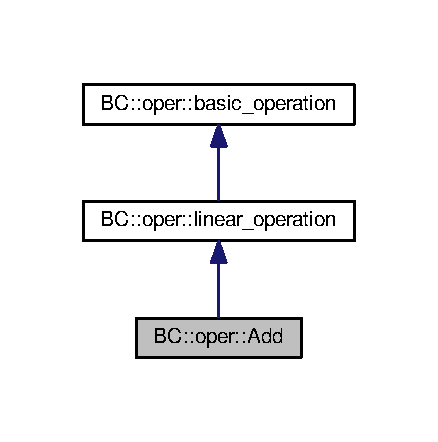
\includegraphics[width=210pt]{structBC_1_1oper_1_1Add__inherit__graph}
\end{center}
\end{figure}


Collaboration diagram for BC\+:\+:oper\+:\+:Add\+:
\nopagebreak
\begin{figure}[H]
\begin{center}
\leavevmode
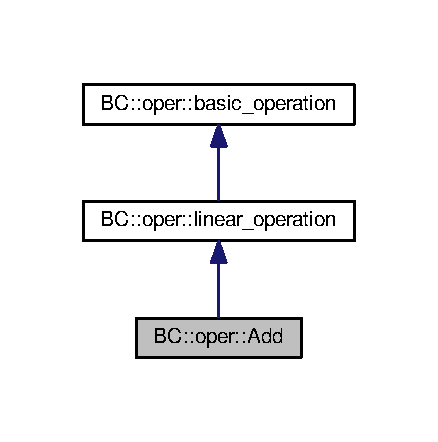
\includegraphics[width=210pt]{structBC_1_1oper_1_1Add__coll__graph}
\end{center}
\end{figure}
\subsection*{Public Types}
\begin{DoxyCompactItemize}
\item 
using \hyperlink{structBC_1_1oper_1_1Add_af0fca0b03bb8472331f3cc86918c6b2e}{alpha\+\_\+modifier} = \hyperlink{structBC_1_1meta_1_1Integer}{B\+C\+::meta\+::\+Integer}$<$ 1 $>$
\end{DoxyCompactItemize}


\subsection{Member Typedef Documentation}
\index{B\+C\+::oper\+::\+Add@{B\+C\+::oper\+::\+Add}!alpha\+\_\+modifier@{alpha\+\_\+modifier}}
\index{alpha\+\_\+modifier@{alpha\+\_\+modifier}!B\+C\+::oper\+::\+Add@{B\+C\+::oper\+::\+Add}}
\subsubsection[{\texorpdfstring{alpha\+\_\+modifier}{alpha_modifier}}]{\setlength{\rightskip}{0pt plus 5cm}using {\bf B\+C\+::oper\+::\+Add\+::alpha\+\_\+modifier} =  {\bf B\+C\+::meta\+::\+Integer}$<$1$>$}\hypertarget{structBC_1_1oper_1_1Add_af0fca0b03bb8472331f3cc86918c6b2e}{}\label{structBC_1_1oper_1_1Add_af0fca0b03bb8472331f3cc86918c6b2e}


The documentation for this struct was generated from the following file\+:\begin{DoxyCompactItemize}
\item 
include/operations/\hyperlink{Binary_8h}{Binary.\+h}\end{DoxyCompactItemize}

\hypertarget{structBC_1_1oper_1_1Add__Assign}{}\section{BC\+:\+:oper\+:\+:Add\+\_\+\+Assign Struct Reference}
\label{structBC_1_1oper_1_1Add__Assign}\index{B\+C\+::oper\+::\+Add\+\_\+\+Assign@{B\+C\+::oper\+::\+Add\+\_\+\+Assign}}


{\ttfamily \#include $<$Binary.\+h$>$}



Inheritance diagram for BC\+:\+:oper\+:\+:Add\+\_\+\+Assign\+:
\nopagebreak
\begin{figure}[H]
\begin{center}
\leavevmode
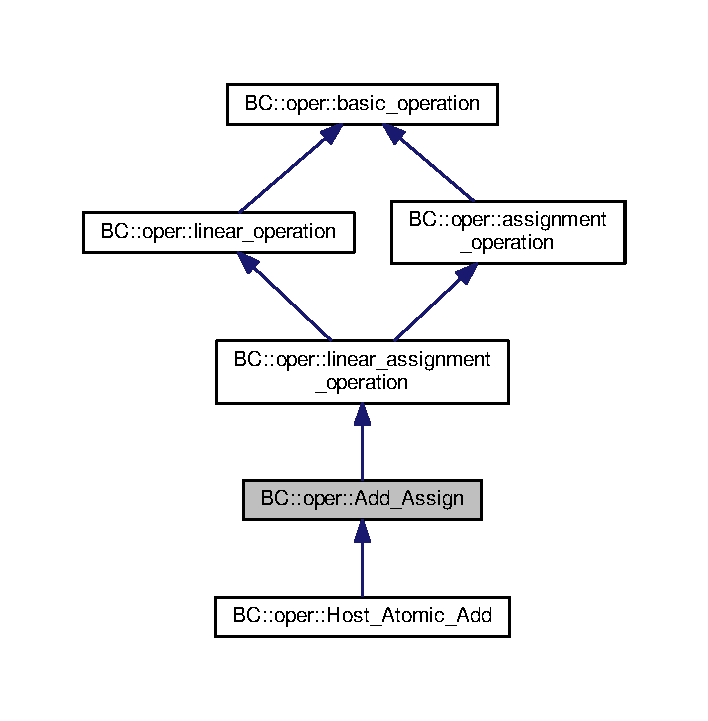
\includegraphics[width=340pt]{structBC_1_1oper_1_1Add__Assign__inherit__graph}
\end{center}
\end{figure}


Collaboration diagram for BC\+:\+:oper\+:\+:Add\+\_\+\+Assign\+:
\nopagebreak
\begin{figure}[H]
\begin{center}
\leavevmode
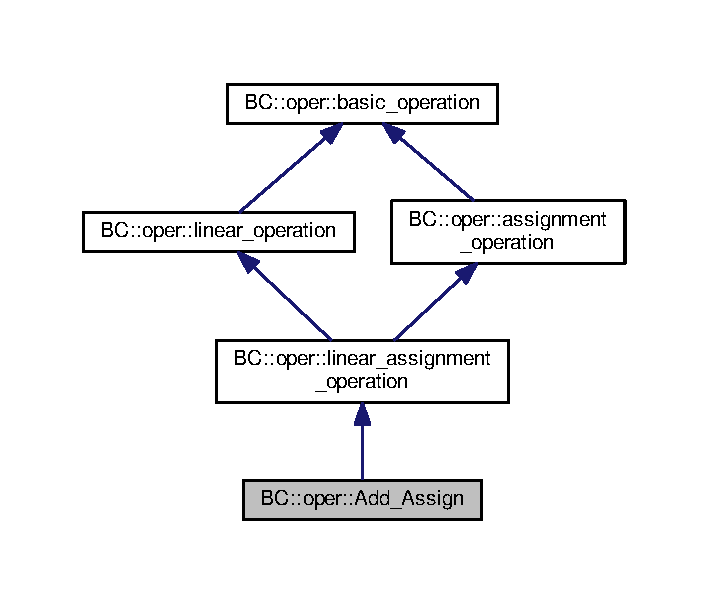
\includegraphics[width=340pt]{structBC_1_1oper_1_1Add__Assign__coll__graph}
\end{center}
\end{figure}
\subsection*{Public Types}
\begin{DoxyCompactItemize}
\item 
using \hyperlink{structBC_1_1oper_1_1Add__Assign_a20b991b7d4a8c7e4eb82d8953130001a}{alpha\+\_\+modifier} = \hyperlink{structBC_1_1meta_1_1Integer}{B\+C\+::meta\+::\+Integer}$<$ 1 $>$
\item 
using \hyperlink{structBC_1_1oper_1_1Add__Assign_aa9d7a564657d1254a78611b2b06d8744}{beta\+\_\+modifier} = \hyperlink{structBC_1_1meta_1_1Integer}{B\+C\+::meta\+::\+Integer}$<$ 1 $>$
\end{DoxyCompactItemize}


\subsection{Member Typedef Documentation}
\index{B\+C\+::oper\+::\+Add\+\_\+\+Assign@{B\+C\+::oper\+::\+Add\+\_\+\+Assign}!alpha\+\_\+modifier@{alpha\+\_\+modifier}}
\index{alpha\+\_\+modifier@{alpha\+\_\+modifier}!B\+C\+::oper\+::\+Add\+\_\+\+Assign@{B\+C\+::oper\+::\+Add\+\_\+\+Assign}}
\subsubsection[{\texorpdfstring{alpha\+\_\+modifier}{alpha_modifier}}]{\setlength{\rightskip}{0pt plus 5cm}using {\bf B\+C\+::oper\+::\+Add\+\_\+\+Assign\+::alpha\+\_\+modifier} =  {\bf B\+C\+::meta\+::\+Integer}$<$1$>$}\hypertarget{structBC_1_1oper_1_1Add__Assign_a20b991b7d4a8c7e4eb82d8953130001a}{}\label{structBC_1_1oper_1_1Add__Assign_a20b991b7d4a8c7e4eb82d8953130001a}
\index{B\+C\+::oper\+::\+Add\+\_\+\+Assign@{B\+C\+::oper\+::\+Add\+\_\+\+Assign}!beta\+\_\+modifier@{beta\+\_\+modifier}}
\index{beta\+\_\+modifier@{beta\+\_\+modifier}!B\+C\+::oper\+::\+Add\+\_\+\+Assign@{B\+C\+::oper\+::\+Add\+\_\+\+Assign}}
\subsubsection[{\texorpdfstring{beta\+\_\+modifier}{beta_modifier}}]{\setlength{\rightskip}{0pt plus 5cm}using {\bf B\+C\+::oper\+::\+Add\+\_\+\+Assign\+::beta\+\_\+modifier} =  {\bf B\+C\+::meta\+::\+Integer}$<$1$>$}\hypertarget{structBC_1_1oper_1_1Add__Assign_aa9d7a564657d1254a78611b2b06d8744}{}\label{structBC_1_1oper_1_1Add__Assign_aa9d7a564657d1254a78611b2b06d8744}


The documentation for this struct was generated from the following file\+:\begin{DoxyCompactItemize}
\item 
include/operations/\hyperlink{Binary_8h}{Binary.\+h}\end{DoxyCompactItemize}

\hypertarget{structBC_1_1tensors_1_1Tensor__Operations_1_1Alias}{}\section{BC\+:\+:tensors\+:\+:Tensor\+\_\+\+Operations$<$ Expression $>$\+:\+:Alias Struct Reference}
\label{structBC_1_1tensors_1_1Tensor__Operations_1_1Alias}\index{B\+C\+::tensors\+::\+Tensor\+\_\+\+Operations$<$ Expression $>$\+::\+Alias@{B\+C\+::tensors\+::\+Tensor\+\_\+\+Operations$<$ Expression $>$\+::\+Alias}}


{\ttfamily \#include $<$Tensor\+\_\+\+Operations.\+h$>$}



Collaboration diagram for BC\+:\+:tensors\+:\+:Tensor\+\_\+\+Operations$<$ Expression $>$\+:\+:Alias\+:
\nopagebreak
\begin{figure}[H]
\begin{center}
\leavevmode
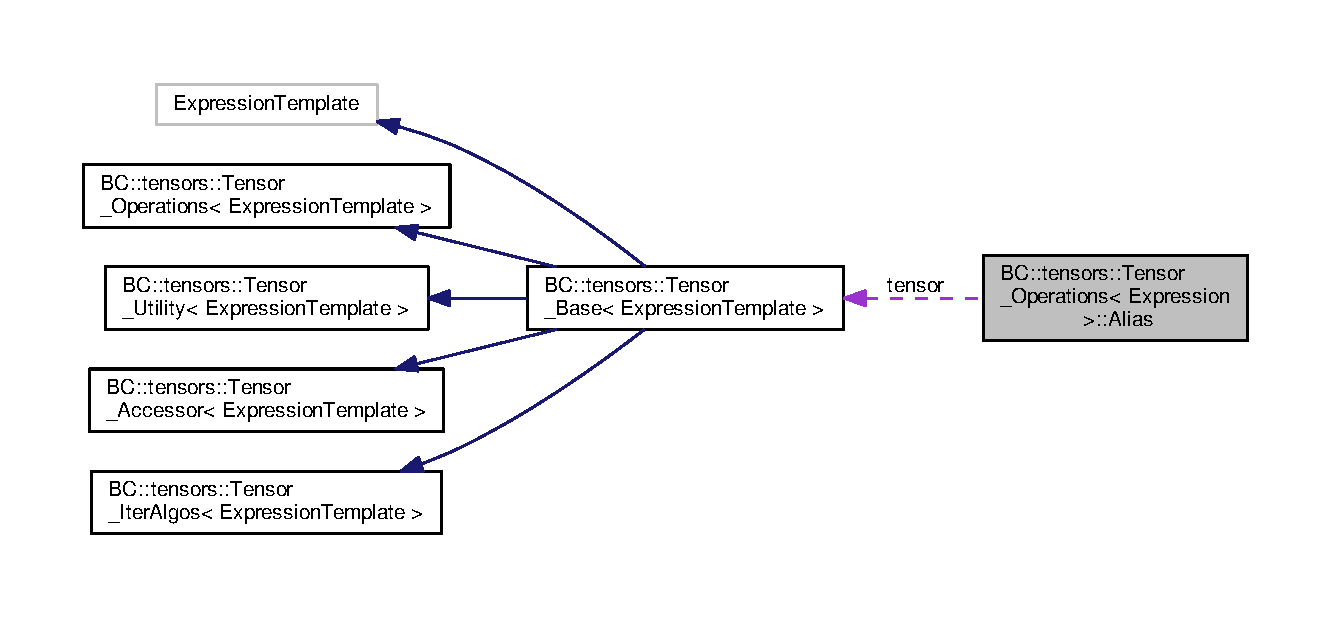
\includegraphics[width=350pt]{structBC_1_1tensors_1_1Tensor__Operations_1_1Alias__coll__graph}
\end{center}
\end{figure}
\subsection*{Public Member Functions}
\begin{DoxyCompactItemize}
\item 
\hyperlink{structBC_1_1tensors_1_1Tensor__Operations_1_1Alias_a06d50719913df4504f95fa9434feec59}{Alias} (\hyperlink{structBC_1_1tensors_1_1Tensor__Operations_a830b9a11262226b18af9caef7b9da13b}{derived} \&tensor\+\_\+)
\item 
{\footnotesize template$<$class derived\+\_\+t $>$ }\\void \hyperlink{structBC_1_1tensors_1_1Tensor__Operations_1_1Alias_acb6ccf58661a0287132cb663bf226dd1}{evaluate} (const \hyperlink{classBC_1_1tensors_1_1Tensor__Base}{Tensor\+\_\+\+Base}$<$ derived\+\_\+t $>$ \&param)
\item 
{\footnotesize template$<$class derived\+\_\+t $>$ }\\auto \& \hyperlink{structBC_1_1tensors_1_1Tensor__Operations_1_1Alias_a912f631ff113e101d805c173d768730f}{operator=} (const \hyperlink{structBC_1_1tensors_1_1Tensor__Operations}{Tensor\+\_\+\+Operations}$<$ derived\+\_\+t $>$ \&param)
\item 
{\footnotesize template$<$class derived\+\_\+t $>$ }\\auto \& \hyperlink{structBC_1_1tensors_1_1Tensor__Operations_1_1Alias_aae3c94fdcf94eb4f1f013ffc13ffbfa8}{operator+=} (const \hyperlink{structBC_1_1tensors_1_1Tensor__Operations}{Tensor\+\_\+\+Operations}$<$ derived\+\_\+t $>$ \&param)
\item 
{\footnotesize template$<$class derived\+\_\+t $>$ }\\auto \& \hyperlink{structBC_1_1tensors_1_1Tensor__Operations_1_1Alias_aa606030666fc0afaea28bbc117d22265}{operator-\/=} (const \hyperlink{structBC_1_1tensors_1_1Tensor__Operations}{Tensor\+\_\+\+Operations}$<$ derived\+\_\+t $>$ \&param)
\end{DoxyCompactItemize}
\subsection*{Public Attributes}
\begin{DoxyCompactItemize}
\item 
\hyperlink{structBC_1_1tensors_1_1Tensor__Operations_a830b9a11262226b18af9caef7b9da13b}{derived} \& \hyperlink{structBC_1_1tensors_1_1Tensor__Operations_1_1Alias_aa945b2ca6a06c2d4533699c271cead7b}{tensor}
\end{DoxyCompactItemize}


\subsection{Constructor \& Destructor Documentation}
\index{B\+C\+::tensors\+::\+Tensor\+\_\+\+Operations\+::\+Alias@{B\+C\+::tensors\+::\+Tensor\+\_\+\+Operations\+::\+Alias}!Alias@{Alias}}
\index{Alias@{Alias}!B\+C\+::tensors\+::\+Tensor\+\_\+\+Operations\+::\+Alias@{B\+C\+::tensors\+::\+Tensor\+\_\+\+Operations\+::\+Alias}}
\subsubsection[{\texorpdfstring{Alias(derived \&tensor\+\_\+)}{Alias(derived &tensor_)}}]{\setlength{\rightskip}{0pt plus 5cm}template$<$class Expression$>$ {\bf B\+C\+::tensors\+::\+Tensor\+\_\+\+Operations}$<$ Expression $>$\+::Alias\+::\+Alias (
\begin{DoxyParamCaption}
\item[{{\bf derived} \&}]{tensor\+\_\+}
\end{DoxyParamCaption}
)\hspace{0.3cm}{\ttfamily [inline]}}\hypertarget{structBC_1_1tensors_1_1Tensor__Operations_1_1Alias_a06d50719913df4504f95fa9434feec59}{}\label{structBC_1_1tensors_1_1Tensor__Operations_1_1Alias_a06d50719913df4504f95fa9434feec59}


\subsection{Member Function Documentation}
\index{B\+C\+::tensors\+::\+Tensor\+\_\+\+Operations\+::\+Alias@{B\+C\+::tensors\+::\+Tensor\+\_\+\+Operations\+::\+Alias}!evaluate@{evaluate}}
\index{evaluate@{evaluate}!B\+C\+::tensors\+::\+Tensor\+\_\+\+Operations\+::\+Alias@{B\+C\+::tensors\+::\+Tensor\+\_\+\+Operations\+::\+Alias}}
\subsubsection[{\texorpdfstring{evaluate(const Tensor\+\_\+\+Base$<$ derived\+\_\+t $>$ \&param)}{evaluate(const Tensor_Base< derived_t > &param)}}]{\setlength{\rightskip}{0pt plus 5cm}template$<$class Expression$>$ template$<$class derived\+\_\+t $>$ void {\bf B\+C\+::tensors\+::\+Tensor\+\_\+\+Operations}$<$ Expression $>$\+::Alias\+::evaluate (
\begin{DoxyParamCaption}
\item[{const {\bf Tensor\+\_\+\+Base}$<$ derived\+\_\+t $>$ \&}]{param}
\end{DoxyParamCaption}
)\hspace{0.3cm}{\ttfamily [inline]}}\hypertarget{structBC_1_1tensors_1_1Tensor__Operations_1_1Alias_acb6ccf58661a0287132cb663bf226dd1}{}\label{structBC_1_1tensors_1_1Tensor__Operations_1_1Alias_acb6ccf58661a0287132cb663bf226dd1}
\index{B\+C\+::tensors\+::\+Tensor\+\_\+\+Operations\+::\+Alias@{B\+C\+::tensors\+::\+Tensor\+\_\+\+Operations\+::\+Alias}!operator+=@{operator+=}}
\index{operator+=@{operator+=}!B\+C\+::tensors\+::\+Tensor\+\_\+\+Operations\+::\+Alias@{B\+C\+::tensors\+::\+Tensor\+\_\+\+Operations\+::\+Alias}}
\subsubsection[{\texorpdfstring{operator+=(const Tensor\+\_\+\+Operations$<$ derived\+\_\+t $>$ \&param)}{operator+=(const Tensor_Operations< derived_t > &param)}}]{\setlength{\rightskip}{0pt plus 5cm}template$<$class Expression$>$ template$<$class derived\+\_\+t $>$ auto\& {\bf B\+C\+::tensors\+::\+Tensor\+\_\+\+Operations}$<$ Expression $>$\+::Alias\+::operator+= (
\begin{DoxyParamCaption}
\item[{const {\bf Tensor\+\_\+\+Operations}$<$ derived\+\_\+t $>$ \&}]{param}
\end{DoxyParamCaption}
)\hspace{0.3cm}{\ttfamily [inline]}}\hypertarget{structBC_1_1tensors_1_1Tensor__Operations_1_1Alias_aae3c94fdcf94eb4f1f013ffc13ffbfa8}{}\label{structBC_1_1tensors_1_1Tensor__Operations_1_1Alias_aae3c94fdcf94eb4f1f013ffc13ffbfa8}
\index{B\+C\+::tensors\+::\+Tensor\+\_\+\+Operations\+::\+Alias@{B\+C\+::tensors\+::\+Tensor\+\_\+\+Operations\+::\+Alias}!operator-\/=@{operator-\/=}}
\index{operator-\/=@{operator-\/=}!B\+C\+::tensors\+::\+Tensor\+\_\+\+Operations\+::\+Alias@{B\+C\+::tensors\+::\+Tensor\+\_\+\+Operations\+::\+Alias}}
\subsubsection[{\texorpdfstring{operator-\/=(const Tensor\+\_\+\+Operations$<$ derived\+\_\+t $>$ \&param)}{operator-=(const Tensor_Operations< derived_t > &param)}}]{\setlength{\rightskip}{0pt plus 5cm}template$<$class Expression$>$ template$<$class derived\+\_\+t $>$ auto\& {\bf B\+C\+::tensors\+::\+Tensor\+\_\+\+Operations}$<$ Expression $>$\+::Alias\+::operator-\/= (
\begin{DoxyParamCaption}
\item[{const {\bf Tensor\+\_\+\+Operations}$<$ derived\+\_\+t $>$ \&}]{param}
\end{DoxyParamCaption}
)\hspace{0.3cm}{\ttfamily [inline]}}\hypertarget{structBC_1_1tensors_1_1Tensor__Operations_1_1Alias_aa606030666fc0afaea28bbc117d22265}{}\label{structBC_1_1tensors_1_1Tensor__Operations_1_1Alias_aa606030666fc0afaea28bbc117d22265}
\index{B\+C\+::tensors\+::\+Tensor\+\_\+\+Operations\+::\+Alias@{B\+C\+::tensors\+::\+Tensor\+\_\+\+Operations\+::\+Alias}!operator=@{operator=}}
\index{operator=@{operator=}!B\+C\+::tensors\+::\+Tensor\+\_\+\+Operations\+::\+Alias@{B\+C\+::tensors\+::\+Tensor\+\_\+\+Operations\+::\+Alias}}
\subsubsection[{\texorpdfstring{operator=(const Tensor\+\_\+\+Operations$<$ derived\+\_\+t $>$ \&param)}{operator=(const Tensor_Operations< derived_t > &param)}}]{\setlength{\rightskip}{0pt plus 5cm}template$<$class Expression$>$ template$<$class derived\+\_\+t $>$ auto\& {\bf B\+C\+::tensors\+::\+Tensor\+\_\+\+Operations}$<$ Expression $>$\+::Alias\+::operator= (
\begin{DoxyParamCaption}
\item[{const {\bf Tensor\+\_\+\+Operations}$<$ derived\+\_\+t $>$ \&}]{param}
\end{DoxyParamCaption}
)\hspace{0.3cm}{\ttfamily [inline]}}\hypertarget{structBC_1_1tensors_1_1Tensor__Operations_1_1Alias_a912f631ff113e101d805c173d768730f}{}\label{structBC_1_1tensors_1_1Tensor__Operations_1_1Alias_a912f631ff113e101d805c173d768730f}


\subsection{Member Data Documentation}
\index{B\+C\+::tensors\+::\+Tensor\+\_\+\+Operations\+::\+Alias@{B\+C\+::tensors\+::\+Tensor\+\_\+\+Operations\+::\+Alias}!tensor@{tensor}}
\index{tensor@{tensor}!B\+C\+::tensors\+::\+Tensor\+\_\+\+Operations\+::\+Alias@{B\+C\+::tensors\+::\+Tensor\+\_\+\+Operations\+::\+Alias}}
\subsubsection[{\texorpdfstring{tensor}{tensor}}]{\setlength{\rightskip}{0pt plus 5cm}template$<$class Expression$>$ {\bf derived}\& {\bf B\+C\+::tensors\+::\+Tensor\+\_\+\+Operations}$<$ Expression $>$\+::Alias\+::tensor}\hypertarget{structBC_1_1tensors_1_1Tensor__Operations_1_1Alias_aa945b2ca6a06c2d4533699c271cead7b}{}\label{structBC_1_1tensors_1_1Tensor__Operations_1_1Alias_aa945b2ca6a06c2d4533699c271cead7b}


The documentation for this struct was generated from the following file\+:\begin{DoxyCompactItemize}
\item 
include/tensors/\hyperlink{Tensor__Operations_8h}{Tensor\+\_\+\+Operations.\+h}\end{DoxyCompactItemize}

\hypertarget{structBC_1_1meta_1_1all}{}\section{BC\+:\+:meta\+:\+:all$<$ Function, Ts $>$ Struct Template Reference}
\label{structBC_1_1meta_1_1all}\index{B\+C\+::meta\+::all$<$ Function, Ts $>$@{B\+C\+::meta\+::all$<$ Function, Ts $>$}}


{\ttfamily \#include $<$Type\+Traits.\+h$>$}



Inheritance diagram for BC\+:\+:meta\+:\+:all$<$ Function, Ts $>$\+:
\nopagebreak
\begin{figure}[H]
\begin{center}
\leavevmode
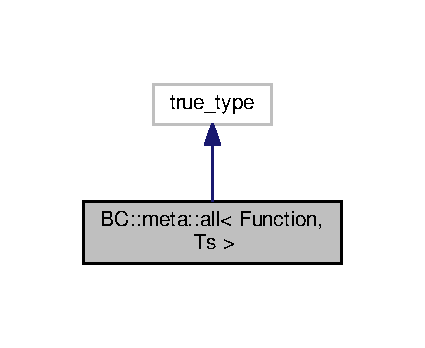
\includegraphics[width=204pt]{structBC_1_1meta_1_1all__inherit__graph}
\end{center}
\end{figure}


Collaboration diagram for BC\+:\+:meta\+:\+:all$<$ Function, Ts $>$\+:
\nopagebreak
\begin{figure}[H]
\begin{center}
\leavevmode
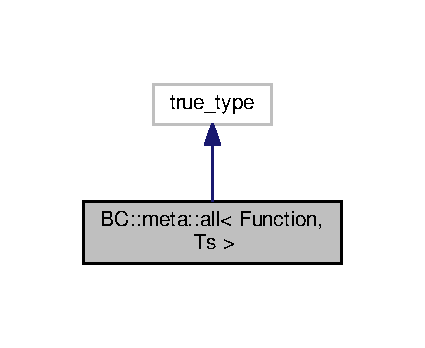
\includegraphics[width=204pt]{structBC_1_1meta_1_1all__coll__graph}
\end{center}
\end{figure}


The documentation for this struct was generated from the following file\+:\begin{DoxyCompactItemize}
\item 
include/type\+\_\+traits/\hyperlink{TypeTraits_8h}{Type\+Traits.\+h}\end{DoxyCompactItemize}

\hypertarget{structBC_1_1meta_1_1all_3_01Function_00_01T_00_01Ts_8_8_8_01_4}{}\section{BC\+:\+:meta\+:\+:all$<$ Function, T, Ts... $>$ Struct Template Reference}
\label{structBC_1_1meta_1_1all_3_01Function_00_01T_00_01Ts_8_8_8_01_4}\index{B\+C\+::meta\+::all$<$ Function, T, Ts... $>$@{B\+C\+::meta\+::all$<$ Function, T, Ts... $>$}}


{\ttfamily \#include $<$Type\+Traits.\+h$>$}



Inheritance diagram for BC\+:\+:meta\+:\+:all$<$ Function, T, Ts... $>$\+:
\nopagebreak
\begin{figure}[H]
\begin{center}
\leavevmode
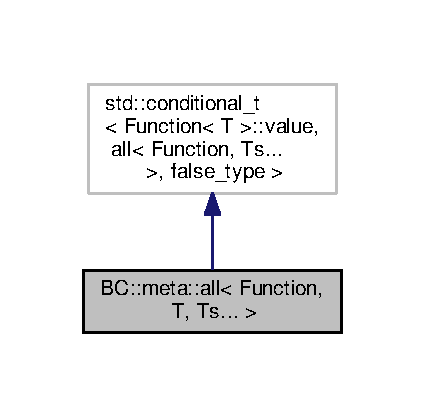
\includegraphics[width=204pt]{structBC_1_1meta_1_1all_3_01Function_00_01T_00_01Ts_8_8_8_01_4__inherit__graph}
\end{center}
\end{figure}


Collaboration diagram for BC\+:\+:meta\+:\+:all$<$ Function, T, Ts... $>$\+:
\nopagebreak
\begin{figure}[H]
\begin{center}
\leavevmode
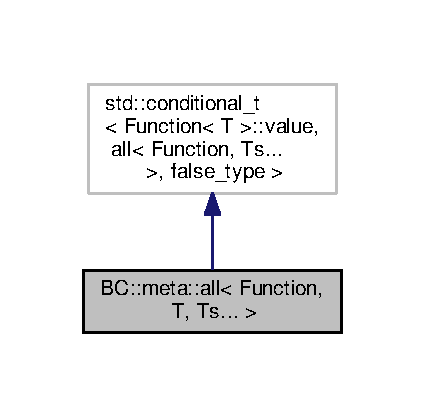
\includegraphics[width=204pt]{structBC_1_1meta_1_1all_3_01Function_00_01T_00_01Ts_8_8_8_01_4__coll__graph}
\end{center}
\end{figure}


The documentation for this struct was generated from the following file\+:\begin{DoxyCompactItemize}
\item 
include/type\+\_\+traits/\hyperlink{TypeTraits_8h}{Type\+Traits.\+h}\end{DoxyCompactItemize}

\hypertarget{structBC_1_1allocators_1_1allocator__traits}{}\section{BC\+:\+:allocators\+:\+:allocator\+\_\+traits$<$ Allocator $>$ Struct Template Reference}
\label{structBC_1_1allocators_1_1allocator__traits}\index{B\+C\+::allocators\+::allocator\+\_\+traits$<$ Allocator $>$@{B\+C\+::allocators\+::allocator\+\_\+traits$<$ Allocator $>$}}


{\ttfamily \#include $<$Allocator\+\_\+\+Traits.\+h$>$}



Inheritance diagram for BC\+:\+:allocators\+:\+:allocator\+\_\+traits$<$ Allocator $>$\+:
\nopagebreak
\begin{figure}[H]
\begin{center}
\leavevmode
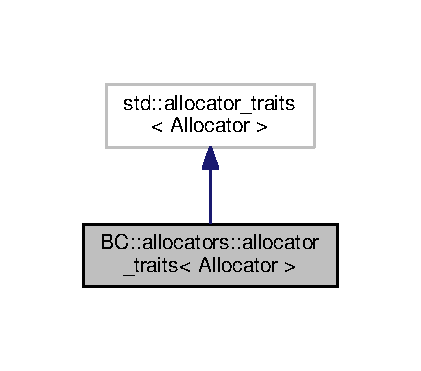
\includegraphics[width=202pt]{structBC_1_1allocators_1_1allocator__traits__inherit__graph}
\end{center}
\end{figure}


Collaboration diagram for BC\+:\+:allocators\+:\+:allocator\+\_\+traits$<$ Allocator $>$\+:
\nopagebreak
\begin{figure}[H]
\begin{center}
\leavevmode
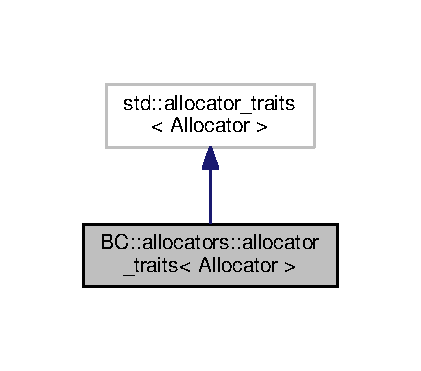
\includegraphics[width=202pt]{structBC_1_1allocators_1_1allocator__traits__coll__graph}
\end{center}
\end{figure}
\subsection*{Public Types}
\begin{DoxyCompactItemize}
\item 
using \hyperlink{structBC_1_1allocators_1_1allocator__traits_aa0f0a6c79a954a7801831eccc9a30f37}{system\+\_\+tag} = \hyperlink{namespaceBC_1_1meta_a96ed28f49a8ffe8f0bae28da99e6ee18}{B\+C\+::meta\+::conditional\+\_\+detected\+\_\+t}$<$ \hyperlink{namespaceBC_1_1allocators_1_1detail_a3443ef6fdbe2c417651fec71fa98dda8}{detail\+::query\+\_\+system\+\_\+tag}, \hyperlink{namespaceBC_a934f94b17b06290e6b241e5f59930c5f}{Allocator}, \hyperlink{structBC_1_1host__tag}{host\+\_\+tag} $>$
\end{DoxyCompactItemize}
\subsection*{Static Public Attributes}
\begin{DoxyCompactItemize}
\item 
static constexpr bool \hyperlink{structBC_1_1allocators_1_1allocator__traits_a6c6c9f87486c91b1404f8ff01328641c}{is\+\_\+managed\+\_\+memory}
\end{DoxyCompactItemize}


\subsection{Member Typedef Documentation}
\index{B\+C\+::allocators\+::allocator\+\_\+traits@{B\+C\+::allocators\+::allocator\+\_\+traits}!system\+\_\+tag@{system\+\_\+tag}}
\index{system\+\_\+tag@{system\+\_\+tag}!B\+C\+::allocators\+::allocator\+\_\+traits@{B\+C\+::allocators\+::allocator\+\_\+traits}}
\subsubsection[{\texorpdfstring{system\+\_\+tag}{system_tag}}]{\setlength{\rightskip}{0pt plus 5cm}template$<$class Allocator$>$ using {\bf B\+C\+::allocators\+::allocator\+\_\+traits}$<$ {\bf Allocator} $>$\+::{\bf system\+\_\+tag} =  {\bf B\+C\+::meta\+::conditional\+\_\+detected\+\_\+t}$<$ {\bf detail\+::query\+\_\+system\+\_\+tag}, {\bf Allocator}, {\bf host\+\_\+tag}$>$}\hypertarget{structBC_1_1allocators_1_1allocator__traits_aa0f0a6c79a954a7801831eccc9a30f37}{}\label{structBC_1_1allocators_1_1allocator__traits_aa0f0a6c79a954a7801831eccc9a30f37}


\subsection{Member Data Documentation}
\index{B\+C\+::allocators\+::allocator\+\_\+traits@{B\+C\+::allocators\+::allocator\+\_\+traits}!is\+\_\+managed\+\_\+memory@{is\+\_\+managed\+\_\+memory}}
\index{is\+\_\+managed\+\_\+memory@{is\+\_\+managed\+\_\+memory}!B\+C\+::allocators\+::allocator\+\_\+traits@{B\+C\+::allocators\+::allocator\+\_\+traits}}
\subsubsection[{\texorpdfstring{is\+\_\+managed\+\_\+memory}{is_managed_memory}}]{\setlength{\rightskip}{0pt plus 5cm}template$<$class Allocator$>$ constexpr bool {\bf B\+C\+::allocators\+::allocator\+\_\+traits}$<$ {\bf Allocator} $>$\+::is\+\_\+managed\+\_\+memory\hspace{0.3cm}{\ttfamily [static]}}\hypertarget{structBC_1_1allocators_1_1allocator__traits_a6c6c9f87486c91b1404f8ff01328641c}{}\label{structBC_1_1allocators_1_1allocator__traits_a6c6c9f87486c91b1404f8ff01328641c}
{\bfseries Initial value\+:}
\begin{DoxyCode}
=
            \hyperlink{namespaceBC_1_1meta_a96ed28f49a8ffe8f0bae28da99e6ee18}{BC::meta::conditional\_detected\_t}<
            \hyperlink{namespaceBC_1_1allocators_1_1detail_ad4bb4e071d1562e0209c47f8ebf8eade}{detail::query\_managed\_memory}, \hyperlink{namespaceBC_a934f94b17b06290e6b241e5f59930c5f}{Allocator}, std::false\_type>
      ::value
\end{DoxyCode}


The documentation for this struct was generated from the following file\+:\begin{DoxyCompactItemize}
\item 
include/allocators/\hyperlink{Allocator__Traits_8h}{Allocator\+\_\+\+Traits.\+h}\end{DoxyCompactItemize}

\hypertarget{structBC_1_1oper_1_1And}{}\section{BC\+:\+:oper\+:\+:And Struct Reference}
\label{structBC_1_1oper_1_1And}\index{B\+C\+::oper\+::\+And@{B\+C\+::oper\+::\+And}}


{\ttfamily \#include $<$Binary.\+h$>$}



The documentation for this struct was generated from the following file\+:\begin{DoxyCompactItemize}
\item 
include/operations/\hyperlink{Binary_8h}{Binary.\+h}\end{DoxyCompactItemize}

\hypertarget{structBC_1_1meta_1_1any}{}\section{BC\+:\+:meta\+:\+:any$<$ Function, Ts $>$ Struct Template Reference}
\label{structBC_1_1meta_1_1any}\index{B\+C\+::meta\+::any$<$ Function, Ts $>$@{B\+C\+::meta\+::any$<$ Function, Ts $>$}}


{\ttfamily \#include $<$Type\+Traits.\+h$>$}



Inheritance diagram for BC\+:\+:meta\+:\+:any$<$ Function, Ts $>$\+:
\nopagebreak
\begin{figure}[H]
\begin{center}
\leavevmode
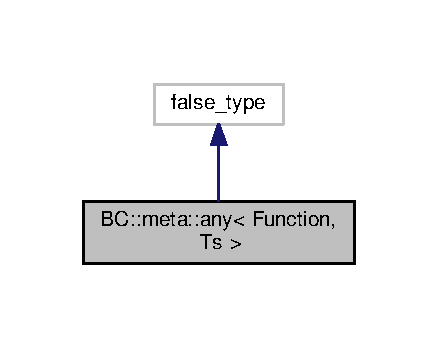
\includegraphics[width=210pt]{structBC_1_1meta_1_1any__inherit__graph}
\end{center}
\end{figure}


Collaboration diagram for BC\+:\+:meta\+:\+:any$<$ Function, Ts $>$\+:
\nopagebreak
\begin{figure}[H]
\begin{center}
\leavevmode
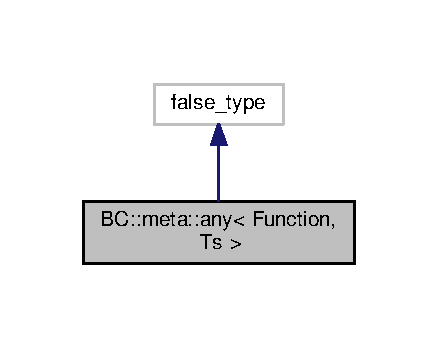
\includegraphics[width=210pt]{structBC_1_1meta_1_1any__coll__graph}
\end{center}
\end{figure}


The documentation for this struct was generated from the following file\+:\begin{DoxyCompactItemize}
\item 
include/type\+\_\+traits/\hyperlink{TypeTraits_8h}{Type\+Traits.\+h}\end{DoxyCompactItemize}

\hypertarget{structBC_1_1meta_1_1any_3_01Function_00_01T_00_01Ts_8_8_8_01_4}{}\section{BC\+:\+:meta\+:\+:any$<$ Function, T, Ts... $>$ Struct Template Reference}
\label{structBC_1_1meta_1_1any_3_01Function_00_01T_00_01Ts_8_8_8_01_4}\index{B\+C\+::meta\+::any$<$ Function, T, Ts... $>$@{B\+C\+::meta\+::any$<$ Function, T, Ts... $>$}}


{\ttfamily \#include $<$Type\+Traits.\+h$>$}



Inheritance diagram for BC\+:\+:meta\+:\+:any$<$ Function, T, Ts... $>$\+:
\nopagebreak
\begin{figure}[H]
\begin{center}
\leavevmode
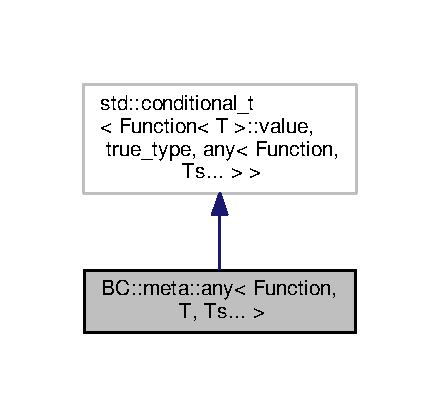
\includegraphics[width=211pt]{structBC_1_1meta_1_1any_3_01Function_00_01T_00_01Ts_8_8_8_01_4__inherit__graph}
\end{center}
\end{figure}


Collaboration diagram for BC\+:\+:meta\+:\+:any$<$ Function, T, Ts... $>$\+:
\nopagebreak
\begin{figure}[H]
\begin{center}
\leavevmode
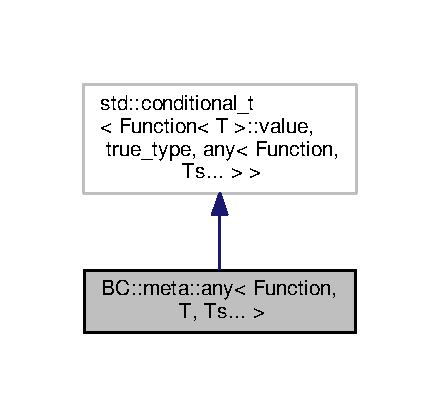
\includegraphics[width=211pt]{structBC_1_1meta_1_1any_3_01Function_00_01T_00_01Ts_8_8_8_01_4__coll__graph}
\end{center}
\end{figure}


The documentation for this struct was generated from the following file\+:\begin{DoxyCompactItemize}
\item 
include/type\+\_\+traits/\hyperlink{TypeTraits_8h}{Type\+Traits.\+h}\end{DoxyCompactItemize}

\hypertarget{structBC_1_1oper_1_1Approx__Equal}{}\section{BC\+:\+:oper\+:\+:Approx\+\_\+\+Equal Struct Reference}
\label{structBC_1_1oper_1_1Approx__Equal}\index{B\+C\+::oper\+::\+Approx\+\_\+\+Equal@{B\+C\+::oper\+::\+Approx\+\_\+\+Equal}}


{\ttfamily \#include $<$Binary.\+h$>$}

\subsection*{Static Public Attributes}
\begin{DoxyCompactItemize}
\item 
static constexpr float \hyperlink{structBC_1_1oper_1_1Approx__Equal_aea4741204c2cf7f998bd3f48ac0bd04e}{epsilon} = .\+01
\end{DoxyCompactItemize}


\subsection{Member Data Documentation}
\index{B\+C\+::oper\+::\+Approx\+\_\+\+Equal@{B\+C\+::oper\+::\+Approx\+\_\+\+Equal}!epsilon@{epsilon}}
\index{epsilon@{epsilon}!B\+C\+::oper\+::\+Approx\+\_\+\+Equal@{B\+C\+::oper\+::\+Approx\+\_\+\+Equal}}
\subsubsection[{\texorpdfstring{epsilon}{epsilon}}]{\setlength{\rightskip}{0pt plus 5cm}constexpr float B\+C\+::oper\+::\+Approx\+\_\+\+Equal\+::epsilon = .\+01\hspace{0.3cm}{\ttfamily [static]}}\hypertarget{structBC_1_1oper_1_1Approx__Equal_aea4741204c2cf7f998bd3f48ac0bd04e}{}\label{structBC_1_1oper_1_1Approx__Equal_aea4741204c2cf7f998bd3f48ac0bd04e}


The documentation for this struct was generated from the following file\+:\begin{DoxyCompactItemize}
\item 
include/operations/\hyperlink{Binary_8h}{Binary.\+h}\end{DoxyCompactItemize}

\hypertarget{structBC_1_1array}{}\section{BC\+:\+:array$<$ size\+\_\+, T $>$ Struct Template Reference}
\label{structBC_1_1array}\index{B\+C\+::array$<$ size\+\_\+, T $>$@{B\+C\+::array$<$ size\+\_\+, T $>$}}


{\ttfamily \#include $<$Black\+Cat\+\_\+\+Array.\+h$>$}



Collaboration diagram for BC\+:\+:array$<$ size\+\_\+, T $>$\+:
\nopagebreak
\begin{figure}[H]
\begin{center}
\leavevmode
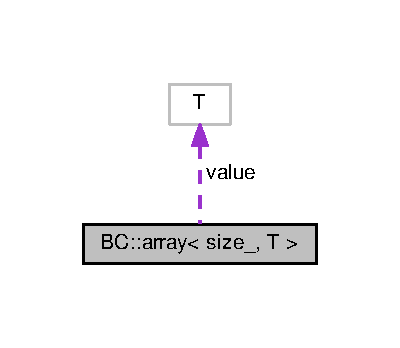
\includegraphics[width=192pt]{structBC_1_1array__coll__graph}
\end{center}
\end{figure}
\subsection*{Public Member Functions}
\begin{DoxyCompactItemize}
\item 
\hyperlink{BlackCat__Common_8h_a6699e8b0449da5c0fafb878e59c1d4b1}{B\+C\+I\+N\+L\+I\+NE} const T \& \hyperlink{structBC_1_1array_a14d7b68b018fb4870fbc565343e48b91}{operator\mbox{[}$\,$\mbox{]}} (int i) const 
\item 
\hyperlink{BlackCat__Common_8h_a6699e8b0449da5c0fafb878e59c1d4b1}{B\+C\+I\+N\+L\+I\+NE} T \& \hyperlink{structBC_1_1array_a3c52861cbdd5936cbcdbdd416360d7da}{operator\mbox{[}$\,$\mbox{]}} (int i)
\end{DoxyCompactItemize}
\subsection*{Static Public Member Functions}
\begin{DoxyCompactItemize}
\item 
static \hyperlink{BlackCat__Common_8h_a6699e8b0449da5c0fafb878e59c1d4b1}{B\+C\+I\+N\+L\+I\+NE} constexpr \hyperlink{namespaceBC_a6007cbc4eeec401a037b558910a56173}{B\+C\+::size\+\_\+t} \hyperlink{structBC_1_1array_ac248495d83c0608e10119a279f4f475e}{size} ()
\end{DoxyCompactItemize}
\subsection*{Public Attributes}
\begin{DoxyCompactItemize}
\item 
T \hyperlink{structBC_1_1array_a012380f5324bae03fbbe0dac76ee01d4}{value} \mbox{[}size\+\_\+\mbox{]} = \{ 0 \}
\end{DoxyCompactItemize}
\subsection*{Static Public Attributes}
\begin{DoxyCompactItemize}
\item 
static constexpr int \hyperlink{structBC_1_1array_a827c12b0bb95983dcc7d1fe689bf26d9}{tensor\+\_\+dimension} = size\+\_\+
\end{DoxyCompactItemize}


\subsection{Member Function Documentation}
\index{B\+C\+::array@{B\+C\+::array}!operator\mbox{[}$\,$\mbox{]}@{operator[]}}
\index{operator\mbox{[}$\,$\mbox{]}@{operator[]}!B\+C\+::array@{B\+C\+::array}}
\subsubsection[{\texorpdfstring{operator[](int i) const }{operator[](int i) const }}]{\setlength{\rightskip}{0pt plus 5cm}template$<$int size\+\_\+, class T$>$ {\bf B\+C\+I\+N\+L\+I\+NE} const T\& {\bf B\+C\+::array}$<$ size\+\_\+, T $>$\+::operator\mbox{[}$\,$\mbox{]} (
\begin{DoxyParamCaption}
\item[{int}]{i}
\end{DoxyParamCaption}
) const\hspace{0.3cm}{\ttfamily [inline]}}\hypertarget{structBC_1_1array_a14d7b68b018fb4870fbc565343e48b91}{}\label{structBC_1_1array_a14d7b68b018fb4870fbc565343e48b91}
\index{B\+C\+::array@{B\+C\+::array}!operator\mbox{[}$\,$\mbox{]}@{operator[]}}
\index{operator\mbox{[}$\,$\mbox{]}@{operator[]}!B\+C\+::array@{B\+C\+::array}}
\subsubsection[{\texorpdfstring{operator[](int i)}{operator[](int i)}}]{\setlength{\rightskip}{0pt plus 5cm}template$<$int size\+\_\+, class T$>$ {\bf B\+C\+I\+N\+L\+I\+NE} T\& {\bf B\+C\+::array}$<$ size\+\_\+, T $>$\+::operator\mbox{[}$\,$\mbox{]} (
\begin{DoxyParamCaption}
\item[{int}]{i}
\end{DoxyParamCaption}
)\hspace{0.3cm}{\ttfamily [inline]}}\hypertarget{structBC_1_1array_a3c52861cbdd5936cbcdbdd416360d7da}{}\label{structBC_1_1array_a3c52861cbdd5936cbcdbdd416360d7da}
\index{B\+C\+::array@{B\+C\+::array}!size@{size}}
\index{size@{size}!B\+C\+::array@{B\+C\+::array}}
\subsubsection[{\texorpdfstring{size()}{size()}}]{\setlength{\rightskip}{0pt plus 5cm}template$<$int size\+\_\+, class T$>$ static {\bf B\+C\+I\+N\+L\+I\+NE} constexpr {\bf B\+C\+::size\+\_\+t} {\bf B\+C\+::array}$<$ size\+\_\+, T $>$\+::size (
\begin{DoxyParamCaption}
{}
\end{DoxyParamCaption}
)\hspace{0.3cm}{\ttfamily [inline]}, {\ttfamily [static]}}\hypertarget{structBC_1_1array_ac248495d83c0608e10119a279f4f475e}{}\label{structBC_1_1array_ac248495d83c0608e10119a279f4f475e}


\subsection{Member Data Documentation}
\index{B\+C\+::array@{B\+C\+::array}!tensor\+\_\+dimension@{tensor\+\_\+dimension}}
\index{tensor\+\_\+dimension@{tensor\+\_\+dimension}!B\+C\+::array@{B\+C\+::array}}
\subsubsection[{\texorpdfstring{tensor\+\_\+dimension}{tensor_dimension}}]{\setlength{\rightskip}{0pt plus 5cm}template$<$int size\+\_\+, class T$>$ constexpr int {\bf B\+C\+::array}$<$ size\+\_\+, T $>$\+::tensor\+\_\+dimension = size\+\_\+\hspace{0.3cm}{\ttfamily [static]}}\hypertarget{structBC_1_1array_a827c12b0bb95983dcc7d1fe689bf26d9}{}\label{structBC_1_1array_a827c12b0bb95983dcc7d1fe689bf26d9}
\index{B\+C\+::array@{B\+C\+::array}!value@{value}}
\index{value@{value}!B\+C\+::array@{B\+C\+::array}}
\subsubsection[{\texorpdfstring{value}{value}}]{\setlength{\rightskip}{0pt plus 5cm}template$<$int size\+\_\+, class T$>$ T {\bf B\+C\+::array}$<$ size\+\_\+, T $>$\+::value\mbox{[}size\+\_\+\mbox{]} = \{ 0 \}}\hypertarget{structBC_1_1array_a012380f5324bae03fbbe0dac76ee01d4}{}\label{structBC_1_1array_a012380f5324bae03fbbe0dac76ee01d4}


The documentation for this struct was generated from the following file\+:\begin{DoxyCompactItemize}
\item 
include/\hyperlink{BlackCat__Array_8h}{Black\+Cat\+\_\+\+Array.\+h}\end{DoxyCompactItemize}

\hypertarget{classBC_1_1exprs_1_1Array}{}\section{BC\+:\+:exprs\+:\+:Array$<$ dimension, value\+\_\+type, allocator $>$ Class Template Reference}
\label{classBC_1_1exprs_1_1Array}\index{B\+C\+::exprs\+::\+Array$<$ dimension, value\+\_\+type, allocator $>$@{B\+C\+::exprs\+::\+Array$<$ dimension, value\+\_\+type, allocator $>$}}


{\ttfamily \#include $<$C\+P\+U\+\_\+\+Convolution.\+h$>$}



The documentation for this class was generated from the following file\+:\begin{DoxyCompactItemize}
\item 
include/blas/host\+\_\+unsupported/\hyperlink{CPU__Convolution_8h}{C\+P\+U\+\_\+\+Convolution.\+h}\end{DoxyCompactItemize}

\hypertarget{classBC_1_1tensors_1_1exprs_1_1Array}{}\section{BC\+:\+:tensors\+:\+:exprs\+:\+:Array$<$ Dimension, Scalar, Allocator, Tags $>$ Class Template Reference}
\label{classBC_1_1tensors_1_1exprs_1_1Array}\index{B\+C\+::tensors\+::exprs\+::\+Array$<$ Dimension, Scalar, Allocator, Tags $>$@{B\+C\+::tensors\+::exprs\+::\+Array$<$ Dimension, Scalar, Allocator, Tags $>$}}


{\ttfamily \#include $<$Array.\+h$>$}



Inheritance diagram for BC\+:\+:tensors\+:\+:exprs\+:\+:Array$<$ Dimension, Scalar, Allocator, Tags $>$\+:
\nopagebreak
\begin{figure}[H]
\begin{center}
\leavevmode
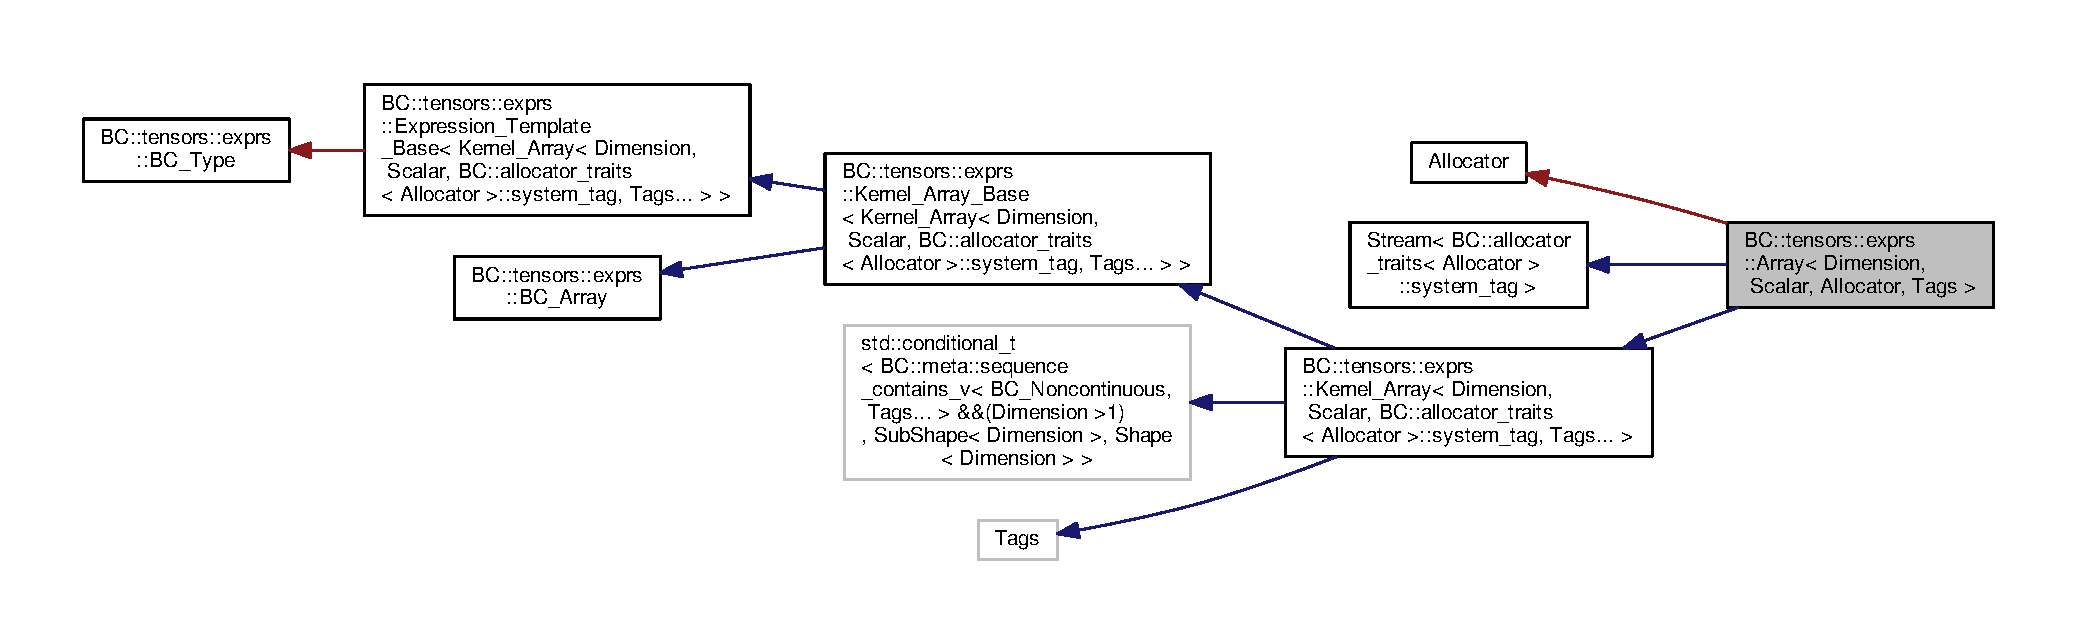
\includegraphics[width=350pt]{classBC_1_1tensors_1_1exprs_1_1Array__inherit__graph}
\end{center}
\end{figure}


Collaboration diagram for BC\+:\+:tensors\+:\+:exprs\+:\+:Array$<$ Dimension, Scalar, Allocator, Tags $>$\+:
\nopagebreak
\begin{figure}[H]
\begin{center}
\leavevmode
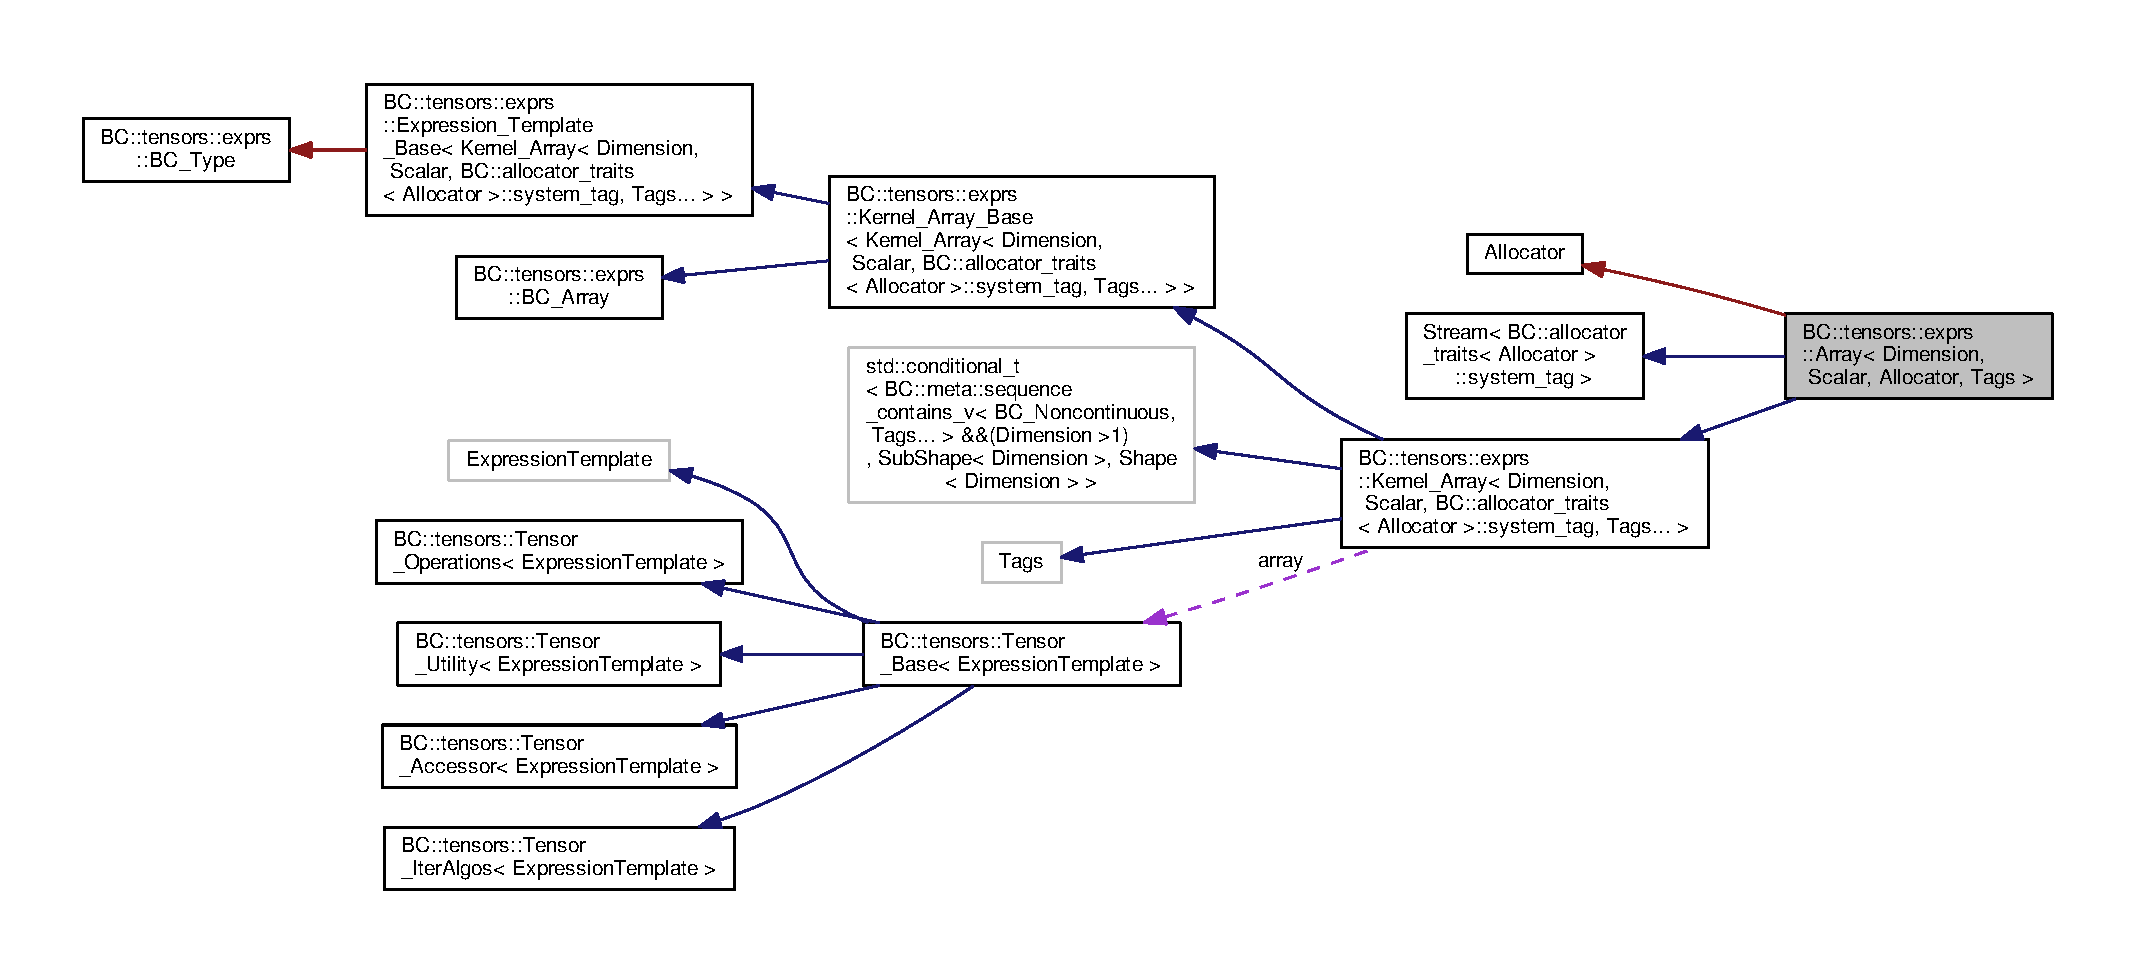
\includegraphics[width=350pt]{classBC_1_1tensors_1_1exprs_1_1Array__coll__graph}
\end{center}
\end{figure}
\subsection*{Public Types}
\begin{DoxyCompactItemize}
\item 
using \hyperlink{classBC_1_1tensors_1_1exprs_1_1Array_a96a1013a82e525d29077f0a64c34dcce}{system\+\_\+tag} = typename \hyperlink{namespaceBC_a702bcffa3526460ac93fb2a315f2f7c7}{B\+C\+::allocator\+\_\+traits}$<$ \hyperlink{namespaceBC_a934f94b17b06290e6b241e5f59930c5f}{Allocator} $>$\+::\hyperlink{structBC_1_1allocators_1_1Host_a970d265edb8b984dd4c27535ab262cb0}{system\+\_\+tag}
\item 
using \hyperlink{classBC_1_1tensors_1_1exprs_1_1Array_a030984df764670f7624708e41b1f0107}{allocator\+\_\+t} = \hyperlink{namespaceBC_a934f94b17b06290e6b241e5f59930c5f}{Allocator}
\item 
using \hyperlink{classBC_1_1tensors_1_1exprs_1_1Array_a1c41223fe60cc224c729fd9bed2a5714}{stream\+\_\+t} = \hyperlink{namespaceBC_abc64a63cd29a22d102a68f478dfd588d}{Stream}$<$ \hyperlink{structBC_1_1allocators_1_1Host_a970d265edb8b984dd4c27535ab262cb0}{system\+\_\+tag} $>$
\item 
using \hyperlink{classBC_1_1tensors_1_1exprs_1_1Array_a8af0bfb94c7382d4a22de26e9d93d7f8}{value\+\_\+type} = \hyperlink{namespaceBC_1_1tensors_1_1common__using_a22de9a173f6aa6b07a3b4f543c9ad5c1}{Scalar}
\end{DoxyCompactItemize}
\subsection*{Public Member Functions}
\begin{DoxyCompactItemize}
\item 
const \hyperlink{classBC_1_1tensors_1_1exprs_1_1Array_a1c41223fe60cc224c729fd9bed2a5714}{stream\+\_\+t} \& \hyperlink{classBC_1_1tensors_1_1exprs_1_1Array_abfbe916c27ded2ebce112ac0b3f954c9}{get\+\_\+stream} () const 
\item 
\hyperlink{classBC_1_1tensors_1_1exprs_1_1Array_a1c41223fe60cc224c729fd9bed2a5714}{stream\+\_\+t} \& \hyperlink{classBC_1_1tensors_1_1exprs_1_1Array_a936b6495997a465c005709f895471f1d}{get\+\_\+stream} ()
\item 
\hyperlink{namespaceBC_a934f94b17b06290e6b241e5f59930c5f}{Allocator} \hyperlink{classBC_1_1tensors_1_1exprs_1_1Array_a0b6398bf3e37a81b380e61c7055ee2f5}{get\+\_\+allocator} () const 
\item 
\hyperlink{classBC_1_1tensors_1_1exprs_1_1Array_a5346f4acaf8f8dcce5f0b09fbe430d0a}{Array} ()
\item 
\hyperlink{classBC_1_1tensors_1_1exprs_1_1Array_ae6457a76aeb8a63e5391688aa268a47b}{Array} (const \hyperlink{classBC_1_1tensors_1_1exprs_1_1Array}{Array} \&array\+\_\+)
\item 
\hyperlink{classBC_1_1tensors_1_1exprs_1_1Array_a18e700548bd564250c054de18a583002}{Array} (\hyperlink{classBC_1_1tensors_1_1exprs_1_1Array}{Array} \&\&array\+\_\+)
\item 
{\footnotesize template$<$class U , typename  = std\+::enable\+\_\+if\+\_\+t$<$!expression\+\_\+traits$<$\+U$>$\+::is\+\_\+array \&\&    												!expression\+\_\+traits$<$\+U$>$\+::is\+\_\+expr \&\&    													\+Dimension != 0$>$$>$ }\\\hyperlink{classBC_1_1tensors_1_1exprs_1_1Array_abfe88c02ec288455d1e5539a02a8293b}{Array} (U param)
\item 
{\footnotesize template$<$class U , typename  = std\+::enable\+\_\+if\+\_\+t$<$!expression\+\_\+traits$<$\+U$>$\+::is\+\_\+array \&\& !expression\+\_\+traits$<$\+U$>$\+::is\+\_\+expr$>$$>$ }\\\hyperlink{classBC_1_1tensors_1_1exprs_1_1Array_a5dc2bfdb8a9f7f734b2cefa5e3a5624d}{Array} (U param, const \hyperlink{namespaceBC_a934f94b17b06290e6b241e5f59930c5f}{Allocator} \&alloc\+\_\+)
\item 
{\footnotesize template$<$class... args, typename  = std\+::enable\+\_\+if\+\_\+t$<$		meta\+::sequence\+\_\+of\+\_\+v$<$\+B\+C\+::size\+\_\+t, args...$>$ \&\&		sizeof...(args) == Dimension$>$$>$ }\\\hyperlink{classBC_1_1tensors_1_1exprs_1_1Array_af527268f6313c845af47b176d78167b1}{Array} (const args \&...params)
\item 
{\footnotesize template$<$class Expr , typename  = std\+::enable\+\_\+if\+\_\+t$<$expression\+\_\+traits$<$\+Expr$>$\+::is\+\_\+array $\vert$$\vert$ expression\+\_\+traits$<$\+Expr$>$\+::is\+\_\+expr$>$$>$ }\\\hyperlink{classBC_1_1tensors_1_1exprs_1_1Array_aec33818cfb1f18127c3ad3fbdecc9d1f}{Array} (const Expr \&expr\+\_\+t, const \hyperlink{namespaceBC_a934f94b17b06290e6b241e5f59930c5f}{Allocator} \&alloc=\hyperlink{namespaceBC_a934f94b17b06290e6b241e5f59930c5f}{Allocator}())
\item 
{\footnotesize template$<$class... Slice\+Tags$>$ }\\\hyperlink{classBC_1_1tensors_1_1exprs_1_1Array_a03dbce4acf0a8db4466a56d5223512a9}{Array} (const \hyperlink{classBC_1_1tensors_1_1exprs_1_1Array__Slice}{Array\+\_\+\+Slice}$<$ Dimension, \hyperlink{structBC_1_1allocators_1_1Host_a0663f90f62e2b8c223a4402bef3d87e5}{value\+\_\+type}, \hyperlink{classBC_1_1tensors_1_1exprs_1_1Array_a030984df764670f7624708e41b1f0107}{allocator\+\_\+t}, Slice\+Tags... $>$ \&expr\+\_\+t)
\item 
void \hyperlink{classBC_1_1tensors_1_1exprs_1_1Array_a06f6f5b3eef9ef7e99a4fbc8c5943add}{internal\+\_\+move} (\hyperlink{classBC_1_1tensors_1_1exprs_1_1Array}{Array} \&\&\hyperlink{structBC_1_1array}{array})
\item 
void \hyperlink{classBC_1_1tensors_1_1exprs_1_1Array_a81c124e95d0bcae0661d4c61fa71338e}{deallocate} ()
\end{DoxyCompactItemize}
\subsection*{Additional Inherited Members}


\subsection{Member Typedef Documentation}
\index{B\+C\+::tensors\+::exprs\+::\+Array@{B\+C\+::tensors\+::exprs\+::\+Array}!allocator\+\_\+t@{allocator\+\_\+t}}
\index{allocator\+\_\+t@{allocator\+\_\+t}!B\+C\+::tensors\+::exprs\+::\+Array@{B\+C\+::tensors\+::exprs\+::\+Array}}
\subsubsection[{\texorpdfstring{allocator\+\_\+t}{allocator_t}}]{\setlength{\rightskip}{0pt plus 5cm}template$<$int Dimension, class Scalar, class Allocator, class... Tags$>$ using {\bf B\+C\+::tensors\+::exprs\+::\+Array}$<$ Dimension, {\bf Scalar}, {\bf Allocator}, Tags $>$\+::{\bf allocator\+\_\+t} =  {\bf Allocator}}\hypertarget{classBC_1_1tensors_1_1exprs_1_1Array_a030984df764670f7624708e41b1f0107}{}\label{classBC_1_1tensors_1_1exprs_1_1Array_a030984df764670f7624708e41b1f0107}
\index{B\+C\+::tensors\+::exprs\+::\+Array@{B\+C\+::tensors\+::exprs\+::\+Array}!stream\+\_\+t@{stream\+\_\+t}}
\index{stream\+\_\+t@{stream\+\_\+t}!B\+C\+::tensors\+::exprs\+::\+Array@{B\+C\+::tensors\+::exprs\+::\+Array}}
\subsubsection[{\texorpdfstring{stream\+\_\+t}{stream_t}}]{\setlength{\rightskip}{0pt plus 5cm}template$<$int Dimension, class Scalar, class Allocator, class... Tags$>$ using {\bf B\+C\+::tensors\+::exprs\+::\+Array}$<$ Dimension, {\bf Scalar}, {\bf Allocator}, Tags $>$\+::{\bf stream\+\_\+t} =  {\bf Stream}$<${\bf system\+\_\+tag}$>$}\hypertarget{classBC_1_1tensors_1_1exprs_1_1Array_a1c41223fe60cc224c729fd9bed2a5714}{}\label{classBC_1_1tensors_1_1exprs_1_1Array_a1c41223fe60cc224c729fd9bed2a5714}
\index{B\+C\+::tensors\+::exprs\+::\+Array@{B\+C\+::tensors\+::exprs\+::\+Array}!system\+\_\+tag@{system\+\_\+tag}}
\index{system\+\_\+tag@{system\+\_\+tag}!B\+C\+::tensors\+::exprs\+::\+Array@{B\+C\+::tensors\+::exprs\+::\+Array}}
\subsubsection[{\texorpdfstring{system\+\_\+tag}{system_tag}}]{\setlength{\rightskip}{0pt plus 5cm}template$<$int Dimension, class Scalar, class Allocator, class... Tags$>$ using {\bf B\+C\+::tensors\+::exprs\+::\+Array}$<$ Dimension, {\bf Scalar}, {\bf Allocator}, Tags $>$\+::{\bf system\+\_\+tag} =  typename {\bf B\+C\+::allocator\+\_\+traits}$<${\bf Allocator}$>$\+::{\bf system\+\_\+tag}}\hypertarget{classBC_1_1tensors_1_1exprs_1_1Array_a96a1013a82e525d29077f0a64c34dcce}{}\label{classBC_1_1tensors_1_1exprs_1_1Array_a96a1013a82e525d29077f0a64c34dcce}
\index{B\+C\+::tensors\+::exprs\+::\+Array@{B\+C\+::tensors\+::exprs\+::\+Array}!value\+\_\+type@{value\+\_\+type}}
\index{value\+\_\+type@{value\+\_\+type}!B\+C\+::tensors\+::exprs\+::\+Array@{B\+C\+::tensors\+::exprs\+::\+Array}}
\subsubsection[{\texorpdfstring{value\+\_\+type}{value_type}}]{\setlength{\rightskip}{0pt plus 5cm}template$<$int Dimension, class Scalar, class Allocator, class... Tags$>$ using {\bf B\+C\+::tensors\+::exprs\+::\+Array}$<$ Dimension, {\bf Scalar}, {\bf Allocator}, Tags $>$\+::{\bf value\+\_\+type} =  {\bf Scalar}}\hypertarget{classBC_1_1tensors_1_1exprs_1_1Array_a8af0bfb94c7382d4a22de26e9d93d7f8}{}\label{classBC_1_1tensors_1_1exprs_1_1Array_a8af0bfb94c7382d4a22de26e9d93d7f8}


\subsection{Constructor \& Destructor Documentation}
\index{B\+C\+::tensors\+::exprs\+::\+Array@{B\+C\+::tensors\+::exprs\+::\+Array}!Array@{Array}}
\index{Array@{Array}!B\+C\+::tensors\+::exprs\+::\+Array@{B\+C\+::tensors\+::exprs\+::\+Array}}
\subsubsection[{\texorpdfstring{Array()}{Array()}}]{\setlength{\rightskip}{0pt plus 5cm}template$<$int Dimension, class Scalar, class Allocator, class... Tags$>$ {\bf B\+C\+::tensors\+::exprs\+::\+Array}$<$ Dimension, {\bf Scalar}, {\bf Allocator}, Tags $>$\+::{\bf Array} (
\begin{DoxyParamCaption}
{}
\end{DoxyParamCaption}
)\hspace{0.3cm}{\ttfamily [inline]}}\hypertarget{classBC_1_1tensors_1_1exprs_1_1Array_a5346f4acaf8f8dcce5f0b09fbe430d0a}{}\label{classBC_1_1tensors_1_1exprs_1_1Array_a5346f4acaf8f8dcce5f0b09fbe430d0a}
\index{B\+C\+::tensors\+::exprs\+::\+Array@{B\+C\+::tensors\+::exprs\+::\+Array}!Array@{Array}}
\index{Array@{Array}!B\+C\+::tensors\+::exprs\+::\+Array@{B\+C\+::tensors\+::exprs\+::\+Array}}
\subsubsection[{\texorpdfstring{Array(const Array \&array\+\_\+)}{Array(const Array &array_)}}]{\setlength{\rightskip}{0pt plus 5cm}template$<$int Dimension, class Scalar, class Allocator, class... Tags$>$ {\bf B\+C\+::tensors\+::exprs\+::\+Array}$<$ Dimension, {\bf Scalar}, {\bf Allocator}, Tags $>$\+::{\bf Array} (
\begin{DoxyParamCaption}
\item[{const {\bf Array}$<$ Dimension, {\bf Scalar}, {\bf Allocator}, Tags $>$ \&}]{array\+\_\+}
\end{DoxyParamCaption}
)\hspace{0.3cm}{\ttfamily [inline]}}\hypertarget{classBC_1_1tensors_1_1exprs_1_1Array_ae6457a76aeb8a63e5391688aa268a47b}{}\label{classBC_1_1tensors_1_1exprs_1_1Array_ae6457a76aeb8a63e5391688aa268a47b}
\index{B\+C\+::tensors\+::exprs\+::\+Array@{B\+C\+::tensors\+::exprs\+::\+Array}!Array@{Array}}
\index{Array@{Array}!B\+C\+::tensors\+::exprs\+::\+Array@{B\+C\+::tensors\+::exprs\+::\+Array}}
\subsubsection[{\texorpdfstring{Array(\+Array \&\&array\+\_\+)}{Array(Array &&array_)}}]{\setlength{\rightskip}{0pt plus 5cm}template$<$int Dimension, class Scalar, class Allocator, class... Tags$>$ {\bf B\+C\+::tensors\+::exprs\+::\+Array}$<$ Dimension, {\bf Scalar}, {\bf Allocator}, Tags $>$\+::{\bf Array} (
\begin{DoxyParamCaption}
\item[{{\bf Array}$<$ Dimension, {\bf Scalar}, {\bf Allocator}, Tags $>$ \&\&}]{array\+\_\+}
\end{DoxyParamCaption}
)\hspace{0.3cm}{\ttfamily [inline]}}\hypertarget{classBC_1_1tensors_1_1exprs_1_1Array_a18e700548bd564250c054de18a583002}{}\label{classBC_1_1tensors_1_1exprs_1_1Array_a18e700548bd564250c054de18a583002}
\index{B\+C\+::tensors\+::exprs\+::\+Array@{B\+C\+::tensors\+::exprs\+::\+Array}!Array@{Array}}
\index{Array@{Array}!B\+C\+::tensors\+::exprs\+::\+Array@{B\+C\+::tensors\+::exprs\+::\+Array}}
\subsubsection[{\texorpdfstring{Array(\+U param)}{Array(U param)}}]{\setlength{\rightskip}{0pt plus 5cm}template$<$int Dimension, class Scalar, class Allocator, class... Tags$>$ template$<$class U , typename  = std\+::enable\+\_\+if\+\_\+t$<$!expression\+\_\+traits$<$\+U$>$\+::is\+\_\+array \&\&    												!expression\+\_\+traits$<$\+U$>$\+::is\+\_\+expr \&\&    													\+Dimension != 0$>$$>$ {\bf B\+C\+::tensors\+::exprs\+::\+Array}$<$ Dimension, {\bf Scalar}, {\bf Allocator}, Tags $>$\+::{\bf Array} (
\begin{DoxyParamCaption}
\item[{U}]{param}
\end{DoxyParamCaption}
)\hspace{0.3cm}{\ttfamily [inline]}}\hypertarget{classBC_1_1tensors_1_1exprs_1_1Array_abfe88c02ec288455d1e5539a02a8293b}{}\label{classBC_1_1tensors_1_1exprs_1_1Array_abfe88c02ec288455d1e5539a02a8293b}
\index{B\+C\+::tensors\+::exprs\+::\+Array@{B\+C\+::tensors\+::exprs\+::\+Array}!Array@{Array}}
\index{Array@{Array}!B\+C\+::tensors\+::exprs\+::\+Array@{B\+C\+::tensors\+::exprs\+::\+Array}}
\subsubsection[{\texorpdfstring{Array(\+U param, const Allocator \&alloc\+\_\+)}{Array(U param, const Allocator &alloc_)}}]{\setlength{\rightskip}{0pt plus 5cm}template$<$int Dimension, class Scalar, class Allocator, class... Tags$>$ template$<$class U , typename  = std\+::enable\+\_\+if\+\_\+t$<$!expression\+\_\+traits$<$\+U$>$\+::is\+\_\+array \&\& !expression\+\_\+traits$<$\+U$>$\+::is\+\_\+expr$>$$>$ {\bf B\+C\+::tensors\+::exprs\+::\+Array}$<$ Dimension, {\bf Scalar}, {\bf Allocator}, Tags $>$\+::{\bf Array} (
\begin{DoxyParamCaption}
\item[{U}]{param, }
\item[{const {\bf Allocator} \&}]{alloc\+\_\+}
\end{DoxyParamCaption}
)\hspace{0.3cm}{\ttfamily [inline]}}\hypertarget{classBC_1_1tensors_1_1exprs_1_1Array_a5dc2bfdb8a9f7f734b2cefa5e3a5624d}{}\label{classBC_1_1tensors_1_1exprs_1_1Array_a5dc2bfdb8a9f7f734b2cefa5e3a5624d}
\index{B\+C\+::tensors\+::exprs\+::\+Array@{B\+C\+::tensors\+::exprs\+::\+Array}!Array@{Array}}
\index{Array@{Array}!B\+C\+::tensors\+::exprs\+::\+Array@{B\+C\+::tensors\+::exprs\+::\+Array}}
\subsubsection[{\texorpdfstring{Array(const args \&...\+params)}{Array(const args &...params)}}]{\setlength{\rightskip}{0pt plus 5cm}template$<$int Dimension, class Scalar, class Allocator, class... Tags$>$ template$<$class... args, typename  = std\+::enable\+\_\+if\+\_\+t$<$		meta\+::sequence\+\_\+of\+\_\+v$<$\+B\+C\+::size\+\_\+t, args...$>$ \&\&		sizeof...(args) == Dimension$>$$>$ {\bf B\+C\+::tensors\+::exprs\+::\+Array}$<$ Dimension, {\bf Scalar}, {\bf Allocator}, Tags $>$\+::{\bf Array} (
\begin{DoxyParamCaption}
\item[{const args \&...}]{params}
\end{DoxyParamCaption}
)\hspace{0.3cm}{\ttfamily [inline]}}\hypertarget{classBC_1_1tensors_1_1exprs_1_1Array_af527268f6313c845af47b176d78167b1}{}\label{classBC_1_1tensors_1_1exprs_1_1Array_af527268f6313c845af47b176d78167b1}
\index{B\+C\+::tensors\+::exprs\+::\+Array@{B\+C\+::tensors\+::exprs\+::\+Array}!Array@{Array}}
\index{Array@{Array}!B\+C\+::tensors\+::exprs\+::\+Array@{B\+C\+::tensors\+::exprs\+::\+Array}}
\subsubsection[{\texorpdfstring{Array(const Expr \&expr\+\_\+t, const Allocator \&alloc=\+Allocator())}{Array(const Expr &expr_t, const Allocator &alloc=Allocator())}}]{\setlength{\rightskip}{0pt plus 5cm}template$<$int Dimension, class Scalar, class Allocator, class... Tags$>$ template$<$class Expr , typename  = std\+::enable\+\_\+if\+\_\+t$<$expression\+\_\+traits$<$\+Expr$>$\+::is\+\_\+array $\vert$$\vert$ expression\+\_\+traits$<$\+Expr$>$\+::is\+\_\+expr$>$$>$ {\bf B\+C\+::tensors\+::exprs\+::\+Array}$<$ Dimension, {\bf Scalar}, {\bf Allocator}, Tags $>$\+::{\bf Array} (
\begin{DoxyParamCaption}
\item[{const Expr \&}]{expr\+\_\+t, }
\item[{const {\bf Allocator} \&}]{alloc = {\ttfamily {\bf Allocator}()}}
\end{DoxyParamCaption}
)\hspace{0.3cm}{\ttfamily [inline]}}\hypertarget{classBC_1_1tensors_1_1exprs_1_1Array_aec33818cfb1f18127c3ad3fbdecc9d1f}{}\label{classBC_1_1tensors_1_1exprs_1_1Array_aec33818cfb1f18127c3ad3fbdecc9d1f}
\index{B\+C\+::tensors\+::exprs\+::\+Array@{B\+C\+::tensors\+::exprs\+::\+Array}!Array@{Array}}
\index{Array@{Array}!B\+C\+::tensors\+::exprs\+::\+Array@{B\+C\+::tensors\+::exprs\+::\+Array}}
\subsubsection[{\texorpdfstring{Array(const Array\+\_\+\+Slice$<$ Dimension, value\+\_\+type, allocator\+\_\+t, Slice\+Tags... $>$ \&expr\+\_\+t)}{Array(const Array_Slice< Dimension, value_type, allocator_t, SliceTags... > &expr_t)}}]{\setlength{\rightskip}{0pt plus 5cm}template$<$int Dimension, class Scalar, class Allocator, class... Tags$>$ template$<$class... Slice\+Tags$>$ {\bf B\+C\+::tensors\+::exprs\+::\+Array}$<$ Dimension, {\bf Scalar}, {\bf Allocator}, Tags $>$\+::{\bf Array} (
\begin{DoxyParamCaption}
\item[{const {\bf Array\+\_\+\+Slice}$<$ Dimension, {\bf value\+\_\+type}, {\bf allocator\+\_\+t}, Slice\+Tags... $>$ \&}]{expr\+\_\+t}
\end{DoxyParamCaption}
)\hspace{0.3cm}{\ttfamily [inline]}}\hypertarget{classBC_1_1tensors_1_1exprs_1_1Array_a03dbce4acf0a8db4466a56d5223512a9}{}\label{classBC_1_1tensors_1_1exprs_1_1Array_a03dbce4acf0a8db4466a56d5223512a9}


\subsection{Member Function Documentation}
\index{B\+C\+::tensors\+::exprs\+::\+Array@{B\+C\+::tensors\+::exprs\+::\+Array}!deallocate@{deallocate}}
\index{deallocate@{deallocate}!B\+C\+::tensors\+::exprs\+::\+Array@{B\+C\+::tensors\+::exprs\+::\+Array}}
\subsubsection[{\texorpdfstring{deallocate()}{deallocate()}}]{\setlength{\rightskip}{0pt plus 5cm}template$<$int Dimension, class Scalar, class Allocator, class... Tags$>$ void {\bf B\+C\+::tensors\+::exprs\+::\+Array}$<$ Dimension, {\bf Scalar}, {\bf Allocator}, Tags $>$\+::deallocate (
\begin{DoxyParamCaption}
{}
\end{DoxyParamCaption}
)\hspace{0.3cm}{\ttfamily [inline]}}\hypertarget{classBC_1_1tensors_1_1exprs_1_1Array_a81c124e95d0bcae0661d4c61fa71338e}{}\label{classBC_1_1tensors_1_1exprs_1_1Array_a81c124e95d0bcae0661d4c61fa71338e}
\index{B\+C\+::tensors\+::exprs\+::\+Array@{B\+C\+::tensors\+::exprs\+::\+Array}!get\+\_\+allocator@{get\+\_\+allocator}}
\index{get\+\_\+allocator@{get\+\_\+allocator}!B\+C\+::tensors\+::exprs\+::\+Array@{B\+C\+::tensors\+::exprs\+::\+Array}}
\subsubsection[{\texorpdfstring{get\+\_\+allocator() const }{get_allocator() const }}]{\setlength{\rightskip}{0pt plus 5cm}template$<$int Dimension, class Scalar, class Allocator, class... Tags$>$ {\bf Allocator} {\bf B\+C\+::tensors\+::exprs\+::\+Array}$<$ Dimension, {\bf Scalar}, {\bf Allocator}, Tags $>$\+::get\+\_\+allocator (
\begin{DoxyParamCaption}
{}
\end{DoxyParamCaption}
) const\hspace{0.3cm}{\ttfamily [inline]}}\hypertarget{classBC_1_1tensors_1_1exprs_1_1Array_a0b6398bf3e37a81b380e61c7055ee2f5}{}\label{classBC_1_1tensors_1_1exprs_1_1Array_a0b6398bf3e37a81b380e61c7055ee2f5}
\index{B\+C\+::tensors\+::exprs\+::\+Array@{B\+C\+::tensors\+::exprs\+::\+Array}!get\+\_\+stream@{get\+\_\+stream}}
\index{get\+\_\+stream@{get\+\_\+stream}!B\+C\+::tensors\+::exprs\+::\+Array@{B\+C\+::tensors\+::exprs\+::\+Array}}
\subsubsection[{\texorpdfstring{get\+\_\+stream() const }{get_stream() const }}]{\setlength{\rightskip}{0pt plus 5cm}template$<$int Dimension, class Scalar, class Allocator, class... Tags$>$ const {\bf stream\+\_\+t}\& {\bf B\+C\+::tensors\+::exprs\+::\+Array}$<$ Dimension, {\bf Scalar}, {\bf Allocator}, Tags $>$\+::get\+\_\+stream (
\begin{DoxyParamCaption}
{}
\end{DoxyParamCaption}
) const\hspace{0.3cm}{\ttfamily [inline]}}\hypertarget{classBC_1_1tensors_1_1exprs_1_1Array_abfbe916c27ded2ebce112ac0b3f954c9}{}\label{classBC_1_1tensors_1_1exprs_1_1Array_abfbe916c27ded2ebce112ac0b3f954c9}
\index{B\+C\+::tensors\+::exprs\+::\+Array@{B\+C\+::tensors\+::exprs\+::\+Array}!get\+\_\+stream@{get\+\_\+stream}}
\index{get\+\_\+stream@{get\+\_\+stream}!B\+C\+::tensors\+::exprs\+::\+Array@{B\+C\+::tensors\+::exprs\+::\+Array}}
\subsubsection[{\texorpdfstring{get\+\_\+stream()}{get_stream()}}]{\setlength{\rightskip}{0pt plus 5cm}template$<$int Dimension, class Scalar, class Allocator, class... Tags$>$ {\bf stream\+\_\+t}\& {\bf B\+C\+::tensors\+::exprs\+::\+Array}$<$ Dimension, {\bf Scalar}, {\bf Allocator}, Tags $>$\+::get\+\_\+stream (
\begin{DoxyParamCaption}
{}
\end{DoxyParamCaption}
)\hspace{0.3cm}{\ttfamily [inline]}}\hypertarget{classBC_1_1tensors_1_1exprs_1_1Array_a936b6495997a465c005709f895471f1d}{}\label{classBC_1_1tensors_1_1exprs_1_1Array_a936b6495997a465c005709f895471f1d}
\index{B\+C\+::tensors\+::exprs\+::\+Array@{B\+C\+::tensors\+::exprs\+::\+Array}!internal\+\_\+move@{internal\+\_\+move}}
\index{internal\+\_\+move@{internal\+\_\+move}!B\+C\+::tensors\+::exprs\+::\+Array@{B\+C\+::tensors\+::exprs\+::\+Array}}
\subsubsection[{\texorpdfstring{internal\+\_\+move(\+Array \&\&array)}{internal_move(Array &&array)}}]{\setlength{\rightskip}{0pt plus 5cm}template$<$int Dimension, class Scalar, class Allocator, class... Tags$>$ void {\bf B\+C\+::tensors\+::exprs\+::\+Array}$<$ Dimension, {\bf Scalar}, {\bf Allocator}, Tags $>$\+::internal\+\_\+move (
\begin{DoxyParamCaption}
\item[{{\bf Array}$<$ Dimension, {\bf Scalar}, {\bf Allocator}, Tags $>$ \&\&}]{array}
\end{DoxyParamCaption}
)\hspace{0.3cm}{\ttfamily [inline]}}\hypertarget{classBC_1_1tensors_1_1exprs_1_1Array_a06f6f5b3eef9ef7e99a4fbc8c5943add}{}\label{classBC_1_1tensors_1_1exprs_1_1Array_a06f6f5b3eef9ef7e99a4fbc8c5943add}


The documentation for this class was generated from the following file\+:\begin{DoxyCompactItemize}
\item 
include/tensors/expression\+\_\+templates/\hyperlink{Array_8h}{Array.\+h}\end{DoxyCompactItemize}

\hypertarget{structBC_1_1array_3_010_00_01T_01_4}{}\section{BC\+:\+:array$<$ 0, T $>$ Struct Template Reference}
\label{structBC_1_1array_3_010_00_01T_01_4}\index{B\+C\+::array$<$ 0, T $>$@{B\+C\+::array$<$ 0, T $>$}}


{\ttfamily \#include $<$Black\+Cat\+\_\+\+Array.\+h$>$}



The documentation for this struct was generated from the following file\+:\begin{DoxyCompactItemize}
\item 
include/\hyperlink{BlackCat__Array_8h}{Black\+Cat\+\_\+\+Array.\+h}\end{DoxyCompactItemize}

\hypertarget{structBC_1_1tensors_1_1exprs_1_1Array__Const__View}{}\section{BC\+:\+:tensors\+:\+:exprs\+:\+:Array\+\_\+\+Const\+\_\+\+View$<$ Dimension, Scalar, Allocator $>$ Struct Template Reference}
\label{structBC_1_1tensors_1_1exprs_1_1Array__Const__View}\index{B\+C\+::tensors\+::exprs\+::\+Array\+\_\+\+Const\+\_\+\+View$<$ Dimension, Scalar, Allocator $>$@{B\+C\+::tensors\+::exprs\+::\+Array\+\_\+\+Const\+\_\+\+View$<$ Dimension, Scalar, Allocator $>$}}


{\ttfamily \#include $<$Array\+\_\+\+View.\+h$>$}



Inheritance diagram for BC\+:\+:tensors\+:\+:exprs\+:\+:Array\+\_\+\+Const\+\_\+\+View$<$ Dimension, Scalar, Allocator $>$\+:
\nopagebreak
\begin{figure}[H]
\begin{center}
\leavevmode
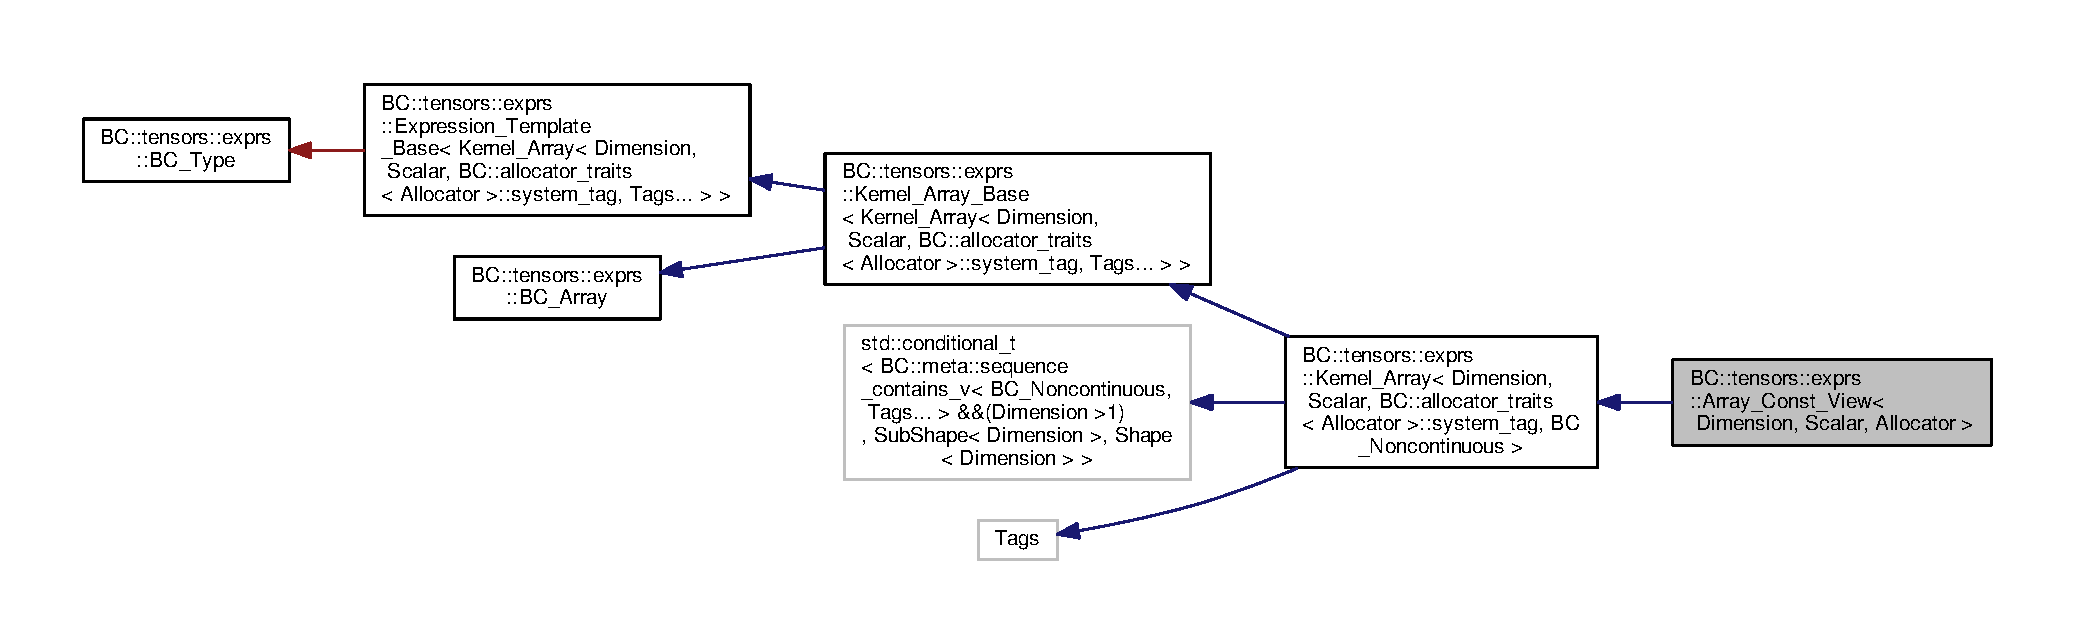
\includegraphics[width=350pt]{structBC_1_1tensors_1_1exprs_1_1Array__Const__View__inherit__graph}
\end{center}
\end{figure}


Collaboration diagram for BC\+:\+:tensors\+:\+:exprs\+:\+:Array\+\_\+\+Const\+\_\+\+View$<$ Dimension, Scalar, Allocator $>$\+:
\nopagebreak
\begin{figure}[H]
\begin{center}
\leavevmode
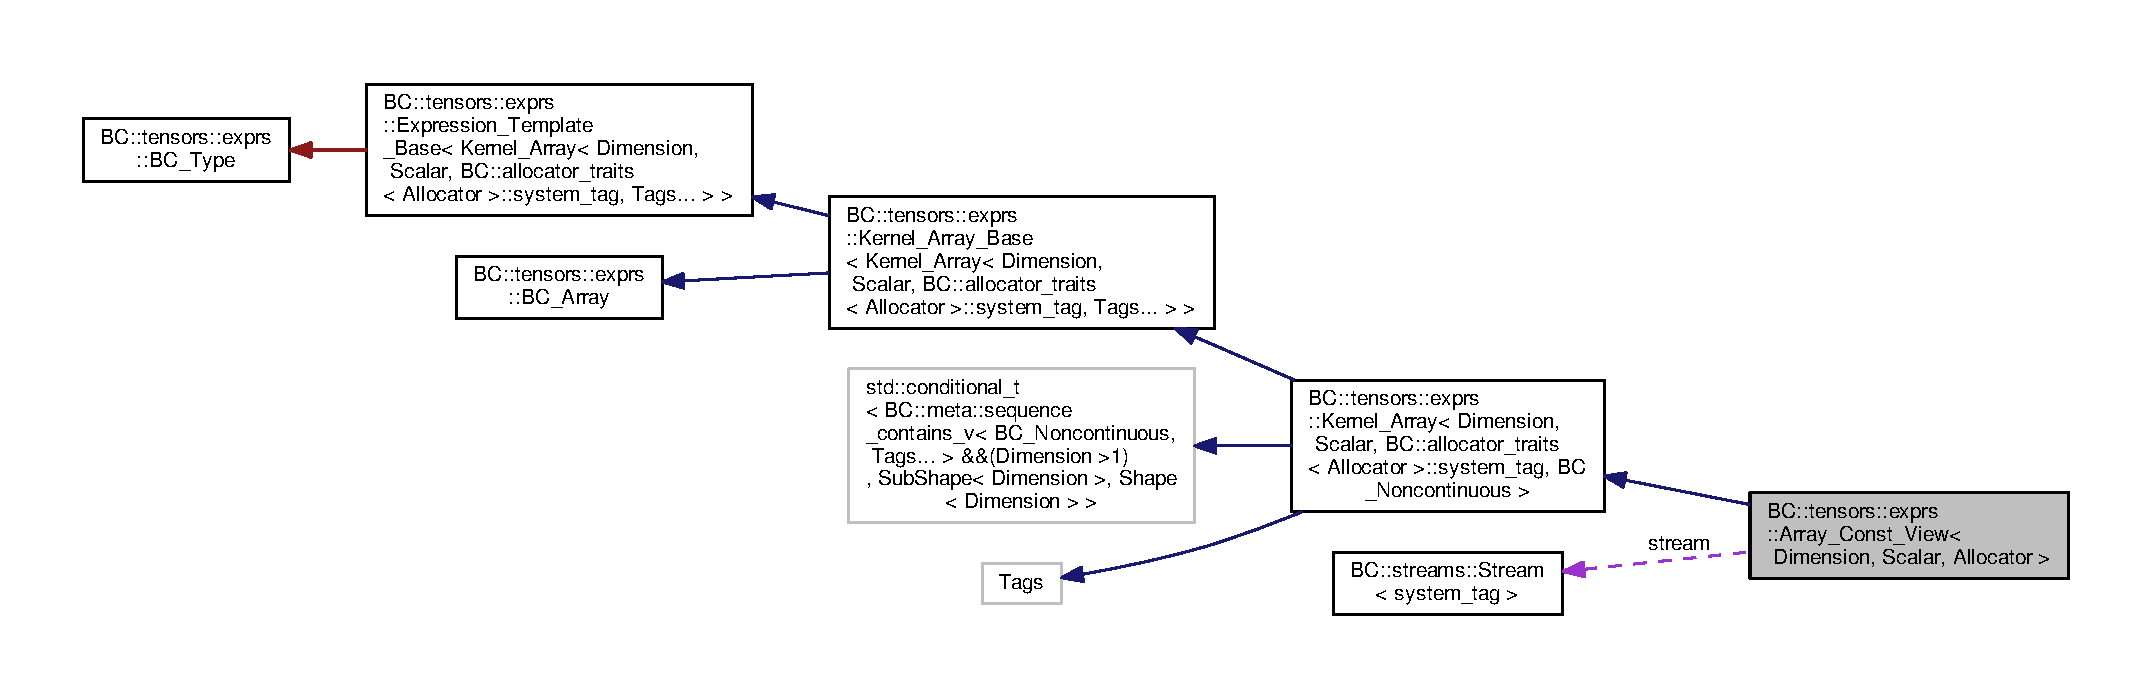
\includegraphics[width=350pt]{structBC_1_1tensors_1_1exprs_1_1Array__Const__View__coll__graph}
\end{center}
\end{figure}
\subsection*{Public Types}
\begin{DoxyCompactItemize}
\item 
using \hyperlink{structBC_1_1tensors_1_1exprs_1_1Array__Const__View_aafde0c1500b6b71d2d964f04b55266a1}{system\+\_\+tag} = typename \hyperlink{namespaceBC_a702bcffa3526460ac93fb2a315f2f7c7}{B\+C\+::allocator\+\_\+traits}$<$ \hyperlink{namespaceBC_a934f94b17b06290e6b241e5f59930c5f}{Allocator} $>$\+::\hyperlink{structBC_1_1tensors_1_1exprs_1_1Array__Const__View_aafde0c1500b6b71d2d964f04b55266a1}{system\+\_\+tag}
\item 
using \hyperlink{structBC_1_1tensors_1_1exprs_1_1Array__Const__View_a8bb694230cd6fd0ff0f5b5cbe667614a}{stream\+\_\+type} = \hyperlink{namespaceBC_abc64a63cd29a22d102a68f478dfd588d}{B\+C\+::\+Stream}$<$ \hyperlink{structBC_1_1tensors_1_1exprs_1_1Array__Const__View_aafde0c1500b6b71d2d964f04b55266a1}{system\+\_\+tag} $>$
\item 
using \hyperlink{structBC_1_1tensors_1_1exprs_1_1Array__Const__View_ab5bec1e932c07d5980709326ea33c680}{parent} = \hyperlink{structBC_1_1tensors_1_1exprs_1_1Kernel__Array}{Kernel\+\_\+\+Array}$<$ Dimension, \hyperlink{namespaceBC_1_1tensors_1_1common__using_a22de9a173f6aa6b07a3b4f543c9ad5c1}{Scalar}, \hyperlink{structBC_1_1tensors_1_1exprs_1_1Array__Const__View_aafde0c1500b6b71d2d964f04b55266a1}{system\+\_\+tag}, \hyperlink{classBC_1_1tensors_1_1exprs_1_1BC__Noncontinuous}{B\+C\+\_\+\+Noncontinuous} $>$
\end{DoxyCompactItemize}
\subsection*{Public Member Functions}
\begin{DoxyCompactItemize}
\item 
\hyperlink{structBC_1_1tensors_1_1exprs_1_1Array__Const__View_a2365ad25296b4fe97148ab12c0beb195}{Array\+\_\+\+Const\+\_\+\+View} ()=default
\item 
\hyperlink{structBC_1_1tensors_1_1exprs_1_1Array__Const__View_acac30a700235f57f5c343da97481f513}{Array\+\_\+\+Const\+\_\+\+View} (const \hyperlink{structBC_1_1tensors_1_1exprs_1_1Array__Const__View}{Array\+\_\+\+Const\+\_\+\+View} \&)=default
\item 
\hyperlink{structBC_1_1tensors_1_1exprs_1_1Array__Const__View_a7d7dd9f251f1b53129d0249e6079c19b}{Array\+\_\+\+Const\+\_\+\+View} (\hyperlink{structBC_1_1tensors_1_1exprs_1_1Array__Const__View}{Array\+\_\+\+Const\+\_\+\+View} \&\&)=default
\item 
void \hyperlink{structBC_1_1tensors_1_1exprs_1_1Array__Const__View_a12c8aa2fea3be876491353bb7999c173}{internal\+\_\+move} (\hyperlink{structBC_1_1tensors_1_1exprs_1_1Array__Const__View}{Array\+\_\+\+Const\+\_\+\+View} \&\&swap)
\item 
{\footnotesize template$<$class tensor\+\_\+t , typename  = std\+::enable\+\_\+if\+\_\+t$<$			tensor\+\_\+t\+::tensor\+\_\+dimension == Dimension \&\&			expression\+\_\+traits$<$tensor\+\_\+t$>$\+::is\+\_\+array$>$$>$ }\\\hyperlink{structBC_1_1tensors_1_1exprs_1_1Array__Const__View_a9e28e5b41e137b03e6a16d56484f7b70}{Array\+\_\+\+Const\+\_\+\+View} (const tensor\+\_\+t \&tensor)
\item 
const \hyperlink{namespaceBC_a934f94b17b06290e6b241e5f59930c5f}{Allocator} \hyperlink{structBC_1_1tensors_1_1exprs_1_1Array__Const__View_a0d8614794e0a4210bf8e654ffbc95271}{get\+\_\+allocator} () const 
\item 
const \hyperlink{structBC_1_1tensors_1_1exprs_1_1Array__Const__View_a8bb694230cd6fd0ff0f5b5cbe667614a}{stream\+\_\+type} \& \hyperlink{structBC_1_1tensors_1_1exprs_1_1Array__Const__View_a46e06b79c9abfeb2ca089867846bc642}{get\+\_\+stream} () const 
\item 
\hyperlink{structBC_1_1tensors_1_1exprs_1_1Array__Const__View_a8bb694230cd6fd0ff0f5b5cbe667614a}{stream\+\_\+type} \& \hyperlink{structBC_1_1tensors_1_1exprs_1_1Array__Const__View_ad2f920d2f6e782a3f5bc481872906e88}{get\+\_\+stream} ()
\end{DoxyCompactItemize}
\subsection*{Public Attributes}
\begin{DoxyCompactItemize}
\item 
\hyperlink{structBC_1_1tensors_1_1exprs_1_1Array__Const__View_a8bb694230cd6fd0ff0f5b5cbe667614a}{stream\+\_\+type} \hyperlink{structBC_1_1tensors_1_1exprs_1_1Array__Const__View_a563db6a19ab0dd981c3d2ecf976913ea}{stream}
\item 
\hyperlink{namespaceBC_a934f94b17b06290e6b241e5f59930c5f}{Allocator} \hyperlink{structBC_1_1tensors_1_1exprs_1_1Array__Const__View_a41840bc29472fdfe86ddbf6792a23e98}{alloc}
\end{DoxyCompactItemize}
\subsection*{Static Public Attributes}
\begin{DoxyCompactItemize}
\item 
static constexpr bool \hyperlink{structBC_1_1tensors_1_1exprs_1_1Array__Const__View_a5f5088e4a51d9fc5e0f9a8890719d789}{copy\+\_\+constructible} = true
\item 
static constexpr bool \hyperlink{structBC_1_1tensors_1_1exprs_1_1Array__Const__View_aad24a886f0d1cf6460591aef05e441b1}{move\+\_\+constructible} = true
\item 
static constexpr bool \hyperlink{structBC_1_1tensors_1_1exprs_1_1Array__Const__View_a157f189e9ed3cbe65a71ae2a7a0b1550}{copy\+\_\+assignable} = false
\item 
static constexpr bool \hyperlink{structBC_1_1tensors_1_1exprs_1_1Array__Const__View_a956fa29e4f433d9547c29cfbce39cf64}{move\+\_\+assignable} = true
\item 
static constexpr int \hyperlink{structBC_1_1tensors_1_1exprs_1_1Array__Const__View_a93f55387af07781120c38abbb7a89bfd}{tensor\+\_\+dimension} = Dimension
\item 
static constexpr int \hyperlink{structBC_1_1tensors_1_1exprs_1_1Array__Const__View_ac2bcaa8bbfbdfb0ae6d232f1b3fdb340}{tensor\+\_\+iterator\+\_\+dimension} = \hyperlink{structBC_1_1tensors_1_1exprs_1_1Array__Const__View_a93f55387af07781120c38abbb7a89bfd}{tensor\+\_\+dimension}
\end{DoxyCompactItemize}


\subsection{Member Typedef Documentation}
\index{B\+C\+::tensors\+::exprs\+::\+Array\+\_\+\+Const\+\_\+\+View@{B\+C\+::tensors\+::exprs\+::\+Array\+\_\+\+Const\+\_\+\+View}!parent@{parent}}
\index{parent@{parent}!B\+C\+::tensors\+::exprs\+::\+Array\+\_\+\+Const\+\_\+\+View@{B\+C\+::tensors\+::exprs\+::\+Array\+\_\+\+Const\+\_\+\+View}}
\subsubsection[{\texorpdfstring{parent}{parent}}]{\setlength{\rightskip}{0pt plus 5cm}template$<$int Dimension, class Scalar , class Allocator $>$ using {\bf B\+C\+::tensors\+::exprs\+::\+Array\+\_\+\+Const\+\_\+\+View}$<$ Dimension, {\bf Scalar}, {\bf Allocator} $>$\+::{\bf parent} =  {\bf Kernel\+\_\+\+Array}$<$Dimension, {\bf Scalar}, {\bf system\+\_\+tag}, {\bf B\+C\+\_\+\+Noncontinuous}$>$}\hypertarget{structBC_1_1tensors_1_1exprs_1_1Array__Const__View_ab5bec1e932c07d5980709326ea33c680}{}\label{structBC_1_1tensors_1_1exprs_1_1Array__Const__View_ab5bec1e932c07d5980709326ea33c680}
\index{B\+C\+::tensors\+::exprs\+::\+Array\+\_\+\+Const\+\_\+\+View@{B\+C\+::tensors\+::exprs\+::\+Array\+\_\+\+Const\+\_\+\+View}!stream\+\_\+type@{stream\+\_\+type}}
\index{stream\+\_\+type@{stream\+\_\+type}!B\+C\+::tensors\+::exprs\+::\+Array\+\_\+\+Const\+\_\+\+View@{B\+C\+::tensors\+::exprs\+::\+Array\+\_\+\+Const\+\_\+\+View}}
\subsubsection[{\texorpdfstring{stream\+\_\+type}{stream_type}}]{\setlength{\rightskip}{0pt plus 5cm}template$<$int Dimension, class Scalar , class Allocator $>$ using {\bf B\+C\+::tensors\+::exprs\+::\+Array\+\_\+\+Const\+\_\+\+View}$<$ Dimension, {\bf Scalar}, {\bf Allocator} $>$\+::{\bf stream\+\_\+type} =  {\bf B\+C\+::\+Stream}$<${\bf system\+\_\+tag}$>$}\hypertarget{structBC_1_1tensors_1_1exprs_1_1Array__Const__View_a8bb694230cd6fd0ff0f5b5cbe667614a}{}\label{structBC_1_1tensors_1_1exprs_1_1Array__Const__View_a8bb694230cd6fd0ff0f5b5cbe667614a}
\index{B\+C\+::tensors\+::exprs\+::\+Array\+\_\+\+Const\+\_\+\+View@{B\+C\+::tensors\+::exprs\+::\+Array\+\_\+\+Const\+\_\+\+View}!system\+\_\+tag@{system\+\_\+tag}}
\index{system\+\_\+tag@{system\+\_\+tag}!B\+C\+::tensors\+::exprs\+::\+Array\+\_\+\+Const\+\_\+\+View@{B\+C\+::tensors\+::exprs\+::\+Array\+\_\+\+Const\+\_\+\+View}}
\subsubsection[{\texorpdfstring{system\+\_\+tag}{system_tag}}]{\setlength{\rightskip}{0pt plus 5cm}template$<$int Dimension, class Scalar , class Allocator $>$ using {\bf B\+C\+::tensors\+::exprs\+::\+Array\+\_\+\+Const\+\_\+\+View}$<$ Dimension, {\bf Scalar}, {\bf Allocator} $>$\+::{\bf system\+\_\+tag} =  typename {\bf B\+C\+::allocator\+\_\+traits}$<${\bf Allocator}$>$\+::{\bf system\+\_\+tag}}\hypertarget{structBC_1_1tensors_1_1exprs_1_1Array__Const__View_aafde0c1500b6b71d2d964f04b55266a1}{}\label{structBC_1_1tensors_1_1exprs_1_1Array__Const__View_aafde0c1500b6b71d2d964f04b55266a1}


\subsection{Constructor \& Destructor Documentation}
\index{B\+C\+::tensors\+::exprs\+::\+Array\+\_\+\+Const\+\_\+\+View@{B\+C\+::tensors\+::exprs\+::\+Array\+\_\+\+Const\+\_\+\+View}!Array\+\_\+\+Const\+\_\+\+View@{Array\+\_\+\+Const\+\_\+\+View}}
\index{Array\+\_\+\+Const\+\_\+\+View@{Array\+\_\+\+Const\+\_\+\+View}!B\+C\+::tensors\+::exprs\+::\+Array\+\_\+\+Const\+\_\+\+View@{B\+C\+::tensors\+::exprs\+::\+Array\+\_\+\+Const\+\_\+\+View}}
\subsubsection[{\texorpdfstring{Array\+\_\+\+Const\+\_\+\+View()=default}{Array_Const_View()=default}}]{\setlength{\rightskip}{0pt plus 5cm}template$<$int Dimension, class Scalar , class Allocator $>$ {\bf B\+C\+::tensors\+::exprs\+::\+Array\+\_\+\+Const\+\_\+\+View}$<$ Dimension, {\bf Scalar}, {\bf Allocator} $>$\+::{\bf Array\+\_\+\+Const\+\_\+\+View} (
\begin{DoxyParamCaption}
{}
\end{DoxyParamCaption}
)\hspace{0.3cm}{\ttfamily [default]}}\hypertarget{structBC_1_1tensors_1_1exprs_1_1Array__Const__View_a2365ad25296b4fe97148ab12c0beb195}{}\label{structBC_1_1tensors_1_1exprs_1_1Array__Const__View_a2365ad25296b4fe97148ab12c0beb195}
\index{B\+C\+::tensors\+::exprs\+::\+Array\+\_\+\+Const\+\_\+\+View@{B\+C\+::tensors\+::exprs\+::\+Array\+\_\+\+Const\+\_\+\+View}!Array\+\_\+\+Const\+\_\+\+View@{Array\+\_\+\+Const\+\_\+\+View}}
\index{Array\+\_\+\+Const\+\_\+\+View@{Array\+\_\+\+Const\+\_\+\+View}!B\+C\+::tensors\+::exprs\+::\+Array\+\_\+\+Const\+\_\+\+View@{B\+C\+::tensors\+::exprs\+::\+Array\+\_\+\+Const\+\_\+\+View}}
\subsubsection[{\texorpdfstring{Array\+\_\+\+Const\+\_\+\+View(const Array\+\_\+\+Const\+\_\+\+View \&)=default}{Array_Const_View(const Array_Const_View &)=default}}]{\setlength{\rightskip}{0pt plus 5cm}template$<$int Dimension, class Scalar , class Allocator $>$ {\bf B\+C\+::tensors\+::exprs\+::\+Array\+\_\+\+Const\+\_\+\+View}$<$ Dimension, {\bf Scalar}, {\bf Allocator} $>$\+::{\bf Array\+\_\+\+Const\+\_\+\+View} (
\begin{DoxyParamCaption}
\item[{const {\bf Array\+\_\+\+Const\+\_\+\+View}$<$ Dimension, {\bf Scalar}, {\bf Allocator} $>$ \&}]{}
\end{DoxyParamCaption}
)\hspace{0.3cm}{\ttfamily [default]}}\hypertarget{structBC_1_1tensors_1_1exprs_1_1Array__Const__View_acac30a700235f57f5c343da97481f513}{}\label{structBC_1_1tensors_1_1exprs_1_1Array__Const__View_acac30a700235f57f5c343da97481f513}
\index{B\+C\+::tensors\+::exprs\+::\+Array\+\_\+\+Const\+\_\+\+View@{B\+C\+::tensors\+::exprs\+::\+Array\+\_\+\+Const\+\_\+\+View}!Array\+\_\+\+Const\+\_\+\+View@{Array\+\_\+\+Const\+\_\+\+View}}
\index{Array\+\_\+\+Const\+\_\+\+View@{Array\+\_\+\+Const\+\_\+\+View}!B\+C\+::tensors\+::exprs\+::\+Array\+\_\+\+Const\+\_\+\+View@{B\+C\+::tensors\+::exprs\+::\+Array\+\_\+\+Const\+\_\+\+View}}
\subsubsection[{\texorpdfstring{Array\+\_\+\+Const\+\_\+\+View(\+Array\+\_\+\+Const\+\_\+\+View \&\&)=default}{Array_Const_View(Array_Const_View &&)=default}}]{\setlength{\rightskip}{0pt plus 5cm}template$<$int Dimension, class Scalar , class Allocator $>$ {\bf B\+C\+::tensors\+::exprs\+::\+Array\+\_\+\+Const\+\_\+\+View}$<$ Dimension, {\bf Scalar}, {\bf Allocator} $>$\+::{\bf Array\+\_\+\+Const\+\_\+\+View} (
\begin{DoxyParamCaption}
\item[{{\bf Array\+\_\+\+Const\+\_\+\+View}$<$ Dimension, {\bf Scalar}, {\bf Allocator} $>$ \&\&}]{}
\end{DoxyParamCaption}
)\hspace{0.3cm}{\ttfamily [default]}}\hypertarget{structBC_1_1tensors_1_1exprs_1_1Array__Const__View_a7d7dd9f251f1b53129d0249e6079c19b}{}\label{structBC_1_1tensors_1_1exprs_1_1Array__Const__View_a7d7dd9f251f1b53129d0249e6079c19b}
\index{B\+C\+::tensors\+::exprs\+::\+Array\+\_\+\+Const\+\_\+\+View@{B\+C\+::tensors\+::exprs\+::\+Array\+\_\+\+Const\+\_\+\+View}!Array\+\_\+\+Const\+\_\+\+View@{Array\+\_\+\+Const\+\_\+\+View}}
\index{Array\+\_\+\+Const\+\_\+\+View@{Array\+\_\+\+Const\+\_\+\+View}!B\+C\+::tensors\+::exprs\+::\+Array\+\_\+\+Const\+\_\+\+View@{B\+C\+::tensors\+::exprs\+::\+Array\+\_\+\+Const\+\_\+\+View}}
\subsubsection[{\texorpdfstring{Array\+\_\+\+Const\+\_\+\+View(const tensor\+\_\+t \&tensor)}{Array_Const_View(const tensor_t &tensor)}}]{\setlength{\rightskip}{0pt plus 5cm}template$<$int Dimension, class Scalar , class Allocator $>$ template$<$class tensor\+\_\+t , typename  = std\+::enable\+\_\+if\+\_\+t$<$			tensor\+\_\+t\+::tensor\+\_\+dimension == Dimension \&\&			expression\+\_\+traits$<$tensor\+\_\+t$>$\+::is\+\_\+array$>$$>$ {\bf B\+C\+::tensors\+::exprs\+::\+Array\+\_\+\+Const\+\_\+\+View}$<$ Dimension, {\bf Scalar}, {\bf Allocator} $>$\+::{\bf Array\+\_\+\+Const\+\_\+\+View} (
\begin{DoxyParamCaption}
\item[{const tensor\+\_\+t \&}]{tensor}
\end{DoxyParamCaption}
)\hspace{0.3cm}{\ttfamily [inline]}}\hypertarget{structBC_1_1tensors_1_1exprs_1_1Array__Const__View_a9e28e5b41e137b03e6a16d56484f7b70}{}\label{structBC_1_1tensors_1_1exprs_1_1Array__Const__View_a9e28e5b41e137b03e6a16d56484f7b70}


\subsection{Member Function Documentation}
\index{B\+C\+::tensors\+::exprs\+::\+Array\+\_\+\+Const\+\_\+\+View@{B\+C\+::tensors\+::exprs\+::\+Array\+\_\+\+Const\+\_\+\+View}!get\+\_\+allocator@{get\+\_\+allocator}}
\index{get\+\_\+allocator@{get\+\_\+allocator}!B\+C\+::tensors\+::exprs\+::\+Array\+\_\+\+Const\+\_\+\+View@{B\+C\+::tensors\+::exprs\+::\+Array\+\_\+\+Const\+\_\+\+View}}
\subsubsection[{\texorpdfstring{get\+\_\+allocator() const }{get_allocator() const }}]{\setlength{\rightskip}{0pt plus 5cm}template$<$int Dimension, class Scalar , class Allocator $>$ const {\bf Allocator} {\bf B\+C\+::tensors\+::exprs\+::\+Array\+\_\+\+Const\+\_\+\+View}$<$ Dimension, {\bf Scalar}, {\bf Allocator} $>$\+::get\+\_\+allocator (
\begin{DoxyParamCaption}
{}
\end{DoxyParamCaption}
) const\hspace{0.3cm}{\ttfamily [inline]}}\hypertarget{structBC_1_1tensors_1_1exprs_1_1Array__Const__View_a0d8614794e0a4210bf8e654ffbc95271}{}\label{structBC_1_1tensors_1_1exprs_1_1Array__Const__View_a0d8614794e0a4210bf8e654ffbc95271}
\index{B\+C\+::tensors\+::exprs\+::\+Array\+\_\+\+Const\+\_\+\+View@{B\+C\+::tensors\+::exprs\+::\+Array\+\_\+\+Const\+\_\+\+View}!get\+\_\+stream@{get\+\_\+stream}}
\index{get\+\_\+stream@{get\+\_\+stream}!B\+C\+::tensors\+::exprs\+::\+Array\+\_\+\+Const\+\_\+\+View@{B\+C\+::tensors\+::exprs\+::\+Array\+\_\+\+Const\+\_\+\+View}}
\subsubsection[{\texorpdfstring{get\+\_\+stream() const }{get_stream() const }}]{\setlength{\rightskip}{0pt plus 5cm}template$<$int Dimension, class Scalar , class Allocator $>$ const {\bf stream\+\_\+type}\& {\bf B\+C\+::tensors\+::exprs\+::\+Array\+\_\+\+Const\+\_\+\+View}$<$ Dimension, {\bf Scalar}, {\bf Allocator} $>$\+::get\+\_\+stream (
\begin{DoxyParamCaption}
{}
\end{DoxyParamCaption}
) const\hspace{0.3cm}{\ttfamily [inline]}}\hypertarget{structBC_1_1tensors_1_1exprs_1_1Array__Const__View_a46e06b79c9abfeb2ca089867846bc642}{}\label{structBC_1_1tensors_1_1exprs_1_1Array__Const__View_a46e06b79c9abfeb2ca089867846bc642}
\index{B\+C\+::tensors\+::exprs\+::\+Array\+\_\+\+Const\+\_\+\+View@{B\+C\+::tensors\+::exprs\+::\+Array\+\_\+\+Const\+\_\+\+View}!get\+\_\+stream@{get\+\_\+stream}}
\index{get\+\_\+stream@{get\+\_\+stream}!B\+C\+::tensors\+::exprs\+::\+Array\+\_\+\+Const\+\_\+\+View@{B\+C\+::tensors\+::exprs\+::\+Array\+\_\+\+Const\+\_\+\+View}}
\subsubsection[{\texorpdfstring{get\+\_\+stream()}{get_stream()}}]{\setlength{\rightskip}{0pt plus 5cm}template$<$int Dimension, class Scalar , class Allocator $>$ {\bf stream\+\_\+type}\& {\bf B\+C\+::tensors\+::exprs\+::\+Array\+\_\+\+Const\+\_\+\+View}$<$ Dimension, {\bf Scalar}, {\bf Allocator} $>$\+::get\+\_\+stream (
\begin{DoxyParamCaption}
{}
\end{DoxyParamCaption}
)\hspace{0.3cm}{\ttfamily [inline]}}\hypertarget{structBC_1_1tensors_1_1exprs_1_1Array__Const__View_ad2f920d2f6e782a3f5bc481872906e88}{}\label{structBC_1_1tensors_1_1exprs_1_1Array__Const__View_ad2f920d2f6e782a3f5bc481872906e88}
\index{B\+C\+::tensors\+::exprs\+::\+Array\+\_\+\+Const\+\_\+\+View@{B\+C\+::tensors\+::exprs\+::\+Array\+\_\+\+Const\+\_\+\+View}!internal\+\_\+move@{internal\+\_\+move}}
\index{internal\+\_\+move@{internal\+\_\+move}!B\+C\+::tensors\+::exprs\+::\+Array\+\_\+\+Const\+\_\+\+View@{B\+C\+::tensors\+::exprs\+::\+Array\+\_\+\+Const\+\_\+\+View}}
\subsubsection[{\texorpdfstring{internal\+\_\+move(\+Array\+\_\+\+Const\+\_\+\+View \&\&swap)}{internal_move(Array_Const_View &&swap)}}]{\setlength{\rightskip}{0pt plus 5cm}template$<$int Dimension, class Scalar , class Allocator $>$ void {\bf B\+C\+::tensors\+::exprs\+::\+Array\+\_\+\+Const\+\_\+\+View}$<$ Dimension, {\bf Scalar}, {\bf Allocator} $>$\+::internal\+\_\+move (
\begin{DoxyParamCaption}
\item[{{\bf Array\+\_\+\+Const\+\_\+\+View}$<$ Dimension, {\bf Scalar}, {\bf Allocator} $>$ \&\&}]{swap}
\end{DoxyParamCaption}
)\hspace{0.3cm}{\ttfamily [inline]}}\hypertarget{structBC_1_1tensors_1_1exprs_1_1Array__Const__View_a12c8aa2fea3be876491353bb7999c173}{}\label{structBC_1_1tensors_1_1exprs_1_1Array__Const__View_a12c8aa2fea3be876491353bb7999c173}


\subsection{Member Data Documentation}
\index{B\+C\+::tensors\+::exprs\+::\+Array\+\_\+\+Const\+\_\+\+View@{B\+C\+::tensors\+::exprs\+::\+Array\+\_\+\+Const\+\_\+\+View}!alloc@{alloc}}
\index{alloc@{alloc}!B\+C\+::tensors\+::exprs\+::\+Array\+\_\+\+Const\+\_\+\+View@{B\+C\+::tensors\+::exprs\+::\+Array\+\_\+\+Const\+\_\+\+View}}
\subsubsection[{\texorpdfstring{alloc}{alloc}}]{\setlength{\rightskip}{0pt plus 5cm}template$<$int Dimension, class Scalar , class Allocator $>$ {\bf Allocator} {\bf B\+C\+::tensors\+::exprs\+::\+Array\+\_\+\+Const\+\_\+\+View}$<$ Dimension, {\bf Scalar}, {\bf Allocator} $>$\+::alloc}\hypertarget{structBC_1_1tensors_1_1exprs_1_1Array__Const__View_a41840bc29472fdfe86ddbf6792a23e98}{}\label{structBC_1_1tensors_1_1exprs_1_1Array__Const__View_a41840bc29472fdfe86ddbf6792a23e98}
\index{B\+C\+::tensors\+::exprs\+::\+Array\+\_\+\+Const\+\_\+\+View@{B\+C\+::tensors\+::exprs\+::\+Array\+\_\+\+Const\+\_\+\+View}!copy\+\_\+assignable@{copy\+\_\+assignable}}
\index{copy\+\_\+assignable@{copy\+\_\+assignable}!B\+C\+::tensors\+::exprs\+::\+Array\+\_\+\+Const\+\_\+\+View@{B\+C\+::tensors\+::exprs\+::\+Array\+\_\+\+Const\+\_\+\+View}}
\subsubsection[{\texorpdfstring{copy\+\_\+assignable}{copy_assignable}}]{\setlength{\rightskip}{0pt plus 5cm}template$<$int Dimension, class Scalar , class Allocator $>$ constexpr bool {\bf B\+C\+::tensors\+::exprs\+::\+Array\+\_\+\+Const\+\_\+\+View}$<$ Dimension, {\bf Scalar}, {\bf Allocator} $>$\+::copy\+\_\+assignable = false\hspace{0.3cm}{\ttfamily [static]}}\hypertarget{structBC_1_1tensors_1_1exprs_1_1Array__Const__View_a157f189e9ed3cbe65a71ae2a7a0b1550}{}\label{structBC_1_1tensors_1_1exprs_1_1Array__Const__View_a157f189e9ed3cbe65a71ae2a7a0b1550}
\index{B\+C\+::tensors\+::exprs\+::\+Array\+\_\+\+Const\+\_\+\+View@{B\+C\+::tensors\+::exprs\+::\+Array\+\_\+\+Const\+\_\+\+View}!copy\+\_\+constructible@{copy\+\_\+constructible}}
\index{copy\+\_\+constructible@{copy\+\_\+constructible}!B\+C\+::tensors\+::exprs\+::\+Array\+\_\+\+Const\+\_\+\+View@{B\+C\+::tensors\+::exprs\+::\+Array\+\_\+\+Const\+\_\+\+View}}
\subsubsection[{\texorpdfstring{copy\+\_\+constructible}{copy_constructible}}]{\setlength{\rightskip}{0pt plus 5cm}template$<$int Dimension, class Scalar , class Allocator $>$ constexpr bool {\bf B\+C\+::tensors\+::exprs\+::\+Array\+\_\+\+Const\+\_\+\+View}$<$ Dimension, {\bf Scalar}, {\bf Allocator} $>$\+::copy\+\_\+constructible = true\hspace{0.3cm}{\ttfamily [static]}}\hypertarget{structBC_1_1tensors_1_1exprs_1_1Array__Const__View_a5f5088e4a51d9fc5e0f9a8890719d789}{}\label{structBC_1_1tensors_1_1exprs_1_1Array__Const__View_a5f5088e4a51d9fc5e0f9a8890719d789}
\index{B\+C\+::tensors\+::exprs\+::\+Array\+\_\+\+Const\+\_\+\+View@{B\+C\+::tensors\+::exprs\+::\+Array\+\_\+\+Const\+\_\+\+View}!move\+\_\+assignable@{move\+\_\+assignable}}
\index{move\+\_\+assignable@{move\+\_\+assignable}!B\+C\+::tensors\+::exprs\+::\+Array\+\_\+\+Const\+\_\+\+View@{B\+C\+::tensors\+::exprs\+::\+Array\+\_\+\+Const\+\_\+\+View}}
\subsubsection[{\texorpdfstring{move\+\_\+assignable}{move_assignable}}]{\setlength{\rightskip}{0pt plus 5cm}template$<$int Dimension, class Scalar , class Allocator $>$ constexpr bool {\bf B\+C\+::tensors\+::exprs\+::\+Array\+\_\+\+Const\+\_\+\+View}$<$ Dimension, {\bf Scalar}, {\bf Allocator} $>$\+::move\+\_\+assignable = true\hspace{0.3cm}{\ttfamily [static]}}\hypertarget{structBC_1_1tensors_1_1exprs_1_1Array__Const__View_a956fa29e4f433d9547c29cfbce39cf64}{}\label{structBC_1_1tensors_1_1exprs_1_1Array__Const__View_a956fa29e4f433d9547c29cfbce39cf64}
\index{B\+C\+::tensors\+::exprs\+::\+Array\+\_\+\+Const\+\_\+\+View@{B\+C\+::tensors\+::exprs\+::\+Array\+\_\+\+Const\+\_\+\+View}!move\+\_\+constructible@{move\+\_\+constructible}}
\index{move\+\_\+constructible@{move\+\_\+constructible}!B\+C\+::tensors\+::exprs\+::\+Array\+\_\+\+Const\+\_\+\+View@{B\+C\+::tensors\+::exprs\+::\+Array\+\_\+\+Const\+\_\+\+View}}
\subsubsection[{\texorpdfstring{move\+\_\+constructible}{move_constructible}}]{\setlength{\rightskip}{0pt plus 5cm}template$<$int Dimension, class Scalar , class Allocator $>$ constexpr bool {\bf B\+C\+::tensors\+::exprs\+::\+Array\+\_\+\+Const\+\_\+\+View}$<$ Dimension, {\bf Scalar}, {\bf Allocator} $>$\+::move\+\_\+constructible = true\hspace{0.3cm}{\ttfamily [static]}}\hypertarget{structBC_1_1tensors_1_1exprs_1_1Array__Const__View_aad24a886f0d1cf6460591aef05e441b1}{}\label{structBC_1_1tensors_1_1exprs_1_1Array__Const__View_aad24a886f0d1cf6460591aef05e441b1}
\index{B\+C\+::tensors\+::exprs\+::\+Array\+\_\+\+Const\+\_\+\+View@{B\+C\+::tensors\+::exprs\+::\+Array\+\_\+\+Const\+\_\+\+View}!stream@{stream}}
\index{stream@{stream}!B\+C\+::tensors\+::exprs\+::\+Array\+\_\+\+Const\+\_\+\+View@{B\+C\+::tensors\+::exprs\+::\+Array\+\_\+\+Const\+\_\+\+View}}
\subsubsection[{\texorpdfstring{stream}{stream}}]{\setlength{\rightskip}{0pt plus 5cm}template$<$int Dimension, class Scalar , class Allocator $>$ {\bf stream\+\_\+type} {\bf B\+C\+::tensors\+::exprs\+::\+Array\+\_\+\+Const\+\_\+\+View}$<$ Dimension, {\bf Scalar}, {\bf Allocator} $>$\+::stream}\hypertarget{structBC_1_1tensors_1_1exprs_1_1Array__Const__View_a563db6a19ab0dd981c3d2ecf976913ea}{}\label{structBC_1_1tensors_1_1exprs_1_1Array__Const__View_a563db6a19ab0dd981c3d2ecf976913ea}
\index{B\+C\+::tensors\+::exprs\+::\+Array\+\_\+\+Const\+\_\+\+View@{B\+C\+::tensors\+::exprs\+::\+Array\+\_\+\+Const\+\_\+\+View}!tensor\+\_\+dimension@{tensor\+\_\+dimension}}
\index{tensor\+\_\+dimension@{tensor\+\_\+dimension}!B\+C\+::tensors\+::exprs\+::\+Array\+\_\+\+Const\+\_\+\+View@{B\+C\+::tensors\+::exprs\+::\+Array\+\_\+\+Const\+\_\+\+View}}
\subsubsection[{\texorpdfstring{tensor\+\_\+dimension}{tensor_dimension}}]{\setlength{\rightskip}{0pt plus 5cm}template$<$int Dimension, class Scalar , class Allocator $>$ constexpr int {\bf B\+C\+::tensors\+::exprs\+::\+Array\+\_\+\+Const\+\_\+\+View}$<$ Dimension, {\bf Scalar}, {\bf Allocator} $>$\+::tensor\+\_\+dimension = Dimension\hspace{0.3cm}{\ttfamily [static]}}\hypertarget{structBC_1_1tensors_1_1exprs_1_1Array__Const__View_a93f55387af07781120c38abbb7a89bfd}{}\label{structBC_1_1tensors_1_1exprs_1_1Array__Const__View_a93f55387af07781120c38abbb7a89bfd}
\index{B\+C\+::tensors\+::exprs\+::\+Array\+\_\+\+Const\+\_\+\+View@{B\+C\+::tensors\+::exprs\+::\+Array\+\_\+\+Const\+\_\+\+View}!tensor\+\_\+iterator\+\_\+dimension@{tensor\+\_\+iterator\+\_\+dimension}}
\index{tensor\+\_\+iterator\+\_\+dimension@{tensor\+\_\+iterator\+\_\+dimension}!B\+C\+::tensors\+::exprs\+::\+Array\+\_\+\+Const\+\_\+\+View@{B\+C\+::tensors\+::exprs\+::\+Array\+\_\+\+Const\+\_\+\+View}}
\subsubsection[{\texorpdfstring{tensor\+\_\+iterator\+\_\+dimension}{tensor_iterator_dimension}}]{\setlength{\rightskip}{0pt plus 5cm}template$<$int Dimension, class Scalar , class Allocator $>$ constexpr int {\bf B\+C\+::tensors\+::exprs\+::\+Array\+\_\+\+Const\+\_\+\+View}$<$ Dimension, {\bf Scalar}, {\bf Allocator} $>$\+::tensor\+\_\+iterator\+\_\+dimension = {\bf tensor\+\_\+dimension}\hspace{0.3cm}{\ttfamily [static]}}\hypertarget{structBC_1_1tensors_1_1exprs_1_1Array__Const__View_ac2bcaa8bbfbdfb0ae6d232f1b3fdb340}{}\label{structBC_1_1tensors_1_1exprs_1_1Array__Const__View_ac2bcaa8bbfbdfb0ae6d232f1b3fdb340}


The documentation for this struct was generated from the following file\+:\begin{DoxyCompactItemize}
\item 
include/tensors/expression\+\_\+templates/\hyperlink{Array__View_8h}{Array\+\_\+\+View.\+h}\end{DoxyCompactItemize}

\hypertarget{classBC_1_1tensors_1_1exprs_1_1Array__Slice}{}\section{BC\+:\+:tensors\+:\+:exprs\+:\+:Array\+\_\+\+Slice$<$ Dimensions, Value\+Type, Allocator, Tags $>$ Struct Template Reference}
\label{classBC_1_1tensors_1_1exprs_1_1Array__Slice}\index{B\+C\+::tensors\+::exprs\+::\+Array\+\_\+\+Slice$<$ Dimensions, Value\+Type, Allocator, Tags $>$@{B\+C\+::tensors\+::exprs\+::\+Array\+\_\+\+Slice$<$ Dimensions, Value\+Type, Allocator, Tags $>$}}


{\ttfamily \#include $<$Array.\+h$>$}



Inheritance diagram for BC\+:\+:tensors\+:\+:exprs\+:\+:Array\+\_\+\+Slice$<$ Dimensions, Value\+Type, Allocator, Tags $>$\+:
\nopagebreak
\begin{figure}[H]
\begin{center}
\leavevmode
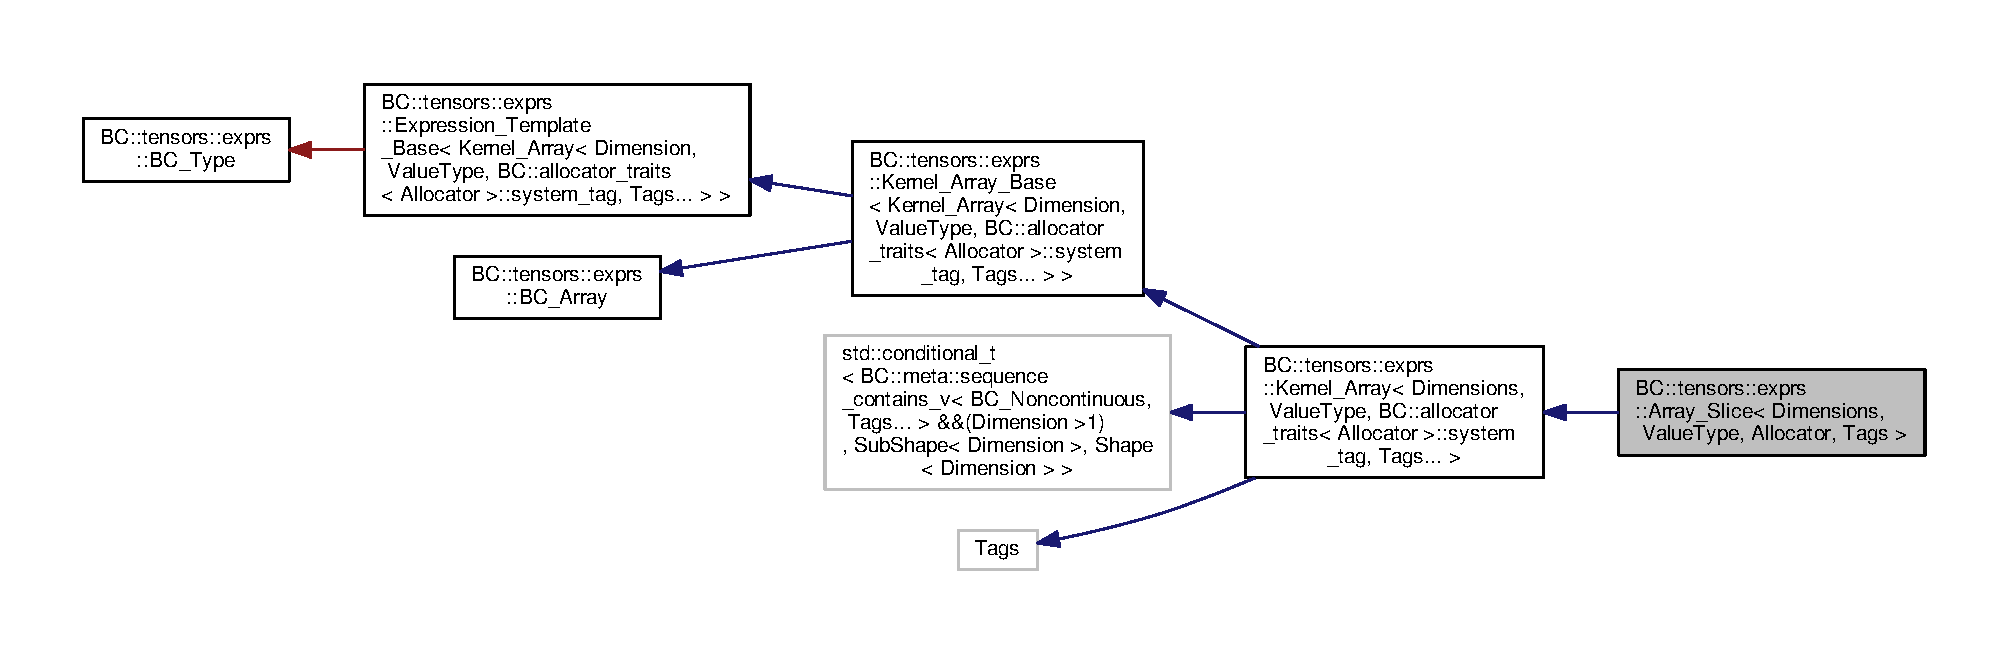
\includegraphics[width=350pt]{classBC_1_1tensors_1_1exprs_1_1Array__Slice__inherit__graph}
\end{center}
\end{figure}


Collaboration diagram for BC\+:\+:tensors\+:\+:exprs\+:\+:Array\+\_\+\+Slice$<$ Dimensions, Value\+Type, Allocator, Tags $>$\+:
\nopagebreak
\begin{figure}[H]
\begin{center}
\leavevmode
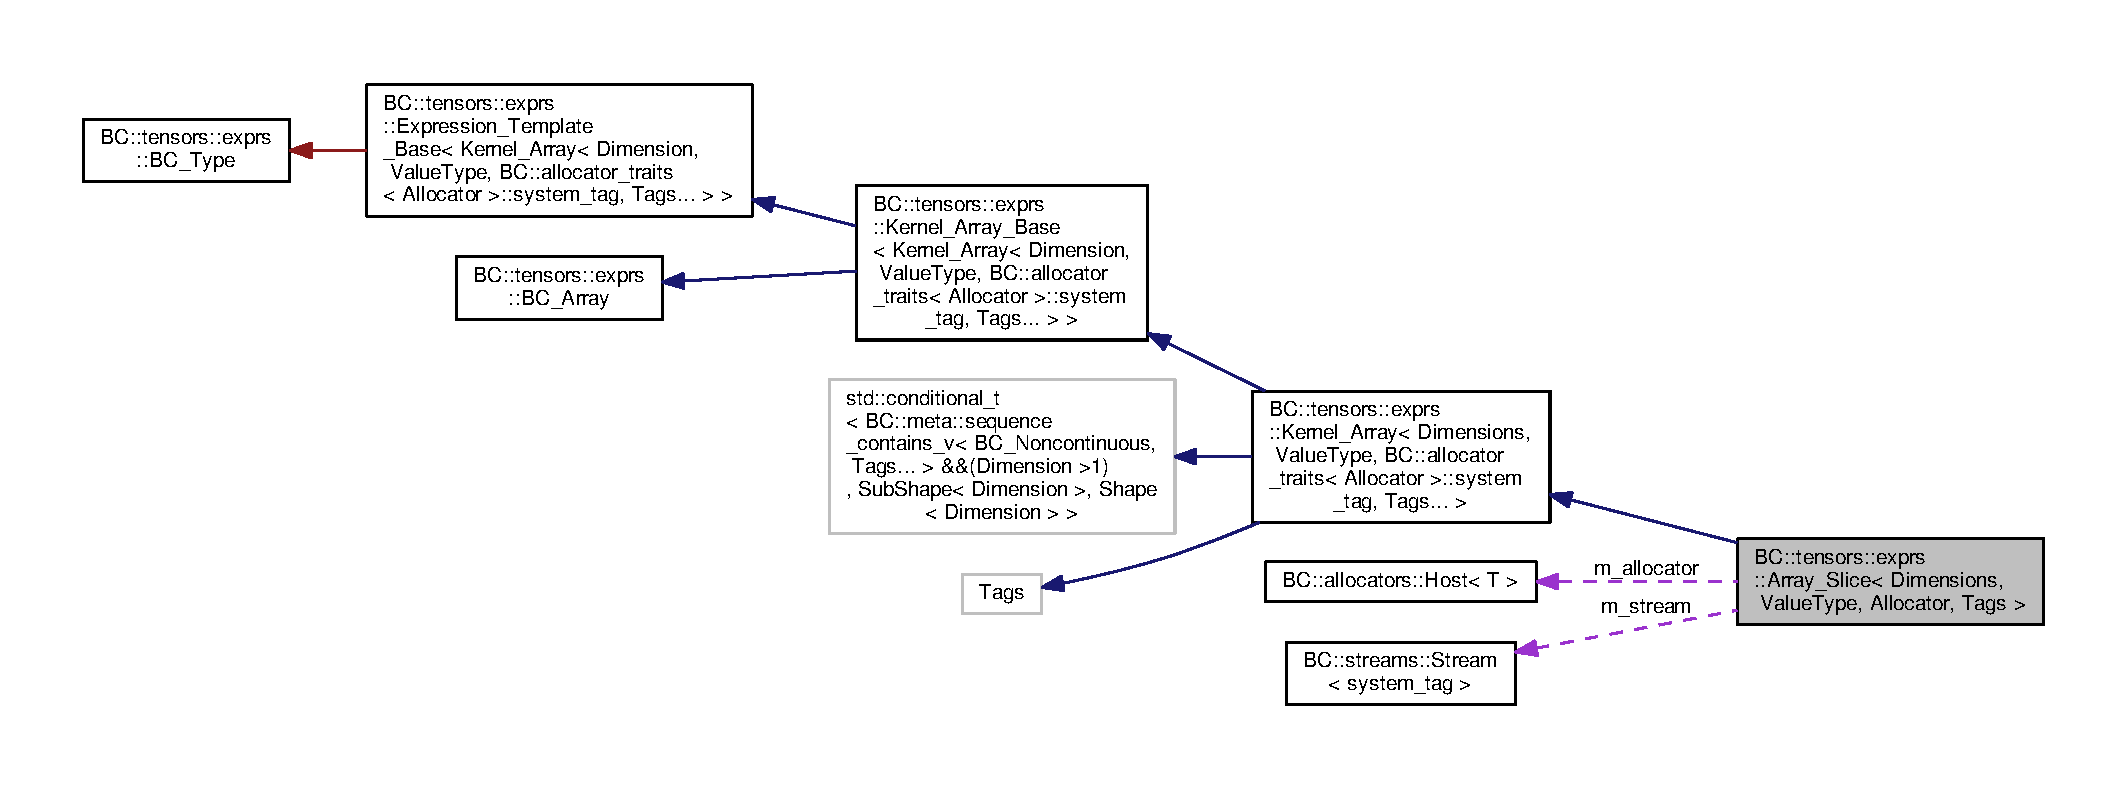
\includegraphics[width=350pt]{classBC_1_1tensors_1_1exprs_1_1Array__Slice__coll__graph}
\end{center}
\end{figure}
\subsection*{Public Types}
\begin{DoxyCompactItemize}
\item 
using \hyperlink{classBC_1_1tensors_1_1exprs_1_1Array__Slice_aa0bee33cbbb4ea522d89aefa986b6584}{allocator\+\_\+t} = \hyperlink{namespaceBC_a934f94b17b06290e6b241e5f59930c5f}{Allocator}
\item 
using \hyperlink{classBC_1_1tensors_1_1exprs_1_1Array__Slice_ae9aed80988883e25cc77cdd0e658a36e}{system\+\_\+tag} = typename \hyperlink{namespaceBC_a702bcffa3526460ac93fb2a315f2f7c7}{B\+C\+::allocator\+\_\+traits}$<$ \hyperlink{namespaceBC_a934f94b17b06290e6b241e5f59930c5f}{Allocator} $>$\+::\hyperlink{classBC_1_1tensors_1_1exprs_1_1Array__Slice_ae9aed80988883e25cc77cdd0e658a36e}{system\+\_\+tag}
\item 
using \hyperlink{classBC_1_1tensors_1_1exprs_1_1Array__Slice_a5395d730cd39e49ff6695a3294b4be5f}{stream\+\_\+t} = \hyperlink{namespaceBC_abc64a63cd29a22d102a68f478dfd588d}{B\+C\+::\+Stream}$<$ \hyperlink{classBC_1_1tensors_1_1exprs_1_1Array__Slice_ae9aed80988883e25cc77cdd0e658a36e}{system\+\_\+tag} $>$
\item 
using \hyperlink{classBC_1_1tensors_1_1exprs_1_1Array__Slice_acabef76354e22bb269d63cec2cd501df}{parent} = \hyperlink{structBC_1_1tensors_1_1exprs_1_1Kernel__Array}{Kernel\+\_\+\+Array}$<$ Dimensions, Value\+Type, \hyperlink{classBC_1_1tensors_1_1exprs_1_1Array__Slice_ae9aed80988883e25cc77cdd0e658a36e}{system\+\_\+tag}, Tags... $>$
\end{DoxyCompactItemize}
\subsection*{Public Member Functions}
\begin{DoxyCompactItemize}
\item 
{\footnotesize template$<$class... Args$>$ }\\\hyperlink{BlackCat__Common_8h_ac085f07cc309e3aac24aa3fc0a40f6d2}{B\+C\+H\+OT} \hyperlink{classBC_1_1tensors_1_1exprs_1_1Array__Slice_a258f8311b24278d8b2789755a2b5c59b}{Array\+\_\+\+Slice} (\hyperlink{classBC_1_1tensors_1_1exprs_1_1Array__Slice_a5395d730cd39e49ff6695a3294b4be5f}{stream\+\_\+t} stream\+\_\+, \hyperlink{classBC_1_1tensors_1_1exprs_1_1Array__Slice_aa0bee33cbbb4ea522d89aefa986b6584}{allocator\+\_\+t} allocator\+\_\+, Args...\+args\+\_\+)
\item 
\hyperlink{BlackCat__Common_8h_ac085f07cc309e3aac24aa3fc0a40f6d2}{B\+C\+H\+OT} \hyperlink{classBC_1_1tensors_1_1exprs_1_1Array__Slice_a48f3e7cca6b46d825488d7c29e101942}{Array\+\_\+\+Slice} (const \hyperlink{classBC_1_1tensors_1_1exprs_1_1Array__Slice}{Array\+\_\+\+Slice} \&)=default
\item 
\hyperlink{BlackCat__Common_8h_ac085f07cc309e3aac24aa3fc0a40f6d2}{B\+C\+H\+OT} \hyperlink{classBC_1_1tensors_1_1exprs_1_1Array__Slice_a2fbf29b59907dca910979de4921790ef}{Array\+\_\+\+Slice} (\hyperlink{classBC_1_1tensors_1_1exprs_1_1Array__Slice}{Array\+\_\+\+Slice} \&\&)=default
\item 
const \hyperlink{classBC_1_1tensors_1_1exprs_1_1Array__Slice_aa0bee33cbbb4ea522d89aefa986b6584}{allocator\+\_\+t} \& \hyperlink{classBC_1_1tensors_1_1exprs_1_1Array__Slice_ad35ebf0a4f818fc38b1976e4b917f63e}{get\+\_\+allocator} () const 
\item 
\hyperlink{classBC_1_1tensors_1_1exprs_1_1Array__Slice_aa0bee33cbbb4ea522d89aefa986b6584}{allocator\+\_\+t} \& \hyperlink{classBC_1_1tensors_1_1exprs_1_1Array__Slice_a3700a7d19ba9e80da45d40037a14b133}{get\+\_\+allocator} ()
\item 
const \hyperlink{classBC_1_1tensors_1_1exprs_1_1Array__Slice_a5395d730cd39e49ff6695a3294b4be5f}{stream\+\_\+t} \& \hyperlink{classBC_1_1tensors_1_1exprs_1_1Array__Slice_ae293508a48d82c01bc43c10e6102aa20}{get\+\_\+stream} () const 
\item 
\hyperlink{classBC_1_1tensors_1_1exprs_1_1Array__Slice_a5395d730cd39e49ff6695a3294b4be5f}{stream\+\_\+t} \& \hyperlink{classBC_1_1tensors_1_1exprs_1_1Array__Slice_a6fb03e660a3b4f3941d6419d71895ce4}{get\+\_\+stream} ()
\end{DoxyCompactItemize}
\subsection*{Public Attributes}
\begin{DoxyCompactItemize}
\item 
\hyperlink{classBC_1_1tensors_1_1exprs_1_1Array__Slice_a5395d730cd39e49ff6695a3294b4be5f}{stream\+\_\+t} \hyperlink{classBC_1_1tensors_1_1exprs_1_1Array__Slice_a88f9bafcc2e18f45ae9217d1f37215df}{m\+\_\+stream}
\item 
\hyperlink{classBC_1_1tensors_1_1exprs_1_1Array__Slice_aa0bee33cbbb4ea522d89aefa986b6584}{allocator\+\_\+t} \hyperlink{classBC_1_1tensors_1_1exprs_1_1Array__Slice_aa7dc5cd48d47896f87e7df27671d74b7}{m\+\_\+allocator}
\end{DoxyCompactItemize}
\subsection*{Additional Inherited Members}


\subsection{Member Typedef Documentation}
\index{B\+C\+::tensors\+::exprs\+::\+Array\+\_\+\+Slice@{B\+C\+::tensors\+::exprs\+::\+Array\+\_\+\+Slice}!allocator\+\_\+t@{allocator\+\_\+t}}
\index{allocator\+\_\+t@{allocator\+\_\+t}!B\+C\+::tensors\+::exprs\+::\+Array\+\_\+\+Slice@{B\+C\+::tensors\+::exprs\+::\+Array\+\_\+\+Slice}}
\subsubsection[{\texorpdfstring{allocator\+\_\+t}{allocator_t}}]{\setlength{\rightskip}{0pt plus 5cm}template$<$int Dimensions, class Value\+Type, class Allocator, class... Tags$>$ using {\bf B\+C\+::tensors\+::exprs\+::\+Array\+\_\+\+Slice}$<$ Dimensions, Value\+Type, {\bf Allocator}, Tags $>$\+::{\bf allocator\+\_\+t} =  {\bf Allocator}}\hypertarget{classBC_1_1tensors_1_1exprs_1_1Array__Slice_aa0bee33cbbb4ea522d89aefa986b6584}{}\label{classBC_1_1tensors_1_1exprs_1_1Array__Slice_aa0bee33cbbb4ea522d89aefa986b6584}
\index{B\+C\+::tensors\+::exprs\+::\+Array\+\_\+\+Slice@{B\+C\+::tensors\+::exprs\+::\+Array\+\_\+\+Slice}!parent@{parent}}
\index{parent@{parent}!B\+C\+::tensors\+::exprs\+::\+Array\+\_\+\+Slice@{B\+C\+::tensors\+::exprs\+::\+Array\+\_\+\+Slice}}
\subsubsection[{\texorpdfstring{parent}{parent}}]{\setlength{\rightskip}{0pt plus 5cm}template$<$int Dimensions, class Value\+Type, class Allocator, class... Tags$>$ using {\bf B\+C\+::tensors\+::exprs\+::\+Array\+\_\+\+Slice}$<$ Dimensions, Value\+Type, {\bf Allocator}, Tags $>$\+::{\bf parent} =  {\bf Kernel\+\_\+\+Array}$<$Dimensions, Value\+Type, {\bf system\+\_\+tag}, Tags...$>$}\hypertarget{classBC_1_1tensors_1_1exprs_1_1Array__Slice_acabef76354e22bb269d63cec2cd501df}{}\label{classBC_1_1tensors_1_1exprs_1_1Array__Slice_acabef76354e22bb269d63cec2cd501df}
\index{B\+C\+::tensors\+::exprs\+::\+Array\+\_\+\+Slice@{B\+C\+::tensors\+::exprs\+::\+Array\+\_\+\+Slice}!stream\+\_\+t@{stream\+\_\+t}}
\index{stream\+\_\+t@{stream\+\_\+t}!B\+C\+::tensors\+::exprs\+::\+Array\+\_\+\+Slice@{B\+C\+::tensors\+::exprs\+::\+Array\+\_\+\+Slice}}
\subsubsection[{\texorpdfstring{stream\+\_\+t}{stream_t}}]{\setlength{\rightskip}{0pt plus 5cm}template$<$int Dimensions, class Value\+Type, class Allocator, class... Tags$>$ using {\bf B\+C\+::tensors\+::exprs\+::\+Array\+\_\+\+Slice}$<$ Dimensions, Value\+Type, {\bf Allocator}, Tags $>$\+::{\bf stream\+\_\+t} =  {\bf B\+C\+::\+Stream}$<${\bf system\+\_\+tag}$>$}\hypertarget{classBC_1_1tensors_1_1exprs_1_1Array__Slice_a5395d730cd39e49ff6695a3294b4be5f}{}\label{classBC_1_1tensors_1_1exprs_1_1Array__Slice_a5395d730cd39e49ff6695a3294b4be5f}
\index{B\+C\+::tensors\+::exprs\+::\+Array\+\_\+\+Slice@{B\+C\+::tensors\+::exprs\+::\+Array\+\_\+\+Slice}!system\+\_\+tag@{system\+\_\+tag}}
\index{system\+\_\+tag@{system\+\_\+tag}!B\+C\+::tensors\+::exprs\+::\+Array\+\_\+\+Slice@{B\+C\+::tensors\+::exprs\+::\+Array\+\_\+\+Slice}}
\subsubsection[{\texorpdfstring{system\+\_\+tag}{system_tag}}]{\setlength{\rightskip}{0pt plus 5cm}template$<$int Dimensions, class Value\+Type, class Allocator, class... Tags$>$ using {\bf B\+C\+::tensors\+::exprs\+::\+Array\+\_\+\+Slice}$<$ Dimensions, Value\+Type, {\bf Allocator}, Tags $>$\+::{\bf system\+\_\+tag} =  typename {\bf B\+C\+::allocator\+\_\+traits}$<${\bf Allocator}$>$\+::{\bf system\+\_\+tag}}\hypertarget{classBC_1_1tensors_1_1exprs_1_1Array__Slice_ae9aed80988883e25cc77cdd0e658a36e}{}\label{classBC_1_1tensors_1_1exprs_1_1Array__Slice_ae9aed80988883e25cc77cdd0e658a36e}


\subsection{Constructor \& Destructor Documentation}
\index{B\+C\+::tensors\+::exprs\+::\+Array\+\_\+\+Slice@{B\+C\+::tensors\+::exprs\+::\+Array\+\_\+\+Slice}!Array\+\_\+\+Slice@{Array\+\_\+\+Slice}}
\index{Array\+\_\+\+Slice@{Array\+\_\+\+Slice}!B\+C\+::tensors\+::exprs\+::\+Array\+\_\+\+Slice@{B\+C\+::tensors\+::exprs\+::\+Array\+\_\+\+Slice}}
\subsubsection[{\texorpdfstring{Array\+\_\+\+Slice(stream\+\_\+t stream\+\_\+, allocator\+\_\+t allocator\+\_\+, Args...\+args\+\_\+)}{Array_Slice(stream_t stream_, allocator_t allocator_, Args...args_)}}]{\setlength{\rightskip}{0pt plus 5cm}template$<$int Dimensions, class Value\+Type, class Allocator, class... Tags$>$ template$<$class... Args$>$ {\bf B\+C\+H\+OT} {\bf B\+C\+::tensors\+::exprs\+::\+Array\+\_\+\+Slice}$<$ Dimensions, Value\+Type, {\bf Allocator}, Tags $>$\+::{\bf Array\+\_\+\+Slice} (
\begin{DoxyParamCaption}
\item[{{\bf stream\+\_\+t}}]{stream\+\_\+, }
\item[{{\bf allocator\+\_\+t}}]{allocator\+\_\+, }
\item[{Args...}]{args\+\_\+}
\end{DoxyParamCaption}
)\hspace{0.3cm}{\ttfamily [inline]}}\hypertarget{classBC_1_1tensors_1_1exprs_1_1Array__Slice_a258f8311b24278d8b2789755a2b5c59b}{}\label{classBC_1_1tensors_1_1exprs_1_1Array__Slice_a258f8311b24278d8b2789755a2b5c59b}
\index{B\+C\+::tensors\+::exprs\+::\+Array\+\_\+\+Slice@{B\+C\+::tensors\+::exprs\+::\+Array\+\_\+\+Slice}!Array\+\_\+\+Slice@{Array\+\_\+\+Slice}}
\index{Array\+\_\+\+Slice@{Array\+\_\+\+Slice}!B\+C\+::tensors\+::exprs\+::\+Array\+\_\+\+Slice@{B\+C\+::tensors\+::exprs\+::\+Array\+\_\+\+Slice}}
\subsubsection[{\texorpdfstring{Array\+\_\+\+Slice(const Array\+\_\+\+Slice \&)=default}{Array_Slice(const Array_Slice &)=default}}]{\setlength{\rightskip}{0pt plus 5cm}template$<$int Dimensions, class Value\+Type, class Allocator, class... Tags$>$ {\bf B\+C\+H\+OT} {\bf B\+C\+::tensors\+::exprs\+::\+Array\+\_\+\+Slice}$<$ Dimensions, Value\+Type, {\bf Allocator}, Tags $>$\+::{\bf Array\+\_\+\+Slice} (
\begin{DoxyParamCaption}
\item[{const {\bf Array\+\_\+\+Slice}$<$ Dimensions, Value\+Type, {\bf Allocator}, Tags $>$ \&}]{}
\end{DoxyParamCaption}
)\hspace{0.3cm}{\ttfamily [default]}}\hypertarget{classBC_1_1tensors_1_1exprs_1_1Array__Slice_a48f3e7cca6b46d825488d7c29e101942}{}\label{classBC_1_1tensors_1_1exprs_1_1Array__Slice_a48f3e7cca6b46d825488d7c29e101942}
\index{B\+C\+::tensors\+::exprs\+::\+Array\+\_\+\+Slice@{B\+C\+::tensors\+::exprs\+::\+Array\+\_\+\+Slice}!Array\+\_\+\+Slice@{Array\+\_\+\+Slice}}
\index{Array\+\_\+\+Slice@{Array\+\_\+\+Slice}!B\+C\+::tensors\+::exprs\+::\+Array\+\_\+\+Slice@{B\+C\+::tensors\+::exprs\+::\+Array\+\_\+\+Slice}}
\subsubsection[{\texorpdfstring{Array\+\_\+\+Slice(\+Array\+\_\+\+Slice \&\&)=default}{Array_Slice(Array_Slice &&)=default}}]{\setlength{\rightskip}{0pt plus 5cm}template$<$int Dimensions, class Value\+Type, class Allocator, class... Tags$>$ {\bf B\+C\+H\+OT} {\bf B\+C\+::tensors\+::exprs\+::\+Array\+\_\+\+Slice}$<$ Dimensions, Value\+Type, {\bf Allocator}, Tags $>$\+::{\bf Array\+\_\+\+Slice} (
\begin{DoxyParamCaption}
\item[{{\bf Array\+\_\+\+Slice}$<$ Dimensions, Value\+Type, {\bf Allocator}, Tags $>$ \&\&}]{}
\end{DoxyParamCaption}
)\hspace{0.3cm}{\ttfamily [default]}}\hypertarget{classBC_1_1tensors_1_1exprs_1_1Array__Slice_a2fbf29b59907dca910979de4921790ef}{}\label{classBC_1_1tensors_1_1exprs_1_1Array__Slice_a2fbf29b59907dca910979de4921790ef}


\subsection{Member Function Documentation}
\index{B\+C\+::tensors\+::exprs\+::\+Array\+\_\+\+Slice@{B\+C\+::tensors\+::exprs\+::\+Array\+\_\+\+Slice}!get\+\_\+allocator@{get\+\_\+allocator}}
\index{get\+\_\+allocator@{get\+\_\+allocator}!B\+C\+::tensors\+::exprs\+::\+Array\+\_\+\+Slice@{B\+C\+::tensors\+::exprs\+::\+Array\+\_\+\+Slice}}
\subsubsection[{\texorpdfstring{get\+\_\+allocator() const }{get_allocator() const }}]{\setlength{\rightskip}{0pt plus 5cm}template$<$int Dimensions, class Value\+Type, class Allocator, class... Tags$>$ const {\bf allocator\+\_\+t}\& {\bf B\+C\+::tensors\+::exprs\+::\+Array\+\_\+\+Slice}$<$ Dimensions, Value\+Type, {\bf Allocator}, Tags $>$\+::get\+\_\+allocator (
\begin{DoxyParamCaption}
{}
\end{DoxyParamCaption}
) const\hspace{0.3cm}{\ttfamily [inline]}}\hypertarget{classBC_1_1tensors_1_1exprs_1_1Array__Slice_ad35ebf0a4f818fc38b1976e4b917f63e}{}\label{classBC_1_1tensors_1_1exprs_1_1Array__Slice_ad35ebf0a4f818fc38b1976e4b917f63e}
\index{B\+C\+::tensors\+::exprs\+::\+Array\+\_\+\+Slice@{B\+C\+::tensors\+::exprs\+::\+Array\+\_\+\+Slice}!get\+\_\+allocator@{get\+\_\+allocator}}
\index{get\+\_\+allocator@{get\+\_\+allocator}!B\+C\+::tensors\+::exprs\+::\+Array\+\_\+\+Slice@{B\+C\+::tensors\+::exprs\+::\+Array\+\_\+\+Slice}}
\subsubsection[{\texorpdfstring{get\+\_\+allocator()}{get_allocator()}}]{\setlength{\rightskip}{0pt plus 5cm}template$<$int Dimensions, class Value\+Type, class Allocator, class... Tags$>$ {\bf allocator\+\_\+t}\& {\bf B\+C\+::tensors\+::exprs\+::\+Array\+\_\+\+Slice}$<$ Dimensions, Value\+Type, {\bf Allocator}, Tags $>$\+::get\+\_\+allocator (
\begin{DoxyParamCaption}
{}
\end{DoxyParamCaption}
)\hspace{0.3cm}{\ttfamily [inline]}}\hypertarget{classBC_1_1tensors_1_1exprs_1_1Array__Slice_a3700a7d19ba9e80da45d40037a14b133}{}\label{classBC_1_1tensors_1_1exprs_1_1Array__Slice_a3700a7d19ba9e80da45d40037a14b133}
\index{B\+C\+::tensors\+::exprs\+::\+Array\+\_\+\+Slice@{B\+C\+::tensors\+::exprs\+::\+Array\+\_\+\+Slice}!get\+\_\+stream@{get\+\_\+stream}}
\index{get\+\_\+stream@{get\+\_\+stream}!B\+C\+::tensors\+::exprs\+::\+Array\+\_\+\+Slice@{B\+C\+::tensors\+::exprs\+::\+Array\+\_\+\+Slice}}
\subsubsection[{\texorpdfstring{get\+\_\+stream() const }{get_stream() const }}]{\setlength{\rightskip}{0pt plus 5cm}template$<$int Dimensions, class Value\+Type, class Allocator, class... Tags$>$ const {\bf stream\+\_\+t}\& {\bf B\+C\+::tensors\+::exprs\+::\+Array\+\_\+\+Slice}$<$ Dimensions, Value\+Type, {\bf Allocator}, Tags $>$\+::get\+\_\+stream (
\begin{DoxyParamCaption}
{}
\end{DoxyParamCaption}
) const\hspace{0.3cm}{\ttfamily [inline]}}\hypertarget{classBC_1_1tensors_1_1exprs_1_1Array__Slice_ae293508a48d82c01bc43c10e6102aa20}{}\label{classBC_1_1tensors_1_1exprs_1_1Array__Slice_ae293508a48d82c01bc43c10e6102aa20}
\index{B\+C\+::tensors\+::exprs\+::\+Array\+\_\+\+Slice@{B\+C\+::tensors\+::exprs\+::\+Array\+\_\+\+Slice}!get\+\_\+stream@{get\+\_\+stream}}
\index{get\+\_\+stream@{get\+\_\+stream}!B\+C\+::tensors\+::exprs\+::\+Array\+\_\+\+Slice@{B\+C\+::tensors\+::exprs\+::\+Array\+\_\+\+Slice}}
\subsubsection[{\texorpdfstring{get\+\_\+stream()}{get_stream()}}]{\setlength{\rightskip}{0pt plus 5cm}template$<$int Dimensions, class Value\+Type, class Allocator, class... Tags$>$ {\bf stream\+\_\+t}\& {\bf B\+C\+::tensors\+::exprs\+::\+Array\+\_\+\+Slice}$<$ Dimensions, Value\+Type, {\bf Allocator}, Tags $>$\+::get\+\_\+stream (
\begin{DoxyParamCaption}
{}
\end{DoxyParamCaption}
)\hspace{0.3cm}{\ttfamily [inline]}}\hypertarget{classBC_1_1tensors_1_1exprs_1_1Array__Slice_a6fb03e660a3b4f3941d6419d71895ce4}{}\label{classBC_1_1tensors_1_1exprs_1_1Array__Slice_a6fb03e660a3b4f3941d6419d71895ce4}


\subsection{Member Data Documentation}
\index{B\+C\+::tensors\+::exprs\+::\+Array\+\_\+\+Slice@{B\+C\+::tensors\+::exprs\+::\+Array\+\_\+\+Slice}!m\+\_\+allocator@{m\+\_\+allocator}}
\index{m\+\_\+allocator@{m\+\_\+allocator}!B\+C\+::tensors\+::exprs\+::\+Array\+\_\+\+Slice@{B\+C\+::tensors\+::exprs\+::\+Array\+\_\+\+Slice}}
\subsubsection[{\texorpdfstring{m\+\_\+allocator}{m_allocator}}]{\setlength{\rightskip}{0pt plus 5cm}template$<$int Dimensions, class Value\+Type, class Allocator, class... Tags$>$ {\bf allocator\+\_\+t} {\bf B\+C\+::tensors\+::exprs\+::\+Array\+\_\+\+Slice}$<$ Dimensions, Value\+Type, {\bf Allocator}, Tags $>$\+::m\+\_\+allocator}\hypertarget{classBC_1_1tensors_1_1exprs_1_1Array__Slice_aa7dc5cd48d47896f87e7df27671d74b7}{}\label{classBC_1_1tensors_1_1exprs_1_1Array__Slice_aa7dc5cd48d47896f87e7df27671d74b7}
\index{B\+C\+::tensors\+::exprs\+::\+Array\+\_\+\+Slice@{B\+C\+::tensors\+::exprs\+::\+Array\+\_\+\+Slice}!m\+\_\+stream@{m\+\_\+stream}}
\index{m\+\_\+stream@{m\+\_\+stream}!B\+C\+::tensors\+::exprs\+::\+Array\+\_\+\+Slice@{B\+C\+::tensors\+::exprs\+::\+Array\+\_\+\+Slice}}
\subsubsection[{\texorpdfstring{m\+\_\+stream}{m_stream}}]{\setlength{\rightskip}{0pt plus 5cm}template$<$int Dimensions, class Value\+Type, class Allocator, class... Tags$>$ {\bf stream\+\_\+t} {\bf B\+C\+::tensors\+::exprs\+::\+Array\+\_\+\+Slice}$<$ Dimensions, Value\+Type, {\bf Allocator}, Tags $>$\+::m\+\_\+stream}\hypertarget{classBC_1_1tensors_1_1exprs_1_1Array__Slice_a88f9bafcc2e18f45ae9217d1f37215df}{}\label{classBC_1_1tensors_1_1exprs_1_1Array__Slice_a88f9bafcc2e18f45ae9217d1f37215df}


The documentation for this struct was generated from the following files\+:\begin{DoxyCompactItemize}
\item 
include/tensors/expression\+\_\+templates/\hyperlink{Array_8h}{Array.\+h}\item 
include/tensors/expression\+\_\+templates/\hyperlink{Array__Slice_8h}{Array\+\_\+\+Slice.\+h}\end{DoxyCompactItemize}

\hypertarget{structBC_1_1oper_1_1Assign}{}\section{BC\+:\+:oper\+:\+:Assign Struct Reference}
\label{structBC_1_1oper_1_1Assign}\index{B\+C\+::oper\+::\+Assign@{B\+C\+::oper\+::\+Assign}}


{\ttfamily \#include $<$Binary.\+h$>$}



Inheritance diagram for BC\+:\+:oper\+:\+:Assign\+:
\nopagebreak
\begin{figure}[H]
\begin{center}
\leavevmode
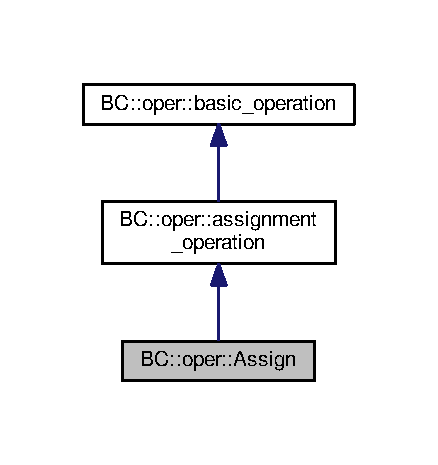
\includegraphics[width=210pt]{structBC_1_1oper_1_1Assign__inherit__graph}
\end{center}
\end{figure}


Collaboration diagram for BC\+:\+:oper\+:\+:Assign\+:
\nopagebreak
\begin{figure}[H]
\begin{center}
\leavevmode
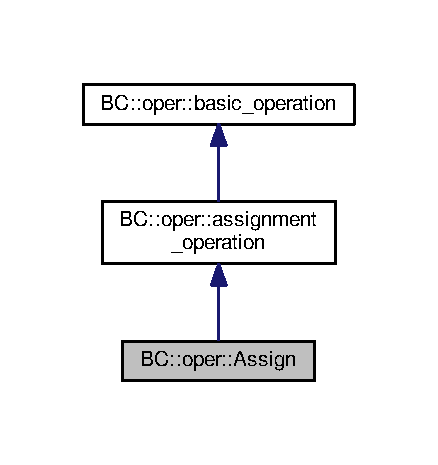
\includegraphics[width=210pt]{structBC_1_1oper_1_1Assign__coll__graph}
\end{center}
\end{figure}
\subsection*{Public Types}
\begin{DoxyCompactItemize}
\item 
using \hyperlink{structBC_1_1oper_1_1Assign_a5b56dd2f402c432d85467dfcc568135e}{alpha\+\_\+modifier} = \hyperlink{structBC_1_1meta_1_1Integer}{B\+C\+::meta\+::\+Integer}$<$ 1 $>$
\item 
using \hyperlink{structBC_1_1oper_1_1Assign_a97c21e6ead4f60ed53836a0817377754}{beta\+\_\+modifier} = \hyperlink{structBC_1_1meta_1_1Integer}{B\+C\+::meta\+::\+Integer}$<$ 0 $>$
\end{DoxyCompactItemize}


\subsection{Member Typedef Documentation}
\index{B\+C\+::oper\+::\+Assign@{B\+C\+::oper\+::\+Assign}!alpha\+\_\+modifier@{alpha\+\_\+modifier}}
\index{alpha\+\_\+modifier@{alpha\+\_\+modifier}!B\+C\+::oper\+::\+Assign@{B\+C\+::oper\+::\+Assign}}
\subsubsection[{\texorpdfstring{alpha\+\_\+modifier}{alpha_modifier}}]{\setlength{\rightskip}{0pt plus 5cm}using {\bf B\+C\+::oper\+::\+Assign\+::alpha\+\_\+modifier} =  {\bf B\+C\+::meta\+::\+Integer}$<$1$>$}\hypertarget{structBC_1_1oper_1_1Assign_a5b56dd2f402c432d85467dfcc568135e}{}\label{structBC_1_1oper_1_1Assign_a5b56dd2f402c432d85467dfcc568135e}
\index{B\+C\+::oper\+::\+Assign@{B\+C\+::oper\+::\+Assign}!beta\+\_\+modifier@{beta\+\_\+modifier}}
\index{beta\+\_\+modifier@{beta\+\_\+modifier}!B\+C\+::oper\+::\+Assign@{B\+C\+::oper\+::\+Assign}}
\subsubsection[{\texorpdfstring{beta\+\_\+modifier}{beta_modifier}}]{\setlength{\rightskip}{0pt plus 5cm}using {\bf B\+C\+::oper\+::\+Assign\+::beta\+\_\+modifier} =  {\bf B\+C\+::meta\+::\+Integer}$<$0$>$}\hypertarget{structBC_1_1oper_1_1Assign_a97c21e6ead4f60ed53836a0817377754}{}\label{structBC_1_1oper_1_1Assign_a97c21e6ead4f60ed53836a0817377754}


The documentation for this struct was generated from the following file\+:\begin{DoxyCompactItemize}
\item 
include/operations/\hyperlink{Binary_8h}{Binary.\+h}\end{DoxyCompactItemize}

\hypertarget{structBC_1_1oper_1_1assignment__operation}{}\section{BC\+:\+:oper\+:\+:assignment\+\_\+operation Struct Reference}
\label{structBC_1_1oper_1_1assignment__operation}\index{B\+C\+::oper\+::assignment\+\_\+operation@{B\+C\+::oper\+::assignment\+\_\+operation}}


{\ttfamily \#include $<$Tags.\+h$>$}



Inheritance diagram for BC\+:\+:oper\+:\+:assignment\+\_\+operation\+:
\nopagebreak
\begin{figure}[H]
\begin{center}
\leavevmode
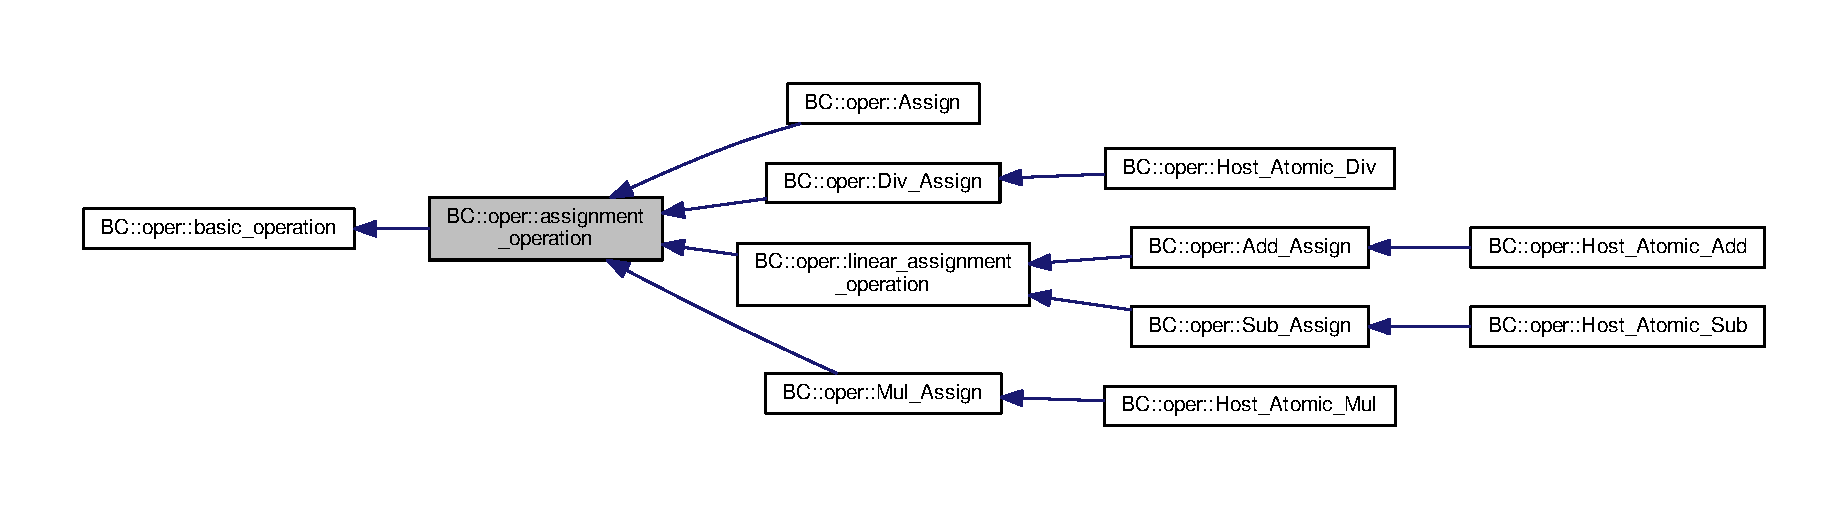
\includegraphics[width=350pt]{structBC_1_1oper_1_1assignment__operation__inherit__graph}
\end{center}
\end{figure}


Collaboration diagram for BC\+:\+:oper\+:\+:assignment\+\_\+operation\+:
\nopagebreak
\begin{figure}[H]
\begin{center}
\leavevmode
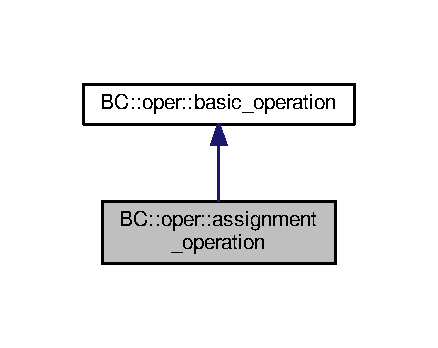
\includegraphics[width=210pt]{structBC_1_1oper_1_1assignment__operation__coll__graph}
\end{center}
\end{figure}


The documentation for this struct was generated from the following file\+:\begin{DoxyCompactItemize}
\item 
include/operations/\hyperlink{operations_2Tags_8h}{Tags.\+h}\end{DoxyCompactItemize}

\hypertarget{classBC_1_1memory_1_1atomic__shared__ptr}{}\section{BC\+:\+:memory\+:\+:atomic\+\_\+shared\+\_\+ptr$<$ Value\+Type $>$ Class Template Reference}
\label{classBC_1_1memory_1_1atomic__shared__ptr}\index{B\+C\+::memory\+::atomic\+\_\+shared\+\_\+ptr$<$ Value\+Type $>$@{B\+C\+::memory\+::atomic\+\_\+shared\+\_\+ptr$<$ Value\+Type $>$}}


{\ttfamily \#include $<$Black\+Cat\+\_\+\+Memory.\+h$>$}

\subsection*{Classes}
\begin{DoxyCompactItemize}
\item 
struct \hyperlink{structBC_1_1memory_1_1atomic__shared__ptr_1_1wrapper}{wrapper}
\end{DoxyCompactItemize}
\subsection*{Public Member Functions}
\begin{DoxyCompactItemize}
\item 
{\footnotesize template$<$class... Args$>$ }\\\hyperlink{classBC_1_1memory_1_1atomic__shared__ptr_a5e60d8cd3873420741fe6b2c12cacb86}{atomic\+\_\+shared\+\_\+ptr} (Args \&\&...args)
\item 
\hyperlink{classBC_1_1memory_1_1atomic__shared__ptr_a3a720872a09351834feda9126f25eecb}{atomic\+\_\+shared\+\_\+ptr} (\hyperlink{classBC_1_1memory_1_1atomic__shared__ptr}{atomic\+\_\+shared\+\_\+ptr} \&\&ptr)
\item 
\hyperlink{classBC_1_1memory_1_1atomic__shared__ptr_a46f2567c2a73e455595835d7633cfe3a}{atomic\+\_\+shared\+\_\+ptr} (const \hyperlink{classBC_1_1memory_1_1atomic__shared__ptr}{atomic\+\_\+shared\+\_\+ptr} \&ptr)
\item 
\hyperlink{classBC_1_1memory_1_1atomic__shared__ptr_aec6b34765f04d120c96236c21a15c981}{atomic\+\_\+shared\+\_\+ptr} ()=default
\item 
{\footnotesize template$<$class... Args$>$ }\\\hyperlink{classBC_1_1memory_1_1atomic__shared__ptr_a3728bb6491f877538ac4868ec43f5360}{atomic\+\_\+shared\+\_\+ptr} (const Args \&...args)
\item 
{\footnotesize template$<$class Y , class Deleter  = detail\+::\+Default\+\_\+\+Deleter, class Allocator  = std\+::allocator$<$\+Value\+Type$>$$>$ }\\void \hyperlink{classBC_1_1memory_1_1atomic__shared__ptr_a59b1b6c8781a2b70008e1ae4c8325d17}{reset} (Y $\ast$ptr, Deleter del=\hyperlink{namespaceBC_1_1memory_1_1detail_a42827b91c57157365e4c7249397f12b6}{detail\+::default\+\_\+deleter}, \hyperlink{namespaceBC_a934f94b17b06290e6b241e5f59930c5f}{Allocator} alloc=\hyperlink{namespaceBC_a934f94b17b06290e6b241e5f59930c5f}{Allocator}())
\item 
void \hyperlink{classBC_1_1memory_1_1atomic__shared__ptr_ad7a862c5433c6c3c5af8b55762d4fe0f}{swap} (std\+::shared\+\_\+ptr$<$ Value\+Type $>$ \&sh\+\_\+ptr)
\item 
\hyperlink{structBC_1_1memory_1_1atomic__shared__ptr_1_1wrapper}{wrapper} \hyperlink{classBC_1_1memory_1_1atomic__shared__ptr_afc9fbab0c0f7744b1364c03675b6fa13}{get} ()
\item 
const \hyperlink{structBC_1_1memory_1_1atomic__shared__ptr_1_1wrapper}{wrapper} \hyperlink{classBC_1_1memory_1_1atomic__shared__ptr_ac25a830aee63f9273529cb0a67350166}{get} () const 
\item 
auto \hyperlink{classBC_1_1memory_1_1atomic__shared__ptr_a3024f0c9f0ba45f096b1d7e5c603c7b0}{operator-\/$>$} ()
\item 
auto \hyperlink{classBC_1_1memory_1_1atomic__shared__ptr_ae2c5708e2519ead2cf30bc05a7c4b6f8}{operator-\/$>$} () const 
\item 
bool \hyperlink{classBC_1_1memory_1_1atomic__shared__ptr_a1793a0e3d10f3fb6d3487f58d390fc5e}{operator==} (const \hyperlink{classBC_1_1memory_1_1atomic__shared__ptr}{atomic\+\_\+shared\+\_\+ptr}$<$ Value\+Type $>$ \&ptr)
\item 
bool \hyperlink{classBC_1_1memory_1_1atomic__shared__ptr_a0a25f4cf07d78c96f934741018cc5f3b}{operator!=} (const \hyperlink{classBC_1_1memory_1_1atomic__shared__ptr}{atomic\+\_\+shared\+\_\+ptr}$<$ Value\+Type $>$ \&ptr)
\item 
\hyperlink{classBC_1_1memory_1_1atomic__shared__ptr}{atomic\+\_\+shared\+\_\+ptr} \& \hyperlink{classBC_1_1memory_1_1atomic__shared__ptr_a76412c3271513ef2fd1eef5199a78b0d}{operator=} (const \hyperlink{classBC_1_1memory_1_1atomic__shared__ptr}{atomic\+\_\+shared\+\_\+ptr}$<$ Value\+Type $>$ \&ptr)
\end{DoxyCompactItemize}


\subsection{Constructor \& Destructor Documentation}
\index{B\+C\+::memory\+::atomic\+\_\+shared\+\_\+ptr@{B\+C\+::memory\+::atomic\+\_\+shared\+\_\+ptr}!atomic\+\_\+shared\+\_\+ptr@{atomic\+\_\+shared\+\_\+ptr}}
\index{atomic\+\_\+shared\+\_\+ptr@{atomic\+\_\+shared\+\_\+ptr}!B\+C\+::memory\+::atomic\+\_\+shared\+\_\+ptr@{B\+C\+::memory\+::atomic\+\_\+shared\+\_\+ptr}}
\subsubsection[{\texorpdfstring{atomic\+\_\+shared\+\_\+ptr(\+Args \&\&...\+args)}{atomic_shared_ptr(Args &&...args)}}]{\setlength{\rightskip}{0pt plus 5cm}template$<$class Value\+Type$>$ template$<$class... Args$>$ {\bf B\+C\+::memory\+::atomic\+\_\+shared\+\_\+ptr}$<$ Value\+Type $>$\+::{\bf atomic\+\_\+shared\+\_\+ptr} (
\begin{DoxyParamCaption}
\item[{Args \&\&...}]{args}
\end{DoxyParamCaption}
)\hspace{0.3cm}{\ttfamily [inline]}, {\ttfamily [explicit]}}\hypertarget{classBC_1_1memory_1_1atomic__shared__ptr_a5e60d8cd3873420741fe6b2c12cacb86}{}\label{classBC_1_1memory_1_1atomic__shared__ptr_a5e60d8cd3873420741fe6b2c12cacb86}
\index{B\+C\+::memory\+::atomic\+\_\+shared\+\_\+ptr@{B\+C\+::memory\+::atomic\+\_\+shared\+\_\+ptr}!atomic\+\_\+shared\+\_\+ptr@{atomic\+\_\+shared\+\_\+ptr}}
\index{atomic\+\_\+shared\+\_\+ptr@{atomic\+\_\+shared\+\_\+ptr}!B\+C\+::memory\+::atomic\+\_\+shared\+\_\+ptr@{B\+C\+::memory\+::atomic\+\_\+shared\+\_\+ptr}}
\subsubsection[{\texorpdfstring{atomic\+\_\+shared\+\_\+ptr(atomic\+\_\+shared\+\_\+ptr \&\&ptr)}{atomic_shared_ptr(atomic_shared_ptr &&ptr)}}]{\setlength{\rightskip}{0pt plus 5cm}template$<$class Value\+Type$>$ {\bf B\+C\+::memory\+::atomic\+\_\+shared\+\_\+ptr}$<$ Value\+Type $>$\+::{\bf atomic\+\_\+shared\+\_\+ptr} (
\begin{DoxyParamCaption}
\item[{{\bf atomic\+\_\+shared\+\_\+ptr}$<$ Value\+Type $>$ \&\&}]{ptr}
\end{DoxyParamCaption}
)\hspace{0.3cm}{\ttfamily [inline]}}\hypertarget{classBC_1_1memory_1_1atomic__shared__ptr_a3a720872a09351834feda9126f25eecb}{}\label{classBC_1_1memory_1_1atomic__shared__ptr_a3a720872a09351834feda9126f25eecb}
\index{B\+C\+::memory\+::atomic\+\_\+shared\+\_\+ptr@{B\+C\+::memory\+::atomic\+\_\+shared\+\_\+ptr}!atomic\+\_\+shared\+\_\+ptr@{atomic\+\_\+shared\+\_\+ptr}}
\index{atomic\+\_\+shared\+\_\+ptr@{atomic\+\_\+shared\+\_\+ptr}!B\+C\+::memory\+::atomic\+\_\+shared\+\_\+ptr@{B\+C\+::memory\+::atomic\+\_\+shared\+\_\+ptr}}
\subsubsection[{\texorpdfstring{atomic\+\_\+shared\+\_\+ptr(const atomic\+\_\+shared\+\_\+ptr \&ptr)}{atomic_shared_ptr(const atomic_shared_ptr &ptr)}}]{\setlength{\rightskip}{0pt plus 5cm}template$<$class Value\+Type$>$ {\bf B\+C\+::memory\+::atomic\+\_\+shared\+\_\+ptr}$<$ Value\+Type $>$\+::{\bf atomic\+\_\+shared\+\_\+ptr} (
\begin{DoxyParamCaption}
\item[{const {\bf atomic\+\_\+shared\+\_\+ptr}$<$ Value\+Type $>$ \&}]{ptr}
\end{DoxyParamCaption}
)\hspace{0.3cm}{\ttfamily [inline]}}\hypertarget{classBC_1_1memory_1_1atomic__shared__ptr_a46f2567c2a73e455595835d7633cfe3a}{}\label{classBC_1_1memory_1_1atomic__shared__ptr_a46f2567c2a73e455595835d7633cfe3a}
\index{B\+C\+::memory\+::atomic\+\_\+shared\+\_\+ptr@{B\+C\+::memory\+::atomic\+\_\+shared\+\_\+ptr}!atomic\+\_\+shared\+\_\+ptr@{atomic\+\_\+shared\+\_\+ptr}}
\index{atomic\+\_\+shared\+\_\+ptr@{atomic\+\_\+shared\+\_\+ptr}!B\+C\+::memory\+::atomic\+\_\+shared\+\_\+ptr@{B\+C\+::memory\+::atomic\+\_\+shared\+\_\+ptr}}
\subsubsection[{\texorpdfstring{atomic\+\_\+shared\+\_\+ptr()=default}{atomic_shared_ptr()=default}}]{\setlength{\rightskip}{0pt plus 5cm}template$<$class Value\+Type$>$ {\bf B\+C\+::memory\+::atomic\+\_\+shared\+\_\+ptr}$<$ Value\+Type $>$\+::{\bf atomic\+\_\+shared\+\_\+ptr} (
\begin{DoxyParamCaption}
{}
\end{DoxyParamCaption}
)\hspace{0.3cm}{\ttfamily [default]}}\hypertarget{classBC_1_1memory_1_1atomic__shared__ptr_aec6b34765f04d120c96236c21a15c981}{}\label{classBC_1_1memory_1_1atomic__shared__ptr_aec6b34765f04d120c96236c21a15c981}
\index{B\+C\+::memory\+::atomic\+\_\+shared\+\_\+ptr@{B\+C\+::memory\+::atomic\+\_\+shared\+\_\+ptr}!atomic\+\_\+shared\+\_\+ptr@{atomic\+\_\+shared\+\_\+ptr}}
\index{atomic\+\_\+shared\+\_\+ptr@{atomic\+\_\+shared\+\_\+ptr}!B\+C\+::memory\+::atomic\+\_\+shared\+\_\+ptr@{B\+C\+::memory\+::atomic\+\_\+shared\+\_\+ptr}}
\subsubsection[{\texorpdfstring{atomic\+\_\+shared\+\_\+ptr(const Args \&...\+args)}{atomic_shared_ptr(const Args &...args)}}]{\setlength{\rightskip}{0pt plus 5cm}template$<$class Value\+Type$>$ template$<$class... Args$>$ {\bf B\+C\+::memory\+::atomic\+\_\+shared\+\_\+ptr}$<$ Value\+Type $>$\+::{\bf atomic\+\_\+shared\+\_\+ptr} (
\begin{DoxyParamCaption}
\item[{const Args \&...}]{args}
\end{DoxyParamCaption}
)\hspace{0.3cm}{\ttfamily [inline]}}\hypertarget{classBC_1_1memory_1_1atomic__shared__ptr_a3728bb6491f877538ac4868ec43f5360}{}\label{classBC_1_1memory_1_1atomic__shared__ptr_a3728bb6491f877538ac4868ec43f5360}


\subsection{Member Function Documentation}
\index{B\+C\+::memory\+::atomic\+\_\+shared\+\_\+ptr@{B\+C\+::memory\+::atomic\+\_\+shared\+\_\+ptr}!get@{get}}
\index{get@{get}!B\+C\+::memory\+::atomic\+\_\+shared\+\_\+ptr@{B\+C\+::memory\+::atomic\+\_\+shared\+\_\+ptr}}
\subsubsection[{\texorpdfstring{get()}{get()}}]{\setlength{\rightskip}{0pt plus 5cm}template$<$class Value\+Type$>$ {\bf wrapper} {\bf B\+C\+::memory\+::atomic\+\_\+shared\+\_\+ptr}$<$ Value\+Type $>$\+::get (
\begin{DoxyParamCaption}
{}
\end{DoxyParamCaption}
)\hspace{0.3cm}{\ttfamily [inline]}}\hypertarget{classBC_1_1memory_1_1atomic__shared__ptr_afc9fbab0c0f7744b1364c03675b6fa13}{}\label{classBC_1_1memory_1_1atomic__shared__ptr_afc9fbab0c0f7744b1364c03675b6fa13}
\index{B\+C\+::memory\+::atomic\+\_\+shared\+\_\+ptr@{B\+C\+::memory\+::atomic\+\_\+shared\+\_\+ptr}!get@{get}}
\index{get@{get}!B\+C\+::memory\+::atomic\+\_\+shared\+\_\+ptr@{B\+C\+::memory\+::atomic\+\_\+shared\+\_\+ptr}}
\subsubsection[{\texorpdfstring{get() const }{get() const }}]{\setlength{\rightskip}{0pt plus 5cm}template$<$class Value\+Type$>$ const {\bf wrapper} {\bf B\+C\+::memory\+::atomic\+\_\+shared\+\_\+ptr}$<$ Value\+Type $>$\+::get (
\begin{DoxyParamCaption}
{}
\end{DoxyParamCaption}
) const\hspace{0.3cm}{\ttfamily [inline]}}\hypertarget{classBC_1_1memory_1_1atomic__shared__ptr_ac25a830aee63f9273529cb0a67350166}{}\label{classBC_1_1memory_1_1atomic__shared__ptr_ac25a830aee63f9273529cb0a67350166}
\index{B\+C\+::memory\+::atomic\+\_\+shared\+\_\+ptr@{B\+C\+::memory\+::atomic\+\_\+shared\+\_\+ptr}!operator"!=@{operator"!=}}
\index{operator"!=@{operator"!=}!B\+C\+::memory\+::atomic\+\_\+shared\+\_\+ptr@{B\+C\+::memory\+::atomic\+\_\+shared\+\_\+ptr}}
\subsubsection[{\texorpdfstring{operator"!=(const atomic\+\_\+shared\+\_\+ptr$<$ Value\+Type $>$ \&ptr)}{operator!=(const atomic_shared_ptr< ValueType > &ptr)}}]{\setlength{\rightskip}{0pt plus 5cm}template$<$class Value\+Type$>$ bool {\bf B\+C\+::memory\+::atomic\+\_\+shared\+\_\+ptr}$<$ Value\+Type $>$\+::operator!= (
\begin{DoxyParamCaption}
\item[{const {\bf atomic\+\_\+shared\+\_\+ptr}$<$ Value\+Type $>$ \&}]{ptr}
\end{DoxyParamCaption}
)\hspace{0.3cm}{\ttfamily [inline]}}\hypertarget{classBC_1_1memory_1_1atomic__shared__ptr_a0a25f4cf07d78c96f934741018cc5f3b}{}\label{classBC_1_1memory_1_1atomic__shared__ptr_a0a25f4cf07d78c96f934741018cc5f3b}
\index{B\+C\+::memory\+::atomic\+\_\+shared\+\_\+ptr@{B\+C\+::memory\+::atomic\+\_\+shared\+\_\+ptr}!operator-\/$>$@{operator-\/$>$}}
\index{operator-\/$>$@{operator-\/$>$}!B\+C\+::memory\+::atomic\+\_\+shared\+\_\+ptr@{B\+C\+::memory\+::atomic\+\_\+shared\+\_\+ptr}}
\subsubsection[{\texorpdfstring{operator-\/$>$()}{operator->()}}]{\setlength{\rightskip}{0pt plus 5cm}template$<$class Value\+Type$>$ auto {\bf B\+C\+::memory\+::atomic\+\_\+shared\+\_\+ptr}$<$ Value\+Type $>$\+::operator-\/$>$ (
\begin{DoxyParamCaption}
{}
\end{DoxyParamCaption}
)\hspace{0.3cm}{\ttfamily [inline]}}\hypertarget{classBC_1_1memory_1_1atomic__shared__ptr_a3024f0c9f0ba45f096b1d7e5c603c7b0}{}\label{classBC_1_1memory_1_1atomic__shared__ptr_a3024f0c9f0ba45f096b1d7e5c603c7b0}
\index{B\+C\+::memory\+::atomic\+\_\+shared\+\_\+ptr@{B\+C\+::memory\+::atomic\+\_\+shared\+\_\+ptr}!operator-\/$>$@{operator-\/$>$}}
\index{operator-\/$>$@{operator-\/$>$}!B\+C\+::memory\+::atomic\+\_\+shared\+\_\+ptr@{B\+C\+::memory\+::atomic\+\_\+shared\+\_\+ptr}}
\subsubsection[{\texorpdfstring{operator-\/$>$() const }{operator->() const }}]{\setlength{\rightskip}{0pt plus 5cm}template$<$class Value\+Type$>$ auto {\bf B\+C\+::memory\+::atomic\+\_\+shared\+\_\+ptr}$<$ Value\+Type $>$\+::operator-\/$>$ (
\begin{DoxyParamCaption}
{}
\end{DoxyParamCaption}
) const\hspace{0.3cm}{\ttfamily [inline]}}\hypertarget{classBC_1_1memory_1_1atomic__shared__ptr_ae2c5708e2519ead2cf30bc05a7c4b6f8}{}\label{classBC_1_1memory_1_1atomic__shared__ptr_ae2c5708e2519ead2cf30bc05a7c4b6f8}
\index{B\+C\+::memory\+::atomic\+\_\+shared\+\_\+ptr@{B\+C\+::memory\+::atomic\+\_\+shared\+\_\+ptr}!operator=@{operator=}}
\index{operator=@{operator=}!B\+C\+::memory\+::atomic\+\_\+shared\+\_\+ptr@{B\+C\+::memory\+::atomic\+\_\+shared\+\_\+ptr}}
\subsubsection[{\texorpdfstring{operator=(const atomic\+\_\+shared\+\_\+ptr$<$ Value\+Type $>$ \&ptr)}{operator=(const atomic_shared_ptr< ValueType > &ptr)}}]{\setlength{\rightskip}{0pt plus 5cm}template$<$class Value\+Type$>$ {\bf atomic\+\_\+shared\+\_\+ptr}\& {\bf B\+C\+::memory\+::atomic\+\_\+shared\+\_\+ptr}$<$ Value\+Type $>$\+::operator= (
\begin{DoxyParamCaption}
\item[{const {\bf atomic\+\_\+shared\+\_\+ptr}$<$ Value\+Type $>$ \&}]{ptr}
\end{DoxyParamCaption}
)\hspace{0.3cm}{\ttfamily [inline]}}\hypertarget{classBC_1_1memory_1_1atomic__shared__ptr_a76412c3271513ef2fd1eef5199a78b0d}{}\label{classBC_1_1memory_1_1atomic__shared__ptr_a76412c3271513ef2fd1eef5199a78b0d}
\index{B\+C\+::memory\+::atomic\+\_\+shared\+\_\+ptr@{B\+C\+::memory\+::atomic\+\_\+shared\+\_\+ptr}!operator==@{operator==}}
\index{operator==@{operator==}!B\+C\+::memory\+::atomic\+\_\+shared\+\_\+ptr@{B\+C\+::memory\+::atomic\+\_\+shared\+\_\+ptr}}
\subsubsection[{\texorpdfstring{operator==(const atomic\+\_\+shared\+\_\+ptr$<$ Value\+Type $>$ \&ptr)}{operator==(const atomic_shared_ptr< ValueType > &ptr)}}]{\setlength{\rightskip}{0pt plus 5cm}template$<$class Value\+Type$>$ bool {\bf B\+C\+::memory\+::atomic\+\_\+shared\+\_\+ptr}$<$ Value\+Type $>$\+::operator== (
\begin{DoxyParamCaption}
\item[{const {\bf atomic\+\_\+shared\+\_\+ptr}$<$ Value\+Type $>$ \&}]{ptr}
\end{DoxyParamCaption}
)\hspace{0.3cm}{\ttfamily [inline]}}\hypertarget{classBC_1_1memory_1_1atomic__shared__ptr_a1793a0e3d10f3fb6d3487f58d390fc5e}{}\label{classBC_1_1memory_1_1atomic__shared__ptr_a1793a0e3d10f3fb6d3487f58d390fc5e}
\index{B\+C\+::memory\+::atomic\+\_\+shared\+\_\+ptr@{B\+C\+::memory\+::atomic\+\_\+shared\+\_\+ptr}!reset@{reset}}
\index{reset@{reset}!B\+C\+::memory\+::atomic\+\_\+shared\+\_\+ptr@{B\+C\+::memory\+::atomic\+\_\+shared\+\_\+ptr}}
\subsubsection[{\texorpdfstring{reset(\+Y $\ast$ptr, Deleter del=detail\+::default\+\_\+deleter, Allocator alloc=\+Allocator())}{reset(Y *ptr, Deleter del=detail::default_deleter, Allocator alloc=Allocator())}}]{\setlength{\rightskip}{0pt plus 5cm}template$<$class Value\+Type$>$ template$<$class Y , class Deleter  = detail\+::\+Default\+\_\+\+Deleter, class Allocator  = std\+::allocator$<$\+Value\+Type$>$$>$ void {\bf B\+C\+::memory\+::atomic\+\_\+shared\+\_\+ptr}$<$ Value\+Type $>$\+::reset (
\begin{DoxyParamCaption}
\item[{Y $\ast$}]{ptr, }
\item[{Deleter}]{del = {\ttfamily {\bf detail\+::default\+\_\+deleter}}, }
\item[{{\bf Allocator}}]{alloc = {\ttfamily {\bf Allocator}()}}
\end{DoxyParamCaption}
)\hspace{0.3cm}{\ttfamily [inline]}}\hypertarget{classBC_1_1memory_1_1atomic__shared__ptr_a59b1b6c8781a2b70008e1ae4c8325d17}{}\label{classBC_1_1memory_1_1atomic__shared__ptr_a59b1b6c8781a2b70008e1ae4c8325d17}
\index{B\+C\+::memory\+::atomic\+\_\+shared\+\_\+ptr@{B\+C\+::memory\+::atomic\+\_\+shared\+\_\+ptr}!swap@{swap}}
\index{swap@{swap}!B\+C\+::memory\+::atomic\+\_\+shared\+\_\+ptr@{B\+C\+::memory\+::atomic\+\_\+shared\+\_\+ptr}}
\subsubsection[{\texorpdfstring{swap(std\+::shared\+\_\+ptr$<$ Value\+Type $>$ \&sh\+\_\+ptr)}{swap(std::shared_ptr< ValueType > &sh_ptr)}}]{\setlength{\rightskip}{0pt plus 5cm}template$<$class Value\+Type$>$ void {\bf B\+C\+::memory\+::atomic\+\_\+shared\+\_\+ptr}$<$ Value\+Type $>$\+::swap (
\begin{DoxyParamCaption}
\item[{std\+::shared\+\_\+ptr$<$ Value\+Type $>$ \&}]{sh\+\_\+ptr}
\end{DoxyParamCaption}
)\hspace{0.3cm}{\ttfamily [inline]}}\hypertarget{classBC_1_1memory_1_1atomic__shared__ptr_ad7a862c5433c6c3c5af8b55762d4fe0f}{}\label{classBC_1_1memory_1_1atomic__shared__ptr_ad7a862c5433c6c3c5af8b55762d4fe0f}


The documentation for this class was generated from the following file\+:\begin{DoxyCompactItemize}
\item 
include/\hyperlink{BlackCat__Memory_8h}{Black\+Cat\+\_\+\+Memory.\+h}\end{DoxyCompactItemize}

\hypertarget{structBC_1_1oper_1_1basic__operation}{}\section{BC\+:\+:oper\+:\+:basic\+\_\+operation Struct Reference}
\label{structBC_1_1oper_1_1basic__operation}\index{B\+C\+::oper\+::basic\+\_\+operation@{B\+C\+::oper\+::basic\+\_\+operation}}


{\ttfamily \#include $<$Tags.\+h$>$}



Inheritance diagram for BC\+:\+:oper\+:\+:basic\+\_\+operation\+:
\nopagebreak
\begin{figure}[H]
\begin{center}
\leavevmode
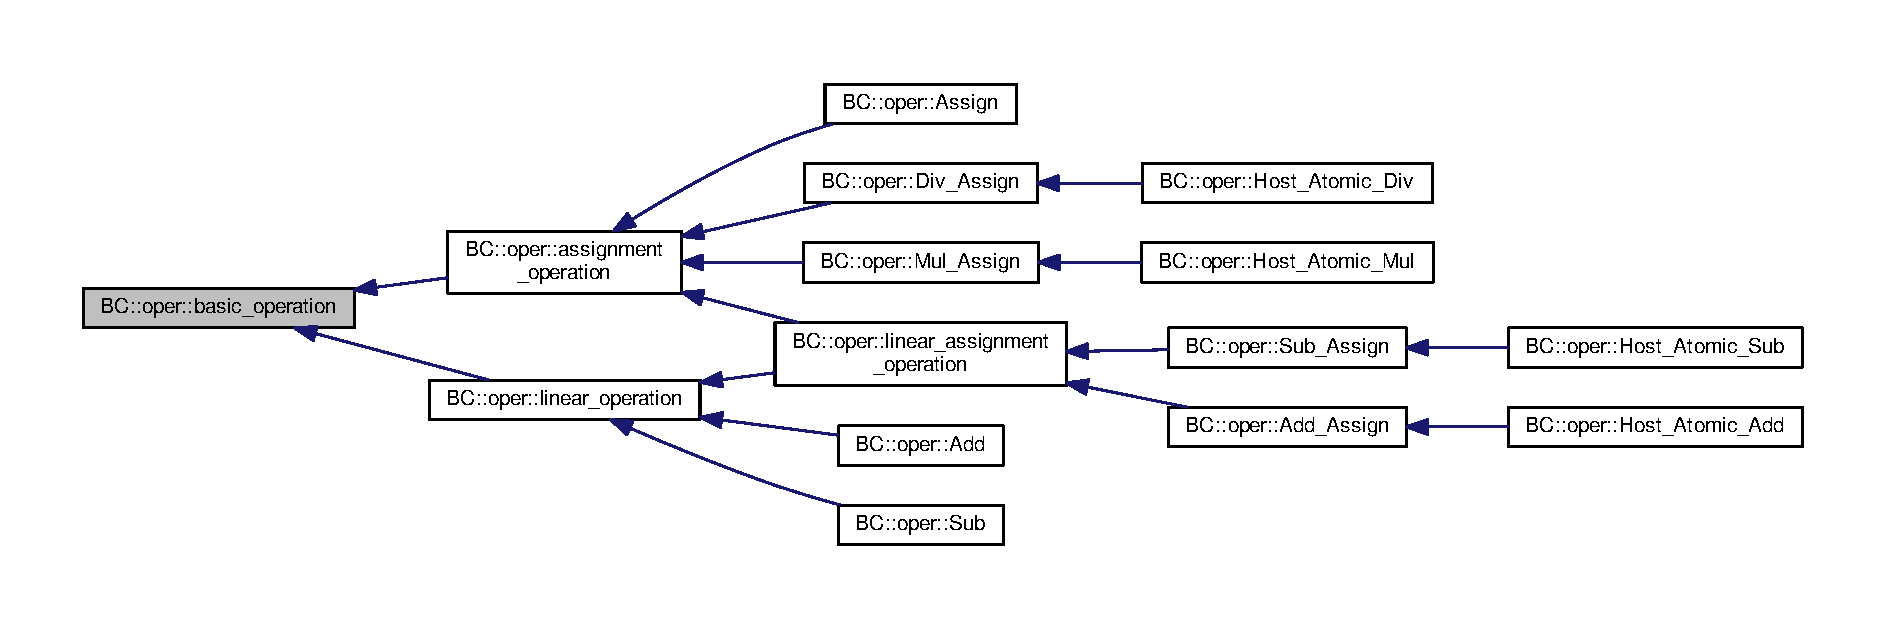
\includegraphics[width=350pt]{structBC_1_1oper_1_1basic__operation__inherit__graph}
\end{center}
\end{figure}


The documentation for this struct was generated from the following file\+:\begin{DoxyCompactItemize}
\item 
include/operations/\hyperlink{operations_2Tags_8h}{Tags.\+h}\end{DoxyCompactItemize}

\hypertarget{classBC_1_1tensors_1_1exprs_1_1BC__Array}{}\section{BC\+:\+:tensors\+:\+:exprs\+:\+:B\+C\+\_\+\+Array Class Reference}
\label{classBC_1_1tensors_1_1exprs_1_1BC__Array}\index{B\+C\+::tensors\+::exprs\+::\+B\+C\+\_\+\+Array@{B\+C\+::tensors\+::exprs\+::\+B\+C\+\_\+\+Array}}


{\ttfamily \#include $<$Expression\+\_\+\+Template\+\_\+\+Traits.\+h$>$}



Inheritance diagram for BC\+:\+:tensors\+:\+:exprs\+:\+:B\+C\+\_\+\+Array\+:
\nopagebreak
\begin{figure}[H]
\begin{center}
\leavevmode
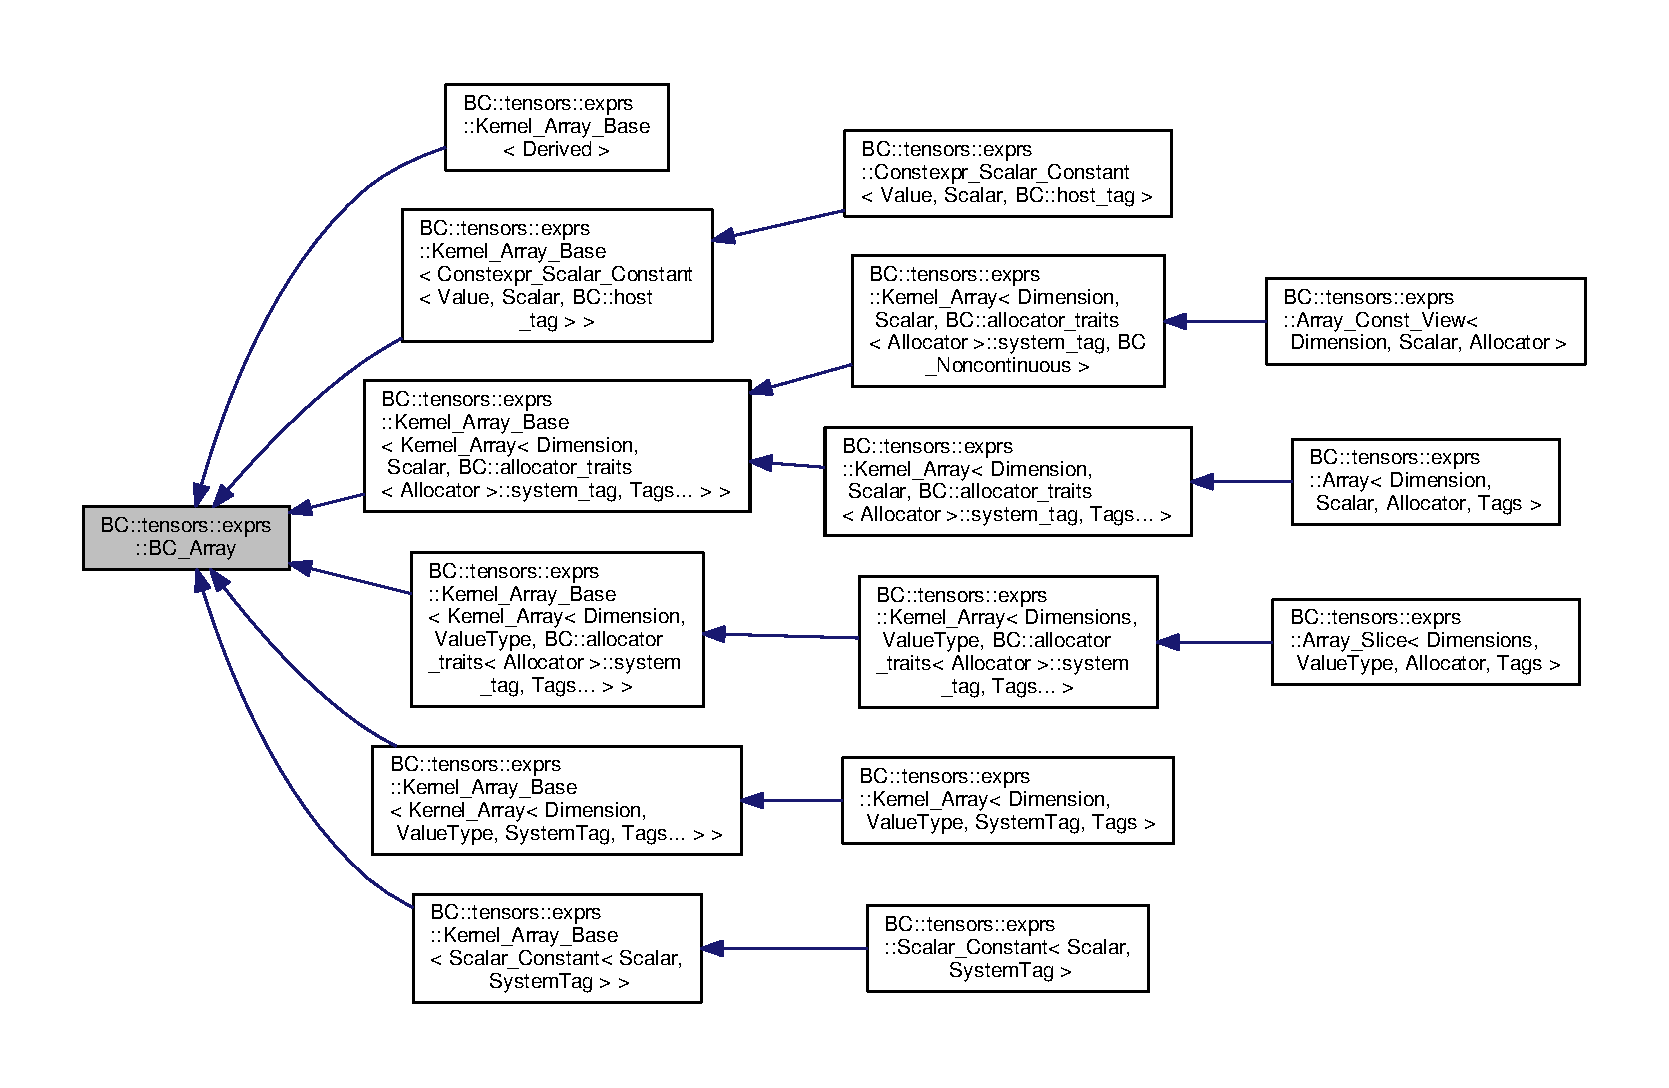
\includegraphics[width=350pt]{classBC_1_1tensors_1_1exprs_1_1BC__Array__inherit__graph}
\end{center}
\end{figure}


The documentation for this class was generated from the following file\+:\begin{DoxyCompactItemize}
\item 
include/tensors/expression\+\_\+templates/\hyperlink{Expression__Template__Traits_8h}{Expression\+\_\+\+Template\+\_\+\+Traits.\+h}\end{DoxyCompactItemize}

\hypertarget{classBC_1_1tensors_1_1exprs_1_1BC__Expr}{}\section{BC\+:\+:tensors\+:\+:exprs\+:\+:B\+C\+\_\+\+Expr Class Reference}
\label{classBC_1_1tensors_1_1exprs_1_1BC__Expr}\index{B\+C\+::tensors\+::exprs\+::\+B\+C\+\_\+\+Expr@{B\+C\+::tensors\+::exprs\+::\+B\+C\+\_\+\+Expr}}


{\ttfamily \#include $<$Expression\+\_\+\+Template\+\_\+\+Traits.\+h$>$}



Inheritance diagram for BC\+:\+:tensors\+:\+:exprs\+:\+:B\+C\+\_\+\+Expr\+:
\nopagebreak
\begin{figure}[H]
\begin{center}
\leavevmode
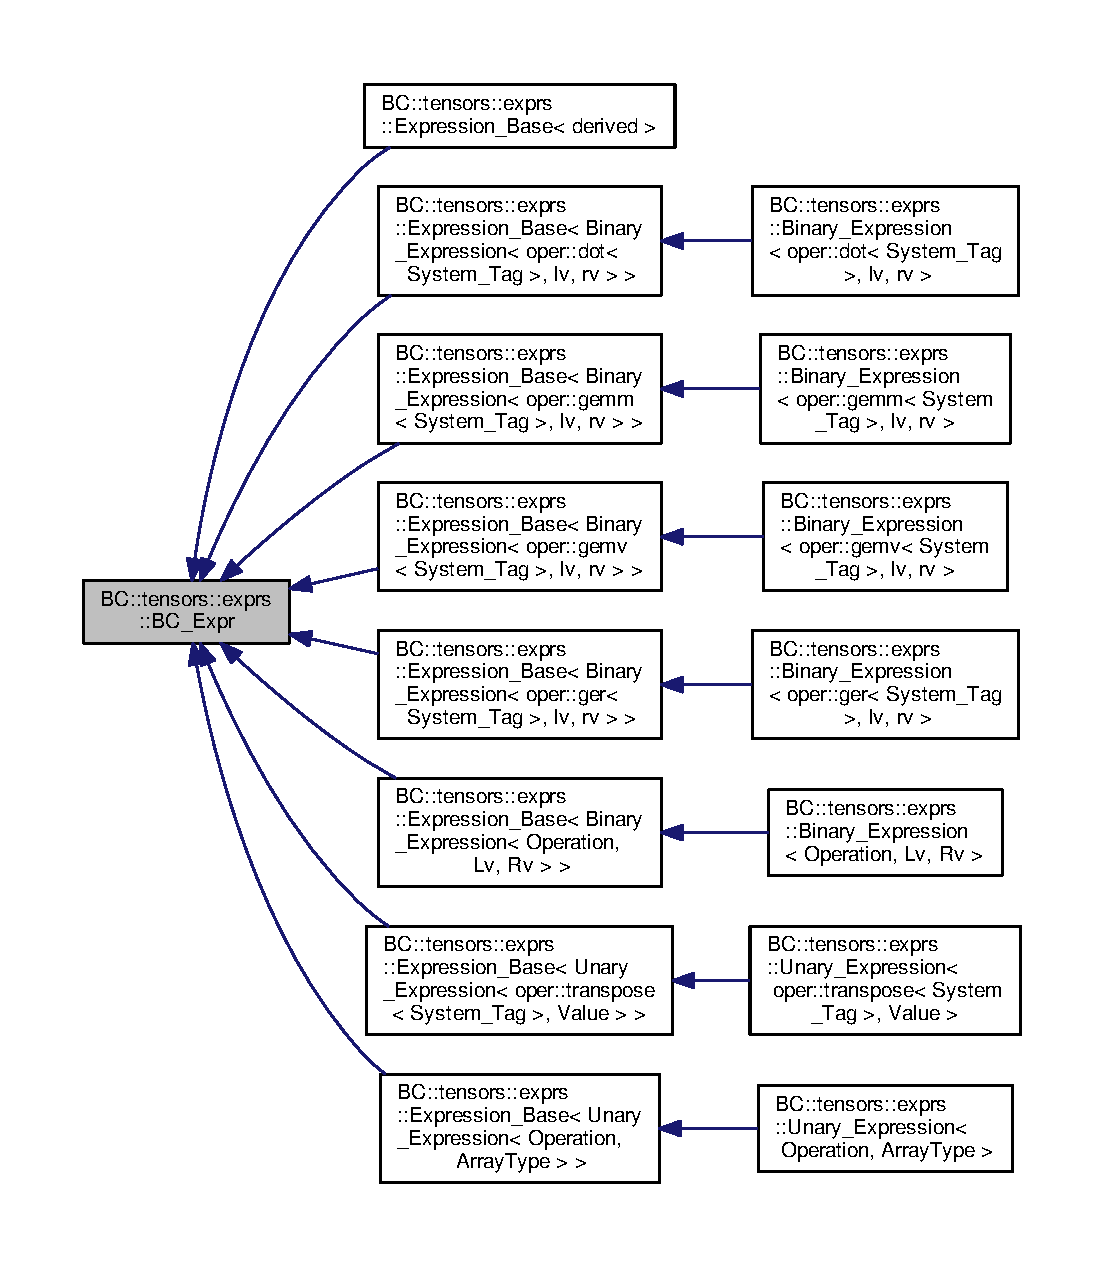
\includegraphics[width=350pt]{classBC_1_1tensors_1_1exprs_1_1BC__Expr__inherit__graph}
\end{center}
\end{figure}


The documentation for this class was generated from the following file\+:\begin{DoxyCompactItemize}
\item 
include/tensors/expression\+\_\+templates/\hyperlink{Expression__Template__Traits_8h}{Expression\+\_\+\+Template\+\_\+\+Traits.\+h}\end{DoxyCompactItemize}

\hypertarget{classBC_1_1tensors_1_1exprs_1_1BC__Immutable}{}\section{BC\+:\+:tensors\+:\+:exprs\+:\+:B\+C\+\_\+\+Immutable Class Reference}
\label{classBC_1_1tensors_1_1exprs_1_1BC__Immutable}\index{B\+C\+::tensors\+::exprs\+::\+B\+C\+\_\+\+Immutable@{B\+C\+::tensors\+::exprs\+::\+B\+C\+\_\+\+Immutable}}


{\ttfamily \#include $<$Expression\+\_\+\+Template\+\_\+\+Traits.\+h$>$}



The documentation for this class was generated from the following file\+:\begin{DoxyCompactItemize}
\item 
include/tensors/expression\+\_\+templates/\hyperlink{Expression__Template__Traits_8h}{Expression\+\_\+\+Template\+\_\+\+Traits.\+h}\end{DoxyCompactItemize}

\hypertarget{classBC_1_1tensors_1_1exprs_1_1BC__Noncontinuous}{}\section{BC\+:\+:tensors\+:\+:exprs\+:\+:B\+C\+\_\+\+Noncontinuous Class Reference}
\label{classBC_1_1tensors_1_1exprs_1_1BC__Noncontinuous}\index{B\+C\+::tensors\+::exprs\+::\+B\+C\+\_\+\+Noncontinuous@{B\+C\+::tensors\+::exprs\+::\+B\+C\+\_\+\+Noncontinuous}}


{\ttfamily \#include $<$Expression\+\_\+\+Template\+\_\+\+Traits.\+h$>$}



The documentation for this class was generated from the following file\+:\begin{DoxyCompactItemize}
\item 
include/tensors/expression\+\_\+templates/\hyperlink{Expression__Template__Traits_8h}{Expression\+\_\+\+Template\+\_\+\+Traits.\+h}\end{DoxyCompactItemize}

\hypertarget{classBC_1_1tensors_1_1exprs_1_1BC__Scalar__Constant}{}\section{BC\+:\+:tensors\+:\+:exprs\+:\+:B\+C\+\_\+\+Scalar\+\_\+\+Constant Class Reference}
\label{classBC_1_1tensors_1_1exprs_1_1BC__Scalar__Constant}\index{B\+C\+::tensors\+::exprs\+::\+B\+C\+\_\+\+Scalar\+\_\+\+Constant@{B\+C\+::tensors\+::exprs\+::\+B\+C\+\_\+\+Scalar\+\_\+\+Constant}}


{\ttfamily \#include $<$Expression\+\_\+\+Template\+\_\+\+Traits.\+h$>$}



The documentation for this class was generated from the following file\+:\begin{DoxyCompactItemize}
\item 
include/tensors/expression\+\_\+templates/\hyperlink{Expression__Template__Traits_8h}{Expression\+\_\+\+Template\+\_\+\+Traits.\+h}\end{DoxyCompactItemize}

\hypertarget{classBC_1_1tensors_1_1exprs_1_1BC__Stack__Allocated}{}\section{BC\+:\+:tensors\+:\+:exprs\+:\+:B\+C\+\_\+\+Stack\+\_\+\+Allocated Class Reference}
\label{classBC_1_1tensors_1_1exprs_1_1BC__Stack__Allocated}\index{B\+C\+::tensors\+::exprs\+::\+B\+C\+\_\+\+Stack\+\_\+\+Allocated@{B\+C\+::tensors\+::exprs\+::\+B\+C\+\_\+\+Stack\+\_\+\+Allocated}}


{\ttfamily \#include $<$Expression\+\_\+\+Template\+\_\+\+Traits.\+h$>$}



Inheritance diagram for BC\+:\+:tensors\+:\+:exprs\+:\+:B\+C\+\_\+\+Stack\+\_\+\+Allocated\+:
\nopagebreak
\begin{figure}[H]
\begin{center}
\leavevmode
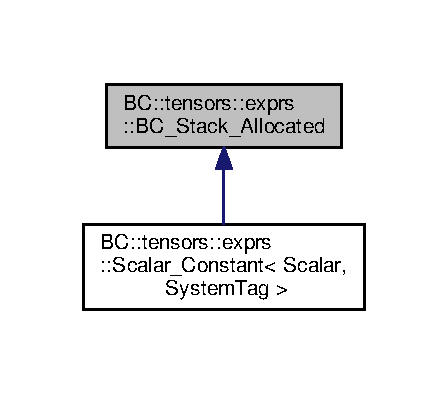
\includegraphics[width=215pt]{classBC_1_1tensors_1_1exprs_1_1BC__Stack__Allocated__inherit__graph}
\end{center}
\end{figure}


The documentation for this class was generated from the following file\+:\begin{DoxyCompactItemize}
\item 
include/tensors/expression\+\_\+templates/\hyperlink{Expression__Template__Traits_8h}{Expression\+\_\+\+Template\+\_\+\+Traits.\+h}\end{DoxyCompactItemize}

\hypertarget{classBC_1_1tensors_1_1exprs_1_1BC__Temporary}{}\section{BC\+:\+:tensors\+:\+:exprs\+:\+:B\+C\+\_\+\+Temporary Class Reference}
\label{classBC_1_1tensors_1_1exprs_1_1BC__Temporary}\index{B\+C\+::tensors\+::exprs\+::\+B\+C\+\_\+\+Temporary@{B\+C\+::tensors\+::exprs\+::\+B\+C\+\_\+\+Temporary}}


{\ttfamily \#include $<$Expression\+\_\+\+Template\+\_\+\+Traits.\+h$>$}



The documentation for this class was generated from the following file\+:\begin{DoxyCompactItemize}
\item 
include/tensors/expression\+\_\+templates/\hyperlink{Expression__Template__Traits_8h}{Expression\+\_\+\+Template\+\_\+\+Traits.\+h}\end{DoxyCompactItemize}

\hypertarget{classBC_1_1tensors_1_1exprs_1_1BC__Type}{}\section{BC\+:\+:tensors\+:\+:exprs\+:\+:B\+C\+\_\+\+Type Class Reference}
\label{classBC_1_1tensors_1_1exprs_1_1BC__Type}\index{B\+C\+::tensors\+::exprs\+::\+B\+C\+\_\+\+Type@{B\+C\+::tensors\+::exprs\+::\+B\+C\+\_\+\+Type}}


{\ttfamily \#include $<$Expression\+\_\+\+Template\+\_\+\+Traits.\+h$>$}



Inheritance diagram for BC\+:\+:tensors\+:\+:exprs\+:\+:B\+C\+\_\+\+Type\+:
\nopagebreak
\begin{figure}[H]
\begin{center}
\leavevmode
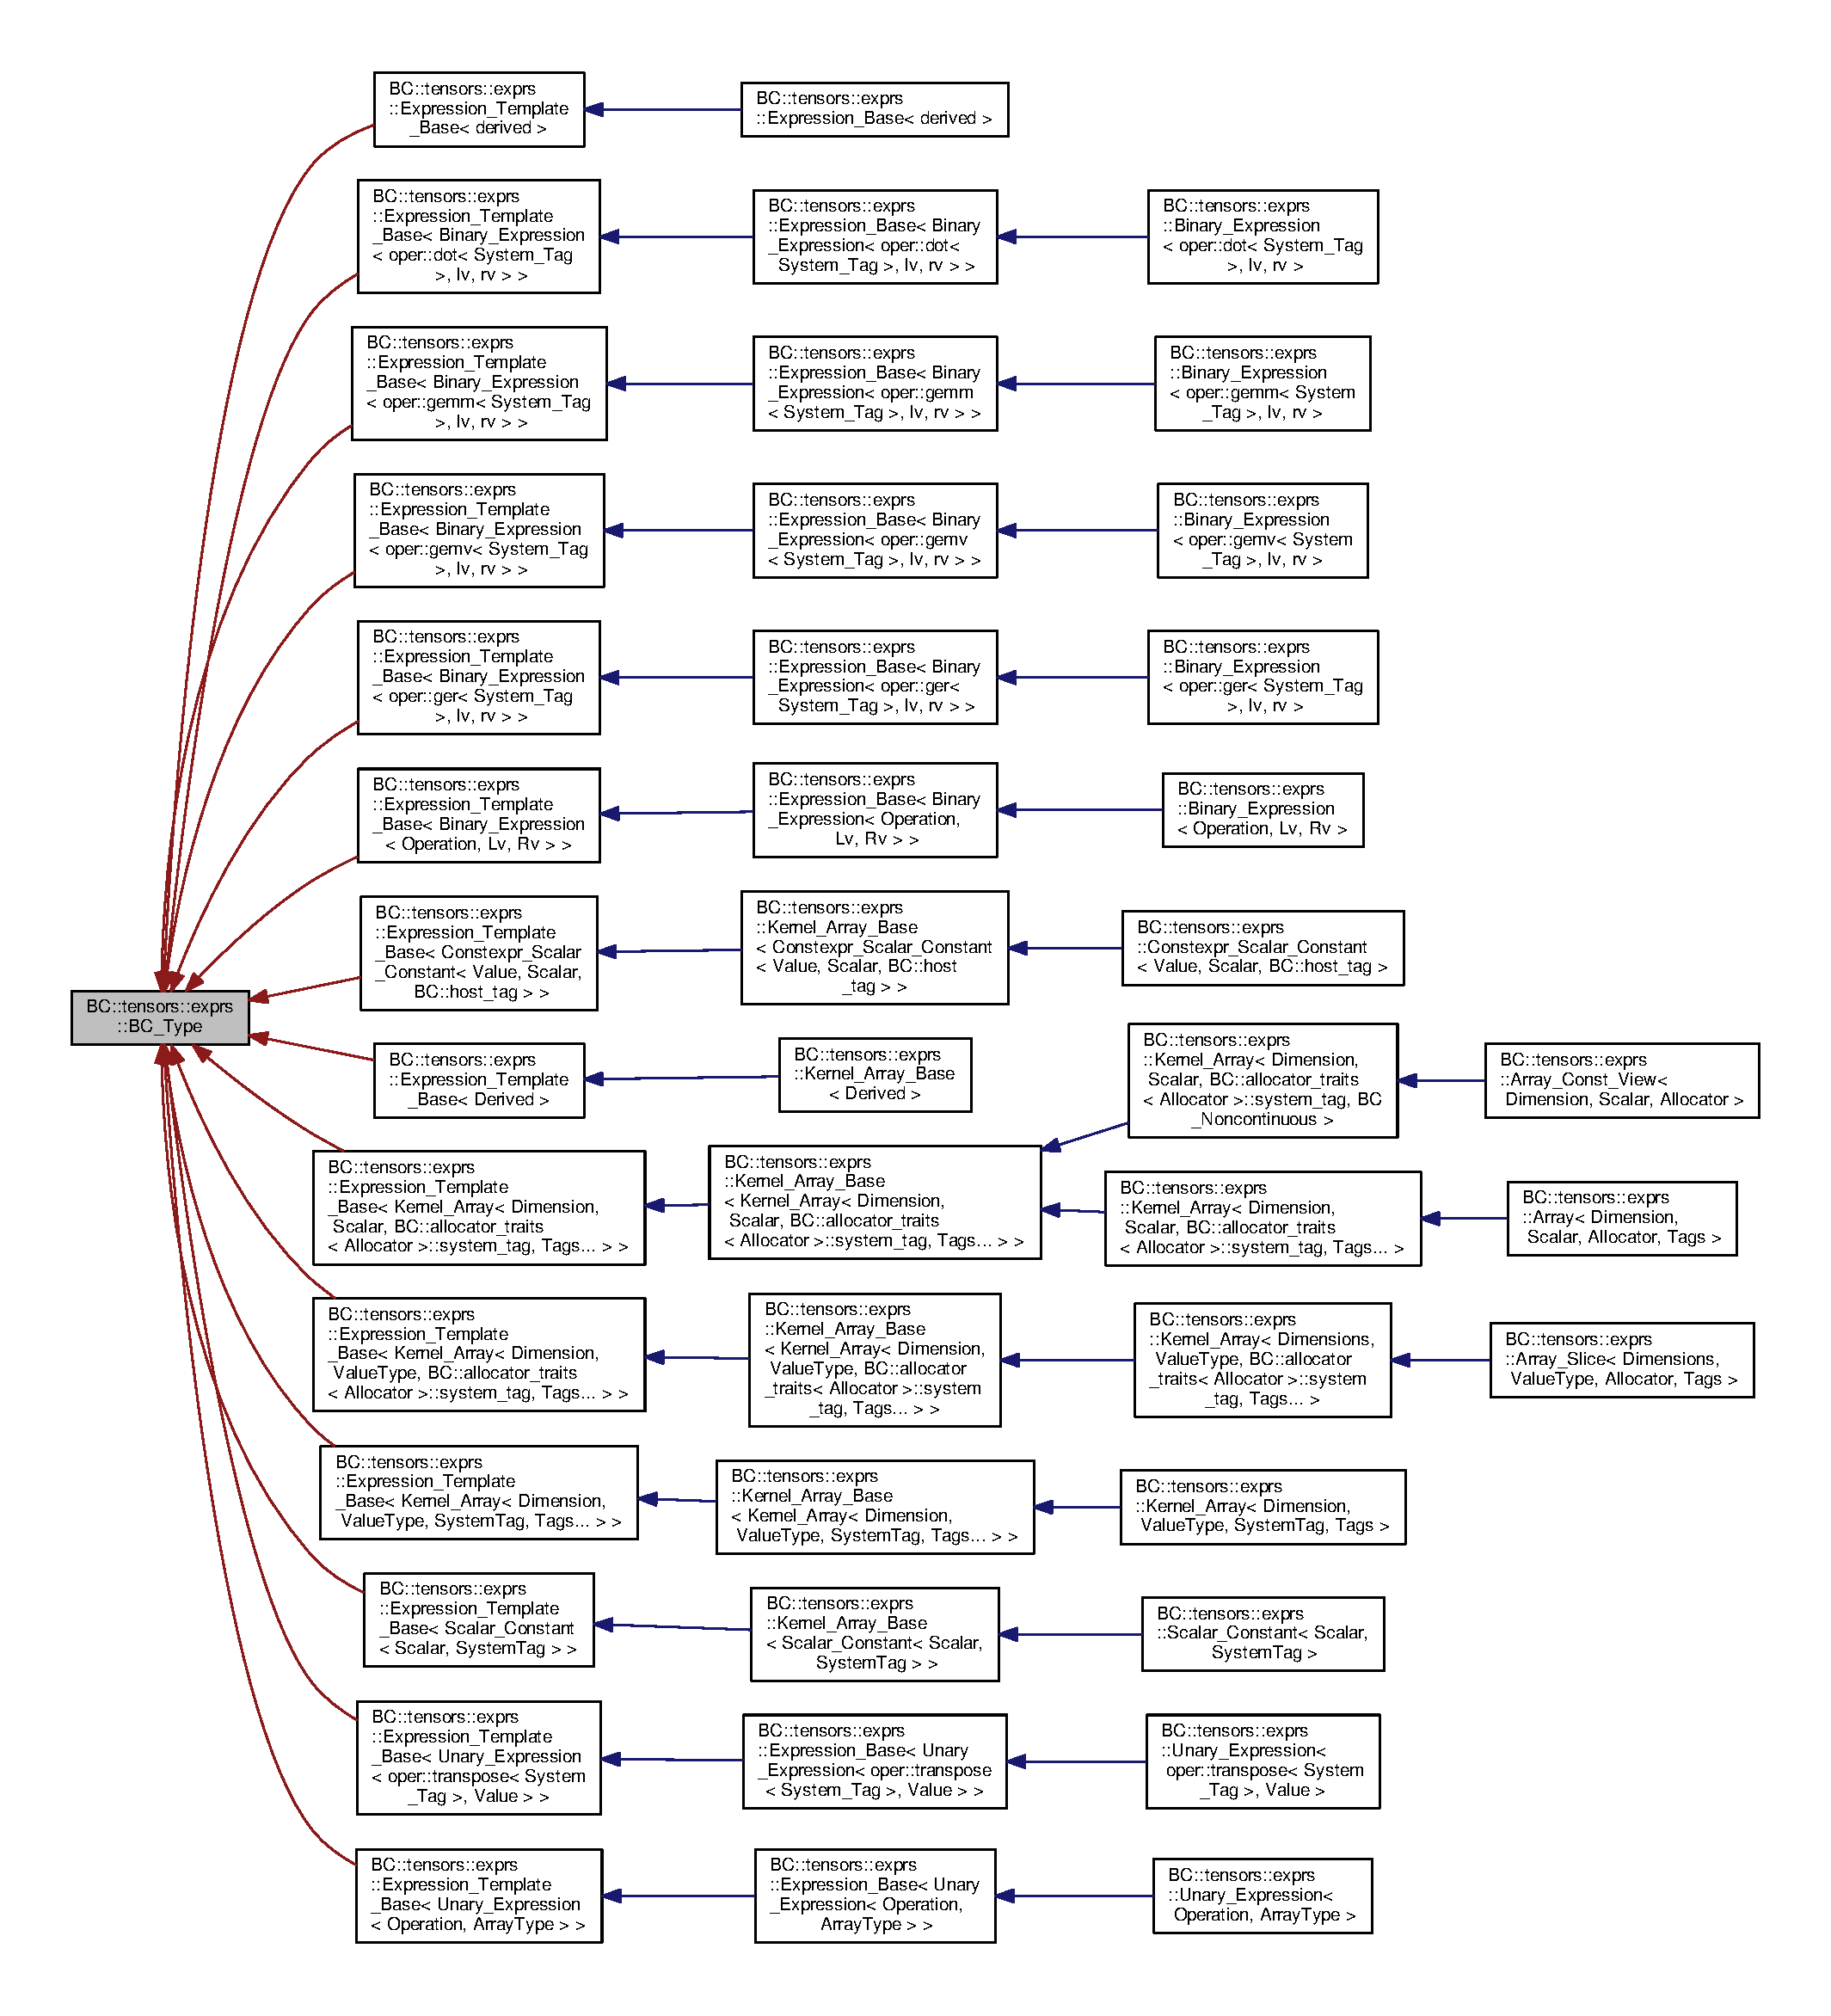
\includegraphics[width=350pt]{classBC_1_1tensors_1_1exprs_1_1BC__Type__inherit__graph}
\end{center}
\end{figure}


The documentation for this class was generated from the following file\+:\begin{DoxyCompactItemize}
\item 
include/tensors/expression\+\_\+templates/\hyperlink{Expression__Template__Traits_8h}{Expression\+\_\+\+Template\+\_\+\+Traits.\+h}\end{DoxyCompactItemize}

\hypertarget{classBC_1_1tensors_1_1exprs_1_1BC__View}{}\section{BC\+:\+:tensors\+:\+:exprs\+:\+:B\+C\+\_\+\+View Class Reference}
\label{classBC_1_1tensors_1_1exprs_1_1BC__View}\index{B\+C\+::tensors\+::exprs\+::\+B\+C\+\_\+\+View@{B\+C\+::tensors\+::exprs\+::\+B\+C\+\_\+\+View}}


{\ttfamily \#include $<$Expression\+\_\+\+Template\+\_\+\+Traits.\+h$>$}



The documentation for this class was generated from the following file\+:\begin{DoxyCompactItemize}
\item 
include/tensors/expression\+\_\+templates/\hyperlink{Expression__Template__Traits_8h}{Expression\+\_\+\+Template\+\_\+\+Traits.\+h}\end{DoxyCompactItemize}

\hypertarget{structBC_1_1tensors_1_1exprs_1_1Binary__Expression}{}\section{BC\+:\+:tensors\+:\+:exprs\+:\+:Binary\+\_\+\+Expression$<$ Operation, Lv, Rv $>$ Struct Template Reference}
\label{structBC_1_1tensors_1_1exprs_1_1Binary__Expression}\index{B\+C\+::tensors\+::exprs\+::\+Binary\+\_\+\+Expression$<$ Operation, Lv, Rv $>$@{B\+C\+::tensors\+::exprs\+::\+Binary\+\_\+\+Expression$<$ Operation, Lv, Rv $>$}}


{\ttfamily \#include $<$Common.\+h$>$}



Inheritance diagram for BC\+:\+:tensors\+:\+:exprs\+:\+:Binary\+\_\+\+Expression$<$ Operation, Lv, Rv $>$\+:
\nopagebreak
\begin{figure}[H]
\begin{center}
\leavevmode
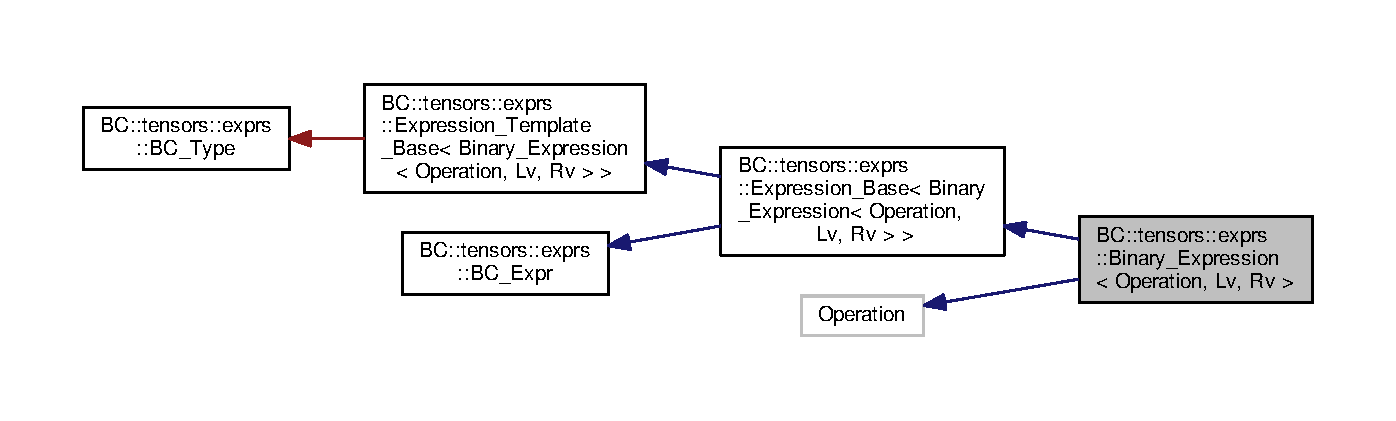
\includegraphics[width=350pt]{structBC_1_1tensors_1_1exprs_1_1Binary__Expression__inherit__graph}
\end{center}
\end{figure}


Collaboration diagram for BC\+:\+:tensors\+:\+:exprs\+:\+:Binary\+\_\+\+Expression$<$ Operation, Lv, Rv $>$\+:
\nopagebreak
\begin{figure}[H]
\begin{center}
\leavevmode
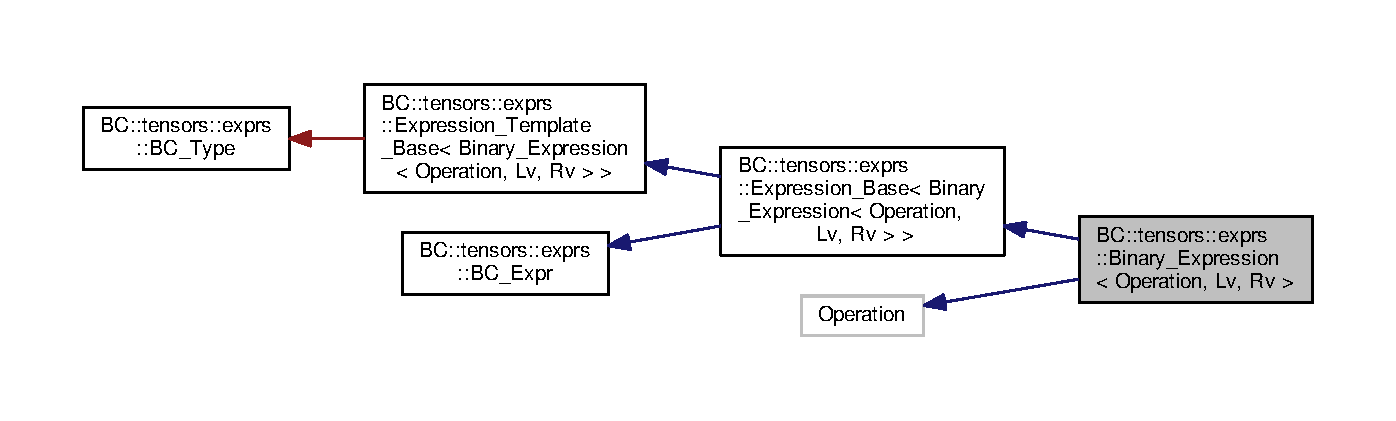
\includegraphics[width=350pt]{structBC_1_1tensors_1_1exprs_1_1Binary__Expression__coll__graph}
\end{center}
\end{figure}
\subsection*{Public Types}
\begin{DoxyCompactItemize}
\item 
using \hyperlink{structBC_1_1tensors_1_1exprs_1_1Binary__Expression_a8ae3c31b3f8d8ffb55bc6b0fe80bb266}{lv\+\_\+value\+\_\+t} = typename Lv\+::value\+\_\+type
\item 
using \hyperlink{structBC_1_1tensors_1_1exprs_1_1Binary__Expression_ad4a826a303397b65a2e04a8379278fa6}{rv\+\_\+value\+\_\+t} = typename Rv\+::value\+\_\+type
\item 
using \hyperlink{structBC_1_1tensors_1_1exprs_1_1Binary__Expression_a5e8a6e43ec8cbba6a69d209589e02149}{return\+\_\+type} = decltype(std\+::declval$<$ Operation $>$()(std\+::declval$<$ \hyperlink{structBC_1_1tensors_1_1exprs_1_1Binary__Expression_a8ae3c31b3f8d8ffb55bc6b0fe80bb266}{lv\+\_\+value\+\_\+t} \& $>$(), std\+::declval$<$ \hyperlink{structBC_1_1tensors_1_1exprs_1_1Binary__Expression_ad4a826a303397b65a2e04a8379278fa6}{rv\+\_\+value\+\_\+t} \& $>$()))
\item 
using \hyperlink{structBC_1_1tensors_1_1exprs_1_1Binary__Expression_af83a5208b5b457f7cf865b1ca0170260}{value\+\_\+type} = std\+::remove\+\_\+reference\+\_\+t$<$ std\+::decay\+\_\+t$<$ \hyperlink{structBC_1_1tensors_1_1exprs_1_1Binary__Expression_a5e8a6e43ec8cbba6a69d209589e02149}{return\+\_\+type} $>$$>$
\item 
using \hyperlink{structBC_1_1tensors_1_1exprs_1_1Binary__Expression_ab11626c5e785f5ffab80a70d9beaa3e0}{system\+\_\+tag} = typename Lv\+::system\+\_\+tag
\end{DoxyCompactItemize}
\subsection*{Public Member Functions}
\begin{DoxyCompactItemize}
\item 
Operation \hyperlink{structBC_1_1tensors_1_1exprs_1_1Binary__Expression_a3e8e485a053ea1539e44f2cca9511146}{get\+\_\+operation} () const 
\item 
{\footnotesize template$<$class... args$>$ }\\\hyperlink{BlackCat__Common_8h_ac085f07cc309e3aac24aa3fc0a40f6d2}{B\+C\+H\+OT} \hyperlink{structBC_1_1tensors_1_1exprs_1_1Binary__Expression_aeddd450884ca8758d823fee84dd284b8}{Binary\+\_\+\+Expression} (Lv l, Rv r, const args \&...args\+\_\+)
\item 
\hyperlink{BlackCat__Common_8h_a6699e8b0449da5c0fafb878e59c1d4b1}{B\+C\+I\+N\+L\+I\+NE} auto \hyperlink{structBC_1_1tensors_1_1exprs_1_1Binary__Expression_a52f52e4a1d492aed4cbc5636eeacfd91}{operator\mbox{[}$\,$\mbox{]}} (int index) const 
\item 
{\footnotesize template$<$class... integers$>$ }\\\hyperlink{BlackCat__Common_8h_a6699e8b0449da5c0fafb878e59c1d4b1}{B\+C\+I\+N\+L\+I\+NE} auto \hyperlink{structBC_1_1tensors_1_1exprs_1_1Binary__Expression_a4ad48f111da0bae7d3d8abddf5517eb8}{operator()} (integers...\+ints) const 
\item 
\hyperlink{BlackCat__Common_8h_a6699e8b0449da5c0fafb878e59c1d4b1}{B\+C\+I\+N\+L\+I\+NE} auto \hyperlink{structBC_1_1tensors_1_1exprs_1_1Binary__Expression_a459a90f952d3549ed87338be1783a420}{operator\mbox{[}$\,$\mbox{]}} (int index)
\item 
{\footnotesize template$<$class... integers$>$ }\\\hyperlink{BlackCat__Common_8h_a6699e8b0449da5c0fafb878e59c1d4b1}{B\+C\+I\+N\+L\+I\+NE} auto \hyperlink{structBC_1_1tensors_1_1exprs_1_1Binary__Expression_a1880be4cfbe09a942d228f87b69822e9}{operator()} (integers...\+ints)
\item 
\hyperlink{BlackCat__Common_8h_a6699e8b0449da5c0fafb878e59c1d4b1}{B\+C\+I\+N\+L\+I\+NE} auto \hyperlink{structBC_1_1tensors_1_1exprs_1_1Binary__Expression_a1d98119a2b5fdb37b515be8210d445b2}{dx} (\hyperlink{namespaceBC_a6007cbc4eeec401a037b558910a56173}{size\+\_\+t} index) const 
\item 
\hyperlink{BlackCat__Common_8h_a6699e8b0449da5c0fafb878e59c1d4b1}{B\+C\+I\+N\+L\+I\+NE} \hyperlink{namespaceBC_a6007cbc4eeec401a037b558910a56173}{B\+C\+::size\+\_\+t} \hyperlink{structBC_1_1tensors_1_1exprs_1_1Binary__Expression_aae28d2e8eee8ebed94187556367b860b}{size} () const 
\item 
\hyperlink{BlackCat__Common_8h_a6699e8b0449da5c0fafb878e59c1d4b1}{B\+C\+I\+N\+L\+I\+NE} \hyperlink{namespaceBC_a6007cbc4eeec401a037b558910a56173}{B\+C\+::size\+\_\+t} \hyperlink{structBC_1_1tensors_1_1exprs_1_1Binary__Expression_a4c8338db9038c96551365269e9797a55}{rows} () const 
\item 
\hyperlink{BlackCat__Common_8h_a6699e8b0449da5c0fafb878e59c1d4b1}{B\+C\+I\+N\+L\+I\+NE} \hyperlink{namespaceBC_a6007cbc4eeec401a037b558910a56173}{B\+C\+::size\+\_\+t} \hyperlink{structBC_1_1tensors_1_1exprs_1_1Binary__Expression_aa6792d643387514d8dbf521601686860}{cols} () const 
\item 
\hyperlink{BlackCat__Common_8h_a6699e8b0449da5c0fafb878e59c1d4b1}{B\+C\+I\+N\+L\+I\+NE} \hyperlink{namespaceBC_a6007cbc4eeec401a037b558910a56173}{B\+C\+::size\+\_\+t} \hyperlink{structBC_1_1tensors_1_1exprs_1_1Binary__Expression_ac4ad404ab4c236b4e5346ff2348122ad}{dimension} (int i) const 
\item 
\hyperlink{BlackCat__Common_8h_a6699e8b0449da5c0fafb878e59c1d4b1}{B\+C\+I\+N\+L\+I\+NE} \hyperlink{namespaceBC_a6007cbc4eeec401a037b558910a56173}{B\+C\+::size\+\_\+t} \hyperlink{structBC_1_1tensors_1_1exprs_1_1Binary__Expression_a63d7298dcba7fade6cee9f1ce5f281db}{block\+\_\+dimension} (int i) const 
\item 
\hyperlink{BlackCat__Common_8h_a6699e8b0449da5c0fafb878e59c1d4b1}{B\+C\+I\+N\+L\+I\+NE} const auto \hyperlink{structBC_1_1tensors_1_1exprs_1_1Binary__Expression_a5adc2f7cf2d84733f5ef00a4c778c7da}{inner\+\_\+shape} () const 
\item 
\hyperlink{BlackCat__Common_8h_a6699e8b0449da5c0fafb878e59c1d4b1}{B\+C\+I\+N\+L\+I\+NE} const auto \hyperlink{structBC_1_1tensors_1_1exprs_1_1Binary__Expression_aaca6a6401abf6415c1bc1ee365867160}{block\+\_\+shape} () const 
\end{DoxyCompactItemize}
\subsection*{Public Attributes}
\begin{DoxyCompactItemize}
\item 
Lv \hyperlink{structBC_1_1tensors_1_1exprs_1_1Binary__Expression_a5baf7bcb8cd325e60a99513bd2e4c027}{left}
\item 
Rv \hyperlink{structBC_1_1tensors_1_1exprs_1_1Binary__Expression_af9ec1dff3c9f4684dfdc8a29a3b8d31e}{right}
\end{DoxyCompactItemize}
\subsection*{Static Public Attributes}
\begin{DoxyCompactItemize}
\item 
static constexpr int \hyperlink{structBC_1_1tensors_1_1exprs_1_1Binary__Expression_a73afe6b099afa4ef242e6eb7be50ebef}{tensor\+\_\+dimension} = B\+C\+::meta\+::max(Lv\+::tensor\+\_\+dimension, Rv\+::tensor\+\_\+dimension)
\item 
static constexpr int \hyperlink{structBC_1_1tensors_1_1exprs_1_1Binary__Expression_a5fce7af061a989dafb9bed466c811f0d}{tensor\+\_\+iterator\+\_\+dimension} = Lv\+::tensor\+\_\+dimension != Rv\+::tensor\+\_\+dimension ? \hyperlink{structBC_1_1tensors_1_1exprs_1_1Binary__Expression_a73afe6b099afa4ef242e6eb7be50ebef}{tensor\+\_\+dimension} \+: B\+C\+::meta\+::max(Lv\+::tensor\+\_\+iterator\+\_\+dimension, Rv\+::tensor\+\_\+iterator\+\_\+dimension)
\end{DoxyCompactItemize}


\subsection{Member Typedef Documentation}
\index{B\+C\+::tensors\+::exprs\+::\+Binary\+\_\+\+Expression@{B\+C\+::tensors\+::exprs\+::\+Binary\+\_\+\+Expression}!lv\+\_\+value\+\_\+t@{lv\+\_\+value\+\_\+t}}
\index{lv\+\_\+value\+\_\+t@{lv\+\_\+value\+\_\+t}!B\+C\+::tensors\+::exprs\+::\+Binary\+\_\+\+Expression@{B\+C\+::tensors\+::exprs\+::\+Binary\+\_\+\+Expression}}
\subsubsection[{\texorpdfstring{lv\+\_\+value\+\_\+t}{lv_value_t}}]{\setlength{\rightskip}{0pt plus 5cm}template$<$class Operation, class Lv, class Rv$>$ using {\bf B\+C\+::tensors\+::exprs\+::\+Binary\+\_\+\+Expression}$<$ Operation, Lv, Rv $>$\+::{\bf lv\+\_\+value\+\_\+t} =  typename Lv\+::value\+\_\+type}\hypertarget{structBC_1_1tensors_1_1exprs_1_1Binary__Expression_a8ae3c31b3f8d8ffb55bc6b0fe80bb266}{}\label{structBC_1_1tensors_1_1exprs_1_1Binary__Expression_a8ae3c31b3f8d8ffb55bc6b0fe80bb266}
\index{B\+C\+::tensors\+::exprs\+::\+Binary\+\_\+\+Expression@{B\+C\+::tensors\+::exprs\+::\+Binary\+\_\+\+Expression}!return\+\_\+type@{return\+\_\+type}}
\index{return\+\_\+type@{return\+\_\+type}!B\+C\+::tensors\+::exprs\+::\+Binary\+\_\+\+Expression@{B\+C\+::tensors\+::exprs\+::\+Binary\+\_\+\+Expression}}
\subsubsection[{\texorpdfstring{return\+\_\+type}{return_type}}]{\setlength{\rightskip}{0pt plus 5cm}template$<$class Operation, class Lv, class Rv$>$ using {\bf B\+C\+::tensors\+::exprs\+::\+Binary\+\_\+\+Expression}$<$ Operation, Lv, Rv $>$\+::{\bf return\+\_\+type} =  decltype(std\+::declval$<$Operation$>$()(std\+::declval$<${\bf lv\+\_\+value\+\_\+t}\&$>$(), std\+::declval$<${\bf rv\+\_\+value\+\_\+t}\&$>$()))}\hypertarget{structBC_1_1tensors_1_1exprs_1_1Binary__Expression_a5e8a6e43ec8cbba6a69d209589e02149}{}\label{structBC_1_1tensors_1_1exprs_1_1Binary__Expression_a5e8a6e43ec8cbba6a69d209589e02149}
\index{B\+C\+::tensors\+::exprs\+::\+Binary\+\_\+\+Expression@{B\+C\+::tensors\+::exprs\+::\+Binary\+\_\+\+Expression}!rv\+\_\+value\+\_\+t@{rv\+\_\+value\+\_\+t}}
\index{rv\+\_\+value\+\_\+t@{rv\+\_\+value\+\_\+t}!B\+C\+::tensors\+::exprs\+::\+Binary\+\_\+\+Expression@{B\+C\+::tensors\+::exprs\+::\+Binary\+\_\+\+Expression}}
\subsubsection[{\texorpdfstring{rv\+\_\+value\+\_\+t}{rv_value_t}}]{\setlength{\rightskip}{0pt plus 5cm}template$<$class Operation, class Lv, class Rv$>$ using {\bf B\+C\+::tensors\+::exprs\+::\+Binary\+\_\+\+Expression}$<$ Operation, Lv, Rv $>$\+::{\bf rv\+\_\+value\+\_\+t} =  typename Rv\+::value\+\_\+type}\hypertarget{structBC_1_1tensors_1_1exprs_1_1Binary__Expression_ad4a826a303397b65a2e04a8379278fa6}{}\label{structBC_1_1tensors_1_1exprs_1_1Binary__Expression_ad4a826a303397b65a2e04a8379278fa6}
\index{B\+C\+::tensors\+::exprs\+::\+Binary\+\_\+\+Expression@{B\+C\+::tensors\+::exprs\+::\+Binary\+\_\+\+Expression}!system\+\_\+tag@{system\+\_\+tag}}
\index{system\+\_\+tag@{system\+\_\+tag}!B\+C\+::tensors\+::exprs\+::\+Binary\+\_\+\+Expression@{B\+C\+::tensors\+::exprs\+::\+Binary\+\_\+\+Expression}}
\subsubsection[{\texorpdfstring{system\+\_\+tag}{system_tag}}]{\setlength{\rightskip}{0pt plus 5cm}template$<$class Operation, class Lv, class Rv$>$ using {\bf B\+C\+::tensors\+::exprs\+::\+Binary\+\_\+\+Expression}$<$ Operation, Lv, Rv $>$\+::{\bf system\+\_\+tag} =  typename Lv\+::system\+\_\+tag}\hypertarget{structBC_1_1tensors_1_1exprs_1_1Binary__Expression_ab11626c5e785f5ffab80a70d9beaa3e0}{}\label{structBC_1_1tensors_1_1exprs_1_1Binary__Expression_ab11626c5e785f5ffab80a70d9beaa3e0}
\index{B\+C\+::tensors\+::exprs\+::\+Binary\+\_\+\+Expression@{B\+C\+::tensors\+::exprs\+::\+Binary\+\_\+\+Expression}!value\+\_\+type@{value\+\_\+type}}
\index{value\+\_\+type@{value\+\_\+type}!B\+C\+::tensors\+::exprs\+::\+Binary\+\_\+\+Expression@{B\+C\+::tensors\+::exprs\+::\+Binary\+\_\+\+Expression}}
\subsubsection[{\texorpdfstring{value\+\_\+type}{value_type}}]{\setlength{\rightskip}{0pt plus 5cm}template$<$class Operation, class Lv, class Rv$>$ using {\bf B\+C\+::tensors\+::exprs\+::\+Binary\+\_\+\+Expression}$<$ Operation, Lv, Rv $>$\+::{\bf value\+\_\+type} =  std\+::remove\+\_\+reference\+\_\+t$<$std\+::decay\+\_\+t$<${\bf return\+\_\+type}$>$$>$}\hypertarget{structBC_1_1tensors_1_1exprs_1_1Binary__Expression_af83a5208b5b457f7cf865b1ca0170260}{}\label{structBC_1_1tensors_1_1exprs_1_1Binary__Expression_af83a5208b5b457f7cf865b1ca0170260}


\subsection{Constructor \& Destructor Documentation}
\index{B\+C\+::tensors\+::exprs\+::\+Binary\+\_\+\+Expression@{B\+C\+::tensors\+::exprs\+::\+Binary\+\_\+\+Expression}!Binary\+\_\+\+Expression@{Binary\+\_\+\+Expression}}
\index{Binary\+\_\+\+Expression@{Binary\+\_\+\+Expression}!B\+C\+::tensors\+::exprs\+::\+Binary\+\_\+\+Expression@{B\+C\+::tensors\+::exprs\+::\+Binary\+\_\+\+Expression}}
\subsubsection[{\texorpdfstring{Binary\+\_\+\+Expression(\+Lv l, Rv r, const args \&...\+args\+\_\+)}{Binary_Expression(Lv l, Rv r, const args &...args_)}}]{\setlength{\rightskip}{0pt plus 5cm}template$<$class Operation, class Lv, class Rv$>$ template$<$class... args$>$ {\bf B\+C\+H\+OT} {\bf B\+C\+::tensors\+::exprs\+::\+Binary\+\_\+\+Expression}$<$ Operation, Lv, Rv $>$\+::{\bf Binary\+\_\+\+Expression} (
\begin{DoxyParamCaption}
\item[{Lv}]{l, }
\item[{Rv}]{r, }
\item[{const args \&...}]{args\+\_\+}
\end{DoxyParamCaption}
)\hspace{0.3cm}{\ttfamily [inline]}}\hypertarget{structBC_1_1tensors_1_1exprs_1_1Binary__Expression_aeddd450884ca8758d823fee84dd284b8}{}\label{structBC_1_1tensors_1_1exprs_1_1Binary__Expression_aeddd450884ca8758d823fee84dd284b8}


\subsection{Member Function Documentation}
\index{B\+C\+::tensors\+::exprs\+::\+Binary\+\_\+\+Expression@{B\+C\+::tensors\+::exprs\+::\+Binary\+\_\+\+Expression}!block\+\_\+dimension@{block\+\_\+dimension}}
\index{block\+\_\+dimension@{block\+\_\+dimension}!B\+C\+::tensors\+::exprs\+::\+Binary\+\_\+\+Expression@{B\+C\+::tensors\+::exprs\+::\+Binary\+\_\+\+Expression}}
\subsubsection[{\texorpdfstring{block\+\_\+dimension(int i) const }{block_dimension(int i) const }}]{\setlength{\rightskip}{0pt plus 5cm}template$<$class Operation, class Lv, class Rv$>$ {\bf B\+C\+I\+N\+L\+I\+NE} {\bf B\+C\+::size\+\_\+t} {\bf B\+C\+::tensors\+::exprs\+::\+Binary\+\_\+\+Expression}$<$ Operation, Lv, Rv $>$\+::block\+\_\+dimension (
\begin{DoxyParamCaption}
\item[{int}]{i}
\end{DoxyParamCaption}
) const\hspace{0.3cm}{\ttfamily [inline]}}\hypertarget{structBC_1_1tensors_1_1exprs_1_1Binary__Expression_a63d7298dcba7fade6cee9f1ce5f281db}{}\label{structBC_1_1tensors_1_1exprs_1_1Binary__Expression_a63d7298dcba7fade6cee9f1ce5f281db}
\index{B\+C\+::tensors\+::exprs\+::\+Binary\+\_\+\+Expression@{B\+C\+::tensors\+::exprs\+::\+Binary\+\_\+\+Expression}!block\+\_\+shape@{block\+\_\+shape}}
\index{block\+\_\+shape@{block\+\_\+shape}!B\+C\+::tensors\+::exprs\+::\+Binary\+\_\+\+Expression@{B\+C\+::tensors\+::exprs\+::\+Binary\+\_\+\+Expression}}
\subsubsection[{\texorpdfstring{block\+\_\+shape() const }{block_shape() const }}]{\setlength{\rightskip}{0pt plus 5cm}template$<$class Operation, class Lv, class Rv$>$ {\bf B\+C\+I\+N\+L\+I\+NE} const auto {\bf B\+C\+::tensors\+::exprs\+::\+Binary\+\_\+\+Expression}$<$ Operation, Lv, Rv $>$\+::block\+\_\+shape (
\begin{DoxyParamCaption}
{}
\end{DoxyParamCaption}
) const\hspace{0.3cm}{\ttfamily [inline]}}\hypertarget{structBC_1_1tensors_1_1exprs_1_1Binary__Expression_aaca6a6401abf6415c1bc1ee365867160}{}\label{structBC_1_1tensors_1_1exprs_1_1Binary__Expression_aaca6a6401abf6415c1bc1ee365867160}
\index{B\+C\+::tensors\+::exprs\+::\+Binary\+\_\+\+Expression@{B\+C\+::tensors\+::exprs\+::\+Binary\+\_\+\+Expression}!cols@{cols}}
\index{cols@{cols}!B\+C\+::tensors\+::exprs\+::\+Binary\+\_\+\+Expression@{B\+C\+::tensors\+::exprs\+::\+Binary\+\_\+\+Expression}}
\subsubsection[{\texorpdfstring{cols() const }{cols() const }}]{\setlength{\rightskip}{0pt plus 5cm}template$<$class Operation, class Lv, class Rv$>$ {\bf B\+C\+I\+N\+L\+I\+NE} {\bf B\+C\+::size\+\_\+t} {\bf B\+C\+::tensors\+::exprs\+::\+Binary\+\_\+\+Expression}$<$ Operation, Lv, Rv $>$\+::cols (
\begin{DoxyParamCaption}
{}
\end{DoxyParamCaption}
) const\hspace{0.3cm}{\ttfamily [inline]}}\hypertarget{structBC_1_1tensors_1_1exprs_1_1Binary__Expression_aa6792d643387514d8dbf521601686860}{}\label{structBC_1_1tensors_1_1exprs_1_1Binary__Expression_aa6792d643387514d8dbf521601686860}
\index{B\+C\+::tensors\+::exprs\+::\+Binary\+\_\+\+Expression@{B\+C\+::tensors\+::exprs\+::\+Binary\+\_\+\+Expression}!dimension@{dimension}}
\index{dimension@{dimension}!B\+C\+::tensors\+::exprs\+::\+Binary\+\_\+\+Expression@{B\+C\+::tensors\+::exprs\+::\+Binary\+\_\+\+Expression}}
\subsubsection[{\texorpdfstring{dimension(int i) const }{dimension(int i) const }}]{\setlength{\rightskip}{0pt plus 5cm}template$<$class Operation, class Lv, class Rv$>$ {\bf B\+C\+I\+N\+L\+I\+NE} {\bf B\+C\+::size\+\_\+t} {\bf B\+C\+::tensors\+::exprs\+::\+Binary\+\_\+\+Expression}$<$ Operation, Lv, Rv $>$\+::dimension (
\begin{DoxyParamCaption}
\item[{int}]{i}
\end{DoxyParamCaption}
) const\hspace{0.3cm}{\ttfamily [inline]}}\hypertarget{structBC_1_1tensors_1_1exprs_1_1Binary__Expression_ac4ad404ab4c236b4e5346ff2348122ad}{}\label{structBC_1_1tensors_1_1exprs_1_1Binary__Expression_ac4ad404ab4c236b4e5346ff2348122ad}
\index{B\+C\+::tensors\+::exprs\+::\+Binary\+\_\+\+Expression@{B\+C\+::tensors\+::exprs\+::\+Binary\+\_\+\+Expression}!dx@{dx}}
\index{dx@{dx}!B\+C\+::tensors\+::exprs\+::\+Binary\+\_\+\+Expression@{B\+C\+::tensors\+::exprs\+::\+Binary\+\_\+\+Expression}}
\subsubsection[{\texorpdfstring{dx(size\+\_\+t index) const }{dx(size_t index) const }}]{\setlength{\rightskip}{0pt plus 5cm}template$<$class Operation, class Lv, class Rv$>$ {\bf B\+C\+I\+N\+L\+I\+NE} auto {\bf B\+C\+::tensors\+::exprs\+::\+Binary\+\_\+\+Expression}$<$ Operation, Lv, Rv $>$\+::dx (
\begin{DoxyParamCaption}
\item[{{\bf size\+\_\+t}}]{index}
\end{DoxyParamCaption}
) const\hspace{0.3cm}{\ttfamily [inline]}}\hypertarget{structBC_1_1tensors_1_1exprs_1_1Binary__Expression_a1d98119a2b5fdb37b515be8210d445b2}{}\label{structBC_1_1tensors_1_1exprs_1_1Binary__Expression_a1d98119a2b5fdb37b515be8210d445b2}
\index{B\+C\+::tensors\+::exprs\+::\+Binary\+\_\+\+Expression@{B\+C\+::tensors\+::exprs\+::\+Binary\+\_\+\+Expression}!get\+\_\+operation@{get\+\_\+operation}}
\index{get\+\_\+operation@{get\+\_\+operation}!B\+C\+::tensors\+::exprs\+::\+Binary\+\_\+\+Expression@{B\+C\+::tensors\+::exprs\+::\+Binary\+\_\+\+Expression}}
\subsubsection[{\texorpdfstring{get\+\_\+operation() const }{get_operation() const }}]{\setlength{\rightskip}{0pt plus 5cm}template$<$class Operation, class Lv, class Rv$>$ Operation {\bf B\+C\+::tensors\+::exprs\+::\+Binary\+\_\+\+Expression}$<$ Operation, Lv, Rv $>$\+::get\+\_\+operation (
\begin{DoxyParamCaption}
{}
\end{DoxyParamCaption}
) const\hspace{0.3cm}{\ttfamily [inline]}}\hypertarget{structBC_1_1tensors_1_1exprs_1_1Binary__Expression_a3e8e485a053ea1539e44f2cca9511146}{}\label{structBC_1_1tensors_1_1exprs_1_1Binary__Expression_a3e8e485a053ea1539e44f2cca9511146}
\index{B\+C\+::tensors\+::exprs\+::\+Binary\+\_\+\+Expression@{B\+C\+::tensors\+::exprs\+::\+Binary\+\_\+\+Expression}!inner\+\_\+shape@{inner\+\_\+shape}}
\index{inner\+\_\+shape@{inner\+\_\+shape}!B\+C\+::tensors\+::exprs\+::\+Binary\+\_\+\+Expression@{B\+C\+::tensors\+::exprs\+::\+Binary\+\_\+\+Expression}}
\subsubsection[{\texorpdfstring{inner\+\_\+shape() const }{inner_shape() const }}]{\setlength{\rightskip}{0pt plus 5cm}template$<$class Operation, class Lv, class Rv$>$ {\bf B\+C\+I\+N\+L\+I\+NE} const auto {\bf B\+C\+::tensors\+::exprs\+::\+Binary\+\_\+\+Expression}$<$ Operation, Lv, Rv $>$\+::inner\+\_\+shape (
\begin{DoxyParamCaption}
{}
\end{DoxyParamCaption}
) const\hspace{0.3cm}{\ttfamily [inline]}}\hypertarget{structBC_1_1tensors_1_1exprs_1_1Binary__Expression_a5adc2f7cf2d84733f5ef00a4c778c7da}{}\label{structBC_1_1tensors_1_1exprs_1_1Binary__Expression_a5adc2f7cf2d84733f5ef00a4c778c7da}
\index{B\+C\+::tensors\+::exprs\+::\+Binary\+\_\+\+Expression@{B\+C\+::tensors\+::exprs\+::\+Binary\+\_\+\+Expression}!operator()@{operator()}}
\index{operator()@{operator()}!B\+C\+::tensors\+::exprs\+::\+Binary\+\_\+\+Expression@{B\+C\+::tensors\+::exprs\+::\+Binary\+\_\+\+Expression}}
\subsubsection[{\texorpdfstring{operator()(integers...\+ints) const }{operator()(integers...ints) const }}]{\setlength{\rightskip}{0pt plus 5cm}template$<$class Operation, class Lv, class Rv$>$ template$<$class... integers$>$ {\bf B\+C\+I\+N\+L\+I\+NE} auto {\bf B\+C\+::tensors\+::exprs\+::\+Binary\+\_\+\+Expression}$<$ Operation, Lv, Rv $>$\+::operator() (
\begin{DoxyParamCaption}
\item[{integers...}]{ints}
\end{DoxyParamCaption}
) const\hspace{0.3cm}{\ttfamily [inline]}}\hypertarget{structBC_1_1tensors_1_1exprs_1_1Binary__Expression_a4ad48f111da0bae7d3d8abddf5517eb8}{}\label{structBC_1_1tensors_1_1exprs_1_1Binary__Expression_a4ad48f111da0bae7d3d8abddf5517eb8}
\index{B\+C\+::tensors\+::exprs\+::\+Binary\+\_\+\+Expression@{B\+C\+::tensors\+::exprs\+::\+Binary\+\_\+\+Expression}!operator()@{operator()}}
\index{operator()@{operator()}!B\+C\+::tensors\+::exprs\+::\+Binary\+\_\+\+Expression@{B\+C\+::tensors\+::exprs\+::\+Binary\+\_\+\+Expression}}
\subsubsection[{\texorpdfstring{operator()(integers...\+ints)}{operator()(integers...ints)}}]{\setlength{\rightskip}{0pt plus 5cm}template$<$class Operation, class Lv, class Rv$>$ template$<$class... integers$>$ {\bf B\+C\+I\+N\+L\+I\+NE} auto {\bf B\+C\+::tensors\+::exprs\+::\+Binary\+\_\+\+Expression}$<$ Operation, Lv, Rv $>$\+::operator() (
\begin{DoxyParamCaption}
\item[{integers...}]{ints}
\end{DoxyParamCaption}
)\hspace{0.3cm}{\ttfamily [inline]}}\hypertarget{structBC_1_1tensors_1_1exprs_1_1Binary__Expression_a1880be4cfbe09a942d228f87b69822e9}{}\label{structBC_1_1tensors_1_1exprs_1_1Binary__Expression_a1880be4cfbe09a942d228f87b69822e9}
\index{B\+C\+::tensors\+::exprs\+::\+Binary\+\_\+\+Expression@{B\+C\+::tensors\+::exprs\+::\+Binary\+\_\+\+Expression}!operator\mbox{[}$\,$\mbox{]}@{operator[]}}
\index{operator\mbox{[}$\,$\mbox{]}@{operator[]}!B\+C\+::tensors\+::exprs\+::\+Binary\+\_\+\+Expression@{B\+C\+::tensors\+::exprs\+::\+Binary\+\_\+\+Expression}}
\subsubsection[{\texorpdfstring{operator[](int index) const }{operator[](int index) const }}]{\setlength{\rightskip}{0pt plus 5cm}template$<$class Operation, class Lv, class Rv$>$ {\bf B\+C\+I\+N\+L\+I\+NE} auto {\bf B\+C\+::tensors\+::exprs\+::\+Binary\+\_\+\+Expression}$<$ Operation, Lv, Rv $>$\+::operator\mbox{[}$\,$\mbox{]} (
\begin{DoxyParamCaption}
\item[{int}]{index}
\end{DoxyParamCaption}
) const\hspace{0.3cm}{\ttfamily [inline]}}\hypertarget{structBC_1_1tensors_1_1exprs_1_1Binary__Expression_a52f52e4a1d492aed4cbc5636eeacfd91}{}\label{structBC_1_1tensors_1_1exprs_1_1Binary__Expression_a52f52e4a1d492aed4cbc5636eeacfd91}
\index{B\+C\+::tensors\+::exprs\+::\+Binary\+\_\+\+Expression@{B\+C\+::tensors\+::exprs\+::\+Binary\+\_\+\+Expression}!operator\mbox{[}$\,$\mbox{]}@{operator[]}}
\index{operator\mbox{[}$\,$\mbox{]}@{operator[]}!B\+C\+::tensors\+::exprs\+::\+Binary\+\_\+\+Expression@{B\+C\+::tensors\+::exprs\+::\+Binary\+\_\+\+Expression}}
\subsubsection[{\texorpdfstring{operator[](int index)}{operator[](int index)}}]{\setlength{\rightskip}{0pt plus 5cm}template$<$class Operation, class Lv, class Rv$>$ {\bf B\+C\+I\+N\+L\+I\+NE} auto {\bf B\+C\+::tensors\+::exprs\+::\+Binary\+\_\+\+Expression}$<$ Operation, Lv, Rv $>$\+::operator\mbox{[}$\,$\mbox{]} (
\begin{DoxyParamCaption}
\item[{int}]{index}
\end{DoxyParamCaption}
)\hspace{0.3cm}{\ttfamily [inline]}}\hypertarget{structBC_1_1tensors_1_1exprs_1_1Binary__Expression_a459a90f952d3549ed87338be1783a420}{}\label{structBC_1_1tensors_1_1exprs_1_1Binary__Expression_a459a90f952d3549ed87338be1783a420}
\index{B\+C\+::tensors\+::exprs\+::\+Binary\+\_\+\+Expression@{B\+C\+::tensors\+::exprs\+::\+Binary\+\_\+\+Expression}!rows@{rows}}
\index{rows@{rows}!B\+C\+::tensors\+::exprs\+::\+Binary\+\_\+\+Expression@{B\+C\+::tensors\+::exprs\+::\+Binary\+\_\+\+Expression}}
\subsubsection[{\texorpdfstring{rows() const }{rows() const }}]{\setlength{\rightskip}{0pt plus 5cm}template$<$class Operation, class Lv, class Rv$>$ {\bf B\+C\+I\+N\+L\+I\+NE} {\bf B\+C\+::size\+\_\+t} {\bf B\+C\+::tensors\+::exprs\+::\+Binary\+\_\+\+Expression}$<$ Operation, Lv, Rv $>$\+::rows (
\begin{DoxyParamCaption}
{}
\end{DoxyParamCaption}
) const\hspace{0.3cm}{\ttfamily [inline]}}\hypertarget{structBC_1_1tensors_1_1exprs_1_1Binary__Expression_a4c8338db9038c96551365269e9797a55}{}\label{structBC_1_1tensors_1_1exprs_1_1Binary__Expression_a4c8338db9038c96551365269e9797a55}
\index{B\+C\+::tensors\+::exprs\+::\+Binary\+\_\+\+Expression@{B\+C\+::tensors\+::exprs\+::\+Binary\+\_\+\+Expression}!size@{size}}
\index{size@{size}!B\+C\+::tensors\+::exprs\+::\+Binary\+\_\+\+Expression@{B\+C\+::tensors\+::exprs\+::\+Binary\+\_\+\+Expression}}
\subsubsection[{\texorpdfstring{size() const }{size() const }}]{\setlength{\rightskip}{0pt plus 5cm}template$<$class Operation, class Lv, class Rv$>$ {\bf B\+C\+I\+N\+L\+I\+NE} {\bf B\+C\+::size\+\_\+t} {\bf B\+C\+::tensors\+::exprs\+::\+Binary\+\_\+\+Expression}$<$ Operation, Lv, Rv $>$\+::size (
\begin{DoxyParamCaption}
{}
\end{DoxyParamCaption}
) const\hspace{0.3cm}{\ttfamily [inline]}}\hypertarget{structBC_1_1tensors_1_1exprs_1_1Binary__Expression_aae28d2e8eee8ebed94187556367b860b}{}\label{structBC_1_1tensors_1_1exprs_1_1Binary__Expression_aae28d2e8eee8ebed94187556367b860b}


\subsection{Member Data Documentation}
\index{B\+C\+::tensors\+::exprs\+::\+Binary\+\_\+\+Expression@{B\+C\+::tensors\+::exprs\+::\+Binary\+\_\+\+Expression}!left@{left}}
\index{left@{left}!B\+C\+::tensors\+::exprs\+::\+Binary\+\_\+\+Expression@{B\+C\+::tensors\+::exprs\+::\+Binary\+\_\+\+Expression}}
\subsubsection[{\texorpdfstring{left}{left}}]{\setlength{\rightskip}{0pt plus 5cm}template$<$class Operation, class Lv, class Rv$>$ Lv {\bf B\+C\+::tensors\+::exprs\+::\+Binary\+\_\+\+Expression}$<$ Operation, Lv, Rv $>$\+::left}\hypertarget{structBC_1_1tensors_1_1exprs_1_1Binary__Expression_a5baf7bcb8cd325e60a99513bd2e4c027}{}\label{structBC_1_1tensors_1_1exprs_1_1Binary__Expression_a5baf7bcb8cd325e60a99513bd2e4c027}
\index{B\+C\+::tensors\+::exprs\+::\+Binary\+\_\+\+Expression@{B\+C\+::tensors\+::exprs\+::\+Binary\+\_\+\+Expression}!right@{right}}
\index{right@{right}!B\+C\+::tensors\+::exprs\+::\+Binary\+\_\+\+Expression@{B\+C\+::tensors\+::exprs\+::\+Binary\+\_\+\+Expression}}
\subsubsection[{\texorpdfstring{right}{right}}]{\setlength{\rightskip}{0pt plus 5cm}template$<$class Operation, class Lv, class Rv$>$ Rv {\bf B\+C\+::tensors\+::exprs\+::\+Binary\+\_\+\+Expression}$<$ Operation, Lv, Rv $>$\+::right}\hypertarget{structBC_1_1tensors_1_1exprs_1_1Binary__Expression_af9ec1dff3c9f4684dfdc8a29a3b8d31e}{}\label{structBC_1_1tensors_1_1exprs_1_1Binary__Expression_af9ec1dff3c9f4684dfdc8a29a3b8d31e}
\index{B\+C\+::tensors\+::exprs\+::\+Binary\+\_\+\+Expression@{B\+C\+::tensors\+::exprs\+::\+Binary\+\_\+\+Expression}!tensor\+\_\+dimension@{tensor\+\_\+dimension}}
\index{tensor\+\_\+dimension@{tensor\+\_\+dimension}!B\+C\+::tensors\+::exprs\+::\+Binary\+\_\+\+Expression@{B\+C\+::tensors\+::exprs\+::\+Binary\+\_\+\+Expression}}
\subsubsection[{\texorpdfstring{tensor\+\_\+dimension}{tensor_dimension}}]{\setlength{\rightskip}{0pt plus 5cm}template$<$class Operation, class Lv, class Rv$>$ constexpr int {\bf B\+C\+::tensors\+::exprs\+::\+Binary\+\_\+\+Expression}$<$ Operation, Lv, Rv $>$\+::tensor\+\_\+dimension = B\+C\+::meta\+::max(Lv\+::tensor\+\_\+dimension, Rv\+::tensor\+\_\+dimension)\hspace{0.3cm}{\ttfamily [static]}}\hypertarget{structBC_1_1tensors_1_1exprs_1_1Binary__Expression_a73afe6b099afa4ef242e6eb7be50ebef}{}\label{structBC_1_1tensors_1_1exprs_1_1Binary__Expression_a73afe6b099afa4ef242e6eb7be50ebef}
\index{B\+C\+::tensors\+::exprs\+::\+Binary\+\_\+\+Expression@{B\+C\+::tensors\+::exprs\+::\+Binary\+\_\+\+Expression}!tensor\+\_\+iterator\+\_\+dimension@{tensor\+\_\+iterator\+\_\+dimension}}
\index{tensor\+\_\+iterator\+\_\+dimension@{tensor\+\_\+iterator\+\_\+dimension}!B\+C\+::tensors\+::exprs\+::\+Binary\+\_\+\+Expression@{B\+C\+::tensors\+::exprs\+::\+Binary\+\_\+\+Expression}}
\subsubsection[{\texorpdfstring{tensor\+\_\+iterator\+\_\+dimension}{tensor_iterator_dimension}}]{\setlength{\rightskip}{0pt plus 5cm}template$<$class Operation, class Lv, class Rv$>$ constexpr int {\bf B\+C\+::tensors\+::exprs\+::\+Binary\+\_\+\+Expression}$<$ Operation, Lv, Rv $>$\+::tensor\+\_\+iterator\+\_\+dimension = Lv\+::tensor\+\_\+dimension != Rv\+::tensor\+\_\+dimension ? {\bf tensor\+\_\+dimension} \+: B\+C\+::meta\+::max(Lv\+::tensor\+\_\+iterator\+\_\+dimension, Rv\+::tensor\+\_\+iterator\+\_\+dimension)\hspace{0.3cm}{\ttfamily [static]}}\hypertarget{structBC_1_1tensors_1_1exprs_1_1Binary__Expression_a5fce7af061a989dafb9bed466c811f0d}{}\label{structBC_1_1tensors_1_1exprs_1_1Binary__Expression_a5fce7af061a989dafb9bed466c811f0d}


The documentation for this struct was generated from the following files\+:\begin{DoxyCompactItemize}
\item 
include/tensors/expression\+\_\+templates/blas\+\_\+tools/\hyperlink{tensors_2expression__templates_2blas__tools_2Common_8h}{Common.\+h}\item 
include/tensors/expression\+\_\+templates/\hyperlink{Expression__Binary_8h}{Expression\+\_\+\+Binary.\+h}\end{DoxyCompactItemize}

\hypertarget{structBC_1_1tensors_1_1exprs_1_1Binary__Expression_3_01oper_1_1dot_3_01System__Tag_01_4_00_01lv_00_01rv_01_4}{}\section{BC\+:\+:tensors\+:\+:exprs\+:\+:Binary\+\_\+\+Expression$<$ oper\+:\+:dot$<$ System\+\_\+\+Tag $>$, lv, rv $>$ Struct Template Reference}
\label{structBC_1_1tensors_1_1exprs_1_1Binary__Expression_3_01oper_1_1dot_3_01System__Tag_01_4_00_01lv_00_01rv_01_4}\index{B\+C\+::tensors\+::exprs\+::\+Binary\+\_\+\+Expression$<$ oper\+::dot$<$ System\+\_\+\+Tag $>$, lv, rv $>$@{B\+C\+::tensors\+::exprs\+::\+Binary\+\_\+\+Expression$<$ oper\+::dot$<$ System\+\_\+\+Tag $>$, lv, rv $>$}}


{\ttfamily \#include $<$Function\+\_\+dot.\+h$>$}



Inheritance diagram for BC\+:\+:tensors\+:\+:exprs\+:\+:Binary\+\_\+\+Expression$<$ oper\+:\+:dot$<$ System\+\_\+\+Tag $>$, lv, rv $>$\+:
\nopagebreak
\begin{figure}[H]
\begin{center}
\leavevmode
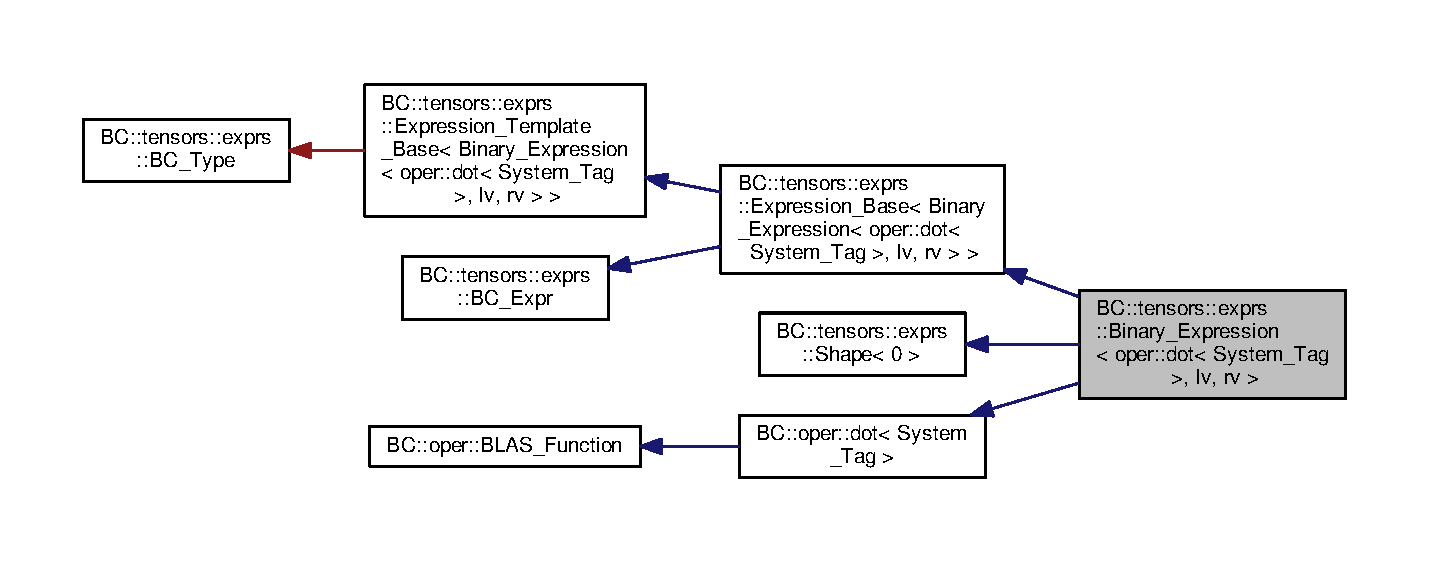
\includegraphics[width=350pt]{structBC_1_1tensors_1_1exprs_1_1Binary__Expression_3_01oper_1_1dot_3_01System__Tag_01_4_00_01lv_00_01rv_01_4__inherit__graph}
\end{center}
\end{figure}


Collaboration diagram for BC\+:\+:tensors\+:\+:exprs\+:\+:Binary\+\_\+\+Expression$<$ oper\+:\+:dot$<$ System\+\_\+\+Tag $>$, lv, rv $>$\+:
\nopagebreak
\begin{figure}[H]
\begin{center}
\leavevmode
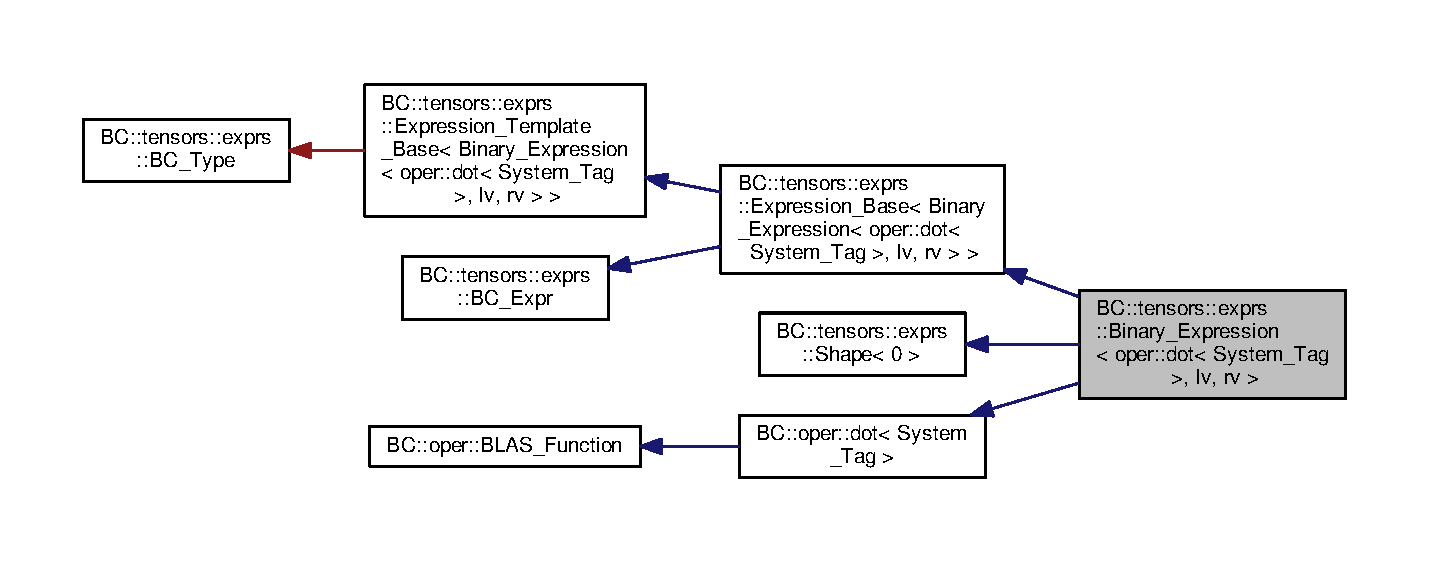
\includegraphics[width=350pt]{structBC_1_1tensors_1_1exprs_1_1Binary__Expression_3_01oper_1_1dot_3_01System__Tag_01_4_00_01lv_00_01rv_01_4__coll__graph}
\end{center}
\end{figure}
\subsection*{Public Types}
\begin{DoxyCompactItemize}
\item 
using \hyperlink{structBC_1_1tensors_1_1exprs_1_1Binary__Expression_3_01oper_1_1dot_3_01System__Tag_01_4_00_01lv_00_01rv_01_4_a531c879cb72017483e3e44e04c4cdf03}{value\+\_\+type} = typename lv\+::value\+\_\+type
\item 
using \hyperlink{structBC_1_1tensors_1_1exprs_1_1Binary__Expression_3_01oper_1_1dot_3_01System__Tag_01_4_00_01lv_00_01rv_01_4_a6bcdb75bc19af9d195674fb88f7f9e02}{system\+\_\+tag} = System\+\_\+\+Tag
\item 
using \hyperlink{structBC_1_1tensors_1_1exprs_1_1Binary__Expression_3_01oper_1_1dot_3_01System__Tag_01_4_00_01lv_00_01rv_01_4_a5e92bf290b7bb66e9c9f6a9a5739aacf}{blas\+\_\+impl} = B\+C\+::blas\+::implementation$<$ \hyperlink{structBC_1_1tensors_1_1exprs_1_1Binary__Expression_3_01oper_1_1dot_3_01System__Tag_01_4_00_01lv_00_01rv_01_4_a6bcdb75bc19af9d195674fb88f7f9e02}{system\+\_\+tag} $>$
\item 
using \hyperlink{structBC_1_1tensors_1_1exprs_1_1Binary__Expression_3_01oper_1_1dot_3_01System__Tag_01_4_00_01lv_00_01rv_01_4_ad7ee221fc688c3b58ba212c5957ed983}{blas\+\_\+util} = B\+C\+::tensors\+::exprs\+::blas\+\_\+tools\+::implementation$<$ \hyperlink{structBC_1_1tensors_1_1exprs_1_1Binary__Expression_3_01oper_1_1dot_3_01System__Tag_01_4_00_01lv_00_01rv_01_4_a6bcdb75bc19af9d195674fb88f7f9e02}{system\+\_\+tag} $>$
\end{DoxyCompactItemize}
\subsection*{Public Member Functions}
\begin{DoxyCompactItemize}
\item 
\hyperlink{structBC_1_1tensors_1_1exprs_1_1Binary__Expression_3_01oper_1_1dot_3_01System__Tag_01_4_00_01lv_00_01rv_01_4_a12e199e2ce522aa9fb0fcf850f0d4c46}{Binary\+\_\+\+Expression} (lv \hyperlink{structBC_1_1tensors_1_1exprs_1_1Binary__Expression_3_01oper_1_1dot_3_01System__Tag_01_4_00_01lv_00_01rv_01_4_a17d0cd14365a29c0aa10cba3f9d57c04}{left}, rv \hyperlink{structBC_1_1tensors_1_1exprs_1_1Binary__Expression_3_01oper_1_1dot_3_01System__Tag_01_4_00_01lv_00_01rv_01_4_ac16bea75afa747671af04ba484694a19}{right})
\item 
{\footnotesize template$<$class core , B\+C\+::size\+\_\+t alpha\+\_\+mod, B\+C\+::size\+\_\+t beta\+\_\+mod, class allocator $>$ }\\void \hyperlink{structBC_1_1tensors_1_1exprs_1_1Binary__Expression_3_01oper_1_1dot_3_01System__Tag_01_4_00_01lv_00_01rv_01_4_af7e79c05059441aabf4ea6cf585b750e}{eval} (\hyperlink{structBC_1_1tensors_1_1exprs_1_1injector}{injector}$<$ core, alpha\+\_\+mod, beta\+\_\+mod $>$ injection\+\_\+values, allocator \&alloc) const 
\end{DoxyCompactItemize}
\subsection*{Public Attributes}
\begin{DoxyCompactItemize}
\item 
lv \hyperlink{structBC_1_1tensors_1_1exprs_1_1Binary__Expression_3_01oper_1_1dot_3_01System__Tag_01_4_00_01lv_00_01rv_01_4_a17d0cd14365a29c0aa10cba3f9d57c04}{left}
\item 
rv \hyperlink{structBC_1_1tensors_1_1exprs_1_1Binary__Expression_3_01oper_1_1dot_3_01System__Tag_01_4_00_01lv_00_01rv_01_4_ac16bea75afa747671af04ba484694a19}{right}
\end{DoxyCompactItemize}
\subsection*{Static Public Attributes}
\begin{DoxyCompactItemize}
\item 
static constexpr bool \hyperlink{structBC_1_1tensors_1_1exprs_1_1Binary__Expression_3_01oper_1_1dot_3_01System__Tag_01_4_00_01lv_00_01rv_01_4_a49e4e40c1204f61b32a0806f9610c91d}{lv\+\_\+scalar} = \hyperlink{structBC_1_1tensors_1_1exprs_1_1blas__expression__traits}{blas\+\_\+expression\+\_\+traits}$<$lv$>$\+::is\+\_\+scalar\+\_\+multiplied
\item 
static constexpr bool \hyperlink{structBC_1_1tensors_1_1exprs_1_1Binary__Expression_3_01oper_1_1dot_3_01System__Tag_01_4_00_01lv_00_01rv_01_4_ad88437990f342c0a97fbe05153f23af1}{rv\+\_\+scalar} = \hyperlink{structBC_1_1tensors_1_1exprs_1_1blas__expression__traits}{blas\+\_\+expression\+\_\+traits}$<$rv$>$\+::is\+\_\+scalar\+\_\+multiplied
\item 
static constexpr int \hyperlink{structBC_1_1tensors_1_1exprs_1_1Binary__Expression_3_01oper_1_1dot_3_01System__Tag_01_4_00_01lv_00_01rv_01_4_a427270424bc3aa0702c8a3bffd77e1c8}{tensor\+\_\+dimension} = 0
\item 
static constexpr int \hyperlink{structBC_1_1tensors_1_1exprs_1_1Binary__Expression_3_01oper_1_1dot_3_01System__Tag_01_4_00_01lv_00_01rv_01_4_a832141f8e846880d4c03292accd383a5}{tensor\+\_\+iterator\+\_\+dimension} = 0
\end{DoxyCompactItemize}
\subsection*{Additional Inherited Members}


\subsection{Member Typedef Documentation}
\index{B\+C\+::tensors\+::exprs\+::\+Binary\+\_\+\+Expression$<$ oper\+::dot$<$ System\+\_\+\+Tag $>$, lv, rv $>$@{B\+C\+::tensors\+::exprs\+::\+Binary\+\_\+\+Expression$<$ oper\+::dot$<$ System\+\_\+\+Tag $>$, lv, rv $>$}!blas\+\_\+impl@{blas\+\_\+impl}}
\index{blas\+\_\+impl@{blas\+\_\+impl}!B\+C\+::tensors\+::exprs\+::\+Binary\+\_\+\+Expression$<$ oper\+::dot$<$ System\+\_\+\+Tag $>$, lv, rv $>$@{B\+C\+::tensors\+::exprs\+::\+Binary\+\_\+\+Expression$<$ oper\+::dot$<$ System\+\_\+\+Tag $>$, lv, rv $>$}}
\subsubsection[{\texorpdfstring{blas\+\_\+impl}{blas_impl}}]{\setlength{\rightskip}{0pt plus 5cm}template$<$class lv , class rv , class System\+\_\+\+Tag $>$ using {\bf B\+C\+::tensors\+::exprs\+::\+Binary\+\_\+\+Expression}$<$ {\bf oper\+::dot}$<$ System\+\_\+\+Tag $>$, lv, rv $>$\+::{\bf blas\+\_\+impl} =  B\+C\+::blas\+::implementation$<${\bf system\+\_\+tag}$>$}\hypertarget{structBC_1_1tensors_1_1exprs_1_1Binary__Expression_3_01oper_1_1dot_3_01System__Tag_01_4_00_01lv_00_01rv_01_4_a5e92bf290b7bb66e9c9f6a9a5739aacf}{}\label{structBC_1_1tensors_1_1exprs_1_1Binary__Expression_3_01oper_1_1dot_3_01System__Tag_01_4_00_01lv_00_01rv_01_4_a5e92bf290b7bb66e9c9f6a9a5739aacf}
\index{B\+C\+::tensors\+::exprs\+::\+Binary\+\_\+\+Expression$<$ oper\+::dot$<$ System\+\_\+\+Tag $>$, lv, rv $>$@{B\+C\+::tensors\+::exprs\+::\+Binary\+\_\+\+Expression$<$ oper\+::dot$<$ System\+\_\+\+Tag $>$, lv, rv $>$}!blas\+\_\+util@{blas\+\_\+util}}
\index{blas\+\_\+util@{blas\+\_\+util}!B\+C\+::tensors\+::exprs\+::\+Binary\+\_\+\+Expression$<$ oper\+::dot$<$ System\+\_\+\+Tag $>$, lv, rv $>$@{B\+C\+::tensors\+::exprs\+::\+Binary\+\_\+\+Expression$<$ oper\+::dot$<$ System\+\_\+\+Tag $>$, lv, rv $>$}}
\subsubsection[{\texorpdfstring{blas\+\_\+util}{blas_util}}]{\setlength{\rightskip}{0pt plus 5cm}template$<$class lv , class rv , class System\+\_\+\+Tag $>$ using {\bf B\+C\+::tensors\+::exprs\+::\+Binary\+\_\+\+Expression}$<$ {\bf oper\+::dot}$<$ System\+\_\+\+Tag $>$, lv, rv $>$\+::{\bf blas\+\_\+util} =  B\+C\+::tensors\+::exprs\+::blas\+\_\+tools\+::implementation$<${\bf system\+\_\+tag}$>$}\hypertarget{structBC_1_1tensors_1_1exprs_1_1Binary__Expression_3_01oper_1_1dot_3_01System__Tag_01_4_00_01lv_00_01rv_01_4_ad7ee221fc688c3b58ba212c5957ed983}{}\label{structBC_1_1tensors_1_1exprs_1_1Binary__Expression_3_01oper_1_1dot_3_01System__Tag_01_4_00_01lv_00_01rv_01_4_ad7ee221fc688c3b58ba212c5957ed983}
\index{B\+C\+::tensors\+::exprs\+::\+Binary\+\_\+\+Expression$<$ oper\+::dot$<$ System\+\_\+\+Tag $>$, lv, rv $>$@{B\+C\+::tensors\+::exprs\+::\+Binary\+\_\+\+Expression$<$ oper\+::dot$<$ System\+\_\+\+Tag $>$, lv, rv $>$}!system\+\_\+tag@{system\+\_\+tag}}
\index{system\+\_\+tag@{system\+\_\+tag}!B\+C\+::tensors\+::exprs\+::\+Binary\+\_\+\+Expression$<$ oper\+::dot$<$ System\+\_\+\+Tag $>$, lv, rv $>$@{B\+C\+::tensors\+::exprs\+::\+Binary\+\_\+\+Expression$<$ oper\+::dot$<$ System\+\_\+\+Tag $>$, lv, rv $>$}}
\subsubsection[{\texorpdfstring{system\+\_\+tag}{system_tag}}]{\setlength{\rightskip}{0pt plus 5cm}template$<$class lv , class rv , class System\+\_\+\+Tag $>$ using {\bf B\+C\+::tensors\+::exprs\+::\+Binary\+\_\+\+Expression}$<$ {\bf oper\+::dot}$<$ System\+\_\+\+Tag $>$, lv, rv $>$\+::{\bf system\+\_\+tag} =  System\+\_\+\+Tag}\hypertarget{structBC_1_1tensors_1_1exprs_1_1Binary__Expression_3_01oper_1_1dot_3_01System__Tag_01_4_00_01lv_00_01rv_01_4_a6bcdb75bc19af9d195674fb88f7f9e02}{}\label{structBC_1_1tensors_1_1exprs_1_1Binary__Expression_3_01oper_1_1dot_3_01System__Tag_01_4_00_01lv_00_01rv_01_4_a6bcdb75bc19af9d195674fb88f7f9e02}
\index{B\+C\+::tensors\+::exprs\+::\+Binary\+\_\+\+Expression$<$ oper\+::dot$<$ System\+\_\+\+Tag $>$, lv, rv $>$@{B\+C\+::tensors\+::exprs\+::\+Binary\+\_\+\+Expression$<$ oper\+::dot$<$ System\+\_\+\+Tag $>$, lv, rv $>$}!value\+\_\+type@{value\+\_\+type}}
\index{value\+\_\+type@{value\+\_\+type}!B\+C\+::tensors\+::exprs\+::\+Binary\+\_\+\+Expression$<$ oper\+::dot$<$ System\+\_\+\+Tag $>$, lv, rv $>$@{B\+C\+::tensors\+::exprs\+::\+Binary\+\_\+\+Expression$<$ oper\+::dot$<$ System\+\_\+\+Tag $>$, lv, rv $>$}}
\subsubsection[{\texorpdfstring{value\+\_\+type}{value_type}}]{\setlength{\rightskip}{0pt plus 5cm}template$<$class lv , class rv , class System\+\_\+\+Tag $>$ using {\bf B\+C\+::tensors\+::exprs\+::\+Binary\+\_\+\+Expression}$<$ {\bf oper\+::dot}$<$ System\+\_\+\+Tag $>$, lv, rv $>$\+::{\bf value\+\_\+type} =  typename lv\+::value\+\_\+type}\hypertarget{structBC_1_1tensors_1_1exprs_1_1Binary__Expression_3_01oper_1_1dot_3_01System__Tag_01_4_00_01lv_00_01rv_01_4_a531c879cb72017483e3e44e04c4cdf03}{}\label{structBC_1_1tensors_1_1exprs_1_1Binary__Expression_3_01oper_1_1dot_3_01System__Tag_01_4_00_01lv_00_01rv_01_4_a531c879cb72017483e3e44e04c4cdf03}


\subsection{Constructor \& Destructor Documentation}
\index{B\+C\+::tensors\+::exprs\+::\+Binary\+\_\+\+Expression$<$ oper\+::dot$<$ System\+\_\+\+Tag $>$, lv, rv $>$@{B\+C\+::tensors\+::exprs\+::\+Binary\+\_\+\+Expression$<$ oper\+::dot$<$ System\+\_\+\+Tag $>$, lv, rv $>$}!Binary\+\_\+\+Expression@{Binary\+\_\+\+Expression}}
\index{Binary\+\_\+\+Expression@{Binary\+\_\+\+Expression}!B\+C\+::tensors\+::exprs\+::\+Binary\+\_\+\+Expression$<$ oper\+::dot$<$ System\+\_\+\+Tag $>$, lv, rv $>$@{B\+C\+::tensors\+::exprs\+::\+Binary\+\_\+\+Expression$<$ oper\+::dot$<$ System\+\_\+\+Tag $>$, lv, rv $>$}}
\subsubsection[{\texorpdfstring{Binary\+\_\+\+Expression(lv left, rv right)}{Binary_Expression(lv left, rv right)}}]{\setlength{\rightskip}{0pt plus 5cm}template$<$class lv , class rv , class System\+\_\+\+Tag $>$ {\bf B\+C\+::tensors\+::exprs\+::\+Binary\+\_\+\+Expression}$<$ {\bf oper\+::dot}$<$ System\+\_\+\+Tag $>$, lv, rv $>$\+::{\bf Binary\+\_\+\+Expression} (
\begin{DoxyParamCaption}
\item[{lv}]{left, }
\item[{rv}]{right}
\end{DoxyParamCaption}
)\hspace{0.3cm}{\ttfamily [inline]}}\hypertarget{structBC_1_1tensors_1_1exprs_1_1Binary__Expression_3_01oper_1_1dot_3_01System__Tag_01_4_00_01lv_00_01rv_01_4_a12e199e2ce522aa9fb0fcf850f0d4c46}{}\label{structBC_1_1tensors_1_1exprs_1_1Binary__Expression_3_01oper_1_1dot_3_01System__Tag_01_4_00_01lv_00_01rv_01_4_a12e199e2ce522aa9fb0fcf850f0d4c46}


\subsection{Member Function Documentation}
\index{B\+C\+::tensors\+::exprs\+::\+Binary\+\_\+\+Expression$<$ oper\+::dot$<$ System\+\_\+\+Tag $>$, lv, rv $>$@{B\+C\+::tensors\+::exprs\+::\+Binary\+\_\+\+Expression$<$ oper\+::dot$<$ System\+\_\+\+Tag $>$, lv, rv $>$}!eval@{eval}}
\index{eval@{eval}!B\+C\+::tensors\+::exprs\+::\+Binary\+\_\+\+Expression$<$ oper\+::dot$<$ System\+\_\+\+Tag $>$, lv, rv $>$@{B\+C\+::tensors\+::exprs\+::\+Binary\+\_\+\+Expression$<$ oper\+::dot$<$ System\+\_\+\+Tag $>$, lv, rv $>$}}
\subsubsection[{\texorpdfstring{eval(injector$<$ core, alpha\+\_\+mod, beta\+\_\+mod $>$ injection\+\_\+values, allocator \&alloc) const }{eval(injector< core, alpha_mod, beta_mod > injection_values, allocator &alloc) const }}]{\setlength{\rightskip}{0pt plus 5cm}template$<$class lv , class rv , class System\+\_\+\+Tag $>$ template$<$class core , B\+C\+::size\+\_\+t alpha\+\_\+mod, B\+C\+::size\+\_\+t beta\+\_\+mod, class allocator $>$ void {\bf B\+C\+::tensors\+::exprs\+::\+Binary\+\_\+\+Expression}$<$ {\bf oper\+::dot}$<$ System\+\_\+\+Tag $>$, lv, rv $>$\+::eval (
\begin{DoxyParamCaption}
\item[{{\bf injector}$<$ core, alpha\+\_\+mod, beta\+\_\+mod $>$}]{injection\+\_\+values, }
\item[{allocator \&}]{alloc}
\end{DoxyParamCaption}
) const\hspace{0.3cm}{\ttfamily [inline]}}\hypertarget{structBC_1_1tensors_1_1exprs_1_1Binary__Expression_3_01oper_1_1dot_3_01System__Tag_01_4_00_01lv_00_01rv_01_4_af7e79c05059441aabf4ea6cf585b750e}{}\label{structBC_1_1tensors_1_1exprs_1_1Binary__Expression_3_01oper_1_1dot_3_01System__Tag_01_4_00_01lv_00_01rv_01_4_af7e79c05059441aabf4ea6cf585b750e}


\subsection{Member Data Documentation}
\index{B\+C\+::tensors\+::exprs\+::\+Binary\+\_\+\+Expression$<$ oper\+::dot$<$ System\+\_\+\+Tag $>$, lv, rv $>$@{B\+C\+::tensors\+::exprs\+::\+Binary\+\_\+\+Expression$<$ oper\+::dot$<$ System\+\_\+\+Tag $>$, lv, rv $>$}!left@{left}}
\index{left@{left}!B\+C\+::tensors\+::exprs\+::\+Binary\+\_\+\+Expression$<$ oper\+::dot$<$ System\+\_\+\+Tag $>$, lv, rv $>$@{B\+C\+::tensors\+::exprs\+::\+Binary\+\_\+\+Expression$<$ oper\+::dot$<$ System\+\_\+\+Tag $>$, lv, rv $>$}}
\subsubsection[{\texorpdfstring{left}{left}}]{\setlength{\rightskip}{0pt plus 5cm}template$<$class lv , class rv , class System\+\_\+\+Tag $>$ lv {\bf B\+C\+::tensors\+::exprs\+::\+Binary\+\_\+\+Expression}$<$ {\bf oper\+::dot}$<$ System\+\_\+\+Tag $>$, lv, rv $>$\+::left}\hypertarget{structBC_1_1tensors_1_1exprs_1_1Binary__Expression_3_01oper_1_1dot_3_01System__Tag_01_4_00_01lv_00_01rv_01_4_a17d0cd14365a29c0aa10cba3f9d57c04}{}\label{structBC_1_1tensors_1_1exprs_1_1Binary__Expression_3_01oper_1_1dot_3_01System__Tag_01_4_00_01lv_00_01rv_01_4_a17d0cd14365a29c0aa10cba3f9d57c04}
\index{B\+C\+::tensors\+::exprs\+::\+Binary\+\_\+\+Expression$<$ oper\+::dot$<$ System\+\_\+\+Tag $>$, lv, rv $>$@{B\+C\+::tensors\+::exprs\+::\+Binary\+\_\+\+Expression$<$ oper\+::dot$<$ System\+\_\+\+Tag $>$, lv, rv $>$}!lv\+\_\+scalar@{lv\+\_\+scalar}}
\index{lv\+\_\+scalar@{lv\+\_\+scalar}!B\+C\+::tensors\+::exprs\+::\+Binary\+\_\+\+Expression$<$ oper\+::dot$<$ System\+\_\+\+Tag $>$, lv, rv $>$@{B\+C\+::tensors\+::exprs\+::\+Binary\+\_\+\+Expression$<$ oper\+::dot$<$ System\+\_\+\+Tag $>$, lv, rv $>$}}
\subsubsection[{\texorpdfstring{lv\+\_\+scalar}{lv_scalar}}]{\setlength{\rightskip}{0pt plus 5cm}template$<$class lv , class rv , class System\+\_\+\+Tag $>$ constexpr bool {\bf B\+C\+::tensors\+::exprs\+::\+Binary\+\_\+\+Expression}$<$ {\bf oper\+::dot}$<$ System\+\_\+\+Tag $>$, lv, rv $>$\+::lv\+\_\+scalar = {\bf blas\+\_\+expression\+\_\+traits}$<$lv$>$\+::is\+\_\+scalar\+\_\+multiplied\hspace{0.3cm}{\ttfamily [static]}}\hypertarget{structBC_1_1tensors_1_1exprs_1_1Binary__Expression_3_01oper_1_1dot_3_01System__Tag_01_4_00_01lv_00_01rv_01_4_a49e4e40c1204f61b32a0806f9610c91d}{}\label{structBC_1_1tensors_1_1exprs_1_1Binary__Expression_3_01oper_1_1dot_3_01System__Tag_01_4_00_01lv_00_01rv_01_4_a49e4e40c1204f61b32a0806f9610c91d}
\index{B\+C\+::tensors\+::exprs\+::\+Binary\+\_\+\+Expression$<$ oper\+::dot$<$ System\+\_\+\+Tag $>$, lv, rv $>$@{B\+C\+::tensors\+::exprs\+::\+Binary\+\_\+\+Expression$<$ oper\+::dot$<$ System\+\_\+\+Tag $>$, lv, rv $>$}!right@{right}}
\index{right@{right}!B\+C\+::tensors\+::exprs\+::\+Binary\+\_\+\+Expression$<$ oper\+::dot$<$ System\+\_\+\+Tag $>$, lv, rv $>$@{B\+C\+::tensors\+::exprs\+::\+Binary\+\_\+\+Expression$<$ oper\+::dot$<$ System\+\_\+\+Tag $>$, lv, rv $>$}}
\subsubsection[{\texorpdfstring{right}{right}}]{\setlength{\rightskip}{0pt plus 5cm}template$<$class lv , class rv , class System\+\_\+\+Tag $>$ rv {\bf B\+C\+::tensors\+::exprs\+::\+Binary\+\_\+\+Expression}$<$ {\bf oper\+::dot}$<$ System\+\_\+\+Tag $>$, lv, rv $>$\+::right}\hypertarget{structBC_1_1tensors_1_1exprs_1_1Binary__Expression_3_01oper_1_1dot_3_01System__Tag_01_4_00_01lv_00_01rv_01_4_ac16bea75afa747671af04ba484694a19}{}\label{structBC_1_1tensors_1_1exprs_1_1Binary__Expression_3_01oper_1_1dot_3_01System__Tag_01_4_00_01lv_00_01rv_01_4_ac16bea75afa747671af04ba484694a19}
\index{B\+C\+::tensors\+::exprs\+::\+Binary\+\_\+\+Expression$<$ oper\+::dot$<$ System\+\_\+\+Tag $>$, lv, rv $>$@{B\+C\+::tensors\+::exprs\+::\+Binary\+\_\+\+Expression$<$ oper\+::dot$<$ System\+\_\+\+Tag $>$, lv, rv $>$}!rv\+\_\+scalar@{rv\+\_\+scalar}}
\index{rv\+\_\+scalar@{rv\+\_\+scalar}!B\+C\+::tensors\+::exprs\+::\+Binary\+\_\+\+Expression$<$ oper\+::dot$<$ System\+\_\+\+Tag $>$, lv, rv $>$@{B\+C\+::tensors\+::exprs\+::\+Binary\+\_\+\+Expression$<$ oper\+::dot$<$ System\+\_\+\+Tag $>$, lv, rv $>$}}
\subsubsection[{\texorpdfstring{rv\+\_\+scalar}{rv_scalar}}]{\setlength{\rightskip}{0pt plus 5cm}template$<$class lv , class rv , class System\+\_\+\+Tag $>$ constexpr bool {\bf B\+C\+::tensors\+::exprs\+::\+Binary\+\_\+\+Expression}$<$ {\bf oper\+::dot}$<$ System\+\_\+\+Tag $>$, lv, rv $>$\+::rv\+\_\+scalar = {\bf blas\+\_\+expression\+\_\+traits}$<$rv$>$\+::is\+\_\+scalar\+\_\+multiplied\hspace{0.3cm}{\ttfamily [static]}}\hypertarget{structBC_1_1tensors_1_1exprs_1_1Binary__Expression_3_01oper_1_1dot_3_01System__Tag_01_4_00_01lv_00_01rv_01_4_ad88437990f342c0a97fbe05153f23af1}{}\label{structBC_1_1tensors_1_1exprs_1_1Binary__Expression_3_01oper_1_1dot_3_01System__Tag_01_4_00_01lv_00_01rv_01_4_ad88437990f342c0a97fbe05153f23af1}
\index{B\+C\+::tensors\+::exprs\+::\+Binary\+\_\+\+Expression$<$ oper\+::dot$<$ System\+\_\+\+Tag $>$, lv, rv $>$@{B\+C\+::tensors\+::exprs\+::\+Binary\+\_\+\+Expression$<$ oper\+::dot$<$ System\+\_\+\+Tag $>$, lv, rv $>$}!tensor\+\_\+dimension@{tensor\+\_\+dimension}}
\index{tensor\+\_\+dimension@{tensor\+\_\+dimension}!B\+C\+::tensors\+::exprs\+::\+Binary\+\_\+\+Expression$<$ oper\+::dot$<$ System\+\_\+\+Tag $>$, lv, rv $>$@{B\+C\+::tensors\+::exprs\+::\+Binary\+\_\+\+Expression$<$ oper\+::dot$<$ System\+\_\+\+Tag $>$, lv, rv $>$}}
\subsubsection[{\texorpdfstring{tensor\+\_\+dimension}{tensor_dimension}}]{\setlength{\rightskip}{0pt plus 5cm}template$<$class lv , class rv , class System\+\_\+\+Tag $>$ constexpr int {\bf B\+C\+::tensors\+::exprs\+::\+Binary\+\_\+\+Expression}$<$ {\bf oper\+::dot}$<$ System\+\_\+\+Tag $>$, lv, rv $>$\+::tensor\+\_\+dimension = 0\hspace{0.3cm}{\ttfamily [static]}}\hypertarget{structBC_1_1tensors_1_1exprs_1_1Binary__Expression_3_01oper_1_1dot_3_01System__Tag_01_4_00_01lv_00_01rv_01_4_a427270424bc3aa0702c8a3bffd77e1c8}{}\label{structBC_1_1tensors_1_1exprs_1_1Binary__Expression_3_01oper_1_1dot_3_01System__Tag_01_4_00_01lv_00_01rv_01_4_a427270424bc3aa0702c8a3bffd77e1c8}
\index{B\+C\+::tensors\+::exprs\+::\+Binary\+\_\+\+Expression$<$ oper\+::dot$<$ System\+\_\+\+Tag $>$, lv, rv $>$@{B\+C\+::tensors\+::exprs\+::\+Binary\+\_\+\+Expression$<$ oper\+::dot$<$ System\+\_\+\+Tag $>$, lv, rv $>$}!tensor\+\_\+iterator\+\_\+dimension@{tensor\+\_\+iterator\+\_\+dimension}}
\index{tensor\+\_\+iterator\+\_\+dimension@{tensor\+\_\+iterator\+\_\+dimension}!B\+C\+::tensors\+::exprs\+::\+Binary\+\_\+\+Expression$<$ oper\+::dot$<$ System\+\_\+\+Tag $>$, lv, rv $>$@{B\+C\+::tensors\+::exprs\+::\+Binary\+\_\+\+Expression$<$ oper\+::dot$<$ System\+\_\+\+Tag $>$, lv, rv $>$}}
\subsubsection[{\texorpdfstring{tensor\+\_\+iterator\+\_\+dimension}{tensor_iterator_dimension}}]{\setlength{\rightskip}{0pt plus 5cm}template$<$class lv , class rv , class System\+\_\+\+Tag $>$ constexpr int {\bf B\+C\+::tensors\+::exprs\+::\+Binary\+\_\+\+Expression}$<$ {\bf oper\+::dot}$<$ System\+\_\+\+Tag $>$, lv, rv $>$\+::tensor\+\_\+iterator\+\_\+dimension = 0\hspace{0.3cm}{\ttfamily [static]}}\hypertarget{structBC_1_1tensors_1_1exprs_1_1Binary__Expression_3_01oper_1_1dot_3_01System__Tag_01_4_00_01lv_00_01rv_01_4_a832141f8e846880d4c03292accd383a5}{}\label{structBC_1_1tensors_1_1exprs_1_1Binary__Expression_3_01oper_1_1dot_3_01System__Tag_01_4_00_01lv_00_01rv_01_4_a832141f8e846880d4c03292accd383a5}


The documentation for this struct was generated from the following file\+:\begin{DoxyCompactItemize}
\item 
include/tensors/expression\+\_\+templates/\hyperlink{Function__dot_8h}{Function\+\_\+dot.\+h}\end{DoxyCompactItemize}

\hypertarget{structBC_1_1tensors_1_1exprs_1_1Binary__Expression_3_01oper_1_1gemm_3_01System__Tag_01_4_00_01lv_00_01rv_01_4}{}\section{BC\+:\+:tensors\+:\+:exprs\+:\+:Binary\+\_\+\+Expression$<$ oper\+:\+:gemm$<$ System\+\_\+\+Tag $>$, lv, rv $>$ Struct Template Reference}
\label{structBC_1_1tensors_1_1exprs_1_1Binary__Expression_3_01oper_1_1gemm_3_01System__Tag_01_4_00_01lv_00_01rv_01_4}\index{B\+C\+::tensors\+::exprs\+::\+Binary\+\_\+\+Expression$<$ oper\+::gemm$<$ System\+\_\+\+Tag $>$, lv, rv $>$@{B\+C\+::tensors\+::exprs\+::\+Binary\+\_\+\+Expression$<$ oper\+::gemm$<$ System\+\_\+\+Tag $>$, lv, rv $>$}}


{\ttfamily \#include $<$Function\+\_\+gemm.\+h$>$}



Inheritance diagram for BC\+:\+:tensors\+:\+:exprs\+:\+:Binary\+\_\+\+Expression$<$ oper\+:\+:gemm$<$ System\+\_\+\+Tag $>$, lv, rv $>$\+:
\nopagebreak
\begin{figure}[H]
\begin{center}
\leavevmode
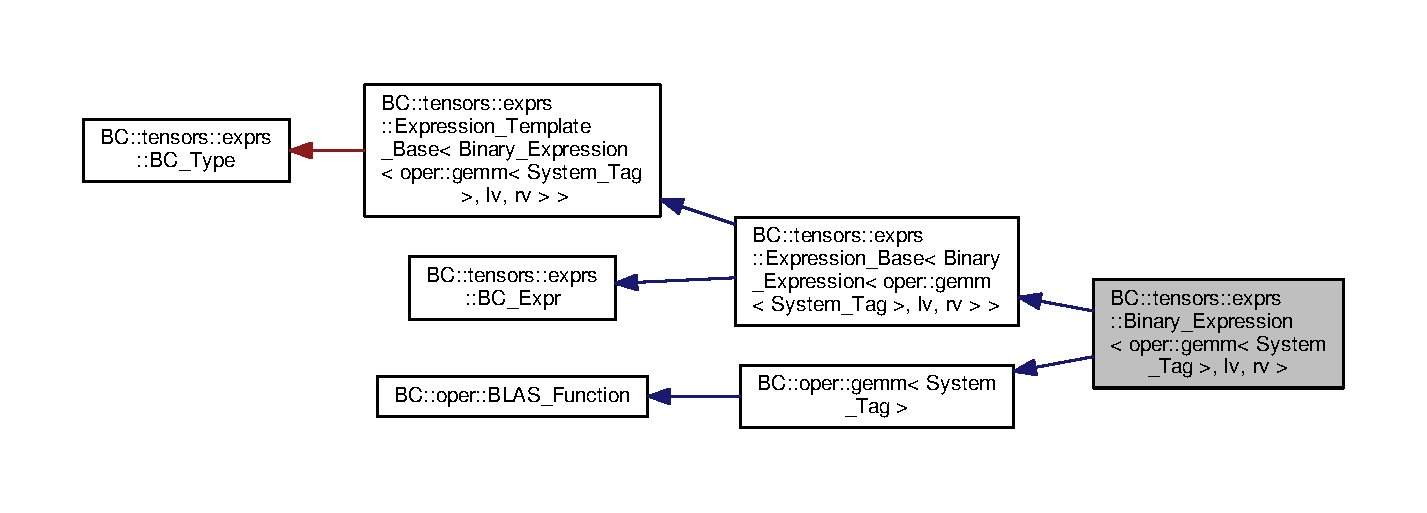
\includegraphics[width=350pt]{structBC_1_1tensors_1_1exprs_1_1Binary__Expression_3_01oper_1_1gemm_3_01System__Tag_01_4_00_01lv_00_01rv_01_4__inherit__graph}
\end{center}
\end{figure}


Collaboration diagram for BC\+:\+:tensors\+:\+:exprs\+:\+:Binary\+\_\+\+Expression$<$ oper\+:\+:gemm$<$ System\+\_\+\+Tag $>$, lv, rv $>$\+:
\nopagebreak
\begin{figure}[H]
\begin{center}
\leavevmode
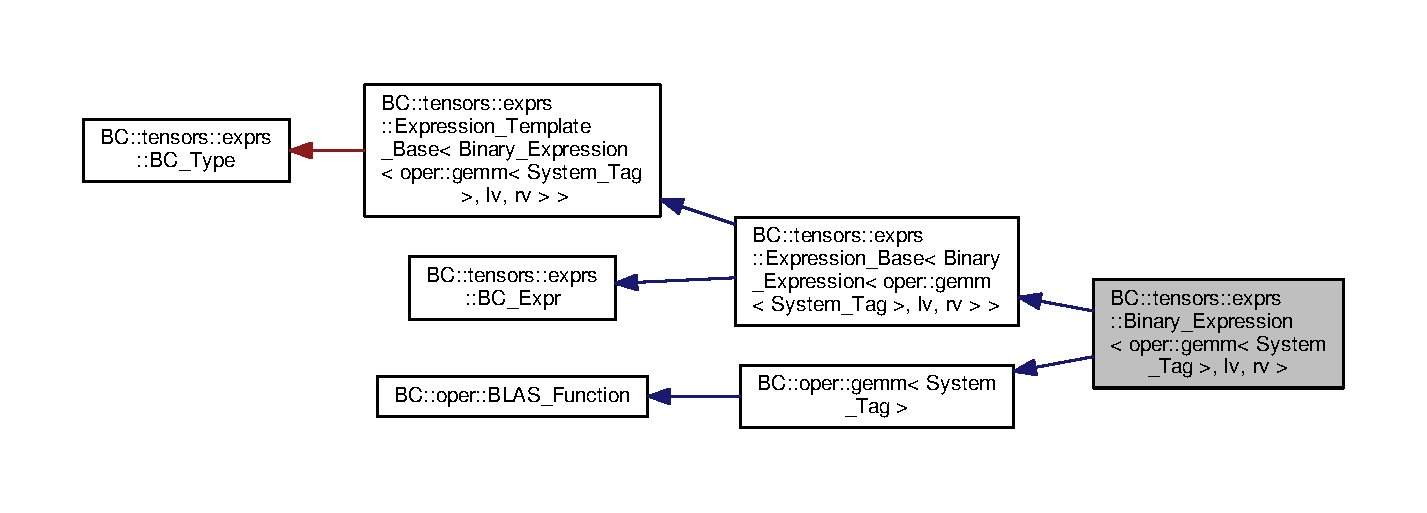
\includegraphics[width=350pt]{structBC_1_1tensors_1_1exprs_1_1Binary__Expression_3_01oper_1_1gemm_3_01System__Tag_01_4_00_01lv_00_01rv_01_4__coll__graph}
\end{center}
\end{figure}
\subsection*{Public Types}
\begin{DoxyCompactItemize}
\item 
using \hyperlink{structBC_1_1tensors_1_1exprs_1_1Binary__Expression_3_01oper_1_1gemm_3_01System__Tag_01_4_00_01lv_00_01rv_01_4_a2e81a6a9d5c6ea6f79b09597e3130ead}{value\+\_\+type} = typename lv\+::value\+\_\+type
\item 
using \hyperlink{structBC_1_1tensors_1_1exprs_1_1Binary__Expression_3_01oper_1_1gemm_3_01System__Tag_01_4_00_01lv_00_01rv_01_4_acb8bcec11c350fe4c36d899f3d1f5fbe}{system\+\_\+tag} = System\+\_\+\+Tag
\item 
using \hyperlink{structBC_1_1tensors_1_1exprs_1_1Binary__Expression_3_01oper_1_1gemm_3_01System__Tag_01_4_00_01lv_00_01rv_01_4_a7dbeec9fb2bb93402b455075ecb38016}{blas\+\_\+impl} = B\+C\+::blas\+::implementation$<$ \hyperlink{structBC_1_1tensors_1_1exprs_1_1Binary__Expression_3_01oper_1_1gemm_3_01System__Tag_01_4_00_01lv_00_01rv_01_4_acb8bcec11c350fe4c36d899f3d1f5fbe}{system\+\_\+tag} $>$
\item 
using \hyperlink{structBC_1_1tensors_1_1exprs_1_1Binary__Expression_3_01oper_1_1gemm_3_01System__Tag_01_4_00_01lv_00_01rv_01_4_ad3212d256acfdb087e1c15d7d15f7589}{blas\+\_\+util} = B\+C\+::tensors\+::exprs\+::blas\+\_\+tools\+::implementation$<$ \hyperlink{structBC_1_1tensors_1_1exprs_1_1Binary__Expression_3_01oper_1_1gemm_3_01System__Tag_01_4_00_01lv_00_01rv_01_4_acb8bcec11c350fe4c36d899f3d1f5fbe}{system\+\_\+tag} $>$
\end{DoxyCompactItemize}
\subsection*{Public Member Functions}
\begin{DoxyCompactItemize}
\item 
\hyperlink{BlackCat__Common_8h_ac085f07cc309e3aac24aa3fc0a40f6d2}{B\+C\+H\+OT} \hyperlink{structBC_1_1tensors_1_1exprs_1_1Binary__Expression_3_01oper_1_1gemm_3_01System__Tag_01_4_00_01lv_00_01rv_01_4_ab1dd1a03e5b3f64a7e01232400151a86}{Binary\+\_\+\+Expression} (lv \hyperlink{structBC_1_1tensors_1_1exprs_1_1Binary__Expression_3_01oper_1_1gemm_3_01System__Tag_01_4_00_01lv_00_01rv_01_4_a961a2d6095d05b27cd603867a9077301}{left}, rv \hyperlink{structBC_1_1tensors_1_1exprs_1_1Binary__Expression_3_01oper_1_1gemm_3_01System__Tag_01_4_00_01lv_00_01rv_01_4_af7846bf959d293e2e8bd573955536c08}{right})
\item 
\hyperlink{BlackCat__Common_8h_a6699e8b0449da5c0fafb878e59c1d4b1}{B\+C\+I\+N\+L\+I\+NE} \hyperlink{namespaceBC_a6007cbc4eeec401a037b558910a56173}{B\+C\+::size\+\_\+t} \hyperlink{structBC_1_1tensors_1_1exprs_1_1Binary__Expression_3_01oper_1_1gemm_3_01System__Tag_01_4_00_01lv_00_01rv_01_4_a0e33696188bb7a80f5e3fd8bdae5e354}{size} () const 
\item 
\hyperlink{BlackCat__Common_8h_a6699e8b0449da5c0fafb878e59c1d4b1}{B\+C\+I\+N\+L\+I\+NE} \hyperlink{namespaceBC_a6007cbc4eeec401a037b558910a56173}{B\+C\+::size\+\_\+t} \hyperlink{structBC_1_1tensors_1_1exprs_1_1Binary__Expression_3_01oper_1_1gemm_3_01System__Tag_01_4_00_01lv_00_01rv_01_4_aebce0453fd0541a0efcafce41d4ea59d}{rows} () const 
\item 
\hyperlink{BlackCat__Common_8h_a6699e8b0449da5c0fafb878e59c1d4b1}{B\+C\+I\+N\+L\+I\+NE} \hyperlink{namespaceBC_a6007cbc4eeec401a037b558910a56173}{B\+C\+::size\+\_\+t} \hyperlink{structBC_1_1tensors_1_1exprs_1_1Binary__Expression_3_01oper_1_1gemm_3_01System__Tag_01_4_00_01lv_00_01rv_01_4_af81ead8e66cadc228c6c9df50f0cd88d}{cols} () const 
\item 
\hyperlink{BlackCat__Common_8h_a6699e8b0449da5c0fafb878e59c1d4b1}{B\+C\+I\+N\+L\+I\+NE} \hyperlink{namespaceBC_a6007cbc4eeec401a037b558910a56173}{B\+C\+::size\+\_\+t} \hyperlink{structBC_1_1tensors_1_1exprs_1_1Binary__Expression_3_01oper_1_1gemm_3_01System__Tag_01_4_00_01lv_00_01rv_01_4_a80811f0da1634c7033469b02579d055d}{dimension} (int i) const 
\item 
\hyperlink{BlackCat__Common_8h_a6699e8b0449da5c0fafb878e59c1d4b1}{B\+C\+I\+N\+L\+I\+NE} \hyperlink{namespaceBC_a6007cbc4eeec401a037b558910a56173}{B\+C\+::size\+\_\+t} \hyperlink{structBC_1_1tensors_1_1exprs_1_1Binary__Expression_3_01oper_1_1gemm_3_01System__Tag_01_4_00_01lv_00_01rv_01_4_a09d3ec6c4d5f976659a6724a6e55fc53}{block\+\_\+dimension} (int i) const 
\item 
{\footnotesize template$<$class core , int alpha\+\_\+mod, int beta\+\_\+mod, class Stream $>$ }\\void \hyperlink{structBC_1_1tensors_1_1exprs_1_1Binary__Expression_3_01oper_1_1gemm_3_01System__Tag_01_4_00_01lv_00_01rv_01_4_acf10fe42e21e26d47e02ac98a5205cdf}{eval} (\hyperlink{structBC_1_1tensors_1_1exprs_1_1injector}{injector}$<$ core, alpha\+\_\+mod, beta\+\_\+mod $>$ injection\+\_\+values, \hyperlink{namespaceBC_abc64a63cd29a22d102a68f478dfd588d}{Stream} \&alloc) const 
\end{DoxyCompactItemize}
\subsection*{Public Attributes}
\begin{DoxyCompactItemize}
\item 
lv \hyperlink{structBC_1_1tensors_1_1exprs_1_1Binary__Expression_3_01oper_1_1gemm_3_01System__Tag_01_4_00_01lv_00_01rv_01_4_a961a2d6095d05b27cd603867a9077301}{left}
\item 
rv \hyperlink{structBC_1_1tensors_1_1exprs_1_1Binary__Expression_3_01oper_1_1gemm_3_01System__Tag_01_4_00_01lv_00_01rv_01_4_af7846bf959d293e2e8bd573955536c08}{right}
\end{DoxyCompactItemize}
\subsection*{Static Public Attributes}
\begin{DoxyCompactItemize}
\item 
static constexpr int \hyperlink{structBC_1_1tensors_1_1exprs_1_1Binary__Expression_3_01oper_1_1gemm_3_01System__Tag_01_4_00_01lv_00_01rv_01_4_abd656893dc2690374ba6f86ceb4c476b}{tensor\+\_\+dimension} = rv\+::tensor\+\_\+dimension
\item 
static constexpr int \hyperlink{structBC_1_1tensors_1_1exprs_1_1Binary__Expression_3_01oper_1_1gemm_3_01System__Tag_01_4_00_01lv_00_01rv_01_4_a055ab0c4f9c5f19a5d7eeafdfa7119b3}{tensor\+\_\+iterator\+\_\+dimension} = 1
\end{DoxyCompactItemize}


\subsection{Member Typedef Documentation}
\index{B\+C\+::tensors\+::exprs\+::\+Binary\+\_\+\+Expression$<$ oper\+::gemm$<$ System\+\_\+\+Tag $>$, lv, rv $>$@{B\+C\+::tensors\+::exprs\+::\+Binary\+\_\+\+Expression$<$ oper\+::gemm$<$ System\+\_\+\+Tag $>$, lv, rv $>$}!blas\+\_\+impl@{blas\+\_\+impl}}
\index{blas\+\_\+impl@{blas\+\_\+impl}!B\+C\+::tensors\+::exprs\+::\+Binary\+\_\+\+Expression$<$ oper\+::gemm$<$ System\+\_\+\+Tag $>$, lv, rv $>$@{B\+C\+::tensors\+::exprs\+::\+Binary\+\_\+\+Expression$<$ oper\+::gemm$<$ System\+\_\+\+Tag $>$, lv, rv $>$}}
\subsubsection[{\texorpdfstring{blas\+\_\+impl}{blas_impl}}]{\setlength{\rightskip}{0pt plus 5cm}template$<$class lv , class rv , class System\+\_\+\+Tag $>$ using {\bf B\+C\+::tensors\+::exprs\+::\+Binary\+\_\+\+Expression}$<$ {\bf oper\+::gemm}$<$ System\+\_\+\+Tag $>$, lv, rv $>$\+::{\bf blas\+\_\+impl} =  B\+C\+::blas\+::implementation$<${\bf system\+\_\+tag}$>$}\hypertarget{structBC_1_1tensors_1_1exprs_1_1Binary__Expression_3_01oper_1_1gemm_3_01System__Tag_01_4_00_01lv_00_01rv_01_4_a7dbeec9fb2bb93402b455075ecb38016}{}\label{structBC_1_1tensors_1_1exprs_1_1Binary__Expression_3_01oper_1_1gemm_3_01System__Tag_01_4_00_01lv_00_01rv_01_4_a7dbeec9fb2bb93402b455075ecb38016}
\index{B\+C\+::tensors\+::exprs\+::\+Binary\+\_\+\+Expression$<$ oper\+::gemm$<$ System\+\_\+\+Tag $>$, lv, rv $>$@{B\+C\+::tensors\+::exprs\+::\+Binary\+\_\+\+Expression$<$ oper\+::gemm$<$ System\+\_\+\+Tag $>$, lv, rv $>$}!blas\+\_\+util@{blas\+\_\+util}}
\index{blas\+\_\+util@{blas\+\_\+util}!B\+C\+::tensors\+::exprs\+::\+Binary\+\_\+\+Expression$<$ oper\+::gemm$<$ System\+\_\+\+Tag $>$, lv, rv $>$@{B\+C\+::tensors\+::exprs\+::\+Binary\+\_\+\+Expression$<$ oper\+::gemm$<$ System\+\_\+\+Tag $>$, lv, rv $>$}}
\subsubsection[{\texorpdfstring{blas\+\_\+util}{blas_util}}]{\setlength{\rightskip}{0pt plus 5cm}template$<$class lv , class rv , class System\+\_\+\+Tag $>$ using {\bf B\+C\+::tensors\+::exprs\+::\+Binary\+\_\+\+Expression}$<$ {\bf oper\+::gemm}$<$ System\+\_\+\+Tag $>$, lv, rv $>$\+::{\bf blas\+\_\+util} =  B\+C\+::tensors\+::exprs\+::blas\+\_\+tools\+::implementation$<${\bf system\+\_\+tag}$>$}\hypertarget{structBC_1_1tensors_1_1exprs_1_1Binary__Expression_3_01oper_1_1gemm_3_01System__Tag_01_4_00_01lv_00_01rv_01_4_ad3212d256acfdb087e1c15d7d15f7589}{}\label{structBC_1_1tensors_1_1exprs_1_1Binary__Expression_3_01oper_1_1gemm_3_01System__Tag_01_4_00_01lv_00_01rv_01_4_ad3212d256acfdb087e1c15d7d15f7589}
\index{B\+C\+::tensors\+::exprs\+::\+Binary\+\_\+\+Expression$<$ oper\+::gemm$<$ System\+\_\+\+Tag $>$, lv, rv $>$@{B\+C\+::tensors\+::exprs\+::\+Binary\+\_\+\+Expression$<$ oper\+::gemm$<$ System\+\_\+\+Tag $>$, lv, rv $>$}!system\+\_\+tag@{system\+\_\+tag}}
\index{system\+\_\+tag@{system\+\_\+tag}!B\+C\+::tensors\+::exprs\+::\+Binary\+\_\+\+Expression$<$ oper\+::gemm$<$ System\+\_\+\+Tag $>$, lv, rv $>$@{B\+C\+::tensors\+::exprs\+::\+Binary\+\_\+\+Expression$<$ oper\+::gemm$<$ System\+\_\+\+Tag $>$, lv, rv $>$}}
\subsubsection[{\texorpdfstring{system\+\_\+tag}{system_tag}}]{\setlength{\rightskip}{0pt plus 5cm}template$<$class lv , class rv , class System\+\_\+\+Tag $>$ using {\bf B\+C\+::tensors\+::exprs\+::\+Binary\+\_\+\+Expression}$<$ {\bf oper\+::gemm}$<$ System\+\_\+\+Tag $>$, lv, rv $>$\+::{\bf system\+\_\+tag} =  System\+\_\+\+Tag}\hypertarget{structBC_1_1tensors_1_1exprs_1_1Binary__Expression_3_01oper_1_1gemm_3_01System__Tag_01_4_00_01lv_00_01rv_01_4_acb8bcec11c350fe4c36d899f3d1f5fbe}{}\label{structBC_1_1tensors_1_1exprs_1_1Binary__Expression_3_01oper_1_1gemm_3_01System__Tag_01_4_00_01lv_00_01rv_01_4_acb8bcec11c350fe4c36d899f3d1f5fbe}
\index{B\+C\+::tensors\+::exprs\+::\+Binary\+\_\+\+Expression$<$ oper\+::gemm$<$ System\+\_\+\+Tag $>$, lv, rv $>$@{B\+C\+::tensors\+::exprs\+::\+Binary\+\_\+\+Expression$<$ oper\+::gemm$<$ System\+\_\+\+Tag $>$, lv, rv $>$}!value\+\_\+type@{value\+\_\+type}}
\index{value\+\_\+type@{value\+\_\+type}!B\+C\+::tensors\+::exprs\+::\+Binary\+\_\+\+Expression$<$ oper\+::gemm$<$ System\+\_\+\+Tag $>$, lv, rv $>$@{B\+C\+::tensors\+::exprs\+::\+Binary\+\_\+\+Expression$<$ oper\+::gemm$<$ System\+\_\+\+Tag $>$, lv, rv $>$}}
\subsubsection[{\texorpdfstring{value\+\_\+type}{value_type}}]{\setlength{\rightskip}{0pt plus 5cm}template$<$class lv , class rv , class System\+\_\+\+Tag $>$ using {\bf B\+C\+::tensors\+::exprs\+::\+Binary\+\_\+\+Expression}$<$ {\bf oper\+::gemm}$<$ System\+\_\+\+Tag $>$, lv, rv $>$\+::{\bf value\+\_\+type} =  typename lv\+::value\+\_\+type}\hypertarget{structBC_1_1tensors_1_1exprs_1_1Binary__Expression_3_01oper_1_1gemm_3_01System__Tag_01_4_00_01lv_00_01rv_01_4_a2e81a6a9d5c6ea6f79b09597e3130ead}{}\label{structBC_1_1tensors_1_1exprs_1_1Binary__Expression_3_01oper_1_1gemm_3_01System__Tag_01_4_00_01lv_00_01rv_01_4_a2e81a6a9d5c6ea6f79b09597e3130ead}


\subsection{Constructor \& Destructor Documentation}
\index{B\+C\+::tensors\+::exprs\+::\+Binary\+\_\+\+Expression$<$ oper\+::gemm$<$ System\+\_\+\+Tag $>$, lv, rv $>$@{B\+C\+::tensors\+::exprs\+::\+Binary\+\_\+\+Expression$<$ oper\+::gemm$<$ System\+\_\+\+Tag $>$, lv, rv $>$}!Binary\+\_\+\+Expression@{Binary\+\_\+\+Expression}}
\index{Binary\+\_\+\+Expression@{Binary\+\_\+\+Expression}!B\+C\+::tensors\+::exprs\+::\+Binary\+\_\+\+Expression$<$ oper\+::gemm$<$ System\+\_\+\+Tag $>$, lv, rv $>$@{B\+C\+::tensors\+::exprs\+::\+Binary\+\_\+\+Expression$<$ oper\+::gemm$<$ System\+\_\+\+Tag $>$, lv, rv $>$}}
\subsubsection[{\texorpdfstring{Binary\+\_\+\+Expression(lv left, rv right)}{Binary_Expression(lv left, rv right)}}]{\setlength{\rightskip}{0pt plus 5cm}template$<$class lv , class rv , class System\+\_\+\+Tag $>$ {\bf B\+C\+H\+OT} {\bf B\+C\+::tensors\+::exprs\+::\+Binary\+\_\+\+Expression}$<$ {\bf oper\+::gemm}$<$ System\+\_\+\+Tag $>$, lv, rv $>$\+::{\bf Binary\+\_\+\+Expression} (
\begin{DoxyParamCaption}
\item[{lv}]{left, }
\item[{rv}]{right}
\end{DoxyParamCaption}
)\hspace{0.3cm}{\ttfamily [inline]}}\hypertarget{structBC_1_1tensors_1_1exprs_1_1Binary__Expression_3_01oper_1_1gemm_3_01System__Tag_01_4_00_01lv_00_01rv_01_4_ab1dd1a03e5b3f64a7e01232400151a86}{}\label{structBC_1_1tensors_1_1exprs_1_1Binary__Expression_3_01oper_1_1gemm_3_01System__Tag_01_4_00_01lv_00_01rv_01_4_ab1dd1a03e5b3f64a7e01232400151a86}


\subsection{Member Function Documentation}
\index{B\+C\+::tensors\+::exprs\+::\+Binary\+\_\+\+Expression$<$ oper\+::gemm$<$ System\+\_\+\+Tag $>$, lv, rv $>$@{B\+C\+::tensors\+::exprs\+::\+Binary\+\_\+\+Expression$<$ oper\+::gemm$<$ System\+\_\+\+Tag $>$, lv, rv $>$}!block\+\_\+dimension@{block\+\_\+dimension}}
\index{block\+\_\+dimension@{block\+\_\+dimension}!B\+C\+::tensors\+::exprs\+::\+Binary\+\_\+\+Expression$<$ oper\+::gemm$<$ System\+\_\+\+Tag $>$, lv, rv $>$@{B\+C\+::tensors\+::exprs\+::\+Binary\+\_\+\+Expression$<$ oper\+::gemm$<$ System\+\_\+\+Tag $>$, lv, rv $>$}}
\subsubsection[{\texorpdfstring{block\+\_\+dimension(int i) const }{block_dimension(int i) const }}]{\setlength{\rightskip}{0pt plus 5cm}template$<$class lv , class rv , class System\+\_\+\+Tag $>$ {\bf B\+C\+I\+N\+L\+I\+NE} {\bf B\+C\+::size\+\_\+t} {\bf B\+C\+::tensors\+::exprs\+::\+Binary\+\_\+\+Expression}$<$ {\bf oper\+::gemm}$<$ System\+\_\+\+Tag $>$, lv, rv $>$\+::block\+\_\+dimension (
\begin{DoxyParamCaption}
\item[{int}]{i}
\end{DoxyParamCaption}
) const\hspace{0.3cm}{\ttfamily [inline]}}\hypertarget{structBC_1_1tensors_1_1exprs_1_1Binary__Expression_3_01oper_1_1gemm_3_01System__Tag_01_4_00_01lv_00_01rv_01_4_a09d3ec6c4d5f976659a6724a6e55fc53}{}\label{structBC_1_1tensors_1_1exprs_1_1Binary__Expression_3_01oper_1_1gemm_3_01System__Tag_01_4_00_01lv_00_01rv_01_4_a09d3ec6c4d5f976659a6724a6e55fc53}
\index{B\+C\+::tensors\+::exprs\+::\+Binary\+\_\+\+Expression$<$ oper\+::gemm$<$ System\+\_\+\+Tag $>$, lv, rv $>$@{B\+C\+::tensors\+::exprs\+::\+Binary\+\_\+\+Expression$<$ oper\+::gemm$<$ System\+\_\+\+Tag $>$, lv, rv $>$}!cols@{cols}}
\index{cols@{cols}!B\+C\+::tensors\+::exprs\+::\+Binary\+\_\+\+Expression$<$ oper\+::gemm$<$ System\+\_\+\+Tag $>$, lv, rv $>$@{B\+C\+::tensors\+::exprs\+::\+Binary\+\_\+\+Expression$<$ oper\+::gemm$<$ System\+\_\+\+Tag $>$, lv, rv $>$}}
\subsubsection[{\texorpdfstring{cols() const }{cols() const }}]{\setlength{\rightskip}{0pt plus 5cm}template$<$class lv , class rv , class System\+\_\+\+Tag $>$ {\bf B\+C\+I\+N\+L\+I\+NE} {\bf B\+C\+::size\+\_\+t} {\bf B\+C\+::tensors\+::exprs\+::\+Binary\+\_\+\+Expression}$<$ {\bf oper\+::gemm}$<$ System\+\_\+\+Tag $>$, lv, rv $>$\+::cols (
\begin{DoxyParamCaption}
{}
\end{DoxyParamCaption}
) const\hspace{0.3cm}{\ttfamily [inline]}}\hypertarget{structBC_1_1tensors_1_1exprs_1_1Binary__Expression_3_01oper_1_1gemm_3_01System__Tag_01_4_00_01lv_00_01rv_01_4_af81ead8e66cadc228c6c9df50f0cd88d}{}\label{structBC_1_1tensors_1_1exprs_1_1Binary__Expression_3_01oper_1_1gemm_3_01System__Tag_01_4_00_01lv_00_01rv_01_4_af81ead8e66cadc228c6c9df50f0cd88d}
\index{B\+C\+::tensors\+::exprs\+::\+Binary\+\_\+\+Expression$<$ oper\+::gemm$<$ System\+\_\+\+Tag $>$, lv, rv $>$@{B\+C\+::tensors\+::exprs\+::\+Binary\+\_\+\+Expression$<$ oper\+::gemm$<$ System\+\_\+\+Tag $>$, lv, rv $>$}!dimension@{dimension}}
\index{dimension@{dimension}!B\+C\+::tensors\+::exprs\+::\+Binary\+\_\+\+Expression$<$ oper\+::gemm$<$ System\+\_\+\+Tag $>$, lv, rv $>$@{B\+C\+::tensors\+::exprs\+::\+Binary\+\_\+\+Expression$<$ oper\+::gemm$<$ System\+\_\+\+Tag $>$, lv, rv $>$}}
\subsubsection[{\texorpdfstring{dimension(int i) const }{dimension(int i) const }}]{\setlength{\rightskip}{0pt plus 5cm}template$<$class lv , class rv , class System\+\_\+\+Tag $>$ {\bf B\+C\+I\+N\+L\+I\+NE} {\bf B\+C\+::size\+\_\+t} {\bf B\+C\+::tensors\+::exprs\+::\+Binary\+\_\+\+Expression}$<$ {\bf oper\+::gemm}$<$ System\+\_\+\+Tag $>$, lv, rv $>$\+::dimension (
\begin{DoxyParamCaption}
\item[{int}]{i}
\end{DoxyParamCaption}
) const\hspace{0.3cm}{\ttfamily [inline]}}\hypertarget{structBC_1_1tensors_1_1exprs_1_1Binary__Expression_3_01oper_1_1gemm_3_01System__Tag_01_4_00_01lv_00_01rv_01_4_a80811f0da1634c7033469b02579d055d}{}\label{structBC_1_1tensors_1_1exprs_1_1Binary__Expression_3_01oper_1_1gemm_3_01System__Tag_01_4_00_01lv_00_01rv_01_4_a80811f0da1634c7033469b02579d055d}
\index{B\+C\+::tensors\+::exprs\+::\+Binary\+\_\+\+Expression$<$ oper\+::gemm$<$ System\+\_\+\+Tag $>$, lv, rv $>$@{B\+C\+::tensors\+::exprs\+::\+Binary\+\_\+\+Expression$<$ oper\+::gemm$<$ System\+\_\+\+Tag $>$, lv, rv $>$}!eval@{eval}}
\index{eval@{eval}!B\+C\+::tensors\+::exprs\+::\+Binary\+\_\+\+Expression$<$ oper\+::gemm$<$ System\+\_\+\+Tag $>$, lv, rv $>$@{B\+C\+::tensors\+::exprs\+::\+Binary\+\_\+\+Expression$<$ oper\+::gemm$<$ System\+\_\+\+Tag $>$, lv, rv $>$}}
\subsubsection[{\texorpdfstring{eval(injector$<$ core, alpha\+\_\+mod, beta\+\_\+mod $>$ injection\+\_\+values, Stream \&alloc) const }{eval(injector< core, alpha_mod, beta_mod > injection_values, Stream &alloc) const }}]{\setlength{\rightskip}{0pt plus 5cm}template$<$class lv , class rv , class System\+\_\+\+Tag $>$ template$<$class core , int alpha\+\_\+mod, int beta\+\_\+mod, class Stream $>$ void {\bf B\+C\+::tensors\+::exprs\+::\+Binary\+\_\+\+Expression}$<$ {\bf oper\+::gemm}$<$ System\+\_\+\+Tag $>$, lv, rv $>$\+::eval (
\begin{DoxyParamCaption}
\item[{{\bf injector}$<$ core, alpha\+\_\+mod, beta\+\_\+mod $>$}]{injection\+\_\+values, }
\item[{{\bf Stream} \&}]{alloc}
\end{DoxyParamCaption}
) const\hspace{0.3cm}{\ttfamily [inline]}}\hypertarget{structBC_1_1tensors_1_1exprs_1_1Binary__Expression_3_01oper_1_1gemm_3_01System__Tag_01_4_00_01lv_00_01rv_01_4_acf10fe42e21e26d47e02ac98a5205cdf}{}\label{structBC_1_1tensors_1_1exprs_1_1Binary__Expression_3_01oper_1_1gemm_3_01System__Tag_01_4_00_01lv_00_01rv_01_4_acf10fe42e21e26d47e02ac98a5205cdf}
\index{B\+C\+::tensors\+::exprs\+::\+Binary\+\_\+\+Expression$<$ oper\+::gemm$<$ System\+\_\+\+Tag $>$, lv, rv $>$@{B\+C\+::tensors\+::exprs\+::\+Binary\+\_\+\+Expression$<$ oper\+::gemm$<$ System\+\_\+\+Tag $>$, lv, rv $>$}!rows@{rows}}
\index{rows@{rows}!B\+C\+::tensors\+::exprs\+::\+Binary\+\_\+\+Expression$<$ oper\+::gemm$<$ System\+\_\+\+Tag $>$, lv, rv $>$@{B\+C\+::tensors\+::exprs\+::\+Binary\+\_\+\+Expression$<$ oper\+::gemm$<$ System\+\_\+\+Tag $>$, lv, rv $>$}}
\subsubsection[{\texorpdfstring{rows() const }{rows() const }}]{\setlength{\rightskip}{0pt plus 5cm}template$<$class lv , class rv , class System\+\_\+\+Tag $>$ {\bf B\+C\+I\+N\+L\+I\+NE} {\bf B\+C\+::size\+\_\+t} {\bf B\+C\+::tensors\+::exprs\+::\+Binary\+\_\+\+Expression}$<$ {\bf oper\+::gemm}$<$ System\+\_\+\+Tag $>$, lv, rv $>$\+::rows (
\begin{DoxyParamCaption}
{}
\end{DoxyParamCaption}
) const\hspace{0.3cm}{\ttfamily [inline]}}\hypertarget{structBC_1_1tensors_1_1exprs_1_1Binary__Expression_3_01oper_1_1gemm_3_01System__Tag_01_4_00_01lv_00_01rv_01_4_aebce0453fd0541a0efcafce41d4ea59d}{}\label{structBC_1_1tensors_1_1exprs_1_1Binary__Expression_3_01oper_1_1gemm_3_01System__Tag_01_4_00_01lv_00_01rv_01_4_aebce0453fd0541a0efcafce41d4ea59d}
\index{B\+C\+::tensors\+::exprs\+::\+Binary\+\_\+\+Expression$<$ oper\+::gemm$<$ System\+\_\+\+Tag $>$, lv, rv $>$@{B\+C\+::tensors\+::exprs\+::\+Binary\+\_\+\+Expression$<$ oper\+::gemm$<$ System\+\_\+\+Tag $>$, lv, rv $>$}!size@{size}}
\index{size@{size}!B\+C\+::tensors\+::exprs\+::\+Binary\+\_\+\+Expression$<$ oper\+::gemm$<$ System\+\_\+\+Tag $>$, lv, rv $>$@{B\+C\+::tensors\+::exprs\+::\+Binary\+\_\+\+Expression$<$ oper\+::gemm$<$ System\+\_\+\+Tag $>$, lv, rv $>$}}
\subsubsection[{\texorpdfstring{size() const }{size() const }}]{\setlength{\rightskip}{0pt plus 5cm}template$<$class lv , class rv , class System\+\_\+\+Tag $>$ {\bf B\+C\+I\+N\+L\+I\+NE} {\bf B\+C\+::size\+\_\+t} {\bf B\+C\+::tensors\+::exprs\+::\+Binary\+\_\+\+Expression}$<$ {\bf oper\+::gemm}$<$ System\+\_\+\+Tag $>$, lv, rv $>$\+::size (
\begin{DoxyParamCaption}
{}
\end{DoxyParamCaption}
) const\hspace{0.3cm}{\ttfamily [inline]}}\hypertarget{structBC_1_1tensors_1_1exprs_1_1Binary__Expression_3_01oper_1_1gemm_3_01System__Tag_01_4_00_01lv_00_01rv_01_4_a0e33696188bb7a80f5e3fd8bdae5e354}{}\label{structBC_1_1tensors_1_1exprs_1_1Binary__Expression_3_01oper_1_1gemm_3_01System__Tag_01_4_00_01lv_00_01rv_01_4_a0e33696188bb7a80f5e3fd8bdae5e354}


\subsection{Member Data Documentation}
\index{B\+C\+::tensors\+::exprs\+::\+Binary\+\_\+\+Expression$<$ oper\+::gemm$<$ System\+\_\+\+Tag $>$, lv, rv $>$@{B\+C\+::tensors\+::exprs\+::\+Binary\+\_\+\+Expression$<$ oper\+::gemm$<$ System\+\_\+\+Tag $>$, lv, rv $>$}!left@{left}}
\index{left@{left}!B\+C\+::tensors\+::exprs\+::\+Binary\+\_\+\+Expression$<$ oper\+::gemm$<$ System\+\_\+\+Tag $>$, lv, rv $>$@{B\+C\+::tensors\+::exprs\+::\+Binary\+\_\+\+Expression$<$ oper\+::gemm$<$ System\+\_\+\+Tag $>$, lv, rv $>$}}
\subsubsection[{\texorpdfstring{left}{left}}]{\setlength{\rightskip}{0pt plus 5cm}template$<$class lv , class rv , class System\+\_\+\+Tag $>$ lv {\bf B\+C\+::tensors\+::exprs\+::\+Binary\+\_\+\+Expression}$<$ {\bf oper\+::gemm}$<$ System\+\_\+\+Tag $>$, lv, rv $>$\+::left}\hypertarget{structBC_1_1tensors_1_1exprs_1_1Binary__Expression_3_01oper_1_1gemm_3_01System__Tag_01_4_00_01lv_00_01rv_01_4_a961a2d6095d05b27cd603867a9077301}{}\label{structBC_1_1tensors_1_1exprs_1_1Binary__Expression_3_01oper_1_1gemm_3_01System__Tag_01_4_00_01lv_00_01rv_01_4_a961a2d6095d05b27cd603867a9077301}
\index{B\+C\+::tensors\+::exprs\+::\+Binary\+\_\+\+Expression$<$ oper\+::gemm$<$ System\+\_\+\+Tag $>$, lv, rv $>$@{B\+C\+::tensors\+::exprs\+::\+Binary\+\_\+\+Expression$<$ oper\+::gemm$<$ System\+\_\+\+Tag $>$, lv, rv $>$}!right@{right}}
\index{right@{right}!B\+C\+::tensors\+::exprs\+::\+Binary\+\_\+\+Expression$<$ oper\+::gemm$<$ System\+\_\+\+Tag $>$, lv, rv $>$@{B\+C\+::tensors\+::exprs\+::\+Binary\+\_\+\+Expression$<$ oper\+::gemm$<$ System\+\_\+\+Tag $>$, lv, rv $>$}}
\subsubsection[{\texorpdfstring{right}{right}}]{\setlength{\rightskip}{0pt plus 5cm}template$<$class lv , class rv , class System\+\_\+\+Tag $>$ rv {\bf B\+C\+::tensors\+::exprs\+::\+Binary\+\_\+\+Expression}$<$ {\bf oper\+::gemm}$<$ System\+\_\+\+Tag $>$, lv, rv $>$\+::right}\hypertarget{structBC_1_1tensors_1_1exprs_1_1Binary__Expression_3_01oper_1_1gemm_3_01System__Tag_01_4_00_01lv_00_01rv_01_4_af7846bf959d293e2e8bd573955536c08}{}\label{structBC_1_1tensors_1_1exprs_1_1Binary__Expression_3_01oper_1_1gemm_3_01System__Tag_01_4_00_01lv_00_01rv_01_4_af7846bf959d293e2e8bd573955536c08}
\index{B\+C\+::tensors\+::exprs\+::\+Binary\+\_\+\+Expression$<$ oper\+::gemm$<$ System\+\_\+\+Tag $>$, lv, rv $>$@{B\+C\+::tensors\+::exprs\+::\+Binary\+\_\+\+Expression$<$ oper\+::gemm$<$ System\+\_\+\+Tag $>$, lv, rv $>$}!tensor\+\_\+dimension@{tensor\+\_\+dimension}}
\index{tensor\+\_\+dimension@{tensor\+\_\+dimension}!B\+C\+::tensors\+::exprs\+::\+Binary\+\_\+\+Expression$<$ oper\+::gemm$<$ System\+\_\+\+Tag $>$, lv, rv $>$@{B\+C\+::tensors\+::exprs\+::\+Binary\+\_\+\+Expression$<$ oper\+::gemm$<$ System\+\_\+\+Tag $>$, lv, rv $>$}}
\subsubsection[{\texorpdfstring{tensor\+\_\+dimension}{tensor_dimension}}]{\setlength{\rightskip}{0pt plus 5cm}template$<$class lv , class rv , class System\+\_\+\+Tag $>$ constexpr int {\bf B\+C\+::tensors\+::exprs\+::\+Binary\+\_\+\+Expression}$<$ {\bf oper\+::gemm}$<$ System\+\_\+\+Tag $>$, lv, rv $>$\+::tensor\+\_\+dimension = rv\+::tensor\+\_\+dimension\hspace{0.3cm}{\ttfamily [static]}}\hypertarget{structBC_1_1tensors_1_1exprs_1_1Binary__Expression_3_01oper_1_1gemm_3_01System__Tag_01_4_00_01lv_00_01rv_01_4_abd656893dc2690374ba6f86ceb4c476b}{}\label{structBC_1_1tensors_1_1exprs_1_1Binary__Expression_3_01oper_1_1gemm_3_01System__Tag_01_4_00_01lv_00_01rv_01_4_abd656893dc2690374ba6f86ceb4c476b}
\index{B\+C\+::tensors\+::exprs\+::\+Binary\+\_\+\+Expression$<$ oper\+::gemm$<$ System\+\_\+\+Tag $>$, lv, rv $>$@{B\+C\+::tensors\+::exprs\+::\+Binary\+\_\+\+Expression$<$ oper\+::gemm$<$ System\+\_\+\+Tag $>$, lv, rv $>$}!tensor\+\_\+iterator\+\_\+dimension@{tensor\+\_\+iterator\+\_\+dimension}}
\index{tensor\+\_\+iterator\+\_\+dimension@{tensor\+\_\+iterator\+\_\+dimension}!B\+C\+::tensors\+::exprs\+::\+Binary\+\_\+\+Expression$<$ oper\+::gemm$<$ System\+\_\+\+Tag $>$, lv, rv $>$@{B\+C\+::tensors\+::exprs\+::\+Binary\+\_\+\+Expression$<$ oper\+::gemm$<$ System\+\_\+\+Tag $>$, lv, rv $>$}}
\subsubsection[{\texorpdfstring{tensor\+\_\+iterator\+\_\+dimension}{tensor_iterator_dimension}}]{\setlength{\rightskip}{0pt plus 5cm}template$<$class lv , class rv , class System\+\_\+\+Tag $>$ constexpr int {\bf B\+C\+::tensors\+::exprs\+::\+Binary\+\_\+\+Expression}$<$ {\bf oper\+::gemm}$<$ System\+\_\+\+Tag $>$, lv, rv $>$\+::tensor\+\_\+iterator\+\_\+dimension = 1\hspace{0.3cm}{\ttfamily [static]}}\hypertarget{structBC_1_1tensors_1_1exprs_1_1Binary__Expression_3_01oper_1_1gemm_3_01System__Tag_01_4_00_01lv_00_01rv_01_4_a055ab0c4f9c5f19a5d7eeafdfa7119b3}{}\label{structBC_1_1tensors_1_1exprs_1_1Binary__Expression_3_01oper_1_1gemm_3_01System__Tag_01_4_00_01lv_00_01rv_01_4_a055ab0c4f9c5f19a5d7eeafdfa7119b3}


The documentation for this struct was generated from the following file\+:\begin{DoxyCompactItemize}
\item 
include/tensors/expression\+\_\+templates/\hyperlink{Function__gemm_8h}{Function\+\_\+gemm.\+h}\end{DoxyCompactItemize}

\hypertarget{structBC_1_1tensors_1_1exprs_1_1Binary__Expression_3_01oper_1_1gemv_3_01System__Tag_01_4_00_01lv_00_01rv_01_4}{}\section{BC\+:\+:tensors\+:\+:exprs\+:\+:Binary\+\_\+\+Expression$<$ oper\+:\+:gemv$<$ System\+\_\+\+Tag $>$, lv, rv $>$ Struct Template Reference}
\label{structBC_1_1tensors_1_1exprs_1_1Binary__Expression_3_01oper_1_1gemv_3_01System__Tag_01_4_00_01lv_00_01rv_01_4}\index{B\+C\+::tensors\+::exprs\+::\+Binary\+\_\+\+Expression$<$ oper\+::gemv$<$ System\+\_\+\+Tag $>$, lv, rv $>$@{B\+C\+::tensors\+::exprs\+::\+Binary\+\_\+\+Expression$<$ oper\+::gemv$<$ System\+\_\+\+Tag $>$, lv, rv $>$}}


{\ttfamily \#include $<$Function\+\_\+gemv.\+h$>$}



Inheritance diagram for BC\+:\+:tensors\+:\+:exprs\+:\+:Binary\+\_\+\+Expression$<$ oper\+:\+:gemv$<$ System\+\_\+\+Tag $>$, lv, rv $>$\+:
\nopagebreak
\begin{figure}[H]
\begin{center}
\leavevmode
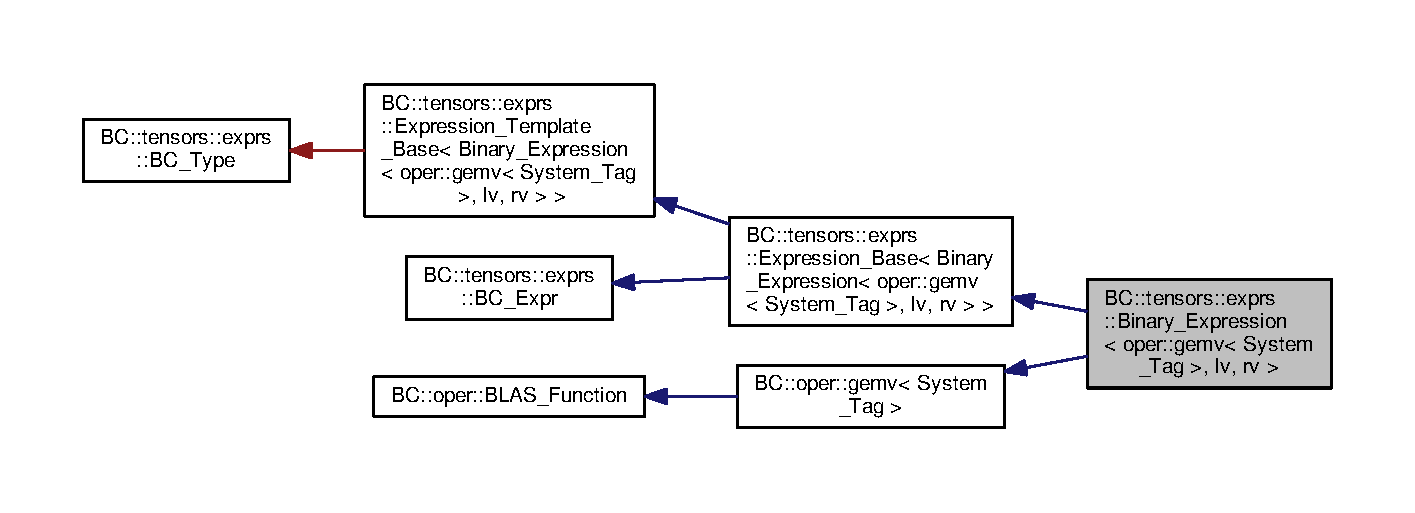
\includegraphics[width=350pt]{structBC_1_1tensors_1_1exprs_1_1Binary__Expression_3_01oper_1_1gemv_3_01System__Tag_01_4_00_01lv_00_01rv_01_4__inherit__graph}
\end{center}
\end{figure}


Collaboration diagram for BC\+:\+:tensors\+:\+:exprs\+:\+:Binary\+\_\+\+Expression$<$ oper\+:\+:gemv$<$ System\+\_\+\+Tag $>$, lv, rv $>$\+:
\nopagebreak
\begin{figure}[H]
\begin{center}
\leavevmode
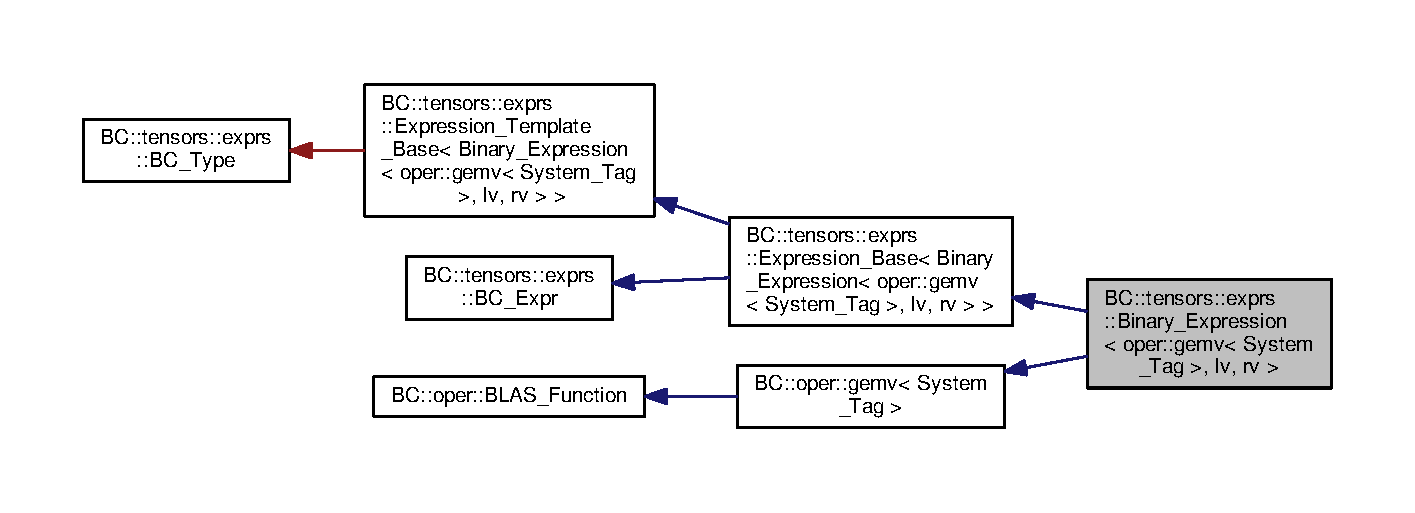
\includegraphics[width=350pt]{structBC_1_1tensors_1_1exprs_1_1Binary__Expression_3_01oper_1_1gemv_3_01System__Tag_01_4_00_01lv_00_01rv_01_4__coll__graph}
\end{center}
\end{figure}
\subsection*{Public Types}
\begin{DoxyCompactItemize}
\item 
using \hyperlink{structBC_1_1tensors_1_1exprs_1_1Binary__Expression_3_01oper_1_1gemv_3_01System__Tag_01_4_00_01lv_00_01rv_01_4_a6774811fac6a06ae5a1ebc6a781cc037}{value\+\_\+type} = typename lv\+::value\+\_\+type
\item 
using \hyperlink{structBC_1_1tensors_1_1exprs_1_1Binary__Expression_3_01oper_1_1gemv_3_01System__Tag_01_4_00_01lv_00_01rv_01_4_aad815e4215ea42213d407fdc313c743b}{system\+\_\+tag} = System\+\_\+\+Tag
\item 
using \hyperlink{structBC_1_1tensors_1_1exprs_1_1Binary__Expression_3_01oper_1_1gemv_3_01System__Tag_01_4_00_01lv_00_01rv_01_4_adefd9fb41ea7fe8d3620a716f4cf66c8}{blas\+\_\+impl} = B\+C\+::blas\+::implementation$<$ \hyperlink{structBC_1_1tensors_1_1exprs_1_1Binary__Expression_3_01oper_1_1gemv_3_01System__Tag_01_4_00_01lv_00_01rv_01_4_aad815e4215ea42213d407fdc313c743b}{system\+\_\+tag} $>$
\item 
using \hyperlink{structBC_1_1tensors_1_1exprs_1_1Binary__Expression_3_01oper_1_1gemv_3_01System__Tag_01_4_00_01lv_00_01rv_01_4_a63ad3ea7c3b038c1c3c9ff08ad2060c4}{blas\+\_\+util} = B\+C\+::tensors\+::exprs\+::blas\+\_\+tools\+::implementation$<$ \hyperlink{structBC_1_1tensors_1_1exprs_1_1Binary__Expression_3_01oper_1_1gemv_3_01System__Tag_01_4_00_01lv_00_01rv_01_4_aad815e4215ea42213d407fdc313c743b}{system\+\_\+tag} $>$
\end{DoxyCompactItemize}
\subsection*{Public Member Functions}
\begin{DoxyCompactItemize}
\item 
\hyperlink{structBC_1_1tensors_1_1exprs_1_1Binary__Expression_3_01oper_1_1gemv_3_01System__Tag_01_4_00_01lv_00_01rv_01_4_a726e9222b38c84c8d5d65847db0e7ffd}{Binary\+\_\+\+Expression} (lv \hyperlink{structBC_1_1tensors_1_1exprs_1_1Binary__Expression_3_01oper_1_1gemv_3_01System__Tag_01_4_00_01lv_00_01rv_01_4_a3addfabe5273dd8a4337b5ed3269cd2a}{left}, rv \hyperlink{structBC_1_1tensors_1_1exprs_1_1Binary__Expression_3_01oper_1_1gemv_3_01System__Tag_01_4_00_01lv_00_01rv_01_4_ab93781c63065643907eed77eb0cd90c5}{right})
\item 
\hyperlink{BlackCat__Common_8h_a6699e8b0449da5c0fafb878e59c1d4b1}{B\+C\+I\+N\+L\+I\+NE} \hyperlink{namespaceBC_a6007cbc4eeec401a037b558910a56173}{B\+C\+::size\+\_\+t} \hyperlink{structBC_1_1tensors_1_1exprs_1_1Binary__Expression_3_01oper_1_1gemv_3_01System__Tag_01_4_00_01lv_00_01rv_01_4_a9dbd4a198bee7b31cd58eb9baefe6999}{size} () const 
\item 
\hyperlink{BlackCat__Common_8h_a6699e8b0449da5c0fafb878e59c1d4b1}{B\+C\+I\+N\+L\+I\+NE} \hyperlink{namespaceBC_a6007cbc4eeec401a037b558910a56173}{B\+C\+::size\+\_\+t} \hyperlink{structBC_1_1tensors_1_1exprs_1_1Binary__Expression_3_01oper_1_1gemv_3_01System__Tag_01_4_00_01lv_00_01rv_01_4_a78e5db912beab5f43eab266932b2f803}{rows} () const 
\item 
\hyperlink{BlackCat__Common_8h_a6699e8b0449da5c0fafb878e59c1d4b1}{B\+C\+I\+N\+L\+I\+NE} \hyperlink{namespaceBC_a6007cbc4eeec401a037b558910a56173}{B\+C\+::size\+\_\+t} \hyperlink{structBC_1_1tensors_1_1exprs_1_1Binary__Expression_3_01oper_1_1gemv_3_01System__Tag_01_4_00_01lv_00_01rv_01_4_afb298f3432432edcbae5086e567e3b97}{cols} () const 
\item 
\hyperlink{BlackCat__Common_8h_a6699e8b0449da5c0fafb878e59c1d4b1}{B\+C\+I\+N\+L\+I\+NE} \hyperlink{namespaceBC_a6007cbc4eeec401a037b558910a56173}{B\+C\+::size\+\_\+t} \hyperlink{structBC_1_1tensors_1_1exprs_1_1Binary__Expression_3_01oper_1_1gemv_3_01System__Tag_01_4_00_01lv_00_01rv_01_4_a65a982052b7aeaaa6aeedcbff5311bda}{dimension} (int i) const 
\item 
\hyperlink{BlackCat__Common_8h_a6699e8b0449da5c0fafb878e59c1d4b1}{B\+C\+I\+N\+L\+I\+NE} \hyperlink{namespaceBC_a6007cbc4eeec401a037b558910a56173}{B\+C\+::size\+\_\+t} \hyperlink{structBC_1_1tensors_1_1exprs_1_1Binary__Expression_3_01oper_1_1gemv_3_01System__Tag_01_4_00_01lv_00_01rv_01_4_ab878c53a4bc20bec60a4afffc9c53a71}{block\+\_\+dimension} (int i) const 
\item 
\hyperlink{BlackCat__Common_8h_a6699e8b0449da5c0fafb878e59c1d4b1}{B\+C\+I\+N\+L\+I\+NE} \hyperlink{namespaceBC_a6007cbc4eeec401a037b558910a56173}{B\+C\+::size\+\_\+t} \hyperlink{structBC_1_1tensors_1_1exprs_1_1Binary__Expression_3_01oper_1_1gemv_3_01System__Tag_01_4_00_01lv_00_01rv_01_4_a93f5365eff658bd1f1579b845f7a010c}{M} () const 
\item 
\hyperlink{BlackCat__Common_8h_a6699e8b0449da5c0fafb878e59c1d4b1}{B\+C\+I\+N\+L\+I\+NE} \hyperlink{namespaceBC_a6007cbc4eeec401a037b558910a56173}{B\+C\+::size\+\_\+t} \hyperlink{structBC_1_1tensors_1_1exprs_1_1Binary__Expression_3_01oper_1_1gemv_3_01System__Tag_01_4_00_01lv_00_01rv_01_4_a41c328a098791d9998afd8ed60359187}{N} () const 
\item 
\hyperlink{BlackCat__Common_8h_a6699e8b0449da5c0fafb878e59c1d4b1}{B\+C\+I\+N\+L\+I\+NE} const auto \hyperlink{structBC_1_1tensors_1_1exprs_1_1Binary__Expression_3_01oper_1_1gemv_3_01System__Tag_01_4_00_01lv_00_01rv_01_4_a5a43da4052fbb1cc58296bb3cfd3cd0d}{inner\+\_\+shape} () const 
\item 
\hyperlink{BlackCat__Common_8h_a6699e8b0449da5c0fafb878e59c1d4b1}{B\+C\+I\+N\+L\+I\+NE} const auto \hyperlink{structBC_1_1tensors_1_1exprs_1_1Binary__Expression_3_01oper_1_1gemv_3_01System__Tag_01_4_00_01lv_00_01rv_01_4_af5481c3b47ce0442909b8787d8ea4177}{block\+\_\+shape} () const 
\item 
{\footnotesize template$<$class core , B\+C\+::size\+\_\+t alpha\+\_\+mod, B\+C\+::size\+\_\+t beta\+\_\+mod, class allocator $>$ }\\void \hyperlink{structBC_1_1tensors_1_1exprs_1_1Binary__Expression_3_01oper_1_1gemv_3_01System__Tag_01_4_00_01lv_00_01rv_01_4_a361b4ae1d329f6c69f31e94c56c948d8}{eval} (\hyperlink{structBC_1_1tensors_1_1exprs_1_1injector}{injector}$<$ core, alpha\+\_\+mod, beta\+\_\+mod $>$ injection\+\_\+values, allocator \&alloc) const 
\end{DoxyCompactItemize}
\subsection*{Public Attributes}
\begin{DoxyCompactItemize}
\item 
lv \hyperlink{structBC_1_1tensors_1_1exprs_1_1Binary__Expression_3_01oper_1_1gemv_3_01System__Tag_01_4_00_01lv_00_01rv_01_4_a3addfabe5273dd8a4337b5ed3269cd2a}{left}
\item 
rv \hyperlink{structBC_1_1tensors_1_1exprs_1_1Binary__Expression_3_01oper_1_1gemv_3_01System__Tag_01_4_00_01lv_00_01rv_01_4_ab93781c63065643907eed77eb0cd90c5}{right}
\end{DoxyCompactItemize}
\subsection*{Static Public Attributes}
\begin{DoxyCompactItemize}
\item 
static constexpr int \hyperlink{structBC_1_1tensors_1_1exprs_1_1Binary__Expression_3_01oper_1_1gemv_3_01System__Tag_01_4_00_01lv_00_01rv_01_4_aeb9702c2975240ee262ac614d9e643d1}{tensor\+\_\+dimension} = 1
\item 
static constexpr int \hyperlink{structBC_1_1tensors_1_1exprs_1_1Binary__Expression_3_01oper_1_1gemv_3_01System__Tag_01_4_00_01lv_00_01rv_01_4_a6cf1f09f15a9d2a8d612d689328b8dbc}{tensor\+\_\+iterator\+\_\+dimension} = 1
\end{DoxyCompactItemize}


\subsection{Member Typedef Documentation}
\index{B\+C\+::tensors\+::exprs\+::\+Binary\+\_\+\+Expression$<$ oper\+::gemv$<$ System\+\_\+\+Tag $>$, lv, rv $>$@{B\+C\+::tensors\+::exprs\+::\+Binary\+\_\+\+Expression$<$ oper\+::gemv$<$ System\+\_\+\+Tag $>$, lv, rv $>$}!blas\+\_\+impl@{blas\+\_\+impl}}
\index{blas\+\_\+impl@{blas\+\_\+impl}!B\+C\+::tensors\+::exprs\+::\+Binary\+\_\+\+Expression$<$ oper\+::gemv$<$ System\+\_\+\+Tag $>$, lv, rv $>$@{B\+C\+::tensors\+::exprs\+::\+Binary\+\_\+\+Expression$<$ oper\+::gemv$<$ System\+\_\+\+Tag $>$, lv, rv $>$}}
\subsubsection[{\texorpdfstring{blas\+\_\+impl}{blas_impl}}]{\setlength{\rightskip}{0pt plus 5cm}template$<$class lv , class rv , class System\+\_\+\+Tag $>$ using {\bf B\+C\+::tensors\+::exprs\+::\+Binary\+\_\+\+Expression}$<$ {\bf oper\+::gemv}$<$ System\+\_\+\+Tag $>$, lv, rv $>$\+::{\bf blas\+\_\+impl} =  B\+C\+::blas\+::implementation$<${\bf system\+\_\+tag}$>$}\hypertarget{structBC_1_1tensors_1_1exprs_1_1Binary__Expression_3_01oper_1_1gemv_3_01System__Tag_01_4_00_01lv_00_01rv_01_4_adefd9fb41ea7fe8d3620a716f4cf66c8}{}\label{structBC_1_1tensors_1_1exprs_1_1Binary__Expression_3_01oper_1_1gemv_3_01System__Tag_01_4_00_01lv_00_01rv_01_4_adefd9fb41ea7fe8d3620a716f4cf66c8}
\index{B\+C\+::tensors\+::exprs\+::\+Binary\+\_\+\+Expression$<$ oper\+::gemv$<$ System\+\_\+\+Tag $>$, lv, rv $>$@{B\+C\+::tensors\+::exprs\+::\+Binary\+\_\+\+Expression$<$ oper\+::gemv$<$ System\+\_\+\+Tag $>$, lv, rv $>$}!blas\+\_\+util@{blas\+\_\+util}}
\index{blas\+\_\+util@{blas\+\_\+util}!B\+C\+::tensors\+::exprs\+::\+Binary\+\_\+\+Expression$<$ oper\+::gemv$<$ System\+\_\+\+Tag $>$, lv, rv $>$@{B\+C\+::tensors\+::exprs\+::\+Binary\+\_\+\+Expression$<$ oper\+::gemv$<$ System\+\_\+\+Tag $>$, lv, rv $>$}}
\subsubsection[{\texorpdfstring{blas\+\_\+util}{blas_util}}]{\setlength{\rightskip}{0pt plus 5cm}template$<$class lv , class rv , class System\+\_\+\+Tag $>$ using {\bf B\+C\+::tensors\+::exprs\+::\+Binary\+\_\+\+Expression}$<$ {\bf oper\+::gemv}$<$ System\+\_\+\+Tag $>$, lv, rv $>$\+::{\bf blas\+\_\+util} =  B\+C\+::tensors\+::exprs\+::blas\+\_\+tools\+::implementation$<${\bf system\+\_\+tag}$>$}\hypertarget{structBC_1_1tensors_1_1exprs_1_1Binary__Expression_3_01oper_1_1gemv_3_01System__Tag_01_4_00_01lv_00_01rv_01_4_a63ad3ea7c3b038c1c3c9ff08ad2060c4}{}\label{structBC_1_1tensors_1_1exprs_1_1Binary__Expression_3_01oper_1_1gemv_3_01System__Tag_01_4_00_01lv_00_01rv_01_4_a63ad3ea7c3b038c1c3c9ff08ad2060c4}
\index{B\+C\+::tensors\+::exprs\+::\+Binary\+\_\+\+Expression$<$ oper\+::gemv$<$ System\+\_\+\+Tag $>$, lv, rv $>$@{B\+C\+::tensors\+::exprs\+::\+Binary\+\_\+\+Expression$<$ oper\+::gemv$<$ System\+\_\+\+Tag $>$, lv, rv $>$}!system\+\_\+tag@{system\+\_\+tag}}
\index{system\+\_\+tag@{system\+\_\+tag}!B\+C\+::tensors\+::exprs\+::\+Binary\+\_\+\+Expression$<$ oper\+::gemv$<$ System\+\_\+\+Tag $>$, lv, rv $>$@{B\+C\+::tensors\+::exprs\+::\+Binary\+\_\+\+Expression$<$ oper\+::gemv$<$ System\+\_\+\+Tag $>$, lv, rv $>$}}
\subsubsection[{\texorpdfstring{system\+\_\+tag}{system_tag}}]{\setlength{\rightskip}{0pt plus 5cm}template$<$class lv , class rv , class System\+\_\+\+Tag $>$ using {\bf B\+C\+::tensors\+::exprs\+::\+Binary\+\_\+\+Expression}$<$ {\bf oper\+::gemv}$<$ System\+\_\+\+Tag $>$, lv, rv $>$\+::{\bf system\+\_\+tag} =  System\+\_\+\+Tag}\hypertarget{structBC_1_1tensors_1_1exprs_1_1Binary__Expression_3_01oper_1_1gemv_3_01System__Tag_01_4_00_01lv_00_01rv_01_4_aad815e4215ea42213d407fdc313c743b}{}\label{structBC_1_1tensors_1_1exprs_1_1Binary__Expression_3_01oper_1_1gemv_3_01System__Tag_01_4_00_01lv_00_01rv_01_4_aad815e4215ea42213d407fdc313c743b}
\index{B\+C\+::tensors\+::exprs\+::\+Binary\+\_\+\+Expression$<$ oper\+::gemv$<$ System\+\_\+\+Tag $>$, lv, rv $>$@{B\+C\+::tensors\+::exprs\+::\+Binary\+\_\+\+Expression$<$ oper\+::gemv$<$ System\+\_\+\+Tag $>$, lv, rv $>$}!value\+\_\+type@{value\+\_\+type}}
\index{value\+\_\+type@{value\+\_\+type}!B\+C\+::tensors\+::exprs\+::\+Binary\+\_\+\+Expression$<$ oper\+::gemv$<$ System\+\_\+\+Tag $>$, lv, rv $>$@{B\+C\+::tensors\+::exprs\+::\+Binary\+\_\+\+Expression$<$ oper\+::gemv$<$ System\+\_\+\+Tag $>$, lv, rv $>$}}
\subsubsection[{\texorpdfstring{value\+\_\+type}{value_type}}]{\setlength{\rightskip}{0pt plus 5cm}template$<$class lv , class rv , class System\+\_\+\+Tag $>$ using {\bf B\+C\+::tensors\+::exprs\+::\+Binary\+\_\+\+Expression}$<$ {\bf oper\+::gemv}$<$ System\+\_\+\+Tag $>$, lv, rv $>$\+::{\bf value\+\_\+type} =  typename lv\+::value\+\_\+type}\hypertarget{structBC_1_1tensors_1_1exprs_1_1Binary__Expression_3_01oper_1_1gemv_3_01System__Tag_01_4_00_01lv_00_01rv_01_4_a6774811fac6a06ae5a1ebc6a781cc037}{}\label{structBC_1_1tensors_1_1exprs_1_1Binary__Expression_3_01oper_1_1gemv_3_01System__Tag_01_4_00_01lv_00_01rv_01_4_a6774811fac6a06ae5a1ebc6a781cc037}


\subsection{Constructor \& Destructor Documentation}
\index{B\+C\+::tensors\+::exprs\+::\+Binary\+\_\+\+Expression$<$ oper\+::gemv$<$ System\+\_\+\+Tag $>$, lv, rv $>$@{B\+C\+::tensors\+::exprs\+::\+Binary\+\_\+\+Expression$<$ oper\+::gemv$<$ System\+\_\+\+Tag $>$, lv, rv $>$}!Binary\+\_\+\+Expression@{Binary\+\_\+\+Expression}}
\index{Binary\+\_\+\+Expression@{Binary\+\_\+\+Expression}!B\+C\+::tensors\+::exprs\+::\+Binary\+\_\+\+Expression$<$ oper\+::gemv$<$ System\+\_\+\+Tag $>$, lv, rv $>$@{B\+C\+::tensors\+::exprs\+::\+Binary\+\_\+\+Expression$<$ oper\+::gemv$<$ System\+\_\+\+Tag $>$, lv, rv $>$}}
\subsubsection[{\texorpdfstring{Binary\+\_\+\+Expression(lv left, rv right)}{Binary_Expression(lv left, rv right)}}]{\setlength{\rightskip}{0pt plus 5cm}template$<$class lv , class rv , class System\+\_\+\+Tag $>$ {\bf B\+C\+::tensors\+::exprs\+::\+Binary\+\_\+\+Expression}$<$ {\bf oper\+::gemv}$<$ System\+\_\+\+Tag $>$, lv, rv $>$\+::{\bf Binary\+\_\+\+Expression} (
\begin{DoxyParamCaption}
\item[{lv}]{left, }
\item[{rv}]{right}
\end{DoxyParamCaption}
)\hspace{0.3cm}{\ttfamily [inline]}}\hypertarget{structBC_1_1tensors_1_1exprs_1_1Binary__Expression_3_01oper_1_1gemv_3_01System__Tag_01_4_00_01lv_00_01rv_01_4_a726e9222b38c84c8d5d65847db0e7ffd}{}\label{structBC_1_1tensors_1_1exprs_1_1Binary__Expression_3_01oper_1_1gemv_3_01System__Tag_01_4_00_01lv_00_01rv_01_4_a726e9222b38c84c8d5d65847db0e7ffd}


\subsection{Member Function Documentation}
\index{B\+C\+::tensors\+::exprs\+::\+Binary\+\_\+\+Expression$<$ oper\+::gemv$<$ System\+\_\+\+Tag $>$, lv, rv $>$@{B\+C\+::tensors\+::exprs\+::\+Binary\+\_\+\+Expression$<$ oper\+::gemv$<$ System\+\_\+\+Tag $>$, lv, rv $>$}!block\+\_\+dimension@{block\+\_\+dimension}}
\index{block\+\_\+dimension@{block\+\_\+dimension}!B\+C\+::tensors\+::exprs\+::\+Binary\+\_\+\+Expression$<$ oper\+::gemv$<$ System\+\_\+\+Tag $>$, lv, rv $>$@{B\+C\+::tensors\+::exprs\+::\+Binary\+\_\+\+Expression$<$ oper\+::gemv$<$ System\+\_\+\+Tag $>$, lv, rv $>$}}
\subsubsection[{\texorpdfstring{block\+\_\+dimension(int i) const }{block_dimension(int i) const }}]{\setlength{\rightskip}{0pt plus 5cm}template$<$class lv , class rv , class System\+\_\+\+Tag $>$ {\bf B\+C\+I\+N\+L\+I\+NE} {\bf B\+C\+::size\+\_\+t} {\bf B\+C\+::tensors\+::exprs\+::\+Binary\+\_\+\+Expression}$<$ {\bf oper\+::gemv}$<$ System\+\_\+\+Tag $>$, lv, rv $>$\+::block\+\_\+dimension (
\begin{DoxyParamCaption}
\item[{int}]{i}
\end{DoxyParamCaption}
) const\hspace{0.3cm}{\ttfamily [inline]}}\hypertarget{structBC_1_1tensors_1_1exprs_1_1Binary__Expression_3_01oper_1_1gemv_3_01System__Tag_01_4_00_01lv_00_01rv_01_4_ab878c53a4bc20bec60a4afffc9c53a71}{}\label{structBC_1_1tensors_1_1exprs_1_1Binary__Expression_3_01oper_1_1gemv_3_01System__Tag_01_4_00_01lv_00_01rv_01_4_ab878c53a4bc20bec60a4afffc9c53a71}
\index{B\+C\+::tensors\+::exprs\+::\+Binary\+\_\+\+Expression$<$ oper\+::gemv$<$ System\+\_\+\+Tag $>$, lv, rv $>$@{B\+C\+::tensors\+::exprs\+::\+Binary\+\_\+\+Expression$<$ oper\+::gemv$<$ System\+\_\+\+Tag $>$, lv, rv $>$}!block\+\_\+shape@{block\+\_\+shape}}
\index{block\+\_\+shape@{block\+\_\+shape}!B\+C\+::tensors\+::exprs\+::\+Binary\+\_\+\+Expression$<$ oper\+::gemv$<$ System\+\_\+\+Tag $>$, lv, rv $>$@{B\+C\+::tensors\+::exprs\+::\+Binary\+\_\+\+Expression$<$ oper\+::gemv$<$ System\+\_\+\+Tag $>$, lv, rv $>$}}
\subsubsection[{\texorpdfstring{block\+\_\+shape() const }{block_shape() const }}]{\setlength{\rightskip}{0pt plus 5cm}template$<$class lv , class rv , class System\+\_\+\+Tag $>$ {\bf B\+C\+I\+N\+L\+I\+NE} const auto {\bf B\+C\+::tensors\+::exprs\+::\+Binary\+\_\+\+Expression}$<$ {\bf oper\+::gemv}$<$ System\+\_\+\+Tag $>$, lv, rv $>$\+::block\+\_\+shape (
\begin{DoxyParamCaption}
{}
\end{DoxyParamCaption}
) const\hspace{0.3cm}{\ttfamily [inline]}}\hypertarget{structBC_1_1tensors_1_1exprs_1_1Binary__Expression_3_01oper_1_1gemv_3_01System__Tag_01_4_00_01lv_00_01rv_01_4_af5481c3b47ce0442909b8787d8ea4177}{}\label{structBC_1_1tensors_1_1exprs_1_1Binary__Expression_3_01oper_1_1gemv_3_01System__Tag_01_4_00_01lv_00_01rv_01_4_af5481c3b47ce0442909b8787d8ea4177}
\index{B\+C\+::tensors\+::exprs\+::\+Binary\+\_\+\+Expression$<$ oper\+::gemv$<$ System\+\_\+\+Tag $>$, lv, rv $>$@{B\+C\+::tensors\+::exprs\+::\+Binary\+\_\+\+Expression$<$ oper\+::gemv$<$ System\+\_\+\+Tag $>$, lv, rv $>$}!cols@{cols}}
\index{cols@{cols}!B\+C\+::tensors\+::exprs\+::\+Binary\+\_\+\+Expression$<$ oper\+::gemv$<$ System\+\_\+\+Tag $>$, lv, rv $>$@{B\+C\+::tensors\+::exprs\+::\+Binary\+\_\+\+Expression$<$ oper\+::gemv$<$ System\+\_\+\+Tag $>$, lv, rv $>$}}
\subsubsection[{\texorpdfstring{cols() const }{cols() const }}]{\setlength{\rightskip}{0pt plus 5cm}template$<$class lv , class rv , class System\+\_\+\+Tag $>$ {\bf B\+C\+I\+N\+L\+I\+NE} {\bf B\+C\+::size\+\_\+t} {\bf B\+C\+::tensors\+::exprs\+::\+Binary\+\_\+\+Expression}$<$ {\bf oper\+::gemv}$<$ System\+\_\+\+Tag $>$, lv, rv $>$\+::cols (
\begin{DoxyParamCaption}
{}
\end{DoxyParamCaption}
) const\hspace{0.3cm}{\ttfamily [inline]}}\hypertarget{structBC_1_1tensors_1_1exprs_1_1Binary__Expression_3_01oper_1_1gemv_3_01System__Tag_01_4_00_01lv_00_01rv_01_4_afb298f3432432edcbae5086e567e3b97}{}\label{structBC_1_1tensors_1_1exprs_1_1Binary__Expression_3_01oper_1_1gemv_3_01System__Tag_01_4_00_01lv_00_01rv_01_4_afb298f3432432edcbae5086e567e3b97}
\index{B\+C\+::tensors\+::exprs\+::\+Binary\+\_\+\+Expression$<$ oper\+::gemv$<$ System\+\_\+\+Tag $>$, lv, rv $>$@{B\+C\+::tensors\+::exprs\+::\+Binary\+\_\+\+Expression$<$ oper\+::gemv$<$ System\+\_\+\+Tag $>$, lv, rv $>$}!dimension@{dimension}}
\index{dimension@{dimension}!B\+C\+::tensors\+::exprs\+::\+Binary\+\_\+\+Expression$<$ oper\+::gemv$<$ System\+\_\+\+Tag $>$, lv, rv $>$@{B\+C\+::tensors\+::exprs\+::\+Binary\+\_\+\+Expression$<$ oper\+::gemv$<$ System\+\_\+\+Tag $>$, lv, rv $>$}}
\subsubsection[{\texorpdfstring{dimension(int i) const }{dimension(int i) const }}]{\setlength{\rightskip}{0pt plus 5cm}template$<$class lv , class rv , class System\+\_\+\+Tag $>$ {\bf B\+C\+I\+N\+L\+I\+NE} {\bf B\+C\+::size\+\_\+t} {\bf B\+C\+::tensors\+::exprs\+::\+Binary\+\_\+\+Expression}$<$ {\bf oper\+::gemv}$<$ System\+\_\+\+Tag $>$, lv, rv $>$\+::dimension (
\begin{DoxyParamCaption}
\item[{int}]{i}
\end{DoxyParamCaption}
) const\hspace{0.3cm}{\ttfamily [inline]}}\hypertarget{structBC_1_1tensors_1_1exprs_1_1Binary__Expression_3_01oper_1_1gemv_3_01System__Tag_01_4_00_01lv_00_01rv_01_4_a65a982052b7aeaaa6aeedcbff5311bda}{}\label{structBC_1_1tensors_1_1exprs_1_1Binary__Expression_3_01oper_1_1gemv_3_01System__Tag_01_4_00_01lv_00_01rv_01_4_a65a982052b7aeaaa6aeedcbff5311bda}
\index{B\+C\+::tensors\+::exprs\+::\+Binary\+\_\+\+Expression$<$ oper\+::gemv$<$ System\+\_\+\+Tag $>$, lv, rv $>$@{B\+C\+::tensors\+::exprs\+::\+Binary\+\_\+\+Expression$<$ oper\+::gemv$<$ System\+\_\+\+Tag $>$, lv, rv $>$}!eval@{eval}}
\index{eval@{eval}!B\+C\+::tensors\+::exprs\+::\+Binary\+\_\+\+Expression$<$ oper\+::gemv$<$ System\+\_\+\+Tag $>$, lv, rv $>$@{B\+C\+::tensors\+::exprs\+::\+Binary\+\_\+\+Expression$<$ oper\+::gemv$<$ System\+\_\+\+Tag $>$, lv, rv $>$}}
\subsubsection[{\texorpdfstring{eval(injector$<$ core, alpha\+\_\+mod, beta\+\_\+mod $>$ injection\+\_\+values, allocator \&alloc) const }{eval(injector< core, alpha_mod, beta_mod > injection_values, allocator &alloc) const }}]{\setlength{\rightskip}{0pt plus 5cm}template$<$class lv , class rv , class System\+\_\+\+Tag $>$ template$<$class core , B\+C\+::size\+\_\+t alpha\+\_\+mod, B\+C\+::size\+\_\+t beta\+\_\+mod, class allocator $>$ void {\bf B\+C\+::tensors\+::exprs\+::\+Binary\+\_\+\+Expression}$<$ {\bf oper\+::gemv}$<$ System\+\_\+\+Tag $>$, lv, rv $>$\+::eval (
\begin{DoxyParamCaption}
\item[{{\bf injector}$<$ core, alpha\+\_\+mod, beta\+\_\+mod $>$}]{injection\+\_\+values, }
\item[{allocator \&}]{alloc}
\end{DoxyParamCaption}
) const\hspace{0.3cm}{\ttfamily [inline]}}\hypertarget{structBC_1_1tensors_1_1exprs_1_1Binary__Expression_3_01oper_1_1gemv_3_01System__Tag_01_4_00_01lv_00_01rv_01_4_a361b4ae1d329f6c69f31e94c56c948d8}{}\label{structBC_1_1tensors_1_1exprs_1_1Binary__Expression_3_01oper_1_1gemv_3_01System__Tag_01_4_00_01lv_00_01rv_01_4_a361b4ae1d329f6c69f31e94c56c948d8}
\index{B\+C\+::tensors\+::exprs\+::\+Binary\+\_\+\+Expression$<$ oper\+::gemv$<$ System\+\_\+\+Tag $>$, lv, rv $>$@{B\+C\+::tensors\+::exprs\+::\+Binary\+\_\+\+Expression$<$ oper\+::gemv$<$ System\+\_\+\+Tag $>$, lv, rv $>$}!inner\+\_\+shape@{inner\+\_\+shape}}
\index{inner\+\_\+shape@{inner\+\_\+shape}!B\+C\+::tensors\+::exprs\+::\+Binary\+\_\+\+Expression$<$ oper\+::gemv$<$ System\+\_\+\+Tag $>$, lv, rv $>$@{B\+C\+::tensors\+::exprs\+::\+Binary\+\_\+\+Expression$<$ oper\+::gemv$<$ System\+\_\+\+Tag $>$, lv, rv $>$}}
\subsubsection[{\texorpdfstring{inner\+\_\+shape() const }{inner_shape() const }}]{\setlength{\rightskip}{0pt plus 5cm}template$<$class lv , class rv , class System\+\_\+\+Tag $>$ {\bf B\+C\+I\+N\+L\+I\+NE} const auto {\bf B\+C\+::tensors\+::exprs\+::\+Binary\+\_\+\+Expression}$<$ {\bf oper\+::gemv}$<$ System\+\_\+\+Tag $>$, lv, rv $>$\+::inner\+\_\+shape (
\begin{DoxyParamCaption}
{}
\end{DoxyParamCaption}
) const\hspace{0.3cm}{\ttfamily [inline]}}\hypertarget{structBC_1_1tensors_1_1exprs_1_1Binary__Expression_3_01oper_1_1gemv_3_01System__Tag_01_4_00_01lv_00_01rv_01_4_a5a43da4052fbb1cc58296bb3cfd3cd0d}{}\label{structBC_1_1tensors_1_1exprs_1_1Binary__Expression_3_01oper_1_1gemv_3_01System__Tag_01_4_00_01lv_00_01rv_01_4_a5a43da4052fbb1cc58296bb3cfd3cd0d}
\index{B\+C\+::tensors\+::exprs\+::\+Binary\+\_\+\+Expression$<$ oper\+::gemv$<$ System\+\_\+\+Tag $>$, lv, rv $>$@{B\+C\+::tensors\+::exprs\+::\+Binary\+\_\+\+Expression$<$ oper\+::gemv$<$ System\+\_\+\+Tag $>$, lv, rv $>$}!M@{M}}
\index{M@{M}!B\+C\+::tensors\+::exprs\+::\+Binary\+\_\+\+Expression$<$ oper\+::gemv$<$ System\+\_\+\+Tag $>$, lv, rv $>$@{B\+C\+::tensors\+::exprs\+::\+Binary\+\_\+\+Expression$<$ oper\+::gemv$<$ System\+\_\+\+Tag $>$, lv, rv $>$}}
\subsubsection[{\texorpdfstring{M() const }{M() const }}]{\setlength{\rightskip}{0pt plus 5cm}template$<$class lv , class rv , class System\+\_\+\+Tag $>$ {\bf B\+C\+I\+N\+L\+I\+NE} {\bf B\+C\+::size\+\_\+t} {\bf B\+C\+::tensors\+::exprs\+::\+Binary\+\_\+\+Expression}$<$ {\bf oper\+::gemv}$<$ System\+\_\+\+Tag $>$, lv, rv $>$\+::M (
\begin{DoxyParamCaption}
{}
\end{DoxyParamCaption}
) const\hspace{0.3cm}{\ttfamily [inline]}}\hypertarget{structBC_1_1tensors_1_1exprs_1_1Binary__Expression_3_01oper_1_1gemv_3_01System__Tag_01_4_00_01lv_00_01rv_01_4_a93f5365eff658bd1f1579b845f7a010c}{}\label{structBC_1_1tensors_1_1exprs_1_1Binary__Expression_3_01oper_1_1gemv_3_01System__Tag_01_4_00_01lv_00_01rv_01_4_a93f5365eff658bd1f1579b845f7a010c}
\index{B\+C\+::tensors\+::exprs\+::\+Binary\+\_\+\+Expression$<$ oper\+::gemv$<$ System\+\_\+\+Tag $>$, lv, rv $>$@{B\+C\+::tensors\+::exprs\+::\+Binary\+\_\+\+Expression$<$ oper\+::gemv$<$ System\+\_\+\+Tag $>$, lv, rv $>$}!N@{N}}
\index{N@{N}!B\+C\+::tensors\+::exprs\+::\+Binary\+\_\+\+Expression$<$ oper\+::gemv$<$ System\+\_\+\+Tag $>$, lv, rv $>$@{B\+C\+::tensors\+::exprs\+::\+Binary\+\_\+\+Expression$<$ oper\+::gemv$<$ System\+\_\+\+Tag $>$, lv, rv $>$}}
\subsubsection[{\texorpdfstring{N() const }{N() const }}]{\setlength{\rightskip}{0pt plus 5cm}template$<$class lv , class rv , class System\+\_\+\+Tag $>$ {\bf B\+C\+I\+N\+L\+I\+NE} {\bf B\+C\+::size\+\_\+t} {\bf B\+C\+::tensors\+::exprs\+::\+Binary\+\_\+\+Expression}$<$ {\bf oper\+::gemv}$<$ System\+\_\+\+Tag $>$, lv, rv $>$\+::N (
\begin{DoxyParamCaption}
{}
\end{DoxyParamCaption}
) const\hspace{0.3cm}{\ttfamily [inline]}}\hypertarget{structBC_1_1tensors_1_1exprs_1_1Binary__Expression_3_01oper_1_1gemv_3_01System__Tag_01_4_00_01lv_00_01rv_01_4_a41c328a098791d9998afd8ed60359187}{}\label{structBC_1_1tensors_1_1exprs_1_1Binary__Expression_3_01oper_1_1gemv_3_01System__Tag_01_4_00_01lv_00_01rv_01_4_a41c328a098791d9998afd8ed60359187}
\index{B\+C\+::tensors\+::exprs\+::\+Binary\+\_\+\+Expression$<$ oper\+::gemv$<$ System\+\_\+\+Tag $>$, lv, rv $>$@{B\+C\+::tensors\+::exprs\+::\+Binary\+\_\+\+Expression$<$ oper\+::gemv$<$ System\+\_\+\+Tag $>$, lv, rv $>$}!rows@{rows}}
\index{rows@{rows}!B\+C\+::tensors\+::exprs\+::\+Binary\+\_\+\+Expression$<$ oper\+::gemv$<$ System\+\_\+\+Tag $>$, lv, rv $>$@{B\+C\+::tensors\+::exprs\+::\+Binary\+\_\+\+Expression$<$ oper\+::gemv$<$ System\+\_\+\+Tag $>$, lv, rv $>$}}
\subsubsection[{\texorpdfstring{rows() const }{rows() const }}]{\setlength{\rightskip}{0pt plus 5cm}template$<$class lv , class rv , class System\+\_\+\+Tag $>$ {\bf B\+C\+I\+N\+L\+I\+NE} {\bf B\+C\+::size\+\_\+t} {\bf B\+C\+::tensors\+::exprs\+::\+Binary\+\_\+\+Expression}$<$ {\bf oper\+::gemv}$<$ System\+\_\+\+Tag $>$, lv, rv $>$\+::rows (
\begin{DoxyParamCaption}
{}
\end{DoxyParamCaption}
) const\hspace{0.3cm}{\ttfamily [inline]}}\hypertarget{structBC_1_1tensors_1_1exprs_1_1Binary__Expression_3_01oper_1_1gemv_3_01System__Tag_01_4_00_01lv_00_01rv_01_4_a78e5db912beab5f43eab266932b2f803}{}\label{structBC_1_1tensors_1_1exprs_1_1Binary__Expression_3_01oper_1_1gemv_3_01System__Tag_01_4_00_01lv_00_01rv_01_4_a78e5db912beab5f43eab266932b2f803}
\index{B\+C\+::tensors\+::exprs\+::\+Binary\+\_\+\+Expression$<$ oper\+::gemv$<$ System\+\_\+\+Tag $>$, lv, rv $>$@{B\+C\+::tensors\+::exprs\+::\+Binary\+\_\+\+Expression$<$ oper\+::gemv$<$ System\+\_\+\+Tag $>$, lv, rv $>$}!size@{size}}
\index{size@{size}!B\+C\+::tensors\+::exprs\+::\+Binary\+\_\+\+Expression$<$ oper\+::gemv$<$ System\+\_\+\+Tag $>$, lv, rv $>$@{B\+C\+::tensors\+::exprs\+::\+Binary\+\_\+\+Expression$<$ oper\+::gemv$<$ System\+\_\+\+Tag $>$, lv, rv $>$}}
\subsubsection[{\texorpdfstring{size() const }{size() const }}]{\setlength{\rightskip}{0pt plus 5cm}template$<$class lv , class rv , class System\+\_\+\+Tag $>$ {\bf B\+C\+I\+N\+L\+I\+NE} {\bf B\+C\+::size\+\_\+t} {\bf B\+C\+::tensors\+::exprs\+::\+Binary\+\_\+\+Expression}$<$ {\bf oper\+::gemv}$<$ System\+\_\+\+Tag $>$, lv, rv $>$\+::size (
\begin{DoxyParamCaption}
{}
\end{DoxyParamCaption}
) const\hspace{0.3cm}{\ttfamily [inline]}}\hypertarget{structBC_1_1tensors_1_1exprs_1_1Binary__Expression_3_01oper_1_1gemv_3_01System__Tag_01_4_00_01lv_00_01rv_01_4_a9dbd4a198bee7b31cd58eb9baefe6999}{}\label{structBC_1_1tensors_1_1exprs_1_1Binary__Expression_3_01oper_1_1gemv_3_01System__Tag_01_4_00_01lv_00_01rv_01_4_a9dbd4a198bee7b31cd58eb9baefe6999}


\subsection{Member Data Documentation}
\index{B\+C\+::tensors\+::exprs\+::\+Binary\+\_\+\+Expression$<$ oper\+::gemv$<$ System\+\_\+\+Tag $>$, lv, rv $>$@{B\+C\+::tensors\+::exprs\+::\+Binary\+\_\+\+Expression$<$ oper\+::gemv$<$ System\+\_\+\+Tag $>$, lv, rv $>$}!left@{left}}
\index{left@{left}!B\+C\+::tensors\+::exprs\+::\+Binary\+\_\+\+Expression$<$ oper\+::gemv$<$ System\+\_\+\+Tag $>$, lv, rv $>$@{B\+C\+::tensors\+::exprs\+::\+Binary\+\_\+\+Expression$<$ oper\+::gemv$<$ System\+\_\+\+Tag $>$, lv, rv $>$}}
\subsubsection[{\texorpdfstring{left}{left}}]{\setlength{\rightskip}{0pt plus 5cm}template$<$class lv , class rv , class System\+\_\+\+Tag $>$ lv {\bf B\+C\+::tensors\+::exprs\+::\+Binary\+\_\+\+Expression}$<$ {\bf oper\+::gemv}$<$ System\+\_\+\+Tag $>$, lv, rv $>$\+::left}\hypertarget{structBC_1_1tensors_1_1exprs_1_1Binary__Expression_3_01oper_1_1gemv_3_01System__Tag_01_4_00_01lv_00_01rv_01_4_a3addfabe5273dd8a4337b5ed3269cd2a}{}\label{structBC_1_1tensors_1_1exprs_1_1Binary__Expression_3_01oper_1_1gemv_3_01System__Tag_01_4_00_01lv_00_01rv_01_4_a3addfabe5273dd8a4337b5ed3269cd2a}
\index{B\+C\+::tensors\+::exprs\+::\+Binary\+\_\+\+Expression$<$ oper\+::gemv$<$ System\+\_\+\+Tag $>$, lv, rv $>$@{B\+C\+::tensors\+::exprs\+::\+Binary\+\_\+\+Expression$<$ oper\+::gemv$<$ System\+\_\+\+Tag $>$, lv, rv $>$}!right@{right}}
\index{right@{right}!B\+C\+::tensors\+::exprs\+::\+Binary\+\_\+\+Expression$<$ oper\+::gemv$<$ System\+\_\+\+Tag $>$, lv, rv $>$@{B\+C\+::tensors\+::exprs\+::\+Binary\+\_\+\+Expression$<$ oper\+::gemv$<$ System\+\_\+\+Tag $>$, lv, rv $>$}}
\subsubsection[{\texorpdfstring{right}{right}}]{\setlength{\rightskip}{0pt plus 5cm}template$<$class lv , class rv , class System\+\_\+\+Tag $>$ rv {\bf B\+C\+::tensors\+::exprs\+::\+Binary\+\_\+\+Expression}$<$ {\bf oper\+::gemv}$<$ System\+\_\+\+Tag $>$, lv, rv $>$\+::right}\hypertarget{structBC_1_1tensors_1_1exprs_1_1Binary__Expression_3_01oper_1_1gemv_3_01System__Tag_01_4_00_01lv_00_01rv_01_4_ab93781c63065643907eed77eb0cd90c5}{}\label{structBC_1_1tensors_1_1exprs_1_1Binary__Expression_3_01oper_1_1gemv_3_01System__Tag_01_4_00_01lv_00_01rv_01_4_ab93781c63065643907eed77eb0cd90c5}
\index{B\+C\+::tensors\+::exprs\+::\+Binary\+\_\+\+Expression$<$ oper\+::gemv$<$ System\+\_\+\+Tag $>$, lv, rv $>$@{B\+C\+::tensors\+::exprs\+::\+Binary\+\_\+\+Expression$<$ oper\+::gemv$<$ System\+\_\+\+Tag $>$, lv, rv $>$}!tensor\+\_\+dimension@{tensor\+\_\+dimension}}
\index{tensor\+\_\+dimension@{tensor\+\_\+dimension}!B\+C\+::tensors\+::exprs\+::\+Binary\+\_\+\+Expression$<$ oper\+::gemv$<$ System\+\_\+\+Tag $>$, lv, rv $>$@{B\+C\+::tensors\+::exprs\+::\+Binary\+\_\+\+Expression$<$ oper\+::gemv$<$ System\+\_\+\+Tag $>$, lv, rv $>$}}
\subsubsection[{\texorpdfstring{tensor\+\_\+dimension}{tensor_dimension}}]{\setlength{\rightskip}{0pt plus 5cm}template$<$class lv , class rv , class System\+\_\+\+Tag $>$ constexpr int {\bf B\+C\+::tensors\+::exprs\+::\+Binary\+\_\+\+Expression}$<$ {\bf oper\+::gemv}$<$ System\+\_\+\+Tag $>$, lv, rv $>$\+::tensor\+\_\+dimension = 1\hspace{0.3cm}{\ttfamily [static]}}\hypertarget{structBC_1_1tensors_1_1exprs_1_1Binary__Expression_3_01oper_1_1gemv_3_01System__Tag_01_4_00_01lv_00_01rv_01_4_aeb9702c2975240ee262ac614d9e643d1}{}\label{structBC_1_1tensors_1_1exprs_1_1Binary__Expression_3_01oper_1_1gemv_3_01System__Tag_01_4_00_01lv_00_01rv_01_4_aeb9702c2975240ee262ac614d9e643d1}
\index{B\+C\+::tensors\+::exprs\+::\+Binary\+\_\+\+Expression$<$ oper\+::gemv$<$ System\+\_\+\+Tag $>$, lv, rv $>$@{B\+C\+::tensors\+::exprs\+::\+Binary\+\_\+\+Expression$<$ oper\+::gemv$<$ System\+\_\+\+Tag $>$, lv, rv $>$}!tensor\+\_\+iterator\+\_\+dimension@{tensor\+\_\+iterator\+\_\+dimension}}
\index{tensor\+\_\+iterator\+\_\+dimension@{tensor\+\_\+iterator\+\_\+dimension}!B\+C\+::tensors\+::exprs\+::\+Binary\+\_\+\+Expression$<$ oper\+::gemv$<$ System\+\_\+\+Tag $>$, lv, rv $>$@{B\+C\+::tensors\+::exprs\+::\+Binary\+\_\+\+Expression$<$ oper\+::gemv$<$ System\+\_\+\+Tag $>$, lv, rv $>$}}
\subsubsection[{\texorpdfstring{tensor\+\_\+iterator\+\_\+dimension}{tensor_iterator_dimension}}]{\setlength{\rightskip}{0pt plus 5cm}template$<$class lv , class rv , class System\+\_\+\+Tag $>$ constexpr int {\bf B\+C\+::tensors\+::exprs\+::\+Binary\+\_\+\+Expression}$<$ {\bf oper\+::gemv}$<$ System\+\_\+\+Tag $>$, lv, rv $>$\+::tensor\+\_\+iterator\+\_\+dimension = 1\hspace{0.3cm}{\ttfamily [static]}}\hypertarget{structBC_1_1tensors_1_1exprs_1_1Binary__Expression_3_01oper_1_1gemv_3_01System__Tag_01_4_00_01lv_00_01rv_01_4_a6cf1f09f15a9d2a8d612d689328b8dbc}{}\label{structBC_1_1tensors_1_1exprs_1_1Binary__Expression_3_01oper_1_1gemv_3_01System__Tag_01_4_00_01lv_00_01rv_01_4_a6cf1f09f15a9d2a8d612d689328b8dbc}


The documentation for this struct was generated from the following file\+:\begin{DoxyCompactItemize}
\item 
include/tensors/expression\+\_\+templates/\hyperlink{Function__gemv_8h}{Function\+\_\+gemv.\+h}\end{DoxyCompactItemize}

\hypertarget{structBC_1_1tensors_1_1exprs_1_1Binary__Expression_3_01oper_1_1ger_3_01System__Tag_01_4_00_01lv_00_01rv_01_4}{}\section{BC\+:\+:tensors\+:\+:exprs\+:\+:Binary\+\_\+\+Expression$<$ oper\+:\+:ger$<$ System\+\_\+\+Tag $>$, lv, rv $>$ Struct Template Reference}
\label{structBC_1_1tensors_1_1exprs_1_1Binary__Expression_3_01oper_1_1ger_3_01System__Tag_01_4_00_01lv_00_01rv_01_4}\index{B\+C\+::tensors\+::exprs\+::\+Binary\+\_\+\+Expression$<$ oper\+::ger$<$ System\+\_\+\+Tag $>$, lv, rv $>$@{B\+C\+::tensors\+::exprs\+::\+Binary\+\_\+\+Expression$<$ oper\+::ger$<$ System\+\_\+\+Tag $>$, lv, rv $>$}}


{\ttfamily \#include $<$Function\+\_\+ger.\+h$>$}



Inheritance diagram for BC\+:\+:tensors\+:\+:exprs\+:\+:Binary\+\_\+\+Expression$<$ oper\+:\+:ger$<$ System\+\_\+\+Tag $>$, lv, rv $>$\+:
\nopagebreak
\begin{figure}[H]
\begin{center}
\leavevmode
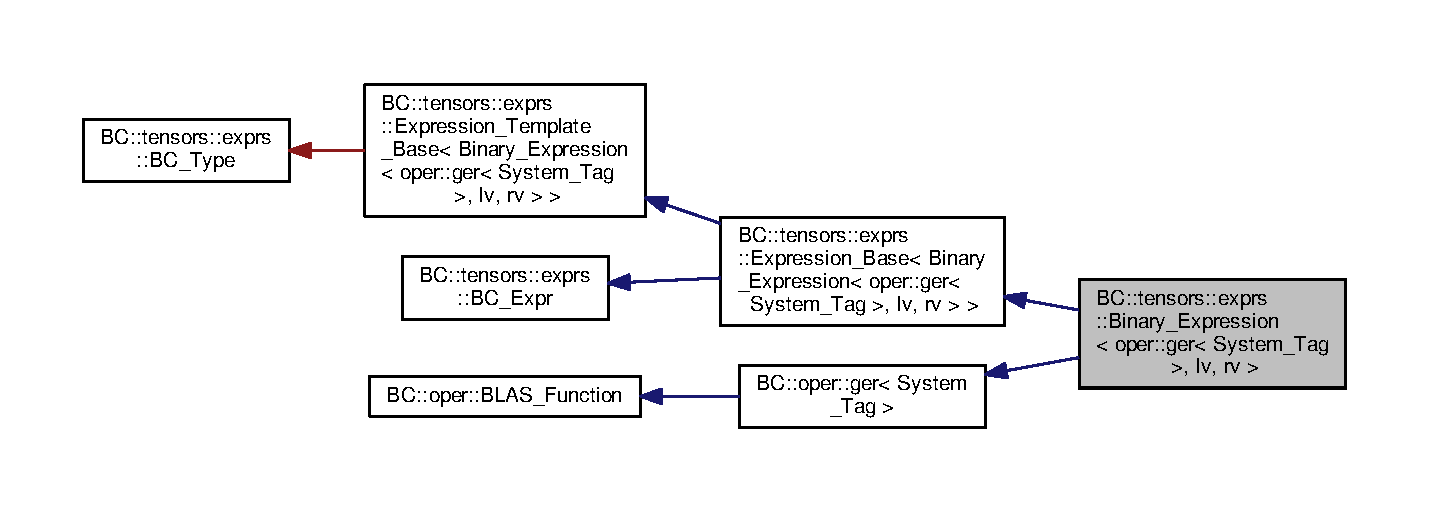
\includegraphics[width=350pt]{structBC_1_1tensors_1_1exprs_1_1Binary__Expression_3_01oper_1_1ger_3_01System__Tag_01_4_00_01lv_00_01rv_01_4__inherit__graph}
\end{center}
\end{figure}


Collaboration diagram for BC\+:\+:tensors\+:\+:exprs\+:\+:Binary\+\_\+\+Expression$<$ oper\+:\+:ger$<$ System\+\_\+\+Tag $>$, lv, rv $>$\+:
\nopagebreak
\begin{figure}[H]
\begin{center}
\leavevmode
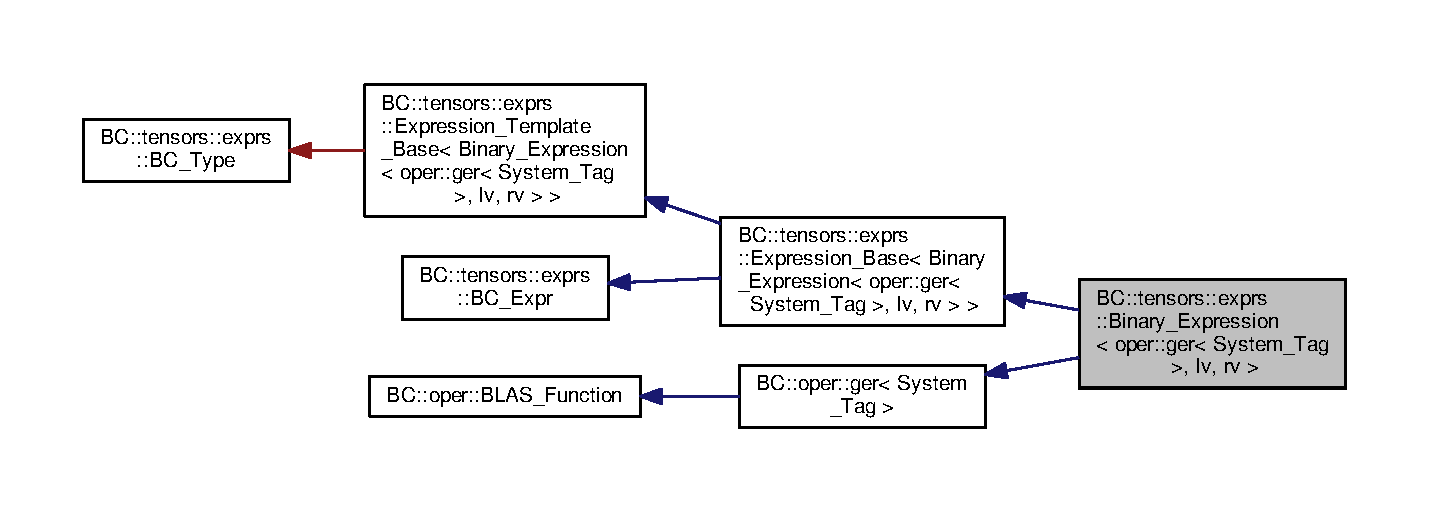
\includegraphics[width=350pt]{structBC_1_1tensors_1_1exprs_1_1Binary__Expression_3_01oper_1_1ger_3_01System__Tag_01_4_00_01lv_00_01rv_01_4__coll__graph}
\end{center}
\end{figure}
\subsection*{Public Types}
\begin{DoxyCompactItemize}
\item 
using \hyperlink{structBC_1_1tensors_1_1exprs_1_1Binary__Expression_3_01oper_1_1ger_3_01System__Tag_01_4_00_01lv_00_01rv_01_4_a6ac4fe29d966c3819173490d09bfc413}{value\+\_\+type} = typename lv\+::value\+\_\+type
\item 
using \hyperlink{structBC_1_1tensors_1_1exprs_1_1Binary__Expression_3_01oper_1_1ger_3_01System__Tag_01_4_00_01lv_00_01rv_01_4_a087017a7ded7d52e1641faddcd5b6501}{system\+\_\+tag} = System\+\_\+\+Tag
\item 
using \hyperlink{structBC_1_1tensors_1_1exprs_1_1Binary__Expression_3_01oper_1_1ger_3_01System__Tag_01_4_00_01lv_00_01rv_01_4_adcfcdcec708b2aa91f056c9fe2e4e374}{blas\+\_\+impl} = B\+C\+::blas\+::implementation$<$ \hyperlink{structBC_1_1tensors_1_1exprs_1_1Binary__Expression_3_01oper_1_1ger_3_01System__Tag_01_4_00_01lv_00_01rv_01_4_a087017a7ded7d52e1641faddcd5b6501}{system\+\_\+tag} $>$
\item 
using \hyperlink{structBC_1_1tensors_1_1exprs_1_1Binary__Expression_3_01oper_1_1ger_3_01System__Tag_01_4_00_01lv_00_01rv_01_4_a6b62470f64fee5f5d15d57ef18464804}{blas\+\_\+util} = B\+C\+::tensors\+::exprs\+::blas\+\_\+tools\+::implementation$<$ \hyperlink{structBC_1_1tensors_1_1exprs_1_1Binary__Expression_3_01oper_1_1ger_3_01System__Tag_01_4_00_01lv_00_01rv_01_4_a087017a7ded7d52e1641faddcd5b6501}{system\+\_\+tag} $>$
\end{DoxyCompactItemize}
\subsection*{Public Member Functions}
\begin{DoxyCompactItemize}
\item 
\hyperlink{structBC_1_1tensors_1_1exprs_1_1Binary__Expression_3_01oper_1_1ger_3_01System__Tag_01_4_00_01lv_00_01rv_01_4_a800ae94c5c578b3766f347e469b7aaea}{Binary\+\_\+\+Expression} (lv \hyperlink{structBC_1_1tensors_1_1exprs_1_1Binary__Expression_3_01oper_1_1ger_3_01System__Tag_01_4_00_01lv_00_01rv_01_4_aed3bb00335897aaaaac661d106de8130}{left}, rv \hyperlink{structBC_1_1tensors_1_1exprs_1_1Binary__Expression_3_01oper_1_1ger_3_01System__Tag_01_4_00_01lv_00_01rv_01_4_a5236c349912f20832a0744a503a9077e}{right})
\item 
\hyperlink{BlackCat__Common_8h_a6699e8b0449da5c0fafb878e59c1d4b1}{B\+C\+I\+N\+L\+I\+NE} \hyperlink{namespaceBC_a6007cbc4eeec401a037b558910a56173}{B\+C\+::size\+\_\+t} \hyperlink{structBC_1_1tensors_1_1exprs_1_1Binary__Expression_3_01oper_1_1ger_3_01System__Tag_01_4_00_01lv_00_01rv_01_4_a561416baebb196808d154d2538074936}{size} () const 
\item 
\hyperlink{BlackCat__Common_8h_a6699e8b0449da5c0fafb878e59c1d4b1}{B\+C\+I\+N\+L\+I\+NE} \hyperlink{namespaceBC_a6007cbc4eeec401a037b558910a56173}{B\+C\+::size\+\_\+t} \hyperlink{structBC_1_1tensors_1_1exprs_1_1Binary__Expression_3_01oper_1_1ger_3_01System__Tag_01_4_00_01lv_00_01rv_01_4_ad5211ab54757976199990516381c7288}{rows} () const 
\item 
\hyperlink{BlackCat__Common_8h_a6699e8b0449da5c0fafb878e59c1d4b1}{B\+C\+I\+N\+L\+I\+NE} \hyperlink{namespaceBC_a6007cbc4eeec401a037b558910a56173}{B\+C\+::size\+\_\+t} \hyperlink{structBC_1_1tensors_1_1exprs_1_1Binary__Expression_3_01oper_1_1ger_3_01System__Tag_01_4_00_01lv_00_01rv_01_4_a7b4233522cc119987f5bd7e0af12db7e}{cols} () const 
\item 
\hyperlink{BlackCat__Common_8h_a6699e8b0449da5c0fafb878e59c1d4b1}{B\+C\+I\+N\+L\+I\+NE} \hyperlink{namespaceBC_a6007cbc4eeec401a037b558910a56173}{B\+C\+::size\+\_\+t} \hyperlink{structBC_1_1tensors_1_1exprs_1_1Binary__Expression_3_01oper_1_1ger_3_01System__Tag_01_4_00_01lv_00_01rv_01_4_a054e7db4b14b16eee63b93284a8dfec7}{dimension} (int i) const 
\item 
\hyperlink{BlackCat__Common_8h_a6699e8b0449da5c0fafb878e59c1d4b1}{B\+C\+I\+N\+L\+I\+NE} \hyperlink{namespaceBC_a6007cbc4eeec401a037b558910a56173}{B\+C\+::size\+\_\+t} \hyperlink{structBC_1_1tensors_1_1exprs_1_1Binary__Expression_3_01oper_1_1ger_3_01System__Tag_01_4_00_01lv_00_01rv_01_4_a05c1f43d25f243b28d46c624b5313884}{block\+\_\+dimension} (int i) const 
\item 
\hyperlink{BlackCat__Common_8h_a6699e8b0449da5c0fafb878e59c1d4b1}{B\+C\+I\+N\+L\+I\+NE} \hyperlink{namespaceBC_a6007cbc4eeec401a037b558910a56173}{B\+C\+::size\+\_\+t} \hyperlink{structBC_1_1tensors_1_1exprs_1_1Binary__Expression_3_01oper_1_1ger_3_01System__Tag_01_4_00_01lv_00_01rv_01_4_a8bb5d9782e997461c186ec4ee222830c}{M} () const 
\item 
\hyperlink{BlackCat__Common_8h_a6699e8b0449da5c0fafb878e59c1d4b1}{B\+C\+I\+N\+L\+I\+NE} \hyperlink{namespaceBC_a6007cbc4eeec401a037b558910a56173}{B\+C\+::size\+\_\+t} \hyperlink{structBC_1_1tensors_1_1exprs_1_1Binary__Expression_3_01oper_1_1ger_3_01System__Tag_01_4_00_01lv_00_01rv_01_4_a0f22d72b767231320427b61f1066260e}{N} () const 
\item 
{\footnotesize template$<$class core , B\+C\+::size\+\_\+t alpha\+\_\+mod, B\+C\+::size\+\_\+t beta\+\_\+mod, class Stream $>$ }\\void \hyperlink{structBC_1_1tensors_1_1exprs_1_1Binary__Expression_3_01oper_1_1ger_3_01System__Tag_01_4_00_01lv_00_01rv_01_4_a491494ab236df60f5e7e3038a09dd707}{eval} (\hyperlink{structBC_1_1tensors_1_1exprs_1_1injector}{injector}$<$ core, alpha\+\_\+mod, beta\+\_\+mod $>$ injection\+\_\+values, \hyperlink{namespaceBC_abc64a63cd29a22d102a68f478dfd588d}{Stream} \&stream) const 
\end{DoxyCompactItemize}
\subsection*{Public Attributes}
\begin{DoxyCompactItemize}
\item 
lv \hyperlink{structBC_1_1tensors_1_1exprs_1_1Binary__Expression_3_01oper_1_1ger_3_01System__Tag_01_4_00_01lv_00_01rv_01_4_aed3bb00335897aaaaac661d106de8130}{left}
\item 
rv \hyperlink{structBC_1_1tensors_1_1exprs_1_1Binary__Expression_3_01oper_1_1ger_3_01System__Tag_01_4_00_01lv_00_01rv_01_4_a5236c349912f20832a0744a503a9077e}{right}
\end{DoxyCompactItemize}
\subsection*{Static Public Attributes}
\begin{DoxyCompactItemize}
\item 
static constexpr int \hyperlink{structBC_1_1tensors_1_1exprs_1_1Binary__Expression_3_01oper_1_1ger_3_01System__Tag_01_4_00_01lv_00_01rv_01_4_a0d83f56593eb3cf084010eb6b6593ce1}{tensor\+\_\+dimension} = 2
\item 
static constexpr int \hyperlink{structBC_1_1tensors_1_1exprs_1_1Binary__Expression_3_01oper_1_1ger_3_01System__Tag_01_4_00_01lv_00_01rv_01_4_a91e2694919251d815e3cd16b47698c3e}{tensor\+\_\+iterator\+\_\+dimension} = 1
\end{DoxyCompactItemize}


\subsection{Member Typedef Documentation}
\index{B\+C\+::tensors\+::exprs\+::\+Binary\+\_\+\+Expression$<$ oper\+::ger$<$ System\+\_\+\+Tag $>$, lv, rv $>$@{B\+C\+::tensors\+::exprs\+::\+Binary\+\_\+\+Expression$<$ oper\+::ger$<$ System\+\_\+\+Tag $>$, lv, rv $>$}!blas\+\_\+impl@{blas\+\_\+impl}}
\index{blas\+\_\+impl@{blas\+\_\+impl}!B\+C\+::tensors\+::exprs\+::\+Binary\+\_\+\+Expression$<$ oper\+::ger$<$ System\+\_\+\+Tag $>$, lv, rv $>$@{B\+C\+::tensors\+::exprs\+::\+Binary\+\_\+\+Expression$<$ oper\+::ger$<$ System\+\_\+\+Tag $>$, lv, rv $>$}}
\subsubsection[{\texorpdfstring{blas\+\_\+impl}{blas_impl}}]{\setlength{\rightskip}{0pt plus 5cm}template$<$class lv , class rv , class System\+\_\+\+Tag $>$ using {\bf B\+C\+::tensors\+::exprs\+::\+Binary\+\_\+\+Expression}$<$ {\bf oper\+::ger}$<$ System\+\_\+\+Tag $>$, lv, rv $>$\+::{\bf blas\+\_\+impl} =  B\+C\+::blas\+::implementation$<${\bf system\+\_\+tag}$>$}\hypertarget{structBC_1_1tensors_1_1exprs_1_1Binary__Expression_3_01oper_1_1ger_3_01System__Tag_01_4_00_01lv_00_01rv_01_4_adcfcdcec708b2aa91f056c9fe2e4e374}{}\label{structBC_1_1tensors_1_1exprs_1_1Binary__Expression_3_01oper_1_1ger_3_01System__Tag_01_4_00_01lv_00_01rv_01_4_adcfcdcec708b2aa91f056c9fe2e4e374}
\index{B\+C\+::tensors\+::exprs\+::\+Binary\+\_\+\+Expression$<$ oper\+::ger$<$ System\+\_\+\+Tag $>$, lv, rv $>$@{B\+C\+::tensors\+::exprs\+::\+Binary\+\_\+\+Expression$<$ oper\+::ger$<$ System\+\_\+\+Tag $>$, lv, rv $>$}!blas\+\_\+util@{blas\+\_\+util}}
\index{blas\+\_\+util@{blas\+\_\+util}!B\+C\+::tensors\+::exprs\+::\+Binary\+\_\+\+Expression$<$ oper\+::ger$<$ System\+\_\+\+Tag $>$, lv, rv $>$@{B\+C\+::tensors\+::exprs\+::\+Binary\+\_\+\+Expression$<$ oper\+::ger$<$ System\+\_\+\+Tag $>$, lv, rv $>$}}
\subsubsection[{\texorpdfstring{blas\+\_\+util}{blas_util}}]{\setlength{\rightskip}{0pt plus 5cm}template$<$class lv , class rv , class System\+\_\+\+Tag $>$ using {\bf B\+C\+::tensors\+::exprs\+::\+Binary\+\_\+\+Expression}$<$ {\bf oper\+::ger}$<$ System\+\_\+\+Tag $>$, lv, rv $>$\+::{\bf blas\+\_\+util} =  B\+C\+::tensors\+::exprs\+::blas\+\_\+tools\+::implementation$<${\bf system\+\_\+tag}$>$}\hypertarget{structBC_1_1tensors_1_1exprs_1_1Binary__Expression_3_01oper_1_1ger_3_01System__Tag_01_4_00_01lv_00_01rv_01_4_a6b62470f64fee5f5d15d57ef18464804}{}\label{structBC_1_1tensors_1_1exprs_1_1Binary__Expression_3_01oper_1_1ger_3_01System__Tag_01_4_00_01lv_00_01rv_01_4_a6b62470f64fee5f5d15d57ef18464804}
\index{B\+C\+::tensors\+::exprs\+::\+Binary\+\_\+\+Expression$<$ oper\+::ger$<$ System\+\_\+\+Tag $>$, lv, rv $>$@{B\+C\+::tensors\+::exprs\+::\+Binary\+\_\+\+Expression$<$ oper\+::ger$<$ System\+\_\+\+Tag $>$, lv, rv $>$}!system\+\_\+tag@{system\+\_\+tag}}
\index{system\+\_\+tag@{system\+\_\+tag}!B\+C\+::tensors\+::exprs\+::\+Binary\+\_\+\+Expression$<$ oper\+::ger$<$ System\+\_\+\+Tag $>$, lv, rv $>$@{B\+C\+::tensors\+::exprs\+::\+Binary\+\_\+\+Expression$<$ oper\+::ger$<$ System\+\_\+\+Tag $>$, lv, rv $>$}}
\subsubsection[{\texorpdfstring{system\+\_\+tag}{system_tag}}]{\setlength{\rightskip}{0pt plus 5cm}template$<$class lv , class rv , class System\+\_\+\+Tag $>$ using {\bf B\+C\+::tensors\+::exprs\+::\+Binary\+\_\+\+Expression}$<$ {\bf oper\+::ger}$<$ System\+\_\+\+Tag $>$, lv, rv $>$\+::{\bf system\+\_\+tag} =  System\+\_\+\+Tag}\hypertarget{structBC_1_1tensors_1_1exprs_1_1Binary__Expression_3_01oper_1_1ger_3_01System__Tag_01_4_00_01lv_00_01rv_01_4_a087017a7ded7d52e1641faddcd5b6501}{}\label{structBC_1_1tensors_1_1exprs_1_1Binary__Expression_3_01oper_1_1ger_3_01System__Tag_01_4_00_01lv_00_01rv_01_4_a087017a7ded7d52e1641faddcd5b6501}
\index{B\+C\+::tensors\+::exprs\+::\+Binary\+\_\+\+Expression$<$ oper\+::ger$<$ System\+\_\+\+Tag $>$, lv, rv $>$@{B\+C\+::tensors\+::exprs\+::\+Binary\+\_\+\+Expression$<$ oper\+::ger$<$ System\+\_\+\+Tag $>$, lv, rv $>$}!value\+\_\+type@{value\+\_\+type}}
\index{value\+\_\+type@{value\+\_\+type}!B\+C\+::tensors\+::exprs\+::\+Binary\+\_\+\+Expression$<$ oper\+::ger$<$ System\+\_\+\+Tag $>$, lv, rv $>$@{B\+C\+::tensors\+::exprs\+::\+Binary\+\_\+\+Expression$<$ oper\+::ger$<$ System\+\_\+\+Tag $>$, lv, rv $>$}}
\subsubsection[{\texorpdfstring{value\+\_\+type}{value_type}}]{\setlength{\rightskip}{0pt plus 5cm}template$<$class lv , class rv , class System\+\_\+\+Tag $>$ using {\bf B\+C\+::tensors\+::exprs\+::\+Binary\+\_\+\+Expression}$<$ {\bf oper\+::ger}$<$ System\+\_\+\+Tag $>$, lv, rv $>$\+::{\bf value\+\_\+type} =  typename lv\+::value\+\_\+type}\hypertarget{structBC_1_1tensors_1_1exprs_1_1Binary__Expression_3_01oper_1_1ger_3_01System__Tag_01_4_00_01lv_00_01rv_01_4_a6ac4fe29d966c3819173490d09bfc413}{}\label{structBC_1_1tensors_1_1exprs_1_1Binary__Expression_3_01oper_1_1ger_3_01System__Tag_01_4_00_01lv_00_01rv_01_4_a6ac4fe29d966c3819173490d09bfc413}


\subsection{Constructor \& Destructor Documentation}
\index{B\+C\+::tensors\+::exprs\+::\+Binary\+\_\+\+Expression$<$ oper\+::ger$<$ System\+\_\+\+Tag $>$, lv, rv $>$@{B\+C\+::tensors\+::exprs\+::\+Binary\+\_\+\+Expression$<$ oper\+::ger$<$ System\+\_\+\+Tag $>$, lv, rv $>$}!Binary\+\_\+\+Expression@{Binary\+\_\+\+Expression}}
\index{Binary\+\_\+\+Expression@{Binary\+\_\+\+Expression}!B\+C\+::tensors\+::exprs\+::\+Binary\+\_\+\+Expression$<$ oper\+::ger$<$ System\+\_\+\+Tag $>$, lv, rv $>$@{B\+C\+::tensors\+::exprs\+::\+Binary\+\_\+\+Expression$<$ oper\+::ger$<$ System\+\_\+\+Tag $>$, lv, rv $>$}}
\subsubsection[{\texorpdfstring{Binary\+\_\+\+Expression(lv left, rv right)}{Binary_Expression(lv left, rv right)}}]{\setlength{\rightskip}{0pt plus 5cm}template$<$class lv , class rv , class System\+\_\+\+Tag $>$ {\bf B\+C\+::tensors\+::exprs\+::\+Binary\+\_\+\+Expression}$<$ {\bf oper\+::ger}$<$ System\+\_\+\+Tag $>$, lv, rv $>$\+::{\bf Binary\+\_\+\+Expression} (
\begin{DoxyParamCaption}
\item[{lv}]{left, }
\item[{rv}]{right}
\end{DoxyParamCaption}
)\hspace{0.3cm}{\ttfamily [inline]}}\hypertarget{structBC_1_1tensors_1_1exprs_1_1Binary__Expression_3_01oper_1_1ger_3_01System__Tag_01_4_00_01lv_00_01rv_01_4_a800ae94c5c578b3766f347e469b7aaea}{}\label{structBC_1_1tensors_1_1exprs_1_1Binary__Expression_3_01oper_1_1ger_3_01System__Tag_01_4_00_01lv_00_01rv_01_4_a800ae94c5c578b3766f347e469b7aaea}


\subsection{Member Function Documentation}
\index{B\+C\+::tensors\+::exprs\+::\+Binary\+\_\+\+Expression$<$ oper\+::ger$<$ System\+\_\+\+Tag $>$, lv, rv $>$@{B\+C\+::tensors\+::exprs\+::\+Binary\+\_\+\+Expression$<$ oper\+::ger$<$ System\+\_\+\+Tag $>$, lv, rv $>$}!block\+\_\+dimension@{block\+\_\+dimension}}
\index{block\+\_\+dimension@{block\+\_\+dimension}!B\+C\+::tensors\+::exprs\+::\+Binary\+\_\+\+Expression$<$ oper\+::ger$<$ System\+\_\+\+Tag $>$, lv, rv $>$@{B\+C\+::tensors\+::exprs\+::\+Binary\+\_\+\+Expression$<$ oper\+::ger$<$ System\+\_\+\+Tag $>$, lv, rv $>$}}
\subsubsection[{\texorpdfstring{block\+\_\+dimension(int i) const }{block_dimension(int i) const }}]{\setlength{\rightskip}{0pt plus 5cm}template$<$class lv , class rv , class System\+\_\+\+Tag $>$ {\bf B\+C\+I\+N\+L\+I\+NE} {\bf B\+C\+::size\+\_\+t} {\bf B\+C\+::tensors\+::exprs\+::\+Binary\+\_\+\+Expression}$<$ {\bf oper\+::ger}$<$ System\+\_\+\+Tag $>$, lv, rv $>$\+::block\+\_\+dimension (
\begin{DoxyParamCaption}
\item[{int}]{i}
\end{DoxyParamCaption}
) const\hspace{0.3cm}{\ttfamily [inline]}}\hypertarget{structBC_1_1tensors_1_1exprs_1_1Binary__Expression_3_01oper_1_1ger_3_01System__Tag_01_4_00_01lv_00_01rv_01_4_a05c1f43d25f243b28d46c624b5313884}{}\label{structBC_1_1tensors_1_1exprs_1_1Binary__Expression_3_01oper_1_1ger_3_01System__Tag_01_4_00_01lv_00_01rv_01_4_a05c1f43d25f243b28d46c624b5313884}
\index{B\+C\+::tensors\+::exprs\+::\+Binary\+\_\+\+Expression$<$ oper\+::ger$<$ System\+\_\+\+Tag $>$, lv, rv $>$@{B\+C\+::tensors\+::exprs\+::\+Binary\+\_\+\+Expression$<$ oper\+::ger$<$ System\+\_\+\+Tag $>$, lv, rv $>$}!cols@{cols}}
\index{cols@{cols}!B\+C\+::tensors\+::exprs\+::\+Binary\+\_\+\+Expression$<$ oper\+::ger$<$ System\+\_\+\+Tag $>$, lv, rv $>$@{B\+C\+::tensors\+::exprs\+::\+Binary\+\_\+\+Expression$<$ oper\+::ger$<$ System\+\_\+\+Tag $>$, lv, rv $>$}}
\subsubsection[{\texorpdfstring{cols() const }{cols() const }}]{\setlength{\rightskip}{0pt plus 5cm}template$<$class lv , class rv , class System\+\_\+\+Tag $>$ {\bf B\+C\+I\+N\+L\+I\+NE} {\bf B\+C\+::size\+\_\+t} {\bf B\+C\+::tensors\+::exprs\+::\+Binary\+\_\+\+Expression}$<$ {\bf oper\+::ger}$<$ System\+\_\+\+Tag $>$, lv, rv $>$\+::cols (
\begin{DoxyParamCaption}
{}
\end{DoxyParamCaption}
) const\hspace{0.3cm}{\ttfamily [inline]}}\hypertarget{structBC_1_1tensors_1_1exprs_1_1Binary__Expression_3_01oper_1_1ger_3_01System__Tag_01_4_00_01lv_00_01rv_01_4_a7b4233522cc119987f5bd7e0af12db7e}{}\label{structBC_1_1tensors_1_1exprs_1_1Binary__Expression_3_01oper_1_1ger_3_01System__Tag_01_4_00_01lv_00_01rv_01_4_a7b4233522cc119987f5bd7e0af12db7e}
\index{B\+C\+::tensors\+::exprs\+::\+Binary\+\_\+\+Expression$<$ oper\+::ger$<$ System\+\_\+\+Tag $>$, lv, rv $>$@{B\+C\+::tensors\+::exprs\+::\+Binary\+\_\+\+Expression$<$ oper\+::ger$<$ System\+\_\+\+Tag $>$, lv, rv $>$}!dimension@{dimension}}
\index{dimension@{dimension}!B\+C\+::tensors\+::exprs\+::\+Binary\+\_\+\+Expression$<$ oper\+::ger$<$ System\+\_\+\+Tag $>$, lv, rv $>$@{B\+C\+::tensors\+::exprs\+::\+Binary\+\_\+\+Expression$<$ oper\+::ger$<$ System\+\_\+\+Tag $>$, lv, rv $>$}}
\subsubsection[{\texorpdfstring{dimension(int i) const }{dimension(int i) const }}]{\setlength{\rightskip}{0pt plus 5cm}template$<$class lv , class rv , class System\+\_\+\+Tag $>$ {\bf B\+C\+I\+N\+L\+I\+NE} {\bf B\+C\+::size\+\_\+t} {\bf B\+C\+::tensors\+::exprs\+::\+Binary\+\_\+\+Expression}$<$ {\bf oper\+::ger}$<$ System\+\_\+\+Tag $>$, lv, rv $>$\+::dimension (
\begin{DoxyParamCaption}
\item[{int}]{i}
\end{DoxyParamCaption}
) const\hspace{0.3cm}{\ttfamily [inline]}}\hypertarget{structBC_1_1tensors_1_1exprs_1_1Binary__Expression_3_01oper_1_1ger_3_01System__Tag_01_4_00_01lv_00_01rv_01_4_a054e7db4b14b16eee63b93284a8dfec7}{}\label{structBC_1_1tensors_1_1exprs_1_1Binary__Expression_3_01oper_1_1ger_3_01System__Tag_01_4_00_01lv_00_01rv_01_4_a054e7db4b14b16eee63b93284a8dfec7}
\index{B\+C\+::tensors\+::exprs\+::\+Binary\+\_\+\+Expression$<$ oper\+::ger$<$ System\+\_\+\+Tag $>$, lv, rv $>$@{B\+C\+::tensors\+::exprs\+::\+Binary\+\_\+\+Expression$<$ oper\+::ger$<$ System\+\_\+\+Tag $>$, lv, rv $>$}!eval@{eval}}
\index{eval@{eval}!B\+C\+::tensors\+::exprs\+::\+Binary\+\_\+\+Expression$<$ oper\+::ger$<$ System\+\_\+\+Tag $>$, lv, rv $>$@{B\+C\+::tensors\+::exprs\+::\+Binary\+\_\+\+Expression$<$ oper\+::ger$<$ System\+\_\+\+Tag $>$, lv, rv $>$}}
\subsubsection[{\texorpdfstring{eval(injector$<$ core, alpha\+\_\+mod, beta\+\_\+mod $>$ injection\+\_\+values, Stream \&stream) const }{eval(injector< core, alpha_mod, beta_mod > injection_values, Stream &stream) const }}]{\setlength{\rightskip}{0pt plus 5cm}template$<$class lv , class rv , class System\+\_\+\+Tag $>$ template$<$class core , B\+C\+::size\+\_\+t alpha\+\_\+mod, B\+C\+::size\+\_\+t beta\+\_\+mod, class Stream $>$ void {\bf B\+C\+::tensors\+::exprs\+::\+Binary\+\_\+\+Expression}$<$ {\bf oper\+::ger}$<$ System\+\_\+\+Tag $>$, lv, rv $>$\+::eval (
\begin{DoxyParamCaption}
\item[{{\bf injector}$<$ core, alpha\+\_\+mod, beta\+\_\+mod $>$}]{injection\+\_\+values, }
\item[{{\bf Stream} \&}]{stream}
\end{DoxyParamCaption}
) const\hspace{0.3cm}{\ttfamily [inline]}}\hypertarget{structBC_1_1tensors_1_1exprs_1_1Binary__Expression_3_01oper_1_1ger_3_01System__Tag_01_4_00_01lv_00_01rv_01_4_a491494ab236df60f5e7e3038a09dd707}{}\label{structBC_1_1tensors_1_1exprs_1_1Binary__Expression_3_01oper_1_1ger_3_01System__Tag_01_4_00_01lv_00_01rv_01_4_a491494ab236df60f5e7e3038a09dd707}
\index{B\+C\+::tensors\+::exprs\+::\+Binary\+\_\+\+Expression$<$ oper\+::ger$<$ System\+\_\+\+Tag $>$, lv, rv $>$@{B\+C\+::tensors\+::exprs\+::\+Binary\+\_\+\+Expression$<$ oper\+::ger$<$ System\+\_\+\+Tag $>$, lv, rv $>$}!M@{M}}
\index{M@{M}!B\+C\+::tensors\+::exprs\+::\+Binary\+\_\+\+Expression$<$ oper\+::ger$<$ System\+\_\+\+Tag $>$, lv, rv $>$@{B\+C\+::tensors\+::exprs\+::\+Binary\+\_\+\+Expression$<$ oper\+::ger$<$ System\+\_\+\+Tag $>$, lv, rv $>$}}
\subsubsection[{\texorpdfstring{M() const }{M() const }}]{\setlength{\rightskip}{0pt plus 5cm}template$<$class lv , class rv , class System\+\_\+\+Tag $>$ {\bf B\+C\+I\+N\+L\+I\+NE} {\bf B\+C\+::size\+\_\+t} {\bf B\+C\+::tensors\+::exprs\+::\+Binary\+\_\+\+Expression}$<$ {\bf oper\+::ger}$<$ System\+\_\+\+Tag $>$, lv, rv $>$\+::M (
\begin{DoxyParamCaption}
{}
\end{DoxyParamCaption}
) const\hspace{0.3cm}{\ttfamily [inline]}}\hypertarget{structBC_1_1tensors_1_1exprs_1_1Binary__Expression_3_01oper_1_1ger_3_01System__Tag_01_4_00_01lv_00_01rv_01_4_a8bb5d9782e997461c186ec4ee222830c}{}\label{structBC_1_1tensors_1_1exprs_1_1Binary__Expression_3_01oper_1_1ger_3_01System__Tag_01_4_00_01lv_00_01rv_01_4_a8bb5d9782e997461c186ec4ee222830c}
\index{B\+C\+::tensors\+::exprs\+::\+Binary\+\_\+\+Expression$<$ oper\+::ger$<$ System\+\_\+\+Tag $>$, lv, rv $>$@{B\+C\+::tensors\+::exprs\+::\+Binary\+\_\+\+Expression$<$ oper\+::ger$<$ System\+\_\+\+Tag $>$, lv, rv $>$}!N@{N}}
\index{N@{N}!B\+C\+::tensors\+::exprs\+::\+Binary\+\_\+\+Expression$<$ oper\+::ger$<$ System\+\_\+\+Tag $>$, lv, rv $>$@{B\+C\+::tensors\+::exprs\+::\+Binary\+\_\+\+Expression$<$ oper\+::ger$<$ System\+\_\+\+Tag $>$, lv, rv $>$}}
\subsubsection[{\texorpdfstring{N() const }{N() const }}]{\setlength{\rightskip}{0pt plus 5cm}template$<$class lv , class rv , class System\+\_\+\+Tag $>$ {\bf B\+C\+I\+N\+L\+I\+NE} {\bf B\+C\+::size\+\_\+t} {\bf B\+C\+::tensors\+::exprs\+::\+Binary\+\_\+\+Expression}$<$ {\bf oper\+::ger}$<$ System\+\_\+\+Tag $>$, lv, rv $>$\+::N (
\begin{DoxyParamCaption}
{}
\end{DoxyParamCaption}
) const\hspace{0.3cm}{\ttfamily [inline]}}\hypertarget{structBC_1_1tensors_1_1exprs_1_1Binary__Expression_3_01oper_1_1ger_3_01System__Tag_01_4_00_01lv_00_01rv_01_4_a0f22d72b767231320427b61f1066260e}{}\label{structBC_1_1tensors_1_1exprs_1_1Binary__Expression_3_01oper_1_1ger_3_01System__Tag_01_4_00_01lv_00_01rv_01_4_a0f22d72b767231320427b61f1066260e}
\index{B\+C\+::tensors\+::exprs\+::\+Binary\+\_\+\+Expression$<$ oper\+::ger$<$ System\+\_\+\+Tag $>$, lv, rv $>$@{B\+C\+::tensors\+::exprs\+::\+Binary\+\_\+\+Expression$<$ oper\+::ger$<$ System\+\_\+\+Tag $>$, lv, rv $>$}!rows@{rows}}
\index{rows@{rows}!B\+C\+::tensors\+::exprs\+::\+Binary\+\_\+\+Expression$<$ oper\+::ger$<$ System\+\_\+\+Tag $>$, lv, rv $>$@{B\+C\+::tensors\+::exprs\+::\+Binary\+\_\+\+Expression$<$ oper\+::ger$<$ System\+\_\+\+Tag $>$, lv, rv $>$}}
\subsubsection[{\texorpdfstring{rows() const }{rows() const }}]{\setlength{\rightskip}{0pt plus 5cm}template$<$class lv , class rv , class System\+\_\+\+Tag $>$ {\bf B\+C\+I\+N\+L\+I\+NE} {\bf B\+C\+::size\+\_\+t} {\bf B\+C\+::tensors\+::exprs\+::\+Binary\+\_\+\+Expression}$<$ {\bf oper\+::ger}$<$ System\+\_\+\+Tag $>$, lv, rv $>$\+::rows (
\begin{DoxyParamCaption}
{}
\end{DoxyParamCaption}
) const\hspace{0.3cm}{\ttfamily [inline]}}\hypertarget{structBC_1_1tensors_1_1exprs_1_1Binary__Expression_3_01oper_1_1ger_3_01System__Tag_01_4_00_01lv_00_01rv_01_4_ad5211ab54757976199990516381c7288}{}\label{structBC_1_1tensors_1_1exprs_1_1Binary__Expression_3_01oper_1_1ger_3_01System__Tag_01_4_00_01lv_00_01rv_01_4_ad5211ab54757976199990516381c7288}
\index{B\+C\+::tensors\+::exprs\+::\+Binary\+\_\+\+Expression$<$ oper\+::ger$<$ System\+\_\+\+Tag $>$, lv, rv $>$@{B\+C\+::tensors\+::exprs\+::\+Binary\+\_\+\+Expression$<$ oper\+::ger$<$ System\+\_\+\+Tag $>$, lv, rv $>$}!size@{size}}
\index{size@{size}!B\+C\+::tensors\+::exprs\+::\+Binary\+\_\+\+Expression$<$ oper\+::ger$<$ System\+\_\+\+Tag $>$, lv, rv $>$@{B\+C\+::tensors\+::exprs\+::\+Binary\+\_\+\+Expression$<$ oper\+::ger$<$ System\+\_\+\+Tag $>$, lv, rv $>$}}
\subsubsection[{\texorpdfstring{size() const }{size() const }}]{\setlength{\rightskip}{0pt plus 5cm}template$<$class lv , class rv , class System\+\_\+\+Tag $>$ {\bf B\+C\+I\+N\+L\+I\+NE} {\bf B\+C\+::size\+\_\+t} {\bf B\+C\+::tensors\+::exprs\+::\+Binary\+\_\+\+Expression}$<$ {\bf oper\+::ger}$<$ System\+\_\+\+Tag $>$, lv, rv $>$\+::size (
\begin{DoxyParamCaption}
{}
\end{DoxyParamCaption}
) const\hspace{0.3cm}{\ttfamily [inline]}}\hypertarget{structBC_1_1tensors_1_1exprs_1_1Binary__Expression_3_01oper_1_1ger_3_01System__Tag_01_4_00_01lv_00_01rv_01_4_a561416baebb196808d154d2538074936}{}\label{structBC_1_1tensors_1_1exprs_1_1Binary__Expression_3_01oper_1_1ger_3_01System__Tag_01_4_00_01lv_00_01rv_01_4_a561416baebb196808d154d2538074936}


\subsection{Member Data Documentation}
\index{B\+C\+::tensors\+::exprs\+::\+Binary\+\_\+\+Expression$<$ oper\+::ger$<$ System\+\_\+\+Tag $>$, lv, rv $>$@{B\+C\+::tensors\+::exprs\+::\+Binary\+\_\+\+Expression$<$ oper\+::ger$<$ System\+\_\+\+Tag $>$, lv, rv $>$}!left@{left}}
\index{left@{left}!B\+C\+::tensors\+::exprs\+::\+Binary\+\_\+\+Expression$<$ oper\+::ger$<$ System\+\_\+\+Tag $>$, lv, rv $>$@{B\+C\+::tensors\+::exprs\+::\+Binary\+\_\+\+Expression$<$ oper\+::ger$<$ System\+\_\+\+Tag $>$, lv, rv $>$}}
\subsubsection[{\texorpdfstring{left}{left}}]{\setlength{\rightskip}{0pt plus 5cm}template$<$class lv , class rv , class System\+\_\+\+Tag $>$ lv {\bf B\+C\+::tensors\+::exprs\+::\+Binary\+\_\+\+Expression}$<$ {\bf oper\+::ger}$<$ System\+\_\+\+Tag $>$, lv, rv $>$\+::left}\hypertarget{structBC_1_1tensors_1_1exprs_1_1Binary__Expression_3_01oper_1_1ger_3_01System__Tag_01_4_00_01lv_00_01rv_01_4_aed3bb00335897aaaaac661d106de8130}{}\label{structBC_1_1tensors_1_1exprs_1_1Binary__Expression_3_01oper_1_1ger_3_01System__Tag_01_4_00_01lv_00_01rv_01_4_aed3bb00335897aaaaac661d106de8130}
\index{B\+C\+::tensors\+::exprs\+::\+Binary\+\_\+\+Expression$<$ oper\+::ger$<$ System\+\_\+\+Tag $>$, lv, rv $>$@{B\+C\+::tensors\+::exprs\+::\+Binary\+\_\+\+Expression$<$ oper\+::ger$<$ System\+\_\+\+Tag $>$, lv, rv $>$}!right@{right}}
\index{right@{right}!B\+C\+::tensors\+::exprs\+::\+Binary\+\_\+\+Expression$<$ oper\+::ger$<$ System\+\_\+\+Tag $>$, lv, rv $>$@{B\+C\+::tensors\+::exprs\+::\+Binary\+\_\+\+Expression$<$ oper\+::ger$<$ System\+\_\+\+Tag $>$, lv, rv $>$}}
\subsubsection[{\texorpdfstring{right}{right}}]{\setlength{\rightskip}{0pt plus 5cm}template$<$class lv , class rv , class System\+\_\+\+Tag $>$ rv {\bf B\+C\+::tensors\+::exprs\+::\+Binary\+\_\+\+Expression}$<$ {\bf oper\+::ger}$<$ System\+\_\+\+Tag $>$, lv, rv $>$\+::right}\hypertarget{structBC_1_1tensors_1_1exprs_1_1Binary__Expression_3_01oper_1_1ger_3_01System__Tag_01_4_00_01lv_00_01rv_01_4_a5236c349912f20832a0744a503a9077e}{}\label{structBC_1_1tensors_1_1exprs_1_1Binary__Expression_3_01oper_1_1ger_3_01System__Tag_01_4_00_01lv_00_01rv_01_4_a5236c349912f20832a0744a503a9077e}
\index{B\+C\+::tensors\+::exprs\+::\+Binary\+\_\+\+Expression$<$ oper\+::ger$<$ System\+\_\+\+Tag $>$, lv, rv $>$@{B\+C\+::tensors\+::exprs\+::\+Binary\+\_\+\+Expression$<$ oper\+::ger$<$ System\+\_\+\+Tag $>$, lv, rv $>$}!tensor\+\_\+dimension@{tensor\+\_\+dimension}}
\index{tensor\+\_\+dimension@{tensor\+\_\+dimension}!B\+C\+::tensors\+::exprs\+::\+Binary\+\_\+\+Expression$<$ oper\+::ger$<$ System\+\_\+\+Tag $>$, lv, rv $>$@{B\+C\+::tensors\+::exprs\+::\+Binary\+\_\+\+Expression$<$ oper\+::ger$<$ System\+\_\+\+Tag $>$, lv, rv $>$}}
\subsubsection[{\texorpdfstring{tensor\+\_\+dimension}{tensor_dimension}}]{\setlength{\rightskip}{0pt plus 5cm}template$<$class lv , class rv , class System\+\_\+\+Tag $>$ constexpr int {\bf B\+C\+::tensors\+::exprs\+::\+Binary\+\_\+\+Expression}$<$ {\bf oper\+::ger}$<$ System\+\_\+\+Tag $>$, lv, rv $>$\+::tensor\+\_\+dimension = 2\hspace{0.3cm}{\ttfamily [static]}}\hypertarget{structBC_1_1tensors_1_1exprs_1_1Binary__Expression_3_01oper_1_1ger_3_01System__Tag_01_4_00_01lv_00_01rv_01_4_a0d83f56593eb3cf084010eb6b6593ce1}{}\label{structBC_1_1tensors_1_1exprs_1_1Binary__Expression_3_01oper_1_1ger_3_01System__Tag_01_4_00_01lv_00_01rv_01_4_a0d83f56593eb3cf084010eb6b6593ce1}
\index{B\+C\+::tensors\+::exprs\+::\+Binary\+\_\+\+Expression$<$ oper\+::ger$<$ System\+\_\+\+Tag $>$, lv, rv $>$@{B\+C\+::tensors\+::exprs\+::\+Binary\+\_\+\+Expression$<$ oper\+::ger$<$ System\+\_\+\+Tag $>$, lv, rv $>$}!tensor\+\_\+iterator\+\_\+dimension@{tensor\+\_\+iterator\+\_\+dimension}}
\index{tensor\+\_\+iterator\+\_\+dimension@{tensor\+\_\+iterator\+\_\+dimension}!B\+C\+::tensors\+::exprs\+::\+Binary\+\_\+\+Expression$<$ oper\+::ger$<$ System\+\_\+\+Tag $>$, lv, rv $>$@{B\+C\+::tensors\+::exprs\+::\+Binary\+\_\+\+Expression$<$ oper\+::ger$<$ System\+\_\+\+Tag $>$, lv, rv $>$}}
\subsubsection[{\texorpdfstring{tensor\+\_\+iterator\+\_\+dimension}{tensor_iterator_dimension}}]{\setlength{\rightskip}{0pt plus 5cm}template$<$class lv , class rv , class System\+\_\+\+Tag $>$ constexpr int {\bf B\+C\+::tensors\+::exprs\+::\+Binary\+\_\+\+Expression}$<$ {\bf oper\+::ger}$<$ System\+\_\+\+Tag $>$, lv, rv $>$\+::tensor\+\_\+iterator\+\_\+dimension = 1\hspace{0.3cm}{\ttfamily [static]}}\hypertarget{structBC_1_1tensors_1_1exprs_1_1Binary__Expression_3_01oper_1_1ger_3_01System__Tag_01_4_00_01lv_00_01rv_01_4_a91e2694919251d815e3cd16b47698c3e}{}\label{structBC_1_1tensors_1_1exprs_1_1Binary__Expression_3_01oper_1_1ger_3_01System__Tag_01_4_00_01lv_00_01rv_01_4_a91e2694919251d815e3cd16b47698c3e}


The documentation for this struct was generated from the following file\+:\begin{DoxyCompactItemize}
\item 
include/tensors/expression\+\_\+templates/\hyperlink{Function__ger_8h}{Function\+\_\+ger.\+h}\end{DoxyCompactItemize}

\hypertarget{structBC_1_1NN_1_1BinaryExpression}{}\section{BC\+:\+:NN\+:\+:Binary\+Expression$<$ Operation, lv, rv $>$ Struct Template Reference}
\label{structBC_1_1NN_1_1BinaryExpression}\index{B\+C\+::\+N\+N\+::\+Binary\+Expression$<$ Operation, lv, rv $>$@{B\+C\+::\+N\+N\+::\+Binary\+Expression$<$ Operation, lv, rv $>$}}


{\ttfamily \#include $<$Binary\+Expression.\+h$>$}



Inheritance diagram for BC\+:\+:NN\+:\+:Binary\+Expression$<$ Operation, lv, rv $>$\+:
\nopagebreak
\begin{figure}[H]
\begin{center}
\leavevmode
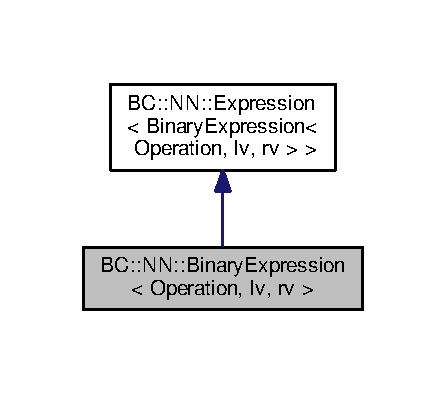
\includegraphics[width=214pt]{structBC_1_1NN_1_1BinaryExpression__inherit__graph}
\end{center}
\end{figure}


Collaboration diagram for BC\+:\+:NN\+:\+:Binary\+Expression$<$ Operation, lv, rv $>$\+:
\nopagebreak
\begin{figure}[H]
\begin{center}
\leavevmode
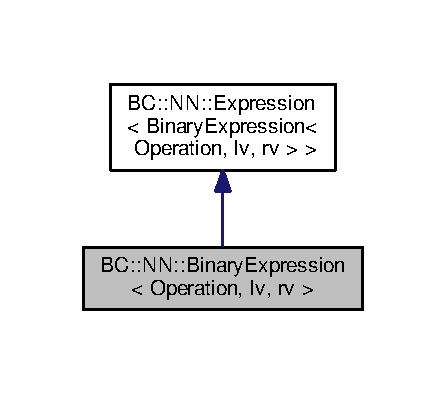
\includegraphics[width=214pt]{structBC_1_1NN_1_1BinaryExpression__coll__graph}
\end{center}
\end{figure}
\subsection*{Public Member Functions}
\begin{DoxyCompactItemize}
\item 
auto \hyperlink{structBC_1_1NN_1_1BinaryExpression_a15a08f5652cf9ade47ad6250da4d5180}{forward\+\_\+propagate} ()
\item 
{\footnotesize template$<$class Tensor $>$ }\\auto \hyperlink{structBC_1_1NN_1_1BinaryExpression_ae85b96389b4c8312d6b27d80d10f4f9a}{backward\+\_\+propagate} (\hyperlink{namespaceBC_1_1tensors_1_1common__using_ae0b2983dde17bb7904dc64aa0cb9a676}{Tensor} \&\&delta)
\end{DoxyCompactItemize}
\subsection*{Public Attributes}
\begin{DoxyCompactItemize}
\item 
Operation \hyperlink{structBC_1_1NN_1_1BinaryExpression_a34a9b03751011dc00b07082039f8f506}{op}
\item 
lv \hyperlink{structBC_1_1NN_1_1BinaryExpression_a7daa2eb56f82b73045ec8d2959c280d6}{left}
\item 
rv \hyperlink{structBC_1_1NN_1_1BinaryExpression_aecdf8d119adbb08f4b1aa7123b6bbce2}{right}
\end{DoxyCompactItemize}


\subsection{Member Function Documentation}
\index{B\+C\+::\+N\+N\+::\+Binary\+Expression@{B\+C\+::\+N\+N\+::\+Binary\+Expression}!backward\+\_\+propagate@{backward\+\_\+propagate}}
\index{backward\+\_\+propagate@{backward\+\_\+propagate}!B\+C\+::\+N\+N\+::\+Binary\+Expression@{B\+C\+::\+N\+N\+::\+Binary\+Expression}}
\subsubsection[{\texorpdfstring{backward\+\_\+propagate(\+Tensor \&\&delta)}{backward_propagate(Tensor &&delta)}}]{\setlength{\rightskip}{0pt plus 5cm}template$<$class Operation , class lv , class rv $>$ template$<$class Tensor $>$ auto {\bf B\+C\+::\+N\+N\+::\+Binary\+Expression}$<$ Operation, lv, rv $>$\+::backward\+\_\+propagate (
\begin{DoxyParamCaption}
\item[{{\bf Tensor} \&\&}]{delta}
\end{DoxyParamCaption}
)\hspace{0.3cm}{\ttfamily [inline]}}\hypertarget{structBC_1_1NN_1_1BinaryExpression_ae85b96389b4c8312d6b27d80d10f4f9a}{}\label{structBC_1_1NN_1_1BinaryExpression_ae85b96389b4c8312d6b27d80d10f4f9a}
\index{B\+C\+::\+N\+N\+::\+Binary\+Expression@{B\+C\+::\+N\+N\+::\+Binary\+Expression}!forward\+\_\+propagate@{forward\+\_\+propagate}}
\index{forward\+\_\+propagate@{forward\+\_\+propagate}!B\+C\+::\+N\+N\+::\+Binary\+Expression@{B\+C\+::\+N\+N\+::\+Binary\+Expression}}
\subsubsection[{\texorpdfstring{forward\+\_\+propagate()}{forward_propagate()}}]{\setlength{\rightskip}{0pt plus 5cm}template$<$class Operation , class lv , class rv $>$ auto {\bf B\+C\+::\+N\+N\+::\+Binary\+Expression}$<$ Operation, lv, rv $>$\+::forward\+\_\+propagate (
\begin{DoxyParamCaption}
{}
\end{DoxyParamCaption}
)\hspace{0.3cm}{\ttfamily [inline]}}\hypertarget{structBC_1_1NN_1_1BinaryExpression_a15a08f5652cf9ade47ad6250da4d5180}{}\label{structBC_1_1NN_1_1BinaryExpression_a15a08f5652cf9ade47ad6250da4d5180}


\subsection{Member Data Documentation}
\index{B\+C\+::\+N\+N\+::\+Binary\+Expression@{B\+C\+::\+N\+N\+::\+Binary\+Expression}!left@{left}}
\index{left@{left}!B\+C\+::\+N\+N\+::\+Binary\+Expression@{B\+C\+::\+N\+N\+::\+Binary\+Expression}}
\subsubsection[{\texorpdfstring{left}{left}}]{\setlength{\rightskip}{0pt plus 5cm}template$<$class Operation , class lv , class rv $>$ lv {\bf B\+C\+::\+N\+N\+::\+Binary\+Expression}$<$ Operation, lv, rv $>$\+::left}\hypertarget{structBC_1_1NN_1_1BinaryExpression_a7daa2eb56f82b73045ec8d2959c280d6}{}\label{structBC_1_1NN_1_1BinaryExpression_a7daa2eb56f82b73045ec8d2959c280d6}
\index{B\+C\+::\+N\+N\+::\+Binary\+Expression@{B\+C\+::\+N\+N\+::\+Binary\+Expression}!op@{op}}
\index{op@{op}!B\+C\+::\+N\+N\+::\+Binary\+Expression@{B\+C\+::\+N\+N\+::\+Binary\+Expression}}
\subsubsection[{\texorpdfstring{op}{op}}]{\setlength{\rightskip}{0pt plus 5cm}template$<$class Operation , class lv , class rv $>$ Operation {\bf B\+C\+::\+N\+N\+::\+Binary\+Expression}$<$ Operation, lv, rv $>$\+::op}\hypertarget{structBC_1_1NN_1_1BinaryExpression_a34a9b03751011dc00b07082039f8f506}{}\label{structBC_1_1NN_1_1BinaryExpression_a34a9b03751011dc00b07082039f8f506}
\index{B\+C\+::\+N\+N\+::\+Binary\+Expression@{B\+C\+::\+N\+N\+::\+Binary\+Expression}!right@{right}}
\index{right@{right}!B\+C\+::\+N\+N\+::\+Binary\+Expression@{B\+C\+::\+N\+N\+::\+Binary\+Expression}}
\subsubsection[{\texorpdfstring{right}{right}}]{\setlength{\rightskip}{0pt plus 5cm}template$<$class Operation , class lv , class rv $>$ rv {\bf B\+C\+::\+N\+N\+::\+Binary\+Expression}$<$ Operation, lv, rv $>$\+::right}\hypertarget{structBC_1_1NN_1_1BinaryExpression_aecdf8d119adbb08f4b1aa7123b6bbce2}{}\label{structBC_1_1NN_1_1BinaryExpression_aecdf8d119adbb08f4b1aa7123b6bbce2}


The documentation for this struct was generated from the following file\+:\begin{DoxyCompactItemize}
\item 
include/autograd/layers/\hyperlink{BinaryExpression_8h}{Binary\+Expression.\+h}\end{DoxyCompactItemize}

\hypertarget{structBC_1_1meta_1_1Bind}{}\section{BC\+:\+:meta\+:\+:Bind$<$ Function, args $>$ Struct Template Reference}
\label{structBC_1_1meta_1_1Bind}\index{B\+C\+::meta\+::\+Bind$<$ Function, args $>$@{B\+C\+::meta\+::\+Bind$<$ Function, args $>$}}


{\ttfamily \#include $<$Bind.\+h$>$}



Inheritance diagram for BC\+:\+:meta\+:\+:Bind$<$ Function, args $>$\+:
\nopagebreak
\begin{figure}[H]
\begin{center}
\leavevmode
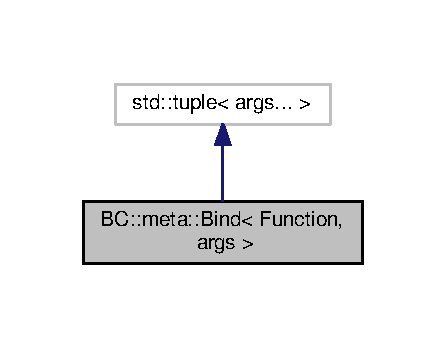
\includegraphics[width=214pt]{structBC_1_1meta_1_1Bind__inherit__graph}
\end{center}
\end{figure}


Collaboration diagram for BC\+:\+:meta\+:\+:Bind$<$ Function, args $>$\+:
\nopagebreak
\begin{figure}[H]
\begin{center}
\leavevmode
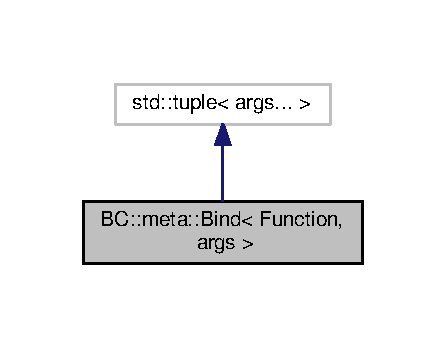
\includegraphics[width=214pt]{structBC_1_1meta_1_1Bind__coll__graph}
\end{center}
\end{figure}
\subsection*{Public Member Functions}
\begin{DoxyCompactItemize}
\item 
\hyperlink{structBC_1_1meta_1_1Bind_ab9eef3ea89ede648267ba36a332774e3}{Bind} (Function \hyperlink{structBC_1_1meta_1_1Bind_ad40425dea4b85234dfb045611bdd3071}{f}, args...\+args\+\_\+)
\item 
{\footnotesize template$<$int A\+DL = 0$>$ }\\auto \hyperlink{structBC_1_1meta_1_1Bind_aa383c2c2ad7836c0370c39707d443391}{operator()} ()
\item 
{\footnotesize template$<$int A\+DL = 0$>$ }\\auto \hyperlink{structBC_1_1meta_1_1Bind_ac94304e7fb2a9727b92f8d04eadb78b5}{operator()} () const 
\end{DoxyCompactItemize}
\subsection*{Public Attributes}
\begin{DoxyCompactItemize}
\item 
Function \hyperlink{structBC_1_1meta_1_1Bind_ad40425dea4b85234dfb045611bdd3071}{f}
\end{DoxyCompactItemize}


\subsection{Constructor \& Destructor Documentation}
\index{B\+C\+::meta\+::\+Bind@{B\+C\+::meta\+::\+Bind}!Bind@{Bind}}
\index{Bind@{Bind}!B\+C\+::meta\+::\+Bind@{B\+C\+::meta\+::\+Bind}}
\subsubsection[{\texorpdfstring{Bind(\+Function f, args...\+args\+\_\+)}{Bind(Function f, args...args_)}}]{\setlength{\rightskip}{0pt plus 5cm}template$<$class Function , class... args$>$ {\bf B\+C\+::meta\+::\+Bind}$<$ Function, args $>$\+::{\bf Bind} (
\begin{DoxyParamCaption}
\item[{Function}]{f, }
\item[{args...}]{args\+\_\+}
\end{DoxyParamCaption}
)\hspace{0.3cm}{\ttfamily [inline]}}\hypertarget{structBC_1_1meta_1_1Bind_ab9eef3ea89ede648267ba36a332774e3}{}\label{structBC_1_1meta_1_1Bind_ab9eef3ea89ede648267ba36a332774e3}


\subsection{Member Function Documentation}
\index{B\+C\+::meta\+::\+Bind@{B\+C\+::meta\+::\+Bind}!operator()@{operator()}}
\index{operator()@{operator()}!B\+C\+::meta\+::\+Bind@{B\+C\+::meta\+::\+Bind}}
\subsubsection[{\texorpdfstring{operator()()}{operator()()}}]{\setlength{\rightskip}{0pt plus 5cm}template$<$class Function , class... args$>$ template$<$int A\+DL = 0$>$ auto {\bf B\+C\+::meta\+::\+Bind}$<$ Function, args $>$\+::operator() (
\begin{DoxyParamCaption}
{}
\end{DoxyParamCaption}
)\hspace{0.3cm}{\ttfamily [inline]}}\hypertarget{structBC_1_1meta_1_1Bind_aa383c2c2ad7836c0370c39707d443391}{}\label{structBC_1_1meta_1_1Bind_aa383c2c2ad7836c0370c39707d443391}
\index{B\+C\+::meta\+::\+Bind@{B\+C\+::meta\+::\+Bind}!operator()@{operator()}}
\index{operator()@{operator()}!B\+C\+::meta\+::\+Bind@{B\+C\+::meta\+::\+Bind}}
\subsubsection[{\texorpdfstring{operator()() const }{operator()() const }}]{\setlength{\rightskip}{0pt plus 5cm}template$<$class Function , class... args$>$ template$<$int A\+DL = 0$>$ auto {\bf B\+C\+::meta\+::\+Bind}$<$ Function, args $>$\+::operator() (
\begin{DoxyParamCaption}
{}
\end{DoxyParamCaption}
) const\hspace{0.3cm}{\ttfamily [inline]}}\hypertarget{structBC_1_1meta_1_1Bind_ac94304e7fb2a9727b92f8d04eadb78b5}{}\label{structBC_1_1meta_1_1Bind_ac94304e7fb2a9727b92f8d04eadb78b5}


\subsection{Member Data Documentation}
\index{B\+C\+::meta\+::\+Bind@{B\+C\+::meta\+::\+Bind}!f@{f}}
\index{f@{f}!B\+C\+::meta\+::\+Bind@{B\+C\+::meta\+::\+Bind}}
\subsubsection[{\texorpdfstring{f}{f}}]{\setlength{\rightskip}{0pt plus 5cm}template$<$class Function , class... args$>$ Function {\bf B\+C\+::meta\+::\+Bind}$<$ Function, args $>$\+::f}\hypertarget{structBC_1_1meta_1_1Bind_ad40425dea4b85234dfb045611bdd3071}{}\label{structBC_1_1meta_1_1Bind_ad40425dea4b85234dfb045611bdd3071}


The documentation for this struct was generated from the following file\+:\begin{DoxyCompactItemize}
\item 
include/type\+\_\+traits/\hyperlink{Bind_8h}{Bind.\+h}\end{DoxyCompactItemize}

\hypertarget{structBC_1_1blas_1_1BLAS_3_01host__tag_01_4}{}\section{BC\+:\+:blas\+:\+:B\+L\+AS$<$ host\+\_\+tag $>$ Struct Template Reference}
\label{structBC_1_1blas_1_1BLAS_3_01host__tag_01_4}\index{B\+C\+::blas\+::\+B\+L\+A\+S$<$ host\+\_\+tag $>$@{B\+C\+::blas\+::\+B\+L\+A\+S$<$ host\+\_\+tag $>$}}


{\ttfamily \#include $<$Host.\+h$>$}

\subsection*{Static Public Member Functions}
\begin{DoxyCompactItemize}
\item 
{\footnotesize template$<$class Stream $>$ }\\static void \hyperlink{structBC_1_1blas_1_1BLAS_3_01host__tag_01_4_a65c15c72e8a51fa92e4e12b80e874b38}{gemm} (\hyperlink{namespaceBC_abc64a63cd29a22d102a68f478dfd588d}{Stream} stream, bool transA, bool transB, \hyperlink{namespaceBC_a6007cbc4eeec401a037b558910a56173}{B\+C\+::size\+\_\+t} m, \hyperlink{namespaceBC_a6007cbc4eeec401a037b558910a56173}{B\+C\+::size\+\_\+t} n, \hyperlink{namespaceBC_a6007cbc4eeec401a037b558910a56173}{B\+C\+::size\+\_\+t} k, const float alpha, const float $\ast$A, \hyperlink{namespaceBC_a6007cbc4eeec401a037b558910a56173}{B\+C\+::size\+\_\+t} lda, const float $\ast$B, \hyperlink{namespaceBC_a6007cbc4eeec401a037b558910a56173}{B\+C\+::size\+\_\+t} ldb, const float beta, float $\ast$C, \hyperlink{namespaceBC_a6007cbc4eeec401a037b558910a56173}{B\+C\+::size\+\_\+t} ldc)
\item 
{\footnotesize template$<$class Stream $>$ }\\static void \hyperlink{structBC_1_1blas_1_1BLAS_3_01host__tag_01_4_a1ff65b6c23f3d711a746f67196aabd2b}{gemm} (\hyperlink{namespaceBC_abc64a63cd29a22d102a68f478dfd588d}{Stream} stream, bool transA, bool transB, \hyperlink{namespaceBC_a6007cbc4eeec401a037b558910a56173}{B\+C\+::size\+\_\+t} m, \hyperlink{namespaceBC_a6007cbc4eeec401a037b558910a56173}{B\+C\+::size\+\_\+t} n, \hyperlink{namespaceBC_a6007cbc4eeec401a037b558910a56173}{B\+C\+::size\+\_\+t} k, const double alpha, const double $\ast$A, \hyperlink{namespaceBC_a6007cbc4eeec401a037b558910a56173}{B\+C\+::size\+\_\+t} lda, const double $\ast$B, \hyperlink{namespaceBC_a6007cbc4eeec401a037b558910a56173}{B\+C\+::size\+\_\+t} ldb, const double beta, double $\ast$C, \hyperlink{namespaceBC_a6007cbc4eeec401a037b558910a56173}{B\+C\+::size\+\_\+t} ldc)
\item 
{\footnotesize template$<$class Stream $>$ }\\static void \hyperlink{structBC_1_1blas_1_1BLAS_3_01host__tag_01_4_ad3bc9f3b32b2b3d197b39b98a7244818}{gemv} (\hyperlink{namespaceBC_abc64a63cd29a22d102a68f478dfd588d}{Stream} stream, bool transA, \hyperlink{namespaceBC_a6007cbc4eeec401a037b558910a56173}{B\+C\+::size\+\_\+t} m, \hyperlink{namespaceBC_a6007cbc4eeec401a037b558910a56173}{B\+C\+::size\+\_\+t} n, const double alpha, const double $\ast$A, \hyperlink{namespaceBC_a6007cbc4eeec401a037b558910a56173}{B\+C\+::size\+\_\+t} lda, const double $\ast$X, \hyperlink{namespaceBC_a6007cbc4eeec401a037b558910a56173}{B\+C\+::size\+\_\+t} incX, const double beta, double $\ast$Y, \hyperlink{namespaceBC_a6007cbc4eeec401a037b558910a56173}{B\+C\+::size\+\_\+t} incY)
\item 
{\footnotesize template$<$class Stream $>$ }\\static void \hyperlink{structBC_1_1blas_1_1BLAS_3_01host__tag_01_4_abff02539f7824d8a3da452a105c8afc5}{gemv} (\hyperlink{namespaceBC_abc64a63cd29a22d102a68f478dfd588d}{Stream} stream, bool transA, \hyperlink{namespaceBC_a6007cbc4eeec401a037b558910a56173}{B\+C\+::size\+\_\+t} m, \hyperlink{namespaceBC_a6007cbc4eeec401a037b558910a56173}{B\+C\+::size\+\_\+t} n, const float alpha, const float $\ast$A, \hyperlink{namespaceBC_a6007cbc4eeec401a037b558910a56173}{B\+C\+::size\+\_\+t} lda, const float $\ast$X, \hyperlink{namespaceBC_a6007cbc4eeec401a037b558910a56173}{B\+C\+::size\+\_\+t} incX, const float beta, float $\ast$Y, \hyperlink{namespaceBC_a6007cbc4eeec401a037b558910a56173}{B\+C\+::size\+\_\+t} incY)
\item 
{\footnotesize template$<$class Stream $>$ }\\static void \hyperlink{structBC_1_1blas_1_1BLAS_3_01host__tag_01_4_a275f5d4c788a496b1af0a2aa02a9dc80}{ger} (\hyperlink{namespaceBC_abc64a63cd29a22d102a68f478dfd588d}{Stream} stream, int m, \hyperlink{namespaceBC_a6007cbc4eeec401a037b558910a56173}{B\+C\+::size\+\_\+t} n, const double alpha, const double $\ast$X, \hyperlink{namespaceBC_a6007cbc4eeec401a037b558910a56173}{B\+C\+::size\+\_\+t} incX, const double $\ast$Y, \hyperlink{namespaceBC_a6007cbc4eeec401a037b558910a56173}{B\+C\+::size\+\_\+t} incY, double $\ast$A, \hyperlink{namespaceBC_a6007cbc4eeec401a037b558910a56173}{B\+C\+::size\+\_\+t} lda)
\item 
{\footnotesize template$<$class Stream $>$ }\\static void \hyperlink{structBC_1_1blas_1_1BLAS_3_01host__tag_01_4_aabb36e44446fd342a80ccbd9cbd783a1}{ger} (\hyperlink{namespaceBC_abc64a63cd29a22d102a68f478dfd588d}{Stream} stream, int m, \hyperlink{namespaceBC_a6007cbc4eeec401a037b558910a56173}{B\+C\+::size\+\_\+t} n, const float alpha, const float $\ast$X, \hyperlink{namespaceBC_a6007cbc4eeec401a037b558910a56173}{B\+C\+::size\+\_\+t} incX, const float $\ast$Y, \hyperlink{namespaceBC_a6007cbc4eeec401a037b558910a56173}{B\+C\+::size\+\_\+t} incY, float $\ast$A, \hyperlink{namespaceBC_a6007cbc4eeec401a037b558910a56173}{B\+C\+::size\+\_\+t} lda)
\item 
{\footnotesize template$<$class Stream $>$ }\\static void \hyperlink{structBC_1_1blas_1_1BLAS_3_01host__tag_01_4_a0ba27e9c462f784256dd42ff208ede52}{dot} (\hyperlink{namespaceBC_abc64a63cd29a22d102a68f478dfd588d}{Stream} stream, int n, double $\ast$A, const double $\ast$x, \hyperlink{namespaceBC_a6007cbc4eeec401a037b558910a56173}{B\+C\+::size\+\_\+t} incX, const double $\ast$y, \hyperlink{namespaceBC_a6007cbc4eeec401a037b558910a56173}{B\+C\+::size\+\_\+t} incY)
\item 
{\footnotesize template$<$class Stream $>$ }\\static void \hyperlink{structBC_1_1blas_1_1BLAS_3_01host__tag_01_4_aafdeace30eb396655a882f202c951483}{dot} (\hyperlink{namespaceBC_abc64a63cd29a22d102a68f478dfd588d}{Stream} stream, int n, float $\ast$A, const float $\ast$x, \hyperlink{namespaceBC_a6007cbc4eeec401a037b558910a56173}{B\+C\+::size\+\_\+t} incX, const float $\ast$y, \hyperlink{namespaceBC_a6007cbc4eeec401a037b558910a56173}{B\+C\+::size\+\_\+t} incY)
\item 
{\footnotesize template$<$class Stream $>$ }\\static void \hyperlink{structBC_1_1blas_1_1BLAS_3_01host__tag_01_4_a2d2c8e9d73703e339c1ca69342c4a1f6}{gemm} (\hyperlink{namespaceBC_abc64a63cd29a22d102a68f478dfd588d}{Stream} stream, bool transA, bool transB, \hyperlink{namespaceBC_a6007cbc4eeec401a037b558910a56173}{B\+C\+::size\+\_\+t} m, \hyperlink{namespaceBC_a6007cbc4eeec401a037b558910a56173}{B\+C\+::size\+\_\+t} n, \hyperlink{namespaceBC_a6007cbc4eeec401a037b558910a56173}{B\+C\+::size\+\_\+t} k, const float $\ast$alpha, const float $\ast$A, \hyperlink{namespaceBC_a6007cbc4eeec401a037b558910a56173}{B\+C\+::size\+\_\+t} lda, const float $\ast$B, \hyperlink{namespaceBC_a6007cbc4eeec401a037b558910a56173}{B\+C\+::size\+\_\+t} ldb, const float $\ast$beta, float $\ast$C, \hyperlink{namespaceBC_a6007cbc4eeec401a037b558910a56173}{B\+C\+::size\+\_\+t} ldc)
\item 
{\footnotesize template$<$class Stream $>$ }\\static void \hyperlink{structBC_1_1blas_1_1BLAS_3_01host__tag_01_4_afb07b50637a005dbd0c44a85648852a1}{gemm} (\hyperlink{namespaceBC_abc64a63cd29a22d102a68f478dfd588d}{Stream} stream, bool transA, bool transB, \hyperlink{namespaceBC_a6007cbc4eeec401a037b558910a56173}{B\+C\+::size\+\_\+t} m, \hyperlink{namespaceBC_a6007cbc4eeec401a037b558910a56173}{B\+C\+::size\+\_\+t} n, \hyperlink{namespaceBC_a6007cbc4eeec401a037b558910a56173}{B\+C\+::size\+\_\+t} k, const double $\ast$alpha, const double $\ast$A, \hyperlink{namespaceBC_a6007cbc4eeec401a037b558910a56173}{B\+C\+::size\+\_\+t} lda, const double $\ast$B, \hyperlink{namespaceBC_a6007cbc4eeec401a037b558910a56173}{B\+C\+::size\+\_\+t} ldb, const double $\ast$beta, double $\ast$C, \hyperlink{namespaceBC_a6007cbc4eeec401a037b558910a56173}{B\+C\+::size\+\_\+t} ldc)
\item 
{\footnotesize template$<$class Stream $>$ }\\static void \hyperlink{structBC_1_1blas_1_1BLAS_3_01host__tag_01_4_a930fdb370d30d9e0343639750afd32ca}{gemv} (\hyperlink{namespaceBC_abc64a63cd29a22d102a68f478dfd588d}{Stream} stream, bool transA, \hyperlink{namespaceBC_a6007cbc4eeec401a037b558910a56173}{B\+C\+::size\+\_\+t} m, \hyperlink{namespaceBC_a6007cbc4eeec401a037b558910a56173}{B\+C\+::size\+\_\+t} n, const double $\ast$alpha, const double $\ast$A, \hyperlink{namespaceBC_a6007cbc4eeec401a037b558910a56173}{B\+C\+::size\+\_\+t} lda, const double $\ast$X, \hyperlink{namespaceBC_a6007cbc4eeec401a037b558910a56173}{B\+C\+::size\+\_\+t} incX, const double $\ast$beta, double $\ast$Y, \hyperlink{namespaceBC_a6007cbc4eeec401a037b558910a56173}{B\+C\+::size\+\_\+t} incY)
\item 
{\footnotesize template$<$class Stream $>$ }\\static void \hyperlink{structBC_1_1blas_1_1BLAS_3_01host__tag_01_4_a7dd56f6e265c4160dafedd3eaeee638c}{gemv} (\hyperlink{namespaceBC_abc64a63cd29a22d102a68f478dfd588d}{Stream} stream, bool transA, \hyperlink{namespaceBC_a6007cbc4eeec401a037b558910a56173}{B\+C\+::size\+\_\+t} m, \hyperlink{namespaceBC_a6007cbc4eeec401a037b558910a56173}{B\+C\+::size\+\_\+t} n, const float $\ast$alpha, const float $\ast$A, \hyperlink{namespaceBC_a6007cbc4eeec401a037b558910a56173}{B\+C\+::size\+\_\+t} lda, const float $\ast$X, \hyperlink{namespaceBC_a6007cbc4eeec401a037b558910a56173}{B\+C\+::size\+\_\+t} incX, const float $\ast$beta, float $\ast$Y, \hyperlink{namespaceBC_a6007cbc4eeec401a037b558910a56173}{B\+C\+::size\+\_\+t} incY)
\item 
{\footnotesize template$<$class Stream $>$ }\\static void \hyperlink{structBC_1_1blas_1_1BLAS_3_01host__tag_01_4_a6c8434c7ba576265d3d04ae48c55e6bc}{ger} (\hyperlink{namespaceBC_abc64a63cd29a22d102a68f478dfd588d}{Stream} stream, int m, \hyperlink{namespaceBC_a6007cbc4eeec401a037b558910a56173}{B\+C\+::size\+\_\+t} n, const double $\ast$alpha, const double $\ast$X, \hyperlink{namespaceBC_a6007cbc4eeec401a037b558910a56173}{B\+C\+::size\+\_\+t} incX, const double $\ast$Y, \hyperlink{namespaceBC_a6007cbc4eeec401a037b558910a56173}{B\+C\+::size\+\_\+t} incY, double $\ast$A, \hyperlink{namespaceBC_a6007cbc4eeec401a037b558910a56173}{B\+C\+::size\+\_\+t} lda)
\item 
{\footnotesize template$<$class Stream $>$ }\\static void \hyperlink{structBC_1_1blas_1_1BLAS_3_01host__tag_01_4_aa7a5eea6314db38d2600af97e09c5c1b}{ger} (\hyperlink{namespaceBC_abc64a63cd29a22d102a68f478dfd588d}{Stream} stream, int m, \hyperlink{namespaceBC_a6007cbc4eeec401a037b558910a56173}{B\+C\+::size\+\_\+t} n, const float $\ast$alpha, const float $\ast$X, \hyperlink{namespaceBC_a6007cbc4eeec401a037b558910a56173}{B\+C\+::size\+\_\+t} incX, const float $\ast$Y, \hyperlink{namespaceBC_a6007cbc4eeec401a037b558910a56173}{B\+C\+::size\+\_\+t} incY, float $\ast$A, \hyperlink{namespaceBC_a6007cbc4eeec401a037b558910a56173}{B\+C\+::size\+\_\+t} lda)
\end{DoxyCompactItemize}


\subsection{Member Function Documentation}
\index{B\+C\+::blas\+::\+B\+L\+A\+S$<$ host\+\_\+tag $>$@{B\+C\+::blas\+::\+B\+L\+A\+S$<$ host\+\_\+tag $>$}!dot@{dot}}
\index{dot@{dot}!B\+C\+::blas\+::\+B\+L\+A\+S$<$ host\+\_\+tag $>$@{B\+C\+::blas\+::\+B\+L\+A\+S$<$ host\+\_\+tag $>$}}
\subsubsection[{\texorpdfstring{dot(\+Stream stream, int n, double $\ast$\+A, const double $\ast$x, B\+C\+::size\+\_\+t inc\+X, const double $\ast$y, B\+C\+::size\+\_\+t inc\+Y)}{dot(Stream stream, int n, double *A, const double *x, BC::size_t incX, const double *y, BC::size_t incY)}}]{\setlength{\rightskip}{0pt plus 5cm}template$<$class Stream $>$ static void B\+C\+::blas\+::\+B\+L\+AS$<$ {\bf host\+\_\+tag} $>$\+::dot (
\begin{DoxyParamCaption}
\item[{{\bf Stream}}]{stream, }
\item[{int}]{n, }
\item[{double $\ast$}]{A, }
\item[{const double $\ast$}]{x, }
\item[{{\bf B\+C\+::size\+\_\+t}}]{incX, }
\item[{const double $\ast$}]{y, }
\item[{{\bf B\+C\+::size\+\_\+t}}]{incY}
\end{DoxyParamCaption}
)\hspace{0.3cm}{\ttfamily [inline]}, {\ttfamily [static]}}\hypertarget{structBC_1_1blas_1_1BLAS_3_01host__tag_01_4_a0ba27e9c462f784256dd42ff208ede52}{}\label{structBC_1_1blas_1_1BLAS_3_01host__tag_01_4_a0ba27e9c462f784256dd42ff208ede52}
\index{B\+C\+::blas\+::\+B\+L\+A\+S$<$ host\+\_\+tag $>$@{B\+C\+::blas\+::\+B\+L\+A\+S$<$ host\+\_\+tag $>$}!dot@{dot}}
\index{dot@{dot}!B\+C\+::blas\+::\+B\+L\+A\+S$<$ host\+\_\+tag $>$@{B\+C\+::blas\+::\+B\+L\+A\+S$<$ host\+\_\+tag $>$}}
\subsubsection[{\texorpdfstring{dot(\+Stream stream, int n, float $\ast$\+A, const float $\ast$x, B\+C\+::size\+\_\+t inc\+X, const float $\ast$y, B\+C\+::size\+\_\+t inc\+Y)}{dot(Stream stream, int n, float *A, const float *x, BC::size_t incX, const float *y, BC::size_t incY)}}]{\setlength{\rightskip}{0pt plus 5cm}template$<$class Stream $>$ static void B\+C\+::blas\+::\+B\+L\+AS$<$ {\bf host\+\_\+tag} $>$\+::dot (
\begin{DoxyParamCaption}
\item[{{\bf Stream}}]{stream, }
\item[{int}]{n, }
\item[{float $\ast$}]{A, }
\item[{const float $\ast$}]{x, }
\item[{{\bf B\+C\+::size\+\_\+t}}]{incX, }
\item[{const float $\ast$}]{y, }
\item[{{\bf B\+C\+::size\+\_\+t}}]{incY}
\end{DoxyParamCaption}
)\hspace{0.3cm}{\ttfamily [inline]}, {\ttfamily [static]}}\hypertarget{structBC_1_1blas_1_1BLAS_3_01host__tag_01_4_aafdeace30eb396655a882f202c951483}{}\label{structBC_1_1blas_1_1BLAS_3_01host__tag_01_4_aafdeace30eb396655a882f202c951483}
\index{B\+C\+::blas\+::\+B\+L\+A\+S$<$ host\+\_\+tag $>$@{B\+C\+::blas\+::\+B\+L\+A\+S$<$ host\+\_\+tag $>$}!gemm@{gemm}}
\index{gemm@{gemm}!B\+C\+::blas\+::\+B\+L\+A\+S$<$ host\+\_\+tag $>$@{B\+C\+::blas\+::\+B\+L\+A\+S$<$ host\+\_\+tag $>$}}
\subsubsection[{\texorpdfstring{gemm(\+Stream stream, bool trans\+A, bool trans\+B, B\+C\+::size\+\_\+t m, B\+C\+::size\+\_\+t n, B\+C\+::size\+\_\+t k, const float alpha, const float $\ast$\+A, B\+C\+::size\+\_\+t lda, const float $\ast$\+B, B\+C\+::size\+\_\+t ldb, const float beta, float $\ast$\+C, B\+C\+::size\+\_\+t ldc)}{gemm(Stream stream, bool transA, bool transB, BC::size_t m, BC::size_t n, BC::size_t k, const float alpha, const float *A, BC::size_t lda, const float *B, BC::size_t ldb, const float beta, float *C, BC::size_t ldc)}}]{\setlength{\rightskip}{0pt plus 5cm}template$<$class Stream $>$ static void B\+C\+::blas\+::\+B\+L\+AS$<$ {\bf host\+\_\+tag} $>$\+::gemm (
\begin{DoxyParamCaption}
\item[{{\bf Stream}}]{stream, }
\item[{bool}]{transA, }
\item[{bool}]{transB, }
\item[{{\bf B\+C\+::size\+\_\+t}}]{m, }
\item[{{\bf B\+C\+::size\+\_\+t}}]{n, }
\item[{{\bf B\+C\+::size\+\_\+t}}]{k, }
\item[{const float}]{alpha, }
\item[{const float $\ast$}]{A, }
\item[{{\bf B\+C\+::size\+\_\+t}}]{lda, }
\item[{const float $\ast$}]{B, }
\item[{{\bf B\+C\+::size\+\_\+t}}]{ldb, }
\item[{const float}]{beta, }
\item[{float $\ast$}]{C, }
\item[{{\bf B\+C\+::size\+\_\+t}}]{ldc}
\end{DoxyParamCaption}
)\hspace{0.3cm}{\ttfamily [inline]}, {\ttfamily [static]}}\hypertarget{structBC_1_1blas_1_1BLAS_3_01host__tag_01_4_a65c15c72e8a51fa92e4e12b80e874b38}{}\label{structBC_1_1blas_1_1BLAS_3_01host__tag_01_4_a65c15c72e8a51fa92e4e12b80e874b38}
\index{B\+C\+::blas\+::\+B\+L\+A\+S$<$ host\+\_\+tag $>$@{B\+C\+::blas\+::\+B\+L\+A\+S$<$ host\+\_\+tag $>$}!gemm@{gemm}}
\index{gemm@{gemm}!B\+C\+::blas\+::\+B\+L\+A\+S$<$ host\+\_\+tag $>$@{B\+C\+::blas\+::\+B\+L\+A\+S$<$ host\+\_\+tag $>$}}
\subsubsection[{\texorpdfstring{gemm(\+Stream stream, bool trans\+A, bool trans\+B, B\+C\+::size\+\_\+t m, B\+C\+::size\+\_\+t n, B\+C\+::size\+\_\+t k, const double alpha, const double $\ast$\+A, B\+C\+::size\+\_\+t lda, const double $\ast$\+B, B\+C\+::size\+\_\+t ldb, const double beta, double $\ast$\+C, B\+C\+::size\+\_\+t ldc)}{gemm(Stream stream, bool transA, bool transB, BC::size_t m, BC::size_t n, BC::size_t k, const double alpha, const double *A, BC::size_t lda, const double *B, BC::size_t ldb, const double beta, double *C, BC::size_t ldc)}}]{\setlength{\rightskip}{0pt plus 5cm}template$<$class Stream $>$ static void B\+C\+::blas\+::\+B\+L\+AS$<$ {\bf host\+\_\+tag} $>$\+::gemm (
\begin{DoxyParamCaption}
\item[{{\bf Stream}}]{stream, }
\item[{bool}]{transA, }
\item[{bool}]{transB, }
\item[{{\bf B\+C\+::size\+\_\+t}}]{m, }
\item[{{\bf B\+C\+::size\+\_\+t}}]{n, }
\item[{{\bf B\+C\+::size\+\_\+t}}]{k, }
\item[{const double}]{alpha, }
\item[{const double $\ast$}]{A, }
\item[{{\bf B\+C\+::size\+\_\+t}}]{lda, }
\item[{const double $\ast$}]{B, }
\item[{{\bf B\+C\+::size\+\_\+t}}]{ldb, }
\item[{const double}]{beta, }
\item[{double $\ast$}]{C, }
\item[{{\bf B\+C\+::size\+\_\+t}}]{ldc}
\end{DoxyParamCaption}
)\hspace{0.3cm}{\ttfamily [inline]}, {\ttfamily [static]}}\hypertarget{structBC_1_1blas_1_1BLAS_3_01host__tag_01_4_a1ff65b6c23f3d711a746f67196aabd2b}{}\label{structBC_1_1blas_1_1BLAS_3_01host__tag_01_4_a1ff65b6c23f3d711a746f67196aabd2b}
\index{B\+C\+::blas\+::\+B\+L\+A\+S$<$ host\+\_\+tag $>$@{B\+C\+::blas\+::\+B\+L\+A\+S$<$ host\+\_\+tag $>$}!gemm@{gemm}}
\index{gemm@{gemm}!B\+C\+::blas\+::\+B\+L\+A\+S$<$ host\+\_\+tag $>$@{B\+C\+::blas\+::\+B\+L\+A\+S$<$ host\+\_\+tag $>$}}
\subsubsection[{\texorpdfstring{gemm(\+Stream stream, bool trans\+A, bool trans\+B, B\+C\+::size\+\_\+t m, B\+C\+::size\+\_\+t n, B\+C\+::size\+\_\+t k, const float $\ast$alpha, const float $\ast$\+A, B\+C\+::size\+\_\+t lda, const float $\ast$\+B, B\+C\+::size\+\_\+t ldb, const float $\ast$beta, float $\ast$\+C, B\+C\+::size\+\_\+t ldc)}{gemm(Stream stream, bool transA, bool transB, BC::size_t m, BC::size_t n, BC::size_t k, const float *alpha, const float *A, BC::size_t lda, const float *B, BC::size_t ldb, const float *beta, float *C, BC::size_t ldc)}}]{\setlength{\rightskip}{0pt plus 5cm}template$<$class Stream $>$ static void B\+C\+::blas\+::\+B\+L\+AS$<$ {\bf host\+\_\+tag} $>$\+::gemm (
\begin{DoxyParamCaption}
\item[{{\bf Stream}}]{stream, }
\item[{bool}]{transA, }
\item[{bool}]{transB, }
\item[{{\bf B\+C\+::size\+\_\+t}}]{m, }
\item[{{\bf B\+C\+::size\+\_\+t}}]{n, }
\item[{{\bf B\+C\+::size\+\_\+t}}]{k, }
\item[{const float $\ast$}]{alpha, }
\item[{const float $\ast$}]{A, }
\item[{{\bf B\+C\+::size\+\_\+t}}]{lda, }
\item[{const float $\ast$}]{B, }
\item[{{\bf B\+C\+::size\+\_\+t}}]{ldb, }
\item[{const float $\ast$}]{beta, }
\item[{float $\ast$}]{C, }
\item[{{\bf B\+C\+::size\+\_\+t}}]{ldc}
\end{DoxyParamCaption}
)\hspace{0.3cm}{\ttfamily [inline]}, {\ttfamily [static]}}\hypertarget{structBC_1_1blas_1_1BLAS_3_01host__tag_01_4_a2d2c8e9d73703e339c1ca69342c4a1f6}{}\label{structBC_1_1blas_1_1BLAS_3_01host__tag_01_4_a2d2c8e9d73703e339c1ca69342c4a1f6}
\index{B\+C\+::blas\+::\+B\+L\+A\+S$<$ host\+\_\+tag $>$@{B\+C\+::blas\+::\+B\+L\+A\+S$<$ host\+\_\+tag $>$}!gemm@{gemm}}
\index{gemm@{gemm}!B\+C\+::blas\+::\+B\+L\+A\+S$<$ host\+\_\+tag $>$@{B\+C\+::blas\+::\+B\+L\+A\+S$<$ host\+\_\+tag $>$}}
\subsubsection[{\texorpdfstring{gemm(\+Stream stream, bool trans\+A, bool trans\+B, B\+C\+::size\+\_\+t m, B\+C\+::size\+\_\+t n, B\+C\+::size\+\_\+t k, const double $\ast$alpha, const double $\ast$\+A, B\+C\+::size\+\_\+t lda, const double $\ast$\+B, B\+C\+::size\+\_\+t ldb, const double $\ast$beta, double $\ast$\+C, B\+C\+::size\+\_\+t ldc)}{gemm(Stream stream, bool transA, bool transB, BC::size_t m, BC::size_t n, BC::size_t k, const double *alpha, const double *A, BC::size_t lda, const double *B, BC::size_t ldb, const double *beta, double *C, BC::size_t ldc)}}]{\setlength{\rightskip}{0pt plus 5cm}template$<$class Stream $>$ static void B\+C\+::blas\+::\+B\+L\+AS$<$ {\bf host\+\_\+tag} $>$\+::gemm (
\begin{DoxyParamCaption}
\item[{{\bf Stream}}]{stream, }
\item[{bool}]{transA, }
\item[{bool}]{transB, }
\item[{{\bf B\+C\+::size\+\_\+t}}]{m, }
\item[{{\bf B\+C\+::size\+\_\+t}}]{n, }
\item[{{\bf B\+C\+::size\+\_\+t}}]{k, }
\item[{const double $\ast$}]{alpha, }
\item[{const double $\ast$}]{A, }
\item[{{\bf B\+C\+::size\+\_\+t}}]{lda, }
\item[{const double $\ast$}]{B, }
\item[{{\bf B\+C\+::size\+\_\+t}}]{ldb, }
\item[{const double $\ast$}]{beta, }
\item[{double $\ast$}]{C, }
\item[{{\bf B\+C\+::size\+\_\+t}}]{ldc}
\end{DoxyParamCaption}
)\hspace{0.3cm}{\ttfamily [inline]}, {\ttfamily [static]}}\hypertarget{structBC_1_1blas_1_1BLAS_3_01host__tag_01_4_afb07b50637a005dbd0c44a85648852a1}{}\label{structBC_1_1blas_1_1BLAS_3_01host__tag_01_4_afb07b50637a005dbd0c44a85648852a1}
\index{B\+C\+::blas\+::\+B\+L\+A\+S$<$ host\+\_\+tag $>$@{B\+C\+::blas\+::\+B\+L\+A\+S$<$ host\+\_\+tag $>$}!gemv@{gemv}}
\index{gemv@{gemv}!B\+C\+::blas\+::\+B\+L\+A\+S$<$ host\+\_\+tag $>$@{B\+C\+::blas\+::\+B\+L\+A\+S$<$ host\+\_\+tag $>$}}
\subsubsection[{\texorpdfstring{gemv(\+Stream stream, bool trans\+A, B\+C\+::size\+\_\+t m, B\+C\+::size\+\_\+t n, const double alpha, const double $\ast$\+A, B\+C\+::size\+\_\+t lda, const double $\ast$\+X, B\+C\+::size\+\_\+t inc\+X, const double beta, double $\ast$\+Y, B\+C\+::size\+\_\+t inc\+Y)}{gemv(Stream stream, bool transA, BC::size_t m, BC::size_t n, const double alpha, const double *A, BC::size_t lda, const double *X, BC::size_t incX, const double beta, double *Y, BC::size_t incY)}}]{\setlength{\rightskip}{0pt plus 5cm}template$<$class Stream $>$ static void B\+C\+::blas\+::\+B\+L\+AS$<$ {\bf host\+\_\+tag} $>$\+::gemv (
\begin{DoxyParamCaption}
\item[{{\bf Stream}}]{stream, }
\item[{bool}]{transA, }
\item[{{\bf B\+C\+::size\+\_\+t}}]{m, }
\item[{{\bf B\+C\+::size\+\_\+t}}]{n, }
\item[{const double}]{alpha, }
\item[{const double $\ast$}]{A, }
\item[{{\bf B\+C\+::size\+\_\+t}}]{lda, }
\item[{const double $\ast$}]{X, }
\item[{{\bf B\+C\+::size\+\_\+t}}]{incX, }
\item[{const double}]{beta, }
\item[{double $\ast$}]{Y, }
\item[{{\bf B\+C\+::size\+\_\+t}}]{incY}
\end{DoxyParamCaption}
)\hspace{0.3cm}{\ttfamily [inline]}, {\ttfamily [static]}}\hypertarget{structBC_1_1blas_1_1BLAS_3_01host__tag_01_4_ad3bc9f3b32b2b3d197b39b98a7244818}{}\label{structBC_1_1blas_1_1BLAS_3_01host__tag_01_4_ad3bc9f3b32b2b3d197b39b98a7244818}
\index{B\+C\+::blas\+::\+B\+L\+A\+S$<$ host\+\_\+tag $>$@{B\+C\+::blas\+::\+B\+L\+A\+S$<$ host\+\_\+tag $>$}!gemv@{gemv}}
\index{gemv@{gemv}!B\+C\+::blas\+::\+B\+L\+A\+S$<$ host\+\_\+tag $>$@{B\+C\+::blas\+::\+B\+L\+A\+S$<$ host\+\_\+tag $>$}}
\subsubsection[{\texorpdfstring{gemv(\+Stream stream, bool trans\+A, B\+C\+::size\+\_\+t m, B\+C\+::size\+\_\+t n, const float alpha, const float $\ast$\+A, B\+C\+::size\+\_\+t lda, const float $\ast$\+X, B\+C\+::size\+\_\+t inc\+X, const float beta, float $\ast$\+Y, B\+C\+::size\+\_\+t inc\+Y)}{gemv(Stream stream, bool transA, BC::size_t m, BC::size_t n, const float alpha, const float *A, BC::size_t lda, const float *X, BC::size_t incX, const float beta, float *Y, BC::size_t incY)}}]{\setlength{\rightskip}{0pt plus 5cm}template$<$class Stream $>$ static void B\+C\+::blas\+::\+B\+L\+AS$<$ {\bf host\+\_\+tag} $>$\+::gemv (
\begin{DoxyParamCaption}
\item[{{\bf Stream}}]{stream, }
\item[{bool}]{transA, }
\item[{{\bf B\+C\+::size\+\_\+t}}]{m, }
\item[{{\bf B\+C\+::size\+\_\+t}}]{n, }
\item[{const float}]{alpha, }
\item[{const float $\ast$}]{A, }
\item[{{\bf B\+C\+::size\+\_\+t}}]{lda, }
\item[{const float $\ast$}]{X, }
\item[{{\bf B\+C\+::size\+\_\+t}}]{incX, }
\item[{const float}]{beta, }
\item[{float $\ast$}]{Y, }
\item[{{\bf B\+C\+::size\+\_\+t}}]{incY}
\end{DoxyParamCaption}
)\hspace{0.3cm}{\ttfamily [inline]}, {\ttfamily [static]}}\hypertarget{structBC_1_1blas_1_1BLAS_3_01host__tag_01_4_abff02539f7824d8a3da452a105c8afc5}{}\label{structBC_1_1blas_1_1BLAS_3_01host__tag_01_4_abff02539f7824d8a3da452a105c8afc5}
\index{B\+C\+::blas\+::\+B\+L\+A\+S$<$ host\+\_\+tag $>$@{B\+C\+::blas\+::\+B\+L\+A\+S$<$ host\+\_\+tag $>$}!gemv@{gemv}}
\index{gemv@{gemv}!B\+C\+::blas\+::\+B\+L\+A\+S$<$ host\+\_\+tag $>$@{B\+C\+::blas\+::\+B\+L\+A\+S$<$ host\+\_\+tag $>$}}
\subsubsection[{\texorpdfstring{gemv(\+Stream stream, bool trans\+A, B\+C\+::size\+\_\+t m, B\+C\+::size\+\_\+t n, const double $\ast$alpha, const double $\ast$\+A, B\+C\+::size\+\_\+t lda, const double $\ast$\+X, B\+C\+::size\+\_\+t inc\+X, const double $\ast$beta, double $\ast$\+Y, B\+C\+::size\+\_\+t inc\+Y)}{gemv(Stream stream, bool transA, BC::size_t m, BC::size_t n, const double *alpha, const double *A, BC::size_t lda, const double *X, BC::size_t incX, const double *beta, double *Y, BC::size_t incY)}}]{\setlength{\rightskip}{0pt plus 5cm}template$<$class Stream $>$ static void B\+C\+::blas\+::\+B\+L\+AS$<$ {\bf host\+\_\+tag} $>$\+::gemv (
\begin{DoxyParamCaption}
\item[{{\bf Stream}}]{stream, }
\item[{bool}]{transA, }
\item[{{\bf B\+C\+::size\+\_\+t}}]{m, }
\item[{{\bf B\+C\+::size\+\_\+t}}]{n, }
\item[{const double $\ast$}]{alpha, }
\item[{const double $\ast$}]{A, }
\item[{{\bf B\+C\+::size\+\_\+t}}]{lda, }
\item[{const double $\ast$}]{X, }
\item[{{\bf B\+C\+::size\+\_\+t}}]{incX, }
\item[{const double $\ast$}]{beta, }
\item[{double $\ast$}]{Y, }
\item[{{\bf B\+C\+::size\+\_\+t}}]{incY}
\end{DoxyParamCaption}
)\hspace{0.3cm}{\ttfamily [inline]}, {\ttfamily [static]}}\hypertarget{structBC_1_1blas_1_1BLAS_3_01host__tag_01_4_a930fdb370d30d9e0343639750afd32ca}{}\label{structBC_1_1blas_1_1BLAS_3_01host__tag_01_4_a930fdb370d30d9e0343639750afd32ca}
\index{B\+C\+::blas\+::\+B\+L\+A\+S$<$ host\+\_\+tag $>$@{B\+C\+::blas\+::\+B\+L\+A\+S$<$ host\+\_\+tag $>$}!gemv@{gemv}}
\index{gemv@{gemv}!B\+C\+::blas\+::\+B\+L\+A\+S$<$ host\+\_\+tag $>$@{B\+C\+::blas\+::\+B\+L\+A\+S$<$ host\+\_\+tag $>$}}
\subsubsection[{\texorpdfstring{gemv(\+Stream stream, bool trans\+A, B\+C\+::size\+\_\+t m, B\+C\+::size\+\_\+t n, const float $\ast$alpha, const float $\ast$\+A, B\+C\+::size\+\_\+t lda, const float $\ast$\+X, B\+C\+::size\+\_\+t inc\+X, const float $\ast$beta, float $\ast$\+Y, B\+C\+::size\+\_\+t inc\+Y)}{gemv(Stream stream, bool transA, BC::size_t m, BC::size_t n, const float *alpha, const float *A, BC::size_t lda, const float *X, BC::size_t incX, const float *beta, float *Y, BC::size_t incY)}}]{\setlength{\rightskip}{0pt plus 5cm}template$<$class Stream $>$ static void B\+C\+::blas\+::\+B\+L\+AS$<$ {\bf host\+\_\+tag} $>$\+::gemv (
\begin{DoxyParamCaption}
\item[{{\bf Stream}}]{stream, }
\item[{bool}]{transA, }
\item[{{\bf B\+C\+::size\+\_\+t}}]{m, }
\item[{{\bf B\+C\+::size\+\_\+t}}]{n, }
\item[{const float $\ast$}]{alpha, }
\item[{const float $\ast$}]{A, }
\item[{{\bf B\+C\+::size\+\_\+t}}]{lda, }
\item[{const float $\ast$}]{X, }
\item[{{\bf B\+C\+::size\+\_\+t}}]{incX, }
\item[{const float $\ast$}]{beta, }
\item[{float $\ast$}]{Y, }
\item[{{\bf B\+C\+::size\+\_\+t}}]{incY}
\end{DoxyParamCaption}
)\hspace{0.3cm}{\ttfamily [inline]}, {\ttfamily [static]}}\hypertarget{structBC_1_1blas_1_1BLAS_3_01host__tag_01_4_a7dd56f6e265c4160dafedd3eaeee638c}{}\label{structBC_1_1blas_1_1BLAS_3_01host__tag_01_4_a7dd56f6e265c4160dafedd3eaeee638c}
\index{B\+C\+::blas\+::\+B\+L\+A\+S$<$ host\+\_\+tag $>$@{B\+C\+::blas\+::\+B\+L\+A\+S$<$ host\+\_\+tag $>$}!ger@{ger}}
\index{ger@{ger}!B\+C\+::blas\+::\+B\+L\+A\+S$<$ host\+\_\+tag $>$@{B\+C\+::blas\+::\+B\+L\+A\+S$<$ host\+\_\+tag $>$}}
\subsubsection[{\texorpdfstring{ger(\+Stream stream, int m, B\+C\+::size\+\_\+t n, const double alpha, const double $\ast$\+X, B\+C\+::size\+\_\+t inc\+X, const double $\ast$\+Y, B\+C\+::size\+\_\+t inc\+Y, double $\ast$\+A, B\+C\+::size\+\_\+t lda)}{ger(Stream stream, int m, BC::size_t n, const double alpha, const double *X, BC::size_t incX, const double *Y, BC::size_t incY, double *A, BC::size_t lda)}}]{\setlength{\rightskip}{0pt plus 5cm}template$<$class Stream $>$ static void B\+C\+::blas\+::\+B\+L\+AS$<$ {\bf host\+\_\+tag} $>$\+::ger (
\begin{DoxyParamCaption}
\item[{{\bf Stream}}]{stream, }
\item[{int}]{m, }
\item[{{\bf B\+C\+::size\+\_\+t}}]{n, }
\item[{const double}]{alpha, }
\item[{const double $\ast$}]{X, }
\item[{{\bf B\+C\+::size\+\_\+t}}]{incX, }
\item[{const double $\ast$}]{Y, }
\item[{{\bf B\+C\+::size\+\_\+t}}]{incY, }
\item[{double $\ast$}]{A, }
\item[{{\bf B\+C\+::size\+\_\+t}}]{lda}
\end{DoxyParamCaption}
)\hspace{0.3cm}{\ttfamily [inline]}, {\ttfamily [static]}}\hypertarget{structBC_1_1blas_1_1BLAS_3_01host__tag_01_4_a275f5d4c788a496b1af0a2aa02a9dc80}{}\label{structBC_1_1blas_1_1BLAS_3_01host__tag_01_4_a275f5d4c788a496b1af0a2aa02a9dc80}
\index{B\+C\+::blas\+::\+B\+L\+A\+S$<$ host\+\_\+tag $>$@{B\+C\+::blas\+::\+B\+L\+A\+S$<$ host\+\_\+tag $>$}!ger@{ger}}
\index{ger@{ger}!B\+C\+::blas\+::\+B\+L\+A\+S$<$ host\+\_\+tag $>$@{B\+C\+::blas\+::\+B\+L\+A\+S$<$ host\+\_\+tag $>$}}
\subsubsection[{\texorpdfstring{ger(\+Stream stream, int m, B\+C\+::size\+\_\+t n, const float alpha, const float $\ast$\+X, B\+C\+::size\+\_\+t inc\+X, const float $\ast$\+Y, B\+C\+::size\+\_\+t inc\+Y, float $\ast$\+A, B\+C\+::size\+\_\+t lda)}{ger(Stream stream, int m, BC::size_t n, const float alpha, const float *X, BC::size_t incX, const float *Y, BC::size_t incY, float *A, BC::size_t lda)}}]{\setlength{\rightskip}{0pt plus 5cm}template$<$class Stream $>$ static void B\+C\+::blas\+::\+B\+L\+AS$<$ {\bf host\+\_\+tag} $>$\+::ger (
\begin{DoxyParamCaption}
\item[{{\bf Stream}}]{stream, }
\item[{int}]{m, }
\item[{{\bf B\+C\+::size\+\_\+t}}]{n, }
\item[{const float}]{alpha, }
\item[{const float $\ast$}]{X, }
\item[{{\bf B\+C\+::size\+\_\+t}}]{incX, }
\item[{const float $\ast$}]{Y, }
\item[{{\bf B\+C\+::size\+\_\+t}}]{incY, }
\item[{float $\ast$}]{A, }
\item[{{\bf B\+C\+::size\+\_\+t}}]{lda}
\end{DoxyParamCaption}
)\hspace{0.3cm}{\ttfamily [inline]}, {\ttfamily [static]}}\hypertarget{structBC_1_1blas_1_1BLAS_3_01host__tag_01_4_aabb36e44446fd342a80ccbd9cbd783a1}{}\label{structBC_1_1blas_1_1BLAS_3_01host__tag_01_4_aabb36e44446fd342a80ccbd9cbd783a1}
\index{B\+C\+::blas\+::\+B\+L\+A\+S$<$ host\+\_\+tag $>$@{B\+C\+::blas\+::\+B\+L\+A\+S$<$ host\+\_\+tag $>$}!ger@{ger}}
\index{ger@{ger}!B\+C\+::blas\+::\+B\+L\+A\+S$<$ host\+\_\+tag $>$@{B\+C\+::blas\+::\+B\+L\+A\+S$<$ host\+\_\+tag $>$}}
\subsubsection[{\texorpdfstring{ger(\+Stream stream, int m, B\+C\+::size\+\_\+t n, const double $\ast$alpha, const double $\ast$\+X, B\+C\+::size\+\_\+t inc\+X, const double $\ast$\+Y, B\+C\+::size\+\_\+t inc\+Y, double $\ast$\+A, B\+C\+::size\+\_\+t lda)}{ger(Stream stream, int m, BC::size_t n, const double *alpha, const double *X, BC::size_t incX, const double *Y, BC::size_t incY, double *A, BC::size_t lda)}}]{\setlength{\rightskip}{0pt plus 5cm}template$<$class Stream $>$ static void B\+C\+::blas\+::\+B\+L\+AS$<$ {\bf host\+\_\+tag} $>$\+::ger (
\begin{DoxyParamCaption}
\item[{{\bf Stream}}]{stream, }
\item[{int}]{m, }
\item[{{\bf B\+C\+::size\+\_\+t}}]{n, }
\item[{const double $\ast$}]{alpha, }
\item[{const double $\ast$}]{X, }
\item[{{\bf B\+C\+::size\+\_\+t}}]{incX, }
\item[{const double $\ast$}]{Y, }
\item[{{\bf B\+C\+::size\+\_\+t}}]{incY, }
\item[{double $\ast$}]{A, }
\item[{{\bf B\+C\+::size\+\_\+t}}]{lda}
\end{DoxyParamCaption}
)\hspace{0.3cm}{\ttfamily [inline]}, {\ttfamily [static]}}\hypertarget{structBC_1_1blas_1_1BLAS_3_01host__tag_01_4_a6c8434c7ba576265d3d04ae48c55e6bc}{}\label{structBC_1_1blas_1_1BLAS_3_01host__tag_01_4_a6c8434c7ba576265d3d04ae48c55e6bc}
\index{B\+C\+::blas\+::\+B\+L\+A\+S$<$ host\+\_\+tag $>$@{B\+C\+::blas\+::\+B\+L\+A\+S$<$ host\+\_\+tag $>$}!ger@{ger}}
\index{ger@{ger}!B\+C\+::blas\+::\+B\+L\+A\+S$<$ host\+\_\+tag $>$@{B\+C\+::blas\+::\+B\+L\+A\+S$<$ host\+\_\+tag $>$}}
\subsubsection[{\texorpdfstring{ger(\+Stream stream, int m, B\+C\+::size\+\_\+t n, const float $\ast$alpha, const float $\ast$\+X, B\+C\+::size\+\_\+t inc\+X, const float $\ast$\+Y, B\+C\+::size\+\_\+t inc\+Y, float $\ast$\+A, B\+C\+::size\+\_\+t lda)}{ger(Stream stream, int m, BC::size_t n, const float *alpha, const float *X, BC::size_t incX, const float *Y, BC::size_t incY, float *A, BC::size_t lda)}}]{\setlength{\rightskip}{0pt plus 5cm}template$<$class Stream $>$ static void B\+C\+::blas\+::\+B\+L\+AS$<$ {\bf host\+\_\+tag} $>$\+::ger (
\begin{DoxyParamCaption}
\item[{{\bf Stream}}]{stream, }
\item[{int}]{m, }
\item[{{\bf B\+C\+::size\+\_\+t}}]{n, }
\item[{const float $\ast$}]{alpha, }
\item[{const float $\ast$}]{X, }
\item[{{\bf B\+C\+::size\+\_\+t}}]{incX, }
\item[{const float $\ast$}]{Y, }
\item[{{\bf B\+C\+::size\+\_\+t}}]{incY, }
\item[{float $\ast$}]{A, }
\item[{{\bf B\+C\+::size\+\_\+t}}]{lda}
\end{DoxyParamCaption}
)\hspace{0.3cm}{\ttfamily [inline]}, {\ttfamily [static]}}\hypertarget{structBC_1_1blas_1_1BLAS_3_01host__tag_01_4_aa7a5eea6314db38d2600af97e09c5c1b}{}\label{structBC_1_1blas_1_1BLAS_3_01host__tag_01_4_aa7a5eea6314db38d2600af97e09c5c1b}


The documentation for this struct was generated from the following file\+:\begin{DoxyCompactItemize}
\item 
include/blas/\hyperlink{blas_2Host_8h}{Host.\+h}\end{DoxyCompactItemize}

\hypertarget{structBC_1_1tensors_1_1exprs_1_1blas__expression__traits}{}\section{BC\+:\+:tensors\+:\+:exprs\+:\+:blas\+\_\+expression\+\_\+traits$<$ T $>$ Struct Template Reference}
\label{structBC_1_1tensors_1_1exprs_1_1blas__expression__traits}\index{B\+C\+::tensors\+::exprs\+::blas\+\_\+expression\+\_\+traits$<$ T $>$@{B\+C\+::tensors\+::exprs\+::blas\+\_\+expression\+\_\+traits$<$ T $>$}}


{\ttfamily \#include $<$Expression\+\_\+\+Template\+\_\+\+Traits.\+h$>$}



Inheritance diagram for BC\+:\+:tensors\+:\+:exprs\+:\+:blas\+\_\+expression\+\_\+traits$<$ T $>$\+:
\nopagebreak
\begin{figure}[H]
\begin{center}
\leavevmode
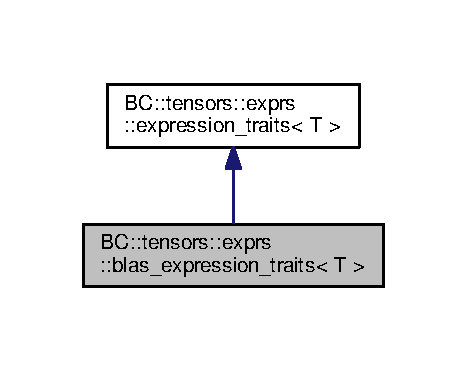
\includegraphics[width=224pt]{structBC_1_1tensors_1_1exprs_1_1blas__expression__traits__inherit__graph}
\end{center}
\end{figure}


Collaboration diagram for BC\+:\+:tensors\+:\+:exprs\+:\+:blas\+\_\+expression\+\_\+traits$<$ T $>$\+:
\nopagebreak
\begin{figure}[H]
\begin{center}
\leavevmode
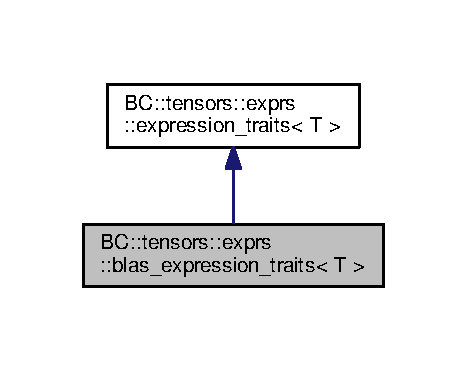
\includegraphics[width=224pt]{structBC_1_1tensors_1_1exprs_1_1blas__expression__traits__coll__graph}
\end{center}
\end{figure}
\subsection*{Public Types}
\begin{DoxyCompactItemize}
\item 
using \hyperlink{structBC_1_1tensors_1_1exprs_1_1blas__expression__traits_a98a1c4a12e066c8ae0109978c366282d}{remove\+\_\+scalar\+\_\+mul\+\_\+type} = typename \hyperlink{structBC_1_1tensors_1_1exprs_1_1detail_1_1remove__scalar__mul}{detail\+::remove\+\_\+scalar\+\_\+mul}$<$ T $>$\+::type
\item 
using \hyperlink{structBC_1_1tensors_1_1exprs_1_1blas__expression__traits_a527a7e3e800aef6cbaedd8eba5f9ae06}{remove\+\_\+transpose\+\_\+type} = typename \hyperlink{structBC_1_1tensors_1_1exprs_1_1detail_1_1remove__transpose}{detail\+::remove\+\_\+transpose}$<$ T $>$\+::type
\item 
using \hyperlink{structBC_1_1tensors_1_1exprs_1_1blas__expression__traits_aab36f77f1b5168d34fd214124ba46a65}{remove\+\_\+blas\+\_\+features\+\_\+type} = typename \hyperlink{structBC_1_1tensors_1_1exprs_1_1detail_1_1remove__transpose}{detail\+::remove\+\_\+transpose}$<$ \hyperlink{structBC_1_1tensors_1_1exprs_1_1blas__expression__traits_a98a1c4a12e066c8ae0109978c366282d}{remove\+\_\+scalar\+\_\+mul\+\_\+type} $>$\+::type
\item 
using \hyperlink{structBC_1_1tensors_1_1exprs_1_1blas__expression__traits_a786eb89c83fea25c296159067d6c1de2}{scalar\+\_\+multiplier\+\_\+type} = typename \hyperlink{structBC_1_1tensors_1_1exprs_1_1detail_1_1remove__scalar__mul}{detail\+::remove\+\_\+scalar\+\_\+mul}$<$ T $>$\+::scalar\+\_\+type
\item 
using \hyperlink{structBC_1_1tensors_1_1exprs_1_1blas__expression__traits_ab83e4462629a63d1058ea86bee5c174b}{value\+\_\+type} = typename T\+::value\+\_\+type
\end{DoxyCompactItemize}
\subsection*{Static Public Member Functions}
\begin{DoxyCompactItemize}
\item 
static \hyperlink{structBC_1_1tensors_1_1exprs_1_1blas__expression__traits_a527a7e3e800aef6cbaedd8eba5f9ae06}{remove\+\_\+transpose\+\_\+type} \hyperlink{structBC_1_1tensors_1_1exprs_1_1blas__expression__traits_a1b8d7da39f60619d849fd2bfa3d105bd}{remove\+\_\+transpose} (T expression)
\item 
static \hyperlink{structBC_1_1tensors_1_1exprs_1_1blas__expression__traits_a98a1c4a12e066c8ae0109978c366282d}{remove\+\_\+scalar\+\_\+mul\+\_\+type} \hyperlink{structBC_1_1tensors_1_1exprs_1_1blas__expression__traits_ab481089d6702b53269d149ca3446f4dd}{remove\+\_\+scalar\+\_\+mul} (T expression)
\item 
static \hyperlink{structBC_1_1tensors_1_1exprs_1_1blas__expression__traits_aab36f77f1b5168d34fd214124ba46a65}{remove\+\_\+blas\+\_\+features\+\_\+type} \hyperlink{structBC_1_1tensors_1_1exprs_1_1blas__expression__traits_a4f4331e95cfed294a61f500cc567b0ac}{remove\+\_\+blas\+\_\+modifiers} (T expression)
\item 
static auto \hyperlink{structBC_1_1tensors_1_1exprs_1_1blas__expression__traits_a71d795a09d1f5ce18ece7fc8cfee44e4}{get\+\_\+scalar} (const T \&expression) -\/$>$ decltype(\hyperlink{structBC_1_1tensors_1_1exprs_1_1detail_1_1remove__scalar__mul}{detail\+::remove\+\_\+scalar\+\_\+mul}$<$ T $>$\+::get\+\_\+scalar(expression))
\end{DoxyCompactItemize}
\subsection*{Static Public Attributes}
\begin{DoxyCompactItemize}
\item 
static constexpr bool \hyperlink{structBC_1_1tensors_1_1exprs_1_1blas__expression__traits_a483a16790c758498147316641b266f3a}{is\+\_\+scalar\+\_\+multiplied} = !std\+::is\+\_\+same$<$\hyperlink{structBC_1_1tensors_1_1exprs_1_1blas__expression__traits_a98a1c4a12e066c8ae0109978c366282d}{remove\+\_\+scalar\+\_\+mul\+\_\+type}, T$>$\+::value
\item 
static constexpr bool \hyperlink{structBC_1_1tensors_1_1exprs_1_1blas__expression__traits_a038605b8d8a7a49c82e6e5eb167e63be}{is\+\_\+transposed} = !std\+::is\+\_\+same$<$\hyperlink{structBC_1_1tensors_1_1exprs_1_1blas__expression__traits_a527a7e3e800aef6cbaedd8eba5f9ae06}{remove\+\_\+transpose\+\_\+type}, T$>$\+::value
\end{DoxyCompactItemize}


\subsection{Member Typedef Documentation}
\index{B\+C\+::tensors\+::exprs\+::blas\+\_\+expression\+\_\+traits@{B\+C\+::tensors\+::exprs\+::blas\+\_\+expression\+\_\+traits}!remove\+\_\+blas\+\_\+features\+\_\+type@{remove\+\_\+blas\+\_\+features\+\_\+type}}
\index{remove\+\_\+blas\+\_\+features\+\_\+type@{remove\+\_\+blas\+\_\+features\+\_\+type}!B\+C\+::tensors\+::exprs\+::blas\+\_\+expression\+\_\+traits@{B\+C\+::tensors\+::exprs\+::blas\+\_\+expression\+\_\+traits}}
\subsubsection[{\texorpdfstring{remove\+\_\+blas\+\_\+features\+\_\+type}{remove_blas_features_type}}]{\setlength{\rightskip}{0pt plus 5cm}template$<$class T $>$ using {\bf B\+C\+::tensors\+::exprs\+::blas\+\_\+expression\+\_\+traits}$<$ T $>$\+::{\bf remove\+\_\+blas\+\_\+features\+\_\+type} =  typename {\bf detail\+::remove\+\_\+transpose}$<${\bf remove\+\_\+scalar\+\_\+mul\+\_\+type}$>$\+::type}\hypertarget{structBC_1_1tensors_1_1exprs_1_1blas__expression__traits_aab36f77f1b5168d34fd214124ba46a65}{}\label{structBC_1_1tensors_1_1exprs_1_1blas__expression__traits_aab36f77f1b5168d34fd214124ba46a65}
\index{B\+C\+::tensors\+::exprs\+::blas\+\_\+expression\+\_\+traits@{B\+C\+::tensors\+::exprs\+::blas\+\_\+expression\+\_\+traits}!remove\+\_\+scalar\+\_\+mul\+\_\+type@{remove\+\_\+scalar\+\_\+mul\+\_\+type}}
\index{remove\+\_\+scalar\+\_\+mul\+\_\+type@{remove\+\_\+scalar\+\_\+mul\+\_\+type}!B\+C\+::tensors\+::exprs\+::blas\+\_\+expression\+\_\+traits@{B\+C\+::tensors\+::exprs\+::blas\+\_\+expression\+\_\+traits}}
\subsubsection[{\texorpdfstring{remove\+\_\+scalar\+\_\+mul\+\_\+type}{remove_scalar_mul_type}}]{\setlength{\rightskip}{0pt plus 5cm}template$<$class T $>$ using {\bf B\+C\+::tensors\+::exprs\+::blas\+\_\+expression\+\_\+traits}$<$ T $>$\+::{\bf remove\+\_\+scalar\+\_\+mul\+\_\+type} =  typename {\bf detail\+::remove\+\_\+scalar\+\_\+mul}$<$T$>$\+::type}\hypertarget{structBC_1_1tensors_1_1exprs_1_1blas__expression__traits_a98a1c4a12e066c8ae0109978c366282d}{}\label{structBC_1_1tensors_1_1exprs_1_1blas__expression__traits_a98a1c4a12e066c8ae0109978c366282d}
\index{B\+C\+::tensors\+::exprs\+::blas\+\_\+expression\+\_\+traits@{B\+C\+::tensors\+::exprs\+::blas\+\_\+expression\+\_\+traits}!remove\+\_\+transpose\+\_\+type@{remove\+\_\+transpose\+\_\+type}}
\index{remove\+\_\+transpose\+\_\+type@{remove\+\_\+transpose\+\_\+type}!B\+C\+::tensors\+::exprs\+::blas\+\_\+expression\+\_\+traits@{B\+C\+::tensors\+::exprs\+::blas\+\_\+expression\+\_\+traits}}
\subsubsection[{\texorpdfstring{remove\+\_\+transpose\+\_\+type}{remove_transpose_type}}]{\setlength{\rightskip}{0pt plus 5cm}template$<$class T $>$ using {\bf B\+C\+::tensors\+::exprs\+::blas\+\_\+expression\+\_\+traits}$<$ T $>$\+::{\bf remove\+\_\+transpose\+\_\+type} =  typename {\bf detail\+::remove\+\_\+transpose}$<$T$>$\+::type}\hypertarget{structBC_1_1tensors_1_1exprs_1_1blas__expression__traits_a527a7e3e800aef6cbaedd8eba5f9ae06}{}\label{structBC_1_1tensors_1_1exprs_1_1blas__expression__traits_a527a7e3e800aef6cbaedd8eba5f9ae06}
\index{B\+C\+::tensors\+::exprs\+::blas\+\_\+expression\+\_\+traits@{B\+C\+::tensors\+::exprs\+::blas\+\_\+expression\+\_\+traits}!scalar\+\_\+multiplier\+\_\+type@{scalar\+\_\+multiplier\+\_\+type}}
\index{scalar\+\_\+multiplier\+\_\+type@{scalar\+\_\+multiplier\+\_\+type}!B\+C\+::tensors\+::exprs\+::blas\+\_\+expression\+\_\+traits@{B\+C\+::tensors\+::exprs\+::blas\+\_\+expression\+\_\+traits}}
\subsubsection[{\texorpdfstring{scalar\+\_\+multiplier\+\_\+type}{scalar_multiplier_type}}]{\setlength{\rightskip}{0pt plus 5cm}template$<$class T $>$ using {\bf B\+C\+::tensors\+::exprs\+::blas\+\_\+expression\+\_\+traits}$<$ T $>$\+::{\bf scalar\+\_\+multiplier\+\_\+type} =  typename {\bf detail\+::remove\+\_\+scalar\+\_\+mul}$<$T$>$\+::scalar\+\_\+type}\hypertarget{structBC_1_1tensors_1_1exprs_1_1blas__expression__traits_a786eb89c83fea25c296159067d6c1de2}{}\label{structBC_1_1tensors_1_1exprs_1_1blas__expression__traits_a786eb89c83fea25c296159067d6c1de2}
\index{B\+C\+::tensors\+::exprs\+::blas\+\_\+expression\+\_\+traits@{B\+C\+::tensors\+::exprs\+::blas\+\_\+expression\+\_\+traits}!value\+\_\+type@{value\+\_\+type}}
\index{value\+\_\+type@{value\+\_\+type}!B\+C\+::tensors\+::exprs\+::blas\+\_\+expression\+\_\+traits@{B\+C\+::tensors\+::exprs\+::blas\+\_\+expression\+\_\+traits}}
\subsubsection[{\texorpdfstring{value\+\_\+type}{value_type}}]{\setlength{\rightskip}{0pt plus 5cm}template$<$class T $>$ using {\bf B\+C\+::tensors\+::exprs\+::blas\+\_\+expression\+\_\+traits}$<$ T $>$\+::{\bf value\+\_\+type} =  typename T\+::value\+\_\+type}\hypertarget{structBC_1_1tensors_1_1exprs_1_1blas__expression__traits_ab83e4462629a63d1058ea86bee5c174b}{}\label{structBC_1_1tensors_1_1exprs_1_1blas__expression__traits_ab83e4462629a63d1058ea86bee5c174b}


\subsection{Member Function Documentation}
\index{B\+C\+::tensors\+::exprs\+::blas\+\_\+expression\+\_\+traits@{B\+C\+::tensors\+::exprs\+::blas\+\_\+expression\+\_\+traits}!get\+\_\+scalar@{get\+\_\+scalar}}
\index{get\+\_\+scalar@{get\+\_\+scalar}!B\+C\+::tensors\+::exprs\+::blas\+\_\+expression\+\_\+traits@{B\+C\+::tensors\+::exprs\+::blas\+\_\+expression\+\_\+traits}}
\subsubsection[{\texorpdfstring{get\+\_\+scalar(const T \&expression) -\/$>$ decltype(detail\+::remove\+\_\+scalar\+\_\+mul$<$ T $>$\+::get\+\_\+scalar(expression))}{get_scalar(const T &expression) -> decltype(detail::remove_scalar_mul< T >::get_scalar(expression))}}]{\setlength{\rightskip}{0pt plus 5cm}template$<$class T $>$ static auto {\bf B\+C\+::tensors\+::exprs\+::blas\+\_\+expression\+\_\+traits}$<$ T $>$\+::get\+\_\+scalar (
\begin{DoxyParamCaption}
\item[{const T \&}]{expression}
\end{DoxyParamCaption}
) -\/$>$ decltype({\bf detail\+::remove\+\_\+scalar\+\_\+mul}$<$T$>$\+::get\+\_\+scalar(expression)) \hspace{0.3cm}{\ttfamily [inline]}, {\ttfamily [static]}}\hypertarget{structBC_1_1tensors_1_1exprs_1_1blas__expression__traits_a71d795a09d1f5ce18ece7fc8cfee44e4}{}\label{structBC_1_1tensors_1_1exprs_1_1blas__expression__traits_a71d795a09d1f5ce18ece7fc8cfee44e4}
\index{B\+C\+::tensors\+::exprs\+::blas\+\_\+expression\+\_\+traits@{B\+C\+::tensors\+::exprs\+::blas\+\_\+expression\+\_\+traits}!remove\+\_\+blas\+\_\+modifiers@{remove\+\_\+blas\+\_\+modifiers}}
\index{remove\+\_\+blas\+\_\+modifiers@{remove\+\_\+blas\+\_\+modifiers}!B\+C\+::tensors\+::exprs\+::blas\+\_\+expression\+\_\+traits@{B\+C\+::tensors\+::exprs\+::blas\+\_\+expression\+\_\+traits}}
\subsubsection[{\texorpdfstring{remove\+\_\+blas\+\_\+modifiers(\+T expression)}{remove_blas_modifiers(T expression)}}]{\setlength{\rightskip}{0pt plus 5cm}template$<$class T $>$ static {\bf remove\+\_\+blas\+\_\+features\+\_\+type} {\bf B\+C\+::tensors\+::exprs\+::blas\+\_\+expression\+\_\+traits}$<$ T $>$\+::remove\+\_\+blas\+\_\+modifiers (
\begin{DoxyParamCaption}
\item[{T}]{expression}
\end{DoxyParamCaption}
)\hspace{0.3cm}{\ttfamily [inline]}, {\ttfamily [static]}}\hypertarget{structBC_1_1tensors_1_1exprs_1_1blas__expression__traits_a4f4331e95cfed294a61f500cc567b0ac}{}\label{structBC_1_1tensors_1_1exprs_1_1blas__expression__traits_a4f4331e95cfed294a61f500cc567b0ac}
\index{B\+C\+::tensors\+::exprs\+::blas\+\_\+expression\+\_\+traits@{B\+C\+::tensors\+::exprs\+::blas\+\_\+expression\+\_\+traits}!remove\+\_\+scalar\+\_\+mul@{remove\+\_\+scalar\+\_\+mul}}
\index{remove\+\_\+scalar\+\_\+mul@{remove\+\_\+scalar\+\_\+mul}!B\+C\+::tensors\+::exprs\+::blas\+\_\+expression\+\_\+traits@{B\+C\+::tensors\+::exprs\+::blas\+\_\+expression\+\_\+traits}}
\subsubsection[{\texorpdfstring{remove\+\_\+scalar\+\_\+mul(\+T expression)}{remove_scalar_mul(T expression)}}]{\setlength{\rightskip}{0pt plus 5cm}template$<$class T $>$ static {\bf remove\+\_\+scalar\+\_\+mul\+\_\+type} {\bf B\+C\+::tensors\+::exprs\+::blas\+\_\+expression\+\_\+traits}$<$ T $>$\+::remove\+\_\+scalar\+\_\+mul (
\begin{DoxyParamCaption}
\item[{T}]{expression}
\end{DoxyParamCaption}
)\hspace{0.3cm}{\ttfamily [inline]}, {\ttfamily [static]}}\hypertarget{structBC_1_1tensors_1_1exprs_1_1blas__expression__traits_ab481089d6702b53269d149ca3446f4dd}{}\label{structBC_1_1tensors_1_1exprs_1_1blas__expression__traits_ab481089d6702b53269d149ca3446f4dd}
\index{B\+C\+::tensors\+::exprs\+::blas\+\_\+expression\+\_\+traits@{B\+C\+::tensors\+::exprs\+::blas\+\_\+expression\+\_\+traits}!remove\+\_\+transpose@{remove\+\_\+transpose}}
\index{remove\+\_\+transpose@{remove\+\_\+transpose}!B\+C\+::tensors\+::exprs\+::blas\+\_\+expression\+\_\+traits@{B\+C\+::tensors\+::exprs\+::blas\+\_\+expression\+\_\+traits}}
\subsubsection[{\texorpdfstring{remove\+\_\+transpose(\+T expression)}{remove_transpose(T expression)}}]{\setlength{\rightskip}{0pt plus 5cm}template$<$class T $>$ static {\bf remove\+\_\+transpose\+\_\+type} {\bf B\+C\+::tensors\+::exprs\+::blas\+\_\+expression\+\_\+traits}$<$ T $>$\+::remove\+\_\+transpose (
\begin{DoxyParamCaption}
\item[{T}]{expression}
\end{DoxyParamCaption}
)\hspace{0.3cm}{\ttfamily [inline]}, {\ttfamily [static]}}\hypertarget{structBC_1_1tensors_1_1exprs_1_1blas__expression__traits_a1b8d7da39f60619d849fd2bfa3d105bd}{}\label{structBC_1_1tensors_1_1exprs_1_1blas__expression__traits_a1b8d7da39f60619d849fd2bfa3d105bd}


\subsection{Member Data Documentation}
\index{B\+C\+::tensors\+::exprs\+::blas\+\_\+expression\+\_\+traits@{B\+C\+::tensors\+::exprs\+::blas\+\_\+expression\+\_\+traits}!is\+\_\+scalar\+\_\+multiplied@{is\+\_\+scalar\+\_\+multiplied}}
\index{is\+\_\+scalar\+\_\+multiplied@{is\+\_\+scalar\+\_\+multiplied}!B\+C\+::tensors\+::exprs\+::blas\+\_\+expression\+\_\+traits@{B\+C\+::tensors\+::exprs\+::blas\+\_\+expression\+\_\+traits}}
\subsubsection[{\texorpdfstring{is\+\_\+scalar\+\_\+multiplied}{is_scalar_multiplied}}]{\setlength{\rightskip}{0pt plus 5cm}template$<$class T $>$ constexpr bool {\bf B\+C\+::tensors\+::exprs\+::blas\+\_\+expression\+\_\+traits}$<$ T $>$\+::is\+\_\+scalar\+\_\+multiplied = !std\+::is\+\_\+same$<${\bf remove\+\_\+scalar\+\_\+mul\+\_\+type}, T$>$\+::value\hspace{0.3cm}{\ttfamily [static]}}\hypertarget{structBC_1_1tensors_1_1exprs_1_1blas__expression__traits_a483a16790c758498147316641b266f3a}{}\label{structBC_1_1tensors_1_1exprs_1_1blas__expression__traits_a483a16790c758498147316641b266f3a}
\index{B\+C\+::tensors\+::exprs\+::blas\+\_\+expression\+\_\+traits@{B\+C\+::tensors\+::exprs\+::blas\+\_\+expression\+\_\+traits}!is\+\_\+transposed@{is\+\_\+transposed}}
\index{is\+\_\+transposed@{is\+\_\+transposed}!B\+C\+::tensors\+::exprs\+::blas\+\_\+expression\+\_\+traits@{B\+C\+::tensors\+::exprs\+::blas\+\_\+expression\+\_\+traits}}
\subsubsection[{\texorpdfstring{is\+\_\+transposed}{is_transposed}}]{\setlength{\rightskip}{0pt plus 5cm}template$<$class T $>$ constexpr bool {\bf B\+C\+::tensors\+::exprs\+::blas\+\_\+expression\+\_\+traits}$<$ T $>$\+::is\+\_\+transposed = !std\+::is\+\_\+same$<${\bf remove\+\_\+transpose\+\_\+type}, T$>$\+::value\hspace{0.3cm}{\ttfamily [static]}}\hypertarget{structBC_1_1tensors_1_1exprs_1_1blas__expression__traits_a038605b8d8a7a49c82e6e5eb167e63be}{}\label{structBC_1_1tensors_1_1exprs_1_1blas__expression__traits_a038605b8d8a7a49c82e6e5eb167e63be}


The documentation for this struct was generated from the following file\+:\begin{DoxyCompactItemize}
\item 
include/tensors/expression\+\_\+templates/\hyperlink{Expression__Template__Traits_8h}{Expression\+\_\+\+Template\+\_\+\+Traits.\+h}\end{DoxyCompactItemize}

\hypertarget{structBC_1_1oper_1_1BLAS__Function}{}\section{BC\+:\+:oper\+:\+:B\+L\+A\+S\+\_\+\+Function Struct Reference}
\label{structBC_1_1oper_1_1BLAS__Function}\index{B\+C\+::oper\+::\+B\+L\+A\+S\+\_\+\+Function@{B\+C\+::oper\+::\+B\+L\+A\+S\+\_\+\+Function}}


{\ttfamily \#include $<$Tags.\+h$>$}



Inheritance diagram for BC\+:\+:oper\+:\+:B\+L\+A\+S\+\_\+\+Function\+:
\nopagebreak
\begin{figure}[H]
\begin{center}
\leavevmode
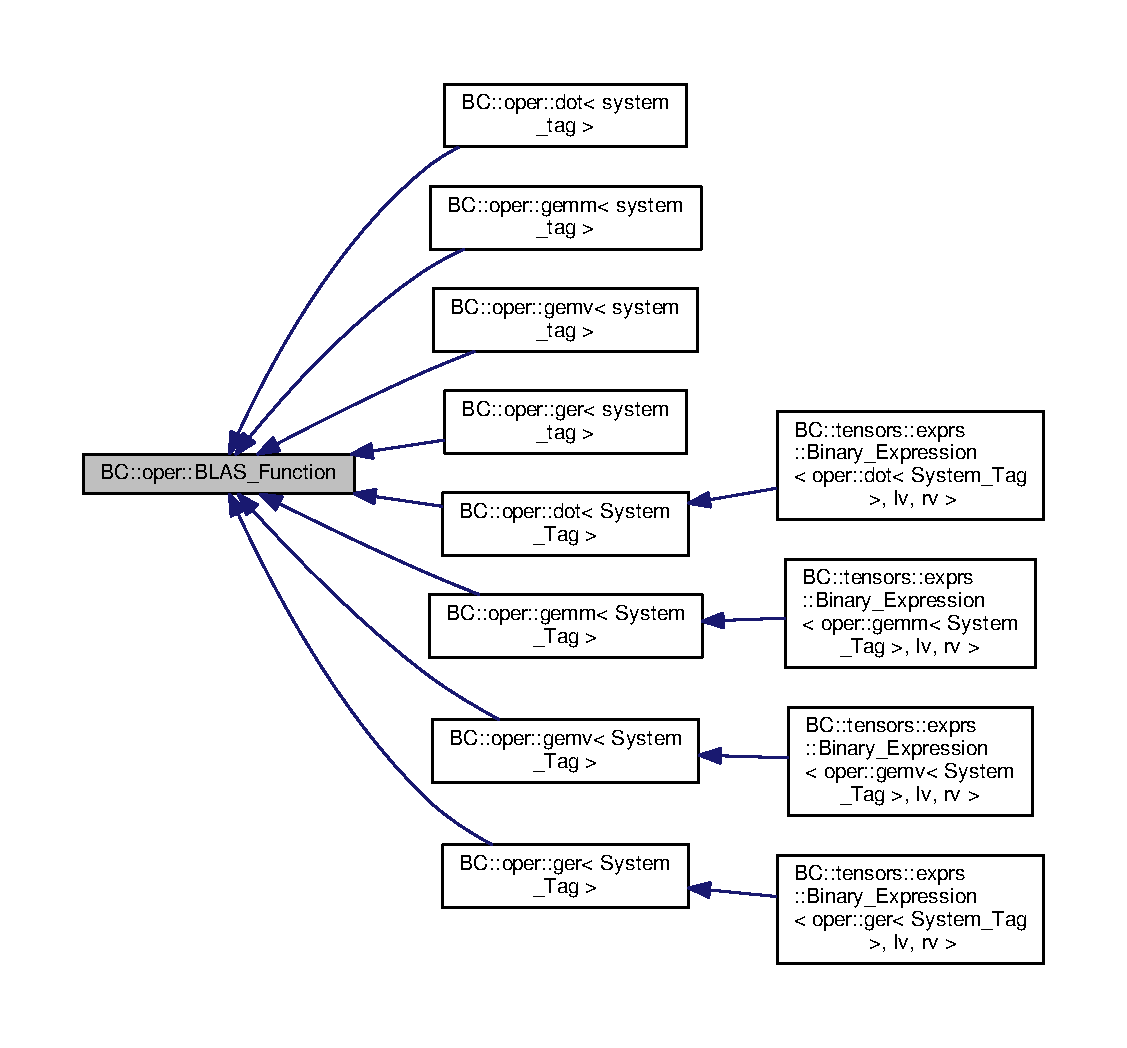
\includegraphics[width=350pt]{structBC_1_1oper_1_1BLAS__Function__inherit__graph}
\end{center}
\end{figure}


The documentation for this struct was generated from the following file\+:\begin{DoxyCompactItemize}
\item 
include/operations/\hyperlink{operations_2Tags_8h}{Tags.\+h}\end{DoxyCompactItemize}

\hypertarget{structBC_1_1tensors_1_1exprs_1_1blas__tools_1_1BLAS__Tools_3_01host__tag_01_4}{}\section{BC\+:\+:tensors\+:\+:exprs\+:\+:blas\+\_\+tools\+:\+:B\+L\+A\+S\+\_\+\+Tools$<$ host\+\_\+tag $>$ Struct Template Reference}
\label{structBC_1_1tensors_1_1exprs_1_1blas__tools_1_1BLAS__Tools_3_01host__tag_01_4}\index{B\+C\+::tensors\+::exprs\+::blas\+\_\+tools\+::\+B\+L\+A\+S\+\_\+\+Tools$<$ host\+\_\+tag $>$@{B\+C\+::tensors\+::exprs\+::blas\+\_\+tools\+::\+B\+L\+A\+S\+\_\+\+Tools$<$ host\+\_\+tag $>$}}


{\ttfamily \#include $<$Host.\+h$>$}



Inheritance diagram for BC\+:\+:tensors\+:\+:exprs\+:\+:blas\+\_\+tools\+:\+:B\+L\+A\+S\+\_\+\+Tools$<$ host\+\_\+tag $>$\+:
\nopagebreak
\begin{figure}[H]
\begin{center}
\leavevmode
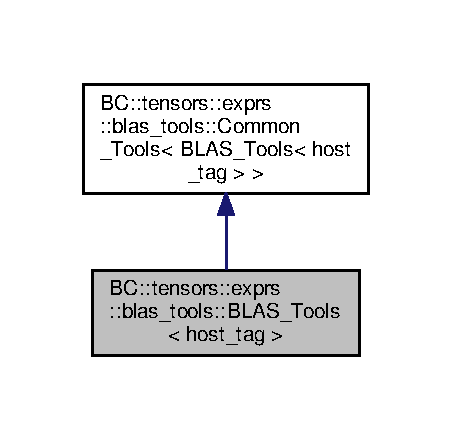
\includegraphics[width=217pt]{structBC_1_1tensors_1_1exprs_1_1blas__tools_1_1BLAS__Tools_3_01host__tag_01_4__inherit__graph}
\end{center}
\end{figure}


Collaboration diagram for BC\+:\+:tensors\+:\+:exprs\+:\+:blas\+\_\+tools\+:\+:B\+L\+A\+S\+\_\+\+Tools$<$ host\+\_\+tag $>$\+:
\nopagebreak
\begin{figure}[H]
\begin{center}
\leavevmode
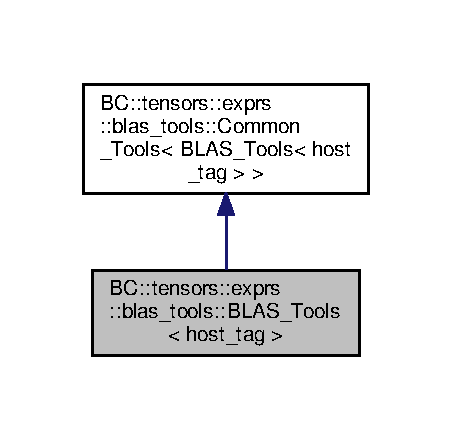
\includegraphics[width=217pt]{structBC_1_1tensors_1_1exprs_1_1blas__tools_1_1BLAS__Tools_3_01host__tag_01_4__coll__graph}
\end{center}
\end{figure}
\subsection*{Static Public Member Functions}
\begin{DoxyCompactItemize}
\item 
{\footnotesize template$<$class Stream , class Output\+Scalar , class... Scalars$>$ }\\static void \hyperlink{structBC_1_1tensors_1_1exprs_1_1blas__tools_1_1BLAS__Tools_3_01host__tag_01_4_aedaf522df616b17b9bc66b708b122f57}{scalar\+\_\+multiply} (\hyperlink{namespaceBC_abc64a63cd29a22d102a68f478dfd588d}{Stream}, Output\+Scalar \&eval, Scalars...\+scalars)
\item 
{\footnotesize template$<$class Stream , class Output\+Scalar , class... Scalars$>$ }\\static void \hyperlink{structBC_1_1tensors_1_1exprs_1_1blas__tools_1_1BLAS__Tools_3_01host__tag_01_4_a7a2926bf7415f4383cb8ddecc0b2458e}{scalar\+\_\+multiply} (\hyperlink{namespaceBC_abc64a63cd29a22d102a68f478dfd588d}{Stream}, Output\+Scalar $\ast$eval, Scalars...\+scalars)
\item 
{\footnotesize template$<$class value\+\_\+type , int value$>$ }\\static auto \hyperlink{structBC_1_1tensors_1_1exprs_1_1blas__tools_1_1BLAS__Tools_3_01host__tag_01_4_ab55487639c6d0c2e8fa42ee9a87e3ac6}{scalar\+\_\+constant} ()
\end{DoxyCompactItemize}


\subsection{Member Function Documentation}
\index{B\+C\+::tensors\+::exprs\+::blas\+\_\+tools\+::\+B\+L\+A\+S\+\_\+\+Tools$<$ host\+\_\+tag $>$@{B\+C\+::tensors\+::exprs\+::blas\+\_\+tools\+::\+B\+L\+A\+S\+\_\+\+Tools$<$ host\+\_\+tag $>$}!scalar\+\_\+constant@{scalar\+\_\+constant}}
\index{scalar\+\_\+constant@{scalar\+\_\+constant}!B\+C\+::tensors\+::exprs\+::blas\+\_\+tools\+::\+B\+L\+A\+S\+\_\+\+Tools$<$ host\+\_\+tag $>$@{B\+C\+::tensors\+::exprs\+::blas\+\_\+tools\+::\+B\+L\+A\+S\+\_\+\+Tools$<$ host\+\_\+tag $>$}}
\subsubsection[{\texorpdfstring{scalar\+\_\+constant()}{scalar_constant()}}]{\setlength{\rightskip}{0pt plus 5cm}template$<$class value\+\_\+type , int value$>$ static auto B\+C\+::tensors\+::exprs\+::blas\+\_\+tools\+::\+B\+L\+A\+S\+\_\+\+Tools$<$ {\bf host\+\_\+tag} $>$\+::scalar\+\_\+constant (
\begin{DoxyParamCaption}
{}
\end{DoxyParamCaption}
)\hspace{0.3cm}{\ttfamily [inline]}, {\ttfamily [static]}}\hypertarget{structBC_1_1tensors_1_1exprs_1_1blas__tools_1_1BLAS__Tools_3_01host__tag_01_4_ab55487639c6d0c2e8fa42ee9a87e3ac6}{}\label{structBC_1_1tensors_1_1exprs_1_1blas__tools_1_1BLAS__Tools_3_01host__tag_01_4_ab55487639c6d0c2e8fa42ee9a87e3ac6}
\index{B\+C\+::tensors\+::exprs\+::blas\+\_\+tools\+::\+B\+L\+A\+S\+\_\+\+Tools$<$ host\+\_\+tag $>$@{B\+C\+::tensors\+::exprs\+::blas\+\_\+tools\+::\+B\+L\+A\+S\+\_\+\+Tools$<$ host\+\_\+tag $>$}!scalar\+\_\+multiply@{scalar\+\_\+multiply}}
\index{scalar\+\_\+multiply@{scalar\+\_\+multiply}!B\+C\+::tensors\+::exprs\+::blas\+\_\+tools\+::\+B\+L\+A\+S\+\_\+\+Tools$<$ host\+\_\+tag $>$@{B\+C\+::tensors\+::exprs\+::blas\+\_\+tools\+::\+B\+L\+A\+S\+\_\+\+Tools$<$ host\+\_\+tag $>$}}
\subsubsection[{\texorpdfstring{scalar\+\_\+multiply(\+Stream, Output\+Scalar \&eval, Scalars...\+scalars)}{scalar_multiply(Stream, OutputScalar &eval, Scalars...scalars)}}]{\setlength{\rightskip}{0pt plus 5cm}template$<$class Stream , class Output\+Scalar , class... Scalars$>$ static void B\+C\+::tensors\+::exprs\+::blas\+\_\+tools\+::\+B\+L\+A\+S\+\_\+\+Tools$<$ {\bf host\+\_\+tag} $>$\+::scalar\+\_\+multiply (
\begin{DoxyParamCaption}
\item[{{\bf Stream}}]{, }
\item[{Output\+Scalar \&}]{eval, }
\item[{Scalars...}]{scalars}
\end{DoxyParamCaption}
)\hspace{0.3cm}{\ttfamily [inline]}, {\ttfamily [static]}}\hypertarget{structBC_1_1tensors_1_1exprs_1_1blas__tools_1_1BLAS__Tools_3_01host__tag_01_4_aedaf522df616b17b9bc66b708b122f57}{}\label{structBC_1_1tensors_1_1exprs_1_1blas__tools_1_1BLAS__Tools_3_01host__tag_01_4_aedaf522df616b17b9bc66b708b122f57}
\index{B\+C\+::tensors\+::exprs\+::blas\+\_\+tools\+::\+B\+L\+A\+S\+\_\+\+Tools$<$ host\+\_\+tag $>$@{B\+C\+::tensors\+::exprs\+::blas\+\_\+tools\+::\+B\+L\+A\+S\+\_\+\+Tools$<$ host\+\_\+tag $>$}!scalar\+\_\+multiply@{scalar\+\_\+multiply}}
\index{scalar\+\_\+multiply@{scalar\+\_\+multiply}!B\+C\+::tensors\+::exprs\+::blas\+\_\+tools\+::\+B\+L\+A\+S\+\_\+\+Tools$<$ host\+\_\+tag $>$@{B\+C\+::tensors\+::exprs\+::blas\+\_\+tools\+::\+B\+L\+A\+S\+\_\+\+Tools$<$ host\+\_\+tag $>$}}
\subsubsection[{\texorpdfstring{scalar\+\_\+multiply(\+Stream, Output\+Scalar $\ast$eval, Scalars...\+scalars)}{scalar_multiply(Stream, OutputScalar *eval, Scalars...scalars)}}]{\setlength{\rightskip}{0pt plus 5cm}template$<$class Stream , class Output\+Scalar , class... Scalars$>$ static void B\+C\+::tensors\+::exprs\+::blas\+\_\+tools\+::\+B\+L\+A\+S\+\_\+\+Tools$<$ {\bf host\+\_\+tag} $>$\+::scalar\+\_\+multiply (
\begin{DoxyParamCaption}
\item[{{\bf Stream}}]{, }
\item[{Output\+Scalar $\ast$}]{eval, }
\item[{Scalars...}]{scalars}
\end{DoxyParamCaption}
)\hspace{0.3cm}{\ttfamily [inline]}, {\ttfamily [static]}}\hypertarget{structBC_1_1tensors_1_1exprs_1_1blas__tools_1_1BLAS__Tools_3_01host__tag_01_4_a7a2926bf7415f4383cb8ddecc0b2458e}{}\label{structBC_1_1tensors_1_1exprs_1_1blas__tools_1_1BLAS__Tools_3_01host__tag_01_4_a7a2926bf7415f4383cb8ddecc0b2458e}


The documentation for this struct was generated from the following file\+:\begin{DoxyCompactItemize}
\item 
include/tensors/expression\+\_\+templates/blas\+\_\+tools/\hyperlink{tensors_2expression__templates_2blas__tools_2Host_8h}{Host.\+h}\end{DoxyCompactItemize}

\hypertarget{classBC_1_1allocators_1_1Byte}{}\section{BC\+:\+:allocators\+:\+:Byte Class Reference}
\label{classBC_1_1allocators_1_1Byte}\index{B\+C\+::allocators\+::\+Byte@{B\+C\+::allocators\+::\+Byte}}


{\ttfamily \#include $<$Allocators.\+h$>$}



The documentation for this class was generated from the following file\+:\begin{DoxyCompactItemize}
\item 
include/allocators/\hyperlink{Allocators_8h}{Allocators.\+h}\end{DoxyCompactItemize}

\hypertarget{structBC_1_1NN_1_1Chain}{}\section{BC\+:\+:NN\+:\+:Chain$<$ lst $>$ Struct Template Reference}
\label{structBC_1_1NN_1_1Chain}\index{B\+C\+::\+N\+N\+::\+Chain$<$ lst $>$@{B\+C\+::\+N\+N\+::\+Chain$<$ lst $>$}}


{\ttfamily \#include $<$network.\+h$>$}



Inheritance diagram for BC\+:\+:NN\+:\+:Chain$<$ lst $>$\+:
\nopagebreak
\begin{figure}[H]
\begin{center}
\leavevmode
\includegraphics[width=192pt]{structBC_1_1NN_1_1Chain__inherit__graph}
\end{center}
\end{figure}


Collaboration diagram for BC\+:\+:NN\+:\+:Chain$<$ lst $>$\+:
\nopagebreak
\begin{figure}[H]
\begin{center}
\leavevmode
\includegraphics[width=192pt]{structBC_1_1NN_1_1Chain__coll__graph}
\end{center}
\end{figure}
\subsection*{Public Types}
\begin{DoxyCompactItemize}
\item 
using \hyperlink{structBC_1_1NN_1_1Chain_a0b49e7c4d6ebb165c42d8d5d8413cfd6}{self} = \hyperlink{structBC_1_1NN_1_1Chain}{Chain}$<$ lst... $>$
\item 
using \hyperlink{structBC_1_1NN_1_1Chain_a32de6795ede484f33f461e161a8ab785}{parent} = \hyperlink{structBC_1_1NN_1_1LayerChain}{Layer\+Chain}$<$ 0, \hyperlink{structBC_1_1NN_1_1Chain_a0b49e7c4d6ebb165c42d8d5d8413cfd6}{self}, lst... $>$
\end{DoxyCompactItemize}
\subsection*{Public Member Functions}
\begin{DoxyCompactItemize}
\item 
{\footnotesize template$<$class... integers$>$ }\\\hyperlink{structBC_1_1NN_1_1Chain_a07b03d8f2baa7a60bf029fce106aa6d5}{Chain} (int x, integers...\+dims)
\item 
{\footnotesize template$<$class T $>$ }\\const auto \& \hyperlink{structBC_1_1NN_1_1Chain_a0e2d0f62b9c372ffc57b0daee9a3aae1}{back\+\_\+propagation} (const T \&tensor\+\_\+expected)
\item 
{\footnotesize template$<$class T $>$ }\\const auto \& \hyperlink{structBC_1_1NN_1_1Chain_a40b6c171073b5b92e81867762e8bd1a6}{forward\+\_\+propagation} (const T \&tensor\+\_\+expected)
\item 
void \hyperlink{structBC_1_1NN_1_1Chain_a64161fb5c71b1c5f0fa0eeb1a5fcee92}{read} (std\+::ifstream \&is)
\item 
void \hyperlink{structBC_1_1NN_1_1Chain_a450e3960898f066c4a89d36d73cb3cc4}{write} (std\+::ifstream \&os)
\item 
void \hyperlink{structBC_1_1NN_1_1Chain_a02e2d026db3cb1c918895fa58bbce832}{set\+\_\+batch\+\_\+size} (int x)
\item 
void \hyperlink{structBC_1_1NN_1_1Chain_a5849a2e8cd2907345bb9ae03a51b74b5}{update\+\_\+weights} ()
\item 
void \hyperlink{structBC_1_1NN_1_1Chain_a4276120642218b0ad6690d173c067584}{cache\+\_\+gradients} ()
\item 
void \hyperlink{structBC_1_1NN_1_1Chain_af5b0f474e6985900251d89245e8a99fa}{set\+\_\+max\+\_\+bptt\+\_\+length} (int len)
\item 
void \hyperlink{structBC_1_1NN_1_1Chain_a4a2329c35c0576ebe24a966c33042d24}{set\+\_\+learning\+\_\+rate} (fp\+\_\+type lr)
\item 
{\footnotesize template$<$class function $>$ }\\void \hyperlink{structBC_1_1NN_1_1Chain_a79b1be73e16cfd44f6689b47e2af08fa}{for\+\_\+each\+\_\+internal} (function f)
\item 
void \hyperlink{structBC_1_1NN_1_1Chain_a9d69c9bc5baff86fca5f5e231d1f50f6}{initialize\+\_\+variables} ()
\item 
{\footnotesize template$<$class T $>$ }\\const auto \& \hyperlink{structBC_1_1NN_1_1Chain_ad6edc8f2f7a58068817ea40d0d1c7d7c}{bp} (const T \&dx)
\item 
auto \& \hyperlink{structBC_1_1NN_1_1Chain_a1d849218f6fe4c32cafcfb0f53e16cf5}{head} ()
\end{DoxyCompactItemize}
\subsection*{Public Attributes}
\begin{DoxyCompactItemize}
\item 
vec \hyperlink{structBC_1_1NN_1_1Chain_a2090e18b2f5bf4b2aa751a8abc7ace13}{outputs}
\item 
vec \hyperlink{structBC_1_1NN_1_1Chain_a857ba54a8bbfd9f01c34d225fcaad9f0}{deltas}
\item 
\hyperlink{namespaceBC_a6007cbc4eeec401a037b558910a56173}{B\+C\+::size\+\_\+t} \hyperlink{structBC_1_1NN_1_1Chain_a3c6d769b2e92ff5963ab391d5697b289}{batch\+\_\+size} = 1
\end{DoxyCompactItemize}


\subsection{Member Typedef Documentation}
\index{B\+C\+::\+N\+N\+::\+Chain@{B\+C\+::\+N\+N\+::\+Chain}!parent@{parent}}
\index{parent@{parent}!B\+C\+::\+N\+N\+::\+Chain@{B\+C\+::\+N\+N\+::\+Chain}}
\subsubsection[{\texorpdfstring{parent}{parent}}]{\setlength{\rightskip}{0pt plus 5cm}template$<$class... lst$>$ using {\bf B\+C\+::\+N\+N\+::\+Chain}$<$ lst $>$\+::{\bf parent} =  {\bf Layer\+Chain}$<$0, {\bf self}, lst...$>$}\hypertarget{structBC_1_1NN_1_1Chain_a32de6795ede484f33f461e161a8ab785}{}\label{structBC_1_1NN_1_1Chain_a32de6795ede484f33f461e161a8ab785}
\index{B\+C\+::\+N\+N\+::\+Chain@{B\+C\+::\+N\+N\+::\+Chain}!self@{self}}
\index{self@{self}!B\+C\+::\+N\+N\+::\+Chain@{B\+C\+::\+N\+N\+::\+Chain}}
\subsubsection[{\texorpdfstring{self}{self}}]{\setlength{\rightskip}{0pt plus 5cm}template$<$class... lst$>$ using {\bf B\+C\+::\+N\+N\+::\+Chain}$<$ lst $>$\+::{\bf self} =  {\bf Chain}$<$lst...$>$}\hypertarget{structBC_1_1NN_1_1Chain_a0b49e7c4d6ebb165c42d8d5d8413cfd6}{}\label{structBC_1_1NN_1_1Chain_a0b49e7c4d6ebb165c42d8d5d8413cfd6}


\subsection{Constructor \& Destructor Documentation}
\index{B\+C\+::\+N\+N\+::\+Chain@{B\+C\+::\+N\+N\+::\+Chain}!Chain@{Chain}}
\index{Chain@{Chain}!B\+C\+::\+N\+N\+::\+Chain@{B\+C\+::\+N\+N\+::\+Chain}}
\subsubsection[{\texorpdfstring{Chain(int x, integers...\+dims)}{Chain(int x, integers...dims)}}]{\setlength{\rightskip}{0pt plus 5cm}template$<$class... lst$>$ template$<$class... integers$>$ {\bf B\+C\+::\+N\+N\+::\+Chain}$<$ lst $>$\+::{\bf Chain} (
\begin{DoxyParamCaption}
\item[{int}]{x, }
\item[{integers...}]{dims}
\end{DoxyParamCaption}
)\hspace{0.3cm}{\ttfamily [inline]}}\hypertarget{structBC_1_1NN_1_1Chain_a07b03d8f2baa7a60bf029fce106aa6d5}{}\label{structBC_1_1NN_1_1Chain_a07b03d8f2baa7a60bf029fce106aa6d5}


\subsection{Member Function Documentation}
\index{B\+C\+::\+N\+N\+::\+Chain@{B\+C\+::\+N\+N\+::\+Chain}!back\+\_\+propagation@{back\+\_\+propagation}}
\index{back\+\_\+propagation@{back\+\_\+propagation}!B\+C\+::\+N\+N\+::\+Chain@{B\+C\+::\+N\+N\+::\+Chain}}
\subsubsection[{\texorpdfstring{back\+\_\+propagation(const T \&tensor\+\_\+expected)}{back_propagation(const T &tensor_expected)}}]{\setlength{\rightskip}{0pt plus 5cm}template$<$class... lst$>$ template$<$class T $>$ const auto\& {\bf B\+C\+::\+N\+N\+::\+Chain}$<$ lst $>$\+::back\+\_\+propagation (
\begin{DoxyParamCaption}
\item[{const T \&}]{tensor\+\_\+expected}
\end{DoxyParamCaption}
)\hspace{0.3cm}{\ttfamily [inline]}}\hypertarget{structBC_1_1NN_1_1Chain_a0e2d0f62b9c372ffc57b0daee9a3aae1}{}\label{structBC_1_1NN_1_1Chain_a0e2d0f62b9c372ffc57b0daee9a3aae1}
\index{B\+C\+::\+N\+N\+::\+Chain@{B\+C\+::\+N\+N\+::\+Chain}!bp@{bp}}
\index{bp@{bp}!B\+C\+::\+N\+N\+::\+Chain@{B\+C\+::\+N\+N\+::\+Chain}}
\subsubsection[{\texorpdfstring{bp(const T \&dx)}{bp(const T &dx)}}]{\setlength{\rightskip}{0pt plus 5cm}template$<$class... lst$>$ template$<$class T $>$ const auto\& {\bf B\+C\+::\+N\+N\+::\+Chain}$<$ lst $>$\+::bp (
\begin{DoxyParamCaption}
\item[{const T \&}]{dx}
\end{DoxyParamCaption}
)\hspace{0.3cm}{\ttfamily [inline]}}\hypertarget{structBC_1_1NN_1_1Chain_ad6edc8f2f7a58068817ea40d0d1c7d7c}{}\label{structBC_1_1NN_1_1Chain_ad6edc8f2f7a58068817ea40d0d1c7d7c}
\index{B\+C\+::\+N\+N\+::\+Chain@{B\+C\+::\+N\+N\+::\+Chain}!cache\+\_\+gradients@{cache\+\_\+gradients}}
\index{cache\+\_\+gradients@{cache\+\_\+gradients}!B\+C\+::\+N\+N\+::\+Chain@{B\+C\+::\+N\+N\+::\+Chain}}
\subsubsection[{\texorpdfstring{cache\+\_\+gradients()}{cache_gradients()}}]{\setlength{\rightskip}{0pt plus 5cm}template$<$class... lst$>$ void {\bf B\+C\+::\+N\+N\+::\+Chain}$<$ lst $>$\+::cache\+\_\+gradients (
\begin{DoxyParamCaption}
{}
\end{DoxyParamCaption}
)\hspace{0.3cm}{\ttfamily [inline]}}\hypertarget{structBC_1_1NN_1_1Chain_a4276120642218b0ad6690d173c067584}{}\label{structBC_1_1NN_1_1Chain_a4276120642218b0ad6690d173c067584}
\index{B\+C\+::\+N\+N\+::\+Chain@{B\+C\+::\+N\+N\+::\+Chain}!for\+\_\+each\+\_\+internal@{for\+\_\+each\+\_\+internal}}
\index{for\+\_\+each\+\_\+internal@{for\+\_\+each\+\_\+internal}!B\+C\+::\+N\+N\+::\+Chain@{B\+C\+::\+N\+N\+::\+Chain}}
\subsubsection[{\texorpdfstring{for\+\_\+each\+\_\+internal(function f)}{for_each_internal(function f)}}]{\setlength{\rightskip}{0pt plus 5cm}template$<$class... lst$>$ template$<$class function $>$ void {\bf B\+C\+::\+N\+N\+::\+Chain}$<$ lst $>$\+::for\+\_\+each\+\_\+internal (
\begin{DoxyParamCaption}
\item[{function}]{f}
\end{DoxyParamCaption}
)\hspace{0.3cm}{\ttfamily [inline]}}\hypertarget{structBC_1_1NN_1_1Chain_a79b1be73e16cfd44f6689b47e2af08fa}{}\label{structBC_1_1NN_1_1Chain_a79b1be73e16cfd44f6689b47e2af08fa}
\index{B\+C\+::\+N\+N\+::\+Chain@{B\+C\+::\+N\+N\+::\+Chain}!forward\+\_\+propagation@{forward\+\_\+propagation}}
\index{forward\+\_\+propagation@{forward\+\_\+propagation}!B\+C\+::\+N\+N\+::\+Chain@{B\+C\+::\+N\+N\+::\+Chain}}
\subsubsection[{\texorpdfstring{forward\+\_\+propagation(const T \&tensor\+\_\+expected)}{forward_propagation(const T &tensor_expected)}}]{\setlength{\rightskip}{0pt plus 5cm}template$<$class... lst$>$ template$<$class T $>$ const auto\& {\bf B\+C\+::\+N\+N\+::\+Chain}$<$ lst $>$\+::forward\+\_\+propagation (
\begin{DoxyParamCaption}
\item[{const T \&}]{tensor\+\_\+expected}
\end{DoxyParamCaption}
)\hspace{0.3cm}{\ttfamily [inline]}}\hypertarget{structBC_1_1NN_1_1Chain_a40b6c171073b5b92e81867762e8bd1a6}{}\label{structBC_1_1NN_1_1Chain_a40b6c171073b5b92e81867762e8bd1a6}
\index{B\+C\+::\+N\+N\+::\+Chain@{B\+C\+::\+N\+N\+::\+Chain}!head@{head}}
\index{head@{head}!B\+C\+::\+N\+N\+::\+Chain@{B\+C\+::\+N\+N\+::\+Chain}}
\subsubsection[{\texorpdfstring{head()}{head()}}]{\setlength{\rightskip}{0pt plus 5cm}template$<$class... lst$>$ auto\& {\bf B\+C\+::\+N\+N\+::\+Chain}$<$ lst $>$\+::head (
\begin{DoxyParamCaption}
{}
\end{DoxyParamCaption}
)\hspace{0.3cm}{\ttfamily [inline]}}\hypertarget{structBC_1_1NN_1_1Chain_a1d849218f6fe4c32cafcfb0f53e16cf5}{}\label{structBC_1_1NN_1_1Chain_a1d849218f6fe4c32cafcfb0f53e16cf5}
\index{B\+C\+::\+N\+N\+::\+Chain@{B\+C\+::\+N\+N\+::\+Chain}!initialize\+\_\+variables@{initialize\+\_\+variables}}
\index{initialize\+\_\+variables@{initialize\+\_\+variables}!B\+C\+::\+N\+N\+::\+Chain@{B\+C\+::\+N\+N\+::\+Chain}}
\subsubsection[{\texorpdfstring{initialize\+\_\+variables()}{initialize_variables()}}]{\setlength{\rightskip}{0pt plus 5cm}template$<$class... lst$>$ void {\bf B\+C\+::\+N\+N\+::\+Chain}$<$ lst $>$\+::initialize\+\_\+variables (
\begin{DoxyParamCaption}
{}
\end{DoxyParamCaption}
)\hspace{0.3cm}{\ttfamily [inline]}}\hypertarget{structBC_1_1NN_1_1Chain_a9d69c9bc5baff86fca5f5e231d1f50f6}{}\label{structBC_1_1NN_1_1Chain_a9d69c9bc5baff86fca5f5e231d1f50f6}
\index{B\+C\+::\+N\+N\+::\+Chain@{B\+C\+::\+N\+N\+::\+Chain}!read@{read}}
\index{read@{read}!B\+C\+::\+N\+N\+::\+Chain@{B\+C\+::\+N\+N\+::\+Chain}}
\subsubsection[{\texorpdfstring{read(std\+::ifstream \&is)}{read(std::ifstream &is)}}]{\setlength{\rightskip}{0pt plus 5cm}template$<$class... lst$>$ void {\bf B\+C\+::\+N\+N\+::\+Chain}$<$ lst $>$\+::read (
\begin{DoxyParamCaption}
\item[{std\+::ifstream \&}]{is}
\end{DoxyParamCaption}
)\hspace{0.3cm}{\ttfamily [inline]}}\hypertarget{structBC_1_1NN_1_1Chain_a64161fb5c71b1c5f0fa0eeb1a5fcee92}{}\label{structBC_1_1NN_1_1Chain_a64161fb5c71b1c5f0fa0eeb1a5fcee92}
\index{B\+C\+::\+N\+N\+::\+Chain@{B\+C\+::\+N\+N\+::\+Chain}!set\+\_\+batch\+\_\+size@{set\+\_\+batch\+\_\+size}}
\index{set\+\_\+batch\+\_\+size@{set\+\_\+batch\+\_\+size}!B\+C\+::\+N\+N\+::\+Chain@{B\+C\+::\+N\+N\+::\+Chain}}
\subsubsection[{\texorpdfstring{set\+\_\+batch\+\_\+size(int x)}{set_batch_size(int x)}}]{\setlength{\rightskip}{0pt plus 5cm}template$<$class... lst$>$ void {\bf B\+C\+::\+N\+N\+::\+Chain}$<$ lst $>$\+::set\+\_\+batch\+\_\+size (
\begin{DoxyParamCaption}
\item[{int}]{x}
\end{DoxyParamCaption}
)\hspace{0.3cm}{\ttfamily [inline]}}\hypertarget{structBC_1_1NN_1_1Chain_a02e2d026db3cb1c918895fa58bbce832}{}\label{structBC_1_1NN_1_1Chain_a02e2d026db3cb1c918895fa58bbce832}
\index{B\+C\+::\+N\+N\+::\+Chain@{B\+C\+::\+N\+N\+::\+Chain}!set\+\_\+learning\+\_\+rate@{set\+\_\+learning\+\_\+rate}}
\index{set\+\_\+learning\+\_\+rate@{set\+\_\+learning\+\_\+rate}!B\+C\+::\+N\+N\+::\+Chain@{B\+C\+::\+N\+N\+::\+Chain}}
\subsubsection[{\texorpdfstring{set\+\_\+learning\+\_\+rate(fp\+\_\+type lr)}{set_learning_rate(fp_type lr)}}]{\setlength{\rightskip}{0pt plus 5cm}template$<$class... lst$>$ void {\bf B\+C\+::\+N\+N\+::\+Chain}$<$ lst $>$\+::set\+\_\+learning\+\_\+rate (
\begin{DoxyParamCaption}
\item[{fp\+\_\+type}]{lr}
\end{DoxyParamCaption}
)\hspace{0.3cm}{\ttfamily [inline]}}\hypertarget{structBC_1_1NN_1_1Chain_a4a2329c35c0576ebe24a966c33042d24}{}\label{structBC_1_1NN_1_1Chain_a4a2329c35c0576ebe24a966c33042d24}
\index{B\+C\+::\+N\+N\+::\+Chain@{B\+C\+::\+N\+N\+::\+Chain}!set\+\_\+max\+\_\+bptt\+\_\+length@{set\+\_\+max\+\_\+bptt\+\_\+length}}
\index{set\+\_\+max\+\_\+bptt\+\_\+length@{set\+\_\+max\+\_\+bptt\+\_\+length}!B\+C\+::\+N\+N\+::\+Chain@{B\+C\+::\+N\+N\+::\+Chain}}
\subsubsection[{\texorpdfstring{set\+\_\+max\+\_\+bptt\+\_\+length(int len)}{set_max_bptt_length(int len)}}]{\setlength{\rightskip}{0pt plus 5cm}template$<$class... lst$>$ void {\bf B\+C\+::\+N\+N\+::\+Chain}$<$ lst $>$\+::set\+\_\+max\+\_\+bptt\+\_\+length (
\begin{DoxyParamCaption}
\item[{int}]{len}
\end{DoxyParamCaption}
)\hspace{0.3cm}{\ttfamily [inline]}}\hypertarget{structBC_1_1NN_1_1Chain_af5b0f474e6985900251d89245e8a99fa}{}\label{structBC_1_1NN_1_1Chain_af5b0f474e6985900251d89245e8a99fa}
\index{B\+C\+::\+N\+N\+::\+Chain@{B\+C\+::\+N\+N\+::\+Chain}!update\+\_\+weights@{update\+\_\+weights}}
\index{update\+\_\+weights@{update\+\_\+weights}!B\+C\+::\+N\+N\+::\+Chain@{B\+C\+::\+N\+N\+::\+Chain}}
\subsubsection[{\texorpdfstring{update\+\_\+weights()}{update_weights()}}]{\setlength{\rightskip}{0pt plus 5cm}template$<$class... lst$>$ void {\bf B\+C\+::\+N\+N\+::\+Chain}$<$ lst $>$\+::update\+\_\+weights (
\begin{DoxyParamCaption}
{}
\end{DoxyParamCaption}
)\hspace{0.3cm}{\ttfamily [inline]}}\hypertarget{structBC_1_1NN_1_1Chain_a5849a2e8cd2907345bb9ae03a51b74b5}{}\label{structBC_1_1NN_1_1Chain_a5849a2e8cd2907345bb9ae03a51b74b5}
\index{B\+C\+::\+N\+N\+::\+Chain@{B\+C\+::\+N\+N\+::\+Chain}!write@{write}}
\index{write@{write}!B\+C\+::\+N\+N\+::\+Chain@{B\+C\+::\+N\+N\+::\+Chain}}
\subsubsection[{\texorpdfstring{write(std\+::ifstream \&os)}{write(std::ifstream &os)}}]{\setlength{\rightskip}{0pt plus 5cm}template$<$class... lst$>$ void {\bf B\+C\+::\+N\+N\+::\+Chain}$<$ lst $>$\+::write (
\begin{DoxyParamCaption}
\item[{std\+::ifstream \&}]{os}
\end{DoxyParamCaption}
)\hspace{0.3cm}{\ttfamily [inline]}}\hypertarget{structBC_1_1NN_1_1Chain_a450e3960898f066c4a89d36d73cb3cc4}{}\label{structBC_1_1NN_1_1Chain_a450e3960898f066c4a89d36d73cb3cc4}


\subsection{Member Data Documentation}
\index{B\+C\+::\+N\+N\+::\+Chain@{B\+C\+::\+N\+N\+::\+Chain}!batch\+\_\+size@{batch\+\_\+size}}
\index{batch\+\_\+size@{batch\+\_\+size}!B\+C\+::\+N\+N\+::\+Chain@{B\+C\+::\+N\+N\+::\+Chain}}
\subsubsection[{\texorpdfstring{batch\+\_\+size}{batch_size}}]{\setlength{\rightskip}{0pt plus 5cm}template$<$class... lst$>$ {\bf B\+C\+::size\+\_\+t} {\bf B\+C\+::\+N\+N\+::\+Chain}$<$ lst $>$\+::batch\+\_\+size = 1}\hypertarget{structBC_1_1NN_1_1Chain_a3c6d769b2e92ff5963ab391d5697b289}{}\label{structBC_1_1NN_1_1Chain_a3c6d769b2e92ff5963ab391d5697b289}
\index{B\+C\+::\+N\+N\+::\+Chain@{B\+C\+::\+N\+N\+::\+Chain}!deltas@{deltas}}
\index{deltas@{deltas}!B\+C\+::\+N\+N\+::\+Chain@{B\+C\+::\+N\+N\+::\+Chain}}
\subsubsection[{\texorpdfstring{deltas}{deltas}}]{\setlength{\rightskip}{0pt plus 5cm}template$<$class... lst$>$ vec {\bf B\+C\+::\+N\+N\+::\+Chain}$<$ lst $>$\+::deltas}\hypertarget{structBC_1_1NN_1_1Chain_a857ba54a8bbfd9f01c34d225fcaad9f0}{}\label{structBC_1_1NN_1_1Chain_a857ba54a8bbfd9f01c34d225fcaad9f0}
\index{B\+C\+::\+N\+N\+::\+Chain@{B\+C\+::\+N\+N\+::\+Chain}!outputs@{outputs}}
\index{outputs@{outputs}!B\+C\+::\+N\+N\+::\+Chain@{B\+C\+::\+N\+N\+::\+Chain}}
\subsubsection[{\texorpdfstring{outputs}{outputs}}]{\setlength{\rightskip}{0pt plus 5cm}template$<$class... lst$>$ vec {\bf B\+C\+::\+N\+N\+::\+Chain}$<$ lst $>$\+::outputs}\hypertarget{structBC_1_1NN_1_1Chain_a2090e18b2f5bf4b2aa751a8abc7ace13}{}\label{structBC_1_1NN_1_1Chain_a2090e18b2f5bf4b2aa751a8abc7ace13}


The documentation for this struct was generated from the following file\+:\begin{DoxyCompactItemize}
\item 
include/autograd/\hyperlink{network_8h}{network.\+h}\end{DoxyCompactItemize}

\hypertarget{structBC_1_1nn_1_1Chain}{}\section{BC\+:\+:nn\+:\+:Chain$<$ lst $>$ Struct Template Reference}
\label{structBC_1_1nn_1_1Chain}\index{B\+C\+::nn\+::\+Chain$<$ lst $>$@{B\+C\+::nn\+::\+Chain$<$ lst $>$}}


{\ttfamily \#include $<$Layer\+Chain.\+h$>$}



Inheritance diagram for BC\+:\+:nn\+:\+:Chain$<$ lst $>$\+:
\nopagebreak
\begin{figure}[H]
\begin{center}
\leavevmode
\includegraphics[width=187pt]{structBC_1_1nn_1_1Chain__inherit__graph}
\end{center}
\end{figure}


Collaboration diagram for BC\+:\+:nn\+:\+:Chain$<$ lst $>$\+:
\nopagebreak
\begin{figure}[H]
\begin{center}
\leavevmode
\includegraphics[width=187pt]{structBC_1_1nn_1_1Chain__coll__graph}
\end{center}
\end{figure}
\subsection*{Public Types}
\begin{DoxyCompactItemize}
\item 
using \hyperlink{structBC_1_1nn_1_1Chain_a921489965d26e0a38dc0e44d9224ff11}{self} = \hyperlink{structBC_1_1nn_1_1Chain}{Chain}$<$ lst... $>$
\item 
using \hyperlink{structBC_1_1nn_1_1Chain_a61348985f8615b90024f8206bb37c9b5}{parent} = \hyperlink{structBC_1_1nn_1_1LayerChain}{Layer\+Chain}$<$ 0, \hyperlink{structBC_1_1nn_1_1Chain_a921489965d26e0a38dc0e44d9224ff11}{self}, lst... $>$
\end{DoxyCompactItemize}
\subsection*{Public Member Functions}
\begin{DoxyCompactItemize}
\item 
{\footnotesize template$<$class... Args$>$ }\\\hyperlink{structBC_1_1nn_1_1Chain_adae78d2d981f8e8568101576987a9b47}{Chain} (Args \&\&...args)
\item 
{\footnotesize template$<$class T $>$ }\\const auto \& \hyperlink{structBC_1_1nn_1_1Chain_accefa2d4b8ce0dbeab98934fc4cb0147}{back\+\_\+propagation} (const T \&tensor\+\_\+expected)
\item 
{\footnotesize template$<$class T $>$ }\\const auto \& \hyperlink{structBC_1_1nn_1_1Chain_ad897096a95ccd0a3974114ac1794d16e}{forward\+\_\+propagation} (const T \&tensor\+\_\+expected)
\item 
void \hyperlink{structBC_1_1nn_1_1Chain_a0326ba60c43fc89e723533c851181822}{read} (std\+::ifstream \&is)
\item 
void \hyperlink{structBC_1_1nn_1_1Chain_a4655d321daaa900048d0237618f2ff35}{write} (std\+::ifstream \&os)
\item 
void \hyperlink{structBC_1_1nn_1_1Chain_a9cd23d83054be857c93f30bdc8869d86}{set\+\_\+batch\+\_\+size} (int x)
\item 
{\footnotesize template$<$class System\+Tag $>$ }\\void \hyperlink{structBC_1_1nn_1_1Chain_a4149a6682cc60a9d819fcc5c8b5eff84}{initialize\+\_\+variables} (\hyperlink{namespaceBC_abc64a63cd29a22d102a68f478dfd588d}{B\+C\+::\+Stream}$<$ System\+Tag $>$ stream)
\item 
{\footnotesize template$<$class System\+Tag $>$ }\\\hyperlink{namespaceBC_a6007cbc4eeec401a037b558910a56173}{size\+\_\+t} \hyperlink{structBC_1_1nn_1_1Chain_ae01691a2d7cb81a44916c73c76039ff2}{get\+\_\+workspace\+\_\+size} (\hyperlink{namespaceBC_abc64a63cd29a22d102a68f478dfd588d}{B\+C\+::\+Stream}$<$ System\+Tag $>$ stream)
\item 
void \hyperlink{structBC_1_1nn_1_1Chain_a93f5c719cf2c966c22519ef608019406}{update\+\_\+weights} ()
\item 
void \hyperlink{structBC_1_1nn_1_1Chain_a606eeb347bc8454a1c33aebd973c00b8}{cache\+\_\+gradients} ()
\item 
void \hyperlink{structBC_1_1nn_1_1Chain_a9e66e038dcdb69078901c2b1e6b5e26c}{set\+\_\+max\+\_\+bptt\+\_\+length} (int len)
\item 
{\footnotesize template$<$class function $>$ }\\void \hyperlink{structBC_1_1nn_1_1Chain_a7573d5305e385f2513d26650fb324c55}{for\+\_\+each\+\_\+internal} (\hyperlink{namespaceBC_1_1nn_a5429ceaa392776ade7234175af39050d}{function} f)
\item 
{\footnotesize template$<$class T $>$ }\\const auto \& \hyperlink{structBC_1_1nn_1_1Chain_a10264f8ac106cdc4fb3a393e3c84cad7}{bp} (const T \&dx)
\item 
auto \& \hyperlink{structBC_1_1nn_1_1Chain_a1aaa64c33e9902b0db045bdc20f8d488}{head} ()
\end{DoxyCompactItemize}
\subsection*{Public Attributes}
\begin{DoxyCompactItemize}
\item 
\hyperlink{namespaceBC_a6007cbc4eeec401a037b558910a56173}{B\+C\+::size\+\_\+t} \hyperlink{structBC_1_1nn_1_1Chain_ab36fdf102bb73c6c0f22aa8ede632fd9}{batch\+\_\+size} = 1
\end{DoxyCompactItemize}


\subsection{Member Typedef Documentation}
\index{B\+C\+::nn\+::\+Chain@{B\+C\+::nn\+::\+Chain}!parent@{parent}}
\index{parent@{parent}!B\+C\+::nn\+::\+Chain@{B\+C\+::nn\+::\+Chain}}
\subsubsection[{\texorpdfstring{parent}{parent}}]{\setlength{\rightskip}{0pt plus 5cm}template$<$class... lst$>$ using {\bf B\+C\+::nn\+::\+Chain}$<$ lst $>$\+::{\bf parent} =  {\bf Layer\+Chain}$<$0, {\bf self}, lst...$>$}\hypertarget{structBC_1_1nn_1_1Chain_a61348985f8615b90024f8206bb37c9b5}{}\label{structBC_1_1nn_1_1Chain_a61348985f8615b90024f8206bb37c9b5}
\index{B\+C\+::nn\+::\+Chain@{B\+C\+::nn\+::\+Chain}!self@{self}}
\index{self@{self}!B\+C\+::nn\+::\+Chain@{B\+C\+::nn\+::\+Chain}}
\subsubsection[{\texorpdfstring{self}{self}}]{\setlength{\rightskip}{0pt plus 5cm}template$<$class... lst$>$ using {\bf B\+C\+::nn\+::\+Chain}$<$ lst $>$\+::{\bf self} =  {\bf Chain}$<$lst...$>$}\hypertarget{structBC_1_1nn_1_1Chain_a921489965d26e0a38dc0e44d9224ff11}{}\label{structBC_1_1nn_1_1Chain_a921489965d26e0a38dc0e44d9224ff11}


\subsection{Constructor \& Destructor Documentation}
\index{B\+C\+::nn\+::\+Chain@{B\+C\+::nn\+::\+Chain}!Chain@{Chain}}
\index{Chain@{Chain}!B\+C\+::nn\+::\+Chain@{B\+C\+::nn\+::\+Chain}}
\subsubsection[{\texorpdfstring{Chain(\+Args \&\&...\+args)}{Chain(Args &&...args)}}]{\setlength{\rightskip}{0pt plus 5cm}template$<$class... lst$>$ template$<$class... Args$>$ {\bf B\+C\+::nn\+::\+Chain}$<$ lst $>$\+::{\bf Chain} (
\begin{DoxyParamCaption}
\item[{Args \&\&...}]{args}
\end{DoxyParamCaption}
)\hspace{0.3cm}{\ttfamily [inline]}}\hypertarget{structBC_1_1nn_1_1Chain_adae78d2d981f8e8568101576987a9b47}{}\label{structBC_1_1nn_1_1Chain_adae78d2d981f8e8568101576987a9b47}


\subsection{Member Function Documentation}
\index{B\+C\+::nn\+::\+Chain@{B\+C\+::nn\+::\+Chain}!back\+\_\+propagation@{back\+\_\+propagation}}
\index{back\+\_\+propagation@{back\+\_\+propagation}!B\+C\+::nn\+::\+Chain@{B\+C\+::nn\+::\+Chain}}
\subsubsection[{\texorpdfstring{back\+\_\+propagation(const T \&tensor\+\_\+expected)}{back_propagation(const T &tensor_expected)}}]{\setlength{\rightskip}{0pt plus 5cm}template$<$class... lst$>$ template$<$class T $>$ const auto\& {\bf B\+C\+::nn\+::\+Chain}$<$ lst $>$\+::back\+\_\+propagation (
\begin{DoxyParamCaption}
\item[{const T \&}]{tensor\+\_\+expected}
\end{DoxyParamCaption}
)\hspace{0.3cm}{\ttfamily [inline]}}\hypertarget{structBC_1_1nn_1_1Chain_accefa2d4b8ce0dbeab98934fc4cb0147}{}\label{structBC_1_1nn_1_1Chain_accefa2d4b8ce0dbeab98934fc4cb0147}
\index{B\+C\+::nn\+::\+Chain@{B\+C\+::nn\+::\+Chain}!bp@{bp}}
\index{bp@{bp}!B\+C\+::nn\+::\+Chain@{B\+C\+::nn\+::\+Chain}}
\subsubsection[{\texorpdfstring{bp(const T \&dx)}{bp(const T &dx)}}]{\setlength{\rightskip}{0pt plus 5cm}template$<$class... lst$>$ template$<$class T $>$ const auto\& {\bf B\+C\+::nn\+::\+Chain}$<$ lst $>$\+::bp (
\begin{DoxyParamCaption}
\item[{const T \&}]{dx}
\end{DoxyParamCaption}
)\hspace{0.3cm}{\ttfamily [inline]}}\hypertarget{structBC_1_1nn_1_1Chain_a10264f8ac106cdc4fb3a393e3c84cad7}{}\label{structBC_1_1nn_1_1Chain_a10264f8ac106cdc4fb3a393e3c84cad7}
\index{B\+C\+::nn\+::\+Chain@{B\+C\+::nn\+::\+Chain}!cache\+\_\+gradients@{cache\+\_\+gradients}}
\index{cache\+\_\+gradients@{cache\+\_\+gradients}!B\+C\+::nn\+::\+Chain@{B\+C\+::nn\+::\+Chain}}
\subsubsection[{\texorpdfstring{cache\+\_\+gradients()}{cache_gradients()}}]{\setlength{\rightskip}{0pt plus 5cm}template$<$class... lst$>$ void {\bf B\+C\+::nn\+::\+Chain}$<$ lst $>$\+::cache\+\_\+gradients (
\begin{DoxyParamCaption}
{}
\end{DoxyParamCaption}
)\hspace{0.3cm}{\ttfamily [inline]}}\hypertarget{structBC_1_1nn_1_1Chain_a606eeb347bc8454a1c33aebd973c00b8}{}\label{structBC_1_1nn_1_1Chain_a606eeb347bc8454a1c33aebd973c00b8}
\index{B\+C\+::nn\+::\+Chain@{B\+C\+::nn\+::\+Chain}!for\+\_\+each\+\_\+internal@{for\+\_\+each\+\_\+internal}}
\index{for\+\_\+each\+\_\+internal@{for\+\_\+each\+\_\+internal}!B\+C\+::nn\+::\+Chain@{B\+C\+::nn\+::\+Chain}}
\subsubsection[{\texorpdfstring{for\+\_\+each\+\_\+internal(function f)}{for_each_internal(function f)}}]{\setlength{\rightskip}{0pt plus 5cm}template$<$class... lst$>$ template$<$class function $>$ void {\bf B\+C\+::nn\+::\+Chain}$<$ lst $>$\+::for\+\_\+each\+\_\+internal (
\begin{DoxyParamCaption}
\item[{{\bf function}}]{f}
\end{DoxyParamCaption}
)\hspace{0.3cm}{\ttfamily [inline]}}\hypertarget{structBC_1_1nn_1_1Chain_a7573d5305e385f2513d26650fb324c55}{}\label{structBC_1_1nn_1_1Chain_a7573d5305e385f2513d26650fb324c55}
\index{B\+C\+::nn\+::\+Chain@{B\+C\+::nn\+::\+Chain}!forward\+\_\+propagation@{forward\+\_\+propagation}}
\index{forward\+\_\+propagation@{forward\+\_\+propagation}!B\+C\+::nn\+::\+Chain@{B\+C\+::nn\+::\+Chain}}
\subsubsection[{\texorpdfstring{forward\+\_\+propagation(const T \&tensor\+\_\+expected)}{forward_propagation(const T &tensor_expected)}}]{\setlength{\rightskip}{0pt plus 5cm}template$<$class... lst$>$ template$<$class T $>$ const auto\& {\bf B\+C\+::nn\+::\+Chain}$<$ lst $>$\+::forward\+\_\+propagation (
\begin{DoxyParamCaption}
\item[{const T \&}]{tensor\+\_\+expected}
\end{DoxyParamCaption}
)\hspace{0.3cm}{\ttfamily [inline]}}\hypertarget{structBC_1_1nn_1_1Chain_ad897096a95ccd0a3974114ac1794d16e}{}\label{structBC_1_1nn_1_1Chain_ad897096a95ccd0a3974114ac1794d16e}
\index{B\+C\+::nn\+::\+Chain@{B\+C\+::nn\+::\+Chain}!get\+\_\+workspace\+\_\+size@{get\+\_\+workspace\+\_\+size}}
\index{get\+\_\+workspace\+\_\+size@{get\+\_\+workspace\+\_\+size}!B\+C\+::nn\+::\+Chain@{B\+C\+::nn\+::\+Chain}}
\subsubsection[{\texorpdfstring{get\+\_\+workspace\+\_\+size(\+B\+C\+::\+Stream$<$ System\+Tag $>$ stream)}{get_workspace_size(BC::Stream< SystemTag > stream)}}]{\setlength{\rightskip}{0pt plus 5cm}template$<$class... lst$>$ template$<$class System\+Tag $>$ {\bf size\+\_\+t} {\bf B\+C\+::nn\+::\+Chain}$<$ lst $>$\+::get\+\_\+workspace\+\_\+size (
\begin{DoxyParamCaption}
\item[{{\bf B\+C\+::\+Stream}$<$ System\+Tag $>$}]{stream}
\end{DoxyParamCaption}
)\hspace{0.3cm}{\ttfamily [inline]}}\hypertarget{structBC_1_1nn_1_1Chain_ae01691a2d7cb81a44916c73c76039ff2}{}\label{structBC_1_1nn_1_1Chain_ae01691a2d7cb81a44916c73c76039ff2}
\index{B\+C\+::nn\+::\+Chain@{B\+C\+::nn\+::\+Chain}!head@{head}}
\index{head@{head}!B\+C\+::nn\+::\+Chain@{B\+C\+::nn\+::\+Chain}}
\subsubsection[{\texorpdfstring{head()}{head()}}]{\setlength{\rightskip}{0pt plus 5cm}template$<$class... lst$>$ auto\& {\bf B\+C\+::nn\+::\+Chain}$<$ lst $>$\+::head (
\begin{DoxyParamCaption}
{}
\end{DoxyParamCaption}
)\hspace{0.3cm}{\ttfamily [inline]}}\hypertarget{structBC_1_1nn_1_1Chain_a1aaa64c33e9902b0db045bdc20f8d488}{}\label{structBC_1_1nn_1_1Chain_a1aaa64c33e9902b0db045bdc20f8d488}
\index{B\+C\+::nn\+::\+Chain@{B\+C\+::nn\+::\+Chain}!initialize\+\_\+variables@{initialize\+\_\+variables}}
\index{initialize\+\_\+variables@{initialize\+\_\+variables}!B\+C\+::nn\+::\+Chain@{B\+C\+::nn\+::\+Chain}}
\subsubsection[{\texorpdfstring{initialize\+\_\+variables(\+B\+C\+::\+Stream$<$ System\+Tag $>$ stream)}{initialize_variables(BC::Stream< SystemTag > stream)}}]{\setlength{\rightskip}{0pt plus 5cm}template$<$class... lst$>$ template$<$class System\+Tag $>$ void {\bf B\+C\+::nn\+::\+Chain}$<$ lst $>$\+::initialize\+\_\+variables (
\begin{DoxyParamCaption}
\item[{{\bf B\+C\+::\+Stream}$<$ System\+Tag $>$}]{stream}
\end{DoxyParamCaption}
)\hspace{0.3cm}{\ttfamily [inline]}}\hypertarget{structBC_1_1nn_1_1Chain_a4149a6682cc60a9d819fcc5c8b5eff84}{}\label{structBC_1_1nn_1_1Chain_a4149a6682cc60a9d819fcc5c8b5eff84}
\index{B\+C\+::nn\+::\+Chain@{B\+C\+::nn\+::\+Chain}!read@{read}}
\index{read@{read}!B\+C\+::nn\+::\+Chain@{B\+C\+::nn\+::\+Chain}}
\subsubsection[{\texorpdfstring{read(std\+::ifstream \&is)}{read(std::ifstream &is)}}]{\setlength{\rightskip}{0pt plus 5cm}template$<$class... lst$>$ void {\bf B\+C\+::nn\+::\+Chain}$<$ lst $>$\+::read (
\begin{DoxyParamCaption}
\item[{std\+::ifstream \&}]{is}
\end{DoxyParamCaption}
)\hspace{0.3cm}{\ttfamily [inline]}}\hypertarget{structBC_1_1nn_1_1Chain_a0326ba60c43fc89e723533c851181822}{}\label{structBC_1_1nn_1_1Chain_a0326ba60c43fc89e723533c851181822}
\index{B\+C\+::nn\+::\+Chain@{B\+C\+::nn\+::\+Chain}!set\+\_\+batch\+\_\+size@{set\+\_\+batch\+\_\+size}}
\index{set\+\_\+batch\+\_\+size@{set\+\_\+batch\+\_\+size}!B\+C\+::nn\+::\+Chain@{B\+C\+::nn\+::\+Chain}}
\subsubsection[{\texorpdfstring{set\+\_\+batch\+\_\+size(int x)}{set_batch_size(int x)}}]{\setlength{\rightskip}{0pt plus 5cm}template$<$class... lst$>$ void {\bf B\+C\+::nn\+::\+Chain}$<$ lst $>$\+::set\+\_\+batch\+\_\+size (
\begin{DoxyParamCaption}
\item[{int}]{x}
\end{DoxyParamCaption}
)\hspace{0.3cm}{\ttfamily [inline]}}\hypertarget{structBC_1_1nn_1_1Chain_a9cd23d83054be857c93f30bdc8869d86}{}\label{structBC_1_1nn_1_1Chain_a9cd23d83054be857c93f30bdc8869d86}
\index{B\+C\+::nn\+::\+Chain@{B\+C\+::nn\+::\+Chain}!set\+\_\+max\+\_\+bptt\+\_\+length@{set\+\_\+max\+\_\+bptt\+\_\+length}}
\index{set\+\_\+max\+\_\+bptt\+\_\+length@{set\+\_\+max\+\_\+bptt\+\_\+length}!B\+C\+::nn\+::\+Chain@{B\+C\+::nn\+::\+Chain}}
\subsubsection[{\texorpdfstring{set\+\_\+max\+\_\+bptt\+\_\+length(int len)}{set_max_bptt_length(int len)}}]{\setlength{\rightskip}{0pt plus 5cm}template$<$class... lst$>$ void {\bf B\+C\+::nn\+::\+Chain}$<$ lst $>$\+::set\+\_\+max\+\_\+bptt\+\_\+length (
\begin{DoxyParamCaption}
\item[{int}]{len}
\end{DoxyParamCaption}
)\hspace{0.3cm}{\ttfamily [inline]}}\hypertarget{structBC_1_1nn_1_1Chain_a9e66e038dcdb69078901c2b1e6b5e26c}{}\label{structBC_1_1nn_1_1Chain_a9e66e038dcdb69078901c2b1e6b5e26c}
\index{B\+C\+::nn\+::\+Chain@{B\+C\+::nn\+::\+Chain}!update\+\_\+weights@{update\+\_\+weights}}
\index{update\+\_\+weights@{update\+\_\+weights}!B\+C\+::nn\+::\+Chain@{B\+C\+::nn\+::\+Chain}}
\subsubsection[{\texorpdfstring{update\+\_\+weights()}{update_weights()}}]{\setlength{\rightskip}{0pt plus 5cm}template$<$class... lst$>$ void {\bf B\+C\+::nn\+::\+Chain}$<$ lst $>$\+::update\+\_\+weights (
\begin{DoxyParamCaption}
{}
\end{DoxyParamCaption}
)\hspace{0.3cm}{\ttfamily [inline]}}\hypertarget{structBC_1_1nn_1_1Chain_a93f5c719cf2c966c22519ef608019406}{}\label{structBC_1_1nn_1_1Chain_a93f5c719cf2c966c22519ef608019406}
\index{B\+C\+::nn\+::\+Chain@{B\+C\+::nn\+::\+Chain}!write@{write}}
\index{write@{write}!B\+C\+::nn\+::\+Chain@{B\+C\+::nn\+::\+Chain}}
\subsubsection[{\texorpdfstring{write(std\+::ifstream \&os)}{write(std::ifstream &os)}}]{\setlength{\rightskip}{0pt plus 5cm}template$<$class... lst$>$ void {\bf B\+C\+::nn\+::\+Chain}$<$ lst $>$\+::write (
\begin{DoxyParamCaption}
\item[{std\+::ifstream \&}]{os}
\end{DoxyParamCaption}
)\hspace{0.3cm}{\ttfamily [inline]}}\hypertarget{structBC_1_1nn_1_1Chain_a4655d321daaa900048d0237618f2ff35}{}\label{structBC_1_1nn_1_1Chain_a4655d321daaa900048d0237618f2ff35}


\subsection{Member Data Documentation}
\index{B\+C\+::nn\+::\+Chain@{B\+C\+::nn\+::\+Chain}!batch\+\_\+size@{batch\+\_\+size}}
\index{batch\+\_\+size@{batch\+\_\+size}!B\+C\+::nn\+::\+Chain@{B\+C\+::nn\+::\+Chain}}
\subsubsection[{\texorpdfstring{batch\+\_\+size}{batch_size}}]{\setlength{\rightskip}{0pt plus 5cm}template$<$class... lst$>$ {\bf B\+C\+::size\+\_\+t} {\bf B\+C\+::nn\+::\+Chain}$<$ lst $>$\+::batch\+\_\+size = 1}\hypertarget{structBC_1_1nn_1_1Chain_ab36fdf102bb73c6c0f22aa8ede632fd9}{}\label{structBC_1_1nn_1_1Chain_ab36fdf102bb73c6c0f22aa8ede632fd9}


The documentation for this struct was generated from the following file\+:\begin{DoxyCompactItemize}
\item 
include/neural\+\_\+networks/\hyperlink{LayerChain_8h}{Layer\+Chain.\+h}\end{DoxyCompactItemize}

\hypertarget{structBC_1_1tensors_1_1iterators_1_1Coefficientwise__Iterator}{}\section{BC\+:\+:tensors\+:\+:iterators\+:\+:Coefficientwise\+\_\+\+Iterator$<$ direction, tensor\+\_\+t\+\_\+, enabler $>$ Struct Template Reference}
\label{structBC_1_1tensors_1_1iterators_1_1Coefficientwise__Iterator}\index{B\+C\+::tensors\+::iterators\+::\+Coefficientwise\+\_\+\+Iterator$<$ direction, tensor\+\_\+t\+\_\+, enabler $>$@{B\+C\+::tensors\+::iterators\+::\+Coefficientwise\+\_\+\+Iterator$<$ direction, tensor\+\_\+t\+\_\+, enabler $>$}}


{\ttfamily \#include $<$Coefficientwise\+\_\+\+Iterator.\+h$>$}

\subsection*{Public Types}
\begin{DoxyCompactItemize}
\item 
using \hyperlink{structBC_1_1tensors_1_1iterators_1_1Coefficientwise__Iterator_a9ccb8846c1ea7610ba2a644bc38d6193}{Iterator} = \hyperlink{structBC_1_1tensors_1_1iterators_1_1Coefficientwise__Iterator}{Coefficientwise\+\_\+\+Iterator}$<$ \hyperlink{namespaceBC_1_1tensors_1_1iterators_adbaa579cf4202e9bf262b436879f0f91}{direction}, tensor\+\_\+t\+\_\+ $>$
\item 
using \hyperlink{structBC_1_1tensors_1_1iterators_1_1Coefficientwise__Iterator_a9274edbb77b7745545324238ef50c648}{tensor\+\_\+t} = tensor\+\_\+t\+\_\+
\item 
using \hyperlink{structBC_1_1tensors_1_1iterators_1_1Coefficientwise__Iterator_a3f738632b48d6edd83ecffd1d3f9ba10}{iterator\+\_\+category} = std\+::random\+\_\+access\+\_\+iterator\+\_\+tag
\item 
using \hyperlink{structBC_1_1tensors_1_1iterators_1_1Coefficientwise__Iterator_a24bc25cd44f7fe6dd510619e977c89ad}{value\+\_\+type} = typename tensor\+\_\+t\+::value\+\_\+type
\item 
using \hyperlink{structBC_1_1tensors_1_1iterators_1_1Coefficientwise__Iterator_a0fc7095b3d3e027eba629feebd0cbbfa}{difference\+\_\+type} = int
\item 
using \hyperlink{structBC_1_1tensors_1_1iterators_1_1Coefficientwise__Iterator_a98b19a44326b9b99192878436b443e8c}{reference} = decltype(std\+::declval$<$ \hyperlink{structBC_1_1tensors_1_1iterators_1_1Coefficientwise__Iterator_a9274edbb77b7745545324238ef50c648}{tensor\+\_\+t} $>$()\mbox{[}0\mbox{]})
\item 
using \hyperlink{structBC_1_1tensors_1_1iterators_1_1Coefficientwise__Iterator_a1221994e154ab3f77cb6a43198db8acc}{pointer} = std\+::conditional\+\_\+t$<$ std\+::is\+\_\+same$<$ \hyperlink{structBC_1_1tensors_1_1iterators_1_1Coefficientwise__Iterator_a98b19a44326b9b99192878436b443e8c}{reference}, \hyperlink{structBC_1_1tensors_1_1iterators_1_1Coefficientwise__Iterator_a24bc25cd44f7fe6dd510619e977c89ad}{value\+\_\+type} $>$\+::value, decltype(std\+::declval$<$ \hyperlink{structBC_1_1tensors_1_1iterators_1_1Coefficientwise__Iterator_a9274edbb77b7745545324238ef50c648}{tensor\+\_\+t} $>$().internal()), \hyperlink{structBC_1_1tensors_1_1iterators_1_1Coefficientwise__Iterator_a24bc25cd44f7fe6dd510619e977c89ad}{value\+\_\+type} $\ast$ $>$
\end{DoxyCompactItemize}
\subsection*{Public Member Functions}
\begin{DoxyCompactItemize}
\item 
\hyperlink{BlackCat__Common_8h_a6699e8b0449da5c0fafb878e59c1d4b1}{B\+C\+I\+N\+L\+I\+NE} \hyperlink{structBC_1_1tensors_1_1iterators_1_1Coefficientwise__Iterator_aac1c113d90121ccef06925ab7b9974a2}{Coefficientwise\+\_\+\+Iterator} (\hyperlink{structBC_1_1tensors_1_1iterators_1_1Coefficientwise__Iterator_a9274edbb77b7745545324238ef50c648}{tensor\+\_\+t} tensor\+\_\+, \hyperlink{namespaceBC_a6007cbc4eeec401a037b558910a56173}{B\+C\+::size\+\_\+t} index\+\_\+=0)
\item 
\hyperlink{BlackCat__Common_8h_a6699e8b0449da5c0fafb878e59c1d4b1}{B\+C\+I\+N\+L\+I\+NE} \hyperlink{structBC_1_1tensors_1_1iterators_1_1Coefficientwise__Iterator}{Coefficientwise\+\_\+\+Iterator} \& \hyperlink{structBC_1_1tensors_1_1iterators_1_1Coefficientwise__Iterator_a05dd46232850ed562e155358bde56c23}{operator=} (const \hyperlink{structBC_1_1tensors_1_1iterators_1_1Coefficientwise__Iterator}{Coefficientwise\+\_\+\+Iterator} \&iter)
\item 
\hyperlink{structBC_1_1tensors_1_1iterators_1_1Coefficientwise__Iterator_aaddf85c066dc56d5516c367374af8ebe}{B\+C\+\_\+\+Iter\+\_\+\+Compare} ($<$, $>$) B\+C\+\_\+\+Iter\+\_\+\+Compare($>$
\end{DoxyCompactItemize}
\subsection*{Public Attributes}
\begin{DoxyCompactItemize}
\item 
\hyperlink{structBC_1_1tensors_1_1iterators_1_1Coefficientwise__Iterator_a9274edbb77b7745545324238ef50c648}{tensor\+\_\+t} \hyperlink{structBC_1_1tensors_1_1iterators_1_1Coefficientwise__Iterator_a73ff638ac0260b4ff4b5f16ac808b7a5}{tensor}
\item 
\hyperlink{namespaceBC_a6007cbc4eeec401a037b558910a56173}{B\+C\+::size\+\_\+t} \hyperlink{structBC_1_1tensors_1_1iterators_1_1Coefficientwise__Iterator_aa8b7cbef11c819b0bff18977500e0f19}{index}
\end{DoxyCompactItemize}
\subsection*{Static Public Attributes}
\begin{DoxyCompactItemize}
\item 
static constexpr bool \hyperlink{structBC_1_1tensors_1_1iterators_1_1Coefficientwise__Iterator_a2403b3f40c2a5266a68a74508061946c}{ref\+\_\+value\+\_\+type} = std\+::is\+\_\+reference$<$decltype(std\+::declval$<$\hyperlink{structBC_1_1tensors_1_1iterators_1_1Coefficientwise__Iterator_a9274edbb77b7745545324238ef50c648}{tensor\+\_\+t}$>$().internal()\mbox{[}0\mbox{]})$>$\+::value
\end{DoxyCompactItemize}


\subsection{Member Typedef Documentation}
\index{B\+C\+::tensors\+::iterators\+::\+Coefficientwise\+\_\+\+Iterator@{B\+C\+::tensors\+::iterators\+::\+Coefficientwise\+\_\+\+Iterator}!difference\+\_\+type@{difference\+\_\+type}}
\index{difference\+\_\+type@{difference\+\_\+type}!B\+C\+::tensors\+::iterators\+::\+Coefficientwise\+\_\+\+Iterator@{B\+C\+::tensors\+::iterators\+::\+Coefficientwise\+\_\+\+Iterator}}
\subsubsection[{\texorpdfstring{difference\+\_\+type}{difference_type}}]{\setlength{\rightskip}{0pt plus 5cm}template$<$direction direction, class tensor\+\_\+t\+\_\+, class enabler = void$>$ using {\bf B\+C\+::tensors\+::iterators\+::\+Coefficientwise\+\_\+\+Iterator}$<$ {\bf direction}, tensor\+\_\+t\+\_\+, enabler $>$\+::{\bf difference\+\_\+type} =  int}\hypertarget{structBC_1_1tensors_1_1iterators_1_1Coefficientwise__Iterator_a0fc7095b3d3e027eba629feebd0cbbfa}{}\label{structBC_1_1tensors_1_1iterators_1_1Coefficientwise__Iterator_a0fc7095b3d3e027eba629feebd0cbbfa}
\index{B\+C\+::tensors\+::iterators\+::\+Coefficientwise\+\_\+\+Iterator@{B\+C\+::tensors\+::iterators\+::\+Coefficientwise\+\_\+\+Iterator}!Iterator@{Iterator}}
\index{Iterator@{Iterator}!B\+C\+::tensors\+::iterators\+::\+Coefficientwise\+\_\+\+Iterator@{B\+C\+::tensors\+::iterators\+::\+Coefficientwise\+\_\+\+Iterator}}
\subsubsection[{\texorpdfstring{Iterator}{Iterator}}]{\setlength{\rightskip}{0pt plus 5cm}template$<$direction direction, class tensor\+\_\+t\+\_\+, class enabler = void$>$ using {\bf B\+C\+::tensors\+::iterators\+::\+Coefficientwise\+\_\+\+Iterator}$<$ {\bf direction}, tensor\+\_\+t\+\_\+, enabler $>$\+::{\bf Iterator} =  {\bf Coefficientwise\+\_\+\+Iterator}$<${\bf direction}, tensor\+\_\+t\+\_\+$>$}\hypertarget{structBC_1_1tensors_1_1iterators_1_1Coefficientwise__Iterator_a9ccb8846c1ea7610ba2a644bc38d6193}{}\label{structBC_1_1tensors_1_1iterators_1_1Coefficientwise__Iterator_a9ccb8846c1ea7610ba2a644bc38d6193}
\index{B\+C\+::tensors\+::iterators\+::\+Coefficientwise\+\_\+\+Iterator@{B\+C\+::tensors\+::iterators\+::\+Coefficientwise\+\_\+\+Iterator}!iterator\+\_\+category@{iterator\+\_\+category}}
\index{iterator\+\_\+category@{iterator\+\_\+category}!B\+C\+::tensors\+::iterators\+::\+Coefficientwise\+\_\+\+Iterator@{B\+C\+::tensors\+::iterators\+::\+Coefficientwise\+\_\+\+Iterator}}
\subsubsection[{\texorpdfstring{iterator\+\_\+category}{iterator_category}}]{\setlength{\rightskip}{0pt plus 5cm}template$<$direction direction, class tensor\+\_\+t\+\_\+, class enabler = void$>$ using {\bf B\+C\+::tensors\+::iterators\+::\+Coefficientwise\+\_\+\+Iterator}$<$ {\bf direction}, tensor\+\_\+t\+\_\+, enabler $>$\+::{\bf iterator\+\_\+category} =  std\+::random\+\_\+access\+\_\+iterator\+\_\+tag}\hypertarget{structBC_1_1tensors_1_1iterators_1_1Coefficientwise__Iterator_a3f738632b48d6edd83ecffd1d3f9ba10}{}\label{structBC_1_1tensors_1_1iterators_1_1Coefficientwise__Iterator_a3f738632b48d6edd83ecffd1d3f9ba10}
\index{B\+C\+::tensors\+::iterators\+::\+Coefficientwise\+\_\+\+Iterator@{B\+C\+::tensors\+::iterators\+::\+Coefficientwise\+\_\+\+Iterator}!pointer@{pointer}}
\index{pointer@{pointer}!B\+C\+::tensors\+::iterators\+::\+Coefficientwise\+\_\+\+Iterator@{B\+C\+::tensors\+::iterators\+::\+Coefficientwise\+\_\+\+Iterator}}
\subsubsection[{\texorpdfstring{pointer}{pointer}}]{\setlength{\rightskip}{0pt plus 5cm}template$<$direction direction, class tensor\+\_\+t\+\_\+, class enabler = void$>$ using {\bf B\+C\+::tensors\+::iterators\+::\+Coefficientwise\+\_\+\+Iterator}$<$ {\bf direction}, tensor\+\_\+t\+\_\+, enabler $>$\+::{\bf pointer} =  std\+::conditional\+\_\+t$<$std\+::is\+\_\+same$<${\bf reference}, {\bf value\+\_\+type}$>$\+::value, decltype(std\+::declval$<${\bf tensor\+\_\+t}$>$().internal()), {\bf value\+\_\+type}$\ast$$>$}\hypertarget{structBC_1_1tensors_1_1iterators_1_1Coefficientwise__Iterator_a1221994e154ab3f77cb6a43198db8acc}{}\label{structBC_1_1tensors_1_1iterators_1_1Coefficientwise__Iterator_a1221994e154ab3f77cb6a43198db8acc}
\index{B\+C\+::tensors\+::iterators\+::\+Coefficientwise\+\_\+\+Iterator@{B\+C\+::tensors\+::iterators\+::\+Coefficientwise\+\_\+\+Iterator}!reference@{reference}}
\index{reference@{reference}!B\+C\+::tensors\+::iterators\+::\+Coefficientwise\+\_\+\+Iterator@{B\+C\+::tensors\+::iterators\+::\+Coefficientwise\+\_\+\+Iterator}}
\subsubsection[{\texorpdfstring{reference}{reference}}]{\setlength{\rightskip}{0pt plus 5cm}template$<$direction direction, class tensor\+\_\+t\+\_\+, class enabler = void$>$ using {\bf B\+C\+::tensors\+::iterators\+::\+Coefficientwise\+\_\+\+Iterator}$<$ {\bf direction}, tensor\+\_\+t\+\_\+, enabler $>$\+::{\bf reference} =  decltype(std\+::declval$<${\bf tensor\+\_\+t}$>$()\mbox{[}0\mbox{]})}\hypertarget{structBC_1_1tensors_1_1iterators_1_1Coefficientwise__Iterator_a98b19a44326b9b99192878436b443e8c}{}\label{structBC_1_1tensors_1_1iterators_1_1Coefficientwise__Iterator_a98b19a44326b9b99192878436b443e8c}
\index{B\+C\+::tensors\+::iterators\+::\+Coefficientwise\+\_\+\+Iterator@{B\+C\+::tensors\+::iterators\+::\+Coefficientwise\+\_\+\+Iterator}!tensor\+\_\+t@{tensor\+\_\+t}}
\index{tensor\+\_\+t@{tensor\+\_\+t}!B\+C\+::tensors\+::iterators\+::\+Coefficientwise\+\_\+\+Iterator@{B\+C\+::tensors\+::iterators\+::\+Coefficientwise\+\_\+\+Iterator}}
\subsubsection[{\texorpdfstring{tensor\+\_\+t}{tensor_t}}]{\setlength{\rightskip}{0pt plus 5cm}template$<$direction direction, class tensor\+\_\+t\+\_\+, class enabler = void$>$ using {\bf B\+C\+::tensors\+::iterators\+::\+Coefficientwise\+\_\+\+Iterator}$<$ {\bf direction}, tensor\+\_\+t\+\_\+, enabler $>$\+::{\bf tensor\+\_\+t} =  tensor\+\_\+t\+\_\+}\hypertarget{structBC_1_1tensors_1_1iterators_1_1Coefficientwise__Iterator_a9274edbb77b7745545324238ef50c648}{}\label{structBC_1_1tensors_1_1iterators_1_1Coefficientwise__Iterator_a9274edbb77b7745545324238ef50c648}
\index{B\+C\+::tensors\+::iterators\+::\+Coefficientwise\+\_\+\+Iterator@{B\+C\+::tensors\+::iterators\+::\+Coefficientwise\+\_\+\+Iterator}!value\+\_\+type@{value\+\_\+type}}
\index{value\+\_\+type@{value\+\_\+type}!B\+C\+::tensors\+::iterators\+::\+Coefficientwise\+\_\+\+Iterator@{B\+C\+::tensors\+::iterators\+::\+Coefficientwise\+\_\+\+Iterator}}
\subsubsection[{\texorpdfstring{value\+\_\+type}{value_type}}]{\setlength{\rightskip}{0pt plus 5cm}template$<$direction direction, class tensor\+\_\+t\+\_\+, class enabler = void$>$ using {\bf B\+C\+::tensors\+::iterators\+::\+Coefficientwise\+\_\+\+Iterator}$<$ {\bf direction}, tensor\+\_\+t\+\_\+, enabler $>$\+::{\bf value\+\_\+type} =  typename tensor\+\_\+t\+::value\+\_\+type}\hypertarget{structBC_1_1tensors_1_1iterators_1_1Coefficientwise__Iterator_a24bc25cd44f7fe6dd510619e977c89ad}{}\label{structBC_1_1tensors_1_1iterators_1_1Coefficientwise__Iterator_a24bc25cd44f7fe6dd510619e977c89ad}


\subsection{Constructor \& Destructor Documentation}
\index{B\+C\+::tensors\+::iterators\+::\+Coefficientwise\+\_\+\+Iterator@{B\+C\+::tensors\+::iterators\+::\+Coefficientwise\+\_\+\+Iterator}!Coefficientwise\+\_\+\+Iterator@{Coefficientwise\+\_\+\+Iterator}}
\index{Coefficientwise\+\_\+\+Iterator@{Coefficientwise\+\_\+\+Iterator}!B\+C\+::tensors\+::iterators\+::\+Coefficientwise\+\_\+\+Iterator@{B\+C\+::tensors\+::iterators\+::\+Coefficientwise\+\_\+\+Iterator}}
\subsubsection[{\texorpdfstring{Coefficientwise\+\_\+\+Iterator(tensor\+\_\+t tensor\+\_\+, B\+C\+::size\+\_\+t index\+\_\+=0)}{Coefficientwise_Iterator(tensor_t tensor_, BC::size_t index_=0)}}]{\setlength{\rightskip}{0pt plus 5cm}template$<$direction direction, class tensor\+\_\+t\+\_\+, class enabler = void$>$ {\bf B\+C\+I\+N\+L\+I\+NE} {\bf B\+C\+::tensors\+::iterators\+::\+Coefficientwise\+\_\+\+Iterator}$<$ {\bf direction}, tensor\+\_\+t\+\_\+, enabler $>$\+::{\bf Coefficientwise\+\_\+\+Iterator} (
\begin{DoxyParamCaption}
\item[{{\bf tensor\+\_\+t}}]{tensor\+\_\+, }
\item[{{\bf B\+C\+::size\+\_\+t}}]{index\+\_\+ = {\ttfamily 0}}
\end{DoxyParamCaption}
)\hspace{0.3cm}{\ttfamily [inline]}}\hypertarget{structBC_1_1tensors_1_1iterators_1_1Coefficientwise__Iterator_aac1c113d90121ccef06925ab7b9974a2}{}\label{structBC_1_1tensors_1_1iterators_1_1Coefficientwise__Iterator_aac1c113d90121ccef06925ab7b9974a2}


\subsection{Member Function Documentation}
\index{B\+C\+::tensors\+::iterators\+::\+Coefficientwise\+\_\+\+Iterator@{B\+C\+::tensors\+::iterators\+::\+Coefficientwise\+\_\+\+Iterator}!B\+C\+\_\+\+Iter\+\_\+\+Compare@{B\+C\+\_\+\+Iter\+\_\+\+Compare}}
\index{B\+C\+\_\+\+Iter\+\_\+\+Compare@{B\+C\+\_\+\+Iter\+\_\+\+Compare}!B\+C\+::tensors\+::iterators\+::\+Coefficientwise\+\_\+\+Iterator@{B\+C\+::tensors\+::iterators\+::\+Coefficientwise\+\_\+\+Iterator}}
\subsubsection[{\texorpdfstring{B\+C\+\_\+\+Iter\+\_\+\+Compare($<$, $>$) B\+C\+\_\+\+Iter\+\_\+\+Compare($>$}{BC_Iter_Compare(<, >) BC_Iter_Compare(>}}]{\setlength{\rightskip}{0pt plus 5cm}template$<$direction direction, class tensor\+\_\+t\+\_\+, class enabler = void$>$ {\bf B\+C\+::tensors\+::iterators\+::\+Coefficientwise\+\_\+\+Iterator}$<$ {\bf direction}, tensor\+\_\+t\+\_\+, enabler $>$\+::B\+C\+\_\+\+Iter\+\_\+\+Compare (
\begin{DoxyParamCaption}
\item[{$<$, $>$}]{}
\end{DoxyParamCaption}
)}\hypertarget{structBC_1_1tensors_1_1iterators_1_1Coefficientwise__Iterator_aaddf85c066dc56d5516c367374af8ebe}{}\label{structBC_1_1tensors_1_1iterators_1_1Coefficientwise__Iterator_aaddf85c066dc56d5516c367374af8ebe}
\index{B\+C\+::tensors\+::iterators\+::\+Coefficientwise\+\_\+\+Iterator@{B\+C\+::tensors\+::iterators\+::\+Coefficientwise\+\_\+\+Iterator}!operator=@{operator=}}
\index{operator=@{operator=}!B\+C\+::tensors\+::iterators\+::\+Coefficientwise\+\_\+\+Iterator@{B\+C\+::tensors\+::iterators\+::\+Coefficientwise\+\_\+\+Iterator}}
\subsubsection[{\texorpdfstring{operator=(const Coefficientwise\+\_\+\+Iterator \&iter)}{operator=(const Coefficientwise_Iterator &iter)}}]{\setlength{\rightskip}{0pt plus 5cm}template$<$direction direction, class tensor\+\_\+t\+\_\+, class enabler = void$>$ {\bf B\+C\+I\+N\+L\+I\+NE} {\bf Coefficientwise\+\_\+\+Iterator}\& {\bf B\+C\+::tensors\+::iterators\+::\+Coefficientwise\+\_\+\+Iterator}$<$ {\bf direction}, tensor\+\_\+t\+\_\+, enabler $>$\+::operator= (
\begin{DoxyParamCaption}
\item[{const {\bf Coefficientwise\+\_\+\+Iterator}$<$ {\bf direction}, tensor\+\_\+t\+\_\+, enabler $>$ \&}]{iter}
\end{DoxyParamCaption}
)\hspace{0.3cm}{\ttfamily [inline]}}\hypertarget{structBC_1_1tensors_1_1iterators_1_1Coefficientwise__Iterator_a05dd46232850ed562e155358bde56c23}{}\label{structBC_1_1tensors_1_1iterators_1_1Coefficientwise__Iterator_a05dd46232850ed562e155358bde56c23}


\subsection{Member Data Documentation}
\index{B\+C\+::tensors\+::iterators\+::\+Coefficientwise\+\_\+\+Iterator@{B\+C\+::tensors\+::iterators\+::\+Coefficientwise\+\_\+\+Iterator}!index@{index}}
\index{index@{index}!B\+C\+::tensors\+::iterators\+::\+Coefficientwise\+\_\+\+Iterator@{B\+C\+::tensors\+::iterators\+::\+Coefficientwise\+\_\+\+Iterator}}
\subsubsection[{\texorpdfstring{index}{index}}]{\setlength{\rightskip}{0pt plus 5cm}template$<$direction direction, class tensor\+\_\+t\+\_\+, class enabler = void$>$ {\bf B\+C\+::size\+\_\+t} {\bf B\+C\+::tensors\+::iterators\+::\+Coefficientwise\+\_\+\+Iterator}$<$ {\bf direction}, tensor\+\_\+t\+\_\+, enabler $>$\+::index}\hypertarget{structBC_1_1tensors_1_1iterators_1_1Coefficientwise__Iterator_aa8b7cbef11c819b0bff18977500e0f19}{}\label{structBC_1_1tensors_1_1iterators_1_1Coefficientwise__Iterator_aa8b7cbef11c819b0bff18977500e0f19}
\index{B\+C\+::tensors\+::iterators\+::\+Coefficientwise\+\_\+\+Iterator@{B\+C\+::tensors\+::iterators\+::\+Coefficientwise\+\_\+\+Iterator}!ref\+\_\+value\+\_\+type@{ref\+\_\+value\+\_\+type}}
\index{ref\+\_\+value\+\_\+type@{ref\+\_\+value\+\_\+type}!B\+C\+::tensors\+::iterators\+::\+Coefficientwise\+\_\+\+Iterator@{B\+C\+::tensors\+::iterators\+::\+Coefficientwise\+\_\+\+Iterator}}
\subsubsection[{\texorpdfstring{ref\+\_\+value\+\_\+type}{ref_value_type}}]{\setlength{\rightskip}{0pt plus 5cm}template$<$direction direction, class tensor\+\_\+t\+\_\+, class enabler = void$>$ constexpr bool {\bf B\+C\+::tensors\+::iterators\+::\+Coefficientwise\+\_\+\+Iterator}$<$ {\bf direction}, tensor\+\_\+t\+\_\+, enabler $>$\+::ref\+\_\+value\+\_\+type = std\+::is\+\_\+reference$<$decltype(std\+::declval$<${\bf tensor\+\_\+t}$>$().internal()\mbox{[}0\mbox{]})$>$\+::value\hspace{0.3cm}{\ttfamily [static]}}\hypertarget{structBC_1_1tensors_1_1iterators_1_1Coefficientwise__Iterator_a2403b3f40c2a5266a68a74508061946c}{}\label{structBC_1_1tensors_1_1iterators_1_1Coefficientwise__Iterator_a2403b3f40c2a5266a68a74508061946c}
\index{B\+C\+::tensors\+::iterators\+::\+Coefficientwise\+\_\+\+Iterator@{B\+C\+::tensors\+::iterators\+::\+Coefficientwise\+\_\+\+Iterator}!tensor@{tensor}}
\index{tensor@{tensor}!B\+C\+::tensors\+::iterators\+::\+Coefficientwise\+\_\+\+Iterator@{B\+C\+::tensors\+::iterators\+::\+Coefficientwise\+\_\+\+Iterator}}
\subsubsection[{\texorpdfstring{tensor}{tensor}}]{\setlength{\rightskip}{0pt plus 5cm}template$<$direction direction, class tensor\+\_\+t\+\_\+, class enabler = void$>$ {\bf tensor\+\_\+t} {\bf B\+C\+::tensors\+::iterators\+::\+Coefficientwise\+\_\+\+Iterator}$<$ {\bf direction}, tensor\+\_\+t\+\_\+, enabler $>$\+::tensor}\hypertarget{structBC_1_1tensors_1_1iterators_1_1Coefficientwise__Iterator_a73ff638ac0260b4ff4b5f16ac808b7a5}{}\label{structBC_1_1tensors_1_1iterators_1_1Coefficientwise__Iterator_a73ff638ac0260b4ff4b5f16ac808b7a5}


The documentation for this struct was generated from the following file\+:\begin{DoxyCompactItemize}
\item 
include/tensors/iterators/\hyperlink{Coefficientwise__Iterator_8h}{Coefficientwise\+\_\+\+Iterator.\+h}\end{DoxyCompactItemize}

\hypertarget{structBC_1_1tensors_1_1exprs_1_1blas__tools_1_1Common__Tools}{}\section{BC\+:\+:tensors\+:\+:exprs\+:\+:blas\+\_\+tools\+:\+:Common\+\_\+\+Tools$<$ derived $>$ Struct Template Reference}
\label{structBC_1_1tensors_1_1exprs_1_1blas__tools_1_1Common__Tools}\index{B\+C\+::tensors\+::exprs\+::blas\+\_\+tools\+::\+Common\+\_\+\+Tools$<$ derived $>$@{B\+C\+::tensors\+::exprs\+::blas\+\_\+tools\+::\+Common\+\_\+\+Tools$<$ derived $>$}}


{\ttfamily \#include $<$Common.\+h$>$}

\subsection*{Classes}
\begin{DoxyCompactItemize}
\item 
struct \hyperlink{structBC_1_1tensors_1_1exprs_1_1blas__tools_1_1Common__Tools_1_1contents}{contents}
\end{DoxyCompactItemize}
\subsection*{Static Public Member Functions}
\begin{DoxyCompactItemize}
\item 
{\footnotesize template$<$class Scalar\+\_\+t , int alpha\+\_\+mod, bool lv\+\_\+scalar, bool rv\+\_\+scalar, class Stream , class lv\+\_\+scalar\+\_\+t , class rv\+\_\+scalar\+\_\+t $>$ }\\static auto \hyperlink{structBC_1_1tensors_1_1exprs_1_1blas__tools_1_1Common__Tools_a0311d8fbacefd38f74f2c7efc0d624ec}{calculate\+\_\+alpha} (\hyperlink{namespaceBC_abc64a63cd29a22d102a68f478dfd588d}{Stream} stream, lv\+\_\+scalar\+\_\+t lv, rv\+\_\+scalar\+\_\+t rv)
\item 
{\footnotesize template$<$int alpha\+\_\+mod, int beta\+\_\+mod, class Stream , class Lv , class Rv $>$ }\\static auto \hyperlink{structBC_1_1tensors_1_1exprs_1_1blas__tools_1_1Common__Tools_af64a4501aa20c6083c4f0aefcbed8129}{parse\+\_\+expression} (\hyperlink{namespaceBC_abc64a63cd29a22d102a68f478dfd588d}{Stream} stream, Lv left, Rv right)
\item 
{\footnotesize template$<$class Stream , class Contents $>$ }\\static void \hyperlink{structBC_1_1tensors_1_1exprs_1_1blas__tools_1_1Common__Tools_a9614d1b65c51b3e4cdd42ddc36f600a8}{post\+\_\+parse\+\_\+expression\+\_\+evaluation} (\hyperlink{namespaceBC_abc64a63cd29a22d102a68f478dfd588d}{Stream} stream, Contents \hyperlink{structBC_1_1tensors_1_1exprs_1_1blas__tools_1_1Common__Tools_1_1contents}{contents})
\end{DoxyCompactItemize}


\subsection{Member Function Documentation}
\index{B\+C\+::tensors\+::exprs\+::blas\+\_\+tools\+::\+Common\+\_\+\+Tools@{B\+C\+::tensors\+::exprs\+::blas\+\_\+tools\+::\+Common\+\_\+\+Tools}!calculate\+\_\+alpha@{calculate\+\_\+alpha}}
\index{calculate\+\_\+alpha@{calculate\+\_\+alpha}!B\+C\+::tensors\+::exprs\+::blas\+\_\+tools\+::\+Common\+\_\+\+Tools@{B\+C\+::tensors\+::exprs\+::blas\+\_\+tools\+::\+Common\+\_\+\+Tools}}
\subsubsection[{\texorpdfstring{calculate\+\_\+alpha(\+Stream stream, lv\+\_\+scalar\+\_\+t lv, rv\+\_\+scalar\+\_\+t rv)}{calculate_alpha(Stream stream, lv_scalar_t lv, rv_scalar_t rv)}}]{\setlength{\rightskip}{0pt plus 5cm}template$<$class derived$>$ template$<$class Scalar\+\_\+t , int alpha\+\_\+mod, bool lv\+\_\+scalar, bool rv\+\_\+scalar, class Stream , class lv\+\_\+scalar\+\_\+t , class rv\+\_\+scalar\+\_\+t $>$ static auto {\bf B\+C\+::tensors\+::exprs\+::blas\+\_\+tools\+::\+Common\+\_\+\+Tools}$<$ derived $>$\+::calculate\+\_\+alpha (
\begin{DoxyParamCaption}
\item[{{\bf Stream}}]{stream, }
\item[{lv\+\_\+scalar\+\_\+t}]{lv, }
\item[{rv\+\_\+scalar\+\_\+t}]{rv}
\end{DoxyParamCaption}
)\hspace{0.3cm}{\ttfamily [inline]}, {\ttfamily [static]}}\hypertarget{structBC_1_1tensors_1_1exprs_1_1blas__tools_1_1Common__Tools_a0311d8fbacefd38f74f2c7efc0d624ec}{}\label{structBC_1_1tensors_1_1exprs_1_1blas__tools_1_1Common__Tools_a0311d8fbacefd38f74f2c7efc0d624ec}
\index{B\+C\+::tensors\+::exprs\+::blas\+\_\+tools\+::\+Common\+\_\+\+Tools@{B\+C\+::tensors\+::exprs\+::blas\+\_\+tools\+::\+Common\+\_\+\+Tools}!parse\+\_\+expression@{parse\+\_\+expression}}
\index{parse\+\_\+expression@{parse\+\_\+expression}!B\+C\+::tensors\+::exprs\+::blas\+\_\+tools\+::\+Common\+\_\+\+Tools@{B\+C\+::tensors\+::exprs\+::blas\+\_\+tools\+::\+Common\+\_\+\+Tools}}
\subsubsection[{\texorpdfstring{parse\+\_\+expression(\+Stream stream, Lv left, Rv right)}{parse_expression(Stream stream, Lv left, Rv right)}}]{\setlength{\rightskip}{0pt plus 5cm}template$<$class derived$>$ template$<$int alpha\+\_\+mod, int beta\+\_\+mod, class Stream , class Lv , class Rv $>$ static auto {\bf B\+C\+::tensors\+::exprs\+::blas\+\_\+tools\+::\+Common\+\_\+\+Tools}$<$ derived $>$\+::parse\+\_\+expression (
\begin{DoxyParamCaption}
\item[{{\bf Stream}}]{stream, }
\item[{Lv}]{left, }
\item[{Rv}]{right}
\end{DoxyParamCaption}
)\hspace{0.3cm}{\ttfamily [inline]}, {\ttfamily [static]}}\hypertarget{structBC_1_1tensors_1_1exprs_1_1blas__tools_1_1Common__Tools_af64a4501aa20c6083c4f0aefcbed8129}{}\label{structBC_1_1tensors_1_1exprs_1_1blas__tools_1_1Common__Tools_af64a4501aa20c6083c4f0aefcbed8129}
\index{B\+C\+::tensors\+::exprs\+::blas\+\_\+tools\+::\+Common\+\_\+\+Tools@{B\+C\+::tensors\+::exprs\+::blas\+\_\+tools\+::\+Common\+\_\+\+Tools}!post\+\_\+parse\+\_\+expression\+\_\+evaluation@{post\+\_\+parse\+\_\+expression\+\_\+evaluation}}
\index{post\+\_\+parse\+\_\+expression\+\_\+evaluation@{post\+\_\+parse\+\_\+expression\+\_\+evaluation}!B\+C\+::tensors\+::exprs\+::blas\+\_\+tools\+::\+Common\+\_\+\+Tools@{B\+C\+::tensors\+::exprs\+::blas\+\_\+tools\+::\+Common\+\_\+\+Tools}}
\subsubsection[{\texorpdfstring{post\+\_\+parse\+\_\+expression\+\_\+evaluation(\+Stream stream, Contents contents)}{post_parse_expression_evaluation(Stream stream, Contents contents)}}]{\setlength{\rightskip}{0pt plus 5cm}template$<$class derived$>$ template$<$class Stream , class Contents $>$ static void {\bf B\+C\+::tensors\+::exprs\+::blas\+\_\+tools\+::\+Common\+\_\+\+Tools}$<$ derived $>$\+::post\+\_\+parse\+\_\+expression\+\_\+evaluation (
\begin{DoxyParamCaption}
\item[{{\bf Stream}}]{stream, }
\item[{Contents}]{contents}
\end{DoxyParamCaption}
)\hspace{0.3cm}{\ttfamily [inline]}, {\ttfamily [static]}}\hypertarget{structBC_1_1tensors_1_1exprs_1_1blas__tools_1_1Common__Tools_a9614d1b65c51b3e4cdd42ddc36f600a8}{}\label{structBC_1_1tensors_1_1exprs_1_1blas__tools_1_1Common__Tools_a9614d1b65c51b3e4cdd42ddc36f600a8}


The documentation for this struct was generated from the following file\+:\begin{DoxyCompactItemize}
\item 
include/tensors/expression\+\_\+templates/blas\+\_\+tools/\hyperlink{tensors_2expression__templates_2blas__tools_2Common_8h}{Common.\+h}\end{DoxyCompactItemize}

\hypertarget{structBC_1_1meta_1_1common__traits}{}\section{BC\+:\+:meta\+:\+:common\+\_\+traits$<$ T $>$ Struct Template Reference}
\label{structBC_1_1meta_1_1common__traits}\index{B\+C\+::meta\+::common\+\_\+traits$<$ T $>$@{B\+C\+::meta\+::common\+\_\+traits$<$ T $>$}}


{\ttfamily \#include $<$Type\+Traits.\+h$>$}

\subsection*{Public Types}
\begin{DoxyCompactItemize}
\item 
using \hyperlink{structBC_1_1meta_1_1common__traits_ad71b54002cc60a73cd2c67226b7cb98a}{value\+\_\+type} = \hyperlink{namespaceBC_1_1meta_a96ed28f49a8ffe8f0bae28da99e6ee18}{meta\+::conditional\+\_\+detected\+\_\+t}$<$ \hyperlink{namespaceBC_1_1meta_a36503419befa65fc6e75a98b507337d7}{query\+\_\+value\+\_\+type}, T, None $>$
\item 
using \hyperlink{structBC_1_1meta_1_1common__traits_a73f9e44fada565af730b3d70fbc355d2}{allocator\+\_\+type} = \hyperlink{namespaceBC_1_1meta_a96ed28f49a8ffe8f0bae28da99e6ee18}{meta\+::conditional\+\_\+detected\+\_\+t}$<$ \hyperlink{namespaceBC_1_1meta_ab8436259bffb6e3c72b402744e6dc707}{query\+\_\+allocator\+\_\+type}, T, None $>$
\item 
using \hyperlink{structBC_1_1meta_1_1common__traits_ac0343c0340c4ac5bec82d0ba7248038d}{system\+\_\+tag} = \hyperlink{namespaceBC_1_1meta_a96ed28f49a8ffe8f0bae28da99e6ee18}{meta\+::conditional\+\_\+detected\+\_\+t}$<$ \hyperlink{namespaceBC_1_1meta_a4c0dfe841ff90bea709f1289cb3718ea}{query\+\_\+system\+\_\+tag}, T, \hyperlink{structBC_1_1host__tag}{host\+\_\+tag} $>$
\end{DoxyCompactItemize}
\subsection*{Static Public Attributes}
\begin{DoxyCompactItemize}
\item 
static constexpr bool \hyperlink{structBC_1_1meta_1_1common__traits_a22b2e5a2dcc983c109232f45421f3904}{defines\+\_\+value\+\_\+type} = is\+\_\+detected\+\_\+v$<$\hyperlink{namespaceBC_1_1meta_a36503419befa65fc6e75a98b507337d7}{query\+\_\+value\+\_\+type}, T$>$
\item 
static constexpr bool \hyperlink{structBC_1_1meta_1_1common__traits_a6b3bfa93ba666bf3be2714c15c5036da}{defines\+\_\+allocator\+\_\+type} = is\+\_\+detected\+\_\+v$<$\hyperlink{namespaceBC_1_1meta_ab8436259bffb6e3c72b402744e6dc707}{query\+\_\+allocator\+\_\+type}, T$>$
\item 
static constexpr bool \hyperlink{structBC_1_1meta_1_1common__traits_a15dcfd094301c557d563188baa50888d}{defines\+\_\+system\+\_\+tag} = is\+\_\+detected\+\_\+v$<$\hyperlink{namespaceBC_1_1meta_a4c0dfe841ff90bea709f1289cb3718ea}{query\+\_\+system\+\_\+tag}, T$>$
\item 
static constexpr bool \hyperlink{structBC_1_1meta_1_1common__traits_a1f6ad19ea07b06a8f2332629eba0587d}{defines\+\_\+get\+\_\+stream} = is\+\_\+detected\+\_\+v$<$\hyperlink{namespaceBC_1_1meta_a44d5ad654ba538cd0f7c697a1693fc7f}{query\+\_\+get\+\_\+stream}, T$>$
\end{DoxyCompactItemize}


\subsection{Member Typedef Documentation}
\index{B\+C\+::meta\+::common\+\_\+traits@{B\+C\+::meta\+::common\+\_\+traits}!allocator\+\_\+type@{allocator\+\_\+type}}
\index{allocator\+\_\+type@{allocator\+\_\+type}!B\+C\+::meta\+::common\+\_\+traits@{B\+C\+::meta\+::common\+\_\+traits}}
\subsubsection[{\texorpdfstring{allocator\+\_\+type}{allocator_type}}]{\setlength{\rightskip}{0pt plus 5cm}template$<$class T$>$ using {\bf B\+C\+::meta\+::common\+\_\+traits}$<$ T $>$\+::{\bf allocator\+\_\+type} =  {\bf meta\+::conditional\+\_\+detected\+\_\+t}$<${\bf query\+\_\+allocator\+\_\+type}, T, None$>$}\hypertarget{structBC_1_1meta_1_1common__traits_a73f9e44fada565af730b3d70fbc355d2}{}\label{structBC_1_1meta_1_1common__traits_a73f9e44fada565af730b3d70fbc355d2}
\index{B\+C\+::meta\+::common\+\_\+traits@{B\+C\+::meta\+::common\+\_\+traits}!system\+\_\+tag@{system\+\_\+tag}}
\index{system\+\_\+tag@{system\+\_\+tag}!B\+C\+::meta\+::common\+\_\+traits@{B\+C\+::meta\+::common\+\_\+traits}}
\subsubsection[{\texorpdfstring{system\+\_\+tag}{system_tag}}]{\setlength{\rightskip}{0pt plus 5cm}template$<$class T$>$ using {\bf B\+C\+::meta\+::common\+\_\+traits}$<$ T $>$\+::{\bf system\+\_\+tag} =  {\bf meta\+::conditional\+\_\+detected\+\_\+t}$<${\bf query\+\_\+system\+\_\+tag}, T, {\bf host\+\_\+tag}$>$}\hypertarget{structBC_1_1meta_1_1common__traits_ac0343c0340c4ac5bec82d0ba7248038d}{}\label{structBC_1_1meta_1_1common__traits_ac0343c0340c4ac5bec82d0ba7248038d}
\index{B\+C\+::meta\+::common\+\_\+traits@{B\+C\+::meta\+::common\+\_\+traits}!value\+\_\+type@{value\+\_\+type}}
\index{value\+\_\+type@{value\+\_\+type}!B\+C\+::meta\+::common\+\_\+traits@{B\+C\+::meta\+::common\+\_\+traits}}
\subsubsection[{\texorpdfstring{value\+\_\+type}{value_type}}]{\setlength{\rightskip}{0pt plus 5cm}template$<$class T$>$ using {\bf B\+C\+::meta\+::common\+\_\+traits}$<$ T $>$\+::{\bf value\+\_\+type} =  {\bf meta\+::conditional\+\_\+detected\+\_\+t}$<${\bf query\+\_\+value\+\_\+type}, T, None$>$}\hypertarget{structBC_1_1meta_1_1common__traits_ad71b54002cc60a73cd2c67226b7cb98a}{}\label{structBC_1_1meta_1_1common__traits_ad71b54002cc60a73cd2c67226b7cb98a}


\subsection{Member Data Documentation}
\index{B\+C\+::meta\+::common\+\_\+traits@{B\+C\+::meta\+::common\+\_\+traits}!defines\+\_\+allocator\+\_\+type@{defines\+\_\+allocator\+\_\+type}}
\index{defines\+\_\+allocator\+\_\+type@{defines\+\_\+allocator\+\_\+type}!B\+C\+::meta\+::common\+\_\+traits@{B\+C\+::meta\+::common\+\_\+traits}}
\subsubsection[{\texorpdfstring{defines\+\_\+allocator\+\_\+type}{defines_allocator_type}}]{\setlength{\rightskip}{0pt plus 5cm}template$<$class T$>$ constexpr bool {\bf B\+C\+::meta\+::common\+\_\+traits}$<$ T $>$\+::defines\+\_\+allocator\+\_\+type = is\+\_\+detected\+\_\+v$<${\bf query\+\_\+allocator\+\_\+type}, T$>$\hspace{0.3cm}{\ttfamily [static]}}\hypertarget{structBC_1_1meta_1_1common__traits_a6b3bfa93ba666bf3be2714c15c5036da}{}\label{structBC_1_1meta_1_1common__traits_a6b3bfa93ba666bf3be2714c15c5036da}
\index{B\+C\+::meta\+::common\+\_\+traits@{B\+C\+::meta\+::common\+\_\+traits}!defines\+\_\+get\+\_\+stream@{defines\+\_\+get\+\_\+stream}}
\index{defines\+\_\+get\+\_\+stream@{defines\+\_\+get\+\_\+stream}!B\+C\+::meta\+::common\+\_\+traits@{B\+C\+::meta\+::common\+\_\+traits}}
\subsubsection[{\texorpdfstring{defines\+\_\+get\+\_\+stream}{defines_get_stream}}]{\setlength{\rightskip}{0pt plus 5cm}template$<$class T$>$ constexpr bool {\bf B\+C\+::meta\+::common\+\_\+traits}$<$ T $>$\+::defines\+\_\+get\+\_\+stream = is\+\_\+detected\+\_\+v$<${\bf query\+\_\+get\+\_\+stream}, T$>$\hspace{0.3cm}{\ttfamily [static]}}\hypertarget{structBC_1_1meta_1_1common__traits_a1f6ad19ea07b06a8f2332629eba0587d}{}\label{structBC_1_1meta_1_1common__traits_a1f6ad19ea07b06a8f2332629eba0587d}
\index{B\+C\+::meta\+::common\+\_\+traits@{B\+C\+::meta\+::common\+\_\+traits}!defines\+\_\+system\+\_\+tag@{defines\+\_\+system\+\_\+tag}}
\index{defines\+\_\+system\+\_\+tag@{defines\+\_\+system\+\_\+tag}!B\+C\+::meta\+::common\+\_\+traits@{B\+C\+::meta\+::common\+\_\+traits}}
\subsubsection[{\texorpdfstring{defines\+\_\+system\+\_\+tag}{defines_system_tag}}]{\setlength{\rightskip}{0pt plus 5cm}template$<$class T$>$ constexpr bool {\bf B\+C\+::meta\+::common\+\_\+traits}$<$ T $>$\+::defines\+\_\+system\+\_\+tag = is\+\_\+detected\+\_\+v$<${\bf query\+\_\+system\+\_\+tag}, T$>$\hspace{0.3cm}{\ttfamily [static]}}\hypertarget{structBC_1_1meta_1_1common__traits_a15dcfd094301c557d563188baa50888d}{}\label{structBC_1_1meta_1_1common__traits_a15dcfd094301c557d563188baa50888d}
\index{B\+C\+::meta\+::common\+\_\+traits@{B\+C\+::meta\+::common\+\_\+traits}!defines\+\_\+value\+\_\+type@{defines\+\_\+value\+\_\+type}}
\index{defines\+\_\+value\+\_\+type@{defines\+\_\+value\+\_\+type}!B\+C\+::meta\+::common\+\_\+traits@{B\+C\+::meta\+::common\+\_\+traits}}
\subsubsection[{\texorpdfstring{defines\+\_\+value\+\_\+type}{defines_value_type}}]{\setlength{\rightskip}{0pt plus 5cm}template$<$class T$>$ constexpr bool {\bf B\+C\+::meta\+::common\+\_\+traits}$<$ T $>$\+::defines\+\_\+value\+\_\+type = is\+\_\+detected\+\_\+v$<${\bf query\+\_\+value\+\_\+type}, T$>$\hspace{0.3cm}{\ttfamily [static]}}\hypertarget{structBC_1_1meta_1_1common__traits_a22b2e5a2dcc983c109232f45421f3904}{}\label{structBC_1_1meta_1_1common__traits_a22b2e5a2dcc983c109232f45421f3904}


The documentation for this struct was generated from the following file\+:\begin{DoxyCompactItemize}
\item 
include/type\+\_\+traits/\hyperlink{TypeTraits_8h}{Type\+Traits.\+h}\end{DoxyCompactItemize}

\hypertarget{structBC_1_1meta_1_1conditional__detected}{}\section{BC\+:\+:meta\+:\+:conditional\+\_\+detected$<$ func, Test\+Type, Default\+Type, enabler $>$ Struct Template Reference}
\label{structBC_1_1meta_1_1conditional__detected}\index{B\+C\+::meta\+::conditional\+\_\+detected$<$ func, Test\+Type, Default\+Type, enabler $>$@{B\+C\+::meta\+::conditional\+\_\+detected$<$ func, Test\+Type, Default\+Type, enabler $>$}}


{\ttfamily \#include $<$Type\+Traits.\+h$>$}

\subsection*{Public Types}
\begin{DoxyCompactItemize}
\item 
using \hyperlink{structBC_1_1meta_1_1conditional__detected_a2f382244ff0e9aab58208b5f68fd1d93}{type} = Default\+Type
\end{DoxyCompactItemize}


\subsection{Member Typedef Documentation}
\index{B\+C\+::meta\+::conditional\+\_\+detected@{B\+C\+::meta\+::conditional\+\_\+detected}!type@{type}}
\index{type@{type}!B\+C\+::meta\+::conditional\+\_\+detected@{B\+C\+::meta\+::conditional\+\_\+detected}}
\subsubsection[{\texorpdfstring{type}{type}}]{\setlength{\rightskip}{0pt plus 5cm}template$<$template$<$ class $>$ class func, class Test\+Type, class Default\+Type, class enabler  = void$>$ using {\bf B\+C\+::meta\+::conditional\+\_\+detected}$<$ func, Test\+Type, Default\+Type, enabler $>$\+::{\bf type} =  Default\+Type}\hypertarget{structBC_1_1meta_1_1conditional__detected_a2f382244ff0e9aab58208b5f68fd1d93}{}\label{structBC_1_1meta_1_1conditional__detected_a2f382244ff0e9aab58208b5f68fd1d93}


The documentation for this struct was generated from the following file\+:\begin{DoxyCompactItemize}
\item 
include/type\+\_\+traits/\hyperlink{TypeTraits_8h}{Type\+Traits.\+h}\end{DoxyCompactItemize}

\hypertarget{structBC_1_1meta_1_1conditional__detected_3_01func_00_01TestType_00_01DefaultType_00_01enable__i6e3832bf86481f306f12e7d1b8047f13}{}\section{BC\+:\+:meta\+:\+:conditional\+\_\+detected$<$ func, Test\+Type, Default\+Type, enable\+\_\+if\+\_\+t$<$ is\+\_\+detected\+\_\+v$<$ func, Test\+Type $>$ $>$ $>$ Struct Template Reference}
\label{structBC_1_1meta_1_1conditional__detected_3_01func_00_01TestType_00_01DefaultType_00_01enable__i6e3832bf86481f306f12e7d1b8047f13}\index{B\+C\+::meta\+::conditional\+\_\+detected$<$ func, Test\+Type, Default\+Type, enable\+\_\+if\+\_\+t$<$ is\+\_\+detected\+\_\+v$<$ func, Test\+Type $>$ $>$ $>$@{B\+C\+::meta\+::conditional\+\_\+detected$<$ func, Test\+Type, Default\+Type, enable\+\_\+if\+\_\+t$<$ is\+\_\+detected\+\_\+v$<$ func, Test\+Type $>$ $>$ $>$}}


{\ttfamily \#include $<$Type\+Traits.\+h$>$}

\subsection*{Public Types}
\begin{DoxyCompactItemize}
\item 
using \hyperlink{structBC_1_1meta_1_1conditional__detected_3_01func_00_01TestType_00_01DefaultType_00_01enable__i6e3832bf86481f306f12e7d1b8047f13_ac8eb688f5101d9401ca4d684b293b852}{type} = func$<$ Test\+Type $>$
\end{DoxyCompactItemize}


\subsection{Member Typedef Documentation}
\index{B\+C\+::meta\+::conditional\+\_\+detected$<$ func, Test\+Type, Default\+Type, enable\+\_\+if\+\_\+t$<$ is\+\_\+detected\+\_\+v$<$ func, Test\+Type $>$ $>$ $>$@{B\+C\+::meta\+::conditional\+\_\+detected$<$ func, Test\+Type, Default\+Type, enable\+\_\+if\+\_\+t$<$ is\+\_\+detected\+\_\+v$<$ func, Test\+Type $>$ $>$ $>$}!type@{type}}
\index{type@{type}!B\+C\+::meta\+::conditional\+\_\+detected$<$ func, Test\+Type, Default\+Type, enable\+\_\+if\+\_\+t$<$ is\+\_\+detected\+\_\+v$<$ func, Test\+Type $>$ $>$ $>$@{B\+C\+::meta\+::conditional\+\_\+detected$<$ func, Test\+Type, Default\+Type, enable\+\_\+if\+\_\+t$<$ is\+\_\+detected\+\_\+v$<$ func, Test\+Type $>$ $>$ $>$}}
\subsubsection[{\texorpdfstring{type}{type}}]{\setlength{\rightskip}{0pt plus 5cm}template$<$template$<$ class $>$ class func, class Test\+Type , class Default\+Type $>$ using {\bf B\+C\+::meta\+::conditional\+\_\+detected}$<$ func, Test\+Type, Default\+Type, enable\+\_\+if\+\_\+t$<$ is\+\_\+detected\+\_\+v$<$ func, Test\+Type $>$ $>$ $>$\+::{\bf type} =  func$<$Test\+Type$>$}\hypertarget{structBC_1_1meta_1_1conditional__detected_3_01func_00_01TestType_00_01DefaultType_00_01enable__i6e3832bf86481f306f12e7d1b8047f13_ac8eb688f5101d9401ca4d684b293b852}{}\label{structBC_1_1meta_1_1conditional__detected_3_01func_00_01TestType_00_01DefaultType_00_01enable__i6e3832bf86481f306f12e7d1b8047f13_ac8eb688f5101d9401ca4d684b293b852}


The documentation for this struct was generated from the following file\+:\begin{DoxyCompactItemize}
\item 
include/type\+\_\+traits/\hyperlink{TypeTraits_8h}{Type\+Traits.\+h}\end{DoxyCompactItemize}

\hypertarget{structBC_1_1meta_1_1Constexpr__Else}{}\section{BC\+:\+:meta\+:\+:Constexpr\+\_\+\+Else$<$ f1 $>$ Struct Template Reference}
\label{structBC_1_1meta_1_1Constexpr__Else}\index{B\+C\+::meta\+::\+Constexpr\+\_\+\+Else$<$ f1 $>$@{B\+C\+::meta\+::\+Constexpr\+\_\+\+Else$<$ f1 $>$}}


{\ttfamily \#include $<$Constexpr\+If.\+h$>$}

\subsection*{Public Member Functions}
\begin{DoxyCompactItemize}
\item 
{\footnotesize template$<$int adl = 0$>$ }\\auto \hyperlink{structBC_1_1meta_1_1Constexpr__Else_ac5d16089f293806fb4aa088f64990fdf}{operator()} ()
\item 
{\footnotesize template$<$int adl = 0$>$ }\\auto \hyperlink{structBC_1_1meta_1_1Constexpr__Else_a5f04e3d3f136246dc4bba33edf712353}{operator()} () const 
\end{DoxyCompactItemize}
\subsection*{Public Attributes}
\begin{DoxyCompactItemize}
\item 
f1 \hyperlink{structBC_1_1meta_1_1Constexpr__Else_a6474077435c8d1a4f12238e2a3958285}{f1\+\_\+}
\end{DoxyCompactItemize}


\subsection{Member Function Documentation}
\index{B\+C\+::meta\+::\+Constexpr\+\_\+\+Else@{B\+C\+::meta\+::\+Constexpr\+\_\+\+Else}!operator()@{operator()}}
\index{operator()@{operator()}!B\+C\+::meta\+::\+Constexpr\+\_\+\+Else@{B\+C\+::meta\+::\+Constexpr\+\_\+\+Else}}
\subsubsection[{\texorpdfstring{operator()()}{operator()()}}]{\setlength{\rightskip}{0pt plus 5cm}template$<$class f1 $>$ template$<$int adl = 0$>$ auto {\bf B\+C\+::meta\+::\+Constexpr\+\_\+\+Else}$<$ f1 $>$\+::operator() (
\begin{DoxyParamCaption}
{}
\end{DoxyParamCaption}
)\hspace{0.3cm}{\ttfamily [inline]}}\hypertarget{structBC_1_1meta_1_1Constexpr__Else_ac5d16089f293806fb4aa088f64990fdf}{}\label{structBC_1_1meta_1_1Constexpr__Else_ac5d16089f293806fb4aa088f64990fdf}
\index{B\+C\+::meta\+::\+Constexpr\+\_\+\+Else@{B\+C\+::meta\+::\+Constexpr\+\_\+\+Else}!operator()@{operator()}}
\index{operator()@{operator()}!B\+C\+::meta\+::\+Constexpr\+\_\+\+Else@{B\+C\+::meta\+::\+Constexpr\+\_\+\+Else}}
\subsubsection[{\texorpdfstring{operator()() const }{operator()() const }}]{\setlength{\rightskip}{0pt plus 5cm}template$<$class f1 $>$ template$<$int adl = 0$>$ auto {\bf B\+C\+::meta\+::\+Constexpr\+\_\+\+Else}$<$ f1 $>$\+::operator() (
\begin{DoxyParamCaption}
{}
\end{DoxyParamCaption}
) const\hspace{0.3cm}{\ttfamily [inline]}}\hypertarget{structBC_1_1meta_1_1Constexpr__Else_a5f04e3d3f136246dc4bba33edf712353}{}\label{structBC_1_1meta_1_1Constexpr__Else_a5f04e3d3f136246dc4bba33edf712353}


\subsection{Member Data Documentation}
\index{B\+C\+::meta\+::\+Constexpr\+\_\+\+Else@{B\+C\+::meta\+::\+Constexpr\+\_\+\+Else}!f1\+\_\+@{f1\+\_\+}}
\index{f1\+\_\+@{f1\+\_\+}!B\+C\+::meta\+::\+Constexpr\+\_\+\+Else@{B\+C\+::meta\+::\+Constexpr\+\_\+\+Else}}
\subsubsection[{\texorpdfstring{f1\+\_\+}{f1_}}]{\setlength{\rightskip}{0pt plus 5cm}template$<$class f1 $>$ f1 {\bf B\+C\+::meta\+::\+Constexpr\+\_\+\+Else}$<$ f1 $>$\+::f1\+\_\+}\hypertarget{structBC_1_1meta_1_1Constexpr__Else_a6474077435c8d1a4f12238e2a3958285}{}\label{structBC_1_1meta_1_1Constexpr__Else_a6474077435c8d1a4f12238e2a3958285}


The documentation for this struct was generated from the following file\+:\begin{DoxyCompactItemize}
\item 
include/type\+\_\+traits/\hyperlink{ConstexprIf_8h}{Constexpr\+If.\+h}\end{DoxyCompactItemize}

\hypertarget{structBC_1_1meta_1_1Constexpr__Else__If}{}\section{BC\+:\+:meta\+:\+:Constexpr\+\_\+\+Else\+\_\+\+If$<$ bool,... $>$ Struct Template Reference}
\label{structBC_1_1meta_1_1Constexpr__Else__If}\index{B\+C\+::meta\+::\+Constexpr\+\_\+\+Else\+\_\+\+If$<$ bool,... $>$@{B\+C\+::meta\+::\+Constexpr\+\_\+\+Else\+\_\+\+If$<$ bool,... $>$}}


{\ttfamily \#include $<$Constexpr\+If.\+h$>$}



The documentation for this struct was generated from the following file\+:\begin{DoxyCompactItemize}
\item 
include/type\+\_\+traits/\hyperlink{ConstexprIf_8h}{Constexpr\+If.\+h}\end{DoxyCompactItemize}

\hypertarget{structBC_1_1meta_1_1Constexpr__Else__If_3_01false_00_01f1_01_4}{}\section{BC\+:\+:meta\+:\+:Constexpr\+\_\+\+Else\+\_\+\+If$<$ false, f1 $>$ Struct Template Reference}
\label{structBC_1_1meta_1_1Constexpr__Else__If_3_01false_00_01f1_01_4}\index{B\+C\+::meta\+::\+Constexpr\+\_\+\+Else\+\_\+\+If$<$ false, f1 $>$@{B\+C\+::meta\+::\+Constexpr\+\_\+\+Else\+\_\+\+If$<$ false, f1 $>$}}


{\ttfamily \#include $<$Constexpr\+If.\+h$>$}

\subsection*{Public Member Functions}
\begin{DoxyCompactItemize}
\item 
{\footnotesize template$<$int A\+DL = 0$>$ }\\void \hyperlink{structBC_1_1meta_1_1Constexpr__Else__If_3_01false_00_01f1_01_4_ab94bbbef51045d05d9719a650d90251b}{operator()} ()
\item 
{\footnotesize template$<$int A\+DL = 0$>$ }\\void \hyperlink{structBC_1_1meta_1_1Constexpr__Else__If_3_01false_00_01f1_01_4_af059d0a4de262dcfd9ad16438ec0fae4}{operator()} () const 
\end{DoxyCompactItemize}
\subsection*{Public Attributes}
\begin{DoxyCompactItemize}
\item 
f1 \hyperlink{structBC_1_1meta_1_1Constexpr__Else__If_3_01false_00_01f1_01_4_a5489897276661a6a97884446e9264ab3}{f1\+\_\+}
\end{DoxyCompactItemize}


\subsection{Member Function Documentation}
\index{B\+C\+::meta\+::\+Constexpr\+\_\+\+Else\+\_\+\+If$<$ false, f1 $>$@{B\+C\+::meta\+::\+Constexpr\+\_\+\+Else\+\_\+\+If$<$ false, f1 $>$}!operator()@{operator()}}
\index{operator()@{operator()}!B\+C\+::meta\+::\+Constexpr\+\_\+\+Else\+\_\+\+If$<$ false, f1 $>$@{B\+C\+::meta\+::\+Constexpr\+\_\+\+Else\+\_\+\+If$<$ false, f1 $>$}}
\subsubsection[{\texorpdfstring{operator()()}{operator()()}}]{\setlength{\rightskip}{0pt plus 5cm}template$<$class f1 $>$ template$<$int A\+DL = 0$>$ void {\bf B\+C\+::meta\+::\+Constexpr\+\_\+\+Else\+\_\+\+If}$<$ false, f1 $>$\+::operator() (
\begin{DoxyParamCaption}
{}
\end{DoxyParamCaption}
)\hspace{0.3cm}{\ttfamily [inline]}}\hypertarget{structBC_1_1meta_1_1Constexpr__Else__If_3_01false_00_01f1_01_4_ab94bbbef51045d05d9719a650d90251b}{}\label{structBC_1_1meta_1_1Constexpr__Else__If_3_01false_00_01f1_01_4_ab94bbbef51045d05d9719a650d90251b}
\index{B\+C\+::meta\+::\+Constexpr\+\_\+\+Else\+\_\+\+If$<$ false, f1 $>$@{B\+C\+::meta\+::\+Constexpr\+\_\+\+Else\+\_\+\+If$<$ false, f1 $>$}!operator()@{operator()}}
\index{operator()@{operator()}!B\+C\+::meta\+::\+Constexpr\+\_\+\+Else\+\_\+\+If$<$ false, f1 $>$@{B\+C\+::meta\+::\+Constexpr\+\_\+\+Else\+\_\+\+If$<$ false, f1 $>$}}
\subsubsection[{\texorpdfstring{operator()() const }{operator()() const }}]{\setlength{\rightskip}{0pt plus 5cm}template$<$class f1 $>$ template$<$int A\+DL = 0$>$ void {\bf B\+C\+::meta\+::\+Constexpr\+\_\+\+Else\+\_\+\+If}$<$ false, f1 $>$\+::operator() (
\begin{DoxyParamCaption}
{}
\end{DoxyParamCaption}
) const\hspace{0.3cm}{\ttfamily [inline]}}\hypertarget{structBC_1_1meta_1_1Constexpr__Else__If_3_01false_00_01f1_01_4_af059d0a4de262dcfd9ad16438ec0fae4}{}\label{structBC_1_1meta_1_1Constexpr__Else__If_3_01false_00_01f1_01_4_af059d0a4de262dcfd9ad16438ec0fae4}


\subsection{Member Data Documentation}
\index{B\+C\+::meta\+::\+Constexpr\+\_\+\+Else\+\_\+\+If$<$ false, f1 $>$@{B\+C\+::meta\+::\+Constexpr\+\_\+\+Else\+\_\+\+If$<$ false, f1 $>$}!f1\+\_\+@{f1\+\_\+}}
\index{f1\+\_\+@{f1\+\_\+}!B\+C\+::meta\+::\+Constexpr\+\_\+\+Else\+\_\+\+If$<$ false, f1 $>$@{B\+C\+::meta\+::\+Constexpr\+\_\+\+Else\+\_\+\+If$<$ false, f1 $>$}}
\subsubsection[{\texorpdfstring{f1\+\_\+}{f1_}}]{\setlength{\rightskip}{0pt plus 5cm}template$<$class f1 $>$ f1 {\bf B\+C\+::meta\+::\+Constexpr\+\_\+\+Else\+\_\+\+If}$<$ false, f1 $>$\+::f1\+\_\+}\hypertarget{structBC_1_1meta_1_1Constexpr__Else__If_3_01false_00_01f1_01_4_a5489897276661a6a97884446e9264ab3}{}\label{structBC_1_1meta_1_1Constexpr__Else__If_3_01false_00_01f1_01_4_a5489897276661a6a97884446e9264ab3}


The documentation for this struct was generated from the following file\+:\begin{DoxyCompactItemize}
\item 
include/type\+\_\+traits/\hyperlink{ConstexprIf_8h}{Constexpr\+If.\+h}\end{DoxyCompactItemize}

\hypertarget{structBC_1_1meta_1_1Constexpr__Else__If_3_01false_00_01f1_00_01f2_01_4}{}\section{BC\+:\+:meta\+:\+:Constexpr\+\_\+\+Else\+\_\+\+If$<$ false, f1, f2 $>$ Struct Template Reference}
\label{structBC_1_1meta_1_1Constexpr__Else__If_3_01false_00_01f1_00_01f2_01_4}\index{B\+C\+::meta\+::\+Constexpr\+\_\+\+Else\+\_\+\+If$<$ false, f1, f2 $>$@{B\+C\+::meta\+::\+Constexpr\+\_\+\+Else\+\_\+\+If$<$ false, f1, f2 $>$}}


{\ttfamily \#include $<$Constexpr\+If.\+h$>$}

\subsection*{Public Member Functions}
\begin{DoxyCompactItemize}
\item 
{\footnotesize template$<$int A\+DL = 0$>$ }\\auto \hyperlink{structBC_1_1meta_1_1Constexpr__Else__If_3_01false_00_01f1_00_01f2_01_4_af05edb2d827e5f49809b8261b715608f}{operator()} ()
\item 
{\footnotesize template$<$int A\+DL = 0$>$ }\\auto \hyperlink{structBC_1_1meta_1_1Constexpr__Else__If_3_01false_00_01f1_00_01f2_01_4_a99cbe5887d14a5c138b3406e57d32568}{operator()} () const 
\end{DoxyCompactItemize}
\subsection*{Public Attributes}
\begin{DoxyCompactItemize}
\item 
f1 \hyperlink{structBC_1_1meta_1_1Constexpr__Else__If_3_01false_00_01f1_00_01f2_01_4_aa07717e0096e5b422ca535581b8eeb25}{f1\+\_\+}
\item 
f2 \hyperlink{structBC_1_1meta_1_1Constexpr__Else__If_3_01false_00_01f1_00_01f2_01_4_a206f4404b1b22229044e5b92b676c7d0}{f2\+\_\+}
\end{DoxyCompactItemize}


\subsection{Member Function Documentation}
\index{B\+C\+::meta\+::\+Constexpr\+\_\+\+Else\+\_\+\+If$<$ false, f1, f2 $>$@{B\+C\+::meta\+::\+Constexpr\+\_\+\+Else\+\_\+\+If$<$ false, f1, f2 $>$}!operator()@{operator()}}
\index{operator()@{operator()}!B\+C\+::meta\+::\+Constexpr\+\_\+\+Else\+\_\+\+If$<$ false, f1, f2 $>$@{B\+C\+::meta\+::\+Constexpr\+\_\+\+Else\+\_\+\+If$<$ false, f1, f2 $>$}}
\subsubsection[{\texorpdfstring{operator()()}{operator()()}}]{\setlength{\rightskip}{0pt plus 5cm}template$<$class f1 , class f2 $>$ template$<$int A\+DL = 0$>$ auto {\bf B\+C\+::meta\+::\+Constexpr\+\_\+\+Else\+\_\+\+If}$<$ false, f1, f2 $>$\+::operator() (
\begin{DoxyParamCaption}
{}
\end{DoxyParamCaption}
)\hspace{0.3cm}{\ttfamily [inline]}}\hypertarget{structBC_1_1meta_1_1Constexpr__Else__If_3_01false_00_01f1_00_01f2_01_4_af05edb2d827e5f49809b8261b715608f}{}\label{structBC_1_1meta_1_1Constexpr__Else__If_3_01false_00_01f1_00_01f2_01_4_af05edb2d827e5f49809b8261b715608f}
\index{B\+C\+::meta\+::\+Constexpr\+\_\+\+Else\+\_\+\+If$<$ false, f1, f2 $>$@{B\+C\+::meta\+::\+Constexpr\+\_\+\+Else\+\_\+\+If$<$ false, f1, f2 $>$}!operator()@{operator()}}
\index{operator()@{operator()}!B\+C\+::meta\+::\+Constexpr\+\_\+\+Else\+\_\+\+If$<$ false, f1, f2 $>$@{B\+C\+::meta\+::\+Constexpr\+\_\+\+Else\+\_\+\+If$<$ false, f1, f2 $>$}}
\subsubsection[{\texorpdfstring{operator()() const }{operator()() const }}]{\setlength{\rightskip}{0pt plus 5cm}template$<$class f1 , class f2 $>$ template$<$int A\+DL = 0$>$ auto {\bf B\+C\+::meta\+::\+Constexpr\+\_\+\+Else\+\_\+\+If}$<$ false, f1, f2 $>$\+::operator() (
\begin{DoxyParamCaption}
{}
\end{DoxyParamCaption}
) const\hspace{0.3cm}{\ttfamily [inline]}}\hypertarget{structBC_1_1meta_1_1Constexpr__Else__If_3_01false_00_01f1_00_01f2_01_4_a99cbe5887d14a5c138b3406e57d32568}{}\label{structBC_1_1meta_1_1Constexpr__Else__If_3_01false_00_01f1_00_01f2_01_4_a99cbe5887d14a5c138b3406e57d32568}


\subsection{Member Data Documentation}
\index{B\+C\+::meta\+::\+Constexpr\+\_\+\+Else\+\_\+\+If$<$ false, f1, f2 $>$@{B\+C\+::meta\+::\+Constexpr\+\_\+\+Else\+\_\+\+If$<$ false, f1, f2 $>$}!f1\+\_\+@{f1\+\_\+}}
\index{f1\+\_\+@{f1\+\_\+}!B\+C\+::meta\+::\+Constexpr\+\_\+\+Else\+\_\+\+If$<$ false, f1, f2 $>$@{B\+C\+::meta\+::\+Constexpr\+\_\+\+Else\+\_\+\+If$<$ false, f1, f2 $>$}}
\subsubsection[{\texorpdfstring{f1\+\_\+}{f1_}}]{\setlength{\rightskip}{0pt plus 5cm}template$<$class f1 , class f2 $>$ f1 {\bf B\+C\+::meta\+::\+Constexpr\+\_\+\+Else\+\_\+\+If}$<$ false, f1, f2 $>$\+::f1\+\_\+}\hypertarget{structBC_1_1meta_1_1Constexpr__Else__If_3_01false_00_01f1_00_01f2_01_4_aa07717e0096e5b422ca535581b8eeb25}{}\label{structBC_1_1meta_1_1Constexpr__Else__If_3_01false_00_01f1_00_01f2_01_4_aa07717e0096e5b422ca535581b8eeb25}
\index{B\+C\+::meta\+::\+Constexpr\+\_\+\+Else\+\_\+\+If$<$ false, f1, f2 $>$@{B\+C\+::meta\+::\+Constexpr\+\_\+\+Else\+\_\+\+If$<$ false, f1, f2 $>$}!f2\+\_\+@{f2\+\_\+}}
\index{f2\+\_\+@{f2\+\_\+}!B\+C\+::meta\+::\+Constexpr\+\_\+\+Else\+\_\+\+If$<$ false, f1, f2 $>$@{B\+C\+::meta\+::\+Constexpr\+\_\+\+Else\+\_\+\+If$<$ false, f1, f2 $>$}}
\subsubsection[{\texorpdfstring{f2\+\_\+}{f2_}}]{\setlength{\rightskip}{0pt plus 5cm}template$<$class f1 , class f2 $>$ f2 {\bf B\+C\+::meta\+::\+Constexpr\+\_\+\+Else\+\_\+\+If}$<$ false, f1, f2 $>$\+::f2\+\_\+}\hypertarget{structBC_1_1meta_1_1Constexpr__Else__If_3_01false_00_01f1_00_01f2_01_4_a206f4404b1b22229044e5b92b676c7d0}{}\label{structBC_1_1meta_1_1Constexpr__Else__If_3_01false_00_01f1_00_01f2_01_4_a206f4404b1b22229044e5b92b676c7d0}


The documentation for this struct was generated from the following file\+:\begin{DoxyCompactItemize}
\item 
include/type\+\_\+traits/\hyperlink{ConstexprIf_8h}{Constexpr\+If.\+h}\end{DoxyCompactItemize}

\hypertarget{structBC_1_1meta_1_1Constexpr__Else__If_3_01true_00_01f1_01_4}{}\section{BC\+:\+:meta\+:\+:Constexpr\+\_\+\+Else\+\_\+\+If$<$ true, f1 $>$ Struct Template Reference}
\label{structBC_1_1meta_1_1Constexpr__Else__If_3_01true_00_01f1_01_4}\index{B\+C\+::meta\+::\+Constexpr\+\_\+\+Else\+\_\+\+If$<$ true, f1 $>$@{B\+C\+::meta\+::\+Constexpr\+\_\+\+Else\+\_\+\+If$<$ true, f1 $>$}}


{\ttfamily \#include $<$Constexpr\+If.\+h$>$}

\subsection*{Public Member Functions}
\begin{DoxyCompactItemize}
\item 
{\footnotesize template$<$int A\+DL = 0$>$ }\\auto \hyperlink{structBC_1_1meta_1_1Constexpr__Else__If_3_01true_00_01f1_01_4_a6e86bf793d0c3f203a6e36b0fba5013e}{operator()} ()
\item 
{\footnotesize template$<$int A\+DL = 0$>$ }\\auto \hyperlink{structBC_1_1meta_1_1Constexpr__Else__If_3_01true_00_01f1_01_4_aac738db209de998139b52e5b8dab8b3e}{operator()} () const 
\end{DoxyCompactItemize}
\subsection*{Public Attributes}
\begin{DoxyCompactItemize}
\item 
f1 \hyperlink{structBC_1_1meta_1_1Constexpr__Else__If_3_01true_00_01f1_01_4_a484f0fbfd7700b7e220af1c8f5acc14a}{f1\+\_\+}
\end{DoxyCompactItemize}


\subsection{Member Function Documentation}
\index{B\+C\+::meta\+::\+Constexpr\+\_\+\+Else\+\_\+\+If$<$ true, f1 $>$@{B\+C\+::meta\+::\+Constexpr\+\_\+\+Else\+\_\+\+If$<$ true, f1 $>$}!operator()@{operator()}}
\index{operator()@{operator()}!B\+C\+::meta\+::\+Constexpr\+\_\+\+Else\+\_\+\+If$<$ true, f1 $>$@{B\+C\+::meta\+::\+Constexpr\+\_\+\+Else\+\_\+\+If$<$ true, f1 $>$}}
\subsubsection[{\texorpdfstring{operator()()}{operator()()}}]{\setlength{\rightskip}{0pt plus 5cm}template$<$class f1 $>$ template$<$int A\+DL = 0$>$ auto {\bf B\+C\+::meta\+::\+Constexpr\+\_\+\+Else\+\_\+\+If}$<$ true, f1 $>$\+::operator() (
\begin{DoxyParamCaption}
{}
\end{DoxyParamCaption}
)\hspace{0.3cm}{\ttfamily [inline]}}\hypertarget{structBC_1_1meta_1_1Constexpr__Else__If_3_01true_00_01f1_01_4_a6e86bf793d0c3f203a6e36b0fba5013e}{}\label{structBC_1_1meta_1_1Constexpr__Else__If_3_01true_00_01f1_01_4_a6e86bf793d0c3f203a6e36b0fba5013e}
\index{B\+C\+::meta\+::\+Constexpr\+\_\+\+Else\+\_\+\+If$<$ true, f1 $>$@{B\+C\+::meta\+::\+Constexpr\+\_\+\+Else\+\_\+\+If$<$ true, f1 $>$}!operator()@{operator()}}
\index{operator()@{operator()}!B\+C\+::meta\+::\+Constexpr\+\_\+\+Else\+\_\+\+If$<$ true, f1 $>$@{B\+C\+::meta\+::\+Constexpr\+\_\+\+Else\+\_\+\+If$<$ true, f1 $>$}}
\subsubsection[{\texorpdfstring{operator()() const }{operator()() const }}]{\setlength{\rightskip}{0pt plus 5cm}template$<$class f1 $>$ template$<$int A\+DL = 0$>$ auto {\bf B\+C\+::meta\+::\+Constexpr\+\_\+\+Else\+\_\+\+If}$<$ true, f1 $>$\+::operator() (
\begin{DoxyParamCaption}
{}
\end{DoxyParamCaption}
) const\hspace{0.3cm}{\ttfamily [inline]}}\hypertarget{structBC_1_1meta_1_1Constexpr__Else__If_3_01true_00_01f1_01_4_aac738db209de998139b52e5b8dab8b3e}{}\label{structBC_1_1meta_1_1Constexpr__Else__If_3_01true_00_01f1_01_4_aac738db209de998139b52e5b8dab8b3e}


\subsection{Member Data Documentation}
\index{B\+C\+::meta\+::\+Constexpr\+\_\+\+Else\+\_\+\+If$<$ true, f1 $>$@{B\+C\+::meta\+::\+Constexpr\+\_\+\+Else\+\_\+\+If$<$ true, f1 $>$}!f1\+\_\+@{f1\+\_\+}}
\index{f1\+\_\+@{f1\+\_\+}!B\+C\+::meta\+::\+Constexpr\+\_\+\+Else\+\_\+\+If$<$ true, f1 $>$@{B\+C\+::meta\+::\+Constexpr\+\_\+\+Else\+\_\+\+If$<$ true, f1 $>$}}
\subsubsection[{\texorpdfstring{f1\+\_\+}{f1_}}]{\setlength{\rightskip}{0pt plus 5cm}template$<$class f1 $>$ f1 {\bf B\+C\+::meta\+::\+Constexpr\+\_\+\+Else\+\_\+\+If}$<$ true, f1 $>$\+::f1\+\_\+}\hypertarget{structBC_1_1meta_1_1Constexpr__Else__If_3_01true_00_01f1_01_4_a484f0fbfd7700b7e220af1c8f5acc14a}{}\label{structBC_1_1meta_1_1Constexpr__Else__If_3_01true_00_01f1_01_4_a484f0fbfd7700b7e220af1c8f5acc14a}


The documentation for this struct was generated from the following file\+:\begin{DoxyCompactItemize}
\item 
include/type\+\_\+traits/\hyperlink{ConstexprIf_8h}{Constexpr\+If.\+h}\end{DoxyCompactItemize}

\hypertarget{structBC_1_1meta_1_1Constexpr__Else__If_3_01true_00_01f1_00_01f2_01_4}{}\section{BC\+:\+:meta\+:\+:Constexpr\+\_\+\+Else\+\_\+\+If$<$ true, f1, f2 $>$ Struct Template Reference}
\label{structBC_1_1meta_1_1Constexpr__Else__If_3_01true_00_01f1_00_01f2_01_4}\index{B\+C\+::meta\+::\+Constexpr\+\_\+\+Else\+\_\+\+If$<$ true, f1, f2 $>$@{B\+C\+::meta\+::\+Constexpr\+\_\+\+Else\+\_\+\+If$<$ true, f1, f2 $>$}}


{\ttfamily \#include $<$Constexpr\+If.\+h$>$}

\subsection*{Public Member Functions}
\begin{DoxyCompactItemize}
\item 
{\footnotesize template$<$int A\+DL = 0$>$ }\\auto \hyperlink{structBC_1_1meta_1_1Constexpr__Else__If_3_01true_00_01f1_00_01f2_01_4_a4b6c237673465409450a79790d09c01a}{operator()} ()
\item 
{\footnotesize template$<$int A\+DL = 0$>$ }\\auto \hyperlink{structBC_1_1meta_1_1Constexpr__Else__If_3_01true_00_01f1_00_01f2_01_4_a1e38f1eebadc399a2a8a8b00a722682e}{operator()} () const 
\end{DoxyCompactItemize}
\subsection*{Public Attributes}
\begin{DoxyCompactItemize}
\item 
f1 \hyperlink{structBC_1_1meta_1_1Constexpr__Else__If_3_01true_00_01f1_00_01f2_01_4_a8cadb6539c24f01a5b05b0df987ac3f5}{f1\+\_\+}
\item 
f2 \hyperlink{structBC_1_1meta_1_1Constexpr__Else__If_3_01true_00_01f1_00_01f2_01_4_a0e4ada77a47b07b2b825749b4b1bd6cd}{f2\+\_\+}
\end{DoxyCompactItemize}


\subsection{Member Function Documentation}
\index{B\+C\+::meta\+::\+Constexpr\+\_\+\+Else\+\_\+\+If$<$ true, f1, f2 $>$@{B\+C\+::meta\+::\+Constexpr\+\_\+\+Else\+\_\+\+If$<$ true, f1, f2 $>$}!operator()@{operator()}}
\index{operator()@{operator()}!B\+C\+::meta\+::\+Constexpr\+\_\+\+Else\+\_\+\+If$<$ true, f1, f2 $>$@{B\+C\+::meta\+::\+Constexpr\+\_\+\+Else\+\_\+\+If$<$ true, f1, f2 $>$}}
\subsubsection[{\texorpdfstring{operator()()}{operator()()}}]{\setlength{\rightskip}{0pt plus 5cm}template$<$class f1 , class f2 $>$ template$<$int A\+DL = 0$>$ auto {\bf B\+C\+::meta\+::\+Constexpr\+\_\+\+Else\+\_\+\+If}$<$ true, f1, f2 $>$\+::operator() (
\begin{DoxyParamCaption}
{}
\end{DoxyParamCaption}
)\hspace{0.3cm}{\ttfamily [inline]}}\hypertarget{structBC_1_1meta_1_1Constexpr__Else__If_3_01true_00_01f1_00_01f2_01_4_a4b6c237673465409450a79790d09c01a}{}\label{structBC_1_1meta_1_1Constexpr__Else__If_3_01true_00_01f1_00_01f2_01_4_a4b6c237673465409450a79790d09c01a}
\index{B\+C\+::meta\+::\+Constexpr\+\_\+\+Else\+\_\+\+If$<$ true, f1, f2 $>$@{B\+C\+::meta\+::\+Constexpr\+\_\+\+Else\+\_\+\+If$<$ true, f1, f2 $>$}!operator()@{operator()}}
\index{operator()@{operator()}!B\+C\+::meta\+::\+Constexpr\+\_\+\+Else\+\_\+\+If$<$ true, f1, f2 $>$@{B\+C\+::meta\+::\+Constexpr\+\_\+\+Else\+\_\+\+If$<$ true, f1, f2 $>$}}
\subsubsection[{\texorpdfstring{operator()() const }{operator()() const }}]{\setlength{\rightskip}{0pt plus 5cm}template$<$class f1 , class f2 $>$ template$<$int A\+DL = 0$>$ auto {\bf B\+C\+::meta\+::\+Constexpr\+\_\+\+Else\+\_\+\+If}$<$ true, f1, f2 $>$\+::operator() (
\begin{DoxyParamCaption}
{}
\end{DoxyParamCaption}
) const\hspace{0.3cm}{\ttfamily [inline]}}\hypertarget{structBC_1_1meta_1_1Constexpr__Else__If_3_01true_00_01f1_00_01f2_01_4_a1e38f1eebadc399a2a8a8b00a722682e}{}\label{structBC_1_1meta_1_1Constexpr__Else__If_3_01true_00_01f1_00_01f2_01_4_a1e38f1eebadc399a2a8a8b00a722682e}


\subsection{Member Data Documentation}
\index{B\+C\+::meta\+::\+Constexpr\+\_\+\+Else\+\_\+\+If$<$ true, f1, f2 $>$@{B\+C\+::meta\+::\+Constexpr\+\_\+\+Else\+\_\+\+If$<$ true, f1, f2 $>$}!f1\+\_\+@{f1\+\_\+}}
\index{f1\+\_\+@{f1\+\_\+}!B\+C\+::meta\+::\+Constexpr\+\_\+\+Else\+\_\+\+If$<$ true, f1, f2 $>$@{B\+C\+::meta\+::\+Constexpr\+\_\+\+Else\+\_\+\+If$<$ true, f1, f2 $>$}}
\subsubsection[{\texorpdfstring{f1\+\_\+}{f1_}}]{\setlength{\rightskip}{0pt plus 5cm}template$<$class f1 , class f2 $>$ f1 {\bf B\+C\+::meta\+::\+Constexpr\+\_\+\+Else\+\_\+\+If}$<$ true, f1, f2 $>$\+::f1\+\_\+\hspace{0.3cm}{\ttfamily [mutable]}}\hypertarget{structBC_1_1meta_1_1Constexpr__Else__If_3_01true_00_01f1_00_01f2_01_4_a8cadb6539c24f01a5b05b0df987ac3f5}{}\label{structBC_1_1meta_1_1Constexpr__Else__If_3_01true_00_01f1_00_01f2_01_4_a8cadb6539c24f01a5b05b0df987ac3f5}
\index{B\+C\+::meta\+::\+Constexpr\+\_\+\+Else\+\_\+\+If$<$ true, f1, f2 $>$@{B\+C\+::meta\+::\+Constexpr\+\_\+\+Else\+\_\+\+If$<$ true, f1, f2 $>$}!f2\+\_\+@{f2\+\_\+}}
\index{f2\+\_\+@{f2\+\_\+}!B\+C\+::meta\+::\+Constexpr\+\_\+\+Else\+\_\+\+If$<$ true, f1, f2 $>$@{B\+C\+::meta\+::\+Constexpr\+\_\+\+Else\+\_\+\+If$<$ true, f1, f2 $>$}}
\subsubsection[{\texorpdfstring{f2\+\_\+}{f2_}}]{\setlength{\rightskip}{0pt plus 5cm}template$<$class f1 , class f2 $>$ f2 {\bf B\+C\+::meta\+::\+Constexpr\+\_\+\+Else\+\_\+\+If}$<$ true, f1, f2 $>$\+::f2\+\_\+}\hypertarget{structBC_1_1meta_1_1Constexpr__Else__If_3_01true_00_01f1_00_01f2_01_4_a0e4ada77a47b07b2b825749b4b1bd6cd}{}\label{structBC_1_1meta_1_1Constexpr__Else__If_3_01true_00_01f1_00_01f2_01_4_a0e4ada77a47b07b2b825749b4b1bd6cd}


The documentation for this struct was generated from the following file\+:\begin{DoxyCompactItemize}
\item 
include/type\+\_\+traits/\hyperlink{ConstexprIf_8h}{Constexpr\+If.\+h}\end{DoxyCompactItemize}

\hypertarget{structBC_1_1meta_1_1constexpr__if__impl}{}\section{BC\+:\+:meta\+:\+:constexpr\+\_\+if\+\_\+impl$<$ bool $>$ Struct Template Reference}
\label{structBC_1_1meta_1_1constexpr__if__impl}\index{B\+C\+::meta\+::constexpr\+\_\+if\+\_\+impl$<$ bool $>$@{B\+C\+::meta\+::constexpr\+\_\+if\+\_\+impl$<$ bool $>$}}


{\ttfamily \#include $<$Constexpr\+If.\+h$>$}

\subsection*{Static Public Member Functions}
\begin{DoxyCompactItemize}
\item 
{\footnotesize template$<$class f1 $>$ }\\static auto \hyperlink{structBC_1_1meta_1_1constexpr__if__impl_aa525d26a37441048ffdb0cdf4f015f54}{impl} (f1 path)
\end{DoxyCompactItemize}


\subsection{Member Function Documentation}
\index{B\+C\+::meta\+::constexpr\+\_\+if\+\_\+impl@{B\+C\+::meta\+::constexpr\+\_\+if\+\_\+impl}!impl@{impl}}
\index{impl@{impl}!B\+C\+::meta\+::constexpr\+\_\+if\+\_\+impl@{B\+C\+::meta\+::constexpr\+\_\+if\+\_\+impl}}
\subsubsection[{\texorpdfstring{impl(f1 path)}{impl(f1 path)}}]{\setlength{\rightskip}{0pt plus 5cm}template$<$bool $>$ template$<$class f1 $>$ static auto {\bf B\+C\+::meta\+::constexpr\+\_\+if\+\_\+impl}$<$ bool $>$\+::impl (
\begin{DoxyParamCaption}
\item[{f1}]{path}
\end{DoxyParamCaption}
)\hspace{0.3cm}{\ttfamily [inline]}, {\ttfamily [static]}}\hypertarget{structBC_1_1meta_1_1constexpr__if__impl_aa525d26a37441048ffdb0cdf4f015f54}{}\label{structBC_1_1meta_1_1constexpr__if__impl_aa525d26a37441048ffdb0cdf4f015f54}


The documentation for this struct was generated from the following file\+:\begin{DoxyCompactItemize}
\item 
include/type\+\_\+traits/\hyperlink{ConstexprIf_8h}{Constexpr\+If.\+h}\end{DoxyCompactItemize}

\hypertarget{structBC_1_1meta_1_1constexpr__if__impl_3_01false_01_4}{}\section{BC\+:\+:meta\+:\+:constexpr\+\_\+if\+\_\+impl$<$ false $>$ Struct Template Reference}
\label{structBC_1_1meta_1_1constexpr__if__impl_3_01false_01_4}\index{B\+C\+::meta\+::constexpr\+\_\+if\+\_\+impl$<$ false $>$@{B\+C\+::meta\+::constexpr\+\_\+if\+\_\+impl$<$ false $>$}}


{\ttfamily \#include $<$Constexpr\+If.\+h$>$}

\subsection*{Static Public Member Functions}
\begin{DoxyCompactItemize}
\item 
{\footnotesize template$<$class f1 $>$ }\\static void \hyperlink{structBC_1_1meta_1_1constexpr__if__impl_3_01false_01_4_a5f0c5830fb6cd429e1d8aa4ab852981e}{impl} (f1 path)
\end{DoxyCompactItemize}


\subsection{Member Function Documentation}
\index{B\+C\+::meta\+::constexpr\+\_\+if\+\_\+impl$<$ false $>$@{B\+C\+::meta\+::constexpr\+\_\+if\+\_\+impl$<$ false $>$}!impl@{impl}}
\index{impl@{impl}!B\+C\+::meta\+::constexpr\+\_\+if\+\_\+impl$<$ false $>$@{B\+C\+::meta\+::constexpr\+\_\+if\+\_\+impl$<$ false $>$}}
\subsubsection[{\texorpdfstring{impl(f1 path)}{impl(f1 path)}}]{\setlength{\rightskip}{0pt plus 5cm}template$<$class f1 $>$ static void {\bf B\+C\+::meta\+::constexpr\+\_\+if\+\_\+impl}$<$ false $>$\+::impl (
\begin{DoxyParamCaption}
\item[{f1}]{path}
\end{DoxyParamCaption}
)\hspace{0.3cm}{\ttfamily [inline]}, {\ttfamily [static]}}\hypertarget{structBC_1_1meta_1_1constexpr__if__impl_3_01false_01_4_a5f0c5830fb6cd429e1d8aa4ab852981e}{}\label{structBC_1_1meta_1_1constexpr__if__impl_3_01false_01_4_a5f0c5830fb6cd429e1d8aa4ab852981e}


The documentation for this struct was generated from the following file\+:\begin{DoxyCompactItemize}
\item 
include/type\+\_\+traits/\hyperlink{ConstexprIf_8h}{Constexpr\+If.\+h}\end{DoxyCompactItemize}

\hypertarget{structBC_1_1tensors_1_1exprs_1_1Constexpr__Scalar__Constant}{}\section{BC\+:\+:tensors\+:\+:exprs\+:\+:Constexpr\+\_\+\+Scalar\+\_\+\+Constant$<$ Value, Scalar, System\+Tag $>$ Struct Template Reference}
\label{structBC_1_1tensors_1_1exprs_1_1Constexpr__Scalar__Constant}\index{B\+C\+::tensors\+::exprs\+::\+Constexpr\+\_\+\+Scalar\+\_\+\+Constant$<$ Value, Scalar, System\+Tag $>$@{B\+C\+::tensors\+::exprs\+::\+Constexpr\+\_\+\+Scalar\+\_\+\+Constant$<$ Value, Scalar, System\+Tag $>$}}


{\ttfamily \#include $<$Array\+\_\+\+Scalar\+\_\+\+Constant.\+h$>$}



The documentation for this struct was generated from the following file\+:\begin{DoxyCompactItemize}
\item 
include/tensors/expression\+\_\+templates/\hyperlink{Array__Scalar__Constant_8h}{Array\+\_\+\+Scalar\+\_\+\+Constant.\+h}\end{DoxyCompactItemize}

\hypertarget{structBC_1_1tensors_1_1exprs_1_1Constexpr__Scalar__Constant_3_01Value_00_01Scalar_00_01BC_1_1host__tag_01_4}{}\section{BC\+:\+:tensors\+:\+:exprs\+:\+:Constexpr\+\_\+\+Scalar\+\_\+\+Constant$<$ Value, Scalar, BC\+:\+:host\+\_\+tag $>$ Struct Template Reference}
\label{structBC_1_1tensors_1_1exprs_1_1Constexpr__Scalar__Constant_3_01Value_00_01Scalar_00_01BC_1_1host__tag_01_4}\index{B\+C\+::tensors\+::exprs\+::\+Constexpr\+\_\+\+Scalar\+\_\+\+Constant$<$ Value, Scalar, B\+C\+::host\+\_\+tag $>$@{B\+C\+::tensors\+::exprs\+::\+Constexpr\+\_\+\+Scalar\+\_\+\+Constant$<$ Value, Scalar, B\+C\+::host\+\_\+tag $>$}}


{\ttfamily \#include $<$Array\+\_\+\+Scalar\+\_\+\+Constant.\+h$>$}



Inheritance diagram for BC\+:\+:tensors\+:\+:exprs\+:\+:Constexpr\+\_\+\+Scalar\+\_\+\+Constant$<$ Value, Scalar, BC\+:\+:host\+\_\+tag $>$\+:
\nopagebreak
\begin{figure}[H]
\begin{center}
\leavevmode
\includegraphics[width=350pt]{structBC_1_1tensors_1_1exprs_1_1Constexpr__Scalar__Constant_3_01Value_00_01Scalar_00_01BC_1_1host__tag_01_4__inherit__graph}
\end{center}
\end{figure}


Collaboration diagram for BC\+:\+:tensors\+:\+:exprs\+:\+:Constexpr\+\_\+\+Scalar\+\_\+\+Constant$<$ Value, Scalar, BC\+:\+:host\+\_\+tag $>$\+:
\nopagebreak
\begin{figure}[H]
\begin{center}
\leavevmode
\includegraphics[width=350pt]{structBC_1_1tensors_1_1exprs_1_1Constexpr__Scalar__Constant_3_01Value_00_01Scalar_00_01BC_1_1host__tag_01_4__coll__graph}
\end{center}
\end{figure}
\subsection*{Public Types}
\begin{DoxyCompactItemize}
\item 
using \hyperlink{structBC_1_1tensors_1_1exprs_1_1Constexpr__Scalar__Constant_3_01Value_00_01Scalar_00_01BC_1_1host__tag_01_4_aff26155b22eb6a382a2b5419f2e4aa17}{value\+\_\+type} = \hyperlink{namespaceBC_1_1tensors_1_1common__using_a22de9a173f6aa6b07a3b4f543c9ad5c1}{Scalar}
\item 
using \hyperlink{structBC_1_1tensors_1_1exprs_1_1Constexpr__Scalar__Constant_3_01Value_00_01Scalar_00_01BC_1_1host__tag_01_4_a2c58b49364d7fb8e465510e443903060}{system\+\_\+tag} = \hyperlink{structBC_1_1host__tag}{B\+C\+::host\+\_\+tag}
\item 
using \hyperlink{structBC_1_1tensors_1_1exprs_1_1Constexpr__Scalar__Constant_3_01Value_00_01Scalar_00_01BC_1_1host__tag_01_4_a55228b3967fb692f29c1e447685743af}{allocation\+\_\+tag} = \hyperlink{structBC_1_1host__tag}{B\+C\+::host\+\_\+tag}
\end{DoxyCompactItemize}
\subsection*{Public Member Functions}
\begin{DoxyCompactItemize}
\item 
{\footnotesize template$<$class... integers$>$ }\\\hyperlink{BlackCat__Common_8h_a6699e8b0449da5c0fafb878e59c1d4b1}{B\+C\+I\+N\+L\+I\+NE} auto \hyperlink{structBC_1_1tensors_1_1exprs_1_1Constexpr__Scalar__Constant_3_01Value_00_01Scalar_00_01BC_1_1host__tag_01_4_aff01867a3e97a104bea02e65396b6e53}{operator()} (const integers \&...) const 
\item 
{\footnotesize template$<$class... integers$>$ }\\\hyperlink{BlackCat__Common_8h_a6699e8b0449da5c0fafb878e59c1d4b1}{B\+C\+I\+N\+L\+I\+NE} auto \hyperlink{structBC_1_1tensors_1_1exprs_1_1Constexpr__Scalar__Constant_3_01Value_00_01Scalar_00_01BC_1_1host__tag_01_4_ad4d3ce01949cb53f96ca6bce6c3d9cdb}{operator()} (const integers \&...)
\item 
\hyperlink{BlackCat__Common_8h_a6699e8b0449da5c0fafb878e59c1d4b1}{B\+C\+I\+N\+L\+I\+NE} auto \hyperlink{structBC_1_1tensors_1_1exprs_1_1Constexpr__Scalar__Constant_3_01Value_00_01Scalar_00_01BC_1_1host__tag_01_4_a8dd82daafb8c73547e5e4067e5f1771f}{operator\mbox{[}$\,$\mbox{]}} (int i) const 
\item 
\hyperlink{BlackCat__Common_8h_a6699e8b0449da5c0fafb878e59c1d4b1}{B\+C\+I\+N\+L\+I\+NE} auto \hyperlink{structBC_1_1tensors_1_1exprs_1_1Constexpr__Scalar__Constant_3_01Value_00_01Scalar_00_01BC_1_1host__tag_01_4_a72ac988a79e81b8e3d05cd2bc50133ac}{operator\mbox{[}$\,$\mbox{]}} (int i)
\item 
\hyperlink{BlackCat__Common_8h_ac085f07cc309e3aac24aa3fc0a40f6d2}{B\+C\+H\+OT} const \hyperlink{namespaceBC_1_1tensors_1_1common__using_a22de9a173f6aa6b07a3b4f543c9ad5c1}{Scalar} $\ast$ \hyperlink{structBC_1_1tensors_1_1exprs_1_1Constexpr__Scalar__Constant_3_01Value_00_01Scalar_00_01BC_1_1host__tag_01_4_a56b480976f99db700cb547ba40b704c4}{memptr} () const 
\end{DoxyCompactItemize}
\subsection*{Public Attributes}
\begin{DoxyCompactItemize}
\item 
\hyperlink{namespaceBC_1_1tensors_1_1common__using_a22de9a173f6aa6b07a3b4f543c9ad5c1}{Scalar} \hyperlink{structBC_1_1tensors_1_1exprs_1_1Constexpr__Scalar__Constant_3_01Value_00_01Scalar_00_01BC_1_1host__tag_01_4_a462b84955d06631b0ec510917c8b8cc3}{value} = \hyperlink{namespaceBC_1_1tensors_1_1common__using_a22de9a173f6aa6b07a3b4f543c9ad5c1}{Scalar}(Value)
\end{DoxyCompactItemize}
\subsection*{Static Public Attributes}
\begin{DoxyCompactItemize}
\item 
static constexpr int \hyperlink{structBC_1_1tensors_1_1exprs_1_1Constexpr__Scalar__Constant_3_01Value_00_01Scalar_00_01BC_1_1host__tag_01_4_a200821c3055af0e6276199660bd60014}{tensor\+\_\+iterator\+\_\+dimension} = 0
\item 
static constexpr int \hyperlink{structBC_1_1tensors_1_1exprs_1_1Constexpr__Scalar__Constant_3_01Value_00_01Scalar_00_01BC_1_1host__tag_01_4_a6c6900dd72a7e32234792c768f6ca18e}{tensor\+\_\+dimension} = 0
\item 
static constexpr bool \hyperlink{structBC_1_1tensors_1_1exprs_1_1Constexpr__Scalar__Constant_3_01Value_00_01Scalar_00_01BC_1_1host__tag_01_4_ae46a8cb8f7bd1310fee8a0ecfa04bc77}{copy\+\_\+constructible} = false
\item 
static constexpr bool \hyperlink{structBC_1_1tensors_1_1exprs_1_1Constexpr__Scalar__Constant_3_01Value_00_01Scalar_00_01BC_1_1host__tag_01_4_a1cdd7600a3747f35affc20ee1553e9bd}{move\+\_\+constructible} = false
\item 
static constexpr bool \hyperlink{structBC_1_1tensors_1_1exprs_1_1Constexpr__Scalar__Constant_3_01Value_00_01Scalar_00_01BC_1_1host__tag_01_4_a418267687dadd6933c131b4369bff3df}{copy\+\_\+assignable} = false
\item 
static constexpr bool \hyperlink{structBC_1_1tensors_1_1exprs_1_1Constexpr__Scalar__Constant_3_01Value_00_01Scalar_00_01BC_1_1host__tag_01_4_a555f9f25ce4a64f466aa9d0828a1b66a}{move\+\_\+assignable} = false
\end{DoxyCompactItemize}
\subsection*{Additional Inherited Members}


\subsection{Member Typedef Documentation}
\index{B\+C\+::tensors\+::exprs\+::\+Constexpr\+\_\+\+Scalar\+\_\+\+Constant$<$ Value, Scalar, B\+C\+::host\+\_\+tag $>$@{B\+C\+::tensors\+::exprs\+::\+Constexpr\+\_\+\+Scalar\+\_\+\+Constant$<$ Value, Scalar, B\+C\+::host\+\_\+tag $>$}!allocation\+\_\+tag@{allocation\+\_\+tag}}
\index{allocation\+\_\+tag@{allocation\+\_\+tag}!B\+C\+::tensors\+::exprs\+::\+Constexpr\+\_\+\+Scalar\+\_\+\+Constant$<$ Value, Scalar, B\+C\+::host\+\_\+tag $>$@{B\+C\+::tensors\+::exprs\+::\+Constexpr\+\_\+\+Scalar\+\_\+\+Constant$<$ Value, Scalar, B\+C\+::host\+\_\+tag $>$}}
\subsubsection[{\texorpdfstring{allocation\+\_\+tag}{allocation_tag}}]{\setlength{\rightskip}{0pt plus 5cm}template$<$int Value, class Scalar $>$ using {\bf B\+C\+::tensors\+::exprs\+::\+Constexpr\+\_\+\+Scalar\+\_\+\+Constant}$<$ Value, {\bf Scalar}, {\bf B\+C\+::host\+\_\+tag} $>$\+::{\bf allocation\+\_\+tag} =  {\bf B\+C\+::host\+\_\+tag}}\hypertarget{structBC_1_1tensors_1_1exprs_1_1Constexpr__Scalar__Constant_3_01Value_00_01Scalar_00_01BC_1_1host__tag_01_4_a55228b3967fb692f29c1e447685743af}{}\label{structBC_1_1tensors_1_1exprs_1_1Constexpr__Scalar__Constant_3_01Value_00_01Scalar_00_01BC_1_1host__tag_01_4_a55228b3967fb692f29c1e447685743af}
\index{B\+C\+::tensors\+::exprs\+::\+Constexpr\+\_\+\+Scalar\+\_\+\+Constant$<$ Value, Scalar, B\+C\+::host\+\_\+tag $>$@{B\+C\+::tensors\+::exprs\+::\+Constexpr\+\_\+\+Scalar\+\_\+\+Constant$<$ Value, Scalar, B\+C\+::host\+\_\+tag $>$}!system\+\_\+tag@{system\+\_\+tag}}
\index{system\+\_\+tag@{system\+\_\+tag}!B\+C\+::tensors\+::exprs\+::\+Constexpr\+\_\+\+Scalar\+\_\+\+Constant$<$ Value, Scalar, B\+C\+::host\+\_\+tag $>$@{B\+C\+::tensors\+::exprs\+::\+Constexpr\+\_\+\+Scalar\+\_\+\+Constant$<$ Value, Scalar, B\+C\+::host\+\_\+tag $>$}}
\subsubsection[{\texorpdfstring{system\+\_\+tag}{system_tag}}]{\setlength{\rightskip}{0pt plus 5cm}template$<$int Value, class Scalar $>$ using {\bf B\+C\+::tensors\+::exprs\+::\+Constexpr\+\_\+\+Scalar\+\_\+\+Constant}$<$ Value, {\bf Scalar}, {\bf B\+C\+::host\+\_\+tag} $>$\+::{\bf system\+\_\+tag} =  {\bf B\+C\+::host\+\_\+tag}}\hypertarget{structBC_1_1tensors_1_1exprs_1_1Constexpr__Scalar__Constant_3_01Value_00_01Scalar_00_01BC_1_1host__tag_01_4_a2c58b49364d7fb8e465510e443903060}{}\label{structBC_1_1tensors_1_1exprs_1_1Constexpr__Scalar__Constant_3_01Value_00_01Scalar_00_01BC_1_1host__tag_01_4_a2c58b49364d7fb8e465510e443903060}
\index{B\+C\+::tensors\+::exprs\+::\+Constexpr\+\_\+\+Scalar\+\_\+\+Constant$<$ Value, Scalar, B\+C\+::host\+\_\+tag $>$@{B\+C\+::tensors\+::exprs\+::\+Constexpr\+\_\+\+Scalar\+\_\+\+Constant$<$ Value, Scalar, B\+C\+::host\+\_\+tag $>$}!value\+\_\+type@{value\+\_\+type}}
\index{value\+\_\+type@{value\+\_\+type}!B\+C\+::tensors\+::exprs\+::\+Constexpr\+\_\+\+Scalar\+\_\+\+Constant$<$ Value, Scalar, B\+C\+::host\+\_\+tag $>$@{B\+C\+::tensors\+::exprs\+::\+Constexpr\+\_\+\+Scalar\+\_\+\+Constant$<$ Value, Scalar, B\+C\+::host\+\_\+tag $>$}}
\subsubsection[{\texorpdfstring{value\+\_\+type}{value_type}}]{\setlength{\rightskip}{0pt plus 5cm}template$<$int Value, class Scalar $>$ using {\bf B\+C\+::tensors\+::exprs\+::\+Constexpr\+\_\+\+Scalar\+\_\+\+Constant}$<$ Value, {\bf Scalar}, {\bf B\+C\+::host\+\_\+tag} $>$\+::{\bf value\+\_\+type} =  {\bf Scalar}}\hypertarget{structBC_1_1tensors_1_1exprs_1_1Constexpr__Scalar__Constant_3_01Value_00_01Scalar_00_01BC_1_1host__tag_01_4_aff26155b22eb6a382a2b5419f2e4aa17}{}\label{structBC_1_1tensors_1_1exprs_1_1Constexpr__Scalar__Constant_3_01Value_00_01Scalar_00_01BC_1_1host__tag_01_4_aff26155b22eb6a382a2b5419f2e4aa17}


\subsection{Member Function Documentation}
\index{B\+C\+::tensors\+::exprs\+::\+Constexpr\+\_\+\+Scalar\+\_\+\+Constant$<$ Value, Scalar, B\+C\+::host\+\_\+tag $>$@{B\+C\+::tensors\+::exprs\+::\+Constexpr\+\_\+\+Scalar\+\_\+\+Constant$<$ Value, Scalar, B\+C\+::host\+\_\+tag $>$}!memptr@{memptr}}
\index{memptr@{memptr}!B\+C\+::tensors\+::exprs\+::\+Constexpr\+\_\+\+Scalar\+\_\+\+Constant$<$ Value, Scalar, B\+C\+::host\+\_\+tag $>$@{B\+C\+::tensors\+::exprs\+::\+Constexpr\+\_\+\+Scalar\+\_\+\+Constant$<$ Value, Scalar, B\+C\+::host\+\_\+tag $>$}}
\subsubsection[{\texorpdfstring{memptr() const }{memptr() const }}]{\setlength{\rightskip}{0pt plus 5cm}template$<$int Value, class Scalar $>$ {\bf B\+C\+H\+OT} const {\bf Scalar}$\ast$ {\bf B\+C\+::tensors\+::exprs\+::\+Constexpr\+\_\+\+Scalar\+\_\+\+Constant}$<$ Value, {\bf Scalar}, {\bf B\+C\+::host\+\_\+tag} $>$\+::memptr (
\begin{DoxyParamCaption}
{}
\end{DoxyParamCaption}
) const\hspace{0.3cm}{\ttfamily [inline]}}\hypertarget{structBC_1_1tensors_1_1exprs_1_1Constexpr__Scalar__Constant_3_01Value_00_01Scalar_00_01BC_1_1host__tag_01_4_a56b480976f99db700cb547ba40b704c4}{}\label{structBC_1_1tensors_1_1exprs_1_1Constexpr__Scalar__Constant_3_01Value_00_01Scalar_00_01BC_1_1host__tag_01_4_a56b480976f99db700cb547ba40b704c4}
\index{B\+C\+::tensors\+::exprs\+::\+Constexpr\+\_\+\+Scalar\+\_\+\+Constant$<$ Value, Scalar, B\+C\+::host\+\_\+tag $>$@{B\+C\+::tensors\+::exprs\+::\+Constexpr\+\_\+\+Scalar\+\_\+\+Constant$<$ Value, Scalar, B\+C\+::host\+\_\+tag $>$}!operator()@{operator()}}
\index{operator()@{operator()}!B\+C\+::tensors\+::exprs\+::\+Constexpr\+\_\+\+Scalar\+\_\+\+Constant$<$ Value, Scalar, B\+C\+::host\+\_\+tag $>$@{B\+C\+::tensors\+::exprs\+::\+Constexpr\+\_\+\+Scalar\+\_\+\+Constant$<$ Value, Scalar, B\+C\+::host\+\_\+tag $>$}}
\subsubsection[{\texorpdfstring{operator()(const integers \&...) const }{operator()(const integers &...) const }}]{\setlength{\rightskip}{0pt plus 5cm}template$<$int Value, class Scalar $>$ template$<$class... integers$>$ {\bf B\+C\+I\+N\+L\+I\+NE} auto {\bf B\+C\+::tensors\+::exprs\+::\+Constexpr\+\_\+\+Scalar\+\_\+\+Constant}$<$ Value, {\bf Scalar}, {\bf B\+C\+::host\+\_\+tag} $>$\+::operator() (
\begin{DoxyParamCaption}
\item[{const integers \&}]{...}
\end{DoxyParamCaption}
) const\hspace{0.3cm}{\ttfamily [inline]}}\hypertarget{structBC_1_1tensors_1_1exprs_1_1Constexpr__Scalar__Constant_3_01Value_00_01Scalar_00_01BC_1_1host__tag_01_4_aff01867a3e97a104bea02e65396b6e53}{}\label{structBC_1_1tensors_1_1exprs_1_1Constexpr__Scalar__Constant_3_01Value_00_01Scalar_00_01BC_1_1host__tag_01_4_aff01867a3e97a104bea02e65396b6e53}
\index{B\+C\+::tensors\+::exprs\+::\+Constexpr\+\_\+\+Scalar\+\_\+\+Constant$<$ Value, Scalar, B\+C\+::host\+\_\+tag $>$@{B\+C\+::tensors\+::exprs\+::\+Constexpr\+\_\+\+Scalar\+\_\+\+Constant$<$ Value, Scalar, B\+C\+::host\+\_\+tag $>$}!operator()@{operator()}}
\index{operator()@{operator()}!B\+C\+::tensors\+::exprs\+::\+Constexpr\+\_\+\+Scalar\+\_\+\+Constant$<$ Value, Scalar, B\+C\+::host\+\_\+tag $>$@{B\+C\+::tensors\+::exprs\+::\+Constexpr\+\_\+\+Scalar\+\_\+\+Constant$<$ Value, Scalar, B\+C\+::host\+\_\+tag $>$}}
\subsubsection[{\texorpdfstring{operator()(const integers \&...)}{operator()(const integers &...)}}]{\setlength{\rightskip}{0pt plus 5cm}template$<$int Value, class Scalar $>$ template$<$class... integers$>$ {\bf B\+C\+I\+N\+L\+I\+NE} auto {\bf B\+C\+::tensors\+::exprs\+::\+Constexpr\+\_\+\+Scalar\+\_\+\+Constant}$<$ Value, {\bf Scalar}, {\bf B\+C\+::host\+\_\+tag} $>$\+::operator() (
\begin{DoxyParamCaption}
\item[{const integers \&}]{...}
\end{DoxyParamCaption}
)\hspace{0.3cm}{\ttfamily [inline]}}\hypertarget{structBC_1_1tensors_1_1exprs_1_1Constexpr__Scalar__Constant_3_01Value_00_01Scalar_00_01BC_1_1host__tag_01_4_ad4d3ce01949cb53f96ca6bce6c3d9cdb}{}\label{structBC_1_1tensors_1_1exprs_1_1Constexpr__Scalar__Constant_3_01Value_00_01Scalar_00_01BC_1_1host__tag_01_4_ad4d3ce01949cb53f96ca6bce6c3d9cdb}
\index{B\+C\+::tensors\+::exprs\+::\+Constexpr\+\_\+\+Scalar\+\_\+\+Constant$<$ Value, Scalar, B\+C\+::host\+\_\+tag $>$@{B\+C\+::tensors\+::exprs\+::\+Constexpr\+\_\+\+Scalar\+\_\+\+Constant$<$ Value, Scalar, B\+C\+::host\+\_\+tag $>$}!operator\mbox{[}$\,$\mbox{]}@{operator[]}}
\index{operator\mbox{[}$\,$\mbox{]}@{operator[]}!B\+C\+::tensors\+::exprs\+::\+Constexpr\+\_\+\+Scalar\+\_\+\+Constant$<$ Value, Scalar, B\+C\+::host\+\_\+tag $>$@{B\+C\+::tensors\+::exprs\+::\+Constexpr\+\_\+\+Scalar\+\_\+\+Constant$<$ Value, Scalar, B\+C\+::host\+\_\+tag $>$}}
\subsubsection[{\texorpdfstring{operator[](int i) const }{operator[](int i) const }}]{\setlength{\rightskip}{0pt plus 5cm}template$<$int Value, class Scalar $>$ {\bf B\+C\+I\+N\+L\+I\+NE} auto {\bf B\+C\+::tensors\+::exprs\+::\+Constexpr\+\_\+\+Scalar\+\_\+\+Constant}$<$ Value, {\bf Scalar}, {\bf B\+C\+::host\+\_\+tag} $>$\+::operator\mbox{[}$\,$\mbox{]} (
\begin{DoxyParamCaption}
\item[{int}]{i}
\end{DoxyParamCaption}
) const\hspace{0.3cm}{\ttfamily [inline]}}\hypertarget{structBC_1_1tensors_1_1exprs_1_1Constexpr__Scalar__Constant_3_01Value_00_01Scalar_00_01BC_1_1host__tag_01_4_a8dd82daafb8c73547e5e4067e5f1771f}{}\label{structBC_1_1tensors_1_1exprs_1_1Constexpr__Scalar__Constant_3_01Value_00_01Scalar_00_01BC_1_1host__tag_01_4_a8dd82daafb8c73547e5e4067e5f1771f}
\index{B\+C\+::tensors\+::exprs\+::\+Constexpr\+\_\+\+Scalar\+\_\+\+Constant$<$ Value, Scalar, B\+C\+::host\+\_\+tag $>$@{B\+C\+::tensors\+::exprs\+::\+Constexpr\+\_\+\+Scalar\+\_\+\+Constant$<$ Value, Scalar, B\+C\+::host\+\_\+tag $>$}!operator\mbox{[}$\,$\mbox{]}@{operator[]}}
\index{operator\mbox{[}$\,$\mbox{]}@{operator[]}!B\+C\+::tensors\+::exprs\+::\+Constexpr\+\_\+\+Scalar\+\_\+\+Constant$<$ Value, Scalar, B\+C\+::host\+\_\+tag $>$@{B\+C\+::tensors\+::exprs\+::\+Constexpr\+\_\+\+Scalar\+\_\+\+Constant$<$ Value, Scalar, B\+C\+::host\+\_\+tag $>$}}
\subsubsection[{\texorpdfstring{operator[](int i)}{operator[](int i)}}]{\setlength{\rightskip}{0pt plus 5cm}template$<$int Value, class Scalar $>$ {\bf B\+C\+I\+N\+L\+I\+NE} auto {\bf B\+C\+::tensors\+::exprs\+::\+Constexpr\+\_\+\+Scalar\+\_\+\+Constant}$<$ Value, {\bf Scalar}, {\bf B\+C\+::host\+\_\+tag} $>$\+::operator\mbox{[}$\,$\mbox{]} (
\begin{DoxyParamCaption}
\item[{int}]{i}
\end{DoxyParamCaption}
)\hspace{0.3cm}{\ttfamily [inline]}}\hypertarget{structBC_1_1tensors_1_1exprs_1_1Constexpr__Scalar__Constant_3_01Value_00_01Scalar_00_01BC_1_1host__tag_01_4_a72ac988a79e81b8e3d05cd2bc50133ac}{}\label{structBC_1_1tensors_1_1exprs_1_1Constexpr__Scalar__Constant_3_01Value_00_01Scalar_00_01BC_1_1host__tag_01_4_a72ac988a79e81b8e3d05cd2bc50133ac}


\subsection{Member Data Documentation}
\index{B\+C\+::tensors\+::exprs\+::\+Constexpr\+\_\+\+Scalar\+\_\+\+Constant$<$ Value, Scalar, B\+C\+::host\+\_\+tag $>$@{B\+C\+::tensors\+::exprs\+::\+Constexpr\+\_\+\+Scalar\+\_\+\+Constant$<$ Value, Scalar, B\+C\+::host\+\_\+tag $>$}!copy\+\_\+assignable@{copy\+\_\+assignable}}
\index{copy\+\_\+assignable@{copy\+\_\+assignable}!B\+C\+::tensors\+::exprs\+::\+Constexpr\+\_\+\+Scalar\+\_\+\+Constant$<$ Value, Scalar, B\+C\+::host\+\_\+tag $>$@{B\+C\+::tensors\+::exprs\+::\+Constexpr\+\_\+\+Scalar\+\_\+\+Constant$<$ Value, Scalar, B\+C\+::host\+\_\+tag $>$}}
\subsubsection[{\texorpdfstring{copy\+\_\+assignable}{copy_assignable}}]{\setlength{\rightskip}{0pt plus 5cm}template$<$int Value, class Scalar $>$ constexpr bool {\bf B\+C\+::tensors\+::exprs\+::\+Constexpr\+\_\+\+Scalar\+\_\+\+Constant}$<$ Value, {\bf Scalar}, {\bf B\+C\+::host\+\_\+tag} $>$\+::copy\+\_\+assignable = false\hspace{0.3cm}{\ttfamily [static]}}\hypertarget{structBC_1_1tensors_1_1exprs_1_1Constexpr__Scalar__Constant_3_01Value_00_01Scalar_00_01BC_1_1host__tag_01_4_a418267687dadd6933c131b4369bff3df}{}\label{structBC_1_1tensors_1_1exprs_1_1Constexpr__Scalar__Constant_3_01Value_00_01Scalar_00_01BC_1_1host__tag_01_4_a418267687dadd6933c131b4369bff3df}
\index{B\+C\+::tensors\+::exprs\+::\+Constexpr\+\_\+\+Scalar\+\_\+\+Constant$<$ Value, Scalar, B\+C\+::host\+\_\+tag $>$@{B\+C\+::tensors\+::exprs\+::\+Constexpr\+\_\+\+Scalar\+\_\+\+Constant$<$ Value, Scalar, B\+C\+::host\+\_\+tag $>$}!copy\+\_\+constructible@{copy\+\_\+constructible}}
\index{copy\+\_\+constructible@{copy\+\_\+constructible}!B\+C\+::tensors\+::exprs\+::\+Constexpr\+\_\+\+Scalar\+\_\+\+Constant$<$ Value, Scalar, B\+C\+::host\+\_\+tag $>$@{B\+C\+::tensors\+::exprs\+::\+Constexpr\+\_\+\+Scalar\+\_\+\+Constant$<$ Value, Scalar, B\+C\+::host\+\_\+tag $>$}}
\subsubsection[{\texorpdfstring{copy\+\_\+constructible}{copy_constructible}}]{\setlength{\rightskip}{0pt plus 5cm}template$<$int Value, class Scalar $>$ constexpr bool {\bf B\+C\+::tensors\+::exprs\+::\+Constexpr\+\_\+\+Scalar\+\_\+\+Constant}$<$ Value, {\bf Scalar}, {\bf B\+C\+::host\+\_\+tag} $>$\+::copy\+\_\+constructible = false\hspace{0.3cm}{\ttfamily [static]}}\hypertarget{structBC_1_1tensors_1_1exprs_1_1Constexpr__Scalar__Constant_3_01Value_00_01Scalar_00_01BC_1_1host__tag_01_4_ae46a8cb8f7bd1310fee8a0ecfa04bc77}{}\label{structBC_1_1tensors_1_1exprs_1_1Constexpr__Scalar__Constant_3_01Value_00_01Scalar_00_01BC_1_1host__tag_01_4_ae46a8cb8f7bd1310fee8a0ecfa04bc77}
\index{B\+C\+::tensors\+::exprs\+::\+Constexpr\+\_\+\+Scalar\+\_\+\+Constant$<$ Value, Scalar, B\+C\+::host\+\_\+tag $>$@{B\+C\+::tensors\+::exprs\+::\+Constexpr\+\_\+\+Scalar\+\_\+\+Constant$<$ Value, Scalar, B\+C\+::host\+\_\+tag $>$}!move\+\_\+assignable@{move\+\_\+assignable}}
\index{move\+\_\+assignable@{move\+\_\+assignable}!B\+C\+::tensors\+::exprs\+::\+Constexpr\+\_\+\+Scalar\+\_\+\+Constant$<$ Value, Scalar, B\+C\+::host\+\_\+tag $>$@{B\+C\+::tensors\+::exprs\+::\+Constexpr\+\_\+\+Scalar\+\_\+\+Constant$<$ Value, Scalar, B\+C\+::host\+\_\+tag $>$}}
\subsubsection[{\texorpdfstring{move\+\_\+assignable}{move_assignable}}]{\setlength{\rightskip}{0pt plus 5cm}template$<$int Value, class Scalar $>$ constexpr bool {\bf B\+C\+::tensors\+::exprs\+::\+Constexpr\+\_\+\+Scalar\+\_\+\+Constant}$<$ Value, {\bf Scalar}, {\bf B\+C\+::host\+\_\+tag} $>$\+::move\+\_\+assignable = false\hspace{0.3cm}{\ttfamily [static]}}\hypertarget{structBC_1_1tensors_1_1exprs_1_1Constexpr__Scalar__Constant_3_01Value_00_01Scalar_00_01BC_1_1host__tag_01_4_a555f9f25ce4a64f466aa9d0828a1b66a}{}\label{structBC_1_1tensors_1_1exprs_1_1Constexpr__Scalar__Constant_3_01Value_00_01Scalar_00_01BC_1_1host__tag_01_4_a555f9f25ce4a64f466aa9d0828a1b66a}
\index{B\+C\+::tensors\+::exprs\+::\+Constexpr\+\_\+\+Scalar\+\_\+\+Constant$<$ Value, Scalar, B\+C\+::host\+\_\+tag $>$@{B\+C\+::tensors\+::exprs\+::\+Constexpr\+\_\+\+Scalar\+\_\+\+Constant$<$ Value, Scalar, B\+C\+::host\+\_\+tag $>$}!move\+\_\+constructible@{move\+\_\+constructible}}
\index{move\+\_\+constructible@{move\+\_\+constructible}!B\+C\+::tensors\+::exprs\+::\+Constexpr\+\_\+\+Scalar\+\_\+\+Constant$<$ Value, Scalar, B\+C\+::host\+\_\+tag $>$@{B\+C\+::tensors\+::exprs\+::\+Constexpr\+\_\+\+Scalar\+\_\+\+Constant$<$ Value, Scalar, B\+C\+::host\+\_\+tag $>$}}
\subsubsection[{\texorpdfstring{move\+\_\+constructible}{move_constructible}}]{\setlength{\rightskip}{0pt plus 5cm}template$<$int Value, class Scalar $>$ constexpr bool {\bf B\+C\+::tensors\+::exprs\+::\+Constexpr\+\_\+\+Scalar\+\_\+\+Constant}$<$ Value, {\bf Scalar}, {\bf B\+C\+::host\+\_\+tag} $>$\+::move\+\_\+constructible = false\hspace{0.3cm}{\ttfamily [static]}}\hypertarget{structBC_1_1tensors_1_1exprs_1_1Constexpr__Scalar__Constant_3_01Value_00_01Scalar_00_01BC_1_1host__tag_01_4_a1cdd7600a3747f35affc20ee1553e9bd}{}\label{structBC_1_1tensors_1_1exprs_1_1Constexpr__Scalar__Constant_3_01Value_00_01Scalar_00_01BC_1_1host__tag_01_4_a1cdd7600a3747f35affc20ee1553e9bd}
\index{B\+C\+::tensors\+::exprs\+::\+Constexpr\+\_\+\+Scalar\+\_\+\+Constant$<$ Value, Scalar, B\+C\+::host\+\_\+tag $>$@{B\+C\+::tensors\+::exprs\+::\+Constexpr\+\_\+\+Scalar\+\_\+\+Constant$<$ Value, Scalar, B\+C\+::host\+\_\+tag $>$}!tensor\+\_\+dimension@{tensor\+\_\+dimension}}
\index{tensor\+\_\+dimension@{tensor\+\_\+dimension}!B\+C\+::tensors\+::exprs\+::\+Constexpr\+\_\+\+Scalar\+\_\+\+Constant$<$ Value, Scalar, B\+C\+::host\+\_\+tag $>$@{B\+C\+::tensors\+::exprs\+::\+Constexpr\+\_\+\+Scalar\+\_\+\+Constant$<$ Value, Scalar, B\+C\+::host\+\_\+tag $>$}}
\subsubsection[{\texorpdfstring{tensor\+\_\+dimension}{tensor_dimension}}]{\setlength{\rightskip}{0pt plus 5cm}template$<$int Value, class Scalar $>$ constexpr int {\bf B\+C\+::tensors\+::exprs\+::\+Constexpr\+\_\+\+Scalar\+\_\+\+Constant}$<$ Value, {\bf Scalar}, {\bf B\+C\+::host\+\_\+tag} $>$\+::tensor\+\_\+dimension = 0\hspace{0.3cm}{\ttfamily [static]}}\hypertarget{structBC_1_1tensors_1_1exprs_1_1Constexpr__Scalar__Constant_3_01Value_00_01Scalar_00_01BC_1_1host__tag_01_4_a6c6900dd72a7e32234792c768f6ca18e}{}\label{structBC_1_1tensors_1_1exprs_1_1Constexpr__Scalar__Constant_3_01Value_00_01Scalar_00_01BC_1_1host__tag_01_4_a6c6900dd72a7e32234792c768f6ca18e}
\index{B\+C\+::tensors\+::exprs\+::\+Constexpr\+\_\+\+Scalar\+\_\+\+Constant$<$ Value, Scalar, B\+C\+::host\+\_\+tag $>$@{B\+C\+::tensors\+::exprs\+::\+Constexpr\+\_\+\+Scalar\+\_\+\+Constant$<$ Value, Scalar, B\+C\+::host\+\_\+tag $>$}!tensor\+\_\+iterator\+\_\+dimension@{tensor\+\_\+iterator\+\_\+dimension}}
\index{tensor\+\_\+iterator\+\_\+dimension@{tensor\+\_\+iterator\+\_\+dimension}!B\+C\+::tensors\+::exprs\+::\+Constexpr\+\_\+\+Scalar\+\_\+\+Constant$<$ Value, Scalar, B\+C\+::host\+\_\+tag $>$@{B\+C\+::tensors\+::exprs\+::\+Constexpr\+\_\+\+Scalar\+\_\+\+Constant$<$ Value, Scalar, B\+C\+::host\+\_\+tag $>$}}
\subsubsection[{\texorpdfstring{tensor\+\_\+iterator\+\_\+dimension}{tensor_iterator_dimension}}]{\setlength{\rightskip}{0pt plus 5cm}template$<$int Value, class Scalar $>$ constexpr int {\bf B\+C\+::tensors\+::exprs\+::\+Constexpr\+\_\+\+Scalar\+\_\+\+Constant}$<$ Value, {\bf Scalar}, {\bf B\+C\+::host\+\_\+tag} $>$\+::tensor\+\_\+iterator\+\_\+dimension = 0\hspace{0.3cm}{\ttfamily [static]}}\hypertarget{structBC_1_1tensors_1_1exprs_1_1Constexpr__Scalar__Constant_3_01Value_00_01Scalar_00_01BC_1_1host__tag_01_4_a200821c3055af0e6276199660bd60014}{}\label{structBC_1_1tensors_1_1exprs_1_1Constexpr__Scalar__Constant_3_01Value_00_01Scalar_00_01BC_1_1host__tag_01_4_a200821c3055af0e6276199660bd60014}
\index{B\+C\+::tensors\+::exprs\+::\+Constexpr\+\_\+\+Scalar\+\_\+\+Constant$<$ Value, Scalar, B\+C\+::host\+\_\+tag $>$@{B\+C\+::tensors\+::exprs\+::\+Constexpr\+\_\+\+Scalar\+\_\+\+Constant$<$ Value, Scalar, B\+C\+::host\+\_\+tag $>$}!value@{value}}
\index{value@{value}!B\+C\+::tensors\+::exprs\+::\+Constexpr\+\_\+\+Scalar\+\_\+\+Constant$<$ Value, Scalar, B\+C\+::host\+\_\+tag $>$@{B\+C\+::tensors\+::exprs\+::\+Constexpr\+\_\+\+Scalar\+\_\+\+Constant$<$ Value, Scalar, B\+C\+::host\+\_\+tag $>$}}
\subsubsection[{\texorpdfstring{value}{value}}]{\setlength{\rightskip}{0pt plus 5cm}template$<$int Value, class Scalar $>$ {\bf Scalar} {\bf B\+C\+::tensors\+::exprs\+::\+Constexpr\+\_\+\+Scalar\+\_\+\+Constant}$<$ Value, {\bf Scalar}, {\bf B\+C\+::host\+\_\+tag} $>$\+::value = {\bf Scalar}(Value)}\hypertarget{structBC_1_1tensors_1_1exprs_1_1Constexpr__Scalar__Constant_3_01Value_00_01Scalar_00_01BC_1_1host__tag_01_4_a462b84955d06631b0ec510917c8b8cc3}{}\label{structBC_1_1tensors_1_1exprs_1_1Constexpr__Scalar__Constant_3_01Value_00_01Scalar_00_01BC_1_1host__tag_01_4_a462b84955d06631b0ec510917c8b8cc3}


The documentation for this struct was generated from the following file\+:\begin{DoxyCompactItemize}
\item 
include/tensors/expression\+\_\+templates/\hyperlink{Array__Scalar__Constant_8h}{Array\+\_\+\+Scalar\+\_\+\+Constant.\+h}\end{DoxyCompactItemize}

\hypertarget{structBC_1_1meta_1_1constexpr__ternary__impl}{}\section{BC\+:\+:meta\+:\+:constexpr\+\_\+ternary\+\_\+impl$<$ bool $>$ Struct Template Reference}
\label{structBC_1_1meta_1_1constexpr__ternary__impl}\index{B\+C\+::meta\+::constexpr\+\_\+ternary\+\_\+impl$<$ bool $>$@{B\+C\+::meta\+::constexpr\+\_\+ternary\+\_\+impl$<$ bool $>$}}


{\ttfamily \#include $<$Constexpr\+If.\+h$>$}

\subsection*{Static Public Member Functions}
\begin{DoxyCompactItemize}
\item 
{\footnotesize template$<$class f1 , class f2 $>$ }\\static auto \hyperlink{structBC_1_1meta_1_1constexpr__ternary__impl_a2d0271624e8ea35218c2d27aec8d3dc6}{impl} (f1 true\+\_\+path, f2 false\+\_\+path)
\end{DoxyCompactItemize}


\subsection{Member Function Documentation}
\index{B\+C\+::meta\+::constexpr\+\_\+ternary\+\_\+impl@{B\+C\+::meta\+::constexpr\+\_\+ternary\+\_\+impl}!impl@{impl}}
\index{impl@{impl}!B\+C\+::meta\+::constexpr\+\_\+ternary\+\_\+impl@{B\+C\+::meta\+::constexpr\+\_\+ternary\+\_\+impl}}
\subsubsection[{\texorpdfstring{impl(f1 true\+\_\+path, f2 false\+\_\+path)}{impl(f1 true_path, f2 false_path)}}]{\setlength{\rightskip}{0pt plus 5cm}template$<$bool $>$ template$<$class f1 , class f2 $>$ static auto {\bf B\+C\+::meta\+::constexpr\+\_\+ternary\+\_\+impl}$<$ bool $>$\+::impl (
\begin{DoxyParamCaption}
\item[{f1}]{true\+\_\+path, }
\item[{f2}]{false\+\_\+path}
\end{DoxyParamCaption}
)\hspace{0.3cm}{\ttfamily [inline]}, {\ttfamily [static]}}\hypertarget{structBC_1_1meta_1_1constexpr__ternary__impl_a2d0271624e8ea35218c2d27aec8d3dc6}{}\label{structBC_1_1meta_1_1constexpr__ternary__impl_a2d0271624e8ea35218c2d27aec8d3dc6}


The documentation for this struct was generated from the following file\+:\begin{DoxyCompactItemize}
\item 
include/type\+\_\+traits/\hyperlink{ConstexprIf_8h}{Constexpr\+If.\+h}\end{DoxyCompactItemize}

\hypertarget{structBC_1_1meta_1_1constexpr__ternary__impl_3_01false_01_4}{}\section{BC\+:\+:meta\+:\+:constexpr\+\_\+ternary\+\_\+impl$<$ false $>$ Struct Template Reference}
\label{structBC_1_1meta_1_1constexpr__ternary__impl_3_01false_01_4}\index{B\+C\+::meta\+::constexpr\+\_\+ternary\+\_\+impl$<$ false $>$@{B\+C\+::meta\+::constexpr\+\_\+ternary\+\_\+impl$<$ false $>$}}


{\ttfamily \#include $<$Constexpr\+If.\+h$>$}

\subsection*{Static Public Member Functions}
\begin{DoxyCompactItemize}
\item 
{\footnotesize template$<$class f1 , class f2 $>$ }\\static auto \hyperlink{structBC_1_1meta_1_1constexpr__ternary__impl_3_01false_01_4_ad6c994dc0db1c1047118827fffaeabd7}{impl} (f1 true\+\_\+path, f2 false\+\_\+path)
\end{DoxyCompactItemize}


\subsection{Member Function Documentation}
\index{B\+C\+::meta\+::constexpr\+\_\+ternary\+\_\+impl$<$ false $>$@{B\+C\+::meta\+::constexpr\+\_\+ternary\+\_\+impl$<$ false $>$}!impl@{impl}}
\index{impl@{impl}!B\+C\+::meta\+::constexpr\+\_\+ternary\+\_\+impl$<$ false $>$@{B\+C\+::meta\+::constexpr\+\_\+ternary\+\_\+impl$<$ false $>$}}
\subsubsection[{\texorpdfstring{impl(f1 true\+\_\+path, f2 false\+\_\+path)}{impl(f1 true_path, f2 false_path)}}]{\setlength{\rightskip}{0pt plus 5cm}template$<$class f1 , class f2 $>$ static auto {\bf B\+C\+::meta\+::constexpr\+\_\+ternary\+\_\+impl}$<$ false $>$\+::impl (
\begin{DoxyParamCaption}
\item[{f1}]{true\+\_\+path, }
\item[{f2}]{false\+\_\+path}
\end{DoxyParamCaption}
)\hspace{0.3cm}{\ttfamily [inline]}, {\ttfamily [static]}}\hypertarget{structBC_1_1meta_1_1constexpr__ternary__impl_3_01false_01_4_ad6c994dc0db1c1047118827fffaeabd7}{}\label{structBC_1_1meta_1_1constexpr__ternary__impl_3_01false_01_4_ad6c994dc0db1c1047118827fffaeabd7}


The documentation for this struct was generated from the following file\+:\begin{DoxyCompactItemize}
\item 
include/type\+\_\+traits/\hyperlink{ConstexprIf_8h}{Constexpr\+If.\+h}\end{DoxyCompactItemize}

\hypertarget{structBC_1_1tensors_1_1exprs_1_1blas__tools_1_1Common__Tools_1_1contents}{}\section{BC\+:\+:tensors\+:\+:exprs\+:\+:blas\+\_\+tools\+:\+:Common\+\_\+\+Tools$<$ derived $>$\+:\+:contents$<$ Lv, Rv, Alpha, Beta, Lv\+Trans, Rv\+Trans, Lv\+Scalar, Rv\+Scalar $>$ Struct Template Reference}
\label{structBC_1_1tensors_1_1exprs_1_1blas__tools_1_1Common__Tools_1_1contents}\index{B\+C\+::tensors\+::exprs\+::blas\+\_\+tools\+::\+Common\+\_\+\+Tools$<$ derived $>$\+::contents$<$ Lv, Rv, Alpha, Beta, Lv\+Trans, Rv\+Trans, Lv\+Scalar, Rv\+Scalar $>$@{B\+C\+::tensors\+::exprs\+::blas\+\_\+tools\+::\+Common\+\_\+\+Tools$<$ derived $>$\+::contents$<$ Lv, Rv, Alpha, Beta, Lv\+Trans, Rv\+Trans, Lv\+Scalar, Rv\+Scalar $>$}}


{\ttfamily \#include $<$Common.\+h$>$}

\subsection*{Public Attributes}
\begin{DoxyCompactItemize}
\item 
Lv \hyperlink{structBC_1_1tensors_1_1exprs_1_1blas__tools_1_1Common__Tools_1_1contents_ae538d6e891495d3f3f06e1390991a745}{left}
\item 
Rv \hyperlink{structBC_1_1tensors_1_1exprs_1_1blas__tools_1_1Common__Tools_1_1contents_a3515e38305bda743b1b008bf3bbca51a}{right}
\item 
Alpha \hyperlink{structBC_1_1tensors_1_1exprs_1_1blas__tools_1_1Common__Tools_1_1contents_ac45492874ff04efc96982451240a8fd8}{alpha}
\item 
Beta \hyperlink{structBC_1_1tensors_1_1exprs_1_1blas__tools_1_1Common__Tools_1_1contents_ae9a126691a6939e6b7b554344d6ab84d}{beta}
\end{DoxyCompactItemize}
\subsection*{Static Public Attributes}
\begin{DoxyCompactItemize}
\item 
static constexpr bool \hyperlink{structBC_1_1tensors_1_1exprs_1_1blas__tools_1_1Common__Tools_1_1contents_a2ba758f02151cede45aba8f58dc48e74}{lv\+\_\+is\+\_\+transposed} = Lv\+Trans
\item 
static constexpr bool \hyperlink{structBC_1_1tensors_1_1exprs_1_1blas__tools_1_1Common__Tools_1_1contents_ac335e81c0594905f737813302dc4b838}{rv\+\_\+is\+\_\+transposed} = Rv\+Trans
\item 
static constexpr bool \hyperlink{structBC_1_1tensors_1_1exprs_1_1blas__tools_1_1Common__Tools_1_1contents_a2c959dc5dbb504b158698a43077b8d17}{lv\+\_\+is\+\_\+scalar\+\_\+multiplied} = Lv\+Scalar
\item 
static constexpr bool \hyperlink{structBC_1_1tensors_1_1exprs_1_1blas__tools_1_1Common__Tools_1_1contents_a2c7331298412fddb5426de9abc1bdd8b}{rv\+\_\+is\+\_\+scalar\+\_\+multiplied} = Rv\+Scalar
\end{DoxyCompactItemize}


\subsection{Member Data Documentation}
\index{B\+C\+::tensors\+::exprs\+::blas\+\_\+tools\+::\+Common\+\_\+\+Tools\+::contents@{B\+C\+::tensors\+::exprs\+::blas\+\_\+tools\+::\+Common\+\_\+\+Tools\+::contents}!alpha@{alpha}}
\index{alpha@{alpha}!B\+C\+::tensors\+::exprs\+::blas\+\_\+tools\+::\+Common\+\_\+\+Tools\+::contents@{B\+C\+::tensors\+::exprs\+::blas\+\_\+tools\+::\+Common\+\_\+\+Tools\+::contents}}
\subsubsection[{\texorpdfstring{alpha}{alpha}}]{\setlength{\rightskip}{0pt plus 5cm}template$<$class derived$>$ template$<$class Lv , class Rv , class Alpha , class Beta , bool Lv\+Trans, bool Rv\+Trans, bool Lv\+Scalar, bool Rv\+Scalar$>$ Alpha {\bf B\+C\+::tensors\+::exprs\+::blas\+\_\+tools\+::\+Common\+\_\+\+Tools}$<$ derived $>$\+::{\bf contents}$<$ Lv, Rv, Alpha, Beta, Lv\+Trans, Rv\+Trans, Lv\+Scalar, Rv\+Scalar $>$\+::alpha}\hypertarget{structBC_1_1tensors_1_1exprs_1_1blas__tools_1_1Common__Tools_1_1contents_ac45492874ff04efc96982451240a8fd8}{}\label{structBC_1_1tensors_1_1exprs_1_1blas__tools_1_1Common__Tools_1_1contents_ac45492874ff04efc96982451240a8fd8}
\index{B\+C\+::tensors\+::exprs\+::blas\+\_\+tools\+::\+Common\+\_\+\+Tools\+::contents@{B\+C\+::tensors\+::exprs\+::blas\+\_\+tools\+::\+Common\+\_\+\+Tools\+::contents}!beta@{beta}}
\index{beta@{beta}!B\+C\+::tensors\+::exprs\+::blas\+\_\+tools\+::\+Common\+\_\+\+Tools\+::contents@{B\+C\+::tensors\+::exprs\+::blas\+\_\+tools\+::\+Common\+\_\+\+Tools\+::contents}}
\subsubsection[{\texorpdfstring{beta}{beta}}]{\setlength{\rightskip}{0pt plus 5cm}template$<$class derived$>$ template$<$class Lv , class Rv , class Alpha , class Beta , bool Lv\+Trans, bool Rv\+Trans, bool Lv\+Scalar, bool Rv\+Scalar$>$ Beta {\bf B\+C\+::tensors\+::exprs\+::blas\+\_\+tools\+::\+Common\+\_\+\+Tools}$<$ derived $>$\+::{\bf contents}$<$ Lv, Rv, Alpha, Beta, Lv\+Trans, Rv\+Trans, Lv\+Scalar, Rv\+Scalar $>$\+::beta}\hypertarget{structBC_1_1tensors_1_1exprs_1_1blas__tools_1_1Common__Tools_1_1contents_ae9a126691a6939e6b7b554344d6ab84d}{}\label{structBC_1_1tensors_1_1exprs_1_1blas__tools_1_1Common__Tools_1_1contents_ae9a126691a6939e6b7b554344d6ab84d}
\index{B\+C\+::tensors\+::exprs\+::blas\+\_\+tools\+::\+Common\+\_\+\+Tools\+::contents@{B\+C\+::tensors\+::exprs\+::blas\+\_\+tools\+::\+Common\+\_\+\+Tools\+::contents}!left@{left}}
\index{left@{left}!B\+C\+::tensors\+::exprs\+::blas\+\_\+tools\+::\+Common\+\_\+\+Tools\+::contents@{B\+C\+::tensors\+::exprs\+::blas\+\_\+tools\+::\+Common\+\_\+\+Tools\+::contents}}
\subsubsection[{\texorpdfstring{left}{left}}]{\setlength{\rightskip}{0pt plus 5cm}template$<$class derived$>$ template$<$class Lv , class Rv , class Alpha , class Beta , bool Lv\+Trans, bool Rv\+Trans, bool Lv\+Scalar, bool Rv\+Scalar$>$ Lv {\bf B\+C\+::tensors\+::exprs\+::blas\+\_\+tools\+::\+Common\+\_\+\+Tools}$<$ derived $>$\+::{\bf contents}$<$ Lv, Rv, Alpha, Beta, Lv\+Trans, Rv\+Trans, Lv\+Scalar, Rv\+Scalar $>$\+::left}\hypertarget{structBC_1_1tensors_1_1exprs_1_1blas__tools_1_1Common__Tools_1_1contents_ae538d6e891495d3f3f06e1390991a745}{}\label{structBC_1_1tensors_1_1exprs_1_1blas__tools_1_1Common__Tools_1_1contents_ae538d6e891495d3f3f06e1390991a745}
\index{B\+C\+::tensors\+::exprs\+::blas\+\_\+tools\+::\+Common\+\_\+\+Tools\+::contents@{B\+C\+::tensors\+::exprs\+::blas\+\_\+tools\+::\+Common\+\_\+\+Tools\+::contents}!lv\+\_\+is\+\_\+scalar\+\_\+multiplied@{lv\+\_\+is\+\_\+scalar\+\_\+multiplied}}
\index{lv\+\_\+is\+\_\+scalar\+\_\+multiplied@{lv\+\_\+is\+\_\+scalar\+\_\+multiplied}!B\+C\+::tensors\+::exprs\+::blas\+\_\+tools\+::\+Common\+\_\+\+Tools\+::contents@{B\+C\+::tensors\+::exprs\+::blas\+\_\+tools\+::\+Common\+\_\+\+Tools\+::contents}}
\subsubsection[{\texorpdfstring{lv\+\_\+is\+\_\+scalar\+\_\+multiplied}{lv_is_scalar_multiplied}}]{\setlength{\rightskip}{0pt plus 5cm}template$<$class derived$>$ template$<$class Lv , class Rv , class Alpha , class Beta , bool Lv\+Trans, bool Rv\+Trans, bool Lv\+Scalar, bool Rv\+Scalar$>$ constexpr bool {\bf B\+C\+::tensors\+::exprs\+::blas\+\_\+tools\+::\+Common\+\_\+\+Tools}$<$ derived $>$\+::{\bf contents}$<$ Lv, Rv, Alpha, Beta, Lv\+Trans, Rv\+Trans, Lv\+Scalar, Rv\+Scalar $>$\+::lv\+\_\+is\+\_\+scalar\+\_\+multiplied = Lv\+Scalar\hspace{0.3cm}{\ttfamily [static]}}\hypertarget{structBC_1_1tensors_1_1exprs_1_1blas__tools_1_1Common__Tools_1_1contents_a2c959dc5dbb504b158698a43077b8d17}{}\label{structBC_1_1tensors_1_1exprs_1_1blas__tools_1_1Common__Tools_1_1contents_a2c959dc5dbb504b158698a43077b8d17}
\index{B\+C\+::tensors\+::exprs\+::blas\+\_\+tools\+::\+Common\+\_\+\+Tools\+::contents@{B\+C\+::tensors\+::exprs\+::blas\+\_\+tools\+::\+Common\+\_\+\+Tools\+::contents}!lv\+\_\+is\+\_\+transposed@{lv\+\_\+is\+\_\+transposed}}
\index{lv\+\_\+is\+\_\+transposed@{lv\+\_\+is\+\_\+transposed}!B\+C\+::tensors\+::exprs\+::blas\+\_\+tools\+::\+Common\+\_\+\+Tools\+::contents@{B\+C\+::tensors\+::exprs\+::blas\+\_\+tools\+::\+Common\+\_\+\+Tools\+::contents}}
\subsubsection[{\texorpdfstring{lv\+\_\+is\+\_\+transposed}{lv_is_transposed}}]{\setlength{\rightskip}{0pt plus 5cm}template$<$class derived$>$ template$<$class Lv , class Rv , class Alpha , class Beta , bool Lv\+Trans, bool Rv\+Trans, bool Lv\+Scalar, bool Rv\+Scalar$>$ constexpr bool {\bf B\+C\+::tensors\+::exprs\+::blas\+\_\+tools\+::\+Common\+\_\+\+Tools}$<$ derived $>$\+::{\bf contents}$<$ Lv, Rv, Alpha, Beta, Lv\+Trans, Rv\+Trans, Lv\+Scalar, Rv\+Scalar $>$\+::lv\+\_\+is\+\_\+transposed = Lv\+Trans\hspace{0.3cm}{\ttfamily [static]}}\hypertarget{structBC_1_1tensors_1_1exprs_1_1blas__tools_1_1Common__Tools_1_1contents_a2ba758f02151cede45aba8f58dc48e74}{}\label{structBC_1_1tensors_1_1exprs_1_1blas__tools_1_1Common__Tools_1_1contents_a2ba758f02151cede45aba8f58dc48e74}
\index{B\+C\+::tensors\+::exprs\+::blas\+\_\+tools\+::\+Common\+\_\+\+Tools\+::contents@{B\+C\+::tensors\+::exprs\+::blas\+\_\+tools\+::\+Common\+\_\+\+Tools\+::contents}!right@{right}}
\index{right@{right}!B\+C\+::tensors\+::exprs\+::blas\+\_\+tools\+::\+Common\+\_\+\+Tools\+::contents@{B\+C\+::tensors\+::exprs\+::blas\+\_\+tools\+::\+Common\+\_\+\+Tools\+::contents}}
\subsubsection[{\texorpdfstring{right}{right}}]{\setlength{\rightskip}{0pt plus 5cm}template$<$class derived$>$ template$<$class Lv , class Rv , class Alpha , class Beta , bool Lv\+Trans, bool Rv\+Trans, bool Lv\+Scalar, bool Rv\+Scalar$>$ Rv {\bf B\+C\+::tensors\+::exprs\+::blas\+\_\+tools\+::\+Common\+\_\+\+Tools}$<$ derived $>$\+::{\bf contents}$<$ Lv, Rv, Alpha, Beta, Lv\+Trans, Rv\+Trans, Lv\+Scalar, Rv\+Scalar $>$\+::right}\hypertarget{structBC_1_1tensors_1_1exprs_1_1blas__tools_1_1Common__Tools_1_1contents_a3515e38305bda743b1b008bf3bbca51a}{}\label{structBC_1_1tensors_1_1exprs_1_1blas__tools_1_1Common__Tools_1_1contents_a3515e38305bda743b1b008bf3bbca51a}
\index{B\+C\+::tensors\+::exprs\+::blas\+\_\+tools\+::\+Common\+\_\+\+Tools\+::contents@{B\+C\+::tensors\+::exprs\+::blas\+\_\+tools\+::\+Common\+\_\+\+Tools\+::contents}!rv\+\_\+is\+\_\+scalar\+\_\+multiplied@{rv\+\_\+is\+\_\+scalar\+\_\+multiplied}}
\index{rv\+\_\+is\+\_\+scalar\+\_\+multiplied@{rv\+\_\+is\+\_\+scalar\+\_\+multiplied}!B\+C\+::tensors\+::exprs\+::blas\+\_\+tools\+::\+Common\+\_\+\+Tools\+::contents@{B\+C\+::tensors\+::exprs\+::blas\+\_\+tools\+::\+Common\+\_\+\+Tools\+::contents}}
\subsubsection[{\texorpdfstring{rv\+\_\+is\+\_\+scalar\+\_\+multiplied}{rv_is_scalar_multiplied}}]{\setlength{\rightskip}{0pt plus 5cm}template$<$class derived$>$ template$<$class Lv , class Rv , class Alpha , class Beta , bool Lv\+Trans, bool Rv\+Trans, bool Lv\+Scalar, bool Rv\+Scalar$>$ constexpr bool {\bf B\+C\+::tensors\+::exprs\+::blas\+\_\+tools\+::\+Common\+\_\+\+Tools}$<$ derived $>$\+::{\bf contents}$<$ Lv, Rv, Alpha, Beta, Lv\+Trans, Rv\+Trans, Lv\+Scalar, Rv\+Scalar $>$\+::rv\+\_\+is\+\_\+scalar\+\_\+multiplied = Rv\+Scalar\hspace{0.3cm}{\ttfamily [static]}}\hypertarget{structBC_1_1tensors_1_1exprs_1_1blas__tools_1_1Common__Tools_1_1contents_a2c7331298412fddb5426de9abc1bdd8b}{}\label{structBC_1_1tensors_1_1exprs_1_1blas__tools_1_1Common__Tools_1_1contents_a2c7331298412fddb5426de9abc1bdd8b}
\index{B\+C\+::tensors\+::exprs\+::blas\+\_\+tools\+::\+Common\+\_\+\+Tools\+::contents@{B\+C\+::tensors\+::exprs\+::blas\+\_\+tools\+::\+Common\+\_\+\+Tools\+::contents}!rv\+\_\+is\+\_\+transposed@{rv\+\_\+is\+\_\+transposed}}
\index{rv\+\_\+is\+\_\+transposed@{rv\+\_\+is\+\_\+transposed}!B\+C\+::tensors\+::exprs\+::blas\+\_\+tools\+::\+Common\+\_\+\+Tools\+::contents@{B\+C\+::tensors\+::exprs\+::blas\+\_\+tools\+::\+Common\+\_\+\+Tools\+::contents}}
\subsubsection[{\texorpdfstring{rv\+\_\+is\+\_\+transposed}{rv_is_transposed}}]{\setlength{\rightskip}{0pt plus 5cm}template$<$class derived$>$ template$<$class Lv , class Rv , class Alpha , class Beta , bool Lv\+Trans, bool Rv\+Trans, bool Lv\+Scalar, bool Rv\+Scalar$>$ constexpr bool {\bf B\+C\+::tensors\+::exprs\+::blas\+\_\+tools\+::\+Common\+\_\+\+Tools}$<$ derived $>$\+::{\bf contents}$<$ Lv, Rv, Alpha, Beta, Lv\+Trans, Rv\+Trans, Lv\+Scalar, Rv\+Scalar $>$\+::rv\+\_\+is\+\_\+transposed = Rv\+Trans\hspace{0.3cm}{\ttfamily [static]}}\hypertarget{structBC_1_1tensors_1_1exprs_1_1blas__tools_1_1Common__Tools_1_1contents_ac335e81c0594905f737813302dc4b838}{}\label{structBC_1_1tensors_1_1exprs_1_1blas__tools_1_1Common__Tools_1_1contents_ac335e81c0594905f737813302dc4b838}


The documentation for this struct was generated from the following file\+:\begin{DoxyCompactItemize}
\item 
include/tensors/expression\+\_\+templates/blas\+\_\+tools/\hyperlink{tensors_2expression__templates_2blas__tools_2Common_8h}{Common.\+h}\end{DoxyCompactItemize}

\hypertarget{structBC_1_1CPU__Convolution}{}\section{BC\+:\+:C\+P\+U\+\_\+\+Convolution$<$ core\+\_\+lib $>$ Struct Template Reference}
\label{structBC_1_1CPU__Convolution}\index{B\+C\+::\+C\+P\+U\+\_\+\+Convolution$<$ core\+\_\+lib $>$@{B\+C\+::\+C\+P\+U\+\_\+\+Convolution$<$ core\+\_\+lib $>$}}


{\ttfamily \#include $<$C\+P\+U\+\_\+\+Convolution.\+h$>$}

\subsection*{Static Public Member Functions}
\begin{DoxyCompactItemize}
\item 
{\footnotesize template$<$class img\+\_\+out , class img\+\_\+in $>$ }\\static std\+::enable\+\_\+if\+\_\+t$<$ img\+\_\+in\+::tensor\+\_\+dimension==2 $>$ \hyperlink{structBC_1_1CPU__Convolution_a46822fa47314dcc4ecb7cc91d70d4825}{img2col} (img\+\_\+out out, img\+\_\+in in, \hyperlink{namespaceBC_a6007cbc4eeec401a037b558910a56173}{B\+C\+::size\+\_\+t} padding=0, \hyperlink{namespaceBC_a6007cbc4eeec401a037b558910a56173}{B\+C\+::size\+\_\+t} stride=1)
\item 
{\footnotesize template$<$class img\+\_\+out , class img\+\_\+in $>$ }\\static std\+::enable\+\_\+if\+\_\+t$<$ img\+\_\+in\+::tensor\+\_\+dimension==3 $>$ \hyperlink{structBC_1_1CPU__Convolution_a196b73002daac739c6ecb0bbd0475609}{img2col} (img\+\_\+out out, img\+\_\+in in, \hyperlink{namespaceBC_a6007cbc4eeec401a037b558910a56173}{B\+C\+::size\+\_\+t} padding=0, \hyperlink{namespaceBC_a6007cbc4eeec401a037b558910a56173}{B\+C\+::size\+\_\+t} stride=1)
\item 
{\footnotesize template$<$class value\+\_\+type $>$ }\\static void \hyperlink{structBC_1_1CPU__Convolution_a5a26b368ec0395d887ce95a3ccbbe3d5}{conv2} (C\+P\+U\+\_\+\+Array$<$ 2, value\+\_\+type $>$ out, C\+P\+U\+\_\+\+Array$<$ 2, value\+\_\+type $>$ in, C\+P\+U\+\_\+\+Array$<$ 2, value\+\_\+type $>$ filter, \hyperlink{namespaceBC_a6007cbc4eeec401a037b558910a56173}{B\+C\+::size\+\_\+t} padding=0, \hyperlink{namespaceBC_a6007cbc4eeec401a037b558910a56173}{B\+C\+::size\+\_\+t} stride=1)
\item 
{\footnotesize template$<$class value\+\_\+type $>$ }\\static void \hyperlink{structBC_1_1CPU__Convolution_a98cde461401a1f60176b7ab8802f0071}{conv2} (C\+P\+U\+\_\+\+Array$<$ 2, value\+\_\+type $>$ out, C\+P\+U\+\_\+\+Array$<$ 3, value\+\_\+type $>$ in, C\+P\+U\+\_\+\+Array$<$ 3, value\+\_\+type $>$ filter, \hyperlink{namespaceBC_a6007cbc4eeec401a037b558910a56173}{B\+C\+::size\+\_\+t} padding=0, \hyperlink{namespaceBC_a6007cbc4eeec401a037b558910a56173}{B\+C\+::size\+\_\+t} stride=1)
\end{DoxyCompactItemize}


\subsection{Member Function Documentation}
\index{B\+C\+::\+C\+P\+U\+\_\+\+Convolution@{B\+C\+::\+C\+P\+U\+\_\+\+Convolution}!conv2@{conv2}}
\index{conv2@{conv2}!B\+C\+::\+C\+P\+U\+\_\+\+Convolution@{B\+C\+::\+C\+P\+U\+\_\+\+Convolution}}
\subsubsection[{\texorpdfstring{conv2(\+C\+P\+U\+\_\+\+Array$<$ 2, value\+\_\+type $>$ out, C\+P\+U\+\_\+\+Array$<$ 2, value\+\_\+type $>$ in, C\+P\+U\+\_\+\+Array$<$ 2, value\+\_\+type $>$ filter, B\+C\+::size\+\_\+t padding=0, B\+C\+::size\+\_\+t stride=1)}{conv2(CPU_Array< 2, value_type > out, CPU_Array< 2, value_type > in, CPU_Array< 2, value_type > filter, BC::size_t padding=0, BC::size_t stride=1)}}]{\setlength{\rightskip}{0pt plus 5cm}template$<$class core\+\_\+lib $>$ template$<$class value\+\_\+type $>$ static void {\bf B\+C\+::\+C\+P\+U\+\_\+\+Convolution}$<$ core\+\_\+lib $>$\+::conv2 (
\begin{DoxyParamCaption}
\item[{C\+P\+U\+\_\+\+Array$<$ 2, value\+\_\+type $>$}]{out, }
\item[{C\+P\+U\+\_\+\+Array$<$ 2, value\+\_\+type $>$}]{in, }
\item[{C\+P\+U\+\_\+\+Array$<$ 2, value\+\_\+type $>$}]{filter, }
\item[{{\bf B\+C\+::size\+\_\+t}}]{padding = {\ttfamily 0}, }
\item[{{\bf B\+C\+::size\+\_\+t}}]{stride = {\ttfamily 1}}
\end{DoxyParamCaption}
)\hspace{0.3cm}{\ttfamily [inline]}, {\ttfamily [static]}}\hypertarget{structBC_1_1CPU__Convolution_a5a26b368ec0395d887ce95a3ccbbe3d5}{}\label{structBC_1_1CPU__Convolution_a5a26b368ec0395d887ce95a3ccbbe3d5}
\index{B\+C\+::\+C\+P\+U\+\_\+\+Convolution@{B\+C\+::\+C\+P\+U\+\_\+\+Convolution}!conv2@{conv2}}
\index{conv2@{conv2}!B\+C\+::\+C\+P\+U\+\_\+\+Convolution@{B\+C\+::\+C\+P\+U\+\_\+\+Convolution}}
\subsubsection[{\texorpdfstring{conv2(\+C\+P\+U\+\_\+\+Array$<$ 2, value\+\_\+type $>$ out, C\+P\+U\+\_\+\+Array$<$ 3, value\+\_\+type $>$ in, C\+P\+U\+\_\+\+Array$<$ 3, value\+\_\+type $>$ filter, B\+C\+::size\+\_\+t padding=0, B\+C\+::size\+\_\+t stride=1)}{conv2(CPU_Array< 2, value_type > out, CPU_Array< 3, value_type > in, CPU_Array< 3, value_type > filter, BC::size_t padding=0, BC::size_t stride=1)}}]{\setlength{\rightskip}{0pt plus 5cm}template$<$class core\+\_\+lib $>$ template$<$class value\+\_\+type $>$ static void {\bf B\+C\+::\+C\+P\+U\+\_\+\+Convolution}$<$ core\+\_\+lib $>$\+::conv2 (
\begin{DoxyParamCaption}
\item[{C\+P\+U\+\_\+\+Array$<$ 2, value\+\_\+type $>$}]{out, }
\item[{C\+P\+U\+\_\+\+Array$<$ 3, value\+\_\+type $>$}]{in, }
\item[{C\+P\+U\+\_\+\+Array$<$ 3, value\+\_\+type $>$}]{filter, }
\item[{{\bf B\+C\+::size\+\_\+t}}]{padding = {\ttfamily 0}, }
\item[{{\bf B\+C\+::size\+\_\+t}}]{stride = {\ttfamily 1}}
\end{DoxyParamCaption}
)\hspace{0.3cm}{\ttfamily [inline]}, {\ttfamily [static]}}\hypertarget{structBC_1_1CPU__Convolution_a98cde461401a1f60176b7ab8802f0071}{}\label{structBC_1_1CPU__Convolution_a98cde461401a1f60176b7ab8802f0071}
\index{B\+C\+::\+C\+P\+U\+\_\+\+Convolution@{B\+C\+::\+C\+P\+U\+\_\+\+Convolution}!img2col@{img2col}}
\index{img2col@{img2col}!B\+C\+::\+C\+P\+U\+\_\+\+Convolution@{B\+C\+::\+C\+P\+U\+\_\+\+Convolution}}
\subsubsection[{\texorpdfstring{img2col(img\+\_\+out out, img\+\_\+in in, B\+C\+::size\+\_\+t padding=0, B\+C\+::size\+\_\+t stride=1)}{img2col(img_out out, img_in in, BC::size_t padding=0, BC::size_t stride=1)}}]{\setlength{\rightskip}{0pt plus 5cm}template$<$class core\+\_\+lib $>$ template$<$class img\+\_\+out , class img\+\_\+in $>$ static std\+::enable\+\_\+if\+\_\+t$<$img\+\_\+in\+::tensor\+\_\+dimension == 2$>$ {\bf B\+C\+::\+C\+P\+U\+\_\+\+Convolution}$<$ core\+\_\+lib $>$\+::img2col (
\begin{DoxyParamCaption}
\item[{img\+\_\+out}]{out, }
\item[{img\+\_\+in}]{in, }
\item[{{\bf B\+C\+::size\+\_\+t}}]{padding = {\ttfamily 0}, }
\item[{{\bf B\+C\+::size\+\_\+t}}]{stride = {\ttfamily 1}}
\end{DoxyParamCaption}
)\hspace{0.3cm}{\ttfamily [inline]}, {\ttfamily [static]}}\hypertarget{structBC_1_1CPU__Convolution_a46822fa47314dcc4ecb7cc91d70d4825}{}\label{structBC_1_1CPU__Convolution_a46822fa47314dcc4ecb7cc91d70d4825}
\index{B\+C\+::\+C\+P\+U\+\_\+\+Convolution@{B\+C\+::\+C\+P\+U\+\_\+\+Convolution}!img2col@{img2col}}
\index{img2col@{img2col}!B\+C\+::\+C\+P\+U\+\_\+\+Convolution@{B\+C\+::\+C\+P\+U\+\_\+\+Convolution}}
\subsubsection[{\texorpdfstring{img2col(img\+\_\+out out, img\+\_\+in in, B\+C\+::size\+\_\+t padding=0, B\+C\+::size\+\_\+t stride=1)}{img2col(img_out out, img_in in, BC::size_t padding=0, BC::size_t stride=1)}}]{\setlength{\rightskip}{0pt plus 5cm}template$<$class core\+\_\+lib $>$ template$<$class img\+\_\+out , class img\+\_\+in $>$ static std\+::enable\+\_\+if\+\_\+t$<$img\+\_\+in\+::tensor\+\_\+dimension == 3$>$ {\bf B\+C\+::\+C\+P\+U\+\_\+\+Convolution}$<$ core\+\_\+lib $>$\+::img2col (
\begin{DoxyParamCaption}
\item[{img\+\_\+out}]{out, }
\item[{img\+\_\+in}]{in, }
\item[{{\bf B\+C\+::size\+\_\+t}}]{padding = {\ttfamily 0}, }
\item[{{\bf B\+C\+::size\+\_\+t}}]{stride = {\ttfamily 1}}
\end{DoxyParamCaption}
)\hspace{0.3cm}{\ttfamily [inline]}, {\ttfamily [static]}}\hypertarget{structBC_1_1CPU__Convolution_a196b73002daac739c6ecb0bbd0475609}{}\label{structBC_1_1CPU__Convolution_a196b73002daac739c6ecb0bbd0475609}


The documentation for this struct was generated from the following file\+:\begin{DoxyCompactItemize}
\item 
include/blas/host\+\_\+unsupported/\hyperlink{CPU__Convolution_8h}{C\+P\+U\+\_\+\+Convolution.\+h}\end{DoxyCompactItemize}

\hypertarget{structBC_1_1csv__descriptor}{}\section{BC\+:\+:csv\+\_\+descriptor Struct Reference}
\label{structBC_1_1csv__descriptor}\index{B\+C\+::csv\+\_\+descriptor@{B\+C\+::csv\+\_\+descriptor}}


{\ttfamily \#include $<$Black\+Cat\+\_\+\+I\+O.\+h$>$}

\subsection*{Public Member Functions}
\begin{DoxyCompactItemize}
\item 
\hyperlink{structBC_1_1csv__descriptor_a62a12711973e26d3c19a253777d1c64f}{csv\+\_\+descriptor} (std\+::string fname)
\item 
{\footnotesize template$<$class... Integers$>$ }\\\hyperlink{structBC_1_1csv__descriptor}{csv\+\_\+descriptor} \& \hyperlink{structBC_1_1csv__descriptor_adbb40aa364d73037aa965ae15a08ba16}{skip\+\_\+rows} (int x, Integers...\+args\+\_\+)
\item 
{\footnotesize template$<$class... Integers$>$ }\\\hyperlink{structBC_1_1csv__descriptor}{csv\+\_\+descriptor} \& \hyperlink{structBC_1_1csv__descriptor_a0b934a322e763bdf7c52c70235bf0bb8}{skip\+\_\+cols} (int x, Integers...\+args\+\_\+)
\end{DoxyCompactItemize}


\subsection{Constructor \& Destructor Documentation}
\index{B\+C\+::csv\+\_\+descriptor@{B\+C\+::csv\+\_\+descriptor}!csv\+\_\+descriptor@{csv\+\_\+descriptor}}
\index{csv\+\_\+descriptor@{csv\+\_\+descriptor}!B\+C\+::csv\+\_\+descriptor@{B\+C\+::csv\+\_\+descriptor}}
\subsubsection[{\texorpdfstring{csv\+\_\+descriptor(std\+::string fname)}{csv_descriptor(std::string fname)}}]{\setlength{\rightskip}{0pt plus 5cm}B\+C\+::csv\+\_\+descriptor\+::csv\+\_\+descriptor (
\begin{DoxyParamCaption}
\item[{std\+::string}]{fname}
\end{DoxyParamCaption}
)\hspace{0.3cm}{\ttfamily [inline]}}\hypertarget{structBC_1_1csv__descriptor_a62a12711973e26d3c19a253777d1c64f}{}\label{structBC_1_1csv__descriptor_a62a12711973e26d3c19a253777d1c64f}


\subsection{Member Function Documentation}
\index{B\+C\+::csv\+\_\+descriptor@{B\+C\+::csv\+\_\+descriptor}!skip\+\_\+cols@{skip\+\_\+cols}}
\index{skip\+\_\+cols@{skip\+\_\+cols}!B\+C\+::csv\+\_\+descriptor@{B\+C\+::csv\+\_\+descriptor}}
\subsubsection[{\texorpdfstring{skip\+\_\+cols(int x, Integers...\+args\+\_\+)}{skip_cols(int x, Integers...args_)}}]{\setlength{\rightskip}{0pt plus 5cm}template$<$class... Integers$>$ {\bf csv\+\_\+descriptor}\& B\+C\+::csv\+\_\+descriptor\+::skip\+\_\+cols (
\begin{DoxyParamCaption}
\item[{int}]{x, }
\item[{Integers...}]{args\+\_\+}
\end{DoxyParamCaption}
)\hspace{0.3cm}{\ttfamily [inline]}}\hypertarget{structBC_1_1csv__descriptor_a0b934a322e763bdf7c52c70235bf0bb8}{}\label{structBC_1_1csv__descriptor_a0b934a322e763bdf7c52c70235bf0bb8}
\index{B\+C\+::csv\+\_\+descriptor@{B\+C\+::csv\+\_\+descriptor}!skip\+\_\+rows@{skip\+\_\+rows}}
\index{skip\+\_\+rows@{skip\+\_\+rows}!B\+C\+::csv\+\_\+descriptor@{B\+C\+::csv\+\_\+descriptor}}
\subsubsection[{\texorpdfstring{skip\+\_\+rows(int x, Integers...\+args\+\_\+)}{skip_rows(int x, Integers...args_)}}]{\setlength{\rightskip}{0pt plus 5cm}template$<$class... Integers$>$ {\bf csv\+\_\+descriptor}\& B\+C\+::csv\+\_\+descriptor\+::skip\+\_\+rows (
\begin{DoxyParamCaption}
\item[{int}]{x, }
\item[{Integers...}]{args\+\_\+}
\end{DoxyParamCaption}
)\hspace{0.3cm}{\ttfamily [inline]}}\hypertarget{structBC_1_1csv__descriptor_adbb40aa364d73037aa965ae15a08ba16}{}\label{structBC_1_1csv__descriptor_adbb40aa364d73037aa965ae15a08ba16}


The documentation for this struct was generated from the following file\+:\begin{DoxyCompactItemize}
\item 
include/\hyperlink{BlackCat__IO_8h}{Black\+Cat\+\_\+\+I\+O.\+h}\end{DoxyCompactItemize}

\hypertarget{structBC_1_1memory_1_1detail_1_1Default__Deleter}{}\section{BC\+:\+:memory\+:\+:detail\+:\+:Default\+\_\+\+Deleter Struct Reference}
\label{structBC_1_1memory_1_1detail_1_1Default__Deleter}\index{B\+C\+::memory\+::detail\+::\+Default\+\_\+\+Deleter@{B\+C\+::memory\+::detail\+::\+Default\+\_\+\+Deleter}}


{\ttfamily \#include $<$Black\+Cat\+\_\+\+Memory.\+h$>$}

\subsection*{Public Member Functions}
\begin{DoxyCompactItemize}
\item 
{\footnotesize template$<$class T $>$ }\\void \hyperlink{structBC_1_1memory_1_1detail_1_1Default__Deleter_a950294eff0e5638d72cf2ecc478987a5}{operator()} (T $\ast$ptr)
\end{DoxyCompactItemize}


\subsection{Member Function Documentation}
\index{B\+C\+::memory\+::detail\+::\+Default\+\_\+\+Deleter@{B\+C\+::memory\+::detail\+::\+Default\+\_\+\+Deleter}!operator()@{operator()}}
\index{operator()@{operator()}!B\+C\+::memory\+::detail\+::\+Default\+\_\+\+Deleter@{B\+C\+::memory\+::detail\+::\+Default\+\_\+\+Deleter}}
\subsubsection[{\texorpdfstring{operator()(\+T $\ast$ptr)}{operator()(T *ptr)}}]{\setlength{\rightskip}{0pt plus 5cm}template$<$class T $>$ void B\+C\+::memory\+::detail\+::\+Default\+\_\+\+Deleter\+::operator() (
\begin{DoxyParamCaption}
\item[{T $\ast$}]{ptr}
\end{DoxyParamCaption}
)\hspace{0.3cm}{\ttfamily [inline]}}\hypertarget{structBC_1_1memory_1_1detail_1_1Default__Deleter_a950294eff0e5638d72cf2ecc478987a5}{}\label{structBC_1_1memory_1_1detail_1_1Default__Deleter_a950294eff0e5638d72cf2ecc478987a5}


The documentation for this struct was generated from the following file\+:\begin{DoxyCompactItemize}
\item 
include/\hyperlink{BlackCat__Memory_8h}{Black\+Cat\+\_\+\+Memory.\+h}\end{DoxyCompactItemize}

\hypertarget{structBC_1_1nn_1_1detail_1_1detect__cached__dx}{}\section{BC\+:\+:nn\+:\+:detail\+:\+:detect\+\_\+cached\+\_\+dx$<$ T, voider $>$ Struct Template Reference}
\label{structBC_1_1nn_1_1detail_1_1detect__cached__dx}\index{B\+C\+::nn\+::detail\+::detect\+\_\+cached\+\_\+dx$<$ T, voider $>$@{B\+C\+::nn\+::detail\+::detect\+\_\+cached\+\_\+dx$<$ T, voider $>$}}


{\ttfamily \#include $<$Unary\+Function.\+h$>$}



Inheritance diagram for BC\+:\+:nn\+:\+:detail\+:\+:detect\+\_\+cached\+\_\+dx$<$ T, voider $>$\+:
\nopagebreak
\begin{figure}[H]
\begin{center}
\leavevmode
\includegraphics[width=205pt]{structBC_1_1nn_1_1detail_1_1detect__cached__dx__inherit__graph}
\end{center}
\end{figure}


Collaboration diagram for BC\+:\+:nn\+:\+:detail\+:\+:detect\+\_\+cached\+\_\+dx$<$ T, voider $>$\+:
\nopagebreak
\begin{figure}[H]
\begin{center}
\leavevmode
\includegraphics[width=205pt]{structBC_1_1nn_1_1detail_1_1detect__cached__dx__coll__graph}
\end{center}
\end{figure}


The documentation for this struct was generated from the following file\+:\begin{DoxyCompactItemize}
\item 
include/neural\+\_\+networks/\+Layers/\hyperlink{UnaryFunction_8h}{Unary\+Function.\+h}\end{DoxyCompactItemize}

\hypertarget{structBC_1_1device__tag}{}\section{BC\+:\+:device\+\_\+tag Struct Reference}
\label{structBC_1_1device__tag}\index{B\+C\+::device\+\_\+tag@{B\+C\+::device\+\_\+tag}}


{\ttfamily \#include $<$Black\+Cat\+\_\+\+Common.\+h$>$}



Inheritance diagram for BC\+:\+:device\+\_\+tag\+:
\nopagebreak
\begin{figure}[H]
\begin{center}
\leavevmode
\includegraphics[width=194pt]{structBC_1_1device__tag__inherit__graph}
\end{center}
\end{figure}


Collaboration diagram for BC\+:\+:device\+\_\+tag\+:
\nopagebreak
\begin{figure}[H]
\begin{center}
\leavevmode
\includegraphics[width=194pt]{structBC_1_1device__tag__coll__graph}
\end{center}
\end{figure}
\subsection*{Public Types}
\begin{DoxyCompactItemize}
\item 
using \hyperlink{structBC_1_1device__tag_a537fb7db04f78815f579f49afac5febf}{default\+\_\+floating\+\_\+point\+\_\+type} = float
\item 
using \hyperlink{structBC_1_1device__tag_a39fe8604bf94b5b66fd55137ddb91993}{default\+\_\+integer\+\_\+type} = int
\end{DoxyCompactItemize}


\subsection{Member Typedef Documentation}
\index{B\+C\+::device\+\_\+tag@{B\+C\+::device\+\_\+tag}!default\+\_\+floating\+\_\+point\+\_\+type@{default\+\_\+floating\+\_\+point\+\_\+type}}
\index{default\+\_\+floating\+\_\+point\+\_\+type@{default\+\_\+floating\+\_\+point\+\_\+type}!B\+C\+::device\+\_\+tag@{B\+C\+::device\+\_\+tag}}
\subsubsection[{\texorpdfstring{default\+\_\+floating\+\_\+point\+\_\+type}{default_floating_point_type}}]{\setlength{\rightskip}{0pt plus 5cm}using {\bf B\+C\+::device\+\_\+tag\+::default\+\_\+floating\+\_\+point\+\_\+type} =  float}\hypertarget{structBC_1_1device__tag_a537fb7db04f78815f579f49afac5febf}{}\label{structBC_1_1device__tag_a537fb7db04f78815f579f49afac5febf}
\index{B\+C\+::device\+\_\+tag@{B\+C\+::device\+\_\+tag}!default\+\_\+integer\+\_\+type@{default\+\_\+integer\+\_\+type}}
\index{default\+\_\+integer\+\_\+type@{default\+\_\+integer\+\_\+type}!B\+C\+::device\+\_\+tag@{B\+C\+::device\+\_\+tag}}
\subsubsection[{\texorpdfstring{default\+\_\+integer\+\_\+type}{default_integer_type}}]{\setlength{\rightskip}{0pt plus 5cm}using {\bf B\+C\+::device\+\_\+tag\+::default\+\_\+integer\+\_\+type} =  int}\hypertarget{structBC_1_1device__tag_a39fe8604bf94b5b66fd55137ddb91993}{}\label{structBC_1_1device__tag_a39fe8604bf94b5b66fd55137ddb91993}


The documentation for this struct was generated from the following file\+:\begin{DoxyCompactItemize}
\item 
include/\hyperlink{BlackCat__Common_8h}{Black\+Cat\+\_\+\+Common.\+h}\end{DoxyCompactItemize}

\hypertarget{structBC_1_1oper_1_1Div}{}\section{BC\+:\+:oper\+:\+:Div Struct Reference}
\label{structBC_1_1oper_1_1Div}\index{B\+C\+::oper\+::\+Div@{B\+C\+::oper\+::\+Div}}


{\ttfamily \#include $<$Binary.\+h$>$}



The documentation for this struct was generated from the following file\+:\begin{DoxyCompactItemize}
\item 
include/operations/\hyperlink{Binary_8h}{Binary.\+h}\end{DoxyCompactItemize}

\hypertarget{structBC_1_1oper_1_1Div__Assign}{}\section{BC\+:\+:oper\+:\+:Div\+\_\+\+Assign Struct Reference}
\label{structBC_1_1oper_1_1Div__Assign}\index{B\+C\+::oper\+::\+Div\+\_\+\+Assign@{B\+C\+::oper\+::\+Div\+\_\+\+Assign}}


{\ttfamily \#include $<$Binary.\+h$>$}



Inheritance diagram for BC\+:\+:oper\+:\+:Div\+\_\+\+Assign\+:
\nopagebreak
\begin{figure}[H]
\begin{center}
\leavevmode
\includegraphics[width=219pt]{structBC_1_1oper_1_1Div__Assign__inherit__graph}
\end{center}
\end{figure}


Collaboration diagram for BC\+:\+:oper\+:\+:Div\+\_\+\+Assign\+:
\nopagebreak
\begin{figure}[H]
\begin{center}
\leavevmode
\includegraphics[width=210pt]{structBC_1_1oper_1_1Div__Assign__coll__graph}
\end{center}
\end{figure}
\subsection*{Public Types}
\begin{DoxyCompactItemize}
\item 
using \hyperlink{structBC_1_1oper_1_1Div__Assign_a18e29e45f33bd00b3249c88fc83ec67a}{alpha\+\_\+modifier} = \hyperlink{structBC_1_1meta_1_1Integer}{B\+C\+::meta\+::\+Integer}$<$ 1 $>$
\item 
using \hyperlink{structBC_1_1oper_1_1Div__Assign_a838665ce9388028b0bfd8358fe1cbfa5}{beta\+\_\+modifier} = \hyperlink{structBC_1_1meta_1_1Integer}{B\+C\+::meta\+::\+Integer}$<$ 1 $>$
\end{DoxyCompactItemize}


\subsection{Member Typedef Documentation}
\index{B\+C\+::oper\+::\+Div\+\_\+\+Assign@{B\+C\+::oper\+::\+Div\+\_\+\+Assign}!alpha\+\_\+modifier@{alpha\+\_\+modifier}}
\index{alpha\+\_\+modifier@{alpha\+\_\+modifier}!B\+C\+::oper\+::\+Div\+\_\+\+Assign@{B\+C\+::oper\+::\+Div\+\_\+\+Assign}}
\subsubsection[{\texorpdfstring{alpha\+\_\+modifier}{alpha_modifier}}]{\setlength{\rightskip}{0pt plus 5cm}using {\bf B\+C\+::oper\+::\+Div\+\_\+\+Assign\+::alpha\+\_\+modifier} =  {\bf B\+C\+::meta\+::\+Integer}$<$1$>$}\hypertarget{structBC_1_1oper_1_1Div__Assign_a18e29e45f33bd00b3249c88fc83ec67a}{}\label{structBC_1_1oper_1_1Div__Assign_a18e29e45f33bd00b3249c88fc83ec67a}
\index{B\+C\+::oper\+::\+Div\+\_\+\+Assign@{B\+C\+::oper\+::\+Div\+\_\+\+Assign}!beta\+\_\+modifier@{beta\+\_\+modifier}}
\index{beta\+\_\+modifier@{beta\+\_\+modifier}!B\+C\+::oper\+::\+Div\+\_\+\+Assign@{B\+C\+::oper\+::\+Div\+\_\+\+Assign}}
\subsubsection[{\texorpdfstring{beta\+\_\+modifier}{beta_modifier}}]{\setlength{\rightskip}{0pt plus 5cm}using {\bf B\+C\+::oper\+::\+Div\+\_\+\+Assign\+::beta\+\_\+modifier} =  {\bf B\+C\+::meta\+::\+Integer}$<$1$>$}\hypertarget{structBC_1_1oper_1_1Div__Assign_a838665ce9388028b0bfd8358fe1cbfa5}{}\label{structBC_1_1oper_1_1Div__Assign_a838665ce9388028b0bfd8358fe1cbfa5}


The documentation for this struct was generated from the following file\+:\begin{DoxyCompactItemize}
\item 
include/operations/\hyperlink{Binary_8h}{Binary.\+h}\end{DoxyCompactItemize}

\hypertarget{structBC_1_1tensors_1_1exprs_1_1dominant__type}{}\section{BC\+:\+:tensors\+:\+:exprs\+:\+:dominant\+\_\+type$<$ lv, rv, left $>$ Struct Template Reference}
\label{structBC_1_1tensors_1_1exprs_1_1dominant__type}\index{B\+C\+::tensors\+::exprs\+::dominant\+\_\+type$<$ lv, rv, left $>$@{B\+C\+::tensors\+::exprs\+::dominant\+\_\+type$<$ lv, rv, left $>$}}


{\ttfamily \#include $<$Common.\+h$>$}

\subsection*{Static Public Member Functions}
\begin{DoxyCompactItemize}
\item 
static \hyperlink{BlackCat__Common_8h_a6699e8b0449da5c0fafb878e59c1d4b1}{B\+C\+I\+N\+L\+I\+NE} const auto \& \hyperlink{structBC_1_1tensors_1_1exprs_1_1dominant__type_aa256c2059532e0a3ab48e6bdf1ff6a66}{shape} (const lv \&l, const rv \&r)
\end{DoxyCompactItemize}


\subsection{Member Function Documentation}
\index{B\+C\+::tensors\+::exprs\+::dominant\+\_\+type@{B\+C\+::tensors\+::exprs\+::dominant\+\_\+type}!shape@{shape}}
\index{shape@{shape}!B\+C\+::tensors\+::exprs\+::dominant\+\_\+type@{B\+C\+::tensors\+::exprs\+::dominant\+\_\+type}}
\subsubsection[{\texorpdfstring{shape(const lv \&l, const rv \&r)}{shape(const lv &l, const rv &r)}}]{\setlength{\rightskip}{0pt plus 5cm}template$<$class lv , class rv , class left  = void$>$ static {\bf B\+C\+I\+N\+L\+I\+NE} const auto\& {\bf B\+C\+::tensors\+::exprs\+::dominant\+\_\+type}$<$ lv, rv, left $>$\+::shape (
\begin{DoxyParamCaption}
\item[{const lv \&}]{l, }
\item[{const rv \&}]{r}
\end{DoxyParamCaption}
)\hspace{0.3cm}{\ttfamily [inline]}, {\ttfamily [static]}}\hypertarget{structBC_1_1tensors_1_1exprs_1_1dominant__type_aa256c2059532e0a3ab48e6bdf1ff6a66}{}\label{structBC_1_1tensors_1_1exprs_1_1dominant__type_aa256c2059532e0a3ab48e6bdf1ff6a66}


The documentation for this struct was generated from the following file\+:\begin{DoxyCompactItemize}
\item 
include/tensors/expression\+\_\+templates/\hyperlink{tensors_2expression__templates_2Common_8h}{Common.\+h}\end{DoxyCompactItemize}

\hypertarget{structBC_1_1oper_1_1dot}{}\section{BC\+:\+:oper\+:\+:dot$<$ system\+\_\+tag $>$ Struct Template Reference}
\label{structBC_1_1oper_1_1dot}\index{B\+C\+::oper\+::dot$<$ system\+\_\+tag $>$@{B\+C\+::oper\+::dot$<$ system\+\_\+tag $>$}}


{\ttfamily \#include $<$B\+L\+A\+S.\+h$>$}



Inheritance diagram for BC\+:\+:oper\+:\+:dot$<$ system\+\_\+tag $>$\+:
\nopagebreak
\begin{figure}[H]
\begin{center}
\leavevmode
\includegraphics[width=210pt]{structBC_1_1oper_1_1dot__inherit__graph}
\end{center}
\end{figure}


Collaboration diagram for BC\+:\+:oper\+:\+:dot$<$ system\+\_\+tag $>$\+:
\nopagebreak
\begin{figure}[H]
\begin{center}
\leavevmode
\includegraphics[width=210pt]{structBC_1_1oper_1_1dot__coll__graph}
\end{center}
\end{figure}
\subsection*{Static Public Attributes}
\begin{DoxyCompactItemize}
\item 
static constexpr int \hyperlink{structBC_1_1oper_1_1dot_a49c9907dcd4361b52672765f1369762f}{tensor\+\_\+dimension} = 0
\end{DoxyCompactItemize}


\subsection{Member Data Documentation}
\index{B\+C\+::oper\+::dot@{B\+C\+::oper\+::dot}!tensor\+\_\+dimension@{tensor\+\_\+dimension}}
\index{tensor\+\_\+dimension@{tensor\+\_\+dimension}!B\+C\+::oper\+::dot@{B\+C\+::oper\+::dot}}
\subsubsection[{\texorpdfstring{tensor\+\_\+dimension}{tensor_dimension}}]{\setlength{\rightskip}{0pt plus 5cm}template$<$class system\+\_\+tag$>$ constexpr int {\bf B\+C\+::oper\+::dot}$<$ system\+\_\+tag $>$\+::tensor\+\_\+dimension = 0\hspace{0.3cm}{\ttfamily [static]}}\hypertarget{structBC_1_1oper_1_1dot_a49c9907dcd4361b52672765f1369762f}{}\label{structBC_1_1oper_1_1dot_a49c9907dcd4361b52672765f1369762f}


The documentation for this struct was generated from the following file\+:\begin{DoxyCompactItemize}
\item 
include/operations/\hyperlink{operations_2BLAS_8h}{B\+L\+A\+S.\+h}\end{DoxyCompactItemize}

\hypertarget{structBC_1_1tensors_1_1exprs_1_1dx__forwarder}{}\section{BC\+:\+:tensors\+:\+:exprs\+:\+:dx\+\_\+forwarder Struct Reference}
\label{structBC_1_1tensors_1_1exprs_1_1dx__forwarder}\index{B\+C\+::tensors\+::exprs\+::dx\+\_\+forwarder@{B\+C\+::tensors\+::exprs\+::dx\+\_\+forwarder}}


{\ttfamily \#include $<$Expression\+\_\+\+Unary.\+h$>$}

\subsection*{Public Types}
\begin{DoxyCompactItemize}
\item 
using \hyperlink{structBC_1_1tensors_1_1exprs_1_1dx__forwarder_ac87f591e4c8f0290e391f7756e10e174}{index\+\_\+aware\+\_\+function} = std\+::true\+\_\+type
\end{DoxyCompactItemize}
\subsection*{Public Member Functions}
\begin{DoxyCompactItemize}
\item 
{\footnotesize template$<$class Expression $>$ }\\\hyperlink{BlackCat__Common_8h_a6699e8b0449da5c0fafb878e59c1d4b1}{B\+C\+I\+N\+L\+I\+NE} auto \hyperlink{structBC_1_1tensors_1_1exprs_1_1dx__forwarder_abe6a0afa1a6b3aa121a7d343d72a5f64}{operator()} (const Expression \&expression, \hyperlink{namespaceBC_a6007cbc4eeec401a037b558910a56173}{size\+\_\+t} index) const 
\item 
{\footnotesize template$<$class Expression $>$ }\\\hyperlink{BlackCat__Common_8h_a6699e8b0449da5c0fafb878e59c1d4b1}{B\+C\+I\+N\+L\+I\+NE} auto \hyperlink{structBC_1_1tensors_1_1exprs_1_1dx__forwarder_ae60b0efd56dc3aed7e00ad43a62349e7}{operator()} (const Expression \&expression, \hyperlink{namespaceBC_a6007cbc4eeec401a037b558910a56173}{size\+\_\+t} index)
\item 
{\footnotesize template$<$class Expression , class... size\+\_\+ts$>$ }\\\hyperlink{BlackCat__Common_8h_a6699e8b0449da5c0fafb878e59c1d4b1}{B\+C\+I\+N\+L\+I\+NE} auto \hyperlink{structBC_1_1tensors_1_1exprs_1_1dx__forwarder_a73a7e5c5ee659b63629d7d3ec0d6960e}{operator()} (const Expression \&expression, size\+\_\+ts...\+indicies) const 
\item 
{\footnotesize template$<$class Expression , class... size\+\_\+ts$>$ }\\\hyperlink{BlackCat__Common_8h_a6699e8b0449da5c0fafb878e59c1d4b1}{B\+C\+I\+N\+L\+I\+NE} auto \hyperlink{structBC_1_1tensors_1_1exprs_1_1dx__forwarder_a1a0cedb09193f7abd6caec3291881d5b}{operator()} (const Expression \&expression, size\+\_\+ts...\+indicies)
\end{DoxyCompactItemize}


\subsection{Member Typedef Documentation}
\index{B\+C\+::tensors\+::exprs\+::dx\+\_\+forwarder@{B\+C\+::tensors\+::exprs\+::dx\+\_\+forwarder}!index\+\_\+aware\+\_\+function@{index\+\_\+aware\+\_\+function}}
\index{index\+\_\+aware\+\_\+function@{index\+\_\+aware\+\_\+function}!B\+C\+::tensors\+::exprs\+::dx\+\_\+forwarder@{B\+C\+::tensors\+::exprs\+::dx\+\_\+forwarder}}
\subsubsection[{\texorpdfstring{index\+\_\+aware\+\_\+function}{index_aware_function}}]{\setlength{\rightskip}{0pt plus 5cm}using {\bf B\+C\+::tensors\+::exprs\+::dx\+\_\+forwarder\+::index\+\_\+aware\+\_\+function} =  std\+::true\+\_\+type}\hypertarget{structBC_1_1tensors_1_1exprs_1_1dx__forwarder_ac87f591e4c8f0290e391f7756e10e174}{}\label{structBC_1_1tensors_1_1exprs_1_1dx__forwarder_ac87f591e4c8f0290e391f7756e10e174}


\subsection{Member Function Documentation}
\index{B\+C\+::tensors\+::exprs\+::dx\+\_\+forwarder@{B\+C\+::tensors\+::exprs\+::dx\+\_\+forwarder}!operator()@{operator()}}
\index{operator()@{operator()}!B\+C\+::tensors\+::exprs\+::dx\+\_\+forwarder@{B\+C\+::tensors\+::exprs\+::dx\+\_\+forwarder}}
\subsubsection[{\texorpdfstring{operator()(const Expression \&expression, size\+\_\+t index) const }{operator()(const Expression &expression, size_t index) const }}]{\setlength{\rightskip}{0pt plus 5cm}template$<$class Expression $>$ {\bf B\+C\+I\+N\+L\+I\+NE} auto B\+C\+::tensors\+::exprs\+::dx\+\_\+forwarder\+::operator() (
\begin{DoxyParamCaption}
\item[{const Expression \&}]{expression, }
\item[{{\bf size\+\_\+t}}]{index}
\end{DoxyParamCaption}
) const\hspace{0.3cm}{\ttfamily [inline]}}\hypertarget{structBC_1_1tensors_1_1exprs_1_1dx__forwarder_abe6a0afa1a6b3aa121a7d343d72a5f64}{}\label{structBC_1_1tensors_1_1exprs_1_1dx__forwarder_abe6a0afa1a6b3aa121a7d343d72a5f64}
\index{B\+C\+::tensors\+::exprs\+::dx\+\_\+forwarder@{B\+C\+::tensors\+::exprs\+::dx\+\_\+forwarder}!operator()@{operator()}}
\index{operator()@{operator()}!B\+C\+::tensors\+::exprs\+::dx\+\_\+forwarder@{B\+C\+::tensors\+::exprs\+::dx\+\_\+forwarder}}
\subsubsection[{\texorpdfstring{operator()(const Expression \&expression, size\+\_\+t index)}{operator()(const Expression &expression, size_t index)}}]{\setlength{\rightskip}{0pt plus 5cm}template$<$class Expression $>$ {\bf B\+C\+I\+N\+L\+I\+NE} auto B\+C\+::tensors\+::exprs\+::dx\+\_\+forwarder\+::operator() (
\begin{DoxyParamCaption}
\item[{const Expression \&}]{expression, }
\item[{{\bf size\+\_\+t}}]{index}
\end{DoxyParamCaption}
)\hspace{0.3cm}{\ttfamily [inline]}}\hypertarget{structBC_1_1tensors_1_1exprs_1_1dx__forwarder_ae60b0efd56dc3aed7e00ad43a62349e7}{}\label{structBC_1_1tensors_1_1exprs_1_1dx__forwarder_ae60b0efd56dc3aed7e00ad43a62349e7}
\index{B\+C\+::tensors\+::exprs\+::dx\+\_\+forwarder@{B\+C\+::tensors\+::exprs\+::dx\+\_\+forwarder}!operator()@{operator()}}
\index{operator()@{operator()}!B\+C\+::tensors\+::exprs\+::dx\+\_\+forwarder@{B\+C\+::tensors\+::exprs\+::dx\+\_\+forwarder}}
\subsubsection[{\texorpdfstring{operator()(const Expression \&expression, size\+\_\+ts...\+indicies) const }{operator()(const Expression &expression, size_ts...indicies) const }}]{\setlength{\rightskip}{0pt plus 5cm}template$<$class Expression , class... size\+\_\+ts$>$ {\bf B\+C\+I\+N\+L\+I\+NE} auto B\+C\+::tensors\+::exprs\+::dx\+\_\+forwarder\+::operator() (
\begin{DoxyParamCaption}
\item[{const Expression \&}]{expression, }
\item[{size\+\_\+ts...}]{indicies}
\end{DoxyParamCaption}
) const\hspace{0.3cm}{\ttfamily [inline]}}\hypertarget{structBC_1_1tensors_1_1exprs_1_1dx__forwarder_a73a7e5c5ee659b63629d7d3ec0d6960e}{}\label{structBC_1_1tensors_1_1exprs_1_1dx__forwarder_a73a7e5c5ee659b63629d7d3ec0d6960e}
\index{B\+C\+::tensors\+::exprs\+::dx\+\_\+forwarder@{B\+C\+::tensors\+::exprs\+::dx\+\_\+forwarder}!operator()@{operator()}}
\index{operator()@{operator()}!B\+C\+::tensors\+::exprs\+::dx\+\_\+forwarder@{B\+C\+::tensors\+::exprs\+::dx\+\_\+forwarder}}
\subsubsection[{\texorpdfstring{operator()(const Expression \&expression, size\+\_\+ts...\+indicies)}{operator()(const Expression &expression, size_ts...indicies)}}]{\setlength{\rightskip}{0pt plus 5cm}template$<$class Expression , class... size\+\_\+ts$>$ {\bf B\+C\+I\+N\+L\+I\+NE} auto B\+C\+::tensors\+::exprs\+::dx\+\_\+forwarder\+::operator() (
\begin{DoxyParamCaption}
\item[{const Expression \&}]{expression, }
\item[{size\+\_\+ts...}]{indicies}
\end{DoxyParamCaption}
)\hspace{0.3cm}{\ttfamily [inline]}}\hypertarget{structBC_1_1tensors_1_1exprs_1_1dx__forwarder_a1a0cedb09193f7abd6caec3291881d5b}{}\label{structBC_1_1tensors_1_1exprs_1_1dx__forwarder_a1a0cedb09193f7abd6caec3291881d5b}


The documentation for this struct was generated from the following file\+:\begin{DoxyCompactItemize}
\item 
include/tensors/expression\+\_\+templates/\hyperlink{Expression__Unary_8h}{Expression\+\_\+\+Unary.\+h}\end{DoxyCompactItemize}

\hypertarget{structBC_1_1nn_1_1detail_1_1detect__cached__dx_3_01T_00_01std_1_1enable__if__t_3_01BC_1_1meta_1_8a2dd2ab965b5bb3dbd736cde2f6a8b0}{}\section{BC\+:\+:nn\+:\+:detail\+:\+:enable\+\_\+if\+\_\+t$<$ BC\+:\+:meta\+:\+:true\+\_\+v$<$ decltype(std\+:\+:declval$<$ T $>$().cached\+\_\+dx)$>$ $>$ Struct Template Reference}
\label{structBC_1_1nn_1_1detail_1_1detect__cached__dx_3_01T_00_01std_1_1enable__if__t_3_01BC_1_1meta_1_8a2dd2ab965b5bb3dbd736cde2f6a8b0}\index{B\+C\+::nn\+::detail\+::enable\+\_\+if\+\_\+t$<$ B\+C\+::meta\+::true\+\_\+v$<$ decltype(std\+::declval$<$ T $>$().\+cached\+\_\+dx)$>$ $>$@{B\+C\+::nn\+::detail\+::enable\+\_\+if\+\_\+t$<$ B\+C\+::meta\+::true\+\_\+v$<$ decltype(std\+::declval$<$ T $>$().\+cached\+\_\+dx)$>$ $>$}}


{\ttfamily \#include $<$Unary\+Function.\+h$>$}



Inheritance diagram for BC\+:\+:nn\+:\+:detail\+:\+:enable\+\_\+if\+\_\+t$<$ BC\+:\+:meta\+:\+:true\+\_\+v$<$ decltype(std\+:\+:declval$<$ T $>$().cached\+\_\+dx)$>$ $>$\+:
\nopagebreak
\begin{figure}[H]
\begin{center}
\leavevmode
\includegraphics[width=206pt]{structBC_1_1nn_1_1detail_1_1detect__cached__dx_3_01T_00_01std_1_1enable__if__t_3_01BC_1_1meta_1_8eadbae3d82c39c22b6c1e8769207333}
\end{center}
\end{figure}


Collaboration diagram for BC\+:\+:nn\+:\+:detail\+:\+:enable\+\_\+if\+\_\+t$<$ BC\+:\+:meta\+:\+:true\+\_\+v$<$ decltype(std\+:\+:declval$<$ T $>$().cached\+\_\+dx)$>$ $>$\+:
\nopagebreak
\begin{figure}[H]
\begin{center}
\leavevmode
\includegraphics[width=206pt]{structBC_1_1nn_1_1detail_1_1detect__cached__dx_3_01T_00_01std_1_1enable__if__t_3_01BC_1_1meta_1_f403101df8a233754778e99f5b6311d4}
\end{center}
\end{figure}


The documentation for this struct was generated from the following file\+:\begin{DoxyCompactItemize}
\item 
include/neural\+\_\+networks/\+Layers/\hyperlink{UnaryFunction_8h}{Unary\+Function.\+h}\end{DoxyCompactItemize}

\hypertarget{structBC_1_1tensors_1_1exprs_1_1dominant__type_3_01lv_00_01rv_00_01std_1_1enable__if__t_3_07lv_1db0f9672481671e57394dda5b6263147}{}\section{BC\+:\+:tensors\+:\+:exprs\+:\+:enable\+\_\+if\+\_\+t$<$(lv\+:\+:tensor\+\_\+dimension$<$ rv\+:\+:tensor\+\_\+dimension)$>$ $>$ Struct Template Reference}
\label{structBC_1_1tensors_1_1exprs_1_1dominant__type_3_01lv_00_01rv_00_01std_1_1enable__if__t_3_07lv_1db0f9672481671e57394dda5b6263147}\index{B\+C\+::tensors\+::exprs\+::enable\+\_\+if\+\_\+t$<$(lv\+::tensor\+\_\+dimension$<$ rv\+::tensor\+\_\+dimension)$>$ $>$@{B\+C\+::tensors\+::exprs\+::enable\+\_\+if\+\_\+t$<$(lv\+::tensor\+\_\+dimension$<$ rv\+::tensor\+\_\+dimension)$>$ $>$}}


{\ttfamily \#include $<$Common.\+h$>$}

\subsection*{Static Public Member Functions}
\begin{DoxyCompactItemize}
\item 
static \hyperlink{BlackCat__Common_8h_a6699e8b0449da5c0fafb878e59c1d4b1}{B\+C\+I\+N\+L\+I\+NE} const auto \& \hyperlink{structBC_1_1tensors_1_1exprs_1_1dominant__type_3_01lv_00_01rv_00_01std_1_1enable__if__t_3_07lv_1db0f9672481671e57394dda5b6263147_ae52485d333e99d9b09891f069aa7cf70}{shape} (const lv \&l, const rv \&r)
\end{DoxyCompactItemize}


\subsection{Member Function Documentation}
\index{B\+C\+::tensors\+::exprs\+::dominant\+\_\+type$<$ lv, rv, std\+::enable\+\_\+if\+\_\+t$<$(lv\+::tensor\+\_\+dimension$<$ rv\+::tensor\+\_\+dimension)$>$ $>$@{B\+C\+::tensors\+::exprs\+::dominant\+\_\+type$<$ lv, rv, std\+::enable\+\_\+if\+\_\+t$<$(lv\+::tensor\+\_\+dimension$<$ rv\+::tensor\+\_\+dimension)$>$ $>$}!shape@{shape}}
\index{shape@{shape}!B\+C\+::tensors\+::exprs\+::dominant\+\_\+type$<$ lv, rv, std\+::enable\+\_\+if\+\_\+t$<$(lv\+::tensor\+\_\+dimension$<$ rv\+::tensor\+\_\+dimension)$>$ $>$@{B\+C\+::tensors\+::exprs\+::dominant\+\_\+type$<$ lv, rv, std\+::enable\+\_\+if\+\_\+t$<$(lv\+::tensor\+\_\+dimension$<$ rv\+::tensor\+\_\+dimension)$>$ $>$}}
\subsubsection[{\texorpdfstring{shape(const lv \&l, const rv \&r)}{shape(const lv &l, const rv &r)}}]{\setlength{\rightskip}{0pt plus 5cm}template$<$class lv , class rv $>$ static {\bf B\+C\+I\+N\+L\+I\+NE} const auto\& B\+C\+::tensors\+::exprs\+::enable\+\_\+if\+\_\+t$<$(lv\+::tensor\+\_\+dimension$<$ rv\+::tensor\+\_\+dimension)$>$ $>$\+::shape (
\begin{DoxyParamCaption}
\item[{const lv \&}]{l, }
\item[{const rv \&}]{r}
\end{DoxyParamCaption}
)\hspace{0.3cm}{\ttfamily [inline]}, {\ttfamily [static]}}\hypertarget{structBC_1_1tensors_1_1exprs_1_1dominant__type_3_01lv_00_01rv_00_01std_1_1enable__if__t_3_07lv_1db0f9672481671e57394dda5b6263147_ae52485d333e99d9b09891f069aa7cf70}{}\label{structBC_1_1tensors_1_1exprs_1_1dominant__type_3_01lv_00_01rv_00_01std_1_1enable__if__t_3_07lv_1db0f9672481671e57394dda5b6263147_ae52485d333e99d9b09891f069aa7cf70}


The documentation for this struct was generated from the following file\+:\begin{DoxyCompactItemize}
\item 
include/tensors/expression\+\_\+templates/\hyperlink{tensors_2expression__templates_2Common_8h}{Common.\+h}\end{DoxyCompactItemize}

\hypertarget{structBC_1_1oper_1_1Equal}{}\section{BC\+:\+:oper\+:\+:Equal Struct Reference}
\label{structBC_1_1oper_1_1Equal}\index{B\+C\+::oper\+::\+Equal@{B\+C\+::oper\+::\+Equal}}


{\ttfamily \#include $<$Binary.\+h$>$}



The documentation for this struct was generated from the following file\+:\begin{DoxyCompactItemize}
\item 
include/operations/\hyperlink{Binary_8h}{Binary.\+h}\end{DoxyCompactItemize}

\hypertarget{structBC_1_1tensors_1_1exprs_1_1optimizer_3_01Binary__Expression_3_01op_00_01lv_00_01rv_01_4_00_6a19fcc06d75e5982db96f21da6252c0}{}\section{BC\+:\+:tensors\+:\+:exprs\+:\+:optimizer$<$ Binary\+\_\+\+Expression$<$ op, lv, rv $>$, std\+:\+:enable\+\_\+if\+\_\+t$<$ oper\+:\+:operation\+\_\+traits$<$ op $>$\+:\+:is\+\_\+linear\+\_\+operation $>$ $>$\+:\+:evaluate\+\_\+branch Struct Reference}
\label{structBC_1_1tensors_1_1exprs_1_1optimizer_3_01Binary__Expression_3_01op_00_01lv_00_01rv_01_4_00_6a19fcc06d75e5982db96f21da6252c0}\index{B\+C\+::tensors\+::exprs\+::optimizer$<$ Binary\+\_\+\+Expression$<$ op, lv, rv $>$, std\+::enable\+\_\+if\+\_\+t$<$ oper\+::operation\+\_\+traits$<$ op $>$\+::is\+\_\+linear\+\_\+operation $>$ $>$\+::evaluate\+\_\+branch@{B\+C\+::tensors\+::exprs\+::optimizer$<$ Binary\+\_\+\+Expression$<$ op, lv, rv $>$, std\+::enable\+\_\+if\+\_\+t$<$ oper\+::operation\+\_\+traits$<$ op $>$\+::is\+\_\+linear\+\_\+operation $>$ $>$\+::evaluate\+\_\+branch}}


{\ttfamily \#include $<$Tree\+\_\+\+Evaluator\+\_\+\+Optimizer.\+h$>$}

\subsection*{Static Public Member Functions}
\begin{DoxyCompactItemize}
\item 
{\footnotesize template$<$class core , int a, int b, class Stream $>$ }\\static auto \hyperlink{structBC_1_1tensors_1_1exprs_1_1optimizer_3_01Binary__Expression_3_01op_00_01lv_00_01rv_01_4_00_6a19fcc06d75e5982db96f21da6252c0_ac4cf5d66a6f998e93a7de3da2b2fe416}{function} (\hyperlink{structBC_1_1tensors_1_1exprs_1_1Binary__Expression}{Binary\+\_\+\+Expression}$<$ op, lv, rv $>$ branch, \hyperlink{structBC_1_1tensors_1_1exprs_1_1injector}{injector}$<$ core, a, b $>$ tensor, \hyperlink{namespaceBC_abc64a63cd29a22d102a68f478dfd588d}{Stream} alloc)
\end{DoxyCompactItemize}


\subsection{Member Function Documentation}
\index{B\+C\+::tensors\+::exprs\+::optimizer$<$ Binary\+\_\+\+Expression$<$ op, lv, rv $>$, std\+::enable\+\_\+if\+\_\+t$<$ oper\+::operation\+\_\+traits$<$ op $>$\+::is\+\_\+linear\+\_\+operation $>$ $>$\+::evaluate\+\_\+branch@{B\+C\+::tensors\+::exprs\+::optimizer$<$ Binary\+\_\+\+Expression$<$ op, lv, rv $>$, std\+::enable\+\_\+if\+\_\+t$<$ oper\+::operation\+\_\+traits$<$ op $>$\+::is\+\_\+linear\+\_\+operation $>$ $>$\+::evaluate\+\_\+branch}!function@{function}}
\index{function@{function}!B\+C\+::tensors\+::exprs\+::optimizer$<$ Binary\+\_\+\+Expression$<$ op, lv, rv $>$, std\+::enable\+\_\+if\+\_\+t$<$ oper\+::operation\+\_\+traits$<$ op $>$\+::is\+\_\+linear\+\_\+operation $>$ $>$\+::evaluate\+\_\+branch@{B\+C\+::tensors\+::exprs\+::optimizer$<$ Binary\+\_\+\+Expression$<$ op, lv, rv $>$, std\+::enable\+\_\+if\+\_\+t$<$ oper\+::operation\+\_\+traits$<$ op $>$\+::is\+\_\+linear\+\_\+operation $>$ $>$\+::evaluate\+\_\+branch}}
\subsubsection[{\texorpdfstring{function(\+Binary\+\_\+\+Expression$<$ op, lv, rv $>$ branch, injector$<$ core, a, b $>$ tensor, Stream alloc)}{function(Binary_Expression< op, lv, rv > branch, injector< core, a, b > tensor, Stream alloc)}}]{\setlength{\rightskip}{0pt plus 5cm}template$<$class op , class lv , class rv $>$ template$<$class core , int a, int b, class Stream $>$ static auto {\bf B\+C\+::tensors\+::exprs\+::optimizer}$<$ {\bf Binary\+\_\+\+Expression}$<$ op, lv, rv $>$, std\+::enable\+\_\+if\+\_\+t$<$ {\bf oper\+::operation\+\_\+traits}$<$ op $>$\+::is\+\_\+linear\+\_\+operation $>$ $>$\+::evaluate\+\_\+branch\+::function (
\begin{DoxyParamCaption}
\item[{{\bf Binary\+\_\+\+Expression}$<$ op, lv, rv $>$}]{branch, }
\item[{{\bf injector}$<$ core, a, b $>$}]{tensor, }
\item[{{\bf Stream}}]{alloc}
\end{DoxyParamCaption}
)\hspace{0.3cm}{\ttfamily [inline]}, {\ttfamily [static]}}\hypertarget{structBC_1_1tensors_1_1exprs_1_1optimizer_3_01Binary__Expression_3_01op_00_01lv_00_01rv_01_4_00_6a19fcc06d75e5982db96f21da6252c0_ac4cf5d66a6f998e93a7de3da2b2fe416}{}\label{structBC_1_1tensors_1_1exprs_1_1optimizer_3_01Binary__Expression_3_01op_00_01lv_00_01rv_01_4_00_6a19fcc06d75e5982db96f21da6252c0_ac4cf5d66a6f998e93a7de3da2b2fe416}


The documentation for this struct was generated from the following file\+:\begin{DoxyCompactItemize}
\item 
include/tensors/expression\+\_\+templates/\hyperlink{Tree__Evaluator__Optimizer_8h}{Tree\+\_\+\+Evaluator\+\_\+\+Optimizer.\+h}\end{DoxyCompactItemize}

\hypertarget{structBC_1_1tensors_1_1exprs_1_1evaluator_1_1Evaluator_3_01host__tag_01_4}{}\section{BC\+:\+:tensors\+:\+:exprs\+:\+:evaluator\+:\+:Evaluator$<$ host\+\_\+tag $>$ Struct Template Reference}
\label{structBC_1_1tensors_1_1exprs_1_1evaluator_1_1Evaluator_3_01host__tag_01_4}\index{B\+C\+::tensors\+::exprs\+::evaluator\+::\+Evaluator$<$ host\+\_\+tag $>$@{B\+C\+::tensors\+::exprs\+::evaluator\+::\+Evaluator$<$ host\+\_\+tag $>$}}


{\ttfamily \#include $<$Host.\+h$>$}

\subsection*{Static Public Member Functions}
\begin{DoxyCompactItemize}
\item 
{\footnotesize template$<$int Dimension, class Expression , class Stream $>$ }\\static void \hyperlink{structBC_1_1tensors_1_1exprs_1_1evaluator_1_1Evaluator_3_01host__tag_01_4_afa5e80333b8f596513ca585082824d15}{nd\+\_\+evaluate} (Expression expression, \hyperlink{namespaceBC_abc64a63cd29a22d102a68f478dfd588d}{Stream} stream)
\end{DoxyCompactItemize}


\subsection{Member Function Documentation}
\index{B\+C\+::tensors\+::exprs\+::evaluator\+::\+Evaluator$<$ host\+\_\+tag $>$@{B\+C\+::tensors\+::exprs\+::evaluator\+::\+Evaluator$<$ host\+\_\+tag $>$}!nd\+\_\+evaluate@{nd\+\_\+evaluate}}
\index{nd\+\_\+evaluate@{nd\+\_\+evaluate}!B\+C\+::tensors\+::exprs\+::evaluator\+::\+Evaluator$<$ host\+\_\+tag $>$@{B\+C\+::tensors\+::exprs\+::evaluator\+::\+Evaluator$<$ host\+\_\+tag $>$}}
\subsubsection[{\texorpdfstring{nd\+\_\+evaluate(\+Expression expression, Stream stream)}{nd_evaluate(Expression expression, Stream stream)}}]{\setlength{\rightskip}{0pt plus 5cm}template$<$int Dimension, class Expression , class Stream $>$ static void B\+C\+::tensors\+::exprs\+::evaluator\+::\+Evaluator$<$ {\bf host\+\_\+tag} $>$\+::nd\+\_\+evaluate (
\begin{DoxyParamCaption}
\item[{Expression}]{expression, }
\item[{{\bf Stream}}]{stream}
\end{DoxyParamCaption}
)\hspace{0.3cm}{\ttfamily [inline]}, {\ttfamily [static]}}\hypertarget{structBC_1_1tensors_1_1exprs_1_1evaluator_1_1Evaluator_3_01host__tag_01_4_afa5e80333b8f596513ca585082824d15}{}\label{structBC_1_1tensors_1_1exprs_1_1evaluator_1_1Evaluator_3_01host__tag_01_4_afa5e80333b8f596513ca585082824d15}


The documentation for this struct was generated from the following file\+:\begin{DoxyCompactItemize}
\item 
include/tensors/expression\+\_\+templates/nd\+\_\+evaluator/\hyperlink{tensors_2expression__templates_2nd__evaluator_2Host_8h}{Host.\+h}\end{DoxyCompactItemize}

\hypertarget{structBC_1_1tensors_1_1exprs_1_1evaluator_1_1evaluator__impl}{}\section{BC\+:\+:tensors\+:\+:exprs\+:\+:evaluator\+:\+:evaluator\+\_\+impl$<$ Dimension $>$ Struct Template Reference}
\label{structBC_1_1tensors_1_1exprs_1_1evaluator_1_1evaluator__impl}\index{B\+C\+::tensors\+::exprs\+::evaluator\+::evaluator\+\_\+impl$<$ Dimension $>$@{B\+C\+::tensors\+::exprs\+::evaluator\+::evaluator\+\_\+impl$<$ Dimension $>$}}


{\ttfamily \#include $<$Host.\+h$>$}

\subsection*{Static Public Member Functions}
\begin{DoxyCompactItemize}
\item 
{\footnotesize template$<$class Expression , class... indexes$>$ }\\static void \hyperlink{structBC_1_1tensors_1_1exprs_1_1evaluator_1_1evaluator__impl_a2ef4f0fba77378ead69e4465b3e4947d}{impl} (Expression expression, indexes...\+indicies)
\end{DoxyCompactItemize}


\subsection{Member Function Documentation}
\index{B\+C\+::tensors\+::exprs\+::evaluator\+::evaluator\+\_\+impl@{B\+C\+::tensors\+::exprs\+::evaluator\+::evaluator\+\_\+impl}!impl@{impl}}
\index{impl@{impl}!B\+C\+::tensors\+::exprs\+::evaluator\+::evaluator\+\_\+impl@{B\+C\+::tensors\+::exprs\+::evaluator\+::evaluator\+\_\+impl}}
\subsubsection[{\texorpdfstring{impl(\+Expression expression, indexes...\+indicies)}{impl(Expression expression, indexes...indicies)}}]{\setlength{\rightskip}{0pt plus 5cm}template$<$int Dimension$>$ template$<$class Expression , class... indexes$>$ static void {\bf B\+C\+::tensors\+::exprs\+::evaluator\+::evaluator\+\_\+impl}$<$ Dimension $>$\+::impl (
\begin{DoxyParamCaption}
\item[{Expression}]{expression, }
\item[{indexes...}]{indicies}
\end{DoxyParamCaption}
)\hspace{0.3cm}{\ttfamily [inline]}, {\ttfamily [static]}}\hypertarget{structBC_1_1tensors_1_1exprs_1_1evaluator_1_1evaluator__impl_a2ef4f0fba77378ead69e4465b3e4947d}{}\label{structBC_1_1tensors_1_1exprs_1_1evaluator_1_1evaluator__impl_a2ef4f0fba77378ead69e4465b3e4947d}


The documentation for this struct was generated from the following file\+:\begin{DoxyCompactItemize}
\item 
include/tensors/expression\+\_\+templates/nd\+\_\+evaluator/\hyperlink{tensors_2expression__templates_2nd__evaluator_2Host_8h}{Host.\+h}\end{DoxyCompactItemize}

\hypertarget{structBC_1_1tensors_1_1exprs_1_1evaluator_1_1evaluator__impl_3_010_01_4}{}\section{BC\+:\+:tensors\+:\+:exprs\+:\+:evaluator\+:\+:evaluator\+\_\+impl$<$ 0 $>$ Struct Template Reference}
\label{structBC_1_1tensors_1_1exprs_1_1evaluator_1_1evaluator__impl_3_010_01_4}\index{B\+C\+::tensors\+::exprs\+::evaluator\+::evaluator\+\_\+impl$<$ 0 $>$@{B\+C\+::tensors\+::exprs\+::evaluator\+::evaluator\+\_\+impl$<$ 0 $>$}}


{\ttfamily \#include $<$Host.\+h$>$}

\subsection*{Static Public Member Functions}
\begin{DoxyCompactItemize}
\item 
{\footnotesize template$<$class Expression $>$ }\\static void \hyperlink{structBC_1_1tensors_1_1exprs_1_1evaluator_1_1evaluator__impl_3_010_01_4_a7fecbe1e4685fdd9ed8a319865b1ed19}{impl} (Expression expression)
\end{DoxyCompactItemize}


\subsection{Member Function Documentation}
\index{B\+C\+::tensors\+::exprs\+::evaluator\+::evaluator\+\_\+impl$<$ 0 $>$@{B\+C\+::tensors\+::exprs\+::evaluator\+::evaluator\+\_\+impl$<$ 0 $>$}!impl@{impl}}
\index{impl@{impl}!B\+C\+::tensors\+::exprs\+::evaluator\+::evaluator\+\_\+impl$<$ 0 $>$@{B\+C\+::tensors\+::exprs\+::evaluator\+::evaluator\+\_\+impl$<$ 0 $>$}}
\subsubsection[{\texorpdfstring{impl(\+Expression expression)}{impl(Expression expression)}}]{\setlength{\rightskip}{0pt plus 5cm}template$<$class Expression $>$ static void {\bf B\+C\+::tensors\+::exprs\+::evaluator\+::evaluator\+\_\+impl}$<$ 0 $>$\+::impl (
\begin{DoxyParamCaption}
\item[{Expression}]{expression}
\end{DoxyParamCaption}
)\hspace{0.3cm}{\ttfamily [inline]}, {\ttfamily [static]}}\hypertarget{structBC_1_1tensors_1_1exprs_1_1evaluator_1_1evaluator__impl_3_010_01_4_a7fecbe1e4685fdd9ed8a319865b1ed19}{}\label{structBC_1_1tensors_1_1exprs_1_1evaluator_1_1evaluator__impl_3_010_01_4_a7fecbe1e4685fdd9ed8a319865b1ed19}


The documentation for this struct was generated from the following file\+:\begin{DoxyCompactItemize}
\item 
include/tensors/expression\+\_\+templates/nd\+\_\+evaluator/\hyperlink{tensors_2expression__templates_2nd__evaluator_2Host_8h}{Host.\+h}\end{DoxyCompactItemize}

\hypertarget{structBC_1_1tensors_1_1exprs_1_1evaluator_1_1evaluator__impl_3_011_01_4}{}\section{BC\+:\+:tensors\+:\+:exprs\+:\+:evaluator\+:\+:evaluator\+\_\+impl$<$ 1 $>$ Struct Template Reference}
\label{structBC_1_1tensors_1_1exprs_1_1evaluator_1_1evaluator__impl_3_011_01_4}\index{B\+C\+::tensors\+::exprs\+::evaluator\+::evaluator\+\_\+impl$<$ 1 $>$@{B\+C\+::tensors\+::exprs\+::evaluator\+::evaluator\+\_\+impl$<$ 1 $>$}}


{\ttfamily \#include $<$Host.\+h$>$}

\subsection*{Static Public Member Functions}
\begin{DoxyCompactItemize}
\item 
{\footnotesize template$<$class Expression , class... indexes$>$ }\\static void \hyperlink{structBC_1_1tensors_1_1exprs_1_1evaluator_1_1evaluator__impl_3_011_01_4_addfd594899724494abf22fd279a72c1f}{impl} (Expression expression, indexes...\+indicies)
\item 
{\footnotesize template$<$class Expression $>$ }\\static void \hyperlink{structBC_1_1tensors_1_1exprs_1_1evaluator_1_1evaluator__impl_3_011_01_4_a7443170a4abc931eb85ed06e90390268}{impl} (Expression expression)
\end{DoxyCompactItemize}


\subsection{Member Function Documentation}
\index{B\+C\+::tensors\+::exprs\+::evaluator\+::evaluator\+\_\+impl$<$ 1 $>$@{B\+C\+::tensors\+::exprs\+::evaluator\+::evaluator\+\_\+impl$<$ 1 $>$}!impl@{impl}}
\index{impl@{impl}!B\+C\+::tensors\+::exprs\+::evaluator\+::evaluator\+\_\+impl$<$ 1 $>$@{B\+C\+::tensors\+::exprs\+::evaluator\+::evaluator\+\_\+impl$<$ 1 $>$}}
\subsubsection[{\texorpdfstring{impl(\+Expression expression, indexes...\+indicies)}{impl(Expression expression, indexes...indicies)}}]{\setlength{\rightskip}{0pt plus 5cm}template$<$class Expression , class... indexes$>$ static void {\bf B\+C\+::tensors\+::exprs\+::evaluator\+::evaluator\+\_\+impl}$<$ 1 $>$\+::impl (
\begin{DoxyParamCaption}
\item[{Expression}]{expression, }
\item[{indexes...}]{indicies}
\end{DoxyParamCaption}
)\hspace{0.3cm}{\ttfamily [inline]}, {\ttfamily [static]}}\hypertarget{structBC_1_1tensors_1_1exprs_1_1evaluator_1_1evaluator__impl_3_011_01_4_addfd594899724494abf22fd279a72c1f}{}\label{structBC_1_1tensors_1_1exprs_1_1evaluator_1_1evaluator__impl_3_011_01_4_addfd594899724494abf22fd279a72c1f}
\index{B\+C\+::tensors\+::exprs\+::evaluator\+::evaluator\+\_\+impl$<$ 1 $>$@{B\+C\+::tensors\+::exprs\+::evaluator\+::evaluator\+\_\+impl$<$ 1 $>$}!impl@{impl}}
\index{impl@{impl}!B\+C\+::tensors\+::exprs\+::evaluator\+::evaluator\+\_\+impl$<$ 1 $>$@{B\+C\+::tensors\+::exprs\+::evaluator\+::evaluator\+\_\+impl$<$ 1 $>$}}
\subsubsection[{\texorpdfstring{impl(\+Expression expression)}{impl(Expression expression)}}]{\setlength{\rightskip}{0pt plus 5cm}template$<$class Expression $>$ static void {\bf B\+C\+::tensors\+::exprs\+::evaluator\+::evaluator\+\_\+impl}$<$ 1 $>$\+::impl (
\begin{DoxyParamCaption}
\item[{Expression}]{expression}
\end{DoxyParamCaption}
)\hspace{0.3cm}{\ttfamily [inline]}, {\ttfamily [static]}}\hypertarget{structBC_1_1tensors_1_1exprs_1_1evaluator_1_1evaluator__impl_3_011_01_4_a7443170a4abc931eb85ed06e90390268}{}\label{structBC_1_1tensors_1_1exprs_1_1evaluator_1_1evaluator__impl_3_011_01_4_a7443170a4abc931eb85ed06e90390268}


The documentation for this struct was generated from the following file\+:\begin{DoxyCompactItemize}
\item 
include/tensors/expression\+\_\+templates/nd\+\_\+evaluator/\hyperlink{tensors_2expression__templates_2nd__evaluator_2Host_8h}{Host.\+h}\end{DoxyCompactItemize}

\hypertarget{structBC_1_1NN_1_1Expression}{}\section{BC\+:\+:NN\+:\+:Expression$<$ Derived\+Expression $>$ Struct Template Reference}
\label{structBC_1_1NN_1_1Expression}\index{B\+C\+::\+N\+N\+::\+Expression$<$ Derived\+Expression $>$@{B\+C\+::\+N\+N\+::\+Expression$<$ Derived\+Expression $>$}}


{\ttfamily \#include $<$Binary\+Expression.\+h$>$}



The documentation for this struct was generated from the following file\+:\begin{DoxyCompactItemize}
\item 
include/autograd/layers/\hyperlink{BinaryExpression_8h}{Binary\+Expression.\+h}\end{DoxyCompactItemize}

\hypertarget{structBC_1_1tensors_1_1exprs_1_1Expression__Base}{}\section{BC\+:\+:tensors\+:\+:exprs\+:\+:Expression\+\_\+\+Base$<$ derived $>$ Struct Template Reference}
\label{structBC_1_1tensors_1_1exprs_1_1Expression__Base}\index{B\+C\+::tensors\+::exprs\+::\+Expression\+\_\+\+Base$<$ derived $>$@{B\+C\+::tensors\+::exprs\+::\+Expression\+\_\+\+Base$<$ derived $>$}}


{\ttfamily \#include $<$Expression\+\_\+\+Template\+\_\+\+Base.\+h$>$}



Inheritance diagram for BC\+:\+:tensors\+:\+:exprs\+:\+:Expression\+\_\+\+Base$<$ derived $>$\+:
\nopagebreak
\begin{figure}[H]
\begin{center}
\leavevmode
\includegraphics[width=350pt]{structBC_1_1tensors_1_1exprs_1_1Expression__Base__inherit__graph}
\end{center}
\end{figure}


Collaboration diagram for BC\+:\+:tensors\+:\+:exprs\+:\+:Expression\+\_\+\+Base$<$ derived $>$\+:
\nopagebreak
\begin{figure}[H]
\begin{center}
\leavevmode
\includegraphics[width=350pt]{structBC_1_1tensors_1_1exprs_1_1Expression__Base__coll__graph}
\end{center}
\end{figure}
\subsection*{Public Member Functions}
\begin{DoxyCompactItemize}
\item 
\hyperlink{BlackCat__Common_8h_a6699e8b0449da5c0fafb878e59c1d4b1}{B\+C\+I\+N\+L\+I\+NE} const auto \hyperlink{structBC_1_1tensors_1_1exprs_1_1Expression__Base_a8d82476771899c59d4e9034f1a196cd2}{inner\+\_\+shape} () const 
\item 
\hyperlink{BlackCat__Common_8h_a6699e8b0449da5c0fafb878e59c1d4b1}{B\+C\+I\+N\+L\+I\+NE} const auto \hyperlink{structBC_1_1tensors_1_1exprs_1_1Expression__Base_af568fce10cb231e7cd87acc479e6f89d}{block\+\_\+shape} () const 
\end{DoxyCompactItemize}
\subsection*{Static Public Attributes}
\begin{DoxyCompactItemize}
\item 
static constexpr bool \hyperlink{structBC_1_1tensors_1_1exprs_1_1Expression__Base_ad737799cc3f702fa115fb70f32fe1b6f}{copy\+\_\+constructible} = false
\item 
static constexpr bool \hyperlink{structBC_1_1tensors_1_1exprs_1_1Expression__Base_a6075383ba539f5128e7270ccd2cfdd7a}{move\+\_\+constructible} = false
\item 
static constexpr bool \hyperlink{structBC_1_1tensors_1_1exprs_1_1Expression__Base_a80273651922bc408d539f0c3509415f3}{copy\+\_\+assignable} = false
\item 
static constexpr bool \hyperlink{structBC_1_1tensors_1_1exprs_1_1Expression__Base_af389898e11140b172a9e76349609c8d9}{move\+\_\+assignable} = false
\end{DoxyCompactItemize}


\subsection{Member Function Documentation}
\index{B\+C\+::tensors\+::exprs\+::\+Expression\+\_\+\+Base@{B\+C\+::tensors\+::exprs\+::\+Expression\+\_\+\+Base}!block\+\_\+shape@{block\+\_\+shape}}
\index{block\+\_\+shape@{block\+\_\+shape}!B\+C\+::tensors\+::exprs\+::\+Expression\+\_\+\+Base@{B\+C\+::tensors\+::exprs\+::\+Expression\+\_\+\+Base}}
\subsubsection[{\texorpdfstring{block\+\_\+shape() const }{block_shape() const }}]{\setlength{\rightskip}{0pt plus 5cm}template$<$class derived$>$ {\bf B\+C\+I\+N\+L\+I\+NE} const auto {\bf B\+C\+::tensors\+::exprs\+::\+Expression\+\_\+\+Base}$<$ derived $>$\+::block\+\_\+shape (
\begin{DoxyParamCaption}
{}
\end{DoxyParamCaption}
) const\hspace{0.3cm}{\ttfamily [inline]}}\hypertarget{structBC_1_1tensors_1_1exprs_1_1Expression__Base_af568fce10cb231e7cd87acc479e6f89d}{}\label{structBC_1_1tensors_1_1exprs_1_1Expression__Base_af568fce10cb231e7cd87acc479e6f89d}
\index{B\+C\+::tensors\+::exprs\+::\+Expression\+\_\+\+Base@{B\+C\+::tensors\+::exprs\+::\+Expression\+\_\+\+Base}!inner\+\_\+shape@{inner\+\_\+shape}}
\index{inner\+\_\+shape@{inner\+\_\+shape}!B\+C\+::tensors\+::exprs\+::\+Expression\+\_\+\+Base@{B\+C\+::tensors\+::exprs\+::\+Expression\+\_\+\+Base}}
\subsubsection[{\texorpdfstring{inner\+\_\+shape() const }{inner_shape() const }}]{\setlength{\rightskip}{0pt plus 5cm}template$<$class derived$>$ {\bf B\+C\+I\+N\+L\+I\+NE} const auto {\bf B\+C\+::tensors\+::exprs\+::\+Expression\+\_\+\+Base}$<$ derived $>$\+::inner\+\_\+shape (
\begin{DoxyParamCaption}
{}
\end{DoxyParamCaption}
) const\hspace{0.3cm}{\ttfamily [inline]}}\hypertarget{structBC_1_1tensors_1_1exprs_1_1Expression__Base_a8d82476771899c59d4e9034f1a196cd2}{}\label{structBC_1_1tensors_1_1exprs_1_1Expression__Base_a8d82476771899c59d4e9034f1a196cd2}


\subsection{Member Data Documentation}
\index{B\+C\+::tensors\+::exprs\+::\+Expression\+\_\+\+Base@{B\+C\+::tensors\+::exprs\+::\+Expression\+\_\+\+Base}!copy\+\_\+assignable@{copy\+\_\+assignable}}
\index{copy\+\_\+assignable@{copy\+\_\+assignable}!B\+C\+::tensors\+::exprs\+::\+Expression\+\_\+\+Base@{B\+C\+::tensors\+::exprs\+::\+Expression\+\_\+\+Base}}
\subsubsection[{\texorpdfstring{copy\+\_\+assignable}{copy_assignable}}]{\setlength{\rightskip}{0pt plus 5cm}template$<$class derived$>$ constexpr bool {\bf B\+C\+::tensors\+::exprs\+::\+Expression\+\_\+\+Base}$<$ derived $>$\+::copy\+\_\+assignable = false\hspace{0.3cm}{\ttfamily [static]}}\hypertarget{structBC_1_1tensors_1_1exprs_1_1Expression__Base_a80273651922bc408d539f0c3509415f3}{}\label{structBC_1_1tensors_1_1exprs_1_1Expression__Base_a80273651922bc408d539f0c3509415f3}
\index{B\+C\+::tensors\+::exprs\+::\+Expression\+\_\+\+Base@{B\+C\+::tensors\+::exprs\+::\+Expression\+\_\+\+Base}!copy\+\_\+constructible@{copy\+\_\+constructible}}
\index{copy\+\_\+constructible@{copy\+\_\+constructible}!B\+C\+::tensors\+::exprs\+::\+Expression\+\_\+\+Base@{B\+C\+::tensors\+::exprs\+::\+Expression\+\_\+\+Base}}
\subsubsection[{\texorpdfstring{copy\+\_\+constructible}{copy_constructible}}]{\setlength{\rightskip}{0pt plus 5cm}template$<$class derived$>$ constexpr bool {\bf B\+C\+::tensors\+::exprs\+::\+Expression\+\_\+\+Base}$<$ derived $>$\+::copy\+\_\+constructible = false\hspace{0.3cm}{\ttfamily [static]}}\hypertarget{structBC_1_1tensors_1_1exprs_1_1Expression__Base_ad737799cc3f702fa115fb70f32fe1b6f}{}\label{structBC_1_1tensors_1_1exprs_1_1Expression__Base_ad737799cc3f702fa115fb70f32fe1b6f}
\index{B\+C\+::tensors\+::exprs\+::\+Expression\+\_\+\+Base@{B\+C\+::tensors\+::exprs\+::\+Expression\+\_\+\+Base}!move\+\_\+assignable@{move\+\_\+assignable}}
\index{move\+\_\+assignable@{move\+\_\+assignable}!B\+C\+::tensors\+::exprs\+::\+Expression\+\_\+\+Base@{B\+C\+::tensors\+::exprs\+::\+Expression\+\_\+\+Base}}
\subsubsection[{\texorpdfstring{move\+\_\+assignable}{move_assignable}}]{\setlength{\rightskip}{0pt plus 5cm}template$<$class derived$>$ constexpr bool {\bf B\+C\+::tensors\+::exprs\+::\+Expression\+\_\+\+Base}$<$ derived $>$\+::move\+\_\+assignable = false\hspace{0.3cm}{\ttfamily [static]}}\hypertarget{structBC_1_1tensors_1_1exprs_1_1Expression__Base_af389898e11140b172a9e76349609c8d9}{}\label{structBC_1_1tensors_1_1exprs_1_1Expression__Base_af389898e11140b172a9e76349609c8d9}
\index{B\+C\+::tensors\+::exprs\+::\+Expression\+\_\+\+Base@{B\+C\+::tensors\+::exprs\+::\+Expression\+\_\+\+Base}!move\+\_\+constructible@{move\+\_\+constructible}}
\index{move\+\_\+constructible@{move\+\_\+constructible}!B\+C\+::tensors\+::exprs\+::\+Expression\+\_\+\+Base@{B\+C\+::tensors\+::exprs\+::\+Expression\+\_\+\+Base}}
\subsubsection[{\texorpdfstring{move\+\_\+constructible}{move_constructible}}]{\setlength{\rightskip}{0pt plus 5cm}template$<$class derived$>$ constexpr bool {\bf B\+C\+::tensors\+::exprs\+::\+Expression\+\_\+\+Base}$<$ derived $>$\+::move\+\_\+constructible = false\hspace{0.3cm}{\ttfamily [static]}}\hypertarget{structBC_1_1tensors_1_1exprs_1_1Expression__Base_a6075383ba539f5128e7270ccd2cfdd7a}{}\label{structBC_1_1tensors_1_1exprs_1_1Expression__Base_a6075383ba539f5128e7270ccd2cfdd7a}


The documentation for this struct was generated from the following file\+:\begin{DoxyCompactItemize}
\item 
include/tensors/expression\+\_\+templates/\hyperlink{Expression__Template__Base_8h}{Expression\+\_\+\+Template\+\_\+\+Base.\+h}\end{DoxyCompactItemize}

\hypertarget{classBC_1_1tensors_1_1exprs_1_1Expression__Template__Base}{}\section{BC\+:\+:tensors\+:\+:exprs\+:\+:Expression\+\_\+\+Template\+\_\+\+Base$<$ derived $>$ Class Template Reference}
\label{classBC_1_1tensors_1_1exprs_1_1Expression__Template__Base}\index{B\+C\+::tensors\+::exprs\+::\+Expression\+\_\+\+Template\+\_\+\+Base$<$ derived $>$@{B\+C\+::tensors\+::exprs\+::\+Expression\+\_\+\+Template\+\_\+\+Base$<$ derived $>$}}


{\ttfamily \#include $<$Expression\+\_\+\+Template\+\_\+\+Base.\+h$>$}



Inheritance diagram for BC\+:\+:tensors\+:\+:exprs\+:\+:Expression\+\_\+\+Template\+\_\+\+Base$<$ derived $>$\+:
\nopagebreak
\begin{figure}[H]
\begin{center}
\leavevmode
\includegraphics[width=229pt]{classBC_1_1tensors_1_1exprs_1_1Expression__Template__Base__inherit__graph}
\end{center}
\end{figure}


Collaboration diagram for BC\+:\+:tensors\+:\+:exprs\+:\+:Expression\+\_\+\+Template\+\_\+\+Base$<$ derived $>$\+:
\nopagebreak
\begin{figure}[H]
\begin{center}
\leavevmode
\includegraphics[width=197pt]{classBC_1_1tensors_1_1exprs_1_1Expression__Template__Base__coll__graph}
\end{center}
\end{figure}
\subsection*{Public Member Functions}
\begin{DoxyCompactItemize}
\item 
\hyperlink{BlackCat__Common_8h_a6699e8b0449da5c0fafb878e59c1d4b1}{B\+C\+I\+N\+L\+I\+NE} const auto \& \hyperlink{classBC_1_1tensors_1_1exprs_1_1Expression__Template__Base_afb396414055aa3c9afa9d16a4e2d2ce2}{internal} () const 
\item 
\hyperlink{BlackCat__Common_8h_a6699e8b0449da5c0fafb878e59c1d4b1}{B\+C\+I\+N\+L\+I\+NE} auto \& \hyperlink{classBC_1_1tensors_1_1exprs_1_1Expression__Template__Base_ab743508a59ca667436ebc621ca0b3c13}{internal} ()
\item 
\hyperlink{classBC_1_1tensors_1_1exprs_1_1Expression__Template__Base_aaf3be9cda2b6aa5f96e42c6d38255cb7}{operator derived \&} ()
\item 
\hyperlink{classBC_1_1tensors_1_1exprs_1_1Expression__Template__Base_acaaf9ebec5ef48936dfdd1216b45f32f}{operator const derived \&} () const 
\item 
\hyperlink{BlackCat__Common_8h_a6699e8b0449da5c0fafb878e59c1d4b1}{B\+C\+I\+N\+L\+I\+NE} \hyperlink{classBC_1_1tensors_1_1exprs_1_1Expression__Template__Base_acd0a823896f3cc73eb0200fb0ea8f006}{Expression\+\_\+\+Template\+\_\+\+Base} ()
\item 
void \hyperlink{classBC_1_1tensors_1_1exprs_1_1Expression__Template__Base_a21b7d25224ecbcc2941bf01422f73324}{deallocate} () const 
\end{DoxyCompactItemize}


\subsection{Constructor \& Destructor Documentation}
\index{B\+C\+::tensors\+::exprs\+::\+Expression\+\_\+\+Template\+\_\+\+Base@{B\+C\+::tensors\+::exprs\+::\+Expression\+\_\+\+Template\+\_\+\+Base}!Expression\+\_\+\+Template\+\_\+\+Base@{Expression\+\_\+\+Template\+\_\+\+Base}}
\index{Expression\+\_\+\+Template\+\_\+\+Base@{Expression\+\_\+\+Template\+\_\+\+Base}!B\+C\+::tensors\+::exprs\+::\+Expression\+\_\+\+Template\+\_\+\+Base@{B\+C\+::tensors\+::exprs\+::\+Expression\+\_\+\+Template\+\_\+\+Base}}
\subsubsection[{\texorpdfstring{Expression\+\_\+\+Template\+\_\+\+Base()}{Expression_Template_Base()}}]{\setlength{\rightskip}{0pt plus 5cm}template$<$class derived$>$ {\bf B\+C\+I\+N\+L\+I\+NE} {\bf B\+C\+::tensors\+::exprs\+::\+Expression\+\_\+\+Template\+\_\+\+Base}$<$ derived $>$\+::{\bf Expression\+\_\+\+Template\+\_\+\+Base} (
\begin{DoxyParamCaption}
{}
\end{DoxyParamCaption}
)\hspace{0.3cm}{\ttfamily [inline]}}\hypertarget{classBC_1_1tensors_1_1exprs_1_1Expression__Template__Base_acd0a823896f3cc73eb0200fb0ea8f006}{}\label{classBC_1_1tensors_1_1exprs_1_1Expression__Template__Base_acd0a823896f3cc73eb0200fb0ea8f006}


\subsection{Member Function Documentation}
\index{B\+C\+::tensors\+::exprs\+::\+Expression\+\_\+\+Template\+\_\+\+Base@{B\+C\+::tensors\+::exprs\+::\+Expression\+\_\+\+Template\+\_\+\+Base}!deallocate@{deallocate}}
\index{deallocate@{deallocate}!B\+C\+::tensors\+::exprs\+::\+Expression\+\_\+\+Template\+\_\+\+Base@{B\+C\+::tensors\+::exprs\+::\+Expression\+\_\+\+Template\+\_\+\+Base}}
\subsubsection[{\texorpdfstring{deallocate() const }{deallocate() const }}]{\setlength{\rightskip}{0pt plus 5cm}template$<$class derived$>$ void {\bf B\+C\+::tensors\+::exprs\+::\+Expression\+\_\+\+Template\+\_\+\+Base}$<$ derived $>$\+::deallocate (
\begin{DoxyParamCaption}
{}
\end{DoxyParamCaption}
) const\hspace{0.3cm}{\ttfamily [inline]}}\hypertarget{classBC_1_1tensors_1_1exprs_1_1Expression__Template__Base_a21b7d25224ecbcc2941bf01422f73324}{}\label{classBC_1_1tensors_1_1exprs_1_1Expression__Template__Base_a21b7d25224ecbcc2941bf01422f73324}
\index{B\+C\+::tensors\+::exprs\+::\+Expression\+\_\+\+Template\+\_\+\+Base@{B\+C\+::tensors\+::exprs\+::\+Expression\+\_\+\+Template\+\_\+\+Base}!internal@{internal}}
\index{internal@{internal}!B\+C\+::tensors\+::exprs\+::\+Expression\+\_\+\+Template\+\_\+\+Base@{B\+C\+::tensors\+::exprs\+::\+Expression\+\_\+\+Template\+\_\+\+Base}}
\subsubsection[{\texorpdfstring{internal() const }{internal() const }}]{\setlength{\rightskip}{0pt plus 5cm}template$<$class derived$>$ {\bf B\+C\+I\+N\+L\+I\+NE} const auto\& {\bf B\+C\+::tensors\+::exprs\+::\+Expression\+\_\+\+Template\+\_\+\+Base}$<$ derived $>$\+::internal (
\begin{DoxyParamCaption}
{}
\end{DoxyParamCaption}
) const\hspace{0.3cm}{\ttfamily [inline]}}\hypertarget{classBC_1_1tensors_1_1exprs_1_1Expression__Template__Base_afb396414055aa3c9afa9d16a4e2d2ce2}{}\label{classBC_1_1tensors_1_1exprs_1_1Expression__Template__Base_afb396414055aa3c9afa9d16a4e2d2ce2}
\index{B\+C\+::tensors\+::exprs\+::\+Expression\+\_\+\+Template\+\_\+\+Base@{B\+C\+::tensors\+::exprs\+::\+Expression\+\_\+\+Template\+\_\+\+Base}!internal@{internal}}
\index{internal@{internal}!B\+C\+::tensors\+::exprs\+::\+Expression\+\_\+\+Template\+\_\+\+Base@{B\+C\+::tensors\+::exprs\+::\+Expression\+\_\+\+Template\+\_\+\+Base}}
\subsubsection[{\texorpdfstring{internal()}{internal()}}]{\setlength{\rightskip}{0pt plus 5cm}template$<$class derived$>$ {\bf B\+C\+I\+N\+L\+I\+NE} auto\& {\bf B\+C\+::tensors\+::exprs\+::\+Expression\+\_\+\+Template\+\_\+\+Base}$<$ derived $>$\+::internal (
\begin{DoxyParamCaption}
{}
\end{DoxyParamCaption}
)\hspace{0.3cm}{\ttfamily [inline]}}\hypertarget{classBC_1_1tensors_1_1exprs_1_1Expression__Template__Base_ab743508a59ca667436ebc621ca0b3c13}{}\label{classBC_1_1tensors_1_1exprs_1_1Expression__Template__Base_ab743508a59ca667436ebc621ca0b3c13}
\index{B\+C\+::tensors\+::exprs\+::\+Expression\+\_\+\+Template\+\_\+\+Base@{B\+C\+::tensors\+::exprs\+::\+Expression\+\_\+\+Template\+\_\+\+Base}!operator const derived \&@{operator const derived \&}}
\index{operator const derived \&@{operator const derived \&}!B\+C\+::tensors\+::exprs\+::\+Expression\+\_\+\+Template\+\_\+\+Base@{B\+C\+::tensors\+::exprs\+::\+Expression\+\_\+\+Template\+\_\+\+Base}}
\subsubsection[{\texorpdfstring{operator const derived \&() const }{operator const derived &() const }}]{\setlength{\rightskip}{0pt plus 5cm}template$<$class derived$>$ {\bf B\+C\+::tensors\+::exprs\+::\+Expression\+\_\+\+Template\+\_\+\+Base}$<$ derived $>$\+::operator const derived \& (
\begin{DoxyParamCaption}
{}
\end{DoxyParamCaption}
) const\hspace{0.3cm}{\ttfamily [inline]}}\hypertarget{classBC_1_1tensors_1_1exprs_1_1Expression__Template__Base_acaaf9ebec5ef48936dfdd1216b45f32f}{}\label{classBC_1_1tensors_1_1exprs_1_1Expression__Template__Base_acaaf9ebec5ef48936dfdd1216b45f32f}
\index{B\+C\+::tensors\+::exprs\+::\+Expression\+\_\+\+Template\+\_\+\+Base@{B\+C\+::tensors\+::exprs\+::\+Expression\+\_\+\+Template\+\_\+\+Base}!operator derived \&@{operator derived \&}}
\index{operator derived \&@{operator derived \&}!B\+C\+::tensors\+::exprs\+::\+Expression\+\_\+\+Template\+\_\+\+Base@{B\+C\+::tensors\+::exprs\+::\+Expression\+\_\+\+Template\+\_\+\+Base}}
\subsubsection[{\texorpdfstring{operator derived \&()}{operator derived &()}}]{\setlength{\rightskip}{0pt plus 5cm}template$<$class derived$>$ {\bf B\+C\+::tensors\+::exprs\+::\+Expression\+\_\+\+Template\+\_\+\+Base}$<$ derived $>$\+::operator derived \& (
\begin{DoxyParamCaption}
{}
\end{DoxyParamCaption}
)\hspace{0.3cm}{\ttfamily [inline]}}\hypertarget{classBC_1_1tensors_1_1exprs_1_1Expression__Template__Base_aaf3be9cda2b6aa5f96e42c6d38255cb7}{}\label{classBC_1_1tensors_1_1exprs_1_1Expression__Template__Base_aaf3be9cda2b6aa5f96e42c6d38255cb7}


The documentation for this class was generated from the following file\+:\begin{DoxyCompactItemize}
\item 
include/tensors/expression\+\_\+templates/\hyperlink{Expression__Template__Base_8h}{Expression\+\_\+\+Template\+\_\+\+Base.\+h}\end{DoxyCompactItemize}

\hypertarget{structBC_1_1tensors_1_1exprs_1_1expression__traits}{}\section{BC\+:\+:tensors\+:\+:exprs\+:\+:expression\+\_\+traits$<$ T $>$ Struct Template Reference}
\label{structBC_1_1tensors_1_1exprs_1_1expression__traits}\index{B\+C\+::tensors\+::exprs\+::expression\+\_\+traits$<$ T $>$@{B\+C\+::tensors\+::exprs\+::expression\+\_\+traits$<$ T $>$}}


{\ttfamily \#include $<$Expression\+\_\+\+Template\+\_\+\+Traits.\+h$>$}



Inheritance diagram for BC\+:\+:tensors\+:\+:exprs\+:\+:expression\+\_\+traits$<$ T $>$\+:
\nopagebreak
\begin{figure}[H]
\begin{center}
\leavevmode
\includegraphics[width=224pt]{structBC_1_1tensors_1_1exprs_1_1expression__traits__inherit__graph}
\end{center}
\end{figure}
\subsection*{Public Types}
\begin{DoxyCompactItemize}
\item 
using \hyperlink{structBC_1_1tensors_1_1exprs_1_1expression__traits_a15729391a3675a8a223645a666e69178}{system\+\_\+tag} = typename \hyperlink{structBC_1_1meta_1_1conditional__detected}{B\+C\+::meta\+::conditional\+\_\+detected}$<$ \hyperlink{namespaceBC_1_1tensors_1_1exprs_1_1detail_a78ddbc90d8902249df20ae15022d9274}{detail\+::query\+\_\+system\+\_\+tag}, T, \hyperlink{structBC_1_1host__tag}{host\+\_\+tag} $>$\+::type
\item 
using \hyperlink{structBC_1_1tensors_1_1exprs_1_1expression__traits_afabecef46ed2bcd596923189b244b384}{allocation\+\_\+tag} = typename \hyperlink{structBC_1_1meta_1_1conditional__detected}{B\+C\+::meta\+::conditional\+\_\+detected}$<$ \hyperlink{namespaceBC_1_1tensors_1_1exprs_1_1detail_af7ba0020a7b4a640c05dbf54f8085f29}{detail\+::query\+\_\+allocation\+\_\+type}, T, \hyperlink{structBC_1_1tensors_1_1exprs_1_1expression__traits_a15729391a3675a8a223645a666e69178}{system\+\_\+tag} $>$\+::type
\item 
using \hyperlink{structBC_1_1tensors_1_1exprs_1_1expression__traits_ac886019065ee32295c353fc7cbb0e41a}{value\+\_\+type} = typename \hyperlink{structBC_1_1meta_1_1conditional__detected}{B\+C\+::meta\+::conditional\+\_\+detected}$<$ \hyperlink{namespaceBC_1_1tensors_1_1exprs_1_1detail_aa067d25adc2a68a08de1456648d9bf2c}{detail\+::query\+\_\+value\+\_\+type}, T, void $>$\+::type
\end{DoxyCompactItemize}
\subsection*{Static Public Member Functions}
\begin{DoxyCompactItemize}
\item 
static \hyperlink{BlackCat__Common_8h_a6699e8b0449da5c0fafb878e59c1d4b1}{B\+C\+I\+N\+L\+I\+NE} auto \hyperlink{structBC_1_1tensors_1_1exprs_1_1expression__traits_af0cf58250172b30fa59905f5142b1ba6}{select\+\_\+on\+\_\+dx} (const T \&expression, \hyperlink{namespaceBC_a6007cbc4eeec401a037b558910a56173}{size\+\_\+t} index)
\item 
static \hyperlink{BlackCat__Common_8h_a6699e8b0449da5c0fafb878e59c1d4b1}{B\+C\+I\+N\+L\+I\+NE} auto \hyperlink{structBC_1_1tensors_1_1exprs_1_1expression__traits_a6a2bbc4d8b4b5a3f85686ec9b4aadde2}{select\+\_\+on\+\_\+dx} (T \&expression, \hyperlink{namespaceBC_a6007cbc4eeec401a037b558910a56173}{size\+\_\+t} index)
\end{DoxyCompactItemize}
\subsection*{Static Public Attributes}
\begin{DoxyCompactItemize}
\item 
static constexpr bool \hyperlink{structBC_1_1tensors_1_1exprs_1_1expression__traits_acbcd4e07a009c38b446e8c4d96d15b4e}{derivative\+\_\+is\+\_\+defined} = B\+C\+::meta\+::is\+\_\+detected\+\_\+v$<$\hyperlink{namespaceBC_1_1tensors_1_1exprs_1_1detail_afce786a08d3636682dba772cadb7d251}{detail\+::query\+\_\+dx}, T$>$
\item 
static constexpr bool \hyperlink{structBC_1_1tensors_1_1exprs_1_1expression__traits_aa9f262de79c02b4ee44c7cde0dbaa80f}{is\+\_\+move\+\_\+constructible} = T\+::move\+\_\+constructible
\item 
static constexpr bool \hyperlink{structBC_1_1tensors_1_1exprs_1_1expression__traits_a6ce7acf8f9730b988b165e980a04f414}{is\+\_\+copy\+\_\+constructible} = T\+::copy\+\_\+constructible
\item 
static constexpr bool \hyperlink{structBC_1_1tensors_1_1exprs_1_1expression__traits_afc39357c204a3ab34923e6d7ee713698}{is\+\_\+move\+\_\+assignable} = T\+::move\+\_\+assignable
\item 
static constexpr bool \hyperlink{structBC_1_1tensors_1_1exprs_1_1expression__traits_a8e3c18748968740ef7a8526950d692c9}{is\+\_\+copy\+\_\+assignable} = T\+::copy\+\_\+assignable
\item 
static constexpr bool \hyperlink{structBC_1_1tensors_1_1exprs_1_1expression__traits_a73033f70dcd6430ed05bb8fe843ed220}{is\+\_\+bc\+\_\+type} = std\+::is\+\_\+base\+\_\+of$<$\hyperlink{classBC_1_1tensors_1_1exprs_1_1BC__Type}{B\+C\+\_\+\+Type}, T$>$\+::value
\item 
static constexpr bool \hyperlink{structBC_1_1tensors_1_1exprs_1_1expression__traits_a8774f4aef36f7f53555b92560ad5b0d6}{is\+\_\+array} = std\+::is\+\_\+base\+\_\+of$<$\hyperlink{classBC_1_1tensors_1_1exprs_1_1BC__Array}{B\+C\+\_\+\+Array}, T$>$\+::value
\item 
static constexpr bool \hyperlink{structBC_1_1tensors_1_1exprs_1_1expression__traits_ac41debc0a82fa70128a31a3192610e5a}{is\+\_\+view} = std\+::is\+\_\+base\+\_\+of$<$\hyperlink{classBC_1_1tensors_1_1exprs_1_1BC__View}{B\+C\+\_\+\+View}, T$>$\+::value
\item 
static constexpr bool \hyperlink{structBC_1_1tensors_1_1exprs_1_1expression__traits_a25f42c4b0aacb8dbb3f7768f4190abdf}{is\+\_\+continuous} = !std\+::is\+\_\+base\+\_\+of$<$\hyperlink{classBC_1_1tensors_1_1exprs_1_1BC__Noncontinuous}{B\+C\+\_\+\+Noncontinuous}, T$>$\+::value
\item 
static constexpr bool \hyperlink{structBC_1_1tensors_1_1exprs_1_1expression__traits_a11b9ac090e8715f9376590a03c8f6afd}{is\+\_\+expr} = std\+::is\+\_\+base\+\_\+of$<$\hyperlink{classBC_1_1tensors_1_1exprs_1_1BC__Expr}{B\+C\+\_\+\+Expr}, T$>$\+::value
\item 
static constexpr bool \hyperlink{structBC_1_1tensors_1_1exprs_1_1expression__traits_a931646f14b49daddf77d9f6603b9936a}{is\+\_\+temporary} = std\+::is\+\_\+base\+\_\+of$<$\hyperlink{classBC_1_1tensors_1_1exprs_1_1BC__Temporary}{B\+C\+\_\+\+Temporary}, T$>$\+::value
\item 
static constexpr bool \hyperlink{structBC_1_1tensors_1_1exprs_1_1expression__traits_a43c094c4c1101ff8959bb21c74b0cd3f}{is\+\_\+stack\+\_\+allocated} = std\+::is\+\_\+base\+\_\+of$<$\hyperlink{classBC_1_1tensors_1_1exprs_1_1BC__Stack__Allocated}{B\+C\+\_\+\+Stack\+\_\+\+Allocated}, T$>$\+::value
\item 
static constexpr bool \hyperlink{structBC_1_1tensors_1_1exprs_1_1expression__traits_a555e0eff871b0495d9405a436d9a1f4d}{is\+\_\+immutable} = std\+::is\+\_\+base\+\_\+of$<$\hyperlink{classBC_1_1tensors_1_1exprs_1_1BC__Immutable}{B\+C\+\_\+\+Immutable}, T$>$\+::value
\end{DoxyCompactItemize}


\subsection{Member Typedef Documentation}
\index{B\+C\+::tensors\+::exprs\+::expression\+\_\+traits@{B\+C\+::tensors\+::exprs\+::expression\+\_\+traits}!allocation\+\_\+tag@{allocation\+\_\+tag}}
\index{allocation\+\_\+tag@{allocation\+\_\+tag}!B\+C\+::tensors\+::exprs\+::expression\+\_\+traits@{B\+C\+::tensors\+::exprs\+::expression\+\_\+traits}}
\subsubsection[{\texorpdfstring{allocation\+\_\+tag}{allocation_tag}}]{\setlength{\rightskip}{0pt plus 5cm}template$<$class T $>$ using {\bf B\+C\+::tensors\+::exprs\+::expression\+\_\+traits}$<$ T $>$\+::{\bf allocation\+\_\+tag} =  typename {\bf B\+C\+::meta\+::conditional\+\_\+detected}$<${\bf detail\+::query\+\_\+allocation\+\_\+type}, T, {\bf system\+\_\+tag}$>$\+::type}\hypertarget{structBC_1_1tensors_1_1exprs_1_1expression__traits_afabecef46ed2bcd596923189b244b384}{}\label{structBC_1_1tensors_1_1exprs_1_1expression__traits_afabecef46ed2bcd596923189b244b384}
\index{B\+C\+::tensors\+::exprs\+::expression\+\_\+traits@{B\+C\+::tensors\+::exprs\+::expression\+\_\+traits}!system\+\_\+tag@{system\+\_\+tag}}
\index{system\+\_\+tag@{system\+\_\+tag}!B\+C\+::tensors\+::exprs\+::expression\+\_\+traits@{B\+C\+::tensors\+::exprs\+::expression\+\_\+traits}}
\subsubsection[{\texorpdfstring{system\+\_\+tag}{system_tag}}]{\setlength{\rightskip}{0pt plus 5cm}template$<$class T $>$ using {\bf B\+C\+::tensors\+::exprs\+::expression\+\_\+traits}$<$ T $>$\+::{\bf system\+\_\+tag} =  typename {\bf B\+C\+::meta\+::conditional\+\_\+detected}$<${\bf detail\+::query\+\_\+system\+\_\+tag}, T, {\bf host\+\_\+tag}$>$\+::type}\hypertarget{structBC_1_1tensors_1_1exprs_1_1expression__traits_a15729391a3675a8a223645a666e69178}{}\label{structBC_1_1tensors_1_1exprs_1_1expression__traits_a15729391a3675a8a223645a666e69178}
\index{B\+C\+::tensors\+::exprs\+::expression\+\_\+traits@{B\+C\+::tensors\+::exprs\+::expression\+\_\+traits}!value\+\_\+type@{value\+\_\+type}}
\index{value\+\_\+type@{value\+\_\+type}!B\+C\+::tensors\+::exprs\+::expression\+\_\+traits@{B\+C\+::tensors\+::exprs\+::expression\+\_\+traits}}
\subsubsection[{\texorpdfstring{value\+\_\+type}{value_type}}]{\setlength{\rightskip}{0pt plus 5cm}template$<$class T $>$ using {\bf B\+C\+::tensors\+::exprs\+::expression\+\_\+traits}$<$ T $>$\+::{\bf value\+\_\+type} =  typename {\bf B\+C\+::meta\+::conditional\+\_\+detected}$<${\bf detail\+::query\+\_\+value\+\_\+type}, T, void$>$\+::type}\hypertarget{structBC_1_1tensors_1_1exprs_1_1expression__traits_ac886019065ee32295c353fc7cbb0e41a}{}\label{structBC_1_1tensors_1_1exprs_1_1expression__traits_ac886019065ee32295c353fc7cbb0e41a}


\subsection{Member Function Documentation}
\index{B\+C\+::tensors\+::exprs\+::expression\+\_\+traits@{B\+C\+::tensors\+::exprs\+::expression\+\_\+traits}!select\+\_\+on\+\_\+dx@{select\+\_\+on\+\_\+dx}}
\index{select\+\_\+on\+\_\+dx@{select\+\_\+on\+\_\+dx}!B\+C\+::tensors\+::exprs\+::expression\+\_\+traits@{B\+C\+::tensors\+::exprs\+::expression\+\_\+traits}}
\subsubsection[{\texorpdfstring{select\+\_\+on\+\_\+dx(const T \&expression, size\+\_\+t index)}{select_on_dx(const T &expression, size_t index)}}]{\setlength{\rightskip}{0pt plus 5cm}template$<$class T $>$ static {\bf B\+C\+I\+N\+L\+I\+NE} auto {\bf B\+C\+::tensors\+::exprs\+::expression\+\_\+traits}$<$ T $>$\+::select\+\_\+on\+\_\+dx (
\begin{DoxyParamCaption}
\item[{const T \&}]{expression, }
\item[{{\bf size\+\_\+t}}]{index}
\end{DoxyParamCaption}
)\hspace{0.3cm}{\ttfamily [inline]}, {\ttfamily [static]}}\hypertarget{structBC_1_1tensors_1_1exprs_1_1expression__traits_af0cf58250172b30fa59905f5142b1ba6}{}\label{structBC_1_1tensors_1_1exprs_1_1expression__traits_af0cf58250172b30fa59905f5142b1ba6}
\index{B\+C\+::tensors\+::exprs\+::expression\+\_\+traits@{B\+C\+::tensors\+::exprs\+::expression\+\_\+traits}!select\+\_\+on\+\_\+dx@{select\+\_\+on\+\_\+dx}}
\index{select\+\_\+on\+\_\+dx@{select\+\_\+on\+\_\+dx}!B\+C\+::tensors\+::exprs\+::expression\+\_\+traits@{B\+C\+::tensors\+::exprs\+::expression\+\_\+traits}}
\subsubsection[{\texorpdfstring{select\+\_\+on\+\_\+dx(\+T \&expression, size\+\_\+t index)}{select_on_dx(T &expression, size_t index)}}]{\setlength{\rightskip}{0pt plus 5cm}template$<$class T $>$ static {\bf B\+C\+I\+N\+L\+I\+NE} auto {\bf B\+C\+::tensors\+::exprs\+::expression\+\_\+traits}$<$ T $>$\+::select\+\_\+on\+\_\+dx (
\begin{DoxyParamCaption}
\item[{T \&}]{expression, }
\item[{{\bf size\+\_\+t}}]{index}
\end{DoxyParamCaption}
)\hspace{0.3cm}{\ttfamily [inline]}, {\ttfamily [static]}}\hypertarget{structBC_1_1tensors_1_1exprs_1_1expression__traits_a6a2bbc4d8b4b5a3f85686ec9b4aadde2}{}\label{structBC_1_1tensors_1_1exprs_1_1expression__traits_a6a2bbc4d8b4b5a3f85686ec9b4aadde2}


\subsection{Member Data Documentation}
\index{B\+C\+::tensors\+::exprs\+::expression\+\_\+traits@{B\+C\+::tensors\+::exprs\+::expression\+\_\+traits}!derivative\+\_\+is\+\_\+defined@{derivative\+\_\+is\+\_\+defined}}
\index{derivative\+\_\+is\+\_\+defined@{derivative\+\_\+is\+\_\+defined}!B\+C\+::tensors\+::exprs\+::expression\+\_\+traits@{B\+C\+::tensors\+::exprs\+::expression\+\_\+traits}}
\subsubsection[{\texorpdfstring{derivative\+\_\+is\+\_\+defined}{derivative_is_defined}}]{\setlength{\rightskip}{0pt plus 5cm}template$<$class T $>$ constexpr bool {\bf B\+C\+::tensors\+::exprs\+::expression\+\_\+traits}$<$ T $>$\+::derivative\+\_\+is\+\_\+defined = B\+C\+::meta\+::is\+\_\+detected\+\_\+v$<${\bf detail\+::query\+\_\+dx}, T$>$\hspace{0.3cm}{\ttfamily [static]}}\hypertarget{structBC_1_1tensors_1_1exprs_1_1expression__traits_acbcd4e07a009c38b446e8c4d96d15b4e}{}\label{structBC_1_1tensors_1_1exprs_1_1expression__traits_acbcd4e07a009c38b446e8c4d96d15b4e}
\index{B\+C\+::tensors\+::exprs\+::expression\+\_\+traits@{B\+C\+::tensors\+::exprs\+::expression\+\_\+traits}!is\+\_\+array@{is\+\_\+array}}
\index{is\+\_\+array@{is\+\_\+array}!B\+C\+::tensors\+::exprs\+::expression\+\_\+traits@{B\+C\+::tensors\+::exprs\+::expression\+\_\+traits}}
\subsubsection[{\texorpdfstring{is\+\_\+array}{is_array}}]{\setlength{\rightskip}{0pt plus 5cm}template$<$class T $>$ constexpr bool {\bf B\+C\+::tensors\+::exprs\+::expression\+\_\+traits}$<$ T $>$\+::is\+\_\+array = std\+::is\+\_\+base\+\_\+of$<${\bf B\+C\+\_\+\+Array}, T$>$\+::value\hspace{0.3cm}{\ttfamily [static]}}\hypertarget{structBC_1_1tensors_1_1exprs_1_1expression__traits_a8774f4aef36f7f53555b92560ad5b0d6}{}\label{structBC_1_1tensors_1_1exprs_1_1expression__traits_a8774f4aef36f7f53555b92560ad5b0d6}
\index{B\+C\+::tensors\+::exprs\+::expression\+\_\+traits@{B\+C\+::tensors\+::exprs\+::expression\+\_\+traits}!is\+\_\+bc\+\_\+type@{is\+\_\+bc\+\_\+type}}
\index{is\+\_\+bc\+\_\+type@{is\+\_\+bc\+\_\+type}!B\+C\+::tensors\+::exprs\+::expression\+\_\+traits@{B\+C\+::tensors\+::exprs\+::expression\+\_\+traits}}
\subsubsection[{\texorpdfstring{is\+\_\+bc\+\_\+type}{is_bc_type}}]{\setlength{\rightskip}{0pt plus 5cm}template$<$class T $>$ constexpr bool {\bf B\+C\+::tensors\+::exprs\+::expression\+\_\+traits}$<$ T $>$\+::is\+\_\+bc\+\_\+type = std\+::is\+\_\+base\+\_\+of$<${\bf B\+C\+\_\+\+Type}, T$>$\+::value\hspace{0.3cm}{\ttfamily [static]}}\hypertarget{structBC_1_1tensors_1_1exprs_1_1expression__traits_a73033f70dcd6430ed05bb8fe843ed220}{}\label{structBC_1_1tensors_1_1exprs_1_1expression__traits_a73033f70dcd6430ed05bb8fe843ed220}
\index{B\+C\+::tensors\+::exprs\+::expression\+\_\+traits@{B\+C\+::tensors\+::exprs\+::expression\+\_\+traits}!is\+\_\+continuous@{is\+\_\+continuous}}
\index{is\+\_\+continuous@{is\+\_\+continuous}!B\+C\+::tensors\+::exprs\+::expression\+\_\+traits@{B\+C\+::tensors\+::exprs\+::expression\+\_\+traits}}
\subsubsection[{\texorpdfstring{is\+\_\+continuous}{is_continuous}}]{\setlength{\rightskip}{0pt plus 5cm}template$<$class T $>$ constexpr bool {\bf B\+C\+::tensors\+::exprs\+::expression\+\_\+traits}$<$ T $>$\+::is\+\_\+continuous = !std\+::is\+\_\+base\+\_\+of$<${\bf B\+C\+\_\+\+Noncontinuous}, T$>$\+::value\hspace{0.3cm}{\ttfamily [static]}}\hypertarget{structBC_1_1tensors_1_1exprs_1_1expression__traits_a25f42c4b0aacb8dbb3f7768f4190abdf}{}\label{structBC_1_1tensors_1_1exprs_1_1expression__traits_a25f42c4b0aacb8dbb3f7768f4190abdf}
\index{B\+C\+::tensors\+::exprs\+::expression\+\_\+traits@{B\+C\+::tensors\+::exprs\+::expression\+\_\+traits}!is\+\_\+copy\+\_\+assignable@{is\+\_\+copy\+\_\+assignable}}
\index{is\+\_\+copy\+\_\+assignable@{is\+\_\+copy\+\_\+assignable}!B\+C\+::tensors\+::exprs\+::expression\+\_\+traits@{B\+C\+::tensors\+::exprs\+::expression\+\_\+traits}}
\subsubsection[{\texorpdfstring{is\+\_\+copy\+\_\+assignable}{is_copy_assignable}}]{\setlength{\rightskip}{0pt plus 5cm}template$<$class T $>$ constexpr bool {\bf B\+C\+::tensors\+::exprs\+::expression\+\_\+traits}$<$ T $>$\+::is\+\_\+copy\+\_\+assignable = T\+::copy\+\_\+assignable\hspace{0.3cm}{\ttfamily [static]}}\hypertarget{structBC_1_1tensors_1_1exprs_1_1expression__traits_a8e3c18748968740ef7a8526950d692c9}{}\label{structBC_1_1tensors_1_1exprs_1_1expression__traits_a8e3c18748968740ef7a8526950d692c9}
\index{B\+C\+::tensors\+::exprs\+::expression\+\_\+traits@{B\+C\+::tensors\+::exprs\+::expression\+\_\+traits}!is\+\_\+copy\+\_\+constructible@{is\+\_\+copy\+\_\+constructible}}
\index{is\+\_\+copy\+\_\+constructible@{is\+\_\+copy\+\_\+constructible}!B\+C\+::tensors\+::exprs\+::expression\+\_\+traits@{B\+C\+::tensors\+::exprs\+::expression\+\_\+traits}}
\subsubsection[{\texorpdfstring{is\+\_\+copy\+\_\+constructible}{is_copy_constructible}}]{\setlength{\rightskip}{0pt plus 5cm}template$<$class T $>$ constexpr bool {\bf B\+C\+::tensors\+::exprs\+::expression\+\_\+traits}$<$ T $>$\+::is\+\_\+copy\+\_\+constructible = T\+::copy\+\_\+constructible\hspace{0.3cm}{\ttfamily [static]}}\hypertarget{structBC_1_1tensors_1_1exprs_1_1expression__traits_a6ce7acf8f9730b988b165e980a04f414}{}\label{structBC_1_1tensors_1_1exprs_1_1expression__traits_a6ce7acf8f9730b988b165e980a04f414}
\index{B\+C\+::tensors\+::exprs\+::expression\+\_\+traits@{B\+C\+::tensors\+::exprs\+::expression\+\_\+traits}!is\+\_\+expr@{is\+\_\+expr}}
\index{is\+\_\+expr@{is\+\_\+expr}!B\+C\+::tensors\+::exprs\+::expression\+\_\+traits@{B\+C\+::tensors\+::exprs\+::expression\+\_\+traits}}
\subsubsection[{\texorpdfstring{is\+\_\+expr}{is_expr}}]{\setlength{\rightskip}{0pt plus 5cm}template$<$class T $>$ constexpr bool {\bf B\+C\+::tensors\+::exprs\+::expression\+\_\+traits}$<$ T $>$\+::is\+\_\+expr = std\+::is\+\_\+base\+\_\+of$<${\bf B\+C\+\_\+\+Expr}, T$>$\+::value\hspace{0.3cm}{\ttfamily [static]}}\hypertarget{structBC_1_1tensors_1_1exprs_1_1expression__traits_a11b9ac090e8715f9376590a03c8f6afd}{}\label{structBC_1_1tensors_1_1exprs_1_1expression__traits_a11b9ac090e8715f9376590a03c8f6afd}
\index{B\+C\+::tensors\+::exprs\+::expression\+\_\+traits@{B\+C\+::tensors\+::exprs\+::expression\+\_\+traits}!is\+\_\+immutable@{is\+\_\+immutable}}
\index{is\+\_\+immutable@{is\+\_\+immutable}!B\+C\+::tensors\+::exprs\+::expression\+\_\+traits@{B\+C\+::tensors\+::exprs\+::expression\+\_\+traits}}
\subsubsection[{\texorpdfstring{is\+\_\+immutable}{is_immutable}}]{\setlength{\rightskip}{0pt plus 5cm}template$<$class T $>$ constexpr bool {\bf B\+C\+::tensors\+::exprs\+::expression\+\_\+traits}$<$ T $>$\+::is\+\_\+immutable = std\+::is\+\_\+base\+\_\+of$<${\bf B\+C\+\_\+\+Immutable}, T$>$\+::value\hspace{0.3cm}{\ttfamily [static]}}\hypertarget{structBC_1_1tensors_1_1exprs_1_1expression__traits_a555e0eff871b0495d9405a436d9a1f4d}{}\label{structBC_1_1tensors_1_1exprs_1_1expression__traits_a555e0eff871b0495d9405a436d9a1f4d}
\index{B\+C\+::tensors\+::exprs\+::expression\+\_\+traits@{B\+C\+::tensors\+::exprs\+::expression\+\_\+traits}!is\+\_\+move\+\_\+assignable@{is\+\_\+move\+\_\+assignable}}
\index{is\+\_\+move\+\_\+assignable@{is\+\_\+move\+\_\+assignable}!B\+C\+::tensors\+::exprs\+::expression\+\_\+traits@{B\+C\+::tensors\+::exprs\+::expression\+\_\+traits}}
\subsubsection[{\texorpdfstring{is\+\_\+move\+\_\+assignable}{is_move_assignable}}]{\setlength{\rightskip}{0pt plus 5cm}template$<$class T $>$ constexpr bool {\bf B\+C\+::tensors\+::exprs\+::expression\+\_\+traits}$<$ T $>$\+::is\+\_\+move\+\_\+assignable = T\+::move\+\_\+assignable\hspace{0.3cm}{\ttfamily [static]}}\hypertarget{structBC_1_1tensors_1_1exprs_1_1expression__traits_afc39357c204a3ab34923e6d7ee713698}{}\label{structBC_1_1tensors_1_1exprs_1_1expression__traits_afc39357c204a3ab34923e6d7ee713698}
\index{B\+C\+::tensors\+::exprs\+::expression\+\_\+traits@{B\+C\+::tensors\+::exprs\+::expression\+\_\+traits}!is\+\_\+move\+\_\+constructible@{is\+\_\+move\+\_\+constructible}}
\index{is\+\_\+move\+\_\+constructible@{is\+\_\+move\+\_\+constructible}!B\+C\+::tensors\+::exprs\+::expression\+\_\+traits@{B\+C\+::tensors\+::exprs\+::expression\+\_\+traits}}
\subsubsection[{\texorpdfstring{is\+\_\+move\+\_\+constructible}{is_move_constructible}}]{\setlength{\rightskip}{0pt plus 5cm}template$<$class T $>$ constexpr bool {\bf B\+C\+::tensors\+::exprs\+::expression\+\_\+traits}$<$ T $>$\+::is\+\_\+move\+\_\+constructible = T\+::move\+\_\+constructible\hspace{0.3cm}{\ttfamily [static]}}\hypertarget{structBC_1_1tensors_1_1exprs_1_1expression__traits_aa9f262de79c02b4ee44c7cde0dbaa80f}{}\label{structBC_1_1tensors_1_1exprs_1_1expression__traits_aa9f262de79c02b4ee44c7cde0dbaa80f}
\index{B\+C\+::tensors\+::exprs\+::expression\+\_\+traits@{B\+C\+::tensors\+::exprs\+::expression\+\_\+traits}!is\+\_\+stack\+\_\+allocated@{is\+\_\+stack\+\_\+allocated}}
\index{is\+\_\+stack\+\_\+allocated@{is\+\_\+stack\+\_\+allocated}!B\+C\+::tensors\+::exprs\+::expression\+\_\+traits@{B\+C\+::tensors\+::exprs\+::expression\+\_\+traits}}
\subsubsection[{\texorpdfstring{is\+\_\+stack\+\_\+allocated}{is_stack_allocated}}]{\setlength{\rightskip}{0pt plus 5cm}template$<$class T $>$ constexpr bool {\bf B\+C\+::tensors\+::exprs\+::expression\+\_\+traits}$<$ T $>$\+::is\+\_\+stack\+\_\+allocated = std\+::is\+\_\+base\+\_\+of$<${\bf B\+C\+\_\+\+Stack\+\_\+\+Allocated}, T$>$\+::value\hspace{0.3cm}{\ttfamily [static]}}\hypertarget{structBC_1_1tensors_1_1exprs_1_1expression__traits_a43c094c4c1101ff8959bb21c74b0cd3f}{}\label{structBC_1_1tensors_1_1exprs_1_1expression__traits_a43c094c4c1101ff8959bb21c74b0cd3f}
\index{B\+C\+::tensors\+::exprs\+::expression\+\_\+traits@{B\+C\+::tensors\+::exprs\+::expression\+\_\+traits}!is\+\_\+temporary@{is\+\_\+temporary}}
\index{is\+\_\+temporary@{is\+\_\+temporary}!B\+C\+::tensors\+::exprs\+::expression\+\_\+traits@{B\+C\+::tensors\+::exprs\+::expression\+\_\+traits}}
\subsubsection[{\texorpdfstring{is\+\_\+temporary}{is_temporary}}]{\setlength{\rightskip}{0pt plus 5cm}template$<$class T $>$ constexpr bool {\bf B\+C\+::tensors\+::exprs\+::expression\+\_\+traits}$<$ T $>$\+::is\+\_\+temporary = std\+::is\+\_\+base\+\_\+of$<${\bf B\+C\+\_\+\+Temporary}, T$>$\+::value\hspace{0.3cm}{\ttfamily [static]}}\hypertarget{structBC_1_1tensors_1_1exprs_1_1expression__traits_a931646f14b49daddf77d9f6603b9936a}{}\label{structBC_1_1tensors_1_1exprs_1_1expression__traits_a931646f14b49daddf77d9f6603b9936a}
\index{B\+C\+::tensors\+::exprs\+::expression\+\_\+traits@{B\+C\+::tensors\+::exprs\+::expression\+\_\+traits}!is\+\_\+view@{is\+\_\+view}}
\index{is\+\_\+view@{is\+\_\+view}!B\+C\+::tensors\+::exprs\+::expression\+\_\+traits@{B\+C\+::tensors\+::exprs\+::expression\+\_\+traits}}
\subsubsection[{\texorpdfstring{is\+\_\+view}{is_view}}]{\setlength{\rightskip}{0pt plus 5cm}template$<$class T $>$ constexpr bool {\bf B\+C\+::tensors\+::exprs\+::expression\+\_\+traits}$<$ T $>$\+::is\+\_\+view = std\+::is\+\_\+base\+\_\+of$<${\bf B\+C\+\_\+\+View}, T$>$\+::value\hspace{0.3cm}{\ttfamily [static]}}\hypertarget{structBC_1_1tensors_1_1exprs_1_1expression__traits_ac41debc0a82fa70128a31a3192610e5a}{}\label{structBC_1_1tensors_1_1exprs_1_1expression__traits_ac41debc0a82fa70128a31a3192610e5a}


The documentation for this struct was generated from the following file\+:\begin{DoxyCompactItemize}
\item 
include/tensors/expression\+\_\+templates/\hyperlink{Expression__Template__Traits_8h}{Expression\+\_\+\+Template\+\_\+\+Traits.\+h}\end{DoxyCompactItemize}

\hypertarget{classBC_1_1nn_1_1FeedForward}{}\section{BC\+:\+:nn\+:\+:Feed\+Forward$<$ System\+Tag, Value\+Type $>$ Class Template Reference}
\label{classBC_1_1nn_1_1FeedForward}\index{B\+C\+::nn\+::\+Feed\+Forward$<$ System\+Tag, Value\+Type $>$@{B\+C\+::nn\+::\+Feed\+Forward$<$ System\+Tag, Value\+Type $>$}}


{\ttfamily \#include $<$Feed\+Forward.\+h$>$}



Inheritance diagram for BC\+:\+:nn\+:\+:Feed\+Forward$<$ System\+Tag, Value\+Type $>$\+:
\nopagebreak
\begin{figure}[H]
\begin{center}
\leavevmode
\includegraphics[width=217pt]{classBC_1_1nn_1_1FeedForward__inherit__graph}
\end{center}
\end{figure}


Collaboration diagram for BC\+:\+:nn\+:\+:Feed\+Forward$<$ System\+Tag, Value\+Type $>$\+:
\nopagebreak
\begin{figure}[H]
\begin{center}
\leavevmode
\includegraphics[width=217pt]{classBC_1_1nn_1_1FeedForward__coll__graph}
\end{center}
\end{figure}
\subsection*{Public Types}
\begin{DoxyCompactItemize}
\item 
using \hyperlink{classBC_1_1nn_1_1FeedForward_a91e5b58a7c6d5cb02460cc0b27ea0f51}{system\+\_\+tag} = System\+Tag
\item 
using \hyperlink{classBC_1_1nn_1_1FeedForward_ac38f49be968436c2db3a6f96517c36d7}{value\+\_\+type} = Value\+Type
\item 
using \hyperlink{classBC_1_1nn_1_1FeedForward_aa9d6dd34a3d6e7c67bfc9d234e068d2d}{mat} = \hyperlink{namespaceBC_1_1tensors_1_1common__using_a6fc3153d379a42b1a97df46ed5b71a29}{B\+C\+::\+Matrix}$<$ Value\+Type, \hyperlink{namespaceBC_a934f94b17b06290e6b241e5f59930c5f}{B\+C\+::\+Allocator}$<$ System\+Tag, Value\+Type $>$$>$
\item 
using \hyperlink{classBC_1_1nn_1_1FeedForward_ade4e53b38558345c7bb0844fe6bf5e9b}{vec} = \hyperlink{namespaceBC_1_1tensors_1_1common__using_ab2d6784064c0dda8aef3c2a9177ffa77}{B\+C\+::\+Vector}$<$ Value\+Type, \hyperlink{namespaceBC_a934f94b17b06290e6b241e5f59930c5f}{B\+C\+::\+Allocator}$<$ System\+Tag, Value\+Type $>$$>$
\item 
using \hyperlink{classBC_1_1nn_1_1FeedForward_aeb218c59bd13c7f136ad98f9fef7782e}{mat\+\_\+view} = \hyperlink{namespaceBC_1_1tensors_1_1common__using_a2ef3cf5721d0ae966c30051cbe6f24b6}{B\+C\+::\+Matrix\+\_\+\+View}$<$ Value\+Type, \hyperlink{namespaceBC_a934f94b17b06290e6b241e5f59930c5f}{B\+C\+::\+Allocator}$<$ System\+Tag, Value\+Type $>$$>$
\end{DoxyCompactItemize}
\subsection*{Public Member Functions}
\begin{DoxyCompactItemize}
\item 
\hyperlink{classBC_1_1nn_1_1FeedForward_aa3bba5d4f40eca8aba17adcc6c6dcb99}{Feed\+Forward} (int inputs, \hyperlink{namespaceBC_a6007cbc4eeec401a037b558910a56173}{B\+C\+::size\+\_\+t} outputs)
\item 
{\footnotesize template$<$class Matrix $>$ }\\const auto \& \hyperlink{classBC_1_1nn_1_1FeedForward_ada6fe0456206043fe14f73314fe71793}{forward\+\_\+propagation} (const \hyperlink{namespaceBC_1_1tensors_1_1common__using_a6fc3153d379a42b1a97df46ed5b71a29}{Matrix} \&x\+\_\+)
\item 
{\footnotesize template$<$class Matrix $>$ }\\auto \hyperlink{classBC_1_1nn_1_1FeedForward_a994bc64fefccdbc0b9e7d49aec15e039}{back\+\_\+propagation} (const \hyperlink{namespaceBC_1_1tensors_1_1common__using_a6fc3153d379a42b1a97df46ed5b71a29}{Matrix} \&dy\+\_\+)
\item 
void \hyperlink{classBC_1_1nn_1_1FeedForward_a4d21f002b18731b7e3f26c63a82d5ae4}{update\+\_\+weights} ()
\item 
void \hyperlink{classBC_1_1nn_1_1FeedForward_a41251313514994440f61cf861b891a05}{set\+\_\+batch\+\_\+size} (int x)
\end{DoxyCompactItemize}


\subsection{Member Typedef Documentation}
\index{B\+C\+::nn\+::\+Feed\+Forward@{B\+C\+::nn\+::\+Feed\+Forward}!mat@{mat}}
\index{mat@{mat}!B\+C\+::nn\+::\+Feed\+Forward@{B\+C\+::nn\+::\+Feed\+Forward}}
\subsubsection[{\texorpdfstring{mat}{mat}}]{\setlength{\rightskip}{0pt plus 5cm}template$<$class System\+Tag, class Value\+Type$>$ using {\bf B\+C\+::nn\+::\+Feed\+Forward}$<$ System\+Tag, Value\+Type $>$\+::{\bf mat} =  {\bf B\+C\+::\+Matrix}$<$Value\+Type, {\bf B\+C\+::\+Allocator}$<$System\+Tag, Value\+Type$>$$>$}\hypertarget{classBC_1_1nn_1_1FeedForward_aa9d6dd34a3d6e7c67bfc9d234e068d2d}{}\label{classBC_1_1nn_1_1FeedForward_aa9d6dd34a3d6e7c67bfc9d234e068d2d}
\index{B\+C\+::nn\+::\+Feed\+Forward@{B\+C\+::nn\+::\+Feed\+Forward}!mat\+\_\+view@{mat\+\_\+view}}
\index{mat\+\_\+view@{mat\+\_\+view}!B\+C\+::nn\+::\+Feed\+Forward@{B\+C\+::nn\+::\+Feed\+Forward}}
\subsubsection[{\texorpdfstring{mat\+\_\+view}{mat_view}}]{\setlength{\rightskip}{0pt plus 5cm}template$<$class System\+Tag, class Value\+Type$>$ using {\bf B\+C\+::nn\+::\+Feed\+Forward}$<$ System\+Tag, Value\+Type $>$\+::{\bf mat\+\_\+view} =  {\bf B\+C\+::\+Matrix\+\_\+\+View}$<$Value\+Type, {\bf B\+C\+::\+Allocator}$<$System\+Tag, Value\+Type$>$$>$}\hypertarget{classBC_1_1nn_1_1FeedForward_aeb218c59bd13c7f136ad98f9fef7782e}{}\label{classBC_1_1nn_1_1FeedForward_aeb218c59bd13c7f136ad98f9fef7782e}
\index{B\+C\+::nn\+::\+Feed\+Forward@{B\+C\+::nn\+::\+Feed\+Forward}!system\+\_\+tag@{system\+\_\+tag}}
\index{system\+\_\+tag@{system\+\_\+tag}!B\+C\+::nn\+::\+Feed\+Forward@{B\+C\+::nn\+::\+Feed\+Forward}}
\subsubsection[{\texorpdfstring{system\+\_\+tag}{system_tag}}]{\setlength{\rightskip}{0pt plus 5cm}template$<$class System\+Tag, class Value\+Type$>$ using {\bf B\+C\+::nn\+::\+Feed\+Forward}$<$ System\+Tag, Value\+Type $>$\+::{\bf system\+\_\+tag} =  System\+Tag}\hypertarget{classBC_1_1nn_1_1FeedForward_a91e5b58a7c6d5cb02460cc0b27ea0f51}{}\label{classBC_1_1nn_1_1FeedForward_a91e5b58a7c6d5cb02460cc0b27ea0f51}
\index{B\+C\+::nn\+::\+Feed\+Forward@{B\+C\+::nn\+::\+Feed\+Forward}!value\+\_\+type@{value\+\_\+type}}
\index{value\+\_\+type@{value\+\_\+type}!B\+C\+::nn\+::\+Feed\+Forward@{B\+C\+::nn\+::\+Feed\+Forward}}
\subsubsection[{\texorpdfstring{value\+\_\+type}{value_type}}]{\setlength{\rightskip}{0pt plus 5cm}template$<$class System\+Tag, class Value\+Type$>$ using {\bf B\+C\+::nn\+::\+Feed\+Forward}$<$ System\+Tag, Value\+Type $>$\+::{\bf value\+\_\+type} =  Value\+Type}\hypertarget{classBC_1_1nn_1_1FeedForward_ac38f49be968436c2db3a6f96517c36d7}{}\label{classBC_1_1nn_1_1FeedForward_ac38f49be968436c2db3a6f96517c36d7}
\index{B\+C\+::nn\+::\+Feed\+Forward@{B\+C\+::nn\+::\+Feed\+Forward}!vec@{vec}}
\index{vec@{vec}!B\+C\+::nn\+::\+Feed\+Forward@{B\+C\+::nn\+::\+Feed\+Forward}}
\subsubsection[{\texorpdfstring{vec}{vec}}]{\setlength{\rightskip}{0pt plus 5cm}template$<$class System\+Tag, class Value\+Type$>$ using {\bf B\+C\+::nn\+::\+Feed\+Forward}$<$ System\+Tag, Value\+Type $>$\+::{\bf vec} =  {\bf B\+C\+::\+Vector}$<$Value\+Type, {\bf B\+C\+::\+Allocator}$<$System\+Tag, Value\+Type$>$$>$}\hypertarget{classBC_1_1nn_1_1FeedForward_ade4e53b38558345c7bb0844fe6bf5e9b}{}\label{classBC_1_1nn_1_1FeedForward_ade4e53b38558345c7bb0844fe6bf5e9b}


\subsection{Constructor \& Destructor Documentation}
\index{B\+C\+::nn\+::\+Feed\+Forward@{B\+C\+::nn\+::\+Feed\+Forward}!Feed\+Forward@{Feed\+Forward}}
\index{Feed\+Forward@{Feed\+Forward}!B\+C\+::nn\+::\+Feed\+Forward@{B\+C\+::nn\+::\+Feed\+Forward}}
\subsubsection[{\texorpdfstring{Feed\+Forward(int inputs, B\+C\+::size\+\_\+t outputs)}{FeedForward(int inputs, BC::size_t outputs)}}]{\setlength{\rightskip}{0pt plus 5cm}template$<$class System\+Tag, class Value\+Type$>$ {\bf B\+C\+::nn\+::\+Feed\+Forward}$<$ System\+Tag, Value\+Type $>$\+::{\bf Feed\+Forward} (
\begin{DoxyParamCaption}
\item[{int}]{inputs, }
\item[{{\bf B\+C\+::size\+\_\+t}}]{outputs}
\end{DoxyParamCaption}
)\hspace{0.3cm}{\ttfamily [inline]}}\hypertarget{classBC_1_1nn_1_1FeedForward_aa3bba5d4f40eca8aba17adcc6c6dcb99}{}\label{classBC_1_1nn_1_1FeedForward_aa3bba5d4f40eca8aba17adcc6c6dcb99}


\subsection{Member Function Documentation}
\index{B\+C\+::nn\+::\+Feed\+Forward@{B\+C\+::nn\+::\+Feed\+Forward}!back\+\_\+propagation@{back\+\_\+propagation}}
\index{back\+\_\+propagation@{back\+\_\+propagation}!B\+C\+::nn\+::\+Feed\+Forward@{B\+C\+::nn\+::\+Feed\+Forward}}
\subsubsection[{\texorpdfstring{back\+\_\+propagation(const Matrix \&dy\+\_\+)}{back_propagation(const Matrix &dy_)}}]{\setlength{\rightskip}{0pt plus 5cm}template$<$class System\+Tag, class Value\+Type$>$ template$<$class Matrix $>$ auto {\bf B\+C\+::nn\+::\+Feed\+Forward}$<$ System\+Tag, Value\+Type $>$\+::back\+\_\+propagation (
\begin{DoxyParamCaption}
\item[{const {\bf Matrix} \&}]{dy\+\_\+}
\end{DoxyParamCaption}
)\hspace{0.3cm}{\ttfamily [inline]}}\hypertarget{classBC_1_1nn_1_1FeedForward_a994bc64fefccdbc0b9e7d49aec15e039}{}\label{classBC_1_1nn_1_1FeedForward_a994bc64fefccdbc0b9e7d49aec15e039}
\index{B\+C\+::nn\+::\+Feed\+Forward@{B\+C\+::nn\+::\+Feed\+Forward}!forward\+\_\+propagation@{forward\+\_\+propagation}}
\index{forward\+\_\+propagation@{forward\+\_\+propagation}!B\+C\+::nn\+::\+Feed\+Forward@{B\+C\+::nn\+::\+Feed\+Forward}}
\subsubsection[{\texorpdfstring{forward\+\_\+propagation(const Matrix \&x\+\_\+)}{forward_propagation(const Matrix &x_)}}]{\setlength{\rightskip}{0pt plus 5cm}template$<$class System\+Tag, class Value\+Type$>$ template$<$class Matrix $>$ const auto\& {\bf B\+C\+::nn\+::\+Feed\+Forward}$<$ System\+Tag, Value\+Type $>$\+::forward\+\_\+propagation (
\begin{DoxyParamCaption}
\item[{const {\bf Matrix} \&}]{x\+\_\+}
\end{DoxyParamCaption}
)\hspace{0.3cm}{\ttfamily [inline]}}\hypertarget{classBC_1_1nn_1_1FeedForward_ada6fe0456206043fe14f73314fe71793}{}\label{classBC_1_1nn_1_1FeedForward_ada6fe0456206043fe14f73314fe71793}
\index{B\+C\+::nn\+::\+Feed\+Forward@{B\+C\+::nn\+::\+Feed\+Forward}!set\+\_\+batch\+\_\+size@{set\+\_\+batch\+\_\+size}}
\index{set\+\_\+batch\+\_\+size@{set\+\_\+batch\+\_\+size}!B\+C\+::nn\+::\+Feed\+Forward@{B\+C\+::nn\+::\+Feed\+Forward}}
\subsubsection[{\texorpdfstring{set\+\_\+batch\+\_\+size(int x)}{set_batch_size(int x)}}]{\setlength{\rightskip}{0pt plus 5cm}template$<$class System\+Tag, class Value\+Type$>$ void {\bf B\+C\+::nn\+::\+Feed\+Forward}$<$ System\+Tag, Value\+Type $>$\+::set\+\_\+batch\+\_\+size (
\begin{DoxyParamCaption}
\item[{int}]{x}
\end{DoxyParamCaption}
)\hspace{0.3cm}{\ttfamily [inline]}}\hypertarget{classBC_1_1nn_1_1FeedForward_a41251313514994440f61cf861b891a05}{}\label{classBC_1_1nn_1_1FeedForward_a41251313514994440f61cf861b891a05}
\index{B\+C\+::nn\+::\+Feed\+Forward@{B\+C\+::nn\+::\+Feed\+Forward}!update\+\_\+weights@{update\+\_\+weights}}
\index{update\+\_\+weights@{update\+\_\+weights}!B\+C\+::nn\+::\+Feed\+Forward@{B\+C\+::nn\+::\+Feed\+Forward}}
\subsubsection[{\texorpdfstring{update\+\_\+weights()}{update_weights()}}]{\setlength{\rightskip}{0pt plus 5cm}template$<$class System\+Tag, class Value\+Type$>$ void {\bf B\+C\+::nn\+::\+Feed\+Forward}$<$ System\+Tag, Value\+Type $>$\+::update\+\_\+weights (
\begin{DoxyParamCaption}
{}
\end{DoxyParamCaption}
)\hspace{0.3cm}{\ttfamily [inline]}}\hypertarget{classBC_1_1nn_1_1FeedForward_a4d21f002b18731b7e3f26c63a82d5ae4}{}\label{classBC_1_1nn_1_1FeedForward_a4d21f002b18731b7e3f26c63a82d5ae4}


The documentation for this class was generated from the following file\+:\begin{DoxyCompactItemize}
\item 
include/neural\+\_\+networks/\+Layers/\hyperlink{FeedForward_8h}{Feed\+Forward.\+h}\end{DoxyCompactItemize}

\hypertarget{classBC_1_1nn_1_1Function}{}\section{BC\+:\+:nn\+:\+:Function$<$ System\+Tag, Value\+Type, Functor $>$ Class Template Reference}
\label{classBC_1_1nn_1_1Function}\index{B\+C\+::nn\+::\+Function$<$ System\+Tag, Value\+Type, Functor $>$@{B\+C\+::nn\+::\+Function$<$ System\+Tag, Value\+Type, Functor $>$}}


{\ttfamily \#include $<$Unary\+Function.\+h$>$}



Inheritance diagram for BC\+:\+:nn\+:\+:Function$<$ System\+Tag, Value\+Type, Functor $>$\+:
\nopagebreak
\begin{figure}[H]
\begin{center}
\leavevmode
\includegraphics[width=214pt]{classBC_1_1nn_1_1Function__inherit__graph}
\end{center}
\end{figure}


Collaboration diagram for BC\+:\+:nn\+:\+:Function$<$ System\+Tag, Value\+Type, Functor $>$\+:
\nopagebreak
\begin{figure}[H]
\begin{center}
\leavevmode
\includegraphics[width=214pt]{classBC_1_1nn_1_1Function__coll__graph}
\end{center}
\end{figure}
\subsection*{Public Types}
\begin{DoxyCompactItemize}
\item 
using \hyperlink{classBC_1_1nn_1_1Function_a53b53a2a2a9f335e5ac57d8d38ef9331}{system\+\_\+tag} = System\+Tag
\item 
using \hyperlink{classBC_1_1nn_1_1Function_a38613d0bc4a6ea946592925c1ce15148}{value\+\_\+type} = Value\+Type
\item 
using \hyperlink{classBC_1_1nn_1_1Function_a3b600b13f8145a475fceeead09ccf827}{mat} = \hyperlink{namespaceBC_1_1tensors_1_1common__using_a6fc3153d379a42b1a97df46ed5b71a29}{B\+C\+::\+Matrix}$<$ Value\+Type, \hyperlink{namespaceBC_a934f94b17b06290e6b241e5f59930c5f}{B\+C\+::\+Allocator}$<$ System\+Tag, Value\+Type $>$$>$
\item 
using \hyperlink{classBC_1_1nn_1_1Function_a6518bb1857280656abf74d7d4e9cc164}{vec} = \hyperlink{namespaceBC_1_1tensors_1_1common__using_ab2d6784064c0dda8aef3c2a9177ffa77}{B\+C\+::\+Vector}$<$ Value\+Type, \hyperlink{namespaceBC_a934f94b17b06290e6b241e5f59930c5f}{B\+C\+::\+Allocator}$<$ System\+Tag, Value\+Type $>$$>$
\item 
using \hyperlink{classBC_1_1nn_1_1Function_ac1e30031ee79cf0839d104cf85db3419}{mat\+\_\+view} = \hyperlink{namespaceBC_1_1tensors_1_1common__using_a2ef3cf5721d0ae966c30051cbe6f24b6}{B\+C\+::\+Matrix\+\_\+\+View}$<$ Value\+Type, \hyperlink{namespaceBC_a934f94b17b06290e6b241e5f59930c5f}{B\+C\+::\+Allocator}$<$ System\+Tag, Value\+Type $>$$>$
\end{DoxyCompactItemize}
\subsection*{Public Member Functions}
\begin{DoxyCompactItemize}
\item 
\hyperlink{classBC_1_1nn_1_1Function_a05bee8e8cb52f9f9b6a6641ac08317f0}{Function} (int inputs, Functor function\+\_\+=Functor())
\item 
{\footnotesize template$<$class Matrix $>$ }\\const auto \& \hyperlink{classBC_1_1nn_1_1Function_a587b7190d19bbd367b746db5411db321}{forward\+\_\+propagation} (const \hyperlink{namespaceBC_1_1tensors_1_1common__using_a6fc3153d379a42b1a97df46ed5b71a29}{Matrix} \&x\+\_\+)
\item 
{\footnotesize template$<$class Matrix $>$ }\\auto \hyperlink{classBC_1_1nn_1_1Function_a257f24c8f52fc4082070355655638a3a}{back\+\_\+propagation} (const \hyperlink{namespaceBC_1_1tensors_1_1common__using_a6fc3153d379a42b1a97df46ed5b71a29}{Matrix} \&dy)
\item 
void \hyperlink{classBC_1_1nn_1_1Function_aa7e88e30051b96615985e52952481db4}{update\+\_\+weights} ()
\item 
void \hyperlink{classBC_1_1nn_1_1Function_a906c38a34166f0d91ad9eaa5cad09384}{set\+\_\+batch\+\_\+size} (int x)
\end{DoxyCompactItemize}
\subsection*{Public Attributes}
\begin{DoxyCompactItemize}
\item 
Functor \hyperlink{classBC_1_1nn_1_1Function_ac503d1f164e9377e7446cc7aa2113963}{function}
\end{DoxyCompactItemize}


\subsection{Member Typedef Documentation}
\index{B\+C\+::nn\+::\+Function@{B\+C\+::nn\+::\+Function}!mat@{mat}}
\index{mat@{mat}!B\+C\+::nn\+::\+Function@{B\+C\+::nn\+::\+Function}}
\subsubsection[{\texorpdfstring{mat}{mat}}]{\setlength{\rightskip}{0pt plus 5cm}template$<$class System\+Tag, class Value\+Type, class Functor$>$ using {\bf B\+C\+::nn\+::\+Function}$<$ System\+Tag, Value\+Type, Functor $>$\+::{\bf mat} =  {\bf B\+C\+::\+Matrix}$<$Value\+Type, {\bf B\+C\+::\+Allocator}$<$System\+Tag, Value\+Type$>$$>$}\hypertarget{classBC_1_1nn_1_1Function_a3b600b13f8145a475fceeead09ccf827}{}\label{classBC_1_1nn_1_1Function_a3b600b13f8145a475fceeead09ccf827}
\index{B\+C\+::nn\+::\+Function@{B\+C\+::nn\+::\+Function}!mat\+\_\+view@{mat\+\_\+view}}
\index{mat\+\_\+view@{mat\+\_\+view}!B\+C\+::nn\+::\+Function@{B\+C\+::nn\+::\+Function}}
\subsubsection[{\texorpdfstring{mat\+\_\+view}{mat_view}}]{\setlength{\rightskip}{0pt plus 5cm}template$<$class System\+Tag, class Value\+Type, class Functor$>$ using {\bf B\+C\+::nn\+::\+Function}$<$ System\+Tag, Value\+Type, Functor $>$\+::{\bf mat\+\_\+view} =  {\bf B\+C\+::\+Matrix\+\_\+\+View}$<$Value\+Type, {\bf B\+C\+::\+Allocator}$<$System\+Tag, Value\+Type$>$$>$}\hypertarget{classBC_1_1nn_1_1Function_ac1e30031ee79cf0839d104cf85db3419}{}\label{classBC_1_1nn_1_1Function_ac1e30031ee79cf0839d104cf85db3419}
\index{B\+C\+::nn\+::\+Function@{B\+C\+::nn\+::\+Function}!system\+\_\+tag@{system\+\_\+tag}}
\index{system\+\_\+tag@{system\+\_\+tag}!B\+C\+::nn\+::\+Function@{B\+C\+::nn\+::\+Function}}
\subsubsection[{\texorpdfstring{system\+\_\+tag}{system_tag}}]{\setlength{\rightskip}{0pt plus 5cm}template$<$class System\+Tag, class Value\+Type, class Functor$>$ using {\bf B\+C\+::nn\+::\+Function}$<$ System\+Tag, Value\+Type, Functor $>$\+::{\bf system\+\_\+tag} =  System\+Tag}\hypertarget{classBC_1_1nn_1_1Function_a53b53a2a2a9f335e5ac57d8d38ef9331}{}\label{classBC_1_1nn_1_1Function_a53b53a2a2a9f335e5ac57d8d38ef9331}
\index{B\+C\+::nn\+::\+Function@{B\+C\+::nn\+::\+Function}!value\+\_\+type@{value\+\_\+type}}
\index{value\+\_\+type@{value\+\_\+type}!B\+C\+::nn\+::\+Function@{B\+C\+::nn\+::\+Function}}
\subsubsection[{\texorpdfstring{value\+\_\+type}{value_type}}]{\setlength{\rightskip}{0pt plus 5cm}template$<$class System\+Tag, class Value\+Type, class Functor$>$ using {\bf B\+C\+::nn\+::\+Function}$<$ System\+Tag, Value\+Type, Functor $>$\+::{\bf value\+\_\+type} =  Value\+Type}\hypertarget{classBC_1_1nn_1_1Function_a38613d0bc4a6ea946592925c1ce15148}{}\label{classBC_1_1nn_1_1Function_a38613d0bc4a6ea946592925c1ce15148}
\index{B\+C\+::nn\+::\+Function@{B\+C\+::nn\+::\+Function}!vec@{vec}}
\index{vec@{vec}!B\+C\+::nn\+::\+Function@{B\+C\+::nn\+::\+Function}}
\subsubsection[{\texorpdfstring{vec}{vec}}]{\setlength{\rightskip}{0pt plus 5cm}template$<$class System\+Tag, class Value\+Type, class Functor$>$ using {\bf B\+C\+::nn\+::\+Function}$<$ System\+Tag, Value\+Type, Functor $>$\+::{\bf vec} =  {\bf B\+C\+::\+Vector}$<$Value\+Type, {\bf B\+C\+::\+Allocator}$<$System\+Tag, Value\+Type$>$$>$}\hypertarget{classBC_1_1nn_1_1Function_a6518bb1857280656abf74d7d4e9cc164}{}\label{classBC_1_1nn_1_1Function_a6518bb1857280656abf74d7d4e9cc164}


\subsection{Constructor \& Destructor Documentation}
\index{B\+C\+::nn\+::\+Function@{B\+C\+::nn\+::\+Function}!Function@{Function}}
\index{Function@{Function}!B\+C\+::nn\+::\+Function@{B\+C\+::nn\+::\+Function}}
\subsubsection[{\texorpdfstring{Function(int inputs, Functor function\+\_\+=\+Functor())}{Function(int inputs, Functor function_=Functor())}}]{\setlength{\rightskip}{0pt plus 5cm}template$<$class System\+Tag, class Value\+Type, class Functor$>$ {\bf B\+C\+::nn\+::\+Function}$<$ System\+Tag, Value\+Type, Functor $>$\+::{\bf Function} (
\begin{DoxyParamCaption}
\item[{int}]{inputs, }
\item[{Functor}]{function\+\_\+ = {\ttfamily Functor()}}
\end{DoxyParamCaption}
)\hspace{0.3cm}{\ttfamily [inline]}}\hypertarget{classBC_1_1nn_1_1Function_a05bee8e8cb52f9f9b6a6641ac08317f0}{}\label{classBC_1_1nn_1_1Function_a05bee8e8cb52f9f9b6a6641ac08317f0}


\subsection{Member Function Documentation}
\index{B\+C\+::nn\+::\+Function@{B\+C\+::nn\+::\+Function}!back\+\_\+propagation@{back\+\_\+propagation}}
\index{back\+\_\+propagation@{back\+\_\+propagation}!B\+C\+::nn\+::\+Function@{B\+C\+::nn\+::\+Function}}
\subsubsection[{\texorpdfstring{back\+\_\+propagation(const Matrix \&dy)}{back_propagation(const Matrix &dy)}}]{\setlength{\rightskip}{0pt plus 5cm}template$<$class System\+Tag, class Value\+Type, class Functor$>$ template$<$class Matrix $>$ auto {\bf B\+C\+::nn\+::\+Function}$<$ System\+Tag, Value\+Type, Functor $>$\+::back\+\_\+propagation (
\begin{DoxyParamCaption}
\item[{const {\bf Matrix} \&}]{dy}
\end{DoxyParamCaption}
)\hspace{0.3cm}{\ttfamily [inline]}}\hypertarget{classBC_1_1nn_1_1Function_a257f24c8f52fc4082070355655638a3a}{}\label{classBC_1_1nn_1_1Function_a257f24c8f52fc4082070355655638a3a}
\index{B\+C\+::nn\+::\+Function@{B\+C\+::nn\+::\+Function}!forward\+\_\+propagation@{forward\+\_\+propagation}}
\index{forward\+\_\+propagation@{forward\+\_\+propagation}!B\+C\+::nn\+::\+Function@{B\+C\+::nn\+::\+Function}}
\subsubsection[{\texorpdfstring{forward\+\_\+propagation(const Matrix \&x\+\_\+)}{forward_propagation(const Matrix &x_)}}]{\setlength{\rightskip}{0pt plus 5cm}template$<$class System\+Tag, class Value\+Type, class Functor$>$ template$<$class Matrix $>$ const auto\& {\bf B\+C\+::nn\+::\+Function}$<$ System\+Tag, Value\+Type, Functor $>$\+::forward\+\_\+propagation (
\begin{DoxyParamCaption}
\item[{const {\bf Matrix} \&}]{x\+\_\+}
\end{DoxyParamCaption}
)\hspace{0.3cm}{\ttfamily [inline]}}\hypertarget{classBC_1_1nn_1_1Function_a587b7190d19bbd367b746db5411db321}{}\label{classBC_1_1nn_1_1Function_a587b7190d19bbd367b746db5411db321}
\index{B\+C\+::nn\+::\+Function@{B\+C\+::nn\+::\+Function}!set\+\_\+batch\+\_\+size@{set\+\_\+batch\+\_\+size}}
\index{set\+\_\+batch\+\_\+size@{set\+\_\+batch\+\_\+size}!B\+C\+::nn\+::\+Function@{B\+C\+::nn\+::\+Function}}
\subsubsection[{\texorpdfstring{set\+\_\+batch\+\_\+size(int x)}{set_batch_size(int x)}}]{\setlength{\rightskip}{0pt plus 5cm}template$<$class System\+Tag, class Value\+Type, class Functor$>$ void {\bf B\+C\+::nn\+::\+Function}$<$ System\+Tag, Value\+Type, Functor $>$\+::set\+\_\+batch\+\_\+size (
\begin{DoxyParamCaption}
\item[{int}]{x}
\end{DoxyParamCaption}
)\hspace{0.3cm}{\ttfamily [inline]}}\hypertarget{classBC_1_1nn_1_1Function_a906c38a34166f0d91ad9eaa5cad09384}{}\label{classBC_1_1nn_1_1Function_a906c38a34166f0d91ad9eaa5cad09384}
\index{B\+C\+::nn\+::\+Function@{B\+C\+::nn\+::\+Function}!update\+\_\+weights@{update\+\_\+weights}}
\index{update\+\_\+weights@{update\+\_\+weights}!B\+C\+::nn\+::\+Function@{B\+C\+::nn\+::\+Function}}
\subsubsection[{\texorpdfstring{update\+\_\+weights()}{update_weights()}}]{\setlength{\rightskip}{0pt plus 5cm}template$<$class System\+Tag, class Value\+Type, class Functor$>$ void {\bf B\+C\+::nn\+::\+Function}$<$ System\+Tag, Value\+Type, Functor $>$\+::update\+\_\+weights (
\begin{DoxyParamCaption}
{}
\end{DoxyParamCaption}
)\hspace{0.3cm}{\ttfamily [inline]}}\hypertarget{classBC_1_1nn_1_1Function_aa7e88e30051b96615985e52952481db4}{}\label{classBC_1_1nn_1_1Function_aa7e88e30051b96615985e52952481db4}


\subsection{Member Data Documentation}
\index{B\+C\+::nn\+::\+Function@{B\+C\+::nn\+::\+Function}!function@{function}}
\index{function@{function}!B\+C\+::nn\+::\+Function@{B\+C\+::nn\+::\+Function}}
\subsubsection[{\texorpdfstring{function}{function}}]{\setlength{\rightskip}{0pt plus 5cm}template$<$class System\+Tag, class Value\+Type, class Functor$>$ Functor {\bf B\+C\+::nn\+::\+Function}$<$ System\+Tag, Value\+Type, Functor $>$\+::function}\hypertarget{classBC_1_1nn_1_1Function_ac503d1f164e9377e7446cc7aa2113963}{}\label{classBC_1_1nn_1_1Function_ac503d1f164e9377e7446cc7aa2113963}


The documentation for this class was generated from the following file\+:\begin{DoxyCompactItemize}
\item 
include/neural\+\_\+networks/\+Layers/\hyperlink{UnaryFunction_8h}{Unary\+Function.\+h}\end{DoxyCompactItemize}

\hypertarget{structBC_1_1oper_1_1gemm}{}\section{BC\+:\+:oper\+:\+:gemm$<$ system\+\_\+tag $>$ Struct Template Reference}
\label{structBC_1_1oper_1_1gemm}\index{B\+C\+::oper\+::gemm$<$ system\+\_\+tag $>$@{B\+C\+::oper\+::gemm$<$ system\+\_\+tag $>$}}


{\ttfamily \#include $<$B\+L\+A\+S.\+h$>$}



Inheritance diagram for BC\+:\+:oper\+:\+:gemm$<$ system\+\_\+tag $>$\+:
\nopagebreak
\begin{figure}[H]
\begin{center}
\leavevmode
\includegraphics[width=210pt]{structBC_1_1oper_1_1gemm__inherit__graph}
\end{center}
\end{figure}


Collaboration diagram for BC\+:\+:oper\+:\+:gemm$<$ system\+\_\+tag $>$\+:
\nopagebreak
\begin{figure}[H]
\begin{center}
\leavevmode
\includegraphics[width=210pt]{structBC_1_1oper_1_1gemm__coll__graph}
\end{center}
\end{figure}
\subsection*{Static Public Attributes}
\begin{DoxyCompactItemize}
\item 
static constexpr int \hyperlink{structBC_1_1oper_1_1gemm_a01656da4d69b2fd870def1c369ecf63f}{tensor\+\_\+dimension} = 2
\end{DoxyCompactItemize}


\subsection{Member Data Documentation}
\index{B\+C\+::oper\+::gemm@{B\+C\+::oper\+::gemm}!tensor\+\_\+dimension@{tensor\+\_\+dimension}}
\index{tensor\+\_\+dimension@{tensor\+\_\+dimension}!B\+C\+::oper\+::gemm@{B\+C\+::oper\+::gemm}}
\subsubsection[{\texorpdfstring{tensor\+\_\+dimension}{tensor_dimension}}]{\setlength{\rightskip}{0pt plus 5cm}template$<$class system\+\_\+tag$>$ constexpr int {\bf B\+C\+::oper\+::gemm}$<$ system\+\_\+tag $>$\+::tensor\+\_\+dimension = 2\hspace{0.3cm}{\ttfamily [static]}}\hypertarget{structBC_1_1oper_1_1gemm_a01656da4d69b2fd870def1c369ecf63f}{}\label{structBC_1_1oper_1_1gemm_a01656da4d69b2fd870def1c369ecf63f}


The documentation for this struct was generated from the following file\+:\begin{DoxyCompactItemize}
\item 
include/operations/\hyperlink{operations_2BLAS_8h}{B\+L\+A\+S.\+h}\end{DoxyCompactItemize}

\hypertarget{structBC_1_1oper_1_1gemv}{}\section{BC\+:\+:oper\+:\+:gemv$<$ system\+\_\+tag $>$ Struct Template Reference}
\label{structBC_1_1oper_1_1gemv}\index{B\+C\+::oper\+::gemv$<$ system\+\_\+tag $>$@{B\+C\+::oper\+::gemv$<$ system\+\_\+tag $>$}}


{\ttfamily \#include $<$B\+L\+A\+S.\+h$>$}



Inheritance diagram for BC\+:\+:oper\+:\+:gemv$<$ system\+\_\+tag $>$\+:
\nopagebreak
\begin{figure}[H]
\begin{center}
\leavevmode
\includegraphics[width=210pt]{structBC_1_1oper_1_1gemv__inherit__graph}
\end{center}
\end{figure}


Collaboration diagram for BC\+:\+:oper\+:\+:gemv$<$ system\+\_\+tag $>$\+:
\nopagebreak
\begin{figure}[H]
\begin{center}
\leavevmode
\includegraphics[width=210pt]{structBC_1_1oper_1_1gemv__coll__graph}
\end{center}
\end{figure}
\subsection*{Static Public Attributes}
\begin{DoxyCompactItemize}
\item 
static constexpr int \hyperlink{structBC_1_1oper_1_1gemv_a7d2defce6bbc1855c0557985a6804991}{tensor\+\_\+dimension} = 1
\end{DoxyCompactItemize}


\subsection{Member Data Documentation}
\index{B\+C\+::oper\+::gemv@{B\+C\+::oper\+::gemv}!tensor\+\_\+dimension@{tensor\+\_\+dimension}}
\index{tensor\+\_\+dimension@{tensor\+\_\+dimension}!B\+C\+::oper\+::gemv@{B\+C\+::oper\+::gemv}}
\subsubsection[{\texorpdfstring{tensor\+\_\+dimension}{tensor_dimension}}]{\setlength{\rightskip}{0pt plus 5cm}template$<$class system\+\_\+tag$>$ constexpr int {\bf B\+C\+::oper\+::gemv}$<$ system\+\_\+tag $>$\+::tensor\+\_\+dimension = 1\hspace{0.3cm}{\ttfamily [static]}}\hypertarget{structBC_1_1oper_1_1gemv_a7d2defce6bbc1855c0557985a6804991}{}\label{structBC_1_1oper_1_1gemv_a7d2defce6bbc1855c0557985a6804991}


The documentation for this struct was generated from the following file\+:\begin{DoxyCompactItemize}
\item 
include/operations/\hyperlink{operations_2BLAS_8h}{B\+L\+A\+S.\+h}\end{DoxyCompactItemize}

\hypertarget{structBC_1_1oper_1_1ger}{}\section{BC\+:\+:oper\+:\+:ger$<$ system\+\_\+tag $>$ Struct Template Reference}
\label{structBC_1_1oper_1_1ger}\index{B\+C\+::oper\+::ger$<$ system\+\_\+tag $>$@{B\+C\+::oper\+::ger$<$ system\+\_\+tag $>$}}


{\ttfamily \#include $<$B\+L\+A\+S.\+h$>$}



Inheritance diagram for BC\+:\+:oper\+:\+:ger$<$ system\+\_\+tag $>$\+:
\nopagebreak
\begin{figure}[H]
\begin{center}
\leavevmode
\includegraphics[width=210pt]{structBC_1_1oper_1_1ger__inherit__graph}
\end{center}
\end{figure}


Collaboration diagram for BC\+:\+:oper\+:\+:ger$<$ system\+\_\+tag $>$\+:
\nopagebreak
\begin{figure}[H]
\begin{center}
\leavevmode
\includegraphics[width=210pt]{structBC_1_1oper_1_1ger__coll__graph}
\end{center}
\end{figure}
\subsection*{Static Public Attributes}
\begin{DoxyCompactItemize}
\item 
static constexpr int \hyperlink{structBC_1_1oper_1_1ger_aea73977f252736f0d2b20fe3ae5361bb}{tensor\+\_\+dimension} = 2
\end{DoxyCompactItemize}


\subsection{Member Data Documentation}
\index{B\+C\+::oper\+::ger@{B\+C\+::oper\+::ger}!tensor\+\_\+dimension@{tensor\+\_\+dimension}}
\index{tensor\+\_\+dimension@{tensor\+\_\+dimension}!B\+C\+::oper\+::ger@{B\+C\+::oper\+::ger}}
\subsubsection[{\texorpdfstring{tensor\+\_\+dimension}{tensor_dimension}}]{\setlength{\rightskip}{0pt plus 5cm}template$<$class system\+\_\+tag$>$ constexpr int {\bf B\+C\+::oper\+::ger}$<$ system\+\_\+tag $>$\+::tensor\+\_\+dimension = 2\hspace{0.3cm}{\ttfamily [static]}}\hypertarget{structBC_1_1oper_1_1ger_aea73977f252736f0d2b20fe3ae5361bb}{}\label{structBC_1_1oper_1_1ger_aea73977f252736f0d2b20fe3ae5361bb}


The documentation for this struct was generated from the following file\+:\begin{DoxyCompactItemize}
\item 
include/operations/\hyperlink{operations_2BLAS_8h}{B\+L\+A\+S.\+h}\end{DoxyCompactItemize}

\hypertarget{structBC_1_1tensors_1_1exprs_1_1blas__tools_1_1host__impl_1_1get__value__impl}{}\section{BC\+:\+:tensors\+:\+:exprs\+:\+:blas\+\_\+tools\+:\+:host\+\_\+impl\+:\+:get\+\_\+value\+\_\+impl$<$ T, enabler $>$ Struct Template Reference}
\label{structBC_1_1tensors_1_1exprs_1_1blas__tools_1_1host__impl_1_1get__value__impl}\index{B\+C\+::tensors\+::exprs\+::blas\+\_\+tools\+::host\+\_\+impl\+::get\+\_\+value\+\_\+impl$<$ T, enabler $>$@{B\+C\+::tensors\+::exprs\+::blas\+\_\+tools\+::host\+\_\+impl\+::get\+\_\+value\+\_\+impl$<$ T, enabler $>$}}


{\ttfamily \#include $<$Host\+\_\+\+Impl.\+h$>$}

\subsection*{Static Public Member Functions}
\begin{DoxyCompactItemize}
\item 
static T \& \hyperlink{structBC_1_1tensors_1_1exprs_1_1blas__tools_1_1host__impl_1_1get__value__impl_afbb59447aebab96eea9e599855fe6d48}{impl} (T \&scalar)
\item 
static const T \& \hyperlink{structBC_1_1tensors_1_1exprs_1_1blas__tools_1_1host__impl_1_1get__value__impl_a2091c39a0d4b9731930b354c095da22d}{impl} (const T \&scalar)
\end{DoxyCompactItemize}


\subsection{Member Function Documentation}
\index{B\+C\+::tensors\+::exprs\+::blas\+\_\+tools\+::host\+\_\+impl\+::get\+\_\+value\+\_\+impl@{B\+C\+::tensors\+::exprs\+::blas\+\_\+tools\+::host\+\_\+impl\+::get\+\_\+value\+\_\+impl}!impl@{impl}}
\index{impl@{impl}!B\+C\+::tensors\+::exprs\+::blas\+\_\+tools\+::host\+\_\+impl\+::get\+\_\+value\+\_\+impl@{B\+C\+::tensors\+::exprs\+::blas\+\_\+tools\+::host\+\_\+impl\+::get\+\_\+value\+\_\+impl}}
\subsubsection[{\texorpdfstring{impl(\+T \&scalar)}{impl(T &scalar)}}]{\setlength{\rightskip}{0pt plus 5cm}template$<$class T , class enabler  = void$>$ static T\& {\bf B\+C\+::tensors\+::exprs\+::blas\+\_\+tools\+::host\+\_\+impl\+::get\+\_\+value\+\_\+impl}$<$ T, enabler $>$\+::impl (
\begin{DoxyParamCaption}
\item[{T \&}]{scalar}
\end{DoxyParamCaption}
)\hspace{0.3cm}{\ttfamily [inline]}, {\ttfamily [static]}}\hypertarget{structBC_1_1tensors_1_1exprs_1_1blas__tools_1_1host__impl_1_1get__value__impl_afbb59447aebab96eea9e599855fe6d48}{}\label{structBC_1_1tensors_1_1exprs_1_1blas__tools_1_1host__impl_1_1get__value__impl_afbb59447aebab96eea9e599855fe6d48}
\index{B\+C\+::tensors\+::exprs\+::blas\+\_\+tools\+::host\+\_\+impl\+::get\+\_\+value\+\_\+impl@{B\+C\+::tensors\+::exprs\+::blas\+\_\+tools\+::host\+\_\+impl\+::get\+\_\+value\+\_\+impl}!impl@{impl}}
\index{impl@{impl}!B\+C\+::tensors\+::exprs\+::blas\+\_\+tools\+::host\+\_\+impl\+::get\+\_\+value\+\_\+impl@{B\+C\+::tensors\+::exprs\+::blas\+\_\+tools\+::host\+\_\+impl\+::get\+\_\+value\+\_\+impl}}
\subsubsection[{\texorpdfstring{impl(const T \&scalar)}{impl(const T &scalar)}}]{\setlength{\rightskip}{0pt plus 5cm}template$<$class T , class enabler  = void$>$ static const T\& {\bf B\+C\+::tensors\+::exprs\+::blas\+\_\+tools\+::host\+\_\+impl\+::get\+\_\+value\+\_\+impl}$<$ T, enabler $>$\+::impl (
\begin{DoxyParamCaption}
\item[{const T \&}]{scalar}
\end{DoxyParamCaption}
)\hspace{0.3cm}{\ttfamily [inline]}, {\ttfamily [static]}}\hypertarget{structBC_1_1tensors_1_1exprs_1_1blas__tools_1_1host__impl_1_1get__value__impl_a2091c39a0d4b9731930b354c095da22d}{}\label{structBC_1_1tensors_1_1exprs_1_1blas__tools_1_1host__impl_1_1get__value__impl_a2091c39a0d4b9731930b354c095da22d}


The documentation for this struct was generated from the following file\+:\begin{DoxyCompactItemize}
\item 
include/tensors/expression\+\_\+templates/blas\+\_\+tools/\hyperlink{Host__Impl_8h}{Host\+\_\+\+Impl.\+h}\end{DoxyCompactItemize}

\hypertarget{structBC_1_1tensors_1_1exprs_1_1blas__tools_1_1host__impl_1_1get__value__impl_3_01T_01_5_00_01void_01_4}{}\section{BC\+:\+:tensors\+:\+:exprs\+:\+:blas\+\_\+tools\+:\+:host\+\_\+impl\+:\+:get\+\_\+value\+\_\+impl$<$ T $\ast$, void $>$ Struct Template Reference}
\label{structBC_1_1tensors_1_1exprs_1_1blas__tools_1_1host__impl_1_1get__value__impl_3_01T_01_5_00_01void_01_4}\index{B\+C\+::tensors\+::exprs\+::blas\+\_\+tools\+::host\+\_\+impl\+::get\+\_\+value\+\_\+impl$<$ T $\ast$, void $>$@{B\+C\+::tensors\+::exprs\+::blas\+\_\+tools\+::host\+\_\+impl\+::get\+\_\+value\+\_\+impl$<$ T $\ast$, void $>$}}


{\ttfamily \#include $<$Host\+\_\+\+Impl.\+h$>$}

\subsection*{Static Public Member Functions}
\begin{DoxyCompactItemize}
\item 
static auto \hyperlink{structBC_1_1tensors_1_1exprs_1_1blas__tools_1_1host__impl_1_1get__value__impl_3_01T_01_5_00_01void_01_4_a4d8ad9f27a720ba34252dea1bd8d5c3a}{impl} (const T $\ast$scalar) -\/$>$ decltype(scalar\mbox{[}0\mbox{]})
\end{DoxyCompactItemize}


\subsection{Member Function Documentation}
\index{B\+C\+::tensors\+::exprs\+::blas\+\_\+tools\+::host\+\_\+impl\+::get\+\_\+value\+\_\+impl$<$ T $\ast$, void $>$@{B\+C\+::tensors\+::exprs\+::blas\+\_\+tools\+::host\+\_\+impl\+::get\+\_\+value\+\_\+impl$<$ T $\ast$, void $>$}!impl@{impl}}
\index{impl@{impl}!B\+C\+::tensors\+::exprs\+::blas\+\_\+tools\+::host\+\_\+impl\+::get\+\_\+value\+\_\+impl$<$ T $\ast$, void $>$@{B\+C\+::tensors\+::exprs\+::blas\+\_\+tools\+::host\+\_\+impl\+::get\+\_\+value\+\_\+impl$<$ T $\ast$, void $>$}}
\subsubsection[{\texorpdfstring{impl(const T $\ast$scalar) -\/$>$ decltype(scalar[0])}{impl(const T *scalar) -> decltype(scalar[0])}}]{\setlength{\rightskip}{0pt plus 5cm}template$<$class T $>$ static auto {\bf B\+C\+::tensors\+::exprs\+::blas\+\_\+tools\+::host\+\_\+impl\+::get\+\_\+value\+\_\+impl}$<$ T $\ast$, void $>$\+::impl (
\begin{DoxyParamCaption}
\item[{const T $\ast$}]{scalar}
\end{DoxyParamCaption}
) -\/$>$ decltype(scalar\mbox{[}0\mbox{]})  \hspace{0.3cm}{\ttfamily [inline]}, {\ttfamily [static]}}\hypertarget{structBC_1_1tensors_1_1exprs_1_1blas__tools_1_1host__impl_1_1get__value__impl_3_01T_01_5_00_01void_01_4_a4d8ad9f27a720ba34252dea1bd8d5c3a}{}\label{structBC_1_1tensors_1_1exprs_1_1blas__tools_1_1host__impl_1_1get__value__impl_3_01T_01_5_00_01void_01_4_a4d8ad9f27a720ba34252dea1bd8d5c3a}


The documentation for this struct was generated from the following file\+:\begin{DoxyCompactItemize}
\item 
include/tensors/expression\+\_\+templates/blas\+\_\+tools/\hyperlink{Host__Impl_8h}{Host\+\_\+\+Impl.\+h}\end{DoxyCompactItemize}

\hypertarget{structBC_1_1tensors_1_1exprs_1_1blas__tools_1_1host__impl_1_1get__value__impl_3_01T_00_01std_1_17177f5e42a2ea6a8adbe8a38eb597270}{}\section{BC\+:\+:tensors\+:\+:exprs\+:\+:blas\+\_\+tools\+:\+:host\+\_\+impl\+:\+:get\+\_\+value\+\_\+impl$<$ T, std\+:\+:enable\+\_\+if\+\_\+t$<$ T\+:\+:tensor\+\_\+dimension==0 $>$ $>$ Struct Template Reference}
\label{structBC_1_1tensors_1_1exprs_1_1blas__tools_1_1host__impl_1_1get__value__impl_3_01T_00_01std_1_17177f5e42a2ea6a8adbe8a38eb597270}\index{B\+C\+::tensors\+::exprs\+::blas\+\_\+tools\+::host\+\_\+impl\+::get\+\_\+value\+\_\+impl$<$ T, std\+::enable\+\_\+if\+\_\+t$<$ T\+::tensor\+\_\+dimension==0 $>$ $>$@{B\+C\+::tensors\+::exprs\+::blas\+\_\+tools\+::host\+\_\+impl\+::get\+\_\+value\+\_\+impl$<$ T, std\+::enable\+\_\+if\+\_\+t$<$ T\+::tensor\+\_\+dimension==0 $>$ $>$}}


{\ttfamily \#include $<$Host\+\_\+\+Impl.\+h$>$}

\subsection*{Static Public Member Functions}
\begin{DoxyCompactItemize}
\item 
static auto \hyperlink{structBC_1_1tensors_1_1exprs_1_1blas__tools_1_1host__impl_1_1get__value__impl_3_01T_00_01std_1_17177f5e42a2ea6a8adbe8a38eb597270_aa4bcf73f7802d68498a0d26c2b955055}{impl} (T scalar) -\/$>$ decltype(scalar\mbox{[}0\mbox{]})
\end{DoxyCompactItemize}


\subsection{Member Function Documentation}
\index{B\+C\+::tensors\+::exprs\+::blas\+\_\+tools\+::host\+\_\+impl\+::get\+\_\+value\+\_\+impl$<$ T, std\+::enable\+\_\+if\+\_\+t$<$ T\+::tensor\+\_\+dimension==0 $>$ $>$@{B\+C\+::tensors\+::exprs\+::blas\+\_\+tools\+::host\+\_\+impl\+::get\+\_\+value\+\_\+impl$<$ T, std\+::enable\+\_\+if\+\_\+t$<$ T\+::tensor\+\_\+dimension==0 $>$ $>$}!impl@{impl}}
\index{impl@{impl}!B\+C\+::tensors\+::exprs\+::blas\+\_\+tools\+::host\+\_\+impl\+::get\+\_\+value\+\_\+impl$<$ T, std\+::enable\+\_\+if\+\_\+t$<$ T\+::tensor\+\_\+dimension==0 $>$ $>$@{B\+C\+::tensors\+::exprs\+::blas\+\_\+tools\+::host\+\_\+impl\+::get\+\_\+value\+\_\+impl$<$ T, std\+::enable\+\_\+if\+\_\+t$<$ T\+::tensor\+\_\+dimension==0 $>$ $>$}}
\subsubsection[{\texorpdfstring{impl(\+T scalar) -\/$>$ decltype(scalar[0])}{impl(T scalar) -> decltype(scalar[0])}}]{\setlength{\rightskip}{0pt plus 5cm}template$<$class T $>$ static auto {\bf B\+C\+::tensors\+::exprs\+::blas\+\_\+tools\+::host\+\_\+impl\+::get\+\_\+value\+\_\+impl}$<$ T, std\+::enable\+\_\+if\+\_\+t$<$ T\+::tensor\+\_\+dimension==0 $>$ $>$\+::impl (
\begin{DoxyParamCaption}
\item[{T}]{scalar}
\end{DoxyParamCaption}
) -\/$>$ decltype(scalar\mbox{[}0\mbox{]}) \hspace{0.3cm}{\ttfamily [inline]}, {\ttfamily [static]}}\hypertarget{structBC_1_1tensors_1_1exprs_1_1blas__tools_1_1host__impl_1_1get__value__impl_3_01T_00_01std_1_17177f5e42a2ea6a8adbe8a38eb597270_aa4bcf73f7802d68498a0d26c2b955055}{}\label{structBC_1_1tensors_1_1exprs_1_1blas__tools_1_1host__impl_1_1get__value__impl_3_01T_00_01std_1_17177f5e42a2ea6a8adbe8a38eb597270_aa4bcf73f7802d68498a0d26c2b955055}


The documentation for this struct was generated from the following file\+:\begin{DoxyCompactItemize}
\item 
include/tensors/expression\+\_\+templates/blas\+\_\+tools/\hyperlink{Host__Impl_8h}{Host\+\_\+\+Impl.\+h}\end{DoxyCompactItemize}

\hypertarget{structBC_1_1GPU__Convolution}{}\section{BC\+:\+:G\+P\+U\+\_\+\+Convolution$<$ core\+\_\+lib $>$ Struct Template Reference}
\label{structBC_1_1GPU__Convolution}\index{B\+C\+::\+G\+P\+U\+\_\+\+Convolution$<$ core\+\_\+lib $>$@{B\+C\+::\+G\+P\+U\+\_\+\+Convolution$<$ core\+\_\+lib $>$}}


{\ttfamily \#include $<$G\+P\+U\+\_\+\+Convolution.\+h$>$}

\subsection*{Static Public Member Functions}
\begin{DoxyCompactItemize}
\item 
static \hyperlink{namespaceBC_a6007cbc4eeec401a037b558910a56173}{B\+C\+::size\+\_\+t} \hyperlink{structBC_1_1GPU__Convolution_a32e52492cad93fcda4f499a2aa1fcfc8}{blocks} (int sz)
\item 
static \hyperlink{namespaceBC_a6007cbc4eeec401a037b558910a56173}{B\+C\+::size\+\_\+t} \hyperlink{structBC_1_1GPU__Convolution_a8065fe897ea8cc29d469e286dedd3cb2}{threads} ()
\item 
{\footnotesize template$<$class array\+\_\+out , class array\+\_\+in $>$ }\\static void \hyperlink{structBC_1_1GPU__Convolution_a515f09f247e1367af7af4ef9acae5f29}{img2col\+\_\+2d} (array\+\_\+out out, array\+\_\+in in)
\item 
{\footnotesize template$<$class array\+\_\+out , class array\+\_\+in $>$ }\\static void \hyperlink{structBC_1_1GPU__Convolution_a00d69613bdc9403ac4b49b6e5185824a}{img2col\+\_\+3d} (array\+\_\+out out, array\+\_\+in in)
\end{DoxyCompactItemize}


\subsection{Member Function Documentation}
\index{B\+C\+::\+G\+P\+U\+\_\+\+Convolution@{B\+C\+::\+G\+P\+U\+\_\+\+Convolution}!blocks@{blocks}}
\index{blocks@{blocks}!B\+C\+::\+G\+P\+U\+\_\+\+Convolution@{B\+C\+::\+G\+P\+U\+\_\+\+Convolution}}
\subsubsection[{\texorpdfstring{blocks(int sz)}{blocks(int sz)}}]{\setlength{\rightskip}{0pt plus 5cm}template$<$class core\+\_\+lib $>$ static {\bf B\+C\+::size\+\_\+t} {\bf B\+C\+::\+G\+P\+U\+\_\+\+Convolution}$<$ core\+\_\+lib $>$\+::blocks (
\begin{DoxyParamCaption}
\item[{int}]{sz}
\end{DoxyParamCaption}
)\hspace{0.3cm}{\ttfamily [inline]}, {\ttfamily [static]}}\hypertarget{structBC_1_1GPU__Convolution_a32e52492cad93fcda4f499a2aa1fcfc8}{}\label{structBC_1_1GPU__Convolution_a32e52492cad93fcda4f499a2aa1fcfc8}
\index{B\+C\+::\+G\+P\+U\+\_\+\+Convolution@{B\+C\+::\+G\+P\+U\+\_\+\+Convolution}!img2col\+\_\+2d@{img2col\+\_\+2d}}
\index{img2col\+\_\+2d@{img2col\+\_\+2d}!B\+C\+::\+G\+P\+U\+\_\+\+Convolution@{B\+C\+::\+G\+P\+U\+\_\+\+Convolution}}
\subsubsection[{\texorpdfstring{img2col\+\_\+2d(array\+\_\+out out, array\+\_\+in in)}{img2col_2d(array_out out, array_in in)}}]{\setlength{\rightskip}{0pt plus 5cm}template$<$class core\+\_\+lib $>$ template$<$class array\+\_\+out , class array\+\_\+in $>$ static void {\bf B\+C\+::\+G\+P\+U\+\_\+\+Convolution}$<$ core\+\_\+lib $>$\+::img2col\+\_\+2d (
\begin{DoxyParamCaption}
\item[{array\+\_\+out}]{out, }
\item[{array\+\_\+in}]{in}
\end{DoxyParamCaption}
)\hspace{0.3cm}{\ttfamily [inline]}, {\ttfamily [static]}}\hypertarget{structBC_1_1GPU__Convolution_a515f09f247e1367af7af4ef9acae5f29}{}\label{structBC_1_1GPU__Convolution_a515f09f247e1367af7af4ef9acae5f29}
\index{B\+C\+::\+G\+P\+U\+\_\+\+Convolution@{B\+C\+::\+G\+P\+U\+\_\+\+Convolution}!img2col\+\_\+3d@{img2col\+\_\+3d}}
\index{img2col\+\_\+3d@{img2col\+\_\+3d}!B\+C\+::\+G\+P\+U\+\_\+\+Convolution@{B\+C\+::\+G\+P\+U\+\_\+\+Convolution}}
\subsubsection[{\texorpdfstring{img2col\+\_\+3d(array\+\_\+out out, array\+\_\+in in)}{img2col_3d(array_out out, array_in in)}}]{\setlength{\rightskip}{0pt plus 5cm}template$<$class core\+\_\+lib $>$ template$<$class array\+\_\+out , class array\+\_\+in $>$ static void {\bf B\+C\+::\+G\+P\+U\+\_\+\+Convolution}$<$ core\+\_\+lib $>$\+::img2col\+\_\+3d (
\begin{DoxyParamCaption}
\item[{array\+\_\+out}]{out, }
\item[{array\+\_\+in}]{in}
\end{DoxyParamCaption}
)\hspace{0.3cm}{\ttfamily [inline]}, {\ttfamily [static]}}\hypertarget{structBC_1_1GPU__Convolution_a00d69613bdc9403ac4b49b6e5185824a}{}\label{structBC_1_1GPU__Convolution_a00d69613bdc9403ac4b49b6e5185824a}
\index{B\+C\+::\+G\+P\+U\+\_\+\+Convolution@{B\+C\+::\+G\+P\+U\+\_\+\+Convolution}!threads@{threads}}
\index{threads@{threads}!B\+C\+::\+G\+P\+U\+\_\+\+Convolution@{B\+C\+::\+G\+P\+U\+\_\+\+Convolution}}
\subsubsection[{\texorpdfstring{threads()}{threads()}}]{\setlength{\rightskip}{0pt plus 5cm}template$<$class core\+\_\+lib $>$ static {\bf B\+C\+::size\+\_\+t} {\bf B\+C\+::\+G\+P\+U\+\_\+\+Convolution}$<$ core\+\_\+lib $>$\+::threads (
\begin{DoxyParamCaption}
{}
\end{DoxyParamCaption}
)\hspace{0.3cm}{\ttfamily [inline]}, {\ttfamily [static]}}\hypertarget{structBC_1_1GPU__Convolution_a8065fe897ea8cc29d469e286dedd3cb2}{}\label{structBC_1_1GPU__Convolution_a8065fe897ea8cc29d469e286dedd3cb2}


The documentation for this struct was generated from the following file\+:\begin{DoxyCompactItemize}
\item 
include/blas/device\+\_\+unsupported/\hyperlink{GPU__Convolution_8h}{G\+P\+U\+\_\+\+Convolution.\+h}\end{DoxyCompactItemize}

\hypertarget{structBC_1_1oper_1_1Greater}{}\section{BC\+:\+:oper\+:\+:Greater Struct Reference}
\label{structBC_1_1oper_1_1Greater}\index{B\+C\+::oper\+::\+Greater@{B\+C\+::oper\+::\+Greater}}


{\ttfamily \#include $<$Binary.\+h$>$}



The documentation for this struct was generated from the following file\+:\begin{DoxyCompactItemize}
\item 
include/operations/\hyperlink{Binary_8h}{Binary.\+h}\end{DoxyCompactItemize}

\hypertarget{structBC_1_1oper_1_1Greater__Equal}{}\section{BC\+:\+:oper\+:\+:Greater\+\_\+\+Equal Struct Reference}
\label{structBC_1_1oper_1_1Greater__Equal}\index{B\+C\+::oper\+::\+Greater\+\_\+\+Equal@{B\+C\+::oper\+::\+Greater\+\_\+\+Equal}}


{\ttfamily \#include $<$Binary.\+h$>$}



The documentation for this struct was generated from the following file\+:\begin{DoxyCompactItemize}
\item 
include/operations/\hyperlink{Binary_8h}{Binary.\+h}\end{DoxyCompactItemize}

\hypertarget{structBC_1_1allocators_1_1Host}{}\section{BC\+:\+:allocators\+:\+:Host$<$ T $>$ Struct Template Reference}
\label{structBC_1_1allocators_1_1Host}\index{B\+C\+::allocators\+::\+Host$<$ T $>$@{B\+C\+::allocators\+::\+Host$<$ T $>$}}


{\ttfamily \#include $<$Host.\+h$>$}



Inheritance diagram for BC\+:\+:allocators\+:\+:Host$<$ T $>$\+:
\nopagebreak
\begin{figure}[H]
\begin{center}
\leavevmode
\includegraphics[width=350pt]{structBC_1_1allocators_1_1Host__inherit__graph}
\end{center}
\end{figure}
\subsection*{Classes}
\begin{DoxyCompactItemize}
\item 
struct \hyperlink{structBC_1_1allocators_1_1Host_1_1rebind}{rebind}
\end{DoxyCompactItemize}
\subsection*{Public Types}
\begin{DoxyCompactItemize}
\item 
using \hyperlink{structBC_1_1allocators_1_1Host_a970d265edb8b984dd4c27535ab262cb0}{system\+\_\+tag} = \hyperlink{structBC_1_1host__tag}{host\+\_\+tag}
\item 
using \hyperlink{structBC_1_1allocators_1_1Host_a0663f90f62e2b8c223a4402bef3d87e5}{value\+\_\+type} = T
\item 
using \hyperlink{structBC_1_1allocators_1_1Host_a02ff007cb4b935aea02771535ef19205}{pointer} = T $\ast$
\item 
using \hyperlink{structBC_1_1allocators_1_1Host_afee64cff8e4726203834cb86a94a5761}{const\+\_\+pointer} = T $\ast$
\item 
using \hyperlink{structBC_1_1allocators_1_1Host_ae589e96e6629045f1413c43f08aea894}{size\+\_\+type} = int
\item 
using \hyperlink{structBC_1_1allocators_1_1Host_abb579317e977037f39958b3fa43b92c7}{propagate\+\_\+on\+\_\+container\+\_\+copy\+\_\+assignment} = std\+::false\+\_\+type
\item 
using \hyperlink{structBC_1_1allocators_1_1Host_a965a8964fd4ec1851d3bec468a51d07d}{propagate\+\_\+on\+\_\+container\+\_\+move\+\_\+assignment} = std\+::false\+\_\+type
\item 
using \hyperlink{structBC_1_1allocators_1_1Host_a8ff9ef7cce3b0ffc4051c930c358512b}{propagate\+\_\+on\+\_\+container\+\_\+swap} = std\+::false\+\_\+type
\item 
using \hyperlink{structBC_1_1allocators_1_1Host_a71dcf87309308a9e792e381c233b3b1a}{is\+\_\+always\+\_\+equal} = std\+::true\+\_\+type
\end{DoxyCompactItemize}
\subsection*{Public Member Functions}
\begin{DoxyCompactItemize}
\item 
{\footnotesize template$<$class U $>$ }\\\hyperlink{structBC_1_1allocators_1_1Host_a037aaf2e55afe33aca7cd18baf5dbead}{Host} (const \hyperlink{structBC_1_1allocators_1_1Host}{Host}$<$ U $>$ \&)
\item 
\hyperlink{structBC_1_1allocators_1_1Host_ab4788e4e41d64a605e8cce57b02f6864}{Host} ()=default
\item 
\hyperlink{structBC_1_1allocators_1_1Host_a67f8ac90a95dc64e203da5360359f91f}{Host} (const \hyperlink{structBC_1_1allocators_1_1Host}{Host} \&)=default
\item 
\hyperlink{structBC_1_1allocators_1_1Host_a3866b82b461d0672eaf3b0a4bf357363}{Host} (\hyperlink{structBC_1_1allocators_1_1Host}{Host} \&\&)=default
\item 
\hyperlink{structBC_1_1allocators_1_1Host}{Host} \& \hyperlink{structBC_1_1allocators_1_1Host_a9d5fdb05dd11397ba72886f9792749b1}{operator=} (const \hyperlink{structBC_1_1allocators_1_1Host}{Host} \&)=default
\item 
\hyperlink{structBC_1_1allocators_1_1Host}{Host} \& \hyperlink{structBC_1_1allocators_1_1Host_abdaf8b95eddbc30f4da271d34aabc22d}{operator=} (\hyperlink{structBC_1_1allocators_1_1Host}{Host} \&\&)=default
\item 
T $\ast$ \hyperlink{structBC_1_1allocators_1_1Host_abd5afca4a1205509c7af2530f6a380a5}{allocate} (int size)
\item 
void \hyperlink{structBC_1_1allocators_1_1Host_a35c45682d1d5a718de9711184357b10c}{deallocate} (T $\ast$t, \hyperlink{namespaceBC_a6007cbc4eeec401a037b558910a56173}{B\+C\+::size\+\_\+t} size)
\item 
constexpr bool \hyperlink{structBC_1_1allocators_1_1Host_aec0455855e645036d2e4ddce17cdddf1}{operator==} (const \hyperlink{structBC_1_1allocators_1_1Host}{Host} \&)
\item 
constexpr bool \hyperlink{structBC_1_1allocators_1_1Host_a816b53acd1139a98d994c2a38e551bdc}{operator!=} (const \hyperlink{structBC_1_1allocators_1_1Host}{Host} \&)
\end{DoxyCompactItemize}


\subsection{Member Typedef Documentation}
\index{B\+C\+::allocators\+::\+Host@{B\+C\+::allocators\+::\+Host}!const\+\_\+pointer@{const\+\_\+pointer}}
\index{const\+\_\+pointer@{const\+\_\+pointer}!B\+C\+::allocators\+::\+Host@{B\+C\+::allocators\+::\+Host}}
\subsubsection[{\texorpdfstring{const\+\_\+pointer}{const_pointer}}]{\setlength{\rightskip}{0pt plus 5cm}template$<$class T $>$ using {\bf B\+C\+::allocators\+::\+Host}$<$ T $>$\+::{\bf const\+\_\+pointer} =  T$\ast$}\hypertarget{structBC_1_1allocators_1_1Host_afee64cff8e4726203834cb86a94a5761}{}\label{structBC_1_1allocators_1_1Host_afee64cff8e4726203834cb86a94a5761}
\index{B\+C\+::allocators\+::\+Host@{B\+C\+::allocators\+::\+Host}!is\+\_\+always\+\_\+equal@{is\+\_\+always\+\_\+equal}}
\index{is\+\_\+always\+\_\+equal@{is\+\_\+always\+\_\+equal}!B\+C\+::allocators\+::\+Host@{B\+C\+::allocators\+::\+Host}}
\subsubsection[{\texorpdfstring{is\+\_\+always\+\_\+equal}{is_always_equal}}]{\setlength{\rightskip}{0pt plus 5cm}template$<$class T $>$ using {\bf B\+C\+::allocators\+::\+Host}$<$ T $>$\+::{\bf is\+\_\+always\+\_\+equal} =  std\+::true\+\_\+type}\hypertarget{structBC_1_1allocators_1_1Host_a71dcf87309308a9e792e381c233b3b1a}{}\label{structBC_1_1allocators_1_1Host_a71dcf87309308a9e792e381c233b3b1a}
\index{B\+C\+::allocators\+::\+Host@{B\+C\+::allocators\+::\+Host}!pointer@{pointer}}
\index{pointer@{pointer}!B\+C\+::allocators\+::\+Host@{B\+C\+::allocators\+::\+Host}}
\subsubsection[{\texorpdfstring{pointer}{pointer}}]{\setlength{\rightskip}{0pt plus 5cm}template$<$class T $>$ using {\bf B\+C\+::allocators\+::\+Host}$<$ T $>$\+::{\bf pointer} =  T$\ast$}\hypertarget{structBC_1_1allocators_1_1Host_a02ff007cb4b935aea02771535ef19205}{}\label{structBC_1_1allocators_1_1Host_a02ff007cb4b935aea02771535ef19205}
\index{B\+C\+::allocators\+::\+Host@{B\+C\+::allocators\+::\+Host}!propagate\+\_\+on\+\_\+container\+\_\+copy\+\_\+assignment@{propagate\+\_\+on\+\_\+container\+\_\+copy\+\_\+assignment}}
\index{propagate\+\_\+on\+\_\+container\+\_\+copy\+\_\+assignment@{propagate\+\_\+on\+\_\+container\+\_\+copy\+\_\+assignment}!B\+C\+::allocators\+::\+Host@{B\+C\+::allocators\+::\+Host}}
\subsubsection[{\texorpdfstring{propagate\+\_\+on\+\_\+container\+\_\+copy\+\_\+assignment}{propagate_on_container_copy_assignment}}]{\setlength{\rightskip}{0pt plus 5cm}template$<$class T $>$ using {\bf B\+C\+::allocators\+::\+Host}$<$ T $>$\+::{\bf propagate\+\_\+on\+\_\+container\+\_\+copy\+\_\+assignment} =  std\+::false\+\_\+type}\hypertarget{structBC_1_1allocators_1_1Host_abb579317e977037f39958b3fa43b92c7}{}\label{structBC_1_1allocators_1_1Host_abb579317e977037f39958b3fa43b92c7}
\index{B\+C\+::allocators\+::\+Host@{B\+C\+::allocators\+::\+Host}!propagate\+\_\+on\+\_\+container\+\_\+move\+\_\+assignment@{propagate\+\_\+on\+\_\+container\+\_\+move\+\_\+assignment}}
\index{propagate\+\_\+on\+\_\+container\+\_\+move\+\_\+assignment@{propagate\+\_\+on\+\_\+container\+\_\+move\+\_\+assignment}!B\+C\+::allocators\+::\+Host@{B\+C\+::allocators\+::\+Host}}
\subsubsection[{\texorpdfstring{propagate\+\_\+on\+\_\+container\+\_\+move\+\_\+assignment}{propagate_on_container_move_assignment}}]{\setlength{\rightskip}{0pt plus 5cm}template$<$class T $>$ using {\bf B\+C\+::allocators\+::\+Host}$<$ T $>$\+::{\bf propagate\+\_\+on\+\_\+container\+\_\+move\+\_\+assignment} =  std\+::false\+\_\+type}\hypertarget{structBC_1_1allocators_1_1Host_a965a8964fd4ec1851d3bec468a51d07d}{}\label{structBC_1_1allocators_1_1Host_a965a8964fd4ec1851d3bec468a51d07d}
\index{B\+C\+::allocators\+::\+Host@{B\+C\+::allocators\+::\+Host}!propagate\+\_\+on\+\_\+container\+\_\+swap@{propagate\+\_\+on\+\_\+container\+\_\+swap}}
\index{propagate\+\_\+on\+\_\+container\+\_\+swap@{propagate\+\_\+on\+\_\+container\+\_\+swap}!B\+C\+::allocators\+::\+Host@{B\+C\+::allocators\+::\+Host}}
\subsubsection[{\texorpdfstring{propagate\+\_\+on\+\_\+container\+\_\+swap}{propagate_on_container_swap}}]{\setlength{\rightskip}{0pt plus 5cm}template$<$class T $>$ using {\bf B\+C\+::allocators\+::\+Host}$<$ T $>$\+::{\bf propagate\+\_\+on\+\_\+container\+\_\+swap} =  std\+::false\+\_\+type}\hypertarget{structBC_1_1allocators_1_1Host_a8ff9ef7cce3b0ffc4051c930c358512b}{}\label{structBC_1_1allocators_1_1Host_a8ff9ef7cce3b0ffc4051c930c358512b}
\index{B\+C\+::allocators\+::\+Host@{B\+C\+::allocators\+::\+Host}!size\+\_\+type@{size\+\_\+type}}
\index{size\+\_\+type@{size\+\_\+type}!B\+C\+::allocators\+::\+Host@{B\+C\+::allocators\+::\+Host}}
\subsubsection[{\texorpdfstring{size\+\_\+type}{size_type}}]{\setlength{\rightskip}{0pt plus 5cm}template$<$class T $>$ using {\bf B\+C\+::allocators\+::\+Host}$<$ T $>$\+::{\bf size\+\_\+type} =  int}\hypertarget{structBC_1_1allocators_1_1Host_ae589e96e6629045f1413c43f08aea894}{}\label{structBC_1_1allocators_1_1Host_ae589e96e6629045f1413c43f08aea894}
\index{B\+C\+::allocators\+::\+Host@{B\+C\+::allocators\+::\+Host}!system\+\_\+tag@{system\+\_\+tag}}
\index{system\+\_\+tag@{system\+\_\+tag}!B\+C\+::allocators\+::\+Host@{B\+C\+::allocators\+::\+Host}}
\subsubsection[{\texorpdfstring{system\+\_\+tag}{system_tag}}]{\setlength{\rightskip}{0pt plus 5cm}template$<$class T $>$ using {\bf B\+C\+::allocators\+::\+Host}$<$ T $>$\+::{\bf system\+\_\+tag} =  {\bf host\+\_\+tag}}\hypertarget{structBC_1_1allocators_1_1Host_a970d265edb8b984dd4c27535ab262cb0}{}\label{structBC_1_1allocators_1_1Host_a970d265edb8b984dd4c27535ab262cb0}
\index{B\+C\+::allocators\+::\+Host@{B\+C\+::allocators\+::\+Host}!value\+\_\+type@{value\+\_\+type}}
\index{value\+\_\+type@{value\+\_\+type}!B\+C\+::allocators\+::\+Host@{B\+C\+::allocators\+::\+Host}}
\subsubsection[{\texorpdfstring{value\+\_\+type}{value_type}}]{\setlength{\rightskip}{0pt plus 5cm}template$<$class T $>$ using {\bf B\+C\+::allocators\+::\+Host}$<$ T $>$\+::{\bf value\+\_\+type} =  T}\hypertarget{structBC_1_1allocators_1_1Host_a0663f90f62e2b8c223a4402bef3d87e5}{}\label{structBC_1_1allocators_1_1Host_a0663f90f62e2b8c223a4402bef3d87e5}


\subsection{Constructor \& Destructor Documentation}
\index{B\+C\+::allocators\+::\+Host@{B\+C\+::allocators\+::\+Host}!Host@{Host}}
\index{Host@{Host}!B\+C\+::allocators\+::\+Host@{B\+C\+::allocators\+::\+Host}}
\subsubsection[{\texorpdfstring{Host(const Host$<$ U $>$ \&)}{Host(const Host< U > &)}}]{\setlength{\rightskip}{0pt plus 5cm}template$<$class T $>$ template$<$class U $>$ {\bf B\+C\+::allocators\+::\+Host}$<$ T $>$\+::{\bf Host} (
\begin{DoxyParamCaption}
\item[{const {\bf Host}$<$ U $>$ \&}]{}
\end{DoxyParamCaption}
)\hspace{0.3cm}{\ttfamily [inline]}}\hypertarget{structBC_1_1allocators_1_1Host_a037aaf2e55afe33aca7cd18baf5dbead}{}\label{structBC_1_1allocators_1_1Host_a037aaf2e55afe33aca7cd18baf5dbead}
\index{B\+C\+::allocators\+::\+Host@{B\+C\+::allocators\+::\+Host}!Host@{Host}}
\index{Host@{Host}!B\+C\+::allocators\+::\+Host@{B\+C\+::allocators\+::\+Host}}
\subsubsection[{\texorpdfstring{Host()=default}{Host()=default}}]{\setlength{\rightskip}{0pt plus 5cm}template$<$class T $>$ {\bf B\+C\+::allocators\+::\+Host}$<$ T $>$\+::{\bf Host} (
\begin{DoxyParamCaption}
{}
\end{DoxyParamCaption}
)\hspace{0.3cm}{\ttfamily [default]}}\hypertarget{structBC_1_1allocators_1_1Host_ab4788e4e41d64a605e8cce57b02f6864}{}\label{structBC_1_1allocators_1_1Host_ab4788e4e41d64a605e8cce57b02f6864}
\index{B\+C\+::allocators\+::\+Host@{B\+C\+::allocators\+::\+Host}!Host@{Host}}
\index{Host@{Host}!B\+C\+::allocators\+::\+Host@{B\+C\+::allocators\+::\+Host}}
\subsubsection[{\texorpdfstring{Host(const Host \&)=default}{Host(const Host &)=default}}]{\setlength{\rightskip}{0pt plus 5cm}template$<$class T $>$ {\bf B\+C\+::allocators\+::\+Host}$<$ T $>$\+::{\bf Host} (
\begin{DoxyParamCaption}
\item[{const {\bf Host}$<$ T $>$ \&}]{}
\end{DoxyParamCaption}
)\hspace{0.3cm}{\ttfamily [default]}}\hypertarget{structBC_1_1allocators_1_1Host_a67f8ac90a95dc64e203da5360359f91f}{}\label{structBC_1_1allocators_1_1Host_a67f8ac90a95dc64e203da5360359f91f}
\index{B\+C\+::allocators\+::\+Host@{B\+C\+::allocators\+::\+Host}!Host@{Host}}
\index{Host@{Host}!B\+C\+::allocators\+::\+Host@{B\+C\+::allocators\+::\+Host}}
\subsubsection[{\texorpdfstring{Host(\+Host \&\&)=default}{Host(Host &&)=default}}]{\setlength{\rightskip}{0pt plus 5cm}template$<$class T $>$ {\bf B\+C\+::allocators\+::\+Host}$<$ T $>$\+::{\bf Host} (
\begin{DoxyParamCaption}
\item[{{\bf Host}$<$ T $>$ \&\&}]{}
\end{DoxyParamCaption}
)\hspace{0.3cm}{\ttfamily [default]}}\hypertarget{structBC_1_1allocators_1_1Host_a3866b82b461d0672eaf3b0a4bf357363}{}\label{structBC_1_1allocators_1_1Host_a3866b82b461d0672eaf3b0a4bf357363}


\subsection{Member Function Documentation}
\index{B\+C\+::allocators\+::\+Host@{B\+C\+::allocators\+::\+Host}!allocate@{allocate}}
\index{allocate@{allocate}!B\+C\+::allocators\+::\+Host@{B\+C\+::allocators\+::\+Host}}
\subsubsection[{\texorpdfstring{allocate(int size)}{allocate(int size)}}]{\setlength{\rightskip}{0pt plus 5cm}template$<$class T $>$ T$\ast$ {\bf B\+C\+::allocators\+::\+Host}$<$ T $>$\+::allocate (
\begin{DoxyParamCaption}
\item[{int}]{size}
\end{DoxyParamCaption}
)\hspace{0.3cm}{\ttfamily [inline]}}\hypertarget{structBC_1_1allocators_1_1Host_abd5afca4a1205509c7af2530f6a380a5}{}\label{structBC_1_1allocators_1_1Host_abd5afca4a1205509c7af2530f6a380a5}
\index{B\+C\+::allocators\+::\+Host@{B\+C\+::allocators\+::\+Host}!deallocate@{deallocate}}
\index{deallocate@{deallocate}!B\+C\+::allocators\+::\+Host@{B\+C\+::allocators\+::\+Host}}
\subsubsection[{\texorpdfstring{deallocate(\+T $\ast$t, B\+C\+::size\+\_\+t size)}{deallocate(T *t, BC::size_t size)}}]{\setlength{\rightskip}{0pt plus 5cm}template$<$class T $>$ void {\bf B\+C\+::allocators\+::\+Host}$<$ T $>$\+::deallocate (
\begin{DoxyParamCaption}
\item[{T $\ast$}]{t, }
\item[{{\bf B\+C\+::size\+\_\+t}}]{size}
\end{DoxyParamCaption}
)\hspace{0.3cm}{\ttfamily [inline]}}\hypertarget{structBC_1_1allocators_1_1Host_a35c45682d1d5a718de9711184357b10c}{}\label{structBC_1_1allocators_1_1Host_a35c45682d1d5a718de9711184357b10c}
\index{B\+C\+::allocators\+::\+Host@{B\+C\+::allocators\+::\+Host}!operator"!=@{operator"!=}}
\index{operator"!=@{operator"!=}!B\+C\+::allocators\+::\+Host@{B\+C\+::allocators\+::\+Host}}
\subsubsection[{\texorpdfstring{operator"!=(const Host \&)}{operator!=(const Host &)}}]{\setlength{\rightskip}{0pt plus 5cm}template$<$class T $>$ constexpr bool {\bf B\+C\+::allocators\+::\+Host}$<$ T $>$\+::operator!= (
\begin{DoxyParamCaption}
\item[{const {\bf Host}$<$ T $>$ \&}]{}
\end{DoxyParamCaption}
)\hspace{0.3cm}{\ttfamily [inline]}}\hypertarget{structBC_1_1allocators_1_1Host_a816b53acd1139a98d994c2a38e551bdc}{}\label{structBC_1_1allocators_1_1Host_a816b53acd1139a98d994c2a38e551bdc}
\index{B\+C\+::allocators\+::\+Host@{B\+C\+::allocators\+::\+Host}!operator=@{operator=}}
\index{operator=@{operator=}!B\+C\+::allocators\+::\+Host@{B\+C\+::allocators\+::\+Host}}
\subsubsection[{\texorpdfstring{operator=(const Host \&)=default}{operator=(const Host &)=default}}]{\setlength{\rightskip}{0pt plus 5cm}template$<$class T $>$ {\bf Host}\& {\bf B\+C\+::allocators\+::\+Host}$<$ T $>$\+::operator= (
\begin{DoxyParamCaption}
\item[{const {\bf Host}$<$ T $>$ \&}]{}
\end{DoxyParamCaption}
)\hspace{0.3cm}{\ttfamily [default]}}\hypertarget{structBC_1_1allocators_1_1Host_a9d5fdb05dd11397ba72886f9792749b1}{}\label{structBC_1_1allocators_1_1Host_a9d5fdb05dd11397ba72886f9792749b1}
\index{B\+C\+::allocators\+::\+Host@{B\+C\+::allocators\+::\+Host}!operator=@{operator=}}
\index{operator=@{operator=}!B\+C\+::allocators\+::\+Host@{B\+C\+::allocators\+::\+Host}}
\subsubsection[{\texorpdfstring{operator=(\+Host \&\&)=default}{operator=(Host &&)=default}}]{\setlength{\rightskip}{0pt plus 5cm}template$<$class T $>$ {\bf Host}\& {\bf B\+C\+::allocators\+::\+Host}$<$ T $>$\+::operator= (
\begin{DoxyParamCaption}
\item[{{\bf Host}$<$ T $>$ \&\&}]{}
\end{DoxyParamCaption}
)\hspace{0.3cm}{\ttfamily [default]}}\hypertarget{structBC_1_1allocators_1_1Host_abdaf8b95eddbc30f4da271d34aabc22d}{}\label{structBC_1_1allocators_1_1Host_abdaf8b95eddbc30f4da271d34aabc22d}
\index{B\+C\+::allocators\+::\+Host@{B\+C\+::allocators\+::\+Host}!operator==@{operator==}}
\index{operator==@{operator==}!B\+C\+::allocators\+::\+Host@{B\+C\+::allocators\+::\+Host}}
\subsubsection[{\texorpdfstring{operator==(const Host \&)}{operator==(const Host &)}}]{\setlength{\rightskip}{0pt plus 5cm}template$<$class T $>$ constexpr bool {\bf B\+C\+::allocators\+::\+Host}$<$ T $>$\+::operator== (
\begin{DoxyParamCaption}
\item[{const {\bf Host}$<$ T $>$ \&}]{}
\end{DoxyParamCaption}
)\hspace{0.3cm}{\ttfamily [inline]}}\hypertarget{structBC_1_1allocators_1_1Host_aec0455855e645036d2e4ddce17cdddf1}{}\label{structBC_1_1allocators_1_1Host_aec0455855e645036d2e4ddce17cdddf1}


The documentation for this struct was generated from the following file\+:\begin{DoxyCompactItemize}
\item 
include/allocators/\hyperlink{allocators_2Host_8h}{Host.\+h}\end{DoxyCompactItemize}

\hypertarget{structBC_1_1oper_1_1Host__Atomic__Add}{}\section{BC\+:\+:oper\+:\+:Host\+\_\+\+Atomic\+\_\+\+Add Struct Reference}
\label{structBC_1_1oper_1_1Host__Atomic__Add}\index{B\+C\+::oper\+::\+Host\+\_\+\+Atomic\+\_\+\+Add@{B\+C\+::oper\+::\+Host\+\_\+\+Atomic\+\_\+\+Add}}


{\ttfamily \#include $<$Binary.\+h$>$}



Inheritance diagram for BC\+:\+:oper\+:\+:Host\+\_\+\+Atomic\+\_\+\+Add\+:
\nopagebreak
\begin{figure}[H]
\begin{center}
\leavevmode
\includegraphics[width=340pt]{structBC_1_1oper_1_1Host__Atomic__Add__inherit__graph}
\end{center}
\end{figure}


Collaboration diagram for BC\+:\+:oper\+:\+:Host\+\_\+\+Atomic\+\_\+\+Add\+:
\nopagebreak
\begin{figure}[H]
\begin{center}
\leavevmode
\includegraphics[width=340pt]{structBC_1_1oper_1_1Host__Atomic__Add__coll__graph}
\end{center}
\end{figure}
\subsection*{Additional Inherited Members}


The documentation for this struct was generated from the following file\+:\begin{DoxyCompactItemize}
\item 
include/operations/\hyperlink{Binary_8h}{Binary.\+h}\end{DoxyCompactItemize}

\hypertarget{structBC_1_1oper_1_1Host__Atomic__Div}{}\section{BC\+:\+:oper\+:\+:Host\+\_\+\+Atomic\+\_\+\+Div Struct Reference}
\label{structBC_1_1oper_1_1Host__Atomic__Div}\index{B\+C\+::oper\+::\+Host\+\_\+\+Atomic\+\_\+\+Div@{B\+C\+::oper\+::\+Host\+\_\+\+Atomic\+\_\+\+Div}}


{\ttfamily \#include $<$Binary.\+h$>$}



Inheritance diagram for BC\+:\+:oper\+:\+:Host\+\_\+\+Atomic\+\_\+\+Div\+:
\nopagebreak
\begin{figure}[H]
\begin{center}
\leavevmode
\includegraphics[width=219pt]{structBC_1_1oper_1_1Host__Atomic__Div__inherit__graph}
\end{center}
\end{figure}


Collaboration diagram for BC\+:\+:oper\+:\+:Host\+\_\+\+Atomic\+\_\+\+Div\+:
\nopagebreak
\begin{figure}[H]
\begin{center}
\leavevmode
\includegraphics[width=219pt]{structBC_1_1oper_1_1Host__Atomic__Div__coll__graph}
\end{center}
\end{figure}
\subsection*{Additional Inherited Members}


The documentation for this struct was generated from the following file\+:\begin{DoxyCompactItemize}
\item 
include/operations/\hyperlink{Binary_8h}{Binary.\+h}\end{DoxyCompactItemize}

\hypertarget{structBC_1_1oper_1_1Host__Atomic__Mul}{}\section{BC\+:\+:oper\+:\+:Host\+\_\+\+Atomic\+\_\+\+Mul Struct Reference}
\label{structBC_1_1oper_1_1Host__Atomic__Mul}\index{B\+C\+::oper\+::\+Host\+\_\+\+Atomic\+\_\+\+Mul@{B\+C\+::oper\+::\+Host\+\_\+\+Atomic\+\_\+\+Mul}}


{\ttfamily \#include $<$Binary.\+h$>$}



Inheritance diagram for BC\+:\+:oper\+:\+:Host\+\_\+\+Atomic\+\_\+\+Mul\+:
\nopagebreak
\begin{figure}[H]
\begin{center}
\leavevmode
\includegraphics[width=220pt]{structBC_1_1oper_1_1Host__Atomic__Mul__inherit__graph}
\end{center}
\end{figure}


Collaboration diagram for BC\+:\+:oper\+:\+:Host\+\_\+\+Atomic\+\_\+\+Mul\+:
\nopagebreak
\begin{figure}[H]
\begin{center}
\leavevmode
\includegraphics[width=220pt]{structBC_1_1oper_1_1Host__Atomic__Mul__coll__graph}
\end{center}
\end{figure}
\subsection*{Additional Inherited Members}


The documentation for this struct was generated from the following file\+:\begin{DoxyCompactItemize}
\item 
include/operations/\hyperlink{Binary_8h}{Binary.\+h}\end{DoxyCompactItemize}

\hypertarget{structBC_1_1oper_1_1Host__Atomic__Sub}{}\section{BC\+:\+:oper\+:\+:Host\+\_\+\+Atomic\+\_\+\+Sub Struct Reference}
\label{structBC_1_1oper_1_1Host__Atomic__Sub}\index{B\+C\+::oper\+::\+Host\+\_\+\+Atomic\+\_\+\+Sub@{B\+C\+::oper\+::\+Host\+\_\+\+Atomic\+\_\+\+Sub}}


{\ttfamily \#include $<$Binary.\+h$>$}



Inheritance diagram for BC\+:\+:oper\+:\+:Host\+\_\+\+Atomic\+\_\+\+Sub\+:
\nopagebreak
\begin{figure}[H]
\begin{center}
\leavevmode
\includegraphics[width=340pt]{structBC_1_1oper_1_1Host__Atomic__Sub__inherit__graph}
\end{center}
\end{figure}


Collaboration diagram for BC\+:\+:oper\+:\+:Host\+\_\+\+Atomic\+\_\+\+Sub\+:
\nopagebreak
\begin{figure}[H]
\begin{center}
\leavevmode
\includegraphics[width=340pt]{structBC_1_1oper_1_1Host__Atomic__Sub__coll__graph}
\end{center}
\end{figure}
\subsection*{Additional Inherited Members}


The documentation for this struct was generated from the following file\+:\begin{DoxyCompactItemize}
\item 
include/operations/\hyperlink{Binary_8h}{Binary.\+h}\end{DoxyCompactItemize}

\hypertarget{structBC_1_1host__tag}{}\section{BC\+:\+:host\+\_\+tag Struct Reference}
\label{structBC_1_1host__tag}\index{B\+C\+::host\+\_\+tag@{B\+C\+::host\+\_\+tag}}


{\ttfamily \#include $<$Black\+Cat\+\_\+\+Common.\+h$>$}



Inheritance diagram for BC\+:\+:host\+\_\+tag\+:
\nopagebreak
\begin{figure}[H]
\begin{center}
\leavevmode
\includegraphics[width=194pt]{structBC_1_1host__tag__inherit__graph}
\end{center}
\end{figure}


Collaboration diagram for BC\+:\+:host\+\_\+tag\+:
\nopagebreak
\begin{figure}[H]
\begin{center}
\leavevmode
\includegraphics[width=194pt]{structBC_1_1host__tag__coll__graph}
\end{center}
\end{figure}
\subsection*{Public Types}
\begin{DoxyCompactItemize}
\item 
using \hyperlink{structBC_1_1host__tag_adda3346115c9b8bd51b8d876c4138399}{default\+\_\+floating\+\_\+point\+\_\+type} = double
\item 
using \hyperlink{structBC_1_1host__tag_abb939b426fa8dfb7c63f593e7ee66d62}{default\+\_\+integer\+\_\+type} = int
\end{DoxyCompactItemize}


\subsection{Member Typedef Documentation}
\index{B\+C\+::host\+\_\+tag@{B\+C\+::host\+\_\+tag}!default\+\_\+floating\+\_\+point\+\_\+type@{default\+\_\+floating\+\_\+point\+\_\+type}}
\index{default\+\_\+floating\+\_\+point\+\_\+type@{default\+\_\+floating\+\_\+point\+\_\+type}!B\+C\+::host\+\_\+tag@{B\+C\+::host\+\_\+tag}}
\subsubsection[{\texorpdfstring{default\+\_\+floating\+\_\+point\+\_\+type}{default_floating_point_type}}]{\setlength{\rightskip}{0pt plus 5cm}using {\bf B\+C\+::host\+\_\+tag\+::default\+\_\+floating\+\_\+point\+\_\+type} =  double}\hypertarget{structBC_1_1host__tag_adda3346115c9b8bd51b8d876c4138399}{}\label{structBC_1_1host__tag_adda3346115c9b8bd51b8d876c4138399}
\index{B\+C\+::host\+\_\+tag@{B\+C\+::host\+\_\+tag}!default\+\_\+integer\+\_\+type@{default\+\_\+integer\+\_\+type}}
\index{default\+\_\+integer\+\_\+type@{default\+\_\+integer\+\_\+type}!B\+C\+::host\+\_\+tag@{B\+C\+::host\+\_\+tag}}
\subsubsection[{\texorpdfstring{default\+\_\+integer\+\_\+type}{default_integer_type}}]{\setlength{\rightskip}{0pt plus 5cm}using {\bf B\+C\+::host\+\_\+tag\+::default\+\_\+integer\+\_\+type} =  int}\hypertarget{structBC_1_1host__tag_abb939b426fa8dfb7c63f593e7ee66d62}{}\label{structBC_1_1host__tag_abb939b426fa8dfb7c63f593e7ee66d62}


The documentation for this struct was generated from the following file\+:\begin{DoxyCompactItemize}
\item 
include/\hyperlink{BlackCat__Common_8h}{Black\+Cat\+\_\+\+Common.\+h}\end{DoxyCompactItemize}

\hypertarget{classBC_1_1streams_1_1HostEvent}{}\section{BC\+:\+:streams\+:\+:Host\+Event Class Reference}
\label{classBC_1_1streams_1_1HostEvent}\index{B\+C\+::streams\+::\+Host\+Event@{B\+C\+::streams\+::\+Host\+Event}}


{\ttfamily \#include $<$Host\+Stream.\+h$>$}

\subsection*{Public Member Functions}
\begin{DoxyCompactItemize}
\item 
recording\+\_\+functor \hyperlink{classBC_1_1streams_1_1HostEvent_a5b817a2576a5edf34d779c2803454d45}{get\+\_\+recorder} ()
\item 
waiting\+\_\+functor \hyperlink{classBC_1_1streams_1_1HostEvent_a25428eca7b0b62a1494d41621b78e757}{get\+\_\+waiter} ()
\end{DoxyCompactItemize}


\subsection{Member Function Documentation}
\index{B\+C\+::streams\+::\+Host\+Event@{B\+C\+::streams\+::\+Host\+Event}!get\+\_\+recorder@{get\+\_\+recorder}}
\index{get\+\_\+recorder@{get\+\_\+recorder}!B\+C\+::streams\+::\+Host\+Event@{B\+C\+::streams\+::\+Host\+Event}}
\subsubsection[{\texorpdfstring{get\+\_\+recorder()}{get_recorder()}}]{\setlength{\rightskip}{0pt plus 5cm}recording\+\_\+functor B\+C\+::streams\+::\+Host\+Event\+::get\+\_\+recorder (
\begin{DoxyParamCaption}
{}
\end{DoxyParamCaption}
)\hspace{0.3cm}{\ttfamily [inline]}}\hypertarget{classBC_1_1streams_1_1HostEvent_a5b817a2576a5edf34d779c2803454d45}{}\label{classBC_1_1streams_1_1HostEvent_a5b817a2576a5edf34d779c2803454d45}
\index{B\+C\+::streams\+::\+Host\+Event@{B\+C\+::streams\+::\+Host\+Event}!get\+\_\+waiter@{get\+\_\+waiter}}
\index{get\+\_\+waiter@{get\+\_\+waiter}!B\+C\+::streams\+::\+Host\+Event@{B\+C\+::streams\+::\+Host\+Event}}
\subsubsection[{\texorpdfstring{get\+\_\+waiter()}{get_waiter()}}]{\setlength{\rightskip}{0pt plus 5cm}waiting\+\_\+functor B\+C\+::streams\+::\+Host\+Event\+::get\+\_\+waiter (
\begin{DoxyParamCaption}
{}
\end{DoxyParamCaption}
)\hspace{0.3cm}{\ttfamily [inline]}}\hypertarget{classBC_1_1streams_1_1HostEvent_a25428eca7b0b62a1494d41621b78e757}{}\label{classBC_1_1streams_1_1HostEvent_a25428eca7b0b62a1494d41621b78e757}


The documentation for this class was generated from the following file\+:\begin{DoxyCompactItemize}
\item 
include/streams/\hyperlink{HostStream_8h}{Host\+Stream.\+h}\end{DoxyCompactItemize}

\hypertarget{classBC_1_1streams_1_1HostStream}{}\section{BC\+:\+:streams\+:\+:Host\+Stream Class Reference}
\label{classBC_1_1streams_1_1HostStream}\index{B\+C\+::streams\+::\+Host\+Stream@{B\+C\+::streams\+::\+Host\+Stream}}


{\ttfamily \#include $<$Host\+Stream.\+h$>$}

\subsection*{Public Member Functions}
\begin{DoxyCompactItemize}
\item 
{\footnotesize template$<$class function $>$ }\\void \hyperlink{classBC_1_1streams_1_1HostStream_ad8616ed525bb2f5ff9ef5b03adefbc2f}{push} (function functor)
\item 
bool \hyperlink{classBC_1_1streams_1_1HostStream_ae955974a24e1aabe379f86e83e8951fe}{empty} () const 
\item 
bool \hyperlink{classBC_1_1streams_1_1HostStream_afc1ca59d4cd96ca81d9b740f47e27400}{active} () const 
\end{DoxyCompactItemize}


\subsection{Member Function Documentation}
\index{B\+C\+::streams\+::\+Host\+Stream@{B\+C\+::streams\+::\+Host\+Stream}!active@{active}}
\index{active@{active}!B\+C\+::streams\+::\+Host\+Stream@{B\+C\+::streams\+::\+Host\+Stream}}
\subsubsection[{\texorpdfstring{active() const }{active() const }}]{\setlength{\rightskip}{0pt plus 5cm}bool B\+C\+::streams\+::\+Host\+Stream\+::active (
\begin{DoxyParamCaption}
{}
\end{DoxyParamCaption}
) const\hspace{0.3cm}{\ttfamily [inline]}}\hypertarget{classBC_1_1streams_1_1HostStream_afc1ca59d4cd96ca81d9b740f47e27400}{}\label{classBC_1_1streams_1_1HostStream_afc1ca59d4cd96ca81d9b740f47e27400}
\index{B\+C\+::streams\+::\+Host\+Stream@{B\+C\+::streams\+::\+Host\+Stream}!empty@{empty}}
\index{empty@{empty}!B\+C\+::streams\+::\+Host\+Stream@{B\+C\+::streams\+::\+Host\+Stream}}
\subsubsection[{\texorpdfstring{empty() const }{empty() const }}]{\setlength{\rightskip}{0pt plus 5cm}bool B\+C\+::streams\+::\+Host\+Stream\+::empty (
\begin{DoxyParamCaption}
{}
\end{DoxyParamCaption}
) const\hspace{0.3cm}{\ttfamily [inline]}}\hypertarget{classBC_1_1streams_1_1HostStream_ae955974a24e1aabe379f86e83e8951fe}{}\label{classBC_1_1streams_1_1HostStream_ae955974a24e1aabe379f86e83e8951fe}
\index{B\+C\+::streams\+::\+Host\+Stream@{B\+C\+::streams\+::\+Host\+Stream}!push@{push}}
\index{push@{push}!B\+C\+::streams\+::\+Host\+Stream@{B\+C\+::streams\+::\+Host\+Stream}}
\subsubsection[{\texorpdfstring{push(function functor)}{push(function functor)}}]{\setlength{\rightskip}{0pt plus 5cm}template$<$class function $>$ void B\+C\+::streams\+::\+Host\+Stream\+::push (
\begin{DoxyParamCaption}
\item[{function}]{functor}
\end{DoxyParamCaption}
)\hspace{0.3cm}{\ttfamily [inline]}}\hypertarget{classBC_1_1streams_1_1HostStream_ad8616ed525bb2f5ff9ef5b03adefbc2f}{}\label{classBC_1_1streams_1_1HostStream_ad8616ed525bb2f5ff9ef5b03adefbc2f}


The documentation for this class was generated from the following file\+:\begin{DoxyCompactItemize}
\item 
include/streams/\hyperlink{HostStream_8h}{Host\+Stream.\+h}\end{DoxyCompactItemize}

\hypertarget{structBC_1_1tensors_1_1exprs_1_1inferior__type}{}\section{BC\+:\+:tensors\+:\+:exprs\+:\+:inferior\+\_\+type$<$ lv, rv, left $>$ Struct Template Reference}
\label{structBC_1_1tensors_1_1exprs_1_1inferior__type}\index{B\+C\+::tensors\+::exprs\+::inferior\+\_\+type$<$ lv, rv, left $>$@{B\+C\+::tensors\+::exprs\+::inferior\+\_\+type$<$ lv, rv, left $>$}}


{\ttfamily \#include $<$Common.\+h$>$}

\subsection*{Static Public Member Functions}
\begin{DoxyCompactItemize}
\item 
static \hyperlink{BlackCat__Common_8h_a6699e8b0449da5c0fafb878e59c1d4b1}{B\+C\+I\+N\+L\+I\+NE} const auto \& \hyperlink{structBC_1_1tensors_1_1exprs_1_1inferior__type_a150ac4661b3643ad004ba86973876e22}{shape} (const lv \&l, const rv \&r)
\end{DoxyCompactItemize}


\subsection{Member Function Documentation}
\index{B\+C\+::tensors\+::exprs\+::inferior\+\_\+type@{B\+C\+::tensors\+::exprs\+::inferior\+\_\+type}!shape@{shape}}
\index{shape@{shape}!B\+C\+::tensors\+::exprs\+::inferior\+\_\+type@{B\+C\+::tensors\+::exprs\+::inferior\+\_\+type}}
\subsubsection[{\texorpdfstring{shape(const lv \&l, const rv \&r)}{shape(const lv &l, const rv &r)}}]{\setlength{\rightskip}{0pt plus 5cm}template$<$class lv , class rv , class left  = void$>$ static {\bf B\+C\+I\+N\+L\+I\+NE} const auto\& {\bf B\+C\+::tensors\+::exprs\+::inferior\+\_\+type}$<$ lv, rv, left $>$\+::shape (
\begin{DoxyParamCaption}
\item[{const lv \&}]{l, }
\item[{const rv \&}]{r}
\end{DoxyParamCaption}
)\hspace{0.3cm}{\ttfamily [inline]}, {\ttfamily [static]}}\hypertarget{structBC_1_1tensors_1_1exprs_1_1inferior__type_a150ac4661b3643ad004ba86973876e22}{}\label{structBC_1_1tensors_1_1exprs_1_1inferior__type_a150ac4661b3643ad004ba86973876e22}


The documentation for this struct was generated from the following file\+:\begin{DoxyCompactItemize}
\item 
include/tensors/expression\+\_\+templates/\hyperlink{tensors_2expression__templates_2Common_8h}{Common.\+h}\end{DoxyCompactItemize}

\hypertarget{structBC_1_1tensors_1_1exprs_1_1inferior__type_3_01lv_00_01rv_00_01std_1_1enable__if__t_3_07lv_1ac4e1cb1aa128aaa2801ec5ddab6405c}{}\section{BC\+:\+:tensors\+:\+:exprs\+:\+:inferior\+\_\+type$<$ lv, rv, std\+:\+:enable\+\_\+if\+\_\+t$<$(lv\+:\+:tensor\+\_\+dimension $>$ rv\+:\+:tensor\+\_\+dimension)$>$ Struct Template Reference}
\label{structBC_1_1tensors_1_1exprs_1_1inferior__type_3_01lv_00_01rv_00_01std_1_1enable__if__t_3_07lv_1ac4e1cb1aa128aaa2801ec5ddab6405c}\index{B\+C\+::tensors\+::exprs\+::inferior\+\_\+type$<$ lv, rv, std\+::enable\+\_\+if\+\_\+t$<$(lv\+::tensor\+\_\+dimension $>$ rv\+::tensor\+\_\+dimension)$>$@{B\+C\+::tensors\+::exprs\+::inferior\+\_\+type$<$ lv, rv, std\+::enable\+\_\+if\+\_\+t$<$(lv\+::tensor\+\_\+dimension $>$ rv\+::tensor\+\_\+dimension)$>$}}


{\ttfamily \#include $<$Common.\+h$>$}

\subsection*{Static Public Member Functions}
\begin{DoxyCompactItemize}
\item 
static \hyperlink{BlackCat__Common_8h_a6699e8b0449da5c0fafb878e59c1d4b1}{B\+C\+I\+N\+L\+I\+NE} const auto \& \hyperlink{structBC_1_1tensors_1_1exprs_1_1inferior__type_3_01lv_00_01rv_00_01std_1_1enable__if__t_3_07lv_1ac4e1cb1aa128aaa2801ec5ddab6405c_a6010c4d341bbfd7f70c4e411f7f18509}{shape} (const lv \&l, const rv \&r)
\end{DoxyCompactItemize}


\subsection{Member Function Documentation}
\index{B\+C\+::tensors\+::exprs\+::inferior\+\_\+type$<$ lv, rv, std\+::enable\+\_\+if\+\_\+t$<$(lv\+::tensor\+\_\+dimension $>$ rv\+::tensor\+\_\+dimension)$>$@{B\+C\+::tensors\+::exprs\+::inferior\+\_\+type$<$ lv, rv, std\+::enable\+\_\+if\+\_\+t$<$(lv\+::tensor\+\_\+dimension $>$ rv\+::tensor\+\_\+dimension)$>$}!shape@{shape}}
\index{shape@{shape}!B\+C\+::tensors\+::exprs\+::inferior\+\_\+type$<$ lv, rv, std\+::enable\+\_\+if\+\_\+t$<$(lv\+::tensor\+\_\+dimension $>$ rv\+::tensor\+\_\+dimension)$>$@{B\+C\+::tensors\+::exprs\+::inferior\+\_\+type$<$ lv, rv, std\+::enable\+\_\+if\+\_\+t$<$(lv\+::tensor\+\_\+dimension $>$ rv\+::tensor\+\_\+dimension)$>$}}
\subsubsection[{\texorpdfstring{shape(const lv \&l, const rv \&r)}{shape(const lv &l, const rv &r)}}]{\setlength{\rightskip}{0pt plus 5cm}template$<$class lv , class rv $>$ static {\bf B\+C\+I\+N\+L\+I\+NE} const auto\& {\bf B\+C\+::tensors\+::exprs\+::inferior\+\_\+type}$<$ lv, rv, std\+::enable\+\_\+if\+\_\+t$<$(lv\+::tensor\+\_\+dimension $>$ rv\+::tensor\+\_\+dimension)$>$\+::shape (
\begin{DoxyParamCaption}
\item[{const lv \&}]{l, }
\item[{const rv \&}]{r}
\end{DoxyParamCaption}
)\hspace{0.3cm}{\ttfamily [inline]}, {\ttfamily [static]}}\hypertarget{structBC_1_1tensors_1_1exprs_1_1inferior__type_3_01lv_00_01rv_00_01std_1_1enable__if__t_3_07lv_1ac4e1cb1aa128aaa2801ec5ddab6405c_a6010c4d341bbfd7f70c4e411f7f18509}{}\label{structBC_1_1tensors_1_1exprs_1_1inferior__type_3_01lv_00_01rv_00_01std_1_1enable__if__t_3_07lv_1ac4e1cb1aa128aaa2801ec5ddab6405c_a6010c4d341bbfd7f70c4e411f7f18509}


The documentation for this struct was generated from the following file\+:\begin{DoxyCompactItemize}
\item 
include/tensors/expression\+\_\+templates/\hyperlink{tensors_2expression__templates_2Common_8h}{Common.\+h}\end{DoxyCompactItemize}

\hypertarget{structBC_1_1tensors_1_1exprs_1_1injector}{}\section{BC\+:\+:tensors\+:\+:exprs\+:\+:injector$<$ Tensor, alpha\+\_\+modifier\+\_\+, beta\+\_\+modifier\+\_\+ $>$ Struct Template Reference}
\label{structBC_1_1tensors_1_1exprs_1_1injector}\index{B\+C\+::tensors\+::exprs\+::injector$<$ Tensor, alpha\+\_\+modifier\+\_\+, beta\+\_\+modifier\+\_\+ $>$@{B\+C\+::tensors\+::exprs\+::injector$<$ Tensor, alpha\+\_\+modifier\+\_\+, beta\+\_\+modifier\+\_\+ $>$}}


{\ttfamily \#include $<$Tree\+\_\+\+Struct\+\_\+\+Injector.\+h$>$}

\subsection*{Public Member Functions}
\begin{DoxyCompactItemize}
\item 
\hyperlink{structBC_1_1tensors_1_1exprs_1_1injector_aae401a69f73f2f0d4a66beb00b6e3908}{injector} (\hyperlink{namespaceBC_1_1tensors_1_1common__using_ae0b2983dde17bb7904dc64aa0cb9a676}{Tensor} \&array\+\_\+)
\item 
const \hyperlink{namespaceBC_1_1tensors_1_1common__using_ae0b2983dde17bb7904dc64aa0cb9a676}{Tensor} \& \hyperlink{structBC_1_1tensors_1_1exprs_1_1injector_a1970254f190e92136b507b5e87c19c59}{data} () const 
\item 
\hyperlink{namespaceBC_1_1tensors_1_1common__using_ae0b2983dde17bb7904dc64aa0cb9a676}{Tensor} \& \hyperlink{structBC_1_1tensors_1_1exprs_1_1injector_a6e3b77b895603cd291687a266e90493c}{data} ()
\end{DoxyCompactItemize}
\subsection*{Public Attributes}
\begin{DoxyCompactItemize}
\item 
\hyperlink{namespaceBC_1_1tensors_1_1common__using_ae0b2983dde17bb7904dc64aa0cb9a676}{Tensor} \hyperlink{structBC_1_1tensors_1_1exprs_1_1injector_a30f1b46e083e1221ea8e80a2ee65d89d}{array}
\end{DoxyCompactItemize}
\subsection*{Static Public Attributes}
\begin{DoxyCompactItemize}
\item 
static constexpr \hyperlink{namespaceBC_a6007cbc4eeec401a037b558910a56173}{size\+\_\+t} \hyperlink{structBC_1_1tensors_1_1exprs_1_1injector_a163e0fc59387bacafcdb1e26b6cdb174}{A\+L\+P\+HA} = alpha\+\_\+modifier\+\_\+
\item 
static constexpr \hyperlink{namespaceBC_a6007cbc4eeec401a037b558910a56173}{size\+\_\+t} \hyperlink{structBC_1_1tensors_1_1exprs_1_1injector_aabb38c0c49d03c65b4925c5f417f88ad}{B\+E\+TA} = beta\+\_\+modifier\+\_\+
\end{DoxyCompactItemize}


\subsection{Constructor \& Destructor Documentation}
\index{B\+C\+::tensors\+::exprs\+::injector@{B\+C\+::tensors\+::exprs\+::injector}!injector@{injector}}
\index{injector@{injector}!B\+C\+::tensors\+::exprs\+::injector@{B\+C\+::tensors\+::exprs\+::injector}}
\subsubsection[{\texorpdfstring{injector(\+Tensor \&array\+\_\+)}{injector(Tensor &array_)}}]{\setlength{\rightskip}{0pt plus 5cm}template$<$class Tensor, int alpha\+\_\+modifier\+\_\+ = 1, int beta\+\_\+modifier\+\_\+ = 0$>$ {\bf B\+C\+::tensors\+::exprs\+::injector}$<$ {\bf Tensor}, alpha\+\_\+modifier\+\_\+, beta\+\_\+modifier\+\_\+ $>$\+::{\bf injector} (
\begin{DoxyParamCaption}
\item[{{\bf Tensor} \&}]{array\+\_\+}
\end{DoxyParamCaption}
)\hspace{0.3cm}{\ttfamily [inline]}}\hypertarget{structBC_1_1tensors_1_1exprs_1_1injector_aae401a69f73f2f0d4a66beb00b6e3908}{}\label{structBC_1_1tensors_1_1exprs_1_1injector_aae401a69f73f2f0d4a66beb00b6e3908}


\subsection{Member Function Documentation}
\index{B\+C\+::tensors\+::exprs\+::injector@{B\+C\+::tensors\+::exprs\+::injector}!data@{data}}
\index{data@{data}!B\+C\+::tensors\+::exprs\+::injector@{B\+C\+::tensors\+::exprs\+::injector}}
\subsubsection[{\texorpdfstring{data() const }{data() const }}]{\setlength{\rightskip}{0pt plus 5cm}template$<$class Tensor, int alpha\+\_\+modifier\+\_\+ = 1, int beta\+\_\+modifier\+\_\+ = 0$>$ const {\bf Tensor}\& {\bf B\+C\+::tensors\+::exprs\+::injector}$<$ {\bf Tensor}, alpha\+\_\+modifier\+\_\+, beta\+\_\+modifier\+\_\+ $>$\+::data (
\begin{DoxyParamCaption}
{}
\end{DoxyParamCaption}
) const\hspace{0.3cm}{\ttfamily [inline]}}\hypertarget{structBC_1_1tensors_1_1exprs_1_1injector_a1970254f190e92136b507b5e87c19c59}{}\label{structBC_1_1tensors_1_1exprs_1_1injector_a1970254f190e92136b507b5e87c19c59}
\index{B\+C\+::tensors\+::exprs\+::injector@{B\+C\+::tensors\+::exprs\+::injector}!data@{data}}
\index{data@{data}!B\+C\+::tensors\+::exprs\+::injector@{B\+C\+::tensors\+::exprs\+::injector}}
\subsubsection[{\texorpdfstring{data()}{data()}}]{\setlength{\rightskip}{0pt plus 5cm}template$<$class Tensor, int alpha\+\_\+modifier\+\_\+ = 1, int beta\+\_\+modifier\+\_\+ = 0$>$ {\bf Tensor}\& {\bf B\+C\+::tensors\+::exprs\+::injector}$<$ {\bf Tensor}, alpha\+\_\+modifier\+\_\+, beta\+\_\+modifier\+\_\+ $>$\+::data (
\begin{DoxyParamCaption}
{}
\end{DoxyParamCaption}
)\hspace{0.3cm}{\ttfamily [inline]}}\hypertarget{structBC_1_1tensors_1_1exprs_1_1injector_a6e3b77b895603cd291687a266e90493c}{}\label{structBC_1_1tensors_1_1exprs_1_1injector_a6e3b77b895603cd291687a266e90493c}


\subsection{Member Data Documentation}
\index{B\+C\+::tensors\+::exprs\+::injector@{B\+C\+::tensors\+::exprs\+::injector}!A\+L\+P\+HA@{A\+L\+P\+HA}}
\index{A\+L\+P\+HA@{A\+L\+P\+HA}!B\+C\+::tensors\+::exprs\+::injector@{B\+C\+::tensors\+::exprs\+::injector}}
\subsubsection[{\texorpdfstring{A\+L\+P\+HA}{ALPHA}}]{\setlength{\rightskip}{0pt plus 5cm}template$<$class Tensor, int alpha\+\_\+modifier\+\_\+ = 1, int beta\+\_\+modifier\+\_\+ = 0$>$ constexpr {\bf size\+\_\+t} {\bf B\+C\+::tensors\+::exprs\+::injector}$<$ {\bf Tensor}, alpha\+\_\+modifier\+\_\+, beta\+\_\+modifier\+\_\+ $>$\+::A\+L\+P\+HA = alpha\+\_\+modifier\+\_\+\hspace{0.3cm}{\ttfamily [static]}}\hypertarget{structBC_1_1tensors_1_1exprs_1_1injector_a163e0fc59387bacafcdb1e26b6cdb174}{}\label{structBC_1_1tensors_1_1exprs_1_1injector_a163e0fc59387bacafcdb1e26b6cdb174}
\index{B\+C\+::tensors\+::exprs\+::injector@{B\+C\+::tensors\+::exprs\+::injector}!array@{array}}
\index{array@{array}!B\+C\+::tensors\+::exprs\+::injector@{B\+C\+::tensors\+::exprs\+::injector}}
\subsubsection[{\texorpdfstring{array}{array}}]{\setlength{\rightskip}{0pt plus 5cm}template$<$class Tensor, int alpha\+\_\+modifier\+\_\+ = 1, int beta\+\_\+modifier\+\_\+ = 0$>$ {\bf Tensor} {\bf B\+C\+::tensors\+::exprs\+::injector}$<$ {\bf Tensor}, alpha\+\_\+modifier\+\_\+, beta\+\_\+modifier\+\_\+ $>$\+::{\bf array}}\hypertarget{structBC_1_1tensors_1_1exprs_1_1injector_a30f1b46e083e1221ea8e80a2ee65d89d}{}\label{structBC_1_1tensors_1_1exprs_1_1injector_a30f1b46e083e1221ea8e80a2ee65d89d}
\index{B\+C\+::tensors\+::exprs\+::injector@{B\+C\+::tensors\+::exprs\+::injector}!B\+E\+TA@{B\+E\+TA}}
\index{B\+E\+TA@{B\+E\+TA}!B\+C\+::tensors\+::exprs\+::injector@{B\+C\+::tensors\+::exprs\+::injector}}
\subsubsection[{\texorpdfstring{B\+E\+TA}{BETA}}]{\setlength{\rightskip}{0pt plus 5cm}template$<$class Tensor, int alpha\+\_\+modifier\+\_\+ = 1, int beta\+\_\+modifier\+\_\+ = 0$>$ constexpr {\bf size\+\_\+t} {\bf B\+C\+::tensors\+::exprs\+::injector}$<$ {\bf Tensor}, alpha\+\_\+modifier\+\_\+, beta\+\_\+modifier\+\_\+ $>$\+::B\+E\+TA = beta\+\_\+modifier\+\_\+\hspace{0.3cm}{\ttfamily [static]}}\hypertarget{structBC_1_1tensors_1_1exprs_1_1injector_aabb38c0c49d03c65b4925c5f417f88ad}{}\label{structBC_1_1tensors_1_1exprs_1_1injector_aabb38c0c49d03c65b4925c5f417f88ad}


The documentation for this struct was generated from the following file\+:\begin{DoxyCompactItemize}
\item 
include/tensors/expression\+\_\+templates/\hyperlink{Tree__Struct__Injector_8h}{Tree\+\_\+\+Struct\+\_\+\+Injector.\+h}\end{DoxyCompactItemize}

\hypertarget{structBC_1_1meta_1_1Integer}{}\section{BC\+:\+:meta\+:\+:Integer$<$ x $>$ Struct Template Reference}
\label{structBC_1_1meta_1_1Integer}\index{B\+C\+::meta\+::\+Integer$<$ x $>$@{B\+C\+::meta\+::\+Integer$<$ x $>$}}


{\ttfamily \#include $<$Type\+Traits.\+h$>$}

\subsection*{Static Public Attributes}
\begin{DoxyCompactItemize}
\item 
static constexpr int \hyperlink{structBC_1_1meta_1_1Integer_a024783dc86b55bcd02ab71eee285aab0}{value} = x
\end{DoxyCompactItemize}


\subsection{Member Data Documentation}
\index{B\+C\+::meta\+::\+Integer@{B\+C\+::meta\+::\+Integer}!value@{value}}
\index{value@{value}!B\+C\+::meta\+::\+Integer@{B\+C\+::meta\+::\+Integer}}
\subsubsection[{\texorpdfstring{value}{value}}]{\setlength{\rightskip}{0pt plus 5cm}template$<$int x$>$ constexpr int {\bf B\+C\+::meta\+::\+Integer}$<$ x $>$\+::value = x\hspace{0.3cm}{\ttfamily [static]}}\hypertarget{structBC_1_1meta_1_1Integer_a024783dc86b55bcd02ab71eee285aab0}{}\label{structBC_1_1meta_1_1Integer_a024783dc86b55bcd02ab71eee285aab0}


The documentation for this struct was generated from the following file\+:\begin{DoxyCompactItemize}
\item 
include/type\+\_\+traits/\hyperlink{TypeTraits_8h}{Type\+Traits.\+h}\end{DoxyCompactItemize}

\hypertarget{structBC_1_1meta_1_1is__compileable}{}\section{BC\+:\+:meta\+:\+:is\+\_\+compileable$<$ Function, voider $>$ Struct Template Reference}
\label{structBC_1_1meta_1_1is__compileable}\index{B\+C\+::meta\+::is\+\_\+compileable$<$ Function, voider $>$@{B\+C\+::meta\+::is\+\_\+compileable$<$ Function, voider $>$}}


{\ttfamily \#include $<$Type\+Traits.\+h$>$}



Inheritance diagram for BC\+:\+:meta\+:\+:is\+\_\+compileable$<$ Function, voider $>$\+:
\nopagebreak
\begin{figure}[H]
\begin{center}
\leavevmode
\includegraphics[width=209pt]{structBC_1_1meta_1_1is__compileable__inherit__graph}
\end{center}
\end{figure}


Collaboration diagram for BC\+:\+:meta\+:\+:is\+\_\+compileable$<$ Function, voider $>$\+:
\nopagebreak
\begin{figure}[H]
\begin{center}
\leavevmode
\includegraphics[width=209pt]{structBC_1_1meta_1_1is__compileable__coll__graph}
\end{center}
\end{figure}


The documentation for this struct was generated from the following file\+:\begin{DoxyCompactItemize}
\item 
include/type\+\_\+traits/\hyperlink{TypeTraits_8h}{Type\+Traits.\+h}\end{DoxyCompactItemize}

\hypertarget{structBC_1_1meta_1_1is__compileable_3_01Function_00_01enable__if__t_3_01true__v_3_01decltype_07d8adad13b4eb1e0e26c7d725c9c1dd19e}{}\section{BC\+:\+:meta\+:\+:is\+\_\+compileable$<$ Function, enable\+\_\+if\+\_\+t$<$ true\+\_\+v$<$ decltype(declval$<$ Function $>$()())$>$ $>$ Struct Template Reference}
\label{structBC_1_1meta_1_1is__compileable_3_01Function_00_01enable__if__t_3_01true__v_3_01decltype_07d8adad13b4eb1e0e26c7d725c9c1dd19e}\index{B\+C\+::meta\+::is\+\_\+compileable$<$ Function, enable\+\_\+if\+\_\+t$<$ true\+\_\+v$<$ decltype(declval$<$ Function $>$()())$>$ $>$@{B\+C\+::meta\+::is\+\_\+compileable$<$ Function, enable\+\_\+if\+\_\+t$<$ true\+\_\+v$<$ decltype(declval$<$ Function $>$()())$>$ $>$}}


{\ttfamily \#include $<$Type\+Traits.\+h$>$}



Inheritance diagram for BC\+:\+:meta\+:\+:is\+\_\+compileable$<$ Function, enable\+\_\+if\+\_\+t$<$ true\+\_\+v$<$ decltype(declval$<$ Function $>$()())$>$ $>$\+:
\nopagebreak
\begin{figure}[H]
\begin{center}
\leavevmode
\includegraphics[width=212pt]{structBC_1_1meta_1_1is__compileable_3_01Function_00_01enable__if__t_3_01true__v_3_01decltype_07d0c04e0640a8d38ed4309ccab81727b41}
\end{center}
\end{figure}


Collaboration diagram for BC\+:\+:meta\+:\+:is\+\_\+compileable$<$ Function, enable\+\_\+if\+\_\+t$<$ true\+\_\+v$<$ decltype(declval$<$ Function $>$()())$>$ $>$\+:
\nopagebreak
\begin{figure}[H]
\begin{center}
\leavevmode
\includegraphics[width=212pt]{structBC_1_1meta_1_1is__compileable_3_01Function_00_01enable__if__t_3_01true__v_3_01decltype_07de0d8cafd8d4495e933a0f9ef5fbd7291}
\end{center}
\end{figure}


The documentation for this struct was generated from the following file\+:\begin{DoxyCompactItemize}
\item 
include/type\+\_\+traits/\hyperlink{TypeTraits_8h}{Type\+Traits.\+h}\end{DoxyCompactItemize}

\hypertarget{structBC_1_1meta_1_1is__detected}{}\section{BC\+:\+:meta\+:\+:is\+\_\+detected$<$ func, T, voider $>$ Struct Template Reference}
\label{structBC_1_1meta_1_1is__detected}\index{B\+C\+::meta\+::is\+\_\+detected$<$ func, T, voider $>$@{B\+C\+::meta\+::is\+\_\+detected$<$ func, T, voider $>$}}


{\ttfamily \#include $<$Type\+Traits.\+h$>$}



Inheritance diagram for BC\+:\+:meta\+:\+:is\+\_\+detected$<$ func, T, voider $>$\+:
\nopagebreak
\begin{figure}[H]
\begin{center}
\leavevmode
\includegraphics[width=195pt]{structBC_1_1meta_1_1is__detected__inherit__graph}
\end{center}
\end{figure}


Collaboration diagram for BC\+:\+:meta\+:\+:is\+\_\+detected$<$ func, T, voider $>$\+:
\nopagebreak
\begin{figure}[H]
\begin{center}
\leavevmode
\includegraphics[width=195pt]{structBC_1_1meta_1_1is__detected__coll__graph}
\end{center}
\end{figure}


The documentation for this struct was generated from the following file\+:\begin{DoxyCompactItemize}
\item 
include/type\+\_\+traits/\hyperlink{TypeTraits_8h}{Type\+Traits.\+h}\end{DoxyCompactItemize}

\hypertarget{structBC_1_1meta_1_1is__detected_3_01func_00_01T_00_01enable__if__t_3_01true__v_3_01func_3_01T_01_4_01_4_01_4_01_4}{}\section{BC\+:\+:meta\+:\+:is\+\_\+detected$<$ func, T, enable\+\_\+if\+\_\+t$<$ true\+\_\+v$<$ func$<$ T $>$ $>$ $>$ $>$ Struct Template Reference}
\label{structBC_1_1meta_1_1is__detected_3_01func_00_01T_00_01enable__if__t_3_01true__v_3_01func_3_01T_01_4_01_4_01_4_01_4}\index{B\+C\+::meta\+::is\+\_\+detected$<$ func, T, enable\+\_\+if\+\_\+t$<$ true\+\_\+v$<$ func$<$ T $>$ $>$ $>$ $>$@{B\+C\+::meta\+::is\+\_\+detected$<$ func, T, enable\+\_\+if\+\_\+t$<$ true\+\_\+v$<$ func$<$ T $>$ $>$ $>$ $>$}}


{\ttfamily \#include $<$Type\+Traits.\+h$>$}



Inheritance diagram for BC\+:\+:meta\+:\+:is\+\_\+detected$<$ func, T, enable\+\_\+if\+\_\+t$<$ true\+\_\+v$<$ func$<$ T $>$ $>$ $>$ $>$\+:
\nopagebreak
\begin{figure}[H]
\begin{center}
\leavevmode
\includegraphics[width=220pt]{structBC_1_1meta_1_1is__detected_3_01func_00_01T_00_01enable__if__t_3_01true__v_3_01func_3_01T_0cbb9d4b2f52469b0fb948acfda8c1249}
\end{center}
\end{figure}


Collaboration diagram for BC\+:\+:meta\+:\+:is\+\_\+detected$<$ func, T, enable\+\_\+if\+\_\+t$<$ true\+\_\+v$<$ func$<$ T $>$ $>$ $>$ $>$\+:
\nopagebreak
\begin{figure}[H]
\begin{center}
\leavevmode
\includegraphics[width=220pt]{structBC_1_1meta_1_1is__detected_3_01func_00_01T_00_01enable__if__t_3_01true__v_3_01func_3_01T_01_4_01_4_01_4_01_4__coll__graph}
\end{center}
\end{figure}


The documentation for this struct was generated from the following file\+:\begin{DoxyCompactItemize}
\item 
include/type\+\_\+traits/\hyperlink{TypeTraits_8h}{Type\+Traits.\+h}\end{DoxyCompactItemize}

\hypertarget{structBC_1_1is__system__tag}{}\section{BC\+:\+:is\+\_\+system\+\_\+tag$<$ T $>$ Struct Template Reference}
\label{structBC_1_1is__system__tag}\index{B\+C\+::is\+\_\+system\+\_\+tag$<$ T $>$@{B\+C\+::is\+\_\+system\+\_\+tag$<$ T $>$}}


{\ttfamily \#include $<$Black\+Cat\+\_\+\+Common.\+h$>$}

\subsection*{Static Public Attributes}
\begin{DoxyCompactItemize}
\item 
static constexpr bool \hyperlink{structBC_1_1is__system__tag_a14ff96ad87d14d864d7589e90a0f619f}{value} = std\+::is\+\_\+base\+\_\+of$<$\hyperlink{classBC_1_1system__tag__base}{system\+\_\+tag\+\_\+base}, T$>$\+::value
\end{DoxyCompactItemize}


\subsection{Member Data Documentation}
\index{B\+C\+::is\+\_\+system\+\_\+tag@{B\+C\+::is\+\_\+system\+\_\+tag}!value@{value}}
\index{value@{value}!B\+C\+::is\+\_\+system\+\_\+tag@{B\+C\+::is\+\_\+system\+\_\+tag}}
\subsubsection[{\texorpdfstring{value}{value}}]{\setlength{\rightskip}{0pt plus 5cm}template$<$class T $>$ constexpr bool {\bf B\+C\+::is\+\_\+system\+\_\+tag}$<$ T $>$\+::value = std\+::is\+\_\+base\+\_\+of$<${\bf system\+\_\+tag\+\_\+base}, T$>$\+::value\hspace{0.3cm}{\ttfamily [static]}}\hypertarget{structBC_1_1is__system__tag_a14ff96ad87d14d864d7589e90a0f619f}{}\label{structBC_1_1is__system__tag_a14ff96ad87d14d864d7589e90a0f619f}


The documentation for this struct was generated from the following file\+:\begin{DoxyCompactItemize}
\item 
include/\hyperlink{BlackCat__Common_8h}{Black\+Cat\+\_\+\+Common.\+h}\end{DoxyCompactItemize}

\hypertarget{structBC_1_1tensors_1_1iterators_1_1iterator__traits}{}\section{BC\+:\+:tensors\+:\+:iterators\+:\+:iterator\+\_\+traits$<$ T $>$ Struct Template Reference}
\label{structBC_1_1tensors_1_1iterators_1_1iterator__traits}\index{B\+C\+::tensors\+::iterators\+::iterator\+\_\+traits$<$ T $>$@{B\+C\+::tensors\+::iterators\+::iterator\+\_\+traits$<$ T $>$}}


{\ttfamily \#include $<$Common.\+h$>$}



Inheritance diagram for BC\+:\+:tensors\+:\+:iterators\+:\+:iterator\+\_\+traits$<$ T $>$\+:
\nopagebreak
\begin{figure}[H]
\begin{center}
\leavevmode
\includegraphics[width=197pt]{structBC_1_1tensors_1_1iterators_1_1iterator__traits__inherit__graph}
\end{center}
\end{figure}


Collaboration diagram for BC\+:\+:tensors\+:\+:iterators\+:\+:iterator\+\_\+traits$<$ T $>$\+:
\nopagebreak
\begin{figure}[H]
\begin{center}
\leavevmode
\includegraphics[width=197pt]{structBC_1_1tensors_1_1iterators_1_1iterator__traits__coll__graph}
\end{center}
\end{figure}
\subsection*{Public Types}
\begin{DoxyCompactItemize}
\item 
using \hyperlink{structBC_1_1tensors_1_1iterators_1_1iterator__traits_a1f2a24e329c5f2312a7cb4dd84ed3156}{system\+\_\+tag} = \hyperlink{namespaceBC_1_1meta_a96ed28f49a8ffe8f0bae28da99e6ee18}{B\+C\+::meta\+::conditional\+\_\+detected\+\_\+t}$<$ \hyperlink{namespaceBC_1_1tensors_1_1iterators_1_1detail_aa3c122c5f746d0b9aef7e6f24b520f13}{detail\+::query\+\_\+system\+\_\+tag}, T, \hyperlink{structBC_1_1host__tag}{host\+\_\+tag} $>$
\end{DoxyCompactItemize}


\subsection{Member Typedef Documentation}
\index{B\+C\+::tensors\+::iterators\+::iterator\+\_\+traits@{B\+C\+::tensors\+::iterators\+::iterator\+\_\+traits}!system\+\_\+tag@{system\+\_\+tag}}
\index{system\+\_\+tag@{system\+\_\+tag}!B\+C\+::tensors\+::iterators\+::iterator\+\_\+traits@{B\+C\+::tensors\+::iterators\+::iterator\+\_\+traits}}
\subsubsection[{\texorpdfstring{system\+\_\+tag}{system_tag}}]{\setlength{\rightskip}{0pt plus 5cm}template$<$class T $>$ using {\bf B\+C\+::tensors\+::iterators\+::iterator\+\_\+traits}$<$ T $>$\+::{\bf system\+\_\+tag} =  {\bf B\+C\+::meta\+::conditional\+\_\+detected\+\_\+t}$<$ {\bf detail\+::query\+\_\+system\+\_\+tag}, T, {\bf host\+\_\+tag}$>$}\hypertarget{structBC_1_1tensors_1_1iterators_1_1iterator__traits_a1f2a24e329c5f2312a7cb4dd84ed3156}{}\label{structBC_1_1tensors_1_1iterators_1_1iterator__traits_a1f2a24e329c5f2312a7cb4dd84ed3156}


The documentation for this struct was generated from the following file\+:\begin{DoxyCompactItemize}
\item 
include/tensors/iterators/\hyperlink{tensors_2iterators_2Common_8h}{Common.\+h}\end{DoxyCompactItemize}

\hypertarget{structBC_1_1tensors_1_1exprs_1_1Kernel__Array}{}\section{BC\+:\+:tensors\+:\+:exprs\+:\+:Kernel\+\_\+\+Array$<$ Dimension, Value\+Type, System\+Tag, Tags $>$ Struct Template Reference}
\label{structBC_1_1tensors_1_1exprs_1_1Kernel__Array}\index{B\+C\+::tensors\+::exprs\+::\+Kernel\+\_\+\+Array$<$ Dimension, Value\+Type, System\+Tag, Tags $>$@{B\+C\+::tensors\+::exprs\+::\+Kernel\+\_\+\+Array$<$ Dimension, Value\+Type, System\+Tag, Tags $>$}}


{\ttfamily \#include $<$Array.\+h$>$}



Inheritance diagram for BC\+:\+:tensors\+:\+:exprs\+:\+:Kernel\+\_\+\+Array$<$ Dimension, Value\+Type, System\+Tag, Tags $>$\+:
\nopagebreak
\begin{figure}[H]
\begin{center}
\leavevmode
\includegraphics[width=350pt]{structBC_1_1tensors_1_1exprs_1_1Kernel__Array__inherit__graph}
\end{center}
\end{figure}


Collaboration diagram for BC\+:\+:tensors\+:\+:exprs\+:\+:Kernel\+\_\+\+Array$<$ Dimension, Value\+Type, System\+Tag, Tags $>$\+:
\nopagebreak
\begin{figure}[H]
\begin{center}
\leavevmode
\includegraphics[width=350pt]{structBC_1_1tensors_1_1exprs_1_1Kernel__Array__coll__graph}
\end{center}
\end{figure}
\subsection*{Public Types}
\begin{DoxyCompactItemize}
\item 
using \hyperlink{structBC_1_1tensors_1_1exprs_1_1Kernel__Array_aa7afa4f492a6802a5f76a39df6d7431e}{value\+\_\+type} = Value\+Type
\item 
using \hyperlink{structBC_1_1tensors_1_1exprs_1_1Kernel__Array_a6372a58df2947790ef4539cfc3ca1d66}{system\+\_\+tag} = System\+Tag
\item 
using \hyperlink{structBC_1_1tensors_1_1exprs_1_1Kernel__Array_a63f8901ef5aa43d1aaa33698e5b2bcce}{pointer\+\_\+type} = \hyperlink{structBC_1_1tensors_1_1exprs_1_1Kernel__Array_aa7afa4f492a6802a5f76a39df6d7431e}{value\+\_\+type} $\ast$
\item 
using \hyperlink{structBC_1_1tensors_1_1exprs_1_1Kernel__Array_a9f2f703576ae567dcaf5e199bc3ef0f6}{shape\+\_\+type} = std\+::conditional\+\_\+t$<$ B\+C\+::meta\+::sequence\+\_\+contains\+\_\+v$<$ \hyperlink{classBC_1_1tensors_1_1exprs_1_1BC__Noncontinuous}{B\+C\+\_\+\+Noncontinuous}, Tags... $>$ \&\&(Dimension $>$1), \hyperlink{classBC_1_1tensors_1_1exprs_1_1SubShape}{Sub\+Shape}$<$ Dimension $>$, \hyperlink{classBC_1_1tensors_1_1exprs_1_1Shape}{Shape}$<$ Dimension $>$$>$
\item 
using \hyperlink{structBC_1_1tensors_1_1exprs_1_1Kernel__Array_a48e3325a79c498c34a6825c628a6f401}{self\+\_\+type} = \hyperlink{structBC_1_1tensors_1_1exprs_1_1Kernel__Array}{Kernel\+\_\+\+Array}$<$ Dimension, Value\+Type, System\+Tag, Tags... $>$
\end{DoxyCompactItemize}
\subsection*{Public Member Functions}
\begin{DoxyCompactItemize}
\item 
\hyperlink{structBC_1_1tensors_1_1exprs_1_1Kernel__Array_a262141e16cc68d58348df2c9ea57765a}{Kernel\+\_\+\+Array} ()=default
\item 
\hyperlink{structBC_1_1tensors_1_1exprs_1_1Kernel__Array_ac5b7cd93bfee666848a1aedc0e44abab}{Kernel\+\_\+\+Array} (const \hyperlink{structBC_1_1tensors_1_1exprs_1_1Kernel__Array}{Kernel\+\_\+\+Array} \&)=default
\item 
\hyperlink{structBC_1_1tensors_1_1exprs_1_1Kernel__Array_afeed66bebc6f407309d60dbd33e5596b}{Kernel\+\_\+\+Array} (\hyperlink{structBC_1_1tensors_1_1exprs_1_1Kernel__Array}{Kernel\+\_\+\+Array} \&\&)=default
\item 
\hyperlink{structBC_1_1tensors_1_1exprs_1_1Kernel__Array_aa109cf0c04aa87ce3cc1ace72ec2407c}{Kernel\+\_\+\+Array} (\hyperlink{structBC_1_1tensors_1_1exprs_1_1Kernel__Array_a9f2f703576ae567dcaf5e199bc3ef0f6}{shape\+\_\+type} shape, \hyperlink{structBC_1_1tensors_1_1exprs_1_1Kernel__Array_a63f8901ef5aa43d1aaa33698e5b2bcce}{pointer\+\_\+type} ptr)
\item 
\hyperlink{BlackCat__Common_8h_a6699e8b0449da5c0fafb878e59c1d4b1}{B\+C\+I\+N\+L\+I\+NE} \hyperlink{namespaceBC_1_1meta_a210dff319dbb0dd2a60fcfdda5779ace}{B\+C\+::meta\+::apply\+\_\+const\+\_\+t}$<$ \hyperlink{structBC_1_1tensors_1_1exprs_1_1Kernel__Array_a63f8901ef5aa43d1aaa33698e5b2bcce}{pointer\+\_\+type} $>$ \hyperlink{structBC_1_1tensors_1_1exprs_1_1Kernel__Array_a7f63698eb9c4e13fe6a7b8eda4b42261}{memptr} () const 
\item 
\hyperlink{BlackCat__Common_8h_a6699e8b0449da5c0fafb878e59c1d4b1}{B\+C\+I\+N\+L\+I\+NE} \hyperlink{structBC_1_1tensors_1_1exprs_1_1Kernel__Array_a63f8901ef5aa43d1aaa33698e5b2bcce}{pointer\+\_\+type} \hyperlink{structBC_1_1tensors_1_1exprs_1_1Kernel__Array_ac0fa35cb7669705932013f931ff94157}{memptr} ()
\item 
\hyperlink{BlackCat__Common_8h_a6699e8b0449da5c0fafb878e59c1d4b1}{B\+C\+I\+N\+L\+I\+NE} const \hyperlink{structBC_1_1tensors_1_1exprs_1_1Kernel__Array_a9f2f703576ae567dcaf5e199bc3ef0f6}{shape\+\_\+type} \& \hyperlink{structBC_1_1tensors_1_1exprs_1_1Kernel__Array_ae108e68df28c1c64c3a2365dff86e8a1}{get\+\_\+shape} () const 
\item 
\hyperlink{BlackCat__Common_8h_a6699e8b0449da5c0fafb878e59c1d4b1}{B\+C\+I\+N\+L\+I\+NE} const auto \& \hyperlink{structBC_1_1tensors_1_1exprs_1_1Kernel__Array_a09d271a12cf0b6cf4dd5a81fa1814210}{operator\mbox{[}$\,$\mbox{]}} (int index) const 
\item 
\hyperlink{BlackCat__Common_8h_a6699e8b0449da5c0fafb878e59c1d4b1}{B\+C\+I\+N\+L\+I\+NE} auto \& \hyperlink{structBC_1_1tensors_1_1exprs_1_1Kernel__Array_a5e544eefd274b6d085fc47982d250a3c}{operator\mbox{[}$\,$\mbox{]}} (int index)
\item 
{\footnotesize template$<$class... integers$>$ }\\\hyperlink{BlackCat__Common_8h_a6699e8b0449da5c0fafb878e59c1d4b1}{B\+C\+I\+N\+L\+I\+NE} const auto \& \hyperlink{structBC_1_1tensors_1_1exprs_1_1Kernel__Array_ade61f92b424558aa183b4e7ad969993d}{operator()} (integers...\+ints) const 
\item 
{\footnotesize template$<$class... integers$>$ }\\\hyperlink{BlackCat__Common_8h_a6699e8b0449da5c0fafb878e59c1d4b1}{B\+C\+I\+N\+L\+I\+NE} auto \& \hyperlink{structBC_1_1tensors_1_1exprs_1_1Kernel__Array_a769ff95625b5c677184106a90592da00}{operator()} (integers...\+ints)
\item 
\hyperlink{BlackCat__Common_8h_a6699e8b0449da5c0fafb878e59c1d4b1}{B\+C\+I\+N\+L\+I\+NE} auto \hyperlink{structBC_1_1tensors_1_1exprs_1_1Kernel__Array_aaba311230962ca73d7838d64490b2c32}{slice\+\_\+ptr\+\_\+index} (int i) const 
\end{DoxyCompactItemize}
\subsection*{Public Attributes}
\begin{DoxyCompactItemize}
\item 
\hyperlink{structBC_1_1tensors_1_1exprs_1_1Kernel__Array_a63f8901ef5aa43d1aaa33698e5b2bcce}{pointer\+\_\+type} \hyperlink{structBC_1_1tensors_1_1exprs_1_1Kernel__Array_ac26e7c76269897b0da1008f43a84c721}{array} = nullptr
\end{DoxyCompactItemize}
\subsection*{Static Public Attributes}
\begin{DoxyCompactItemize}
\item 
static constexpr bool \hyperlink{structBC_1_1tensors_1_1exprs_1_1Kernel__Array_a8f9df18a7fb30244dbcaf5da4fe9cc0d}{copy\+\_\+constructible} = !\hyperlink{structBC_1_1tensors_1_1exprs_1_1expression__traits}{expression\+\_\+traits}$<$\hyperlink{structBC_1_1tensors_1_1exprs_1_1Kernel__Array_a48e3325a79c498c34a6825c628a6f401}{self\+\_\+type}$>$\+::is\+\_\+view
\item 
static constexpr bool \hyperlink{structBC_1_1tensors_1_1exprs_1_1Kernel__Array_a04bdb841d9de0f6d9001d3e9610460f4}{move\+\_\+constructible} = !\hyperlink{structBC_1_1tensors_1_1exprs_1_1expression__traits}{expression\+\_\+traits}$<$\hyperlink{structBC_1_1tensors_1_1exprs_1_1Kernel__Array_a48e3325a79c498c34a6825c628a6f401}{self\+\_\+type}$>$\+::is\+\_\+view
\item 
static constexpr bool \hyperlink{structBC_1_1tensors_1_1exprs_1_1Kernel__Array_aba2bd2aa5dfc1bb60b6d08db2949bf7f}{copy\+\_\+assignable} = true
\item 
static constexpr bool \hyperlink{structBC_1_1tensors_1_1exprs_1_1Kernel__Array_aa2686081d657078b7750cf6836e128ca}{move\+\_\+assignable} = !\hyperlink{structBC_1_1tensors_1_1exprs_1_1expression__traits}{expression\+\_\+traits}$<$\hyperlink{structBC_1_1tensors_1_1exprs_1_1Kernel__Array_a48e3325a79c498c34a6825c628a6f401}{self\+\_\+type}$>$\+::is\+\_\+view
\item 
static constexpr int \hyperlink{structBC_1_1tensors_1_1exprs_1_1Kernel__Array_a49172e5da206759267e0e546758da091}{tensor\+\_\+dimension} = Dimension
\item 
static constexpr int \hyperlink{structBC_1_1tensors_1_1exprs_1_1Kernel__Array_ad66157af0fa9827e66c9f962039cc31e}{tensor\+\_\+iterator\+\_\+dimension} = \hyperlink{structBC_1_1tensors_1_1exprs_1_1expression__traits}{expression\+\_\+traits}$<$\hyperlink{structBC_1_1tensors_1_1exprs_1_1Kernel__Array_a48e3325a79c498c34a6825c628a6f401}{self\+\_\+type}$>$\+::is\+\_\+continuous ? 1 \+: \hyperlink{structBC_1_1tensors_1_1exprs_1_1Kernel__Array_a49172e5da206759267e0e546758da091}{tensor\+\_\+dimension}
\end{DoxyCompactItemize}


\subsection{Member Typedef Documentation}
\index{B\+C\+::tensors\+::exprs\+::\+Kernel\+\_\+\+Array@{B\+C\+::tensors\+::exprs\+::\+Kernel\+\_\+\+Array}!pointer\+\_\+type@{pointer\+\_\+type}}
\index{pointer\+\_\+type@{pointer\+\_\+type}!B\+C\+::tensors\+::exprs\+::\+Kernel\+\_\+\+Array@{B\+C\+::tensors\+::exprs\+::\+Kernel\+\_\+\+Array}}
\subsubsection[{\texorpdfstring{pointer\+\_\+type}{pointer_type}}]{\setlength{\rightskip}{0pt plus 5cm}template$<$int Dimension, class Value\+Type, class System\+Tag, class... Tags$>$ using {\bf B\+C\+::tensors\+::exprs\+::\+Kernel\+\_\+\+Array}$<$ Dimension, Value\+Type, System\+Tag, Tags $>$\+::{\bf pointer\+\_\+type} =  {\bf value\+\_\+type}$\ast$}\hypertarget{structBC_1_1tensors_1_1exprs_1_1Kernel__Array_a63f8901ef5aa43d1aaa33698e5b2bcce}{}\label{structBC_1_1tensors_1_1exprs_1_1Kernel__Array_a63f8901ef5aa43d1aaa33698e5b2bcce}
\index{B\+C\+::tensors\+::exprs\+::\+Kernel\+\_\+\+Array@{B\+C\+::tensors\+::exprs\+::\+Kernel\+\_\+\+Array}!self\+\_\+type@{self\+\_\+type}}
\index{self\+\_\+type@{self\+\_\+type}!B\+C\+::tensors\+::exprs\+::\+Kernel\+\_\+\+Array@{B\+C\+::tensors\+::exprs\+::\+Kernel\+\_\+\+Array}}
\subsubsection[{\texorpdfstring{self\+\_\+type}{self_type}}]{\setlength{\rightskip}{0pt plus 5cm}template$<$int Dimension, class Value\+Type, class System\+Tag, class... Tags$>$ using {\bf B\+C\+::tensors\+::exprs\+::\+Kernel\+\_\+\+Array}$<$ Dimension, Value\+Type, System\+Tag, Tags $>$\+::{\bf self\+\_\+type} =  {\bf Kernel\+\_\+\+Array}$<$Dimension, Value\+Type, System\+Tag, Tags...$>$}\hypertarget{structBC_1_1tensors_1_1exprs_1_1Kernel__Array_a48e3325a79c498c34a6825c628a6f401}{}\label{structBC_1_1tensors_1_1exprs_1_1Kernel__Array_a48e3325a79c498c34a6825c628a6f401}
\index{B\+C\+::tensors\+::exprs\+::\+Kernel\+\_\+\+Array@{B\+C\+::tensors\+::exprs\+::\+Kernel\+\_\+\+Array}!shape\+\_\+type@{shape\+\_\+type}}
\index{shape\+\_\+type@{shape\+\_\+type}!B\+C\+::tensors\+::exprs\+::\+Kernel\+\_\+\+Array@{B\+C\+::tensors\+::exprs\+::\+Kernel\+\_\+\+Array}}
\subsubsection[{\texorpdfstring{shape\+\_\+type}{shape_type}}]{\setlength{\rightskip}{0pt plus 5cm}template$<$int Dimension, class Value\+Type, class System\+Tag, class... Tags$>$ using {\bf B\+C\+::tensors\+::exprs\+::\+Kernel\+\_\+\+Array}$<$ Dimension, Value\+Type, System\+Tag, Tags $>$\+::{\bf shape\+\_\+type} =  std\+::conditional\+\_\+t$<$B\+C\+::meta\+::sequence\+\_\+contains\+\_\+v$<${\bf B\+C\+\_\+\+Noncontinuous}, Tags...$>$ \&\& (Dimension$>$1), {\bf Sub\+Shape}$<$Dimension$>$, {\bf Shape}$<$Dimension$>$$>$}\hypertarget{structBC_1_1tensors_1_1exprs_1_1Kernel__Array_a9f2f703576ae567dcaf5e199bc3ef0f6}{}\label{structBC_1_1tensors_1_1exprs_1_1Kernel__Array_a9f2f703576ae567dcaf5e199bc3ef0f6}
\index{B\+C\+::tensors\+::exprs\+::\+Kernel\+\_\+\+Array@{B\+C\+::tensors\+::exprs\+::\+Kernel\+\_\+\+Array}!system\+\_\+tag@{system\+\_\+tag}}
\index{system\+\_\+tag@{system\+\_\+tag}!B\+C\+::tensors\+::exprs\+::\+Kernel\+\_\+\+Array@{B\+C\+::tensors\+::exprs\+::\+Kernel\+\_\+\+Array}}
\subsubsection[{\texorpdfstring{system\+\_\+tag}{system_tag}}]{\setlength{\rightskip}{0pt plus 5cm}template$<$int Dimension, class Value\+Type, class System\+Tag, class... Tags$>$ using {\bf B\+C\+::tensors\+::exprs\+::\+Kernel\+\_\+\+Array}$<$ Dimension, Value\+Type, System\+Tag, Tags $>$\+::{\bf system\+\_\+tag} =  System\+Tag}\hypertarget{structBC_1_1tensors_1_1exprs_1_1Kernel__Array_a6372a58df2947790ef4539cfc3ca1d66}{}\label{structBC_1_1tensors_1_1exprs_1_1Kernel__Array_a6372a58df2947790ef4539cfc3ca1d66}
\index{B\+C\+::tensors\+::exprs\+::\+Kernel\+\_\+\+Array@{B\+C\+::tensors\+::exprs\+::\+Kernel\+\_\+\+Array}!value\+\_\+type@{value\+\_\+type}}
\index{value\+\_\+type@{value\+\_\+type}!B\+C\+::tensors\+::exprs\+::\+Kernel\+\_\+\+Array@{B\+C\+::tensors\+::exprs\+::\+Kernel\+\_\+\+Array}}
\subsubsection[{\texorpdfstring{value\+\_\+type}{value_type}}]{\setlength{\rightskip}{0pt plus 5cm}template$<$int Dimension, class Value\+Type, class System\+Tag, class... Tags$>$ using {\bf B\+C\+::tensors\+::exprs\+::\+Kernel\+\_\+\+Array}$<$ Dimension, Value\+Type, System\+Tag, Tags $>$\+::{\bf value\+\_\+type} =  Value\+Type}\hypertarget{structBC_1_1tensors_1_1exprs_1_1Kernel__Array_aa7afa4f492a6802a5f76a39df6d7431e}{}\label{structBC_1_1tensors_1_1exprs_1_1Kernel__Array_aa7afa4f492a6802a5f76a39df6d7431e}


\subsection{Constructor \& Destructor Documentation}
\index{B\+C\+::tensors\+::exprs\+::\+Kernel\+\_\+\+Array@{B\+C\+::tensors\+::exprs\+::\+Kernel\+\_\+\+Array}!Kernel\+\_\+\+Array@{Kernel\+\_\+\+Array}}
\index{Kernel\+\_\+\+Array@{Kernel\+\_\+\+Array}!B\+C\+::tensors\+::exprs\+::\+Kernel\+\_\+\+Array@{B\+C\+::tensors\+::exprs\+::\+Kernel\+\_\+\+Array}}
\subsubsection[{\texorpdfstring{Kernel\+\_\+\+Array()=default}{Kernel_Array()=default}}]{\setlength{\rightskip}{0pt plus 5cm}template$<$int Dimension, class Value\+Type, class System\+Tag, class... Tags$>$ {\bf B\+C\+::tensors\+::exprs\+::\+Kernel\+\_\+\+Array}$<$ Dimension, Value\+Type, System\+Tag, Tags $>$\+::{\bf Kernel\+\_\+\+Array} (
\begin{DoxyParamCaption}
{}
\end{DoxyParamCaption}
)\hspace{0.3cm}{\ttfamily [default]}}\hypertarget{structBC_1_1tensors_1_1exprs_1_1Kernel__Array_a262141e16cc68d58348df2c9ea57765a}{}\label{structBC_1_1tensors_1_1exprs_1_1Kernel__Array_a262141e16cc68d58348df2c9ea57765a}
\index{B\+C\+::tensors\+::exprs\+::\+Kernel\+\_\+\+Array@{B\+C\+::tensors\+::exprs\+::\+Kernel\+\_\+\+Array}!Kernel\+\_\+\+Array@{Kernel\+\_\+\+Array}}
\index{Kernel\+\_\+\+Array@{Kernel\+\_\+\+Array}!B\+C\+::tensors\+::exprs\+::\+Kernel\+\_\+\+Array@{B\+C\+::tensors\+::exprs\+::\+Kernel\+\_\+\+Array}}
\subsubsection[{\texorpdfstring{Kernel\+\_\+\+Array(const Kernel\+\_\+\+Array \&)=default}{Kernel_Array(const Kernel_Array &)=default}}]{\setlength{\rightskip}{0pt plus 5cm}template$<$int Dimension, class Value\+Type, class System\+Tag, class... Tags$>$ {\bf B\+C\+::tensors\+::exprs\+::\+Kernel\+\_\+\+Array}$<$ Dimension, Value\+Type, System\+Tag, Tags $>$\+::{\bf Kernel\+\_\+\+Array} (
\begin{DoxyParamCaption}
\item[{const {\bf Kernel\+\_\+\+Array}$<$ Dimension, Value\+Type, System\+Tag, Tags $>$ \&}]{}
\end{DoxyParamCaption}
)\hspace{0.3cm}{\ttfamily [default]}}\hypertarget{structBC_1_1tensors_1_1exprs_1_1Kernel__Array_ac5b7cd93bfee666848a1aedc0e44abab}{}\label{structBC_1_1tensors_1_1exprs_1_1Kernel__Array_ac5b7cd93bfee666848a1aedc0e44abab}
\index{B\+C\+::tensors\+::exprs\+::\+Kernel\+\_\+\+Array@{B\+C\+::tensors\+::exprs\+::\+Kernel\+\_\+\+Array}!Kernel\+\_\+\+Array@{Kernel\+\_\+\+Array}}
\index{Kernel\+\_\+\+Array@{Kernel\+\_\+\+Array}!B\+C\+::tensors\+::exprs\+::\+Kernel\+\_\+\+Array@{B\+C\+::tensors\+::exprs\+::\+Kernel\+\_\+\+Array}}
\subsubsection[{\texorpdfstring{Kernel\+\_\+\+Array(\+Kernel\+\_\+\+Array \&\&)=default}{Kernel_Array(Kernel_Array &&)=default}}]{\setlength{\rightskip}{0pt plus 5cm}template$<$int Dimension, class Value\+Type, class System\+Tag, class... Tags$>$ {\bf B\+C\+::tensors\+::exprs\+::\+Kernel\+\_\+\+Array}$<$ Dimension, Value\+Type, System\+Tag, Tags $>$\+::{\bf Kernel\+\_\+\+Array} (
\begin{DoxyParamCaption}
\item[{{\bf Kernel\+\_\+\+Array}$<$ Dimension, Value\+Type, System\+Tag, Tags $>$ \&\&}]{}
\end{DoxyParamCaption}
)\hspace{0.3cm}{\ttfamily [default]}}\hypertarget{structBC_1_1tensors_1_1exprs_1_1Kernel__Array_afeed66bebc6f407309d60dbd33e5596b}{}\label{structBC_1_1tensors_1_1exprs_1_1Kernel__Array_afeed66bebc6f407309d60dbd33e5596b}
\index{B\+C\+::tensors\+::exprs\+::\+Kernel\+\_\+\+Array@{B\+C\+::tensors\+::exprs\+::\+Kernel\+\_\+\+Array}!Kernel\+\_\+\+Array@{Kernel\+\_\+\+Array}}
\index{Kernel\+\_\+\+Array@{Kernel\+\_\+\+Array}!B\+C\+::tensors\+::exprs\+::\+Kernel\+\_\+\+Array@{B\+C\+::tensors\+::exprs\+::\+Kernel\+\_\+\+Array}}
\subsubsection[{\texorpdfstring{Kernel\+\_\+\+Array(shape\+\_\+type shape, pointer\+\_\+type ptr)}{Kernel_Array(shape_type shape, pointer_type ptr)}}]{\setlength{\rightskip}{0pt plus 5cm}template$<$int Dimension, class Value\+Type, class System\+Tag, class... Tags$>$ {\bf B\+C\+::tensors\+::exprs\+::\+Kernel\+\_\+\+Array}$<$ Dimension, Value\+Type, System\+Tag, Tags $>$\+::{\bf Kernel\+\_\+\+Array} (
\begin{DoxyParamCaption}
\item[{{\bf shape\+\_\+type}}]{shape, }
\item[{{\bf pointer\+\_\+type}}]{ptr}
\end{DoxyParamCaption}
)\hspace{0.3cm}{\ttfamily [inline]}}\hypertarget{structBC_1_1tensors_1_1exprs_1_1Kernel__Array_aa109cf0c04aa87ce3cc1ace72ec2407c}{}\label{structBC_1_1tensors_1_1exprs_1_1Kernel__Array_aa109cf0c04aa87ce3cc1ace72ec2407c}


\subsection{Member Function Documentation}
\index{B\+C\+::tensors\+::exprs\+::\+Kernel\+\_\+\+Array@{B\+C\+::tensors\+::exprs\+::\+Kernel\+\_\+\+Array}!get\+\_\+shape@{get\+\_\+shape}}
\index{get\+\_\+shape@{get\+\_\+shape}!B\+C\+::tensors\+::exprs\+::\+Kernel\+\_\+\+Array@{B\+C\+::tensors\+::exprs\+::\+Kernel\+\_\+\+Array}}
\subsubsection[{\texorpdfstring{get\+\_\+shape() const }{get_shape() const }}]{\setlength{\rightskip}{0pt plus 5cm}template$<$int Dimension, class Value\+Type, class System\+Tag, class... Tags$>$ {\bf B\+C\+I\+N\+L\+I\+NE} const {\bf shape\+\_\+type}\& {\bf B\+C\+::tensors\+::exprs\+::\+Kernel\+\_\+\+Array}$<$ Dimension, Value\+Type, System\+Tag, Tags $>$\+::get\+\_\+shape (
\begin{DoxyParamCaption}
{}
\end{DoxyParamCaption}
) const\hspace{0.3cm}{\ttfamily [inline]}}\hypertarget{structBC_1_1tensors_1_1exprs_1_1Kernel__Array_ae108e68df28c1c64c3a2365dff86e8a1}{}\label{structBC_1_1tensors_1_1exprs_1_1Kernel__Array_ae108e68df28c1c64c3a2365dff86e8a1}
\index{B\+C\+::tensors\+::exprs\+::\+Kernel\+\_\+\+Array@{B\+C\+::tensors\+::exprs\+::\+Kernel\+\_\+\+Array}!memptr@{memptr}}
\index{memptr@{memptr}!B\+C\+::tensors\+::exprs\+::\+Kernel\+\_\+\+Array@{B\+C\+::tensors\+::exprs\+::\+Kernel\+\_\+\+Array}}
\subsubsection[{\texorpdfstring{memptr() const }{memptr() const }}]{\setlength{\rightskip}{0pt plus 5cm}template$<$int Dimension, class Value\+Type, class System\+Tag, class... Tags$>$ {\bf B\+C\+I\+N\+L\+I\+NE} {\bf B\+C\+::meta\+::apply\+\_\+const\+\_\+t}$<${\bf pointer\+\_\+type}$>$ {\bf B\+C\+::tensors\+::exprs\+::\+Kernel\+\_\+\+Array}$<$ Dimension, Value\+Type, System\+Tag, Tags $>$\+::memptr (
\begin{DoxyParamCaption}
{}
\end{DoxyParamCaption}
) const\hspace{0.3cm}{\ttfamily [inline]}}\hypertarget{structBC_1_1tensors_1_1exprs_1_1Kernel__Array_a7f63698eb9c4e13fe6a7b8eda4b42261}{}\label{structBC_1_1tensors_1_1exprs_1_1Kernel__Array_a7f63698eb9c4e13fe6a7b8eda4b42261}
\index{B\+C\+::tensors\+::exprs\+::\+Kernel\+\_\+\+Array@{B\+C\+::tensors\+::exprs\+::\+Kernel\+\_\+\+Array}!memptr@{memptr}}
\index{memptr@{memptr}!B\+C\+::tensors\+::exprs\+::\+Kernel\+\_\+\+Array@{B\+C\+::tensors\+::exprs\+::\+Kernel\+\_\+\+Array}}
\subsubsection[{\texorpdfstring{memptr()}{memptr()}}]{\setlength{\rightskip}{0pt plus 5cm}template$<$int Dimension, class Value\+Type, class System\+Tag, class... Tags$>$ {\bf B\+C\+I\+N\+L\+I\+NE} {\bf pointer\+\_\+type} {\bf B\+C\+::tensors\+::exprs\+::\+Kernel\+\_\+\+Array}$<$ Dimension, Value\+Type, System\+Tag, Tags $>$\+::memptr (
\begin{DoxyParamCaption}
{}
\end{DoxyParamCaption}
)\hspace{0.3cm}{\ttfamily [inline]}}\hypertarget{structBC_1_1tensors_1_1exprs_1_1Kernel__Array_ac0fa35cb7669705932013f931ff94157}{}\label{structBC_1_1tensors_1_1exprs_1_1Kernel__Array_ac0fa35cb7669705932013f931ff94157}
\index{B\+C\+::tensors\+::exprs\+::\+Kernel\+\_\+\+Array@{B\+C\+::tensors\+::exprs\+::\+Kernel\+\_\+\+Array}!operator()@{operator()}}
\index{operator()@{operator()}!B\+C\+::tensors\+::exprs\+::\+Kernel\+\_\+\+Array@{B\+C\+::tensors\+::exprs\+::\+Kernel\+\_\+\+Array}}
\subsubsection[{\texorpdfstring{operator()(integers...\+ints) const }{operator()(integers...ints) const }}]{\setlength{\rightskip}{0pt plus 5cm}template$<$int Dimension, class Value\+Type, class System\+Tag, class... Tags$>$ template$<$class... integers$>$ {\bf B\+C\+I\+N\+L\+I\+NE} const auto\& {\bf B\+C\+::tensors\+::exprs\+::\+Kernel\+\_\+\+Array}$<$ Dimension, Value\+Type, System\+Tag, Tags $>$\+::operator() (
\begin{DoxyParamCaption}
\item[{integers...}]{ints}
\end{DoxyParamCaption}
) const\hspace{0.3cm}{\ttfamily [inline]}}\hypertarget{structBC_1_1tensors_1_1exprs_1_1Kernel__Array_ade61f92b424558aa183b4e7ad969993d}{}\label{structBC_1_1tensors_1_1exprs_1_1Kernel__Array_ade61f92b424558aa183b4e7ad969993d}
\index{B\+C\+::tensors\+::exprs\+::\+Kernel\+\_\+\+Array@{B\+C\+::tensors\+::exprs\+::\+Kernel\+\_\+\+Array}!operator()@{operator()}}
\index{operator()@{operator()}!B\+C\+::tensors\+::exprs\+::\+Kernel\+\_\+\+Array@{B\+C\+::tensors\+::exprs\+::\+Kernel\+\_\+\+Array}}
\subsubsection[{\texorpdfstring{operator()(integers...\+ints)}{operator()(integers...ints)}}]{\setlength{\rightskip}{0pt plus 5cm}template$<$int Dimension, class Value\+Type, class System\+Tag, class... Tags$>$ template$<$class... integers$>$ {\bf B\+C\+I\+N\+L\+I\+NE} auto\& {\bf B\+C\+::tensors\+::exprs\+::\+Kernel\+\_\+\+Array}$<$ Dimension, Value\+Type, System\+Tag, Tags $>$\+::operator() (
\begin{DoxyParamCaption}
\item[{integers...}]{ints}
\end{DoxyParamCaption}
)\hspace{0.3cm}{\ttfamily [inline]}}\hypertarget{structBC_1_1tensors_1_1exprs_1_1Kernel__Array_a769ff95625b5c677184106a90592da00}{}\label{structBC_1_1tensors_1_1exprs_1_1Kernel__Array_a769ff95625b5c677184106a90592da00}
\index{B\+C\+::tensors\+::exprs\+::\+Kernel\+\_\+\+Array@{B\+C\+::tensors\+::exprs\+::\+Kernel\+\_\+\+Array}!operator\mbox{[}$\,$\mbox{]}@{operator[]}}
\index{operator\mbox{[}$\,$\mbox{]}@{operator[]}!B\+C\+::tensors\+::exprs\+::\+Kernel\+\_\+\+Array@{B\+C\+::tensors\+::exprs\+::\+Kernel\+\_\+\+Array}}
\subsubsection[{\texorpdfstring{operator[](int index) const }{operator[](int index) const }}]{\setlength{\rightskip}{0pt plus 5cm}template$<$int Dimension, class Value\+Type, class System\+Tag, class... Tags$>$ {\bf B\+C\+I\+N\+L\+I\+NE} const auto\& {\bf B\+C\+::tensors\+::exprs\+::\+Kernel\+\_\+\+Array}$<$ Dimension, Value\+Type, System\+Tag, Tags $>$\+::operator\mbox{[}$\,$\mbox{]} (
\begin{DoxyParamCaption}
\item[{int}]{index}
\end{DoxyParamCaption}
) const\hspace{0.3cm}{\ttfamily [inline]}}\hypertarget{structBC_1_1tensors_1_1exprs_1_1Kernel__Array_a09d271a12cf0b6cf4dd5a81fa1814210}{}\label{structBC_1_1tensors_1_1exprs_1_1Kernel__Array_a09d271a12cf0b6cf4dd5a81fa1814210}
\index{B\+C\+::tensors\+::exprs\+::\+Kernel\+\_\+\+Array@{B\+C\+::tensors\+::exprs\+::\+Kernel\+\_\+\+Array}!operator\mbox{[}$\,$\mbox{]}@{operator[]}}
\index{operator\mbox{[}$\,$\mbox{]}@{operator[]}!B\+C\+::tensors\+::exprs\+::\+Kernel\+\_\+\+Array@{B\+C\+::tensors\+::exprs\+::\+Kernel\+\_\+\+Array}}
\subsubsection[{\texorpdfstring{operator[](int index)}{operator[](int index)}}]{\setlength{\rightskip}{0pt plus 5cm}template$<$int Dimension, class Value\+Type, class System\+Tag, class... Tags$>$ {\bf B\+C\+I\+N\+L\+I\+NE} auto\& {\bf B\+C\+::tensors\+::exprs\+::\+Kernel\+\_\+\+Array}$<$ Dimension, Value\+Type, System\+Tag, Tags $>$\+::operator\mbox{[}$\,$\mbox{]} (
\begin{DoxyParamCaption}
\item[{int}]{index}
\end{DoxyParamCaption}
)\hspace{0.3cm}{\ttfamily [inline]}}\hypertarget{structBC_1_1tensors_1_1exprs_1_1Kernel__Array_a5e544eefd274b6d085fc47982d250a3c}{}\label{structBC_1_1tensors_1_1exprs_1_1Kernel__Array_a5e544eefd274b6d085fc47982d250a3c}
\index{B\+C\+::tensors\+::exprs\+::\+Kernel\+\_\+\+Array@{B\+C\+::tensors\+::exprs\+::\+Kernel\+\_\+\+Array}!slice\+\_\+ptr\+\_\+index@{slice\+\_\+ptr\+\_\+index}}
\index{slice\+\_\+ptr\+\_\+index@{slice\+\_\+ptr\+\_\+index}!B\+C\+::tensors\+::exprs\+::\+Kernel\+\_\+\+Array@{B\+C\+::tensors\+::exprs\+::\+Kernel\+\_\+\+Array}}
\subsubsection[{\texorpdfstring{slice\+\_\+ptr\+\_\+index(int i) const }{slice_ptr_index(int i) const }}]{\setlength{\rightskip}{0pt plus 5cm}template$<$int Dimension, class Value\+Type, class System\+Tag, class... Tags$>$ {\bf B\+C\+I\+N\+L\+I\+NE} auto {\bf B\+C\+::tensors\+::exprs\+::\+Kernel\+\_\+\+Array}$<$ Dimension, Value\+Type, System\+Tag, Tags $>$\+::slice\+\_\+ptr\+\_\+index (
\begin{DoxyParamCaption}
\item[{int}]{i}
\end{DoxyParamCaption}
) const\hspace{0.3cm}{\ttfamily [inline]}}\hypertarget{structBC_1_1tensors_1_1exprs_1_1Kernel__Array_aaba311230962ca73d7838d64490b2c32}{}\label{structBC_1_1tensors_1_1exprs_1_1Kernel__Array_aaba311230962ca73d7838d64490b2c32}


\subsection{Member Data Documentation}
\index{B\+C\+::tensors\+::exprs\+::\+Kernel\+\_\+\+Array@{B\+C\+::tensors\+::exprs\+::\+Kernel\+\_\+\+Array}!array@{array}}
\index{array@{array}!B\+C\+::tensors\+::exprs\+::\+Kernel\+\_\+\+Array@{B\+C\+::tensors\+::exprs\+::\+Kernel\+\_\+\+Array}}
\subsubsection[{\texorpdfstring{array}{array}}]{\setlength{\rightskip}{0pt plus 5cm}template$<$int Dimension, class Value\+Type, class System\+Tag, class... Tags$>$ {\bf pointer\+\_\+type} {\bf B\+C\+::tensors\+::exprs\+::\+Kernel\+\_\+\+Array}$<$ Dimension, Value\+Type, System\+Tag, Tags $>$\+::{\bf array} = nullptr}\hypertarget{structBC_1_1tensors_1_1exprs_1_1Kernel__Array_ac26e7c76269897b0da1008f43a84c721}{}\label{structBC_1_1tensors_1_1exprs_1_1Kernel__Array_ac26e7c76269897b0da1008f43a84c721}
\index{B\+C\+::tensors\+::exprs\+::\+Kernel\+\_\+\+Array@{B\+C\+::tensors\+::exprs\+::\+Kernel\+\_\+\+Array}!copy\+\_\+assignable@{copy\+\_\+assignable}}
\index{copy\+\_\+assignable@{copy\+\_\+assignable}!B\+C\+::tensors\+::exprs\+::\+Kernel\+\_\+\+Array@{B\+C\+::tensors\+::exprs\+::\+Kernel\+\_\+\+Array}}
\subsubsection[{\texorpdfstring{copy\+\_\+assignable}{copy_assignable}}]{\setlength{\rightskip}{0pt plus 5cm}template$<$int Dimension, class Value\+Type, class System\+Tag, class... Tags$>$ constexpr bool {\bf B\+C\+::tensors\+::exprs\+::\+Kernel\+\_\+\+Array}$<$ Dimension, Value\+Type, System\+Tag, Tags $>$\+::copy\+\_\+assignable = true\hspace{0.3cm}{\ttfamily [static]}}\hypertarget{structBC_1_1tensors_1_1exprs_1_1Kernel__Array_aba2bd2aa5dfc1bb60b6d08db2949bf7f}{}\label{structBC_1_1tensors_1_1exprs_1_1Kernel__Array_aba2bd2aa5dfc1bb60b6d08db2949bf7f}
\index{B\+C\+::tensors\+::exprs\+::\+Kernel\+\_\+\+Array@{B\+C\+::tensors\+::exprs\+::\+Kernel\+\_\+\+Array}!copy\+\_\+constructible@{copy\+\_\+constructible}}
\index{copy\+\_\+constructible@{copy\+\_\+constructible}!B\+C\+::tensors\+::exprs\+::\+Kernel\+\_\+\+Array@{B\+C\+::tensors\+::exprs\+::\+Kernel\+\_\+\+Array}}
\subsubsection[{\texorpdfstring{copy\+\_\+constructible}{copy_constructible}}]{\setlength{\rightskip}{0pt plus 5cm}template$<$int Dimension, class Value\+Type, class System\+Tag, class... Tags$>$ constexpr bool {\bf B\+C\+::tensors\+::exprs\+::\+Kernel\+\_\+\+Array}$<$ Dimension, Value\+Type, System\+Tag, Tags $>$\+::copy\+\_\+constructible = !{\bf expression\+\_\+traits}$<${\bf self\+\_\+type}$>$\+::is\+\_\+view\hspace{0.3cm}{\ttfamily [static]}}\hypertarget{structBC_1_1tensors_1_1exprs_1_1Kernel__Array_a8f9df18a7fb30244dbcaf5da4fe9cc0d}{}\label{structBC_1_1tensors_1_1exprs_1_1Kernel__Array_a8f9df18a7fb30244dbcaf5da4fe9cc0d}
\index{B\+C\+::tensors\+::exprs\+::\+Kernel\+\_\+\+Array@{B\+C\+::tensors\+::exprs\+::\+Kernel\+\_\+\+Array}!move\+\_\+assignable@{move\+\_\+assignable}}
\index{move\+\_\+assignable@{move\+\_\+assignable}!B\+C\+::tensors\+::exprs\+::\+Kernel\+\_\+\+Array@{B\+C\+::tensors\+::exprs\+::\+Kernel\+\_\+\+Array}}
\subsubsection[{\texorpdfstring{move\+\_\+assignable}{move_assignable}}]{\setlength{\rightskip}{0pt plus 5cm}template$<$int Dimension, class Value\+Type, class System\+Tag, class... Tags$>$ constexpr bool {\bf B\+C\+::tensors\+::exprs\+::\+Kernel\+\_\+\+Array}$<$ Dimension, Value\+Type, System\+Tag, Tags $>$\+::move\+\_\+assignable = !{\bf expression\+\_\+traits}$<${\bf self\+\_\+type}$>$\+::is\+\_\+view\hspace{0.3cm}{\ttfamily [static]}}\hypertarget{structBC_1_1tensors_1_1exprs_1_1Kernel__Array_aa2686081d657078b7750cf6836e128ca}{}\label{structBC_1_1tensors_1_1exprs_1_1Kernel__Array_aa2686081d657078b7750cf6836e128ca}
\index{B\+C\+::tensors\+::exprs\+::\+Kernel\+\_\+\+Array@{B\+C\+::tensors\+::exprs\+::\+Kernel\+\_\+\+Array}!move\+\_\+constructible@{move\+\_\+constructible}}
\index{move\+\_\+constructible@{move\+\_\+constructible}!B\+C\+::tensors\+::exprs\+::\+Kernel\+\_\+\+Array@{B\+C\+::tensors\+::exprs\+::\+Kernel\+\_\+\+Array}}
\subsubsection[{\texorpdfstring{move\+\_\+constructible}{move_constructible}}]{\setlength{\rightskip}{0pt plus 5cm}template$<$int Dimension, class Value\+Type, class System\+Tag, class... Tags$>$ constexpr bool {\bf B\+C\+::tensors\+::exprs\+::\+Kernel\+\_\+\+Array}$<$ Dimension, Value\+Type, System\+Tag, Tags $>$\+::move\+\_\+constructible = !{\bf expression\+\_\+traits}$<${\bf self\+\_\+type}$>$\+::is\+\_\+view\hspace{0.3cm}{\ttfamily [static]}}\hypertarget{structBC_1_1tensors_1_1exprs_1_1Kernel__Array_a04bdb841d9de0f6d9001d3e9610460f4}{}\label{structBC_1_1tensors_1_1exprs_1_1Kernel__Array_a04bdb841d9de0f6d9001d3e9610460f4}
\index{B\+C\+::tensors\+::exprs\+::\+Kernel\+\_\+\+Array@{B\+C\+::tensors\+::exprs\+::\+Kernel\+\_\+\+Array}!tensor\+\_\+dimension@{tensor\+\_\+dimension}}
\index{tensor\+\_\+dimension@{tensor\+\_\+dimension}!B\+C\+::tensors\+::exprs\+::\+Kernel\+\_\+\+Array@{B\+C\+::tensors\+::exprs\+::\+Kernel\+\_\+\+Array}}
\subsubsection[{\texorpdfstring{tensor\+\_\+dimension}{tensor_dimension}}]{\setlength{\rightskip}{0pt plus 5cm}template$<$int Dimension, class Value\+Type, class System\+Tag, class... Tags$>$ constexpr int {\bf B\+C\+::tensors\+::exprs\+::\+Kernel\+\_\+\+Array}$<$ Dimension, Value\+Type, System\+Tag, Tags $>$\+::tensor\+\_\+dimension = Dimension\hspace{0.3cm}{\ttfamily [static]}}\hypertarget{structBC_1_1tensors_1_1exprs_1_1Kernel__Array_a49172e5da206759267e0e546758da091}{}\label{structBC_1_1tensors_1_1exprs_1_1Kernel__Array_a49172e5da206759267e0e546758da091}
\index{B\+C\+::tensors\+::exprs\+::\+Kernel\+\_\+\+Array@{B\+C\+::tensors\+::exprs\+::\+Kernel\+\_\+\+Array}!tensor\+\_\+iterator\+\_\+dimension@{tensor\+\_\+iterator\+\_\+dimension}}
\index{tensor\+\_\+iterator\+\_\+dimension@{tensor\+\_\+iterator\+\_\+dimension}!B\+C\+::tensors\+::exprs\+::\+Kernel\+\_\+\+Array@{B\+C\+::tensors\+::exprs\+::\+Kernel\+\_\+\+Array}}
\subsubsection[{\texorpdfstring{tensor\+\_\+iterator\+\_\+dimension}{tensor_iterator_dimension}}]{\setlength{\rightskip}{0pt plus 5cm}template$<$int Dimension, class Value\+Type, class System\+Tag, class... Tags$>$ constexpr int {\bf B\+C\+::tensors\+::exprs\+::\+Kernel\+\_\+\+Array}$<$ Dimension, Value\+Type, System\+Tag, Tags $>$\+::tensor\+\_\+iterator\+\_\+dimension = {\bf expression\+\_\+traits}$<${\bf self\+\_\+type}$>$\+::is\+\_\+continuous ? 1 \+: {\bf tensor\+\_\+dimension}\hspace{0.3cm}{\ttfamily [static]}}\hypertarget{structBC_1_1tensors_1_1exprs_1_1Kernel__Array_ad66157af0fa9827e66c9f962039cc31e}{}\label{structBC_1_1tensors_1_1exprs_1_1Kernel__Array_ad66157af0fa9827e66c9f962039cc31e}


The documentation for this struct was generated from the following file\+:\begin{DoxyCompactItemize}
\item 
include/tensors/expression\+\_\+templates/\hyperlink{Array_8h}{Array.\+h}\end{DoxyCompactItemize}

\hypertarget{structBC_1_1tensors_1_1exprs_1_1Kernel__Array__Base}{}\section{BC\+:\+:tensors\+:\+:exprs\+:\+:Kernel\+\_\+\+Array\+\_\+\+Base$<$ Derived $>$ Struct Template Reference}
\label{structBC_1_1tensors_1_1exprs_1_1Kernel__Array__Base}\index{B\+C\+::tensors\+::exprs\+::\+Kernel\+\_\+\+Array\+\_\+\+Base$<$ Derived $>$@{B\+C\+::tensors\+::exprs\+::\+Kernel\+\_\+\+Array\+\_\+\+Base$<$ Derived $>$}}


{\ttfamily \#include $<$Expression\+\_\+\+Template\+\_\+\+Base.\+h$>$}



Inheritance diagram for BC\+:\+:tensors\+:\+:exprs\+:\+:Kernel\+\_\+\+Array\+\_\+\+Base$<$ Derived $>$\+:
\nopagebreak
\begin{figure}[H]
\begin{center}
\leavevmode
\includegraphics[width=350pt]{structBC_1_1tensors_1_1exprs_1_1Kernel__Array__Base__inherit__graph}
\end{center}
\end{figure}


Collaboration diagram for BC\+:\+:tensors\+:\+:exprs\+:\+:Kernel\+\_\+\+Array\+\_\+\+Base$<$ Derived $>$\+:
\nopagebreak
\begin{figure}[H]
\begin{center}
\leavevmode
\includegraphics[width=350pt]{structBC_1_1tensors_1_1exprs_1_1Kernel__Array__Base__coll__graph}
\end{center}
\end{figure}
\subsection*{Public Member Functions}
\begin{DoxyCompactItemize}
\item 
\hyperlink{BlackCat__Common_8h_ac085f07cc309e3aac24aa3fc0a40f6d2}{B\+C\+H\+OT} \hyperlink{structBC_1_1tensors_1_1exprs_1_1Kernel__Array__Base_ae87c53560aeae73a6f693c8f677df4bd}{operator const auto $\ast$} () const 
\item 
\hyperlink{BlackCat__Common_8h_ac085f07cc309e3aac24aa3fc0a40f6d2}{B\+C\+H\+OT} \hyperlink{structBC_1_1tensors_1_1exprs_1_1Kernel__Array__Base_a0fac75c16e2493167aab88079d00d12e}{operator auto $\ast$} ()
\item 
\hyperlink{BlackCat__Common_8h_a6699e8b0449da5c0fafb878e59c1d4b1}{B\+C\+I\+N\+L\+I\+NE} \hyperlink{structBC_1_1tensors_1_1exprs_1_1Kernel__Array__Base_a3a300601996d2b2228bd553be1ffbeab}{Kernel\+\_\+\+Array\+\_\+\+Base} ()
\end{DoxyCompactItemize}


\subsection{Constructor \& Destructor Documentation}
\index{B\+C\+::tensors\+::exprs\+::\+Kernel\+\_\+\+Array\+\_\+\+Base@{B\+C\+::tensors\+::exprs\+::\+Kernel\+\_\+\+Array\+\_\+\+Base}!Kernel\+\_\+\+Array\+\_\+\+Base@{Kernel\+\_\+\+Array\+\_\+\+Base}}
\index{Kernel\+\_\+\+Array\+\_\+\+Base@{Kernel\+\_\+\+Array\+\_\+\+Base}!B\+C\+::tensors\+::exprs\+::\+Kernel\+\_\+\+Array\+\_\+\+Base@{B\+C\+::tensors\+::exprs\+::\+Kernel\+\_\+\+Array\+\_\+\+Base}}
\subsubsection[{\texorpdfstring{Kernel\+\_\+\+Array\+\_\+\+Base()}{Kernel_Array_Base()}}]{\setlength{\rightskip}{0pt plus 5cm}template$<$class Derived$>$ {\bf B\+C\+I\+N\+L\+I\+NE} {\bf B\+C\+::tensors\+::exprs\+::\+Kernel\+\_\+\+Array\+\_\+\+Base}$<$ Derived $>$\+::{\bf Kernel\+\_\+\+Array\+\_\+\+Base} (
\begin{DoxyParamCaption}
{}
\end{DoxyParamCaption}
)\hspace{0.3cm}{\ttfamily [inline]}}\hypertarget{structBC_1_1tensors_1_1exprs_1_1Kernel__Array__Base_a3a300601996d2b2228bd553be1ffbeab}{}\label{structBC_1_1tensors_1_1exprs_1_1Kernel__Array__Base_a3a300601996d2b2228bd553be1ffbeab}


\subsection{Member Function Documentation}
\index{B\+C\+::tensors\+::exprs\+::\+Kernel\+\_\+\+Array\+\_\+\+Base@{B\+C\+::tensors\+::exprs\+::\+Kernel\+\_\+\+Array\+\_\+\+Base}!operator auto $\ast$@{operator auto $\ast$}}
\index{operator auto $\ast$@{operator auto $\ast$}!B\+C\+::tensors\+::exprs\+::\+Kernel\+\_\+\+Array\+\_\+\+Base@{B\+C\+::tensors\+::exprs\+::\+Kernel\+\_\+\+Array\+\_\+\+Base}}
\subsubsection[{\texorpdfstring{operator auto $\ast$()}{operator auto *()}}]{\setlength{\rightskip}{0pt plus 5cm}template$<$class Derived$>$ {\bf B\+C\+H\+OT} {\bf B\+C\+::tensors\+::exprs\+::\+Kernel\+\_\+\+Array\+\_\+\+Base}$<$ Derived $>$\+::operator auto $\ast$ (
\begin{DoxyParamCaption}
{}
\end{DoxyParamCaption}
)\hspace{0.3cm}{\ttfamily [inline]}}\hypertarget{structBC_1_1tensors_1_1exprs_1_1Kernel__Array__Base_a0fac75c16e2493167aab88079d00d12e}{}\label{structBC_1_1tensors_1_1exprs_1_1Kernel__Array__Base_a0fac75c16e2493167aab88079d00d12e}
\index{B\+C\+::tensors\+::exprs\+::\+Kernel\+\_\+\+Array\+\_\+\+Base@{B\+C\+::tensors\+::exprs\+::\+Kernel\+\_\+\+Array\+\_\+\+Base}!operator const auto $\ast$@{operator const auto $\ast$}}
\index{operator const auto $\ast$@{operator const auto $\ast$}!B\+C\+::tensors\+::exprs\+::\+Kernel\+\_\+\+Array\+\_\+\+Base@{B\+C\+::tensors\+::exprs\+::\+Kernel\+\_\+\+Array\+\_\+\+Base}}
\subsubsection[{\texorpdfstring{operator const auto $\ast$() const }{operator const auto *() const }}]{\setlength{\rightskip}{0pt plus 5cm}template$<$class Derived$>$ {\bf B\+C\+H\+OT} {\bf B\+C\+::tensors\+::exprs\+::\+Kernel\+\_\+\+Array\+\_\+\+Base}$<$ Derived $>$\+::operator const auto $\ast$ (
\begin{DoxyParamCaption}
{}
\end{DoxyParamCaption}
) const\hspace{0.3cm}{\ttfamily [inline]}}\hypertarget{structBC_1_1tensors_1_1exprs_1_1Kernel__Array__Base_ae87c53560aeae73a6f693c8f677df4bd}{}\label{structBC_1_1tensors_1_1exprs_1_1Kernel__Array__Base_ae87c53560aeae73a6f693c8f677df4bd}


The documentation for this struct was generated from the following file\+:\begin{DoxyCompactItemize}
\item 
include/tensors/expression\+\_\+templates/\hyperlink{Expression__Template__Base_8h}{Expression\+\_\+\+Template\+\_\+\+Base.\+h}\end{DoxyCompactItemize}

\hypertarget{structBC_1_1lambda__array}{}\section{BC\+:\+:lambda\+\_\+array$<$ dimension, scalar, ref $>$ Struct Template Reference}
\label{structBC_1_1lambda__array}\index{B\+C\+::lambda\+\_\+array$<$ dimension, scalar, ref $>$@{B\+C\+::lambda\+\_\+array$<$ dimension, scalar, ref $>$}}


{\ttfamily \#include $<$Black\+Cat\+\_\+\+Array.\+h$>$}

\subsection*{Public Member Functions}
\begin{DoxyCompactItemize}
\item 
\hyperlink{BlackCat__Common_8h_a6699e8b0449da5c0fafb878e59c1d4b1}{B\+C\+I\+N\+L\+I\+NE} \hyperlink{structBC_1_1lambda__array_aef0c067b208b2f1395e1ac24076c55d5}{lambda\+\_\+array} (ref a)
\item 
\hyperlink{BlackCat__Common_8h_a6699e8b0449da5c0fafb878e59c1d4b1}{B\+C\+I\+N\+L\+I\+NE} const scalar \hyperlink{structBC_1_1lambda__array_ae3ad8502e17fe64c377b7eb51c7f8329}{operator\mbox{[}$\,$\mbox{]}} (int i) const 
\item 
\hyperlink{BlackCat__Common_8h_a6699e8b0449da5c0fafb878e59c1d4b1}{B\+C\+I\+N\+L\+I\+NE} scalar \hyperlink{structBC_1_1lambda__array_a55e3dca5fd5157fe1ebd6220585ba02a}{operator\mbox{[}$\,$\mbox{]}} (int i)
\end{DoxyCompactItemize}
\subsection*{Public Attributes}
\begin{DoxyCompactItemize}
\item 
ref \hyperlink{structBC_1_1lambda__array_ac9e3873e625aa0b47bb46feccea97741}{value}
\end{DoxyCompactItemize}
\subsection*{Static Public Attributes}
\begin{DoxyCompactItemize}
\item 
static constexpr int \hyperlink{structBC_1_1lambda__array_a09096069033267a3e7fa66728312a93c}{tensor\+\_\+dimension} = dimension
\end{DoxyCompactItemize}


\subsection{Constructor \& Destructor Documentation}
\index{B\+C\+::lambda\+\_\+array@{B\+C\+::lambda\+\_\+array}!lambda\+\_\+array@{lambda\+\_\+array}}
\index{lambda\+\_\+array@{lambda\+\_\+array}!B\+C\+::lambda\+\_\+array@{B\+C\+::lambda\+\_\+array}}
\subsubsection[{\texorpdfstring{lambda\+\_\+array(ref a)}{lambda_array(ref a)}}]{\setlength{\rightskip}{0pt plus 5cm}template$<$int dimension, class scalar, class ref$>$ {\bf B\+C\+I\+N\+L\+I\+NE} {\bf B\+C\+::lambda\+\_\+array}$<$ dimension, scalar, ref $>$\+::{\bf lambda\+\_\+array} (
\begin{DoxyParamCaption}
\item[{ref}]{a}
\end{DoxyParamCaption}
)\hspace{0.3cm}{\ttfamily [inline]}}\hypertarget{structBC_1_1lambda__array_aef0c067b208b2f1395e1ac24076c55d5}{}\label{structBC_1_1lambda__array_aef0c067b208b2f1395e1ac24076c55d5}


\subsection{Member Function Documentation}
\index{B\+C\+::lambda\+\_\+array@{B\+C\+::lambda\+\_\+array}!operator\mbox{[}$\,$\mbox{]}@{operator[]}}
\index{operator\mbox{[}$\,$\mbox{]}@{operator[]}!B\+C\+::lambda\+\_\+array@{B\+C\+::lambda\+\_\+array}}
\subsubsection[{\texorpdfstring{operator[](int i) const }{operator[](int i) const }}]{\setlength{\rightskip}{0pt plus 5cm}template$<$int dimension, class scalar, class ref$>$ {\bf B\+C\+I\+N\+L\+I\+NE} const scalar {\bf B\+C\+::lambda\+\_\+array}$<$ dimension, scalar, ref $>$\+::operator\mbox{[}$\,$\mbox{]} (
\begin{DoxyParamCaption}
\item[{int}]{i}
\end{DoxyParamCaption}
) const\hspace{0.3cm}{\ttfamily [inline]}}\hypertarget{structBC_1_1lambda__array_ae3ad8502e17fe64c377b7eb51c7f8329}{}\label{structBC_1_1lambda__array_ae3ad8502e17fe64c377b7eb51c7f8329}
\index{B\+C\+::lambda\+\_\+array@{B\+C\+::lambda\+\_\+array}!operator\mbox{[}$\,$\mbox{]}@{operator[]}}
\index{operator\mbox{[}$\,$\mbox{]}@{operator[]}!B\+C\+::lambda\+\_\+array@{B\+C\+::lambda\+\_\+array}}
\subsubsection[{\texorpdfstring{operator[](int i)}{operator[](int i)}}]{\setlength{\rightskip}{0pt plus 5cm}template$<$int dimension, class scalar, class ref$>$ {\bf B\+C\+I\+N\+L\+I\+NE} scalar {\bf B\+C\+::lambda\+\_\+array}$<$ dimension, scalar, ref $>$\+::operator\mbox{[}$\,$\mbox{]} (
\begin{DoxyParamCaption}
\item[{int}]{i}
\end{DoxyParamCaption}
)\hspace{0.3cm}{\ttfamily [inline]}}\hypertarget{structBC_1_1lambda__array_a55e3dca5fd5157fe1ebd6220585ba02a}{}\label{structBC_1_1lambda__array_a55e3dca5fd5157fe1ebd6220585ba02a}


\subsection{Member Data Documentation}
\index{B\+C\+::lambda\+\_\+array@{B\+C\+::lambda\+\_\+array}!tensor\+\_\+dimension@{tensor\+\_\+dimension}}
\index{tensor\+\_\+dimension@{tensor\+\_\+dimension}!B\+C\+::lambda\+\_\+array@{B\+C\+::lambda\+\_\+array}}
\subsubsection[{\texorpdfstring{tensor\+\_\+dimension}{tensor_dimension}}]{\setlength{\rightskip}{0pt plus 5cm}template$<$int dimension, class scalar, class ref$>$ constexpr int {\bf B\+C\+::lambda\+\_\+array}$<$ dimension, scalar, ref $>$\+::tensor\+\_\+dimension = dimension\hspace{0.3cm}{\ttfamily [static]}}\hypertarget{structBC_1_1lambda__array_a09096069033267a3e7fa66728312a93c}{}\label{structBC_1_1lambda__array_a09096069033267a3e7fa66728312a93c}
\index{B\+C\+::lambda\+\_\+array@{B\+C\+::lambda\+\_\+array}!value@{value}}
\index{value@{value}!B\+C\+::lambda\+\_\+array@{B\+C\+::lambda\+\_\+array}}
\subsubsection[{\texorpdfstring{value}{value}}]{\setlength{\rightskip}{0pt plus 5cm}template$<$int dimension, class scalar, class ref$>$ ref {\bf B\+C\+::lambda\+\_\+array}$<$ dimension, scalar, ref $>$\+::value}\hypertarget{structBC_1_1lambda__array_ac9e3873e625aa0b47bb46feccea97741}{}\label{structBC_1_1lambda__array_ac9e3873e625aa0b47bb46feccea97741}


The documentation for this struct was generated from the following file\+:\begin{DoxyCompactItemize}
\item 
include/\hyperlink{BlackCat__Array_8h}{Black\+Cat\+\_\+\+Array.\+h}\end{DoxyCompactItemize}

\hypertarget{classBC_1_1nn_1_1Layer__Base}{}\section{BC\+:\+:nn\+:\+:Layer\+\_\+\+Base Class Reference}
\label{classBC_1_1nn_1_1Layer__Base}\index{B\+C\+::nn\+::\+Layer\+\_\+\+Base@{B\+C\+::nn\+::\+Layer\+\_\+\+Base}}


{\ttfamily \#include $<$Layer\+\_\+\+Base.\+h$>$}



Inheritance diagram for BC\+:\+:nn\+:\+:Layer\+\_\+\+Base\+:
\nopagebreak
\begin{figure}[H]
\begin{center}
\leavevmode
\includegraphics[width=350pt]{classBC_1_1nn_1_1Layer__Base__inherit__graph}
\end{center}
\end{figure}
\subsection*{Public Member Functions}
\begin{DoxyCompactItemize}
\item 
\hyperlink{classBC_1_1nn_1_1Layer__Base_af3f109f107af72f2efd7656ead043f25}{Layer\+\_\+\+Base} (int inputs, \hyperlink{namespaceBC_a6007cbc4eeec401a037b558910a56173}{B\+C\+::size\+\_\+t} outputs)
\item 
\hyperlink{namespaceBC_a6007cbc4eeec401a037b558910a56173}{B\+C\+::size\+\_\+t} \hyperlink{classBC_1_1nn_1_1Layer__Base_af278d325099ce308a81dae31aa724ba9}{numb\+\_\+inputs} () const 
\item 
\hyperlink{namespaceBC_a6007cbc4eeec401a037b558910a56173}{B\+C\+::size\+\_\+t} \hyperlink{classBC_1_1nn_1_1Layer__Base_a6827a83116d7b59492ac54b15d670d46}{numb\+\_\+outputs} () const 
\item 
\hyperlink{namespaceBC_a6007cbc4eeec401a037b558910a56173}{B\+C\+::size\+\_\+t} \hyperlink{classBC_1_1nn_1_1Layer__Base_ae16b730f08af04a8ee31f16c411fca3c}{batch\+\_\+size} () const 
\item 
void \hyperlink{classBC_1_1nn_1_1Layer__Base_a63f6ef50e317fad3c367817eba5194fe}{set\+\_\+batch\+\_\+size} (int bs)
\end{DoxyCompactItemize}


\subsection{Constructor \& Destructor Documentation}
\index{B\+C\+::nn\+::\+Layer\+\_\+\+Base@{B\+C\+::nn\+::\+Layer\+\_\+\+Base}!Layer\+\_\+\+Base@{Layer\+\_\+\+Base}}
\index{Layer\+\_\+\+Base@{Layer\+\_\+\+Base}!B\+C\+::nn\+::\+Layer\+\_\+\+Base@{B\+C\+::nn\+::\+Layer\+\_\+\+Base}}
\subsubsection[{\texorpdfstring{Layer\+\_\+\+Base(int inputs, B\+C\+::size\+\_\+t outputs)}{Layer_Base(int inputs, BC::size_t outputs)}}]{\setlength{\rightskip}{0pt plus 5cm}B\+C\+::nn\+::\+Layer\+\_\+\+Base\+::\+Layer\+\_\+\+Base (
\begin{DoxyParamCaption}
\item[{int}]{inputs, }
\item[{{\bf B\+C\+::size\+\_\+t}}]{outputs}
\end{DoxyParamCaption}
)\hspace{0.3cm}{\ttfamily [inline]}}\hypertarget{classBC_1_1nn_1_1Layer__Base_af3f109f107af72f2efd7656ead043f25}{}\label{classBC_1_1nn_1_1Layer__Base_af3f109f107af72f2efd7656ead043f25}


\subsection{Member Function Documentation}
\index{B\+C\+::nn\+::\+Layer\+\_\+\+Base@{B\+C\+::nn\+::\+Layer\+\_\+\+Base}!batch\+\_\+size@{batch\+\_\+size}}
\index{batch\+\_\+size@{batch\+\_\+size}!B\+C\+::nn\+::\+Layer\+\_\+\+Base@{B\+C\+::nn\+::\+Layer\+\_\+\+Base}}
\subsubsection[{\texorpdfstring{batch\+\_\+size() const }{batch_size() const }}]{\setlength{\rightskip}{0pt plus 5cm}{\bf B\+C\+::size\+\_\+t} B\+C\+::nn\+::\+Layer\+\_\+\+Base\+::batch\+\_\+size (
\begin{DoxyParamCaption}
{}
\end{DoxyParamCaption}
) const\hspace{0.3cm}{\ttfamily [inline]}}\hypertarget{classBC_1_1nn_1_1Layer__Base_ae16b730f08af04a8ee31f16c411fca3c}{}\label{classBC_1_1nn_1_1Layer__Base_ae16b730f08af04a8ee31f16c411fca3c}
\index{B\+C\+::nn\+::\+Layer\+\_\+\+Base@{B\+C\+::nn\+::\+Layer\+\_\+\+Base}!numb\+\_\+inputs@{numb\+\_\+inputs}}
\index{numb\+\_\+inputs@{numb\+\_\+inputs}!B\+C\+::nn\+::\+Layer\+\_\+\+Base@{B\+C\+::nn\+::\+Layer\+\_\+\+Base}}
\subsubsection[{\texorpdfstring{numb\+\_\+inputs() const }{numb_inputs() const }}]{\setlength{\rightskip}{0pt plus 5cm}{\bf B\+C\+::size\+\_\+t} B\+C\+::nn\+::\+Layer\+\_\+\+Base\+::numb\+\_\+inputs (
\begin{DoxyParamCaption}
{}
\end{DoxyParamCaption}
) const\hspace{0.3cm}{\ttfamily [inline]}}\hypertarget{classBC_1_1nn_1_1Layer__Base_af278d325099ce308a81dae31aa724ba9}{}\label{classBC_1_1nn_1_1Layer__Base_af278d325099ce308a81dae31aa724ba9}
\index{B\+C\+::nn\+::\+Layer\+\_\+\+Base@{B\+C\+::nn\+::\+Layer\+\_\+\+Base}!numb\+\_\+outputs@{numb\+\_\+outputs}}
\index{numb\+\_\+outputs@{numb\+\_\+outputs}!B\+C\+::nn\+::\+Layer\+\_\+\+Base@{B\+C\+::nn\+::\+Layer\+\_\+\+Base}}
\subsubsection[{\texorpdfstring{numb\+\_\+outputs() const }{numb_outputs() const }}]{\setlength{\rightskip}{0pt plus 5cm}{\bf B\+C\+::size\+\_\+t} B\+C\+::nn\+::\+Layer\+\_\+\+Base\+::numb\+\_\+outputs (
\begin{DoxyParamCaption}
{}
\end{DoxyParamCaption}
) const\hspace{0.3cm}{\ttfamily [inline]}}\hypertarget{classBC_1_1nn_1_1Layer__Base_a6827a83116d7b59492ac54b15d670d46}{}\label{classBC_1_1nn_1_1Layer__Base_a6827a83116d7b59492ac54b15d670d46}
\index{B\+C\+::nn\+::\+Layer\+\_\+\+Base@{B\+C\+::nn\+::\+Layer\+\_\+\+Base}!set\+\_\+batch\+\_\+size@{set\+\_\+batch\+\_\+size}}
\index{set\+\_\+batch\+\_\+size@{set\+\_\+batch\+\_\+size}!B\+C\+::nn\+::\+Layer\+\_\+\+Base@{B\+C\+::nn\+::\+Layer\+\_\+\+Base}}
\subsubsection[{\texorpdfstring{set\+\_\+batch\+\_\+size(int bs)}{set_batch_size(int bs)}}]{\setlength{\rightskip}{0pt plus 5cm}void B\+C\+::nn\+::\+Layer\+\_\+\+Base\+::set\+\_\+batch\+\_\+size (
\begin{DoxyParamCaption}
\item[{int}]{bs}
\end{DoxyParamCaption}
)\hspace{0.3cm}{\ttfamily [inline]}}\hypertarget{classBC_1_1nn_1_1Layer__Base_a63f6ef50e317fad3c367817eba5194fe}{}\label{classBC_1_1nn_1_1Layer__Base_a63f6ef50e317fad3c367817eba5194fe}


The documentation for this class was generated from the following file\+:\begin{DoxyCompactItemize}
\item 
include/neural\+\_\+networks/\+Layers/\hyperlink{Layer__Base_8h}{Layer\+\_\+\+Base.\+h}\end{DoxyCompactItemize}

\hypertarget{structBC_1_1NN_1_1LayerChain}{}\section{BC\+:\+:NN\+:\+:Layer\+Chain$<$ index, derived,... $>$ Struct Template Reference}
\label{structBC_1_1NN_1_1LayerChain}\index{B\+C\+::\+N\+N\+::\+Layer\+Chain$<$ index, derived,... $>$@{B\+C\+::\+N\+N\+::\+Layer\+Chain$<$ index, derived,... $>$}}


{\ttfamily \#include $<$network.\+h$>$}



The documentation for this struct was generated from the following file\+:\begin{DoxyCompactItemize}
\item 
include/autograd/\hyperlink{network_8h}{network.\+h}\end{DoxyCompactItemize}

\hypertarget{structBC_1_1nn_1_1LayerChain}{}\section{BC\+:\+:nn\+:\+:Layer\+Chain$<$ index, derived,... $>$ Struct Template Reference}
\label{structBC_1_1nn_1_1LayerChain}\index{B\+C\+::nn\+::\+Layer\+Chain$<$ index, derived,... $>$@{B\+C\+::nn\+::\+Layer\+Chain$<$ index, derived,... $>$}}


{\ttfamily \#include $<$Layer\+Chain.\+h$>$}



Inheritance diagram for BC\+:\+:nn\+:\+:Layer\+Chain$<$ index, derived,... $>$\+:
\nopagebreak
\begin{figure}[H]
\begin{center}
\leavevmode
\includegraphics[width=187pt]{structBC_1_1nn_1_1LayerChain__inherit__graph}
\end{center}
\end{figure}


The documentation for this struct was generated from the following file\+:\begin{DoxyCompactItemize}
\item 
include/neural\+\_\+networks/\hyperlink{LayerChain_8h}{Layer\+Chain.\+h}\end{DoxyCompactItemize}

\hypertarget{structBC_1_1NN_1_1LayerChain_3_01index_00_01derived_00_01front_00_01lst_8_8_8_01_4}{}\section{BC\+:\+:NN\+:\+:Layer\+Chain$<$ index, derived, front, lst... $>$ Struct Template Reference}
\label{structBC_1_1NN_1_1LayerChain_3_01index_00_01derived_00_01front_00_01lst_8_8_8_01_4}\index{B\+C\+::\+N\+N\+::\+Layer\+Chain$<$ index, derived, front, lst... $>$@{B\+C\+::\+N\+N\+::\+Layer\+Chain$<$ index, derived, front, lst... $>$}}


{\ttfamily \#include $<$network.\+h$>$}



Inheritance diagram for BC\+:\+:NN\+:\+:Layer\+Chain$<$ index, derived, front, lst... $>$\+:
\nopagebreak
\begin{figure}[H]
\begin{center}
\leavevmode
\includegraphics[width=347pt]{structBC_1_1NN_1_1LayerChain_3_01index_00_01derived_00_01front_00_01lst_8_8_8_01_4__inherit__graph}
\end{center}
\end{figure}


Collaboration diagram for BC\+:\+:NN\+:\+:Layer\+Chain$<$ index, derived, front, lst... $>$\+:
\nopagebreak
\begin{figure}[H]
\begin{center}
\leavevmode
\includegraphics[width=347pt]{structBC_1_1NN_1_1LayerChain_3_01index_00_01derived_00_01front_00_01lst_8_8_8_01_4__coll__graph}
\end{center}
\end{figure}
\subsection*{Public Types}
\begin{DoxyCompactItemize}
\item 
using \hyperlink{structBC_1_1NN_1_1LayerChain_3_01index_00_01derived_00_01front_00_01lst_8_8_8_01_4_a499a7fa03d935cdffd2f53e4f290a657}{self} = \hyperlink{structBC_1_1NN_1_1LayerChain}{Layer\+Chain}$<$ index, derived, front, lst... $>$
\item 
using \hyperlink{structBC_1_1NN_1_1LayerChain_3_01index_00_01derived_00_01front_00_01lst_8_8_8_01_4_ab570a55e09679bd360529850e85b3054}{parent} = \hyperlink{structBC_1_1NN_1_1LayerChain}{Layer\+Chain}$<$ index+1, \hyperlink{structBC_1_1NN_1_1LayerChain_3_01index_00_01derived_00_01front_00_01lst_8_8_8_01_4_a499a7fa03d935cdffd2f53e4f290a657}{self}, lst... $>$
\item 
using \hyperlink{structBC_1_1NN_1_1LayerChain_3_01index_00_01derived_00_01front_00_01lst_8_8_8_01_4_a2ff54527ca6ec72ad9d4a8d7307f8339}{type} = front
\end{DoxyCompactItemize}
\subsection*{Public Member Functions}
\begin{DoxyCompactItemize}
\item 
{\footnotesize template$<$class param , class... integers$>$ }\\\hyperlink{structBC_1_1NN_1_1LayerChain_3_01index_00_01derived_00_01front_00_01lst_8_8_8_01_4_af5a2b8083dafb83d5cf4454a0c78793d}{Layer\+Chain} (param i, param o, integers...\+dims)
\item 
const auto \& \hyperlink{structBC_1_1NN_1_1LayerChain_3_01index_00_01derived_00_01front_00_01lst_8_8_8_01_4_a413ef04d3e88467de692e2147ae48f97}{head} () const 
\item 
auto \& \hyperlink{structBC_1_1NN_1_1LayerChain_3_01index_00_01derived_00_01front_00_01lst_8_8_8_01_4_a6f016ad5e2917fecfa5baf97103ec2a0}{head} ()
\item 
const auto \& \hyperlink{structBC_1_1NN_1_1LayerChain_3_01index_00_01derived_00_01front_00_01lst_8_8_8_01_4_a46cb80c46cceee90b84ae3094f577e94}{tail} () const 
\item 
auto \& \hyperlink{structBC_1_1NN_1_1LayerChain_3_01index_00_01derived_00_01front_00_01lst_8_8_8_01_4_a64fbf55390eb0ed0b3c2867dbef140d5}{tail} ()
\item 
const auto \& \hyperlink{structBC_1_1NN_1_1LayerChain_3_01index_00_01derived_00_01front_00_01lst_8_8_8_01_4_a787e487f5e23e36623149ed5ec68830d}{next} () const 
\item 
auto \& \hyperlink{structBC_1_1NN_1_1LayerChain_3_01index_00_01derived_00_01front_00_01lst_8_8_8_01_4_af4a5f3eac5db0d7944a651a26d894665}{next} ()
\item 
const auto \& \hyperlink{structBC_1_1NN_1_1LayerChain_3_01index_00_01derived_00_01front_00_01lst_8_8_8_01_4_ac4c2db6167f0abe4b49e0e9f97afb2f9}{prev} () const 
\item 
auto \& \hyperlink{structBC_1_1NN_1_1LayerChain_3_01index_00_01derived_00_01front_00_01lst_8_8_8_01_4_aaa46e1bc9def488a49225a654f25a129}{prev} ()
\item 
{\footnotesize template$<$class T $>$ }\\const auto \& \hyperlink{structBC_1_1NN_1_1LayerChain_3_01index_00_01derived_00_01front_00_01lst_8_8_8_01_4_aabd72a5912fb67fb51c9a93d7a2a94af}{fp} (const T \&tensor)
\item 
{\footnotesize template$<$class T $>$ }\\const auto \& \hyperlink{structBC_1_1NN_1_1LayerChain_3_01index_00_01derived_00_01front_00_01lst_8_8_8_01_4_aafa18c1c4d114a2bf7d41cdae90e09d1}{bp} (const T \&tensor)
\item 
{\footnotesize template$<$class function $>$ }\\void \hyperlink{structBC_1_1NN_1_1LayerChain_3_01index_00_01derived_00_01front_00_01lst_8_8_8_01_4_ad1c8e49e44bdbea6de7a87d076fe0785}{for\+\_\+each} (function f)
\item 
{\footnotesize template$<$class function $>$ }\\void \hyperlink{structBC_1_1NN_1_1LayerChain_3_01index_00_01derived_00_01front_00_01lst_8_8_8_01_4_a321662c5691e084b7eb911904efeca81}{for\+\_\+each\+\_\+internal} (function f)
\end{DoxyCompactItemize}
\subsection*{Public Attributes}
\begin{DoxyCompactItemize}
\item 
front \hyperlink{structBC_1_1NN_1_1LayerChain_3_01index_00_01derived_00_01front_00_01lst_8_8_8_01_4_a293d83d632405821a92723ecd1443cde}{layer}
\end{DoxyCompactItemize}


\subsection{Member Typedef Documentation}
\index{B\+C\+::\+N\+N\+::\+Layer\+Chain$<$ index, derived, front, lst... $>$@{B\+C\+::\+N\+N\+::\+Layer\+Chain$<$ index, derived, front, lst... $>$}!parent@{parent}}
\index{parent@{parent}!B\+C\+::\+N\+N\+::\+Layer\+Chain$<$ index, derived, front, lst... $>$@{B\+C\+::\+N\+N\+::\+Layer\+Chain$<$ index, derived, front, lst... $>$}}
\subsubsection[{\texorpdfstring{parent}{parent}}]{\setlength{\rightskip}{0pt plus 5cm}template$<$int index, class derived , class front , class... lst$>$ using {\bf B\+C\+::\+N\+N\+::\+Layer\+Chain}$<$ index, derived, front, lst... $>$\+::{\bf parent} =  {\bf Layer\+Chain}$<$index + 1, {\bf self}, lst...$>$}\hypertarget{structBC_1_1NN_1_1LayerChain_3_01index_00_01derived_00_01front_00_01lst_8_8_8_01_4_ab570a55e09679bd360529850e85b3054}{}\label{structBC_1_1NN_1_1LayerChain_3_01index_00_01derived_00_01front_00_01lst_8_8_8_01_4_ab570a55e09679bd360529850e85b3054}
\index{B\+C\+::\+N\+N\+::\+Layer\+Chain$<$ index, derived, front, lst... $>$@{B\+C\+::\+N\+N\+::\+Layer\+Chain$<$ index, derived, front, lst... $>$}!self@{self}}
\index{self@{self}!B\+C\+::\+N\+N\+::\+Layer\+Chain$<$ index, derived, front, lst... $>$@{B\+C\+::\+N\+N\+::\+Layer\+Chain$<$ index, derived, front, lst... $>$}}
\subsubsection[{\texorpdfstring{self}{self}}]{\setlength{\rightskip}{0pt plus 5cm}template$<$int index, class derived , class front , class... lst$>$ using {\bf B\+C\+::\+N\+N\+::\+Layer\+Chain}$<$ index, derived, front, lst... $>$\+::{\bf self} =  {\bf Layer\+Chain}$<$index, derived, front, lst...$>$}\hypertarget{structBC_1_1NN_1_1LayerChain_3_01index_00_01derived_00_01front_00_01lst_8_8_8_01_4_a499a7fa03d935cdffd2f53e4f290a657}{}\label{structBC_1_1NN_1_1LayerChain_3_01index_00_01derived_00_01front_00_01lst_8_8_8_01_4_a499a7fa03d935cdffd2f53e4f290a657}
\index{B\+C\+::\+N\+N\+::\+Layer\+Chain$<$ index, derived, front, lst... $>$@{B\+C\+::\+N\+N\+::\+Layer\+Chain$<$ index, derived, front, lst... $>$}!type@{type}}
\index{type@{type}!B\+C\+::\+N\+N\+::\+Layer\+Chain$<$ index, derived, front, lst... $>$@{B\+C\+::\+N\+N\+::\+Layer\+Chain$<$ index, derived, front, lst... $>$}}
\subsubsection[{\texorpdfstring{type}{type}}]{\setlength{\rightskip}{0pt plus 5cm}template$<$int index, class derived , class front , class... lst$>$ using {\bf B\+C\+::\+N\+N\+::\+Layer\+Chain}$<$ index, derived, front, lst... $>$\+::{\bf type} =  front}\hypertarget{structBC_1_1NN_1_1LayerChain_3_01index_00_01derived_00_01front_00_01lst_8_8_8_01_4_a2ff54527ca6ec72ad9d4a8d7307f8339}{}\label{structBC_1_1NN_1_1LayerChain_3_01index_00_01derived_00_01front_00_01lst_8_8_8_01_4_a2ff54527ca6ec72ad9d4a8d7307f8339}


\subsection{Constructor \& Destructor Documentation}
\index{B\+C\+::\+N\+N\+::\+Layer\+Chain$<$ index, derived, front, lst... $>$@{B\+C\+::\+N\+N\+::\+Layer\+Chain$<$ index, derived, front, lst... $>$}!Layer\+Chain@{Layer\+Chain}}
\index{Layer\+Chain@{Layer\+Chain}!B\+C\+::\+N\+N\+::\+Layer\+Chain$<$ index, derived, front, lst... $>$@{B\+C\+::\+N\+N\+::\+Layer\+Chain$<$ index, derived, front, lst... $>$}}
\subsubsection[{\texorpdfstring{Layer\+Chain(param i, param o, integers...\+dims)}{LayerChain(param i, param o, integers...dims)}}]{\setlength{\rightskip}{0pt plus 5cm}template$<$int index, class derived , class front , class... lst$>$ template$<$class param , class... integers$>$ {\bf B\+C\+::\+N\+N\+::\+Layer\+Chain}$<$ index, derived, front, lst... $>$\+::{\bf Layer\+Chain} (
\begin{DoxyParamCaption}
\item[{param}]{i, }
\item[{param}]{o, }
\item[{integers...}]{dims}
\end{DoxyParamCaption}
)\hspace{0.3cm}{\ttfamily [inline]}}\hypertarget{structBC_1_1NN_1_1LayerChain_3_01index_00_01derived_00_01front_00_01lst_8_8_8_01_4_af5a2b8083dafb83d5cf4454a0c78793d}{}\label{structBC_1_1NN_1_1LayerChain_3_01index_00_01derived_00_01front_00_01lst_8_8_8_01_4_af5a2b8083dafb83d5cf4454a0c78793d}


\subsection{Member Function Documentation}
\index{B\+C\+::\+N\+N\+::\+Layer\+Chain$<$ index, derived, front, lst... $>$@{B\+C\+::\+N\+N\+::\+Layer\+Chain$<$ index, derived, front, lst... $>$}!bp@{bp}}
\index{bp@{bp}!B\+C\+::\+N\+N\+::\+Layer\+Chain$<$ index, derived, front, lst... $>$@{B\+C\+::\+N\+N\+::\+Layer\+Chain$<$ index, derived, front, lst... $>$}}
\subsubsection[{\texorpdfstring{bp(const T \&tensor)}{bp(const T &tensor)}}]{\setlength{\rightskip}{0pt plus 5cm}template$<$int index, class derived , class front , class... lst$>$ template$<$class T $>$ const auto\& {\bf B\+C\+::\+N\+N\+::\+Layer\+Chain}$<$ index, derived, front, lst... $>$\+::bp (
\begin{DoxyParamCaption}
\item[{const T \&}]{tensor}
\end{DoxyParamCaption}
)\hspace{0.3cm}{\ttfamily [inline]}}\hypertarget{structBC_1_1NN_1_1LayerChain_3_01index_00_01derived_00_01front_00_01lst_8_8_8_01_4_aafa18c1c4d114a2bf7d41cdae90e09d1}{}\label{structBC_1_1NN_1_1LayerChain_3_01index_00_01derived_00_01front_00_01lst_8_8_8_01_4_aafa18c1c4d114a2bf7d41cdae90e09d1}
\index{B\+C\+::\+N\+N\+::\+Layer\+Chain$<$ index, derived, front, lst... $>$@{B\+C\+::\+N\+N\+::\+Layer\+Chain$<$ index, derived, front, lst... $>$}!for\+\_\+each@{for\+\_\+each}}
\index{for\+\_\+each@{for\+\_\+each}!B\+C\+::\+N\+N\+::\+Layer\+Chain$<$ index, derived, front, lst... $>$@{B\+C\+::\+N\+N\+::\+Layer\+Chain$<$ index, derived, front, lst... $>$}}
\subsubsection[{\texorpdfstring{for\+\_\+each(function f)}{for_each(function f)}}]{\setlength{\rightskip}{0pt plus 5cm}template$<$int index, class derived , class front , class... lst$>$ template$<$class function $>$ void {\bf B\+C\+::\+N\+N\+::\+Layer\+Chain}$<$ index, derived, front, lst... $>$\+::for\+\_\+each (
\begin{DoxyParamCaption}
\item[{function}]{f}
\end{DoxyParamCaption}
)\hspace{0.3cm}{\ttfamily [inline]}}\hypertarget{structBC_1_1NN_1_1LayerChain_3_01index_00_01derived_00_01front_00_01lst_8_8_8_01_4_ad1c8e49e44bdbea6de7a87d076fe0785}{}\label{structBC_1_1NN_1_1LayerChain_3_01index_00_01derived_00_01front_00_01lst_8_8_8_01_4_ad1c8e49e44bdbea6de7a87d076fe0785}
\index{B\+C\+::\+N\+N\+::\+Layer\+Chain$<$ index, derived, front, lst... $>$@{B\+C\+::\+N\+N\+::\+Layer\+Chain$<$ index, derived, front, lst... $>$}!for\+\_\+each\+\_\+internal@{for\+\_\+each\+\_\+internal}}
\index{for\+\_\+each\+\_\+internal@{for\+\_\+each\+\_\+internal}!B\+C\+::\+N\+N\+::\+Layer\+Chain$<$ index, derived, front, lst... $>$@{B\+C\+::\+N\+N\+::\+Layer\+Chain$<$ index, derived, front, lst... $>$}}
\subsubsection[{\texorpdfstring{for\+\_\+each\+\_\+internal(function f)}{for_each_internal(function f)}}]{\setlength{\rightskip}{0pt plus 5cm}template$<$int index, class derived , class front , class... lst$>$ template$<$class function $>$ void {\bf B\+C\+::\+N\+N\+::\+Layer\+Chain}$<$ index, derived, front, lst... $>$\+::for\+\_\+each\+\_\+internal (
\begin{DoxyParamCaption}
\item[{function}]{f}
\end{DoxyParamCaption}
)\hspace{0.3cm}{\ttfamily [inline]}}\hypertarget{structBC_1_1NN_1_1LayerChain_3_01index_00_01derived_00_01front_00_01lst_8_8_8_01_4_a321662c5691e084b7eb911904efeca81}{}\label{structBC_1_1NN_1_1LayerChain_3_01index_00_01derived_00_01front_00_01lst_8_8_8_01_4_a321662c5691e084b7eb911904efeca81}
\index{B\+C\+::\+N\+N\+::\+Layer\+Chain$<$ index, derived, front, lst... $>$@{B\+C\+::\+N\+N\+::\+Layer\+Chain$<$ index, derived, front, lst... $>$}!fp@{fp}}
\index{fp@{fp}!B\+C\+::\+N\+N\+::\+Layer\+Chain$<$ index, derived, front, lst... $>$@{B\+C\+::\+N\+N\+::\+Layer\+Chain$<$ index, derived, front, lst... $>$}}
\subsubsection[{\texorpdfstring{fp(const T \&tensor)}{fp(const T &tensor)}}]{\setlength{\rightskip}{0pt plus 5cm}template$<$int index, class derived , class front , class... lst$>$ template$<$class T $>$ const auto\& {\bf B\+C\+::\+N\+N\+::\+Layer\+Chain}$<$ index, derived, front, lst... $>$\+::fp (
\begin{DoxyParamCaption}
\item[{const T \&}]{tensor}
\end{DoxyParamCaption}
)\hspace{0.3cm}{\ttfamily [inline]}}\hypertarget{structBC_1_1NN_1_1LayerChain_3_01index_00_01derived_00_01front_00_01lst_8_8_8_01_4_aabd72a5912fb67fb51c9a93d7a2a94af}{}\label{structBC_1_1NN_1_1LayerChain_3_01index_00_01derived_00_01front_00_01lst_8_8_8_01_4_aabd72a5912fb67fb51c9a93d7a2a94af}
\index{B\+C\+::\+N\+N\+::\+Layer\+Chain$<$ index, derived, front, lst... $>$@{B\+C\+::\+N\+N\+::\+Layer\+Chain$<$ index, derived, front, lst... $>$}!head@{head}}
\index{head@{head}!B\+C\+::\+N\+N\+::\+Layer\+Chain$<$ index, derived, front, lst... $>$@{B\+C\+::\+N\+N\+::\+Layer\+Chain$<$ index, derived, front, lst... $>$}}
\subsubsection[{\texorpdfstring{head() const }{head() const }}]{\setlength{\rightskip}{0pt plus 5cm}template$<$int index, class derived , class front , class... lst$>$ const auto\& {\bf B\+C\+::\+N\+N\+::\+Layer\+Chain}$<$ index, derived, front, lst... $>$\+::head (
\begin{DoxyParamCaption}
{}
\end{DoxyParamCaption}
) const\hspace{0.3cm}{\ttfamily [inline]}}\hypertarget{structBC_1_1NN_1_1LayerChain_3_01index_00_01derived_00_01front_00_01lst_8_8_8_01_4_a413ef04d3e88467de692e2147ae48f97}{}\label{structBC_1_1NN_1_1LayerChain_3_01index_00_01derived_00_01front_00_01lst_8_8_8_01_4_a413ef04d3e88467de692e2147ae48f97}
\index{B\+C\+::\+N\+N\+::\+Layer\+Chain$<$ index, derived, front, lst... $>$@{B\+C\+::\+N\+N\+::\+Layer\+Chain$<$ index, derived, front, lst... $>$}!head@{head}}
\index{head@{head}!B\+C\+::\+N\+N\+::\+Layer\+Chain$<$ index, derived, front, lst... $>$@{B\+C\+::\+N\+N\+::\+Layer\+Chain$<$ index, derived, front, lst... $>$}}
\subsubsection[{\texorpdfstring{head()}{head()}}]{\setlength{\rightskip}{0pt plus 5cm}template$<$int index, class derived , class front , class... lst$>$ auto\& {\bf B\+C\+::\+N\+N\+::\+Layer\+Chain}$<$ index, derived, front, lst... $>$\+::head (
\begin{DoxyParamCaption}
{}
\end{DoxyParamCaption}
)\hspace{0.3cm}{\ttfamily [inline]}}\hypertarget{structBC_1_1NN_1_1LayerChain_3_01index_00_01derived_00_01front_00_01lst_8_8_8_01_4_a6f016ad5e2917fecfa5baf97103ec2a0}{}\label{structBC_1_1NN_1_1LayerChain_3_01index_00_01derived_00_01front_00_01lst_8_8_8_01_4_a6f016ad5e2917fecfa5baf97103ec2a0}
\index{B\+C\+::\+N\+N\+::\+Layer\+Chain$<$ index, derived, front, lst... $>$@{B\+C\+::\+N\+N\+::\+Layer\+Chain$<$ index, derived, front, lst... $>$}!next@{next}}
\index{next@{next}!B\+C\+::\+N\+N\+::\+Layer\+Chain$<$ index, derived, front, lst... $>$@{B\+C\+::\+N\+N\+::\+Layer\+Chain$<$ index, derived, front, lst... $>$}}
\subsubsection[{\texorpdfstring{next() const }{next() const }}]{\setlength{\rightskip}{0pt plus 5cm}template$<$int index, class derived , class front , class... lst$>$ const auto\& {\bf B\+C\+::\+N\+N\+::\+Layer\+Chain}$<$ index, derived, front, lst... $>$\+::next (
\begin{DoxyParamCaption}
{}
\end{DoxyParamCaption}
) const\hspace{0.3cm}{\ttfamily [inline]}}\hypertarget{structBC_1_1NN_1_1LayerChain_3_01index_00_01derived_00_01front_00_01lst_8_8_8_01_4_a787e487f5e23e36623149ed5ec68830d}{}\label{structBC_1_1NN_1_1LayerChain_3_01index_00_01derived_00_01front_00_01lst_8_8_8_01_4_a787e487f5e23e36623149ed5ec68830d}
\index{B\+C\+::\+N\+N\+::\+Layer\+Chain$<$ index, derived, front, lst... $>$@{B\+C\+::\+N\+N\+::\+Layer\+Chain$<$ index, derived, front, lst... $>$}!next@{next}}
\index{next@{next}!B\+C\+::\+N\+N\+::\+Layer\+Chain$<$ index, derived, front, lst... $>$@{B\+C\+::\+N\+N\+::\+Layer\+Chain$<$ index, derived, front, lst... $>$}}
\subsubsection[{\texorpdfstring{next()}{next()}}]{\setlength{\rightskip}{0pt plus 5cm}template$<$int index, class derived , class front , class... lst$>$ auto\& {\bf B\+C\+::\+N\+N\+::\+Layer\+Chain}$<$ index, derived, front, lst... $>$\+::next (
\begin{DoxyParamCaption}
{}
\end{DoxyParamCaption}
)\hspace{0.3cm}{\ttfamily [inline]}}\hypertarget{structBC_1_1NN_1_1LayerChain_3_01index_00_01derived_00_01front_00_01lst_8_8_8_01_4_af4a5f3eac5db0d7944a651a26d894665}{}\label{structBC_1_1NN_1_1LayerChain_3_01index_00_01derived_00_01front_00_01lst_8_8_8_01_4_af4a5f3eac5db0d7944a651a26d894665}
\index{B\+C\+::\+N\+N\+::\+Layer\+Chain$<$ index, derived, front, lst... $>$@{B\+C\+::\+N\+N\+::\+Layer\+Chain$<$ index, derived, front, lst... $>$}!prev@{prev}}
\index{prev@{prev}!B\+C\+::\+N\+N\+::\+Layer\+Chain$<$ index, derived, front, lst... $>$@{B\+C\+::\+N\+N\+::\+Layer\+Chain$<$ index, derived, front, lst... $>$}}
\subsubsection[{\texorpdfstring{prev() const }{prev() const }}]{\setlength{\rightskip}{0pt plus 5cm}template$<$int index, class derived , class front , class... lst$>$ const auto\& {\bf B\+C\+::\+N\+N\+::\+Layer\+Chain}$<$ index, derived, front, lst... $>$\+::prev (
\begin{DoxyParamCaption}
{}
\end{DoxyParamCaption}
) const\hspace{0.3cm}{\ttfamily [inline]}}\hypertarget{structBC_1_1NN_1_1LayerChain_3_01index_00_01derived_00_01front_00_01lst_8_8_8_01_4_ac4c2db6167f0abe4b49e0e9f97afb2f9}{}\label{structBC_1_1NN_1_1LayerChain_3_01index_00_01derived_00_01front_00_01lst_8_8_8_01_4_ac4c2db6167f0abe4b49e0e9f97afb2f9}
\index{B\+C\+::\+N\+N\+::\+Layer\+Chain$<$ index, derived, front, lst... $>$@{B\+C\+::\+N\+N\+::\+Layer\+Chain$<$ index, derived, front, lst... $>$}!prev@{prev}}
\index{prev@{prev}!B\+C\+::\+N\+N\+::\+Layer\+Chain$<$ index, derived, front, lst... $>$@{B\+C\+::\+N\+N\+::\+Layer\+Chain$<$ index, derived, front, lst... $>$}}
\subsubsection[{\texorpdfstring{prev()}{prev()}}]{\setlength{\rightskip}{0pt plus 5cm}template$<$int index, class derived , class front , class... lst$>$ auto\& {\bf B\+C\+::\+N\+N\+::\+Layer\+Chain}$<$ index, derived, front, lst... $>$\+::prev (
\begin{DoxyParamCaption}
{}
\end{DoxyParamCaption}
)\hspace{0.3cm}{\ttfamily [inline]}}\hypertarget{structBC_1_1NN_1_1LayerChain_3_01index_00_01derived_00_01front_00_01lst_8_8_8_01_4_aaa46e1bc9def488a49225a654f25a129}{}\label{structBC_1_1NN_1_1LayerChain_3_01index_00_01derived_00_01front_00_01lst_8_8_8_01_4_aaa46e1bc9def488a49225a654f25a129}
\index{B\+C\+::\+N\+N\+::\+Layer\+Chain$<$ index, derived, front, lst... $>$@{B\+C\+::\+N\+N\+::\+Layer\+Chain$<$ index, derived, front, lst... $>$}!tail@{tail}}
\index{tail@{tail}!B\+C\+::\+N\+N\+::\+Layer\+Chain$<$ index, derived, front, lst... $>$@{B\+C\+::\+N\+N\+::\+Layer\+Chain$<$ index, derived, front, lst... $>$}}
\subsubsection[{\texorpdfstring{tail() const }{tail() const }}]{\setlength{\rightskip}{0pt plus 5cm}template$<$int index, class derived , class front , class... lst$>$ const auto\& {\bf B\+C\+::\+N\+N\+::\+Layer\+Chain}$<$ index, derived, front, lst... $>$\+::tail (
\begin{DoxyParamCaption}
{}
\end{DoxyParamCaption}
) const\hspace{0.3cm}{\ttfamily [inline]}}\hypertarget{structBC_1_1NN_1_1LayerChain_3_01index_00_01derived_00_01front_00_01lst_8_8_8_01_4_a46cb80c46cceee90b84ae3094f577e94}{}\label{structBC_1_1NN_1_1LayerChain_3_01index_00_01derived_00_01front_00_01lst_8_8_8_01_4_a46cb80c46cceee90b84ae3094f577e94}
\index{B\+C\+::\+N\+N\+::\+Layer\+Chain$<$ index, derived, front, lst... $>$@{B\+C\+::\+N\+N\+::\+Layer\+Chain$<$ index, derived, front, lst... $>$}!tail@{tail}}
\index{tail@{tail}!B\+C\+::\+N\+N\+::\+Layer\+Chain$<$ index, derived, front, lst... $>$@{B\+C\+::\+N\+N\+::\+Layer\+Chain$<$ index, derived, front, lst... $>$}}
\subsubsection[{\texorpdfstring{tail()}{tail()}}]{\setlength{\rightskip}{0pt plus 5cm}template$<$int index, class derived , class front , class... lst$>$ auto\& {\bf B\+C\+::\+N\+N\+::\+Layer\+Chain}$<$ index, derived, front, lst... $>$\+::tail (
\begin{DoxyParamCaption}
{}
\end{DoxyParamCaption}
)\hspace{0.3cm}{\ttfamily [inline]}}\hypertarget{structBC_1_1NN_1_1LayerChain_3_01index_00_01derived_00_01front_00_01lst_8_8_8_01_4_a64fbf55390eb0ed0b3c2867dbef140d5}{}\label{structBC_1_1NN_1_1LayerChain_3_01index_00_01derived_00_01front_00_01lst_8_8_8_01_4_a64fbf55390eb0ed0b3c2867dbef140d5}


\subsection{Member Data Documentation}
\index{B\+C\+::\+N\+N\+::\+Layer\+Chain$<$ index, derived, front, lst... $>$@{B\+C\+::\+N\+N\+::\+Layer\+Chain$<$ index, derived, front, lst... $>$}!layer@{layer}}
\index{layer@{layer}!B\+C\+::\+N\+N\+::\+Layer\+Chain$<$ index, derived, front, lst... $>$@{B\+C\+::\+N\+N\+::\+Layer\+Chain$<$ index, derived, front, lst... $>$}}
\subsubsection[{\texorpdfstring{layer}{layer}}]{\setlength{\rightskip}{0pt plus 5cm}template$<$int index, class derived , class front , class... lst$>$ front {\bf B\+C\+::\+N\+N\+::\+Layer\+Chain}$<$ index, derived, front, lst... $>$\+::layer}\hypertarget{structBC_1_1NN_1_1LayerChain_3_01index_00_01derived_00_01front_00_01lst_8_8_8_01_4_a293d83d632405821a92723ecd1443cde}{}\label{structBC_1_1NN_1_1LayerChain_3_01index_00_01derived_00_01front_00_01lst_8_8_8_01_4_a293d83d632405821a92723ecd1443cde}


The documentation for this struct was generated from the following file\+:\begin{DoxyCompactItemize}
\item 
include/autograd/\hyperlink{network_8h}{network.\+h}\end{DoxyCompactItemize}

\hypertarget{structBC_1_1nn_1_1LayerChain_3_01index_00_01derived_00_01front_00_01lst_8_8_8_01_4}{}\section{BC\+:\+:nn\+:\+:Layer\+Chain$<$ index, derived, front, lst... $>$ Struct Template Reference}
\label{structBC_1_1nn_1_1LayerChain_3_01index_00_01derived_00_01front_00_01lst_8_8_8_01_4}\index{B\+C\+::nn\+::\+Layer\+Chain$<$ index, derived, front, lst... $>$@{B\+C\+::nn\+::\+Layer\+Chain$<$ index, derived, front, lst... $>$}}


{\ttfamily \#include $<$Layer\+Chain.\+h$>$}



Inheritance diagram for BC\+:\+:nn\+:\+:Layer\+Chain$<$ index, derived, front, lst... $>$\+:
\nopagebreak
\begin{figure}[H]
\begin{center}
\leavevmode
\includegraphics[width=347pt]{structBC_1_1nn_1_1LayerChain_3_01index_00_01derived_00_01front_00_01lst_8_8_8_01_4__inherit__graph}
\end{center}
\end{figure}


Collaboration diagram for BC\+:\+:nn\+:\+:Layer\+Chain$<$ index, derived, front, lst... $>$\+:
\nopagebreak
\begin{figure}[H]
\begin{center}
\leavevmode
\includegraphics[width=347pt]{structBC_1_1nn_1_1LayerChain_3_01index_00_01derived_00_01front_00_01lst_8_8_8_01_4__coll__graph}
\end{center}
\end{figure}
\subsection*{Public Types}
\begin{DoxyCompactItemize}
\item 
using \hyperlink{structBC_1_1nn_1_1LayerChain_3_01index_00_01derived_00_01front_00_01lst_8_8_8_01_4_a019e4116d3fbd4915e563c3403038b3b}{self} = \hyperlink{structBC_1_1nn_1_1LayerChain}{Layer\+Chain}$<$ index, derived, front, lst... $>$
\item 
using \hyperlink{structBC_1_1nn_1_1LayerChain_3_01index_00_01derived_00_01front_00_01lst_8_8_8_01_4_aa13da50858a3d1477c061e3a6678a880}{parent} = \hyperlink{structBC_1_1nn_1_1LayerChain}{Layer\+Chain}$<$ index+1, \hyperlink{structBC_1_1nn_1_1LayerChain_3_01index_00_01derived_00_01front_00_01lst_8_8_8_01_4_a019e4116d3fbd4915e563c3403038b3b}{self}, lst... $>$
\item 
using \hyperlink{structBC_1_1nn_1_1LayerChain_3_01index_00_01derived_00_01front_00_01lst_8_8_8_01_4_ab76878d061de75b9a45e97be78ab8e0e}{type} = front
\end{DoxyCompactItemize}
\subsection*{Public Member Functions}
\begin{DoxyCompactItemize}
\item 
{\footnotesize template$<$class... integers$>$ }\\\hyperlink{structBC_1_1nn_1_1LayerChain_3_01index_00_01derived_00_01front_00_01lst_8_8_8_01_4_a1d7ae6582084581c3db8ab7cebfafa28}{Layer\+Chain} (\hyperlink{namespaceBC_a6007cbc4eeec401a037b558910a56173}{size\+\_\+t} i, \hyperlink{namespaceBC_a6007cbc4eeec401a037b558910a56173}{size\+\_\+t} o, integers...\+dims)
\item 
{\footnotesize template$<$class... integers$>$ }\\\hyperlink{structBC_1_1nn_1_1LayerChain_3_01index_00_01derived_00_01front_00_01lst_8_8_8_01_4_a9bf960d13c48a534e207921ac350e80a}{Layer\+Chain} (front f, integers...\+dims)
\item 
const auto \& \hyperlink{structBC_1_1nn_1_1LayerChain_3_01index_00_01derived_00_01front_00_01lst_8_8_8_01_4_ac06e3afc74a9307d2bff9cdab17a0d0f}{head} () const 
\item 
auto \& \hyperlink{structBC_1_1nn_1_1LayerChain_3_01index_00_01derived_00_01front_00_01lst_8_8_8_01_4_ab596e7fe8215a1c8b626c7557bb6069a}{head} ()
\item 
const auto \& \hyperlink{structBC_1_1nn_1_1LayerChain_3_01index_00_01derived_00_01front_00_01lst_8_8_8_01_4_a3422483f822137c0493d3465460c2d1b}{tail} () const 
\item 
auto \& \hyperlink{structBC_1_1nn_1_1LayerChain_3_01index_00_01derived_00_01front_00_01lst_8_8_8_01_4_a2d8df2a9e78badff34fcb2c673b8b37e}{tail} ()
\item 
const auto \& \hyperlink{structBC_1_1nn_1_1LayerChain_3_01index_00_01derived_00_01front_00_01lst_8_8_8_01_4_a40cc47631d3eb1fd06e14b1025743ba5}{next} () const 
\item 
auto \& \hyperlink{structBC_1_1nn_1_1LayerChain_3_01index_00_01derived_00_01front_00_01lst_8_8_8_01_4_ad3d7e2d13dc59b556260e5949c8183bb}{next} ()
\item 
const auto \& \hyperlink{structBC_1_1nn_1_1LayerChain_3_01index_00_01derived_00_01front_00_01lst_8_8_8_01_4_a07a523bf8656f171480e461fb0f811a4}{prev} () const 
\item 
auto \& \hyperlink{structBC_1_1nn_1_1LayerChain_3_01index_00_01derived_00_01front_00_01lst_8_8_8_01_4_aedef23077e8fc8012b545f1203e0175f}{prev} ()
\item 
{\footnotesize template$<$class T $>$ }\\const auto \& \hyperlink{structBC_1_1nn_1_1LayerChain_3_01index_00_01derived_00_01front_00_01lst_8_8_8_01_4_a51d89d7be3d8e2c80383755e4be87de9}{fp} (const T \&tensor)
\item 
{\footnotesize template$<$class T $>$ }\\const auto \& \hyperlink{structBC_1_1nn_1_1LayerChain_3_01index_00_01derived_00_01front_00_01lst_8_8_8_01_4_a2157a7b1de7de93f2599995bea600b5e}{bp} (const T \&tensor)
\item 
{\footnotesize template$<$class function $>$ }\\void \hyperlink{structBC_1_1nn_1_1LayerChain_3_01index_00_01derived_00_01front_00_01lst_8_8_8_01_4_ab4a52c92eff2ef04f4ba4b272aae406f}{for\+\_\+each} (\hyperlink{namespaceBC_1_1nn_a5429ceaa392776ade7234175af39050d}{function} f)
\item 
{\footnotesize template$<$class function $>$ }\\void \hyperlink{structBC_1_1nn_1_1LayerChain_3_01index_00_01derived_00_01front_00_01lst_8_8_8_01_4_a6d01b871e99c06808b1a9cb72c47719d}{for\+\_\+each\+\_\+internal} (\hyperlink{namespaceBC_1_1nn_a5429ceaa392776ade7234175af39050d}{function} f)
\end{DoxyCompactItemize}
\subsection*{Public Attributes}
\begin{DoxyCompactItemize}
\item 
front \hyperlink{structBC_1_1nn_1_1LayerChain_3_01index_00_01derived_00_01front_00_01lst_8_8_8_01_4_aa6b12c07d3bd41a770143aa4a4bb2bc5}{layer}
\end{DoxyCompactItemize}


\subsection{Member Typedef Documentation}
\index{B\+C\+::nn\+::\+Layer\+Chain$<$ index, derived, front, lst... $>$@{B\+C\+::nn\+::\+Layer\+Chain$<$ index, derived, front, lst... $>$}!parent@{parent}}
\index{parent@{parent}!B\+C\+::nn\+::\+Layer\+Chain$<$ index, derived, front, lst... $>$@{B\+C\+::nn\+::\+Layer\+Chain$<$ index, derived, front, lst... $>$}}
\subsubsection[{\texorpdfstring{parent}{parent}}]{\setlength{\rightskip}{0pt plus 5cm}template$<$int index, class derived , class front , class... lst$>$ using {\bf B\+C\+::nn\+::\+Layer\+Chain}$<$ index, derived, front, lst... $>$\+::{\bf parent} =  {\bf Layer\+Chain}$<$index + 1, {\bf self}, lst...$>$}\hypertarget{structBC_1_1nn_1_1LayerChain_3_01index_00_01derived_00_01front_00_01lst_8_8_8_01_4_aa13da50858a3d1477c061e3a6678a880}{}\label{structBC_1_1nn_1_1LayerChain_3_01index_00_01derived_00_01front_00_01lst_8_8_8_01_4_aa13da50858a3d1477c061e3a6678a880}
\index{B\+C\+::nn\+::\+Layer\+Chain$<$ index, derived, front, lst... $>$@{B\+C\+::nn\+::\+Layer\+Chain$<$ index, derived, front, lst... $>$}!self@{self}}
\index{self@{self}!B\+C\+::nn\+::\+Layer\+Chain$<$ index, derived, front, lst... $>$@{B\+C\+::nn\+::\+Layer\+Chain$<$ index, derived, front, lst... $>$}}
\subsubsection[{\texorpdfstring{self}{self}}]{\setlength{\rightskip}{0pt plus 5cm}template$<$int index, class derived , class front , class... lst$>$ using {\bf B\+C\+::nn\+::\+Layer\+Chain}$<$ index, derived, front, lst... $>$\+::{\bf self} =  {\bf Layer\+Chain}$<$index, derived, front, lst...$>$}\hypertarget{structBC_1_1nn_1_1LayerChain_3_01index_00_01derived_00_01front_00_01lst_8_8_8_01_4_a019e4116d3fbd4915e563c3403038b3b}{}\label{structBC_1_1nn_1_1LayerChain_3_01index_00_01derived_00_01front_00_01lst_8_8_8_01_4_a019e4116d3fbd4915e563c3403038b3b}
\index{B\+C\+::nn\+::\+Layer\+Chain$<$ index, derived, front, lst... $>$@{B\+C\+::nn\+::\+Layer\+Chain$<$ index, derived, front, lst... $>$}!type@{type}}
\index{type@{type}!B\+C\+::nn\+::\+Layer\+Chain$<$ index, derived, front, lst... $>$@{B\+C\+::nn\+::\+Layer\+Chain$<$ index, derived, front, lst... $>$}}
\subsubsection[{\texorpdfstring{type}{type}}]{\setlength{\rightskip}{0pt plus 5cm}template$<$int index, class derived , class front , class... lst$>$ using {\bf B\+C\+::nn\+::\+Layer\+Chain}$<$ index, derived, front, lst... $>$\+::{\bf type} =  front}\hypertarget{structBC_1_1nn_1_1LayerChain_3_01index_00_01derived_00_01front_00_01lst_8_8_8_01_4_ab76878d061de75b9a45e97be78ab8e0e}{}\label{structBC_1_1nn_1_1LayerChain_3_01index_00_01derived_00_01front_00_01lst_8_8_8_01_4_ab76878d061de75b9a45e97be78ab8e0e}


\subsection{Constructor \& Destructor Documentation}
\index{B\+C\+::nn\+::\+Layer\+Chain$<$ index, derived, front, lst... $>$@{B\+C\+::nn\+::\+Layer\+Chain$<$ index, derived, front, lst... $>$}!Layer\+Chain@{Layer\+Chain}}
\index{Layer\+Chain@{Layer\+Chain}!B\+C\+::nn\+::\+Layer\+Chain$<$ index, derived, front, lst... $>$@{B\+C\+::nn\+::\+Layer\+Chain$<$ index, derived, front, lst... $>$}}
\subsubsection[{\texorpdfstring{Layer\+Chain(size\+\_\+t i, size\+\_\+t o, integers...\+dims)}{LayerChain(size_t i, size_t o, integers...dims)}}]{\setlength{\rightskip}{0pt plus 5cm}template$<$int index, class derived , class front , class... lst$>$ template$<$class... integers$>$ {\bf B\+C\+::nn\+::\+Layer\+Chain}$<$ index, derived, front, lst... $>$\+::{\bf Layer\+Chain} (
\begin{DoxyParamCaption}
\item[{{\bf size\+\_\+t}}]{i, }
\item[{{\bf size\+\_\+t}}]{o, }
\item[{integers...}]{dims}
\end{DoxyParamCaption}
)\hspace{0.3cm}{\ttfamily [inline]}}\hypertarget{structBC_1_1nn_1_1LayerChain_3_01index_00_01derived_00_01front_00_01lst_8_8_8_01_4_a1d7ae6582084581c3db8ab7cebfafa28}{}\label{structBC_1_1nn_1_1LayerChain_3_01index_00_01derived_00_01front_00_01lst_8_8_8_01_4_a1d7ae6582084581c3db8ab7cebfafa28}
\index{B\+C\+::nn\+::\+Layer\+Chain$<$ index, derived, front, lst... $>$@{B\+C\+::nn\+::\+Layer\+Chain$<$ index, derived, front, lst... $>$}!Layer\+Chain@{Layer\+Chain}}
\index{Layer\+Chain@{Layer\+Chain}!B\+C\+::nn\+::\+Layer\+Chain$<$ index, derived, front, lst... $>$@{B\+C\+::nn\+::\+Layer\+Chain$<$ index, derived, front, lst... $>$}}
\subsubsection[{\texorpdfstring{Layer\+Chain(front f, integers...\+dims)}{LayerChain(front f, integers...dims)}}]{\setlength{\rightskip}{0pt plus 5cm}template$<$int index, class derived , class front , class... lst$>$ template$<$class... integers$>$ {\bf B\+C\+::nn\+::\+Layer\+Chain}$<$ index, derived, front, lst... $>$\+::{\bf Layer\+Chain} (
\begin{DoxyParamCaption}
\item[{front}]{f, }
\item[{integers...}]{dims}
\end{DoxyParamCaption}
)\hspace{0.3cm}{\ttfamily [inline]}}\hypertarget{structBC_1_1nn_1_1LayerChain_3_01index_00_01derived_00_01front_00_01lst_8_8_8_01_4_a9bf960d13c48a534e207921ac350e80a}{}\label{structBC_1_1nn_1_1LayerChain_3_01index_00_01derived_00_01front_00_01lst_8_8_8_01_4_a9bf960d13c48a534e207921ac350e80a}


\subsection{Member Function Documentation}
\index{B\+C\+::nn\+::\+Layer\+Chain$<$ index, derived, front, lst... $>$@{B\+C\+::nn\+::\+Layer\+Chain$<$ index, derived, front, lst... $>$}!bp@{bp}}
\index{bp@{bp}!B\+C\+::nn\+::\+Layer\+Chain$<$ index, derived, front, lst... $>$@{B\+C\+::nn\+::\+Layer\+Chain$<$ index, derived, front, lst... $>$}}
\subsubsection[{\texorpdfstring{bp(const T \&tensor)}{bp(const T &tensor)}}]{\setlength{\rightskip}{0pt plus 5cm}template$<$int index, class derived , class front , class... lst$>$ template$<$class T $>$ const auto\& {\bf B\+C\+::nn\+::\+Layer\+Chain}$<$ index, derived, front, lst... $>$\+::bp (
\begin{DoxyParamCaption}
\item[{const T \&}]{tensor}
\end{DoxyParamCaption}
)\hspace{0.3cm}{\ttfamily [inline]}}\hypertarget{structBC_1_1nn_1_1LayerChain_3_01index_00_01derived_00_01front_00_01lst_8_8_8_01_4_a2157a7b1de7de93f2599995bea600b5e}{}\label{structBC_1_1nn_1_1LayerChain_3_01index_00_01derived_00_01front_00_01lst_8_8_8_01_4_a2157a7b1de7de93f2599995bea600b5e}
\index{B\+C\+::nn\+::\+Layer\+Chain$<$ index, derived, front, lst... $>$@{B\+C\+::nn\+::\+Layer\+Chain$<$ index, derived, front, lst... $>$}!for\+\_\+each@{for\+\_\+each}}
\index{for\+\_\+each@{for\+\_\+each}!B\+C\+::nn\+::\+Layer\+Chain$<$ index, derived, front, lst... $>$@{B\+C\+::nn\+::\+Layer\+Chain$<$ index, derived, front, lst... $>$}}
\subsubsection[{\texorpdfstring{for\+\_\+each(function f)}{for_each(function f)}}]{\setlength{\rightskip}{0pt plus 5cm}template$<$int index, class derived , class front , class... lst$>$ template$<$class function $>$ void {\bf B\+C\+::nn\+::\+Layer\+Chain}$<$ index, derived, front, lst... $>$\+::for\+\_\+each (
\begin{DoxyParamCaption}
\item[{{\bf function}}]{f}
\end{DoxyParamCaption}
)\hspace{0.3cm}{\ttfamily [inline]}}\hypertarget{structBC_1_1nn_1_1LayerChain_3_01index_00_01derived_00_01front_00_01lst_8_8_8_01_4_ab4a52c92eff2ef04f4ba4b272aae406f}{}\label{structBC_1_1nn_1_1LayerChain_3_01index_00_01derived_00_01front_00_01lst_8_8_8_01_4_ab4a52c92eff2ef04f4ba4b272aae406f}
\index{B\+C\+::nn\+::\+Layer\+Chain$<$ index, derived, front, lst... $>$@{B\+C\+::nn\+::\+Layer\+Chain$<$ index, derived, front, lst... $>$}!for\+\_\+each\+\_\+internal@{for\+\_\+each\+\_\+internal}}
\index{for\+\_\+each\+\_\+internal@{for\+\_\+each\+\_\+internal}!B\+C\+::nn\+::\+Layer\+Chain$<$ index, derived, front, lst... $>$@{B\+C\+::nn\+::\+Layer\+Chain$<$ index, derived, front, lst... $>$}}
\subsubsection[{\texorpdfstring{for\+\_\+each\+\_\+internal(function f)}{for_each_internal(function f)}}]{\setlength{\rightskip}{0pt plus 5cm}template$<$int index, class derived , class front , class... lst$>$ template$<$class function $>$ void {\bf B\+C\+::nn\+::\+Layer\+Chain}$<$ index, derived, front, lst... $>$\+::for\+\_\+each\+\_\+internal (
\begin{DoxyParamCaption}
\item[{{\bf function}}]{f}
\end{DoxyParamCaption}
)\hspace{0.3cm}{\ttfamily [inline]}}\hypertarget{structBC_1_1nn_1_1LayerChain_3_01index_00_01derived_00_01front_00_01lst_8_8_8_01_4_a6d01b871e99c06808b1a9cb72c47719d}{}\label{structBC_1_1nn_1_1LayerChain_3_01index_00_01derived_00_01front_00_01lst_8_8_8_01_4_a6d01b871e99c06808b1a9cb72c47719d}
\index{B\+C\+::nn\+::\+Layer\+Chain$<$ index, derived, front, lst... $>$@{B\+C\+::nn\+::\+Layer\+Chain$<$ index, derived, front, lst... $>$}!fp@{fp}}
\index{fp@{fp}!B\+C\+::nn\+::\+Layer\+Chain$<$ index, derived, front, lst... $>$@{B\+C\+::nn\+::\+Layer\+Chain$<$ index, derived, front, lst... $>$}}
\subsubsection[{\texorpdfstring{fp(const T \&tensor)}{fp(const T &tensor)}}]{\setlength{\rightskip}{0pt plus 5cm}template$<$int index, class derived , class front , class... lst$>$ template$<$class T $>$ const auto\& {\bf B\+C\+::nn\+::\+Layer\+Chain}$<$ index, derived, front, lst... $>$\+::fp (
\begin{DoxyParamCaption}
\item[{const T \&}]{tensor}
\end{DoxyParamCaption}
)\hspace{0.3cm}{\ttfamily [inline]}}\hypertarget{structBC_1_1nn_1_1LayerChain_3_01index_00_01derived_00_01front_00_01lst_8_8_8_01_4_a51d89d7be3d8e2c80383755e4be87de9}{}\label{structBC_1_1nn_1_1LayerChain_3_01index_00_01derived_00_01front_00_01lst_8_8_8_01_4_a51d89d7be3d8e2c80383755e4be87de9}
\index{B\+C\+::nn\+::\+Layer\+Chain$<$ index, derived, front, lst... $>$@{B\+C\+::nn\+::\+Layer\+Chain$<$ index, derived, front, lst... $>$}!head@{head}}
\index{head@{head}!B\+C\+::nn\+::\+Layer\+Chain$<$ index, derived, front, lst... $>$@{B\+C\+::nn\+::\+Layer\+Chain$<$ index, derived, front, lst... $>$}}
\subsubsection[{\texorpdfstring{head() const }{head() const }}]{\setlength{\rightskip}{0pt plus 5cm}template$<$int index, class derived , class front , class... lst$>$ const auto\& {\bf B\+C\+::nn\+::\+Layer\+Chain}$<$ index, derived, front, lst... $>$\+::head (
\begin{DoxyParamCaption}
{}
\end{DoxyParamCaption}
) const\hspace{0.3cm}{\ttfamily [inline]}}\hypertarget{structBC_1_1nn_1_1LayerChain_3_01index_00_01derived_00_01front_00_01lst_8_8_8_01_4_ac06e3afc74a9307d2bff9cdab17a0d0f}{}\label{structBC_1_1nn_1_1LayerChain_3_01index_00_01derived_00_01front_00_01lst_8_8_8_01_4_ac06e3afc74a9307d2bff9cdab17a0d0f}
\index{B\+C\+::nn\+::\+Layer\+Chain$<$ index, derived, front, lst... $>$@{B\+C\+::nn\+::\+Layer\+Chain$<$ index, derived, front, lst... $>$}!head@{head}}
\index{head@{head}!B\+C\+::nn\+::\+Layer\+Chain$<$ index, derived, front, lst... $>$@{B\+C\+::nn\+::\+Layer\+Chain$<$ index, derived, front, lst... $>$}}
\subsubsection[{\texorpdfstring{head()}{head()}}]{\setlength{\rightskip}{0pt plus 5cm}template$<$int index, class derived , class front , class... lst$>$ auto\& {\bf B\+C\+::nn\+::\+Layer\+Chain}$<$ index, derived, front, lst... $>$\+::head (
\begin{DoxyParamCaption}
{}
\end{DoxyParamCaption}
)\hspace{0.3cm}{\ttfamily [inline]}}\hypertarget{structBC_1_1nn_1_1LayerChain_3_01index_00_01derived_00_01front_00_01lst_8_8_8_01_4_ab596e7fe8215a1c8b626c7557bb6069a}{}\label{structBC_1_1nn_1_1LayerChain_3_01index_00_01derived_00_01front_00_01lst_8_8_8_01_4_ab596e7fe8215a1c8b626c7557bb6069a}
\index{B\+C\+::nn\+::\+Layer\+Chain$<$ index, derived, front, lst... $>$@{B\+C\+::nn\+::\+Layer\+Chain$<$ index, derived, front, lst... $>$}!next@{next}}
\index{next@{next}!B\+C\+::nn\+::\+Layer\+Chain$<$ index, derived, front, lst... $>$@{B\+C\+::nn\+::\+Layer\+Chain$<$ index, derived, front, lst... $>$}}
\subsubsection[{\texorpdfstring{next() const }{next() const }}]{\setlength{\rightskip}{0pt plus 5cm}template$<$int index, class derived , class front , class... lst$>$ const auto\& {\bf B\+C\+::nn\+::\+Layer\+Chain}$<$ index, derived, front, lst... $>$\+::next (
\begin{DoxyParamCaption}
{}
\end{DoxyParamCaption}
) const\hspace{0.3cm}{\ttfamily [inline]}}\hypertarget{structBC_1_1nn_1_1LayerChain_3_01index_00_01derived_00_01front_00_01lst_8_8_8_01_4_a40cc47631d3eb1fd06e14b1025743ba5}{}\label{structBC_1_1nn_1_1LayerChain_3_01index_00_01derived_00_01front_00_01lst_8_8_8_01_4_a40cc47631d3eb1fd06e14b1025743ba5}
\index{B\+C\+::nn\+::\+Layer\+Chain$<$ index, derived, front, lst... $>$@{B\+C\+::nn\+::\+Layer\+Chain$<$ index, derived, front, lst... $>$}!next@{next}}
\index{next@{next}!B\+C\+::nn\+::\+Layer\+Chain$<$ index, derived, front, lst... $>$@{B\+C\+::nn\+::\+Layer\+Chain$<$ index, derived, front, lst... $>$}}
\subsubsection[{\texorpdfstring{next()}{next()}}]{\setlength{\rightskip}{0pt plus 5cm}template$<$int index, class derived , class front , class... lst$>$ auto\& {\bf B\+C\+::nn\+::\+Layer\+Chain}$<$ index, derived, front, lst... $>$\+::next (
\begin{DoxyParamCaption}
{}
\end{DoxyParamCaption}
)\hspace{0.3cm}{\ttfamily [inline]}}\hypertarget{structBC_1_1nn_1_1LayerChain_3_01index_00_01derived_00_01front_00_01lst_8_8_8_01_4_ad3d7e2d13dc59b556260e5949c8183bb}{}\label{structBC_1_1nn_1_1LayerChain_3_01index_00_01derived_00_01front_00_01lst_8_8_8_01_4_ad3d7e2d13dc59b556260e5949c8183bb}
\index{B\+C\+::nn\+::\+Layer\+Chain$<$ index, derived, front, lst... $>$@{B\+C\+::nn\+::\+Layer\+Chain$<$ index, derived, front, lst... $>$}!prev@{prev}}
\index{prev@{prev}!B\+C\+::nn\+::\+Layer\+Chain$<$ index, derived, front, lst... $>$@{B\+C\+::nn\+::\+Layer\+Chain$<$ index, derived, front, lst... $>$}}
\subsubsection[{\texorpdfstring{prev() const }{prev() const }}]{\setlength{\rightskip}{0pt plus 5cm}template$<$int index, class derived , class front , class... lst$>$ const auto\& {\bf B\+C\+::nn\+::\+Layer\+Chain}$<$ index, derived, front, lst... $>$\+::prev (
\begin{DoxyParamCaption}
{}
\end{DoxyParamCaption}
) const\hspace{0.3cm}{\ttfamily [inline]}}\hypertarget{structBC_1_1nn_1_1LayerChain_3_01index_00_01derived_00_01front_00_01lst_8_8_8_01_4_a07a523bf8656f171480e461fb0f811a4}{}\label{structBC_1_1nn_1_1LayerChain_3_01index_00_01derived_00_01front_00_01lst_8_8_8_01_4_a07a523bf8656f171480e461fb0f811a4}
\index{B\+C\+::nn\+::\+Layer\+Chain$<$ index, derived, front, lst... $>$@{B\+C\+::nn\+::\+Layer\+Chain$<$ index, derived, front, lst... $>$}!prev@{prev}}
\index{prev@{prev}!B\+C\+::nn\+::\+Layer\+Chain$<$ index, derived, front, lst... $>$@{B\+C\+::nn\+::\+Layer\+Chain$<$ index, derived, front, lst... $>$}}
\subsubsection[{\texorpdfstring{prev()}{prev()}}]{\setlength{\rightskip}{0pt plus 5cm}template$<$int index, class derived , class front , class... lst$>$ auto\& {\bf B\+C\+::nn\+::\+Layer\+Chain}$<$ index, derived, front, lst... $>$\+::prev (
\begin{DoxyParamCaption}
{}
\end{DoxyParamCaption}
)\hspace{0.3cm}{\ttfamily [inline]}}\hypertarget{structBC_1_1nn_1_1LayerChain_3_01index_00_01derived_00_01front_00_01lst_8_8_8_01_4_aedef23077e8fc8012b545f1203e0175f}{}\label{structBC_1_1nn_1_1LayerChain_3_01index_00_01derived_00_01front_00_01lst_8_8_8_01_4_aedef23077e8fc8012b545f1203e0175f}
\index{B\+C\+::nn\+::\+Layer\+Chain$<$ index, derived, front, lst... $>$@{B\+C\+::nn\+::\+Layer\+Chain$<$ index, derived, front, lst... $>$}!tail@{tail}}
\index{tail@{tail}!B\+C\+::nn\+::\+Layer\+Chain$<$ index, derived, front, lst... $>$@{B\+C\+::nn\+::\+Layer\+Chain$<$ index, derived, front, lst... $>$}}
\subsubsection[{\texorpdfstring{tail() const }{tail() const }}]{\setlength{\rightskip}{0pt plus 5cm}template$<$int index, class derived , class front , class... lst$>$ const auto\& {\bf B\+C\+::nn\+::\+Layer\+Chain}$<$ index, derived, front, lst... $>$\+::tail (
\begin{DoxyParamCaption}
{}
\end{DoxyParamCaption}
) const\hspace{0.3cm}{\ttfamily [inline]}}\hypertarget{structBC_1_1nn_1_1LayerChain_3_01index_00_01derived_00_01front_00_01lst_8_8_8_01_4_a3422483f822137c0493d3465460c2d1b}{}\label{structBC_1_1nn_1_1LayerChain_3_01index_00_01derived_00_01front_00_01lst_8_8_8_01_4_a3422483f822137c0493d3465460c2d1b}
\index{B\+C\+::nn\+::\+Layer\+Chain$<$ index, derived, front, lst... $>$@{B\+C\+::nn\+::\+Layer\+Chain$<$ index, derived, front, lst... $>$}!tail@{tail}}
\index{tail@{tail}!B\+C\+::nn\+::\+Layer\+Chain$<$ index, derived, front, lst... $>$@{B\+C\+::nn\+::\+Layer\+Chain$<$ index, derived, front, lst... $>$}}
\subsubsection[{\texorpdfstring{tail()}{tail()}}]{\setlength{\rightskip}{0pt plus 5cm}template$<$int index, class derived , class front , class... lst$>$ auto\& {\bf B\+C\+::nn\+::\+Layer\+Chain}$<$ index, derived, front, lst... $>$\+::tail (
\begin{DoxyParamCaption}
{}
\end{DoxyParamCaption}
)\hspace{0.3cm}{\ttfamily [inline]}}\hypertarget{structBC_1_1nn_1_1LayerChain_3_01index_00_01derived_00_01front_00_01lst_8_8_8_01_4_a2d8df2a9e78badff34fcb2c673b8b37e}{}\label{structBC_1_1nn_1_1LayerChain_3_01index_00_01derived_00_01front_00_01lst_8_8_8_01_4_a2d8df2a9e78badff34fcb2c673b8b37e}


\subsection{Member Data Documentation}
\index{B\+C\+::nn\+::\+Layer\+Chain$<$ index, derived, front, lst... $>$@{B\+C\+::nn\+::\+Layer\+Chain$<$ index, derived, front, lst... $>$}!layer@{layer}}
\index{layer@{layer}!B\+C\+::nn\+::\+Layer\+Chain$<$ index, derived, front, lst... $>$@{B\+C\+::nn\+::\+Layer\+Chain$<$ index, derived, front, lst... $>$}}
\subsubsection[{\texorpdfstring{layer}{layer}}]{\setlength{\rightskip}{0pt plus 5cm}template$<$int index, class derived , class front , class... lst$>$ front {\bf B\+C\+::nn\+::\+Layer\+Chain}$<$ index, derived, front, lst... $>$\+::layer}\hypertarget{structBC_1_1nn_1_1LayerChain_3_01index_00_01derived_00_01front_00_01lst_8_8_8_01_4_aa6b12c07d3bd41a770143aa4a4bb2bc5}{}\label{structBC_1_1nn_1_1LayerChain_3_01index_00_01derived_00_01front_00_01lst_8_8_8_01_4_aa6b12c07d3bd41a770143aa4a4bb2bc5}


The documentation for this struct was generated from the following file\+:\begin{DoxyCompactItemize}
\item 
include/neural\+\_\+networks/\hyperlink{LayerChain_8h}{Layer\+Chain.\+h}\end{DoxyCompactItemize}

\hypertarget{structBC_1_1nn_1_1LayerChain_3_01index_00_01derived_00_01output__layer__t_01_4}{}\section{BC\+:\+:nn\+:\+:Layer\+Chain$<$ index, derived, output\+\_\+layer\+\_\+t $>$ Struct Template Reference}
\label{structBC_1_1nn_1_1LayerChain_3_01index_00_01derived_00_01output__layer__t_01_4}\index{B\+C\+::nn\+::\+Layer\+Chain$<$ index, derived, output\+\_\+layer\+\_\+t $>$@{B\+C\+::nn\+::\+Layer\+Chain$<$ index, derived, output\+\_\+layer\+\_\+t $>$}}


{\ttfamily \#include $<$Layer\+Chain.\+h$>$}

\subsection*{Public Types}
\begin{DoxyCompactItemize}
\item 
using \hyperlink{structBC_1_1nn_1_1LayerChain_3_01index_00_01derived_00_01output__layer__t_01_4_a49c206bb8331c9fa003194ad9c33a30f}{self} = \hyperlink{structBC_1_1nn_1_1LayerChain}{Layer\+Chain}$<$ index, derived, output\+\_\+layer\+\_\+t $>$
\item 
using \hyperlink{structBC_1_1nn_1_1LayerChain_3_01index_00_01derived_00_01output__layer__t_01_4_a0c63b4c0ab7b39412bff5581bc33db5d}{type} = output\+\_\+layer\+\_\+t
\end{DoxyCompactItemize}
\subsection*{Public Member Functions}
\begin{DoxyCompactItemize}
\item 
{\footnotesize template$<$class... Args$>$ }\\\hyperlink{structBC_1_1nn_1_1LayerChain_3_01index_00_01derived_00_01output__layer__t_01_4_a1f3e4deee5015ce211cbabf6686df39e}{Layer\+Chain} (Args...\+args\+\_\+)
\item 
const auto \& \hyperlink{structBC_1_1nn_1_1LayerChain_3_01index_00_01derived_00_01output__layer__t_01_4_a45703a53d4faef145b9415aafa4de6bc}{head} () const 
\item 
auto \& \hyperlink{structBC_1_1nn_1_1LayerChain_3_01index_00_01derived_00_01output__layer__t_01_4_af03d490a35a8108cbbdf0774a44970d7}{head} ()
\item 
const auto \& \hyperlink{structBC_1_1nn_1_1LayerChain_3_01index_00_01derived_00_01output__layer__t_01_4_ad07637db6468c9ee0507dff83b965768}{tail} () const 
\item 
auto \& \hyperlink{structBC_1_1nn_1_1LayerChain_3_01index_00_01derived_00_01output__layer__t_01_4_a8e90e96647686b319532ece4349c1ade}{tail} ()
\item 
const auto \& \hyperlink{structBC_1_1nn_1_1LayerChain_3_01index_00_01derived_00_01output__layer__t_01_4_aee5f69966885acb2b2fc5336fa6df86c}{prev} () const 
\item 
auto \& \hyperlink{structBC_1_1nn_1_1LayerChain_3_01index_00_01derived_00_01output__layer__t_01_4_a97cd3ba51b8fceb2547dedfaa9406a65}{prev} ()
\item 
{\footnotesize template$<$class T $>$ }\\const auto \& \hyperlink{structBC_1_1nn_1_1LayerChain_3_01index_00_01derived_00_01output__layer__t_01_4_a2c4b3c307a4db694f01b4dd9effee817}{fp} (const T \&tensor)
\item 
{\footnotesize template$<$class T $>$ }\\const auto \& \hyperlink{structBC_1_1nn_1_1LayerChain_3_01index_00_01derived_00_01output__layer__t_01_4_a39c4ee1723c1a2c5dc191ad497a3b4d0}{bp} (const T \&tensor)
\item 
{\footnotesize template$<$class function $>$ }\\void \hyperlink{structBC_1_1nn_1_1LayerChain_3_01index_00_01derived_00_01output__layer__t_01_4_a219a237d17314f8ab04215a0fe9da8a8}{for\+\_\+each} (\hyperlink{namespaceBC_1_1nn_a5429ceaa392776ade7234175af39050d}{function} f)
\item 
{\footnotesize template$<$class function $>$ }\\void \hyperlink{structBC_1_1nn_1_1LayerChain_3_01index_00_01derived_00_01output__layer__t_01_4_a53d8aa7b2a37ee1930c2fb2405bd42f6}{for\+\_\+each\+\_\+internal} (\hyperlink{namespaceBC_1_1nn_a5429ceaa392776ade7234175af39050d}{function} f)
\end{DoxyCompactItemize}
\subsection*{Public Attributes}
\begin{DoxyCompactItemize}
\item 
output\+\_\+layer\+\_\+t \hyperlink{structBC_1_1nn_1_1LayerChain_3_01index_00_01derived_00_01output__layer__t_01_4_a090c4320f0cd55d0c75f41c948497bde}{layer}
\end{DoxyCompactItemize}


\subsection{Member Typedef Documentation}
\index{B\+C\+::nn\+::\+Layer\+Chain$<$ index, derived, output\+\_\+layer\+\_\+t $>$@{B\+C\+::nn\+::\+Layer\+Chain$<$ index, derived, output\+\_\+layer\+\_\+t $>$}!self@{self}}
\index{self@{self}!B\+C\+::nn\+::\+Layer\+Chain$<$ index, derived, output\+\_\+layer\+\_\+t $>$@{B\+C\+::nn\+::\+Layer\+Chain$<$ index, derived, output\+\_\+layer\+\_\+t $>$}}
\subsubsection[{\texorpdfstring{self}{self}}]{\setlength{\rightskip}{0pt plus 5cm}template$<$int index, class derived , class output\+\_\+layer\+\_\+t $>$ using {\bf B\+C\+::nn\+::\+Layer\+Chain}$<$ index, derived, output\+\_\+layer\+\_\+t $>$\+::{\bf self} =  {\bf Layer\+Chain}$<$index, derived, output\+\_\+layer\+\_\+t$>$}\hypertarget{structBC_1_1nn_1_1LayerChain_3_01index_00_01derived_00_01output__layer__t_01_4_a49c206bb8331c9fa003194ad9c33a30f}{}\label{structBC_1_1nn_1_1LayerChain_3_01index_00_01derived_00_01output__layer__t_01_4_a49c206bb8331c9fa003194ad9c33a30f}
\index{B\+C\+::nn\+::\+Layer\+Chain$<$ index, derived, output\+\_\+layer\+\_\+t $>$@{B\+C\+::nn\+::\+Layer\+Chain$<$ index, derived, output\+\_\+layer\+\_\+t $>$}!type@{type}}
\index{type@{type}!B\+C\+::nn\+::\+Layer\+Chain$<$ index, derived, output\+\_\+layer\+\_\+t $>$@{B\+C\+::nn\+::\+Layer\+Chain$<$ index, derived, output\+\_\+layer\+\_\+t $>$}}
\subsubsection[{\texorpdfstring{type}{type}}]{\setlength{\rightskip}{0pt plus 5cm}template$<$int index, class derived , class output\+\_\+layer\+\_\+t $>$ using {\bf B\+C\+::nn\+::\+Layer\+Chain}$<$ index, derived, output\+\_\+layer\+\_\+t $>$\+::{\bf type} =  output\+\_\+layer\+\_\+t}\hypertarget{structBC_1_1nn_1_1LayerChain_3_01index_00_01derived_00_01output__layer__t_01_4_a0c63b4c0ab7b39412bff5581bc33db5d}{}\label{structBC_1_1nn_1_1LayerChain_3_01index_00_01derived_00_01output__layer__t_01_4_a0c63b4c0ab7b39412bff5581bc33db5d}


\subsection{Constructor \& Destructor Documentation}
\index{B\+C\+::nn\+::\+Layer\+Chain$<$ index, derived, output\+\_\+layer\+\_\+t $>$@{B\+C\+::nn\+::\+Layer\+Chain$<$ index, derived, output\+\_\+layer\+\_\+t $>$}!Layer\+Chain@{Layer\+Chain}}
\index{Layer\+Chain@{Layer\+Chain}!B\+C\+::nn\+::\+Layer\+Chain$<$ index, derived, output\+\_\+layer\+\_\+t $>$@{B\+C\+::nn\+::\+Layer\+Chain$<$ index, derived, output\+\_\+layer\+\_\+t $>$}}
\subsubsection[{\texorpdfstring{Layer\+Chain(\+Args...\+args\+\_\+)}{LayerChain(Args...args_)}}]{\setlength{\rightskip}{0pt plus 5cm}template$<$int index, class derived , class output\+\_\+layer\+\_\+t $>$ template$<$class... Args$>$ {\bf B\+C\+::nn\+::\+Layer\+Chain}$<$ index, derived, output\+\_\+layer\+\_\+t $>$\+::{\bf Layer\+Chain} (
\begin{DoxyParamCaption}
\item[{Args...}]{args\+\_\+}
\end{DoxyParamCaption}
)\hspace{0.3cm}{\ttfamily [inline]}}\hypertarget{structBC_1_1nn_1_1LayerChain_3_01index_00_01derived_00_01output__layer__t_01_4_a1f3e4deee5015ce211cbabf6686df39e}{}\label{structBC_1_1nn_1_1LayerChain_3_01index_00_01derived_00_01output__layer__t_01_4_a1f3e4deee5015ce211cbabf6686df39e}


\subsection{Member Function Documentation}
\index{B\+C\+::nn\+::\+Layer\+Chain$<$ index, derived, output\+\_\+layer\+\_\+t $>$@{B\+C\+::nn\+::\+Layer\+Chain$<$ index, derived, output\+\_\+layer\+\_\+t $>$}!bp@{bp}}
\index{bp@{bp}!B\+C\+::nn\+::\+Layer\+Chain$<$ index, derived, output\+\_\+layer\+\_\+t $>$@{B\+C\+::nn\+::\+Layer\+Chain$<$ index, derived, output\+\_\+layer\+\_\+t $>$}}
\subsubsection[{\texorpdfstring{bp(const T \&tensor)}{bp(const T &tensor)}}]{\setlength{\rightskip}{0pt plus 5cm}template$<$int index, class derived , class output\+\_\+layer\+\_\+t $>$ template$<$class T $>$ const auto\& {\bf B\+C\+::nn\+::\+Layer\+Chain}$<$ index, derived, output\+\_\+layer\+\_\+t $>$\+::bp (
\begin{DoxyParamCaption}
\item[{const T \&}]{tensor}
\end{DoxyParamCaption}
)\hspace{0.3cm}{\ttfamily [inline]}}\hypertarget{structBC_1_1nn_1_1LayerChain_3_01index_00_01derived_00_01output__layer__t_01_4_a39c4ee1723c1a2c5dc191ad497a3b4d0}{}\label{structBC_1_1nn_1_1LayerChain_3_01index_00_01derived_00_01output__layer__t_01_4_a39c4ee1723c1a2c5dc191ad497a3b4d0}
\index{B\+C\+::nn\+::\+Layer\+Chain$<$ index, derived, output\+\_\+layer\+\_\+t $>$@{B\+C\+::nn\+::\+Layer\+Chain$<$ index, derived, output\+\_\+layer\+\_\+t $>$}!for\+\_\+each@{for\+\_\+each}}
\index{for\+\_\+each@{for\+\_\+each}!B\+C\+::nn\+::\+Layer\+Chain$<$ index, derived, output\+\_\+layer\+\_\+t $>$@{B\+C\+::nn\+::\+Layer\+Chain$<$ index, derived, output\+\_\+layer\+\_\+t $>$}}
\subsubsection[{\texorpdfstring{for\+\_\+each(function f)}{for_each(function f)}}]{\setlength{\rightskip}{0pt plus 5cm}template$<$int index, class derived , class output\+\_\+layer\+\_\+t $>$ template$<$class function $>$ void {\bf B\+C\+::nn\+::\+Layer\+Chain}$<$ index, derived, output\+\_\+layer\+\_\+t $>$\+::for\+\_\+each (
\begin{DoxyParamCaption}
\item[{{\bf function}}]{f}
\end{DoxyParamCaption}
)\hspace{0.3cm}{\ttfamily [inline]}}\hypertarget{structBC_1_1nn_1_1LayerChain_3_01index_00_01derived_00_01output__layer__t_01_4_a219a237d17314f8ab04215a0fe9da8a8}{}\label{structBC_1_1nn_1_1LayerChain_3_01index_00_01derived_00_01output__layer__t_01_4_a219a237d17314f8ab04215a0fe9da8a8}
\index{B\+C\+::nn\+::\+Layer\+Chain$<$ index, derived, output\+\_\+layer\+\_\+t $>$@{B\+C\+::nn\+::\+Layer\+Chain$<$ index, derived, output\+\_\+layer\+\_\+t $>$}!for\+\_\+each\+\_\+internal@{for\+\_\+each\+\_\+internal}}
\index{for\+\_\+each\+\_\+internal@{for\+\_\+each\+\_\+internal}!B\+C\+::nn\+::\+Layer\+Chain$<$ index, derived, output\+\_\+layer\+\_\+t $>$@{B\+C\+::nn\+::\+Layer\+Chain$<$ index, derived, output\+\_\+layer\+\_\+t $>$}}
\subsubsection[{\texorpdfstring{for\+\_\+each\+\_\+internal(function f)}{for_each_internal(function f)}}]{\setlength{\rightskip}{0pt plus 5cm}template$<$int index, class derived , class output\+\_\+layer\+\_\+t $>$ template$<$class function $>$ void {\bf B\+C\+::nn\+::\+Layer\+Chain}$<$ index, derived, output\+\_\+layer\+\_\+t $>$\+::for\+\_\+each\+\_\+internal (
\begin{DoxyParamCaption}
\item[{{\bf function}}]{f}
\end{DoxyParamCaption}
)\hspace{0.3cm}{\ttfamily [inline]}}\hypertarget{structBC_1_1nn_1_1LayerChain_3_01index_00_01derived_00_01output__layer__t_01_4_a53d8aa7b2a37ee1930c2fb2405bd42f6}{}\label{structBC_1_1nn_1_1LayerChain_3_01index_00_01derived_00_01output__layer__t_01_4_a53d8aa7b2a37ee1930c2fb2405bd42f6}
\index{B\+C\+::nn\+::\+Layer\+Chain$<$ index, derived, output\+\_\+layer\+\_\+t $>$@{B\+C\+::nn\+::\+Layer\+Chain$<$ index, derived, output\+\_\+layer\+\_\+t $>$}!fp@{fp}}
\index{fp@{fp}!B\+C\+::nn\+::\+Layer\+Chain$<$ index, derived, output\+\_\+layer\+\_\+t $>$@{B\+C\+::nn\+::\+Layer\+Chain$<$ index, derived, output\+\_\+layer\+\_\+t $>$}}
\subsubsection[{\texorpdfstring{fp(const T \&tensor)}{fp(const T &tensor)}}]{\setlength{\rightskip}{0pt plus 5cm}template$<$int index, class derived , class output\+\_\+layer\+\_\+t $>$ template$<$class T $>$ const auto\& {\bf B\+C\+::nn\+::\+Layer\+Chain}$<$ index, derived, output\+\_\+layer\+\_\+t $>$\+::fp (
\begin{DoxyParamCaption}
\item[{const T \&}]{tensor}
\end{DoxyParamCaption}
)\hspace{0.3cm}{\ttfamily [inline]}}\hypertarget{structBC_1_1nn_1_1LayerChain_3_01index_00_01derived_00_01output__layer__t_01_4_a2c4b3c307a4db694f01b4dd9effee817}{}\label{structBC_1_1nn_1_1LayerChain_3_01index_00_01derived_00_01output__layer__t_01_4_a2c4b3c307a4db694f01b4dd9effee817}
\index{B\+C\+::nn\+::\+Layer\+Chain$<$ index, derived, output\+\_\+layer\+\_\+t $>$@{B\+C\+::nn\+::\+Layer\+Chain$<$ index, derived, output\+\_\+layer\+\_\+t $>$}!head@{head}}
\index{head@{head}!B\+C\+::nn\+::\+Layer\+Chain$<$ index, derived, output\+\_\+layer\+\_\+t $>$@{B\+C\+::nn\+::\+Layer\+Chain$<$ index, derived, output\+\_\+layer\+\_\+t $>$}}
\subsubsection[{\texorpdfstring{head() const }{head() const }}]{\setlength{\rightskip}{0pt plus 5cm}template$<$int index, class derived , class output\+\_\+layer\+\_\+t $>$ const auto\& {\bf B\+C\+::nn\+::\+Layer\+Chain}$<$ index, derived, output\+\_\+layer\+\_\+t $>$\+::head (
\begin{DoxyParamCaption}
{}
\end{DoxyParamCaption}
) const\hspace{0.3cm}{\ttfamily [inline]}}\hypertarget{structBC_1_1nn_1_1LayerChain_3_01index_00_01derived_00_01output__layer__t_01_4_a45703a53d4faef145b9415aafa4de6bc}{}\label{structBC_1_1nn_1_1LayerChain_3_01index_00_01derived_00_01output__layer__t_01_4_a45703a53d4faef145b9415aafa4de6bc}
\index{B\+C\+::nn\+::\+Layer\+Chain$<$ index, derived, output\+\_\+layer\+\_\+t $>$@{B\+C\+::nn\+::\+Layer\+Chain$<$ index, derived, output\+\_\+layer\+\_\+t $>$}!head@{head}}
\index{head@{head}!B\+C\+::nn\+::\+Layer\+Chain$<$ index, derived, output\+\_\+layer\+\_\+t $>$@{B\+C\+::nn\+::\+Layer\+Chain$<$ index, derived, output\+\_\+layer\+\_\+t $>$}}
\subsubsection[{\texorpdfstring{head()}{head()}}]{\setlength{\rightskip}{0pt plus 5cm}template$<$int index, class derived , class output\+\_\+layer\+\_\+t $>$ auto\& {\bf B\+C\+::nn\+::\+Layer\+Chain}$<$ index, derived, output\+\_\+layer\+\_\+t $>$\+::head (
\begin{DoxyParamCaption}
{}
\end{DoxyParamCaption}
)\hspace{0.3cm}{\ttfamily [inline]}}\hypertarget{structBC_1_1nn_1_1LayerChain_3_01index_00_01derived_00_01output__layer__t_01_4_af03d490a35a8108cbbdf0774a44970d7}{}\label{structBC_1_1nn_1_1LayerChain_3_01index_00_01derived_00_01output__layer__t_01_4_af03d490a35a8108cbbdf0774a44970d7}
\index{B\+C\+::nn\+::\+Layer\+Chain$<$ index, derived, output\+\_\+layer\+\_\+t $>$@{B\+C\+::nn\+::\+Layer\+Chain$<$ index, derived, output\+\_\+layer\+\_\+t $>$}!prev@{prev}}
\index{prev@{prev}!B\+C\+::nn\+::\+Layer\+Chain$<$ index, derived, output\+\_\+layer\+\_\+t $>$@{B\+C\+::nn\+::\+Layer\+Chain$<$ index, derived, output\+\_\+layer\+\_\+t $>$}}
\subsubsection[{\texorpdfstring{prev() const }{prev() const }}]{\setlength{\rightskip}{0pt plus 5cm}template$<$int index, class derived , class output\+\_\+layer\+\_\+t $>$ const auto\& {\bf B\+C\+::nn\+::\+Layer\+Chain}$<$ index, derived, output\+\_\+layer\+\_\+t $>$\+::prev (
\begin{DoxyParamCaption}
{}
\end{DoxyParamCaption}
) const\hspace{0.3cm}{\ttfamily [inline]}}\hypertarget{structBC_1_1nn_1_1LayerChain_3_01index_00_01derived_00_01output__layer__t_01_4_aee5f69966885acb2b2fc5336fa6df86c}{}\label{structBC_1_1nn_1_1LayerChain_3_01index_00_01derived_00_01output__layer__t_01_4_aee5f69966885acb2b2fc5336fa6df86c}
\index{B\+C\+::nn\+::\+Layer\+Chain$<$ index, derived, output\+\_\+layer\+\_\+t $>$@{B\+C\+::nn\+::\+Layer\+Chain$<$ index, derived, output\+\_\+layer\+\_\+t $>$}!prev@{prev}}
\index{prev@{prev}!B\+C\+::nn\+::\+Layer\+Chain$<$ index, derived, output\+\_\+layer\+\_\+t $>$@{B\+C\+::nn\+::\+Layer\+Chain$<$ index, derived, output\+\_\+layer\+\_\+t $>$}}
\subsubsection[{\texorpdfstring{prev()}{prev()}}]{\setlength{\rightskip}{0pt plus 5cm}template$<$int index, class derived , class output\+\_\+layer\+\_\+t $>$ auto\& {\bf B\+C\+::nn\+::\+Layer\+Chain}$<$ index, derived, output\+\_\+layer\+\_\+t $>$\+::prev (
\begin{DoxyParamCaption}
{}
\end{DoxyParamCaption}
)\hspace{0.3cm}{\ttfamily [inline]}}\hypertarget{structBC_1_1nn_1_1LayerChain_3_01index_00_01derived_00_01output__layer__t_01_4_a97cd3ba51b8fceb2547dedfaa9406a65}{}\label{structBC_1_1nn_1_1LayerChain_3_01index_00_01derived_00_01output__layer__t_01_4_a97cd3ba51b8fceb2547dedfaa9406a65}
\index{B\+C\+::nn\+::\+Layer\+Chain$<$ index, derived, output\+\_\+layer\+\_\+t $>$@{B\+C\+::nn\+::\+Layer\+Chain$<$ index, derived, output\+\_\+layer\+\_\+t $>$}!tail@{tail}}
\index{tail@{tail}!B\+C\+::nn\+::\+Layer\+Chain$<$ index, derived, output\+\_\+layer\+\_\+t $>$@{B\+C\+::nn\+::\+Layer\+Chain$<$ index, derived, output\+\_\+layer\+\_\+t $>$}}
\subsubsection[{\texorpdfstring{tail() const }{tail() const }}]{\setlength{\rightskip}{0pt plus 5cm}template$<$int index, class derived , class output\+\_\+layer\+\_\+t $>$ const auto\& {\bf B\+C\+::nn\+::\+Layer\+Chain}$<$ index, derived, output\+\_\+layer\+\_\+t $>$\+::tail (
\begin{DoxyParamCaption}
{}
\end{DoxyParamCaption}
) const\hspace{0.3cm}{\ttfamily [inline]}}\hypertarget{structBC_1_1nn_1_1LayerChain_3_01index_00_01derived_00_01output__layer__t_01_4_ad07637db6468c9ee0507dff83b965768}{}\label{structBC_1_1nn_1_1LayerChain_3_01index_00_01derived_00_01output__layer__t_01_4_ad07637db6468c9ee0507dff83b965768}
\index{B\+C\+::nn\+::\+Layer\+Chain$<$ index, derived, output\+\_\+layer\+\_\+t $>$@{B\+C\+::nn\+::\+Layer\+Chain$<$ index, derived, output\+\_\+layer\+\_\+t $>$}!tail@{tail}}
\index{tail@{tail}!B\+C\+::nn\+::\+Layer\+Chain$<$ index, derived, output\+\_\+layer\+\_\+t $>$@{B\+C\+::nn\+::\+Layer\+Chain$<$ index, derived, output\+\_\+layer\+\_\+t $>$}}
\subsubsection[{\texorpdfstring{tail()}{tail()}}]{\setlength{\rightskip}{0pt plus 5cm}template$<$int index, class derived , class output\+\_\+layer\+\_\+t $>$ auto\& {\bf B\+C\+::nn\+::\+Layer\+Chain}$<$ index, derived, output\+\_\+layer\+\_\+t $>$\+::tail (
\begin{DoxyParamCaption}
{}
\end{DoxyParamCaption}
)\hspace{0.3cm}{\ttfamily [inline]}}\hypertarget{structBC_1_1nn_1_1LayerChain_3_01index_00_01derived_00_01output__layer__t_01_4_a8e90e96647686b319532ece4349c1ade}{}\label{structBC_1_1nn_1_1LayerChain_3_01index_00_01derived_00_01output__layer__t_01_4_a8e90e96647686b319532ece4349c1ade}


\subsection{Member Data Documentation}
\index{B\+C\+::nn\+::\+Layer\+Chain$<$ index, derived, output\+\_\+layer\+\_\+t $>$@{B\+C\+::nn\+::\+Layer\+Chain$<$ index, derived, output\+\_\+layer\+\_\+t $>$}!layer@{layer}}
\index{layer@{layer}!B\+C\+::nn\+::\+Layer\+Chain$<$ index, derived, output\+\_\+layer\+\_\+t $>$@{B\+C\+::nn\+::\+Layer\+Chain$<$ index, derived, output\+\_\+layer\+\_\+t $>$}}
\subsubsection[{\texorpdfstring{layer}{layer}}]{\setlength{\rightskip}{0pt plus 5cm}template$<$int index, class derived , class output\+\_\+layer\+\_\+t $>$ output\+\_\+layer\+\_\+t {\bf B\+C\+::nn\+::\+Layer\+Chain}$<$ index, derived, output\+\_\+layer\+\_\+t $>$\+::layer}\hypertarget{structBC_1_1nn_1_1LayerChain_3_01index_00_01derived_00_01output__layer__t_01_4_a090c4320f0cd55d0c75f41c948497bde}{}\label{structBC_1_1nn_1_1LayerChain_3_01index_00_01derived_00_01output__layer__t_01_4_a090c4320f0cd55d0c75f41c948497bde}


The documentation for this struct was generated from the following file\+:\begin{DoxyCompactItemize}
\item 
include/neural\+\_\+networks/\hyperlink{LayerChain_8h}{Layer\+Chain.\+h}\end{DoxyCompactItemize}

\hypertarget{structBC_1_1NN_1_1LayerChain_3_01index_00_01derived_00_01output__layer__t_01_4}{}\section{BC\+:\+:NN\+:\+:Layer\+Chain$<$ index, derived, output\+\_\+layer\+\_\+t $>$ Struct Template Reference}
\label{structBC_1_1NN_1_1LayerChain_3_01index_00_01derived_00_01output__layer__t_01_4}\index{B\+C\+::\+N\+N\+::\+Layer\+Chain$<$ index, derived, output\+\_\+layer\+\_\+t $>$@{B\+C\+::\+N\+N\+::\+Layer\+Chain$<$ index, derived, output\+\_\+layer\+\_\+t $>$}}


{\ttfamily \#include $<$network.\+h$>$}

\subsection*{Public Types}
\begin{DoxyCompactItemize}
\item 
using \hyperlink{structBC_1_1NN_1_1LayerChain_3_01index_00_01derived_00_01output__layer__t_01_4_a88d5f27bbae831089991526e51e59c53}{self} = \hyperlink{structBC_1_1NN_1_1LayerChain}{Layer\+Chain}$<$ index, derived, output\+\_\+layer\+\_\+t $>$
\item 
using \hyperlink{structBC_1_1NN_1_1LayerChain_3_01index_00_01derived_00_01output__layer__t_01_4_a44772210953e4d1df0dad63043048c76}{type} = output\+\_\+layer\+\_\+t
\end{DoxyCompactItemize}
\subsection*{Public Member Functions}
\begin{DoxyCompactItemize}
\item 
\hyperlink{structBC_1_1NN_1_1LayerChain_3_01index_00_01derived_00_01output__layer__t_01_4_ab7ec3d4c2001314d19342c80ca0f68d9}{Layer\+Chain} (int x)
\item 
const auto \& \hyperlink{structBC_1_1NN_1_1LayerChain_3_01index_00_01derived_00_01output__layer__t_01_4_a4f4f795e2105c5ed4e03c9a7bcf6ca2d}{head} () const 
\item 
auto \& \hyperlink{structBC_1_1NN_1_1LayerChain_3_01index_00_01derived_00_01output__layer__t_01_4_af2324126ffc5cf7794c95f578bb904d6}{head} ()
\item 
const auto \& \hyperlink{structBC_1_1NN_1_1LayerChain_3_01index_00_01derived_00_01output__layer__t_01_4_a14bcb45b3767eee0d99e5e0ab7673087}{tail} () const 
\item 
auto \& \hyperlink{structBC_1_1NN_1_1LayerChain_3_01index_00_01derived_00_01output__layer__t_01_4_a818f65e732e5c36a2fa3a4d89eb11d72}{tail} ()
\item 
const auto \& \hyperlink{structBC_1_1NN_1_1LayerChain_3_01index_00_01derived_00_01output__layer__t_01_4_a97f689d78002e66a4ac3b908593b1008}{prev} () const 
\item 
auto \& \hyperlink{structBC_1_1NN_1_1LayerChain_3_01index_00_01derived_00_01output__layer__t_01_4_a8d15e29f4a8e4c8747a51bdeb2ee592c}{prev} ()
\item 
{\footnotesize template$<$class T $>$ }\\const auto \& \hyperlink{structBC_1_1NN_1_1LayerChain_3_01index_00_01derived_00_01output__layer__t_01_4_ae99175e8fb4fa786da6e95c36d353947}{fp} (const T \&tensor)
\item 
{\footnotesize template$<$class T $>$ }\\const auto \& \hyperlink{structBC_1_1NN_1_1LayerChain_3_01index_00_01derived_00_01output__layer__t_01_4_a5e29d8715b69b4bb2352cb4c24422414}{bp} (const T \&tensor)
\item 
{\footnotesize template$<$class function $>$ }\\void \hyperlink{structBC_1_1NN_1_1LayerChain_3_01index_00_01derived_00_01output__layer__t_01_4_a8b640c13d42c7e624e39d362420c6825}{for\+\_\+each} (function f)
\item 
{\footnotesize template$<$class function $>$ }\\void \hyperlink{structBC_1_1NN_1_1LayerChain_3_01index_00_01derived_00_01output__layer__t_01_4_a2cc74e54b4c2f63843b4f0ef428f410c}{for\+\_\+each\+\_\+internal} (function f)
\end{DoxyCompactItemize}
\subsection*{Public Attributes}
\begin{DoxyCompactItemize}
\item 
output\+\_\+layer\+\_\+t \hyperlink{structBC_1_1NN_1_1LayerChain_3_01index_00_01derived_00_01output__layer__t_01_4_a7369e01b1ccca85830babb7e8973c893}{layer}
\end{DoxyCompactItemize}


\subsection{Member Typedef Documentation}
\index{B\+C\+::\+N\+N\+::\+Layer\+Chain$<$ index, derived, output\+\_\+layer\+\_\+t $>$@{B\+C\+::\+N\+N\+::\+Layer\+Chain$<$ index, derived, output\+\_\+layer\+\_\+t $>$}!self@{self}}
\index{self@{self}!B\+C\+::\+N\+N\+::\+Layer\+Chain$<$ index, derived, output\+\_\+layer\+\_\+t $>$@{B\+C\+::\+N\+N\+::\+Layer\+Chain$<$ index, derived, output\+\_\+layer\+\_\+t $>$}}
\subsubsection[{\texorpdfstring{self}{self}}]{\setlength{\rightskip}{0pt plus 5cm}template$<$int index, class derived , class output\+\_\+layer\+\_\+t $>$ using {\bf B\+C\+::\+N\+N\+::\+Layer\+Chain}$<$ index, derived, output\+\_\+layer\+\_\+t $>$\+::{\bf self} =  {\bf Layer\+Chain}$<$index, derived, output\+\_\+layer\+\_\+t$>$}\hypertarget{structBC_1_1NN_1_1LayerChain_3_01index_00_01derived_00_01output__layer__t_01_4_a88d5f27bbae831089991526e51e59c53}{}\label{structBC_1_1NN_1_1LayerChain_3_01index_00_01derived_00_01output__layer__t_01_4_a88d5f27bbae831089991526e51e59c53}
\index{B\+C\+::\+N\+N\+::\+Layer\+Chain$<$ index, derived, output\+\_\+layer\+\_\+t $>$@{B\+C\+::\+N\+N\+::\+Layer\+Chain$<$ index, derived, output\+\_\+layer\+\_\+t $>$}!type@{type}}
\index{type@{type}!B\+C\+::\+N\+N\+::\+Layer\+Chain$<$ index, derived, output\+\_\+layer\+\_\+t $>$@{B\+C\+::\+N\+N\+::\+Layer\+Chain$<$ index, derived, output\+\_\+layer\+\_\+t $>$}}
\subsubsection[{\texorpdfstring{type}{type}}]{\setlength{\rightskip}{0pt plus 5cm}template$<$int index, class derived , class output\+\_\+layer\+\_\+t $>$ using {\bf B\+C\+::\+N\+N\+::\+Layer\+Chain}$<$ index, derived, output\+\_\+layer\+\_\+t $>$\+::{\bf type} =  output\+\_\+layer\+\_\+t}\hypertarget{structBC_1_1NN_1_1LayerChain_3_01index_00_01derived_00_01output__layer__t_01_4_a44772210953e4d1df0dad63043048c76}{}\label{structBC_1_1NN_1_1LayerChain_3_01index_00_01derived_00_01output__layer__t_01_4_a44772210953e4d1df0dad63043048c76}


\subsection{Constructor \& Destructor Documentation}
\index{B\+C\+::\+N\+N\+::\+Layer\+Chain$<$ index, derived, output\+\_\+layer\+\_\+t $>$@{B\+C\+::\+N\+N\+::\+Layer\+Chain$<$ index, derived, output\+\_\+layer\+\_\+t $>$}!Layer\+Chain@{Layer\+Chain}}
\index{Layer\+Chain@{Layer\+Chain}!B\+C\+::\+N\+N\+::\+Layer\+Chain$<$ index, derived, output\+\_\+layer\+\_\+t $>$@{B\+C\+::\+N\+N\+::\+Layer\+Chain$<$ index, derived, output\+\_\+layer\+\_\+t $>$}}
\subsubsection[{\texorpdfstring{Layer\+Chain(int x)}{LayerChain(int x)}}]{\setlength{\rightskip}{0pt plus 5cm}template$<$int index, class derived , class output\+\_\+layer\+\_\+t $>$ {\bf B\+C\+::\+N\+N\+::\+Layer\+Chain}$<$ index, derived, output\+\_\+layer\+\_\+t $>$\+::{\bf Layer\+Chain} (
\begin{DoxyParamCaption}
\item[{int}]{x}
\end{DoxyParamCaption}
)\hspace{0.3cm}{\ttfamily [inline]}}\hypertarget{structBC_1_1NN_1_1LayerChain_3_01index_00_01derived_00_01output__layer__t_01_4_ab7ec3d4c2001314d19342c80ca0f68d9}{}\label{structBC_1_1NN_1_1LayerChain_3_01index_00_01derived_00_01output__layer__t_01_4_ab7ec3d4c2001314d19342c80ca0f68d9}


\subsection{Member Function Documentation}
\index{B\+C\+::\+N\+N\+::\+Layer\+Chain$<$ index, derived, output\+\_\+layer\+\_\+t $>$@{B\+C\+::\+N\+N\+::\+Layer\+Chain$<$ index, derived, output\+\_\+layer\+\_\+t $>$}!bp@{bp}}
\index{bp@{bp}!B\+C\+::\+N\+N\+::\+Layer\+Chain$<$ index, derived, output\+\_\+layer\+\_\+t $>$@{B\+C\+::\+N\+N\+::\+Layer\+Chain$<$ index, derived, output\+\_\+layer\+\_\+t $>$}}
\subsubsection[{\texorpdfstring{bp(const T \&tensor)}{bp(const T &tensor)}}]{\setlength{\rightskip}{0pt plus 5cm}template$<$int index, class derived , class output\+\_\+layer\+\_\+t $>$ template$<$class T $>$ const auto\& {\bf B\+C\+::\+N\+N\+::\+Layer\+Chain}$<$ index, derived, output\+\_\+layer\+\_\+t $>$\+::bp (
\begin{DoxyParamCaption}
\item[{const T \&}]{tensor}
\end{DoxyParamCaption}
)\hspace{0.3cm}{\ttfamily [inline]}}\hypertarget{structBC_1_1NN_1_1LayerChain_3_01index_00_01derived_00_01output__layer__t_01_4_a5e29d8715b69b4bb2352cb4c24422414}{}\label{structBC_1_1NN_1_1LayerChain_3_01index_00_01derived_00_01output__layer__t_01_4_a5e29d8715b69b4bb2352cb4c24422414}
\index{B\+C\+::\+N\+N\+::\+Layer\+Chain$<$ index, derived, output\+\_\+layer\+\_\+t $>$@{B\+C\+::\+N\+N\+::\+Layer\+Chain$<$ index, derived, output\+\_\+layer\+\_\+t $>$}!for\+\_\+each@{for\+\_\+each}}
\index{for\+\_\+each@{for\+\_\+each}!B\+C\+::\+N\+N\+::\+Layer\+Chain$<$ index, derived, output\+\_\+layer\+\_\+t $>$@{B\+C\+::\+N\+N\+::\+Layer\+Chain$<$ index, derived, output\+\_\+layer\+\_\+t $>$}}
\subsubsection[{\texorpdfstring{for\+\_\+each(function f)}{for_each(function f)}}]{\setlength{\rightskip}{0pt plus 5cm}template$<$int index, class derived , class output\+\_\+layer\+\_\+t $>$ template$<$class function $>$ void {\bf B\+C\+::\+N\+N\+::\+Layer\+Chain}$<$ index, derived, output\+\_\+layer\+\_\+t $>$\+::for\+\_\+each (
\begin{DoxyParamCaption}
\item[{function}]{f}
\end{DoxyParamCaption}
)\hspace{0.3cm}{\ttfamily [inline]}}\hypertarget{structBC_1_1NN_1_1LayerChain_3_01index_00_01derived_00_01output__layer__t_01_4_a8b640c13d42c7e624e39d362420c6825}{}\label{structBC_1_1NN_1_1LayerChain_3_01index_00_01derived_00_01output__layer__t_01_4_a8b640c13d42c7e624e39d362420c6825}
\index{B\+C\+::\+N\+N\+::\+Layer\+Chain$<$ index, derived, output\+\_\+layer\+\_\+t $>$@{B\+C\+::\+N\+N\+::\+Layer\+Chain$<$ index, derived, output\+\_\+layer\+\_\+t $>$}!for\+\_\+each\+\_\+internal@{for\+\_\+each\+\_\+internal}}
\index{for\+\_\+each\+\_\+internal@{for\+\_\+each\+\_\+internal}!B\+C\+::\+N\+N\+::\+Layer\+Chain$<$ index, derived, output\+\_\+layer\+\_\+t $>$@{B\+C\+::\+N\+N\+::\+Layer\+Chain$<$ index, derived, output\+\_\+layer\+\_\+t $>$}}
\subsubsection[{\texorpdfstring{for\+\_\+each\+\_\+internal(function f)}{for_each_internal(function f)}}]{\setlength{\rightskip}{0pt plus 5cm}template$<$int index, class derived , class output\+\_\+layer\+\_\+t $>$ template$<$class function $>$ void {\bf B\+C\+::\+N\+N\+::\+Layer\+Chain}$<$ index, derived, output\+\_\+layer\+\_\+t $>$\+::for\+\_\+each\+\_\+internal (
\begin{DoxyParamCaption}
\item[{function}]{f}
\end{DoxyParamCaption}
)\hspace{0.3cm}{\ttfamily [inline]}}\hypertarget{structBC_1_1NN_1_1LayerChain_3_01index_00_01derived_00_01output__layer__t_01_4_a2cc74e54b4c2f63843b4f0ef428f410c}{}\label{structBC_1_1NN_1_1LayerChain_3_01index_00_01derived_00_01output__layer__t_01_4_a2cc74e54b4c2f63843b4f0ef428f410c}
\index{B\+C\+::\+N\+N\+::\+Layer\+Chain$<$ index, derived, output\+\_\+layer\+\_\+t $>$@{B\+C\+::\+N\+N\+::\+Layer\+Chain$<$ index, derived, output\+\_\+layer\+\_\+t $>$}!fp@{fp}}
\index{fp@{fp}!B\+C\+::\+N\+N\+::\+Layer\+Chain$<$ index, derived, output\+\_\+layer\+\_\+t $>$@{B\+C\+::\+N\+N\+::\+Layer\+Chain$<$ index, derived, output\+\_\+layer\+\_\+t $>$}}
\subsubsection[{\texorpdfstring{fp(const T \&tensor)}{fp(const T &tensor)}}]{\setlength{\rightskip}{0pt plus 5cm}template$<$int index, class derived , class output\+\_\+layer\+\_\+t $>$ template$<$class T $>$ const auto\& {\bf B\+C\+::\+N\+N\+::\+Layer\+Chain}$<$ index, derived, output\+\_\+layer\+\_\+t $>$\+::fp (
\begin{DoxyParamCaption}
\item[{const T \&}]{tensor}
\end{DoxyParamCaption}
)\hspace{0.3cm}{\ttfamily [inline]}}\hypertarget{structBC_1_1NN_1_1LayerChain_3_01index_00_01derived_00_01output__layer__t_01_4_ae99175e8fb4fa786da6e95c36d353947}{}\label{structBC_1_1NN_1_1LayerChain_3_01index_00_01derived_00_01output__layer__t_01_4_ae99175e8fb4fa786da6e95c36d353947}
\index{B\+C\+::\+N\+N\+::\+Layer\+Chain$<$ index, derived, output\+\_\+layer\+\_\+t $>$@{B\+C\+::\+N\+N\+::\+Layer\+Chain$<$ index, derived, output\+\_\+layer\+\_\+t $>$}!head@{head}}
\index{head@{head}!B\+C\+::\+N\+N\+::\+Layer\+Chain$<$ index, derived, output\+\_\+layer\+\_\+t $>$@{B\+C\+::\+N\+N\+::\+Layer\+Chain$<$ index, derived, output\+\_\+layer\+\_\+t $>$}}
\subsubsection[{\texorpdfstring{head() const }{head() const }}]{\setlength{\rightskip}{0pt plus 5cm}template$<$int index, class derived , class output\+\_\+layer\+\_\+t $>$ const auto\& {\bf B\+C\+::\+N\+N\+::\+Layer\+Chain}$<$ index, derived, output\+\_\+layer\+\_\+t $>$\+::head (
\begin{DoxyParamCaption}
{}
\end{DoxyParamCaption}
) const\hspace{0.3cm}{\ttfamily [inline]}}\hypertarget{structBC_1_1NN_1_1LayerChain_3_01index_00_01derived_00_01output__layer__t_01_4_a4f4f795e2105c5ed4e03c9a7bcf6ca2d}{}\label{structBC_1_1NN_1_1LayerChain_3_01index_00_01derived_00_01output__layer__t_01_4_a4f4f795e2105c5ed4e03c9a7bcf6ca2d}
\index{B\+C\+::\+N\+N\+::\+Layer\+Chain$<$ index, derived, output\+\_\+layer\+\_\+t $>$@{B\+C\+::\+N\+N\+::\+Layer\+Chain$<$ index, derived, output\+\_\+layer\+\_\+t $>$}!head@{head}}
\index{head@{head}!B\+C\+::\+N\+N\+::\+Layer\+Chain$<$ index, derived, output\+\_\+layer\+\_\+t $>$@{B\+C\+::\+N\+N\+::\+Layer\+Chain$<$ index, derived, output\+\_\+layer\+\_\+t $>$}}
\subsubsection[{\texorpdfstring{head()}{head()}}]{\setlength{\rightskip}{0pt plus 5cm}template$<$int index, class derived , class output\+\_\+layer\+\_\+t $>$ auto\& {\bf B\+C\+::\+N\+N\+::\+Layer\+Chain}$<$ index, derived, output\+\_\+layer\+\_\+t $>$\+::head (
\begin{DoxyParamCaption}
{}
\end{DoxyParamCaption}
)\hspace{0.3cm}{\ttfamily [inline]}}\hypertarget{structBC_1_1NN_1_1LayerChain_3_01index_00_01derived_00_01output__layer__t_01_4_af2324126ffc5cf7794c95f578bb904d6}{}\label{structBC_1_1NN_1_1LayerChain_3_01index_00_01derived_00_01output__layer__t_01_4_af2324126ffc5cf7794c95f578bb904d6}
\index{B\+C\+::\+N\+N\+::\+Layer\+Chain$<$ index, derived, output\+\_\+layer\+\_\+t $>$@{B\+C\+::\+N\+N\+::\+Layer\+Chain$<$ index, derived, output\+\_\+layer\+\_\+t $>$}!prev@{prev}}
\index{prev@{prev}!B\+C\+::\+N\+N\+::\+Layer\+Chain$<$ index, derived, output\+\_\+layer\+\_\+t $>$@{B\+C\+::\+N\+N\+::\+Layer\+Chain$<$ index, derived, output\+\_\+layer\+\_\+t $>$}}
\subsubsection[{\texorpdfstring{prev() const }{prev() const }}]{\setlength{\rightskip}{0pt plus 5cm}template$<$int index, class derived , class output\+\_\+layer\+\_\+t $>$ const auto\& {\bf B\+C\+::\+N\+N\+::\+Layer\+Chain}$<$ index, derived, output\+\_\+layer\+\_\+t $>$\+::prev (
\begin{DoxyParamCaption}
{}
\end{DoxyParamCaption}
) const\hspace{0.3cm}{\ttfamily [inline]}}\hypertarget{structBC_1_1NN_1_1LayerChain_3_01index_00_01derived_00_01output__layer__t_01_4_a97f689d78002e66a4ac3b908593b1008}{}\label{structBC_1_1NN_1_1LayerChain_3_01index_00_01derived_00_01output__layer__t_01_4_a97f689d78002e66a4ac3b908593b1008}
\index{B\+C\+::\+N\+N\+::\+Layer\+Chain$<$ index, derived, output\+\_\+layer\+\_\+t $>$@{B\+C\+::\+N\+N\+::\+Layer\+Chain$<$ index, derived, output\+\_\+layer\+\_\+t $>$}!prev@{prev}}
\index{prev@{prev}!B\+C\+::\+N\+N\+::\+Layer\+Chain$<$ index, derived, output\+\_\+layer\+\_\+t $>$@{B\+C\+::\+N\+N\+::\+Layer\+Chain$<$ index, derived, output\+\_\+layer\+\_\+t $>$}}
\subsubsection[{\texorpdfstring{prev()}{prev()}}]{\setlength{\rightskip}{0pt plus 5cm}template$<$int index, class derived , class output\+\_\+layer\+\_\+t $>$ auto\& {\bf B\+C\+::\+N\+N\+::\+Layer\+Chain}$<$ index, derived, output\+\_\+layer\+\_\+t $>$\+::prev (
\begin{DoxyParamCaption}
{}
\end{DoxyParamCaption}
)\hspace{0.3cm}{\ttfamily [inline]}}\hypertarget{structBC_1_1NN_1_1LayerChain_3_01index_00_01derived_00_01output__layer__t_01_4_a8d15e29f4a8e4c8747a51bdeb2ee592c}{}\label{structBC_1_1NN_1_1LayerChain_3_01index_00_01derived_00_01output__layer__t_01_4_a8d15e29f4a8e4c8747a51bdeb2ee592c}
\index{B\+C\+::\+N\+N\+::\+Layer\+Chain$<$ index, derived, output\+\_\+layer\+\_\+t $>$@{B\+C\+::\+N\+N\+::\+Layer\+Chain$<$ index, derived, output\+\_\+layer\+\_\+t $>$}!tail@{tail}}
\index{tail@{tail}!B\+C\+::\+N\+N\+::\+Layer\+Chain$<$ index, derived, output\+\_\+layer\+\_\+t $>$@{B\+C\+::\+N\+N\+::\+Layer\+Chain$<$ index, derived, output\+\_\+layer\+\_\+t $>$}}
\subsubsection[{\texorpdfstring{tail() const }{tail() const }}]{\setlength{\rightskip}{0pt plus 5cm}template$<$int index, class derived , class output\+\_\+layer\+\_\+t $>$ const auto\& {\bf B\+C\+::\+N\+N\+::\+Layer\+Chain}$<$ index, derived, output\+\_\+layer\+\_\+t $>$\+::tail (
\begin{DoxyParamCaption}
{}
\end{DoxyParamCaption}
) const\hspace{0.3cm}{\ttfamily [inline]}}\hypertarget{structBC_1_1NN_1_1LayerChain_3_01index_00_01derived_00_01output__layer__t_01_4_a14bcb45b3767eee0d99e5e0ab7673087}{}\label{structBC_1_1NN_1_1LayerChain_3_01index_00_01derived_00_01output__layer__t_01_4_a14bcb45b3767eee0d99e5e0ab7673087}
\index{B\+C\+::\+N\+N\+::\+Layer\+Chain$<$ index, derived, output\+\_\+layer\+\_\+t $>$@{B\+C\+::\+N\+N\+::\+Layer\+Chain$<$ index, derived, output\+\_\+layer\+\_\+t $>$}!tail@{tail}}
\index{tail@{tail}!B\+C\+::\+N\+N\+::\+Layer\+Chain$<$ index, derived, output\+\_\+layer\+\_\+t $>$@{B\+C\+::\+N\+N\+::\+Layer\+Chain$<$ index, derived, output\+\_\+layer\+\_\+t $>$}}
\subsubsection[{\texorpdfstring{tail()}{tail()}}]{\setlength{\rightskip}{0pt plus 5cm}template$<$int index, class derived , class output\+\_\+layer\+\_\+t $>$ auto\& {\bf B\+C\+::\+N\+N\+::\+Layer\+Chain}$<$ index, derived, output\+\_\+layer\+\_\+t $>$\+::tail (
\begin{DoxyParamCaption}
{}
\end{DoxyParamCaption}
)\hspace{0.3cm}{\ttfamily [inline]}}\hypertarget{structBC_1_1NN_1_1LayerChain_3_01index_00_01derived_00_01output__layer__t_01_4_a818f65e732e5c36a2fa3a4d89eb11d72}{}\label{structBC_1_1NN_1_1LayerChain_3_01index_00_01derived_00_01output__layer__t_01_4_a818f65e732e5c36a2fa3a4d89eb11d72}


\subsection{Member Data Documentation}
\index{B\+C\+::\+N\+N\+::\+Layer\+Chain$<$ index, derived, output\+\_\+layer\+\_\+t $>$@{B\+C\+::\+N\+N\+::\+Layer\+Chain$<$ index, derived, output\+\_\+layer\+\_\+t $>$}!layer@{layer}}
\index{layer@{layer}!B\+C\+::\+N\+N\+::\+Layer\+Chain$<$ index, derived, output\+\_\+layer\+\_\+t $>$@{B\+C\+::\+N\+N\+::\+Layer\+Chain$<$ index, derived, output\+\_\+layer\+\_\+t $>$}}
\subsubsection[{\texorpdfstring{layer}{layer}}]{\setlength{\rightskip}{0pt plus 5cm}template$<$int index, class derived , class output\+\_\+layer\+\_\+t $>$ output\+\_\+layer\+\_\+t {\bf B\+C\+::\+N\+N\+::\+Layer\+Chain}$<$ index, derived, output\+\_\+layer\+\_\+t $>$\+::layer}\hypertarget{structBC_1_1NN_1_1LayerChain_3_01index_00_01derived_00_01output__layer__t_01_4_a7369e01b1ccca85830babb7e8973c893}{}\label{structBC_1_1NN_1_1LayerChain_3_01index_00_01derived_00_01output__layer__t_01_4_a7369e01b1ccca85830babb7e8973c893}


The documentation for this struct was generated from the following file\+:\begin{DoxyCompactItemize}
\item 
include/autograd/\hyperlink{network_8h}{network.\+h}\end{DoxyCompactItemize}

\hypertarget{structBC_1_1oper_1_1Lesser}{}\section{BC\+:\+:oper\+:\+:Lesser Struct Reference}
\label{structBC_1_1oper_1_1Lesser}\index{B\+C\+::oper\+::\+Lesser@{B\+C\+::oper\+::\+Lesser}}


{\ttfamily \#include $<$Binary.\+h$>$}



The documentation for this struct was generated from the following file\+:\begin{DoxyCompactItemize}
\item 
include/operations/\hyperlink{Binary_8h}{Binary.\+h}\end{DoxyCompactItemize}

\hypertarget{structBC_1_1oper_1_1Lesser__Equal}{}\section{BC\+:\+:oper\+:\+:Lesser\+\_\+\+Equal Struct Reference}
\label{structBC_1_1oper_1_1Lesser__Equal}\index{B\+C\+::oper\+::\+Lesser\+\_\+\+Equal@{B\+C\+::oper\+::\+Lesser\+\_\+\+Equal}}


{\ttfamily \#include $<$Binary.\+h$>$}



The documentation for this struct was generated from the following file\+:\begin{DoxyCompactItemize}
\item 
include/operations/\hyperlink{Binary_8h}{Binary.\+h}\end{DoxyCompactItemize}

\hypertarget{classBC_1_1nn_1_1Linear}{}\section{BC\+:\+:nn\+:\+:Linear$<$ System\+Tag, Value\+Type $>$ Class Template Reference}
\label{classBC_1_1nn_1_1Linear}\index{B\+C\+::nn\+::\+Linear$<$ System\+Tag, Value\+Type $>$@{B\+C\+::nn\+::\+Linear$<$ System\+Tag, Value\+Type $>$}}


{\ttfamily \#include $<$Linear.\+h$>$}

\subsection*{Public Types}
\begin{DoxyCompactItemize}
\item 
using \hyperlink{classBC_1_1nn_1_1Linear_ad5d1417607b13e05aa6ac48f196b2f4f}{system\+\_\+tag} = System\+Tag
\item 
using \hyperlink{classBC_1_1nn_1_1Linear_ae8c65a46a545fe1e5efe9db19dbc3ae2}{value\+\_\+type} = Value\+Type
\item 
using \hyperlink{classBC_1_1nn_1_1Linear_aec884ef89e09cbcbc77cfaf8acfdc7ae}{allocator\+\_\+type} = \hyperlink{structBC_1_1allocators_1_1fancy_1_1Polymorphic__Allocator}{B\+C\+::allocators\+::fancy\+::\+Polymorphic\+\_\+\+Allocator}$<$ System\+Tag, Value\+Type $>$
\item 
using \hyperlink{classBC_1_1nn_1_1Linear_a33a0fc0ae9bad4f6af4414fd9a27f473}{mat} = \hyperlink{namespaceBC_1_1tensors_1_1common__using_a6fc3153d379a42b1a97df46ed5b71a29}{B\+C\+::\+Matrix}$<$ Value\+Type, \hyperlink{classBC_1_1nn_1_1Linear_aec884ef89e09cbcbc77cfaf8acfdc7ae}{allocator\+\_\+type} $>$
\item 
using \hyperlink{classBC_1_1nn_1_1Linear_aa38b4edd892ccfb0ecfde08f5a5dfdb3}{vec} = \hyperlink{namespaceBC_1_1tensors_1_1common__using_ab2d6784064c0dda8aef3c2a9177ffa77}{B\+C\+::\+Vector}$<$ Value\+Type, \hyperlink{classBC_1_1nn_1_1Linear_aec884ef89e09cbcbc77cfaf8acfdc7ae}{allocator\+\_\+type} $>$
\end{DoxyCompactItemize}


\subsection{Member Typedef Documentation}
\index{B\+C\+::nn\+::\+Linear@{B\+C\+::nn\+::\+Linear}!allocator\+\_\+type@{allocator\+\_\+type}}
\index{allocator\+\_\+type@{allocator\+\_\+type}!B\+C\+::nn\+::\+Linear@{B\+C\+::nn\+::\+Linear}}
\subsubsection[{\texorpdfstring{allocator\+\_\+type}{allocator_type}}]{\setlength{\rightskip}{0pt plus 5cm}template$<$class System\+Tag, class Value\+Type$>$ using {\bf B\+C\+::nn\+::\+Linear}$<$ System\+Tag, Value\+Type $>$\+::{\bf allocator\+\_\+type} =  {\bf B\+C\+::allocators\+::fancy\+::\+Polymorphic\+\_\+\+Allocator}$<$System\+Tag, Value\+Type$>$}\hypertarget{classBC_1_1nn_1_1Linear_aec884ef89e09cbcbc77cfaf8acfdc7ae}{}\label{classBC_1_1nn_1_1Linear_aec884ef89e09cbcbc77cfaf8acfdc7ae}
\index{B\+C\+::nn\+::\+Linear@{B\+C\+::nn\+::\+Linear}!mat@{mat}}
\index{mat@{mat}!B\+C\+::nn\+::\+Linear@{B\+C\+::nn\+::\+Linear}}
\subsubsection[{\texorpdfstring{mat}{mat}}]{\setlength{\rightskip}{0pt plus 5cm}template$<$class System\+Tag, class Value\+Type$>$ using {\bf B\+C\+::nn\+::\+Linear}$<$ System\+Tag, Value\+Type $>$\+::{\bf mat} =  {\bf B\+C\+::\+Matrix}$<$Value\+Type, {\bf allocator\+\_\+type}$>$}\hypertarget{classBC_1_1nn_1_1Linear_a33a0fc0ae9bad4f6af4414fd9a27f473}{}\label{classBC_1_1nn_1_1Linear_a33a0fc0ae9bad4f6af4414fd9a27f473}
\index{B\+C\+::nn\+::\+Linear@{B\+C\+::nn\+::\+Linear}!system\+\_\+tag@{system\+\_\+tag}}
\index{system\+\_\+tag@{system\+\_\+tag}!B\+C\+::nn\+::\+Linear@{B\+C\+::nn\+::\+Linear}}
\subsubsection[{\texorpdfstring{system\+\_\+tag}{system_tag}}]{\setlength{\rightskip}{0pt plus 5cm}template$<$class System\+Tag, class Value\+Type$>$ using {\bf B\+C\+::nn\+::\+Linear}$<$ System\+Tag, Value\+Type $>$\+::{\bf system\+\_\+tag} =  System\+Tag}\hypertarget{classBC_1_1nn_1_1Linear_ad5d1417607b13e05aa6ac48f196b2f4f}{}\label{classBC_1_1nn_1_1Linear_ad5d1417607b13e05aa6ac48f196b2f4f}
\index{B\+C\+::nn\+::\+Linear@{B\+C\+::nn\+::\+Linear}!value\+\_\+type@{value\+\_\+type}}
\index{value\+\_\+type@{value\+\_\+type}!B\+C\+::nn\+::\+Linear@{B\+C\+::nn\+::\+Linear}}
\subsubsection[{\texorpdfstring{value\+\_\+type}{value_type}}]{\setlength{\rightskip}{0pt plus 5cm}template$<$class System\+Tag, class Value\+Type$>$ using {\bf B\+C\+::nn\+::\+Linear}$<$ System\+Tag, Value\+Type $>$\+::{\bf value\+\_\+type} =  Value\+Type}\hypertarget{classBC_1_1nn_1_1Linear_ae8c65a46a545fe1e5efe9db19dbc3ae2}{}\label{classBC_1_1nn_1_1Linear_ae8c65a46a545fe1e5efe9db19dbc3ae2}
\index{B\+C\+::nn\+::\+Linear@{B\+C\+::nn\+::\+Linear}!vec@{vec}}
\index{vec@{vec}!B\+C\+::nn\+::\+Linear@{B\+C\+::nn\+::\+Linear}}
\subsubsection[{\texorpdfstring{vec}{vec}}]{\setlength{\rightskip}{0pt plus 5cm}template$<$class System\+Tag, class Value\+Type$>$ using {\bf B\+C\+::nn\+::\+Linear}$<$ System\+Tag, Value\+Type $>$\+::{\bf vec} =  {\bf B\+C\+::\+Vector}$<$Value\+Type, {\bf allocator\+\_\+type}$>$}\hypertarget{classBC_1_1nn_1_1Linear_aa38b4edd892ccfb0ecfde08f5a5dfdb3}{}\label{classBC_1_1nn_1_1Linear_aa38b4edd892ccfb0ecfde08f5a5dfdb3}


The documentation for this class was generated from the following file\+:\begin{DoxyCompactItemize}
\item 
include/autograd/layers/\hyperlink{Linear_8h}{Linear.\+h}\end{DoxyCompactItemize}

\hypertarget{structBC_1_1oper_1_1linear__assignment__operation}{}\section{BC\+:\+:oper\+:\+:linear\+\_\+assignment\+\_\+operation Struct Reference}
\label{structBC_1_1oper_1_1linear__assignment__operation}\index{B\+C\+::oper\+::linear\+\_\+assignment\+\_\+operation@{B\+C\+::oper\+::linear\+\_\+assignment\+\_\+operation}}


{\ttfamily \#include $<$Tags.\+h$>$}



Inheritance diagram for BC\+:\+:oper\+:\+:linear\+\_\+assignment\+\_\+operation\+:
\nopagebreak
\begin{figure}[H]
\begin{center}
\leavevmode
\includegraphics[width=350pt]{structBC_1_1oper_1_1linear__assignment__operation__inherit__graph}
\end{center}
\end{figure}


Collaboration diagram for BC\+:\+:oper\+:\+:linear\+\_\+assignment\+\_\+operation\+:
\nopagebreak
\begin{figure}[H]
\begin{center}
\leavevmode
\includegraphics[width=340pt]{structBC_1_1oper_1_1linear__assignment__operation__coll__graph}
\end{center}
\end{figure}


The documentation for this struct was generated from the following file\+:\begin{DoxyCompactItemize}
\item 
include/operations/\hyperlink{operations_2Tags_8h}{Tags.\+h}\end{DoxyCompactItemize}

\hypertarget{structBC_1_1oper_1_1linear__operation}{}\section{BC\+:\+:oper\+:\+:linear\+\_\+operation Struct Reference}
\label{structBC_1_1oper_1_1linear__operation}\index{B\+C\+::oper\+::linear\+\_\+operation@{B\+C\+::oper\+::linear\+\_\+operation}}


{\ttfamily \#include $<$Tags.\+h$>$}



Inheritance diagram for BC\+:\+:oper\+:\+:linear\+\_\+operation\+:
\nopagebreak
\begin{figure}[H]
\begin{center}
\leavevmode
\includegraphics[width=350pt]{structBC_1_1oper_1_1linear__operation__inherit__graph}
\end{center}
\end{figure}


Collaboration diagram for BC\+:\+:oper\+:\+:linear\+\_\+operation\+:
\nopagebreak
\begin{figure}[H]
\begin{center}
\leavevmode
\includegraphics[width=210pt]{structBC_1_1oper_1_1linear__operation__coll__graph}
\end{center}
\end{figure}


The documentation for this struct was generated from the following file\+:\begin{DoxyCompactItemize}
\item 
include/operations/\hyperlink{operations_2Tags_8h}{Tags.\+h}\end{DoxyCompactItemize}

\hypertarget{structBC_1_1tests_1_1log__allocator}{}\section{BC\+:\+:tests\+:\+:log\+\_\+allocator$<$ Allocator $>$ Struct Template Reference}
\label{structBC_1_1tests_1_1log__allocator}\index{B\+C\+::tests\+::log\+\_\+allocator$<$ Allocator $>$@{B\+C\+::tests\+::log\+\_\+allocator$<$ Allocator $>$}}


{\ttfamily \#include $<$test\+\_\+allocators.\+h$>$}



Inheritance diagram for BC\+:\+:tests\+:\+:log\+\_\+allocator$<$ Allocator $>$\+:
\nopagebreak
\begin{figure}[H]
\begin{center}
\leavevmode
\includegraphics[width=199pt]{structBC_1_1tests_1_1log__allocator__inherit__graph}
\end{center}
\end{figure}


Collaboration diagram for BC\+:\+:tests\+:\+:log\+\_\+allocator$<$ Allocator $>$\+:
\nopagebreak
\begin{figure}[H]
\begin{center}
\leavevmode
\includegraphics[width=199pt]{structBC_1_1tests_1_1log__allocator__coll__graph}
\end{center}
\end{figure}
\subsection*{Classes}
\begin{DoxyCompactItemize}
\item 
struct \hyperlink{structBC_1_1tests_1_1log__allocator_1_1rebind}{rebind}
\end{DoxyCompactItemize}
\subsection*{Public Member Functions}
\begin{DoxyCompactItemize}
\item 
\hyperlink{structBC_1_1tests_1_1log__allocator_a696c2f544e5b6b4296a82ce6d2e02f47}{log\+\_\+allocator} ()=default
\item 
{\footnotesize template$<$class T $>$ }\\\hyperlink{structBC_1_1tests_1_1log__allocator_a8ece15db677dfb81ca0c29be51392db0}{log\+\_\+allocator} (const \hyperlink{structBC_1_1tests_1_1log__allocator}{log\+\_\+allocator}$<$ T $>$ \&la)
\item 
auto \hyperlink{structBC_1_1tests_1_1log__allocator_ac1f6d426cba5e161cd3901fe98b7ddea}{allocate} (\hyperlink{namespaceBC_a6007cbc4eeec401a037b558910a56173}{B\+C\+::size\+\_\+t} sz)
\item 
auto \hyperlink{structBC_1_1tests_1_1log__allocator_a409cb739866e398d3bbecc629cced894}{deallocate} (typename \hyperlink{structBC_1_1allocators_1_1Host_a0663f90f62e2b8c223a4402bef3d87e5}{Allocator\+::value\+\_\+type} $\ast$\&memptr, \hyperlink{namespaceBC_a6007cbc4eeec401a037b558910a56173}{B\+C\+::size\+\_\+t} sz)
\end{DoxyCompactItemize}
\subsection*{Public Attributes}
\begin{DoxyCompactItemize}
\item 
std\+::shared\+\_\+ptr$<$ \hyperlink{namespaceBC_a6007cbc4eeec401a037b558910a56173}{B\+C\+::size\+\_\+t} $>$ \hyperlink{structBC_1_1tests_1_1log__allocator_a683a18471dcf4a5d253862c24d4a05a8}{total\+\_\+allocated} = std\+::shared\+\_\+ptr$<$\hyperlink{namespaceBC_a6007cbc4eeec401a037b558910a56173}{B\+C\+::size\+\_\+t}$>$(new \hyperlink{namespaceBC_a6007cbc4eeec401a037b558910a56173}{B\+C\+::size\+\_\+t}())
\item 
std\+::shared\+\_\+ptr$<$ \hyperlink{namespaceBC_a6007cbc4eeec401a037b558910a56173}{B\+C\+::size\+\_\+t} $>$ \hyperlink{structBC_1_1tests_1_1log__allocator_ac67d73b48ae664682454e6ecc0b0e7fc}{total\+\_\+deallocated} = std\+::shared\+\_\+ptr$<$\hyperlink{namespaceBC_a6007cbc4eeec401a037b558910a56173}{B\+C\+::size\+\_\+t}$>$(new \hyperlink{namespaceBC_a6007cbc4eeec401a037b558910a56173}{B\+C\+::size\+\_\+t}())
\end{DoxyCompactItemize}
\subsection*{Additional Inherited Members}


\subsection{Constructor \& Destructor Documentation}
\index{B\+C\+::tests\+::log\+\_\+allocator@{B\+C\+::tests\+::log\+\_\+allocator}!log\+\_\+allocator@{log\+\_\+allocator}}
\index{log\+\_\+allocator@{log\+\_\+allocator}!B\+C\+::tests\+::log\+\_\+allocator@{B\+C\+::tests\+::log\+\_\+allocator}}
\subsubsection[{\texorpdfstring{log\+\_\+allocator()=default}{log_allocator()=default}}]{\setlength{\rightskip}{0pt plus 5cm}template$<$class Allocator$>$ {\bf B\+C\+::tests\+::log\+\_\+allocator}$<$ {\bf Allocator} $>$\+::{\bf log\+\_\+allocator} (
\begin{DoxyParamCaption}
{}
\end{DoxyParamCaption}
)\hspace{0.3cm}{\ttfamily [default]}}\hypertarget{structBC_1_1tests_1_1log__allocator_a696c2f544e5b6b4296a82ce6d2e02f47}{}\label{structBC_1_1tests_1_1log__allocator_a696c2f544e5b6b4296a82ce6d2e02f47}
\index{B\+C\+::tests\+::log\+\_\+allocator@{B\+C\+::tests\+::log\+\_\+allocator}!log\+\_\+allocator@{log\+\_\+allocator}}
\index{log\+\_\+allocator@{log\+\_\+allocator}!B\+C\+::tests\+::log\+\_\+allocator@{B\+C\+::tests\+::log\+\_\+allocator}}
\subsubsection[{\texorpdfstring{log\+\_\+allocator(const log\+\_\+allocator$<$ T $>$ \&la)}{log_allocator(const log_allocator< T > &la)}}]{\setlength{\rightskip}{0pt plus 5cm}template$<$class Allocator$>$ template$<$class T $>$ {\bf B\+C\+::tests\+::log\+\_\+allocator}$<$ {\bf Allocator} $>$\+::{\bf log\+\_\+allocator} (
\begin{DoxyParamCaption}
\item[{const {\bf log\+\_\+allocator}$<$ T $>$ \&}]{la}
\end{DoxyParamCaption}
)\hspace{0.3cm}{\ttfamily [inline]}}\hypertarget{structBC_1_1tests_1_1log__allocator_a8ece15db677dfb81ca0c29be51392db0}{}\label{structBC_1_1tests_1_1log__allocator_a8ece15db677dfb81ca0c29be51392db0}


\subsection{Member Function Documentation}
\index{B\+C\+::tests\+::log\+\_\+allocator@{B\+C\+::tests\+::log\+\_\+allocator}!allocate@{allocate}}
\index{allocate@{allocate}!B\+C\+::tests\+::log\+\_\+allocator@{B\+C\+::tests\+::log\+\_\+allocator}}
\subsubsection[{\texorpdfstring{allocate(\+B\+C\+::size\+\_\+t sz)}{allocate(BC::size_t sz)}}]{\setlength{\rightskip}{0pt plus 5cm}template$<$class Allocator$>$ auto {\bf B\+C\+::tests\+::log\+\_\+allocator}$<$ {\bf Allocator} $>$\+::allocate (
\begin{DoxyParamCaption}
\item[{{\bf B\+C\+::size\+\_\+t}}]{sz}
\end{DoxyParamCaption}
)\hspace{0.3cm}{\ttfamily [inline]}}\hypertarget{structBC_1_1tests_1_1log__allocator_ac1f6d426cba5e161cd3901fe98b7ddea}{}\label{structBC_1_1tests_1_1log__allocator_ac1f6d426cba5e161cd3901fe98b7ddea}
\index{B\+C\+::tests\+::log\+\_\+allocator@{B\+C\+::tests\+::log\+\_\+allocator}!deallocate@{deallocate}}
\index{deallocate@{deallocate}!B\+C\+::tests\+::log\+\_\+allocator@{B\+C\+::tests\+::log\+\_\+allocator}}
\subsubsection[{\texorpdfstring{deallocate(typename Allocator\+::value\+\_\+type $\ast$\&memptr, B\+C\+::size\+\_\+t sz)}{deallocate(typename Allocator::value_type *&memptr, BC::size_t sz)}}]{\setlength{\rightskip}{0pt plus 5cm}template$<$class Allocator$>$ auto {\bf B\+C\+::tests\+::log\+\_\+allocator}$<$ {\bf Allocator} $>$\+::deallocate (
\begin{DoxyParamCaption}
\item[{typename {\bf Allocator\+::value\+\_\+type} $\ast$\&}]{memptr, }
\item[{{\bf B\+C\+::size\+\_\+t}}]{sz}
\end{DoxyParamCaption}
)\hspace{0.3cm}{\ttfamily [inline]}}\hypertarget{structBC_1_1tests_1_1log__allocator_a409cb739866e398d3bbecc629cced894}{}\label{structBC_1_1tests_1_1log__allocator_a409cb739866e398d3bbecc629cced894}


\subsection{Member Data Documentation}
\index{B\+C\+::tests\+::log\+\_\+allocator@{B\+C\+::tests\+::log\+\_\+allocator}!total\+\_\+allocated@{total\+\_\+allocated}}
\index{total\+\_\+allocated@{total\+\_\+allocated}!B\+C\+::tests\+::log\+\_\+allocator@{B\+C\+::tests\+::log\+\_\+allocator}}
\subsubsection[{\texorpdfstring{total\+\_\+allocated}{total_allocated}}]{\setlength{\rightskip}{0pt plus 5cm}template$<$class Allocator$>$ std\+::shared\+\_\+ptr$<${\bf B\+C\+::size\+\_\+t}$>$ {\bf B\+C\+::tests\+::log\+\_\+allocator}$<$ {\bf Allocator} $>$\+::total\+\_\+allocated = std\+::shared\+\_\+ptr$<${\bf B\+C\+::size\+\_\+t}$>$(new {\bf B\+C\+::size\+\_\+t}())}\hypertarget{structBC_1_1tests_1_1log__allocator_a683a18471dcf4a5d253862c24d4a05a8}{}\label{structBC_1_1tests_1_1log__allocator_a683a18471dcf4a5d253862c24d4a05a8}
\index{B\+C\+::tests\+::log\+\_\+allocator@{B\+C\+::tests\+::log\+\_\+allocator}!total\+\_\+deallocated@{total\+\_\+deallocated}}
\index{total\+\_\+deallocated@{total\+\_\+deallocated}!B\+C\+::tests\+::log\+\_\+allocator@{B\+C\+::tests\+::log\+\_\+allocator}}
\subsubsection[{\texorpdfstring{total\+\_\+deallocated}{total_deallocated}}]{\setlength{\rightskip}{0pt plus 5cm}template$<$class Allocator$>$ std\+::shared\+\_\+ptr$<${\bf B\+C\+::size\+\_\+t}$>$ {\bf B\+C\+::tests\+::log\+\_\+allocator}$<$ {\bf Allocator} $>$\+::total\+\_\+deallocated = std\+::shared\+\_\+ptr$<${\bf B\+C\+::size\+\_\+t}$>$(new {\bf B\+C\+::size\+\_\+t}())}\hypertarget{structBC_1_1tests_1_1log__allocator_ac67d73b48ae664682454e6ecc0b0e7fc}{}\label{structBC_1_1tests_1_1log__allocator_ac67d73b48ae664682454e6ecc0b0e7fc}


The documentation for this struct was generated from the following file\+:\begin{DoxyCompactItemize}
\item 
tests/\hyperlink{test__allocators_8h}{test\+\_\+allocators.\+h}\end{DoxyCompactItemize}

\hypertarget{classBC_1_1nn_1_1Logistic}{}\section{BC\+:\+:nn\+:\+:Logistic$<$ System\+Tag, Value\+Type $>$ Class Template Reference}
\label{classBC_1_1nn_1_1Logistic}\index{B\+C\+::nn\+::\+Logistic$<$ System\+Tag, Value\+Type $>$@{B\+C\+::nn\+::\+Logistic$<$ System\+Tag, Value\+Type $>$}}


{\ttfamily \#include $<$Logistic.\+h$>$}

\subsection*{Public Types}
\begin{DoxyCompactItemize}
\item 
using \hyperlink{classBC_1_1nn_1_1Logistic_a7c4cfbab1cbfb49d3842f4eec0b9f67e}{system\+\_\+tag} = System\+Tag
\item 
using \hyperlink{classBC_1_1nn_1_1Logistic_a06cf2a7fa68ff21ced567a9fc1b1e8f3}{value\+\_\+type} = Value\+Type
\item 
using \hyperlink{classBC_1_1nn_1_1Logistic_a8ab2ec1f6dc75a0da720706d77c3e4f3}{allocator\+\_\+type} = \hyperlink{structBC_1_1allocators_1_1fancy_1_1Polymorphic__Allocator}{B\+C\+::allocators\+::fancy\+::\+Polymorphic\+\_\+\+Allocator}$<$ System\+Tag, Value\+Type $>$
\item 
using \hyperlink{classBC_1_1nn_1_1Logistic_ad65129493265072dc1083ea1e8dabc12}{mat} = \hyperlink{namespaceBC_1_1tensors_1_1common__using_a6fc3153d379a42b1a97df46ed5b71a29}{B\+C\+::\+Matrix}$<$ Value\+Type, \hyperlink{classBC_1_1nn_1_1Logistic_a8ab2ec1f6dc75a0da720706d77c3e4f3}{allocator\+\_\+type} $>$
\end{DoxyCompactItemize}


\subsection{Member Typedef Documentation}
\index{B\+C\+::nn\+::\+Logistic@{B\+C\+::nn\+::\+Logistic}!allocator\+\_\+type@{allocator\+\_\+type}}
\index{allocator\+\_\+type@{allocator\+\_\+type}!B\+C\+::nn\+::\+Logistic@{B\+C\+::nn\+::\+Logistic}}
\subsubsection[{\texorpdfstring{allocator\+\_\+type}{allocator_type}}]{\setlength{\rightskip}{0pt plus 5cm}template$<$class System\+Tag , class Value\+Type $>$ using {\bf B\+C\+::nn\+::\+Logistic}$<$ System\+Tag, Value\+Type $>$\+::{\bf allocator\+\_\+type} =  {\bf B\+C\+::allocators\+::fancy\+::\+Polymorphic\+\_\+\+Allocator}$<$System\+Tag, Value\+Type$>$}\hypertarget{classBC_1_1nn_1_1Logistic_a8ab2ec1f6dc75a0da720706d77c3e4f3}{}\label{classBC_1_1nn_1_1Logistic_a8ab2ec1f6dc75a0da720706d77c3e4f3}
\index{B\+C\+::nn\+::\+Logistic@{B\+C\+::nn\+::\+Logistic}!mat@{mat}}
\index{mat@{mat}!B\+C\+::nn\+::\+Logistic@{B\+C\+::nn\+::\+Logistic}}
\subsubsection[{\texorpdfstring{mat}{mat}}]{\setlength{\rightskip}{0pt plus 5cm}template$<$class System\+Tag , class Value\+Type $>$ using {\bf B\+C\+::nn\+::\+Logistic}$<$ System\+Tag, Value\+Type $>$\+::{\bf mat} =  {\bf B\+C\+::\+Matrix}$<$Value\+Type, {\bf allocator\+\_\+type}$>$}\hypertarget{classBC_1_1nn_1_1Logistic_ad65129493265072dc1083ea1e8dabc12}{}\label{classBC_1_1nn_1_1Logistic_ad65129493265072dc1083ea1e8dabc12}
\index{B\+C\+::nn\+::\+Logistic@{B\+C\+::nn\+::\+Logistic}!system\+\_\+tag@{system\+\_\+tag}}
\index{system\+\_\+tag@{system\+\_\+tag}!B\+C\+::nn\+::\+Logistic@{B\+C\+::nn\+::\+Logistic}}
\subsubsection[{\texorpdfstring{system\+\_\+tag}{system_tag}}]{\setlength{\rightskip}{0pt plus 5cm}template$<$class System\+Tag , class Value\+Type $>$ using {\bf B\+C\+::nn\+::\+Logistic}$<$ System\+Tag, Value\+Type $>$\+::{\bf system\+\_\+tag} =  System\+Tag}\hypertarget{classBC_1_1nn_1_1Logistic_a7c4cfbab1cbfb49d3842f4eec0b9f67e}{}\label{classBC_1_1nn_1_1Logistic_a7c4cfbab1cbfb49d3842f4eec0b9f67e}
\index{B\+C\+::nn\+::\+Logistic@{B\+C\+::nn\+::\+Logistic}!value\+\_\+type@{value\+\_\+type}}
\index{value\+\_\+type@{value\+\_\+type}!B\+C\+::nn\+::\+Logistic@{B\+C\+::nn\+::\+Logistic}}
\subsubsection[{\texorpdfstring{value\+\_\+type}{value_type}}]{\setlength{\rightskip}{0pt plus 5cm}template$<$class System\+Tag , class Value\+Type $>$ using {\bf B\+C\+::nn\+::\+Logistic}$<$ System\+Tag, Value\+Type $>$\+::{\bf value\+\_\+type} =  Value\+Type}\hypertarget{classBC_1_1nn_1_1Logistic_a06cf2a7fa68ff21ced567a9fc1b1e8f3}{}\label{classBC_1_1nn_1_1Logistic_a06cf2a7fa68ff21ced567a9fc1b1e8f3}


The documentation for this class was generated from the following file\+:\begin{DoxyCompactItemize}
\item 
include/autograd/layers/\hyperlink{autograd_2layers_2Logistic_8h}{Logistic.\+h}\end{DoxyCompactItemize}

\hypertarget{structBC_1_1oper_1_1Make__Pair}{}\section{BC\+:\+:oper\+:\+:Make\+\_\+\+Pair Struct Reference}
\label{structBC_1_1oper_1_1Make__Pair}\index{B\+C\+::oper\+::\+Make\+\_\+\+Pair@{B\+C\+::oper\+::\+Make\+\_\+\+Pair}}


{\ttfamily \#include $<$Binary.\+h$>$}



The documentation for this struct was generated from the following file\+:\begin{DoxyCompactItemize}
\item 
include/operations/\hyperlink{Binary_8h}{Binary.\+h}\end{DoxyCompactItemize}

\hypertarget{structBC_1_1oper_1_1Max}{}\section{BC\+:\+:oper\+:\+:Max Struct Reference}
\label{structBC_1_1oper_1_1Max}\index{B\+C\+::oper\+::\+Max@{B\+C\+::oper\+::\+Max}}


{\ttfamily \#include $<$Binary.\+h$>$}



The documentation for this struct was generated from the following file\+:\begin{DoxyCompactItemize}
\item 
include/operations/\hyperlink{Binary_8h}{Binary.\+h}\end{DoxyCompactItemize}

\hypertarget{structBC_1_1oper_1_1Min}{}\section{BC\+:\+:oper\+:\+:Min Struct Reference}
\label{structBC_1_1oper_1_1Min}\index{B\+C\+::oper\+::\+Min@{B\+C\+::oper\+::\+Min}}


{\ttfamily \#include $<$Binary.\+h$>$}



The documentation for this struct was generated from the following file\+:\begin{DoxyCompactItemize}
\item 
include/operations/\hyperlink{Binary_8h}{Binary.\+h}\end{DoxyCompactItemize}

\hypertarget{structBC_1_1oper_1_1Mul}{}\section{BC\+:\+:oper\+:\+:Mul Struct Reference}
\label{structBC_1_1oper_1_1Mul}\index{B\+C\+::oper\+::\+Mul@{B\+C\+::oper\+::\+Mul}}


{\ttfamily \#include $<$Binary.\+h$>$}



The documentation for this struct was generated from the following file\+:\begin{DoxyCompactItemize}
\item 
include/operations/\hyperlink{Binary_8h}{Binary.\+h}\end{DoxyCompactItemize}

\hypertarget{structBC_1_1oper_1_1Mul__Assign}{}\section{BC\+:\+:oper\+:\+:Mul\+\_\+\+Assign Struct Reference}
\label{structBC_1_1oper_1_1Mul__Assign}\index{B\+C\+::oper\+::\+Mul\+\_\+\+Assign@{B\+C\+::oper\+::\+Mul\+\_\+\+Assign}}


{\ttfamily \#include $<$Binary.\+h$>$}



Inheritance diagram for BC\+:\+:oper\+:\+:Mul\+\_\+\+Assign\+:
\nopagebreak
\begin{figure}[H]
\begin{center}
\leavevmode
\includegraphics[width=220pt]{structBC_1_1oper_1_1Mul__Assign__inherit__graph}
\end{center}
\end{figure}


Collaboration diagram for BC\+:\+:oper\+:\+:Mul\+\_\+\+Assign\+:
\nopagebreak
\begin{figure}[H]
\begin{center}
\leavevmode
\includegraphics[width=210pt]{structBC_1_1oper_1_1Mul__Assign__coll__graph}
\end{center}
\end{figure}
\subsection*{Public Types}
\begin{DoxyCompactItemize}
\item 
using \hyperlink{structBC_1_1oper_1_1Mul__Assign_a719ad0945432bfc68c6addca68ce7b06}{alpha\+\_\+modifier} = \hyperlink{structBC_1_1meta_1_1Integer}{B\+C\+::meta\+::\+Integer}$<$ 1 $>$
\item 
using \hyperlink{structBC_1_1oper_1_1Mul__Assign_a29e049ecf3a5a47cdb047a2c3b4e6963}{beta\+\_\+modifier} = \hyperlink{structBC_1_1meta_1_1Integer}{B\+C\+::meta\+::\+Integer}$<$ 1 $>$
\end{DoxyCompactItemize}


\subsection{Member Typedef Documentation}
\index{B\+C\+::oper\+::\+Mul\+\_\+\+Assign@{B\+C\+::oper\+::\+Mul\+\_\+\+Assign}!alpha\+\_\+modifier@{alpha\+\_\+modifier}}
\index{alpha\+\_\+modifier@{alpha\+\_\+modifier}!B\+C\+::oper\+::\+Mul\+\_\+\+Assign@{B\+C\+::oper\+::\+Mul\+\_\+\+Assign}}
\subsubsection[{\texorpdfstring{alpha\+\_\+modifier}{alpha_modifier}}]{\setlength{\rightskip}{0pt plus 5cm}using {\bf B\+C\+::oper\+::\+Mul\+\_\+\+Assign\+::alpha\+\_\+modifier} =  {\bf B\+C\+::meta\+::\+Integer}$<$1$>$}\hypertarget{structBC_1_1oper_1_1Mul__Assign_a719ad0945432bfc68c6addca68ce7b06}{}\label{structBC_1_1oper_1_1Mul__Assign_a719ad0945432bfc68c6addca68ce7b06}
\index{B\+C\+::oper\+::\+Mul\+\_\+\+Assign@{B\+C\+::oper\+::\+Mul\+\_\+\+Assign}!beta\+\_\+modifier@{beta\+\_\+modifier}}
\index{beta\+\_\+modifier@{beta\+\_\+modifier}!B\+C\+::oper\+::\+Mul\+\_\+\+Assign@{B\+C\+::oper\+::\+Mul\+\_\+\+Assign}}
\subsubsection[{\texorpdfstring{beta\+\_\+modifier}{beta_modifier}}]{\setlength{\rightskip}{0pt plus 5cm}using {\bf B\+C\+::oper\+::\+Mul\+\_\+\+Assign\+::beta\+\_\+modifier} =  {\bf B\+C\+::meta\+::\+Integer}$<$1$>$}\hypertarget{structBC_1_1oper_1_1Mul__Assign_a29e049ecf3a5a47cdb047a2c3b4e6963}{}\label{structBC_1_1oper_1_1Mul__Assign_a29e049ecf3a5a47cdb047a2c3b4e6963}


The documentation for this struct was generated from the following file\+:\begin{DoxyCompactItemize}
\item 
include/operations/\hyperlink{Binary_8h}{Binary.\+h}\end{DoxyCompactItemize}

\hypertarget{structBC_1_1tensors_1_1iterators_1_1Multidimensional__Iterator}{}\section{BC\+:\+:tensors\+:\+:iterators\+:\+:Multidimensional\+\_\+\+Iterator$<$ direction, tensor\+\_\+t $>$ Struct Template Reference}
\label{structBC_1_1tensors_1_1iterators_1_1Multidimensional__Iterator}\index{B\+C\+::tensors\+::iterators\+::\+Multidimensional\+\_\+\+Iterator$<$ direction, tensor\+\_\+t $>$@{B\+C\+::tensors\+::iterators\+::\+Multidimensional\+\_\+\+Iterator$<$ direction, tensor\+\_\+t $>$}}


{\ttfamily \#include $<$Multidimensional\+\_\+\+Iterator.\+h$>$}

\subsection*{Public Types}
\begin{DoxyCompactItemize}
\item 
using \hyperlink{structBC_1_1tensors_1_1iterators_1_1Multidimensional__Iterator_a6370d6c3ef166ac92fd31f4718f17536}{self} = \hyperlink{structBC_1_1tensors_1_1iterators_1_1Multidimensional__Iterator}{Multidimensional\+\_\+\+Iterator}$<$ \hyperlink{namespaceBC_1_1tensors_1_1iterators_adbaa579cf4202e9bf262b436879f0f91}{direction}, tensor\+\_\+t $>$
\item 
using \hyperlink{structBC_1_1tensors_1_1iterators_1_1Multidimensional__Iterator_a4b21637f176748500fff232ca13fe2bb}{Iterator} = \hyperlink{structBC_1_1tensors_1_1iterators_1_1Multidimensional__Iterator}{Multidimensional\+\_\+\+Iterator}$<$ \hyperlink{namespaceBC_1_1tensors_1_1iterators_adbaa579cf4202e9bf262b436879f0f91}{direction}, tensor\+\_\+t $>$
\item 
using \hyperlink{structBC_1_1tensors_1_1iterators_1_1Multidimensional__Iterator_af1894bf9eea6a7a889a347392c2c2fd1}{iterator\+\_\+category} = std\+::random\+\_\+access\+\_\+iterator\+\_\+tag
\item 
using \hyperlink{structBC_1_1tensors_1_1iterators_1_1Multidimensional__Iterator_ab876f005ae32c434ca78921214a3ecec}{value\+\_\+type} = decltype(std\+::declval$<$ tensor\+\_\+t \& $>$().slice(0))
\item 
using \hyperlink{structBC_1_1tensors_1_1iterators_1_1Multidimensional__Iterator_ad5a1d1036eaf2d644e1e3e62ed30ceae}{difference\+\_\+type} = int
\item 
using \hyperlink{structBC_1_1tensors_1_1iterators_1_1Multidimensional__Iterator_a7273dce25bbc3709f40b187bafd73832}{reference} = \hyperlink{structBC_1_1tensors_1_1iterators_1_1Multidimensional__Iterator_ab876f005ae32c434ca78921214a3ecec}{value\+\_\+type}
\end{DoxyCompactItemize}
\subsection*{Public Member Functions}
\begin{DoxyCompactItemize}
\item 
\hyperlink{BlackCat__Common_8h_a6699e8b0449da5c0fafb878e59c1d4b1}{B\+C\+I\+N\+L\+I\+NE} \hyperlink{structBC_1_1tensors_1_1iterators_1_1Multidimensional__Iterator_ac6974f656a9df51a8b20e96c82b76987}{Multidimensional\+\_\+\+Iterator} (tensor\+\_\+t \&tensor\+\_\+, \hyperlink{namespaceBC_a6007cbc4eeec401a037b558910a56173}{B\+C\+::size\+\_\+t} index\+\_\+=0)
\item 
\hyperlink{structBC_1_1tensors_1_1iterators_1_1Multidimensional__Iterator_a5ab094be1ba44cbbb1fa136a55e1e4d3}{B\+C\+\_\+\+N\+D\+\_\+\+Iter\+\_\+\+Compare} ($<$, $>$) B\+C\+\_\+\+N\+D\+\_\+\+Iter\+\_\+\+Compare($>$
\end{DoxyCompactItemize}
\subsection*{Public Attributes}
\begin{DoxyCompactItemize}
\item 
tensor\+\_\+t \& \hyperlink{structBC_1_1tensors_1_1iterators_1_1Multidimensional__Iterator_a278ffdb16ff61939d9f995c6664b7dbc}{tensor}
\item 
\hyperlink{namespaceBC_a6007cbc4eeec401a037b558910a56173}{B\+C\+::size\+\_\+t} \hyperlink{structBC_1_1tensors_1_1iterators_1_1Multidimensional__Iterator_af979c046e9e21c8b1624405069490962}{index}
\end{DoxyCompactItemize}


\subsection{Member Typedef Documentation}
\index{B\+C\+::tensors\+::iterators\+::\+Multidimensional\+\_\+\+Iterator@{B\+C\+::tensors\+::iterators\+::\+Multidimensional\+\_\+\+Iterator}!difference\+\_\+type@{difference\+\_\+type}}
\index{difference\+\_\+type@{difference\+\_\+type}!B\+C\+::tensors\+::iterators\+::\+Multidimensional\+\_\+\+Iterator@{B\+C\+::tensors\+::iterators\+::\+Multidimensional\+\_\+\+Iterator}}
\subsubsection[{\texorpdfstring{difference\+\_\+type}{difference_type}}]{\setlength{\rightskip}{0pt plus 5cm}template$<$direction direction, class tensor\+\_\+t$>$ using {\bf B\+C\+::tensors\+::iterators\+::\+Multidimensional\+\_\+\+Iterator}$<$ {\bf direction}, tensor\+\_\+t $>$\+::{\bf difference\+\_\+type} =  int}\hypertarget{structBC_1_1tensors_1_1iterators_1_1Multidimensional__Iterator_ad5a1d1036eaf2d644e1e3e62ed30ceae}{}\label{structBC_1_1tensors_1_1iterators_1_1Multidimensional__Iterator_ad5a1d1036eaf2d644e1e3e62ed30ceae}
\index{B\+C\+::tensors\+::iterators\+::\+Multidimensional\+\_\+\+Iterator@{B\+C\+::tensors\+::iterators\+::\+Multidimensional\+\_\+\+Iterator}!Iterator@{Iterator}}
\index{Iterator@{Iterator}!B\+C\+::tensors\+::iterators\+::\+Multidimensional\+\_\+\+Iterator@{B\+C\+::tensors\+::iterators\+::\+Multidimensional\+\_\+\+Iterator}}
\subsubsection[{\texorpdfstring{Iterator}{Iterator}}]{\setlength{\rightskip}{0pt plus 5cm}template$<$direction direction, class tensor\+\_\+t$>$ using {\bf B\+C\+::tensors\+::iterators\+::\+Multidimensional\+\_\+\+Iterator}$<$ {\bf direction}, tensor\+\_\+t $>$\+::{\bf Iterator} =  {\bf Multidimensional\+\_\+\+Iterator}$<${\bf direction}, tensor\+\_\+t$>$}\hypertarget{structBC_1_1tensors_1_1iterators_1_1Multidimensional__Iterator_a4b21637f176748500fff232ca13fe2bb}{}\label{structBC_1_1tensors_1_1iterators_1_1Multidimensional__Iterator_a4b21637f176748500fff232ca13fe2bb}
\index{B\+C\+::tensors\+::iterators\+::\+Multidimensional\+\_\+\+Iterator@{B\+C\+::tensors\+::iterators\+::\+Multidimensional\+\_\+\+Iterator}!iterator\+\_\+category@{iterator\+\_\+category}}
\index{iterator\+\_\+category@{iterator\+\_\+category}!B\+C\+::tensors\+::iterators\+::\+Multidimensional\+\_\+\+Iterator@{B\+C\+::tensors\+::iterators\+::\+Multidimensional\+\_\+\+Iterator}}
\subsubsection[{\texorpdfstring{iterator\+\_\+category}{iterator_category}}]{\setlength{\rightskip}{0pt plus 5cm}template$<$direction direction, class tensor\+\_\+t$>$ using {\bf B\+C\+::tensors\+::iterators\+::\+Multidimensional\+\_\+\+Iterator}$<$ {\bf direction}, tensor\+\_\+t $>$\+::{\bf iterator\+\_\+category} =  std\+::random\+\_\+access\+\_\+iterator\+\_\+tag}\hypertarget{structBC_1_1tensors_1_1iterators_1_1Multidimensional__Iterator_af1894bf9eea6a7a889a347392c2c2fd1}{}\label{structBC_1_1tensors_1_1iterators_1_1Multidimensional__Iterator_af1894bf9eea6a7a889a347392c2c2fd1}
\index{B\+C\+::tensors\+::iterators\+::\+Multidimensional\+\_\+\+Iterator@{B\+C\+::tensors\+::iterators\+::\+Multidimensional\+\_\+\+Iterator}!reference@{reference}}
\index{reference@{reference}!B\+C\+::tensors\+::iterators\+::\+Multidimensional\+\_\+\+Iterator@{B\+C\+::tensors\+::iterators\+::\+Multidimensional\+\_\+\+Iterator}}
\subsubsection[{\texorpdfstring{reference}{reference}}]{\setlength{\rightskip}{0pt plus 5cm}template$<$direction direction, class tensor\+\_\+t$>$ using {\bf B\+C\+::tensors\+::iterators\+::\+Multidimensional\+\_\+\+Iterator}$<$ {\bf direction}, tensor\+\_\+t $>$\+::{\bf reference} =  {\bf value\+\_\+type}}\hypertarget{structBC_1_1tensors_1_1iterators_1_1Multidimensional__Iterator_a7273dce25bbc3709f40b187bafd73832}{}\label{structBC_1_1tensors_1_1iterators_1_1Multidimensional__Iterator_a7273dce25bbc3709f40b187bafd73832}
\index{B\+C\+::tensors\+::iterators\+::\+Multidimensional\+\_\+\+Iterator@{B\+C\+::tensors\+::iterators\+::\+Multidimensional\+\_\+\+Iterator}!self@{self}}
\index{self@{self}!B\+C\+::tensors\+::iterators\+::\+Multidimensional\+\_\+\+Iterator@{B\+C\+::tensors\+::iterators\+::\+Multidimensional\+\_\+\+Iterator}}
\subsubsection[{\texorpdfstring{self}{self}}]{\setlength{\rightskip}{0pt plus 5cm}template$<$direction direction, class tensor\+\_\+t$>$ using {\bf B\+C\+::tensors\+::iterators\+::\+Multidimensional\+\_\+\+Iterator}$<$ {\bf direction}, tensor\+\_\+t $>$\+::{\bf self} =  {\bf Multidimensional\+\_\+\+Iterator}$<${\bf direction}, tensor\+\_\+t$>$}\hypertarget{structBC_1_1tensors_1_1iterators_1_1Multidimensional__Iterator_a6370d6c3ef166ac92fd31f4718f17536}{}\label{structBC_1_1tensors_1_1iterators_1_1Multidimensional__Iterator_a6370d6c3ef166ac92fd31f4718f17536}
\index{B\+C\+::tensors\+::iterators\+::\+Multidimensional\+\_\+\+Iterator@{B\+C\+::tensors\+::iterators\+::\+Multidimensional\+\_\+\+Iterator}!value\+\_\+type@{value\+\_\+type}}
\index{value\+\_\+type@{value\+\_\+type}!B\+C\+::tensors\+::iterators\+::\+Multidimensional\+\_\+\+Iterator@{B\+C\+::tensors\+::iterators\+::\+Multidimensional\+\_\+\+Iterator}}
\subsubsection[{\texorpdfstring{value\+\_\+type}{value_type}}]{\setlength{\rightskip}{0pt plus 5cm}template$<$direction direction, class tensor\+\_\+t$>$ using {\bf B\+C\+::tensors\+::iterators\+::\+Multidimensional\+\_\+\+Iterator}$<$ {\bf direction}, tensor\+\_\+t $>$\+::{\bf value\+\_\+type} =  decltype(std\+::declval$<$tensor\+\_\+t\&$>$().slice(0))}\hypertarget{structBC_1_1tensors_1_1iterators_1_1Multidimensional__Iterator_ab876f005ae32c434ca78921214a3ecec}{}\label{structBC_1_1tensors_1_1iterators_1_1Multidimensional__Iterator_ab876f005ae32c434ca78921214a3ecec}


\subsection{Constructor \& Destructor Documentation}
\index{B\+C\+::tensors\+::iterators\+::\+Multidimensional\+\_\+\+Iterator@{B\+C\+::tensors\+::iterators\+::\+Multidimensional\+\_\+\+Iterator}!Multidimensional\+\_\+\+Iterator@{Multidimensional\+\_\+\+Iterator}}
\index{Multidimensional\+\_\+\+Iterator@{Multidimensional\+\_\+\+Iterator}!B\+C\+::tensors\+::iterators\+::\+Multidimensional\+\_\+\+Iterator@{B\+C\+::tensors\+::iterators\+::\+Multidimensional\+\_\+\+Iterator}}
\subsubsection[{\texorpdfstring{Multidimensional\+\_\+\+Iterator(tensor\+\_\+t \&tensor\+\_\+, B\+C\+::size\+\_\+t index\+\_\+=0)}{Multidimensional_Iterator(tensor_t &tensor_, BC::size_t index_=0)}}]{\setlength{\rightskip}{0pt plus 5cm}template$<$direction direction, class tensor\+\_\+t$>$ {\bf B\+C\+I\+N\+L\+I\+NE} {\bf B\+C\+::tensors\+::iterators\+::\+Multidimensional\+\_\+\+Iterator}$<$ {\bf direction}, tensor\+\_\+t $>$\+::{\bf Multidimensional\+\_\+\+Iterator} (
\begin{DoxyParamCaption}
\item[{tensor\+\_\+t \&}]{tensor\+\_\+, }
\item[{{\bf B\+C\+::size\+\_\+t}}]{index\+\_\+ = {\ttfamily 0}}
\end{DoxyParamCaption}
)\hspace{0.3cm}{\ttfamily [inline]}}\hypertarget{structBC_1_1tensors_1_1iterators_1_1Multidimensional__Iterator_ac6974f656a9df51a8b20e96c82b76987}{}\label{structBC_1_1tensors_1_1iterators_1_1Multidimensional__Iterator_ac6974f656a9df51a8b20e96c82b76987}


\subsection{Member Function Documentation}
\index{B\+C\+::tensors\+::iterators\+::\+Multidimensional\+\_\+\+Iterator@{B\+C\+::tensors\+::iterators\+::\+Multidimensional\+\_\+\+Iterator}!B\+C\+\_\+\+N\+D\+\_\+\+Iter\+\_\+\+Compare@{B\+C\+\_\+\+N\+D\+\_\+\+Iter\+\_\+\+Compare}}
\index{B\+C\+\_\+\+N\+D\+\_\+\+Iter\+\_\+\+Compare@{B\+C\+\_\+\+N\+D\+\_\+\+Iter\+\_\+\+Compare}!B\+C\+::tensors\+::iterators\+::\+Multidimensional\+\_\+\+Iterator@{B\+C\+::tensors\+::iterators\+::\+Multidimensional\+\_\+\+Iterator}}
\subsubsection[{\texorpdfstring{B\+C\+\_\+\+N\+D\+\_\+\+Iter\+\_\+\+Compare($<$, $>$) B\+C\+\_\+\+N\+D\+\_\+\+Iter\+\_\+\+Compare($>$}{BC_ND_Iter_Compare(<, >) BC_ND_Iter_Compare(>}}]{\setlength{\rightskip}{0pt plus 5cm}template$<$direction direction, class tensor\+\_\+t$>$ {\bf B\+C\+::tensors\+::iterators\+::\+Multidimensional\+\_\+\+Iterator}$<$ {\bf direction}, tensor\+\_\+t $>$\+::B\+C\+\_\+\+N\+D\+\_\+\+Iter\+\_\+\+Compare (
\begin{DoxyParamCaption}
\item[{$<$, $>$}]{}
\end{DoxyParamCaption}
)}\hypertarget{structBC_1_1tensors_1_1iterators_1_1Multidimensional__Iterator_a5ab094be1ba44cbbb1fa136a55e1e4d3}{}\label{structBC_1_1tensors_1_1iterators_1_1Multidimensional__Iterator_a5ab094be1ba44cbbb1fa136a55e1e4d3}


\subsection{Member Data Documentation}
\index{B\+C\+::tensors\+::iterators\+::\+Multidimensional\+\_\+\+Iterator@{B\+C\+::tensors\+::iterators\+::\+Multidimensional\+\_\+\+Iterator}!index@{index}}
\index{index@{index}!B\+C\+::tensors\+::iterators\+::\+Multidimensional\+\_\+\+Iterator@{B\+C\+::tensors\+::iterators\+::\+Multidimensional\+\_\+\+Iterator}}
\subsubsection[{\texorpdfstring{index}{index}}]{\setlength{\rightskip}{0pt plus 5cm}template$<$direction direction, class tensor\+\_\+t$>$ {\bf B\+C\+::size\+\_\+t} {\bf B\+C\+::tensors\+::iterators\+::\+Multidimensional\+\_\+\+Iterator}$<$ {\bf direction}, tensor\+\_\+t $>$\+::index}\hypertarget{structBC_1_1tensors_1_1iterators_1_1Multidimensional__Iterator_af979c046e9e21c8b1624405069490962}{}\label{structBC_1_1tensors_1_1iterators_1_1Multidimensional__Iterator_af979c046e9e21c8b1624405069490962}
\index{B\+C\+::tensors\+::iterators\+::\+Multidimensional\+\_\+\+Iterator@{B\+C\+::tensors\+::iterators\+::\+Multidimensional\+\_\+\+Iterator}!tensor@{tensor}}
\index{tensor@{tensor}!B\+C\+::tensors\+::iterators\+::\+Multidimensional\+\_\+\+Iterator@{B\+C\+::tensors\+::iterators\+::\+Multidimensional\+\_\+\+Iterator}}
\subsubsection[{\texorpdfstring{tensor}{tensor}}]{\setlength{\rightskip}{0pt plus 5cm}template$<$direction direction, class tensor\+\_\+t$>$ tensor\+\_\+t\& {\bf B\+C\+::tensors\+::iterators\+::\+Multidimensional\+\_\+\+Iterator}$<$ {\bf direction}, tensor\+\_\+t $>$\+::tensor}\hypertarget{structBC_1_1tensors_1_1iterators_1_1Multidimensional__Iterator_a278ffdb16ff61939d9f995c6664b7dbc}{}\label{structBC_1_1tensors_1_1iterators_1_1Multidimensional__Iterator_a278ffdb16ff61939d9f995c6664b7dbc}


The documentation for this struct was generated from the following file\+:\begin{DoxyCompactItemize}
\item 
include/tensors/iterators/\hyperlink{Multidimensional__Iterator_8h}{Multidimensional\+\_\+\+Iterator.\+h}\end{DoxyCompactItemize}

\hypertarget{structBC_1_1oper_1_1negation}{}\section{BC\+:\+:oper\+:\+:negation Struct Reference}
\label{structBC_1_1oper_1_1negation}\index{B\+C\+::oper\+::negation@{B\+C\+::oper\+::negation}}


{\ttfamily \#include $<$Unary.\+h$>$}

\subsection*{Public Member Functions}
\begin{DoxyCompactItemize}
\item 
{\footnotesize template$<$class lv $>$ }\\\hyperlink{BlackCat__Common_8h_a6699e8b0449da5c0fafb878e59c1d4b1}{B\+C\+I\+N\+L\+I\+NE} lv \hyperlink{structBC_1_1oper_1_1negation_a62dae512584a5d7a80de188b3500b218}{operator()} (lv val) const 
\end{DoxyCompactItemize}
\subsection*{Static Public Member Functions}
\begin{DoxyCompactItemize}
\item 
{\footnotesize template$<$class lv $>$ }\\static \hyperlink{BlackCat__Common_8h_a6699e8b0449da5c0fafb878e59c1d4b1}{B\+C\+I\+N\+L\+I\+NE} lv \hyperlink{structBC_1_1oper_1_1negation_a1adb3ecae787b9535051a2ee5e73a634}{apply} (lv val)
\end{DoxyCompactItemize}


\subsection{Member Function Documentation}
\index{B\+C\+::oper\+::negation@{B\+C\+::oper\+::negation}!apply@{apply}}
\index{apply@{apply}!B\+C\+::oper\+::negation@{B\+C\+::oper\+::negation}}
\subsubsection[{\texorpdfstring{apply(lv val)}{apply(lv val)}}]{\setlength{\rightskip}{0pt plus 5cm}template$<$class lv $>$ static {\bf B\+C\+I\+N\+L\+I\+NE} lv B\+C\+::oper\+::negation\+::apply (
\begin{DoxyParamCaption}
\item[{lv}]{val}
\end{DoxyParamCaption}
)\hspace{0.3cm}{\ttfamily [inline]}, {\ttfamily [static]}}\hypertarget{structBC_1_1oper_1_1negation_a1adb3ecae787b9535051a2ee5e73a634}{}\label{structBC_1_1oper_1_1negation_a1adb3ecae787b9535051a2ee5e73a634}
\index{B\+C\+::oper\+::negation@{B\+C\+::oper\+::negation}!operator()@{operator()}}
\index{operator()@{operator()}!B\+C\+::oper\+::negation@{B\+C\+::oper\+::negation}}
\subsubsection[{\texorpdfstring{operator()(lv val) const }{operator()(lv val) const }}]{\setlength{\rightskip}{0pt plus 5cm}template$<$class lv $>$ {\bf B\+C\+I\+N\+L\+I\+NE} lv B\+C\+::oper\+::negation\+::operator() (
\begin{DoxyParamCaption}
\item[{lv}]{val}
\end{DoxyParamCaption}
) const\hspace{0.3cm}{\ttfamily [inline]}}\hypertarget{structBC_1_1oper_1_1negation_a62dae512584a5d7a80de188b3500b218}{}\label{structBC_1_1oper_1_1negation_a62dae512584a5d7a80de188b3500b218}


The documentation for this struct was generated from the following file\+:\begin{DoxyCompactItemize}
\item 
include/operations/\hyperlink{Unary_8h}{Unary.\+h}\end{DoxyCompactItemize}

\hypertarget{structBC_1_1nn_1_1Network}{}\section{BC\+:\+:nn\+:\+:Network$<$ Index, Derived\+Network,... $>$ Struct Template Reference}
\label{structBC_1_1nn_1_1Network}\index{B\+C\+::nn\+::\+Network$<$ Index, Derived\+Network,... $>$@{B\+C\+::nn\+::\+Network$<$ Index, Derived\+Network,... $>$}}


{\ttfamily \#include $<$Neural\+Networks.\+h$>$}



The documentation for this struct was generated from the following file\+:\begin{DoxyCompactItemize}
\item 
include/autograd/\hyperlink{autograd_2NeuralNetworks_8h}{Neural\+Networks.\+h}\end{DoxyCompactItemize}

\hypertarget{structBC_1_1nn_1_1Network_3_01Index_00_01DerivedNetwork_00_01Layer_01_4}{}\section{BC\+:\+:nn\+:\+:Network$<$ Index, Derived\+Network, Layer $>$ Struct Template Reference}
\label{structBC_1_1nn_1_1Network_3_01Index_00_01DerivedNetwork_00_01Layer_01_4}\index{B\+C\+::nn\+::\+Network$<$ Index, Derived\+Network, Layer $>$@{B\+C\+::nn\+::\+Network$<$ Index, Derived\+Network, Layer $>$}}


{\ttfamily \#include $<$Neural\+Networks.\+h$>$}

\subsection*{Public Types}
\begin{DoxyCompactItemize}
\item 
using \hyperlink{structBC_1_1nn_1_1Network_3_01Index_00_01DerivedNetwork_00_01Layer_01_4_a93f653e29b7526a9d12105376fe305e4}{self\+\_\+type} = \hyperlink{structBC_1_1nn_1_1Network}{Network}$<$ Index, Derived\+Network, Layer $>$
\item 
using \hyperlink{structBC_1_1nn_1_1Network_3_01Index_00_01DerivedNetwork_00_01Layer_01_4_ad4aa06ab69eeefd48555ca266da29512}{type} = Layer
\end{DoxyCompactItemize}
\subsection*{Public Member Functions}
\begin{DoxyCompactItemize}
\item 
\hyperlink{structBC_1_1nn_1_1Network_3_01Index_00_01DerivedNetwork_00_01Layer_01_4_aee27f202b45fce694bd46e222f13c13f}{Network} (int x)
\item 
const auto \& \hyperlink{structBC_1_1nn_1_1Network_3_01Index_00_01DerivedNetwork_00_01Layer_01_4_a8ee3fb27c1f47d560d069bde4c4d4605}{head} () const 
\item 
auto \& \hyperlink{structBC_1_1nn_1_1Network_3_01Index_00_01DerivedNetwork_00_01Layer_01_4_ab30eaa3d8378a27241c98e8f2a5d9b94}{head} ()
\item 
const auto \& \hyperlink{structBC_1_1nn_1_1Network_3_01Index_00_01DerivedNetwork_00_01Layer_01_4_ae878bb2ae5e7ac7c1225c731678407fb}{tail} () const 
\item 
auto \& \hyperlink{structBC_1_1nn_1_1Network_3_01Index_00_01DerivedNetwork_00_01Layer_01_4_a1eeb7a39bd900bd7baafffc7a8df913b}{tail} ()
\item 
const auto \& \hyperlink{structBC_1_1nn_1_1Network_3_01Index_00_01DerivedNetwork_00_01Layer_01_4_ae394d69c3ab43a05033342fb596888f6}{prev} () const 
\item 
auto \& \hyperlink{structBC_1_1nn_1_1Network_3_01Index_00_01DerivedNetwork_00_01Layer_01_4_a818e4e8dfb52039beff777dd1ace897d}{prev} ()
\item 
{\footnotesize template$<$class T $>$ }\\const auto \& \hyperlink{structBC_1_1nn_1_1Network_3_01Index_00_01DerivedNetwork_00_01Layer_01_4_a9d9fa956fd18031ea77be6c0ccd99139}{fp} (const T \&tensor)
\item 
{\footnotesize template$<$class T $>$ }\\const auto \& \hyperlink{structBC_1_1nn_1_1Network_3_01Index_00_01DerivedNetwork_00_01Layer_01_4_a5724756452e2dedd44a1ccbaff85643a}{bp} (const T \&tensor)
\item 
{\footnotesize template$<$class function $>$ }\\void \hyperlink{structBC_1_1nn_1_1Network_3_01Index_00_01DerivedNetwork_00_01Layer_01_4_ab2d8b265d4bc192ff7c18f57af90669f}{for\+\_\+each} (\hyperlink{namespaceBC_1_1nn_a5429ceaa392776ade7234175af39050d}{function} f)
\item 
{\footnotesize template$<$class function $>$ }\\void \hyperlink{structBC_1_1nn_1_1Network_3_01Index_00_01DerivedNetwork_00_01Layer_01_4_abee880a63d2a5b428fb93a7165952263}{for\+\_\+each\+\_\+layer} (\hyperlink{namespaceBC_1_1nn_a5429ceaa392776ade7234175af39050d}{function} f)
\end{DoxyCompactItemize}
\subsection*{Public Attributes}
\begin{DoxyCompactItemize}
\item 
Layer \hyperlink{structBC_1_1nn_1_1Network_3_01Index_00_01DerivedNetwork_00_01Layer_01_4_a9b9c56012926ab07e1dbac3f92af7b61}{layer}
\end{DoxyCompactItemize}


\subsection{Member Typedef Documentation}
\index{B\+C\+::nn\+::\+Network$<$ Index, Derived\+Network, Layer $>$@{B\+C\+::nn\+::\+Network$<$ Index, Derived\+Network, Layer $>$}!self\+\_\+type@{self\+\_\+type}}
\index{self\+\_\+type@{self\+\_\+type}!B\+C\+::nn\+::\+Network$<$ Index, Derived\+Network, Layer $>$@{B\+C\+::nn\+::\+Network$<$ Index, Derived\+Network, Layer $>$}}
\subsubsection[{\texorpdfstring{self\+\_\+type}{self_type}}]{\setlength{\rightskip}{0pt plus 5cm}template$<$int Index, class Derived\+Network , class Layer $>$ using {\bf B\+C\+::nn\+::\+Network}$<$ Index, Derived\+Network, Layer $>$\+::{\bf self\+\_\+type} =  {\bf Network}$<$Index, Derived\+Network, Layer$>$}\hypertarget{structBC_1_1nn_1_1Network_3_01Index_00_01DerivedNetwork_00_01Layer_01_4_a93f653e29b7526a9d12105376fe305e4}{}\label{structBC_1_1nn_1_1Network_3_01Index_00_01DerivedNetwork_00_01Layer_01_4_a93f653e29b7526a9d12105376fe305e4}
\index{B\+C\+::nn\+::\+Network$<$ Index, Derived\+Network, Layer $>$@{B\+C\+::nn\+::\+Network$<$ Index, Derived\+Network, Layer $>$}!type@{type}}
\index{type@{type}!B\+C\+::nn\+::\+Network$<$ Index, Derived\+Network, Layer $>$@{B\+C\+::nn\+::\+Network$<$ Index, Derived\+Network, Layer $>$}}
\subsubsection[{\texorpdfstring{type}{type}}]{\setlength{\rightskip}{0pt plus 5cm}template$<$int Index, class Derived\+Network , class Layer $>$ using {\bf B\+C\+::nn\+::\+Network}$<$ Index, Derived\+Network, Layer $>$\+::{\bf type} =  Layer}\hypertarget{structBC_1_1nn_1_1Network_3_01Index_00_01DerivedNetwork_00_01Layer_01_4_ad4aa06ab69eeefd48555ca266da29512}{}\label{structBC_1_1nn_1_1Network_3_01Index_00_01DerivedNetwork_00_01Layer_01_4_ad4aa06ab69eeefd48555ca266da29512}


\subsection{Constructor \& Destructor Documentation}
\index{B\+C\+::nn\+::\+Network$<$ Index, Derived\+Network, Layer $>$@{B\+C\+::nn\+::\+Network$<$ Index, Derived\+Network, Layer $>$}!Network@{Network}}
\index{Network@{Network}!B\+C\+::nn\+::\+Network$<$ Index, Derived\+Network, Layer $>$@{B\+C\+::nn\+::\+Network$<$ Index, Derived\+Network, Layer $>$}}
\subsubsection[{\texorpdfstring{Network(int x)}{Network(int x)}}]{\setlength{\rightskip}{0pt plus 5cm}template$<$int Index, class Derived\+Network , class Layer $>$ {\bf B\+C\+::nn\+::\+Network}$<$ Index, Derived\+Network, Layer $>$\+::{\bf Network} (
\begin{DoxyParamCaption}
\item[{int}]{x}
\end{DoxyParamCaption}
)\hspace{0.3cm}{\ttfamily [inline]}}\hypertarget{structBC_1_1nn_1_1Network_3_01Index_00_01DerivedNetwork_00_01Layer_01_4_aee27f202b45fce694bd46e222f13c13f}{}\label{structBC_1_1nn_1_1Network_3_01Index_00_01DerivedNetwork_00_01Layer_01_4_aee27f202b45fce694bd46e222f13c13f}


\subsection{Member Function Documentation}
\index{B\+C\+::nn\+::\+Network$<$ Index, Derived\+Network, Layer $>$@{B\+C\+::nn\+::\+Network$<$ Index, Derived\+Network, Layer $>$}!bp@{bp}}
\index{bp@{bp}!B\+C\+::nn\+::\+Network$<$ Index, Derived\+Network, Layer $>$@{B\+C\+::nn\+::\+Network$<$ Index, Derived\+Network, Layer $>$}}
\subsubsection[{\texorpdfstring{bp(const T \&tensor)}{bp(const T &tensor)}}]{\setlength{\rightskip}{0pt plus 5cm}template$<$int Index, class Derived\+Network , class Layer $>$ template$<$class T $>$ const auto\& {\bf B\+C\+::nn\+::\+Network}$<$ Index, Derived\+Network, Layer $>$\+::bp (
\begin{DoxyParamCaption}
\item[{const T \&}]{tensor}
\end{DoxyParamCaption}
)\hspace{0.3cm}{\ttfamily [inline]}}\hypertarget{structBC_1_1nn_1_1Network_3_01Index_00_01DerivedNetwork_00_01Layer_01_4_a5724756452e2dedd44a1ccbaff85643a}{}\label{structBC_1_1nn_1_1Network_3_01Index_00_01DerivedNetwork_00_01Layer_01_4_a5724756452e2dedd44a1ccbaff85643a}
\index{B\+C\+::nn\+::\+Network$<$ Index, Derived\+Network, Layer $>$@{B\+C\+::nn\+::\+Network$<$ Index, Derived\+Network, Layer $>$}!for\+\_\+each@{for\+\_\+each}}
\index{for\+\_\+each@{for\+\_\+each}!B\+C\+::nn\+::\+Network$<$ Index, Derived\+Network, Layer $>$@{B\+C\+::nn\+::\+Network$<$ Index, Derived\+Network, Layer $>$}}
\subsubsection[{\texorpdfstring{for\+\_\+each(function f)}{for_each(function f)}}]{\setlength{\rightskip}{0pt plus 5cm}template$<$int Index, class Derived\+Network , class Layer $>$ template$<$class function $>$ void {\bf B\+C\+::nn\+::\+Network}$<$ Index, Derived\+Network, Layer $>$\+::for\+\_\+each (
\begin{DoxyParamCaption}
\item[{{\bf function}}]{f}
\end{DoxyParamCaption}
)\hspace{0.3cm}{\ttfamily [inline]}}\hypertarget{structBC_1_1nn_1_1Network_3_01Index_00_01DerivedNetwork_00_01Layer_01_4_ab2d8b265d4bc192ff7c18f57af90669f}{}\label{structBC_1_1nn_1_1Network_3_01Index_00_01DerivedNetwork_00_01Layer_01_4_ab2d8b265d4bc192ff7c18f57af90669f}
\index{B\+C\+::nn\+::\+Network$<$ Index, Derived\+Network, Layer $>$@{B\+C\+::nn\+::\+Network$<$ Index, Derived\+Network, Layer $>$}!for\+\_\+each\+\_\+layer@{for\+\_\+each\+\_\+layer}}
\index{for\+\_\+each\+\_\+layer@{for\+\_\+each\+\_\+layer}!B\+C\+::nn\+::\+Network$<$ Index, Derived\+Network, Layer $>$@{B\+C\+::nn\+::\+Network$<$ Index, Derived\+Network, Layer $>$}}
\subsubsection[{\texorpdfstring{for\+\_\+each\+\_\+layer(function f)}{for_each_layer(function f)}}]{\setlength{\rightskip}{0pt plus 5cm}template$<$int Index, class Derived\+Network , class Layer $>$ template$<$class function $>$ void {\bf B\+C\+::nn\+::\+Network}$<$ Index, Derived\+Network, Layer $>$\+::for\+\_\+each\+\_\+layer (
\begin{DoxyParamCaption}
\item[{{\bf function}}]{f}
\end{DoxyParamCaption}
)\hspace{0.3cm}{\ttfamily [inline]}}\hypertarget{structBC_1_1nn_1_1Network_3_01Index_00_01DerivedNetwork_00_01Layer_01_4_abee880a63d2a5b428fb93a7165952263}{}\label{structBC_1_1nn_1_1Network_3_01Index_00_01DerivedNetwork_00_01Layer_01_4_abee880a63d2a5b428fb93a7165952263}
\index{B\+C\+::nn\+::\+Network$<$ Index, Derived\+Network, Layer $>$@{B\+C\+::nn\+::\+Network$<$ Index, Derived\+Network, Layer $>$}!fp@{fp}}
\index{fp@{fp}!B\+C\+::nn\+::\+Network$<$ Index, Derived\+Network, Layer $>$@{B\+C\+::nn\+::\+Network$<$ Index, Derived\+Network, Layer $>$}}
\subsubsection[{\texorpdfstring{fp(const T \&tensor)}{fp(const T &tensor)}}]{\setlength{\rightskip}{0pt plus 5cm}template$<$int Index, class Derived\+Network , class Layer $>$ template$<$class T $>$ const auto\& {\bf B\+C\+::nn\+::\+Network}$<$ Index, Derived\+Network, Layer $>$\+::fp (
\begin{DoxyParamCaption}
\item[{const T \&}]{tensor}
\end{DoxyParamCaption}
)\hspace{0.3cm}{\ttfamily [inline]}}\hypertarget{structBC_1_1nn_1_1Network_3_01Index_00_01DerivedNetwork_00_01Layer_01_4_a9d9fa956fd18031ea77be6c0ccd99139}{}\label{structBC_1_1nn_1_1Network_3_01Index_00_01DerivedNetwork_00_01Layer_01_4_a9d9fa956fd18031ea77be6c0ccd99139}
\index{B\+C\+::nn\+::\+Network$<$ Index, Derived\+Network, Layer $>$@{B\+C\+::nn\+::\+Network$<$ Index, Derived\+Network, Layer $>$}!head@{head}}
\index{head@{head}!B\+C\+::nn\+::\+Network$<$ Index, Derived\+Network, Layer $>$@{B\+C\+::nn\+::\+Network$<$ Index, Derived\+Network, Layer $>$}}
\subsubsection[{\texorpdfstring{head() const }{head() const }}]{\setlength{\rightskip}{0pt plus 5cm}template$<$int Index, class Derived\+Network , class Layer $>$ const auto\& {\bf B\+C\+::nn\+::\+Network}$<$ Index, Derived\+Network, Layer $>$\+::head (
\begin{DoxyParamCaption}
{}
\end{DoxyParamCaption}
) const\hspace{0.3cm}{\ttfamily [inline]}}\hypertarget{structBC_1_1nn_1_1Network_3_01Index_00_01DerivedNetwork_00_01Layer_01_4_a8ee3fb27c1f47d560d069bde4c4d4605}{}\label{structBC_1_1nn_1_1Network_3_01Index_00_01DerivedNetwork_00_01Layer_01_4_a8ee3fb27c1f47d560d069bde4c4d4605}
\index{B\+C\+::nn\+::\+Network$<$ Index, Derived\+Network, Layer $>$@{B\+C\+::nn\+::\+Network$<$ Index, Derived\+Network, Layer $>$}!head@{head}}
\index{head@{head}!B\+C\+::nn\+::\+Network$<$ Index, Derived\+Network, Layer $>$@{B\+C\+::nn\+::\+Network$<$ Index, Derived\+Network, Layer $>$}}
\subsubsection[{\texorpdfstring{head()}{head()}}]{\setlength{\rightskip}{0pt plus 5cm}template$<$int Index, class Derived\+Network , class Layer $>$ auto\& {\bf B\+C\+::nn\+::\+Network}$<$ Index, Derived\+Network, Layer $>$\+::head (
\begin{DoxyParamCaption}
{}
\end{DoxyParamCaption}
)\hspace{0.3cm}{\ttfamily [inline]}}\hypertarget{structBC_1_1nn_1_1Network_3_01Index_00_01DerivedNetwork_00_01Layer_01_4_ab30eaa3d8378a27241c98e8f2a5d9b94}{}\label{structBC_1_1nn_1_1Network_3_01Index_00_01DerivedNetwork_00_01Layer_01_4_ab30eaa3d8378a27241c98e8f2a5d9b94}
\index{B\+C\+::nn\+::\+Network$<$ Index, Derived\+Network, Layer $>$@{B\+C\+::nn\+::\+Network$<$ Index, Derived\+Network, Layer $>$}!prev@{prev}}
\index{prev@{prev}!B\+C\+::nn\+::\+Network$<$ Index, Derived\+Network, Layer $>$@{B\+C\+::nn\+::\+Network$<$ Index, Derived\+Network, Layer $>$}}
\subsubsection[{\texorpdfstring{prev() const }{prev() const }}]{\setlength{\rightskip}{0pt plus 5cm}template$<$int Index, class Derived\+Network , class Layer $>$ const auto\& {\bf B\+C\+::nn\+::\+Network}$<$ Index, Derived\+Network, Layer $>$\+::prev (
\begin{DoxyParamCaption}
{}
\end{DoxyParamCaption}
) const\hspace{0.3cm}{\ttfamily [inline]}}\hypertarget{structBC_1_1nn_1_1Network_3_01Index_00_01DerivedNetwork_00_01Layer_01_4_ae394d69c3ab43a05033342fb596888f6}{}\label{structBC_1_1nn_1_1Network_3_01Index_00_01DerivedNetwork_00_01Layer_01_4_ae394d69c3ab43a05033342fb596888f6}
\index{B\+C\+::nn\+::\+Network$<$ Index, Derived\+Network, Layer $>$@{B\+C\+::nn\+::\+Network$<$ Index, Derived\+Network, Layer $>$}!prev@{prev}}
\index{prev@{prev}!B\+C\+::nn\+::\+Network$<$ Index, Derived\+Network, Layer $>$@{B\+C\+::nn\+::\+Network$<$ Index, Derived\+Network, Layer $>$}}
\subsubsection[{\texorpdfstring{prev()}{prev()}}]{\setlength{\rightskip}{0pt plus 5cm}template$<$int Index, class Derived\+Network , class Layer $>$ auto\& {\bf B\+C\+::nn\+::\+Network}$<$ Index, Derived\+Network, Layer $>$\+::prev (
\begin{DoxyParamCaption}
{}
\end{DoxyParamCaption}
)\hspace{0.3cm}{\ttfamily [inline]}}\hypertarget{structBC_1_1nn_1_1Network_3_01Index_00_01DerivedNetwork_00_01Layer_01_4_a818e4e8dfb52039beff777dd1ace897d}{}\label{structBC_1_1nn_1_1Network_3_01Index_00_01DerivedNetwork_00_01Layer_01_4_a818e4e8dfb52039beff777dd1ace897d}
\index{B\+C\+::nn\+::\+Network$<$ Index, Derived\+Network, Layer $>$@{B\+C\+::nn\+::\+Network$<$ Index, Derived\+Network, Layer $>$}!tail@{tail}}
\index{tail@{tail}!B\+C\+::nn\+::\+Network$<$ Index, Derived\+Network, Layer $>$@{B\+C\+::nn\+::\+Network$<$ Index, Derived\+Network, Layer $>$}}
\subsubsection[{\texorpdfstring{tail() const }{tail() const }}]{\setlength{\rightskip}{0pt plus 5cm}template$<$int Index, class Derived\+Network , class Layer $>$ const auto\& {\bf B\+C\+::nn\+::\+Network}$<$ Index, Derived\+Network, Layer $>$\+::tail (
\begin{DoxyParamCaption}
{}
\end{DoxyParamCaption}
) const\hspace{0.3cm}{\ttfamily [inline]}}\hypertarget{structBC_1_1nn_1_1Network_3_01Index_00_01DerivedNetwork_00_01Layer_01_4_ae878bb2ae5e7ac7c1225c731678407fb}{}\label{structBC_1_1nn_1_1Network_3_01Index_00_01DerivedNetwork_00_01Layer_01_4_ae878bb2ae5e7ac7c1225c731678407fb}
\index{B\+C\+::nn\+::\+Network$<$ Index, Derived\+Network, Layer $>$@{B\+C\+::nn\+::\+Network$<$ Index, Derived\+Network, Layer $>$}!tail@{tail}}
\index{tail@{tail}!B\+C\+::nn\+::\+Network$<$ Index, Derived\+Network, Layer $>$@{B\+C\+::nn\+::\+Network$<$ Index, Derived\+Network, Layer $>$}}
\subsubsection[{\texorpdfstring{tail()}{tail()}}]{\setlength{\rightskip}{0pt plus 5cm}template$<$int Index, class Derived\+Network , class Layer $>$ auto\& {\bf B\+C\+::nn\+::\+Network}$<$ Index, Derived\+Network, Layer $>$\+::tail (
\begin{DoxyParamCaption}
{}
\end{DoxyParamCaption}
)\hspace{0.3cm}{\ttfamily [inline]}}\hypertarget{structBC_1_1nn_1_1Network_3_01Index_00_01DerivedNetwork_00_01Layer_01_4_a1eeb7a39bd900bd7baafffc7a8df913b}{}\label{structBC_1_1nn_1_1Network_3_01Index_00_01DerivedNetwork_00_01Layer_01_4_a1eeb7a39bd900bd7baafffc7a8df913b}


\subsection{Member Data Documentation}
\index{B\+C\+::nn\+::\+Network$<$ Index, Derived\+Network, Layer $>$@{B\+C\+::nn\+::\+Network$<$ Index, Derived\+Network, Layer $>$}!layer@{layer}}
\index{layer@{layer}!B\+C\+::nn\+::\+Network$<$ Index, Derived\+Network, Layer $>$@{B\+C\+::nn\+::\+Network$<$ Index, Derived\+Network, Layer $>$}}
\subsubsection[{\texorpdfstring{layer}{layer}}]{\setlength{\rightskip}{0pt plus 5cm}template$<$int Index, class Derived\+Network , class Layer $>$ Layer {\bf B\+C\+::nn\+::\+Network}$<$ Index, Derived\+Network, Layer $>$\+::layer}\hypertarget{structBC_1_1nn_1_1Network_3_01Index_00_01DerivedNetwork_00_01Layer_01_4_a9b9c56012926ab07e1dbac3f92af7b61}{}\label{structBC_1_1nn_1_1Network_3_01Index_00_01DerivedNetwork_00_01Layer_01_4_a9b9c56012926ab07e1dbac3f92af7b61}


The documentation for this struct was generated from the following file\+:\begin{DoxyCompactItemize}
\item 
include/autograd/\hyperlink{autograd_2NeuralNetworks_8h}{Neural\+Networks.\+h}\end{DoxyCompactItemize}

\hypertarget{structBC_1_1nn_1_1Network_3_01Index_00_01DerivedNetwork_00_01LayerType_00_01lst_8_8_8_01_4}{}\section{BC\+:\+:nn\+:\+:Network$<$ Index, Derived\+Network, Layer\+Type, lst... $>$ Struct Template Reference}
\label{structBC_1_1nn_1_1Network_3_01Index_00_01DerivedNetwork_00_01LayerType_00_01lst_8_8_8_01_4}\index{B\+C\+::nn\+::\+Network$<$ Index, Derived\+Network, Layer\+Type, lst... $>$@{B\+C\+::nn\+::\+Network$<$ Index, Derived\+Network, Layer\+Type, lst... $>$}}


{\ttfamily \#include $<$Neural\+Networks.\+h$>$}



Inheritance diagram for BC\+:\+:nn\+:\+:Network$<$ Index, Derived\+Network, Layer\+Type, lst... $>$\+:
\nopagebreak
\begin{figure}[H]
\begin{center}
\leavevmode
\includegraphics[width=350pt]{structBC_1_1nn_1_1Network_3_01Index_00_01DerivedNetwork_00_01LayerType_00_01lst_8_8_8_01_4__inherit__graph}
\end{center}
\end{figure}


Collaboration diagram for BC\+:\+:nn\+:\+:Network$<$ Index, Derived\+Network, Layer\+Type, lst... $>$\+:
\nopagebreak
\begin{figure}[H]
\begin{center}
\leavevmode
\includegraphics[width=350pt]{structBC_1_1nn_1_1Network_3_01Index_00_01DerivedNetwork_00_01LayerType_00_01lst_8_8_8_01_4__coll__graph}
\end{center}
\end{figure}
\subsection*{Public Types}
\begin{DoxyCompactItemize}
\item 
using \hyperlink{structBC_1_1nn_1_1Network_3_01Index_00_01DerivedNetwork_00_01LayerType_00_01lst_8_8_8_01_4_a09152ae5941e765b64e7203c4b86be13}{self} = \hyperlink{structBC_1_1nn_1_1Network}{Network}$<$ Index, Derived\+Network, Layer\+Type, lst... $>$
\item 
using \hyperlink{structBC_1_1nn_1_1Network_3_01Index_00_01DerivedNetwork_00_01LayerType_00_01lst_8_8_8_01_4_a038f3f4682dfb52e16c5baf451376886}{parent} = \hyperlink{structBC_1_1nn_1_1Network}{Network}$<$ Index+1, \hyperlink{structBC_1_1nn_1_1Network_3_01Index_00_01DerivedNetwork_00_01LayerType_00_01lst_8_8_8_01_4_a09152ae5941e765b64e7203c4b86be13}{self}, lst... $>$
\item 
using \hyperlink{structBC_1_1nn_1_1Network_3_01Index_00_01DerivedNetwork_00_01LayerType_00_01lst_8_8_8_01_4_a2d569862e77d1ef47c5d99303b497a3c}{derived\+\_\+type} = std\+::conditional\+\_\+t$<$ std\+::is\+\_\+void$<$ Derived\+Network $>$\+::value, \hyperlink{structBC_1_1nn_1_1Network_3_01Index_00_01DerivedNetwork_00_01LayerType_00_01lst_8_8_8_01_4_a09152ae5941e765b64e7203c4b86be13}{self}, Derived\+Network $>$
\item 
using \hyperlink{structBC_1_1nn_1_1Network_3_01Index_00_01DerivedNetwork_00_01LayerType_00_01lst_8_8_8_01_4_a2c37c2373f485614d0c04bb880cbc0e1}{type} = Layer\+Type
\end{DoxyCompactItemize}
\subsection*{Public Member Functions}
\begin{DoxyCompactItemize}
\item 
{\footnotesize template$<$class param , class... integers$>$ }\\\hyperlink{structBC_1_1nn_1_1Network_3_01Index_00_01DerivedNetwork_00_01LayerType_00_01lst_8_8_8_01_4_a8bea769fe11a2cc60d62917f270c4f28}{Network} (param i, param o, integers...\+dims)
\item 
const auto \& \hyperlink{structBC_1_1nn_1_1Network_3_01Index_00_01DerivedNetwork_00_01LayerType_00_01lst_8_8_8_01_4_afb91c97d1ee8ff064a5d6eebb9cc92b5}{head} () const 
\item 
auto \& \hyperlink{structBC_1_1nn_1_1Network_3_01Index_00_01DerivedNetwork_00_01LayerType_00_01lst_8_8_8_01_4_a325d35d50d74c3ee4c7b56b6bfc73b12}{head} ()
\item 
const auto \& \hyperlink{structBC_1_1nn_1_1Network_3_01Index_00_01DerivedNetwork_00_01LayerType_00_01lst_8_8_8_01_4_a2eb9e1a7290a1739383642735ed2093e}{tail} () const 
\item 
auto \& \hyperlink{structBC_1_1nn_1_1Network_3_01Index_00_01DerivedNetwork_00_01LayerType_00_01lst_8_8_8_01_4_ab8c3264557cd8ff08a89017ae237a921}{tail} ()
\item 
const auto \& \hyperlink{structBC_1_1nn_1_1Network_3_01Index_00_01DerivedNetwork_00_01LayerType_00_01lst_8_8_8_01_4_a391b0ab9fa93e17d38e1630b0831919d}{next} () const 
\item 
auto \& \hyperlink{structBC_1_1nn_1_1Network_3_01Index_00_01DerivedNetwork_00_01LayerType_00_01lst_8_8_8_01_4_a256b57ce56543c291536e73b25778696}{next} ()
\item 
const auto \& \hyperlink{structBC_1_1nn_1_1Network_3_01Index_00_01DerivedNetwork_00_01LayerType_00_01lst_8_8_8_01_4_ae3c0c28b85a4b216a581e6990ca8acc4}{prev} () const 
\item 
auto \& \hyperlink{structBC_1_1nn_1_1Network_3_01Index_00_01DerivedNetwork_00_01LayerType_00_01lst_8_8_8_01_4_acf925035671e9cae822486df040f6b1a}{prev} ()
\item 
{\footnotesize template$<$class T $>$ }\\const auto \& \hyperlink{structBC_1_1nn_1_1Network_3_01Index_00_01DerivedNetwork_00_01LayerType_00_01lst_8_8_8_01_4_ab5d1979f851d8e2d73c1cb2e066a6741}{fp} (const T \&tensor)
\item 
{\footnotesize template$<$class T $>$ }\\auto \& \hyperlink{structBC_1_1nn_1_1Network_3_01Index_00_01DerivedNetwork_00_01LayerType_00_01lst_8_8_8_01_4_a63f86c93e6f65b3c1df7fed9bad94f8d}{bp} (const T \&tensor)
\item 
{\footnotesize template$<$class function $>$ }\\void \hyperlink{structBC_1_1nn_1_1Network_3_01Index_00_01DerivedNetwork_00_01LayerType_00_01lst_8_8_8_01_4_abaa9963bbc7ab8d3d285944ef6f8d7b1}{for\+\_\+each} (\hyperlink{namespaceBC_1_1nn_a5429ceaa392776ade7234175af39050d}{function} f)
\item 
{\footnotesize template$<$class function $>$ }\\void \hyperlink{structBC_1_1nn_1_1Network_3_01Index_00_01DerivedNetwork_00_01LayerType_00_01lst_8_8_8_01_4_a9f25a1e2cf745981a25288253310406e}{for\+\_\+each\+\_\+layer} (\hyperlink{namespaceBC_1_1nn_a5429ceaa392776ade7234175af39050d}{function} f)
\end{DoxyCompactItemize}
\subsection*{Public Attributes}
\begin{DoxyCompactItemize}
\item 
Layer\+Type \hyperlink{structBC_1_1nn_1_1Network_3_01Index_00_01DerivedNetwork_00_01LayerType_00_01lst_8_8_8_01_4_a38bae36469170424057fbd094b6483b1}{layer}
\end{DoxyCompactItemize}


\subsection{Member Typedef Documentation}
\index{B\+C\+::nn\+::\+Network$<$ Index, Derived\+Network, Layer\+Type, lst... $>$@{B\+C\+::nn\+::\+Network$<$ Index, Derived\+Network, Layer\+Type, lst... $>$}!derived\+\_\+type@{derived\+\_\+type}}
\index{derived\+\_\+type@{derived\+\_\+type}!B\+C\+::nn\+::\+Network$<$ Index, Derived\+Network, Layer\+Type, lst... $>$@{B\+C\+::nn\+::\+Network$<$ Index, Derived\+Network, Layer\+Type, lst... $>$}}
\subsubsection[{\texorpdfstring{derived\+\_\+type}{derived_type}}]{\setlength{\rightskip}{0pt plus 5cm}template$<$int Index, class Derived\+Network , class Layer\+Type , class... lst$>$ using {\bf B\+C\+::nn\+::\+Network}$<$ Index, Derived\+Network, Layer\+Type, lst... $>$\+::{\bf derived\+\_\+type} =  std\+::conditional\+\_\+t$<$std\+::is\+\_\+void$<$Derived\+Network$>$\+::value, {\bf self}, Derived\+Network$>$}\hypertarget{structBC_1_1nn_1_1Network_3_01Index_00_01DerivedNetwork_00_01LayerType_00_01lst_8_8_8_01_4_a2d569862e77d1ef47c5d99303b497a3c}{}\label{structBC_1_1nn_1_1Network_3_01Index_00_01DerivedNetwork_00_01LayerType_00_01lst_8_8_8_01_4_a2d569862e77d1ef47c5d99303b497a3c}
\index{B\+C\+::nn\+::\+Network$<$ Index, Derived\+Network, Layer\+Type, lst... $>$@{B\+C\+::nn\+::\+Network$<$ Index, Derived\+Network, Layer\+Type, lst... $>$}!parent@{parent}}
\index{parent@{parent}!B\+C\+::nn\+::\+Network$<$ Index, Derived\+Network, Layer\+Type, lst... $>$@{B\+C\+::nn\+::\+Network$<$ Index, Derived\+Network, Layer\+Type, lst... $>$}}
\subsubsection[{\texorpdfstring{parent}{parent}}]{\setlength{\rightskip}{0pt plus 5cm}template$<$int Index, class Derived\+Network , class Layer\+Type , class... lst$>$ using {\bf B\+C\+::nn\+::\+Network}$<$ Index, Derived\+Network, Layer\+Type, lst... $>$\+::{\bf parent} =  {\bf Network}$<$Index + 1, {\bf self}, lst...$>$}\hypertarget{structBC_1_1nn_1_1Network_3_01Index_00_01DerivedNetwork_00_01LayerType_00_01lst_8_8_8_01_4_a038f3f4682dfb52e16c5baf451376886}{}\label{structBC_1_1nn_1_1Network_3_01Index_00_01DerivedNetwork_00_01LayerType_00_01lst_8_8_8_01_4_a038f3f4682dfb52e16c5baf451376886}
\index{B\+C\+::nn\+::\+Network$<$ Index, Derived\+Network, Layer\+Type, lst... $>$@{B\+C\+::nn\+::\+Network$<$ Index, Derived\+Network, Layer\+Type, lst... $>$}!self@{self}}
\index{self@{self}!B\+C\+::nn\+::\+Network$<$ Index, Derived\+Network, Layer\+Type, lst... $>$@{B\+C\+::nn\+::\+Network$<$ Index, Derived\+Network, Layer\+Type, lst... $>$}}
\subsubsection[{\texorpdfstring{self}{self}}]{\setlength{\rightskip}{0pt plus 5cm}template$<$int Index, class Derived\+Network , class Layer\+Type , class... lst$>$ using {\bf B\+C\+::nn\+::\+Network}$<$ Index, Derived\+Network, Layer\+Type, lst... $>$\+::{\bf self} =  {\bf Network}$<$Index, Derived\+Network, Layer\+Type, lst...$>$}\hypertarget{structBC_1_1nn_1_1Network_3_01Index_00_01DerivedNetwork_00_01LayerType_00_01lst_8_8_8_01_4_a09152ae5941e765b64e7203c4b86be13}{}\label{structBC_1_1nn_1_1Network_3_01Index_00_01DerivedNetwork_00_01LayerType_00_01lst_8_8_8_01_4_a09152ae5941e765b64e7203c4b86be13}
\index{B\+C\+::nn\+::\+Network$<$ Index, Derived\+Network, Layer\+Type, lst... $>$@{B\+C\+::nn\+::\+Network$<$ Index, Derived\+Network, Layer\+Type, lst... $>$}!type@{type}}
\index{type@{type}!B\+C\+::nn\+::\+Network$<$ Index, Derived\+Network, Layer\+Type, lst... $>$@{B\+C\+::nn\+::\+Network$<$ Index, Derived\+Network, Layer\+Type, lst... $>$}}
\subsubsection[{\texorpdfstring{type}{type}}]{\setlength{\rightskip}{0pt plus 5cm}template$<$int Index, class Derived\+Network , class Layer\+Type , class... lst$>$ using {\bf B\+C\+::nn\+::\+Network}$<$ Index, Derived\+Network, Layer\+Type, lst... $>$\+::{\bf type} =  Layer\+Type}\hypertarget{structBC_1_1nn_1_1Network_3_01Index_00_01DerivedNetwork_00_01LayerType_00_01lst_8_8_8_01_4_a2c37c2373f485614d0c04bb880cbc0e1}{}\label{structBC_1_1nn_1_1Network_3_01Index_00_01DerivedNetwork_00_01LayerType_00_01lst_8_8_8_01_4_a2c37c2373f485614d0c04bb880cbc0e1}


\subsection{Constructor \& Destructor Documentation}
\index{B\+C\+::nn\+::\+Network$<$ Index, Derived\+Network, Layer\+Type, lst... $>$@{B\+C\+::nn\+::\+Network$<$ Index, Derived\+Network, Layer\+Type, lst... $>$}!Network@{Network}}
\index{Network@{Network}!B\+C\+::nn\+::\+Network$<$ Index, Derived\+Network, Layer\+Type, lst... $>$@{B\+C\+::nn\+::\+Network$<$ Index, Derived\+Network, Layer\+Type, lst... $>$}}
\subsubsection[{\texorpdfstring{Network(param i, param o, integers...\+dims)}{Network(param i, param o, integers...dims)}}]{\setlength{\rightskip}{0pt plus 5cm}template$<$int Index, class Derived\+Network , class Layer\+Type , class... lst$>$ template$<$class param , class... integers$>$ {\bf B\+C\+::nn\+::\+Network}$<$ Index, Derived\+Network, Layer\+Type, lst... $>$\+::{\bf Network} (
\begin{DoxyParamCaption}
\item[{param}]{i, }
\item[{param}]{o, }
\item[{integers...}]{dims}
\end{DoxyParamCaption}
)\hspace{0.3cm}{\ttfamily [inline]}}\hypertarget{structBC_1_1nn_1_1Network_3_01Index_00_01DerivedNetwork_00_01LayerType_00_01lst_8_8_8_01_4_a8bea769fe11a2cc60d62917f270c4f28}{}\label{structBC_1_1nn_1_1Network_3_01Index_00_01DerivedNetwork_00_01LayerType_00_01lst_8_8_8_01_4_a8bea769fe11a2cc60d62917f270c4f28}


\subsection{Member Function Documentation}
\index{B\+C\+::nn\+::\+Network$<$ Index, Derived\+Network, Layer\+Type, lst... $>$@{B\+C\+::nn\+::\+Network$<$ Index, Derived\+Network, Layer\+Type, lst... $>$}!bp@{bp}}
\index{bp@{bp}!B\+C\+::nn\+::\+Network$<$ Index, Derived\+Network, Layer\+Type, lst... $>$@{B\+C\+::nn\+::\+Network$<$ Index, Derived\+Network, Layer\+Type, lst... $>$}}
\subsubsection[{\texorpdfstring{bp(const T \&tensor)}{bp(const T &tensor)}}]{\setlength{\rightskip}{0pt plus 5cm}template$<$int Index, class Derived\+Network , class Layer\+Type , class... lst$>$ template$<$class T $>$ auto\& {\bf B\+C\+::nn\+::\+Network}$<$ Index, Derived\+Network, Layer\+Type, lst... $>$\+::bp (
\begin{DoxyParamCaption}
\item[{const T \&}]{tensor}
\end{DoxyParamCaption}
)\hspace{0.3cm}{\ttfamily [inline]}}\hypertarget{structBC_1_1nn_1_1Network_3_01Index_00_01DerivedNetwork_00_01LayerType_00_01lst_8_8_8_01_4_a63f86c93e6f65b3c1df7fed9bad94f8d}{}\label{structBC_1_1nn_1_1Network_3_01Index_00_01DerivedNetwork_00_01LayerType_00_01lst_8_8_8_01_4_a63f86c93e6f65b3c1df7fed9bad94f8d}
\index{B\+C\+::nn\+::\+Network$<$ Index, Derived\+Network, Layer\+Type, lst... $>$@{B\+C\+::nn\+::\+Network$<$ Index, Derived\+Network, Layer\+Type, lst... $>$}!for\+\_\+each@{for\+\_\+each}}
\index{for\+\_\+each@{for\+\_\+each}!B\+C\+::nn\+::\+Network$<$ Index, Derived\+Network, Layer\+Type, lst... $>$@{B\+C\+::nn\+::\+Network$<$ Index, Derived\+Network, Layer\+Type, lst... $>$}}
\subsubsection[{\texorpdfstring{for\+\_\+each(function f)}{for_each(function f)}}]{\setlength{\rightskip}{0pt plus 5cm}template$<$int Index, class Derived\+Network , class Layer\+Type , class... lst$>$ template$<$class function $>$ void {\bf B\+C\+::nn\+::\+Network}$<$ Index, Derived\+Network, Layer\+Type, lst... $>$\+::for\+\_\+each (
\begin{DoxyParamCaption}
\item[{{\bf function}}]{f}
\end{DoxyParamCaption}
)\hspace{0.3cm}{\ttfamily [inline]}}\hypertarget{structBC_1_1nn_1_1Network_3_01Index_00_01DerivedNetwork_00_01LayerType_00_01lst_8_8_8_01_4_abaa9963bbc7ab8d3d285944ef6f8d7b1}{}\label{structBC_1_1nn_1_1Network_3_01Index_00_01DerivedNetwork_00_01LayerType_00_01lst_8_8_8_01_4_abaa9963bbc7ab8d3d285944ef6f8d7b1}
\index{B\+C\+::nn\+::\+Network$<$ Index, Derived\+Network, Layer\+Type, lst... $>$@{B\+C\+::nn\+::\+Network$<$ Index, Derived\+Network, Layer\+Type, lst... $>$}!for\+\_\+each\+\_\+layer@{for\+\_\+each\+\_\+layer}}
\index{for\+\_\+each\+\_\+layer@{for\+\_\+each\+\_\+layer}!B\+C\+::nn\+::\+Network$<$ Index, Derived\+Network, Layer\+Type, lst... $>$@{B\+C\+::nn\+::\+Network$<$ Index, Derived\+Network, Layer\+Type, lst... $>$}}
\subsubsection[{\texorpdfstring{for\+\_\+each\+\_\+layer(function f)}{for_each_layer(function f)}}]{\setlength{\rightskip}{0pt plus 5cm}template$<$int Index, class Derived\+Network , class Layer\+Type , class... lst$>$ template$<$class function $>$ void {\bf B\+C\+::nn\+::\+Network}$<$ Index, Derived\+Network, Layer\+Type, lst... $>$\+::for\+\_\+each\+\_\+layer (
\begin{DoxyParamCaption}
\item[{{\bf function}}]{f}
\end{DoxyParamCaption}
)\hspace{0.3cm}{\ttfamily [inline]}}\hypertarget{structBC_1_1nn_1_1Network_3_01Index_00_01DerivedNetwork_00_01LayerType_00_01lst_8_8_8_01_4_a9f25a1e2cf745981a25288253310406e}{}\label{structBC_1_1nn_1_1Network_3_01Index_00_01DerivedNetwork_00_01LayerType_00_01lst_8_8_8_01_4_a9f25a1e2cf745981a25288253310406e}
\index{B\+C\+::nn\+::\+Network$<$ Index, Derived\+Network, Layer\+Type, lst... $>$@{B\+C\+::nn\+::\+Network$<$ Index, Derived\+Network, Layer\+Type, lst... $>$}!fp@{fp}}
\index{fp@{fp}!B\+C\+::nn\+::\+Network$<$ Index, Derived\+Network, Layer\+Type, lst... $>$@{B\+C\+::nn\+::\+Network$<$ Index, Derived\+Network, Layer\+Type, lst... $>$}}
\subsubsection[{\texorpdfstring{fp(const T \&tensor)}{fp(const T &tensor)}}]{\setlength{\rightskip}{0pt plus 5cm}template$<$int Index, class Derived\+Network , class Layer\+Type , class... lst$>$ template$<$class T $>$ const auto\& {\bf B\+C\+::nn\+::\+Network}$<$ Index, Derived\+Network, Layer\+Type, lst... $>$\+::fp (
\begin{DoxyParamCaption}
\item[{const T \&}]{tensor}
\end{DoxyParamCaption}
)\hspace{0.3cm}{\ttfamily [inline]}}\hypertarget{structBC_1_1nn_1_1Network_3_01Index_00_01DerivedNetwork_00_01LayerType_00_01lst_8_8_8_01_4_ab5d1979f851d8e2d73c1cb2e066a6741}{}\label{structBC_1_1nn_1_1Network_3_01Index_00_01DerivedNetwork_00_01LayerType_00_01lst_8_8_8_01_4_ab5d1979f851d8e2d73c1cb2e066a6741}
\index{B\+C\+::nn\+::\+Network$<$ Index, Derived\+Network, Layer\+Type, lst... $>$@{B\+C\+::nn\+::\+Network$<$ Index, Derived\+Network, Layer\+Type, lst... $>$}!head@{head}}
\index{head@{head}!B\+C\+::nn\+::\+Network$<$ Index, Derived\+Network, Layer\+Type, lst... $>$@{B\+C\+::nn\+::\+Network$<$ Index, Derived\+Network, Layer\+Type, lst... $>$}}
\subsubsection[{\texorpdfstring{head() const }{head() const }}]{\setlength{\rightskip}{0pt plus 5cm}template$<$int Index, class Derived\+Network , class Layer\+Type , class... lst$>$ const auto\& {\bf B\+C\+::nn\+::\+Network}$<$ Index, Derived\+Network, Layer\+Type, lst... $>$\+::head (
\begin{DoxyParamCaption}
{}
\end{DoxyParamCaption}
) const\hspace{0.3cm}{\ttfamily [inline]}}\hypertarget{structBC_1_1nn_1_1Network_3_01Index_00_01DerivedNetwork_00_01LayerType_00_01lst_8_8_8_01_4_afb91c97d1ee8ff064a5d6eebb9cc92b5}{}\label{structBC_1_1nn_1_1Network_3_01Index_00_01DerivedNetwork_00_01LayerType_00_01lst_8_8_8_01_4_afb91c97d1ee8ff064a5d6eebb9cc92b5}
\index{B\+C\+::nn\+::\+Network$<$ Index, Derived\+Network, Layer\+Type, lst... $>$@{B\+C\+::nn\+::\+Network$<$ Index, Derived\+Network, Layer\+Type, lst... $>$}!head@{head}}
\index{head@{head}!B\+C\+::nn\+::\+Network$<$ Index, Derived\+Network, Layer\+Type, lst... $>$@{B\+C\+::nn\+::\+Network$<$ Index, Derived\+Network, Layer\+Type, lst... $>$}}
\subsubsection[{\texorpdfstring{head()}{head()}}]{\setlength{\rightskip}{0pt plus 5cm}template$<$int Index, class Derived\+Network , class Layer\+Type , class... lst$>$ auto\& {\bf B\+C\+::nn\+::\+Network}$<$ Index, Derived\+Network, Layer\+Type, lst... $>$\+::head (
\begin{DoxyParamCaption}
{}
\end{DoxyParamCaption}
)\hspace{0.3cm}{\ttfamily [inline]}}\hypertarget{structBC_1_1nn_1_1Network_3_01Index_00_01DerivedNetwork_00_01LayerType_00_01lst_8_8_8_01_4_a325d35d50d74c3ee4c7b56b6bfc73b12}{}\label{structBC_1_1nn_1_1Network_3_01Index_00_01DerivedNetwork_00_01LayerType_00_01lst_8_8_8_01_4_a325d35d50d74c3ee4c7b56b6bfc73b12}
\index{B\+C\+::nn\+::\+Network$<$ Index, Derived\+Network, Layer\+Type, lst... $>$@{B\+C\+::nn\+::\+Network$<$ Index, Derived\+Network, Layer\+Type, lst... $>$}!next@{next}}
\index{next@{next}!B\+C\+::nn\+::\+Network$<$ Index, Derived\+Network, Layer\+Type, lst... $>$@{B\+C\+::nn\+::\+Network$<$ Index, Derived\+Network, Layer\+Type, lst... $>$}}
\subsubsection[{\texorpdfstring{next() const }{next() const }}]{\setlength{\rightskip}{0pt plus 5cm}template$<$int Index, class Derived\+Network , class Layer\+Type , class... lst$>$ const auto\& {\bf B\+C\+::nn\+::\+Network}$<$ Index, Derived\+Network, Layer\+Type, lst... $>$\+::next (
\begin{DoxyParamCaption}
{}
\end{DoxyParamCaption}
) const\hspace{0.3cm}{\ttfamily [inline]}}\hypertarget{structBC_1_1nn_1_1Network_3_01Index_00_01DerivedNetwork_00_01LayerType_00_01lst_8_8_8_01_4_a391b0ab9fa93e17d38e1630b0831919d}{}\label{structBC_1_1nn_1_1Network_3_01Index_00_01DerivedNetwork_00_01LayerType_00_01lst_8_8_8_01_4_a391b0ab9fa93e17d38e1630b0831919d}
\index{B\+C\+::nn\+::\+Network$<$ Index, Derived\+Network, Layer\+Type, lst... $>$@{B\+C\+::nn\+::\+Network$<$ Index, Derived\+Network, Layer\+Type, lst... $>$}!next@{next}}
\index{next@{next}!B\+C\+::nn\+::\+Network$<$ Index, Derived\+Network, Layer\+Type, lst... $>$@{B\+C\+::nn\+::\+Network$<$ Index, Derived\+Network, Layer\+Type, lst... $>$}}
\subsubsection[{\texorpdfstring{next()}{next()}}]{\setlength{\rightskip}{0pt plus 5cm}template$<$int Index, class Derived\+Network , class Layer\+Type , class... lst$>$ auto\& {\bf B\+C\+::nn\+::\+Network}$<$ Index, Derived\+Network, Layer\+Type, lst... $>$\+::next (
\begin{DoxyParamCaption}
{}
\end{DoxyParamCaption}
)\hspace{0.3cm}{\ttfamily [inline]}}\hypertarget{structBC_1_1nn_1_1Network_3_01Index_00_01DerivedNetwork_00_01LayerType_00_01lst_8_8_8_01_4_a256b57ce56543c291536e73b25778696}{}\label{structBC_1_1nn_1_1Network_3_01Index_00_01DerivedNetwork_00_01LayerType_00_01lst_8_8_8_01_4_a256b57ce56543c291536e73b25778696}
\index{B\+C\+::nn\+::\+Network$<$ Index, Derived\+Network, Layer\+Type, lst... $>$@{B\+C\+::nn\+::\+Network$<$ Index, Derived\+Network, Layer\+Type, lst... $>$}!prev@{prev}}
\index{prev@{prev}!B\+C\+::nn\+::\+Network$<$ Index, Derived\+Network, Layer\+Type, lst... $>$@{B\+C\+::nn\+::\+Network$<$ Index, Derived\+Network, Layer\+Type, lst... $>$}}
\subsubsection[{\texorpdfstring{prev() const }{prev() const }}]{\setlength{\rightskip}{0pt plus 5cm}template$<$int Index, class Derived\+Network , class Layer\+Type , class... lst$>$ const auto\& {\bf B\+C\+::nn\+::\+Network}$<$ Index, Derived\+Network, Layer\+Type, lst... $>$\+::prev (
\begin{DoxyParamCaption}
{}
\end{DoxyParamCaption}
) const\hspace{0.3cm}{\ttfamily [inline]}}\hypertarget{structBC_1_1nn_1_1Network_3_01Index_00_01DerivedNetwork_00_01LayerType_00_01lst_8_8_8_01_4_ae3c0c28b85a4b216a581e6990ca8acc4}{}\label{structBC_1_1nn_1_1Network_3_01Index_00_01DerivedNetwork_00_01LayerType_00_01lst_8_8_8_01_4_ae3c0c28b85a4b216a581e6990ca8acc4}
\index{B\+C\+::nn\+::\+Network$<$ Index, Derived\+Network, Layer\+Type, lst... $>$@{B\+C\+::nn\+::\+Network$<$ Index, Derived\+Network, Layer\+Type, lst... $>$}!prev@{prev}}
\index{prev@{prev}!B\+C\+::nn\+::\+Network$<$ Index, Derived\+Network, Layer\+Type, lst... $>$@{B\+C\+::nn\+::\+Network$<$ Index, Derived\+Network, Layer\+Type, lst... $>$}}
\subsubsection[{\texorpdfstring{prev()}{prev()}}]{\setlength{\rightskip}{0pt plus 5cm}template$<$int Index, class Derived\+Network , class Layer\+Type , class... lst$>$ auto\& {\bf B\+C\+::nn\+::\+Network}$<$ Index, Derived\+Network, Layer\+Type, lst... $>$\+::prev (
\begin{DoxyParamCaption}
{}
\end{DoxyParamCaption}
)\hspace{0.3cm}{\ttfamily [inline]}}\hypertarget{structBC_1_1nn_1_1Network_3_01Index_00_01DerivedNetwork_00_01LayerType_00_01lst_8_8_8_01_4_acf925035671e9cae822486df040f6b1a}{}\label{structBC_1_1nn_1_1Network_3_01Index_00_01DerivedNetwork_00_01LayerType_00_01lst_8_8_8_01_4_acf925035671e9cae822486df040f6b1a}
\index{B\+C\+::nn\+::\+Network$<$ Index, Derived\+Network, Layer\+Type, lst... $>$@{B\+C\+::nn\+::\+Network$<$ Index, Derived\+Network, Layer\+Type, lst... $>$}!tail@{tail}}
\index{tail@{tail}!B\+C\+::nn\+::\+Network$<$ Index, Derived\+Network, Layer\+Type, lst... $>$@{B\+C\+::nn\+::\+Network$<$ Index, Derived\+Network, Layer\+Type, lst... $>$}}
\subsubsection[{\texorpdfstring{tail() const }{tail() const }}]{\setlength{\rightskip}{0pt plus 5cm}template$<$int Index, class Derived\+Network , class Layer\+Type , class... lst$>$ const auto\& {\bf B\+C\+::nn\+::\+Network}$<$ Index, Derived\+Network, Layer\+Type, lst... $>$\+::tail (
\begin{DoxyParamCaption}
{}
\end{DoxyParamCaption}
) const\hspace{0.3cm}{\ttfamily [inline]}}\hypertarget{structBC_1_1nn_1_1Network_3_01Index_00_01DerivedNetwork_00_01LayerType_00_01lst_8_8_8_01_4_a2eb9e1a7290a1739383642735ed2093e}{}\label{structBC_1_1nn_1_1Network_3_01Index_00_01DerivedNetwork_00_01LayerType_00_01lst_8_8_8_01_4_a2eb9e1a7290a1739383642735ed2093e}
\index{B\+C\+::nn\+::\+Network$<$ Index, Derived\+Network, Layer\+Type, lst... $>$@{B\+C\+::nn\+::\+Network$<$ Index, Derived\+Network, Layer\+Type, lst... $>$}!tail@{tail}}
\index{tail@{tail}!B\+C\+::nn\+::\+Network$<$ Index, Derived\+Network, Layer\+Type, lst... $>$@{B\+C\+::nn\+::\+Network$<$ Index, Derived\+Network, Layer\+Type, lst... $>$}}
\subsubsection[{\texorpdfstring{tail()}{tail()}}]{\setlength{\rightskip}{0pt plus 5cm}template$<$int Index, class Derived\+Network , class Layer\+Type , class... lst$>$ auto\& {\bf B\+C\+::nn\+::\+Network}$<$ Index, Derived\+Network, Layer\+Type, lst... $>$\+::tail (
\begin{DoxyParamCaption}
{}
\end{DoxyParamCaption}
)\hspace{0.3cm}{\ttfamily [inline]}}\hypertarget{structBC_1_1nn_1_1Network_3_01Index_00_01DerivedNetwork_00_01LayerType_00_01lst_8_8_8_01_4_ab8c3264557cd8ff08a89017ae237a921}{}\label{structBC_1_1nn_1_1Network_3_01Index_00_01DerivedNetwork_00_01LayerType_00_01lst_8_8_8_01_4_ab8c3264557cd8ff08a89017ae237a921}


\subsection{Member Data Documentation}
\index{B\+C\+::nn\+::\+Network$<$ Index, Derived\+Network, Layer\+Type, lst... $>$@{B\+C\+::nn\+::\+Network$<$ Index, Derived\+Network, Layer\+Type, lst... $>$}!layer@{layer}}
\index{layer@{layer}!B\+C\+::nn\+::\+Network$<$ Index, Derived\+Network, Layer\+Type, lst... $>$@{B\+C\+::nn\+::\+Network$<$ Index, Derived\+Network, Layer\+Type, lst... $>$}}
\subsubsection[{\texorpdfstring{layer}{layer}}]{\setlength{\rightskip}{0pt plus 5cm}template$<$int Index, class Derived\+Network , class Layer\+Type , class... lst$>$ Layer\+Type {\bf B\+C\+::nn\+::\+Network}$<$ Index, Derived\+Network, Layer\+Type, lst... $>$\+::layer}\hypertarget{structBC_1_1nn_1_1Network_3_01Index_00_01DerivedNetwork_00_01LayerType_00_01lst_8_8_8_01_4_a38bae36469170424057fbd094b6483b1}{}\label{structBC_1_1nn_1_1Network_3_01Index_00_01DerivedNetwork_00_01LayerType_00_01lst_8_8_8_01_4_a38bae36469170424057fbd094b6483b1}


The documentation for this struct was generated from the following file\+:\begin{DoxyCompactItemize}
\item 
include/autograd/\hyperlink{autograd_2NeuralNetworks_8h}{Neural\+Networks.\+h}\end{DoxyCompactItemize}

\hypertarget{structBC_1_1nn_1_1NeuralNetwork}{}\section{BC\+:\+:nn\+:\+:Neural\+Network$<$ layers $>$ Struct Template Reference}
\label{structBC_1_1nn_1_1NeuralNetwork}\index{B\+C\+::nn\+::\+Neural\+Network$<$ layers $>$@{B\+C\+::nn\+::\+Neural\+Network$<$ layers $>$}}


{\ttfamily \#include $<$Network.\+h$>$}



Collaboration diagram for BC\+:\+:nn\+:\+:Neural\+Network$<$ layers $>$\+:
\nopagebreak
\begin{figure}[H]
\begin{center}
\leavevmode
\includegraphics[width=212pt]{structBC_1_1nn_1_1NeuralNetwork__coll__graph}
\end{center}
\end{figure}
\subsection*{Public Member Functions}
\begin{DoxyCompactItemize}
\item 
{\footnotesize template$<$class... integers$>$ }\\\hyperlink{structBC_1_1nn_1_1NeuralNetwork_a97ba9c2a9737ac67855e192a168ad5f6}{Neural\+Network} (integers...\+architecture)
\item 
{\footnotesize template$<$class tensor $>$ }\\auto \hyperlink{structBC_1_1nn_1_1NeuralNetwork_a7573d37f2c8a4a0c48ae6920f66ac1b4}{forward\+\_\+propagation} (const tensor \&x)
\item 
{\footnotesize template$<$class tensor $>$ }\\auto \hyperlink{structBC_1_1nn_1_1NeuralNetwork_a7180408db6873baef8bca581d0fe8156}{back\+\_\+propagation} (const tensor \&y)
\item 
void \hyperlink{structBC_1_1nn_1_1NeuralNetwork_aa2145618d2030424f8dbc131e07fe9e0}{update\+\_\+weights} ()
\item 
void \hyperlink{structBC_1_1nn_1_1NeuralNetwork_aed431d01fabaffef03a64c4241ee0cba}{cache\+\_\+gradients} ()
\item 
void \hyperlink{structBC_1_1nn_1_1NeuralNetwork_af0aab8ec4df284b212c794c3c039dd8b}{set\+\_\+max\+\_\+bptt\+\_\+length} (int len)
\item 
void \hyperlink{structBC_1_1nn_1_1NeuralNetwork_acec597b3eb7cb764c740d802a57fb0e4}{set\+\_\+batch\+\_\+size} (int size)
\end{DoxyCompactItemize}
\subsection*{Public Attributes}
\begin{DoxyCompactItemize}
\item 
\hyperlink{structBC_1_1nn_1_1Chain}{Chain}$<$ layers... $>$ \hyperlink{structBC_1_1nn_1_1NeuralNetwork_aadc03d1f2460bf77b6f8181a3b5153c1}{network}
\end{DoxyCompactItemize}


\subsection{Constructor \& Destructor Documentation}
\index{B\+C\+::nn\+::\+Neural\+Network@{B\+C\+::nn\+::\+Neural\+Network}!Neural\+Network@{Neural\+Network}}
\index{Neural\+Network@{Neural\+Network}!B\+C\+::nn\+::\+Neural\+Network@{B\+C\+::nn\+::\+Neural\+Network}}
\subsubsection[{\texorpdfstring{Neural\+Network(integers...\+architecture)}{NeuralNetwork(integers...architecture)}}]{\setlength{\rightskip}{0pt plus 5cm}template$<$class... layers$>$ template$<$class... integers$>$ {\bf B\+C\+::nn\+::\+Neural\+Network}$<$ layers $>$\+::{\bf Neural\+Network} (
\begin{DoxyParamCaption}
\item[{integers...}]{architecture}
\end{DoxyParamCaption}
)\hspace{0.3cm}{\ttfamily [inline]}}\hypertarget{structBC_1_1nn_1_1NeuralNetwork_a97ba9c2a9737ac67855e192a168ad5f6}{}\label{structBC_1_1nn_1_1NeuralNetwork_a97ba9c2a9737ac67855e192a168ad5f6}


\subsection{Member Function Documentation}
\index{B\+C\+::nn\+::\+Neural\+Network@{B\+C\+::nn\+::\+Neural\+Network}!back\+\_\+propagation@{back\+\_\+propagation}}
\index{back\+\_\+propagation@{back\+\_\+propagation}!B\+C\+::nn\+::\+Neural\+Network@{B\+C\+::nn\+::\+Neural\+Network}}
\subsubsection[{\texorpdfstring{back\+\_\+propagation(const tensor \&y)}{back_propagation(const tensor &y)}}]{\setlength{\rightskip}{0pt plus 5cm}template$<$class... layers$>$ template$<$class tensor $>$ auto {\bf B\+C\+::nn\+::\+Neural\+Network}$<$ layers $>$\+::back\+\_\+propagation (
\begin{DoxyParamCaption}
\item[{const tensor \&}]{y}
\end{DoxyParamCaption}
)\hspace{0.3cm}{\ttfamily [inline]}}\hypertarget{structBC_1_1nn_1_1NeuralNetwork_a7180408db6873baef8bca581d0fe8156}{}\label{structBC_1_1nn_1_1NeuralNetwork_a7180408db6873baef8bca581d0fe8156}
\index{B\+C\+::nn\+::\+Neural\+Network@{B\+C\+::nn\+::\+Neural\+Network}!cache\+\_\+gradients@{cache\+\_\+gradients}}
\index{cache\+\_\+gradients@{cache\+\_\+gradients}!B\+C\+::nn\+::\+Neural\+Network@{B\+C\+::nn\+::\+Neural\+Network}}
\subsubsection[{\texorpdfstring{cache\+\_\+gradients()}{cache_gradients()}}]{\setlength{\rightskip}{0pt plus 5cm}template$<$class... layers$>$ void {\bf B\+C\+::nn\+::\+Neural\+Network}$<$ layers $>$\+::cache\+\_\+gradients (
\begin{DoxyParamCaption}
{}
\end{DoxyParamCaption}
)\hspace{0.3cm}{\ttfamily [inline]}}\hypertarget{structBC_1_1nn_1_1NeuralNetwork_aed431d01fabaffef03a64c4241ee0cba}{}\label{structBC_1_1nn_1_1NeuralNetwork_aed431d01fabaffef03a64c4241ee0cba}
\index{B\+C\+::nn\+::\+Neural\+Network@{B\+C\+::nn\+::\+Neural\+Network}!forward\+\_\+propagation@{forward\+\_\+propagation}}
\index{forward\+\_\+propagation@{forward\+\_\+propagation}!B\+C\+::nn\+::\+Neural\+Network@{B\+C\+::nn\+::\+Neural\+Network}}
\subsubsection[{\texorpdfstring{forward\+\_\+propagation(const tensor \&x)}{forward_propagation(const tensor &x)}}]{\setlength{\rightskip}{0pt plus 5cm}template$<$class... layers$>$ template$<$class tensor $>$ auto {\bf B\+C\+::nn\+::\+Neural\+Network}$<$ layers $>$\+::forward\+\_\+propagation (
\begin{DoxyParamCaption}
\item[{const tensor \&}]{x}
\end{DoxyParamCaption}
)\hspace{0.3cm}{\ttfamily [inline]}}\hypertarget{structBC_1_1nn_1_1NeuralNetwork_a7573d37f2c8a4a0c48ae6920f66ac1b4}{}\label{structBC_1_1nn_1_1NeuralNetwork_a7573d37f2c8a4a0c48ae6920f66ac1b4}
\index{B\+C\+::nn\+::\+Neural\+Network@{B\+C\+::nn\+::\+Neural\+Network}!set\+\_\+batch\+\_\+size@{set\+\_\+batch\+\_\+size}}
\index{set\+\_\+batch\+\_\+size@{set\+\_\+batch\+\_\+size}!B\+C\+::nn\+::\+Neural\+Network@{B\+C\+::nn\+::\+Neural\+Network}}
\subsubsection[{\texorpdfstring{set\+\_\+batch\+\_\+size(int size)}{set_batch_size(int size)}}]{\setlength{\rightskip}{0pt plus 5cm}template$<$class... layers$>$ void {\bf B\+C\+::nn\+::\+Neural\+Network}$<$ layers $>$\+::set\+\_\+batch\+\_\+size (
\begin{DoxyParamCaption}
\item[{int}]{size}
\end{DoxyParamCaption}
)\hspace{0.3cm}{\ttfamily [inline]}}\hypertarget{structBC_1_1nn_1_1NeuralNetwork_acec597b3eb7cb764c740d802a57fb0e4}{}\label{structBC_1_1nn_1_1NeuralNetwork_acec597b3eb7cb764c740d802a57fb0e4}
\index{B\+C\+::nn\+::\+Neural\+Network@{B\+C\+::nn\+::\+Neural\+Network}!set\+\_\+max\+\_\+bptt\+\_\+length@{set\+\_\+max\+\_\+bptt\+\_\+length}}
\index{set\+\_\+max\+\_\+bptt\+\_\+length@{set\+\_\+max\+\_\+bptt\+\_\+length}!B\+C\+::nn\+::\+Neural\+Network@{B\+C\+::nn\+::\+Neural\+Network}}
\subsubsection[{\texorpdfstring{set\+\_\+max\+\_\+bptt\+\_\+length(int len)}{set_max_bptt_length(int len)}}]{\setlength{\rightskip}{0pt plus 5cm}template$<$class... layers$>$ void {\bf B\+C\+::nn\+::\+Neural\+Network}$<$ layers $>$\+::set\+\_\+max\+\_\+bptt\+\_\+length (
\begin{DoxyParamCaption}
\item[{int}]{len}
\end{DoxyParamCaption}
)\hspace{0.3cm}{\ttfamily [inline]}}\hypertarget{structBC_1_1nn_1_1NeuralNetwork_af0aab8ec4df284b212c794c3c039dd8b}{}\label{structBC_1_1nn_1_1NeuralNetwork_af0aab8ec4df284b212c794c3c039dd8b}
\index{B\+C\+::nn\+::\+Neural\+Network@{B\+C\+::nn\+::\+Neural\+Network}!update\+\_\+weights@{update\+\_\+weights}}
\index{update\+\_\+weights@{update\+\_\+weights}!B\+C\+::nn\+::\+Neural\+Network@{B\+C\+::nn\+::\+Neural\+Network}}
\subsubsection[{\texorpdfstring{update\+\_\+weights()}{update_weights()}}]{\setlength{\rightskip}{0pt plus 5cm}template$<$class... layers$>$ void {\bf B\+C\+::nn\+::\+Neural\+Network}$<$ layers $>$\+::update\+\_\+weights (
\begin{DoxyParamCaption}
{}
\end{DoxyParamCaption}
)\hspace{0.3cm}{\ttfamily [inline]}}\hypertarget{structBC_1_1nn_1_1NeuralNetwork_aa2145618d2030424f8dbc131e07fe9e0}{}\label{structBC_1_1nn_1_1NeuralNetwork_aa2145618d2030424f8dbc131e07fe9e0}


\subsection{Member Data Documentation}
\index{B\+C\+::nn\+::\+Neural\+Network@{B\+C\+::nn\+::\+Neural\+Network}!network@{network}}
\index{network@{network}!B\+C\+::nn\+::\+Neural\+Network@{B\+C\+::nn\+::\+Neural\+Network}}
\subsubsection[{\texorpdfstring{network}{network}}]{\setlength{\rightskip}{0pt plus 5cm}template$<$class... layers$>$ {\bf Chain}$<$layers...$>$ {\bf B\+C\+::nn\+::\+Neural\+Network}$<$ layers $>$\+::network}\hypertarget{structBC_1_1nn_1_1NeuralNetwork_aadc03d1f2460bf77b6f8181a3b5153c1}{}\label{structBC_1_1nn_1_1NeuralNetwork_aadc03d1f2460bf77b6f8181a3b5153c1}


The documentation for this struct was generated from the following file\+:\begin{DoxyCompactItemize}
\item 
include/neural\+\_\+networks/\hyperlink{Network_8h}{Network.\+h}\end{DoxyCompactItemize}

\hypertarget{structBC_1_1meta_1_1none}{}\section{BC\+:\+:meta\+:\+:none$<$ Function, Ts $>$ Struct Template Reference}
\label{structBC_1_1meta_1_1none}\index{B\+C\+::meta\+::none$<$ Function, Ts $>$@{B\+C\+::meta\+::none$<$ Function, Ts $>$}}


{\ttfamily \#include $<$Type\+Traits.\+h$>$}



Inheritance diagram for BC\+:\+:meta\+:\+:none$<$ Function, Ts $>$\+:
\nopagebreak
\begin{figure}[H]
\begin{center}
\leavevmode
\includegraphics[width=215pt]{structBC_1_1meta_1_1none__inherit__graph}
\end{center}
\end{figure}


Collaboration diagram for BC\+:\+:meta\+:\+:none$<$ Function, Ts $>$\+:
\nopagebreak
\begin{figure}[H]
\begin{center}
\leavevmode
\includegraphics[width=215pt]{structBC_1_1meta_1_1none__coll__graph}
\end{center}
\end{figure}


The documentation for this struct was generated from the following file\+:\begin{DoxyCompactItemize}
\item 
include/type\+\_\+traits/\hyperlink{TypeTraits_8h}{Type\+Traits.\+h}\end{DoxyCompactItemize}

\hypertarget{structBC_1_1oper_1_1cmath__functions_1_1norm}{}\section{BC\+:\+:oper\+:\+:cmath\+\_\+functions\+:\+:norm$<$ scalar $>$ Struct Template Reference}
\label{structBC_1_1oper_1_1cmath__functions_1_1norm}\index{B\+C\+::oper\+::cmath\+\_\+functions\+::norm$<$ scalar $>$@{B\+C\+::oper\+::cmath\+\_\+functions\+::norm$<$ scalar $>$}}


{\ttfamily \#include $<$C\+Math.\+h$>$}

\subsection*{Public Member Functions}
\begin{DoxyCompactItemize}
\item 
\hyperlink{BlackCat__Common_8h_a6699e8b0449da5c0fafb878e59c1d4b1}{B\+C\+I\+N\+L\+I\+NE} \hyperlink{structBC_1_1oper_1_1cmath__functions_1_1norm_aaf9924c57653f8feec21affece941dbd}{norm} (scalar min\+\_\+, scalar max\+\_\+)
\item 
\hyperlink{BlackCat__Common_8h_a6699e8b0449da5c0fafb878e59c1d4b1}{B\+C\+I\+N\+L\+I\+NE} auto \hyperlink{structBC_1_1oper_1_1cmath__functions_1_1norm_a8d8223c16e0e9bae61d648c534e922c0}{operator()} (scalar v) const 
\end{DoxyCompactItemize}
\subsection*{Public Attributes}
\begin{DoxyCompactItemize}
\item 
scalar \hyperlink{structBC_1_1oper_1_1cmath__functions_1_1norm_a37b76407ad8bcdf19d4b3d778a2c9b3c}{min}
\item 
scalar \hyperlink{structBC_1_1oper_1_1cmath__functions_1_1norm_a7d5ce6bbb0c901d2316eb331bafa9605}{max}
\end{DoxyCompactItemize}


\subsection{Constructor \& Destructor Documentation}
\index{B\+C\+::oper\+::cmath\+\_\+functions\+::norm@{B\+C\+::oper\+::cmath\+\_\+functions\+::norm}!norm@{norm}}
\index{norm@{norm}!B\+C\+::oper\+::cmath\+\_\+functions\+::norm@{B\+C\+::oper\+::cmath\+\_\+functions\+::norm}}
\subsubsection[{\texorpdfstring{norm(scalar min\+\_\+, scalar max\+\_\+)}{norm(scalar min_, scalar max_)}}]{\setlength{\rightskip}{0pt plus 5cm}template$<$class scalar $>$ {\bf B\+C\+I\+N\+L\+I\+NE} {\bf B\+C\+::oper\+::cmath\+\_\+functions\+::norm}$<$ scalar $>$\+::{\bf norm} (
\begin{DoxyParamCaption}
\item[{scalar}]{min\+\_\+, }
\item[{scalar}]{max\+\_\+}
\end{DoxyParamCaption}
)\hspace{0.3cm}{\ttfamily [inline]}}\hypertarget{structBC_1_1oper_1_1cmath__functions_1_1norm_aaf9924c57653f8feec21affece941dbd}{}\label{structBC_1_1oper_1_1cmath__functions_1_1norm_aaf9924c57653f8feec21affece941dbd}


\subsection{Member Function Documentation}
\index{B\+C\+::oper\+::cmath\+\_\+functions\+::norm@{B\+C\+::oper\+::cmath\+\_\+functions\+::norm}!operator()@{operator()}}
\index{operator()@{operator()}!B\+C\+::oper\+::cmath\+\_\+functions\+::norm@{B\+C\+::oper\+::cmath\+\_\+functions\+::norm}}
\subsubsection[{\texorpdfstring{operator()(scalar v) const }{operator()(scalar v) const }}]{\setlength{\rightskip}{0pt plus 5cm}template$<$class scalar $>$ {\bf B\+C\+I\+N\+L\+I\+NE} auto {\bf B\+C\+::oper\+::cmath\+\_\+functions\+::norm}$<$ scalar $>$\+::operator() (
\begin{DoxyParamCaption}
\item[{scalar}]{v}
\end{DoxyParamCaption}
) const\hspace{0.3cm}{\ttfamily [inline]}}\hypertarget{structBC_1_1oper_1_1cmath__functions_1_1norm_a8d8223c16e0e9bae61d648c534e922c0}{}\label{structBC_1_1oper_1_1cmath__functions_1_1norm_a8d8223c16e0e9bae61d648c534e922c0}


\subsection{Member Data Documentation}
\index{B\+C\+::oper\+::cmath\+\_\+functions\+::norm@{B\+C\+::oper\+::cmath\+\_\+functions\+::norm}!max@{max}}
\index{max@{max}!B\+C\+::oper\+::cmath\+\_\+functions\+::norm@{B\+C\+::oper\+::cmath\+\_\+functions\+::norm}}
\subsubsection[{\texorpdfstring{max}{max}}]{\setlength{\rightskip}{0pt plus 5cm}template$<$class scalar $>$ scalar {\bf B\+C\+::oper\+::cmath\+\_\+functions\+::norm}$<$ scalar $>$\+::max}\hypertarget{structBC_1_1oper_1_1cmath__functions_1_1norm_a7d5ce6bbb0c901d2316eb331bafa9605}{}\label{structBC_1_1oper_1_1cmath__functions_1_1norm_a7d5ce6bbb0c901d2316eb331bafa9605}
\index{B\+C\+::oper\+::cmath\+\_\+functions\+::norm@{B\+C\+::oper\+::cmath\+\_\+functions\+::norm}!min@{min}}
\index{min@{min}!B\+C\+::oper\+::cmath\+\_\+functions\+::norm@{B\+C\+::oper\+::cmath\+\_\+functions\+::norm}}
\subsubsection[{\texorpdfstring{min}{min}}]{\setlength{\rightskip}{0pt plus 5cm}template$<$class scalar $>$ scalar {\bf B\+C\+::oper\+::cmath\+\_\+functions\+::norm}$<$ scalar $>$\+::min}\hypertarget{structBC_1_1oper_1_1cmath__functions_1_1norm_a37b76407ad8bcdf19d4b3d778a2c9b3c}{}\label{structBC_1_1oper_1_1cmath__functions_1_1norm_a37b76407ad8bcdf19d4b3d778a2c9b3c}


The documentation for this struct was generated from the following file\+:\begin{DoxyCompactItemize}
\item 
include/operations/\hyperlink{CMath_8h}{C\+Math.\+h}\end{DoxyCompactItemize}

\hypertarget{structBC_1_1meta_1_1not__type}{}\section{BC\+:\+:meta\+:\+:not\+\_\+type$<$ class $>$ Struct Template Reference}
\label{structBC_1_1meta_1_1not__type}\index{B\+C\+::meta\+::not\+\_\+type$<$ class $>$@{B\+C\+::meta\+::not\+\_\+type$<$ class $>$}}


{\ttfamily \#include $<$Type\+Traits.\+h$>$}



The documentation for this struct was generated from the following file\+:\begin{DoxyCompactItemize}
\item 
include/type\+\_\+traits/\hyperlink{TypeTraits_8h}{Type\+Traits.\+h}\end{DoxyCompactItemize}

\hypertarget{structBC_1_1meta_1_1not__type_3_01false__type_01_4}{}\section{BC\+:\+:meta\+:\+:not\+\_\+type$<$ false\+\_\+type $>$ Struct Template Reference}
\label{structBC_1_1meta_1_1not__type_3_01false__type_01_4}\index{B\+C\+::meta\+::not\+\_\+type$<$ false\+\_\+type $>$@{B\+C\+::meta\+::not\+\_\+type$<$ false\+\_\+type $>$}}


{\ttfamily \#include $<$Type\+Traits.\+h$>$}



Inheritance diagram for BC\+:\+:meta\+:\+:not\+\_\+type$<$ false\+\_\+type $>$\+:
\nopagebreak
\begin{figure}[H]
\begin{center}
\leavevmode
\includegraphics[width=182pt]{structBC_1_1meta_1_1not__type_3_01false__type_01_4__inherit__graph}
\end{center}
\end{figure}


Collaboration diagram for BC\+:\+:meta\+:\+:not\+\_\+type$<$ false\+\_\+type $>$\+:
\nopagebreak
\begin{figure}[H]
\begin{center}
\leavevmode
\includegraphics[width=182pt]{structBC_1_1meta_1_1not__type_3_01false__type_01_4__coll__graph}
\end{center}
\end{figure}


The documentation for this struct was generated from the following file\+:\begin{DoxyCompactItemize}
\item 
include/type\+\_\+traits/\hyperlink{TypeTraits_8h}{Type\+Traits.\+h}\end{DoxyCompactItemize}

\hypertarget{structBC_1_1meta_1_1not__type_3_01true__type_01_4}{}\section{BC\+:\+:meta\+:\+:not\+\_\+type$<$ true\+\_\+type $>$ Struct Template Reference}
\label{structBC_1_1meta_1_1not__type_3_01true__type_01_4}\index{B\+C\+::meta\+::not\+\_\+type$<$ true\+\_\+type $>$@{B\+C\+::meta\+::not\+\_\+type$<$ true\+\_\+type $>$}}


{\ttfamily \#include $<$Type\+Traits.\+h$>$}



Inheritance diagram for BC\+:\+:meta\+:\+:not\+\_\+type$<$ true\+\_\+type $>$\+:
\nopagebreak
\begin{figure}[H]
\begin{center}
\leavevmode
\includegraphics[width=182pt]{structBC_1_1meta_1_1not__type_3_01true__type_01_4__inherit__graph}
\end{center}
\end{figure}


Collaboration diagram for BC\+:\+:meta\+:\+:not\+\_\+type$<$ true\+\_\+type $>$\+:
\nopagebreak
\begin{figure}[H]
\begin{center}
\leavevmode
\includegraphics[width=182pt]{structBC_1_1meta_1_1not__type_3_01true__type_01_4__coll__graph}
\end{center}
\end{figure}


The documentation for this struct was generated from the following file\+:\begin{DoxyCompactItemize}
\item 
include/type\+\_\+traits/\hyperlink{TypeTraits_8h}{Type\+Traits.\+h}\end{DoxyCompactItemize}

\hypertarget{structBC_1_1oper_1_1operation__traits}{}\section{BC\+:\+:oper\+:\+:operation\+\_\+traits$<$ T $>$ Struct Template Reference}
\label{structBC_1_1oper_1_1operation__traits}\index{B\+C\+::oper\+::operation\+\_\+traits$<$ T $>$@{B\+C\+::oper\+::operation\+\_\+traits$<$ T $>$}}


{\ttfamily \#include $<$Operation\+\_\+\+Traits.\+h$>$}

\subsection*{Static Public Member Functions}
\begin{DoxyCompactItemize}
\item 
static auto \hyperlink{structBC_1_1oper_1_1operation__traits_ab00c4207b74c0973f45a904aa157de0d}{select\+\_\+on\+\_\+dx} (T \&\&expression)
\end{DoxyCompactItemize}
\subsection*{Static Public Attributes}
\begin{DoxyCompactItemize}
\item 
static constexpr bool \hyperlink{structBC_1_1oper_1_1operation__traits_a6e6485639213a9e1ea200b332d7cfa1e}{dx\+\_\+is\+\_\+defined} = B\+C\+::meta\+::is\+\_\+detected\+\_\+v$<$query\+\_\+dx, T$>$
\item 
static constexpr int \hyperlink{structBC_1_1oper_1_1operation__traits_a5be5e94a332aa91190ca0f6d4d439eed}{alpha\+\_\+modifier}
\item 
static constexpr int \hyperlink{structBC_1_1oper_1_1operation__traits_a0599e3b95b772ecf1119ace0f6e7731a}{beta\+\_\+modifier}
\item 
static constexpr bool \hyperlink{structBC_1_1oper_1_1operation__traits_a4cbbac5d3e310a2ee631b565645ea850}{is\+\_\+index\+\_\+aware\+\_\+function}
\item 
static constexpr bool \hyperlink{structBC_1_1oper_1_1operation__traits_abc3cbcf7ca150885b496cb05f67947b9}{has\+\_\+dx} = is\+\_\+detected\+\_\+v$<$query\+\_\+dx, T$>$
\item 
static constexpr bool \hyperlink{structBC_1_1oper_1_1operation__traits_adae4b22fd29b6ec139a618448722c079}{is\+\_\+linear\+\_\+operation} = is\+\_\+base\+\_\+of$<$\hyperlink{structBC_1_1oper_1_1linear__operation}{linear\+\_\+operation},T$>$\+::value
\item 
static constexpr bool \hyperlink{structBC_1_1oper_1_1operation__traits_a87a889313432e09fde4493f622e9875d}{is\+\_\+linear\+\_\+assignment\+\_\+operation} = is\+\_\+base\+\_\+of$<$\hyperlink{structBC_1_1oper_1_1linear__assignment__operation}{linear\+\_\+assignment\+\_\+operation}, T$>$\+::value
\item 
static constexpr bool \hyperlink{structBC_1_1oper_1_1operation__traits_a34a6f667b82f184311447df43428cbda}{is\+\_\+assignment\+\_\+operation} = is\+\_\+base\+\_\+of$<$\hyperlink{structBC_1_1oper_1_1assignment__operation}{assignment\+\_\+operation}, T$>$\+::value
\item 
static constexpr bool \hyperlink{structBC_1_1oper_1_1operation__traits_afda2219c317e3396f38f2664ad14013a}{is\+\_\+blas\+\_\+function} = is\+\_\+base\+\_\+of$<$\hyperlink{structBC_1_1oper_1_1BLAS__Function}{B\+L\+A\+S\+\_\+\+Function}, T$>$\+::value
\item 
static constexpr bool \hyperlink{structBC_1_1oper_1_1operation__traits_ad34eaf715b8d853ffe778bacd670ab4c}{is\+\_\+nonlinear\+\_\+operation} = !\hyperlink{structBC_1_1oper_1_1operation__traits_afda2219c317e3396f38f2664ad14013a}{is\+\_\+blas\+\_\+function} \&\& !\hyperlink{structBC_1_1oper_1_1operation__traits_adae4b22fd29b6ec139a618448722c079}{is\+\_\+linear\+\_\+operation}
\end{DoxyCompactItemize}


\subsection{Member Function Documentation}
\index{B\+C\+::oper\+::operation\+\_\+traits@{B\+C\+::oper\+::operation\+\_\+traits}!select\+\_\+on\+\_\+dx@{select\+\_\+on\+\_\+dx}}
\index{select\+\_\+on\+\_\+dx@{select\+\_\+on\+\_\+dx}!B\+C\+::oper\+::operation\+\_\+traits@{B\+C\+::oper\+::operation\+\_\+traits}}
\subsubsection[{\texorpdfstring{select\+\_\+on\+\_\+dx(\+T \&\&expression)}{select_on_dx(T &&expression)}}]{\setlength{\rightskip}{0pt plus 5cm}template$<$class T $>$ static auto {\bf B\+C\+::oper\+::operation\+\_\+traits}$<$ T $>$\+::select\+\_\+on\+\_\+dx (
\begin{DoxyParamCaption}
\item[{T \&\&}]{expression}
\end{DoxyParamCaption}
)\hspace{0.3cm}{\ttfamily [inline]}, {\ttfamily [static]}}\hypertarget{structBC_1_1oper_1_1operation__traits_ab00c4207b74c0973f45a904aa157de0d}{}\label{structBC_1_1oper_1_1operation__traits_ab00c4207b74c0973f45a904aa157de0d}


\subsection{Member Data Documentation}
\index{B\+C\+::oper\+::operation\+\_\+traits@{B\+C\+::oper\+::operation\+\_\+traits}!alpha\+\_\+modifier@{alpha\+\_\+modifier}}
\index{alpha\+\_\+modifier@{alpha\+\_\+modifier}!B\+C\+::oper\+::operation\+\_\+traits@{B\+C\+::oper\+::operation\+\_\+traits}}
\subsubsection[{\texorpdfstring{alpha\+\_\+modifier}{alpha_modifier}}]{\setlength{\rightskip}{0pt plus 5cm}template$<$class T $>$ constexpr int {\bf B\+C\+::oper\+::operation\+\_\+traits}$<$ T $>$\+::alpha\+\_\+modifier\hspace{0.3cm}{\ttfamily [static]}}\hypertarget{structBC_1_1oper_1_1operation__traits_a5be5e94a332aa91190ca0f6d4d439eed}{}\label{structBC_1_1oper_1_1operation__traits_a5be5e94a332aa91190ca0f6d4d439eed}
{\bfseries Initial value\+:}
\begin{DoxyCode}
=
            conditional\_detected\_t<query\_alpha\_modifier, T, Integer<1>>::value
\end{DoxyCode}
\index{B\+C\+::oper\+::operation\+\_\+traits@{B\+C\+::oper\+::operation\+\_\+traits}!beta\+\_\+modifier@{beta\+\_\+modifier}}
\index{beta\+\_\+modifier@{beta\+\_\+modifier}!B\+C\+::oper\+::operation\+\_\+traits@{B\+C\+::oper\+::operation\+\_\+traits}}
\subsubsection[{\texorpdfstring{beta\+\_\+modifier}{beta_modifier}}]{\setlength{\rightskip}{0pt plus 5cm}template$<$class T $>$ constexpr int {\bf B\+C\+::oper\+::operation\+\_\+traits}$<$ T $>$\+::beta\+\_\+modifier\hspace{0.3cm}{\ttfamily [static]}}\hypertarget{structBC_1_1oper_1_1operation__traits_a0599e3b95b772ecf1119ace0f6e7731a}{}\label{structBC_1_1oper_1_1operation__traits_a0599e3b95b772ecf1119ace0f6e7731a}
{\bfseries Initial value\+:}
\begin{DoxyCode}
=
            conditional\_detected\_t<query\_beta\_modifier, T, Integer<1>>::value
\end{DoxyCode}
\index{B\+C\+::oper\+::operation\+\_\+traits@{B\+C\+::oper\+::operation\+\_\+traits}!dx\+\_\+is\+\_\+defined@{dx\+\_\+is\+\_\+defined}}
\index{dx\+\_\+is\+\_\+defined@{dx\+\_\+is\+\_\+defined}!B\+C\+::oper\+::operation\+\_\+traits@{B\+C\+::oper\+::operation\+\_\+traits}}
\subsubsection[{\texorpdfstring{dx\+\_\+is\+\_\+defined}{dx_is_defined}}]{\setlength{\rightskip}{0pt plus 5cm}template$<$class T $>$ constexpr bool {\bf B\+C\+::oper\+::operation\+\_\+traits}$<$ T $>$\+::dx\+\_\+is\+\_\+defined = B\+C\+::meta\+::is\+\_\+detected\+\_\+v$<$query\+\_\+dx, T$>$\hspace{0.3cm}{\ttfamily [static]}}\hypertarget{structBC_1_1oper_1_1operation__traits_a6e6485639213a9e1ea200b332d7cfa1e}{}\label{structBC_1_1oper_1_1operation__traits_a6e6485639213a9e1ea200b332d7cfa1e}
\index{B\+C\+::oper\+::operation\+\_\+traits@{B\+C\+::oper\+::operation\+\_\+traits}!has\+\_\+dx@{has\+\_\+dx}}
\index{has\+\_\+dx@{has\+\_\+dx}!B\+C\+::oper\+::operation\+\_\+traits@{B\+C\+::oper\+::operation\+\_\+traits}}
\subsubsection[{\texorpdfstring{has\+\_\+dx}{has_dx}}]{\setlength{\rightskip}{0pt plus 5cm}template$<$class T $>$ constexpr bool {\bf B\+C\+::oper\+::operation\+\_\+traits}$<$ T $>$\+::has\+\_\+dx = is\+\_\+detected\+\_\+v$<$query\+\_\+dx, T$>$\hspace{0.3cm}{\ttfamily [static]}}\hypertarget{structBC_1_1oper_1_1operation__traits_abc3cbcf7ca150885b496cb05f67947b9}{}\label{structBC_1_1oper_1_1operation__traits_abc3cbcf7ca150885b496cb05f67947b9}
\index{B\+C\+::oper\+::operation\+\_\+traits@{B\+C\+::oper\+::operation\+\_\+traits}!is\+\_\+assignment\+\_\+operation@{is\+\_\+assignment\+\_\+operation}}
\index{is\+\_\+assignment\+\_\+operation@{is\+\_\+assignment\+\_\+operation}!B\+C\+::oper\+::operation\+\_\+traits@{B\+C\+::oper\+::operation\+\_\+traits}}
\subsubsection[{\texorpdfstring{is\+\_\+assignment\+\_\+operation}{is_assignment_operation}}]{\setlength{\rightskip}{0pt plus 5cm}template$<$class T $>$ constexpr bool {\bf B\+C\+::oper\+::operation\+\_\+traits}$<$ T $>$\+::is\+\_\+assignment\+\_\+operation = is\+\_\+base\+\_\+of$<${\bf assignment\+\_\+operation}, T$>$\+::value\hspace{0.3cm}{\ttfamily [static]}}\hypertarget{structBC_1_1oper_1_1operation__traits_a34a6f667b82f184311447df43428cbda}{}\label{structBC_1_1oper_1_1operation__traits_a34a6f667b82f184311447df43428cbda}
\index{B\+C\+::oper\+::operation\+\_\+traits@{B\+C\+::oper\+::operation\+\_\+traits}!is\+\_\+blas\+\_\+function@{is\+\_\+blas\+\_\+function}}
\index{is\+\_\+blas\+\_\+function@{is\+\_\+blas\+\_\+function}!B\+C\+::oper\+::operation\+\_\+traits@{B\+C\+::oper\+::operation\+\_\+traits}}
\subsubsection[{\texorpdfstring{is\+\_\+blas\+\_\+function}{is_blas_function}}]{\setlength{\rightskip}{0pt plus 5cm}template$<$class T $>$ constexpr bool {\bf B\+C\+::oper\+::operation\+\_\+traits}$<$ T $>$\+::is\+\_\+blas\+\_\+function = is\+\_\+base\+\_\+of$<${\bf B\+L\+A\+S\+\_\+\+Function}, T$>$\+::value\hspace{0.3cm}{\ttfamily [static]}}\hypertarget{structBC_1_1oper_1_1operation__traits_afda2219c317e3396f38f2664ad14013a}{}\label{structBC_1_1oper_1_1operation__traits_afda2219c317e3396f38f2664ad14013a}
\index{B\+C\+::oper\+::operation\+\_\+traits@{B\+C\+::oper\+::operation\+\_\+traits}!is\+\_\+index\+\_\+aware\+\_\+function@{is\+\_\+index\+\_\+aware\+\_\+function}}
\index{is\+\_\+index\+\_\+aware\+\_\+function@{is\+\_\+index\+\_\+aware\+\_\+function}!B\+C\+::oper\+::operation\+\_\+traits@{B\+C\+::oper\+::operation\+\_\+traits}}
\subsubsection[{\texorpdfstring{is\+\_\+index\+\_\+aware\+\_\+function}{is_index_aware_function}}]{\setlength{\rightskip}{0pt plus 5cm}template$<$class T $>$ constexpr bool {\bf B\+C\+::oper\+::operation\+\_\+traits}$<$ T $>$\+::is\+\_\+index\+\_\+aware\+\_\+function\hspace{0.3cm}{\ttfamily [static]}}\hypertarget{structBC_1_1oper_1_1operation__traits_a4cbbac5d3e310a2ee631b565645ea850}{}\label{structBC_1_1oper_1_1operation__traits_a4cbbac5d3e310a2ee631b565645ea850}
{\bfseries Initial value\+:}
\begin{DoxyCode}
=
            conditional\_detected\_t<query\_index\_aware\_function, T, std::false\_type>::value
\end{DoxyCode}
\index{B\+C\+::oper\+::operation\+\_\+traits@{B\+C\+::oper\+::operation\+\_\+traits}!is\+\_\+linear\+\_\+assignment\+\_\+operation@{is\+\_\+linear\+\_\+assignment\+\_\+operation}}
\index{is\+\_\+linear\+\_\+assignment\+\_\+operation@{is\+\_\+linear\+\_\+assignment\+\_\+operation}!B\+C\+::oper\+::operation\+\_\+traits@{B\+C\+::oper\+::operation\+\_\+traits}}
\subsubsection[{\texorpdfstring{is\+\_\+linear\+\_\+assignment\+\_\+operation}{is_linear_assignment_operation}}]{\setlength{\rightskip}{0pt plus 5cm}template$<$class T $>$ constexpr bool {\bf B\+C\+::oper\+::operation\+\_\+traits}$<$ T $>$\+::is\+\_\+linear\+\_\+assignment\+\_\+operation = is\+\_\+base\+\_\+of$<${\bf linear\+\_\+assignment\+\_\+operation}, T$>$\+::value\hspace{0.3cm}{\ttfamily [static]}}\hypertarget{structBC_1_1oper_1_1operation__traits_a87a889313432e09fde4493f622e9875d}{}\label{structBC_1_1oper_1_1operation__traits_a87a889313432e09fde4493f622e9875d}
\index{B\+C\+::oper\+::operation\+\_\+traits@{B\+C\+::oper\+::operation\+\_\+traits}!is\+\_\+linear\+\_\+operation@{is\+\_\+linear\+\_\+operation}}
\index{is\+\_\+linear\+\_\+operation@{is\+\_\+linear\+\_\+operation}!B\+C\+::oper\+::operation\+\_\+traits@{B\+C\+::oper\+::operation\+\_\+traits}}
\subsubsection[{\texorpdfstring{is\+\_\+linear\+\_\+operation}{is_linear_operation}}]{\setlength{\rightskip}{0pt plus 5cm}template$<$class T $>$ constexpr bool {\bf B\+C\+::oper\+::operation\+\_\+traits}$<$ T $>$\+::is\+\_\+linear\+\_\+operation = is\+\_\+base\+\_\+of$<${\bf linear\+\_\+operation},T$>$\+::value\hspace{0.3cm}{\ttfamily [static]}}\hypertarget{structBC_1_1oper_1_1operation__traits_adae4b22fd29b6ec139a618448722c079}{}\label{structBC_1_1oper_1_1operation__traits_adae4b22fd29b6ec139a618448722c079}
\index{B\+C\+::oper\+::operation\+\_\+traits@{B\+C\+::oper\+::operation\+\_\+traits}!is\+\_\+nonlinear\+\_\+operation@{is\+\_\+nonlinear\+\_\+operation}}
\index{is\+\_\+nonlinear\+\_\+operation@{is\+\_\+nonlinear\+\_\+operation}!B\+C\+::oper\+::operation\+\_\+traits@{B\+C\+::oper\+::operation\+\_\+traits}}
\subsubsection[{\texorpdfstring{is\+\_\+nonlinear\+\_\+operation}{is_nonlinear_operation}}]{\setlength{\rightskip}{0pt plus 5cm}template$<$class T $>$ constexpr bool {\bf B\+C\+::oper\+::operation\+\_\+traits}$<$ T $>$\+::is\+\_\+nonlinear\+\_\+operation = !{\bf is\+\_\+blas\+\_\+function} \&\& !{\bf is\+\_\+linear\+\_\+operation}\hspace{0.3cm}{\ttfamily [static]}}\hypertarget{structBC_1_1oper_1_1operation__traits_ad34eaf715b8d853ffe778bacd670ab4c}{}\label{structBC_1_1oper_1_1operation__traits_ad34eaf715b8d853ffe778bacd670ab4c}


The documentation for this struct was generated from the following file\+:\begin{DoxyCompactItemize}
\item 
include/operations/\hyperlink{Operation__Traits_8h}{Operation\+\_\+\+Traits.\+h}\end{DoxyCompactItemize}

\hypertarget{structBC_1_1tensors_1_1exprs_1_1optimizer}{}\section{BC\+:\+:tensors\+:\+:exprs\+:\+:optimizer$<$ T, voider $>$ Struct Template Reference}
\label{structBC_1_1tensors_1_1exprs_1_1optimizer}\index{B\+C\+::tensors\+::exprs\+::optimizer$<$ T, voider $>$@{B\+C\+::tensors\+::exprs\+::optimizer$<$ T, voider $>$}}


{\ttfamily \#include $<$Tree\+\_\+\+Evaluator\+\_\+\+Optimizer.\+h$>$}



The documentation for this struct was generated from the following file\+:\begin{DoxyCompactItemize}
\item 
include/tensors/expression\+\_\+templates/\hyperlink{Tree__Evaluator__Optimizer_8h}{Tree\+\_\+\+Evaluator\+\_\+\+Optimizer.\+h}\end{DoxyCompactItemize}

\hypertarget{structBC_1_1tensors_1_1exprs_1_1optimizer_3_01Array_00_01std_1_1enable__if__t_3_01expression__tr68cef5038e1d1eb9ba9ce04475b4c24a}{}\section{BC\+:\+:tensors\+:\+:exprs\+:\+:optimizer$<$ Array, std\+:\+:enable\+\_\+if\+\_\+t$<$ expression\+\_\+traits$<$ Array $>$\+:\+:is\+\_\+temporary $>$ $>$ Struct Template Reference}
\label{structBC_1_1tensors_1_1exprs_1_1optimizer_3_01Array_00_01std_1_1enable__if__t_3_01expression__tr68cef5038e1d1eb9ba9ce04475b4c24a}\index{B\+C\+::tensors\+::exprs\+::optimizer$<$ Array, std\+::enable\+\_\+if\+\_\+t$<$ expression\+\_\+traits$<$ Array $>$\+::is\+\_\+temporary $>$ $>$@{B\+C\+::tensors\+::exprs\+::optimizer$<$ Array, std\+::enable\+\_\+if\+\_\+t$<$ expression\+\_\+traits$<$ Array $>$\+::is\+\_\+temporary $>$ $>$}}


{\ttfamily \#include $<$Tree\+\_\+\+Evaluator\+\_\+\+Optimizer.\+h$>$}



Inheritance diagram for BC\+:\+:tensors\+:\+:exprs\+:\+:optimizer$<$ Array, std\+:\+:enable\+\_\+if\+\_\+t$<$ expression\+\_\+traits$<$ Array $>$\+:\+:is\+\_\+temporary $>$ $>$\+:
\nopagebreak
\begin{figure}[H]
\begin{center}
\leavevmode
\includegraphics[width=245pt]{structBC_1_1tensors_1_1exprs_1_1optimizer_3_01Array_00_01std_1_1enable__if__t_3_01expression__trb74186ee66b0ed1ca994dd0c6bea2b31}
\end{center}
\end{figure}


Collaboration diagram for BC\+:\+:tensors\+:\+:exprs\+:\+:optimizer$<$ Array, std\+:\+:enable\+\_\+if\+\_\+t$<$ expression\+\_\+traits$<$ Array $>$\+:\+:is\+\_\+temporary $>$ $>$\+:
\nopagebreak
\begin{figure}[H]
\begin{center}
\leavevmode
\includegraphics[width=245pt]{structBC_1_1tensors_1_1exprs_1_1optimizer_3_01Array_00_01std_1_1enable__if__t_3_01expression__tre0c215719d3b7d203a4248765bdabd0d}
\end{center}
\end{figure}
\subsection*{Static Public Member Functions}
\begin{DoxyCompactItemize}
\item 
{\footnotesize template$<$class Stream $>$ }\\static void \hyperlink{structBC_1_1tensors_1_1exprs_1_1optimizer_3_01Array_00_01std_1_1enable__if__t_3_01expression__tr68cef5038e1d1eb9ba9ce04475b4c24a_a1d462693bd0daccefc7e16f100b16545}{deallocate\+\_\+temporaries} (\hyperlink{classBC_1_1tensors_1_1exprs_1_1Array}{Array} tmp, \hyperlink{namespaceBC_abc64a63cd29a22d102a68f478dfd588d}{Stream} alloc)
\end{DoxyCompactItemize}
\subsection*{Additional Inherited Members}


\subsection{Member Function Documentation}
\index{B\+C\+::tensors\+::exprs\+::optimizer$<$ Array, std\+::enable\+\_\+if\+\_\+t$<$ expression\+\_\+traits$<$ Array $>$\+::is\+\_\+temporary $>$ $>$@{B\+C\+::tensors\+::exprs\+::optimizer$<$ Array, std\+::enable\+\_\+if\+\_\+t$<$ expression\+\_\+traits$<$ Array $>$\+::is\+\_\+temporary $>$ $>$}!deallocate\+\_\+temporaries@{deallocate\+\_\+temporaries}}
\index{deallocate\+\_\+temporaries@{deallocate\+\_\+temporaries}!B\+C\+::tensors\+::exprs\+::optimizer$<$ Array, std\+::enable\+\_\+if\+\_\+t$<$ expression\+\_\+traits$<$ Array $>$\+::is\+\_\+temporary $>$ $>$@{B\+C\+::tensors\+::exprs\+::optimizer$<$ Array, std\+::enable\+\_\+if\+\_\+t$<$ expression\+\_\+traits$<$ Array $>$\+::is\+\_\+temporary $>$ $>$}}
\subsubsection[{\texorpdfstring{deallocate\+\_\+temporaries(\+Array tmp, Stream alloc)}{deallocate_temporaries(Array tmp, Stream alloc)}}]{\setlength{\rightskip}{0pt plus 5cm}template$<$class Array $>$ template$<$class Stream $>$ static void {\bf B\+C\+::tensors\+::exprs\+::optimizer}$<$ {\bf Array}, std\+::enable\+\_\+if\+\_\+t$<$ {\bf expression\+\_\+traits}$<$ {\bf Array} $>$\+::is\+\_\+temporary $>$ $>$\+::deallocate\+\_\+temporaries (
\begin{DoxyParamCaption}
\item[{{\bf Array}}]{tmp, }
\item[{{\bf Stream}}]{alloc}
\end{DoxyParamCaption}
)\hspace{0.3cm}{\ttfamily [inline]}, {\ttfamily [static]}}\hypertarget{structBC_1_1tensors_1_1exprs_1_1optimizer_3_01Array_00_01std_1_1enable__if__t_3_01expression__tr68cef5038e1d1eb9ba9ce04475b4c24a_a1d462693bd0daccefc7e16f100b16545}{}\label{structBC_1_1tensors_1_1exprs_1_1optimizer_3_01Array_00_01std_1_1enable__if__t_3_01expression__tr68cef5038e1d1eb9ba9ce04475b4c24a_a1d462693bd0daccefc7e16f100b16545}


The documentation for this struct was generated from the following file\+:\begin{DoxyCompactItemize}
\item 
include/tensors/expression\+\_\+templates/\hyperlink{Tree__Evaluator__Optimizer_8h}{Tree\+\_\+\+Evaluator\+\_\+\+Optimizer.\+h}\end{DoxyCompactItemize}

\hypertarget{structBC_1_1tensors_1_1exprs_1_1optimizer_3_01Binary__Expression_3_01op_00_01lv_00_01rv_01_4_00_183e68db6823926ca0c2e82552c93f0f}{}\section{BC\+:\+:tensors\+:\+:exprs\+:\+:optimizer$<$ Binary\+\_\+\+Expression$<$ op, lv, rv $>$, std\+:\+:enable\+\_\+if\+\_\+t$<$ oper\+:\+:operation\+\_\+traits$<$ op $>$\+:\+:is\+\_\+blas\+\_\+function $>$ $>$ Struct Template Reference}
\label{structBC_1_1tensors_1_1exprs_1_1optimizer_3_01Binary__Expression_3_01op_00_01lv_00_01rv_01_4_00_183e68db6823926ca0c2e82552c93f0f}\index{B\+C\+::tensors\+::exprs\+::optimizer$<$ Binary\+\_\+\+Expression$<$ op, lv, rv $>$, std\+::enable\+\_\+if\+\_\+t$<$ oper\+::operation\+\_\+traits$<$ op $>$\+::is\+\_\+blas\+\_\+function $>$ $>$@{B\+C\+::tensors\+::exprs\+::optimizer$<$ Binary\+\_\+\+Expression$<$ op, lv, rv $>$, std\+::enable\+\_\+if\+\_\+t$<$ oper\+::operation\+\_\+traits$<$ op $>$\+::is\+\_\+blas\+\_\+function $>$ $>$}}


{\ttfamily \#include $<$Tree\+\_\+\+Evaluator\+\_\+\+Optimizer.\+h$>$}

\subsection*{Static Public Member Functions}
\begin{DoxyCompactItemize}
\item 
{\footnotesize template$<$class core , int a, int b, class Stream $>$ }\\static auto \hyperlink{structBC_1_1tensors_1_1exprs_1_1optimizer_3_01Binary__Expression_3_01op_00_01lv_00_01rv_01_4_00_183e68db6823926ca0c2e82552c93f0f_a34fff6ef0291da80e6ce7abb174cfdad}{linear\+\_\+evaluation} (\hyperlink{structBC_1_1tensors_1_1exprs_1_1Binary__Expression}{Binary\+\_\+\+Expression}$<$ op, lv, rv $>$ branch, \hyperlink{structBC_1_1tensors_1_1exprs_1_1injector}{injector}$<$ core, a, b $>$ tensor, \hyperlink{namespaceBC_abc64a63cd29a22d102a68f478dfd588d}{Stream} alloc)
\item 
{\footnotesize template$<$class core , int a, int b, class Stream $>$ }\\static auto \hyperlink{structBC_1_1tensors_1_1exprs_1_1optimizer_3_01Binary__Expression_3_01op_00_01lv_00_01rv_01_4_00_183e68db6823926ca0c2e82552c93f0f_af21abde6bc7576f241bdc879edf26ce3}{injection} (\hyperlink{structBC_1_1tensors_1_1exprs_1_1Binary__Expression}{Binary\+\_\+\+Expression}$<$ op, lv, rv $>$ branch, \hyperlink{structBC_1_1tensors_1_1exprs_1_1injector}{injector}$<$ core, a, b $>$ tensor, \hyperlink{namespaceBC_abc64a63cd29a22d102a68f478dfd588d}{Stream} alloc)
\item 
{\footnotesize template$<$class Stream $>$ }\\static auto \hyperlink{structBC_1_1tensors_1_1exprs_1_1optimizer_3_01Binary__Expression_3_01op_00_01lv_00_01rv_01_4_00_183e68db6823926ca0c2e82552c93f0f_ad72f9678672b67095d5d2a46b9f957e8}{temporary\+\_\+injection} (\hyperlink{structBC_1_1tensors_1_1exprs_1_1Binary__Expression}{Binary\+\_\+\+Expression}$<$ op, lv, rv $>$ branch, \hyperlink{namespaceBC_abc64a63cd29a22d102a68f478dfd588d}{Stream} alloc)
\item 
{\footnotesize template$<$class Stream $>$ }\\static void \hyperlink{structBC_1_1tensors_1_1exprs_1_1optimizer_3_01Binary__Expression_3_01op_00_01lv_00_01rv_01_4_00_183e68db6823926ca0c2e82552c93f0f_afa0ddc9c9dce2098747d0efee128fd5c}{deallocate\+\_\+temporaries} (\hyperlink{structBC_1_1tensors_1_1exprs_1_1Binary__Expression}{Binary\+\_\+\+Expression}$<$ op, lv, rv $>$ branch, \hyperlink{namespaceBC_abc64a63cd29a22d102a68f478dfd588d}{Stream} alloc)
\end{DoxyCompactItemize}
\subsection*{Static Public Attributes}
\begin{DoxyCompactItemize}
\item 
static constexpr bool \hyperlink{structBC_1_1tensors_1_1exprs_1_1optimizer_3_01Binary__Expression_3_01op_00_01lv_00_01rv_01_4_00_183e68db6823926ca0c2e82552c93f0f_af76c638a89b75efd2f48f0318bb847fd}{entirely\+\_\+blas\+\_\+expr} = true
\item 
static constexpr bool \hyperlink{structBC_1_1tensors_1_1exprs_1_1optimizer_3_01Binary__Expression_3_01op_00_01lv_00_01rv_01_4_00_183e68db6823926ca0c2e82552c93f0f_aecf22f6a0bb903c6e87594334fa7597d}{partial\+\_\+blas\+\_\+expr} = true
\item 
static constexpr bool \hyperlink{structBC_1_1tensors_1_1exprs_1_1optimizer_3_01Binary__Expression_3_01op_00_01lv_00_01rv_01_4_00_183e68db6823926ca0c2e82552c93f0f_accbebb03c0d6de20a3195ab3e48931f2}{nested\+\_\+blas\+\_\+expr} = true
\item 
static constexpr bool \hyperlink{structBC_1_1tensors_1_1exprs_1_1optimizer_3_01Binary__Expression_3_01op_00_01lv_00_01rv_01_4_00_183e68db6823926ca0c2e82552c93f0f_a3b27e84b1853205433046be845e3c227}{requires\+\_\+greedy\+\_\+eval} = true
\end{DoxyCompactItemize}


\subsection{Member Function Documentation}
\index{B\+C\+::tensors\+::exprs\+::optimizer$<$ Binary\+\_\+\+Expression$<$ op, lv, rv $>$, std\+::enable\+\_\+if\+\_\+t$<$ oper\+::operation\+\_\+traits$<$ op $>$\+::is\+\_\+blas\+\_\+function $>$ $>$@{B\+C\+::tensors\+::exprs\+::optimizer$<$ Binary\+\_\+\+Expression$<$ op, lv, rv $>$, std\+::enable\+\_\+if\+\_\+t$<$ oper\+::operation\+\_\+traits$<$ op $>$\+::is\+\_\+blas\+\_\+function $>$ $>$}!deallocate\+\_\+temporaries@{deallocate\+\_\+temporaries}}
\index{deallocate\+\_\+temporaries@{deallocate\+\_\+temporaries}!B\+C\+::tensors\+::exprs\+::optimizer$<$ Binary\+\_\+\+Expression$<$ op, lv, rv $>$, std\+::enable\+\_\+if\+\_\+t$<$ oper\+::operation\+\_\+traits$<$ op $>$\+::is\+\_\+blas\+\_\+function $>$ $>$@{B\+C\+::tensors\+::exprs\+::optimizer$<$ Binary\+\_\+\+Expression$<$ op, lv, rv $>$, std\+::enable\+\_\+if\+\_\+t$<$ oper\+::operation\+\_\+traits$<$ op $>$\+::is\+\_\+blas\+\_\+function $>$ $>$}}
\subsubsection[{\texorpdfstring{deallocate\+\_\+temporaries(\+Binary\+\_\+\+Expression$<$ op, lv, rv $>$ branch, Stream alloc)}{deallocate_temporaries(Binary_Expression< op, lv, rv > branch, Stream alloc)}}]{\setlength{\rightskip}{0pt plus 5cm}template$<$class op , class lv , class rv $>$ template$<$class Stream $>$ static void {\bf B\+C\+::tensors\+::exprs\+::optimizer}$<$ {\bf Binary\+\_\+\+Expression}$<$ op, lv, rv $>$, std\+::enable\+\_\+if\+\_\+t$<$ {\bf oper\+::operation\+\_\+traits}$<$ op $>$\+::is\+\_\+blas\+\_\+function $>$ $>$\+::deallocate\+\_\+temporaries (
\begin{DoxyParamCaption}
\item[{{\bf Binary\+\_\+\+Expression}$<$ op, lv, rv $>$}]{branch, }
\item[{{\bf Stream}}]{alloc}
\end{DoxyParamCaption}
)\hspace{0.3cm}{\ttfamily [inline]}, {\ttfamily [static]}}\hypertarget{structBC_1_1tensors_1_1exprs_1_1optimizer_3_01Binary__Expression_3_01op_00_01lv_00_01rv_01_4_00_183e68db6823926ca0c2e82552c93f0f_afa0ddc9c9dce2098747d0efee128fd5c}{}\label{structBC_1_1tensors_1_1exprs_1_1optimizer_3_01Binary__Expression_3_01op_00_01lv_00_01rv_01_4_00_183e68db6823926ca0c2e82552c93f0f_afa0ddc9c9dce2098747d0efee128fd5c}
\index{B\+C\+::tensors\+::exprs\+::optimizer$<$ Binary\+\_\+\+Expression$<$ op, lv, rv $>$, std\+::enable\+\_\+if\+\_\+t$<$ oper\+::operation\+\_\+traits$<$ op $>$\+::is\+\_\+blas\+\_\+function $>$ $>$@{B\+C\+::tensors\+::exprs\+::optimizer$<$ Binary\+\_\+\+Expression$<$ op, lv, rv $>$, std\+::enable\+\_\+if\+\_\+t$<$ oper\+::operation\+\_\+traits$<$ op $>$\+::is\+\_\+blas\+\_\+function $>$ $>$}!injection@{injection}}
\index{injection@{injection}!B\+C\+::tensors\+::exprs\+::optimizer$<$ Binary\+\_\+\+Expression$<$ op, lv, rv $>$, std\+::enable\+\_\+if\+\_\+t$<$ oper\+::operation\+\_\+traits$<$ op $>$\+::is\+\_\+blas\+\_\+function $>$ $>$@{B\+C\+::tensors\+::exprs\+::optimizer$<$ Binary\+\_\+\+Expression$<$ op, lv, rv $>$, std\+::enable\+\_\+if\+\_\+t$<$ oper\+::operation\+\_\+traits$<$ op $>$\+::is\+\_\+blas\+\_\+function $>$ $>$}}
\subsubsection[{\texorpdfstring{injection(\+Binary\+\_\+\+Expression$<$ op, lv, rv $>$ branch, injector$<$ core, a, b $>$ tensor, Stream alloc)}{injection(Binary_Expression< op, lv, rv > branch, injector< core, a, b > tensor, Stream alloc)}}]{\setlength{\rightskip}{0pt plus 5cm}template$<$class op , class lv , class rv $>$ template$<$class core , int a, int b, class Stream $>$ static auto {\bf B\+C\+::tensors\+::exprs\+::optimizer}$<$ {\bf Binary\+\_\+\+Expression}$<$ op, lv, rv $>$, std\+::enable\+\_\+if\+\_\+t$<$ {\bf oper\+::operation\+\_\+traits}$<$ op $>$\+::is\+\_\+blas\+\_\+function $>$ $>$\+::injection (
\begin{DoxyParamCaption}
\item[{{\bf Binary\+\_\+\+Expression}$<$ op, lv, rv $>$}]{branch, }
\item[{{\bf injector}$<$ core, a, b $>$}]{tensor, }
\item[{{\bf Stream}}]{alloc}
\end{DoxyParamCaption}
)\hspace{0.3cm}{\ttfamily [inline]}, {\ttfamily [static]}}\hypertarget{structBC_1_1tensors_1_1exprs_1_1optimizer_3_01Binary__Expression_3_01op_00_01lv_00_01rv_01_4_00_183e68db6823926ca0c2e82552c93f0f_af21abde6bc7576f241bdc879edf26ce3}{}\label{structBC_1_1tensors_1_1exprs_1_1optimizer_3_01Binary__Expression_3_01op_00_01lv_00_01rv_01_4_00_183e68db6823926ca0c2e82552c93f0f_af21abde6bc7576f241bdc879edf26ce3}
\index{B\+C\+::tensors\+::exprs\+::optimizer$<$ Binary\+\_\+\+Expression$<$ op, lv, rv $>$, std\+::enable\+\_\+if\+\_\+t$<$ oper\+::operation\+\_\+traits$<$ op $>$\+::is\+\_\+blas\+\_\+function $>$ $>$@{B\+C\+::tensors\+::exprs\+::optimizer$<$ Binary\+\_\+\+Expression$<$ op, lv, rv $>$, std\+::enable\+\_\+if\+\_\+t$<$ oper\+::operation\+\_\+traits$<$ op $>$\+::is\+\_\+blas\+\_\+function $>$ $>$}!linear\+\_\+evaluation@{linear\+\_\+evaluation}}
\index{linear\+\_\+evaluation@{linear\+\_\+evaluation}!B\+C\+::tensors\+::exprs\+::optimizer$<$ Binary\+\_\+\+Expression$<$ op, lv, rv $>$, std\+::enable\+\_\+if\+\_\+t$<$ oper\+::operation\+\_\+traits$<$ op $>$\+::is\+\_\+blas\+\_\+function $>$ $>$@{B\+C\+::tensors\+::exprs\+::optimizer$<$ Binary\+\_\+\+Expression$<$ op, lv, rv $>$, std\+::enable\+\_\+if\+\_\+t$<$ oper\+::operation\+\_\+traits$<$ op $>$\+::is\+\_\+blas\+\_\+function $>$ $>$}}
\subsubsection[{\texorpdfstring{linear\+\_\+evaluation(\+Binary\+\_\+\+Expression$<$ op, lv, rv $>$ branch, injector$<$ core, a, b $>$ tensor, Stream alloc)}{linear_evaluation(Binary_Expression< op, lv, rv > branch, injector< core, a, b > tensor, Stream alloc)}}]{\setlength{\rightskip}{0pt plus 5cm}template$<$class op , class lv , class rv $>$ template$<$class core , int a, int b, class Stream $>$ static auto {\bf B\+C\+::tensors\+::exprs\+::optimizer}$<$ {\bf Binary\+\_\+\+Expression}$<$ op, lv, rv $>$, std\+::enable\+\_\+if\+\_\+t$<$ {\bf oper\+::operation\+\_\+traits}$<$ op $>$\+::is\+\_\+blas\+\_\+function $>$ $>$\+::linear\+\_\+evaluation (
\begin{DoxyParamCaption}
\item[{{\bf Binary\+\_\+\+Expression}$<$ op, lv, rv $>$}]{branch, }
\item[{{\bf injector}$<$ core, a, b $>$}]{tensor, }
\item[{{\bf Stream}}]{alloc}
\end{DoxyParamCaption}
)\hspace{0.3cm}{\ttfamily [inline]}, {\ttfamily [static]}}\hypertarget{structBC_1_1tensors_1_1exprs_1_1optimizer_3_01Binary__Expression_3_01op_00_01lv_00_01rv_01_4_00_183e68db6823926ca0c2e82552c93f0f_a34fff6ef0291da80e6ce7abb174cfdad}{}\label{structBC_1_1tensors_1_1exprs_1_1optimizer_3_01Binary__Expression_3_01op_00_01lv_00_01rv_01_4_00_183e68db6823926ca0c2e82552c93f0f_a34fff6ef0291da80e6ce7abb174cfdad}
\index{B\+C\+::tensors\+::exprs\+::optimizer$<$ Binary\+\_\+\+Expression$<$ op, lv, rv $>$, std\+::enable\+\_\+if\+\_\+t$<$ oper\+::operation\+\_\+traits$<$ op $>$\+::is\+\_\+blas\+\_\+function $>$ $>$@{B\+C\+::tensors\+::exprs\+::optimizer$<$ Binary\+\_\+\+Expression$<$ op, lv, rv $>$, std\+::enable\+\_\+if\+\_\+t$<$ oper\+::operation\+\_\+traits$<$ op $>$\+::is\+\_\+blas\+\_\+function $>$ $>$}!temporary\+\_\+injection@{temporary\+\_\+injection}}
\index{temporary\+\_\+injection@{temporary\+\_\+injection}!B\+C\+::tensors\+::exprs\+::optimizer$<$ Binary\+\_\+\+Expression$<$ op, lv, rv $>$, std\+::enable\+\_\+if\+\_\+t$<$ oper\+::operation\+\_\+traits$<$ op $>$\+::is\+\_\+blas\+\_\+function $>$ $>$@{B\+C\+::tensors\+::exprs\+::optimizer$<$ Binary\+\_\+\+Expression$<$ op, lv, rv $>$, std\+::enable\+\_\+if\+\_\+t$<$ oper\+::operation\+\_\+traits$<$ op $>$\+::is\+\_\+blas\+\_\+function $>$ $>$}}
\subsubsection[{\texorpdfstring{temporary\+\_\+injection(\+Binary\+\_\+\+Expression$<$ op, lv, rv $>$ branch, Stream alloc)}{temporary_injection(Binary_Expression< op, lv, rv > branch, Stream alloc)}}]{\setlength{\rightskip}{0pt plus 5cm}template$<$class op , class lv , class rv $>$ template$<$class Stream $>$ static auto {\bf B\+C\+::tensors\+::exprs\+::optimizer}$<$ {\bf Binary\+\_\+\+Expression}$<$ op, lv, rv $>$, std\+::enable\+\_\+if\+\_\+t$<$ {\bf oper\+::operation\+\_\+traits}$<$ op $>$\+::is\+\_\+blas\+\_\+function $>$ $>$\+::temporary\+\_\+injection (
\begin{DoxyParamCaption}
\item[{{\bf Binary\+\_\+\+Expression}$<$ op, lv, rv $>$}]{branch, }
\item[{{\bf Stream}}]{alloc}
\end{DoxyParamCaption}
)\hspace{0.3cm}{\ttfamily [inline]}, {\ttfamily [static]}}\hypertarget{structBC_1_1tensors_1_1exprs_1_1optimizer_3_01Binary__Expression_3_01op_00_01lv_00_01rv_01_4_00_183e68db6823926ca0c2e82552c93f0f_ad72f9678672b67095d5d2a46b9f957e8}{}\label{structBC_1_1tensors_1_1exprs_1_1optimizer_3_01Binary__Expression_3_01op_00_01lv_00_01rv_01_4_00_183e68db6823926ca0c2e82552c93f0f_ad72f9678672b67095d5d2a46b9f957e8}


\subsection{Member Data Documentation}
\index{B\+C\+::tensors\+::exprs\+::optimizer$<$ Binary\+\_\+\+Expression$<$ op, lv, rv $>$, std\+::enable\+\_\+if\+\_\+t$<$ oper\+::operation\+\_\+traits$<$ op $>$\+::is\+\_\+blas\+\_\+function $>$ $>$@{B\+C\+::tensors\+::exprs\+::optimizer$<$ Binary\+\_\+\+Expression$<$ op, lv, rv $>$, std\+::enable\+\_\+if\+\_\+t$<$ oper\+::operation\+\_\+traits$<$ op $>$\+::is\+\_\+blas\+\_\+function $>$ $>$}!entirely\+\_\+blas\+\_\+expr@{entirely\+\_\+blas\+\_\+expr}}
\index{entirely\+\_\+blas\+\_\+expr@{entirely\+\_\+blas\+\_\+expr}!B\+C\+::tensors\+::exprs\+::optimizer$<$ Binary\+\_\+\+Expression$<$ op, lv, rv $>$, std\+::enable\+\_\+if\+\_\+t$<$ oper\+::operation\+\_\+traits$<$ op $>$\+::is\+\_\+blas\+\_\+function $>$ $>$@{B\+C\+::tensors\+::exprs\+::optimizer$<$ Binary\+\_\+\+Expression$<$ op, lv, rv $>$, std\+::enable\+\_\+if\+\_\+t$<$ oper\+::operation\+\_\+traits$<$ op $>$\+::is\+\_\+blas\+\_\+function $>$ $>$}}
\subsubsection[{\texorpdfstring{entirely\+\_\+blas\+\_\+expr}{entirely_blas_expr}}]{\setlength{\rightskip}{0pt plus 5cm}template$<$class op , class lv , class rv $>$ constexpr bool {\bf B\+C\+::tensors\+::exprs\+::optimizer}$<$ {\bf Binary\+\_\+\+Expression}$<$ op, lv, rv $>$, std\+::enable\+\_\+if\+\_\+t$<$ {\bf oper\+::operation\+\_\+traits}$<$ op $>$\+::is\+\_\+blas\+\_\+function $>$ $>$\+::entirely\+\_\+blas\+\_\+expr = true\hspace{0.3cm}{\ttfamily [static]}}\hypertarget{structBC_1_1tensors_1_1exprs_1_1optimizer_3_01Binary__Expression_3_01op_00_01lv_00_01rv_01_4_00_183e68db6823926ca0c2e82552c93f0f_af76c638a89b75efd2f48f0318bb847fd}{}\label{structBC_1_1tensors_1_1exprs_1_1optimizer_3_01Binary__Expression_3_01op_00_01lv_00_01rv_01_4_00_183e68db6823926ca0c2e82552c93f0f_af76c638a89b75efd2f48f0318bb847fd}
\index{B\+C\+::tensors\+::exprs\+::optimizer$<$ Binary\+\_\+\+Expression$<$ op, lv, rv $>$, std\+::enable\+\_\+if\+\_\+t$<$ oper\+::operation\+\_\+traits$<$ op $>$\+::is\+\_\+blas\+\_\+function $>$ $>$@{B\+C\+::tensors\+::exprs\+::optimizer$<$ Binary\+\_\+\+Expression$<$ op, lv, rv $>$, std\+::enable\+\_\+if\+\_\+t$<$ oper\+::operation\+\_\+traits$<$ op $>$\+::is\+\_\+blas\+\_\+function $>$ $>$}!nested\+\_\+blas\+\_\+expr@{nested\+\_\+blas\+\_\+expr}}
\index{nested\+\_\+blas\+\_\+expr@{nested\+\_\+blas\+\_\+expr}!B\+C\+::tensors\+::exprs\+::optimizer$<$ Binary\+\_\+\+Expression$<$ op, lv, rv $>$, std\+::enable\+\_\+if\+\_\+t$<$ oper\+::operation\+\_\+traits$<$ op $>$\+::is\+\_\+blas\+\_\+function $>$ $>$@{B\+C\+::tensors\+::exprs\+::optimizer$<$ Binary\+\_\+\+Expression$<$ op, lv, rv $>$, std\+::enable\+\_\+if\+\_\+t$<$ oper\+::operation\+\_\+traits$<$ op $>$\+::is\+\_\+blas\+\_\+function $>$ $>$}}
\subsubsection[{\texorpdfstring{nested\+\_\+blas\+\_\+expr}{nested_blas_expr}}]{\setlength{\rightskip}{0pt plus 5cm}template$<$class op , class lv , class rv $>$ constexpr bool {\bf B\+C\+::tensors\+::exprs\+::optimizer}$<$ {\bf Binary\+\_\+\+Expression}$<$ op, lv, rv $>$, std\+::enable\+\_\+if\+\_\+t$<$ {\bf oper\+::operation\+\_\+traits}$<$ op $>$\+::is\+\_\+blas\+\_\+function $>$ $>$\+::nested\+\_\+blas\+\_\+expr = true\hspace{0.3cm}{\ttfamily [static]}}\hypertarget{structBC_1_1tensors_1_1exprs_1_1optimizer_3_01Binary__Expression_3_01op_00_01lv_00_01rv_01_4_00_183e68db6823926ca0c2e82552c93f0f_accbebb03c0d6de20a3195ab3e48931f2}{}\label{structBC_1_1tensors_1_1exprs_1_1optimizer_3_01Binary__Expression_3_01op_00_01lv_00_01rv_01_4_00_183e68db6823926ca0c2e82552c93f0f_accbebb03c0d6de20a3195ab3e48931f2}
\index{B\+C\+::tensors\+::exprs\+::optimizer$<$ Binary\+\_\+\+Expression$<$ op, lv, rv $>$, std\+::enable\+\_\+if\+\_\+t$<$ oper\+::operation\+\_\+traits$<$ op $>$\+::is\+\_\+blas\+\_\+function $>$ $>$@{B\+C\+::tensors\+::exprs\+::optimizer$<$ Binary\+\_\+\+Expression$<$ op, lv, rv $>$, std\+::enable\+\_\+if\+\_\+t$<$ oper\+::operation\+\_\+traits$<$ op $>$\+::is\+\_\+blas\+\_\+function $>$ $>$}!partial\+\_\+blas\+\_\+expr@{partial\+\_\+blas\+\_\+expr}}
\index{partial\+\_\+blas\+\_\+expr@{partial\+\_\+blas\+\_\+expr}!B\+C\+::tensors\+::exprs\+::optimizer$<$ Binary\+\_\+\+Expression$<$ op, lv, rv $>$, std\+::enable\+\_\+if\+\_\+t$<$ oper\+::operation\+\_\+traits$<$ op $>$\+::is\+\_\+blas\+\_\+function $>$ $>$@{B\+C\+::tensors\+::exprs\+::optimizer$<$ Binary\+\_\+\+Expression$<$ op, lv, rv $>$, std\+::enable\+\_\+if\+\_\+t$<$ oper\+::operation\+\_\+traits$<$ op $>$\+::is\+\_\+blas\+\_\+function $>$ $>$}}
\subsubsection[{\texorpdfstring{partial\+\_\+blas\+\_\+expr}{partial_blas_expr}}]{\setlength{\rightskip}{0pt plus 5cm}template$<$class op , class lv , class rv $>$ constexpr bool {\bf B\+C\+::tensors\+::exprs\+::optimizer}$<$ {\bf Binary\+\_\+\+Expression}$<$ op, lv, rv $>$, std\+::enable\+\_\+if\+\_\+t$<$ {\bf oper\+::operation\+\_\+traits}$<$ op $>$\+::is\+\_\+blas\+\_\+function $>$ $>$\+::partial\+\_\+blas\+\_\+expr = true\hspace{0.3cm}{\ttfamily [static]}}\hypertarget{structBC_1_1tensors_1_1exprs_1_1optimizer_3_01Binary__Expression_3_01op_00_01lv_00_01rv_01_4_00_183e68db6823926ca0c2e82552c93f0f_aecf22f6a0bb903c6e87594334fa7597d}{}\label{structBC_1_1tensors_1_1exprs_1_1optimizer_3_01Binary__Expression_3_01op_00_01lv_00_01rv_01_4_00_183e68db6823926ca0c2e82552c93f0f_aecf22f6a0bb903c6e87594334fa7597d}
\index{B\+C\+::tensors\+::exprs\+::optimizer$<$ Binary\+\_\+\+Expression$<$ op, lv, rv $>$, std\+::enable\+\_\+if\+\_\+t$<$ oper\+::operation\+\_\+traits$<$ op $>$\+::is\+\_\+blas\+\_\+function $>$ $>$@{B\+C\+::tensors\+::exprs\+::optimizer$<$ Binary\+\_\+\+Expression$<$ op, lv, rv $>$, std\+::enable\+\_\+if\+\_\+t$<$ oper\+::operation\+\_\+traits$<$ op $>$\+::is\+\_\+blas\+\_\+function $>$ $>$}!requires\+\_\+greedy\+\_\+eval@{requires\+\_\+greedy\+\_\+eval}}
\index{requires\+\_\+greedy\+\_\+eval@{requires\+\_\+greedy\+\_\+eval}!B\+C\+::tensors\+::exprs\+::optimizer$<$ Binary\+\_\+\+Expression$<$ op, lv, rv $>$, std\+::enable\+\_\+if\+\_\+t$<$ oper\+::operation\+\_\+traits$<$ op $>$\+::is\+\_\+blas\+\_\+function $>$ $>$@{B\+C\+::tensors\+::exprs\+::optimizer$<$ Binary\+\_\+\+Expression$<$ op, lv, rv $>$, std\+::enable\+\_\+if\+\_\+t$<$ oper\+::operation\+\_\+traits$<$ op $>$\+::is\+\_\+blas\+\_\+function $>$ $>$}}
\subsubsection[{\texorpdfstring{requires\+\_\+greedy\+\_\+eval}{requires_greedy_eval}}]{\setlength{\rightskip}{0pt plus 5cm}template$<$class op , class lv , class rv $>$ constexpr bool {\bf B\+C\+::tensors\+::exprs\+::optimizer}$<$ {\bf Binary\+\_\+\+Expression}$<$ op, lv, rv $>$, std\+::enable\+\_\+if\+\_\+t$<$ {\bf oper\+::operation\+\_\+traits}$<$ op $>$\+::is\+\_\+blas\+\_\+function $>$ $>$\+::requires\+\_\+greedy\+\_\+eval = true\hspace{0.3cm}{\ttfamily [static]}}\hypertarget{structBC_1_1tensors_1_1exprs_1_1optimizer_3_01Binary__Expression_3_01op_00_01lv_00_01rv_01_4_00_183e68db6823926ca0c2e82552c93f0f_a3b27e84b1853205433046be845e3c227}{}\label{structBC_1_1tensors_1_1exprs_1_1optimizer_3_01Binary__Expression_3_01op_00_01lv_00_01rv_01_4_00_183e68db6823926ca0c2e82552c93f0f_a3b27e84b1853205433046be845e3c227}


The documentation for this struct was generated from the following file\+:\begin{DoxyCompactItemize}
\item 
include/tensors/expression\+\_\+templates/\hyperlink{Tree__Evaluator__Optimizer_8h}{Tree\+\_\+\+Evaluator\+\_\+\+Optimizer.\+h}\end{DoxyCompactItemize}

\hypertarget{structBC_1_1tensors_1_1exprs_1_1optimizer_3_01Binary__Expression_3_01op_00_01lv_00_01rv_01_4_00_f6303e0a787eb8566b71e5cc034a3dd8}{}\section{BC\+:\+:tensors\+:\+:exprs\+:\+:optimizer$<$ Binary\+\_\+\+Expression$<$ op, lv, rv $>$, std\+:\+:enable\+\_\+if\+\_\+t$<$ oper\+:\+:operation\+\_\+traits$<$ op $>$\+:\+:is\+\_\+linear\+\_\+operation $>$ $>$ Struct Template Reference}
\label{structBC_1_1tensors_1_1exprs_1_1optimizer_3_01Binary__Expression_3_01op_00_01lv_00_01rv_01_4_00_f6303e0a787eb8566b71e5cc034a3dd8}\index{B\+C\+::tensors\+::exprs\+::optimizer$<$ Binary\+\_\+\+Expression$<$ op, lv, rv $>$, std\+::enable\+\_\+if\+\_\+t$<$ oper\+::operation\+\_\+traits$<$ op $>$\+::is\+\_\+linear\+\_\+operation $>$ $>$@{B\+C\+::tensors\+::exprs\+::optimizer$<$ Binary\+\_\+\+Expression$<$ op, lv, rv $>$, std\+::enable\+\_\+if\+\_\+t$<$ oper\+::operation\+\_\+traits$<$ op $>$\+::is\+\_\+linear\+\_\+operation $>$ $>$}}


{\ttfamily \#include $<$Tree\+\_\+\+Evaluator\+\_\+\+Optimizer.\+h$>$}

\subsection*{Classes}
\begin{DoxyCompactItemize}
\item 
struct \hyperlink{structBC_1_1tensors_1_1exprs_1_1optimizer_3_01Binary__Expression_3_01op_00_01lv_00_01rv_01_4_00_6a19fcc06d75e5982db96f21da6252c0}{evaluate\+\_\+branch}
\end{DoxyCompactItemize}
\subsection*{Static Public Member Functions}
\begin{DoxyCompactItemize}
\item 
{\footnotesize template$<$class core , int a, int b, class Stream $>$ }\\static auto \hyperlink{structBC_1_1tensors_1_1exprs_1_1optimizer_3_01Binary__Expression_3_01op_00_01lv_00_01rv_01_4_00_f6303e0a787eb8566b71e5cc034a3dd8_a7b29963e711bc5431ac39b0a115d6273}{linear\+\_\+evaluation} (\hyperlink{structBC_1_1tensors_1_1exprs_1_1Binary__Expression}{Binary\+\_\+\+Expression}$<$ op, lv, rv $>$ \&branch, \hyperlink{structBC_1_1tensors_1_1exprs_1_1injector}{injector}$<$ core, a, b $>$ tensor, \hyperlink{namespaceBC_abc64a63cd29a22d102a68f478dfd588d}{Stream} alloc)
\item 
{\footnotesize template$<$class core , int a, int b, class Stream $>$ }\\static auto \hyperlink{structBC_1_1tensors_1_1exprs_1_1optimizer_3_01Binary__Expression_3_01op_00_01lv_00_01rv_01_4_00_f6303e0a787eb8566b71e5cc034a3dd8_a98e6bde7e44ec28ea6aadcd74fd5cbe9}{injection} (\hyperlink{structBC_1_1tensors_1_1exprs_1_1Binary__Expression}{Binary\+\_\+\+Expression}$<$ op, lv, rv $>$ branch, \hyperlink{structBC_1_1tensors_1_1exprs_1_1injector}{injector}$<$ core, a, b $>$ tensor, \hyperlink{namespaceBC_abc64a63cd29a22d102a68f478dfd588d}{Stream} alloc)
\item 
{\footnotesize template$<$class Stream $>$ }\\static auto \hyperlink{structBC_1_1tensors_1_1exprs_1_1optimizer_3_01Binary__Expression_3_01op_00_01lv_00_01rv_01_4_00_f6303e0a787eb8566b71e5cc034a3dd8_a172b51b856d511238617435882f2a103}{temporary\+\_\+injection} (\hyperlink{structBC_1_1tensors_1_1exprs_1_1Binary__Expression}{Binary\+\_\+\+Expression}$<$ op, lv, rv $>$ branch, \hyperlink{namespaceBC_abc64a63cd29a22d102a68f478dfd588d}{Stream} alloc)
\item 
{\footnotesize template$<$class Stream $>$ }\\static void \hyperlink{structBC_1_1tensors_1_1exprs_1_1optimizer_3_01Binary__Expression_3_01op_00_01lv_00_01rv_01_4_00_f6303e0a787eb8566b71e5cc034a3dd8_a7196f95de200799b3d5de83efed6b5e5}{deallocate\+\_\+temporaries} (\hyperlink{structBC_1_1tensors_1_1exprs_1_1Binary__Expression}{Binary\+\_\+\+Expression}$<$ op, lv, rv $>$ branch, \hyperlink{namespaceBC_abc64a63cd29a22d102a68f478dfd588d}{Stream} alloc)
\end{DoxyCompactItemize}
\subsection*{Static Public Attributes}
\begin{DoxyCompactItemize}
\item 
static constexpr bool \hyperlink{structBC_1_1tensors_1_1exprs_1_1optimizer_3_01Binary__Expression_3_01op_00_01lv_00_01rv_01_4_00_f6303e0a787eb8566b71e5cc034a3dd8_a74858fc119f86f555e8e7732ee578251}{entirely\+\_\+blas\+\_\+expr} = \hyperlink{structBC_1_1tensors_1_1exprs_1_1optimizer}{optimizer}$<$lv$>$\+::entirely\+\_\+blas\+\_\+expr \&\& \hyperlink{structBC_1_1tensors_1_1exprs_1_1optimizer}{optimizer}$<$rv$>$\+::entirely\+\_\+blas\+\_\+expr
\item 
static constexpr bool \hyperlink{structBC_1_1tensors_1_1exprs_1_1optimizer_3_01Binary__Expression_3_01op_00_01lv_00_01rv_01_4_00_f6303e0a787eb8566b71e5cc034a3dd8_a8742d4d0e647e04979b930b428c7e338}{partial\+\_\+blas\+\_\+expr} = \hyperlink{structBC_1_1tensors_1_1exprs_1_1optimizer}{optimizer}$<$lv$>$\+::partial\+\_\+blas\+\_\+expr $\vert$$\vert$ \hyperlink{structBC_1_1tensors_1_1exprs_1_1optimizer}{optimizer}$<$rv$>$\+::partial\+\_\+blas\+\_\+expr
\item 
static constexpr bool \hyperlink{structBC_1_1tensors_1_1exprs_1_1optimizer_3_01Binary__Expression_3_01op_00_01lv_00_01rv_01_4_00_f6303e0a787eb8566b71e5cc034a3dd8_ac6c978c6ed3197cb7d95a19ac61209f0}{nested\+\_\+blas\+\_\+expr} = \hyperlink{structBC_1_1tensors_1_1exprs_1_1optimizer}{optimizer}$<$lv$>$\+::nested\+\_\+blas\+\_\+expr $\vert$$\vert$ \hyperlink{structBC_1_1tensors_1_1exprs_1_1optimizer}{optimizer}$<$rv$>$\+::nested\+\_\+blas\+\_\+expr
\item 
static constexpr bool \hyperlink{structBC_1_1tensors_1_1exprs_1_1optimizer_3_01Binary__Expression_3_01op_00_01lv_00_01rv_01_4_00_f6303e0a787eb8566b71e5cc034a3dd8_a703a9c20070646297f2820860d9a4e35}{requires\+\_\+greedy\+\_\+eval} = \hyperlink{structBC_1_1tensors_1_1exprs_1_1optimizer}{optimizer}$<$lv$>$\+::requires\+\_\+greedy\+\_\+eval $\vert$$\vert$ \hyperlink{structBC_1_1tensors_1_1exprs_1_1optimizer}{optimizer}$<$rv$>$\+::requires\+\_\+greedy\+\_\+eval
\end{DoxyCompactItemize}


\subsection{Member Function Documentation}
\index{B\+C\+::tensors\+::exprs\+::optimizer$<$ Binary\+\_\+\+Expression$<$ op, lv, rv $>$, std\+::enable\+\_\+if\+\_\+t$<$ oper\+::operation\+\_\+traits$<$ op $>$\+::is\+\_\+linear\+\_\+operation $>$ $>$@{B\+C\+::tensors\+::exprs\+::optimizer$<$ Binary\+\_\+\+Expression$<$ op, lv, rv $>$, std\+::enable\+\_\+if\+\_\+t$<$ oper\+::operation\+\_\+traits$<$ op $>$\+::is\+\_\+linear\+\_\+operation $>$ $>$}!deallocate\+\_\+temporaries@{deallocate\+\_\+temporaries}}
\index{deallocate\+\_\+temporaries@{deallocate\+\_\+temporaries}!B\+C\+::tensors\+::exprs\+::optimizer$<$ Binary\+\_\+\+Expression$<$ op, lv, rv $>$, std\+::enable\+\_\+if\+\_\+t$<$ oper\+::operation\+\_\+traits$<$ op $>$\+::is\+\_\+linear\+\_\+operation $>$ $>$@{B\+C\+::tensors\+::exprs\+::optimizer$<$ Binary\+\_\+\+Expression$<$ op, lv, rv $>$, std\+::enable\+\_\+if\+\_\+t$<$ oper\+::operation\+\_\+traits$<$ op $>$\+::is\+\_\+linear\+\_\+operation $>$ $>$}}
\subsubsection[{\texorpdfstring{deallocate\+\_\+temporaries(\+Binary\+\_\+\+Expression$<$ op, lv, rv $>$ branch, Stream alloc)}{deallocate_temporaries(Binary_Expression< op, lv, rv > branch, Stream alloc)}}]{\setlength{\rightskip}{0pt plus 5cm}template$<$class op , class lv , class rv $>$ template$<$class Stream $>$ static void {\bf B\+C\+::tensors\+::exprs\+::optimizer}$<$ {\bf Binary\+\_\+\+Expression}$<$ op, lv, rv $>$, std\+::enable\+\_\+if\+\_\+t$<$ {\bf oper\+::operation\+\_\+traits}$<$ op $>$\+::is\+\_\+linear\+\_\+operation $>$ $>$\+::deallocate\+\_\+temporaries (
\begin{DoxyParamCaption}
\item[{{\bf Binary\+\_\+\+Expression}$<$ op, lv, rv $>$}]{branch, }
\item[{{\bf Stream}}]{alloc}
\end{DoxyParamCaption}
)\hspace{0.3cm}{\ttfamily [inline]}, {\ttfamily [static]}}\hypertarget{structBC_1_1tensors_1_1exprs_1_1optimizer_3_01Binary__Expression_3_01op_00_01lv_00_01rv_01_4_00_f6303e0a787eb8566b71e5cc034a3dd8_a7196f95de200799b3d5de83efed6b5e5}{}\label{structBC_1_1tensors_1_1exprs_1_1optimizer_3_01Binary__Expression_3_01op_00_01lv_00_01rv_01_4_00_f6303e0a787eb8566b71e5cc034a3dd8_a7196f95de200799b3d5de83efed6b5e5}
\index{B\+C\+::tensors\+::exprs\+::optimizer$<$ Binary\+\_\+\+Expression$<$ op, lv, rv $>$, std\+::enable\+\_\+if\+\_\+t$<$ oper\+::operation\+\_\+traits$<$ op $>$\+::is\+\_\+linear\+\_\+operation $>$ $>$@{B\+C\+::tensors\+::exprs\+::optimizer$<$ Binary\+\_\+\+Expression$<$ op, lv, rv $>$, std\+::enable\+\_\+if\+\_\+t$<$ oper\+::operation\+\_\+traits$<$ op $>$\+::is\+\_\+linear\+\_\+operation $>$ $>$}!injection@{injection}}
\index{injection@{injection}!B\+C\+::tensors\+::exprs\+::optimizer$<$ Binary\+\_\+\+Expression$<$ op, lv, rv $>$, std\+::enable\+\_\+if\+\_\+t$<$ oper\+::operation\+\_\+traits$<$ op $>$\+::is\+\_\+linear\+\_\+operation $>$ $>$@{B\+C\+::tensors\+::exprs\+::optimizer$<$ Binary\+\_\+\+Expression$<$ op, lv, rv $>$, std\+::enable\+\_\+if\+\_\+t$<$ oper\+::operation\+\_\+traits$<$ op $>$\+::is\+\_\+linear\+\_\+operation $>$ $>$}}
\subsubsection[{\texorpdfstring{injection(\+Binary\+\_\+\+Expression$<$ op, lv, rv $>$ branch, injector$<$ core, a, b $>$ tensor, Stream alloc)}{injection(Binary_Expression< op, lv, rv > branch, injector< core, a, b > tensor, Stream alloc)}}]{\setlength{\rightskip}{0pt plus 5cm}template$<$class op , class lv , class rv $>$ template$<$class core , int a, int b, class Stream $>$ static auto {\bf B\+C\+::tensors\+::exprs\+::optimizer}$<$ {\bf Binary\+\_\+\+Expression}$<$ op, lv, rv $>$, std\+::enable\+\_\+if\+\_\+t$<$ {\bf oper\+::operation\+\_\+traits}$<$ op $>$\+::is\+\_\+linear\+\_\+operation $>$ $>$\+::injection (
\begin{DoxyParamCaption}
\item[{{\bf Binary\+\_\+\+Expression}$<$ op, lv, rv $>$}]{branch, }
\item[{{\bf injector}$<$ core, a, b $>$}]{tensor, }
\item[{{\bf Stream}}]{alloc}
\end{DoxyParamCaption}
)\hspace{0.3cm}{\ttfamily [inline]}, {\ttfamily [static]}}\hypertarget{structBC_1_1tensors_1_1exprs_1_1optimizer_3_01Binary__Expression_3_01op_00_01lv_00_01rv_01_4_00_f6303e0a787eb8566b71e5cc034a3dd8_a98e6bde7e44ec28ea6aadcd74fd5cbe9}{}\label{structBC_1_1tensors_1_1exprs_1_1optimizer_3_01Binary__Expression_3_01op_00_01lv_00_01rv_01_4_00_f6303e0a787eb8566b71e5cc034a3dd8_a98e6bde7e44ec28ea6aadcd74fd5cbe9}
\index{B\+C\+::tensors\+::exprs\+::optimizer$<$ Binary\+\_\+\+Expression$<$ op, lv, rv $>$, std\+::enable\+\_\+if\+\_\+t$<$ oper\+::operation\+\_\+traits$<$ op $>$\+::is\+\_\+linear\+\_\+operation $>$ $>$@{B\+C\+::tensors\+::exprs\+::optimizer$<$ Binary\+\_\+\+Expression$<$ op, lv, rv $>$, std\+::enable\+\_\+if\+\_\+t$<$ oper\+::operation\+\_\+traits$<$ op $>$\+::is\+\_\+linear\+\_\+operation $>$ $>$}!linear\+\_\+evaluation@{linear\+\_\+evaluation}}
\index{linear\+\_\+evaluation@{linear\+\_\+evaluation}!B\+C\+::tensors\+::exprs\+::optimizer$<$ Binary\+\_\+\+Expression$<$ op, lv, rv $>$, std\+::enable\+\_\+if\+\_\+t$<$ oper\+::operation\+\_\+traits$<$ op $>$\+::is\+\_\+linear\+\_\+operation $>$ $>$@{B\+C\+::tensors\+::exprs\+::optimizer$<$ Binary\+\_\+\+Expression$<$ op, lv, rv $>$, std\+::enable\+\_\+if\+\_\+t$<$ oper\+::operation\+\_\+traits$<$ op $>$\+::is\+\_\+linear\+\_\+operation $>$ $>$}}
\subsubsection[{\texorpdfstring{linear\+\_\+evaluation(\+Binary\+\_\+\+Expression$<$ op, lv, rv $>$ \&branch, injector$<$ core, a, b $>$ tensor, Stream alloc)}{linear_evaluation(Binary_Expression< op, lv, rv > &branch, injector< core, a, b > tensor, Stream alloc)}}]{\setlength{\rightskip}{0pt plus 5cm}template$<$class op , class lv , class rv $>$ template$<$class core , int a, int b, class Stream $>$ static auto {\bf B\+C\+::tensors\+::exprs\+::optimizer}$<$ {\bf Binary\+\_\+\+Expression}$<$ op, lv, rv $>$, std\+::enable\+\_\+if\+\_\+t$<$ {\bf oper\+::operation\+\_\+traits}$<$ op $>$\+::is\+\_\+linear\+\_\+operation $>$ $>$\+::linear\+\_\+evaluation (
\begin{DoxyParamCaption}
\item[{{\bf Binary\+\_\+\+Expression}$<$ op, lv, rv $>$ \&}]{branch, }
\item[{{\bf injector}$<$ core, a, b $>$}]{tensor, }
\item[{{\bf Stream}}]{alloc}
\end{DoxyParamCaption}
)\hspace{0.3cm}{\ttfamily [inline]}, {\ttfamily [static]}}\hypertarget{structBC_1_1tensors_1_1exprs_1_1optimizer_3_01Binary__Expression_3_01op_00_01lv_00_01rv_01_4_00_f6303e0a787eb8566b71e5cc034a3dd8_a7b29963e711bc5431ac39b0a115d6273}{}\label{structBC_1_1tensors_1_1exprs_1_1optimizer_3_01Binary__Expression_3_01op_00_01lv_00_01rv_01_4_00_f6303e0a787eb8566b71e5cc034a3dd8_a7b29963e711bc5431ac39b0a115d6273}
\index{B\+C\+::tensors\+::exprs\+::optimizer$<$ Binary\+\_\+\+Expression$<$ op, lv, rv $>$, std\+::enable\+\_\+if\+\_\+t$<$ oper\+::operation\+\_\+traits$<$ op $>$\+::is\+\_\+linear\+\_\+operation $>$ $>$@{B\+C\+::tensors\+::exprs\+::optimizer$<$ Binary\+\_\+\+Expression$<$ op, lv, rv $>$, std\+::enable\+\_\+if\+\_\+t$<$ oper\+::operation\+\_\+traits$<$ op $>$\+::is\+\_\+linear\+\_\+operation $>$ $>$}!temporary\+\_\+injection@{temporary\+\_\+injection}}
\index{temporary\+\_\+injection@{temporary\+\_\+injection}!B\+C\+::tensors\+::exprs\+::optimizer$<$ Binary\+\_\+\+Expression$<$ op, lv, rv $>$, std\+::enable\+\_\+if\+\_\+t$<$ oper\+::operation\+\_\+traits$<$ op $>$\+::is\+\_\+linear\+\_\+operation $>$ $>$@{B\+C\+::tensors\+::exprs\+::optimizer$<$ Binary\+\_\+\+Expression$<$ op, lv, rv $>$, std\+::enable\+\_\+if\+\_\+t$<$ oper\+::operation\+\_\+traits$<$ op $>$\+::is\+\_\+linear\+\_\+operation $>$ $>$}}
\subsubsection[{\texorpdfstring{temporary\+\_\+injection(\+Binary\+\_\+\+Expression$<$ op, lv, rv $>$ branch, Stream alloc)}{temporary_injection(Binary_Expression< op, lv, rv > branch, Stream alloc)}}]{\setlength{\rightskip}{0pt plus 5cm}template$<$class op , class lv , class rv $>$ template$<$class Stream $>$ static auto {\bf B\+C\+::tensors\+::exprs\+::optimizer}$<$ {\bf Binary\+\_\+\+Expression}$<$ op, lv, rv $>$, std\+::enable\+\_\+if\+\_\+t$<$ {\bf oper\+::operation\+\_\+traits}$<$ op $>$\+::is\+\_\+linear\+\_\+operation $>$ $>$\+::temporary\+\_\+injection (
\begin{DoxyParamCaption}
\item[{{\bf Binary\+\_\+\+Expression}$<$ op, lv, rv $>$}]{branch, }
\item[{{\bf Stream}}]{alloc}
\end{DoxyParamCaption}
)\hspace{0.3cm}{\ttfamily [inline]}, {\ttfamily [static]}}\hypertarget{structBC_1_1tensors_1_1exprs_1_1optimizer_3_01Binary__Expression_3_01op_00_01lv_00_01rv_01_4_00_f6303e0a787eb8566b71e5cc034a3dd8_a172b51b856d511238617435882f2a103}{}\label{structBC_1_1tensors_1_1exprs_1_1optimizer_3_01Binary__Expression_3_01op_00_01lv_00_01rv_01_4_00_f6303e0a787eb8566b71e5cc034a3dd8_a172b51b856d511238617435882f2a103}


\subsection{Member Data Documentation}
\index{B\+C\+::tensors\+::exprs\+::optimizer$<$ Binary\+\_\+\+Expression$<$ op, lv, rv $>$, std\+::enable\+\_\+if\+\_\+t$<$ oper\+::operation\+\_\+traits$<$ op $>$\+::is\+\_\+linear\+\_\+operation $>$ $>$@{B\+C\+::tensors\+::exprs\+::optimizer$<$ Binary\+\_\+\+Expression$<$ op, lv, rv $>$, std\+::enable\+\_\+if\+\_\+t$<$ oper\+::operation\+\_\+traits$<$ op $>$\+::is\+\_\+linear\+\_\+operation $>$ $>$}!entirely\+\_\+blas\+\_\+expr@{entirely\+\_\+blas\+\_\+expr}}
\index{entirely\+\_\+blas\+\_\+expr@{entirely\+\_\+blas\+\_\+expr}!B\+C\+::tensors\+::exprs\+::optimizer$<$ Binary\+\_\+\+Expression$<$ op, lv, rv $>$, std\+::enable\+\_\+if\+\_\+t$<$ oper\+::operation\+\_\+traits$<$ op $>$\+::is\+\_\+linear\+\_\+operation $>$ $>$@{B\+C\+::tensors\+::exprs\+::optimizer$<$ Binary\+\_\+\+Expression$<$ op, lv, rv $>$, std\+::enable\+\_\+if\+\_\+t$<$ oper\+::operation\+\_\+traits$<$ op $>$\+::is\+\_\+linear\+\_\+operation $>$ $>$}}
\subsubsection[{\texorpdfstring{entirely\+\_\+blas\+\_\+expr}{entirely_blas_expr}}]{\setlength{\rightskip}{0pt plus 5cm}template$<$class op , class lv , class rv $>$ constexpr bool {\bf B\+C\+::tensors\+::exprs\+::optimizer}$<$ {\bf Binary\+\_\+\+Expression}$<$ op, lv, rv $>$, std\+::enable\+\_\+if\+\_\+t$<$ {\bf oper\+::operation\+\_\+traits}$<$ op $>$\+::is\+\_\+linear\+\_\+operation $>$ $>$\+::entirely\+\_\+blas\+\_\+expr = {\bf optimizer}$<$lv$>$\+::entirely\+\_\+blas\+\_\+expr \&\& {\bf optimizer}$<$rv$>$\+::entirely\+\_\+blas\+\_\+expr\hspace{0.3cm}{\ttfamily [static]}}\hypertarget{structBC_1_1tensors_1_1exprs_1_1optimizer_3_01Binary__Expression_3_01op_00_01lv_00_01rv_01_4_00_f6303e0a787eb8566b71e5cc034a3dd8_a74858fc119f86f555e8e7732ee578251}{}\label{structBC_1_1tensors_1_1exprs_1_1optimizer_3_01Binary__Expression_3_01op_00_01lv_00_01rv_01_4_00_f6303e0a787eb8566b71e5cc034a3dd8_a74858fc119f86f555e8e7732ee578251}
\index{B\+C\+::tensors\+::exprs\+::optimizer$<$ Binary\+\_\+\+Expression$<$ op, lv, rv $>$, std\+::enable\+\_\+if\+\_\+t$<$ oper\+::operation\+\_\+traits$<$ op $>$\+::is\+\_\+linear\+\_\+operation $>$ $>$@{B\+C\+::tensors\+::exprs\+::optimizer$<$ Binary\+\_\+\+Expression$<$ op, lv, rv $>$, std\+::enable\+\_\+if\+\_\+t$<$ oper\+::operation\+\_\+traits$<$ op $>$\+::is\+\_\+linear\+\_\+operation $>$ $>$}!nested\+\_\+blas\+\_\+expr@{nested\+\_\+blas\+\_\+expr}}
\index{nested\+\_\+blas\+\_\+expr@{nested\+\_\+blas\+\_\+expr}!B\+C\+::tensors\+::exprs\+::optimizer$<$ Binary\+\_\+\+Expression$<$ op, lv, rv $>$, std\+::enable\+\_\+if\+\_\+t$<$ oper\+::operation\+\_\+traits$<$ op $>$\+::is\+\_\+linear\+\_\+operation $>$ $>$@{B\+C\+::tensors\+::exprs\+::optimizer$<$ Binary\+\_\+\+Expression$<$ op, lv, rv $>$, std\+::enable\+\_\+if\+\_\+t$<$ oper\+::operation\+\_\+traits$<$ op $>$\+::is\+\_\+linear\+\_\+operation $>$ $>$}}
\subsubsection[{\texorpdfstring{nested\+\_\+blas\+\_\+expr}{nested_blas_expr}}]{\setlength{\rightskip}{0pt plus 5cm}template$<$class op , class lv , class rv $>$ constexpr bool {\bf B\+C\+::tensors\+::exprs\+::optimizer}$<$ {\bf Binary\+\_\+\+Expression}$<$ op, lv, rv $>$, std\+::enable\+\_\+if\+\_\+t$<$ {\bf oper\+::operation\+\_\+traits}$<$ op $>$\+::is\+\_\+linear\+\_\+operation $>$ $>$\+::nested\+\_\+blas\+\_\+expr = {\bf optimizer}$<$lv$>$\+::nested\+\_\+blas\+\_\+expr $\vert$$\vert$ {\bf optimizer}$<$rv$>$\+::nested\+\_\+blas\+\_\+expr\hspace{0.3cm}{\ttfamily [static]}}\hypertarget{structBC_1_1tensors_1_1exprs_1_1optimizer_3_01Binary__Expression_3_01op_00_01lv_00_01rv_01_4_00_f6303e0a787eb8566b71e5cc034a3dd8_ac6c978c6ed3197cb7d95a19ac61209f0}{}\label{structBC_1_1tensors_1_1exprs_1_1optimizer_3_01Binary__Expression_3_01op_00_01lv_00_01rv_01_4_00_f6303e0a787eb8566b71e5cc034a3dd8_ac6c978c6ed3197cb7d95a19ac61209f0}
\index{B\+C\+::tensors\+::exprs\+::optimizer$<$ Binary\+\_\+\+Expression$<$ op, lv, rv $>$, std\+::enable\+\_\+if\+\_\+t$<$ oper\+::operation\+\_\+traits$<$ op $>$\+::is\+\_\+linear\+\_\+operation $>$ $>$@{B\+C\+::tensors\+::exprs\+::optimizer$<$ Binary\+\_\+\+Expression$<$ op, lv, rv $>$, std\+::enable\+\_\+if\+\_\+t$<$ oper\+::operation\+\_\+traits$<$ op $>$\+::is\+\_\+linear\+\_\+operation $>$ $>$}!partial\+\_\+blas\+\_\+expr@{partial\+\_\+blas\+\_\+expr}}
\index{partial\+\_\+blas\+\_\+expr@{partial\+\_\+blas\+\_\+expr}!B\+C\+::tensors\+::exprs\+::optimizer$<$ Binary\+\_\+\+Expression$<$ op, lv, rv $>$, std\+::enable\+\_\+if\+\_\+t$<$ oper\+::operation\+\_\+traits$<$ op $>$\+::is\+\_\+linear\+\_\+operation $>$ $>$@{B\+C\+::tensors\+::exprs\+::optimizer$<$ Binary\+\_\+\+Expression$<$ op, lv, rv $>$, std\+::enable\+\_\+if\+\_\+t$<$ oper\+::operation\+\_\+traits$<$ op $>$\+::is\+\_\+linear\+\_\+operation $>$ $>$}}
\subsubsection[{\texorpdfstring{partial\+\_\+blas\+\_\+expr}{partial_blas_expr}}]{\setlength{\rightskip}{0pt plus 5cm}template$<$class op , class lv , class rv $>$ constexpr bool {\bf B\+C\+::tensors\+::exprs\+::optimizer}$<$ {\bf Binary\+\_\+\+Expression}$<$ op, lv, rv $>$, std\+::enable\+\_\+if\+\_\+t$<$ {\bf oper\+::operation\+\_\+traits}$<$ op $>$\+::is\+\_\+linear\+\_\+operation $>$ $>$\+::partial\+\_\+blas\+\_\+expr = {\bf optimizer}$<$lv$>$\+::partial\+\_\+blas\+\_\+expr $\vert$$\vert$ {\bf optimizer}$<$rv$>$\+::partial\+\_\+blas\+\_\+expr\hspace{0.3cm}{\ttfamily [static]}}\hypertarget{structBC_1_1tensors_1_1exprs_1_1optimizer_3_01Binary__Expression_3_01op_00_01lv_00_01rv_01_4_00_f6303e0a787eb8566b71e5cc034a3dd8_a8742d4d0e647e04979b930b428c7e338}{}\label{structBC_1_1tensors_1_1exprs_1_1optimizer_3_01Binary__Expression_3_01op_00_01lv_00_01rv_01_4_00_f6303e0a787eb8566b71e5cc034a3dd8_a8742d4d0e647e04979b930b428c7e338}
\index{B\+C\+::tensors\+::exprs\+::optimizer$<$ Binary\+\_\+\+Expression$<$ op, lv, rv $>$, std\+::enable\+\_\+if\+\_\+t$<$ oper\+::operation\+\_\+traits$<$ op $>$\+::is\+\_\+linear\+\_\+operation $>$ $>$@{B\+C\+::tensors\+::exprs\+::optimizer$<$ Binary\+\_\+\+Expression$<$ op, lv, rv $>$, std\+::enable\+\_\+if\+\_\+t$<$ oper\+::operation\+\_\+traits$<$ op $>$\+::is\+\_\+linear\+\_\+operation $>$ $>$}!requires\+\_\+greedy\+\_\+eval@{requires\+\_\+greedy\+\_\+eval}}
\index{requires\+\_\+greedy\+\_\+eval@{requires\+\_\+greedy\+\_\+eval}!B\+C\+::tensors\+::exprs\+::optimizer$<$ Binary\+\_\+\+Expression$<$ op, lv, rv $>$, std\+::enable\+\_\+if\+\_\+t$<$ oper\+::operation\+\_\+traits$<$ op $>$\+::is\+\_\+linear\+\_\+operation $>$ $>$@{B\+C\+::tensors\+::exprs\+::optimizer$<$ Binary\+\_\+\+Expression$<$ op, lv, rv $>$, std\+::enable\+\_\+if\+\_\+t$<$ oper\+::operation\+\_\+traits$<$ op $>$\+::is\+\_\+linear\+\_\+operation $>$ $>$}}
\subsubsection[{\texorpdfstring{requires\+\_\+greedy\+\_\+eval}{requires_greedy_eval}}]{\setlength{\rightskip}{0pt plus 5cm}template$<$class op , class lv , class rv $>$ constexpr bool {\bf B\+C\+::tensors\+::exprs\+::optimizer}$<$ {\bf Binary\+\_\+\+Expression}$<$ op, lv, rv $>$, std\+::enable\+\_\+if\+\_\+t$<$ {\bf oper\+::operation\+\_\+traits}$<$ op $>$\+::is\+\_\+linear\+\_\+operation $>$ $>$\+::requires\+\_\+greedy\+\_\+eval = {\bf optimizer}$<$lv$>$\+::requires\+\_\+greedy\+\_\+eval $\vert$$\vert$ {\bf optimizer}$<$rv$>$\+::requires\+\_\+greedy\+\_\+eval\hspace{0.3cm}{\ttfamily [static]}}\hypertarget{structBC_1_1tensors_1_1exprs_1_1optimizer_3_01Binary__Expression_3_01op_00_01lv_00_01rv_01_4_00_f6303e0a787eb8566b71e5cc034a3dd8_a703a9c20070646297f2820860d9a4e35}{}\label{structBC_1_1tensors_1_1exprs_1_1optimizer_3_01Binary__Expression_3_01op_00_01lv_00_01rv_01_4_00_f6303e0a787eb8566b71e5cc034a3dd8_a703a9c20070646297f2820860d9a4e35}


The documentation for this struct was generated from the following file\+:\begin{DoxyCompactItemize}
\item 
include/tensors/expression\+\_\+templates/\hyperlink{Tree__Evaluator__Optimizer_8h}{Tree\+\_\+\+Evaluator\+\_\+\+Optimizer.\+h}\end{DoxyCompactItemize}

\hypertarget{structBC_1_1tensors_1_1exprs_1_1optimizer_3_01Binary__Expression_3_01op_00_01lv_00_01rv_01_4_00_11116ffe640829700a69ab4f1bad216e}{}\section{BC\+:\+:tensors\+:\+:exprs\+:\+:optimizer$<$ Binary\+\_\+\+Expression$<$ op, lv, rv $>$, std\+:\+:enable\+\_\+if\+\_\+t$<$ oper\+:\+:operation\+\_\+traits$<$ op $>$\+:\+:is\+\_\+nonlinear\+\_\+operation $>$ $>$ Struct Template Reference}
\label{structBC_1_1tensors_1_1exprs_1_1optimizer_3_01Binary__Expression_3_01op_00_01lv_00_01rv_01_4_00_11116ffe640829700a69ab4f1bad216e}\index{B\+C\+::tensors\+::exprs\+::optimizer$<$ Binary\+\_\+\+Expression$<$ op, lv, rv $>$, std\+::enable\+\_\+if\+\_\+t$<$ oper\+::operation\+\_\+traits$<$ op $>$\+::is\+\_\+nonlinear\+\_\+operation $>$ $>$@{B\+C\+::tensors\+::exprs\+::optimizer$<$ Binary\+\_\+\+Expression$<$ op, lv, rv $>$, std\+::enable\+\_\+if\+\_\+t$<$ oper\+::operation\+\_\+traits$<$ op $>$\+::is\+\_\+nonlinear\+\_\+operation $>$ $>$}}


{\ttfamily \#include $<$Tree\+\_\+\+Evaluator\+\_\+\+Optimizer.\+h$>$}

\subsection*{Static Public Member Functions}
\begin{DoxyCompactItemize}
\item 
{\footnotesize template$<$class core , int a, int b, class Stream $>$ }\\static auto \hyperlink{structBC_1_1tensors_1_1exprs_1_1optimizer_3_01Binary__Expression_3_01op_00_01lv_00_01rv_01_4_00_11116ffe640829700a69ab4f1bad216e_ab55ef4de0332d7bf0a2ec9cb6514aa8a}{linear\+\_\+evaluation} (\hyperlink{structBC_1_1tensors_1_1exprs_1_1Binary__Expression}{Binary\+\_\+\+Expression}$<$ op, lv, rv $>$ branch, \hyperlink{structBC_1_1tensors_1_1exprs_1_1injector}{injector}$<$ core, a, b $>$ tensor, \hyperlink{namespaceBC_abc64a63cd29a22d102a68f478dfd588d}{Stream})
\item 
{\footnotesize template$<$class core , int a, int b, class Stream $>$ }\\static auto \hyperlink{structBC_1_1tensors_1_1exprs_1_1optimizer_3_01Binary__Expression_3_01op_00_01lv_00_01rv_01_4_00_11116ffe640829700a69ab4f1bad216e_a5d0d39bab01f9fb6b6305d2574b2bf90}{injection} (\hyperlink{structBC_1_1tensors_1_1exprs_1_1Binary__Expression}{Binary\+\_\+\+Expression}$<$ op, lv, rv $>$ branch, \hyperlink{structBC_1_1tensors_1_1exprs_1_1injector}{injector}$<$ core, a, b $>$ tensor, \hyperlink{namespaceBC_abc64a63cd29a22d102a68f478dfd588d}{Stream} alloc)
\item 
{\footnotesize template$<$class Stream $>$ }\\static auto \hyperlink{structBC_1_1tensors_1_1exprs_1_1optimizer_3_01Binary__Expression_3_01op_00_01lv_00_01rv_01_4_00_11116ffe640829700a69ab4f1bad216e_ad5ee927cc26e47e32a780033d618fd76}{temporary\+\_\+injection} (\hyperlink{structBC_1_1tensors_1_1exprs_1_1Binary__Expression}{Binary\+\_\+\+Expression}$<$ op, lv, rv $>$ branch, \hyperlink{namespaceBC_abc64a63cd29a22d102a68f478dfd588d}{Stream} \&alloc)
\item 
{\footnotesize template$<$class Stream $>$ }\\static void \hyperlink{structBC_1_1tensors_1_1exprs_1_1optimizer_3_01Binary__Expression_3_01op_00_01lv_00_01rv_01_4_00_11116ffe640829700a69ab4f1bad216e_a2ec05fb96e19faf3e86b1d0952a1ba74}{deallocate\+\_\+temporaries} (\hyperlink{structBC_1_1tensors_1_1exprs_1_1Binary__Expression}{Binary\+\_\+\+Expression}$<$ op, lv, rv $>$ branch, \hyperlink{namespaceBC_abc64a63cd29a22d102a68f478dfd588d}{Stream} alloc)
\end{DoxyCompactItemize}
\subsection*{Static Public Attributes}
\begin{DoxyCompactItemize}
\item 
static constexpr bool \hyperlink{structBC_1_1tensors_1_1exprs_1_1optimizer_3_01Binary__Expression_3_01op_00_01lv_00_01rv_01_4_00_11116ffe640829700a69ab4f1bad216e_ab7c426df227185f57b8fd09053967d01}{entirely\+\_\+blas\+\_\+expr} = false
\item 
static constexpr bool \hyperlink{structBC_1_1tensors_1_1exprs_1_1optimizer_3_01Binary__Expression_3_01op_00_01lv_00_01rv_01_4_00_11116ffe640829700a69ab4f1bad216e_acf871878393bd062043e4cfa42912ae6}{partial\+\_\+blas\+\_\+expr} = false
\item 
static constexpr bool \hyperlink{structBC_1_1tensors_1_1exprs_1_1optimizer_3_01Binary__Expression_3_01op_00_01lv_00_01rv_01_4_00_11116ffe640829700a69ab4f1bad216e_a726a942f8e473b3b470bdcc0c9b6e051}{nested\+\_\+blas\+\_\+expr} = \hyperlink{structBC_1_1tensors_1_1exprs_1_1optimizer}{optimizer}$<$lv$>$\+::nested\+\_\+blas\+\_\+expr $\vert$$\vert$ \hyperlink{structBC_1_1tensors_1_1exprs_1_1optimizer}{optimizer}$<$rv$>$\+::nested\+\_\+blas\+\_\+expr
\item 
static constexpr bool \hyperlink{structBC_1_1tensors_1_1exprs_1_1optimizer_3_01Binary__Expression_3_01op_00_01lv_00_01rv_01_4_00_11116ffe640829700a69ab4f1bad216e_a3c21596759ff6ff4bc495640273981f4}{requires\+\_\+greedy\+\_\+eval} = \hyperlink{structBC_1_1tensors_1_1exprs_1_1optimizer}{optimizer}$<$lv$>$\+::requires\+\_\+greedy\+\_\+eval $\vert$$\vert$ \hyperlink{structBC_1_1tensors_1_1exprs_1_1optimizer}{optimizer}$<$rv$>$\+::requires\+\_\+greedy\+\_\+eval
\end{DoxyCompactItemize}


\subsection{Member Function Documentation}
\index{B\+C\+::tensors\+::exprs\+::optimizer$<$ Binary\+\_\+\+Expression$<$ op, lv, rv $>$, std\+::enable\+\_\+if\+\_\+t$<$ oper\+::operation\+\_\+traits$<$ op $>$\+::is\+\_\+nonlinear\+\_\+operation $>$ $>$@{B\+C\+::tensors\+::exprs\+::optimizer$<$ Binary\+\_\+\+Expression$<$ op, lv, rv $>$, std\+::enable\+\_\+if\+\_\+t$<$ oper\+::operation\+\_\+traits$<$ op $>$\+::is\+\_\+nonlinear\+\_\+operation $>$ $>$}!deallocate\+\_\+temporaries@{deallocate\+\_\+temporaries}}
\index{deallocate\+\_\+temporaries@{deallocate\+\_\+temporaries}!B\+C\+::tensors\+::exprs\+::optimizer$<$ Binary\+\_\+\+Expression$<$ op, lv, rv $>$, std\+::enable\+\_\+if\+\_\+t$<$ oper\+::operation\+\_\+traits$<$ op $>$\+::is\+\_\+nonlinear\+\_\+operation $>$ $>$@{B\+C\+::tensors\+::exprs\+::optimizer$<$ Binary\+\_\+\+Expression$<$ op, lv, rv $>$, std\+::enable\+\_\+if\+\_\+t$<$ oper\+::operation\+\_\+traits$<$ op $>$\+::is\+\_\+nonlinear\+\_\+operation $>$ $>$}}
\subsubsection[{\texorpdfstring{deallocate\+\_\+temporaries(\+Binary\+\_\+\+Expression$<$ op, lv, rv $>$ branch, Stream alloc)}{deallocate_temporaries(Binary_Expression< op, lv, rv > branch, Stream alloc)}}]{\setlength{\rightskip}{0pt plus 5cm}template$<$class op , class lv , class rv $>$ template$<$class Stream $>$ static void {\bf B\+C\+::tensors\+::exprs\+::optimizer}$<$ {\bf Binary\+\_\+\+Expression}$<$ op, lv, rv $>$, std\+::enable\+\_\+if\+\_\+t$<$ {\bf oper\+::operation\+\_\+traits}$<$ op $>$\+::is\+\_\+nonlinear\+\_\+operation $>$ $>$\+::deallocate\+\_\+temporaries (
\begin{DoxyParamCaption}
\item[{{\bf Binary\+\_\+\+Expression}$<$ op, lv, rv $>$}]{branch, }
\item[{{\bf Stream}}]{alloc}
\end{DoxyParamCaption}
)\hspace{0.3cm}{\ttfamily [inline]}, {\ttfamily [static]}}\hypertarget{structBC_1_1tensors_1_1exprs_1_1optimizer_3_01Binary__Expression_3_01op_00_01lv_00_01rv_01_4_00_11116ffe640829700a69ab4f1bad216e_a2ec05fb96e19faf3e86b1d0952a1ba74}{}\label{structBC_1_1tensors_1_1exprs_1_1optimizer_3_01Binary__Expression_3_01op_00_01lv_00_01rv_01_4_00_11116ffe640829700a69ab4f1bad216e_a2ec05fb96e19faf3e86b1d0952a1ba74}
\index{B\+C\+::tensors\+::exprs\+::optimizer$<$ Binary\+\_\+\+Expression$<$ op, lv, rv $>$, std\+::enable\+\_\+if\+\_\+t$<$ oper\+::operation\+\_\+traits$<$ op $>$\+::is\+\_\+nonlinear\+\_\+operation $>$ $>$@{B\+C\+::tensors\+::exprs\+::optimizer$<$ Binary\+\_\+\+Expression$<$ op, lv, rv $>$, std\+::enable\+\_\+if\+\_\+t$<$ oper\+::operation\+\_\+traits$<$ op $>$\+::is\+\_\+nonlinear\+\_\+operation $>$ $>$}!injection@{injection}}
\index{injection@{injection}!B\+C\+::tensors\+::exprs\+::optimizer$<$ Binary\+\_\+\+Expression$<$ op, lv, rv $>$, std\+::enable\+\_\+if\+\_\+t$<$ oper\+::operation\+\_\+traits$<$ op $>$\+::is\+\_\+nonlinear\+\_\+operation $>$ $>$@{B\+C\+::tensors\+::exprs\+::optimizer$<$ Binary\+\_\+\+Expression$<$ op, lv, rv $>$, std\+::enable\+\_\+if\+\_\+t$<$ oper\+::operation\+\_\+traits$<$ op $>$\+::is\+\_\+nonlinear\+\_\+operation $>$ $>$}}
\subsubsection[{\texorpdfstring{injection(\+Binary\+\_\+\+Expression$<$ op, lv, rv $>$ branch, injector$<$ core, a, b $>$ tensor, Stream alloc)}{injection(Binary_Expression< op, lv, rv > branch, injector< core, a, b > tensor, Stream alloc)}}]{\setlength{\rightskip}{0pt plus 5cm}template$<$class op , class lv , class rv $>$ template$<$class core , int a, int b, class Stream $>$ static auto {\bf B\+C\+::tensors\+::exprs\+::optimizer}$<$ {\bf Binary\+\_\+\+Expression}$<$ op, lv, rv $>$, std\+::enable\+\_\+if\+\_\+t$<$ {\bf oper\+::operation\+\_\+traits}$<$ op $>$\+::is\+\_\+nonlinear\+\_\+operation $>$ $>$\+::injection (
\begin{DoxyParamCaption}
\item[{{\bf Binary\+\_\+\+Expression}$<$ op, lv, rv $>$}]{branch, }
\item[{{\bf injector}$<$ core, a, b $>$}]{tensor, }
\item[{{\bf Stream}}]{alloc}
\end{DoxyParamCaption}
)\hspace{0.3cm}{\ttfamily [inline]}, {\ttfamily [static]}}\hypertarget{structBC_1_1tensors_1_1exprs_1_1optimizer_3_01Binary__Expression_3_01op_00_01lv_00_01rv_01_4_00_11116ffe640829700a69ab4f1bad216e_a5d0d39bab01f9fb6b6305d2574b2bf90}{}\label{structBC_1_1tensors_1_1exprs_1_1optimizer_3_01Binary__Expression_3_01op_00_01lv_00_01rv_01_4_00_11116ffe640829700a69ab4f1bad216e_a5d0d39bab01f9fb6b6305d2574b2bf90}
\index{B\+C\+::tensors\+::exprs\+::optimizer$<$ Binary\+\_\+\+Expression$<$ op, lv, rv $>$, std\+::enable\+\_\+if\+\_\+t$<$ oper\+::operation\+\_\+traits$<$ op $>$\+::is\+\_\+nonlinear\+\_\+operation $>$ $>$@{B\+C\+::tensors\+::exprs\+::optimizer$<$ Binary\+\_\+\+Expression$<$ op, lv, rv $>$, std\+::enable\+\_\+if\+\_\+t$<$ oper\+::operation\+\_\+traits$<$ op $>$\+::is\+\_\+nonlinear\+\_\+operation $>$ $>$}!linear\+\_\+evaluation@{linear\+\_\+evaluation}}
\index{linear\+\_\+evaluation@{linear\+\_\+evaluation}!B\+C\+::tensors\+::exprs\+::optimizer$<$ Binary\+\_\+\+Expression$<$ op, lv, rv $>$, std\+::enable\+\_\+if\+\_\+t$<$ oper\+::operation\+\_\+traits$<$ op $>$\+::is\+\_\+nonlinear\+\_\+operation $>$ $>$@{B\+C\+::tensors\+::exprs\+::optimizer$<$ Binary\+\_\+\+Expression$<$ op, lv, rv $>$, std\+::enable\+\_\+if\+\_\+t$<$ oper\+::operation\+\_\+traits$<$ op $>$\+::is\+\_\+nonlinear\+\_\+operation $>$ $>$}}
\subsubsection[{\texorpdfstring{linear\+\_\+evaluation(\+Binary\+\_\+\+Expression$<$ op, lv, rv $>$ branch, injector$<$ core, a, b $>$ tensor, Stream)}{linear_evaluation(Binary_Expression< op, lv, rv > branch, injector< core, a, b > tensor, Stream)}}]{\setlength{\rightskip}{0pt plus 5cm}template$<$class op , class lv , class rv $>$ template$<$class core , int a, int b, class Stream $>$ static auto {\bf B\+C\+::tensors\+::exprs\+::optimizer}$<$ {\bf Binary\+\_\+\+Expression}$<$ op, lv, rv $>$, std\+::enable\+\_\+if\+\_\+t$<$ {\bf oper\+::operation\+\_\+traits}$<$ op $>$\+::is\+\_\+nonlinear\+\_\+operation $>$ $>$\+::linear\+\_\+evaluation (
\begin{DoxyParamCaption}
\item[{{\bf Binary\+\_\+\+Expression}$<$ op, lv, rv $>$}]{branch, }
\item[{{\bf injector}$<$ core, a, b $>$}]{tensor, }
\item[{{\bf Stream}}]{}
\end{DoxyParamCaption}
)\hspace{0.3cm}{\ttfamily [inline]}, {\ttfamily [static]}}\hypertarget{structBC_1_1tensors_1_1exprs_1_1optimizer_3_01Binary__Expression_3_01op_00_01lv_00_01rv_01_4_00_11116ffe640829700a69ab4f1bad216e_ab55ef4de0332d7bf0a2ec9cb6514aa8a}{}\label{structBC_1_1tensors_1_1exprs_1_1optimizer_3_01Binary__Expression_3_01op_00_01lv_00_01rv_01_4_00_11116ffe640829700a69ab4f1bad216e_ab55ef4de0332d7bf0a2ec9cb6514aa8a}
\index{B\+C\+::tensors\+::exprs\+::optimizer$<$ Binary\+\_\+\+Expression$<$ op, lv, rv $>$, std\+::enable\+\_\+if\+\_\+t$<$ oper\+::operation\+\_\+traits$<$ op $>$\+::is\+\_\+nonlinear\+\_\+operation $>$ $>$@{B\+C\+::tensors\+::exprs\+::optimizer$<$ Binary\+\_\+\+Expression$<$ op, lv, rv $>$, std\+::enable\+\_\+if\+\_\+t$<$ oper\+::operation\+\_\+traits$<$ op $>$\+::is\+\_\+nonlinear\+\_\+operation $>$ $>$}!temporary\+\_\+injection@{temporary\+\_\+injection}}
\index{temporary\+\_\+injection@{temporary\+\_\+injection}!B\+C\+::tensors\+::exprs\+::optimizer$<$ Binary\+\_\+\+Expression$<$ op, lv, rv $>$, std\+::enable\+\_\+if\+\_\+t$<$ oper\+::operation\+\_\+traits$<$ op $>$\+::is\+\_\+nonlinear\+\_\+operation $>$ $>$@{B\+C\+::tensors\+::exprs\+::optimizer$<$ Binary\+\_\+\+Expression$<$ op, lv, rv $>$, std\+::enable\+\_\+if\+\_\+t$<$ oper\+::operation\+\_\+traits$<$ op $>$\+::is\+\_\+nonlinear\+\_\+operation $>$ $>$}}
\subsubsection[{\texorpdfstring{temporary\+\_\+injection(\+Binary\+\_\+\+Expression$<$ op, lv, rv $>$ branch, Stream \&alloc)}{temporary_injection(Binary_Expression< op, lv, rv > branch, Stream &alloc)}}]{\setlength{\rightskip}{0pt plus 5cm}template$<$class op , class lv , class rv $>$ template$<$class Stream $>$ static auto {\bf B\+C\+::tensors\+::exprs\+::optimizer}$<$ {\bf Binary\+\_\+\+Expression}$<$ op, lv, rv $>$, std\+::enable\+\_\+if\+\_\+t$<$ {\bf oper\+::operation\+\_\+traits}$<$ op $>$\+::is\+\_\+nonlinear\+\_\+operation $>$ $>$\+::temporary\+\_\+injection (
\begin{DoxyParamCaption}
\item[{{\bf Binary\+\_\+\+Expression}$<$ op, lv, rv $>$}]{branch, }
\item[{{\bf Stream} \&}]{alloc}
\end{DoxyParamCaption}
)\hspace{0.3cm}{\ttfamily [inline]}, {\ttfamily [static]}}\hypertarget{structBC_1_1tensors_1_1exprs_1_1optimizer_3_01Binary__Expression_3_01op_00_01lv_00_01rv_01_4_00_11116ffe640829700a69ab4f1bad216e_ad5ee927cc26e47e32a780033d618fd76}{}\label{structBC_1_1tensors_1_1exprs_1_1optimizer_3_01Binary__Expression_3_01op_00_01lv_00_01rv_01_4_00_11116ffe640829700a69ab4f1bad216e_ad5ee927cc26e47e32a780033d618fd76}


\subsection{Member Data Documentation}
\index{B\+C\+::tensors\+::exprs\+::optimizer$<$ Binary\+\_\+\+Expression$<$ op, lv, rv $>$, std\+::enable\+\_\+if\+\_\+t$<$ oper\+::operation\+\_\+traits$<$ op $>$\+::is\+\_\+nonlinear\+\_\+operation $>$ $>$@{B\+C\+::tensors\+::exprs\+::optimizer$<$ Binary\+\_\+\+Expression$<$ op, lv, rv $>$, std\+::enable\+\_\+if\+\_\+t$<$ oper\+::operation\+\_\+traits$<$ op $>$\+::is\+\_\+nonlinear\+\_\+operation $>$ $>$}!entirely\+\_\+blas\+\_\+expr@{entirely\+\_\+blas\+\_\+expr}}
\index{entirely\+\_\+blas\+\_\+expr@{entirely\+\_\+blas\+\_\+expr}!B\+C\+::tensors\+::exprs\+::optimizer$<$ Binary\+\_\+\+Expression$<$ op, lv, rv $>$, std\+::enable\+\_\+if\+\_\+t$<$ oper\+::operation\+\_\+traits$<$ op $>$\+::is\+\_\+nonlinear\+\_\+operation $>$ $>$@{B\+C\+::tensors\+::exprs\+::optimizer$<$ Binary\+\_\+\+Expression$<$ op, lv, rv $>$, std\+::enable\+\_\+if\+\_\+t$<$ oper\+::operation\+\_\+traits$<$ op $>$\+::is\+\_\+nonlinear\+\_\+operation $>$ $>$}}
\subsubsection[{\texorpdfstring{entirely\+\_\+blas\+\_\+expr}{entirely_blas_expr}}]{\setlength{\rightskip}{0pt plus 5cm}template$<$class op , class lv , class rv $>$ constexpr bool {\bf B\+C\+::tensors\+::exprs\+::optimizer}$<$ {\bf Binary\+\_\+\+Expression}$<$ op, lv, rv $>$, std\+::enable\+\_\+if\+\_\+t$<$ {\bf oper\+::operation\+\_\+traits}$<$ op $>$\+::is\+\_\+nonlinear\+\_\+operation $>$ $>$\+::entirely\+\_\+blas\+\_\+expr = false\hspace{0.3cm}{\ttfamily [static]}}\hypertarget{structBC_1_1tensors_1_1exprs_1_1optimizer_3_01Binary__Expression_3_01op_00_01lv_00_01rv_01_4_00_11116ffe640829700a69ab4f1bad216e_ab7c426df227185f57b8fd09053967d01}{}\label{structBC_1_1tensors_1_1exprs_1_1optimizer_3_01Binary__Expression_3_01op_00_01lv_00_01rv_01_4_00_11116ffe640829700a69ab4f1bad216e_ab7c426df227185f57b8fd09053967d01}
\index{B\+C\+::tensors\+::exprs\+::optimizer$<$ Binary\+\_\+\+Expression$<$ op, lv, rv $>$, std\+::enable\+\_\+if\+\_\+t$<$ oper\+::operation\+\_\+traits$<$ op $>$\+::is\+\_\+nonlinear\+\_\+operation $>$ $>$@{B\+C\+::tensors\+::exprs\+::optimizer$<$ Binary\+\_\+\+Expression$<$ op, lv, rv $>$, std\+::enable\+\_\+if\+\_\+t$<$ oper\+::operation\+\_\+traits$<$ op $>$\+::is\+\_\+nonlinear\+\_\+operation $>$ $>$}!nested\+\_\+blas\+\_\+expr@{nested\+\_\+blas\+\_\+expr}}
\index{nested\+\_\+blas\+\_\+expr@{nested\+\_\+blas\+\_\+expr}!B\+C\+::tensors\+::exprs\+::optimizer$<$ Binary\+\_\+\+Expression$<$ op, lv, rv $>$, std\+::enable\+\_\+if\+\_\+t$<$ oper\+::operation\+\_\+traits$<$ op $>$\+::is\+\_\+nonlinear\+\_\+operation $>$ $>$@{B\+C\+::tensors\+::exprs\+::optimizer$<$ Binary\+\_\+\+Expression$<$ op, lv, rv $>$, std\+::enable\+\_\+if\+\_\+t$<$ oper\+::operation\+\_\+traits$<$ op $>$\+::is\+\_\+nonlinear\+\_\+operation $>$ $>$}}
\subsubsection[{\texorpdfstring{nested\+\_\+blas\+\_\+expr}{nested_blas_expr}}]{\setlength{\rightskip}{0pt plus 5cm}template$<$class op , class lv , class rv $>$ constexpr bool {\bf B\+C\+::tensors\+::exprs\+::optimizer}$<$ {\bf Binary\+\_\+\+Expression}$<$ op, lv, rv $>$, std\+::enable\+\_\+if\+\_\+t$<$ {\bf oper\+::operation\+\_\+traits}$<$ op $>$\+::is\+\_\+nonlinear\+\_\+operation $>$ $>$\+::nested\+\_\+blas\+\_\+expr = {\bf optimizer}$<$lv$>$\+::nested\+\_\+blas\+\_\+expr $\vert$$\vert$ {\bf optimizer}$<$rv$>$\+::nested\+\_\+blas\+\_\+expr\hspace{0.3cm}{\ttfamily [static]}}\hypertarget{structBC_1_1tensors_1_1exprs_1_1optimizer_3_01Binary__Expression_3_01op_00_01lv_00_01rv_01_4_00_11116ffe640829700a69ab4f1bad216e_a726a942f8e473b3b470bdcc0c9b6e051}{}\label{structBC_1_1tensors_1_1exprs_1_1optimizer_3_01Binary__Expression_3_01op_00_01lv_00_01rv_01_4_00_11116ffe640829700a69ab4f1bad216e_a726a942f8e473b3b470bdcc0c9b6e051}
\index{B\+C\+::tensors\+::exprs\+::optimizer$<$ Binary\+\_\+\+Expression$<$ op, lv, rv $>$, std\+::enable\+\_\+if\+\_\+t$<$ oper\+::operation\+\_\+traits$<$ op $>$\+::is\+\_\+nonlinear\+\_\+operation $>$ $>$@{B\+C\+::tensors\+::exprs\+::optimizer$<$ Binary\+\_\+\+Expression$<$ op, lv, rv $>$, std\+::enable\+\_\+if\+\_\+t$<$ oper\+::operation\+\_\+traits$<$ op $>$\+::is\+\_\+nonlinear\+\_\+operation $>$ $>$}!partial\+\_\+blas\+\_\+expr@{partial\+\_\+blas\+\_\+expr}}
\index{partial\+\_\+blas\+\_\+expr@{partial\+\_\+blas\+\_\+expr}!B\+C\+::tensors\+::exprs\+::optimizer$<$ Binary\+\_\+\+Expression$<$ op, lv, rv $>$, std\+::enable\+\_\+if\+\_\+t$<$ oper\+::operation\+\_\+traits$<$ op $>$\+::is\+\_\+nonlinear\+\_\+operation $>$ $>$@{B\+C\+::tensors\+::exprs\+::optimizer$<$ Binary\+\_\+\+Expression$<$ op, lv, rv $>$, std\+::enable\+\_\+if\+\_\+t$<$ oper\+::operation\+\_\+traits$<$ op $>$\+::is\+\_\+nonlinear\+\_\+operation $>$ $>$}}
\subsubsection[{\texorpdfstring{partial\+\_\+blas\+\_\+expr}{partial_blas_expr}}]{\setlength{\rightskip}{0pt plus 5cm}template$<$class op , class lv , class rv $>$ constexpr bool {\bf B\+C\+::tensors\+::exprs\+::optimizer}$<$ {\bf Binary\+\_\+\+Expression}$<$ op, lv, rv $>$, std\+::enable\+\_\+if\+\_\+t$<$ {\bf oper\+::operation\+\_\+traits}$<$ op $>$\+::is\+\_\+nonlinear\+\_\+operation $>$ $>$\+::partial\+\_\+blas\+\_\+expr = false\hspace{0.3cm}{\ttfamily [static]}}\hypertarget{structBC_1_1tensors_1_1exprs_1_1optimizer_3_01Binary__Expression_3_01op_00_01lv_00_01rv_01_4_00_11116ffe640829700a69ab4f1bad216e_acf871878393bd062043e4cfa42912ae6}{}\label{structBC_1_1tensors_1_1exprs_1_1optimizer_3_01Binary__Expression_3_01op_00_01lv_00_01rv_01_4_00_11116ffe640829700a69ab4f1bad216e_acf871878393bd062043e4cfa42912ae6}
\index{B\+C\+::tensors\+::exprs\+::optimizer$<$ Binary\+\_\+\+Expression$<$ op, lv, rv $>$, std\+::enable\+\_\+if\+\_\+t$<$ oper\+::operation\+\_\+traits$<$ op $>$\+::is\+\_\+nonlinear\+\_\+operation $>$ $>$@{B\+C\+::tensors\+::exprs\+::optimizer$<$ Binary\+\_\+\+Expression$<$ op, lv, rv $>$, std\+::enable\+\_\+if\+\_\+t$<$ oper\+::operation\+\_\+traits$<$ op $>$\+::is\+\_\+nonlinear\+\_\+operation $>$ $>$}!requires\+\_\+greedy\+\_\+eval@{requires\+\_\+greedy\+\_\+eval}}
\index{requires\+\_\+greedy\+\_\+eval@{requires\+\_\+greedy\+\_\+eval}!B\+C\+::tensors\+::exprs\+::optimizer$<$ Binary\+\_\+\+Expression$<$ op, lv, rv $>$, std\+::enable\+\_\+if\+\_\+t$<$ oper\+::operation\+\_\+traits$<$ op $>$\+::is\+\_\+nonlinear\+\_\+operation $>$ $>$@{B\+C\+::tensors\+::exprs\+::optimizer$<$ Binary\+\_\+\+Expression$<$ op, lv, rv $>$, std\+::enable\+\_\+if\+\_\+t$<$ oper\+::operation\+\_\+traits$<$ op $>$\+::is\+\_\+nonlinear\+\_\+operation $>$ $>$}}
\subsubsection[{\texorpdfstring{requires\+\_\+greedy\+\_\+eval}{requires_greedy_eval}}]{\setlength{\rightskip}{0pt plus 5cm}template$<$class op , class lv , class rv $>$ constexpr bool {\bf B\+C\+::tensors\+::exprs\+::optimizer}$<$ {\bf Binary\+\_\+\+Expression}$<$ op, lv, rv $>$, std\+::enable\+\_\+if\+\_\+t$<$ {\bf oper\+::operation\+\_\+traits}$<$ op $>$\+::is\+\_\+nonlinear\+\_\+operation $>$ $>$\+::requires\+\_\+greedy\+\_\+eval = {\bf optimizer}$<$lv$>$\+::requires\+\_\+greedy\+\_\+eval $\vert$$\vert$ {\bf optimizer}$<$rv$>$\+::requires\+\_\+greedy\+\_\+eval\hspace{0.3cm}{\ttfamily [static]}}\hypertarget{structBC_1_1tensors_1_1exprs_1_1optimizer_3_01Binary__Expression_3_01op_00_01lv_00_01rv_01_4_00_11116ffe640829700a69ab4f1bad216e_a3c21596759ff6ff4bc495640273981f4}{}\label{structBC_1_1tensors_1_1exprs_1_1optimizer_3_01Binary__Expression_3_01op_00_01lv_00_01rv_01_4_00_11116ffe640829700a69ab4f1bad216e_a3c21596759ff6ff4bc495640273981f4}


The documentation for this struct was generated from the following file\+:\begin{DoxyCompactItemize}
\item 
include/tensors/expression\+\_\+templates/\hyperlink{Tree__Evaluator__Optimizer_8h}{Tree\+\_\+\+Evaluator\+\_\+\+Optimizer.\+h}\end{DoxyCompactItemize}

\hypertarget{structBC_1_1tensors_1_1exprs_1_1optimizer_3_01T_00_01std_1_1enable__if__t_3_01expression__traitsf1cfe5fcb8a0bc73842726d99ded0fc2}{}\section{BC\+:\+:tensors\+:\+:exprs\+:\+:optimizer$<$ T, std\+:\+:enable\+\_\+if\+\_\+t$<$ expression\+\_\+traits$<$ T $>$\+:\+:is\+\_\+array \&\&!expression\+\_\+traits$<$ T $>$\+:\+:is\+\_\+temporary $>$ $>$ Struct Template Reference}
\label{structBC_1_1tensors_1_1exprs_1_1optimizer_3_01T_00_01std_1_1enable__if__t_3_01expression__traitsf1cfe5fcb8a0bc73842726d99ded0fc2}\index{B\+C\+::tensors\+::exprs\+::optimizer$<$ T, std\+::enable\+\_\+if\+\_\+t$<$ expression\+\_\+traits$<$ T $>$\+::is\+\_\+array \&\&"!expression\+\_\+traits$<$ T $>$\+::is\+\_\+temporary $>$ $>$@{B\+C\+::tensors\+::exprs\+::optimizer$<$ T, std\+::enable\+\_\+if\+\_\+t$<$ expression\+\_\+traits$<$ T $>$\+::is\+\_\+array \&\&"!expression\+\_\+traits$<$ T $>$\+::is\+\_\+temporary $>$ $>$}}


{\ttfamily \#include $<$Tree\+\_\+\+Evaluator\+\_\+\+Optimizer.\+h$>$}



Inheritance diagram for BC\+:\+:tensors\+:\+:exprs\+:\+:optimizer$<$ T, std\+:\+:enable\+\_\+if\+\_\+t$<$ expression\+\_\+traits$<$ T $>$\+:\+:is\+\_\+array \&\&!expression\+\_\+traits$<$ T $>$\+:\+:is\+\_\+temporary $>$ $>$\+:
\nopagebreak
\begin{figure}[H]
\begin{center}
\leavevmode
\includegraphics[width=255pt]{structBC_1_1tensors_1_1exprs_1_1optimizer_3_01T_00_01std_1_1enable__if__t_3_01expression__traits55cecd79a96f749a8330dbb48f48db0f}
\end{center}
\end{figure}


Collaboration diagram for BC\+:\+:tensors\+:\+:exprs\+:\+:optimizer$<$ T, std\+:\+:enable\+\_\+if\+\_\+t$<$ expression\+\_\+traits$<$ T $>$\+:\+:is\+\_\+array \&\&!expression\+\_\+traits$<$ T $>$\+:\+:is\+\_\+temporary $>$ $>$\+:
\nopagebreak
\begin{figure}[H]
\begin{center}
\leavevmode
\includegraphics[width=255pt]{structBC_1_1tensors_1_1exprs_1_1optimizer_3_01T_00_01std_1_1enable__if__t_3_01expression__traits72236944567afebcb08824e37685d179}
\end{center}
\end{figure}
\subsection*{Additional Inherited Members}


The documentation for this struct was generated from the following file\+:\begin{DoxyCompactItemize}
\item 
include/tensors/expression\+\_\+templates/\hyperlink{Tree__Evaluator__Optimizer_8h}{Tree\+\_\+\+Evaluator\+\_\+\+Optimizer.\+h}\end{DoxyCompactItemize}

\hypertarget{structBC_1_1tensors_1_1exprs_1_1optimizer_3_01Unary__Expression_3_01Op_00_01Array_01_4_01_4}{}\section{BC\+:\+:tensors\+:\+:exprs\+:\+:optimizer$<$ Unary\+\_\+\+Expression$<$ Op, Array $>$ $>$ Struct Template Reference}
\label{structBC_1_1tensors_1_1exprs_1_1optimizer_3_01Unary__Expression_3_01Op_00_01Array_01_4_01_4}\index{B\+C\+::tensors\+::exprs\+::optimizer$<$ Unary\+\_\+\+Expression$<$ Op, Array $>$ $>$@{B\+C\+::tensors\+::exprs\+::optimizer$<$ Unary\+\_\+\+Expression$<$ Op, Array $>$ $>$}}


{\ttfamily \#include $<$Tree\+\_\+\+Evaluator\+\_\+\+Optimizer.\+h$>$}

\subsection*{Static Public Member Functions}
\begin{DoxyCompactItemize}
\item 
{\footnotesize template$<$class core , int a, int b, class Stream $>$ }\\static auto \hyperlink{structBC_1_1tensors_1_1exprs_1_1optimizer_3_01Unary__Expression_3_01Op_00_01Array_01_4_01_4_a815117ee2cbf615ce5759a0bb8036de7}{linear\+\_\+evaluation} (\hyperlink{structBC_1_1tensors_1_1exprs_1_1Unary__Expression}{Unary\+\_\+\+Expression}$<$ Op, \hyperlink{classBC_1_1tensors_1_1exprs_1_1Array}{Array} $>$ branch, \hyperlink{structBC_1_1tensors_1_1exprs_1_1injector}{injector}$<$ core, a, b $>$ tensor, \hyperlink{namespaceBC_abc64a63cd29a22d102a68f478dfd588d}{Stream})
\item 
{\footnotesize template$<$class core , int a, int b, class Stream $>$ }\\static auto \hyperlink{structBC_1_1tensors_1_1exprs_1_1optimizer_3_01Unary__Expression_3_01Op_00_01Array_01_4_01_4_ad5a45644a6e9f4aa04cb0ae0a044de30}{injection} (\hyperlink{structBC_1_1tensors_1_1exprs_1_1Unary__Expression}{Unary\+\_\+\+Expression}$<$ Op, \hyperlink{classBC_1_1tensors_1_1exprs_1_1Array}{Array} $>$ branch, \hyperlink{structBC_1_1tensors_1_1exprs_1_1injector}{injector}$<$ core, a, b $>$ tensor, \hyperlink{namespaceBC_abc64a63cd29a22d102a68f478dfd588d}{Stream} alloc)
\item 
{\footnotesize template$<$class Stream $>$ }\\static auto \hyperlink{structBC_1_1tensors_1_1exprs_1_1optimizer_3_01Unary__Expression_3_01Op_00_01Array_01_4_01_4_a753b437d3710746f8c1c4249fa89ed02}{temporary\+\_\+injection} (\hyperlink{structBC_1_1tensors_1_1exprs_1_1Unary__Expression}{Unary\+\_\+\+Expression}$<$ Op, \hyperlink{classBC_1_1tensors_1_1exprs_1_1Array}{Array} $>$ branch, \hyperlink{namespaceBC_abc64a63cd29a22d102a68f478dfd588d}{Stream} \&alloc)
\item 
{\footnotesize template$<$class Stream $>$ }\\static void \hyperlink{structBC_1_1tensors_1_1exprs_1_1optimizer_3_01Unary__Expression_3_01Op_00_01Array_01_4_01_4_ad67031589c174f552199abbf2ff13651}{deallocate\+\_\+temporaries} (\hyperlink{structBC_1_1tensors_1_1exprs_1_1Unary__Expression}{Unary\+\_\+\+Expression}$<$ Op, \hyperlink{classBC_1_1tensors_1_1exprs_1_1Array}{Array} $>$ branch, \hyperlink{namespaceBC_abc64a63cd29a22d102a68f478dfd588d}{Stream} alloc)
\end{DoxyCompactItemize}
\subsection*{Static Public Attributes}
\begin{DoxyCompactItemize}
\item 
static constexpr bool \hyperlink{structBC_1_1tensors_1_1exprs_1_1optimizer_3_01Unary__Expression_3_01Op_00_01Array_01_4_01_4_a1cc2734fb9f0e2df57f23cffde5e3374}{entirely\+\_\+blas\+\_\+expr} = false
\item 
static constexpr bool \hyperlink{structBC_1_1tensors_1_1exprs_1_1optimizer_3_01Unary__Expression_3_01Op_00_01Array_01_4_01_4_ad76e62b3cff6eec30950598ea588921d}{partial\+\_\+blas\+\_\+expr} = false
\item 
static constexpr bool \hyperlink{structBC_1_1tensors_1_1exprs_1_1optimizer_3_01Unary__Expression_3_01Op_00_01Array_01_4_01_4_ae1c7b207ee24dfcc60fb25db0ce35e5b}{nested\+\_\+blas\+\_\+expr} = \hyperlink{structBC_1_1tensors_1_1exprs_1_1optimizer}{optimizer}$<$\hyperlink{classBC_1_1tensors_1_1exprs_1_1Array}{Array}$>$\+::nested\+\_\+blas\+\_\+expr
\item 
static constexpr bool \hyperlink{structBC_1_1tensors_1_1exprs_1_1optimizer_3_01Unary__Expression_3_01Op_00_01Array_01_4_01_4_a1c767012af359a3fdd401f8e1a30e2e9}{requires\+\_\+greedy\+\_\+eval} = \hyperlink{structBC_1_1tensors_1_1exprs_1_1optimizer}{optimizer}$<$\hyperlink{classBC_1_1tensors_1_1exprs_1_1Array}{Array}$>$\+::requires\+\_\+greedy\+\_\+eval
\end{DoxyCompactItemize}


\subsection{Member Function Documentation}
\index{B\+C\+::tensors\+::exprs\+::optimizer$<$ Unary\+\_\+\+Expression$<$ Op, Array $>$ $>$@{B\+C\+::tensors\+::exprs\+::optimizer$<$ Unary\+\_\+\+Expression$<$ Op, Array $>$ $>$}!deallocate\+\_\+temporaries@{deallocate\+\_\+temporaries}}
\index{deallocate\+\_\+temporaries@{deallocate\+\_\+temporaries}!B\+C\+::tensors\+::exprs\+::optimizer$<$ Unary\+\_\+\+Expression$<$ Op, Array $>$ $>$@{B\+C\+::tensors\+::exprs\+::optimizer$<$ Unary\+\_\+\+Expression$<$ Op, Array $>$ $>$}}
\subsubsection[{\texorpdfstring{deallocate\+\_\+temporaries(\+Unary\+\_\+\+Expression$<$ Op, Array $>$ branch, Stream alloc)}{deallocate_temporaries(Unary_Expression< Op, Array > branch, Stream alloc)}}]{\setlength{\rightskip}{0pt plus 5cm}template$<$class Op , class Array $>$ template$<$class Stream $>$ static void {\bf B\+C\+::tensors\+::exprs\+::optimizer}$<$ {\bf Unary\+\_\+\+Expression}$<$ Op, {\bf Array} $>$ $>$\+::deallocate\+\_\+temporaries (
\begin{DoxyParamCaption}
\item[{{\bf Unary\+\_\+\+Expression}$<$ Op, {\bf Array} $>$}]{branch, }
\item[{{\bf Stream}}]{alloc}
\end{DoxyParamCaption}
)\hspace{0.3cm}{\ttfamily [inline]}, {\ttfamily [static]}}\hypertarget{structBC_1_1tensors_1_1exprs_1_1optimizer_3_01Unary__Expression_3_01Op_00_01Array_01_4_01_4_ad67031589c174f552199abbf2ff13651}{}\label{structBC_1_1tensors_1_1exprs_1_1optimizer_3_01Unary__Expression_3_01Op_00_01Array_01_4_01_4_ad67031589c174f552199abbf2ff13651}
\index{B\+C\+::tensors\+::exprs\+::optimizer$<$ Unary\+\_\+\+Expression$<$ Op, Array $>$ $>$@{B\+C\+::tensors\+::exprs\+::optimizer$<$ Unary\+\_\+\+Expression$<$ Op, Array $>$ $>$}!injection@{injection}}
\index{injection@{injection}!B\+C\+::tensors\+::exprs\+::optimizer$<$ Unary\+\_\+\+Expression$<$ Op, Array $>$ $>$@{B\+C\+::tensors\+::exprs\+::optimizer$<$ Unary\+\_\+\+Expression$<$ Op, Array $>$ $>$}}
\subsubsection[{\texorpdfstring{injection(\+Unary\+\_\+\+Expression$<$ Op, Array $>$ branch, injector$<$ core, a, b $>$ tensor, Stream alloc)}{injection(Unary_Expression< Op, Array > branch, injector< core, a, b > tensor, Stream alloc)}}]{\setlength{\rightskip}{0pt plus 5cm}template$<$class Op , class Array $>$ template$<$class core , int a, int b, class Stream $>$ static auto {\bf B\+C\+::tensors\+::exprs\+::optimizer}$<$ {\bf Unary\+\_\+\+Expression}$<$ Op, {\bf Array} $>$ $>$\+::injection (
\begin{DoxyParamCaption}
\item[{{\bf Unary\+\_\+\+Expression}$<$ Op, {\bf Array} $>$}]{branch, }
\item[{{\bf injector}$<$ core, a, b $>$}]{tensor, }
\item[{{\bf Stream}}]{alloc}
\end{DoxyParamCaption}
)\hspace{0.3cm}{\ttfamily [inline]}, {\ttfamily [static]}}\hypertarget{structBC_1_1tensors_1_1exprs_1_1optimizer_3_01Unary__Expression_3_01Op_00_01Array_01_4_01_4_ad5a45644a6e9f4aa04cb0ae0a044de30}{}\label{structBC_1_1tensors_1_1exprs_1_1optimizer_3_01Unary__Expression_3_01Op_00_01Array_01_4_01_4_ad5a45644a6e9f4aa04cb0ae0a044de30}
\index{B\+C\+::tensors\+::exprs\+::optimizer$<$ Unary\+\_\+\+Expression$<$ Op, Array $>$ $>$@{B\+C\+::tensors\+::exprs\+::optimizer$<$ Unary\+\_\+\+Expression$<$ Op, Array $>$ $>$}!linear\+\_\+evaluation@{linear\+\_\+evaluation}}
\index{linear\+\_\+evaluation@{linear\+\_\+evaluation}!B\+C\+::tensors\+::exprs\+::optimizer$<$ Unary\+\_\+\+Expression$<$ Op, Array $>$ $>$@{B\+C\+::tensors\+::exprs\+::optimizer$<$ Unary\+\_\+\+Expression$<$ Op, Array $>$ $>$}}
\subsubsection[{\texorpdfstring{linear\+\_\+evaluation(\+Unary\+\_\+\+Expression$<$ Op, Array $>$ branch, injector$<$ core, a, b $>$ tensor, Stream)}{linear_evaluation(Unary_Expression< Op, Array > branch, injector< core, a, b > tensor, Stream)}}]{\setlength{\rightskip}{0pt plus 5cm}template$<$class Op , class Array $>$ template$<$class core , int a, int b, class Stream $>$ static auto {\bf B\+C\+::tensors\+::exprs\+::optimizer}$<$ {\bf Unary\+\_\+\+Expression}$<$ Op, {\bf Array} $>$ $>$\+::linear\+\_\+evaluation (
\begin{DoxyParamCaption}
\item[{{\bf Unary\+\_\+\+Expression}$<$ Op, {\bf Array} $>$}]{branch, }
\item[{{\bf injector}$<$ core, a, b $>$}]{tensor, }
\item[{{\bf Stream}}]{}
\end{DoxyParamCaption}
)\hspace{0.3cm}{\ttfamily [inline]}, {\ttfamily [static]}}\hypertarget{structBC_1_1tensors_1_1exprs_1_1optimizer_3_01Unary__Expression_3_01Op_00_01Array_01_4_01_4_a815117ee2cbf615ce5759a0bb8036de7}{}\label{structBC_1_1tensors_1_1exprs_1_1optimizer_3_01Unary__Expression_3_01Op_00_01Array_01_4_01_4_a815117ee2cbf615ce5759a0bb8036de7}
\index{B\+C\+::tensors\+::exprs\+::optimizer$<$ Unary\+\_\+\+Expression$<$ Op, Array $>$ $>$@{B\+C\+::tensors\+::exprs\+::optimizer$<$ Unary\+\_\+\+Expression$<$ Op, Array $>$ $>$}!temporary\+\_\+injection@{temporary\+\_\+injection}}
\index{temporary\+\_\+injection@{temporary\+\_\+injection}!B\+C\+::tensors\+::exprs\+::optimizer$<$ Unary\+\_\+\+Expression$<$ Op, Array $>$ $>$@{B\+C\+::tensors\+::exprs\+::optimizer$<$ Unary\+\_\+\+Expression$<$ Op, Array $>$ $>$}}
\subsubsection[{\texorpdfstring{temporary\+\_\+injection(\+Unary\+\_\+\+Expression$<$ Op, Array $>$ branch, Stream \&alloc)}{temporary_injection(Unary_Expression< Op, Array > branch, Stream &alloc)}}]{\setlength{\rightskip}{0pt plus 5cm}template$<$class Op , class Array $>$ template$<$class Stream $>$ static auto {\bf B\+C\+::tensors\+::exprs\+::optimizer}$<$ {\bf Unary\+\_\+\+Expression}$<$ Op, {\bf Array} $>$ $>$\+::temporary\+\_\+injection (
\begin{DoxyParamCaption}
\item[{{\bf Unary\+\_\+\+Expression}$<$ Op, {\bf Array} $>$}]{branch, }
\item[{{\bf Stream} \&}]{alloc}
\end{DoxyParamCaption}
)\hspace{0.3cm}{\ttfamily [inline]}, {\ttfamily [static]}}\hypertarget{structBC_1_1tensors_1_1exprs_1_1optimizer_3_01Unary__Expression_3_01Op_00_01Array_01_4_01_4_a753b437d3710746f8c1c4249fa89ed02}{}\label{structBC_1_1tensors_1_1exprs_1_1optimizer_3_01Unary__Expression_3_01Op_00_01Array_01_4_01_4_a753b437d3710746f8c1c4249fa89ed02}


\subsection{Member Data Documentation}
\index{B\+C\+::tensors\+::exprs\+::optimizer$<$ Unary\+\_\+\+Expression$<$ Op, Array $>$ $>$@{B\+C\+::tensors\+::exprs\+::optimizer$<$ Unary\+\_\+\+Expression$<$ Op, Array $>$ $>$}!entirely\+\_\+blas\+\_\+expr@{entirely\+\_\+blas\+\_\+expr}}
\index{entirely\+\_\+blas\+\_\+expr@{entirely\+\_\+blas\+\_\+expr}!B\+C\+::tensors\+::exprs\+::optimizer$<$ Unary\+\_\+\+Expression$<$ Op, Array $>$ $>$@{B\+C\+::tensors\+::exprs\+::optimizer$<$ Unary\+\_\+\+Expression$<$ Op, Array $>$ $>$}}
\subsubsection[{\texorpdfstring{entirely\+\_\+blas\+\_\+expr}{entirely_blas_expr}}]{\setlength{\rightskip}{0pt plus 5cm}template$<$class Op , class Array $>$ constexpr bool {\bf B\+C\+::tensors\+::exprs\+::optimizer}$<$ {\bf Unary\+\_\+\+Expression}$<$ Op, {\bf Array} $>$ $>$\+::entirely\+\_\+blas\+\_\+expr = false\hspace{0.3cm}{\ttfamily [static]}}\hypertarget{structBC_1_1tensors_1_1exprs_1_1optimizer_3_01Unary__Expression_3_01Op_00_01Array_01_4_01_4_a1cc2734fb9f0e2df57f23cffde5e3374}{}\label{structBC_1_1tensors_1_1exprs_1_1optimizer_3_01Unary__Expression_3_01Op_00_01Array_01_4_01_4_a1cc2734fb9f0e2df57f23cffde5e3374}
\index{B\+C\+::tensors\+::exprs\+::optimizer$<$ Unary\+\_\+\+Expression$<$ Op, Array $>$ $>$@{B\+C\+::tensors\+::exprs\+::optimizer$<$ Unary\+\_\+\+Expression$<$ Op, Array $>$ $>$}!nested\+\_\+blas\+\_\+expr@{nested\+\_\+blas\+\_\+expr}}
\index{nested\+\_\+blas\+\_\+expr@{nested\+\_\+blas\+\_\+expr}!B\+C\+::tensors\+::exprs\+::optimizer$<$ Unary\+\_\+\+Expression$<$ Op, Array $>$ $>$@{B\+C\+::tensors\+::exprs\+::optimizer$<$ Unary\+\_\+\+Expression$<$ Op, Array $>$ $>$}}
\subsubsection[{\texorpdfstring{nested\+\_\+blas\+\_\+expr}{nested_blas_expr}}]{\setlength{\rightskip}{0pt plus 5cm}template$<$class Op , class Array $>$ constexpr bool {\bf B\+C\+::tensors\+::exprs\+::optimizer}$<$ {\bf Unary\+\_\+\+Expression}$<$ Op, {\bf Array} $>$ $>$\+::nested\+\_\+blas\+\_\+expr = {\bf optimizer}$<${\bf Array}$>$\+::nested\+\_\+blas\+\_\+expr\hspace{0.3cm}{\ttfamily [static]}}\hypertarget{structBC_1_1tensors_1_1exprs_1_1optimizer_3_01Unary__Expression_3_01Op_00_01Array_01_4_01_4_ae1c7b207ee24dfcc60fb25db0ce35e5b}{}\label{structBC_1_1tensors_1_1exprs_1_1optimizer_3_01Unary__Expression_3_01Op_00_01Array_01_4_01_4_ae1c7b207ee24dfcc60fb25db0ce35e5b}
\index{B\+C\+::tensors\+::exprs\+::optimizer$<$ Unary\+\_\+\+Expression$<$ Op, Array $>$ $>$@{B\+C\+::tensors\+::exprs\+::optimizer$<$ Unary\+\_\+\+Expression$<$ Op, Array $>$ $>$}!partial\+\_\+blas\+\_\+expr@{partial\+\_\+blas\+\_\+expr}}
\index{partial\+\_\+blas\+\_\+expr@{partial\+\_\+blas\+\_\+expr}!B\+C\+::tensors\+::exprs\+::optimizer$<$ Unary\+\_\+\+Expression$<$ Op, Array $>$ $>$@{B\+C\+::tensors\+::exprs\+::optimizer$<$ Unary\+\_\+\+Expression$<$ Op, Array $>$ $>$}}
\subsubsection[{\texorpdfstring{partial\+\_\+blas\+\_\+expr}{partial_blas_expr}}]{\setlength{\rightskip}{0pt plus 5cm}template$<$class Op , class Array $>$ constexpr bool {\bf B\+C\+::tensors\+::exprs\+::optimizer}$<$ {\bf Unary\+\_\+\+Expression}$<$ Op, {\bf Array} $>$ $>$\+::partial\+\_\+blas\+\_\+expr = false\hspace{0.3cm}{\ttfamily [static]}}\hypertarget{structBC_1_1tensors_1_1exprs_1_1optimizer_3_01Unary__Expression_3_01Op_00_01Array_01_4_01_4_ad76e62b3cff6eec30950598ea588921d}{}\label{structBC_1_1tensors_1_1exprs_1_1optimizer_3_01Unary__Expression_3_01Op_00_01Array_01_4_01_4_ad76e62b3cff6eec30950598ea588921d}
\index{B\+C\+::tensors\+::exprs\+::optimizer$<$ Unary\+\_\+\+Expression$<$ Op, Array $>$ $>$@{B\+C\+::tensors\+::exprs\+::optimizer$<$ Unary\+\_\+\+Expression$<$ Op, Array $>$ $>$}!requires\+\_\+greedy\+\_\+eval@{requires\+\_\+greedy\+\_\+eval}}
\index{requires\+\_\+greedy\+\_\+eval@{requires\+\_\+greedy\+\_\+eval}!B\+C\+::tensors\+::exprs\+::optimizer$<$ Unary\+\_\+\+Expression$<$ Op, Array $>$ $>$@{B\+C\+::tensors\+::exprs\+::optimizer$<$ Unary\+\_\+\+Expression$<$ Op, Array $>$ $>$}}
\subsubsection[{\texorpdfstring{requires\+\_\+greedy\+\_\+eval}{requires_greedy_eval}}]{\setlength{\rightskip}{0pt plus 5cm}template$<$class Op , class Array $>$ constexpr bool {\bf B\+C\+::tensors\+::exprs\+::optimizer}$<$ {\bf Unary\+\_\+\+Expression}$<$ Op, {\bf Array} $>$ $>$\+::requires\+\_\+greedy\+\_\+eval = {\bf optimizer}$<${\bf Array}$>$\+::requires\+\_\+greedy\+\_\+eval\hspace{0.3cm}{\ttfamily [static]}}\hypertarget{structBC_1_1tensors_1_1exprs_1_1optimizer_3_01Unary__Expression_3_01Op_00_01Array_01_4_01_4_a1c767012af359a3fdd401f8e1a30e2e9}{}\label{structBC_1_1tensors_1_1exprs_1_1optimizer_3_01Unary__Expression_3_01Op_00_01Array_01_4_01_4_a1c767012af359a3fdd401f8e1a30e2e9}


The documentation for this struct was generated from the following file\+:\begin{DoxyCompactItemize}
\item 
include/tensors/expression\+\_\+templates/\hyperlink{Tree__Evaluator__Optimizer_8h}{Tree\+\_\+\+Evaluator\+\_\+\+Optimizer.\+h}\end{DoxyCompactItemize}

\hypertarget{structBC_1_1tensors_1_1exprs_1_1optimizer__default}{}\section{BC\+:\+:tensors\+:\+:exprs\+:\+:optimizer\+\_\+default$<$ T $>$ Struct Template Reference}
\label{structBC_1_1tensors_1_1exprs_1_1optimizer__default}\index{B\+C\+::tensors\+::exprs\+::optimizer\+\_\+default$<$ T $>$@{B\+C\+::tensors\+::exprs\+::optimizer\+\_\+default$<$ T $>$}}


{\ttfamily \#include $<$Tree\+\_\+\+Evaluator\+\_\+\+Optimizer.\+h$>$}



Inheritance diagram for BC\+:\+:tensors\+:\+:exprs\+:\+:optimizer\+\_\+default$<$ T $>$\+:
\nopagebreak
\begin{figure}[H]
\begin{center}
\leavevmode
\includegraphics[width=350pt]{structBC_1_1tensors_1_1exprs_1_1optimizer__default__inherit__graph}
\end{center}
\end{figure}
\subsection*{Static Public Member Functions}
\begin{DoxyCompactItemize}
\item 
{\footnotesize template$<$class core , int a, int b, class Stream $>$ }\\static auto \hyperlink{structBC_1_1tensors_1_1exprs_1_1optimizer__default_a50a018966e5b9b24460c2683899c2817}{linear\+\_\+evaluation} (T branch, \hyperlink{structBC_1_1tensors_1_1exprs_1_1injector}{injector}$<$ core, a, b $>$ tensor, \hyperlink{namespaceBC_abc64a63cd29a22d102a68f478dfd588d}{Stream})
\item 
{\footnotesize template$<$class core , int a, int b, class Stream $>$ }\\static auto \hyperlink{structBC_1_1tensors_1_1exprs_1_1optimizer__default_a9a0b7a6f6b42ad40fce8f5cdd18be415}{injection} (T branch, \hyperlink{structBC_1_1tensors_1_1exprs_1_1injector}{injector}$<$ core, a, b $>$ tensor, \hyperlink{namespaceBC_abc64a63cd29a22d102a68f478dfd588d}{Stream})
\item 
{\footnotesize template$<$class Stream $>$ }\\static auto \hyperlink{structBC_1_1tensors_1_1exprs_1_1optimizer__default_aa1bfdb0af48bc8eb682f42e93cfb3a64}{temporary\+\_\+injection} (T branch, \hyperlink{namespaceBC_abc64a63cd29a22d102a68f478dfd588d}{Stream} alloc)
\item 
{\footnotesize template$<$class Stream $>$ }\\static void \hyperlink{structBC_1_1tensors_1_1exprs_1_1optimizer__default_a6fa58f9f733ea6eb8d35cffc871e57bd}{deallocate\+\_\+temporaries} (T, \hyperlink{namespaceBC_abc64a63cd29a22d102a68f478dfd588d}{Stream} alloc)
\end{DoxyCompactItemize}
\subsection*{Static Public Attributes}
\begin{DoxyCompactItemize}
\item 
static constexpr bool \hyperlink{structBC_1_1tensors_1_1exprs_1_1optimizer__default_affc16fc7c278511306ea504e5e73163f}{entirely\+\_\+blas\+\_\+expr} = false
\item 
static constexpr bool \hyperlink{structBC_1_1tensors_1_1exprs_1_1optimizer__default_a31f56cf6b64b5a00392d18ebb17d8bf9}{partial\+\_\+blas\+\_\+expr} = false
\item 
static constexpr bool \hyperlink{structBC_1_1tensors_1_1exprs_1_1optimizer__default_ae092b40b3bc16f0b846ba3228c5336fc}{nested\+\_\+blas\+\_\+expr} = false
\item 
static constexpr bool \hyperlink{structBC_1_1tensors_1_1exprs_1_1optimizer__default_a5c8310dce5595c496a7e396501ee7949}{requires\+\_\+greedy\+\_\+eval} = false
\end{DoxyCompactItemize}


\subsection{Member Function Documentation}
\index{B\+C\+::tensors\+::exprs\+::optimizer\+\_\+default@{B\+C\+::tensors\+::exprs\+::optimizer\+\_\+default}!deallocate\+\_\+temporaries@{deallocate\+\_\+temporaries}}
\index{deallocate\+\_\+temporaries@{deallocate\+\_\+temporaries}!B\+C\+::tensors\+::exprs\+::optimizer\+\_\+default@{B\+C\+::tensors\+::exprs\+::optimizer\+\_\+default}}
\subsubsection[{\texorpdfstring{deallocate\+\_\+temporaries(\+T, Stream alloc)}{deallocate_temporaries(T, Stream alloc)}}]{\setlength{\rightskip}{0pt plus 5cm}template$<$class T$>$ template$<$class Stream $>$ static void {\bf B\+C\+::tensors\+::exprs\+::optimizer\+\_\+default}$<$ T $>$\+::deallocate\+\_\+temporaries (
\begin{DoxyParamCaption}
\item[{T}]{, }
\item[{{\bf Stream}}]{alloc}
\end{DoxyParamCaption}
)\hspace{0.3cm}{\ttfamily [inline]}, {\ttfamily [static]}}\hypertarget{structBC_1_1tensors_1_1exprs_1_1optimizer__default_a6fa58f9f733ea6eb8d35cffc871e57bd}{}\label{structBC_1_1tensors_1_1exprs_1_1optimizer__default_a6fa58f9f733ea6eb8d35cffc871e57bd}
\index{B\+C\+::tensors\+::exprs\+::optimizer\+\_\+default@{B\+C\+::tensors\+::exprs\+::optimizer\+\_\+default}!injection@{injection}}
\index{injection@{injection}!B\+C\+::tensors\+::exprs\+::optimizer\+\_\+default@{B\+C\+::tensors\+::exprs\+::optimizer\+\_\+default}}
\subsubsection[{\texorpdfstring{injection(\+T branch, injector$<$ core, a, b $>$ tensor, Stream)}{injection(T branch, injector< core, a, b > tensor, Stream)}}]{\setlength{\rightskip}{0pt plus 5cm}template$<$class T$>$ template$<$class core , int a, int b, class Stream $>$ static auto {\bf B\+C\+::tensors\+::exprs\+::optimizer\+\_\+default}$<$ T $>$\+::injection (
\begin{DoxyParamCaption}
\item[{T}]{branch, }
\item[{{\bf injector}$<$ core, a, b $>$}]{tensor, }
\item[{{\bf Stream}}]{}
\end{DoxyParamCaption}
)\hspace{0.3cm}{\ttfamily [inline]}, {\ttfamily [static]}}\hypertarget{structBC_1_1tensors_1_1exprs_1_1optimizer__default_a9a0b7a6f6b42ad40fce8f5cdd18be415}{}\label{structBC_1_1tensors_1_1exprs_1_1optimizer__default_a9a0b7a6f6b42ad40fce8f5cdd18be415}
\index{B\+C\+::tensors\+::exprs\+::optimizer\+\_\+default@{B\+C\+::tensors\+::exprs\+::optimizer\+\_\+default}!linear\+\_\+evaluation@{linear\+\_\+evaluation}}
\index{linear\+\_\+evaluation@{linear\+\_\+evaluation}!B\+C\+::tensors\+::exprs\+::optimizer\+\_\+default@{B\+C\+::tensors\+::exprs\+::optimizer\+\_\+default}}
\subsubsection[{\texorpdfstring{linear\+\_\+evaluation(\+T branch, injector$<$ core, a, b $>$ tensor, Stream)}{linear_evaluation(T branch, injector< core, a, b > tensor, Stream)}}]{\setlength{\rightskip}{0pt plus 5cm}template$<$class T$>$ template$<$class core , int a, int b, class Stream $>$ static auto {\bf B\+C\+::tensors\+::exprs\+::optimizer\+\_\+default}$<$ T $>$\+::linear\+\_\+evaluation (
\begin{DoxyParamCaption}
\item[{T}]{branch, }
\item[{{\bf injector}$<$ core, a, b $>$}]{tensor, }
\item[{{\bf Stream}}]{}
\end{DoxyParamCaption}
)\hspace{0.3cm}{\ttfamily [inline]}, {\ttfamily [static]}}\hypertarget{structBC_1_1tensors_1_1exprs_1_1optimizer__default_a50a018966e5b9b24460c2683899c2817}{}\label{structBC_1_1tensors_1_1exprs_1_1optimizer__default_a50a018966e5b9b24460c2683899c2817}
\index{B\+C\+::tensors\+::exprs\+::optimizer\+\_\+default@{B\+C\+::tensors\+::exprs\+::optimizer\+\_\+default}!temporary\+\_\+injection@{temporary\+\_\+injection}}
\index{temporary\+\_\+injection@{temporary\+\_\+injection}!B\+C\+::tensors\+::exprs\+::optimizer\+\_\+default@{B\+C\+::tensors\+::exprs\+::optimizer\+\_\+default}}
\subsubsection[{\texorpdfstring{temporary\+\_\+injection(\+T branch, Stream alloc)}{temporary_injection(T branch, Stream alloc)}}]{\setlength{\rightskip}{0pt plus 5cm}template$<$class T$>$ template$<$class Stream $>$ static auto {\bf B\+C\+::tensors\+::exprs\+::optimizer\+\_\+default}$<$ T $>$\+::temporary\+\_\+injection (
\begin{DoxyParamCaption}
\item[{T}]{branch, }
\item[{{\bf Stream}}]{alloc}
\end{DoxyParamCaption}
)\hspace{0.3cm}{\ttfamily [inline]}, {\ttfamily [static]}}\hypertarget{structBC_1_1tensors_1_1exprs_1_1optimizer__default_aa1bfdb0af48bc8eb682f42e93cfb3a64}{}\label{structBC_1_1tensors_1_1exprs_1_1optimizer__default_aa1bfdb0af48bc8eb682f42e93cfb3a64}


\subsection{Member Data Documentation}
\index{B\+C\+::tensors\+::exprs\+::optimizer\+\_\+default@{B\+C\+::tensors\+::exprs\+::optimizer\+\_\+default}!entirely\+\_\+blas\+\_\+expr@{entirely\+\_\+blas\+\_\+expr}}
\index{entirely\+\_\+blas\+\_\+expr@{entirely\+\_\+blas\+\_\+expr}!B\+C\+::tensors\+::exprs\+::optimizer\+\_\+default@{B\+C\+::tensors\+::exprs\+::optimizer\+\_\+default}}
\subsubsection[{\texorpdfstring{entirely\+\_\+blas\+\_\+expr}{entirely_blas_expr}}]{\setlength{\rightskip}{0pt plus 5cm}template$<$class T$>$ constexpr bool {\bf B\+C\+::tensors\+::exprs\+::optimizer\+\_\+default}$<$ T $>$\+::entirely\+\_\+blas\+\_\+expr = false\hspace{0.3cm}{\ttfamily [static]}}\hypertarget{structBC_1_1tensors_1_1exprs_1_1optimizer__default_affc16fc7c278511306ea504e5e73163f}{}\label{structBC_1_1tensors_1_1exprs_1_1optimizer__default_affc16fc7c278511306ea504e5e73163f}
\index{B\+C\+::tensors\+::exprs\+::optimizer\+\_\+default@{B\+C\+::tensors\+::exprs\+::optimizer\+\_\+default}!nested\+\_\+blas\+\_\+expr@{nested\+\_\+blas\+\_\+expr}}
\index{nested\+\_\+blas\+\_\+expr@{nested\+\_\+blas\+\_\+expr}!B\+C\+::tensors\+::exprs\+::optimizer\+\_\+default@{B\+C\+::tensors\+::exprs\+::optimizer\+\_\+default}}
\subsubsection[{\texorpdfstring{nested\+\_\+blas\+\_\+expr}{nested_blas_expr}}]{\setlength{\rightskip}{0pt plus 5cm}template$<$class T$>$ constexpr bool {\bf B\+C\+::tensors\+::exprs\+::optimizer\+\_\+default}$<$ T $>$\+::nested\+\_\+blas\+\_\+expr = false\hspace{0.3cm}{\ttfamily [static]}}\hypertarget{structBC_1_1tensors_1_1exprs_1_1optimizer__default_ae092b40b3bc16f0b846ba3228c5336fc}{}\label{structBC_1_1tensors_1_1exprs_1_1optimizer__default_ae092b40b3bc16f0b846ba3228c5336fc}
\index{B\+C\+::tensors\+::exprs\+::optimizer\+\_\+default@{B\+C\+::tensors\+::exprs\+::optimizer\+\_\+default}!partial\+\_\+blas\+\_\+expr@{partial\+\_\+blas\+\_\+expr}}
\index{partial\+\_\+blas\+\_\+expr@{partial\+\_\+blas\+\_\+expr}!B\+C\+::tensors\+::exprs\+::optimizer\+\_\+default@{B\+C\+::tensors\+::exprs\+::optimizer\+\_\+default}}
\subsubsection[{\texorpdfstring{partial\+\_\+blas\+\_\+expr}{partial_blas_expr}}]{\setlength{\rightskip}{0pt plus 5cm}template$<$class T$>$ constexpr bool {\bf B\+C\+::tensors\+::exprs\+::optimizer\+\_\+default}$<$ T $>$\+::partial\+\_\+blas\+\_\+expr = false\hspace{0.3cm}{\ttfamily [static]}}\hypertarget{structBC_1_1tensors_1_1exprs_1_1optimizer__default_a31f56cf6b64b5a00392d18ebb17d8bf9}{}\label{structBC_1_1tensors_1_1exprs_1_1optimizer__default_a31f56cf6b64b5a00392d18ebb17d8bf9}
\index{B\+C\+::tensors\+::exprs\+::optimizer\+\_\+default@{B\+C\+::tensors\+::exprs\+::optimizer\+\_\+default}!requires\+\_\+greedy\+\_\+eval@{requires\+\_\+greedy\+\_\+eval}}
\index{requires\+\_\+greedy\+\_\+eval@{requires\+\_\+greedy\+\_\+eval}!B\+C\+::tensors\+::exprs\+::optimizer\+\_\+default@{B\+C\+::tensors\+::exprs\+::optimizer\+\_\+default}}
\subsubsection[{\texorpdfstring{requires\+\_\+greedy\+\_\+eval}{requires_greedy_eval}}]{\setlength{\rightskip}{0pt plus 5cm}template$<$class T$>$ constexpr bool {\bf B\+C\+::tensors\+::exprs\+::optimizer\+\_\+default}$<$ T $>$\+::requires\+\_\+greedy\+\_\+eval = false\hspace{0.3cm}{\ttfamily [static]}}\hypertarget{structBC_1_1tensors_1_1exprs_1_1optimizer__default_a5c8310dce5595c496a7e396501ee7949}{}\label{structBC_1_1tensors_1_1exprs_1_1optimizer__default_a5c8310dce5595c496a7e396501ee7949}


The documentation for this struct was generated from the following file\+:\begin{DoxyCompactItemize}
\item 
include/tensors/expression\+\_\+templates/\hyperlink{Tree__Evaluator__Optimizer_8h}{Tree\+\_\+\+Evaluator\+\_\+\+Optimizer.\+h}\end{DoxyCompactItemize}

\hypertarget{structBC_1_1oper_1_1Or}{}\section{BC\+:\+:oper\+:\+:Or Struct Reference}
\label{structBC_1_1oper_1_1Or}\index{B\+C\+::oper\+::\+Or@{B\+C\+::oper\+::\+Or}}


{\ttfamily \#include $<$Binary.\+h$>$}



The documentation for this struct was generated from the following file\+:\begin{DoxyCompactItemize}
\item 
include/operations/\hyperlink{Binary_8h}{Binary.\+h}\end{DoxyCompactItemize}

\hypertarget{structBC_1_1nn_1_1OutputLayer}{}\section{BC\+:\+:nn\+:\+:Output\+Layer$<$ System\+Tag, Value\+Type $>$ Struct Template Reference}
\label{structBC_1_1nn_1_1OutputLayer}\index{B\+C\+::nn\+::\+Output\+Layer$<$ System\+Tag, Value\+Type $>$@{B\+C\+::nn\+::\+Output\+Layer$<$ System\+Tag, Value\+Type $>$}}


{\ttfamily \#include $<$Output\+Layer.\+h$>$}



Inheritance diagram for BC\+:\+:nn\+:\+:Output\+Layer$<$ System\+Tag, Value\+Type $>$\+:
\nopagebreak
\begin{figure}[H]
\begin{center}
\leavevmode
\includegraphics[width=217pt]{structBC_1_1nn_1_1OutputLayer__inherit__graph}
\end{center}
\end{figure}


Collaboration diagram for BC\+:\+:nn\+:\+:Output\+Layer$<$ System\+Tag, Value\+Type $>$\+:
\nopagebreak
\begin{figure}[H]
\begin{center}
\leavevmode
\includegraphics[width=217pt]{structBC_1_1nn_1_1OutputLayer__coll__graph}
\end{center}
\end{figure}
\subsection*{Public Types}
\begin{DoxyCompactItemize}
\item 
using \hyperlink{structBC_1_1nn_1_1OutputLayer_a1b77b5de073e3b5d31971c330f2bfff0}{system\+\_\+tag} = System\+Tag
\item 
using \hyperlink{structBC_1_1nn_1_1OutputLayer_ada8d5620e6240f6faa1e6d30d5ac13ff}{value\+\_\+type} = Value\+Type
\item 
using \hyperlink{structBC_1_1nn_1_1OutputLayer_a0b0f4e2b2c45882e60ee3cc95a817b59}{mat} = \hyperlink{namespaceBC_1_1tensors_1_1common__using_a6fc3153d379a42b1a97df46ed5b71a29}{B\+C\+::\+Matrix}$<$ Value\+Type, \hyperlink{namespaceBC_a934f94b17b06290e6b241e5f59930c5f}{B\+C\+::\+Allocator}$<$ System\+Tag, Value\+Type $>$$>$
\item 
using \hyperlink{structBC_1_1nn_1_1OutputLayer_a9e86692847201a95c411cab1ba1129fb}{vec} = \hyperlink{namespaceBC_1_1tensors_1_1common__using_ab2d6784064c0dda8aef3c2a9177ffa77}{B\+C\+::\+Vector}$<$ Value\+Type, \hyperlink{namespaceBC_a934f94b17b06290e6b241e5f59930c5f}{B\+C\+::\+Allocator}$<$ System\+Tag, Value\+Type $>$$>$
\item 
using \hyperlink{structBC_1_1nn_1_1OutputLayer_aeb45a3c352a438cfb69bb17b40a14bf2}{mat\+\_\+view} = \hyperlink{namespaceBC_1_1tensors_1_1common__using_a2ef3cf5721d0ae966c30051cbe6f24b6}{B\+C\+::\+Matrix\+\_\+\+View}$<$ Value\+Type, \hyperlink{namespaceBC_a934f94b17b06290e6b241e5f59930c5f}{B\+C\+::\+Allocator}$<$ System\+Tag, Value\+Type $>$$>$
\end{DoxyCompactItemize}
\subsection*{Public Member Functions}
\begin{DoxyCompactItemize}
\item 
\hyperlink{structBC_1_1nn_1_1OutputLayer_a51f0d41c5be759cae9d7aa9a971f50ee}{Output\+Layer} (int inputs)
\item 
{\footnotesize template$<$class Matrix $>$ }\\const auto \& \hyperlink{structBC_1_1nn_1_1OutputLayer_ad059d90638a76241a3e7cb8145492dd4}{forward\+\_\+propagation} (const \hyperlink{namespaceBC_1_1tensors_1_1common__using_a6fc3153d379a42b1a97df46ed5b71a29}{Matrix} \&x\+\_\+)
\item 
{\footnotesize template$<$class Matrix $>$ }\\auto \hyperlink{structBC_1_1nn_1_1OutputLayer_a6bf008313ff3b4d64ac339bf336577cf}{back\+\_\+propagation} (const \hyperlink{namespaceBC_1_1tensors_1_1common__using_a6fc3153d379a42b1a97df46ed5b71a29}{Matrix} \&exp)
\item 
void \hyperlink{structBC_1_1nn_1_1OutputLayer_a5c2ca5ead550670cb40db93124c993f3}{update\+\_\+weights} ()
\item 
void \hyperlink{structBC_1_1nn_1_1OutputLayer_af1192753761d2b5bdd460e86a73a2b29}{clear\+\_\+stored\+\_\+gradients} ()
\item 
void \hyperlink{structBC_1_1nn_1_1OutputLayer_abd8e43f5306f276fa65ff2825f81961b}{write} (std\+::ofstream \&is)
\item 
void \hyperlink{structBC_1_1nn_1_1OutputLayer_abfde0ab0b94abe077726e134c8fcc1ae}{read} (std\+::ifstream \&os)
\end{DoxyCompactItemize}
\subsection*{Public Attributes}
\begin{DoxyCompactItemize}
\item 
\hyperlink{structBC_1_1nn_1_1OutputLayer_aeb45a3c352a438cfb69bb17b40a14bf2}{mat\+\_\+view} \hyperlink{structBC_1_1nn_1_1OutputLayer_ae0a078b2729e63488341170aed4099e6}{x}
\end{DoxyCompactItemize}


\subsection{Member Typedef Documentation}
\index{B\+C\+::nn\+::\+Output\+Layer@{B\+C\+::nn\+::\+Output\+Layer}!mat@{mat}}
\index{mat@{mat}!B\+C\+::nn\+::\+Output\+Layer@{B\+C\+::nn\+::\+Output\+Layer}}
\subsubsection[{\texorpdfstring{mat}{mat}}]{\setlength{\rightskip}{0pt plus 5cm}template$<$class System\+Tag , class Value\+Type $>$ using {\bf B\+C\+::nn\+::\+Output\+Layer}$<$ System\+Tag, Value\+Type $>$\+::{\bf mat} =  {\bf B\+C\+::\+Matrix}$<$Value\+Type, {\bf B\+C\+::\+Allocator}$<$System\+Tag, Value\+Type$>$$>$}\hypertarget{structBC_1_1nn_1_1OutputLayer_a0b0f4e2b2c45882e60ee3cc95a817b59}{}\label{structBC_1_1nn_1_1OutputLayer_a0b0f4e2b2c45882e60ee3cc95a817b59}
\index{B\+C\+::nn\+::\+Output\+Layer@{B\+C\+::nn\+::\+Output\+Layer}!mat\+\_\+view@{mat\+\_\+view}}
\index{mat\+\_\+view@{mat\+\_\+view}!B\+C\+::nn\+::\+Output\+Layer@{B\+C\+::nn\+::\+Output\+Layer}}
\subsubsection[{\texorpdfstring{mat\+\_\+view}{mat_view}}]{\setlength{\rightskip}{0pt plus 5cm}template$<$class System\+Tag , class Value\+Type $>$ using {\bf B\+C\+::nn\+::\+Output\+Layer}$<$ System\+Tag, Value\+Type $>$\+::{\bf mat\+\_\+view} =  {\bf B\+C\+::\+Matrix\+\_\+\+View}$<$Value\+Type, {\bf B\+C\+::\+Allocator}$<$System\+Tag, Value\+Type$>$$>$}\hypertarget{structBC_1_1nn_1_1OutputLayer_aeb45a3c352a438cfb69bb17b40a14bf2}{}\label{structBC_1_1nn_1_1OutputLayer_aeb45a3c352a438cfb69bb17b40a14bf2}
\index{B\+C\+::nn\+::\+Output\+Layer@{B\+C\+::nn\+::\+Output\+Layer}!system\+\_\+tag@{system\+\_\+tag}}
\index{system\+\_\+tag@{system\+\_\+tag}!B\+C\+::nn\+::\+Output\+Layer@{B\+C\+::nn\+::\+Output\+Layer}}
\subsubsection[{\texorpdfstring{system\+\_\+tag}{system_tag}}]{\setlength{\rightskip}{0pt plus 5cm}template$<$class System\+Tag , class Value\+Type $>$ using {\bf B\+C\+::nn\+::\+Output\+Layer}$<$ System\+Tag, Value\+Type $>$\+::{\bf system\+\_\+tag} =  System\+Tag}\hypertarget{structBC_1_1nn_1_1OutputLayer_a1b77b5de073e3b5d31971c330f2bfff0}{}\label{structBC_1_1nn_1_1OutputLayer_a1b77b5de073e3b5d31971c330f2bfff0}
\index{B\+C\+::nn\+::\+Output\+Layer@{B\+C\+::nn\+::\+Output\+Layer}!value\+\_\+type@{value\+\_\+type}}
\index{value\+\_\+type@{value\+\_\+type}!B\+C\+::nn\+::\+Output\+Layer@{B\+C\+::nn\+::\+Output\+Layer}}
\subsubsection[{\texorpdfstring{value\+\_\+type}{value_type}}]{\setlength{\rightskip}{0pt plus 5cm}template$<$class System\+Tag , class Value\+Type $>$ using {\bf B\+C\+::nn\+::\+Output\+Layer}$<$ System\+Tag, Value\+Type $>$\+::{\bf value\+\_\+type} =  Value\+Type}\hypertarget{structBC_1_1nn_1_1OutputLayer_ada8d5620e6240f6faa1e6d30d5ac13ff}{}\label{structBC_1_1nn_1_1OutputLayer_ada8d5620e6240f6faa1e6d30d5ac13ff}
\index{B\+C\+::nn\+::\+Output\+Layer@{B\+C\+::nn\+::\+Output\+Layer}!vec@{vec}}
\index{vec@{vec}!B\+C\+::nn\+::\+Output\+Layer@{B\+C\+::nn\+::\+Output\+Layer}}
\subsubsection[{\texorpdfstring{vec}{vec}}]{\setlength{\rightskip}{0pt plus 5cm}template$<$class System\+Tag , class Value\+Type $>$ using {\bf B\+C\+::nn\+::\+Output\+Layer}$<$ System\+Tag, Value\+Type $>$\+::{\bf vec} =  {\bf B\+C\+::\+Vector}$<$Value\+Type, {\bf B\+C\+::\+Allocator}$<$System\+Tag, Value\+Type$>$$>$}\hypertarget{structBC_1_1nn_1_1OutputLayer_a9e86692847201a95c411cab1ba1129fb}{}\label{structBC_1_1nn_1_1OutputLayer_a9e86692847201a95c411cab1ba1129fb}


\subsection{Constructor \& Destructor Documentation}
\index{B\+C\+::nn\+::\+Output\+Layer@{B\+C\+::nn\+::\+Output\+Layer}!Output\+Layer@{Output\+Layer}}
\index{Output\+Layer@{Output\+Layer}!B\+C\+::nn\+::\+Output\+Layer@{B\+C\+::nn\+::\+Output\+Layer}}
\subsubsection[{\texorpdfstring{Output\+Layer(int inputs)}{OutputLayer(int inputs)}}]{\setlength{\rightskip}{0pt plus 5cm}template$<$class System\+Tag , class Value\+Type $>$ {\bf B\+C\+::nn\+::\+Output\+Layer}$<$ System\+Tag, Value\+Type $>$\+::{\bf Output\+Layer} (
\begin{DoxyParamCaption}
\item[{int}]{inputs}
\end{DoxyParamCaption}
)\hspace{0.3cm}{\ttfamily [inline]}}\hypertarget{structBC_1_1nn_1_1OutputLayer_a51f0d41c5be759cae9d7aa9a971f50ee}{}\label{structBC_1_1nn_1_1OutputLayer_a51f0d41c5be759cae9d7aa9a971f50ee}


\subsection{Member Function Documentation}
\index{B\+C\+::nn\+::\+Output\+Layer@{B\+C\+::nn\+::\+Output\+Layer}!back\+\_\+propagation@{back\+\_\+propagation}}
\index{back\+\_\+propagation@{back\+\_\+propagation}!B\+C\+::nn\+::\+Output\+Layer@{B\+C\+::nn\+::\+Output\+Layer}}
\subsubsection[{\texorpdfstring{back\+\_\+propagation(const Matrix \&exp)}{back_propagation(const Matrix &exp)}}]{\setlength{\rightskip}{0pt plus 5cm}template$<$class System\+Tag , class Value\+Type $>$ template$<$class Matrix $>$ auto {\bf B\+C\+::nn\+::\+Output\+Layer}$<$ System\+Tag, Value\+Type $>$\+::back\+\_\+propagation (
\begin{DoxyParamCaption}
\item[{const {\bf Matrix} \&}]{exp}
\end{DoxyParamCaption}
)\hspace{0.3cm}{\ttfamily [inline]}}\hypertarget{structBC_1_1nn_1_1OutputLayer_a6bf008313ff3b4d64ac339bf336577cf}{}\label{structBC_1_1nn_1_1OutputLayer_a6bf008313ff3b4d64ac339bf336577cf}
\index{B\+C\+::nn\+::\+Output\+Layer@{B\+C\+::nn\+::\+Output\+Layer}!clear\+\_\+stored\+\_\+gradients@{clear\+\_\+stored\+\_\+gradients}}
\index{clear\+\_\+stored\+\_\+gradients@{clear\+\_\+stored\+\_\+gradients}!B\+C\+::nn\+::\+Output\+Layer@{B\+C\+::nn\+::\+Output\+Layer}}
\subsubsection[{\texorpdfstring{clear\+\_\+stored\+\_\+gradients()}{clear_stored_gradients()}}]{\setlength{\rightskip}{0pt plus 5cm}template$<$class System\+Tag , class Value\+Type $>$ void {\bf B\+C\+::nn\+::\+Output\+Layer}$<$ System\+Tag, Value\+Type $>$\+::clear\+\_\+stored\+\_\+gradients (
\begin{DoxyParamCaption}
{}
\end{DoxyParamCaption}
)\hspace{0.3cm}{\ttfamily [inline]}}\hypertarget{structBC_1_1nn_1_1OutputLayer_af1192753761d2b5bdd460e86a73a2b29}{}\label{structBC_1_1nn_1_1OutputLayer_af1192753761d2b5bdd460e86a73a2b29}
\index{B\+C\+::nn\+::\+Output\+Layer@{B\+C\+::nn\+::\+Output\+Layer}!forward\+\_\+propagation@{forward\+\_\+propagation}}
\index{forward\+\_\+propagation@{forward\+\_\+propagation}!B\+C\+::nn\+::\+Output\+Layer@{B\+C\+::nn\+::\+Output\+Layer}}
\subsubsection[{\texorpdfstring{forward\+\_\+propagation(const Matrix \&x\+\_\+)}{forward_propagation(const Matrix &x_)}}]{\setlength{\rightskip}{0pt plus 5cm}template$<$class System\+Tag , class Value\+Type $>$ template$<$class Matrix $>$ const auto\& {\bf B\+C\+::nn\+::\+Output\+Layer}$<$ System\+Tag, Value\+Type $>$\+::forward\+\_\+propagation (
\begin{DoxyParamCaption}
\item[{const {\bf Matrix} \&}]{x\+\_\+}
\end{DoxyParamCaption}
)\hspace{0.3cm}{\ttfamily [inline]}}\hypertarget{structBC_1_1nn_1_1OutputLayer_ad059d90638a76241a3e7cb8145492dd4}{}\label{structBC_1_1nn_1_1OutputLayer_ad059d90638a76241a3e7cb8145492dd4}
\index{B\+C\+::nn\+::\+Output\+Layer@{B\+C\+::nn\+::\+Output\+Layer}!read@{read}}
\index{read@{read}!B\+C\+::nn\+::\+Output\+Layer@{B\+C\+::nn\+::\+Output\+Layer}}
\subsubsection[{\texorpdfstring{read(std\+::ifstream \&os)}{read(std::ifstream &os)}}]{\setlength{\rightskip}{0pt plus 5cm}template$<$class System\+Tag , class Value\+Type $>$ void {\bf B\+C\+::nn\+::\+Output\+Layer}$<$ System\+Tag, Value\+Type $>$\+::read (
\begin{DoxyParamCaption}
\item[{std\+::ifstream \&}]{os}
\end{DoxyParamCaption}
)\hspace{0.3cm}{\ttfamily [inline]}}\hypertarget{structBC_1_1nn_1_1OutputLayer_abfde0ab0b94abe077726e134c8fcc1ae}{}\label{structBC_1_1nn_1_1OutputLayer_abfde0ab0b94abe077726e134c8fcc1ae}
\index{B\+C\+::nn\+::\+Output\+Layer@{B\+C\+::nn\+::\+Output\+Layer}!update\+\_\+weights@{update\+\_\+weights}}
\index{update\+\_\+weights@{update\+\_\+weights}!B\+C\+::nn\+::\+Output\+Layer@{B\+C\+::nn\+::\+Output\+Layer}}
\subsubsection[{\texorpdfstring{update\+\_\+weights()}{update_weights()}}]{\setlength{\rightskip}{0pt plus 5cm}template$<$class System\+Tag , class Value\+Type $>$ void {\bf B\+C\+::nn\+::\+Output\+Layer}$<$ System\+Tag, Value\+Type $>$\+::update\+\_\+weights (
\begin{DoxyParamCaption}
{}
\end{DoxyParamCaption}
)\hspace{0.3cm}{\ttfamily [inline]}}\hypertarget{structBC_1_1nn_1_1OutputLayer_a5c2ca5ead550670cb40db93124c993f3}{}\label{structBC_1_1nn_1_1OutputLayer_a5c2ca5ead550670cb40db93124c993f3}
\index{B\+C\+::nn\+::\+Output\+Layer@{B\+C\+::nn\+::\+Output\+Layer}!write@{write}}
\index{write@{write}!B\+C\+::nn\+::\+Output\+Layer@{B\+C\+::nn\+::\+Output\+Layer}}
\subsubsection[{\texorpdfstring{write(std\+::ofstream \&is)}{write(std::ofstream &is)}}]{\setlength{\rightskip}{0pt plus 5cm}template$<$class System\+Tag , class Value\+Type $>$ void {\bf B\+C\+::nn\+::\+Output\+Layer}$<$ System\+Tag, Value\+Type $>$\+::write (
\begin{DoxyParamCaption}
\item[{std\+::ofstream \&}]{is}
\end{DoxyParamCaption}
)\hspace{0.3cm}{\ttfamily [inline]}}\hypertarget{structBC_1_1nn_1_1OutputLayer_abd8e43f5306f276fa65ff2825f81961b}{}\label{structBC_1_1nn_1_1OutputLayer_abd8e43f5306f276fa65ff2825f81961b}


\subsection{Member Data Documentation}
\index{B\+C\+::nn\+::\+Output\+Layer@{B\+C\+::nn\+::\+Output\+Layer}!x@{x}}
\index{x@{x}!B\+C\+::nn\+::\+Output\+Layer@{B\+C\+::nn\+::\+Output\+Layer}}
\subsubsection[{\texorpdfstring{x}{x}}]{\setlength{\rightskip}{0pt plus 5cm}template$<$class System\+Tag , class Value\+Type $>$ {\bf mat\+\_\+view} {\bf B\+C\+::nn\+::\+Output\+Layer}$<$ System\+Tag, Value\+Type $>$\+::x}\hypertarget{structBC_1_1nn_1_1OutputLayer_ae0a078b2729e63488341170aed4099e6}{}\label{structBC_1_1nn_1_1OutputLayer_ae0a078b2729e63488341170aed4099e6}


The documentation for this struct was generated from the following file\+:\begin{DoxyCompactItemize}
\item 
include/neural\+\_\+networks/\+Layers/\hyperlink{OutputLayer_8h}{Output\+Layer.\+h}\end{DoxyCompactItemize}

\hypertarget{structBC_1_1meta_1_1Pair}{}\section{BC\+:\+:meta\+:\+:Pair$<$ T, U $>$ Struct Template Reference}
\label{structBC_1_1meta_1_1Pair}\index{B\+C\+::meta\+::\+Pair$<$ T, U $>$@{B\+C\+::meta\+::\+Pair$<$ T, U $>$}}


{\ttfamily \#include $<$Type\+Traits.\+h$>$}



Collaboration diagram for BC\+:\+:meta\+:\+:Pair$<$ T, U $>$\+:
\nopagebreak
\begin{figure}[H]
\begin{center}
\leavevmode
\includegraphics[width=199pt]{structBC_1_1meta_1_1Pair__coll__graph}
\end{center}
\end{figure}
\subsection*{Public Attributes}
\begin{DoxyCompactItemize}
\item 
T \hyperlink{structBC_1_1meta_1_1Pair_a6ad87ded72fed40c4b0333a17ea94631}{first}
\item 
U \hyperlink{structBC_1_1meta_1_1Pair_a69948a251b84d1ca07b5167e0163fa0f}{second}
\end{DoxyCompactItemize}


\subsection{Member Data Documentation}
\index{B\+C\+::meta\+::\+Pair@{B\+C\+::meta\+::\+Pair}!first@{first}}
\index{first@{first}!B\+C\+::meta\+::\+Pair@{B\+C\+::meta\+::\+Pair}}
\subsubsection[{\texorpdfstring{first}{first}}]{\setlength{\rightskip}{0pt plus 5cm}template$<$class T , class U $>$ T {\bf B\+C\+::meta\+::\+Pair}$<$ T, U $>$\+::first}\hypertarget{structBC_1_1meta_1_1Pair_a6ad87ded72fed40c4b0333a17ea94631}{}\label{structBC_1_1meta_1_1Pair_a6ad87ded72fed40c4b0333a17ea94631}
\index{B\+C\+::meta\+::\+Pair@{B\+C\+::meta\+::\+Pair}!second@{second}}
\index{second@{second}!B\+C\+::meta\+::\+Pair@{B\+C\+::meta\+::\+Pair}}
\subsubsection[{\texorpdfstring{second}{second}}]{\setlength{\rightskip}{0pt plus 5cm}template$<$class T , class U $>$ U {\bf B\+C\+::meta\+::\+Pair}$<$ T, U $>$\+::second}\hypertarget{structBC_1_1meta_1_1Pair_a69948a251b84d1ca07b5167e0163fa0f}{}\label{structBC_1_1meta_1_1Pair_a69948a251b84d1ca07b5167e0163fa0f}


The documentation for this struct was generated from the following file\+:\begin{DoxyCompactItemize}
\item 
include/type\+\_\+traits/\hyperlink{TypeTraits_8h}{Type\+Traits.\+h}\end{DoxyCompactItemize}

\hypertarget{structBC_1_1allocators_1_1fancy_1_1Polymorphic__Allocator}{}\section{BC\+:\+:allocators\+:\+:fancy\+:\+:Polymorphic\+\_\+\+Allocator$<$ Value\+Type, System\+Tag $>$ Struct Template Reference}
\label{structBC_1_1allocators_1_1fancy_1_1Polymorphic__Allocator}\index{B\+C\+::allocators\+::fancy\+::\+Polymorphic\+\_\+\+Allocator$<$ Value\+Type, System\+Tag $>$@{B\+C\+::allocators\+::fancy\+::\+Polymorphic\+\_\+\+Allocator$<$ Value\+Type, System\+Tag $>$}}


{\ttfamily \#include $<$Polymorphic\+\_\+\+Allocator.\+h$>$}

\subsection*{Public Types}
\begin{DoxyCompactItemize}
\item 
using \hyperlink{structBC_1_1allocators_1_1fancy_1_1Polymorphic__Allocator_ad36b0511200ac81edc839dc908ee65c5}{system\+\_\+tag} = System\+Tag
\item 
using \hyperlink{structBC_1_1allocators_1_1fancy_1_1Polymorphic__Allocator_a644020fa0a4109c775c0ae7de878f518}{value\+\_\+type} = Value\+Type
\item 
using \hyperlink{structBC_1_1allocators_1_1fancy_1_1Polymorphic__Allocator_ae8659fc3ca9a46797b846c0f452b2a1e}{default\+\_\+allocator\+\_\+t} = \hyperlink{namespaceBC_a934f94b17b06290e6b241e5f59930c5f}{B\+C\+::\+Allocator}$<$ \hyperlink{structBC_1_1allocators_1_1fancy_1_1Polymorphic__Allocator_ad36b0511200ac81edc839dc908ee65c5}{system\+\_\+tag}, \hyperlink{structBC_1_1allocators_1_1fancy_1_1Polymorphic__Allocator_a644020fa0a4109c775c0ae7de878f518}{value\+\_\+type} $>$
\end{DoxyCompactItemize}
\subsection*{Public Member Functions}
\begin{DoxyCompactItemize}
\item 
{\footnotesize template$<$class Allocator $>$ }\\\hyperlink{structBC_1_1allocators_1_1fancy_1_1Polymorphic__Allocator_a346301d47716c7473d1eaa82248701ae}{Polymorphic\+\_\+\+Allocator} (const \hyperlink{namespaceBC_a934f94b17b06290e6b241e5f59930c5f}{Allocator} \&alloc)
\item 
\hyperlink{structBC_1_1allocators_1_1fancy_1_1Polymorphic__Allocator_a74d406b046b865a14957b3e095aa63b0}{Polymorphic\+\_\+\+Allocator} ()
\item 
\hyperlink{structBC_1_1allocators_1_1fancy_1_1Polymorphic__Allocator_afa671ea10ff3ea4b1ab0a7950dc4e493}{Polymorphic\+\_\+\+Allocator} (const \hyperlink{structBC_1_1allocators_1_1fancy_1_1Polymorphic__Allocator}{Polymorphic\+\_\+\+Allocator} \&pa)
\item 
\hyperlink{structBC_1_1allocators_1_1fancy_1_1Polymorphic__Allocator_a644020fa0a4109c775c0ae7de878f518}{value\+\_\+type} $\ast$ \hyperlink{structBC_1_1allocators_1_1fancy_1_1Polymorphic__Allocator_aa2b8b17a5752b855a68200059facbd99}{allocate} (std\+::size\+\_\+t sz)
\item 
void \hyperlink{structBC_1_1allocators_1_1fancy_1_1Polymorphic__Allocator_a209389dc22af7eda2cbbc6c09f4abf01}{deallocate} (\hyperlink{structBC_1_1allocators_1_1fancy_1_1Polymorphic__Allocator_a644020fa0a4109c775c0ae7de878f518}{value\+\_\+type} $\ast$memptr, std\+::size\+\_\+t sz)
\item 
{\footnotesize template$<$class Allocator $>$ }\\void \hyperlink{structBC_1_1allocators_1_1fancy_1_1Polymorphic__Allocator_af74a4735ac739cb6c4945dabf52f1e61}{set\+\_\+allocator} (const \hyperlink{namespaceBC_a934f94b17b06290e6b241e5f59930c5f}{Allocator} \&alloc)
\item 
auto \& \hyperlink{structBC_1_1allocators_1_1fancy_1_1Polymorphic__Allocator_a18219c26137f09396a13f21d5d31f915}{get\+\_\+allocator} ()
\item 
auto \& \hyperlink{structBC_1_1allocators_1_1fancy_1_1Polymorphic__Allocator_a3e116f8951fd7a91a2835afd3ed4916e}{get\+\_\+allocator} () const 
\end{DoxyCompactItemize}


\subsection{Member Typedef Documentation}
\index{B\+C\+::allocators\+::fancy\+::\+Polymorphic\+\_\+\+Allocator@{B\+C\+::allocators\+::fancy\+::\+Polymorphic\+\_\+\+Allocator}!default\+\_\+allocator\+\_\+t@{default\+\_\+allocator\+\_\+t}}
\index{default\+\_\+allocator\+\_\+t@{default\+\_\+allocator\+\_\+t}!B\+C\+::allocators\+::fancy\+::\+Polymorphic\+\_\+\+Allocator@{B\+C\+::allocators\+::fancy\+::\+Polymorphic\+\_\+\+Allocator}}
\subsubsection[{\texorpdfstring{default\+\_\+allocator\+\_\+t}{default_allocator_t}}]{\setlength{\rightskip}{0pt plus 5cm}template$<$class Value\+Type, class System\+Tag$>$ using {\bf B\+C\+::allocators\+::fancy\+::\+Polymorphic\+\_\+\+Allocator}$<$ Value\+Type, System\+Tag $>$\+::{\bf default\+\_\+allocator\+\_\+t} =  {\bf B\+C\+::\+Allocator}$<${\bf system\+\_\+tag}, {\bf value\+\_\+type}$>$}\hypertarget{structBC_1_1allocators_1_1fancy_1_1Polymorphic__Allocator_ae8659fc3ca9a46797b846c0f452b2a1e}{}\label{structBC_1_1allocators_1_1fancy_1_1Polymorphic__Allocator_ae8659fc3ca9a46797b846c0f452b2a1e}
\index{B\+C\+::allocators\+::fancy\+::\+Polymorphic\+\_\+\+Allocator@{B\+C\+::allocators\+::fancy\+::\+Polymorphic\+\_\+\+Allocator}!system\+\_\+tag@{system\+\_\+tag}}
\index{system\+\_\+tag@{system\+\_\+tag}!B\+C\+::allocators\+::fancy\+::\+Polymorphic\+\_\+\+Allocator@{B\+C\+::allocators\+::fancy\+::\+Polymorphic\+\_\+\+Allocator}}
\subsubsection[{\texorpdfstring{system\+\_\+tag}{system_tag}}]{\setlength{\rightskip}{0pt plus 5cm}template$<$class Value\+Type, class System\+Tag$>$ using {\bf B\+C\+::allocators\+::fancy\+::\+Polymorphic\+\_\+\+Allocator}$<$ Value\+Type, System\+Tag $>$\+::{\bf system\+\_\+tag} =  System\+Tag}\hypertarget{structBC_1_1allocators_1_1fancy_1_1Polymorphic__Allocator_ad36b0511200ac81edc839dc908ee65c5}{}\label{structBC_1_1allocators_1_1fancy_1_1Polymorphic__Allocator_ad36b0511200ac81edc839dc908ee65c5}
\index{B\+C\+::allocators\+::fancy\+::\+Polymorphic\+\_\+\+Allocator@{B\+C\+::allocators\+::fancy\+::\+Polymorphic\+\_\+\+Allocator}!value\+\_\+type@{value\+\_\+type}}
\index{value\+\_\+type@{value\+\_\+type}!B\+C\+::allocators\+::fancy\+::\+Polymorphic\+\_\+\+Allocator@{B\+C\+::allocators\+::fancy\+::\+Polymorphic\+\_\+\+Allocator}}
\subsubsection[{\texorpdfstring{value\+\_\+type}{value_type}}]{\setlength{\rightskip}{0pt plus 5cm}template$<$class Value\+Type, class System\+Tag$>$ using {\bf B\+C\+::allocators\+::fancy\+::\+Polymorphic\+\_\+\+Allocator}$<$ Value\+Type, System\+Tag $>$\+::{\bf value\+\_\+type} =  Value\+Type}\hypertarget{structBC_1_1allocators_1_1fancy_1_1Polymorphic__Allocator_a644020fa0a4109c775c0ae7de878f518}{}\label{structBC_1_1allocators_1_1fancy_1_1Polymorphic__Allocator_a644020fa0a4109c775c0ae7de878f518}


\subsection{Constructor \& Destructor Documentation}
\index{B\+C\+::allocators\+::fancy\+::\+Polymorphic\+\_\+\+Allocator@{B\+C\+::allocators\+::fancy\+::\+Polymorphic\+\_\+\+Allocator}!Polymorphic\+\_\+\+Allocator@{Polymorphic\+\_\+\+Allocator}}
\index{Polymorphic\+\_\+\+Allocator@{Polymorphic\+\_\+\+Allocator}!B\+C\+::allocators\+::fancy\+::\+Polymorphic\+\_\+\+Allocator@{B\+C\+::allocators\+::fancy\+::\+Polymorphic\+\_\+\+Allocator}}
\subsubsection[{\texorpdfstring{Polymorphic\+\_\+\+Allocator(const Allocator \&alloc)}{Polymorphic_Allocator(const Allocator &alloc)}}]{\setlength{\rightskip}{0pt plus 5cm}template$<$class Value\+Type, class System\+Tag$>$ template$<$class Allocator $>$ {\bf B\+C\+::allocators\+::fancy\+::\+Polymorphic\+\_\+\+Allocator}$<$ Value\+Type, System\+Tag $>$\+::{\bf Polymorphic\+\_\+\+Allocator} (
\begin{DoxyParamCaption}
\item[{const {\bf Allocator} \&}]{alloc}
\end{DoxyParamCaption}
)\hspace{0.3cm}{\ttfamily [inline]}}\hypertarget{structBC_1_1allocators_1_1fancy_1_1Polymorphic__Allocator_a346301d47716c7473d1eaa82248701ae}{}\label{structBC_1_1allocators_1_1fancy_1_1Polymorphic__Allocator_a346301d47716c7473d1eaa82248701ae}
\index{B\+C\+::allocators\+::fancy\+::\+Polymorphic\+\_\+\+Allocator@{B\+C\+::allocators\+::fancy\+::\+Polymorphic\+\_\+\+Allocator}!Polymorphic\+\_\+\+Allocator@{Polymorphic\+\_\+\+Allocator}}
\index{Polymorphic\+\_\+\+Allocator@{Polymorphic\+\_\+\+Allocator}!B\+C\+::allocators\+::fancy\+::\+Polymorphic\+\_\+\+Allocator@{B\+C\+::allocators\+::fancy\+::\+Polymorphic\+\_\+\+Allocator}}
\subsubsection[{\texorpdfstring{Polymorphic\+\_\+\+Allocator()}{Polymorphic_Allocator()}}]{\setlength{\rightskip}{0pt plus 5cm}template$<$class Value\+Type, class System\+Tag$>$ {\bf B\+C\+::allocators\+::fancy\+::\+Polymorphic\+\_\+\+Allocator}$<$ Value\+Type, System\+Tag $>$\+::{\bf Polymorphic\+\_\+\+Allocator} (
\begin{DoxyParamCaption}
{}
\end{DoxyParamCaption}
)\hspace{0.3cm}{\ttfamily [inline]}}\hypertarget{structBC_1_1allocators_1_1fancy_1_1Polymorphic__Allocator_a74d406b046b865a14957b3e095aa63b0}{}\label{structBC_1_1allocators_1_1fancy_1_1Polymorphic__Allocator_a74d406b046b865a14957b3e095aa63b0}
\index{B\+C\+::allocators\+::fancy\+::\+Polymorphic\+\_\+\+Allocator@{B\+C\+::allocators\+::fancy\+::\+Polymorphic\+\_\+\+Allocator}!Polymorphic\+\_\+\+Allocator@{Polymorphic\+\_\+\+Allocator}}
\index{Polymorphic\+\_\+\+Allocator@{Polymorphic\+\_\+\+Allocator}!B\+C\+::allocators\+::fancy\+::\+Polymorphic\+\_\+\+Allocator@{B\+C\+::allocators\+::fancy\+::\+Polymorphic\+\_\+\+Allocator}}
\subsubsection[{\texorpdfstring{Polymorphic\+\_\+\+Allocator(const Polymorphic\+\_\+\+Allocator \&pa)}{Polymorphic_Allocator(const Polymorphic_Allocator &pa)}}]{\setlength{\rightskip}{0pt plus 5cm}template$<$class Value\+Type, class System\+Tag$>$ {\bf B\+C\+::allocators\+::fancy\+::\+Polymorphic\+\_\+\+Allocator}$<$ Value\+Type, System\+Tag $>$\+::{\bf Polymorphic\+\_\+\+Allocator} (
\begin{DoxyParamCaption}
\item[{const {\bf Polymorphic\+\_\+\+Allocator}$<$ Value\+Type, System\+Tag $>$ \&}]{pa}
\end{DoxyParamCaption}
)\hspace{0.3cm}{\ttfamily [inline]}}\hypertarget{structBC_1_1allocators_1_1fancy_1_1Polymorphic__Allocator_afa671ea10ff3ea4b1ab0a7950dc4e493}{}\label{structBC_1_1allocators_1_1fancy_1_1Polymorphic__Allocator_afa671ea10ff3ea4b1ab0a7950dc4e493}


\subsection{Member Function Documentation}
\index{B\+C\+::allocators\+::fancy\+::\+Polymorphic\+\_\+\+Allocator@{B\+C\+::allocators\+::fancy\+::\+Polymorphic\+\_\+\+Allocator}!allocate@{allocate}}
\index{allocate@{allocate}!B\+C\+::allocators\+::fancy\+::\+Polymorphic\+\_\+\+Allocator@{B\+C\+::allocators\+::fancy\+::\+Polymorphic\+\_\+\+Allocator}}
\subsubsection[{\texorpdfstring{allocate(std\+::size\+\_\+t sz)}{allocate(std::size_t sz)}}]{\setlength{\rightskip}{0pt plus 5cm}template$<$class Value\+Type, class System\+Tag$>$ {\bf value\+\_\+type}$\ast$ {\bf B\+C\+::allocators\+::fancy\+::\+Polymorphic\+\_\+\+Allocator}$<$ Value\+Type, System\+Tag $>$\+::allocate (
\begin{DoxyParamCaption}
\item[{std\+::size\+\_\+t}]{sz}
\end{DoxyParamCaption}
)\hspace{0.3cm}{\ttfamily [inline]}}\hypertarget{structBC_1_1allocators_1_1fancy_1_1Polymorphic__Allocator_aa2b8b17a5752b855a68200059facbd99}{}\label{structBC_1_1allocators_1_1fancy_1_1Polymorphic__Allocator_aa2b8b17a5752b855a68200059facbd99}
\index{B\+C\+::allocators\+::fancy\+::\+Polymorphic\+\_\+\+Allocator@{B\+C\+::allocators\+::fancy\+::\+Polymorphic\+\_\+\+Allocator}!deallocate@{deallocate}}
\index{deallocate@{deallocate}!B\+C\+::allocators\+::fancy\+::\+Polymorphic\+\_\+\+Allocator@{B\+C\+::allocators\+::fancy\+::\+Polymorphic\+\_\+\+Allocator}}
\subsubsection[{\texorpdfstring{deallocate(value\+\_\+type $\ast$memptr, std\+::size\+\_\+t sz)}{deallocate(value_type *memptr, std::size_t sz)}}]{\setlength{\rightskip}{0pt plus 5cm}template$<$class Value\+Type, class System\+Tag$>$ void {\bf B\+C\+::allocators\+::fancy\+::\+Polymorphic\+\_\+\+Allocator}$<$ Value\+Type, System\+Tag $>$\+::deallocate (
\begin{DoxyParamCaption}
\item[{{\bf value\+\_\+type} $\ast$}]{memptr, }
\item[{std\+::size\+\_\+t}]{sz}
\end{DoxyParamCaption}
)\hspace{0.3cm}{\ttfamily [inline]}}\hypertarget{structBC_1_1allocators_1_1fancy_1_1Polymorphic__Allocator_a209389dc22af7eda2cbbc6c09f4abf01}{}\label{structBC_1_1allocators_1_1fancy_1_1Polymorphic__Allocator_a209389dc22af7eda2cbbc6c09f4abf01}
\index{B\+C\+::allocators\+::fancy\+::\+Polymorphic\+\_\+\+Allocator@{B\+C\+::allocators\+::fancy\+::\+Polymorphic\+\_\+\+Allocator}!get\+\_\+allocator@{get\+\_\+allocator}}
\index{get\+\_\+allocator@{get\+\_\+allocator}!B\+C\+::allocators\+::fancy\+::\+Polymorphic\+\_\+\+Allocator@{B\+C\+::allocators\+::fancy\+::\+Polymorphic\+\_\+\+Allocator}}
\subsubsection[{\texorpdfstring{get\+\_\+allocator()}{get_allocator()}}]{\setlength{\rightskip}{0pt plus 5cm}template$<$class Value\+Type, class System\+Tag$>$ auto\& {\bf B\+C\+::allocators\+::fancy\+::\+Polymorphic\+\_\+\+Allocator}$<$ Value\+Type, System\+Tag $>$\+::get\+\_\+allocator (
\begin{DoxyParamCaption}
{}
\end{DoxyParamCaption}
)\hspace{0.3cm}{\ttfamily [inline]}}\hypertarget{structBC_1_1allocators_1_1fancy_1_1Polymorphic__Allocator_a18219c26137f09396a13f21d5d31f915}{}\label{structBC_1_1allocators_1_1fancy_1_1Polymorphic__Allocator_a18219c26137f09396a13f21d5d31f915}
\index{B\+C\+::allocators\+::fancy\+::\+Polymorphic\+\_\+\+Allocator@{B\+C\+::allocators\+::fancy\+::\+Polymorphic\+\_\+\+Allocator}!get\+\_\+allocator@{get\+\_\+allocator}}
\index{get\+\_\+allocator@{get\+\_\+allocator}!B\+C\+::allocators\+::fancy\+::\+Polymorphic\+\_\+\+Allocator@{B\+C\+::allocators\+::fancy\+::\+Polymorphic\+\_\+\+Allocator}}
\subsubsection[{\texorpdfstring{get\+\_\+allocator() const }{get_allocator() const }}]{\setlength{\rightskip}{0pt plus 5cm}template$<$class Value\+Type, class System\+Tag$>$ auto\& {\bf B\+C\+::allocators\+::fancy\+::\+Polymorphic\+\_\+\+Allocator}$<$ Value\+Type, System\+Tag $>$\+::get\+\_\+allocator (
\begin{DoxyParamCaption}
{}
\end{DoxyParamCaption}
) const\hspace{0.3cm}{\ttfamily [inline]}}\hypertarget{structBC_1_1allocators_1_1fancy_1_1Polymorphic__Allocator_a3e116f8951fd7a91a2835afd3ed4916e}{}\label{structBC_1_1allocators_1_1fancy_1_1Polymorphic__Allocator_a3e116f8951fd7a91a2835afd3ed4916e}
\index{B\+C\+::allocators\+::fancy\+::\+Polymorphic\+\_\+\+Allocator@{B\+C\+::allocators\+::fancy\+::\+Polymorphic\+\_\+\+Allocator}!set\+\_\+allocator@{set\+\_\+allocator}}
\index{set\+\_\+allocator@{set\+\_\+allocator}!B\+C\+::allocators\+::fancy\+::\+Polymorphic\+\_\+\+Allocator@{B\+C\+::allocators\+::fancy\+::\+Polymorphic\+\_\+\+Allocator}}
\subsubsection[{\texorpdfstring{set\+\_\+allocator(const Allocator \&alloc)}{set_allocator(const Allocator &alloc)}}]{\setlength{\rightskip}{0pt plus 5cm}template$<$class Value\+Type, class System\+Tag$>$ template$<$class Allocator $>$ void {\bf B\+C\+::allocators\+::fancy\+::\+Polymorphic\+\_\+\+Allocator}$<$ Value\+Type, System\+Tag $>$\+::set\+\_\+allocator (
\begin{DoxyParamCaption}
\item[{const {\bf Allocator} \&}]{alloc}
\end{DoxyParamCaption}
)\hspace{0.3cm}{\ttfamily [inline]}}\hypertarget{structBC_1_1allocators_1_1fancy_1_1Polymorphic__Allocator_af74a4735ac739cb6c4945dabf52f1e61}{}\label{structBC_1_1allocators_1_1fancy_1_1Polymorphic__Allocator_af74a4735ac739cb6c4945dabf52f1e61}


The documentation for this struct was generated from the following file\+:\begin{DoxyCompactItemize}
\item 
include/allocators/fancy/\hyperlink{Polymorphic__Allocator_8h}{Polymorphic\+\_\+\+Allocator.\+h}\end{DoxyCompactItemize}

\hypertarget{structBC_1_1random_1_1Random_3_01host__tag_01_4}{}\section{BC\+:\+:random\+:\+:Random$<$ host\+\_\+tag $>$ Struct Template Reference}
\label{structBC_1_1random_1_1Random_3_01host__tag_01_4}\index{B\+C\+::random\+::\+Random$<$ host\+\_\+tag $>$@{B\+C\+::random\+::\+Random$<$ host\+\_\+tag $>$}}


{\ttfamily \#include $<$Host.\+h$>$}

\subsection*{Static Public Member Functions}
\begin{DoxyCompactItemize}
\item 
{\footnotesize template$<$typename T , typename value\+\_\+type $>$ }\\static void \hyperlink{structBC_1_1random_1_1Random_3_01host__tag_01_4_a58ad10214b1c66556a37ebf8bb15aa89}{randomize\+\_\+kernel} (T \&tensor, value\+\_\+type lower\+\_\+bound, value\+\_\+type upper\+\_\+bound)
\item 
{\footnotesize template$<$class Stream , typename T , typename value\+\_\+type $>$ }\\static void \hyperlink{structBC_1_1random_1_1Random_3_01host__tag_01_4_a1b28ed4b3cd00ac31b1869c991bd41f7}{randomize} (\hyperlink{namespaceBC_abc64a63cd29a22d102a68f478dfd588d}{Stream} stream, T \&tensor, value\+\_\+type lower\+\_\+bound, value\+\_\+type upper\+\_\+bound)
\end{DoxyCompactItemize}


\subsection{Member Function Documentation}
\index{B\+C\+::random\+::\+Random$<$ host\+\_\+tag $>$@{B\+C\+::random\+::\+Random$<$ host\+\_\+tag $>$}!randomize@{randomize}}
\index{randomize@{randomize}!B\+C\+::random\+::\+Random$<$ host\+\_\+tag $>$@{B\+C\+::random\+::\+Random$<$ host\+\_\+tag $>$}}
\subsubsection[{\texorpdfstring{randomize(\+Stream stream, T \&tensor, value\+\_\+type lower\+\_\+bound, value\+\_\+type upper\+\_\+bound)}{randomize(Stream stream, T &tensor, value_type lower_bound, value_type upper_bound)}}]{\setlength{\rightskip}{0pt plus 5cm}template$<$class Stream , typename T , typename value\+\_\+type $>$ static void B\+C\+::random\+::\+Random$<$ {\bf host\+\_\+tag} $>$\+::randomize (
\begin{DoxyParamCaption}
\item[{{\bf Stream}}]{stream, }
\item[{T \&}]{tensor, }
\item[{value\+\_\+type}]{lower\+\_\+bound, }
\item[{value\+\_\+type}]{upper\+\_\+bound}
\end{DoxyParamCaption}
)\hspace{0.3cm}{\ttfamily [inline]}, {\ttfamily [static]}}\hypertarget{structBC_1_1random_1_1Random_3_01host__tag_01_4_a1b28ed4b3cd00ac31b1869c991bd41f7}{}\label{structBC_1_1random_1_1Random_3_01host__tag_01_4_a1b28ed4b3cd00ac31b1869c991bd41f7}
\index{B\+C\+::random\+::\+Random$<$ host\+\_\+tag $>$@{B\+C\+::random\+::\+Random$<$ host\+\_\+tag $>$}!randomize\+\_\+kernel@{randomize\+\_\+kernel}}
\index{randomize\+\_\+kernel@{randomize\+\_\+kernel}!B\+C\+::random\+::\+Random$<$ host\+\_\+tag $>$@{B\+C\+::random\+::\+Random$<$ host\+\_\+tag $>$}}
\subsubsection[{\texorpdfstring{randomize\+\_\+kernel(\+T \&tensor, value\+\_\+type lower\+\_\+bound, value\+\_\+type upper\+\_\+bound)}{randomize_kernel(T &tensor, value_type lower_bound, value_type upper_bound)}}]{\setlength{\rightskip}{0pt plus 5cm}template$<$typename T , typename value\+\_\+type $>$ static void B\+C\+::random\+::\+Random$<$ {\bf host\+\_\+tag} $>$\+::randomize\+\_\+kernel (
\begin{DoxyParamCaption}
\item[{T \&}]{tensor, }
\item[{value\+\_\+type}]{lower\+\_\+bound, }
\item[{value\+\_\+type}]{upper\+\_\+bound}
\end{DoxyParamCaption}
)\hspace{0.3cm}{\ttfamily [inline]}, {\ttfamily [static]}}\hypertarget{structBC_1_1random_1_1Random_3_01host__tag_01_4_a58ad10214b1c66556a37ebf8bb15aa89}{}\label{structBC_1_1random_1_1Random_3_01host__tag_01_4_a58ad10214b1c66556a37ebf8bb15aa89}


The documentation for this struct was generated from the following file\+:\begin{DoxyCompactItemize}
\item 
include/random/\hyperlink{random_2Host_8h}{Host.\+h}\end{DoxyCompactItemize}

\hypertarget{structBC_1_1tensors_1_1Tensor__Accessor_1_1range}{}\section{BC\+:\+:tensors\+:\+:Tensor\+\_\+\+Accessor$<$ Expression\+Template $>$\+:\+:range Struct Reference}
\label{structBC_1_1tensors_1_1Tensor__Accessor_1_1range}\index{B\+C\+::tensors\+::\+Tensor\+\_\+\+Accessor$<$ Expression\+Template $>$\+::range@{B\+C\+::tensors\+::\+Tensor\+\_\+\+Accessor$<$ Expression\+Template $>$\+::range}}


{\ttfamily \#include $<$Tensor\+\_\+\+Accessor.\+h$>$}

\subsection*{Public Attributes}
\begin{DoxyCompactItemize}
\item 
\hyperlink{namespaceBC_a6007cbc4eeec401a037b558910a56173}{B\+C\+::size\+\_\+t} \hyperlink{structBC_1_1tensors_1_1Tensor__Accessor_1_1range_ab7335e0cf3981e865ee88a5b0200e671}{from}
\item 
\hyperlink{namespaceBC_a6007cbc4eeec401a037b558910a56173}{B\+C\+::size\+\_\+t} \hyperlink{structBC_1_1tensors_1_1Tensor__Accessor_1_1range_a907988ad0fab013140ea8b1d59861d9d}{to}
\end{DoxyCompactItemize}


\subsection{Member Data Documentation}
\index{B\+C\+::tensors\+::\+Tensor\+\_\+\+Accessor\+::range@{B\+C\+::tensors\+::\+Tensor\+\_\+\+Accessor\+::range}!from@{from}}
\index{from@{from}!B\+C\+::tensors\+::\+Tensor\+\_\+\+Accessor\+::range@{B\+C\+::tensors\+::\+Tensor\+\_\+\+Accessor\+::range}}
\subsubsection[{\texorpdfstring{from}{from}}]{\setlength{\rightskip}{0pt plus 5cm}template$<$class Expression\+Template $>$ {\bf B\+C\+::size\+\_\+t} {\bf B\+C\+::tensors\+::\+Tensor\+\_\+\+Accessor}$<$ Expression\+Template $>$\+::range\+::from}\hypertarget{structBC_1_1tensors_1_1Tensor__Accessor_1_1range_ab7335e0cf3981e865ee88a5b0200e671}{}\label{structBC_1_1tensors_1_1Tensor__Accessor_1_1range_ab7335e0cf3981e865ee88a5b0200e671}
\index{B\+C\+::tensors\+::\+Tensor\+\_\+\+Accessor\+::range@{B\+C\+::tensors\+::\+Tensor\+\_\+\+Accessor\+::range}!to@{to}}
\index{to@{to}!B\+C\+::tensors\+::\+Tensor\+\_\+\+Accessor\+::range@{B\+C\+::tensors\+::\+Tensor\+\_\+\+Accessor\+::range}}
\subsubsection[{\texorpdfstring{to}{to}}]{\setlength{\rightskip}{0pt plus 5cm}template$<$class Expression\+Template $>$ {\bf B\+C\+::size\+\_\+t} {\bf B\+C\+::tensors\+::\+Tensor\+\_\+\+Accessor}$<$ Expression\+Template $>$\+::range\+::to}\hypertarget{structBC_1_1tensors_1_1Tensor__Accessor_1_1range_a907988ad0fab013140ea8b1d59861d9d}{}\label{structBC_1_1tensors_1_1Tensor__Accessor_1_1range_a907988ad0fab013140ea8b1d59861d9d}


The documentation for this struct was generated from the following file\+:\begin{DoxyCompactItemize}
\item 
include/tensors/\hyperlink{Tensor__Accessor_8h}{Tensor\+\_\+\+Accessor.\+h}\end{DoxyCompactItemize}

\hypertarget{structBC_1_1allocators_1_1Host_1_1rebind}{}\section{BC\+:\+:allocators\+:\+:Host$<$ T $>$\+:\+:rebind$<$ altT $>$ Struct Template Reference}
\label{structBC_1_1allocators_1_1Host_1_1rebind}\index{B\+C\+::allocators\+::\+Host$<$ T $>$\+::rebind$<$ alt\+T $>$@{B\+C\+::allocators\+::\+Host$<$ T $>$\+::rebind$<$ alt\+T $>$}}


{\ttfamily \#include $<$Host.\+h$>$}

\subsection*{Public Types}
\begin{DoxyCompactItemize}
\item 
using \hyperlink{structBC_1_1allocators_1_1Host_1_1rebind_a0f1a961a65925046ac937f5a42da72b9}{other} = \hyperlink{structBC_1_1allocators_1_1Host}{Host}$<$ altT $>$
\end{DoxyCompactItemize}


\subsection{Member Typedef Documentation}
\index{B\+C\+::allocators\+::\+Host\+::rebind@{B\+C\+::allocators\+::\+Host\+::rebind}!other@{other}}
\index{other@{other}!B\+C\+::allocators\+::\+Host\+::rebind@{B\+C\+::allocators\+::\+Host\+::rebind}}
\subsubsection[{\texorpdfstring{other}{other}}]{\setlength{\rightskip}{0pt plus 5cm}template$<$class T $>$ template$<$class altT $>$ using {\bf B\+C\+::allocators\+::\+Host}$<$ T $>$\+::{\bf rebind}$<$ altT $>$\+::{\bf other} =  {\bf Host}$<$altT$>$}\hypertarget{structBC_1_1allocators_1_1Host_1_1rebind_a0f1a961a65925046ac937f5a42da72b9}{}\label{structBC_1_1allocators_1_1Host_1_1rebind_a0f1a961a65925046ac937f5a42da72b9}


The documentation for this struct was generated from the following file\+:\begin{DoxyCompactItemize}
\item 
include/allocators/\hyperlink{allocators_2Host_8h}{Host.\+h}\end{DoxyCompactItemize}

\hypertarget{structBC_1_1allocators_1_1fancy_1_1Workspace_1_1rebind}{}\section{BC\+:\+:allocators\+:\+:fancy\+:\+:Workspace$<$ System\+Tag, Value\+Type $>$\+:\+:rebind$<$ T $>$ Struct Template Reference}
\label{structBC_1_1allocators_1_1fancy_1_1Workspace_1_1rebind}\index{B\+C\+::allocators\+::fancy\+::\+Workspace$<$ System\+Tag, Value\+Type $>$\+::rebind$<$ T $>$@{B\+C\+::allocators\+::fancy\+::\+Workspace$<$ System\+Tag, Value\+Type $>$\+::rebind$<$ T $>$}}


{\ttfamily \#include $<$Workspace.\+h$>$}

\subsection*{Public Types}
\begin{DoxyCompactItemize}
\item 
using \hyperlink{structBC_1_1allocators_1_1fancy_1_1Workspace_1_1rebind_af433998ce3f15ac4a0995b58923bd1b8}{other} = \hyperlink{classBC_1_1allocators_1_1fancy_1_1Workspace}{Workspace}$<$ System\+Tag, T $>$
\end{DoxyCompactItemize}


\subsection{Member Typedef Documentation}
\index{B\+C\+::allocators\+::fancy\+::\+Workspace\+::rebind@{B\+C\+::allocators\+::fancy\+::\+Workspace\+::rebind}!other@{other}}
\index{other@{other}!B\+C\+::allocators\+::fancy\+::\+Workspace\+::rebind@{B\+C\+::allocators\+::fancy\+::\+Workspace\+::rebind}}
\subsubsection[{\texorpdfstring{other}{other}}]{\setlength{\rightskip}{0pt plus 5cm}template$<$class System\+Tag, class Value\+Type = B\+C\+::allocators\+::\+Byte$>$ template$<$class T $>$ using {\bf B\+C\+::allocators\+::fancy\+::\+Workspace}$<$ System\+Tag, Value\+Type $>$\+::{\bf rebind}$<$ T $>$\+::{\bf other} =  {\bf Workspace}$<$System\+Tag, T$>$}\hypertarget{structBC_1_1allocators_1_1fancy_1_1Workspace_1_1rebind_af433998ce3f15ac4a0995b58923bd1b8}{}\label{structBC_1_1allocators_1_1fancy_1_1Workspace_1_1rebind_af433998ce3f15ac4a0995b58923bd1b8}


The documentation for this struct was generated from the following file\+:\begin{DoxyCompactItemize}
\item 
include/allocators/fancy/\hyperlink{Workspace_8h}{Workspace.\+h}\end{DoxyCompactItemize}

\hypertarget{structBC_1_1tests_1_1log__allocator_1_1rebind}{}\section{BC\+:\+:tests\+:\+:log\+\_\+allocator$<$ Allocator $>$\+:\+:rebind$<$ T $>$ Struct Template Reference}
\label{structBC_1_1tests_1_1log__allocator_1_1rebind}\index{B\+C\+::tests\+::log\+\_\+allocator$<$ Allocator $>$\+::rebind$<$ T $>$@{B\+C\+::tests\+::log\+\_\+allocator$<$ Allocator $>$\+::rebind$<$ T $>$}}


{\ttfamily \#include $<$test\+\_\+allocators.\+h$>$}

\subsection*{Public Types}
\begin{DoxyCompactItemize}
\item 
using \hyperlink{structBC_1_1tests_1_1log__allocator_1_1rebind_afdb3bbbf31e04da2b5ff719def1088bc}{other} = \hyperlink{structBC_1_1tests_1_1log__allocator}{log\+\_\+allocator}$<$ typename Allocator\+::template \hyperlink{structBC_1_1tests_1_1log__allocator_1_1rebind}{rebind}$<$ T $>$\+::\hyperlink{structBC_1_1tests_1_1log__allocator_1_1rebind_afdb3bbbf31e04da2b5ff719def1088bc}{other} $>$
\end{DoxyCompactItemize}


\subsection{Member Typedef Documentation}
\index{B\+C\+::tests\+::log\+\_\+allocator\+::rebind@{B\+C\+::tests\+::log\+\_\+allocator\+::rebind}!other@{other}}
\index{other@{other}!B\+C\+::tests\+::log\+\_\+allocator\+::rebind@{B\+C\+::tests\+::log\+\_\+allocator\+::rebind}}
\subsubsection[{\texorpdfstring{other}{other}}]{\setlength{\rightskip}{0pt plus 5cm}template$<$class Allocator$>$ template$<$class T $>$ using {\bf B\+C\+::tests\+::log\+\_\+allocator}$<$ {\bf Allocator} $>$\+::{\bf rebind}$<$ T $>$\+::{\bf other} =  {\bf log\+\_\+allocator}$<$typename Allocator\+::template {\bf rebind}$<$T$>$\+::{\bf other}$>$}\hypertarget{structBC_1_1tests_1_1log__allocator_1_1rebind_afdb3bbbf31e04da2b5ff719def1088bc}{}\label{structBC_1_1tests_1_1log__allocator_1_1rebind_afdb3bbbf31e04da2b5ff719def1088bc}


The documentation for this struct was generated from the following file\+:\begin{DoxyCompactItemize}
\item 
tests/\hyperlink{test__allocators_8h}{test\+\_\+allocators.\+h}\end{DoxyCompactItemize}

\hypertarget{structBC_1_1tensors_1_1exprs_1_1detail_1_1remove__scalar__mul}{}\section{BC\+:\+:tensors\+:\+:exprs\+:\+:detail\+:\+:remove\+\_\+scalar\+\_\+mul$<$ T $>$ Struct Template Reference}
\label{structBC_1_1tensors_1_1exprs_1_1detail_1_1remove__scalar__mul}\index{B\+C\+::tensors\+::exprs\+::detail\+::remove\+\_\+scalar\+\_\+mul$<$ T $>$@{B\+C\+::tensors\+::exprs\+::detail\+::remove\+\_\+scalar\+\_\+mul$<$ T $>$}}


{\ttfamily \#include $<$Expression\+\_\+\+Template\+\_\+\+Traits.\+h$>$}

\subsection*{Public Types}
\begin{DoxyCompactItemize}
\item 
using \hyperlink{structBC_1_1tensors_1_1exprs_1_1detail_1_1remove__scalar__mul_a39776e09dafee812e776b7a8cccc09c7}{type} = T
\item 
using \hyperlink{structBC_1_1tensors_1_1exprs_1_1detail_1_1remove__scalar__mul_a5eb0d4ddddb82b0232bab55f7c3ed165}{scalar\+\_\+type} = typename \hyperlink{structBC_1_1meta_1_1conditional__detected}{B\+C\+::meta\+::conditional\+\_\+detected}$<$ \hyperlink{namespaceBC_1_1tensors_1_1exprs_1_1detail_aa067d25adc2a68a08de1456648d9bf2c}{query\+\_\+value\+\_\+type}, T, T $>$\+::\hyperlink{structBC_1_1tensors_1_1exprs_1_1detail_1_1remove__scalar__mul_a39776e09dafee812e776b7a8cccc09c7}{type} $\ast$
\end{DoxyCompactItemize}
\subsection*{Static Public Member Functions}
\begin{DoxyCompactItemize}
\item 
static T \hyperlink{structBC_1_1tensors_1_1exprs_1_1detail_1_1remove__scalar__mul_a4cd6beceb8536d13c2a16eaf88bd6d0b}{rm} (T expression)
\item 
static \hyperlink{structBC_1_1tensors_1_1exprs_1_1detail_1_1remove__scalar__mul_a5eb0d4ddddb82b0232bab55f7c3ed165}{scalar\+\_\+type} \hyperlink{structBC_1_1tensors_1_1exprs_1_1detail_1_1remove__scalar__mul_a3d7b081b449e42a3903043267792ec88}{get\+\_\+scalar} (const T \&expression)
\end{DoxyCompactItemize}


\subsection{Member Typedef Documentation}
\index{B\+C\+::tensors\+::exprs\+::detail\+::remove\+\_\+scalar\+\_\+mul@{B\+C\+::tensors\+::exprs\+::detail\+::remove\+\_\+scalar\+\_\+mul}!scalar\+\_\+type@{scalar\+\_\+type}}
\index{scalar\+\_\+type@{scalar\+\_\+type}!B\+C\+::tensors\+::exprs\+::detail\+::remove\+\_\+scalar\+\_\+mul@{B\+C\+::tensors\+::exprs\+::detail\+::remove\+\_\+scalar\+\_\+mul}}
\subsubsection[{\texorpdfstring{scalar\+\_\+type}{scalar_type}}]{\setlength{\rightskip}{0pt plus 5cm}template$<$class T$>$ using {\bf B\+C\+::tensors\+::exprs\+::detail\+::remove\+\_\+scalar\+\_\+mul}$<$ T $>$\+::{\bf scalar\+\_\+type} =  typename {\bf B\+C\+::meta\+::conditional\+\_\+detected}$<${\bf query\+\_\+value\+\_\+type}, T, T$>$\+::{\bf type} $\ast$}\hypertarget{structBC_1_1tensors_1_1exprs_1_1detail_1_1remove__scalar__mul_a5eb0d4ddddb82b0232bab55f7c3ed165}{}\label{structBC_1_1tensors_1_1exprs_1_1detail_1_1remove__scalar__mul_a5eb0d4ddddb82b0232bab55f7c3ed165}
\index{B\+C\+::tensors\+::exprs\+::detail\+::remove\+\_\+scalar\+\_\+mul@{B\+C\+::tensors\+::exprs\+::detail\+::remove\+\_\+scalar\+\_\+mul}!type@{type}}
\index{type@{type}!B\+C\+::tensors\+::exprs\+::detail\+::remove\+\_\+scalar\+\_\+mul@{B\+C\+::tensors\+::exprs\+::detail\+::remove\+\_\+scalar\+\_\+mul}}
\subsubsection[{\texorpdfstring{type}{type}}]{\setlength{\rightskip}{0pt plus 5cm}template$<$class T$>$ using {\bf B\+C\+::tensors\+::exprs\+::detail\+::remove\+\_\+scalar\+\_\+mul}$<$ T $>$\+::{\bf type} =  T}\hypertarget{structBC_1_1tensors_1_1exprs_1_1detail_1_1remove__scalar__mul_a39776e09dafee812e776b7a8cccc09c7}{}\label{structBC_1_1tensors_1_1exprs_1_1detail_1_1remove__scalar__mul_a39776e09dafee812e776b7a8cccc09c7}


\subsection{Member Function Documentation}
\index{B\+C\+::tensors\+::exprs\+::detail\+::remove\+\_\+scalar\+\_\+mul@{B\+C\+::tensors\+::exprs\+::detail\+::remove\+\_\+scalar\+\_\+mul}!get\+\_\+scalar@{get\+\_\+scalar}}
\index{get\+\_\+scalar@{get\+\_\+scalar}!B\+C\+::tensors\+::exprs\+::detail\+::remove\+\_\+scalar\+\_\+mul@{B\+C\+::tensors\+::exprs\+::detail\+::remove\+\_\+scalar\+\_\+mul}}
\subsubsection[{\texorpdfstring{get\+\_\+scalar(const T \&expression)}{get_scalar(const T &expression)}}]{\setlength{\rightskip}{0pt plus 5cm}template$<$class T$>$ static {\bf scalar\+\_\+type} {\bf B\+C\+::tensors\+::exprs\+::detail\+::remove\+\_\+scalar\+\_\+mul}$<$ T $>$\+::get\+\_\+scalar (
\begin{DoxyParamCaption}
\item[{const T \&}]{expression}
\end{DoxyParamCaption}
)\hspace{0.3cm}{\ttfamily [inline]}, {\ttfamily [static]}}\hypertarget{structBC_1_1tensors_1_1exprs_1_1detail_1_1remove__scalar__mul_a3d7b081b449e42a3903043267792ec88}{}\label{structBC_1_1tensors_1_1exprs_1_1detail_1_1remove__scalar__mul_a3d7b081b449e42a3903043267792ec88}
\index{B\+C\+::tensors\+::exprs\+::detail\+::remove\+\_\+scalar\+\_\+mul@{B\+C\+::tensors\+::exprs\+::detail\+::remove\+\_\+scalar\+\_\+mul}!rm@{rm}}
\index{rm@{rm}!B\+C\+::tensors\+::exprs\+::detail\+::remove\+\_\+scalar\+\_\+mul@{B\+C\+::tensors\+::exprs\+::detail\+::remove\+\_\+scalar\+\_\+mul}}
\subsubsection[{\texorpdfstring{rm(\+T expression)}{rm(T expression)}}]{\setlength{\rightskip}{0pt plus 5cm}template$<$class T$>$ static T {\bf B\+C\+::tensors\+::exprs\+::detail\+::remove\+\_\+scalar\+\_\+mul}$<$ T $>$\+::rm (
\begin{DoxyParamCaption}
\item[{T}]{expression}
\end{DoxyParamCaption}
)\hspace{0.3cm}{\ttfamily [inline]}, {\ttfamily [static]}}\hypertarget{structBC_1_1tensors_1_1exprs_1_1detail_1_1remove__scalar__mul_a4cd6beceb8536d13c2a16eaf88bd6d0b}{}\label{structBC_1_1tensors_1_1exprs_1_1detail_1_1remove__scalar__mul_a4cd6beceb8536d13c2a16eaf88bd6d0b}


The documentation for this struct was generated from the following file\+:\begin{DoxyCompactItemize}
\item 
include/tensors/expression\+\_\+templates/\hyperlink{Expression__Template__Traits_8h}{Expression\+\_\+\+Template\+\_\+\+Traits.\+h}\end{DoxyCompactItemize}

\hypertarget{structBC_1_1tensors_1_1exprs_1_1detail_1_1remove__scalar__mul_3_01Binary__Expression_3_01oper_1_93122bdabcd1e75e50e91d14ca138deb}{}\section{BC\+:\+:tensors\+:\+:exprs\+:\+:detail\+:\+:remove\+\_\+scalar\+\_\+mul$<$ Binary\+\_\+\+Expression$<$ oper\+:\+:Scalar\+\_\+\+Mul, lv, rv $>$ $>$ Struct Template Reference}
\label{structBC_1_1tensors_1_1exprs_1_1detail_1_1remove__scalar__mul_3_01Binary__Expression_3_01oper_1_93122bdabcd1e75e50e91d14ca138deb}\index{B\+C\+::tensors\+::exprs\+::detail\+::remove\+\_\+scalar\+\_\+mul$<$ Binary\+\_\+\+Expression$<$ oper\+::\+Scalar\+\_\+\+Mul, lv, rv $>$ $>$@{B\+C\+::tensors\+::exprs\+::detail\+::remove\+\_\+scalar\+\_\+mul$<$ Binary\+\_\+\+Expression$<$ oper\+::\+Scalar\+\_\+\+Mul, lv, rv $>$ $>$}}


{\ttfamily \#include $<$Expression\+\_\+\+Template\+\_\+\+Traits.\+h$>$}

\subsection*{Public Types}
\begin{DoxyCompactItemize}
\item 
using \hyperlink{structBC_1_1tensors_1_1exprs_1_1detail_1_1remove__scalar__mul_3_01Binary__Expression_3_01oper_1_93122bdabcd1e75e50e91d14ca138deb_a1a7513162e59b5996ca1dcd668405775}{type} = std\+::conditional\+\_\+t$<$ lv\+::tensor\+\_\+dimension==0, rv, lv $>$
\item 
using \hyperlink{structBC_1_1tensors_1_1exprs_1_1detail_1_1remove__scalar__mul_3_01Binary__Expression_3_01oper_1_93122bdabcd1e75e50e91d14ca138deb_aff94842c2c99bcdf2b3f661f22b6723c}{scalar\+\_\+type} = std\+::conditional\+\_\+t$<$ lv\+::tensor\+\_\+dimension==0, lv,rv $>$
\end{DoxyCompactItemize}
\subsection*{Static Public Member Functions}
\begin{DoxyCompactItemize}
\item 
static \hyperlink{structBC_1_1tensors_1_1exprs_1_1detail_1_1remove__scalar__mul_3_01Binary__Expression_3_01oper_1_93122bdabcd1e75e50e91d14ca138deb_a1a7513162e59b5996ca1dcd668405775}{type} \hyperlink{structBC_1_1tensors_1_1exprs_1_1detail_1_1remove__scalar__mul_3_01Binary__Expression_3_01oper_1_93122bdabcd1e75e50e91d14ca138deb_aad06f03ce4ef7a5d1e16f934f83cc4a2}{rm} (\hyperlink{structBC_1_1tensors_1_1exprs_1_1Binary__Expression}{Binary\+\_\+\+Expression}$<$ \hyperlink{structBC_1_1oper_1_1Scalar__Mul}{oper\+::\+Scalar\+\_\+\+Mul}, lv, rv $>$ expression)
\item 
static \hyperlink{structBC_1_1tensors_1_1exprs_1_1detail_1_1remove__scalar__mul_3_01Binary__Expression_3_01oper_1_93122bdabcd1e75e50e91d14ca138deb_aff94842c2c99bcdf2b3f661f22b6723c}{scalar\+\_\+type} \hyperlink{structBC_1_1tensors_1_1exprs_1_1detail_1_1remove__scalar__mul_3_01Binary__Expression_3_01oper_1_93122bdabcd1e75e50e91d14ca138deb_a545a851e8895412dadcf170ffb55d4ca}{get\+\_\+scalar} (\hyperlink{structBC_1_1tensors_1_1exprs_1_1Binary__Expression}{Binary\+\_\+\+Expression}$<$ \hyperlink{structBC_1_1oper_1_1Scalar__Mul}{oper\+::\+Scalar\+\_\+\+Mul}, lv, rv $>$ expression)
\end{DoxyCompactItemize}


\subsection{Member Typedef Documentation}
\index{B\+C\+::tensors\+::exprs\+::detail\+::remove\+\_\+scalar\+\_\+mul$<$ Binary\+\_\+\+Expression$<$ oper\+::\+Scalar\+\_\+\+Mul, lv, rv $>$ $>$@{B\+C\+::tensors\+::exprs\+::detail\+::remove\+\_\+scalar\+\_\+mul$<$ Binary\+\_\+\+Expression$<$ oper\+::\+Scalar\+\_\+\+Mul, lv, rv $>$ $>$}!scalar\+\_\+type@{scalar\+\_\+type}}
\index{scalar\+\_\+type@{scalar\+\_\+type}!B\+C\+::tensors\+::exprs\+::detail\+::remove\+\_\+scalar\+\_\+mul$<$ Binary\+\_\+\+Expression$<$ oper\+::\+Scalar\+\_\+\+Mul, lv, rv $>$ $>$@{B\+C\+::tensors\+::exprs\+::detail\+::remove\+\_\+scalar\+\_\+mul$<$ Binary\+\_\+\+Expression$<$ oper\+::\+Scalar\+\_\+\+Mul, lv, rv $>$ $>$}}
\subsubsection[{\texorpdfstring{scalar\+\_\+type}{scalar_type}}]{\setlength{\rightskip}{0pt plus 5cm}template$<$class lv , class rv $>$ using {\bf B\+C\+::tensors\+::exprs\+::detail\+::remove\+\_\+scalar\+\_\+mul}$<$ {\bf Binary\+\_\+\+Expression}$<$ {\bf oper\+::\+Scalar\+\_\+\+Mul}, lv, rv $>$ $>$\+::{\bf scalar\+\_\+type} =  std\+::conditional\+\_\+t$<$lv\+::tensor\+\_\+dimension == 0, lv ,rv$>$}\hypertarget{structBC_1_1tensors_1_1exprs_1_1detail_1_1remove__scalar__mul_3_01Binary__Expression_3_01oper_1_93122bdabcd1e75e50e91d14ca138deb_aff94842c2c99bcdf2b3f661f22b6723c}{}\label{structBC_1_1tensors_1_1exprs_1_1detail_1_1remove__scalar__mul_3_01Binary__Expression_3_01oper_1_93122bdabcd1e75e50e91d14ca138deb_aff94842c2c99bcdf2b3f661f22b6723c}
\index{B\+C\+::tensors\+::exprs\+::detail\+::remove\+\_\+scalar\+\_\+mul$<$ Binary\+\_\+\+Expression$<$ oper\+::\+Scalar\+\_\+\+Mul, lv, rv $>$ $>$@{B\+C\+::tensors\+::exprs\+::detail\+::remove\+\_\+scalar\+\_\+mul$<$ Binary\+\_\+\+Expression$<$ oper\+::\+Scalar\+\_\+\+Mul, lv, rv $>$ $>$}!type@{type}}
\index{type@{type}!B\+C\+::tensors\+::exprs\+::detail\+::remove\+\_\+scalar\+\_\+mul$<$ Binary\+\_\+\+Expression$<$ oper\+::\+Scalar\+\_\+\+Mul, lv, rv $>$ $>$@{B\+C\+::tensors\+::exprs\+::detail\+::remove\+\_\+scalar\+\_\+mul$<$ Binary\+\_\+\+Expression$<$ oper\+::\+Scalar\+\_\+\+Mul, lv, rv $>$ $>$}}
\subsubsection[{\texorpdfstring{type}{type}}]{\setlength{\rightskip}{0pt plus 5cm}template$<$class lv , class rv $>$ using {\bf B\+C\+::tensors\+::exprs\+::detail\+::remove\+\_\+scalar\+\_\+mul}$<$ {\bf Binary\+\_\+\+Expression}$<$ {\bf oper\+::\+Scalar\+\_\+\+Mul}, lv, rv $>$ $>$\+::{\bf type} =  std\+::conditional\+\_\+t$<$lv\+::tensor\+\_\+dimension == 0, rv, lv$>$}\hypertarget{structBC_1_1tensors_1_1exprs_1_1detail_1_1remove__scalar__mul_3_01Binary__Expression_3_01oper_1_93122bdabcd1e75e50e91d14ca138deb_a1a7513162e59b5996ca1dcd668405775}{}\label{structBC_1_1tensors_1_1exprs_1_1detail_1_1remove__scalar__mul_3_01Binary__Expression_3_01oper_1_93122bdabcd1e75e50e91d14ca138deb_a1a7513162e59b5996ca1dcd668405775}


\subsection{Member Function Documentation}
\index{B\+C\+::tensors\+::exprs\+::detail\+::remove\+\_\+scalar\+\_\+mul$<$ Binary\+\_\+\+Expression$<$ oper\+::\+Scalar\+\_\+\+Mul, lv, rv $>$ $>$@{B\+C\+::tensors\+::exprs\+::detail\+::remove\+\_\+scalar\+\_\+mul$<$ Binary\+\_\+\+Expression$<$ oper\+::\+Scalar\+\_\+\+Mul, lv, rv $>$ $>$}!get\+\_\+scalar@{get\+\_\+scalar}}
\index{get\+\_\+scalar@{get\+\_\+scalar}!B\+C\+::tensors\+::exprs\+::detail\+::remove\+\_\+scalar\+\_\+mul$<$ Binary\+\_\+\+Expression$<$ oper\+::\+Scalar\+\_\+\+Mul, lv, rv $>$ $>$@{B\+C\+::tensors\+::exprs\+::detail\+::remove\+\_\+scalar\+\_\+mul$<$ Binary\+\_\+\+Expression$<$ oper\+::\+Scalar\+\_\+\+Mul, lv, rv $>$ $>$}}
\subsubsection[{\texorpdfstring{get\+\_\+scalar(\+Binary\+\_\+\+Expression$<$ oper\+::\+Scalar\+\_\+\+Mul, lv, rv $>$ expression)}{get_scalar(Binary_Expression< oper::Scalar_Mul, lv, rv > expression)}}]{\setlength{\rightskip}{0pt plus 5cm}template$<$class lv , class rv $>$ static {\bf scalar\+\_\+type} {\bf B\+C\+::tensors\+::exprs\+::detail\+::remove\+\_\+scalar\+\_\+mul}$<$ {\bf Binary\+\_\+\+Expression}$<$ {\bf oper\+::\+Scalar\+\_\+\+Mul}, lv, rv $>$ $>$\+::get\+\_\+scalar (
\begin{DoxyParamCaption}
\item[{{\bf Binary\+\_\+\+Expression}$<$ {\bf oper\+::\+Scalar\+\_\+\+Mul}, lv, rv $>$}]{expression}
\end{DoxyParamCaption}
)\hspace{0.3cm}{\ttfamily [inline]}, {\ttfamily [static]}}\hypertarget{structBC_1_1tensors_1_1exprs_1_1detail_1_1remove__scalar__mul_3_01Binary__Expression_3_01oper_1_93122bdabcd1e75e50e91d14ca138deb_a545a851e8895412dadcf170ffb55d4ca}{}\label{structBC_1_1tensors_1_1exprs_1_1detail_1_1remove__scalar__mul_3_01Binary__Expression_3_01oper_1_93122bdabcd1e75e50e91d14ca138deb_a545a851e8895412dadcf170ffb55d4ca}
\index{B\+C\+::tensors\+::exprs\+::detail\+::remove\+\_\+scalar\+\_\+mul$<$ Binary\+\_\+\+Expression$<$ oper\+::\+Scalar\+\_\+\+Mul, lv, rv $>$ $>$@{B\+C\+::tensors\+::exprs\+::detail\+::remove\+\_\+scalar\+\_\+mul$<$ Binary\+\_\+\+Expression$<$ oper\+::\+Scalar\+\_\+\+Mul, lv, rv $>$ $>$}!rm@{rm}}
\index{rm@{rm}!B\+C\+::tensors\+::exprs\+::detail\+::remove\+\_\+scalar\+\_\+mul$<$ Binary\+\_\+\+Expression$<$ oper\+::\+Scalar\+\_\+\+Mul, lv, rv $>$ $>$@{B\+C\+::tensors\+::exprs\+::detail\+::remove\+\_\+scalar\+\_\+mul$<$ Binary\+\_\+\+Expression$<$ oper\+::\+Scalar\+\_\+\+Mul, lv, rv $>$ $>$}}
\subsubsection[{\texorpdfstring{rm(\+Binary\+\_\+\+Expression$<$ oper\+::\+Scalar\+\_\+\+Mul, lv, rv $>$ expression)}{rm(Binary_Expression< oper::Scalar_Mul, lv, rv > expression)}}]{\setlength{\rightskip}{0pt plus 5cm}template$<$class lv , class rv $>$ static {\bf type} {\bf B\+C\+::tensors\+::exprs\+::detail\+::remove\+\_\+scalar\+\_\+mul}$<$ {\bf Binary\+\_\+\+Expression}$<$ {\bf oper\+::\+Scalar\+\_\+\+Mul}, lv, rv $>$ $>$\+::rm (
\begin{DoxyParamCaption}
\item[{{\bf Binary\+\_\+\+Expression}$<$ {\bf oper\+::\+Scalar\+\_\+\+Mul}, lv, rv $>$}]{expression}
\end{DoxyParamCaption}
)\hspace{0.3cm}{\ttfamily [inline]}, {\ttfamily [static]}}\hypertarget{structBC_1_1tensors_1_1exprs_1_1detail_1_1remove__scalar__mul_3_01Binary__Expression_3_01oper_1_93122bdabcd1e75e50e91d14ca138deb_aad06f03ce4ef7a5d1e16f934f83cc4a2}{}\label{structBC_1_1tensors_1_1exprs_1_1detail_1_1remove__scalar__mul_3_01Binary__Expression_3_01oper_1_93122bdabcd1e75e50e91d14ca138deb_aad06f03ce4ef7a5d1e16f934f83cc4a2}


The documentation for this struct was generated from the following file\+:\begin{DoxyCompactItemize}
\item 
include/tensors/expression\+\_\+templates/\hyperlink{Expression__Template__Traits_8h}{Expression\+\_\+\+Template\+\_\+\+Traits.\+h}\end{DoxyCompactItemize}

\hypertarget{structBC_1_1tensors_1_1exprs_1_1detail_1_1remove__transpose}{}\section{BC\+:\+:tensors\+:\+:exprs\+:\+:detail\+:\+:remove\+\_\+transpose$<$ T $>$ Struct Template Reference}
\label{structBC_1_1tensors_1_1exprs_1_1detail_1_1remove__transpose}\index{B\+C\+::tensors\+::exprs\+::detail\+::remove\+\_\+transpose$<$ T $>$@{B\+C\+::tensors\+::exprs\+::detail\+::remove\+\_\+transpose$<$ T $>$}}


{\ttfamily \#include $<$Expression\+\_\+\+Template\+\_\+\+Traits.\+h$>$}

\subsection*{Public Types}
\begin{DoxyCompactItemize}
\item 
using \hyperlink{structBC_1_1tensors_1_1exprs_1_1detail_1_1remove__transpose_a95af809840aec931e7a30aa979282162}{type} = T
\end{DoxyCompactItemize}
\subsection*{Static Public Member Functions}
\begin{DoxyCompactItemize}
\item 
static T \hyperlink{structBC_1_1tensors_1_1exprs_1_1detail_1_1remove__transpose_a4d093738cd0786d42747a46ceb28cd0b}{rm} (T expression)
\end{DoxyCompactItemize}


\subsection{Member Typedef Documentation}
\index{B\+C\+::tensors\+::exprs\+::detail\+::remove\+\_\+transpose@{B\+C\+::tensors\+::exprs\+::detail\+::remove\+\_\+transpose}!type@{type}}
\index{type@{type}!B\+C\+::tensors\+::exprs\+::detail\+::remove\+\_\+transpose@{B\+C\+::tensors\+::exprs\+::detail\+::remove\+\_\+transpose}}
\subsubsection[{\texorpdfstring{type}{type}}]{\setlength{\rightskip}{0pt plus 5cm}template$<$class T$>$ using {\bf B\+C\+::tensors\+::exprs\+::detail\+::remove\+\_\+transpose}$<$ T $>$\+::{\bf type} =  T}\hypertarget{structBC_1_1tensors_1_1exprs_1_1detail_1_1remove__transpose_a95af809840aec931e7a30aa979282162}{}\label{structBC_1_1tensors_1_1exprs_1_1detail_1_1remove__transpose_a95af809840aec931e7a30aa979282162}


\subsection{Member Function Documentation}
\index{B\+C\+::tensors\+::exprs\+::detail\+::remove\+\_\+transpose@{B\+C\+::tensors\+::exprs\+::detail\+::remove\+\_\+transpose}!rm@{rm}}
\index{rm@{rm}!B\+C\+::tensors\+::exprs\+::detail\+::remove\+\_\+transpose@{B\+C\+::tensors\+::exprs\+::detail\+::remove\+\_\+transpose}}
\subsubsection[{\texorpdfstring{rm(\+T expression)}{rm(T expression)}}]{\setlength{\rightskip}{0pt plus 5cm}template$<$class T$>$ static T {\bf B\+C\+::tensors\+::exprs\+::detail\+::remove\+\_\+transpose}$<$ T $>$\+::rm (
\begin{DoxyParamCaption}
\item[{T}]{expression}
\end{DoxyParamCaption}
)\hspace{0.3cm}{\ttfamily [inline]}, {\ttfamily [static]}}\hypertarget{structBC_1_1tensors_1_1exprs_1_1detail_1_1remove__transpose_a4d093738cd0786d42747a46ceb28cd0b}{}\label{structBC_1_1tensors_1_1exprs_1_1detail_1_1remove__transpose_a4d093738cd0786d42747a46ceb28cd0b}


The documentation for this struct was generated from the following file\+:\begin{DoxyCompactItemize}
\item 
include/tensors/expression\+\_\+templates/\hyperlink{Expression__Template__Traits_8h}{Expression\+\_\+\+Template\+\_\+\+Traits.\+h}\end{DoxyCompactItemize}

\hypertarget{structBC_1_1tensors_1_1exprs_1_1detail_1_1remove__transpose_3_01Unary__Expression_3_01oper_1_1tr9d22846580f2535ee6f45835f1520436}{}\section{BC\+:\+:tensors\+:\+:exprs\+:\+:detail\+:\+:remove\+\_\+transpose$<$ Unary\+\_\+\+Expression$<$ oper\+:\+:transpose$<$ System\+Tag $>$, Array $>$ $>$ Struct Template Reference}
\label{structBC_1_1tensors_1_1exprs_1_1detail_1_1remove__transpose_3_01Unary__Expression_3_01oper_1_1tr9d22846580f2535ee6f45835f1520436}\index{B\+C\+::tensors\+::exprs\+::detail\+::remove\+\_\+transpose$<$ Unary\+\_\+\+Expression$<$ oper\+::transpose$<$ System\+Tag $>$, Array $>$ $>$@{B\+C\+::tensors\+::exprs\+::detail\+::remove\+\_\+transpose$<$ Unary\+\_\+\+Expression$<$ oper\+::transpose$<$ System\+Tag $>$, Array $>$ $>$}}


{\ttfamily \#include $<$Expression\+\_\+\+Template\+\_\+\+Traits.\+h$>$}

\subsection*{Public Types}
\begin{DoxyCompactItemize}
\item 
using \hyperlink{structBC_1_1tensors_1_1exprs_1_1detail_1_1remove__transpose_3_01Unary__Expression_3_01oper_1_1tr9d22846580f2535ee6f45835f1520436_a8212c6707b5b63d822e447f598195a65}{type} = \hyperlink{classBC_1_1tensors_1_1exprs_1_1Array}{Array}
\end{DoxyCompactItemize}
\subsection*{Static Public Member Functions}
\begin{DoxyCompactItemize}
\item 
static \hyperlink{structBC_1_1tensors_1_1exprs_1_1detail_1_1remove__transpose_3_01Unary__Expression_3_01oper_1_1tr9d22846580f2535ee6f45835f1520436_a8212c6707b5b63d822e447f598195a65}{type} \hyperlink{structBC_1_1tensors_1_1exprs_1_1detail_1_1remove__transpose_3_01Unary__Expression_3_01oper_1_1tr9d22846580f2535ee6f45835f1520436_a511396dd5a2b10c36c452c6a954f259b}{rm} (\hyperlink{structBC_1_1tensors_1_1exprs_1_1Unary__Expression}{Unary\+\_\+\+Expression}$<$ \hyperlink{structBC_1_1oper_1_1transpose}{oper\+::transpose}$<$ System\+Tag $>$, \hyperlink{classBC_1_1tensors_1_1exprs_1_1Array}{Array} $>$ expression)
\end{DoxyCompactItemize}


\subsection{Member Typedef Documentation}
\index{B\+C\+::tensors\+::exprs\+::detail\+::remove\+\_\+transpose$<$ Unary\+\_\+\+Expression$<$ oper\+::transpose$<$ System\+Tag $>$, Array $>$ $>$@{B\+C\+::tensors\+::exprs\+::detail\+::remove\+\_\+transpose$<$ Unary\+\_\+\+Expression$<$ oper\+::transpose$<$ System\+Tag $>$, Array $>$ $>$}!type@{type}}
\index{type@{type}!B\+C\+::tensors\+::exprs\+::detail\+::remove\+\_\+transpose$<$ Unary\+\_\+\+Expression$<$ oper\+::transpose$<$ System\+Tag $>$, Array $>$ $>$@{B\+C\+::tensors\+::exprs\+::detail\+::remove\+\_\+transpose$<$ Unary\+\_\+\+Expression$<$ oper\+::transpose$<$ System\+Tag $>$, Array $>$ $>$}}
\subsubsection[{\texorpdfstring{type}{type}}]{\setlength{\rightskip}{0pt plus 5cm}template$<$class Array , class System\+Tag $>$ using {\bf B\+C\+::tensors\+::exprs\+::detail\+::remove\+\_\+transpose}$<$ {\bf Unary\+\_\+\+Expression}$<$ {\bf oper\+::transpose}$<$ System\+Tag $>$, {\bf Array} $>$ $>$\+::{\bf type} =  {\bf Array}}\hypertarget{structBC_1_1tensors_1_1exprs_1_1detail_1_1remove__transpose_3_01Unary__Expression_3_01oper_1_1tr9d22846580f2535ee6f45835f1520436_a8212c6707b5b63d822e447f598195a65}{}\label{structBC_1_1tensors_1_1exprs_1_1detail_1_1remove__transpose_3_01Unary__Expression_3_01oper_1_1tr9d22846580f2535ee6f45835f1520436_a8212c6707b5b63d822e447f598195a65}


\subsection{Member Function Documentation}
\index{B\+C\+::tensors\+::exprs\+::detail\+::remove\+\_\+transpose$<$ Unary\+\_\+\+Expression$<$ oper\+::transpose$<$ System\+Tag $>$, Array $>$ $>$@{B\+C\+::tensors\+::exprs\+::detail\+::remove\+\_\+transpose$<$ Unary\+\_\+\+Expression$<$ oper\+::transpose$<$ System\+Tag $>$, Array $>$ $>$}!rm@{rm}}
\index{rm@{rm}!B\+C\+::tensors\+::exprs\+::detail\+::remove\+\_\+transpose$<$ Unary\+\_\+\+Expression$<$ oper\+::transpose$<$ System\+Tag $>$, Array $>$ $>$@{B\+C\+::tensors\+::exprs\+::detail\+::remove\+\_\+transpose$<$ Unary\+\_\+\+Expression$<$ oper\+::transpose$<$ System\+Tag $>$, Array $>$ $>$}}
\subsubsection[{\texorpdfstring{rm(\+Unary\+\_\+\+Expression$<$ oper\+::transpose$<$ System\+Tag $>$, Array $>$ expression)}{rm(Unary_Expression< oper::transpose< SystemTag >, Array > expression)}}]{\setlength{\rightskip}{0pt plus 5cm}template$<$class Array , class System\+Tag $>$ static {\bf type} {\bf B\+C\+::tensors\+::exprs\+::detail\+::remove\+\_\+transpose}$<$ {\bf Unary\+\_\+\+Expression}$<$ {\bf oper\+::transpose}$<$ System\+Tag $>$, {\bf Array} $>$ $>$\+::rm (
\begin{DoxyParamCaption}
\item[{{\bf Unary\+\_\+\+Expression}$<$ {\bf oper\+::transpose}$<$ System\+Tag $>$, {\bf Array} $>$}]{expression}
\end{DoxyParamCaption}
)\hspace{0.3cm}{\ttfamily [inline]}, {\ttfamily [static]}}\hypertarget{structBC_1_1tensors_1_1exprs_1_1detail_1_1remove__transpose_3_01Unary__Expression_3_01oper_1_1tr9d22846580f2535ee6f45835f1520436_a511396dd5a2b10c36c452c6a954f259b}{}\label{structBC_1_1tensors_1_1exprs_1_1detail_1_1remove__transpose_3_01Unary__Expression_3_01oper_1_1tr9d22846580f2535ee6f45835f1520436_a511396dd5a2b10c36c452c6a954f259b}


The documentation for this struct was generated from the following file\+:\begin{DoxyCompactItemize}
\item 
include/tensors/expression\+\_\+templates/\hyperlink{Expression__Template__Traits_8h}{Expression\+\_\+\+Template\+\_\+\+Traits.\+h}\end{DoxyCompactItemize}

\hypertarget{structBC_1_1tensors_1_1exprs_1_1Scalar__Constant}{}\section{BC\+:\+:tensors\+:\+:exprs\+:\+:Scalar\+\_\+\+Constant$<$ Scalar, System\+Tag $>$ Struct Template Reference}
\label{structBC_1_1tensors_1_1exprs_1_1Scalar__Constant}\index{B\+C\+::tensors\+::exprs\+::\+Scalar\+\_\+\+Constant$<$ Scalar, System\+Tag $>$@{B\+C\+::tensors\+::exprs\+::\+Scalar\+\_\+\+Constant$<$ Scalar, System\+Tag $>$}}


{\ttfamily \#include $<$Array\+\_\+\+Scalar\+\_\+\+Constant.\+h$>$}



Inheritance diagram for BC\+:\+:tensors\+:\+:exprs\+:\+:Scalar\+\_\+\+Constant$<$ Scalar, System\+Tag $>$\+:
\nopagebreak
\begin{figure}[H]
\begin{center}
\leavevmode
\includegraphics[width=350pt]{structBC_1_1tensors_1_1exprs_1_1Scalar__Constant__inherit__graph}
\end{center}
\end{figure}


Collaboration diagram for BC\+:\+:tensors\+:\+:exprs\+:\+:Scalar\+\_\+\+Constant$<$ Scalar, System\+Tag $>$\+:
\nopagebreak
\begin{figure}[H]
\begin{center}
\leavevmode
\includegraphics[width=350pt]{structBC_1_1tensors_1_1exprs_1_1Scalar__Constant__coll__graph}
\end{center}
\end{figure}
\subsection*{Public Types}
\begin{DoxyCompactItemize}
\item 
using \hyperlink{structBC_1_1tensors_1_1exprs_1_1Scalar__Constant_a132ee57f3d537e185f9937eec1359759}{value\+\_\+type} = \hyperlink{namespaceBC_1_1tensors_1_1common__using_a22de9a173f6aa6b07a3b4f543c9ad5c1}{Scalar}
\item 
using \hyperlink{structBC_1_1tensors_1_1exprs_1_1Scalar__Constant_a8931dfee8e0cae0d760eb1fc0227921d}{system\+\_\+tag} = System\+Tag
\item 
using \hyperlink{structBC_1_1tensors_1_1exprs_1_1Scalar__Constant_a49b99255f1362355bba5114229f5341c}{allocation\+\_\+tag} = \hyperlink{structBC_1_1host__tag}{B\+C\+::host\+\_\+tag}
\end{DoxyCompactItemize}
\subsection*{Public Member Functions}
\begin{DoxyCompactItemize}
\item 
\hyperlink{BlackCat__Common_8h_a6699e8b0449da5c0fafb878e59c1d4b1}{B\+C\+I\+N\+L\+I\+NE} \hyperlink{structBC_1_1tensors_1_1exprs_1_1Scalar__Constant_ab9aec86bc37874d9f0eed932124196a6}{Scalar\+\_\+\+Constant} (\hyperlink{structBC_1_1tensors_1_1exprs_1_1Scalar__Constant_a132ee57f3d537e185f9937eec1359759}{value\+\_\+type} scalar\+\_\+)
\item 
{\footnotesize template$<$class... integers$>$ }\\\hyperlink{BlackCat__Common_8h_a6699e8b0449da5c0fafb878e59c1d4b1}{B\+C\+I\+N\+L\+I\+NE} auto \hyperlink{structBC_1_1tensors_1_1exprs_1_1Scalar__Constant_a82910a197ed67af5237572cc817b2f5f}{operator()} (const integers \&...) const 
\item 
{\footnotesize template$<$class... integers$>$ }\\\hyperlink{BlackCat__Common_8h_a6699e8b0449da5c0fafb878e59c1d4b1}{B\+C\+I\+N\+L\+I\+NE} auto \hyperlink{structBC_1_1tensors_1_1exprs_1_1Scalar__Constant_ab595102f5eb0d0b12fb215defde87668}{operator()} (const integers \&...)
\item 
\hyperlink{BlackCat__Common_8h_a6699e8b0449da5c0fafb878e59c1d4b1}{B\+C\+I\+N\+L\+I\+NE} auto \hyperlink{structBC_1_1tensors_1_1exprs_1_1Scalar__Constant_a66d39f85a901cb5cbdb0f3acd0d38dcc}{operator\mbox{[}$\,$\mbox{]}} (int i) const 
\item 
\hyperlink{BlackCat__Common_8h_a6699e8b0449da5c0fafb878e59c1d4b1}{B\+C\+I\+N\+L\+I\+NE} auto \hyperlink{structBC_1_1tensors_1_1exprs_1_1Scalar__Constant_a0e567c0293efb8402c1dbdb7750f5a9e}{operator\mbox{[}$\,$\mbox{]}} (int i)
\item 
\hyperlink{BlackCat__Common_8h_a6699e8b0449da5c0fafb878e59c1d4b1}{B\+C\+I\+N\+L\+I\+NE} const \hyperlink{structBC_1_1tensors_1_1exprs_1_1Scalar__Constant_a132ee57f3d537e185f9937eec1359759}{value\+\_\+type} $\ast$ \hyperlink{structBC_1_1tensors_1_1exprs_1_1Scalar__Constant_a0ddbfcda5667b85f958695b93669bdac}{memptr} () const 
\end{DoxyCompactItemize}
\subsection*{Public Attributes}
\begin{DoxyCompactItemize}
\item 
\hyperlink{structBC_1_1tensors_1_1exprs_1_1Scalar__Constant_a132ee57f3d537e185f9937eec1359759}{value\+\_\+type} \hyperlink{structBC_1_1tensors_1_1exprs_1_1Scalar__Constant_a803d034d27533cb7c99dbba7d44b8215}{scalar}
\end{DoxyCompactItemize}
\subsection*{Static Public Attributes}
\begin{DoxyCompactItemize}
\item 
static constexpr int \hyperlink{structBC_1_1tensors_1_1exprs_1_1Scalar__Constant_a51b6300b3b89c7782b7f346f18504a56}{tensor\+\_\+iterator\+\_\+dimension} = 0
\item 
static constexpr int \hyperlink{structBC_1_1tensors_1_1exprs_1_1Scalar__Constant_a5a81f96b76d0729fc2b5a114bea3de4b}{tensor\+\_\+dimension} = 0
\item 
static constexpr bool \hyperlink{structBC_1_1tensors_1_1exprs_1_1Scalar__Constant_aff8b41ea968094d908b4ef13e3f5784f}{copy\+\_\+constructible} = true
\item 
static constexpr bool \hyperlink{structBC_1_1tensors_1_1exprs_1_1Scalar__Constant_a5c71bda5c16da054ea0f8a9e50d325a2}{move\+\_\+constructible} = true
\item 
static constexpr bool \hyperlink{structBC_1_1tensors_1_1exprs_1_1Scalar__Constant_a22d3dec437bd51ac3d90098b1f514453}{copy\+\_\+assignable} = true
\item 
static constexpr bool \hyperlink{structBC_1_1tensors_1_1exprs_1_1Scalar__Constant_a1079c90778cb91cb909f41244c6e82d7}{move\+\_\+assignable} = true
\end{DoxyCompactItemize}
\subsection*{Additional Inherited Members}


\subsection{Member Typedef Documentation}
\index{B\+C\+::tensors\+::exprs\+::\+Scalar\+\_\+\+Constant@{B\+C\+::tensors\+::exprs\+::\+Scalar\+\_\+\+Constant}!allocation\+\_\+tag@{allocation\+\_\+tag}}
\index{allocation\+\_\+tag@{allocation\+\_\+tag}!B\+C\+::tensors\+::exprs\+::\+Scalar\+\_\+\+Constant@{B\+C\+::tensors\+::exprs\+::\+Scalar\+\_\+\+Constant}}
\subsubsection[{\texorpdfstring{allocation\+\_\+tag}{allocation_tag}}]{\setlength{\rightskip}{0pt plus 5cm}template$<$class Scalar , class System\+Tag $>$ using {\bf B\+C\+::tensors\+::exprs\+::\+Scalar\+\_\+\+Constant}$<$ {\bf Scalar}, System\+Tag $>$\+::{\bf allocation\+\_\+tag} =  {\bf B\+C\+::host\+\_\+tag}}\hypertarget{structBC_1_1tensors_1_1exprs_1_1Scalar__Constant_a49b99255f1362355bba5114229f5341c}{}\label{structBC_1_1tensors_1_1exprs_1_1Scalar__Constant_a49b99255f1362355bba5114229f5341c}
\index{B\+C\+::tensors\+::exprs\+::\+Scalar\+\_\+\+Constant@{B\+C\+::tensors\+::exprs\+::\+Scalar\+\_\+\+Constant}!system\+\_\+tag@{system\+\_\+tag}}
\index{system\+\_\+tag@{system\+\_\+tag}!B\+C\+::tensors\+::exprs\+::\+Scalar\+\_\+\+Constant@{B\+C\+::tensors\+::exprs\+::\+Scalar\+\_\+\+Constant}}
\subsubsection[{\texorpdfstring{system\+\_\+tag}{system_tag}}]{\setlength{\rightskip}{0pt plus 5cm}template$<$class Scalar , class System\+Tag $>$ using {\bf B\+C\+::tensors\+::exprs\+::\+Scalar\+\_\+\+Constant}$<$ {\bf Scalar}, System\+Tag $>$\+::{\bf system\+\_\+tag} =  System\+Tag}\hypertarget{structBC_1_1tensors_1_1exprs_1_1Scalar__Constant_a8931dfee8e0cae0d760eb1fc0227921d}{}\label{structBC_1_1tensors_1_1exprs_1_1Scalar__Constant_a8931dfee8e0cae0d760eb1fc0227921d}
\index{B\+C\+::tensors\+::exprs\+::\+Scalar\+\_\+\+Constant@{B\+C\+::tensors\+::exprs\+::\+Scalar\+\_\+\+Constant}!value\+\_\+type@{value\+\_\+type}}
\index{value\+\_\+type@{value\+\_\+type}!B\+C\+::tensors\+::exprs\+::\+Scalar\+\_\+\+Constant@{B\+C\+::tensors\+::exprs\+::\+Scalar\+\_\+\+Constant}}
\subsubsection[{\texorpdfstring{value\+\_\+type}{value_type}}]{\setlength{\rightskip}{0pt plus 5cm}template$<$class Scalar , class System\+Tag $>$ using {\bf B\+C\+::tensors\+::exprs\+::\+Scalar\+\_\+\+Constant}$<$ {\bf Scalar}, System\+Tag $>$\+::{\bf value\+\_\+type} =  {\bf Scalar}}\hypertarget{structBC_1_1tensors_1_1exprs_1_1Scalar__Constant_a132ee57f3d537e185f9937eec1359759}{}\label{structBC_1_1tensors_1_1exprs_1_1Scalar__Constant_a132ee57f3d537e185f9937eec1359759}


\subsection{Constructor \& Destructor Documentation}
\index{B\+C\+::tensors\+::exprs\+::\+Scalar\+\_\+\+Constant@{B\+C\+::tensors\+::exprs\+::\+Scalar\+\_\+\+Constant}!Scalar\+\_\+\+Constant@{Scalar\+\_\+\+Constant}}
\index{Scalar\+\_\+\+Constant@{Scalar\+\_\+\+Constant}!B\+C\+::tensors\+::exprs\+::\+Scalar\+\_\+\+Constant@{B\+C\+::tensors\+::exprs\+::\+Scalar\+\_\+\+Constant}}
\subsubsection[{\texorpdfstring{Scalar\+\_\+\+Constant(value\+\_\+type scalar\+\_\+)}{Scalar_Constant(value_type scalar_)}}]{\setlength{\rightskip}{0pt plus 5cm}template$<$class Scalar , class System\+Tag $>$ {\bf B\+C\+I\+N\+L\+I\+NE} {\bf B\+C\+::tensors\+::exprs\+::\+Scalar\+\_\+\+Constant}$<$ {\bf Scalar}, System\+Tag $>$\+::{\bf Scalar\+\_\+\+Constant} (
\begin{DoxyParamCaption}
\item[{{\bf value\+\_\+type}}]{scalar\+\_\+}
\end{DoxyParamCaption}
)\hspace{0.3cm}{\ttfamily [inline]}}\hypertarget{structBC_1_1tensors_1_1exprs_1_1Scalar__Constant_ab9aec86bc37874d9f0eed932124196a6}{}\label{structBC_1_1tensors_1_1exprs_1_1Scalar__Constant_ab9aec86bc37874d9f0eed932124196a6}


\subsection{Member Function Documentation}
\index{B\+C\+::tensors\+::exprs\+::\+Scalar\+\_\+\+Constant@{B\+C\+::tensors\+::exprs\+::\+Scalar\+\_\+\+Constant}!memptr@{memptr}}
\index{memptr@{memptr}!B\+C\+::tensors\+::exprs\+::\+Scalar\+\_\+\+Constant@{B\+C\+::tensors\+::exprs\+::\+Scalar\+\_\+\+Constant}}
\subsubsection[{\texorpdfstring{memptr() const }{memptr() const }}]{\setlength{\rightskip}{0pt plus 5cm}template$<$class Scalar , class System\+Tag $>$ {\bf B\+C\+I\+N\+L\+I\+NE} const {\bf value\+\_\+type}$\ast$ {\bf B\+C\+::tensors\+::exprs\+::\+Scalar\+\_\+\+Constant}$<$ {\bf Scalar}, System\+Tag $>$\+::memptr (
\begin{DoxyParamCaption}
{}
\end{DoxyParamCaption}
) const\hspace{0.3cm}{\ttfamily [inline]}}\hypertarget{structBC_1_1tensors_1_1exprs_1_1Scalar__Constant_a0ddbfcda5667b85f958695b93669bdac}{}\label{structBC_1_1tensors_1_1exprs_1_1Scalar__Constant_a0ddbfcda5667b85f958695b93669bdac}
\index{B\+C\+::tensors\+::exprs\+::\+Scalar\+\_\+\+Constant@{B\+C\+::tensors\+::exprs\+::\+Scalar\+\_\+\+Constant}!operator()@{operator()}}
\index{operator()@{operator()}!B\+C\+::tensors\+::exprs\+::\+Scalar\+\_\+\+Constant@{B\+C\+::tensors\+::exprs\+::\+Scalar\+\_\+\+Constant}}
\subsubsection[{\texorpdfstring{operator()(const integers \&...) const }{operator()(const integers &...) const }}]{\setlength{\rightskip}{0pt plus 5cm}template$<$class Scalar , class System\+Tag $>$ template$<$class... integers$>$ {\bf B\+C\+I\+N\+L\+I\+NE} auto {\bf B\+C\+::tensors\+::exprs\+::\+Scalar\+\_\+\+Constant}$<$ {\bf Scalar}, System\+Tag $>$\+::operator() (
\begin{DoxyParamCaption}
\item[{const integers \&}]{...}
\end{DoxyParamCaption}
) const\hspace{0.3cm}{\ttfamily [inline]}}\hypertarget{structBC_1_1tensors_1_1exprs_1_1Scalar__Constant_a82910a197ed67af5237572cc817b2f5f}{}\label{structBC_1_1tensors_1_1exprs_1_1Scalar__Constant_a82910a197ed67af5237572cc817b2f5f}
\index{B\+C\+::tensors\+::exprs\+::\+Scalar\+\_\+\+Constant@{B\+C\+::tensors\+::exprs\+::\+Scalar\+\_\+\+Constant}!operator()@{operator()}}
\index{operator()@{operator()}!B\+C\+::tensors\+::exprs\+::\+Scalar\+\_\+\+Constant@{B\+C\+::tensors\+::exprs\+::\+Scalar\+\_\+\+Constant}}
\subsubsection[{\texorpdfstring{operator()(const integers \&...)}{operator()(const integers &...)}}]{\setlength{\rightskip}{0pt plus 5cm}template$<$class Scalar , class System\+Tag $>$ template$<$class... integers$>$ {\bf B\+C\+I\+N\+L\+I\+NE} auto {\bf B\+C\+::tensors\+::exprs\+::\+Scalar\+\_\+\+Constant}$<$ {\bf Scalar}, System\+Tag $>$\+::operator() (
\begin{DoxyParamCaption}
\item[{const integers \&}]{...}
\end{DoxyParamCaption}
)\hspace{0.3cm}{\ttfamily [inline]}}\hypertarget{structBC_1_1tensors_1_1exprs_1_1Scalar__Constant_ab595102f5eb0d0b12fb215defde87668}{}\label{structBC_1_1tensors_1_1exprs_1_1Scalar__Constant_ab595102f5eb0d0b12fb215defde87668}
\index{B\+C\+::tensors\+::exprs\+::\+Scalar\+\_\+\+Constant@{B\+C\+::tensors\+::exprs\+::\+Scalar\+\_\+\+Constant}!operator\mbox{[}$\,$\mbox{]}@{operator[]}}
\index{operator\mbox{[}$\,$\mbox{]}@{operator[]}!B\+C\+::tensors\+::exprs\+::\+Scalar\+\_\+\+Constant@{B\+C\+::tensors\+::exprs\+::\+Scalar\+\_\+\+Constant}}
\subsubsection[{\texorpdfstring{operator[](int i) const }{operator[](int i) const }}]{\setlength{\rightskip}{0pt plus 5cm}template$<$class Scalar , class System\+Tag $>$ {\bf B\+C\+I\+N\+L\+I\+NE} auto {\bf B\+C\+::tensors\+::exprs\+::\+Scalar\+\_\+\+Constant}$<$ {\bf Scalar}, System\+Tag $>$\+::operator\mbox{[}$\,$\mbox{]} (
\begin{DoxyParamCaption}
\item[{int}]{i}
\end{DoxyParamCaption}
) const\hspace{0.3cm}{\ttfamily [inline]}}\hypertarget{structBC_1_1tensors_1_1exprs_1_1Scalar__Constant_a66d39f85a901cb5cbdb0f3acd0d38dcc}{}\label{structBC_1_1tensors_1_1exprs_1_1Scalar__Constant_a66d39f85a901cb5cbdb0f3acd0d38dcc}
\index{B\+C\+::tensors\+::exprs\+::\+Scalar\+\_\+\+Constant@{B\+C\+::tensors\+::exprs\+::\+Scalar\+\_\+\+Constant}!operator\mbox{[}$\,$\mbox{]}@{operator[]}}
\index{operator\mbox{[}$\,$\mbox{]}@{operator[]}!B\+C\+::tensors\+::exprs\+::\+Scalar\+\_\+\+Constant@{B\+C\+::tensors\+::exprs\+::\+Scalar\+\_\+\+Constant}}
\subsubsection[{\texorpdfstring{operator[](int i)}{operator[](int i)}}]{\setlength{\rightskip}{0pt plus 5cm}template$<$class Scalar , class System\+Tag $>$ {\bf B\+C\+I\+N\+L\+I\+NE} auto {\bf B\+C\+::tensors\+::exprs\+::\+Scalar\+\_\+\+Constant}$<$ {\bf Scalar}, System\+Tag $>$\+::operator\mbox{[}$\,$\mbox{]} (
\begin{DoxyParamCaption}
\item[{int}]{i}
\end{DoxyParamCaption}
)\hspace{0.3cm}{\ttfamily [inline]}}\hypertarget{structBC_1_1tensors_1_1exprs_1_1Scalar__Constant_a0e567c0293efb8402c1dbdb7750f5a9e}{}\label{structBC_1_1tensors_1_1exprs_1_1Scalar__Constant_a0e567c0293efb8402c1dbdb7750f5a9e}


\subsection{Member Data Documentation}
\index{B\+C\+::tensors\+::exprs\+::\+Scalar\+\_\+\+Constant@{B\+C\+::tensors\+::exprs\+::\+Scalar\+\_\+\+Constant}!copy\+\_\+assignable@{copy\+\_\+assignable}}
\index{copy\+\_\+assignable@{copy\+\_\+assignable}!B\+C\+::tensors\+::exprs\+::\+Scalar\+\_\+\+Constant@{B\+C\+::tensors\+::exprs\+::\+Scalar\+\_\+\+Constant}}
\subsubsection[{\texorpdfstring{copy\+\_\+assignable}{copy_assignable}}]{\setlength{\rightskip}{0pt plus 5cm}template$<$class Scalar , class System\+Tag $>$ constexpr bool {\bf B\+C\+::tensors\+::exprs\+::\+Scalar\+\_\+\+Constant}$<$ {\bf Scalar}, System\+Tag $>$\+::copy\+\_\+assignable = true\hspace{0.3cm}{\ttfamily [static]}}\hypertarget{structBC_1_1tensors_1_1exprs_1_1Scalar__Constant_a22d3dec437bd51ac3d90098b1f514453}{}\label{structBC_1_1tensors_1_1exprs_1_1Scalar__Constant_a22d3dec437bd51ac3d90098b1f514453}
\index{B\+C\+::tensors\+::exprs\+::\+Scalar\+\_\+\+Constant@{B\+C\+::tensors\+::exprs\+::\+Scalar\+\_\+\+Constant}!copy\+\_\+constructible@{copy\+\_\+constructible}}
\index{copy\+\_\+constructible@{copy\+\_\+constructible}!B\+C\+::tensors\+::exprs\+::\+Scalar\+\_\+\+Constant@{B\+C\+::tensors\+::exprs\+::\+Scalar\+\_\+\+Constant}}
\subsubsection[{\texorpdfstring{copy\+\_\+constructible}{copy_constructible}}]{\setlength{\rightskip}{0pt plus 5cm}template$<$class Scalar , class System\+Tag $>$ constexpr bool {\bf B\+C\+::tensors\+::exprs\+::\+Scalar\+\_\+\+Constant}$<$ {\bf Scalar}, System\+Tag $>$\+::copy\+\_\+constructible = true\hspace{0.3cm}{\ttfamily [static]}}\hypertarget{structBC_1_1tensors_1_1exprs_1_1Scalar__Constant_aff8b41ea968094d908b4ef13e3f5784f}{}\label{structBC_1_1tensors_1_1exprs_1_1Scalar__Constant_aff8b41ea968094d908b4ef13e3f5784f}
\index{B\+C\+::tensors\+::exprs\+::\+Scalar\+\_\+\+Constant@{B\+C\+::tensors\+::exprs\+::\+Scalar\+\_\+\+Constant}!move\+\_\+assignable@{move\+\_\+assignable}}
\index{move\+\_\+assignable@{move\+\_\+assignable}!B\+C\+::tensors\+::exprs\+::\+Scalar\+\_\+\+Constant@{B\+C\+::tensors\+::exprs\+::\+Scalar\+\_\+\+Constant}}
\subsubsection[{\texorpdfstring{move\+\_\+assignable}{move_assignable}}]{\setlength{\rightskip}{0pt plus 5cm}template$<$class Scalar , class System\+Tag $>$ constexpr bool {\bf B\+C\+::tensors\+::exprs\+::\+Scalar\+\_\+\+Constant}$<$ {\bf Scalar}, System\+Tag $>$\+::move\+\_\+assignable = true\hspace{0.3cm}{\ttfamily [static]}}\hypertarget{structBC_1_1tensors_1_1exprs_1_1Scalar__Constant_a1079c90778cb91cb909f41244c6e82d7}{}\label{structBC_1_1tensors_1_1exprs_1_1Scalar__Constant_a1079c90778cb91cb909f41244c6e82d7}
\index{B\+C\+::tensors\+::exprs\+::\+Scalar\+\_\+\+Constant@{B\+C\+::tensors\+::exprs\+::\+Scalar\+\_\+\+Constant}!move\+\_\+constructible@{move\+\_\+constructible}}
\index{move\+\_\+constructible@{move\+\_\+constructible}!B\+C\+::tensors\+::exprs\+::\+Scalar\+\_\+\+Constant@{B\+C\+::tensors\+::exprs\+::\+Scalar\+\_\+\+Constant}}
\subsubsection[{\texorpdfstring{move\+\_\+constructible}{move_constructible}}]{\setlength{\rightskip}{0pt plus 5cm}template$<$class Scalar , class System\+Tag $>$ constexpr bool {\bf B\+C\+::tensors\+::exprs\+::\+Scalar\+\_\+\+Constant}$<$ {\bf Scalar}, System\+Tag $>$\+::move\+\_\+constructible = true\hspace{0.3cm}{\ttfamily [static]}}\hypertarget{structBC_1_1tensors_1_1exprs_1_1Scalar__Constant_a5c71bda5c16da054ea0f8a9e50d325a2}{}\label{structBC_1_1tensors_1_1exprs_1_1Scalar__Constant_a5c71bda5c16da054ea0f8a9e50d325a2}
\index{B\+C\+::tensors\+::exprs\+::\+Scalar\+\_\+\+Constant@{B\+C\+::tensors\+::exprs\+::\+Scalar\+\_\+\+Constant}!scalar@{scalar}}
\index{scalar@{scalar}!B\+C\+::tensors\+::exprs\+::\+Scalar\+\_\+\+Constant@{B\+C\+::tensors\+::exprs\+::\+Scalar\+\_\+\+Constant}}
\subsubsection[{\texorpdfstring{scalar}{scalar}}]{\setlength{\rightskip}{0pt plus 5cm}template$<$class Scalar , class System\+Tag $>$ {\bf value\+\_\+type} {\bf B\+C\+::tensors\+::exprs\+::\+Scalar\+\_\+\+Constant}$<$ {\bf Scalar}, System\+Tag $>$\+::scalar}\hypertarget{structBC_1_1tensors_1_1exprs_1_1Scalar__Constant_a803d034d27533cb7c99dbba7d44b8215}{}\label{structBC_1_1tensors_1_1exprs_1_1Scalar__Constant_a803d034d27533cb7c99dbba7d44b8215}
\index{B\+C\+::tensors\+::exprs\+::\+Scalar\+\_\+\+Constant@{B\+C\+::tensors\+::exprs\+::\+Scalar\+\_\+\+Constant}!tensor\+\_\+dimension@{tensor\+\_\+dimension}}
\index{tensor\+\_\+dimension@{tensor\+\_\+dimension}!B\+C\+::tensors\+::exprs\+::\+Scalar\+\_\+\+Constant@{B\+C\+::tensors\+::exprs\+::\+Scalar\+\_\+\+Constant}}
\subsubsection[{\texorpdfstring{tensor\+\_\+dimension}{tensor_dimension}}]{\setlength{\rightskip}{0pt plus 5cm}template$<$class Scalar , class System\+Tag $>$ constexpr int {\bf B\+C\+::tensors\+::exprs\+::\+Scalar\+\_\+\+Constant}$<$ {\bf Scalar}, System\+Tag $>$\+::tensor\+\_\+dimension = 0\hspace{0.3cm}{\ttfamily [static]}}\hypertarget{structBC_1_1tensors_1_1exprs_1_1Scalar__Constant_a5a81f96b76d0729fc2b5a114bea3de4b}{}\label{structBC_1_1tensors_1_1exprs_1_1Scalar__Constant_a5a81f96b76d0729fc2b5a114bea3de4b}
\index{B\+C\+::tensors\+::exprs\+::\+Scalar\+\_\+\+Constant@{B\+C\+::tensors\+::exprs\+::\+Scalar\+\_\+\+Constant}!tensor\+\_\+iterator\+\_\+dimension@{tensor\+\_\+iterator\+\_\+dimension}}
\index{tensor\+\_\+iterator\+\_\+dimension@{tensor\+\_\+iterator\+\_\+dimension}!B\+C\+::tensors\+::exprs\+::\+Scalar\+\_\+\+Constant@{B\+C\+::tensors\+::exprs\+::\+Scalar\+\_\+\+Constant}}
\subsubsection[{\texorpdfstring{tensor\+\_\+iterator\+\_\+dimension}{tensor_iterator_dimension}}]{\setlength{\rightskip}{0pt plus 5cm}template$<$class Scalar , class System\+Tag $>$ constexpr int {\bf B\+C\+::tensors\+::exprs\+::\+Scalar\+\_\+\+Constant}$<$ {\bf Scalar}, System\+Tag $>$\+::tensor\+\_\+iterator\+\_\+dimension = 0\hspace{0.3cm}{\ttfamily [static]}}\hypertarget{structBC_1_1tensors_1_1exprs_1_1Scalar__Constant_a51b6300b3b89c7782b7f346f18504a56}{}\label{structBC_1_1tensors_1_1exprs_1_1Scalar__Constant_a51b6300b3b89c7782b7f346f18504a56}


The documentation for this struct was generated from the following file\+:\begin{DoxyCompactItemize}
\item 
include/tensors/expression\+\_\+templates/\hyperlink{Array__Scalar__Constant_8h}{Array\+\_\+\+Scalar\+\_\+\+Constant.\+h}\end{DoxyCompactItemize}

\hypertarget{structBC_1_1oper_1_1Scalar__Mul}{}\section{BC\+:\+:oper\+:\+:Scalar\+\_\+\+Mul Struct Reference}
\label{structBC_1_1oper_1_1Scalar__Mul}\index{B\+C\+::oper\+::\+Scalar\+\_\+\+Mul@{B\+C\+::oper\+::\+Scalar\+\_\+\+Mul}}


{\ttfamily \#include $<$Binary.\+h$>$}



The documentation for this struct was generated from the following file\+:\begin{DoxyCompactItemize}
\item 
include/operations/\hyperlink{Binary_8h}{Binary.\+h}\end{DoxyCompactItemize}

\hypertarget{structBC_1_1tensors_1_1exprs_1_1detail_1_1select__on__dx__when__defined}{}\section{BC\+:\+:tensors\+:\+:exprs\+:\+:detail\+:\+:select\+\_\+on\+\_\+dx\+\_\+when\+\_\+defined Struct Reference}
\label{structBC_1_1tensors_1_1exprs_1_1detail_1_1select__on__dx__when__defined}\index{B\+C\+::tensors\+::exprs\+::detail\+::select\+\_\+on\+\_\+dx\+\_\+when\+\_\+defined@{B\+C\+::tensors\+::exprs\+::detail\+::select\+\_\+on\+\_\+dx\+\_\+when\+\_\+defined}}


{\ttfamily \#include $<$Expression\+\_\+\+Template\+\_\+\+Traits.\+h$>$}

\subsection*{Static Public Member Functions}
\begin{DoxyCompactItemize}
\item 
{\footnotesize template$<$class T $>$ }\\static \hyperlink{BlackCat__Common_8h_a6699e8b0449da5c0fafb878e59c1d4b1}{B\+C\+I\+N\+L\+I\+NE} auto \hyperlink{structBC_1_1tensors_1_1exprs_1_1detail_1_1select__on__dx__when__defined_af266a4aa877900ec252a0ed53f83ef46}{impl} (const T \&\hyperlink{structBC_1_1array}{array}, \hyperlink{namespaceBC_a6007cbc4eeec401a037b558910a56173}{B\+C\+::size\+\_\+t} index)
\end{DoxyCompactItemize}


\subsection{Member Function Documentation}
\index{B\+C\+::tensors\+::exprs\+::detail\+::select\+\_\+on\+\_\+dx\+\_\+when\+\_\+defined@{B\+C\+::tensors\+::exprs\+::detail\+::select\+\_\+on\+\_\+dx\+\_\+when\+\_\+defined}!impl@{impl}}
\index{impl@{impl}!B\+C\+::tensors\+::exprs\+::detail\+::select\+\_\+on\+\_\+dx\+\_\+when\+\_\+defined@{B\+C\+::tensors\+::exprs\+::detail\+::select\+\_\+on\+\_\+dx\+\_\+when\+\_\+defined}}
\subsubsection[{\texorpdfstring{impl(const T \&array, B\+C\+::size\+\_\+t index)}{impl(const T &array, BC::size_t index)}}]{\setlength{\rightskip}{0pt plus 5cm}template$<$class T $>$ static {\bf B\+C\+I\+N\+L\+I\+NE} auto B\+C\+::tensors\+::exprs\+::detail\+::select\+\_\+on\+\_\+dx\+\_\+when\+\_\+defined\+::impl (
\begin{DoxyParamCaption}
\item[{const T \&}]{array, }
\item[{{\bf B\+C\+::size\+\_\+t}}]{index}
\end{DoxyParamCaption}
)\hspace{0.3cm}{\ttfamily [inline]}, {\ttfamily [static]}}\hypertarget{structBC_1_1tensors_1_1exprs_1_1detail_1_1select__on__dx__when__defined_af266a4aa877900ec252a0ed53f83ef46}{}\label{structBC_1_1tensors_1_1exprs_1_1detail_1_1select__on__dx__when__defined_af266a4aa877900ec252a0ed53f83ef46}


The documentation for this struct was generated from the following file\+:\begin{DoxyCompactItemize}
\item 
include/tensors/expression\+\_\+templates/\hyperlink{Expression__Template__Traits_8h}{Expression\+\_\+\+Template\+\_\+\+Traits.\+h}\end{DoxyCompactItemize}

\hypertarget{structBC_1_1tensors_1_1exprs_1_1detail_1_1select__on__dx__when__not__defined}{}\section{BC\+:\+:tensors\+:\+:exprs\+:\+:detail\+:\+:select\+\_\+on\+\_\+dx\+\_\+when\+\_\+not\+\_\+defined Struct Reference}
\label{structBC_1_1tensors_1_1exprs_1_1detail_1_1select__on__dx__when__not__defined}\index{B\+C\+::tensors\+::exprs\+::detail\+::select\+\_\+on\+\_\+dx\+\_\+when\+\_\+not\+\_\+defined@{B\+C\+::tensors\+::exprs\+::detail\+::select\+\_\+on\+\_\+dx\+\_\+when\+\_\+not\+\_\+defined}}


{\ttfamily \#include $<$Expression\+\_\+\+Template\+\_\+\+Traits.\+h$>$}

\subsection*{Static Public Member Functions}
\begin{DoxyCompactItemize}
\item 
{\footnotesize template$<$class T $>$ }\\static \hyperlink{BlackCat__Common_8h_a6699e8b0449da5c0fafb878e59c1d4b1}{B\+C\+I\+N\+L\+I\+NE} auto \hyperlink{structBC_1_1tensors_1_1exprs_1_1detail_1_1select__on__dx__when__not__defined_ae025b873019bd59ad3d57873655a3388}{impl} (const T \&\hyperlink{structBC_1_1array}{array}, \hyperlink{namespaceBC_a6007cbc4eeec401a037b558910a56173}{B\+C\+::size\+\_\+t} index)
\end{DoxyCompactItemize}


\subsection{Member Function Documentation}
\index{B\+C\+::tensors\+::exprs\+::detail\+::select\+\_\+on\+\_\+dx\+\_\+when\+\_\+not\+\_\+defined@{B\+C\+::tensors\+::exprs\+::detail\+::select\+\_\+on\+\_\+dx\+\_\+when\+\_\+not\+\_\+defined}!impl@{impl}}
\index{impl@{impl}!B\+C\+::tensors\+::exprs\+::detail\+::select\+\_\+on\+\_\+dx\+\_\+when\+\_\+not\+\_\+defined@{B\+C\+::tensors\+::exprs\+::detail\+::select\+\_\+on\+\_\+dx\+\_\+when\+\_\+not\+\_\+defined}}
\subsubsection[{\texorpdfstring{impl(const T \&array, B\+C\+::size\+\_\+t index)}{impl(const T &array, BC::size_t index)}}]{\setlength{\rightskip}{0pt plus 5cm}template$<$class T $>$ static {\bf B\+C\+I\+N\+L\+I\+NE} auto B\+C\+::tensors\+::exprs\+::detail\+::select\+\_\+on\+\_\+dx\+\_\+when\+\_\+not\+\_\+defined\+::impl (
\begin{DoxyParamCaption}
\item[{const T \&}]{array, }
\item[{{\bf B\+C\+::size\+\_\+t}}]{index}
\end{DoxyParamCaption}
)\hspace{0.3cm}{\ttfamily [inline]}, {\ttfamily [static]}}\hypertarget{structBC_1_1tensors_1_1exprs_1_1detail_1_1select__on__dx__when__not__defined_ae025b873019bd59ad3d57873655a3388}{}\label{structBC_1_1tensors_1_1exprs_1_1detail_1_1select__on__dx__when__not__defined_ae025b873019bd59ad3d57873655a3388}


The documentation for this struct was generated from the following file\+:\begin{DoxyCompactItemize}
\item 
include/tensors/expression\+\_\+templates/\hyperlink{Expression__Template__Traits_8h}{Expression\+\_\+\+Template\+\_\+\+Traits.\+h}\end{DoxyCompactItemize}

\hypertarget{classBC_1_1meta_1_1sequence__contains}{}\section{BC\+:\+:meta\+:\+:sequence\+\_\+contains$<$ T, Ts $>$ Class Template Reference}
\label{classBC_1_1meta_1_1sequence__contains}\index{B\+C\+::meta\+::sequence\+\_\+contains$<$ T, Ts $>$@{B\+C\+::meta\+::sequence\+\_\+contains$<$ T, Ts $>$}}


{\ttfamily \#include $<$Type\+Traits.\+h$>$}

\subsection*{Static Public Attributes}
\begin{DoxyCompactItemize}
\item 
static constexpr bool \hyperlink{classBC_1_1meta_1_1sequence__contains_a13f22469d2adf2d03d4846e08bee644c}{value} = any\+\_\+v$<$is\+\_\+same\+\_\+, Ts...$>$
\end{DoxyCompactItemize}


\subsection{Member Data Documentation}
\index{B\+C\+::meta\+::sequence\+\_\+contains@{B\+C\+::meta\+::sequence\+\_\+contains}!value@{value}}
\index{value@{value}!B\+C\+::meta\+::sequence\+\_\+contains@{B\+C\+::meta\+::sequence\+\_\+contains}}
\subsubsection[{\texorpdfstring{value}{value}}]{\setlength{\rightskip}{0pt plus 5cm}template$<$class T , class... Ts$>$ constexpr bool {\bf B\+C\+::meta\+::sequence\+\_\+contains}$<$ T, Ts $>$\+::value = any\+\_\+v$<$is\+\_\+same\+\_\+, Ts...$>$\hspace{0.3cm}{\ttfamily [static]}}\hypertarget{classBC_1_1meta_1_1sequence__contains_a13f22469d2adf2d03d4846e08bee644c}{}\label{classBC_1_1meta_1_1sequence__contains_a13f22469d2adf2d03d4846e08bee644c}


The documentation for this class was generated from the following file\+:\begin{DoxyCompactItemize}
\item 
include/type\+\_\+traits/\hyperlink{TypeTraits_8h}{Type\+Traits.\+h}\end{DoxyCompactItemize}

\hypertarget{classBC_1_1meta_1_1sequence__of}{}\section{BC\+:\+:meta\+:\+:sequence\+\_\+of$<$ T, Ts $>$ Class Template Reference}
\label{classBC_1_1meta_1_1sequence__of}\index{B\+C\+::meta\+::sequence\+\_\+of$<$ T, Ts $>$@{B\+C\+::meta\+::sequence\+\_\+of$<$ T, Ts $>$}}


{\ttfamily \#include $<$Type\+Traits.\+h$>$}

\subsection*{Static Public Attributes}
\begin{DoxyCompactItemize}
\item 
static constexpr bool \hyperlink{classBC_1_1meta_1_1sequence__of_a800ae3cc8a2cab1d94a49426327762e3}{value} = all\+\_\+v$<$is\+\_\+same\+\_\+, Ts...$>$
\end{DoxyCompactItemize}


\subsection{Member Data Documentation}
\index{B\+C\+::meta\+::sequence\+\_\+of@{B\+C\+::meta\+::sequence\+\_\+of}!value@{value}}
\index{value@{value}!B\+C\+::meta\+::sequence\+\_\+of@{B\+C\+::meta\+::sequence\+\_\+of}}
\subsubsection[{\texorpdfstring{value}{value}}]{\setlength{\rightskip}{0pt plus 5cm}template$<$class T , class... Ts$>$ constexpr bool {\bf B\+C\+::meta\+::sequence\+\_\+of}$<$ T, Ts $>$\+::value = all\+\_\+v$<$is\+\_\+same\+\_\+, Ts...$>$\hspace{0.3cm}{\ttfamily [static]}}\hypertarget{classBC_1_1meta_1_1sequence__of_a800ae3cc8a2cab1d94a49426327762e3}{}\label{classBC_1_1meta_1_1sequence__of_a800ae3cc8a2cab1d94a49426327762e3}


The documentation for this class was generated from the following file\+:\begin{DoxyCompactItemize}
\item 
include/type\+\_\+traits/\hyperlink{TypeTraits_8h}{Type\+Traits.\+h}\end{DoxyCompactItemize}

\hypertarget{classBC_1_1tensors_1_1exprs_1_1Shape}{}\section{BC\+:\+:tensors\+:\+:exprs\+:\+:Shape$<$ dims, derived $>$ Struct Template Reference}
\label{classBC_1_1tensors_1_1exprs_1_1Shape}\index{B\+C\+::tensors\+::exprs\+::\+Shape$<$ dims, derived $>$@{B\+C\+::tensors\+::exprs\+::\+Shape$<$ dims, derived $>$}}


{\ttfamily \#include $<$Expression\+\_\+\+Template\+\_\+\+Traits.\+h$>$}



Collaboration diagram for BC\+:\+:tensors\+:\+:exprs\+:\+:Shape$<$ dims, derived $>$\+:
\nopagebreak
\begin{figure}[H]
\begin{center}
\leavevmode
\includegraphics[width=214pt]{classBC_1_1tensors_1_1exprs_1_1Shape__coll__graph}
\end{center}
\end{figure}
\subsection*{Public Types}
\begin{DoxyCompactItemize}
\item 
using \hyperlink{classBC_1_1tensors_1_1exprs_1_1Shape_ab3bf59646b50856337de082c3ef54ebd}{self} = std\+::conditional\+\_\+t$<$ std\+::is\+\_\+void$<$ derived $>$\+::value, \hyperlink{classBC_1_1tensors_1_1exprs_1_1Shape}{Shape}$<$ dims, derived $>$, derived $>$
\end{DoxyCompactItemize}
\subsection*{Public Member Functions}
\begin{DoxyCompactItemize}
\item 
\hyperlink{BlackCat__Common_8h_a6699e8b0449da5c0fafb878e59c1d4b1}{B\+C\+I\+N\+L\+I\+NE} \hyperlink{classBC_1_1tensors_1_1exprs_1_1Shape_a9d196142290733eb76b4d7abb79fb5af}{Shape} ()
\item 
{\footnotesize template$<$class... integers, class  = std\+::enable\+\_\+if\+\_\+t$<$\+B\+C\+::meta\+::sequence\+\_\+of\+\_\+v$<$\+B\+C\+::size\+\_\+t, integers...$>$$>$$>$ }\\\hyperlink{classBC_1_1tensors_1_1exprs_1_1Shape_a9ba3205dd977b91533c22664066ede8d}{Shape} (integers...\+ints)
\item 
{\footnotesize template$<$int x$>$ }\\\hyperlink{BlackCat__Common_8h_a6699e8b0449da5c0fafb878e59c1d4b1}{B\+C\+I\+N\+L\+I\+NE} \hyperlink{classBC_1_1tensors_1_1exprs_1_1Shape_a12fd8a59192e94518fceab9f69308116}{Shape} (const \hyperlink{classBC_1_1tensors_1_1exprs_1_1Shape}{Shape}$<$ x $>$ \&shape)
\item 
{\footnotesize template$<$int dim, class int\+\_\+t , class  = std\+::enable\+\_\+if\+\_\+t$<$(dim$>$=dims$>$ }\\\hyperlink{BlackCat__Common_8h_a6699e8b0449da5c0fafb878e59c1d4b1}{B\+C\+I\+N\+L\+I\+NE} \hyperlink{classBC_1_1tensors_1_1exprs_1_1Shape_a990ab30cefaf5fe18ae219b7342308c8}{Shape} (\hyperlink{structBC_1_1array}{B\+C\+::array}$<$ dim, int\+\_\+t $>$ param)
\item 
{\footnotesize template$<$int dim, class f , class int\+\_\+t $>$ }\\\hyperlink{BlackCat__Common_8h_a6699e8b0449da5c0fafb878e59c1d4b1}{B\+C\+I\+N\+L\+I\+NE} \hyperlink{classBC_1_1tensors_1_1exprs_1_1Shape_a1b997075258a53d7a89db2ab9b491f12}{Shape} (\hyperlink{structBC_1_1lambda__array}{lambda\+\_\+array}$<$ dim, int\+\_\+t, f $>$ param)
\item 
\hyperlink{BlackCat__Common_8h_a6699e8b0449da5c0fafb878e59c1d4b1}{B\+C\+I\+N\+L\+I\+NE} const auto \& \hyperlink{classBC_1_1tensors_1_1exprs_1_1Shape_ae1859cd3f67fc3927d7e9673149ded06}{inner\+\_\+shape} () const 
\item 
\hyperlink{BlackCat__Common_8h_a6699e8b0449da5c0fafb878e59c1d4b1}{B\+C\+I\+N\+L\+I\+NE} const auto \& \hyperlink{classBC_1_1tensors_1_1exprs_1_1Shape_a61a5496883dab4829b324330687ea4ed}{outer\+\_\+shape} () const 
\item 
\hyperlink{BlackCat__Common_8h_a6699e8b0449da5c0fafb878e59c1d4b1}{B\+C\+I\+N\+L\+I\+NE} const auto \& \hyperlink{classBC_1_1tensors_1_1exprs_1_1Shape_aa36c13d45865b0ab34f4231c9ad7a106}{block\+\_\+shape} () const 
\item 
\hyperlink{BlackCat__Common_8h_a6699e8b0449da5c0fafb878e59c1d4b1}{B\+C\+I\+N\+L\+I\+NE} \hyperlink{namespaceBC_a6007cbc4eeec401a037b558910a56173}{B\+C\+::size\+\_\+t} \hyperlink{classBC_1_1tensors_1_1exprs_1_1Shape_a7349bd89444501239b19ec9b9415fb49}{size} () const 
\item 
\hyperlink{BlackCat__Common_8h_a6699e8b0449da5c0fafb878e59c1d4b1}{B\+C\+I\+N\+L\+I\+NE} \hyperlink{namespaceBC_a6007cbc4eeec401a037b558910a56173}{B\+C\+::size\+\_\+t} \hyperlink{classBC_1_1tensors_1_1exprs_1_1Shape_a285a880e96d7b94d50ab41932105080a}{rows} () const 
\item 
\hyperlink{BlackCat__Common_8h_a6699e8b0449da5c0fafb878e59c1d4b1}{B\+C\+I\+N\+L\+I\+NE} \hyperlink{namespaceBC_a6007cbc4eeec401a037b558910a56173}{B\+C\+::size\+\_\+t} \hyperlink{classBC_1_1tensors_1_1exprs_1_1Shape_af1832d977e32fef5ee68f7d0d570e959}{cols} () const 
\item 
\hyperlink{BlackCat__Common_8h_a6699e8b0449da5c0fafb878e59c1d4b1}{B\+C\+I\+N\+L\+I\+NE} \hyperlink{namespaceBC_a6007cbc4eeec401a037b558910a56173}{B\+C\+::size\+\_\+t} \hyperlink{classBC_1_1tensors_1_1exprs_1_1Shape_a2b217d0a1f7d5d405b63578f5c7b13cd}{dimension} (int i) const 
\item 
\hyperlink{BlackCat__Common_8h_a6699e8b0449da5c0fafb878e59c1d4b1}{B\+C\+I\+N\+L\+I\+NE} \hyperlink{namespaceBC_a6007cbc4eeec401a037b558910a56173}{B\+C\+::size\+\_\+t} \hyperlink{classBC_1_1tensors_1_1exprs_1_1Shape_a0e4a8926be710c6460e42d8d24022761}{outer\+\_\+dimension} () const 
\item 
\hyperlink{BlackCat__Common_8h_a6699e8b0449da5c0fafb878e59c1d4b1}{B\+C\+I\+N\+L\+I\+NE} \hyperlink{namespaceBC_a6007cbc4eeec401a037b558910a56173}{B\+C\+::size\+\_\+t} \hyperlink{classBC_1_1tensors_1_1exprs_1_1Shape_a03625a06c95511ed7d5f4005a3654e7e}{leading\+\_\+dimension} (int i) const 
\item 
\hyperlink{BlackCat__Common_8h_a6699e8b0449da5c0fafb878e59c1d4b1}{B\+C\+I\+N\+L\+I\+NE} \hyperlink{namespaceBC_a6007cbc4eeec401a037b558910a56173}{B\+C\+::size\+\_\+t} \hyperlink{classBC_1_1tensors_1_1exprs_1_1Shape_ac86a1a94fe9b8c1c3f3cb7a22d34fa35}{block\+\_\+dimension} (int i) const 
\item 
{\footnotesize template$<$class... integers, typename  = std\+::enable\+\_\+if\+\_\+t$<$\+B\+C\+::meta\+::sequence\+\_\+of\+\_\+v$<$\+B\+C\+::size\+\_\+t, integers...$>$$>$$>$ }\\\hyperlink{BlackCat__Common_8h_a6699e8b0449da5c0fafb878e59c1d4b1}{B\+C\+I\+N\+L\+I\+NE} \hyperlink{namespaceBC_a6007cbc4eeec401a037b558910a56173}{B\+C\+::size\+\_\+t} \hyperlink{classBC_1_1tensors_1_1exprs_1_1Shape_a2d318175464e1855dd03e53eab0a6c58}{dims\+\_\+to\+\_\+index} (integers...\+ints) const 
\item 
{\footnotesize template$<$int D$>$ }\\\hyperlink{BlackCat__Common_8h_a6699e8b0449da5c0fafb878e59c1d4b1}{B\+C\+I\+N\+L\+I\+NE} \hyperlink{namespaceBC_a6007cbc4eeec401a037b558910a56173}{B\+C\+::size\+\_\+t} \hyperlink{classBC_1_1tensors_1_1exprs_1_1Shape_a4970c464bbe2edc4332936cbf8c38c61}{dims\+\_\+to\+\_\+index} (const \hyperlink{structBC_1_1array}{B\+C\+::array}$<$ D, int $>$ \&var) const 
\end{DoxyCompactItemize}
\subsection*{Public Attributes}
\begin{DoxyCompactItemize}
\item 
\hyperlink{structBC_1_1array}{B\+C\+::array}$<$ dims, int $>$ \hyperlink{classBC_1_1tensors_1_1exprs_1_1Shape_af933efdf7c81e6748501c2538e74ca1c}{m\+\_\+inner\+\_\+shape} = \{0\}
\item 
\hyperlink{structBC_1_1array}{B\+C\+::array}$<$ dims, int $>$ \hyperlink{classBC_1_1tensors_1_1exprs_1_1Shape_a5d6bf18f1697eb2b35da06d87ad6e333}{m\+\_\+block\+\_\+shape} = \{0\}
\end{DoxyCompactItemize}
\subsection*{Protected Member Functions}
\begin{DoxyCompactItemize}
\item 
void \hyperlink{classBC_1_1tensors_1_1exprs_1_1Shape_ae25a7ce9f13083ff220fa6b7b0ee73f4}{swap\+\_\+shape} (\hyperlink{classBC_1_1tensors_1_1exprs_1_1Shape}{Shape} \&b)
\end{DoxyCompactItemize}


\subsection{Member Typedef Documentation}
\index{B\+C\+::tensors\+::exprs\+::\+Shape@{B\+C\+::tensors\+::exprs\+::\+Shape}!self@{self}}
\index{self@{self}!B\+C\+::tensors\+::exprs\+::\+Shape@{B\+C\+::tensors\+::exprs\+::\+Shape}}
\subsubsection[{\texorpdfstring{self}{self}}]{\setlength{\rightskip}{0pt plus 5cm}template$<$int dims, class derived = void$>$ using {\bf B\+C\+::tensors\+::exprs\+::\+Shape}$<$ dims, derived $>$\+::{\bf self} =  std\+::conditional\+\_\+t$<$std\+::is\+\_\+void$<$derived$>$\+::value, {\bf Shape}$<$dims, derived$>$, derived$>$}\hypertarget{classBC_1_1tensors_1_1exprs_1_1Shape_ab3bf59646b50856337de082c3ef54ebd}{}\label{classBC_1_1tensors_1_1exprs_1_1Shape_ab3bf59646b50856337de082c3ef54ebd}


\subsection{Constructor \& Destructor Documentation}
\index{B\+C\+::tensors\+::exprs\+::\+Shape@{B\+C\+::tensors\+::exprs\+::\+Shape}!Shape@{Shape}}
\index{Shape@{Shape}!B\+C\+::tensors\+::exprs\+::\+Shape@{B\+C\+::tensors\+::exprs\+::\+Shape}}
\subsubsection[{\texorpdfstring{Shape()}{Shape()}}]{\setlength{\rightskip}{0pt plus 5cm}template$<$int dims, class derived = void$>$ {\bf B\+C\+I\+N\+L\+I\+NE} {\bf B\+C\+::tensors\+::exprs\+::\+Shape}$<$ dims, derived $>$\+::{\bf Shape} (
\begin{DoxyParamCaption}
{}
\end{DoxyParamCaption}
)\hspace{0.3cm}{\ttfamily [inline]}}\hypertarget{classBC_1_1tensors_1_1exprs_1_1Shape_a9d196142290733eb76b4d7abb79fb5af}{}\label{classBC_1_1tensors_1_1exprs_1_1Shape_a9d196142290733eb76b4d7abb79fb5af}
\index{B\+C\+::tensors\+::exprs\+::\+Shape@{B\+C\+::tensors\+::exprs\+::\+Shape}!Shape@{Shape}}
\index{Shape@{Shape}!B\+C\+::tensors\+::exprs\+::\+Shape@{B\+C\+::tensors\+::exprs\+::\+Shape}}
\subsubsection[{\texorpdfstring{Shape(integers...\+ints)}{Shape(integers...ints)}}]{\setlength{\rightskip}{0pt plus 5cm}template$<$int dims, class derived = void$>$ template$<$class... integers, class  = std\+::enable\+\_\+if\+\_\+t$<$\+B\+C\+::meta\+::sequence\+\_\+of\+\_\+v$<$\+B\+C\+::size\+\_\+t, integers...$>$$>$$>$ {\bf B\+C\+::tensors\+::exprs\+::\+Shape}$<$ dims, derived $>$\+::{\bf Shape} (
\begin{DoxyParamCaption}
\item[{integers...}]{ints}
\end{DoxyParamCaption}
)\hspace{0.3cm}{\ttfamily [inline]}}\hypertarget{classBC_1_1tensors_1_1exprs_1_1Shape_a9ba3205dd977b91533c22664066ede8d}{}\label{classBC_1_1tensors_1_1exprs_1_1Shape_a9ba3205dd977b91533c22664066ede8d}
\index{B\+C\+::tensors\+::exprs\+::\+Shape@{B\+C\+::tensors\+::exprs\+::\+Shape}!Shape@{Shape}}
\index{Shape@{Shape}!B\+C\+::tensors\+::exprs\+::\+Shape@{B\+C\+::tensors\+::exprs\+::\+Shape}}
\subsubsection[{\texorpdfstring{Shape(const Shape$<$ x $>$ \&shape)}{Shape(const Shape< x > &shape)}}]{\setlength{\rightskip}{0pt plus 5cm}template$<$int dims, class derived = void$>$ template$<$int x$>$ {\bf B\+C\+I\+N\+L\+I\+NE} {\bf B\+C\+::tensors\+::exprs\+::\+Shape}$<$ dims, derived $>$\+::{\bf Shape} (
\begin{DoxyParamCaption}
\item[{const {\bf Shape}$<$ x $>$ \&}]{shape}
\end{DoxyParamCaption}
)\hspace{0.3cm}{\ttfamily [inline]}}\hypertarget{classBC_1_1tensors_1_1exprs_1_1Shape_a12fd8a59192e94518fceab9f69308116}{}\label{classBC_1_1tensors_1_1exprs_1_1Shape_a12fd8a59192e94518fceab9f69308116}
\index{B\+C\+::tensors\+::exprs\+::\+Shape@{B\+C\+::tensors\+::exprs\+::\+Shape}!Shape@{Shape}}
\index{Shape@{Shape}!B\+C\+::tensors\+::exprs\+::\+Shape@{B\+C\+::tensors\+::exprs\+::\+Shape}}
\subsubsection[{\texorpdfstring{Shape(\+B\+C\+::array$<$ dim, int\+\_\+t $>$ param)}{Shape(BC::array< dim, int_t > param)}}]{\setlength{\rightskip}{0pt plus 5cm}template$<$int dims, class derived = void$>$ template$<$int dim, class int\+\_\+t , class  = std\+::enable\+\_\+if\+\_\+t$<$(dim$>$=dims$>$ {\bf B\+C\+I\+N\+L\+I\+NE} {\bf B\+C\+::tensors\+::exprs\+::\+Shape}$<$ dims, derived $>$\+::{\bf Shape} (
\begin{DoxyParamCaption}
\item[{{\bf B\+C\+::array}$<$ dim, int\+\_\+t $>$}]{param}
\end{DoxyParamCaption}
)\hspace{0.3cm}{\ttfamily [inline]}}\hypertarget{classBC_1_1tensors_1_1exprs_1_1Shape_a990ab30cefaf5fe18ae219b7342308c8}{}\label{classBC_1_1tensors_1_1exprs_1_1Shape_a990ab30cefaf5fe18ae219b7342308c8}
\index{B\+C\+::tensors\+::exprs\+::\+Shape@{B\+C\+::tensors\+::exprs\+::\+Shape}!Shape@{Shape}}
\index{Shape@{Shape}!B\+C\+::tensors\+::exprs\+::\+Shape@{B\+C\+::tensors\+::exprs\+::\+Shape}}
\subsubsection[{\texorpdfstring{Shape(lambda\+\_\+array$<$ dim, int\+\_\+t, f $>$ param)}{Shape(lambda_array< dim, int_t, f > param)}}]{\setlength{\rightskip}{0pt plus 5cm}template$<$int dims, class derived = void$>$ template$<$int dim, class f , class int\+\_\+t $>$ {\bf B\+C\+I\+N\+L\+I\+NE} {\bf B\+C\+::tensors\+::exprs\+::\+Shape}$<$ dims, derived $>$\+::{\bf Shape} (
\begin{DoxyParamCaption}
\item[{{\bf lambda\+\_\+array}$<$ dim, int\+\_\+t, f $>$}]{param}
\end{DoxyParamCaption}
)\hspace{0.3cm}{\ttfamily [inline]}}\hypertarget{classBC_1_1tensors_1_1exprs_1_1Shape_a1b997075258a53d7a89db2ab9b491f12}{}\label{classBC_1_1tensors_1_1exprs_1_1Shape_a1b997075258a53d7a89db2ab9b491f12}


\subsection{Member Function Documentation}
\index{B\+C\+::tensors\+::exprs\+::\+Shape@{B\+C\+::tensors\+::exprs\+::\+Shape}!block\+\_\+dimension@{block\+\_\+dimension}}
\index{block\+\_\+dimension@{block\+\_\+dimension}!B\+C\+::tensors\+::exprs\+::\+Shape@{B\+C\+::tensors\+::exprs\+::\+Shape}}
\subsubsection[{\texorpdfstring{block\+\_\+dimension(int i) const }{block_dimension(int i) const }}]{\setlength{\rightskip}{0pt plus 5cm}template$<$int dims, class derived = void$>$ {\bf B\+C\+I\+N\+L\+I\+NE} {\bf B\+C\+::size\+\_\+t} {\bf B\+C\+::tensors\+::exprs\+::\+Shape}$<$ dims, derived $>$\+::block\+\_\+dimension (
\begin{DoxyParamCaption}
\item[{int}]{i}
\end{DoxyParamCaption}
) const\hspace{0.3cm}{\ttfamily [inline]}}\hypertarget{classBC_1_1tensors_1_1exprs_1_1Shape_ac86a1a94fe9b8c1c3f3cb7a22d34fa35}{}\label{classBC_1_1tensors_1_1exprs_1_1Shape_ac86a1a94fe9b8c1c3f3cb7a22d34fa35}
\index{B\+C\+::tensors\+::exprs\+::\+Shape@{B\+C\+::tensors\+::exprs\+::\+Shape}!block\+\_\+shape@{block\+\_\+shape}}
\index{block\+\_\+shape@{block\+\_\+shape}!B\+C\+::tensors\+::exprs\+::\+Shape@{B\+C\+::tensors\+::exprs\+::\+Shape}}
\subsubsection[{\texorpdfstring{block\+\_\+shape() const }{block_shape() const }}]{\setlength{\rightskip}{0pt plus 5cm}template$<$int dims, class derived = void$>$ {\bf B\+C\+I\+N\+L\+I\+NE} const auto\& {\bf B\+C\+::tensors\+::exprs\+::\+Shape}$<$ dims, derived $>$\+::block\+\_\+shape (
\begin{DoxyParamCaption}
{}
\end{DoxyParamCaption}
) const\hspace{0.3cm}{\ttfamily [inline]}}\hypertarget{classBC_1_1tensors_1_1exprs_1_1Shape_aa36c13d45865b0ab34f4231c9ad7a106}{}\label{classBC_1_1tensors_1_1exprs_1_1Shape_aa36c13d45865b0ab34f4231c9ad7a106}
\index{B\+C\+::tensors\+::exprs\+::\+Shape@{B\+C\+::tensors\+::exprs\+::\+Shape}!cols@{cols}}
\index{cols@{cols}!B\+C\+::tensors\+::exprs\+::\+Shape@{B\+C\+::tensors\+::exprs\+::\+Shape}}
\subsubsection[{\texorpdfstring{cols() const }{cols() const }}]{\setlength{\rightskip}{0pt plus 5cm}template$<$int dims, class derived = void$>$ {\bf B\+C\+I\+N\+L\+I\+NE} {\bf B\+C\+::size\+\_\+t} {\bf B\+C\+::tensors\+::exprs\+::\+Shape}$<$ dims, derived $>$\+::cols (
\begin{DoxyParamCaption}
{}
\end{DoxyParamCaption}
) const\hspace{0.3cm}{\ttfamily [inline]}}\hypertarget{classBC_1_1tensors_1_1exprs_1_1Shape_af1832d977e32fef5ee68f7d0d570e959}{}\label{classBC_1_1tensors_1_1exprs_1_1Shape_af1832d977e32fef5ee68f7d0d570e959}
\index{B\+C\+::tensors\+::exprs\+::\+Shape@{B\+C\+::tensors\+::exprs\+::\+Shape}!dimension@{dimension}}
\index{dimension@{dimension}!B\+C\+::tensors\+::exprs\+::\+Shape@{B\+C\+::tensors\+::exprs\+::\+Shape}}
\subsubsection[{\texorpdfstring{dimension(int i) const }{dimension(int i) const }}]{\setlength{\rightskip}{0pt plus 5cm}template$<$int dims, class derived = void$>$ {\bf B\+C\+I\+N\+L\+I\+NE} {\bf B\+C\+::size\+\_\+t} {\bf B\+C\+::tensors\+::exprs\+::\+Shape}$<$ dims, derived $>$\+::dimension (
\begin{DoxyParamCaption}
\item[{int}]{i}
\end{DoxyParamCaption}
) const\hspace{0.3cm}{\ttfamily [inline]}}\hypertarget{classBC_1_1tensors_1_1exprs_1_1Shape_a2b217d0a1f7d5d405b63578f5c7b13cd}{}\label{classBC_1_1tensors_1_1exprs_1_1Shape_a2b217d0a1f7d5d405b63578f5c7b13cd}
\index{B\+C\+::tensors\+::exprs\+::\+Shape@{B\+C\+::tensors\+::exprs\+::\+Shape}!dims\+\_\+to\+\_\+index@{dims\+\_\+to\+\_\+index}}
\index{dims\+\_\+to\+\_\+index@{dims\+\_\+to\+\_\+index}!B\+C\+::tensors\+::exprs\+::\+Shape@{B\+C\+::tensors\+::exprs\+::\+Shape}}
\subsubsection[{\texorpdfstring{dims\+\_\+to\+\_\+index(integers...\+ints) const }{dims_to_index(integers...ints) const }}]{\setlength{\rightskip}{0pt plus 5cm}template$<$int dims, class derived = void$>$ template$<$class... integers, typename  = std\+::enable\+\_\+if\+\_\+t$<$\+B\+C\+::meta\+::sequence\+\_\+of\+\_\+v$<$\+B\+C\+::size\+\_\+t, integers...$>$$>$$>$ {\bf B\+C\+I\+N\+L\+I\+NE} {\bf B\+C\+::size\+\_\+t} {\bf B\+C\+::tensors\+::exprs\+::\+Shape}$<$ dims, derived $>$\+::dims\+\_\+to\+\_\+index (
\begin{DoxyParamCaption}
\item[{integers...}]{ints}
\end{DoxyParamCaption}
) const\hspace{0.3cm}{\ttfamily [inline]}}\hypertarget{classBC_1_1tensors_1_1exprs_1_1Shape_a2d318175464e1855dd03e53eab0a6c58}{}\label{classBC_1_1tensors_1_1exprs_1_1Shape_a2d318175464e1855dd03e53eab0a6c58}
\index{B\+C\+::tensors\+::exprs\+::\+Shape@{B\+C\+::tensors\+::exprs\+::\+Shape}!dims\+\_\+to\+\_\+index@{dims\+\_\+to\+\_\+index}}
\index{dims\+\_\+to\+\_\+index@{dims\+\_\+to\+\_\+index}!B\+C\+::tensors\+::exprs\+::\+Shape@{B\+C\+::tensors\+::exprs\+::\+Shape}}
\subsubsection[{\texorpdfstring{dims\+\_\+to\+\_\+index(const B\+C\+::array$<$ D, int $>$ \&var) const }{dims_to_index(const BC::array< D, int > &var) const }}]{\setlength{\rightskip}{0pt plus 5cm}template$<$int dims, class derived = void$>$ template$<$int D$>$ {\bf B\+C\+I\+N\+L\+I\+NE} {\bf B\+C\+::size\+\_\+t} {\bf B\+C\+::tensors\+::exprs\+::\+Shape}$<$ dims, derived $>$\+::dims\+\_\+to\+\_\+index (
\begin{DoxyParamCaption}
\item[{const {\bf B\+C\+::array}$<$ D, int $>$ \&}]{var}
\end{DoxyParamCaption}
) const\hspace{0.3cm}{\ttfamily [inline]}}\hypertarget{classBC_1_1tensors_1_1exprs_1_1Shape_a4970c464bbe2edc4332936cbf8c38c61}{}\label{classBC_1_1tensors_1_1exprs_1_1Shape_a4970c464bbe2edc4332936cbf8c38c61}
\index{B\+C\+::tensors\+::exprs\+::\+Shape@{B\+C\+::tensors\+::exprs\+::\+Shape}!inner\+\_\+shape@{inner\+\_\+shape}}
\index{inner\+\_\+shape@{inner\+\_\+shape}!B\+C\+::tensors\+::exprs\+::\+Shape@{B\+C\+::tensors\+::exprs\+::\+Shape}}
\subsubsection[{\texorpdfstring{inner\+\_\+shape() const }{inner_shape() const }}]{\setlength{\rightskip}{0pt plus 5cm}template$<$int dims, class derived = void$>$ {\bf B\+C\+I\+N\+L\+I\+NE} const auto\& {\bf B\+C\+::tensors\+::exprs\+::\+Shape}$<$ dims, derived $>$\+::inner\+\_\+shape (
\begin{DoxyParamCaption}
{}
\end{DoxyParamCaption}
) const\hspace{0.3cm}{\ttfamily [inline]}}\hypertarget{classBC_1_1tensors_1_1exprs_1_1Shape_ae1859cd3f67fc3927d7e9673149ded06}{}\label{classBC_1_1tensors_1_1exprs_1_1Shape_ae1859cd3f67fc3927d7e9673149ded06}
\index{B\+C\+::tensors\+::exprs\+::\+Shape@{B\+C\+::tensors\+::exprs\+::\+Shape}!leading\+\_\+dimension@{leading\+\_\+dimension}}
\index{leading\+\_\+dimension@{leading\+\_\+dimension}!B\+C\+::tensors\+::exprs\+::\+Shape@{B\+C\+::tensors\+::exprs\+::\+Shape}}
\subsubsection[{\texorpdfstring{leading\+\_\+dimension(int i) const }{leading_dimension(int i) const }}]{\setlength{\rightskip}{0pt plus 5cm}template$<$int dims, class derived = void$>$ {\bf B\+C\+I\+N\+L\+I\+NE} {\bf B\+C\+::size\+\_\+t} {\bf B\+C\+::tensors\+::exprs\+::\+Shape}$<$ dims, derived $>$\+::leading\+\_\+dimension (
\begin{DoxyParamCaption}
\item[{int}]{i}
\end{DoxyParamCaption}
) const\hspace{0.3cm}{\ttfamily [inline]}}\hypertarget{classBC_1_1tensors_1_1exprs_1_1Shape_a03625a06c95511ed7d5f4005a3654e7e}{}\label{classBC_1_1tensors_1_1exprs_1_1Shape_a03625a06c95511ed7d5f4005a3654e7e}
\index{B\+C\+::tensors\+::exprs\+::\+Shape@{B\+C\+::tensors\+::exprs\+::\+Shape}!outer\+\_\+dimension@{outer\+\_\+dimension}}
\index{outer\+\_\+dimension@{outer\+\_\+dimension}!B\+C\+::tensors\+::exprs\+::\+Shape@{B\+C\+::tensors\+::exprs\+::\+Shape}}
\subsubsection[{\texorpdfstring{outer\+\_\+dimension() const }{outer_dimension() const }}]{\setlength{\rightskip}{0pt plus 5cm}template$<$int dims, class derived = void$>$ {\bf B\+C\+I\+N\+L\+I\+NE} {\bf B\+C\+::size\+\_\+t} {\bf B\+C\+::tensors\+::exprs\+::\+Shape}$<$ dims, derived $>$\+::outer\+\_\+dimension (
\begin{DoxyParamCaption}
{}
\end{DoxyParamCaption}
) const\hspace{0.3cm}{\ttfamily [inline]}}\hypertarget{classBC_1_1tensors_1_1exprs_1_1Shape_a0e4a8926be710c6460e42d8d24022761}{}\label{classBC_1_1tensors_1_1exprs_1_1Shape_a0e4a8926be710c6460e42d8d24022761}
\index{B\+C\+::tensors\+::exprs\+::\+Shape@{B\+C\+::tensors\+::exprs\+::\+Shape}!outer\+\_\+shape@{outer\+\_\+shape}}
\index{outer\+\_\+shape@{outer\+\_\+shape}!B\+C\+::tensors\+::exprs\+::\+Shape@{B\+C\+::tensors\+::exprs\+::\+Shape}}
\subsubsection[{\texorpdfstring{outer\+\_\+shape() const }{outer_shape() const }}]{\setlength{\rightskip}{0pt plus 5cm}template$<$int dims, class derived = void$>$ {\bf B\+C\+I\+N\+L\+I\+NE} const auto\& {\bf B\+C\+::tensors\+::exprs\+::\+Shape}$<$ dims, derived $>$\+::outer\+\_\+shape (
\begin{DoxyParamCaption}
{}
\end{DoxyParamCaption}
) const\hspace{0.3cm}{\ttfamily [inline]}}\hypertarget{classBC_1_1tensors_1_1exprs_1_1Shape_a61a5496883dab4829b324330687ea4ed}{}\label{classBC_1_1tensors_1_1exprs_1_1Shape_a61a5496883dab4829b324330687ea4ed}
\index{B\+C\+::tensors\+::exprs\+::\+Shape@{B\+C\+::tensors\+::exprs\+::\+Shape}!rows@{rows}}
\index{rows@{rows}!B\+C\+::tensors\+::exprs\+::\+Shape@{B\+C\+::tensors\+::exprs\+::\+Shape}}
\subsubsection[{\texorpdfstring{rows() const }{rows() const }}]{\setlength{\rightskip}{0pt plus 5cm}template$<$int dims, class derived = void$>$ {\bf B\+C\+I\+N\+L\+I\+NE} {\bf B\+C\+::size\+\_\+t} {\bf B\+C\+::tensors\+::exprs\+::\+Shape}$<$ dims, derived $>$\+::rows (
\begin{DoxyParamCaption}
{}
\end{DoxyParamCaption}
) const\hspace{0.3cm}{\ttfamily [inline]}}\hypertarget{classBC_1_1tensors_1_1exprs_1_1Shape_a285a880e96d7b94d50ab41932105080a}{}\label{classBC_1_1tensors_1_1exprs_1_1Shape_a285a880e96d7b94d50ab41932105080a}
\index{B\+C\+::tensors\+::exprs\+::\+Shape@{B\+C\+::tensors\+::exprs\+::\+Shape}!size@{size}}
\index{size@{size}!B\+C\+::tensors\+::exprs\+::\+Shape@{B\+C\+::tensors\+::exprs\+::\+Shape}}
\subsubsection[{\texorpdfstring{size() const }{size() const }}]{\setlength{\rightskip}{0pt plus 5cm}template$<$int dims, class derived = void$>$ {\bf B\+C\+I\+N\+L\+I\+NE} {\bf B\+C\+::size\+\_\+t} {\bf B\+C\+::tensors\+::exprs\+::\+Shape}$<$ dims, derived $>$\+::size (
\begin{DoxyParamCaption}
{}
\end{DoxyParamCaption}
) const\hspace{0.3cm}{\ttfamily [inline]}}\hypertarget{classBC_1_1tensors_1_1exprs_1_1Shape_a7349bd89444501239b19ec9b9415fb49}{}\label{classBC_1_1tensors_1_1exprs_1_1Shape_a7349bd89444501239b19ec9b9415fb49}
\index{B\+C\+::tensors\+::exprs\+::\+Shape@{B\+C\+::tensors\+::exprs\+::\+Shape}!swap\+\_\+shape@{swap\+\_\+shape}}
\index{swap\+\_\+shape@{swap\+\_\+shape}!B\+C\+::tensors\+::exprs\+::\+Shape@{B\+C\+::tensors\+::exprs\+::\+Shape}}
\subsubsection[{\texorpdfstring{swap\+\_\+shape(\+Shape \&b)}{swap_shape(Shape &b)}}]{\setlength{\rightskip}{0pt plus 5cm}template$<$int dims, class derived = void$>$ void {\bf B\+C\+::tensors\+::exprs\+::\+Shape}$<$ dims, derived $>$\+::swap\+\_\+shape (
\begin{DoxyParamCaption}
\item[{{\bf Shape}$<$ dims, derived $>$ \&}]{b}
\end{DoxyParamCaption}
)\hspace{0.3cm}{\ttfamily [inline]}, {\ttfamily [protected]}}\hypertarget{classBC_1_1tensors_1_1exprs_1_1Shape_ae25a7ce9f13083ff220fa6b7b0ee73f4}{}\label{classBC_1_1tensors_1_1exprs_1_1Shape_ae25a7ce9f13083ff220fa6b7b0ee73f4}


\subsection{Member Data Documentation}
\index{B\+C\+::tensors\+::exprs\+::\+Shape@{B\+C\+::tensors\+::exprs\+::\+Shape}!m\+\_\+block\+\_\+shape@{m\+\_\+block\+\_\+shape}}
\index{m\+\_\+block\+\_\+shape@{m\+\_\+block\+\_\+shape}!B\+C\+::tensors\+::exprs\+::\+Shape@{B\+C\+::tensors\+::exprs\+::\+Shape}}
\subsubsection[{\texorpdfstring{m\+\_\+block\+\_\+shape}{m_block_shape}}]{\setlength{\rightskip}{0pt plus 5cm}template$<$int dims, class derived = void$>$ {\bf B\+C\+::array}$<$dims, int$>$ {\bf B\+C\+::tensors\+::exprs\+::\+Shape}$<$ dims, derived $>$\+::m\+\_\+block\+\_\+shape = \{0\}}\hypertarget{classBC_1_1tensors_1_1exprs_1_1Shape_a5d6bf18f1697eb2b35da06d87ad6e333}{}\label{classBC_1_1tensors_1_1exprs_1_1Shape_a5d6bf18f1697eb2b35da06d87ad6e333}
\index{B\+C\+::tensors\+::exprs\+::\+Shape@{B\+C\+::tensors\+::exprs\+::\+Shape}!m\+\_\+inner\+\_\+shape@{m\+\_\+inner\+\_\+shape}}
\index{m\+\_\+inner\+\_\+shape@{m\+\_\+inner\+\_\+shape}!B\+C\+::tensors\+::exprs\+::\+Shape@{B\+C\+::tensors\+::exprs\+::\+Shape}}
\subsubsection[{\texorpdfstring{m\+\_\+inner\+\_\+shape}{m_inner_shape}}]{\setlength{\rightskip}{0pt plus 5cm}template$<$int dims, class derived = void$>$ {\bf B\+C\+::array}$<$dims, int$>$ {\bf B\+C\+::tensors\+::exprs\+::\+Shape}$<$ dims, derived $>$\+::m\+\_\+inner\+\_\+shape = \{0\}}\hypertarget{classBC_1_1tensors_1_1exprs_1_1Shape_af933efdf7c81e6748501c2538e74ca1c}{}\label{classBC_1_1tensors_1_1exprs_1_1Shape_af933efdf7c81e6748501c2538e74ca1c}


The documentation for this struct was generated from the following files\+:\begin{DoxyCompactItemize}
\item 
include/tensors/expression\+\_\+templates/\hyperlink{Expression__Template__Traits_8h}{Expression\+\_\+\+Template\+\_\+\+Traits.\+h}\item 
include/tensors/expression\+\_\+templates/\hyperlink{Shape_8h}{Shape.\+h}\end{DoxyCompactItemize}

\hypertarget{structBC_1_1tensors_1_1exprs_1_1Shape_3_010_01_4}{}\section{BC\+:\+:tensors\+:\+:exprs\+:\+:Shape$<$ 0 $>$ Struct Template Reference}
\label{structBC_1_1tensors_1_1exprs_1_1Shape_3_010_01_4}\index{B\+C\+::tensors\+::exprs\+::\+Shape$<$ 0 $>$@{B\+C\+::tensors\+::exprs\+::\+Shape$<$ 0 $>$}}


{\ttfamily \#include $<$Shape.\+h$>$}



Inheritance diagram for BC\+:\+:tensors\+:\+:exprs\+:\+:Shape$<$ 0 $>$\+:
\nopagebreak
\begin{figure}[H]
\begin{center}
\leavevmode
\includegraphics[width=350pt]{structBC_1_1tensors_1_1exprs_1_1Shape_3_010_01_4__inherit__graph}
\end{center}
\end{figure}
\subsection*{Public Member Functions}
\begin{DoxyCompactItemize}
\item 
{\footnotesize template$<$int x$>$ }\\\hyperlink{BlackCat__Common_8h_a6699e8b0449da5c0fafb878e59c1d4b1}{B\+C\+I\+N\+L\+I\+NE} \hyperlink{structBC_1_1tensors_1_1exprs_1_1Shape_3_010_01_4_a0417ed067fa077739e8a182b9de2715c}{Shape} (const \hyperlink{classBC_1_1tensors_1_1exprs_1_1Shape}{Shape}$<$ x $>$ \&)
\item 
\hyperlink{BlackCat__Common_8h_a6699e8b0449da5c0fafb878e59c1d4b1}{B\+C\+I\+N\+L\+I\+NE} \hyperlink{structBC_1_1tensors_1_1exprs_1_1Shape_3_010_01_4_a8d46a6975a7380fef6048905cad60ef0}{Shape} ()
\item 
\hyperlink{BlackCat__Common_8h_a6699e8b0449da5c0fafb878e59c1d4b1}{B\+C\+I\+N\+L\+I\+NE} const auto \hyperlink{structBC_1_1tensors_1_1exprs_1_1Shape_3_010_01_4_ad7241098dfdbfe9fec1cff1d66bc58ea}{inner\+\_\+shape} () const 
\item 
\hyperlink{BlackCat__Common_8h_a6699e8b0449da5c0fafb878e59c1d4b1}{B\+C\+I\+N\+L\+I\+NE} const auto \hyperlink{structBC_1_1tensors_1_1exprs_1_1Shape_3_010_01_4_a9e45d973567578e887994e0af24204e8}{outer\+\_\+shape} () const 
\item 
\hyperlink{BlackCat__Common_8h_a6699e8b0449da5c0fafb878e59c1d4b1}{B\+C\+I\+N\+L\+I\+NE} const auto \hyperlink{structBC_1_1tensors_1_1exprs_1_1Shape_3_010_01_4_a2a925519db3a6156486c86a20a1b3621}{block\+\_\+shape} () const 
\item 
\hyperlink{BlackCat__Common_8h_a6699e8b0449da5c0fafb878e59c1d4b1}{B\+C\+I\+N\+L\+I\+NE} \hyperlink{namespaceBC_a6007cbc4eeec401a037b558910a56173}{B\+C\+::size\+\_\+t} \hyperlink{structBC_1_1tensors_1_1exprs_1_1Shape_3_010_01_4_aa2e05d878a28cca0a609b26e28869e76}{size} () const 
\item 
\hyperlink{BlackCat__Common_8h_a6699e8b0449da5c0fafb878e59c1d4b1}{B\+C\+I\+N\+L\+I\+NE} \hyperlink{namespaceBC_a6007cbc4eeec401a037b558910a56173}{B\+C\+::size\+\_\+t} \hyperlink{structBC_1_1tensors_1_1exprs_1_1Shape_3_010_01_4_a33719c71e80954aa2fa0ddba9a9df77a}{rows} () const 
\item 
\hyperlink{BlackCat__Common_8h_a6699e8b0449da5c0fafb878e59c1d4b1}{B\+C\+I\+N\+L\+I\+NE} \hyperlink{namespaceBC_a6007cbc4eeec401a037b558910a56173}{B\+C\+::size\+\_\+t} \hyperlink{structBC_1_1tensors_1_1exprs_1_1Shape_3_010_01_4_a86b0c45ec6ac3034073901842f2041ce}{cols} () const 
\item 
\hyperlink{BlackCat__Common_8h_a6699e8b0449da5c0fafb878e59c1d4b1}{B\+C\+I\+N\+L\+I\+NE} \hyperlink{namespaceBC_a6007cbc4eeec401a037b558910a56173}{B\+C\+::size\+\_\+t} \hyperlink{structBC_1_1tensors_1_1exprs_1_1Shape_3_010_01_4_a5a1bb1800d05653c5f8915898339cb8a}{dimension} (int i) const 
\item 
\hyperlink{BlackCat__Common_8h_a6699e8b0449da5c0fafb878e59c1d4b1}{B\+C\+I\+N\+L\+I\+NE} \hyperlink{namespaceBC_a6007cbc4eeec401a037b558910a56173}{B\+C\+::size\+\_\+t} \hyperlink{structBC_1_1tensors_1_1exprs_1_1Shape_3_010_01_4_a46aab844af5ac6053e0b4c79a502c511}{outer\+\_\+dimension} () const 
\item 
\hyperlink{BlackCat__Common_8h_a6699e8b0449da5c0fafb878e59c1d4b1}{B\+C\+I\+N\+L\+I\+NE} \hyperlink{namespaceBC_a6007cbc4eeec401a037b558910a56173}{B\+C\+::size\+\_\+t} \hyperlink{structBC_1_1tensors_1_1exprs_1_1Shape_3_010_01_4_af3d9b0f66acf606e29877027a0d9ba10}{leading\+\_\+dimension} (int i) const 
\item 
\hyperlink{BlackCat__Common_8h_a6699e8b0449da5c0fafb878e59c1d4b1}{B\+C\+I\+N\+L\+I\+NE} \hyperlink{namespaceBC_a6007cbc4eeec401a037b558910a56173}{B\+C\+::size\+\_\+t} \hyperlink{structBC_1_1tensors_1_1exprs_1_1Shape_3_010_01_4_a04f1f9571e4c345f7f6c96562f1dfe77}{block\+\_\+dimension} (int i) const 
\item 
{\footnotesize template$<$class... integers$>$ }\\\hyperlink{BlackCat__Common_8h_a6699e8b0449da5c0fafb878e59c1d4b1}{B\+C\+I\+N\+L\+I\+NE} \hyperlink{namespaceBC_a6007cbc4eeec401a037b558910a56173}{B\+C\+::size\+\_\+t} \hyperlink{structBC_1_1tensors_1_1exprs_1_1Shape_3_010_01_4_a542d1ca4398400e9147e8be30fbfaca5}{dims\+\_\+to\+\_\+index} (integers...\+ints) const 
\end{DoxyCompactItemize}
\subsection*{Static Public Member Functions}
\begin{DoxyCompactItemize}
\item 
static void \hyperlink{structBC_1_1tensors_1_1exprs_1_1Shape_3_010_01_4_af43eaa7b9dff3a58592566eb1542f5a0}{swap\+\_\+shape} (\hyperlink{classBC_1_1tensors_1_1exprs_1_1Shape}{Shape} \&a)
\end{DoxyCompactItemize}


\subsection{Constructor \& Destructor Documentation}
\index{B\+C\+::tensors\+::exprs\+::\+Shape$<$ 0 $>$@{B\+C\+::tensors\+::exprs\+::\+Shape$<$ 0 $>$}!Shape@{Shape}}
\index{Shape@{Shape}!B\+C\+::tensors\+::exprs\+::\+Shape$<$ 0 $>$@{B\+C\+::tensors\+::exprs\+::\+Shape$<$ 0 $>$}}
\subsubsection[{\texorpdfstring{Shape(const Shape$<$ x $>$ \&)}{Shape(const Shape< x > &)}}]{\setlength{\rightskip}{0pt plus 5cm}template$<$int x$>$ {\bf B\+C\+I\+N\+L\+I\+NE} {\bf B\+C\+::tensors\+::exprs\+::\+Shape}$<$ 0 $>$\+::{\bf Shape} (
\begin{DoxyParamCaption}
\item[{const {\bf Shape}$<$ x $>$ \&}]{}
\end{DoxyParamCaption}
)\hspace{0.3cm}{\ttfamily [inline]}}\hypertarget{structBC_1_1tensors_1_1exprs_1_1Shape_3_010_01_4_a0417ed067fa077739e8a182b9de2715c}{}\label{structBC_1_1tensors_1_1exprs_1_1Shape_3_010_01_4_a0417ed067fa077739e8a182b9de2715c}
\index{B\+C\+::tensors\+::exprs\+::\+Shape$<$ 0 $>$@{B\+C\+::tensors\+::exprs\+::\+Shape$<$ 0 $>$}!Shape@{Shape}}
\index{Shape@{Shape}!B\+C\+::tensors\+::exprs\+::\+Shape$<$ 0 $>$@{B\+C\+::tensors\+::exprs\+::\+Shape$<$ 0 $>$}}
\subsubsection[{\texorpdfstring{Shape()}{Shape()}}]{\setlength{\rightskip}{0pt plus 5cm}{\bf B\+C\+I\+N\+L\+I\+NE} {\bf B\+C\+::tensors\+::exprs\+::\+Shape}$<$ 0 $>$\+::{\bf Shape} (
\begin{DoxyParamCaption}
{}
\end{DoxyParamCaption}
)\hspace{0.3cm}{\ttfamily [inline]}}\hypertarget{structBC_1_1tensors_1_1exprs_1_1Shape_3_010_01_4_a8d46a6975a7380fef6048905cad60ef0}{}\label{structBC_1_1tensors_1_1exprs_1_1Shape_3_010_01_4_a8d46a6975a7380fef6048905cad60ef0}


\subsection{Member Function Documentation}
\index{B\+C\+::tensors\+::exprs\+::\+Shape$<$ 0 $>$@{B\+C\+::tensors\+::exprs\+::\+Shape$<$ 0 $>$}!block\+\_\+dimension@{block\+\_\+dimension}}
\index{block\+\_\+dimension@{block\+\_\+dimension}!B\+C\+::tensors\+::exprs\+::\+Shape$<$ 0 $>$@{B\+C\+::tensors\+::exprs\+::\+Shape$<$ 0 $>$}}
\subsubsection[{\texorpdfstring{block\+\_\+dimension(int i) const }{block_dimension(int i) const }}]{\setlength{\rightskip}{0pt plus 5cm}{\bf B\+C\+I\+N\+L\+I\+NE} {\bf B\+C\+::size\+\_\+t} {\bf B\+C\+::tensors\+::exprs\+::\+Shape}$<$ 0 $>$\+::block\+\_\+dimension (
\begin{DoxyParamCaption}
\item[{int}]{i}
\end{DoxyParamCaption}
) const\hspace{0.3cm}{\ttfamily [inline]}}\hypertarget{structBC_1_1tensors_1_1exprs_1_1Shape_3_010_01_4_a04f1f9571e4c345f7f6c96562f1dfe77}{}\label{structBC_1_1tensors_1_1exprs_1_1Shape_3_010_01_4_a04f1f9571e4c345f7f6c96562f1dfe77}
\index{B\+C\+::tensors\+::exprs\+::\+Shape$<$ 0 $>$@{B\+C\+::tensors\+::exprs\+::\+Shape$<$ 0 $>$}!block\+\_\+shape@{block\+\_\+shape}}
\index{block\+\_\+shape@{block\+\_\+shape}!B\+C\+::tensors\+::exprs\+::\+Shape$<$ 0 $>$@{B\+C\+::tensors\+::exprs\+::\+Shape$<$ 0 $>$}}
\subsubsection[{\texorpdfstring{block\+\_\+shape() const }{block_shape() const }}]{\setlength{\rightskip}{0pt plus 5cm}{\bf B\+C\+I\+N\+L\+I\+NE} const auto {\bf B\+C\+::tensors\+::exprs\+::\+Shape}$<$ 0 $>$\+::block\+\_\+shape (
\begin{DoxyParamCaption}
{}
\end{DoxyParamCaption}
) const\hspace{0.3cm}{\ttfamily [inline]}}\hypertarget{structBC_1_1tensors_1_1exprs_1_1Shape_3_010_01_4_a2a925519db3a6156486c86a20a1b3621}{}\label{structBC_1_1tensors_1_1exprs_1_1Shape_3_010_01_4_a2a925519db3a6156486c86a20a1b3621}
\index{B\+C\+::tensors\+::exprs\+::\+Shape$<$ 0 $>$@{B\+C\+::tensors\+::exprs\+::\+Shape$<$ 0 $>$}!cols@{cols}}
\index{cols@{cols}!B\+C\+::tensors\+::exprs\+::\+Shape$<$ 0 $>$@{B\+C\+::tensors\+::exprs\+::\+Shape$<$ 0 $>$}}
\subsubsection[{\texorpdfstring{cols() const }{cols() const }}]{\setlength{\rightskip}{0pt plus 5cm}{\bf B\+C\+I\+N\+L\+I\+NE} {\bf B\+C\+::size\+\_\+t} {\bf B\+C\+::tensors\+::exprs\+::\+Shape}$<$ 0 $>$\+::cols (
\begin{DoxyParamCaption}
{}
\end{DoxyParamCaption}
) const\hspace{0.3cm}{\ttfamily [inline]}}\hypertarget{structBC_1_1tensors_1_1exprs_1_1Shape_3_010_01_4_a86b0c45ec6ac3034073901842f2041ce}{}\label{structBC_1_1tensors_1_1exprs_1_1Shape_3_010_01_4_a86b0c45ec6ac3034073901842f2041ce}
\index{B\+C\+::tensors\+::exprs\+::\+Shape$<$ 0 $>$@{B\+C\+::tensors\+::exprs\+::\+Shape$<$ 0 $>$}!dimension@{dimension}}
\index{dimension@{dimension}!B\+C\+::tensors\+::exprs\+::\+Shape$<$ 0 $>$@{B\+C\+::tensors\+::exprs\+::\+Shape$<$ 0 $>$}}
\subsubsection[{\texorpdfstring{dimension(int i) const }{dimension(int i) const }}]{\setlength{\rightskip}{0pt plus 5cm}{\bf B\+C\+I\+N\+L\+I\+NE} {\bf B\+C\+::size\+\_\+t} {\bf B\+C\+::tensors\+::exprs\+::\+Shape}$<$ 0 $>$\+::dimension (
\begin{DoxyParamCaption}
\item[{int}]{i}
\end{DoxyParamCaption}
) const\hspace{0.3cm}{\ttfamily [inline]}}\hypertarget{structBC_1_1tensors_1_1exprs_1_1Shape_3_010_01_4_a5a1bb1800d05653c5f8915898339cb8a}{}\label{structBC_1_1tensors_1_1exprs_1_1Shape_3_010_01_4_a5a1bb1800d05653c5f8915898339cb8a}
\index{B\+C\+::tensors\+::exprs\+::\+Shape$<$ 0 $>$@{B\+C\+::tensors\+::exprs\+::\+Shape$<$ 0 $>$}!dims\+\_\+to\+\_\+index@{dims\+\_\+to\+\_\+index}}
\index{dims\+\_\+to\+\_\+index@{dims\+\_\+to\+\_\+index}!B\+C\+::tensors\+::exprs\+::\+Shape$<$ 0 $>$@{B\+C\+::tensors\+::exprs\+::\+Shape$<$ 0 $>$}}
\subsubsection[{\texorpdfstring{dims\+\_\+to\+\_\+index(integers...\+ints) const }{dims_to_index(integers...ints) const }}]{\setlength{\rightskip}{0pt plus 5cm}template$<$class... integers$>$ {\bf B\+C\+I\+N\+L\+I\+NE} {\bf B\+C\+::size\+\_\+t} {\bf B\+C\+::tensors\+::exprs\+::\+Shape}$<$ 0 $>$\+::dims\+\_\+to\+\_\+index (
\begin{DoxyParamCaption}
\item[{integers...}]{ints}
\end{DoxyParamCaption}
) const\hspace{0.3cm}{\ttfamily [inline]}}\hypertarget{structBC_1_1tensors_1_1exprs_1_1Shape_3_010_01_4_a542d1ca4398400e9147e8be30fbfaca5}{}\label{structBC_1_1tensors_1_1exprs_1_1Shape_3_010_01_4_a542d1ca4398400e9147e8be30fbfaca5}
\index{B\+C\+::tensors\+::exprs\+::\+Shape$<$ 0 $>$@{B\+C\+::tensors\+::exprs\+::\+Shape$<$ 0 $>$}!inner\+\_\+shape@{inner\+\_\+shape}}
\index{inner\+\_\+shape@{inner\+\_\+shape}!B\+C\+::tensors\+::exprs\+::\+Shape$<$ 0 $>$@{B\+C\+::tensors\+::exprs\+::\+Shape$<$ 0 $>$}}
\subsubsection[{\texorpdfstring{inner\+\_\+shape() const }{inner_shape() const }}]{\setlength{\rightskip}{0pt plus 5cm}{\bf B\+C\+I\+N\+L\+I\+NE} const auto {\bf B\+C\+::tensors\+::exprs\+::\+Shape}$<$ 0 $>$\+::inner\+\_\+shape (
\begin{DoxyParamCaption}
{}
\end{DoxyParamCaption}
) const\hspace{0.3cm}{\ttfamily [inline]}}\hypertarget{structBC_1_1tensors_1_1exprs_1_1Shape_3_010_01_4_ad7241098dfdbfe9fec1cff1d66bc58ea}{}\label{structBC_1_1tensors_1_1exprs_1_1Shape_3_010_01_4_ad7241098dfdbfe9fec1cff1d66bc58ea}
\index{B\+C\+::tensors\+::exprs\+::\+Shape$<$ 0 $>$@{B\+C\+::tensors\+::exprs\+::\+Shape$<$ 0 $>$}!leading\+\_\+dimension@{leading\+\_\+dimension}}
\index{leading\+\_\+dimension@{leading\+\_\+dimension}!B\+C\+::tensors\+::exprs\+::\+Shape$<$ 0 $>$@{B\+C\+::tensors\+::exprs\+::\+Shape$<$ 0 $>$}}
\subsubsection[{\texorpdfstring{leading\+\_\+dimension(int i) const }{leading_dimension(int i) const }}]{\setlength{\rightskip}{0pt plus 5cm}{\bf B\+C\+I\+N\+L\+I\+NE} {\bf B\+C\+::size\+\_\+t} {\bf B\+C\+::tensors\+::exprs\+::\+Shape}$<$ 0 $>$\+::leading\+\_\+dimension (
\begin{DoxyParamCaption}
\item[{int}]{i}
\end{DoxyParamCaption}
) const\hspace{0.3cm}{\ttfamily [inline]}}\hypertarget{structBC_1_1tensors_1_1exprs_1_1Shape_3_010_01_4_af3d9b0f66acf606e29877027a0d9ba10}{}\label{structBC_1_1tensors_1_1exprs_1_1Shape_3_010_01_4_af3d9b0f66acf606e29877027a0d9ba10}
\index{B\+C\+::tensors\+::exprs\+::\+Shape$<$ 0 $>$@{B\+C\+::tensors\+::exprs\+::\+Shape$<$ 0 $>$}!outer\+\_\+dimension@{outer\+\_\+dimension}}
\index{outer\+\_\+dimension@{outer\+\_\+dimension}!B\+C\+::tensors\+::exprs\+::\+Shape$<$ 0 $>$@{B\+C\+::tensors\+::exprs\+::\+Shape$<$ 0 $>$}}
\subsubsection[{\texorpdfstring{outer\+\_\+dimension() const }{outer_dimension() const }}]{\setlength{\rightskip}{0pt plus 5cm}{\bf B\+C\+I\+N\+L\+I\+NE} {\bf B\+C\+::size\+\_\+t} {\bf B\+C\+::tensors\+::exprs\+::\+Shape}$<$ 0 $>$\+::outer\+\_\+dimension (
\begin{DoxyParamCaption}
{}
\end{DoxyParamCaption}
) const\hspace{0.3cm}{\ttfamily [inline]}}\hypertarget{structBC_1_1tensors_1_1exprs_1_1Shape_3_010_01_4_a46aab844af5ac6053e0b4c79a502c511}{}\label{structBC_1_1tensors_1_1exprs_1_1Shape_3_010_01_4_a46aab844af5ac6053e0b4c79a502c511}
\index{B\+C\+::tensors\+::exprs\+::\+Shape$<$ 0 $>$@{B\+C\+::tensors\+::exprs\+::\+Shape$<$ 0 $>$}!outer\+\_\+shape@{outer\+\_\+shape}}
\index{outer\+\_\+shape@{outer\+\_\+shape}!B\+C\+::tensors\+::exprs\+::\+Shape$<$ 0 $>$@{B\+C\+::tensors\+::exprs\+::\+Shape$<$ 0 $>$}}
\subsubsection[{\texorpdfstring{outer\+\_\+shape() const }{outer_shape() const }}]{\setlength{\rightskip}{0pt plus 5cm}{\bf B\+C\+I\+N\+L\+I\+NE} const auto {\bf B\+C\+::tensors\+::exprs\+::\+Shape}$<$ 0 $>$\+::outer\+\_\+shape (
\begin{DoxyParamCaption}
{}
\end{DoxyParamCaption}
) const\hspace{0.3cm}{\ttfamily [inline]}}\hypertarget{structBC_1_1tensors_1_1exprs_1_1Shape_3_010_01_4_a9e45d973567578e887994e0af24204e8}{}\label{structBC_1_1tensors_1_1exprs_1_1Shape_3_010_01_4_a9e45d973567578e887994e0af24204e8}
\index{B\+C\+::tensors\+::exprs\+::\+Shape$<$ 0 $>$@{B\+C\+::tensors\+::exprs\+::\+Shape$<$ 0 $>$}!rows@{rows}}
\index{rows@{rows}!B\+C\+::tensors\+::exprs\+::\+Shape$<$ 0 $>$@{B\+C\+::tensors\+::exprs\+::\+Shape$<$ 0 $>$}}
\subsubsection[{\texorpdfstring{rows() const }{rows() const }}]{\setlength{\rightskip}{0pt plus 5cm}{\bf B\+C\+I\+N\+L\+I\+NE} {\bf B\+C\+::size\+\_\+t} {\bf B\+C\+::tensors\+::exprs\+::\+Shape}$<$ 0 $>$\+::rows (
\begin{DoxyParamCaption}
{}
\end{DoxyParamCaption}
) const\hspace{0.3cm}{\ttfamily [inline]}}\hypertarget{structBC_1_1tensors_1_1exprs_1_1Shape_3_010_01_4_a33719c71e80954aa2fa0ddba9a9df77a}{}\label{structBC_1_1tensors_1_1exprs_1_1Shape_3_010_01_4_a33719c71e80954aa2fa0ddba9a9df77a}
\index{B\+C\+::tensors\+::exprs\+::\+Shape$<$ 0 $>$@{B\+C\+::tensors\+::exprs\+::\+Shape$<$ 0 $>$}!size@{size}}
\index{size@{size}!B\+C\+::tensors\+::exprs\+::\+Shape$<$ 0 $>$@{B\+C\+::tensors\+::exprs\+::\+Shape$<$ 0 $>$}}
\subsubsection[{\texorpdfstring{size() const }{size() const }}]{\setlength{\rightskip}{0pt plus 5cm}{\bf B\+C\+I\+N\+L\+I\+NE} {\bf B\+C\+::size\+\_\+t} {\bf B\+C\+::tensors\+::exprs\+::\+Shape}$<$ 0 $>$\+::size (
\begin{DoxyParamCaption}
{}
\end{DoxyParamCaption}
) const\hspace{0.3cm}{\ttfamily [inline]}}\hypertarget{structBC_1_1tensors_1_1exprs_1_1Shape_3_010_01_4_aa2e05d878a28cca0a609b26e28869e76}{}\label{structBC_1_1tensors_1_1exprs_1_1Shape_3_010_01_4_aa2e05d878a28cca0a609b26e28869e76}
\index{B\+C\+::tensors\+::exprs\+::\+Shape$<$ 0 $>$@{B\+C\+::tensors\+::exprs\+::\+Shape$<$ 0 $>$}!swap\+\_\+shape@{swap\+\_\+shape}}
\index{swap\+\_\+shape@{swap\+\_\+shape}!B\+C\+::tensors\+::exprs\+::\+Shape$<$ 0 $>$@{B\+C\+::tensors\+::exprs\+::\+Shape$<$ 0 $>$}}
\subsubsection[{\texorpdfstring{swap\+\_\+shape(\+Shape \&a)}{swap_shape(Shape &a)}}]{\setlength{\rightskip}{0pt plus 5cm}static void {\bf B\+C\+::tensors\+::exprs\+::\+Shape}$<$ 0 $>$\+::swap\+\_\+shape (
\begin{DoxyParamCaption}
\item[{{\bf Shape}$<$ 0 $>$ \&}]{a}
\end{DoxyParamCaption}
)\hspace{0.3cm}{\ttfamily [inline]}, {\ttfamily [static]}}\hypertarget{structBC_1_1tensors_1_1exprs_1_1Shape_3_010_01_4_af43eaa7b9dff3a58592566eb1542f5a0}{}\label{structBC_1_1tensors_1_1exprs_1_1Shape_3_010_01_4_af43eaa7b9dff3a58592566eb1542f5a0}


The documentation for this struct was generated from the following file\+:\begin{DoxyCompactItemize}
\item 
include/tensors/expression\+\_\+templates/\hyperlink{Shape_8h}{Shape.\+h}\end{DoxyCompactItemize}

\hypertarget{structBC_1_1tensors_1_1exprs_1_1Shape_3_011_01_4}{}\section{BC\+:\+:tensors\+:\+:exprs\+:\+:Shape$<$ 1 $>$ Struct Template Reference}
\label{structBC_1_1tensors_1_1exprs_1_1Shape_3_011_01_4}\index{B\+C\+::tensors\+::exprs\+::\+Shape$<$ 1 $>$@{B\+C\+::tensors\+::exprs\+::\+Shape$<$ 1 $>$}}


{\ttfamily \#include $<$Shape.\+h$>$}



Collaboration diagram for BC\+:\+:tensors\+:\+:exprs\+:\+:Shape$<$ 1 $>$\+:
\nopagebreak
\begin{figure}[H]
\begin{center}
\leavevmode
\includegraphics[width=200pt]{structBC_1_1tensors_1_1exprs_1_1Shape_3_011_01_4__coll__graph}
\end{center}
\end{figure}
\subsection*{Public Member Functions}
\begin{DoxyCompactItemize}
\item 
\hyperlink{BlackCat__Common_8h_a6699e8b0449da5c0fafb878e59c1d4b1}{B\+C\+I\+N\+L\+I\+NE} \hyperlink{structBC_1_1tensors_1_1exprs_1_1Shape_3_011_01_4_a8754f5a67bb145a904127f1533d3f998}{Shape} ()
\item 
\hyperlink{BlackCat__Common_8h_a6699e8b0449da5c0fafb878e59c1d4b1}{B\+C\+I\+N\+L\+I\+NE} \hyperlink{structBC_1_1tensors_1_1exprs_1_1Shape_3_011_01_4_a74af37ff344af71f8781dce067157e32}{Shape} (\hyperlink{structBC_1_1array}{B\+C\+::array}$<$ 1, int $>$ param)
\item 
{\footnotesize template$<$int dim, class f , class int\+\_\+t $>$ }\\\hyperlink{BlackCat__Common_8h_a6699e8b0449da5c0fafb878e59c1d4b1}{B\+C\+I\+N\+L\+I\+NE} \hyperlink{structBC_1_1tensors_1_1exprs_1_1Shape_3_011_01_4_a15427bba20afaa21e4b2df05d93d8154}{Shape} (\hyperlink{structBC_1_1lambda__array}{lambda\+\_\+array}$<$ dim, int\+\_\+t, f $>$ param)
\item 
{\footnotesize template$<$int x, class der $>$ }\\\hyperlink{BlackCat__Common_8h_a6699e8b0449da5c0fafb878e59c1d4b1}{B\+C\+I\+N\+L\+I\+NE} \hyperlink{structBC_1_1tensors_1_1exprs_1_1Shape_3_011_01_4_a930b96ebadaff7e6675888de5ae2155b}{Shape} (const \hyperlink{classBC_1_1tensors_1_1exprs_1_1Shape}{Shape}$<$ x, der $>$ \&shape)
\item 
\hyperlink{BlackCat__Common_8h_a6699e8b0449da5c0fafb878e59c1d4b1}{B\+C\+I\+N\+L\+I\+NE} \hyperlink{structBC_1_1tensors_1_1exprs_1_1Shape_3_011_01_4_a6b9b7b686337de9c7cadf6f55f8a2175}{Shape} (int length, \hyperlink{namespaceBC_a6007cbc4eeec401a037b558910a56173}{B\+C\+::size\+\_\+t} \hyperlink{structBC_1_1tensors_1_1exprs_1_1Shape_3_011_01_4_a227969dd695c47b69f092e19a4e1b0c3}{leading\+\_\+dimension})
\item 
\hyperlink{BlackCat__Common_8h_a6699e8b0449da5c0fafb878e59c1d4b1}{B\+C\+I\+N\+L\+I\+NE} \hyperlink{structBC_1_1tensors_1_1exprs_1_1Shape_3_011_01_4_acc65ec586098d7d6b5edc6405665bed3}{Shape} (int length\+\_\+)
\item 
\hyperlink{BlackCat__Common_8h_a6699e8b0449da5c0fafb878e59c1d4b1}{B\+C\+I\+N\+L\+I\+NE} \hyperlink{namespaceBC_a6007cbc4eeec401a037b558910a56173}{B\+C\+::size\+\_\+t} \hyperlink{structBC_1_1tensors_1_1exprs_1_1Shape_3_011_01_4_a96195c0367ed17fe102390c5a409bfd5}{size} () const 
\item 
\hyperlink{BlackCat__Common_8h_a6699e8b0449da5c0fafb878e59c1d4b1}{B\+C\+I\+N\+L\+I\+NE} \hyperlink{namespaceBC_a6007cbc4eeec401a037b558910a56173}{B\+C\+::size\+\_\+t} \hyperlink{structBC_1_1tensors_1_1exprs_1_1Shape_3_011_01_4_a9fb8b514bed0f0373025d6eb7a4dad9c}{rows} () const 
\item 
\hyperlink{BlackCat__Common_8h_a6699e8b0449da5c0fafb878e59c1d4b1}{B\+C\+I\+N\+L\+I\+NE} \hyperlink{namespaceBC_a6007cbc4eeec401a037b558910a56173}{B\+C\+::size\+\_\+t} \hyperlink{structBC_1_1tensors_1_1exprs_1_1Shape_3_011_01_4_a49dfefccfa951e4669d1077588dab214}{cols} () const 
\item 
\hyperlink{BlackCat__Common_8h_a6699e8b0449da5c0fafb878e59c1d4b1}{B\+C\+I\+N\+L\+I\+NE} \hyperlink{namespaceBC_a6007cbc4eeec401a037b558910a56173}{B\+C\+::size\+\_\+t} \hyperlink{structBC_1_1tensors_1_1exprs_1_1Shape_3_011_01_4_a7fec35c3c7fb42c27b3967b78e2987be}{dimension} (int i) const 
\item 
\hyperlink{BlackCat__Common_8h_a6699e8b0449da5c0fafb878e59c1d4b1}{B\+C\+I\+N\+L\+I\+NE} \hyperlink{namespaceBC_a6007cbc4eeec401a037b558910a56173}{B\+C\+::size\+\_\+t} \hyperlink{structBC_1_1tensors_1_1exprs_1_1Shape_3_011_01_4_a269e3bbe758c9b56ecbfed38a592627a}{outer\+\_\+dimension} () const 
\item 
\hyperlink{BlackCat__Common_8h_a6699e8b0449da5c0fafb878e59c1d4b1}{B\+C\+I\+N\+L\+I\+NE} \hyperlink{namespaceBC_a6007cbc4eeec401a037b558910a56173}{B\+C\+::size\+\_\+t} \hyperlink{structBC_1_1tensors_1_1exprs_1_1Shape_3_011_01_4_a227969dd695c47b69f092e19a4e1b0c3}{leading\+\_\+dimension} (int i) const 
\item 
\hyperlink{BlackCat__Common_8h_a6699e8b0449da5c0fafb878e59c1d4b1}{B\+C\+I\+N\+L\+I\+NE} \hyperlink{namespaceBC_a6007cbc4eeec401a037b558910a56173}{B\+C\+::size\+\_\+t} \hyperlink{structBC_1_1tensors_1_1exprs_1_1Shape_3_011_01_4_a90f639593cd30f121b4238289e58da40}{block\+\_\+dimension} (int i) const 
\item 
\hyperlink{BlackCat__Common_8h_a6699e8b0449da5c0fafb878e59c1d4b1}{B\+C\+I\+N\+L\+I\+NE} const auto \& \hyperlink{structBC_1_1tensors_1_1exprs_1_1Shape_3_011_01_4_a28b0b1d8d75451a94780e6435fa9fe0a}{inner\+\_\+shape} () const 
\item 
\hyperlink{BlackCat__Common_8h_a6699e8b0449da5c0fafb878e59c1d4b1}{B\+C\+I\+N\+L\+I\+NE} const auto \& \hyperlink{structBC_1_1tensors_1_1exprs_1_1Shape_3_011_01_4_a92c216d393602c2daf43a6bd564ab059}{outer\+\_\+shape} () const 
\item 
\hyperlink{BlackCat__Common_8h_a6699e8b0449da5c0fafb878e59c1d4b1}{B\+C\+I\+N\+L\+I\+NE} const auto \& \hyperlink{structBC_1_1tensors_1_1exprs_1_1Shape_3_011_01_4_a0bfa8fc091e321e89ba197497ffae392}{block\+\_\+shape} () const 
\item 
void \hyperlink{structBC_1_1tensors_1_1exprs_1_1Shape_3_011_01_4_a6c84dad6b60fac1fa28f523cb3f9b394}{swap\+\_\+shape} (\hyperlink{classBC_1_1tensors_1_1exprs_1_1Shape}{Shape}$<$ 1 $>$ \&shape)
\item 
{\footnotesize template$<$class... integers$>$ }\\\hyperlink{BlackCat__Common_8h_a6699e8b0449da5c0fafb878e59c1d4b1}{B\+C\+I\+N\+L\+I\+NE} constexpr \hyperlink{namespaceBC_a6007cbc4eeec401a037b558910a56173}{B\+C\+::size\+\_\+t} \hyperlink{structBC_1_1tensors_1_1exprs_1_1Shape_3_011_01_4_af905f6ca640e9decf3fe2f729c61b11a}{dims\+\_\+to\+\_\+index} (\hyperlink{namespaceBC_a6007cbc4eeec401a037b558910a56173}{B\+C\+::size\+\_\+t} i, integers...\+ints) const 
\end{DoxyCompactItemize}
\subsection*{Public Attributes}
\begin{DoxyCompactItemize}
\item 
\hyperlink{structBC_1_1array}{B\+C\+::array}$<$ 1, int $>$ \hyperlink{structBC_1_1tensors_1_1exprs_1_1Shape_3_011_01_4_ac47435e60acef4b09ab2a8a67354a240}{m\+\_\+inner\+\_\+shape} = \{0\}
\item 
\hyperlink{structBC_1_1array}{B\+C\+::array}$<$ 1, int $>$ \hyperlink{structBC_1_1tensors_1_1exprs_1_1Shape_3_011_01_4_ab3b8eb8beb7e2bce0fc54fbf30725948}{m\+\_\+block\+\_\+shape} = \{1\}
\end{DoxyCompactItemize}


\subsection{Constructor \& Destructor Documentation}
\index{B\+C\+::tensors\+::exprs\+::\+Shape$<$ 1 $>$@{B\+C\+::tensors\+::exprs\+::\+Shape$<$ 1 $>$}!Shape@{Shape}}
\index{Shape@{Shape}!B\+C\+::tensors\+::exprs\+::\+Shape$<$ 1 $>$@{B\+C\+::tensors\+::exprs\+::\+Shape$<$ 1 $>$}}
\subsubsection[{\texorpdfstring{Shape()}{Shape()}}]{\setlength{\rightskip}{0pt plus 5cm}{\bf B\+C\+I\+N\+L\+I\+NE} {\bf B\+C\+::tensors\+::exprs\+::\+Shape}$<$ 1 $>$\+::{\bf Shape} (
\begin{DoxyParamCaption}
{}
\end{DoxyParamCaption}
)\hspace{0.3cm}{\ttfamily [inline]}}\hypertarget{structBC_1_1tensors_1_1exprs_1_1Shape_3_011_01_4_a8754f5a67bb145a904127f1533d3f998}{}\label{structBC_1_1tensors_1_1exprs_1_1Shape_3_011_01_4_a8754f5a67bb145a904127f1533d3f998}
\index{B\+C\+::tensors\+::exprs\+::\+Shape$<$ 1 $>$@{B\+C\+::tensors\+::exprs\+::\+Shape$<$ 1 $>$}!Shape@{Shape}}
\index{Shape@{Shape}!B\+C\+::tensors\+::exprs\+::\+Shape$<$ 1 $>$@{B\+C\+::tensors\+::exprs\+::\+Shape$<$ 1 $>$}}
\subsubsection[{\texorpdfstring{Shape(\+B\+C\+::array$<$ 1, int $>$ param)}{Shape(BC::array< 1, int > param)}}]{\setlength{\rightskip}{0pt plus 5cm}{\bf B\+C\+I\+N\+L\+I\+NE} {\bf B\+C\+::tensors\+::exprs\+::\+Shape}$<$ 1 $>$\+::{\bf Shape} (
\begin{DoxyParamCaption}
\item[{{\bf B\+C\+::array}$<$ 1, int $>$}]{param}
\end{DoxyParamCaption}
)\hspace{0.3cm}{\ttfamily [inline]}}\hypertarget{structBC_1_1tensors_1_1exprs_1_1Shape_3_011_01_4_a74af37ff344af71f8781dce067157e32}{}\label{structBC_1_1tensors_1_1exprs_1_1Shape_3_011_01_4_a74af37ff344af71f8781dce067157e32}
\index{B\+C\+::tensors\+::exprs\+::\+Shape$<$ 1 $>$@{B\+C\+::tensors\+::exprs\+::\+Shape$<$ 1 $>$}!Shape@{Shape}}
\index{Shape@{Shape}!B\+C\+::tensors\+::exprs\+::\+Shape$<$ 1 $>$@{B\+C\+::tensors\+::exprs\+::\+Shape$<$ 1 $>$}}
\subsubsection[{\texorpdfstring{Shape(lambda\+\_\+array$<$ dim, int\+\_\+t, f $>$ param)}{Shape(lambda_array< dim, int_t, f > param)}}]{\setlength{\rightskip}{0pt plus 5cm}template$<$int dim, class f , class int\+\_\+t $>$ {\bf B\+C\+I\+N\+L\+I\+NE} {\bf B\+C\+::tensors\+::exprs\+::\+Shape}$<$ 1 $>$\+::{\bf Shape} (
\begin{DoxyParamCaption}
\item[{{\bf lambda\+\_\+array}$<$ dim, int\+\_\+t, f $>$}]{param}
\end{DoxyParamCaption}
)\hspace{0.3cm}{\ttfamily [inline]}}\hypertarget{structBC_1_1tensors_1_1exprs_1_1Shape_3_011_01_4_a15427bba20afaa21e4b2df05d93d8154}{}\label{structBC_1_1tensors_1_1exprs_1_1Shape_3_011_01_4_a15427bba20afaa21e4b2df05d93d8154}
\index{B\+C\+::tensors\+::exprs\+::\+Shape$<$ 1 $>$@{B\+C\+::tensors\+::exprs\+::\+Shape$<$ 1 $>$}!Shape@{Shape}}
\index{Shape@{Shape}!B\+C\+::tensors\+::exprs\+::\+Shape$<$ 1 $>$@{B\+C\+::tensors\+::exprs\+::\+Shape$<$ 1 $>$}}
\subsubsection[{\texorpdfstring{Shape(const Shape$<$ x, der $>$ \&shape)}{Shape(const Shape< x, der > &shape)}}]{\setlength{\rightskip}{0pt plus 5cm}template$<$int x, class der $>$ {\bf B\+C\+I\+N\+L\+I\+NE} {\bf B\+C\+::tensors\+::exprs\+::\+Shape}$<$ 1 $>$\+::{\bf Shape} (
\begin{DoxyParamCaption}
\item[{const {\bf Shape}$<$ x, der $>$ \&}]{shape}
\end{DoxyParamCaption}
)\hspace{0.3cm}{\ttfamily [inline]}}\hypertarget{structBC_1_1tensors_1_1exprs_1_1Shape_3_011_01_4_a930b96ebadaff7e6675888de5ae2155b}{}\label{structBC_1_1tensors_1_1exprs_1_1Shape_3_011_01_4_a930b96ebadaff7e6675888de5ae2155b}
\index{B\+C\+::tensors\+::exprs\+::\+Shape$<$ 1 $>$@{B\+C\+::tensors\+::exprs\+::\+Shape$<$ 1 $>$}!Shape@{Shape}}
\index{Shape@{Shape}!B\+C\+::tensors\+::exprs\+::\+Shape$<$ 1 $>$@{B\+C\+::tensors\+::exprs\+::\+Shape$<$ 1 $>$}}
\subsubsection[{\texorpdfstring{Shape(int length, B\+C\+::size\+\_\+t leading\+\_\+dimension)}{Shape(int length, BC::size_t leading_dimension)}}]{\setlength{\rightskip}{0pt plus 5cm}{\bf B\+C\+I\+N\+L\+I\+NE} {\bf B\+C\+::tensors\+::exprs\+::\+Shape}$<$ 1 $>$\+::{\bf Shape} (
\begin{DoxyParamCaption}
\item[{int}]{length, }
\item[{{\bf B\+C\+::size\+\_\+t}}]{leading\+\_\+dimension}
\end{DoxyParamCaption}
)\hspace{0.3cm}{\ttfamily [inline]}}\hypertarget{structBC_1_1tensors_1_1exprs_1_1Shape_3_011_01_4_a6b9b7b686337de9c7cadf6f55f8a2175}{}\label{structBC_1_1tensors_1_1exprs_1_1Shape_3_011_01_4_a6b9b7b686337de9c7cadf6f55f8a2175}
\index{B\+C\+::tensors\+::exprs\+::\+Shape$<$ 1 $>$@{B\+C\+::tensors\+::exprs\+::\+Shape$<$ 1 $>$}!Shape@{Shape}}
\index{Shape@{Shape}!B\+C\+::tensors\+::exprs\+::\+Shape$<$ 1 $>$@{B\+C\+::tensors\+::exprs\+::\+Shape$<$ 1 $>$}}
\subsubsection[{\texorpdfstring{Shape(int length\+\_\+)}{Shape(int length_)}}]{\setlength{\rightskip}{0pt plus 5cm}{\bf B\+C\+I\+N\+L\+I\+NE} {\bf B\+C\+::tensors\+::exprs\+::\+Shape}$<$ 1 $>$\+::{\bf Shape} (
\begin{DoxyParamCaption}
\item[{int}]{length\+\_\+}
\end{DoxyParamCaption}
)\hspace{0.3cm}{\ttfamily [inline]}}\hypertarget{structBC_1_1tensors_1_1exprs_1_1Shape_3_011_01_4_acc65ec586098d7d6b5edc6405665bed3}{}\label{structBC_1_1tensors_1_1exprs_1_1Shape_3_011_01_4_acc65ec586098d7d6b5edc6405665bed3}


\subsection{Member Function Documentation}
\index{B\+C\+::tensors\+::exprs\+::\+Shape$<$ 1 $>$@{B\+C\+::tensors\+::exprs\+::\+Shape$<$ 1 $>$}!block\+\_\+dimension@{block\+\_\+dimension}}
\index{block\+\_\+dimension@{block\+\_\+dimension}!B\+C\+::tensors\+::exprs\+::\+Shape$<$ 1 $>$@{B\+C\+::tensors\+::exprs\+::\+Shape$<$ 1 $>$}}
\subsubsection[{\texorpdfstring{block\+\_\+dimension(int i) const }{block_dimension(int i) const }}]{\setlength{\rightskip}{0pt plus 5cm}{\bf B\+C\+I\+N\+L\+I\+NE} {\bf B\+C\+::size\+\_\+t} {\bf B\+C\+::tensors\+::exprs\+::\+Shape}$<$ 1 $>$\+::block\+\_\+dimension (
\begin{DoxyParamCaption}
\item[{int}]{i}
\end{DoxyParamCaption}
) const\hspace{0.3cm}{\ttfamily [inline]}}\hypertarget{structBC_1_1tensors_1_1exprs_1_1Shape_3_011_01_4_a90f639593cd30f121b4238289e58da40}{}\label{structBC_1_1tensors_1_1exprs_1_1Shape_3_011_01_4_a90f639593cd30f121b4238289e58da40}
\index{B\+C\+::tensors\+::exprs\+::\+Shape$<$ 1 $>$@{B\+C\+::tensors\+::exprs\+::\+Shape$<$ 1 $>$}!block\+\_\+shape@{block\+\_\+shape}}
\index{block\+\_\+shape@{block\+\_\+shape}!B\+C\+::tensors\+::exprs\+::\+Shape$<$ 1 $>$@{B\+C\+::tensors\+::exprs\+::\+Shape$<$ 1 $>$}}
\subsubsection[{\texorpdfstring{block\+\_\+shape() const }{block_shape() const }}]{\setlength{\rightskip}{0pt plus 5cm}{\bf B\+C\+I\+N\+L\+I\+NE} const auto\& {\bf B\+C\+::tensors\+::exprs\+::\+Shape}$<$ 1 $>$\+::block\+\_\+shape (
\begin{DoxyParamCaption}
{}
\end{DoxyParamCaption}
) const\hspace{0.3cm}{\ttfamily [inline]}}\hypertarget{structBC_1_1tensors_1_1exprs_1_1Shape_3_011_01_4_a0bfa8fc091e321e89ba197497ffae392}{}\label{structBC_1_1tensors_1_1exprs_1_1Shape_3_011_01_4_a0bfa8fc091e321e89ba197497ffae392}
\index{B\+C\+::tensors\+::exprs\+::\+Shape$<$ 1 $>$@{B\+C\+::tensors\+::exprs\+::\+Shape$<$ 1 $>$}!cols@{cols}}
\index{cols@{cols}!B\+C\+::tensors\+::exprs\+::\+Shape$<$ 1 $>$@{B\+C\+::tensors\+::exprs\+::\+Shape$<$ 1 $>$}}
\subsubsection[{\texorpdfstring{cols() const }{cols() const }}]{\setlength{\rightskip}{0pt plus 5cm}{\bf B\+C\+I\+N\+L\+I\+NE} {\bf B\+C\+::size\+\_\+t} {\bf B\+C\+::tensors\+::exprs\+::\+Shape}$<$ 1 $>$\+::cols (
\begin{DoxyParamCaption}
{}
\end{DoxyParamCaption}
) const\hspace{0.3cm}{\ttfamily [inline]}}\hypertarget{structBC_1_1tensors_1_1exprs_1_1Shape_3_011_01_4_a49dfefccfa951e4669d1077588dab214}{}\label{structBC_1_1tensors_1_1exprs_1_1Shape_3_011_01_4_a49dfefccfa951e4669d1077588dab214}
\index{B\+C\+::tensors\+::exprs\+::\+Shape$<$ 1 $>$@{B\+C\+::tensors\+::exprs\+::\+Shape$<$ 1 $>$}!dimension@{dimension}}
\index{dimension@{dimension}!B\+C\+::tensors\+::exprs\+::\+Shape$<$ 1 $>$@{B\+C\+::tensors\+::exprs\+::\+Shape$<$ 1 $>$}}
\subsubsection[{\texorpdfstring{dimension(int i) const }{dimension(int i) const }}]{\setlength{\rightskip}{0pt plus 5cm}{\bf B\+C\+I\+N\+L\+I\+NE} {\bf B\+C\+::size\+\_\+t} {\bf B\+C\+::tensors\+::exprs\+::\+Shape}$<$ 1 $>$\+::dimension (
\begin{DoxyParamCaption}
\item[{int}]{i}
\end{DoxyParamCaption}
) const\hspace{0.3cm}{\ttfamily [inline]}}\hypertarget{structBC_1_1tensors_1_1exprs_1_1Shape_3_011_01_4_a7fec35c3c7fb42c27b3967b78e2987be}{}\label{structBC_1_1tensors_1_1exprs_1_1Shape_3_011_01_4_a7fec35c3c7fb42c27b3967b78e2987be}
\index{B\+C\+::tensors\+::exprs\+::\+Shape$<$ 1 $>$@{B\+C\+::tensors\+::exprs\+::\+Shape$<$ 1 $>$}!dims\+\_\+to\+\_\+index@{dims\+\_\+to\+\_\+index}}
\index{dims\+\_\+to\+\_\+index@{dims\+\_\+to\+\_\+index}!B\+C\+::tensors\+::exprs\+::\+Shape$<$ 1 $>$@{B\+C\+::tensors\+::exprs\+::\+Shape$<$ 1 $>$}}
\subsubsection[{\texorpdfstring{dims\+\_\+to\+\_\+index(\+B\+C\+::size\+\_\+t i, integers...\+ints) const }{dims_to_index(BC::size_t i, integers...ints) const }}]{\setlength{\rightskip}{0pt plus 5cm}template$<$class... integers$>$ {\bf B\+C\+I\+N\+L\+I\+NE} constexpr {\bf B\+C\+::size\+\_\+t} {\bf B\+C\+::tensors\+::exprs\+::\+Shape}$<$ 1 $>$\+::dims\+\_\+to\+\_\+index (
\begin{DoxyParamCaption}
\item[{{\bf B\+C\+::size\+\_\+t}}]{i, }
\item[{integers...}]{ints}
\end{DoxyParamCaption}
) const\hspace{0.3cm}{\ttfamily [inline]}}\hypertarget{structBC_1_1tensors_1_1exprs_1_1Shape_3_011_01_4_af905f6ca640e9decf3fe2f729c61b11a}{}\label{structBC_1_1tensors_1_1exprs_1_1Shape_3_011_01_4_af905f6ca640e9decf3fe2f729c61b11a}
\index{B\+C\+::tensors\+::exprs\+::\+Shape$<$ 1 $>$@{B\+C\+::tensors\+::exprs\+::\+Shape$<$ 1 $>$}!inner\+\_\+shape@{inner\+\_\+shape}}
\index{inner\+\_\+shape@{inner\+\_\+shape}!B\+C\+::tensors\+::exprs\+::\+Shape$<$ 1 $>$@{B\+C\+::tensors\+::exprs\+::\+Shape$<$ 1 $>$}}
\subsubsection[{\texorpdfstring{inner\+\_\+shape() const }{inner_shape() const }}]{\setlength{\rightskip}{0pt plus 5cm}{\bf B\+C\+I\+N\+L\+I\+NE} const auto\& {\bf B\+C\+::tensors\+::exprs\+::\+Shape}$<$ 1 $>$\+::inner\+\_\+shape (
\begin{DoxyParamCaption}
{}
\end{DoxyParamCaption}
) const\hspace{0.3cm}{\ttfamily [inline]}}\hypertarget{structBC_1_1tensors_1_1exprs_1_1Shape_3_011_01_4_a28b0b1d8d75451a94780e6435fa9fe0a}{}\label{structBC_1_1tensors_1_1exprs_1_1Shape_3_011_01_4_a28b0b1d8d75451a94780e6435fa9fe0a}
\index{B\+C\+::tensors\+::exprs\+::\+Shape$<$ 1 $>$@{B\+C\+::tensors\+::exprs\+::\+Shape$<$ 1 $>$}!leading\+\_\+dimension@{leading\+\_\+dimension}}
\index{leading\+\_\+dimension@{leading\+\_\+dimension}!B\+C\+::tensors\+::exprs\+::\+Shape$<$ 1 $>$@{B\+C\+::tensors\+::exprs\+::\+Shape$<$ 1 $>$}}
\subsubsection[{\texorpdfstring{leading\+\_\+dimension(int i) const }{leading_dimension(int i) const }}]{\setlength{\rightskip}{0pt plus 5cm}{\bf B\+C\+I\+N\+L\+I\+NE} {\bf B\+C\+::size\+\_\+t} {\bf B\+C\+::tensors\+::exprs\+::\+Shape}$<$ 1 $>$\+::leading\+\_\+dimension (
\begin{DoxyParamCaption}
\item[{int}]{i}
\end{DoxyParamCaption}
) const\hspace{0.3cm}{\ttfamily [inline]}}\hypertarget{structBC_1_1tensors_1_1exprs_1_1Shape_3_011_01_4_a227969dd695c47b69f092e19a4e1b0c3}{}\label{structBC_1_1tensors_1_1exprs_1_1Shape_3_011_01_4_a227969dd695c47b69f092e19a4e1b0c3}
\index{B\+C\+::tensors\+::exprs\+::\+Shape$<$ 1 $>$@{B\+C\+::tensors\+::exprs\+::\+Shape$<$ 1 $>$}!outer\+\_\+dimension@{outer\+\_\+dimension}}
\index{outer\+\_\+dimension@{outer\+\_\+dimension}!B\+C\+::tensors\+::exprs\+::\+Shape$<$ 1 $>$@{B\+C\+::tensors\+::exprs\+::\+Shape$<$ 1 $>$}}
\subsubsection[{\texorpdfstring{outer\+\_\+dimension() const }{outer_dimension() const }}]{\setlength{\rightskip}{0pt plus 5cm}{\bf B\+C\+I\+N\+L\+I\+NE} {\bf B\+C\+::size\+\_\+t} {\bf B\+C\+::tensors\+::exprs\+::\+Shape}$<$ 1 $>$\+::outer\+\_\+dimension (
\begin{DoxyParamCaption}
{}
\end{DoxyParamCaption}
) const\hspace{0.3cm}{\ttfamily [inline]}}\hypertarget{structBC_1_1tensors_1_1exprs_1_1Shape_3_011_01_4_a269e3bbe758c9b56ecbfed38a592627a}{}\label{structBC_1_1tensors_1_1exprs_1_1Shape_3_011_01_4_a269e3bbe758c9b56ecbfed38a592627a}
\index{B\+C\+::tensors\+::exprs\+::\+Shape$<$ 1 $>$@{B\+C\+::tensors\+::exprs\+::\+Shape$<$ 1 $>$}!outer\+\_\+shape@{outer\+\_\+shape}}
\index{outer\+\_\+shape@{outer\+\_\+shape}!B\+C\+::tensors\+::exprs\+::\+Shape$<$ 1 $>$@{B\+C\+::tensors\+::exprs\+::\+Shape$<$ 1 $>$}}
\subsubsection[{\texorpdfstring{outer\+\_\+shape() const }{outer_shape() const }}]{\setlength{\rightskip}{0pt plus 5cm}{\bf B\+C\+I\+N\+L\+I\+NE} const auto\& {\bf B\+C\+::tensors\+::exprs\+::\+Shape}$<$ 1 $>$\+::outer\+\_\+shape (
\begin{DoxyParamCaption}
{}
\end{DoxyParamCaption}
) const\hspace{0.3cm}{\ttfamily [inline]}}\hypertarget{structBC_1_1tensors_1_1exprs_1_1Shape_3_011_01_4_a92c216d393602c2daf43a6bd564ab059}{}\label{structBC_1_1tensors_1_1exprs_1_1Shape_3_011_01_4_a92c216d393602c2daf43a6bd564ab059}
\index{B\+C\+::tensors\+::exprs\+::\+Shape$<$ 1 $>$@{B\+C\+::tensors\+::exprs\+::\+Shape$<$ 1 $>$}!rows@{rows}}
\index{rows@{rows}!B\+C\+::tensors\+::exprs\+::\+Shape$<$ 1 $>$@{B\+C\+::tensors\+::exprs\+::\+Shape$<$ 1 $>$}}
\subsubsection[{\texorpdfstring{rows() const }{rows() const }}]{\setlength{\rightskip}{0pt plus 5cm}{\bf B\+C\+I\+N\+L\+I\+NE} {\bf B\+C\+::size\+\_\+t} {\bf B\+C\+::tensors\+::exprs\+::\+Shape}$<$ 1 $>$\+::rows (
\begin{DoxyParamCaption}
{}
\end{DoxyParamCaption}
) const\hspace{0.3cm}{\ttfamily [inline]}}\hypertarget{structBC_1_1tensors_1_1exprs_1_1Shape_3_011_01_4_a9fb8b514bed0f0373025d6eb7a4dad9c}{}\label{structBC_1_1tensors_1_1exprs_1_1Shape_3_011_01_4_a9fb8b514bed0f0373025d6eb7a4dad9c}
\index{B\+C\+::tensors\+::exprs\+::\+Shape$<$ 1 $>$@{B\+C\+::tensors\+::exprs\+::\+Shape$<$ 1 $>$}!size@{size}}
\index{size@{size}!B\+C\+::tensors\+::exprs\+::\+Shape$<$ 1 $>$@{B\+C\+::tensors\+::exprs\+::\+Shape$<$ 1 $>$}}
\subsubsection[{\texorpdfstring{size() const }{size() const }}]{\setlength{\rightskip}{0pt plus 5cm}{\bf B\+C\+I\+N\+L\+I\+NE} {\bf B\+C\+::size\+\_\+t} {\bf B\+C\+::tensors\+::exprs\+::\+Shape}$<$ 1 $>$\+::size (
\begin{DoxyParamCaption}
{}
\end{DoxyParamCaption}
) const\hspace{0.3cm}{\ttfamily [inline]}}\hypertarget{structBC_1_1tensors_1_1exprs_1_1Shape_3_011_01_4_a96195c0367ed17fe102390c5a409bfd5}{}\label{structBC_1_1tensors_1_1exprs_1_1Shape_3_011_01_4_a96195c0367ed17fe102390c5a409bfd5}
\index{B\+C\+::tensors\+::exprs\+::\+Shape$<$ 1 $>$@{B\+C\+::tensors\+::exprs\+::\+Shape$<$ 1 $>$}!swap\+\_\+shape@{swap\+\_\+shape}}
\index{swap\+\_\+shape@{swap\+\_\+shape}!B\+C\+::tensors\+::exprs\+::\+Shape$<$ 1 $>$@{B\+C\+::tensors\+::exprs\+::\+Shape$<$ 1 $>$}}
\subsubsection[{\texorpdfstring{swap\+\_\+shape(\+Shape$<$ 1 $>$ \&shape)}{swap_shape(Shape< 1 > &shape)}}]{\setlength{\rightskip}{0pt plus 5cm}void {\bf B\+C\+::tensors\+::exprs\+::\+Shape}$<$ 1 $>$\+::swap\+\_\+shape (
\begin{DoxyParamCaption}
\item[{{\bf Shape}$<$ 1 $>$ \&}]{shape}
\end{DoxyParamCaption}
)\hspace{0.3cm}{\ttfamily [inline]}}\hypertarget{structBC_1_1tensors_1_1exprs_1_1Shape_3_011_01_4_a6c84dad6b60fac1fa28f523cb3f9b394}{}\label{structBC_1_1tensors_1_1exprs_1_1Shape_3_011_01_4_a6c84dad6b60fac1fa28f523cb3f9b394}


\subsection{Member Data Documentation}
\index{B\+C\+::tensors\+::exprs\+::\+Shape$<$ 1 $>$@{B\+C\+::tensors\+::exprs\+::\+Shape$<$ 1 $>$}!m\+\_\+block\+\_\+shape@{m\+\_\+block\+\_\+shape}}
\index{m\+\_\+block\+\_\+shape@{m\+\_\+block\+\_\+shape}!B\+C\+::tensors\+::exprs\+::\+Shape$<$ 1 $>$@{B\+C\+::tensors\+::exprs\+::\+Shape$<$ 1 $>$}}
\subsubsection[{\texorpdfstring{m\+\_\+block\+\_\+shape}{m_block_shape}}]{\setlength{\rightskip}{0pt plus 5cm}{\bf B\+C\+::array}$<$1, int$>$ {\bf B\+C\+::tensors\+::exprs\+::\+Shape}$<$ 1 $>$\+::m\+\_\+block\+\_\+shape = \{1\}}\hypertarget{structBC_1_1tensors_1_1exprs_1_1Shape_3_011_01_4_ab3b8eb8beb7e2bce0fc54fbf30725948}{}\label{structBC_1_1tensors_1_1exprs_1_1Shape_3_011_01_4_ab3b8eb8beb7e2bce0fc54fbf30725948}
\index{B\+C\+::tensors\+::exprs\+::\+Shape$<$ 1 $>$@{B\+C\+::tensors\+::exprs\+::\+Shape$<$ 1 $>$}!m\+\_\+inner\+\_\+shape@{m\+\_\+inner\+\_\+shape}}
\index{m\+\_\+inner\+\_\+shape@{m\+\_\+inner\+\_\+shape}!B\+C\+::tensors\+::exprs\+::\+Shape$<$ 1 $>$@{B\+C\+::tensors\+::exprs\+::\+Shape$<$ 1 $>$}}
\subsubsection[{\texorpdfstring{m\+\_\+inner\+\_\+shape}{m_inner_shape}}]{\setlength{\rightskip}{0pt plus 5cm}{\bf B\+C\+::array}$<$1, int$>$ {\bf B\+C\+::tensors\+::exprs\+::\+Shape}$<$ 1 $>$\+::m\+\_\+inner\+\_\+shape = \{0\}}\hypertarget{structBC_1_1tensors_1_1exprs_1_1Shape_3_011_01_4_ac47435e60acef4b09ab2a8a67354a240}{}\label{structBC_1_1tensors_1_1exprs_1_1Shape_3_011_01_4_ac47435e60acef4b09ab2a8a67354a240}


The documentation for this struct was generated from the following file\+:\begin{DoxyCompactItemize}
\item 
include/tensors/expression\+\_\+templates/\hyperlink{Shape_8h}{Shape.\+h}\end{DoxyCompactItemize}

\hypertarget{classBC_1_1streams_1_1Stream}{}\section{BC\+:\+:streams\+:\+:Stream$<$ System\+Tag $>$ Class Template Reference}
\label{classBC_1_1streams_1_1Stream}\index{B\+C\+::streams\+::\+Stream$<$ System\+Tag $>$@{B\+C\+::streams\+::\+Stream$<$ System\+Tag $>$}}


{\ttfamily \#include $<$Type\+Traits.\+h$>$}



Inheritance diagram for BC\+:\+:streams\+:\+:Stream$<$ System\+Tag $>$\+:
\nopagebreak
\begin{figure}[H]
\begin{center}
\leavevmode
\includegraphics[width=192pt]{classBC_1_1streams_1_1Stream__inherit__graph}
\end{center}
\end{figure}


The documentation for this class was generated from the following file\+:\begin{DoxyCompactItemize}
\item 
include/type\+\_\+traits/\hyperlink{TypeTraits_8h}{Type\+Traits.\+h}\end{DoxyCompactItemize}

\hypertarget{classBC_1_1streams_1_1Stream_3_01host__tag_01_4}{}\section{BC\+:\+:streams\+:\+:Stream$<$ host\+\_\+tag $>$ Class Template Reference}
\label{classBC_1_1streams_1_1Stream_3_01host__tag_01_4}\index{B\+C\+::streams\+::\+Stream$<$ host\+\_\+tag $>$@{B\+C\+::streams\+::\+Stream$<$ host\+\_\+tag $>$}}


{\ttfamily \#include $<$Host.\+h$>$}

\subsection*{Public Types}
\begin{DoxyCompactItemize}
\item 
using \hyperlink{classBC_1_1streams_1_1Stream_3_01host__tag_01_4_a056a3c93797a67838686ab1e0e895717}{system\+\_\+tag} = \hyperlink{structBC_1_1host__tag}{host\+\_\+tag}
\item 
using \hyperlink{classBC_1_1streams_1_1Stream_3_01host__tag_01_4_aefcc1433ff74449a35fbdabb9d1f487c}{allocator\+\_\+type} = \hyperlink{classBC_1_1allocators_1_1fancy_1_1Workspace}{B\+C\+::allocators\+::fancy\+::\+Workspace}$<$ \hyperlink{structBC_1_1host__tag}{host\+\_\+tag} $>$
\end{DoxyCompactItemize}
\subsection*{Public Member Functions}
\begin{DoxyCompactItemize}
\item 
\hyperlink{classBC_1_1allocators_1_1fancy_1_1Workspace}{B\+C\+::allocators\+::fancy\+::\+Workspace}$<$ \hyperlink{structBC_1_1host__tag}{host\+\_\+tag} $>$ \& \hyperlink{classBC_1_1streams_1_1Stream_3_01host__tag_01_4_aa2128be2980a977d23c611dc5ab05f9a}{get\+\_\+allocator} ()
\item 
{\footnotesize template$<$class Rebind\+Type $>$ }\\auto \hyperlink{classBC_1_1streams_1_1Stream_3_01host__tag_01_4_ac3b754c41c79b6b12fd8d96cb7e055f6}{get\+\_\+allocator\+\_\+rebound} ()
\item 
void \hyperlink{classBC_1_1streams_1_1Stream_3_01host__tag_01_4_a57251588f9a1de655d373f771a628ca7}{set\+\_\+blas\+\_\+pointer\+\_\+mode\+\_\+host} ()
\item 
void \hyperlink{classBC_1_1streams_1_1Stream_3_01host__tag_01_4_a419bd7538bd962ed8a58611bcb8421eb}{set\+\_\+blas\+\_\+pointer\+\_\+mode\+\_\+device} ()
\item 
\hyperlink{classBC_1_1streams_1_1Stream}{Stream} \& \hyperlink{classBC_1_1streams_1_1Stream_3_01host__tag_01_4_a6eb91af294e9d53a2d11b9bacc425894}{get} ()
\item 
const \hyperlink{classBC_1_1streams_1_1Stream}{Stream} \& \hyperlink{classBC_1_1streams_1_1Stream_3_01host__tag_01_4_a4fb196a07546a936ce8c46292de8b092}{get} () const 
\item 
bool \hyperlink{classBC_1_1streams_1_1Stream_3_01host__tag_01_4_ad2025b181ad0b4c28579f2b8dcbff8a6}{is\+\_\+default} ()
\item 
void \hyperlink{classBC_1_1streams_1_1Stream_3_01host__tag_01_4_a3259b40d43de759a0de96f0a2aa785a7}{create} ()
\item 
void \hyperlink{classBC_1_1streams_1_1Stream_3_01host__tag_01_4_aefbc2366807038166de922fd56854ac1}{destroy} ()
\item 
void \hyperlink{classBC_1_1streams_1_1Stream_3_01host__tag_01_4_a7ccf641e994784df586ae7836ef9b982}{sync} ()
\item 
void \hyperlink{classBC_1_1streams_1_1Stream_3_01host__tag_01_4_aa22c51636069ebcb97d5bd1d261662d5}{set\+\_\+stream} (\hyperlink{classBC_1_1streams_1_1Stream}{Stream} stream\+\_\+)
\item 
void \hyperlink{classBC_1_1streams_1_1Stream_3_01host__tag_01_4_a62f21931a6053cf94e269d1c8b39dd78}{record\+\_\+event} ()
\item 
void \hyperlink{classBC_1_1streams_1_1Stream_3_01host__tag_01_4_ad35dc777e2ce7f4ee6cd6497c004d0a5}{wait\+\_\+event} (\hyperlink{classBC_1_1streams_1_1Stream}{Stream} \&stream)
\item 
void \hyperlink{classBC_1_1streams_1_1Stream_3_01host__tag_01_4_a63c03df62ae97fa213857d2c3ff24c38}{wait\+\_\+stream} (\hyperlink{classBC_1_1streams_1_1Stream}{Stream} \&stream)
\item 
{\footnotesize template$<$class Functor $>$ }\\void \hyperlink{classBC_1_1streams_1_1Stream_3_01host__tag_01_4_a59ebe0430788614fbf07f8343db6d85c}{enqueue} (Functor functor)
\item 
{\footnotesize template$<$class Functor $>$ }\\void \hyperlink{classBC_1_1streams_1_1Stream_3_01host__tag_01_4_ab6b9b7025cd387daad40d4b4058764ea}{enqueue\+\_\+callback} (Functor functor)
\item 
bool \hyperlink{classBC_1_1streams_1_1Stream_3_01host__tag_01_4_a95f9b9871170f71b4e9211182af65fe1}{operator==} (const \hyperlink{classBC_1_1streams_1_1Stream}{Stream} \&dev)
\item 
bool \hyperlink{classBC_1_1streams_1_1Stream_3_01host__tag_01_4_a1d3bf0ac0996f7332814a2eda02fb4b0}{operator!=} (const \hyperlink{classBC_1_1streams_1_1Stream}{Stream} \&dev)
\end{DoxyCompactItemize}


\subsection{Member Typedef Documentation}
\index{B\+C\+::streams\+::\+Stream$<$ host\+\_\+tag $>$@{B\+C\+::streams\+::\+Stream$<$ host\+\_\+tag $>$}!allocator\+\_\+type@{allocator\+\_\+type}}
\index{allocator\+\_\+type@{allocator\+\_\+type}!B\+C\+::streams\+::\+Stream$<$ host\+\_\+tag $>$@{B\+C\+::streams\+::\+Stream$<$ host\+\_\+tag $>$}}
\subsubsection[{\texorpdfstring{allocator\+\_\+type}{allocator_type}}]{\setlength{\rightskip}{0pt plus 5cm}using {\bf B\+C\+::streams\+::\+Stream}$<$ {\bf host\+\_\+tag} $>$\+::{\bf allocator\+\_\+type} =  {\bf B\+C\+::allocators\+::fancy\+::\+Workspace}$<${\bf host\+\_\+tag}$>$}\hypertarget{classBC_1_1streams_1_1Stream_3_01host__tag_01_4_aefcc1433ff74449a35fbdabb9d1f487c}{}\label{classBC_1_1streams_1_1Stream_3_01host__tag_01_4_aefcc1433ff74449a35fbdabb9d1f487c}
\index{B\+C\+::streams\+::\+Stream$<$ host\+\_\+tag $>$@{B\+C\+::streams\+::\+Stream$<$ host\+\_\+tag $>$}!system\+\_\+tag@{system\+\_\+tag}}
\index{system\+\_\+tag@{system\+\_\+tag}!B\+C\+::streams\+::\+Stream$<$ host\+\_\+tag $>$@{B\+C\+::streams\+::\+Stream$<$ host\+\_\+tag $>$}}
\subsubsection[{\texorpdfstring{system\+\_\+tag}{system_tag}}]{\setlength{\rightskip}{0pt plus 5cm}using {\bf B\+C\+::streams\+::\+Stream}$<$ {\bf host\+\_\+tag} $>$\+::{\bf system\+\_\+tag} =  {\bf host\+\_\+tag}}\hypertarget{classBC_1_1streams_1_1Stream_3_01host__tag_01_4_a056a3c93797a67838686ab1e0e895717}{}\label{classBC_1_1streams_1_1Stream_3_01host__tag_01_4_a056a3c93797a67838686ab1e0e895717}


\subsection{Member Function Documentation}
\index{B\+C\+::streams\+::\+Stream$<$ host\+\_\+tag $>$@{B\+C\+::streams\+::\+Stream$<$ host\+\_\+tag $>$}!create@{create}}
\index{create@{create}!B\+C\+::streams\+::\+Stream$<$ host\+\_\+tag $>$@{B\+C\+::streams\+::\+Stream$<$ host\+\_\+tag $>$}}
\subsubsection[{\texorpdfstring{create()}{create()}}]{\setlength{\rightskip}{0pt plus 5cm}void {\bf B\+C\+::streams\+::\+Stream}$<$ {\bf host\+\_\+tag} $>$\+::create (
\begin{DoxyParamCaption}
{}
\end{DoxyParamCaption}
)\hspace{0.3cm}{\ttfamily [inline]}}\hypertarget{classBC_1_1streams_1_1Stream_3_01host__tag_01_4_a3259b40d43de759a0de96f0a2aa785a7}{}\label{classBC_1_1streams_1_1Stream_3_01host__tag_01_4_a3259b40d43de759a0de96f0a2aa785a7}
\index{B\+C\+::streams\+::\+Stream$<$ host\+\_\+tag $>$@{B\+C\+::streams\+::\+Stream$<$ host\+\_\+tag $>$}!destroy@{destroy}}
\index{destroy@{destroy}!B\+C\+::streams\+::\+Stream$<$ host\+\_\+tag $>$@{B\+C\+::streams\+::\+Stream$<$ host\+\_\+tag $>$}}
\subsubsection[{\texorpdfstring{destroy()}{destroy()}}]{\setlength{\rightskip}{0pt plus 5cm}void {\bf B\+C\+::streams\+::\+Stream}$<$ {\bf host\+\_\+tag} $>$\+::destroy (
\begin{DoxyParamCaption}
{}
\end{DoxyParamCaption}
)\hspace{0.3cm}{\ttfamily [inline]}}\hypertarget{classBC_1_1streams_1_1Stream_3_01host__tag_01_4_aefbc2366807038166de922fd56854ac1}{}\label{classBC_1_1streams_1_1Stream_3_01host__tag_01_4_aefbc2366807038166de922fd56854ac1}
\index{B\+C\+::streams\+::\+Stream$<$ host\+\_\+tag $>$@{B\+C\+::streams\+::\+Stream$<$ host\+\_\+tag $>$}!enqueue@{enqueue}}
\index{enqueue@{enqueue}!B\+C\+::streams\+::\+Stream$<$ host\+\_\+tag $>$@{B\+C\+::streams\+::\+Stream$<$ host\+\_\+tag $>$}}
\subsubsection[{\texorpdfstring{enqueue(\+Functor functor)}{enqueue(Functor functor)}}]{\setlength{\rightskip}{0pt plus 5cm}template$<$class Functor $>$ void {\bf B\+C\+::streams\+::\+Stream}$<$ {\bf host\+\_\+tag} $>$\+::enqueue (
\begin{DoxyParamCaption}
\item[{Functor}]{functor}
\end{DoxyParamCaption}
)\hspace{0.3cm}{\ttfamily [inline]}}\hypertarget{classBC_1_1streams_1_1Stream_3_01host__tag_01_4_a59ebe0430788614fbf07f8343db6d85c}{}\label{classBC_1_1streams_1_1Stream_3_01host__tag_01_4_a59ebe0430788614fbf07f8343db6d85c}
\index{B\+C\+::streams\+::\+Stream$<$ host\+\_\+tag $>$@{B\+C\+::streams\+::\+Stream$<$ host\+\_\+tag $>$}!enqueue\+\_\+callback@{enqueue\+\_\+callback}}
\index{enqueue\+\_\+callback@{enqueue\+\_\+callback}!B\+C\+::streams\+::\+Stream$<$ host\+\_\+tag $>$@{B\+C\+::streams\+::\+Stream$<$ host\+\_\+tag $>$}}
\subsubsection[{\texorpdfstring{enqueue\+\_\+callback(\+Functor functor)}{enqueue_callback(Functor functor)}}]{\setlength{\rightskip}{0pt plus 5cm}template$<$class Functor $>$ void {\bf B\+C\+::streams\+::\+Stream}$<$ {\bf host\+\_\+tag} $>$\+::enqueue\+\_\+callback (
\begin{DoxyParamCaption}
\item[{Functor}]{functor}
\end{DoxyParamCaption}
)\hspace{0.3cm}{\ttfamily [inline]}}\hypertarget{classBC_1_1streams_1_1Stream_3_01host__tag_01_4_ab6b9b7025cd387daad40d4b4058764ea}{}\label{classBC_1_1streams_1_1Stream_3_01host__tag_01_4_ab6b9b7025cd387daad40d4b4058764ea}
\index{B\+C\+::streams\+::\+Stream$<$ host\+\_\+tag $>$@{B\+C\+::streams\+::\+Stream$<$ host\+\_\+tag $>$}!get@{get}}
\index{get@{get}!B\+C\+::streams\+::\+Stream$<$ host\+\_\+tag $>$@{B\+C\+::streams\+::\+Stream$<$ host\+\_\+tag $>$}}
\subsubsection[{\texorpdfstring{get()}{get()}}]{\setlength{\rightskip}{0pt plus 5cm}{\bf Stream}\& {\bf B\+C\+::streams\+::\+Stream}$<$ {\bf host\+\_\+tag} $>$\+::get (
\begin{DoxyParamCaption}
{}
\end{DoxyParamCaption}
)\hspace{0.3cm}{\ttfamily [inline]}}\hypertarget{classBC_1_1streams_1_1Stream_3_01host__tag_01_4_a6eb91af294e9d53a2d11b9bacc425894}{}\label{classBC_1_1streams_1_1Stream_3_01host__tag_01_4_a6eb91af294e9d53a2d11b9bacc425894}
\index{B\+C\+::streams\+::\+Stream$<$ host\+\_\+tag $>$@{B\+C\+::streams\+::\+Stream$<$ host\+\_\+tag $>$}!get@{get}}
\index{get@{get}!B\+C\+::streams\+::\+Stream$<$ host\+\_\+tag $>$@{B\+C\+::streams\+::\+Stream$<$ host\+\_\+tag $>$}}
\subsubsection[{\texorpdfstring{get() const }{get() const }}]{\setlength{\rightskip}{0pt plus 5cm}const {\bf Stream}\& {\bf B\+C\+::streams\+::\+Stream}$<$ {\bf host\+\_\+tag} $>$\+::get (
\begin{DoxyParamCaption}
{}
\end{DoxyParamCaption}
) const\hspace{0.3cm}{\ttfamily [inline]}}\hypertarget{classBC_1_1streams_1_1Stream_3_01host__tag_01_4_a4fb196a07546a936ce8c46292de8b092}{}\label{classBC_1_1streams_1_1Stream_3_01host__tag_01_4_a4fb196a07546a936ce8c46292de8b092}
\index{B\+C\+::streams\+::\+Stream$<$ host\+\_\+tag $>$@{B\+C\+::streams\+::\+Stream$<$ host\+\_\+tag $>$}!get\+\_\+allocator@{get\+\_\+allocator}}
\index{get\+\_\+allocator@{get\+\_\+allocator}!B\+C\+::streams\+::\+Stream$<$ host\+\_\+tag $>$@{B\+C\+::streams\+::\+Stream$<$ host\+\_\+tag $>$}}
\subsubsection[{\texorpdfstring{get\+\_\+allocator()}{get_allocator()}}]{\setlength{\rightskip}{0pt plus 5cm}{\bf B\+C\+::allocators\+::fancy\+::\+Workspace}$<${\bf host\+\_\+tag}$>$\& {\bf B\+C\+::streams\+::\+Stream}$<$ {\bf host\+\_\+tag} $>$\+::get\+\_\+allocator (
\begin{DoxyParamCaption}
{}
\end{DoxyParamCaption}
)\hspace{0.3cm}{\ttfamily [inline]}}\hypertarget{classBC_1_1streams_1_1Stream_3_01host__tag_01_4_aa2128be2980a977d23c611dc5ab05f9a}{}\label{classBC_1_1streams_1_1Stream_3_01host__tag_01_4_aa2128be2980a977d23c611dc5ab05f9a}
\index{B\+C\+::streams\+::\+Stream$<$ host\+\_\+tag $>$@{B\+C\+::streams\+::\+Stream$<$ host\+\_\+tag $>$}!get\+\_\+allocator\+\_\+rebound@{get\+\_\+allocator\+\_\+rebound}}
\index{get\+\_\+allocator\+\_\+rebound@{get\+\_\+allocator\+\_\+rebound}!B\+C\+::streams\+::\+Stream$<$ host\+\_\+tag $>$@{B\+C\+::streams\+::\+Stream$<$ host\+\_\+tag $>$}}
\subsubsection[{\texorpdfstring{get\+\_\+allocator\+\_\+rebound()}{get_allocator_rebound()}}]{\setlength{\rightskip}{0pt plus 5cm}template$<$class Rebind\+Type $>$ auto {\bf B\+C\+::streams\+::\+Stream}$<$ {\bf host\+\_\+tag} $>$\+::get\+\_\+allocator\+\_\+rebound (
\begin{DoxyParamCaption}
{}
\end{DoxyParamCaption}
)\hspace{0.3cm}{\ttfamily [inline]}}\hypertarget{classBC_1_1streams_1_1Stream_3_01host__tag_01_4_ac3b754c41c79b6b12fd8d96cb7e055f6}{}\label{classBC_1_1streams_1_1Stream_3_01host__tag_01_4_ac3b754c41c79b6b12fd8d96cb7e055f6}
\index{B\+C\+::streams\+::\+Stream$<$ host\+\_\+tag $>$@{B\+C\+::streams\+::\+Stream$<$ host\+\_\+tag $>$}!is\+\_\+default@{is\+\_\+default}}
\index{is\+\_\+default@{is\+\_\+default}!B\+C\+::streams\+::\+Stream$<$ host\+\_\+tag $>$@{B\+C\+::streams\+::\+Stream$<$ host\+\_\+tag $>$}}
\subsubsection[{\texorpdfstring{is\+\_\+default()}{is_default()}}]{\setlength{\rightskip}{0pt plus 5cm}bool {\bf B\+C\+::streams\+::\+Stream}$<$ {\bf host\+\_\+tag} $>$\+::is\+\_\+default (
\begin{DoxyParamCaption}
{}
\end{DoxyParamCaption}
)\hspace{0.3cm}{\ttfamily [inline]}}\hypertarget{classBC_1_1streams_1_1Stream_3_01host__tag_01_4_ad2025b181ad0b4c28579f2b8dcbff8a6}{}\label{classBC_1_1streams_1_1Stream_3_01host__tag_01_4_ad2025b181ad0b4c28579f2b8dcbff8a6}
\index{B\+C\+::streams\+::\+Stream$<$ host\+\_\+tag $>$@{B\+C\+::streams\+::\+Stream$<$ host\+\_\+tag $>$}!operator"!=@{operator"!=}}
\index{operator"!=@{operator"!=}!B\+C\+::streams\+::\+Stream$<$ host\+\_\+tag $>$@{B\+C\+::streams\+::\+Stream$<$ host\+\_\+tag $>$}}
\subsubsection[{\texorpdfstring{operator"!=(const Stream \&dev)}{operator!=(const Stream &dev)}}]{\setlength{\rightskip}{0pt plus 5cm}bool {\bf B\+C\+::streams\+::\+Stream}$<$ {\bf host\+\_\+tag} $>$\+::operator!= (
\begin{DoxyParamCaption}
\item[{const {\bf Stream}$<$ {\bf host\+\_\+tag} $>$ \&}]{dev}
\end{DoxyParamCaption}
)\hspace{0.3cm}{\ttfamily [inline]}}\hypertarget{classBC_1_1streams_1_1Stream_3_01host__tag_01_4_a1d3bf0ac0996f7332814a2eda02fb4b0}{}\label{classBC_1_1streams_1_1Stream_3_01host__tag_01_4_a1d3bf0ac0996f7332814a2eda02fb4b0}
\index{B\+C\+::streams\+::\+Stream$<$ host\+\_\+tag $>$@{B\+C\+::streams\+::\+Stream$<$ host\+\_\+tag $>$}!operator==@{operator==}}
\index{operator==@{operator==}!B\+C\+::streams\+::\+Stream$<$ host\+\_\+tag $>$@{B\+C\+::streams\+::\+Stream$<$ host\+\_\+tag $>$}}
\subsubsection[{\texorpdfstring{operator==(const Stream \&dev)}{operator==(const Stream &dev)}}]{\setlength{\rightskip}{0pt plus 5cm}bool {\bf B\+C\+::streams\+::\+Stream}$<$ {\bf host\+\_\+tag} $>$\+::operator== (
\begin{DoxyParamCaption}
\item[{const {\bf Stream}$<$ {\bf host\+\_\+tag} $>$ \&}]{dev}
\end{DoxyParamCaption}
)\hspace{0.3cm}{\ttfamily [inline]}}\hypertarget{classBC_1_1streams_1_1Stream_3_01host__tag_01_4_a95f9b9871170f71b4e9211182af65fe1}{}\label{classBC_1_1streams_1_1Stream_3_01host__tag_01_4_a95f9b9871170f71b4e9211182af65fe1}
\index{B\+C\+::streams\+::\+Stream$<$ host\+\_\+tag $>$@{B\+C\+::streams\+::\+Stream$<$ host\+\_\+tag $>$}!record\+\_\+event@{record\+\_\+event}}
\index{record\+\_\+event@{record\+\_\+event}!B\+C\+::streams\+::\+Stream$<$ host\+\_\+tag $>$@{B\+C\+::streams\+::\+Stream$<$ host\+\_\+tag $>$}}
\subsubsection[{\texorpdfstring{record\+\_\+event()}{record_event()}}]{\setlength{\rightskip}{0pt plus 5cm}void {\bf B\+C\+::streams\+::\+Stream}$<$ {\bf host\+\_\+tag} $>$\+::record\+\_\+event (
\begin{DoxyParamCaption}
{}
\end{DoxyParamCaption}
)\hspace{0.3cm}{\ttfamily [inline]}}\hypertarget{classBC_1_1streams_1_1Stream_3_01host__tag_01_4_a62f21931a6053cf94e269d1c8b39dd78}{}\label{classBC_1_1streams_1_1Stream_3_01host__tag_01_4_a62f21931a6053cf94e269d1c8b39dd78}
\index{B\+C\+::streams\+::\+Stream$<$ host\+\_\+tag $>$@{B\+C\+::streams\+::\+Stream$<$ host\+\_\+tag $>$}!set\+\_\+blas\+\_\+pointer\+\_\+mode\+\_\+device@{set\+\_\+blas\+\_\+pointer\+\_\+mode\+\_\+device}}
\index{set\+\_\+blas\+\_\+pointer\+\_\+mode\+\_\+device@{set\+\_\+blas\+\_\+pointer\+\_\+mode\+\_\+device}!B\+C\+::streams\+::\+Stream$<$ host\+\_\+tag $>$@{B\+C\+::streams\+::\+Stream$<$ host\+\_\+tag $>$}}
\subsubsection[{\texorpdfstring{set\+\_\+blas\+\_\+pointer\+\_\+mode\+\_\+device()}{set_blas_pointer_mode_device()}}]{\setlength{\rightskip}{0pt plus 5cm}void {\bf B\+C\+::streams\+::\+Stream}$<$ {\bf host\+\_\+tag} $>$\+::set\+\_\+blas\+\_\+pointer\+\_\+mode\+\_\+device (
\begin{DoxyParamCaption}
{}
\end{DoxyParamCaption}
)\hspace{0.3cm}{\ttfamily [inline]}}\hypertarget{classBC_1_1streams_1_1Stream_3_01host__tag_01_4_a419bd7538bd962ed8a58611bcb8421eb}{}\label{classBC_1_1streams_1_1Stream_3_01host__tag_01_4_a419bd7538bd962ed8a58611bcb8421eb}
\index{B\+C\+::streams\+::\+Stream$<$ host\+\_\+tag $>$@{B\+C\+::streams\+::\+Stream$<$ host\+\_\+tag $>$}!set\+\_\+blas\+\_\+pointer\+\_\+mode\+\_\+host@{set\+\_\+blas\+\_\+pointer\+\_\+mode\+\_\+host}}
\index{set\+\_\+blas\+\_\+pointer\+\_\+mode\+\_\+host@{set\+\_\+blas\+\_\+pointer\+\_\+mode\+\_\+host}!B\+C\+::streams\+::\+Stream$<$ host\+\_\+tag $>$@{B\+C\+::streams\+::\+Stream$<$ host\+\_\+tag $>$}}
\subsubsection[{\texorpdfstring{set\+\_\+blas\+\_\+pointer\+\_\+mode\+\_\+host()}{set_blas_pointer_mode_host()}}]{\setlength{\rightskip}{0pt plus 5cm}void {\bf B\+C\+::streams\+::\+Stream}$<$ {\bf host\+\_\+tag} $>$\+::set\+\_\+blas\+\_\+pointer\+\_\+mode\+\_\+host (
\begin{DoxyParamCaption}
{}
\end{DoxyParamCaption}
)\hspace{0.3cm}{\ttfamily [inline]}}\hypertarget{classBC_1_1streams_1_1Stream_3_01host__tag_01_4_a57251588f9a1de655d373f771a628ca7}{}\label{classBC_1_1streams_1_1Stream_3_01host__tag_01_4_a57251588f9a1de655d373f771a628ca7}
\index{B\+C\+::streams\+::\+Stream$<$ host\+\_\+tag $>$@{B\+C\+::streams\+::\+Stream$<$ host\+\_\+tag $>$}!set\+\_\+stream@{set\+\_\+stream}}
\index{set\+\_\+stream@{set\+\_\+stream}!B\+C\+::streams\+::\+Stream$<$ host\+\_\+tag $>$@{B\+C\+::streams\+::\+Stream$<$ host\+\_\+tag $>$}}
\subsubsection[{\texorpdfstring{set\+\_\+stream(\+Stream stream\+\_\+)}{set_stream(Stream stream_)}}]{\setlength{\rightskip}{0pt plus 5cm}void {\bf B\+C\+::streams\+::\+Stream}$<$ {\bf host\+\_\+tag} $>$\+::set\+\_\+stream (
\begin{DoxyParamCaption}
\item[{{\bf Stream}$<$ {\bf host\+\_\+tag} $>$}]{stream\+\_\+}
\end{DoxyParamCaption}
)\hspace{0.3cm}{\ttfamily [inline]}}\hypertarget{classBC_1_1streams_1_1Stream_3_01host__tag_01_4_aa22c51636069ebcb97d5bd1d261662d5}{}\label{classBC_1_1streams_1_1Stream_3_01host__tag_01_4_aa22c51636069ebcb97d5bd1d261662d5}
\index{B\+C\+::streams\+::\+Stream$<$ host\+\_\+tag $>$@{B\+C\+::streams\+::\+Stream$<$ host\+\_\+tag $>$}!sync@{sync}}
\index{sync@{sync}!B\+C\+::streams\+::\+Stream$<$ host\+\_\+tag $>$@{B\+C\+::streams\+::\+Stream$<$ host\+\_\+tag $>$}}
\subsubsection[{\texorpdfstring{sync()}{sync()}}]{\setlength{\rightskip}{0pt plus 5cm}void {\bf B\+C\+::streams\+::\+Stream}$<$ {\bf host\+\_\+tag} $>$\+::sync (
\begin{DoxyParamCaption}
{}
\end{DoxyParamCaption}
)\hspace{0.3cm}{\ttfamily [inline]}}\hypertarget{classBC_1_1streams_1_1Stream_3_01host__tag_01_4_a7ccf641e994784df586ae7836ef9b982}{}\label{classBC_1_1streams_1_1Stream_3_01host__tag_01_4_a7ccf641e994784df586ae7836ef9b982}
\index{B\+C\+::streams\+::\+Stream$<$ host\+\_\+tag $>$@{B\+C\+::streams\+::\+Stream$<$ host\+\_\+tag $>$}!wait\+\_\+event@{wait\+\_\+event}}
\index{wait\+\_\+event@{wait\+\_\+event}!B\+C\+::streams\+::\+Stream$<$ host\+\_\+tag $>$@{B\+C\+::streams\+::\+Stream$<$ host\+\_\+tag $>$}}
\subsubsection[{\texorpdfstring{wait\+\_\+event(\+Stream \&stream)}{wait_event(Stream &stream)}}]{\setlength{\rightskip}{0pt plus 5cm}void {\bf B\+C\+::streams\+::\+Stream}$<$ {\bf host\+\_\+tag} $>$\+::wait\+\_\+event (
\begin{DoxyParamCaption}
\item[{{\bf Stream}$<$ {\bf host\+\_\+tag} $>$ \&}]{stream}
\end{DoxyParamCaption}
)\hspace{0.3cm}{\ttfamily [inline]}}\hypertarget{classBC_1_1streams_1_1Stream_3_01host__tag_01_4_ad35dc777e2ce7f4ee6cd6497c004d0a5}{}\label{classBC_1_1streams_1_1Stream_3_01host__tag_01_4_ad35dc777e2ce7f4ee6cd6497c004d0a5}
\index{B\+C\+::streams\+::\+Stream$<$ host\+\_\+tag $>$@{B\+C\+::streams\+::\+Stream$<$ host\+\_\+tag $>$}!wait\+\_\+stream@{wait\+\_\+stream}}
\index{wait\+\_\+stream@{wait\+\_\+stream}!B\+C\+::streams\+::\+Stream$<$ host\+\_\+tag $>$@{B\+C\+::streams\+::\+Stream$<$ host\+\_\+tag $>$}}
\subsubsection[{\texorpdfstring{wait\+\_\+stream(\+Stream \&stream)}{wait_stream(Stream &stream)}}]{\setlength{\rightskip}{0pt plus 5cm}void {\bf B\+C\+::streams\+::\+Stream}$<$ {\bf host\+\_\+tag} $>$\+::wait\+\_\+stream (
\begin{DoxyParamCaption}
\item[{{\bf Stream}$<$ {\bf host\+\_\+tag} $>$ \&}]{stream}
\end{DoxyParamCaption}
)\hspace{0.3cm}{\ttfamily [inline]}}\hypertarget{classBC_1_1streams_1_1Stream_3_01host__tag_01_4_a63c03df62ae97fa213857d2c3ff24c38}{}\label{classBC_1_1streams_1_1Stream_3_01host__tag_01_4_a63c03df62ae97fa213857d2c3ff24c38}


The documentation for this class was generated from the following file\+:\begin{DoxyCompactItemize}
\item 
include/streams/\hyperlink{streams_2Host_8h}{Host.\+h}\end{DoxyCompactItemize}

\hypertarget{structBC_1_1oper_1_1Sub}{}\section{BC\+:\+:oper\+:\+:Sub Struct Reference}
\label{structBC_1_1oper_1_1Sub}\index{B\+C\+::oper\+::\+Sub@{B\+C\+::oper\+::\+Sub}}


{\ttfamily \#include $<$Binary.\+h$>$}



Inheritance diagram for BC\+:\+:oper\+:\+:Sub\+:
\nopagebreak
\begin{figure}[H]
\begin{center}
\leavevmode
\includegraphics[width=210pt]{structBC_1_1oper_1_1Sub__inherit__graph}
\end{center}
\end{figure}


Collaboration diagram for BC\+:\+:oper\+:\+:Sub\+:
\nopagebreak
\begin{figure}[H]
\begin{center}
\leavevmode
\includegraphics[width=210pt]{structBC_1_1oper_1_1Sub__coll__graph}
\end{center}
\end{figure}
\subsection*{Public Types}
\begin{DoxyCompactItemize}
\item 
using \hyperlink{structBC_1_1oper_1_1Sub_aeb848ace8f36f954847756b3321576a0}{alpha\+\_\+modifier} = \hyperlink{structBC_1_1meta_1_1Integer}{B\+C\+::meta\+::\+Integer}$<$-\/1 $>$
\end{DoxyCompactItemize}


\subsection{Member Typedef Documentation}
\index{B\+C\+::oper\+::\+Sub@{B\+C\+::oper\+::\+Sub}!alpha\+\_\+modifier@{alpha\+\_\+modifier}}
\index{alpha\+\_\+modifier@{alpha\+\_\+modifier}!B\+C\+::oper\+::\+Sub@{B\+C\+::oper\+::\+Sub}}
\subsubsection[{\texorpdfstring{alpha\+\_\+modifier}{alpha_modifier}}]{\setlength{\rightskip}{0pt plus 5cm}using {\bf B\+C\+::oper\+::\+Sub\+::alpha\+\_\+modifier} =  {\bf B\+C\+::meta\+::\+Integer}$<$-\/1$>$}\hypertarget{structBC_1_1oper_1_1Sub_aeb848ace8f36f954847756b3321576a0}{}\label{structBC_1_1oper_1_1Sub_aeb848ace8f36f954847756b3321576a0}


The documentation for this struct was generated from the following file\+:\begin{DoxyCompactItemize}
\item 
include/operations/\hyperlink{Binary_8h}{Binary.\+h}\end{DoxyCompactItemize}

\hypertarget{structBC_1_1oper_1_1Sub__Assign}{}\section{BC\+:\+:oper\+:\+:Sub\+\_\+\+Assign Struct Reference}
\label{structBC_1_1oper_1_1Sub__Assign}\index{B\+C\+::oper\+::\+Sub\+\_\+\+Assign@{B\+C\+::oper\+::\+Sub\+\_\+\+Assign}}


{\ttfamily \#include $<$Binary.\+h$>$}



Inheritance diagram for BC\+:\+:oper\+:\+:Sub\+\_\+\+Assign\+:
\nopagebreak
\begin{figure}[H]
\begin{center}
\leavevmode
\includegraphics[width=340pt]{structBC_1_1oper_1_1Sub__Assign__inherit__graph}
\end{center}
\end{figure}


Collaboration diagram for BC\+:\+:oper\+:\+:Sub\+\_\+\+Assign\+:
\nopagebreak
\begin{figure}[H]
\begin{center}
\leavevmode
\includegraphics[width=340pt]{structBC_1_1oper_1_1Sub__Assign__coll__graph}
\end{center}
\end{figure}
\subsection*{Public Types}
\begin{DoxyCompactItemize}
\item 
using \hyperlink{structBC_1_1oper_1_1Sub__Assign_a8ccc3c285ceb7b78ea55adbf49a6d4fa}{alpha\+\_\+modifier} = \hyperlink{structBC_1_1meta_1_1Integer}{B\+C\+::meta\+::\+Integer}$<$-\/1 $>$
\item 
using \hyperlink{structBC_1_1oper_1_1Sub__Assign_a6bb49229c9eba5a10a7c265c0f8715e3}{beta\+\_\+modifier} = \hyperlink{structBC_1_1meta_1_1Integer}{B\+C\+::meta\+::\+Integer}$<$ 1 $>$
\end{DoxyCompactItemize}


\subsection{Member Typedef Documentation}
\index{B\+C\+::oper\+::\+Sub\+\_\+\+Assign@{B\+C\+::oper\+::\+Sub\+\_\+\+Assign}!alpha\+\_\+modifier@{alpha\+\_\+modifier}}
\index{alpha\+\_\+modifier@{alpha\+\_\+modifier}!B\+C\+::oper\+::\+Sub\+\_\+\+Assign@{B\+C\+::oper\+::\+Sub\+\_\+\+Assign}}
\subsubsection[{\texorpdfstring{alpha\+\_\+modifier}{alpha_modifier}}]{\setlength{\rightskip}{0pt plus 5cm}using {\bf B\+C\+::oper\+::\+Sub\+\_\+\+Assign\+::alpha\+\_\+modifier} =  {\bf B\+C\+::meta\+::\+Integer}$<$-\/1$>$}\hypertarget{structBC_1_1oper_1_1Sub__Assign_a8ccc3c285ceb7b78ea55adbf49a6d4fa}{}\label{structBC_1_1oper_1_1Sub__Assign_a8ccc3c285ceb7b78ea55adbf49a6d4fa}
\index{B\+C\+::oper\+::\+Sub\+\_\+\+Assign@{B\+C\+::oper\+::\+Sub\+\_\+\+Assign}!beta\+\_\+modifier@{beta\+\_\+modifier}}
\index{beta\+\_\+modifier@{beta\+\_\+modifier}!B\+C\+::oper\+::\+Sub\+\_\+\+Assign@{B\+C\+::oper\+::\+Sub\+\_\+\+Assign}}
\subsubsection[{\texorpdfstring{beta\+\_\+modifier}{beta_modifier}}]{\setlength{\rightskip}{0pt plus 5cm}using {\bf B\+C\+::oper\+::\+Sub\+\_\+\+Assign\+::beta\+\_\+modifier} =  {\bf B\+C\+::meta\+::\+Integer}$<$1$>$}\hypertarget{structBC_1_1oper_1_1Sub__Assign_a6bb49229c9eba5a10a7c265c0f8715e3}{}\label{structBC_1_1oper_1_1Sub__Assign_a6bb49229c9eba5a10a7c265c0f8715e3}


The documentation for this struct was generated from the following file\+:\begin{DoxyCompactItemize}
\item 
include/operations/\hyperlink{Binary_8h}{Binary.\+h}\end{DoxyCompactItemize}

\hypertarget{classBC_1_1tensors_1_1exprs_1_1SubShape}{}\section{BC\+:\+:tensors\+:\+:exprs\+:\+:Sub\+Shape$<$ ndims $>$ Struct Template Reference}
\label{classBC_1_1tensors_1_1exprs_1_1SubShape}\index{B\+C\+::tensors\+::exprs\+::\+Sub\+Shape$<$ ndims $>$@{B\+C\+::tensors\+::exprs\+::\+Sub\+Shape$<$ ndims $>$}}


{\ttfamily \#include $<$Expression\+\_\+\+Template\+\_\+\+Traits.\+h$>$}



Inheritance diagram for BC\+:\+:tensors\+:\+:exprs\+:\+:Sub\+Shape$<$ ndims $>$\+:
\nopagebreak
\begin{figure}[H]
\begin{center}
\leavevmode
\includegraphics[width=217pt]{classBC_1_1tensors_1_1exprs_1_1SubShape__inherit__graph}
\end{center}
\end{figure}


Collaboration diagram for BC\+:\+:tensors\+:\+:exprs\+:\+:Sub\+Shape$<$ ndims $>$\+:
\nopagebreak
\begin{figure}[H]
\begin{center}
\leavevmode
\includegraphics[width=350pt]{classBC_1_1tensors_1_1exprs_1_1SubShape__coll__graph}
\end{center}
\end{figure}
\subsection*{Public Types}
\begin{DoxyCompactItemize}
\item 
using \hyperlink{classBC_1_1tensors_1_1exprs_1_1SubShape_ad46bda04032a2a649162c80ee78f2a46}{parent} = \hyperlink{classBC_1_1tensors_1_1exprs_1_1Shape}{Shape}$<$ ndims, \hyperlink{classBC_1_1tensors_1_1exprs_1_1SubShape}{Sub\+Shape}$<$ ndims $>$$>$
\end{DoxyCompactItemize}
\subsection*{Public Member Functions}
\begin{DoxyCompactItemize}
\item 
\hyperlink{classBC_1_1tensors_1_1exprs_1_1SubShape_ac4256af3a6cd413e82a83ef2398bd1bf}{Sub\+Shape} ()=default
\item 
{\footnotesize template$<$class der $>$ }\\\hyperlink{classBC_1_1tensors_1_1exprs_1_1SubShape_a82531b1c499ad61c64f925381296d58b}{Sub\+Shape} (const \hyperlink{structBC_1_1array}{B\+C\+::array}$<$ ndims, \hyperlink{namespaceBC_a6007cbc4eeec401a037b558910a56173}{B\+C\+::size\+\_\+t} $>$ \&new\+\_\+shape, const \hyperlink{classBC_1_1tensors_1_1exprs_1_1Shape}{Shape}$<$ ndims, der $>$ \&parent\+\_\+shape)
\item 
\hyperlink{classBC_1_1tensors_1_1exprs_1_1SubShape_affa10ca6f7cb0d3809b0d836014419f1}{Sub\+Shape} (const \hyperlink{structBC_1_1array}{B\+C\+::array}$<$ ndims, \hyperlink{namespaceBC_a6007cbc4eeec401a037b558910a56173}{B\+C\+::size\+\_\+t} $>$ \&new\+\_\+shape, const \hyperlink{classBC_1_1tensors_1_1exprs_1_1SubShape}{Sub\+Shape}$<$ ndims $>$ \&parent\+\_\+shape)
\item 
{\footnotesize template$<$int Dims, class  = std\+::enable\+\_\+if\+\_\+t$<$(\+Dims$>$=ndims$>$ }\\\hyperlink{classBC_1_1tensors_1_1exprs_1_1SubShape_add45ce5c506191481ac39e608070a99e}{Sub\+Shape} (\hyperlink{classBC_1_1tensors_1_1exprs_1_1SubShape}{Sub\+Shape}$<$ Dims $>$ parent\+\_\+shape)
\item 
{\footnotesize template$<$int Dims, class  = std\+::enable\+\_\+if\+\_\+t$<$(\+Dims$>$=ndims$>$ }\\\hyperlink{classBC_1_1tensors_1_1exprs_1_1SubShape_aac6b073a1e419f363c506b88e1a60fc2}{Sub\+Shape} (\hyperlink{classBC_1_1tensors_1_1exprs_1_1Shape}{Shape}$<$ Dims $>$ parent\+\_\+shape)
\item 
{\footnotesize template$<$class... integers, typename  = std\+::enable\+\_\+if\+\_\+t$<$\+B\+C\+::meta\+::sequence\+\_\+of\+\_\+v$<$\+B\+C\+::size\+\_\+t, integers...$>$$>$$>$ }\\\hyperlink{BlackCat__Common_8h_a6699e8b0449da5c0fafb878e59c1d4b1}{B\+C\+I\+N\+L\+I\+NE} \hyperlink{namespaceBC_a6007cbc4eeec401a037b558910a56173}{B\+C\+::size\+\_\+t} \hyperlink{classBC_1_1tensors_1_1exprs_1_1SubShape_af72cbd001ead576166ed85b2d1670966}{dims\+\_\+to\+\_\+index} (integers...\+ints) const 
\item 
{\footnotesize template$<$int D$>$ }\\\hyperlink{BlackCat__Common_8h_a6699e8b0449da5c0fafb878e59c1d4b1}{B\+C\+I\+N\+L\+I\+NE} \hyperlink{namespaceBC_a6007cbc4eeec401a037b558910a56173}{B\+C\+::size\+\_\+t} \hyperlink{classBC_1_1tensors_1_1exprs_1_1SubShape_a97651ccb78b528caa11314e23480345c}{dims\+\_\+to\+\_\+index} (const \hyperlink{structBC_1_1array}{B\+C\+::array}$<$ D, int $>$ \&var) const 
\item 
\hyperlink{BlackCat__Common_8h_a6699e8b0449da5c0fafb878e59c1d4b1}{B\+C\+I\+N\+L\+I\+NE} const auto \& \hyperlink{classBC_1_1tensors_1_1exprs_1_1SubShape_afabf43689f0bdfb8873b0f9a10b08eb4}{outer\+\_\+shape} () const 
\item 
\hyperlink{BlackCat__Common_8h_a6699e8b0449da5c0fafb878e59c1d4b1}{B\+C\+I\+N\+L\+I\+NE} \hyperlink{namespaceBC_a6007cbc4eeec401a037b558910a56173}{B\+C\+::size\+\_\+t} \hyperlink{classBC_1_1tensors_1_1exprs_1_1SubShape_aa8b80b8dcce133cf11ac69bb631edbc4}{leading\+\_\+dimension} (int i) const 
\end{DoxyCompactItemize}
\subsection*{Public Attributes}
\begin{DoxyCompactItemize}
\item 
\hyperlink{structBC_1_1array}{B\+C\+::array}$<$ ndims, \hyperlink{namespaceBC_a6007cbc4eeec401a037b558910a56173}{B\+C\+::size\+\_\+t} $>$ \hyperlink{classBC_1_1tensors_1_1exprs_1_1SubShape_aecebfe667cd43408f9c94b633b2f3a9d}{m\+\_\+outer\+\_\+shape}
\end{DoxyCompactItemize}
\subsection*{Additional Inherited Members}


\subsection{Member Typedef Documentation}
\index{B\+C\+::tensors\+::exprs\+::\+Sub\+Shape@{B\+C\+::tensors\+::exprs\+::\+Sub\+Shape}!parent@{parent}}
\index{parent@{parent}!B\+C\+::tensors\+::exprs\+::\+Sub\+Shape@{B\+C\+::tensors\+::exprs\+::\+Sub\+Shape}}
\subsubsection[{\texorpdfstring{parent}{parent}}]{\setlength{\rightskip}{0pt plus 5cm}template$<$int ndims$>$ using {\bf B\+C\+::tensors\+::exprs\+::\+Sub\+Shape}$<$ ndims $>$\+::{\bf parent} =  {\bf Shape}$<$ndims, {\bf Sub\+Shape}$<$ndims$>$$>$}\hypertarget{classBC_1_1tensors_1_1exprs_1_1SubShape_ad46bda04032a2a649162c80ee78f2a46}{}\label{classBC_1_1tensors_1_1exprs_1_1SubShape_ad46bda04032a2a649162c80ee78f2a46}


\subsection{Constructor \& Destructor Documentation}
\index{B\+C\+::tensors\+::exprs\+::\+Sub\+Shape@{B\+C\+::tensors\+::exprs\+::\+Sub\+Shape}!Sub\+Shape@{Sub\+Shape}}
\index{Sub\+Shape@{Sub\+Shape}!B\+C\+::tensors\+::exprs\+::\+Sub\+Shape@{B\+C\+::tensors\+::exprs\+::\+Sub\+Shape}}
\subsubsection[{\texorpdfstring{Sub\+Shape()=default}{SubShape()=default}}]{\setlength{\rightskip}{0pt plus 5cm}template$<$int ndims$>$ {\bf B\+C\+::tensors\+::exprs\+::\+Sub\+Shape}$<$ ndims $>$\+::{\bf Sub\+Shape} (
\begin{DoxyParamCaption}
{}
\end{DoxyParamCaption}
)\hspace{0.3cm}{\ttfamily [default]}}\hypertarget{classBC_1_1tensors_1_1exprs_1_1SubShape_ac4256af3a6cd413e82a83ef2398bd1bf}{}\label{classBC_1_1tensors_1_1exprs_1_1SubShape_ac4256af3a6cd413e82a83ef2398bd1bf}
\index{B\+C\+::tensors\+::exprs\+::\+Sub\+Shape@{B\+C\+::tensors\+::exprs\+::\+Sub\+Shape}!Sub\+Shape@{Sub\+Shape}}
\index{Sub\+Shape@{Sub\+Shape}!B\+C\+::tensors\+::exprs\+::\+Sub\+Shape@{B\+C\+::tensors\+::exprs\+::\+Sub\+Shape}}
\subsubsection[{\texorpdfstring{Sub\+Shape(const B\+C\+::array$<$ ndims, B\+C\+::size\+\_\+t $>$ \&new\+\_\+shape, const Shape$<$ ndims, der $>$ \&parent\+\_\+shape)}{SubShape(const BC::array< ndims, BC::size_t > &new_shape, const Shape< ndims, der > &parent_shape)}}]{\setlength{\rightskip}{0pt plus 5cm}template$<$int ndims$>$ template$<$class der $>$ {\bf B\+C\+::tensors\+::exprs\+::\+Sub\+Shape}$<$ ndims $>$\+::{\bf Sub\+Shape} (
\begin{DoxyParamCaption}
\item[{const {\bf B\+C\+::array}$<$ ndims, {\bf B\+C\+::size\+\_\+t} $>$ \&}]{new\+\_\+shape, }
\item[{const {\bf Shape}$<$ ndims, der $>$ \&}]{parent\+\_\+shape}
\end{DoxyParamCaption}
)\hspace{0.3cm}{\ttfamily [inline]}}\hypertarget{classBC_1_1tensors_1_1exprs_1_1SubShape_a82531b1c499ad61c64f925381296d58b}{}\label{classBC_1_1tensors_1_1exprs_1_1SubShape_a82531b1c499ad61c64f925381296d58b}
\index{B\+C\+::tensors\+::exprs\+::\+Sub\+Shape@{B\+C\+::tensors\+::exprs\+::\+Sub\+Shape}!Sub\+Shape@{Sub\+Shape}}
\index{Sub\+Shape@{Sub\+Shape}!B\+C\+::tensors\+::exprs\+::\+Sub\+Shape@{B\+C\+::tensors\+::exprs\+::\+Sub\+Shape}}
\subsubsection[{\texorpdfstring{Sub\+Shape(const B\+C\+::array$<$ ndims, B\+C\+::size\+\_\+t $>$ \&new\+\_\+shape, const Sub\+Shape$<$ ndims $>$ \&parent\+\_\+shape)}{SubShape(const BC::array< ndims, BC::size_t > &new_shape, const SubShape< ndims > &parent_shape)}}]{\setlength{\rightskip}{0pt plus 5cm}template$<$int ndims$>$ {\bf B\+C\+::tensors\+::exprs\+::\+Sub\+Shape}$<$ ndims $>$\+::{\bf Sub\+Shape} (
\begin{DoxyParamCaption}
\item[{const {\bf B\+C\+::array}$<$ ndims, {\bf B\+C\+::size\+\_\+t} $>$ \&}]{new\+\_\+shape, }
\item[{const {\bf Sub\+Shape}$<$ ndims $>$ \&}]{parent\+\_\+shape}
\end{DoxyParamCaption}
)\hspace{0.3cm}{\ttfamily [inline]}}\hypertarget{classBC_1_1tensors_1_1exprs_1_1SubShape_affa10ca6f7cb0d3809b0d836014419f1}{}\label{classBC_1_1tensors_1_1exprs_1_1SubShape_affa10ca6f7cb0d3809b0d836014419f1}
\index{B\+C\+::tensors\+::exprs\+::\+Sub\+Shape@{B\+C\+::tensors\+::exprs\+::\+Sub\+Shape}!Sub\+Shape@{Sub\+Shape}}
\index{Sub\+Shape@{Sub\+Shape}!B\+C\+::tensors\+::exprs\+::\+Sub\+Shape@{B\+C\+::tensors\+::exprs\+::\+Sub\+Shape}}
\subsubsection[{\texorpdfstring{Sub\+Shape(\+Sub\+Shape$<$ Dims $>$ parent\+\_\+shape)}{SubShape(SubShape< Dims > parent_shape)}}]{\setlength{\rightskip}{0pt plus 5cm}template$<$int ndims$>$ template$<$int Dims, class  = std\+::enable\+\_\+if\+\_\+t$<$(\+Dims$>$=ndims$>$ {\bf B\+C\+::tensors\+::exprs\+::\+Sub\+Shape}$<$ ndims $>$\+::{\bf Sub\+Shape} (
\begin{DoxyParamCaption}
\item[{{\bf Sub\+Shape}$<$ Dims $>$}]{parent\+\_\+shape}
\end{DoxyParamCaption}
)\hspace{0.3cm}{\ttfamily [inline]}}\hypertarget{classBC_1_1tensors_1_1exprs_1_1SubShape_add45ce5c506191481ac39e608070a99e}{}\label{classBC_1_1tensors_1_1exprs_1_1SubShape_add45ce5c506191481ac39e608070a99e}
\index{B\+C\+::tensors\+::exprs\+::\+Sub\+Shape@{B\+C\+::tensors\+::exprs\+::\+Sub\+Shape}!Sub\+Shape@{Sub\+Shape}}
\index{Sub\+Shape@{Sub\+Shape}!B\+C\+::tensors\+::exprs\+::\+Sub\+Shape@{B\+C\+::tensors\+::exprs\+::\+Sub\+Shape}}
\subsubsection[{\texorpdfstring{Sub\+Shape(\+Shape$<$ Dims $>$ parent\+\_\+shape)}{SubShape(Shape< Dims > parent_shape)}}]{\setlength{\rightskip}{0pt plus 5cm}template$<$int ndims$>$ template$<$int Dims, class  = std\+::enable\+\_\+if\+\_\+t$<$(\+Dims$>$=ndims$>$ {\bf B\+C\+::tensors\+::exprs\+::\+Sub\+Shape}$<$ ndims $>$\+::{\bf Sub\+Shape} (
\begin{DoxyParamCaption}
\item[{{\bf Shape}$<$ Dims $>$}]{parent\+\_\+shape}
\end{DoxyParamCaption}
)\hspace{0.3cm}{\ttfamily [inline]}}\hypertarget{classBC_1_1tensors_1_1exprs_1_1SubShape_aac6b073a1e419f363c506b88e1a60fc2}{}\label{classBC_1_1tensors_1_1exprs_1_1SubShape_aac6b073a1e419f363c506b88e1a60fc2}


\subsection{Member Function Documentation}
\index{B\+C\+::tensors\+::exprs\+::\+Sub\+Shape@{B\+C\+::tensors\+::exprs\+::\+Sub\+Shape}!dims\+\_\+to\+\_\+index@{dims\+\_\+to\+\_\+index}}
\index{dims\+\_\+to\+\_\+index@{dims\+\_\+to\+\_\+index}!B\+C\+::tensors\+::exprs\+::\+Sub\+Shape@{B\+C\+::tensors\+::exprs\+::\+Sub\+Shape}}
\subsubsection[{\texorpdfstring{dims\+\_\+to\+\_\+index(integers...\+ints) const }{dims_to_index(integers...ints) const }}]{\setlength{\rightskip}{0pt plus 5cm}template$<$int ndims$>$ template$<$class... integers, typename  = std\+::enable\+\_\+if\+\_\+t$<$\+B\+C\+::meta\+::sequence\+\_\+of\+\_\+v$<$\+B\+C\+::size\+\_\+t, integers...$>$$>$$>$ {\bf B\+C\+I\+N\+L\+I\+NE} {\bf B\+C\+::size\+\_\+t} {\bf B\+C\+::tensors\+::exprs\+::\+Sub\+Shape}$<$ ndims $>$\+::dims\+\_\+to\+\_\+index (
\begin{DoxyParamCaption}
\item[{integers...}]{ints}
\end{DoxyParamCaption}
) const\hspace{0.3cm}{\ttfamily [inline]}}\hypertarget{classBC_1_1tensors_1_1exprs_1_1SubShape_af72cbd001ead576166ed85b2d1670966}{}\label{classBC_1_1tensors_1_1exprs_1_1SubShape_af72cbd001ead576166ed85b2d1670966}
\index{B\+C\+::tensors\+::exprs\+::\+Sub\+Shape@{B\+C\+::tensors\+::exprs\+::\+Sub\+Shape}!dims\+\_\+to\+\_\+index@{dims\+\_\+to\+\_\+index}}
\index{dims\+\_\+to\+\_\+index@{dims\+\_\+to\+\_\+index}!B\+C\+::tensors\+::exprs\+::\+Sub\+Shape@{B\+C\+::tensors\+::exprs\+::\+Sub\+Shape}}
\subsubsection[{\texorpdfstring{dims\+\_\+to\+\_\+index(const B\+C\+::array$<$ D, int $>$ \&var) const }{dims_to_index(const BC::array< D, int > &var) const }}]{\setlength{\rightskip}{0pt plus 5cm}template$<$int ndims$>$ template$<$int D$>$ {\bf B\+C\+I\+N\+L\+I\+NE} {\bf B\+C\+::size\+\_\+t} {\bf B\+C\+::tensors\+::exprs\+::\+Sub\+Shape}$<$ ndims $>$\+::dims\+\_\+to\+\_\+index (
\begin{DoxyParamCaption}
\item[{const {\bf B\+C\+::array}$<$ D, int $>$ \&}]{var}
\end{DoxyParamCaption}
) const\hspace{0.3cm}{\ttfamily [inline]}}\hypertarget{classBC_1_1tensors_1_1exprs_1_1SubShape_a97651ccb78b528caa11314e23480345c}{}\label{classBC_1_1tensors_1_1exprs_1_1SubShape_a97651ccb78b528caa11314e23480345c}
\index{B\+C\+::tensors\+::exprs\+::\+Sub\+Shape@{B\+C\+::tensors\+::exprs\+::\+Sub\+Shape}!leading\+\_\+dimension@{leading\+\_\+dimension}}
\index{leading\+\_\+dimension@{leading\+\_\+dimension}!B\+C\+::tensors\+::exprs\+::\+Sub\+Shape@{B\+C\+::tensors\+::exprs\+::\+Sub\+Shape}}
\subsubsection[{\texorpdfstring{leading\+\_\+dimension(int i) const }{leading_dimension(int i) const }}]{\setlength{\rightskip}{0pt plus 5cm}template$<$int ndims$>$ {\bf B\+C\+I\+N\+L\+I\+NE} {\bf B\+C\+::size\+\_\+t} {\bf B\+C\+::tensors\+::exprs\+::\+Sub\+Shape}$<$ ndims $>$\+::leading\+\_\+dimension (
\begin{DoxyParamCaption}
\item[{int}]{i}
\end{DoxyParamCaption}
) const\hspace{0.3cm}{\ttfamily [inline]}}\hypertarget{classBC_1_1tensors_1_1exprs_1_1SubShape_aa8b80b8dcce133cf11ac69bb631edbc4}{}\label{classBC_1_1tensors_1_1exprs_1_1SubShape_aa8b80b8dcce133cf11ac69bb631edbc4}
\index{B\+C\+::tensors\+::exprs\+::\+Sub\+Shape@{B\+C\+::tensors\+::exprs\+::\+Sub\+Shape}!outer\+\_\+shape@{outer\+\_\+shape}}
\index{outer\+\_\+shape@{outer\+\_\+shape}!B\+C\+::tensors\+::exprs\+::\+Sub\+Shape@{B\+C\+::tensors\+::exprs\+::\+Sub\+Shape}}
\subsubsection[{\texorpdfstring{outer\+\_\+shape() const }{outer_shape() const }}]{\setlength{\rightskip}{0pt plus 5cm}template$<$int ndims$>$ {\bf B\+C\+I\+N\+L\+I\+NE} const auto\& {\bf B\+C\+::tensors\+::exprs\+::\+Sub\+Shape}$<$ ndims $>$\+::outer\+\_\+shape (
\begin{DoxyParamCaption}
{}
\end{DoxyParamCaption}
) const\hspace{0.3cm}{\ttfamily [inline]}}\hypertarget{classBC_1_1tensors_1_1exprs_1_1SubShape_afabf43689f0bdfb8873b0f9a10b08eb4}{}\label{classBC_1_1tensors_1_1exprs_1_1SubShape_afabf43689f0bdfb8873b0f9a10b08eb4}


\subsection{Member Data Documentation}
\index{B\+C\+::tensors\+::exprs\+::\+Sub\+Shape@{B\+C\+::tensors\+::exprs\+::\+Sub\+Shape}!m\+\_\+outer\+\_\+shape@{m\+\_\+outer\+\_\+shape}}
\index{m\+\_\+outer\+\_\+shape@{m\+\_\+outer\+\_\+shape}!B\+C\+::tensors\+::exprs\+::\+Sub\+Shape@{B\+C\+::tensors\+::exprs\+::\+Sub\+Shape}}
\subsubsection[{\texorpdfstring{m\+\_\+outer\+\_\+shape}{m_outer_shape}}]{\setlength{\rightskip}{0pt plus 5cm}template$<$int ndims$>$ {\bf B\+C\+::array}$<$ndims, {\bf B\+C\+::size\+\_\+t}$>$ {\bf B\+C\+::tensors\+::exprs\+::\+Sub\+Shape}$<$ ndims $>$\+::m\+\_\+outer\+\_\+shape}\hypertarget{classBC_1_1tensors_1_1exprs_1_1SubShape_aecebfe667cd43408f9c94b633b2f3a9d}{}\label{classBC_1_1tensors_1_1exprs_1_1SubShape_aecebfe667cd43408f9c94b633b2f3a9d}


The documentation for this struct was generated from the following files\+:\begin{DoxyCompactItemize}
\item 
include/tensors/expression\+\_\+templates/\hyperlink{Expression__Template__Traits_8h}{Expression\+\_\+\+Template\+\_\+\+Traits.\+h}\item 
include/tensors/expression\+\_\+templates/\hyperlink{Shape_8h}{Shape.\+h}\end{DoxyCompactItemize}

\hypertarget{structBC_1_1tensors_1_1exprs_1_1SubShape_3_011_01_4}{}\section{BC\+:\+:tensors\+:\+:exprs\+:\+:Sub\+Shape$<$ 1 $>$ Struct Template Reference}
\label{structBC_1_1tensors_1_1exprs_1_1SubShape_3_011_01_4}\index{B\+C\+::tensors\+::exprs\+::\+Sub\+Shape$<$ 1 $>$@{B\+C\+::tensors\+::exprs\+::\+Sub\+Shape$<$ 1 $>$}}


{\ttfamily \#include $<$Shape.\+h$>$}



Inheritance diagram for BC\+:\+:tensors\+:\+:exprs\+:\+:Sub\+Shape$<$ 1 $>$\+:
\nopagebreak
\begin{figure}[H]
\begin{center}
\leavevmode
\includegraphics[width=196pt]{structBC_1_1tensors_1_1exprs_1_1SubShape_3_011_01_4__inherit__graph}
\end{center}
\end{figure}


Collaboration diagram for BC\+:\+:tensors\+:\+:exprs\+:\+:Sub\+Shape$<$ 1 $>$\+:
\nopagebreak
\begin{figure}[H]
\begin{center}
\leavevmode
\includegraphics[width=208pt]{structBC_1_1tensors_1_1exprs_1_1SubShape_3_011_01_4__coll__graph}
\end{center}
\end{figure}
\subsection*{Public Types}
\begin{DoxyCompactItemize}
\item 
using \hyperlink{structBC_1_1tensors_1_1exprs_1_1SubShape_3_011_01_4_adb37523a23c1f7cdb01912911bf1b9bb}{parent} = \hyperlink{classBC_1_1tensors_1_1exprs_1_1Shape}{Shape}$<$ 1, \hyperlink{classBC_1_1tensors_1_1exprs_1_1SubShape}{Sub\+Shape}$<$ 1 $>$$>$
\end{DoxyCompactItemize}
\subsection*{Additional Inherited Members}


\subsection{Member Typedef Documentation}
\index{B\+C\+::tensors\+::exprs\+::\+Sub\+Shape$<$ 1 $>$@{B\+C\+::tensors\+::exprs\+::\+Sub\+Shape$<$ 1 $>$}!parent@{parent}}
\index{parent@{parent}!B\+C\+::tensors\+::exprs\+::\+Sub\+Shape$<$ 1 $>$@{B\+C\+::tensors\+::exprs\+::\+Sub\+Shape$<$ 1 $>$}}
\subsubsection[{\texorpdfstring{parent}{parent}}]{\setlength{\rightskip}{0pt plus 5cm}using {\bf B\+C\+::tensors\+::exprs\+::\+Sub\+Shape}$<$ 1 $>$\+::{\bf parent} =  {\bf Shape}$<$1, {\bf Sub\+Shape}$<$1$>$$>$}\hypertarget{structBC_1_1tensors_1_1exprs_1_1SubShape_3_011_01_4_adb37523a23c1f7cdb01912911bf1b9bb}{}\label{structBC_1_1tensors_1_1exprs_1_1SubShape_3_011_01_4_adb37523a23c1f7cdb01912911bf1b9bb}


The documentation for this struct was generated from the following file\+:\begin{DoxyCompactItemize}
\item 
include/tensors/expression\+\_\+templates/\hyperlink{Shape_8h}{Shape.\+h}\end{DoxyCompactItemize}

\hypertarget{classBC_1_1system__tag__base}{}\section{BC\+:\+:system\+\_\+tag\+\_\+base Class Reference}
\label{classBC_1_1system__tag__base}\index{B\+C\+::system\+\_\+tag\+\_\+base@{B\+C\+::system\+\_\+tag\+\_\+base}}


{\ttfamily \#include $<$Black\+Cat\+\_\+\+Common.\+h$>$}



Inheritance diagram for BC\+:\+:system\+\_\+tag\+\_\+base\+:
\nopagebreak
\begin{figure}[H]
\begin{center}
\leavevmode
\includegraphics[width=256pt]{classBC_1_1system__tag__base__inherit__graph}
\end{center}
\end{figure}


The documentation for this class was generated from the following file\+:\begin{DoxyCompactItemize}
\item 
include/\hyperlink{BlackCat__Common_8h}{Black\+Cat\+\_\+\+Common.\+h}\end{DoxyCompactItemize}

\hypertarget{classBC_1_1tensors_1_1Tensor__Accessor}{}\section{BC\+:\+:tensors\+:\+:Tensor\+\_\+\+Accessor$<$ Expression\+Template $>$ Class Template Reference}
\label{classBC_1_1tensors_1_1Tensor__Accessor}\index{B\+C\+::tensors\+::\+Tensor\+\_\+\+Accessor$<$ Expression\+Template $>$@{B\+C\+::tensors\+::\+Tensor\+\_\+\+Accessor$<$ Expression\+Template $>$}}


{\ttfamily \#include $<$Tensor\+\_\+\+Accessor.\+h$>$}



Inheritance diagram for BC\+:\+:tensors\+:\+:Tensor\+\_\+\+Accessor$<$ Expression\+Template $>$\+:
\nopagebreak
\begin{figure}[H]
\begin{center}
\leavevmode
\includegraphics[width=350pt]{classBC_1_1tensors_1_1Tensor__Accessor__inherit__graph}
\end{center}
\end{figure}
\subsection*{Classes}
\begin{DoxyCompactItemize}
\item 
struct \hyperlink{structBC_1_1tensors_1_1Tensor__Accessor_1_1range}{range}
\end{DoxyCompactItemize}
\subsection*{Public Member Functions}
\begin{DoxyCompactItemize}
\item 
auto \hyperlink{classBC_1_1tensors_1_1Tensor__Accessor_af45b279a306290d7de50675ae9ffa311}{data} () const 
\item 
auto \hyperlink{classBC_1_1tensors_1_1Tensor__Accessor_af0ed27564b32dd2473ac2b8a55d8c080}{data} ()
\item 
const auto \hyperlink{classBC_1_1tensors_1_1Tensor__Accessor_a001d37f2fabdc5ef18edfe9bd10fe5e3}{operator\mbox{[}$\,$\mbox{]}} (\hyperlink{namespaceBC_a6007cbc4eeec401a037b558910a56173}{B\+C\+::size\+\_\+t} i) const 
\item 
auto \hyperlink{classBC_1_1tensors_1_1Tensor__Accessor_aa39670601f51c3092c6b3988844e0659}{operator\mbox{[}$\,$\mbox{]}} (\hyperlink{namespaceBC_a6007cbc4eeec401a037b558910a56173}{B\+C\+::size\+\_\+t} i)
\item 
const auto \hyperlink{classBC_1_1tensors_1_1Tensor__Accessor_a79ae050b43569bfb4819d873af509a8b}{operator\mbox{[}$\,$\mbox{]}} (\hyperlink{structBC_1_1tensors_1_1Tensor__Accessor_1_1range}{range} r) const 
\item 
auto \hyperlink{classBC_1_1tensors_1_1Tensor__Accessor_a3d561d7994b9db3edb9627a1fefc3735}{operator\mbox{[}$\,$\mbox{]}} (\hyperlink{structBC_1_1tensors_1_1Tensor__Accessor_1_1range}{range} r)
\item 
const auto \hyperlink{classBC_1_1tensors_1_1Tensor__Accessor_aa069bf7697c413b55ea09d63a065bfce}{row\+\_\+range} (int begin, int end) const 
\item 
auto \hyperlink{classBC_1_1tensors_1_1Tensor__Accessor_a1805ce1692b8f56cd76e0939472d97e7}{row\+\_\+range} (int begin, int end)
\item 
const auto \hyperlink{classBC_1_1tensors_1_1Tensor__Accessor_a46207f37d7b9657fd753bf1d19aa8f4b}{scalar} (\hyperlink{namespaceBC_a6007cbc4eeec401a037b558910a56173}{B\+C\+::size\+\_\+t} i) const 
\item 
auto \hyperlink{classBC_1_1tensors_1_1Tensor__Accessor_a53ff822d6df9a09780e660b1111326da}{scalar} (\hyperlink{namespaceBC_a6007cbc4eeec401a037b558910a56173}{B\+C\+::size\+\_\+t} i)
\item 
const auto \hyperlink{classBC_1_1tensors_1_1Tensor__Accessor_a6e673c6ea69f19de903d2043cd4858ae}{slice} (\hyperlink{namespaceBC_a6007cbc4eeec401a037b558910a56173}{B\+C\+::size\+\_\+t} i) const 
\item 
auto \hyperlink{classBC_1_1tensors_1_1Tensor__Accessor_a0ebe7192afecd72c95bc3cda92acbf6c}{slice} (\hyperlink{namespaceBC_a6007cbc4eeec401a037b558910a56173}{B\+C\+::size\+\_\+t} i)
\item 
const auto \hyperlink{classBC_1_1tensors_1_1Tensor__Accessor_a0860df3634db2eb57c280380de67f4ca}{slice} (\hyperlink{namespaceBC_a6007cbc4eeec401a037b558910a56173}{B\+C\+::size\+\_\+t} from, \hyperlink{namespaceBC_a6007cbc4eeec401a037b558910a56173}{B\+C\+::size\+\_\+t} to) const 
\item 
auto \hyperlink{classBC_1_1tensors_1_1Tensor__Accessor_a4eba9a05faf98d6e80affa4bf71de0e8}{slice} (\hyperlink{namespaceBC_a6007cbc4eeec401a037b558910a56173}{B\+C\+::size\+\_\+t} from, \hyperlink{namespaceBC_a6007cbc4eeec401a037b558910a56173}{B\+C\+::size\+\_\+t} to)
\item 
const auto \hyperlink{classBC_1_1tensors_1_1Tensor__Accessor_a55a6fa7ccb5ada1fb51ea9f4572d2309}{diagnol} (\hyperlink{namespaceBC_a6007cbc4eeec401a037b558910a56173}{B\+C\+::size\+\_\+t} index=0) const 
\item 
auto \hyperlink{classBC_1_1tensors_1_1Tensor__Accessor_ab6cd9758addccce4f22d4b0af02a92ca}{diagnol} (\hyperlink{namespaceBC_a6007cbc4eeec401a037b558910a56173}{B\+C\+::size\+\_\+t} index=0)
\item 
const auto \hyperlink{classBC_1_1tensors_1_1Tensor__Accessor_ab119d40781a03a3a5a40e8fae498264e}{col} (\hyperlink{namespaceBC_a6007cbc4eeec401a037b558910a56173}{B\+C\+::size\+\_\+t} i) const 
\item 
auto \hyperlink{classBC_1_1tensors_1_1Tensor__Accessor_a27f327435604e9ec26054aa3ff23f176}{col} (\hyperlink{namespaceBC_a6007cbc4eeec401a037b558910a56173}{B\+C\+::size\+\_\+t} i)
\item 
const auto \hyperlink{classBC_1_1tensors_1_1Tensor__Accessor_a5a01f1dedb6c28667558d06ae14abb0e}{row} (\hyperlink{namespaceBC_a6007cbc4eeec401a037b558910a56173}{B\+C\+::size\+\_\+t} i) const 
\item 
auto \hyperlink{classBC_1_1tensors_1_1Tensor__Accessor_ac58b2f58424b2c9737e1599313714a3f}{row} (\hyperlink{namespaceBC_a6007cbc4eeec401a037b558910a56173}{B\+C\+::size\+\_\+t} i)
\item 
const auto \hyperlink{classBC_1_1tensors_1_1Tensor__Accessor_a151d8a544afa4efacdf2d598c79de986}{operator()} (\hyperlink{namespaceBC_a6007cbc4eeec401a037b558910a56173}{B\+C\+::size\+\_\+t} i) const 
\item 
auto \hyperlink{classBC_1_1tensors_1_1Tensor__Accessor_a489cd6c57d0993bc80c8a5e070cd9768}{operator()} (\hyperlink{namespaceBC_a6007cbc4eeec401a037b558910a56173}{B\+C\+::size\+\_\+t} i)
\end{DoxyCompactItemize}


\subsection{Member Function Documentation}
\index{B\+C\+::tensors\+::\+Tensor\+\_\+\+Accessor@{B\+C\+::tensors\+::\+Tensor\+\_\+\+Accessor}!col@{col}}
\index{col@{col}!B\+C\+::tensors\+::\+Tensor\+\_\+\+Accessor@{B\+C\+::tensors\+::\+Tensor\+\_\+\+Accessor}}
\subsubsection[{\texorpdfstring{col(\+B\+C\+::size\+\_\+t i) const }{col(BC::size_t i) const }}]{\setlength{\rightskip}{0pt plus 5cm}template$<$class Expression\+Template $>$ const auto {\bf B\+C\+::tensors\+::\+Tensor\+\_\+\+Accessor}$<$ Expression\+Template $>$\+::col (
\begin{DoxyParamCaption}
\item[{{\bf B\+C\+::size\+\_\+t}}]{i}
\end{DoxyParamCaption}
) const\hspace{0.3cm}{\ttfamily [inline]}}\hypertarget{classBC_1_1tensors_1_1Tensor__Accessor_ab119d40781a03a3a5a40e8fae498264e}{}\label{classBC_1_1tensors_1_1Tensor__Accessor_ab119d40781a03a3a5a40e8fae498264e}
\index{B\+C\+::tensors\+::\+Tensor\+\_\+\+Accessor@{B\+C\+::tensors\+::\+Tensor\+\_\+\+Accessor}!col@{col}}
\index{col@{col}!B\+C\+::tensors\+::\+Tensor\+\_\+\+Accessor@{B\+C\+::tensors\+::\+Tensor\+\_\+\+Accessor}}
\subsubsection[{\texorpdfstring{col(\+B\+C\+::size\+\_\+t i)}{col(BC::size_t i)}}]{\setlength{\rightskip}{0pt plus 5cm}template$<$class Expression\+Template $>$ auto {\bf B\+C\+::tensors\+::\+Tensor\+\_\+\+Accessor}$<$ Expression\+Template $>$\+::col (
\begin{DoxyParamCaption}
\item[{{\bf B\+C\+::size\+\_\+t}}]{i}
\end{DoxyParamCaption}
)\hspace{0.3cm}{\ttfamily [inline]}}\hypertarget{classBC_1_1tensors_1_1Tensor__Accessor_a27f327435604e9ec26054aa3ff23f176}{}\label{classBC_1_1tensors_1_1Tensor__Accessor_a27f327435604e9ec26054aa3ff23f176}
\index{B\+C\+::tensors\+::\+Tensor\+\_\+\+Accessor@{B\+C\+::tensors\+::\+Tensor\+\_\+\+Accessor}!data@{data}}
\index{data@{data}!B\+C\+::tensors\+::\+Tensor\+\_\+\+Accessor@{B\+C\+::tensors\+::\+Tensor\+\_\+\+Accessor}}
\subsubsection[{\texorpdfstring{data() const }{data() const }}]{\setlength{\rightskip}{0pt plus 5cm}template$<$class Expression\+Template $>$ auto {\bf B\+C\+::tensors\+::\+Tensor\+\_\+\+Accessor}$<$ Expression\+Template $>$\+::data (
\begin{DoxyParamCaption}
{}
\end{DoxyParamCaption}
) const\hspace{0.3cm}{\ttfamily [inline]}}\hypertarget{classBC_1_1tensors_1_1Tensor__Accessor_af45b279a306290d7de50675ae9ffa311}{}\label{classBC_1_1tensors_1_1Tensor__Accessor_af45b279a306290d7de50675ae9ffa311}
\index{B\+C\+::tensors\+::\+Tensor\+\_\+\+Accessor@{B\+C\+::tensors\+::\+Tensor\+\_\+\+Accessor}!data@{data}}
\index{data@{data}!B\+C\+::tensors\+::\+Tensor\+\_\+\+Accessor@{B\+C\+::tensors\+::\+Tensor\+\_\+\+Accessor}}
\subsubsection[{\texorpdfstring{data()}{data()}}]{\setlength{\rightskip}{0pt plus 5cm}template$<$class Expression\+Template $>$ auto {\bf B\+C\+::tensors\+::\+Tensor\+\_\+\+Accessor}$<$ Expression\+Template $>$\+::data (
\begin{DoxyParamCaption}
{}
\end{DoxyParamCaption}
)\hspace{0.3cm}{\ttfamily [inline]}}\hypertarget{classBC_1_1tensors_1_1Tensor__Accessor_af0ed27564b32dd2473ac2b8a55d8c080}{}\label{classBC_1_1tensors_1_1Tensor__Accessor_af0ed27564b32dd2473ac2b8a55d8c080}
\index{B\+C\+::tensors\+::\+Tensor\+\_\+\+Accessor@{B\+C\+::tensors\+::\+Tensor\+\_\+\+Accessor}!diagnol@{diagnol}}
\index{diagnol@{diagnol}!B\+C\+::tensors\+::\+Tensor\+\_\+\+Accessor@{B\+C\+::tensors\+::\+Tensor\+\_\+\+Accessor}}
\subsubsection[{\texorpdfstring{diagnol(\+B\+C\+::size\+\_\+t index=0) const }{diagnol(BC::size_t index=0) const }}]{\setlength{\rightskip}{0pt plus 5cm}template$<$class Expression\+Template $>$ const auto {\bf B\+C\+::tensors\+::\+Tensor\+\_\+\+Accessor}$<$ Expression\+Template $>$\+::diagnol (
\begin{DoxyParamCaption}
\item[{{\bf B\+C\+::size\+\_\+t}}]{index = {\ttfamily 0}}
\end{DoxyParamCaption}
) const\hspace{0.3cm}{\ttfamily [inline]}}\hypertarget{classBC_1_1tensors_1_1Tensor__Accessor_a55a6fa7ccb5ada1fb51ea9f4572d2309}{}\label{classBC_1_1tensors_1_1Tensor__Accessor_a55a6fa7ccb5ada1fb51ea9f4572d2309}
\index{B\+C\+::tensors\+::\+Tensor\+\_\+\+Accessor@{B\+C\+::tensors\+::\+Tensor\+\_\+\+Accessor}!diagnol@{diagnol}}
\index{diagnol@{diagnol}!B\+C\+::tensors\+::\+Tensor\+\_\+\+Accessor@{B\+C\+::tensors\+::\+Tensor\+\_\+\+Accessor}}
\subsubsection[{\texorpdfstring{diagnol(\+B\+C\+::size\+\_\+t index=0)}{diagnol(BC::size_t index=0)}}]{\setlength{\rightskip}{0pt plus 5cm}template$<$class Expression\+Template $>$ auto {\bf B\+C\+::tensors\+::\+Tensor\+\_\+\+Accessor}$<$ Expression\+Template $>$\+::diagnol (
\begin{DoxyParamCaption}
\item[{{\bf B\+C\+::size\+\_\+t}}]{index = {\ttfamily 0}}
\end{DoxyParamCaption}
)\hspace{0.3cm}{\ttfamily [inline]}}\hypertarget{classBC_1_1tensors_1_1Tensor__Accessor_ab6cd9758addccce4f22d4b0af02a92ca}{}\label{classBC_1_1tensors_1_1Tensor__Accessor_ab6cd9758addccce4f22d4b0af02a92ca}
\index{B\+C\+::tensors\+::\+Tensor\+\_\+\+Accessor@{B\+C\+::tensors\+::\+Tensor\+\_\+\+Accessor}!operator()@{operator()}}
\index{operator()@{operator()}!B\+C\+::tensors\+::\+Tensor\+\_\+\+Accessor@{B\+C\+::tensors\+::\+Tensor\+\_\+\+Accessor}}
\subsubsection[{\texorpdfstring{operator()(\+B\+C\+::size\+\_\+t i) const }{operator()(BC::size_t i) const }}]{\setlength{\rightskip}{0pt plus 5cm}template$<$class Expression\+Template $>$ const auto {\bf B\+C\+::tensors\+::\+Tensor\+\_\+\+Accessor}$<$ Expression\+Template $>$\+::operator() (
\begin{DoxyParamCaption}
\item[{{\bf B\+C\+::size\+\_\+t}}]{i}
\end{DoxyParamCaption}
) const\hspace{0.3cm}{\ttfamily [inline]}}\hypertarget{classBC_1_1tensors_1_1Tensor__Accessor_a151d8a544afa4efacdf2d598c79de986}{}\label{classBC_1_1tensors_1_1Tensor__Accessor_a151d8a544afa4efacdf2d598c79de986}
\index{B\+C\+::tensors\+::\+Tensor\+\_\+\+Accessor@{B\+C\+::tensors\+::\+Tensor\+\_\+\+Accessor}!operator()@{operator()}}
\index{operator()@{operator()}!B\+C\+::tensors\+::\+Tensor\+\_\+\+Accessor@{B\+C\+::tensors\+::\+Tensor\+\_\+\+Accessor}}
\subsubsection[{\texorpdfstring{operator()(\+B\+C\+::size\+\_\+t i)}{operator()(BC::size_t i)}}]{\setlength{\rightskip}{0pt plus 5cm}template$<$class Expression\+Template $>$ auto {\bf B\+C\+::tensors\+::\+Tensor\+\_\+\+Accessor}$<$ Expression\+Template $>$\+::operator() (
\begin{DoxyParamCaption}
\item[{{\bf B\+C\+::size\+\_\+t}}]{i}
\end{DoxyParamCaption}
)\hspace{0.3cm}{\ttfamily [inline]}}\hypertarget{classBC_1_1tensors_1_1Tensor__Accessor_a489cd6c57d0993bc80c8a5e070cd9768}{}\label{classBC_1_1tensors_1_1Tensor__Accessor_a489cd6c57d0993bc80c8a5e070cd9768}
\index{B\+C\+::tensors\+::\+Tensor\+\_\+\+Accessor@{B\+C\+::tensors\+::\+Tensor\+\_\+\+Accessor}!operator\mbox{[}$\,$\mbox{]}@{operator[]}}
\index{operator\mbox{[}$\,$\mbox{]}@{operator[]}!B\+C\+::tensors\+::\+Tensor\+\_\+\+Accessor@{B\+C\+::tensors\+::\+Tensor\+\_\+\+Accessor}}
\subsubsection[{\texorpdfstring{operator[](\+B\+C\+::size\+\_\+t i) const }{operator[](BC::size_t i) const }}]{\setlength{\rightskip}{0pt plus 5cm}template$<$class Expression\+Template $>$ const auto {\bf B\+C\+::tensors\+::\+Tensor\+\_\+\+Accessor}$<$ Expression\+Template $>$\+::operator\mbox{[}$\,$\mbox{]} (
\begin{DoxyParamCaption}
\item[{{\bf B\+C\+::size\+\_\+t}}]{i}
\end{DoxyParamCaption}
) const\hspace{0.3cm}{\ttfamily [inline]}}\hypertarget{classBC_1_1tensors_1_1Tensor__Accessor_a001d37f2fabdc5ef18edfe9bd10fe5e3}{}\label{classBC_1_1tensors_1_1Tensor__Accessor_a001d37f2fabdc5ef18edfe9bd10fe5e3}
\index{B\+C\+::tensors\+::\+Tensor\+\_\+\+Accessor@{B\+C\+::tensors\+::\+Tensor\+\_\+\+Accessor}!operator\mbox{[}$\,$\mbox{]}@{operator[]}}
\index{operator\mbox{[}$\,$\mbox{]}@{operator[]}!B\+C\+::tensors\+::\+Tensor\+\_\+\+Accessor@{B\+C\+::tensors\+::\+Tensor\+\_\+\+Accessor}}
\subsubsection[{\texorpdfstring{operator[](\+B\+C\+::size\+\_\+t i)}{operator[](BC::size_t i)}}]{\setlength{\rightskip}{0pt plus 5cm}template$<$class Expression\+Template $>$ auto {\bf B\+C\+::tensors\+::\+Tensor\+\_\+\+Accessor}$<$ Expression\+Template $>$\+::operator\mbox{[}$\,$\mbox{]} (
\begin{DoxyParamCaption}
\item[{{\bf B\+C\+::size\+\_\+t}}]{i}
\end{DoxyParamCaption}
)\hspace{0.3cm}{\ttfamily [inline]}}\hypertarget{classBC_1_1tensors_1_1Tensor__Accessor_aa39670601f51c3092c6b3988844e0659}{}\label{classBC_1_1tensors_1_1Tensor__Accessor_aa39670601f51c3092c6b3988844e0659}
\index{B\+C\+::tensors\+::\+Tensor\+\_\+\+Accessor@{B\+C\+::tensors\+::\+Tensor\+\_\+\+Accessor}!operator\mbox{[}$\,$\mbox{]}@{operator[]}}
\index{operator\mbox{[}$\,$\mbox{]}@{operator[]}!B\+C\+::tensors\+::\+Tensor\+\_\+\+Accessor@{B\+C\+::tensors\+::\+Tensor\+\_\+\+Accessor}}
\subsubsection[{\texorpdfstring{operator[](range r) const }{operator[](range r) const }}]{\setlength{\rightskip}{0pt plus 5cm}template$<$class Expression\+Template $>$ const auto {\bf B\+C\+::tensors\+::\+Tensor\+\_\+\+Accessor}$<$ Expression\+Template $>$\+::operator\mbox{[}$\,$\mbox{]} (
\begin{DoxyParamCaption}
\item[{{\bf range}}]{r}
\end{DoxyParamCaption}
) const\hspace{0.3cm}{\ttfamily [inline]}}\hypertarget{classBC_1_1tensors_1_1Tensor__Accessor_a79ae050b43569bfb4819d873af509a8b}{}\label{classBC_1_1tensors_1_1Tensor__Accessor_a79ae050b43569bfb4819d873af509a8b}
\index{B\+C\+::tensors\+::\+Tensor\+\_\+\+Accessor@{B\+C\+::tensors\+::\+Tensor\+\_\+\+Accessor}!operator\mbox{[}$\,$\mbox{]}@{operator[]}}
\index{operator\mbox{[}$\,$\mbox{]}@{operator[]}!B\+C\+::tensors\+::\+Tensor\+\_\+\+Accessor@{B\+C\+::tensors\+::\+Tensor\+\_\+\+Accessor}}
\subsubsection[{\texorpdfstring{operator[](range r)}{operator[](range r)}}]{\setlength{\rightskip}{0pt plus 5cm}template$<$class Expression\+Template $>$ auto {\bf B\+C\+::tensors\+::\+Tensor\+\_\+\+Accessor}$<$ Expression\+Template $>$\+::operator\mbox{[}$\,$\mbox{]} (
\begin{DoxyParamCaption}
\item[{{\bf range}}]{r}
\end{DoxyParamCaption}
)\hspace{0.3cm}{\ttfamily [inline]}}\hypertarget{classBC_1_1tensors_1_1Tensor__Accessor_a3d561d7994b9db3edb9627a1fefc3735}{}\label{classBC_1_1tensors_1_1Tensor__Accessor_a3d561d7994b9db3edb9627a1fefc3735}
\index{B\+C\+::tensors\+::\+Tensor\+\_\+\+Accessor@{B\+C\+::tensors\+::\+Tensor\+\_\+\+Accessor}!row@{row}}
\index{row@{row}!B\+C\+::tensors\+::\+Tensor\+\_\+\+Accessor@{B\+C\+::tensors\+::\+Tensor\+\_\+\+Accessor}}
\subsubsection[{\texorpdfstring{row(\+B\+C\+::size\+\_\+t i) const }{row(BC::size_t i) const }}]{\setlength{\rightskip}{0pt plus 5cm}template$<$class Expression\+Template $>$ const auto {\bf B\+C\+::tensors\+::\+Tensor\+\_\+\+Accessor}$<$ Expression\+Template $>$\+::row (
\begin{DoxyParamCaption}
\item[{{\bf B\+C\+::size\+\_\+t}}]{i}
\end{DoxyParamCaption}
) const\hspace{0.3cm}{\ttfamily [inline]}}\hypertarget{classBC_1_1tensors_1_1Tensor__Accessor_a5a01f1dedb6c28667558d06ae14abb0e}{}\label{classBC_1_1tensors_1_1Tensor__Accessor_a5a01f1dedb6c28667558d06ae14abb0e}
\index{B\+C\+::tensors\+::\+Tensor\+\_\+\+Accessor@{B\+C\+::tensors\+::\+Tensor\+\_\+\+Accessor}!row@{row}}
\index{row@{row}!B\+C\+::tensors\+::\+Tensor\+\_\+\+Accessor@{B\+C\+::tensors\+::\+Tensor\+\_\+\+Accessor}}
\subsubsection[{\texorpdfstring{row(\+B\+C\+::size\+\_\+t i)}{row(BC::size_t i)}}]{\setlength{\rightskip}{0pt plus 5cm}template$<$class Expression\+Template $>$ auto {\bf B\+C\+::tensors\+::\+Tensor\+\_\+\+Accessor}$<$ Expression\+Template $>$\+::row (
\begin{DoxyParamCaption}
\item[{{\bf B\+C\+::size\+\_\+t}}]{i}
\end{DoxyParamCaption}
)\hspace{0.3cm}{\ttfamily [inline]}}\hypertarget{classBC_1_1tensors_1_1Tensor__Accessor_ac58b2f58424b2c9737e1599313714a3f}{}\label{classBC_1_1tensors_1_1Tensor__Accessor_ac58b2f58424b2c9737e1599313714a3f}
\index{B\+C\+::tensors\+::\+Tensor\+\_\+\+Accessor@{B\+C\+::tensors\+::\+Tensor\+\_\+\+Accessor}!row\+\_\+range@{row\+\_\+range}}
\index{row\+\_\+range@{row\+\_\+range}!B\+C\+::tensors\+::\+Tensor\+\_\+\+Accessor@{B\+C\+::tensors\+::\+Tensor\+\_\+\+Accessor}}
\subsubsection[{\texorpdfstring{row\+\_\+range(int begin, int end) const }{row_range(int begin, int end) const }}]{\setlength{\rightskip}{0pt plus 5cm}template$<$class Expression\+Template $>$ const auto {\bf B\+C\+::tensors\+::\+Tensor\+\_\+\+Accessor}$<$ Expression\+Template $>$\+::row\+\_\+range (
\begin{DoxyParamCaption}
\item[{int}]{begin, }
\item[{int}]{end}
\end{DoxyParamCaption}
) const\hspace{0.3cm}{\ttfamily [inline]}}\hypertarget{classBC_1_1tensors_1_1Tensor__Accessor_aa069bf7697c413b55ea09d63a065bfce}{}\label{classBC_1_1tensors_1_1Tensor__Accessor_aa069bf7697c413b55ea09d63a065bfce}
\index{B\+C\+::tensors\+::\+Tensor\+\_\+\+Accessor@{B\+C\+::tensors\+::\+Tensor\+\_\+\+Accessor}!row\+\_\+range@{row\+\_\+range}}
\index{row\+\_\+range@{row\+\_\+range}!B\+C\+::tensors\+::\+Tensor\+\_\+\+Accessor@{B\+C\+::tensors\+::\+Tensor\+\_\+\+Accessor}}
\subsubsection[{\texorpdfstring{row\+\_\+range(int begin, int end)}{row_range(int begin, int end)}}]{\setlength{\rightskip}{0pt plus 5cm}template$<$class Expression\+Template $>$ auto {\bf B\+C\+::tensors\+::\+Tensor\+\_\+\+Accessor}$<$ Expression\+Template $>$\+::row\+\_\+range (
\begin{DoxyParamCaption}
\item[{int}]{begin, }
\item[{int}]{end}
\end{DoxyParamCaption}
)\hspace{0.3cm}{\ttfamily [inline]}}\hypertarget{classBC_1_1tensors_1_1Tensor__Accessor_a1805ce1692b8f56cd76e0939472d97e7}{}\label{classBC_1_1tensors_1_1Tensor__Accessor_a1805ce1692b8f56cd76e0939472d97e7}
\index{B\+C\+::tensors\+::\+Tensor\+\_\+\+Accessor@{B\+C\+::tensors\+::\+Tensor\+\_\+\+Accessor}!scalar@{scalar}}
\index{scalar@{scalar}!B\+C\+::tensors\+::\+Tensor\+\_\+\+Accessor@{B\+C\+::tensors\+::\+Tensor\+\_\+\+Accessor}}
\subsubsection[{\texorpdfstring{scalar(\+B\+C\+::size\+\_\+t i) const }{scalar(BC::size_t i) const }}]{\setlength{\rightskip}{0pt plus 5cm}template$<$class Expression\+Template $>$ const auto {\bf B\+C\+::tensors\+::\+Tensor\+\_\+\+Accessor}$<$ Expression\+Template $>$\+::scalar (
\begin{DoxyParamCaption}
\item[{{\bf B\+C\+::size\+\_\+t}}]{i}
\end{DoxyParamCaption}
) const\hspace{0.3cm}{\ttfamily [inline]}}\hypertarget{classBC_1_1tensors_1_1Tensor__Accessor_a46207f37d7b9657fd753bf1d19aa8f4b}{}\label{classBC_1_1tensors_1_1Tensor__Accessor_a46207f37d7b9657fd753bf1d19aa8f4b}
\index{B\+C\+::tensors\+::\+Tensor\+\_\+\+Accessor@{B\+C\+::tensors\+::\+Tensor\+\_\+\+Accessor}!scalar@{scalar}}
\index{scalar@{scalar}!B\+C\+::tensors\+::\+Tensor\+\_\+\+Accessor@{B\+C\+::tensors\+::\+Tensor\+\_\+\+Accessor}}
\subsubsection[{\texorpdfstring{scalar(\+B\+C\+::size\+\_\+t i)}{scalar(BC::size_t i)}}]{\setlength{\rightskip}{0pt plus 5cm}template$<$class Expression\+Template $>$ auto {\bf B\+C\+::tensors\+::\+Tensor\+\_\+\+Accessor}$<$ Expression\+Template $>$\+::scalar (
\begin{DoxyParamCaption}
\item[{{\bf B\+C\+::size\+\_\+t}}]{i}
\end{DoxyParamCaption}
)\hspace{0.3cm}{\ttfamily [inline]}}\hypertarget{classBC_1_1tensors_1_1Tensor__Accessor_a53ff822d6df9a09780e660b1111326da}{}\label{classBC_1_1tensors_1_1Tensor__Accessor_a53ff822d6df9a09780e660b1111326da}
\index{B\+C\+::tensors\+::\+Tensor\+\_\+\+Accessor@{B\+C\+::tensors\+::\+Tensor\+\_\+\+Accessor}!slice@{slice}}
\index{slice@{slice}!B\+C\+::tensors\+::\+Tensor\+\_\+\+Accessor@{B\+C\+::tensors\+::\+Tensor\+\_\+\+Accessor}}
\subsubsection[{\texorpdfstring{slice(\+B\+C\+::size\+\_\+t i) const }{slice(BC::size_t i) const }}]{\setlength{\rightskip}{0pt plus 5cm}template$<$class Expression\+Template $>$ const auto {\bf B\+C\+::tensors\+::\+Tensor\+\_\+\+Accessor}$<$ Expression\+Template $>$\+::slice (
\begin{DoxyParamCaption}
\item[{{\bf B\+C\+::size\+\_\+t}}]{i}
\end{DoxyParamCaption}
) const\hspace{0.3cm}{\ttfamily [inline]}}\hypertarget{classBC_1_1tensors_1_1Tensor__Accessor_a6e673c6ea69f19de903d2043cd4858ae}{}\label{classBC_1_1tensors_1_1Tensor__Accessor_a6e673c6ea69f19de903d2043cd4858ae}
\index{B\+C\+::tensors\+::\+Tensor\+\_\+\+Accessor@{B\+C\+::tensors\+::\+Tensor\+\_\+\+Accessor}!slice@{slice}}
\index{slice@{slice}!B\+C\+::tensors\+::\+Tensor\+\_\+\+Accessor@{B\+C\+::tensors\+::\+Tensor\+\_\+\+Accessor}}
\subsubsection[{\texorpdfstring{slice(\+B\+C\+::size\+\_\+t i)}{slice(BC::size_t i)}}]{\setlength{\rightskip}{0pt plus 5cm}template$<$class Expression\+Template $>$ auto {\bf B\+C\+::tensors\+::\+Tensor\+\_\+\+Accessor}$<$ Expression\+Template $>$\+::slice (
\begin{DoxyParamCaption}
\item[{{\bf B\+C\+::size\+\_\+t}}]{i}
\end{DoxyParamCaption}
)\hspace{0.3cm}{\ttfamily [inline]}}\hypertarget{classBC_1_1tensors_1_1Tensor__Accessor_a0ebe7192afecd72c95bc3cda92acbf6c}{}\label{classBC_1_1tensors_1_1Tensor__Accessor_a0ebe7192afecd72c95bc3cda92acbf6c}
\index{B\+C\+::tensors\+::\+Tensor\+\_\+\+Accessor@{B\+C\+::tensors\+::\+Tensor\+\_\+\+Accessor}!slice@{slice}}
\index{slice@{slice}!B\+C\+::tensors\+::\+Tensor\+\_\+\+Accessor@{B\+C\+::tensors\+::\+Tensor\+\_\+\+Accessor}}
\subsubsection[{\texorpdfstring{slice(\+B\+C\+::size\+\_\+t from, B\+C\+::size\+\_\+t to) const }{slice(BC::size_t from, BC::size_t to) const }}]{\setlength{\rightskip}{0pt plus 5cm}template$<$class Expression\+Template $>$ const auto {\bf B\+C\+::tensors\+::\+Tensor\+\_\+\+Accessor}$<$ Expression\+Template $>$\+::slice (
\begin{DoxyParamCaption}
\item[{{\bf B\+C\+::size\+\_\+t}}]{from, }
\item[{{\bf B\+C\+::size\+\_\+t}}]{to}
\end{DoxyParamCaption}
) const\hspace{0.3cm}{\ttfamily [inline]}}\hypertarget{classBC_1_1tensors_1_1Tensor__Accessor_a0860df3634db2eb57c280380de67f4ca}{}\label{classBC_1_1tensors_1_1Tensor__Accessor_a0860df3634db2eb57c280380de67f4ca}
\index{B\+C\+::tensors\+::\+Tensor\+\_\+\+Accessor@{B\+C\+::tensors\+::\+Tensor\+\_\+\+Accessor}!slice@{slice}}
\index{slice@{slice}!B\+C\+::tensors\+::\+Tensor\+\_\+\+Accessor@{B\+C\+::tensors\+::\+Tensor\+\_\+\+Accessor}}
\subsubsection[{\texorpdfstring{slice(\+B\+C\+::size\+\_\+t from, B\+C\+::size\+\_\+t to)}{slice(BC::size_t from, BC::size_t to)}}]{\setlength{\rightskip}{0pt plus 5cm}template$<$class Expression\+Template $>$ auto {\bf B\+C\+::tensors\+::\+Tensor\+\_\+\+Accessor}$<$ Expression\+Template $>$\+::slice (
\begin{DoxyParamCaption}
\item[{{\bf B\+C\+::size\+\_\+t}}]{from, }
\item[{{\bf B\+C\+::size\+\_\+t}}]{to}
\end{DoxyParamCaption}
)\hspace{0.3cm}{\ttfamily [inline]}}\hypertarget{classBC_1_1tensors_1_1Tensor__Accessor_a4eba9a05faf98d6e80affa4bf71de0e8}{}\label{classBC_1_1tensors_1_1Tensor__Accessor_a4eba9a05faf98d6e80affa4bf71de0e8}


The documentation for this class was generated from the following file\+:\begin{DoxyCompactItemize}
\item 
include/tensors/\hyperlink{Tensor__Accessor_8h}{Tensor\+\_\+\+Accessor.\+h}\end{DoxyCompactItemize}

\hypertarget{classBC_1_1tensors_1_1Tensor__Base}{}\section{BC\+:\+:tensors\+:\+:Tensor\+\_\+\+Base$<$ Expression\+Template $>$ Class Template Reference}
\label{classBC_1_1tensors_1_1Tensor__Base}\index{B\+C\+::tensors\+::\+Tensor\+\_\+\+Base$<$ Expression\+Template $>$@{B\+C\+::tensors\+::\+Tensor\+\_\+\+Base$<$ Expression\+Template $>$}}


{\ttfamily \#include $<$C\+Math.\+h$>$}



Inheritance diagram for BC\+:\+:tensors\+:\+:Tensor\+\_\+\+Base$<$ Expression\+Template $>$\+:
\nopagebreak
\begin{figure}[H]
\begin{center}
\leavevmode
\includegraphics[width=350pt]{classBC_1_1tensors_1_1Tensor__Base__inherit__graph}
\end{center}
\end{figure}


Collaboration diagram for BC\+:\+:tensors\+:\+:Tensor\+\_\+\+Base$<$ Expression\+Template $>$\+:
\nopagebreak
\begin{figure}[H]
\begin{center}
\leavevmode
\includegraphics[width=350pt]{classBC_1_1tensors_1_1Tensor__Base__coll__graph}
\end{center}
\end{figure}
\subsection*{Public Types}
\begin{DoxyCompactItemize}
\item 
using \hyperlink{classBC_1_1tensors_1_1Tensor__Base_a35ddc7a09653b3c775eee73f04247651}{allocator\+\_\+type} = \hyperlink{namespaceBC_1_1meta_a96ed28f49a8ffe8f0bae28da99e6ee18}{conditional\+\_\+detected\+\_\+t}$<$ \hyperlink{namespaceBC_1_1meta_ab8436259bffb6e3c72b402744e6dc707}{query\+\_\+allocator\+\_\+type}, Expression\+Template, void $>$
\item 
using \hyperlink{classBC_1_1tensors_1_1Tensor__Base_ae87e17ad59d882fd58df3f010e3712f5}{value\+\_\+type} = typename Expression\+Template\+::value\+\_\+type
\item 
using \hyperlink{classBC_1_1tensors_1_1Tensor__Base_aad47d019752237ceaf9e0e7e4b27d630}{system\+\_\+tag} = typename Expression\+Template\+::system\+\_\+tag
\end{DoxyCompactItemize}
\subsection*{Public Member Functions}
\begin{DoxyCompactItemize}
\item 
\hyperlink{classBC_1_1tensors_1_1Tensor__Base_af7a47884d93412c7ad3373c62671b537}{Tensor\+\_\+\+Base} ()=default
\item 
\hyperlink{classBC_1_1tensors_1_1Tensor__Base_a0de00e74caf08ebbc402de0509b6f1c2}{Tensor\+\_\+\+Base} (const parent \&param)
\item 
\hyperlink{classBC_1_1tensors_1_1Tensor__Base_a13762703b1ee366751b448ef2ca11c49}{Tensor\+\_\+\+Base} (parent \&\&param)
\item 
{\footnotesize template$<$class U $>$ }\\\hyperlink{classBC_1_1tensors_1_1Tensor__Base_ab1a00b8aea67e313ed3c67c7f3e6daba}{Tensor\+\_\+\+Base} (const \hyperlink{classBC_1_1tensors_1_1Tensor__Base}{Tensor\+\_\+\+Base}$<$ U $>$ \&tensor)
\item 
\hyperlink{classBC_1_1tensors_1_1Tensor__Base_afff64cc97239dbe5fddd37a1bba9edc2}{Tensor\+\_\+\+Base} (copy\+\_\+parameter tensor)
\item 
\hyperlink{classBC_1_1tensors_1_1Tensor__Base_ac523b084e6af2e9e90ae86030a2016ee}{Tensor\+\_\+\+Base} (move\+\_\+parameter tensor)
\item 
\hyperlink{classBC_1_1tensors_1_1Tensor__Base}{Tensor\+\_\+\+Base} \& \hyperlink{classBC_1_1tensors_1_1Tensor__Base_ac0c04ce6b47f6edeaa36628083ea9efb}{operator=} (move\+\_\+assign\+\_\+parameter tensor)
\item 
\hyperlink{classBC_1_1tensors_1_1Tensor__Base}{Tensor\+\_\+\+Base} \& \hyperlink{classBC_1_1tensors_1_1Tensor__Base_a21f3c501bb41dd8bff09446d2b4966e9}{operator=} (copy\+\_\+assign\+\_\+parameter tensor)
\item 
\hyperlink{classBC_1_1tensors_1_1Tensor__Base_a44db8fdf764445bb5c3e0d5cd07883a5}{Tensor\+\_\+\+Base} (\hyperlink{namespaceBC_1_1meta_afed7f4daa1d160f98e989138722fd031}{only\+\_\+if}$<$ tensor\+\_\+dimension==0, \hyperlink{classBC_1_1tensors_1_1Tensor__Base_ae87e17ad59d882fd58df3f010e3712f5}{value\+\_\+type} $>$ \hyperlink{structBC_1_1tensors_1_1Tensor__Utility_a77d35af590f103f5d512ade9bf2be6c9}{scalar})
\item 
\hyperlink{classBC_1_1tensors_1_1Tensor__Base_a3e2fde193b9ed10eebd1f53eadd41f89}{$\sim$\+Tensor\+\_\+\+Base} ()
\end{DoxyCompactItemize}
\subsection*{Friends}
\begin{DoxyCompactItemize}
\item 
{\footnotesize template$<$class $>$ }\\class \hyperlink{classBC_1_1tensors_1_1Tensor__Base_a794d203bce037da65d945527a3fe4837}{Tensor\+\_\+\+Base}
\item 
class \hyperlink{classBC_1_1tensors_1_1Tensor__Base_a8bbd7150ed9c36db5b932c0a73096677}{Tensor\+\_\+\+Operations$<$ Expression\+Template $>$}
\item 
class \hyperlink{classBC_1_1tensors_1_1Tensor__Base_aaa8ea88f77d460ba935be4e28eac3b41}{Tensor\+\_\+\+Utility$<$ Expression\+Template $>$}
\item 
class \hyperlink{classBC_1_1tensors_1_1Tensor__Base_ace8a25fd8f9b368faf432ce1aa395f28}{Tensor\+\_\+\+Accessor$<$ Expression\+Template $>$}
\end{DoxyCompactItemize}
\subsection*{Additional Inherited Members}


\subsection{Member Typedef Documentation}
\index{B\+C\+::tensors\+::\+Tensor\+\_\+\+Base@{B\+C\+::tensors\+::\+Tensor\+\_\+\+Base}!allocator\+\_\+type@{allocator\+\_\+type}}
\index{allocator\+\_\+type@{allocator\+\_\+type}!B\+C\+::tensors\+::\+Tensor\+\_\+\+Base@{B\+C\+::tensors\+::\+Tensor\+\_\+\+Base}}
\subsubsection[{\texorpdfstring{allocator\+\_\+type}{allocator_type}}]{\setlength{\rightskip}{0pt plus 5cm}template$<$class Expression\+Template$>$ using {\bf B\+C\+::tensors\+::\+Tensor\+\_\+\+Base}$<$ Expression\+Template $>$\+::{\bf allocator\+\_\+type} =  {\bf conditional\+\_\+detected\+\_\+t}$<${\bf query\+\_\+allocator\+\_\+type}, Expression\+Template, void$>$}\hypertarget{classBC_1_1tensors_1_1Tensor__Base_a35ddc7a09653b3c775eee73f04247651}{}\label{classBC_1_1tensors_1_1Tensor__Base_a35ddc7a09653b3c775eee73f04247651}
\index{B\+C\+::tensors\+::\+Tensor\+\_\+\+Base@{B\+C\+::tensors\+::\+Tensor\+\_\+\+Base}!system\+\_\+tag@{system\+\_\+tag}}
\index{system\+\_\+tag@{system\+\_\+tag}!B\+C\+::tensors\+::\+Tensor\+\_\+\+Base@{B\+C\+::tensors\+::\+Tensor\+\_\+\+Base}}
\subsubsection[{\texorpdfstring{system\+\_\+tag}{system_tag}}]{\setlength{\rightskip}{0pt plus 5cm}template$<$class Expression\+Template$>$ using {\bf B\+C\+::tensors\+::\+Tensor\+\_\+\+Base}$<$ Expression\+Template $>$\+::{\bf system\+\_\+tag} =  typename Expression\+Template\+::system\+\_\+tag}\hypertarget{classBC_1_1tensors_1_1Tensor__Base_aad47d019752237ceaf9e0e7e4b27d630}{}\label{classBC_1_1tensors_1_1Tensor__Base_aad47d019752237ceaf9e0e7e4b27d630}
\index{B\+C\+::tensors\+::\+Tensor\+\_\+\+Base@{B\+C\+::tensors\+::\+Tensor\+\_\+\+Base}!value\+\_\+type@{value\+\_\+type}}
\index{value\+\_\+type@{value\+\_\+type}!B\+C\+::tensors\+::\+Tensor\+\_\+\+Base@{B\+C\+::tensors\+::\+Tensor\+\_\+\+Base}}
\subsubsection[{\texorpdfstring{value\+\_\+type}{value_type}}]{\setlength{\rightskip}{0pt plus 5cm}template$<$class Expression\+Template$>$ using {\bf B\+C\+::tensors\+::\+Tensor\+\_\+\+Base}$<$ Expression\+Template $>$\+::{\bf value\+\_\+type} =  typename Expression\+Template\+::value\+\_\+type}\hypertarget{classBC_1_1tensors_1_1Tensor__Base_ae87e17ad59d882fd58df3f010e3712f5}{}\label{classBC_1_1tensors_1_1Tensor__Base_ae87e17ad59d882fd58df3f010e3712f5}


\subsection{Constructor \& Destructor Documentation}
\index{B\+C\+::tensors\+::\+Tensor\+\_\+\+Base@{B\+C\+::tensors\+::\+Tensor\+\_\+\+Base}!Tensor\+\_\+\+Base@{Tensor\+\_\+\+Base}}
\index{Tensor\+\_\+\+Base@{Tensor\+\_\+\+Base}!B\+C\+::tensors\+::\+Tensor\+\_\+\+Base@{B\+C\+::tensors\+::\+Tensor\+\_\+\+Base}}
\subsubsection[{\texorpdfstring{Tensor\+\_\+\+Base()=default}{Tensor_Base()=default}}]{\setlength{\rightskip}{0pt plus 5cm}template$<$class Expression\+Template$>$ {\bf B\+C\+::tensors\+::\+Tensor\+\_\+\+Base}$<$ Expression\+Template $>$\+::{\bf Tensor\+\_\+\+Base} (
\begin{DoxyParamCaption}
{}
\end{DoxyParamCaption}
)\hspace{0.3cm}{\ttfamily [default]}}\hypertarget{classBC_1_1tensors_1_1Tensor__Base_af7a47884d93412c7ad3373c62671b537}{}\label{classBC_1_1tensors_1_1Tensor__Base_af7a47884d93412c7ad3373c62671b537}
\index{B\+C\+::tensors\+::\+Tensor\+\_\+\+Base@{B\+C\+::tensors\+::\+Tensor\+\_\+\+Base}!Tensor\+\_\+\+Base@{Tensor\+\_\+\+Base}}
\index{Tensor\+\_\+\+Base@{Tensor\+\_\+\+Base}!B\+C\+::tensors\+::\+Tensor\+\_\+\+Base@{B\+C\+::tensors\+::\+Tensor\+\_\+\+Base}}
\subsubsection[{\texorpdfstring{Tensor\+\_\+\+Base(const parent \&param)}{Tensor_Base(const parent &param)}}]{\setlength{\rightskip}{0pt plus 5cm}template$<$class Expression\+Template$>$ {\bf B\+C\+::tensors\+::\+Tensor\+\_\+\+Base}$<$ Expression\+Template $>$\+::{\bf Tensor\+\_\+\+Base} (
\begin{DoxyParamCaption}
\item[{const parent \&}]{param}
\end{DoxyParamCaption}
)\hspace{0.3cm}{\ttfamily [inline]}}\hypertarget{classBC_1_1tensors_1_1Tensor__Base_a0de00e74caf08ebbc402de0509b6f1c2}{}\label{classBC_1_1tensors_1_1Tensor__Base_a0de00e74caf08ebbc402de0509b6f1c2}
\index{B\+C\+::tensors\+::\+Tensor\+\_\+\+Base@{B\+C\+::tensors\+::\+Tensor\+\_\+\+Base}!Tensor\+\_\+\+Base@{Tensor\+\_\+\+Base}}
\index{Tensor\+\_\+\+Base@{Tensor\+\_\+\+Base}!B\+C\+::tensors\+::\+Tensor\+\_\+\+Base@{B\+C\+::tensors\+::\+Tensor\+\_\+\+Base}}
\subsubsection[{\texorpdfstring{Tensor\+\_\+\+Base(parent \&\&param)}{Tensor_Base(parent &&param)}}]{\setlength{\rightskip}{0pt plus 5cm}template$<$class Expression\+Template$>$ {\bf B\+C\+::tensors\+::\+Tensor\+\_\+\+Base}$<$ Expression\+Template $>$\+::{\bf Tensor\+\_\+\+Base} (
\begin{DoxyParamCaption}
\item[{parent \&\&}]{param}
\end{DoxyParamCaption}
)\hspace{0.3cm}{\ttfamily [inline]}}\hypertarget{classBC_1_1tensors_1_1Tensor__Base_a13762703b1ee366751b448ef2ca11c49}{}\label{classBC_1_1tensors_1_1Tensor__Base_a13762703b1ee366751b448ef2ca11c49}
\index{B\+C\+::tensors\+::\+Tensor\+\_\+\+Base@{B\+C\+::tensors\+::\+Tensor\+\_\+\+Base}!Tensor\+\_\+\+Base@{Tensor\+\_\+\+Base}}
\index{Tensor\+\_\+\+Base@{Tensor\+\_\+\+Base}!B\+C\+::tensors\+::\+Tensor\+\_\+\+Base@{B\+C\+::tensors\+::\+Tensor\+\_\+\+Base}}
\subsubsection[{\texorpdfstring{Tensor\+\_\+\+Base(const Tensor\+\_\+\+Base$<$ U $>$ \&tensor)}{Tensor_Base(const Tensor_Base< U > &tensor)}}]{\setlength{\rightskip}{0pt plus 5cm}template$<$class Expression\+Template$>$ template$<$class U $>$ {\bf B\+C\+::tensors\+::\+Tensor\+\_\+\+Base}$<$ Expression\+Template $>$\+::{\bf Tensor\+\_\+\+Base} (
\begin{DoxyParamCaption}
\item[{const {\bf Tensor\+\_\+\+Base}$<$ U $>$ \&}]{tensor}
\end{DoxyParamCaption}
)\hspace{0.3cm}{\ttfamily [inline]}}\hypertarget{classBC_1_1tensors_1_1Tensor__Base_ab1a00b8aea67e313ed3c67c7f3e6daba}{}\label{classBC_1_1tensors_1_1Tensor__Base_ab1a00b8aea67e313ed3c67c7f3e6daba}
\index{B\+C\+::tensors\+::\+Tensor\+\_\+\+Base@{B\+C\+::tensors\+::\+Tensor\+\_\+\+Base}!Tensor\+\_\+\+Base@{Tensor\+\_\+\+Base}}
\index{Tensor\+\_\+\+Base@{Tensor\+\_\+\+Base}!B\+C\+::tensors\+::\+Tensor\+\_\+\+Base@{B\+C\+::tensors\+::\+Tensor\+\_\+\+Base}}
\subsubsection[{\texorpdfstring{Tensor\+\_\+\+Base(copy\+\_\+parameter tensor)}{Tensor_Base(copy_parameter tensor)}}]{\setlength{\rightskip}{0pt plus 5cm}template$<$class Expression\+Template$>$ {\bf B\+C\+::tensors\+::\+Tensor\+\_\+\+Base}$<$ Expression\+Template $>$\+::{\bf Tensor\+\_\+\+Base} (
\begin{DoxyParamCaption}
\item[{copy\+\_\+parameter}]{tensor}
\end{DoxyParamCaption}
)\hspace{0.3cm}{\ttfamily [inline]}}\hypertarget{classBC_1_1tensors_1_1Tensor__Base_afff64cc97239dbe5fddd37a1bba9edc2}{}\label{classBC_1_1tensors_1_1Tensor__Base_afff64cc97239dbe5fddd37a1bba9edc2}
\index{B\+C\+::tensors\+::\+Tensor\+\_\+\+Base@{B\+C\+::tensors\+::\+Tensor\+\_\+\+Base}!Tensor\+\_\+\+Base@{Tensor\+\_\+\+Base}}
\index{Tensor\+\_\+\+Base@{Tensor\+\_\+\+Base}!B\+C\+::tensors\+::\+Tensor\+\_\+\+Base@{B\+C\+::tensors\+::\+Tensor\+\_\+\+Base}}
\subsubsection[{\texorpdfstring{Tensor\+\_\+\+Base(move\+\_\+parameter tensor)}{Tensor_Base(move_parameter tensor)}}]{\setlength{\rightskip}{0pt plus 5cm}template$<$class Expression\+Template$>$ {\bf B\+C\+::tensors\+::\+Tensor\+\_\+\+Base}$<$ Expression\+Template $>$\+::{\bf Tensor\+\_\+\+Base} (
\begin{DoxyParamCaption}
\item[{move\+\_\+parameter}]{tensor}
\end{DoxyParamCaption}
)\hspace{0.3cm}{\ttfamily [inline]}}\hypertarget{classBC_1_1tensors_1_1Tensor__Base_ac523b084e6af2e9e90ae86030a2016ee}{}\label{classBC_1_1tensors_1_1Tensor__Base_ac523b084e6af2e9e90ae86030a2016ee}
\index{B\+C\+::tensors\+::\+Tensor\+\_\+\+Base@{B\+C\+::tensors\+::\+Tensor\+\_\+\+Base}!Tensor\+\_\+\+Base@{Tensor\+\_\+\+Base}}
\index{Tensor\+\_\+\+Base@{Tensor\+\_\+\+Base}!B\+C\+::tensors\+::\+Tensor\+\_\+\+Base@{B\+C\+::tensors\+::\+Tensor\+\_\+\+Base}}
\subsubsection[{\texorpdfstring{Tensor\+\_\+\+Base(only\+\_\+if$<$ tensor\+\_\+dimension==0, value\+\_\+type $>$ scalar)}{Tensor_Base(only_if< tensor_dimension==0, value_type > scalar)}}]{\setlength{\rightskip}{0pt plus 5cm}template$<$class Expression\+Template$>$ {\bf B\+C\+::tensors\+::\+Tensor\+\_\+\+Base}$<$ Expression\+Template $>$\+::{\bf Tensor\+\_\+\+Base} (
\begin{DoxyParamCaption}
\item[{{\bf only\+\_\+if}$<$ tensor\+\_\+dimension==0, {\bf value\+\_\+type} $>$}]{scalar}
\end{DoxyParamCaption}
)\hspace{0.3cm}{\ttfamily [inline]}}\hypertarget{classBC_1_1tensors_1_1Tensor__Base_a44db8fdf764445bb5c3e0d5cd07883a5}{}\label{classBC_1_1tensors_1_1Tensor__Base_a44db8fdf764445bb5c3e0d5cd07883a5}
\index{B\+C\+::tensors\+::\+Tensor\+\_\+\+Base@{B\+C\+::tensors\+::\+Tensor\+\_\+\+Base}!````~Tensor\+\_\+\+Base@{$\sim$\+Tensor\+\_\+\+Base}}
\index{````~Tensor\+\_\+\+Base@{$\sim$\+Tensor\+\_\+\+Base}!B\+C\+::tensors\+::\+Tensor\+\_\+\+Base@{B\+C\+::tensors\+::\+Tensor\+\_\+\+Base}}
\subsubsection[{\texorpdfstring{$\sim$\+Tensor\+\_\+\+Base()}{~Tensor_Base()}}]{\setlength{\rightskip}{0pt plus 5cm}template$<$class Expression\+Template$>$ {\bf B\+C\+::tensors\+::\+Tensor\+\_\+\+Base}$<$ Expression\+Template $>$\+::$\sim${\bf Tensor\+\_\+\+Base} (
\begin{DoxyParamCaption}
{}
\end{DoxyParamCaption}
)\hspace{0.3cm}{\ttfamily [inline]}}\hypertarget{classBC_1_1tensors_1_1Tensor__Base_a3e2fde193b9ed10eebd1f53eadd41f89}{}\label{classBC_1_1tensors_1_1Tensor__Base_a3e2fde193b9ed10eebd1f53eadd41f89}


\subsection{Member Function Documentation}
\index{B\+C\+::tensors\+::\+Tensor\+\_\+\+Base@{B\+C\+::tensors\+::\+Tensor\+\_\+\+Base}!operator=@{operator=}}
\index{operator=@{operator=}!B\+C\+::tensors\+::\+Tensor\+\_\+\+Base@{B\+C\+::tensors\+::\+Tensor\+\_\+\+Base}}
\subsubsection[{\texorpdfstring{operator=(move\+\_\+assign\+\_\+parameter tensor)}{operator=(move_assign_parameter tensor)}}]{\setlength{\rightskip}{0pt plus 5cm}template$<$class Expression\+Template$>$ {\bf Tensor\+\_\+\+Base}\& {\bf B\+C\+::tensors\+::\+Tensor\+\_\+\+Base}$<$ Expression\+Template $>$\+::operator= (
\begin{DoxyParamCaption}
\item[{move\+\_\+assign\+\_\+parameter}]{tensor}
\end{DoxyParamCaption}
)\hspace{0.3cm}{\ttfamily [inline]}}\hypertarget{classBC_1_1tensors_1_1Tensor__Base_ac0c04ce6b47f6edeaa36628083ea9efb}{}\label{classBC_1_1tensors_1_1Tensor__Base_ac0c04ce6b47f6edeaa36628083ea9efb}
\index{B\+C\+::tensors\+::\+Tensor\+\_\+\+Base@{B\+C\+::tensors\+::\+Tensor\+\_\+\+Base}!operator=@{operator=}}
\index{operator=@{operator=}!B\+C\+::tensors\+::\+Tensor\+\_\+\+Base@{B\+C\+::tensors\+::\+Tensor\+\_\+\+Base}}
\subsubsection[{\texorpdfstring{operator=(copy\+\_\+assign\+\_\+parameter tensor)}{operator=(copy_assign_parameter tensor)}}]{\setlength{\rightskip}{0pt plus 5cm}template$<$class Expression\+Template$>$ {\bf Tensor\+\_\+\+Base}\& {\bf B\+C\+::tensors\+::\+Tensor\+\_\+\+Base}$<$ Expression\+Template $>$\+::operator= (
\begin{DoxyParamCaption}
\item[{copy\+\_\+assign\+\_\+parameter}]{tensor}
\end{DoxyParamCaption}
)\hspace{0.3cm}{\ttfamily [inline]}}\hypertarget{classBC_1_1tensors_1_1Tensor__Base_a21f3c501bb41dd8bff09446d2b4966e9}{}\label{classBC_1_1tensors_1_1Tensor__Base_a21f3c501bb41dd8bff09446d2b4966e9}


\subsection{Friends And Related Function Documentation}
\index{B\+C\+::tensors\+::\+Tensor\+\_\+\+Base@{B\+C\+::tensors\+::\+Tensor\+\_\+\+Base}!Tensor\+\_\+\+Accessor$<$ Expression\+Template $>$@{Tensor\+\_\+\+Accessor$<$ Expression\+Template $>$}}
\index{Tensor\+\_\+\+Accessor$<$ Expression\+Template $>$@{Tensor\+\_\+\+Accessor$<$ Expression\+Template $>$}!B\+C\+::tensors\+::\+Tensor\+\_\+\+Base@{B\+C\+::tensors\+::\+Tensor\+\_\+\+Base}}
\subsubsection[{\texorpdfstring{Tensor\+\_\+\+Accessor$<$ Expression\+Template $>$}{Tensor_Accessor< ExpressionTemplate >}}]{\setlength{\rightskip}{0pt plus 5cm}template$<$class Expression\+Template$>$ friend class {\bf Tensor\+\_\+\+Accessor}$<$ Expression\+Template $>$\hspace{0.3cm}{\ttfamily [friend]}}\hypertarget{classBC_1_1tensors_1_1Tensor__Base_ace8a25fd8f9b368faf432ce1aa395f28}{}\label{classBC_1_1tensors_1_1Tensor__Base_ace8a25fd8f9b368faf432ce1aa395f28}
\index{B\+C\+::tensors\+::\+Tensor\+\_\+\+Base@{B\+C\+::tensors\+::\+Tensor\+\_\+\+Base}!Tensor\+\_\+\+Base@{Tensor\+\_\+\+Base}}
\index{Tensor\+\_\+\+Base@{Tensor\+\_\+\+Base}!B\+C\+::tensors\+::\+Tensor\+\_\+\+Base@{B\+C\+::tensors\+::\+Tensor\+\_\+\+Base}}
\subsubsection[{\texorpdfstring{Tensor\+\_\+\+Base}{Tensor_Base}}]{\setlength{\rightskip}{0pt plus 5cm}template$<$class Expression\+Template$>$ template$<$class $>$ friend class {\bf Tensor\+\_\+\+Base}\hspace{0.3cm}{\ttfamily [friend]}}\hypertarget{classBC_1_1tensors_1_1Tensor__Base_a794d203bce037da65d945527a3fe4837}{}\label{classBC_1_1tensors_1_1Tensor__Base_a794d203bce037da65d945527a3fe4837}
\index{B\+C\+::tensors\+::\+Tensor\+\_\+\+Base@{B\+C\+::tensors\+::\+Tensor\+\_\+\+Base}!Tensor\+\_\+\+Operations$<$ Expression\+Template $>$@{Tensor\+\_\+\+Operations$<$ Expression\+Template $>$}}
\index{Tensor\+\_\+\+Operations$<$ Expression\+Template $>$@{Tensor\+\_\+\+Operations$<$ Expression\+Template $>$}!B\+C\+::tensors\+::\+Tensor\+\_\+\+Base@{B\+C\+::tensors\+::\+Tensor\+\_\+\+Base}}
\subsubsection[{\texorpdfstring{Tensor\+\_\+\+Operations$<$ Expression\+Template $>$}{Tensor_Operations< ExpressionTemplate >}}]{\setlength{\rightskip}{0pt plus 5cm}template$<$class Expression\+Template$>$ friend class {\bf Tensor\+\_\+\+Operations}$<$ Expression\+Template $>$\hspace{0.3cm}{\ttfamily [friend]}}\hypertarget{classBC_1_1tensors_1_1Tensor__Base_a8bbd7150ed9c36db5b932c0a73096677}{}\label{classBC_1_1tensors_1_1Tensor__Base_a8bbd7150ed9c36db5b932c0a73096677}
\index{B\+C\+::tensors\+::\+Tensor\+\_\+\+Base@{B\+C\+::tensors\+::\+Tensor\+\_\+\+Base}!Tensor\+\_\+\+Utility$<$ Expression\+Template $>$@{Tensor\+\_\+\+Utility$<$ Expression\+Template $>$}}
\index{Tensor\+\_\+\+Utility$<$ Expression\+Template $>$@{Tensor\+\_\+\+Utility$<$ Expression\+Template $>$}!B\+C\+::tensors\+::\+Tensor\+\_\+\+Base@{B\+C\+::tensors\+::\+Tensor\+\_\+\+Base}}
\subsubsection[{\texorpdfstring{Tensor\+\_\+\+Utility$<$ Expression\+Template $>$}{Tensor_Utility< ExpressionTemplate >}}]{\setlength{\rightskip}{0pt plus 5cm}template$<$class Expression\+Template$>$ friend class {\bf Tensor\+\_\+\+Utility}$<$ Expression\+Template $>$\hspace{0.3cm}{\ttfamily [friend]}}\hypertarget{classBC_1_1tensors_1_1Tensor__Base_aaa8ea88f77d460ba935be4e28eac3b41}{}\label{classBC_1_1tensors_1_1Tensor__Base_aaa8ea88f77d460ba935be4e28eac3b41}


The documentation for this class was generated from the following files\+:\begin{DoxyCompactItemize}
\item 
include/operations/\hyperlink{CMath_8h}{C\+Math.\+h}\item 
include/tensors/\hyperlink{Tensor__Base_8h}{Tensor\+\_\+\+Base.\+h}\end{DoxyCompactItemize}

\hypertarget{classBC_1_1tensors_1_1Tensor__IterAlgos}{}\section{BC\+:\+:tensors\+:\+:Tensor\+\_\+\+Iter\+Algos$<$ internal\+\_\+t $>$ Class Template Reference}
\label{classBC_1_1tensors_1_1Tensor__IterAlgos}\index{B\+C\+::tensors\+::\+Tensor\+\_\+\+Iter\+Algos$<$ internal\+\_\+t $>$@{B\+C\+::tensors\+::\+Tensor\+\_\+\+Iter\+Algos$<$ internal\+\_\+t $>$}}


{\ttfamily \#include $<$Tensor\+\_\+\+Iter\+Algos.\+h$>$}



Inheritance diagram for BC\+:\+:tensors\+:\+:Tensor\+\_\+\+Iter\+Algos$<$ internal\+\_\+t $>$\+:
\nopagebreak
\begin{figure}[H]
\begin{center}
\leavevmode
\includegraphics[width=350pt]{classBC_1_1tensors_1_1Tensor__IterAlgos__inherit__graph}
\end{center}
\end{figure}
\subsection*{Public Types}
\begin{DoxyCompactItemize}
\item 
using \hyperlink{classBC_1_1tensors_1_1Tensor__IterAlgos_aedd08c00c4461238b45b81446f4d892d}{system\+\_\+tag} = typename internal\+\_\+t\+::system\+\_\+tag
\item 
using \hyperlink{classBC_1_1tensors_1_1Tensor__IterAlgos_af844f0eb5c403f54c5b466749c296ae0}{value\+\_\+type} = typename internal\+\_\+t\+::value\+\_\+type
\end{DoxyCompactItemize}
\subsection*{Public Member Functions}
\begin{DoxyCompactItemize}
\item 
void \hyperlink{classBC_1_1tensors_1_1Tensor__IterAlgos_a3cbe906191eeff137dfbf3db5d7b6311}{fill} (\hyperlink{classBC_1_1tensors_1_1Tensor__IterAlgos_af844f0eb5c403f54c5b466749c296ae0}{value\+\_\+type} value)
\item 
void \hyperlink{classBC_1_1tensors_1_1Tensor__IterAlgos_a3196a468be599f0b2567528a7cf57a9a}{zero} ()
\item 
void \hyperlink{classBC_1_1tensors_1_1Tensor__IterAlgos_a94a328122bd3ac10237a81b25f342c2e}{ones} ()
\item 
{\footnotesize template$<$class function $>$ }\\void \hyperlink{classBC_1_1tensors_1_1Tensor__IterAlgos_af7b4d964089f369687e3a2f586123067}{for\+\_\+each} (function func)
\item 
{\footnotesize template$<$class function $>$ }\\void \hyperlink{classBC_1_1tensors_1_1Tensor__IterAlgos_a6e33180c6cdf070dc1239ed2faf63dcf}{for\+\_\+each} (function func) const 
\item 
void \hyperlink{classBC_1_1tensors_1_1Tensor__IterAlgos_a3f9e12cf0336d98edccd6bf4362021c7}{sort} ()
\item 
void \hyperlink{classBC_1_1tensors_1_1Tensor__IterAlgos_aeead630e0fd0f1b2e41f1ad2f5485837}{rand} (\hyperlink{classBC_1_1tensors_1_1Tensor__IterAlgos_af844f0eb5c403f54c5b466749c296ae0}{value\+\_\+type} lb=0, \hyperlink{classBC_1_1tensors_1_1Tensor__IterAlgos_af844f0eb5c403f54c5b466749c296ae0}{value\+\_\+type} ub=1)
\item 
void \hyperlink{classBC_1_1tensors_1_1Tensor__IterAlgos_aeb4b2cce63f26a922257ff2038aa67bc}{randomize} (\hyperlink{classBC_1_1tensors_1_1Tensor__IterAlgos_af844f0eb5c403f54c5b466749c296ae0}{value\+\_\+type} lb=0, \hyperlink{classBC_1_1tensors_1_1Tensor__IterAlgos_af844f0eb5c403f54c5b466749c296ae0}{value\+\_\+type} ub=1)
\item 
auto \hyperlink{classBC_1_1tensors_1_1Tensor__IterAlgos_a791e906b41519aa00b5936c90f6691f9}{nd\+\_\+begin} ()
\item 
auto \hyperlink{classBC_1_1tensors_1_1Tensor__IterAlgos_a57c16c64298dc18b878a50048bd2ffee}{nd\+\_\+end} ()
\item 
const auto \hyperlink{classBC_1_1tensors_1_1Tensor__IterAlgos_a66b061939207478d0a3793375080b6c4}{nd\+\_\+cbegin} () const 
\item 
const auto \hyperlink{classBC_1_1tensors_1_1Tensor__IterAlgos_a276eaf0f6dc4b230f225173ab35b27d7}{nd\+\_\+cend} () const 
\item 
auto \hyperlink{classBC_1_1tensors_1_1Tensor__IterAlgos_a648c99d893f92a4f91536128b0650b28}{nd\+\_\+rbegin} ()
\item 
auto \hyperlink{classBC_1_1tensors_1_1Tensor__IterAlgos_a8109154106e723b1957c6c22e14ab9b5}{nd\+\_\+rend} ()
\item 
const auto \hyperlink{classBC_1_1tensors_1_1Tensor__IterAlgos_a8d011e41ed73cfa8f5626ac36dbfff4c}{nd\+\_\+crbegin} () const 
\item 
const auto \hyperlink{classBC_1_1tensors_1_1Tensor__IterAlgos_ae339055ef0b67344d2f784176c448918}{nd\+\_\+crend} () const 
\item 
auto \hyperlink{classBC_1_1tensors_1_1Tensor__IterAlgos_a3e30c2acb2b5295ffd5e0129f8655889}{nd\+\_\+begin} () const 
\item 
auto \hyperlink{classBC_1_1tensors_1_1Tensor__IterAlgos_acab98556d989216eaab14ea4823db69f}{nd\+\_\+end} () const 
\item 
auto \hyperlink{classBC_1_1tensors_1_1Tensor__IterAlgos_a4ec544035a587ead2300a9e235fbf432}{nd\+\_\+rbegin} () const 
\item 
auto \hyperlink{classBC_1_1tensors_1_1Tensor__IterAlgos_ad8c5b59d3c0562ee016fcc56a046ab40}{nd\+\_\+rend} () const 
\item 
auto \hyperlink{classBC_1_1tensors_1_1Tensor__IterAlgos_a73b44ff31a6c22a172e03f31af4e4d64}{begin} ()
\item 
auto \hyperlink{classBC_1_1tensors_1_1Tensor__IterAlgos_a5bb5cbc94944c7225db9fd594656f011}{end} ()
\item 
const auto \hyperlink{classBC_1_1tensors_1_1Tensor__IterAlgos_a0a214185bf9b5fe40ddef31f1719686d}{cbegin} () const 
\item 
const auto \hyperlink{classBC_1_1tensors_1_1Tensor__IterAlgos_ac6f987f8012fcc81d85842fb03978678}{cend} () const 
\item 
auto \hyperlink{classBC_1_1tensors_1_1Tensor__IterAlgos_a416bf162b627e263be51c3939d25a38b}{rbegin} ()
\item 
auto \hyperlink{classBC_1_1tensors_1_1Tensor__IterAlgos_adec36bd5bba166de15c61579fcd5119b}{rend} ()
\item 
const auto \hyperlink{classBC_1_1tensors_1_1Tensor__IterAlgos_a20f2c25f0d3dd50a633b77c82f106223}{crbegin} () const 
\item 
const auto \hyperlink{classBC_1_1tensors_1_1Tensor__IterAlgos_a96bcee57bc8b716fc4f472ff9147c6d2}{crend} () const 
\item 
auto \hyperlink{classBC_1_1tensors_1_1Tensor__IterAlgos_a748b5cffa84d33ffd0cf58fb08c7742f}{begin} () const 
\item 
auto \hyperlink{classBC_1_1tensors_1_1Tensor__IterAlgos_a91f3299a6c86d4d8484667473229c7e1}{end} () const 
\item 
auto \hyperlink{classBC_1_1tensors_1_1Tensor__IterAlgos_a1c1d51867811f97582de14441e200ee4}{rbegin} () const 
\item 
auto \hyperlink{classBC_1_1tensors_1_1Tensor__IterAlgos_a385ddd63f4ffeea47a449dc17f6eb30b}{rend} () const 
\item 
\hyperlink{classBC_1_1tensors_1_1Tensor__IterAlgos_a36778f76136af280bbc720488477cdfe}{B\+C\+\_\+\+T\+E\+N\+S\+O\+R\+\_\+tensor\+\_\+iterator\+\_\+dimension\+\_\+\+D\+EF} (N\+D\+\_\+\+Forward\+Iterator, \hyperlink{classBC_1_1tensors_1_1Tensor__IterAlgos_a791e906b41519aa00b5936c90f6691f9}{nd\+\_\+begin}, \hyperlink{classBC_1_1tensors_1_1Tensor__IterAlgos_a57c16c64298dc18b878a50048bd2ffee}{nd\+\_\+end}) B\+C\+\_\+\+T\+E\+N\+S\+O\+R\+\_\+tensor\+\_\+iterator\+\_\+dimension\+\_\+\+D\+EF(N\+D\+\_\+\+Reverse\+Iterator
\item 
\hyperlink{classBC_1_1tensors_1_1Tensor__IterAlgos_a8109154106e723b1957c6c22e14ab9b5}{nd\+\_\+rend} \hyperlink{classBC_1_1tensors_1_1Tensor__IterAlgos_a3e8baece45308545f760109f1c21ecc9}{B\+C\+\_\+\+T\+E\+N\+S\+O\+R\+\_\+tensor\+\_\+iterator\+\_\+dimension\+\_\+\+D\+EF} (C\+W\+\_\+\+Forward\+Iterator, \hyperlink{classBC_1_1tensors_1_1Tensor__IterAlgos_a73b44ff31a6c22a172e03f31af4e4d64}{begin}, \hyperlink{classBC_1_1tensors_1_1Tensor__IterAlgos_a5bb5cbc94944c7225db9fd594656f011}{end}) B\+C\+\_\+\+T\+E\+N\+S\+O\+R\+\_\+tensor\+\_\+iterator\+\_\+dimension\+\_\+\+D\+EF(C\+W\+\_\+\+Reverse\+Iterator
\item 
{\footnotesize template$<$class... params$>$ }\\\hyperlink{classBC_1_1tensors_1_1Tensor__IterAlgos_a8109154106e723b1957c6c22e14ab9b5}{nd\+\_\+rend} \hyperlink{classBC_1_1tensors_1_1Tensor__IterAlgos_adec36bd5bba166de15c61579fcd5119b}{rend} auto \hyperlink{classBC_1_1tensors_1_1Tensor__IterAlgos_a5a6fe492656230dba26f4736215170f5}{iter} (params...\+ps)
\item 
{\footnotesize template$<$class... params$>$ }\\auto \hyperlink{classBC_1_1tensors_1_1Tensor__IterAlgos_af992794919c12bb33558db90082e9f5a}{reverse\+\_\+iter} (params...\+ps)
\item 
{\footnotesize template$<$class... params$>$ }\\auto \hyperlink{classBC_1_1tensors_1_1Tensor__IterAlgos_a54a7ee1dfa7bbc5f9843362de1d611df}{iter} (params...\+ps) const 
\item 
{\footnotesize template$<$class... params$>$ }\\auto \hyperlink{classBC_1_1tensors_1_1Tensor__IterAlgos_abbc5cde5739934f3a303e2cbd03e95c5}{reverse\+\_\+iter} (params...\+ps) const 
\item 
{\footnotesize template$<$class... params$>$ }\\auto \hyperlink{classBC_1_1tensors_1_1Tensor__IterAlgos_a31a31f7f95cda12e59c24e9c483a1a70}{nd\+\_\+iter} (params...\+ps)
\item 
{\footnotesize template$<$class... params$>$ }\\auto \hyperlink{classBC_1_1tensors_1_1Tensor__IterAlgos_a309a1ae284a823c894b23f9628b62764}{nd\+\_\+reverse\+\_\+iter} (params...\+ps)
\item 
{\footnotesize template$<$class... params$>$ }\\auto \hyperlink{classBC_1_1tensors_1_1Tensor__IterAlgos_ab57a2a84cd09e5194ba77f65d9f3e8eb}{nd\+\_\+iter} (params...\+ps) const 
\item 
{\footnotesize template$<$class... params$>$ }\\auto \hyperlink{classBC_1_1tensors_1_1Tensor__IterAlgos_a92d3da0f0eafc846e9eb079e3347f6eb}{nd\+\_\+reverse\+\_\+iter} (params...\+ps) const 
\end{DoxyCompactItemize}
\subsection*{Public Attributes}
\begin{DoxyCompactItemize}
\item 
\hyperlink{classBC_1_1tensors_1_1Tensor__IterAlgos_a23ce58f5b1563c197ed95719914d4a46}{nd\+\_\+rbegin}
\item 
\hyperlink{classBC_1_1tensors_1_1Tensor__IterAlgos_a8109154106e723b1957c6c22e14ab9b5}{nd\+\_\+rend} \hyperlink{classBC_1_1tensors_1_1Tensor__IterAlgos_a10c1cb1d7095d33b9cc549aa44e98fec}{rbegin}
\end{DoxyCompactItemize}


\subsection{Member Typedef Documentation}
\index{B\+C\+::tensors\+::\+Tensor\+\_\+\+Iter\+Algos@{B\+C\+::tensors\+::\+Tensor\+\_\+\+Iter\+Algos}!system\+\_\+tag@{system\+\_\+tag}}
\index{system\+\_\+tag@{system\+\_\+tag}!B\+C\+::tensors\+::\+Tensor\+\_\+\+Iter\+Algos@{B\+C\+::tensors\+::\+Tensor\+\_\+\+Iter\+Algos}}
\subsubsection[{\texorpdfstring{system\+\_\+tag}{system_tag}}]{\setlength{\rightskip}{0pt plus 5cm}template$<$class internal\+\_\+t$>$ using {\bf B\+C\+::tensors\+::\+Tensor\+\_\+\+Iter\+Algos}$<$ internal\+\_\+t $>$\+::{\bf system\+\_\+tag} =  typename internal\+\_\+t\+::system\+\_\+tag}\hypertarget{classBC_1_1tensors_1_1Tensor__IterAlgos_aedd08c00c4461238b45b81446f4d892d}{}\label{classBC_1_1tensors_1_1Tensor__IterAlgos_aedd08c00c4461238b45b81446f4d892d}
\index{B\+C\+::tensors\+::\+Tensor\+\_\+\+Iter\+Algos@{B\+C\+::tensors\+::\+Tensor\+\_\+\+Iter\+Algos}!value\+\_\+type@{value\+\_\+type}}
\index{value\+\_\+type@{value\+\_\+type}!B\+C\+::tensors\+::\+Tensor\+\_\+\+Iter\+Algos@{B\+C\+::tensors\+::\+Tensor\+\_\+\+Iter\+Algos}}
\subsubsection[{\texorpdfstring{value\+\_\+type}{value_type}}]{\setlength{\rightskip}{0pt plus 5cm}template$<$class internal\+\_\+t$>$ using {\bf B\+C\+::tensors\+::\+Tensor\+\_\+\+Iter\+Algos}$<$ internal\+\_\+t $>$\+::{\bf value\+\_\+type} =  typename internal\+\_\+t\+::value\+\_\+type}\hypertarget{classBC_1_1tensors_1_1Tensor__IterAlgos_af844f0eb5c403f54c5b466749c296ae0}{}\label{classBC_1_1tensors_1_1Tensor__IterAlgos_af844f0eb5c403f54c5b466749c296ae0}


\subsection{Member Function Documentation}
\index{B\+C\+::tensors\+::\+Tensor\+\_\+\+Iter\+Algos@{B\+C\+::tensors\+::\+Tensor\+\_\+\+Iter\+Algos}!B\+C\+\_\+\+T\+E\+N\+S\+O\+R\+\_\+tensor\+\_\+iterator\+\_\+dimension\+\_\+\+D\+EF@{B\+C\+\_\+\+T\+E\+N\+S\+O\+R\+\_\+tensor\+\_\+iterator\+\_\+dimension\+\_\+\+D\+EF}}
\index{B\+C\+\_\+\+T\+E\+N\+S\+O\+R\+\_\+tensor\+\_\+iterator\+\_\+dimension\+\_\+\+D\+EF@{B\+C\+\_\+\+T\+E\+N\+S\+O\+R\+\_\+tensor\+\_\+iterator\+\_\+dimension\+\_\+\+D\+EF}!B\+C\+::tensors\+::\+Tensor\+\_\+\+Iter\+Algos@{B\+C\+::tensors\+::\+Tensor\+\_\+\+Iter\+Algos}}
\subsubsection[{\texorpdfstring{B\+C\+\_\+\+T\+E\+N\+S\+O\+R\+\_\+tensor\+\_\+iterator\+\_\+dimension\+\_\+\+D\+E\+F(\+N\+D\+\_\+\+Forward\+Iterator, nd\+\_\+begin, nd\+\_\+end) B\+C\+\_\+\+T\+E\+N\+S\+O\+R\+\_\+tensor\+\_\+iterator\+\_\+dimension\+\_\+\+D\+E\+F(\+N\+D\+\_\+\+Reverse\+Iterator}{BC_TENSOR_tensor_iterator_dimension_DEF(ND_ForwardIterator, nd_begin, nd_end) BC_TENSOR_tensor_iterator_dimension_DEF(ND_ReverseIterator}}]{\setlength{\rightskip}{0pt plus 5cm}template$<$class internal\+\_\+t$>$ {\bf B\+C\+::tensors\+::\+Tensor\+\_\+\+Iter\+Algos}$<$ internal\+\_\+t $>$\+::B\+C\+\_\+\+T\+E\+N\+S\+O\+R\+\_\+tensor\+\_\+iterator\+\_\+dimension\+\_\+\+D\+EF (
\begin{DoxyParamCaption}
\item[{N\+D\+\_\+\+Forward\+Iterator}]{, }
\item[{{\bf nd\+\_\+begin}}]{, }
\item[{{\bf nd\+\_\+end}}]{}
\end{DoxyParamCaption}
)}\hypertarget{classBC_1_1tensors_1_1Tensor__IterAlgos_a36778f76136af280bbc720488477cdfe}{}\label{classBC_1_1tensors_1_1Tensor__IterAlgos_a36778f76136af280bbc720488477cdfe}
\index{B\+C\+::tensors\+::\+Tensor\+\_\+\+Iter\+Algos@{B\+C\+::tensors\+::\+Tensor\+\_\+\+Iter\+Algos}!B\+C\+\_\+\+T\+E\+N\+S\+O\+R\+\_\+tensor\+\_\+iterator\+\_\+dimension\+\_\+\+D\+EF@{B\+C\+\_\+\+T\+E\+N\+S\+O\+R\+\_\+tensor\+\_\+iterator\+\_\+dimension\+\_\+\+D\+EF}}
\index{B\+C\+\_\+\+T\+E\+N\+S\+O\+R\+\_\+tensor\+\_\+iterator\+\_\+dimension\+\_\+\+D\+EF@{B\+C\+\_\+\+T\+E\+N\+S\+O\+R\+\_\+tensor\+\_\+iterator\+\_\+dimension\+\_\+\+D\+EF}!B\+C\+::tensors\+::\+Tensor\+\_\+\+Iter\+Algos@{B\+C\+::tensors\+::\+Tensor\+\_\+\+Iter\+Algos}}
\subsubsection[{\texorpdfstring{B\+C\+\_\+\+T\+E\+N\+S\+O\+R\+\_\+tensor\+\_\+iterator\+\_\+dimension\+\_\+\+D\+E\+F(\+C\+W\+\_\+\+Forward\+Iterator, begin, end) B\+C\+\_\+\+T\+E\+N\+S\+O\+R\+\_\+tensor\+\_\+iterator\+\_\+dimension\+\_\+\+D\+E\+F(\+C\+W\+\_\+\+Reverse\+Iterator}{BC_TENSOR_tensor_iterator_dimension_DEF(CW_ForwardIterator, begin, end) BC_TENSOR_tensor_iterator_dimension_DEF(CW_ReverseIterator}}]{\setlength{\rightskip}{0pt plus 5cm}template$<$class internal\+\_\+t$>$ {\bf nd\+\_\+rend} {\bf B\+C\+::tensors\+::\+Tensor\+\_\+\+Iter\+Algos}$<$ internal\+\_\+t $>$\+::B\+C\+\_\+\+T\+E\+N\+S\+O\+R\+\_\+tensor\+\_\+iterator\+\_\+dimension\+\_\+\+D\+EF (
\begin{DoxyParamCaption}
\item[{C\+W\+\_\+\+Forward\+Iterator}]{, }
\item[{{\bf begin}}]{, }
\item[{{\bf end}}]{}
\end{DoxyParamCaption}
)}\hypertarget{classBC_1_1tensors_1_1Tensor__IterAlgos_a3e8baece45308545f760109f1c21ecc9}{}\label{classBC_1_1tensors_1_1Tensor__IterAlgos_a3e8baece45308545f760109f1c21ecc9}
\index{B\+C\+::tensors\+::\+Tensor\+\_\+\+Iter\+Algos@{B\+C\+::tensors\+::\+Tensor\+\_\+\+Iter\+Algos}!begin@{begin}}
\index{begin@{begin}!B\+C\+::tensors\+::\+Tensor\+\_\+\+Iter\+Algos@{B\+C\+::tensors\+::\+Tensor\+\_\+\+Iter\+Algos}}
\subsubsection[{\texorpdfstring{begin()}{begin()}}]{\setlength{\rightskip}{0pt plus 5cm}template$<$class internal\+\_\+t$>$ auto {\bf B\+C\+::tensors\+::\+Tensor\+\_\+\+Iter\+Algos}$<$ internal\+\_\+t $>$\+::begin (
\begin{DoxyParamCaption}
{}
\end{DoxyParamCaption}
)\hspace{0.3cm}{\ttfamily [inline]}}\hypertarget{classBC_1_1tensors_1_1Tensor__IterAlgos_a73b44ff31a6c22a172e03f31af4e4d64}{}\label{classBC_1_1tensors_1_1Tensor__IterAlgos_a73b44ff31a6c22a172e03f31af4e4d64}
\index{B\+C\+::tensors\+::\+Tensor\+\_\+\+Iter\+Algos@{B\+C\+::tensors\+::\+Tensor\+\_\+\+Iter\+Algos}!begin@{begin}}
\index{begin@{begin}!B\+C\+::tensors\+::\+Tensor\+\_\+\+Iter\+Algos@{B\+C\+::tensors\+::\+Tensor\+\_\+\+Iter\+Algos}}
\subsubsection[{\texorpdfstring{begin() const }{begin() const }}]{\setlength{\rightskip}{0pt plus 5cm}template$<$class internal\+\_\+t$>$ auto {\bf B\+C\+::tensors\+::\+Tensor\+\_\+\+Iter\+Algos}$<$ internal\+\_\+t $>$\+::begin (
\begin{DoxyParamCaption}
{}
\end{DoxyParamCaption}
) const\hspace{0.3cm}{\ttfamily [inline]}}\hypertarget{classBC_1_1tensors_1_1Tensor__IterAlgos_a748b5cffa84d33ffd0cf58fb08c7742f}{}\label{classBC_1_1tensors_1_1Tensor__IterAlgos_a748b5cffa84d33ffd0cf58fb08c7742f}
\index{B\+C\+::tensors\+::\+Tensor\+\_\+\+Iter\+Algos@{B\+C\+::tensors\+::\+Tensor\+\_\+\+Iter\+Algos}!cbegin@{cbegin}}
\index{cbegin@{cbegin}!B\+C\+::tensors\+::\+Tensor\+\_\+\+Iter\+Algos@{B\+C\+::tensors\+::\+Tensor\+\_\+\+Iter\+Algos}}
\subsubsection[{\texorpdfstring{cbegin() const }{cbegin() const }}]{\setlength{\rightskip}{0pt plus 5cm}template$<$class internal\+\_\+t$>$ const auto {\bf B\+C\+::tensors\+::\+Tensor\+\_\+\+Iter\+Algos}$<$ internal\+\_\+t $>$\+::cbegin (
\begin{DoxyParamCaption}
{}
\end{DoxyParamCaption}
) const\hspace{0.3cm}{\ttfamily [inline]}}\hypertarget{classBC_1_1tensors_1_1Tensor__IterAlgos_a0a214185bf9b5fe40ddef31f1719686d}{}\label{classBC_1_1tensors_1_1Tensor__IterAlgos_a0a214185bf9b5fe40ddef31f1719686d}
\index{B\+C\+::tensors\+::\+Tensor\+\_\+\+Iter\+Algos@{B\+C\+::tensors\+::\+Tensor\+\_\+\+Iter\+Algos}!cend@{cend}}
\index{cend@{cend}!B\+C\+::tensors\+::\+Tensor\+\_\+\+Iter\+Algos@{B\+C\+::tensors\+::\+Tensor\+\_\+\+Iter\+Algos}}
\subsubsection[{\texorpdfstring{cend() const }{cend() const }}]{\setlength{\rightskip}{0pt plus 5cm}template$<$class internal\+\_\+t$>$ const auto {\bf B\+C\+::tensors\+::\+Tensor\+\_\+\+Iter\+Algos}$<$ internal\+\_\+t $>$\+::cend (
\begin{DoxyParamCaption}
{}
\end{DoxyParamCaption}
) const\hspace{0.3cm}{\ttfamily [inline]}}\hypertarget{classBC_1_1tensors_1_1Tensor__IterAlgos_ac6f987f8012fcc81d85842fb03978678}{}\label{classBC_1_1tensors_1_1Tensor__IterAlgos_ac6f987f8012fcc81d85842fb03978678}
\index{B\+C\+::tensors\+::\+Tensor\+\_\+\+Iter\+Algos@{B\+C\+::tensors\+::\+Tensor\+\_\+\+Iter\+Algos}!crbegin@{crbegin}}
\index{crbegin@{crbegin}!B\+C\+::tensors\+::\+Tensor\+\_\+\+Iter\+Algos@{B\+C\+::tensors\+::\+Tensor\+\_\+\+Iter\+Algos}}
\subsubsection[{\texorpdfstring{crbegin() const }{crbegin() const }}]{\setlength{\rightskip}{0pt plus 5cm}template$<$class internal\+\_\+t$>$ const auto {\bf B\+C\+::tensors\+::\+Tensor\+\_\+\+Iter\+Algos}$<$ internal\+\_\+t $>$\+::crbegin (
\begin{DoxyParamCaption}
{}
\end{DoxyParamCaption}
) const\hspace{0.3cm}{\ttfamily [inline]}}\hypertarget{classBC_1_1tensors_1_1Tensor__IterAlgos_a20f2c25f0d3dd50a633b77c82f106223}{}\label{classBC_1_1tensors_1_1Tensor__IterAlgos_a20f2c25f0d3dd50a633b77c82f106223}
\index{B\+C\+::tensors\+::\+Tensor\+\_\+\+Iter\+Algos@{B\+C\+::tensors\+::\+Tensor\+\_\+\+Iter\+Algos}!crend@{crend}}
\index{crend@{crend}!B\+C\+::tensors\+::\+Tensor\+\_\+\+Iter\+Algos@{B\+C\+::tensors\+::\+Tensor\+\_\+\+Iter\+Algos}}
\subsubsection[{\texorpdfstring{crend() const }{crend() const }}]{\setlength{\rightskip}{0pt plus 5cm}template$<$class internal\+\_\+t$>$ const auto {\bf B\+C\+::tensors\+::\+Tensor\+\_\+\+Iter\+Algos}$<$ internal\+\_\+t $>$\+::crend (
\begin{DoxyParamCaption}
{}
\end{DoxyParamCaption}
) const\hspace{0.3cm}{\ttfamily [inline]}}\hypertarget{classBC_1_1tensors_1_1Tensor__IterAlgos_a96bcee57bc8b716fc4f472ff9147c6d2}{}\label{classBC_1_1tensors_1_1Tensor__IterAlgos_a96bcee57bc8b716fc4f472ff9147c6d2}
\index{B\+C\+::tensors\+::\+Tensor\+\_\+\+Iter\+Algos@{B\+C\+::tensors\+::\+Tensor\+\_\+\+Iter\+Algos}!end@{end}}
\index{end@{end}!B\+C\+::tensors\+::\+Tensor\+\_\+\+Iter\+Algos@{B\+C\+::tensors\+::\+Tensor\+\_\+\+Iter\+Algos}}
\subsubsection[{\texorpdfstring{end()}{end()}}]{\setlength{\rightskip}{0pt plus 5cm}template$<$class internal\+\_\+t$>$ auto {\bf B\+C\+::tensors\+::\+Tensor\+\_\+\+Iter\+Algos}$<$ internal\+\_\+t $>$\+::end (
\begin{DoxyParamCaption}
{}
\end{DoxyParamCaption}
)\hspace{0.3cm}{\ttfamily [inline]}}\hypertarget{classBC_1_1tensors_1_1Tensor__IterAlgos_a5bb5cbc94944c7225db9fd594656f011}{}\label{classBC_1_1tensors_1_1Tensor__IterAlgos_a5bb5cbc94944c7225db9fd594656f011}
\index{B\+C\+::tensors\+::\+Tensor\+\_\+\+Iter\+Algos@{B\+C\+::tensors\+::\+Tensor\+\_\+\+Iter\+Algos}!end@{end}}
\index{end@{end}!B\+C\+::tensors\+::\+Tensor\+\_\+\+Iter\+Algos@{B\+C\+::tensors\+::\+Tensor\+\_\+\+Iter\+Algos}}
\subsubsection[{\texorpdfstring{end() const }{end() const }}]{\setlength{\rightskip}{0pt plus 5cm}template$<$class internal\+\_\+t$>$ auto {\bf B\+C\+::tensors\+::\+Tensor\+\_\+\+Iter\+Algos}$<$ internal\+\_\+t $>$\+::end (
\begin{DoxyParamCaption}
{}
\end{DoxyParamCaption}
) const\hspace{0.3cm}{\ttfamily [inline]}}\hypertarget{classBC_1_1tensors_1_1Tensor__IterAlgos_a91f3299a6c86d4d8484667473229c7e1}{}\label{classBC_1_1tensors_1_1Tensor__IterAlgos_a91f3299a6c86d4d8484667473229c7e1}
\index{B\+C\+::tensors\+::\+Tensor\+\_\+\+Iter\+Algos@{B\+C\+::tensors\+::\+Tensor\+\_\+\+Iter\+Algos}!fill@{fill}}
\index{fill@{fill}!B\+C\+::tensors\+::\+Tensor\+\_\+\+Iter\+Algos@{B\+C\+::tensors\+::\+Tensor\+\_\+\+Iter\+Algos}}
\subsubsection[{\texorpdfstring{fill(value\+\_\+type value)}{fill(value_type value)}}]{\setlength{\rightskip}{0pt plus 5cm}template$<$class internal\+\_\+t$>$ void {\bf B\+C\+::tensors\+::\+Tensor\+\_\+\+Iter\+Algos}$<$ internal\+\_\+t $>$\+::fill (
\begin{DoxyParamCaption}
\item[{{\bf value\+\_\+type}}]{value}
\end{DoxyParamCaption}
)\hspace{0.3cm}{\ttfamily [inline]}}\hypertarget{classBC_1_1tensors_1_1Tensor__IterAlgos_a3cbe906191eeff137dfbf3db5d7b6311}{}\label{classBC_1_1tensors_1_1Tensor__IterAlgos_a3cbe906191eeff137dfbf3db5d7b6311}
\index{B\+C\+::tensors\+::\+Tensor\+\_\+\+Iter\+Algos@{B\+C\+::tensors\+::\+Tensor\+\_\+\+Iter\+Algos}!for\+\_\+each@{for\+\_\+each}}
\index{for\+\_\+each@{for\+\_\+each}!B\+C\+::tensors\+::\+Tensor\+\_\+\+Iter\+Algos@{B\+C\+::tensors\+::\+Tensor\+\_\+\+Iter\+Algos}}
\subsubsection[{\texorpdfstring{for\+\_\+each(function func)}{for_each(function func)}}]{\setlength{\rightskip}{0pt plus 5cm}template$<$class internal\+\_\+t$>$ template$<$class function $>$ void {\bf B\+C\+::tensors\+::\+Tensor\+\_\+\+Iter\+Algos}$<$ internal\+\_\+t $>$\+::for\+\_\+each (
\begin{DoxyParamCaption}
\item[{function}]{func}
\end{DoxyParamCaption}
)\hspace{0.3cm}{\ttfamily [inline]}}\hypertarget{classBC_1_1tensors_1_1Tensor__IterAlgos_af7b4d964089f369687e3a2f586123067}{}\label{classBC_1_1tensors_1_1Tensor__IterAlgos_af7b4d964089f369687e3a2f586123067}
\index{B\+C\+::tensors\+::\+Tensor\+\_\+\+Iter\+Algos@{B\+C\+::tensors\+::\+Tensor\+\_\+\+Iter\+Algos}!for\+\_\+each@{for\+\_\+each}}
\index{for\+\_\+each@{for\+\_\+each}!B\+C\+::tensors\+::\+Tensor\+\_\+\+Iter\+Algos@{B\+C\+::tensors\+::\+Tensor\+\_\+\+Iter\+Algos}}
\subsubsection[{\texorpdfstring{for\+\_\+each(function func) const }{for_each(function func) const }}]{\setlength{\rightskip}{0pt plus 5cm}template$<$class internal\+\_\+t$>$ template$<$class function $>$ void {\bf B\+C\+::tensors\+::\+Tensor\+\_\+\+Iter\+Algos}$<$ internal\+\_\+t $>$\+::for\+\_\+each (
\begin{DoxyParamCaption}
\item[{function}]{func}
\end{DoxyParamCaption}
) const\hspace{0.3cm}{\ttfamily [inline]}}\hypertarget{classBC_1_1tensors_1_1Tensor__IterAlgos_a6e33180c6cdf070dc1239ed2faf63dcf}{}\label{classBC_1_1tensors_1_1Tensor__IterAlgos_a6e33180c6cdf070dc1239ed2faf63dcf}
\index{B\+C\+::tensors\+::\+Tensor\+\_\+\+Iter\+Algos@{B\+C\+::tensors\+::\+Tensor\+\_\+\+Iter\+Algos}!iter@{iter}}
\index{iter@{iter}!B\+C\+::tensors\+::\+Tensor\+\_\+\+Iter\+Algos@{B\+C\+::tensors\+::\+Tensor\+\_\+\+Iter\+Algos}}
\subsubsection[{\texorpdfstring{iter(params...\+ps)}{iter(params...ps)}}]{\setlength{\rightskip}{0pt plus 5cm}template$<$class internal\+\_\+t$>$ template$<$class... params$>$ {\bf nd\+\_\+rend} {\bf rend} auto {\bf B\+C\+::tensors\+::\+Tensor\+\_\+\+Iter\+Algos}$<$ internal\+\_\+t $>$\+::iter (
\begin{DoxyParamCaption}
\item[{params...}]{ps}
\end{DoxyParamCaption}
)\hspace{0.3cm}{\ttfamily [inline]}}\hypertarget{classBC_1_1tensors_1_1Tensor__IterAlgos_a5a6fe492656230dba26f4736215170f5}{}\label{classBC_1_1tensors_1_1Tensor__IterAlgos_a5a6fe492656230dba26f4736215170f5}
\index{B\+C\+::tensors\+::\+Tensor\+\_\+\+Iter\+Algos@{B\+C\+::tensors\+::\+Tensor\+\_\+\+Iter\+Algos}!iter@{iter}}
\index{iter@{iter}!B\+C\+::tensors\+::\+Tensor\+\_\+\+Iter\+Algos@{B\+C\+::tensors\+::\+Tensor\+\_\+\+Iter\+Algos}}
\subsubsection[{\texorpdfstring{iter(params...\+ps) const }{iter(params...ps) const }}]{\setlength{\rightskip}{0pt plus 5cm}template$<$class internal\+\_\+t$>$ template$<$class... params$>$ auto {\bf B\+C\+::tensors\+::\+Tensor\+\_\+\+Iter\+Algos}$<$ internal\+\_\+t $>$\+::iter (
\begin{DoxyParamCaption}
\item[{params...}]{ps}
\end{DoxyParamCaption}
) const\hspace{0.3cm}{\ttfamily [inline]}}\hypertarget{classBC_1_1tensors_1_1Tensor__IterAlgos_a54a7ee1dfa7bbc5f9843362de1d611df}{}\label{classBC_1_1tensors_1_1Tensor__IterAlgos_a54a7ee1dfa7bbc5f9843362de1d611df}
\index{B\+C\+::tensors\+::\+Tensor\+\_\+\+Iter\+Algos@{B\+C\+::tensors\+::\+Tensor\+\_\+\+Iter\+Algos}!nd\+\_\+begin@{nd\+\_\+begin}}
\index{nd\+\_\+begin@{nd\+\_\+begin}!B\+C\+::tensors\+::\+Tensor\+\_\+\+Iter\+Algos@{B\+C\+::tensors\+::\+Tensor\+\_\+\+Iter\+Algos}}
\subsubsection[{\texorpdfstring{nd\+\_\+begin()}{nd_begin()}}]{\setlength{\rightskip}{0pt plus 5cm}template$<$class internal\+\_\+t$>$ auto {\bf B\+C\+::tensors\+::\+Tensor\+\_\+\+Iter\+Algos}$<$ internal\+\_\+t $>$\+::nd\+\_\+begin (
\begin{DoxyParamCaption}
{}
\end{DoxyParamCaption}
)\hspace{0.3cm}{\ttfamily [inline]}}\hypertarget{classBC_1_1tensors_1_1Tensor__IterAlgos_a791e906b41519aa00b5936c90f6691f9}{}\label{classBC_1_1tensors_1_1Tensor__IterAlgos_a791e906b41519aa00b5936c90f6691f9}
\index{B\+C\+::tensors\+::\+Tensor\+\_\+\+Iter\+Algos@{B\+C\+::tensors\+::\+Tensor\+\_\+\+Iter\+Algos}!nd\+\_\+begin@{nd\+\_\+begin}}
\index{nd\+\_\+begin@{nd\+\_\+begin}!B\+C\+::tensors\+::\+Tensor\+\_\+\+Iter\+Algos@{B\+C\+::tensors\+::\+Tensor\+\_\+\+Iter\+Algos}}
\subsubsection[{\texorpdfstring{nd\+\_\+begin() const }{nd_begin() const }}]{\setlength{\rightskip}{0pt plus 5cm}template$<$class internal\+\_\+t$>$ auto {\bf B\+C\+::tensors\+::\+Tensor\+\_\+\+Iter\+Algos}$<$ internal\+\_\+t $>$\+::nd\+\_\+begin (
\begin{DoxyParamCaption}
{}
\end{DoxyParamCaption}
) const\hspace{0.3cm}{\ttfamily [inline]}}\hypertarget{classBC_1_1tensors_1_1Tensor__IterAlgos_a3e30c2acb2b5295ffd5e0129f8655889}{}\label{classBC_1_1tensors_1_1Tensor__IterAlgos_a3e30c2acb2b5295ffd5e0129f8655889}
\index{B\+C\+::tensors\+::\+Tensor\+\_\+\+Iter\+Algos@{B\+C\+::tensors\+::\+Tensor\+\_\+\+Iter\+Algos}!nd\+\_\+cbegin@{nd\+\_\+cbegin}}
\index{nd\+\_\+cbegin@{nd\+\_\+cbegin}!B\+C\+::tensors\+::\+Tensor\+\_\+\+Iter\+Algos@{B\+C\+::tensors\+::\+Tensor\+\_\+\+Iter\+Algos}}
\subsubsection[{\texorpdfstring{nd\+\_\+cbegin() const }{nd_cbegin() const }}]{\setlength{\rightskip}{0pt plus 5cm}template$<$class internal\+\_\+t$>$ const auto {\bf B\+C\+::tensors\+::\+Tensor\+\_\+\+Iter\+Algos}$<$ internal\+\_\+t $>$\+::nd\+\_\+cbegin (
\begin{DoxyParamCaption}
{}
\end{DoxyParamCaption}
) const\hspace{0.3cm}{\ttfamily [inline]}}\hypertarget{classBC_1_1tensors_1_1Tensor__IterAlgos_a66b061939207478d0a3793375080b6c4}{}\label{classBC_1_1tensors_1_1Tensor__IterAlgos_a66b061939207478d0a3793375080b6c4}
\index{B\+C\+::tensors\+::\+Tensor\+\_\+\+Iter\+Algos@{B\+C\+::tensors\+::\+Tensor\+\_\+\+Iter\+Algos}!nd\+\_\+cend@{nd\+\_\+cend}}
\index{nd\+\_\+cend@{nd\+\_\+cend}!B\+C\+::tensors\+::\+Tensor\+\_\+\+Iter\+Algos@{B\+C\+::tensors\+::\+Tensor\+\_\+\+Iter\+Algos}}
\subsubsection[{\texorpdfstring{nd\+\_\+cend() const }{nd_cend() const }}]{\setlength{\rightskip}{0pt plus 5cm}template$<$class internal\+\_\+t$>$ const auto {\bf B\+C\+::tensors\+::\+Tensor\+\_\+\+Iter\+Algos}$<$ internal\+\_\+t $>$\+::nd\+\_\+cend (
\begin{DoxyParamCaption}
{}
\end{DoxyParamCaption}
) const\hspace{0.3cm}{\ttfamily [inline]}}\hypertarget{classBC_1_1tensors_1_1Tensor__IterAlgos_a276eaf0f6dc4b230f225173ab35b27d7}{}\label{classBC_1_1tensors_1_1Tensor__IterAlgos_a276eaf0f6dc4b230f225173ab35b27d7}
\index{B\+C\+::tensors\+::\+Tensor\+\_\+\+Iter\+Algos@{B\+C\+::tensors\+::\+Tensor\+\_\+\+Iter\+Algos}!nd\+\_\+crbegin@{nd\+\_\+crbegin}}
\index{nd\+\_\+crbegin@{nd\+\_\+crbegin}!B\+C\+::tensors\+::\+Tensor\+\_\+\+Iter\+Algos@{B\+C\+::tensors\+::\+Tensor\+\_\+\+Iter\+Algos}}
\subsubsection[{\texorpdfstring{nd\+\_\+crbegin() const }{nd_crbegin() const }}]{\setlength{\rightskip}{0pt plus 5cm}template$<$class internal\+\_\+t$>$ const auto {\bf B\+C\+::tensors\+::\+Tensor\+\_\+\+Iter\+Algos}$<$ internal\+\_\+t $>$\+::nd\+\_\+crbegin (
\begin{DoxyParamCaption}
{}
\end{DoxyParamCaption}
) const\hspace{0.3cm}{\ttfamily [inline]}}\hypertarget{classBC_1_1tensors_1_1Tensor__IterAlgos_a8d011e41ed73cfa8f5626ac36dbfff4c}{}\label{classBC_1_1tensors_1_1Tensor__IterAlgos_a8d011e41ed73cfa8f5626ac36dbfff4c}
\index{B\+C\+::tensors\+::\+Tensor\+\_\+\+Iter\+Algos@{B\+C\+::tensors\+::\+Tensor\+\_\+\+Iter\+Algos}!nd\+\_\+crend@{nd\+\_\+crend}}
\index{nd\+\_\+crend@{nd\+\_\+crend}!B\+C\+::tensors\+::\+Tensor\+\_\+\+Iter\+Algos@{B\+C\+::tensors\+::\+Tensor\+\_\+\+Iter\+Algos}}
\subsubsection[{\texorpdfstring{nd\+\_\+crend() const }{nd_crend() const }}]{\setlength{\rightskip}{0pt plus 5cm}template$<$class internal\+\_\+t$>$ const auto {\bf B\+C\+::tensors\+::\+Tensor\+\_\+\+Iter\+Algos}$<$ internal\+\_\+t $>$\+::nd\+\_\+crend (
\begin{DoxyParamCaption}
{}
\end{DoxyParamCaption}
) const\hspace{0.3cm}{\ttfamily [inline]}}\hypertarget{classBC_1_1tensors_1_1Tensor__IterAlgos_ae339055ef0b67344d2f784176c448918}{}\label{classBC_1_1tensors_1_1Tensor__IterAlgos_ae339055ef0b67344d2f784176c448918}
\index{B\+C\+::tensors\+::\+Tensor\+\_\+\+Iter\+Algos@{B\+C\+::tensors\+::\+Tensor\+\_\+\+Iter\+Algos}!nd\+\_\+end@{nd\+\_\+end}}
\index{nd\+\_\+end@{nd\+\_\+end}!B\+C\+::tensors\+::\+Tensor\+\_\+\+Iter\+Algos@{B\+C\+::tensors\+::\+Tensor\+\_\+\+Iter\+Algos}}
\subsubsection[{\texorpdfstring{nd\+\_\+end()}{nd_end()}}]{\setlength{\rightskip}{0pt plus 5cm}template$<$class internal\+\_\+t$>$ auto {\bf B\+C\+::tensors\+::\+Tensor\+\_\+\+Iter\+Algos}$<$ internal\+\_\+t $>$\+::nd\+\_\+end (
\begin{DoxyParamCaption}
{}
\end{DoxyParamCaption}
)\hspace{0.3cm}{\ttfamily [inline]}}\hypertarget{classBC_1_1tensors_1_1Tensor__IterAlgos_a57c16c64298dc18b878a50048bd2ffee}{}\label{classBC_1_1tensors_1_1Tensor__IterAlgos_a57c16c64298dc18b878a50048bd2ffee}
\index{B\+C\+::tensors\+::\+Tensor\+\_\+\+Iter\+Algos@{B\+C\+::tensors\+::\+Tensor\+\_\+\+Iter\+Algos}!nd\+\_\+end@{nd\+\_\+end}}
\index{nd\+\_\+end@{nd\+\_\+end}!B\+C\+::tensors\+::\+Tensor\+\_\+\+Iter\+Algos@{B\+C\+::tensors\+::\+Tensor\+\_\+\+Iter\+Algos}}
\subsubsection[{\texorpdfstring{nd\+\_\+end() const }{nd_end() const }}]{\setlength{\rightskip}{0pt plus 5cm}template$<$class internal\+\_\+t$>$ auto {\bf B\+C\+::tensors\+::\+Tensor\+\_\+\+Iter\+Algos}$<$ internal\+\_\+t $>$\+::nd\+\_\+end (
\begin{DoxyParamCaption}
{}
\end{DoxyParamCaption}
) const\hspace{0.3cm}{\ttfamily [inline]}}\hypertarget{classBC_1_1tensors_1_1Tensor__IterAlgos_acab98556d989216eaab14ea4823db69f}{}\label{classBC_1_1tensors_1_1Tensor__IterAlgos_acab98556d989216eaab14ea4823db69f}
\index{B\+C\+::tensors\+::\+Tensor\+\_\+\+Iter\+Algos@{B\+C\+::tensors\+::\+Tensor\+\_\+\+Iter\+Algos}!nd\+\_\+iter@{nd\+\_\+iter}}
\index{nd\+\_\+iter@{nd\+\_\+iter}!B\+C\+::tensors\+::\+Tensor\+\_\+\+Iter\+Algos@{B\+C\+::tensors\+::\+Tensor\+\_\+\+Iter\+Algos}}
\subsubsection[{\texorpdfstring{nd\+\_\+iter(params...\+ps)}{nd_iter(params...ps)}}]{\setlength{\rightskip}{0pt plus 5cm}template$<$class internal\+\_\+t$>$ template$<$class... params$>$ auto {\bf B\+C\+::tensors\+::\+Tensor\+\_\+\+Iter\+Algos}$<$ internal\+\_\+t $>$\+::nd\+\_\+iter (
\begin{DoxyParamCaption}
\item[{params...}]{ps}
\end{DoxyParamCaption}
)\hspace{0.3cm}{\ttfamily [inline]}}\hypertarget{classBC_1_1tensors_1_1Tensor__IterAlgos_a31a31f7f95cda12e59c24e9c483a1a70}{}\label{classBC_1_1tensors_1_1Tensor__IterAlgos_a31a31f7f95cda12e59c24e9c483a1a70}
\index{B\+C\+::tensors\+::\+Tensor\+\_\+\+Iter\+Algos@{B\+C\+::tensors\+::\+Tensor\+\_\+\+Iter\+Algos}!nd\+\_\+iter@{nd\+\_\+iter}}
\index{nd\+\_\+iter@{nd\+\_\+iter}!B\+C\+::tensors\+::\+Tensor\+\_\+\+Iter\+Algos@{B\+C\+::tensors\+::\+Tensor\+\_\+\+Iter\+Algos}}
\subsubsection[{\texorpdfstring{nd\+\_\+iter(params...\+ps) const }{nd_iter(params...ps) const }}]{\setlength{\rightskip}{0pt plus 5cm}template$<$class internal\+\_\+t$>$ template$<$class... params$>$ auto {\bf B\+C\+::tensors\+::\+Tensor\+\_\+\+Iter\+Algos}$<$ internal\+\_\+t $>$\+::nd\+\_\+iter (
\begin{DoxyParamCaption}
\item[{params...}]{ps}
\end{DoxyParamCaption}
) const\hspace{0.3cm}{\ttfamily [inline]}}\hypertarget{classBC_1_1tensors_1_1Tensor__IterAlgos_ab57a2a84cd09e5194ba77f65d9f3e8eb}{}\label{classBC_1_1tensors_1_1Tensor__IterAlgos_ab57a2a84cd09e5194ba77f65d9f3e8eb}
\index{B\+C\+::tensors\+::\+Tensor\+\_\+\+Iter\+Algos@{B\+C\+::tensors\+::\+Tensor\+\_\+\+Iter\+Algos}!nd\+\_\+rbegin@{nd\+\_\+rbegin}}
\index{nd\+\_\+rbegin@{nd\+\_\+rbegin}!B\+C\+::tensors\+::\+Tensor\+\_\+\+Iter\+Algos@{B\+C\+::tensors\+::\+Tensor\+\_\+\+Iter\+Algos}}
\subsubsection[{\texorpdfstring{nd\+\_\+rbegin()}{nd_rbegin()}}]{\setlength{\rightskip}{0pt plus 5cm}template$<$class internal\+\_\+t$>$ auto {\bf B\+C\+::tensors\+::\+Tensor\+\_\+\+Iter\+Algos}$<$ internal\+\_\+t $>$\+::nd\+\_\+rbegin (
\begin{DoxyParamCaption}
{}
\end{DoxyParamCaption}
)\hspace{0.3cm}{\ttfamily [inline]}}\hypertarget{classBC_1_1tensors_1_1Tensor__IterAlgos_a648c99d893f92a4f91536128b0650b28}{}\label{classBC_1_1tensors_1_1Tensor__IterAlgos_a648c99d893f92a4f91536128b0650b28}
\index{B\+C\+::tensors\+::\+Tensor\+\_\+\+Iter\+Algos@{B\+C\+::tensors\+::\+Tensor\+\_\+\+Iter\+Algos}!nd\+\_\+rbegin@{nd\+\_\+rbegin}}
\index{nd\+\_\+rbegin@{nd\+\_\+rbegin}!B\+C\+::tensors\+::\+Tensor\+\_\+\+Iter\+Algos@{B\+C\+::tensors\+::\+Tensor\+\_\+\+Iter\+Algos}}
\subsubsection[{\texorpdfstring{nd\+\_\+rbegin() const }{nd_rbegin() const }}]{\setlength{\rightskip}{0pt plus 5cm}template$<$class internal\+\_\+t$>$ auto {\bf B\+C\+::tensors\+::\+Tensor\+\_\+\+Iter\+Algos}$<$ internal\+\_\+t $>$\+::nd\+\_\+rbegin (
\begin{DoxyParamCaption}
{}
\end{DoxyParamCaption}
) const\hspace{0.3cm}{\ttfamily [inline]}}\hypertarget{classBC_1_1tensors_1_1Tensor__IterAlgos_a4ec544035a587ead2300a9e235fbf432}{}\label{classBC_1_1tensors_1_1Tensor__IterAlgos_a4ec544035a587ead2300a9e235fbf432}
\index{B\+C\+::tensors\+::\+Tensor\+\_\+\+Iter\+Algos@{B\+C\+::tensors\+::\+Tensor\+\_\+\+Iter\+Algos}!nd\+\_\+rend@{nd\+\_\+rend}}
\index{nd\+\_\+rend@{nd\+\_\+rend}!B\+C\+::tensors\+::\+Tensor\+\_\+\+Iter\+Algos@{B\+C\+::tensors\+::\+Tensor\+\_\+\+Iter\+Algos}}
\subsubsection[{\texorpdfstring{nd\+\_\+rend()}{nd_rend()}}]{\setlength{\rightskip}{0pt plus 5cm}template$<$class internal\+\_\+t$>$ auto {\bf B\+C\+::tensors\+::\+Tensor\+\_\+\+Iter\+Algos}$<$ internal\+\_\+t $>$\+::nd\+\_\+rend (
\begin{DoxyParamCaption}
{}
\end{DoxyParamCaption}
)\hspace{0.3cm}{\ttfamily [inline]}}\hypertarget{classBC_1_1tensors_1_1Tensor__IterAlgos_a8109154106e723b1957c6c22e14ab9b5}{}\label{classBC_1_1tensors_1_1Tensor__IterAlgos_a8109154106e723b1957c6c22e14ab9b5}
\index{B\+C\+::tensors\+::\+Tensor\+\_\+\+Iter\+Algos@{B\+C\+::tensors\+::\+Tensor\+\_\+\+Iter\+Algos}!nd\+\_\+rend@{nd\+\_\+rend}}
\index{nd\+\_\+rend@{nd\+\_\+rend}!B\+C\+::tensors\+::\+Tensor\+\_\+\+Iter\+Algos@{B\+C\+::tensors\+::\+Tensor\+\_\+\+Iter\+Algos}}
\subsubsection[{\texorpdfstring{nd\+\_\+rend() const }{nd_rend() const }}]{\setlength{\rightskip}{0pt plus 5cm}template$<$class internal\+\_\+t$>$ auto {\bf B\+C\+::tensors\+::\+Tensor\+\_\+\+Iter\+Algos}$<$ internal\+\_\+t $>$\+::nd\+\_\+rend (
\begin{DoxyParamCaption}
{}
\end{DoxyParamCaption}
) const\hspace{0.3cm}{\ttfamily [inline]}}\hypertarget{classBC_1_1tensors_1_1Tensor__IterAlgos_ad8c5b59d3c0562ee016fcc56a046ab40}{}\label{classBC_1_1tensors_1_1Tensor__IterAlgos_ad8c5b59d3c0562ee016fcc56a046ab40}
\index{B\+C\+::tensors\+::\+Tensor\+\_\+\+Iter\+Algos@{B\+C\+::tensors\+::\+Tensor\+\_\+\+Iter\+Algos}!nd\+\_\+reverse\+\_\+iter@{nd\+\_\+reverse\+\_\+iter}}
\index{nd\+\_\+reverse\+\_\+iter@{nd\+\_\+reverse\+\_\+iter}!B\+C\+::tensors\+::\+Tensor\+\_\+\+Iter\+Algos@{B\+C\+::tensors\+::\+Tensor\+\_\+\+Iter\+Algos}}
\subsubsection[{\texorpdfstring{nd\+\_\+reverse\+\_\+iter(params...\+ps)}{nd_reverse_iter(params...ps)}}]{\setlength{\rightskip}{0pt plus 5cm}template$<$class internal\+\_\+t$>$ template$<$class... params$>$ auto {\bf B\+C\+::tensors\+::\+Tensor\+\_\+\+Iter\+Algos}$<$ internal\+\_\+t $>$\+::nd\+\_\+reverse\+\_\+iter (
\begin{DoxyParamCaption}
\item[{params...}]{ps}
\end{DoxyParamCaption}
)\hspace{0.3cm}{\ttfamily [inline]}}\hypertarget{classBC_1_1tensors_1_1Tensor__IterAlgos_a309a1ae284a823c894b23f9628b62764}{}\label{classBC_1_1tensors_1_1Tensor__IterAlgos_a309a1ae284a823c894b23f9628b62764}
\index{B\+C\+::tensors\+::\+Tensor\+\_\+\+Iter\+Algos@{B\+C\+::tensors\+::\+Tensor\+\_\+\+Iter\+Algos}!nd\+\_\+reverse\+\_\+iter@{nd\+\_\+reverse\+\_\+iter}}
\index{nd\+\_\+reverse\+\_\+iter@{nd\+\_\+reverse\+\_\+iter}!B\+C\+::tensors\+::\+Tensor\+\_\+\+Iter\+Algos@{B\+C\+::tensors\+::\+Tensor\+\_\+\+Iter\+Algos}}
\subsubsection[{\texorpdfstring{nd\+\_\+reverse\+\_\+iter(params...\+ps) const }{nd_reverse_iter(params...ps) const }}]{\setlength{\rightskip}{0pt plus 5cm}template$<$class internal\+\_\+t$>$ template$<$class... params$>$ auto {\bf B\+C\+::tensors\+::\+Tensor\+\_\+\+Iter\+Algos}$<$ internal\+\_\+t $>$\+::nd\+\_\+reverse\+\_\+iter (
\begin{DoxyParamCaption}
\item[{params...}]{ps}
\end{DoxyParamCaption}
) const\hspace{0.3cm}{\ttfamily [inline]}}\hypertarget{classBC_1_1tensors_1_1Tensor__IterAlgos_a92d3da0f0eafc846e9eb079e3347f6eb}{}\label{classBC_1_1tensors_1_1Tensor__IterAlgos_a92d3da0f0eafc846e9eb079e3347f6eb}
\index{B\+C\+::tensors\+::\+Tensor\+\_\+\+Iter\+Algos@{B\+C\+::tensors\+::\+Tensor\+\_\+\+Iter\+Algos}!ones@{ones}}
\index{ones@{ones}!B\+C\+::tensors\+::\+Tensor\+\_\+\+Iter\+Algos@{B\+C\+::tensors\+::\+Tensor\+\_\+\+Iter\+Algos}}
\subsubsection[{\texorpdfstring{ones()}{ones()}}]{\setlength{\rightskip}{0pt plus 5cm}template$<$class internal\+\_\+t$>$ void {\bf B\+C\+::tensors\+::\+Tensor\+\_\+\+Iter\+Algos}$<$ internal\+\_\+t $>$\+::ones (
\begin{DoxyParamCaption}
{}
\end{DoxyParamCaption}
)\hspace{0.3cm}{\ttfamily [inline]}}\hypertarget{classBC_1_1tensors_1_1Tensor__IterAlgos_a94a328122bd3ac10237a81b25f342c2e}{}\label{classBC_1_1tensors_1_1Tensor__IterAlgos_a94a328122bd3ac10237a81b25f342c2e}
\index{B\+C\+::tensors\+::\+Tensor\+\_\+\+Iter\+Algos@{B\+C\+::tensors\+::\+Tensor\+\_\+\+Iter\+Algos}!rand@{rand}}
\index{rand@{rand}!B\+C\+::tensors\+::\+Tensor\+\_\+\+Iter\+Algos@{B\+C\+::tensors\+::\+Tensor\+\_\+\+Iter\+Algos}}
\subsubsection[{\texorpdfstring{rand(value\+\_\+type lb=0, value\+\_\+type ub=1)}{rand(value_type lb=0, value_type ub=1)}}]{\setlength{\rightskip}{0pt plus 5cm}template$<$class internal\+\_\+t$>$ void {\bf B\+C\+::tensors\+::\+Tensor\+\_\+\+Iter\+Algos}$<$ internal\+\_\+t $>$\+::rand (
\begin{DoxyParamCaption}
\item[{{\bf value\+\_\+type}}]{lb = {\ttfamily 0}, }
\item[{{\bf value\+\_\+type}}]{ub = {\ttfamily 1}}
\end{DoxyParamCaption}
)\hspace{0.3cm}{\ttfamily [inline]}}\hypertarget{classBC_1_1tensors_1_1Tensor__IterAlgos_aeead630e0fd0f1b2e41f1ad2f5485837}{}\label{classBC_1_1tensors_1_1Tensor__IterAlgos_aeead630e0fd0f1b2e41f1ad2f5485837}
\index{B\+C\+::tensors\+::\+Tensor\+\_\+\+Iter\+Algos@{B\+C\+::tensors\+::\+Tensor\+\_\+\+Iter\+Algos}!randomize@{randomize}}
\index{randomize@{randomize}!B\+C\+::tensors\+::\+Tensor\+\_\+\+Iter\+Algos@{B\+C\+::tensors\+::\+Tensor\+\_\+\+Iter\+Algos}}
\subsubsection[{\texorpdfstring{randomize(value\+\_\+type lb=0, value\+\_\+type ub=1)}{randomize(value_type lb=0, value_type ub=1)}}]{\setlength{\rightskip}{0pt plus 5cm}template$<$class internal\+\_\+t$>$ void {\bf B\+C\+::tensors\+::\+Tensor\+\_\+\+Iter\+Algos}$<$ internal\+\_\+t $>$\+::randomize (
\begin{DoxyParamCaption}
\item[{{\bf value\+\_\+type}}]{lb = {\ttfamily 0}, }
\item[{{\bf value\+\_\+type}}]{ub = {\ttfamily 1}}
\end{DoxyParamCaption}
)\hspace{0.3cm}{\ttfamily [inline]}}\hypertarget{classBC_1_1tensors_1_1Tensor__IterAlgos_aeb4b2cce63f26a922257ff2038aa67bc}{}\label{classBC_1_1tensors_1_1Tensor__IterAlgos_aeb4b2cce63f26a922257ff2038aa67bc}
\index{B\+C\+::tensors\+::\+Tensor\+\_\+\+Iter\+Algos@{B\+C\+::tensors\+::\+Tensor\+\_\+\+Iter\+Algos}!rbegin@{rbegin}}
\index{rbegin@{rbegin}!B\+C\+::tensors\+::\+Tensor\+\_\+\+Iter\+Algos@{B\+C\+::tensors\+::\+Tensor\+\_\+\+Iter\+Algos}}
\subsubsection[{\texorpdfstring{rbegin()}{rbegin()}}]{\setlength{\rightskip}{0pt plus 5cm}template$<$class internal\+\_\+t$>$ auto {\bf B\+C\+::tensors\+::\+Tensor\+\_\+\+Iter\+Algos}$<$ internal\+\_\+t $>$\+::rbegin (
\begin{DoxyParamCaption}
{}
\end{DoxyParamCaption}
)\hspace{0.3cm}{\ttfamily [inline]}}\hypertarget{classBC_1_1tensors_1_1Tensor__IterAlgos_a416bf162b627e263be51c3939d25a38b}{}\label{classBC_1_1tensors_1_1Tensor__IterAlgos_a416bf162b627e263be51c3939d25a38b}
\index{B\+C\+::tensors\+::\+Tensor\+\_\+\+Iter\+Algos@{B\+C\+::tensors\+::\+Tensor\+\_\+\+Iter\+Algos}!rbegin@{rbegin}}
\index{rbegin@{rbegin}!B\+C\+::tensors\+::\+Tensor\+\_\+\+Iter\+Algos@{B\+C\+::tensors\+::\+Tensor\+\_\+\+Iter\+Algos}}
\subsubsection[{\texorpdfstring{rbegin() const }{rbegin() const }}]{\setlength{\rightskip}{0pt plus 5cm}template$<$class internal\+\_\+t$>$ auto {\bf B\+C\+::tensors\+::\+Tensor\+\_\+\+Iter\+Algos}$<$ internal\+\_\+t $>$\+::rbegin (
\begin{DoxyParamCaption}
{}
\end{DoxyParamCaption}
) const\hspace{0.3cm}{\ttfamily [inline]}}\hypertarget{classBC_1_1tensors_1_1Tensor__IterAlgos_a1c1d51867811f97582de14441e200ee4}{}\label{classBC_1_1tensors_1_1Tensor__IterAlgos_a1c1d51867811f97582de14441e200ee4}
\index{B\+C\+::tensors\+::\+Tensor\+\_\+\+Iter\+Algos@{B\+C\+::tensors\+::\+Tensor\+\_\+\+Iter\+Algos}!rend@{rend}}
\index{rend@{rend}!B\+C\+::tensors\+::\+Tensor\+\_\+\+Iter\+Algos@{B\+C\+::tensors\+::\+Tensor\+\_\+\+Iter\+Algos}}
\subsubsection[{\texorpdfstring{rend()}{rend()}}]{\setlength{\rightskip}{0pt plus 5cm}template$<$class internal\+\_\+t$>$ auto {\bf B\+C\+::tensors\+::\+Tensor\+\_\+\+Iter\+Algos}$<$ internal\+\_\+t $>$\+::rend (
\begin{DoxyParamCaption}
{}
\end{DoxyParamCaption}
)\hspace{0.3cm}{\ttfamily [inline]}}\hypertarget{classBC_1_1tensors_1_1Tensor__IterAlgos_adec36bd5bba166de15c61579fcd5119b}{}\label{classBC_1_1tensors_1_1Tensor__IterAlgos_adec36bd5bba166de15c61579fcd5119b}
\index{B\+C\+::tensors\+::\+Tensor\+\_\+\+Iter\+Algos@{B\+C\+::tensors\+::\+Tensor\+\_\+\+Iter\+Algos}!rend@{rend}}
\index{rend@{rend}!B\+C\+::tensors\+::\+Tensor\+\_\+\+Iter\+Algos@{B\+C\+::tensors\+::\+Tensor\+\_\+\+Iter\+Algos}}
\subsubsection[{\texorpdfstring{rend() const }{rend() const }}]{\setlength{\rightskip}{0pt plus 5cm}template$<$class internal\+\_\+t$>$ auto {\bf B\+C\+::tensors\+::\+Tensor\+\_\+\+Iter\+Algos}$<$ internal\+\_\+t $>$\+::rend (
\begin{DoxyParamCaption}
{}
\end{DoxyParamCaption}
) const\hspace{0.3cm}{\ttfamily [inline]}}\hypertarget{classBC_1_1tensors_1_1Tensor__IterAlgos_a385ddd63f4ffeea47a449dc17f6eb30b}{}\label{classBC_1_1tensors_1_1Tensor__IterAlgos_a385ddd63f4ffeea47a449dc17f6eb30b}
\index{B\+C\+::tensors\+::\+Tensor\+\_\+\+Iter\+Algos@{B\+C\+::tensors\+::\+Tensor\+\_\+\+Iter\+Algos}!reverse\+\_\+iter@{reverse\+\_\+iter}}
\index{reverse\+\_\+iter@{reverse\+\_\+iter}!B\+C\+::tensors\+::\+Tensor\+\_\+\+Iter\+Algos@{B\+C\+::tensors\+::\+Tensor\+\_\+\+Iter\+Algos}}
\subsubsection[{\texorpdfstring{reverse\+\_\+iter(params...\+ps)}{reverse_iter(params...ps)}}]{\setlength{\rightskip}{0pt plus 5cm}template$<$class internal\+\_\+t$>$ template$<$class... params$>$ auto {\bf B\+C\+::tensors\+::\+Tensor\+\_\+\+Iter\+Algos}$<$ internal\+\_\+t $>$\+::reverse\+\_\+iter (
\begin{DoxyParamCaption}
\item[{params...}]{ps}
\end{DoxyParamCaption}
)\hspace{0.3cm}{\ttfamily [inline]}}\hypertarget{classBC_1_1tensors_1_1Tensor__IterAlgos_af992794919c12bb33558db90082e9f5a}{}\label{classBC_1_1tensors_1_1Tensor__IterAlgos_af992794919c12bb33558db90082e9f5a}
\index{B\+C\+::tensors\+::\+Tensor\+\_\+\+Iter\+Algos@{B\+C\+::tensors\+::\+Tensor\+\_\+\+Iter\+Algos}!reverse\+\_\+iter@{reverse\+\_\+iter}}
\index{reverse\+\_\+iter@{reverse\+\_\+iter}!B\+C\+::tensors\+::\+Tensor\+\_\+\+Iter\+Algos@{B\+C\+::tensors\+::\+Tensor\+\_\+\+Iter\+Algos}}
\subsubsection[{\texorpdfstring{reverse\+\_\+iter(params...\+ps) const }{reverse_iter(params...ps) const }}]{\setlength{\rightskip}{0pt plus 5cm}template$<$class internal\+\_\+t$>$ template$<$class... params$>$ auto {\bf B\+C\+::tensors\+::\+Tensor\+\_\+\+Iter\+Algos}$<$ internal\+\_\+t $>$\+::reverse\+\_\+iter (
\begin{DoxyParamCaption}
\item[{params...}]{ps}
\end{DoxyParamCaption}
) const\hspace{0.3cm}{\ttfamily [inline]}}\hypertarget{classBC_1_1tensors_1_1Tensor__IterAlgos_abbc5cde5739934f3a303e2cbd03e95c5}{}\label{classBC_1_1tensors_1_1Tensor__IterAlgos_abbc5cde5739934f3a303e2cbd03e95c5}
\index{B\+C\+::tensors\+::\+Tensor\+\_\+\+Iter\+Algos@{B\+C\+::tensors\+::\+Tensor\+\_\+\+Iter\+Algos}!sort@{sort}}
\index{sort@{sort}!B\+C\+::tensors\+::\+Tensor\+\_\+\+Iter\+Algos@{B\+C\+::tensors\+::\+Tensor\+\_\+\+Iter\+Algos}}
\subsubsection[{\texorpdfstring{sort()}{sort()}}]{\setlength{\rightskip}{0pt plus 5cm}template$<$class internal\+\_\+t$>$ void {\bf B\+C\+::tensors\+::\+Tensor\+\_\+\+Iter\+Algos}$<$ internal\+\_\+t $>$\+::sort (
\begin{DoxyParamCaption}
{}
\end{DoxyParamCaption}
)\hspace{0.3cm}{\ttfamily [inline]}}\hypertarget{classBC_1_1tensors_1_1Tensor__IterAlgos_a3f9e12cf0336d98edccd6bf4362021c7}{}\label{classBC_1_1tensors_1_1Tensor__IterAlgos_a3f9e12cf0336d98edccd6bf4362021c7}
\index{B\+C\+::tensors\+::\+Tensor\+\_\+\+Iter\+Algos@{B\+C\+::tensors\+::\+Tensor\+\_\+\+Iter\+Algos}!zero@{zero}}
\index{zero@{zero}!B\+C\+::tensors\+::\+Tensor\+\_\+\+Iter\+Algos@{B\+C\+::tensors\+::\+Tensor\+\_\+\+Iter\+Algos}}
\subsubsection[{\texorpdfstring{zero()}{zero()}}]{\setlength{\rightskip}{0pt plus 5cm}template$<$class internal\+\_\+t$>$ void {\bf B\+C\+::tensors\+::\+Tensor\+\_\+\+Iter\+Algos}$<$ internal\+\_\+t $>$\+::zero (
\begin{DoxyParamCaption}
{}
\end{DoxyParamCaption}
)\hspace{0.3cm}{\ttfamily [inline]}}\hypertarget{classBC_1_1tensors_1_1Tensor__IterAlgos_a3196a468be599f0b2567528a7cf57a9a}{}\label{classBC_1_1tensors_1_1Tensor__IterAlgos_a3196a468be599f0b2567528a7cf57a9a}


\subsection{Member Data Documentation}
\index{B\+C\+::tensors\+::\+Tensor\+\_\+\+Iter\+Algos@{B\+C\+::tensors\+::\+Tensor\+\_\+\+Iter\+Algos}!nd\+\_\+rbegin@{nd\+\_\+rbegin}}
\index{nd\+\_\+rbegin@{nd\+\_\+rbegin}!B\+C\+::tensors\+::\+Tensor\+\_\+\+Iter\+Algos@{B\+C\+::tensors\+::\+Tensor\+\_\+\+Iter\+Algos}}
\subsubsection[{\texorpdfstring{nd\+\_\+rbegin}{nd_rbegin}}]{\setlength{\rightskip}{0pt plus 5cm}template$<$class internal\+\_\+t$>$ {\bf B\+C\+::tensors\+::\+Tensor\+\_\+\+Iter\+Algos}$<$ internal\+\_\+t $>$\+::nd\+\_\+rbegin}\hypertarget{classBC_1_1tensors_1_1Tensor__IterAlgos_a23ce58f5b1563c197ed95719914d4a46}{}\label{classBC_1_1tensors_1_1Tensor__IterAlgos_a23ce58f5b1563c197ed95719914d4a46}
\index{B\+C\+::tensors\+::\+Tensor\+\_\+\+Iter\+Algos@{B\+C\+::tensors\+::\+Tensor\+\_\+\+Iter\+Algos}!rbegin@{rbegin}}
\index{rbegin@{rbegin}!B\+C\+::tensors\+::\+Tensor\+\_\+\+Iter\+Algos@{B\+C\+::tensors\+::\+Tensor\+\_\+\+Iter\+Algos}}
\subsubsection[{\texorpdfstring{rbegin}{rbegin}}]{\setlength{\rightskip}{0pt plus 5cm}template$<$class internal\+\_\+t$>$ {\bf nd\+\_\+rend} {\bf B\+C\+::tensors\+::\+Tensor\+\_\+\+Iter\+Algos}$<$ internal\+\_\+t $>$\+::rbegin}\hypertarget{classBC_1_1tensors_1_1Tensor__IterAlgos_a10c1cb1d7095d33b9cc549aa44e98fec}{}\label{classBC_1_1tensors_1_1Tensor__IterAlgos_a10c1cb1d7095d33b9cc549aa44e98fec}


The documentation for this class was generated from the following file\+:\begin{DoxyCompactItemize}
\item 
include/tensors/\hyperlink{Tensor__IterAlgos_8h}{Tensor\+\_\+\+Iter\+Algos.\+h}\end{DoxyCompactItemize}

\hypertarget{structBC_1_1tensors_1_1Tensor__Operations}{}\section{BC\+:\+:tensors\+:\+:Tensor\+\_\+\+Operations$<$ Expression $>$ Struct Template Reference}
\label{structBC_1_1tensors_1_1Tensor__Operations}\index{B\+C\+::tensors\+::\+Tensor\+\_\+\+Operations$<$ Expression $>$@{B\+C\+::tensors\+::\+Tensor\+\_\+\+Operations$<$ Expression $>$}}


{\ttfamily \#include $<$Tensor\+\_\+\+Operations.\+h$>$}



Inheritance diagram for BC\+:\+:tensors\+:\+:Tensor\+\_\+\+Operations$<$ Expression $>$\+:
\nopagebreak
\begin{figure}[H]
\begin{center}
\leavevmode
\includegraphics[width=350pt]{structBC_1_1tensors_1_1Tensor__Operations__inherit__graph}
\end{center}
\end{figure}
\subsection*{Classes}
\begin{DoxyCompactItemize}
\item 
struct \hyperlink{structBC_1_1tensors_1_1Tensor__Operations_1_1Alias}{Alias}
\end{DoxyCompactItemize}
\subsection*{Public Types}
\begin{DoxyCompactItemize}
\item 
using \hyperlink{structBC_1_1tensors_1_1Tensor__Operations_a830b9a11262226b18af9caef7b9da13b}{derived} = \hyperlink{classBC_1_1tensors_1_1Tensor__Base}{Tensor\+\_\+\+Base}$<$ Expression $>$
\item 
using \hyperlink{structBC_1_1tensors_1_1Tensor__Operations_a963cb506586200de946d7f3c9a02c56d}{expression\+\_\+t} = Expression
\item 
using \hyperlink{structBC_1_1tensors_1_1Tensor__Operations_a05713745a836002a261c16e032629aa8}{value\+\_\+type} = typename expression\+\_\+t\+::value\+\_\+type
\item 
using \hyperlink{structBC_1_1tensors_1_1Tensor__Operations_aeb2358dba2e022c48d925342d4bc34a2}{system\+\_\+tag} = typename expression\+\_\+t\+::system\+\_\+tag
\end{DoxyCompactItemize}
\subsection*{Public Member Functions}
\begin{DoxyCompactItemize}
\item 
{\footnotesize template$<$class p\+Deriv $>$ }\\\hyperlink{BlackCat__Common_8h_ac085f07cc309e3aac24aa3fc0a40f6d2}{B\+C\+H\+OT} \hyperlink{structBC_1_1tensors_1_1Tensor__Operations_a830b9a11262226b18af9caef7b9da13b}{derived} \& \hyperlink{structBC_1_1tensors_1_1Tensor__Operations_a846f62c3e0a0e813c344a3a62f2e4e86}{operator=} (const \hyperlink{structBC_1_1tensors_1_1Tensor__Operations}{Tensor\+\_\+\+Operations}$<$ p\+Deriv $>$ \&param)
\item 
\hyperlink{structBC_1_1tensors_1_1Tensor__Operations_a830b9a11262226b18af9caef7b9da13b}{derived} \& \hyperlink{structBC_1_1tensors_1_1Tensor__Operations_a6d29ad7700f905abb54691a9f1e1735f}{operator=} (const \hyperlink{namespaceBC_1_1meta_afed7f4daa1d160f98e989138722fd031}{B\+C\+::meta\+::only\+\_\+if}$<$ \hyperlink{structBC_1_1tensors_1_1exprs_1_1expression__traits}{exprs\+::expression\+\_\+traits}$<$ Expression $>$\+::is\+\_\+copy\+\_\+assignable, \hyperlink{structBC_1_1tensors_1_1Tensor__Operations_a830b9a11262226b18af9caef7b9da13b}{derived} $>$ \&param)
\item 
{\footnotesize template$<$class param\+\_\+deriv $>$ }\\auto \hyperlink{structBC_1_1tensors_1_1Tensor__Operations_a35e6557f78bb866b756bf52709b190df}{operator$\ast$} (const \hyperlink{structBC_1_1tensors_1_1Tensor__Operations}{Tensor\+\_\+\+Operations}$<$ param\+\_\+deriv $>$ \&param) const 
\item 
const auto \hyperlink{structBC_1_1tensors_1_1Tensor__Operations_a5f339c4fec8d159973d05d12cd29a135}{transpose} () const 
\item 
auto \hyperlink{structBC_1_1tensors_1_1Tensor__Operations_ac408bdabd760f9464ed66d9efcf43be0}{transpose} ()
\item 
const auto \hyperlink{structBC_1_1tensors_1_1Tensor__Operations_a6d5a8ff7ab127322609943af5a2d1064}{t} () const 
\item 
auto \hyperlink{structBC_1_1tensors_1_1Tensor__Operations_aace003bdad68df77f429a239d3b2784d}{t} ()
\item 
auto \hyperlink{structBC_1_1tensors_1_1Tensor__Operations_a3bacb2241b1bab40d9212734eb0e41fc}{operator-\/} () const 
\item 
{\footnotesize template$<$class expression\+\_\+t $>$ }\\\hyperlink{structBC_1_1tensors_1_1Tensor__Operations_a830b9a11262226b18af9caef7b9da13b}{derived} \& \hyperlink{structBC_1_1tensors_1_1Tensor__Operations_ac9e54c8dcf66d4ad2341bdea938bae60}{operator+=} (const \hyperlink{classBC_1_1tensors_1_1Tensor__Base}{negated\+\_\+t}$<$ \hyperlink{structBC_1_1tensors_1_1Tensor__Operations_a963cb506586200de946d7f3c9a02c56d}{expression\+\_\+t} $>$ \&param)
\item 
{\footnotesize template$<$class expression\+\_\+t $>$ }\\\hyperlink{structBC_1_1tensors_1_1Tensor__Operations_a830b9a11262226b18af9caef7b9da13b}{derived} \& \hyperlink{structBC_1_1tensors_1_1Tensor__Operations_a3ea33bbe36095e3106f09ed105e709c8}{operator-\/=} (const \hyperlink{classBC_1_1tensors_1_1Tensor__Base}{negated\+\_\+t}$<$ \hyperlink{structBC_1_1tensors_1_1Tensor__Operations_a963cb506586200de946d7f3c9a02c56d}{expression\+\_\+t} $>$ \&param)
\item 
{\footnotesize template$<$class expression\+\_\+t $>$ }\\auto \hyperlink{structBC_1_1tensors_1_1Tensor__Operations_a5542fc23f64610d56de924df4aa82410}{operator+} (const \hyperlink{classBC_1_1tensors_1_1Tensor__Base}{negated\+\_\+t}$<$ \hyperlink{structBC_1_1tensors_1_1Tensor__Operations_a963cb506586200de946d7f3c9a02c56d}{expression\+\_\+t} $>$ \&param) const 
\item 
{\footnotesize template$<$class right\+\_\+value $>$ }\\void \hyperlink{structBC_1_1tensors_1_1Tensor__Operations_a09ee84a69572ab98aab3d4b758c000f2}{copy} (const \hyperlink{structBC_1_1tensors_1_1Tensor__Operations}{Tensor\+\_\+\+Operations}$<$ right\+\_\+value $>$ \&rv)
\item 
{\footnotesize template$<$class functor $>$ }\\auto \hyperlink{structBC_1_1tensors_1_1Tensor__Operations_a0513f47543ce68bdc514c9c6f28ec2ed}{un\+\_\+expr} (functor f) const 
\item 
{\footnotesize template$<$class functor $>$ }\\auto \hyperlink{structBC_1_1tensors_1_1Tensor__Operations_a28995965a91a6cdfde1ff40d744766c3}{un\+\_\+expr} () const 
\item 
{\footnotesize template$<$class functor , class right\+\_\+value $>$ }\\auto \hyperlink{structBC_1_1tensors_1_1Tensor__Operations_a6c5d65a88c7c501c19262e6ab9582474}{bi\+\_\+expr} (functor f, const \hyperlink{structBC_1_1tensors_1_1Tensor__Operations}{Tensor\+\_\+\+Operations}$<$ right\+\_\+value $>$ \&rv) const 
\item 
{\footnotesize template$<$class functor , class right\+\_\+value $>$ }\\auto \hyperlink{structBC_1_1tensors_1_1Tensor__Operations_a239e16a212581c41686f16b99347e308}{bi\+\_\+expr} (const \hyperlink{structBC_1_1tensors_1_1Tensor__Operations}{Tensor\+\_\+\+Operations}$<$ right\+\_\+value $>$ \&rv) const 
\item 
{\footnotesize template$<$class functor , class right\+\_\+value $>$ }\\auto \hyperlink{structBC_1_1tensors_1_1Tensor__Operations_ac8700a097a7eaff4e771cf097e304232}{bi\+\_\+expr} (functor f, const \hyperlink{structBC_1_1tensors_1_1Tensor__Operations}{Tensor\+\_\+\+Operations}$<$ right\+\_\+value $>$ \&rv)
\item 
{\footnotesize template$<$class functor , class right\+\_\+value $>$ }\\auto \hyperlink{structBC_1_1tensors_1_1Tensor__Operations_aefd950bc45730a02e20208db86c095d7}{bi\+\_\+expr} (const \hyperlink{structBC_1_1tensors_1_1Tensor__Operations}{Tensor\+\_\+\+Operations}$<$ right\+\_\+value $>$ \&rv)
\item 
\hyperlink{structBC_1_1tensors_1_1Tensor__Operations_1_1Alias}{Alias} \hyperlink{structBC_1_1tensors_1_1Tensor__Operations_aba3d9dfbfa147dead2e62b279265cb43}{alias} ()
\end{DoxyCompactItemize}
\subsection*{Friends}
\begin{DoxyCompactItemize}
\item 
{\footnotesize template$<$class $>$ }\\class \hyperlink{structBC_1_1tensors_1_1Tensor__Operations_a4ad1710d63bfbaf82aa34422959ab998}{Tensor\+\_\+\+Operations}
\item 
class \hyperlink{structBC_1_1tensors_1_1Tensor__Operations_a79bc94ce849ece1b793fc22408e50fb8}{Alias}
\end{DoxyCompactItemize}


\subsection{Member Typedef Documentation}
\index{B\+C\+::tensors\+::\+Tensor\+\_\+\+Operations@{B\+C\+::tensors\+::\+Tensor\+\_\+\+Operations}!derived@{derived}}
\index{derived@{derived}!B\+C\+::tensors\+::\+Tensor\+\_\+\+Operations@{B\+C\+::tensors\+::\+Tensor\+\_\+\+Operations}}
\subsubsection[{\texorpdfstring{derived}{derived}}]{\setlength{\rightskip}{0pt plus 5cm}template$<$class Expression$>$ using {\bf B\+C\+::tensors\+::\+Tensor\+\_\+\+Operations}$<$ Expression $>$\+::{\bf derived} =  {\bf Tensor\+\_\+\+Base}$<$Expression$>$}\hypertarget{structBC_1_1tensors_1_1Tensor__Operations_a830b9a11262226b18af9caef7b9da13b}{}\label{structBC_1_1tensors_1_1Tensor__Operations_a830b9a11262226b18af9caef7b9da13b}
\index{B\+C\+::tensors\+::\+Tensor\+\_\+\+Operations@{B\+C\+::tensors\+::\+Tensor\+\_\+\+Operations}!expression\+\_\+t@{expression\+\_\+t}}
\index{expression\+\_\+t@{expression\+\_\+t}!B\+C\+::tensors\+::\+Tensor\+\_\+\+Operations@{B\+C\+::tensors\+::\+Tensor\+\_\+\+Operations}}
\subsubsection[{\texorpdfstring{expression\+\_\+t}{expression_t}}]{\setlength{\rightskip}{0pt plus 5cm}template$<$class Expression$>$ using {\bf B\+C\+::tensors\+::\+Tensor\+\_\+\+Operations}$<$ Expression $>$\+::{\bf expression\+\_\+t} =  Expression}\hypertarget{structBC_1_1tensors_1_1Tensor__Operations_a963cb506586200de946d7f3c9a02c56d}{}\label{structBC_1_1tensors_1_1Tensor__Operations_a963cb506586200de946d7f3c9a02c56d}
\index{B\+C\+::tensors\+::\+Tensor\+\_\+\+Operations@{B\+C\+::tensors\+::\+Tensor\+\_\+\+Operations}!system\+\_\+tag@{system\+\_\+tag}}
\index{system\+\_\+tag@{system\+\_\+tag}!B\+C\+::tensors\+::\+Tensor\+\_\+\+Operations@{B\+C\+::tensors\+::\+Tensor\+\_\+\+Operations}}
\subsubsection[{\texorpdfstring{system\+\_\+tag}{system_tag}}]{\setlength{\rightskip}{0pt plus 5cm}template$<$class Expression$>$ using {\bf B\+C\+::tensors\+::\+Tensor\+\_\+\+Operations}$<$ Expression $>$\+::{\bf system\+\_\+tag} =  typename expression\+\_\+t\+::system\+\_\+tag}\hypertarget{structBC_1_1tensors_1_1Tensor__Operations_aeb2358dba2e022c48d925342d4bc34a2}{}\label{structBC_1_1tensors_1_1Tensor__Operations_aeb2358dba2e022c48d925342d4bc34a2}
\index{B\+C\+::tensors\+::\+Tensor\+\_\+\+Operations@{B\+C\+::tensors\+::\+Tensor\+\_\+\+Operations}!value\+\_\+type@{value\+\_\+type}}
\index{value\+\_\+type@{value\+\_\+type}!B\+C\+::tensors\+::\+Tensor\+\_\+\+Operations@{B\+C\+::tensors\+::\+Tensor\+\_\+\+Operations}}
\subsubsection[{\texorpdfstring{value\+\_\+type}{value_type}}]{\setlength{\rightskip}{0pt plus 5cm}template$<$class Expression$>$ using {\bf B\+C\+::tensors\+::\+Tensor\+\_\+\+Operations}$<$ Expression $>$\+::{\bf value\+\_\+type} =  typename expression\+\_\+t\+::value\+\_\+type}\hypertarget{structBC_1_1tensors_1_1Tensor__Operations_a05713745a836002a261c16e032629aa8}{}\label{structBC_1_1tensors_1_1Tensor__Operations_a05713745a836002a261c16e032629aa8}


\subsection{Member Function Documentation}
\index{B\+C\+::tensors\+::\+Tensor\+\_\+\+Operations@{B\+C\+::tensors\+::\+Tensor\+\_\+\+Operations}!alias@{alias}}
\index{alias@{alias}!B\+C\+::tensors\+::\+Tensor\+\_\+\+Operations@{B\+C\+::tensors\+::\+Tensor\+\_\+\+Operations}}
\subsubsection[{\texorpdfstring{alias()}{alias()}}]{\setlength{\rightskip}{0pt plus 5cm}template$<$class Expression$>$ {\bf Alias} {\bf B\+C\+::tensors\+::\+Tensor\+\_\+\+Operations}$<$ Expression $>$\+::alias (
\begin{DoxyParamCaption}
{}
\end{DoxyParamCaption}
)\hspace{0.3cm}{\ttfamily [inline]}}\hypertarget{structBC_1_1tensors_1_1Tensor__Operations_aba3d9dfbfa147dead2e62b279265cb43}{}\label{structBC_1_1tensors_1_1Tensor__Operations_aba3d9dfbfa147dead2e62b279265cb43}
\index{B\+C\+::tensors\+::\+Tensor\+\_\+\+Operations@{B\+C\+::tensors\+::\+Tensor\+\_\+\+Operations}!bi\+\_\+expr@{bi\+\_\+expr}}
\index{bi\+\_\+expr@{bi\+\_\+expr}!B\+C\+::tensors\+::\+Tensor\+\_\+\+Operations@{B\+C\+::tensors\+::\+Tensor\+\_\+\+Operations}}
\subsubsection[{\texorpdfstring{bi\+\_\+expr(functor f, const Tensor\+\_\+\+Operations$<$ right\+\_\+value $>$ \&rv) const }{bi_expr(functor f, const Tensor_Operations< right_value > &rv) const }}]{\setlength{\rightskip}{0pt plus 5cm}template$<$class Expression$>$ template$<$class functor , class right\+\_\+value $>$ auto {\bf B\+C\+::tensors\+::\+Tensor\+\_\+\+Operations}$<$ Expression $>$\+::bi\+\_\+expr (
\begin{DoxyParamCaption}
\item[{functor}]{f, }
\item[{const {\bf Tensor\+\_\+\+Operations}$<$ right\+\_\+value $>$ \&}]{rv}
\end{DoxyParamCaption}
) const\hspace{0.3cm}{\ttfamily [inline]}}\hypertarget{structBC_1_1tensors_1_1Tensor__Operations_a6c5d65a88c7c501c19262e6ab9582474}{}\label{structBC_1_1tensors_1_1Tensor__Operations_a6c5d65a88c7c501c19262e6ab9582474}
\index{B\+C\+::tensors\+::\+Tensor\+\_\+\+Operations@{B\+C\+::tensors\+::\+Tensor\+\_\+\+Operations}!bi\+\_\+expr@{bi\+\_\+expr}}
\index{bi\+\_\+expr@{bi\+\_\+expr}!B\+C\+::tensors\+::\+Tensor\+\_\+\+Operations@{B\+C\+::tensors\+::\+Tensor\+\_\+\+Operations}}
\subsubsection[{\texorpdfstring{bi\+\_\+expr(const Tensor\+\_\+\+Operations$<$ right\+\_\+value $>$ \&rv) const }{bi_expr(const Tensor_Operations< right_value > &rv) const }}]{\setlength{\rightskip}{0pt plus 5cm}template$<$class Expression$>$ template$<$class functor , class right\+\_\+value $>$ auto {\bf B\+C\+::tensors\+::\+Tensor\+\_\+\+Operations}$<$ Expression $>$\+::bi\+\_\+expr (
\begin{DoxyParamCaption}
\item[{const {\bf Tensor\+\_\+\+Operations}$<$ right\+\_\+value $>$ \&}]{rv}
\end{DoxyParamCaption}
) const\hspace{0.3cm}{\ttfamily [inline]}}\hypertarget{structBC_1_1tensors_1_1Tensor__Operations_a239e16a212581c41686f16b99347e308}{}\label{structBC_1_1tensors_1_1Tensor__Operations_a239e16a212581c41686f16b99347e308}
\index{B\+C\+::tensors\+::\+Tensor\+\_\+\+Operations@{B\+C\+::tensors\+::\+Tensor\+\_\+\+Operations}!bi\+\_\+expr@{bi\+\_\+expr}}
\index{bi\+\_\+expr@{bi\+\_\+expr}!B\+C\+::tensors\+::\+Tensor\+\_\+\+Operations@{B\+C\+::tensors\+::\+Tensor\+\_\+\+Operations}}
\subsubsection[{\texorpdfstring{bi\+\_\+expr(functor f, const Tensor\+\_\+\+Operations$<$ right\+\_\+value $>$ \&rv)}{bi_expr(functor f, const Tensor_Operations< right_value > &rv)}}]{\setlength{\rightskip}{0pt plus 5cm}template$<$class Expression$>$ template$<$class functor , class right\+\_\+value $>$ auto {\bf B\+C\+::tensors\+::\+Tensor\+\_\+\+Operations}$<$ Expression $>$\+::bi\+\_\+expr (
\begin{DoxyParamCaption}
\item[{functor}]{f, }
\item[{const {\bf Tensor\+\_\+\+Operations}$<$ right\+\_\+value $>$ \&}]{rv}
\end{DoxyParamCaption}
)\hspace{0.3cm}{\ttfamily [inline]}}\hypertarget{structBC_1_1tensors_1_1Tensor__Operations_ac8700a097a7eaff4e771cf097e304232}{}\label{structBC_1_1tensors_1_1Tensor__Operations_ac8700a097a7eaff4e771cf097e304232}
\index{B\+C\+::tensors\+::\+Tensor\+\_\+\+Operations@{B\+C\+::tensors\+::\+Tensor\+\_\+\+Operations}!bi\+\_\+expr@{bi\+\_\+expr}}
\index{bi\+\_\+expr@{bi\+\_\+expr}!B\+C\+::tensors\+::\+Tensor\+\_\+\+Operations@{B\+C\+::tensors\+::\+Tensor\+\_\+\+Operations}}
\subsubsection[{\texorpdfstring{bi\+\_\+expr(const Tensor\+\_\+\+Operations$<$ right\+\_\+value $>$ \&rv)}{bi_expr(const Tensor_Operations< right_value > &rv)}}]{\setlength{\rightskip}{0pt plus 5cm}template$<$class Expression$>$ template$<$class functor , class right\+\_\+value $>$ auto {\bf B\+C\+::tensors\+::\+Tensor\+\_\+\+Operations}$<$ Expression $>$\+::bi\+\_\+expr (
\begin{DoxyParamCaption}
\item[{const {\bf Tensor\+\_\+\+Operations}$<$ right\+\_\+value $>$ \&}]{rv}
\end{DoxyParamCaption}
)\hspace{0.3cm}{\ttfamily [inline]}}\hypertarget{structBC_1_1tensors_1_1Tensor__Operations_aefd950bc45730a02e20208db86c095d7}{}\label{structBC_1_1tensors_1_1Tensor__Operations_aefd950bc45730a02e20208db86c095d7}
\index{B\+C\+::tensors\+::\+Tensor\+\_\+\+Operations@{B\+C\+::tensors\+::\+Tensor\+\_\+\+Operations}!copy@{copy}}
\index{copy@{copy}!B\+C\+::tensors\+::\+Tensor\+\_\+\+Operations@{B\+C\+::tensors\+::\+Tensor\+\_\+\+Operations}}
\subsubsection[{\texorpdfstring{copy(const Tensor\+\_\+\+Operations$<$ right\+\_\+value $>$ \&rv)}{copy(const Tensor_Operations< right_value > &rv)}}]{\setlength{\rightskip}{0pt plus 5cm}template$<$class Expression$>$ template$<$class right\+\_\+value $>$ void {\bf B\+C\+::tensors\+::\+Tensor\+\_\+\+Operations}$<$ Expression $>$\+::copy (
\begin{DoxyParamCaption}
\item[{const {\bf Tensor\+\_\+\+Operations}$<$ right\+\_\+value $>$ \&}]{rv}
\end{DoxyParamCaption}
)\hspace{0.3cm}{\ttfamily [inline]}}\hypertarget{structBC_1_1tensors_1_1Tensor__Operations_a09ee84a69572ab98aab3d4b758c000f2}{}\label{structBC_1_1tensors_1_1Tensor__Operations_a09ee84a69572ab98aab3d4b758c000f2}
\index{B\+C\+::tensors\+::\+Tensor\+\_\+\+Operations@{B\+C\+::tensors\+::\+Tensor\+\_\+\+Operations}!operator$\ast$@{operator$\ast$}}
\index{operator$\ast$@{operator$\ast$}!B\+C\+::tensors\+::\+Tensor\+\_\+\+Operations@{B\+C\+::tensors\+::\+Tensor\+\_\+\+Operations}}
\subsubsection[{\texorpdfstring{operator$\ast$(const Tensor\+\_\+\+Operations$<$ param\+\_\+deriv $>$ \&param) const }{operator*(const Tensor_Operations< param_deriv > &param) const }}]{\setlength{\rightskip}{0pt plus 5cm}template$<$class Expression$>$ template$<$class param\+\_\+deriv $>$ auto {\bf B\+C\+::tensors\+::\+Tensor\+\_\+\+Operations}$<$ Expression $>$\+::operator$\ast$ (
\begin{DoxyParamCaption}
\item[{const {\bf Tensor\+\_\+\+Operations}$<$ param\+\_\+deriv $>$ \&}]{param}
\end{DoxyParamCaption}
) const\hspace{0.3cm}{\ttfamily [inline]}}\hypertarget{structBC_1_1tensors_1_1Tensor__Operations_a35e6557f78bb866b756bf52709b190df}{}\label{structBC_1_1tensors_1_1Tensor__Operations_a35e6557f78bb866b756bf52709b190df}
\index{B\+C\+::tensors\+::\+Tensor\+\_\+\+Operations@{B\+C\+::tensors\+::\+Tensor\+\_\+\+Operations}!operator+@{operator+}}
\index{operator+@{operator+}!B\+C\+::tensors\+::\+Tensor\+\_\+\+Operations@{B\+C\+::tensors\+::\+Tensor\+\_\+\+Operations}}
\subsubsection[{\texorpdfstring{operator+(const negated\+\_\+t$<$ expression\+\_\+t $>$ \&param) const }{operator+(const negated_t< expression_t > &param) const }}]{\setlength{\rightskip}{0pt plus 5cm}template$<$class Expression$>$ template$<$class expression\+\_\+t $>$ auto {\bf B\+C\+::tensors\+::\+Tensor\+\_\+\+Operations}$<$ Expression $>$\+::operator+ (
\begin{DoxyParamCaption}
\item[{const {\bf negated\+\_\+t}$<$ {\bf expression\+\_\+t} $>$ \&}]{param}
\end{DoxyParamCaption}
) const\hspace{0.3cm}{\ttfamily [inline]}}\hypertarget{structBC_1_1tensors_1_1Tensor__Operations_a5542fc23f64610d56de924df4aa82410}{}\label{structBC_1_1tensors_1_1Tensor__Operations_a5542fc23f64610d56de924df4aa82410}
\index{B\+C\+::tensors\+::\+Tensor\+\_\+\+Operations@{B\+C\+::tensors\+::\+Tensor\+\_\+\+Operations}!operator+=@{operator+=}}
\index{operator+=@{operator+=}!B\+C\+::tensors\+::\+Tensor\+\_\+\+Operations@{B\+C\+::tensors\+::\+Tensor\+\_\+\+Operations}}
\subsubsection[{\texorpdfstring{operator+=(const negated\+\_\+t$<$ expression\+\_\+t $>$ \&param)}{operator+=(const negated_t< expression_t > &param)}}]{\setlength{\rightskip}{0pt plus 5cm}template$<$class Expression$>$ template$<$class expression\+\_\+t $>$ {\bf derived}\& {\bf B\+C\+::tensors\+::\+Tensor\+\_\+\+Operations}$<$ Expression $>$\+::operator+= (
\begin{DoxyParamCaption}
\item[{const {\bf negated\+\_\+t}$<$ {\bf expression\+\_\+t} $>$ \&}]{param}
\end{DoxyParamCaption}
)\hspace{0.3cm}{\ttfamily [inline]}}\hypertarget{structBC_1_1tensors_1_1Tensor__Operations_ac9e54c8dcf66d4ad2341bdea938bae60}{}\label{structBC_1_1tensors_1_1Tensor__Operations_ac9e54c8dcf66d4ad2341bdea938bae60}
\index{B\+C\+::tensors\+::\+Tensor\+\_\+\+Operations@{B\+C\+::tensors\+::\+Tensor\+\_\+\+Operations}!operator-\/@{operator-\/}}
\index{operator-\/@{operator-\/}!B\+C\+::tensors\+::\+Tensor\+\_\+\+Operations@{B\+C\+::tensors\+::\+Tensor\+\_\+\+Operations}}
\subsubsection[{\texorpdfstring{operator-\/() const }{operator-() const }}]{\setlength{\rightskip}{0pt plus 5cm}template$<$class Expression$>$ auto {\bf B\+C\+::tensors\+::\+Tensor\+\_\+\+Operations}$<$ Expression $>$\+::operator-\/ (
\begin{DoxyParamCaption}
{}
\end{DoxyParamCaption}
) const\hspace{0.3cm}{\ttfamily [inline]}}\hypertarget{structBC_1_1tensors_1_1Tensor__Operations_a3bacb2241b1bab40d9212734eb0e41fc}{}\label{structBC_1_1tensors_1_1Tensor__Operations_a3bacb2241b1bab40d9212734eb0e41fc}
\index{B\+C\+::tensors\+::\+Tensor\+\_\+\+Operations@{B\+C\+::tensors\+::\+Tensor\+\_\+\+Operations}!operator-\/=@{operator-\/=}}
\index{operator-\/=@{operator-\/=}!B\+C\+::tensors\+::\+Tensor\+\_\+\+Operations@{B\+C\+::tensors\+::\+Tensor\+\_\+\+Operations}}
\subsubsection[{\texorpdfstring{operator-\/=(const negated\+\_\+t$<$ expression\+\_\+t $>$ \&param)}{operator-=(const negated_t< expression_t > &param)}}]{\setlength{\rightskip}{0pt plus 5cm}template$<$class Expression$>$ template$<$class expression\+\_\+t $>$ {\bf derived}\& {\bf B\+C\+::tensors\+::\+Tensor\+\_\+\+Operations}$<$ Expression $>$\+::operator-\/= (
\begin{DoxyParamCaption}
\item[{const {\bf negated\+\_\+t}$<$ {\bf expression\+\_\+t} $>$ \&}]{param}
\end{DoxyParamCaption}
)\hspace{0.3cm}{\ttfamily [inline]}}\hypertarget{structBC_1_1tensors_1_1Tensor__Operations_a3ea33bbe36095e3106f09ed105e709c8}{}\label{structBC_1_1tensors_1_1Tensor__Operations_a3ea33bbe36095e3106f09ed105e709c8}
\index{B\+C\+::tensors\+::\+Tensor\+\_\+\+Operations@{B\+C\+::tensors\+::\+Tensor\+\_\+\+Operations}!operator=@{operator=}}
\index{operator=@{operator=}!B\+C\+::tensors\+::\+Tensor\+\_\+\+Operations@{B\+C\+::tensors\+::\+Tensor\+\_\+\+Operations}}
\subsubsection[{\texorpdfstring{operator=(const Tensor\+\_\+\+Operations$<$ p\+Deriv $>$ \&param)}{operator=(const Tensor_Operations< pDeriv > &param)}}]{\setlength{\rightskip}{0pt plus 5cm}template$<$class Expression$>$ template$<$class p\+Deriv $>$ {\bf B\+C\+H\+OT} {\bf derived}\& {\bf B\+C\+::tensors\+::\+Tensor\+\_\+\+Operations}$<$ Expression $>$\+::operator= (
\begin{DoxyParamCaption}
\item[{const {\bf Tensor\+\_\+\+Operations}$<$ p\+Deriv $>$ \&}]{param}
\end{DoxyParamCaption}
)\hspace{0.3cm}{\ttfamily [inline]}}\hypertarget{structBC_1_1tensors_1_1Tensor__Operations_a846f62c3e0a0e813c344a3a62f2e4e86}{}\label{structBC_1_1tensors_1_1Tensor__Operations_a846f62c3e0a0e813c344a3a62f2e4e86}
\index{B\+C\+::tensors\+::\+Tensor\+\_\+\+Operations@{B\+C\+::tensors\+::\+Tensor\+\_\+\+Operations}!operator=@{operator=}}
\index{operator=@{operator=}!B\+C\+::tensors\+::\+Tensor\+\_\+\+Operations@{B\+C\+::tensors\+::\+Tensor\+\_\+\+Operations}}
\subsubsection[{\texorpdfstring{operator=(const B\+C\+::meta\+::only\+\_\+if$<$ exprs\+::expression\+\_\+traits$<$ Expression $>$\+::is\+\_\+copy\+\_\+assignable, derived $>$ \&param)}{operator=(const BC::meta::only_if< exprs::expression_traits< Expression >::is_copy_assignable, derived > &param)}}]{\setlength{\rightskip}{0pt plus 5cm}template$<$class Expression$>$ {\bf derived}\& {\bf B\+C\+::tensors\+::\+Tensor\+\_\+\+Operations}$<$ Expression $>$\+::operator= (
\begin{DoxyParamCaption}
\item[{const {\bf B\+C\+::meta\+::only\+\_\+if}$<$ {\bf exprs\+::expression\+\_\+traits}$<$ Expression $>$\+::is\+\_\+copy\+\_\+assignable, {\bf derived} $>$ \&}]{param}
\end{DoxyParamCaption}
)\hspace{0.3cm}{\ttfamily [inline]}}\hypertarget{structBC_1_1tensors_1_1Tensor__Operations_a6d29ad7700f905abb54691a9f1e1735f}{}\label{structBC_1_1tensors_1_1Tensor__Operations_a6d29ad7700f905abb54691a9f1e1735f}
\index{B\+C\+::tensors\+::\+Tensor\+\_\+\+Operations@{B\+C\+::tensors\+::\+Tensor\+\_\+\+Operations}!t@{t}}
\index{t@{t}!B\+C\+::tensors\+::\+Tensor\+\_\+\+Operations@{B\+C\+::tensors\+::\+Tensor\+\_\+\+Operations}}
\subsubsection[{\texorpdfstring{t() const }{t() const }}]{\setlength{\rightskip}{0pt plus 5cm}template$<$class Expression$>$ const auto {\bf B\+C\+::tensors\+::\+Tensor\+\_\+\+Operations}$<$ Expression $>$\+::t (
\begin{DoxyParamCaption}
{}
\end{DoxyParamCaption}
) const\hspace{0.3cm}{\ttfamily [inline]}}\hypertarget{structBC_1_1tensors_1_1Tensor__Operations_a6d5a8ff7ab127322609943af5a2d1064}{}\label{structBC_1_1tensors_1_1Tensor__Operations_a6d5a8ff7ab127322609943af5a2d1064}
\index{B\+C\+::tensors\+::\+Tensor\+\_\+\+Operations@{B\+C\+::tensors\+::\+Tensor\+\_\+\+Operations}!t@{t}}
\index{t@{t}!B\+C\+::tensors\+::\+Tensor\+\_\+\+Operations@{B\+C\+::tensors\+::\+Tensor\+\_\+\+Operations}}
\subsubsection[{\texorpdfstring{t()}{t()}}]{\setlength{\rightskip}{0pt plus 5cm}template$<$class Expression$>$ auto {\bf B\+C\+::tensors\+::\+Tensor\+\_\+\+Operations}$<$ Expression $>$\+::t (
\begin{DoxyParamCaption}
{}
\end{DoxyParamCaption}
)\hspace{0.3cm}{\ttfamily [inline]}}\hypertarget{structBC_1_1tensors_1_1Tensor__Operations_aace003bdad68df77f429a239d3b2784d}{}\label{structBC_1_1tensors_1_1Tensor__Operations_aace003bdad68df77f429a239d3b2784d}
\index{B\+C\+::tensors\+::\+Tensor\+\_\+\+Operations@{B\+C\+::tensors\+::\+Tensor\+\_\+\+Operations}!transpose@{transpose}}
\index{transpose@{transpose}!B\+C\+::tensors\+::\+Tensor\+\_\+\+Operations@{B\+C\+::tensors\+::\+Tensor\+\_\+\+Operations}}
\subsubsection[{\texorpdfstring{transpose() const }{transpose() const }}]{\setlength{\rightskip}{0pt plus 5cm}template$<$class Expression$>$ const auto {\bf B\+C\+::tensors\+::\+Tensor\+\_\+\+Operations}$<$ Expression $>$\+::transpose (
\begin{DoxyParamCaption}
{}
\end{DoxyParamCaption}
) const\hspace{0.3cm}{\ttfamily [inline]}}\hypertarget{structBC_1_1tensors_1_1Tensor__Operations_a5f339c4fec8d159973d05d12cd29a135}{}\label{structBC_1_1tensors_1_1Tensor__Operations_a5f339c4fec8d159973d05d12cd29a135}
\index{B\+C\+::tensors\+::\+Tensor\+\_\+\+Operations@{B\+C\+::tensors\+::\+Tensor\+\_\+\+Operations}!transpose@{transpose}}
\index{transpose@{transpose}!B\+C\+::tensors\+::\+Tensor\+\_\+\+Operations@{B\+C\+::tensors\+::\+Tensor\+\_\+\+Operations}}
\subsubsection[{\texorpdfstring{transpose()}{transpose()}}]{\setlength{\rightskip}{0pt plus 5cm}template$<$class Expression$>$ auto {\bf B\+C\+::tensors\+::\+Tensor\+\_\+\+Operations}$<$ Expression $>$\+::transpose (
\begin{DoxyParamCaption}
{}
\end{DoxyParamCaption}
)\hspace{0.3cm}{\ttfamily [inline]}}\hypertarget{structBC_1_1tensors_1_1Tensor__Operations_ac408bdabd760f9464ed66d9efcf43be0}{}\label{structBC_1_1tensors_1_1Tensor__Operations_ac408bdabd760f9464ed66d9efcf43be0}
\index{B\+C\+::tensors\+::\+Tensor\+\_\+\+Operations@{B\+C\+::tensors\+::\+Tensor\+\_\+\+Operations}!un\+\_\+expr@{un\+\_\+expr}}
\index{un\+\_\+expr@{un\+\_\+expr}!B\+C\+::tensors\+::\+Tensor\+\_\+\+Operations@{B\+C\+::tensors\+::\+Tensor\+\_\+\+Operations}}
\subsubsection[{\texorpdfstring{un\+\_\+expr(functor f) const }{un_expr(functor f) const }}]{\setlength{\rightskip}{0pt plus 5cm}template$<$class Expression$>$ template$<$class functor $>$ auto {\bf B\+C\+::tensors\+::\+Tensor\+\_\+\+Operations}$<$ Expression $>$\+::un\+\_\+expr (
\begin{DoxyParamCaption}
\item[{functor}]{f}
\end{DoxyParamCaption}
) const\hspace{0.3cm}{\ttfamily [inline]}}\hypertarget{structBC_1_1tensors_1_1Tensor__Operations_a0513f47543ce68bdc514c9c6f28ec2ed}{}\label{structBC_1_1tensors_1_1Tensor__Operations_a0513f47543ce68bdc514c9c6f28ec2ed}
\index{B\+C\+::tensors\+::\+Tensor\+\_\+\+Operations@{B\+C\+::tensors\+::\+Tensor\+\_\+\+Operations}!un\+\_\+expr@{un\+\_\+expr}}
\index{un\+\_\+expr@{un\+\_\+expr}!B\+C\+::tensors\+::\+Tensor\+\_\+\+Operations@{B\+C\+::tensors\+::\+Tensor\+\_\+\+Operations}}
\subsubsection[{\texorpdfstring{un\+\_\+expr() const }{un_expr() const }}]{\setlength{\rightskip}{0pt plus 5cm}template$<$class Expression$>$ template$<$class functor $>$ auto {\bf B\+C\+::tensors\+::\+Tensor\+\_\+\+Operations}$<$ Expression $>$\+::un\+\_\+expr (
\begin{DoxyParamCaption}
{}
\end{DoxyParamCaption}
) const\hspace{0.3cm}{\ttfamily [inline]}}\hypertarget{structBC_1_1tensors_1_1Tensor__Operations_a28995965a91a6cdfde1ff40d744766c3}{}\label{structBC_1_1tensors_1_1Tensor__Operations_a28995965a91a6cdfde1ff40d744766c3}


\subsection{Friends And Related Function Documentation}
\index{B\+C\+::tensors\+::\+Tensor\+\_\+\+Operations@{B\+C\+::tensors\+::\+Tensor\+\_\+\+Operations}!Alias@{Alias}}
\index{Alias@{Alias}!B\+C\+::tensors\+::\+Tensor\+\_\+\+Operations@{B\+C\+::tensors\+::\+Tensor\+\_\+\+Operations}}
\subsubsection[{\texorpdfstring{Alias}{Alias}}]{\setlength{\rightskip}{0pt plus 5cm}template$<$class Expression$>$ friend class {\bf Alias}\hspace{0.3cm}{\ttfamily [friend]}}\hypertarget{structBC_1_1tensors_1_1Tensor__Operations_a79bc94ce849ece1b793fc22408e50fb8}{}\label{structBC_1_1tensors_1_1Tensor__Operations_a79bc94ce849ece1b793fc22408e50fb8}
\index{B\+C\+::tensors\+::\+Tensor\+\_\+\+Operations@{B\+C\+::tensors\+::\+Tensor\+\_\+\+Operations}!Tensor\+\_\+\+Operations@{Tensor\+\_\+\+Operations}}
\index{Tensor\+\_\+\+Operations@{Tensor\+\_\+\+Operations}!B\+C\+::tensors\+::\+Tensor\+\_\+\+Operations@{B\+C\+::tensors\+::\+Tensor\+\_\+\+Operations}}
\subsubsection[{\texorpdfstring{Tensor\+\_\+\+Operations}{Tensor_Operations}}]{\setlength{\rightskip}{0pt plus 5cm}template$<$class Expression$>$ template$<$class $>$ friend class {\bf Tensor\+\_\+\+Operations}\hspace{0.3cm}{\ttfamily [friend]}}\hypertarget{structBC_1_1tensors_1_1Tensor__Operations_a4ad1710d63bfbaf82aa34422959ab998}{}\label{structBC_1_1tensors_1_1Tensor__Operations_a4ad1710d63bfbaf82aa34422959ab998}


The documentation for this struct was generated from the following file\+:\begin{DoxyCompactItemize}
\item 
include/tensors/\hyperlink{Tensor__Operations_8h}{Tensor\+\_\+\+Operations.\+h}\end{DoxyCompactItemize}

\hypertarget{structBC_1_1tensors_1_1Tensor__Utility}{}\section{BC\+:\+:tensors\+:\+:Tensor\+\_\+\+Utility$<$ Expression\+Template $>$ Struct Template Reference}
\label{structBC_1_1tensors_1_1Tensor__Utility}\index{B\+C\+::tensors\+::\+Tensor\+\_\+\+Utility$<$ Expression\+Template $>$@{B\+C\+::tensors\+::\+Tensor\+\_\+\+Utility$<$ Expression\+Template $>$}}


{\ttfamily \#include $<$Tensor\+\_\+\+Utility.\+h$>$}



Inheritance diagram for BC\+:\+:tensors\+:\+:Tensor\+\_\+\+Utility$<$ Expression\+Template $>$\+:
\nopagebreak
\begin{figure}[H]
\begin{center}
\leavevmode
\includegraphics[width=350pt]{structBC_1_1tensors_1_1Tensor__Utility__inherit__graph}
\end{center}
\end{figure}
\subsection*{Public Types}
\begin{DoxyCompactItemize}
\item 
using \hyperlink{structBC_1_1tensors_1_1Tensor__Utility_a6a3f28ec43165a64baf4e328029cf7a0}{system\+\_\+tag} = typename Expression\+Template\+::system\+\_\+tag
\item 
using \hyperlink{structBC_1_1tensors_1_1Tensor__Utility_a239565220d275ad807c9969dde8c775b}{derived} = \hyperlink{classBC_1_1tensors_1_1Tensor__Base}{Tensor\+\_\+\+Base}$<$ Expression\+Template $>$
\item 
using \hyperlink{structBC_1_1tensors_1_1Tensor__Utility_a77d35af590f103f5d512ade9bf2be6c9}{scalar} = typename Expression\+Template\+::value\+\_\+type
\item 
using \hyperlink{structBC_1_1tensors_1_1Tensor__Utility_ae309609d855fa2c7253d2c845473a3c0}{utility\+\_\+l} = utility\+::implementation$<$ \hyperlink{structBC_1_1tensors_1_1Tensor__Utility_a6a3f28ec43165a64baf4e328029cf7a0}{system\+\_\+tag} $>$
\end{DoxyCompactItemize}
\subsection*{Public Member Functions}
\begin{DoxyCompactItemize}
\item 
std\+::string \hyperlink{structBC_1_1tensors_1_1Tensor__Utility_a3202a6c237d7657367d8c4750bf9fc37}{to\+\_\+string} (int precision=5, bool sparse=false, bool pretty=false) const 
\item 
std\+::string \hyperlink{structBC_1_1tensors_1_1Tensor__Utility_a01052a3274a80a252743aa6bfe74dcbe}{to\+\_\+pretty\+\_\+string} (int precision=5, bool sparse=false) const 
\item 
void \hyperlink{structBC_1_1tensors_1_1Tensor__Utility_a6c5af9542ac1800075d811450c3c6e8b}{print} (int precision=8, bool sparse=false, bool pretty=false) const 
\item 
void \hyperlink{structBC_1_1tensors_1_1Tensor__Utility_a68f9cdcb723efb6288e3cea1501f9021}{print\+Sparse} (int precision=8, bool pretty=true) const 
\item 
void \hyperlink{structBC_1_1tensors_1_1Tensor__Utility_a4ce9623fc490c0c996bb377cf79ed033}{write} (std\+::ofstream \&os) const 
\item 
void \hyperlink{structBC_1_1tensors_1_1Tensor__Utility_a14e7f9e594c1c54f5b11b6b5c598947c}{write\+\_\+tensor\+\_\+data} (std\+::ofstream \&os) const 
\item 
void \hyperlink{structBC_1_1tensors_1_1Tensor__Utility_a28ca9005e5a5817579f027aaf4e1d180}{read\+\_\+as\+\_\+one\+\_\+hot} (std\+::ifstream \&is)
\item 
void \hyperlink{structBC_1_1tensors_1_1Tensor__Utility_a7a5b71809ca307bb1ec15fefcb3c40b3}{read\+\_\+csv\+\_\+row} (std\+::ifstream \&is)
\item 
void \hyperlink{structBC_1_1tensors_1_1Tensor__Utility_af969b8b30323ba40d4ee8595866a9c13}{read\+\_\+tensor\+\_\+data} (std\+::ifstream \&is, bool read\+\_\+dimensions=true, bool override\+Dimensions=true)
\item 
void \hyperlink{structBC_1_1tensors_1_1Tensor__Utility_a4bdfca850f646b3ca5f5acb9951cfd54}{read\+\_\+tensor\+\_\+data\+\_\+as\+\_\+one\+\_\+hot} (std\+::ifstream \&is, \hyperlink{namespaceBC_a6007cbc4eeec401a037b558910a56173}{B\+C\+::size\+\_\+t} sz)
\item 
void \hyperlink{structBC_1_1tensors_1_1Tensor__Utility_a4a90e2584e698bccf99047ad7b28eb50}{print\+\_\+dimensions} () const 
\item 
void \hyperlink{structBC_1_1tensors_1_1Tensor__Utility_adc6c8e93d9c896bce34a40910162c19a}{print\+\_\+leading\+\_\+dimensions} () const 
\item 
void \hyperlink{structBC_1_1tensors_1_1Tensor__Utility_a9fedd9cc3f5dff6916b33abee051dfa9}{print\+\_\+block\+\_\+dimensions} () const 
\end{DoxyCompactItemize}
\subsection*{Friends}
\begin{DoxyCompactItemize}
\item 
{\footnotesize template$<$class $>$ }\\class \hyperlink{structBC_1_1tensors_1_1Tensor__Utility_a2c5e6098681f791432fcc61818c11375}{Tensor\+\_\+\+Utility}
\end{DoxyCompactItemize}


\subsection{Member Typedef Documentation}
\index{B\+C\+::tensors\+::\+Tensor\+\_\+\+Utility@{B\+C\+::tensors\+::\+Tensor\+\_\+\+Utility}!derived@{derived}}
\index{derived@{derived}!B\+C\+::tensors\+::\+Tensor\+\_\+\+Utility@{B\+C\+::tensors\+::\+Tensor\+\_\+\+Utility}}
\subsubsection[{\texorpdfstring{derived}{derived}}]{\setlength{\rightskip}{0pt plus 5cm}template$<$class Expression\+Template $>$ using {\bf B\+C\+::tensors\+::\+Tensor\+\_\+\+Utility}$<$ Expression\+Template $>$\+::{\bf derived} =  {\bf Tensor\+\_\+\+Base}$<$Expression\+Template$>$}\hypertarget{structBC_1_1tensors_1_1Tensor__Utility_a239565220d275ad807c9969dde8c775b}{}\label{structBC_1_1tensors_1_1Tensor__Utility_a239565220d275ad807c9969dde8c775b}
\index{B\+C\+::tensors\+::\+Tensor\+\_\+\+Utility@{B\+C\+::tensors\+::\+Tensor\+\_\+\+Utility}!scalar@{scalar}}
\index{scalar@{scalar}!B\+C\+::tensors\+::\+Tensor\+\_\+\+Utility@{B\+C\+::tensors\+::\+Tensor\+\_\+\+Utility}}
\subsubsection[{\texorpdfstring{scalar}{scalar}}]{\setlength{\rightskip}{0pt plus 5cm}template$<$class Expression\+Template $>$ using {\bf B\+C\+::tensors\+::\+Tensor\+\_\+\+Utility}$<$ Expression\+Template $>$\+::{\bf scalar} =  typename Expression\+Template\+::value\+\_\+type}\hypertarget{structBC_1_1tensors_1_1Tensor__Utility_a77d35af590f103f5d512ade9bf2be6c9}{}\label{structBC_1_1tensors_1_1Tensor__Utility_a77d35af590f103f5d512ade9bf2be6c9}
\index{B\+C\+::tensors\+::\+Tensor\+\_\+\+Utility@{B\+C\+::tensors\+::\+Tensor\+\_\+\+Utility}!system\+\_\+tag@{system\+\_\+tag}}
\index{system\+\_\+tag@{system\+\_\+tag}!B\+C\+::tensors\+::\+Tensor\+\_\+\+Utility@{B\+C\+::tensors\+::\+Tensor\+\_\+\+Utility}}
\subsubsection[{\texorpdfstring{system\+\_\+tag}{system_tag}}]{\setlength{\rightskip}{0pt plus 5cm}template$<$class Expression\+Template $>$ using {\bf B\+C\+::tensors\+::\+Tensor\+\_\+\+Utility}$<$ Expression\+Template $>$\+::{\bf system\+\_\+tag} =  typename Expression\+Template\+::system\+\_\+tag}\hypertarget{structBC_1_1tensors_1_1Tensor__Utility_a6a3f28ec43165a64baf4e328029cf7a0}{}\label{structBC_1_1tensors_1_1Tensor__Utility_a6a3f28ec43165a64baf4e328029cf7a0}
\index{B\+C\+::tensors\+::\+Tensor\+\_\+\+Utility@{B\+C\+::tensors\+::\+Tensor\+\_\+\+Utility}!utility\+\_\+l@{utility\+\_\+l}}
\index{utility\+\_\+l@{utility\+\_\+l}!B\+C\+::tensors\+::\+Tensor\+\_\+\+Utility@{B\+C\+::tensors\+::\+Tensor\+\_\+\+Utility}}
\subsubsection[{\texorpdfstring{utility\+\_\+l}{utility_l}}]{\setlength{\rightskip}{0pt plus 5cm}template$<$class Expression\+Template $>$ using {\bf B\+C\+::tensors\+::\+Tensor\+\_\+\+Utility}$<$ Expression\+Template $>$\+::{\bf utility\+\_\+l} =  utility\+::implementation$<${\bf system\+\_\+tag}$>$}\hypertarget{structBC_1_1tensors_1_1Tensor__Utility_ae309609d855fa2c7253d2c845473a3c0}{}\label{structBC_1_1tensors_1_1Tensor__Utility_ae309609d855fa2c7253d2c845473a3c0}


\subsection{Member Function Documentation}
\index{B\+C\+::tensors\+::\+Tensor\+\_\+\+Utility@{B\+C\+::tensors\+::\+Tensor\+\_\+\+Utility}!print@{print}}
\index{print@{print}!B\+C\+::tensors\+::\+Tensor\+\_\+\+Utility@{B\+C\+::tensors\+::\+Tensor\+\_\+\+Utility}}
\subsubsection[{\texorpdfstring{print(int precision=8, bool sparse=false, bool pretty=false) const }{print(int precision=8, bool sparse=false, bool pretty=false) const }}]{\setlength{\rightskip}{0pt plus 5cm}template$<$class Expression\+Template $>$ void {\bf B\+C\+::tensors\+::\+Tensor\+\_\+\+Utility}$<$ Expression\+Template $>$\+::print (
\begin{DoxyParamCaption}
\item[{int}]{precision = {\ttfamily 8}, }
\item[{bool}]{sparse = {\ttfamily false}, }
\item[{bool}]{pretty = {\ttfamily false}}
\end{DoxyParamCaption}
) const\hspace{0.3cm}{\ttfamily [inline]}}\hypertarget{structBC_1_1tensors_1_1Tensor__Utility_a6c5af9542ac1800075d811450c3c6e8b}{}\label{structBC_1_1tensors_1_1Tensor__Utility_a6c5af9542ac1800075d811450c3c6e8b}
\index{B\+C\+::tensors\+::\+Tensor\+\_\+\+Utility@{B\+C\+::tensors\+::\+Tensor\+\_\+\+Utility}!print\+\_\+block\+\_\+dimensions@{print\+\_\+block\+\_\+dimensions}}
\index{print\+\_\+block\+\_\+dimensions@{print\+\_\+block\+\_\+dimensions}!B\+C\+::tensors\+::\+Tensor\+\_\+\+Utility@{B\+C\+::tensors\+::\+Tensor\+\_\+\+Utility}}
\subsubsection[{\texorpdfstring{print\+\_\+block\+\_\+dimensions() const }{print_block_dimensions() const }}]{\setlength{\rightskip}{0pt plus 5cm}template$<$class Expression\+Template $>$ void {\bf B\+C\+::tensors\+::\+Tensor\+\_\+\+Utility}$<$ Expression\+Template $>$\+::print\+\_\+block\+\_\+dimensions (
\begin{DoxyParamCaption}
{}
\end{DoxyParamCaption}
) const\hspace{0.3cm}{\ttfamily [inline]}}\hypertarget{structBC_1_1tensors_1_1Tensor__Utility_a9fedd9cc3f5dff6916b33abee051dfa9}{}\label{structBC_1_1tensors_1_1Tensor__Utility_a9fedd9cc3f5dff6916b33abee051dfa9}
\index{B\+C\+::tensors\+::\+Tensor\+\_\+\+Utility@{B\+C\+::tensors\+::\+Tensor\+\_\+\+Utility}!print\+\_\+dimensions@{print\+\_\+dimensions}}
\index{print\+\_\+dimensions@{print\+\_\+dimensions}!B\+C\+::tensors\+::\+Tensor\+\_\+\+Utility@{B\+C\+::tensors\+::\+Tensor\+\_\+\+Utility}}
\subsubsection[{\texorpdfstring{print\+\_\+dimensions() const }{print_dimensions() const }}]{\setlength{\rightskip}{0pt plus 5cm}template$<$class Expression\+Template $>$ void {\bf B\+C\+::tensors\+::\+Tensor\+\_\+\+Utility}$<$ Expression\+Template $>$\+::print\+\_\+dimensions (
\begin{DoxyParamCaption}
{}
\end{DoxyParamCaption}
) const\hspace{0.3cm}{\ttfamily [inline]}}\hypertarget{structBC_1_1tensors_1_1Tensor__Utility_a4a90e2584e698bccf99047ad7b28eb50}{}\label{structBC_1_1tensors_1_1Tensor__Utility_a4a90e2584e698bccf99047ad7b28eb50}
\index{B\+C\+::tensors\+::\+Tensor\+\_\+\+Utility@{B\+C\+::tensors\+::\+Tensor\+\_\+\+Utility}!print\+\_\+leading\+\_\+dimensions@{print\+\_\+leading\+\_\+dimensions}}
\index{print\+\_\+leading\+\_\+dimensions@{print\+\_\+leading\+\_\+dimensions}!B\+C\+::tensors\+::\+Tensor\+\_\+\+Utility@{B\+C\+::tensors\+::\+Tensor\+\_\+\+Utility}}
\subsubsection[{\texorpdfstring{print\+\_\+leading\+\_\+dimensions() const }{print_leading_dimensions() const }}]{\setlength{\rightskip}{0pt plus 5cm}template$<$class Expression\+Template $>$ void {\bf B\+C\+::tensors\+::\+Tensor\+\_\+\+Utility}$<$ Expression\+Template $>$\+::print\+\_\+leading\+\_\+dimensions (
\begin{DoxyParamCaption}
{}
\end{DoxyParamCaption}
) const\hspace{0.3cm}{\ttfamily [inline]}}\hypertarget{structBC_1_1tensors_1_1Tensor__Utility_adc6c8e93d9c896bce34a40910162c19a}{}\label{structBC_1_1tensors_1_1Tensor__Utility_adc6c8e93d9c896bce34a40910162c19a}
\index{B\+C\+::tensors\+::\+Tensor\+\_\+\+Utility@{B\+C\+::tensors\+::\+Tensor\+\_\+\+Utility}!print\+Sparse@{print\+Sparse}}
\index{print\+Sparse@{print\+Sparse}!B\+C\+::tensors\+::\+Tensor\+\_\+\+Utility@{B\+C\+::tensors\+::\+Tensor\+\_\+\+Utility}}
\subsubsection[{\texorpdfstring{print\+Sparse(int precision=8, bool pretty=true) const }{printSparse(int precision=8, bool pretty=true) const }}]{\setlength{\rightskip}{0pt plus 5cm}template$<$class Expression\+Template $>$ void {\bf B\+C\+::tensors\+::\+Tensor\+\_\+\+Utility}$<$ Expression\+Template $>$\+::print\+Sparse (
\begin{DoxyParamCaption}
\item[{int}]{precision = {\ttfamily 8}, }
\item[{bool}]{pretty = {\ttfamily true}}
\end{DoxyParamCaption}
) const\hspace{0.3cm}{\ttfamily [inline]}}\hypertarget{structBC_1_1tensors_1_1Tensor__Utility_a68f9cdcb723efb6288e3cea1501f9021}{}\label{structBC_1_1tensors_1_1Tensor__Utility_a68f9cdcb723efb6288e3cea1501f9021}
\index{B\+C\+::tensors\+::\+Tensor\+\_\+\+Utility@{B\+C\+::tensors\+::\+Tensor\+\_\+\+Utility}!read\+\_\+as\+\_\+one\+\_\+hot@{read\+\_\+as\+\_\+one\+\_\+hot}}
\index{read\+\_\+as\+\_\+one\+\_\+hot@{read\+\_\+as\+\_\+one\+\_\+hot}!B\+C\+::tensors\+::\+Tensor\+\_\+\+Utility@{B\+C\+::tensors\+::\+Tensor\+\_\+\+Utility}}
\subsubsection[{\texorpdfstring{read\+\_\+as\+\_\+one\+\_\+hot(std\+::ifstream \&is)}{read_as_one_hot(std::ifstream &is)}}]{\setlength{\rightskip}{0pt plus 5cm}template$<$class Expression\+Template $>$ void {\bf B\+C\+::tensors\+::\+Tensor\+\_\+\+Utility}$<$ Expression\+Template $>$\+::read\+\_\+as\+\_\+one\+\_\+hot (
\begin{DoxyParamCaption}
\item[{std\+::ifstream \&}]{is}
\end{DoxyParamCaption}
)\hspace{0.3cm}{\ttfamily [inline]}}\hypertarget{structBC_1_1tensors_1_1Tensor__Utility_a28ca9005e5a5817579f027aaf4e1d180}{}\label{structBC_1_1tensors_1_1Tensor__Utility_a28ca9005e5a5817579f027aaf4e1d180}
\index{B\+C\+::tensors\+::\+Tensor\+\_\+\+Utility@{B\+C\+::tensors\+::\+Tensor\+\_\+\+Utility}!read\+\_\+csv\+\_\+row@{read\+\_\+csv\+\_\+row}}
\index{read\+\_\+csv\+\_\+row@{read\+\_\+csv\+\_\+row}!B\+C\+::tensors\+::\+Tensor\+\_\+\+Utility@{B\+C\+::tensors\+::\+Tensor\+\_\+\+Utility}}
\subsubsection[{\texorpdfstring{read\+\_\+csv\+\_\+row(std\+::ifstream \&is)}{read_csv_row(std::ifstream &is)}}]{\setlength{\rightskip}{0pt plus 5cm}template$<$class Expression\+Template $>$ void {\bf B\+C\+::tensors\+::\+Tensor\+\_\+\+Utility}$<$ Expression\+Template $>$\+::read\+\_\+csv\+\_\+row (
\begin{DoxyParamCaption}
\item[{std\+::ifstream \&}]{is}
\end{DoxyParamCaption}
)\hspace{0.3cm}{\ttfamily [inline]}}\hypertarget{structBC_1_1tensors_1_1Tensor__Utility_a7a5b71809ca307bb1ec15fefcb3c40b3}{}\label{structBC_1_1tensors_1_1Tensor__Utility_a7a5b71809ca307bb1ec15fefcb3c40b3}
\index{B\+C\+::tensors\+::\+Tensor\+\_\+\+Utility@{B\+C\+::tensors\+::\+Tensor\+\_\+\+Utility}!read\+\_\+tensor\+\_\+data@{read\+\_\+tensor\+\_\+data}}
\index{read\+\_\+tensor\+\_\+data@{read\+\_\+tensor\+\_\+data}!B\+C\+::tensors\+::\+Tensor\+\_\+\+Utility@{B\+C\+::tensors\+::\+Tensor\+\_\+\+Utility}}
\subsubsection[{\texorpdfstring{read\+\_\+tensor\+\_\+data(std\+::ifstream \&is, bool read\+\_\+dimensions=true, bool override\+Dimensions=true)}{read_tensor_data(std::ifstream &is, bool read_dimensions=true, bool overrideDimensions=true)}}]{\setlength{\rightskip}{0pt plus 5cm}template$<$class Expression\+Template $>$ void {\bf B\+C\+::tensors\+::\+Tensor\+\_\+\+Utility}$<$ Expression\+Template $>$\+::read\+\_\+tensor\+\_\+data (
\begin{DoxyParamCaption}
\item[{std\+::ifstream \&}]{is, }
\item[{bool}]{read\+\_\+dimensions = {\ttfamily true}, }
\item[{bool}]{override\+Dimensions = {\ttfamily true}}
\end{DoxyParamCaption}
)\hspace{0.3cm}{\ttfamily [inline]}}\hypertarget{structBC_1_1tensors_1_1Tensor__Utility_af969b8b30323ba40d4ee8595866a9c13}{}\label{structBC_1_1tensors_1_1Tensor__Utility_af969b8b30323ba40d4ee8595866a9c13}
\index{B\+C\+::tensors\+::\+Tensor\+\_\+\+Utility@{B\+C\+::tensors\+::\+Tensor\+\_\+\+Utility}!read\+\_\+tensor\+\_\+data\+\_\+as\+\_\+one\+\_\+hot@{read\+\_\+tensor\+\_\+data\+\_\+as\+\_\+one\+\_\+hot}}
\index{read\+\_\+tensor\+\_\+data\+\_\+as\+\_\+one\+\_\+hot@{read\+\_\+tensor\+\_\+data\+\_\+as\+\_\+one\+\_\+hot}!B\+C\+::tensors\+::\+Tensor\+\_\+\+Utility@{B\+C\+::tensors\+::\+Tensor\+\_\+\+Utility}}
\subsubsection[{\texorpdfstring{read\+\_\+tensor\+\_\+data\+\_\+as\+\_\+one\+\_\+hot(std\+::ifstream \&is, B\+C\+::size\+\_\+t sz)}{read_tensor_data_as_one_hot(std::ifstream &is, BC::size_t sz)}}]{\setlength{\rightskip}{0pt plus 5cm}template$<$class Expression\+Template $>$ void {\bf B\+C\+::tensors\+::\+Tensor\+\_\+\+Utility}$<$ Expression\+Template $>$\+::read\+\_\+tensor\+\_\+data\+\_\+as\+\_\+one\+\_\+hot (
\begin{DoxyParamCaption}
\item[{std\+::ifstream \&}]{is, }
\item[{{\bf B\+C\+::size\+\_\+t}}]{sz}
\end{DoxyParamCaption}
)\hspace{0.3cm}{\ttfamily [inline]}}\hypertarget{structBC_1_1tensors_1_1Tensor__Utility_a4bdfca850f646b3ca5f5acb9951cfd54}{}\label{structBC_1_1tensors_1_1Tensor__Utility_a4bdfca850f646b3ca5f5acb9951cfd54}
\index{B\+C\+::tensors\+::\+Tensor\+\_\+\+Utility@{B\+C\+::tensors\+::\+Tensor\+\_\+\+Utility}!to\+\_\+pretty\+\_\+string@{to\+\_\+pretty\+\_\+string}}
\index{to\+\_\+pretty\+\_\+string@{to\+\_\+pretty\+\_\+string}!B\+C\+::tensors\+::\+Tensor\+\_\+\+Utility@{B\+C\+::tensors\+::\+Tensor\+\_\+\+Utility}}
\subsubsection[{\texorpdfstring{to\+\_\+pretty\+\_\+string(int precision=5, bool sparse=false) const }{to_pretty_string(int precision=5, bool sparse=false) const }}]{\setlength{\rightskip}{0pt plus 5cm}template$<$class Expression\+Template $>$ std\+::string {\bf B\+C\+::tensors\+::\+Tensor\+\_\+\+Utility}$<$ Expression\+Template $>$\+::to\+\_\+pretty\+\_\+string (
\begin{DoxyParamCaption}
\item[{int}]{precision = {\ttfamily 5}, }
\item[{bool}]{sparse = {\ttfamily false}}
\end{DoxyParamCaption}
) const\hspace{0.3cm}{\ttfamily [inline]}}\hypertarget{structBC_1_1tensors_1_1Tensor__Utility_a01052a3274a80a252743aa6bfe74dcbe}{}\label{structBC_1_1tensors_1_1Tensor__Utility_a01052a3274a80a252743aa6bfe74dcbe}
\index{B\+C\+::tensors\+::\+Tensor\+\_\+\+Utility@{B\+C\+::tensors\+::\+Tensor\+\_\+\+Utility}!to\+\_\+string@{to\+\_\+string}}
\index{to\+\_\+string@{to\+\_\+string}!B\+C\+::tensors\+::\+Tensor\+\_\+\+Utility@{B\+C\+::tensors\+::\+Tensor\+\_\+\+Utility}}
\subsubsection[{\texorpdfstring{to\+\_\+string(int precision=5, bool sparse=false, bool pretty=false) const }{to_string(int precision=5, bool sparse=false, bool pretty=false) const }}]{\setlength{\rightskip}{0pt plus 5cm}template$<$class Expression\+Template $>$ std\+::string {\bf B\+C\+::tensors\+::\+Tensor\+\_\+\+Utility}$<$ Expression\+Template $>$\+::to\+\_\+string (
\begin{DoxyParamCaption}
\item[{int}]{precision = {\ttfamily 5}, }
\item[{bool}]{sparse = {\ttfamily false}, }
\item[{bool}]{pretty = {\ttfamily false}}
\end{DoxyParamCaption}
) const\hspace{0.3cm}{\ttfamily [inline]}}\hypertarget{structBC_1_1tensors_1_1Tensor__Utility_a3202a6c237d7657367d8c4750bf9fc37}{}\label{structBC_1_1tensors_1_1Tensor__Utility_a3202a6c237d7657367d8c4750bf9fc37}
\index{B\+C\+::tensors\+::\+Tensor\+\_\+\+Utility@{B\+C\+::tensors\+::\+Tensor\+\_\+\+Utility}!write@{write}}
\index{write@{write}!B\+C\+::tensors\+::\+Tensor\+\_\+\+Utility@{B\+C\+::tensors\+::\+Tensor\+\_\+\+Utility}}
\subsubsection[{\texorpdfstring{write(std\+::ofstream \&os) const }{write(std::ofstream &os) const }}]{\setlength{\rightskip}{0pt plus 5cm}template$<$class Expression\+Template $>$ void {\bf B\+C\+::tensors\+::\+Tensor\+\_\+\+Utility}$<$ Expression\+Template $>$\+::write (
\begin{DoxyParamCaption}
\item[{std\+::ofstream \&}]{os}
\end{DoxyParamCaption}
) const\hspace{0.3cm}{\ttfamily [inline]}}\hypertarget{structBC_1_1tensors_1_1Tensor__Utility_a4ce9623fc490c0c996bb377cf79ed033}{}\label{structBC_1_1tensors_1_1Tensor__Utility_a4ce9623fc490c0c996bb377cf79ed033}
\index{B\+C\+::tensors\+::\+Tensor\+\_\+\+Utility@{B\+C\+::tensors\+::\+Tensor\+\_\+\+Utility}!write\+\_\+tensor\+\_\+data@{write\+\_\+tensor\+\_\+data}}
\index{write\+\_\+tensor\+\_\+data@{write\+\_\+tensor\+\_\+data}!B\+C\+::tensors\+::\+Tensor\+\_\+\+Utility@{B\+C\+::tensors\+::\+Tensor\+\_\+\+Utility}}
\subsubsection[{\texorpdfstring{write\+\_\+tensor\+\_\+data(std\+::ofstream \&os) const }{write_tensor_data(std::ofstream &os) const }}]{\setlength{\rightskip}{0pt plus 5cm}template$<$class Expression\+Template $>$ void {\bf B\+C\+::tensors\+::\+Tensor\+\_\+\+Utility}$<$ Expression\+Template $>$\+::write\+\_\+tensor\+\_\+data (
\begin{DoxyParamCaption}
\item[{std\+::ofstream \&}]{os}
\end{DoxyParamCaption}
) const\hspace{0.3cm}{\ttfamily [inline]}}\hypertarget{structBC_1_1tensors_1_1Tensor__Utility_a14e7f9e594c1c54f5b11b6b5c598947c}{}\label{structBC_1_1tensors_1_1Tensor__Utility_a14e7f9e594c1c54f5b11b6b5c598947c}


\subsection{Friends And Related Function Documentation}
\index{B\+C\+::tensors\+::\+Tensor\+\_\+\+Utility@{B\+C\+::tensors\+::\+Tensor\+\_\+\+Utility}!Tensor\+\_\+\+Utility@{Tensor\+\_\+\+Utility}}
\index{Tensor\+\_\+\+Utility@{Tensor\+\_\+\+Utility}!B\+C\+::tensors\+::\+Tensor\+\_\+\+Utility@{B\+C\+::tensors\+::\+Tensor\+\_\+\+Utility}}
\subsubsection[{\texorpdfstring{Tensor\+\_\+\+Utility}{Tensor_Utility}}]{\setlength{\rightskip}{0pt plus 5cm}template$<$class Expression\+Template $>$ template$<$class $>$ friend class {\bf Tensor\+\_\+\+Utility}\hspace{0.3cm}{\ttfamily [friend]}}\hypertarget{structBC_1_1tensors_1_1Tensor__Utility_a2c5e6098681f791432fcc61818c11375}{}\label{structBC_1_1tensors_1_1Tensor__Utility_a2c5e6098681f791432fcc61818c11375}


The documentation for this struct was generated from the following file\+:\begin{DoxyCompactItemize}
\item 
include/tensors/\hyperlink{Tensor__Utility_8h}{Tensor\+\_\+\+Utility.\+h}\end{DoxyCompactItemize}

\hypertarget{structBC_1_1oper_1_1transpose}{}\section{BC\+:\+:oper\+:\+:transpose$<$ system\+\_\+tag $>$ Struct Template Reference}
\label{structBC_1_1oper_1_1transpose}\index{B\+C\+::oper\+::transpose$<$ system\+\_\+tag $>$@{B\+C\+::oper\+::transpose$<$ system\+\_\+tag $>$}}


{\ttfamily \#include $<$B\+L\+A\+S.\+h$>$}



The documentation for this struct was generated from the following file\+:\begin{DoxyCompactItemize}
\item 
include/operations/\hyperlink{operations_2BLAS_8h}{B\+L\+A\+S.\+h}\end{DoxyCompactItemize}

\hypertarget{structBC_1_1meta_1_1Type}{}\section{BC\+:\+:meta\+:\+:Type$<$ T $>$ Struct Template Reference}
\label{structBC_1_1meta_1_1Type}\index{B\+C\+::meta\+::\+Type$<$ T $>$@{B\+C\+::meta\+::\+Type$<$ T $>$}}


{\ttfamily \#include $<$Type\+Traits.\+h$>$}

\subsection*{Public Types}
\begin{DoxyCompactItemize}
\item 
using \hyperlink{structBC_1_1meta_1_1Type_a628004ec924b9634124a1bb9c494ebcf}{type} = T
\end{DoxyCompactItemize}


\subsection{Member Typedef Documentation}
\index{B\+C\+::meta\+::\+Type@{B\+C\+::meta\+::\+Type}!type@{type}}
\index{type@{type}!B\+C\+::meta\+::\+Type@{B\+C\+::meta\+::\+Type}}
\subsubsection[{\texorpdfstring{type}{type}}]{\setlength{\rightskip}{0pt plus 5cm}template$<$class T $>$ using {\bf B\+C\+::meta\+::\+Type}$<$ T $>$\+::{\bf type} =  T}\hypertarget{structBC_1_1meta_1_1Type_a628004ec924b9634124a1bb9c494ebcf}{}\label{structBC_1_1meta_1_1Type_a628004ec924b9634124a1bb9c494ebcf}


The documentation for this struct was generated from the following file\+:\begin{DoxyCompactItemize}
\item 
include/type\+\_\+traits/\hyperlink{TypeTraits_8h}{Type\+Traits.\+h}\end{DoxyCompactItemize}

\hypertarget{structBC_1_1tensors_1_1exprs_1_1Unary__Expression}{}\section{BC\+:\+:tensors\+:\+:exprs\+:\+:Unary\+\_\+\+Expression$<$ Operation, Array\+Type $>$ Struct Template Reference}
\label{structBC_1_1tensors_1_1exprs_1_1Unary__Expression}\index{B\+C\+::tensors\+::exprs\+::\+Unary\+\_\+\+Expression$<$ Operation, Array\+Type $>$@{B\+C\+::tensors\+::exprs\+::\+Unary\+\_\+\+Expression$<$ Operation, Array\+Type $>$}}


{\ttfamily \#include $<$Expression\+\_\+\+Template\+\_\+\+Traits.\+h$>$}



Inheritance diagram for BC\+:\+:tensors\+:\+:exprs\+:\+:Unary\+\_\+\+Expression$<$ Operation, Array\+Type $>$\+:
\nopagebreak
\begin{figure}[H]
\begin{center}
\leavevmode
\includegraphics[width=350pt]{structBC_1_1tensors_1_1exprs_1_1Unary__Expression__inherit__graph}
\end{center}
\end{figure}


Collaboration diagram for BC\+:\+:tensors\+:\+:exprs\+:\+:Unary\+\_\+\+Expression$<$ Operation, Array\+Type $>$\+:
\nopagebreak
\begin{figure}[H]
\begin{center}
\leavevmode
\includegraphics[width=350pt]{structBC_1_1tensors_1_1exprs_1_1Unary__Expression__coll__graph}
\end{center}
\end{figure}
\subsection*{Public Types}
\begin{DoxyCompactItemize}
\item 
using \hyperlink{structBC_1_1tensors_1_1exprs_1_1Unary__Expression_aeca5642a5f8dcb901d3b91cd60159bf6}{value\+\_\+type} = typename Array\+Type\+::value\+\_\+type
\item 
using \hyperlink{structBC_1_1tensors_1_1exprs_1_1Unary__Expression_a6fff22faba042575b5fd0a403825bcd4}{system\+\_\+tag} = typename Array\+Type\+::system\+\_\+tag
\end{DoxyCompactItemize}
\subsection*{Public Member Functions}
\begin{DoxyCompactItemize}
\item 
\hyperlink{BlackCat__Common_8h_a6699e8b0449da5c0fafb878e59c1d4b1}{B\+C\+I\+N\+L\+I\+NE} const Operation \& \hyperlink{structBC_1_1tensors_1_1exprs_1_1Unary__Expression_a5e01aba866578fb11d4acfd5cec142c9}{get\+\_\+operation} () const 
\item 
{\footnotesize template$<$class... args$>$ }\\\hyperlink{BlackCat__Common_8h_a6699e8b0449da5c0fafb878e59c1d4b1}{B\+C\+I\+N\+L\+I\+NE} \hyperlink{structBC_1_1tensors_1_1exprs_1_1Unary__Expression_add026b1406d5832e258030d77b9bc286}{Unary\+\_\+\+Expression} (Array\+Type v, const args \&...args\+\_\+)
\item 
{\footnotesize template$<$class... integers, class Op  = Operation$>$ }\\\hyperlink{BlackCat__Common_8h_a6699e8b0449da5c0fafb878e59c1d4b1}{B\+C\+I\+N\+L\+I\+NE} std\+::enable\+\_\+if\+\_\+t$<$!\hyperlink{structBC_1_1oper_1_1operation__traits}{B\+C\+::oper\+::operation\+\_\+traits}$<$ Op $>$\+::is\+\_\+index\+\_\+aware\+\_\+function, \hyperlink{structBC_1_1tensors_1_1exprs_1_1Unary__Expression_aeca5642a5f8dcb901d3b91cd60159bf6}{value\+\_\+type} $>$ \hyperlink{structBC_1_1tensors_1_1exprs_1_1Unary__Expression_a16df9b2f23656071d3c0245c2a1c4161}{operator()} (integers...\+index) const 
\item 
{\footnotesize template$<$class Op  = Operation$>$ }\\\hyperlink{BlackCat__Common_8h_a6699e8b0449da5c0fafb878e59c1d4b1}{B\+C\+I\+N\+L\+I\+NE} std\+::enable\+\_\+if\+\_\+t$<$!\hyperlink{structBC_1_1oper_1_1operation__traits}{B\+C\+::oper\+::operation\+\_\+traits}$<$ Op $>$\+::is\+\_\+index\+\_\+aware\+\_\+function, \hyperlink{structBC_1_1tensors_1_1exprs_1_1Unary__Expression_aeca5642a5f8dcb901d3b91cd60159bf6}{value\+\_\+type} $>$ \hyperlink{structBC_1_1tensors_1_1exprs_1_1Unary__Expression_a8b19598ede661491f596f98be0a4358f}{operator\mbox{[}$\,$\mbox{]}} (int index) const 
\item 
{\footnotesize template$<$class... integers, class Op  = Operation$>$ }\\\hyperlink{BlackCat__Common_8h_a6699e8b0449da5c0fafb878e59c1d4b1}{B\+C\+I\+N\+L\+I\+NE} std\+::enable\+\_\+if\+\_\+t$<$ \hyperlink{structBC_1_1oper_1_1operation__traits}{B\+C\+::oper\+::operation\+\_\+traits}$<$ Op $>$\+::is\+\_\+index\+\_\+aware\+\_\+function, \hyperlink{structBC_1_1tensors_1_1exprs_1_1Unary__Expression_aeca5642a5f8dcb901d3b91cd60159bf6}{value\+\_\+type} $>$ \hyperlink{structBC_1_1tensors_1_1exprs_1_1Unary__Expression_a63e5f5a652d34599431853a4cde3a909}{operator()} (integers...\+index) const 
\item 
{\footnotesize template$<$class Op  = Operation$>$ }\\\hyperlink{BlackCat__Common_8h_a6699e8b0449da5c0fafb878e59c1d4b1}{B\+C\+I\+N\+L\+I\+NE} std\+::enable\+\_\+if\+\_\+t$<$ \hyperlink{structBC_1_1oper_1_1operation__traits}{B\+C\+::oper\+::operation\+\_\+traits}$<$ Op $>$\+::is\+\_\+index\+\_\+aware\+\_\+function, \hyperlink{structBC_1_1tensors_1_1exprs_1_1Unary__Expression_aeca5642a5f8dcb901d3b91cd60159bf6}{value\+\_\+type} $>$ \hyperlink{structBC_1_1tensors_1_1exprs_1_1Unary__Expression_a5b7edd8b7445437745fb823f6c2744ab}{operator\mbox{[}$\,$\mbox{]}} (int index) const 
\item 
{\footnotesize template$<$class... integers$>$ }\\\hyperlink{BlackCat__Common_8h_a6699e8b0449da5c0fafb878e59c1d4b1}{B\+C\+I\+N\+L\+I\+NE} \hyperlink{structBC_1_1tensors_1_1exprs_1_1Unary__Expression_aeca5642a5f8dcb901d3b91cd60159bf6}{value\+\_\+type} \hyperlink{structBC_1_1tensors_1_1exprs_1_1Unary__Expression_a1cd8c1dfe8431d0762b38b3f72df226d}{operator()} (integers...\+index)
\item 
\hyperlink{BlackCat__Common_8h_a6699e8b0449da5c0fafb878e59c1d4b1}{B\+C\+I\+N\+L\+I\+NE} \hyperlink{structBC_1_1tensors_1_1exprs_1_1Unary__Expression_aeca5642a5f8dcb901d3b91cd60159bf6}{value\+\_\+type} \hyperlink{structBC_1_1tensors_1_1exprs_1_1Unary__Expression_a6c1ae9946de30c193601b2c3b4398540}{operator\mbox{[}$\,$\mbox{]}} (int index)
\item 
\hyperlink{BlackCat__Common_8h_a6699e8b0449da5c0fafb878e59c1d4b1}{B\+C\+I\+N\+L\+I\+NE} auto \hyperlink{structBC_1_1tensors_1_1exprs_1_1Unary__Expression_a16cdc4c2069bcb1351223614e2ddc8f8}{dx} (\hyperlink{namespaceBC_a6007cbc4eeec401a037b558910a56173}{B\+C\+::size\+\_\+t} index) const 
\item 
\hyperlink{BlackCat__Common_8h_a6699e8b0449da5c0fafb878e59c1d4b1}{B\+C\+I\+N\+L\+I\+NE} const auto \hyperlink{structBC_1_1tensors_1_1exprs_1_1Unary__Expression_a17f27962670d21bfeee84274c9b08398}{inner\+\_\+shape} () const 
\item 
\hyperlink{BlackCat__Common_8h_a6699e8b0449da5c0fafb878e59c1d4b1}{B\+C\+I\+N\+L\+I\+NE} const auto \hyperlink{structBC_1_1tensors_1_1exprs_1_1Unary__Expression_a3a6658512471803c3a763eec8060552d}{block\+\_\+shape} () const 
\item 
\hyperlink{BlackCat__Common_8h_a6699e8b0449da5c0fafb878e59c1d4b1}{B\+C\+I\+N\+L\+I\+NE} \hyperlink{namespaceBC_a6007cbc4eeec401a037b558910a56173}{B\+C\+::size\+\_\+t} \hyperlink{structBC_1_1tensors_1_1exprs_1_1Unary__Expression_a8cf67dcebd5e64cf65fcd7196eeaf935}{size} () const 
\item 
\hyperlink{BlackCat__Common_8h_a6699e8b0449da5c0fafb878e59c1d4b1}{B\+C\+I\+N\+L\+I\+NE} \hyperlink{namespaceBC_a6007cbc4eeec401a037b558910a56173}{B\+C\+::size\+\_\+t} \hyperlink{structBC_1_1tensors_1_1exprs_1_1Unary__Expression_a3f89c0e9538cbd7cdabdb0cd5d2c2fd0}{rows} () const 
\item 
\hyperlink{BlackCat__Common_8h_a6699e8b0449da5c0fafb878e59c1d4b1}{B\+C\+I\+N\+L\+I\+NE} \hyperlink{namespaceBC_a6007cbc4eeec401a037b558910a56173}{B\+C\+::size\+\_\+t} \hyperlink{structBC_1_1tensors_1_1exprs_1_1Unary__Expression_ab9eeb0c49e17f3764454f116d2a254a1}{cols} () const 
\item 
\hyperlink{BlackCat__Common_8h_a6699e8b0449da5c0fafb878e59c1d4b1}{B\+C\+I\+N\+L\+I\+NE} \hyperlink{namespaceBC_a6007cbc4eeec401a037b558910a56173}{B\+C\+::size\+\_\+t} \hyperlink{structBC_1_1tensors_1_1exprs_1_1Unary__Expression_a672c5909eb0edaf6a1b689b9f3c62b66}{dimension} (int i) const 
\item 
\hyperlink{BlackCat__Common_8h_a6699e8b0449da5c0fafb878e59c1d4b1}{B\+C\+I\+N\+L\+I\+NE} \hyperlink{namespaceBC_a6007cbc4eeec401a037b558910a56173}{B\+C\+::size\+\_\+t} \hyperlink{structBC_1_1tensors_1_1exprs_1_1Unary__Expression_a583cb6cfaccc5216ec10dfa2824da481}{block\+\_\+dimension} (int i) const 
\end{DoxyCompactItemize}
\subsection*{Public Attributes}
\begin{DoxyCompactItemize}
\item 
Array\+Type \hyperlink{structBC_1_1tensors_1_1exprs_1_1Unary__Expression_a244683d3774d5c81a77b2e85be9d4f0c}{array}
\end{DoxyCompactItemize}
\subsection*{Static Public Attributes}
\begin{DoxyCompactItemize}
\item 
static constexpr int \hyperlink{structBC_1_1tensors_1_1exprs_1_1Unary__Expression_a1ee189194c7c294c273ad45156b45c36}{tensor\+\_\+dimension} = Array\+Type\+::tensor\+\_\+dimension
\item 
static constexpr int \hyperlink{structBC_1_1tensors_1_1exprs_1_1Unary__Expression_a26db9f70d37b660cf350436ca0d76d1a}{tensor\+\_\+iterator\+\_\+dimension} = Array\+Type\+::tensor\+\_\+iterator\+\_\+dimension
\end{DoxyCompactItemize}


\subsection{Member Typedef Documentation}
\index{B\+C\+::tensors\+::exprs\+::\+Unary\+\_\+\+Expression@{B\+C\+::tensors\+::exprs\+::\+Unary\+\_\+\+Expression}!system\+\_\+tag@{system\+\_\+tag}}
\index{system\+\_\+tag@{system\+\_\+tag}!B\+C\+::tensors\+::exprs\+::\+Unary\+\_\+\+Expression@{B\+C\+::tensors\+::exprs\+::\+Unary\+\_\+\+Expression}}
\subsubsection[{\texorpdfstring{system\+\_\+tag}{system_tag}}]{\setlength{\rightskip}{0pt plus 5cm}template$<$class Operation, class Array\+Type$>$ using {\bf B\+C\+::tensors\+::exprs\+::\+Unary\+\_\+\+Expression}$<$ Operation, Array\+Type $>$\+::{\bf system\+\_\+tag} =  typename Array\+Type\+::system\+\_\+tag}\hypertarget{structBC_1_1tensors_1_1exprs_1_1Unary__Expression_a6fff22faba042575b5fd0a403825bcd4}{}\label{structBC_1_1tensors_1_1exprs_1_1Unary__Expression_a6fff22faba042575b5fd0a403825bcd4}
\index{B\+C\+::tensors\+::exprs\+::\+Unary\+\_\+\+Expression@{B\+C\+::tensors\+::exprs\+::\+Unary\+\_\+\+Expression}!value\+\_\+type@{value\+\_\+type}}
\index{value\+\_\+type@{value\+\_\+type}!B\+C\+::tensors\+::exprs\+::\+Unary\+\_\+\+Expression@{B\+C\+::tensors\+::exprs\+::\+Unary\+\_\+\+Expression}}
\subsubsection[{\texorpdfstring{value\+\_\+type}{value_type}}]{\setlength{\rightskip}{0pt plus 5cm}template$<$class Operation, class Array\+Type$>$ using {\bf B\+C\+::tensors\+::exprs\+::\+Unary\+\_\+\+Expression}$<$ Operation, Array\+Type $>$\+::{\bf value\+\_\+type} =  typename Array\+Type\+::value\+\_\+type}\hypertarget{structBC_1_1tensors_1_1exprs_1_1Unary__Expression_aeca5642a5f8dcb901d3b91cd60159bf6}{}\label{structBC_1_1tensors_1_1exprs_1_1Unary__Expression_aeca5642a5f8dcb901d3b91cd60159bf6}


\subsection{Constructor \& Destructor Documentation}
\index{B\+C\+::tensors\+::exprs\+::\+Unary\+\_\+\+Expression@{B\+C\+::tensors\+::exprs\+::\+Unary\+\_\+\+Expression}!Unary\+\_\+\+Expression@{Unary\+\_\+\+Expression}}
\index{Unary\+\_\+\+Expression@{Unary\+\_\+\+Expression}!B\+C\+::tensors\+::exprs\+::\+Unary\+\_\+\+Expression@{B\+C\+::tensors\+::exprs\+::\+Unary\+\_\+\+Expression}}
\subsubsection[{\texorpdfstring{Unary\+\_\+\+Expression(\+Array\+Type v, const args \&...\+args\+\_\+)}{Unary_Expression(ArrayType v, const args &...args_)}}]{\setlength{\rightskip}{0pt plus 5cm}template$<$class Operation, class Array\+Type$>$ template$<$class... args$>$ {\bf B\+C\+I\+N\+L\+I\+NE} {\bf B\+C\+::tensors\+::exprs\+::\+Unary\+\_\+\+Expression}$<$ Operation, Array\+Type $>$\+::{\bf Unary\+\_\+\+Expression} (
\begin{DoxyParamCaption}
\item[{Array\+Type}]{v, }
\item[{const args \&...}]{args\+\_\+}
\end{DoxyParamCaption}
)\hspace{0.3cm}{\ttfamily [inline]}}\hypertarget{structBC_1_1tensors_1_1exprs_1_1Unary__Expression_add026b1406d5832e258030d77b9bc286}{}\label{structBC_1_1tensors_1_1exprs_1_1Unary__Expression_add026b1406d5832e258030d77b9bc286}


\subsection{Member Function Documentation}
\index{B\+C\+::tensors\+::exprs\+::\+Unary\+\_\+\+Expression@{B\+C\+::tensors\+::exprs\+::\+Unary\+\_\+\+Expression}!block\+\_\+dimension@{block\+\_\+dimension}}
\index{block\+\_\+dimension@{block\+\_\+dimension}!B\+C\+::tensors\+::exprs\+::\+Unary\+\_\+\+Expression@{B\+C\+::tensors\+::exprs\+::\+Unary\+\_\+\+Expression}}
\subsubsection[{\texorpdfstring{block\+\_\+dimension(int i) const }{block_dimension(int i) const }}]{\setlength{\rightskip}{0pt plus 5cm}template$<$class Operation, class Array\+Type$>$ {\bf B\+C\+I\+N\+L\+I\+NE} {\bf B\+C\+::size\+\_\+t} {\bf B\+C\+::tensors\+::exprs\+::\+Unary\+\_\+\+Expression}$<$ Operation, Array\+Type $>$\+::block\+\_\+dimension (
\begin{DoxyParamCaption}
\item[{int}]{i}
\end{DoxyParamCaption}
) const\hspace{0.3cm}{\ttfamily [inline]}}\hypertarget{structBC_1_1tensors_1_1exprs_1_1Unary__Expression_a583cb6cfaccc5216ec10dfa2824da481}{}\label{structBC_1_1tensors_1_1exprs_1_1Unary__Expression_a583cb6cfaccc5216ec10dfa2824da481}
\index{B\+C\+::tensors\+::exprs\+::\+Unary\+\_\+\+Expression@{B\+C\+::tensors\+::exprs\+::\+Unary\+\_\+\+Expression}!block\+\_\+shape@{block\+\_\+shape}}
\index{block\+\_\+shape@{block\+\_\+shape}!B\+C\+::tensors\+::exprs\+::\+Unary\+\_\+\+Expression@{B\+C\+::tensors\+::exprs\+::\+Unary\+\_\+\+Expression}}
\subsubsection[{\texorpdfstring{block\+\_\+shape() const }{block_shape() const }}]{\setlength{\rightskip}{0pt plus 5cm}template$<$class Operation, class Array\+Type$>$ {\bf B\+C\+I\+N\+L\+I\+NE} const auto {\bf B\+C\+::tensors\+::exprs\+::\+Unary\+\_\+\+Expression}$<$ Operation, Array\+Type $>$\+::block\+\_\+shape (
\begin{DoxyParamCaption}
{}
\end{DoxyParamCaption}
) const\hspace{0.3cm}{\ttfamily [inline]}}\hypertarget{structBC_1_1tensors_1_1exprs_1_1Unary__Expression_a3a6658512471803c3a763eec8060552d}{}\label{structBC_1_1tensors_1_1exprs_1_1Unary__Expression_a3a6658512471803c3a763eec8060552d}
\index{B\+C\+::tensors\+::exprs\+::\+Unary\+\_\+\+Expression@{B\+C\+::tensors\+::exprs\+::\+Unary\+\_\+\+Expression}!cols@{cols}}
\index{cols@{cols}!B\+C\+::tensors\+::exprs\+::\+Unary\+\_\+\+Expression@{B\+C\+::tensors\+::exprs\+::\+Unary\+\_\+\+Expression}}
\subsubsection[{\texorpdfstring{cols() const }{cols() const }}]{\setlength{\rightskip}{0pt plus 5cm}template$<$class Operation, class Array\+Type$>$ {\bf B\+C\+I\+N\+L\+I\+NE} {\bf B\+C\+::size\+\_\+t} {\bf B\+C\+::tensors\+::exprs\+::\+Unary\+\_\+\+Expression}$<$ Operation, Array\+Type $>$\+::cols (
\begin{DoxyParamCaption}
{}
\end{DoxyParamCaption}
) const\hspace{0.3cm}{\ttfamily [inline]}}\hypertarget{structBC_1_1tensors_1_1exprs_1_1Unary__Expression_ab9eeb0c49e17f3764454f116d2a254a1}{}\label{structBC_1_1tensors_1_1exprs_1_1Unary__Expression_ab9eeb0c49e17f3764454f116d2a254a1}
\index{B\+C\+::tensors\+::exprs\+::\+Unary\+\_\+\+Expression@{B\+C\+::tensors\+::exprs\+::\+Unary\+\_\+\+Expression}!dimension@{dimension}}
\index{dimension@{dimension}!B\+C\+::tensors\+::exprs\+::\+Unary\+\_\+\+Expression@{B\+C\+::tensors\+::exprs\+::\+Unary\+\_\+\+Expression}}
\subsubsection[{\texorpdfstring{dimension(int i) const }{dimension(int i) const }}]{\setlength{\rightskip}{0pt plus 5cm}template$<$class Operation, class Array\+Type$>$ {\bf B\+C\+I\+N\+L\+I\+NE} {\bf B\+C\+::size\+\_\+t} {\bf B\+C\+::tensors\+::exprs\+::\+Unary\+\_\+\+Expression}$<$ Operation, Array\+Type $>$\+::dimension (
\begin{DoxyParamCaption}
\item[{int}]{i}
\end{DoxyParamCaption}
) const\hspace{0.3cm}{\ttfamily [inline]}}\hypertarget{structBC_1_1tensors_1_1exprs_1_1Unary__Expression_a672c5909eb0edaf6a1b689b9f3c62b66}{}\label{structBC_1_1tensors_1_1exprs_1_1Unary__Expression_a672c5909eb0edaf6a1b689b9f3c62b66}
\index{B\+C\+::tensors\+::exprs\+::\+Unary\+\_\+\+Expression@{B\+C\+::tensors\+::exprs\+::\+Unary\+\_\+\+Expression}!dx@{dx}}
\index{dx@{dx}!B\+C\+::tensors\+::exprs\+::\+Unary\+\_\+\+Expression@{B\+C\+::tensors\+::exprs\+::\+Unary\+\_\+\+Expression}}
\subsubsection[{\texorpdfstring{dx(\+B\+C\+::size\+\_\+t index) const }{dx(BC::size_t index) const }}]{\setlength{\rightskip}{0pt plus 5cm}template$<$class Operation, class Array\+Type$>$ {\bf B\+C\+I\+N\+L\+I\+NE} auto {\bf B\+C\+::tensors\+::exprs\+::\+Unary\+\_\+\+Expression}$<$ Operation, Array\+Type $>$\+::dx (
\begin{DoxyParamCaption}
\item[{{\bf B\+C\+::size\+\_\+t}}]{index}
\end{DoxyParamCaption}
) const\hspace{0.3cm}{\ttfamily [inline]}}\hypertarget{structBC_1_1tensors_1_1exprs_1_1Unary__Expression_a16cdc4c2069bcb1351223614e2ddc8f8}{}\label{structBC_1_1tensors_1_1exprs_1_1Unary__Expression_a16cdc4c2069bcb1351223614e2ddc8f8}
\index{B\+C\+::tensors\+::exprs\+::\+Unary\+\_\+\+Expression@{B\+C\+::tensors\+::exprs\+::\+Unary\+\_\+\+Expression}!get\+\_\+operation@{get\+\_\+operation}}
\index{get\+\_\+operation@{get\+\_\+operation}!B\+C\+::tensors\+::exprs\+::\+Unary\+\_\+\+Expression@{B\+C\+::tensors\+::exprs\+::\+Unary\+\_\+\+Expression}}
\subsubsection[{\texorpdfstring{get\+\_\+operation() const }{get_operation() const }}]{\setlength{\rightskip}{0pt plus 5cm}template$<$class Operation, class Array\+Type$>$ {\bf B\+C\+I\+N\+L\+I\+NE} const Operation\& {\bf B\+C\+::tensors\+::exprs\+::\+Unary\+\_\+\+Expression}$<$ Operation, Array\+Type $>$\+::get\+\_\+operation (
\begin{DoxyParamCaption}
{}
\end{DoxyParamCaption}
) const\hspace{0.3cm}{\ttfamily [inline]}}\hypertarget{structBC_1_1tensors_1_1exprs_1_1Unary__Expression_a5e01aba866578fb11d4acfd5cec142c9}{}\label{structBC_1_1tensors_1_1exprs_1_1Unary__Expression_a5e01aba866578fb11d4acfd5cec142c9}
\index{B\+C\+::tensors\+::exprs\+::\+Unary\+\_\+\+Expression@{B\+C\+::tensors\+::exprs\+::\+Unary\+\_\+\+Expression}!inner\+\_\+shape@{inner\+\_\+shape}}
\index{inner\+\_\+shape@{inner\+\_\+shape}!B\+C\+::tensors\+::exprs\+::\+Unary\+\_\+\+Expression@{B\+C\+::tensors\+::exprs\+::\+Unary\+\_\+\+Expression}}
\subsubsection[{\texorpdfstring{inner\+\_\+shape() const }{inner_shape() const }}]{\setlength{\rightskip}{0pt plus 5cm}template$<$class Operation, class Array\+Type$>$ {\bf B\+C\+I\+N\+L\+I\+NE} const auto {\bf B\+C\+::tensors\+::exprs\+::\+Unary\+\_\+\+Expression}$<$ Operation, Array\+Type $>$\+::inner\+\_\+shape (
\begin{DoxyParamCaption}
{}
\end{DoxyParamCaption}
) const\hspace{0.3cm}{\ttfamily [inline]}}\hypertarget{structBC_1_1tensors_1_1exprs_1_1Unary__Expression_a17f27962670d21bfeee84274c9b08398}{}\label{structBC_1_1tensors_1_1exprs_1_1Unary__Expression_a17f27962670d21bfeee84274c9b08398}
\index{B\+C\+::tensors\+::exprs\+::\+Unary\+\_\+\+Expression@{B\+C\+::tensors\+::exprs\+::\+Unary\+\_\+\+Expression}!operator()@{operator()}}
\index{operator()@{operator()}!B\+C\+::tensors\+::exprs\+::\+Unary\+\_\+\+Expression@{B\+C\+::tensors\+::exprs\+::\+Unary\+\_\+\+Expression}}
\subsubsection[{\texorpdfstring{operator()(integers...\+index) const }{operator()(integers...index) const }}]{\setlength{\rightskip}{0pt plus 5cm}template$<$class Operation, class Array\+Type$>$ template$<$class... integers, class Op  = Operation$>$ {\bf B\+C\+I\+N\+L\+I\+NE} std\+::enable\+\_\+if\+\_\+t$<$!{\bf B\+C\+::oper\+::operation\+\_\+traits}$<$Op$>$\+::is\+\_\+index\+\_\+aware\+\_\+function, {\bf value\+\_\+type}$>$ {\bf B\+C\+::tensors\+::exprs\+::\+Unary\+\_\+\+Expression}$<$ Operation, Array\+Type $>$\+::operator() (
\begin{DoxyParamCaption}
\item[{integers...}]{index}
\end{DoxyParamCaption}
) const\hspace{0.3cm}{\ttfamily [inline]}}\hypertarget{structBC_1_1tensors_1_1exprs_1_1Unary__Expression_a16df9b2f23656071d3c0245c2a1c4161}{}\label{structBC_1_1tensors_1_1exprs_1_1Unary__Expression_a16df9b2f23656071d3c0245c2a1c4161}
\index{B\+C\+::tensors\+::exprs\+::\+Unary\+\_\+\+Expression@{B\+C\+::tensors\+::exprs\+::\+Unary\+\_\+\+Expression}!operator()@{operator()}}
\index{operator()@{operator()}!B\+C\+::tensors\+::exprs\+::\+Unary\+\_\+\+Expression@{B\+C\+::tensors\+::exprs\+::\+Unary\+\_\+\+Expression}}
\subsubsection[{\texorpdfstring{operator()(integers...\+index) const }{operator()(integers...index) const }}]{\setlength{\rightskip}{0pt plus 5cm}template$<$class Operation, class Array\+Type$>$ template$<$class... integers, class Op  = Operation$>$ {\bf B\+C\+I\+N\+L\+I\+NE} std\+::enable\+\_\+if\+\_\+t$<${\bf B\+C\+::oper\+::operation\+\_\+traits}$<$Op$>$\+::is\+\_\+index\+\_\+aware\+\_\+function, {\bf value\+\_\+type}$>$ {\bf B\+C\+::tensors\+::exprs\+::\+Unary\+\_\+\+Expression}$<$ Operation, Array\+Type $>$\+::operator() (
\begin{DoxyParamCaption}
\item[{integers...}]{index}
\end{DoxyParamCaption}
) const\hspace{0.3cm}{\ttfamily [inline]}}\hypertarget{structBC_1_1tensors_1_1exprs_1_1Unary__Expression_a63e5f5a652d34599431853a4cde3a909}{}\label{structBC_1_1tensors_1_1exprs_1_1Unary__Expression_a63e5f5a652d34599431853a4cde3a909}
\index{B\+C\+::tensors\+::exprs\+::\+Unary\+\_\+\+Expression@{B\+C\+::tensors\+::exprs\+::\+Unary\+\_\+\+Expression}!operator()@{operator()}}
\index{operator()@{operator()}!B\+C\+::tensors\+::exprs\+::\+Unary\+\_\+\+Expression@{B\+C\+::tensors\+::exprs\+::\+Unary\+\_\+\+Expression}}
\subsubsection[{\texorpdfstring{operator()(integers...\+index)}{operator()(integers...index)}}]{\setlength{\rightskip}{0pt plus 5cm}template$<$class Operation, class Array\+Type$>$ template$<$class... integers$>$ {\bf B\+C\+I\+N\+L\+I\+NE} {\bf value\+\_\+type} {\bf B\+C\+::tensors\+::exprs\+::\+Unary\+\_\+\+Expression}$<$ Operation, Array\+Type $>$\+::operator() (
\begin{DoxyParamCaption}
\item[{integers...}]{index}
\end{DoxyParamCaption}
)\hspace{0.3cm}{\ttfamily [inline]}}\hypertarget{structBC_1_1tensors_1_1exprs_1_1Unary__Expression_a1cd8c1dfe8431d0762b38b3f72df226d}{}\label{structBC_1_1tensors_1_1exprs_1_1Unary__Expression_a1cd8c1dfe8431d0762b38b3f72df226d}
\index{B\+C\+::tensors\+::exprs\+::\+Unary\+\_\+\+Expression@{B\+C\+::tensors\+::exprs\+::\+Unary\+\_\+\+Expression}!operator\mbox{[}$\,$\mbox{]}@{operator[]}}
\index{operator\mbox{[}$\,$\mbox{]}@{operator[]}!B\+C\+::tensors\+::exprs\+::\+Unary\+\_\+\+Expression@{B\+C\+::tensors\+::exprs\+::\+Unary\+\_\+\+Expression}}
\subsubsection[{\texorpdfstring{operator[](int index) const }{operator[](int index) const }}]{\setlength{\rightskip}{0pt plus 5cm}template$<$class Operation, class Array\+Type$>$ template$<$class Op  = Operation$>$ {\bf B\+C\+I\+N\+L\+I\+NE} std\+::enable\+\_\+if\+\_\+t$<$!{\bf B\+C\+::oper\+::operation\+\_\+traits}$<$Op$>$\+::is\+\_\+index\+\_\+aware\+\_\+function, {\bf value\+\_\+type}$>$ {\bf B\+C\+::tensors\+::exprs\+::\+Unary\+\_\+\+Expression}$<$ Operation, Array\+Type $>$\+::operator\mbox{[}$\,$\mbox{]} (
\begin{DoxyParamCaption}
\item[{int}]{index}
\end{DoxyParamCaption}
) const\hspace{0.3cm}{\ttfamily [inline]}}\hypertarget{structBC_1_1tensors_1_1exprs_1_1Unary__Expression_a8b19598ede661491f596f98be0a4358f}{}\label{structBC_1_1tensors_1_1exprs_1_1Unary__Expression_a8b19598ede661491f596f98be0a4358f}
\index{B\+C\+::tensors\+::exprs\+::\+Unary\+\_\+\+Expression@{B\+C\+::tensors\+::exprs\+::\+Unary\+\_\+\+Expression}!operator\mbox{[}$\,$\mbox{]}@{operator[]}}
\index{operator\mbox{[}$\,$\mbox{]}@{operator[]}!B\+C\+::tensors\+::exprs\+::\+Unary\+\_\+\+Expression@{B\+C\+::tensors\+::exprs\+::\+Unary\+\_\+\+Expression}}
\subsubsection[{\texorpdfstring{operator[](int index) const }{operator[](int index) const }}]{\setlength{\rightskip}{0pt plus 5cm}template$<$class Operation, class Array\+Type$>$ template$<$class Op  = Operation$>$ {\bf B\+C\+I\+N\+L\+I\+NE} std\+::enable\+\_\+if\+\_\+t$<${\bf B\+C\+::oper\+::operation\+\_\+traits}$<$Op$>$\+::is\+\_\+index\+\_\+aware\+\_\+function, {\bf value\+\_\+type}$>$ {\bf B\+C\+::tensors\+::exprs\+::\+Unary\+\_\+\+Expression}$<$ Operation, Array\+Type $>$\+::operator\mbox{[}$\,$\mbox{]} (
\begin{DoxyParamCaption}
\item[{int}]{index}
\end{DoxyParamCaption}
) const\hspace{0.3cm}{\ttfamily [inline]}}\hypertarget{structBC_1_1tensors_1_1exprs_1_1Unary__Expression_a5b7edd8b7445437745fb823f6c2744ab}{}\label{structBC_1_1tensors_1_1exprs_1_1Unary__Expression_a5b7edd8b7445437745fb823f6c2744ab}
\index{B\+C\+::tensors\+::exprs\+::\+Unary\+\_\+\+Expression@{B\+C\+::tensors\+::exprs\+::\+Unary\+\_\+\+Expression}!operator\mbox{[}$\,$\mbox{]}@{operator[]}}
\index{operator\mbox{[}$\,$\mbox{]}@{operator[]}!B\+C\+::tensors\+::exprs\+::\+Unary\+\_\+\+Expression@{B\+C\+::tensors\+::exprs\+::\+Unary\+\_\+\+Expression}}
\subsubsection[{\texorpdfstring{operator[](int index)}{operator[](int index)}}]{\setlength{\rightskip}{0pt plus 5cm}template$<$class Operation, class Array\+Type$>$ {\bf B\+C\+I\+N\+L\+I\+NE} {\bf value\+\_\+type} {\bf B\+C\+::tensors\+::exprs\+::\+Unary\+\_\+\+Expression}$<$ Operation, Array\+Type $>$\+::operator\mbox{[}$\,$\mbox{]} (
\begin{DoxyParamCaption}
\item[{int}]{index}
\end{DoxyParamCaption}
)\hspace{0.3cm}{\ttfamily [inline]}}\hypertarget{structBC_1_1tensors_1_1exprs_1_1Unary__Expression_a6c1ae9946de30c193601b2c3b4398540}{}\label{structBC_1_1tensors_1_1exprs_1_1Unary__Expression_a6c1ae9946de30c193601b2c3b4398540}
\index{B\+C\+::tensors\+::exprs\+::\+Unary\+\_\+\+Expression@{B\+C\+::tensors\+::exprs\+::\+Unary\+\_\+\+Expression}!rows@{rows}}
\index{rows@{rows}!B\+C\+::tensors\+::exprs\+::\+Unary\+\_\+\+Expression@{B\+C\+::tensors\+::exprs\+::\+Unary\+\_\+\+Expression}}
\subsubsection[{\texorpdfstring{rows() const }{rows() const }}]{\setlength{\rightskip}{0pt plus 5cm}template$<$class Operation, class Array\+Type$>$ {\bf B\+C\+I\+N\+L\+I\+NE} {\bf B\+C\+::size\+\_\+t} {\bf B\+C\+::tensors\+::exprs\+::\+Unary\+\_\+\+Expression}$<$ Operation, Array\+Type $>$\+::rows (
\begin{DoxyParamCaption}
{}
\end{DoxyParamCaption}
) const\hspace{0.3cm}{\ttfamily [inline]}}\hypertarget{structBC_1_1tensors_1_1exprs_1_1Unary__Expression_a3f89c0e9538cbd7cdabdb0cd5d2c2fd0}{}\label{structBC_1_1tensors_1_1exprs_1_1Unary__Expression_a3f89c0e9538cbd7cdabdb0cd5d2c2fd0}
\index{B\+C\+::tensors\+::exprs\+::\+Unary\+\_\+\+Expression@{B\+C\+::tensors\+::exprs\+::\+Unary\+\_\+\+Expression}!size@{size}}
\index{size@{size}!B\+C\+::tensors\+::exprs\+::\+Unary\+\_\+\+Expression@{B\+C\+::tensors\+::exprs\+::\+Unary\+\_\+\+Expression}}
\subsubsection[{\texorpdfstring{size() const }{size() const }}]{\setlength{\rightskip}{0pt plus 5cm}template$<$class Operation, class Array\+Type$>$ {\bf B\+C\+I\+N\+L\+I\+NE} {\bf B\+C\+::size\+\_\+t} {\bf B\+C\+::tensors\+::exprs\+::\+Unary\+\_\+\+Expression}$<$ Operation, Array\+Type $>$\+::size (
\begin{DoxyParamCaption}
{}
\end{DoxyParamCaption}
) const\hspace{0.3cm}{\ttfamily [inline]}}\hypertarget{structBC_1_1tensors_1_1exprs_1_1Unary__Expression_a8cf67dcebd5e64cf65fcd7196eeaf935}{}\label{structBC_1_1tensors_1_1exprs_1_1Unary__Expression_a8cf67dcebd5e64cf65fcd7196eeaf935}


\subsection{Member Data Documentation}
\index{B\+C\+::tensors\+::exprs\+::\+Unary\+\_\+\+Expression@{B\+C\+::tensors\+::exprs\+::\+Unary\+\_\+\+Expression}!array@{array}}
\index{array@{array}!B\+C\+::tensors\+::exprs\+::\+Unary\+\_\+\+Expression@{B\+C\+::tensors\+::exprs\+::\+Unary\+\_\+\+Expression}}
\subsubsection[{\texorpdfstring{array}{array}}]{\setlength{\rightskip}{0pt plus 5cm}template$<$class Operation, class Array\+Type$>$ Array\+Type {\bf B\+C\+::tensors\+::exprs\+::\+Unary\+\_\+\+Expression}$<$ Operation, Array\+Type $>$\+::{\bf array}}\hypertarget{structBC_1_1tensors_1_1exprs_1_1Unary__Expression_a244683d3774d5c81a77b2e85be9d4f0c}{}\label{structBC_1_1tensors_1_1exprs_1_1Unary__Expression_a244683d3774d5c81a77b2e85be9d4f0c}
\index{B\+C\+::tensors\+::exprs\+::\+Unary\+\_\+\+Expression@{B\+C\+::tensors\+::exprs\+::\+Unary\+\_\+\+Expression}!tensor\+\_\+dimension@{tensor\+\_\+dimension}}
\index{tensor\+\_\+dimension@{tensor\+\_\+dimension}!B\+C\+::tensors\+::exprs\+::\+Unary\+\_\+\+Expression@{B\+C\+::tensors\+::exprs\+::\+Unary\+\_\+\+Expression}}
\subsubsection[{\texorpdfstring{tensor\+\_\+dimension}{tensor_dimension}}]{\setlength{\rightskip}{0pt plus 5cm}template$<$class Operation, class Array\+Type$>$ constexpr int {\bf B\+C\+::tensors\+::exprs\+::\+Unary\+\_\+\+Expression}$<$ Operation, Array\+Type $>$\+::tensor\+\_\+dimension = Array\+Type\+::tensor\+\_\+dimension\hspace{0.3cm}{\ttfamily [static]}}\hypertarget{structBC_1_1tensors_1_1exprs_1_1Unary__Expression_a1ee189194c7c294c273ad45156b45c36}{}\label{structBC_1_1tensors_1_1exprs_1_1Unary__Expression_a1ee189194c7c294c273ad45156b45c36}
\index{B\+C\+::tensors\+::exprs\+::\+Unary\+\_\+\+Expression@{B\+C\+::tensors\+::exprs\+::\+Unary\+\_\+\+Expression}!tensor\+\_\+iterator\+\_\+dimension@{tensor\+\_\+iterator\+\_\+dimension}}
\index{tensor\+\_\+iterator\+\_\+dimension@{tensor\+\_\+iterator\+\_\+dimension}!B\+C\+::tensors\+::exprs\+::\+Unary\+\_\+\+Expression@{B\+C\+::tensors\+::exprs\+::\+Unary\+\_\+\+Expression}}
\subsubsection[{\texorpdfstring{tensor\+\_\+iterator\+\_\+dimension}{tensor_iterator_dimension}}]{\setlength{\rightskip}{0pt plus 5cm}template$<$class Operation, class Array\+Type$>$ constexpr int {\bf B\+C\+::tensors\+::exprs\+::\+Unary\+\_\+\+Expression}$<$ Operation, Array\+Type $>$\+::tensor\+\_\+iterator\+\_\+dimension = Array\+Type\+::tensor\+\_\+iterator\+\_\+dimension\hspace{0.3cm}{\ttfamily [static]}}\hypertarget{structBC_1_1tensors_1_1exprs_1_1Unary__Expression_a26db9f70d37b660cf350436ca0d76d1a}{}\label{structBC_1_1tensors_1_1exprs_1_1Unary__Expression_a26db9f70d37b660cf350436ca0d76d1a}


The documentation for this struct was generated from the following files\+:\begin{DoxyCompactItemize}
\item 
include/tensors/expression\+\_\+templates/\hyperlink{Expression__Template__Traits_8h}{Expression\+\_\+\+Template\+\_\+\+Traits.\+h}\item 
include/tensors/expression\+\_\+templates/\hyperlink{Expression__Unary_8h}{Expression\+\_\+\+Unary.\+h}\end{DoxyCompactItemize}

\hypertarget{structBC_1_1tensors_1_1exprs_1_1Unary__Expression_3_01oper_1_1transpose_3_01System__Tag_01_4_00_01Value_01_4}{}\section{BC\+:\+:tensors\+:\+:exprs\+:\+:Unary\+\_\+\+Expression$<$ oper\+:\+:transpose$<$ System\+\_\+\+Tag $>$, Value $>$ Struct Template Reference}
\label{structBC_1_1tensors_1_1exprs_1_1Unary__Expression_3_01oper_1_1transpose_3_01System__Tag_01_4_00_01Value_01_4}\index{B\+C\+::tensors\+::exprs\+::\+Unary\+\_\+\+Expression$<$ oper\+::transpose$<$ System\+\_\+\+Tag $>$, Value $>$@{B\+C\+::tensors\+::exprs\+::\+Unary\+\_\+\+Expression$<$ oper\+::transpose$<$ System\+\_\+\+Tag $>$, Value $>$}}


{\ttfamily \#include $<$Function\+\_\+transpose.\+h$>$}



Inheritance diagram for BC\+:\+:tensors\+:\+:exprs\+:\+:Unary\+\_\+\+Expression$<$ oper\+:\+:transpose$<$ System\+\_\+\+Tag $>$, Value $>$\+:
\nopagebreak
\begin{figure}[H]
\begin{center}
\leavevmode
\includegraphics[width=350pt]{structBC_1_1tensors_1_1exprs_1_1Unary__Expression_3_01oper_1_1transpose_3_01System__Tag_01_4_00_01Value_01_4__inherit__graph}
\end{center}
\end{figure}


Collaboration diagram for BC\+:\+:tensors\+:\+:exprs\+:\+:Unary\+\_\+\+Expression$<$ oper\+:\+:transpose$<$ System\+\_\+\+Tag $>$, Value $>$\+:
\nopagebreak
\begin{figure}[H]
\begin{center}
\leavevmode
\includegraphics[width=350pt]{structBC_1_1tensors_1_1exprs_1_1Unary__Expression_3_01oper_1_1transpose_3_01System__Tag_01_4_00_01Value_01_4__coll__graph}
\end{center}
\end{figure}
\subsection*{Public Types}
\begin{DoxyCompactItemize}
\item 
using \hyperlink{structBC_1_1tensors_1_1exprs_1_1Unary__Expression_3_01oper_1_1transpose_3_01System__Tag_01_4_00_01Value_01_4_a0ac68d527f68d869b072a9b93ec42541}{value\+\_\+type} = typename Value\+::value\+\_\+type
\item 
using \hyperlink{structBC_1_1tensors_1_1exprs_1_1Unary__Expression_3_01oper_1_1transpose_3_01System__Tag_01_4_00_01Value_01_4_abac4a581481062c8eaba8281e4d46d7a}{system\+\_\+tag} = System\+\_\+\+Tag
\end{DoxyCompactItemize}
\subsection*{Public Member Functions}
\begin{DoxyCompactItemize}
\item 
\hyperlink{structBC_1_1tensors_1_1exprs_1_1Unary__Expression_3_01oper_1_1transpose_3_01System__Tag_01_4_00_01Value_01_4_a214753a971578689240d9ce6fce7bf31}{Unary\+\_\+\+Expression} (Value p)
\item 
\hyperlink{structBC_1_1tensors_1_1exprs_1_1Unary__Expression_3_01oper_1_1transpose_3_01System__Tag_01_4_00_01Value_01_4_a9e2a4f3563f67abcdcbc90426c8cba58}{Unary\+\_\+\+Expression} (Value p, const \hyperlink{structBC_1_1oper_1_1transpose}{oper\+::transpose}$<$ System\+\_\+\+Tag $>$ \&)
\item 
\hyperlink{BlackCat__Common_8h_a6699e8b0449da5c0fafb878e59c1d4b1}{B\+C\+I\+N\+L\+I\+NE} const auto \hyperlink{structBC_1_1tensors_1_1exprs_1_1Unary__Expression_3_01oper_1_1transpose_3_01System__Tag_01_4_00_01Value_01_4_a5c9762b737a290e670809c180ba144cb}{inner\+\_\+shape} () const 
\item 
\hyperlink{BlackCat__Common_8h_a6699e8b0449da5c0fafb878e59c1d4b1}{B\+C\+I\+N\+L\+I\+NE} const auto \hyperlink{structBC_1_1tensors_1_1exprs_1_1Unary__Expression_3_01oper_1_1transpose_3_01System__Tag_01_4_00_01Value_01_4_a6860aecefe329ad8af4a96843c3e94f0}{block\+\_\+shape} () const 
\item 
\hyperlink{BlackCat__Common_8h_a6699e8b0449da5c0fafb878e59c1d4b1}{B\+C\+I\+N\+L\+I\+NE} auto \hyperlink{structBC_1_1tensors_1_1exprs_1_1Unary__Expression_3_01oper_1_1transpose_3_01System__Tag_01_4_00_01Value_01_4_a59c3966d4b4593ef16d4320e41cb31d0}{operator\mbox{[}$\,$\mbox{]}} (int i) const -\/$>$ decltype(\hyperlink{structBC_1_1array}{array}\mbox{[}0\mbox{]})
\item 
\hyperlink{BlackCat__Common_8h_a6699e8b0449da5c0fafb878e59c1d4b1}{B\+C\+I\+N\+L\+I\+NE} \hyperlink{namespaceBC_a6007cbc4eeec401a037b558910a56173}{B\+C\+::size\+\_\+t} \hyperlink{structBC_1_1tensors_1_1exprs_1_1Unary__Expression_3_01oper_1_1transpose_3_01System__Tag_01_4_00_01Value_01_4_a22f7051530bed856e4657e54a9aff420}{size} () const 
\item 
\hyperlink{BlackCat__Common_8h_a6699e8b0449da5c0fafb878e59c1d4b1}{B\+C\+I\+N\+L\+I\+NE} \hyperlink{namespaceBC_a6007cbc4eeec401a037b558910a56173}{B\+C\+::size\+\_\+t} \hyperlink{structBC_1_1tensors_1_1exprs_1_1Unary__Expression_3_01oper_1_1transpose_3_01System__Tag_01_4_00_01Value_01_4_acef7c17c86be9c87356ffdb65b728d99}{rows} () const 
\item 
\hyperlink{BlackCat__Common_8h_a6699e8b0449da5c0fafb878e59c1d4b1}{B\+C\+I\+N\+L\+I\+NE} \hyperlink{namespaceBC_a6007cbc4eeec401a037b558910a56173}{B\+C\+::size\+\_\+t} \hyperlink{structBC_1_1tensors_1_1exprs_1_1Unary__Expression_3_01oper_1_1transpose_3_01System__Tag_01_4_00_01Value_01_4_ad12e81f2ecb136c5845c3cbdd3888348}{cols} () const 
\item 
\hyperlink{BlackCat__Common_8h_a6699e8b0449da5c0fafb878e59c1d4b1}{B\+C\+I\+N\+L\+I\+NE} \hyperlink{namespaceBC_a6007cbc4eeec401a037b558910a56173}{B\+C\+::size\+\_\+t} \hyperlink{structBC_1_1tensors_1_1exprs_1_1Unary__Expression_3_01oper_1_1transpose_3_01System__Tag_01_4_00_01Value_01_4_a82523dd4e77b3aa0a331965cd6a138a3}{dimension} (int i) const 
\item 
\hyperlink{BlackCat__Common_8h_a6699e8b0449da5c0fafb878e59c1d4b1}{B\+C\+I\+N\+L\+I\+NE} \hyperlink{namespaceBC_a6007cbc4eeec401a037b558910a56173}{B\+C\+::size\+\_\+t} \hyperlink{structBC_1_1tensors_1_1exprs_1_1Unary__Expression_3_01oper_1_1transpose_3_01System__Tag_01_4_00_01Value_01_4_ab0c6a3e7e86c0a4e618662cf22b85d5b}{block\+\_\+dimension} (int i) const 
\item 
{\footnotesize template$<$class... ints$>$ }\\\hyperlink{BlackCat__Common_8h_a6699e8b0449da5c0fafb878e59c1d4b1}{B\+C\+I\+N\+L\+I\+NE} auto \hyperlink{structBC_1_1tensors_1_1exprs_1_1Unary__Expression_3_01oper_1_1transpose_3_01System__Tag_01_4_00_01Value_01_4_a080e6d9ead1fbcb49dd8c7fcd745ef75}{operator()} (\hyperlink{namespaceBC_a6007cbc4eeec401a037b558910a56173}{B\+C\+::size\+\_\+t} m, \hyperlink{namespaceBC_a6007cbc4eeec401a037b558910a56173}{B\+C\+::size\+\_\+t} n, ints...\+integers) const -\/$>$ decltype(\hyperlink{structBC_1_1array}{array}(n, m))
\item 
{\footnotesize template$<$class... ints$>$ }\\\hyperlink{BlackCat__Common_8h_a6699e8b0449da5c0fafb878e59c1d4b1}{B\+C\+I\+N\+L\+I\+NE} auto \hyperlink{structBC_1_1tensors_1_1exprs_1_1Unary__Expression_3_01oper_1_1transpose_3_01System__Tag_01_4_00_01Value_01_4_aca65b6ceb2771a668b8c0de903a7e2f6}{operator()} (\hyperlink{namespaceBC_a6007cbc4eeec401a037b558910a56173}{B\+C\+::size\+\_\+t} m, \hyperlink{namespaceBC_a6007cbc4eeec401a037b558910a56173}{B\+C\+::size\+\_\+t} n, ints...\+integers) -\/$>$ decltype(\hyperlink{structBC_1_1array}{array}(n, m))
\end{DoxyCompactItemize}
\subsection*{Public Attributes}
\begin{DoxyCompactItemize}
\item 
Value \hyperlink{structBC_1_1tensors_1_1exprs_1_1Unary__Expression_3_01oper_1_1transpose_3_01System__Tag_01_4_00_01Value_01_4_acfddbab8213e2bbc4eb09cdec15945be}{array}
\end{DoxyCompactItemize}
\subsection*{Static Public Attributes}
\begin{DoxyCompactItemize}
\item 
static constexpr int \hyperlink{structBC_1_1tensors_1_1exprs_1_1Unary__Expression_3_01oper_1_1transpose_3_01System__Tag_01_4_00_01Value_01_4_acdfcb73f67e5e333b2a859827d16193c}{tensor\+\_\+dimension} = Value\+::tensor\+\_\+dimension
\item 
static constexpr int \hyperlink{structBC_1_1tensors_1_1exprs_1_1Unary__Expression_3_01oper_1_1transpose_3_01System__Tag_01_4_00_01Value_01_4_a1c87174aa66793563bd9b65a1865fcc7}{tensor\+\_\+iterator\+\_\+dimension} = \hyperlink{structBC_1_1tensors_1_1exprs_1_1Unary__Expression_3_01oper_1_1transpose_3_01System__Tag_01_4_00_01Value_01_4_acdfcb73f67e5e333b2a859827d16193c}{tensor\+\_\+dimension} $>$ 1? \hyperlink{structBC_1_1tensors_1_1exprs_1_1Unary__Expression_3_01oper_1_1transpose_3_01System__Tag_01_4_00_01Value_01_4_acdfcb73f67e5e333b2a859827d16193c}{tensor\+\_\+dimension} \+:0
\end{DoxyCompactItemize}


\subsection{Member Typedef Documentation}
\index{B\+C\+::tensors\+::exprs\+::\+Unary\+\_\+\+Expression$<$ oper\+::transpose$<$ System\+\_\+\+Tag $>$, Value $>$@{B\+C\+::tensors\+::exprs\+::\+Unary\+\_\+\+Expression$<$ oper\+::transpose$<$ System\+\_\+\+Tag $>$, Value $>$}!system\+\_\+tag@{system\+\_\+tag}}
\index{system\+\_\+tag@{system\+\_\+tag}!B\+C\+::tensors\+::exprs\+::\+Unary\+\_\+\+Expression$<$ oper\+::transpose$<$ System\+\_\+\+Tag $>$, Value $>$@{B\+C\+::tensors\+::exprs\+::\+Unary\+\_\+\+Expression$<$ oper\+::transpose$<$ System\+\_\+\+Tag $>$, Value $>$}}
\subsubsection[{\texorpdfstring{system\+\_\+tag}{system_tag}}]{\setlength{\rightskip}{0pt plus 5cm}template$<$class Value , class System\+\_\+\+Tag $>$ using {\bf B\+C\+::tensors\+::exprs\+::\+Unary\+\_\+\+Expression}$<$ {\bf oper\+::transpose}$<$ System\+\_\+\+Tag $>$, Value $>$\+::{\bf system\+\_\+tag} =  System\+\_\+\+Tag}\hypertarget{structBC_1_1tensors_1_1exprs_1_1Unary__Expression_3_01oper_1_1transpose_3_01System__Tag_01_4_00_01Value_01_4_abac4a581481062c8eaba8281e4d46d7a}{}\label{structBC_1_1tensors_1_1exprs_1_1Unary__Expression_3_01oper_1_1transpose_3_01System__Tag_01_4_00_01Value_01_4_abac4a581481062c8eaba8281e4d46d7a}
\index{B\+C\+::tensors\+::exprs\+::\+Unary\+\_\+\+Expression$<$ oper\+::transpose$<$ System\+\_\+\+Tag $>$, Value $>$@{B\+C\+::tensors\+::exprs\+::\+Unary\+\_\+\+Expression$<$ oper\+::transpose$<$ System\+\_\+\+Tag $>$, Value $>$}!value\+\_\+type@{value\+\_\+type}}
\index{value\+\_\+type@{value\+\_\+type}!B\+C\+::tensors\+::exprs\+::\+Unary\+\_\+\+Expression$<$ oper\+::transpose$<$ System\+\_\+\+Tag $>$, Value $>$@{B\+C\+::tensors\+::exprs\+::\+Unary\+\_\+\+Expression$<$ oper\+::transpose$<$ System\+\_\+\+Tag $>$, Value $>$}}
\subsubsection[{\texorpdfstring{value\+\_\+type}{value_type}}]{\setlength{\rightskip}{0pt plus 5cm}template$<$class Value , class System\+\_\+\+Tag $>$ using {\bf B\+C\+::tensors\+::exprs\+::\+Unary\+\_\+\+Expression}$<$ {\bf oper\+::transpose}$<$ System\+\_\+\+Tag $>$, Value $>$\+::{\bf value\+\_\+type} =  typename Value\+::value\+\_\+type}\hypertarget{structBC_1_1tensors_1_1exprs_1_1Unary__Expression_3_01oper_1_1transpose_3_01System__Tag_01_4_00_01Value_01_4_a0ac68d527f68d869b072a9b93ec42541}{}\label{structBC_1_1tensors_1_1exprs_1_1Unary__Expression_3_01oper_1_1transpose_3_01System__Tag_01_4_00_01Value_01_4_a0ac68d527f68d869b072a9b93ec42541}


\subsection{Constructor \& Destructor Documentation}
\index{B\+C\+::tensors\+::exprs\+::\+Unary\+\_\+\+Expression$<$ oper\+::transpose$<$ System\+\_\+\+Tag $>$, Value $>$@{B\+C\+::tensors\+::exprs\+::\+Unary\+\_\+\+Expression$<$ oper\+::transpose$<$ System\+\_\+\+Tag $>$, Value $>$}!Unary\+\_\+\+Expression@{Unary\+\_\+\+Expression}}
\index{Unary\+\_\+\+Expression@{Unary\+\_\+\+Expression}!B\+C\+::tensors\+::exprs\+::\+Unary\+\_\+\+Expression$<$ oper\+::transpose$<$ System\+\_\+\+Tag $>$, Value $>$@{B\+C\+::tensors\+::exprs\+::\+Unary\+\_\+\+Expression$<$ oper\+::transpose$<$ System\+\_\+\+Tag $>$, Value $>$}}
\subsubsection[{\texorpdfstring{Unary\+\_\+\+Expression(\+Value p)}{Unary_Expression(Value p)}}]{\setlength{\rightskip}{0pt plus 5cm}template$<$class Value , class System\+\_\+\+Tag $>$ {\bf B\+C\+::tensors\+::exprs\+::\+Unary\+\_\+\+Expression}$<$ {\bf oper\+::transpose}$<$ System\+\_\+\+Tag $>$, Value $>$\+::{\bf Unary\+\_\+\+Expression} (
\begin{DoxyParamCaption}
\item[{Value}]{p}
\end{DoxyParamCaption}
)\hspace{0.3cm}{\ttfamily [inline]}}\hypertarget{structBC_1_1tensors_1_1exprs_1_1Unary__Expression_3_01oper_1_1transpose_3_01System__Tag_01_4_00_01Value_01_4_a214753a971578689240d9ce6fce7bf31}{}\label{structBC_1_1tensors_1_1exprs_1_1Unary__Expression_3_01oper_1_1transpose_3_01System__Tag_01_4_00_01Value_01_4_a214753a971578689240d9ce6fce7bf31}
\index{B\+C\+::tensors\+::exprs\+::\+Unary\+\_\+\+Expression$<$ oper\+::transpose$<$ System\+\_\+\+Tag $>$, Value $>$@{B\+C\+::tensors\+::exprs\+::\+Unary\+\_\+\+Expression$<$ oper\+::transpose$<$ System\+\_\+\+Tag $>$, Value $>$}!Unary\+\_\+\+Expression@{Unary\+\_\+\+Expression}}
\index{Unary\+\_\+\+Expression@{Unary\+\_\+\+Expression}!B\+C\+::tensors\+::exprs\+::\+Unary\+\_\+\+Expression$<$ oper\+::transpose$<$ System\+\_\+\+Tag $>$, Value $>$@{B\+C\+::tensors\+::exprs\+::\+Unary\+\_\+\+Expression$<$ oper\+::transpose$<$ System\+\_\+\+Tag $>$, Value $>$}}
\subsubsection[{\texorpdfstring{Unary\+\_\+\+Expression(\+Value p, const oper\+::transpose$<$ System\+\_\+\+Tag $>$ \&)}{Unary_Expression(Value p, const oper::transpose< System_Tag > &)}}]{\setlength{\rightskip}{0pt plus 5cm}template$<$class Value , class System\+\_\+\+Tag $>$ {\bf B\+C\+::tensors\+::exprs\+::\+Unary\+\_\+\+Expression}$<$ {\bf oper\+::transpose}$<$ System\+\_\+\+Tag $>$, Value $>$\+::{\bf Unary\+\_\+\+Expression} (
\begin{DoxyParamCaption}
\item[{Value}]{p, }
\item[{const {\bf oper\+::transpose}$<$ System\+\_\+\+Tag $>$ \&}]{}
\end{DoxyParamCaption}
)\hspace{0.3cm}{\ttfamily [inline]}}\hypertarget{structBC_1_1tensors_1_1exprs_1_1Unary__Expression_3_01oper_1_1transpose_3_01System__Tag_01_4_00_01Value_01_4_a9e2a4f3563f67abcdcbc90426c8cba58}{}\label{structBC_1_1tensors_1_1exprs_1_1Unary__Expression_3_01oper_1_1transpose_3_01System__Tag_01_4_00_01Value_01_4_a9e2a4f3563f67abcdcbc90426c8cba58}


\subsection{Member Function Documentation}
\index{B\+C\+::tensors\+::exprs\+::\+Unary\+\_\+\+Expression$<$ oper\+::transpose$<$ System\+\_\+\+Tag $>$, Value $>$@{B\+C\+::tensors\+::exprs\+::\+Unary\+\_\+\+Expression$<$ oper\+::transpose$<$ System\+\_\+\+Tag $>$, Value $>$}!block\+\_\+dimension@{block\+\_\+dimension}}
\index{block\+\_\+dimension@{block\+\_\+dimension}!B\+C\+::tensors\+::exprs\+::\+Unary\+\_\+\+Expression$<$ oper\+::transpose$<$ System\+\_\+\+Tag $>$, Value $>$@{B\+C\+::tensors\+::exprs\+::\+Unary\+\_\+\+Expression$<$ oper\+::transpose$<$ System\+\_\+\+Tag $>$, Value $>$}}
\subsubsection[{\texorpdfstring{block\+\_\+dimension(int i) const }{block_dimension(int i) const }}]{\setlength{\rightskip}{0pt plus 5cm}template$<$class Value , class System\+\_\+\+Tag $>$ {\bf B\+C\+I\+N\+L\+I\+NE} {\bf B\+C\+::size\+\_\+t} {\bf B\+C\+::tensors\+::exprs\+::\+Unary\+\_\+\+Expression}$<$ {\bf oper\+::transpose}$<$ System\+\_\+\+Tag $>$, Value $>$\+::block\+\_\+dimension (
\begin{DoxyParamCaption}
\item[{int}]{i}
\end{DoxyParamCaption}
) const\hspace{0.3cm}{\ttfamily [inline]}}\hypertarget{structBC_1_1tensors_1_1exprs_1_1Unary__Expression_3_01oper_1_1transpose_3_01System__Tag_01_4_00_01Value_01_4_ab0c6a3e7e86c0a4e618662cf22b85d5b}{}\label{structBC_1_1tensors_1_1exprs_1_1Unary__Expression_3_01oper_1_1transpose_3_01System__Tag_01_4_00_01Value_01_4_ab0c6a3e7e86c0a4e618662cf22b85d5b}
\index{B\+C\+::tensors\+::exprs\+::\+Unary\+\_\+\+Expression$<$ oper\+::transpose$<$ System\+\_\+\+Tag $>$, Value $>$@{B\+C\+::tensors\+::exprs\+::\+Unary\+\_\+\+Expression$<$ oper\+::transpose$<$ System\+\_\+\+Tag $>$, Value $>$}!block\+\_\+shape@{block\+\_\+shape}}
\index{block\+\_\+shape@{block\+\_\+shape}!B\+C\+::tensors\+::exprs\+::\+Unary\+\_\+\+Expression$<$ oper\+::transpose$<$ System\+\_\+\+Tag $>$, Value $>$@{B\+C\+::tensors\+::exprs\+::\+Unary\+\_\+\+Expression$<$ oper\+::transpose$<$ System\+\_\+\+Tag $>$, Value $>$}}
\subsubsection[{\texorpdfstring{block\+\_\+shape() const }{block_shape() const }}]{\setlength{\rightskip}{0pt plus 5cm}template$<$class Value , class System\+\_\+\+Tag $>$ {\bf B\+C\+I\+N\+L\+I\+NE} const auto {\bf B\+C\+::tensors\+::exprs\+::\+Unary\+\_\+\+Expression}$<$ {\bf oper\+::transpose}$<$ System\+\_\+\+Tag $>$, Value $>$\+::block\+\_\+shape (
\begin{DoxyParamCaption}
{}
\end{DoxyParamCaption}
) const\hspace{0.3cm}{\ttfamily [inline]}}\hypertarget{structBC_1_1tensors_1_1exprs_1_1Unary__Expression_3_01oper_1_1transpose_3_01System__Tag_01_4_00_01Value_01_4_a6860aecefe329ad8af4a96843c3e94f0}{}\label{structBC_1_1tensors_1_1exprs_1_1Unary__Expression_3_01oper_1_1transpose_3_01System__Tag_01_4_00_01Value_01_4_a6860aecefe329ad8af4a96843c3e94f0}
\index{B\+C\+::tensors\+::exprs\+::\+Unary\+\_\+\+Expression$<$ oper\+::transpose$<$ System\+\_\+\+Tag $>$, Value $>$@{B\+C\+::tensors\+::exprs\+::\+Unary\+\_\+\+Expression$<$ oper\+::transpose$<$ System\+\_\+\+Tag $>$, Value $>$}!cols@{cols}}
\index{cols@{cols}!B\+C\+::tensors\+::exprs\+::\+Unary\+\_\+\+Expression$<$ oper\+::transpose$<$ System\+\_\+\+Tag $>$, Value $>$@{B\+C\+::tensors\+::exprs\+::\+Unary\+\_\+\+Expression$<$ oper\+::transpose$<$ System\+\_\+\+Tag $>$, Value $>$}}
\subsubsection[{\texorpdfstring{cols() const }{cols() const }}]{\setlength{\rightskip}{0pt plus 5cm}template$<$class Value , class System\+\_\+\+Tag $>$ {\bf B\+C\+I\+N\+L\+I\+NE} {\bf B\+C\+::size\+\_\+t} {\bf B\+C\+::tensors\+::exprs\+::\+Unary\+\_\+\+Expression}$<$ {\bf oper\+::transpose}$<$ System\+\_\+\+Tag $>$, Value $>$\+::cols (
\begin{DoxyParamCaption}
{}
\end{DoxyParamCaption}
) const\hspace{0.3cm}{\ttfamily [inline]}}\hypertarget{structBC_1_1tensors_1_1exprs_1_1Unary__Expression_3_01oper_1_1transpose_3_01System__Tag_01_4_00_01Value_01_4_ad12e81f2ecb136c5845c3cbdd3888348}{}\label{structBC_1_1tensors_1_1exprs_1_1Unary__Expression_3_01oper_1_1transpose_3_01System__Tag_01_4_00_01Value_01_4_ad12e81f2ecb136c5845c3cbdd3888348}
\index{B\+C\+::tensors\+::exprs\+::\+Unary\+\_\+\+Expression$<$ oper\+::transpose$<$ System\+\_\+\+Tag $>$, Value $>$@{B\+C\+::tensors\+::exprs\+::\+Unary\+\_\+\+Expression$<$ oper\+::transpose$<$ System\+\_\+\+Tag $>$, Value $>$}!dimension@{dimension}}
\index{dimension@{dimension}!B\+C\+::tensors\+::exprs\+::\+Unary\+\_\+\+Expression$<$ oper\+::transpose$<$ System\+\_\+\+Tag $>$, Value $>$@{B\+C\+::tensors\+::exprs\+::\+Unary\+\_\+\+Expression$<$ oper\+::transpose$<$ System\+\_\+\+Tag $>$, Value $>$}}
\subsubsection[{\texorpdfstring{dimension(int i) const }{dimension(int i) const }}]{\setlength{\rightskip}{0pt plus 5cm}template$<$class Value , class System\+\_\+\+Tag $>$ {\bf B\+C\+I\+N\+L\+I\+NE} {\bf B\+C\+::size\+\_\+t} {\bf B\+C\+::tensors\+::exprs\+::\+Unary\+\_\+\+Expression}$<$ {\bf oper\+::transpose}$<$ System\+\_\+\+Tag $>$, Value $>$\+::dimension (
\begin{DoxyParamCaption}
\item[{int}]{i}
\end{DoxyParamCaption}
) const\hspace{0.3cm}{\ttfamily [inline]}}\hypertarget{structBC_1_1tensors_1_1exprs_1_1Unary__Expression_3_01oper_1_1transpose_3_01System__Tag_01_4_00_01Value_01_4_a82523dd4e77b3aa0a331965cd6a138a3}{}\label{structBC_1_1tensors_1_1exprs_1_1Unary__Expression_3_01oper_1_1transpose_3_01System__Tag_01_4_00_01Value_01_4_a82523dd4e77b3aa0a331965cd6a138a3}
\index{B\+C\+::tensors\+::exprs\+::\+Unary\+\_\+\+Expression$<$ oper\+::transpose$<$ System\+\_\+\+Tag $>$, Value $>$@{B\+C\+::tensors\+::exprs\+::\+Unary\+\_\+\+Expression$<$ oper\+::transpose$<$ System\+\_\+\+Tag $>$, Value $>$}!inner\+\_\+shape@{inner\+\_\+shape}}
\index{inner\+\_\+shape@{inner\+\_\+shape}!B\+C\+::tensors\+::exprs\+::\+Unary\+\_\+\+Expression$<$ oper\+::transpose$<$ System\+\_\+\+Tag $>$, Value $>$@{B\+C\+::tensors\+::exprs\+::\+Unary\+\_\+\+Expression$<$ oper\+::transpose$<$ System\+\_\+\+Tag $>$, Value $>$}}
\subsubsection[{\texorpdfstring{inner\+\_\+shape() const }{inner_shape() const }}]{\setlength{\rightskip}{0pt plus 5cm}template$<$class Value , class System\+\_\+\+Tag $>$ {\bf B\+C\+I\+N\+L\+I\+NE} const auto {\bf B\+C\+::tensors\+::exprs\+::\+Unary\+\_\+\+Expression}$<$ {\bf oper\+::transpose}$<$ System\+\_\+\+Tag $>$, Value $>$\+::inner\+\_\+shape (
\begin{DoxyParamCaption}
{}
\end{DoxyParamCaption}
) const\hspace{0.3cm}{\ttfamily [inline]}}\hypertarget{structBC_1_1tensors_1_1exprs_1_1Unary__Expression_3_01oper_1_1transpose_3_01System__Tag_01_4_00_01Value_01_4_a5c9762b737a290e670809c180ba144cb}{}\label{structBC_1_1tensors_1_1exprs_1_1Unary__Expression_3_01oper_1_1transpose_3_01System__Tag_01_4_00_01Value_01_4_a5c9762b737a290e670809c180ba144cb}
\index{B\+C\+::tensors\+::exprs\+::\+Unary\+\_\+\+Expression$<$ oper\+::transpose$<$ System\+\_\+\+Tag $>$, Value $>$@{B\+C\+::tensors\+::exprs\+::\+Unary\+\_\+\+Expression$<$ oper\+::transpose$<$ System\+\_\+\+Tag $>$, Value $>$}!operator()@{operator()}}
\index{operator()@{operator()}!B\+C\+::tensors\+::exprs\+::\+Unary\+\_\+\+Expression$<$ oper\+::transpose$<$ System\+\_\+\+Tag $>$, Value $>$@{B\+C\+::tensors\+::exprs\+::\+Unary\+\_\+\+Expression$<$ oper\+::transpose$<$ System\+\_\+\+Tag $>$, Value $>$}}
\subsubsection[{\texorpdfstring{operator()(\+B\+C\+::size\+\_\+t m, B\+C\+::size\+\_\+t n, ints...\+integers) const -\/$>$ decltype(array(n, m))}{operator()(BC::size_t m, BC::size_t n, ints...integers) const -> decltype(array(n, m))}}]{\setlength{\rightskip}{0pt plus 5cm}template$<$class Value , class System\+\_\+\+Tag $>$ template$<$class... ints$>$ {\bf B\+C\+I\+N\+L\+I\+NE} auto {\bf B\+C\+::tensors\+::exprs\+::\+Unary\+\_\+\+Expression}$<$ {\bf oper\+::transpose}$<$ System\+\_\+\+Tag $>$, Value $>$\+::operator() (
\begin{DoxyParamCaption}
\item[{{\bf B\+C\+::size\+\_\+t}}]{m, }
\item[{{\bf B\+C\+::size\+\_\+t}}]{n, }
\item[{ints...}]{integers}
\end{DoxyParamCaption}
) const -\/$>$ decltype({\bf array}(n,m)) \hspace{0.3cm}{\ttfamily [inline]}}\hypertarget{structBC_1_1tensors_1_1exprs_1_1Unary__Expression_3_01oper_1_1transpose_3_01System__Tag_01_4_00_01Value_01_4_a080e6d9ead1fbcb49dd8c7fcd745ef75}{}\label{structBC_1_1tensors_1_1exprs_1_1Unary__Expression_3_01oper_1_1transpose_3_01System__Tag_01_4_00_01Value_01_4_a080e6d9ead1fbcb49dd8c7fcd745ef75}
\index{B\+C\+::tensors\+::exprs\+::\+Unary\+\_\+\+Expression$<$ oper\+::transpose$<$ System\+\_\+\+Tag $>$, Value $>$@{B\+C\+::tensors\+::exprs\+::\+Unary\+\_\+\+Expression$<$ oper\+::transpose$<$ System\+\_\+\+Tag $>$, Value $>$}!operator()@{operator()}}
\index{operator()@{operator()}!B\+C\+::tensors\+::exprs\+::\+Unary\+\_\+\+Expression$<$ oper\+::transpose$<$ System\+\_\+\+Tag $>$, Value $>$@{B\+C\+::tensors\+::exprs\+::\+Unary\+\_\+\+Expression$<$ oper\+::transpose$<$ System\+\_\+\+Tag $>$, Value $>$}}
\subsubsection[{\texorpdfstring{operator()(\+B\+C\+::size\+\_\+t m, B\+C\+::size\+\_\+t n, ints...\+integers) -\/$>$ decltype(array(n, m))}{operator()(BC::size_t m, BC::size_t n, ints...integers) -> decltype(array(n, m))}}]{\setlength{\rightskip}{0pt plus 5cm}template$<$class Value , class System\+\_\+\+Tag $>$ template$<$class... ints$>$ {\bf B\+C\+I\+N\+L\+I\+NE} auto {\bf B\+C\+::tensors\+::exprs\+::\+Unary\+\_\+\+Expression}$<$ {\bf oper\+::transpose}$<$ System\+\_\+\+Tag $>$, Value $>$\+::operator() (
\begin{DoxyParamCaption}
\item[{{\bf B\+C\+::size\+\_\+t}}]{m, }
\item[{{\bf B\+C\+::size\+\_\+t}}]{n, }
\item[{ints...}]{integers}
\end{DoxyParamCaption}
) -\/$>$ decltype({\bf array}(n,m)) \hspace{0.3cm}{\ttfamily [inline]}}\hypertarget{structBC_1_1tensors_1_1exprs_1_1Unary__Expression_3_01oper_1_1transpose_3_01System__Tag_01_4_00_01Value_01_4_aca65b6ceb2771a668b8c0de903a7e2f6}{}\label{structBC_1_1tensors_1_1exprs_1_1Unary__Expression_3_01oper_1_1transpose_3_01System__Tag_01_4_00_01Value_01_4_aca65b6ceb2771a668b8c0de903a7e2f6}
\index{B\+C\+::tensors\+::exprs\+::\+Unary\+\_\+\+Expression$<$ oper\+::transpose$<$ System\+\_\+\+Tag $>$, Value $>$@{B\+C\+::tensors\+::exprs\+::\+Unary\+\_\+\+Expression$<$ oper\+::transpose$<$ System\+\_\+\+Tag $>$, Value $>$}!operator\mbox{[}$\,$\mbox{]}@{operator[]}}
\index{operator\mbox{[}$\,$\mbox{]}@{operator[]}!B\+C\+::tensors\+::exprs\+::\+Unary\+\_\+\+Expression$<$ oper\+::transpose$<$ System\+\_\+\+Tag $>$, Value $>$@{B\+C\+::tensors\+::exprs\+::\+Unary\+\_\+\+Expression$<$ oper\+::transpose$<$ System\+\_\+\+Tag $>$, Value $>$}}
\subsubsection[{\texorpdfstring{operator[](int i) const -\/$>$ decltype(array[0])}{operator[](int i) const -> decltype(array[0])}}]{\setlength{\rightskip}{0pt plus 5cm}template$<$class Value , class System\+\_\+\+Tag $>$ {\bf B\+C\+I\+N\+L\+I\+NE} auto {\bf B\+C\+::tensors\+::exprs\+::\+Unary\+\_\+\+Expression}$<$ {\bf oper\+::transpose}$<$ System\+\_\+\+Tag $>$, Value $>$\+::operator\mbox{[}$\,$\mbox{]} (
\begin{DoxyParamCaption}
\item[{int}]{i}
\end{DoxyParamCaption}
) const -\/$>$ decltype({\bf array}\mbox{[}0\mbox{]}) \hspace{0.3cm}{\ttfamily [inline]}}\hypertarget{structBC_1_1tensors_1_1exprs_1_1Unary__Expression_3_01oper_1_1transpose_3_01System__Tag_01_4_00_01Value_01_4_a59c3966d4b4593ef16d4320e41cb31d0}{}\label{structBC_1_1tensors_1_1exprs_1_1Unary__Expression_3_01oper_1_1transpose_3_01System__Tag_01_4_00_01Value_01_4_a59c3966d4b4593ef16d4320e41cb31d0}
\index{B\+C\+::tensors\+::exprs\+::\+Unary\+\_\+\+Expression$<$ oper\+::transpose$<$ System\+\_\+\+Tag $>$, Value $>$@{B\+C\+::tensors\+::exprs\+::\+Unary\+\_\+\+Expression$<$ oper\+::transpose$<$ System\+\_\+\+Tag $>$, Value $>$}!rows@{rows}}
\index{rows@{rows}!B\+C\+::tensors\+::exprs\+::\+Unary\+\_\+\+Expression$<$ oper\+::transpose$<$ System\+\_\+\+Tag $>$, Value $>$@{B\+C\+::tensors\+::exprs\+::\+Unary\+\_\+\+Expression$<$ oper\+::transpose$<$ System\+\_\+\+Tag $>$, Value $>$}}
\subsubsection[{\texorpdfstring{rows() const }{rows() const }}]{\setlength{\rightskip}{0pt plus 5cm}template$<$class Value , class System\+\_\+\+Tag $>$ {\bf B\+C\+I\+N\+L\+I\+NE} {\bf B\+C\+::size\+\_\+t} {\bf B\+C\+::tensors\+::exprs\+::\+Unary\+\_\+\+Expression}$<$ {\bf oper\+::transpose}$<$ System\+\_\+\+Tag $>$, Value $>$\+::rows (
\begin{DoxyParamCaption}
{}
\end{DoxyParamCaption}
) const\hspace{0.3cm}{\ttfamily [inline]}}\hypertarget{structBC_1_1tensors_1_1exprs_1_1Unary__Expression_3_01oper_1_1transpose_3_01System__Tag_01_4_00_01Value_01_4_acef7c17c86be9c87356ffdb65b728d99}{}\label{structBC_1_1tensors_1_1exprs_1_1Unary__Expression_3_01oper_1_1transpose_3_01System__Tag_01_4_00_01Value_01_4_acef7c17c86be9c87356ffdb65b728d99}
\index{B\+C\+::tensors\+::exprs\+::\+Unary\+\_\+\+Expression$<$ oper\+::transpose$<$ System\+\_\+\+Tag $>$, Value $>$@{B\+C\+::tensors\+::exprs\+::\+Unary\+\_\+\+Expression$<$ oper\+::transpose$<$ System\+\_\+\+Tag $>$, Value $>$}!size@{size}}
\index{size@{size}!B\+C\+::tensors\+::exprs\+::\+Unary\+\_\+\+Expression$<$ oper\+::transpose$<$ System\+\_\+\+Tag $>$, Value $>$@{B\+C\+::tensors\+::exprs\+::\+Unary\+\_\+\+Expression$<$ oper\+::transpose$<$ System\+\_\+\+Tag $>$, Value $>$}}
\subsubsection[{\texorpdfstring{size() const }{size() const }}]{\setlength{\rightskip}{0pt plus 5cm}template$<$class Value , class System\+\_\+\+Tag $>$ {\bf B\+C\+I\+N\+L\+I\+NE} {\bf B\+C\+::size\+\_\+t} {\bf B\+C\+::tensors\+::exprs\+::\+Unary\+\_\+\+Expression}$<$ {\bf oper\+::transpose}$<$ System\+\_\+\+Tag $>$, Value $>$\+::size (
\begin{DoxyParamCaption}
{}
\end{DoxyParamCaption}
) const\hspace{0.3cm}{\ttfamily [inline]}}\hypertarget{structBC_1_1tensors_1_1exprs_1_1Unary__Expression_3_01oper_1_1transpose_3_01System__Tag_01_4_00_01Value_01_4_a22f7051530bed856e4657e54a9aff420}{}\label{structBC_1_1tensors_1_1exprs_1_1Unary__Expression_3_01oper_1_1transpose_3_01System__Tag_01_4_00_01Value_01_4_a22f7051530bed856e4657e54a9aff420}


\subsection{Member Data Documentation}
\index{B\+C\+::tensors\+::exprs\+::\+Unary\+\_\+\+Expression$<$ oper\+::transpose$<$ System\+\_\+\+Tag $>$, Value $>$@{B\+C\+::tensors\+::exprs\+::\+Unary\+\_\+\+Expression$<$ oper\+::transpose$<$ System\+\_\+\+Tag $>$, Value $>$}!array@{array}}
\index{array@{array}!B\+C\+::tensors\+::exprs\+::\+Unary\+\_\+\+Expression$<$ oper\+::transpose$<$ System\+\_\+\+Tag $>$, Value $>$@{B\+C\+::tensors\+::exprs\+::\+Unary\+\_\+\+Expression$<$ oper\+::transpose$<$ System\+\_\+\+Tag $>$, Value $>$}}
\subsubsection[{\texorpdfstring{array}{array}}]{\setlength{\rightskip}{0pt plus 5cm}template$<$class Value , class System\+\_\+\+Tag $>$ Value {\bf B\+C\+::tensors\+::exprs\+::\+Unary\+\_\+\+Expression}$<$ {\bf oper\+::transpose}$<$ System\+\_\+\+Tag $>$, Value $>$\+::{\bf array}}\hypertarget{structBC_1_1tensors_1_1exprs_1_1Unary__Expression_3_01oper_1_1transpose_3_01System__Tag_01_4_00_01Value_01_4_acfddbab8213e2bbc4eb09cdec15945be}{}\label{structBC_1_1tensors_1_1exprs_1_1Unary__Expression_3_01oper_1_1transpose_3_01System__Tag_01_4_00_01Value_01_4_acfddbab8213e2bbc4eb09cdec15945be}
\index{B\+C\+::tensors\+::exprs\+::\+Unary\+\_\+\+Expression$<$ oper\+::transpose$<$ System\+\_\+\+Tag $>$, Value $>$@{B\+C\+::tensors\+::exprs\+::\+Unary\+\_\+\+Expression$<$ oper\+::transpose$<$ System\+\_\+\+Tag $>$, Value $>$}!tensor\+\_\+dimension@{tensor\+\_\+dimension}}
\index{tensor\+\_\+dimension@{tensor\+\_\+dimension}!B\+C\+::tensors\+::exprs\+::\+Unary\+\_\+\+Expression$<$ oper\+::transpose$<$ System\+\_\+\+Tag $>$, Value $>$@{B\+C\+::tensors\+::exprs\+::\+Unary\+\_\+\+Expression$<$ oper\+::transpose$<$ System\+\_\+\+Tag $>$, Value $>$}}
\subsubsection[{\texorpdfstring{tensor\+\_\+dimension}{tensor_dimension}}]{\setlength{\rightskip}{0pt plus 5cm}template$<$class Value , class System\+\_\+\+Tag $>$ constexpr int {\bf B\+C\+::tensors\+::exprs\+::\+Unary\+\_\+\+Expression}$<$ {\bf oper\+::transpose}$<$ System\+\_\+\+Tag $>$, Value $>$\+::tensor\+\_\+dimension = Value\+::tensor\+\_\+dimension\hspace{0.3cm}{\ttfamily [static]}}\hypertarget{structBC_1_1tensors_1_1exprs_1_1Unary__Expression_3_01oper_1_1transpose_3_01System__Tag_01_4_00_01Value_01_4_acdfcb73f67e5e333b2a859827d16193c}{}\label{structBC_1_1tensors_1_1exprs_1_1Unary__Expression_3_01oper_1_1transpose_3_01System__Tag_01_4_00_01Value_01_4_acdfcb73f67e5e333b2a859827d16193c}
\index{B\+C\+::tensors\+::exprs\+::\+Unary\+\_\+\+Expression$<$ oper\+::transpose$<$ System\+\_\+\+Tag $>$, Value $>$@{B\+C\+::tensors\+::exprs\+::\+Unary\+\_\+\+Expression$<$ oper\+::transpose$<$ System\+\_\+\+Tag $>$, Value $>$}!tensor\+\_\+iterator\+\_\+dimension@{tensor\+\_\+iterator\+\_\+dimension}}
\index{tensor\+\_\+iterator\+\_\+dimension@{tensor\+\_\+iterator\+\_\+dimension}!B\+C\+::tensors\+::exprs\+::\+Unary\+\_\+\+Expression$<$ oper\+::transpose$<$ System\+\_\+\+Tag $>$, Value $>$@{B\+C\+::tensors\+::exprs\+::\+Unary\+\_\+\+Expression$<$ oper\+::transpose$<$ System\+\_\+\+Tag $>$, Value $>$}}
\subsubsection[{\texorpdfstring{tensor\+\_\+iterator\+\_\+dimension}{tensor_iterator_dimension}}]{\setlength{\rightskip}{0pt plus 5cm}template$<$class Value , class System\+\_\+\+Tag $>$ constexpr int {\bf B\+C\+::tensors\+::exprs\+::\+Unary\+\_\+\+Expression}$<$ {\bf oper\+::transpose}$<$ System\+\_\+\+Tag $>$, Value $>$\+::tensor\+\_\+iterator\+\_\+dimension = {\bf tensor\+\_\+dimension} $>$ 1? {\bf tensor\+\_\+dimension} \+:0\hspace{0.3cm}{\ttfamily [static]}}\hypertarget{structBC_1_1tensors_1_1exprs_1_1Unary__Expression_3_01oper_1_1transpose_3_01System__Tag_01_4_00_01Value_01_4_a1c87174aa66793563bd9b65a1865fcc7}{}\label{structBC_1_1tensors_1_1exprs_1_1Unary__Expression_3_01oper_1_1transpose_3_01System__Tag_01_4_00_01Value_01_4_a1c87174aa66793563bd9b65a1865fcc7}


The documentation for this struct was generated from the following file\+:\begin{DoxyCompactItemize}
\item 
include/tensors/expression\+\_\+templates/\hyperlink{Function__transpose_8h}{Function\+\_\+transpose.\+h}\end{DoxyCompactItemize}

\hypertarget{structBC_1_1NN_1_1UnaryExpression}{}\section{BC\+:\+:NN\+:\+:Unary\+Expression$<$ Operation, Tensor $>$ Struct Template Reference}
\label{structBC_1_1NN_1_1UnaryExpression}\index{B\+C\+::\+N\+N\+::\+Unary\+Expression$<$ Operation, Tensor $>$@{B\+C\+::\+N\+N\+::\+Unary\+Expression$<$ Operation, Tensor $>$}}


{\ttfamily \#include $<$Binary\+Expression.\+h$>$}



Inheritance diagram for BC\+:\+:NN\+:\+:Unary\+Expression$<$ Operation, Tensor $>$\+:
\nopagebreak
\begin{figure}[H]
\begin{center}
\leavevmode
\includegraphics[width=235pt]{structBC_1_1NN_1_1UnaryExpression__inherit__graph}
\end{center}
\end{figure}


Collaboration diagram for BC\+:\+:NN\+:\+:Unary\+Expression$<$ Operation, Tensor $>$\+:
\nopagebreak
\begin{figure}[H]
\begin{center}
\leavevmode
\includegraphics[width=235pt]{structBC_1_1NN_1_1UnaryExpression__coll__graph}
\end{center}
\end{figure}
\subsection*{Public Member Functions}
\begin{DoxyCompactItemize}
\item 
auto \hyperlink{structBC_1_1NN_1_1UnaryExpression_adeff3c668310cdafb0c17b5baa73f447}{forward\+\_\+propagate} ()
\item 
{\footnotesize template$<$class Tensor $>$ }\\auto \hyperlink{structBC_1_1NN_1_1UnaryExpression_a6ea4d2d46d547e7d76691f0e0820536f}{backward\+\_\+propagate} (\hyperlink{namespaceBC_1_1tensors_1_1common__using_ae0b2983dde17bb7904dc64aa0cb9a676}{Tensor} \&\&delta)
\end{DoxyCompactItemize}
\subsection*{Public Attributes}
\begin{DoxyCompactItemize}
\item 
Operation \hyperlink{structBC_1_1NN_1_1UnaryExpression_a5b1abde6dea4c763995866b0d9e0e9a1}{op}
\item 
\hyperlink{namespaceBC_1_1tensors_1_1common__using_ae0b2983dde17bb7904dc64aa0cb9a676}{Tensor} \hyperlink{structBC_1_1NN_1_1UnaryExpression_abc19c7a938a20c6d00f6c71d987083fa}{tensor}
\end{DoxyCompactItemize}


\subsection{Member Function Documentation}
\index{B\+C\+::\+N\+N\+::\+Unary\+Expression@{B\+C\+::\+N\+N\+::\+Unary\+Expression}!backward\+\_\+propagate@{backward\+\_\+propagate}}
\index{backward\+\_\+propagate@{backward\+\_\+propagate}!B\+C\+::\+N\+N\+::\+Unary\+Expression@{B\+C\+::\+N\+N\+::\+Unary\+Expression}}
\subsubsection[{\texorpdfstring{backward\+\_\+propagate(\+Tensor \&\&delta)}{backward_propagate(Tensor &&delta)}}]{\setlength{\rightskip}{0pt plus 5cm}template$<$class Operation , class Tensor $>$ template$<$class Tensor $>$ auto {\bf B\+C\+::\+N\+N\+::\+Unary\+Expression}$<$ Operation, {\bf Tensor} $>$\+::backward\+\_\+propagate (
\begin{DoxyParamCaption}
\item[{{\bf Tensor} \&\&}]{delta}
\end{DoxyParamCaption}
)\hspace{0.3cm}{\ttfamily [inline]}}\hypertarget{structBC_1_1NN_1_1UnaryExpression_a6ea4d2d46d547e7d76691f0e0820536f}{}\label{structBC_1_1NN_1_1UnaryExpression_a6ea4d2d46d547e7d76691f0e0820536f}
\index{B\+C\+::\+N\+N\+::\+Unary\+Expression@{B\+C\+::\+N\+N\+::\+Unary\+Expression}!forward\+\_\+propagate@{forward\+\_\+propagate}}
\index{forward\+\_\+propagate@{forward\+\_\+propagate}!B\+C\+::\+N\+N\+::\+Unary\+Expression@{B\+C\+::\+N\+N\+::\+Unary\+Expression}}
\subsubsection[{\texorpdfstring{forward\+\_\+propagate()}{forward_propagate()}}]{\setlength{\rightskip}{0pt plus 5cm}template$<$class Operation , class Tensor $>$ auto {\bf B\+C\+::\+N\+N\+::\+Unary\+Expression}$<$ Operation, {\bf Tensor} $>$\+::forward\+\_\+propagate (
\begin{DoxyParamCaption}
{}
\end{DoxyParamCaption}
)\hspace{0.3cm}{\ttfamily [inline]}}\hypertarget{structBC_1_1NN_1_1UnaryExpression_adeff3c668310cdafb0c17b5baa73f447}{}\label{structBC_1_1NN_1_1UnaryExpression_adeff3c668310cdafb0c17b5baa73f447}


\subsection{Member Data Documentation}
\index{B\+C\+::\+N\+N\+::\+Unary\+Expression@{B\+C\+::\+N\+N\+::\+Unary\+Expression}!op@{op}}
\index{op@{op}!B\+C\+::\+N\+N\+::\+Unary\+Expression@{B\+C\+::\+N\+N\+::\+Unary\+Expression}}
\subsubsection[{\texorpdfstring{op}{op}}]{\setlength{\rightskip}{0pt plus 5cm}template$<$class Operation , class Tensor $>$ Operation {\bf B\+C\+::\+N\+N\+::\+Unary\+Expression}$<$ Operation, {\bf Tensor} $>$\+::op}\hypertarget{structBC_1_1NN_1_1UnaryExpression_a5b1abde6dea4c763995866b0d9e0e9a1}{}\label{structBC_1_1NN_1_1UnaryExpression_a5b1abde6dea4c763995866b0d9e0e9a1}
\index{B\+C\+::\+N\+N\+::\+Unary\+Expression@{B\+C\+::\+N\+N\+::\+Unary\+Expression}!tensor@{tensor}}
\index{tensor@{tensor}!B\+C\+::\+N\+N\+::\+Unary\+Expression@{B\+C\+::\+N\+N\+::\+Unary\+Expression}}
\subsubsection[{\texorpdfstring{tensor}{tensor}}]{\setlength{\rightskip}{0pt plus 5cm}template$<$class Operation , class Tensor $>$ {\bf Tensor} {\bf B\+C\+::\+N\+N\+::\+Unary\+Expression}$<$ Operation, {\bf Tensor} $>$\+::tensor}\hypertarget{structBC_1_1NN_1_1UnaryExpression_abc19c7a938a20c6d00f6c71d987083fa}{}\label{structBC_1_1NN_1_1UnaryExpression_abc19c7a938a20c6d00f6c71d987083fa}


The documentation for this struct was generated from the following file\+:\begin{DoxyCompactItemize}
\item 
include/autograd/layers/\hyperlink{BinaryExpression_8h}{Binary\+Expression.\+h}\end{DoxyCompactItemize}

\hypertarget{structBC_1_1utility_1_1Utility_3_01host__tag_01_4}{}\section{BC\+:\+:utility\+:\+:Utility$<$ host\+\_\+tag $>$ Struct Template Reference}
\label{structBC_1_1utility_1_1Utility_3_01host__tag_01_4}\index{B\+C\+::utility\+::\+Utility$<$ host\+\_\+tag $>$@{B\+C\+::utility\+::\+Utility$<$ host\+\_\+tag $>$}}


{\ttfamily \#include $<$Host.\+h$>$}

\subsection*{Static Public Member Functions}
\begin{DoxyCompactItemize}
\item 
{\footnotesize template$<$class T , class U , class V $>$ }\\static void \hyperlink{structBC_1_1utility_1_1Utility_3_01host__tag_01_4_a04c1e2a0802aa5b5566b0ca6a2f8bd5a}{copy} (T $\ast$to, U $\ast$from, V size)
\item 
{\footnotesize template$<$class T , class U $>$ }\\static void \hyperlink{structBC_1_1utility_1_1Utility_3_01host__tag_01_4_ab33f2f6c3f0c3cab1c2d5627eb0d3c3e}{Host\+To\+Device} (T $\ast$device\+\_\+ptr, U $\ast$host\+\_\+ptr, \hyperlink{namespaceBC_a6007cbc4eeec401a037b558910a56173}{B\+C\+::size\+\_\+t} size=1)
\item 
{\footnotesize template$<$class T , class U $>$ }\\static void \hyperlink{structBC_1_1utility_1_1Utility_3_01host__tag_01_4_a32fc4a864d170379eae4b66f27d5de9e}{Device\+To\+Host} (T $\ast$host\+\_\+ptr, U $\ast$device\+\_\+ptr, \hyperlink{namespaceBC_a6007cbc4eeec401a037b558910a56173}{B\+C\+::size\+\_\+t} size=1)
\item 
{\footnotesize template$<$class T $>$ }\\static T \hyperlink{structBC_1_1utility_1_1Utility_3_01host__tag_01_4_afd674efca2afb60a942fd26d3a45af8d}{extract} (T $\ast$data\+\_\+ptr, \hyperlink{namespaceBC_a6007cbc4eeec401a037b558910a56173}{B\+C\+::size\+\_\+t} index=0)
\end{DoxyCompactItemize}


\subsection{Member Function Documentation}
\index{B\+C\+::utility\+::\+Utility$<$ host\+\_\+tag $>$@{B\+C\+::utility\+::\+Utility$<$ host\+\_\+tag $>$}!copy@{copy}}
\index{copy@{copy}!B\+C\+::utility\+::\+Utility$<$ host\+\_\+tag $>$@{B\+C\+::utility\+::\+Utility$<$ host\+\_\+tag $>$}}
\subsubsection[{\texorpdfstring{copy(\+T $\ast$to, U $\ast$from, V size)}{copy(T *to, U *from, V size)}}]{\setlength{\rightskip}{0pt plus 5cm}template$<$class T , class U , class V $>$ static void B\+C\+::utility\+::\+Utility$<$ {\bf host\+\_\+tag} $>$\+::copy (
\begin{DoxyParamCaption}
\item[{T $\ast$}]{to, }
\item[{U $\ast$}]{from, }
\item[{V}]{size}
\end{DoxyParamCaption}
)\hspace{0.3cm}{\ttfamily [inline]}, {\ttfamily [static]}}\hypertarget{structBC_1_1utility_1_1Utility_3_01host__tag_01_4_a04c1e2a0802aa5b5566b0ca6a2f8bd5a}{}\label{structBC_1_1utility_1_1Utility_3_01host__tag_01_4_a04c1e2a0802aa5b5566b0ca6a2f8bd5a}
\index{B\+C\+::utility\+::\+Utility$<$ host\+\_\+tag $>$@{B\+C\+::utility\+::\+Utility$<$ host\+\_\+tag $>$}!Device\+To\+Host@{Device\+To\+Host}}
\index{Device\+To\+Host@{Device\+To\+Host}!B\+C\+::utility\+::\+Utility$<$ host\+\_\+tag $>$@{B\+C\+::utility\+::\+Utility$<$ host\+\_\+tag $>$}}
\subsubsection[{\texorpdfstring{Device\+To\+Host(\+T $\ast$host\+\_\+ptr, U $\ast$device\+\_\+ptr, B\+C\+::size\+\_\+t size=1)}{DeviceToHost(T *host_ptr, U *device_ptr, BC::size_t size=1)}}]{\setlength{\rightskip}{0pt plus 5cm}template$<$class T , class U $>$ static void B\+C\+::utility\+::\+Utility$<$ {\bf host\+\_\+tag} $>$\+::Device\+To\+Host (
\begin{DoxyParamCaption}
\item[{T $\ast$}]{host\+\_\+ptr, }
\item[{U $\ast$}]{device\+\_\+ptr, }
\item[{{\bf B\+C\+::size\+\_\+t}}]{size = {\ttfamily 1}}
\end{DoxyParamCaption}
)\hspace{0.3cm}{\ttfamily [inline]}, {\ttfamily [static]}}\hypertarget{structBC_1_1utility_1_1Utility_3_01host__tag_01_4_a32fc4a864d170379eae4b66f27d5de9e}{}\label{structBC_1_1utility_1_1Utility_3_01host__tag_01_4_a32fc4a864d170379eae4b66f27d5de9e}
\index{B\+C\+::utility\+::\+Utility$<$ host\+\_\+tag $>$@{B\+C\+::utility\+::\+Utility$<$ host\+\_\+tag $>$}!extract@{extract}}
\index{extract@{extract}!B\+C\+::utility\+::\+Utility$<$ host\+\_\+tag $>$@{B\+C\+::utility\+::\+Utility$<$ host\+\_\+tag $>$}}
\subsubsection[{\texorpdfstring{extract(\+T $\ast$data\+\_\+ptr, B\+C\+::size\+\_\+t index=0)}{extract(T *data_ptr, BC::size_t index=0)}}]{\setlength{\rightskip}{0pt plus 5cm}template$<$class T $>$ static T B\+C\+::utility\+::\+Utility$<$ {\bf host\+\_\+tag} $>$\+::extract (
\begin{DoxyParamCaption}
\item[{T $\ast$}]{data\+\_\+ptr, }
\item[{{\bf B\+C\+::size\+\_\+t}}]{index = {\ttfamily 0}}
\end{DoxyParamCaption}
)\hspace{0.3cm}{\ttfamily [inline]}, {\ttfamily [static]}}\hypertarget{structBC_1_1utility_1_1Utility_3_01host__tag_01_4_afd674efca2afb60a942fd26d3a45af8d}{}\label{structBC_1_1utility_1_1Utility_3_01host__tag_01_4_afd674efca2afb60a942fd26d3a45af8d}
\index{B\+C\+::utility\+::\+Utility$<$ host\+\_\+tag $>$@{B\+C\+::utility\+::\+Utility$<$ host\+\_\+tag $>$}!Host\+To\+Device@{Host\+To\+Device}}
\index{Host\+To\+Device@{Host\+To\+Device}!B\+C\+::utility\+::\+Utility$<$ host\+\_\+tag $>$@{B\+C\+::utility\+::\+Utility$<$ host\+\_\+tag $>$}}
\subsubsection[{\texorpdfstring{Host\+To\+Device(\+T $\ast$device\+\_\+ptr, U $\ast$host\+\_\+ptr, B\+C\+::size\+\_\+t size=1)}{HostToDevice(T *device_ptr, U *host_ptr, BC::size_t size=1)}}]{\setlength{\rightskip}{0pt plus 5cm}template$<$class T , class U $>$ static void B\+C\+::utility\+::\+Utility$<$ {\bf host\+\_\+tag} $>$\+::Host\+To\+Device (
\begin{DoxyParamCaption}
\item[{T $\ast$}]{device\+\_\+ptr, }
\item[{U $\ast$}]{host\+\_\+ptr, }
\item[{{\bf B\+C\+::size\+\_\+t}}]{size = {\ttfamily 1}}
\end{DoxyParamCaption}
)\hspace{0.3cm}{\ttfamily [inline]}, {\ttfamily [static]}}\hypertarget{structBC_1_1utility_1_1Utility_3_01host__tag_01_4_ab33f2f6c3f0c3cab1c2d5627eb0d3c3e}{}\label{structBC_1_1utility_1_1Utility_3_01host__tag_01_4_ab33f2f6c3f0c3cab1c2d5627eb0d3c3e}


The documentation for this struct was generated from the following file\+:\begin{DoxyCompactItemize}
\item 
include/utility/\hyperlink{utility_2Host_8h}{Host.\+h}\end{DoxyCompactItemize}

\hypertarget{classBC_1_1allocators_1_1fancy_1_1Workspace}{}\section{BC\+:\+:allocators\+:\+:fancy\+:\+:Workspace$<$ System\+Tag, Value\+Type $>$ Class Template Reference}
\label{classBC_1_1allocators_1_1fancy_1_1Workspace}\index{B\+C\+::allocators\+::fancy\+::\+Workspace$<$ System\+Tag, Value\+Type $>$@{B\+C\+::allocators\+::fancy\+::\+Workspace$<$ System\+Tag, Value\+Type $>$}}


{\ttfamily \#include $<$Workspace.\+h$>$}

\subsection*{Classes}
\begin{DoxyCompactItemize}
\item 
struct \hyperlink{structBC_1_1allocators_1_1fancy_1_1Workspace_1_1rebind}{rebind}
\end{DoxyCompactItemize}
\subsection*{Public Types}
\begin{DoxyCompactItemize}
\item 
using \hyperlink{classBC_1_1allocators_1_1fancy_1_1Workspace_a55a7cc23b201c017e708a7f9e06ecaa7}{system\+\_\+tag} = System\+Tag
\item 
using \hyperlink{classBC_1_1allocators_1_1fancy_1_1Workspace_a26bd8146719faae12effecc398b0deca}{value\+\_\+type} = Value\+Type
\item 
using \hyperlink{classBC_1_1allocators_1_1fancy_1_1Workspace_a035ffccb59a4b0b777d979e4a5afb69b}{propagate\+\_\+on\+\_\+container\+\_\+copy\+\_\+construction} = std\+::false\+\_\+type
\end{DoxyCompactItemize}
\subsection*{Public Member Functions}
\begin{DoxyCompactItemize}
\item 
\hyperlink{classBC_1_1allocators_1_1fancy_1_1Workspace_a86c91e7928b70684dacb865101a9d262}{Workspace} (int sz=0)
\item 
{\footnotesize template$<$class T $>$ }\\\hyperlink{classBC_1_1allocators_1_1fancy_1_1Workspace_a05162030f9c298737e6984e4542ecfbc}{Workspace} (const \hyperlink{classBC_1_1allocators_1_1fancy_1_1Workspace}{Workspace}$<$ System\+Tag, T $>$ \&ws)
\item 
\hyperlink{classBC_1_1allocators_1_1fancy_1_1Workspace_ad6554ced71f2c2c29bf34c416fbbee23}{Workspace} (const \hyperlink{classBC_1_1allocators_1_1fancy_1_1Workspace}{Workspace} \&)=default
\item 
\hyperlink{classBC_1_1allocators_1_1fancy_1_1Workspace_a62bd9fac41797119c5085e626be688f8}{Workspace} (\hyperlink{classBC_1_1allocators_1_1fancy_1_1Workspace}{Workspace} \&\&)=default
\item 
void \hyperlink{classBC_1_1allocators_1_1fancy_1_1Workspace_ae32dc56aec8be6a24c0e9e369a0c5f01}{reserve} (std\+::size\+\_\+t sz)
\item 
void \hyperlink{classBC_1_1allocators_1_1fancy_1_1Workspace_ab0a641ae8d2b486d3b382a391887d0b4}{free} ()
\item 
\hyperlink{namespaceBC_a6007cbc4eeec401a037b558910a56173}{size\+\_\+t} \hyperlink{classBC_1_1allocators_1_1fancy_1_1Workspace_a9b406f52162013e3394aa790687c9558}{available\+\_\+bytes} () const 
\item 
\hyperlink{namespaceBC_a6007cbc4eeec401a037b558910a56173}{size\+\_\+t} \hyperlink{classBC_1_1allocators_1_1fancy_1_1Workspace_a7f958c015e551965c754dac95925a039}{allocated\+\_\+bytes} () const 
\item 
\hyperlink{namespaceBC_a6007cbc4eeec401a037b558910a56173}{size\+\_\+t} \hyperlink{classBC_1_1allocators_1_1fancy_1_1Workspace_a0fadb53779d86d49bbc4b6f9b245fa9e}{reserved\+\_\+bytes} () const 
\item 
{\footnotesize template$<$class Allocator $>$ }\\void \hyperlink{classBC_1_1allocators_1_1fancy_1_1Workspace_adb268da6b7df292eed2682ac18c0f359}{set\+\_\+allocator} (\hyperlink{namespaceBC_a934f94b17b06290e6b241e5f59930c5f}{Allocator} alloc)
\item 
Value\+Type $\ast$ \hyperlink{classBC_1_1allocators_1_1fancy_1_1Workspace_ab09fd80c3729d9a5db1ea274ed21f82a}{allocate} (std\+::size\+\_\+t sz)
\item 
void \hyperlink{classBC_1_1allocators_1_1fancy_1_1Workspace_accd6a7921d9a3d90c0359c74677e9218}{deallocate} (Value\+Type $\ast$memptr, std\+::size\+\_\+t sz)
\end{DoxyCompactItemize}
\subsection*{Friends}
\begin{DoxyCompactItemize}
\item 
{\footnotesize template$<$class , class $>$ }\\class \hyperlink{classBC_1_1allocators_1_1fancy_1_1Workspace_a7a3ab453bfe60cd714a4ff1f88cdb79b}{Workspace}
\end{DoxyCompactItemize}


\subsection{Member Typedef Documentation}
\index{B\+C\+::allocators\+::fancy\+::\+Workspace@{B\+C\+::allocators\+::fancy\+::\+Workspace}!propagate\+\_\+on\+\_\+container\+\_\+copy\+\_\+construction@{propagate\+\_\+on\+\_\+container\+\_\+copy\+\_\+construction}}
\index{propagate\+\_\+on\+\_\+container\+\_\+copy\+\_\+construction@{propagate\+\_\+on\+\_\+container\+\_\+copy\+\_\+construction}!B\+C\+::allocators\+::fancy\+::\+Workspace@{B\+C\+::allocators\+::fancy\+::\+Workspace}}
\subsubsection[{\texorpdfstring{propagate\+\_\+on\+\_\+container\+\_\+copy\+\_\+construction}{propagate_on_container_copy_construction}}]{\setlength{\rightskip}{0pt plus 5cm}template$<$class System\+Tag, class Value\+Type = B\+C\+::allocators\+::\+Byte$>$ using {\bf B\+C\+::allocators\+::fancy\+::\+Workspace}$<$ System\+Tag, Value\+Type $>$\+::{\bf propagate\+\_\+on\+\_\+container\+\_\+copy\+\_\+construction} =  std\+::false\+\_\+type}\hypertarget{classBC_1_1allocators_1_1fancy_1_1Workspace_a035ffccb59a4b0b777d979e4a5afb69b}{}\label{classBC_1_1allocators_1_1fancy_1_1Workspace_a035ffccb59a4b0b777d979e4a5afb69b}
\index{B\+C\+::allocators\+::fancy\+::\+Workspace@{B\+C\+::allocators\+::fancy\+::\+Workspace}!system\+\_\+tag@{system\+\_\+tag}}
\index{system\+\_\+tag@{system\+\_\+tag}!B\+C\+::allocators\+::fancy\+::\+Workspace@{B\+C\+::allocators\+::fancy\+::\+Workspace}}
\subsubsection[{\texorpdfstring{system\+\_\+tag}{system_tag}}]{\setlength{\rightskip}{0pt plus 5cm}template$<$class System\+Tag, class Value\+Type = B\+C\+::allocators\+::\+Byte$>$ using {\bf B\+C\+::allocators\+::fancy\+::\+Workspace}$<$ System\+Tag, Value\+Type $>$\+::{\bf system\+\_\+tag} =  System\+Tag}\hypertarget{classBC_1_1allocators_1_1fancy_1_1Workspace_a55a7cc23b201c017e708a7f9e06ecaa7}{}\label{classBC_1_1allocators_1_1fancy_1_1Workspace_a55a7cc23b201c017e708a7f9e06ecaa7}
\index{B\+C\+::allocators\+::fancy\+::\+Workspace@{B\+C\+::allocators\+::fancy\+::\+Workspace}!value\+\_\+type@{value\+\_\+type}}
\index{value\+\_\+type@{value\+\_\+type}!B\+C\+::allocators\+::fancy\+::\+Workspace@{B\+C\+::allocators\+::fancy\+::\+Workspace}}
\subsubsection[{\texorpdfstring{value\+\_\+type}{value_type}}]{\setlength{\rightskip}{0pt plus 5cm}template$<$class System\+Tag, class Value\+Type = B\+C\+::allocators\+::\+Byte$>$ using {\bf B\+C\+::allocators\+::fancy\+::\+Workspace}$<$ System\+Tag, Value\+Type $>$\+::{\bf value\+\_\+type} =  Value\+Type}\hypertarget{classBC_1_1allocators_1_1fancy_1_1Workspace_a26bd8146719faae12effecc398b0deca}{}\label{classBC_1_1allocators_1_1fancy_1_1Workspace_a26bd8146719faae12effecc398b0deca}


\subsection{Constructor \& Destructor Documentation}
\index{B\+C\+::allocators\+::fancy\+::\+Workspace@{B\+C\+::allocators\+::fancy\+::\+Workspace}!Workspace@{Workspace}}
\index{Workspace@{Workspace}!B\+C\+::allocators\+::fancy\+::\+Workspace@{B\+C\+::allocators\+::fancy\+::\+Workspace}}
\subsubsection[{\texorpdfstring{Workspace(int sz=0)}{Workspace(int sz=0)}}]{\setlength{\rightskip}{0pt plus 5cm}template$<$class System\+Tag, class Value\+Type = B\+C\+::allocators\+::\+Byte$>$ {\bf B\+C\+::allocators\+::fancy\+::\+Workspace}$<$ System\+Tag, Value\+Type $>$\+::{\bf Workspace} (
\begin{DoxyParamCaption}
\item[{int}]{sz = {\ttfamily 0}}
\end{DoxyParamCaption}
)\hspace{0.3cm}{\ttfamily [inline]}}\hypertarget{classBC_1_1allocators_1_1fancy_1_1Workspace_a86c91e7928b70684dacb865101a9d262}{}\label{classBC_1_1allocators_1_1fancy_1_1Workspace_a86c91e7928b70684dacb865101a9d262}
\index{B\+C\+::allocators\+::fancy\+::\+Workspace@{B\+C\+::allocators\+::fancy\+::\+Workspace}!Workspace@{Workspace}}
\index{Workspace@{Workspace}!B\+C\+::allocators\+::fancy\+::\+Workspace@{B\+C\+::allocators\+::fancy\+::\+Workspace}}
\subsubsection[{\texorpdfstring{Workspace(const Workspace$<$ System\+Tag, T $>$ \&ws)}{Workspace(const Workspace< SystemTag, T > &ws)}}]{\setlength{\rightskip}{0pt plus 5cm}template$<$class System\+Tag, class Value\+Type = B\+C\+::allocators\+::\+Byte$>$ template$<$class T $>$ {\bf B\+C\+::allocators\+::fancy\+::\+Workspace}$<$ System\+Tag, Value\+Type $>$\+::{\bf Workspace} (
\begin{DoxyParamCaption}
\item[{const {\bf Workspace}$<$ System\+Tag, T $>$ \&}]{ws}
\end{DoxyParamCaption}
)\hspace{0.3cm}{\ttfamily [inline]}}\hypertarget{classBC_1_1allocators_1_1fancy_1_1Workspace_a05162030f9c298737e6984e4542ecfbc}{}\label{classBC_1_1allocators_1_1fancy_1_1Workspace_a05162030f9c298737e6984e4542ecfbc}
\index{B\+C\+::allocators\+::fancy\+::\+Workspace@{B\+C\+::allocators\+::fancy\+::\+Workspace}!Workspace@{Workspace}}
\index{Workspace@{Workspace}!B\+C\+::allocators\+::fancy\+::\+Workspace@{B\+C\+::allocators\+::fancy\+::\+Workspace}}
\subsubsection[{\texorpdfstring{Workspace(const Workspace \&)=default}{Workspace(const Workspace &)=default}}]{\setlength{\rightskip}{0pt plus 5cm}template$<$class System\+Tag, class Value\+Type = B\+C\+::allocators\+::\+Byte$>$ {\bf B\+C\+::allocators\+::fancy\+::\+Workspace}$<$ System\+Tag, Value\+Type $>$\+::{\bf Workspace} (
\begin{DoxyParamCaption}
\item[{const {\bf Workspace}$<$ System\+Tag, Value\+Type $>$ \&}]{}
\end{DoxyParamCaption}
)\hspace{0.3cm}{\ttfamily [default]}}\hypertarget{classBC_1_1allocators_1_1fancy_1_1Workspace_ad6554ced71f2c2c29bf34c416fbbee23}{}\label{classBC_1_1allocators_1_1fancy_1_1Workspace_ad6554ced71f2c2c29bf34c416fbbee23}
\index{B\+C\+::allocators\+::fancy\+::\+Workspace@{B\+C\+::allocators\+::fancy\+::\+Workspace}!Workspace@{Workspace}}
\index{Workspace@{Workspace}!B\+C\+::allocators\+::fancy\+::\+Workspace@{B\+C\+::allocators\+::fancy\+::\+Workspace}}
\subsubsection[{\texorpdfstring{Workspace(\+Workspace \&\&)=default}{Workspace(Workspace &&)=default}}]{\setlength{\rightskip}{0pt plus 5cm}template$<$class System\+Tag, class Value\+Type = B\+C\+::allocators\+::\+Byte$>$ {\bf B\+C\+::allocators\+::fancy\+::\+Workspace}$<$ System\+Tag, Value\+Type $>$\+::{\bf Workspace} (
\begin{DoxyParamCaption}
\item[{{\bf Workspace}$<$ System\+Tag, Value\+Type $>$ \&\&}]{}
\end{DoxyParamCaption}
)\hspace{0.3cm}{\ttfamily [default]}}\hypertarget{classBC_1_1allocators_1_1fancy_1_1Workspace_a62bd9fac41797119c5085e626be688f8}{}\label{classBC_1_1allocators_1_1fancy_1_1Workspace_a62bd9fac41797119c5085e626be688f8}


\subsection{Member Function Documentation}
\index{B\+C\+::allocators\+::fancy\+::\+Workspace@{B\+C\+::allocators\+::fancy\+::\+Workspace}!allocate@{allocate}}
\index{allocate@{allocate}!B\+C\+::allocators\+::fancy\+::\+Workspace@{B\+C\+::allocators\+::fancy\+::\+Workspace}}
\subsubsection[{\texorpdfstring{allocate(std\+::size\+\_\+t sz)}{allocate(std::size_t sz)}}]{\setlength{\rightskip}{0pt plus 5cm}template$<$class System\+Tag, class Value\+Type = B\+C\+::allocators\+::\+Byte$>$ Value\+Type$\ast$ {\bf B\+C\+::allocators\+::fancy\+::\+Workspace}$<$ System\+Tag, Value\+Type $>$\+::allocate (
\begin{DoxyParamCaption}
\item[{std\+::size\+\_\+t}]{sz}
\end{DoxyParamCaption}
)\hspace{0.3cm}{\ttfamily [inline]}}\hypertarget{classBC_1_1allocators_1_1fancy_1_1Workspace_ab09fd80c3729d9a5db1ea274ed21f82a}{}\label{classBC_1_1allocators_1_1fancy_1_1Workspace_ab09fd80c3729d9a5db1ea274ed21f82a}
\index{B\+C\+::allocators\+::fancy\+::\+Workspace@{B\+C\+::allocators\+::fancy\+::\+Workspace}!allocated\+\_\+bytes@{allocated\+\_\+bytes}}
\index{allocated\+\_\+bytes@{allocated\+\_\+bytes}!B\+C\+::allocators\+::fancy\+::\+Workspace@{B\+C\+::allocators\+::fancy\+::\+Workspace}}
\subsubsection[{\texorpdfstring{allocated\+\_\+bytes() const }{allocated_bytes() const }}]{\setlength{\rightskip}{0pt plus 5cm}template$<$class System\+Tag, class Value\+Type = B\+C\+::allocators\+::\+Byte$>$ {\bf size\+\_\+t} {\bf B\+C\+::allocators\+::fancy\+::\+Workspace}$<$ System\+Tag, Value\+Type $>$\+::allocated\+\_\+bytes (
\begin{DoxyParamCaption}
{}
\end{DoxyParamCaption}
) const\hspace{0.3cm}{\ttfamily [inline]}}\hypertarget{classBC_1_1allocators_1_1fancy_1_1Workspace_a7f958c015e551965c754dac95925a039}{}\label{classBC_1_1allocators_1_1fancy_1_1Workspace_a7f958c015e551965c754dac95925a039}
\index{B\+C\+::allocators\+::fancy\+::\+Workspace@{B\+C\+::allocators\+::fancy\+::\+Workspace}!available\+\_\+bytes@{available\+\_\+bytes}}
\index{available\+\_\+bytes@{available\+\_\+bytes}!B\+C\+::allocators\+::fancy\+::\+Workspace@{B\+C\+::allocators\+::fancy\+::\+Workspace}}
\subsubsection[{\texorpdfstring{available\+\_\+bytes() const }{available_bytes() const }}]{\setlength{\rightskip}{0pt plus 5cm}template$<$class System\+Tag, class Value\+Type = B\+C\+::allocators\+::\+Byte$>$ {\bf size\+\_\+t} {\bf B\+C\+::allocators\+::fancy\+::\+Workspace}$<$ System\+Tag, Value\+Type $>$\+::available\+\_\+bytes (
\begin{DoxyParamCaption}
{}
\end{DoxyParamCaption}
) const\hspace{0.3cm}{\ttfamily [inline]}}\hypertarget{classBC_1_1allocators_1_1fancy_1_1Workspace_a9b406f52162013e3394aa790687c9558}{}\label{classBC_1_1allocators_1_1fancy_1_1Workspace_a9b406f52162013e3394aa790687c9558}
\index{B\+C\+::allocators\+::fancy\+::\+Workspace@{B\+C\+::allocators\+::fancy\+::\+Workspace}!deallocate@{deallocate}}
\index{deallocate@{deallocate}!B\+C\+::allocators\+::fancy\+::\+Workspace@{B\+C\+::allocators\+::fancy\+::\+Workspace}}
\subsubsection[{\texorpdfstring{deallocate(\+Value\+Type $\ast$memptr, std\+::size\+\_\+t sz)}{deallocate(ValueType *memptr, std::size_t sz)}}]{\setlength{\rightskip}{0pt plus 5cm}template$<$class System\+Tag, class Value\+Type = B\+C\+::allocators\+::\+Byte$>$ void {\bf B\+C\+::allocators\+::fancy\+::\+Workspace}$<$ System\+Tag, Value\+Type $>$\+::deallocate (
\begin{DoxyParamCaption}
\item[{Value\+Type $\ast$}]{memptr, }
\item[{std\+::size\+\_\+t}]{sz}
\end{DoxyParamCaption}
)\hspace{0.3cm}{\ttfamily [inline]}}\hypertarget{classBC_1_1allocators_1_1fancy_1_1Workspace_accd6a7921d9a3d90c0359c74677e9218}{}\label{classBC_1_1allocators_1_1fancy_1_1Workspace_accd6a7921d9a3d90c0359c74677e9218}
\index{B\+C\+::allocators\+::fancy\+::\+Workspace@{B\+C\+::allocators\+::fancy\+::\+Workspace}!free@{free}}
\index{free@{free}!B\+C\+::allocators\+::fancy\+::\+Workspace@{B\+C\+::allocators\+::fancy\+::\+Workspace}}
\subsubsection[{\texorpdfstring{free()}{free()}}]{\setlength{\rightskip}{0pt plus 5cm}template$<$class System\+Tag, class Value\+Type = B\+C\+::allocators\+::\+Byte$>$ void {\bf B\+C\+::allocators\+::fancy\+::\+Workspace}$<$ System\+Tag, Value\+Type $>$\+::free (
\begin{DoxyParamCaption}
{}
\end{DoxyParamCaption}
)\hspace{0.3cm}{\ttfamily [inline]}}\hypertarget{classBC_1_1allocators_1_1fancy_1_1Workspace_ab0a641ae8d2b486d3b382a391887d0b4}{}\label{classBC_1_1allocators_1_1fancy_1_1Workspace_ab0a641ae8d2b486d3b382a391887d0b4}
\index{B\+C\+::allocators\+::fancy\+::\+Workspace@{B\+C\+::allocators\+::fancy\+::\+Workspace}!reserve@{reserve}}
\index{reserve@{reserve}!B\+C\+::allocators\+::fancy\+::\+Workspace@{B\+C\+::allocators\+::fancy\+::\+Workspace}}
\subsubsection[{\texorpdfstring{reserve(std\+::size\+\_\+t sz)}{reserve(std::size_t sz)}}]{\setlength{\rightskip}{0pt plus 5cm}template$<$class System\+Tag, class Value\+Type = B\+C\+::allocators\+::\+Byte$>$ void {\bf B\+C\+::allocators\+::fancy\+::\+Workspace}$<$ System\+Tag, Value\+Type $>$\+::reserve (
\begin{DoxyParamCaption}
\item[{std\+::size\+\_\+t}]{sz}
\end{DoxyParamCaption}
)\hspace{0.3cm}{\ttfamily [inline]}}\hypertarget{classBC_1_1allocators_1_1fancy_1_1Workspace_ae32dc56aec8be6a24c0e9e369a0c5f01}{}\label{classBC_1_1allocators_1_1fancy_1_1Workspace_ae32dc56aec8be6a24c0e9e369a0c5f01}
\index{B\+C\+::allocators\+::fancy\+::\+Workspace@{B\+C\+::allocators\+::fancy\+::\+Workspace}!reserved\+\_\+bytes@{reserved\+\_\+bytes}}
\index{reserved\+\_\+bytes@{reserved\+\_\+bytes}!B\+C\+::allocators\+::fancy\+::\+Workspace@{B\+C\+::allocators\+::fancy\+::\+Workspace}}
\subsubsection[{\texorpdfstring{reserved\+\_\+bytes() const }{reserved_bytes() const }}]{\setlength{\rightskip}{0pt plus 5cm}template$<$class System\+Tag, class Value\+Type = B\+C\+::allocators\+::\+Byte$>$ {\bf size\+\_\+t} {\bf B\+C\+::allocators\+::fancy\+::\+Workspace}$<$ System\+Tag, Value\+Type $>$\+::reserved\+\_\+bytes (
\begin{DoxyParamCaption}
{}
\end{DoxyParamCaption}
) const\hspace{0.3cm}{\ttfamily [inline]}}\hypertarget{classBC_1_1allocators_1_1fancy_1_1Workspace_a0fadb53779d86d49bbc4b6f9b245fa9e}{}\label{classBC_1_1allocators_1_1fancy_1_1Workspace_a0fadb53779d86d49bbc4b6f9b245fa9e}
\index{B\+C\+::allocators\+::fancy\+::\+Workspace@{B\+C\+::allocators\+::fancy\+::\+Workspace}!set\+\_\+allocator@{set\+\_\+allocator}}
\index{set\+\_\+allocator@{set\+\_\+allocator}!B\+C\+::allocators\+::fancy\+::\+Workspace@{B\+C\+::allocators\+::fancy\+::\+Workspace}}
\subsubsection[{\texorpdfstring{set\+\_\+allocator(\+Allocator alloc)}{set_allocator(Allocator alloc)}}]{\setlength{\rightskip}{0pt plus 5cm}template$<$class System\+Tag, class Value\+Type = B\+C\+::allocators\+::\+Byte$>$ template$<$class Allocator $>$ void {\bf B\+C\+::allocators\+::fancy\+::\+Workspace}$<$ System\+Tag, Value\+Type $>$\+::set\+\_\+allocator (
\begin{DoxyParamCaption}
\item[{{\bf Allocator}}]{alloc}
\end{DoxyParamCaption}
)\hspace{0.3cm}{\ttfamily [inline]}}\hypertarget{classBC_1_1allocators_1_1fancy_1_1Workspace_adb268da6b7df292eed2682ac18c0f359}{}\label{classBC_1_1allocators_1_1fancy_1_1Workspace_adb268da6b7df292eed2682ac18c0f359}


\subsection{Friends And Related Function Documentation}
\index{B\+C\+::allocators\+::fancy\+::\+Workspace@{B\+C\+::allocators\+::fancy\+::\+Workspace}!Workspace@{Workspace}}
\index{Workspace@{Workspace}!B\+C\+::allocators\+::fancy\+::\+Workspace@{B\+C\+::allocators\+::fancy\+::\+Workspace}}
\subsubsection[{\texorpdfstring{Workspace}{Workspace}}]{\setlength{\rightskip}{0pt plus 5cm}template$<$class System\+Tag, class Value\+Type = B\+C\+::allocators\+::\+Byte$>$ template$<$class , class $>$ friend class {\bf Workspace}\hspace{0.3cm}{\ttfamily [friend]}}\hypertarget{classBC_1_1allocators_1_1fancy_1_1Workspace_a7a3ab453bfe60cd714a4ff1f88cdb79b}{}\label{classBC_1_1allocators_1_1fancy_1_1Workspace_a7a3ab453bfe60cd714a4ff1f88cdb79b}


The documentation for this class was generated from the following file\+:\begin{DoxyCompactItemize}
\item 
include/allocators/fancy/\hyperlink{Workspace_8h}{Workspace.\+h}\end{DoxyCompactItemize}

\hypertarget{classBC_1_1allocators_1_1fancy_1_1detail_1_1Workspace__Base}{}\section{BC\+:\+:allocators\+:\+:fancy\+:\+:detail\+:\+:Workspace\+\_\+\+Base$<$ System\+Tag $>$ Class Template Reference}
\label{classBC_1_1allocators_1_1fancy_1_1detail_1_1Workspace__Base}\index{B\+C\+::allocators\+::fancy\+::detail\+::\+Workspace\+\_\+\+Base$<$ System\+Tag $>$@{B\+C\+::allocators\+::fancy\+::detail\+::\+Workspace\+\_\+\+Base$<$ System\+Tag $>$}}


{\ttfamily \#include $<$Workspace.\+h$>$}

\subsection*{Public Member Functions}
\begin{DoxyCompactItemize}
\item 
\hyperlink{classBC_1_1allocators_1_1fancy_1_1detail_1_1Workspace__Base_af2a2e699b28e6a35357fa2fd9c45907d}{Workspace\+\_\+\+Base} (std\+::size\+\_\+t sz=0)
\item 
void \hyperlink{classBC_1_1allocators_1_1fancy_1_1detail_1_1Workspace__Base_aeec306070f99af349925a82e02f55ee3}{reserve} (std\+::size\+\_\+t sz)
\item 
void \hyperlink{classBC_1_1allocators_1_1fancy_1_1detail_1_1Workspace__Base_a6407b068245c3a6e267812d64497da27}{free} ()
\item 
\hyperlink{namespaceBC_a6007cbc4eeec401a037b558910a56173}{size\+\_\+t} \hyperlink{classBC_1_1allocators_1_1fancy_1_1detail_1_1Workspace__Base_aade3d971b824f7bf34383f75736a0014}{available\+\_\+bytes} () const 
\item 
\hyperlink{namespaceBC_a6007cbc4eeec401a037b558910a56173}{size\+\_\+t} \hyperlink{classBC_1_1allocators_1_1fancy_1_1detail_1_1Workspace__Base_a7a88cbeca1b9af7f11d2ad432d1f649a}{allocated\+\_\+bytes} () const 
\item 
\hyperlink{namespaceBC_a6007cbc4eeec401a037b558910a56173}{size\+\_\+t} \hyperlink{classBC_1_1allocators_1_1fancy_1_1detail_1_1Workspace__Base_a122379191b8051b2963c1fcf7fcd6994}{reserved\+\_\+bytes} () const 
\item 
{\footnotesize template$<$class Allocator $>$ }\\void \hyperlink{classBC_1_1allocators_1_1fancy_1_1detail_1_1Workspace__Base_a90c3bdabe883a74e2566c0a064106528}{set\+\_\+allocator} (\hyperlink{namespaceBC_a934f94b17b06290e6b241e5f59930c5f}{Allocator} alloc)
\item 
\hyperlink{classBC_1_1allocators_1_1Byte}{Byte} $\ast$ \hyperlink{classBC_1_1allocators_1_1fancy_1_1detail_1_1Workspace__Base_aa977120c1b30215844003e09a3d9893a}{allocate} (std\+::size\+\_\+t sz)
\item 
void \hyperlink{classBC_1_1allocators_1_1fancy_1_1detail_1_1Workspace__Base_a8e996a1542d3f30a264d9238ec2f8321}{deallocate} (\hyperlink{classBC_1_1allocators_1_1Byte}{Byte} $\ast$memptr, std\+::size\+\_\+t sz)
\item 
{\footnotesize template$<$class T $>$ }\\T $\ast$ \hyperlink{classBC_1_1allocators_1_1fancy_1_1detail_1_1Workspace__Base_a278a504cb85bf588d2bb35f3a03da120}{allocate} (std\+::size\+\_\+t sz)
\item 
{\footnotesize template$<$class T $>$ }\\void \hyperlink{classBC_1_1allocators_1_1fancy_1_1detail_1_1Workspace__Base_a67ed4027b82514170a0ee770691d91fd}{deallocate} (T $\ast$memptr, std\+::size\+\_\+t sz)
\item 
\hyperlink{classBC_1_1allocators_1_1fancy_1_1detail_1_1Workspace__Base_a68f95b8cfc546e9780428d5367b16e60}{$\sim$\+Workspace\+\_\+\+Base} ()
\end{DoxyCompactItemize}


\subsection{Constructor \& Destructor Documentation}
\index{B\+C\+::allocators\+::fancy\+::detail\+::\+Workspace\+\_\+\+Base@{B\+C\+::allocators\+::fancy\+::detail\+::\+Workspace\+\_\+\+Base}!Workspace\+\_\+\+Base@{Workspace\+\_\+\+Base}}
\index{Workspace\+\_\+\+Base@{Workspace\+\_\+\+Base}!B\+C\+::allocators\+::fancy\+::detail\+::\+Workspace\+\_\+\+Base@{B\+C\+::allocators\+::fancy\+::detail\+::\+Workspace\+\_\+\+Base}}
\subsubsection[{\texorpdfstring{Workspace\+\_\+\+Base(std\+::size\+\_\+t sz=0)}{Workspace_Base(std::size_t sz=0)}}]{\setlength{\rightskip}{0pt plus 5cm}template$<$class System\+Tag $>$ {\bf B\+C\+::allocators\+::fancy\+::detail\+::\+Workspace\+\_\+\+Base}$<$ System\+Tag $>$\+::{\bf Workspace\+\_\+\+Base} (
\begin{DoxyParamCaption}
\item[{std\+::size\+\_\+t}]{sz = {\ttfamily 0}}
\end{DoxyParamCaption}
)\hspace{0.3cm}{\ttfamily [inline]}}\hypertarget{classBC_1_1allocators_1_1fancy_1_1detail_1_1Workspace__Base_af2a2e699b28e6a35357fa2fd9c45907d}{}\label{classBC_1_1allocators_1_1fancy_1_1detail_1_1Workspace__Base_af2a2e699b28e6a35357fa2fd9c45907d}
\index{B\+C\+::allocators\+::fancy\+::detail\+::\+Workspace\+\_\+\+Base@{B\+C\+::allocators\+::fancy\+::detail\+::\+Workspace\+\_\+\+Base}!````~Workspace\+\_\+\+Base@{$\sim$\+Workspace\+\_\+\+Base}}
\index{````~Workspace\+\_\+\+Base@{$\sim$\+Workspace\+\_\+\+Base}!B\+C\+::allocators\+::fancy\+::detail\+::\+Workspace\+\_\+\+Base@{B\+C\+::allocators\+::fancy\+::detail\+::\+Workspace\+\_\+\+Base}}
\subsubsection[{\texorpdfstring{$\sim$\+Workspace\+\_\+\+Base()}{~Workspace_Base()}}]{\setlength{\rightskip}{0pt plus 5cm}template$<$class System\+Tag $>$ {\bf B\+C\+::allocators\+::fancy\+::detail\+::\+Workspace\+\_\+\+Base}$<$ System\+Tag $>$\+::$\sim${\bf Workspace\+\_\+\+Base} (
\begin{DoxyParamCaption}
{}
\end{DoxyParamCaption}
)\hspace{0.3cm}{\ttfamily [inline]}}\hypertarget{classBC_1_1allocators_1_1fancy_1_1detail_1_1Workspace__Base_a68f95b8cfc546e9780428d5367b16e60}{}\label{classBC_1_1allocators_1_1fancy_1_1detail_1_1Workspace__Base_a68f95b8cfc546e9780428d5367b16e60}


\subsection{Member Function Documentation}
\index{B\+C\+::allocators\+::fancy\+::detail\+::\+Workspace\+\_\+\+Base@{B\+C\+::allocators\+::fancy\+::detail\+::\+Workspace\+\_\+\+Base}!allocate@{allocate}}
\index{allocate@{allocate}!B\+C\+::allocators\+::fancy\+::detail\+::\+Workspace\+\_\+\+Base@{B\+C\+::allocators\+::fancy\+::detail\+::\+Workspace\+\_\+\+Base}}
\subsubsection[{\texorpdfstring{allocate(std\+::size\+\_\+t sz)}{allocate(std::size_t sz)}}]{\setlength{\rightskip}{0pt plus 5cm}template$<$class System\+Tag $>$ {\bf Byte}$\ast$ {\bf B\+C\+::allocators\+::fancy\+::detail\+::\+Workspace\+\_\+\+Base}$<$ System\+Tag $>$\+::allocate (
\begin{DoxyParamCaption}
\item[{std\+::size\+\_\+t}]{sz}
\end{DoxyParamCaption}
)\hspace{0.3cm}{\ttfamily [inline]}}\hypertarget{classBC_1_1allocators_1_1fancy_1_1detail_1_1Workspace__Base_aa977120c1b30215844003e09a3d9893a}{}\label{classBC_1_1allocators_1_1fancy_1_1detail_1_1Workspace__Base_aa977120c1b30215844003e09a3d9893a}
\index{B\+C\+::allocators\+::fancy\+::detail\+::\+Workspace\+\_\+\+Base@{B\+C\+::allocators\+::fancy\+::detail\+::\+Workspace\+\_\+\+Base}!allocate@{allocate}}
\index{allocate@{allocate}!B\+C\+::allocators\+::fancy\+::detail\+::\+Workspace\+\_\+\+Base@{B\+C\+::allocators\+::fancy\+::detail\+::\+Workspace\+\_\+\+Base}}
\subsubsection[{\texorpdfstring{allocate(std\+::size\+\_\+t sz)}{allocate(std::size_t sz)}}]{\setlength{\rightskip}{0pt plus 5cm}template$<$class System\+Tag $>$ template$<$class T $>$ T$\ast$ {\bf B\+C\+::allocators\+::fancy\+::detail\+::\+Workspace\+\_\+\+Base}$<$ System\+Tag $>$\+::allocate (
\begin{DoxyParamCaption}
\item[{std\+::size\+\_\+t}]{sz}
\end{DoxyParamCaption}
)\hspace{0.3cm}{\ttfamily [inline]}}\hypertarget{classBC_1_1allocators_1_1fancy_1_1detail_1_1Workspace__Base_a278a504cb85bf588d2bb35f3a03da120}{}\label{classBC_1_1allocators_1_1fancy_1_1detail_1_1Workspace__Base_a278a504cb85bf588d2bb35f3a03da120}
\index{B\+C\+::allocators\+::fancy\+::detail\+::\+Workspace\+\_\+\+Base@{B\+C\+::allocators\+::fancy\+::detail\+::\+Workspace\+\_\+\+Base}!allocated\+\_\+bytes@{allocated\+\_\+bytes}}
\index{allocated\+\_\+bytes@{allocated\+\_\+bytes}!B\+C\+::allocators\+::fancy\+::detail\+::\+Workspace\+\_\+\+Base@{B\+C\+::allocators\+::fancy\+::detail\+::\+Workspace\+\_\+\+Base}}
\subsubsection[{\texorpdfstring{allocated\+\_\+bytes() const }{allocated_bytes() const }}]{\setlength{\rightskip}{0pt plus 5cm}template$<$class System\+Tag $>$ {\bf size\+\_\+t} {\bf B\+C\+::allocators\+::fancy\+::detail\+::\+Workspace\+\_\+\+Base}$<$ System\+Tag $>$\+::allocated\+\_\+bytes (
\begin{DoxyParamCaption}
{}
\end{DoxyParamCaption}
) const\hspace{0.3cm}{\ttfamily [inline]}}\hypertarget{classBC_1_1allocators_1_1fancy_1_1detail_1_1Workspace__Base_a7a88cbeca1b9af7f11d2ad432d1f649a}{}\label{classBC_1_1allocators_1_1fancy_1_1detail_1_1Workspace__Base_a7a88cbeca1b9af7f11d2ad432d1f649a}
\index{B\+C\+::allocators\+::fancy\+::detail\+::\+Workspace\+\_\+\+Base@{B\+C\+::allocators\+::fancy\+::detail\+::\+Workspace\+\_\+\+Base}!available\+\_\+bytes@{available\+\_\+bytes}}
\index{available\+\_\+bytes@{available\+\_\+bytes}!B\+C\+::allocators\+::fancy\+::detail\+::\+Workspace\+\_\+\+Base@{B\+C\+::allocators\+::fancy\+::detail\+::\+Workspace\+\_\+\+Base}}
\subsubsection[{\texorpdfstring{available\+\_\+bytes() const }{available_bytes() const }}]{\setlength{\rightskip}{0pt plus 5cm}template$<$class System\+Tag $>$ {\bf size\+\_\+t} {\bf B\+C\+::allocators\+::fancy\+::detail\+::\+Workspace\+\_\+\+Base}$<$ System\+Tag $>$\+::available\+\_\+bytes (
\begin{DoxyParamCaption}
{}
\end{DoxyParamCaption}
) const\hspace{0.3cm}{\ttfamily [inline]}}\hypertarget{classBC_1_1allocators_1_1fancy_1_1detail_1_1Workspace__Base_aade3d971b824f7bf34383f75736a0014}{}\label{classBC_1_1allocators_1_1fancy_1_1detail_1_1Workspace__Base_aade3d971b824f7bf34383f75736a0014}
\index{B\+C\+::allocators\+::fancy\+::detail\+::\+Workspace\+\_\+\+Base@{B\+C\+::allocators\+::fancy\+::detail\+::\+Workspace\+\_\+\+Base}!deallocate@{deallocate}}
\index{deallocate@{deallocate}!B\+C\+::allocators\+::fancy\+::detail\+::\+Workspace\+\_\+\+Base@{B\+C\+::allocators\+::fancy\+::detail\+::\+Workspace\+\_\+\+Base}}
\subsubsection[{\texorpdfstring{deallocate(\+Byte $\ast$memptr, std\+::size\+\_\+t sz)}{deallocate(Byte *memptr, std::size_t sz)}}]{\setlength{\rightskip}{0pt plus 5cm}template$<$class System\+Tag $>$ void {\bf B\+C\+::allocators\+::fancy\+::detail\+::\+Workspace\+\_\+\+Base}$<$ System\+Tag $>$\+::deallocate (
\begin{DoxyParamCaption}
\item[{{\bf Byte} $\ast$}]{memptr, }
\item[{std\+::size\+\_\+t}]{sz}
\end{DoxyParamCaption}
)\hspace{0.3cm}{\ttfamily [inline]}}\hypertarget{classBC_1_1allocators_1_1fancy_1_1detail_1_1Workspace__Base_a8e996a1542d3f30a264d9238ec2f8321}{}\label{classBC_1_1allocators_1_1fancy_1_1detail_1_1Workspace__Base_a8e996a1542d3f30a264d9238ec2f8321}
\index{B\+C\+::allocators\+::fancy\+::detail\+::\+Workspace\+\_\+\+Base@{B\+C\+::allocators\+::fancy\+::detail\+::\+Workspace\+\_\+\+Base}!deallocate@{deallocate}}
\index{deallocate@{deallocate}!B\+C\+::allocators\+::fancy\+::detail\+::\+Workspace\+\_\+\+Base@{B\+C\+::allocators\+::fancy\+::detail\+::\+Workspace\+\_\+\+Base}}
\subsubsection[{\texorpdfstring{deallocate(\+T $\ast$memptr, std\+::size\+\_\+t sz)}{deallocate(T *memptr, std::size_t sz)}}]{\setlength{\rightskip}{0pt plus 5cm}template$<$class System\+Tag $>$ template$<$class T $>$ void {\bf B\+C\+::allocators\+::fancy\+::detail\+::\+Workspace\+\_\+\+Base}$<$ System\+Tag $>$\+::deallocate (
\begin{DoxyParamCaption}
\item[{T $\ast$}]{memptr, }
\item[{std\+::size\+\_\+t}]{sz}
\end{DoxyParamCaption}
)\hspace{0.3cm}{\ttfamily [inline]}}\hypertarget{classBC_1_1allocators_1_1fancy_1_1detail_1_1Workspace__Base_a67ed4027b82514170a0ee770691d91fd}{}\label{classBC_1_1allocators_1_1fancy_1_1detail_1_1Workspace__Base_a67ed4027b82514170a0ee770691d91fd}
\index{B\+C\+::allocators\+::fancy\+::detail\+::\+Workspace\+\_\+\+Base@{B\+C\+::allocators\+::fancy\+::detail\+::\+Workspace\+\_\+\+Base}!free@{free}}
\index{free@{free}!B\+C\+::allocators\+::fancy\+::detail\+::\+Workspace\+\_\+\+Base@{B\+C\+::allocators\+::fancy\+::detail\+::\+Workspace\+\_\+\+Base}}
\subsubsection[{\texorpdfstring{free()}{free()}}]{\setlength{\rightskip}{0pt plus 5cm}template$<$class System\+Tag $>$ void {\bf B\+C\+::allocators\+::fancy\+::detail\+::\+Workspace\+\_\+\+Base}$<$ System\+Tag $>$\+::free (
\begin{DoxyParamCaption}
{}
\end{DoxyParamCaption}
)\hspace{0.3cm}{\ttfamily [inline]}}\hypertarget{classBC_1_1allocators_1_1fancy_1_1detail_1_1Workspace__Base_a6407b068245c3a6e267812d64497da27}{}\label{classBC_1_1allocators_1_1fancy_1_1detail_1_1Workspace__Base_a6407b068245c3a6e267812d64497da27}
\index{B\+C\+::allocators\+::fancy\+::detail\+::\+Workspace\+\_\+\+Base@{B\+C\+::allocators\+::fancy\+::detail\+::\+Workspace\+\_\+\+Base}!reserve@{reserve}}
\index{reserve@{reserve}!B\+C\+::allocators\+::fancy\+::detail\+::\+Workspace\+\_\+\+Base@{B\+C\+::allocators\+::fancy\+::detail\+::\+Workspace\+\_\+\+Base}}
\subsubsection[{\texorpdfstring{reserve(std\+::size\+\_\+t sz)}{reserve(std::size_t sz)}}]{\setlength{\rightskip}{0pt plus 5cm}template$<$class System\+Tag $>$ void {\bf B\+C\+::allocators\+::fancy\+::detail\+::\+Workspace\+\_\+\+Base}$<$ System\+Tag $>$\+::reserve (
\begin{DoxyParamCaption}
\item[{std\+::size\+\_\+t}]{sz}
\end{DoxyParamCaption}
)\hspace{0.3cm}{\ttfamily [inline]}}\hypertarget{classBC_1_1allocators_1_1fancy_1_1detail_1_1Workspace__Base_aeec306070f99af349925a82e02f55ee3}{}\label{classBC_1_1allocators_1_1fancy_1_1detail_1_1Workspace__Base_aeec306070f99af349925a82e02f55ee3}
\index{B\+C\+::allocators\+::fancy\+::detail\+::\+Workspace\+\_\+\+Base@{B\+C\+::allocators\+::fancy\+::detail\+::\+Workspace\+\_\+\+Base}!reserved\+\_\+bytes@{reserved\+\_\+bytes}}
\index{reserved\+\_\+bytes@{reserved\+\_\+bytes}!B\+C\+::allocators\+::fancy\+::detail\+::\+Workspace\+\_\+\+Base@{B\+C\+::allocators\+::fancy\+::detail\+::\+Workspace\+\_\+\+Base}}
\subsubsection[{\texorpdfstring{reserved\+\_\+bytes() const }{reserved_bytes() const }}]{\setlength{\rightskip}{0pt plus 5cm}template$<$class System\+Tag $>$ {\bf size\+\_\+t} {\bf B\+C\+::allocators\+::fancy\+::detail\+::\+Workspace\+\_\+\+Base}$<$ System\+Tag $>$\+::reserved\+\_\+bytes (
\begin{DoxyParamCaption}
{}
\end{DoxyParamCaption}
) const\hspace{0.3cm}{\ttfamily [inline]}}\hypertarget{classBC_1_1allocators_1_1fancy_1_1detail_1_1Workspace__Base_a122379191b8051b2963c1fcf7fcd6994}{}\label{classBC_1_1allocators_1_1fancy_1_1detail_1_1Workspace__Base_a122379191b8051b2963c1fcf7fcd6994}
\index{B\+C\+::allocators\+::fancy\+::detail\+::\+Workspace\+\_\+\+Base@{B\+C\+::allocators\+::fancy\+::detail\+::\+Workspace\+\_\+\+Base}!set\+\_\+allocator@{set\+\_\+allocator}}
\index{set\+\_\+allocator@{set\+\_\+allocator}!B\+C\+::allocators\+::fancy\+::detail\+::\+Workspace\+\_\+\+Base@{B\+C\+::allocators\+::fancy\+::detail\+::\+Workspace\+\_\+\+Base}}
\subsubsection[{\texorpdfstring{set\+\_\+allocator(\+Allocator alloc)}{set_allocator(Allocator alloc)}}]{\setlength{\rightskip}{0pt plus 5cm}template$<$class System\+Tag $>$ template$<$class Allocator $>$ void {\bf B\+C\+::allocators\+::fancy\+::detail\+::\+Workspace\+\_\+\+Base}$<$ System\+Tag $>$\+::set\+\_\+allocator (
\begin{DoxyParamCaption}
\item[{{\bf Allocator}}]{alloc}
\end{DoxyParamCaption}
)\hspace{0.3cm}{\ttfamily [inline]}}\hypertarget{classBC_1_1allocators_1_1fancy_1_1detail_1_1Workspace__Base_a90c3bdabe883a74e2566c0a064106528}{}\label{classBC_1_1allocators_1_1fancy_1_1detail_1_1Workspace__Base_a90c3bdabe883a74e2566c0a064106528}


The documentation for this class was generated from the following file\+:\begin{DoxyCompactItemize}
\item 
include/allocators/fancy/\hyperlink{Workspace_8h}{Workspace.\+h}\end{DoxyCompactItemize}

\hypertarget{structBC_1_1memory_1_1atomic__shared__ptr_1_1wrapper}{}\section{BC\+:\+:memory\+:\+:atomic\+\_\+shared\+\_\+ptr$<$ Value\+Type $>$\+:\+:wrapper Struct Reference}
\label{structBC_1_1memory_1_1atomic__shared__ptr_1_1wrapper}\index{B\+C\+::memory\+::atomic\+\_\+shared\+\_\+ptr$<$ Value\+Type $>$\+::wrapper@{B\+C\+::memory\+::atomic\+\_\+shared\+\_\+ptr$<$ Value\+Type $>$\+::wrapper}}


{\ttfamily \#include $<$Black\+Cat\+\_\+\+Memory.\+h$>$}

\subsection*{Public Member Functions}
\begin{DoxyCompactItemize}
\item 
\hyperlink{structBC_1_1memory_1_1atomic__shared__ptr_1_1wrapper_ac229b7e844197890232bac43324cbe06}{$\sim$wrapper} ()
\item 
auto \hyperlink{structBC_1_1memory_1_1atomic__shared__ptr_1_1wrapper_a2e98b07ac9750c2690b0784e7002f9e9}{operator$\ast$} () const 
\item 
auto \hyperlink{structBC_1_1memory_1_1atomic__shared__ptr_1_1wrapper_a10d2a6d59bfbcff6f0002cdfb54381c2}{operator$\ast$} ()
\item 
auto \hyperlink{structBC_1_1memory_1_1atomic__shared__ptr_1_1wrapper_a970677e7b5c459bcf1fe1bf49bd967fb}{operator-\/$>$} () const 
\item 
auto \hyperlink{structBC_1_1memory_1_1atomic__shared__ptr_1_1wrapper_a1228eb62e25705e03d4917be0d259c68}{operator-\/$>$} ()
\end{DoxyCompactItemize}
\subsection*{Public Attributes}
\begin{DoxyCompactItemize}
\item 
std\+::mutex \& \hyperlink{structBC_1_1memory_1_1atomic__shared__ptr_1_1wrapper_a77d6b201fe173aff6f2f97c1708821f4}{locker}
\item 
std\+::shared\+\_\+ptr$<$ Value\+Type $>$ \hyperlink{structBC_1_1memory_1_1atomic__shared__ptr_1_1wrapper_a8de6277c53a3732d200d36193a9086a0}{m\+\_\+ptr}
\end{DoxyCompactItemize}


\subsection{Constructor \& Destructor Documentation}
\index{B\+C\+::memory\+::atomic\+\_\+shared\+\_\+ptr\+::wrapper@{B\+C\+::memory\+::atomic\+\_\+shared\+\_\+ptr\+::wrapper}!````~wrapper@{$\sim$wrapper}}
\index{````~wrapper@{$\sim$wrapper}!B\+C\+::memory\+::atomic\+\_\+shared\+\_\+ptr\+::wrapper@{B\+C\+::memory\+::atomic\+\_\+shared\+\_\+ptr\+::wrapper}}
\subsubsection[{\texorpdfstring{$\sim$wrapper()}{~wrapper()}}]{\setlength{\rightskip}{0pt plus 5cm}template$<$class Value\+Type$>$ {\bf B\+C\+::memory\+::atomic\+\_\+shared\+\_\+ptr}$<$ Value\+Type $>$\+::wrapper\+::$\sim$wrapper (
\begin{DoxyParamCaption}
{}
\end{DoxyParamCaption}
)\hspace{0.3cm}{\ttfamily [inline]}}\hypertarget{structBC_1_1memory_1_1atomic__shared__ptr_1_1wrapper_ac229b7e844197890232bac43324cbe06}{}\label{structBC_1_1memory_1_1atomic__shared__ptr_1_1wrapper_ac229b7e844197890232bac43324cbe06}


\subsection{Member Function Documentation}
\index{B\+C\+::memory\+::atomic\+\_\+shared\+\_\+ptr\+::wrapper@{B\+C\+::memory\+::atomic\+\_\+shared\+\_\+ptr\+::wrapper}!operator$\ast$@{operator$\ast$}}
\index{operator$\ast$@{operator$\ast$}!B\+C\+::memory\+::atomic\+\_\+shared\+\_\+ptr\+::wrapper@{B\+C\+::memory\+::atomic\+\_\+shared\+\_\+ptr\+::wrapper}}
\subsubsection[{\texorpdfstring{operator$\ast$() const }{operator*() const }}]{\setlength{\rightskip}{0pt plus 5cm}template$<$class Value\+Type$>$ auto {\bf B\+C\+::memory\+::atomic\+\_\+shared\+\_\+ptr}$<$ Value\+Type $>$\+::wrapper\+::operator$\ast$ (
\begin{DoxyParamCaption}
{}
\end{DoxyParamCaption}
) const\hspace{0.3cm}{\ttfamily [inline]}}\hypertarget{structBC_1_1memory_1_1atomic__shared__ptr_1_1wrapper_a2e98b07ac9750c2690b0784e7002f9e9}{}\label{structBC_1_1memory_1_1atomic__shared__ptr_1_1wrapper_a2e98b07ac9750c2690b0784e7002f9e9}
\index{B\+C\+::memory\+::atomic\+\_\+shared\+\_\+ptr\+::wrapper@{B\+C\+::memory\+::atomic\+\_\+shared\+\_\+ptr\+::wrapper}!operator$\ast$@{operator$\ast$}}
\index{operator$\ast$@{operator$\ast$}!B\+C\+::memory\+::atomic\+\_\+shared\+\_\+ptr\+::wrapper@{B\+C\+::memory\+::atomic\+\_\+shared\+\_\+ptr\+::wrapper}}
\subsubsection[{\texorpdfstring{operator$\ast$()}{operator*()}}]{\setlength{\rightskip}{0pt plus 5cm}template$<$class Value\+Type$>$ auto {\bf B\+C\+::memory\+::atomic\+\_\+shared\+\_\+ptr}$<$ Value\+Type $>$\+::wrapper\+::operator$\ast$ (
\begin{DoxyParamCaption}
{}
\end{DoxyParamCaption}
)\hspace{0.3cm}{\ttfamily [inline]}}\hypertarget{structBC_1_1memory_1_1atomic__shared__ptr_1_1wrapper_a10d2a6d59bfbcff6f0002cdfb54381c2}{}\label{structBC_1_1memory_1_1atomic__shared__ptr_1_1wrapper_a10d2a6d59bfbcff6f0002cdfb54381c2}
\index{B\+C\+::memory\+::atomic\+\_\+shared\+\_\+ptr\+::wrapper@{B\+C\+::memory\+::atomic\+\_\+shared\+\_\+ptr\+::wrapper}!operator-\/$>$@{operator-\/$>$}}
\index{operator-\/$>$@{operator-\/$>$}!B\+C\+::memory\+::atomic\+\_\+shared\+\_\+ptr\+::wrapper@{B\+C\+::memory\+::atomic\+\_\+shared\+\_\+ptr\+::wrapper}}
\subsubsection[{\texorpdfstring{operator-\/$>$() const }{operator->() const }}]{\setlength{\rightskip}{0pt plus 5cm}template$<$class Value\+Type$>$ auto {\bf B\+C\+::memory\+::atomic\+\_\+shared\+\_\+ptr}$<$ Value\+Type $>$\+::wrapper\+::operator-\/$>$ (
\begin{DoxyParamCaption}
{}
\end{DoxyParamCaption}
) const\hspace{0.3cm}{\ttfamily [inline]}}\hypertarget{structBC_1_1memory_1_1atomic__shared__ptr_1_1wrapper_a970677e7b5c459bcf1fe1bf49bd967fb}{}\label{structBC_1_1memory_1_1atomic__shared__ptr_1_1wrapper_a970677e7b5c459bcf1fe1bf49bd967fb}
\index{B\+C\+::memory\+::atomic\+\_\+shared\+\_\+ptr\+::wrapper@{B\+C\+::memory\+::atomic\+\_\+shared\+\_\+ptr\+::wrapper}!operator-\/$>$@{operator-\/$>$}}
\index{operator-\/$>$@{operator-\/$>$}!B\+C\+::memory\+::atomic\+\_\+shared\+\_\+ptr\+::wrapper@{B\+C\+::memory\+::atomic\+\_\+shared\+\_\+ptr\+::wrapper}}
\subsubsection[{\texorpdfstring{operator-\/$>$()}{operator->()}}]{\setlength{\rightskip}{0pt plus 5cm}template$<$class Value\+Type$>$ auto {\bf B\+C\+::memory\+::atomic\+\_\+shared\+\_\+ptr}$<$ Value\+Type $>$\+::wrapper\+::operator-\/$>$ (
\begin{DoxyParamCaption}
{}
\end{DoxyParamCaption}
)\hspace{0.3cm}{\ttfamily [inline]}}\hypertarget{structBC_1_1memory_1_1atomic__shared__ptr_1_1wrapper_a1228eb62e25705e03d4917be0d259c68}{}\label{structBC_1_1memory_1_1atomic__shared__ptr_1_1wrapper_a1228eb62e25705e03d4917be0d259c68}


\subsection{Member Data Documentation}
\index{B\+C\+::memory\+::atomic\+\_\+shared\+\_\+ptr\+::wrapper@{B\+C\+::memory\+::atomic\+\_\+shared\+\_\+ptr\+::wrapper}!locker@{locker}}
\index{locker@{locker}!B\+C\+::memory\+::atomic\+\_\+shared\+\_\+ptr\+::wrapper@{B\+C\+::memory\+::atomic\+\_\+shared\+\_\+ptr\+::wrapper}}
\subsubsection[{\texorpdfstring{locker}{locker}}]{\setlength{\rightskip}{0pt plus 5cm}template$<$class Value\+Type$>$ std\+::mutex\& {\bf B\+C\+::memory\+::atomic\+\_\+shared\+\_\+ptr}$<$ Value\+Type $>$\+::wrapper\+::locker}\hypertarget{structBC_1_1memory_1_1atomic__shared__ptr_1_1wrapper_a77d6b201fe173aff6f2f97c1708821f4}{}\label{structBC_1_1memory_1_1atomic__shared__ptr_1_1wrapper_a77d6b201fe173aff6f2f97c1708821f4}
\index{B\+C\+::memory\+::atomic\+\_\+shared\+\_\+ptr\+::wrapper@{B\+C\+::memory\+::atomic\+\_\+shared\+\_\+ptr\+::wrapper}!m\+\_\+ptr@{m\+\_\+ptr}}
\index{m\+\_\+ptr@{m\+\_\+ptr}!B\+C\+::memory\+::atomic\+\_\+shared\+\_\+ptr\+::wrapper@{B\+C\+::memory\+::atomic\+\_\+shared\+\_\+ptr\+::wrapper}}
\subsubsection[{\texorpdfstring{m\+\_\+ptr}{m_ptr}}]{\setlength{\rightskip}{0pt plus 5cm}template$<$class Value\+Type$>$ std\+::shared\+\_\+ptr$<$Value\+Type$>$ {\bf B\+C\+::memory\+::atomic\+\_\+shared\+\_\+ptr}$<$ Value\+Type $>$\+::wrapper\+::m\+\_\+ptr}\hypertarget{structBC_1_1memory_1_1atomic__shared__ptr_1_1wrapper_a8de6277c53a3732d200d36193a9086a0}{}\label{structBC_1_1memory_1_1atomic__shared__ptr_1_1wrapper_a8de6277c53a3732d200d36193a9086a0}


The documentation for this struct was generated from the following file\+:\begin{DoxyCompactItemize}
\item 
include/\hyperlink{BlackCat__Memory_8h}{Black\+Cat\+\_\+\+Memory.\+h}\end{DoxyCompactItemize}

\hypertarget{structBC_1_1oper_1_1Xor}{}\section{BC\+:\+:oper\+:\+:Xor Struct Reference}
\label{structBC_1_1oper_1_1Xor}\index{B\+C\+::oper\+::\+Xor@{B\+C\+::oper\+::\+Xor}}


{\ttfamily \#include $<$Binary.\+h$>$}



The documentation for this struct was generated from the following file\+:\begin{DoxyCompactItemize}
\item 
include/operations/\hyperlink{Binary_8h}{Binary.\+h}\end{DoxyCompactItemize}

\chapter{File Documentation}
\hypertarget{benchmark__matmul__reordering_8h}{}\section{benchmarks/benchmark\+\_\+matmul\+\_\+reordering.h File Reference}
\label{benchmark__matmul__reordering_8h}\index{benchmarks/benchmark\+\_\+matmul\+\_\+reordering.\+h@{benchmarks/benchmark\+\_\+matmul\+\_\+reordering.\+h}}
{\ttfamily \#include $<$chrono$>$}\\*
Include dependency graph for benchmark\+\_\+matmul\+\_\+reordering.\+h\+:
\nopagebreak
\begin{figure}[H]
\begin{center}
\leavevmode
\includegraphics[width=201pt]{benchmark__matmul__reordering_8h__incl}
\end{center}
\end{figure}
\subsection*{Functions}
\begin{DoxyCompactItemize}
\item 
float \hyperlink{benchmark__matmul__reordering_8h_aecdfdb61f6e10cc70fa229e94e146f20}{B\+C\+\_\+matmul\+\_\+assign} (int size, \hyperlink{namespaceBC_a6007cbc4eeec401a037b558910a56173}{B\+C\+::size\+\_\+t} iters)
\item 
float \hyperlink{benchmark__matmul__reordering_8h_a8ead874bda0817a497ef54258d3bfa99}{H\+C\+\_\+matmul\+\_\+assign} (int size, \hyperlink{namespaceBC_a6007cbc4eeec401a037b558910a56173}{B\+C\+::size\+\_\+t} iters)
\item 
float \hyperlink{benchmark__matmul__reordering_8h_a8b97b76d0129302a1b42cd0bd3c3e587}{B\+C\+\_\+logistic\+\_\+matmul\+\_\+assign} (int size, \hyperlink{namespaceBC_a6007cbc4eeec401a037b558910a56173}{B\+C\+::size\+\_\+t} iters)
\item 
float \hyperlink{benchmark__matmul__reordering_8h_a9999d2e7f0cb5630357900590cc6e847}{H\+C\+\_\+logistic\+\_\+matmul\+\_\+assign} (int size, \hyperlink{namespaceBC_a6007cbc4eeec401a037b558910a56173}{B\+C\+::size\+\_\+t} iters)
\item 
void \hyperlink{benchmark__matmul__reordering_8h_aae61fb076cca8dcb341325e0ea71a7a7}{benchmark\+\_\+matmul\+\_\+suite} (int count=10)
\end{DoxyCompactItemize}


\subsection{Function Documentation}
\index{benchmark\+\_\+matmul\+\_\+reordering.\+h@{benchmark\+\_\+matmul\+\_\+reordering.\+h}!B\+C\+\_\+logistic\+\_\+matmul\+\_\+assign@{B\+C\+\_\+logistic\+\_\+matmul\+\_\+assign}}
\index{B\+C\+\_\+logistic\+\_\+matmul\+\_\+assign@{B\+C\+\_\+logistic\+\_\+matmul\+\_\+assign}!benchmark\+\_\+matmul\+\_\+reordering.\+h@{benchmark\+\_\+matmul\+\_\+reordering.\+h}}
\subsubsection[{\texorpdfstring{B\+C\+\_\+logistic\+\_\+matmul\+\_\+assign(int size, B\+C\+::size\+\_\+t iters)}{BC_logistic_matmul_assign(int size, BC::size_t iters)}}]{\setlength{\rightskip}{0pt plus 5cm}float B\+C\+\_\+logistic\+\_\+matmul\+\_\+assign (
\begin{DoxyParamCaption}
\item[{int}]{size, }
\item[{{\bf B\+C\+::size\+\_\+t}}]{iters}
\end{DoxyParamCaption}
)}\hypertarget{benchmark__matmul__reordering_8h_a8b97b76d0129302a1b42cd0bd3c3e587}{}\label{benchmark__matmul__reordering_8h_a8b97b76d0129302a1b42cd0bd3c3e587}
\index{benchmark\+\_\+matmul\+\_\+reordering.\+h@{benchmark\+\_\+matmul\+\_\+reordering.\+h}!B\+C\+\_\+matmul\+\_\+assign@{B\+C\+\_\+matmul\+\_\+assign}}
\index{B\+C\+\_\+matmul\+\_\+assign@{B\+C\+\_\+matmul\+\_\+assign}!benchmark\+\_\+matmul\+\_\+reordering.\+h@{benchmark\+\_\+matmul\+\_\+reordering.\+h}}
\subsubsection[{\texorpdfstring{B\+C\+\_\+matmul\+\_\+assign(int size, B\+C\+::size\+\_\+t iters)}{BC_matmul_assign(int size, BC::size_t iters)}}]{\setlength{\rightskip}{0pt plus 5cm}float B\+C\+\_\+matmul\+\_\+assign (
\begin{DoxyParamCaption}
\item[{int}]{size, }
\item[{{\bf B\+C\+::size\+\_\+t}}]{iters}
\end{DoxyParamCaption}
)}\hypertarget{benchmark__matmul__reordering_8h_aecdfdb61f6e10cc70fa229e94e146f20}{}\label{benchmark__matmul__reordering_8h_aecdfdb61f6e10cc70fa229e94e146f20}
\index{benchmark\+\_\+matmul\+\_\+reordering.\+h@{benchmark\+\_\+matmul\+\_\+reordering.\+h}!benchmark\+\_\+matmul\+\_\+suite@{benchmark\+\_\+matmul\+\_\+suite}}
\index{benchmark\+\_\+matmul\+\_\+suite@{benchmark\+\_\+matmul\+\_\+suite}!benchmark\+\_\+matmul\+\_\+reordering.\+h@{benchmark\+\_\+matmul\+\_\+reordering.\+h}}
\subsubsection[{\texorpdfstring{benchmark\+\_\+matmul\+\_\+suite(int count=10)}{benchmark_matmul_suite(int count=10)}}]{\setlength{\rightskip}{0pt plus 5cm}void benchmark\+\_\+matmul\+\_\+suite (
\begin{DoxyParamCaption}
\item[{int}]{count = {\ttfamily 10}}
\end{DoxyParamCaption}
)}\hypertarget{benchmark__matmul__reordering_8h_aae61fb076cca8dcb341325e0ea71a7a7}{}\label{benchmark__matmul__reordering_8h_aae61fb076cca8dcb341325e0ea71a7a7}
\index{benchmark\+\_\+matmul\+\_\+reordering.\+h@{benchmark\+\_\+matmul\+\_\+reordering.\+h}!H\+C\+\_\+logistic\+\_\+matmul\+\_\+assign@{H\+C\+\_\+logistic\+\_\+matmul\+\_\+assign}}
\index{H\+C\+\_\+logistic\+\_\+matmul\+\_\+assign@{H\+C\+\_\+logistic\+\_\+matmul\+\_\+assign}!benchmark\+\_\+matmul\+\_\+reordering.\+h@{benchmark\+\_\+matmul\+\_\+reordering.\+h}}
\subsubsection[{\texorpdfstring{H\+C\+\_\+logistic\+\_\+matmul\+\_\+assign(int size, B\+C\+::size\+\_\+t iters)}{HC_logistic_matmul_assign(int size, BC::size_t iters)}}]{\setlength{\rightskip}{0pt plus 5cm}float H\+C\+\_\+logistic\+\_\+matmul\+\_\+assign (
\begin{DoxyParamCaption}
\item[{int}]{size, }
\item[{{\bf B\+C\+::size\+\_\+t}}]{iters}
\end{DoxyParamCaption}
)}\hypertarget{benchmark__matmul__reordering_8h_a9999d2e7f0cb5630357900590cc6e847}{}\label{benchmark__matmul__reordering_8h_a9999d2e7f0cb5630357900590cc6e847}
\index{benchmark\+\_\+matmul\+\_\+reordering.\+h@{benchmark\+\_\+matmul\+\_\+reordering.\+h}!H\+C\+\_\+matmul\+\_\+assign@{H\+C\+\_\+matmul\+\_\+assign}}
\index{H\+C\+\_\+matmul\+\_\+assign@{H\+C\+\_\+matmul\+\_\+assign}!benchmark\+\_\+matmul\+\_\+reordering.\+h@{benchmark\+\_\+matmul\+\_\+reordering.\+h}}
\subsubsection[{\texorpdfstring{H\+C\+\_\+matmul\+\_\+assign(int size, B\+C\+::size\+\_\+t iters)}{HC_matmul_assign(int size, BC::size_t iters)}}]{\setlength{\rightskip}{0pt plus 5cm}float H\+C\+\_\+matmul\+\_\+assign (
\begin{DoxyParamCaption}
\item[{int}]{size, }
\item[{{\bf B\+C\+::size\+\_\+t}}]{iters}
\end{DoxyParamCaption}
)}\hypertarget{benchmark__matmul__reordering_8h_a8ead874bda0817a497ef54258d3bfa99}{}\label{benchmark__matmul__reordering_8h_a8ead874bda0817a497ef54258d3bfa99}

\hypertarget{benchmark__suite_8h}{}\section{benchmarks/benchmark\+\_\+suite.h File Reference}
\label{benchmark__suite_8h}\index{benchmarks/benchmark\+\_\+suite.\+h@{benchmarks/benchmark\+\_\+suite.\+h}}
{\ttfamily \#include \char`\"{}coefficientwise\+\_\+benchmark.\+h\char`\"{}}\\*
{\ttfamily \#include $<$vector$>$}\\*
Include dependency graph for benchmark\+\_\+suite.\+h\+:
\nopagebreak
\begin{figure}[H]
\begin{center}
\leavevmode
\includegraphics[width=350pt]{benchmark__suite_8h__incl}
\end{center}
\end{figure}
\subsection*{Namespaces}
\begin{DoxyCompactItemize}
\item 
 \hyperlink{namespaceBC}{BC}
\begin{DoxyCompactList}\small\item\em depends on Stream.\+h \end{DoxyCompactList}\item 
 \hyperlink{namespaceBC_1_1benchmarks}{B\+C\+::benchmarks}
\end{DoxyCompactItemize}
\subsection*{Functions}
\begin{DoxyCompactItemize}
\item 
void \hyperlink{namespaceBC_1_1benchmarks_add46a338875be9f4be596618df15d68e}{B\+C\+::benchmarks\+::run} (std\+::vector$<$ int $>$ sizes=\{100, 500, 1000, 2500, 5000, 75000, 10000, 20000, 40000\}, int reps=1000)
\end{DoxyCompactItemize}

\hypertarget{BC__cwise_8h}{}\section{benchmarks/coefficientwise/\+B\+C\+\_\+cwise.h File Reference}
\label{BC__cwise_8h}\index{benchmarks/coefficientwise/\+B\+C\+\_\+cwise.\+h@{benchmarks/coefficientwise/\+B\+C\+\_\+cwise.\+h}}
{\ttfamily \#include \char`\"{}cu\+\_\+cwise.\+cu\char`\"{}}\\*
Include dependency graph for B\+C\+\_\+cwise.\+h\+:
\nopagebreak
\begin{figure}[H]
\begin{center}
\leavevmode
\includegraphics[width=218pt]{BC__cwise_8h__incl}
\end{center}
\end{figure}
This graph shows which files directly or indirectly include this file\+:
\nopagebreak
\begin{figure}[H]
\begin{center}
\leavevmode
\includegraphics[width=218pt]{BC__cwise_8h__dep__incl}
\end{center}
\end{figure}
\subsection*{Namespaces}
\begin{DoxyCompactItemize}
\item 
 \hyperlink{namespaceBC}{BC}
\begin{DoxyCompactList}\small\item\em depends on Stream.\+h \end{DoxyCompactList}\item 
 \hyperlink{namespaceBC_1_1benchmarks}{B\+C\+::benchmarks}
\end{DoxyCompactItemize}
\subsection*{Functions}
\begin{DoxyCompactItemize}
\item 
{\footnotesize template$<$class scalar\+\_\+t , class allocator  = B\+C\+::\+Basic\+\_\+\+Allocator$<$scalar\+\_\+t$>$$>$ }\\auto \hyperlink{namespaceBC_1_1benchmarks_a1d1d494d954f7846e7863d659693fde8}{B\+C\+::benchmarks\+::bc\+\_\+cwise} (int size, int reps)
\end{DoxyCompactItemize}

\hypertarget{c__cwise_8h}{}\section{benchmarks/coefficientwise/c\+\_\+cwise.h File Reference}
\label{c__cwise_8h}\index{benchmarks/coefficientwise/c\+\_\+cwise.\+h@{benchmarks/coefficientwise/c\+\_\+cwise.\+h}}
This graph shows which files directly or indirectly include this file\+:
\nopagebreak
\begin{figure}[H]
\begin{center}
\leavevmode
\includegraphics[width=218pt]{c__cwise_8h__dep__incl}
\end{center}
\end{figure}
\subsection*{Namespaces}
\begin{DoxyCompactItemize}
\item 
 \hyperlink{namespaceBC}{BC}
\begin{DoxyCompactList}\small\item\em depends on Stream.\+h \end{DoxyCompactList}\item 
 \hyperlink{namespaceBC_1_1benchmarks}{B\+C\+::benchmarks}
\end{DoxyCompactItemize}
\subsection*{Functions}
\begin{DoxyCompactItemize}
\item 
{\footnotesize template$<$class scalar\+\_\+t , class allocator  = B\+C\+::\+Basic\+\_\+\+Allocator$<$scalar\+\_\+t$>$$>$ }\\auto \hyperlink{namespaceBC_1_1benchmarks_a044db82dfdc102f3994595be8a9ae13a}{B\+C\+::benchmarks\+::c\+\_\+cwise} (int size, int reps)
\end{DoxyCompactItemize}

\hypertarget{coefficientwise__benchmark_8h}{}\section{benchmarks/coefficientwise\+\_\+benchmark.h File Reference}
\label{coefficientwise__benchmark_8h}\index{benchmarks/coefficientwise\+\_\+benchmark.\+h@{benchmarks/coefficientwise\+\_\+benchmark.\+h}}
{\ttfamily \#include $<$iostream$>$}\\*
{\ttfamily \#include \char`\"{}common.\+h\char`\"{}}\\*
{\ttfamily \#include \char`\"{}coefficientwise/\+B\+C\+\_\+cwise.\+h\char`\"{}}\\*
{\ttfamily \#include \char`\"{}coefficientwise/c\+\_\+cwise.\+h\char`\"{}}\\*
Include dependency graph for coefficientwise\+\_\+benchmark.\+h\+:
\nopagebreak
\begin{figure}[H]
\begin{center}
\leavevmode
\includegraphics[width=350pt]{coefficientwise__benchmark_8h__incl}
\end{center}
\end{figure}
This graph shows which files directly or indirectly include this file\+:
\nopagebreak
\begin{figure}[H]
\begin{center}
\leavevmode
\includegraphics[width=218pt]{coefficientwise__benchmark_8h__dep__incl}
\end{center}
\end{figure}
\subsection*{Namespaces}
\begin{DoxyCompactItemize}
\item 
 \hyperlink{namespaceBC}{BC}
\begin{DoxyCompactList}\small\item\em depends on Stream.\+h \end{DoxyCompactList}\item 
 \hyperlink{namespaceBC_1_1benchmarks}{B\+C\+::benchmarks}
\end{DoxyCompactItemize}
\subsection*{Functions}
\begin{DoxyCompactItemize}
\item 
auto \hyperlink{namespaceBC_1_1benchmarks_ad95941f83bba8f45ab77fa5e32c2c09f}{B\+C\+::benchmarks\+::cwise\+\_\+benchmark} (int sz, int reps=10, bool stdout=false)
\end{DoxyCompactItemize}

\hypertarget{benchmarks_2common_8h}{}\section{benchmarks/common.h File Reference}
\label{benchmarks_2common_8h}\index{benchmarks/common.\+h@{benchmarks/common.\+h}}
{\ttfamily \#include $<$chrono$>$}\\*
Include dependency graph for common.\+h\+:
\nopagebreak
\begin{figure}[H]
\begin{center}
\leavevmode
\includegraphics[width=199pt]{benchmarks_2common_8h__incl}
\end{center}
\end{figure}
This graph shows which files directly or indirectly include this file\+:
\nopagebreak
\begin{figure}[H]
\begin{center}
\leavevmode
\includegraphics[width=218pt]{benchmarks_2common_8h__dep__incl}
\end{center}
\end{figure}
\subsection*{Namespaces}
\begin{DoxyCompactItemize}
\item 
 \hyperlink{namespaceBC}{BC}
\begin{DoxyCompactList}\small\item\em depends on Stream.\+h \end{DoxyCompactList}\item 
 \hyperlink{namespaceBC_1_1benchmarks}{B\+C\+::benchmarks}
\end{DoxyCompactItemize}
\subsection*{Functions}
\begin{DoxyCompactItemize}
\item 
{\footnotesize template$<$class function $>$ }\\float \hyperlink{namespaceBC_1_1benchmarks_a73c054a10290b4186e0ab7f5b89e64e2}{B\+C\+::benchmarks\+::timeit} (function \&func, int iters=10)
\item 
{\footnotesize template$<$class function $>$ }\\float \hyperlink{namespaceBC_1_1benchmarks_a8c9df466e8f843f4356251b00d073bc9}{B\+C\+::benchmarks\+::timeit} (const function \&func, int iters=10)
\end{DoxyCompactItemize}

\hypertarget{include_2neural__networks_2common_8h}{}\section{include/neural\+\_\+networks/common.h File Reference}
\label{include_2neural__networks_2common_8h}\index{include/neural\+\_\+networks/common.\+h@{include/neural\+\_\+networks/common.\+h}}
This graph shows which files directly or indirectly include this file\+:
\nopagebreak
\begin{figure}[H]
\begin{center}
\leavevmode
\includegraphics[width=255pt]{include_2neural__networks_2common_8h__dep__incl}
\end{center}
\end{figure}
\subsection*{Namespaces}
\begin{DoxyCompactItemize}
\item 
 \hyperlink{namespaceBC}{BC}
\begin{DoxyCompactList}\small\item\em depends on Stream.\+h \end{DoxyCompactList}\item 
 \hyperlink{namespaceBC_1_1nn}{B\+C\+::nn}
\end{DoxyCompactItemize}
\subsection*{Macros}
\begin{DoxyCompactItemize}
\item 
\#define \hyperlink{include_2neural__networks_2common_8h_a682f2ba95795c8042e0c1572ab752560}{B\+L\+A\+C\+K\+C\+A\+T\+\_\+\+D\+E\+F\+A\+U\+L\+T\+\_\+\+S\+Y\+S\+T\+E\+M\+\_\+T}~\hyperlink{structBC_1_1host__tag}{B\+C\+::host\+\_\+tag}
\end{DoxyCompactItemize}


\subsection{Macro Definition Documentation}
\index{include/neural\+\_\+networks/common.\+h@{include/neural\+\_\+networks/common.\+h}!B\+L\+A\+C\+K\+C\+A\+T\+\_\+\+D\+E\+F\+A\+U\+L\+T\+\_\+\+S\+Y\+S\+T\+E\+M\+\_\+T@{B\+L\+A\+C\+K\+C\+A\+T\+\_\+\+D\+E\+F\+A\+U\+L\+T\+\_\+\+S\+Y\+S\+T\+E\+M\+\_\+T}}
\index{B\+L\+A\+C\+K\+C\+A\+T\+\_\+\+D\+E\+F\+A\+U\+L\+T\+\_\+\+S\+Y\+S\+T\+E\+M\+\_\+T@{B\+L\+A\+C\+K\+C\+A\+T\+\_\+\+D\+E\+F\+A\+U\+L\+T\+\_\+\+S\+Y\+S\+T\+E\+M\+\_\+T}!include/neural\+\_\+networks/common.\+h@{include/neural\+\_\+networks/common.\+h}}
\subsubsection[{\texorpdfstring{B\+L\+A\+C\+K\+C\+A\+T\+\_\+\+D\+E\+F\+A\+U\+L\+T\+\_\+\+S\+Y\+S\+T\+E\+M\+\_\+T}{BLACKCAT_DEFAULT_SYSTEM_T}}]{\setlength{\rightskip}{0pt plus 5cm}\#define B\+L\+A\+C\+K\+C\+A\+T\+\_\+\+D\+E\+F\+A\+U\+L\+T\+\_\+\+S\+Y\+S\+T\+E\+M\+\_\+T~{\bf B\+C\+::host\+\_\+tag}}\hypertarget{include_2neural__networks_2common_8h_a682f2ba95795c8042e0c1572ab752560}{}\label{include_2neural__networks_2common_8h_a682f2ba95795c8042e0c1572ab752560}

\hypertarget{elementwise_8h}{}\section{benchmarks/elementwise.h File Reference}
\label{elementwise_8h}\index{benchmarks/elementwise.\+h@{benchmarks/elementwise.\+h}}
{\ttfamily \#include $<$vector$>$}\\*
{\ttfamily \#include $<$chrono$>$}\\*
{\ttfamily \#include \char`\"{}../../\+Black\+Cat\+\_\+\+Tensors/include/\+Black\+Cat\+\_\+\+Tensors.\+h\char`\"{}}\\*
Include dependency graph for elementwise.\+h\+:
\nopagebreak
\begin{figure}[H]
\begin{center}
\leavevmode
\includegraphics[width=350pt]{elementwise_8h__incl}
\end{center}
\end{figure}
\subsection*{Functions}
\begin{DoxyCompactItemize}
\item 
auto \hyperlink{elementwise_8h_adc6c320954d9a74222a89af30847f899}{benchmark\+\_\+forloop} (int size, \hyperlink{namespaceBC_a6007cbc4eeec401a037b558910a56173}{B\+C\+::size\+\_\+t} iters, bool stdout=false)
\item 
void \hyperlink{elementwise_8h_a431267a70f53846bab4817f8476a6fe0}{benchmark\+\_\+forloop\+\_\+suite} ()
\end{DoxyCompactItemize}


\subsection{Function Documentation}
\index{elementwise.\+h@{elementwise.\+h}!benchmark\+\_\+forloop@{benchmark\+\_\+forloop}}
\index{benchmark\+\_\+forloop@{benchmark\+\_\+forloop}!elementwise.\+h@{elementwise.\+h}}
\subsubsection[{\texorpdfstring{benchmark\+\_\+forloop(int size, B\+C\+::size\+\_\+t iters, bool stdout=false)}{benchmark_forloop(int size, BC::size_t iters, bool stdout=false)}}]{\setlength{\rightskip}{0pt plus 5cm}auto benchmark\+\_\+forloop (
\begin{DoxyParamCaption}
\item[{int}]{size, }
\item[{{\bf B\+C\+::size\+\_\+t}}]{iters, }
\item[{bool}]{stdout = {\ttfamily false}}
\end{DoxyParamCaption}
)}\hypertarget{elementwise_8h_adc6c320954d9a74222a89af30847f899}{}\label{elementwise_8h_adc6c320954d9a74222a89af30847f899}
\index{elementwise.\+h@{elementwise.\+h}!benchmark\+\_\+forloop\+\_\+suite@{benchmark\+\_\+forloop\+\_\+suite}}
\index{benchmark\+\_\+forloop\+\_\+suite@{benchmark\+\_\+forloop\+\_\+suite}!elementwise.\+h@{elementwise.\+h}}
\subsubsection[{\texorpdfstring{benchmark\+\_\+forloop\+\_\+suite()}{benchmark_forloop_suite()}}]{\setlength{\rightskip}{0pt plus 5cm}void benchmark\+\_\+forloop\+\_\+suite (
\begin{DoxyParamCaption}
{}
\end{DoxyParamCaption}
)}\hypertarget{elementwise_8h_a431267a70f53846bab4817f8476a6fe0}{}\label{elementwise_8h_a431267a70f53846bab4817f8476a6fe0}

\hypertarget{Debug_2include_2tensor_2expression__templates_2nd__evaluator_2Device_8d}{}\section{Debug/include/tensor/expression\+\_\+templates/nd\+\_\+evaluator/\+Device.d File Reference}
\label{Debug_2include_2tensor_2expression__templates_2nd__evaluator_2Device_8d}\index{Debug/include/tensor/expression\+\_\+templates/nd\+\_\+evaluator/\+Device.\+d@{Debug/include/tensor/expression\+\_\+templates/nd\+\_\+evaluator/\+Device.\+d}}

\hypertarget{Release_2include_2tensors_2expression__templates_2nd__evaluator_2Device_8d}{}\section{Release/include/tensors/expression\+\_\+templates/nd\+\_\+evaluator/\+Device.d File Reference}
\label{Release_2include_2tensors_2expression__templates_2nd__evaluator_2Device_8d}\index{Release/include/tensors/expression\+\_\+templates/nd\+\_\+evaluator/\+Device.\+d@{Release/include/tensors/expression\+\_\+templates/nd\+\_\+evaluator/\+Device.\+d}}

\hypertarget{algorithms_8md}{}\section{docs/algorithms.md File Reference}
\label{algorithms_8md}\index{docs/algorithms.\+md@{docs/algorithms.\+md}}

\hypertarget{aliases_8md}{}\section{docs/aliases.md File Reference}
\label{aliases_8md}\index{docs/aliases.\+md@{docs/aliases.\+md}}

\hypertarget{allocators_8md}{}\section{docs/allocators.md File Reference}
\label{allocators_8md}\index{docs/allocators.\+md@{docs/allocators.\+md}}

\hypertarget{benchmarks_8md}{}\section{docs/benchmarks.md File Reference}
\label{benchmarks_8md}\index{docs/benchmarks.\+md@{docs/benchmarks.\+md}}

\hypertarget{cmath__functions_8md}{}\section{docs/cmath\+\_\+functions.md File Reference}
\label{cmath__functions_8md}\index{docs/cmath\+\_\+functions.\+md@{docs/cmath\+\_\+functions.\+md}}

\hypertarget{contexts__and__workspaces_8md}{}\section{docs/contexts\+\_\+and\+\_\+workspaces.md File Reference}
\label{contexts__and__workspaces_8md}\index{docs/contexts\+\_\+and\+\_\+workspaces.\+md@{docs/contexts\+\_\+and\+\_\+workspaces.\+md}}

\hypertarget{iterators_8md}{}\section{docs/iterators.md File Reference}
\label{iterators_8md}\index{docs/iterators.\+md@{docs/iterators.\+md}}

\hypertarget{methods_8md}{}\section{docs/methods.md File Reference}
\label{methods_8md}\index{docs/methods.\+md@{docs/methods.\+md}}

\hypertarget{optimizations_8md}{}\section{docs/optimizations.md File Reference}
\label{optimizations_8md}\index{docs/optimizations.\+md@{docs/optimizations.\+md}}

\hypertarget{PTX__Generation_8md}{}\section{docs/\+P\+T\+X\+\_\+\+Generation.md File Reference}
\label{PTX__Generation_8md}\index{docs/\+P\+T\+X\+\_\+\+Generation.\+md@{docs/\+P\+T\+X\+\_\+\+Generation.\+md}}

\hypertarget{Algorithms_8h}{}\section{include/algorithms/\+Algorithms.h File Reference}
\label{Algorithms_8h}\index{include/algorithms/\+Algorithms.\+h@{include/algorithms/\+Algorithms.\+h}}
{\ttfamily \#include \char`\"{}Common.\+h\char`\"{}}\\*
{\ttfamily \#include $<$numeric$>$}\\*
{\ttfamily \#include $<$algorithm$>$}\\*
Include dependency graph for Algorithms.\+h\+:
\nopagebreak
\begin{figure}[H]
\begin{center}
\leavevmode
\includegraphics[width=289pt]{Algorithms_8h__incl}
\end{center}
\end{figure}
This graph shows which files directly or indirectly include this file\+:
\nopagebreak
\begin{figure}[H]
\begin{center}
\leavevmode
\includegraphics[width=350pt]{Algorithms_8h__dep__incl}
\end{center}
\end{figure}
\subsection*{Macros}
\begin{DoxyCompactItemize}
\item 
\#define \hyperlink{Algorithms_8h_a8dc73f0bc29b43358f3af1bfcaa0c926}{B\+C\+\_\+\+A\+L\+G\+O\+R\+I\+T\+H\+M\+\_\+\+D\+EF}(function)
\item 
\#define \hyperlink{Algorithms_8h_a1ed557e86415a8142e35577f1c3e666b}{B\+C\+\_\+\+R\+E\+D\+U\+C\+E\+\_\+\+A\+L\+G\+O\+R\+I\+T\+H\+M\+\_\+\+D\+EF}(function)
\end{DoxyCompactItemize}
\subsection*{Functions}
\begin{DoxyCompactItemize}
\item 
\hyperlink{Algorithms_8h_ab640fabee4117871578d5266643a330f}{B\+C\+\_\+\+D\+E\+F\+A\+U\+L\+T\+\_\+\+M\+O\+D\+U\+L\+E\+\_\+\+B\+O\+DY} (tensors\{namespace algorithms, Algorithm)\}namespace BC
\end{DoxyCompactItemize}


\subsection{Macro Definition Documentation}
\index{Algorithms.\+h@{Algorithms.\+h}!B\+C\+\_\+\+A\+L\+G\+O\+R\+I\+T\+H\+M\+\_\+\+D\+EF@{B\+C\+\_\+\+A\+L\+G\+O\+R\+I\+T\+H\+M\+\_\+\+D\+EF}}
\index{B\+C\+\_\+\+A\+L\+G\+O\+R\+I\+T\+H\+M\+\_\+\+D\+EF@{B\+C\+\_\+\+A\+L\+G\+O\+R\+I\+T\+H\+M\+\_\+\+D\+EF}!Algorithms.\+h@{Algorithms.\+h}}
\subsubsection[{\texorpdfstring{B\+C\+\_\+\+A\+L\+G\+O\+R\+I\+T\+H\+M\+\_\+\+D\+EF}{BC_ALGORITHM_DEF}}]{\setlength{\rightskip}{0pt plus 5cm}\#define B\+C\+\_\+\+A\+L\+G\+O\+R\+I\+T\+H\+M\+\_\+\+D\+EF(
\begin{DoxyParamCaption}
\item[{}]{function}
\end{DoxyParamCaption}
)}\hypertarget{Algorithms_8h_a8dc73f0bc29b43358f3af1bfcaa0c926}{}\label{Algorithms_8h_a8dc73f0bc29b43358f3af1bfcaa0c926}
{\bfseries Value\+:}
\begin{DoxyCode}
\hyperlink{BlackCat__Common_8h_a86f4e2210c4647476c960638e87e390a}{BC\_IF\_CUDA}(\(\backslash\)
template<class Begin, class End, class... Args>\(\backslash\)
\textcolor{keyword}{static} \textcolor{keyword}{auto} \textcolor{keyword}{function} (\hyperlink{classBC_1_1streams_1_1Stream}{BC::streams::Stream<BC::device\_tag>} stream, Begin 
      begin, End end, Args... args) \{\(\backslash\)
    return thrust::function(thrust::cuda::par.on(stream), begin, end, args...);\(\backslash\)
\}\(\backslash\)
template<class Begin, class End, class... Args>\(\backslash\)
\textcolor{keyword}{static} \textcolor{keyword}{auto} \hyperlink{namespaceBC_1_1nn_a5429ceaa392776ade7234175af39050d}{function} (cudaStream\_t stream, Begin begin, End end, Args... args) \{\(\backslash\)
    return thrust::function(thrust::cuda::par.on(stream), begin, end, args...);\(\backslash\)
\})\(\backslash\)
template<\textcolor{keyword}{class }Begin, class End, class... Args>\(\backslash\)
static auto \hyperlink{namespaceBC_1_1nn_a5429ceaa392776ade7234175af39050d}{function} (\hyperlink{namespaceBC}{BC}::\hyperlink{namespaceBC_abc64a63cd29a22d102a68f478dfd588d}{streams::Stream}<BC::host\_tag> stream, Begin begin, End 
      end, Args... args) \{   \(\backslash\)
    return stream.enqueue([&]()\{\hyperlink{namespaceBC_1_1nn_a5429ceaa392776ade7234175af39050d}{std::function}(begin, end, args...); \});\(\backslash\)
\}\(\backslash\)
template<\textcolor{keyword}{class }Container, class... Args>\(\backslash\)
static auto \hyperlink{namespaceBC_1_1nn_a5429ceaa392776ade7234175af39050d}{function} (const Container& container, Args&&... args) \{\(\backslash\)
    return \textcolor{keyword}{function}(BC::streams::select\_on\_get\_stream(container), container.begin(), container.end(), args.
      ..);\(\backslash\)
\}\(\backslash\)
template<\textcolor{keyword}{class }Container, class... Args>\(\backslash\)
static auto \hyperlink{namespaceBC_1_1nn_a5429ceaa392776ade7234175af39050d}{function} (Container& container, Args&&... args) \{\(\backslash\)
    return \textcolor{keyword}{function}(BC::streams::select\_on\_get\_stream(container), container.begin(), container.end(), args.
      ..);\(\backslash\)
\}\(\backslash\)
\end{DoxyCode}
\index{Algorithms.\+h@{Algorithms.\+h}!B\+C\+\_\+\+R\+E\+D\+U\+C\+E\+\_\+\+A\+L\+G\+O\+R\+I\+T\+H\+M\+\_\+\+D\+EF@{B\+C\+\_\+\+R\+E\+D\+U\+C\+E\+\_\+\+A\+L\+G\+O\+R\+I\+T\+H\+M\+\_\+\+D\+EF}}
\index{B\+C\+\_\+\+R\+E\+D\+U\+C\+E\+\_\+\+A\+L\+G\+O\+R\+I\+T\+H\+M\+\_\+\+D\+EF@{B\+C\+\_\+\+R\+E\+D\+U\+C\+E\+\_\+\+A\+L\+G\+O\+R\+I\+T\+H\+M\+\_\+\+D\+EF}!Algorithms.\+h@{Algorithms.\+h}}
\subsubsection[{\texorpdfstring{B\+C\+\_\+\+R\+E\+D\+U\+C\+E\+\_\+\+A\+L\+G\+O\+R\+I\+T\+H\+M\+\_\+\+D\+EF}{BC_REDUCE_ALGORITHM_DEF}}]{\setlength{\rightskip}{0pt plus 5cm}\#define B\+C\+\_\+\+R\+E\+D\+U\+C\+E\+\_\+\+A\+L\+G\+O\+R\+I\+T\+H\+M\+\_\+\+D\+EF(
\begin{DoxyParamCaption}
\item[{}]{function}
\end{DoxyParamCaption}
)}\hypertarget{Algorithms_8h_a1ed557e86415a8142e35577f1c3e666b}{}\label{Algorithms_8h_a1ed557e86415a8142e35577f1c3e666b}
{\bfseries Value\+:}
\begin{DoxyCode}
\hyperlink{BlackCat__Common_8h_a86f4e2210c4647476c960638e87e390a}{BC\_IF\_CUDA}(\(\backslash\)
template<class Begin, class End, class... Args>\(\backslash\)
\textcolor{keyword}{static} \textcolor{keyword}{auto} \textcolor{keyword}{function} (\textcolor{keyword}{const} \hyperlink{classBC_1_1streams_1_1Stream}{BC::streams::Stream<BC::device\_tag>}& stream,
       Begin begin, End end, Args... args) \{\(\backslash\)
    return thrust::function(thrust::cuda::par.on(stream), begin, end, args...);\(\backslash\)
\}\(\backslash\)
template<class Begin, class End, class... Args>\(\backslash\)
\textcolor{keyword}{static} \textcolor{keyword}{auto} \hyperlink{namespaceBC_1_1nn_a5429ceaa392776ade7234175af39050d}{function} (cudaStream\_t stream, Begin begin, End end, Args... args) \{\(\backslash\)
    return thrust::function(thrust::cuda::par.on(stream), begin, end, args...);\(\backslash\)
\})\(\backslash\)
template<\textcolor{keyword}{class }Begin, class End, class... Args>\(\backslash\)
static auto \hyperlink{namespaceBC_1_1nn_a5429ceaa392776ade7234175af39050d}{function} (\hyperlink{namespaceBC}{BC}::\hyperlink{namespaceBC_abc64a63cd29a22d102a68f478dfd588d}{streams::Stream}<BC::host\_tag> stream, Begin begin, End 
      end, Args... args) \{   \(\backslash\)
    double value = 1.0;\(\backslash\)
    stream.enqueue([&]()\{ value = \hyperlink{namespaceBC_1_1nn_a5429ceaa392776ade7234175af39050d}{std::function}(begin, end, args...); \});\(\backslash\)
    stream.sync();\(\backslash\)
    return value;\(\backslash\)
\}\(\backslash\)
template<\textcolor{keyword}{class }Container, class... Args>\(\backslash\)
static auto \hyperlink{namespaceBC_1_1nn_a5429ceaa392776ade7234175af39050d}{function} (const Container& container, Args&&... args) \{\(\backslash\)
    return \textcolor{keyword}{function}(BC::streams::select\_on\_get\_stream(container), container.begin(), container.end(), args.
      ..);\(\backslash\)
\}\(\backslash\)
template<\textcolor{keyword}{class }Container, class... Args>\(\backslash\)
static auto \hyperlink{namespaceBC_1_1nn_a5429ceaa392776ade7234175af39050d}{function} (Container& container, Args&&... args) \{\(\backslash\)
    return \textcolor{keyword}{function}(BC::streams::select\_on\_get\_stream(container), container.begin(), container.end(), args.
      ..);\(\backslash\)
\}\(\backslash\)
\end{DoxyCode}


\subsection{Function Documentation}
\index{Algorithms.\+h@{Algorithms.\+h}!B\+C\+\_\+\+D\+E\+F\+A\+U\+L\+T\+\_\+\+M\+O\+D\+U\+L\+E\+\_\+\+B\+O\+DY@{B\+C\+\_\+\+D\+E\+F\+A\+U\+L\+T\+\_\+\+M\+O\+D\+U\+L\+E\+\_\+\+B\+O\+DY}}
\index{B\+C\+\_\+\+D\+E\+F\+A\+U\+L\+T\+\_\+\+M\+O\+D\+U\+L\+E\+\_\+\+B\+O\+DY@{B\+C\+\_\+\+D\+E\+F\+A\+U\+L\+T\+\_\+\+M\+O\+D\+U\+L\+E\+\_\+\+B\+O\+DY}!Algorithms.\+h@{Algorithms.\+h}}
\subsubsection[{\texorpdfstring{B\+C\+\_\+\+D\+E\+F\+A\+U\+L\+T\+\_\+\+M\+O\+D\+U\+L\+E\+\_\+\+B\+O\+D\+Y(tensors\lcurly{}namespace algorithms, Algorithm)\rcurly{}namespace BC}{BC_DEFAULT_MODULE_BODY(tensors\{namespace algorithms, Algorithm)\}namespace BC}}]{\setlength{\rightskip}{0pt plus 5cm}B\+C\+\_\+\+D\+E\+F\+A\+U\+L\+T\+\_\+\+M\+O\+D\+U\+L\+E\+\_\+\+B\+O\+DY (
\begin{DoxyParamCaption}
{}
\end{DoxyParamCaption}
)}\hypertarget{Algorithms_8h_ab640fabee4117871578d5266643a330f}{}\label{Algorithms_8h_ab640fabee4117871578d5266643a330f}

\hypertarget{algorithms_2Common_8h}{}\section{include/algorithms/\+Common.h File Reference}
\label{algorithms_2Common_8h}\index{include/algorithms/\+Common.\+h@{include/algorithms/\+Common.\+h}}
This graph shows which files directly or indirectly include this file\+:
\nopagebreak
\begin{figure}[H]
\begin{center}
\leavevmode
\includegraphics[width=350pt]{algorithms_2Common_8h__dep__incl}
\end{center}
\end{figure}
\subsection*{Macros}
\begin{DoxyCompactItemize}
\item 
\#define \hyperlink{algorithms_2Common_8h_af7f3a2794c0b6738f1e3b96a50ac0e0d}{B\+C\+\_\+\+D\+E\+F\+\_\+\+I\+F\+\_\+\+C\+P\+P17}(code)
\end{DoxyCompactItemize}


\subsection{Macro Definition Documentation}
\index{algorithms/\+Common.\+h@{algorithms/\+Common.\+h}!B\+C\+\_\+\+D\+E\+F\+\_\+\+I\+F\+\_\+\+C\+P\+P17@{B\+C\+\_\+\+D\+E\+F\+\_\+\+I\+F\+\_\+\+C\+P\+P17}}
\index{B\+C\+\_\+\+D\+E\+F\+\_\+\+I\+F\+\_\+\+C\+P\+P17@{B\+C\+\_\+\+D\+E\+F\+\_\+\+I\+F\+\_\+\+C\+P\+P17}!algorithms/\+Common.\+h@{algorithms/\+Common.\+h}}
\subsubsection[{\texorpdfstring{B\+C\+\_\+\+D\+E\+F\+\_\+\+I\+F\+\_\+\+C\+P\+P17}{BC_DEF_IF_CPP17}}]{\setlength{\rightskip}{0pt plus 5cm}\#define B\+C\+\_\+\+D\+E\+F\+\_\+\+I\+F\+\_\+\+C\+P\+P17(
\begin{DoxyParamCaption}
\item[{}]{code}
\end{DoxyParamCaption}
)}\hypertarget{algorithms_2Common_8h_af7f3a2794c0b6738f1e3b96a50ac0e0d}{}\label{algorithms_2Common_8h_af7f3a2794c0b6738f1e3b96a50ac0e0d}

\hypertarget{tensors_2expression__templates_2blas__tools_2Common_8h}{}\section{include/tensors/expression\+\_\+templates/blas\+\_\+tools/\+Common.h File Reference}
\label{tensors_2expression__templates_2blas__tools_2Common_8h}\index{include/tensors/expression\+\_\+templates/blas\+\_\+tools/\+Common.\+h@{include/tensors/expression\+\_\+templates/blas\+\_\+tools/\+Common.\+h}}
{\ttfamily \#include \char`\"{}../\+Array\+\_\+\+Scalar\+\_\+\+Constant.\+h\char`\"{}}\\*
Include dependency graph for Common.\+h\+:
\nopagebreak
\begin{figure}[H]
\begin{center}
\leavevmode
\includegraphics[width=275pt]{tensors_2expression__templates_2blas__tools_2Common_8h__incl}
\end{center}
\end{figure}
This graph shows which files directly or indirectly include this file\+:
\nopagebreak
\begin{figure}[H]
\begin{center}
\leavevmode
\includegraphics[width=350pt]{tensors_2expression__templates_2blas__tools_2Common_8h__dep__incl}
\end{center}
\end{figure}
\subsection*{Classes}
\begin{DoxyCompactItemize}
\item 
struct \hyperlink{structBC_1_1tensors_1_1exprs_1_1Binary__Expression}{B\+C\+::tensors\+::exprs\+::\+Binary\+\_\+\+Expression$<$ Operation, Lv, Rv $>$}
\item 
struct \hyperlink{structBC_1_1tensors_1_1exprs_1_1blas__tools_1_1Common__Tools}{B\+C\+::tensors\+::exprs\+::blas\+\_\+tools\+::\+Common\+\_\+\+Tools$<$ derived $>$}
\item 
struct \hyperlink{structBC_1_1tensors_1_1exprs_1_1blas__tools_1_1Common__Tools_1_1contents}{B\+C\+::tensors\+::exprs\+::blas\+\_\+tools\+::\+Common\+\_\+\+Tools$<$ derived $>$\+::contents$<$ Lv, Rv, Alpha, Beta, Lv\+Trans, Rv\+Trans, Lv\+Scalar, Rv\+Scalar $>$}
\end{DoxyCompactItemize}
\subsection*{Namespaces}
\begin{DoxyCompactItemize}
\item 
 \hyperlink{namespaceBC}{BC}
\begin{DoxyCompactList}\small\item\em depends on Stream.\+h \end{DoxyCompactList}\item 
 \hyperlink{namespaceBC_1_1tensors}{B\+C\+::tensors}
\item 
 \hyperlink{namespaceBC_1_1tensors_1_1exprs}{B\+C\+::tensors\+::exprs}
\item 
 \hyperlink{namespaceBC_1_1tensors_1_1exprs_1_1blas__tools}{B\+C\+::tensors\+::exprs\+::blas\+\_\+tools}
\end{DoxyCompactItemize}

\hypertarget{tensors_2expression__templates_2Common_8h}{}\section{include/tensors/expression\+\_\+templates/\+Common.h File Reference}
\label{tensors_2expression__templates_2Common_8h}\index{include/tensors/expression\+\_\+templates/\+Common.\+h@{include/tensors/expression\+\_\+templates/\+Common.\+h}}
{\ttfamily \#include $<$type\+\_\+traits$>$}\\*
{\ttfamily \#include \char`\"{}Expression\+\_\+\+Template\+\_\+\+Traits.\+h\char`\"{}}\\*
Include dependency graph for Common.\+h\+:
\nopagebreak
\begin{figure}[H]
\begin{center}
\leavevmode
\includegraphics[width=244pt]{tensors_2expression__templates_2Common_8h__incl}
\end{center}
\end{figure}
\subsection*{Classes}
\begin{DoxyCompactItemize}
\item 
struct \hyperlink{structBC_1_1tensors_1_1exprs_1_1dominant__type}{B\+C\+::tensors\+::exprs\+::dominant\+\_\+type$<$ lv, rv, left $>$}
\item 
struct \hyperlink{structBC_1_1tensors_1_1exprs_1_1dominant__type_3_01lv_00_01rv_00_01std_1_1enable__if__t_3_07lv_1db0f9672481671e57394dda5b6263147}{B\+C\+::tensors\+::exprs\+::enable\+\_\+if\+\_\+t$<$(lv\+::tensor\+\_\+dimension$<$ rv\+::tensor\+\_\+dimension)$>$ $>$}
\item 
struct \hyperlink{structBC_1_1tensors_1_1exprs_1_1inferior__type}{B\+C\+::tensors\+::exprs\+::inferior\+\_\+type$<$ lv, rv, left $>$}
\item 
struct \hyperlink{structBC_1_1tensors_1_1exprs_1_1inferior__type_3_01lv_00_01rv_00_01std_1_1enable__if__t_3_07lv_1ac4e1cb1aa128aaa2801ec5ddab6405c}{B\+C\+::tensors\+::exprs\+::inferior\+\_\+type$<$ lv, rv, std\+::enable\+\_\+if\+\_\+t$<$(lv\+::tensor\+\_\+dimension $>$ rv\+::tensor\+\_\+dimension)$>$}
\end{DoxyCompactItemize}
\subsection*{Namespaces}
\begin{DoxyCompactItemize}
\item 
 \hyperlink{namespaceBC}{BC}
\begin{DoxyCompactList}\small\item\em depends on Stream.\+h \end{DoxyCompactList}\item 
 \hyperlink{namespaceBC_1_1tensors}{B\+C\+::tensors}
\item 
 \hyperlink{namespaceBC_1_1tensors_1_1exprs}{B\+C\+::tensors\+::exprs}
\end{DoxyCompactItemize}

\hypertarget{tensors_2iterators_2Common_8h}{}\section{include/tensors/iterators/\+Common.h File Reference}
\label{tensors_2iterators_2Common_8h}\index{include/tensors/iterators/\+Common.\+h@{include/tensors/iterators/\+Common.\+h}}
{\ttfamily \#include $<$iterator$>$}\\*
Include dependency graph for Common.\+h\+:
\nopagebreak
\begin{figure}[H]
\begin{center}
\leavevmode
\includegraphics[width=201pt]{tensors_2iterators_2Common_8h__incl}
\end{center}
\end{figure}
This graph shows which files directly or indirectly include this file\+:
\nopagebreak
\begin{figure}[H]
\begin{center}
\leavevmode
\includegraphics[width=350pt]{tensors_2iterators_2Common_8h__dep__incl}
\end{center}
\end{figure}
\subsection*{Classes}
\begin{DoxyCompactItemize}
\item 
struct \hyperlink{structBC_1_1tensors_1_1iterators_1_1iterator__traits}{B\+C\+::tensors\+::iterators\+::iterator\+\_\+traits$<$ T $>$}
\end{DoxyCompactItemize}
\subsection*{Namespaces}
\begin{DoxyCompactItemize}
\item 
 \hyperlink{namespaceBC}{BC}
\begin{DoxyCompactList}\small\item\em depends on Stream.\+h \end{DoxyCompactList}\item 
 \hyperlink{namespaceBC_1_1tensors}{B\+C\+::tensors}
\item 
 \hyperlink{namespaceBC_1_1tensors_1_1iterators}{B\+C\+::tensors\+::iterators}
\item 
 \hyperlink{namespaceBC_1_1tensors_1_1iterators_1_1detail}{B\+C\+::tensors\+::iterators\+::detail}
\end{DoxyCompactItemize}
\subsection*{Typedefs}
\begin{DoxyCompactItemize}
\item 
{\footnotesize template$<$class T $>$ }\\using \hyperlink{namespaceBC_1_1tensors_1_1iterators_1_1detail_aa3c122c5f746d0b9aef7e6f24b520f13}{B\+C\+::tensors\+::iterators\+::detail\+::query\+\_\+system\+\_\+tag} = typename T\+::system\+\_\+tag
\end{DoxyCompactItemize}
\subsection*{Enumerations}
\begin{DoxyCompactItemize}
\item 
enum \hyperlink{namespaceBC_1_1tensors_1_1iterators_adbaa579cf4202e9bf262b436879f0f91}{B\+C\+::tensors\+::iterators\+::direction} \{ \hyperlink{namespaceBC_1_1tensors_1_1iterators_adbaa579cf4202e9bf262b436879f0f91a5e7a24478cbdf249a43c263afc0c89c4}{B\+C\+::tensors\+::iterators\+::forward} = 1, 
\hyperlink{namespaceBC_1_1tensors_1_1iterators_adbaa579cf4202e9bf262b436879f0f91a14a001051152271e89473ad7060e66ca}{B\+C\+::tensors\+::iterators\+::reverse} = -\/1
 \}
\end{DoxyCompactItemize}

\hypertarget{type__traits_2Common_8h}{}\section{include/type\+\_\+traits/\+Common.h File Reference}
\label{type__traits_2Common_8h}\index{include/type\+\_\+traits/\+Common.\+h@{include/type\+\_\+traits/\+Common.\+h}}
{\ttfamily \#include $<$type\+\_\+traits$>$}\\*
{\ttfamily \#include $<$tuple$>$}\\*
Include dependency graph for Common.\+h\+:
\nopagebreak
\begin{figure}[H]
\begin{center}
\leavevmode
\includegraphics[width=198pt]{type__traits_2Common_8h__incl}
\end{center}
\end{figure}
This graph shows which files directly or indirectly include this file\+:
\nopagebreak
\begin{figure}[H]
\begin{center}
\leavevmode
\includegraphics[width=350pt]{type__traits_2Common_8h__dep__incl}
\end{center}
\end{figure}
\subsection*{Namespaces}
\begin{DoxyCompactItemize}
\item 
 \hyperlink{namespaceBC}{BC}
\begin{DoxyCompactList}\small\item\em depends on Stream.\+h \end{DoxyCompactList}\item 
 \hyperlink{namespaceBC_1_1meta}{B\+C\+::meta}
\item 
 \hyperlink{namespaceBC_1_1meta_1_1common}{B\+C\+::meta\+::common}
\end{DoxyCompactItemize}

\hypertarget{Allocator__Traits_8h}{}\section{include/allocators/\+Allocator\+\_\+\+Traits.h File Reference}
\label{Allocator__Traits_8h}\index{include/allocators/\+Allocator\+\_\+\+Traits.\+h@{include/allocators/\+Allocator\+\_\+\+Traits.\+h}}
{\ttfamily \#include $<$memory$>$}\\*
Include dependency graph for Allocator\+\_\+\+Traits.\+h\+:
\nopagebreak
\begin{figure}[H]
\begin{center}
\leavevmode
\includegraphics[width=176pt]{Allocator__Traits_8h__incl}
\end{center}
\end{figure}
This graph shows which files directly or indirectly include this file\+:
\nopagebreak
\begin{figure}[H]
\begin{center}
\leavevmode
\includegraphics[width=350pt]{Allocator__Traits_8h__dep__incl}
\end{center}
\end{figure}
\subsection*{Classes}
\begin{DoxyCompactItemize}
\item 
struct \hyperlink{structBC_1_1allocators_1_1allocator__traits}{B\+C\+::allocators\+::allocator\+\_\+traits$<$ Allocator $>$}
\end{DoxyCompactItemize}
\subsection*{Namespaces}
\begin{DoxyCompactItemize}
\item 
 \hyperlink{namespaceBC}{BC}
\begin{DoxyCompactList}\small\item\em depends on Stream.\+h \end{DoxyCompactList}\item 
 \hyperlink{namespaceBC_1_1allocators}{B\+C\+::allocators}
\item 
 \hyperlink{namespaceBC_1_1allocators_1_1detail}{B\+C\+::allocators\+::detail}
\end{DoxyCompactItemize}
\subsection*{Typedefs}
\begin{DoxyCompactItemize}
\item 
{\footnotesize template$<$class T $>$ }\\using \hyperlink{namespaceBC_1_1allocators_1_1detail_a3443ef6fdbe2c417651fec71fa98dda8}{B\+C\+::allocators\+::detail\+::query\+\_\+system\+\_\+tag} = typename T\+::system\+\_\+tag
\item 
{\footnotesize template$<$class T $>$ }\\using \hyperlink{namespaceBC_1_1allocators_1_1detail_ad4bb4e071d1562e0209c47f8ebf8eade}{B\+C\+::allocators\+::detail\+::query\+\_\+managed\+\_\+memory} = std\+::conditional\+\_\+t$<$ T\+::managed\+\_\+memory, std\+::true\+\_\+type, std\+::false\+\_\+type $>$
\end{DoxyCompactItemize}

\hypertarget{Allocators_8h}{}\section{include/allocators/\+Allocators.h File Reference}
\label{Allocators_8h}\index{include/allocators/\+Allocators.\+h@{include/allocators/\+Allocators.\+h}}
{\ttfamily \#include \char`\"{}Host.\+h\char`\"{}}\\*
{\ttfamily \#include \char`\"{}Device.\+h\char`\"{}}\\*
{\ttfamily \#include \char`\"{}Device\+\_\+\+Managed.\+h\char`\"{}}\\*
{\ttfamily \#include \char`\"{}Allocator\+\_\+\+Traits.\+h\char`\"{}}\\*
{\ttfamily \#include \char`\"{}fancy/\+Polymorphic\+\_\+\+Allocator.\+h\char`\"{}}\\*
{\ttfamily \#include \char`\"{}fancy/\+Workspace.\+h\char`\"{}}\\*
Include dependency graph for Allocators.\+h\+:
\nopagebreak
\begin{figure}[H]
\begin{center}
\leavevmode
\includegraphics[width=350pt]{Allocators_8h__incl}
\end{center}
\end{figure}
This graph shows which files directly or indirectly include this file\+:
\nopagebreak
\begin{figure}[H]
\begin{center}
\leavevmode
\includegraphics[width=350pt]{Allocators_8h__dep__incl}
\end{center}
\end{figure}
\subsection*{Classes}
\begin{DoxyCompactItemize}
\item 
class \hyperlink{classBC_1_1allocators_1_1Byte}{B\+C\+::allocators\+::\+Byte}
\end{DoxyCompactItemize}
\subsection*{Namespaces}
\begin{DoxyCompactItemize}
\item 
 \hyperlink{namespaceBC}{BC}
\begin{DoxyCompactList}\small\item\em depends on Stream.\+h \end{DoxyCompactList}\item 
 \hyperlink{namespaceBC_1_1allocators}{B\+C\+::allocators}
\end{DoxyCompactItemize}
\subsection*{Typedefs}
\begin{DoxyCompactItemize}
\item 
{\footnotesize template$<$class Allocator\+\_\+\+Type $>$ }\\using \hyperlink{namespaceBC_a702bcffa3526460ac93fb2a315f2f7c7}{B\+C\+::allocator\+\_\+traits} = allocators\+::allocator\+\_\+traits$<$ Allocator\+\_\+\+Type $>$
\item 
{\footnotesize template$<$class value\+\_\+type $>$ }\\using \hyperlink{namespaceBC_a887e2503ef30c92b917feb4a80f92a69}{B\+C\+::\+Basic\+\_\+\+Allocator} = allocators\+::\+Host$<$ value\+\_\+type $>$
\item 
{\footnotesize template$<$class system\+\_\+tag , class value\+\_\+type $>$ }\\using \hyperlink{namespaceBC_a934f94b17b06290e6b241e5f59930c5f}{B\+C\+::\+Allocator} = Basic\+\_\+\+Allocator$<$ std\+::enable\+\_\+if\+\_\+t$<$ std\+::is\+\_\+same$<$ system\+\_\+tag, host\+\_\+tag $>$\+::value, value\+\_\+type $>$$>$
\end{DoxyCompactItemize}

\hypertarget{allocators_2Device_8h}{}\section{include/allocators/\+Device.h File Reference}
\label{allocators_2Device_8h}\index{include/allocators/\+Device.\+h@{include/allocators/\+Device.\+h}}
This graph shows which files directly or indirectly include this file\+:
\nopagebreak
\begin{figure}[H]
\begin{center}
\leavevmode
\includegraphics[width=350pt]{allocators_2Device_8h__dep__incl}
\end{center}
\end{figure}

\hypertarget{blas_2convolution_2Device_8h}{}\section{include/blas/convolution/\+Device.h File Reference}
\label{blas_2convolution_2Device_8h}\index{include/blas/convolution/\+Device.\+h@{include/blas/convolution/\+Device.\+h}}
{\ttfamily \#include $<$cudnn.\+h$>$}\\*
Include dependency graph for Device.\+h\+:
\nopagebreak
\begin{figure}[H]
\begin{center}
\leavevmode
\includegraphics[width=201pt]{blas_2convolution_2Device_8h__incl}
\end{center}
\end{figure}
\subsection*{Namespaces}
\begin{DoxyCompactItemize}
\item 
 \hyperlink{namespaceBC}{BC}
\begin{DoxyCompactList}\small\item\em depends on Stream.\+h \end{DoxyCompactList}\item 
 \hyperlink{namespaceBC_1_1blas}{B\+C\+::blas}
\item 
 \hyperlink{namespaceBC_1_1blas_1_1convolution}{B\+C\+::blas\+::convolution}
\end{DoxyCompactItemize}
\subsection*{Functions}
\begin{DoxyCompactItemize}
\item 
auto \hyperlink{namespaceBC_1_1blas_1_1convolution_a732cbb4e8873415584422599f22ed0c1}{B\+C\+::blas\+::convolution\+::create\+\_\+tensor\+\_\+descriptor} ()
\item 
\hyperlink{namespaceBC_1_1blas_1_1convolution_abf5282787ff4db9770ab3794bdfe1262}{B\+C\+::blas\+::convolution\+::check\+C\+U\+D\+NN} (cudnn\+Create\+Filter\+Descriptor(\&kernel\+\_\+descriptor))
\item 
\hyperlink{namespaceBC_1_1blas_1_1convolution_a608d4f6c6793b629555f3c353637be0d}{B\+C\+::blas\+::convolution\+::check\+C\+U\+D\+NN} (cudnn\+Set\+Filter4d\+Descriptor(kernel\+\_\+descriptor, C\+U\+D\+N\+N\+\_\+\+D\+A\+T\+A\+\_\+\+F\+L\+O\+AT, C\+U\+D\+N\+N\+\_\+\+T\+E\+N\+S\+O\+R\+\_\+\+N\+C\+HW, 3, 3, 3, 3))
\end{DoxyCompactItemize}
\subsection*{Variables}
\begin{DoxyCompactItemize}
\item 
cudnn\+Filter\+Descriptor\+\_\+t \hyperlink{namespaceBC_1_1blas_1_1convolution_a6fe3450977c24517c281f840aafd358e}{B\+C\+::blas\+::convolution\+::kernel\+\_\+descriptor}
\end{DoxyCompactItemize}

\hypertarget{blas_2Device_8h}{}\section{include/blas/\+Device.h File Reference}
\label{blas_2Device_8h}\index{include/blas/\+Device.\+h@{include/blas/\+Device.\+h}}
This graph shows which files directly or indirectly include this file\+:
\nopagebreak
\begin{figure}[H]
\begin{center}
\leavevmode
\includegraphics[width=350pt]{blas_2Device_8h__dep__incl}
\end{center}
\end{figure}

\hypertarget{random_2Device_8h}{}\section{include/random/\+Device.h File Reference}
\label{random_2Device_8h}\index{include/random/\+Device.\+h@{include/random/\+Device.\+h}}
This graph shows which files directly or indirectly include this file\+:
\nopagebreak
\begin{figure}[H]
\begin{center}
\leavevmode
\includegraphics[width=350pt]{random_2Device_8h__dep__incl}
\end{center}
\end{figure}

\hypertarget{streams_2Device_8h}{}\section{include/streams/\+Device.h File Reference}
\label{streams_2Device_8h}\index{include/streams/\+Device.\+h@{include/streams/\+Device.\+h}}
This graph shows which files directly or indirectly include this file\+:
\nopagebreak
\begin{figure}[H]
\begin{center}
\leavevmode
\includegraphics[width=350pt]{streams_2Device_8h__dep__incl}
\end{center}
\end{figure}

\hypertarget{tensors_2expression__templates_2blas__tools_2Device_8h}{}\section{include/tensors/expression\+\_\+templates/blas\+\_\+tools/\+Device.h File Reference}
\label{tensors_2expression__templates_2blas__tools_2Device_8h}\index{include/tensors/expression\+\_\+templates/blas\+\_\+tools/\+Device.\+h@{include/tensors/expression\+\_\+templates/blas\+\_\+tools/\+Device.\+h}}
This graph shows which files directly or indirectly include this file\+:
\nopagebreak
\begin{figure}[H]
\begin{center}
\leavevmode
\includegraphics[width=350pt]{tensors_2expression__templates_2blas__tools_2Device_8h__dep__incl}
\end{center}
\end{figure}

\hypertarget{utility_2Device_8h}{}\section{include/utility/\+Device.h File Reference}
\label{utility_2Device_8h}\index{include/utility/\+Device.\+h@{include/utility/\+Device.\+h}}
This graph shows which files directly or indirectly include this file\+:
\nopagebreak
\begin{figure}[H]
\begin{center}
\leavevmode
\includegraphics[width=350pt]{utility_2Device_8h__dep__incl}
\end{center}
\end{figure}

\hypertarget{Device__Managed_8h}{}\section{include/allocators/\+Device\+\_\+\+Managed.h File Reference}
\label{Device__Managed_8h}\index{include/allocators/\+Device\+\_\+\+Managed.\+h@{include/allocators/\+Device\+\_\+\+Managed.\+h}}
This graph shows which files directly or indirectly include this file\+:
\nopagebreak
\begin{figure}[H]
\begin{center}
\leavevmode
\includegraphics[width=350pt]{Device__Managed_8h__dep__incl}
\end{center}
\end{figure}

\hypertarget{Polymorphic__Allocator_8h}{}\section{include/allocators/fancy/\+Polymorphic\+\_\+\+Allocator.h File Reference}
\label{Polymorphic__Allocator_8h}\index{include/allocators/fancy/\+Polymorphic\+\_\+\+Allocator.\+h@{include/allocators/fancy/\+Polymorphic\+\_\+\+Allocator.\+h}}
{\ttfamily \#include $<$memory$>$}\\*
Include dependency graph for Polymorphic\+\_\+\+Allocator.\+h\+:
\nopagebreak
\begin{figure}[H]
\begin{center}
\leavevmode
\includegraphics[width=232pt]{Polymorphic__Allocator_8h__incl}
\end{center}
\end{figure}
This graph shows which files directly or indirectly include this file\+:
\nopagebreak
\begin{figure}[H]
\begin{center}
\leavevmode
\includegraphics[width=350pt]{Polymorphic__Allocator_8h__dep__incl}
\end{center}
\end{figure}
\subsection*{Classes}
\begin{DoxyCompactItemize}
\item 
struct \hyperlink{structBC_1_1allocators_1_1fancy_1_1Polymorphic__Allocator}{B\+C\+::allocators\+::fancy\+::\+Polymorphic\+\_\+\+Allocator$<$ Value\+Type, System\+Tag $>$}
\end{DoxyCompactItemize}
\subsection*{Namespaces}
\begin{DoxyCompactItemize}
\item 
 \hyperlink{namespaceBC}{BC}
\begin{DoxyCompactList}\small\item\em depends on Stream.\+h \end{DoxyCompactList}\item 
 \hyperlink{namespaceBC_1_1allocators}{B\+C\+::allocators}
\item 
 \hyperlink{namespaceBC_1_1allocators_1_1fancy}{B\+C\+::allocators\+::fancy}
\end{DoxyCompactItemize}

\hypertarget{Workspace_8h}{}\section{include/allocators/fancy/\+Workspace.h File Reference}
\label{Workspace_8h}\index{include/allocators/fancy/\+Workspace.\+h@{include/allocators/fancy/\+Workspace.\+h}}
{\ttfamily \#include \char`\"{}Polymorphic\+\_\+\+Allocator.\+h\char`\"{}}\\*
{\ttfamily \#include $<$vector$>$}\\*
Include dependency graph for Workspace.\+h\+:
\nopagebreak
\begin{figure}[H]
\begin{center}
\leavevmode
\includegraphics[width=264pt]{Workspace_8h__incl}
\end{center}
\end{figure}
This graph shows which files directly or indirectly include this file\+:
\nopagebreak
\begin{figure}[H]
\begin{center}
\leavevmode
\includegraphics[width=350pt]{Workspace_8h__dep__incl}
\end{center}
\end{figure}
\subsection*{Classes}
\begin{DoxyCompactItemize}
\item 
class \hyperlink{classBC_1_1allocators_1_1fancy_1_1detail_1_1Workspace__Base}{B\+C\+::allocators\+::fancy\+::detail\+::\+Workspace\+\_\+\+Base$<$ System\+Tag $>$}
\item 
class \hyperlink{classBC_1_1allocators_1_1fancy_1_1Workspace}{B\+C\+::allocators\+::fancy\+::\+Workspace$<$ System\+Tag, Value\+Type $>$}
\item 
struct \hyperlink{structBC_1_1allocators_1_1fancy_1_1Workspace_1_1rebind}{B\+C\+::allocators\+::fancy\+::\+Workspace$<$ System\+Tag, Value\+Type $>$\+::rebind$<$ T $>$}
\end{DoxyCompactItemize}
\subsection*{Namespaces}
\begin{DoxyCompactItemize}
\item 
 \hyperlink{namespaceBC}{BC}
\begin{DoxyCompactList}\small\item\em depends on Stream.\+h \end{DoxyCompactList}\item 
 \hyperlink{namespaceBC_1_1allocators}{B\+C\+::allocators}
\item 
 \hyperlink{namespaceBC_1_1allocators_1_1fancy}{B\+C\+::allocators\+::fancy}
\item 
 \hyperlink{namespaceBC_1_1allocators_1_1fancy_1_1detail}{B\+C\+::allocators\+::fancy\+::detail}
\end{DoxyCompactItemize}

\hypertarget{allocators_2Host_8h}{}\section{include/allocators/\+Host.h File Reference}
\label{allocators_2Host_8h}\index{include/allocators/\+Host.\+h@{include/allocators/\+Host.\+h}}
This graph shows which files directly or indirectly include this file\+:
\nopagebreak
\begin{figure}[H]
\begin{center}
\leavevmode
\includegraphics[width=350pt]{allocators_2Host_8h__dep__incl}
\end{center}
\end{figure}
\subsection*{Classes}
\begin{DoxyCompactItemize}
\item 
struct \hyperlink{structBC_1_1allocators_1_1Host}{B\+C\+::allocators\+::\+Host$<$ T $>$}
\item 
struct \hyperlink{structBC_1_1allocators_1_1Host_1_1rebind}{B\+C\+::allocators\+::\+Host$<$ T $>$\+::rebind$<$ alt\+T $>$}
\end{DoxyCompactItemize}
\subsection*{Namespaces}
\begin{DoxyCompactItemize}
\item 
 \hyperlink{namespaceBC}{BC}
\begin{DoxyCompactList}\small\item\em depends on Stream.\+h \end{DoxyCompactList}\item 
 \hyperlink{namespaceBC_1_1allocators}{B\+C\+::allocators}
\end{DoxyCompactItemize}

\hypertarget{blas_2Host_8h}{}\section{include/blas/\+Host.h File Reference}
\label{blas_2Host_8h}\index{include/blas/\+Host.\+h@{include/blas/\+Host.\+h}}
{\ttfamily \#include $<$cblas.\+h$>$}\\*
Include dependency graph for Host.\+h\+:
\nopagebreak
\begin{figure}[H]
\begin{center}
\leavevmode
\includegraphics[width=181pt]{blas_2Host_8h__incl}
\end{center}
\end{figure}
This graph shows which files directly or indirectly include this file\+:
\nopagebreak
\begin{figure}[H]
\begin{center}
\leavevmode
\includegraphics[width=350pt]{blas_2Host_8h__dep__incl}
\end{center}
\end{figure}
\subsection*{Classes}
\begin{DoxyCompactItemize}
\item 
struct \hyperlink{structBC_1_1blas_1_1BLAS_3_01host__tag_01_4}{B\+C\+::blas\+::\+B\+L\+A\+S$<$ host\+\_\+tag $>$}
\end{DoxyCompactItemize}
\subsection*{Namespaces}
\begin{DoxyCompactItemize}
\item 
 \hyperlink{namespaceBC}{BC}
\begin{DoxyCompactList}\small\item\em depends on Stream.\+h \end{DoxyCompactList}\item 
 \hyperlink{namespaceBC_1_1blas}{B\+C\+::blas}
\end{DoxyCompactItemize}

\hypertarget{random_2Host_8h}{}\section{include/random/\+Host.h File Reference}
\label{random_2Host_8h}\index{include/random/\+Host.\+h@{include/random/\+Host.\+h}}
{\ttfamily \#include $<$random$>$}\\*
Include dependency graph for Host.\+h\+:
\nopagebreak
\begin{figure}[H]
\begin{center}
\leavevmode
\includegraphics[width=195pt]{random_2Host_8h__incl}
\end{center}
\end{figure}
This graph shows which files directly or indirectly include this file\+:
\nopagebreak
\begin{figure}[H]
\begin{center}
\leavevmode
\includegraphics[width=350pt]{random_2Host_8h__dep__incl}
\end{center}
\end{figure}
\subsection*{Classes}
\begin{DoxyCompactItemize}
\item 
struct \hyperlink{structBC_1_1random_1_1Random_3_01host__tag_01_4}{B\+C\+::random\+::\+Random$<$ host\+\_\+tag $>$}
\end{DoxyCompactItemize}
\subsection*{Namespaces}
\begin{DoxyCompactItemize}
\item 
 \hyperlink{namespaceBC}{BC}
\begin{DoxyCompactList}\small\item\em depends on Stream.\+h \end{DoxyCompactList}\item 
 \hyperlink{namespaceBC_1_1random}{B\+C\+::random}
\end{DoxyCompactItemize}

\hypertarget{streams_2Host_8h}{}\section{include/streams/\+Host.h File Reference}
\label{streams_2Host_8h}\index{include/streams/\+Host.\+h@{include/streams/\+Host.\+h}}
{\ttfamily \#include $<$memory$>$}\\*
{\ttfamily \#include \char`\"{}Host\+Stream.\+h\char`\"{}}\\*
Include dependency graph for Host.\+h\+:
\nopagebreak
\begin{figure}[H]
\begin{center}
\leavevmode
\includegraphics[width=350pt]{streams_2Host_8h__incl}
\end{center}
\end{figure}
This graph shows which files directly or indirectly include this file\+:
\nopagebreak
\begin{figure}[H]
\begin{center}
\leavevmode
\includegraphics[width=350pt]{streams_2Host_8h__dep__incl}
\end{center}
\end{figure}
\subsection*{Classes}
\begin{DoxyCompactItemize}
\item 
class \hyperlink{classBC_1_1streams_1_1Stream_3_01host__tag_01_4}{B\+C\+::streams\+::\+Stream$<$ host\+\_\+tag $>$}
\end{DoxyCompactItemize}
\subsection*{Namespaces}
\begin{DoxyCompactItemize}
\item 
 \hyperlink{namespaceBC}{BC}
\begin{DoxyCompactList}\small\item\em depends on Stream.\+h \end{DoxyCompactList}\item 
 \hyperlink{namespaceBC_1_1streams}{B\+C\+::streams}
\end{DoxyCompactItemize}

\hypertarget{tensors_2expression__templates_2blas__tools_2Host_8h}{}\section{include/tensors/expression\+\_\+templates/blas\+\_\+tools/\+Host.h File Reference}
\label{tensors_2expression__templates_2blas__tools_2Host_8h}\index{include/tensors/expression\+\_\+templates/blas\+\_\+tools/\+Host.\+h@{include/tensors/expression\+\_\+templates/blas\+\_\+tools/\+Host.\+h}}
{\ttfamily \#include \char`\"{}Host\+\_\+\+Impl.\+h\char`\"{}}\\*
{\ttfamily \#include \char`\"{}Common.\+h\char`\"{}}\\*
Include dependency graph for Host.\+h\+:
\nopagebreak
\begin{figure}[H]
\begin{center}
\leavevmode
\includegraphics[width=315pt]{tensors_2expression__templates_2blas__tools_2Host_8h__incl}
\end{center}
\end{figure}
This graph shows which files directly or indirectly include this file\+:
\nopagebreak
\begin{figure}[H]
\begin{center}
\leavevmode
\includegraphics[width=350pt]{tensors_2expression__templates_2blas__tools_2Host_8h__dep__incl}
\end{center}
\end{figure}
\subsection*{Classes}
\begin{DoxyCompactItemize}
\item 
struct \hyperlink{structBC_1_1tensors_1_1exprs_1_1blas__tools_1_1BLAS__Tools_3_01host__tag_01_4}{B\+C\+::tensors\+::exprs\+::blas\+\_\+tools\+::\+B\+L\+A\+S\+\_\+\+Tools$<$ host\+\_\+tag $>$}
\end{DoxyCompactItemize}
\subsection*{Namespaces}
\begin{DoxyCompactItemize}
\item 
 \hyperlink{namespaceBC}{BC}
\begin{DoxyCompactList}\small\item\em depends on Stream.\+h \end{DoxyCompactList}\item 
 \hyperlink{namespaceBC_1_1tensors}{B\+C\+::tensors}
\item 
 \hyperlink{namespaceBC_1_1tensors_1_1exprs}{B\+C\+::tensors\+::exprs}
\item 
 \hyperlink{namespaceBC_1_1tensors_1_1exprs_1_1blas__tools}{B\+C\+::tensors\+::exprs\+::blas\+\_\+tools}
\end{DoxyCompactItemize}

\hypertarget{tensors_2expression__templates_2nd__evaluator_2Host_8h}{}\section{include/tensors/expression\+\_\+templates/nd\+\_\+evaluator/\+Host.h File Reference}
\label{tensors_2expression__templates_2nd__evaluator_2Host_8h}\index{include/tensors/expression\+\_\+templates/nd\+\_\+evaluator/\+Host.\+h@{include/tensors/expression\+\_\+templates/nd\+\_\+evaluator/\+Host.\+h}}
{\ttfamily \#include $<$future$>$}\\*
Include dependency graph for Host.\+h\+:
\nopagebreak
\begin{figure}[H]
\begin{center}
\leavevmode
\includegraphics[width=235pt]{tensors_2expression__templates_2nd__evaluator_2Host_8h__incl}
\end{center}
\end{figure}
This graph shows which files directly or indirectly include this file\+:
\nopagebreak
\begin{figure}[H]
\begin{center}
\leavevmode
\includegraphics[width=350pt]{tensors_2expression__templates_2nd__evaluator_2Host_8h__dep__incl}
\end{center}
\end{figure}
\subsection*{Classes}
\begin{DoxyCompactItemize}
\item 
struct \hyperlink{structBC_1_1tensors_1_1exprs_1_1evaluator_1_1evaluator__impl}{B\+C\+::tensors\+::exprs\+::evaluator\+::evaluator\+\_\+impl$<$ Dimension $>$}
\item 
struct \hyperlink{structBC_1_1tensors_1_1exprs_1_1evaluator_1_1evaluator__impl_3_011_01_4}{B\+C\+::tensors\+::exprs\+::evaluator\+::evaluator\+\_\+impl$<$ 1 $>$}
\item 
struct \hyperlink{structBC_1_1tensors_1_1exprs_1_1evaluator_1_1evaluator__impl_3_010_01_4}{B\+C\+::tensors\+::exprs\+::evaluator\+::evaluator\+\_\+impl$<$ 0 $>$}
\item 
struct \hyperlink{structBC_1_1tensors_1_1exprs_1_1evaluator_1_1Evaluator_3_01host__tag_01_4}{B\+C\+::tensors\+::exprs\+::evaluator\+::\+Evaluator$<$ host\+\_\+tag $>$}
\end{DoxyCompactItemize}
\subsection*{Namespaces}
\begin{DoxyCompactItemize}
\item 
 \hyperlink{namespaceBC}{BC}
\begin{DoxyCompactList}\small\item\em depends on Stream.\+h \end{DoxyCompactList}\item 
 \hyperlink{namespaceBC_1_1tensors}{B\+C\+::tensors}
\item 
 \hyperlink{namespaceBC_1_1tensors_1_1exprs}{B\+C\+::tensors\+::exprs}
\item 
 \hyperlink{namespaceBC_1_1tensors_1_1exprs_1_1evaluator}{B\+C\+::tensors\+::exprs\+::evaluator}
\end{DoxyCompactItemize}

\hypertarget{utility_2Host_8h}{}\section{include/utility/\+Host.h File Reference}
\label{utility_2Host_8h}\index{include/utility/\+Host.\+h@{include/utility/\+Host.\+h}}
This graph shows which files directly or indirectly include this file\+:
\nopagebreak
\begin{figure}[H]
\begin{center}
\leavevmode
\includegraphics[width=350pt]{utility_2Host_8h__dep__incl}
\end{center}
\end{figure}
\subsection*{Classes}
\begin{DoxyCompactItemize}
\item 
struct \hyperlink{structBC_1_1utility_1_1Utility_3_01host__tag_01_4}{B\+C\+::utility\+::\+Utility$<$ host\+\_\+tag $>$}
\end{DoxyCompactItemize}
\subsection*{Namespaces}
\begin{DoxyCompactItemize}
\item 
 \hyperlink{namespaceBC}{BC}
\begin{DoxyCompactList}\small\item\em depends on Stream.\+h \end{DoxyCompactList}\item 
 \hyperlink{namespaceBC_1_1utility}{B\+C\+::utility}
\end{DoxyCompactItemize}

\hypertarget{BinaryExpression_8h}{}\section{include/autograd/layers/\+Binary\+Expression.h File Reference}
\label{BinaryExpression_8h}\index{include/autograd/layers/\+Binary\+Expression.\+h@{include/autograd/layers/\+Binary\+Expression.\+h}}
\subsection*{Classes}
\begin{DoxyCompactItemize}
\item 
struct \hyperlink{structBC_1_1NN_1_1Expression}{B\+C\+::\+N\+N\+::\+Expression$<$ Derived\+Expression $>$}
\item 
struct \hyperlink{structBC_1_1NN_1_1BinaryExpression}{B\+C\+::\+N\+N\+::\+Binary\+Expression$<$ Operation, lv, rv $>$}
\item 
struct \hyperlink{structBC_1_1NN_1_1UnaryExpression}{B\+C\+::\+N\+N\+::\+Unary\+Expression$<$ Operation, Tensor $>$}
\end{DoxyCompactItemize}
\subsection*{Namespaces}
\begin{DoxyCompactItemize}
\item 
 \hyperlink{namespaceBC}{BC}
\begin{DoxyCompactList}\small\item\em depends on Stream.\+h \end{DoxyCompactList}\item 
 \hyperlink{namespaceBC_1_1NN}{B\+C\+::\+NN}
\end{DoxyCompactItemize}

\hypertarget{Linear_8h}{}\section{include/autograd/layers/\+Linear.h File Reference}
\label{Linear_8h}\index{include/autograd/layers/\+Linear.\+h@{include/autograd/layers/\+Linear.\+h}}
\subsection*{Classes}
\begin{DoxyCompactItemize}
\item 
class \hyperlink{classBC_1_1nn_1_1Linear}{B\+C\+::nn\+::\+Linear$<$ System\+Tag, Value\+Type $>$}
\end{DoxyCompactItemize}
\subsection*{Namespaces}
\begin{DoxyCompactItemize}
\item 
 \hyperlink{namespaceBC}{BC}
\begin{DoxyCompactList}\small\item\em depends on Stream.\+h \end{DoxyCompactList}\item 
 \hyperlink{namespaceBC_1_1nn}{B\+C\+::nn}
\end{DoxyCompactItemize}
\subsection*{Functions}
\begin{DoxyCompactItemize}
\item 
{\footnotesize template$<$class Value\+Type , class System\+Tag $>$ }\\auto \hyperlink{namespaceBC_1_1nn_a38965a760aed98536d8a3930eeadee48}{B\+C\+::nn\+::linear} (System\+Tag system, std\+::size\+\_\+t inputs, std\+::size\+\_\+t outputs)
\item 
{\footnotesize template$<$class System\+Tag $>$ }\\auto \hyperlink{namespaceBC_1_1nn_a4f8ca60b8d5eb4f4bc1046a059f3ea0c}{B\+C\+::nn\+::linear} (System\+Tag system, std\+::size\+\_\+t inputs, std\+::size\+\_\+t outputs)
\end{DoxyCompactItemize}

\hypertarget{autograd_2layers_2Logistic_8h}{}\section{include/autograd/layers/\+Logistic.h File Reference}
\label{autograd_2layers_2Logistic_8h}\index{include/autograd/layers/\+Logistic.\+h@{include/autograd/layers/\+Logistic.\+h}}
\subsection*{Classes}
\begin{DoxyCompactItemize}
\item 
class \hyperlink{classBC_1_1nn_1_1Logistic}{B\+C\+::nn\+::\+Logistic$<$ System\+Tag, Value\+Type $>$}
\end{DoxyCompactItemize}
\subsection*{Namespaces}
\begin{DoxyCompactItemize}
\item 
 \hyperlink{namespaceBC}{BC}
\begin{DoxyCompactList}\small\item\em depends on Stream.\+h \end{DoxyCompactList}\item 
 \hyperlink{namespaceBC_1_1nn}{B\+C\+::nn}
\end{DoxyCompactItemize}

\hypertarget{neural__networks_2Layers_2Logistic_8h}{}\section{include/neural\+\_\+networks/\+Layers/\+Logistic.h File Reference}
\label{neural__networks_2Layers_2Logistic_8h}\index{include/neural\+\_\+networks/\+Layers/\+Logistic.\+h@{include/neural\+\_\+networks/\+Layers/\+Logistic.\+h}}

\hypertarget{network_8h}{}\section{include/autograd/network.h File Reference}
\label{network_8h}\index{include/autograd/network.\+h@{include/autograd/network.\+h}}
{\ttfamily \#include \char`\"{}Layers/\+Input\+Layer.\+h\char`\"{}}\\*
{\ttfamily \#include \char`\"{}Layers/\+Output\+Layer.\+h\char`\"{}}\\*
Include dependency graph for network.\+h\+:
\nopagebreak
\begin{figure}[H]
\begin{center}
\leavevmode
\includegraphics[width=312pt]{network_8h__incl}
\end{center}
\end{figure}
\subsection*{Classes}
\begin{DoxyCompactItemize}
\item 
struct \hyperlink{structBC_1_1NN_1_1LayerChain}{B\+C\+::\+N\+N\+::\+Layer\+Chain$<$ index, derived,... $>$}
\item 
struct \hyperlink{structBC_1_1NN_1_1LayerChain_3_01index_00_01derived_00_01output__layer__t_01_4}{B\+C\+::\+N\+N\+::\+Layer\+Chain$<$ index, derived, output\+\_\+layer\+\_\+t $>$}
\item 
struct \hyperlink{structBC_1_1NN_1_1LayerChain_3_01index_00_01derived_00_01front_00_01lst_8_8_8_01_4}{B\+C\+::\+N\+N\+::\+Layer\+Chain$<$ index, derived, front, lst... $>$}
\item 
struct \hyperlink{structBC_1_1NN_1_1Chain}{B\+C\+::\+N\+N\+::\+Chain$<$ lst $>$}
\end{DoxyCompactItemize}
\subsection*{Namespaces}
\begin{DoxyCompactItemize}
\item 
 \hyperlink{namespaceBC}{BC}
\begin{DoxyCompactList}\small\item\em depends on Stream.\+h \end{DoxyCompactList}\item 
 \hyperlink{namespaceBC_1_1NN}{B\+C\+::\+NN}
\end{DoxyCompactItemize}
\subsection*{Macros}
\begin{DoxyCompactItemize}
\item 
\#define \hyperlink{network_8h_ab4e09eac9382e45addafef0d5d30807e}{B\+L\+A\+C\+K\+C\+A\+T\+\_\+\+T\+U\+P\+LE}
\end{DoxyCompactItemize}


\subsection{Macro Definition Documentation}
\index{network.\+h@{network.\+h}!B\+L\+A\+C\+K\+C\+A\+T\+\_\+\+T\+U\+P\+LE@{B\+L\+A\+C\+K\+C\+A\+T\+\_\+\+T\+U\+P\+LE}}
\index{B\+L\+A\+C\+K\+C\+A\+T\+\_\+\+T\+U\+P\+LE@{B\+L\+A\+C\+K\+C\+A\+T\+\_\+\+T\+U\+P\+LE}!network.\+h@{network.\+h}}
\subsubsection[{\texorpdfstring{B\+L\+A\+C\+K\+C\+A\+T\+\_\+\+T\+U\+P\+LE}{BLACKCAT_TUPLE}}]{\setlength{\rightskip}{0pt plus 5cm}\#define B\+L\+A\+C\+K\+C\+A\+T\+\_\+\+T\+U\+P\+LE}\hypertarget{network_8h_ab4e09eac9382e45addafef0d5d30807e}{}\label{network_8h_ab4e09eac9382e45addafef0d5d30807e}

\hypertarget{autograd_2NeuralNetworks_8h}{}\section{include/autograd/\+Neural\+Networks.h File Reference}
\label{autograd_2NeuralNetworks_8h}\index{include/autograd/\+Neural\+Networks.\+h@{include/autograd/\+Neural\+Networks.\+h}}
\subsection*{Classes}
\begin{DoxyCompactItemize}
\item 
struct \hyperlink{structBC_1_1nn_1_1Network}{B\+C\+::nn\+::\+Network$<$ Index, Derived\+Network,... $>$}
\item 
struct \hyperlink{structBC_1_1nn_1_1Network_3_01Index_00_01DerivedNetwork_00_01Layer_01_4}{B\+C\+::nn\+::\+Network$<$ Index, Derived\+Network, Layer $>$}
\item 
struct \hyperlink{structBC_1_1nn_1_1Network_3_01Index_00_01DerivedNetwork_00_01LayerType_00_01lst_8_8_8_01_4}{B\+C\+::nn\+::\+Network$<$ Index, Derived\+Network, Layer\+Type, lst... $>$}
\end{DoxyCompactItemize}
\subsection*{Namespaces}
\begin{DoxyCompactItemize}
\item 
 \hyperlink{namespaceBC}{BC}
\begin{DoxyCompactList}\small\item\em depends on Stream.\+h \end{DoxyCompactList}\item 
 \hyperlink{namespaceBC_1_1nn}{B\+C\+::nn}
\end{DoxyCompactItemize}

\hypertarget{neural__networks_2NeuralNetworks_8h}{}\section{include/neural\+\_\+networks/\+Neural\+Networks.h File Reference}
\label{neural__networks_2NeuralNetworks_8h}\index{include/neural\+\_\+networks/\+Neural\+Networks.\+h@{include/neural\+\_\+networks/\+Neural\+Networks.\+h}}
{\ttfamily \#include \char`\"{}common.\+h\char`\"{}}\\*
{\ttfamily \#include \char`\"{}Layers/\+Feed\+Forward.\+h\char`\"{}}\\*
{\ttfamily \#include \char`\"{}Layers/\+Output\+Layer.\+h\char`\"{}}\\*
{\ttfamily \#include \char`\"{}Layers/\+Unary\+Function.\+h\char`\"{}}\\*
{\ttfamily \#include \char`\"{}Layers/\+Nonlinear.\+h\char`\"{}}\\*
{\ttfamily \#include \char`\"{}Network.\+h\char`\"{}}\\*
Include dependency graph for Neural\+Networks.\+h\+:
\nopagebreak
\begin{figure}[H]
\begin{center}
\leavevmode
\includegraphics[width=350pt]{neural__networks_2NeuralNetworks_8h__incl}
\end{center}
\end{figure}
This graph shows which files directly or indirectly include this file\+:
\nopagebreak
\begin{figure}[H]
\begin{center}
\leavevmode
\includegraphics[width=255pt]{neural__networks_2NeuralNetworks_8h__dep__incl}
\end{center}
\end{figure}

\hypertarget{autograd_2Tags_8h}{}\section{include/autograd/\+Tags.h File Reference}
\label{autograd_2Tags_8h}\index{include/autograd/\+Tags.\+h@{include/autograd/\+Tags.\+h}}
\subsection*{Namespaces}
\begin{DoxyCompactItemize}
\item 
 \hyperlink{namespaceBC}{BC}
\begin{DoxyCompactList}\small\item\em depends on Stream.\+h \end{DoxyCompactList}\item 
 \hyperlink{namespaceBC_1_1nn}{B\+C\+::nn}
\end{DoxyCompactItemize}

\hypertarget{operations_2Tags_8h}{}\section{include/operations/\+Tags.h File Reference}
\label{operations_2Tags_8h}\index{include/operations/\+Tags.\+h@{include/operations/\+Tags.\+h}}
This graph shows which files directly or indirectly include this file\+:
\nopagebreak
\begin{figure}[H]
\begin{center}
\leavevmode
\includegraphics[width=350pt]{operations_2Tags_8h__dep__incl}
\end{center}
\end{figure}
\subsection*{Classes}
\begin{DoxyCompactItemize}
\item 
struct \hyperlink{structBC_1_1oper_1_1basic__operation}{B\+C\+::oper\+::basic\+\_\+operation}
\item 
struct \hyperlink{structBC_1_1oper_1_1assignment__operation}{B\+C\+::oper\+::assignment\+\_\+operation}
\item 
struct \hyperlink{structBC_1_1oper_1_1linear__operation}{B\+C\+::oper\+::linear\+\_\+operation}
\item 
struct \hyperlink{structBC_1_1oper_1_1linear__assignment__operation}{B\+C\+::oper\+::linear\+\_\+assignment\+\_\+operation}
\item 
struct \hyperlink{structBC_1_1oper_1_1BLAS__Function}{B\+C\+::oper\+::\+B\+L\+A\+S\+\_\+\+Function}
\end{DoxyCompactItemize}
\subsection*{Namespaces}
\begin{DoxyCompactItemize}
\item 
 \hyperlink{namespaceBC}{BC}
\begin{DoxyCompactList}\small\item\em depends on Stream.\+h \end{DoxyCompactList}\item 
 \hyperlink{namespaceBC_1_1oper}{B\+C\+::oper}
\end{DoxyCompactItemize}

\hypertarget{BlackCat__Algorithms_8h}{}\section{include/\+Black\+Cat\+\_\+\+Algorithms.h File Reference}
\label{BlackCat__Algorithms_8h}\index{include/\+Black\+Cat\+\_\+\+Algorithms.\+h@{include/\+Black\+Cat\+\_\+\+Algorithms.\+h}}
{\ttfamily \#include \char`\"{}Black\+Cat\+\_\+\+Stream.\+h\char`\"{}}\\*
{\ttfamily \#include \char`\"{}algorithms/\+Algorithms.\+h\char`\"{}}\\*
Include dependency graph for Black\+Cat\+\_\+\+Algorithms.\+h\+:
\nopagebreak
\begin{figure}[H]
\begin{center}
\leavevmode
\includegraphics[width=350pt]{BlackCat__Algorithms_8h__incl}
\end{center}
\end{figure}
This graph shows which files directly or indirectly include this file\+:
\nopagebreak
\begin{figure}[H]
\begin{center}
\leavevmode
\includegraphics[width=350pt]{BlackCat__Algorithms_8h__dep__incl}
\end{center}
\end{figure}

\hypertarget{BlackCat__Allocator_8h}{}\section{include/\+Black\+Cat\+\_\+\+Allocator.h File Reference}
\label{BlackCat__Allocator_8h}\index{include/\+Black\+Cat\+\_\+\+Allocator.\+h@{include/\+Black\+Cat\+\_\+\+Allocator.\+h}}
{\ttfamily \#include \char`\"{}Black\+Cat\+\_\+\+Common.\+h\char`\"{}}\\*
{\ttfamily \#include \char`\"{}Black\+Cat\+\_\+\+Type\+Traits.\+h\char`\"{}}\\*
{\ttfamily \#include \char`\"{}allocators/\+Allocators.\+h\char`\"{}}\\*
Include dependency graph for Black\+Cat\+\_\+\+Allocator.\+h\+:
\nopagebreak
\begin{figure}[H]
\begin{center}
\leavevmode
\includegraphics[width=350pt]{BlackCat__Allocator_8h__incl}
\end{center}
\end{figure}
This graph shows which files directly or indirectly include this file\+:
\nopagebreak
\begin{figure}[H]
\begin{center}
\leavevmode
\includegraphics[width=350pt]{BlackCat__Allocator_8h__dep__incl}
\end{center}
\end{figure}

\hypertarget{BlackCat__Array_8h}{}\section{include/\+Black\+Cat\+\_\+\+Array.h File Reference}
\label{BlackCat__Array_8h}\index{include/\+Black\+Cat\+\_\+\+Array.\+h@{include/\+Black\+Cat\+\_\+\+Array.\+h}}
{\ttfamily \#include \char`\"{}Black\+Cat\+\_\+\+Common.\+h\char`\"{}}\\*
Include dependency graph for Black\+Cat\+\_\+\+Array.\+h\+:
\nopagebreak
\begin{figure}[H]
\begin{center}
\leavevmode
\includegraphics[width=214pt]{BlackCat__Array_8h__incl}
\end{center}
\end{figure}
This graph shows which files directly or indirectly include this file\+:
\nopagebreak
\begin{figure}[H]
\begin{center}
\leavevmode
\includegraphics[width=350pt]{BlackCat__Array_8h__dep__incl}
\end{center}
\end{figure}
\subsection*{Classes}
\begin{DoxyCompactItemize}
\item 
struct \hyperlink{structBC_1_1array}{B\+C\+::array$<$ size\+\_\+, T $>$}
\item 
struct \hyperlink{structBC_1_1array_3_010_00_01T_01_4}{B\+C\+::array$<$ 0, T $>$}
\item 
struct \hyperlink{structBC_1_1lambda__array}{B\+C\+::lambda\+\_\+array$<$ dimension, scalar, ref $>$}
\end{DoxyCompactItemize}
\subsection*{Namespaces}
\begin{DoxyCompactItemize}
\item 
 \hyperlink{namespaceBC}{BC}
\begin{DoxyCompactList}\small\item\em depends on Stream.\+h \end{DoxyCompactList}\end{DoxyCompactItemize}
\subsection*{Functions}
\begin{DoxyCompactItemize}
\item 
{\footnotesize template$<$class T , class... vals$>$ }\\\hyperlink{BlackCat__Common_8h_a6699e8b0449da5c0fafb878e59c1d4b1}{B\+C\+I\+N\+L\+I\+NE} auto \hyperlink{namespaceBC_adb3312598e1b299e1dc72abc5d628e03}{B\+C\+::make\+\_\+array} (T front, vals...\+values)
\item 
{\footnotesize template$<$int dimension, class func $>$ }\\\hyperlink{BlackCat__Common_8h_adf0d8d6bff3d32b4fa9fa91abebf4002}{B\+C\+H\+O\+S\+T\+D\+EV} auto \hyperlink{namespaceBC_a02f9533e8aa1aae5b946f6d969602039}{B\+C\+::make\+\_\+lambda\+\_\+array} (func internal)
\end{DoxyCompactItemize}

\hypertarget{BlackCat__Blas_8h}{}\section{include/\+Black\+Cat\+\_\+\+Blas.h File Reference}
\label{BlackCat__Blas_8h}\index{include/\+Black\+Cat\+\_\+\+Blas.\+h@{include/\+Black\+Cat\+\_\+\+Blas.\+h}}
{\ttfamily \#include \char`\"{}Black\+Cat\+\_\+\+Common.\+h\char`\"{}}\\*
{\ttfamily \#include \char`\"{}streams/\+Streams.\+h\char`\"{}}\\*
{\ttfamily \#include \char`\"{}blas/\+B\+L\+A\+S.\+h\char`\"{}}\\*
Include dependency graph for Black\+Cat\+\_\+\+Blas.\+h\+:
\nopagebreak
\begin{figure}[H]
\begin{center}
\leavevmode
\includegraphics[width=350pt]{BlackCat__Blas_8h__incl}
\end{center}
\end{figure}
This graph shows which files directly or indirectly include this file\+:
\nopagebreak
\begin{figure}[H]
\begin{center}
\leavevmode
\includegraphics[width=350pt]{BlackCat__Blas_8h__dep__incl}
\end{center}
\end{figure}

\hypertarget{BlackCat__Common_8h}{}\section{include/\+Black\+Cat\+\_\+\+Common.h File Reference}
\label{BlackCat__Common_8h}\index{include/\+Black\+Cat\+\_\+\+Common.\+h@{include/\+Black\+Cat\+\_\+\+Common.\+h}}
{\ttfamily \#include $<$type\+\_\+traits$>$}\\*
{\ttfamily \#include $<$iostream$>$}\\*
Include dependency graph for Black\+Cat\+\_\+\+Common.\+h\+:
\nopagebreak
\begin{figure}[H]
\begin{center}
\leavevmode
\includegraphics[width=224pt]{BlackCat__Common_8h__incl}
\end{center}
\end{figure}
This graph shows which files directly or indirectly include this file\+:
\nopagebreak
\begin{figure}[H]
\begin{center}
\leavevmode
\includegraphics[width=350pt]{BlackCat__Common_8h__dep__incl}
\end{center}
\end{figure}
\subsection*{Classes}
\begin{DoxyCompactItemize}
\item 
class \hyperlink{classBC_1_1system__tag__base}{B\+C\+::system\+\_\+tag\+\_\+base}
\item 
struct \hyperlink{structBC_1_1host__tag}{B\+C\+::host\+\_\+tag}
\item 
struct \hyperlink{structBC_1_1device__tag}{B\+C\+::device\+\_\+tag}
\item 
struct \hyperlink{structBC_1_1is__system__tag}{B\+C\+::is\+\_\+system\+\_\+tag$<$ T $>$}
\end{DoxyCompactItemize}
\subsection*{Namespaces}
\begin{DoxyCompactItemize}
\item 
 \hyperlink{namespaceBC}{BC}
\begin{DoxyCompactList}\small\item\em depends on Stream.\+h \end{DoxyCompactList}\end{DoxyCompactItemize}
\subsection*{Macros}
\begin{DoxyCompactItemize}
\item 
\#define \hyperlink{BlackCat__Common_8h_afe0743760bd7b796144b764d8c5ab66c}{B\+C\+\_\+\+D\+E\+F\+A\+U\+L\+T\+\_\+\+S\+Y\+S\+T\+E\+M\+\_\+\+T\+AG}~host\+\_\+tag
\item 
\#define \hyperlink{BlackCat__Common_8h_a016157bf1cc92bfa88121bdf6fca8457}{B\+C\+\_\+\+C\+P\+P17}
\item 
\#define \hyperlink{BlackCat__Common_8h_a86f4e2210c4647476c960638e87e390a}{B\+C\+\_\+\+I\+F\+\_\+\+C\+U\+DA}(...)
\item 
\#define \hyperlink{BlackCat__Common_8h_adf0d8d6bff3d32b4fa9fa91abebf4002}{B\+C\+H\+O\+S\+T\+D\+EV}
\item 
\#define \hyperlink{BlackCat__Common_8h_a6699e8b0449da5c0fafb878e59c1d4b1}{B\+C\+I\+N\+L\+I\+NE}~\hyperlink{BlackCat__Common_8h_adf0d8d6bff3d32b4fa9fa91abebf4002}{B\+C\+H\+O\+S\+T\+D\+EV}  inline \+\_\+\+\_\+attribute\+\_\+\+\_\+((always\+\_\+inline)) \+\_\+\+\_\+attribute\+\_\+\+\_\+((hot))
\item 
\#define \hyperlink{BlackCat__Common_8h_ac085f07cc309e3aac24aa3fc0a40f6d2}{B\+C\+H\+OT}~inline \+\_\+\+\_\+attribute\+\_\+\+\_\+((always\+\_\+inline)) \+\_\+\+\_\+attribute\+\_\+\+\_\+((hot))
\item 
\#define \hyperlink{BlackCat__Common_8h_ad1e2e804ae91b8f8bff0231c8611d665}{B\+C\+\_\+\+N\+O\+\_\+\+U\+N\+I\+Q\+U\+E\+\_\+\+A\+D\+D\+R\+E\+SS}
\item 
\#define \hyperlink{BlackCat__Common_8h_a10c3f2d709c196084b9220c465391b20}{B\+C\+\_\+\+A\+S\+S\+E\+RT}(condition,  message)~\{ bc\+\_\+assert(condition, message, \+\_\+\+\_\+\+F\+I\+L\+E\+\_\+\+\_\+, \+\_\+\+\_\+\+P\+R\+E\+T\+T\+Y\+\_\+\+F\+U\+N\+C\+T\+I\+O\+N\+\_\+\+\_\+, \+\_\+\+\_\+\+L\+I\+N\+E\+\_\+\+\_\+); \}
\item 
\#define \hyperlink{BlackCat__Common_8h_a3e103b56fb77e2cd832e3e91088875f6}{B\+C\+\_\+\+C\+O\+N\+S\+T\+E\+X\+P\+R\+\_\+\+IF}(conditional)~\hyperlink{namespaceBC_1_1meta_a2fd3d5755398360b88ef69b886f7d144}{B\+C\+::meta\+::constexpr\+\_\+if}$<$conditional$>$(\mbox{[}\&\mbox{]}()
\item 
\#define \hyperlink{BlackCat__Common_8h_a93982c31858e628599611daec1e6f278}{B\+C\+\_\+\+C\+O\+N\+S\+T\+E\+X\+P\+R\+\_\+\+E\+L\+S\+E\+\_\+\+IF}(conditional)~, \hyperlink{namespaceBC_1_1meta_a2fd3d5755398360b88ef69b886f7d144}{B\+C\+::meta\+::constexpr\+\_\+if}$<$conditional$>$(\mbox{[}\&\mbox{]}()\textbackslash{}
\item 
\#define \hyperlink{BlackCat__Common_8h_ae21103dc7736cb5d08bdb30dcddb998d}{B\+C\+\_\+\+C\+O\+N\+S\+T\+E\+X\+P\+R\+\_\+\+I\+F\+\_\+\+E\+ND}~);
\item 
\#define \hyperlink{BlackCat__Common_8h_ac7191870c4625df1178db034b806fd82}{B\+C\+\_\+\+D\+E\+F\+A\+U\+L\+T\+\_\+\+M\+O\+D\+U\+L\+E\+\_\+\+B\+O\+DY}(namespace\+\_\+name,  class\+\_\+name)
\item 
\#define \hyperlink{BlackCat__Common_8h_a921195b66fbf04bafd8a1b5457af76fa}{B\+C\+\_\+omp\+\_\+async\+\_\+\+\_\+}(...)~\+\_\+\+\_\+\+V\+A\+\_\+\+A\+R\+G\+S\+\_\+\+\_\+
\item 
\#define \hyperlink{BlackCat__Common_8h_abceb30dbae586baf5a892aceb815e7a5}{B\+C\+\_\+omp\+\_\+parallel\+\_\+\+\_\+}
\item 
\#define \hyperlink{BlackCat__Common_8h_a59805d4470b68d29be8775ebc31a8898}{B\+C\+\_\+omp\+\_\+atomic\+\_\+\+\_\+}
\item 
\#define \hyperlink{BlackCat__Common_8h_aed02bf022c1bebbc3b15bd759120665e}{B\+C\+\_\+omp\+\_\+for\+\_\+\+\_\+}
\item 
\#define \hyperlink{BlackCat__Common_8h_a2b3e38096874071b9dab11641462a96a}{B\+C\+\_\+omp\+\_\+bar\+\_\+\+\_\+}
\item 
\#define \hyperlink{BlackCat__Common_8h_a85f1852593f4cc46744f43b81a607830}{B\+C\+\_\+omp\+\_\+for\+\_\+reduction\+\_\+\+\_\+}(oper,  value)
\end{DoxyCompactItemize}
\subsection*{Typedefs}
\begin{DoxyCompactItemize}
\item 
using \hyperlink{namespaceBC_abe6173b72b8ddcda096eac20d5110e72}{B\+C\+::default\+\_\+system\+\_\+tag\+\_\+t} = \hyperlink{BlackCat__Common_8h_afe0743760bd7b796144b764d8c5ab66c}{B\+C\+\_\+\+D\+E\+F\+A\+U\+L\+T\+\_\+\+S\+Y\+S\+T\+E\+M\+\_\+\+T\+AG}
\item 
using \hyperlink{namespaceBC_a6007cbc4eeec401a037b558910a56173}{B\+C\+::size\+\_\+t} = int
\end{DoxyCompactItemize}
\subsection*{Functions}
\begin{DoxyCompactItemize}
\item 
{\footnotesize template$<$class str\+\_\+type $>$ }\\void \hyperlink{namespaceBC_ae3e6d09c6f741d9a5c528ec74a76f1cb}{B\+C\+::bc\+\_\+assert} (bool condition, str\+\_\+type msg, const char $\ast$file, const char $\ast$function, int line)
\item 
void \hyperlink{namespaceBC_a307ff8eb16e8fbe7a7492b8f4932acb0}{B\+C\+::host\+\_\+sync} ()
\item 
void \hyperlink{namespaceBC_ae715d475db5272e26d72d016af287291}{B\+C\+::device\+\_\+sync} ()
\item 
void \hyperlink{namespaceBC_a470040eaa8faabaf80974d0189c564f9}{B\+C\+::synchronize} ()
\end{DoxyCompactItemize}
\subsection*{Variables}
\begin{DoxyCompactItemize}
\item 
\hyperlink{structBC_1_1host__tag}{B\+C\+::host\+\_\+tag} \hyperlink{namespaceBC_a6a08f6f3615e3b1abd0460c74c899536}{B\+C\+::host}
\item 
\hyperlink{structBC_1_1device__tag}{B\+C\+::device\+\_\+tag} \hyperlink{namespaceBC_a7e470be15628f2bc146897a23005c9b9}{B\+C\+::device}
\end{DoxyCompactItemize}


\subsection{Macro Definition Documentation}
\index{Black\+Cat\+\_\+\+Common.\+h@{Black\+Cat\+\_\+\+Common.\+h}!B\+C\+\_\+\+A\+S\+S\+E\+RT@{B\+C\+\_\+\+A\+S\+S\+E\+RT}}
\index{B\+C\+\_\+\+A\+S\+S\+E\+RT@{B\+C\+\_\+\+A\+S\+S\+E\+RT}!Black\+Cat\+\_\+\+Common.\+h@{Black\+Cat\+\_\+\+Common.\+h}}
\subsubsection[{\texorpdfstring{B\+C\+\_\+\+A\+S\+S\+E\+RT}{BC_ASSERT}}]{\setlength{\rightskip}{0pt plus 5cm}\#define B\+C\+\_\+\+A\+S\+S\+E\+RT(
\begin{DoxyParamCaption}
\item[{}]{condition, }
\item[{}]{message}
\end{DoxyParamCaption}
)~\{ bc\+\_\+assert(condition, message, \+\_\+\+\_\+\+F\+I\+L\+E\+\_\+\+\_\+, \+\_\+\+\_\+\+P\+R\+E\+T\+T\+Y\+\_\+\+F\+U\+N\+C\+T\+I\+O\+N\+\_\+\+\_\+, \+\_\+\+\_\+\+L\+I\+N\+E\+\_\+\+\_\+); \}}\hypertarget{BlackCat__Common_8h_a10c3f2d709c196084b9220c465391b20}{}\label{BlackCat__Common_8h_a10c3f2d709c196084b9220c465391b20}
\index{Black\+Cat\+\_\+\+Common.\+h@{Black\+Cat\+\_\+\+Common.\+h}!B\+C\+\_\+\+C\+O\+N\+S\+T\+E\+X\+P\+R\+\_\+\+E\+L\+S\+E\+\_\+\+IF@{B\+C\+\_\+\+C\+O\+N\+S\+T\+E\+X\+P\+R\+\_\+\+E\+L\+S\+E\+\_\+\+IF}}
\index{B\+C\+\_\+\+C\+O\+N\+S\+T\+E\+X\+P\+R\+\_\+\+E\+L\+S\+E\+\_\+\+IF@{B\+C\+\_\+\+C\+O\+N\+S\+T\+E\+X\+P\+R\+\_\+\+E\+L\+S\+E\+\_\+\+IF}!Black\+Cat\+\_\+\+Common.\+h@{Black\+Cat\+\_\+\+Common.\+h}}
\subsubsection[{\texorpdfstring{B\+C\+\_\+\+C\+O\+N\+S\+T\+E\+X\+P\+R\+\_\+\+E\+L\+S\+E\+\_\+\+IF}{BC_CONSTEXPR_ELSE_IF}}]{\setlength{\rightskip}{0pt plus 5cm}\#define B\+C\+\_\+\+C\+O\+N\+S\+T\+E\+X\+P\+R\+\_\+\+E\+L\+S\+E\+\_\+\+IF(
\begin{DoxyParamCaption}
\item[{}]{conditional}
\end{DoxyParamCaption}
)~, {\bf B\+C\+::meta\+::constexpr\+\_\+if}$<$conditional$>$(\mbox{[}\&\mbox{]}()\textbackslash{}}\hypertarget{BlackCat__Common_8h_a93982c31858e628599611daec1e6f278}{}\label{BlackCat__Common_8h_a93982c31858e628599611daec1e6f278}
\index{Black\+Cat\+\_\+\+Common.\+h@{Black\+Cat\+\_\+\+Common.\+h}!B\+C\+\_\+\+C\+O\+N\+S\+T\+E\+X\+P\+R\+\_\+\+IF@{B\+C\+\_\+\+C\+O\+N\+S\+T\+E\+X\+P\+R\+\_\+\+IF}}
\index{B\+C\+\_\+\+C\+O\+N\+S\+T\+E\+X\+P\+R\+\_\+\+IF@{B\+C\+\_\+\+C\+O\+N\+S\+T\+E\+X\+P\+R\+\_\+\+IF}!Black\+Cat\+\_\+\+Common.\+h@{Black\+Cat\+\_\+\+Common.\+h}}
\subsubsection[{\texorpdfstring{B\+C\+\_\+\+C\+O\+N\+S\+T\+E\+X\+P\+R\+\_\+\+IF}{BC_CONSTEXPR_IF}}]{\setlength{\rightskip}{0pt plus 5cm}\#define B\+C\+\_\+\+C\+O\+N\+S\+T\+E\+X\+P\+R\+\_\+\+IF(
\begin{DoxyParamCaption}
\item[{}]{conditional}
\end{DoxyParamCaption}
)~{\bf B\+C\+::meta\+::constexpr\+\_\+if}$<$conditional$>$(\mbox{[}\&\mbox{]}()}\hypertarget{BlackCat__Common_8h_a3e103b56fb77e2cd832e3e91088875f6}{}\label{BlackCat__Common_8h_a3e103b56fb77e2cd832e3e91088875f6}
\index{Black\+Cat\+\_\+\+Common.\+h@{Black\+Cat\+\_\+\+Common.\+h}!B\+C\+\_\+\+C\+O\+N\+S\+T\+E\+X\+P\+R\+\_\+\+I\+F\+\_\+\+E\+ND@{B\+C\+\_\+\+C\+O\+N\+S\+T\+E\+X\+P\+R\+\_\+\+I\+F\+\_\+\+E\+ND}}
\index{B\+C\+\_\+\+C\+O\+N\+S\+T\+E\+X\+P\+R\+\_\+\+I\+F\+\_\+\+E\+ND@{B\+C\+\_\+\+C\+O\+N\+S\+T\+E\+X\+P\+R\+\_\+\+I\+F\+\_\+\+E\+ND}!Black\+Cat\+\_\+\+Common.\+h@{Black\+Cat\+\_\+\+Common.\+h}}
\subsubsection[{\texorpdfstring{B\+C\+\_\+\+C\+O\+N\+S\+T\+E\+X\+P\+R\+\_\+\+I\+F\+\_\+\+E\+ND}{BC_CONSTEXPR_IF_END}}]{\setlength{\rightskip}{0pt plus 5cm}\#define B\+C\+\_\+\+C\+O\+N\+S\+T\+E\+X\+P\+R\+\_\+\+I\+F\+\_\+\+E\+ND~);}\hypertarget{BlackCat__Common_8h_ae21103dc7736cb5d08bdb30dcddb998d}{}\label{BlackCat__Common_8h_ae21103dc7736cb5d08bdb30dcddb998d}
\index{Black\+Cat\+\_\+\+Common.\+h@{Black\+Cat\+\_\+\+Common.\+h}!B\+C\+\_\+\+C\+P\+P17@{B\+C\+\_\+\+C\+P\+P17}}
\index{B\+C\+\_\+\+C\+P\+P17@{B\+C\+\_\+\+C\+P\+P17}!Black\+Cat\+\_\+\+Common.\+h@{Black\+Cat\+\_\+\+Common.\+h}}
\subsubsection[{\texorpdfstring{B\+C\+\_\+\+C\+P\+P17}{BC_CPP17}}]{\setlength{\rightskip}{0pt plus 5cm}\#define B\+C\+\_\+\+C\+P\+P17}\hypertarget{BlackCat__Common_8h_a016157bf1cc92bfa88121bdf6fca8457}{}\label{BlackCat__Common_8h_a016157bf1cc92bfa88121bdf6fca8457}
\index{Black\+Cat\+\_\+\+Common.\+h@{Black\+Cat\+\_\+\+Common.\+h}!B\+C\+\_\+\+D\+E\+F\+A\+U\+L\+T\+\_\+\+M\+O\+D\+U\+L\+E\+\_\+\+B\+O\+DY@{B\+C\+\_\+\+D\+E\+F\+A\+U\+L\+T\+\_\+\+M\+O\+D\+U\+L\+E\+\_\+\+B\+O\+DY}}
\index{B\+C\+\_\+\+D\+E\+F\+A\+U\+L\+T\+\_\+\+M\+O\+D\+U\+L\+E\+\_\+\+B\+O\+DY@{B\+C\+\_\+\+D\+E\+F\+A\+U\+L\+T\+\_\+\+M\+O\+D\+U\+L\+E\+\_\+\+B\+O\+DY}!Black\+Cat\+\_\+\+Common.\+h@{Black\+Cat\+\_\+\+Common.\+h}}
\subsubsection[{\texorpdfstring{B\+C\+\_\+\+D\+E\+F\+A\+U\+L\+T\+\_\+\+M\+O\+D\+U\+L\+E\+\_\+\+B\+O\+DY}{BC_DEFAULT_MODULE_BODY}}]{\setlength{\rightskip}{0pt plus 5cm}\#define B\+C\+\_\+\+D\+E\+F\+A\+U\+L\+T\+\_\+\+M\+O\+D\+U\+L\+E\+\_\+\+B\+O\+DY(
\begin{DoxyParamCaption}
\item[{}]{namespace\+\_\+name, }
\item[{}]{class\+\_\+name}
\end{DoxyParamCaption}
)}\hypertarget{BlackCat__Common_8h_ac7191870c4625df1178db034b806fd82}{}\label{BlackCat__Common_8h_ac7191870c4625df1178db034b806fd82}
{\bfseries Value\+:}
\begin{DoxyCode}
\(\backslash\)
namespace \hyperlink{namespaceBC}{BC} \{                                                    \(\backslash\)
                                                                \(\backslash\)
class host\_tag;                                                 \(\backslash\)
class device\_tag;                                               \(\backslash\)
                                                                \(\backslash\)
namespace namespace\_name \{                                      \(\backslash\)
                                                                \(\backslash\)
    template<class SystemTag>                                   \(\backslash\)
    class class\_name;                                           \(\backslash\)
                                                                \(\backslash\)
    template<class SystemTag>                                   \(\backslash\)
    using implementation = class\_name<SystemTag>;               \(\backslash\)
                                                                \(\backslash\)
    \}                                                           \(\backslash\)
\}
\end{DoxyCode}
\index{Black\+Cat\+\_\+\+Common.\+h@{Black\+Cat\+\_\+\+Common.\+h}!B\+C\+\_\+\+D\+E\+F\+A\+U\+L\+T\+\_\+\+S\+Y\+S\+T\+E\+M\+\_\+\+T\+AG@{B\+C\+\_\+\+D\+E\+F\+A\+U\+L\+T\+\_\+\+S\+Y\+S\+T\+E\+M\+\_\+\+T\+AG}}
\index{B\+C\+\_\+\+D\+E\+F\+A\+U\+L\+T\+\_\+\+S\+Y\+S\+T\+E\+M\+\_\+\+T\+AG@{B\+C\+\_\+\+D\+E\+F\+A\+U\+L\+T\+\_\+\+S\+Y\+S\+T\+E\+M\+\_\+\+T\+AG}!Black\+Cat\+\_\+\+Common.\+h@{Black\+Cat\+\_\+\+Common.\+h}}
\subsubsection[{\texorpdfstring{B\+C\+\_\+\+D\+E\+F\+A\+U\+L\+T\+\_\+\+S\+Y\+S\+T\+E\+M\+\_\+\+T\+AG}{BC_DEFAULT_SYSTEM_TAG}}]{\setlength{\rightskip}{0pt plus 5cm}\#define B\+C\+\_\+\+D\+E\+F\+A\+U\+L\+T\+\_\+\+S\+Y\+S\+T\+E\+M\+\_\+\+T\+AG~host\+\_\+tag}\hypertarget{BlackCat__Common_8h_afe0743760bd7b796144b764d8c5ab66c}{}\label{BlackCat__Common_8h_afe0743760bd7b796144b764d8c5ab66c}
\index{Black\+Cat\+\_\+\+Common.\+h@{Black\+Cat\+\_\+\+Common.\+h}!B\+C\+\_\+\+I\+F\+\_\+\+C\+U\+DA@{B\+C\+\_\+\+I\+F\+\_\+\+C\+U\+DA}}
\index{B\+C\+\_\+\+I\+F\+\_\+\+C\+U\+DA@{B\+C\+\_\+\+I\+F\+\_\+\+C\+U\+DA}!Black\+Cat\+\_\+\+Common.\+h@{Black\+Cat\+\_\+\+Common.\+h}}
\subsubsection[{\texorpdfstring{B\+C\+\_\+\+I\+F\+\_\+\+C\+U\+DA}{BC_IF_CUDA}}]{\setlength{\rightskip}{0pt plus 5cm}\#define B\+C\+\_\+\+I\+F\+\_\+\+C\+U\+DA(
\begin{DoxyParamCaption}
\item[{}]{...}
\end{DoxyParamCaption}
)}\hypertarget{BlackCat__Common_8h_a86f4e2210c4647476c960638e87e390a}{}\label{BlackCat__Common_8h_a86f4e2210c4647476c960638e87e390a}
\index{Black\+Cat\+\_\+\+Common.\+h@{Black\+Cat\+\_\+\+Common.\+h}!B\+C\+\_\+\+N\+O\+\_\+\+U\+N\+I\+Q\+U\+E\+\_\+\+A\+D\+D\+R\+E\+SS@{B\+C\+\_\+\+N\+O\+\_\+\+U\+N\+I\+Q\+U\+E\+\_\+\+A\+D\+D\+R\+E\+SS}}
\index{B\+C\+\_\+\+N\+O\+\_\+\+U\+N\+I\+Q\+U\+E\+\_\+\+A\+D\+D\+R\+E\+SS@{B\+C\+\_\+\+N\+O\+\_\+\+U\+N\+I\+Q\+U\+E\+\_\+\+A\+D\+D\+R\+E\+SS}!Black\+Cat\+\_\+\+Common.\+h@{Black\+Cat\+\_\+\+Common.\+h}}
\subsubsection[{\texorpdfstring{B\+C\+\_\+\+N\+O\+\_\+\+U\+N\+I\+Q\+U\+E\+\_\+\+A\+D\+D\+R\+E\+SS}{BC_NO_UNIQUE_ADDRESS}}]{\setlength{\rightskip}{0pt plus 5cm}\#define B\+C\+\_\+\+N\+O\+\_\+\+U\+N\+I\+Q\+U\+E\+\_\+\+A\+D\+D\+R\+E\+SS}\hypertarget{BlackCat__Common_8h_ad1e2e804ae91b8f8bff0231c8611d665}{}\label{BlackCat__Common_8h_ad1e2e804ae91b8f8bff0231c8611d665}
\index{Black\+Cat\+\_\+\+Common.\+h@{Black\+Cat\+\_\+\+Common.\+h}!B\+C\+\_\+omp\+\_\+async\+\_\+\+\_\+@{B\+C\+\_\+omp\+\_\+async\+\_\+\+\_\+}}
\index{B\+C\+\_\+omp\+\_\+async\+\_\+\+\_\+@{B\+C\+\_\+omp\+\_\+async\+\_\+\+\_\+}!Black\+Cat\+\_\+\+Common.\+h@{Black\+Cat\+\_\+\+Common.\+h}}
\subsubsection[{\texorpdfstring{B\+C\+\_\+omp\+\_\+async\+\_\+\+\_\+}{BC_omp_async__}}]{\setlength{\rightskip}{0pt plus 5cm}\#define B\+C\+\_\+omp\+\_\+async\+\_\+\+\_\+(
\begin{DoxyParamCaption}
\item[{}]{...}
\end{DoxyParamCaption}
)~\+\_\+\+\_\+\+V\+A\+\_\+\+A\+R\+G\+S\+\_\+\+\_\+}\hypertarget{BlackCat__Common_8h_a921195b66fbf04bafd8a1b5457af76fa}{}\label{BlackCat__Common_8h_a921195b66fbf04bafd8a1b5457af76fa}
\index{Black\+Cat\+\_\+\+Common.\+h@{Black\+Cat\+\_\+\+Common.\+h}!B\+C\+\_\+omp\+\_\+atomic\+\_\+\+\_\+@{B\+C\+\_\+omp\+\_\+atomic\+\_\+\+\_\+}}
\index{B\+C\+\_\+omp\+\_\+atomic\+\_\+\+\_\+@{B\+C\+\_\+omp\+\_\+atomic\+\_\+\+\_\+}!Black\+Cat\+\_\+\+Common.\+h@{Black\+Cat\+\_\+\+Common.\+h}}
\subsubsection[{\texorpdfstring{B\+C\+\_\+omp\+\_\+atomic\+\_\+\+\_\+}{BC_omp_atomic__}}]{\setlength{\rightskip}{0pt plus 5cm}\#define B\+C\+\_\+omp\+\_\+atomic\+\_\+\+\_\+}\hypertarget{BlackCat__Common_8h_a59805d4470b68d29be8775ebc31a8898}{}\label{BlackCat__Common_8h_a59805d4470b68d29be8775ebc31a8898}
\index{Black\+Cat\+\_\+\+Common.\+h@{Black\+Cat\+\_\+\+Common.\+h}!B\+C\+\_\+omp\+\_\+bar\+\_\+\+\_\+@{B\+C\+\_\+omp\+\_\+bar\+\_\+\+\_\+}}
\index{B\+C\+\_\+omp\+\_\+bar\+\_\+\+\_\+@{B\+C\+\_\+omp\+\_\+bar\+\_\+\+\_\+}!Black\+Cat\+\_\+\+Common.\+h@{Black\+Cat\+\_\+\+Common.\+h}}
\subsubsection[{\texorpdfstring{B\+C\+\_\+omp\+\_\+bar\+\_\+\+\_\+}{BC_omp_bar__}}]{\setlength{\rightskip}{0pt plus 5cm}\#define B\+C\+\_\+omp\+\_\+bar\+\_\+\+\_\+}\hypertarget{BlackCat__Common_8h_a2b3e38096874071b9dab11641462a96a}{}\label{BlackCat__Common_8h_a2b3e38096874071b9dab11641462a96a}
\index{Black\+Cat\+\_\+\+Common.\+h@{Black\+Cat\+\_\+\+Common.\+h}!B\+C\+\_\+omp\+\_\+for\+\_\+\+\_\+@{B\+C\+\_\+omp\+\_\+for\+\_\+\+\_\+}}
\index{B\+C\+\_\+omp\+\_\+for\+\_\+\+\_\+@{B\+C\+\_\+omp\+\_\+for\+\_\+\+\_\+}!Black\+Cat\+\_\+\+Common.\+h@{Black\+Cat\+\_\+\+Common.\+h}}
\subsubsection[{\texorpdfstring{B\+C\+\_\+omp\+\_\+for\+\_\+\+\_\+}{BC_omp_for__}}]{\setlength{\rightskip}{0pt plus 5cm}\#define B\+C\+\_\+omp\+\_\+for\+\_\+\+\_\+}\hypertarget{BlackCat__Common_8h_aed02bf022c1bebbc3b15bd759120665e}{}\label{BlackCat__Common_8h_aed02bf022c1bebbc3b15bd759120665e}
\index{Black\+Cat\+\_\+\+Common.\+h@{Black\+Cat\+\_\+\+Common.\+h}!B\+C\+\_\+omp\+\_\+for\+\_\+reduction\+\_\+\+\_\+@{B\+C\+\_\+omp\+\_\+for\+\_\+reduction\+\_\+\+\_\+}}
\index{B\+C\+\_\+omp\+\_\+for\+\_\+reduction\+\_\+\+\_\+@{B\+C\+\_\+omp\+\_\+for\+\_\+reduction\+\_\+\+\_\+}!Black\+Cat\+\_\+\+Common.\+h@{Black\+Cat\+\_\+\+Common.\+h}}
\subsubsection[{\texorpdfstring{B\+C\+\_\+omp\+\_\+for\+\_\+reduction\+\_\+\+\_\+}{BC_omp_for_reduction__}}]{\setlength{\rightskip}{0pt plus 5cm}\#define B\+C\+\_\+omp\+\_\+for\+\_\+reduction\+\_\+\+\_\+(
\begin{DoxyParamCaption}
\item[{}]{oper, }
\item[{}]{value}
\end{DoxyParamCaption}
)}\hypertarget{BlackCat__Common_8h_a85f1852593f4cc46744f43b81a607830}{}\label{BlackCat__Common_8h_a85f1852593f4cc46744f43b81a607830}
\index{Black\+Cat\+\_\+\+Common.\+h@{Black\+Cat\+\_\+\+Common.\+h}!B\+C\+\_\+omp\+\_\+parallel\+\_\+\+\_\+@{B\+C\+\_\+omp\+\_\+parallel\+\_\+\+\_\+}}
\index{B\+C\+\_\+omp\+\_\+parallel\+\_\+\+\_\+@{B\+C\+\_\+omp\+\_\+parallel\+\_\+\+\_\+}!Black\+Cat\+\_\+\+Common.\+h@{Black\+Cat\+\_\+\+Common.\+h}}
\subsubsection[{\texorpdfstring{B\+C\+\_\+omp\+\_\+parallel\+\_\+\+\_\+}{BC_omp_parallel__}}]{\setlength{\rightskip}{0pt plus 5cm}\#define B\+C\+\_\+omp\+\_\+parallel\+\_\+\+\_\+}\hypertarget{BlackCat__Common_8h_abceb30dbae586baf5a892aceb815e7a5}{}\label{BlackCat__Common_8h_abceb30dbae586baf5a892aceb815e7a5}
\index{Black\+Cat\+\_\+\+Common.\+h@{Black\+Cat\+\_\+\+Common.\+h}!B\+C\+H\+O\+S\+T\+D\+EV@{B\+C\+H\+O\+S\+T\+D\+EV}}
\index{B\+C\+H\+O\+S\+T\+D\+EV@{B\+C\+H\+O\+S\+T\+D\+EV}!Black\+Cat\+\_\+\+Common.\+h@{Black\+Cat\+\_\+\+Common.\+h}}
\subsubsection[{\texorpdfstring{B\+C\+H\+O\+S\+T\+D\+EV}{BCHOSTDEV}}]{\setlength{\rightskip}{0pt plus 5cm}\#define B\+C\+H\+O\+S\+T\+D\+EV}\hypertarget{BlackCat__Common_8h_adf0d8d6bff3d32b4fa9fa91abebf4002}{}\label{BlackCat__Common_8h_adf0d8d6bff3d32b4fa9fa91abebf4002}
\index{Black\+Cat\+\_\+\+Common.\+h@{Black\+Cat\+\_\+\+Common.\+h}!B\+C\+H\+OT@{B\+C\+H\+OT}}
\index{B\+C\+H\+OT@{B\+C\+H\+OT}!Black\+Cat\+\_\+\+Common.\+h@{Black\+Cat\+\_\+\+Common.\+h}}
\subsubsection[{\texorpdfstring{B\+C\+H\+OT}{BCHOT}}]{\setlength{\rightskip}{0pt plus 5cm}\#define B\+C\+H\+OT~inline \+\_\+\+\_\+attribute\+\_\+\+\_\+((always\+\_\+inline)) \+\_\+\+\_\+attribute\+\_\+\+\_\+((hot))}\hypertarget{BlackCat__Common_8h_ac085f07cc309e3aac24aa3fc0a40f6d2}{}\label{BlackCat__Common_8h_ac085f07cc309e3aac24aa3fc0a40f6d2}
\index{Black\+Cat\+\_\+\+Common.\+h@{Black\+Cat\+\_\+\+Common.\+h}!B\+C\+I\+N\+L\+I\+NE@{B\+C\+I\+N\+L\+I\+NE}}
\index{B\+C\+I\+N\+L\+I\+NE@{B\+C\+I\+N\+L\+I\+NE}!Black\+Cat\+\_\+\+Common.\+h@{Black\+Cat\+\_\+\+Common.\+h}}
\subsubsection[{\texorpdfstring{B\+C\+I\+N\+L\+I\+NE}{BCINLINE}}]{\setlength{\rightskip}{0pt plus 5cm}\#define B\+C\+I\+N\+L\+I\+NE~{\bf B\+C\+H\+O\+S\+T\+D\+EV}  inline \+\_\+\+\_\+attribute\+\_\+\+\_\+((always\+\_\+inline)) \+\_\+\+\_\+attribute\+\_\+\+\_\+((hot))}\hypertarget{BlackCat__Common_8h_a6699e8b0449da5c0fafb878e59c1d4b1}{}\label{BlackCat__Common_8h_a6699e8b0449da5c0fafb878e59c1d4b1}

\hypertarget{BlackCat__IO_8h}{}\section{include/\+Black\+Cat\+\_\+\+IO.h File Reference}
\label{BlackCat__IO_8h}\index{include/\+Black\+Cat\+\_\+\+I\+O.\+h@{include/\+Black\+Cat\+\_\+\+I\+O.\+h}}
{\ttfamily \#include \char`\"{}Black\+Cat\+\_\+\+Common.\+h\char`\"{}}\\*
{\ttfamily \#include \char`\"{}Black\+Cat\+\_\+\+Tensors.\+h\char`\"{}}\\*
{\ttfamily \#include $<$algorithm$>$}\\*
{\ttfamily \#include $<$sstream$>$}\\*
{\ttfamily \#include $<$fstream$>$}\\*
{\ttfamily \#include $<$string$>$}\\*
{\ttfamily \#include $<$vector$>$}\\*
{\ttfamily \#include $<$assert.\+h$>$}\\*
Include dependency graph for Black\+Cat\+\_\+\+I\+O.\+h\+:
\nopagebreak
\begin{figure}[H]
\begin{center}
\leavevmode
\includegraphics[width=350pt]{BlackCat__IO_8h__incl}
\end{center}
\end{figure}
\subsection*{Classes}
\begin{DoxyCompactItemize}
\item 
struct \hyperlink{structBC_1_1csv__descriptor}{B\+C\+::csv\+\_\+descriptor}
\end{DoxyCompactItemize}
\subsection*{Namespaces}
\begin{DoxyCompactItemize}
\item 
 \hyperlink{namespaceBC}{BC}
\begin{DoxyCompactList}\small\item\em depends on Stream.\+h \end{DoxyCompactList}\end{DoxyCompactItemize}
\subsection*{Macros}
\begin{DoxyCompactItemize}
\item 
\#define \hyperlink{BlackCat__IO_8h_acf302b4735f5b5b963d0201a81ea5e61}{from\+\_\+string\+\_\+def}(dtype, ...)
\item 
\#define \hyperlink{BlackCat__IO_8h_ab419770f52627e728061aa25fa26994c}{F\+O\+R\+W\+A\+R\+D\+E\+D\+\_\+\+P\+A\+R\+AM}(dtype,  name,  default\+\_\+value, return\+\_\+dtype)
\end{DoxyCompactItemize}
\subsection*{Functions}
\begin{DoxyCompactItemize}
\item 
\hyperlink{namespaceBC_a34dbc60dbc0f055dbc06971b6bc4fad8}{B\+C\+::from\+\_\+string\+\_\+def} (double, std\+::stod(str)) from\+\_\+string\+\_\+def(float
\item 
{\footnotesize template$<$class T $>$ }\\std\+::stoi(str)) \hyperlink{BlackCat__IO_8h_acf302b4735f5b5b963d0201a81ea5e61}{from\+\_\+string\+\_\+def}(std auto \hyperlink{namespaceBC_a0fc024c5ff6c04c0c0f356356a065eb8}{B\+C\+::range} (T begin, T end=T())
\end{DoxyCompactItemize}


\subsection{Macro Definition Documentation}
\index{Black\+Cat\+\_\+\+I\+O.\+h@{Black\+Cat\+\_\+\+I\+O.\+h}!F\+O\+R\+W\+A\+R\+D\+E\+D\+\_\+\+P\+A\+R\+AM@{F\+O\+R\+W\+A\+R\+D\+E\+D\+\_\+\+P\+A\+R\+AM}}
\index{F\+O\+R\+W\+A\+R\+D\+E\+D\+\_\+\+P\+A\+R\+AM@{F\+O\+R\+W\+A\+R\+D\+E\+D\+\_\+\+P\+A\+R\+AM}!Black\+Cat\+\_\+\+I\+O.\+h@{Black\+Cat\+\_\+\+I\+O.\+h}}
\subsubsection[{\texorpdfstring{F\+O\+R\+W\+A\+R\+D\+E\+D\+\_\+\+P\+A\+R\+AM}{FORWARDED_PARAM}}]{\setlength{\rightskip}{0pt plus 5cm}\#define F\+O\+R\+W\+A\+R\+D\+E\+D\+\_\+\+P\+A\+R\+AM(
\begin{DoxyParamCaption}
\item[{}]{dtype, }
\item[{}]{name, }
\item[{}]{default\+\_\+value, }
\item[{}]{return\+\_\+dtype}
\end{DoxyParamCaption}
)}\hypertarget{BlackCat__IO_8h_ab419770f52627e728061aa25fa26994c}{}\label{BlackCat__IO_8h_ab419770f52627e728061aa25fa26994c}
{\bfseries Value\+:}
\begin{DoxyCode}
dtype name##\_ = default\_value;                                          \(\backslash\)
csv\_descriptor& name(dtype name) \{  \(\backslash\)
    name##\_ = name;                 \(\backslash\)
    return *\textcolor{keyword}{this};                   \(\backslash\)
\}                                   \(\backslash\)
return\_dtype name()\textcolor{keyword}{ const }\{         \(\backslash\)
    return name##\_;                 \(\backslash\)
\}                                   \(\backslash\)
\end{DoxyCode}
\index{Black\+Cat\+\_\+\+I\+O.\+h@{Black\+Cat\+\_\+\+I\+O.\+h}!from\+\_\+string\+\_\+def@{from\+\_\+string\+\_\+def}}
\index{from\+\_\+string\+\_\+def@{from\+\_\+string\+\_\+def}!Black\+Cat\+\_\+\+I\+O.\+h@{Black\+Cat\+\_\+\+I\+O.\+h}}
\subsubsection[{\texorpdfstring{from\+\_\+string\+\_\+def}{from_string_def}}]{\setlength{\rightskip}{0pt plus 5cm}\#define from\+\_\+string\+\_\+def(
\begin{DoxyParamCaption}
\item[{}]{dtype, }
\item[{}]{...}
\end{DoxyParamCaption}
)}\hypertarget{BlackCat__IO_8h_acf302b4735f5b5b963d0201a81ea5e61}{}\label{BlackCat__IO_8h_acf302b4735f5b5b963d0201a81ea5e61}
{\bfseries Value\+:}
\begin{DoxyCode}
\textcolor{keyword}{template}<>\(\backslash\)
inline dtype from\_string(\textcolor{keyword}{const} std::string& str) \{\(\backslash\)
    return \_\_VA\_ARGS\_\_;\(\backslash\)
\}
\end{DoxyCode}

\hypertarget{BlackCat__Memory_8h}{}\section{include/\+Black\+Cat\+\_\+\+Memory.h File Reference}
\label{BlackCat__Memory_8h}\index{include/\+Black\+Cat\+\_\+\+Memory.\+h@{include/\+Black\+Cat\+\_\+\+Memory.\+h}}
{\ttfamily \#include \char`\"{}Black\+Cat\+\_\+\+Allocator.\+h\char`\"{}}\\*
{\ttfamily \#include $<$memory$>$}\\*
{\ttfamily \#include $<$mutex$>$}\\*
Include dependency graph for Black\+Cat\+\_\+\+Memory.\+h\+:
\nopagebreak
\begin{figure}[H]
\begin{center}
\leavevmode
\includegraphics[width=350pt]{BlackCat__Memory_8h__incl}
\end{center}
\end{figure}
This graph shows which files directly or indirectly include this file\+:
\nopagebreak
\begin{figure}[H]
\begin{center}
\leavevmode
\includegraphics[width=350pt]{BlackCat__Memory_8h__dep__incl}
\end{center}
\end{figure}
\subsection*{Classes}
\begin{DoxyCompactItemize}
\item 
struct \hyperlink{structBC_1_1memory_1_1detail_1_1Default__Deleter}{B\+C\+::memory\+::detail\+::\+Default\+\_\+\+Deleter}
\item 
class \hyperlink{classBC_1_1memory_1_1atomic__shared__ptr}{B\+C\+::memory\+::atomic\+\_\+shared\+\_\+ptr$<$ Value\+Type $>$}
\item 
struct \hyperlink{structBC_1_1memory_1_1atomic__shared__ptr_1_1wrapper}{B\+C\+::memory\+::atomic\+\_\+shared\+\_\+ptr$<$ Value\+Type $>$\+::wrapper}
\end{DoxyCompactItemize}
\subsection*{Namespaces}
\begin{DoxyCompactItemize}
\item 
 \hyperlink{namespaceBC}{BC}
\begin{DoxyCompactList}\small\item\em depends on Stream.\+h \end{DoxyCompactList}\item 
 \hyperlink{namespaceBC_1_1memory}{B\+C\+::memory}
\item 
 \hyperlink{namespaceBC_1_1memory_1_1detail}{B\+C\+::memory\+::detail}
\end{DoxyCompactItemize}
\subsection*{Variables}
\begin{DoxyCompactItemize}
\item 
struct \hyperlink{structBC_1_1memory_1_1detail_1_1Default__Deleter}{B\+C\+::memory\+::detail\+::\+Default\+\_\+\+Deleter} \hyperlink{namespaceBC_1_1memory_1_1detail_a42827b91c57157365e4c7249397f12b6}{B\+C\+::memory\+::detail\+::default\+\_\+deleter}
\end{DoxyCompactItemize}

\hypertarget{BlackCat__NeuralNetworks_8h}{}\section{include/\+Black\+Cat\+\_\+\+Neural\+Networks.h File Reference}
\label{BlackCat__NeuralNetworks_8h}\index{include/\+Black\+Cat\+\_\+\+Neural\+Networks.\+h@{include/\+Black\+Cat\+\_\+\+Neural\+Networks.\+h}}
{\ttfamily \#include \char`\"{}Black\+Cat\+\_\+\+Type\+Traits.\+h\char`\"{}}\\*
{\ttfamily \#include \char`\"{}Black\+Cat\+\_\+\+Common.\+h\char`\"{}}\\*
{\ttfamily \#include \char`\"{}Black\+Cat\+\_\+\+Tensors.\+h\char`\"{}}\\*
{\ttfamily \#include \char`\"{}neural\+\_\+networks/\+Neural\+Networks.\+h\char`\"{}}\\*
Include dependency graph for Black\+Cat\+\_\+\+Neural\+Networks.\+h\+:
\nopagebreak
\begin{figure}[H]
\begin{center}
\leavevmode
\includegraphics[width=350pt]{BlackCat__NeuralNetworks_8h__incl}
\end{center}
\end{figure}

\hypertarget{BlackCat__Operations_8h}{}\section{include/\+Black\+Cat\+\_\+\+Operations.h File Reference}
\label{BlackCat__Operations_8h}\index{include/\+Black\+Cat\+\_\+\+Operations.\+h@{include/\+Black\+Cat\+\_\+\+Operations.\+h}}
{\ttfamily \#include \char`\"{}Black\+Cat\+\_\+\+Common.\+h\char`\"{}}\\*
{\ttfamily \#include \char`\"{}Black\+Cat\+\_\+\+Type\+Traits.\+h\char`\"{}}\\*
{\ttfamily \#include \char`\"{}operations/\+Operations.\+h\char`\"{}}\\*
Include dependency graph for Black\+Cat\+\_\+\+Operations.\+h\+:
\nopagebreak
\begin{figure}[H]
\begin{center}
\leavevmode
\includegraphics[width=350pt]{BlackCat__Operations_8h__incl}
\end{center}
\end{figure}
This graph shows which files directly or indirectly include this file\+:
\nopagebreak
\begin{figure}[H]
\begin{center}
\leavevmode
\includegraphics[width=350pt]{BlackCat__Operations_8h__dep__incl}
\end{center}
\end{figure}

\hypertarget{BlackCat__Stream_8h}{}\section{include/\+Black\+Cat\+\_\+\+Stream.h File Reference}
\label{BlackCat__Stream_8h}\index{include/\+Black\+Cat\+\_\+\+Stream.\+h@{include/\+Black\+Cat\+\_\+\+Stream.\+h}}
{\ttfamily \#include \char`\"{}Black\+Cat\+\_\+\+Common.\+h\char`\"{}}\\*
{\ttfamily \#include \char`\"{}Black\+Cat\+\_\+\+Memory.\+h\char`\"{}}\\*
{\ttfamily \#include \char`\"{}Black\+Cat\+\_\+\+Allocator.\+h\char`\"{}}\\*
{\ttfamily \#include \char`\"{}streams/\+Streams.\+h\char`\"{}}\\*
Include dependency graph for Black\+Cat\+\_\+\+Stream.\+h\+:
\nopagebreak
\begin{figure}[H]
\begin{center}
\leavevmode
\includegraphics[width=350pt]{BlackCat__Stream_8h__incl}
\end{center}
\end{figure}
This graph shows which files directly or indirectly include this file\+:
\nopagebreak
\begin{figure}[H]
\begin{center}
\leavevmode
\includegraphics[width=350pt]{BlackCat__Stream_8h__dep__incl}
\end{center}
\end{figure}

\hypertarget{BlackCat__Tensors_8h}{}\section{include/\+Black\+Cat\+\_\+\+Tensors.h File Reference}
\label{BlackCat__Tensors_8h}\index{include/\+Black\+Cat\+\_\+\+Tensors.\+h@{include/\+Black\+Cat\+\_\+\+Tensors.\+h}}
{\ttfamily \#include \char`\"{}Black\+Cat\+\_\+\+Common.\+h\char`\"{}}\\*
{\ttfamily \#include \char`\"{}Black\+Cat\+\_\+\+Type\+Traits.\+h\char`\"{}}\\*
{\ttfamily \#include \char`\"{}Black\+Cat\+\_\+\+Allocator.\+h\char`\"{}}\\*
{\ttfamily \#include \char`\"{}Black\+Cat\+\_\+\+Stream.\+h\char`\"{}}\\*
{\ttfamily \#include \char`\"{}Black\+Cat\+\_\+\+Blas.\+h\char`\"{}}\\*
{\ttfamily \#include \char`\"{}Black\+Cat\+\_\+\+Array.\+h\char`\"{}}\\*
{\ttfamily \#include \char`\"{}Black\+Cat\+\_\+\+Operations.\+h\char`\"{}}\\*
{\ttfamily \#include \char`\"{}Black\+Cat\+\_\+\+Algorithms.\+h\char`\"{}}\\*
{\ttfamily \#include \char`\"{}utility/\+Utility.\+h\char`\"{}}\\*
{\ttfamily \#include \char`\"{}random/\+Random.\+h\char`\"{}}\\*
{\ttfamily \#include \char`\"{}tensors/\+Tensors.\+h\char`\"{}}\\*
Include dependency graph for Black\+Cat\+\_\+\+Tensors.\+h\+:
\nopagebreak
\begin{figure}[H]
\begin{center}
\leavevmode
\includegraphics[width=350pt]{BlackCat__Tensors_8h__incl}
\end{center}
\end{figure}
This graph shows which files directly or indirectly include this file\+:
\nopagebreak
\begin{figure}[H]
\begin{center}
\leavevmode
\includegraphics[width=350pt]{BlackCat__Tensors_8h__dep__incl}
\end{center}
\end{figure}
\subsection*{Namespaces}
\begin{DoxyCompactItemize}
\item 
 \hyperlink{namespaceBC}{BC}
\begin{DoxyCompactList}\small\item\em depends on Stream.\+h \end{DoxyCompactList}\end{DoxyCompactItemize}

\hypertarget{BlackCat__TypeTraits_8h}{}\section{include/\+Black\+Cat\+\_\+\+Type\+Traits.h File Reference}
\label{BlackCat__TypeTraits_8h}\index{include/\+Black\+Cat\+\_\+\+Type\+Traits.\+h@{include/\+Black\+Cat\+\_\+\+Type\+Traits.\+h}}
{\ttfamily \#include \char`\"{}Black\+Cat\+\_\+\+Common.\+h\char`\"{}}\\*
{\ttfamily \#include \char`\"{}type\+\_\+traits/\+Type\+Traits.\+h\char`\"{}}\\*
Include dependency graph for Black\+Cat\+\_\+\+Type\+Traits.\+h\+:
\nopagebreak
\begin{figure}[H]
\begin{center}
\leavevmode
\includegraphics[width=350pt]{BlackCat__TypeTraits_8h__incl}
\end{center}
\end{figure}
This graph shows which files directly or indirectly include this file\+:
\nopagebreak
\begin{figure}[H]
\begin{center}
\leavevmode
\includegraphics[width=350pt]{BlackCat__TypeTraits_8h__dep__incl}
\end{center}
\end{figure}

\hypertarget{blas_2BLAS_8h}{}\section{include/blas/\+B\+L\+AS.h File Reference}
\label{blas_2BLAS_8h}\index{include/blas/\+B\+L\+A\+S.\+h@{include/blas/\+B\+L\+A\+S.\+h}}
{\ttfamily \#include \char`\"{}Device.\+h\char`\"{}}\\*
{\ttfamily \#include \char`\"{}Host.\+h\char`\"{}}\\*
Include dependency graph for B\+L\+A\+S.\+h\+:
\nopagebreak
\begin{figure}[H]
\begin{center}
\leavevmode
\includegraphics[width=201pt]{blas_2BLAS_8h__incl}
\end{center}
\end{figure}
This graph shows which files directly or indirectly include this file\+:
\nopagebreak
\begin{figure}[H]
\begin{center}
\leavevmode
\includegraphics[width=350pt]{blas_2BLAS_8h__dep__incl}
\end{center}
\end{figure}

\hypertarget{operations_2BLAS_8h}{}\section{include/operations/\+B\+L\+AS.h File Reference}
\label{operations_2BLAS_8h}\index{include/operations/\+B\+L\+A\+S.\+h@{include/operations/\+B\+L\+A\+S.\+h}}
{\ttfamily \#include \char`\"{}Operation\+\_\+\+Traits.\+h\char`\"{}}\\*
{\ttfamily \#include \char`\"{}Tags.\+h\char`\"{}}\\*
Include dependency graph for B\+L\+A\+S.\+h\+:
\nopagebreak
\begin{figure}[H]
\begin{center}
\leavevmode
\includegraphics[width=214pt]{operations_2BLAS_8h__incl}
\end{center}
\end{figure}
This graph shows which files directly or indirectly include this file\+:
\nopagebreak
\begin{figure}[H]
\begin{center}
\leavevmode
\includegraphics[width=350pt]{operations_2BLAS_8h__dep__incl}
\end{center}
\end{figure}
\subsection*{Classes}
\begin{DoxyCompactItemize}
\item 
struct \hyperlink{structBC_1_1oper_1_1transpose}{B\+C\+::oper\+::transpose$<$ system\+\_\+tag $>$}
\item 
struct \hyperlink{structBC_1_1oper_1_1gemm}{B\+C\+::oper\+::gemm$<$ system\+\_\+tag $>$}
\item 
struct \hyperlink{structBC_1_1oper_1_1gemv}{B\+C\+::oper\+::gemv$<$ system\+\_\+tag $>$}
\item 
struct \hyperlink{structBC_1_1oper_1_1ger}{B\+C\+::oper\+::ger$<$ system\+\_\+tag $>$}
\item 
struct \hyperlink{structBC_1_1oper_1_1dot}{B\+C\+::oper\+::dot$<$ system\+\_\+tag $>$}
\end{DoxyCompactItemize}
\subsection*{Namespaces}
\begin{DoxyCompactItemize}
\item 
 \hyperlink{namespaceBC}{BC}
\begin{DoxyCompactList}\small\item\em depends on Stream.\+h \end{DoxyCompactList}\item 
 \hyperlink{namespaceBC_1_1oper}{B\+C\+::oper}
\end{DoxyCompactItemize}

\hypertarget{convolution_2Convolution_8h}{}\section{include/blas/convolution/\+Convolution.h File Reference}
\label{convolution_2Convolution_8h}\index{include/blas/convolution/\+Convolution.\+h@{include/blas/convolution/\+Convolution.\+h}}
\subsection*{Namespaces}
\begin{DoxyCompactItemize}
\item 
 \hyperlink{namespaceBC}{BC}
\begin{DoxyCompactList}\small\item\em depends on Stream.\+h \end{DoxyCompactList}\end{DoxyCompactItemize}

\hypertarget{host__unsupported_2Convolution_8h}{}\section{include/blas/host\+\_\+unsupported/\+Convolution.h File Reference}
\label{host__unsupported_2Convolution_8h}\index{include/blas/host\+\_\+unsupported/\+Convolution.\+h@{include/blas/host\+\_\+unsupported/\+Convolution.\+h}}

\hypertarget{GPU__Convolution_8h}{}\section{include/blas/device\+\_\+unsupported/\+G\+P\+U\+\_\+\+Convolution.h File Reference}
\label{GPU__Convolution_8h}\index{include/blas/device\+\_\+unsupported/\+G\+P\+U\+\_\+\+Convolution.\+h@{include/blas/device\+\_\+unsupported/\+G\+P\+U\+\_\+\+Convolution.\+h}}
{\ttfamily \#include \char`\"{}G\+P\+U\+\_\+\+Convolution\+\_\+impl.\+cu\char`\"{}}\\*
Include dependency graph for G\+P\+U\+\_\+\+Convolution.\+h\+:
\nopagebreak
\begin{figure}[H]
\begin{center}
\leavevmode
\includegraphics[width=350pt]{GPU__Convolution_8h__incl}
\end{center}
\end{figure}
\subsection*{Classes}
\begin{DoxyCompactItemize}
\item 
struct \hyperlink{structBC_1_1GPU__Convolution}{B\+C\+::\+G\+P\+U\+\_\+\+Convolution$<$ core\+\_\+lib $>$}
\end{DoxyCompactItemize}
\subsection*{Namespaces}
\begin{DoxyCompactItemize}
\item 
 \hyperlink{namespaceBC}{BC}
\begin{DoxyCompactList}\small\item\em depends on Stream.\+h \end{DoxyCompactList}\end{DoxyCompactItemize}

\hypertarget{device__unsupported_2scratch_8txt}{}\section{include/blas/device\+\_\+unsupported/scratch.txt File Reference}
\label{device__unsupported_2scratch_8txt}\index{include/blas/device\+\_\+unsupported/scratch.\+txt@{include/blas/device\+\_\+unsupported/scratch.\+txt}}

\hypertarget{host__unsupported_2scratch_8txt}{}\section{include/blas/host\+\_\+unsupported/scratch.txt File Reference}
\label{host__unsupported_2scratch_8txt}\index{include/blas/host\+\_\+unsupported/scratch.\+txt@{include/blas/host\+\_\+unsupported/scratch.\+txt}}

\hypertarget{CPU__Convolution_8h}{}\section{include/blas/host\+\_\+unsupported/\+C\+P\+U\+\_\+\+Convolution.h File Reference}
\label{CPU__Convolution_8h}\index{include/blas/host\+\_\+unsupported/\+C\+P\+U\+\_\+\+Convolution.\+h@{include/blas/host\+\_\+unsupported/\+C\+P\+U\+\_\+\+Convolution.\+h}}
\subsection*{Classes}
\begin{DoxyCompactItemize}
\item 
class \hyperlink{classBC_1_1exprs_1_1Array}{B\+C\+::exprs\+::\+Array$<$ dimension, value\+\_\+type, allocator $>$}
\item 
struct \hyperlink{structBC_1_1CPU__Convolution}{B\+C\+::\+C\+P\+U\+\_\+\+Convolution$<$ core\+\_\+lib $>$}
\end{DoxyCompactItemize}
\subsection*{Namespaces}
\begin{DoxyCompactItemize}
\item 
 \hyperlink{namespaceBC}{BC}
\begin{DoxyCompactList}\small\item\em depends on Stream.\+h \end{DoxyCompactList}\item 
 \hyperlink{namespaceBC_1_1exprs}{B\+C\+::exprs}
\end{DoxyCompactItemize}

\hypertarget{CPU__Convolution2_8h}{}\section{include/blas/host\+\_\+unsupported/\+C\+P\+U\+\_\+\+Convolution2.h File Reference}
\label{CPU__Convolution2_8h}\index{include/blas/host\+\_\+unsupported/\+C\+P\+U\+\_\+\+Convolution2.\+h@{include/blas/host\+\_\+unsupported/\+C\+P\+U\+\_\+\+Convolution2.\+h}}
{\ttfamily \#include \char`\"{}C\+P\+U\+\_\+\+B\+L\+A\+S.\+h\char`\"{}}\\*
Include dependency graph for C\+P\+U\+\_\+\+Convolution2.\+h\+:
\nopagebreak
\begin{figure}[H]
\begin{center}
\leavevmode
\includegraphics[width=229pt]{CPU__Convolution2_8h__incl}
\end{center}
\end{figure}
\subsection*{Namespaces}
\begin{DoxyCompactItemize}
\item 
 \hyperlink{namespaceBC}{BC}
\begin{DoxyCompactList}\small\item\em depends on Stream.\+h \end{DoxyCompactList}\end{DoxyCompactItemize}
\subsection*{Functions}
\begin{DoxyCompactItemize}
\item 
void \hyperlink{namespaceBC_a8f3806b0eabfafa9edce8d0ab8f08014}{B\+C\+::conv1} (int m, \hyperlink{namespaceBC_a6007cbc4eeec401a037b558910a56173}{B\+C\+::size\+\_\+t} n, float $\ast$alpha, float $\ast$A, \hyperlink{namespaceBC_a6007cbc4eeec401a037b558910a56173}{B\+C\+::size\+\_\+t} inc\+\_\+a, float $\ast$X, \hyperlink{namespaceBC_a6007cbc4eeec401a037b558910a56173}{B\+C\+::size\+\_\+t} inc\+\_\+x, float $\ast$beta, float $\ast$Y, \hyperlink{namespaceBC_a6007cbc4eeec401a037b558910a56173}{B\+C\+::size\+\_\+t} inc\+\_\+y, \hyperlink{namespaceBC_a6007cbc4eeec401a037b558910a56173}{B\+C\+::size\+\_\+t} padding=0, \hyperlink{namespaceBC_a6007cbc4eeec401a037b558910a56173}{B\+C\+::size\+\_\+t} stride=1)
\end{DoxyCompactItemize}

\hypertarget{Img2Col_8h}{}\section{include/blas/host\+\_\+unsupported/\+Img2\+Col.h File Reference}
\label{Img2Col_8h}\index{include/blas/host\+\_\+unsupported/\+Img2\+Col.\+h@{include/blas/host\+\_\+unsupported/\+Img2\+Col.\+h}}
\subsection*{Namespaces}
\begin{DoxyCompactItemize}
\item 
 \hyperlink{namespaceBC}{BC}
\begin{DoxyCompactList}\small\item\em depends on Stream.\+h \end{DoxyCompactList}\item 
 \hyperlink{namespaceBC_1_1i2c}{B\+C\+::i2c}
\end{DoxyCompactItemize}
\subsection*{Functions}
\begin{DoxyCompactItemize}
\item 
{\footnotesize template$<$class value\+\_\+type $>$ }\\void \hyperlink{namespaceBC_1_1i2c_ae861ddf891d02fa0cf86eb39b0c56a22}{B\+C\+::i2c\+::img2col} (int dims, scalat\+\_\+t $\ast$A, value\+\_\+type alpha, int $\ast$dimsA, int $\ast$lda, scalat\+\_\+t $\ast$B, int $\ast$dimsB, int $\ast$ldb, value\+\_\+type $\ast$C)
\end{DoxyCompactItemize}

\hypertarget{LayerChain_8h}{}\section{include/neural\+\_\+networks/\+Layer\+Chain.h File Reference}
\label{LayerChain_8h}\index{include/neural\+\_\+networks/\+Layer\+Chain.\+h@{include/neural\+\_\+networks/\+Layer\+Chain.\+h}}
This graph shows which files directly or indirectly include this file\+:
\nopagebreak
\begin{figure}[H]
\begin{center}
\leavevmode
\includegraphics[width=255pt]{LayerChain_8h__dep__incl}
\end{center}
\end{figure}
\subsection*{Classes}
\begin{DoxyCompactItemize}
\item 
struct \hyperlink{structBC_1_1nn_1_1LayerChain}{B\+C\+::nn\+::\+Layer\+Chain$<$ index, derived,... $>$}
\item 
struct \hyperlink{structBC_1_1nn_1_1LayerChain_3_01index_00_01derived_00_01output__layer__t_01_4}{B\+C\+::nn\+::\+Layer\+Chain$<$ index, derived, output\+\_\+layer\+\_\+t $>$}
\item 
struct \hyperlink{structBC_1_1nn_1_1LayerChain_3_01index_00_01derived_00_01front_00_01lst_8_8_8_01_4}{B\+C\+::nn\+::\+Layer\+Chain$<$ index, derived, front, lst... $>$}
\item 
struct \hyperlink{structBC_1_1nn_1_1Chain}{B\+C\+::nn\+::\+Chain$<$ lst $>$}
\end{DoxyCompactItemize}
\subsection*{Namespaces}
\begin{DoxyCompactItemize}
\item 
 \hyperlink{namespaceBC}{BC}
\begin{DoxyCompactList}\small\item\em depends on Stream.\+h \end{DoxyCompactList}\item 
 \hyperlink{namespaceBC_1_1nn}{B\+C\+::nn}
\end{DoxyCompactItemize}

\hypertarget{FeedForward_8h}{}\section{include/neural\+\_\+networks/\+Layers/\+Feed\+Forward.h File Reference}
\label{FeedForward_8h}\index{include/neural\+\_\+networks/\+Layers/\+Feed\+Forward.\+h@{include/neural\+\_\+networks/\+Layers/\+Feed\+Forward.\+h}}
{\ttfamily \#include \char`\"{}Layer\+\_\+\+Base.\+h\char`\"{}}\\*
Include dependency graph for Feed\+Forward.\+h\+:
\nopagebreak
\begin{figure}[H]
\begin{center}
\leavevmode
\includegraphics[width=202pt]{FeedForward_8h__incl}
\end{center}
\end{figure}
This graph shows which files directly or indirectly include this file\+:
\nopagebreak
\begin{figure}[H]
\begin{center}
\leavevmode
\includegraphics[width=255pt]{FeedForward_8h__dep__incl}
\end{center}
\end{figure}
\subsection*{Classes}
\begin{DoxyCompactItemize}
\item 
class \hyperlink{classBC_1_1nn_1_1FeedForward}{B\+C\+::nn\+::\+Feed\+Forward$<$ System\+Tag, Value\+Type $>$}
\end{DoxyCompactItemize}
\subsection*{Namespaces}
\begin{DoxyCompactItemize}
\item 
 \hyperlink{namespaceBC}{BC}
\begin{DoxyCompactList}\small\item\em depends on Stream.\+h \end{DoxyCompactList}\item 
 \hyperlink{namespaceBC_1_1nn}{B\+C\+::nn}
\end{DoxyCompactItemize}
\subsection*{Functions}
\begin{DoxyCompactItemize}
\item 
{\footnotesize template$<$class Value\+Type , class System\+Tag $>$ }\\Feed\+Forward$<$ System\+Tag, Value\+Type $>$ \hyperlink{namespaceBC_1_1nn_a51fc70cd8778330bc4914e542c48b155}{B\+C\+::nn\+::feedforward} (System\+Tag system\+\_\+tag, int inputs, int outputs)
\item 
{\footnotesize template$<$class System\+Tag $>$ }\\auto \hyperlink{namespaceBC_1_1nn_a948b06010c609f3f11ace46c5651193f}{B\+C\+::nn\+::feedforward} (System\+Tag system\+\_\+tag, int inputs, int outputs)
\item 
auto \hyperlink{namespaceBC_1_1nn_a1dde2f1cb0e9e565993fded0847fb556}{B\+C\+::nn\+::feedforward} (int inputs, int outputs)
\end{DoxyCompactItemize}

\hypertarget{Layer__Base_8h}{}\section{include/neural\+\_\+networks/\+Layers/\+Layer\+\_\+\+Base.h File Reference}
\label{Layer__Base_8h}\index{include/neural\+\_\+networks/\+Layers/\+Layer\+\_\+\+Base.\+h@{include/neural\+\_\+networks/\+Layers/\+Layer\+\_\+\+Base.\+h}}
This graph shows which files directly or indirectly include this file\+:
\nopagebreak
\begin{figure}[H]
\begin{center}
\leavevmode
\includegraphics[width=350pt]{Layer__Base_8h__dep__incl}
\end{center}
\end{figure}
\subsection*{Classes}
\begin{DoxyCompactItemize}
\item 
class \hyperlink{classBC_1_1nn_1_1Layer__Base}{B\+C\+::nn\+::\+Layer\+\_\+\+Base}
\end{DoxyCompactItemize}
\subsection*{Namespaces}
\begin{DoxyCompactItemize}
\item 
 \hyperlink{namespaceBC}{BC}
\begin{DoxyCompactList}\small\item\em depends on Stream.\+h \end{DoxyCompactList}\item 
 \hyperlink{namespaceBC_1_1nn}{B\+C\+::nn}
\end{DoxyCompactItemize}

\hypertarget{Nonlinear_8h}{}\section{include/neural\+\_\+networks/\+Layers/\+Nonlinear.h File Reference}
\label{Nonlinear_8h}\index{include/neural\+\_\+networks/\+Layers/\+Nonlinear.\+h@{include/neural\+\_\+networks/\+Layers/\+Nonlinear.\+h}}
{\ttfamily \#include \char`\"{}Unary\+Function.\+h\char`\"{}}\\*
Include dependency graph for Nonlinear.\+h\+:
\nopagebreak
\begin{figure}[H]
\begin{center}
\leavevmode
\includegraphics[width=202pt]{Nonlinear_8h__incl}
\end{center}
\end{figure}
This graph shows which files directly or indirectly include this file\+:
\nopagebreak
\begin{figure}[H]
\begin{center}
\leavevmode
\includegraphics[width=255pt]{Nonlinear_8h__dep__incl}
\end{center}
\end{figure}
\subsection*{Namespaces}
\begin{DoxyCompactItemize}
\item 
 \hyperlink{namespaceBC}{BC}
\begin{DoxyCompactList}\small\item\em depends on Stream.\+h \end{DoxyCompactList}\item 
 \hyperlink{namespaceBC_1_1nn}{B\+C\+::nn}
\end{DoxyCompactItemize}
\subsection*{Macros}
\begin{DoxyCompactItemize}
\item 
\#define \hyperlink{Nonlinear_8h_a5de801e6f28182c0d926fbfe7decf1ae}{B\+C\+\_\+\+N\+O\+N\+L\+I\+N\+E\+A\+R\+\_\+\+D\+EF}(Type\+Name,  func\+Name)
\end{DoxyCompactItemize}


\subsection{Macro Definition Documentation}
\index{Nonlinear.\+h@{Nonlinear.\+h}!B\+C\+\_\+\+N\+O\+N\+L\+I\+N\+E\+A\+R\+\_\+\+D\+EF@{B\+C\+\_\+\+N\+O\+N\+L\+I\+N\+E\+A\+R\+\_\+\+D\+EF}}
\index{B\+C\+\_\+\+N\+O\+N\+L\+I\+N\+E\+A\+R\+\_\+\+D\+EF@{B\+C\+\_\+\+N\+O\+N\+L\+I\+N\+E\+A\+R\+\_\+\+D\+EF}!Nonlinear.\+h@{Nonlinear.\+h}}
\subsubsection[{\texorpdfstring{B\+C\+\_\+\+N\+O\+N\+L\+I\+N\+E\+A\+R\+\_\+\+D\+EF}{BC_NONLINEAR_DEF}}]{\setlength{\rightskip}{0pt plus 5cm}\#define B\+C\+\_\+\+N\+O\+N\+L\+I\+N\+E\+A\+R\+\_\+\+D\+EF(
\begin{DoxyParamCaption}
\item[{}]{Type\+Name, }
\item[{}]{func\+Name}
\end{DoxyParamCaption}
)}\hypertarget{Nonlinear_8h_a5de801e6f28182c0d926fbfe7decf1ae}{}\label{Nonlinear_8h_a5de801e6f28182c0d926fbfe7decf1ae}
{\bfseries Value\+:}
\begin{DoxyCode}
\textcolor{keyword}{auto} funcName(\hyperlink{namespaceBC_a6007cbc4eeec401a037b558910a56173}{BC::size\_t} inputs) \{\(\backslash\)
    return Function<\hyperlink{include_2neural__networks_2common_8h_a682f2ba95795c8042e0c1572ab752560}{BLACKCAT\_DEFAULT\_SYSTEM\_T},\(\backslash\)
                    typename BLACKCAT\_DEFAULT\_SYSTEM\_T::default\_floating\_point\_type,\(\backslash\)
                    BC::TypeName>(inputs); \(\backslash\)
\}\(\backslash\)
template<class ValueType, class SystemTag>\(\backslash\)
auto funcName(SystemTag system, \hyperlink{namespaceBC_a6007cbc4eeec401a037b558910a56173}{BC::size\_t} inputs) \{\(\backslash\)
    return Function<SystemTag, ValueType, BC::TypeName>(inputs); \(\backslash\)
\}\(\backslash\)
template<class SystemTag>\(\backslash\)
auto funcName(SystemTag system, \hyperlink{namespaceBC_a6007cbc4eeec401a037b558910a56173}{BC::size\_t} inputs) \{\(\backslash\)
    return Function<SystemTag, typename SystemTag::default\_floating\_point\_type, BC::TypeName>(inputs); \(\backslash\)
\}
\end{DoxyCode}

\hypertarget{OutputLayer_8h}{}\section{include/neural\+\_\+networks/\+Layers/\+Output\+Layer.h File Reference}
\label{OutputLayer_8h}\index{include/neural\+\_\+networks/\+Layers/\+Output\+Layer.\+h@{include/neural\+\_\+networks/\+Layers/\+Output\+Layer.\+h}}
{\ttfamily \#include \char`\"{}Layer\+\_\+\+Base.\+h\char`\"{}}\\*
Include dependency graph for Output\+Layer.\+h\+:
\nopagebreak
\begin{figure}[H]
\begin{center}
\leavevmode
\includegraphics[width=202pt]{OutputLayer_8h__incl}
\end{center}
\end{figure}
This graph shows which files directly or indirectly include this file\+:
\nopagebreak
\begin{figure}[H]
\begin{center}
\leavevmode
\includegraphics[width=350pt]{OutputLayer_8h__dep__incl}
\end{center}
\end{figure}
\subsection*{Classes}
\begin{DoxyCompactItemize}
\item 
struct \hyperlink{structBC_1_1nn_1_1OutputLayer}{B\+C\+::nn\+::\+Output\+Layer$<$ System\+Tag, Value\+Type $>$}
\end{DoxyCompactItemize}
\subsection*{Namespaces}
\begin{DoxyCompactItemize}
\item 
 \hyperlink{namespaceBC}{BC}
\begin{DoxyCompactList}\small\item\em depends on Stream.\+h \end{DoxyCompactList}\item 
 \hyperlink{namespaceBC_1_1nn}{B\+C\+::nn}
\end{DoxyCompactItemize}
\subsection*{Functions}
\begin{DoxyCompactItemize}
\item 
{\footnotesize template$<$class Value\+Type , class System\+Tag $>$ }\\Output\+Layer$<$ System\+Tag, Value\+Type $>$ \hyperlink{namespaceBC_1_1nn_a39c999166064e9ab5d1a89d2c717dc6e}{B\+C\+::nn\+::outputlayer} (System\+Tag system\+\_\+tag, int inputs)
\item 
{\footnotesize template$<$class System\+Tag $>$ }\\auto \hyperlink{namespaceBC_1_1nn_a2f30c07bc3c1f4cdee774731040c1daa}{B\+C\+::nn\+::outputlayer} (System\+Tag system\+\_\+tag, int inputs)
\item 
auto \hyperlink{namespaceBC_1_1nn_a05306f12db2fce53d32b8b3b5b1357ce}{B\+C\+::nn\+::outputlayer} (int inputs)
\end{DoxyCompactItemize}

\hypertarget{UnaryFunction_8h}{}\section{include/neural\+\_\+networks/\+Layers/\+Unary\+Function.h File Reference}
\label{UnaryFunction_8h}\index{include/neural\+\_\+networks/\+Layers/\+Unary\+Function.\+h@{include/neural\+\_\+networks/\+Layers/\+Unary\+Function.\+h}}
This graph shows which files directly or indirectly include this file\+:
\nopagebreak
\begin{figure}[H]
\begin{center}
\leavevmode
\includegraphics[width=274pt]{UnaryFunction_8h__dep__incl}
\end{center}
\end{figure}
\subsection*{Classes}
\begin{DoxyCompactItemize}
\item 
struct \hyperlink{structBC_1_1nn_1_1detail_1_1detect__cached__dx}{B\+C\+::nn\+::detail\+::detect\+\_\+cached\+\_\+dx$<$ T, voider $>$}
\item 
struct \hyperlink{structBC_1_1nn_1_1detail_1_1detect__cached__dx_3_01T_00_01std_1_1enable__if__t_3_01BC_1_1meta_1_8a2dd2ab965b5bb3dbd736cde2f6a8b0}{B\+C\+::nn\+::detail\+::enable\+\_\+if\+\_\+t$<$ B\+C\+::meta\+::true\+\_\+v$<$ decltype(std\+::declval$<$ T $>$().\+cached\+\_\+dx)$>$ $>$}
\item 
class \hyperlink{classBC_1_1nn_1_1Function}{B\+C\+::nn\+::\+Function$<$ System\+Tag, Value\+Type, Functor $>$}
\end{DoxyCompactItemize}
\subsection*{Namespaces}
\begin{DoxyCompactItemize}
\item 
 \hyperlink{namespaceBC}{BC}
\begin{DoxyCompactList}\small\item\em depends on Stream.\+h \end{DoxyCompactList}\item 
 \hyperlink{namespaceBC_1_1nn}{B\+C\+::nn}
\item 
 \hyperlink{namespaceBC_1_1nn_1_1detail}{B\+C\+::nn\+::detail}
\end{DoxyCompactItemize}
\subsection*{Typedefs}
\begin{DoxyCompactItemize}
\item 
{\footnotesize template$<$class T $>$ }\\using \hyperlink{namespaceBC_1_1nn_1_1detail_ae9cfcb1c524209ed8e7deb0a7c5e3209}{B\+C\+::nn\+::detail\+::query\+\_\+cached\+\_\+dx} = decltype(std\+::declval$<$ T $>$().cached\+\_\+dx)
\end{DoxyCompactItemize}
\subsection*{Functions}
\begin{DoxyCompactItemize}
\item 
{\footnotesize template$<$class Value\+Type , class System\+Tag , class Functor $>$ }\\Function$<$ System\+Tag, Value\+Type, Functor $>$ \hyperlink{namespaceBC_1_1nn_a5429ceaa392776ade7234175af39050d}{B\+C\+::nn\+::function} (System\+Tag system\+\_\+tag, int inputs, Functor function=Functor())
\item 
{\footnotesize template$<$class System\+Tag , class Functor $>$ }\\auto \hyperlink{namespaceBC_1_1nn_ae7b4e75fd015a6306e885f835740fe11}{B\+C\+::nn\+::function} (System\+Tag system\+\_\+tag, int inputs, Functor function=Functor())
\end{DoxyCompactItemize}

\hypertarget{Network_8h}{}\section{include/neural\+\_\+networks/\+Network.h File Reference}
\label{Network_8h}\index{include/neural\+\_\+networks/\+Network.\+h@{include/neural\+\_\+networks/\+Network.\+h}}
{\ttfamily \#include $<$forward\+\_\+list$>$}\\*
{\ttfamily \#include \char`\"{}Layer\+Chain.\+h\char`\"{}}\\*
Include dependency graph for Network.\+h\+:
\nopagebreak
\begin{figure}[H]
\begin{center}
\leavevmode
\includegraphics[width=240pt]{Network_8h__incl}
\end{center}
\end{figure}
This graph shows which files directly or indirectly include this file\+:
\nopagebreak
\begin{figure}[H]
\begin{center}
\leavevmode
\includegraphics[width=255pt]{Network_8h__dep__incl}
\end{center}
\end{figure}
\subsection*{Classes}
\begin{DoxyCompactItemize}
\item 
struct \hyperlink{structBC_1_1nn_1_1NeuralNetwork}{B\+C\+::nn\+::\+Neural\+Network$<$ layers $>$}
\end{DoxyCompactItemize}
\subsection*{Namespaces}
\begin{DoxyCompactItemize}
\item 
 \hyperlink{namespaceBC}{BC}
\begin{DoxyCompactList}\small\item\em depends on Stream.\+h \end{DoxyCompactList}\item 
 \hyperlink{namespaceBC_1_1nn}{B\+C\+::nn}
\end{DoxyCompactItemize}
\subsection*{Functions}
\begin{DoxyCompactItemize}
\item 
{\footnotesize template$<$class... Layers$>$ }\\auto \hyperlink{namespaceBC_1_1nn_a630cb1dda6910f5f434864209d6c9548}{B\+C\+::nn\+::neuralnetwork} (Layers \&\&...layers)
\end{DoxyCompactItemize}

\hypertarget{Binary_8h}{}\section{include/operations/\+Binary.h File Reference}
\label{Binary_8h}\index{include/operations/\+Binary.\+h@{include/operations/\+Binary.\+h}}
{\ttfamily \#include \char`\"{}Operation\+\_\+\+Traits.\+h\char`\"{}}\\*
{\ttfamily \#include \char`\"{}Tags.\+h\char`\"{}}\\*
{\ttfamily \#include $<$type\+\_\+traits$>$}\\*
{\ttfamily \#include $<$cmath$>$}\\*
Include dependency graph for Binary.\+h\+:
\nopagebreak
\begin{figure}[H]
\begin{center}
\leavevmode
\includegraphics[width=350pt]{Binary_8h__incl}
\end{center}
\end{figure}
This graph shows which files directly or indirectly include this file\+:
\nopagebreak
\begin{figure}[H]
\begin{center}
\leavevmode
\includegraphics[width=350pt]{Binary_8h__dep__incl}
\end{center}
\end{figure}
\subsection*{Classes}
\begin{DoxyCompactItemize}
\item 
struct \hyperlink{structBC_1_1oper_1_1Scalar__Mul}{B\+C\+::oper\+::\+Scalar\+\_\+\+Mul}
\item 
struct \hyperlink{structBC_1_1oper_1_1Add}{B\+C\+::oper\+::\+Add}
\item 
struct \hyperlink{structBC_1_1oper_1_1Mul}{B\+C\+::oper\+::\+Mul}
\item 
struct \hyperlink{structBC_1_1oper_1_1Sub}{B\+C\+::oper\+::\+Sub}
\item 
struct \hyperlink{structBC_1_1oper_1_1Div}{B\+C\+::oper\+::\+Div}
\item 
struct \hyperlink{structBC_1_1oper_1_1Assign}{B\+C\+::oper\+::\+Assign}
\item 
struct \hyperlink{structBC_1_1oper_1_1Add__Assign}{B\+C\+::oper\+::\+Add\+\_\+\+Assign}
\item 
struct \hyperlink{structBC_1_1oper_1_1Mul__Assign}{B\+C\+::oper\+::\+Mul\+\_\+\+Assign}
\item 
struct \hyperlink{structBC_1_1oper_1_1Sub__Assign}{B\+C\+::oper\+::\+Sub\+\_\+\+Assign}
\item 
struct \hyperlink{structBC_1_1oper_1_1Div__Assign}{B\+C\+::oper\+::\+Div\+\_\+\+Assign}
\item 
struct \hyperlink{structBC_1_1oper_1_1Equal}{B\+C\+::oper\+::\+Equal}
\item 
struct \hyperlink{structBC_1_1oper_1_1Approx__Equal}{B\+C\+::oper\+::\+Approx\+\_\+\+Equal}
\item 
struct \hyperlink{structBC_1_1oper_1_1Greater}{B\+C\+::oper\+::\+Greater}
\item 
struct \hyperlink{structBC_1_1oper_1_1Lesser}{B\+C\+::oper\+::\+Lesser}
\item 
struct \hyperlink{structBC_1_1oper_1_1Greater__Equal}{B\+C\+::oper\+::\+Greater\+\_\+\+Equal}
\item 
struct \hyperlink{structBC_1_1oper_1_1Lesser__Equal}{B\+C\+::oper\+::\+Lesser\+\_\+\+Equal}
\item 
struct \hyperlink{structBC_1_1oper_1_1Max}{B\+C\+::oper\+::\+Max}
\item 
struct \hyperlink{structBC_1_1oper_1_1Min}{B\+C\+::oper\+::\+Min}
\item 
struct \hyperlink{structBC_1_1oper_1_1And}{B\+C\+::oper\+::\+And}
\item 
struct \hyperlink{structBC_1_1oper_1_1Or}{B\+C\+::oper\+::\+Or}
\item 
struct \hyperlink{structBC_1_1oper_1_1Xor}{B\+C\+::oper\+::\+Xor}
\item 
struct \hyperlink{structBC_1_1oper_1_1Make__Pair}{B\+C\+::oper\+::\+Make\+\_\+\+Pair}
\item 
struct \hyperlink{structBC_1_1oper_1_1Host__Atomic__Add}{B\+C\+::oper\+::\+Host\+\_\+\+Atomic\+\_\+\+Add}
\item 
struct \hyperlink{structBC_1_1oper_1_1Host__Atomic__Mul}{B\+C\+::oper\+::\+Host\+\_\+\+Atomic\+\_\+\+Mul}
\item 
struct \hyperlink{structBC_1_1oper_1_1Host__Atomic__Sub}{B\+C\+::oper\+::\+Host\+\_\+\+Atomic\+\_\+\+Sub}
\item 
struct \hyperlink{structBC_1_1oper_1_1Host__Atomic__Div}{B\+C\+::oper\+::\+Host\+\_\+\+Atomic\+\_\+\+Div}
\end{DoxyCompactItemize}
\subsection*{Namespaces}
\begin{DoxyCompactItemize}
\item 
 \hyperlink{namespaceBC}{BC}
\begin{DoxyCompactList}\small\item\em depends on Stream.\+h \end{DoxyCompactList}\item 
 \hyperlink{namespaceBC_1_1oper}{B\+C\+::oper}
\item 
 \hyperlink{namespaceBC_1_1oper_1_1detail}{B\+C\+::oper\+::detail}
\end{DoxyCompactItemize}
\subsection*{Macros}
\begin{DoxyCompactItemize}
\item 
\#define \hyperlink{Binary_8h_af96ea8ac0f4517cc4ea4c32166bd988e}{B\+C\+\_\+\+F\+O\+R\+W\+A\+R\+D\+\_\+\+T\+O\+\_\+\+A\+P\+P\+LY}
\item 
\#define \hyperlink{Binary_8h_aa8eb41ceb40844abdfc96b2240740eb8}{B\+C\+\_\+\+F\+O\+R\+W\+A\+R\+D\+\_\+\+D\+EF}(...)
\item 
\#define \hyperlink{Binary_8h_a1df42133d8d328885a747a067d211476}{B\+C\+\_\+\+A\+D\+V\+A\+N\+C\+E\+D\+\_\+\+F\+O\+R\+W\+A\+R\+D\+\_\+\+D\+EF}(...)
\item 
\#define \hyperlink{Binary_8h_a2878255a3f6dbb2d9d3d3bdf24648881}{B\+C\+\_\+\+B\+A\+C\+K\+W\+A\+R\+D\+\_\+\+D\+EF}(...)
\item 
\#define \hyperlink{Binary_8h_a6da7cfc4d38e0c19e5a55dc7823e36c1}{I\+F\+\_\+\+D\+E\+V\+I\+C\+E\+\_\+\+M\+O\+DE}(...)
\item 
\#define \hyperlink{Binary_8h_a928775df640efdb7548f65774933ca1a}{I\+F\+\_\+\+H\+O\+S\+T\+\_\+\+M\+O\+DE}(...)~\+\_\+\+\_\+\+V\+A\+\_\+\+A\+R\+G\+S\+\_\+\+\_\+
\end{DoxyCompactItemize}
\subsection*{Typedefs}
\begin{DoxyCompactItemize}
\item 
{\footnotesize template$<$class System\+Tag $>$ }\\using \hyperlink{namespaceBC_1_1oper_aca3a597a9ebcb5e6fa875a1a0b52d3ac}{B\+C\+::oper\+::\+Atomic\+\_\+\+Add} = std\+::enable\+\_\+if\+\_\+t$<$ detail\+::is\+\_\+host$<$ System\+Tag $>$, Host\+\_\+\+Atomic\+\_\+\+Add $>$
\item 
{\footnotesize template$<$class System\+Tag $>$ }\\using \hyperlink{namespaceBC_1_1oper_aa1af7d6c0a6282ac0f17e77d125eb351}{B\+C\+::oper\+::\+Atomic\+\_\+\+Sub} = std\+::enable\+\_\+if\+\_\+t$<$ detail\+::is\+\_\+host$<$ System\+Tag $>$, Host\+\_\+\+Atomic\+\_\+\+Add $>$
\item 
{\footnotesize template$<$class System\+Tag $>$ }\\using \hyperlink{namespaceBC_1_1oper_aececff80cbd6fbd7c83446b354dc303e}{B\+C\+::oper\+::\+Atomic\+\_\+\+Div} = std\+::enable\+\_\+if\+\_\+t$<$ detail\+::is\+\_\+host$<$ System\+Tag $>$, Host\+\_\+\+Atomic\+\_\+\+Add $>$
\item 
{\footnotesize template$<$class System\+Tag $>$ }\\using \hyperlink{namespaceBC_1_1oper_abd0077be15aa6230d105ec70a2364997}{B\+C\+::oper\+::\+Atomic\+\_\+\+Mul} = std\+::enable\+\_\+if\+\_\+t$<$ detail\+::is\+\_\+host$<$ System\+Tag $>$, Host\+\_\+\+Atomic\+\_\+\+Add $>$
\end{DoxyCompactItemize}
\subsection*{Variables}
\begin{DoxyCompactItemize}
\item 
struct \hyperlink{structBC_1_1oper_1_1Scalar__Mul}{B\+C\+::oper\+::\+Scalar\+\_\+\+Mul} \hyperlink{namespaceBC_1_1oper_aa77191efbcb645a6ceda7e0fb7ac6843}{B\+C\+::oper\+::scalar\+\_\+mul}
\item 
\hyperlink{structBC_1_1oper_1_1Add}{B\+C\+::oper\+::\+Add} \hyperlink{namespaceBC_1_1oper_a9abd1b1482fb204f15035685456462a9}{B\+C\+::oper\+::add}
\item 
struct \hyperlink{structBC_1_1oper_1_1Mul}{B\+C\+::oper\+::\+Mul} \hyperlink{namespaceBC_1_1oper_aab26ff6ee1216f242214fc8b6674c32e}{B\+C\+::oper\+::mul}
\item 
\hyperlink{structBC_1_1oper_1_1Sub}{B\+C\+::oper\+::\+Sub} \hyperlink{namespaceBC_1_1oper_a66bc482a0e886673336e8fb49ec1d882}{B\+C\+::oper\+::sub}
\item 
struct \hyperlink{structBC_1_1oper_1_1Div}{B\+C\+::oper\+::\+Div} \hyperlink{namespaceBC_1_1oper_a8f2966c9c1032ab34cc5f042840252d0}{B\+C\+::oper\+::div}
\item 
\hyperlink{structBC_1_1oper_1_1Assign}{B\+C\+::oper\+::\+Assign} \hyperlink{namespaceBC_1_1oper_ae9e3a9b05e55c759bd944ce0b2a7cf77}{B\+C\+::oper\+::assign}
\item 
\hyperlink{structBC_1_1oper_1_1Add__Assign}{B\+C\+::oper\+::\+Add\+\_\+\+Assign} \hyperlink{namespaceBC_1_1oper_ab49f6a815bf77c8acda88d438b6c9bd3}{B\+C\+::oper\+::add\+\_\+assign}
\item 
\hyperlink{structBC_1_1oper_1_1Mul__Assign}{B\+C\+::oper\+::\+Mul\+\_\+\+Assign} \hyperlink{namespaceBC_1_1oper_ab178d6cfe370e3569fea8a85ccf5647a}{B\+C\+::oper\+::mul\+\_\+assign}
\item 
\hyperlink{structBC_1_1oper_1_1Sub__Assign}{B\+C\+::oper\+::\+Sub\+\_\+\+Assign} \hyperlink{namespaceBC_1_1oper_a75786bbf0065b4f36759ee9e4c3abd4b}{B\+C\+::oper\+::sub\+\_\+assign}
\item 
\hyperlink{structBC_1_1oper_1_1Div__Assign}{B\+C\+::oper\+::\+Div\+\_\+\+Assign} \hyperlink{namespaceBC_1_1oper_adfd7f606b9c602cf11ed3d56edba457d}{B\+C\+::oper\+::div\+\_\+assign}
\item 
struct \hyperlink{structBC_1_1oper_1_1Equal}{B\+C\+::oper\+::\+Equal} \hyperlink{namespaceBC_1_1oper_a7ce658d5413801111ce7e05b7622b94d}{B\+C\+::oper\+::equal}
\item 
struct \hyperlink{structBC_1_1oper_1_1Approx__Equal}{B\+C\+::oper\+::\+Approx\+\_\+\+Equal} \hyperlink{namespaceBC_1_1oper_a2619e251431022a4414ca2d48cb04bd9}{B\+C\+::oper\+::approx\+\_\+equal}
\item 
struct \hyperlink{structBC_1_1oper_1_1Greater}{B\+C\+::oper\+::\+Greater} \hyperlink{namespaceBC_1_1oper_af5ef8fa5bdbcc6c9ba435b8dd6b71d17}{B\+C\+::oper\+::greater}
\item 
struct \hyperlink{structBC_1_1oper_1_1Lesser}{B\+C\+::oper\+::\+Lesser} \hyperlink{namespaceBC_1_1oper_a832fb908c1469df64b2f41fb2240a20c}{B\+C\+::oper\+::lesser}
\item 
struct \hyperlink{structBC_1_1oper_1_1Greater__Equal}{B\+C\+::oper\+::\+Greater\+\_\+\+Equal} \hyperlink{namespaceBC_1_1oper_a19804195e59fcb7d379f907051eadfa8}{B\+C\+::oper\+::greater\+\_\+equal}
\item 
struct \hyperlink{structBC_1_1oper_1_1Lesser__Equal}{B\+C\+::oper\+::\+Lesser\+\_\+\+Equal} \hyperlink{namespaceBC_1_1oper_ae2c9aad2cce5442ac9e8941b3cf4d8d6}{B\+C\+::oper\+::lesser\+\_\+equal}
\item 
struct \hyperlink{structBC_1_1oper_1_1Max}{B\+C\+::oper\+::\+Max} \hyperlink{namespaceBC_1_1oper_a13b71b59ec554155c3d0a8667f181a0a}{B\+C\+::oper\+::max}
\item 
struct \hyperlink{structBC_1_1oper_1_1Min}{B\+C\+::oper\+::\+Min} \hyperlink{namespaceBC_1_1oper_a6de199c9caa3c7b2cfcd65e5de942260}{B\+C\+::oper\+::min}
\item 
struct \hyperlink{structBC_1_1oper_1_1And}{B\+C\+::oper\+::\+And} \hyperlink{namespaceBC_1_1oper_af41879d72b034200adc95b5c93892b4c}{B\+C\+::oper\+::and\+\_\+}
\item 
struct \hyperlink{structBC_1_1oper_1_1Or}{B\+C\+::oper\+::\+Or} \hyperlink{namespaceBC_1_1oper_a104ba11d7139cc2e0161e9590c21eb0f}{B\+C\+::oper\+::or\+\_\+}
\item 
struct \hyperlink{structBC_1_1oper_1_1Xor}{B\+C\+::oper\+::\+Xor} \hyperlink{namespaceBC_1_1oper_ab035884cdae6f86f0c3823fe8aef7f1f}{B\+C\+::oper\+::xor\+\_\+}
\item 
struct \hyperlink{structBC_1_1oper_1_1Make__Pair}{B\+C\+::oper\+::\+Make\+\_\+\+Pair} \hyperlink{namespaceBC_1_1oper_a33f7b39d30053636d0aee94d1ba02e1f}{B\+C\+::oper\+::make\+\_\+pair}
\item 
\hyperlink{structBC_1_1oper_1_1Host__Atomic__Add}{B\+C\+::oper\+::\+Host\+\_\+\+Atomic\+\_\+\+Add} \hyperlink{namespaceBC_1_1oper_a6c6339896c767eef7d11899378390b11}{B\+C\+::oper\+::host\+\_\+atomic\+\_\+add}
\item 
\hyperlink{structBC_1_1oper_1_1Host__Atomic__Mul}{B\+C\+::oper\+::\+Host\+\_\+\+Atomic\+\_\+\+Mul} \hyperlink{namespaceBC_1_1oper_ab69bb0d552dad6ac99fec2c4d4223f1d}{B\+C\+::oper\+::host\+\_\+atomic\+\_\+mul}
\item 
\hyperlink{structBC_1_1oper_1_1Host__Atomic__Sub}{B\+C\+::oper\+::\+Host\+\_\+\+Atomic\+\_\+\+Sub} \hyperlink{namespaceBC_1_1oper_a7adeec097938862381d9ff776f549e22}{B\+C\+::oper\+::host\+\_\+atomic\+\_\+sub}
\item 
\hyperlink{structBC_1_1oper_1_1Host__Atomic__Div}{B\+C\+::oper\+::\+Host\+\_\+\+Atomic\+\_\+\+Div} \hyperlink{namespaceBC_1_1oper_afef3fd9e39979a93c67a2365b0639636}{B\+C\+::oper\+::host\+\_\+atomic\+\_\+div}
\end{DoxyCompactItemize}


\subsection{Macro Definition Documentation}
\index{Binary.\+h@{Binary.\+h}!B\+C\+\_\+\+A\+D\+V\+A\+N\+C\+E\+D\+\_\+\+F\+O\+R\+W\+A\+R\+D\+\_\+\+D\+EF@{B\+C\+\_\+\+A\+D\+V\+A\+N\+C\+E\+D\+\_\+\+F\+O\+R\+W\+A\+R\+D\+\_\+\+D\+EF}}
\index{B\+C\+\_\+\+A\+D\+V\+A\+N\+C\+E\+D\+\_\+\+F\+O\+R\+W\+A\+R\+D\+\_\+\+D\+EF@{B\+C\+\_\+\+A\+D\+V\+A\+N\+C\+E\+D\+\_\+\+F\+O\+R\+W\+A\+R\+D\+\_\+\+D\+EF}!Binary.\+h@{Binary.\+h}}
\subsubsection[{\texorpdfstring{B\+C\+\_\+\+A\+D\+V\+A\+N\+C\+E\+D\+\_\+\+F\+O\+R\+W\+A\+R\+D\+\_\+\+D\+EF}{BC_ADVANCED_FORWARD_DEF}}]{\setlength{\rightskip}{0pt plus 5cm}\#define B\+C\+\_\+\+A\+D\+V\+A\+N\+C\+E\+D\+\_\+\+F\+O\+R\+W\+A\+R\+D\+\_\+\+D\+EF(
\begin{DoxyParamCaption}
\item[{}]{...}
\end{DoxyParamCaption}
)}\hypertarget{Binary_8h_a1df42133d8d328885a747a067d211476}{}\label{Binary_8h_a1df42133d8d328885a747a067d211476}
{\bfseries Value\+:}
\begin{DoxyCode}
\textcolor{keyword}{template}<\textcolor{keyword}{class} Lv, \textcolor{keyword}{class} Rv>                                                    \(\backslash\)
    BCINLINE                                                                        \(\backslash\)
    static Lv&& apply (Lv&& lv, Rv&& rv) \{                                          \(\backslash\)
        \_\_VA\_ARGS\_\_;                                                                \(\backslash\)
    \}                                                                               
      \hyperlink{Binary_8h_af96ea8ac0f4517cc4ea4c32166bd988e}{\(\backslash\)}
\hyperlink{Binary_8h_af96ea8ac0f4517cc4ea4c32166bd988e}{    BC\_FORWARD\_TO\_APPLY}
\end{DoxyCode}
\index{Binary.\+h@{Binary.\+h}!B\+C\+\_\+\+B\+A\+C\+K\+W\+A\+R\+D\+\_\+\+D\+EF@{B\+C\+\_\+\+B\+A\+C\+K\+W\+A\+R\+D\+\_\+\+D\+EF}}
\index{B\+C\+\_\+\+B\+A\+C\+K\+W\+A\+R\+D\+\_\+\+D\+EF@{B\+C\+\_\+\+B\+A\+C\+K\+W\+A\+R\+D\+\_\+\+D\+EF}!Binary.\+h@{Binary.\+h}}
\subsubsection[{\texorpdfstring{B\+C\+\_\+\+B\+A\+C\+K\+W\+A\+R\+D\+\_\+\+D\+EF}{BC_BACKWARD_DEF}}]{\setlength{\rightskip}{0pt plus 5cm}\#define B\+C\+\_\+\+B\+A\+C\+K\+W\+A\+R\+D\+\_\+\+D\+EF(
\begin{DoxyParamCaption}
\item[{}]{...}
\end{DoxyParamCaption}
)}\hypertarget{Binary_8h_a2878255a3f6dbb2d9d3d3bdf24648881}{}\label{Binary_8h_a2878255a3f6dbb2d9d3d3bdf24648881}
{\bfseries Value\+:}
\begin{DoxyCode}
\textcolor{keyword}{template}<\textcolor{keyword}{class} Lv, \textcolor{keyword}{class} Rv>                                                    \(\backslash\)
    BCINLINE                                                                        \(\backslash\)
    static \textcolor{keyword}{auto} \hyperlink{namespaceBC_1_1tensors_a69d386812fe0d7d009849e50bc26e5fe}{dx} (Lv lv, Rv rv)                                                 \(\backslash\)
    -> decltype(\_\_VA\_ARGS\_\_) \{                                                      \(\backslash\)
        return \_\_VA\_ARGS\_\_;                                                         \(\backslash\)
    \}                                                                               \(\backslash\)
\end{DoxyCode}
\index{Binary.\+h@{Binary.\+h}!B\+C\+\_\+\+F\+O\+R\+W\+A\+R\+D\+\_\+\+D\+EF@{B\+C\+\_\+\+F\+O\+R\+W\+A\+R\+D\+\_\+\+D\+EF}}
\index{B\+C\+\_\+\+F\+O\+R\+W\+A\+R\+D\+\_\+\+D\+EF@{B\+C\+\_\+\+F\+O\+R\+W\+A\+R\+D\+\_\+\+D\+EF}!Binary.\+h@{Binary.\+h}}
\subsubsection[{\texorpdfstring{B\+C\+\_\+\+F\+O\+R\+W\+A\+R\+D\+\_\+\+D\+EF}{BC_FORWARD_DEF}}]{\setlength{\rightskip}{0pt plus 5cm}\#define B\+C\+\_\+\+F\+O\+R\+W\+A\+R\+D\+\_\+\+D\+EF(
\begin{DoxyParamCaption}
\item[{}]{...}
\end{DoxyParamCaption}
)}\hypertarget{Binary_8h_aa8eb41ceb40844abdfc96b2240740eb8}{}\label{Binary_8h_aa8eb41ceb40844abdfc96b2240740eb8}
{\bfseries Value\+:}
\begin{DoxyCode}
\textcolor{keyword}{template}<\textcolor{keyword}{class} Lv, \textcolor{keyword}{class} Rv>                                                    \(\backslash\)
    BCINLINE                                                                        \(\backslash\)
    static \textcolor{keyword}{auto} apply (Lv&& lv, Rv&& rv)                                            \(\backslash\)
    -> decltype(\_\_VA\_ARGS\_\_) \{                                                      \(\backslash\)
        return \_\_VA\_ARGS\_\_;                                                         \(\backslash\)
    \}                                                                               
      \hyperlink{Binary_8h_af96ea8ac0f4517cc4ea4c32166bd988e}{\(\backslash\)}
\hyperlink{Binary_8h_af96ea8ac0f4517cc4ea4c32166bd988e}{    BC\_FORWARD\_TO\_APPLY}
\end{DoxyCode}
\index{Binary.\+h@{Binary.\+h}!B\+C\+\_\+\+F\+O\+R\+W\+A\+R\+D\+\_\+\+T\+O\+\_\+\+A\+P\+P\+LY@{B\+C\+\_\+\+F\+O\+R\+W\+A\+R\+D\+\_\+\+T\+O\+\_\+\+A\+P\+P\+LY}}
\index{B\+C\+\_\+\+F\+O\+R\+W\+A\+R\+D\+\_\+\+T\+O\+\_\+\+A\+P\+P\+LY@{B\+C\+\_\+\+F\+O\+R\+W\+A\+R\+D\+\_\+\+T\+O\+\_\+\+A\+P\+P\+LY}!Binary.\+h@{Binary.\+h}}
\subsubsection[{\texorpdfstring{B\+C\+\_\+\+F\+O\+R\+W\+A\+R\+D\+\_\+\+T\+O\+\_\+\+A\+P\+P\+LY}{BC_FORWARD_TO_APPLY}}]{\setlength{\rightskip}{0pt plus 5cm}\#define B\+C\+\_\+\+F\+O\+R\+W\+A\+R\+D\+\_\+\+T\+O\+\_\+\+A\+P\+P\+LY}\hypertarget{Binary_8h_af96ea8ac0f4517cc4ea4c32166bd988e}{}\label{Binary_8h_af96ea8ac0f4517cc4ea4c32166bd988e}
{\bfseries Value\+:}
\begin{DoxyCode}
\textcolor{keyword}{template}<\textcolor{keyword}{class} Lv, \textcolor{keyword}{class} Rv>                                                    
      \hyperlink{BlackCat__Common_8h_a6699e8b0449da5c0fafb878e59c1d4b1}{\(\backslash\)}
\hyperlink{BlackCat__Common_8h_a6699e8b0449da5c0fafb878e59c1d4b1}{        BCINLINE} \textcolor{keyword}{auto} operator () (Lv&& lv, Rv&& rv) const                                \(\backslash\)
        -> decltype(apply(lv, rv)) \{                                                    \(\backslash\)
            return apply(lv, rv);                                                       \(\backslash\)
        \}                                                                               \(\backslash\)
                                                                                        \(\backslash\)
\end{DoxyCode}
\index{Binary.\+h@{Binary.\+h}!I\+F\+\_\+\+D\+E\+V\+I\+C\+E\+\_\+\+M\+O\+DE@{I\+F\+\_\+\+D\+E\+V\+I\+C\+E\+\_\+\+M\+O\+DE}}
\index{I\+F\+\_\+\+D\+E\+V\+I\+C\+E\+\_\+\+M\+O\+DE@{I\+F\+\_\+\+D\+E\+V\+I\+C\+E\+\_\+\+M\+O\+DE}!Binary.\+h@{Binary.\+h}}
\subsubsection[{\texorpdfstring{I\+F\+\_\+\+D\+E\+V\+I\+C\+E\+\_\+\+M\+O\+DE}{IF_DEVICE_MODE}}]{\setlength{\rightskip}{0pt plus 5cm}\#define I\+F\+\_\+\+D\+E\+V\+I\+C\+E\+\_\+\+M\+O\+DE(
\begin{DoxyParamCaption}
\item[{}]{...}
\end{DoxyParamCaption}
)}\hypertarget{Binary_8h_a6da7cfc4d38e0c19e5a55dc7823e36c1}{}\label{Binary_8h_a6da7cfc4d38e0c19e5a55dc7823e36c1}
\index{Binary.\+h@{Binary.\+h}!I\+F\+\_\+\+H\+O\+S\+T\+\_\+\+M\+O\+DE@{I\+F\+\_\+\+H\+O\+S\+T\+\_\+\+M\+O\+DE}}
\index{I\+F\+\_\+\+H\+O\+S\+T\+\_\+\+M\+O\+DE@{I\+F\+\_\+\+H\+O\+S\+T\+\_\+\+M\+O\+DE}!Binary.\+h@{Binary.\+h}}
\subsubsection[{\texorpdfstring{I\+F\+\_\+\+H\+O\+S\+T\+\_\+\+M\+O\+DE}{IF_HOST_MODE}}]{\setlength{\rightskip}{0pt plus 5cm}\#define I\+F\+\_\+\+H\+O\+S\+T\+\_\+\+M\+O\+DE(
\begin{DoxyParamCaption}
\item[{}]{...}
\end{DoxyParamCaption}
)~\+\_\+\+\_\+\+V\+A\+\_\+\+A\+R\+G\+S\+\_\+\+\_\+}\hypertarget{Binary_8h_a928775df640efdb7548f65774933ca1a}{}\label{Binary_8h_a928775df640efdb7548f65774933ca1a}

\hypertarget{CMath_8h}{}\section{include/operations/\+C\+Math.h File Reference}
\label{CMath_8h}\index{include/operations/\+C\+Math.\+h@{include/operations/\+C\+Math.\+h}}
{\ttfamily \#include $<$functional$>$}\\*
{\ttfamily \#include $<$cmath$>$}\\*
Include dependency graph for C\+Math.\+h\+:
\nopagebreak
\begin{figure}[H]
\begin{center}
\leavevmode
\includegraphics[width=202pt]{CMath_8h__incl}
\end{center}
\end{figure}
This graph shows which files directly or indirectly include this file\+:
\nopagebreak
\begin{figure}[H]
\begin{center}
\leavevmode
\includegraphics[width=350pt]{CMath_8h__dep__incl}
\end{center}
\end{figure}
\subsection*{Classes}
\begin{DoxyCompactItemize}
\item 
class \hyperlink{classBC_1_1tensors_1_1Tensor__Base}{B\+C\+::tensors\+::\+Tensor\+\_\+\+Base$<$ Expression\+Template $>$}
\item 
struct \hyperlink{structBC_1_1oper_1_1cmath__functions_1_1norm}{B\+C\+::oper\+::cmath\+\_\+functions\+::norm$<$ scalar $>$}
\end{DoxyCompactItemize}
\subsection*{Namespaces}
\begin{DoxyCompactItemize}
\item 
 \hyperlink{namespaceBC}{BC}
\begin{DoxyCompactList}\small\item\em depends on Stream.\+h \end{DoxyCompactList}\item 
 \hyperlink{namespaceBC_1_1tensors}{B\+C\+::tensors}
\item 
 \hyperlink{namespaceBC_1_1oper}{B\+C\+::oper}
\item 
 \hyperlink{namespaceBC_1_1oper_1_1cmath__functions}{B\+C\+::oper\+::cmath\+\_\+functions}
\end{DoxyCompactItemize}
\subsection*{Macros}
\begin{DoxyCompactItemize}
\item 
\#define \hyperlink{CMath_8h_afb1fc5a5401820630933062abbc19b95}{B\+L\+A\+C\+K\+C\+A\+T\+\_\+\+F\+U\+N\+C\+T\+O\+R\+\_\+\+D\+EF}(func\+Name,  instance\+\_\+name,  math\+\_\+function, ...)
\item 
\#define \hyperlink{CMath_8h_a768f649788d69a59c66ebcdbfb8561e4}{D\+E\+R\+I\+V\+A\+T\+I\+V\+E\+\_\+\+D\+EF}(...)~\hyperlink{CMath_8h_afb1fc5a5401820630933062abbc19b95}{B\+L\+A\+C\+K\+C\+A\+T\+\_\+\+F\+U\+N\+C\+T\+O\+R\+\_\+\+D\+EF}(Derivative, dx, \+\_\+\+\_\+\+V\+A\+\_\+\+A\+R\+G\+S\+\_\+\+\_\+)
\item 
\#define \hyperlink{CMath_8h_a1775859539e05441b6c8b1489c328ed7}{D\+E\+R\+I\+V\+A\+T\+I\+V\+E\+\_\+\+C\+A\+C\+H\+E\+D\+\_\+\+D\+EF}(...)~\hyperlink{CMath_8h_afb1fc5a5401820630933062abbc19b95}{B\+L\+A\+C\+K\+C\+A\+T\+\_\+\+F\+U\+N\+C\+T\+O\+R\+\_\+\+D\+EF}(Cached\+\_\+\+Derivative, cached\+\_\+dx, \+\_\+\+\_\+\+V\+A\+\_\+\+A\+R\+G\+S\+\_\+\+\_\+)
\item 
\#define \hyperlink{CMath_8h_a1a5d952980afb19126398d4435b57dee}{B\+L\+A\+C\+K\+C\+A\+T\+\_\+\+M\+A\+T\+H\+\_\+\+D\+EF}(func\+Name,  instance\+Name, ...)~\hyperlink{CMath_8h_afb1fc5a5401820630933062abbc19b95}{B\+L\+A\+C\+K\+C\+A\+T\+\_\+\+F\+U\+N\+C\+T\+O\+R\+\_\+\+D\+EF}(func\+Name, instance\+Name, std\+::instance\+Name(x), \+\_\+\+\_\+\+V\+A\+\_\+\+A\+R\+G\+S\+\_\+\+\_\+)
\end{DoxyCompactItemize}
\subsection*{Functions}
\begin{DoxyCompactItemize}
\item 
\hyperlink{namespaceBC_1_1oper_1_1cmath__functions_a78d10c1677862f9bbbda57d357fb9756}{B\+C\+::oper\+::cmath\+\_\+functions\+::\+B\+L\+A\+C\+K\+C\+A\+T\+\_\+\+M\+A\+T\+H\+\_\+\+D\+EF} (Cos, cos, \hyperlink{CMath_8h_a768f649788d69a59c66ebcdbfb8561e4}{D\+E\+R\+I\+V\+A\+T\+I\+V\+E\+\_\+\+D\+EF}(-\/std\+::sin(x))) struct Pow
\item 
\hyperlink{namespaceBC_1_1oper_1_1cmath__functions_a3aa486fe539332036c03aac29b6ea91b}{B\+C\+::oper\+::cmath\+\_\+functions\+::\+B\+L\+A\+C\+K\+C\+A\+T\+\_\+\+M\+A\+T\+H\+\_\+\+D\+EF} (Sin, sin, \hyperlink{CMath_8h_a768f649788d69a59c66ebcdbfb8561e4}{D\+E\+R\+I\+V\+A\+T\+I\+V\+E\+\_\+\+D\+EF}(std\+::cos(x)))
\item 
\hyperlink{namespaceBC_1_1oper_1_1cmath__functions_a52e3ff57f2c6006b617c5338f6698918}{B\+C\+::oper\+::cmath\+\_\+functions\+::\+B\+L\+A\+C\+K\+C\+A\+T\+\_\+\+M\+A\+T\+H\+\_\+\+D\+EF} (Tanh, tanh, \hyperlink{CMath_8h_a768f649788d69a59c66ebcdbfb8561e4}{D\+E\+R\+I\+V\+A\+T\+I\+V\+E\+\_\+\+D\+EF}(1-\/std\+::pow(std\+::tanh(x), 2)) \hyperlink{CMath_8h_a1775859539e05441b6c8b1489c328ed7}{D\+E\+R\+I\+V\+A\+T\+I\+V\+E\+\_\+\+C\+A\+C\+H\+E\+D\+\_\+\+D\+EF}(1-\/std\+::pow(x, 2))) \hyperlink{CMath_8h_afb1fc5a5401820630933062abbc19b95}{B\+L\+A\+C\+K\+C\+A\+T\+\_\+\+F\+U\+N\+C\+T\+O\+R\+\_\+\+D\+EF}(Pow2
\item 
\hyperlink{namespaceBC_1_1oper_1_1cmath__functions_a078f98e4afdccf3b6305572a2b8007d5}{B\+C\+::oper\+::cmath\+\_\+functions\+::\+D\+E\+R\+I\+V\+A\+T\+I\+V\+E\+\_\+\+D\+EF} (2))
\item 
\hyperlink{namespaceBC_1_1oper_1_1cmath__functions_a6577c214d4b5166b2ac292e87a6577f3}{B\+C\+::oper\+::cmath\+\_\+functions\+::\+B\+L\+A\+C\+K\+C\+A\+T\+\_\+\+F\+U\+N\+C\+T\+O\+R\+\_\+\+D\+EF} (Pow3, pow3,(std\+::pow(x, 3)), \hyperlink{CMath_8h_a768f649788d69a59c66ebcdbfb8561e4}{D\+E\+R\+I\+V\+A\+T\+I\+V\+E\+\_\+\+D\+EF}(3))
\item 
\hyperlink{namespaceBC_1_1oper_1_1cmath__functions_a0a3baca1513600b3224b532b21fccec5}{B\+C\+::oper\+::cmath\+\_\+functions\+::\+B\+L\+A\+C\+K\+C\+A\+T\+\_\+\+F\+U\+N\+C\+T\+O\+R\+\_\+\+D\+EF} (Logistic, logistic,(1/(1+std\+::exp(-\/x))), \hyperlink{CMath_8h_a768f649788d69a59c66ebcdbfb8561e4}{D\+E\+R\+I\+V\+A\+T\+I\+V\+E\+\_\+\+D\+EF}(Logistic\+::apply(x)$\ast$(1-\/Logistic\+::apply(x))) \hyperlink{CMath_8h_a1775859539e05441b6c8b1489c328ed7}{D\+E\+R\+I\+V\+A\+T\+I\+V\+E\+\_\+\+C\+A\+C\+H\+E\+D\+\_\+\+D\+EF}(x $\ast$(1-\/x)))
\item 
\hyperlink{namespaceBC_1_1oper_1_1cmath__functions_a5e7c2f4ab315a052e9c3661917376660}{B\+C\+::oper\+::cmath\+\_\+functions\+::\+B\+L\+A\+C\+K\+C\+A\+T\+\_\+\+F\+U\+N\+C\+T\+O\+R\+\_\+\+D\+EF} (Relu, relu, B\+C\+::meta\+::max(0, x), \hyperlink{CMath_8h_a768f649788d69a59c66ebcdbfb8561e4}{D\+E\+R\+I\+V\+A\+T\+I\+V\+E\+\_\+\+D\+EF}(x $>$ 0?1\+:0))
\item 
\hyperlink{namespaceBC_1_1oper_1_1cmath__functions_ade0134a7d086a3c7ef0eced5e77b4f1b}{B\+C\+::oper\+::cmath\+\_\+functions\+::\+B\+L\+A\+C\+K\+C\+A\+T\+\_\+\+F\+U\+N\+C\+T\+O\+R\+\_\+\+D\+EF} (Logical, logical, x!=0?1\+:0)
\end{DoxyCompactItemize}
\subsection*{Variables}
\begin{DoxyCompactItemize}
\item 
\hyperlink{namespaceBC_1_1oper_1_1cmath__functions_a3091c4f6c79051707f3859c95f4fb133}{B\+C\+::oper\+::cmath\+\_\+functions\+::pow}
\item 
\hyperlink{namespaceBC_1_1oper_1_1cmath__functions_a97859214dcde1d6e85e3ea4f497780b0}{B\+C\+::oper\+::cmath\+\_\+functions\+::pow2}
\end{DoxyCompactItemize}


\subsection{Macro Definition Documentation}
\index{C\+Math.\+h@{C\+Math.\+h}!B\+L\+A\+C\+K\+C\+A\+T\+\_\+\+F\+U\+N\+C\+T\+O\+R\+\_\+\+D\+EF@{B\+L\+A\+C\+K\+C\+A\+T\+\_\+\+F\+U\+N\+C\+T\+O\+R\+\_\+\+D\+EF}}
\index{B\+L\+A\+C\+K\+C\+A\+T\+\_\+\+F\+U\+N\+C\+T\+O\+R\+\_\+\+D\+EF@{B\+L\+A\+C\+K\+C\+A\+T\+\_\+\+F\+U\+N\+C\+T\+O\+R\+\_\+\+D\+EF}!C\+Math.\+h@{C\+Math.\+h}}
\subsubsection[{\texorpdfstring{B\+L\+A\+C\+K\+C\+A\+T\+\_\+\+F\+U\+N\+C\+T\+O\+R\+\_\+\+D\+EF}{BLACKCAT_FUNCTOR_DEF}}]{\setlength{\rightskip}{0pt plus 5cm}\#define B\+L\+A\+C\+K\+C\+A\+T\+\_\+\+F\+U\+N\+C\+T\+O\+R\+\_\+\+D\+EF(
\begin{DoxyParamCaption}
\item[{}]{func\+Name, }
\item[{}]{instance\+\_\+name, }
\item[{}]{math\+\_\+function, }
\item[{}]{...}
\end{DoxyParamCaption}
)}\hypertarget{CMath_8h_afb1fc5a5401820630933062abbc19b95}{}\label{CMath_8h_afb1fc5a5401820630933062abbc19b95}
{\bfseries Value\+:}
\begin{DoxyCode}
\(\backslash\)
struct funcName \{                                               \(\backslash\)
    template<class value\_type> BCINLINE                         \(\backslash\)
    value\_type operator () (\textcolor{keyword}{const} value\_type& x)\textcolor{keyword}{ const }\{        \(\backslash\)
        return math\_function;                                   \(\backslash\)
    \}                                                           \(\backslash\)
    template<class value\_type> BCINLINE                         \(\backslash\)
    static \textcolor{keyword}{auto} apply(\textcolor{keyword}{const} value\_type& x) \{                    \(\backslash\)
        return math\_function;                                   \(\backslash\)
    \}                                                           \(\backslash\)
    template<class internal\_t>                                  \(\backslash\)
    auto operator() (\textcolor{keyword}{const} \hyperlink{classBC_1_1tensors_1_1Tensor__Base}{BC::tensors::Tensor\_Base<internal\_t>}& tensor
      ) \{   \(\backslash\)
          return tensor.\hyperlink{structBC_1_1tensors_1_1Tensor__Operations_a0513f47543ce68bdc514c9c6f28ec2ed}{un\_expr}(funcName());                     \(\backslash\)
    \}                                                           \(\backslash\)
                                                                \(\backslash\)
    \_\_VA\_ARGS\_\_                                                 \(\backslash\)
\} instance\_name;                                        \(\backslash\)
                                                                \(\backslash\)
                                                                \(\backslash\)
template<class T> \textcolor{keyword}{auto} surpress\_unused\_variable\_warning\_workaround(funcName)\(\backslash\)
\{\textcolor{keywordflow}{return} instance\_name;\}    \(\backslash\)
                                                                \(\backslash\)
\end{DoxyCode}
\index{C\+Math.\+h@{C\+Math.\+h}!B\+L\+A\+C\+K\+C\+A\+T\+\_\+\+M\+A\+T\+H\+\_\+\+D\+EF@{B\+L\+A\+C\+K\+C\+A\+T\+\_\+\+M\+A\+T\+H\+\_\+\+D\+EF}}
\index{B\+L\+A\+C\+K\+C\+A\+T\+\_\+\+M\+A\+T\+H\+\_\+\+D\+EF@{B\+L\+A\+C\+K\+C\+A\+T\+\_\+\+M\+A\+T\+H\+\_\+\+D\+EF}!C\+Math.\+h@{C\+Math.\+h}}
\subsubsection[{\texorpdfstring{B\+L\+A\+C\+K\+C\+A\+T\+\_\+\+M\+A\+T\+H\+\_\+\+D\+EF}{BLACKCAT_MATH_DEF}}]{\setlength{\rightskip}{0pt plus 5cm}\#define B\+L\+A\+C\+K\+C\+A\+T\+\_\+\+M\+A\+T\+H\+\_\+\+D\+EF(
\begin{DoxyParamCaption}
\item[{}]{func\+Name, }
\item[{}]{instance\+Name, }
\item[{}]{...}
\end{DoxyParamCaption}
)~{\bf B\+L\+A\+C\+K\+C\+A\+T\+\_\+\+F\+U\+N\+C\+T\+O\+R\+\_\+\+D\+EF}(func\+Name, instance\+Name, std\+::instance\+Name(x), \+\_\+\+\_\+\+V\+A\+\_\+\+A\+R\+G\+S\+\_\+\+\_\+)}\hypertarget{CMath_8h_a1a5d952980afb19126398d4435b57dee}{}\label{CMath_8h_a1a5d952980afb19126398d4435b57dee}
\index{C\+Math.\+h@{C\+Math.\+h}!D\+E\+R\+I\+V\+A\+T\+I\+V\+E\+\_\+\+C\+A\+C\+H\+E\+D\+\_\+\+D\+EF@{D\+E\+R\+I\+V\+A\+T\+I\+V\+E\+\_\+\+C\+A\+C\+H\+E\+D\+\_\+\+D\+EF}}
\index{D\+E\+R\+I\+V\+A\+T\+I\+V\+E\+\_\+\+C\+A\+C\+H\+E\+D\+\_\+\+D\+EF@{D\+E\+R\+I\+V\+A\+T\+I\+V\+E\+\_\+\+C\+A\+C\+H\+E\+D\+\_\+\+D\+EF}!C\+Math.\+h@{C\+Math.\+h}}
\subsubsection[{\texorpdfstring{D\+E\+R\+I\+V\+A\+T\+I\+V\+E\+\_\+\+C\+A\+C\+H\+E\+D\+\_\+\+D\+EF}{DERIVATIVE_CACHED_DEF}}]{\setlength{\rightskip}{0pt plus 5cm}\#define D\+E\+R\+I\+V\+A\+T\+I\+V\+E\+\_\+\+C\+A\+C\+H\+E\+D\+\_\+\+D\+EF(
\begin{DoxyParamCaption}
\item[{}]{...}
\end{DoxyParamCaption}
)~{\bf B\+L\+A\+C\+K\+C\+A\+T\+\_\+\+F\+U\+N\+C\+T\+O\+R\+\_\+\+D\+EF}(Cached\+\_\+\+Derivative, cached\+\_\+dx, \+\_\+\+\_\+\+V\+A\+\_\+\+A\+R\+G\+S\+\_\+\+\_\+)}\hypertarget{CMath_8h_a1775859539e05441b6c8b1489c328ed7}{}\label{CMath_8h_a1775859539e05441b6c8b1489c328ed7}
\index{C\+Math.\+h@{C\+Math.\+h}!D\+E\+R\+I\+V\+A\+T\+I\+V\+E\+\_\+\+D\+EF@{D\+E\+R\+I\+V\+A\+T\+I\+V\+E\+\_\+\+D\+EF}}
\index{D\+E\+R\+I\+V\+A\+T\+I\+V\+E\+\_\+\+D\+EF@{D\+E\+R\+I\+V\+A\+T\+I\+V\+E\+\_\+\+D\+EF}!C\+Math.\+h@{C\+Math.\+h}}
\subsubsection[{\texorpdfstring{D\+E\+R\+I\+V\+A\+T\+I\+V\+E\+\_\+\+D\+EF}{DERIVATIVE_DEF}}]{\setlength{\rightskip}{0pt plus 5cm}\#define D\+E\+R\+I\+V\+A\+T\+I\+V\+E\+\_\+\+D\+EF(
\begin{DoxyParamCaption}
\item[{}]{...}
\end{DoxyParamCaption}
)~{\bf B\+L\+A\+C\+K\+C\+A\+T\+\_\+\+F\+U\+N\+C\+T\+O\+R\+\_\+\+D\+EF}(Derivative, dx, \+\_\+\+\_\+\+V\+A\+\_\+\+A\+R\+G\+S\+\_\+\+\_\+)}\hypertarget{CMath_8h_a768f649788d69a59c66ebcdbfb8561e4}{}\label{CMath_8h_a768f649788d69a59c66ebcdbfb8561e4}

\hypertarget{Operation__Traits_8h}{}\section{include/operations/\+Operation\+\_\+\+Traits.h File Reference}
\label{Operation__Traits_8h}\index{include/operations/\+Operation\+\_\+\+Traits.\+h@{include/operations/\+Operation\+\_\+\+Traits.\+h}}
{\ttfamily \#include \char`\"{}Tags.\+h\char`\"{}}\\*
Include dependency graph for Operation\+\_\+\+Traits.\+h\+:
\nopagebreak
\begin{figure}[H]
\begin{center}
\leavevmode
\includegraphics[width=180pt]{Operation__Traits_8h__incl}
\end{center}
\end{figure}
This graph shows which files directly or indirectly include this file\+:
\nopagebreak
\begin{figure}[H]
\begin{center}
\leavevmode
\includegraphics[width=350pt]{Operation__Traits_8h__dep__incl}
\end{center}
\end{figure}
\subsection*{Classes}
\begin{DoxyCompactItemize}
\item 
struct \hyperlink{structBC_1_1oper_1_1operation__traits}{B\+C\+::oper\+::operation\+\_\+traits$<$ T $>$}
\end{DoxyCompactItemize}
\subsection*{Namespaces}
\begin{DoxyCompactItemize}
\item 
 \hyperlink{namespaceBC}{BC}
\begin{DoxyCompactList}\small\item\em depends on Stream.\+h \end{DoxyCompactList}\item 
 \hyperlink{namespaceBC_1_1oper}{B\+C\+::oper}
\end{DoxyCompactItemize}

\hypertarget{Operations_8h}{}\section{include/operations/\+Operations.h File Reference}
\label{Operations_8h}\index{include/operations/\+Operations.\+h@{include/operations/\+Operations.\+h}}
{\ttfamily \#include \char`\"{}Tags.\+h\char`\"{}}\\*
{\ttfamily \#include \char`\"{}Binary.\+h\char`\"{}}\\*
{\ttfamily \#include \char`\"{}Unary.\+h\char`\"{}}\\*
{\ttfamily \#include \char`\"{}B\+L\+A\+S.\+h\char`\"{}}\\*
{\ttfamily \#include \char`\"{}C\+Math.\+h\char`\"{}}\\*
{\ttfamily \#include \char`\"{}Operation\+\_\+\+Traits.\+h\char`\"{}}\\*
Include dependency graph for Operations.\+h\+:
\nopagebreak
\begin{figure}[H]
\begin{center}
\leavevmode
\includegraphics[width=350pt]{Operations_8h__incl}
\end{center}
\end{figure}
This graph shows which files directly or indirectly include this file\+:
\nopagebreak
\begin{figure}[H]
\begin{center}
\leavevmode
\includegraphics[width=350pt]{Operations_8h__dep__incl}
\end{center}
\end{figure}

\hypertarget{Unary_8h}{}\section{include/operations/\+Unary.h File Reference}
\label{Unary_8h}\index{include/operations/\+Unary.\+h@{include/operations/\+Unary.\+h}}
{\ttfamily \#include $<$cmath$>$}\\*
{\ttfamily \#include \char`\"{}Tags.\+h\char`\"{}}\\*
Include dependency graph for Unary.\+h\+:
\nopagebreak
\begin{figure}[H]
\begin{center}
\leavevmode
\includegraphics[width=190pt]{Unary_8h__incl}
\end{center}
\end{figure}
This graph shows which files directly or indirectly include this file\+:
\nopagebreak
\begin{figure}[H]
\begin{center}
\leavevmode
\includegraphics[width=350pt]{Unary_8h__dep__incl}
\end{center}
\end{figure}
\subsection*{Classes}
\begin{DoxyCompactItemize}
\item 
struct \hyperlink{structBC_1_1oper_1_1negation}{B\+C\+::oper\+::negation}
\end{DoxyCompactItemize}
\subsection*{Namespaces}
\begin{DoxyCompactItemize}
\item 
 \hyperlink{namespaceBC}{BC}
\begin{DoxyCompactList}\small\item\em depends on Stream.\+h \end{DoxyCompactList}\item 
 \hyperlink{namespaceBC_1_1oper}{B\+C\+::oper}
\end{DoxyCompactItemize}

\hypertarget{Random_8h}{}\section{include/random/\+Random.h File Reference}
\label{Random_8h}\index{include/random/\+Random.\+h@{include/random/\+Random.\+h}}
{\ttfamily \#include \char`\"{}Host.\+h\char`\"{}}\\*
{\ttfamily \#include \char`\"{}Device.\+h\char`\"{}}\\*
Include dependency graph for Random.\+h\+:
\nopagebreak
\begin{figure}[H]
\begin{center}
\leavevmode
\includegraphics[width=211pt]{Random_8h__incl}
\end{center}
\end{figure}
This graph shows which files directly or indirectly include this file\+:
\nopagebreak
\begin{figure}[H]
\begin{center}
\leavevmode
\includegraphics[width=350pt]{Random_8h__dep__incl}
\end{center}
\end{figure}

\hypertarget{HostStream_8h}{}\section{include/streams/\+Host\+Stream.h File Reference}
\label{HostStream_8h}\index{include/streams/\+Host\+Stream.\+h@{include/streams/\+Host\+Stream.\+h}}
{\ttfamily \#include $<$thread$>$}\\*
{\ttfamily \#include $<$queue$>$}\\*
{\ttfamily \#include $<$mutex$>$}\\*
{\ttfamily \#include $<$memory$>$}\\*
{\ttfamily \#include $<$atomic$>$}\\*
{\ttfamily \#include $<$condition\+\_\+variable$>$}\\*
Include dependency graph for Host\+Stream.\+h\+:
\nopagebreak
\begin{figure}[H]
\begin{center}
\leavevmode
\includegraphics[width=350pt]{HostStream_8h__incl}
\end{center}
\end{figure}
This graph shows which files directly or indirectly include this file\+:
\nopagebreak
\begin{figure}[H]
\begin{center}
\leavevmode
\includegraphics[width=350pt]{HostStream_8h__dep__incl}
\end{center}
\end{figure}
\subsection*{Classes}
\begin{DoxyCompactItemize}
\item 
class \hyperlink{classBC_1_1streams_1_1HostEvent}{B\+C\+::streams\+::\+Host\+Event}
\item 
class \hyperlink{classBC_1_1streams_1_1HostStream}{B\+C\+::streams\+::\+Host\+Stream}
\end{DoxyCompactItemize}
\subsection*{Namespaces}
\begin{DoxyCompactItemize}
\item 
 \hyperlink{namespaceBC}{BC}
\begin{DoxyCompactList}\small\item\em depends on Stream.\+h \end{DoxyCompactList}\item 
 \hyperlink{namespaceBC_1_1streams}{B\+C\+::streams}
\end{DoxyCompactItemize}

\hypertarget{Streams_8h}{}\section{include/streams/\+Streams.h File Reference}
\label{Streams_8h}\index{include/streams/\+Streams.\+h@{include/streams/\+Streams.\+h}}
{\ttfamily \#include \char`\"{}Host.\+h\char`\"{}}\\*
{\ttfamily \#include \char`\"{}Device.\+h\char`\"{}}\\*
Include dependency graph for Streams.\+h\+:
\nopagebreak
\begin{figure}[H]
\begin{center}
\leavevmode
\includegraphics[width=350pt]{Streams_8h__incl}
\end{center}
\end{figure}
This graph shows which files directly or indirectly include this file\+:
\nopagebreak
\begin{figure}[H]
\begin{center}
\leavevmode
\includegraphics[width=350pt]{Streams_8h__dep__incl}
\end{center}
\end{figure}
\subsection*{Namespaces}
\begin{DoxyCompactItemize}
\item 
 \hyperlink{namespaceBC}{BC}
\begin{DoxyCompactList}\small\item\em depends on Stream.\+h \end{DoxyCompactList}\item 
 \hyperlink{namespaceBC_1_1streams}{B\+C\+::streams}
\end{DoxyCompactItemize}
\subsection*{Typedefs}
\begin{DoxyCompactItemize}
\item 
{\footnotesize template$<$class system\+\_\+tag $>$ }\\using \hyperlink{namespaceBC_abc64a63cd29a22d102a68f478dfd588d}{B\+C\+::\+Stream} = streams\+::\+Stream$<$ system\+\_\+tag $>$
\end{DoxyCompactItemize}

\hypertarget{Array_8h}{}\section{include/tensors/expression\+\_\+templates/\+Array.h File Reference}
\label{Array_8h}\index{include/tensors/expression\+\_\+templates/\+Array.\+h@{include/tensors/expression\+\_\+templates/\+Array.\+h}}
{\ttfamily \#include \char`\"{}Expression\+\_\+\+Template\+\_\+\+Base.\+h\char`\"{}}\\*
Include dependency graph for Array.\+h\+:
\nopagebreak
\begin{figure}[H]
\begin{center}
\leavevmode
\includegraphics[width=262pt]{Array_8h__incl}
\end{center}
\end{figure}
This graph shows which files directly or indirectly include this file\+:
\nopagebreak
\begin{figure}[H]
\begin{center}
\leavevmode
\includegraphics[width=350pt]{Array_8h__dep__incl}
\end{center}
\end{figure}
\subsection*{Classes}
\begin{DoxyCompactItemize}
\item 
struct \hyperlink{structBC_1_1tensors_1_1exprs_1_1Kernel__Array}{B\+C\+::tensors\+::exprs\+::\+Kernel\+\_\+\+Array$<$ Dimension, Value\+Type, System\+Tag, Tags $>$}
\item 
struct \hyperlink{classBC_1_1tensors_1_1exprs_1_1Array__Slice}{B\+C\+::tensors\+::exprs\+::\+Array\+\_\+\+Slice$<$ Dimensions, Value\+Type, Allocator, Tags $>$}
\item 
class \hyperlink{classBC_1_1tensors_1_1exprs_1_1Array}{B\+C\+::tensors\+::exprs\+::\+Array$<$ Dimension, Scalar, Allocator, Tags $>$}
\end{DoxyCompactItemize}
\subsection*{Namespaces}
\begin{DoxyCompactItemize}
\item 
 \hyperlink{namespaceBC}{BC}
\begin{DoxyCompactList}\small\item\em depends on Stream.\+h \end{DoxyCompactList}\item 
 \hyperlink{namespaceBC_1_1tensors}{B\+C\+::tensors}
\item 
 \hyperlink{namespaceBC_1_1tensors_1_1exprs}{B\+C\+::tensors\+::exprs}
\end{DoxyCompactItemize}
\subsection*{Functions}
\begin{DoxyCompactItemize}
\item 
{\footnotesize template$<$class Value\+Type , int dims, class Stream $>$ }\\auto \hyperlink{namespaceBC_1_1tensors_1_1exprs_a16e4cf47041314afaf1aa12777ac78b6}{B\+C\+::tensors\+::exprs\+::make\+\_\+temporary\+\_\+kernel\+\_\+array} (Shape$<$ dims $>$ shape, Stream stream)
\item 
{\footnotesize template$<$class Value\+Type , class Stream $>$ }\\auto \hyperlink{namespaceBC_1_1tensors_1_1exprs_ae3b98abe41a14fe0c4d81a2cdcbf252e}{B\+C\+::tensors\+::exprs\+::make\+\_\+temporary\+\_\+kernel\+\_\+scalar} (Stream stream)
\item 
{\footnotesize template$<$int Dimension, class Value\+Type , class System\+Tag , class... Tags, class  = std\+::enable\+\_\+if\+\_\+t$<$\+B\+C\+::meta\+::sequence\+\_\+contains\+\_\+v$<$\+B\+C\+\_\+\+Temporary, Tags...$>$$>$$>$ }\\void \hyperlink{namespaceBC_1_1tensors_1_1exprs_aad2aca301cfc58f4a3e527177c02e159}{B\+C\+::tensors\+::exprs\+::destroy\+\_\+temporary\+\_\+kernel\+\_\+array} (Kernel\+\_\+\+Array$<$ Dimension, Value\+Type, System\+Tag, Tags... $>$ temporary, \hyperlink{namespaceBC_abc64a63cd29a22d102a68f478dfd588d}{B\+C\+::\+Stream}$<$ System\+Tag $>$ stream)
\item 
{\footnotesize template$<$class Shape , class Allocator $>$ }\\auto \hyperlink{namespaceBC_1_1tensors_1_1exprs_ac5a39984f442f3604db23867975b96a6}{B\+C\+::tensors\+::exprs\+::make\+\_\+tensor\+\_\+array} (Shape shape, Allocator alloc)
\end{DoxyCompactItemize}

\hypertarget{Array__Scalar__Constant_8h}{}\section{include/tensors/expression\+\_\+templates/\+Array\+\_\+\+Scalar\+\_\+\+Constant.h File Reference}
\label{Array__Scalar__Constant_8h}\index{include/tensors/expression\+\_\+templates/\+Array\+\_\+\+Scalar\+\_\+\+Constant.\+h@{include/tensors/expression\+\_\+templates/\+Array\+\_\+\+Scalar\+\_\+\+Constant.\+h}}
{\ttfamily \#include \char`\"{}Expression\+\_\+\+Template\+\_\+\+Base.\+h\char`\"{}}\\*
{\ttfamily \#include \char`\"{}Shape.\+h\char`\"{}}\\*
Include dependency graph for Array\+\_\+\+Scalar\+\_\+\+Constant.\+h\+:
\nopagebreak
\begin{figure}[H]
\begin{center}
\leavevmode
\includegraphics[width=262pt]{Array__Scalar__Constant_8h__incl}
\end{center}
\end{figure}
This graph shows which files directly or indirectly include this file\+:
\nopagebreak
\begin{figure}[H]
\begin{center}
\leavevmode
\includegraphics[width=350pt]{Array__Scalar__Constant_8h__dep__incl}
\end{center}
\end{figure}
\subsection*{Classes}
\begin{DoxyCompactItemize}
\item 
struct \hyperlink{structBC_1_1tensors_1_1exprs_1_1Scalar__Constant}{B\+C\+::tensors\+::exprs\+::\+Scalar\+\_\+\+Constant$<$ Scalar, System\+Tag $>$}
\item 
struct \hyperlink{structBC_1_1tensors_1_1exprs_1_1Constexpr__Scalar__Constant}{B\+C\+::tensors\+::exprs\+::\+Constexpr\+\_\+\+Scalar\+\_\+\+Constant$<$ Value, Scalar, System\+Tag $>$}
\item 
struct \hyperlink{structBC_1_1tensors_1_1exprs_1_1Constexpr__Scalar__Constant_3_01Value_00_01Scalar_00_01BC_1_1host__tag_01_4}{B\+C\+::tensors\+::exprs\+::\+Constexpr\+\_\+\+Scalar\+\_\+\+Constant$<$ Value, Scalar, B\+C\+::host\+\_\+tag $>$}
\end{DoxyCompactItemize}
\subsection*{Namespaces}
\begin{DoxyCompactItemize}
\item 
 \hyperlink{namespaceBC}{BC}
\begin{DoxyCompactList}\small\item\em depends on Stream.\+h \end{DoxyCompactList}\item 
 \hyperlink{namespaceBC_1_1tensors}{B\+C\+::tensors}
\item 
 \hyperlink{namespaceBC_1_1tensors_1_1exprs}{B\+C\+::tensors\+::exprs}
\end{DoxyCompactItemize}
\subsection*{Functions}
\begin{DoxyCompactItemize}
\item 
{\footnotesize template$<$class System\+Tag , class value\+\_\+type $>$ }\\auto \hyperlink{namespaceBC_1_1tensors_1_1exprs_ac9a5f6ae08273c75d39f401a296c44ca}{B\+C\+::tensors\+::exprs\+::make\+\_\+scalar\+\_\+constant} (value\+\_\+type scalar)
\item 
{\footnotesize template$<$class System\+Tag , int Value, class Scalar $>$ }\\auto \hyperlink{namespaceBC_1_1tensors_1_1exprs_a9e0d5157d6342a05c30f6cfa9fb42c10}{B\+C\+::tensors\+::exprs\+::make\+\_\+constexpr\+\_\+scalar} ()
\end{DoxyCompactItemize}

\hypertarget{Array__Slice_8h}{}\section{include/tensors/expression\+\_\+templates/\+Array\+\_\+\+Slice.h File Reference}
\label{Array__Slice_8h}\index{include/tensors/expression\+\_\+templates/\+Array\+\_\+\+Slice.\+h@{include/tensors/expression\+\_\+templates/\+Array\+\_\+\+Slice.\+h}}
{\ttfamily \#include \char`\"{}Expression\+\_\+\+Template\+\_\+\+Base.\+h\char`\"{}}\\*
{\ttfamily \#include \char`\"{}Shape.\+h\char`\"{}}\\*
Include dependency graph for Array\+\_\+\+Slice.\+h\+:
\nopagebreak
\begin{figure}[H]
\begin{center}
\leavevmode
\includegraphics[width=262pt]{Array__Slice_8h__incl}
\end{center}
\end{figure}
This graph shows which files directly or indirectly include this file\+:
\nopagebreak
\begin{figure}[H]
\begin{center}
\leavevmode
\includegraphics[width=350pt]{Array__Slice_8h__dep__incl}
\end{center}
\end{figure}
\subsection*{Classes}
\begin{DoxyCompactItemize}
\item 
struct \hyperlink{classBC_1_1tensors_1_1exprs_1_1Array__Slice}{B\+C\+::tensors\+::exprs\+::\+Array\+\_\+\+Slice$<$ Dimensions, Value\+Type, Allocator, Tags $>$}
\end{DoxyCompactItemize}
\subsection*{Namespaces}
\begin{DoxyCompactItemize}
\item 
 \hyperlink{namespaceBC}{BC}
\begin{DoxyCompactList}\small\item\em depends on Stream.\+h \end{DoxyCompactList}\item 
 \hyperlink{namespaceBC_1_1tensors}{B\+C\+::tensors}
\item 
 \hyperlink{namespaceBC_1_1tensors_1_1exprs}{B\+C\+::tensors\+::exprs}
\end{DoxyCompactItemize}
\subsection*{Functions}
\begin{DoxyCompactItemize}
\item 
{\footnotesize template$<$class Parent $>$ }\\auto \hyperlink{namespaceBC_1_1tensors_1_1exprs_ac057fd1d0dcd9f454de5274da35ac452}{B\+C\+::tensors\+::exprs\+::make\+\_\+row} (Parent \&parent, \hyperlink{namespaceBC_a6007cbc4eeec401a037b558910a56173}{B\+C\+::size\+\_\+t} index)
\item 
{\footnotesize template$<$class Parent $>$ }\\auto \hyperlink{namespaceBC_1_1tensors_1_1exprs_a085f4eca90627b9ede51fa3cb28393dd}{B\+C\+::tensors\+::exprs\+::make\+\_\+diagnol} (Parent \&parent, \hyperlink{namespaceBC_a6007cbc4eeec401a037b558910a56173}{B\+C\+::size\+\_\+t} diagnol\+\_\+index)
\item 
{\footnotesize template$<$class Parent , int Dimension$>$ }\\auto \hyperlink{namespaceBC_1_1tensors_1_1exprs_a0c5f5150c426ac8271127f14fe9f2ba4}{B\+C\+::tensors\+::exprs\+::make\+\_\+chunk} (Parent \&parent, \hyperlink{structBC_1_1array}{B\+C\+::array}$<$ Parent\+::tensor\+\_\+dimension, \hyperlink{namespaceBC_a6007cbc4eeec401a037b558910a56173}{B\+C\+::size\+\_\+t} $>$ index\+\_\+points, \hyperlink{structBC_1_1array}{B\+C\+::array}$<$ Dimension, int $>$ shape)
\end{DoxyCompactItemize}

\hypertarget{Array__View_8h}{}\section{include/tensors/expression\+\_\+templates/\+Array\+\_\+\+View.h File Reference}
\label{Array__View_8h}\index{include/tensors/expression\+\_\+templates/\+Array\+\_\+\+View.\+h@{include/tensors/expression\+\_\+templates/\+Array\+\_\+\+View.\+h}}
{\ttfamily \#include \char`\"{}Expression\+\_\+\+Template\+\_\+\+Base.\+h\char`\"{}}\\*
{\ttfamily \#include \char`\"{}Shape.\+h\char`\"{}}\\*
{\ttfamily \#include \char`\"{}Array.\+h\char`\"{}}\\*
Include dependency graph for Array\+\_\+\+View.\+h\+:
\nopagebreak
\begin{figure}[H]
\begin{center}
\leavevmode
\includegraphics[width=262pt]{Array__View_8h__incl}
\end{center}
\end{figure}
This graph shows which files directly or indirectly include this file\+:
\nopagebreak
\begin{figure}[H]
\begin{center}
\leavevmode
\includegraphics[width=350pt]{Array__View_8h__dep__incl}
\end{center}
\end{figure}
\subsection*{Classes}
\begin{DoxyCompactItemize}
\item 
struct \hyperlink{structBC_1_1tensors_1_1exprs_1_1Array__Const__View}{B\+C\+::tensors\+::exprs\+::\+Array\+\_\+\+Const\+\_\+\+View$<$ Dimension, Scalar, Allocator $>$}
\end{DoxyCompactItemize}
\subsection*{Namespaces}
\begin{DoxyCompactItemize}
\item 
 \hyperlink{namespaceBC}{BC}
\begin{DoxyCompactList}\small\item\em depends on Stream.\+h \end{DoxyCompactList}\item 
 \hyperlink{namespaceBC_1_1tensors}{B\+C\+::tensors}
\item 
 \hyperlink{namespaceBC_1_1tensors_1_1exprs}{B\+C\+::tensors\+::exprs}
\end{DoxyCompactItemize}

\hypertarget{Blas__tools_8h}{}\section{include/tensors/expression\+\_\+templates/blas\+\_\+tools/\+Blas\+\_\+tools.h File Reference}
\label{Blas__tools_8h}\index{include/tensors/expression\+\_\+templates/blas\+\_\+tools/\+Blas\+\_\+tools.\+h@{include/tensors/expression\+\_\+templates/blas\+\_\+tools/\+Blas\+\_\+tools.\+h}}
{\ttfamily \#include \char`\"{}../\+Expression\+\_\+\+Template\+\_\+\+Traits.\+h\char`\"{}}\\*
{\ttfamily \#include \char`\"{}Host.\+h\char`\"{}}\\*
{\ttfamily \#include \char`\"{}Device.\+h\char`\"{}}\\*
Include dependency graph for Blas\+\_\+tools.\+h\+:
\nopagebreak
\begin{figure}[H]
\begin{center}
\leavevmode
\includegraphics[width=325pt]{Blas__tools_8h__incl}
\end{center}
\end{figure}
This graph shows which files directly or indirectly include this file\+:
\nopagebreak
\begin{figure}[H]
\begin{center}
\leavevmode
\includegraphics[width=350pt]{Blas__tools_8h__dep__incl}
\end{center}
\end{figure}

\hypertarget{Host__Impl_8h}{}\section{include/tensors/expression\+\_\+templates/blas\+\_\+tools/\+Host\+\_\+\+Impl.h File Reference}
\label{Host__Impl_8h}\index{include/tensors/expression\+\_\+templates/blas\+\_\+tools/\+Host\+\_\+\+Impl.\+h@{include/tensors/expression\+\_\+templates/blas\+\_\+tools/\+Host\+\_\+\+Impl.\+h}}
This graph shows which files directly or indirectly include this file\+:
\nopagebreak
\begin{figure}[H]
\begin{center}
\leavevmode
\includegraphics[width=350pt]{Host__Impl_8h__dep__incl}
\end{center}
\end{figure}
\subsection*{Classes}
\begin{DoxyCompactItemize}
\item 
struct \hyperlink{structBC_1_1tensors_1_1exprs_1_1blas__tools_1_1host__impl_1_1get__value__impl}{B\+C\+::tensors\+::exprs\+::blas\+\_\+tools\+::host\+\_\+impl\+::get\+\_\+value\+\_\+impl$<$ T, enabler $>$}
\item 
struct \hyperlink{structBC_1_1tensors_1_1exprs_1_1blas__tools_1_1host__impl_1_1get__value__impl_3_01T_00_01std_1_17177f5e42a2ea6a8adbe8a38eb597270}{B\+C\+::tensors\+::exprs\+::blas\+\_\+tools\+::host\+\_\+impl\+::get\+\_\+value\+\_\+impl$<$ T, std\+::enable\+\_\+if\+\_\+t$<$ T\+::tensor\+\_\+dimension==0 $>$ $>$}
\item 
struct \hyperlink{structBC_1_1tensors_1_1exprs_1_1blas__tools_1_1host__impl_1_1get__value__impl_3_01T_01_5_00_01void_01_4}{B\+C\+::tensors\+::exprs\+::blas\+\_\+tools\+::host\+\_\+impl\+::get\+\_\+value\+\_\+impl$<$ T $\ast$, void $>$}
\end{DoxyCompactItemize}
\subsection*{Namespaces}
\begin{DoxyCompactItemize}
\item 
 \hyperlink{namespaceBC}{BC}
\begin{DoxyCompactList}\small\item\em depends on Stream.\+h \end{DoxyCompactList}\item 
 \hyperlink{namespaceBC_1_1tensors}{B\+C\+::tensors}
\item 
 \hyperlink{namespaceBC_1_1tensors_1_1exprs}{B\+C\+::tensors\+::exprs}
\item 
 \hyperlink{namespaceBC_1_1tensors_1_1exprs_1_1blas__tools}{B\+C\+::tensors\+::exprs\+::blas\+\_\+tools}
\item 
 \hyperlink{namespaceBC_1_1tensors_1_1exprs_1_1blas__tools_1_1host__impl}{B\+C\+::tensors\+::exprs\+::blas\+\_\+tools\+::host\+\_\+impl}
\end{DoxyCompactItemize}
\subsection*{Functions}
\begin{DoxyCompactItemize}
\item 
{\footnotesize template$<$class T $>$ }\\auto \hyperlink{namespaceBC_1_1tensors_1_1exprs_1_1blas__tools_1_1host__impl_a8edf03c11820d2378616541d5a6868c3}{B\+C\+::tensors\+::exprs\+::blas\+\_\+tools\+::host\+\_\+impl\+::get\+\_\+value} (T value)
\end{DoxyCompactItemize}

\hypertarget{Expression__Binary_8h}{}\section{include/tensors/expression\+\_\+templates/\+Expression\+\_\+\+Binary.h File Reference}
\label{Expression__Binary_8h}\index{include/tensors/expression\+\_\+templates/\+Expression\+\_\+\+Binary.\+h@{include/tensors/expression\+\_\+templates/\+Expression\+\_\+\+Binary.\+h}}
{\ttfamily \#include \char`\"{}Expression\+\_\+\+Template\+\_\+\+Base.\+h\char`\"{}}\\*
{\ttfamily \#include \char`\"{}Shape.\+h\char`\"{}}\\*
Include dependency graph for Expression\+\_\+\+Binary.\+h\+:
\nopagebreak
\begin{figure}[H]
\begin{center}
\leavevmode
\includegraphics[width=273pt]{Expression__Binary_8h__incl}
\end{center}
\end{figure}
This graph shows which files directly or indirectly include this file\+:
\nopagebreak
\begin{figure}[H]
\begin{center}
\leavevmode
\includegraphics[width=350pt]{Expression__Binary_8h__dep__incl}
\end{center}
\end{figure}
\subsection*{Classes}
\begin{DoxyCompactItemize}
\item 
struct \hyperlink{structBC_1_1tensors_1_1exprs_1_1Binary__Expression}{B\+C\+::tensors\+::exprs\+::\+Binary\+\_\+\+Expression$<$ Operation, Lv, Rv $>$}
\end{DoxyCompactItemize}
\subsection*{Namespaces}
\begin{DoxyCompactItemize}
\item 
 \hyperlink{namespaceBC}{BC}
\begin{DoxyCompactList}\small\item\em depends on Stream.\+h \end{DoxyCompactList}\item 
 \hyperlink{namespaceBC_1_1tensors}{B\+C\+::tensors}
\item 
 \hyperlink{namespaceBC_1_1tensors_1_1exprs}{B\+C\+::tensors\+::exprs}
\end{DoxyCompactItemize}
\subsection*{Functions}
\begin{DoxyCompactItemize}
\item 
{\footnotesize template$<$class Op , class Lv , class Rv , class... Args$>$ }\\\hyperlink{BlackCat__Common_8h_ac085f07cc309e3aac24aa3fc0a40f6d2}{B\+C\+H\+OT} auto \hyperlink{namespaceBC_1_1tensors_1_1exprs_a851668d03cfe02530189d707ee68d5a5}{B\+C\+::tensors\+::exprs\+::make\+\_\+bin\+\_\+expr} (Lv left, Rv right, Args \&\&...args)
\end{DoxyCompactItemize}

\hypertarget{Expression__Template__Base_8h}{}\section{include/tensors/expression\+\_\+templates/\+Expression\+\_\+\+Template\+\_\+\+Base.h File Reference}
\label{Expression__Template__Base_8h}\index{include/tensors/expression\+\_\+templates/\+Expression\+\_\+\+Template\+\_\+\+Base.\+h@{include/tensors/expression\+\_\+templates/\+Expression\+\_\+\+Template\+\_\+\+Base.\+h}}
{\ttfamily \#include \char`\"{}Shape.\+h\char`\"{}}\\*
{\ttfamily \#include \char`\"{}Expression\+\_\+\+Template\+\_\+\+Traits.\+h\char`\"{}}\\*
Include dependency graph for Expression\+\_\+\+Template\+\_\+\+Base.\+h\+:
\nopagebreak
\begin{figure}[H]
\begin{center}
\leavevmode
\includegraphics[width=269pt]{Expression__Template__Base_8h__incl}
\end{center}
\end{figure}
This graph shows which files directly or indirectly include this file\+:
\nopagebreak
\begin{figure}[H]
\begin{center}
\leavevmode
\includegraphics[width=350pt]{Expression__Template__Base_8h__dep__incl}
\end{center}
\end{figure}
\subsection*{Classes}
\begin{DoxyCompactItemize}
\item 
class \hyperlink{classBC_1_1tensors_1_1exprs_1_1Expression__Template__Base}{B\+C\+::tensors\+::exprs\+::\+Expression\+\_\+\+Template\+\_\+\+Base$<$ derived $>$}
\item 
struct \hyperlink{structBC_1_1tensors_1_1exprs_1_1Expression__Base}{B\+C\+::tensors\+::exprs\+::\+Expression\+\_\+\+Base$<$ derived $>$}
\item 
struct \hyperlink{structBC_1_1tensors_1_1exprs_1_1Kernel__Array__Base}{B\+C\+::tensors\+::exprs\+::\+Kernel\+\_\+\+Array\+\_\+\+Base$<$ Derived $>$}
\end{DoxyCompactItemize}
\subsection*{Namespaces}
\begin{DoxyCompactItemize}
\item 
 \hyperlink{namespaceBC}{BC}
\begin{DoxyCompactList}\small\item\em depends on Stream.\+h \end{DoxyCompactList}\item 
 \hyperlink{namespaceBC_1_1tensors}{B\+C\+::tensors}
\item 
 \hyperlink{namespaceBC_1_1tensors_1_1exprs}{B\+C\+::tensors\+::exprs}
\end{DoxyCompactItemize}

\hypertarget{Expression__Template__Traits_8h}{}\section{include/tensors/expression\+\_\+templates/\+Expression\+\_\+\+Template\+\_\+\+Traits.h File Reference}
\label{Expression__Template__Traits_8h}\index{include/tensors/expression\+\_\+templates/\+Expression\+\_\+\+Template\+\_\+\+Traits.\+h@{include/tensors/expression\+\_\+templates/\+Expression\+\_\+\+Template\+\_\+\+Traits.\+h}}
{\ttfamily \#include $<$type\+\_\+traits$>$}\\*
Include dependency graph for Expression\+\_\+\+Template\+\_\+\+Traits.\+h\+:
\nopagebreak
\begin{figure}[H]
\begin{center}
\leavevmode
\includegraphics[width=242pt]{Expression__Template__Traits_8h__incl}
\end{center}
\end{figure}
This graph shows which files directly or indirectly include this file\+:
\nopagebreak
\begin{figure}[H]
\begin{center}
\leavevmode
\includegraphics[width=350pt]{Expression__Template__Traits_8h__dep__incl}
\end{center}
\end{figure}
\subsection*{Classes}
\begin{DoxyCompactItemize}
\item 
struct \hyperlink{structBC_1_1tensors_1_1exprs_1_1Binary__Expression}{B\+C\+::tensors\+::exprs\+::\+Binary\+\_\+\+Expression$<$ Operation, Lv, Rv $>$}
\item 
struct \hyperlink{structBC_1_1tensors_1_1exprs_1_1Unary__Expression}{B\+C\+::tensors\+::exprs\+::\+Unary\+\_\+\+Expression$<$ Operation, Array\+Type $>$}
\item 
struct \hyperlink{structBC_1_1tensors_1_1exprs_1_1detail_1_1remove__scalar__mul}{B\+C\+::tensors\+::exprs\+::detail\+::remove\+\_\+scalar\+\_\+mul$<$ T $>$}
\item 
struct \hyperlink{structBC_1_1tensors_1_1exprs_1_1detail_1_1remove__scalar__mul_3_01Binary__Expression_3_01oper_1_93122bdabcd1e75e50e91d14ca138deb}{B\+C\+::tensors\+::exprs\+::detail\+::remove\+\_\+scalar\+\_\+mul$<$ Binary\+\_\+\+Expression$<$ oper\+::\+Scalar\+\_\+\+Mul, lv, rv $>$ $>$}
\item 
struct \hyperlink{structBC_1_1tensors_1_1exprs_1_1detail_1_1remove__transpose}{B\+C\+::tensors\+::exprs\+::detail\+::remove\+\_\+transpose$<$ T $>$}
\item 
struct \hyperlink{structBC_1_1tensors_1_1exprs_1_1detail_1_1remove__transpose_3_01Unary__Expression_3_01oper_1_1tr9d22846580f2535ee6f45835f1520436}{B\+C\+::tensors\+::exprs\+::detail\+::remove\+\_\+transpose$<$ Unary\+\_\+\+Expression$<$ oper\+::transpose$<$ System\+Tag $>$, Array $>$ $>$}
\item 
struct \hyperlink{structBC_1_1tensors_1_1exprs_1_1detail_1_1select__on__dx__when__defined}{B\+C\+::tensors\+::exprs\+::detail\+::select\+\_\+on\+\_\+dx\+\_\+when\+\_\+defined}
\item 
struct \hyperlink{structBC_1_1tensors_1_1exprs_1_1detail_1_1select__on__dx__when__not__defined}{B\+C\+::tensors\+::exprs\+::detail\+::select\+\_\+on\+\_\+dx\+\_\+when\+\_\+not\+\_\+defined}
\item 
class \hyperlink{classBC_1_1tensors_1_1exprs_1_1BC__Type}{B\+C\+::tensors\+::exprs\+::\+B\+C\+\_\+\+Type}
\item 
class \hyperlink{classBC_1_1tensors_1_1exprs_1_1BC__Array}{B\+C\+::tensors\+::exprs\+::\+B\+C\+\_\+\+Array}
\item 
class \hyperlink{classBC_1_1tensors_1_1exprs_1_1BC__Expr}{B\+C\+::tensors\+::exprs\+::\+B\+C\+\_\+\+Expr}
\item 
class \hyperlink{classBC_1_1tensors_1_1exprs_1_1BC__Temporary}{B\+C\+::tensors\+::exprs\+::\+B\+C\+\_\+\+Temporary}
\item 
class \hyperlink{classBC_1_1tensors_1_1exprs_1_1BC__Scalar__Constant}{B\+C\+::tensors\+::exprs\+::\+B\+C\+\_\+\+Scalar\+\_\+\+Constant}
\item 
class \hyperlink{classBC_1_1tensors_1_1exprs_1_1BC__Stack__Allocated}{B\+C\+::tensors\+::exprs\+::\+B\+C\+\_\+\+Stack\+\_\+\+Allocated}
\item 
class \hyperlink{classBC_1_1tensors_1_1exprs_1_1BC__View}{B\+C\+::tensors\+::exprs\+::\+B\+C\+\_\+\+View}
\item 
class \hyperlink{classBC_1_1tensors_1_1exprs_1_1BC__Noncontinuous}{B\+C\+::tensors\+::exprs\+::\+B\+C\+\_\+\+Noncontinuous}
\item 
class \hyperlink{classBC_1_1tensors_1_1exprs_1_1BC__Immutable}{B\+C\+::tensors\+::exprs\+::\+B\+C\+\_\+\+Immutable}
\item 
struct \hyperlink{classBC_1_1tensors_1_1exprs_1_1SubShape}{B\+C\+::tensors\+::exprs\+::\+Sub\+Shape$<$ ndims $>$}
\item 
struct \hyperlink{classBC_1_1tensors_1_1exprs_1_1Shape}{B\+C\+::tensors\+::exprs\+::\+Shape$<$ dims, derived $>$}
\item 
struct \hyperlink{structBC_1_1tensors_1_1exprs_1_1expression__traits}{B\+C\+::tensors\+::exprs\+::expression\+\_\+traits$<$ T $>$}
\item 
struct \hyperlink{structBC_1_1tensors_1_1exprs_1_1blas__expression__traits}{B\+C\+::tensors\+::exprs\+::blas\+\_\+expression\+\_\+traits$<$ T $>$}
\end{DoxyCompactItemize}
\subsection*{Namespaces}
\begin{DoxyCompactItemize}
\item 
 \hyperlink{namespaceBC}{BC}
\begin{DoxyCompactList}\small\item\em depends on Stream.\+h \end{DoxyCompactList}\item 
 \hyperlink{namespaceBC_1_1tensors}{B\+C\+::tensors}
\item 
 \hyperlink{namespaceBC_1_1tensors_1_1exprs}{B\+C\+::tensors\+::exprs}
\item 
 \hyperlink{namespaceBC_1_1tensors_1_1exprs_1_1detail}{B\+C\+::tensors\+::exprs\+::detail}
\end{DoxyCompactItemize}
\subsection*{Typedefs}
\begin{DoxyCompactItemize}
\item 
{\footnotesize template$<$class T $>$ }\\using \hyperlink{namespaceBC_1_1tensors_1_1exprs_1_1detail_a78ddbc90d8902249df20ae15022d9274}{B\+C\+::tensors\+::exprs\+::detail\+::query\+\_\+system\+\_\+tag} = typename T\+::system\+\_\+tag
\item 
{\footnotesize template$<$class T $>$ }\\using \hyperlink{namespaceBC_1_1tensors_1_1exprs_1_1detail_aa067d25adc2a68a08de1456648d9bf2c}{B\+C\+::tensors\+::exprs\+::detail\+::query\+\_\+value\+\_\+type} = typename T\+::value\+\_\+type
\item 
{\footnotesize template$<$class T $>$ }\\using \hyperlink{namespaceBC_1_1tensors_1_1exprs_1_1detail_af7ba0020a7b4a640c05dbf54f8085f29}{B\+C\+::tensors\+::exprs\+::detail\+::query\+\_\+allocation\+\_\+type} = typename T\+::allocation\+\_\+tag
\item 
{\footnotesize template$<$class T $>$ }\\using \hyperlink{namespaceBC_1_1tensors_1_1exprs_1_1detail_afce786a08d3636682dba772cadb7d251}{B\+C\+::tensors\+::exprs\+::detail\+::query\+\_\+dx} = decltype(std\+::declval$<$ T $>$().get\+\_\+operation().dx)
\item 
{\footnotesize template$<$class T $>$ }\\using \hyperlink{namespaceBC_1_1tensors_1_1exprs_1_1detail_a16becd96cbdec2a9f4c4e0354ab5897c}{B\+C\+::tensors\+::exprs\+::detail\+::query\+\_\+copy\+\_\+assignable} = std\+::conditional\+\_\+t$<$ T\+::copy\+\_\+assignable, std\+::true\+\_\+type, std\+::false\+\_\+type $>$
\item 
{\footnotesize template$<$class T $>$ }\\using \hyperlink{namespaceBC_1_1tensors_1_1exprs_1_1detail_a99d9a9b5e8f7821052157b13f034f650}{B\+C\+::tensors\+::exprs\+::detail\+::query\+\_\+copy\+\_\+constructible} = std\+::conditional\+\_\+t$<$ T\+::copy\+\_\+constructible, std\+::true\+\_\+type, std\+::false\+\_\+type $>$
\item 
{\footnotesize template$<$class T $>$ }\\using \hyperlink{namespaceBC_1_1tensors_1_1exprs_1_1detail_af69d3cdb55eeeac2b3d092f14fc2245c}{B\+C\+::tensors\+::exprs\+::detail\+::query\+\_\+move\+\_\+assignable} = std\+::conditional\+\_\+t$<$ T\+::move\+\_\+assignable, std\+::true\+\_\+type, std\+::false\+\_\+type $>$
\item 
{\footnotesize template$<$class T $>$ }\\using \hyperlink{namespaceBC_1_1tensors_1_1exprs_1_1detail_a483b7cde02faa7f11f8c5dda84013764}{B\+C\+::tensors\+::exprs\+::detail\+::query\+\_\+move\+\_\+constructible} = std\+::conditional\+\_\+t$<$ T\+::move\+\_\+constructible, std\+::true\+\_\+type, std\+::false\+\_\+type $>$
\end{DoxyCompactItemize}

\hypertarget{Expression__Templates_8h}{}\section{include/tensors/expression\+\_\+templates/\+Expression\+\_\+\+Templates.h File Reference}
\label{Expression__Templates_8h}\index{include/tensors/expression\+\_\+templates/\+Expression\+\_\+\+Templates.\+h@{include/tensors/expression\+\_\+templates/\+Expression\+\_\+\+Templates.\+h}}
{\ttfamily \#include \char`\"{}Array.\+h\char`\"{}}\\*
{\ttfamily \#include \char`\"{}Array\+\_\+\+Slice.\+h\char`\"{}}\\*
{\ttfamily \#include \char`\"{}Array\+\_\+\+View.\+h\char`\"{}}\\*
{\ttfamily \#include \char`\"{}Array\+\_\+\+Scalar\+\_\+\+Constant.\+h\char`\"{}}\\*
{\ttfamily \#include \char`\"{}Expression\+\_\+\+Unary.\+h\char`\"{}}\\*
{\ttfamily \#include \char`\"{}Expression\+\_\+\+Binary.\+h\char`\"{}}\\*
{\ttfamily \#include \char`\"{}Function\+\_\+transpose.\+h\char`\"{}}\\*
{\ttfamily \#include \char`\"{}Function\+\_\+dot.\+h\char`\"{}}\\*
{\ttfamily \#include \char`\"{}Function\+\_\+ger.\+h\char`\"{}}\\*
{\ttfamily \#include \char`\"{}Function\+\_\+gemv.\+h\char`\"{}}\\*
{\ttfamily \#include \char`\"{}Function\+\_\+gemm.\+h\char`\"{}}\\*
{\ttfamily \#include \char`\"{}Tree\+\_\+\+Evaluator.\+h\char`\"{}}\\*
Include dependency graph for Expression\+\_\+\+Templates.\+h\+:
\nopagebreak
\begin{figure}[H]
\begin{center}
\leavevmode
\includegraphics[width=350pt]{Expression__Templates_8h__incl}
\end{center}
\end{figure}
This graph shows which files directly or indirectly include this file\+:
\nopagebreak
\begin{figure}[H]
\begin{center}
\leavevmode
\includegraphics[width=350pt]{Expression__Templates_8h__dep__incl}
\end{center}
\end{figure}

\hypertarget{Expression__Unary_8h}{}\section{include/tensors/expression\+\_\+templates/\+Expression\+\_\+\+Unary.h File Reference}
\label{Expression__Unary_8h}\index{include/tensors/expression\+\_\+templates/\+Expression\+\_\+\+Unary.\+h@{include/tensors/expression\+\_\+templates/\+Expression\+\_\+\+Unary.\+h}}
{\ttfamily \#include \char`\"{}Expression\+\_\+\+Template\+\_\+\+Base.\+h\char`\"{}}\\*
{\ttfamily \#include \char`\"{}Shape.\+h\char`\"{}}\\*
Include dependency graph for Expression\+\_\+\+Unary.\+h\+:
\nopagebreak
\begin{figure}[H]
\begin{center}
\leavevmode
\includegraphics[width=272pt]{Expression__Unary_8h__incl}
\end{center}
\end{figure}
This graph shows which files directly or indirectly include this file\+:
\nopagebreak
\begin{figure}[H]
\begin{center}
\leavevmode
\includegraphics[width=350pt]{Expression__Unary_8h__dep__incl}
\end{center}
\end{figure}
\subsection*{Classes}
\begin{DoxyCompactItemize}
\item 
struct \hyperlink{structBC_1_1tensors_1_1exprs_1_1Unary__Expression}{B\+C\+::tensors\+::exprs\+::\+Unary\+\_\+\+Expression$<$ Operation, Array\+Type $>$}
\item 
struct \hyperlink{structBC_1_1tensors_1_1exprs_1_1dx__forwarder}{B\+C\+::tensors\+::exprs\+::dx\+\_\+forwarder}
\end{DoxyCompactItemize}
\subsection*{Namespaces}
\begin{DoxyCompactItemize}
\item 
 \hyperlink{namespaceBC}{BC}
\begin{DoxyCompactList}\small\item\em depends on Stream.\+h \end{DoxyCompactList}\item 
 \hyperlink{namespaceBC_1_1tensors}{B\+C\+::tensors}
\item 
 \hyperlink{namespaceBC_1_1tensors_1_1exprs}{B\+C\+::tensors\+::exprs}
\end{DoxyCompactItemize}
\subsection*{Functions}
\begin{DoxyCompactItemize}
\item 
{\footnotesize template$<$class op , class expr $>$ }\\\hyperlink{BlackCat__Common_8h_ac085f07cc309e3aac24aa3fc0a40f6d2}{B\+C\+H\+OT} auto \hyperlink{namespaceBC_1_1tensors_1_1exprs_a01fcbec06e67c68b1864bad153f4c357}{B\+C\+::tensors\+::exprs\+::make\+\_\+un\+\_\+expr} (expr e, op oper=op())
\end{DoxyCompactItemize}

\hypertarget{Function__dot_8h}{}\section{include/tensors/expression\+\_\+templates/\+Function\+\_\+dot.h File Reference}
\label{Function__dot_8h}\index{include/tensors/expression\+\_\+templates/\+Function\+\_\+dot.\+h@{include/tensors/expression\+\_\+templates/\+Function\+\_\+dot.\+h}}
{\ttfamily \#include \char`\"{}Expression\+\_\+\+Template\+\_\+\+Base.\+h\char`\"{}}\\*
{\ttfamily \#include \char`\"{}Tree\+\_\+\+Evaluator.\+h\char`\"{}}\\*
{\ttfamily \#include \char`\"{}blas\+\_\+tools/\+Blas\+\_\+tools.\+h\char`\"{}}\\*
Include dependency graph for Function\+\_\+dot.\+h\+:
\nopagebreak
\begin{figure}[H]
\begin{center}
\leavevmode
\includegraphics[width=350pt]{Function__dot_8h__incl}
\end{center}
\end{figure}
This graph shows which files directly or indirectly include this file\+:
\nopagebreak
\begin{figure}[H]
\begin{center}
\leavevmode
\includegraphics[width=350pt]{Function__dot_8h__dep__incl}
\end{center}
\end{figure}
\subsection*{Classes}
\begin{DoxyCompactItemize}
\item 
struct \hyperlink{structBC_1_1tensors_1_1exprs_1_1Binary__Expression_3_01oper_1_1dot_3_01System__Tag_01_4_00_01lv_00_01rv_01_4}{B\+C\+::tensors\+::exprs\+::\+Binary\+\_\+\+Expression$<$ oper\+::dot$<$ System\+\_\+\+Tag $>$, lv, rv $>$}
\end{DoxyCompactItemize}
\subsection*{Namespaces}
\begin{DoxyCompactItemize}
\item 
 \hyperlink{namespaceBC}{BC}
\begin{DoxyCompactList}\small\item\em depends on Stream.\+h \end{DoxyCompactList}\item 
 \hyperlink{namespaceBC_1_1tensors}{B\+C\+::tensors}
\item 
 \hyperlink{namespaceBC_1_1tensors_1_1exprs}{B\+C\+::tensors\+::exprs}
\end{DoxyCompactItemize}

\hypertarget{Function__gemm_8h}{}\section{include/tensors/expression\+\_\+templates/\+Function\+\_\+gemm.h File Reference}
\label{Function__gemm_8h}\index{include/tensors/expression\+\_\+templates/\+Function\+\_\+gemm.\+h@{include/tensors/expression\+\_\+templates/\+Function\+\_\+gemm.\+h}}
{\ttfamily \#include \char`\"{}Expression\+\_\+\+Template\+\_\+\+Base.\+h\char`\"{}}\\*
{\ttfamily \#include \char`\"{}Tree\+\_\+\+Evaluator.\+h\char`\"{}}\\*
{\ttfamily \#include \char`\"{}blas\+\_\+tools/\+Blas\+\_\+tools.\+h\char`\"{}}\\*
Include dependency graph for Function\+\_\+gemm.\+h\+:
\nopagebreak
\begin{figure}[H]
\begin{center}
\leavevmode
\includegraphics[width=350pt]{Function__gemm_8h__incl}
\end{center}
\end{figure}
This graph shows which files directly or indirectly include this file\+:
\nopagebreak
\begin{figure}[H]
\begin{center}
\leavevmode
\includegraphics[width=350pt]{Function__gemm_8h__dep__incl}
\end{center}
\end{figure}
\subsection*{Classes}
\begin{DoxyCompactItemize}
\item 
struct \hyperlink{structBC_1_1tensors_1_1exprs_1_1Binary__Expression_3_01oper_1_1gemm_3_01System__Tag_01_4_00_01lv_00_01rv_01_4}{B\+C\+::tensors\+::exprs\+::\+Binary\+\_\+\+Expression$<$ oper\+::gemm$<$ System\+\_\+\+Tag $>$, lv, rv $>$}
\end{DoxyCompactItemize}
\subsection*{Namespaces}
\begin{DoxyCompactItemize}
\item 
 \hyperlink{namespaceBC}{BC}
\begin{DoxyCompactList}\small\item\em depends on Stream.\+h \end{DoxyCompactList}\item 
 \hyperlink{namespaceBC_1_1tensors}{B\+C\+::tensors}
\item 
 \hyperlink{namespaceBC_1_1tensors_1_1exprs}{B\+C\+::tensors\+::exprs}
\end{DoxyCompactItemize}

\hypertarget{Function__gemv_8h}{}\section{include/tensors/expression\+\_\+templates/\+Function\+\_\+gemv.h File Reference}
\label{Function__gemv_8h}\index{include/tensors/expression\+\_\+templates/\+Function\+\_\+gemv.\+h@{include/tensors/expression\+\_\+templates/\+Function\+\_\+gemv.\+h}}
{\ttfamily \#include \char`\"{}Expression\+\_\+\+Template\+\_\+\+Base.\+h\char`\"{}}\\*
{\ttfamily \#include \char`\"{}Tree\+\_\+\+Evaluator.\+h\char`\"{}}\\*
{\ttfamily \#include \char`\"{}blas\+\_\+tools/\+Blas\+\_\+tools.\+h\char`\"{}}\\*
Include dependency graph for Function\+\_\+gemv.\+h\+:
\nopagebreak
\begin{figure}[H]
\begin{center}
\leavevmode
\includegraphics[width=350pt]{Function__gemv_8h__incl}
\end{center}
\end{figure}
This graph shows which files directly or indirectly include this file\+:
\nopagebreak
\begin{figure}[H]
\begin{center}
\leavevmode
\includegraphics[width=350pt]{Function__gemv_8h__dep__incl}
\end{center}
\end{figure}
\subsection*{Classes}
\begin{DoxyCompactItemize}
\item 
struct \hyperlink{structBC_1_1tensors_1_1exprs_1_1Binary__Expression_3_01oper_1_1gemv_3_01System__Tag_01_4_00_01lv_00_01rv_01_4}{B\+C\+::tensors\+::exprs\+::\+Binary\+\_\+\+Expression$<$ oper\+::gemv$<$ System\+\_\+\+Tag $>$, lv, rv $>$}
\end{DoxyCompactItemize}
\subsection*{Namespaces}
\begin{DoxyCompactItemize}
\item 
 \hyperlink{namespaceBC}{BC}
\begin{DoxyCompactList}\small\item\em depends on Stream.\+h \end{DoxyCompactList}\item 
 \hyperlink{namespaceBC_1_1tensors}{B\+C\+::tensors}
\item 
 \hyperlink{namespaceBC_1_1tensors_1_1exprs}{B\+C\+::tensors\+::exprs}
\end{DoxyCompactItemize}

\hypertarget{Function__ger_8h}{}\section{include/tensors/expression\+\_\+templates/\+Function\+\_\+ger.h File Reference}
\label{Function__ger_8h}\index{include/tensors/expression\+\_\+templates/\+Function\+\_\+ger.\+h@{include/tensors/expression\+\_\+templates/\+Function\+\_\+ger.\+h}}
{\ttfamily \#include \char`\"{}Expression\+\_\+\+Template\+\_\+\+Base.\+h\char`\"{}}\\*
{\ttfamily \#include \char`\"{}Tree\+\_\+\+Evaluator.\+h\char`\"{}}\\*
{\ttfamily \#include \char`\"{}Array\+\_\+\+Scalar\+\_\+\+Constant.\+h\char`\"{}}\\*
{\ttfamily \#include \char`\"{}blas\+\_\+tools/\+Blas\+\_\+tools.\+h\char`\"{}}\\*
Include dependency graph for Function\+\_\+ger.\+h\+:
\nopagebreak
\begin{figure}[H]
\begin{center}
\leavevmode
\includegraphics[width=350pt]{Function__ger_8h__incl}
\end{center}
\end{figure}
This graph shows which files directly or indirectly include this file\+:
\nopagebreak
\begin{figure}[H]
\begin{center}
\leavevmode
\includegraphics[width=350pt]{Function__ger_8h__dep__incl}
\end{center}
\end{figure}
\subsection*{Classes}
\begin{DoxyCompactItemize}
\item 
struct \hyperlink{structBC_1_1tensors_1_1exprs_1_1Binary__Expression_3_01oper_1_1ger_3_01System__Tag_01_4_00_01lv_00_01rv_01_4}{B\+C\+::tensors\+::exprs\+::\+Binary\+\_\+\+Expression$<$ oper\+::ger$<$ System\+\_\+\+Tag $>$, lv, rv $>$}
\end{DoxyCompactItemize}
\subsection*{Namespaces}
\begin{DoxyCompactItemize}
\item 
 \hyperlink{namespaceBC}{BC}
\begin{DoxyCompactList}\small\item\em depends on Stream.\+h \end{DoxyCompactList}\item 
 \hyperlink{namespaceBC_1_1tensors}{B\+C\+::tensors}
\item 
 \hyperlink{namespaceBC_1_1tensors_1_1exprs}{B\+C\+::tensors\+::exprs}
\end{DoxyCompactItemize}

\hypertarget{Function__transpose_8h}{}\section{include/tensors/expression\+\_\+templates/\+Function\+\_\+transpose.h File Reference}
\label{Function__transpose_8h}\index{include/tensors/expression\+\_\+templates/\+Function\+\_\+transpose.\+h@{include/tensors/expression\+\_\+templates/\+Function\+\_\+transpose.\+h}}
{\ttfamily \#include $<$vector$>$}\\*
{\ttfamily \#include \char`\"{}Expression\+\_\+\+Template\+\_\+\+Base.\+h\char`\"{}}\\*
{\ttfamily \#include \char`\"{}Shape.\+h\char`\"{}}\\*
Include dependency graph for Function\+\_\+transpose.\+h\+:
\nopagebreak
\begin{figure}[H]
\begin{center}
\leavevmode
\includegraphics[width=316pt]{Function__transpose_8h__incl}
\end{center}
\end{figure}
This graph shows which files directly or indirectly include this file\+:
\nopagebreak
\begin{figure}[H]
\begin{center}
\leavevmode
\includegraphics[width=350pt]{Function__transpose_8h__dep__incl}
\end{center}
\end{figure}
\subsection*{Classes}
\begin{DoxyCompactItemize}
\item 
struct \hyperlink{structBC_1_1tensors_1_1exprs_1_1Unary__Expression_3_01oper_1_1transpose_3_01System__Tag_01_4_00_01Value_01_4}{B\+C\+::tensors\+::exprs\+::\+Unary\+\_\+\+Expression$<$ oper\+::transpose$<$ System\+\_\+\+Tag $>$, Value $>$}
\end{DoxyCompactItemize}
\subsection*{Namespaces}
\begin{DoxyCompactItemize}
\item 
 \hyperlink{namespaceBC}{BC}
\begin{DoxyCompactList}\small\item\em depends on Stream.\+h \end{DoxyCompactList}\item 
 \hyperlink{namespaceBC_1_1tensors}{B\+C\+::tensors}
\item 
 \hyperlink{namespaceBC_1_1tensors_1_1exprs}{B\+C\+::tensors\+::exprs}
\end{DoxyCompactItemize}
\subsection*{Functions}
\begin{DoxyCompactItemize}
\item 
{\footnotesize template$<$class expr\+\_\+t $>$ }\\auto \hyperlink{namespaceBC_1_1tensors_1_1exprs_a90b7b32c18059fcc6b7c6ab77c7511f0}{B\+C\+::tensors\+::exprs\+::make\+\_\+transpose} (expr\+\_\+t expr)
\item 
{\footnotesize template$<$class Array , class System\+Tag $>$ }\\auto \hyperlink{namespaceBC_1_1tensors_1_1exprs_aa13ee96de47302c3c9ea45be134812ba}{B\+C\+::tensors\+::exprs\+::make\+\_\+transpose} (Unary\+\_\+\+Expression$<$ oper\+::transpose$<$ System\+Tag $>$, Array $>$ expression)
\end{DoxyCompactItemize}

\hypertarget{Evaluator_8h}{}\section{include/tensors/expression\+\_\+templates/nd\+\_\+evaluator/\+Evaluator.h File Reference}
\label{Evaluator_8h}\index{include/tensors/expression\+\_\+templates/nd\+\_\+evaluator/\+Evaluator.\+h@{include/tensors/expression\+\_\+templates/nd\+\_\+evaluator/\+Evaluator.\+h}}
{\ttfamily \#include \char`\"{}Device.\+cu\char`\"{}}\\*
{\ttfamily \#include \char`\"{}Host.\+h\char`\"{}}\\*
Include dependency graph for Evaluator.\+h\+:
\nopagebreak
\begin{figure}[H]
\begin{center}
\leavevmode
\includegraphics[width=213pt]{Evaluator_8h__incl}
\end{center}
\end{figure}
This graph shows which files directly or indirectly include this file\+:
\nopagebreak
\begin{figure}[H]
\begin{center}
\leavevmode
\includegraphics[width=350pt]{Evaluator_8h__dep__incl}
\end{center}
\end{figure}

\hypertarget{Shape_8h}{}\section{include/tensors/expression\+\_\+templates/\+Shape.h File Reference}
\label{Shape_8h}\index{include/tensors/expression\+\_\+templates/\+Shape.\+h@{include/tensors/expression\+\_\+templates/\+Shape.\+h}}
This graph shows which files directly or indirectly include this file\+:
\nopagebreak
\begin{figure}[H]
\begin{center}
\leavevmode
\includegraphics[width=350pt]{Shape_8h__dep__incl}
\end{center}
\end{figure}
\subsection*{Classes}
\begin{DoxyCompactItemize}
\item 
struct \hyperlink{classBC_1_1tensors_1_1exprs_1_1Shape}{B\+C\+::tensors\+::exprs\+::\+Shape$<$ dims, derived $>$}
\item 
struct \hyperlink{structBC_1_1tensors_1_1exprs_1_1Shape_3_010_01_4}{B\+C\+::tensors\+::exprs\+::\+Shape$<$ 0 $>$}
\item 
struct \hyperlink{structBC_1_1tensors_1_1exprs_1_1Shape_3_011_01_4}{B\+C\+::tensors\+::exprs\+::\+Shape$<$ 1 $>$}
\item 
struct \hyperlink{classBC_1_1tensors_1_1exprs_1_1SubShape}{B\+C\+::tensors\+::exprs\+::\+Sub\+Shape$<$ ndims $>$}
\item 
struct \hyperlink{structBC_1_1tensors_1_1exprs_1_1SubShape_3_011_01_4}{B\+C\+::tensors\+::exprs\+::\+Sub\+Shape$<$ 1 $>$}
\end{DoxyCompactItemize}
\subsection*{Namespaces}
\begin{DoxyCompactItemize}
\item 
 \hyperlink{namespaceBC}{BC}
\begin{DoxyCompactList}\small\item\em depends on Stream.\+h \end{DoxyCompactList}\item 
 \hyperlink{namespaceBC_1_1tensors}{B\+C\+::tensors}
\item 
 \hyperlink{namespaceBC_1_1tensors_1_1exprs}{B\+C\+::tensors\+::exprs}
\end{DoxyCompactItemize}
\subsection*{Typedefs}
\begin{DoxyCompactItemize}
\item 
{\footnotesize template$<$int x$>$ }\\using \hyperlink{namespaceBC_adac665f44bd5de19df55f8681248310b}{B\+C\+::\+Shape} = tensors\+::exprs\+::\+Shape$<$ x $>$
\end{DoxyCompactItemize}
\subsection*{Functions}
\begin{DoxyCompactItemize}
\item 
{\footnotesize template$<$class... integers, typename  = std\+::enable\+\_\+if\+\_\+t$<$meta\+::sequence\+\_\+of\+\_\+v$<$\+B\+C\+::size\+\_\+t, integers...$>$$>$$>$ }\\auto \hyperlink{namespaceBC_a4ca5e2fe2bd2f884441847cdfd953de8}{B\+C\+::make\+\_\+shape} (integers...\+ints)
\item 
{\footnotesize template$<$class Inner\+Shape , typename  = std\+::enable\+\_\+if\+\_\+t$<$!meta\+::sequence\+\_\+of\+\_\+v$<$\+B\+C\+::size\+\_\+t, Inner\+Shape$>$$>$$>$ }\\auto \hyperlink{namespaceBC_a267b352d08fd2323ae638bf7d7bf0d23}{B\+C\+::make\+\_\+shape} (Inner\+Shape is)
\end{DoxyCompactItemize}

\hypertarget{Tree__Evaluator_8h}{}\section{include/tensors/expression\+\_\+templates/\+Tree\+\_\+\+Evaluator.h File Reference}
\label{Tree__Evaluator_8h}\index{include/tensors/expression\+\_\+templates/\+Tree\+\_\+\+Evaluator.\+h@{include/tensors/expression\+\_\+templates/\+Tree\+\_\+\+Evaluator.\+h}}
{\ttfamily \#include \char`\"{}nd\+\_\+evaluator/\+Evaluator.\+h\char`\"{}}\\*
{\ttfamily \#include \char`\"{}Tree\+\_\+\+Evaluator\+\_\+\+Optimizer.\+h\char`\"{}}\\*
Include dependency graph for Tree\+\_\+\+Evaluator.\+h\+:
\nopagebreak
\begin{figure}[H]
\begin{center}
\leavevmode
\includegraphics[width=350pt]{Tree__Evaluator_8h__incl}
\end{center}
\end{figure}
This graph shows which files directly or indirectly include this file\+:
\nopagebreak
\begin{figure}[H]
\begin{center}
\leavevmode
\includegraphics[width=350pt]{Tree__Evaluator_8h__dep__incl}
\end{center}
\end{figure}
\subsection*{Namespaces}
\begin{DoxyCompactItemize}
\item 
 \hyperlink{namespaceBC}{BC}
\begin{DoxyCompactList}\small\item\em depends on Stream.\+h \end{DoxyCompactList}\item 
 \hyperlink{namespaceBC_1_1tensors}{B\+C\+::tensors}
\item 
 \hyperlink{namespaceBC_1_1tensors_1_1exprs}{B\+C\+::tensors\+::exprs}
\item 
 \hyperlink{namespaceBC_1_1tensors_1_1exprs_1_1detail}{B\+C\+::tensors\+::exprs\+::detail}
\end{DoxyCompactItemize}
\subsection*{Functions}
\begin{DoxyCompactItemize}
\item 
{\footnotesize template$<$class Assignment\+Op , class Left , class Right , class System\+Tag $>$ }\\void \hyperlink{namespaceBC_1_1tensors_1_1exprs_1_1detail_a8a431fe0c7e60521455a0786d23237a1}{B\+C\+::tensors\+::exprs\+::detail\+::greedy\+\_\+eval} (Left left, Right right, \hyperlink{namespaceBC_abc64a63cd29a22d102a68f478dfd588d}{B\+C\+::\+Stream}$<$ System\+Tag $>$ stream)
\item 
{\footnotesize template$<$class Array , class Expression , class Stream $>$ }\\auto \hyperlink{namespaceBC_1_1tensors_1_1exprs_ac576159b50ffcc110425222c9e2505c6}{B\+C\+::tensors\+::exprs\+::greedy\+\_\+evaluate} (Array array, Expression expr, Stream stream)
\end{DoxyCompactItemize}

\hypertarget{Tree__Evaluator__Optimizer_8h}{}\section{include/tensors/expression\+\_\+templates/\+Tree\+\_\+\+Evaluator\+\_\+\+Optimizer.h File Reference}
\label{Tree__Evaluator__Optimizer_8h}\index{include/tensors/expression\+\_\+templates/\+Tree\+\_\+\+Evaluator\+\_\+\+Optimizer.\+h@{include/tensors/expression\+\_\+templates/\+Tree\+\_\+\+Evaluator\+\_\+\+Optimizer.\+h}}
{\ttfamily \#include \char`\"{}Tree\+\_\+\+Struct\+\_\+\+Injector.\+h\char`\"{}}\\*
{\ttfamily \#include \char`\"{}Array.\+h\char`\"{}}\\*
{\ttfamily \#include \char`\"{}Expression\+\_\+\+Binary.\+h\char`\"{}}\\*
{\ttfamily \#include \char`\"{}Expression\+\_\+\+Unary.\+h\char`\"{}}\\*
Include dependency graph for Tree\+\_\+\+Evaluator\+\_\+\+Optimizer.\+h\+:
\nopagebreak
\begin{figure}[H]
\begin{center}
\leavevmode
\includegraphics[width=350pt]{Tree__Evaluator__Optimizer_8h__incl}
\end{center}
\end{figure}
This graph shows which files directly or indirectly include this file\+:
\nopagebreak
\begin{figure}[H]
\begin{center}
\leavevmode
\includegraphics[width=350pt]{Tree__Evaluator__Optimizer_8h__dep__incl}
\end{center}
\end{figure}
\subsection*{Classes}
\begin{DoxyCompactItemize}
\item 
struct \hyperlink{structBC_1_1tensors_1_1exprs_1_1optimizer}{B\+C\+::tensors\+::exprs\+::optimizer$<$ T, voider $>$}
\item 
struct \hyperlink{structBC_1_1tensors_1_1exprs_1_1optimizer__default}{B\+C\+::tensors\+::exprs\+::optimizer\+\_\+default$<$ T $>$}
\item 
struct \hyperlink{structBC_1_1tensors_1_1exprs_1_1optimizer_3_01T_00_01std_1_1enable__if__t_3_01expression__traitsf1cfe5fcb8a0bc73842726d99ded0fc2}{B\+C\+::tensors\+::exprs\+::optimizer$<$ T, std\+::enable\+\_\+if\+\_\+t$<$ expression\+\_\+traits$<$ T $>$\+::is\+\_\+array \&\&!expression\+\_\+traits$<$ T $>$\+::is\+\_\+temporary $>$ $>$}
\item 
struct \hyperlink{structBC_1_1tensors_1_1exprs_1_1optimizer_3_01Array_00_01std_1_1enable__if__t_3_01expression__tr68cef5038e1d1eb9ba9ce04475b4c24a}{B\+C\+::tensors\+::exprs\+::optimizer$<$ Array, std\+::enable\+\_\+if\+\_\+t$<$ expression\+\_\+traits$<$ Array $>$\+::is\+\_\+temporary $>$ $>$}
\item 
struct \hyperlink{structBC_1_1tensors_1_1exprs_1_1optimizer_3_01Binary__Expression_3_01op_00_01lv_00_01rv_01_4_00_183e68db6823926ca0c2e82552c93f0f}{B\+C\+::tensors\+::exprs\+::optimizer$<$ Binary\+\_\+\+Expression$<$ op, lv, rv $>$, std\+::enable\+\_\+if\+\_\+t$<$ oper\+::operation\+\_\+traits$<$ op $>$\+::is\+\_\+blas\+\_\+function $>$ $>$}
\item 
struct \hyperlink{structBC_1_1tensors_1_1exprs_1_1optimizer_3_01Binary__Expression_3_01op_00_01lv_00_01rv_01_4_00_f6303e0a787eb8566b71e5cc034a3dd8}{B\+C\+::tensors\+::exprs\+::optimizer$<$ Binary\+\_\+\+Expression$<$ op, lv, rv $>$, std\+::enable\+\_\+if\+\_\+t$<$ oper\+::operation\+\_\+traits$<$ op $>$\+::is\+\_\+linear\+\_\+operation $>$ $>$}
\item 
struct \hyperlink{structBC_1_1tensors_1_1exprs_1_1optimizer_3_01Binary__Expression_3_01op_00_01lv_00_01rv_01_4_00_6a19fcc06d75e5982db96f21da6252c0}{B\+C\+::tensors\+::exprs\+::optimizer$<$ Binary\+\_\+\+Expression$<$ op, lv, rv $>$, std\+::enable\+\_\+if\+\_\+t$<$ oper\+::operation\+\_\+traits$<$ op $>$\+::is\+\_\+linear\+\_\+operation $>$ $>$\+::evaluate\+\_\+branch}
\item 
struct \hyperlink{structBC_1_1tensors_1_1exprs_1_1optimizer_3_01Binary__Expression_3_01op_00_01lv_00_01rv_01_4_00_11116ffe640829700a69ab4f1bad216e}{B\+C\+::tensors\+::exprs\+::optimizer$<$ Binary\+\_\+\+Expression$<$ op, lv, rv $>$, std\+::enable\+\_\+if\+\_\+t$<$ oper\+::operation\+\_\+traits$<$ op $>$\+::is\+\_\+nonlinear\+\_\+operation $>$ $>$}
\item 
struct \hyperlink{structBC_1_1tensors_1_1exprs_1_1optimizer_3_01Unary__Expression_3_01Op_00_01Array_01_4_01_4}{B\+C\+::tensors\+::exprs\+::optimizer$<$ Unary\+\_\+\+Expression$<$ Op, Array $>$ $>$}
\end{DoxyCompactItemize}
\subsection*{Namespaces}
\begin{DoxyCompactItemize}
\item 
 \hyperlink{namespaceBC}{BC}
\begin{DoxyCompactList}\small\item\em depends on Stream.\+h \end{DoxyCompactList}\item 
 \hyperlink{namespaceBC_1_1tensors}{B\+C\+::tensors}
\item 
 \hyperlink{namespaceBC_1_1tensors_1_1exprs}{B\+C\+::tensors\+::exprs}
\end{DoxyCompactItemize}

\hypertarget{Tree__Struct__Injector_8h}{}\section{include/tensors/expression\+\_\+templates/\+Tree\+\_\+\+Struct\+\_\+\+Injector.h File Reference}
\label{Tree__Struct__Injector_8h}\index{include/tensors/expression\+\_\+templates/\+Tree\+\_\+\+Struct\+\_\+\+Injector.\+h@{include/tensors/expression\+\_\+templates/\+Tree\+\_\+\+Struct\+\_\+\+Injector.\+h}}
This graph shows which files directly or indirectly include this file\+:
\nopagebreak
\begin{figure}[H]
\begin{center}
\leavevmode
\includegraphics[width=350pt]{Tree__Struct__Injector_8h__dep__incl}
\end{center}
\end{figure}
\subsection*{Classes}
\begin{DoxyCompactItemize}
\item 
struct \hyperlink{structBC_1_1tensors_1_1exprs_1_1injector}{B\+C\+::tensors\+::exprs\+::injector$<$ Tensor, alpha\+\_\+modifier\+\_\+, beta\+\_\+modifier\+\_\+ $>$}
\end{DoxyCompactItemize}
\subsection*{Namespaces}
\begin{DoxyCompactItemize}
\item 
 \hyperlink{namespaceBC}{BC}
\begin{DoxyCompactList}\small\item\em depends on Stream.\+h \end{DoxyCompactList}\item 
 \hyperlink{namespaceBC_1_1tensors}{B\+C\+::tensors}
\item 
 \hyperlink{namespaceBC_1_1tensors_1_1exprs}{B\+C\+::tensors\+::exprs}
\end{DoxyCompactItemize}
\subsection*{Functions}
\begin{DoxyCompactItemize}
\item 
{\footnotesize template$<$class op , bool prior\+\_\+eval, class core , int a, int b$>$ }\\auto \hyperlink{namespaceBC_1_1tensors_1_1exprs_a08cc2bd4a63bb7ce352661cec2b0c896}{B\+C\+::tensors\+::exprs\+::update\+\_\+injection} (injector$<$ core, a, b $>$ tensor)
\item 
{\footnotesize template$<$int a, int b, class core $>$ }\\auto \hyperlink{namespaceBC_1_1tensors_1_1exprs_a8cf3faa4663304dfd1580fa54db53e56}{B\+C\+::tensors\+::exprs\+::make\+\_\+injection} (core c)
\end{DoxyCompactItemize}

\hypertarget{Coefficientwise__Iterator_8h}{}\section{include/tensors/iterators/\+Coefficientwise\+\_\+\+Iterator.h File Reference}
\label{Coefficientwise__Iterator_8h}\index{include/tensors/iterators/\+Coefficientwise\+\_\+\+Iterator.\+h@{include/tensors/iterators/\+Coefficientwise\+\_\+\+Iterator.\+h}}
{\ttfamily \#include \char`\"{}Common.\+h\char`\"{}}\\*
Include dependency graph for Coefficientwise\+\_\+\+Iterator.\+h\+:
\nopagebreak
\begin{figure}[H]
\begin{center}
\leavevmode
\includegraphics[width=211pt]{Coefficientwise__Iterator_8h__incl}
\end{center}
\end{figure}
This graph shows which files directly or indirectly include this file\+:
\nopagebreak
\begin{figure}[H]
\begin{center}
\leavevmode
\includegraphics[width=350pt]{Coefficientwise__Iterator_8h__dep__incl}
\end{center}
\end{figure}
\subsection*{Classes}
\begin{DoxyCompactItemize}
\item 
struct \hyperlink{structBC_1_1tensors_1_1iterators_1_1Coefficientwise__Iterator}{B\+C\+::tensors\+::iterators\+::\+Coefficientwise\+\_\+\+Iterator$<$ direction, tensor\+\_\+t\+\_\+, enabler $>$}
\end{DoxyCompactItemize}
\subsection*{Namespaces}
\begin{DoxyCompactItemize}
\item 
 \hyperlink{namespaceBC}{BC}
\begin{DoxyCompactList}\small\item\em depends on Stream.\+h \end{DoxyCompactList}\item 
 \hyperlink{namespaceBC_1_1tensors}{B\+C\+::tensors}
\item 
 \hyperlink{namespaceBC_1_1tensors_1_1iterators}{B\+C\+::tensors\+::iterators}
\end{DoxyCompactItemize}
\subsection*{Macros}
\begin{DoxyCompactItemize}
\item 
\#define \hyperlink{Coefficientwise__Iterator_8h_acf164c5b07fb9dc0584abb7637eb320f}{B\+C\+\_\+\+Iter\+\_\+\+Compare}(sign,  rev)
\end{DoxyCompactItemize}
\subsection*{Functions}
\begin{DoxyCompactItemize}
\item 
{\footnotesize template$<$class tensor\+\_\+t $>$ }\\auto \hyperlink{namespaceBC_1_1tensors_1_1iterators_a6176b0cf4da76fbafd60f493b45814b0}{B\+C\+::tensors\+::iterators\+::forward\+\_\+cwise\+\_\+iterator\+\_\+begin} (tensor\+\_\+t \&tensor)
\item 
{\footnotesize template$<$class tensor\+\_\+t $>$ }\\auto \hyperlink{namespaceBC_1_1tensors_1_1iterators_ae72d661f81f196fcbc45595a700a4d2d}{B\+C\+::tensors\+::iterators\+::forward\+\_\+cwise\+\_\+iterator\+\_\+end} (tensor\+\_\+t \&tensor)
\item 
{\footnotesize template$<$class tensor\+\_\+t $>$ }\\auto \hyperlink{namespaceBC_1_1tensors_1_1iterators_ab8fc7eb8a6e8fe8b12c5e80a28c92e45}{B\+C\+::tensors\+::iterators\+::reverse\+\_\+cwise\+\_\+iterator\+\_\+begin} (tensor\+\_\+t \&tensor)
\item 
{\footnotesize template$<$class tensor\+\_\+t $>$ }\\auto \hyperlink{namespaceBC_1_1tensors_1_1iterators_ae162582f7745836b36d80880be1d6e3f}{B\+C\+::tensors\+::iterators\+::reverse\+\_\+cwise\+\_\+iterator\+\_\+end} (tensor\+\_\+t \&tensor)
\end{DoxyCompactItemize}


\subsection{Macro Definition Documentation}
\index{Coefficientwise\+\_\+\+Iterator.\+h@{Coefficientwise\+\_\+\+Iterator.\+h}!B\+C\+\_\+\+Iter\+\_\+\+Compare@{B\+C\+\_\+\+Iter\+\_\+\+Compare}}
\index{B\+C\+\_\+\+Iter\+\_\+\+Compare@{B\+C\+\_\+\+Iter\+\_\+\+Compare}!Coefficientwise\+\_\+\+Iterator.\+h@{Coefficientwise\+\_\+\+Iterator.\+h}}
\subsubsection[{\texorpdfstring{B\+C\+\_\+\+Iter\+\_\+\+Compare}{BC_Iter_Compare}}]{\setlength{\rightskip}{0pt plus 5cm}\#define B\+C\+\_\+\+Iter\+\_\+\+Compare(
\begin{DoxyParamCaption}
\item[{}]{sign, }
\item[{}]{rev}
\end{DoxyParamCaption}
)}\hypertarget{Coefficientwise__Iterator_8h_acf164c5b07fb9dc0584abb7637eb320f}{}\label{Coefficientwise__Iterator_8h_acf164c5b07fb9dc0584abb7637eb320f}
{\bfseries Value\+:}
\begin{DoxyCode}
BCINLINE                            \(\backslash\)
    bool \textcolor{keyword}{operator} sign (\textcolor{keyword}{const} Iterator& iter) \{             \(\backslash\)
        if (\hyperlink{namespaceBC_1_1tensors_1_1iterators_adbaa579cf4202e9bf262b436879f0f91}{direction} == \hyperlink{namespaceBC_1_1tensors_1_1iterators_adbaa579cf4202e9bf262b436879f0f91a5e7a24478cbdf249a43c263afc0c89c4}{direction::forward})                \(\backslash\)
            return index sign iter.index;                   \(\backslash\)
        else                                                \(\backslash\)
            return index rev iter.index;                    \(\backslash\)
    \}                                                       \(\backslash\)
    BCINLINE                        \(\backslash\)
    bool \textcolor{keyword}{operator} sign (\textcolor{keywordtype}{int} p\_index) \{                      \(\backslash\)
        if (\hyperlink{namespaceBC_1_1tensors_1_1iterators_adbaa579cf4202e9bf262b436879f0f91}{direction} == \hyperlink{namespaceBC_1_1tensors_1_1iterators_adbaa579cf4202e9bf262b436879f0f91a5e7a24478cbdf249a43c263afc0c89c4}{direction::forward})                \(\backslash\)
            return index sign p\_index;                      \(\backslash\)
        else                                                \(\backslash\)
            return index rev  p\_index;                      \(\backslash\)
    \}
\end{DoxyCode}

\hypertarget{Iterators_8h}{}\section{include/tensors/iterators/\+Iterators.h File Reference}
\label{Iterators_8h}\index{include/tensors/iterators/\+Iterators.\+h@{include/tensors/iterators/\+Iterators.\+h}}
{\ttfamily \#include \char`\"{}Coefficientwise\+\_\+\+Iterator.\+h\char`\"{}}\\*
{\ttfamily \#include \char`\"{}Multidimensional\+\_\+\+Iterator.\+h\char`\"{}}\\*
Include dependency graph for Iterators.\+h\+:
\nopagebreak
\begin{figure}[H]
\begin{center}
\leavevmode
\includegraphics[width=350pt]{Iterators_8h__incl}
\end{center}
\end{figure}
This graph shows which files directly or indirectly include this file\+:
\nopagebreak
\begin{figure}[H]
\begin{center}
\leavevmode
\includegraphics[width=350pt]{Iterators_8h__dep__incl}
\end{center}
\end{figure}

\hypertarget{Multidimensional__Iterator_8h}{}\section{include/tensors/iterators/\+Multidimensional\+\_\+\+Iterator.h File Reference}
\label{Multidimensional__Iterator_8h}\index{include/tensors/iterators/\+Multidimensional\+\_\+\+Iterator.\+h@{include/tensors/iterators/\+Multidimensional\+\_\+\+Iterator.\+h}}
{\ttfamily \#include \char`\"{}Common.\+h\char`\"{}}\\*
Include dependency graph for Multidimensional\+\_\+\+Iterator.\+h\+:
\nopagebreak
\begin{figure}[H]
\begin{center}
\leavevmode
\includegraphics[width=217pt]{Multidimensional__Iterator_8h__incl}
\end{center}
\end{figure}
This graph shows which files directly or indirectly include this file\+:
\nopagebreak
\begin{figure}[H]
\begin{center}
\leavevmode
\includegraphics[width=350pt]{Multidimensional__Iterator_8h__dep__incl}
\end{center}
\end{figure}
\subsection*{Classes}
\begin{DoxyCompactItemize}
\item 
struct \hyperlink{structBC_1_1tensors_1_1iterators_1_1Multidimensional__Iterator}{B\+C\+::tensors\+::iterators\+::\+Multidimensional\+\_\+\+Iterator$<$ direction, tensor\+\_\+t $>$}
\end{DoxyCompactItemize}
\subsection*{Namespaces}
\begin{DoxyCompactItemize}
\item 
 \hyperlink{namespaceBC}{BC}
\begin{DoxyCompactList}\small\item\em depends on Stream.\+h \end{DoxyCompactList}\item 
 \hyperlink{namespaceBC_1_1tensors}{B\+C\+::tensors}
\item 
 \hyperlink{namespaceBC_1_1tensors_1_1iterators}{B\+C\+::tensors\+::iterators}
\end{DoxyCompactItemize}
\subsection*{Macros}
\begin{DoxyCompactItemize}
\item 
\#define \hyperlink{Multidimensional__Iterator_8h_ab8b93ca0b534dfb7c559f7643f8d426e}{B\+C\+\_\+\+N\+D\+\_\+\+Iter\+\_\+\+Compare}(sign,  rev)
\end{DoxyCompactItemize}
\subsection*{Functions}
\begin{DoxyCompactItemize}
\item 
{\footnotesize template$<$class derived\+\_\+t , typename  = std\+::enable\+\_\+if\+\_\+t$<$derived\+\_\+t\+::tensor\+\_\+dimension != 1$>$$>$ }\\auto \hyperlink{namespaceBC_1_1tensors_1_1iterators_ad5a7df249f796c25a5fcd0c52da26c94}{B\+C\+::tensors\+::iterators\+::forward\+\_\+iterator\+\_\+begin} (derived\+\_\+t \&derived)
\item 
{\footnotesize template$<$class derived\+\_\+t , typename  = std\+::enable\+\_\+if\+\_\+t$<$derived\+\_\+t\+::tensor\+\_\+dimension != 1$>$$>$ }\\auto \hyperlink{namespaceBC_1_1tensors_1_1iterators_afc832b6ee25709001bff144c3eda9a54}{B\+C\+::tensors\+::iterators\+::forward\+\_\+iterator\+\_\+end} (derived\+\_\+t \&derived)
\item 
{\footnotesize template$<$class derived\+\_\+t , typename  = std\+::enable\+\_\+if\+\_\+t$<$derived\+\_\+t\+::tensor\+\_\+dimension != 1$>$$>$ }\\auto \hyperlink{namespaceBC_1_1tensors_1_1iterators_af51dc9f536ca1d7711bfae6da602a718}{B\+C\+::tensors\+::iterators\+::reverse\+\_\+iterator\+\_\+begin} (derived\+\_\+t \&derived)
\item 
{\footnotesize template$<$class derived\+\_\+t , typename  = std\+::enable\+\_\+if\+\_\+t$<$derived\+\_\+t\+::tensor\+\_\+dimension != 1$>$$>$ }\\auto \hyperlink{namespaceBC_1_1tensors_1_1iterators_a007c55271cb17d64e851de767c749ff2}{B\+C\+::tensors\+::iterators\+::reverse\+\_\+iterator\+\_\+end} (derived\+\_\+t \&derived)
\item 
{\footnotesize template$<$class derived\+\_\+t $>$ }\\std\+::enable\+\_\+if\+\_\+t$<$ derived\+\_\+t\+::tensor\+\_\+dimension==1, decltype(forward\+\_\+cwise\+\_\+iterator\+\_\+begin(std\+::declval$<$ derived\+\_\+t \& $>$).internal()))$>$ \hyperlink{namespaceBC_1_1tensors_1_1iterators_ad0a59cf776bca37d50e6706951ea6e8d}{B\+C\+::tensors\+::iterators\+::forward\+\_\+iterator\+\_\+begin} (derived\+\_\+t \&derived)
\item 
{\footnotesize template$<$class derived\+\_\+t , class  = std\+::enable\+\_\+if\+\_\+t$<$derived\+\_\+t\+::tensor\+\_\+dimension == 1$>$$>$ }\\std\+::enable\+\_\+if\+\_\+t$<$ derived\+\_\+t\+::tensor\+\_\+dimension==1, decltype(forward\+\_\+cwise\+\_\+iterator\+\_\+end(std\+::declval$<$ derived\+\_\+t \& $>$).internal()))$>$ \hyperlink{namespaceBC_1_1tensors_1_1iterators_aa282275b7b61157d406c3eda2ea7f5d4}{B\+C\+::tensors\+::iterators\+::forward\+\_\+iterator\+\_\+end} (derived\+\_\+t \&derived)
\item 
{\footnotesize template$<$class derived\+\_\+t , class  = std\+::enable\+\_\+if\+\_\+t$<$derived\+\_\+t\+::tensor\+\_\+dimension == 1$>$$>$ }\\std\+::enable\+\_\+if\+\_\+t$<$ derived\+\_\+t\+::tensor\+\_\+dimension==1, decltype(reverse\+\_\+cwise\+\_\+iterator\+\_\+begin(std\+::declval$<$ derived\+\_\+t \& $>$).internal()))$>$ \hyperlink{namespaceBC_1_1tensors_1_1iterators_a98754e5280ee11b247af40b121e743c1}{B\+C\+::tensors\+::iterators\+::reverse\+\_\+iterator\+\_\+begin} (derived\+\_\+t \&derived)
\item 
{\footnotesize template$<$class derived\+\_\+t , class  = std\+::enable\+\_\+if\+\_\+t$<$derived\+\_\+t\+::tensor\+\_\+dimension == 1$>$$>$ }\\std\+::enable\+\_\+if\+\_\+t$<$ derived\+\_\+t\+::tensor\+\_\+dimension==1, decltype(reverse\+\_\+cwise\+\_\+iterator\+\_\+begin(std\+::declval$<$ derived\+\_\+t \& $>$).internal()))$>$ \hyperlink{namespaceBC_1_1tensors_1_1iterators_a1f5e6689890c459441951a4bbce19e8b}{B\+C\+::tensors\+::iterators\+::reverse\+\_\+iterator\+\_\+end} (derived\+\_\+t \&derived)
\end{DoxyCompactItemize}


\subsection{Macro Definition Documentation}
\index{Multidimensional\+\_\+\+Iterator.\+h@{Multidimensional\+\_\+\+Iterator.\+h}!B\+C\+\_\+\+N\+D\+\_\+\+Iter\+\_\+\+Compare@{B\+C\+\_\+\+N\+D\+\_\+\+Iter\+\_\+\+Compare}}
\index{B\+C\+\_\+\+N\+D\+\_\+\+Iter\+\_\+\+Compare@{B\+C\+\_\+\+N\+D\+\_\+\+Iter\+\_\+\+Compare}!Multidimensional\+\_\+\+Iterator.\+h@{Multidimensional\+\_\+\+Iterator.\+h}}
\subsubsection[{\texorpdfstring{B\+C\+\_\+\+N\+D\+\_\+\+Iter\+\_\+\+Compare}{BC_ND_Iter_Compare}}]{\setlength{\rightskip}{0pt plus 5cm}\#define B\+C\+\_\+\+N\+D\+\_\+\+Iter\+\_\+\+Compare(
\begin{DoxyParamCaption}
\item[{}]{sign, }
\item[{}]{rev}
\end{DoxyParamCaption}
)}\hypertarget{Multidimensional__Iterator_8h_ab8b93ca0b534dfb7c559f7643f8d426e}{}\label{Multidimensional__Iterator_8h_ab8b93ca0b534dfb7c559f7643f8d426e}
{\bfseries Value\+:}
\begin{DoxyCode}
BCINLINE                                            \(\backslash\)
    bool \textcolor{keyword}{operator} sign (\textcolor{keyword}{const} Iterator& iter) \{             \(\backslash\)
        if (\hyperlink{namespaceBC_1_1tensors_1_1iterators_adbaa579cf4202e9bf262b436879f0f91}{direction} == \hyperlink{namespaceBC_1_1tensors_1_1iterators_adbaa579cf4202e9bf262b436879f0f91a5e7a24478cbdf249a43c263afc0c89c4}{direction::forward})                \(\backslash\)
            return index sign iter.index;                   \(\backslash\)
        else                                                \(\backslash\)
            return index rev iter.index;                    \(\backslash\)
    \}                                                       \(\backslash\)
    BCINLINE                                            \(\backslash\)
    bool \textcolor{keyword}{operator} sign (\textcolor{keywordtype}{int} p\_index) \{                      \(\backslash\)
        if (\hyperlink{namespaceBC_1_1tensors_1_1iterators_adbaa579cf4202e9bf262b436879f0f91}{direction} == \hyperlink{namespaceBC_1_1tensors_1_1iterators_adbaa579cf4202e9bf262b436879f0f91a5e7a24478cbdf249a43c263afc0c89c4}{direction::forward})                \(\backslash\)
            return index sign p\_index;                      \(\backslash\)
        else                                                \(\backslash\)
            return index rev  p\_index;                      \(\backslash\)
    \}
\end{DoxyCode}

\hypertarget{Tensor__Accessor_8h}{}\section{include/tensors/\+Tensor\+\_\+\+Accessor.h File Reference}
\label{Tensor__Accessor_8h}\index{include/tensors/\+Tensor\+\_\+\+Accessor.\+h@{include/tensors/\+Tensor\+\_\+\+Accessor.\+h}}
This graph shows which files directly or indirectly include this file\+:
\nopagebreak
\begin{figure}[H]
\begin{center}
\leavevmode
\includegraphics[width=350pt]{Tensor__Accessor_8h__dep__incl}
\end{center}
\end{figure}
\subsection*{Classes}
\begin{DoxyCompactItemize}
\item 
class \hyperlink{classBC_1_1tensors_1_1Tensor__Base}{B\+C\+::tensors\+::\+Tensor\+\_\+\+Base$<$ Expression\+Template $>$}
\item 
class \hyperlink{classBC_1_1tensors_1_1Tensor__Accessor}{B\+C\+::tensors\+::\+Tensor\+\_\+\+Accessor$<$ Expression\+Template $>$}
\item 
struct \hyperlink{structBC_1_1tensors_1_1Tensor__Accessor_1_1range}{B\+C\+::tensors\+::\+Tensor\+\_\+\+Accessor$<$ Expression\+Template $>$\+::range}
\end{DoxyCompactItemize}
\subsection*{Namespaces}
\begin{DoxyCompactItemize}
\item 
 \hyperlink{namespaceBC}{BC}
\begin{DoxyCompactList}\small\item\em depends on Stream.\+h \end{DoxyCompactList}\item 
 \hyperlink{namespaceBC_1_1tensors}{B\+C\+::tensors}
\end{DoxyCompactItemize}
\subsection*{Functions}
\begin{DoxyCompactItemize}
\item 
{\footnotesize template$<$class T $>$ }\\const auto \hyperlink{namespaceBC_1_1tensors_ac23278111b92f60836a27d68b89d3785}{B\+C\+::tensors\+::reshape} (const Tensor\+\_\+\+Base$<$ T $>$ \&tensor)
\item 
{\footnotesize template$<$class T $>$ }\\auto \hyperlink{namespaceBC_1_1tensors_a73879db07d333425cbbfc591bca93191}{B\+C\+::tensors\+::reshape} (Tensor\+\_\+\+Base$<$ T $>$ \&tensor)
\item 
{\footnotesize template$<$class T , class... integers, class enabler  = std\+::enable\+\_\+if\+\_\+t$<$meta\+::sequence\+\_\+of\+\_\+v$<$\+B\+C\+::size\+\_\+t, integers...$>$$>$$>$ }\\const auto \hyperlink{namespaceBC_1_1tensors_ad65c72f282ad5b587712064d6a443ce8}{B\+C\+::tensors\+::chunk} (const Tensor\+\_\+\+Base$<$ T $>$ \&tensor, integers...\+ints)
\item 
{\footnotesize template$<$class T , class... integers, class enabler  = std\+::enable\+\_\+if\+\_\+t$<$meta\+::sequence\+\_\+of\+\_\+v$<$\+B\+C\+::size\+\_\+t, integers...$>$$>$$>$ }\\auto \hyperlink{namespaceBC_1_1tensors_ac34cd4c624314a9f60d5056830cafdce}{B\+C\+::tensors\+::chunk} (Tensor\+\_\+\+Base$<$ T $>$ \&tensor, integers...\+ints)
\end{DoxyCompactItemize}

\hypertarget{Tensor__Base_8h}{}\section{include/tensors/\+Tensor\+\_\+\+Base.h File Reference}
\label{Tensor__Base_8h}\index{include/tensors/\+Tensor\+\_\+\+Base.\+h@{include/tensors/\+Tensor\+\_\+\+Base.\+h}}
{\ttfamily \#include \char`\"{}Tensor\+\_\+\+Common.\+h\char`\"{}}\\*
{\ttfamily \#include \char`\"{}Tensor\+\_\+\+Operations.\+h\char`\"{}}\\*
{\ttfamily \#include \char`\"{}Tensor\+\_\+\+Accessor.\+h\char`\"{}}\\*
{\ttfamily \#include \char`\"{}Tensor\+\_\+\+Iter\+Algos.\+h\char`\"{}}\\*
{\ttfamily \#include \char`\"{}Tensor\+\_\+\+Utility.\+h\char`\"{}}\\*
Include dependency graph for Tensor\+\_\+\+Base.\+h\+:
\nopagebreak
\begin{figure}[H]
\begin{center}
\leavevmode
\includegraphics[width=350pt]{Tensor__Base_8h__incl}
\end{center}
\end{figure}
This graph shows which files directly or indirectly include this file\+:
\nopagebreak
\begin{figure}[H]
\begin{center}
\leavevmode
\includegraphics[width=350pt]{Tensor__Base_8h__dep__incl}
\end{center}
\end{figure}
\subsection*{Classes}
\begin{DoxyCompactItemize}
\item 
class \hyperlink{classBC_1_1tensors_1_1Tensor__Base}{B\+C\+::tensors\+::\+Tensor\+\_\+\+Base$<$ Expression\+Template $>$}
\end{DoxyCompactItemize}
\subsection*{Namespaces}
\begin{DoxyCompactItemize}
\item 
 \hyperlink{namespaceBC}{BC}
\begin{DoxyCompactList}\small\item\em depends on Stream.\+h \end{DoxyCompactList}\item 
 \hyperlink{namespaceBC_1_1tensors}{B\+C\+::tensors}
\end{DoxyCompactItemize}

\hypertarget{Tensor__Common_8h}{}\section{include/tensors/\+Tensor\+\_\+\+Common.h File Reference}
\label{Tensor__Common_8h}\index{include/tensors/\+Tensor\+\_\+\+Common.\+h@{include/tensors/\+Tensor\+\_\+\+Common.\+h}}
{\ttfamily \#include $<$type\+\_\+traits$>$}\\*
{\ttfamily \#include \char`\"{}expression\+\_\+templates/\+Expression\+\_\+\+Templates.\+h\char`\"{}}\\*
{\ttfamily \#include \char`\"{}iterators/\+Iterators.\+h\char`\"{}}\\*
Include dependency graph for Tensor\+\_\+\+Common.\+h\+:
\nopagebreak
\begin{figure}[H]
\begin{center}
\leavevmode
\includegraphics[width=350pt]{Tensor__Common_8h__incl}
\end{center}
\end{figure}
This graph shows which files directly or indirectly include this file\+:
\nopagebreak
\begin{figure}[H]
\begin{center}
\leavevmode
\includegraphics[width=350pt]{Tensor__Common_8h__dep__incl}
\end{center}
\end{figure}
\subsection*{Classes}
\begin{DoxyCompactItemize}
\item 
class \hyperlink{classBC_1_1tensors_1_1Tensor__Base}{B\+C\+::tensors\+::\+Tensor\+\_\+\+Base$<$ Expression\+Template $>$}
\end{DoxyCompactItemize}
\subsection*{Namespaces}
\begin{DoxyCompactItemize}
\item 
 \hyperlink{namespaceBC}{BC}
\begin{DoxyCompactList}\small\item\em depends on Stream.\+h \end{DoxyCompactList}\item 
 \hyperlink{namespaceBC_1_1tensors}{B\+C\+::tensors}
\end{DoxyCompactItemize}
\subsection*{Functions}
\begin{DoxyCompactItemize}
\item 
{\footnotesize template$<$class internal\+\_\+t $>$ }\\auto \hyperlink{namespaceBC_1_1tensors_accfccc1f630cc1d94eda6ab5603a34df}{B\+C\+::tensors\+::make\+\_\+tensor} (internal\+\_\+t internal)
\end{DoxyCompactItemize}

\hypertarget{Tensor__IterAlgos_8h}{}\section{include/tensors/\+Tensor\+\_\+\+Iter\+Algos.h File Reference}
\label{Tensor__IterAlgos_8h}\index{include/tensors/\+Tensor\+\_\+\+Iter\+Algos.\+h@{include/tensors/\+Tensor\+\_\+\+Iter\+Algos.\+h}}
This graph shows which files directly or indirectly include this file\+:
\nopagebreak
\begin{figure}[H]
\begin{center}
\leavevmode
\includegraphics[width=350pt]{Tensor__IterAlgos_8h__dep__incl}
\end{center}
\end{figure}
\subsection*{Classes}
\begin{DoxyCompactItemize}
\item 
class \hyperlink{classBC_1_1tensors_1_1Tensor__Base}{B\+C\+::tensors\+::\+Tensor\+\_\+\+Base$<$ Expression\+Template $>$}
\item 
class \hyperlink{classBC_1_1tensors_1_1Tensor__IterAlgos}{B\+C\+::tensors\+::\+Tensor\+\_\+\+Iter\+Algos$<$ internal\+\_\+t $>$}
\end{DoxyCompactItemize}
\subsection*{Namespaces}
\begin{DoxyCompactItemize}
\item 
 \hyperlink{namespaceBC}{BC}
\begin{DoxyCompactList}\small\item\em depends on Stream.\+h \end{DoxyCompactList}\item 
 \hyperlink{namespaceBC_1_1tensors}{B\+C\+::tensors}
\end{DoxyCompactItemize}
\subsection*{Macros}
\begin{DoxyCompactItemize}
\item 
\#define \hyperlink{Tensor__IterAlgos_8h_adeff09d7c19af440fbe4f27d17c1d199}{B\+C\+\_\+\+T\+E\+N\+S\+O\+R\+\_\+tensor\+\_\+iterator\+\_\+dimension\+\_\+\+D\+EF}(iterator\+\_\+name,  begin\+\_\+func,  end\+\_\+func)
\end{DoxyCompactItemize}


\subsection{Macro Definition Documentation}
\index{Tensor\+\_\+\+Iter\+Algos.\+h@{Tensor\+\_\+\+Iter\+Algos.\+h}!B\+C\+\_\+\+T\+E\+N\+S\+O\+R\+\_\+tensor\+\_\+iterator\+\_\+dimension\+\_\+\+D\+EF@{B\+C\+\_\+\+T\+E\+N\+S\+O\+R\+\_\+tensor\+\_\+iterator\+\_\+dimension\+\_\+\+D\+EF}}
\index{B\+C\+\_\+\+T\+E\+N\+S\+O\+R\+\_\+tensor\+\_\+iterator\+\_\+dimension\+\_\+\+D\+EF@{B\+C\+\_\+\+T\+E\+N\+S\+O\+R\+\_\+tensor\+\_\+iterator\+\_\+dimension\+\_\+\+D\+EF}!Tensor\+\_\+\+Iter\+Algos.\+h@{Tensor\+\_\+\+Iter\+Algos.\+h}}
\subsubsection[{\texorpdfstring{B\+C\+\_\+\+T\+E\+N\+S\+O\+R\+\_\+tensor\+\_\+iterator\+\_\+dimension\+\_\+\+D\+EF}{BC_TENSOR_tensor_iterator_dimension_DEF}}]{\setlength{\rightskip}{0pt plus 5cm}\#define B\+C\+\_\+\+T\+E\+N\+S\+O\+R\+\_\+tensor\+\_\+iterator\+\_\+dimension\+\_\+\+D\+EF(
\begin{DoxyParamCaption}
\item[{}]{iterator\+\_\+name, }
\item[{}]{begin\+\_\+func, }
\item[{}]{end\+\_\+func}
\end{DoxyParamCaption}
)}\hypertarget{Tensor__IterAlgos_8h_adeff09d7c19af440fbe4f27d17c1d199}{}\label{Tensor__IterAlgos_8h_adeff09d7c19af440fbe4f27d17c1d199}

\hypertarget{Tensor__Operations_8h}{}\section{include/tensors/\+Tensor\+\_\+\+Operations.h File Reference}
\label{Tensor__Operations_8h}\index{include/tensors/\+Tensor\+\_\+\+Operations.\+h@{include/tensors/\+Tensor\+\_\+\+Operations.\+h}}
{\ttfamily \#include \char`\"{}expression\+\_\+templates/\+Tree\+\_\+\+Evaluator.\+h\char`\"{}}\\*
Include dependency graph for Tensor\+\_\+\+Operations.\+h\+:
\nopagebreak
\begin{figure}[H]
\begin{center}
\leavevmode
\includegraphics[width=350pt]{Tensor__Operations_8h__incl}
\end{center}
\end{figure}
This graph shows which files directly or indirectly include this file\+:
\nopagebreak
\begin{figure}[H]
\begin{center}
\leavevmode
\includegraphics[width=350pt]{Tensor__Operations_8h__dep__incl}
\end{center}
\end{figure}
\subsection*{Classes}
\begin{DoxyCompactItemize}
\item 
class \hyperlink{classBC_1_1tensors_1_1Tensor__Base}{B\+C\+::tensors\+::\+Tensor\+\_\+\+Base$<$ Expression\+Template $>$}
\item 
struct \hyperlink{structBC_1_1tensors_1_1Tensor__Operations}{B\+C\+::tensors\+::\+Tensor\+\_\+\+Operations$<$ Expression $>$}
\item 
struct \hyperlink{structBC_1_1tensors_1_1Tensor__Operations_1_1Alias}{B\+C\+::tensors\+::\+Tensor\+\_\+\+Operations$<$ Expression $>$\+::\+Alias}
\end{DoxyCompactItemize}
\subsection*{Namespaces}
\begin{DoxyCompactItemize}
\item 
 \hyperlink{namespaceBC}{BC}
\begin{DoxyCompactList}\small\item\em depends on Stream.\+h \end{DoxyCompactList}\item 
 \hyperlink{namespaceBC_1_1tensors}{B\+C\+::tensors}
\end{DoxyCompactItemize}
\subsection*{Macros}
\begin{DoxyCompactItemize}
\item 
\#define \hyperlink{Tensor__Operations_8h_ad6d736d629e6a673b171c1b0a4ed11e1}{B\+C\+\_\+\+A\+S\+S\+E\+R\+T\+\_\+\+A\+S\+S\+I\+G\+N\+A\+B\+LE}(literal)
\item 
\#define \hyperlink{Tensor__Operations_8h_ab862766b675d05a49f1da839d57f9c5f}{B\+C\+\_\+\+O\+P\+E\+R\+\_\+\+B\+A\+S\+I\+C\+\_\+\+A\+S\+S\+I\+G\+N\+M\+E\+N\+T\+\_\+\+D\+EF}(op,  op\+\_\+functor)
\item 
\#define \hyperlink{Tensor__Operations_8h_a4d8d054f0c14239381f79b7622541801}{B\+C\+\_\+\+O\+P\+E\+R\+\_\+\+S\+C\+A\+L\+A\+R\+\_\+\+A\+S\+S\+I\+G\+N\+M\+E\+N\+T\+\_\+\+D\+EF}(op,  op\+\_\+functor)
\item 
\#define \hyperlink{Tensor__Operations_8h_a0819e6ec22671c7ffc46d1d95b508bcb}{B\+C\+\_\+\+O\+P\+E\+R\+\_\+\+A\+S\+S\+I\+G\+N\+M\+E\+N\+T\+\_\+\+D\+EF}(op,  op\+\_\+functor)
\item 
\#define \hyperlink{Tensor__Operations_8h_a909820a7fdedc45c77b9d2e5d8c1cba1}{B\+C\+\_\+\+B\+A\+S\+I\+C\+\_\+\+C\+O\+E\+F\+F\+I\+C\+I\+E\+N\+T\+W\+I\+S\+E\+\_\+\+D\+EF}(op,  op\+\_\+functor)
\item 
\#define \hyperlink{Tensor__Operations_8h_aa6c67f67c1539c361a97418601fc9680}{B\+C\+\_\+\+S\+C\+A\+L\+A\+R\+\_\+\+C\+O\+E\+F\+F\+I\+C\+I\+E\+N\+T\+W\+I\+S\+E\+\_\+\+D\+EF}(op,  op\+\_\+functor)
\item 
\#define \hyperlink{Tensor__Operations_8h_a3934e4face0184772417ae799984ed04}{B\+C\+\_\+\+C\+O\+E\+F\+F\+I\+C\+I\+E\+N\+T\+W\+I\+S\+E\+\_\+\+D\+EF}(op,  op\+\_\+functor)
\item 
\#define \hyperlink{Tensor__Operations_8h_a5ee43bfdb8bd358c38a8e97b675ba421}{B\+C\+\_\+\+O\+P\+E\+R\+\_\+\+C\+O\+E\+F\+F\+I\+C\+I\+E\+N\+T\+W\+I\+S\+E\+\_\+\+D\+EF}(op,  op\+\_\+functor)
\item 
\#define \hyperlink{Tensor__Operations_8h_a26d4809837b669272bbea0698389c3be}{B\+C\+\_\+\+O\+P\+E\+R\+\_\+\+L\+V\+\_\+\+S\+C\+A\+L\+A\+R\+\_\+\+D\+EF}(op,  op\+\_\+functor)
\end{DoxyCompactItemize}
\subsection*{Functions}
\begin{DoxyCompactItemize}
\item 
{\footnotesize template$<$class Expression $>$ }\\auto \hyperlink{namespaceBC_1_1tensors_a69d386812fe0d7d009849e50bc26e5fe}{B\+C\+::tensors\+::dx} (Tensor\+\_\+\+Base$<$ Expression $>$ \&\&tensor)
\end{DoxyCompactItemize}


\subsection{Macro Definition Documentation}
\index{Tensor\+\_\+\+Operations.\+h@{Tensor\+\_\+\+Operations.\+h}!B\+C\+\_\+\+A\+S\+S\+E\+R\+T\+\_\+\+A\+S\+S\+I\+G\+N\+A\+B\+LE@{B\+C\+\_\+\+A\+S\+S\+E\+R\+T\+\_\+\+A\+S\+S\+I\+G\+N\+A\+B\+LE}}
\index{B\+C\+\_\+\+A\+S\+S\+E\+R\+T\+\_\+\+A\+S\+S\+I\+G\+N\+A\+B\+LE@{B\+C\+\_\+\+A\+S\+S\+E\+R\+T\+\_\+\+A\+S\+S\+I\+G\+N\+A\+B\+LE}!Tensor\+\_\+\+Operations.\+h@{Tensor\+\_\+\+Operations.\+h}}
\subsubsection[{\texorpdfstring{B\+C\+\_\+\+A\+S\+S\+E\+R\+T\+\_\+\+A\+S\+S\+I\+G\+N\+A\+B\+LE}{BC_ASSERT_ASSIGNABLE}}]{\setlength{\rightskip}{0pt plus 5cm}\#define B\+C\+\_\+\+A\+S\+S\+E\+R\+T\+\_\+\+A\+S\+S\+I\+G\+N\+A\+B\+LE(
\begin{DoxyParamCaption}
\item[{}]{literal}
\end{DoxyParamCaption}
)}\hypertarget{Tensor__Operations_8h_ad6d736d629e6a673b171c1b0a4ed11e1}{}\label{Tensor__Operations_8h_ad6d736d629e6a673b171c1b0a4ed11e1}
{\bfseries Value\+:}
\begin{DoxyCode}
static\_assert(exprs::expression\_traits<Expression>::is\_copy\_assignable, \(\backslash\)
            \textcolor{stringliteral}{"ASSERT COPY ASSIGNABLE: "} literal)
\end{DoxyCode}
\index{Tensor\+\_\+\+Operations.\+h@{Tensor\+\_\+\+Operations.\+h}!B\+C\+\_\+\+B\+A\+S\+I\+C\+\_\+\+C\+O\+E\+F\+F\+I\+C\+I\+E\+N\+T\+W\+I\+S\+E\+\_\+\+D\+EF@{B\+C\+\_\+\+B\+A\+S\+I\+C\+\_\+\+C\+O\+E\+F\+F\+I\+C\+I\+E\+N\+T\+W\+I\+S\+E\+\_\+\+D\+EF}}
\index{B\+C\+\_\+\+B\+A\+S\+I\+C\+\_\+\+C\+O\+E\+F\+F\+I\+C\+I\+E\+N\+T\+W\+I\+S\+E\+\_\+\+D\+EF@{B\+C\+\_\+\+B\+A\+S\+I\+C\+\_\+\+C\+O\+E\+F\+F\+I\+C\+I\+E\+N\+T\+W\+I\+S\+E\+\_\+\+D\+EF}!Tensor\+\_\+\+Operations.\+h@{Tensor\+\_\+\+Operations.\+h}}
\subsubsection[{\texorpdfstring{B\+C\+\_\+\+B\+A\+S\+I\+C\+\_\+\+C\+O\+E\+F\+F\+I\+C\+I\+E\+N\+T\+W\+I\+S\+E\+\_\+\+D\+EF}{BC_BASIC_COEFFICIENTWISE_DEF}}]{\setlength{\rightskip}{0pt plus 5cm}\#define B\+C\+\_\+\+B\+A\+S\+I\+C\+\_\+\+C\+O\+E\+F\+F\+I\+C\+I\+E\+N\+T\+W\+I\+S\+E\+\_\+\+D\+EF(
\begin{DoxyParamCaption}
\item[{}]{op, }
\item[{}]{op\+\_\+functor}
\end{DoxyParamCaption}
)}\hypertarget{Tensor__Operations_8h_a909820a7fdedc45c77b9d2e5d8c1cba1}{}\label{Tensor__Operations_8h_a909820a7fdedc45c77b9d2e5d8c1cba1}
{\bfseries Value\+:}
\begin{DoxyCode}
\(\backslash\)
    template<class pDeriv> BCHOT                             \(\backslash\)
    auto op (\textcolor{keyword}{const} Tensor\_Operations<pDeriv>& param)\textcolor{keyword}{ const }\{ \(\backslash\)
        assert\_valid(param);                                 \(\backslash\)
        return bi\_expr< oper:: op\_functor >(param);          \(\backslash\)
    \}
\end{DoxyCode}
\index{Tensor\+\_\+\+Operations.\+h@{Tensor\+\_\+\+Operations.\+h}!B\+C\+\_\+\+C\+O\+E\+F\+F\+I\+C\+I\+E\+N\+T\+W\+I\+S\+E\+\_\+\+D\+EF@{B\+C\+\_\+\+C\+O\+E\+F\+F\+I\+C\+I\+E\+N\+T\+W\+I\+S\+E\+\_\+\+D\+EF}}
\index{B\+C\+\_\+\+C\+O\+E\+F\+F\+I\+C\+I\+E\+N\+T\+W\+I\+S\+E\+\_\+\+D\+EF@{B\+C\+\_\+\+C\+O\+E\+F\+F\+I\+C\+I\+E\+N\+T\+W\+I\+S\+E\+\_\+\+D\+EF}!Tensor\+\_\+\+Operations.\+h@{Tensor\+\_\+\+Operations.\+h}}
\subsubsection[{\texorpdfstring{B\+C\+\_\+\+C\+O\+E\+F\+F\+I\+C\+I\+E\+N\+T\+W\+I\+S\+E\+\_\+\+D\+EF}{BC_COEFFICIENTWISE_DEF}}]{\setlength{\rightskip}{0pt plus 5cm}\#define B\+C\+\_\+\+C\+O\+E\+F\+F\+I\+C\+I\+E\+N\+T\+W\+I\+S\+E\+\_\+\+D\+EF(
\begin{DoxyParamCaption}
\item[{}]{op, }
\item[{}]{op\+\_\+functor}
\end{DoxyParamCaption}
)}\hypertarget{Tensor__Operations_8h_a3934e4face0184772417ae799984ed04}{}\label{Tensor__Operations_8h_a3934e4face0184772417ae799984ed04}
{\bfseries Value\+:}
\begin{DoxyCode}
\hyperlink{Tensor__Operations_8h_a909820a7fdedc45c77b9d2e5d8c1cba1}{BC\_BASIC\_COEFFICIENTWISE\_DEF}(op, op\_functor)\hyperlink{Tensor__Operations_8h_aa6c67f67c1539c361a97418601fc9680}{\(\backslash\)}
\hyperlink{Tensor__Operations_8h_aa6c67f67c1539c361a97418601fc9680}{    BC\_SCALAR\_COEFFICIENTWISE\_DEF}(op, op\_functor)
\end{DoxyCode}
\index{Tensor\+\_\+\+Operations.\+h@{Tensor\+\_\+\+Operations.\+h}!B\+C\+\_\+\+O\+P\+E\+R\+\_\+\+A\+S\+S\+I\+G\+N\+M\+E\+N\+T\+\_\+\+D\+EF@{B\+C\+\_\+\+O\+P\+E\+R\+\_\+\+A\+S\+S\+I\+G\+N\+M\+E\+N\+T\+\_\+\+D\+EF}}
\index{B\+C\+\_\+\+O\+P\+E\+R\+\_\+\+A\+S\+S\+I\+G\+N\+M\+E\+N\+T\+\_\+\+D\+EF@{B\+C\+\_\+\+O\+P\+E\+R\+\_\+\+A\+S\+S\+I\+G\+N\+M\+E\+N\+T\+\_\+\+D\+EF}!Tensor\+\_\+\+Operations.\+h@{Tensor\+\_\+\+Operations.\+h}}
\subsubsection[{\texorpdfstring{B\+C\+\_\+\+O\+P\+E\+R\+\_\+\+A\+S\+S\+I\+G\+N\+M\+E\+N\+T\+\_\+\+D\+EF}{BC_OPER_ASSIGNMENT_DEF}}]{\setlength{\rightskip}{0pt plus 5cm}\#define B\+C\+\_\+\+O\+P\+E\+R\+\_\+\+A\+S\+S\+I\+G\+N\+M\+E\+N\+T\+\_\+\+D\+EF(
\begin{DoxyParamCaption}
\item[{}]{op, }
\item[{}]{op\+\_\+functor}
\end{DoxyParamCaption}
)}\hypertarget{Tensor__Operations_8h_a0819e6ec22671c7ffc46d1d95b508bcb}{}\label{Tensor__Operations_8h_a0819e6ec22671c7ffc46d1d95b508bcb}
{\bfseries Value\+:}
\begin{DoxyCode}
\hyperlink{Tensor__Operations_8h_a4d8d054f0c14239381f79b7622541801}{BC\_OPER\_SCALAR\_ASSIGNMENT\_DEF}(op, op\_functor)\hyperlink{Tensor__Operations_8h_ab862766b675d05a49f1da839d57f9c5f}{\(\backslash\)}
\hyperlink{Tensor__Operations_8h_ab862766b675d05a49f1da839d57f9c5f}{            BC\_OPER\_BASIC\_ASSIGNMENT\_DEF}(op, op\_functor)
\end{DoxyCode}
\index{Tensor\+\_\+\+Operations.\+h@{Tensor\+\_\+\+Operations.\+h}!B\+C\+\_\+\+O\+P\+E\+R\+\_\+\+B\+A\+S\+I\+C\+\_\+\+A\+S\+S\+I\+G\+N\+M\+E\+N\+T\+\_\+\+D\+EF@{B\+C\+\_\+\+O\+P\+E\+R\+\_\+\+B\+A\+S\+I\+C\+\_\+\+A\+S\+S\+I\+G\+N\+M\+E\+N\+T\+\_\+\+D\+EF}}
\index{B\+C\+\_\+\+O\+P\+E\+R\+\_\+\+B\+A\+S\+I\+C\+\_\+\+A\+S\+S\+I\+G\+N\+M\+E\+N\+T\+\_\+\+D\+EF@{B\+C\+\_\+\+O\+P\+E\+R\+\_\+\+B\+A\+S\+I\+C\+\_\+\+A\+S\+S\+I\+G\+N\+M\+E\+N\+T\+\_\+\+D\+EF}!Tensor\+\_\+\+Operations.\+h@{Tensor\+\_\+\+Operations.\+h}}
\subsubsection[{\texorpdfstring{B\+C\+\_\+\+O\+P\+E\+R\+\_\+\+B\+A\+S\+I\+C\+\_\+\+A\+S\+S\+I\+G\+N\+M\+E\+N\+T\+\_\+\+D\+EF}{BC_OPER_BASIC_ASSIGNMENT_DEF}}]{\setlength{\rightskip}{0pt plus 5cm}\#define B\+C\+\_\+\+O\+P\+E\+R\+\_\+\+B\+A\+S\+I\+C\+\_\+\+A\+S\+S\+I\+G\+N\+M\+E\+N\+T\+\_\+\+D\+EF(
\begin{DoxyParamCaption}
\item[{}]{op, }
\item[{}]{op\+\_\+functor}
\end{DoxyParamCaption}
)}\hypertarget{Tensor__Operations_8h_ab862766b675d05a49f1da839d57f9c5f}{}\label{Tensor__Operations_8h_ab862766b675d05a49f1da839d57f9c5f}
{\bfseries Value\+:}
\begin{DoxyCode}
\(\backslash\)
    template<class pDeriv> BCHOT                                                                    \(\backslash\)
    derived& \textcolor{keyword}{operator} op (\textcolor{keyword}{const} Tensor\_Operations<pDeriv>& param) \{                                 
      \hyperlink{Tensor__Operations_8h_ad6d736d629e6a673b171c1b0a4ed11e1}{\(\backslash\)}
\hyperlink{Tensor__Operations_8h_ad6d736d629e6a673b171c1b0a4ed11e1}{        BC\_ASSERT\_ASSIGNABLE}(\textcolor{stringliteral}{"derived& operator "} #op \textcolor{stringliteral}{"(const
       Tensor\_Operations<pDeriv>& param)"});  \(\backslash\)
        assert\_valid(param);                                                                        \(\backslash\)
        using operation = std::conditional\_t<(derived::tensor\_dimension >= pDeriv::tensor\_dimension),                       
      \(\backslash\)
                    oper::op\_functor##\_Assign,                                                      \(\backslash\)
                    oper::Atomic\_##op\_functor<system\_tag>                                                       
      \(\backslash\)
        >;                                                                                          \(\backslash\)
        evaluate(bi\_expr< operation >(param));                                                      \(\backslash\)
        return as\_derived();                                                                        \(\backslash\)
    \}                                                                                               \(\backslash\)
\end{DoxyCode}
\index{Tensor\+\_\+\+Operations.\+h@{Tensor\+\_\+\+Operations.\+h}!B\+C\+\_\+\+O\+P\+E\+R\+\_\+\+C\+O\+E\+F\+F\+I\+C\+I\+E\+N\+T\+W\+I\+S\+E\+\_\+\+D\+EF@{B\+C\+\_\+\+O\+P\+E\+R\+\_\+\+C\+O\+E\+F\+F\+I\+C\+I\+E\+N\+T\+W\+I\+S\+E\+\_\+\+D\+EF}}
\index{B\+C\+\_\+\+O\+P\+E\+R\+\_\+\+C\+O\+E\+F\+F\+I\+C\+I\+E\+N\+T\+W\+I\+S\+E\+\_\+\+D\+EF@{B\+C\+\_\+\+O\+P\+E\+R\+\_\+\+C\+O\+E\+F\+F\+I\+C\+I\+E\+N\+T\+W\+I\+S\+E\+\_\+\+D\+EF}!Tensor\+\_\+\+Operations.\+h@{Tensor\+\_\+\+Operations.\+h}}
\subsubsection[{\texorpdfstring{B\+C\+\_\+\+O\+P\+E\+R\+\_\+\+C\+O\+E\+F\+F\+I\+C\+I\+E\+N\+T\+W\+I\+S\+E\+\_\+\+D\+EF}{BC_OPER_COEFFICIENTWISE_DEF}}]{\setlength{\rightskip}{0pt plus 5cm}\#define B\+C\+\_\+\+O\+P\+E\+R\+\_\+\+C\+O\+E\+F\+F\+I\+C\+I\+E\+N\+T\+W\+I\+S\+E\+\_\+\+D\+EF(
\begin{DoxyParamCaption}
\item[{}]{op, }
\item[{}]{op\+\_\+functor}
\end{DoxyParamCaption}
)}\hypertarget{Tensor__Operations_8h_a5ee43bfdb8bd358c38a8e97b675ba421}{}\label{Tensor__Operations_8h_a5ee43bfdb8bd358c38a8e97b675ba421}
{\bfseries Value\+:}
\begin{DoxyCode}
\hyperlink{Tensor__Operations_8h_a909820a7fdedc45c77b9d2e5d8c1cba1}{BC\_BASIC\_COEFFICIENTWISE\_DEF}(\textcolor{keyword}{operator} op, op\_functor)
      \hyperlink{Tensor__Operations_8h_aa6c67f67c1539c361a97418601fc9680}{\(\backslash\)}
\hyperlink{Tensor__Operations_8h_aa6c67f67c1539c361a97418601fc9680}{    BC\_SCALAR\_COEFFICIENTWISE\_DEF}(\textcolor{keyword}{operator} op, op\_functor)
\end{DoxyCode}
\index{Tensor\+\_\+\+Operations.\+h@{Tensor\+\_\+\+Operations.\+h}!B\+C\+\_\+\+O\+P\+E\+R\+\_\+\+L\+V\+\_\+\+S\+C\+A\+L\+A\+R\+\_\+\+D\+EF@{B\+C\+\_\+\+O\+P\+E\+R\+\_\+\+L\+V\+\_\+\+S\+C\+A\+L\+A\+R\+\_\+\+D\+EF}}
\index{B\+C\+\_\+\+O\+P\+E\+R\+\_\+\+L\+V\+\_\+\+S\+C\+A\+L\+A\+R\+\_\+\+D\+EF@{B\+C\+\_\+\+O\+P\+E\+R\+\_\+\+L\+V\+\_\+\+S\+C\+A\+L\+A\+R\+\_\+\+D\+EF}!Tensor\+\_\+\+Operations.\+h@{Tensor\+\_\+\+Operations.\+h}}
\subsubsection[{\texorpdfstring{B\+C\+\_\+\+O\+P\+E\+R\+\_\+\+L\+V\+\_\+\+S\+C\+A\+L\+A\+R\+\_\+\+D\+EF}{BC_OPER_LV_SCALAR_DEF}}]{\setlength{\rightskip}{0pt plus 5cm}\#define B\+C\+\_\+\+O\+P\+E\+R\+\_\+\+L\+V\+\_\+\+S\+C\+A\+L\+A\+R\+\_\+\+D\+EF(
\begin{DoxyParamCaption}
\item[{}]{op, }
\item[{}]{op\+\_\+functor}
\end{DoxyParamCaption}
)}\hypertarget{Tensor__Operations_8h_a26d4809837b669272bbea0698389c3be}{}\label{Tensor__Operations_8h_a26d4809837b669272bbea0698389c3be}
{\bfseries Value\+:}
\begin{DoxyCode}
\textcolor{keyword}{template}<                                           \(\backslash\)
            class p\_value\_type,                             \(\backslash\)
            class expression\_t,                             \(\backslash\)
            class = std::enable\_if\_t<                       \(\backslash\)
                            std::is\_convertible<p\_value\_type, typename expression\_t::value\_type>::value &&                          
       \(\backslash\)
                            !
      \hyperlink{structBC_1_1tensors_1_1exprs_1_1expression__traits}{BC::tensors::exprs::expression\_traits<p\_value\_type>::is\_bc\_type}
      >                             \(\backslash\)
        >                                                                                                       
       \(\backslash\)
         auto \textcolor{keyword}{operator} op (\textcolor{keyword}{const} p\_value\_type& param, \textcolor{keyword}{const} Tensor\_Base<expression\_t>& tensor) \{   \(\backslash\)
            using value\_type = \textcolor{keyword}{typename} expression\_t::value\_type;                                          
            \(\backslash\)
            auto scalar\_obj = exprs::make\_scalar\_constant<typename expression\_t::system\_tag>((value\_type)
      param); \(\backslash\)
            return \hyperlink{namespaceBC_1_1tensors_accfccc1f630cc1d94eda6ab5603a34df}{make\_tensor}(scalar\_obj).bi\_expr(oper:: op\_functor (), tensor);               
                       \(\backslash\)
        \}
\end{DoxyCode}
\index{Tensor\+\_\+\+Operations.\+h@{Tensor\+\_\+\+Operations.\+h}!B\+C\+\_\+\+O\+P\+E\+R\+\_\+\+S\+C\+A\+L\+A\+R\+\_\+\+A\+S\+S\+I\+G\+N\+M\+E\+N\+T\+\_\+\+D\+EF@{B\+C\+\_\+\+O\+P\+E\+R\+\_\+\+S\+C\+A\+L\+A\+R\+\_\+\+A\+S\+S\+I\+G\+N\+M\+E\+N\+T\+\_\+\+D\+EF}}
\index{B\+C\+\_\+\+O\+P\+E\+R\+\_\+\+S\+C\+A\+L\+A\+R\+\_\+\+A\+S\+S\+I\+G\+N\+M\+E\+N\+T\+\_\+\+D\+EF@{B\+C\+\_\+\+O\+P\+E\+R\+\_\+\+S\+C\+A\+L\+A\+R\+\_\+\+A\+S\+S\+I\+G\+N\+M\+E\+N\+T\+\_\+\+D\+EF}!Tensor\+\_\+\+Operations.\+h@{Tensor\+\_\+\+Operations.\+h}}
\subsubsection[{\texorpdfstring{B\+C\+\_\+\+O\+P\+E\+R\+\_\+\+S\+C\+A\+L\+A\+R\+\_\+\+A\+S\+S\+I\+G\+N\+M\+E\+N\+T\+\_\+\+D\+EF}{BC_OPER_SCALAR_ASSIGNMENT_DEF}}]{\setlength{\rightskip}{0pt plus 5cm}\#define B\+C\+\_\+\+O\+P\+E\+R\+\_\+\+S\+C\+A\+L\+A\+R\+\_\+\+A\+S\+S\+I\+G\+N\+M\+E\+N\+T\+\_\+\+D\+EF(
\begin{DoxyParamCaption}
\item[{}]{op, }
\item[{}]{op\+\_\+functor}
\end{DoxyParamCaption}
)}\hypertarget{Tensor__Operations_8h_a4d8d054f0c14239381f79b7622541801}{}\label{Tensor__Operations_8h_a4d8d054f0c14239381f79b7622541801}
{\bfseries Value\+:}
\begin{DoxyCode}
template<class p\_value\_type, class=std::enable\_if\_t<std::is\_convertible<p\_value\_type, value\_type>::value>> 
            \(\backslash\)
    derived& \textcolor{keyword}{operator}  op (\textcolor{keyword}{const} p\_value\_type& param) \{                                                    
                \hyperlink{Tensor__Operations_8h_ad6d736d629e6a673b171c1b0a4ed11e1}{\(\backslash\)}
\hyperlink{Tensor__Operations_8h_ad6d736d629e6a673b171c1b0a4ed11e1}{        BC\_ASSERT\_ASSIGNABLE}(\textcolor{stringliteral}{"derived& operator "} #op \textcolor{stringliteral}{" (const
       Tensor\_Operations<pDeriv>& param)"});                  \(\backslash\)
        evaluate(bi\_expr\_scalar<oper:: op\_functor >(exprs::make\_scalar\_constant<system\_tag>((value\_type)
      param)));  \(\backslash\)
        return as\_derived();                                                                               
                \(\backslash\)
    \}
\end{DoxyCode}
\index{Tensor\+\_\+\+Operations.\+h@{Tensor\+\_\+\+Operations.\+h}!B\+C\+\_\+\+S\+C\+A\+L\+A\+R\+\_\+\+C\+O\+E\+F\+F\+I\+C\+I\+E\+N\+T\+W\+I\+S\+E\+\_\+\+D\+EF@{B\+C\+\_\+\+S\+C\+A\+L\+A\+R\+\_\+\+C\+O\+E\+F\+F\+I\+C\+I\+E\+N\+T\+W\+I\+S\+E\+\_\+\+D\+EF}}
\index{B\+C\+\_\+\+S\+C\+A\+L\+A\+R\+\_\+\+C\+O\+E\+F\+F\+I\+C\+I\+E\+N\+T\+W\+I\+S\+E\+\_\+\+D\+EF@{B\+C\+\_\+\+S\+C\+A\+L\+A\+R\+\_\+\+C\+O\+E\+F\+F\+I\+C\+I\+E\+N\+T\+W\+I\+S\+E\+\_\+\+D\+EF}!Tensor\+\_\+\+Operations.\+h@{Tensor\+\_\+\+Operations.\+h}}
\subsubsection[{\texorpdfstring{B\+C\+\_\+\+S\+C\+A\+L\+A\+R\+\_\+\+C\+O\+E\+F\+F\+I\+C\+I\+E\+N\+T\+W\+I\+S\+E\+\_\+\+D\+EF}{BC_SCALAR_COEFFICIENTWISE_DEF}}]{\setlength{\rightskip}{0pt plus 5cm}\#define B\+C\+\_\+\+S\+C\+A\+L\+A\+R\+\_\+\+C\+O\+E\+F\+F\+I\+C\+I\+E\+N\+T\+W\+I\+S\+E\+\_\+\+D\+EF(
\begin{DoxyParamCaption}
\item[{}]{op, }
\item[{}]{op\+\_\+functor}
\end{DoxyParamCaption}
)}\hypertarget{Tensor__Operations_8h_aa6c67f67c1539c361a97418601fc9680}{}\label{Tensor__Operations_8h_aa6c67f67c1539c361a97418601fc9680}
{\bfseries Value\+:}
\begin{DoxyCode}
template<class p\_value\_type, typename = std::enable\_if\_t<std::is\_convertible<p\_value\_type,
       value\_type>::value>>                                    \(\backslash\)
        auto op (\textcolor{keyword}{const} p\_value\_type& param)\textcolor{keyword}{ const }\{                                                        
                   \(\backslash\)
            return bi\_expr\_scalar<oper:: op\_functor >(exprs::make\_scalar\_constant<system\_tag>((value\_type)
      param));    \(\backslash\)
        \}
\end{DoxyCode}

\hypertarget{Tensor__Utility_8h}{}\section{include/tensors/\+Tensor\+\_\+\+Utility.h File Reference}
\label{Tensor__Utility_8h}\index{include/tensors/\+Tensor\+\_\+\+Utility.\+h@{include/tensors/\+Tensor\+\_\+\+Utility.\+h}}
{\ttfamily \#include $<$iostream$>$}\\*
{\ttfamily \#include $<$fstream$>$}\\*
{\ttfamily \#include $<$vector$>$}\\*
{\ttfamily \#include $<$string$>$}\\*
{\ttfamily \#include $<$sstream$>$}\\*
Include dependency graph for Tensor\+\_\+\+Utility.\+h\+:
\nopagebreak
\begin{figure}[H]
\begin{center}
\leavevmode
\includegraphics[width=350pt]{Tensor__Utility_8h__incl}
\end{center}
\end{figure}
This graph shows which files directly or indirectly include this file\+:
\nopagebreak
\begin{figure}[H]
\begin{center}
\leavevmode
\includegraphics[width=350pt]{Tensor__Utility_8h__dep__incl}
\end{center}
\end{figure}
\subsection*{Classes}
\begin{DoxyCompactItemize}
\item 
class \hyperlink{classBC_1_1tensors_1_1Tensor__Base}{B\+C\+::tensors\+::\+Tensor\+\_\+\+Base$<$ Expression\+Template $>$}
\item 
struct \hyperlink{structBC_1_1tensors_1_1Tensor__Utility}{B\+C\+::tensors\+::\+Tensor\+\_\+\+Utility$<$ Expression\+Template $>$}
\end{DoxyCompactItemize}
\subsection*{Namespaces}
\begin{DoxyCompactItemize}
\item 
 \hyperlink{namespaceBC}{BC}
\begin{DoxyCompactList}\small\item\em depends on Stream.\+h \end{DoxyCompactList}\item 
 \hyperlink{namespaceBC_1_1tensors}{B\+C\+::tensors}
\end{DoxyCompactItemize}
\subsection*{Macros}
\begin{DoxyCompactItemize}
\item 
\#define \hyperlink{Tensor__Utility_8h_ab9548686bfbe74bd6caa9d0dd2f728c4}{B\+C\+\_\+\+A\+S\+S\+E\+R\+T\+\_\+\+A\+R\+R\+A\+Y\+\_\+\+O\+N\+LY}(literal)
\end{DoxyCompactItemize}


\subsection{Macro Definition Documentation}
\index{Tensor\+\_\+\+Utility.\+h@{Tensor\+\_\+\+Utility.\+h}!B\+C\+\_\+\+A\+S\+S\+E\+R\+T\+\_\+\+A\+R\+R\+A\+Y\+\_\+\+O\+N\+LY@{B\+C\+\_\+\+A\+S\+S\+E\+R\+T\+\_\+\+A\+R\+R\+A\+Y\+\_\+\+O\+N\+LY}}
\index{B\+C\+\_\+\+A\+S\+S\+E\+R\+T\+\_\+\+A\+R\+R\+A\+Y\+\_\+\+O\+N\+LY@{B\+C\+\_\+\+A\+S\+S\+E\+R\+T\+\_\+\+A\+R\+R\+A\+Y\+\_\+\+O\+N\+LY}!Tensor\+\_\+\+Utility.\+h@{Tensor\+\_\+\+Utility.\+h}}
\subsubsection[{\texorpdfstring{B\+C\+\_\+\+A\+S\+S\+E\+R\+T\+\_\+\+A\+R\+R\+A\+Y\+\_\+\+O\+N\+LY}{BC_ASSERT_ARRAY_ONLY}}]{\setlength{\rightskip}{0pt plus 5cm}\#define B\+C\+\_\+\+A\+S\+S\+E\+R\+T\+\_\+\+A\+R\+R\+A\+Y\+\_\+\+O\+N\+LY(
\begin{DoxyParamCaption}
\item[{}]{literal}
\end{DoxyParamCaption}
)}\hypertarget{Tensor__Utility_8h_ab9548686bfbe74bd6caa9d0dd2f728c4}{}\label{Tensor__Utility_8h_ab9548686bfbe74bd6caa9d0dd2f728c4}
{\bfseries Value\+:}
\begin{DoxyCode}
static\_assert(exprs::expression\_traits<ExpressionTemplate>::is\_array\(\backslash\)
            , \textcolor{stringliteral}{"BC Method: '"} literal \textcolor{stringliteral}{"' IS NOT SUPPORTED FOR EXPRESSIONS"})
\end{DoxyCode}

\hypertarget{Tensors_8h}{}\section{include/tensors/\+Tensors.h File Reference}
\label{Tensors_8h}\index{include/tensors/\+Tensors.\+h@{include/tensors/\+Tensors.\+h}}
{\ttfamily \#include \char`\"{}Tensor\+\_\+\+Common.\+h\char`\"{}}\\*
{\ttfamily \#include \char`\"{}Tensor\+\_\+\+Base.\+h\char`\"{}}\\*
{\ttfamily \#include \char`\"{}../\+Black\+Cat\+\_\+\+Allocator.\+h\char`\"{}}\\*
Include dependency graph for Tensors.\+h\+:
\nopagebreak
\begin{figure}[H]
\begin{center}
\leavevmode
\includegraphics[width=350pt]{Tensors_8h__incl}
\end{center}
\end{figure}
This graph shows which files directly or indirectly include this file\+:
\nopagebreak
\begin{figure}[H]
\begin{center}
\leavevmode
\includegraphics[width=350pt]{Tensors_8h__dep__incl}
\end{center}
\end{figure}
\subsection*{Namespaces}
\begin{DoxyCompactItemize}
\item 
 \hyperlink{namespaceBC}{BC}
\begin{DoxyCompactList}\small\item\em depends on Stream.\+h \end{DoxyCompactList}\item 
 \hyperlink{namespaceBC_1_1tensors}{B\+C\+::tensors}
\item 
 \hyperlink{namespaceBC_1_1tensors_1_1common__using}{B\+C\+::tensors\+::common\+\_\+using}
\end{DoxyCompactItemize}
\subsection*{Typedefs}
\begin{DoxyCompactItemize}
\item 
{\footnotesize template$<$int dimension, class Value\+Type , class Allocator  = default\+\_\+allocator$<$\+Value\+Type$>$$>$ }\\using \hyperlink{namespaceBC_1_1tensors_1_1common__using_ae0b2983dde17bb7904dc64aa0cb9a676}{B\+C\+::tensors\+::common\+\_\+using\+::\+Tensor} = \hyperlink{classBC_1_1tensors_1_1Tensor__Base}{B\+C\+::tensors\+::\+Tensor\+\_\+\+Base}$<$ exprs\+::\+Array$<$ dimension, Value\+Type, Allocator $>$$>$
\item 
{\footnotesize template$<$class Value\+Type , class Allocator  = default\+\_\+allocator$<$\+Value\+Type$>$$>$ }\\using \hyperlink{namespaceBC_1_1tensors_1_1common__using_a22de9a173f6aa6b07a3b4f543c9ad5c1}{B\+C\+::tensors\+::common\+\_\+using\+::\+Scalar} = \hyperlink{namespaceBC_1_1tensors_1_1common__using_ae0b2983dde17bb7904dc64aa0cb9a676}{Tensor}$<$ 0, Value\+Type, Allocator $>$
\item 
{\footnotesize template$<$class Value\+Type , class Allocator  = default\+\_\+allocator$<$\+Value\+Type$>$$>$ }\\using \hyperlink{namespaceBC_1_1tensors_1_1common__using_ab2d6784064c0dda8aef3c2a9177ffa77}{B\+C\+::tensors\+::common\+\_\+using\+::\+Vector} = \hyperlink{namespaceBC_1_1tensors_1_1common__using_ae0b2983dde17bb7904dc64aa0cb9a676}{Tensor}$<$ 1, Value\+Type, Allocator $>$
\item 
{\footnotesize template$<$class Value\+Type , class Allocator  = default\+\_\+allocator$<$\+Value\+Type$>$$>$ }\\using \hyperlink{namespaceBC_1_1tensors_1_1common__using_a6fc3153d379a42b1a97df46ed5b71a29}{B\+C\+::tensors\+::common\+\_\+using\+::\+Matrix} = \hyperlink{namespaceBC_1_1tensors_1_1common__using_ae0b2983dde17bb7904dc64aa0cb9a676}{Tensor}$<$ 2, Value\+Type, Allocator $>$
\item 
{\footnotesize template$<$class Value\+Type , class Allocator  = default\+\_\+allocator$<$\+Value\+Type$>$$>$ }\\using \hyperlink{namespaceBC_1_1tensors_1_1common__using_af5058c3831b2497cff925e51a93737d8}{B\+C\+::tensors\+::common\+\_\+using\+::\+Cube} = \hyperlink{namespaceBC_1_1tensors_1_1common__using_ae0b2983dde17bb7904dc64aa0cb9a676}{Tensor}$<$ 3, Value\+Type, Allocator $>$
\item 
{\footnotesize template$<$int dimension, class Value\+Type , class Allocator  = default\+\_\+allocator$<$\+Value\+Type$>$$>$ }\\using \hyperlink{namespaceBC_1_1tensors_1_1common__using_aa7ad21a0b7b01eeedea2f0eccb4ed15f}{B\+C\+::tensors\+::common\+\_\+using\+::\+Tensor\+\_\+\+View} = Tensor\+\_\+\+Base$<$ \hyperlink{structBC_1_1tensors_1_1exprs_1_1Array__Const__View}{B\+C\+::tensors\+::exprs\+::\+Array\+\_\+\+Const\+\_\+\+View}$<$ dimension, Value\+Type, Allocator $>$$>$
\item 
{\footnotesize template$<$class Value\+Type , class Allocator  = default\+\_\+allocator$<$\+Value\+Type$>$$>$ }\\using \hyperlink{namespaceBC_1_1tensors_1_1common__using_ad9fc73e6fe618687a49783546fbd6a9f}{B\+C\+::tensors\+::common\+\_\+using\+::\+Scalar\+\_\+\+View} = \hyperlink{namespaceBC_1_1tensors_1_1common__using_aa7ad21a0b7b01eeedea2f0eccb4ed15f}{Tensor\+\_\+\+View}$<$ 0, Value\+Type, Allocator $>$
\item 
{\footnotesize template$<$class Value\+Type , class Allocator  = default\+\_\+allocator$<$\+Value\+Type$>$$>$ }\\using \hyperlink{namespaceBC_1_1tensors_1_1common__using_a80a9a6820d00557792384dac33934fba}{B\+C\+::tensors\+::common\+\_\+using\+::\+Vector\+\_\+\+View} = \hyperlink{namespaceBC_1_1tensors_1_1common__using_aa7ad21a0b7b01eeedea2f0eccb4ed15f}{Tensor\+\_\+\+View}$<$ 1, Value\+Type, Allocator $>$
\item 
{\footnotesize template$<$class Value\+Type , class Allocator  = default\+\_\+allocator$<$\+Value\+Type$>$$>$ }\\using \hyperlink{namespaceBC_1_1tensors_1_1common__using_a2ef3cf5721d0ae966c30051cbe6f24b6}{B\+C\+::tensors\+::common\+\_\+using\+::\+Matrix\+\_\+\+View} = \hyperlink{namespaceBC_1_1tensors_1_1common__using_aa7ad21a0b7b01eeedea2f0eccb4ed15f}{Tensor\+\_\+\+View}$<$ 2, Value\+Type, Allocator $>$
\item 
{\footnotesize template$<$class Value\+Type , class Allocator  = default\+\_\+allocator$<$\+Value\+Type$>$$>$ }\\using \hyperlink{namespaceBC_1_1tensors_1_1common__using_aebb5c43471e1526b4e27c2c6bd26a1f5}{B\+C\+::tensors\+::common\+\_\+using\+::\+Cube\+\_\+\+View} = \hyperlink{namespaceBC_1_1tensors_1_1common__using_aa7ad21a0b7b01eeedea2f0eccb4ed15f}{Tensor\+\_\+\+View}$<$ 3, Value\+Type, Allocator $>$
\item 
{\footnotesize template$<$int X, class Expression , class  = std\+::enable\+\_\+if\+\_\+t$<$\+Expression\+::tensor\+\_\+dimension == X$>$$>$ }\\using \hyperlink{namespaceBC_1_1tensors_1_1common__using_a435d2e2b94686b268ba1c3049f6afa68}{B\+C\+::tensors\+::common\+\_\+using\+::\+Tensor\+Xpr} = Tensor\+\_\+\+Base$<$ Expression $>$
\item 
{\footnotesize template$<$class Expression $>$ }\\using \hyperlink{namespaceBC_1_1tensors_1_1common__using_a3071d1b3c16b2e974c99dc6cc8b6292d}{B\+C\+::tensors\+::common\+\_\+using\+::\+Scalar\+Xpr} = \hyperlink{namespaceBC_1_1tensors_1_1common__using_a435d2e2b94686b268ba1c3049f6afa68}{Tensor\+Xpr}$<$ 0, Expression $>$
\item 
{\footnotesize template$<$class Expression $>$ }\\using \hyperlink{namespaceBC_1_1tensors_1_1common__using_ab568becd4b1421e4a6d7d34ebb8cdae9}{B\+C\+::tensors\+::common\+\_\+using\+::\+Vector\+Xpr} = \hyperlink{namespaceBC_1_1tensors_1_1common__using_a435d2e2b94686b268ba1c3049f6afa68}{Tensor\+Xpr}$<$ 1, Expression $>$
\item 
{\footnotesize template$<$class Expression $>$ }\\using \hyperlink{namespaceBC_1_1tensors_1_1common__using_ab190d78daaf06c9290b6dd7d6e1a2bdf}{B\+C\+::tensors\+::common\+\_\+using\+::\+Matrix\+Xpr} = \hyperlink{namespaceBC_1_1tensors_1_1common__using_a435d2e2b94686b268ba1c3049f6afa68}{Tensor\+Xpr}$<$ 2, Expression $>$
\item 
{\footnotesize template$<$class Expression $>$ }\\using \hyperlink{namespaceBC_1_1tensors_1_1common__using_ad8b8adb3201b9219bdaefd7b6afb6e9f}{B\+C\+::tensors\+::common\+\_\+using\+::\+Cube\+Xpr} = \hyperlink{namespaceBC_1_1tensors_1_1common__using_a435d2e2b94686b268ba1c3049f6afa68}{Tensor\+Xpr}$<$ 3, Expression $>$
\end{DoxyCompactItemize}

\hypertarget{Bind_8h}{}\section{include/type\+\_\+traits/\+Bind.h File Reference}
\label{Bind_8h}\index{include/type\+\_\+traits/\+Bind.\+h@{include/type\+\_\+traits/\+Bind.\+h}}
{\ttfamily \#include \char`\"{}Common.\+h\char`\"{}}\\*
Include dependency graph for Bind.\+h\+:
\nopagebreak
\begin{figure}[H]
\begin{center}
\leavevmode
\includegraphics[width=198pt]{Bind_8h__incl}
\end{center}
\end{figure}
This graph shows which files directly or indirectly include this file\+:
\nopagebreak
\begin{figure}[H]
\begin{center}
\leavevmode
\includegraphics[width=350pt]{Bind_8h__dep__incl}
\end{center}
\end{figure}
\subsection*{Classes}
\begin{DoxyCompactItemize}
\item 
struct \hyperlink{structBC_1_1meta_1_1Bind}{B\+C\+::meta\+::\+Bind$<$ Function, args $>$}
\end{DoxyCompactItemize}
\subsection*{Namespaces}
\begin{DoxyCompactItemize}
\item 
 \hyperlink{namespaceBC}{BC}
\begin{DoxyCompactList}\small\item\em depends on Stream.\+h \end{DoxyCompactList}\item 
 \hyperlink{namespaceBC_1_1meta}{B\+C\+::meta}
\end{DoxyCompactItemize}
\subsection*{Functions}
\begin{DoxyCompactItemize}
\item 
{\footnotesize template$<$int index, class... Ts$>$ }\\auto \hyperlink{namespaceBC_1_1meta_a1f88be855b2fc0990694e93b0cd429ca}{B\+C\+::meta\+::get} (Ts...\+params)
\item 
{\footnotesize template$<$class Function , class... Args$>$ }\\Bind$<$ Function, Args... $>$ \hyperlink{namespaceBC_1_1meta_a945d90a91ccd59ed706041a048cd8df1}{B\+C\+::meta\+::bind} (Function f, Args...\+args)
\end{DoxyCompactItemize}

\hypertarget{ConstexprIf_8h}{}\section{include/type\+\_\+traits/\+Constexpr\+If.h File Reference}
\label{ConstexprIf_8h}\index{include/type\+\_\+traits/\+Constexpr\+If.\+h@{include/type\+\_\+traits/\+Constexpr\+If.\+h}}
This graph shows which files directly or indirectly include this file\+:
\nopagebreak
\begin{figure}[H]
\begin{center}
\leavevmode
\includegraphics[width=350pt]{ConstexprIf_8h__dep__incl}
\end{center}
\end{figure}
\subsection*{Classes}
\begin{DoxyCompactItemize}
\item 
struct \hyperlink{structBC_1_1meta_1_1constexpr__ternary__impl}{B\+C\+::meta\+::constexpr\+\_\+ternary\+\_\+impl$<$ bool $>$}
\item 
struct \hyperlink{structBC_1_1meta_1_1constexpr__ternary__impl_3_01false_01_4}{B\+C\+::meta\+::constexpr\+\_\+ternary\+\_\+impl$<$ false $>$}
\item 
struct \hyperlink{structBC_1_1meta_1_1constexpr__if__impl}{B\+C\+::meta\+::constexpr\+\_\+if\+\_\+impl$<$ bool $>$}
\item 
struct \hyperlink{structBC_1_1meta_1_1constexpr__if__impl_3_01false_01_4}{B\+C\+::meta\+::constexpr\+\_\+if\+\_\+impl$<$ false $>$}
\item 
struct \hyperlink{structBC_1_1meta_1_1Constexpr__Else__If}{B\+C\+::meta\+::\+Constexpr\+\_\+\+Else\+\_\+\+If$<$ bool,... $>$}
\item 
struct \hyperlink{structBC_1_1meta_1_1Constexpr__Else__If_3_01true_00_01f1_00_01f2_01_4}{B\+C\+::meta\+::\+Constexpr\+\_\+\+Else\+\_\+\+If$<$ true, f1, f2 $>$}
\item 
struct \hyperlink{structBC_1_1meta_1_1Constexpr__Else__If_3_01false_00_01f1_00_01f2_01_4}{B\+C\+::meta\+::\+Constexpr\+\_\+\+Else\+\_\+\+If$<$ false, f1, f2 $>$}
\item 
struct \hyperlink{structBC_1_1meta_1_1Constexpr__Else__If_3_01true_00_01f1_01_4}{B\+C\+::meta\+::\+Constexpr\+\_\+\+Else\+\_\+\+If$<$ true, f1 $>$}
\item 
struct \hyperlink{structBC_1_1meta_1_1Constexpr__Else__If_3_01false_00_01f1_01_4}{B\+C\+::meta\+::\+Constexpr\+\_\+\+Else\+\_\+\+If$<$ false, f1 $>$}
\item 
struct \hyperlink{structBC_1_1meta_1_1Constexpr__Else}{B\+C\+::meta\+::\+Constexpr\+\_\+\+Else$<$ f1 $>$}
\end{DoxyCompactItemize}
\subsection*{Namespaces}
\begin{DoxyCompactItemize}
\item 
 \hyperlink{namespaceBC}{BC}
\begin{DoxyCompactList}\small\item\em depends on Stream.\+h \end{DoxyCompactList}\item 
 \hyperlink{namespaceBC_1_1meta}{B\+C\+::meta}
\end{DoxyCompactItemize}
\subsection*{Functions}
\begin{DoxyCompactItemize}
\item 
{\footnotesize template$<$bool cond, class f1 , class f2 $>$ }\\auto \hyperlink{namespaceBC_1_1meta_a209dc926cef76a430de0fb1c52f2d28d}{B\+C\+::meta\+::constexpr\+\_\+ternary} (f1 true\+\_\+path, f2 false\+\_\+path)
\item 
{\footnotesize template$<$bool b, class f $>$ }\\auto \hyperlink{namespaceBC_1_1meta_a2fd3d5755398360b88ef69b886f7d144}{B\+C\+::meta\+::constexpr\+\_\+if} (f path)
\item 
{\footnotesize template$<$bool cond, class f1 , class f2 $>$ }\\auto \hyperlink{namespaceBC_1_1meta_a39d2f5624161f998372cd9e98031f8fb}{B\+C\+::meta\+::constexpr\+\_\+if} (f1 true\+\_\+path, f2 false\+\_\+path)
\item 
{\footnotesize template$<$bool cond, class f1 $>$ }\\auto \hyperlink{namespaceBC_1_1meta_ad8bd175962b1c0e27c6d679dec431e2f}{B\+C\+::meta\+::constexpr\+\_\+else\+\_\+if} (f1 f1\+\_\+)
\item 
{\footnotesize template$<$bool cond, class f1 , class f2 $>$ }\\auto \hyperlink{namespaceBC_1_1meta_acb13b45e0c687e983ea553be368a614b}{B\+C\+::meta\+::constexpr\+\_\+else\+\_\+if} (f1 f1\+\_\+, f2 f2\+\_\+)
\item 
{\footnotesize template$<$class f1 $>$ }\\Constexpr\+\_\+\+Else$<$ f1 $>$ \hyperlink{namespaceBC_1_1meta_aed37053e9740d1bef8fb5b02027ff56b}{B\+C\+::meta\+::constexpr\+\_\+else} (f1 f1\+\_\+)
\end{DoxyCompactItemize}

\hypertarget{TypeTraits_8h}{}\section{include/type\+\_\+traits/\+Type\+Traits.h File Reference}
\label{TypeTraits_8h}\index{include/type\+\_\+traits/\+Type\+Traits.\+h@{include/type\+\_\+traits/\+Type\+Traits.\+h}}
{\ttfamily \#include \char`\"{}Common.\+h\char`\"{}}\\*
{\ttfamily \#include \char`\"{}Constexpr\+If.\+h\char`\"{}}\\*
{\ttfamily \#include \char`\"{}Bind.\+h\char`\"{}}\\*
Include dependency graph for Type\+Traits.\+h\+:
\nopagebreak
\begin{figure}[H]
\begin{center}
\leavevmode
\includegraphics[width=239pt]{TypeTraits_8h__incl}
\end{center}
\end{figure}
This graph shows which files directly or indirectly include this file\+:
\nopagebreak
\begin{figure}[H]
\begin{center}
\leavevmode
\includegraphics[width=350pt]{TypeTraits_8h__dep__incl}
\end{center}
\end{figure}
\subsection*{Classes}
\begin{DoxyCompactItemize}
\item 
class \hyperlink{classBC_1_1streams_1_1Stream}{B\+C\+::streams\+::\+Stream$<$ System\+Tag $>$}
\item 
struct \hyperlink{structBC_1_1meta_1_1Integer}{B\+C\+::meta\+::\+Integer$<$ x $>$}
\item 
struct \hyperlink{structBC_1_1meta_1_1Type}{B\+C\+::meta\+::\+Type$<$ T $>$}
\item 
struct \hyperlink{structBC_1_1meta_1_1not__type}{B\+C\+::meta\+::not\+\_\+type$<$ class $>$}
\item 
struct \hyperlink{structBC_1_1meta_1_1not__type_3_01false__type_01_4}{B\+C\+::meta\+::not\+\_\+type$<$ false\+\_\+type $>$}
\item 
struct \hyperlink{structBC_1_1meta_1_1not__type_3_01true__type_01_4}{B\+C\+::meta\+::not\+\_\+type$<$ true\+\_\+type $>$}
\item 
struct \hyperlink{structBC_1_1meta_1_1is__detected}{B\+C\+::meta\+::is\+\_\+detected$<$ func, T, voider $>$}
\item 
struct \hyperlink{structBC_1_1meta_1_1is__detected_3_01func_00_01T_00_01enable__if__t_3_01true__v_3_01func_3_01T_01_4_01_4_01_4_01_4}{B\+C\+::meta\+::is\+\_\+detected$<$ func, T, enable\+\_\+if\+\_\+t$<$ true\+\_\+v$<$ func$<$ T $>$ $>$ $>$ $>$}
\item 
struct \hyperlink{structBC_1_1meta_1_1conditional__detected}{B\+C\+::meta\+::conditional\+\_\+detected$<$ func, Test\+Type, Default\+Type, enabler $>$}
\item 
struct \hyperlink{structBC_1_1meta_1_1conditional__detected_3_01func_00_01TestType_00_01DefaultType_00_01enable__i6e3832bf86481f306f12e7d1b8047f13}{B\+C\+::meta\+::conditional\+\_\+detected$<$ func, Test\+Type, Default\+Type, enable\+\_\+if\+\_\+t$<$ is\+\_\+detected\+\_\+v$<$ func, Test\+Type $>$ $>$ $>$}
\item 
struct \hyperlink{structBC_1_1meta_1_1is__compileable}{B\+C\+::meta\+::is\+\_\+compileable$<$ Function, voider $>$}
\item 
struct \hyperlink{structBC_1_1meta_1_1is__compileable_3_01Function_00_01enable__if__t_3_01true__v_3_01decltype_07d8adad13b4eb1e0e26c7d725c9c1dd19e}{B\+C\+::meta\+::is\+\_\+compileable$<$ Function, enable\+\_\+if\+\_\+t$<$ true\+\_\+v$<$ decltype(declval$<$ Function $>$()())$>$ $>$}
\item 
struct \hyperlink{structBC_1_1meta_1_1all}{B\+C\+::meta\+::all$<$ Function, Ts $>$}
\item 
struct \hyperlink{structBC_1_1meta_1_1all_3_01Function_00_01T_00_01Ts_8_8_8_01_4}{B\+C\+::meta\+::all$<$ Function, T, Ts... $>$}
\item 
struct \hyperlink{structBC_1_1meta_1_1any}{B\+C\+::meta\+::any$<$ Function, Ts $>$}
\item 
struct \hyperlink{structBC_1_1meta_1_1any_3_01Function_00_01T_00_01Ts_8_8_8_01_4}{B\+C\+::meta\+::any$<$ Function, T, Ts... $>$}
\item 
struct \hyperlink{structBC_1_1meta_1_1none}{B\+C\+::meta\+::none$<$ Function, Ts $>$}
\item 
class \hyperlink{classBC_1_1meta_1_1sequence__of}{B\+C\+::meta\+::sequence\+\_\+of$<$ T, Ts $>$}
\item 
class \hyperlink{classBC_1_1meta_1_1sequence__contains}{B\+C\+::meta\+::sequence\+\_\+contains$<$ T, Ts $>$}
\item 
struct \hyperlink{structBC_1_1meta_1_1Pair}{B\+C\+::meta\+::\+Pair$<$ T, U $>$}
\item 
struct \hyperlink{structBC_1_1meta_1_1common__traits}{B\+C\+::meta\+::common\+\_\+traits$<$ T $>$}
\end{DoxyCompactItemize}
\subsection*{Namespaces}
\begin{DoxyCompactItemize}
\item 
 \hyperlink{namespaceBC}{BC}
\begin{DoxyCompactList}\small\item\em depends on Stream.\+h \end{DoxyCompactList}\item 
 \hyperlink{namespaceBC_1_1streams}{B\+C\+::streams}
\item 
 \hyperlink{namespaceBC_1_1meta}{B\+C\+::meta}
\end{DoxyCompactItemize}
\subsection*{Typedefs}
\begin{DoxyCompactItemize}
\item 
{\footnotesize template$<$bool x, class T $>$ }\\using \hyperlink{namespaceBC_1_1meta_afed7f4daa1d160f98e989138722fd031}{B\+C\+::meta\+::only\+\_\+if} = conditional\+\_\+t$<$ x, T, D\+I\+S\+A\+B\+LE$<$ T $>$$>$
\item 
{\footnotesize template$<$class T , class... Ts$>$ }\\using \hyperlink{namespaceBC_1_1meta_a056dc88b198c2be612e8cc5e71d5a80a}{B\+C\+::meta\+::front\+\_\+t} = T
\item 
{\footnotesize template$<$class... $>$ }\\using \hyperlink{namespaceBC_1_1meta_a6d85000fa23ed054d13d342b50b2cf7b}{B\+C\+::meta\+::void\+\_\+t} = void
\item 
{\footnotesize template$<$bool cond$>$ }\\using \hyperlink{namespaceBC_1_1meta_a36c1180b5ffcc8f159fda0a2c3ff9e73}{B\+C\+::meta\+::truth\+\_\+type} = conditional\+\_\+t$<$ cond, true\+\_\+type, false\+\_\+type $>$
\item 
{\footnotesize template$<$bool cond$>$ }\\using \hyperlink{namespaceBC_1_1meta_aa86d8674ffa01ce4fdb9c908830b2279}{B\+C\+::meta\+::not\+\_\+truth\+\_\+type} = conditional\+\_\+t$<$ cond, false\+\_\+type, true\+\_\+type $>$
\item 
{\footnotesize template$<$template$<$ class $>$ class func, class Test\+Type , class Default\+Type $>$ }\\using \hyperlink{namespaceBC_1_1meta_a96ed28f49a8ffe8f0bae28da99e6ee18}{B\+C\+::meta\+::conditional\+\_\+detected\+\_\+t} = typename conditional\+\_\+detected$<$ func, Test\+Type, Default\+Type $>$\+::type
\item 
{\footnotesize template$<$class T $>$ }\\using \hyperlink{namespaceBC_1_1meta_a210dff319dbb0dd2a60fcfdda5779ace}{B\+C\+::meta\+::apply\+\_\+const\+\_\+t} = conditional\+\_\+t$<$ is\+\_\+const$<$ T $>$\+::value, T, const T $>$
\item 
{\footnotesize template$<$class T $>$ }\\using \hyperlink{namespaceBC_1_1meta_a36503419befa65fc6e75a98b507337d7}{B\+C\+::meta\+::query\+\_\+value\+\_\+type} = typename T\+::value\+\_\+type
\item 
{\footnotesize template$<$class T $>$ }\\using \hyperlink{namespaceBC_1_1meta_ab8436259bffb6e3c72b402744e6dc707}{B\+C\+::meta\+::query\+\_\+allocator\+\_\+type} = typename T\+::allocator\+\_\+type
\item 
{\footnotesize template$<$class T $>$ }\\using \hyperlink{namespaceBC_1_1meta_a4c0dfe841ff90bea709f1289cb3718ea}{B\+C\+::meta\+::query\+\_\+system\+\_\+tag} = typename T\+::system\+\_\+tag
\item 
{\footnotesize template$<$class T $>$ }\\using \hyperlink{namespaceBC_1_1meta_a44d5ad654ba538cd0f7c697a1693fc7f}{B\+C\+::meta\+::query\+\_\+get\+\_\+stream} = decltype(std\+::declval$<$ T $>$().get\+\_\+stream)
\end{DoxyCompactItemize}
\subsection*{Functions}
\begin{DoxyCompactItemize}
\item 
{\footnotesize template$<$class T , class U $>$ }\\\hyperlink{BlackCat__Common_8h_a6699e8b0449da5c0fafb878e59c1d4b1}{B\+C\+I\+N\+L\+I\+NE} Pair$<$ T, U $>$ \hyperlink{namespaceBC_1_1meta_a0a584bcba161b6465fc970e40bd697ec}{B\+C\+::meta\+::make\+\_\+pair} (T t, U u)
\item 
{\footnotesize template$<$class T $>$ }\\\hyperlink{BlackCat__Common_8h_a6699e8b0449da5c0fafb878e59c1d4b1}{B\+C\+I\+N\+L\+I\+NE} T \& \hyperlink{namespaceBC_1_1meta_a96991224f4477abc35cc30a1000b6c66}{B\+C\+::meta\+::auto\+\_\+remove\+\_\+const} (const T \&param)
\item 
{\footnotesize template$<$class T $>$ }\\\hyperlink{BlackCat__Common_8h_a6699e8b0449da5c0fafb878e59c1d4b1}{B\+C\+I\+N\+L\+I\+NE} T \&\& \hyperlink{namespaceBC_1_1meta_a6b3668aeb8c93e6c340478f3619f6367}{B\+C\+::meta\+::auto\+\_\+remove\+\_\+const} (const T \&\&param)
\item 
{\footnotesize template$<$class T $>$ }\\\hyperlink{BlackCat__Common_8h_a6699e8b0449da5c0fafb878e59c1d4b1}{B\+C\+I\+N\+L\+I\+NE} T $\ast$ \hyperlink{namespaceBC_1_1meta_aae782a0a73138dc656a65a324bd2d9c9}{B\+C\+::meta\+::auto\+\_\+remove\+\_\+const} (const T $\ast$param)
\item 
{\footnotesize template$<$class T $>$ }\\\hyperlink{BlackCat__Common_8h_a6699e8b0449da5c0fafb878e59c1d4b1}{B\+C\+I\+N\+L\+I\+NE} apply\+\_\+const\+\_\+t$<$ T $>$ \& \hyperlink{namespaceBC_1_1meta_afba0a9ceec97b810386a063f6e1fda97}{B\+C\+::meta\+::auto\+\_\+apply\+\_\+const} (T \&param)
\item 
{\footnotesize template$<$class T $>$ }\\\hyperlink{BlackCat__Common_8h_a6699e8b0449da5c0fafb878e59c1d4b1}{B\+C\+I\+N\+L\+I\+NE} apply\+\_\+const\+\_\+t$<$ T $>$ \&\& \hyperlink{namespaceBC_1_1meta_aaa02a4eb08a709096b0c03f2b55ff947}{B\+C\+::meta\+::auto\+\_\+apply\+\_\+const} (T \&\&param)
\item 
{\footnotesize template$<$class T $>$ }\\\hyperlink{BlackCat__Common_8h_a6699e8b0449da5c0fafb878e59c1d4b1}{B\+C\+I\+N\+L\+I\+NE} apply\+\_\+const\+\_\+t$<$ T $>$ $\ast$ \hyperlink{namespaceBC_1_1meta_a6db0beb406c49e8ef4c05c7430baa609}{B\+C\+::meta\+::auto\+\_\+apply\+\_\+const} (T $\ast$param)
\end{DoxyCompactItemize}

\hypertarget{Utility_8h}{}\section{include/utility/\+Utility.h File Reference}
\label{Utility_8h}\index{include/utility/\+Utility.\+h@{include/utility/\+Utility.\+h}}
{\ttfamily \#include $<$sstream$>$}\\*
{\ttfamily \#include \char`\"{}Host.\+h\char`\"{}}\\*
{\ttfamily \#include \char`\"{}Device.\+h\char`\"{}}\\*
Include dependency graph for Utility.\+h\+:
\nopagebreak
\begin{figure}[H]
\begin{center}
\leavevmode
\includegraphics[width=270pt]{Utility_8h__incl}
\end{center}
\end{figure}
This graph shows which files directly or indirectly include this file\+:
\nopagebreak
\begin{figure}[H]
\begin{center}
\leavevmode
\includegraphics[width=350pt]{Utility_8h__dep__incl}
\end{center}
\end{figure}

\hypertarget{README_8md}{}\section{R\+E\+A\+D\+M\+E.\+md File Reference}
\label{README_8md}\index{R\+E\+A\+D\+M\+E.\+md@{R\+E\+A\+D\+M\+E.\+md}}

\hypertarget{run_8h}{}\section{tests/run.h File Reference}
\label{run_8h}\index{tests/run.\+h@{tests/run.\+h}}
{\ttfamily \#include $<$memory$>$}\\*
{\ttfamily \#include \char`\"{}test\+\_\+accessors.\+h\char`\"{}}\\*
{\ttfamily \#include \char`\"{}test\+\_\+allocators.\+h\char`\"{}}\\*
{\ttfamily \#include \char`\"{}test\+\_\+common.\+h\char`\"{}}\\*
{\ttfamily \#include \char`\"{}test\+\_\+constructors.\+h\char`\"{}}\\*
{\ttfamily \#include \char`\"{}test\+\_\+operations.\+h\char`\"{}}\\*
{\ttfamily \#include \char`\"{}test\+\_\+streams.\+h\char`\"{}}\\*
{\ttfamily \#include \char`\"{}test\+\_\+algorithms.\+h\char`\"{}}\\*
{\ttfamily \#include \char`\"{}test\+\_\+blas.\+h\char`\"{}}\\*
{\ttfamily \#include \char`\"{}test\+\_\+derivatives.\+h\char`\"{}}\\*
Include dependency graph for run.\+h\+:
\nopagebreak
\begin{figure}[H]
\begin{center}
\leavevmode
\includegraphics[width=350pt]{run_8h__incl}
\end{center}
\end{figure}
\subsection*{Namespaces}
\begin{DoxyCompactItemize}
\item 
 \hyperlink{namespaceBC}{BC}
\begin{DoxyCompactList}\small\item\em depends on Stream.\+h \end{DoxyCompactList}\item 
 \hyperlink{namespaceBC_1_1tests}{B\+C\+::tests}
\end{DoxyCompactItemize}
\subsection*{Functions}
\begin{DoxyCompactItemize}
\item 
{\footnotesize template$<$class scalar\+\_\+type , template$<$ class $>$ class allocator$>$ }\\int \hyperlink{namespaceBC_1_1tests_aaee548b243f2820b7e6841d2144b1033}{B\+C\+::tests\+::test\+\_\+all} (int sz)
\item 
int \hyperlink{namespaceBC_1_1tests_ae9ac24b483eaf16dcf489ed16bf2af91}{B\+C\+::tests\+::run} (int sz=64)
\end{DoxyCompactItemize}

\hypertarget{test__accessors_8h}{}\section{tests/test\+\_\+accessors.h File Reference}
\label{test__accessors_8h}\index{tests/test\+\_\+accessors.\+h@{tests/test\+\_\+accessors.\+h}}
{\ttfamily \#include \char`\"{}test\+\_\+common.\+h\char`\"{}}\\*
Include dependency graph for test\+\_\+accessors.\+h\+:
\nopagebreak
\begin{figure}[H]
\begin{center}
\leavevmode
\includegraphics[width=350pt]{test__accessors_8h__incl}
\end{center}
\end{figure}
This graph shows which files directly or indirectly include this file\+:
\nopagebreak
\begin{figure}[H]
\begin{center}
\leavevmode
\includegraphics[width=196pt]{test__accessors_8h__dep__incl}
\end{center}
\end{figure}
\subsection*{Namespaces}
\begin{DoxyCompactItemize}
\item 
 \hyperlink{namespaceBC}{BC}
\begin{DoxyCompactList}\small\item\em depends on Stream.\+h \end{DoxyCompactList}\item 
 \hyperlink{namespaceBC_1_1tests}{B\+C\+::tests}
\end{DoxyCompactItemize}
\subsection*{Functions}
\begin{DoxyCompactItemize}
\item 
{\footnotesize template$<$class value\+\_\+type , template$<$ class $>$ class allocator$>$ }\\int \hyperlink{namespaceBC_1_1tests_a8eeded6808a3cbd19a4d317974d59af9}{B\+C\+::tests\+::test\+\_\+accessors} (int sz=128)
\end{DoxyCompactItemize}

\hypertarget{test__algorithms_8h}{}\section{tests/test\+\_\+algorithms.h File Reference}
\label{test__algorithms_8h}\index{tests/test\+\_\+algorithms.\+h@{tests/test\+\_\+algorithms.\+h}}
{\ttfamily \#include \char`\"{}test\+\_\+common.\+h\char`\"{}}\\*
Include dependency graph for test\+\_\+algorithms.\+h\+:
\nopagebreak
\begin{figure}[H]
\begin{center}
\leavevmode
\includegraphics[width=350pt]{test__algorithms_8h__incl}
\end{center}
\end{figure}
This graph shows which files directly or indirectly include this file\+:
\nopagebreak
\begin{figure}[H]
\begin{center}
\leavevmode
\includegraphics[width=196pt]{test__algorithms_8h__dep__incl}
\end{center}
\end{figure}
\subsection*{Namespaces}
\begin{DoxyCompactItemize}
\item 
 \hyperlink{namespaceBC}{BC}
\begin{DoxyCompactList}\small\item\em depends on Stream.\+h \end{DoxyCompactList}\item 
 \hyperlink{namespaceBC_1_1tests}{B\+C\+::tests}
\end{DoxyCompactItemize}
\subsection*{Functions}
\begin{DoxyCompactItemize}
\item 
{\footnotesize template$<$class value\+\_\+type , template$<$ class $>$ class allocator$>$ }\\int \hyperlink{namespaceBC_1_1tests_a94290a4622c4b5e8c07e44bc42682f06}{B\+C\+::tests\+::test\+\_\+algorithms} (int sz=128)
\end{DoxyCompactItemize}

\hypertarget{test__allocators_8h}{}\section{tests/test\+\_\+allocators.h File Reference}
\label{test__allocators_8h}\index{tests/test\+\_\+allocators.\+h@{tests/test\+\_\+allocators.\+h}}
{\ttfamily \#include \char`\"{}test\+\_\+common.\+h\char`\"{}}\\*
{\ttfamily \#include $<$memory$>$}\\*
Include dependency graph for test\+\_\+allocators.\+h\+:
\nopagebreak
\begin{figure}[H]
\begin{center}
\leavevmode
\includegraphics[width=350pt]{test__allocators_8h__incl}
\end{center}
\end{figure}
This graph shows which files directly or indirectly include this file\+:
\nopagebreak
\begin{figure}[H]
\begin{center}
\leavevmode
\includegraphics[width=193pt]{test__allocators_8h__dep__incl}
\end{center}
\end{figure}
\subsection*{Classes}
\begin{DoxyCompactItemize}
\item 
struct \hyperlink{structBC_1_1tests_1_1log__allocator}{B\+C\+::tests\+::log\+\_\+allocator$<$ Allocator $>$}
\item 
struct \hyperlink{structBC_1_1tests_1_1log__allocator_1_1rebind}{B\+C\+::tests\+::log\+\_\+allocator$<$ Allocator $>$\+::rebind$<$ T $>$}
\end{DoxyCompactItemize}
\subsection*{Namespaces}
\begin{DoxyCompactItemize}
\item 
 \hyperlink{namespaceBC}{BC}
\begin{DoxyCompactList}\small\item\em depends on Stream.\+h \end{DoxyCompactList}\item 
 \hyperlink{namespaceBC_1_1tests}{B\+C\+::tests}
\end{DoxyCompactItemize}
\subsection*{Functions}
\begin{DoxyCompactItemize}
\item 
{\footnotesize template$<$class value\+\_\+type , template$<$ class $>$ class allocator$>$ }\\int \hyperlink{namespaceBC_1_1tests_a25af0783bf910a02f2a58f73c77dc8a5}{B\+C\+::tests\+::test\+\_\+allocators} (int sz=128)
\end{DoxyCompactItemize}

\hypertarget{test__blas_8h}{}\section{tests/test\+\_\+blas.h File Reference}
\label{test__blas_8h}\index{tests/test\+\_\+blas.\+h@{tests/test\+\_\+blas.\+h}}
{\ttfamily \#include \char`\"{}test\+\_\+common.\+h\char`\"{}}\\*
{\ttfamily \#include \char`\"{}cblas.\+h\char`\"{}}\\*
Include dependency graph for test\+\_\+blas.\+h\+:
\nopagebreak
\begin{figure}[H]
\begin{center}
\leavevmode
\includegraphics[width=350pt]{test__blas_8h__incl}
\end{center}
\end{figure}
This graph shows which files directly or indirectly include this file\+:
\nopagebreak
\begin{figure}[H]
\begin{center}
\leavevmode
\includegraphics[width=169pt]{test__blas_8h__dep__incl}
\end{center}
\end{figure}
\subsection*{Namespaces}
\begin{DoxyCompactItemize}
\item 
 \hyperlink{namespaceBC}{BC}
\begin{DoxyCompactList}\small\item\em depends on Stream.\+h \end{DoxyCompactList}\item 
 \hyperlink{namespaceBC_1_1tests}{B\+C\+::tests}
\end{DoxyCompactItemize}
\subsection*{Functions}
\begin{DoxyCompactItemize}
\item 
{\footnotesize template$<$class value\+\_\+type , template$<$ class $>$ class allocator$>$ }\\int \hyperlink{namespaceBC_1_1tests_ae53875f04f1792f11eea83fc00363fd7}{B\+C\+::tests\+::test\+\_\+blas} (int sz=128)
\end{DoxyCompactItemize}

\hypertarget{test__common_8h}{}\section{tests/test\+\_\+common.h File Reference}
\label{test__common_8h}\index{tests/test\+\_\+common.\+h@{tests/test\+\_\+common.\+h}}
{\ttfamily \#include $<$string$>$}\\*
{\ttfamily \#include \char`\"{}../include/\+Black\+Cat\+\_\+\+Tensors.\+h\char`\"{}}\\*
Include dependency graph for test\+\_\+common.\+h\+:
\nopagebreak
\begin{figure}[H]
\begin{center}
\leavevmode
\includegraphics[width=350pt]{test__common_8h__incl}
\end{center}
\end{figure}
This graph shows which files directly or indirectly include this file\+:
\nopagebreak
\begin{figure}[H]
\begin{center}
\leavevmode
\includegraphics[width=350pt]{test__common_8h__dep__incl}
\end{center}
\end{figure}
\subsection*{Namespaces}
\begin{DoxyCompactItemize}
\item 
 \hyperlink{namespaceBC}{BC}
\begin{DoxyCompactList}\small\item\em depends on Stream.\+h \end{DoxyCompactList}\item 
 \hyperlink{namespaceBC_1_1tests}{B\+C\+::tests}
\end{DoxyCompactItemize}
\subsection*{Macros}
\begin{DoxyCompactItemize}
\item 
\#define \hyperlink{test__common_8h_a64a3482ed73e422ce619bed9269ad1b8}{B\+C\+\_\+\+L\+O\+G\+\_\+\+V\+A\+R\+I\+A\+B\+LE}(variable)~O\+N\+\_\+\+E\+R\+R\+O\+R\+\_\+\+O\+U\+T\+P\+U\+T\+\_\+\+V\+E\+C\+T\+O\+R.\+push\+\_\+back(\#variable + std\+::string(\char`\"{}\+: \char`\"{}) + std\+::to\+\_\+string(variable))
\item 
\#define \hyperlink{test__common_8h_a7015dd0a619d7c3c0fc24ecbbcfd53d0}{B\+C\+\_\+\+O\+N\+\_\+\+T\+E\+S\+T\+\_\+\+F\+A\+I\+L\+U\+RE}
\item 
\#define \hyperlink{test__common_8h_a2562a5c06f755795b55a4e50eb782add}{B\+C\+\_\+\+T\+E\+S\+T\+\_\+\+D\+EF}(...)
\item 
\#define \hyperlink{test__common_8h_aac4ba9d35d52b8d7bf47f8fd7a345511}{B\+C\+\_\+\+T\+E\+S\+T\+\_\+\+B\+O\+D\+Y\+\_\+\+H\+E\+AD}
\item 
\#define \hyperlink{test__common_8h_ab0018ffd28fa81177105556907bcabdd}{B\+C\+\_\+\+T\+E\+S\+T\+\_\+\+B\+O\+D\+Y\+\_\+\+T\+A\+IL}
\item 
\#define \hyperlink{test__common_8h_aa72a10edacb282ae022016cc142ee95c}{B\+C\+\_\+\+O\+N\+\_\+\+E\+R\+R\+OR}(argument)
\end{DoxyCompactItemize}
\subsection*{Functions}
\begin{DoxyCompactItemize}
\item 
{\footnotesize template$<$class arg $>$ }\\void \hyperlink{namespaceBC_1_1tests_abfb05e02a76f37a27741a760ef2d6667}{B\+C\+::tests\+::print} (const arg \&arg\+\_\+)
\item 
{\footnotesize template$<$class arg , class... args$>$ }\\void \hyperlink{namespaceBC_1_1tests_abf1edddf246f391b1e7eba60df46b6d7}{B\+C\+::tests\+::print} (const arg \&a, const args \&...arg\+\_\+)
\end{DoxyCompactItemize}


\subsection{Macro Definition Documentation}
\index{test\+\_\+common.\+h@{test\+\_\+common.\+h}!B\+C\+\_\+\+L\+O\+G\+\_\+\+V\+A\+R\+I\+A\+B\+LE@{B\+C\+\_\+\+L\+O\+G\+\_\+\+V\+A\+R\+I\+A\+B\+LE}}
\index{B\+C\+\_\+\+L\+O\+G\+\_\+\+V\+A\+R\+I\+A\+B\+LE@{B\+C\+\_\+\+L\+O\+G\+\_\+\+V\+A\+R\+I\+A\+B\+LE}!test\+\_\+common.\+h@{test\+\_\+common.\+h}}
\subsubsection[{\texorpdfstring{B\+C\+\_\+\+L\+O\+G\+\_\+\+V\+A\+R\+I\+A\+B\+LE}{BC_LOG_VARIABLE}}]{\setlength{\rightskip}{0pt plus 5cm}\#define B\+C\+\_\+\+L\+O\+G\+\_\+\+V\+A\+R\+I\+A\+B\+LE(
\begin{DoxyParamCaption}
\item[{}]{variable}
\end{DoxyParamCaption}
)~O\+N\+\_\+\+E\+R\+R\+O\+R\+\_\+\+O\+U\+T\+P\+U\+T\+\_\+\+V\+E\+C\+T\+O\+R.\+push\+\_\+back(\#variable + std\+::string(\char`\"{}\+: \char`\"{}) + std\+::to\+\_\+string(variable))}\hypertarget{test__common_8h_a64a3482ed73e422ce619bed9269ad1b8}{}\label{test__common_8h_a64a3482ed73e422ce619bed9269ad1b8}
\index{test\+\_\+common.\+h@{test\+\_\+common.\+h}!B\+C\+\_\+\+O\+N\+\_\+\+E\+R\+R\+OR@{B\+C\+\_\+\+O\+N\+\_\+\+E\+R\+R\+OR}}
\index{B\+C\+\_\+\+O\+N\+\_\+\+E\+R\+R\+OR@{B\+C\+\_\+\+O\+N\+\_\+\+E\+R\+R\+OR}!test\+\_\+common.\+h@{test\+\_\+common.\+h}}
\subsubsection[{\texorpdfstring{B\+C\+\_\+\+O\+N\+\_\+\+E\+R\+R\+OR}{BC_ON_ERROR}}]{\setlength{\rightskip}{0pt plus 5cm}\#define B\+C\+\_\+\+O\+N\+\_\+\+E\+R\+R\+OR(
\begin{DoxyParamCaption}
\item[{}]{argument}
\end{DoxyParamCaption}
)}\hypertarget{test__common_8h_aa72a10edacb282ae022016cc142ee95c}{}\label{test__common_8h_aa72a10edacb282ae022016cc142ee95c}
\index{test\+\_\+common.\+h@{test\+\_\+common.\+h}!B\+C\+\_\+\+O\+N\+\_\+\+T\+E\+S\+T\+\_\+\+F\+A\+I\+L\+U\+RE@{B\+C\+\_\+\+O\+N\+\_\+\+T\+E\+S\+T\+\_\+\+F\+A\+I\+L\+U\+RE}}
\index{B\+C\+\_\+\+O\+N\+\_\+\+T\+E\+S\+T\+\_\+\+F\+A\+I\+L\+U\+RE@{B\+C\+\_\+\+O\+N\+\_\+\+T\+E\+S\+T\+\_\+\+F\+A\+I\+L\+U\+RE}!test\+\_\+common.\+h@{test\+\_\+common.\+h}}
\subsubsection[{\texorpdfstring{B\+C\+\_\+\+O\+N\+\_\+\+T\+E\+S\+T\+\_\+\+F\+A\+I\+L\+U\+RE}{BC_ON_TEST_FAILURE}}]{\setlength{\rightskip}{0pt plus 5cm}\#define B\+C\+\_\+\+O\+N\+\_\+\+T\+E\+S\+T\+\_\+\+F\+A\+I\+L\+U\+RE}\hypertarget{test__common_8h_a7015dd0a619d7c3c0fc24ecbbcfd53d0}{}\label{test__common_8h_a7015dd0a619d7c3c0fc24ecbbcfd53d0}
{\bfseries Value\+:}
\begin{DoxyCode}
\textcolor{keywordflow}{for} (std::string& str : ON\_ERROR\_OUTPUT\_VECTOR) \{\(\backslash\)
        std::cout << \textcolor{stringliteral}{'\(\backslash\)n\(\backslash\)t'} <<  str;\(\backslash\)
    if (!ON\_ERROR\_OUTPUT\_VECTOR.empty())\(\backslash\)
    std::cout << \textcolor{charliteral}{'\(\backslash\)n'};\(\backslash\)
\}
\end{DoxyCode}
\index{test\+\_\+common.\+h@{test\+\_\+common.\+h}!B\+C\+\_\+\+T\+E\+S\+T\+\_\+\+B\+O\+D\+Y\+\_\+\+H\+E\+AD@{B\+C\+\_\+\+T\+E\+S\+T\+\_\+\+B\+O\+D\+Y\+\_\+\+H\+E\+AD}}
\index{B\+C\+\_\+\+T\+E\+S\+T\+\_\+\+B\+O\+D\+Y\+\_\+\+H\+E\+AD@{B\+C\+\_\+\+T\+E\+S\+T\+\_\+\+B\+O\+D\+Y\+\_\+\+H\+E\+AD}!test\+\_\+common.\+h@{test\+\_\+common.\+h}}
\subsubsection[{\texorpdfstring{B\+C\+\_\+\+T\+E\+S\+T\+\_\+\+B\+O\+D\+Y\+\_\+\+H\+E\+AD}{BC_TEST_BODY_HEAD}}]{\setlength{\rightskip}{0pt plus 5cm}\#define B\+C\+\_\+\+T\+E\+S\+T\+\_\+\+B\+O\+D\+Y\+\_\+\+H\+E\+AD}\hypertarget{test__common_8h_aac4ba9d35d52b8d7bf47f8fd7a345511}{}\label{test__common_8h_aac4ba9d35d52b8d7bf47f8fd7a345511}
{\bfseries Value\+:}
\begin{DoxyCode}
std::cout << \textcolor{charliteral}{'\(\backslash\)n'} << \_\_PRETTY\_FUNCTION\_\_ << \textcolor{charliteral}{'\(\backslash\)n'}; \(\backslash\)
    using BC\_ASSERT\_TEST\_BODY\_HEAD =  void;\(\backslash\)
    int errors = 0; \(\backslash\)
    int numtests = 0; \(\backslash\)
\end{DoxyCode}
\index{test\+\_\+common.\+h@{test\+\_\+common.\+h}!B\+C\+\_\+\+T\+E\+S\+T\+\_\+\+B\+O\+D\+Y\+\_\+\+T\+A\+IL@{B\+C\+\_\+\+T\+E\+S\+T\+\_\+\+B\+O\+D\+Y\+\_\+\+T\+A\+IL}}
\index{B\+C\+\_\+\+T\+E\+S\+T\+\_\+\+B\+O\+D\+Y\+\_\+\+T\+A\+IL@{B\+C\+\_\+\+T\+E\+S\+T\+\_\+\+B\+O\+D\+Y\+\_\+\+T\+A\+IL}!test\+\_\+common.\+h@{test\+\_\+common.\+h}}
\subsubsection[{\texorpdfstring{B\+C\+\_\+\+T\+E\+S\+T\+\_\+\+B\+O\+D\+Y\+\_\+\+T\+A\+IL}{BC_TEST_BODY_TAIL}}]{\setlength{\rightskip}{0pt plus 5cm}\#define B\+C\+\_\+\+T\+E\+S\+T\+\_\+\+B\+O\+D\+Y\+\_\+\+T\+A\+IL}\hypertarget{test__common_8h_ab0018ffd28fa81177105556907bcabdd}{}\label{test__common_8h_ab0018ffd28fa81177105556907bcabdd}
{\bfseries Value\+:}
\begin{DoxyCode}
std::cout << \textcolor{stringliteral}{"Tests passed: "} << numtests - errors << \textcolor{stringliteral}{"/"} << numtests << \textcolor{stringliteral}{"\(\backslash\)n"};\(\backslash\)
    static\_assert(std::is\_void<BC\_ASSERT\_TEST\_BODY\_HEAD>::value, \(\backslash\)
            \textcolor{stringliteral}{"BC\_TEST\_BODY\_HEAD is not defined in function"});\(\backslash\)
    return errors;
\end{DoxyCode}
\index{test\+\_\+common.\+h@{test\+\_\+common.\+h}!B\+C\+\_\+\+T\+E\+S\+T\+\_\+\+D\+EF@{B\+C\+\_\+\+T\+E\+S\+T\+\_\+\+D\+EF}}
\index{B\+C\+\_\+\+T\+E\+S\+T\+\_\+\+D\+EF@{B\+C\+\_\+\+T\+E\+S\+T\+\_\+\+D\+EF}!test\+\_\+common.\+h@{test\+\_\+common.\+h}}
\subsubsection[{\texorpdfstring{B\+C\+\_\+\+T\+E\+S\+T\+\_\+\+D\+EF}{BC_TEST_DEF}}]{\setlength{\rightskip}{0pt plus 5cm}\#define B\+C\+\_\+\+T\+E\+S\+T\+\_\+\+D\+EF(
\begin{DoxyParamCaption}
\item[{}]{...}
\end{DoxyParamCaption}
)}\hypertarget{test__common_8h_a2562a5c06f755795b55a4e50eb782add}{}\label{test__common_8h_a2562a5c06f755795b55a4e50eb782add}
{\bfseries Value\+:}
\begin{DoxyCode}
\{\(\backslash\)
    \(\backslash\)
        std::vector<std::string> ON\_ERROR\_OUTPUT\_VECTOR;\(\backslash\)
        numtests++;\(\backslash\)
        auto test = [&]() \{ \_\_VA\_ARGS\_\_ \};\(\backslash\)
        try \{ \(\backslash\)
        if (!test()) \{\(\backslash\)
            std::cout << \textcolor{stringliteral}{"TEST FAILURE: "} #\_\_VA\_ARGS\_\_  << std::endl;\(\backslash\)
            errors++; \(\backslash\)
        \} \textcolor{keywordflow}{else} \{\(\backslash\)
            std::cout << \textcolor{stringliteral}{"TEST SUCCESS: "} #\_\_VA\_ARGS\_\_  << std::endl;\(\backslash\)
        \}\(\backslash\)
\} \textcolor{keywordflow}{catch} (...) \{ std::cout << \textcolor{stringliteral}{"TEST ERROR: "} #\_\_VA\_ARGS\_\_  << \textcolor{charliteral}{'\(\backslash\)n'}; errors++; \} \}
\end{DoxyCode}

\hypertarget{test__constructors_8h}{}\section{tests/test\+\_\+constructors.h File Reference}
\label{test__constructors_8h}\index{tests/test\+\_\+constructors.\+h@{tests/test\+\_\+constructors.\+h}}
{\ttfamily \#include \char`\"{}test\+\_\+common.\+h\char`\"{}}\\*
Include dependency graph for test\+\_\+constructors.\+h\+:
\nopagebreak
\begin{figure}[H]
\begin{center}
\leavevmode
\includegraphics[width=350pt]{test__constructors_8h__incl}
\end{center}
\end{figure}
This graph shows which files directly or indirectly include this file\+:
\nopagebreak
\begin{figure}[H]
\begin{center}
\leavevmode
\includegraphics[width=205pt]{test__constructors_8h__dep__incl}
\end{center}
\end{figure}
\subsection*{Namespaces}
\begin{DoxyCompactItemize}
\item 
 \hyperlink{namespaceBC}{BC}
\begin{DoxyCompactList}\small\item\em depends on Stream.\+h \end{DoxyCompactList}\item 
 \hyperlink{namespaceBC_1_1tests}{B\+C\+::tests}
\end{DoxyCompactItemize}
\subsection*{Functions}
\begin{DoxyCompactItemize}
\item 
{\footnotesize template$<$class value\+\_\+type , template$<$ class $>$ class allocator$>$ }\\int \hyperlink{namespaceBC_1_1tests_af425827258b890d04a848cb121b18a07}{B\+C\+::tests\+::test\+\_\+constructors} (int sz=128)
\end{DoxyCompactItemize}

\hypertarget{test__derivatives_8h}{}\section{tests/test\+\_\+derivatives.h File Reference}
\label{test__derivatives_8h}\index{tests/test\+\_\+derivatives.\+h@{tests/test\+\_\+derivatives.\+h}}
{\ttfamily \#include \char`\"{}test\+\_\+common.\+h\char`\"{}}\\*
Include dependency graph for test\+\_\+derivatives.\+h\+:
\nopagebreak
\begin{figure}[H]
\begin{center}
\leavevmode
\includegraphics[width=350pt]{test__derivatives_8h__incl}
\end{center}
\end{figure}
This graph shows which files directly or indirectly include this file\+:
\nopagebreak
\begin{figure}[H]
\begin{center}
\leavevmode
\includegraphics[width=199pt]{test__derivatives_8h__dep__incl}
\end{center}
\end{figure}
\subsection*{Namespaces}
\begin{DoxyCompactItemize}
\item 
 \hyperlink{namespaceBC}{BC}
\begin{DoxyCompactList}\small\item\em depends on Stream.\+h \end{DoxyCompactList}\item 
 \hyperlink{namespaceBC_1_1tests}{B\+C\+::tests}
\end{DoxyCompactItemize}
\subsection*{Functions}
\begin{DoxyCompactItemize}
\item 
{\footnotesize template$<$class value\+\_\+type , template$<$ class $>$ class allocator$>$ }\\int \hyperlink{namespaceBC_1_1tests_a4b02d4fbd339d1201414d0f84620ec8d}{B\+C\+::tests\+::test\+\_\+derivatives} (int sz=128)
\end{DoxyCompactItemize}

\hypertarget{test__operations_8h}{}\section{tests/test\+\_\+operations.h File Reference}
\label{test__operations_8h}\index{tests/test\+\_\+operations.\+h@{tests/test\+\_\+operations.\+h}}
{\ttfamily \#include \char`\"{}test\+\_\+common.\+h\char`\"{}}\\*
Include dependency graph for test\+\_\+operations.\+h\+:
\nopagebreak
\begin{figure}[H]
\begin{center}
\leavevmode
\includegraphics[width=350pt]{test__operations_8h__incl}
\end{center}
\end{figure}
This graph shows which files directly or indirectly include this file\+:
\nopagebreak
\begin{figure}[H]
\begin{center}
\leavevmode
\includegraphics[width=196pt]{test__operations_8h__dep__incl}
\end{center}
\end{figure}
\subsection*{Namespaces}
\begin{DoxyCompactItemize}
\item 
 \hyperlink{namespaceBC}{BC}
\begin{DoxyCompactList}\small\item\em depends on Stream.\+h \end{DoxyCompactList}\item 
 \hyperlink{namespaceBC_1_1tests}{B\+C\+::tests}
\end{DoxyCompactItemize}
\subsection*{Functions}
\begin{DoxyCompactItemize}
\item 
{\footnotesize template$<$class value\+\_\+type , template$<$ class $>$ class allocator = B\+C\+::\+Basic\+\_\+\+Allocator$>$ }\\int \hyperlink{namespaceBC_1_1tests_af2df871072f98ff88fc2cbf471b64f28}{B\+C\+::tests\+::test\+\_\+operations} (int sz=128)
\item 
{\footnotesize template$<$class value\+\_\+type , template$<$ class $>$ class allocator = B\+C\+::\+Basic\+\_\+\+Allocator$>$ }\\int \hyperlink{namespaceBC_1_1tests_a0860223dfe313eca7bc32ea8ddc83a47}{B\+C\+::tests\+::test\+\_\+matrix\+\_\+muls} (int sz=128)
\end{DoxyCompactItemize}

\hypertarget{test__streams_8h}{}\section{tests/test\+\_\+streams.h File Reference}
\label{test__streams_8h}\index{tests/test\+\_\+streams.\+h@{tests/test\+\_\+streams.\+h}}
{\ttfamily \#include \char`\"{}test\+\_\+common.\+h\char`\"{}}\\*
Include dependency graph for test\+\_\+streams.\+h\+:
\nopagebreak
\begin{figure}[H]
\begin{center}
\leavevmode
\includegraphics[width=350pt]{test__streams_8h__incl}
\end{center}
\end{figure}
This graph shows which files directly or indirectly include this file\+:
\nopagebreak
\begin{figure}[H]
\begin{center}
\leavevmode
\includegraphics[width=187pt]{test__streams_8h__dep__incl}
\end{center}
\end{figure}
\subsection*{Namespaces}
\begin{DoxyCompactItemize}
\item 
 \hyperlink{namespaceBC}{BC}
\begin{DoxyCompactList}\small\item\em depends on Stream.\+h \end{DoxyCompactList}\item 
 \hyperlink{namespaceBC_1_1tests}{B\+C\+::tests}
\end{DoxyCompactItemize}
\subsection*{Functions}
\begin{DoxyCompactItemize}
\item 
{\footnotesize template$<$class value\+\_\+type , template$<$ class $>$ class allocator$>$ }\\int \hyperlink{namespaceBC_1_1tests_a037ad37ae05b359fd89e3748ae256b1c}{B\+C\+::tests\+::test\+\_\+streams} (int sz=128)
\end{DoxyCompactItemize}

%--- End generated contents ---

% Index
\backmatter
\newpage
\phantomsection
\clearemptydoublepage
\addcontentsline{toc}{chapter}{Index}
\printindex

\end{document}
